\section{Experiments}
<<<<<<< HEAD
\begin{frame}{Experiments}{By Oliver}
=======
\begin{frame}{By Oliver}
>>>>>>> c3837ee6b934e844ec232801e983d5473ec54ec2
	\tableofcontents[currentsection, currentsubsection, hideothersubsections]
\end{frame}

\subsection{Method}
\begin{frame}{Experiments}{Method}		
	\begin{columns}
		\begin{column}{0.5\textwidth}
			\begin{itemize}
				\item Design set-up
				\item Control and adjust equipment
				\item Perform the experiment
			\end{itemize}	
		\end{column}
		\begin{column}{0.5\textwidth} 
			\begin{figure}
				\includegraphics[width=1\textwidth]{figures/SetupDiagram.pdf}
			\end{figure}
		\end{column}
	\end{columns}
\end{frame}

\begin{frame}{Experiments}{Control and Adjusting}		
	\begin{columns}
		\begin{column}{0.3\textwidth}
			\begin{itemize}
				\item Using a reference calibrator
				\item Yields a given dB @ calibrators frequency
				\item Record and examine signal
				\item Account for the difference 
			\end{itemize}	
		\end{column}	
		\begin{column}{0.7\textwidth} 
			\begin{figure}
				% This file was created by matlab2tikz.
%
%The latest updates can be retrieved from
%  http://www.mathworks.com/matlabcentral/fileexchange/22022-matlab2tikz-matlab2tikz
%where you can also make suggestions and rate matlab2tikz.
%
\definecolor{mycolor1}{rgb}{0.00000,0.44700,0.74100}%
%
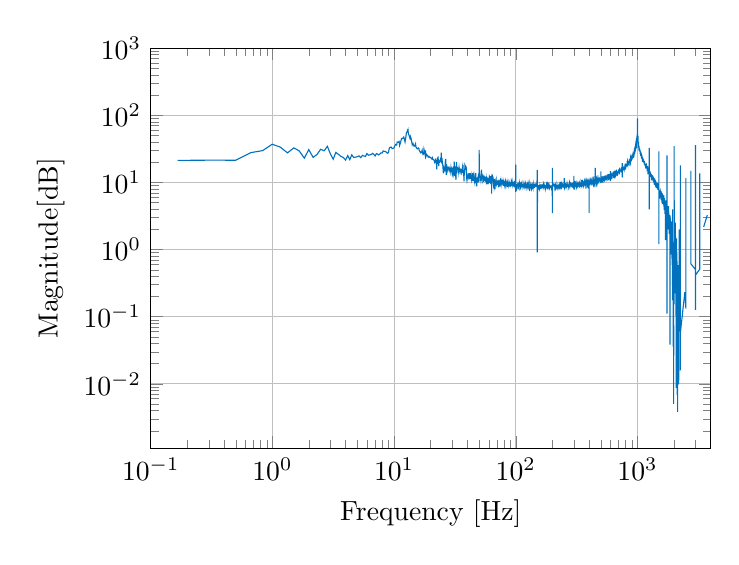
\begin{tikzpicture}

\begin{axis}[%
width=2.8in,
height=2in,
at={(1.011in,0.642in)},
scale only axis,
xmode=log,
ymode=log,
xmin=0.1,
xmax=4e+03,
%xminorticks=true,
ymin=-60,
ymax=1000,
xmajorgrids,
%xminorgrids,
ymajorgrids,
%yminorgrids,
xlabel={Frequency [Hz]},
ylabel={Magnitude[dB]},
axis background/.style={fill=white}
]
\addplot [color=mycolor1,solid,forget plot]
  table[row sep=crcr]{%
0	16.7\\
0.166	21.3\\
0.332	21.5\\
0.499	21.4\\
0.665	27.8\\
0.831	29.8\\
0.997	37.1\\
1.16	33.6\\
1.33	27.6\\
1.5	32.7\\
1.66	29.5\\
1.83	23\\
1.99	30.9\\
2.16	23.6\\
2.33	26.2\\
2.49	31.2\\
2.66	29.6\\
2.83	34.5\\
2.99	26.8\\
3.16	22.2\\
3.32	28\\
3.49	26.2\\
3.66	24.4\\
3.82	23.6\\
3.99	21.6\\
4.16	25.1\\
4.32	21.8\\
4.49	25.8\\
4.65	23.6\\
4.82	23.8\\
4.99	24.3\\
5.15	24.9\\
5.32	23.4\\
5.49	25.3\\
5.65	24.8\\
5.82	24.4\\
5.98	26.9\\
6.15	25.4\\
6.32	25.8\\
6.48	26\\
6.65	27.1\\
6.82	26.1\\
6.98	24.8\\
7.15	26.9\\
7.31	26.5\\
7.48	25.7\\
7.65	26.6\\
7.81	27.6\\
7.98	27.4\\
8.14	29.5\\
8.31	29\\
8.48	29\\
8.64	28.2\\
8.81	27.3\\
8.98	27.7\\
9.14	32.7\\
9.31	33.4\\
9.47	33.6\\
9.64	31.9\\
9.81	32.2\\
9.97	32.8\\
10.1	34.7\\
10.3	36.8\\
10.5	36.1\\
10.6	40\\
10.8	39.7\\
11	40.7\\
11.1	35.7\\
11.3	39.6\\
11.5	45\\
11.6	44.6\\
11.8	45.5\\
12	47.5\\
12.1	45.2\\
12.3	40.1\\
12.5	47.7\\
12.6	54.2\\
12.8	57.6\\
13	61.6\\
13.1	53.2\\
13.3	49.9\\
13.5	45.4\\
13.6	48.5\\
13.8	45.1\\
14	39.1\\
14.1	36.2\\
14.3	38\\
14.5	35.6\\
14.6	34.6\\
14.8	34.9\\
15	37.5\\
15.1	34.1\\
15.3	32.7\\
15.5	31.6\\
15.6	31.7\\
15.8	32.6\\
16	31.9\\
16.1	29.7\\
16.3	29\\
16.5	27.8\\
16.6	28.4\\
16.8	28\\
17	30.2\\
17.1	27.8\\
17.3	26.1\\
17.5	26.8\\
17.6	31.2\\
17.8	28.5\\
18	25.5\\
18.1	29.9\\
18.3	24.5\\
18.5	25.9\\
18.6	25.5\\
18.8	24.9\\
18.9	25.2\\
19.1	23.8\\
19.3	24.1\\
19.4	24.3\\
19.6	23.7\\
19.8	23.8\\
19.9	23.4\\
20.1	23.2\\
20.3	23\\
20.4	22.5\\
20.6	23.4\\
20.8	22.1\\
20.9	22.2\\
21.1	21.8\\
21.3	21.6\\
21.4	20.8\\
21.6	19.7\\
21.8	20.1\\
21.9	21.6\\
22.1	20.9\\
22.3	19.1\\
22.4	15.7\\
22.6	22.6\\
22.8	23.2\\
22.9	19\\
23.1	21\\
23.3	17.6\\
23.4	20.6\\
23.6	19.9\\
23.8	20.2\\
23.9	21.2\\
24.1	22.4\\
24.3	20.1\\
24.4	27.7\\
24.6	19.4\\
24.8	23.3\\
24.9	18.7\\
25.1	18.4\\
25.3	15.1\\
25.4	13.7\\
25.6	16.2\\
25.8	15.3\\
25.9	15.9\\
26.1	15.5\\
26.3	19.2\\
26.4	18.5\\
26.6	22.4\\
26.8	13\\
26.9	16.9\\
27.1	17.5\\
27.3	16.2\\
27.4	15.4\\
27.6	16.8\\
27.8	16.7\\
27.9	16.4\\
28.1	15.7\\
28.3	17.3\\
28.4	15.7\\
28.6	15.8\\
28.8	14.7\\
28.9	16.5\\
29.1	14.4\\
29.3	16.3\\
29.4	15.4\\
29.6	16.4\\
29.8	16\\
29.9	14.9\\
30.1	16.5\\
30.3	14.2\\
30.4	14.9\\
30.6	13.9\\
30.8	17.4\\
30.9	14.3\\
31.1	16.8\\
31.2	20.5\\
31.4	12.5\\
31.6	17.5\\
31.7	16.1\\
31.9	13.8\\
32.1	14.7\\
32.2	10.9\\
32.4	13.9\\
32.6	20.2\\
32.7	16.7\\
32.9	16.4\\
33.1	16.1\\
33.2	17.1\\
33.4	15\\
33.6	15.3\\
33.7	14.3\\
33.9	15.6\\
34.1	15.4\\
34.2	16.4\\
34.4	15.1\\
34.6	16.2\\
34.7	16.1\\
34.9	15\\
35.1	14.7\\
35.2	14.9\\
35.4	14.1\\
35.6	14.6\\
35.7	14.2\\
35.9	15.3\\
36.1	15.1\\
36.2	13.9\\
36.4	16.6\\
36.6	17.5\\
36.7	16.2\\
36.9	16.6\\
37.1	12.9\\
37.2	13.3\\
37.4	12.4\\
37.6	10.4\\
37.7	13.5\\
37.9	14\\
38.1	16\\
38.2	17.8\\
38.4	17.2\\
38.6	16.7\\
38.7	17.6\\
38.9	17.4\\
39.1	16.7\\
39.2	16.5\\
39.4	12.4\\
39.6	11\\
39.7	10.7\\
39.9	11.5\\
40.1	11.6\\
40.2	13\\
40.4	12.2\\
40.6	12.3\\
40.7	13.6\\
40.9	12.2\\
41.1	13.2\\
41.2	11\\
41.4	13.8\\
41.6	12.2\\
41.7	13.6\\
41.9	12\\
42.1	11.3\\
42.2	13.7\\
42.4	12.9\\
42.6	12.7\\
42.7	12.5\\
42.9	12.1\\
43.1	11.3\\
43.2	11.8\\
43.4	12.5\\
43.6	11\\
43.7	12.6\\
43.9	13.7\\
44	12.2\\
44.2	12.8\\
44.4	12.6\\
44.5	10.6\\
44.7	11.9\\
44.9	12.6\\
45	13.1\\
45.2	13.5\\
45.4	12.7\\
45.5	12.2\\
45.7	10.5\\
45.9	10.1\\
46	11.7\\
46.2	11.5\\
46.4	9.77\\
46.5	10.3\\
46.7	11.6\\
46.9	13.8\\
47	11.4\\
47.2	9.96\\
47.4	10.7\\
47.5	10.5\\
47.7	8.77\\
47.9	10.3\\
48	11.8\\
48.2	11\\
48.4	11.9\\
48.5	11.1\\
48.7	11.5\\
48.9	11.6\\
49	12\\
49.2	12.4\\
49.4	10\\
49.5	11.9\\
49.7	13\\
49.9	13.4\\
50	30.6\\
50.2	13.7\\
50.4	11.9\\
50.5	12.6\\
50.7	13\\
50.9	11.3\\
51	11.4\\
51.2	11.5\\
51.4	10.5\\
51.5	11.6\\
51.7	10.9\\
51.9	11.5\\
52	10.8\\
52.2	10.9\\
52.4	15.5\\
52.5	12.5\\
52.7	12.8\\
52.9	12.6\\
53	12.4\\
53.2	12.1\\
53.4	12.3\\
53.5	12\\
53.7	10.5\\
53.9	10.7\\
54	11.2\\
54.2	11\\
54.4	11.5\\
54.5	11.9\\
54.7	12.2\\
54.9	11.8\\
55	11.1\\
55.2	11.3\\
55.4	11.5\\
55.5	11\\
55.7	10.9\\
55.9	12\\
56	11.7\\
56.2	11.5\\
56.3	10.2\\
56.5	12.2\\
56.7	10.9\\
56.8	12.1\\
57	11.6\\
57.2	10.8\\
57.3	11.2\\
57.5	9.4\\
57.7	10.9\\
57.8	11.3\\
58	10.7\\
58.2	11.9\\
58.3	10.1\\
58.5	10.9\\
58.7	10.7\\
58.8	9.45\\
59	11\\
59.2	11.1\\
59.3	11\\
59.5	10.6\\
59.7	10.3\\
59.8	10.5\\
60	9.84\\
60.2	10.6\\
60.3	11.1\\
60.5	11.8\\
60.7	11.5\\
60.8	11.6\\
61	10.7\\
61.2	10.1\\
61.3	10.9\\
61.5	11.1\\
61.7	9.87\\
61.8	9.83\\
62	10.5\\
62.2	12.2\\
62.3	12.2\\
62.5	11.6\\
62.7	10.6\\
62.8	10.6\\
63	9.58\\
63.2	10.6\\
63.3	6.82\\
63.5	12.1\\
63.7	11.2\\
63.8	13.2\\
64	12\\
64.2	11.8\\
64.3	11.7\\
64.5	10.4\\
64.7	11.4\\
64.8	11.2\\
65	12.2\\
65.2	11.2\\
65.3	11.1\\
65.5	11.1\\
65.7	10.4\\
65.8	9.95\\
66	8.11\\
66.2	11.1\\
66.3	9.96\\
66.5	9.58\\
66.7	11.3\\
66.8	8.53\\
67	8.72\\
67.2	10.1\\
67.3	8.55\\
67.5	7.95\\
67.7	10.2\\
67.8	9.64\\
68	10.4\\
68.2	9.73\\
68.3	10.3\\
68.5	10.7\\
68.7	11.5\\
68.8	10.4\\
69	10.7\\
69.1	9.72\\
69.3	9.53\\
69.5	10.3\\
69.6	10.3\\
69.8	10.1\\
70	9.98\\
70.1	10.2\\
70.3	10.3\\
70.5	9.58\\
70.6	9.82\\
70.8	9.25\\
71	10.1\\
71.1	9.45\\
71.3	10.6\\
71.5	10\\
71.6	9.75\\
71.8	9.75\\
72	10.1\\
72.1	8.42\\
72.3	9.74\\
72.5	9.72\\
72.6	10\\
72.8	11\\
73	9.97\\
73.1	9.65\\
73.3	10.5\\
73.5	9.29\\
73.6	9.73\\
73.8	10.5\\
74	8.67\\
74.1	10.2\\
74.3	9.02\\
74.5	10.6\\
74.6	9.26\\
74.8	9.98\\
75	9.73\\
75.1	9.27\\
75.3	10.9\\
75.5	10.1\\
75.6	9.54\\
75.8	10.4\\
76	10.1\\
76.1	9.63\\
76.3	9.92\\
76.5	10.2\\
76.6	9.32\\
76.8	10.8\\
77	10.8\\
77.1	9.78\\
77.3	9.26\\
77.5	10.6\\
77.6	9.45\\
77.8	10.2\\
78	10.5\\
78.1	9.7\\
78.3	10.7\\
78.5	10\\
78.6	10.3\\
78.8	8.88\\
79	9.21\\
79.1	10.3\\
79.3	10.1\\
79.5	10\\
79.6	10.3\\
79.8	10.2\\
80	9.24\\
80.1	10\\
80.3	9.88\\
80.5	9.8\\
80.6	9.61\\
80.8	10.1\\
81	9.69\\
81.1	10.1\\
81.3	8.71\\
81.4	9.58\\
81.6	9.91\\
81.8	9.31\\
81.9	9.83\\
82.1	10\\
82.3	9.32\\
82.4	9.58\\
82.6	9.91\\
82.8	10.4\\
82.9	9.33\\
83.1	9.45\\
83.3	9.85\\
83.4	9.12\\
83.6	9.32\\
83.8	9.48\\
83.9	9.2\\
84.1	9.87\\
84.3	10\\
84.4	10.1\\
84.6	9.25\\
84.8	9.15\\
84.9	9.35\\
85.1	10.4\\
85.3	10.4\\
85.4	8.86\\
85.6	9.75\\
85.8	9.78\\
85.9	8.94\\
86.1	10.3\\
86.3	9.75\\
86.4	9.85\\
86.6	9.39\\
86.8	9.49\\
86.9	9.82\\
87.1	9.39\\
87.3	9.37\\
87.4	9.74\\
87.6	9.16\\
87.8	9.32\\
87.9	9.32\\
88.1	9.31\\
88.3	9.33\\
88.4	9.72\\
88.6	8.88\\
88.8	10.1\\
88.9	9.93\\
89.1	8.7\\
89.3	9.6\\
89.4	9.52\\
89.6	9.16\\
89.8	10.2\\
89.9	9.38\\
90.1	9.82\\
90.3	9.27\\
90.4	8.83\\
90.6	9.33\\
90.8	9.01\\
90.9	10.1\\
91.1	9.34\\
91.3	9.46\\
91.4	9.06\\
91.6	8.76\\
91.8	9.84\\
91.9	10.2\\
92.1	10\\
92.3	9.92\\
92.4	9.01\\
92.6	9.78\\
92.8	8.9\\
92.9	9.99\\
93.1	8.94\\
93.3	9.84\\
93.4	10\\
93.6	9.65\\
93.8	9.53\\
93.9	9.5\\
94.1	9.18\\
94.2	8.96\\
94.4	10.2\\
94.6	9.16\\
94.7	9.22\\
94.9	9.58\\
95.1	10.2\\
95.2	9.14\\
95.4	9.44\\
95.6	9.34\\
95.7	9.53\\
95.9	9.61\\
96.1	9.39\\
96.2	9.45\\
96.4	9.66\\
96.6	9.61\\
96.7	9.61\\
96.9	9.77\\
97.1	9.63\\
97.2	9.98\\
97.4	9.67\\
97.6	9.94\\
97.7	9.51\\
97.9	9.22\\
98.1	9.4\\
98.2	9.71\\
98.4	9.1\\
98.6	10\\
98.7	10.1\\
98.9	8.79\\
99.1	9.78\\
99.2	10.2\\
99.4	10.6\\
99.6	11.4\\
99.7	11.6\\
99.9	14.5\\
100	18.4\\
100	7.24\\
100	7.38\\
101	7.9\\
101	8.1\\
101	8.76\\
101	7.61\\
101	9.01\\
101	8.71\\
102	8.8\\
102	9.13\\
102	9.22\\
102	9.11\\
102	8.51\\
102	9.23\\
103	9.39\\
103	8.95\\
103	9.56\\
103	8.62\\
103	8.91\\
103	9.2\\
104	9.49\\
104	9.84\\
104	8.45\\
104	9.52\\
104	9.48\\
104	8.38\\
105	8.69\\
105	9.36\\
105	9.87\\
105	9.02\\
105	8.73\\
105	9.13\\
106	8.61\\
106	9.14\\
106	8.4\\
106	9.08\\
106	9.71\\
106	9.05\\
107	9.73\\
107	8.97\\
107	8.57\\
107	8.65\\
107	9.72\\
107	9.05\\
108	8.96\\
108	9.1\\
108	8.99\\
108	9.31\\
108	8.94\\
108	9.77\\
109	8.89\\
109	8.62\\
109	9.13\\
109	9.29\\
109	9.05\\
109	8.35\\
110	8.79\\
110	9.32\\
110	9.04\\
110	8.18\\
110	8.54\\
110	10.2\\
111	9.28\\
111	9.35\\
111	9.02\\
111	9.3\\
111	9.47\\
111	9.12\\
112	9.65\\
112	8.74\\
112	9.68\\
112	8.78\\
112	9.01\\
112	9.09\\
113	9.17\\
113	8.47\\
113	9.55\\
113	9.12\\
113	9.21\\
113	8.72\\
114	8.68\\
114	9.42\\
114	9.09\\
114	9.13\\
114	9.15\\
114	8.92\\
115	9\\
115	8.3\\
115	9.49\\
115	8.12\\
115	8.89\\
115	8.82\\
116	9.37\\
116	8.44\\
116	8.71\\
116	8.56\\
116	9.15\\
116	8.84\\
117	9.04\\
117	9.51\\
117	9.21\\
117	8.8\\
117	9.14\\
117	9.19\\
118	8.68\\
118	8.75\\
118	8.76\\
118	9.42\\
118	9.03\\
118	9.15\\
119	9.58\\
119	9.1\\
119	8.1\\
119	8.61\\
119	8.59\\
119	9.1\\
120	9.37\\
120	8.4\\
120	9.42\\
120	8.51\\
120	9.12\\
120	8.92\\
121	8.96\\
121	9.25\\
121	9.29\\
121	9.08\\
121	9.16\\
121	8.3\\
122	9.22\\
122	9.57\\
122	8.69\\
122	8.49\\
122	8.27\\
122	9.34\\
123	9.5\\
123	9.45\\
123	8.91\\
123	9.23\\
123	9.3\\
123	8.51\\
124	8.62\\
124	9.33\\
124	8.86\\
124	8.23\\
124	8.93\\
124	8.71\\
125	9.27\\
125	9.07\\
125	9.34\\
125	8.83\\
125	8.88\\
125	8.83\\
125	9.27\\
126	9\\
126	8.66\\
126	9.19\\
126	8.99\\
126	8.7\\
126	8.7\\
127	8.76\\
127	8.87\\
127	8.67\\
127	9.39\\
127	9.23\\
127	8.93\\
128	9.53\\
128	8.99\\
128	8.2\\
128	9.07\\
128	9.55\\
128	9.24\\
129	8.93\\
129	8.68\\
129	8.59\\
129	8.82\\
129	9.32\\
129	8.58\\
130	7.46\\
130	8.86\\
130	8.78\\
130	9.18\\
130	9.07\\
130	8.53\\
131	9.15\\
131	8.8\\
131	9.4\\
131	8.94\\
131	8.48\\
131	8.53\\
132	8.8\\
132	9.4\\
132	8.81\\
132	9.14\\
132	8.83\\
132	9.01\\
133	8.51\\
133	8.68\\
133	8.76\\
133	8.93\\
133	8.8\\
133	8.87\\
134	9.59\\
134	9.16\\
134	8.85\\
134	8.42\\
134	8.78\\
134	9.32\\
135	8.69\\
135	8.93\\
135	9.28\\
135	8.66\\
135	8.94\\
135	9.14\\
136	8.06\\
136	9.1\\
136	8.88\\
136	9.3\\
136	8.42\\
136	8.41\\
137	8.79\\
137	9.49\\
137	9.34\\
137	8.44\\
137	8.62\\
137	8.8\\
138	8.38\\
138	9.15\\
138	8.64\\
138	9.12\\
138	8.38\\
138	8.85\\
139	9.41\\
139	9.07\\
139	8.64\\
139	9.23\\
139	9.13\\
139	8.86\\
140	8.76\\
140	9.54\\
140	8.84\\
140	9.21\\
140	8.09\\
140	8.77\\
141	8.85\\
141	9.15\\
141	8.48\\
141	9.57\\
141	9.58\\
141	8.86\\
142	8.87\\
142	9.1\\
142	8.86\\
142	9.12\\
142	8.29\\
142	8.38\\
143	8.62\\
143	8.72\\
143	8.59\\
143	8.59\\
143	8.76\\
143	8.77\\
144	9.6\\
144	8.75\\
144	9.38\\
144	9.29\\
144	8.99\\
144	8.58\\
145	9.31\\
145	9.06\\
145	9.2\\
145	8.9\\
145	8.97\\
145	8.97\\
146	9.65\\
146	9.26\\
146	8.77\\
146	8.59\\
146	9.03\\
146	8.67\\
147	9.7\\
147	8.89\\
147	9.13\\
147	8.82\\
147	8.74\\
147	9.15\\
148	9.24\\
148	9.19\\
148	9.43\\
148	9.31\\
148	9.28\\
148	8.86\\
149	8.88\\
149	9.43\\
149	9.64\\
149	9.84\\
149	9.98\\
149	10.4\\
150	10.8\\
150	11.7\\
150	15.2\\
150	10\\
150	0.91\\
150	6.11\\
151	5.83\\
151	6.96\\
151	7.28\\
151	7.53\\
151	7.37\\
151	7.94\\
152	8.16\\
152	7.65\\
152	8.09\\
152	8.32\\
152	8.17\\
152	8.34\\
153	8.46\\
153	8.32\\
153	8.62\\
153	8.44\\
153	8.31\\
153	8.76\\
154	8.74\\
154	9.11\\
154	8.21\\
154	8.37\\
154	8.02\\
154	8.18\\
155	8.07\\
155	9\\
155	8.23\\
155	9.06\\
155	8.82\\
155	8.6\\
156	8.25\\
156	8.74\\
156	8.89\\
156	8.67\\
156	8.74\\
156	8.42\\
157	8.21\\
157	8.28\\
157	9.12\\
157	8.41\\
157	8.59\\
157	8.44\\
158	8.55\\
158	8.1\\
158	8.54\\
158	8.57\\
158	8.89\\
158	8.96\\
159	8.84\\
159	8.01\\
159	8.82\\
159	8.31\\
159	8.36\\
159	8.61\\
160	8.23\\
160	8.13\\
160	8.41\\
160	8.48\\
160	9.14\\
160	8.59\\
161	8.66\\
161	8.74\\
161	8.7\\
161	8.72\\
161	8.29\\
161	8.73\\
162	8.95\\
162	9.03\\
162	9.12\\
162	9.34\\
162	8.27\\
162	8.66\\
163	8.54\\
163	8.17\\
163	8.5\\
163	8.39\\
163	8.67\\
163	8.72\\
164	8.85\\
164	9.1\\
164	8.87\\
164	8.77\\
164	8.74\\
164	8.62\\
165	8.82\\
165	8.66\\
165	8.88\\
165	9.09\\
165	8.22\\
165	8.54\\
166	8.8\\
166	8.71\\
166	8.44\\
166	8.37\\
166	8.58\\
166	9.02\\
167	8.96\\
167	8.35\\
167	8.8\\
167	8.68\\
167	8.78\\
167	8.26\\
168	8.81\\
168	8.77\\
168	8.59\\
168	8.62\\
168	9.04\\
168	8.23\\
169	9.09\\
169	8.86\\
169	8.53\\
169	8.73\\
169	8.8\\
169	8.58\\
170	8.86\\
170	9.1\\
170	8.8\\
170	9.06\\
170	8.49\\
170	9.11\\
171	8.75\\
171	8.47\\
171	8.66\\
171	9.02\\
171	8.91\\
171	8.99\\
172	8.26\\
172	8.71\\
172	8.4\\
172	8.65\\
172	8.78\\
172	8.9\\
173	8.52\\
173	8.66\\
173	8.51\\
173	8.41\\
173	8.85\\
173	8.68\\
174	9.14\\
174	8.35\\
174	8.53\\
174	8.16\\
174	8.56\\
174	8.69\\
175	8.5\\
175	8.99\\
175	8.66\\
175	8.62\\
175	8.6\\
175	8.46\\
176	9.06\\
176	9.02\\
176	8.7\\
176	8.99\\
176	9.15\\
176	8.33\\
177	8.72\\
177	8.49\\
177	8.58\\
177	8.48\\
177	8.77\\
177	8.68\\
178	8.68\\
178	8.57\\
178	8.74\\
178	8.38\\
178	8.96\\
178	8.74\\
179	9.03\\
179	8.4\\
179	9.24\\
179	8.51\\
179	8.87\\
179	8.64\\
180	8.62\\
180	8.16\\
180	9.02\\
180	8.61\\
180	8.21\\
180	9.3\\
181	8.31\\
181	8.76\\
181	8.28\\
181	8.57\\
181	8.54\\
181	8.77\\
182	8.82\\
182	8.81\\
182	8.49\\
182	8.87\\
182	8.5\\
182	8.56\\
183	7.92\\
183	8.36\\
183	8.66\\
183	8.52\\
183	8.61\\
183	8.73\\
184	9\\
184	8.76\\
184	8.75\\
184	8.5\\
184	8.48\\
184	9.11\\
185	8.82\\
185	8.5\\
185	8.94\\
185	8.48\\
185	8.59\\
185	8.64\\
186	8.75\\
186	8.6\\
186	8.88\\
186	8.8\\
186	8.9\\
186	8.68\\
187	8.95\\
187	8.41\\
187	8.49\\
187	8.23\\
187	8.42\\
187	8.97\\
188	8.98\\
188	8.81\\
188	8.93\\
188	8.62\\
188	8.63\\
188	8.53\\
188	8.75\\
189	8.64\\
189	8.57\\
189	8.87\\
189	8.86\\
189	8.75\\
189	9.24\\
190	8.27\\
190	8.88\\
190	8.17\\
190	8.79\\
190	8.7\\
190	8.31\\
191	8.5\\
191	8.76\\
191	8.51\\
191	8.56\\
191	8.81\\
191	8.66\\
192	8.82\\
192	8.92\\
192	8.51\\
192	8.73\\
192	8.58\\
192	8.46\\
193	8.45\\
193	8.54\\
193	8.66\\
193	8.6\\
193	9.07\\
193	8.59\\
194	8.67\\
194	9.02\\
194	8.52\\
194	8.52\\
194	9.04\\
194	8.59\\
195	8.45\\
195	8.32\\
195	8.49\\
195	8.35\\
195	8.5\\
195	8.56\\
196	8.73\\
196	8.79\\
196	8.22\\
196	8.5\\
196	8.27\\
196	8.99\\
197	7.92\\
197	8.45\\
197	8.27\\
197	8.87\\
197	8.55\\
197	8.47\\
198	8.7\\
198	7.85\\
198	8.57\\
198	8.16\\
198	7.83\\
198	8.56\\
199	7.69\\
199	8.18\\
199	8.1\\
199	7.79\\
199	7.23\\
199	6.55\\
200	6.09\\
200	3.48\\
200	-4.2\\
200	16.5\\
200	12.3\\
200	10.8\\
201	10.4\\
201	9.63\\
201	9.77\\
201	9.73\\
201	9.64\\
201	9.74\\
202	9.3\\
202	9.45\\
202	9.4\\
202	9.36\\
202	9.35\\
202	9.17\\
203	9.22\\
203	9.14\\
203	8.97\\
203	9.04\\
203	8.82\\
203	8.76\\
204	9.26\\
204	8.92\\
204	9.04\\
204	8.96\\
204	8.98\\
204	8.98\\
205	9.08\\
205	9.15\\
205	9.3\\
205	9.2\\
205	8.92\\
205	9.17\\
206	9.04\\
206	8.93\\
206	8.94\\
206	9.22\\
206	9.01\\
206	8.74\\
207	9.15\\
207	8.77\\
207	8.83\\
207	9.28\\
207	9.58\\
207	9.11\\
208	9.18\\
208	9.1\\
208	8.57\\
208	8.91\\
208	8.54\\
208	8.97\\
209	8.98\\
209	9.3\\
209	8.95\\
209	9.16\\
209	9.1\\
209	8.86\\
210	8.64\\
210	8.73\\
210	8.99\\
210	8.95\\
210	9.09\\
210	8.67\\
211	8.94\\
211	8.98\\
211	8.95\\
211	9.04\\
211	8.46\\
211	8.7\\
212	8.86\\
212	8.54\\
212	8.52\\
212	9.13\\
212	8.8\\
212	8.65\\
213	9\\
213	8.87\\
213	8.66\\
213	8.7\\
213	8.58\\
213	9\\
214	9.01\\
214	8.74\\
214	8.23\\
214	8.83\\
214	9.05\\
214	9.05\\
215	8.89\\
215	9.23\\
215	8.14\\
215	9.03\\
215	8.87\\
215	9.27\\
216	8.84\\
216	8.81\\
216	8.8\\
216	8.92\\
216	8.56\\
216	8.55\\
217	8.78\\
217	8.99\\
217	8.95\\
217	9.01\\
217	8.88\\
217	8.78\\
218	8.82\\
218	8.89\\
218	9.14\\
218	9.04\\
218	9.09\\
218	8.48\\
219	9.17\\
219	8.91\\
219	8.52\\
219	8.96\\
219	8.87\\
219	8.6\\
220	8.55\\
220	8.72\\
220	8.74\\
220	8.82\\
220	8.87\\
220	9.03\\
221	8.58\\
221	8.45\\
221	8.69\\
221	8.7\\
221	8.96\\
221	8.66\\
222	8.94\\
222	9\\
222	9.03\\
222	8.85\\
222	8.99\\
222	8.94\\
223	8.72\\
223	9.04\\
223	8.95\\
223	8.87\\
223	8.93\\
223	9.01\\
224	8.79\\
224	8.78\\
224	8.64\\
224	8.94\\
224	8.83\\
224	8.75\\
225	8.76\\
225	8.99\\
225	8.99\\
225	8.39\\
225	9\\
225	8.79\\
226	8.71\\
226	8.8\\
226	8.89\\
226	8.96\\
226	9.03\\
226	8.86\\
227	8.5\\
227	8.83\\
227	8.63\\
227	9\\
227	8.95\\
227	8.79\\
228	9.05\\
228	8.56\\
228	8.92\\
228	8.55\\
228	9.02\\
228	8.74\\
229	9.1\\
229	9.17\\
229	8.65\\
229	9.22\\
229	8.68\\
229	8.8\\
230	8.99\\
230	8.95\\
230	8.97\\
230	8.94\\
230	9.07\\
230	8.86\\
231	9.12\\
231	8.56\\
231	8.96\\
231	8.96\\
231	8.97\\
231	8.69\\
232	8.89\\
232	9.16\\
232	8.94\\
232	8.97\\
232	9.34\\
232	8.84\\
233	9.04\\
233	8.91\\
233	8.93\\
233	8.94\\
233	9.1\\
233	8.83\\
234	8.74\\
234	8.78\\
234	8.81\\
234	8.96\\
234	9.05\\
234	8.73\\
235	8.9\\
235	8.92\\
235	8.84\\
235	9.2\\
235	8.4\\
235	9.12\\
236	8.78\\
236	8.92\\
236	8.57\\
236	8.69\\
236	8.71\\
236	8.74\\
237	9.05\\
237	8.78\\
237	8.75\\
237	8.54\\
237	8.91\\
237	8.86\\
238	9.12\\
238	8.82\\
238	8.97\\
238	9.09\\
238	8.99\\
238	8.97\\
239	9.01\\
239	8.95\\
239	8.93\\
239	8.88\\
239	8.98\\
239	8.88\\
240	8.51\\
240	9.33\\
240	9.24\\
240	8.93\\
240	8.81\\
240	8.73\\
241	8.92\\
241	8.7\\
241	8.97\\
241	8.8\\
241	9.16\\
241	8.63\\
242	9.07\\
242	8.71\\
242	9.18\\
242	9.14\\
242	9\\
242	9.29\\
243	8.87\\
243	9.28\\
243	8.8\\
243	8.91\\
243	9.15\\
243	8.9\\
244	9\\
244	8.89\\
244	9.19\\
244	8.96\\
244	8.99\\
244	8.8\\
245	8.74\\
245	8.96\\
245	9.02\\
245	9.2\\
245	8.76\\
245	9.24\\
246	8.86\\
246	8.98\\
246	8.81\\
246	8.98\\
246	9.32\\
246	8.93\\
247	9.09\\
247	9.24\\
247	8.8\\
247	8.87\\
247	8.64\\
247	8.8\\
248	9.08\\
248	9.1\\
248	8.94\\
248	9.24\\
248	9.06\\
248	9\\
249	8.74\\
249	9.05\\
249	9.01\\
249	9.18\\
249	8.89\\
249	8.97\\
250	8.79\\
250	8.87\\
250	9.38\\
250	11.6\\
250	9.76\\
250	9.36\\
250	9.05\\
251	8.87\\
251	9.14\\
251	9.11\\
251	9.11\\
251	9.03\\
251	8.89\\
252	9.1\\
252	9.13\\
252	9.12\\
252	9.16\\
252	8.96\\
252	8.62\\
253	8.7\\
253	8.58\\
253	8.78\\
253	8.77\\
253	8.91\\
253	8.89\\
254	9.25\\
254	8.82\\
254	9\\
254	9.24\\
254	9.13\\
254	8.89\\
255	8.85\\
255	9.06\\
255	8.8\\
255	8.77\\
255	9.01\\
255	9.79\\
256	9.32\\
256	9.36\\
256	9.02\\
256	8.76\\
256	9.07\\
256	8.89\\
257	8.41\\
257	8.48\\
257	8.78\\
257	9.12\\
257	9.14\\
257	9.07\\
258	9.41\\
258	8.58\\
258	9.07\\
258	9.14\\
258	9.01\\
258	8.72\\
259	8.85\\
259	9.06\\
259	8.58\\
259	8.84\\
259	8.73\\
259	9\\
260	9.02\\
260	9.22\\
260	9.06\\
260	8.84\\
260	9.25\\
260	9.12\\
261	8.98\\
261	8.72\\
261	8.87\\
261	8.86\\
261	8.82\\
261	8.87\\
262	8.64\\
262	9.07\\
262	8.95\\
262	9.08\\
262	8.64\\
262	9.16\\
263	8.76\\
263	8.91\\
263	9.25\\
263	8.85\\
263	8.9\\
263	8.8\\
264	9.16\\
264	8.86\\
264	9.18\\
264	8.9\\
264	9.01\\
264	8.64\\
265	9.02\\
265	8.76\\
265	8.88\\
265	9.15\\
265	8.9\\
265	9.17\\
266	9.15\\
266	8.98\\
266	9.3\\
266	8.59\\
266	9.11\\
266	9.15\\
267	8.87\\
267	8.74\\
267	9.27\\
267	8.83\\
267	9.18\\
267	9.2\\
268	8.79\\
268	9\\
268	9.06\\
268	9.08\\
268	9.15\\
268	8.96\\
269	9.02\\
269	9.25\\
269	9.04\\
269	9.32\\
269	8.9\\
269	8.88\\
270	8.72\\
270	8.96\\
270	8.64\\
270	9.13\\
270	8.9\\
270	9.04\\
271	9.02\\
271	8.96\\
271	9.29\\
271	8.99\\
271	8.5\\
271	8.98\\
272	9.18\\
272	9\\
272	8.92\\
272	9.11\\
272	8.88\\
272	8.97\\
273	9.02\\
273	9.02\\
273	9.05\\
273	8.77\\
273	9.1\\
273	9.07\\
274	9.36\\
274	9.25\\
274	8.72\\
274	9.16\\
274	9.22\\
274	8.93\\
275	9.16\\
275	8.89\\
275	9.14\\
275	9.25\\
275	9.21\\
275	9.17\\
276	9.15\\
276	9.25\\
276	9.04\\
276	9.08\\
276	8.88\\
276	9.07\\
277	9.07\\
277	9.01\\
277	9.2\\
277	9.27\\
277	9.18\\
277	9.12\\
278	8.99\\
278	9.29\\
278	8.98\\
278	9.05\\
278	9.11\\
278	9.11\\
279	8.56\\
279	8.84\\
279	9.16\\
279	9.36\\
279	9.25\\
279	9.16\\
280	9.12\\
280	9.24\\
280	8.94\\
280	9.06\\
280	9.07\\
280	8.93\\
281	9.13\\
281	8.99\\
281	9.18\\
281	8.78\\
281	8.94\\
281	9.1\\
282	8.92\\
282	8.9\\
282	9.26\\
282	9.19\\
282	8.97\\
282	9.05\\
283	9.12\\
283	9.04\\
283	9.05\\
283	8.93\\
283	9.33\\
283	9.16\\
284	9.25\\
284	9.12\\
284	9.06\\
284	9.26\\
284	8.99\\
284	9.11\\
285	9.09\\
285	9.23\\
285	9.21\\
285	9.1\\
285	9.04\\
285	9.1\\
286	9\\
286	9.04\\
286	9.24\\
286	8.81\\
286	8.91\\
286	9.04\\
287	9.18\\
287	9.1\\
287	9.04\\
287	9.15\\
287	9.26\\
287	9.01\\
288	9.34\\
288	8.97\\
288	9.33\\
288	9.03\\
288	9.46\\
288	9.07\\
289	8.97\\
289	9.4\\
289	9.13\\
289	8.83\\
289	8.93\\
289	9.1\\
290	9.21\\
290	9.05\\
290	9.59\\
290	8.9\\
290	9.18\\
290	9.17\\
291	9.07\\
291	9.03\\
291	9.19\\
291	9.15\\
291	9.38\\
291	9.24\\
292	9.11\\
292	9.34\\
292	9.08\\
292	9.07\\
292	9.16\\
292	8.9\\
293	9.03\\
293	9.26\\
293	9.02\\
293	9.35\\
293	9.03\\
293	8.93\\
294	8.83\\
294	9.23\\
294	9.53\\
294	9.34\\
294	9.07\\
294	9.14\\
295	9.3\\
295	9.03\\
295	9.13\\
295	8.81\\
295	9.14\\
295	9.33\\
296	9.25\\
296	8.99\\
296	9.18\\
296	8.83\\
296	8.88\\
296	9.24\\
297	9.29\\
297	9.45\\
297	9.47\\
297	9.37\\
297	9.09\\
297	9.23\\
298	9.14\\
298	9.31\\
298	9.36\\
298	9.32\\
298	9.39\\
298	9.38\\
299	9.46\\
299	9.32\\
299	9.21\\
299	9.4\\
299	9.35\\
299	9.27\\
300	9.19\\
300	9.48\\
300	9.63\\
300	12.5\\
300	7.81\\
300	8.82\\
301	9.03\\
301	8.65\\
301	8.79\\
301	8.88\\
301	8.85\\
301	9.02\\
302	9.21\\
302	9.02\\
302	8.81\\
302	9.11\\
302	9.41\\
302	9.41\\
303	9.17\\
303	9.19\\
303	9.11\\
303	8.92\\
303	9.26\\
303	9.16\\
304	8.93\\
304	9.21\\
304	8.86\\
304	9.35\\
304	8.91\\
304	9.26\\
305	9.24\\
305	9.27\\
305	9.28\\
305	9.24\\
305	8.94\\
305	9.32\\
306	9.35\\
306	9.14\\
306	9.18\\
306	9.23\\
306	9.25\\
306	9.12\\
307	9.04\\
307	9.24\\
307	9\\
307	9.51\\
307	9.36\\
307	9.15\\
308	9.23\\
308	8.68\\
308	9.01\\
308	9.17\\
308	9.05\\
308	9.2\\
309	8.93\\
309	9.03\\
309	9.11\\
309	9.11\\
309	9.13\\
309	9.28\\
310	9.16\\
310	8.89\\
310	9.05\\
310	9.23\\
310	9.16\\
310	9.12\\
311	9.12\\
311	8.92\\
311	9.5\\
311	9.14\\
311	9.24\\
311	9.25\\
312	9.07\\
312	9.22\\
312	9.36\\
312	9.18\\
312	9.17\\
312	8.88\\
312	9.08\\
313	9.3\\
313	9.19\\
313	9.18\\
313	9.17\\
313	9.24\\
313	9.19\\
314	8.97\\
314	9.3\\
314	9.61\\
314	9.43\\
314	9.22\\
314	9.28\\
315	9.39\\
315	9.44\\
315	9.37\\
315	9.03\\
315	9.36\\
315	9.5\\
316	9.36\\
316	9.33\\
316	9.29\\
316	9.41\\
316	9.17\\
316	9.42\\
317	9.47\\
317	9.3\\
317	9.59\\
317	9.13\\
317	9.44\\
317	9.5\\
318	9.16\\
318	9.49\\
318	9.46\\
318	9.27\\
318	9.15\\
318	8.96\\
319	9.31\\
319	9.14\\
319	9.2\\
319	9.26\\
319	9.39\\
319	9.32\\
320	9.41\\
320	9.31\\
320	9.13\\
320	9.33\\
320	9.33\\
320	9.14\\
321	9.33\\
321	9.3\\
321	9.12\\
321	9.14\\
321	9.08\\
321	9.22\\
322	9.53\\
322	9.15\\
322	9.35\\
322	9.31\\
322	9.18\\
322	9.23\\
323	9.21\\
323	9.07\\
323	9.31\\
323	9.29\\
323	9.12\\
323	9.16\\
324	9.21\\
324	9.35\\
324	9.4\\
324	9.38\\
324	9.18\\
324	9.29\\
325	9.21\\
325	9.23\\
325	9.21\\
325	9.51\\
325	9.7\\
325	9.1\\
326	9.26\\
326	9.21\\
326	9.22\\
326	9.28\\
326	9.2\\
326	9.35\\
327	9.31\\
327	9.68\\
327	9.56\\
327	9.09\\
327	9.34\\
327	9.46\\
328	9.53\\
328	9.41\\
328	9.36\\
328	9.01\\
328	9.17\\
328	9.33\\
329	9.33\\
329	9.24\\
329	9.57\\
329	9.43\\
329	9.5\\
329	9.55\\
330	9.21\\
330	9.37\\
330	9.22\\
330	9.39\\
330	9.21\\
330	9.38\\
331	9.52\\
331	9.31\\
331	9.35\\
331	9.6\\
331	9.14\\
331	9.79\\
332	9.44\\
332	9.48\\
332	9.57\\
332	9.54\\
332	9.42\\
332	9.42\\
333	9.3\\
333	9.3\\
333	9.35\\
333	9.23\\
333	9.38\\
333	9.14\\
334	9.31\\
334	9.5\\
334	9.33\\
334	9.4\\
334	9.42\\
334	9.38\\
335	9.36\\
335	9.42\\
335	9.39\\
335	9.35\\
335	9.34\\
335	8.94\\
336	9.23\\
336	9.23\\
336	9.17\\
336	9.17\\
336	9.28\\
336	9.56\\
337	9.38\\
337	9.2\\
337	9.45\\
337	9.41\\
337	9.5\\
337	9.3\\
338	9.37\\
338	9.55\\
338	9.56\\
338	9.44\\
338	9.38\\
338	9.2\\
339	9.33\\
339	9.61\\
339	9.12\\
339	9.22\\
339	9.3\\
339	9.34\\
340	9.43\\
340	9.4\\
340	9.36\\
340	9.61\\
340	9.41\\
340	9.5\\
341	9.49\\
341	9.24\\
341	9.57\\
341	9.42\\
341	9.51\\
341	9.32\\
342	9.23\\
342	9.56\\
342	9.34\\
342	9.3\\
342	9.59\\
342	9.29\\
343	9.37\\
343	9.61\\
343	9.69\\
343	9.58\\
343	9.38\\
343	9.23\\
344	9.32\\
344	9.35\\
344	9.53\\
344	9.44\\
344	9.61\\
344	9.66\\
345	9.47\\
345	9.4\\
345	9.39\\
345	9.09\\
345	9.47\\
345	9.58\\
346	9.35\\
346	9.33\\
346	9.23\\
346	9.6\\
346	9.2\\
346	9.23\\
347	9.27\\
347	9.15\\
347	9.51\\
347	9.46\\
347	9.69\\
347	9.4\\
348	9.61\\
348	9.64\\
348	9.54\\
348	9.45\\
348	9.47\\
348	9.4\\
349	9.43\\
349	9.38\\
349	9.55\\
349	9.43\\
349	9.37\\
349	9.16\\
350	9.19\\
350	9.38\\
350	9.37\\
350	10.1\\
350	10.8\\
350	10.1\\
351	9.5\\
351	9.65\\
351	9.61\\
351	9.63\\
351	9.86\\
351	9.63\\
352	9.5\\
352	9.61\\
352	9.6\\
352	9.45\\
352	9.73\\
352	9.44\\
353	9.57\\
353	9.17\\
353	9.63\\
353	9.62\\
353	9.24\\
353	9.64\\
354	9.44\\
354	9.52\\
354	9.61\\
354	9.34\\
354	9.54\\
354	9.49\\
355	9.57\\
355	9.85\\
355	9.68\\
355	9.48\\
355	9.48\\
355	9.41\\
356	9.49\\
356	9.74\\
356	9.76\\
356	9.49\\
356	9.71\\
356	9.36\\
357	9.42\\
357	9.5\\
357	9.43\\
357	9.71\\
357	9.28\\
357	9.66\\
358	9.52\\
358	9.65\\
358	9.67\\
358	9.56\\
358	9.5\\
358	9.69\\
359	9.59\\
359	9.65\\
359	9.64\\
359	9.7\\
359	9.52\\
359	9.63\\
360	9.44\\
360	9.33\\
360	9.59\\
360	9.32\\
360	9.49\\
360	9.24\\
361	9.85\\
361	9.75\\
361	9.59\\
361	9.63\\
361	9.27\\
361	9.61\\
362	9.61\\
362	9.51\\
362	9.48\\
362	9.45\\
362	9.43\\
362	9.55\\
363	9.62\\
363	9.56\\
363	9.51\\
363	9.61\\
363	9.63\\
363	9.57\\
364	9.78\\
364	9.59\\
364	9.67\\
364	9.57\\
364	9.64\\
364	9.48\\
365	9.76\\
365	9.62\\
365	9.58\\
365	9.53\\
365	9.51\\
365	9.76\\
366	9.69\\
366	9.54\\
366	9.59\\
366	9.9\\
366	9.79\\
366	9.4\\
367	9.44\\
367	9.83\\
367	9.71\\
367	9.57\\
367	9.57\\
367	9.46\\
368	9.53\\
368	9.66\\
368	9.66\\
368	9.41\\
368	9.68\\
368	9.72\\
369	9.73\\
369	9.75\\
369	9.7\\
369	9.44\\
369	9.69\\
369	9.69\\
370	9.65\\
370	9.69\\
370	9.62\\
370	9.66\\
370	9.48\\
370	9.93\\
371	9.63\\
371	9.67\\
371	9.85\\
371	9.46\\
371	9.74\\
371	9.42\\
372	9.54\\
372	9.27\\
372	9.41\\
372	9.39\\
372	9.6\\
372	9.67\\
373	9.6\\
373	9.57\\
373	9.66\\
373	9.71\\
373	9.43\\
373	9.75\\
374	9.54\\
374	9.82\\
374	9.64\\
374	9.69\\
374	9.53\\
374	9.62\\
375	9.66\\
375	9.72\\
375	9.74\\
375	9.8\\
375	9.77\\
375	9.36\\
375	9.89\\
376	9.53\\
376	9.77\\
376	9.52\\
376	9.59\\
376	9.55\\
376	9.77\\
377	9.56\\
377	9.47\\
377	9.45\\
377	9.73\\
377	9.74\\
377	9.45\\
378	9.67\\
378	9.51\\
378	9.68\\
378	9.7\\
378	9.85\\
378	9.61\\
379	9.86\\
379	9.62\\
379	9.92\\
379	9.61\\
379	9.87\\
379	9.6\\
380	9.74\\
380	9.82\\
380	9.61\\
380	9.72\\
380	9.65\\
380	9.57\\
381	9.6\\
381	9.69\\
381	9.73\\
381	9.49\\
381	9.91\\
381	9.57\\
382	9.6\\
382	9.75\\
382	9.66\\
382	9.64\\
382	9.78\\
382	9.88\\
383	9.76\\
383	9.91\\
383	9.94\\
383	9.64\\
383	9.47\\
383	9.87\\
384	9.65\\
384	9.78\\
384	9.81\\
384	9.77\\
384	10\\
384	9.76\\
385	9.63\\
385	9.91\\
385	9.55\\
385	9.83\\
385	9.61\\
385	9.85\\
386	9.69\\
386	9.48\\
386	9.58\\
386	9.65\\
386	9.68\\
386	9.95\\
387	9.83\\
387	9.88\\
387	9.74\\
387	9.55\\
387	9.59\\
387	9.53\\
388	9.7\\
388	9.63\\
388	9.81\\
388	9.81\\
388	9.89\\
388	9.55\\
389	9.72\\
389	9.94\\
389	9.51\\
389	9.8\\
389	9.61\\
389	9.87\\
390	9.65\\
390	9.79\\
390	9.64\\
390	9.77\\
390	9.91\\
390	9.76\\
391	9.82\\
391	9.88\\
391	9.62\\
391	9.83\\
391	9.81\\
391	9.82\\
392	9.8\\
392	9.96\\
392	9.94\\
392	9.85\\
392	9.71\\
392	9.79\\
393	9.95\\
393	9.72\\
393	9.6\\
393	9.75\\
393	9.72\\
393	9.78\\
394	9.87\\
394	9.99\\
394	9.78\\
394	9.74\\
394	9.99\\
394	9.87\\
395	9.82\\
395	9.81\\
395	10.1\\
395	9.93\\
395	9.75\\
395	9.78\\
396	10\\
396	9.85\\
396	10\\
396	9.91\\
396	9.8\\
396	9.56\\
397	9.71\\
397	9.74\\
397	9.89\\
397	9.95\\
397	9.94\\
397	9.55\\
398	9.79\\
398	9.76\\
398	9.83\\
398	10\\
398	9.54\\
398	9.75\\
399	9.83\\
399	9.77\\
399	9.96\\
399	9.71\\
399	9.97\\
399	9.77\\
400	9.73\\
400	9.42\\
400	9.35\\
400	3.51\\
400	10.3\\
400	10.3\\
401	9.77\\
401	10.1\\
401	9.85\\
401	9.88\\
401	10.1\\
401	10\\
402	10.1\\
402	9.93\\
402	10.1\\
402	9.93\\
402	9.93\\
402	10\\
403	9.78\\
403	10.1\\
403	9.87\\
403	10.1\\
403	9.94\\
403	9.74\\
404	9.94\\
404	9.94\\
404	9.82\\
404	10\\
404	9.98\\
404	9.87\\
405	10\\
405	9.9\\
405	10\\
405	10.1\\
405	10.1\\
405	9.92\\
406	10.1\\
406	9.82\\
406	9.85\\
406	9.83\\
406	10.1\\
406	9.83\\
407	10.1\\
407	9.89\\
407	10.2\\
407	9.92\\
407	9.89\\
407	9.93\\
408	10.1\\
408	9.82\\
408	10.1\\
408	10.1\\
408	9.78\\
408	9.99\\
409	10\\
409	10\\
409	9.94\\
409	9.9\\
409	10.1\\
409	10.1\\
410	9.72\\
410	10.1\\
410	9.8\\
410	10.1\\
410	10.1\\
410	10\\
411	9.87\\
411	9.93\\
411	9.9\\
411	10\\
411	10.2\\
411	9.91\\
412	9.95\\
412	10.1\\
412	9.93\\
412	9.97\\
412	10.1\\
412	9.93\\
413	9.96\\
413	9.79\\
413	10.1\\
413	9.99\\
413	10.1\\
413	9.93\\
414	9.99\\
414	10.2\\
414	9.83\\
414	10.1\\
414	10\\
414	9.67\\
415	10\\
415	9.9\\
415	10.1\\
415	9.96\\
415	10.1\\
415	10.3\\
416	9.97\\
416	9.88\\
416	10.1\\
416	10.2\\
416	9.68\\
416	10.2\\
417	10.2\\
417	10.1\\
417	10.2\\
417	10\\
417	10.2\\
417	9.96\\
418	10\\
418	10.3\\
418	10\\
418	10.1\\
418	9.91\\
418	10.1\\
419	9.97\\
419	10\\
419	10\\
419	10.3\\
419	9.85\\
419	10.1\\
420	9.85\\
420	9.84\\
420	9.97\\
420	9.98\\
420	9.83\\
420	10.1\\
421	10.1\\
421	10.1\\
421	10.1\\
421	9.96\\
421	10\\
421	10.1\\
422	10.1\\
422	9.99\\
422	10.1\\
422	10.1\\
422	10.1\\
422	10.2\\
423	10\\
423	9.99\\
423	9.99\\
423	10.2\\
423	10.1\\
423	10.2\\
424	10.3\\
424	10.1\\
424	10.1\\
424	10\\
424	9.72\\
424	9.87\\
425	10.2\\
425	10.3\\
425	10\\
425	10\\
425	10.3\\
425	9.93\\
426	10.3\\
426	10.3\\
426	10.2\\
426	10.1\\
426	9.88\\
426	10.1\\
427	10.1\\
427	10.3\\
427	10\\
427	10.2\\
427	10.1\\
427	9.99\\
428	10.1\\
428	10.1\\
428	9.99\\
428	10.2\\
428	10.2\\
428	10.1\\
429	9.96\\
429	10.2\\
429	10.4\\
429	10\\
429	10.3\\
429	10.2\\
430	9.89\\
430	10.1\\
430	10.1\\
430	10.3\\
430	10\\
430	10.2\\
431	10\\
431	10.2\\
431	10.1\\
431	10\\
431	9.92\\
431	10.2\\
432	10.3\\
432	10.2\\
432	9.99\\
432	10.3\\
432	10.1\\
432	10.2\\
433	10.2\\
433	10.2\\
433	10.1\\
433	10.2\\
433	9.97\\
433	10.4\\
434	10.4\\
434	10.1\\
434	10.2\\
434	10.1\\
434	10.1\\
434	10.2\\
435	10.4\\
435	10.1\\
435	10.2\\
435	10.3\\
435	10.1\\
435	10.3\\
436	10.1\\
436	10.4\\
436	10.3\\
436	10.2\\
436	10.2\\
436	10.3\\
437	10.3\\
437	10.2\\
437	10.1\\
437	10\\
437	10.2\\
437	10.3\\
438	10.3\\
438	10.2\\
438	10.2\\
438	10.4\\
438	10.3\\
438	10.1\\
438	10.3\\
439	10.2\\
439	10\\
439	10.1\\
439	10.2\\
439	10.4\\
439	10.2\\
440	10.2\\
440	10.1\\
440	10.4\\
440	10.3\\
440	10.3\\
440	10.3\\
441	10.3\\
441	10.1\\
441	10.1\\
441	9.99\\
441	10.3\\
441	10.3\\
442	10.1\\
442	10.3\\
442	10.2\\
442	10.5\\
442	10.2\\
442	10.4\\
443	10.1\\
443	10.4\\
443	10.1\\
443	10.1\\
443	10.2\\
443	10.3\\
444	10.3\\
444	10.3\\
444	10.4\\
444	10.4\\
444	10\\
444	10.1\\
445	10.1\\
445	10.2\\
445	10.4\\
445	10.5\\
445	10.2\\
445	10.1\\
446	10.1\\
446	10.5\\
446	10.5\\
446	10.5\\
446	10.5\\
446	10.1\\
447	9.87\\
447	10.3\\
447	10.3\\
447	10.4\\
447	10.1\\
447	10.3\\
448	10.3\\
448	10.2\\
448	10.4\\
448	10.2\\
448	10.4\\
448	10.3\\
449	10.2\\
449	10.3\\
449	10.4\\
449	10.1\\
449	10.5\\
449	10.5\\
450	10.4\\
450	10.3\\
450	10.1\\
450	16.5\\
450	10.6\\
450	10.3\\
451	10.4\\
451	10.5\\
451	10.4\\
451	10.5\\
451	10.5\\
451	10.4\\
452	10.2\\
452	10.4\\
452	10.2\\
452	10.3\\
452	10.5\\
452	10.6\\
453	10.5\\
453	10.3\\
453	10.4\\
453	10.4\\
453	10.5\\
453	10.5\\
454	10.3\\
454	10.5\\
454	10.4\\
454	10.4\\
454	10.3\\
454	10\\
455	10.4\\
455	10.4\\
455	10.4\\
455	10.5\\
455	10.3\\
455	10.6\\
456	10.3\\
456	10.3\\
456	10.4\\
456	10.3\\
456	10.4\\
456	10.6\\
457	10.7\\
457	10.4\\
457	10.5\\
457	10.4\\
457	10.4\\
457	10.3\\
458	10.5\\
458	10.4\\
458	10.4\\
458	10.4\\
458	10.5\\
458	10.5\\
459	10.4\\
459	10.4\\
459	10.5\\
459	10.6\\
459	10.5\\
459	10.2\\
460	10.5\\
460	10.5\\
460	10.4\\
460	10.3\\
460	10.4\\
460	10.5\\
461	10.3\\
461	10.6\\
461	10.7\\
461	10.2\\
461	10.2\\
461	10.5\\
462	10.7\\
462	10.5\\
462	10.5\\
462	10.4\\
462	10.5\\
462	10.4\\
463	10.6\\
463	10.4\\
463	10.5\\
463	10.5\\
463	10.4\\
463	10.4\\
464	10.6\\
464	10.5\\
464	10.4\\
464	10.5\\
464	10.5\\
464	10.5\\
465	10.6\\
465	10.5\\
465	10.5\\
465	10.6\\
465	10.4\\
465	10.6\\
466	10.6\\
466	10.4\\
466	10.5\\
466	10.7\\
466	10.5\\
466	10.6\\
467	10.6\\
467	10.6\\
467	10.5\\
467	10.4\\
467	10.6\\
467	10.3\\
468	10.6\\
468	10.4\\
468	10.6\\
468	10.5\\
468	10.5\\
468	10.4\\
469	10.4\\
469	10.6\\
469	10.7\\
469	10.3\\
469	10.5\\
469	10.6\\
470	10.7\\
470	10.8\\
470	10.6\\
470	10.4\\
470	10.4\\
470	10.6\\
471	10.5\\
471	10.5\\
471	10.7\\
471	10.6\\
471	10.5\\
471	10.5\\
472	10.7\\
472	10.5\\
472	10.7\\
472	10.5\\
472	10.6\\
472	10.5\\
473	10.3\\
473	10.5\\
473	10.6\\
473	10.7\\
473	10.6\\
473	10.6\\
474	10.7\\
474	10.6\\
474	10.8\\
474	10.3\\
474	10.5\\
474	10.7\\
475	10.7\\
475	10.6\\
475	10.6\\
475	10.5\\
475	10.8\\
475	10.5\\
476	10.5\\
476	10.7\\
476	10.7\\
476	10.7\\
476	10.6\\
476	10.5\\
477	10.6\\
477	10.6\\
477	10.6\\
477	10.6\\
477	10.8\\
477	10.6\\
478	10.7\\
478	10.7\\
478	10.5\\
478	10.5\\
478	10.6\\
478	10.6\\
479	10.5\\
479	10.5\\
479	10.5\\
479	10.7\\
479	10.5\\
479	10.7\\
480	10.8\\
480	10.5\\
480	10.8\\
480	10.8\\
480	10.6\\
480	10.7\\
481	10.8\\
481	10.6\\
481	10.7\\
481	10.5\\
481	10.7\\
481	10.7\\
482	10.8\\
482	10.7\\
482	10.6\\
482	10.7\\
482	10.8\\
482	10.9\\
483	10.5\\
483	10.8\\
483	10.9\\
483	10.7\\
483	10.8\\
483	10.7\\
484	10.4\\
484	10.6\\
484	10.7\\
484	10.8\\
484	10.9\\
484	10.6\\
485	10.7\\
485	10.6\\
485	11\\
485	10.5\\
485	10.6\\
485	10.7\\
486	10.7\\
486	10.7\\
486	10.8\\
486	10.7\\
486	10.9\\
486	10.6\\
487	10.9\\
487	10.9\\
487	10.6\\
487	10.7\\
487	10.8\\
487	10.8\\
488	10.8\\
488	10.7\\
488	10.7\\
488	10.8\\
488	10.7\\
488	10.7\\
489	11\\
489	10.9\\
489	10.8\\
489	11\\
489	10.9\\
489	10.6\\
490	10.8\\
490	10.9\\
490	10.9\\
490	10.7\\
490	10.9\\
490	10.7\\
491	11\\
491	11\\
491	10.9\\
491	10.8\\
491	10.7\\
491	10.8\\
492	10.7\\
492	10.7\\
492	10.9\\
492	10.9\\
492	10.9\\
492	11\\
493	10.9\\
493	10.8\\
493	10.9\\
493	10.8\\
493	10.8\\
493	10.9\\
494	10.7\\
494	10.7\\
494	10.9\\
494	10.9\\
494	10.8\\
494	10.8\\
495	11\\
495	10.8\\
495	10.8\\
495	10.8\\
495	10.8\\
495	11\\
496	10.8\\
496	11\\
496	10.8\\
496	10.8\\
496	10.7\\
496	10.9\\
497	11.1\\
497	10.8\\
497	10.8\\
497	11.1\\
497	11\\
497	10.8\\
498	11\\
498	11.1\\
498	10.9\\
498	10.9\\
498	11\\
498	11\\
499	11\\
499	10.8\\
499	11.1\\
499	11\\
499	10.9\\
499	11.1\\
500	11.1\\
500	11.1\\
500	12\\
500	14.6\\
500	11.7\\
500	10.7\\
500	11.1\\
501	10.6\\
501	10.7\\
501	10.9\\
501	10.9\\
501	11\\
501	10.9\\
502	10.8\\
502	10.8\\
502	11\\
502	10.7\\
502	11.1\\
502	10.7\\
503	10.8\\
503	11\\
503	10.9\\
503	10.9\\
503	11\\
503	10.9\\
504	10.9\\
504	10.9\\
504	10.9\\
504	10.9\\
504	10.8\\
504	11.1\\
505	10.7\\
505	11\\
505	10.8\\
505	11\\
505	10.9\\
505	10.9\\
506	10.9\\
506	10.7\\
506	11\\
506	11.1\\
506	11\\
506	10.9\\
507	10.9\\
507	11.2\\
507	10.9\\
507	11\\
507	11\\
507	11\\
508	10.9\\
508	11\\
508	11\\
508	11.1\\
508	10.8\\
508	11.2\\
509	11.1\\
509	11.1\\
509	10.8\\
509	11\\
509	10.9\\
509	11.2\\
510	10.9\\
510	10.8\\
510	11\\
510	11\\
510	10.9\\
510	11.2\\
511	11.1\\
511	10.8\\
511	11.2\\
511	11.1\\
511	11.1\\
511	11\\
512	10.9\\
512	11.1\\
512	11.2\\
512	11.1\\
512	10.9\\
512	11.1\\
513	11\\
513	11.1\\
513	11\\
513	11.1\\
513	11.1\\
513	10.9\\
514	11.2\\
514	11.1\\
514	11.1\\
514	11.1\\
514	11.1\\
514	11\\
515	11.1\\
515	10.9\\
515	11.1\\
515	11.1\\
515	11\\
515	11.1\\
516	11\\
516	11\\
516	11\\
516	11.2\\
516	11.3\\
516	11.1\\
517	11.1\\
517	11.2\\
517	11.2\\
517	10.9\\
517	11.1\\
517	11\\
518	10.9\\
518	10.9\\
518	11.1\\
518	11.1\\
518	11\\
518	11.2\\
519	11.2\\
519	11.1\\
519	11\\
519	11.2\\
519	11\\
519	11.2\\
520	11.3\\
520	11.3\\
520	11.2\\
520	11.1\\
520	11.2\\
520	11.3\\
521	11.1\\
521	11.1\\
521	11.2\\
521	11.2\\
521	11.2\\
521	11.3\\
522	11.2\\
522	11\\
522	11.2\\
522	11.3\\
522	11.2\\
522	11.1\\
523	11.2\\
523	11.3\\
523	11.1\\
523	11.2\\
523	11.3\\
523	11.3\\
524	11.2\\
524	11.2\\
524	11.1\\
524	11.3\\
524	11.3\\
524	11.3\\
525	11.2\\
525	11.2\\
525	11.1\\
525	11.3\\
525	11.2\\
525	11.2\\
526	11.3\\
526	11.3\\
526	11.3\\
526	11.2\\
526	11.3\\
526	11.3\\
527	11.1\\
527	11.3\\
527	11.3\\
527	11.2\\
527	11.1\\
527	11.1\\
528	11.2\\
528	11.4\\
528	11.2\\
528	11.3\\
528	11.1\\
528	11.3\\
529	11.2\\
529	11.3\\
529	11.5\\
529	11.1\\
529	11.3\\
529	11.2\\
530	11.2\\
530	11.3\\
530	11.4\\
530	11.3\\
530	11.2\\
530	11.3\\
531	11.3\\
531	11.3\\
531	11.2\\
531	11.6\\
531	11.2\\
531	11.3\\
532	11.4\\
532	11.3\\
532	11.4\\
532	11.3\\
532	11.3\\
532	11.3\\
533	11.3\\
533	11.4\\
533	11.4\\
533	11.4\\
533	11.5\\
533	11.2\\
534	11.4\\
534	11.3\\
534	11.3\\
534	11.4\\
534	11.3\\
534	11.4\\
535	11.2\\
535	11.4\\
535	11.5\\
535	11.4\\
535	11.2\\
535	11.3\\
536	11.4\\
536	11.2\\
536	11.2\\
536	11.5\\
536	11.5\\
536	11.3\\
537	11.3\\
537	11.3\\
537	11.5\\
537	11.5\\
537	11.4\\
537	11.4\\
538	11.2\\
538	11.6\\
538	11.2\\
538	11.4\\
538	11.2\\
538	11.3\\
539	11.5\\
539	11.5\\
539	11.5\\
539	11.4\\
539	11.4\\
539	11.5\\
540	11.5\\
540	11.4\\
540	11.4\\
540	11.3\\
540	11.3\\
540	11.3\\
541	11.4\\
541	11.5\\
541	11.3\\
541	11.2\\
541	11.4\\
541	11.4\\
542	11.4\\
542	11.4\\
542	11.6\\
542	11.2\\
542	11.5\\
542	11.4\\
543	11.5\\
543	11.4\\
543	11.6\\
543	11.6\\
543	11.6\\
543	11.4\\
544	11.5\\
544	11.7\\
544	11.4\\
544	11.6\\
544	11.4\\
544	11.6\\
545	11.5\\
545	11.4\\
545	11.4\\
545	11.6\\
545	11.6\\
545	11.5\\
546	11.5\\
546	11.3\\
546	11.5\\
546	11.4\\
546	11.4\\
546	11.5\\
547	11.5\\
547	11.4\\
547	11.4\\
547	11.4\\
547	11.4\\
547	11.7\\
548	11.4\\
548	11.3\\
548	11.4\\
548	11.4\\
548	11.7\\
548	11.6\\
549	11.4\\
549	11.6\\
549	11.5\\
549	11.4\\
549	11.6\\
549	11.4\\
550	11.3\\
550	11.4\\
550	11.3\\
550	11.4\\
550	12.1\\
550	11.8\\
551	11.6\\
551	11.5\\
551	11.5\\
551	11.7\\
551	11.5\\
551	11.6\\
552	11.5\\
552	11.4\\
552	11.6\\
552	11.6\\
552	11.6\\
552	11.5\\
553	11.7\\
553	11.5\\
553	11.5\\
553	11.5\\
553	11.5\\
553	11.6\\
554	11.7\\
554	11.6\\
554	11.6\\
554	11.6\\
554	11.6\\
554	11.8\\
555	11.6\\
555	11.5\\
555	11.6\\
555	11.6\\
555	11.6\\
555	11.6\\
556	11.6\\
556	11.7\\
556	11.4\\
556	11.7\\
556	11.6\\
556	11.6\\
557	11.7\\
557	11.8\\
557	11.7\\
557	11.8\\
557	11.3\\
557	11.8\\
558	11.5\\
558	11.5\\
558	11.8\\
558	11.7\\
558	11.6\\
558	11.6\\
559	11.7\\
559	11.7\\
559	11.8\\
559	11.6\\
559	11.7\\
559	11.5\\
560	11.7\\
560	11.6\\
560	11.7\\
560	11.5\\
560	11.6\\
560	11.7\\
561	11.6\\
561	11.6\\
561	11.7\\
561	11.8\\
561	11.7\\
561	11.7\\
562	11.9\\
562	11.7\\
562	11.7\\
562	11.7\\
562	11.7\\
562	11.7\\
562	11.8\\
563	11.7\\
563	11.7\\
563	11.8\\
563	11.7\\
563	11.7\\
563	11.8\\
564	11.8\\
564	11.7\\
564	11.8\\
564	11.7\\
564	11.6\\
564	11.8\\
565	11.7\\
565	11.7\\
565	11.7\\
565	11.6\\
565	12\\
565	11.7\\
566	11.9\\
566	11.9\\
566	11.8\\
566	11.8\\
566	11.6\\
566	11.8\\
567	11.8\\
567	11.9\\
567	11.8\\
567	12\\
567	11.9\\
567	11.7\\
568	11.7\\
568	11.8\\
568	11.9\\
568	11.9\\
568	11.8\\
568	11.8\\
569	11.9\\
569	11.7\\
569	12.1\\
569	11.9\\
569	12\\
569	12\\
570	11.9\\
570	11.8\\
570	11.9\\
570	12\\
570	11.6\\
570	11.8\\
571	11.6\\
571	11.9\\
571	11.7\\
571	12\\
571	11.7\\
571	12\\
572	11.9\\
572	11.8\\
572	11.8\\
572	11.9\\
572	11.8\\
572	12\\
573	11.9\\
573	12\\
573	11.8\\
573	12.1\\
573	11.9\\
573	11.8\\
574	11.8\\
574	11.9\\
574	11.8\\
574	12\\
574	11.8\\
574	11.9\\
575	12\\
575	11.8\\
575	12\\
575	11.9\\
575	12.1\\
575	12\\
576	11.9\\
576	12.1\\
576	12\\
576	11.8\\
576	12\\
576	11.9\\
577	11.9\\
577	12\\
577	12\\
577	12\\
577	12.1\\
577	11.9\\
578	11.9\\
578	12.1\\
578	12\\
578	12.1\\
578	11.8\\
578	12\\
579	12\\
579	11.9\\
579	12.1\\
579	12\\
579	12\\
579	12.1\\
580	11.9\\
580	12.1\\
580	12\\
580	12\\
580	12.3\\
580	12\\
581	12.1\\
581	12.1\\
581	12.1\\
581	12\\
581	12.1\\
581	12.1\\
582	12\\
582	12.1\\
582	12\\
582	12.1\\
582	11.9\\
582	12.1\\
583	12.1\\
583	12.1\\
583	12.1\\
583	12.1\\
583	11.9\\
583	12\\
584	12.2\\
584	12.1\\
584	12\\
584	12\\
584	12.2\\
584	12.1\\
585	12.2\\
585	12.1\\
585	12.1\\
585	12\\
585	12.2\\
585	12.1\\
586	12.2\\
586	12.2\\
586	11.8\\
586	12.2\\
586	12\\
586	12.1\\
587	12.2\\
587	12.1\\
587	12.2\\
587	12.1\\
587	12.1\\
587	12\\
588	12.2\\
588	12.2\\
588	12.1\\
588	12\\
588	12.4\\
588	12.1\\
589	12.2\\
589	12\\
589	12.2\\
589	12.3\\
589	12.1\\
589	12.1\\
590	12.2\\
590	12\\
590	12.3\\
590	12.2\\
590	12.1\\
590	12.2\\
591	12.2\\
591	12.2\\
591	12\\
591	12.1\\
591	12.2\\
591	12.1\\
592	12.2\\
592	12.2\\
592	12.2\\
592	12.3\\
592	12.5\\
592	12.1\\
593	12.2\\
593	12.2\\
593	12.3\\
593	12.3\\
593	12.5\\
593	12.2\\
594	12.5\\
594	12\\
594	12.1\\
594	12.2\\
594	12.2\\
594	12.2\\
595	12.2\\
595	12.4\\
595	12.3\\
595	12.2\\
595	12.1\\
595	12.4\\
596	12.2\\
596	12.3\\
596	12.3\\
596	12.3\\
596	12.3\\
596	12.5\\
597	12.3\\
597	12.1\\
597	12.2\\
597	12.3\\
597	12.4\\
597	12.1\\
598	12.4\\
598	12.4\\
598	12.2\\
598	12.2\\
598	12.2\\
598	12.4\\
599	12.4\\
599	12.4\\
599	12.2\\
599	12.2\\
599	12.2\\
599	12.3\\
600	12\\
600	11.9\\
600	11.9\\
600	10.5\\
600	14.8\\
600	12.9\\
601	12.6\\
601	12.7\\
601	12.6\\
601	12.6\\
601	12.3\\
601	12.4\\
602	12.2\\
602	12.4\\
602	12.4\\
602	12.2\\
602	12.6\\
602	12.4\\
603	12.5\\
603	12.7\\
603	12.5\\
603	12.4\\
603	12.4\\
603	12.5\\
604	12.4\\
604	12.4\\
604	12.5\\
604	12.4\\
604	12.4\\
604	12.5\\
605	12.5\\
605	12.7\\
605	12.5\\
605	12.4\\
605	12.5\\
605	12.6\\
606	12.4\\
606	12.4\\
606	12.7\\
606	12.4\\
606	12.6\\
606	12.5\\
607	12.5\\
607	12.5\\
607	12.6\\
607	12.4\\
607	12.7\\
607	12.6\\
608	12.5\\
608	12.5\\
608	12.4\\
608	12.5\\
608	12.5\\
608	12.5\\
609	12.5\\
609	12.5\\
609	12.6\\
609	12.7\\
609	12.6\\
609	12.4\\
610	12.5\\
610	12.6\\
610	12.5\\
610	12.5\\
610	12.8\\
610	12.4\\
611	12.5\\
611	12.6\\
611	12.6\\
611	12.6\\
611	12.5\\
611	12.6\\
612	12.4\\
612	12.6\\
612	12.5\\
612	12.5\\
612	12.7\\
612	12.7\\
613	12.6\\
613	12.5\\
613	12.6\\
613	12.6\\
613	12.7\\
613	12.5\\
614	12.5\\
614	12.7\\
614	12.5\\
614	12.6\\
614	12.5\\
614	12.4\\
615	12.7\\
615	12.8\\
615	12.5\\
615	12.6\\
615	12.8\\
615	12.5\\
616	12.7\\
616	12.6\\
616	12.7\\
616	12.5\\
616	12.5\\
616	12.7\\
617	12.6\\
617	12.6\\
617	12.5\\
617	12.6\\
617	12.6\\
617	12.6\\
618	12.7\\
618	12.7\\
618	12.7\\
618	12.7\\
618	12.7\\
618	12.6\\
619	12.5\\
619	12.8\\
619	12.6\\
619	12.6\\
619	12.9\\
619	12.7\\
620	12.5\\
620	12.5\\
620	12.6\\
620	12.6\\
620	12.5\\
620	12.5\\
621	12.7\\
621	12.8\\
621	12.6\\
621	12.8\\
621	12.9\\
621	12.6\\
622	12.7\\
622	12.6\\
622	12.8\\
622	12.8\\
622	12.7\\
622	12.6\\
623	12.9\\
623	12.6\\
623	12.9\\
623	12.9\\
623	12.8\\
623	12.8\\
624	12.9\\
624	12.7\\
624	13.1\\
624	12.7\\
624	13\\
624	12.7\\
625	12.7\\
625	12.8\\
625	12.6\\
625	12.7\\
625	13\\
625	12.7\\
625	12.9\\
626	13\\
626	12.8\\
626	12.8\\
626	12.8\\
626	12.9\\
626	12.8\\
627	12.8\\
627	12.9\\
627	13\\
627	12.8\\
627	12.9\\
627	12.8\\
628	12.8\\
628	12.9\\
628	13.1\\
628	12.9\\
628	12.8\\
628	12.9\\
629	13.1\\
629	12.9\\
629	12.9\\
629	12.9\\
629	13\\
629	12.9\\
630	12.7\\
630	12.9\\
630	12.9\\
630	13\\
630	13\\
630	12.8\\
631	13\\
631	13.2\\
631	12.9\\
631	12.9\\
631	12.9\\
631	13\\
632	12.9\\
632	12.9\\
632	13\\
632	12.8\\
632	12.8\\
632	12.7\\
633	12.9\\
633	12.9\\
633	12.9\\
633	13.1\\
633	12.8\\
633	12.9\\
634	13.1\\
634	12.9\\
634	13.1\\
634	13\\
634	12.9\\
634	13\\
635	12.8\\
635	13\\
635	12.9\\
635	13.1\\
635	12.9\\
635	12.9\\
636	12.9\\
636	13.1\\
636	13.2\\
636	13.1\\
636	13.2\\
636	13.1\\
637	13.2\\
637	13.1\\
637	13.1\\
637	13\\
637	13.1\\
637	13.2\\
638	13\\
638	13\\
638	13.3\\
638	13\\
638	12.9\\
638	12.8\\
639	13.2\\
639	13\\
639	13.3\\
639	13.1\\
639	12.8\\
639	13.1\\
640	13.1\\
640	12.9\\
640	13\\
640	13.1\\
640	13.2\\
640	12.9\\
641	13\\
641	13.3\\
641	13.2\\
641	13\\
641	13.2\\
641	13.1\\
642	13.1\\
642	13.2\\
642	13\\
642	13.4\\
642	13.3\\
642	13.2\\
643	13\\
643	12.9\\
643	13.1\\
643	13.1\\
643	13\\
643	13.1\\
644	13.1\\
644	13.1\\
644	13.2\\
644	13.2\\
644	13\\
644	13.3\\
645	13.2\\
645	13.3\\
645	13\\
645	13.1\\
645	13.2\\
645	13.1\\
646	13.2\\
646	13.4\\
646	13.3\\
646	13.2\\
646	13.2\\
646	13.2\\
647	13.1\\
647	13.4\\
647	13.2\\
647	13.2\\
647	13.3\\
647	13.3\\
648	13.2\\
648	13.1\\
648	13.3\\
648	13.1\\
648	13.4\\
648	13.5\\
649	13.6\\
649	13.2\\
649	13.5\\
649	13.5\\
649	13.5\\
649	13.4\\
650	13.5\\
650	13.7\\
650	13.7\\
650	14.8\\
650	11.5\\
650	12.5\\
651	13\\
651	12.9\\
651	13.2\\
651	13.2\\
651	13.2\\
651	13.2\\
652	13.1\\
652	13.2\\
652	13.2\\
652	13.2\\
652	13.2\\
652	13.4\\
653	13.3\\
653	13.4\\
653	13.4\\
653	13.4\\
653	13.2\\
653	13.2\\
654	13.2\\
654	13.4\\
654	13.4\\
654	13.4\\
654	13.4\\
654	13.5\\
655	13.4\\
655	13.2\\
655	13.3\\
655	13.5\\
655	13.3\\
655	13.3\\
656	13.3\\
656	13.4\\
656	13.3\\
656	13.4\\
656	13.5\\
656	13.1\\
657	13.5\\
657	13.4\\
657	13.5\\
657	13.3\\
657	13.3\\
657	13.5\\
658	13.4\\
658	13.4\\
658	13.3\\
658	13.4\\
658	13.4\\
658	13.6\\
659	13.5\\
659	13.7\\
659	13.6\\
659	13.5\\
659	13.3\\
659	13.3\\
660	13.5\\
660	13.4\\
660	13.4\\
660	13.5\\
660	13.5\\
660	13.4\\
661	13.6\\
661	13.5\\
661	13.5\\
661	13.3\\
661	13.7\\
661	13.5\\
662	13.6\\
662	13.8\\
662	13.7\\
662	13.5\\
662	13.4\\
662	13.5\\
663	13.5\\
663	13.7\\
663	13.5\\
663	13.7\\
663	13.5\\
663	13.6\\
664	13.6\\
664	13.5\\
664	13.6\\
664	13.9\\
664	13.4\\
664	13.9\\
665	13.8\\
665	13.5\\
665	13.6\\
};
\addplot [color=mycolor1,solid,forget plot]
  table[row sep=crcr]{%
665	13.6\\
665	13.9\\
665	13.5\\
665	13.7\\
666	13.8\\
666	13.7\\
666	13.6\\
666	13.9\\
666	13.5\\
666	13.3\\
667	13.9\\
667	13.5\\
667	13.5\\
667	13.6\\
667	13.8\\
667	13.7\\
668	13.6\\
668	13.6\\
668	13.8\\
668	13.9\\
668	13.8\\
668	13.7\\
669	13.7\\
669	13.5\\
669	13.7\\
669	13.8\\
669	13.8\\
669	13.5\\
670	13.7\\
670	13.6\\
670	13.7\\
670	13.7\\
670	13.7\\
670	13.7\\
671	13.9\\
671	13.7\\
671	13.8\\
671	13.6\\
671	13.6\\
671	13.6\\
672	13.7\\
672	13.8\\
672	13.5\\
672	13.8\\
672	13.8\\
672	13.7\\
673	13.4\\
673	13.7\\
673	13.7\\
673	13.5\\
673	14\\
673	13.6\\
674	13.8\\
674	13.8\\
674	13.8\\
674	13.9\\
674	13.9\\
674	13.7\\
675	14\\
675	13.6\\
675	13.6\\
675	13.5\\
675	13.9\\
675	13.9\\
676	13.8\\
676	13.7\\
676	14\\
676	14.1\\
676	13.6\\
676	13.5\\
677	14\\
677	14\\
677	13.7\\
677	13.8\\
677	13.7\\
677	13.8\\
678	13.7\\
678	13.9\\
678	13.9\\
678	14\\
678	14.1\\
678	14.2\\
679	14.1\\
679	13.8\\
679	14\\
679	14\\
679	13.7\\
679	13.9\\
680	14\\
680	14.3\\
680	13.7\\
680	13.9\\
680	13.9\\
680	14.1\\
681	13.8\\
681	13.9\\
681	14.1\\
681	13.8\\
681	13.8\\
681	13.9\\
682	13.8\\
682	14\\
682	13.9\\
682	14.1\\
682	14.3\\
682	14.1\\
683	14.1\\
683	14.1\\
683	14.2\\
683	13.9\\
683	13.9\\
683	14.1\\
684	13.9\\
684	14.1\\
684	14.1\\
684	14\\
684	14.1\\
684	13.8\\
685	14.2\\
685	14\\
685	13.9\\
685	14.1\\
685	13.9\\
685	14.3\\
686	14.1\\
686	14.2\\
686	13.7\\
686	14\\
686	14\\
686	13.9\\
687	13.9\\
687	14.1\\
687	13.9\\
687	13.8\\
687	14.1\\
687	14.2\\
688	14\\
688	14.2\\
688	14.1\\
688	14\\
688	14.2\\
688	13.9\\
688	14\\
689	14\\
689	14.2\\
689	13.9\\
689	14.2\\
689	13.9\\
689	14.2\\
690	14.2\\
690	14.2\\
690	14.1\\
690	14.1\\
690	14.2\\
690	14.1\\
691	14.1\\
691	14\\
691	13.9\\
691	14.2\\
691	14.5\\
691	14.2\\
692	14.3\\
692	14.1\\
692	14\\
692	14.1\\
692	14.3\\
692	14.1\\
693	14.3\\
693	14.3\\
693	14.4\\
693	14.2\\
693	14.2\\
693	14.4\\
694	14\\
694	14.4\\
694	14.2\\
694	14.2\\
694	14.4\\
694	14.4\\
695	14.2\\
695	14.1\\
695	14.6\\
695	14.3\\
695	14.4\\
695	14.3\\
696	14.1\\
696	14.3\\
696	14.1\\
696	14.4\\
696	14.3\\
696	14.4\\
697	14.2\\
697	14.5\\
697	14.4\\
697	14.1\\
697	14.3\\
697	14.4\\
698	14.5\\
698	14.3\\
698	14.3\\
698	14.3\\
698	14.5\\
698	14.5\\
699	14.6\\
699	14.5\\
699	14.7\\
699	14.4\\
699	14.6\\
699	14.4\\
700	14.4\\
700	14.3\\
700	14.4\\
700	15.4\\
700	13.8\\
700	14.2\\
701	14.4\\
701	14.5\\
701	14.6\\
701	14.4\\
701	14.1\\
701	14.5\\
702	14.7\\
702	14.4\\
702	14.7\\
702	14.5\\
702	14.8\\
702	14.3\\
703	14.5\\
703	14.5\\
703	14.3\\
703	14.2\\
703	14.5\\
703	14.5\\
704	14.2\\
704	14.7\\
704	14.6\\
704	14.5\\
704	14.2\\
704	14.5\\
705	14.6\\
705	14.6\\
705	14.6\\
705	14.7\\
705	14.6\\
705	14.3\\
706	14.5\\
706	14.4\\
706	14.5\\
706	14.7\\
706	14.5\\
706	14.6\\
707	14.8\\
707	14.8\\
707	14.5\\
707	14.8\\
707	14.7\\
707	14.6\\
708	14.5\\
708	14.8\\
708	14.5\\
708	14.4\\
708	14.7\\
708	14.4\\
709	14.5\\
709	15\\
709	14.8\\
709	14.5\\
709	14.7\\
709	14.6\\
710	14.6\\
710	14.9\\
710	14.7\\
710	14.4\\
710	14.8\\
710	14.5\\
711	14.8\\
711	14.8\\
711	15\\
711	14.9\\
711	14.9\\
711	14.9\\
712	14.6\\
712	14.7\\
712	14.8\\
712	14.7\\
712	14.6\\
712	14.8\\
713	15\\
713	14.8\\
713	14.6\\
713	14.8\\
713	14.9\\
713	14.7\\
714	14.9\\
714	14.8\\
714	14.7\\
714	14.6\\
714	14.8\\
714	14.7\\
715	14.7\\
715	14.6\\
715	14.8\\
715	14.9\\
715	14.7\\
715	15\\
716	15\\
716	14.7\\
716	14.9\\
716	14.9\\
716	15\\
716	15\\
717	14.9\\
717	14.6\\
717	14.8\\
717	14.9\\
717	14.7\\
717	15\\
718	14.8\\
718	14.8\\
718	14.9\\
718	14.6\\
718	14.6\\
718	14.7\\
719	14.8\\
719	15.2\\
719	14.8\\
719	15\\
719	15.1\\
719	15.1\\
720	14.9\\
720	15.1\\
720	15.1\\
720	15\\
720	15.2\\
720	14.8\\
721	15.1\\
721	14.9\\
721	15.1\\
721	14.8\\
721	14.7\\
721	15.1\\
722	15\\
722	15\\
722	15\\
722	14.8\\
722	15\\
722	14.9\\
723	14.7\\
723	14.9\\
723	14.9\\
723	15.1\\
723	15\\
723	15.1\\
724	15\\
724	14.5\\
724	15\\
724	15.1\\
724	14.6\\
724	15.3\\
725	15.1\\
725	15\\
725	14.9\\
725	15\\
725	15.1\\
725	15.1\\
726	15.1\\
726	15\\
726	14.7\\
726	15.1\\
726	15\\
726	14.9\\
727	15.6\\
727	15.5\\
727	15.1\\
727	15.1\\
727	15.2\\
727	15.1\\
728	14.9\\
728	15.3\\
728	15\\
728	15.3\\
728	15.1\\
728	14.9\\
729	15.2\\
729	15.4\\
729	15.3\\
729	15.5\\
729	15.2\\
729	15.3\\
730	15.1\\
730	15.3\\
730	15.3\\
730	15.4\\
730	15.1\\
730	15\\
731	15\\
731	15.6\\
731	15.4\\
731	15.3\\
731	15\\
731	15.2\\
732	15.2\\
732	15.4\\
732	15.4\\
732	15.3\\
732	15.2\\
732	15.6\\
733	15.2\\
733	14.9\\
733	15.2\\
733	15.4\\
733	15.3\\
733	15.3\\
734	15.6\\
734	15.2\\
734	15.5\\
734	15.5\\
734	15.3\\
734	15.3\\
735	15.1\\
735	15.6\\
735	15.4\\
735	15.1\\
735	15.5\\
735	15.4\\
736	15.5\\
736	15.3\\
736	15.4\\
736	15.5\\
736	15.5\\
736	15\\
737	15.2\\
737	15.4\\
737	15.9\\
737	15.7\\
737	14.9\\
737	15.4\\
738	15.3\\
738	15.5\\
738	15.6\\
738	15.2\\
738	15.8\\
738	15.5\\
739	15.1\\
739	15.7\\
739	15.7\\
739	15.4\\
739	15.4\\
739	15.7\\
740	15.3\\
740	15.8\\
740	15.8\\
740	15.6\\
740	15.5\\
740	15.4\\
741	15.5\\
741	15.6\\
741	15.5\\
741	15.9\\
741	15.7\\
741	15.6\\
742	15.2\\
742	15.9\\
742	15.4\\
742	15.3\\
742	15.7\\
742	15.6\\
743	15.9\\
743	15.9\\
743	15.3\\
743	15.8\\
743	15.7\\
743	15.6\\
744	15.8\\
744	16\\
744	15.5\\
744	15.7\\
744	15.7\\
744	15.6\\
745	16.3\\
745	16\\
745	15.6\\
745	15.7\\
745	16.3\\
745	16.3\\
746	15.8\\
746	15.7\\
746	15.7\\
746	15.9\\
746	16.5\\
746	15.8\\
747	17.1\\
747	14.9\\
747	17.3\\
747	14\\
747	14.8\\
747	15.8\\
748	15.5\\
748	16\\
748	16.4\\
748	15.8\\
748	15.9\\
748	16.2\\
749	16.3\\
749	16.1\\
749	15.9\\
749	16.5\\
749	16.2\\
749	16.6\\
750	16.8\\
750	17.2\\
750	19.4\\
750	17.9\\
750	11.9\\
750	14.8\\
750	14.2\\
751	15.1\\
751	14.8\\
751	14.9\\
751	15.1\\
751	15.4\\
751	15.5\\
752	15.5\\
752	15.6\\
752	15.5\\
752	15.7\\
752	15.5\\
752	15.4\\
753	15.6\\
753	15.7\\
753	15.1\\
753	15.5\\
753	15.8\\
753	15.6\\
754	15.6\\
754	15.5\\
754	15.7\\
754	15.9\\
754	15.9\\
754	15.8\\
755	15.8\\
755	16.1\\
755	15.5\\
755	15.4\\
755	16\\
755	15.9\\
756	15.9\\
756	16.1\\
756	16.2\\
756	16.1\\
756	16.2\\
756	15.5\\
757	15.8\\
757	16.2\\
757	15.8\\
757	16\\
757	16.1\\
757	15.9\\
758	16\\
758	15.8\\
758	15.9\\
758	16\\
758	16.4\\
758	15.7\\
759	16.4\\
759	15.6\\
759	16\\
759	16.1\\
759	15.9\\
759	15.6\\
760	16\\
760	15.9\\
760	16\\
760	16.2\\
760	15.5\\
760	15.8\\
761	15.8\\
761	16.1\\
761	16.3\\
761	16.2\\
761	16.3\\
761	15.6\\
762	16.3\\
762	16.1\\
762	16.4\\
762	16\\
762	16.3\\
762	16\\
763	16.4\\
763	16.1\\
763	15.9\\
763	16.4\\
763	16.3\\
763	16\\
764	16.2\\
764	16\\
764	16.5\\
764	16.4\\
764	16.1\\
764	16.7\\
765	16.3\\
765	16.3\\
765	16.2\\
765	16.2\\
765	16.4\\
765	16.2\\
766	16.2\\
766	16.3\\
766	16.4\\
766	15.5\\
766	16.1\\
766	16.5\\
767	16.3\\
767	16.1\\
767	16.4\\
767	16.2\\
767	16.4\\
767	16.1\\
768	16.4\\
768	16.4\\
768	16.1\\
768	16.3\\
768	16.1\\
768	16.3\\
769	16.7\\
769	16.3\\
769	16.4\\
769	16.7\\
769	16.3\\
769	16.3\\
770	16.4\\
770	16.5\\
770	16.4\\
770	16.3\\
770	16.4\\
770	16.5\\
771	16.3\\
771	16.5\\
771	16.8\\
771	16.6\\
771	16.3\\
771	16.6\\
772	16.2\\
772	16.5\\
772	16.5\\
772	16.3\\
772	16.3\\
772	16.4\\
773	16.6\\
773	16.5\\
773	16.4\\
773	16.5\\
773	16.5\\
773	16.7\\
774	16.2\\
774	16.4\\
774	16.9\\
774	16.3\\
774	16.8\\
774	16.5\\
775	16.6\\
775	16.7\\
775	16.7\\
775	16.6\\
775	16.8\\
775	16.6\\
776	16.8\\
776	16.2\\
776	16.5\\
776	16.7\\
776	16.3\\
776	16.5\\
777	16.5\\
777	17\\
777	16.7\\
777	16.7\\
777	16.6\\
777	16.7\\
778	16.3\\
778	16.7\\
778	16.4\\
778	16.5\\
778	16.5\\
778	16.6\\
779	16.6\\
779	16.9\\
779	16.3\\
779	16.7\\
779	17\\
779	16.9\\
780	16.7\\
780	16.8\\
780	16.7\\
780	16.8\\
780	16.6\\
780	16.7\\
781	16.8\\
781	17.1\\
781	17.1\\
781	16.6\\
781	16.4\\
781	16.6\\
782	16.4\\
782	16.6\\
782	16.6\\
782	16.8\\
782	16.7\\
782	16.6\\
783	16.6\\
783	16.7\\
783	16.5\\
783	17.2\\
783	16.4\\
783	17.2\\
784	16.8\\
784	17\\
784	16.7\\
784	17.1\\
784	16.5\\
784	16.8\\
785	17.2\\
785	16.5\\
785	16.8\\
785	17.1\\
785	16.7\\
785	16.8\\
786	17\\
786	17.2\\
786	17.2\\
786	17\\
786	17.2\\
786	17\\
787	16.5\\
787	17.2\\
787	17.1\\
787	17.3\\
787	17\\
787	17.2\\
788	17.1\\
788	17.4\\
788	16.7\\
788	17.2\\
788	17.2\\
788	16.9\\
789	16.7\\
789	17.2\\
789	16.8\\
789	17\\
789	17.3\\
789	17.6\\
790	16.9\\
790	17.2\\
790	17\\
790	16.8\\
790	17.6\\
790	17.4\\
791	16.7\\
791	17.5\\
791	16.9\\
791	16.9\\
791	17.3\\
791	16.9\\
792	16.6\\
792	16.9\\
792	17.4\\
792	17\\
792	17.4\\
792	17.1\\
793	17.3\\
793	17.6\\
793	16.9\\
793	17.2\\
793	17.4\\
793	17.2\\
794	17.1\\
794	17.4\\
794	17.4\\
794	17.6\\
794	17\\
794	17.6\\
795	16.6\\
795	17.4\\
795	17.5\\
795	17.4\\
795	17.3\\
795	17.3\\
796	17.5\\
796	17.1\\
796	17.2\\
796	17.5\\
796	17.9\\
796	17.8\\
797	17.7\\
797	17.2\\
797	17.5\\
797	17.1\\
797	17.5\\
797	17.6\\
798	17\\
798	17\\
798	17.3\\
798	17.4\\
798	17.1\\
798	17.3\\
799	17.9\\
799	17.5\\
799	17.2\\
799	17.6\\
799	17.4\\
799	17.5\\
800	17.7\\
800	18\\
800	17.5\\
800	17.2\\
800	17.5\\
800	17.2\\
801	17.4\\
801	17.3\\
801	17.2\\
801	17.4\\
801	17\\
801	17.8\\
802	17.7\\
802	18\\
802	17.9\\
802	17.5\\
802	18\\
802	17.2\\
803	17.7\\
803	17.2\\
803	17\\
803	17.8\\
803	17.9\\
803	17.8\\
804	18\\
804	18\\
804	17.4\\
804	17.9\\
804	17.7\\
804	17.6\\
805	17.8\\
805	17.2\\
805	17.9\\
805	17.6\\
805	17.8\\
805	18\\
806	17.7\\
806	17.6\\
806	17.5\\
806	17.8\\
806	17.7\\
806	17.7\\
807	18.4\\
807	17.4\\
807	17.8\\
807	17.5\\
807	17.6\\
807	18.2\\
808	17.5\\
808	18.2\\
808	17.3\\
808	17.4\\
808	17.9\\
808	17.9\\
809	17.4\\
809	17.6\\
809	18.3\\
809	17.7\\
809	17.3\\
809	17.5\\
810	17.9\\
810	17.7\\
810	17.7\\
810	17.7\\
810	17.8\\
810	17.8\\
811	18.2\\
811	18\\
811	17.7\\
811	17.9\\
811	17.2\\
811	18.2\\
812	17.8\\
812	18\\
812	18.2\\
812	17.8\\
812	18.4\\
812	18\\
812	18.1\\
813	18.1\\
813	18.1\\
813	17.8\\
813	17.9\\
813	18\\
813	18.4\\
814	17.4\\
814	18\\
814	18.3\\
814	17.9\\
814	18.2\\
814	18.2\\
815	18.3\\
815	18\\
815	18.7\\
815	18.3\\
815	18.2\\
815	18.5\\
816	17.7\\
816	18.7\\
816	17.6\\
816	18.2\\
816	18.6\\
816	18.5\\
817	18\\
817	18.5\\
817	18.4\\
817	18.4\\
817	18.3\\
817	18.8\\
818	18.4\\
818	18.6\\
818	18.2\\
818	18\\
818	19\\
818	18.4\\
819	18.4\\
819	18.5\\
819	17.5\\
819	18.8\\
819	18.5\\
819	17.6\\
820	18.3\\
820	18.8\\
820	18.8\\
820	17.6\\
820	18.1\\
820	18.5\\
821	18\\
821	18.1\\
821	18.5\\
821	18.9\\
821	18.2\\
821	18.3\\
822	18.6\\
822	18.5\\
822	18.7\\
822	18.3\\
822	18.9\\
822	18.8\\
823	18.4\\
823	18.5\\
823	18.7\\
823	18.5\\
823	19.1\\
823	18.5\\
824	18.2\\
824	18.8\\
824	19.1\\
824	18.7\\
824	18.5\\
824	18.9\\
825	18.8\\
825	18.5\\
825	18.6\\
825	18.8\\
825	18.7\\
825	18.7\\
826	18.9\\
826	18.3\\
826	19\\
826	18.3\\
826	19.2\\
826	18.6\\
827	18.6\\
827	18.8\\
827	18.9\\
827	18.7\\
827	18.5\\
827	18.1\\
828	18.8\\
828	18.9\\
828	18.7\\
828	18.4\\
828	19.2\\
828	18.9\\
829	19\\
829	18.2\\
829	18.2\\
829	18.5\\
829	18.4\\
829	18.6\\
830	19.2\\
830	18.9\\
830	19.1\\
830	18.6\\
830	19.1\\
830	19.1\\
831	18.9\\
831	19\\
831	18.5\\
831	18.9\\
831	18.2\\
831	18.7\\
832	18.8\\
832	18.4\\
832	19.1\\
832	18.5\\
832	18.9\\
832	18.8\\
833	19.5\\
833	18.9\\
833	18.9\\
833	18.4\\
833	18.5\\
833	19.2\\
834	18.7\\
834	19.5\\
834	19.2\\
834	19.1\\
834	19.4\\
834	19.4\\
835	19.2\\
835	19.1\\
835	19\\
835	19.4\\
835	18.7\\
835	19.3\\
836	19.7\\
836	18.9\\
836	18.1\\
836	19.7\\
836	18.7\\
836	19.4\\
837	19.1\\
837	18.7\\
837	19\\
837	19.4\\
837	19.7\\
837	19.7\\
838	19.1\\
838	19.1\\
838	19.4\\
838	18.8\\
838	19.3\\
838	19.6\\
839	19.3\\
839	19.4\\
839	19\\
839	19.3\\
839	18.9\\
839	19.9\\
840	19.6\\
840	19\\
840	19.2\\
840	19.2\\
840	19.1\\
840	19.4\\
841	19.3\\
841	18.6\\
841	19.2\\
841	19.4\\
841	19.7\\
841	19.5\\
842	19\\
842	19\\
842	19.7\\
842	19.7\\
842	19.3\\
842	19.9\\
843	19.2\\
843	19.1\\
843	19.2\\
843	19.7\\
843	19.3\\
843	19.6\\
844	19.2\\
844	18\\
844	19.8\\
844	19.5\\
844	19.6\\
844	19.5\\
845	18.9\\
845	19.5\\
845	19.7\\
845	20\\
845	19.6\\
845	19.2\\
846	19.2\\
846	19.8\\
846	19.8\\
846	20.3\\
846	19.2\\
846	19.7\\
847	19.4\\
847	19.6\\
847	19.6\\
847	19.8\\
847	19.3\\
847	19.9\\
848	19.9\\
848	20.2\\
848	19.9\\
848	19.9\\
848	20.4\\
848	19.9\\
849	19.7\\
849	19.6\\
849	19.9\\
849	20\\
849	19.4\\
849	19.7\\
850	19.9\\
850	20\\
850	19.7\\
850	19.2\\
850	21\\
850	19.7\\
851	19.2\\
851	20\\
851	20.2\\
851	20\\
851	19.8\\
851	20.5\\
852	19.2\\
852	20.4\\
852	20.1\\
852	20\\
852	20.2\\
852	20.6\\
853	20.3\\
853	20.7\\
853	19.7\\
853	20.2\\
853	20.5\\
853	20.7\\
854	19.9\\
854	19.7\\
854	20.7\\
854	19.6\\
854	20.5\\
854	19.9\\
855	20.2\\
855	19.6\\
855	20.4\\
855	20.3\\
855	20.3\\
855	20.1\\
856	20.5\\
856	20.4\\
856	20.5\\
856	20.6\\
856	19.5\\
856	20.3\\
857	19.9\\
857	20.6\\
857	20.3\\
857	20.2\\
857	19.9\\
857	20.8\\
858	19.9\\
858	20.2\\
858	20\\
858	20.3\\
858	20.3\\
858	20.8\\
859	20.7\\
859	20.5\\
859	20.1\\
859	19.6\\
859	20.9\\
859	20.8\\
860	20.1\\
860	19.9\\
860	21.1\\
860	20.4\\
860	20.1\\
860	20\\
861	20\\
861	20.6\\
861	20.3\\
861	21.4\\
861	19.9\\
861	21.1\\
862	20.2\\
862	20.7\\
862	20.5\\
862	20.5\\
862	19.7\\
862	19.6\\
863	20.1\\
863	20.8\\
863	20.7\\
863	20.5\\
863	20.2\\
863	20.6\\
864	20.3\\
864	20.6\\
864	19.9\\
864	20.7\\
864	20.3\\
864	20.9\\
865	20.3\\
865	20.4\\
865	20.9\\
865	20.8\\
865	21.4\\
865	20.7\\
866	19.6\\
866	20.4\\
866	20.5\\
866	21.6\\
866	20.4\\
866	20.4\\
867	21.3\\
867	20.2\\
867	20.4\\
867	21.3\\
867	20.7\\
867	21.2\\
868	21.4\\
868	20.6\\
868	20.9\\
868	20.8\\
868	20.9\\
868	20.6\\
869	20.5\\
869	21\\
869	21.6\\
869	21\\
869	21.8\\
869	21.3\\
870	21\\
870	21.2\\
870	21.4\\
870	21.6\\
870	21.5\\
870	21.2\\
871	21.3\\
871	20.7\\
871	20.8\\
871	21.3\\
871	21.4\\
871	20.9\\
872	20.7\\
872	21.5\\
872	20.9\\
872	21.9\\
872	21.9\\
872	20.9\\
873	20.6\\
873	20.6\\
873	21.5\\
873	21.8\\
873	21.3\\
873	21.1\\
874	21.3\\
874	20.9\\
874	20.8\\
874	21.4\\
874	20.9\\
874	21.6\\
875	21.7\\
875	21.4\\
875	22\\
875	20.6\\
875	21.5\\
875	21.5\\
875	21.3\\
876	21.6\\
876	21.4\\
876	21.4\\
876	21.2\\
876	21.5\\
876	20.6\\
877	21.1\\
877	21.6\\
877	22.2\\
877	21.3\\
877	21.1\\
877	21.9\\
878	22.1\\
878	21.8\\
878	20.8\\
878	21.6\\
878	21.9\\
878	22.1\\
879	21.9\\
879	21.8\\
879	21.3\\
879	20.9\\
879	22\\
879	22.3\\
880	22.3\\
880	22.3\\
880	21.8\\
880	22.1\\
880	21.6\\
880	21.4\\
881	21.7\\
881	21.4\\
881	22.2\\
881	22\\
881	21.8\\
881	21.7\\
882	21.7\\
882	21.7\\
882	22.4\\
882	21.8\\
882	22.3\\
882	22\\
883	21.1\\
883	21.7\\
883	20.6\\
883	21.8\\
883	21\\
883	22.1\\
884	22.2\\
884	23.1\\
884	21.6\\
884	21.5\\
884	22.3\\
884	22.9\\
885	22.3\\
885	21\\
885	22.9\\
885	21.4\\
885	21.8\\
885	22.3\\
886	21.5\\
886	21.9\\
886	21.3\\
886	22.6\\
886	21.9\\
886	22.2\\
887	22.7\\
887	21.8\\
887	22.7\\
887	22.4\\
887	22\\
887	22\\
888	21.6\\
888	22.6\\
888	22.7\\
888	22.9\\
888	22.3\\
888	23.4\\
889	22.5\\
889	22.5\\
889	21.1\\
889	21.7\\
889	22.2\\
889	23\\
890	22.4\\
890	22.2\\
890	23.1\\
890	22.3\\
890	23.2\\
890	22.5\\
891	23.3\\
891	21.8\\
891	22.2\\
891	23.1\\
891	22.9\\
891	22.4\\
892	22.3\\
892	22.8\\
892	22.2\\
892	23\\
892	22.3\\
892	22.8\\
893	23.2\\
893	22.3\\
893	22.8\\
893	23.5\\
893	22.7\\
893	22.9\\
894	22.7\\
894	22.1\\
894	23\\
894	22.4\\
894	23.1\\
894	22.9\\
895	23.2\\
895	22.5\\
895	22.6\\
895	23.2\\
895	23\\
895	23.9\\
896	22.4\\
896	22.8\\
896	23\\
896	22.9\\
896	22.8\\
896	23.8\\
897	22.9\\
897	23.6\\
897	21.9\\
897	23.9\\
897	22.4\\
897	23.6\\
898	21.6\\
898	23.1\\
898	22.1\\
898	24.2\\
898	23.5\\
898	22.8\\
899	22.3\\
899	23.9\\
899	22.3\\
899	23.4\\
899	23\\
899	23.7\\
900	23.3\\
900	22.8\\
900	23.4\\
900	23\\
900	23.6\\
900	22.2\\
901	23.2\\
901	23.2\\
901	22.3\\
901	24.1\\
901	22.9\\
901	23.9\\
902	23.1\\
902	23.4\\
902	22.8\\
902	23.5\\
902	22.6\\
902	22.5\\
903	24.1\\
903	24.3\\
903	23.6\\
903	23.1\\
903	24.4\\
903	23.9\\
904	23.4\\
904	23\\
904	23.1\\
904	22.9\\
904	23.4\\
904	23.8\\
905	24.1\\
905	24.4\\
905	24.5\\
905	22.7\\
905	22.7\\
905	23.9\\
906	23.5\\
906	23.2\\
906	24.6\\
906	24.2\\
906	23.3\\
906	24.4\\
907	23.8\\
907	23\\
907	23.7\\
907	23.7\\
907	23.8\\
907	23.7\\
908	24.7\\
908	23.4\\
908	24.3\\
908	23.8\\
908	24.2\\
908	24.6\\
909	24.8\\
909	23.7\\
909	24.6\\
909	23.6\\
909	24.6\\
909	25.3\\
910	23.3\\
910	24.7\\
910	24.4\\
910	24.5\\
910	25.3\\
910	25.4\\
911	23.7\\
911	23.3\\
911	23.8\\
911	24.6\\
911	23.5\\
911	24.9\\
912	23.6\\
912	22.9\\
912	24.9\\
912	25.4\\
912	24.4\\
912	24.9\\
913	24.5\\
913	24.5\\
913	24.1\\
913	23.9\\
913	25.4\\
913	25\\
914	23.4\\
914	24.9\\
914	23.9\\
914	24.5\\
914	24.7\\
914	23.7\\
915	23.4\\
915	25.3\\
915	25.1\\
915	25.7\\
915	24.4\\
915	25.5\\
916	24.9\\
916	24.4\\
916	25.2\\
916	23.8\\
916	24.7\\
916	23.9\\
917	23.9\\
917	25.8\\
917	25\\
917	25.2\\
917	25.5\\
917	25\\
918	24.9\\
918	23.2\\
918	25.8\\
918	24.7\\
918	24.3\\
918	24.9\\
919	24.9\\
919	25.7\\
919	25.7\\
919	26.1\\
919	24.5\\
919	26.2\\
920	23.6\\
920	24.7\\
920	24.2\\
920	24.1\\
920	25.3\\
920	25.3\\
921	25.5\\
921	25.1\\
921	25.1\\
921	26\\
921	25.6\\
921	25.1\\
922	25.2\\
922	24.6\\
922	25.2\\
922	23.4\\
922	23.9\\
922	25.1\\
923	26.4\\
923	25.6\\
923	26.7\\
923	25.2\\
923	25.8\\
923	25.1\\
924	26\\
924	26.2\\
924	25.5\\
924	26\\
924	25.9\\
924	25\\
925	26.6\\
925	25.8\\
925	25.1\\
925	25.3\\
925	25.9\\
925	24.8\\
926	25.2\\
926	23.5\\
926	24.7\\
926	25.3\\
926	25.8\\
926	25.7\\
927	25.1\\
927	24.5\\
927	25.9\\
927	25.7\\
927	25.8\\
927	25.8\\
928	26.3\\
928	25.2\\
928	26.6\\
928	26.1\\
928	25.3\\
928	25.6\\
929	26.9\\
929	25.5\\
929	24.8\\
929	25.4\\
929	26\\
929	27.4\\
930	26.7\\
930	26.6\\
930	26\\
930	26.3\\
930	26.4\\
930	25.9\\
931	26.6\\
931	25.1\\
931	27.4\\
931	24.6\\
931	25.7\\
931	26.7\\
932	25.6\\
932	26.5\\
932	25.7\\
932	26.9\\
932	26.5\\
932	25.9\\
933	25\\
933	26.9\\
933	25.3\\
933	26.6\\
933	26.6\\
933	27.6\\
934	26.6\\
934	26.2\\
934	25.8\\
934	28.4\\
934	27\\
934	26.8\\
935	27.7\\
935	26.7\\
935	25.5\\
935	23.7\\
935	26.7\\
935	26.2\\
936	26.8\\
936	26.6\\
936	27.7\\
936	26.9\\
936	28.2\\
936	28.2\\
937	25.1\\
937	26.1\\
937	26.9\\
937	27.4\\
937	27.5\\
937	27.4\\
938	28\\
938	27.5\\
938	26.8\\
938	28.6\\
938	28.2\\
938	26.8\\
938	27.6\\
939	26.8\\
939	26.6\\
939	28\\
939	26.8\\
939	27.6\\
939	27.1\\
940	28.3\\
940	27.3\\
940	27.9\\
940	26.9\\
940	28.2\\
940	28.6\\
941	28\\
941	28.6\\
941	26.6\\
941	27.2\\
941	28.3\\
941	28.3\\
942	29.2\\
942	28.9\\
942	28\\
942	26.4\\
942	28\\
942	27.4\\
943	28.4\\
943	29.3\\
943	29.9\\
943	28.5\\
943	27.5\\
943	28.5\\
944	28.3\\
944	27.4\\
944	28.2\\
944	28.6\\
944	29.2\\
944	28.7\\
945	28.2\\
945	26.4\\
945	29.7\\
945	26.6\\
945	28.6\\
945	29.1\\
946	27.3\\
946	27.5\\
946	29.1\\
946	27.3\\
946	28.5\\
946	28.2\\
947	28.6\\
947	29.4\\
947	30.4\\
947	27.2\\
947	26.5\\
947	29.6\\
948	29.5\\
948	28.2\\
948	29\\
948	29\\
948	28.6\\
948	29\\
949	27.7\\
949	28.6\\
949	30.7\\
949	28.6\\
949	27.9\\
949	30.4\\
950	27.2\\
950	27.9\\
950	28.5\\
950	29.3\\
950	29.1\\
950	28.9\\
951	29.2\\
951	27.6\\
951	29.7\\
951	28.7\\
951	28.6\\
951	30.1\\
952	29.5\\
952	29\\
952	28.6\\
952	28.9\\
952	28.9\\
952	29.8\\
953	29.1\\
953	28.2\\
953	29.9\\
953	29.6\\
953	29.1\\
953	29.3\\
954	29.8\\
954	30.1\\
954	30.2\\
954	29.3\\
954	29.9\\
954	30.4\\
955	30.2\\
955	29.9\\
955	31.3\\
955	30.1\\
955	31.4\\
955	30.2\\
956	29.7\\
956	30.5\\
956	30.2\\
956	30.8\\
956	29.7\\
956	29.4\\
957	30.7\\
957	30.5\\
957	30.7\\
957	30.6\\
957	30.2\\
957	30.7\\
958	29.4\\
958	30.6\\
958	30.3\\
958	30.3\\
958	30.3\\
958	29.8\\
959	31.6\\
959	30.2\\
959	31.1\\
959	30.6\\
959	30.7\\
959	30.2\\
960	30.9\\
960	30.8\\
960	31.8\\
960	30.9\\
960	31\\
960	30.7\\
961	32\\
961	29.6\\
961	32.3\\
961	30.6\\
961	31.8\\
961	31.3\\
962	31.4\\
962	31.6\\
962	32.2\\
962	31\\
962	31.4\\
962	32.1\\
963	31.2\\
963	31.3\\
963	30.7\\
963	31.7\\
963	31.8\\
963	31.3\\
964	32\\
964	32.2\\
964	31.4\\
964	32.2\\
964	31.9\\
964	32.5\\
965	31.9\\
965	31.8\\
965	31.6\\
965	32\\
965	32.4\\
965	32.5\\
966	32.8\\
966	32.5\\
966	32.3\\
966	32.6\\
966	31.7\\
966	33.3\\
967	33.1\\
967	31.7\\
967	31.8\\
967	32.9\\
967	31.8\\
967	33.6\\
968	33.1\\
968	32.5\\
968	33\\
968	33\\
968	32.5\\
968	32.4\\
969	32.8\\
969	33.2\\
969	32.4\\
969	33.7\\
969	33\\
969	33.6\\
970	33.3\\
970	32.6\\
970	33.8\\
970	33.5\\
970	34.2\\
970	33.3\\
971	33.6\\
971	33.9\\
971	33.7\\
971	33.5\\
971	33.9\\
971	34.4\\
972	34.2\\
972	33.6\\
972	33.9\\
972	33.9\\
972	34.1\\
972	33.6\\
973	33.7\\
973	34.7\\
973	34.4\\
973	34.1\\
973	34.2\\
973	35\\
974	34.3\\
974	33.6\\
974	34.5\\
974	34.6\\
974	34.6\\
974	35\\
975	34.9\\
975	34.3\\
975	34.8\\
975	35.3\\
975	35.2\\
975	35.6\\
976	35.3\\
976	35.2\\
976	35\\
976	35.5\\
976	35.7\\
976	35\\
977	36.2\\
977	35.5\\
977	35.7\\
977	35.5\\
977	35.8\\
977	35.9\\
978	36\\
978	36.2\\
978	35.8\\
978	36.1\\
978	36.5\\
978	36.2\\
979	36\\
979	36.1\\
979	36.4\\
979	36.8\\
979	36.7\\
979	36.3\\
980	36.7\\
980	36.7\\
980	37.2\\
980	37\\
980	36.8\\
980	37\\
981	37.2\\
981	37.5\\
981	37.5\\
981	37.5\\
981	37.4\\
981	38\\
982	37.7\\
982	37.9\\
982	38.3\\
982	37.8\\
982	38.1\\
982	37.6\\
983	37.9\\
983	38.3\\
983	38.1\\
983	38.2\\
983	38.6\\
983	38.5\\
984	39.3\\
984	38.7\\
984	38.8\\
984	39\\
984	38.6\\
984	38.7\\
985	39.1\\
985	39.4\\
985	39.3\\
985	39.3\\
985	39.4\\
985	39.6\\
986	39.7\\
986	39.7\\
986	39.9\\
986	39.9\\
986	40.1\\
986	39.8\\
987	40.1\\
987	40.5\\
987	40.9\\
987	40.9\\
987	40.7\\
987	41.1\\
988	40.9\\
988	41.1\\
988	41.4\\
988	41.4\\
988	41.5\\
988	41.5\\
989	41.7\\
989	41.9\\
989	41.9\\
989	42.3\\
989	42.2\\
989	42.3\\
990	42.6\\
990	42.6\\
990	42.9\\
990	43.1\\
990	43.2\\
990	43.4\\
991	43.4\\
991	43.6\\
991	43.5\\
991	43.9\\
991	44\\
991	44.4\\
992	44.2\\
992	44.6\\
992	44.7\\
992	44.8\\
992	45.1\\
992	45.2\\
993	45.4\\
993	45.5\\
993	45.8\\
993	46.1\\
993	46.2\\
993	46.5\\
994	46.7\\
994	46.9\\
994	47.1\\
994	47.5\\
994	47.7\\
994	48\\
995	48.1\\
995	48.6\\
995	48.7\\
995	49\\
995	49.3\\
995	49.6\\
996	50\\
996	50.3\\
996	50.6\\
996	51\\
996	51.3\\
996	51.7\\
997	52.1\\
997	52.5\\
997	53\\
997	53.4\\
997	54\\
997	54.6\\
998	55\\
998	55.6\\
998	56.3\\
998	57.1\\
998	57.8\\
998	58.7\\
999	59.6\\
999	60.7\\
999	61.9\\
999	63.3\\
999	64.9\\
999	67\\
1e+03	69.7\\
1e+03	73.6\\
1e+03	81\\
1e+03	90.2\\
1e+03	76.4\\
1e+03	71.4\\
1e+03	68.2\\
1e+03	65.9\\
1e+03	64\\
1e+03	62.5\\
1e+03	61.2\\
1e+03	60.1\\
1e+03	59.1\\
1e+03	58.2\\
1e+03	57.4\\
1e+03	56.6\\
1e+03	56\\
1e+03	55.3\\
1e+03	54.8\\
1e+03	54.2\\
1e+03	53.7\\
1e+03	53.3\\
1e+03	52.7\\
1e+03	52.3\\
1e+03	51.9\\
1e+03	51.5\\
1e+03	51.2\\
1e+03	50.7\\
1e+03	50.4\\
1e+03	50.1\\
1e+03	49.7\\
1e+03	49.4\\
1e+03	49.2\\
1e+03	48.8\\
1.01e+03	48.6\\
1.01e+03	48.1\\
1.01e+03	48\\
1.01e+03	47.7\\
1.01e+03	47.5\\
1.01e+03	47.1\\
1.01e+03	46.9\\
1.01e+03	46.8\\
1.01e+03	46.6\\
1.01e+03	46.3\\
1.01e+03	46.1\\
1.01e+03	45.9\\
1.01e+03	45.7\\
1.01e+03	45.5\\
1.01e+03	45.3\\
1.01e+03	45.2\\
1.01e+03	44.9\\
1.01e+03	44.8\\
1.01e+03	44.7\\
1.01e+03	44.4\\
1.01e+03	44.4\\
1.01e+03	43.9\\
1.01e+03	43.9\\
1.01e+03	43.6\\
1.01e+03	43.7\\
1.01e+03	43.5\\
1.01e+03	43.4\\
1.01e+03	43.1\\
1.01e+03	42.9\\
1.01e+03	42.7\\
1.01e+03	42.6\\
1.01e+03	42.5\\
1.01e+03	42.3\\
1.01e+03	42.2\\
1.01e+03	42.2\\
1.01e+03	41.8\\
1.01e+03	41.8\\
1.01e+03	41.7\\
1.01e+03	41.6\\
1.01e+03	41.5\\
1.01e+03	41.3\\
1.01e+03	41.3\\
1.01e+03	41\\
1.01e+03	40.9\\
1.01e+03	40.9\\
1.01e+03	40.7\\
1.01e+03	40.9\\
1.01e+03	40.7\\
1.01e+03	40.2\\
1.01e+03	40\\
1.01e+03	40\\
1.01e+03	40.3\\
1.01e+03	39.9\\
1.01e+03	40\\
1.01e+03	39.7\\
1.01e+03	39.8\\
1.01e+03	39.6\\
1.01e+03	39.5\\
1.01e+03	39.4\\
1.01e+03	39.5\\
1.02e+03	39.4\\
1.02e+03	39\\
1.02e+03	38.8\\
1.02e+03	38.9\\
1.02e+03	39.2\\
1.02e+03	38.9\\
1.02e+03	38.8\\
1.02e+03	39\\
1.02e+03	38.1\\
1.02e+03	38.3\\
1.02e+03	38\\
1.02e+03	38.2\\
1.02e+03	38.2\\
1.02e+03	37.8\\
1.02e+03	37.9\\
1.02e+03	38.3\\
1.02e+03	37.9\\
1.02e+03	38.1\\
1.02e+03	37.5\\
1.02e+03	37.5\\
1.02e+03	37.6\\
1.02e+03	37\\
1.02e+03	37.4\\
1.02e+03	37.3\\
1.02e+03	37.1\\
1.02e+03	36.8\\
1.02e+03	36.7\\
1.02e+03	36.8\\
1.02e+03	37.1\\
1.02e+03	36.9\\
1.02e+03	36.3\\
1.02e+03	36.5\\
1.02e+03	36.4\\
1.02e+03	36.8\\
1.02e+03	36.5\\
1.02e+03	36.2\\
1.02e+03	36\\
1.02e+03	36.2\\
1.02e+03	36.3\\
1.02e+03	36.3\\
1.02e+03	35.9\\
1.02e+03	35.9\\
1.02e+03	36.2\\
1.02e+03	35.8\\
1.02e+03	35.6\\
1.02e+03	35.6\\
1.02e+03	35.4\\
1.02e+03	35.8\\
1.02e+03	35.4\\
1.02e+03	35.7\\
1.02e+03	35.1\\
1.02e+03	35.7\\
1.02e+03	35.2\\
1.02e+03	34.9\\
1.02e+03	35.3\\
1.02e+03	35.3\\
1.02e+03	35.2\\
1.02e+03	34.7\\
1.02e+03	34.7\\
1.02e+03	34.1\\
1.03e+03	34.5\\
1.03e+03	35\\
1.03e+03	34.7\\
1.03e+03	34.4\\
1.03e+03	34.5\\
1.03e+03	34.4\\
1.03e+03	34\\
1.03e+03	35\\
1.03e+03	34.8\\
1.03e+03	34\\
1.03e+03	34.2\\
1.03e+03	34.3\\
1.03e+03	34.4\\
1.03e+03	33.5\\
1.03e+03	33.9\\
1.03e+03	34.3\\
1.03e+03	34\\
1.03e+03	34\\
1.03e+03	33.9\\
1.03e+03	34.2\\
1.03e+03	34\\
1.03e+03	33.3\\
1.03e+03	33.4\\
1.03e+03	33.7\\
1.03e+03	33.7\\
1.03e+03	33.4\\
1.03e+03	33.5\\
1.03e+03	33.8\\
1.03e+03	32.8\\
1.03e+03	33.1\\
1.03e+03	32.3\\
1.03e+03	33.5\\
1.03e+03	33.4\\
1.03e+03	32.8\\
1.03e+03	33.2\\
1.03e+03	32.2\\
1.03e+03	33\\
1.03e+03	32.9\\
1.03e+03	32.7\\
1.03e+03	32.7\\
1.03e+03	33.1\\
1.03e+03	32.8\\
1.03e+03	32.6\\
1.03e+03	33\\
1.03e+03	32.9\\
1.03e+03	31.3\\
1.03e+03	32.7\\
1.03e+03	31.9\\
1.03e+03	32.6\\
1.03e+03	33.5\\
1.03e+03	32.7\\
1.03e+03	31.5\\
1.03e+03	32.6\\
1.03e+03	32.3\\
1.03e+03	32.4\\
1.03e+03	32.4\\
1.03e+03	31.8\\
1.03e+03	31.9\\
1.03e+03	31.5\\
1.03e+03	31.5\\
1.04e+03	32.1\\
1.04e+03	32.1\\
1.04e+03	32.4\\
1.04e+03	31.5\\
1.04e+03	31.7\\
1.04e+03	31.1\\
1.04e+03	31.9\\
1.04e+03	31.4\\
1.04e+03	31.1\\
1.04e+03	31.6\\
1.04e+03	31.3\\
1.04e+03	30.8\\
1.04e+03	31.6\\
1.04e+03	31.7\\
1.04e+03	32.1\\
1.04e+03	31.1\\
1.04e+03	31.1\\
1.04e+03	32\\
1.04e+03	30.9\\
1.04e+03	31\\
1.04e+03	31.1\\
1.04e+03	31.3\\
1.04e+03	30.3\\
1.04e+03	31.4\\
1.04e+03	30.3\\
1.04e+03	31.9\\
1.04e+03	30.2\\
1.04e+03	31\\
1.04e+03	30.8\\
1.04e+03	31.2\\
1.04e+03	30.2\\
1.04e+03	30.4\\
1.04e+03	30.2\\
1.04e+03	30.6\\
1.04e+03	30.6\\
1.04e+03	30.8\\
1.04e+03	30.2\\
1.04e+03	31.1\\
1.04e+03	29.3\\
1.04e+03	30.3\\
1.04e+03	30.4\\
1.04e+03	30.4\\
1.04e+03	30.5\\
1.04e+03	29.9\\
1.04e+03	31\\
1.04e+03	30.2\\
1.04e+03	30.7\\
1.04e+03	30.6\\
1.04e+03	30.1\\
1.04e+03	30.1\\
1.04e+03	29.5\\
1.04e+03	30.3\\
1.04e+03	30.7\\
1.04e+03	29.7\\
1.04e+03	30.1\\
1.04e+03	29.6\\
1.04e+03	30.4\\
1.04e+03	30.8\\
1.04e+03	29.3\\
1.04e+03	30.2\\
1.05e+03	28.6\\
1.05e+03	29.4\\
1.05e+03	29.4\\
1.05e+03	29\\
1.05e+03	29.1\\
1.05e+03	29.6\\
1.05e+03	29.1\\
1.05e+03	28.8\\
1.05e+03	28.5\\
1.05e+03	28.9\\
1.05e+03	29.3\\
1.05e+03	29\\
1.05e+03	27.8\\
1.05e+03	29.5\\
1.05e+03	29.6\\
1.05e+03	28.5\\
1.05e+03	29.1\\
1.05e+03	28.8\\
1.05e+03	29.5\\
1.05e+03	29.4\\
1.05e+03	29.6\\
1.05e+03	28\\
1.05e+03	28.8\\
1.05e+03	29.4\\
1.05e+03	27.8\\
1.05e+03	29.8\\
1.05e+03	28.9\\
1.05e+03	29.2\\
1.05e+03	28.6\\
1.05e+03	27.9\\
1.05e+03	28.1\\
1.05e+03	28.9\\
1.05e+03	30.5\\
1.05e+03	28.1\\
1.05e+03	29.4\\
1.05e+03	30.2\\
1.05e+03	27.5\\
1.05e+03	28.1\\
1.05e+03	29.1\\
1.05e+03	28.8\\
1.05e+03	28.9\\
1.05e+03	28.7\\
1.05e+03	28.5\\
1.05e+03	29.2\\
1.05e+03	28.6\\
1.05e+03	26.4\\
1.05e+03	28.7\\
1.05e+03	30.6\\
1.05e+03	28.2\\
1.05e+03	27.5\\
1.05e+03	27.5\\
1.05e+03	27.8\\
1.05e+03	27.5\\
1.05e+03	28.8\\
1.05e+03	27.5\\
1.05e+03	28.2\\
1.05e+03	29.1\\
1.05e+03	27.5\\
1.05e+03	27.7\\
1.05e+03	29.5\\
1.06e+03	26.8\\
1.06e+03	28.7\\
1.06e+03	28.6\\
1.06e+03	28.5\\
1.06e+03	28.2\\
1.06e+03	27.7\\
1.06e+03	27.4\\
1.06e+03	28.4\\
1.06e+03	28.1\\
1.06e+03	27.6\\
1.06e+03	28.9\\
1.06e+03	29\\
1.06e+03	26.8\\
1.06e+03	27\\
1.06e+03	27.1\\
1.06e+03	27.3\\
1.06e+03	26.7\\
1.06e+03	28.4\\
1.06e+03	28.4\\
1.06e+03	27.9\\
1.06e+03	26.5\\
1.06e+03	26.7\\
1.06e+03	26.3\\
1.06e+03	27\\
1.06e+03	28.4\\
1.06e+03	27.4\\
1.06e+03	27.6\\
1.06e+03	26.8\\
1.06e+03	25.7\\
1.06e+03	27.5\\
1.06e+03	26.8\\
1.06e+03	27.6\\
1.06e+03	26.3\\
1.06e+03	26.9\\
1.06e+03	26.4\\
1.06e+03	27.7\\
1.06e+03	26\\
1.06e+03	26.9\\
1.06e+03	28\\
1.06e+03	26.8\\
1.06e+03	28\\
1.06e+03	27.2\\
1.06e+03	25.4\\
1.06e+03	27\\
1.06e+03	26.9\\
1.06e+03	26.4\\
1.06e+03	26.8\\
1.06e+03	26.2\\
1.06e+03	25.5\\
1.06e+03	25.5\\
1.06e+03	26.2\\
1.06e+03	28\\
1.06e+03	27\\
1.06e+03	25.5\\
1.06e+03	26.5\\
1.06e+03	24.9\\
1.06e+03	25.5\\
1.06e+03	25.8\\
1.06e+03	26.1\\
1.06e+03	24.8\\
1.06e+03	27.4\\
1.07e+03	27.4\\
1.07e+03	27.2\\
1.07e+03	25.8\\
1.07e+03	26.6\\
1.07e+03	27\\
1.07e+03	25.2\\
1.07e+03	25.9\\
1.07e+03	26.5\\
1.07e+03	26.4\\
1.07e+03	25\\
1.07e+03	26.3\\
1.07e+03	25.3\\
1.07e+03	26.4\\
1.07e+03	24.9\\
1.07e+03	26.7\\
1.07e+03	26.7\\
1.07e+03	26.9\\
1.07e+03	25.5\\
1.07e+03	26.5\\
1.07e+03	25.6\\
1.07e+03	26.4\\
1.07e+03	25.3\\
1.07e+03	26\\
1.07e+03	27.2\\
1.07e+03	25\\
1.07e+03	26.5\\
1.07e+03	25.6\\
1.07e+03	26.4\\
1.07e+03	25.9\\
1.07e+03	25.7\\
1.07e+03	26.3\\
1.07e+03	26.7\\
1.07e+03	26.2\\
1.07e+03	24.4\\
1.07e+03	24.7\\
1.07e+03	25.1\\
1.07e+03	25.8\\
1.07e+03	26.9\\
1.07e+03	25.1\\
1.07e+03	25.4\\
1.07e+03	26.2\\
1.07e+03	25.8\\
1.07e+03	24.8\\
1.07e+03	25.9\\
1.07e+03	25.1\\
1.07e+03	25.3\\
1.07e+03	25\\
1.07e+03	25.2\\
1.07e+03	24.7\\
1.07e+03	25.5\\
1.07e+03	25.5\\
1.07e+03	25.7\\
1.07e+03	24.7\\
1.07e+03	24.5\\
1.07e+03	24.7\\
1.07e+03	26.3\\
1.07e+03	25.9\\
1.07e+03	26.1\\
1.07e+03	25.2\\
1.07e+03	25.9\\
1.08e+03	26\\
1.08e+03	26\\
1.08e+03	24.7\\
1.08e+03	25.5\\
1.08e+03	25.6\\
1.08e+03	25.3\\
1.08e+03	25.9\\
1.08e+03	24.9\\
1.08e+03	24.2\\
1.08e+03	25.4\\
1.08e+03	25\\
1.08e+03	25.9\\
1.08e+03	24.2\\
1.08e+03	25.3\\
1.08e+03	23.6\\
1.08e+03	23.6\\
1.08e+03	24.8\\
1.08e+03	25.5\\
1.08e+03	24.6\\
1.08e+03	25.1\\
1.08e+03	25.1\\
1.08e+03	25.5\\
1.08e+03	25.3\\
1.08e+03	24.7\\
1.08e+03	24.6\\
1.08e+03	24.9\\
1.08e+03	24.5\\
1.08e+03	24\\
1.08e+03	23.8\\
1.08e+03	24.4\\
1.08e+03	25.3\\
1.08e+03	24.9\\
1.08e+03	26.3\\
1.08e+03	24.5\\
1.08e+03	25.9\\
1.08e+03	24.5\\
1.08e+03	24.6\\
1.08e+03	24.3\\
1.08e+03	24.5\\
1.08e+03	23.8\\
1.08e+03	24.7\\
1.08e+03	24.9\\
1.08e+03	23.4\\
1.08e+03	25.2\\
1.08e+03	24.6\\
1.08e+03	25.1\\
1.08e+03	24.4\\
1.08e+03	24\\
1.08e+03	24.4\\
1.08e+03	22.9\\
1.08e+03	23.9\\
1.08e+03	24.3\\
1.08e+03	23.8\\
1.08e+03	25.4\\
1.08e+03	24.4\\
1.08e+03	25\\
1.08e+03	24.6\\
1.08e+03	23.5\\
1.08e+03	24.9\\
1.08e+03	23.7\\
1.09e+03	23.7\\
1.09e+03	22.6\\
1.09e+03	23.9\\
1.09e+03	24.3\\
1.09e+03	23.9\\
1.09e+03	24\\
1.09e+03	24.4\\
1.09e+03	23.7\\
1.09e+03	24.9\\
1.09e+03	24.2\\
1.09e+03	22.8\\
1.09e+03	24.1\\
1.09e+03	24\\
1.09e+03	24.4\\
1.09e+03	24.1\\
1.09e+03	23.9\\
1.09e+03	24.1\\
1.09e+03	23.2\\
1.09e+03	22.2\\
1.09e+03	24.4\\
1.09e+03	24.4\\
1.09e+03	23.2\\
1.09e+03	24.3\\
1.09e+03	23.3\\
1.09e+03	23.4\\
1.09e+03	24.3\\
1.09e+03	24.9\\
1.09e+03	23.6\\
1.09e+03	23.4\\
1.09e+03	23.6\\
1.09e+03	23.2\\
1.09e+03	22.6\\
1.09e+03	24.2\\
1.09e+03	23\\
1.09e+03	23.1\\
1.09e+03	24.1\\
1.09e+03	23.2\\
1.09e+03	24\\
1.09e+03	23.5\\
1.09e+03	23.3\\
1.09e+03	22.9\\
1.09e+03	23\\
1.09e+03	22.5\\
1.09e+03	23.9\\
1.09e+03	22.4\\
1.09e+03	23.2\\
1.09e+03	23\\
1.09e+03	22.9\\
1.09e+03	22.6\\
1.09e+03	23.7\\
1.09e+03	23.6\\
1.09e+03	22.8\\
1.09e+03	24.3\\
1.09e+03	23.2\\
1.09e+03	22.5\\
1.09e+03	23.3\\
1.09e+03	22.9\\
1.09e+03	22.4\\
1.09e+03	23.2\\
1.09e+03	24.3\\
1.1e+03	23\\
1.1e+03	22.9\\
1.1e+03	22.8\\
1.1e+03	22.5\\
1.1e+03	22.2\\
1.1e+03	22.6\\
1.1e+03	23.1\\
1.1e+03	23.3\\
1.1e+03	23.5\\
1.1e+03	23.1\\
1.1e+03	22.5\\
1.1e+03	22.6\\
1.1e+03	23.5\\
1.1e+03	22.2\\
1.1e+03	21.6\\
1.1e+03	22.1\\
1.1e+03	23.2\\
1.1e+03	22.5\\
1.1e+03	23.3\\
1.1e+03	23.1\\
1.1e+03	23.3\\
1.1e+03	22.1\\
1.1e+03	23.4\\
1.1e+03	21.6\\
1.1e+03	22.6\\
1.1e+03	22.8\\
1.1e+03	22.4\\
1.1e+03	23.3\\
1.1e+03	22.4\\
1.1e+03	22.8\\
1.1e+03	22.3\\
1.1e+03	23\\
1.1e+03	23.3\\
1.1e+03	22.3\\
1.1e+03	22.8\\
1.1e+03	22.1\\
1.1e+03	23.2\\
1.1e+03	21.6\\
1.1e+03	22.7\\
1.1e+03	23.2\\
1.1e+03	22.6\\
1.1e+03	21\\
1.1e+03	22.6\\
1.1e+03	21.7\\
1.1e+03	23.4\\
1.1e+03	21.9\\
1.1e+03	23\\
1.1e+03	21.9\\
1.1e+03	23\\
1.1e+03	22.7\\
1.1e+03	23.4\\
1.1e+03	21.7\\
1.1e+03	22.2\\
1.1e+03	22.6\\
1.1e+03	22.4\\
1.1e+03	22.3\\
1.1e+03	23.1\\
1.1e+03	22\\
1.1e+03	22.3\\
1.1e+03	21.5\\
1.11e+03	22.1\\
1.11e+03	22.5\\
1.11e+03	22\\
1.11e+03	21.8\\
1.11e+03	21.9\\
1.11e+03	21.9\\
1.11e+03	21.8\\
1.11e+03	22.5\\
1.11e+03	22.1\\
1.11e+03	22.1\\
1.11e+03	22.4\\
1.11e+03	21.6\\
1.11e+03	21.3\\
1.11e+03	22\\
1.11e+03	22\\
1.11e+03	21.6\\
1.11e+03	22.1\\
1.11e+03	21.3\\
1.11e+03	22.1\\
1.11e+03	22.4\\
1.11e+03	21.7\\
1.11e+03	21.9\\
1.11e+03	21.8\\
1.11e+03	21.5\\
1.11e+03	21.7\\
1.11e+03	22.9\\
1.11e+03	21.8\\
1.11e+03	22\\
1.11e+03	21.5\\
1.11e+03	22.3\\
1.11e+03	20.8\\
1.11e+03	21.8\\
1.11e+03	22.3\\
1.11e+03	21.3\\
1.11e+03	20.8\\
1.11e+03	21.2\\
1.11e+03	22.5\\
1.11e+03	21.8\\
1.11e+03	22.2\\
1.11e+03	20.8\\
1.11e+03	21.3\\
1.11e+03	21.3\\
1.11e+03	21.7\\
1.11e+03	21.1\\
1.11e+03	21.7\\
1.11e+03	21.6\\
1.11e+03	21.7\\
1.11e+03	21.3\\
1.11e+03	21.5\\
1.11e+03	22.2\\
1.11e+03	21\\
1.11e+03	21.5\\
1.11e+03	21.5\\
1.11e+03	20.2\\
1.11e+03	21.4\\
1.11e+03	21.4\\
1.11e+03	21.8\\
1.11e+03	21.9\\
1.11e+03	21.5\\
1.11e+03	22\\
1.12e+03	20.1\\
1.12e+03	22\\
1.12e+03	21.9\\
1.12e+03	21.3\\
1.12e+03	20.4\\
1.12e+03	21\\
1.12e+03	21.7\\
1.12e+03	20.8\\
1.12e+03	21.2\\
1.12e+03	20.5\\
1.12e+03	21.4\\
1.12e+03	20.4\\
1.12e+03	21.3\\
1.12e+03	20.7\\
1.12e+03	21.9\\
1.12e+03	21.6\\
1.12e+03	21.2\\
1.12e+03	21.3\\
1.12e+03	20.9\\
1.12e+03	21.2\\
1.12e+03	20.8\\
1.12e+03	21.3\\
1.12e+03	21.5\\
1.12e+03	21.1\\
1.12e+03	20.8\\
1.12e+03	20.8\\
1.12e+03	20.9\\
1.12e+03	21.3\\
1.12e+03	21.2\\
1.12e+03	21.6\\
1.12e+03	21.2\\
1.12e+03	21\\
1.12e+03	20.4\\
1.12e+03	20.3\\
1.12e+03	20\\
1.12e+03	20.8\\
1.12e+03	21.4\\
1.12e+03	21.2\\
1.12e+03	20.3\\
1.12e+03	20.9\\
1.12e+03	20.1\\
1.12e+03	20.3\\
1.12e+03	21.3\\
1.12e+03	20.6\\
1.12e+03	21.1\\
1.12e+03	20\\
1.12e+03	21\\
1.12e+03	21.4\\
1.12e+03	20.1\\
1.12e+03	20\\
1.12e+03	20.5\\
1.12e+03	21.1\\
1.12e+03	20.9\\
1.12e+03	20.4\\
1.12e+03	20.8\\
1.12e+03	20.4\\
1.12e+03	20.4\\
1.12e+03	20.8\\
1.12e+03	20.6\\
1.12e+03	20.3\\
1.12e+03	21.4\\
1.13e+03	20.6\\
1.13e+03	20.7\\
1.13e+03	20.3\\
1.13e+03	20.4\\
1.13e+03	20.5\\
1.13e+03	20\\
1.13e+03	20.3\\
1.13e+03	21.2\\
1.13e+03	20.1\\
1.13e+03	21\\
1.13e+03	21\\
1.13e+03	20\\
1.13e+03	20.4\\
1.13e+03	20.7\\
1.13e+03	20.5\\
1.13e+03	20.6\\
1.13e+03	20.4\\
1.13e+03	19.8\\
1.13e+03	20.3\\
1.13e+03	19.9\\
1.13e+03	20.3\\
1.13e+03	20.4\\
1.13e+03	20.2\\
1.13e+03	20\\
1.13e+03	20.3\\
1.13e+03	21\\
1.13e+03	21\\
1.13e+03	20.7\\
1.13e+03	20.7\\
1.13e+03	20.5\\
1.13e+03	19.8\\
1.13e+03	20.6\\
1.13e+03	20.2\\
1.13e+03	20\\
1.13e+03	20.1\\
1.13e+03	19.8\\
1.13e+03	19.3\\
1.13e+03	19.8\\
1.13e+03	20.2\\
1.13e+03	20.3\\
1.13e+03	20.1\\
1.13e+03	20.1\\
1.13e+03	20.5\\
1.13e+03	20.5\\
1.13e+03	20.1\\
1.13e+03	19.5\\
1.13e+03	19.6\\
1.13e+03	19.6\\
1.13e+03	19.6\\
1.13e+03	19.9\\
1.13e+03	19.4\\
1.13e+03	19.8\\
1.13e+03	20.7\\
1.13e+03	19.4\\
1.13e+03	20.1\\
1.13e+03	19.4\\
1.13e+03	20.4\\
1.13e+03	20.4\\
1.13e+03	19.8\\
1.13e+03	19.9\\
1.14e+03	19.2\\
1.14e+03	19.5\\
1.14e+03	19.4\\
1.14e+03	19.1\\
1.14e+03	19.7\\
1.14e+03	19.7\\
1.14e+03	20.3\\
1.14e+03	19.6\\
1.14e+03	19.7\\
1.14e+03	19.6\\
1.14e+03	20.1\\
1.14e+03	20\\
1.14e+03	19.3\\
1.14e+03	19.6\\
1.14e+03	19.5\\
1.14e+03	20\\
1.14e+03	20.5\\
1.14e+03	20.1\\
1.14e+03	19.7\\
1.14e+03	19.9\\
1.14e+03	20.1\\
1.14e+03	19.3\\
1.14e+03	20.8\\
1.14e+03	19.1\\
1.14e+03	19.4\\
1.14e+03	19.5\\
1.14e+03	19\\
1.14e+03	19.4\\
1.14e+03	19.9\\
1.14e+03	20.2\\
1.14e+03	19.1\\
1.14e+03	19.8\\
1.14e+03	19.9\\
1.14e+03	19.4\\
1.14e+03	18.9\\
1.14e+03	19.3\\
1.14e+03	19.7\\
1.14e+03	20.4\\
1.14e+03	19\\
1.14e+03	19.2\\
1.14e+03	19.6\\
1.14e+03	18.9\\
1.14e+03	19.3\\
1.14e+03	19.3\\
1.14e+03	19.5\\
1.14e+03	18.5\\
1.14e+03	19\\
1.14e+03	19.7\\
1.14e+03	19.6\\
1.14e+03	19.3\\
1.14e+03	19.4\\
1.14e+03	19.4\\
1.14e+03	19.7\\
1.14e+03	19.5\\
1.14e+03	19.9\\
1.14e+03	19\\
1.14e+03	18.8\\
1.14e+03	19.7\\
1.14e+03	19.1\\
1.14e+03	19.3\\
1.15e+03	19.2\\
1.15e+03	19.5\\
1.15e+03	18.9\\
1.15e+03	19.7\\
1.15e+03	19.1\\
1.15e+03	19.5\\
1.15e+03	18.8\\
1.15e+03	19.6\\
1.15e+03	19.5\\
1.15e+03	19.4\\
1.15e+03	19\\
1.15e+03	18.9\\
1.15e+03	19.6\\
1.15e+03	18.7\\
1.15e+03	19.1\\
1.15e+03	18.8\\
1.15e+03	18.9\\
1.15e+03	18.9\\
1.15e+03	19.2\\
1.15e+03	18.7\\
1.15e+03	18.8\\
1.15e+03	18.2\\
1.15e+03	18.9\\
1.15e+03	18.8\\
1.15e+03	18.7\\
1.15e+03	17.9\\
1.15e+03	19.5\\
1.15e+03	18.1\\
1.15e+03	18.6\\
1.15e+03	18.7\\
1.15e+03	18.4\\
1.15e+03	17.9\\
1.15e+03	18.3\\
1.15e+03	19.3\\
1.15e+03	19.4\\
1.15e+03	19.5\\
1.15e+03	18.6\\
1.15e+03	18.8\\
1.15e+03	18.8\\
1.15e+03	19.2\\
1.15e+03	18.9\\
1.15e+03	19\\
1.15e+03	19.1\\
1.15e+03	18.7\\
1.15e+03	18.4\\
1.15e+03	18.5\\
1.15e+03	19.1\\
1.15e+03	18.9\\
1.15e+03	18.8\\
1.15e+03	18.5\\
1.15e+03	19.3\\
1.15e+03	18.8\\
1.15e+03	18.5\\
1.15e+03	18.5\\
1.15e+03	18.9\\
1.15e+03	18.1\\
1.15e+03	18.4\\
1.15e+03	18.9\\
1.15e+03	18.7\\
1.15e+03	18.6\\
1.16e+03	18.6\\
1.16e+03	18.3\\
1.16e+03	18.8\\
1.16e+03	18.5\\
1.16e+03	18.5\\
1.16e+03	18.5\\
1.16e+03	18.5\\
1.16e+03	18\\
1.16e+03	18.6\\
1.16e+03	18.3\\
1.16e+03	18.3\\
1.16e+03	18.1\\
1.16e+03	18.3\\
1.16e+03	18.8\\
1.16e+03	18.4\\
1.16e+03	18.5\\
1.16e+03	18.6\\
1.16e+03	18.9\\
1.16e+03	17.8\\
1.16e+03	17.9\\
1.16e+03	18.2\\
1.16e+03	18.5\\
1.16e+03	18.1\\
1.16e+03	18\\
1.16e+03	17.9\\
1.16e+03	18.8\\
1.16e+03	18.4\\
1.16e+03	18.7\\
1.16e+03	18.3\\
1.16e+03	18.4\\
1.16e+03	18.3\\
1.16e+03	18.2\\
1.16e+03	18.8\\
1.16e+03	17.5\\
1.16e+03	18.8\\
1.16e+03	18.8\\
1.16e+03	18.4\\
1.16e+03	18.5\\
1.16e+03	18.7\\
1.16e+03	17.8\\
1.16e+03	18.5\\
1.16e+03	18.3\\
1.16e+03	17.8\\
1.16e+03	18.5\\
1.16e+03	18.3\\
1.16e+03	18.5\\
1.16e+03	18.1\\
1.16e+03	18.4\\
1.16e+03	17.8\\
1.16e+03	18.3\\
1.16e+03	18.2\\
1.16e+03	18.1\\
1.16e+03	18.9\\
1.16e+03	17.9\\
1.16e+03	17\\
1.16e+03	18.4\\
1.16e+03	17.8\\
1.16e+03	17.9\\
1.16e+03	18.4\\
1.16e+03	18\\
1.17e+03	18.3\\
1.17e+03	18.2\\
1.17e+03	18.1\\
1.17e+03	17.4\\
1.17e+03	18.1\\
1.17e+03	17.8\\
1.17e+03	18.4\\
1.17e+03	18\\
1.17e+03	18.2\\
1.17e+03	17.6\\
1.17e+03	17.9\\
1.17e+03	17.8\\
1.17e+03	18\\
1.17e+03	18.5\\
1.17e+03	18\\
1.17e+03	17.5\\
1.17e+03	17.7\\
1.17e+03	18.2\\
1.17e+03	17.6\\
1.17e+03	17.8\\
1.17e+03	17.6\\
1.17e+03	17.5\\
1.17e+03	17.6\\
1.17e+03	17.6\\
1.17e+03	17.8\\
1.17e+03	18.2\\
1.17e+03	18.2\\
1.17e+03	18.3\\
1.17e+03	17.5\\
1.17e+03	18\\
1.17e+03	18.2\\
1.17e+03	17.5\\
1.17e+03	17.4\\
1.17e+03	17.3\\
1.17e+03	18.2\\
1.17e+03	17.9\\
1.17e+03	18.1\\
1.17e+03	17.6\\
1.17e+03	18.1\\
1.17e+03	18\\
1.17e+03	17.2\\
1.17e+03	18.1\\
1.17e+03	17.5\\
1.17e+03	17.7\\
1.17e+03	17.6\\
1.17e+03	17.4\\
1.17e+03	17.9\\
1.17e+03	18.3\\
1.17e+03	18.3\\
1.17e+03	17.5\\
1.17e+03	17.9\\
1.17e+03	17.8\\
1.17e+03	17.2\\
1.17e+03	18.1\\
1.17e+03	17.6\\
1.17e+03	18\\
1.17e+03	17.6\\
1.17e+03	17.3\\
1.17e+03	17.6\\
1.17e+03	17.4\\
1.18e+03	18\\
1.18e+03	17.7\\
1.18e+03	17.9\\
1.18e+03	17.6\\
1.18e+03	17.7\\
1.18e+03	17.9\\
1.18e+03	17.2\\
1.18e+03	16.9\\
1.18e+03	17.6\\
1.18e+03	18\\
1.18e+03	17.4\\
1.18e+03	17.1\\
1.18e+03	17.9\\
1.18e+03	17\\
1.18e+03	17.9\\
1.18e+03	17.1\\
1.18e+03	17.1\\
1.18e+03	17.5\\
1.18e+03	17\\
1.18e+03	17.4\\
1.18e+03	17.5\\
1.18e+03	17.1\\
1.18e+03	18.2\\
1.18e+03	17\\
1.18e+03	17.6\\
1.18e+03	17.3\\
1.18e+03	17.4\\
1.18e+03	17.3\\
1.18e+03	16.4\\
1.18e+03	17.6\\
1.18e+03	17.1\\
1.18e+03	17.1\\
1.18e+03	16.9\\
1.18e+03	17.6\\
1.18e+03	17.5\\
1.18e+03	17.3\\
1.18e+03	17.4\\
1.18e+03	17.1\\
1.18e+03	17.1\\
1.18e+03	17.6\\
1.18e+03	16.5\\
1.18e+03	17.2\\
1.18e+03	16.8\\
1.18e+03	16.8\\
1.18e+03	17\\
1.18e+03	17.1\\
1.18e+03	17.2\\
1.18e+03	17\\
1.18e+03	17.1\\
1.18e+03	16.9\\
1.18e+03	16.9\\
1.18e+03	16.8\\
1.18e+03	16.9\\
1.18e+03	17\\
1.18e+03	17.6\\
1.18e+03	16.7\\
1.18e+03	17.2\\
1.18e+03	16.6\\
1.18e+03	16.5\\
1.18e+03	17\\
1.19e+03	16.7\\
1.19e+03	16.9\\
1.19e+03	17.4\\
1.19e+03	16.6\\
1.19e+03	16.6\\
1.19e+03	17\\
1.19e+03	16.7\\
1.19e+03	16.7\\
1.19e+03	17.2\\
1.19e+03	16.9\\
1.19e+03	17.1\\
1.19e+03	17.6\\
1.19e+03	17.1\\
1.19e+03	16.6\\
1.19e+03	16.7\\
1.19e+03	16.5\\
1.19e+03	16.6\\
1.19e+03	16.3\\
1.19e+03	17.1\\
1.19e+03	17\\
1.19e+03	16.4\\
1.19e+03	16.8\\
1.19e+03	16.2\\
1.19e+03	16.6\\
1.19e+03	17.1\\
1.19e+03	17\\
1.19e+03	16.5\\
1.19e+03	16.9\\
1.19e+03	16.8\\
1.19e+03	16.8\\
1.19e+03	16.8\\
1.19e+03	16.6\\
1.19e+03	16.8\\
1.19e+03	16.3\\
1.19e+03	16.1\\
1.19e+03	16.8\\
1.19e+03	16.9\\
1.19e+03	16.7\\
1.19e+03	16.2\\
1.19e+03	16.8\\
1.19e+03	16.6\\
1.19e+03	16.5\\
1.19e+03	16.9\\
1.19e+03	17.3\\
1.19e+03	16.8\\
1.19e+03	17.2\\
1.19e+03	16.5\\
1.19e+03	16.2\\
1.19e+03	16.8\\
1.19e+03	16.5\\
1.19e+03	17.3\\
1.19e+03	16.3\\
1.19e+03	16.5\\
1.19e+03	16.7\\
1.19e+03	16.5\\
1.19e+03	17\\
1.19e+03	16.6\\
1.19e+03	16.5\\
1.19e+03	16\\
1.19e+03	16.3\\
1.19e+03	16.3\\
1.2e+03	16.7\\
1.2e+03	15.6\\
1.2e+03	16.6\\
1.2e+03	17.2\\
1.2e+03	16.8\\
1.2e+03	16.5\\
1.2e+03	16.4\\
1.2e+03	16.6\\
1.2e+03	16.6\\
1.2e+03	16.5\\
1.2e+03	16.3\\
1.2e+03	16.5\\
1.2e+03	16.6\\
1.2e+03	16.6\\
1.2e+03	16\\
1.2e+03	16.7\\
1.2e+03	16.2\\
1.2e+03	16.5\\
1.2e+03	16.6\\
1.2e+03	16.1\\
1.2e+03	16.3\\
1.2e+03	16\\
1.2e+03	16.8\\
1.2e+03	16.3\\
1.2e+03	16.3\\
1.2e+03	16.2\\
1.2e+03	16.1\\
1.2e+03	16.4\\
1.2e+03	16.5\\
1.2e+03	16.9\\
1.2e+03	16.6\\
1.2e+03	16.5\\
1.2e+03	15.3\\
1.2e+03	16.4\\
1.2e+03	15.8\\
1.2e+03	16.1\\
1.2e+03	16.2\\
1.2e+03	16.5\\
1.2e+03	16.1\\
1.2e+03	16.1\\
1.2e+03	16.5\\
1.2e+03	16.3\\
1.2e+03	16.3\\
1.2e+03	16.4\\
1.2e+03	16.5\\
1.2e+03	16.4\\
1.2e+03	16.5\\
1.2e+03	16.1\\
1.2e+03	16.5\\
1.2e+03	16.7\\
1.2e+03	15.7\\
1.2e+03	15.8\\
1.2e+03	15.9\\
1.2e+03	15.5\\
1.2e+03	16.2\\
1.2e+03	16.6\\
1.2e+03	15.9\\
1.2e+03	16\\
1.2e+03	15.7\\
1.2e+03	15.7\\
1.21e+03	16.2\\
1.21e+03	15.8\\
1.21e+03	15.9\\
1.21e+03	16.2\\
1.21e+03	16.2\\
1.21e+03	16.4\\
1.21e+03	15.9\\
1.21e+03	16\\
1.21e+03	15.9\\
1.21e+03	16.2\\
1.21e+03	15.9\\
1.21e+03	15.6\\
1.21e+03	16.4\\
1.21e+03	15.9\\
1.21e+03	16\\
1.21e+03	16.3\\
1.21e+03	15.5\\
1.21e+03	16.1\\
1.21e+03	15.8\\
1.21e+03	15.9\\
1.21e+03	16.1\\
1.21e+03	16.3\\
1.21e+03	15.9\\
1.21e+03	16.5\\
1.21e+03	16\\
1.21e+03	16.3\\
1.21e+03	15.9\\
1.21e+03	16.5\\
1.21e+03	15.8\\
1.21e+03	15.8\\
1.21e+03	16.1\\
1.21e+03	15.6\\
1.21e+03	16.7\\
1.21e+03	15.7\\
1.21e+03	16.1\\
1.21e+03	15.2\\
1.21e+03	15.9\\
1.21e+03	15.6\\
1.21e+03	16.4\\
1.21e+03	15.6\\
1.21e+03	15.7\\
1.21e+03	15.3\\
1.21e+03	15.8\\
1.21e+03	16.1\\
1.21e+03	15.6\\
1.21e+03	15.4\\
1.21e+03	15.7\\
1.21e+03	15.9\\
1.21e+03	15.2\\
1.21e+03	15.2\\
1.21e+03	16.2\\
1.21e+03	15.4\\
1.21e+03	16.1\\
1.21e+03	15.6\\
1.21e+03	15.4\\
1.21e+03	15.4\\
1.21e+03	15.7\\
1.21e+03	15.6\\
1.21e+03	15.6\\
1.21e+03	15.5\\
1.22e+03	15.4\\
1.22e+03	15.8\\
1.22e+03	15.3\\
1.22e+03	15.7\\
1.22e+03	15.8\\
1.22e+03	15.9\\
1.22e+03	15.4\\
1.22e+03	15.4\\
1.22e+03	15.5\\
1.22e+03	15.6\\
1.22e+03	15.5\\
1.22e+03	15.5\\
1.22e+03	15.3\\
1.22e+03	15.5\\
1.22e+03	15.4\\
1.22e+03	15.8\\
1.22e+03	15.3\\
1.22e+03	15.4\\
1.22e+03	15.8\\
1.22e+03	15.3\\
1.22e+03	15.9\\
1.22e+03	16.1\\
1.22e+03	15.2\\
1.22e+03	15.9\\
1.22e+03	15.5\\
1.22e+03	14.7\\
1.22e+03	14.9\\
1.22e+03	15.1\\
1.22e+03	15.6\\
1.22e+03	15.7\\
1.22e+03	15.9\\
1.22e+03	14.9\\
1.22e+03	15.5\\
1.22e+03	15.8\\
1.22e+03	15\\
1.22e+03	15.7\\
1.22e+03	15.8\\
1.22e+03	15.7\\
1.22e+03	15.4\\
1.22e+03	15.6\\
1.22e+03	15.4\\
1.22e+03	15.7\\
1.22e+03	15.5\\
1.22e+03	15.2\\
1.22e+03	15\\
1.22e+03	15.1\\
1.22e+03	14.6\\
1.22e+03	15.3\\
1.22e+03	15.3\\
1.22e+03	15.1\\
1.22e+03	15.3\\
1.22e+03	15\\
1.22e+03	15\\
1.22e+03	15.2\\
1.22e+03	14.9\\
1.22e+03	15.6\\
1.22e+03	14.9\\
1.22e+03	15.8\\
1.22e+03	15.6\\
1.22e+03	14.9\\
1.23e+03	15.6\\
1.23e+03	14.6\\
1.23e+03	14.9\\
1.23e+03	14.9\\
1.23e+03	15.7\\
1.23e+03	14.8\\
1.23e+03	15.5\\
1.23e+03	15.4\\
1.23e+03	15.5\\
1.23e+03	14.8\\
1.23e+03	15\\
1.23e+03	14.8\\
1.23e+03	15.3\\
1.23e+03	15\\
1.23e+03	15.5\\
1.23e+03	14.8\\
1.23e+03	15\\
1.23e+03	15.2\\
1.23e+03	15\\
1.23e+03	15.3\\
1.23e+03	14.7\\
1.23e+03	14.7\\
1.23e+03	15.4\\
1.23e+03	14.8\\
1.23e+03	14.9\\
1.23e+03	14.8\\
1.23e+03	14.8\\
1.23e+03	14.6\\
1.23e+03	14.5\\
1.23e+03	15.4\\
1.23e+03	14.4\\
1.23e+03	15.4\\
1.23e+03	14.9\\
1.23e+03	14.6\\
1.23e+03	15.4\\
1.23e+03	14.5\\
1.23e+03	15\\
1.23e+03	15.6\\
1.23e+03	14.9\\
1.23e+03	15.6\\
1.23e+03	14.7\\
1.23e+03	14.9\\
1.23e+03	15.4\\
1.23e+03	15.3\\
1.23e+03	15.1\\
1.23e+03	14.7\\
1.23e+03	14.8\\
1.23e+03	15.2\\
1.23e+03	14.6\\
1.23e+03	14.2\\
1.23e+03	15.1\\
1.23e+03	14.7\\
1.23e+03	15.1\\
1.23e+03	14.5\\
1.23e+03	14.8\\
1.23e+03	14.6\\
1.23e+03	14.5\\
1.23e+03	15\\
1.23e+03	14.7\\
1.23e+03	14.5\\
1.24e+03	15\\
1.24e+03	14.4\\
1.24e+03	14.4\\
1.24e+03	14.6\\
1.24e+03	14.4\\
1.24e+03	15\\
1.24e+03	14.9\\
1.24e+03	14.6\\
1.24e+03	14.6\\
1.24e+03	15\\
1.24e+03	14.5\\
1.24e+03	14.6\\
1.24e+03	14.5\\
1.24e+03	15.1\\
1.24e+03	14.8\\
1.24e+03	14.8\\
1.24e+03	14.8\\
1.24e+03	15\\
1.24e+03	14.5\\
1.24e+03	14.7\\
1.24e+03	14.3\\
1.24e+03	15\\
1.24e+03	14.7\\
1.24e+03	14.6\\
1.24e+03	14.8\\
1.24e+03	14.9\\
1.24e+03	14.8\\
1.24e+03	14.3\\
1.24e+03	14.6\\
1.24e+03	14.5\\
1.24e+03	14.6\\
1.24e+03	14.5\\
1.24e+03	14.1\\
1.24e+03	15.1\\
1.24e+03	14.6\\
1.24e+03	14.2\\
1.24e+03	14.5\\
1.24e+03	14.6\\
1.24e+03	14.5\\
1.24e+03	14.9\\
1.24e+03	14.4\\
1.24e+03	14.5\\
1.24e+03	14.9\\
1.24e+03	14.1\\
1.24e+03	14.3\\
1.24e+03	14.4\\
1.24e+03	15\\
1.24e+03	14.5\\
1.24e+03	14.1\\
1.24e+03	14.3\\
1.24e+03	14.5\\
1.24e+03	14.4\\
1.24e+03	14.1\\
1.24e+03	14.4\\
1.24e+03	14.3\\
1.24e+03	14.4\\
1.24e+03	14\\
1.24e+03	14.2\\
1.24e+03	14.6\\
1.24e+03	13.2\\
1.25e+03	14.4\\
1.25e+03	14.7\\
1.25e+03	14.7\\
1.25e+03	13.9\\
1.25e+03	14.4\\
1.25e+03	13.3\\
1.25e+03	14.5\\
1.25e+03	13.8\\
1.25e+03	14.3\\
1.25e+03	14.4\\
1.25e+03	13.7\\
1.25e+03	13.7\\
1.25e+03	14.4\\
1.25e+03	14.3\\
1.25e+03	13.6\\
1.25e+03	14\\
1.25e+03	13.7\\
1.25e+03	13.4\\
1.25e+03	14.1\\
1.25e+03	13.7\\
1.25e+03	13.3\\
1.25e+03	13.4\\
1.25e+03	14\\
1.25e+03	13.7\\
1.25e+03	13.6\\
1.25e+03	13.8\\
1.25e+03	14.5\\
1.25e+03	14.6\\
1.25e+03	17.8\\
1.25e+03	25.3\\
1.25e+03	32.6\\
1.25e+03	21.9\\
1.25e+03	18.5\\
1.25e+03	17.9\\
1.25e+03	16.5\\
1.25e+03	16\\
1.25e+03	15.8\\
1.25e+03	15\\
1.25e+03	14.8\\
1.25e+03	15\\
1.25e+03	15\\
1.25e+03	15\\
1.25e+03	14.1\\
1.25e+03	14.5\\
1.25e+03	16.6\\
1.25e+03	15.3\\
1.25e+03	15.3\\
1.25e+03	15\\
1.25e+03	9.91\\
1.25e+03	15.2\\
1.25e+03	3.96\\
1.25e+03	15.7\\
1.25e+03	14.4\\
1.25e+03	15.3\\
1.25e+03	14.7\\
1.25e+03	14.2\\
1.25e+03	14.2\\
1.25e+03	14.1\\
1.25e+03	14.8\\
1.25e+03	15\\
1.25e+03	14.3\\
1.26e+03	14.3\\
1.26e+03	13.9\\
1.26e+03	14.6\\
1.26e+03	14.7\\
1.26e+03	14.9\\
1.26e+03	13.8\\
1.26e+03	14\\
1.26e+03	14.4\\
1.26e+03	14.6\\
1.26e+03	13.6\\
1.26e+03	13.9\\
1.26e+03	14.3\\
1.26e+03	14.1\\
1.26e+03	14.1\\
1.26e+03	14.4\\
1.26e+03	14.5\\
1.26e+03	14\\
1.26e+03	14.3\\
1.26e+03	14.2\\
1.26e+03	14.2\\
1.26e+03	14.7\\
1.26e+03	13.8\\
1.26e+03	14.1\\
1.26e+03	13.9\\
1.26e+03	14.2\\
1.26e+03	13.6\\
1.26e+03	14.4\\
1.26e+03	14.3\\
1.26e+03	14.3\\
1.26e+03	13.7\\
1.26e+03	14.1\\
1.26e+03	14.1\\
1.26e+03	14.3\\
1.26e+03	14.3\\
1.26e+03	14.4\\
1.26e+03	14.2\\
1.26e+03	13.8\\
1.26e+03	13.9\\
1.26e+03	14.1\\
1.26e+03	14.2\\
1.26e+03	14.5\\
1.26e+03	13.9\\
1.26e+03	13.3\\
1.26e+03	14\\
1.26e+03	14.2\\
1.26e+03	13.9\\
1.26e+03	13.8\\
1.26e+03	14.3\\
1.26e+03	13.9\\
1.26e+03	13.6\\
1.26e+03	14.2\\
1.26e+03	14.1\\
1.26e+03	14.1\\
1.26e+03	14\\
1.26e+03	13.3\\
1.26e+03	14.1\\
1.26e+03	14.1\\
1.26e+03	13.9\\
1.26e+03	13.9\\
1.26e+03	13.8\\
1.27e+03	13.5\\
1.27e+03	14\\
1.27e+03	13.4\\
1.27e+03	13.8\\
1.27e+03	13.7\\
1.27e+03	13.9\\
1.27e+03	14.3\\
1.27e+03	14.6\\
1.27e+03	13.7\\
1.27e+03	14.1\\
1.27e+03	13.6\\
1.27e+03	13.8\\
1.27e+03	13.5\\
1.27e+03	13.9\\
1.27e+03	14\\
1.27e+03	14.1\\
1.27e+03	13.9\\
1.27e+03	13.8\\
1.27e+03	13.8\\
1.27e+03	14.1\\
1.27e+03	13.9\\
1.27e+03	13.3\\
1.27e+03	13.3\\
1.27e+03	13.4\\
1.27e+03	13.6\\
1.27e+03	13.5\\
1.27e+03	13.5\\
1.27e+03	13.7\\
1.27e+03	13.5\\
1.27e+03	13.3\\
1.27e+03	13.2\\
1.27e+03	13.6\\
1.27e+03	13.3\\
1.27e+03	13.8\\
1.27e+03	13.5\\
1.27e+03	13.9\\
1.27e+03	14\\
1.27e+03	13.4\\
1.27e+03	13.6\\
1.27e+03	13.9\\
1.27e+03	14.1\\
1.27e+03	13.4\\
1.27e+03	13.7\\
1.27e+03	13.8\\
1.27e+03	13.8\\
1.27e+03	13.8\\
1.27e+03	13.8\\
1.27e+03	13.3\\
1.27e+03	13.6\\
1.27e+03	13.5\\
1.27e+03	13.2\\
1.27e+03	14\\
1.27e+03	13.7\\
1.27e+03	13.2\\
1.27e+03	13.9\\
1.27e+03	13.6\\
1.27e+03	13.7\\
1.27e+03	13.6\\
1.27e+03	13.6\\
1.27e+03	12.9\\
1.28e+03	13.4\\
1.28e+03	13.9\\
1.28e+03	12.9\\
1.28e+03	13.5\\
1.28e+03	13.3\\
1.28e+03	13.2\\
1.28e+03	13.2\\
1.28e+03	13.3\\
1.28e+03	12.8\\
1.28e+03	13.6\\
1.28e+03	13.4\\
1.28e+03	13.4\\
1.28e+03	13.5\\
1.28e+03	13.4\\
1.28e+03	13.5\\
1.28e+03	13.6\\
1.28e+03	12.6\\
1.28e+03	13.4\\
1.28e+03	13.3\\
1.28e+03	13.4\\
1.28e+03	13.8\\
1.28e+03	13.6\\
1.28e+03	13.1\\
1.28e+03	13\\
1.28e+03	12.8\\
1.28e+03	13\\
1.28e+03	13.6\\
1.28e+03	12.9\\
1.28e+03	13.3\\
1.28e+03	13.5\\
1.28e+03	13.4\\
1.28e+03	13.3\\
1.28e+03	12.8\\
1.28e+03	12.9\\
1.28e+03	13.6\\
1.28e+03	13.1\\
1.28e+03	13.1\\
1.28e+03	13.6\\
1.28e+03	13.7\\
1.28e+03	13.3\\
1.28e+03	12.9\\
1.28e+03	13.1\\
1.28e+03	13.7\\
1.28e+03	12.9\\
1.28e+03	13.2\\
1.28e+03	13.1\\
1.28e+03	13\\
1.28e+03	12.7\\
1.28e+03	12.9\\
1.28e+03	13.2\\
1.28e+03	13\\
1.28e+03	13.3\\
1.28e+03	13.1\\
1.28e+03	13.4\\
1.28e+03	12.8\\
1.28e+03	13.1\\
1.28e+03	12.5\\
1.28e+03	13.2\\
1.28e+03	13.3\\
1.28e+03	13.1\\
1.29e+03	13.3\\
1.29e+03	13.5\\
1.29e+03	13.2\\
1.29e+03	12.9\\
1.29e+03	12.7\\
1.29e+03	12.9\\
1.29e+03	13.2\\
1.29e+03	13.2\\
1.29e+03	13.5\\
1.29e+03	13\\
1.29e+03	13\\
1.29e+03	13\\
1.29e+03	12.8\\
1.29e+03	12.7\\
1.29e+03	13.1\\
1.29e+03	13\\
1.29e+03	13.4\\
1.29e+03	12.9\\
1.29e+03	12.2\\
1.29e+03	12.5\\
1.29e+03	12.8\\
1.29e+03	11.9\\
1.29e+03	12.8\\
1.29e+03	12.8\\
1.29e+03	13.1\\
1.29e+03	12.2\\
1.29e+03	13.3\\
1.29e+03	12.7\\
1.29e+03	12.3\\
1.29e+03	12.8\\
1.29e+03	13.4\\
1.29e+03	12.7\\
1.29e+03	13.1\\
1.29e+03	12.9\\
1.29e+03	13.4\\
1.29e+03	13.1\\
1.29e+03	13\\
1.29e+03	12.8\\
1.29e+03	12.8\\
1.29e+03	12.5\\
1.29e+03	12.5\\
1.29e+03	12.1\\
1.29e+03	12.9\\
1.29e+03	13\\
1.29e+03	12.8\\
1.29e+03	12.7\\
1.29e+03	12.6\\
1.29e+03	12.2\\
1.29e+03	13\\
1.29e+03	12.6\\
1.29e+03	12.9\\
1.29e+03	12.8\\
1.29e+03	13.3\\
1.29e+03	13\\
1.29e+03	13\\
1.29e+03	13\\
1.29e+03	12.5\\
1.29e+03	12.8\\
1.29e+03	12.7\\
1.29e+03	13.1\\
1.3e+03	12.6\\
1.3e+03	12.6\\
1.3e+03	12.8\\
1.3e+03	12.9\\
1.3e+03	12.3\\
1.3e+03	12.3\\
1.3e+03	13.3\\
1.3e+03	12.9\\
1.3e+03	12.3\\
1.3e+03	12.7\\
1.3e+03	12.1\\
1.3e+03	13.2\\
1.3e+03	12.4\\
1.3e+03	12.4\\
1.3e+03	12.4\\
1.3e+03	12.8\\
1.3e+03	12.3\\
1.3e+03	12.5\\
1.3e+03	12.7\\
1.3e+03	12.6\\
1.3e+03	12.4\\
1.3e+03	12.2\\
1.3e+03	12.1\\
1.3e+03	12.9\\
1.3e+03	12.6\\
1.3e+03	12.8\\
1.3e+03	12.5\\
1.3e+03	13\\
1.3e+03	12.7\\
1.3e+03	12.8\\
1.3e+03	11.9\\
1.3e+03	12.5\\
1.3e+03	12.4\\
1.3e+03	12.3\\
1.3e+03	12.5\\
1.3e+03	12.2\\
1.3e+03	12.9\\
1.3e+03	12.1\\
1.3e+03	12.6\\
1.3e+03	12.6\\
1.3e+03	12.6\\
1.3e+03	12.1\\
1.3e+03	12.2\\
1.3e+03	12.6\\
1.3e+03	12.5\\
1.3e+03	12.8\\
1.3e+03	12.7\\
1.3e+03	13.1\\
1.3e+03	12.4\\
1.3e+03	12.7\\
1.3e+03	12.4\\
1.3e+03	12.1\\
1.3e+03	12.2\\
1.3e+03	12.6\\
1.3e+03	12.5\\
1.3e+03	12.3\\
1.3e+03	12.3\\
1.3e+03	12\\
1.3e+03	13.1\\
1.3e+03	11.9\\
1.31e+03	12.6\\
1.31e+03	12.8\\
1.31e+03	12\\
1.31e+03	12.5\\
1.31e+03	12.8\\
1.31e+03	12.5\\
1.31e+03	12.4\\
1.31e+03	12.3\\
1.31e+03	12.2\\
1.31e+03	12.4\\
1.31e+03	12.5\\
1.31e+03	12\\
1.31e+03	11.6\\
1.31e+03	12.7\\
1.31e+03	12.7\\
1.31e+03	12.2\\
1.31e+03	11.9\\
1.31e+03	12.1\\
1.31e+03	11.3\\
1.31e+03	12.6\\
1.31e+03	12.6\\
1.31e+03	12.2\\
1.31e+03	13\\
1.31e+03	12.2\\
1.31e+03	12.3\\
1.31e+03	12.4\\
1.31e+03	12.7\\
1.31e+03	12.4\\
1.31e+03	12.2\\
1.31e+03	12.4\\
1.31e+03	12.4\\
1.31e+03	12.5\\
1.31e+03	12.8\\
1.31e+03	12.5\\
1.31e+03	12.1\\
1.31e+03	11.5\\
1.31e+03	12.1\\
1.31e+03	11.9\\
1.31e+03	11.8\\
1.31e+03	12.2\\
1.31e+03	12.4\\
1.31e+03	12.2\\
1.31e+03	12.5\\
1.31e+03	11.7\\
1.31e+03	12\\
1.31e+03	12.6\\
1.31e+03	12.2\\
1.31e+03	12.1\\
1.31e+03	12.3\\
1.31e+03	12.5\\
1.31e+03	12\\
1.31e+03	12\\
1.31e+03	11.9\\
1.31e+03	12.2\\
1.31e+03	12.2\\
1.31e+03	12.7\\
1.31e+03	12.8\\
1.31e+03	12.2\\
1.31e+03	11.7\\
1.31e+03	12.6\\
1.31e+03	12.2\\
1.32e+03	11.9\\
1.32e+03	12\\
1.32e+03	12.1\\
1.32e+03	12.5\\
1.32e+03	12.2\\
1.32e+03	12.8\\
1.32e+03	12.3\\
1.32e+03	12.2\\
1.32e+03	11.6\\
1.32e+03	11.9\\
1.32e+03	12.2\\
1.32e+03	11.9\\
1.32e+03	12.1\\
1.32e+03	11.5\\
1.32e+03	11.6\\
1.32e+03	11.9\\
1.32e+03	11.7\\
1.32e+03	11.8\\
1.32e+03	11.6\\
1.32e+03	12.1\\
1.32e+03	11.9\\
1.32e+03	12.5\\
1.32e+03	12.2\\
1.32e+03	12.1\\
1.32e+03	11.9\\
1.32e+03	11.8\\
1.32e+03	11.8\\
1.32e+03	12\\
1.32e+03	12.5\\
1.32e+03	11.8\\
1.32e+03	11.4\\
1.32e+03	12.4\\
1.32e+03	12.5\\
1.32e+03	11.8\\
1.32e+03	12\\
1.32e+03	11.7\\
1.32e+03	12.4\\
1.32e+03	11.4\\
1.32e+03	11.6\\
1.32e+03	11.8\\
1.32e+03	12\\
1.32e+03	12.6\\
1.32e+03	11.9\\
1.32e+03	12.3\\
1.32e+03	11.9\\
1.32e+03	12.3\\
1.32e+03	11.9\\
1.32e+03	12\\
1.32e+03	11.6\\
1.32e+03	12.2\\
1.32e+03	11.7\\
1.32e+03	11.8\\
1.32e+03	12.4\\
1.32e+03	12.1\\
1.32e+03	12.1\\
1.32e+03	11.9\\
1.32e+03	12\\
1.32e+03	11.8\\
1.32e+03	12\\
1.32e+03	11.6\\
1.33e+03	11.9\\
1.33e+03	11.9\\
1.33e+03	11.8\\
1.33e+03	11.9\\
1.33e+03	11.6\\
1.33e+03	11.7\\
1.33e+03	11.9\\
1.33e+03	12.1\\
1.33e+03	11.6\\
1.33e+03	11.6\\
1.33e+03	12.2\\
1.33e+03	12.2\\
1.33e+03	11.9\\
1.33e+03	11.6\\
1.33e+03	11.9\\
1.33e+03	11.8\\
1.33e+03	11.7\\
1.33e+03	11.6\\
1.33e+03	11.9\\
1.33e+03	11.8\\
1.33e+03	12.2\\
1.33e+03	11.6\\
1.33e+03	11.8\\
1.33e+03	11.7\\
1.33e+03	11.7\\
1.33e+03	11.2\\
1.33e+03	11.4\\
1.33e+03	11.6\\
1.33e+03	12.1\\
};
\addplot [color=mycolor1,solid,forget plot]
  table[row sep=crcr]{%
1.33e+03	12.1\\
1.33e+03	11.5\\
1.33e+03	11.3\\
1.33e+03	12.2\\
1.33e+03	11.7\\
1.33e+03	11.8\\
1.33e+03	11.6\\
1.33e+03	11.6\\
1.33e+03	12.2\\
1.33e+03	11.8\\
1.33e+03	11.7\\
1.33e+03	12\\
1.33e+03	11.6\\
1.33e+03	11.3\\
1.33e+03	11.9\\
1.33e+03	11.4\\
1.33e+03	11.3\\
1.33e+03	11.3\\
1.33e+03	11.6\\
1.33e+03	12\\
1.33e+03	11.8\\
1.33e+03	11.8\\
1.33e+03	11.2\\
1.33e+03	11.8\\
1.33e+03	11.4\\
1.33e+03	12\\
1.33e+03	11.5\\
1.33e+03	11.1\\
1.33e+03	11.8\\
1.33e+03	11.6\\
1.33e+03	11.4\\
1.33e+03	11.5\\
1.34e+03	11.7\\
1.34e+03	11\\
1.34e+03	11.4\\
1.34e+03	11.2\\
1.34e+03	11.3\\
1.34e+03	12\\
1.34e+03	12.1\\
1.34e+03	11\\
1.34e+03	11.3\\
1.34e+03	11.4\\
1.34e+03	11.5\\
1.34e+03	11.5\\
1.34e+03	11.4\\
1.34e+03	11\\
1.34e+03	11.6\\
1.34e+03	11.2\\
1.34e+03	10.9\\
1.34e+03	11.7\\
1.34e+03	10.7\\
1.34e+03	11.5\\
1.34e+03	11.1\\
1.34e+03	11.5\\
1.34e+03	11.4\\
1.34e+03	11.2\\
1.34e+03	11.5\\
1.34e+03	10.8\\
1.34e+03	11.6\\
1.34e+03	11.5\\
1.34e+03	11.2\\
1.34e+03	11.4\\
1.34e+03	11.1\\
1.34e+03	11.4\\
1.34e+03	11.5\\
1.34e+03	11.5\\
1.34e+03	10.9\\
1.34e+03	11.3\\
1.34e+03	11.5\\
1.34e+03	11.6\\
1.34e+03	11\\
1.34e+03	11.3\\
1.34e+03	11.7\\
1.34e+03	11.6\\
1.34e+03	11.9\\
1.34e+03	11.2\\
1.34e+03	11.5\\
1.34e+03	11.9\\
1.34e+03	11.4\\
1.34e+03	11.5\\
1.34e+03	10.6\\
1.34e+03	11.3\\
1.34e+03	11.3\\
1.34e+03	11.3\\
1.34e+03	11.8\\
1.34e+03	10.9\\
1.34e+03	11.5\\
1.34e+03	11.4\\
1.34e+03	10.8\\
1.34e+03	11.9\\
1.34e+03	11.3\\
1.34e+03	11.3\\
1.35e+03	10.9\\
1.35e+03	11.6\\
1.35e+03	11.3\\
1.35e+03	11.7\\
1.35e+03	11.8\\
1.35e+03	11.1\\
1.35e+03	11.2\\
1.35e+03	11\\
1.35e+03	11.2\\
1.35e+03	10.9\\
1.35e+03	11.8\\
1.35e+03	10.9\\
1.35e+03	11.2\\
1.35e+03	10.9\\
1.35e+03	11.2\\
1.35e+03	11.2\\
1.35e+03	11.2\\
1.35e+03	10.9\\
1.35e+03	11.1\\
1.35e+03	11\\
1.35e+03	10.9\\
1.35e+03	12.1\\
1.35e+03	11.4\\
1.35e+03	11.3\\
1.35e+03	11\\
1.35e+03	11.1\\
1.35e+03	10.4\\
1.35e+03	10.8\\
1.35e+03	10.6\\
1.35e+03	11.3\\
1.35e+03	11.1\\
1.35e+03	11.2\\
1.35e+03	11.5\\
1.35e+03	10.9\\
1.35e+03	11\\
1.35e+03	10.8\\
1.35e+03	11\\
1.35e+03	10.9\\
1.35e+03	10.2\\
1.35e+03	12.1\\
1.35e+03	11.9\\
1.35e+03	11.6\\
1.35e+03	11.5\\
1.35e+03	11.2\\
1.35e+03	11\\
1.35e+03	11\\
1.35e+03	11.2\\
1.35e+03	11.1\\
1.35e+03	10.9\\
1.35e+03	11.3\\
1.35e+03	11.2\\
1.35e+03	11\\
1.35e+03	11.2\\
1.35e+03	11.4\\
1.35e+03	10.9\\
1.35e+03	11.2\\
1.35e+03	11.2\\
1.35e+03	11.1\\
1.35e+03	11.4\\
1.35e+03	10.9\\
1.36e+03	10.4\\
1.36e+03	11.5\\
1.36e+03	10.5\\
1.36e+03	11.3\\
1.36e+03	11.2\\
1.36e+03	11.1\\
1.36e+03	10.6\\
1.36e+03	10.6\\
1.36e+03	11.3\\
1.36e+03	11.1\\
1.36e+03	11.5\\
1.36e+03	10.9\\
1.36e+03	11.2\\
1.36e+03	10.6\\
1.36e+03	10.6\\
1.36e+03	10.7\\
1.36e+03	11.1\\
1.36e+03	11.4\\
1.36e+03	10.5\\
1.36e+03	10.8\\
1.36e+03	10.9\\
1.36e+03	11.2\\
1.36e+03	11\\
1.36e+03	10.6\\
1.36e+03	10.6\\
1.36e+03	11.5\\
1.36e+03	11.2\\
1.36e+03	10.6\\
1.36e+03	11.1\\
1.36e+03	11.1\\
1.36e+03	11.2\\
1.36e+03	11.5\\
1.36e+03	10.6\\
1.36e+03	11\\
1.36e+03	10.5\\
1.36e+03	10.5\\
1.36e+03	11\\
1.36e+03	11.2\\
1.36e+03	10.4\\
1.36e+03	10.7\\
1.36e+03	11.2\\
1.36e+03	10.7\\
1.36e+03	10.8\\
1.36e+03	10.9\\
1.36e+03	10.9\\
1.36e+03	10.9\\
1.36e+03	10.7\\
1.36e+03	11\\
1.36e+03	10.8\\
1.36e+03	10.7\\
1.36e+03	10.6\\
1.36e+03	10.4\\
1.36e+03	10.5\\
1.36e+03	10.7\\
1.36e+03	11.1\\
1.36e+03	10.7\\
1.36e+03	10.4\\
1.36e+03	11.2\\
1.36e+03	11.3\\
1.36e+03	11.1\\
1.37e+03	11.2\\
1.37e+03	11\\
1.37e+03	10.5\\
1.37e+03	10.2\\
1.37e+03	10.8\\
1.37e+03	10.3\\
1.37e+03	10.6\\
1.37e+03	10.7\\
1.37e+03	10.2\\
1.37e+03	10.8\\
1.37e+03	10.3\\
1.37e+03	11.3\\
1.37e+03	9.91\\
1.37e+03	11\\
1.37e+03	10.6\\
1.37e+03	10.7\\
1.37e+03	10.6\\
1.37e+03	11\\
1.37e+03	10.3\\
1.37e+03	10.3\\
1.37e+03	10.6\\
1.37e+03	10.4\\
1.37e+03	10.4\\
1.37e+03	10.6\\
1.37e+03	10.3\\
1.37e+03	10.7\\
1.37e+03	10.8\\
1.37e+03	11\\
1.37e+03	10.6\\
1.37e+03	10.4\\
1.37e+03	10.9\\
1.37e+03	10.6\\
1.37e+03	10.1\\
1.37e+03	11.2\\
1.37e+03	11.2\\
1.37e+03	10.9\\
1.37e+03	10.5\\
1.37e+03	11\\
1.37e+03	10\\
1.37e+03	11.2\\
1.37e+03	11\\
1.37e+03	10.9\\
1.37e+03	10.3\\
1.37e+03	10.7\\
1.37e+03	10.6\\
1.37e+03	10.2\\
1.37e+03	10.6\\
1.37e+03	10.1\\
1.37e+03	11.1\\
1.37e+03	10.6\\
1.37e+03	10.5\\
1.37e+03	9.99\\
1.37e+03	10.3\\
1.37e+03	10.8\\
1.37e+03	11\\
1.37e+03	11\\
1.37e+03	10.4\\
1.37e+03	10.3\\
1.37e+03	10.7\\
1.37e+03	10.5\\
1.38e+03	10.8\\
1.38e+03	10.3\\
1.38e+03	10.5\\
1.38e+03	10.2\\
1.38e+03	10.7\\
1.38e+03	10.4\\
1.38e+03	10.3\\
1.38e+03	10.4\\
1.38e+03	10.6\\
1.38e+03	10.5\\
1.38e+03	10.5\\
1.38e+03	10.3\\
1.38e+03	9.82\\
1.38e+03	10.4\\
1.38e+03	10.3\\
1.38e+03	9.97\\
1.38e+03	10.6\\
1.38e+03	10.6\\
1.38e+03	10.7\\
1.38e+03	10.6\\
1.38e+03	10.2\\
1.38e+03	10.5\\
1.38e+03	10.1\\
1.38e+03	10.5\\
1.38e+03	10.7\\
1.38e+03	10.1\\
1.38e+03	10.4\\
1.38e+03	10.9\\
1.38e+03	10.8\\
1.38e+03	11.1\\
1.38e+03	10.7\\
1.38e+03	10.7\\
1.38e+03	10.7\\
1.38e+03	10.4\\
1.38e+03	10.5\\
1.38e+03	10\\
1.38e+03	10.9\\
1.38e+03	9.83\\
1.38e+03	10.7\\
1.38e+03	10.1\\
1.38e+03	10.5\\
1.38e+03	10.3\\
1.38e+03	10\\
1.38e+03	9.2\\
1.38e+03	10.4\\
1.38e+03	10.5\\
1.38e+03	10.2\\
1.38e+03	10.5\\
1.38e+03	9.98\\
1.38e+03	10.4\\
1.38e+03	10.3\\
1.38e+03	10.4\\
1.38e+03	10.3\\
1.38e+03	10.3\\
1.38e+03	9.96\\
1.38e+03	10.3\\
1.38e+03	10.3\\
1.38e+03	10.6\\
1.38e+03	10.5\\
1.38e+03	10\\
1.38e+03	9.98\\
1.39e+03	10.2\\
1.39e+03	9.59\\
1.39e+03	10.1\\
1.39e+03	9.96\\
1.39e+03	9.69\\
1.39e+03	9.66\\
1.39e+03	10.2\\
1.39e+03	10.3\\
1.39e+03	10.2\\
1.39e+03	10.8\\
1.39e+03	10.1\\
1.39e+03	9.95\\
1.39e+03	10.5\\
1.39e+03	10.3\\
1.39e+03	9.78\\
1.39e+03	10.3\\
1.39e+03	10.7\\
1.39e+03	10\\
1.39e+03	10.5\\
1.39e+03	10.3\\
1.39e+03	10.1\\
1.39e+03	10.1\\
1.39e+03	10\\
1.39e+03	9.93\\
1.39e+03	10.3\\
1.39e+03	10.2\\
1.39e+03	9.94\\
1.39e+03	9.45\\
1.39e+03	10\\
1.39e+03	10.1\\
1.39e+03	9.81\\
1.39e+03	10.5\\
1.39e+03	9.77\\
1.39e+03	10.3\\
1.39e+03	9.58\\
1.39e+03	10.1\\
1.39e+03	9.77\\
1.39e+03	9.59\\
1.39e+03	9.89\\
1.39e+03	10.3\\
1.39e+03	10.5\\
1.39e+03	9.84\\
1.39e+03	9.75\\
1.39e+03	10.5\\
1.39e+03	10.4\\
1.39e+03	10\\
1.39e+03	9.6\\
1.39e+03	10.4\\
1.39e+03	10.3\\
1.39e+03	9.55\\
1.39e+03	10.2\\
1.39e+03	9.54\\
1.39e+03	10\\
1.39e+03	10.3\\
1.39e+03	9.46\\
1.39e+03	10.1\\
1.39e+03	10\\
1.39e+03	9.73\\
1.39e+03	9.72\\
1.39e+03	10.1\\
1.4e+03	10.3\\
1.4e+03	10.1\\
1.4e+03	10.3\\
1.4e+03	10.5\\
1.4e+03	9.93\\
1.4e+03	9.78\\
1.4e+03	10.1\\
1.4e+03	9.82\\
1.4e+03	9.85\\
1.4e+03	9.52\\
1.4e+03	9.98\\
1.4e+03	9.89\\
1.4e+03	9.6\\
1.4e+03	10.2\\
1.4e+03	10.2\\
1.4e+03	9.94\\
1.4e+03	9.94\\
1.4e+03	9.62\\
1.4e+03	10.2\\
1.4e+03	10\\
1.4e+03	10.5\\
1.4e+03	10.2\\
1.4e+03	9.55\\
1.4e+03	9.65\\
1.4e+03	9.95\\
1.4e+03	10.5\\
1.4e+03	10.2\\
1.4e+03	10.2\\
1.4e+03	10\\
1.4e+03	9.56\\
1.4e+03	9.84\\
1.4e+03	9.8\\
1.4e+03	10.5\\
1.4e+03	10.1\\
1.4e+03	9.51\\
1.4e+03	9.86\\
1.4e+03	9.85\\
1.4e+03	9.77\\
1.4e+03	9.75\\
1.4e+03	10.1\\
1.4e+03	10.3\\
1.4e+03	10.4\\
1.4e+03	9.9\\
1.4e+03	9.68\\
1.4e+03	10.5\\
1.4e+03	9.44\\
1.4e+03	10.4\\
1.4e+03	9.95\\
1.4e+03	10\\
1.4e+03	10.3\\
1.4e+03	9.93\\
1.4e+03	9.96\\
1.4e+03	10.1\\
1.4e+03	10.2\\
1.4e+03	9.43\\
1.4e+03	9.86\\
1.4e+03	9.38\\
1.4e+03	9.72\\
1.4e+03	9.38\\
1.4e+03	10.1\\
1.41e+03	10.2\\
1.41e+03	9.77\\
1.41e+03	9.54\\
1.41e+03	9.86\\
1.41e+03	9.54\\
1.41e+03	9.64\\
1.41e+03	9.13\\
1.41e+03	9.16\\
1.41e+03	9.96\\
1.41e+03	9.33\\
1.41e+03	10.1\\
1.41e+03	9.63\\
1.41e+03	9.97\\
1.41e+03	9.53\\
1.41e+03	10\\
1.41e+03	9.76\\
1.41e+03	9.71\\
1.41e+03	10.2\\
1.41e+03	10.4\\
1.41e+03	10.2\\
1.41e+03	9.63\\
1.41e+03	10.2\\
1.41e+03	9.8\\
1.41e+03	9.82\\
1.41e+03	10.2\\
1.41e+03	10.1\\
1.41e+03	9.69\\
1.41e+03	9.78\\
1.41e+03	9.81\\
1.41e+03	9.51\\
1.41e+03	8.84\\
1.41e+03	9.51\\
1.41e+03	9.66\\
1.41e+03	9.83\\
1.41e+03	9.42\\
1.41e+03	9.31\\
1.41e+03	9.32\\
1.41e+03	9.82\\
1.41e+03	9.93\\
1.41e+03	9.81\\
1.41e+03	9.61\\
1.41e+03	9.94\\
1.41e+03	9.65\\
1.41e+03	9.64\\
1.41e+03	9.62\\
1.41e+03	9.4\\
1.41e+03	9.21\\
1.41e+03	9.84\\
1.41e+03	9.67\\
1.41e+03	9.85\\
1.41e+03	9.24\\
1.41e+03	9.68\\
1.41e+03	8.99\\
1.41e+03	9.31\\
1.41e+03	9.47\\
1.41e+03	9.98\\
1.41e+03	9.72\\
1.41e+03	9.95\\
1.41e+03	9.3\\
1.41e+03	9.15\\
1.42e+03	9.47\\
1.42e+03	9.87\\
1.42e+03	8.9\\
1.42e+03	9.52\\
1.42e+03	9.2\\
1.42e+03	9.79\\
1.42e+03	9.87\\
1.42e+03	9.57\\
1.42e+03	9.58\\
1.42e+03	9.95\\
1.42e+03	9.77\\
1.42e+03	9.76\\
1.42e+03	10.2\\
1.42e+03	9.85\\
1.42e+03	9.57\\
1.42e+03	9.19\\
1.42e+03	9.8\\
1.42e+03	9.35\\
1.42e+03	9.67\\
1.42e+03	9.02\\
1.42e+03	9.17\\
1.42e+03	9.49\\
1.42e+03	9.1\\
1.42e+03	9.36\\
1.42e+03	9.79\\
1.42e+03	10.3\\
1.42e+03	9.36\\
1.42e+03	9.49\\
1.42e+03	9.49\\
1.42e+03	9.69\\
1.42e+03	9.26\\
1.42e+03	9.54\\
1.42e+03	9.25\\
1.42e+03	9.69\\
1.42e+03	9.5\\
1.42e+03	9.27\\
1.42e+03	9.97\\
1.42e+03	9.06\\
1.42e+03	10.2\\
1.42e+03	9.89\\
1.42e+03	8.82\\
1.42e+03	9.51\\
1.42e+03	9.35\\
1.42e+03	9.92\\
1.42e+03	8.65\\
1.42e+03	9.11\\
1.42e+03	10\\
1.42e+03	9.24\\
1.42e+03	9.61\\
1.42e+03	10.1\\
1.42e+03	9.54\\
1.42e+03	9.12\\
1.42e+03	9.58\\
1.42e+03	9.11\\
1.42e+03	9.54\\
1.42e+03	8.91\\
1.42e+03	9.41\\
1.42e+03	9.3\\
1.42e+03	9.49\\
1.42e+03	8.86\\
1.43e+03	9.48\\
1.43e+03	9.12\\
1.43e+03	9.41\\
1.43e+03	9.54\\
1.43e+03	9.33\\
1.43e+03	9.04\\
1.43e+03	9.29\\
1.43e+03	9.18\\
1.43e+03	9.8\\
1.43e+03	9.76\\
1.43e+03	9.59\\
1.43e+03	9.66\\
1.43e+03	8.68\\
1.43e+03	9.39\\
1.43e+03	9.85\\
1.43e+03	9.02\\
1.43e+03	9.55\\
1.43e+03	8.96\\
1.43e+03	9.66\\
1.43e+03	8.69\\
1.43e+03	9.01\\
1.43e+03	9.02\\
1.43e+03	9.21\\
1.43e+03	9.36\\
1.43e+03	9.24\\
1.43e+03	9.41\\
1.43e+03	9.62\\
1.43e+03	9.21\\
1.43e+03	8.75\\
1.43e+03	9.5\\
1.43e+03	9.23\\
1.43e+03	8.88\\
1.43e+03	8.84\\
1.43e+03	9.27\\
1.43e+03	8.86\\
1.43e+03	9.4\\
1.43e+03	9.34\\
1.43e+03	9.46\\
1.43e+03	9.45\\
1.43e+03	8.95\\
1.43e+03	8.91\\
1.43e+03	9.03\\
1.43e+03	8.87\\
1.43e+03	9.37\\
1.43e+03	9.11\\
1.43e+03	9.12\\
1.43e+03	8.83\\
1.43e+03	8.8\\
1.43e+03	9.37\\
1.43e+03	9.45\\
1.43e+03	9.89\\
1.43e+03	9.42\\
1.43e+03	9.02\\
1.43e+03	8.97\\
1.43e+03	9.33\\
1.43e+03	9.04\\
1.43e+03	9.22\\
1.43e+03	9.29\\
1.43e+03	8.74\\
1.43e+03	9.32\\
1.44e+03	9.04\\
1.44e+03	8.93\\
1.44e+03	9.1\\
1.44e+03	9.05\\
1.44e+03	9.27\\
1.44e+03	8.9\\
1.44e+03	9.61\\
1.44e+03	9\\
1.44e+03	8.97\\
1.44e+03	8.77\\
1.44e+03	9.37\\
1.44e+03	9.05\\
1.44e+03	9.32\\
1.44e+03	9.19\\
1.44e+03	9.24\\
1.44e+03	9.02\\
1.44e+03	8.45\\
1.44e+03	8.83\\
1.44e+03	9.2\\
1.44e+03	9.32\\
1.44e+03	9.34\\
1.44e+03	9.08\\
1.44e+03	8.28\\
1.44e+03	9.3\\
1.44e+03	8.82\\
1.44e+03	9.15\\
1.44e+03	9.19\\
1.44e+03	9.25\\
1.44e+03	9.12\\
1.44e+03	9.46\\
1.44e+03	9.2\\
1.44e+03	9.23\\
1.44e+03	9.14\\
1.44e+03	9.01\\
1.44e+03	9.06\\
1.44e+03	9.44\\
1.44e+03	9.33\\
1.44e+03	9.49\\
1.44e+03	9.26\\
1.44e+03	8.91\\
1.44e+03	8.87\\
1.44e+03	8.89\\
1.44e+03	9.14\\
1.44e+03	9.3\\
1.44e+03	8.49\\
1.44e+03	8.83\\
1.44e+03	8.79\\
1.44e+03	9.09\\
1.44e+03	8.92\\
1.44e+03	9.42\\
1.44e+03	8.89\\
1.44e+03	9.31\\
1.44e+03	9.15\\
1.44e+03	9.74\\
1.44e+03	8.99\\
1.44e+03	9.01\\
1.44e+03	9.36\\
1.44e+03	9.29\\
1.44e+03	8.49\\
1.44e+03	8.62\\
1.44e+03	8.65\\
1.45e+03	9.65\\
1.45e+03	8.91\\
1.45e+03	8.77\\
1.45e+03	9.01\\
1.45e+03	9.13\\
1.45e+03	8.84\\
1.45e+03	9.24\\
1.45e+03	9.36\\
1.45e+03	8.63\\
1.45e+03	8.89\\
1.45e+03	9\\
1.45e+03	9.31\\
1.45e+03	8.83\\
1.45e+03	9.04\\
1.45e+03	8.76\\
1.45e+03	8.93\\
1.45e+03	9.27\\
1.45e+03	8.54\\
1.45e+03	9.18\\
1.45e+03	9.47\\
1.45e+03	8.91\\
1.45e+03	9.2\\
1.45e+03	8.89\\
1.45e+03	9.27\\
1.45e+03	8.92\\
1.45e+03	9.21\\
1.45e+03	8.93\\
1.45e+03	8.78\\
1.45e+03	9.23\\
1.45e+03	9.59\\
1.45e+03	8.7\\
1.45e+03	9.09\\
1.45e+03	8.21\\
1.45e+03	8.25\\
1.45e+03	8.53\\
1.45e+03	9.01\\
1.45e+03	8.98\\
1.45e+03	8.74\\
1.45e+03	8.56\\
1.45e+03	8.33\\
1.45e+03	9.18\\
1.45e+03	8.65\\
1.45e+03	8.9\\
1.45e+03	8.23\\
1.45e+03	8.52\\
1.45e+03	9.46\\
1.45e+03	8.28\\
1.45e+03	9.03\\
1.45e+03	8.49\\
1.45e+03	8.63\\
1.45e+03	8.35\\
1.45e+03	8.59\\
1.45e+03	8.37\\
1.45e+03	8.48\\
1.45e+03	9.11\\
1.45e+03	8.72\\
1.45e+03	9.02\\
1.45e+03	9.09\\
1.45e+03	8.82\\
1.45e+03	8.6\\
1.46e+03	8.38\\
1.46e+03	8.55\\
1.46e+03	8.98\\
1.46e+03	8.82\\
1.46e+03	8.14\\
1.46e+03	8.56\\
1.46e+03	7.9\\
1.46e+03	8.71\\
1.46e+03	8.68\\
1.46e+03	8.5\\
1.46e+03	9.19\\
1.46e+03	8.86\\
1.46e+03	8.97\\
1.46e+03	9.36\\
1.46e+03	8.9\\
1.46e+03	9.05\\
1.46e+03	8.67\\
1.46e+03	7.9\\
1.46e+03	8.7\\
1.46e+03	8.62\\
1.46e+03	8.6\\
1.46e+03	8.81\\
1.46e+03	8.38\\
1.46e+03	8.99\\
1.46e+03	8.93\\
1.46e+03	8.6\\
1.46e+03	9.02\\
1.46e+03	8.71\\
1.46e+03	8.44\\
1.46e+03	8.66\\
1.46e+03	8.86\\
1.46e+03	8.58\\
1.46e+03	9.09\\
1.46e+03	8.46\\
1.46e+03	8.45\\
1.46e+03	8.32\\
1.46e+03	8.49\\
1.46e+03	8.87\\
1.46e+03	8.57\\
1.46e+03	8.71\\
1.46e+03	8.51\\
1.46e+03	9.04\\
1.46e+03	8.87\\
1.46e+03	8.83\\
1.46e+03	8.5\\
1.46e+03	8.33\\
1.46e+03	8.42\\
1.46e+03	8.7\\
1.46e+03	8.74\\
1.46e+03	8.43\\
1.46e+03	8.87\\
1.46e+03	8.35\\
1.46e+03	8.7\\
1.46e+03	8.53\\
1.46e+03	8.43\\
1.46e+03	8.18\\
1.46e+03	8.57\\
1.46e+03	8.48\\
1.46e+03	8.43\\
1.46e+03	8.95\\
1.47e+03	8.96\\
1.47e+03	8.81\\
1.47e+03	8.72\\
1.47e+03	8.53\\
1.47e+03	8\\
1.47e+03	8.49\\
1.47e+03	8.8\\
1.47e+03	8.26\\
1.47e+03	8.29\\
1.47e+03	9.02\\
1.47e+03	9.29\\
1.47e+03	8.49\\
1.47e+03	8.78\\
1.47e+03	8.47\\
1.47e+03	8.58\\
1.47e+03	8.46\\
1.47e+03	8.5\\
1.47e+03	9.08\\
1.47e+03	8.51\\
1.47e+03	8.54\\
1.47e+03	8.62\\
1.47e+03	9.2\\
1.47e+03	7.9\\
1.47e+03	8.57\\
1.47e+03	8.01\\
1.47e+03	8.26\\
1.47e+03	8.06\\
1.47e+03	8.61\\
1.47e+03	8.06\\
1.47e+03	9.17\\
1.47e+03	8.74\\
1.47e+03	8.52\\
1.47e+03	8.02\\
1.47e+03	8.44\\
1.47e+03	9.09\\
1.47e+03	8.94\\
1.47e+03	8.06\\
1.47e+03	8.61\\
1.47e+03	8.43\\
1.47e+03	8.03\\
1.47e+03	9.22\\
1.47e+03	8.3\\
1.47e+03	8.15\\
1.47e+03	8.29\\
1.47e+03	8.36\\
1.47e+03	8.91\\
1.47e+03	8.46\\
1.47e+03	8.25\\
1.47e+03	8.64\\
1.47e+03	8.6\\
1.47e+03	8.29\\
1.47e+03	8.66\\
1.47e+03	8.82\\
1.47e+03	8.51\\
1.47e+03	8.65\\
1.47e+03	8.73\\
1.47e+03	8.36\\
1.47e+03	8.31\\
1.47e+03	8.57\\
1.47e+03	8.85\\
1.48e+03	8.23\\
1.48e+03	7.99\\
1.48e+03	8.91\\
1.48e+03	8.7\\
1.48e+03	8.4\\
1.48e+03	7.97\\
1.48e+03	8.64\\
1.48e+03	9.14\\
1.48e+03	9.31\\
1.48e+03	8.31\\
1.48e+03	8.12\\
1.48e+03	8.68\\
1.48e+03	8.39\\
1.48e+03	8.36\\
1.48e+03	8.36\\
1.48e+03	8.34\\
1.48e+03	8.59\\
1.48e+03	8.75\\
1.48e+03	8.18\\
1.48e+03	8.38\\
1.48e+03	8.36\\
1.48e+03	7.7\\
1.48e+03	8.65\\
1.48e+03	8.23\\
1.48e+03	8.47\\
1.48e+03	8.29\\
1.48e+03	8.41\\
1.48e+03	8.91\\
1.48e+03	9.07\\
1.48e+03	7.98\\
1.48e+03	8.13\\
1.48e+03	7.72\\
1.48e+03	8.91\\
1.48e+03	8.35\\
1.48e+03	8.53\\
1.48e+03	8.16\\
1.48e+03	8.49\\
1.48e+03	8.73\\
1.48e+03	8.45\\
1.48e+03	8.47\\
1.48e+03	8.78\\
1.48e+03	8.47\\
1.48e+03	8.43\\
1.48e+03	8.51\\
1.48e+03	8.62\\
1.48e+03	8.1\\
1.48e+03	8.09\\
1.48e+03	8.63\\
1.48e+03	8.73\\
1.48e+03	8.17\\
1.48e+03	8.49\\
1.48e+03	8.05\\
1.48e+03	8.71\\
1.48e+03	7.97\\
1.48e+03	8.49\\
1.48e+03	8.13\\
1.48e+03	9\\
1.48e+03	8.61\\
1.48e+03	8.08\\
1.48e+03	8.63\\
1.49e+03	8.18\\
1.49e+03	8.18\\
1.49e+03	8.63\\
1.49e+03	8.21\\
1.49e+03	8.72\\
1.49e+03	8.59\\
1.49e+03	8.21\\
1.49e+03	8.83\\
1.49e+03	8.37\\
1.49e+03	8.08\\
1.49e+03	8.79\\
1.49e+03	8.92\\
1.49e+03	8.7\\
1.49e+03	7.97\\
1.49e+03	8.34\\
1.49e+03	8.43\\
1.49e+03	8.2\\
1.49e+03	8.3\\
1.49e+03	8.85\\
1.49e+03	8.36\\
1.49e+03	8.41\\
1.49e+03	8.67\\
1.49e+03	8.76\\
1.49e+03	8.22\\
1.49e+03	8.2\\
1.49e+03	8.71\\
1.49e+03	8.34\\
1.49e+03	8.54\\
1.49e+03	8.4\\
1.49e+03	9.14\\
1.49e+03	8.34\\
1.49e+03	8.06\\
1.49e+03	9\\
1.49e+03	8.7\\
1.49e+03	8.61\\
1.49e+03	8.57\\
1.49e+03	8.41\\
1.49e+03	9.33\\
1.49e+03	8.71\\
1.49e+03	8.73\\
1.49e+03	8.2\\
1.49e+03	9.4\\
1.49e+03	9.04\\
1.49e+03	8.09\\
1.49e+03	8.1\\
1.49e+03	8.72\\
1.49e+03	8.89\\
1.49e+03	9.21\\
1.49e+03	8.91\\
1.49e+03	8.34\\
1.49e+03	8.94\\
1.49e+03	8.55\\
1.49e+03	8.93\\
1.49e+03	8.76\\
1.49e+03	8.77\\
1.49e+03	9.15\\
1.49e+03	9.19\\
1.49e+03	8.29\\
1.49e+03	9.65\\
1.49e+03	8.72\\
1.5e+03	9.39\\
1.5e+03	8.9\\
1.5e+03	9.22\\
1.5e+03	8.85\\
1.5e+03	9.65\\
1.5e+03	9.26\\
1.5e+03	9.48\\
1.5e+03	9.69\\
1.5e+03	9.93\\
1.5e+03	9.73\\
1.5e+03	9.84\\
1.5e+03	10.1\\
1.5e+03	9.8\\
1.5e+03	10.1\\
1.5e+03	9.53\\
1.5e+03	10.2\\
1.5e+03	10.7\\
1.5e+03	10.8\\
1.5e+03	10.4\\
1.5e+03	11\\
1.5e+03	11.3\\
1.5e+03	11.8\\
1.5e+03	12.3\\
1.5e+03	12.4\\
1.5e+03	13.1\\
1.5e+03	13.8\\
1.5e+03	15\\
1.5e+03	16.8\\
1.5e+03	19.7\\
1.5e+03	26.7\\
1.5e+03	29\\
1.5e+03	15.8\\
1.5e+03	7.4\\
1.5e+03	5.82\\
1.5e+03	-1.26\\
1.5e+03	-2.3\\
1.5e+03	-0.87\\
1.5e+03	-1.25\\
1.5e+03	-0.0264\\
1.5e+03	1.21\\
1.5e+03	2.42\\
1.5e+03	2.76\\
1.5e+03	3.51\\
1.5e+03	4.53\\
1.5e+03	4.85\\
1.5e+03	4.77\\
1.5e+03	4.21\\
1.5e+03	4.74\\
1.5e+03	4.89\\
1.5e+03	5.29\\
1.5e+03	5.53\\
1.5e+03	5.39\\
1.5e+03	5.86\\
1.5e+03	5.83\\
1.5e+03	6.15\\
1.5e+03	6.1\\
1.5e+03	5.98\\
1.5e+03	6.53\\
1.5e+03	5.88\\
1.5e+03	6.51\\
1.5e+03	6.71\\
1.51e+03	6.54\\
1.51e+03	5.73\\
1.51e+03	6.39\\
1.51e+03	6.09\\
1.51e+03	6.34\\
1.51e+03	7.16\\
1.51e+03	6.29\\
1.51e+03	6.19\\
1.51e+03	5.72\\
1.51e+03	7.42\\
1.51e+03	6.52\\
1.51e+03	6.28\\
1.51e+03	6.16\\
1.51e+03	6.65\\
1.51e+03	6.66\\
1.51e+03	6.94\\
1.51e+03	6.56\\
1.51e+03	6.45\\
1.51e+03	5.87\\
1.51e+03	6.49\\
1.51e+03	7\\
1.51e+03	6.73\\
1.51e+03	6.96\\
1.51e+03	6.45\\
1.51e+03	6.45\\
1.51e+03	6.71\\
1.51e+03	7.41\\
1.51e+03	7.19\\
1.51e+03	7.21\\
1.51e+03	6.42\\
1.51e+03	6.85\\
1.51e+03	6.93\\
1.51e+03	6.39\\
1.51e+03	6.52\\
1.51e+03	6.88\\
1.51e+03	7.07\\
1.51e+03	6.58\\
1.51e+03	6.96\\
1.51e+03	6.65\\
1.51e+03	6.96\\
1.51e+03	6.54\\
1.51e+03	6.7\\
1.51e+03	7.77\\
1.51e+03	7.04\\
1.51e+03	6.58\\
1.51e+03	7.42\\
1.51e+03	6.69\\
1.51e+03	6.97\\
1.51e+03	6.42\\
1.51e+03	6.93\\
1.51e+03	7.14\\
1.51e+03	7.19\\
1.51e+03	6.79\\
1.51e+03	6.39\\
1.51e+03	6.52\\
1.51e+03	6.8\\
1.51e+03	7.44\\
1.51e+03	7.12\\
1.51e+03	6.61\\
1.51e+03	7.35\\
1.52e+03	6.52\\
1.52e+03	7.08\\
1.52e+03	6.27\\
1.52e+03	6.51\\
1.52e+03	6.71\\
1.52e+03	6.92\\
1.52e+03	7.38\\
1.52e+03	6.93\\
1.52e+03	6.69\\
1.52e+03	6.44\\
1.52e+03	7.05\\
1.52e+03	6.82\\
1.52e+03	6.65\\
1.52e+03	7.13\\
1.52e+03	6.49\\
1.52e+03	7.54\\
1.52e+03	6.78\\
1.52e+03	7.17\\
1.52e+03	7.38\\
1.52e+03	6.57\\
1.52e+03	6.6\\
1.52e+03	6.95\\
1.52e+03	6.5\\
1.52e+03	7.28\\
1.52e+03	7.1\\
1.52e+03	6.95\\
1.52e+03	6.55\\
1.52e+03	7.21\\
1.52e+03	6.56\\
1.52e+03	6.89\\
1.52e+03	7.6\\
1.52e+03	7.2\\
1.52e+03	6.85\\
1.52e+03	7.01\\
1.52e+03	6.22\\
1.52e+03	6.99\\
1.52e+03	6.87\\
1.52e+03	6.6\\
1.52e+03	6.64\\
1.52e+03	7.32\\
1.52e+03	7\\
1.52e+03	6.19\\
1.52e+03	7.26\\
1.52e+03	7.49\\
1.52e+03	6.89\\
1.52e+03	7.61\\
1.52e+03	6.29\\
1.52e+03	6.76\\
1.52e+03	7.28\\
1.52e+03	7.47\\
1.52e+03	6.08\\
1.52e+03	7.12\\
1.52e+03	7.18\\
1.52e+03	6.69\\
1.52e+03	6.4\\
1.52e+03	7.37\\
1.52e+03	7.27\\
1.52e+03	7.08\\
1.52e+03	7.09\\
1.52e+03	6.86\\
1.53e+03	7.17\\
1.53e+03	6.57\\
1.53e+03	6.76\\
1.53e+03	7.04\\
1.53e+03	7.23\\
1.53e+03	7.16\\
1.53e+03	7.05\\
1.53e+03	6.87\\
1.53e+03	7.41\\
1.53e+03	6.65\\
1.53e+03	7.25\\
1.53e+03	7.02\\
1.53e+03	6.67\\
1.53e+03	6.49\\
1.53e+03	6.96\\
1.53e+03	7.12\\
1.53e+03	7.15\\
1.53e+03	6.85\\
1.53e+03	6.72\\
1.53e+03	6.9\\
1.53e+03	7.27\\
1.53e+03	7.14\\
1.53e+03	7.11\\
1.53e+03	6.85\\
1.53e+03	7.37\\
1.53e+03	7.1\\
1.53e+03	7.15\\
1.53e+03	6.98\\
1.53e+03	6.39\\
1.53e+03	7.04\\
1.53e+03	7.09\\
1.53e+03	6.26\\
1.53e+03	7.06\\
1.53e+03	7.05\\
1.53e+03	6.5\\
1.53e+03	6.81\\
1.53e+03	7.19\\
1.53e+03	6.91\\
1.53e+03	7.11\\
1.53e+03	6.02\\
1.53e+03	7.03\\
1.53e+03	6.89\\
1.53e+03	7.11\\
1.53e+03	6.88\\
1.53e+03	6.81\\
1.53e+03	6.8\\
1.53e+03	6.55\\
1.53e+03	7.6\\
1.53e+03	6.69\\
1.53e+03	6.79\\
1.53e+03	7.4\\
1.53e+03	6.55\\
1.53e+03	6.83\\
1.53e+03	7.1\\
1.53e+03	6.97\\
1.53e+03	6.85\\
1.53e+03	6.83\\
1.53e+03	7.15\\
1.53e+03	6.93\\
1.53e+03	7.09\\
1.54e+03	6.66\\
1.54e+03	6.9\\
1.54e+03	6.5\\
1.54e+03	6.78\\
1.54e+03	6.77\\
1.54e+03	6.77\\
1.54e+03	6.94\\
1.54e+03	6.46\\
1.54e+03	6.77\\
1.54e+03	7.15\\
1.54e+03	6.09\\
1.54e+03	6.27\\
1.54e+03	6.65\\
1.54e+03	6.94\\
1.54e+03	6.92\\
1.54e+03	7.06\\
1.54e+03	7.04\\
1.54e+03	7\\
1.54e+03	6.52\\
1.54e+03	6.5\\
1.54e+03	6.68\\
1.54e+03	7.02\\
1.54e+03	7.03\\
1.54e+03	7.05\\
1.54e+03	6.45\\
1.54e+03	6.77\\
1.54e+03	6.06\\
1.54e+03	6.49\\
1.54e+03	6.75\\
1.54e+03	6.9\\
1.54e+03	7.02\\
1.54e+03	7.08\\
1.54e+03	7.34\\
1.54e+03	6.68\\
1.54e+03	7.08\\
1.54e+03	6.97\\
1.54e+03	7.16\\
1.54e+03	7.1\\
1.54e+03	6.46\\
1.54e+03	7.01\\
1.54e+03	6.57\\
1.54e+03	6.53\\
1.54e+03	6.6\\
1.54e+03	6.14\\
1.54e+03	6.77\\
1.54e+03	5.93\\
1.54e+03	6.51\\
1.54e+03	6.45\\
1.54e+03	6.19\\
1.54e+03	6.72\\
1.54e+03	7.3\\
1.54e+03	6.97\\
1.54e+03	7.14\\
1.54e+03	7.13\\
1.54e+03	7.22\\
1.54e+03	6.52\\
1.54e+03	7.14\\
1.54e+03	7.06\\
1.54e+03	7.4\\
1.54e+03	6.61\\
1.55e+03	6.55\\
1.55e+03	6.84\\
1.55e+03	6.99\\
1.55e+03	6.64\\
1.55e+03	6.68\\
1.55e+03	6.35\\
1.55e+03	6.74\\
1.55e+03	6.75\\
1.55e+03	6.52\\
1.55e+03	6.58\\
1.55e+03	6.59\\
1.55e+03	6.94\\
1.55e+03	6.76\\
1.55e+03	6.68\\
1.55e+03	6.71\\
1.55e+03	6.94\\
1.55e+03	6.54\\
1.55e+03	6.59\\
1.55e+03	6.63\\
1.55e+03	6.58\\
1.55e+03	6.4\\
1.55e+03	6.56\\
1.55e+03	6.63\\
1.55e+03	6.67\\
1.55e+03	6.54\\
1.55e+03	6.88\\
1.55e+03	6.6\\
1.55e+03	6.74\\
1.55e+03	6.98\\
1.55e+03	6.41\\
1.55e+03	5.93\\
1.55e+03	6.14\\
1.55e+03	6.06\\
1.55e+03	7.54\\
1.55e+03	7.5\\
1.55e+03	7.22\\
1.55e+03	6.57\\
1.55e+03	6.36\\
1.55e+03	6.85\\
1.55e+03	6.96\\
1.55e+03	7.44\\
1.55e+03	6.43\\
1.55e+03	6.75\\
1.55e+03	6.06\\
1.55e+03	6.45\\
1.55e+03	6.34\\
1.55e+03	6.73\\
1.55e+03	6.56\\
1.55e+03	6.93\\
1.55e+03	7.04\\
1.55e+03	6.57\\
1.55e+03	5.96\\
1.55e+03	6.95\\
1.55e+03	6.36\\
1.55e+03	6.34\\
1.55e+03	6.08\\
1.55e+03	7.05\\
1.55e+03	6.09\\
1.55e+03	6.49\\
1.55e+03	6.88\\
1.56e+03	6.63\\
1.56e+03	6.56\\
1.56e+03	6.13\\
1.56e+03	6.65\\
1.56e+03	6.72\\
1.56e+03	6.56\\
1.56e+03	7.29\\
1.56e+03	6.24\\
1.56e+03	6.24\\
1.56e+03	6.64\\
1.56e+03	6.7\\
1.56e+03	6.8\\
1.56e+03	6.63\\
1.56e+03	6.86\\
1.56e+03	6.45\\
1.56e+03	6.79\\
1.56e+03	6.67\\
1.56e+03	6.85\\
1.56e+03	7.43\\
1.56e+03	6.31\\
1.56e+03	6.17\\
1.56e+03	6.6\\
1.56e+03	6.69\\
1.56e+03	6.36\\
1.56e+03	6.02\\
1.56e+03	6.68\\
1.56e+03	6.36\\
1.56e+03	6.81\\
1.56e+03	6.61\\
1.56e+03	6.42\\
1.56e+03	6.59\\
1.56e+03	5.87\\
1.56e+03	6.63\\
1.56e+03	6.36\\
1.56e+03	7.02\\
1.56e+03	6.36\\
1.56e+03	6.25\\
1.56e+03	6.79\\
1.56e+03	6.97\\
1.56e+03	6.5\\
1.56e+03	6.44\\
1.56e+03	6.61\\
1.56e+03	6.94\\
1.56e+03	6.42\\
1.56e+03	6.49\\
1.56e+03	6.11\\
1.56e+03	6.79\\
1.56e+03	6.75\\
1.56e+03	6.27\\
1.56e+03	6.71\\
1.56e+03	6.08\\
1.56e+03	6.43\\
1.56e+03	6.17\\
1.56e+03	6.92\\
1.56e+03	5.61\\
1.56e+03	6.64\\
1.56e+03	6.26\\
1.56e+03	6.44\\
1.56e+03	6.45\\
1.56e+03	6.24\\
1.56e+03	6.55\\
1.57e+03	6.28\\
1.57e+03	6.29\\
1.57e+03	6.47\\
1.57e+03	6.94\\
1.57e+03	6.13\\
1.57e+03	6.25\\
1.57e+03	6.36\\
1.57e+03	6.07\\
1.57e+03	6.49\\
1.57e+03	6.55\\
1.57e+03	6.47\\
1.57e+03	6.7\\
1.57e+03	6.08\\
1.57e+03	5.87\\
1.57e+03	6.57\\
1.57e+03	6.6\\
1.57e+03	7.08\\
1.57e+03	6.64\\
1.57e+03	6.46\\
1.57e+03	6.49\\
1.57e+03	6.75\\
1.57e+03	6.88\\
1.57e+03	6.41\\
1.57e+03	6.4\\
1.57e+03	6.16\\
1.57e+03	6.7\\
1.57e+03	6.41\\
1.57e+03	6.56\\
1.57e+03	6.92\\
1.57e+03	6.16\\
1.57e+03	6.28\\
1.57e+03	6.42\\
1.57e+03	6.35\\
1.57e+03	6.59\\
1.57e+03	6.81\\
1.57e+03	6.02\\
1.57e+03	6.14\\
1.57e+03	6.25\\
1.57e+03	6.06\\
1.57e+03	6.66\\
1.57e+03	5.84\\
1.57e+03	5.75\\
1.57e+03	6.12\\
1.57e+03	5.46\\
1.57e+03	6.6\\
1.57e+03	5.98\\
1.57e+03	6.08\\
1.57e+03	5.68\\
1.57e+03	6.16\\
1.57e+03	6.13\\
1.57e+03	6.05\\
1.57e+03	6.28\\
1.57e+03	6.1\\
1.57e+03	6.29\\
1.57e+03	6.89\\
1.57e+03	5.83\\
1.57e+03	6.22\\
1.57e+03	6.63\\
1.57e+03	6.11\\
1.57e+03	5.56\\
1.58e+03	5.57\\
1.58e+03	6.71\\
1.58e+03	5.85\\
1.58e+03	6.77\\
1.58e+03	6.61\\
1.58e+03	5.95\\
1.58e+03	6.05\\
1.58e+03	6.5\\
1.58e+03	6.36\\
1.58e+03	6.12\\
1.58e+03	6.61\\
1.58e+03	6.06\\
1.58e+03	6.37\\
1.58e+03	6.11\\
1.58e+03	5.95\\
1.58e+03	7.09\\
1.58e+03	5.72\\
1.58e+03	5.83\\
1.58e+03	6.31\\
1.58e+03	6.52\\
1.58e+03	6.12\\
1.58e+03	6.82\\
1.58e+03	6.35\\
1.58e+03	6\\
1.58e+03	6.53\\
1.58e+03	6.18\\
1.58e+03	6.37\\
1.58e+03	6.04\\
1.58e+03	5.75\\
1.58e+03	6.18\\
1.58e+03	6.42\\
1.58e+03	6.73\\
1.58e+03	6.38\\
1.58e+03	6.48\\
1.58e+03	6.05\\
1.58e+03	6.13\\
1.58e+03	6.26\\
1.58e+03	6.28\\
1.58e+03	5.79\\
1.58e+03	5.76\\
1.58e+03	6.53\\
1.58e+03	6.88\\
1.58e+03	5.74\\
1.58e+03	6.11\\
1.58e+03	6.02\\
1.58e+03	5.74\\
1.58e+03	6.03\\
1.58e+03	6.37\\
1.58e+03	6.45\\
1.58e+03	6.17\\
1.58e+03	6.64\\
1.58e+03	6.28\\
1.58e+03	5.94\\
1.58e+03	6.31\\
1.58e+03	6.51\\
1.58e+03	5.96\\
1.58e+03	6.24\\
1.58e+03	6.67\\
1.58e+03	5.98\\
1.58e+03	5.87\\
1.59e+03	6.41\\
1.59e+03	6.26\\
1.59e+03	6.3\\
1.59e+03	5.47\\
1.59e+03	6.14\\
1.59e+03	6.57\\
1.59e+03	6.16\\
1.59e+03	5.6\\
1.59e+03	6.15\\
1.59e+03	6.4\\
1.59e+03	6.17\\
1.59e+03	5.91\\
1.59e+03	6\\
1.59e+03	5.8\\
1.59e+03	6.43\\
1.59e+03	6.53\\
1.59e+03	5.52\\
1.59e+03	5.89\\
1.59e+03	6.05\\
1.59e+03	5.72\\
1.59e+03	5.33\\
1.59e+03	6.28\\
1.59e+03	5.84\\
1.59e+03	5.74\\
1.59e+03	6.05\\
1.59e+03	6.47\\
1.59e+03	6.52\\
1.59e+03	6.39\\
1.59e+03	6.48\\
1.59e+03	6.57\\
1.59e+03	4.99\\
1.59e+03	5.88\\
1.59e+03	5.91\\
1.59e+03	6.17\\
1.59e+03	5.83\\
1.59e+03	5.64\\
1.59e+03	6.26\\
1.59e+03	5.92\\
1.59e+03	5.91\\
1.59e+03	6.28\\
1.59e+03	5.81\\
1.59e+03	5.68\\
1.59e+03	6.11\\
1.59e+03	6.37\\
1.59e+03	5.95\\
1.59e+03	5.88\\
1.59e+03	5.99\\
1.59e+03	6.09\\
1.59e+03	6.06\\
1.59e+03	5.65\\
1.59e+03	6.51\\
1.59e+03	5.69\\
1.59e+03	6.32\\
1.59e+03	6.24\\
1.59e+03	5.84\\
1.59e+03	6.29\\
1.59e+03	6.67\\
1.59e+03	6.52\\
1.59e+03	5.91\\
1.59e+03	6.32\\
1.6e+03	5.96\\
1.6e+03	5.52\\
1.6e+03	6.15\\
1.6e+03	5.66\\
1.6e+03	6.32\\
1.6e+03	5.78\\
1.6e+03	6.26\\
1.6e+03	5.54\\
1.6e+03	6.11\\
1.6e+03	6.14\\
1.6e+03	5.31\\
1.6e+03	5.91\\
1.6e+03	6.11\\
1.6e+03	5.45\\
1.6e+03	6.15\\
1.6e+03	5.18\\
1.6e+03	5.84\\
1.6e+03	5.74\\
1.6e+03	6.12\\
1.6e+03	6.46\\
1.6e+03	6.08\\
1.6e+03	5.56\\
1.6e+03	6.04\\
1.6e+03	5.55\\
1.6e+03	4.75\\
1.6e+03	6\\
1.6e+03	6.04\\
1.6e+03	6.01\\
1.6e+03	5.64\\
1.6e+03	5.48\\
1.6e+03	5.5\\
1.6e+03	6.19\\
1.6e+03	6.86\\
1.6e+03	5.47\\
1.6e+03	5.23\\
1.6e+03	5.9\\
1.6e+03	5.59\\
1.6e+03	5.17\\
1.6e+03	5.18\\
1.6e+03	5.63\\
1.6e+03	6.12\\
1.6e+03	6.2\\
1.6e+03	6\\
1.6e+03	6.3\\
1.6e+03	5.58\\
1.6e+03	5.87\\
1.6e+03	5.76\\
1.6e+03	5.6\\
1.6e+03	6.05\\
1.6e+03	5.77\\
1.6e+03	6.12\\
1.6e+03	5.46\\
1.6e+03	6.45\\
1.6e+03	5.49\\
1.6e+03	5.76\\
1.6e+03	5.78\\
1.6e+03	6.12\\
1.6e+03	5.52\\
1.6e+03	5.57\\
1.6e+03	5.79\\
1.61e+03	5.7\\
1.61e+03	5.5\\
1.61e+03	6.41\\
1.61e+03	5.96\\
1.61e+03	6\\
1.61e+03	6.06\\
1.61e+03	5.96\\
1.61e+03	5.86\\
1.61e+03	5.71\\
1.61e+03	5.78\\
1.61e+03	5.82\\
1.61e+03	5.84\\
1.61e+03	5.71\\
1.61e+03	5.68\\
1.61e+03	5.31\\
1.61e+03	5.93\\
1.61e+03	5.62\\
1.61e+03	5.65\\
1.61e+03	5.77\\
1.61e+03	5.86\\
1.61e+03	5.72\\
1.61e+03	6.32\\
1.61e+03	5.13\\
1.61e+03	5.96\\
1.61e+03	6\\
1.61e+03	5.54\\
1.61e+03	5.86\\
1.61e+03	5.34\\
1.61e+03	5.86\\
1.61e+03	5.77\\
1.61e+03	5.95\\
1.61e+03	6.02\\
1.61e+03	5.77\\
1.61e+03	6.08\\
1.61e+03	5.64\\
1.61e+03	5.58\\
1.61e+03	5.29\\
1.61e+03	6.35\\
1.61e+03	5.77\\
1.61e+03	5.15\\
1.61e+03	5.49\\
1.61e+03	5.3\\
1.61e+03	5.46\\
1.61e+03	5.4\\
1.61e+03	5.79\\
1.61e+03	5.74\\
1.61e+03	5.42\\
1.61e+03	5.46\\
1.61e+03	6.2\\
1.61e+03	5.81\\
1.61e+03	5.87\\
1.61e+03	5.18\\
1.61e+03	5.89\\
1.61e+03	5.23\\
1.61e+03	5.16\\
1.61e+03	5.62\\
1.61e+03	5.55\\
1.61e+03	6.01\\
1.61e+03	5.89\\
1.61e+03	5.64\\
1.62e+03	5.27\\
1.62e+03	5.58\\
1.62e+03	5\\
1.62e+03	5.65\\
1.62e+03	5.93\\
1.62e+03	5.42\\
1.62e+03	5.84\\
1.62e+03	5.65\\
1.62e+03	5.51\\
1.62e+03	6.12\\
1.62e+03	5.64\\
1.62e+03	5.69\\
1.62e+03	5.31\\
1.62e+03	6.55\\
1.62e+03	5.9\\
1.62e+03	5.71\\
1.62e+03	6.03\\
1.62e+03	6.05\\
1.62e+03	5.74\\
1.62e+03	5.29\\
1.62e+03	5.47\\
1.62e+03	5.31\\
1.62e+03	5.62\\
1.62e+03	5.54\\
1.62e+03	5.44\\
1.62e+03	5.3\\
1.62e+03	5.38\\
1.62e+03	5.83\\
1.62e+03	5.24\\
1.62e+03	5.71\\
1.62e+03	5.44\\
1.62e+03	5.58\\
1.62e+03	5.47\\
1.62e+03	5.96\\
1.62e+03	5.72\\
1.62e+03	6.31\\
1.62e+03	5.83\\
1.62e+03	5.63\\
1.62e+03	5.14\\
1.62e+03	5.82\\
1.62e+03	4.83\\
1.62e+03	5.49\\
1.62e+03	5.68\\
1.62e+03	5.61\\
1.62e+03	5.72\\
1.62e+03	5.41\\
1.62e+03	5.41\\
1.62e+03	5.63\\
1.62e+03	5.64\\
1.62e+03	5.25\\
1.62e+03	5.43\\
1.62e+03	5.39\\
1.62e+03	6.06\\
1.62e+03	5.57\\
1.62e+03	5.08\\
1.62e+03	5.12\\
1.62e+03	5.86\\
1.62e+03	5.55\\
1.62e+03	5.08\\
1.62e+03	4.76\\
1.62e+03	6.52\\
1.63e+03	5.72\\
1.63e+03	5.67\\
1.63e+03	5.43\\
1.63e+03	5.8\\
1.63e+03	5.35\\
1.63e+03	5.39\\
1.63e+03	4.75\\
1.63e+03	5.8\\
1.63e+03	6.03\\
1.63e+03	5.36\\
1.63e+03	5.59\\
1.63e+03	5.66\\
1.63e+03	5.74\\
1.63e+03	5.65\\
1.63e+03	5.82\\
1.63e+03	5.81\\
1.63e+03	5.46\\
1.63e+03	5.63\\
1.63e+03	5.13\\
1.63e+03	5.48\\
1.63e+03	5.38\\
1.63e+03	5.18\\
1.63e+03	5.59\\
1.63e+03	5.24\\
1.63e+03	5.29\\
1.63e+03	5.42\\
1.63e+03	5.95\\
1.63e+03	5.96\\
1.63e+03	5.53\\
1.63e+03	5.11\\
1.63e+03	5.28\\
1.63e+03	4.8\\
1.63e+03	5.55\\
1.63e+03	5.05\\
1.63e+03	5.95\\
1.63e+03	5.27\\
1.63e+03	5.27\\
1.63e+03	5.27\\
1.63e+03	5.28\\
1.63e+03	5.94\\
1.63e+03	5.36\\
1.63e+03	5.06\\
1.63e+03	5.91\\
1.63e+03	5.34\\
1.63e+03	5.9\\
1.63e+03	5.44\\
1.63e+03	6.18\\
1.63e+03	5.5\\
1.63e+03	5.74\\
1.63e+03	5.81\\
1.63e+03	5.31\\
1.63e+03	5.68\\
1.63e+03	5.29\\
1.63e+03	5.37\\
1.63e+03	5.99\\
1.63e+03	5.94\\
1.63e+03	5.6\\
1.63e+03	5.24\\
1.63e+03	5.33\\
1.63e+03	5.73\\
1.64e+03	5.46\\
1.64e+03	4.99\\
1.64e+03	4.94\\
1.64e+03	5.37\\
1.64e+03	5.07\\
1.64e+03	5.28\\
1.64e+03	5.32\\
1.64e+03	5.87\\
1.64e+03	5.16\\
1.64e+03	5.83\\
1.64e+03	5.12\\
1.64e+03	5.28\\
1.64e+03	5.29\\
1.64e+03	5.86\\
1.64e+03	5.34\\
1.64e+03	5.75\\
1.64e+03	5.2\\
1.64e+03	5.78\\
1.64e+03	4.97\\
1.64e+03	5.17\\
1.64e+03	5.28\\
1.64e+03	5.05\\
1.64e+03	5.6\\
1.64e+03	5.79\\
1.64e+03	5.55\\
1.64e+03	5.25\\
1.64e+03	5.6\\
1.64e+03	5.91\\
1.64e+03	5.07\\
1.64e+03	4.89\\
1.64e+03	4.72\\
1.64e+03	5.37\\
1.64e+03	5.33\\
1.64e+03	4.68\\
1.64e+03	5.68\\
1.64e+03	5.44\\
1.64e+03	4.62\\
1.64e+03	5.27\\
1.64e+03	4.86\\
1.64e+03	5.8\\
1.64e+03	5.25\\
1.64e+03	5.87\\
1.64e+03	5.08\\
1.64e+03	5.54\\
1.64e+03	4.96\\
1.64e+03	4.96\\
1.64e+03	5.52\\
1.64e+03	5.26\\
1.64e+03	6.11\\
1.64e+03	5.7\\
1.64e+03	5.54\\
1.64e+03	5.44\\
1.64e+03	5.46\\
1.64e+03	5.05\\
1.64e+03	5.87\\
1.64e+03	5.57\\
1.64e+03	5.19\\
1.64e+03	5.6\\
1.64e+03	4.94\\
1.64e+03	5\\
1.65e+03	5.8\\
1.65e+03	5.15\\
1.65e+03	5.54\\
1.65e+03	5.04\\
1.65e+03	4.83\\
1.65e+03	5.7\\
1.65e+03	5.3\\
1.65e+03	5.37\\
1.65e+03	4.87\\
1.65e+03	5.48\\
1.65e+03	4.6\\
1.65e+03	4.56\\
1.65e+03	5.56\\
1.65e+03	5.29\\
1.65e+03	4.95\\
1.65e+03	4.92\\
1.65e+03	4.69\\
1.65e+03	4.95\\
1.65e+03	4.91\\
1.65e+03	5.09\\
1.65e+03	5.76\\
1.65e+03	5.4\\
1.65e+03	5.63\\
1.65e+03	5.29\\
1.65e+03	4.58\\
1.65e+03	5.14\\
1.65e+03	5.19\\
1.65e+03	5.04\\
1.65e+03	5.71\\
1.65e+03	5.08\\
1.65e+03	5.58\\
1.65e+03	5.24\\
1.65e+03	6.41\\
1.65e+03	4.97\\
1.65e+03	4.93\\
1.65e+03	5.26\\
1.65e+03	5.19\\
1.65e+03	5.11\\
1.65e+03	5.39\\
1.65e+03	4.91\\
1.65e+03	5.01\\
1.65e+03	4.82\\
1.65e+03	4.79\\
1.65e+03	4.44\\
1.65e+03	4.9\\
1.65e+03	5.14\\
1.65e+03	5.24\\
1.65e+03	4.78\\
1.65e+03	4.86\\
1.65e+03	5.02\\
1.65e+03	4.58\\
1.65e+03	4.53\\
1.65e+03	4.82\\
1.65e+03	5.19\\
1.65e+03	4.61\\
1.65e+03	5.25\\
1.65e+03	4.34\\
1.65e+03	4.52\\
1.65e+03	5.72\\
1.65e+03	4.89\\
1.66e+03	5.23\\
1.66e+03	5.15\\
1.66e+03	4.59\\
1.66e+03	5.37\\
1.66e+03	5.13\\
1.66e+03	4.98\\
1.66e+03	4.38\\
1.66e+03	5.17\\
1.66e+03	5.49\\
1.66e+03	5.3\\
1.66e+03	5.39\\
1.66e+03	4.92\\
1.66e+03	5.84\\
1.66e+03	5.58\\
1.66e+03	5.12\\
1.66e+03	4.94\\
1.66e+03	5.01\\
1.66e+03	5.08\\
1.66e+03	3.92\\
1.66e+03	5.1\\
1.66e+03	5\\
1.66e+03	4.99\\
1.66e+03	5.26\\
1.66e+03	5.12\\
1.66e+03	5.35\\
1.66e+03	5.29\\
1.66e+03	5.66\\
1.66e+03	5.5\\
1.66e+03	5.53\\
1.66e+03	4.76\\
1.66e+03	5.18\\
1.66e+03	5.19\\
1.66e+03	4.74\\
1.66e+03	4.89\\
1.66e+03	4.88\\
1.66e+03	4.79\\
1.66e+03	4.84\\
1.66e+03	5.12\\
1.66e+03	4.94\\
1.66e+03	4.97\\
1.66e+03	4.91\\
1.66e+03	5.01\\
1.66e+03	4.83\\
1.66e+03	4.72\\
1.66e+03	4.86\\
1.66e+03	4.47\\
1.66e+03	5.14\\
1.66e+03	4.88\\
1.66e+03	5.08\\
1.66e+03	4.81\\
1.66e+03	4.96\\
1.66e+03	5.1\\
1.66e+03	4.95\\
1.66e+03	4.83\\
1.66e+03	5.8\\
1.66e+03	5.09\\
1.66e+03	4.53\\
1.66e+03	4.85\\
1.66e+03	4.3\\
1.66e+03	5.03\\
1.67e+03	4.54\\
1.67e+03	5.34\\
1.67e+03	5.06\\
1.67e+03	5.21\\
1.67e+03	5.1\\
1.67e+03	4.69\\
1.67e+03	5.02\\
1.67e+03	5.04\\
1.67e+03	5.09\\
1.67e+03	4.55\\
1.67e+03	4.97\\
1.67e+03	5.04\\
1.67e+03	4.64\\
1.67e+03	4.5\\
1.67e+03	4.9\\
1.67e+03	5.34\\
1.67e+03	4.61\\
1.67e+03	4.94\\
1.67e+03	4.55\\
1.67e+03	4.87\\
1.67e+03	4.69\\
1.67e+03	4.34\\
1.67e+03	4.68\\
1.67e+03	5.11\\
1.67e+03	5.19\\
1.67e+03	4.83\\
1.67e+03	5.11\\
1.67e+03	4.73\\
1.67e+03	4.54\\
1.67e+03	4.86\\
1.67e+03	4.86\\
1.67e+03	5.17\\
1.67e+03	4.45\\
1.67e+03	5.02\\
1.67e+03	4.53\\
1.67e+03	4.82\\
1.67e+03	4.57\\
1.67e+03	4.58\\
1.67e+03	4.75\\
1.67e+03	4.9\\
1.67e+03	4.58\\
1.67e+03	4.68\\
1.67e+03	4.96\\
1.67e+03	4.26\\
1.67e+03	4.64\\
1.67e+03	5\\
1.67e+03	4.76\\
1.67e+03	4.92\\
1.67e+03	5.09\\
1.67e+03	4.73\\
1.67e+03	5.38\\
1.67e+03	4.96\\
1.67e+03	4.22\\
1.67e+03	4.83\\
1.67e+03	4.62\\
1.67e+03	4.51\\
1.67e+03	4.71\\
1.67e+03	5\\
1.67e+03	4.85\\
1.67e+03	4.92\\
1.68e+03	4.73\\
1.68e+03	4.58\\
1.68e+03	5.25\\
1.68e+03	5.25\\
1.68e+03	4.43\\
1.68e+03	5.04\\
1.68e+03	5.06\\
1.68e+03	5.09\\
1.68e+03	5.02\\
1.68e+03	3.84\\
1.68e+03	4.93\\
1.68e+03	5.41\\
1.68e+03	4.99\\
1.68e+03	4.69\\
1.68e+03	4.75\\
1.68e+03	5.08\\
1.68e+03	4.96\\
1.68e+03	4.83\\
1.68e+03	4.61\\
1.68e+03	4.8\\
1.68e+03	4.68\\
1.68e+03	4.83\\
1.68e+03	4.22\\
1.68e+03	4.82\\
1.68e+03	4.02\\
1.68e+03	5.04\\
1.68e+03	4.83\\
1.68e+03	3.4\\
1.68e+03	4.69\\
1.68e+03	4.63\\
1.68e+03	4.83\\
1.68e+03	4.79\\
1.68e+03	4.06\\
1.68e+03	4.6\\
1.68e+03	4.79\\
1.68e+03	4.73\\
1.68e+03	4.97\\
1.68e+03	4.38\\
1.68e+03	4.72\\
1.68e+03	4.73\\
1.68e+03	5.02\\
1.68e+03	4.2\\
1.68e+03	4.85\\
1.68e+03	4.63\\
1.68e+03	4.85\\
1.68e+03	5.11\\
1.68e+03	4.24\\
1.68e+03	4.77\\
1.68e+03	4.52\\
1.68e+03	4.79\\
1.68e+03	5.04\\
1.68e+03	4.91\\
1.68e+03	4.82\\
1.68e+03	5.14\\
1.68e+03	4.78\\
1.68e+03	4.38\\
1.68e+03	4.45\\
1.68e+03	4.57\\
1.68e+03	4.65\\
1.68e+03	4.29\\
1.69e+03	4.47\\
1.69e+03	4.94\\
1.69e+03	4.52\\
1.69e+03	4.37\\
1.69e+03	4.63\\
1.69e+03	4.5\\
1.69e+03	4.22\\
1.69e+03	4.52\\
1.69e+03	4.75\\
1.69e+03	4.26\\
1.69e+03	3.99\\
1.69e+03	4.4\\
1.69e+03	4.82\\
1.69e+03	4.42\\
1.69e+03	4.4\\
1.69e+03	5.35\\
1.69e+03	4.54\\
1.69e+03	4.3\\
1.69e+03	4.55\\
1.69e+03	4.9\\
1.69e+03	4.86\\
1.69e+03	4.93\\
1.69e+03	4.68\\
1.69e+03	4.75\\
1.69e+03	4.93\\
1.69e+03	4.88\\
1.69e+03	4.71\\
1.69e+03	4.63\\
1.69e+03	4.79\\
1.69e+03	4.12\\
1.69e+03	4.32\\
1.69e+03	4.85\\
1.69e+03	5.05\\
1.69e+03	3.92\\
1.69e+03	4.2\\
1.69e+03	4.79\\
1.69e+03	4.29\\
1.69e+03	3.96\\
1.69e+03	4.49\\
1.69e+03	4.44\\
1.69e+03	5.07\\
1.69e+03	4.44\\
1.69e+03	4.54\\
1.69e+03	4.79\\
1.69e+03	4.2\\
1.69e+03	4.87\\
1.69e+03	5.09\\
1.69e+03	4.99\\
1.69e+03	4.31\\
1.69e+03	4.62\\
1.69e+03	4.42\\
1.69e+03	4.24\\
1.69e+03	4.8\\
1.69e+03	4.44\\
1.69e+03	5.13\\
1.69e+03	4.95\\
1.69e+03	4.44\\
1.69e+03	4.27\\
1.69e+03	3.94\\
1.69e+03	4.43\\
1.69e+03	4.44\\
1.7e+03	4.7\\
1.7e+03	5.29\\
1.7e+03	4.66\\
1.7e+03	4.88\\
1.7e+03	3.62\\
1.7e+03	4.56\\
1.7e+03	4.53\\
1.7e+03	4.87\\
1.7e+03	4.51\\
1.7e+03	4.05\\
1.7e+03	4.49\\
1.7e+03	4.52\\
1.7e+03	5.03\\
1.7e+03	4.5\\
1.7e+03	4.73\\
1.7e+03	4.32\\
1.7e+03	4.77\\
1.7e+03	4.3\\
1.7e+03	4.94\\
1.7e+03	4.42\\
1.7e+03	4.7\\
1.7e+03	4.17\\
1.7e+03	4.11\\
1.7e+03	3.99\\
1.7e+03	4.71\\
1.7e+03	4.55\\
1.7e+03	4.74\\
1.7e+03	4.55\\
1.7e+03	4.73\\
1.7e+03	4.34\\
1.7e+03	4.52\\
1.7e+03	3.6\\
1.7e+03	1.38\\
1.7e+03	4.81\\
1.7e+03	5.39\\
1.7e+03	4.96\\
1.7e+03	4.47\\
1.7e+03	4.29\\
1.7e+03	4.21\\
1.7e+03	4.47\\
1.7e+03	5.13\\
1.7e+03	4.52\\
1.7e+03	4.85\\
1.7e+03	4.13\\
1.7e+03	4.93\\
1.7e+03	4.85\\
1.7e+03	4.81\\
1.7e+03	4.62\\
1.7e+03	4.41\\
1.7e+03	5.03\\
1.7e+03	4.52\\
1.7e+03	4.91\\
1.7e+03	3.91\\
1.7e+03	4.14\\
1.7e+03	4.17\\
1.7e+03	4.77\\
1.7e+03	4.69\\
1.7e+03	4.38\\
1.7e+03	4.3\\
1.7e+03	4.61\\
1.71e+03	4.6\\
1.71e+03	4.39\\
1.71e+03	4.51\\
1.71e+03	4.67\\
1.71e+03	5.06\\
1.71e+03	4.74\\
1.71e+03	4.38\\
1.71e+03	4.74\\
1.71e+03	4.87\\
1.71e+03	4.51\\
1.71e+03	4.69\\
1.71e+03	4.54\\
1.71e+03	4.29\\
1.71e+03	4.22\\
1.71e+03	3.98\\
1.71e+03	4.71\\
1.71e+03	4.56\\
1.71e+03	3.5\\
1.71e+03	4.87\\
1.71e+03	4.66\\
1.71e+03	4.03\\
1.71e+03	4.84\\
1.71e+03	4.17\\
1.71e+03	4.29\\
1.71e+03	4.09\\
1.71e+03	4.36\\
1.71e+03	4.52\\
1.71e+03	4.51\\
1.71e+03	4.4\\
1.71e+03	3.97\\
1.71e+03	3.88\\
1.71e+03	4.31\\
1.71e+03	4.06\\
1.71e+03	4.57\\
1.71e+03	4.14\\
1.71e+03	4.49\\
1.71e+03	4.1\\
1.71e+03	4.13\\
1.71e+03	4.85\\
1.71e+03	4.55\\
1.71e+03	4.38\\
1.71e+03	4.45\\
1.71e+03	3.95\\
1.71e+03	4.53\\
1.71e+03	3.88\\
1.71e+03	4.52\\
1.71e+03	4.46\\
1.71e+03	4.06\\
1.71e+03	4.24\\
1.71e+03	4.62\\
1.71e+03	4.38\\
1.71e+03	4.09\\
1.71e+03	4.01\\
1.71e+03	4.02\\
1.71e+03	4.12\\
1.71e+03	4.21\\
1.71e+03	4.54\\
1.71e+03	4.2\\
1.71e+03	4.67\\
1.71e+03	4.55\\
1.72e+03	4.24\\
1.72e+03	4.78\\
1.72e+03	4.44\\
1.72e+03	4.06\\
1.72e+03	4.09\\
1.72e+03	4.23\\
1.72e+03	4.64\\
1.72e+03	4.15\\
1.72e+03	4.36\\
1.72e+03	4.5\\
1.72e+03	5.01\\
1.72e+03	4.49\\
1.72e+03	4.42\\
1.72e+03	4.56\\
1.72e+03	3.37\\
1.72e+03	3.96\\
1.72e+03	3.99\\
1.72e+03	4.02\\
1.72e+03	4.66\\
1.72e+03	4.63\\
1.72e+03	4.29\\
1.72e+03	4.66\\
1.72e+03	4.77\\
1.72e+03	4.71\\
1.72e+03	3.97\\
1.72e+03	4.7\\
1.72e+03	3.74\\
1.72e+03	4.7\\
1.72e+03	4.11\\
1.72e+03	4.11\\
1.72e+03	4.13\\
1.72e+03	4.6\\
1.72e+03	3.72\\
1.72e+03	3.83\\
1.72e+03	3.99\\
1.72e+03	4.22\\
1.72e+03	4.21\\
1.72e+03	4.82\\
1.72e+03	4.24\\
1.72e+03	4.31\\
1.72e+03	3.32\\
1.72e+03	4.77\\
1.72e+03	4.15\\
1.72e+03	4.41\\
1.72e+03	4.69\\
1.72e+03	4.25\\
1.72e+03	4.1\\
1.72e+03	4.05\\
1.72e+03	4.34\\
1.72e+03	4.11\\
1.72e+03	4.85\\
1.72e+03	4.06\\
1.72e+03	3.95\\
1.72e+03	4.28\\
1.72e+03	4.72\\
1.72e+03	4.52\\
1.72e+03	4.27\\
1.72e+03	4.43\\
1.72e+03	4.16\\
1.72e+03	4.71\\
1.73e+03	4.26\\
1.73e+03	4.79\\
1.73e+03	4.16\\
1.73e+03	4.22\\
1.73e+03	3.88\\
1.73e+03	4.25\\
1.73e+03	3.7\\
1.73e+03	4.19\\
1.73e+03	4.37\\
1.73e+03	4.42\\
1.73e+03	4.61\\
1.73e+03	4\\
1.73e+03	4\\
1.73e+03	3.72\\
1.73e+03	4.16\\
1.73e+03	3.97\\
1.73e+03	4.51\\
1.73e+03	4.41\\
1.73e+03	4.75\\
1.73e+03	4.91\\
1.73e+03	4.63\\
1.73e+03	4.45\\
1.73e+03	4.79\\
1.73e+03	4.51\\
1.73e+03	4.13\\
1.73e+03	4.56\\
1.73e+03	4.29\\
1.73e+03	4.21\\
1.73e+03	4.18\\
1.73e+03	4.24\\
1.73e+03	3.52\\
1.73e+03	4.15\\
1.73e+03	4.69\\
1.73e+03	4.35\\
1.73e+03	4.28\\
1.73e+03	3.64\\
1.73e+03	4.27\\
1.73e+03	4.18\\
1.73e+03	4.07\\
1.73e+03	4.22\\
1.73e+03	4.05\\
1.73e+03	3.89\\
1.73e+03	4.89\\
1.73e+03	4.33\\
1.73e+03	4.48\\
1.73e+03	4.29\\
1.73e+03	4.21\\
1.73e+03	4.33\\
1.73e+03	3.9\\
1.73e+03	4.48\\
1.73e+03	4.19\\
1.73e+03	4.08\\
1.73e+03	3.88\\
1.73e+03	4.4\\
1.73e+03	4.5\\
1.73e+03	4.24\\
1.73e+03	4.35\\
1.73e+03	3.91\\
1.73e+03	4.59\\
1.73e+03	4.45\\
1.74e+03	3.94\\
1.74e+03	4.4\\
1.74e+03	4.37\\
1.74e+03	4.11\\
1.74e+03	4.41\\
1.74e+03	4.56\\
1.74e+03	4.61\\
1.74e+03	4.53\\
1.74e+03	4.49\\
1.74e+03	4.76\\
1.74e+03	4.02\\
1.74e+03	4.6\\
1.74e+03	4.26\\
1.74e+03	4.57\\
1.74e+03	4.89\\
1.74e+03	3.84\\
1.74e+03	4.2\\
1.74e+03	4.45\\
1.74e+03	4.55\\
1.74e+03	4.17\\
1.74e+03	4.25\\
1.74e+03	4.76\\
1.74e+03	4.3\\
1.74e+03	4.03\\
1.74e+03	4.63\\
1.74e+03	4.33\\
1.74e+03	4.53\\
1.74e+03	4.34\\
1.74e+03	4.16\\
1.74e+03	4.06\\
1.74e+03	4.85\\
1.74e+03	4.1\\
1.74e+03	4.25\\
1.74e+03	4.6\\
1.74e+03	4.36\\
1.74e+03	4.57\\
1.74e+03	4.83\\
1.74e+03	4.53\\
1.74e+03	4.56\\
1.74e+03	4.33\\
1.74e+03	4.25\\
1.74e+03	4.55\\
1.74e+03	4.48\\
1.74e+03	4.67\\
1.74e+03	5.04\\
1.74e+03	4.92\\
1.74e+03	5.04\\
1.74e+03	4.84\\
1.74e+03	4.86\\
1.74e+03	4.59\\
1.74e+03	4.95\\
1.74e+03	4.37\\
1.74e+03	4.7\\
1.74e+03	4.89\\
1.74e+03	4.61\\
1.74e+03	4.95\\
1.74e+03	5.17\\
1.74e+03	5.07\\
1.74e+03	4.88\\
1.74e+03	5.09\\
1.75e+03	5.53\\
1.75e+03	4.8\\
1.75e+03	5.13\\
1.75e+03	5.12\\
1.75e+03	4.95\\
1.75e+03	4.86\\
1.75e+03	4.98\\
1.75e+03	5.55\\
1.75e+03	5.52\\
1.75e+03	6.06\\
1.75e+03	5.23\\
1.75e+03	6.08\\
1.75e+03	5.84\\
1.75e+03	5.47\\
1.75e+03	6.13\\
1.75e+03	5.8\\
1.75e+03	6.85\\
1.75e+03	7.11\\
1.75e+03	6.25\\
1.75e+03	6.72\\
1.75e+03	6.89\\
1.75e+03	7.26\\
1.75e+03	8.21\\
1.75e+03	8.25\\
1.75e+03	8.97\\
1.75e+03	10.3\\
1.75e+03	11.7\\
1.75e+03	13.4\\
1.75e+03	16.7\\
1.75e+03	24.6\\
1.75e+03	25.2\\
1.75e+03	13.8\\
1.75e+03	8.36\\
1.75e+03	3.87\\
1.75e+03	2.68\\
1.75e+03	0.655\\
1.75e+03	0.111\\
1.75e+03	-0.747\\
1.75e+03	-0.188\\
1.75e+03	0.641\\
1.75e+03	0.159\\
1.75e+03	0.837\\
1.75e+03	1.36\\
1.75e+03	0.61\\
1.75e+03	1.97\\
1.75e+03	1.21\\
1.75e+03	1.11\\
1.75e+03	1.74\\
1.75e+03	2\\
1.75e+03	1.5\\
1.75e+03	1.63\\
1.75e+03	2.16\\
1.75e+03	1.91\\
1.75e+03	1.79\\
1.75e+03	2.23\\
1.75e+03	1.74\\
1.75e+03	2.31\\
1.75e+03	2.78\\
1.75e+03	1.46\\
1.75e+03	1.63\\
1.75e+03	2.35\\
1.76e+03	3.32\\
1.76e+03	2.45\\
1.76e+03	2.61\\
1.76e+03	2.84\\
1.76e+03	2.59\\
1.76e+03	2.55\\
1.76e+03	2.13\\
1.76e+03	2.85\\
1.76e+03	2.29\\
1.76e+03	2.43\\
1.76e+03	2.87\\
1.76e+03	2.71\\
1.76e+03	2.83\\
1.76e+03	2.81\\
1.76e+03	2.42\\
1.76e+03	3.14\\
1.76e+03	2.45\\
1.76e+03	2.59\\
1.76e+03	2.28\\
1.76e+03	2.54\\
1.76e+03	2.49\\
1.76e+03	2.51\\
1.76e+03	3.06\\
1.76e+03	2.18\\
1.76e+03	2.82\\
1.76e+03	3.19\\
1.76e+03	3.27\\
1.76e+03	2.42\\
1.76e+03	2.76\\
1.76e+03	2.77\\
1.76e+03	3.13\\
1.76e+03	2.34\\
1.76e+03	2.82\\
1.76e+03	3.24\\
1.76e+03	2.71\\
1.76e+03	2.85\\
1.76e+03	2.91\\
1.76e+03	3.38\\
1.76e+03	2.88\\
1.76e+03	2.76\\
1.76e+03	3.21\\
1.76e+03	3.05\\
1.76e+03	3.46\\
1.76e+03	2.45\\
1.76e+03	3.35\\
1.76e+03	2.79\\
1.76e+03	3.05\\
1.76e+03	2.53\\
1.76e+03	2.98\\
1.76e+03	3.34\\
1.76e+03	3.09\\
1.76e+03	3.3\\
1.76e+03	2.65\\
1.76e+03	3.16\\
1.76e+03	2.83\\
1.76e+03	2.71\\
1.76e+03	3.3\\
1.76e+03	2.99\\
1.76e+03	2.89\\
1.76e+03	2.77\\
1.77e+03	3.17\\
1.77e+03	3.71\\
1.77e+03	2.9\\
1.77e+03	2.56\\
1.77e+03	2.57\\
1.77e+03	2.9\\
1.77e+03	3.3\\
1.77e+03	2.93\\
1.77e+03	3.32\\
1.77e+03	3.38\\
1.77e+03	3.24\\
1.77e+03	2.26\\
1.77e+03	2.78\\
1.77e+03	3.1\\
1.77e+03	3.12\\
1.77e+03	3.25\\
1.77e+03	2.81\\
1.77e+03	3.28\\
1.77e+03	3.23\\
1.77e+03	2.88\\
1.77e+03	3.22\\
1.77e+03	3.42\\
1.77e+03	3.27\\
1.77e+03	2.63\\
1.77e+03	3.3\\
1.77e+03	2.71\\
1.77e+03	2.8\\
1.77e+03	3.45\\
1.77e+03	2.31\\
1.77e+03	2.83\\
1.77e+03	3.12\\
1.77e+03	2.97\\
1.77e+03	2.57\\
1.77e+03	3.01\\
1.77e+03	3.26\\
1.77e+03	3.27\\
1.77e+03	3.19\\
1.77e+03	2.71\\
1.77e+03	3.42\\
1.77e+03	2.65\\
1.77e+03	3.03\\
1.77e+03	2.1\\
1.77e+03	3.31\\
1.77e+03	2.95\\
1.77e+03	3.56\\
1.77e+03	3.27\\
1.77e+03	3.18\\
1.77e+03	2.91\\
1.77e+03	2.72\\
1.77e+03	2.96\\
1.77e+03	3.34\\
1.77e+03	3.3\\
1.77e+03	2.51\\
1.77e+03	2.84\\
1.77e+03	2.62\\
1.77e+03	2.96\\
1.77e+03	2.83\\
1.77e+03	3.42\\
1.77e+03	3.44\\
1.77e+03	2.68\\
1.78e+03	2.78\\
1.78e+03	3.22\\
1.78e+03	2.85\\
1.78e+03	3.14\\
1.78e+03	3.57\\
1.78e+03	2.64\\
1.78e+03	3.41\\
1.78e+03	3.46\\
1.78e+03	3.49\\
1.78e+03	3.38\\
1.78e+03	3.22\\
1.78e+03	2.56\\
1.78e+03	2.79\\
1.78e+03	3.16\\
1.78e+03	3.1\\
1.78e+03	3.16\\
1.78e+03	3.28\\
1.78e+03	3.35\\
1.78e+03	3.12\\
1.78e+03	3.13\\
1.78e+03	2.44\\
1.78e+03	3.04\\
1.78e+03	2.83\\
1.78e+03	2.46\\
1.78e+03	3.1\\
1.78e+03	3.29\\
1.78e+03	2.93\\
1.78e+03	3.19\\
1.78e+03	2.9\\
1.78e+03	3.48\\
1.78e+03	3.9\\
1.78e+03	3.38\\
1.78e+03	3.17\\
1.78e+03	3.14\\
1.78e+03	2.98\\
1.78e+03	2.9\\
1.78e+03	3.39\\
1.78e+03	2.78\\
1.78e+03	3.03\\
1.78e+03	3.47\\
1.78e+03	3.59\\
1.78e+03	2.44\\
1.78e+03	3.59\\
1.78e+03	3.02\\
1.78e+03	3.22\\
1.78e+03	2.85\\
1.78e+03	2.85\\
1.78e+03	3.63\\
1.78e+03	3.12\\
1.78e+03	2.76\\
1.78e+03	2.66\\
1.78e+03	2.97\\
1.78e+03	3.03\\
1.78e+03	3.32\\
1.78e+03	2.98\\
1.78e+03	2.92\\
1.78e+03	3.2\\
1.78e+03	3.58\\
1.78e+03	3.26\\
1.78e+03	2.96\\
1.79e+03	2.9\\
1.79e+03	3.03\\
1.79e+03	3.43\\
1.79e+03	2.97\\
1.79e+03	3.13\\
1.79e+03	3.36\\
1.79e+03	2.99\\
1.79e+03	3.11\\
1.79e+03	2.94\\
1.79e+03	3.06\\
1.79e+03	2.46\\
1.79e+03	3.37\\
1.79e+03	3.15\\
1.79e+03	3.2\\
1.79e+03	3.63\\
1.79e+03	3.32\\
1.79e+03	3.11\\
1.79e+03	2.61\\
1.79e+03	3.43\\
1.79e+03	2.87\\
1.79e+03	3.28\\
1.79e+03	3.1\\
1.79e+03	3.5\\
1.79e+03	3.77\\
1.79e+03	3.18\\
1.79e+03	2.59\\
1.79e+03	2.96\\
1.79e+03	2.99\\
1.79e+03	2.91\\
1.79e+03	2.85\\
1.79e+03	2.75\\
1.79e+03	2.79\\
1.79e+03	2.55\\
1.79e+03	3.19\\
1.79e+03	2.91\\
1.79e+03	2.65\\
1.79e+03	3.27\\
1.79e+03	3.43\\
1.79e+03	2.9\\
1.79e+03	3.04\\
1.79e+03	3.11\\
1.79e+03	3.02\\
1.79e+03	2.95\\
1.79e+03	3.21\\
1.79e+03	2.91\\
1.79e+03	2.93\\
1.79e+03	2.86\\
1.79e+03	3.03\\
1.79e+03	2.51\\
1.79e+03	3.28\\
1.79e+03	2.68\\
1.79e+03	2.58\\
1.79e+03	2.57\\
1.79e+03	2.87\\
1.79e+03	3.16\\
1.79e+03	2.29\\
1.79e+03	3.1\\
1.79e+03	2.78\\
1.79e+03	2.83\\
1.79e+03	3.48\\
1.8e+03	2.64\\
1.8e+03	3.2\\
1.8e+03	2.75\\
1.8e+03	2.9\\
1.8e+03	2.89\\
1.8e+03	3.24\\
1.8e+03	2.62\\
1.8e+03	2.75\\
1.8e+03	2.79\\
1.8e+03	3.34\\
1.8e+03	2.85\\
1.8e+03	3.25\\
1.8e+03	2.98\\
1.8e+03	2.64\\
1.8e+03	2.9\\
1.8e+03	2.39\\
1.8e+03	2.6\\
1.8e+03	2.98\\
1.8e+03	2.6\\
1.8e+03	3.4\\
1.8e+03	2.64\\
1.8e+03	3.18\\
1.8e+03	2.71\\
1.8e+03	2.98\\
1.8e+03	3.26\\
1.8e+03	2.96\\
1.8e+03	2.62\\
1.8e+03	2.61\\
1.8e+03	2.76\\
1.8e+03	2.9\\
1.8e+03	3.23\\
1.8e+03	3.36\\
1.8e+03	3.25\\
1.8e+03	4.43\\
1.8e+03	2.72\\
1.8e+03	3.67\\
1.8e+03	3.25\\
1.8e+03	2.47\\
1.8e+03	2.86\\
1.8e+03	2.84\\
1.8e+03	2.97\\
1.8e+03	3.16\\
1.8e+03	2.85\\
1.8e+03	3.64\\
1.8e+03	2.71\\
1.8e+03	2.96\\
1.8e+03	2.33\\
1.8e+03	3.13\\
1.8e+03	2.54\\
1.8e+03	3.07\\
1.8e+03	2.95\\
1.8e+03	2.99\\
1.8e+03	2.76\\
1.8e+03	2.93\\
1.8e+03	2.66\\
1.8e+03	3.23\\
1.8e+03	2.66\\
1.8e+03	3.06\\
1.8e+03	2\\
1.8e+03	3.29\\
1.81e+03	3.02\\
1.81e+03	2.57\\
1.81e+03	2.72\\
1.81e+03	3.1\\
1.81e+03	2.95\\
1.81e+03	2.56\\
1.81e+03	2.96\\
1.81e+03	2.77\\
1.81e+03	2.96\\
1.81e+03	2.76\\
1.81e+03	3.36\\
1.81e+03	2.76\\
1.81e+03	3.17\\
1.81e+03	2.89\\
1.81e+03	3.26\\
1.81e+03	2.91\\
1.81e+03	2.64\\
1.81e+03	2.82\\
1.81e+03	2.84\\
1.81e+03	3.02\\
1.81e+03	2.92\\
1.81e+03	2.17\\
1.81e+03	2.7\\
1.81e+03	2.36\\
1.81e+03	2.72\\
1.81e+03	3.28\\
1.81e+03	2.28\\
1.81e+03	3.2\\
1.81e+03	2.7\\
1.81e+03	3.07\\
1.81e+03	3.59\\
1.81e+03	2.93\\
1.81e+03	3.42\\
1.81e+03	2.35\\
1.81e+03	2.62\\
1.81e+03	2.97\\
1.81e+03	2.8\\
1.81e+03	3.29\\
1.81e+03	2.8\\
1.81e+03	2.66\\
1.81e+03	2.86\\
1.81e+03	2.3\\
1.81e+03	2.8\\
1.81e+03	2.63\\
1.81e+03	3.33\\
1.81e+03	2.35\\
1.81e+03	1.99\\
1.81e+03	3.19\\
1.81e+03	2.96\\
1.81e+03	3.03\\
1.81e+03	2.46\\
1.81e+03	2.39\\
1.81e+03	2.44\\
1.81e+03	2.86\\
1.81e+03	2.53\\
1.81e+03	2.23\\
1.81e+03	2.75\\
1.81e+03	3.13\\
1.81e+03	2.89\\
1.81e+03	2.87\\
1.81e+03	2.58\\
1.82e+03	2.06\\
1.82e+03	2.6\\
1.82e+03	3.21\\
1.82e+03	2.92\\
1.82e+03	2.74\\
1.82e+03	2.89\\
1.82e+03	2.46\\
1.82e+03	2.47\\
1.82e+03	2.92\\
1.82e+03	2.27\\
1.82e+03	2.65\\
1.82e+03	2.67\\
1.82e+03	2.38\\
1.82e+03	3.02\\
1.82e+03	2.52\\
1.82e+03	3.12\\
1.82e+03	2.71\\
1.82e+03	2.93\\
1.82e+03	2.41\\
1.82e+03	2.34\\
1.82e+03	2.68\\
1.82e+03	3.33\\
1.82e+03	2.74\\
1.82e+03	2.29\\
1.82e+03	2.52\\
1.82e+03	2.5\\
1.82e+03	3\\
1.82e+03	2.93\\
1.82e+03	2.72\\
1.82e+03	2.98\\
1.82e+03	2.83\\
1.82e+03	2.29\\
1.82e+03	1.71\\
1.82e+03	2.68\\
1.82e+03	1.79\\
1.82e+03	2.67\\
1.82e+03	2.71\\
1.82e+03	2.66\\
1.82e+03	2.88\\
1.82e+03	1.75\\
1.82e+03	2.08\\
1.82e+03	2.21\\
1.82e+03	2.45\\
1.82e+03	2.71\\
1.82e+03	2.52\\
1.82e+03	2.43\\
1.82e+03	2.61\\
1.82e+03	3.04\\
1.82e+03	2.65\\
1.82e+03	2.6\\
1.82e+03	2.75\\
1.82e+03	2.62\\
1.82e+03	2.78\\
1.82e+03	2.19\\
1.82e+03	2.85\\
1.82e+03	2.68\\
1.82e+03	2.88\\
1.82e+03	2.86\\
1.82e+03	2.09\\
1.82e+03	2.42\\
1.83e+03	2.89\\
1.83e+03	2.75\\
1.83e+03	2.68\\
1.83e+03	2.76\\
1.83e+03	2.29\\
1.83e+03	2.77\\
1.83e+03	2.52\\
1.83e+03	2.79\\
1.83e+03	2.71\\
1.83e+03	2.5\\
1.83e+03	2.84\\
1.83e+03	3.02\\
1.83e+03	2.76\\
1.83e+03	1.87\\
1.83e+03	2.69\\
1.83e+03	2.62\\
1.83e+03	2.03\\
1.83e+03	3.09\\
1.83e+03	2.72\\
1.83e+03	2.33\\
1.83e+03	2.72\\
1.83e+03	2.65\\
1.83e+03	2.49\\
1.83e+03	2.74\\
1.83e+03	3.15\\
1.83e+03	2.16\\
1.83e+03	2.33\\
1.83e+03	3.01\\
1.83e+03	2.85\\
1.83e+03	2.58\\
1.83e+03	3.12\\
1.83e+03	2.31\\
1.83e+03	2.79\\
1.83e+03	2.61\\
1.83e+03	2.64\\
1.83e+03	2.86\\
1.83e+03	2.07\\
1.83e+03	2.94\\
1.83e+03	2.5\\
1.83e+03	2.98\\
1.83e+03	3.25\\
1.83e+03	2.45\\
1.83e+03	2.47\\
1.83e+03	2.09\\
1.83e+03	2.59\\
1.83e+03	1.94\\
1.83e+03	2.21\\
1.83e+03	2.43\\
1.83e+03	2.28\\
1.83e+03	2.19\\
1.83e+03	2.33\\
1.83e+03	2.36\\
1.83e+03	2.65\\
1.83e+03	2.19\\
1.83e+03	2.7\\
1.83e+03	2.81\\
1.83e+03	2.86\\
1.83e+03	2.66\\
1.83e+03	2.25\\
1.83e+03	2.36\\
1.84e+03	2.32\\
1.84e+03	2.22\\
1.84e+03	2.7\\
1.84e+03	2.35\\
1.84e+03	2.36\\
1.84e+03	1.93\\
1.84e+03	1.97\\
1.84e+03	2.42\\
1.84e+03	2.62\\
1.84e+03	3\\
1.84e+03	2.29\\
1.84e+03	2.93\\
1.84e+03	2.74\\
1.84e+03	2.45\\
1.84e+03	2.14\\
1.84e+03	2.18\\
1.84e+03	2.29\\
1.84e+03	2.56\\
1.84e+03	2.01\\
1.84e+03	2.36\\
1.84e+03	2.09\\
1.84e+03	1.8\\
1.84e+03	2.37\\
1.84e+03	2.67\\
1.84e+03	2.34\\
1.84e+03	2.66\\
1.84e+03	2.19\\
1.84e+03	3.03\\
1.84e+03	2.37\\
1.84e+03	2.27\\
1.84e+03	2.64\\
1.84e+03	2.73\\
1.84e+03	2.58\\
1.84e+03	2.1\\
1.84e+03	2.68\\
1.84e+03	2.36\\
1.84e+03	2.73\\
1.84e+03	2.99\\
1.84e+03	2.46\\
1.84e+03	2.69\\
1.84e+03	1.95\\
1.84e+03	2.5\\
1.84e+03	2.67\\
1.84e+03	2.52\\
1.84e+03	2.44\\
1.84e+03	3.09\\
1.84e+03	2.3\\
1.84e+03	2.36\\
1.84e+03	2.47\\
1.84e+03	2.48\\
1.84e+03	2.47\\
1.84e+03	2.86\\
1.84e+03	2.38\\
1.84e+03	2.32\\
1.84e+03	2.46\\
1.84e+03	2.78\\
1.84e+03	2.61\\
1.84e+03	2.66\\
1.84e+03	1.72\\
1.84e+03	2.62\\
1.85e+03	1.97\\
1.85e+03	2.85\\
1.85e+03	2.67\\
1.85e+03	2.67\\
1.85e+03	2.41\\
1.85e+03	3.07\\
1.85e+03	2.5\\
1.85e+03	3.24\\
1.85e+03	2.09\\
1.85e+03	2.56\\
1.85e+03	2.3\\
1.85e+03	2.35\\
1.85e+03	2.16\\
1.85e+03	1.93\\
1.85e+03	2.42\\
1.85e+03	2.25\\
1.85e+03	2.45\\
1.85e+03	2.19\\
1.85e+03	2.3\\
1.85e+03	2.58\\
1.85e+03	2.41\\
1.85e+03	2.07\\
1.85e+03	2.5\\
1.85e+03	2.42\\
1.85e+03	2.48\\
1.85e+03	2.59\\
1.85e+03	2.61\\
1.85e+03	2.52\\
1.85e+03	2.55\\
1.85e+03	2.22\\
1.85e+03	2.26\\
1.85e+03	2.68\\
1.85e+03	2.85\\
1.85e+03	0.0385\\
1.85e+03	2.7\\
1.85e+03	2.57\\
1.85e+03	2.72\\
1.85e+03	2.13\\
1.85e+03	2.28\\
1.85e+03	2.02\\
1.85e+03	2.38\\
1.85e+03	2.71\\
1.85e+03	2.03\\
1.85e+03	2.28\\
1.85e+03	2.14\\
1.85e+03	2.37\\
1.85e+03	2.64\\
1.85e+03	2.7\\
1.85e+03	2.69\\
1.85e+03	2.86\\
1.85e+03	2.53\\
1.85e+03	2.95\\
1.85e+03	2.71\\
1.85e+03	2.42\\
1.85e+03	2.29\\
1.85e+03	2.3\\
1.85e+03	1.75\\
1.85e+03	2.18\\
1.85e+03	2.67\\
1.85e+03	2.19\\
1.86e+03	1.94\\
1.86e+03	2.73\\
1.86e+03	2.1\\
1.86e+03	2.58\\
1.86e+03	2.3\\
1.86e+03	1.89\\
1.86e+03	1.94\\
1.86e+03	2.1\\
1.86e+03	2.17\\
1.86e+03	2.08\\
1.86e+03	2.19\\
1.86e+03	2.24\\
1.86e+03	2.15\\
1.86e+03	2.26\\
1.86e+03	2\\
1.86e+03	1.67\\
1.86e+03	2.1\\
1.86e+03	1.98\\
1.86e+03	2.15\\
1.86e+03	2.05\\
1.86e+03	2.43\\
1.86e+03	2.16\\
1.86e+03	1.85\\
1.86e+03	2.22\\
1.86e+03	2.19\\
1.86e+03	2.04\\
1.86e+03	2.51\\
1.86e+03	2\\
1.86e+03	2.96\\
1.86e+03	2.44\\
1.86e+03	1.54\\
1.86e+03	2.28\\
1.86e+03	2.23\\
1.86e+03	2.31\\
1.86e+03	2.56\\
1.86e+03	2.39\\
1.86e+03	2.09\\
1.86e+03	1.9\\
1.86e+03	1.96\\
1.86e+03	1.98\\
1.86e+03	1.97\\
1.86e+03	1.9\\
1.86e+03	1.59\\
1.86e+03	2.59\\
1.86e+03	2.17\\
1.86e+03	2.22\\
1.86e+03	2.12\\
1.86e+03	2.23\\
1.86e+03	2.11\\
1.86e+03	2.33\\
1.86e+03	1.84\\
1.86e+03	2.03\\
1.86e+03	2.2\\
1.86e+03	2.82\\
1.86e+03	2.12\\
1.86e+03	2.61\\
1.86e+03	2.55\\
1.86e+03	2\\
1.86e+03	2.59\\
1.86e+03	1.74\\
1.87e+03	1.71\\
1.87e+03	2.27\\
1.87e+03	2.58\\
1.87e+03	1.59\\
1.87e+03	2.17\\
1.87e+03	2.08\\
1.87e+03	2.03\\
1.87e+03	2\\
1.87e+03	2.23\\
1.87e+03	2.09\\
1.87e+03	1.93\\
1.87e+03	1.93\\
1.87e+03	1.7\\
1.87e+03	2.42\\
1.87e+03	2.24\\
1.87e+03	1.81\\
1.87e+03	1.99\\
1.87e+03	2.41\\
1.87e+03	2.31\\
1.87e+03	2.16\\
1.87e+03	2.26\\
1.87e+03	2.38\\
1.87e+03	2.23\\
1.87e+03	2.23\\
1.87e+03	1.77\\
1.87e+03	2.19\\
1.87e+03	2.01\\
1.87e+03	2.56\\
1.87e+03	2.13\\
1.87e+03	2.18\\
1.87e+03	1.45\\
1.87e+03	2.23\\
1.87e+03	1.97\\
1.87e+03	2.16\\
1.87e+03	2.16\\
1.87e+03	2.22\\
1.87e+03	2.45\\
1.87e+03	1.84\\
1.87e+03	2.47\\
1.87e+03	2.12\\
1.87e+03	1.7\\
1.87e+03	2\\
1.87e+03	2.11\\
1.87e+03	1.86\\
1.87e+03	1.97\\
1.87e+03	2.33\\
1.87e+03	1.91\\
1.87e+03	1.67\\
1.87e+03	2.27\\
1.87e+03	2.13\\
1.87e+03	2.1\\
1.87e+03	1.66\\
1.87e+03	2.01\\
1.87e+03	2.06\\
1.87e+03	1.44\\
1.87e+03	1.82\\
1.87e+03	1.88\\
1.87e+03	1.88\\
1.87e+03	2.19\\
1.87e+03	1.4\\
1.88e+03	2.03\\
1.88e+03	1.77\\
1.88e+03	2.03\\
1.88e+03	2.18\\
1.88e+03	2.08\\
1.88e+03	2.1\\
1.88e+03	1.59\\
1.88e+03	1.99\\
1.88e+03	2.36\\
1.88e+03	1.95\\
1.88e+03	2.34\\
1.88e+03	2.15\\
1.88e+03	2.29\\
1.88e+03	2.24\\
1.88e+03	2.03\\
1.88e+03	2.09\\
1.88e+03	2.68\\
1.88e+03	1.81\\
1.88e+03	2.08\\
1.88e+03	1.12\\
1.88e+03	2.19\\
1.88e+03	2.55\\
1.88e+03	1.63\\
1.88e+03	1.94\\
1.88e+03	2.06\\
1.88e+03	1.97\\
1.88e+03	1.47\\
1.88e+03	2.03\\
1.88e+03	2.24\\
1.88e+03	2.31\\
1.88e+03	2.09\\
1.88e+03	2.18\\
1.88e+03	2.47\\
1.88e+03	1.58\\
1.88e+03	1.61\\
1.88e+03	1.82\\
1.88e+03	2.05\\
1.88e+03	1.6\\
1.88e+03	1.98\\
1.88e+03	1.69\\
1.88e+03	1.95\\
1.88e+03	2.54\\
1.88e+03	1.61\\
1.88e+03	2.05\\
1.88e+03	1.34\\
1.88e+03	1.88\\
1.88e+03	2.02\\
1.88e+03	1.9\\
1.88e+03	1.37\\
1.88e+03	1.45\\
1.88e+03	1.75\\
1.88e+03	1.82\\
1.88e+03	1.42\\
1.88e+03	1.41\\
1.88e+03	1.73\\
1.88e+03	1.6\\
1.88e+03	1.58\\
1.88e+03	1.97\\
1.88e+03	2.05\\
1.88e+03	2.02\\
1.88e+03	1.24\\
1.89e+03	1.63\\
1.89e+03	1.62\\
1.89e+03	2.13\\
1.89e+03	1.57\\
1.89e+03	1.76\\
1.89e+03	2.46\\
1.89e+03	1.29\\
1.89e+03	1.86\\
1.89e+03	1.63\\
1.89e+03	2.13\\
1.89e+03	2.05\\
1.89e+03	1.84\\
1.89e+03	2.38\\
1.89e+03	1.38\\
1.89e+03	1.18\\
1.89e+03	1.85\\
1.89e+03	1.35\\
1.89e+03	1.68\\
1.89e+03	1.88\\
1.89e+03	1.96\\
1.89e+03	1.85\\
1.89e+03	1.53\\
1.89e+03	2.16\\
1.89e+03	1.41\\
1.89e+03	1.51\\
1.89e+03	1.38\\
1.89e+03	1.23\\
1.89e+03	2.54\\
1.89e+03	1.95\\
1.89e+03	1.52\\
1.89e+03	2.01\\
1.89e+03	1.98\\
1.89e+03	1.87\\
1.89e+03	2.36\\
1.89e+03	1.72\\
1.89e+03	1.51\\
1.89e+03	1.96\\
1.89e+03	1.05\\
1.89e+03	2.02\\
1.89e+03	1.92\\
1.89e+03	2.12\\
1.89e+03	1.68\\
1.89e+03	2.36\\
1.89e+03	2.05\\
1.89e+03	2.15\\
1.89e+03	2.03\\
1.89e+03	1.8\\
1.89e+03	2.06\\
1.89e+03	1.45\\
1.89e+03	2.02\\
1.89e+03	1.85\\
1.89e+03	1.75\\
1.89e+03	1.85\\
1.89e+03	1.18\\
1.89e+03	1.97\\
1.89e+03	1.89\\
1.89e+03	1.41\\
1.89e+03	2.24\\
1.89e+03	1.21\\
1.89e+03	1.94\\
1.9e+03	2.01\\
1.9e+03	2.14\\
1.9e+03	1.67\\
1.9e+03	1.21\\
1.9e+03	1.57\\
1.9e+03	1.51\\
1.9e+03	1.39\\
1.9e+03	2.05\\
1.9e+03	1.71\\
1.9e+03	1.78\\
1.9e+03	1.74\\
1.9e+03	1.31\\
1.9e+03	1.75\\
1.9e+03	1.33\\
1.9e+03	1.44\\
1.9e+03	1.62\\
1.9e+03	1.72\\
1.9e+03	2.17\\
1.9e+03	1.77\\
1.9e+03	1.26\\
1.9e+03	1.99\\
1.9e+03	1.73\\
1.9e+03	1.84\\
1.9e+03	1.93\\
1.9e+03	1.42\\
1.9e+03	1.62\\
1.9e+03	1.59\\
1.9e+03	1.84\\
1.9e+03	1.58\\
1.9e+03	1.68\\
1.9e+03	1.64\\
1.9e+03	1.52\\
1.9e+03	2.62\\
1.9e+03	0.849\\
1.9e+03	2.57\\
1.9e+03	2.13\\
1.9e+03	1.84\\
1.9e+03	1.81\\
1.9e+03	1.78\\
1.9e+03	1.94\\
1.9e+03	2.28\\
1.9e+03	1.06\\
1.9e+03	1.65\\
1.9e+03	2.19\\
1.9e+03	1.59\\
1.9e+03	1.81\\
1.9e+03	1.42\\
1.9e+03	1.92\\
1.9e+03	2.18\\
1.9e+03	1.89\\
1.9e+03	2.17\\
1.9e+03	1.09\\
1.9e+03	1.78\\
1.9e+03	1.97\\
1.9e+03	1.48\\
1.9e+03	1.62\\
1.9e+03	1.9\\
1.9e+03	1.75\\
1.9e+03	1.67\\
1.9e+03	1.73\\
1.91e+03	1.8\\
1.91e+03	1.75\\
1.91e+03	1.84\\
1.91e+03	1.38\\
1.91e+03	1.58\\
1.91e+03	2\\
1.91e+03	1.6\\
1.91e+03	2.1\\
1.91e+03	1.82\\
1.91e+03	1.49\\
1.91e+03	2.12\\
1.91e+03	0.97\\
1.91e+03	1.77\\
1.91e+03	1.75\\
1.91e+03	2.03\\
1.91e+03	1.76\\
1.91e+03	1.58\\
1.91e+03	1.71\\
1.91e+03	1.91\\
1.91e+03	1.2\\
1.91e+03	1.65\\
1.91e+03	1.27\\
1.91e+03	1.9\\
1.91e+03	1.47\\
1.91e+03	1.7\\
1.91e+03	1.43\\
1.91e+03	1.18\\
1.91e+03	1.38\\
1.91e+03	1.94\\
1.91e+03	1.28\\
1.91e+03	1.64\\
1.91e+03	1.23\\
1.91e+03	1.18\\
1.91e+03	1.77\\
1.91e+03	1.62\\
1.91e+03	1.64\\
1.91e+03	1.44\\
1.91e+03	1.3\\
1.91e+03	2.13\\
1.91e+03	1.51\\
1.91e+03	1.44\\
1.91e+03	1.79\\
1.91e+03	1.71\\
1.91e+03	1.77\\
1.91e+03	1.23\\
1.91e+03	1.53\\
1.91e+03	1.1\\
1.91e+03	1.22\\
1.91e+03	1.96\\
1.91e+03	1.62\\
1.91e+03	1.75\\
1.91e+03	1.71\\
1.91e+03	1.87\\
1.91e+03	1.38\\
1.91e+03	1.55\\
1.91e+03	1.75\\
1.91e+03	1.37\\
1.91e+03	1.12\\
1.91e+03	1.79\\
1.91e+03	1.17\\
1.92e+03	2.08\\
1.92e+03	0.819\\
1.92e+03	1.48\\
1.92e+03	1.43\\
1.92e+03	1.42\\
1.92e+03	1.8\\
1.92e+03	1.45\\
1.92e+03	1.03\\
1.92e+03	2.09\\
1.92e+03	1.31\\
1.92e+03	1.37\\
1.92e+03	1.16\\
1.92e+03	1.63\\
1.92e+03	1.57\\
1.92e+03	1.79\\
1.92e+03	1.73\\
1.92e+03	1.09\\
1.92e+03	1.36\\
1.92e+03	1.85\\
1.92e+03	1.25\\
1.92e+03	1.2\\
1.92e+03	1.39\\
1.92e+03	1.61\\
1.92e+03	1.55\\
1.92e+03	1.25\\
1.92e+03	1.52\\
1.92e+03	1.48\\
1.92e+03	1.83\\
1.92e+03	1.65\\
1.92e+03	1.61\\
1.92e+03	1.58\\
1.92e+03	1.37\\
1.92e+03	1.36\\
1.92e+03	1.38\\
1.92e+03	0.739\\
1.92e+03	1.7\\
1.92e+03	1.47\\
1.92e+03	1.66\\
1.92e+03	1.53\\
1.92e+03	1.23\\
1.92e+03	1.89\\
1.92e+03	1.21\\
1.92e+03	1.3\\
1.92e+03	1.28\\
1.92e+03	1.67\\
1.92e+03	1.53\\
1.92e+03	1.13\\
1.92e+03	1.54\\
1.92e+03	1.55\\
1.92e+03	1.82\\
1.92e+03	1.42\\
1.92e+03	1.3\\
1.92e+03	1.27\\
1.92e+03	1.1\\
1.92e+03	1.06\\
1.92e+03	1.45\\
1.92e+03	1.47\\
1.92e+03	1.56\\
1.92e+03	1.67\\
1.92e+03	1.81\\
1.93e+03	1.27\\
1.93e+03	2.13\\
1.93e+03	1.75\\
1.93e+03	1.47\\
1.93e+03	1.41\\
1.93e+03	1.26\\
1.93e+03	1.84\\
1.93e+03	1.32\\
1.93e+03	1.49\\
1.93e+03	0.963\\
1.93e+03	1.17\\
1.93e+03	1.52\\
1.93e+03	0.952\\
1.93e+03	1.12\\
1.93e+03	1.35\\
1.93e+03	0.868\\
1.93e+03	0.915\\
1.93e+03	0.794\\
1.93e+03	0.967\\
1.93e+03	1.45\\
1.93e+03	1.46\\
1.93e+03	1.56\\
1.93e+03	1.27\\
1.93e+03	1.5\\
1.93e+03	0.917\\
1.93e+03	1.4\\
1.93e+03	1.71\\
1.93e+03	1.18\\
1.93e+03	1.68\\
1.93e+03	1.67\\
1.93e+03	1.13\\
1.93e+03	1.19\\
1.93e+03	0.887\\
1.93e+03	1.59\\
1.93e+03	1.32\\
1.93e+03	0.59\\
1.93e+03	1.59\\
1.93e+03	0.707\\
1.93e+03	1.88\\
1.93e+03	1.83\\
1.93e+03	1.3\\
1.93e+03	1.39\\
1.93e+03	1.27\\
1.93e+03	1.65\\
1.93e+03	1.12\\
1.93e+03	1.4\\
1.93e+03	1.43\\
1.93e+03	1.72\\
1.93e+03	1.51\\
1.93e+03	1.01\\
1.93e+03	1.29\\
1.93e+03	1.93\\
1.93e+03	1.61\\
1.93e+03	1.74\\
1.93e+03	1.56\\
1.93e+03	1.49\\
1.93e+03	1.52\\
1.93e+03	1.15\\
1.93e+03	1.65\\
1.93e+03	1.15\\
1.94e+03	0.291\\
1.94e+03	1.44\\
1.94e+03	0.982\\
1.94e+03	1.32\\
1.94e+03	1.61\\
1.94e+03	1.03\\
1.94e+03	1.68\\
1.94e+03	1\\
1.94e+03	1.1\\
1.94e+03	0.622\\
1.94e+03	1.52\\
1.94e+03	1.25\\
1.94e+03	1.16\\
1.94e+03	0.998\\
1.94e+03	0.916\\
1.94e+03	1.67\\
1.94e+03	1.6\\
1.94e+03	1.21\\
1.94e+03	0.584\\
1.94e+03	1.31\\
1.94e+03	1.32\\
1.94e+03	0.763\\
1.94e+03	1.41\\
1.94e+03	0.76\\
1.94e+03	1.01\\
1.94e+03	0.716\\
1.94e+03	1.65\\
1.94e+03	0.872\\
1.94e+03	1.43\\
1.94e+03	1.92\\
1.94e+03	1.13\\
1.94e+03	1.67\\
1.94e+03	1.21\\
1.94e+03	0.55\\
1.94e+03	1.17\\
1.94e+03	0.778\\
1.94e+03	1.68\\
1.94e+03	1.64\\
1.94e+03	0.526\\
1.94e+03	1.31\\
1.94e+03	1.27\\
1.94e+03	1.01\\
1.94e+03	0.748\\
1.94e+03	1.21\\
1.94e+03	1.63\\
1.94e+03	0.515\\
1.94e+03	1.23\\
1.94e+03	1.14\\
1.94e+03	1.08\\
1.94e+03	0.927\\
1.94e+03	1.22\\
1.94e+03	1.45\\
1.94e+03	0.994\\
1.94e+03	1.03\\
1.94e+03	1.77\\
1.94e+03	1.39\\
1.94e+03	0.89\\
1.94e+03	1.43\\
1.94e+03	0.998\\
1.94e+03	1.27\\
1.94e+03	1.08\\
1.95e+03	1.06\\
1.95e+03	1.41\\
1.95e+03	1.5\\
1.95e+03	0.973\\
1.95e+03	1.02\\
1.95e+03	0.656\\
1.95e+03	0.406\\
1.95e+03	1.21\\
1.95e+03	1.24\\
1.95e+03	0.749\\
1.95e+03	0.782\\
1.95e+03	1.27\\
1.95e+03	1.11\\
1.95e+03	1.49\\
1.95e+03	0.888\\
1.95e+03	1.34\\
1.95e+03	1\\
1.95e+03	0.245\\
1.95e+03	1.04\\
1.95e+03	1.15\\
1.95e+03	0.831\\
1.95e+03	0.999\\
1.95e+03	0.46\\
1.95e+03	1.36\\
1.95e+03	0.56\\
1.95e+03	0.929\\
1.95e+03	0.611\\
1.95e+03	0.409\\
1.95e+03	0.464\\
1.95e+03	0.561\\
1.95e+03	0.832\\
1.95e+03	0.435\\
1.95e+03	-1.27\\
1.95e+03	3.96\\
1.95e+03	2.72\\
1.95e+03	1.37\\
1.95e+03	0.98\\
1.95e+03	1.26\\
1.95e+03	1.39\\
1.95e+03	1.17\\
1.95e+03	0.668\\
1.95e+03	1.2\\
1.95e+03	0.809\\
1.95e+03	1.27\\
1.95e+03	0.564\\
1.95e+03	0.868\\
1.95e+03	0.706\\
1.95e+03	0.179\\
1.95e+03	0.608\\
1.95e+03	1.04\\
1.95e+03	0.411\\
1.95e+03	0.934\\
1.95e+03	0.789\\
1.95e+03	0.516\\
1.95e+03	0.533\\
1.95e+03	1.08\\
1.95e+03	0.906\\
1.95e+03	1.36\\
1.95e+03	0.42\\
1.95e+03	0.732\\
1.96e+03	0.794\\
1.96e+03	1.25\\
1.96e+03	1.08\\
1.96e+03	0.825\\
1.96e+03	1.17\\
1.96e+03	1.02\\
1.96e+03	0.827\\
1.96e+03	1.17\\
1.96e+03	-0.0242\\
1.96e+03	1.01\\
1.96e+03	0.337\\
1.96e+03	0.868\\
1.96e+03	0.661\\
1.96e+03	1.13\\
1.96e+03	0.923\\
1.96e+03	0.535\\
1.96e+03	0.534\\
1.96e+03	0.766\\
1.96e+03	0.56\\
1.96e+03	0.848\\
1.96e+03	0.259\\
1.96e+03	0.99\\
1.96e+03	0.352\\
1.96e+03	0.838\\
1.96e+03	0.962\\
1.96e+03	0.512\\
1.96e+03	0.858\\
1.96e+03	0.531\\
1.96e+03	1.11\\
1.96e+03	0.904\\
1.96e+03	0.543\\
1.96e+03	0.88\\
1.96e+03	0.786\\
1.96e+03	1.34\\
1.96e+03	0.246\\
1.96e+03	0.738\\
1.96e+03	0.926\\
1.96e+03	0.914\\
1.96e+03	0.502\\
1.96e+03	0.769\\
1.96e+03	0.802\\
1.96e+03	1.09\\
1.96e+03	0.774\\
1.96e+03	0.729\\
1.96e+03	1.16\\
1.96e+03	0.288\\
1.96e+03	0.769\\
1.96e+03	0.245\\
1.96e+03	0.559\\
1.96e+03	0.426\\
1.96e+03	0.298\\
1.96e+03	0.781\\
1.96e+03	0.385\\
1.96e+03	0.176\\
1.96e+03	1.01\\
1.96e+03	0.498\\
1.96e+03	0.546\\
1.96e+03	0.525\\
1.96e+03	0.724\\
1.96e+03	1.08\\
1.97e+03	0.473\\
1.97e+03	0.567\\
1.97e+03	0.549\\
1.97e+03	0.377\\
1.97e+03	0.701\\
1.97e+03	0.705\\
1.97e+03	0.689\\
1.97e+03	0.567\\
1.97e+03	0.889\\
1.97e+03	1.26\\
1.97e+03	0.852\\
1.97e+03	0.0842\\
1.97e+03	0.752\\
1.97e+03	0.708\\
1.97e+03	0.398\\
1.97e+03	0.463\\
1.97e+03	0.82\\
1.97e+03	0.784\\
1.97e+03	0.036\\
1.97e+03	0.421\\
1.97e+03	0.651\\
1.97e+03	0.0647\\
1.97e+03	0.434\\
1.97e+03	0.684\\
1.97e+03	1.01\\
1.97e+03	0.437\\
1.97e+03	0.615\\
1.97e+03	0.506\\
1.97e+03	0.583\\
1.97e+03	0.618\\
1.97e+03	0.533\\
1.97e+03	0.262\\
1.97e+03	0.308\\
1.97e+03	0.316\\
1.97e+03	1.23\\
1.97e+03	0.283\\
1.97e+03	0.182\\
1.97e+03	1.1\\
1.97e+03	1.01\\
1.97e+03	0.557\\
1.97e+03	-0.117\\
1.97e+03	0.188\\
1.97e+03	0.93\\
1.97e+03	0.0486\\
1.97e+03	-0.143\\
1.97e+03	1.12\\
1.97e+03	-0.073\\
1.97e+03	0.578\\
1.97e+03	0.119\\
1.97e+03	0.233\\
1.97e+03	0.209\\
1.97e+03	0.637\\
1.97e+03	0.456\\
1.97e+03	0.517\\
1.97e+03	-0.268\\
1.97e+03	-0.04\\
1.97e+03	-0.0828\\
1.97e+03	0.461\\
1.97e+03	0.217\\
1.97e+03	0.285\\
1.98e+03	0.276\\
1.98e+03	1.01\\
1.98e+03	0.294\\
1.98e+03	0.162\\
1.98e+03	-0.209\\
1.98e+03	0.177\\
1.98e+03	0.174\\
1.98e+03	0.0926\\
1.98e+03	0.455\\
1.98e+03	0.677\\
1.98e+03	0.825\\
1.98e+03	0.496\\
1.98e+03	0.259\\
1.98e+03	-0.263\\
1.98e+03	0.164\\
1.98e+03	0.593\\
1.98e+03	0.103\\
1.98e+03	0.582\\
1.98e+03	0.412\\
1.98e+03	0.338\\
1.98e+03	0.535\\
1.98e+03	0.00504\\
1.98e+03	0.36\\
1.98e+03	0.614\\
1.98e+03	-0.148\\
1.98e+03	0.168\\
1.98e+03	-0.34\\
1.98e+03	-0.0892\\
1.98e+03	0.903\\
1.98e+03	0.318\\
1.98e+03	0.274\\
1.98e+03	0.394\\
1.98e+03	-0.0126\\
1.98e+03	0.199\\
1.98e+03	-0.463\\
1.98e+03	0.247\\
1.98e+03	0.489\\
1.98e+03	-0.183\\
1.98e+03	0.351\\
1.98e+03	-0.387\\
1.98e+03	0.233\\
1.98e+03	0.058\\
1.98e+03	-0.756\\
1.98e+03	0.381\\
1.98e+03	0.0657\\
1.98e+03	-0.521\\
1.98e+03	0.349\\
1.98e+03	-0.388\\
1.98e+03	-0.241\\
1.98e+03	-0.0436\\
1.98e+03	-0.926\\
1.98e+03	-0.027\\
1.98e+03	-0.0114\\
1.98e+03	-0.678\\
1.98e+03	-0.152\\
1.98e+03	-1.29\\
1.98e+03	-0.802\\
1.98e+03	-0.705\\
1.98e+03	-0.00949\\
1.98e+03	0.0658\\
1.99e+03	-0.435\\
1.99e+03	-0.556\\
1.99e+03	-0.679\\
1.99e+03	-1.04\\
1.99e+03	-0.969\\
1.99e+03	-0.947\\
1.99e+03	-0.527\\
1.99e+03	-0.12\\
1.99e+03	0.0266\\
1.99e+03	-0.771\\
1.99e+03	-1.03\\
1.99e+03	-0.216\\
1.99e+03	0.0736\\
1.99e+03	-0.557\\
1.99e+03	-0.443\\
1.99e+03	-0.574\\
1.99e+03	-0.326\\
1.99e+03	-0.914\\
1.99e+03	-0.136\\
1.99e+03	-1.13\\
1.99e+03	-0.555\\
1.99e+03	-0.248\\
1.99e+03	-0.67\\
1.99e+03	-0.934\\
1.99e+03	-1.05\\
1.99e+03	-1.44\\
1.99e+03	-0.37\\
1.99e+03	-0.52\\
1.99e+03	-0.8\\
1.99e+03	-0.099\\
1.99e+03	-1.05\\
1.99e+03	-0.369\\
1.99e+03	-0.569\\
1.99e+03	-0.664\\
1.99e+03	-0.235\\
1.99e+03	-1.59\\
1.99e+03	-1.06\\
1.99e+03	-0.619\\
1.99e+03	-1.57\\
1.99e+03	-0.937\\
1.99e+03	-0.788\\
1.99e+03	-1.3\\
1.99e+03	-1.5\\
1.99e+03	-0.829\\
1.99e+03	-1.74\\
1.99e+03	-0.729\\
1.99e+03	-1.65\\
1.99e+03	-0.924\\
1.99e+03	-1.47\\
1.99e+03	-1.31\\
1.99e+03	-0.818\\
1.99e+03	-2.19\\
1.99e+03	-1.08\\
1.99e+03	-1.44\\
1.99e+03	-0.99\\
1.99e+03	-1.59\\
1.99e+03	-0.893\\
1.99e+03	-0.852\\
1.99e+03	-0.712\\
};
\addplot [color=mycolor1,solid,forget plot]
  table[row sep=crcr]{%
1.99e+03	-0.712\\
1.99e+03	-0.773\\
2e+03	-1.13\\
2e+03	-0.747\\
2e+03	-0.156\\
2e+03	-0.966\\
2e+03	-0.631\\
2e+03	-0.447\\
2e+03	-0.402\\
2e+03	-0.126\\
2e+03	0.153\\
2e+03	0.317\\
2e+03	1.08\\
2e+03	0.869\\
2e+03	1.65\\
2e+03	2.57\\
2e+03	2.15\\
2e+03	2.79\\
2e+03	3.9\\
2e+03	4.29\\
2e+03	5.32\\
2e+03	6.2\\
2e+03	7.17\\
2e+03	8.48\\
2e+03	9.58\\
2e+03	11\\
2e+03	12.7\\
2e+03	14.7\\
2e+03	17.1\\
2e+03	20.2\\
2e+03	24.9\\
2e+03	34.9\\
2e+03	34.5\\
2e+03	25.4\\
2e+03	21.2\\
2e+03	18.3\\
2e+03	16.8\\
2e+03	15.3\\
2e+03	14\\
2e+03	13\\
2e+03	12\\
2e+03	11.4\\
2e+03	10.9\\
2e+03	9.88\\
2e+03	9.56\\
2e+03	9.03\\
2e+03	8.61\\
2e+03	8.44\\
2e+03	7.88\\
2e+03	7.6\\
2e+03	7.42\\
2e+03	7.09\\
2e+03	6.95\\
2e+03	6.58\\
2e+03	6.59\\
2e+03	6.33\\
2e+03	5.65\\
2e+03	6.21\\
2e+03	5.42\\
2e+03	5.7\\
2e+03	5.46\\
2e+03	5.19\\
2e+03	5.06\\
2.01e+03	4.81\\
2.01e+03	5.4\\
2.01e+03	5.09\\
2.01e+03	4.87\\
2.01e+03	4.96\\
2.01e+03	4.37\\
2.01e+03	4.51\\
2.01e+03	4.62\\
2.01e+03	4.49\\
2.01e+03	4.29\\
2.01e+03	4.22\\
2.01e+03	3.86\\
2.01e+03	4.12\\
2.01e+03	3.1\\
2.01e+03	3.76\\
2.01e+03	3.65\\
2.01e+03	3.63\\
2.01e+03	3.75\\
2.01e+03	3.24\\
2.01e+03	3.43\\
2.01e+03	3.25\\
2.01e+03	3.49\\
2.01e+03	3.55\\
2.01e+03	3.5\\
2.01e+03	3.9\\
2.01e+03	3.25\\
2.01e+03	3.3\\
2.01e+03	3.05\\
2.01e+03	3.1\\
2.01e+03	3.13\\
2.01e+03	3\\
2.01e+03	3.21\\
2.01e+03	2.95\\
2.01e+03	2.93\\
2.01e+03	2.81\\
2.01e+03	3.37\\
2.01e+03	3\\
2.01e+03	2.94\\
2.01e+03	2.69\\
2.01e+03	2.61\\
2.01e+03	2.73\\
2.01e+03	2.31\\
2.01e+03	2.25\\
2.01e+03	3.08\\
2.01e+03	2.1\\
2.01e+03	2.52\\
2.01e+03	3\\
2.01e+03	2.04\\
2.01e+03	2.52\\
2.01e+03	2.01\\
2.01e+03	2.51\\
2.01e+03	2.59\\
2.01e+03	2.37\\
2.01e+03	2.27\\
2.01e+03	1.75\\
2.01e+03	2.48\\
2.01e+03	1.99\\
2.01e+03	2.35\\
2.01e+03	2.37\\
2.01e+03	2.14\\
2.02e+03	2.2\\
2.02e+03	2.49\\
2.02e+03	2.03\\
2.02e+03	2.15\\
2.02e+03	2.06\\
2.02e+03	2.55\\
2.02e+03	2.37\\
2.02e+03	2\\
2.02e+03	2.05\\
2.02e+03	1.87\\
2.02e+03	1.56\\
2.02e+03	2.14\\
2.02e+03	1.93\\
2.02e+03	1.64\\
2.02e+03	2.19\\
2.02e+03	2.37\\
2.02e+03	1.96\\
2.02e+03	1.86\\
2.02e+03	2.18\\
2.02e+03	2.18\\
2.02e+03	1.99\\
2.02e+03	2.29\\
2.02e+03	2.4\\
2.02e+03	2.3\\
2.02e+03	2.19\\
2.02e+03	1.89\\
2.02e+03	2.07\\
2.02e+03	1.86\\
2.02e+03	2.03\\
2.02e+03	2.06\\
2.02e+03	1.69\\
2.02e+03	2.22\\
2.02e+03	2.04\\
2.02e+03	1.78\\
2.02e+03	2.39\\
2.02e+03	1.7\\
2.02e+03	1.83\\
2.02e+03	2\\
2.02e+03	1.96\\
2.02e+03	1.91\\
2.02e+03	1.33\\
2.02e+03	1.8\\
2.02e+03	2\\
2.02e+03	1.61\\
2.02e+03	2.31\\
2.02e+03	1.75\\
2.02e+03	1.4\\
2.02e+03	1.91\\
2.02e+03	1.82\\
2.02e+03	2.01\\
2.02e+03	2.16\\
2.02e+03	1.14\\
2.02e+03	1.58\\
2.02e+03	1.2\\
2.02e+03	1.6\\
2.02e+03	1.57\\
2.02e+03	1.88\\
2.02e+03	2\\
2.02e+03	1.61\\
2.02e+03	1.31\\
2.03e+03	1.54\\
2.03e+03	1.55\\
2.03e+03	1.82\\
2.03e+03	1.64\\
2.03e+03	1.87\\
2.03e+03	1.98\\
2.03e+03	1.2\\
2.03e+03	2.12\\
2.03e+03	1.1\\
2.03e+03	1.69\\
2.03e+03	1.79\\
2.03e+03	1.4\\
2.03e+03	1.41\\
2.03e+03	1.42\\
2.03e+03	1.14\\
2.03e+03	1.88\\
2.03e+03	1.31\\
2.03e+03	1.65\\
2.03e+03	1.83\\
2.03e+03	1.1\\
2.03e+03	1.3\\
2.03e+03	1.07\\
2.03e+03	1.9\\
2.03e+03	1.38\\
2.03e+03	1.78\\
2.03e+03	1.63\\
2.03e+03	1.5\\
2.03e+03	1.53\\
2.03e+03	1.44\\
2.03e+03	1.64\\
2.03e+03	1.55\\
2.03e+03	1.19\\
2.03e+03	1.55\\
2.03e+03	1.57\\
2.03e+03	1.37\\
2.03e+03	1.6\\
2.03e+03	1.45\\
2.03e+03	1.87\\
2.03e+03	1.64\\
2.03e+03	1.39\\
2.03e+03	1.69\\
2.03e+03	1.7\\
2.03e+03	1.53\\
2.03e+03	2.09\\
2.03e+03	1.72\\
2.03e+03	1.23\\
2.03e+03	0.582\\
2.03e+03	1.76\\
2.03e+03	1.64\\
2.03e+03	1.02\\
2.03e+03	1.5\\
2.03e+03	0.883\\
2.03e+03	1.27\\
2.03e+03	1.08\\
2.03e+03	1.79\\
2.03e+03	1.59\\
2.03e+03	1.45\\
2.03e+03	1.3\\
2.03e+03	1.18\\
2.03e+03	1.24\\
2.04e+03	1.38\\
2.04e+03	1.34\\
2.04e+03	0.996\\
2.04e+03	1.13\\
2.04e+03	1.24\\
2.04e+03	0.523\\
2.04e+03	1.6\\
2.04e+03	1.38\\
2.04e+03	1.24\\
2.04e+03	1.33\\
2.04e+03	0.841\\
2.04e+03	1.68\\
2.04e+03	1.62\\
2.04e+03	1.08\\
2.04e+03	0.617\\
2.04e+03	1.56\\
2.04e+03	1.55\\
2.04e+03	1.02\\
2.04e+03	1.49\\
2.04e+03	1.07\\
2.04e+03	0.852\\
2.04e+03	0.942\\
2.04e+03	0.905\\
2.04e+03	1.05\\
2.04e+03	1.82\\
2.04e+03	1.44\\
2.04e+03	1.12\\
2.04e+03	1.01\\
2.04e+03	1.41\\
2.04e+03	1.28\\
2.04e+03	0.818\\
2.04e+03	1.23\\
2.04e+03	1.2\\
2.04e+03	1.21\\
2.04e+03	1.25\\
2.04e+03	1.14\\
2.04e+03	1.51\\
2.04e+03	1.15\\
2.04e+03	1.53\\
2.04e+03	0.867\\
2.04e+03	0.393\\
2.04e+03	0.941\\
2.04e+03	1.29\\
2.04e+03	0.683\\
2.04e+03	1.42\\
2.04e+03	1.19\\
2.04e+03	0.887\\
2.04e+03	0.998\\
2.04e+03	0.83\\
2.04e+03	1.62\\
2.04e+03	0.957\\
2.04e+03	1.34\\
2.04e+03	1.16\\
2.04e+03	0.989\\
2.04e+03	1.2\\
2.04e+03	1.02\\
2.04e+03	1.08\\
2.04e+03	1.22\\
2.04e+03	1.57\\
2.04e+03	1.62\\
2.05e+03	1.19\\
2.05e+03	1.11\\
2.05e+03	1.15\\
2.05e+03	0.647\\
2.05e+03	0.732\\
2.05e+03	1.35\\
2.05e+03	0.916\\
2.05e+03	1.68\\
2.05e+03	0.654\\
2.05e+03	1.19\\
2.05e+03	1.47\\
2.05e+03	0.897\\
2.05e+03	1.21\\
2.05e+03	0.714\\
2.05e+03	0.818\\
2.05e+03	1.46\\
2.05e+03	0.93\\
2.05e+03	1.04\\
2.05e+03	1.15\\
2.05e+03	0.619\\
2.05e+03	1.72\\
2.05e+03	0.858\\
2.05e+03	0.701\\
2.05e+03	1.35\\
2.05e+03	0.985\\
2.05e+03	1.39\\
2.05e+03	0.248\\
2.05e+03	1.2\\
2.05e+03	1.1\\
2.05e+03	1.27\\
2.05e+03	0.978\\
2.05e+03	1.44\\
2.05e+03	1.17\\
2.05e+03	2.53\\
2.05e+03	-0.254\\
2.05e+03	0.282\\
2.05e+03	0.71\\
2.05e+03	0.835\\
2.05e+03	1.14\\
2.05e+03	0.372\\
2.05e+03	0.237\\
2.05e+03	0.492\\
2.05e+03	1.02\\
2.05e+03	0.771\\
2.05e+03	0.517\\
2.05e+03	0.577\\
2.05e+03	0.983\\
2.05e+03	0.282\\
2.05e+03	0.676\\
2.05e+03	0.699\\
2.05e+03	0.566\\
2.05e+03	1.07\\
2.05e+03	0.223\\
2.05e+03	0.606\\
2.05e+03	1.23\\
2.05e+03	0.777\\
2.05e+03	0.936\\
2.05e+03	0.769\\
2.05e+03	1.19\\
2.05e+03	0.359\\
2.06e+03	0.942\\
2.06e+03	1.59\\
2.06e+03	1.09\\
2.06e+03	0.753\\
2.06e+03	0.84\\
2.06e+03	1.03\\
2.06e+03	0.524\\
2.06e+03	0.311\\
2.06e+03	0.886\\
2.06e+03	0.777\\
2.06e+03	0.527\\
2.06e+03	0.738\\
2.06e+03	1.31\\
2.06e+03	1.05\\
2.06e+03	0.641\\
2.06e+03	0.428\\
2.06e+03	0.784\\
2.06e+03	1.06\\
2.06e+03	0.368\\
2.06e+03	1.03\\
2.06e+03	0.422\\
2.06e+03	0.773\\
2.06e+03	0.641\\
2.06e+03	-0.0765\\
2.06e+03	0.52\\
2.06e+03	0.271\\
2.06e+03	0.875\\
2.06e+03	0.942\\
2.06e+03	0.641\\
2.06e+03	0.853\\
2.06e+03	1.09\\
2.06e+03	0.817\\
2.06e+03	0.979\\
2.06e+03	0.448\\
2.06e+03	0.665\\
2.06e+03	1.01\\
2.06e+03	0.577\\
2.06e+03	1.09\\
2.06e+03	0.414\\
2.06e+03	0.597\\
2.06e+03	1.24\\
2.06e+03	0.405\\
2.06e+03	0.635\\
2.06e+03	0.983\\
2.06e+03	0.526\\
2.06e+03	0.937\\
2.06e+03	0.851\\
2.06e+03	1.06\\
2.06e+03	0.987\\
2.06e+03	0.786\\
2.06e+03	1.18\\
2.06e+03	0.681\\
2.06e+03	0.717\\
2.06e+03	0.82\\
2.06e+03	0.62\\
2.06e+03	0.733\\
2.06e+03	0.535\\
2.06e+03	0.522\\
2.06e+03	1.31\\
2.06e+03	0.903\\
2.06e+03	0.629\\
2.07e+03	0.862\\
2.07e+03	0.776\\
2.07e+03	1.23\\
2.07e+03	1.01\\
2.07e+03	1.05\\
2.07e+03	0.635\\
2.07e+03	0.456\\
2.07e+03	0.355\\
2.07e+03	0.819\\
2.07e+03	0.908\\
2.07e+03	0.816\\
2.07e+03	0.94\\
2.07e+03	0.587\\
2.07e+03	0.916\\
2.07e+03	0.451\\
2.07e+03	0.594\\
2.07e+03	0.327\\
2.07e+03	0.776\\
2.07e+03	0.104\\
2.07e+03	0.781\\
2.07e+03	0.638\\
2.07e+03	0.536\\
2.07e+03	0.892\\
2.07e+03	0.894\\
2.07e+03	0.448\\
2.07e+03	0.811\\
2.07e+03	0.937\\
2.07e+03	0.852\\
2.07e+03	0.47\\
2.07e+03	0.797\\
2.07e+03	0.83\\
2.07e+03	0.442\\
2.07e+03	0.919\\
2.07e+03	1.12\\
2.07e+03	0.293\\
2.07e+03	0.721\\
2.07e+03	0.663\\
2.07e+03	0.762\\
2.07e+03	0.311\\
2.07e+03	0.453\\
2.07e+03	1.03\\
2.07e+03	0.464\\
2.07e+03	0.878\\
2.07e+03	0.828\\
2.07e+03	0.881\\
2.07e+03	0.299\\
2.07e+03	0.971\\
2.07e+03	0.314\\
2.07e+03	0.394\\
2.07e+03	0.241\\
2.07e+03	0.62\\
2.07e+03	0.749\\
2.07e+03	0.591\\
2.07e+03	0.219\\
2.07e+03	0.444\\
2.07e+03	0.73\\
2.07e+03	0.398\\
2.07e+03	0.396\\
2.07e+03	0.535\\
2.07e+03	0.763\\
2.08e+03	0.195\\
2.08e+03	0.759\\
2.08e+03	0.593\\
2.08e+03	0.523\\
2.08e+03	0.699\\
2.08e+03	-0.058\\
2.08e+03	0.284\\
2.08e+03	0.118\\
2.08e+03	0.0335\\
2.08e+03	0.605\\
2.08e+03	-0.127\\
2.08e+03	0.517\\
2.08e+03	0.281\\
2.08e+03	1.01\\
2.08e+03	0.635\\
2.08e+03	0.96\\
2.08e+03	0.508\\
2.08e+03	0.632\\
2.08e+03	-0.456\\
2.08e+03	0.454\\
2.08e+03	0.561\\
2.08e+03	0.413\\
2.08e+03	0.521\\
2.08e+03	0.739\\
2.08e+03	0.617\\
2.08e+03	0.614\\
2.08e+03	0.613\\
2.08e+03	0.666\\
2.08e+03	0.744\\
2.08e+03	0.487\\
2.08e+03	0.558\\
2.08e+03	0.253\\
2.08e+03	0.204\\
2.08e+03	0.471\\
2.08e+03	0.429\\
2.08e+03	0.393\\
2.08e+03	0.00872\\
2.08e+03	0.689\\
2.08e+03	1.33\\
2.08e+03	0.101\\
2.08e+03	1.39\\
2.08e+03	0.5\\
2.08e+03	0.09\\
2.08e+03	0.541\\
2.08e+03	0.875\\
2.08e+03	0.403\\
2.08e+03	-0.217\\
2.08e+03	0.749\\
2.08e+03	0.0701\\
2.08e+03	0.582\\
2.08e+03	0.542\\
2.08e+03	0.482\\
2.08e+03	0.495\\
2.08e+03	0.503\\
2.08e+03	0.754\\
2.08e+03	0.406\\
2.08e+03	0.424\\
2.08e+03	0.311\\
2.08e+03	0.441\\
2.08e+03	0.534\\
2.09e+03	0.365\\
2.09e+03	0.631\\
2.09e+03	0.383\\
2.09e+03	1.11\\
2.09e+03	0.124\\
2.09e+03	0.693\\
2.09e+03	0.622\\
2.09e+03	0.27\\
2.09e+03	0.496\\
2.09e+03	0.219\\
2.09e+03	0.855\\
2.09e+03	0.39\\
2.09e+03	-0.0153\\
2.09e+03	0.473\\
2.09e+03	0.413\\
2.09e+03	0.514\\
2.09e+03	0.0975\\
2.09e+03	-0.107\\
2.09e+03	0.373\\
2.09e+03	0.575\\
2.09e+03	0.507\\
2.09e+03	1.06\\
2.09e+03	0.429\\
2.09e+03	0.203\\
2.09e+03	0.199\\
2.09e+03	-0.155\\
2.09e+03	0.601\\
2.09e+03	0.541\\
2.09e+03	0.415\\
2.09e+03	0.764\\
2.09e+03	0.5\\
2.09e+03	0.476\\
2.09e+03	0.682\\
2.09e+03	0.499\\
2.09e+03	0.513\\
2.09e+03	0.722\\
2.09e+03	0.32\\
2.09e+03	0.379\\
2.09e+03	0.219\\
2.09e+03	-0.261\\
2.09e+03	-0.0732\\
2.09e+03	0.559\\
2.09e+03	0.119\\
2.09e+03	0.199\\
2.09e+03	0.462\\
2.09e+03	0.277\\
2.09e+03	0.608\\
2.09e+03	-7.86e-05\\
2.09e+03	0.352\\
2.09e+03	0.104\\
2.09e+03	0.447\\
2.09e+03	0.159\\
2.09e+03	0.469\\
2.09e+03	0.56\\
2.09e+03	0.634\\
2.09e+03	0.746\\
2.09e+03	0.186\\
2.09e+03	0.615\\
2.09e+03	0.64\\
2.09e+03	0.843\\
2.1e+03	0.658\\
2.1e+03	0.0599\\
2.1e+03	0.716\\
2.1e+03	-0.0256\\
2.1e+03	-0.265\\
2.1e+03	0.536\\
2.1e+03	0.538\\
2.1e+03	0.387\\
2.1e+03	0.532\\
2.1e+03	0.161\\
2.1e+03	0.532\\
2.1e+03	0.0767\\
2.1e+03	0.201\\
2.1e+03	-0.196\\
2.1e+03	-0.388\\
2.1e+03	0.53\\
2.1e+03	0.255\\
2.1e+03	0.432\\
2.1e+03	0.522\\
2.1e+03	0.601\\
2.1e+03	0.257\\
2.1e+03	-0.0323\\
2.1e+03	-0.296\\
2.1e+03	0.186\\
2.1e+03	0.0609\\
2.1e+03	0.172\\
2.1e+03	0.277\\
2.1e+03	-0.0954\\
2.1e+03	0.36\\
2.1e+03	0.496\\
2.1e+03	0.33\\
2.1e+03	0.51\\
2.1e+03	0.18\\
2.1e+03	-2.71\\
2.1e+03	1.47\\
2.1e+03	0.601\\
2.1e+03	0.783\\
2.1e+03	0.565\\
2.1e+03	0.365\\
2.1e+03	-0.0246\\
2.1e+03	-0.188\\
2.1e+03	0.842\\
2.1e+03	0.288\\
2.1e+03	0.177\\
2.1e+03	0.416\\
2.1e+03	0.257\\
2.1e+03	0.428\\
2.1e+03	0.0709\\
2.1e+03	-0.163\\
2.1e+03	0.339\\
2.1e+03	0.012\\
2.1e+03	0.525\\
2.1e+03	1.14\\
2.1e+03	0.49\\
2.1e+03	0.604\\
2.1e+03	0.086\\
2.1e+03	0.447\\
2.1e+03	0.319\\
2.1e+03	0.438\\
2.1e+03	0.202\\
2.11e+03	0.0992\\
2.11e+03	0.32\\
2.11e+03	0.665\\
2.11e+03	-0.103\\
2.11e+03	0.223\\
2.11e+03	0.0193\\
2.11e+03	0.362\\
2.11e+03	0.779\\
2.11e+03	0.33\\
2.11e+03	0.613\\
2.11e+03	0.206\\
2.11e+03	-0.211\\
2.11e+03	-0.0743\\
2.11e+03	-0.239\\
2.11e+03	0.1\\
2.11e+03	0.367\\
2.11e+03	0.145\\
2.11e+03	0.927\\
2.11e+03	-0.296\\
2.11e+03	0.272\\
2.11e+03	0.685\\
2.11e+03	0.481\\
2.11e+03	0.3\\
2.11e+03	-0.335\\
2.11e+03	0.25\\
2.11e+03	0.552\\
2.11e+03	0.0433\\
2.11e+03	0.0767\\
2.11e+03	-0.268\\
2.11e+03	0.337\\
2.11e+03	0.34\\
2.11e+03	0.425\\
2.11e+03	0.0719\\
2.11e+03	-0.144\\
2.11e+03	-0.141\\
2.11e+03	-0.176\\
2.11e+03	-0.205\\
2.11e+03	-0.115\\
2.11e+03	-0.189\\
2.11e+03	-0.174\\
2.11e+03	0.275\\
2.11e+03	-0.00309\\
2.11e+03	0.277\\
2.11e+03	0.415\\
2.11e+03	0.0323\\
2.11e+03	0.241\\
2.11e+03	0.457\\
2.11e+03	-0.157\\
2.11e+03	0.0933\\
2.11e+03	0.278\\
2.11e+03	0.745\\
2.11e+03	0.271\\
2.11e+03	-0.215\\
2.11e+03	0.453\\
2.11e+03	0.0977\\
2.11e+03	0.225\\
2.11e+03	0.232\\
2.11e+03	-0.229\\
2.11e+03	-0.0286\\
2.11e+03	0.196\\
2.12e+03	0.481\\
2.12e+03	0.202\\
2.12e+03	-0.19\\
2.12e+03	-0.174\\
2.12e+03	0.153\\
2.12e+03	0.137\\
2.12e+03	0.155\\
2.12e+03	0.229\\
2.12e+03	0.128\\
2.12e+03	0.455\\
2.12e+03	-0.382\\
2.12e+03	0.546\\
2.12e+03	0.00687\\
2.12e+03	-0.4\\
2.12e+03	0.34\\
2.12e+03	0.0242\\
2.12e+03	0.381\\
2.12e+03	-0.0184\\
2.12e+03	-0.0371\\
2.12e+03	0.51\\
2.12e+03	-0.079\\
2.12e+03	0.198\\
2.12e+03	0.571\\
2.12e+03	0.0408\\
2.12e+03	0.24\\
2.12e+03	-0.0593\\
2.12e+03	-0.0725\\
2.12e+03	0.251\\
2.12e+03	-0.0789\\
2.12e+03	0.283\\
2.12e+03	-0.199\\
2.12e+03	-0.531\\
2.12e+03	0.348\\
2.12e+03	-0.37\\
2.12e+03	-0.346\\
2.12e+03	0.0981\\
2.12e+03	-0.777\\
2.12e+03	-0.184\\
2.12e+03	0.0629\\
2.12e+03	-0.275\\
2.12e+03	-0.269\\
2.12e+03	0.272\\
2.12e+03	0.189\\
2.12e+03	0.153\\
2.12e+03	-0.224\\
2.12e+03	0.309\\
2.12e+03	0.321\\
2.12e+03	-0.0538\\
2.12e+03	0.676\\
2.12e+03	-0.144\\
2.12e+03	0.455\\
2.12e+03	-0.0603\\
2.12e+03	-0.357\\
2.12e+03	0.124\\
2.12e+03	0.014\\
2.12e+03	-0.228\\
2.12e+03	-0.151\\
2.12e+03	-0.0622\\
2.12e+03	0.111\\
2.12e+03	-0.1\\
2.12e+03	-0.271\\
2.13e+03	-0.25\\
2.13e+03	-0.525\\
2.13e+03	0.136\\
2.13e+03	0.0201\\
2.13e+03	0.473\\
2.13e+03	0.206\\
2.13e+03	-0.264\\
2.13e+03	-0.00786\\
2.13e+03	-0.487\\
2.13e+03	-0.314\\
2.13e+03	-0.0551\\
2.13e+03	0.0193\\
2.13e+03	0.109\\
2.13e+03	0.445\\
2.13e+03	-0.408\\
2.13e+03	-0.00252\\
2.13e+03	-0.0936\\
2.13e+03	0.136\\
2.13e+03	-0.159\\
2.13e+03	0.245\\
2.13e+03	0.509\\
2.13e+03	-0.0185\\
2.13e+03	-0.126\\
2.13e+03	-0.4\\
2.13e+03	-0.101\\
2.13e+03	0.3\\
2.13e+03	0.403\\
2.13e+03	0.17\\
2.13e+03	-0.193\\
2.13e+03	-0.537\\
2.13e+03	-0.218\\
2.13e+03	-0.0276\\
2.13e+03	-0.191\\
2.13e+03	0.363\\
2.13e+03	-0.0504\\
2.13e+03	-0.0587\\
2.13e+03	-0.0906\\
2.13e+03	-0.671\\
2.13e+03	-0.115\\
2.13e+03	0.0836\\
2.13e+03	-0.627\\
2.13e+03	-0.159\\
2.13e+03	0.0669\\
2.13e+03	-0.00775\\
2.13e+03	0.0489\\
2.13e+03	-0.147\\
2.13e+03	-0.533\\
2.13e+03	0.459\\
2.13e+03	-0.734\\
2.13e+03	0.568\\
2.13e+03	0.156\\
2.13e+03	-0.235\\
2.13e+03	-0.245\\
2.13e+03	-0.728\\
2.13e+03	0.361\\
2.13e+03	0.0911\\
2.13e+03	-0.215\\
2.13e+03	0.137\\
2.13e+03	-0.414\\
2.13e+03	-0.524\\
2.14e+03	0.334\\
2.14e+03	0.149\\
2.14e+03	0.235\\
2.14e+03	0.00384\\
2.14e+03	-0.198\\
2.14e+03	-0.607\\
2.14e+03	0.185\\
2.14e+03	-0.446\\
2.14e+03	-0.228\\
2.14e+03	0.00884\\
2.14e+03	-0.302\\
2.14e+03	-0.0793\\
2.14e+03	0.0334\\
2.14e+03	0.209\\
2.14e+03	0.508\\
2.14e+03	-0.347\\
2.14e+03	-0.229\\
2.14e+03	0.22\\
2.14e+03	-0.229\\
2.14e+03	-0.777\\
2.14e+03	0.00884\\
2.14e+03	-0.187\\
2.14e+03	-0.28\\
2.14e+03	0.0494\\
2.14e+03	-0.0195\\
2.14e+03	-0.127\\
2.14e+03	-0.0797\\
2.14e+03	0.107\\
2.14e+03	0.394\\
2.14e+03	-0.823\\
2.14e+03	-0.0156\\
2.14e+03	0.112\\
2.14e+03	-0.144\\
2.14e+03	-0.0628\\
2.14e+03	0.2\\
2.14e+03	0.0341\\
2.14e+03	-0.48\\
2.14e+03	-0.0283\\
2.14e+03	-0.0996\\
2.14e+03	0.0855\\
2.14e+03	-0.87\\
2.14e+03	-0.306\\
2.14e+03	-0.327\\
2.14e+03	-0.496\\
2.14e+03	-0.169\\
2.14e+03	-0.0613\\
2.14e+03	0.159\\
2.14e+03	-0.25\\
2.14e+03	-0.48\\
2.14e+03	-0.0171\\
2.14e+03	-0.618\\
2.14e+03	0.121\\
2.14e+03	-0.164\\
2.14e+03	-0.969\\
2.14e+03	0.139\\
2.14e+03	0.229\\
2.14e+03	-0.336\\
2.14e+03	-0.043\\
2.14e+03	-0.77\\
2.14e+03	-0.319\\
2.15e+03	-0.584\\
2.15e+03	-0.267\\
2.15e+03	0.291\\
2.15e+03	-0.209\\
2.15e+03	0.0602\\
2.15e+03	-0.412\\
2.15e+03	-0.918\\
2.15e+03	0.587\\
2.15e+03	-0.139\\
2.15e+03	-0.305\\
2.15e+03	-0.213\\
2.15e+03	-0.245\\
2.15e+03	-0.096\\
2.15e+03	-0.0846\\
2.15e+03	-0.792\\
2.15e+03	-0.122\\
2.15e+03	-0.0291\\
2.15e+03	-0.127\\
2.15e+03	-0.427\\
2.15e+03	-0.341\\
2.15e+03	-0.213\\
2.15e+03	-0.134\\
2.15e+03	-0.231\\
2.15e+03	0.0515\\
2.15e+03	-0.429\\
2.15e+03	0.0497\\
2.15e+03	-0.117\\
2.15e+03	-0.0367\\
2.15e+03	0.213\\
2.15e+03	-0.674\\
2.15e+03	0.0498\\
2.15e+03	-0.0983\\
2.15e+03	0.306\\
2.15e+03	-1.09\\
2.15e+03	-0.218\\
2.15e+03	-0.515\\
2.15e+03	-0.156\\
2.15e+03	-0.498\\
2.15e+03	-0.224\\
2.15e+03	-0.424\\
2.15e+03	-0.263\\
2.15e+03	0.402\\
2.15e+03	-1.16\\
2.15e+03	-0.412\\
2.15e+03	-0.0893\\
2.15e+03	-0.0692\\
2.15e+03	-0.299\\
2.15e+03	-0.136\\
2.15e+03	-0.282\\
2.15e+03	-0.199\\
2.15e+03	-0.187\\
2.15e+03	0.111\\
2.15e+03	0.198\\
2.15e+03	-0.64\\
2.15e+03	0.0517\\
2.15e+03	-0.434\\
2.15e+03	-0.168\\
2.15e+03	-0.311\\
2.15e+03	-0.197\\
2.15e+03	0.0217\\
2.16e+03	-0.244\\
2.16e+03	-0.383\\
2.16e+03	-0.116\\
2.16e+03	-1.35\\
2.16e+03	-0.19\\
2.16e+03	-0.683\\
2.16e+03	0.0581\\
2.16e+03	-0.235\\
2.16e+03	-0.711\\
2.16e+03	0.152\\
2.16e+03	-0.34\\
2.16e+03	-0.473\\
2.16e+03	0.0392\\
2.16e+03	-0.37\\
2.16e+03	-0.677\\
2.16e+03	-0.384\\
2.16e+03	-0.541\\
2.16e+03	-0.379\\
2.16e+03	0.0521\\
2.16e+03	-0.163\\
2.16e+03	-0.539\\
2.16e+03	-0.00614\\
2.16e+03	-0.0653\\
2.16e+03	-0.234\\
2.16e+03	-0.389\\
2.16e+03	-0.148\\
2.16e+03	-0.648\\
2.16e+03	-0.146\\
2.16e+03	-0.346\\
2.16e+03	-0.581\\
2.16e+03	-0.0256\\
2.16e+03	-0.532\\
2.16e+03	-0.68\\
2.16e+03	-0.169\\
2.16e+03	-0.966\\
2.16e+03	-0.268\\
2.16e+03	-0.209\\
2.16e+03	-0.892\\
2.16e+03	0.0273\\
2.16e+03	-0.237\\
2.16e+03	-0.621\\
2.16e+03	-0.719\\
2.16e+03	-0.254\\
2.16e+03	-0.178\\
2.16e+03	-0.439\\
2.16e+03	-0.164\\
2.16e+03	-0.122\\
2.16e+03	-0.307\\
2.16e+03	0.0696\\
2.16e+03	0.407\\
2.16e+03	-0.294\\
2.16e+03	-0.0338\\
2.16e+03	-0.0377\\
2.16e+03	-0.3\\
2.16e+03	-0.171\\
2.16e+03	-0.806\\
2.16e+03	-0.132\\
2.16e+03	-0.0677\\
2.16e+03	0.157\\
2.16e+03	-0.173\\
2.17e+03	-0.239\\
2.17e+03	0.0947\\
2.17e+03	-0.24\\
2.17e+03	-1.12\\
2.17e+03	-0.733\\
2.17e+03	-0.47\\
2.17e+03	-0.577\\
2.17e+03	-0.418\\
2.17e+03	-0.631\\
2.17e+03	-0.206\\
2.17e+03	-0.6\\
2.17e+03	-0.4\\
2.17e+03	-0.109\\
2.17e+03	-0.813\\
2.17e+03	-0.558\\
2.17e+03	0.0475\\
2.17e+03	-0.384\\
2.17e+03	-0.406\\
2.17e+03	-0.358\\
2.17e+03	-0.694\\
2.17e+03	-0.0524\\
2.17e+03	-0.686\\
2.17e+03	-0.967\\
2.17e+03	-0.309\\
2.17e+03	-0.455\\
2.17e+03	-0.502\\
2.17e+03	-0.318\\
2.17e+03	-0.501\\
2.17e+03	-0.101\\
2.17e+03	-0.482\\
2.17e+03	-0.0506\\
2.17e+03	-0.155\\
2.17e+03	-0.96\\
2.17e+03	0.098\\
2.17e+03	-0.0599\\
2.17e+03	-0.283\\
2.17e+03	-0.322\\
2.17e+03	-0.14\\
2.17e+03	-0.691\\
2.17e+03	-0.215\\
2.17e+03	-0.492\\
2.17e+03	-0.451\\
2.17e+03	-0.733\\
2.17e+03	-0.325\\
2.17e+03	-0.361\\
2.17e+03	-0.359\\
2.17e+03	-0.386\\
2.17e+03	-0.321\\
2.17e+03	-0.0969\\
2.17e+03	-0.161\\
2.17e+03	-0.829\\
2.17e+03	-0.351\\
2.17e+03	-0.314\\
2.17e+03	-0.461\\
2.17e+03	-0.448\\
2.17e+03	-0.714\\
2.17e+03	-0.234\\
2.17e+03	-0.743\\
2.17e+03	-0.57\\
2.17e+03	0.0704\\
2.18e+03	-1.02\\
2.18e+03	-0.552\\
2.18e+03	-0.0372\\
2.18e+03	-0.865\\
2.18e+03	-0.0588\\
2.18e+03	-0.634\\
2.18e+03	-0.508\\
2.18e+03	-0.171\\
2.18e+03	-0.553\\
2.18e+03	-0.5\\
2.18e+03	-1.14\\
2.18e+03	-0.61\\
2.18e+03	-0.197\\
2.18e+03	-0.116\\
2.18e+03	0.137\\
2.18e+03	-0.391\\
2.18e+03	0.0234\\
2.18e+03	-0.621\\
2.18e+03	-0.16\\
2.18e+03	-0.105\\
2.18e+03	-0.714\\
2.18e+03	-0.0965\\
2.18e+03	-0.249\\
2.18e+03	-0.521\\
2.18e+03	-0.0754\\
2.18e+03	-0.238\\
2.18e+03	-0.764\\
2.18e+03	-0.225\\
2.18e+03	-0.362\\
2.18e+03	-0.0431\\
2.18e+03	-0.51\\
2.18e+03	-0.593\\
2.18e+03	-0.456\\
2.18e+03	0.0646\\
2.18e+03	-0.647\\
2.18e+03	0.401\\
2.18e+03	-0.85\\
2.18e+03	-0.61\\
2.18e+03	-0.522\\
2.18e+03	-0.959\\
2.18e+03	-0.307\\
2.18e+03	-1.06\\
2.18e+03	-0.599\\
2.18e+03	-0.844\\
2.18e+03	-0.405\\
2.18e+03	-0.451\\
2.18e+03	-0.0314\\
2.18e+03	-0.713\\
2.18e+03	-1.11\\
2.18e+03	0.00985\\
2.18e+03	-0.236\\
2.18e+03	-0.424\\
2.18e+03	-0.648\\
2.18e+03	-0.285\\
2.18e+03	-0.681\\
2.18e+03	-0.958\\
2.18e+03	-0.567\\
2.18e+03	-1.04\\
2.18e+03	-0.443\\
2.18e+03	-0.601\\
2.19e+03	-0.801\\
2.19e+03	-0.589\\
2.19e+03	-0.0862\\
2.19e+03	-0.932\\
2.19e+03	-0.21\\
2.19e+03	-0.302\\
2.19e+03	-0.157\\
2.19e+03	-0.0623\\
2.19e+03	-1.31\\
2.19e+03	-0.699\\
2.19e+03	-0.12\\
2.19e+03	-0.616\\
2.19e+03	0.0301\\
2.19e+03	-0.182\\
2.19e+03	-0.203\\
2.19e+03	-0.0835\\
2.19e+03	-0.845\\
2.19e+03	-0.884\\
2.19e+03	-0.651\\
2.19e+03	-0.677\\
2.19e+03	-0.386\\
2.19e+03	-0.739\\
2.19e+03	-0.762\\
2.19e+03	-0.287\\
2.19e+03	-1.16\\
2.19e+03	-0.224\\
2.19e+03	-0.596\\
2.19e+03	-0.684\\
2.19e+03	-0.381\\
2.19e+03	-0.591\\
2.19e+03	-0.448\\
2.19e+03	-0.673\\
2.19e+03	-0.345\\
2.19e+03	-0.474\\
2.19e+03	-0.191\\
2.19e+03	-0.712\\
2.19e+03	-0.48\\
2.19e+03	-1.15\\
2.19e+03	-0.733\\
2.19e+03	-0.835\\
2.19e+03	-0.405\\
2.19e+03	-0.0647\\
2.19e+03	-1.01\\
2.19e+03	-0.644\\
2.19e+03	-0.529\\
2.19e+03	-0.803\\
2.19e+03	-0.344\\
2.19e+03	-0.799\\
2.19e+03	-0.544\\
2.19e+03	-0.614\\
2.19e+03	-1.09\\
2.19e+03	-0.668\\
2.19e+03	-0.664\\
2.19e+03	-0.454\\
2.19e+03	-0.0674\\
2.19e+03	-1.49\\
2.19e+03	-0.504\\
2.19e+03	-0.32\\
2.19e+03	-0.463\\
2.19e+03	-0.419\\
2.19e+03	-0.426\\
2.2e+03	-1.28\\
2.2e+03	-0.779\\
2.2e+03	-0.909\\
2.2e+03	-0.666\\
2.2e+03	-0.299\\
2.2e+03	-0.998\\
2.2e+03	-0.549\\
2.2e+03	-0.653\\
2.2e+03	-0.207\\
2.2e+03	-0.408\\
2.2e+03	-1.03\\
2.2e+03	-0.315\\
2.2e+03	-0.655\\
2.2e+03	-0.888\\
2.2e+03	-0.46\\
2.2e+03	-0.711\\
2.2e+03	-0.925\\
2.2e+03	-0.35\\
2.2e+03	-1.48\\
2.2e+03	-1.37\\
2.2e+03	-0.765\\
2.2e+03	-0.37\\
2.2e+03	-0.411\\
2.2e+03	-1.07\\
2.2e+03	-1.13\\
2.2e+03	-0.505\\
2.2e+03	-0.85\\
2.2e+03	-0.37\\
2.2e+03	-1.15\\
2.2e+03	-0.969\\
2.2e+03	-0.771\\
2.2e+03	-1.03\\
2.2e+03	-0.726\\
2.2e+03	1.99\\
2.2e+03	-0.902\\
2.2e+03	-0.946\\
2.2e+03	-1.55\\
2.2e+03	-0.379\\
2.2e+03	-0.952\\
2.2e+03	-1.04\\
2.2e+03	-0.961\\
2.2e+03	-0.632\\
2.2e+03	-0.654\\
2.2e+03	-1.08\\
2.2e+03	-1.03\\
2.2e+03	-0.275\\
2.2e+03	-0.695\\
2.2e+03	-1.32\\
2.2e+03	-0.832\\
2.2e+03	-0.491\\
2.2e+03	-0.791\\
2.2e+03	-0.681\\
2.2e+03	-1.34\\
2.2e+03	-0.29\\
2.2e+03	-0.848\\
2.2e+03	-0.665\\
2.2e+03	-0.494\\
2.2e+03	-0.645\\
2.2e+03	-0.659\\
2.2e+03	-0.26\\
2.21e+03	-0.512\\
2.21e+03	-0.389\\
2.21e+03	-1.41\\
2.21e+03	-1.22\\
2.21e+03	-0.977\\
2.21e+03	-1.25\\
2.21e+03	-0.581\\
2.21e+03	-0.438\\
2.21e+03	-0.44\\
2.21e+03	-0.842\\
2.21e+03	-1.45\\
2.21e+03	-0.969\\
2.21e+03	-0.618\\
2.21e+03	-0.605\\
2.21e+03	-0.565\\
2.21e+03	-1.1\\
2.21e+03	-0.756\\
2.21e+03	-0.662\\
2.21e+03	-0.629\\
2.21e+03	-0.903\\
2.21e+03	-1.03\\
2.21e+03	-1.37\\
2.21e+03	-1.11\\
2.21e+03	-0.848\\
2.21e+03	-0.742\\
2.21e+03	-0.694\\
2.21e+03	-0.796\\
2.21e+03	-0.933\\
2.21e+03	-1.09\\
2.21e+03	-0.782\\
2.21e+03	-1.11\\
2.21e+03	-1.1\\
2.21e+03	-0.776\\
2.21e+03	-0.798\\
2.21e+03	-1.12\\
2.21e+03	-0.838\\
2.21e+03	-0.982\\
2.21e+03	-1.21\\
2.21e+03	-1.15\\
2.21e+03	-1.41\\
2.21e+03	-0.768\\
2.21e+03	-1.36\\
2.21e+03	-1.34\\
2.21e+03	-0.971\\
2.21e+03	-1.01\\
2.21e+03	-0.515\\
2.21e+03	-0.669\\
2.21e+03	-0.711\\
2.21e+03	-0.574\\
2.21e+03	-0.49\\
2.21e+03	-0.837\\
2.21e+03	-0.987\\
2.21e+03	-0.982\\
2.21e+03	-0.337\\
2.21e+03	-0.718\\
2.21e+03	-1.12\\
2.21e+03	-0.536\\
2.21e+03	-1.07\\
2.21e+03	-0.439\\
2.21e+03	-0.434\\
2.22e+03	-0.723\\
2.22e+03	-0.591\\
2.22e+03	-0.846\\
2.22e+03	-1.33\\
2.22e+03	-0.625\\
2.22e+03	-0.481\\
2.22e+03	-1.1\\
2.22e+03	-0.335\\
2.22e+03	-1.56\\
2.22e+03	-1.06\\
2.22e+03	-0.527\\
2.22e+03	-1.38\\
2.22e+03	-0.738\\
2.22e+03	-1.06\\
2.22e+03	-1.28\\
2.22e+03	-0.529\\
2.22e+03	-0.911\\
2.22e+03	-0.747\\
2.22e+03	-0.623\\
2.22e+03	-1.08\\
2.22e+03	-0.723\\
2.22e+03	-0.848\\
2.22e+03	-0.663\\
2.22e+03	-0.904\\
2.22e+03	-1.12\\
2.22e+03	-0.806\\
2.22e+03	-1.17\\
2.22e+03	-0.541\\
2.22e+03	-0.656\\
2.22e+03	-1.39\\
2.22e+03	-1.22\\
2.22e+03	-0.736\\
2.22e+03	-0.889\\
2.22e+03	-0.565\\
2.22e+03	-0.498\\
2.22e+03	-0.684\\
2.22e+03	-0.291\\
2.22e+03	-0.71\\
2.22e+03	-0.622\\
2.22e+03	-0.992\\
2.22e+03	-0.968\\
2.22e+03	-1.26\\
2.22e+03	-0.584\\
2.22e+03	-1.18\\
2.22e+03	-1.05\\
2.22e+03	-1.22\\
2.22e+03	-1.35\\
2.22e+03	-1.38\\
2.22e+03	-0.947\\
2.22e+03	-1.17\\
2.22e+03	-1.09\\
2.22e+03	-0.642\\
2.22e+03	-1.13\\
2.22e+03	-1.31\\
2.22e+03	-0.776\\
2.22e+03	-0.71\\
2.22e+03	-1.26\\
2.22e+03	-1.39\\
2.22e+03	-1.03\\
2.22e+03	-0.804\\
2.23e+03	-1.52\\
2.23e+03	-1\\
2.23e+03	-0.755\\
2.23e+03	-0.764\\
2.23e+03	-0.972\\
2.23e+03	-1.02\\
2.23e+03	-1.65\\
2.23e+03	-0.736\\
2.23e+03	-0.893\\
2.23e+03	-1.35\\
2.23e+03	-0.992\\
2.23e+03	-1.11\\
2.23e+03	-1.41\\
2.23e+03	-0.827\\
2.23e+03	-0.653\\
2.23e+03	-0.847\\
2.23e+03	-1.33\\
2.23e+03	-1.58\\
2.23e+03	-0.802\\
2.23e+03	-0.219\\
2.23e+03	-0.959\\
2.23e+03	-0.974\\
2.23e+03	-1.19\\
2.23e+03	-1.61\\
2.23e+03	-0.976\\
2.23e+03	-0.611\\
2.23e+03	-0.634\\
2.23e+03	-1.13\\
2.23e+03	-1.19\\
2.23e+03	-0.832\\
2.23e+03	-0.555\\
2.23e+03	-1.31\\
2.23e+03	-0.922\\
2.23e+03	-1.39\\
2.23e+03	-0.746\\
2.23e+03	-1.92\\
2.23e+03	-1.19\\
2.23e+03	-0.933\\
2.23e+03	-1.67\\
2.23e+03	-0.823\\
2.23e+03	-1.45\\
2.23e+03	-1.15\\
2.23e+03	-1.17\\
2.23e+03	-1.19\\
2.23e+03	-0.987\\
2.23e+03	-0.973\\
2.23e+03	-0.855\\
2.23e+03	-0.86\\
2.23e+03	-1.66\\
2.23e+03	-0.369\\
2.23e+03	-1.07\\
2.23e+03	-1.22\\
2.23e+03	-1.26\\
2.23e+03	-0.549\\
2.23e+03	-1.24\\
2.23e+03	-0.647\\
2.23e+03	-1.32\\
2.23e+03	-1.09\\
2.23e+03	-1.43\\
2.23e+03	-1.48\\
2.24e+03	-0.975\\
2.24e+03	-1.41\\
2.24e+03	-0.425\\
2.24e+03	-1.26\\
2.24e+03	-1.57\\
2.24e+03	-1.43\\
2.24e+03	-1.21\\
2.24e+03	-0.754\\
2.24e+03	-1.33\\
2.24e+03	-1.6\\
2.24e+03	-1.27\\
2.24e+03	-1.07\\
2.24e+03	-1.01\\
2.24e+03	-0.863\\
2.24e+03	-1.43\\
2.24e+03	-0.977\\
2.24e+03	-1.26\\
2.24e+03	-2.13\\
2.24e+03	-1.26\\
2.24e+03	-1.32\\
2.24e+03	-1.32\\
2.24e+03	-0.998\\
2.24e+03	-1.94\\
2.24e+03	-1.1\\
2.24e+03	-1.24\\
2.24e+03	-1.17\\
2.24e+03	-1.54\\
2.24e+03	-1\\
2.24e+03	-1.33\\
2.24e+03	-0.888\\
2.24e+03	-1.19\\
2.24e+03	-0.896\\
2.24e+03	-0.868\\
2.24e+03	-0.878\\
2.24e+03	-0.859\\
2.24e+03	-1.24\\
2.24e+03	-1.56\\
2.24e+03	-1.26\\
2.24e+03	-0.872\\
2.24e+03	-1.46\\
2.24e+03	-1.12\\
2.24e+03	-0.828\\
2.24e+03	-1.3\\
2.24e+03	-1.28\\
2.24e+03	-1.17\\
2.24e+03	-0.637\\
2.24e+03	-1.61\\
2.24e+03	-1.24\\
2.24e+03	-1.7\\
2.24e+03	-1.73\\
2.24e+03	-1.22\\
2.24e+03	-1.03\\
2.24e+03	-1.43\\
2.24e+03	-0.686\\
2.24e+03	-1.3\\
2.24e+03	-1.38\\
2.24e+03	-1.06\\
2.24e+03	-1.96\\
2.24e+03	-1.04\\
2.24e+03	-1.52\\
2.25e+03	-1.64\\
2.25e+03	-1.7\\
2.25e+03	-1.86\\
2.25e+03	-1.11\\
2.25e+03	-1.93\\
2.25e+03	-1.21\\
2.25e+03	-0.78\\
2.25e+03	-1.85\\
2.25e+03	-1.33\\
2.25e+03	-0.985\\
2.25e+03	-1.51\\
2.25e+03	-0.843\\
2.25e+03	-1.26\\
2.25e+03	-1.05\\
2.25e+03	-1.65\\
2.25e+03	-1.31\\
2.25e+03	-1.91\\
2.25e+03	-1.42\\
2.25e+03	-1.26\\
2.25e+03	-1.15\\
2.25e+03	-1.64\\
2.25e+03	-1.48\\
2.25e+03	-1.17\\
2.25e+03	-1.61\\
2.25e+03	-0.389\\
2.25e+03	-0.316\\
2.25e+03	1.2\\
2.25e+03	2.92\\
2.25e+03	7.14\\
2.25e+03	17.9\\
2.25e+03	15.8\\
2.25e+03	8.05\\
2.25e+03	5.13\\
2.25e+03	3.55\\
2.25e+03	1.83\\
2.25e+03	1.97\\
2.25e+03	1.36\\
2.25e+03	0.975\\
2.25e+03	0.889\\
2.25e+03	0.109\\
2.25e+03	-0.00317\\
2.25e+03	0.326\\
2.25e+03	0.176\\
2.25e+03	0.366\\
2.25e+03	-0.358\\
2.25e+03	-0.671\\
2.25e+03	-1.36\\
2.25e+03	-0.556\\
2.25e+03	1.4\\
2.25e+03	-1.6\\
2.25e+03	0.619\\
2.25e+03	0.0159\\
2.25e+03	0.0567\\
2.25e+03	-0.319\\
2.25e+03	-1.19\\
2.25e+03	-1.77\\
2.25e+03	-0.8\\
2.25e+03	-0.293\\
2.25e+03	-0.333\\
2.25e+03	-0.952\\
2.25e+03	-0.88\\
2.26e+03	-1.04\\
2.26e+03	-0.209\\
2.26e+03	-0.691\\
2.26e+03	-0.73\\
2.26e+03	-1.02\\
2.26e+03	-0.904\\
2.26e+03	-0.264\\
2.26e+03	-0.882\\
2.26e+03	-1.41\\
2.26e+03	-0.345\\
2.26e+03	-1.44\\
2.26e+03	-0.523\\
2.26e+03	-0.885\\
2.26e+03	-1.09\\
2.26e+03	-0.851\\
2.26e+03	-0.892\\
2.26e+03	-0.581\\
2.26e+03	-1.03\\
2.26e+03	-1.18\\
2.26e+03	-0.58\\
2.26e+03	-1.08\\
2.26e+03	-0.989\\
2.26e+03	-1.1\\
2.26e+03	-1.24\\
2.26e+03	-0.888\\
2.26e+03	-0.75\\
2.26e+03	-1.8\\
2.26e+03	-1.07\\
2.26e+03	-1.3\\
2.26e+03	-0.912\\
2.26e+03	-0.68\\
2.26e+03	-1.24\\
2.26e+03	-0.838\\
2.26e+03	-0.962\\
2.26e+03	-0.237\\
2.26e+03	-1.14\\
2.26e+03	-1.23\\
2.26e+03	-0.702\\
2.26e+03	-1.66\\
2.26e+03	-1.13\\
2.26e+03	-0.593\\
2.26e+03	-1.57\\
2.26e+03	-0.973\\
2.26e+03	-0.757\\
2.26e+03	-1.05\\
2.26e+03	-0.195\\
2.26e+03	-1.59\\
2.26e+03	-1.5\\
2.26e+03	-0.501\\
2.26e+03	-1.7\\
2.26e+03	-1.79\\
2.26e+03	-0.892\\
2.26e+03	-1.18\\
2.26e+03	-1.04\\
2.26e+03	-1.27\\
2.26e+03	-1.27\\
2.26e+03	-0.737\\
2.26e+03	-1.46\\
2.26e+03	-0.826\\
2.26e+03	-0.638\\
2.27e+03	-1.18\\
2.27e+03	-1.12\\
2.27e+03	-1.5\\
2.27e+03	-1.1\\
2.27e+03	-0.996\\
2.27e+03	-1.07\\
2.27e+03	-1.03\\
2.27e+03	-1.01\\
2.27e+03	-1.19\\
2.27e+03	-0.847\\
2.27e+03	-1.04\\
2.27e+03	-1.78\\
2.27e+03	-1.11\\
2.27e+03	-1.24\\
2.27e+03	-1.91\\
2.27e+03	-1.5\\
2.27e+03	-1.33\\
2.27e+03	-0.807\\
2.27e+03	-1.13\\
2.27e+03	-0.772\\
2.27e+03	-0.986\\
2.27e+03	-1.42\\
2.27e+03	-1.12\\
2.27e+03	-0.856\\
2.27e+03	-1.32\\
2.27e+03	-1.15\\
2.27e+03	-1.2\\
2.27e+03	-1.8\\
2.27e+03	-0.952\\
2.27e+03	-1.1\\
2.27e+03	-1.17\\
2.27e+03	-0.873\\
2.27e+03	-1.22\\
2.27e+03	-1.31\\
2.27e+03	-2.1\\
2.27e+03	-0.884\\
2.27e+03	-1.12\\
2.27e+03	-1.56\\
2.27e+03	-1.01\\
2.27e+03	-0.959\\
2.27e+03	-1.27\\
2.27e+03	-0.777\\
2.27e+03	-1.4\\
2.27e+03	-0.512\\
2.27e+03	-0.966\\
2.27e+03	-0.833\\
2.27e+03	-1.14\\
2.27e+03	-1.9\\
2.27e+03	-1.01\\
2.27e+03	-1.43\\
2.27e+03	-1.46\\
2.27e+03	-1.05\\
2.27e+03	-1.1\\
2.27e+03	-1.38\\
2.27e+03	-0.788\\
2.27e+03	-1.25\\
2.27e+03	-0.998\\
2.27e+03	-1.09\\
2.27e+03	-1.17\\
2.27e+03	-1.2\\
2.28e+03	-0.965\\
2.28e+03	-2.12\\
2.28e+03	-1.94\\
2.28e+03	-1.16\\
2.28e+03	-1.23\\
2.28e+03	-1.6\\
2.28e+03	-1.13\\
2.28e+03	-1.35\\
2.28e+03	-0.96\\
2.28e+03	-0.829\\
2.28e+03	-1.03\\
2.28e+03	-0.966\\
2.28e+03	-1.22\\
2.28e+03	-1.48\\
2.28e+03	-1.32\\
2.28e+03	-1.31\\
2.28e+03	-1.43\\
2.28e+03	-1.12\\
2.28e+03	-1.43\\
2.28e+03	-1.67\\
2.28e+03	-1.49\\
2.28e+03	-1.02\\
2.28e+03	-1.17\\
2.28e+03	-1.64\\
2.28e+03	-1.24\\
2.28e+03	-2.04\\
2.28e+03	-1.46\\
2.28e+03	-1.75\\
2.28e+03	-0.826\\
2.28e+03	-1.19\\
2.28e+03	-1.23\\
2.28e+03	-1.38\\
2.28e+03	-1.65\\
2.28e+03	-1.18\\
2.28e+03	-0.877\\
2.28e+03	-1.29\\
2.28e+03	-1.31\\
2.28e+03	-0.927\\
2.28e+03	-1.55\\
2.28e+03	-0.983\\
2.28e+03	-1.3\\
2.28e+03	-0.94\\
2.28e+03	-1.27\\
2.28e+03	-1.63\\
2.28e+03	-1.26\\
2.28e+03	-1.01\\
2.28e+03	-0.948\\
2.28e+03	-0.893\\
2.28e+03	-1.66\\
2.28e+03	-1.96\\
2.28e+03	-1.18\\
2.28e+03	-1.73\\
2.28e+03	-2.17\\
2.28e+03	-1.85\\
2.28e+03	-1.02\\
2.28e+03	-1.1\\
2.28e+03	-1.69\\
2.28e+03	-1.48\\
2.28e+03	-1.75\\
2.28e+03	-1.37\\
2.29e+03	-1.52\\
2.29e+03	-0.955\\
2.29e+03	-1.34\\
2.29e+03	-1.49\\
2.29e+03	-1.32\\
2.29e+03	-1.49\\
2.29e+03	-1.37\\
2.29e+03	-1.42\\
2.29e+03	-0.797\\
2.29e+03	-1.49\\
2.29e+03	-2.14\\
2.29e+03	-1.4\\
2.29e+03	-0.924\\
2.29e+03	-0.9\\
2.29e+03	-1.49\\
2.29e+03	-1.72\\
2.29e+03	-1.36\\
2.29e+03	-1.5\\
2.29e+03	-1.53\\
2.29e+03	-1.27\\
2.29e+03	-1.71\\
2.29e+03	-0.748\\
2.29e+03	-1.14\\
2.29e+03	-1.53\\
2.29e+03	-1\\
2.29e+03	-1.69\\
2.29e+03	-1.73\\
2.29e+03	-0.856\\
2.29e+03	-0.958\\
2.29e+03	-1.46\\
2.29e+03	-1.66\\
2.29e+03	-1.19\\
2.29e+03	-1.45\\
2.29e+03	-1.03\\
2.29e+03	-1.15\\
2.29e+03	-1.5\\
2.29e+03	-1.39\\
2.29e+03	-1.37\\
2.29e+03	-0.699\\
2.29e+03	-1.13\\
2.29e+03	-1.3\\
2.29e+03	-1.43\\
2.29e+03	-1.19\\
2.29e+03	-1.7\\
2.29e+03	-1.43\\
2.29e+03	-1.11\\
2.29e+03	-1.7\\
2.29e+03	-2.03\\
2.29e+03	-1.54\\
2.29e+03	-1.68\\
2.29e+03	-1.67\\
2.29e+03	-1.22\\
2.29e+03	-1.62\\
2.29e+03	-1.75\\
2.29e+03	-1.41\\
2.29e+03	-1.21\\
2.29e+03	-1.63\\
2.29e+03	-1.19\\
2.29e+03	-1.59\\
2.29e+03	-1.35\\
2.3e+03	-1.07\\
2.3e+03	-1.3\\
2.3e+03	-1.15\\
2.3e+03	-1.31\\
2.3e+03	-0.96\\
2.3e+03	-1.52\\
2.3e+03	-1.69\\
2.3e+03	-1.8\\
2.3e+03	-2.07\\
2.3e+03	-1.23\\
2.3e+03	-1.41\\
2.3e+03	-1.85\\
2.3e+03	-0.973\\
2.3e+03	-1.91\\
2.3e+03	-1.33\\
2.3e+03	-1.1\\
2.3e+03	-1.53\\
2.3e+03	-1.53\\
2.3e+03	-1.34\\
2.3e+03	-1.52\\
2.3e+03	-1.2\\
2.3e+03	-1.67\\
2.3e+03	-1.32\\
2.3e+03	-1.44\\
2.3e+03	-1.76\\
2.3e+03	-0.543\\
2.3e+03	-0.854\\
2.3e+03	-1.26\\
2.3e+03	-0.79\\
2.3e+03	-1.24\\
2.3e+03	-1.12\\
2.3e+03	-1.21\\
2.3e+03	-0.715\\
2.3e+03	-1.73\\
2.3e+03	-4.71\\
2.3e+03	-2.38\\
2.3e+03	-2.19\\
2.3e+03	-1.77\\
2.3e+03	-1.94\\
2.3e+03	-1.9\\
2.3e+03	-1.76\\
2.3e+03	-1.82\\
2.3e+03	-1.82\\
2.3e+03	-1.71\\
2.3e+03	-1.59\\
2.3e+03	-1.75\\
2.3e+03	-1.71\\
2.3e+03	-1.36\\
2.3e+03	-1.64\\
2.3e+03	-1.4\\
2.3e+03	-1.55\\
2.3e+03	-1.88\\
2.3e+03	-1.7\\
2.3e+03	-1.64\\
2.3e+03	-0.792\\
2.3e+03	-1.79\\
2.3e+03	-1.65\\
2.3e+03	-0.918\\
2.3e+03	-1.58\\
2.3e+03	-1.16\\
2.31e+03	-0.973\\
2.31e+03	-1.71\\
2.31e+03	-1.59\\
2.31e+03	-2.37\\
2.31e+03	-2.17\\
2.31e+03	-1.23\\
2.31e+03	-1.1\\
2.31e+03	-1.4\\
2.31e+03	-1.65\\
2.31e+03	-1.76\\
2.31e+03	-1.57\\
2.31e+03	-1.3\\
2.31e+03	-1.87\\
2.31e+03	-1.43\\
2.31e+03	-1.37\\
2.31e+03	-2\\
2.31e+03	-1.29\\
2.31e+03	-1.38\\
2.31e+03	-1.55\\
2.31e+03	-1.27\\
2.31e+03	-1.63\\
2.31e+03	-0.944\\
2.31e+03	-1.72\\
2.31e+03	-1.5\\
2.31e+03	-2.22\\
2.31e+03	-2.01\\
2.31e+03	-1.31\\
2.31e+03	-1.14\\
2.31e+03	-2.14\\
2.31e+03	-1.14\\
2.31e+03	-1.54\\
2.31e+03	-1.64\\
2.31e+03	-1.63\\
2.31e+03	-1.86\\
2.31e+03	-1.7\\
2.31e+03	-1.31\\
2.31e+03	-1.66\\
2.31e+03	-1.05\\
2.31e+03	-1.7\\
2.31e+03	-1.58\\
2.31e+03	-1.36\\
2.31e+03	-1.4\\
2.31e+03	-1.63\\
2.31e+03	-1.58\\
2.31e+03	-1.87\\
2.31e+03	-1.26\\
2.31e+03	-1.59\\
2.31e+03	-1.06\\
2.31e+03	-1.28\\
2.31e+03	-1.91\\
2.31e+03	-1.76\\
2.31e+03	-1.35\\
2.31e+03	-1.87\\
2.31e+03	-2\\
2.31e+03	-1.75\\
2.31e+03	-1.82\\
2.31e+03	-1.39\\
2.31e+03	-1.61\\
2.31e+03	-1.67\\
2.31e+03	-1.8\\
2.31e+03	-1.53\\
2.32e+03	-1.44\\
2.32e+03	-1.83\\
2.32e+03	-1.39\\
2.32e+03	-0.799\\
2.32e+03	-1.6\\
2.32e+03	-1.36\\
2.32e+03	-1.6\\
2.32e+03	-2.2\\
2.32e+03	-1.42\\
2.32e+03	-1.81\\
2.32e+03	-1.97\\
2.32e+03	-1.16\\
2.32e+03	-1.3\\
2.32e+03	-1.75\\
2.32e+03	-1.66\\
2.32e+03	-1.69\\
2.32e+03	-1.8\\
2.32e+03	-1.7\\
2.32e+03	-1.89\\
2.32e+03	-1.46\\
2.32e+03	-1.24\\
2.32e+03	-2.05\\
2.32e+03	-1.27\\
2.32e+03	-1.36\\
2.32e+03	-1.66\\
2.32e+03	-1.33\\
2.32e+03	-1.58\\
2.32e+03	-1.73\\
2.32e+03	-1.9\\
2.32e+03	-1.83\\
2.32e+03	-1.61\\
2.32e+03	-2.29\\
2.32e+03	-1.67\\
2.32e+03	-1.65\\
2.32e+03	-2.1\\
2.32e+03	-1.75\\
2.32e+03	-1.65\\
2.32e+03	-1.75\\
2.32e+03	-1.7\\
2.32e+03	-2.24\\
2.32e+03	-1.42\\
2.32e+03	-1.84\\
2.32e+03	-1.64\\
2.32e+03	-0.957\\
2.32e+03	-2.22\\
2.32e+03	-2.28\\
2.32e+03	-1.66\\
2.32e+03	-1.78\\
2.32e+03	-1.42\\
2.32e+03	-1.43\\
2.32e+03	-1.77\\
2.32e+03	-1.15\\
2.32e+03	-1.45\\
2.32e+03	-1.74\\
2.32e+03	-1.89\\
2.32e+03	-1.71\\
2.32e+03	-1.82\\
2.32e+03	-1.44\\
2.32e+03	-1.73\\
2.32e+03	-1.66\\
2.33e+03	-2.44\\
2.33e+03	-2.03\\
2.33e+03	-1.32\\
2.33e+03	-1.95\\
2.33e+03	-1.7\\
2.33e+03	-1.63\\
2.33e+03	-1.67\\
2.33e+03	-1.79\\
2.33e+03	-1.4\\
2.33e+03	-2.19\\
2.33e+03	-1.86\\
2.33e+03	-1.58\\
2.33e+03	-1.11\\
2.33e+03	-1.25\\
2.33e+03	-2.38\\
2.33e+03	-0.939\\
2.33e+03	-1.69\\
2.33e+03	-0.97\\
2.33e+03	-1.14\\
2.33e+03	-1.73\\
2.33e+03	-1.26\\
2.33e+03	-1.39\\
2.33e+03	-1.72\\
2.33e+03	-1.43\\
2.33e+03	-2.52\\
2.33e+03	-1.74\\
2.33e+03	-1.87\\
2.33e+03	-0.958\\
2.33e+03	-1.81\\
2.33e+03	-1.71\\
2.33e+03	-2.25\\
2.33e+03	-1.54\\
2.33e+03	-1.44\\
2.33e+03	-1.77\\
2.33e+03	-1.64\\
2.33e+03	-2.09\\
2.33e+03	-1.47\\
2.33e+03	-2.18\\
2.33e+03	-1.46\\
2.33e+03	-1.27\\
2.33e+03	-1.79\\
2.33e+03	-1.78\\
2.33e+03	-2.36\\
2.33e+03	-1.73\\
2.33e+03	-1.61\\
2.33e+03	-1.8\\
2.33e+03	-1.75\\
2.33e+03	-1.22\\
2.33e+03	-1.52\\
2.33e+03	-1.54\\
2.33e+03	-2\\
2.33e+03	-2.14\\
2.33e+03	-2.04\\
2.33e+03	-1.81\\
2.33e+03	-1.85\\
2.33e+03	-1.85\\
2.33e+03	-1.76\\
2.33e+03	-1.55\\
2.33e+03	-1.73\\
2.33e+03	-2.41\\
2.34e+03	-1.65\\
2.34e+03	-1.74\\
2.34e+03	-2.16\\
2.34e+03	-1.39\\
2.34e+03	-1.32\\
2.34e+03	-1.33\\
2.34e+03	-1.29\\
2.34e+03	-1.45\\
2.34e+03	-1.17\\
2.34e+03	-1.34\\
2.34e+03	-1.59\\
2.34e+03	-1.89\\
2.34e+03	-1.58\\
2.34e+03	-1.54\\
2.34e+03	-1.01\\
2.34e+03	-2.15\\
2.34e+03	-1.57\\
2.34e+03	-2.11\\
2.34e+03	-2.65\\
2.34e+03	-0.874\\
2.34e+03	-2.15\\
2.34e+03	-2.35\\
2.34e+03	-2.09\\
2.34e+03	-1.61\\
2.34e+03	-1.54\\
2.34e+03	-1.73\\
2.34e+03	-1.42\\
2.34e+03	-1.53\\
2.34e+03	-2.05\\
2.34e+03	-1.56\\
2.34e+03	-1.95\\
2.34e+03	-2.25\\
2.34e+03	-2.21\\
2.34e+03	-1.65\\
2.34e+03	-2.02\\
2.34e+03	-1.49\\
2.34e+03	-1.67\\
2.34e+03	-2.04\\
2.34e+03	-1.38\\
2.34e+03	-1.91\\
2.34e+03	-1.6\\
2.34e+03	-1.85\\
2.34e+03	-2.07\\
2.34e+03	-1.5\\
2.34e+03	-1.88\\
2.34e+03	-2.24\\
2.34e+03	-1.72\\
2.34e+03	-1.43\\
2.34e+03	-1.61\\
2.34e+03	-1.31\\
2.34e+03	-1.66\\
2.34e+03	-2.31\\
2.34e+03	-1.85\\
2.34e+03	-2.37\\
2.34e+03	-1.5\\
2.34e+03	-2.11\\
2.34e+03	-2.37\\
2.34e+03	-1.72\\
2.34e+03	-2.31\\
2.34e+03	-0.863\\
2.35e+03	-1.82\\
2.35e+03	-2.36\\
2.35e+03	-1.41\\
2.35e+03	-1.98\\
2.35e+03	-1.42\\
2.35e+03	-1.88\\
2.35e+03	-1.41\\
2.35e+03	-0.954\\
2.35e+03	-1.48\\
2.35e+03	-2.06\\
2.35e+03	-1.3\\
2.35e+03	-1.89\\
2.35e+03	-1.77\\
2.35e+03	-1.67\\
2.35e+03	-2.36\\
2.35e+03	-1.39\\
2.35e+03	-1.83\\
2.35e+03	-1.92\\
2.35e+03	-1.29\\
2.35e+03	-2\\
2.35e+03	-1.59\\
2.35e+03	-1.76\\
2.35e+03	-2.28\\
2.35e+03	-1.82\\
2.35e+03	-1.47\\
2.35e+03	-2.63\\
2.35e+03	-1.51\\
2.35e+03	-2.17\\
2.35e+03	-1.92\\
2.35e+03	-1.89\\
2.35e+03	-1.88\\
2.35e+03	-1.08\\
2.35e+03	-2.21\\
2.35e+03	-3.16\\
2.35e+03	-0.279\\
2.35e+03	-2.95\\
2.35e+03	-2.43\\
2.35e+03	-2.1\\
2.35e+03	-2.29\\
2.35e+03	-1.81\\
2.35e+03	-1.58\\
2.35e+03	-1.61\\
2.35e+03	-1.59\\
2.35e+03	-1.4\\
2.35e+03	-1.55\\
2.35e+03	-2.35\\
2.35e+03	-1.5\\
2.35e+03	-1.54\\
2.35e+03	-2.08\\
2.35e+03	-1.9\\
2.35e+03	-1.98\\
2.35e+03	-2.21\\
2.35e+03	-2.3\\
2.35e+03	-1.25\\
2.35e+03	-2.75\\
2.35e+03	-1.82\\
2.35e+03	-2.08\\
2.35e+03	-2.03\\
2.35e+03	-1.37\\
2.35e+03	-2.23\\
2.36e+03	-2.32\\
2.36e+03	-1.85\\
2.36e+03	-2.32\\
2.36e+03	-1.74\\
2.36e+03	-1.87\\
2.36e+03	-1.66\\
2.36e+03	-1.96\\
2.36e+03	-1.68\\
2.36e+03	-1.37\\
2.36e+03	-2\\
2.36e+03	-2.2\\
2.36e+03	-1.52\\
2.36e+03	-1.4\\
2.36e+03	-2.33\\
2.36e+03	-1.82\\
2.36e+03	-1.48\\
2.36e+03	-1.96\\
2.36e+03	-1.93\\
2.36e+03	-2.56\\
2.36e+03	-2.06\\
2.36e+03	-1.33\\
2.36e+03	-2.04\\
2.36e+03	-1.03\\
2.36e+03	-2.43\\
2.36e+03	-2.26\\
2.36e+03	-2.71\\
2.36e+03	-1.58\\
2.36e+03	-1.92\\
2.36e+03	-1.99\\
2.36e+03	-2.29\\
2.36e+03	-1.87\\
2.36e+03	-2.11\\
2.36e+03	-1.45\\
2.36e+03	-1.13\\
2.36e+03	-1.91\\
2.36e+03	-2.3\\
2.36e+03	-2.07\\
2.36e+03	-2.07\\
2.36e+03	-1.85\\
2.36e+03	-1.9\\
2.36e+03	-2.57\\
2.36e+03	-1.7\\
2.36e+03	-2.3\\
2.36e+03	-2.1\\
2.36e+03	-1.59\\
2.36e+03	-1.78\\
2.36e+03	-1.88\\
2.36e+03	-1.89\\
2.36e+03	-2.04\\
2.36e+03	-2.12\\
2.36e+03	-2.05\\
2.36e+03	-2.03\\
2.36e+03	-1.51\\
2.36e+03	-1.92\\
2.36e+03	-1.49\\
2.36e+03	-1.64\\
2.36e+03	-1.89\\
2.36e+03	-1.6\\
2.36e+03	-1.95\\
2.36e+03	-1.95\\
2.37e+03	-1.58\\
2.37e+03	-2.11\\
2.37e+03	-1.98\\
2.37e+03	-1.61\\
2.37e+03	-1.65\\
2.37e+03	-2.14\\
2.37e+03	-1.87\\
2.37e+03	-1.86\\
2.37e+03	-2.12\\
2.37e+03	-1.96\\
2.37e+03	-1.75\\
2.37e+03	-1.82\\
2.37e+03	-2.01\\
2.37e+03	-1.98\\
2.37e+03	-2.09\\
2.37e+03	-2.23\\
2.37e+03	-1.92\\
2.37e+03	-1.92\\
2.37e+03	-2.09\\
2.37e+03	-2.26\\
2.37e+03	-1.73\\
2.37e+03	-1.55\\
2.37e+03	-2.41\\
2.37e+03	-1.76\\
2.37e+03	-1.8\\
2.37e+03	-2.19\\
2.37e+03	-2.03\\
2.37e+03	-2.11\\
2.37e+03	-1.62\\
2.37e+03	-2.3\\
2.37e+03	-2.06\\
2.37e+03	-2.02\\
2.37e+03	-1.86\\
2.37e+03	-2.25\\
2.37e+03	-1.6\\
2.37e+03	-2.47\\
2.37e+03	-2.02\\
2.37e+03	-1.67\\
2.37e+03	-2.34\\
2.37e+03	-2.32\\
2.37e+03	-1.57\\
2.37e+03	-2.26\\
2.37e+03	-2.07\\
2.37e+03	-1.67\\
2.37e+03	-1.75\\
2.37e+03	-2.15\\
2.37e+03	-3.09\\
2.37e+03	-2.31\\
2.37e+03	-2.05\\
2.37e+03	-2.39\\
2.37e+03	-2.23\\
2.37e+03	-1.9\\
2.37e+03	-2.48\\
2.37e+03	-2.25\\
2.37e+03	-1.54\\
2.37e+03	-1.99\\
2.37e+03	-1.74\\
2.37e+03	-2.32\\
2.37e+03	-1.98\\
2.37e+03	-1.91\\
2.38e+03	-1.82\\
2.38e+03	-2.22\\
2.38e+03	-2.05\\
2.38e+03	-2.02\\
2.38e+03	-2.02\\
2.38e+03	-2.18\\
2.38e+03	-2.15\\
2.38e+03	-1.6\\
2.38e+03	-2.15\\
2.38e+03	-1.19\\
2.38e+03	-1.31\\
2.38e+03	-2.28\\
2.38e+03	-1.58\\
2.38e+03	-2.01\\
2.38e+03	-2.12\\
2.38e+03	-1.84\\
2.38e+03	-2.14\\
2.38e+03	-2.25\\
2.38e+03	-2.07\\
2.38e+03	-2.23\\
2.38e+03	-2.23\\
2.38e+03	-2.29\\
2.38e+03	-2.1\\
2.38e+03	-1.32\\
2.38e+03	-1.67\\
2.38e+03	-2.53\\
2.38e+03	-2.17\\
2.38e+03	-1.91\\
2.38e+03	-1.76\\
2.38e+03	-3.02\\
2.38e+03	-2.03\\
2.38e+03	-1.58\\
2.38e+03	-2.46\\
2.38e+03	-1.54\\
2.38e+03	-1.85\\
2.38e+03	-2.3\\
2.38e+03	-1.79\\
2.38e+03	-1.84\\
2.38e+03	-2.04\\
2.38e+03	-1.81\\
2.38e+03	-2\\
2.38e+03	-2.53\\
2.38e+03	-1.78\\
2.38e+03	-2.21\\
2.38e+03	-2.24\\
2.38e+03	-2.17\\
2.38e+03	-2.39\\
2.38e+03	-2.61\\
2.38e+03	-2.27\\
2.38e+03	-2.52\\
2.38e+03	-1.96\\
2.38e+03	-2.18\\
2.38e+03	-2.03\\
2.38e+03	-1.92\\
2.38e+03	-2.35\\
2.38e+03	-2.24\\
2.38e+03	-2.03\\
2.38e+03	-2.37\\
2.38e+03	-1.61\\
2.38e+03	-2.06\\
2.38e+03	-2.16\\
2.39e+03	-1.52\\
2.39e+03	-2.26\\
2.39e+03	-1.6\\
2.39e+03	-2.05\\
2.39e+03	-2.5\\
2.39e+03	-2.28\\
2.39e+03	-2.33\\
2.39e+03	-2.23\\
2.39e+03	-2.48\\
2.39e+03	-2.52\\
2.39e+03	-2.43\\
2.39e+03	-2.62\\
2.39e+03	-2.09\\
2.39e+03	-2.15\\
2.39e+03	-2.12\\
2.39e+03	-2.72\\
2.39e+03	-1.65\\
2.39e+03	-2.14\\
2.39e+03	-1.95\\
2.39e+03	-2.08\\
2.39e+03	-2.58\\
2.39e+03	-2.16\\
2.39e+03	-2.37\\
2.39e+03	-2.68\\
2.39e+03	-2.08\\
2.39e+03	-2.17\\
2.39e+03	-2.35\\
2.39e+03	-2.41\\
2.39e+03	-1.89\\
2.39e+03	-2.66\\
2.39e+03	-2.08\\
2.39e+03	-2.31\\
2.39e+03	-1.85\\
2.39e+03	-2.05\\
2.39e+03	-2.53\\
2.39e+03	-1.44\\
2.39e+03	-2.1\\
2.39e+03	-1.8\\
2.39e+03	-2.01\\
2.39e+03	-2.52\\
2.39e+03	-2.6\\
2.39e+03	-1.95\\
2.39e+03	-1.96\\
2.39e+03	-2.31\\
2.39e+03	-1.98\\
2.39e+03	-2.05\\
2.39e+03	-2.09\\
2.39e+03	-2.32\\
2.39e+03	-2.58\\
2.39e+03	-2.01\\
2.39e+03	-2.45\\
2.39e+03	-1.71\\
2.39e+03	-1.76\\
2.39e+03	-2.14\\
2.39e+03	-1.61\\
2.39e+03	-2.95\\
2.39e+03	-1.94\\
2.39e+03	-2.46\\
2.39e+03	-2.02\\
2.39e+03	-2.13\\
2.4e+03	-2.94\\
2.4e+03	-2.79\\
2.4e+03	-2.08\\
2.4e+03	-2.65\\
2.4e+03	-1.93\\
2.4e+03	-2.29\\
2.4e+03	-1.89\\
2.4e+03	-2.28\\
2.4e+03	-2.35\\
2.4e+03	-1.97\\
2.4e+03	-2.42\\
2.4e+03	-2.52\\
2.4e+03	-2.11\\
2.4e+03	-1.61\\
2.4e+03	-2.37\\
2.4e+03	-1.78\\
2.4e+03	-2.27\\
2.4e+03	-2\\
2.4e+03	-2.31\\
2.4e+03	-2.4\\
2.4e+03	-1.21\\
2.4e+03	-1.91\\
2.4e+03	-2.99\\
2.4e+03	-2.09\\
2.4e+03	-2.31\\
2.4e+03	-2.35\\
2.4e+03	-1.96\\
2.4e+03	-2.72\\
2.4e+03	-1.99\\
2.4e+03	-1.95\\
2.4e+03	-2.19\\
2.4e+03	-2.04\\
2.4e+03	-2.04\\
2.4e+03	-0.803\\
2.4e+03	-4.29\\
2.4e+03	-2.95\\
2.4e+03	-2.36\\
2.4e+03	-2.28\\
2.4e+03	-2.43\\
2.4e+03	-1.54\\
2.4e+03	-1.98\\
2.4e+03	-2.21\\
2.4e+03	-2.47\\
2.4e+03	-2.24\\
2.4e+03	-2.01\\
2.4e+03	-1.71\\
2.4e+03	-2.13\\
2.4e+03	-1.93\\
2.4e+03	-2.5\\
2.4e+03	-2.76\\
2.4e+03	-1.87\\
2.4e+03	-2.63\\
2.4e+03	-2.46\\
2.4e+03	-2.29\\
2.4e+03	-3.25\\
2.4e+03	-2.45\\
2.4e+03	-1.98\\
2.4e+03	-1.83\\
2.4e+03	-1.62\\
2.4e+03	-2.24\\
2.41e+03	-2.38\\
2.41e+03	-2.26\\
2.41e+03	-2.35\\
2.41e+03	-2.54\\
2.41e+03	-2.23\\
2.41e+03	-1.84\\
2.41e+03	-1.9\\
2.41e+03	-2.28\\
2.41e+03	-2.08\\
2.41e+03	-2.2\\
2.41e+03	-2.04\\
2.41e+03	-2.24\\
2.41e+03	-2.16\\
2.41e+03	-2.86\\
2.41e+03	-2.11\\
2.41e+03	-2.99\\
2.41e+03	-2.38\\
2.41e+03	-2.41\\
2.41e+03	-2.53\\
2.41e+03	-2.16\\
2.41e+03	-2.33\\
2.41e+03	-2.69\\
2.41e+03	-2.2\\
2.41e+03	-2.81\\
2.41e+03	-1.69\\
2.41e+03	-1.36\\
2.41e+03	-1.68\\
2.41e+03	-2.57\\
2.41e+03	-2.62\\
2.41e+03	-2.15\\
2.41e+03	-1.63\\
2.41e+03	-2.5\\
2.41e+03	-3.03\\
2.41e+03	-2.47\\
2.41e+03	-2.22\\
2.41e+03	-2.48\\
2.41e+03	-2.57\\
2.41e+03	-1.82\\
2.41e+03	-2.61\\
2.41e+03	-1.93\\
2.41e+03	-2.48\\
2.41e+03	-2.05\\
2.41e+03	-2.42\\
2.41e+03	-2.38\\
2.41e+03	-1.92\\
2.41e+03	-3.05\\
2.41e+03	-2.95\\
2.41e+03	-1.81\\
2.41e+03	-3.08\\
2.41e+03	-2.32\\
2.41e+03	-2.71\\
2.41e+03	-2.22\\
2.41e+03	-2.5\\
2.41e+03	-2.15\\
2.41e+03	-2.06\\
2.41e+03	-2.06\\
2.41e+03	-2.94\\
2.41e+03	-2.18\\
2.41e+03	-2.37\\
2.41e+03	-2.66\\
2.42e+03	-2.66\\
2.42e+03	-2.23\\
2.42e+03	-2.49\\
2.42e+03	-1.49\\
2.42e+03	-2.36\\
2.42e+03	-2.17\\
2.42e+03	-2.72\\
2.42e+03	-2.55\\
2.42e+03	-1.84\\
2.42e+03	-2.24\\
2.42e+03	-2.08\\
2.42e+03	-2.46\\
2.42e+03	-2.08\\
2.42e+03	-2.41\\
2.42e+03	-1.98\\
2.42e+03	-3.09\\
2.42e+03	-2.49\\
2.42e+03	-2.33\\
2.42e+03	-2.89\\
2.42e+03	-1.95\\
2.42e+03	-2.14\\
2.42e+03	-2.02\\
2.42e+03	-1.96\\
2.42e+03	-2.1\\
2.42e+03	-2.59\\
2.42e+03	-2.45\\
2.42e+03	-2.87\\
2.42e+03	-1.87\\
2.42e+03	-2.13\\
2.42e+03	-2.64\\
2.42e+03	-2.23\\
2.42e+03	-2.82\\
2.42e+03	-2.58\\
2.42e+03	-2.17\\
2.42e+03	-2.69\\
2.42e+03	-1.87\\
2.42e+03	-2.23\\
2.42e+03	-2.16\\
2.42e+03	-2.76\\
2.42e+03	-2.29\\
2.42e+03	-2.33\\
2.42e+03	-2\\
2.42e+03	-2.94\\
2.42e+03	-2.63\\
2.42e+03	-2.35\\
2.42e+03	-2.26\\
2.42e+03	-2.55\\
2.42e+03	-2.47\\
2.42e+03	-2.16\\
2.42e+03	-2.32\\
2.42e+03	-2.92\\
2.42e+03	-2.43\\
2.42e+03	-2.98\\
2.42e+03	-2.82\\
2.42e+03	-1.9\\
2.42e+03	-2.46\\
2.42e+03	-2.41\\
2.42e+03	-1.99\\
2.42e+03	-2.85\\
2.42e+03	-2.02\\
2.43e+03	-1.47\\
2.43e+03	-2.63\\
2.43e+03	-1.71\\
2.43e+03	-2.45\\
2.43e+03	-2.86\\
2.43e+03	-1.69\\
2.43e+03	-2.09\\
2.43e+03	-2.15\\
2.43e+03	-2.47\\
2.43e+03	-2.2\\
2.43e+03	-2.3\\
2.43e+03	-2.5\\
2.43e+03	-2.84\\
2.43e+03	-2.1\\
2.43e+03	-1.99\\
2.43e+03	-2.45\\
2.43e+03	-2.24\\
2.43e+03	-2.76\\
2.43e+03	-2.47\\
2.43e+03	-2.65\\
2.43e+03	-2.79\\
2.43e+03	-1.66\\
2.43e+03	-2.48\\
2.43e+03	-3.17\\
2.43e+03	-2.32\\
2.43e+03	-2.92\\
2.43e+03	-2.75\\
2.43e+03	-1.48\\
2.43e+03	-2.87\\
2.43e+03	-2.13\\
2.43e+03	-2.45\\
2.43e+03	-2.19\\
2.43e+03	-2.36\\
2.43e+03	-1.73\\
2.43e+03	-2.55\\
2.43e+03	-2.38\\
2.43e+03	-2.5\\
2.43e+03	-2.19\\
2.43e+03	-2.2\\
2.43e+03	-2.73\\
2.43e+03	-1.61\\
2.43e+03	-2.18\\
2.43e+03	-2.71\\
2.43e+03	-2.23\\
2.43e+03	-2.32\\
2.43e+03	-3.46\\
2.43e+03	-2.07\\
2.43e+03	-2.94\\
2.43e+03	-2.19\\
2.43e+03	-2.15\\
2.43e+03	-2.89\\
2.43e+03	-2.33\\
2.43e+03	-2.3\\
2.43e+03	-2.17\\
2.43e+03	-2.76\\
2.43e+03	-2.22\\
2.43e+03	-2.24\\
2.43e+03	-2.71\\
2.43e+03	-2.4\\
2.43e+03	-2.26\\
2.44e+03	-2.79\\
2.44e+03	-2.87\\
2.44e+03	-2.29\\
2.44e+03	-2.47\\
2.44e+03	-2.8\\
2.44e+03	-2.67\\
2.44e+03	-2.47\\
2.44e+03	-2.08\\
2.44e+03	-2.51\\
2.44e+03	-2.56\\
2.44e+03	-1.99\\
2.44e+03	-3.05\\
2.44e+03	-2.87\\
2.44e+03	-2.26\\
2.44e+03	-2.63\\
2.44e+03	-2.93\\
2.44e+03	-3.24\\
2.44e+03	-2.71\\
2.44e+03	-2.16\\
2.44e+03	-2.5\\
2.44e+03	-2.84\\
2.44e+03	-2.33\\
2.44e+03	-2.47\\
2.44e+03	-2.25\\
2.44e+03	-1.88\\
2.44e+03	-2.81\\
2.44e+03	-2.39\\
2.44e+03	-2.78\\
2.44e+03	-2.67\\
2.44e+03	-2.13\\
2.44e+03	-1.97\\
2.44e+03	-2.63\\
2.44e+03	-2.3\\
2.44e+03	-2.71\\
2.44e+03	-2.74\\
2.44e+03	-2.66\\
2.44e+03	-2.71\\
2.44e+03	-3.15\\
2.44e+03	-2.86\\
2.44e+03	-2.86\\
2.44e+03	-2.56\\
2.44e+03	-2.34\\
2.44e+03	-1.53\\
2.44e+03	-2.4\\
2.44e+03	-3.27\\
2.44e+03	-2.13\\
2.44e+03	-2.43\\
2.44e+03	-2.38\\
2.44e+03	-2.77\\
2.44e+03	-2.21\\
2.44e+03	-2.31\\
2.44e+03	-2.14\\
2.44e+03	-1.99\\
2.44e+03	-1.95\\
2.44e+03	-2.09\\
2.44e+03	-2.32\\
2.44e+03	-1.93\\
2.44e+03	-2.61\\
2.44e+03	-2.52\\
2.44e+03	-2.16\\
2.44e+03	-2.46\\
2.45e+03	-2.55\\
2.45e+03	-2.58\\
2.45e+03	-2.86\\
2.45e+03	-2.63\\
2.45e+03	-1.86\\
2.45e+03	-2.41\\
2.45e+03	-2.12\\
2.45e+03	-2.17\\
2.45e+03	-2.16\\
2.45e+03	-2.35\\
2.45e+03	-2.63\\
2.45e+03	-2.72\\
2.45e+03	-2.61\\
2.45e+03	-2.55\\
2.45e+03	-2.62\\
2.45e+03	-2.78\\
2.45e+03	-2.46\\
2.45e+03	-2.94\\
2.45e+03	-2.76\\
2.45e+03	-2.36\\
2.45e+03	-3.09\\
2.45e+03	-2.4\\
2.45e+03	-2.34\\
2.45e+03	-2.56\\
2.45e+03	-2.72\\
2.45e+03	-1.95\\
2.45e+03	-3.15\\
2.45e+03	-2.58\\
2.45e+03	-2.06\\
2.45e+03	-2.55\\
2.45e+03	-2.11\\
2.45e+03	-2.35\\
2.45e+03	-2.13\\
2.45e+03	0.232\\
2.45e+03	-4.49\\
2.45e+03	-3.91\\
2.45e+03	-2.83\\
2.45e+03	-3.14\\
2.45e+03	-3.48\\
2.45e+03	-2.59\\
2.45e+03	-2.35\\
2.45e+03	-2.19\\
2.45e+03	-2.2\\
2.45e+03	-2.6\\
2.45e+03	-2.54\\
2.45e+03	-2.9\\
2.45e+03	-2.09\\
2.45e+03	-2.23\\
2.45e+03	-2.64\\
2.45e+03	-2.4\\
2.45e+03	-2.44\\
2.45e+03	-2.94\\
2.45e+03	-2.17\\
2.45e+03	-2.48\\
2.45e+03	-2.97\\
2.45e+03	-2.53\\
2.45e+03	-2.61\\
2.45e+03	-2.67\\
2.45e+03	-2.3\\
2.45e+03	-3.37\\
2.46e+03	-2.01\\
2.46e+03	-2.21\\
2.46e+03	-3.59\\
2.46e+03	-1.69\\
2.46e+03	-2.65\\
2.46e+03	-2.82\\
2.46e+03	-2.29\\
2.46e+03	-2.25\\
2.46e+03	-3.05\\
2.46e+03	-2.14\\
2.46e+03	-2.72\\
2.46e+03	-2.54\\
2.46e+03	-2.7\\
2.46e+03	-2.13\\
2.46e+03	-2.62\\
2.46e+03	-2.7\\
2.46e+03	-2.79\\
2.46e+03	-2.8\\
2.46e+03	-2.74\\
2.46e+03	-2.92\\
2.46e+03	-2.25\\
2.46e+03	-2.58\\
2.46e+03	-2.21\\
2.46e+03	-2.33\\
2.46e+03	-3.03\\
2.46e+03	-2.58\\
2.46e+03	-3.7\\
2.46e+03	-2.86\\
2.46e+03	-2.04\\
2.46e+03	-3.24\\
2.46e+03	-2.23\\
2.46e+03	-2.67\\
2.46e+03	-3.19\\
2.46e+03	-2.65\\
2.46e+03	-2.87\\
2.46e+03	-2.49\\
2.46e+03	-3.28\\
2.46e+03	-3.1\\
2.46e+03	-2.11\\
2.46e+03	-2.64\\
2.46e+03	-3.22\\
2.46e+03	-2.04\\
2.46e+03	-2.67\\
2.46e+03	-2.93\\
2.46e+03	-2.23\\
2.46e+03	-3.25\\
2.46e+03	-2.62\\
2.46e+03	-2.54\\
2.46e+03	-2.75\\
2.46e+03	-2.41\\
2.46e+03	-2.1\\
2.46e+03	-3.43\\
2.46e+03	-2.17\\
2.46e+03	-3.22\\
2.46e+03	-2.22\\
2.46e+03	-2.34\\
2.46e+03	-2.92\\
2.46e+03	-2.98\\
2.46e+03	-2.77\\
2.46e+03	-2.76\\
2.47e+03	-2.44\\
2.47e+03	-3.39\\
2.47e+03	-2.71\\
2.47e+03	-2.64\\
2.47e+03	-2.99\\
2.47e+03	-2.56\\
2.47e+03	-2.66\\
2.47e+03	-2.9\\
2.47e+03	-2.32\\
2.47e+03	-2.18\\
2.47e+03	-2.94\\
2.47e+03	-2.64\\
2.47e+03	-2.53\\
2.47e+03	-2.05\\
2.47e+03	-2.25\\
2.47e+03	-2.41\\
2.47e+03	-2.55\\
2.47e+03	-2.74\\
2.47e+03	-2.96\\
2.47e+03	-2.13\\
2.47e+03	-2.9\\
2.47e+03	-2.7\\
2.47e+03	-2.73\\
2.47e+03	-2.94\\
2.47e+03	-2.25\\
2.47e+03	-2.98\\
2.47e+03	-2.83\\
2.47e+03	-2.4\\
2.47e+03	-2.29\\
2.47e+03	-2.53\\
2.47e+03	-2.53\\
2.47e+03	-2.92\\
2.47e+03	-3.32\\
2.47e+03	-2.4\\
2.47e+03	-2.7\\
2.47e+03	-2.48\\
2.47e+03	-3.33\\
2.47e+03	-2.65\\
2.47e+03	-1.94\\
2.47e+03	-2.85\\
2.47e+03	-3.32\\
2.47e+03	-2.45\\
2.47e+03	-2.85\\
2.47e+03	-2.42\\
2.47e+03	-2.56\\
2.47e+03	-3.1\\
2.47e+03	-3.53\\
2.47e+03	-2.34\\
2.47e+03	-2.98\\
2.47e+03	-2.03\\
2.47e+03	-2.67\\
2.47e+03	-2.44\\
2.47e+03	-2.69\\
2.47e+03	-3.08\\
2.47e+03	-2.61\\
2.47e+03	-2.65\\
2.47e+03	-2.87\\
2.47e+03	-2.34\\
2.47e+03	-2.94\\
2.47e+03	-2.82\\
2.48e+03	-2.22\\
2.48e+03	-2.17\\
2.48e+03	-3.28\\
2.48e+03	-2.19\\
2.48e+03	-3.01\\
2.48e+03	-2.67\\
2.48e+03	-2.49\\
2.48e+03	-3.15\\
2.48e+03	-2.37\\
2.48e+03	-2.45\\
2.48e+03	-2.68\\
2.48e+03	-2.72\\
2.48e+03	-3.13\\
2.48e+03	-3\\
2.48e+03	-2.37\\
2.48e+03	-3.4\\
2.48e+03	-2.36\\
2.48e+03	-1.96\\
2.48e+03	-2.99\\
2.48e+03	-2.27\\
2.48e+03	-2.79\\
2.48e+03	-2.88\\
2.48e+03	-2.68\\
2.48e+03	-2.64\\
2.48e+03	-2.85\\
2.48e+03	-2.68\\
2.48e+03	-2.78\\
2.48e+03	-2.11\\
2.48e+03	-2.67\\
2.48e+03	-2.99\\
2.48e+03	-2.08\\
2.48e+03	-1.95\\
2.48e+03	-3.02\\
2.48e+03	-2.59\\
2.48e+03	-3.69\\
2.48e+03	-2.89\\
2.48e+03	-2.85\\
2.48e+03	-2.99\\
2.48e+03	-2.71\\
2.48e+03	-2.62\\
2.48e+03	-2.92\\
2.48e+03	-2.85\\
2.48e+03	-2.91\\
2.48e+03	-3.18\\
2.48e+03	-2.58\\
2.48e+03	-3.7\\
2.48e+03	-2.91\\
2.48e+03	-2.91\\
2.48e+03	-2.65\\
2.48e+03	-2.4\\
2.48e+03	-2.94\\
2.48e+03	-3.11\\
2.48e+03	-2.4\\
2.48e+03	-2.53\\
2.48e+03	-2.5\\
2.48e+03	-2.23\\
2.48e+03	-2.45\\
2.48e+03	-2.62\\
2.48e+03	-2.8\\
2.48e+03	-2.44\\
2.49e+03	-2.8\\
2.49e+03	-3\\
2.49e+03	-2.65\\
2.49e+03	-2.69\\
2.49e+03	-3.24\\
2.49e+03	-2.93\\
2.49e+03	-2.9\\
2.49e+03	-2.36\\
2.49e+03	-2.36\\
2.49e+03	-3.06\\
2.49e+03	-2.55\\
2.49e+03	-2.83\\
2.49e+03	-2.15\\
2.49e+03	-2.21\\
2.49e+03	-2.6\\
2.49e+03	-3.16\\
2.49e+03	-2.53\\
2.49e+03	-2.7\\
2.49e+03	-2.9\\
2.49e+03	-2.55\\
2.49e+03	-2.49\\
2.49e+03	-2.28\\
2.49e+03	-2.39\\
2.49e+03	-3.19\\
2.49e+03	-2.72\\
2.49e+03	-2.44\\
2.49e+03	-3.28\\
2.49e+03	-2.31\\
2.49e+03	-2.92\\
2.49e+03	-2.81\\
2.49e+03	-2.37\\
2.49e+03	-3.47\\
2.49e+03	-2.84\\
2.49e+03	-2.32\\
2.49e+03	-3.08\\
2.49e+03	-2.48\\
2.49e+03	-2.62\\
2.49e+03	-3.42\\
2.49e+03	-2.87\\
2.49e+03	-2.14\\
2.49e+03	-3.41\\
2.49e+03	-1.84\\
2.49e+03	-2.9\\
2.49e+03	-2.52\\
2.49e+03	-2.35\\
2.49e+03	-2.82\\
2.49e+03	-2.47\\
2.49e+03	-3.23\\
2.49e+03	-2.28\\
2.49e+03	-2.08\\
2.49e+03	-3.39\\
2.49e+03	-2.46\\
2.49e+03	-2.88\\
2.49e+03	-3.43\\
2.49e+03	-3.11\\
2.49e+03	-2.09\\
2.49e+03	-2.67\\
2.49e+03	-2.54\\
2.49e+03	-2.14\\
2.49e+03	-2.47\\
2.5e+03	-2.03\\
2.5e+03	-2.67\\
2.5e+03	-2\\
2.5e+03	-2.75\\
2.5e+03	-2.65\\
2.5e+03	-2.2\\
2.5e+03	-1.93\\
2.5e+03	-2.24\\
2.5e+03	-2.37\\
2.5e+03	-2.24\\
2.5e+03	-2.43\\
2.5e+03	-2.02\\
2.5e+03	-2.23\\
2.5e+03	-1.19\\
2.5e+03	-2.11\\
2.5e+03	-2.45\\
2.5e+03	-1.47\\
2.5e+03	-1.65\\
2.5e+03	-1.29\\
2.5e+03	-1.76\\
2.5e+03	-1.91\\
2.5e+03	-2.13\\
2.5e+03	-1.49\\
2.5e+03	-1.57\\
2.5e+03	-0.545\\
2.5e+03	-0.644\\
2.5e+03	0.132\\
2.5e+03	1.81\\
2.5e+03	3.62\\
2.5e+03	11.6\\
2.5e+03	-0.214\\
2.5e+03	-15.9\\
2.5e+03	-8.71\\
2.5e+03	-5.76\\
2.5e+03	-3.83\\
2.5e+03	-6.12\\
2.5e+03	-5.98\\
2.5e+03	-5.11\\
2.5e+03	-5.14\\
2.5e+03	-4.5\\
2.5e+03	-4.29\\
2.5e+03	-3.46\\
2.5e+03	-4.94\\
2.5e+03	-3.68\\
2.5e+03	-3.48\\
2.5e+03	-3.85\\
2.5e+03	-3.53\\
2.5e+03	-3.31\\
2.5e+03	-4.68\\
2.5e+03	-3.84\\
2.5e+03	-4.01\\
2.5e+03	-3.98\\
2.5e+03	-3.49\\
2.5e+03	-3.91\\
2.5e+03	-3.49\\
2.5e+03	-3.32\\
2.5e+03	-4.44\\
2.5e+03	-3.21\\
2.5e+03	-3.38\\
2.5e+03	-3.32\\
2.5e+03	-3.61\\
2.51e+03	-3.67\\
2.51e+03	-3.61\\
2.51e+03	-3.06\\
2.51e+03	-3.7\\
2.51e+03	-3.31\\
2.51e+03	-3.88\\
2.51e+03	-3.47\\
2.51e+03	-3.22\\
2.51e+03	-3.8\\
2.51e+03	-3.17\\
2.51e+03	-2.82\\
2.51e+03	-3.17\\
2.51e+03	-3.51\\
2.51e+03	-2.97\\
2.51e+03	-3.12\\
2.51e+03	-2.9\\
2.51e+03	-3.2\\
2.51e+03	-2.94\\
2.51e+03	-2.85\\
2.51e+03	-3.67\\
2.51e+03	-3.5\\
2.51e+03	-3.45\\
2.51e+03	-3.79\\
2.51e+03	-3.42\\
2.51e+03	-2.99\\
2.51e+03	-3.04\\
2.51e+03	-3.44\\
2.51e+03	-3.19\\
2.51e+03	-3.16\\
2.51e+03	-3.4\\
2.51e+03	-2.66\\
2.51e+03	-3.13\\
2.51e+03	-2.64\\
2.51e+03	-3.63\\
2.51e+03	-2.97\\
2.51e+03	-3.05\\
2.51e+03	-3.25\\
2.51e+03	-3.39\\
2.51e+03	-3.54\\
2.51e+03	-3.53\\
2.51e+03	-3.11\\
2.51e+03	-2.7\\
2.51e+03	-3.53\\
2.51e+03	-2.64\\
2.51e+03	-3.55\\
2.51e+03	-3.44\\
2.51e+03	-2.94\\
2.51e+03	-3.9\\
2.51e+03	-2.74\\
2.51e+03	-3.14\\
2.51e+03	-3.62\\
2.51e+03	-3.75\\
2.51e+03	-3.57\\
2.51e+03	-2.77\\
2.51e+03	-3.32\\
2.51e+03	-3.34\\
2.51e+03	-2.47\\
2.51e+03	-3.48\\
2.51e+03	-3.36\\
2.51e+03	-2.16\\
2.52e+03	-3.5\\
2.52e+03	-3.36\\
2.52e+03	-3.66\\
2.52e+03	-3.18\\
2.52e+03	-3.23\\
2.52e+03	-3.11\\
2.52e+03	-3.06\\
2.52e+03	-2.99\\
2.52e+03	-3.21\\
2.52e+03	-3.92\\
2.52e+03	-2.91\\
2.52e+03	-3.35\\
2.52e+03	-3.81\\
2.52e+03	-2.68\\
2.52e+03	-3.38\\
2.52e+03	-4.04\\
2.52e+03	-2.8\\
2.52e+03	-3.65\\
2.52e+03	-3.23\\
2.52e+03	-3.4\\
2.52e+03	-3.69\\
2.52e+03	-3.19\\
2.52e+03	-3.62\\
2.52e+03	-2.94\\
2.52e+03	-3.44\\
2.52e+03	-3.72\\
2.52e+03	-2.83\\
2.52e+03	-3.17\\
2.52e+03	-3.3\\
2.52e+03	-3.1\\
2.52e+03	-3.07\\
2.52e+03	-2.99\\
2.52e+03	-3.09\\
2.52e+03	-3.17\\
2.52e+03	-2.82\\
2.52e+03	-2.73\\
2.52e+03	-3\\
2.52e+03	-3.34\\
2.52e+03	-2.83\\
2.52e+03	-2.9\\
2.52e+03	-2.57\\
2.52e+03	-3.28\\
2.52e+03	-3.86\\
2.52e+03	-2.95\\
2.52e+03	-3.54\\
2.52e+03	-2.78\\
2.52e+03	-3.47\\
2.52e+03	-3.32\\
2.52e+03	-3.59\\
2.52e+03	-3.22\\
2.52e+03	-3.24\\
2.52e+03	-3.39\\
2.52e+03	-3.5\\
2.52e+03	-3.9\\
2.52e+03	-3.1\\
2.52e+03	-2.79\\
2.52e+03	-3.18\\
2.52e+03	-2.36\\
2.52e+03	-3\\
2.52e+03	-2.39\\
2.53e+03	-3.37\\
2.53e+03	-3.1\\
2.53e+03	-2.9\\
2.53e+03	-3.65\\
2.53e+03	-3.05\\
2.53e+03	-2.83\\
2.53e+03	-3.11\\
2.53e+03	-3.34\\
2.53e+03	-2.9\\
2.53e+03	-3.04\\
2.53e+03	-2.68\\
2.53e+03	-3.14\\
2.53e+03	-3.68\\
2.53e+03	-2.89\\
2.53e+03	-2.9\\
2.53e+03	-3.56\\
2.53e+03	-3.35\\
2.53e+03	-3.32\\
2.53e+03	-3.14\\
2.53e+03	-3.17\\
2.53e+03	-3.58\\
2.53e+03	-2.83\\
2.53e+03	-3.1\\
2.53e+03	-3.22\\
2.53e+03	-3.1\\
2.53e+03	-3\\
2.53e+03	-3.66\\
2.53e+03	-3.35\\
2.53e+03	-3.22\\
2.53e+03	-3.83\\
2.53e+03	-2.89\\
2.53e+03	-3.32\\
2.53e+03	-3.33\\
2.53e+03	-3.02\\
2.53e+03	-4.73\\
2.53e+03	-3.56\\
2.53e+03	-3.13\\
2.53e+03	-3.03\\
2.53e+03	-3.04\\
2.53e+03	-3.55\\
2.53e+03	-3.19\\
2.53e+03	-3.28\\
2.53e+03	-3.49\\
2.53e+03	-3.03\\
2.53e+03	-3.21\\
2.53e+03	-4.13\\
2.53e+03	-2.85\\
2.53e+03	-3.45\\
2.53e+03	-3.27\\
2.53e+03	-2.85\\
2.53e+03	-2.83\\
2.53e+03	-2.88\\
2.53e+03	-2.93\\
2.53e+03	-3.54\\
2.53e+03	-3.59\\
2.53e+03	-3.05\\
2.53e+03	-2.46\\
2.53e+03	-2.92\\
2.53e+03	-3.1\\
2.53e+03	-3.21\\
2.54e+03	-3.54\\
2.54e+03	-3.66\\
2.54e+03	-3.12\\
2.54e+03	-3.48\\
2.54e+03	-3.17\\
2.54e+03	-2.72\\
2.54e+03	-3.36\\
2.54e+03	-3.78\\
2.54e+03	-2.39\\
2.54e+03	-2.36\\
2.54e+03	-3.36\\
2.54e+03	-3.09\\
2.54e+03	-2.85\\
2.54e+03	-3.48\\
2.54e+03	-3.12\\
2.54e+03	-3.28\\
2.54e+03	-3.5\\
2.54e+03	-2.86\\
2.54e+03	-3.26\\
2.54e+03	-3.6\\
2.54e+03	-3.2\\
2.54e+03	-3.01\\
2.54e+03	-3.19\\
2.54e+03	-3.69\\
2.54e+03	-3.1\\
2.54e+03	-3.31\\
2.54e+03	-3.03\\
2.54e+03	-3.14\\
2.54e+03	-3.67\\
2.54e+03	-2.85\\
2.54e+03	-2.62\\
2.54e+03	-3.24\\
2.54e+03	-3.37\\
2.54e+03	-3.27\\
2.54e+03	-3.72\\
2.54e+03	-3.57\\
2.54e+03	-3.29\\
2.54e+03	-3.5\\
2.54e+03	-4.23\\
2.54e+03	-3.03\\
2.54e+03	-3.46\\
2.54e+03	-3.34\\
2.54e+03	-3.62\\
2.54e+03	-3.12\\
2.54e+03	-3.19\\
2.54e+03	-3.28\\
2.54e+03	-3.01\\
2.54e+03	-3.1\\
2.54e+03	-3.9\\
2.54e+03	-3.36\\
2.54e+03	-2.9\\
2.54e+03	-3.8\\
2.54e+03	-2.99\\
2.54e+03	-3.89\\
2.54e+03	-2.93\\
2.54e+03	-3.49\\
2.54e+03	-3.36\\
2.54e+03	-3.76\\
2.54e+03	-3.43\\
2.54e+03	-3.68\\
2.55e+03	-2.7\\
2.55e+03	-3.11\\
2.55e+03	-3.98\\
2.55e+03	-2.9\\
2.55e+03	-4.21\\
2.55e+03	-3.27\\
2.55e+03	-2.63\\
2.55e+03	-3.56\\
2.55e+03	-3.57\\
2.55e+03	-3.03\\
2.55e+03	-3.28\\
2.55e+03	-2.53\\
2.55e+03	-3.23\\
2.55e+03	-3.53\\
2.55e+03	-3.19\\
2.55e+03	-3.1\\
2.55e+03	-3.83\\
2.55e+03	-3.48\\
2.55e+03	-3.33\\
2.55e+03	-3.8\\
2.55e+03	-3.37\\
2.55e+03	-3.27\\
2.55e+03	-3.36\\
2.55e+03	-3.07\\
2.55e+03	-3.75\\
2.55e+03	-3.25\\
2.55e+03	-3.72\\
2.55e+03	-4.03\\
2.55e+03	-2.93\\
2.55e+03	-3.86\\
2.55e+03	-3.26\\
2.55e+03	-3.11\\
2.55e+03	-4.31\\
2.55e+03	-3.4\\
2.55e+03	-4.04\\
2.55e+03	-3.68\\
2.55e+03	-3.11\\
2.55e+03	-3.38\\
2.55e+03	-3.37\\
2.55e+03	-2.49\\
2.55e+03	-2.76\\
2.55e+03	-3.18\\
2.55e+03	-3.71\\
2.55e+03	-3.3\\
2.55e+03	-3.3\\
2.55e+03	-3.08\\
2.55e+03	-4.04\\
2.55e+03	-3.25\\
2.55e+03	-3.32\\
2.55e+03	-3.15\\
2.55e+03	-3.4\\
2.55e+03	-3.39\\
2.55e+03	-2.96\\
2.55e+03	-2.75\\
2.55e+03	-3.49\\
2.55e+03	-3.58\\
2.55e+03	-3.32\\
2.55e+03	-3.94\\
2.55e+03	-3.14\\
2.55e+03	-3.31\\
2.56e+03	-3.29\\
2.56e+03	-3.13\\
2.56e+03	-3.97\\
2.56e+03	-3.06\\
2.56e+03	-2.99\\
2.56e+03	-3.54\\
2.56e+03	-3.15\\
2.56e+03	-2.76\\
2.56e+03	-2.96\\
2.56e+03	-3.79\\
2.56e+03	-3.98\\
2.56e+03	-3.85\\
2.56e+03	-2.51\\
2.56e+03	-3.46\\
2.56e+03	-2.88\\
2.56e+03	-3.04\\
2.56e+03	-3.75\\
2.56e+03	-2.97\\
2.56e+03	-3.27\\
2.56e+03	-3.59\\
2.56e+03	-2.79\\
2.56e+03	-3.24\\
2.56e+03	-3.25\\
2.56e+03	-2.98\\
2.56e+03	-3.57\\
2.56e+03	-2.78\\
2.56e+03	-4.07\\
2.56e+03	-4.17\\
2.56e+03	-2.58\\
2.56e+03	-3.12\\
2.56e+03	-4.11\\
2.56e+03	-3.31\\
2.56e+03	-3.74\\
2.56e+03	-3.55\\
2.56e+03	-3.3\\
2.56e+03	-4.07\\
2.56e+03	-2.89\\
2.56e+03	-3.36\\
2.56e+03	-3.24\\
2.56e+03	-3.29\\
2.56e+03	-3.64\\
2.56e+03	-3.89\\
2.56e+03	-3.29\\
2.56e+03	-3.16\\
2.56e+03	-3.57\\
2.56e+03	-3.23\\
2.56e+03	-3.54\\
2.56e+03	-3.72\\
2.56e+03	-3.14\\
2.56e+03	-4.05\\
2.56e+03	-3.37\\
2.56e+03	-3.2\\
2.56e+03	-3.78\\
2.56e+03	-2.81\\
2.56e+03	-3.89\\
2.56e+03	-3.18\\
2.56e+03	-2.99\\
2.56e+03	-3.84\\
2.56e+03	-3.16\\
2.56e+03	-2.88\\
2.56e+03	-2.91\\
2.57e+03	-3.65\\
2.57e+03	-2.95\\
2.57e+03	-3.51\\
2.57e+03	-3.35\\
2.57e+03	-2.99\\
2.57e+03	-3.14\\
2.57e+03	-3.09\\
2.57e+03	-3.64\\
2.57e+03	-2.5\\
2.57e+03	-3.17\\
2.57e+03	-4.01\\
2.57e+03	-3.02\\
2.57e+03	-3.53\\
2.57e+03	-3.94\\
2.57e+03	-3.32\\
2.57e+03	-3.8\\
2.57e+03	-3.8\\
2.57e+03	-3.29\\
2.57e+03	-3.51\\
2.57e+03	-3.65\\
2.57e+03	-3.26\\
2.57e+03	-3.67\\
2.57e+03	-3.22\\
2.57e+03	-3.44\\
2.57e+03	-4.18\\
2.57e+03	-2.73\\
2.57e+03	-3.61\\
2.57e+03	-3.13\\
2.57e+03	-3.34\\
2.57e+03	-3.34\\
2.57e+03	-3.56\\
2.57e+03	-3.29\\
2.57e+03	-3.86\\
2.57e+03	-2.75\\
2.57e+03	-3.04\\
2.57e+03	-3.53\\
2.57e+03	-2.83\\
2.57e+03	-4.06\\
2.57e+03	-4\\
2.57e+03	-4.26\\
2.57e+03	-3.88\\
2.57e+03	-2.92\\
2.57e+03	-3.89\\
2.57e+03	-3.85\\
2.57e+03	-3.13\\
2.57e+03	-3.5\\
2.57e+03	-3.67\\
2.57e+03	-2.9\\
2.57e+03	-3.71\\
2.57e+03	-3.9\\
2.57e+03	-3.59\\
2.57e+03	-3.15\\
2.57e+03	-3.76\\
2.57e+03	-3.24\\
2.57e+03	-3.03\\
2.57e+03	-3.72\\
2.57e+03	-3.85\\
2.57e+03	-4.55\\
2.57e+03	-2.82\\
2.57e+03	-3.69\\
2.58e+03	-2.78\\
2.58e+03	-2.91\\
2.58e+03	-3.97\\
2.58e+03	-3.43\\
2.58e+03	-2.54\\
2.58e+03	-3.16\\
2.58e+03	-2.5\\
2.58e+03	-3.64\\
2.58e+03	-3.5\\
2.58e+03	-2.84\\
2.58e+03	-2.86\\
2.58e+03	-4.04\\
2.58e+03	-2.82\\
2.58e+03	-3.46\\
2.58e+03	-2.41\\
2.58e+03	-2.6\\
2.58e+03	-4.3\\
2.58e+03	-3.47\\
2.58e+03	-3.89\\
2.58e+03	-4.03\\
2.58e+03	-3.73\\
2.58e+03	-3.35\\
2.58e+03	-3.92\\
2.58e+03	-3.72\\
2.58e+03	-4.32\\
2.58e+03	-3.4\\
2.58e+03	-2.66\\
2.58e+03	-3.87\\
2.58e+03	-3.46\\
2.58e+03	-2.98\\
2.58e+03	-3.88\\
2.58e+03	-3.5\\
2.58e+03	-3.12\\
2.58e+03	-3.79\\
2.58e+03	-3.82\\
2.58e+03	-3.24\\
2.58e+03	-3.17\\
2.58e+03	-3.9\\
2.58e+03	-3.99\\
2.58e+03	-4.01\\
2.58e+03	-2.84\\
2.58e+03	-3.47\\
2.58e+03	-2.75\\
2.58e+03	-3.79\\
2.58e+03	-3.15\\
2.58e+03	-3.52\\
2.58e+03	-3.53\\
2.58e+03	-4.52\\
2.58e+03	-2.78\\
2.58e+03	-3.58\\
2.58e+03	-3.24\\
2.58e+03	-3.68\\
2.58e+03	-3.99\\
2.58e+03	-3.58\\
2.58e+03	-3.7\\
2.58e+03	-3.67\\
2.58e+03	-3.6\\
2.58e+03	-3.97\\
2.58e+03	-3.32\\
2.58e+03	-3.62\\
2.59e+03	-4.42\\
2.59e+03	-4.05\\
2.59e+03	-3.71\\
2.59e+03	-4.57\\
2.59e+03	-3.43\\
2.59e+03	-2.38\\
2.59e+03	-4.45\\
2.59e+03	-4.22\\
2.59e+03	-3.8\\
2.59e+03	-3.94\\
2.59e+03	-3.66\\
2.59e+03	-4.14\\
2.59e+03	-3.84\\
2.59e+03	-3.14\\
2.59e+03	-3.5\\
2.59e+03	-4.39\\
2.59e+03	-3.19\\
2.59e+03	-4.29\\
2.59e+03	-3.3\\
2.59e+03	-2.89\\
2.59e+03	-3.54\\
2.59e+03	-4.23\\
2.59e+03	-4.37\\
2.59e+03	-4.15\\
2.59e+03	-3.74\\
2.59e+03	-3.25\\
2.59e+03	-3.71\\
2.59e+03	-2.99\\
2.59e+03	-3.76\\
2.59e+03	-2.99\\
2.59e+03	-3.53\\
2.59e+03	-3.74\\
2.59e+03	-3.51\\
2.59e+03	-3.57\\
2.59e+03	-3.29\\
2.59e+03	-3.15\\
2.59e+03	-2.88\\
2.59e+03	-3.3\\
2.59e+03	-4.38\\
2.59e+03	-3.8\\
2.59e+03	-3.33\\
2.59e+03	-3.79\\
2.59e+03	-3.45\\
2.59e+03	-3.27\\
2.59e+03	-4.21\\
2.59e+03	-3.48\\
2.59e+03	-3.79\\
2.59e+03	-4.03\\
2.59e+03	-3.08\\
2.59e+03	-3.5\\
2.59e+03	-3.71\\
2.59e+03	-3.19\\
2.59e+03	-2.76\\
2.59e+03	-3.98\\
2.59e+03	-3.52\\
2.59e+03	-3.98\\
2.59e+03	-4.46\\
2.59e+03	-3.4\\
2.59e+03	-4.34\\
2.59e+03	-3.51\\
2.6e+03	-4.83\\
2.6e+03	-4.4\\
2.6e+03	-3.42\\
2.6e+03	-3.36\\
2.6e+03	-4.05\\
2.6e+03	-4.2\\
2.6e+03	-3.62\\
2.6e+03	-3.49\\
2.6e+03	-3.11\\
2.6e+03	-4.12\\
2.6e+03	-4.74\\
2.6e+03	-3.17\\
2.6e+03	-3.41\\
2.6e+03	-3.2\\
2.6e+03	-3.26\\
2.6e+03	-3.84\\
2.6e+03	-4.14\\
2.6e+03	-4.52\\
2.6e+03	-4.32\\
2.6e+03	-3.29\\
2.6e+03	-3.87\\
2.6e+03	-3.71\\
2.6e+03	-3.9\\
2.6e+03	-3.63\\
2.6e+03	-3.5\\
2.6e+03	-3.69\\
2.6e+03	-3.46\\
2.6e+03	-3.24\\
2.6e+03	-3.51\\
2.6e+03	-4.05\\
2.6e+03	-4.3\\
2.6e+03	-3.79\\
2.6e+03	-4.82\\
2.6e+03	-5.29\\
2.6e+03	-1.33\\
2.6e+03	-5.88\\
2.6e+03	-3.65\\
2.6e+03	-3.13\\
2.6e+03	-2.82\\
2.6e+03	-3.53\\
2.6e+03	-3.73\\
2.6e+03	-3.23\\
2.6e+03	-3.56\\
2.6e+03	-4.33\\
2.6e+03	-3.78\\
2.6e+03	-3.75\\
2.6e+03	-3.47\\
2.6e+03	-3.82\\
2.6e+03	-3.1\\
2.6e+03	-3.64\\
2.6e+03	-3.5\\
2.6e+03	-4.49\\
2.6e+03	-3.08\\
2.6e+03	-3.28\\
2.6e+03	-3.84\\
2.6e+03	-2.94\\
2.6e+03	-4.14\\
2.6e+03	-3.79\\
2.6e+03	-3.49\\
2.6e+03	-3.83\\
2.61e+03	-3.43\\
2.61e+03	-4.1\\
2.61e+03	-3.9\\
2.61e+03	-4.08\\
2.61e+03	-4.2\\
2.61e+03	-3.8\\
2.61e+03	-3.65\\
2.61e+03	-4.18\\
2.61e+03	-4.07\\
2.61e+03	-3.74\\
2.61e+03	-3.72\\
2.61e+03	-3.64\\
2.61e+03	-3.48\\
2.61e+03	-4.4\\
2.61e+03	-3.53\\
2.61e+03	-3.34\\
2.61e+03	-4.12\\
2.61e+03	-3.11\\
2.61e+03	-3.82\\
2.61e+03	-4.11\\
2.61e+03	-3.62\\
2.61e+03	-3.35\\
2.61e+03	-4\\
2.61e+03	-3.66\\
2.61e+03	-3.85\\
2.61e+03	-3.77\\
2.61e+03	-3.83\\
2.61e+03	-3.96\\
2.61e+03	-3.63\\
2.61e+03	-3.65\\
2.61e+03	-3.47\\
2.61e+03	-3.65\\
2.61e+03	-3.97\\
2.61e+03	-3.17\\
2.61e+03	-3.91\\
2.61e+03	-3.67\\
2.61e+03	-3.83\\
2.61e+03	-3.31\\
2.61e+03	-3.96\\
2.61e+03	-3.72\\
2.61e+03	-3.89\\
2.61e+03	-4.46\\
2.61e+03	-3.85\\
2.61e+03	-3.63\\
2.61e+03	-4.13\\
2.61e+03	-3.37\\
2.61e+03	-2.92\\
2.61e+03	-3.5\\
2.61e+03	-3.3\\
2.61e+03	-3.54\\
2.61e+03	-3.54\\
2.61e+03	-2.8\\
2.61e+03	-3.85\\
2.61e+03	-4.2\\
2.61e+03	-3.35\\
2.61e+03	-3.6\\
2.61e+03	-3.36\\
2.61e+03	-4.71\\
2.61e+03	-3.22\\
2.61e+03	-3.4\\
2.62e+03	-4\\
2.62e+03	-3.16\\
2.62e+03	-3.58\\
2.62e+03	-3.19\\
2.62e+03	-3.47\\
2.62e+03	-3.97\\
2.62e+03	-3.97\\
2.62e+03	-3.31\\
2.62e+03	-3.7\\
2.62e+03	-4.51\\
2.62e+03	-2.34\\
2.62e+03	-3.58\\
2.62e+03	-3.96\\
2.62e+03	-3.61\\
2.62e+03	-3.69\\
2.62e+03	-3.73\\
2.62e+03	-3.86\\
2.62e+03	-4.21\\
2.62e+03	-3.34\\
2.62e+03	-4.08\\
2.62e+03	-4.11\\
2.62e+03	-3.23\\
2.62e+03	-4.13\\
2.62e+03	-3.03\\
2.62e+03	-3.43\\
2.62e+03	-3.71\\
2.62e+03	-3.71\\
2.62e+03	-3.96\\
2.62e+03	-4.13\\
2.62e+03	-3.53\\
2.62e+03	-3.65\\
2.62e+03	-3.76\\
2.62e+03	-3.52\\
2.62e+03	-4.38\\
2.62e+03	-3.75\\
2.62e+03	-3.08\\
2.62e+03	-4.37\\
2.62e+03	-3.34\\
2.62e+03	-4.15\\
2.62e+03	-4.04\\
2.62e+03	-3.89\\
2.62e+03	-3.52\\
2.62e+03	-4.54\\
2.62e+03	-3.62\\
2.62e+03	-3.78\\
2.62e+03	-5.1\\
2.62e+03	-3.46\\
2.62e+03	-3.39\\
2.62e+03	-3.63\\
2.62e+03	-4.26\\
2.62e+03	-4.57\\
2.62e+03	-3.81\\
2.62e+03	-4.16\\
2.62e+03	-4.17\\
2.62e+03	-3.54\\
2.62e+03	-3.83\\
2.62e+03	-4.32\\
2.62e+03	-3.63\\
2.62e+03	-3.21\\
2.62e+03	-3.52\\
2.62e+03	-3.15\\
2.63e+03	-4.21\\
2.63e+03	-3.4\\
2.63e+03	-3.39\\
2.63e+03	-3.87\\
2.63e+03	-3.88\\
2.63e+03	-4.32\\
2.63e+03	-4.09\\
2.63e+03	-3.84\\
2.63e+03	-4.16\\
2.63e+03	-3.48\\
2.63e+03	-3.59\\
2.63e+03	-3.63\\
2.63e+03	-3.13\\
2.63e+03	-3.67\\
2.63e+03	-3.69\\
2.63e+03	-3.47\\
2.63e+03	-3.21\\
2.63e+03	-4.32\\
2.63e+03	-3.79\\
2.63e+03	-4.29\\
2.63e+03	-4.46\\
2.63e+03	-3.68\\
2.63e+03	-3.53\\
2.63e+03	-4.18\\
2.63e+03	-3.53\\
2.63e+03	-4.54\\
2.63e+03	-3.26\\
2.63e+03	-3.31\\
2.63e+03	-4.29\\
2.63e+03	-3.89\\
2.63e+03	-3.47\\
2.63e+03	-3.28\\
2.63e+03	-4.42\\
2.63e+03	-4.58\\
2.63e+03	-3.64\\
2.63e+03	-3.26\\
2.63e+03	-4.56\\
2.63e+03	-3.79\\
2.63e+03	-3.61\\
2.63e+03	-3.94\\
2.63e+03	-3.97\\
2.63e+03	-3.4\\
2.63e+03	-3.6\\
2.63e+03	-3.32\\
2.63e+03	-3.62\\
2.63e+03	-4.57\\
2.63e+03	-3.72\\
2.63e+03	-3.92\\
2.63e+03	-3.68\\
2.63e+03	-3.14\\
2.63e+03	-4.76\\
2.63e+03	-3.33\\
2.63e+03	-3.7\\
2.63e+03	-4\\
2.63e+03	-3.55\\
2.63e+03	-3.96\\
2.63e+03	-3.84\\
2.63e+03	-3.32\\
2.63e+03	-3.44\\
2.63e+03	-4.1\\
2.64e+03	-3.85\\
2.64e+03	-4.27\\
2.64e+03	-3.62\\
2.64e+03	-3.37\\
2.64e+03	-3.6\\
2.64e+03	-4.21\\
2.64e+03	-2.69\\
2.64e+03	-4.05\\
2.64e+03	-3.51\\
2.64e+03	-3.29\\
2.64e+03	-3.92\\
2.64e+03	-3.09\\
2.64e+03	-4.44\\
2.64e+03	-3.93\\
2.64e+03	-3.94\\
2.64e+03	-4.53\\
2.64e+03	-4.26\\
2.64e+03	-3.37\\
2.64e+03	-3.92\\
2.64e+03	-4.02\\
2.64e+03	-4.5\\
2.64e+03	-4.78\\
2.64e+03	-3.41\\
2.64e+03	-4.26\\
2.64e+03	-3.93\\
2.64e+03	-3.6\\
2.64e+03	-4.33\\
2.64e+03	-3.91\\
2.64e+03	-3.63\\
2.64e+03	-4.44\\
2.64e+03	-3.49\\
2.64e+03	-3.03\\
2.64e+03	-4.63\\
2.64e+03	-3.71\\
2.64e+03	-4.04\\
2.64e+03	-4.09\\
2.64e+03	-3.78\\
2.64e+03	-3.74\\
2.64e+03	-4.42\\
2.64e+03	-2.97\\
2.64e+03	-4.12\\
2.64e+03	-4.1\\
2.64e+03	-2.9\\
2.64e+03	-4.11\\
2.64e+03	-3.64\\
2.64e+03	-3.46\\
2.64e+03	-3.87\\
2.64e+03	-4.01\\
2.64e+03	-3.84\\
2.64e+03	-3.71\\
2.64e+03	-4.49\\
2.64e+03	-4.33\\
2.64e+03	-3.5\\
2.64e+03	-3.48\\
2.64e+03	-3.95\\
2.64e+03	-3.89\\
2.64e+03	-4.13\\
2.64e+03	-4.43\\
2.64e+03	-3.61\\
2.64e+03	-3.62\\
2.65e+03	-4.09\\
2.65e+03	-4.01\\
2.65e+03	-4.14\\
2.65e+03	-3.35\\
2.65e+03	-3.5\\
2.65e+03	-4.19\\
2.65e+03	-4\\
2.65e+03	-4.02\\
2.65e+03	-4.05\\
2.65e+03	-4.24\\
2.65e+03	-3.25\\
2.65e+03	-4.19\\
2.65e+03	-4.57\\
2.65e+03	-3.97\\
2.65e+03	-4.53\\
2.65e+03	-3.2\\
2.65e+03	-4.16\\
2.65e+03	-3.2\\
2.65e+03	-2.99\\
2.65e+03	-3.61\\
2.65e+03	-4.29\\
2.65e+03	-3.72\\
2.65e+03	-4.48\\
2.65e+03	-4.17\\
2.65e+03	-3.31\\
2.65e+03	-3.56\\
2.65e+03	-3.91\\
2.65e+03	-3.63\\
2.65e+03	-3.92\\
2.65e+03	-4.44\\
2.65e+03	-3.21\\
2.65e+03	-3.11\\
2.65e+03	-3.36\\
2.65e+03	-2.7\\
2.65e+03	-3.35\\
2.65e+03	-2.49\\
2.65e+03	-4.17\\
2.65e+03	-3.26\\
2.65e+03	-3.77\\
2.65e+03	-3.87\\
2.65e+03	-3.1\\
2.65e+03	-4.05\\
2.65e+03	-3.86\\
2.65e+03	-3.59\\
2.65e+03	-4.08\\
2.65e+03	-3.5\\
2.65e+03	-4.64\\
2.65e+03	-3.83\\
2.65e+03	-4.03\\
2.65e+03	-3.77\\
2.65e+03	-4.18\\
2.65e+03	-3.67\\
2.65e+03	-3.76\\
2.65e+03	-4.07\\
2.65e+03	-2.62\\
2.65e+03	-3.47\\
2.65e+03	-3.41\\
2.65e+03	-3.33\\
2.65e+03	-4.32\\
2.65e+03	-3.39\\
2.66e+03	-3.92\\
2.66e+03	-3.93\\
2.66e+03	-3.73\\
2.66e+03	-4.12\\
2.66e+03	-4.75\\
2.66e+03	-3.88\\
2.66e+03	-4.47\\
2.66e+03	-3.73\\
2.66e+03	-3.91\\
2.66e+03	-3.97\\
2.66e+03	-4.81\\
2.66e+03	-3.8\\
2.66e+03	-3.85\\
2.66e+03	-3.69\\
2.66e+03	-3.91\\
2.66e+03	-3.94\\
2.66e+03	-3.68\\
2.66e+03	-3.52\\
2.66e+03	-4.23\\
2.66e+03	-3.69\\
2.66e+03	-4.25\\
2.66e+03	-3.57\\
2.66e+03	-4.4\\
2.66e+03	-5.11\\
2.66e+03	-4.32\\
2.66e+03	-3.84\\
2.66e+03	-4.36\\
2.66e+03	-3.59\\
};
\addplot [color=mycolor1,solid,forget plot]
  table[row sep=crcr]{%
2.66e+03	-3.59\\
2.66e+03	-3.78\\
2.66e+03	-4.17\\
2.66e+03	-3.74\\
2.66e+03	-4.64\\
2.66e+03	-3.99\\
2.66e+03	-4.07\\
2.66e+03	-3.6\\
2.66e+03	-3.71\\
2.66e+03	-3.78\\
2.66e+03	-4.26\\
2.66e+03	-3.58\\
2.66e+03	-3.98\\
2.66e+03	-4.13\\
2.66e+03	-3.6\\
2.66e+03	-4.02\\
2.66e+03	-4.34\\
2.66e+03	-3.58\\
2.66e+03	-3.83\\
2.66e+03	-4.24\\
2.66e+03	-3.94\\
2.66e+03	-3.94\\
2.66e+03	-4.26\\
2.66e+03	-3.49\\
2.66e+03	-3.95\\
2.66e+03	-4.26\\
2.66e+03	-4.39\\
2.66e+03	-3.91\\
2.66e+03	-4.21\\
2.66e+03	-4.22\\
2.66e+03	-4.02\\
2.66e+03	-3.91\\
2.66e+03	-3.18\\
2.67e+03	-4.37\\
2.67e+03	-3.6\\
2.67e+03	-4.07\\
2.67e+03	-4.08\\
2.67e+03	-4\\
2.67e+03	-4.03\\
2.67e+03	-4.4\\
2.67e+03	-3.85\\
2.67e+03	-4.4\\
2.67e+03	-3.87\\
2.67e+03	-4.26\\
2.67e+03	-4.37\\
2.67e+03	-4.32\\
2.67e+03	-4.46\\
2.67e+03	-4.02\\
2.67e+03	-3.96\\
2.67e+03	-4.22\\
2.67e+03	-4.27\\
2.67e+03	-3.08\\
2.67e+03	-4.13\\
2.67e+03	-3.37\\
2.67e+03	-3.68\\
2.67e+03	-3.74\\
2.67e+03	-4.2\\
2.67e+03	-3.46\\
2.67e+03	-4.17\\
2.67e+03	-3.4\\
2.67e+03	-4.16\\
2.67e+03	-3.73\\
2.67e+03	-3.72\\
2.67e+03	-4.35\\
2.67e+03	-4.58\\
2.67e+03	-3.98\\
2.67e+03	-4.51\\
2.67e+03	-3.57\\
2.67e+03	-4.11\\
2.67e+03	-4.56\\
2.67e+03	-3.98\\
2.67e+03	-3.46\\
2.67e+03	-4.49\\
2.67e+03	-4.28\\
2.67e+03	-4.67\\
2.67e+03	-3.64\\
2.67e+03	-3.34\\
2.67e+03	-4.04\\
2.67e+03	-4.08\\
2.67e+03	-4.13\\
2.67e+03	-4.2\\
2.67e+03	-3.79\\
2.67e+03	-3.56\\
2.67e+03	-5.4\\
2.67e+03	-3.23\\
2.67e+03	-4.13\\
2.67e+03	-3.54\\
2.67e+03	-3.85\\
2.67e+03	-4.39\\
2.67e+03	-3.86\\
2.67e+03	-3.47\\
2.67e+03	-4.69\\
2.67e+03	-3.63\\
2.68e+03	-4.6\\
2.68e+03	-4.82\\
2.68e+03	-4.06\\
2.68e+03	-3.7\\
2.68e+03	-4.47\\
2.68e+03	-4.11\\
2.68e+03	-4.07\\
2.68e+03	-4.21\\
2.68e+03	-3.46\\
2.68e+03	-4.81\\
2.68e+03	-4.59\\
2.68e+03	-3.76\\
2.68e+03	-4.73\\
2.68e+03	-4.03\\
2.68e+03	-3.3\\
2.68e+03	-3.9\\
2.68e+03	-3.71\\
2.68e+03	-4.01\\
2.68e+03	-5.07\\
2.68e+03	-4\\
2.68e+03	-3.95\\
2.68e+03	-4.24\\
2.68e+03	-3.98\\
2.68e+03	-4.19\\
2.68e+03	-3.43\\
2.68e+03	-4.82\\
2.68e+03	-4.57\\
2.68e+03	-3.71\\
2.68e+03	-3.88\\
2.68e+03	-4.47\\
2.68e+03	-4\\
2.68e+03	-3.14\\
2.68e+03	-4.9\\
2.68e+03	-3.84\\
2.68e+03	-3.51\\
2.68e+03	-4.57\\
2.68e+03	-3.92\\
2.68e+03	-4.63\\
2.68e+03	-3.74\\
2.68e+03	-3.84\\
2.68e+03	-4.46\\
2.68e+03	-4.46\\
2.68e+03	-4.51\\
2.68e+03	-3.62\\
2.68e+03	-4.21\\
2.68e+03	-4.29\\
2.68e+03	-3.79\\
2.68e+03	-3.64\\
2.68e+03	-4.59\\
2.68e+03	-3.57\\
2.68e+03	-3.84\\
2.68e+03	-4.28\\
2.68e+03	-4.87\\
2.68e+03	-3.8\\
2.68e+03	-5.04\\
2.68e+03	-3.79\\
2.68e+03	-4.28\\
2.68e+03	-4.54\\
2.68e+03	-4.51\\
2.68e+03	-4.05\\
2.69e+03	-4.39\\
2.69e+03	-4.1\\
2.69e+03	-4.33\\
2.69e+03	-4.52\\
2.69e+03	-4.58\\
2.69e+03	-4.08\\
2.69e+03	-3.87\\
2.69e+03	-4.46\\
2.69e+03	-4.44\\
2.69e+03	-4.43\\
2.69e+03	-4.03\\
2.69e+03	-4.02\\
2.69e+03	-3.62\\
2.69e+03	-4.2\\
2.69e+03	-4.19\\
2.69e+03	-3.74\\
2.69e+03	-4.31\\
2.69e+03	-4.33\\
2.69e+03	-3.68\\
2.69e+03	-4.2\\
2.69e+03	-4.58\\
2.69e+03	-4.18\\
2.69e+03	-4.24\\
2.69e+03	-4.82\\
2.69e+03	-4.56\\
2.69e+03	-4.97\\
2.69e+03	-4.06\\
2.69e+03	-3.92\\
2.69e+03	-4.64\\
2.69e+03	-4.31\\
2.69e+03	-3.68\\
2.69e+03	-4.8\\
2.69e+03	-3.66\\
2.69e+03	-4.67\\
2.69e+03	-4.7\\
2.69e+03	-4.82\\
2.69e+03	-4.65\\
2.69e+03	-4.49\\
2.69e+03	-3.94\\
2.69e+03	-4.51\\
2.69e+03	-4.31\\
2.69e+03	-4.56\\
2.69e+03	-3.35\\
2.69e+03	-4.02\\
2.69e+03	-3.46\\
2.69e+03	-4.32\\
2.69e+03	-3.58\\
2.69e+03	-4.11\\
2.69e+03	-3.67\\
2.69e+03	-3.91\\
2.69e+03	-4.73\\
2.69e+03	-3.61\\
2.69e+03	-3.67\\
2.69e+03	-4.56\\
2.69e+03	-3.2\\
2.69e+03	-3.98\\
2.69e+03	-4.4\\
2.69e+03	-3.45\\
2.69e+03	-4.1\\
2.69e+03	-4.48\\
2.69e+03	-3.5\\
2.7e+03	-4.76\\
2.7e+03	-4.45\\
2.7e+03	-3.79\\
2.7e+03	-4.81\\
2.7e+03	-4.17\\
2.7e+03	-4.28\\
2.7e+03	-4.48\\
2.7e+03	-4.12\\
2.7e+03	-4\\
2.7e+03	-4.2\\
2.7e+03	-3.87\\
2.7e+03	-4.62\\
2.7e+03	-4.58\\
2.7e+03	-4.62\\
2.7e+03	-4.17\\
2.7e+03	-4.41\\
2.7e+03	-4.34\\
2.7e+03	-4.65\\
2.7e+03	-3.77\\
2.7e+03	-4.81\\
2.7e+03	-5.28\\
2.7e+03	-3.8\\
2.7e+03	-4.41\\
2.7e+03	-5.28\\
2.7e+03	-4.42\\
2.7e+03	-4.3\\
2.7e+03	-4.7\\
2.7e+03	-3.47\\
2.7e+03	-3.94\\
2.7e+03	-4.71\\
2.7e+03	-4.34\\
2.7e+03	-3.97\\
2.7e+03	-4.21\\
2.7e+03	-3.52\\
2.7e+03	-8.57\\
2.7e+03	-3.8\\
2.7e+03	-4.33\\
2.7e+03	-4.07\\
2.7e+03	-4.05\\
2.7e+03	-4.8\\
2.7e+03	-4.67\\
2.7e+03	-4.17\\
2.7e+03	-5.32\\
2.7e+03	-4.4\\
2.7e+03	-4.46\\
2.7e+03	-3.62\\
2.7e+03	-4.99\\
2.7e+03	-4.37\\
2.7e+03	-5.76\\
2.7e+03	-5.29\\
2.7e+03	-4.57\\
2.7e+03	-5.38\\
2.7e+03	-3.47\\
2.7e+03	-4.56\\
2.7e+03	-4.75\\
2.7e+03	-3.75\\
2.7e+03	-4.6\\
2.7e+03	-3.97\\
2.7e+03	-3.89\\
2.7e+03	-4.86\\
2.71e+03	-3.99\\
2.71e+03	-4.08\\
2.71e+03	-4.36\\
2.71e+03	-4.47\\
2.71e+03	-3.91\\
2.71e+03	-4.06\\
2.71e+03	-4.29\\
2.71e+03	-3.69\\
2.71e+03	-4.8\\
2.71e+03	-4.06\\
2.71e+03	-4.84\\
2.71e+03	-4.54\\
2.71e+03	-4.26\\
2.71e+03	-4.35\\
2.71e+03	-5.14\\
2.71e+03	-4.63\\
2.71e+03	-3.82\\
2.71e+03	-3.93\\
2.71e+03	-3.41\\
2.71e+03	-5.2\\
2.71e+03	-4.63\\
2.71e+03	-4.16\\
2.71e+03	-4.29\\
2.71e+03	-4.24\\
2.71e+03	-3.87\\
2.71e+03	-4.46\\
2.71e+03	-3.98\\
2.71e+03	-4.62\\
2.71e+03	-3.95\\
2.71e+03	-3.96\\
2.71e+03	-4.13\\
2.71e+03	-4.63\\
2.71e+03	-4.25\\
2.71e+03	-4.24\\
2.71e+03	-4.3\\
2.71e+03	-3.8\\
2.71e+03	-4.37\\
2.71e+03	-3.85\\
2.71e+03	-4.42\\
2.71e+03	-4.75\\
2.71e+03	-3.71\\
2.71e+03	-4.61\\
2.71e+03	-4.29\\
2.71e+03	-3.69\\
2.71e+03	-4.37\\
2.71e+03	-4.97\\
2.71e+03	-4.49\\
2.71e+03	-4.4\\
2.71e+03	-4.31\\
2.71e+03	-4.4\\
2.71e+03	-4.41\\
2.71e+03	-4.47\\
2.71e+03	-4.98\\
2.71e+03	-5.07\\
2.71e+03	-4.22\\
2.71e+03	-5.02\\
2.71e+03	-3.83\\
2.71e+03	-4.06\\
2.71e+03	-5.39\\
2.71e+03	-4.86\\
2.72e+03	-3.78\\
2.72e+03	-4.06\\
2.72e+03	-4.42\\
2.72e+03	-4.59\\
2.72e+03	-4.3\\
2.72e+03	-4.84\\
2.72e+03	-4.42\\
2.72e+03	-4.54\\
2.72e+03	-4.45\\
2.72e+03	-4.4\\
2.72e+03	-4.45\\
2.72e+03	-4.32\\
2.72e+03	-4.09\\
2.72e+03	-4.3\\
2.72e+03	-4.84\\
2.72e+03	-4.2\\
2.72e+03	-4.09\\
2.72e+03	-3.82\\
2.72e+03	-4.41\\
2.72e+03	-3.61\\
2.72e+03	-3.56\\
2.72e+03	-3.78\\
2.72e+03	-4.89\\
2.72e+03	-5.03\\
2.72e+03	-5.29\\
2.72e+03	-3.74\\
2.72e+03	-4.73\\
2.72e+03	-4.26\\
2.72e+03	-3.76\\
2.72e+03	-4.76\\
2.72e+03	-4.02\\
2.72e+03	-4.58\\
2.72e+03	-4.18\\
2.72e+03	-4.19\\
2.72e+03	-4.44\\
2.72e+03	-5.45\\
2.72e+03	-4.31\\
2.72e+03	-4.28\\
2.72e+03	-5.17\\
2.72e+03	-4.22\\
2.72e+03	-3.94\\
2.72e+03	-4.07\\
2.72e+03	-4.08\\
2.72e+03	-4.47\\
2.72e+03	-4.06\\
2.72e+03	-4.69\\
2.72e+03	-3.93\\
2.72e+03	-4.34\\
2.72e+03	-4.1\\
2.72e+03	-4.89\\
2.72e+03	-3.67\\
2.72e+03	-4.24\\
2.72e+03	-4.9\\
2.72e+03	-3.97\\
2.72e+03	-5.3\\
2.72e+03	-4.62\\
2.72e+03	-3.41\\
2.72e+03	-4.7\\
2.72e+03	-4.58\\
2.72e+03	-4.57\\
2.73e+03	-4.56\\
2.73e+03	-4.53\\
2.73e+03	-4.17\\
2.73e+03	-4.04\\
2.73e+03	-3.89\\
2.73e+03	-5.69\\
2.73e+03	-4.76\\
2.73e+03	-3.99\\
2.73e+03	-4.82\\
2.73e+03	-4.15\\
2.73e+03	-3.25\\
2.73e+03	-5.05\\
2.73e+03	-4.65\\
2.73e+03	-5.09\\
2.73e+03	-4.1\\
2.73e+03	-3.86\\
2.73e+03	-5.49\\
2.73e+03	-3.89\\
2.73e+03	-4.63\\
2.73e+03	-4.68\\
2.73e+03	-5.11\\
2.73e+03	-4.13\\
2.73e+03	-4.19\\
2.73e+03	-4.53\\
2.73e+03	-4.3\\
2.73e+03	-4.77\\
2.73e+03	-4.26\\
2.73e+03	-4.42\\
2.73e+03	-4.1\\
2.73e+03	-4.62\\
2.73e+03	-4.09\\
2.73e+03	-4.98\\
2.73e+03	-4.1\\
2.73e+03	-4.58\\
2.73e+03	-4.33\\
2.73e+03	-4.09\\
2.73e+03	-4.76\\
2.73e+03	-5.08\\
2.73e+03	-4.19\\
2.73e+03	-5.18\\
2.73e+03	-4.52\\
2.73e+03	-4.33\\
2.73e+03	-5.23\\
2.73e+03	-4.75\\
2.73e+03	-4.92\\
2.73e+03	-5.31\\
2.73e+03	-4.33\\
2.73e+03	-4.67\\
2.73e+03	-5.13\\
2.73e+03	-3.74\\
2.73e+03	-4.72\\
2.73e+03	-4.89\\
2.73e+03	-4.69\\
2.73e+03	-4.81\\
2.73e+03	-4.89\\
2.73e+03	-5.37\\
2.73e+03	-5.63\\
2.73e+03	-4.29\\
2.73e+03	-4.62\\
2.73e+03	-4.33\\
2.74e+03	-4.71\\
2.74e+03	-4.6\\
2.74e+03	-4.8\\
2.74e+03	-4.25\\
2.74e+03	-4.36\\
2.74e+03	-5.11\\
2.74e+03	-4\\
2.74e+03	-3.6\\
2.74e+03	-5.54\\
2.74e+03	-4.77\\
2.74e+03	-4.65\\
2.74e+03	-4.11\\
2.74e+03	-4.2\\
2.74e+03	-4.9\\
2.74e+03	-4.11\\
2.74e+03	-4.65\\
2.74e+03	-5.45\\
2.74e+03	-4.28\\
2.74e+03	-3.86\\
2.74e+03	-4.64\\
2.74e+03	-4.03\\
2.74e+03	-5.04\\
2.74e+03	-5.4\\
2.74e+03	-4.21\\
2.74e+03	-5.03\\
2.74e+03	-5.34\\
2.74e+03	-3.78\\
2.74e+03	-3.98\\
2.74e+03	-5.21\\
2.74e+03	-5.4\\
2.74e+03	-5.03\\
2.74e+03	-4.81\\
2.74e+03	-4.62\\
2.74e+03	-4.83\\
2.74e+03	-4.92\\
2.74e+03	-4.47\\
2.74e+03	-4.52\\
2.74e+03	-4.76\\
2.74e+03	-4.61\\
2.74e+03	-4.66\\
2.74e+03	-4.09\\
2.74e+03	-4.95\\
2.74e+03	-5.3\\
2.74e+03	-4.25\\
2.74e+03	-5.24\\
2.74e+03	-4.6\\
2.74e+03	-4.52\\
2.74e+03	-5.39\\
2.74e+03	-4.85\\
2.74e+03	-5.34\\
2.74e+03	-4.96\\
2.74e+03	-4.2\\
2.74e+03	-4.85\\
2.74e+03	-5.68\\
2.74e+03	-4.74\\
2.74e+03	-4.96\\
2.74e+03	-4.89\\
2.74e+03	-4.6\\
2.74e+03	-5.06\\
2.74e+03	-4.82\\
2.75e+03	-4.76\\
2.75e+03	-4.72\\
2.75e+03	-5.59\\
2.75e+03	-4.82\\
2.75e+03	-6.22\\
2.75e+03	-4.55\\
2.75e+03	-4.96\\
2.75e+03	-5.22\\
2.75e+03	-4.7\\
2.75e+03	-5.78\\
2.75e+03	-5.8\\
2.75e+03	-4.56\\
2.75e+03	-5.38\\
2.75e+03	-5.57\\
2.75e+03	-5.67\\
2.75e+03	-5.88\\
2.75e+03	-6.36\\
2.75e+03	-5.26\\
2.75e+03	-5.79\\
2.75e+03	-5.68\\
2.75e+03	-5.5\\
2.75e+03	-6.53\\
2.75e+03	-5.81\\
2.75e+03	-5.97\\
2.75e+03	-6.89\\
2.75e+03	-5.69\\
2.75e+03	-6.22\\
2.75e+03	-4.37\\
2.75e+03	0.685\\
2.75e+03	14.9\\
2.75e+03	8.91\\
2.75e+03	3.29\\
2.75e+03	0.613\\
2.75e+03	-0.806\\
2.75e+03	-1.84\\
2.75e+03	-2.52\\
2.75e+03	-2.09\\
2.75e+03	-3.18\\
2.75e+03	-2.85\\
2.75e+03	-2.73\\
2.75e+03	-3.11\\
2.75e+03	-3.21\\
2.75e+03	-2.96\\
2.75e+03	-3.78\\
2.75e+03	-3.7\\
2.75e+03	-3.58\\
2.75e+03	-3.77\\
2.75e+03	-4.09\\
2.75e+03	-3.4\\
2.75e+03	-4.02\\
2.75e+03	-4.2\\
2.75e+03	-3.9\\
2.75e+03	-3.91\\
2.75e+03	-3.43\\
2.75e+03	-4\\
2.75e+03	-3.24\\
2.75e+03	-3.65\\
2.75e+03	-4.12\\
2.75e+03	-4.73\\
2.75e+03	-4.13\\
2.75e+03	-3.57\\
2.76e+03	-3.56\\
2.76e+03	-4.67\\
2.76e+03	-4.19\\
2.76e+03	-4.08\\
2.76e+03	-3.5\\
2.76e+03	-4.28\\
2.76e+03	-4.18\\
2.76e+03	-4.22\\
2.76e+03	-5.54\\
2.76e+03	-3.99\\
2.76e+03	-3.79\\
2.76e+03	-4.41\\
2.76e+03	-3.89\\
2.76e+03	-4.6\\
2.76e+03	-3.83\\
2.76e+03	-4.17\\
2.76e+03	-4.23\\
2.76e+03	-4.56\\
2.76e+03	-3.98\\
2.76e+03	-4.21\\
2.76e+03	-3.91\\
2.76e+03	-4.28\\
2.76e+03	-5.36\\
2.76e+03	-4\\
2.76e+03	-4.98\\
2.76e+03	-4.52\\
2.76e+03	-4.19\\
2.76e+03	-4.69\\
2.76e+03	-4.61\\
2.76e+03	-3.35\\
2.76e+03	-4.34\\
2.76e+03	-4.15\\
2.76e+03	-3.79\\
2.76e+03	-5.19\\
2.76e+03	-3.57\\
2.76e+03	-4.28\\
2.76e+03	-4.48\\
2.76e+03	-4.81\\
2.76e+03	-3.83\\
2.76e+03	-3.8\\
2.76e+03	-3.38\\
2.76e+03	-4.3\\
2.76e+03	-4.67\\
2.76e+03	-4.5\\
2.76e+03	-4.68\\
2.76e+03	-4.6\\
2.76e+03	-3.82\\
2.76e+03	-4.49\\
2.76e+03	-3.88\\
2.76e+03	-4.42\\
2.76e+03	-4.91\\
2.76e+03	-4.59\\
2.76e+03	-3.94\\
2.76e+03	-4.98\\
2.76e+03	-4.12\\
2.76e+03	-4.95\\
2.76e+03	-4.59\\
2.76e+03	-4.27\\
2.76e+03	-4.01\\
2.76e+03	-4.15\\
2.77e+03	-4.13\\
2.77e+03	-4.9\\
2.77e+03	-4.67\\
2.77e+03	-3.75\\
2.77e+03	-4.74\\
2.77e+03	-4.56\\
2.77e+03	-4.54\\
2.77e+03	-4.63\\
2.77e+03	-4.03\\
2.77e+03	-4.62\\
2.77e+03	-4.28\\
2.77e+03	-3.57\\
2.77e+03	-4.7\\
2.77e+03	-4.78\\
2.77e+03	-3.69\\
2.77e+03	-5\\
2.77e+03	-4.03\\
2.77e+03	-4.47\\
2.77e+03	-4.94\\
2.77e+03	-4.8\\
2.77e+03	-5.03\\
2.77e+03	-4.19\\
2.77e+03	-4.23\\
2.77e+03	-4.43\\
2.77e+03	-4.93\\
2.77e+03	-4.09\\
2.77e+03	-4.14\\
2.77e+03	-4.62\\
2.77e+03	-4.82\\
2.77e+03	-4.6\\
2.77e+03	-3.98\\
2.77e+03	-3.95\\
2.77e+03	-4.61\\
2.77e+03	-4.76\\
2.77e+03	-3.56\\
2.77e+03	-3.54\\
2.77e+03	-5.02\\
2.77e+03	-4.47\\
2.77e+03	-4.12\\
2.77e+03	-4.09\\
2.77e+03	-4.12\\
2.77e+03	-5.58\\
2.77e+03	-4.68\\
2.77e+03	-4.06\\
2.77e+03	-4.06\\
2.77e+03	-4.18\\
2.77e+03	-4.7\\
2.77e+03	-5.36\\
2.77e+03	-4.29\\
2.77e+03	-5.28\\
2.77e+03	-4.12\\
2.77e+03	-4.54\\
2.77e+03	-4.37\\
2.77e+03	-4.5\\
2.77e+03	-4.46\\
2.77e+03	-4.23\\
2.77e+03	-4.77\\
2.77e+03	-4.47\\
2.77e+03	-4.41\\
2.77e+03	-4.34\\
2.78e+03	-4.18\\
2.78e+03	-4.48\\
2.78e+03	-4.59\\
2.78e+03	-4.99\\
2.78e+03	-5.19\\
2.78e+03	-4.31\\
2.78e+03	-4.78\\
2.78e+03	-5.1\\
2.78e+03	-5.01\\
2.78e+03	-4.91\\
2.78e+03	-4.65\\
2.78e+03	-3.91\\
2.78e+03	-4.8\\
2.78e+03	-4.27\\
2.78e+03	-4.79\\
2.78e+03	-5\\
2.78e+03	-4.09\\
2.78e+03	-4.95\\
2.78e+03	-4.58\\
2.78e+03	-3.96\\
2.78e+03	-5.31\\
2.78e+03	-5.25\\
2.78e+03	-3.63\\
2.78e+03	-4.81\\
2.78e+03	-4.83\\
2.78e+03	-4.74\\
2.78e+03	-5.06\\
2.78e+03	-4.62\\
2.78e+03	-5.52\\
2.78e+03	-4.53\\
2.78e+03	-3.96\\
2.78e+03	-4.74\\
2.78e+03	-4.54\\
2.78e+03	-4.33\\
2.78e+03	-4.82\\
2.78e+03	-4.91\\
2.78e+03	-4.33\\
2.78e+03	-4.15\\
2.78e+03	-5.45\\
2.78e+03	-3.98\\
2.78e+03	-4.49\\
2.78e+03	-5.38\\
2.78e+03	-4.48\\
2.78e+03	-4.5\\
2.78e+03	-4.11\\
2.78e+03	-4.71\\
2.78e+03	-4.96\\
2.78e+03	-4.52\\
2.78e+03	-4.9\\
2.78e+03	-4.7\\
2.78e+03	-3.97\\
2.78e+03	-5.29\\
2.78e+03	-4.78\\
2.78e+03	-4.37\\
2.78e+03	-5.13\\
2.78e+03	-5.37\\
2.78e+03	-3.79\\
2.78e+03	-5.26\\
2.78e+03	-4.3\\
2.78e+03	-4.56\\
2.79e+03	-5.51\\
2.79e+03	-4.45\\
2.79e+03	-4.14\\
2.79e+03	-5.41\\
2.79e+03	-4.31\\
2.79e+03	-4.5\\
2.79e+03	-5.23\\
2.79e+03	-4.28\\
2.79e+03	-4.12\\
2.79e+03	-4.82\\
2.79e+03	-3.72\\
2.79e+03	-4.89\\
2.79e+03	-4.9\\
2.79e+03	-4.82\\
2.79e+03	-5.33\\
2.79e+03	-4.1\\
2.79e+03	-4.35\\
2.79e+03	-5.2\\
2.79e+03	-4.56\\
2.79e+03	-4.74\\
2.79e+03	-4.98\\
2.79e+03	-5.19\\
2.79e+03	-4.45\\
2.79e+03	-5.3\\
2.79e+03	-4.73\\
2.79e+03	-4.77\\
2.79e+03	-4.46\\
2.79e+03	-3.94\\
2.79e+03	-4.53\\
2.79e+03	-4.84\\
2.79e+03	-5.23\\
2.79e+03	-5.19\\
2.79e+03	-4.75\\
2.79e+03	-4.28\\
2.79e+03	-4.9\\
2.79e+03	-5.01\\
2.79e+03	-4.81\\
2.79e+03	-4.99\\
2.79e+03	-4.77\\
2.79e+03	-5.33\\
2.79e+03	-4.18\\
2.79e+03	-4.66\\
2.79e+03	-5.38\\
2.79e+03	-4.65\\
2.79e+03	-4.36\\
2.79e+03	-5.6\\
2.79e+03	-4.67\\
2.79e+03	-5.24\\
2.79e+03	-4.69\\
2.79e+03	-4.97\\
2.79e+03	-6.13\\
2.79e+03	-5.86\\
2.79e+03	-4.68\\
2.79e+03	-4.08\\
2.79e+03	-4.72\\
2.79e+03	-4.31\\
2.79e+03	-4.43\\
2.79e+03	-4.76\\
2.79e+03	-3.97\\
2.79e+03	-4.76\\
2.8e+03	-4.79\\
2.8e+03	-4.04\\
2.8e+03	-5.57\\
2.8e+03	-5.09\\
2.8e+03	-3.78\\
2.8e+03	-5.35\\
2.8e+03	-5.54\\
2.8e+03	-3.89\\
2.8e+03	-4.69\\
2.8e+03	-4.47\\
2.8e+03	-4.18\\
2.8e+03	-4.71\\
2.8e+03	-5\\
2.8e+03	-5.6\\
2.8e+03	-5.39\\
2.8e+03	-4.41\\
2.8e+03	-5.23\\
2.8e+03	-5.14\\
2.8e+03	-3.93\\
2.8e+03	-5\\
2.8e+03	-5.01\\
2.8e+03	-4.41\\
2.8e+03	-4.73\\
2.8e+03	-5.22\\
2.8e+03	-4.12\\
2.8e+03	-4.73\\
2.8e+03	-4.92\\
2.8e+03	-4.84\\
2.8e+03	-5.32\\
2.8e+03	-5.16\\
2.8e+03	-4.83\\
2.8e+03	-5.38\\
2.8e+03	-4.63\\
2.8e+03	-5.07\\
2.8e+03	-4.3\\
2.8e+03	-4.41\\
2.8e+03	-4.04\\
2.8e+03	-4.79\\
2.8e+03	-3.98\\
2.8e+03	-4.7\\
2.8e+03	-4.77\\
2.8e+03	-4.68\\
2.8e+03	-4.56\\
2.8e+03	-4.12\\
2.8e+03	-4.13\\
2.8e+03	-5.23\\
2.8e+03	-4.66\\
2.8e+03	-4.76\\
2.8e+03	-5.26\\
2.8e+03	-4.73\\
2.8e+03	-4.27\\
2.8e+03	-5.71\\
2.8e+03	-4.98\\
2.8e+03	-4.31\\
2.8e+03	-5.14\\
2.8e+03	-4.91\\
2.8e+03	-5.2\\
2.8e+03	-6.22\\
2.8e+03	-4.21\\
2.8e+03	-4.11\\
2.81e+03	-4.71\\
2.81e+03	-4.38\\
2.81e+03	-5.55\\
2.81e+03	-4.95\\
2.81e+03	-4.67\\
2.81e+03	-5.44\\
2.81e+03	-4.6\\
2.81e+03	-4.39\\
2.81e+03	-5.25\\
2.81e+03	-4.51\\
2.81e+03	-4.75\\
2.81e+03	-5.64\\
2.81e+03	-3.97\\
2.81e+03	-4.69\\
2.81e+03	-5.4\\
2.81e+03	-3.91\\
2.81e+03	-5.59\\
2.81e+03	-4.93\\
2.81e+03	-4.44\\
2.81e+03	-5.31\\
2.81e+03	-4.8\\
2.81e+03	-4.98\\
2.81e+03	-4.7\\
2.81e+03	-5.48\\
2.81e+03	-3.89\\
2.81e+03	-5.44\\
2.81e+03	-4.79\\
2.81e+03	-4.54\\
2.81e+03	-5.41\\
2.81e+03	-5\\
2.81e+03	-5.89\\
2.81e+03	-5.08\\
2.81e+03	-4.49\\
2.81e+03	-4.99\\
2.81e+03	-4.6\\
2.81e+03	-4.6\\
2.81e+03	-5\\
2.81e+03	-4.47\\
2.81e+03	-5.03\\
2.81e+03	-5.05\\
2.81e+03	-4.04\\
2.81e+03	-4.83\\
2.81e+03	-6.11\\
2.81e+03	-4.29\\
2.81e+03	-5.14\\
2.81e+03	-4.81\\
2.81e+03	-4.34\\
2.81e+03	-5.06\\
2.81e+03	-4.34\\
2.81e+03	-3.92\\
2.81e+03	-4.58\\
2.81e+03	-4.23\\
2.81e+03	-5.5\\
2.81e+03	-5.27\\
2.81e+03	-5.36\\
2.81e+03	-4.48\\
2.81e+03	-5.11\\
2.81e+03	-4.52\\
2.81e+03	-5.01\\
2.81e+03	-5.37\\
2.81e+03	-4.34\\
2.82e+03	-4.66\\
2.82e+03	-4.73\\
2.82e+03	-4.63\\
2.82e+03	-5.04\\
2.82e+03	-4.4\\
2.82e+03	-4.28\\
2.82e+03	-5.45\\
2.82e+03	-5.68\\
2.82e+03	-4.03\\
2.82e+03	-5.19\\
2.82e+03	-4.95\\
2.82e+03	-4.9\\
2.82e+03	-5.41\\
2.82e+03	-5.25\\
2.82e+03	-4.62\\
2.82e+03	-5.75\\
2.82e+03	-5.21\\
2.82e+03	-5.45\\
2.82e+03	-4.7\\
2.82e+03	-4.74\\
2.82e+03	-5.27\\
2.82e+03	-5.42\\
2.82e+03	-4.7\\
2.82e+03	-5.84\\
2.82e+03	-5.15\\
2.82e+03	-3.96\\
2.82e+03	-5.78\\
2.82e+03	-4.62\\
2.82e+03	-4.9\\
2.82e+03	-5.09\\
2.82e+03	-4.75\\
2.82e+03	-4.61\\
2.82e+03	-5.01\\
2.82e+03	-4.38\\
2.82e+03	-4.72\\
2.82e+03	-5.06\\
2.82e+03	-4.26\\
2.82e+03	-5.3\\
2.82e+03	-4.8\\
2.82e+03	-5.08\\
2.82e+03	-5.03\\
2.82e+03	-5.72\\
2.82e+03	-4.95\\
2.82e+03	-5.97\\
2.82e+03	-5.16\\
2.82e+03	-5.88\\
2.82e+03	-5.76\\
2.82e+03	-5.57\\
2.82e+03	-4.37\\
2.82e+03	-5.13\\
2.82e+03	-5.28\\
2.82e+03	-4.44\\
2.82e+03	-4.5\\
2.82e+03	-4.63\\
2.82e+03	-5.12\\
2.82e+03	-6.07\\
2.82e+03	-5.15\\
2.82e+03	-4.82\\
2.82e+03	-5.18\\
2.82e+03	-4.69\\
2.83e+03	-4.77\\
2.83e+03	-4.9\\
2.83e+03	-4.74\\
2.83e+03	-4.69\\
2.83e+03	-5.78\\
2.83e+03	-4.99\\
2.83e+03	-5.29\\
2.83e+03	-5.1\\
2.83e+03	-5.41\\
2.83e+03	-6.27\\
2.83e+03	-5.12\\
2.83e+03	-4.59\\
2.83e+03	-5.19\\
2.83e+03	-4.75\\
2.83e+03	-4.81\\
2.83e+03	-4.73\\
2.83e+03	-4.59\\
2.83e+03	-4.56\\
2.83e+03	-5.02\\
2.83e+03	-4.7\\
2.83e+03	-5.24\\
2.83e+03	-4.44\\
2.83e+03	-4.84\\
2.83e+03	-4.81\\
2.83e+03	-5.27\\
2.83e+03	-4.99\\
2.83e+03	-4.9\\
2.83e+03	-5.16\\
2.83e+03	-4.81\\
2.83e+03	-4.74\\
2.83e+03	-4.47\\
2.83e+03	-4.93\\
2.83e+03	-4.19\\
2.83e+03	-4.57\\
2.83e+03	-4.02\\
2.83e+03	-5.44\\
2.83e+03	-4.34\\
2.83e+03	-5.09\\
2.83e+03	-5.76\\
2.83e+03	-4.55\\
2.83e+03	-5.29\\
2.83e+03	-5.48\\
2.83e+03	-4.4\\
2.83e+03	-5.38\\
2.83e+03	-4.32\\
2.83e+03	-4.93\\
2.83e+03	-5.33\\
2.83e+03	-4.39\\
2.83e+03	-4.51\\
2.83e+03	-4.69\\
2.83e+03	-5.12\\
2.83e+03	-5.45\\
2.83e+03	-5.5\\
2.83e+03	-4.07\\
2.83e+03	-5.29\\
2.83e+03	-5.07\\
2.83e+03	-4.56\\
2.83e+03	-4.81\\
2.83e+03	-4.71\\
2.83e+03	-5.23\\
2.84e+03	-5.35\\
2.84e+03	-4.87\\
2.84e+03	-4.7\\
2.84e+03	-5.14\\
2.84e+03	-4.63\\
2.84e+03	-5.75\\
2.84e+03	-5.65\\
2.84e+03	-4.63\\
2.84e+03	-5.28\\
2.84e+03	-5.78\\
2.84e+03	-4.61\\
2.84e+03	-4.86\\
2.84e+03	-4.98\\
2.84e+03	-5.39\\
2.84e+03	-5.61\\
2.84e+03	-5.45\\
2.84e+03	-4.99\\
2.84e+03	-5.81\\
2.84e+03	-5.5\\
2.84e+03	-4.52\\
2.84e+03	-5.29\\
2.84e+03	-5.49\\
2.84e+03	-5.03\\
2.84e+03	-5.4\\
2.84e+03	-4.79\\
2.84e+03	-5.28\\
2.84e+03	-5.25\\
2.84e+03	-4.6\\
2.84e+03	-4.76\\
2.84e+03	-4.89\\
2.84e+03	-4.72\\
2.84e+03	-4.59\\
2.84e+03	-5.5\\
2.84e+03	-5.46\\
2.84e+03	-4.78\\
2.84e+03	-5.75\\
2.84e+03	-4.91\\
2.84e+03	-5.56\\
2.84e+03	-5.54\\
2.84e+03	-4.22\\
2.84e+03	-4.93\\
2.84e+03	-4.69\\
2.84e+03	-4.68\\
2.84e+03	-6.16\\
2.84e+03	-4.58\\
2.84e+03	-5.25\\
2.84e+03	-5.4\\
2.84e+03	-5.33\\
2.84e+03	-6.11\\
2.84e+03	-6.43\\
2.84e+03	-4.59\\
2.84e+03	-5.46\\
2.84e+03	-5.07\\
2.84e+03	-4.49\\
2.84e+03	-5.65\\
2.84e+03	-5.39\\
2.84e+03	-4.72\\
2.84e+03	-4.75\\
2.84e+03	-4.91\\
2.84e+03	-4.1\\
2.85e+03	-5.37\\
2.85e+03	-5.59\\
2.85e+03	-4.43\\
2.85e+03	-5.04\\
2.85e+03	-5.4\\
2.85e+03	-5.39\\
2.85e+03	-5.48\\
2.85e+03	-5.3\\
2.85e+03	-5.55\\
2.85e+03	-5.66\\
2.85e+03	-4.72\\
2.85e+03	-4.89\\
2.85e+03	-5.03\\
2.85e+03	-5.52\\
2.85e+03	-4.42\\
2.85e+03	-5.52\\
2.85e+03	-4.99\\
2.85e+03	-5.15\\
2.85e+03	-5.33\\
2.85e+03	-4.58\\
2.85e+03	-5.92\\
2.85e+03	-5.7\\
2.85e+03	-4.92\\
2.85e+03	-5.82\\
2.85e+03	-5.53\\
2.85e+03	-5.71\\
2.85e+03	-4.62\\
2.85e+03	-5.2\\
2.85e+03	-5.66\\
2.85e+03	-6.12\\
2.85e+03	-5.24\\
2.85e+03	-5.36\\
2.85e+03	-6.68\\
2.85e+03	-5.07\\
2.85e+03	-4.68\\
2.85e+03	-3.38\\
2.85e+03	-4.18\\
2.85e+03	-4.18\\
2.85e+03	-4.3\\
2.85e+03	-4.38\\
2.85e+03	-4.92\\
2.85e+03	-4.54\\
2.85e+03	-4.64\\
2.85e+03	-5.66\\
2.85e+03	-4.61\\
2.85e+03	-4.75\\
2.85e+03	-5.73\\
2.85e+03	-5.86\\
2.85e+03	-5.62\\
2.85e+03	-5.04\\
2.85e+03	-4.42\\
2.85e+03	-4.28\\
2.85e+03	-5.56\\
2.85e+03	-4.23\\
2.85e+03	-4.85\\
2.85e+03	-4.88\\
2.85e+03	-5.09\\
2.85e+03	-4.97\\
2.85e+03	-5.27\\
2.85e+03	-5.2\\
2.86e+03	-6.06\\
2.86e+03	-4.93\\
2.86e+03	-5.39\\
2.86e+03	-5.31\\
2.86e+03	-4.38\\
2.86e+03	-5.92\\
2.86e+03	-5.83\\
2.86e+03	-4.91\\
2.86e+03	-5.35\\
2.86e+03	-5.59\\
2.86e+03	-4.95\\
2.86e+03	-5.25\\
2.86e+03	-4.72\\
2.86e+03	-4.89\\
2.86e+03	-5.3\\
2.86e+03	-4.83\\
2.86e+03	-4.39\\
2.86e+03	-5.72\\
2.86e+03	-5.73\\
2.86e+03	-5.02\\
2.86e+03	-5.54\\
2.86e+03	-5.84\\
2.86e+03	-4.65\\
2.86e+03	-6.16\\
2.86e+03	-4.9\\
2.86e+03	-4.21\\
2.86e+03	-5.75\\
2.86e+03	-4.56\\
2.86e+03	-5.25\\
2.86e+03	-4.91\\
2.86e+03	-4.92\\
2.86e+03	-4.94\\
2.86e+03	-5.09\\
2.86e+03	-4.41\\
2.86e+03	-5.06\\
2.86e+03	-5.58\\
2.86e+03	-4.51\\
2.86e+03	-5.84\\
2.86e+03	-5.29\\
2.86e+03	-4.49\\
2.86e+03	-5.25\\
2.86e+03	-4.23\\
2.86e+03	-4.37\\
2.86e+03	-5.53\\
2.86e+03	-6.35\\
2.86e+03	-4.93\\
2.86e+03	-5.42\\
2.86e+03	-5\\
2.86e+03	-4.89\\
2.86e+03	-5.61\\
2.86e+03	-5\\
2.86e+03	-5.86\\
2.86e+03	-5.13\\
2.86e+03	-5.06\\
2.86e+03	-5.71\\
2.86e+03	-4.98\\
2.86e+03	-5.13\\
2.86e+03	-5.57\\
2.86e+03	-6.42\\
2.86e+03	-5.58\\
2.87e+03	-5.63\\
2.87e+03	-4.69\\
2.87e+03	-4.93\\
2.87e+03	-5.55\\
2.87e+03	-5.18\\
2.87e+03	-5.01\\
2.87e+03	-4.89\\
2.87e+03	-5.2\\
2.87e+03	-4.71\\
2.87e+03	-5.61\\
2.87e+03	-5.4\\
2.87e+03	-5.79\\
2.87e+03	-5.44\\
2.87e+03	-5.11\\
2.87e+03	-4.33\\
2.87e+03	-4.79\\
2.87e+03	-5.02\\
2.87e+03	-5.67\\
2.87e+03	-5.44\\
2.87e+03	-4.88\\
2.87e+03	-5.81\\
2.87e+03	-5.93\\
2.87e+03	-4.87\\
2.87e+03	-5.15\\
2.87e+03	-5.46\\
2.87e+03	-5\\
2.87e+03	-5.51\\
2.87e+03	-5.53\\
2.87e+03	-5.09\\
2.87e+03	-6.56\\
2.87e+03	-4.37\\
2.87e+03	-5.17\\
2.87e+03	-6.42\\
2.87e+03	-5.55\\
2.87e+03	-5.57\\
2.87e+03	-4.85\\
2.87e+03	-4.67\\
2.87e+03	-4.88\\
2.87e+03	-4.66\\
2.87e+03	-5.44\\
2.87e+03	-5.49\\
2.87e+03	-4.9\\
2.87e+03	-5\\
2.87e+03	-5.6\\
2.87e+03	-4.71\\
2.87e+03	-4.86\\
2.87e+03	-5.79\\
2.87e+03	-5.42\\
2.87e+03	-4.75\\
2.87e+03	-5.4\\
2.87e+03	-4.49\\
2.87e+03	-5.48\\
2.87e+03	-4.59\\
2.87e+03	-5.06\\
2.87e+03	-5.6\\
2.87e+03	-4.82\\
2.87e+03	-5.19\\
2.87e+03	-4.94\\
2.87e+03	-5.42\\
2.87e+03	-4.24\\
2.88e+03	-5.32\\
2.88e+03	-5.94\\
2.88e+03	-5.66\\
2.88e+03	-5.69\\
2.88e+03	-4.52\\
2.88e+03	-5.51\\
2.88e+03	-5.6\\
2.88e+03	-4.8\\
2.88e+03	-5.38\\
2.88e+03	-5.69\\
2.88e+03	-5.11\\
2.88e+03	-5.43\\
2.88e+03	-5.48\\
2.88e+03	-5.15\\
2.88e+03	-5.37\\
2.88e+03	-5.37\\
2.88e+03	-3.78\\
2.88e+03	-5.45\\
2.88e+03	-4.71\\
2.88e+03	-5.39\\
2.88e+03	-5.31\\
2.88e+03	-6.15\\
2.88e+03	-5.41\\
2.88e+03	-6.39\\
2.88e+03	-5.05\\
2.88e+03	-5.59\\
2.88e+03	-5.14\\
2.88e+03	-5.58\\
2.88e+03	-5.19\\
2.88e+03	-5.76\\
2.88e+03	-5.18\\
2.88e+03	-5.6\\
2.88e+03	-6.3\\
2.88e+03	-4.8\\
2.88e+03	-5.42\\
2.88e+03	-5.66\\
2.88e+03	-4.58\\
2.88e+03	-5.73\\
2.88e+03	-6.16\\
2.88e+03	-4.66\\
2.88e+03	-5.14\\
2.88e+03	-5.29\\
2.88e+03	-6.51\\
2.88e+03	-5.62\\
2.88e+03	-5.37\\
2.88e+03	-5.34\\
2.88e+03	-5.46\\
2.88e+03	-4.79\\
2.88e+03	-5.07\\
2.88e+03	-6.7\\
2.88e+03	-5.01\\
2.88e+03	-5.24\\
2.88e+03	-5.94\\
2.88e+03	-4.94\\
2.88e+03	-5.5\\
2.88e+03	-6.13\\
2.88e+03	-4.72\\
2.88e+03	-5.68\\
2.88e+03	-6.72\\
2.88e+03	-5.45\\
2.88e+03	-4.7\\
2.89e+03	-5.47\\
2.89e+03	-4.75\\
2.89e+03	-5.31\\
2.89e+03	-5.65\\
2.89e+03	-4.81\\
2.89e+03	-5.53\\
2.89e+03	-4.94\\
2.89e+03	-5.79\\
2.89e+03	-6.1\\
2.89e+03	-5.49\\
2.89e+03	-5.56\\
2.89e+03	-6.09\\
2.89e+03	-4.43\\
2.89e+03	-4.75\\
2.89e+03	-5.12\\
2.89e+03	-5.58\\
2.89e+03	-5.88\\
2.89e+03	-5.51\\
2.89e+03	-5.24\\
2.89e+03	-6.02\\
2.89e+03	-5.58\\
2.89e+03	-4.94\\
2.89e+03	-5.63\\
2.89e+03	-4.92\\
2.89e+03	-5.22\\
2.89e+03	-5.64\\
2.89e+03	-5.78\\
2.89e+03	-5.01\\
2.89e+03	-5.65\\
2.89e+03	-5.5\\
2.89e+03	-4.87\\
2.89e+03	-5.47\\
2.89e+03	-5.08\\
2.89e+03	-5.83\\
2.89e+03	-5.7\\
2.89e+03	-4.8\\
2.89e+03	-5.41\\
2.89e+03	-6.26\\
2.89e+03	-4.64\\
2.89e+03	-5.55\\
2.89e+03	-6.42\\
2.89e+03	-4.8\\
2.89e+03	-6.33\\
2.89e+03	-5.46\\
2.89e+03	-5.48\\
2.89e+03	-5.08\\
2.89e+03	-6.44\\
2.89e+03	-5.41\\
2.89e+03	-5\\
2.89e+03	-5.6\\
2.89e+03	-5.05\\
2.89e+03	-5.82\\
2.89e+03	-5.38\\
2.89e+03	-5.27\\
2.89e+03	-5.25\\
2.89e+03	-5.24\\
2.89e+03	-5.7\\
2.89e+03	-5.76\\
2.89e+03	-5.1\\
2.89e+03	-5.85\\
2.9e+03	-5.43\\
2.9e+03	-5.2\\
2.9e+03	-6.37\\
2.9e+03	-5.19\\
2.9e+03	-5.05\\
2.9e+03	-5.46\\
2.9e+03	-5.43\\
2.9e+03	-5.22\\
2.9e+03	-5.81\\
2.9e+03	-6.31\\
2.9e+03	-4.82\\
2.9e+03	-5.47\\
2.9e+03	-5.71\\
2.9e+03	-5.09\\
2.9e+03	-5.91\\
2.9e+03	-4.99\\
2.9e+03	-4.83\\
2.9e+03	-5.12\\
2.9e+03	-4.86\\
2.9e+03	-5.86\\
2.9e+03	-6.76\\
2.9e+03	-5.08\\
2.9e+03	-5.87\\
2.9e+03	-5.74\\
2.9e+03	-5.06\\
2.9e+03	-5.4\\
2.9e+03	-6.45\\
2.9e+03	-5.76\\
2.9e+03	-5.67\\
2.9e+03	-6.21\\
2.9e+03	-5.3\\
2.9e+03	-6.26\\
2.9e+03	-5.94\\
2.9e+03	-4.43\\
2.9e+03	-6.17\\
2.9e+03	-5.54\\
2.9e+03	-5.75\\
2.9e+03	-5.43\\
2.9e+03	-5.48\\
2.9e+03	-5.31\\
2.9e+03	-5.53\\
2.9e+03	-5.64\\
2.9e+03	-6.49\\
2.9e+03	-5.57\\
2.9e+03	-5.15\\
2.9e+03	-4.54\\
2.9e+03	-5.13\\
2.9e+03	-4.51\\
2.9e+03	-6.25\\
2.9e+03	-5.64\\
2.9e+03	-5.25\\
2.9e+03	-5.74\\
2.9e+03	-5.83\\
2.9e+03	-5.05\\
2.9e+03	-6.24\\
2.9e+03	-4.89\\
2.9e+03	-5.07\\
2.9e+03	-5.54\\
2.9e+03	-5.06\\
2.9e+03	-5.18\\
2.91e+03	-6.84\\
2.91e+03	-5.86\\
2.91e+03	-6.22\\
2.91e+03	-6.25\\
2.91e+03	-5.95\\
2.91e+03	-5.45\\
2.91e+03	-5.8\\
2.91e+03	-5.52\\
2.91e+03	-5.81\\
2.91e+03	-6.17\\
2.91e+03	-5.34\\
2.91e+03	-5.29\\
2.91e+03	-5.78\\
2.91e+03	-5.49\\
2.91e+03	-6.77\\
2.91e+03	-5.9\\
2.91e+03	-5.65\\
2.91e+03	-6.03\\
2.91e+03	-5.42\\
2.91e+03	-5.17\\
2.91e+03	-5.98\\
2.91e+03	-5.74\\
2.91e+03	-5.45\\
2.91e+03	-6.66\\
2.91e+03	-5.38\\
2.91e+03	-5.75\\
2.91e+03	-5.91\\
2.91e+03	-5.83\\
2.91e+03	-5.24\\
2.91e+03	-6.11\\
2.91e+03	-5.37\\
2.91e+03	-5.83\\
2.91e+03	-5.81\\
2.91e+03	-6.42\\
2.91e+03	-6.09\\
2.91e+03	-5.12\\
2.91e+03	-5.51\\
2.91e+03	-5.92\\
2.91e+03	-5.59\\
2.91e+03	-4.84\\
2.91e+03	-5.54\\
2.91e+03	-6.46\\
2.91e+03	-6.12\\
2.91e+03	-5.26\\
2.91e+03	-6.02\\
2.91e+03	-6.18\\
2.91e+03	-5.39\\
2.91e+03	-5.07\\
2.91e+03	-5.63\\
2.91e+03	-6.4\\
2.91e+03	-5.16\\
2.91e+03	-5.81\\
2.91e+03	-6.1\\
2.91e+03	-5.14\\
2.91e+03	-5.31\\
2.91e+03	-5.39\\
2.91e+03	-5.98\\
2.91e+03	-6.48\\
2.91e+03	-5.66\\
2.91e+03	-5.58\\
2.92e+03	-5.96\\
2.92e+03	-5.99\\
2.92e+03	-5.65\\
2.92e+03	-6\\
2.92e+03	-5.72\\
2.92e+03	-5.09\\
2.92e+03	-7.08\\
2.92e+03	-5.58\\
2.92e+03	-5.75\\
2.92e+03	-6.88\\
2.92e+03	-5.16\\
2.92e+03	-5.81\\
2.92e+03	-6.29\\
2.92e+03	-5.49\\
2.92e+03	-6.46\\
2.92e+03	-5.55\\
2.92e+03	-5.58\\
2.92e+03	-5.54\\
2.92e+03	-6.3\\
2.92e+03	-6.35\\
2.92e+03	-5.28\\
2.92e+03	-5.82\\
2.92e+03	-5.15\\
2.92e+03	-7.09\\
2.92e+03	-5.3\\
2.92e+03	-5.38\\
2.92e+03	-5.65\\
2.92e+03	-4.72\\
2.92e+03	-5.8\\
2.92e+03	-6.7\\
2.92e+03	-5.26\\
2.92e+03	-5.81\\
2.92e+03	-6.78\\
2.92e+03	-5.19\\
2.92e+03	-5.75\\
2.92e+03	-6.18\\
2.92e+03	-5.99\\
2.92e+03	-6.12\\
2.92e+03	-6.02\\
2.92e+03	-5.77\\
2.92e+03	-5.76\\
2.92e+03	-5.52\\
2.92e+03	-5.85\\
2.92e+03	-5.6\\
2.92e+03	-6.11\\
2.92e+03	-5.17\\
2.92e+03	-5.14\\
2.92e+03	-6.13\\
2.92e+03	-4.71\\
2.92e+03	-5.5\\
2.92e+03	-5.73\\
2.92e+03	-5.84\\
2.92e+03	-6.98\\
2.92e+03	-5.68\\
2.92e+03	-6.49\\
2.92e+03	-6.54\\
2.92e+03	-5.61\\
2.92e+03	-5.35\\
2.92e+03	-6.7\\
2.92e+03	-6.12\\
2.93e+03	-5.01\\
2.93e+03	-5.66\\
2.93e+03	-6.34\\
2.93e+03	-5.79\\
2.93e+03	-5.88\\
2.93e+03	-5.25\\
2.93e+03	-6.45\\
2.93e+03	-6.41\\
2.93e+03	-5.52\\
2.93e+03	-5.96\\
2.93e+03	-6.05\\
2.93e+03	-5.6\\
2.93e+03	-5.89\\
2.93e+03	-6.97\\
2.93e+03	-5.7\\
2.93e+03	-5.81\\
2.93e+03	-5.69\\
2.93e+03	-5.59\\
2.93e+03	-6.56\\
2.93e+03	-5.92\\
2.93e+03	-6.3\\
2.93e+03	-7.45\\
2.93e+03	-5.87\\
2.93e+03	-5.55\\
2.93e+03	-6.13\\
2.93e+03	-4.84\\
2.93e+03	-6.79\\
2.93e+03	-5.92\\
2.93e+03	-5.98\\
2.93e+03	-6.16\\
2.93e+03	-6.51\\
2.93e+03	-5.9\\
2.93e+03	-5.73\\
2.93e+03	-6.06\\
2.93e+03	-5.99\\
2.93e+03	-5.88\\
2.93e+03	-5.88\\
2.93e+03	-5.16\\
2.93e+03	-5.72\\
2.93e+03	-6.06\\
2.93e+03	-5.24\\
2.93e+03	-6.28\\
2.93e+03	-4.98\\
2.93e+03	-6.37\\
2.93e+03	-7.52\\
2.93e+03	-5.22\\
2.93e+03	-5.91\\
2.93e+03	-6.31\\
2.93e+03	-6.26\\
2.93e+03	-6.21\\
2.93e+03	-6.54\\
2.93e+03	-6.36\\
2.93e+03	-5.26\\
2.93e+03	-6.51\\
2.93e+03	-5.78\\
2.93e+03	-6.73\\
2.93e+03	-6.37\\
2.93e+03	-5.24\\
2.93e+03	-5.88\\
2.93e+03	-7.17\\
2.94e+03	-6.5\\
2.94e+03	-6.28\\
2.94e+03	-4.87\\
2.94e+03	-5.33\\
2.94e+03	-5.39\\
2.94e+03	-5.6\\
2.94e+03	-6.04\\
2.94e+03	-6.18\\
2.94e+03	-5.59\\
2.94e+03	-4.9\\
2.94e+03	-5.95\\
2.94e+03	-5.33\\
2.94e+03	-4.83\\
2.94e+03	-7.67\\
2.94e+03	-5.29\\
2.94e+03	-5.79\\
2.94e+03	-6.08\\
2.94e+03	-5.07\\
2.94e+03	-5.48\\
2.94e+03	-6.12\\
2.94e+03	-6.07\\
2.94e+03	-7.25\\
2.94e+03	-6.69\\
2.94e+03	-5.76\\
2.94e+03	-5.33\\
2.94e+03	-6.37\\
2.94e+03	-5.9\\
2.94e+03	-7.36\\
2.94e+03	-6.15\\
2.94e+03	-5.29\\
2.94e+03	-6.68\\
2.94e+03	-5.43\\
2.94e+03	-5.56\\
2.94e+03	-6.39\\
2.94e+03	-5.87\\
2.94e+03	-6.24\\
2.94e+03	-6.24\\
2.94e+03	-5.53\\
2.94e+03	-6.23\\
2.94e+03	-5.3\\
2.94e+03	-6.01\\
2.94e+03	-5.71\\
2.94e+03	-5.18\\
2.94e+03	-5.48\\
2.94e+03	-6.77\\
2.94e+03	-6.2\\
2.94e+03	-6.4\\
2.94e+03	-5.62\\
2.94e+03	-6.19\\
2.94e+03	-5.55\\
2.94e+03	-6.4\\
2.94e+03	-6.46\\
2.94e+03	-5.68\\
2.94e+03	-5.21\\
2.94e+03	-6.17\\
2.94e+03	-5.91\\
2.94e+03	-5.19\\
2.94e+03	-5.28\\
2.94e+03	-5.3\\
2.94e+03	-6.05\\
2.94e+03	-5.66\\
2.95e+03	-5.43\\
2.95e+03	-6.18\\
2.95e+03	-5.66\\
2.95e+03	-5.69\\
2.95e+03	-6.38\\
2.95e+03	-5.41\\
2.95e+03	-5.55\\
2.95e+03	-6.19\\
2.95e+03	-5.32\\
2.95e+03	-5.52\\
2.95e+03	-7.01\\
2.95e+03	-5.58\\
2.95e+03	-7.37\\
2.95e+03	-5.59\\
2.95e+03	-6.45\\
2.95e+03	-6.45\\
2.95e+03	-6.8\\
2.95e+03	-5.4\\
2.95e+03	-6.19\\
2.95e+03	-6.6\\
2.95e+03	-5.6\\
2.95e+03	-5.75\\
2.95e+03	-6.32\\
2.95e+03	-6.26\\
2.95e+03	-6.92\\
2.95e+03	-6.1\\
2.95e+03	-6.64\\
2.95e+03	-7.31\\
2.95e+03	-5.94\\
2.95e+03	-5.08\\
2.95e+03	-5.78\\
2.95e+03	-5\\
2.95e+03	-6.39\\
2.95e+03	-7.48\\
2.95e+03	-7.89\\
2.95e+03	-4.48\\
2.95e+03	-6.58\\
2.95e+03	-6.17\\
2.95e+03	-6.82\\
2.95e+03	-6\\
2.95e+03	-6.11\\
2.95e+03	-6.23\\
2.95e+03	-6.28\\
2.95e+03	-5.5\\
2.95e+03	-6.94\\
2.95e+03	-6.32\\
2.95e+03	-6.82\\
2.95e+03	-7.68\\
2.95e+03	-6.3\\
2.95e+03	-5.52\\
2.95e+03	-6.54\\
2.95e+03	-6.82\\
2.95e+03	-5.92\\
2.95e+03	-7.38\\
2.95e+03	-6.01\\
2.95e+03	-5.86\\
2.95e+03	-6.57\\
2.95e+03	-5.52\\
2.95e+03	-7.04\\
2.95e+03	-7.1\\
2.96e+03	-5.5\\
2.96e+03	-6.71\\
2.96e+03	-8.76\\
2.96e+03	-6.25\\
2.96e+03	-6.76\\
2.96e+03	-7.28\\
2.96e+03	-5.4\\
2.96e+03	-6.58\\
2.96e+03	-6.79\\
2.96e+03	-5.74\\
2.96e+03	-7\\
2.96e+03	-6.41\\
2.96e+03	-7.51\\
2.96e+03	-6.38\\
2.96e+03	-5.31\\
2.96e+03	-6.23\\
2.96e+03	-6.48\\
2.96e+03	-6.3\\
2.96e+03	-5.96\\
2.96e+03	-6.42\\
2.96e+03	-6.92\\
2.96e+03	-5.5\\
2.96e+03	-7.28\\
2.96e+03	-6.44\\
2.96e+03	-6.27\\
2.96e+03	-6.98\\
2.96e+03	-6.54\\
2.96e+03	-6.04\\
2.96e+03	-6.09\\
2.96e+03	-7.18\\
2.96e+03	-6.44\\
2.96e+03	-6.64\\
2.96e+03	-5.69\\
2.96e+03	-7.77\\
2.96e+03	-6.93\\
2.96e+03	-5.95\\
2.96e+03	-6.63\\
2.96e+03	-5.98\\
2.96e+03	-5.92\\
2.96e+03	-6.55\\
2.96e+03	-6.37\\
2.96e+03	-6.26\\
2.96e+03	-7.27\\
2.96e+03	-6.61\\
2.96e+03	-7.42\\
2.96e+03	-7.32\\
2.96e+03	-6.38\\
2.96e+03	-5.73\\
2.96e+03	-6.61\\
2.96e+03	-6.38\\
2.96e+03	-5.59\\
2.96e+03	-6.36\\
2.96e+03	-5.72\\
2.96e+03	-6.11\\
2.96e+03	-6.09\\
2.96e+03	-5.68\\
2.96e+03	-6.26\\
2.96e+03	-7.42\\
2.96e+03	-7.09\\
2.96e+03	-6.5\\
2.97e+03	-6.05\\
2.97e+03	-6.7\\
2.97e+03	-5.81\\
2.97e+03	-6.24\\
2.97e+03	-6.46\\
2.97e+03	-6.91\\
2.97e+03	-6.01\\
2.97e+03	-6.58\\
2.97e+03	-7.13\\
2.97e+03	-5.84\\
2.97e+03	-7.1\\
2.97e+03	-7.15\\
2.97e+03	-5.71\\
2.97e+03	-5.96\\
2.97e+03	-7.31\\
2.97e+03	-6.86\\
2.97e+03	-6.48\\
2.97e+03	-6.87\\
2.97e+03	-5.73\\
2.97e+03	-7.27\\
2.97e+03	-8.08\\
2.97e+03	-7.76\\
2.97e+03	-6.87\\
2.97e+03	-7.42\\
2.97e+03	-6.64\\
2.97e+03	-6.09\\
2.97e+03	-6.33\\
2.97e+03	-7.13\\
2.97e+03	-7.9\\
2.97e+03	-7.1\\
2.97e+03	-5.89\\
2.97e+03	-6.18\\
2.97e+03	-6.18\\
2.97e+03	-6.82\\
2.97e+03	-7.46\\
2.97e+03	-6.84\\
2.97e+03	-7.11\\
2.97e+03	-6.74\\
2.97e+03	-7.26\\
2.97e+03	-7.13\\
2.97e+03	-6.6\\
2.97e+03	-7.04\\
2.97e+03	-6.41\\
2.97e+03	-6.87\\
2.97e+03	-7.42\\
2.97e+03	-7.56\\
2.97e+03	-8.09\\
2.97e+03	-6.42\\
2.97e+03	-7.27\\
2.97e+03	-7.56\\
2.97e+03	-7.81\\
2.97e+03	-7.29\\
2.97e+03	-7.67\\
2.97e+03	-6.57\\
2.97e+03	-7.33\\
2.97e+03	-6.74\\
2.97e+03	-6.43\\
2.97e+03	-6.98\\
2.97e+03	-7.25\\
2.97e+03	-7.57\\
2.98e+03	-7.62\\
2.98e+03	-7.01\\
2.98e+03	-6.94\\
2.98e+03	-7.74\\
2.98e+03	-6.67\\
2.98e+03	-8.25\\
2.98e+03	-7.78\\
2.98e+03	-7.57\\
2.98e+03	-6.19\\
2.98e+03	-8.18\\
2.98e+03	-7.73\\
2.98e+03	-7.86\\
2.98e+03	-8.36\\
2.98e+03	-7.08\\
2.98e+03	-7.77\\
2.98e+03	-7.57\\
2.98e+03	-7.82\\
2.98e+03	-7.04\\
2.98e+03	-7.21\\
2.98e+03	-6.94\\
2.98e+03	-7.88\\
2.98e+03	-8.36\\
2.98e+03	-6.95\\
2.98e+03	-6.98\\
2.98e+03	-7.35\\
2.98e+03	-7.62\\
2.98e+03	-8.43\\
2.98e+03	-8.15\\
2.98e+03	-8.58\\
2.98e+03	-7.78\\
2.98e+03	-8.66\\
2.98e+03	-7.9\\
2.98e+03	-8.23\\
2.98e+03	-7.49\\
2.98e+03	-7.76\\
2.98e+03	-8.39\\
2.98e+03	-7.08\\
2.98e+03	-7.11\\
2.98e+03	-8.35\\
2.98e+03	-7.53\\
2.98e+03	-7.33\\
2.98e+03	-8.36\\
2.98e+03	-8.21\\
2.98e+03	-7.38\\
2.98e+03	-8.84\\
2.98e+03	-8.43\\
2.98e+03	-7.53\\
2.98e+03	-9.13\\
2.98e+03	-7.35\\
2.98e+03	-8.98\\
2.98e+03	-9.75\\
2.98e+03	-7.02\\
2.98e+03	-8.02\\
2.98e+03	-8.58\\
2.98e+03	-7.85\\
2.98e+03	-7.76\\
2.98e+03	-7.49\\
2.98e+03	-8.42\\
2.98e+03	-9.66\\
2.98e+03	-9.27\\
2.99e+03	-7.45\\
2.99e+03	-8.49\\
2.99e+03	-8.08\\
2.99e+03	-9.53\\
2.99e+03	-8.16\\
2.99e+03	-8.91\\
2.99e+03	-8.7\\
2.99e+03	-8.78\\
2.99e+03	-8.09\\
2.99e+03	-7.87\\
2.99e+03	-9.7\\
2.99e+03	-8.9\\
2.99e+03	-8.27\\
2.99e+03	-10\\
2.99e+03	-9.11\\
2.99e+03	-10.2\\
2.99e+03	-9.62\\
2.99e+03	-9.77\\
2.99e+03	-9.99\\
2.99e+03	-10.6\\
2.99e+03	-9.2\\
2.99e+03	-8.42\\
2.99e+03	-9.62\\
2.99e+03	-10.9\\
2.99e+03	-10.6\\
2.99e+03	-11.2\\
2.99e+03	-9.62\\
2.99e+03	-10.4\\
2.99e+03	-9.58\\
2.99e+03	-9.47\\
2.99e+03	-11.5\\
2.99e+03	-9.06\\
2.99e+03	-11.6\\
2.99e+03	-11.3\\
2.99e+03	-10.7\\
2.99e+03	-11.5\\
2.99e+03	-9.66\\
2.99e+03	-11.1\\
2.99e+03	-11.7\\
2.99e+03	-12.8\\
2.99e+03	-11.8\\
2.99e+03	-11.2\\
2.99e+03	-12.7\\
2.99e+03	-14.4\\
2.99e+03	-11.4\\
2.99e+03	-12.2\\
2.99e+03	-11.4\\
2.99e+03	-16.9\\
2.99e+03	-16.3\\
2.99e+03	-13\\
2.99e+03	-13.8\\
2.99e+03	-15.5\\
2.99e+03	-14.5\\
2.99e+03	-15.9\\
2.99e+03	-20.3\\
2.99e+03	-14.2\\
2.99e+03	-14.5\\
2.99e+03	-17.2\\
2.99e+03	-16.8\\
2.99e+03	-21.3\\
3e+03	-28.1\\
3e+03	-18.3\\
3e+03	-22.6\\
3e+03	-17.6\\
3e+03	-14.3\\
3e+03	-14.7\\
3e+03	-17.7\\
3e+03	-13.8\\
3e+03	-13\\
3e+03	-13.6\\
3e+03	-11.2\\
3e+03	-11.4\\
3e+03	-9.68\\
3e+03	-7.78\\
3e+03	-6.1\\
3e+03	-6.25\\
3e+03	-4.45\\
3e+03	-3.3\\
3e+03	-2.85\\
3e+03	-0.73\\
3e+03	0.503\\
3e+03	1.75\\
3e+03	3.3\\
3e+03	4.78\\
3e+03	6.98\\
3e+03	9.33\\
3e+03	11.9\\
3e+03	15.4\\
3e+03	21\\
3e+03	35.9\\
3e+03	25.6\\
3e+03	18.6\\
3e+03	15\\
3e+03	12.6\\
3e+03	10.7\\
3e+03	9.04\\
3e+03	8.57\\
3e+03	7.43\\
3e+03	6.77\\
3e+03	5.88\\
3e+03	5.18\\
3e+03	4.91\\
3e+03	4.3\\
3e+03	3.73\\
3e+03	3.48\\
3e+03	3.01\\
3e+03	2.45\\
3e+03	2.37\\
3e+03	2.34\\
3e+03	1.97\\
3e+03	1.65\\
3e+03	1.2\\
3e+03	1.05\\
3e+03	1.26\\
3e+03	0.703\\
3e+03	0.922\\
3e+03	0.846\\
3e+03	-0.106\\
3e+03	0.126\\
3e+03	0.418\\
3e+03	-0.297\\
3.01e+03	-0.125\\
3.01e+03	-0.738\\
3.01e+03	-0.689\\
3.01e+03	-0.819\\
3.01e+03	-0.509\\
3.01e+03	-0.958\\
3.01e+03	-0.821\\
3.01e+03	-1.13\\
3.01e+03	-1.26\\
3.01e+03	-1.16\\
3.01e+03	-1.23\\
3.01e+03	-2.2\\
3.01e+03	-1.44\\
3.01e+03	-1.24\\
3.01e+03	-1.92\\
3.01e+03	-1.63\\
3.01e+03	-2\\
3.01e+03	-2.37\\
3.01e+03	-1.74\\
3.01e+03	-1.94\\
3.01e+03	-2.3\\
3.01e+03	-1.95\\
3.01e+03	-2.68\\
3.01e+03	-2.16\\
3.01e+03	-1.69\\
3.01e+03	-2.71\\
3.01e+03	-2.58\\
3.01e+03	-1.99\\
3.01e+03	-2.75\\
3.01e+03	-2.46\\
3.01e+03	-2.31\\
3.01e+03	-2.74\\
3.01e+03	-2.76\\
3.01e+03	-2.63\\
3.01e+03	-2.54\\
3.01e+03	-2.66\\
3.01e+03	-3.04\\
3.01e+03	-2.98\\
3.01e+03	-2.93\\
3.01e+03	-2.42\\
3.01e+03	-3.28\\
3.01e+03	-3.04\\
3.01e+03	-2.81\\
3.01e+03	-2.7\\
3.01e+03	-2.39\\
3.01e+03	-3.14\\
3.01e+03	-3.08\\
3.01e+03	-2.9\\
3.01e+03	-2.99\\
3.01e+03	-3.87\\
3.01e+03	-2.87\\
3.01e+03	-3.62\\
3.01e+03	-2.89\\
3.01e+03	-2.85\\
3.01e+03	-3.99\\
3.01e+03	-3.79\\
3.01e+03	-2.9\\
3.01e+03	-3.22\\
3.01e+03	-3.1\\
3.01e+03	-3.06\\
3.02e+03	-4.16\\
3.02e+03	-3.71\\
3.02e+03	-3.1\\
3.02e+03	-3.1\\
3.02e+03	-4.21\\
3.02e+03	-3.18\\
3.02e+03	-4.17\\
3.02e+03	-3.05\\
3.02e+03	-4.29\\
3.02e+03	-4.39\\
3.02e+03	-2.86\\
3.02e+03	-4.13\\
3.02e+03	-4.32\\
3.02e+03	-4.3\\
3.02e+03	-3.71\\
3.02e+03	-4.32\\
3.02e+03	-3.45\\
3.02e+03	-3.39\\
3.02e+03	-3.61\\
3.02e+03	-3.56\\
3.02e+03	-3.84\\
3.02e+03	-4.41\\
3.02e+03	-3.18\\
3.02e+03	-3.53\\
3.02e+03	-3.8\\
3.02e+03	-3.68\\
3.02e+03	-3.8\\
3.02e+03	-3.95\\
3.02e+03	-4.06\\
3.02e+03	-4.44\\
3.02e+03	-4.11\\
3.02e+03	-2.98\\
3.02e+03	-4.1\\
3.02e+03	-4.19\\
3.02e+03	-4.26\\
3.02e+03	-4.14\\
3.02e+03	-3.79\\
3.02e+03	-3.44\\
3.02e+03	-4.04\\
3.02e+03	-4.5\\
3.02e+03	-3.69\\
3.02e+03	-4.74\\
3.02e+03	-3.45\\
3.02e+03	-3.85\\
3.02e+03	-4.75\\
3.02e+03	-3.73\\
3.02e+03	-3.59\\
3.02e+03	-5.53\\
3.02e+03	-3.98\\
3.02e+03	-3.32\\
3.02e+03	-4.34\\
3.02e+03	-4.78\\
3.02e+03	-3.57\\
3.02e+03	-4.75\\
3.02e+03	-3.51\\
3.02e+03	-3.87\\
3.02e+03	-4.27\\
3.02e+03	-4.05\\
3.02e+03	-4.26\\
3.02e+03	-4.66\\
3.03e+03	-4.12\\
3.03e+03	-4.31\\
3.03e+03	-4.72\\
3.03e+03	-4.28\\
3.03e+03	-5.17\\
3.03e+03	-4.45\\
3.03e+03	-4.63\\
3.03e+03	-4.32\\
3.03e+03	-4.78\\
3.03e+03	-5.47\\
3.03e+03	-4.39\\
3.03e+03	-4.88\\
3.03e+03	-4.83\\
3.03e+03	-4.35\\
3.03e+03	-4.61\\
3.03e+03	-3.44\\
3.03e+03	-4.88\\
3.03e+03	-4.05\\
3.03e+03	-4.57\\
3.03e+03	-4.24\\
3.03e+03	-3.94\\
3.03e+03	-4.22\\
3.03e+03	-4.14\\
3.03e+03	-4.28\\
3.03e+03	-3.94\\
3.03e+03	-4.4\\
3.03e+03	-4.78\\
3.03e+03	-4.23\\
3.03e+03	-4.93\\
3.03e+03	-3.93\\
3.03e+03	-4.55\\
3.03e+03	-4.8\\
3.03e+03	-4.45\\
3.03e+03	-4.42\\
3.03e+03	-4.64\\
3.03e+03	-4.1\\
3.03e+03	-4.46\\
3.03e+03	-4.67\\
3.03e+03	-3.88\\
3.03e+03	-5.04\\
3.03e+03	-4.7\\
3.03e+03	-3.97\\
3.03e+03	-4.41\\
3.03e+03	-4.47\\
3.03e+03	-4.63\\
3.03e+03	-4.7\\
3.03e+03	-4.61\\
3.03e+03	-4.91\\
3.03e+03	-5.14\\
3.03e+03	-4.65\\
3.03e+03	-4.16\\
3.03e+03	-4.97\\
3.03e+03	-4.7\\
3.03e+03	-4.88\\
3.03e+03	-5.09\\
3.03e+03	-4.92\\
3.03e+03	-4.51\\
3.03e+03	-4.85\\
3.03e+03	-4.43\\
3.03e+03	-4.57\\
3.04e+03	-5.66\\
3.04e+03	-4.05\\
3.04e+03	-4.5\\
3.04e+03	-5.93\\
3.04e+03	-4.38\\
3.04e+03	-4.67\\
3.04e+03	-5.54\\
3.04e+03	-4.79\\
3.04e+03	-5.1\\
3.04e+03	-5.5\\
3.04e+03	-5.05\\
3.04e+03	-5.39\\
3.04e+03	-5.05\\
3.04e+03	-4.9\\
3.04e+03	-5.54\\
3.04e+03	-4.16\\
3.04e+03	-4.81\\
3.04e+03	-4.89\\
3.04e+03	-4.57\\
3.04e+03	-4.15\\
3.04e+03	-4.76\\
3.04e+03	-4.57\\
3.04e+03	-4.63\\
3.04e+03	-4.38\\
3.04e+03	-5.01\\
3.04e+03	-3.85\\
3.04e+03	-5.27\\
3.04e+03	-4.7\\
3.04e+03	-4.56\\
3.04e+03	-4.52\\
3.04e+03	-5.19\\
3.04e+03	-4.3\\
3.04e+03	-4.65\\
3.04e+03	-5.15\\
3.04e+03	-5.75\\
3.04e+03	-4.74\\
3.04e+03	-4.49\\
3.04e+03	-4.18\\
3.04e+03	-5.22\\
3.04e+03	-4.3\\
3.04e+03	-5.22\\
3.04e+03	-6.07\\
3.04e+03	-4.71\\
3.04e+03	-5.24\\
3.04e+03	-5.26\\
3.04e+03	-4.88\\
3.04e+03	-5.37\\
3.04e+03	-4.97\\
3.04e+03	-4.74\\
3.04e+03	-5.08\\
3.04e+03	-4.87\\
3.04e+03	-5.04\\
3.04e+03	-4.37\\
3.04e+03	-5.23\\
3.04e+03	-4.88\\
3.04e+03	-5.07\\
3.04e+03	-4.75\\
3.04e+03	-4.63\\
3.04e+03	-5.41\\
3.04e+03	-5.05\\
3.05e+03	-4.49\\
3.05e+03	-4.81\\
3.05e+03	-4.47\\
3.05e+03	-4.9\\
3.05e+03	-5.15\\
3.05e+03	-4.74\\
3.05e+03	-4.94\\
3.05e+03	-5.63\\
3.05e+03	-5.36\\
3.05e+03	-5.28\\
3.05e+03	-4.7\\
3.05e+03	-4.22\\
3.05e+03	-6\\
3.05e+03	-5.56\\
3.05e+03	-4.76\\
3.05e+03	-5.01\\
3.05e+03	-4.64\\
3.05e+03	-4.61\\
3.05e+03	-5.08\\
3.05e+03	-5.06\\
3.05e+03	-3.8\\
3.05e+03	-4.94\\
3.05e+03	-5.39\\
3.05e+03	-5.37\\
3.05e+03	-5.81\\
3.05e+03	-5.42\\
3.05e+03	-4.19\\
3.05e+03	-5.52\\
3.05e+03	-5.21\\
3.05e+03	-5.27\\
3.05e+03	-5.36\\
3.05e+03	-5.31\\
3.05e+03	-4.09\\
3.05e+03	-4.73\\
3.05e+03	-3.52\\
3.05e+03	-0.698\\
3.05e+03	-5.78\\
3.05e+03	-5.52\\
3.05e+03	-5.61\\
3.05e+03	-5.57\\
3.05e+03	-4.95\\
3.05e+03	-5.18\\
3.05e+03	-5.26\\
3.05e+03	-6.02\\
3.05e+03	-5.01\\
3.05e+03	-6.13\\
3.05e+03	-5.07\\
3.05e+03	-5.09\\
3.05e+03	-5.74\\
3.05e+03	-4.34\\
3.05e+03	-4.93\\
3.05e+03	-5.41\\
3.05e+03	-5.07\\
3.05e+03	-4.66\\
3.05e+03	-5.39\\
3.05e+03	-4.75\\
3.05e+03	-5.26\\
3.05e+03	-5.39\\
3.05e+03	-5.14\\
3.05e+03	-5.16\\
3.06e+03	-5\\
3.06e+03	-4.71\\
3.06e+03	-6.12\\
3.06e+03	-5.61\\
3.06e+03	-4.14\\
3.06e+03	-5.36\\
3.06e+03	-5.12\\
3.06e+03	-5.2\\
3.06e+03	-5.7\\
3.06e+03	-5.78\\
3.06e+03	-5.25\\
3.06e+03	-4.83\\
3.06e+03	-4.17\\
3.06e+03	-4.44\\
3.06e+03	-5.06\\
3.06e+03	-5.04\\
3.06e+03	-5.29\\
3.06e+03	-6.18\\
3.06e+03	-5.03\\
3.06e+03	-4.54\\
3.06e+03	-5.34\\
3.06e+03	-5.52\\
3.06e+03	-5.64\\
3.06e+03	-5.68\\
3.06e+03	-5.1\\
3.06e+03	-5.62\\
3.06e+03	-5.99\\
3.06e+03	-5.47\\
3.06e+03	-5.86\\
3.06e+03	-5.11\\
3.06e+03	-5.12\\
3.06e+03	-4.71\\
3.06e+03	-4.95\\
3.06e+03	-4.76\\
3.06e+03	-5.59\\
3.06e+03	-5.68\\
3.06e+03	-5.18\\
3.06e+03	-6.28\\
3.06e+03	-5.65\\
3.06e+03	-4.84\\
3.06e+03	-4.78\\
3.06e+03	-5.69\\
3.06e+03	-5.97\\
3.06e+03	-5.89\\
3.06e+03	-5.88\\
3.06e+03	-4.2\\
3.06e+03	-5.43\\
3.06e+03	-5.41\\
3.06e+03	-4.11\\
3.06e+03	-5.77\\
3.06e+03	-5.02\\
3.06e+03	-4.91\\
3.06e+03	-5.49\\
3.06e+03	-5.57\\
3.06e+03	-4.88\\
3.06e+03	-5.64\\
3.06e+03	-5.77\\
3.06e+03	-4.8\\
3.06e+03	-6.17\\
3.06e+03	-5.52\\
3.06e+03	-5.02\\
3.07e+03	-6.53\\
3.07e+03	-4.93\\
3.07e+03	-4.78\\
3.07e+03	-5.19\\
3.07e+03	-5.29\\
3.07e+03	-5.31\\
3.07e+03	-5.88\\
3.07e+03	-5.34\\
3.07e+03	-4.75\\
3.07e+03	-5.4\\
3.07e+03	-4.21\\
3.07e+03	-5.36\\
3.07e+03	-5.56\\
3.07e+03	-4.51\\
3.07e+03	-4.79\\
3.07e+03	-5.56\\
3.07e+03	-5.85\\
3.07e+03	-5.12\\
3.07e+03	-6.29\\
3.07e+03	-5.02\\
3.07e+03	-6.14\\
3.07e+03	-5.58\\
3.07e+03	-4.83\\
3.07e+03	-5.3\\
3.07e+03	-5.36\\
3.07e+03	-6.32\\
3.07e+03	-6\\
3.07e+03	-6.3\\
3.07e+03	-5.48\\
3.07e+03	-5.29\\
3.07e+03	-5.45\\
3.07e+03	-5.88\\
3.07e+03	-5.06\\
3.07e+03	-5.63\\
3.07e+03	-4.99\\
3.07e+03	-5.56\\
3.07e+03	-5.18\\
3.07e+03	-5.41\\
3.07e+03	-5.56\\
3.07e+03	-5.44\\
3.07e+03	-5.5\\
3.07e+03	-5.91\\
3.07e+03	-5.22\\
3.07e+03	-5\\
3.07e+03	-5.64\\
3.07e+03	-4.85\\
3.07e+03	-5.09\\
3.07e+03	-6.19\\
3.07e+03	-6.27\\
3.07e+03	-4.88\\
3.07e+03	-7.14\\
3.07e+03	-5.39\\
3.07e+03	-5.19\\
3.07e+03	-5.13\\
3.07e+03	-5.48\\
3.07e+03	-5.83\\
3.07e+03	-6.18\\
3.07e+03	-6.25\\
3.07e+03	-5.83\\
3.07e+03	-5.63\\
3.08e+03	-4.55\\
3.08e+03	-5.12\\
3.08e+03	-6.14\\
3.08e+03	-6.09\\
3.08e+03	-5.75\\
3.08e+03	-5.24\\
3.08e+03	-5.59\\
3.08e+03	-5.72\\
3.08e+03	-5.36\\
3.08e+03	-4.78\\
3.08e+03	-5.19\\
3.08e+03	-5.2\\
3.08e+03	-5.71\\
3.08e+03	-5.5\\
3.08e+03	-5.89\\
3.08e+03	-5.68\\
3.08e+03	-5.61\\
3.08e+03	-5.09\\
3.08e+03	-4.63\\
3.08e+03	-6.05\\
3.08e+03	-5.04\\
3.08e+03	-5.23\\
3.08e+03	-5.94\\
3.08e+03	-5.53\\
3.08e+03	-5.49\\
3.08e+03	-5.51\\
3.08e+03	-6.01\\
3.08e+03	-5.9\\
3.08e+03	-6.16\\
3.08e+03	-5.46\\
3.08e+03	-5.15\\
3.08e+03	-6.31\\
3.08e+03	-5.31\\
3.08e+03	-5.08\\
3.08e+03	-5.93\\
3.08e+03	-5.83\\
3.08e+03	-5.39\\
3.08e+03	-5.31\\
3.08e+03	-5.23\\
3.08e+03	-6.01\\
3.08e+03	-5.35\\
3.08e+03	-5.71\\
3.08e+03	-5.54\\
3.08e+03	-4.92\\
3.08e+03	-4.43\\
3.08e+03	-5.75\\
3.08e+03	-6.14\\
3.08e+03	-5.59\\
3.08e+03	-6.02\\
3.08e+03	-4.6\\
3.08e+03	-5.71\\
3.08e+03	-5.85\\
3.08e+03	-5.6\\
3.08e+03	-5.37\\
3.08e+03	-5.14\\
3.08e+03	-5.66\\
3.08e+03	-5.69\\
3.08e+03	-5.71\\
3.08e+03	-5.74\\
3.08e+03	-5.42\\
3.09e+03	-5.89\\
3.09e+03	-5.28\\
3.09e+03	-5.1\\
3.09e+03	-5.12\\
3.09e+03	-5.94\\
3.09e+03	-5.87\\
3.09e+03	-6.28\\
3.09e+03	-5.85\\
3.09e+03	-6.07\\
3.09e+03	-6.79\\
3.09e+03	-5.72\\
3.09e+03	-5.68\\
3.09e+03	-6.08\\
3.09e+03	-5.39\\
3.09e+03	-5.25\\
3.09e+03	-5.43\\
3.09e+03	-5.78\\
3.09e+03	-6.05\\
3.09e+03	-5.55\\
3.09e+03	-4.65\\
3.09e+03	-5.63\\
3.09e+03	-5.3\\
3.09e+03	-5.35\\
3.09e+03	-5.46\\
3.09e+03	-6.47\\
3.09e+03	-4.94\\
3.09e+03	-6.14\\
3.09e+03	-5.67\\
3.09e+03	-5.38\\
3.09e+03	-5.46\\
3.09e+03	-5.51\\
3.09e+03	-4.94\\
3.09e+03	-5.22\\
3.09e+03	-5.98\\
3.09e+03	-5.18\\
3.09e+03	-5.11\\
3.09e+03	-6.02\\
3.09e+03	-4.53\\
3.09e+03	-6\\
3.09e+03	-5.74\\
3.09e+03	-4.52\\
3.09e+03	-5.4\\
3.09e+03	-6.27\\
3.09e+03	-5.6\\
3.09e+03	-5.9\\
3.09e+03	-5.8\\
3.09e+03	-5.17\\
3.09e+03	-5.79\\
3.09e+03	-6.52\\
3.09e+03	-5.21\\
3.09e+03	-5.8\\
3.09e+03	-6.88\\
3.09e+03	-5.29\\
3.09e+03	-5.31\\
3.09e+03	-4.98\\
3.09e+03	-5.1\\
3.09e+03	-5.97\\
3.09e+03	-5.45\\
3.09e+03	-4.94\\
3.09e+03	-6.66\\
3.1e+03	-5.47\\
3.1e+03	-6.1\\
3.1e+03	-5.84\\
3.1e+03	-5.49\\
3.1e+03	-5.21\\
3.1e+03	-5.73\\
3.1e+03	-5.39\\
3.1e+03	-6.07\\
3.1e+03	-6.63\\
3.1e+03	-5.68\\
3.1e+03	-5.61\\
3.1e+03	-6.96\\
3.1e+03	-5.33\\
3.1e+03	-4.94\\
3.1e+03	-5.82\\
3.1e+03	-4.96\\
3.1e+03	-4.81\\
3.1e+03	-5.49\\
3.1e+03	-5.59\\
3.1e+03	-6.1\\
3.1e+03	-6.06\\
3.1e+03	-4.92\\
3.1e+03	-5.58\\
3.1e+03	-6.18\\
3.1e+03	-5.74\\
3.1e+03	-5.21\\
3.1e+03	-6.02\\
3.1e+03	-5.59\\
3.1e+03	-5.28\\
3.1e+03	-5.55\\
3.1e+03	-5.43\\
3.1e+03	-5.64\\
3.1e+03	-5.24\\
3.1e+03	-5.57\\
3.1e+03	-5.09\\
3.1e+03	-5.73\\
3.1e+03	-4.76\\
3.1e+03	-5.42\\
3.1e+03	-5.49\\
3.1e+03	-5.75\\
3.1e+03	-6\\
3.1e+03	-6.21\\
3.1e+03	-5.2\\
3.1e+03	-5.56\\
3.1e+03	-5.39\\
3.1e+03	-5.23\\
3.1e+03	-6.99\\
3.1e+03	-5.72\\
3.1e+03	-5.28\\
3.1e+03	-6.64\\
3.1e+03	-5.16\\
3.1e+03	-4.93\\
3.1e+03	-6.79\\
3.1e+03	-5.17\\
3.1e+03	-5.62\\
3.1e+03	-5.68\\
3.1e+03	-4.99\\
3.1e+03	-5.95\\
3.1e+03	-5.96\\
3.1e+03	-5.82\\
3.11e+03	-5.65\\
3.11e+03	-5.94\\
3.11e+03	-6.39\\
3.11e+03	-5.22\\
3.11e+03	-5.75\\
3.11e+03	-6.15\\
3.11e+03	-5.68\\
3.11e+03	-5.41\\
3.11e+03	-6.01\\
3.11e+03	-5.99\\
3.11e+03	-5.29\\
3.11e+03	-5.44\\
3.11e+03	-5.76\\
3.11e+03	-5.86\\
3.11e+03	-6.04\\
3.11e+03	-6.73\\
3.11e+03	-5.74\\
3.11e+03	-5.86\\
3.11e+03	-5.36\\
3.11e+03	-5.71\\
3.11e+03	-4.34\\
3.11e+03	-6.27\\
3.11e+03	-5.83\\
3.11e+03	-5.03\\
3.11e+03	-6.31\\
3.11e+03	-5.22\\
3.11e+03	-5.54\\
3.11e+03	-6.57\\
3.11e+03	-6.31\\
3.11e+03	-6.11\\
3.11e+03	-6.29\\
3.11e+03	-5.95\\
3.11e+03	-5.14\\
3.11e+03	-6.69\\
3.11e+03	-4.84\\
3.11e+03	-5.31\\
3.11e+03	-5.62\\
3.11e+03	-6\\
3.11e+03	-5.57\\
3.11e+03	-6.41\\
3.11e+03	-4.28\\
3.11e+03	-5.3\\
3.11e+03	-5.97\\
3.11e+03	-5.4\\
3.11e+03	-5.75\\
3.11e+03	-6.66\\
3.11e+03	-5.71\\
3.11e+03	-5.5\\
3.11e+03	-6.39\\
3.11e+03	-5.85\\
3.11e+03	-5.3\\
3.11e+03	-6.04\\
3.11e+03	-5.37\\
3.11e+03	-5.86\\
3.11e+03	-5.58\\
3.11e+03	-5.72\\
3.11e+03	-5.56\\
3.11e+03	-6.05\\
3.11e+03	-4.83\\
3.11e+03	-5.91\\
3.12e+03	-5.97\\
3.12e+03	-5.55\\
3.12e+03	-5.73\\
3.12e+03	-6.11\\
3.12e+03	-6.06\\
3.12e+03	-6.66\\
3.12e+03	-5.42\\
3.12e+03	-5.24\\
3.12e+03	-5.74\\
3.12e+03	-5.84\\
3.12e+03	-5.49\\
3.12e+03	-6.19\\
3.12e+03	-5.91\\
3.12e+03	-6.4\\
3.12e+03	-5.79\\
3.12e+03	-6\\
3.12e+03	-5.48\\
3.12e+03	-5.79\\
3.12e+03	-5.22\\
3.12e+03	-5.41\\
3.12e+03	-5.27\\
3.12e+03	-6.05\\
3.12e+03	-5.59\\
3.12e+03	-4.97\\
3.12e+03	-6.06\\
3.12e+03	-6.14\\
3.12e+03	-6.11\\
3.12e+03	-5.42\\
3.12e+03	-5.59\\
3.12e+03	-5.03\\
3.12e+03	-5.75\\
3.12e+03	-5.13\\
3.12e+03	-6.04\\
3.12e+03	-5.83\\
3.12e+03	-6.68\\
3.12e+03	-6.42\\
3.12e+03	-5.48\\
3.12e+03	-5.74\\
3.12e+03	-5.77\\
3.12e+03	-5.99\\
3.12e+03	-5.8\\
3.12e+03	-5.73\\
3.12e+03	-5.93\\
3.12e+03	-5.74\\
3.12e+03	-7.14\\
3.12e+03	-5.71\\
3.12e+03	-6.04\\
3.12e+03	-5.65\\
3.12e+03	-5.37\\
3.12e+03	-5.3\\
3.12e+03	-6.46\\
3.12e+03	-5.78\\
3.12e+03	-5.79\\
3.12e+03	-6.09\\
3.12e+03	-5.62\\
3.12e+03	-5.71\\
3.12e+03	-6.37\\
3.12e+03	-6.11\\
3.12e+03	-6.45\\
3.12e+03	-6.43\\
3.12e+03	-5.16\\
3.13e+03	-5.61\\
3.13e+03	-6.39\\
3.13e+03	-6.47\\
3.13e+03	-5.75\\
3.13e+03	-5.39\\
3.13e+03	-5.94\\
3.13e+03	-6.46\\
3.13e+03	-6.19\\
3.13e+03	-5.69\\
3.13e+03	-6.33\\
3.13e+03	-5.91\\
3.13e+03	-5.35\\
3.13e+03	-6.53\\
3.13e+03	-6.87\\
3.13e+03	-4.82\\
3.13e+03	-5.67\\
3.13e+03	-6.11\\
3.13e+03	-4.88\\
3.13e+03	-6.33\\
3.13e+03	-6.16\\
3.13e+03	-5.37\\
3.13e+03	-5.7\\
3.13e+03	-5.91\\
3.13e+03	-5.2\\
3.13e+03	-6.27\\
3.13e+03	-6\\
3.13e+03	-6.18\\
3.13e+03	-7.17\\
3.13e+03	-5.92\\
3.13e+03	-5.9\\
3.13e+03	-6.94\\
3.13e+03	-5.12\\
3.13e+03	-5.53\\
3.13e+03	-6.26\\
3.13e+03	-4.91\\
3.13e+03	-5\\
3.13e+03	-5.85\\
3.13e+03	-5.71\\
3.13e+03	-5.67\\
3.13e+03	-6.77\\
3.13e+03	-5.49\\
3.13e+03	-5.51\\
3.13e+03	-5.83\\
3.13e+03	-5.59\\
3.13e+03	-5.46\\
3.13e+03	-6.08\\
3.13e+03	-4.93\\
3.13e+03	-6.3\\
3.13e+03	-6.05\\
3.13e+03	-5.32\\
3.13e+03	-5.42\\
3.13e+03	-6.76\\
3.13e+03	-5.74\\
3.13e+03	-6.06\\
3.13e+03	-6.38\\
3.13e+03	-5.89\\
3.13e+03	-5.72\\
3.13e+03	-6.38\\
3.13e+03	-5.75\\
3.13e+03	-6.76\\
3.14e+03	-6.13\\
3.14e+03	-5.89\\
3.14e+03	-5.61\\
3.14e+03	-6.12\\
3.14e+03	-5.82\\
3.14e+03	-6.08\\
3.14e+03	-7.17\\
3.14e+03	-6.17\\
3.14e+03	-6.05\\
3.14e+03	-5.2\\
3.14e+03	-5.96\\
3.14e+03	-6.44\\
3.14e+03	-6.29\\
3.14e+03	-5.49\\
3.14e+03	-6.44\\
3.14e+03	-5.11\\
3.14e+03	-4.88\\
3.14e+03	-6.25\\
3.14e+03	-5.36\\
3.14e+03	-6.02\\
3.14e+03	-6.24\\
3.14e+03	-5.72\\
3.14e+03	-5.5\\
3.14e+03	-5.31\\
3.14e+03	-7.03\\
3.14e+03	-5.3\\
3.14e+03	-6.83\\
3.14e+03	-5.25\\
3.14e+03	-5.49\\
3.14e+03	-6.3\\
3.14e+03	-6.76\\
3.14e+03	-6.23\\
3.14e+03	-6.52\\
3.14e+03	-5.58\\
3.14e+03	-6.18\\
3.14e+03	-6.89\\
3.14e+03	-5.28\\
3.14e+03	-5.42\\
3.14e+03	-5.11\\
3.14e+03	-5.66\\
3.14e+03	-6.04\\
3.14e+03	-6\\
3.14e+03	-5.89\\
3.14e+03	-6.75\\
3.14e+03	-6.46\\
3.14e+03	-5.05\\
3.14e+03	-5.3\\
3.14e+03	-6.38\\
3.14e+03	-5.76\\
3.14e+03	-6.37\\
3.14e+03	-6.14\\
3.14e+03	-6.12\\
3.14e+03	-6.29\\
3.14e+03	-4.73\\
3.14e+03	-5.49\\
3.14e+03	-5.78\\
3.14e+03	-6.33\\
3.14e+03	-5.81\\
3.14e+03	-6.26\\
3.14e+03	-6.17\\
3.15e+03	-5.72\\
3.15e+03	-6.16\\
3.15e+03	-6.64\\
3.15e+03	-5.85\\
3.15e+03	-4.97\\
3.15e+03	-5.59\\
3.15e+03	-5.42\\
3.15e+03	-5.79\\
3.15e+03	-5.21\\
3.15e+03	-5.7\\
3.15e+03	-5.66\\
3.15e+03	-6.27\\
3.15e+03	-5.37\\
3.15e+03	-6.39\\
3.15e+03	-5.95\\
3.15e+03	-6.3\\
3.15e+03	-5.95\\
3.15e+03	-5.97\\
3.15e+03	-5.7\\
3.15e+03	-7.04\\
3.15e+03	-5.89\\
3.15e+03	-5.97\\
3.15e+03	-6.39\\
3.15e+03	-5.47\\
3.15e+03	-5.59\\
3.15e+03	-5.42\\
3.15e+03	-5.72\\
3.15e+03	-5.51\\
3.15e+03	-6.92\\
3.15e+03	-6.44\\
3.15e+03	-5.29\\
3.15e+03	-6.34\\
3.15e+03	-5.83\\
3.15e+03	-6.56\\
3.15e+03	-7.8\\
3.15e+03	-6.67\\
3.15e+03	-8.29\\
3.15e+03	-7.32\\
3.15e+03	-6.94\\
3.15e+03	-6.45\\
3.15e+03	-7.27\\
3.15e+03	-5.86\\
3.15e+03	-5.41\\
3.15e+03	-5.91\\
3.15e+03	-5.15\\
3.15e+03	-5.88\\
3.15e+03	-5.59\\
3.15e+03	-5.36\\
3.15e+03	-5.83\\
3.15e+03	-5.44\\
3.15e+03	-5.14\\
3.15e+03	-5.2\\
3.15e+03	-6.18\\
3.15e+03	-5.26\\
3.15e+03	-7.1\\
3.15e+03	-6.18\\
3.15e+03	-4.96\\
3.15e+03	-6.19\\
3.15e+03	-6.11\\
3.15e+03	-5.11\\
3.16e+03	-5.91\\
3.16e+03	-6.27\\
3.16e+03	-5.98\\
3.16e+03	-6.6\\
3.16e+03	-6.4\\
3.16e+03	-5.5\\
3.16e+03	-6.73\\
3.16e+03	-5.92\\
3.16e+03	-5.93\\
3.16e+03	-5.89\\
3.16e+03	-6.47\\
3.16e+03	-6.19\\
3.16e+03	-7.18\\
3.16e+03	-6.65\\
3.16e+03	-6\\
3.16e+03	-5.49\\
3.16e+03	-6.1\\
3.16e+03	-5.11\\
3.16e+03	-6.74\\
3.16e+03	-5.75\\
3.16e+03	-5.8\\
3.16e+03	-5.43\\
3.16e+03	-5.39\\
3.16e+03	-5.21\\
3.16e+03	-6.48\\
3.16e+03	-6.94\\
3.16e+03	-5.4\\
3.16e+03	-6.03\\
3.16e+03	-5.27\\
3.16e+03	-6.21\\
3.16e+03	-7.11\\
3.16e+03	-6.06\\
3.16e+03	-5.3\\
3.16e+03	-5.93\\
3.16e+03	-6.1\\
3.16e+03	-5.79\\
3.16e+03	-5.66\\
3.16e+03	-6.43\\
3.16e+03	-5.2\\
3.16e+03	-6.38\\
3.16e+03	-5.92\\
3.16e+03	-5.25\\
3.16e+03	-6.13\\
3.16e+03	-5.96\\
3.16e+03	-6.1\\
3.16e+03	-6.92\\
3.16e+03	-5.82\\
3.16e+03	-5.89\\
3.16e+03	-6.33\\
3.16e+03	-5.89\\
3.16e+03	-5.98\\
3.16e+03	-6.76\\
3.16e+03	-6.16\\
3.16e+03	-5.81\\
3.16e+03	-7.14\\
3.16e+03	-5.68\\
3.16e+03	-5.36\\
3.16e+03	-7.26\\
3.16e+03	-5.84\\
3.16e+03	-6.06\\
3.17e+03	-6.72\\
3.17e+03	-5.82\\
3.17e+03	-6.43\\
3.17e+03	-7.33\\
3.17e+03	-5.68\\
3.17e+03	-6.25\\
3.17e+03	-5.88\\
3.17e+03	-5.89\\
3.17e+03	-6.52\\
3.17e+03	-6.02\\
3.17e+03	-5.36\\
3.17e+03	-5.35\\
3.17e+03	-6.49\\
3.17e+03	-6.85\\
3.17e+03	-5.86\\
3.17e+03	-7.44\\
3.17e+03	-6.12\\
3.17e+03	-5.71\\
3.17e+03	-7.52\\
3.17e+03	-5.87\\
3.17e+03	-5.44\\
3.17e+03	-6.48\\
3.17e+03	-6\\
3.17e+03	-5.8\\
3.17e+03	-6.44\\
3.17e+03	-5.65\\
3.17e+03	-6.94\\
3.17e+03	-5.83\\
3.17e+03	-6.57\\
3.17e+03	-6.17\\
3.17e+03	-6.38\\
3.17e+03	-5.9\\
3.17e+03	-6.4\\
3.17e+03	-6.68\\
3.17e+03	-5.55\\
3.17e+03	-7.21\\
3.17e+03	-5.71\\
3.17e+03	-5.71\\
3.17e+03	-6.24\\
3.17e+03	-5.98\\
3.17e+03	-5.56\\
3.17e+03	-7.25\\
3.17e+03	-6.21\\
3.17e+03	-6.16\\
3.17e+03	-6.27\\
3.17e+03	-6.1\\
3.17e+03	-5.27\\
3.17e+03	-6.22\\
3.17e+03	-5.34\\
3.17e+03	-6.1\\
3.17e+03	-7.13\\
3.17e+03	-5.78\\
3.17e+03	-5.49\\
3.17e+03	-7.68\\
3.17e+03	-5.85\\
3.17e+03	-5.02\\
3.17e+03	-6.14\\
3.17e+03	-6.18\\
3.17e+03	-5.68\\
3.17e+03	-6.06\\
3.18e+03	-5.83\\
3.18e+03	-5.57\\
3.18e+03	-6.49\\
3.18e+03	-6.32\\
3.18e+03	-5.62\\
3.18e+03	-6.75\\
3.18e+03	-4.89\\
3.18e+03	-6.3\\
3.18e+03	-6.41\\
3.18e+03	-6.16\\
3.18e+03	-5.75\\
3.18e+03	-5.99\\
3.18e+03	-5.79\\
3.18e+03	-5.6\\
3.18e+03	-5.9\\
3.18e+03	-5.73\\
3.18e+03	-6.49\\
3.18e+03	-6.53\\
3.18e+03	-5.49\\
3.18e+03	-6.47\\
3.18e+03	-6.43\\
3.18e+03	-6.22\\
3.18e+03	-5.77\\
3.18e+03	-5.7\\
3.18e+03	-5.26\\
3.18e+03	-6.21\\
3.18e+03	-6.2\\
3.18e+03	-5.89\\
3.18e+03	-5.67\\
3.18e+03	-6\\
3.18e+03	-6.59\\
3.18e+03	-6.92\\
3.18e+03	-5.95\\
3.18e+03	-6.2\\
3.18e+03	-6.55\\
3.18e+03	-6.55\\
3.18e+03	-6.41\\
3.18e+03	-7.08\\
3.18e+03	-7.05\\
3.18e+03	-5.83\\
3.18e+03	-5.84\\
3.18e+03	-6.32\\
3.18e+03	-5.47\\
3.18e+03	-5.97\\
3.18e+03	-6.2\\
3.18e+03	-5.98\\
3.18e+03	-6.21\\
3.18e+03	-6.64\\
3.18e+03	-5.2\\
3.18e+03	-5.99\\
3.18e+03	-6.56\\
3.18e+03	-5.59\\
3.18e+03	-7.17\\
3.18e+03	-6.09\\
3.18e+03	-5.7\\
3.18e+03	-6.68\\
3.18e+03	-6.26\\
3.18e+03	-5.51\\
3.18e+03	-5.65\\
3.18e+03	-5.06\\
3.19e+03	-6.07\\
3.19e+03	-6.02\\
3.19e+03	-6.92\\
3.19e+03	-5.71\\
3.19e+03	-6.75\\
3.19e+03	-6.1\\
3.19e+03	-5.96\\
3.19e+03	-5.89\\
3.19e+03	-5.9\\
3.19e+03	-6.02\\
3.19e+03	-6.47\\
3.19e+03	-6.22\\
3.19e+03	-5.93\\
3.19e+03	-5.8\\
3.19e+03	-5.16\\
3.19e+03	-5.52\\
3.19e+03	-7.2\\
3.19e+03	-5.98\\
3.19e+03	-6.43\\
3.19e+03	-6.17\\
3.19e+03	-5.6\\
3.19e+03	-6.38\\
3.19e+03	-6.07\\
3.19e+03	-6.26\\
3.19e+03	-6.1\\
3.19e+03	-6.57\\
3.19e+03	-6.72\\
3.19e+03	-6.47\\
3.19e+03	-7.25\\
3.19e+03	-5.42\\
3.19e+03	-6.73\\
3.19e+03	-6.89\\
3.19e+03	-5.5\\
3.19e+03	-6.39\\
3.19e+03	-8.01\\
3.19e+03	-7.25\\
3.19e+03	-5.9\\
3.19e+03	-6.94\\
3.19e+03	-6.77\\
3.19e+03	-5.96\\
3.19e+03	-7.08\\
3.19e+03	-5.54\\
3.19e+03	-5.34\\
3.19e+03	-5.88\\
3.19e+03	-6.22\\
3.19e+03	-6.03\\
3.19e+03	-6.71\\
3.19e+03	-5.97\\
3.19e+03	-5.71\\
3.19e+03	-6.43\\
3.19e+03	-6.28\\
3.19e+03	-6.29\\
3.19e+03	-6.86\\
3.19e+03	-6.07\\
3.19e+03	-7.29\\
3.19e+03	-6.31\\
3.19e+03	-6.46\\
3.19e+03	-6.15\\
3.19e+03	-6.42\\
3.19e+03	-5.06\\
3.19e+03	-5.89\\
3.2e+03	-6.62\\
3.2e+03	-6.58\\
3.2e+03	-5.85\\
3.2e+03	-5.74\\
3.2e+03	-6.74\\
3.2e+03	-6.71\\
3.2e+03	-5.83\\
3.2e+03	-5.52\\
3.2e+03	-6.3\\
3.2e+03	-6.77\\
3.2e+03	-5.42\\
3.2e+03	-6.33\\
3.2e+03	-7.4\\
3.2e+03	-5.78\\
3.2e+03	-5.71\\
3.2e+03	-6.63\\
3.2e+03	-6.73\\
3.2e+03	-6.18\\
3.2e+03	-6.61\\
3.2e+03	-6.13\\
3.2e+03	-6.19\\
3.2e+03	-5.71\\
3.2e+03	-6.47\\
3.2e+03	-6.41\\
3.2e+03	-6.76\\
3.2e+03	-6.13\\
3.2e+03	-7.16\\
3.2e+03	-6.05\\
3.2e+03	-6.02\\
3.2e+03	-7.69\\
3.2e+03	-6.62\\
3.2e+03	-5.5\\
3.2e+03	-6.35\\
3.2e+03	-6.67\\
3.2e+03	-6.32\\
3.2e+03	-4.37\\
3.2e+03	-5.78\\
3.2e+03	-6.26\\
3.2e+03	-6.32\\
3.2e+03	-6.39\\
3.2e+03	-5.2\\
3.2e+03	-6.59\\
3.2e+03	-7.35\\
3.2e+03	-5.62\\
3.2e+03	-6.05\\
3.2e+03	-6.08\\
3.2e+03	-5.6\\
3.2e+03	-7.75\\
3.2e+03	-6.33\\
3.2e+03	-6.46\\
3.2e+03	-6.4\\
3.2e+03	-6.14\\
3.2e+03	-5.73\\
3.2e+03	-6.05\\
3.2e+03	-5.95\\
3.2e+03	-6.54\\
3.2e+03	-5.74\\
3.2e+03	-6.31\\
3.2e+03	-5.22\\
3.2e+03	-6.04\\
3.21e+03	-7.01\\
3.21e+03	-5.37\\
3.21e+03	-6.71\\
3.21e+03	-6.36\\
3.21e+03	-6.6\\
3.21e+03	-6.1\\
3.21e+03	-6.12\\
3.21e+03	-5.94\\
3.21e+03	-7.25\\
3.21e+03	-5.32\\
3.21e+03	-7.14\\
3.21e+03	-6.6\\
3.21e+03	-5.82\\
3.21e+03	-5.84\\
3.21e+03	-6.55\\
3.21e+03	-5.18\\
3.21e+03	-6.31\\
3.21e+03	-7.07\\
3.21e+03	-6.27\\
3.21e+03	-5.61\\
3.21e+03	-7.07\\
3.21e+03	-6.97\\
3.21e+03	-6.17\\
3.21e+03	-6.18\\
3.21e+03	-6.47\\
3.21e+03	-5.88\\
3.21e+03	-6.97\\
3.21e+03	-6.32\\
3.21e+03	-7.27\\
3.21e+03	-5.86\\
3.21e+03	-5.87\\
3.21e+03	-5.95\\
3.21e+03	-5.59\\
3.21e+03	-6.17\\
3.21e+03	-6.66\\
3.21e+03	-6.91\\
3.21e+03	-6.92\\
3.21e+03	-5.33\\
3.21e+03	-6.57\\
3.21e+03	-6.85\\
3.21e+03	-5.62\\
3.21e+03	-6.67\\
3.21e+03	-5.7\\
3.21e+03	-5.64\\
3.21e+03	-7.05\\
3.21e+03	-6.63\\
3.21e+03	-6.84\\
3.21e+03	-7.2\\
3.21e+03	-5.41\\
3.21e+03	-6.11\\
3.21e+03	-6.36\\
3.21e+03	-6.39\\
3.21e+03	-6.36\\
3.21e+03	-6.22\\
3.21e+03	-5.39\\
3.21e+03	-5.69\\
3.21e+03	-6.93\\
3.21e+03	-6.58\\
3.21e+03	-5.94\\
3.21e+03	-6.97\\
3.22e+03	-5.88\\
3.22e+03	-6.77\\
3.22e+03	-6.9\\
3.22e+03	-6.8\\
3.22e+03	-6.31\\
3.22e+03	-6.65\\
3.22e+03	-5.98\\
3.22e+03	-6.42\\
3.22e+03	-7.58\\
3.22e+03	-6.84\\
3.22e+03	-6.07\\
3.22e+03	-6.74\\
3.22e+03	-6.89\\
3.22e+03	-5.92\\
3.22e+03	-5.9\\
3.22e+03	-5.7\\
3.22e+03	-6.55\\
3.22e+03	-6.36\\
3.22e+03	-6.53\\
3.22e+03	-6.97\\
3.22e+03	-6.77\\
3.22e+03	-5.96\\
3.22e+03	-6.56\\
3.22e+03	-6.39\\
3.22e+03	-6.03\\
3.22e+03	-7.16\\
3.22e+03	-6.03\\
3.22e+03	-6.26\\
3.22e+03	-6.81\\
3.22e+03	-6.69\\
3.22e+03	-5.95\\
3.22e+03	-7.16\\
3.22e+03	-6.3\\
3.22e+03	-5.79\\
3.22e+03	-6.55\\
3.22e+03	-6.82\\
3.22e+03	-6.64\\
3.22e+03	-6.29\\
3.22e+03	-7.18\\
3.22e+03	-5.57\\
3.22e+03	-7.54\\
3.22e+03	-7.47\\
3.22e+03	-5.97\\
3.22e+03	-6.22\\
3.22e+03	-6.06\\
3.22e+03	-5.6\\
3.22e+03	-6.9\\
3.22e+03	-6.5\\
3.22e+03	-6.2\\
3.22e+03	-7.34\\
3.22e+03	-6.29\\
3.22e+03	-6.44\\
3.22e+03	-6.33\\
3.22e+03	-5.83\\
3.22e+03	-5.84\\
3.22e+03	-6.46\\
3.22e+03	-6.35\\
3.22e+03	-6.17\\
3.22e+03	-6.28\\
3.22e+03	-7.63\\
3.23e+03	-5.41\\
3.23e+03	-6.64\\
3.23e+03	-6.43\\
3.23e+03	-6.09\\
3.23e+03	-7.55\\
3.23e+03	-5.75\\
3.23e+03	-6.27\\
3.23e+03	-6.61\\
3.23e+03	-6.65\\
3.23e+03	-6.04\\
3.23e+03	-6.66\\
3.23e+03	-6.65\\
3.23e+03	-5.66\\
3.23e+03	-6.89\\
3.23e+03	-7.3\\
3.23e+03	-6.35\\
3.23e+03	-7.48\\
3.23e+03	-5.94\\
3.23e+03	-5.56\\
3.23e+03	-7.2\\
3.23e+03	-6.76\\
3.23e+03	-6.98\\
3.23e+03	-6.55\\
3.23e+03	-5.98\\
3.23e+03	-7.04\\
3.23e+03	-6.85\\
3.23e+03	-6.27\\
3.23e+03	-6.27\\
3.23e+03	-6.7\\
3.23e+03	-6.15\\
3.23e+03	-6.23\\
3.23e+03	-7.07\\
3.23e+03	-7.1\\
3.23e+03	-6.69\\
3.23e+03	-7.39\\
3.23e+03	-6.86\\
3.23e+03	-5.8\\
3.23e+03	-6.74\\
3.23e+03	-5.93\\
3.23e+03	-6.16\\
3.23e+03	-5.5\\
3.23e+03	-6.02\\
3.23e+03	-5.37\\
3.23e+03	-6.32\\
3.23e+03	-6.51\\
3.23e+03	-5.29\\
3.23e+03	-6.83\\
3.23e+03	-7.4\\
3.23e+03	-7.24\\
3.23e+03	-7.12\\
3.23e+03	-6.86\\
3.23e+03	-5.99\\
3.23e+03	-7.43\\
3.23e+03	-5.95\\
3.23e+03	-6.13\\
3.23e+03	-7.85\\
3.23e+03	-7.3\\
3.23e+03	-6.04\\
3.23e+03	-6.48\\
3.23e+03	-6.11\\
3.24e+03	-5.63\\
3.24e+03	-6.41\\
3.24e+03	-6.08\\
3.24e+03	-5.1\\
3.24e+03	-7.06\\
3.24e+03	-6.47\\
3.24e+03	-6.58\\
3.24e+03	-7.47\\
3.24e+03	-7.25\\
3.24e+03	-5.71\\
3.24e+03	-6.5\\
3.24e+03	-5.6\\
3.24e+03	-5.97\\
3.24e+03	-6.81\\
3.24e+03	-5.44\\
3.24e+03	-5.4\\
3.24e+03	-5.82\\
3.24e+03	-6.25\\
3.24e+03	-6.44\\
3.24e+03	-7.15\\
3.24e+03	-5.8\\
3.24e+03	-5.87\\
3.24e+03	-6.8\\
3.24e+03	-6.62\\
3.24e+03	-5.58\\
3.24e+03	-6.01\\
3.24e+03	-6.74\\
3.24e+03	-6.1\\
3.24e+03	-7.75\\
3.24e+03	-5.36\\
3.24e+03	-6.77\\
3.24e+03	-5.91\\
3.24e+03	-6.38\\
3.24e+03	-6.46\\
3.24e+03	-6.2\\
3.24e+03	-6.23\\
3.24e+03	-6.23\\
3.24e+03	-6.69\\
3.24e+03	-5.66\\
3.24e+03	-5.95\\
3.24e+03	-6.74\\
3.24e+03	-6.11\\
3.24e+03	-6.16\\
3.24e+03	-7.49\\
3.24e+03	-5.72\\
3.24e+03	-6.72\\
3.24e+03	-6.1\\
3.24e+03	-5.15\\
3.24e+03	-6.01\\
3.24e+03	-5.59\\
3.24e+03	-6.38\\
3.24e+03	-5.65\\
3.24e+03	-6.67\\
3.24e+03	-5.56\\
3.24e+03	-5.07\\
3.24e+03	-7.19\\
3.24e+03	-5.96\\
3.24e+03	-6.2\\
3.24e+03	-6.57\\
3.24e+03	-6.04\\
3.25e+03	-5.63\\
3.25e+03	-6.29\\
3.25e+03	-5.47\\
3.25e+03	-6.25\\
3.25e+03	-6.08\\
3.25e+03	-5.83\\
3.25e+03	-6.1\\
3.25e+03	-6.95\\
3.25e+03	-6.25\\
3.25e+03	-6.26\\
3.25e+03	-6.65\\
3.25e+03	-5.96\\
3.25e+03	-5.46\\
3.25e+03	-6.48\\
3.25e+03	-4.85\\
3.25e+03	-5.37\\
3.25e+03	-6.21\\
3.25e+03	-4.49\\
3.25e+03	-4.61\\
3.25e+03	-5.35\\
3.25e+03	-4.92\\
3.25e+03	-5.69\\
3.25e+03	-5.14\\
3.25e+03	-4.95\\
3.25e+03	-4.96\\
3.25e+03	-4.37\\
3.25e+03	-3.13\\
3.25e+03	-2.57\\
3.25e+03	0.511\\
3.25e+03	13.7\\
3.25e+03	-6.57\\
3.25e+03	-16.6\\
3.25e+03	-10.3\\
3.25e+03	-9.01\\
3.25e+03	-10\\
3.25e+03	-8.98\\
3.25e+03	-7.13\\
3.25e+03	-8.4\\
3.25e+03	-7.14\\
3.25e+03	-9.69\\
3.25e+03	-8.37\\
3.25e+03	-5.86\\
3.25e+03	-8.21\\
3.25e+03	-8.62\\
3.25e+03	-6.43\\
3.25e+03	-8.61\\
3.25e+03	-3.25\\
3.25e+03	-2.67\\
3.25e+03	-11.4\\
3.25e+03	-1.7\\
3.25e+03	-2.89\\
3.25e+03	-6.76\\
3.25e+03	-9.25\\
3.25e+03	-8.07\\
3.25e+03	-6.38\\
3.25e+03	-4.89\\
3.25e+03	-5.5\\
3.25e+03	-8.87\\
3.25e+03	-7.97\\
3.25e+03	-6.79\\
3.25e+03	-5.65\\
3.26e+03	-6.25\\
3.26e+03	-7.37\\
3.26e+03	-7.83\\
3.26e+03	-7.66\\
3.26e+03	-5.85\\
3.26e+03	-6.64\\
3.26e+03	-6.75\\
3.26e+03	-5.93\\
3.26e+03	-8.05\\
3.26e+03	-6.82\\
3.26e+03	-6.43\\
3.26e+03	-7.15\\
3.26e+03	-7.42\\
3.26e+03	-6.45\\
3.26e+03	-6.55\\
3.26e+03	-6.49\\
3.26e+03	-5.76\\
3.26e+03	-6.47\\
3.26e+03	-8.05\\
3.26e+03	-7.97\\
3.26e+03	-6.96\\
3.26e+03	-7.06\\
3.26e+03	-6.21\\
3.26e+03	-8\\
3.26e+03	-6.32\\
3.26e+03	-6.55\\
3.26e+03	-7.09\\
3.26e+03	-7.04\\
3.26e+03	-6.07\\
3.26e+03	-7\\
3.26e+03	-5.97\\
3.26e+03	-7.03\\
3.26e+03	-7.85\\
3.26e+03	-7.1\\
3.26e+03	-6.42\\
3.26e+03	-6.36\\
3.26e+03	-7.19\\
3.26e+03	-5.82\\
3.26e+03	-8.31\\
3.26e+03	-7.71\\
3.26e+03	-6.96\\
3.26e+03	-7.86\\
3.26e+03	-7.96\\
3.26e+03	-6.44\\
3.26e+03	-6.83\\
3.26e+03	-7.44\\
3.26e+03	-6.35\\
3.26e+03	-8.17\\
3.26e+03	-7.11\\
3.26e+03	-6.72\\
3.26e+03	-7.89\\
3.26e+03	-6.38\\
3.26e+03	-6.03\\
3.26e+03	-6.94\\
3.26e+03	-7.49\\
3.26e+03	-6.41\\
3.26e+03	-6.64\\
3.26e+03	-7.06\\
3.26e+03	-6.16\\
3.26e+03	-7.31\\
3.27e+03	-6.88\\
3.27e+03	-6.42\\
3.27e+03	-6.8\\
3.27e+03	-6.6\\
3.27e+03	-6.22\\
3.27e+03	-7.28\\
3.27e+03	-7.26\\
3.27e+03	-6.7\\
3.27e+03	-6.66\\
3.27e+03	-7.19\\
3.27e+03	-6.39\\
3.27e+03	-7.14\\
3.27e+03	-8.09\\
3.27e+03	-6.97\\
3.27e+03	-7.38\\
3.27e+03	-7.39\\
3.27e+03	-6.13\\
3.27e+03	-7.1\\
3.27e+03	-6.3\\
3.27e+03	-6.1\\
3.27e+03	-8.06\\
3.27e+03	-7.15\\
3.27e+03	-6.88\\
3.27e+03	-6.38\\
3.27e+03	-6.64\\
3.27e+03	-6.11\\
3.27e+03	-7.04\\
3.27e+03	-6.93\\
3.27e+03	-5.94\\
3.27e+03	-7.7\\
3.27e+03	-6.46\\
3.27e+03	-6.37\\
3.27e+03	-6.89\\
3.27e+03	-6.36\\
3.27e+03	-5.8\\
3.27e+03	-6.28\\
3.27e+03	-7.53\\
3.27e+03	-6.34\\
3.27e+03	-7.61\\
3.27e+03	-7.02\\
3.27e+03	-6.45\\
3.27e+03	-6.64\\
3.27e+03	-6.99\\
3.27e+03	-6.46\\
3.27e+03	-8.14\\
3.27e+03	-7.05\\
3.27e+03	-6.04\\
3.27e+03	-7.42\\
3.27e+03	-7.19\\
3.27e+03	-6.45\\
3.27e+03	-7.08\\
3.27e+03	-6.58\\
3.27e+03	-5.45\\
3.27e+03	-6.69\\
3.27e+03	-7.01\\
3.27e+03	-5.76\\
3.27e+03	-6.8\\
3.27e+03	-7.57\\
3.27e+03	-5.7\\
3.27e+03	-7.32\\
3.28e+03	-5.99\\
3.28e+03	-6.48\\
3.28e+03	-8.3\\
3.28e+03	-6.4\\
3.28e+03	-6.84\\
3.28e+03	-7.43\\
3.28e+03	-6.26\\
3.28e+03	-6.01\\
3.28e+03	-8.02\\
3.28e+03	-7.74\\
3.28e+03	-6.12\\
3.28e+03	-6.8\\
3.28e+03	-6.41\\
3.28e+03	-5.99\\
3.28e+03	-7.33\\
3.28e+03	-6.85\\
3.28e+03	-6.68\\
3.28e+03	-7.94\\
3.28e+03	-7.45\\
3.28e+03	-6.7\\
3.28e+03	-6.96\\
3.28e+03	-6.65\\
3.28e+03	-5.84\\
3.28e+03	-7.15\\
3.28e+03	-7.03\\
3.28e+03	-5.65\\
3.28e+03	-7.09\\
3.28e+03	-7.03\\
3.28e+03	-7.21\\
3.28e+03	-6.98\\
3.28e+03	-7.06\\
3.28e+03	-6.39\\
3.28e+03	-6.05\\
3.28e+03	-6.78\\
3.28e+03	-6.59\\
3.28e+03	-6.46\\
3.28e+03	-6.24\\
3.28e+03	-7.07\\
3.28e+03	-7\\
3.28e+03	-6.74\\
3.28e+03	-6.75\\
3.28e+03	-7.11\\
3.28e+03	-6.73\\
3.28e+03	-6.23\\
3.28e+03	-6.85\\
3.28e+03	-6.18\\
3.28e+03	-6.14\\
3.28e+03	-7.46\\
3.28e+03	-6.3\\
3.28e+03	-6.02\\
3.28e+03	-7.23\\
3.28e+03	-6.34\\
3.28e+03	-6.78\\
3.28e+03	-8.54\\
3.28e+03	-5.65\\
3.28e+03	-7.26\\
3.28e+03	-7.58\\
3.28e+03	-6.89\\
3.28e+03	-6.92\\
3.28e+03	-6.61\\
3.29e+03	-7.24\\
3.29e+03	-6.82\\
3.29e+03	-6.37\\
3.29e+03	-6.93\\
3.29e+03	-6.99\\
3.29e+03	-6.21\\
3.29e+03	-6.87\\
3.29e+03	-6.77\\
3.29e+03	-6.66\\
3.29e+03	-6.55\\
3.29e+03	-5.93\\
3.29e+03	-8.54\\
3.29e+03	-6.46\\
3.29e+03	-6.38\\
3.29e+03	-6.77\\
3.29e+03	-7.18\\
3.29e+03	-7.43\\
3.29e+03	-7.12\\
3.29e+03	-7.67\\
3.29e+03	-6.34\\
3.29e+03	-7.34\\
3.29e+03	-6.26\\
3.29e+03	-7.1\\
3.29e+03	-7.2\\
3.29e+03	-6.17\\
3.29e+03	-6.17\\
3.29e+03	-6.69\\
3.29e+03	-6.25\\
3.29e+03	-6.82\\
3.29e+03	-7.39\\
3.29e+03	-7.28\\
3.29e+03	-6.41\\
3.29e+03	-6.63\\
3.29e+03	-7.23\\
3.29e+03	-7.11\\
3.29e+03	-6.74\\
3.29e+03	-6.39\\
3.29e+03	-6.91\\
3.29e+03	-6.93\\
3.29e+03	-6.41\\
3.29e+03	-6.87\\
3.29e+03	-7.54\\
3.29e+03	-7.13\\
3.29e+03	-5.54\\
3.29e+03	-7.51\\
3.29e+03	-7.93\\
3.29e+03	-7.23\\
3.29e+03	-6.91\\
3.29e+03	-6.56\\
3.29e+03	-5.97\\
3.29e+03	-6.65\\
3.29e+03	-6.49\\
3.29e+03	-6.96\\
3.29e+03	-7.35\\
3.29e+03	-6.85\\
3.29e+03	-7.3\\
3.29e+03	-7.05\\
3.29e+03	-8.15\\
3.29e+03	-6.5\\
3.29e+03	-7.36\\
3.3e+03	-7.04\\
3.3e+03	-5.62\\
3.3e+03	-7.47\\
3.3e+03	-7.35\\
3.3e+03	-6.97\\
3.3e+03	-7.18\\
3.3e+03	-6.57\\
3.3e+03	-6.49\\
3.3e+03	-6.29\\
3.3e+03	-6.69\\
3.3e+03	-6.43\\
3.3e+03	-8.13\\
3.3e+03	-6.43\\
3.3e+03	-6.41\\
3.3e+03	-7.36\\
3.3e+03	-7.05\\
3.3e+03	-6.33\\
3.3e+03	-7.65\\
3.3e+03	-6.07\\
3.3e+03	-6.54\\
3.3e+03	-6.9\\
3.3e+03	-5.88\\
3.3e+03	-6.42\\
3.3e+03	-6.26\\
3.3e+03	-7.72\\
3.3e+03	-6.25\\
3.3e+03	-6.44\\
3.3e+03	-6.47\\
3.3e+03	-6.24\\
3.3e+03	-6.52\\
3.3e+03	-6.38\\
3.3e+03	-5.83\\
3.3e+03	-7.2\\
3.3e+03	-5.46\\
3.3e+03	-5.92\\
3.3e+03	-4.72\\
3.3e+03	-11.5\\
3.3e+03	-8.37\\
3.3e+03	-7.77\\
3.3e+03	-6.92\\
3.3e+03	-6.04\\
3.3e+03	-7.41\\
3.3e+03	-6.48\\
3.3e+03	-6.55\\
3.3e+03	-8.04\\
3.3e+03	-7.4\\
3.3e+03	-6.49\\
3.3e+03	-6.64\\
3.3e+03	-6.03\\
3.3e+03	-6.27\\
3.3e+03	-7.44\\
3.3e+03	-7.08\\
3.3e+03	-5.73\\
3.3e+03	-7.12\\
3.3e+03	-6.65\\
3.3e+03	-6.83\\
3.3e+03	-7.84\\
3.3e+03	-7.8\\
3.3e+03	-6.74\\
3.3e+03	-7.32\\
3.31e+03	-7.55\\
3.31e+03	-6.64\\
3.31e+03	-7.31\\
3.31e+03	-6.85\\
3.31e+03	-6.4\\
3.31e+03	-7.51\\
3.31e+03	-6.79\\
3.31e+03	-6.5\\
3.31e+03	-8.08\\
3.31e+03	-6.76\\
3.31e+03	-5.8\\
3.31e+03	-7.12\\
3.31e+03	-7.4\\
3.31e+03	-6.27\\
3.31e+03	-6.71\\
3.31e+03	-6.84\\
3.31e+03	-6.33\\
3.31e+03	-7.11\\
3.31e+03	-7.4\\
3.31e+03	-7.6\\
3.31e+03	-7.75\\
3.31e+03	-7.56\\
3.31e+03	-7.03\\
3.31e+03	-7.22\\
3.31e+03	-6.97\\
3.31e+03	-6.03\\
3.31e+03	-6.75\\
3.31e+03	-6.48\\
3.31e+03	-6.57\\
3.31e+03	-7.19\\
3.31e+03	-6.85\\
3.31e+03	-7.55\\
3.31e+03	-7.04\\
3.31e+03	-6.59\\
3.31e+03	-6.58\\
3.31e+03	-6.32\\
3.31e+03	-6.4\\
3.31e+03	-6.16\\
3.31e+03	-7.47\\
3.31e+03	-7.11\\
3.31e+03	-6.05\\
3.31e+03	-6.99\\
3.31e+03	-7.63\\
3.31e+03	-7.36\\
3.31e+03	-6.2\\
3.31e+03	-7.67\\
3.31e+03	-5.87\\
3.31e+03	-7.13\\
3.31e+03	-6.54\\
3.31e+03	-7.09\\
3.31e+03	-7.21\\
3.31e+03	-6.79\\
3.31e+03	-7.59\\
3.31e+03	-8.03\\
3.31e+03	-7.32\\
3.31e+03	-5.77\\
3.31e+03	-6.65\\
3.31e+03	-7.88\\
3.31e+03	-6.65\\
3.31e+03	-6.68\\
3.31e+03	-6.28\\
3.32e+03	-5.6\\
3.32e+03	-6.45\\
3.32e+03	-7.16\\
3.32e+03	-5.94\\
3.32e+03	-7.43\\
3.32e+03	-6.17\\
3.32e+03	-6.67\\
3.32e+03	-6.54\\
3.32e+03	-7.68\\
3.32e+03	-6.58\\
3.32e+03	-7.26\\
3.32e+03	-7.29\\
3.32e+03	-6.1\\
3.32e+03	-6.31\\
3.32e+03	-7.67\\
3.32e+03	-6.07\\
3.32e+03	-7.02\\
3.32e+03	-6.74\\
3.32e+03	-6.51\\
3.32e+03	-5.97\\
3.32e+03	-7.55\\
3.32e+03	-5.96\\
3.32e+03	-7.97\\
3.32e+03	-6.58\\
3.32e+03	-7.26\\
3.32e+03	-6.62\\
3.32e+03	-7.28\\
3.32e+03	-6.84\\
3.32e+03	-5.84\\
3.32e+03	-7.47\\
3.32e+03	-6.35\\
3.32e+03	-6.8\\
3.32e+03	-6.6\\
3.32e+03	-5.77\\
3.32e+03	-7.92\\
3.32e+03	-7.25\\
3.32e+03	-6.54\\
3.32e+03	-7.64\\
3.32e+03	-8.93\\
3.32e+03	-8\\
3.32e+03	-6.83\\
3.32e+03	-6.91\\
3.32e+03	-6.43\\
3.32e+03	-6.18\\
3.32e+03	-6.59\\
3.32e+03	-6.3\\
3.32e+03	-6.56\\
3.32e+03	-6.62\\
3.32e+03	-6.59\\
3.32e+03	-6.74\\
3.32e+03	-7.11\\
3.32e+03	-6.33\\
3.32e+03	-6.85\\
3.32e+03	-7.53\\
3.32e+03	-6.95\\
3.32e+03	-7.86\\
3.32e+03	-7.23\\
};
\addplot [color=mycolor1,solid,forget plot]
  table[row sep=crcr]{%
3.32e+03	-7.23\\
3.32e+03	-6.21\\
3.32e+03	-6.57\\
3.32e+03	-7.22\\
3.33e+03	-6.9\\
3.33e+03	-6.62\\
3.33e+03	-7.19\\
3.33e+03	-8.09\\
3.33e+03	-5.98\\
3.33e+03	-7.39\\
3.33e+03	-6.29\\
3.33e+03	-6.71\\
3.33e+03	-7.66\\
3.33e+03	-6.44\\
3.33e+03	-6.68\\
3.33e+03	-7.15\\
3.33e+03	-6.67\\
3.33e+03	-7.08\\
3.33e+03	-6.79\\
3.33e+03	-7.32\\
3.33e+03	-6.74\\
3.33e+03	-6.87\\
3.33e+03	-7.2\\
3.33e+03	-5.54\\
3.33e+03	-7.36\\
3.33e+03	-6.76\\
3.33e+03	-6.85\\
3.33e+03	-9.09\\
3.33e+03	-7.35\\
3.33e+03	-6.52\\
3.33e+03	-7.55\\
3.33e+03	-7.61\\
3.33e+03	-5.99\\
3.33e+03	-7.21\\
3.33e+03	-6.46\\
3.33e+03	-6.9\\
3.33e+03	-6.95\\
3.33e+03	-5.77\\
3.33e+03	-7.4\\
3.33e+03	-7.78\\
3.33e+03	-5.9\\
3.33e+03	-7.11\\
3.33e+03	-7.71\\
3.33e+03	-6.66\\
3.33e+03	-7.35\\
3.33e+03	-7.14\\
3.33e+03	-6.34\\
3.33e+03	-6.79\\
3.33e+03	-7.19\\
3.33e+03	-6.76\\
3.33e+03	-6.21\\
3.33e+03	-7.27\\
3.33e+03	-6.9\\
3.33e+03	-6.58\\
3.33e+03	-6.09\\
3.33e+03	-7.13\\
3.33e+03	-6.86\\
3.33e+03	-9.3\\
3.33e+03	-7.24\\
3.33e+03	-7.23\\
3.33e+03	-7.47\\
3.33e+03	-6.47\\
3.33e+03	-6.96\\
3.33e+03	-7.15\\
3.34e+03	-6.83\\
3.34e+03	-6.58\\
3.34e+03	-7.57\\
3.34e+03	-6.72\\
3.34e+03	-7.06\\
3.34e+03	-8.1\\
3.34e+03	-6.12\\
3.34e+03	-5.89\\
3.34e+03	-7.08\\
3.34e+03	-7.14\\
3.34e+03	-7.05\\
3.34e+03	-7.03\\
3.34e+03	-6.47\\
3.34e+03	-6.56\\
3.34e+03	-6.88\\
3.34e+03	-7.73\\
3.34e+03	-6.87\\
3.34e+03	-7.14\\
3.34e+03	-6.24\\
3.34e+03	-7.45\\
3.34e+03	-6.92\\
3.34e+03	-7.52\\
3.34e+03	-6.36\\
3.34e+03	-6.4\\
3.34e+03	-6.75\\
3.34e+03	-6.57\\
3.34e+03	-8.05\\
3.34e+03	-7.56\\
3.34e+03	-6.77\\
3.34e+03	-6.86\\
3.34e+03	-7.12\\
3.34e+03	-6.41\\
3.34e+03	-8.29\\
3.34e+03	-7.58\\
3.34e+03	-6.29\\
3.34e+03	-7.33\\
3.34e+03	-7.11\\
3.34e+03	-7.43\\
3.34e+03	-7.43\\
3.34e+03	-7.1\\
3.34e+03	-7.25\\
3.34e+03	-7.05\\
3.34e+03	-8.02\\
3.34e+03	-6.14\\
3.34e+03	-6.61\\
3.34e+03	-7.63\\
3.34e+03	-7.1\\
3.34e+03	-7.67\\
3.34e+03	-7.18\\
3.34e+03	-5.58\\
3.34e+03	-6.86\\
3.34e+03	-7.65\\
3.34e+03	-6.6\\
3.34e+03	-7.6\\
3.34e+03	-7.4\\
3.34e+03	-6.81\\
3.34e+03	-6.79\\
3.34e+03	-7.79\\
3.34e+03	-7.18\\
3.34e+03	-7.17\\
3.35e+03	-7.18\\
3.35e+03	-6.8\\
3.35e+03	-6.86\\
3.35e+03	-6.73\\
3.35e+03	-6.64\\
3.35e+03	-7.09\\
3.35e+03	-8.42\\
3.35e+03	-6.19\\
3.35e+03	-7.8\\
3.35e+03	-7.8\\
3.35e+03	-6.52\\
3.35e+03	-7.32\\
3.35e+03	-7.31\\
3.35e+03	-6.34\\
3.35e+03	-6.66\\
3.35e+03	-8.1\\
3.35e+03	-6.65\\
3.35e+03	-6.98\\
3.35e+03	-7.35\\
3.35e+03	-6.86\\
3.35e+03	-7.34\\
3.35e+03	-7.87\\
3.35e+03	-6.76\\
3.35e+03	-7.28\\
3.35e+03	-7.17\\
3.35e+03	-6.94\\
3.35e+03	-7.19\\
3.35e+03	-7.98\\
3.35e+03	-7.47\\
3.35e+03	-6.71\\
3.35e+03	-6.8\\
3.35e+03	-6.76\\
3.35e+03	-6.49\\
3.35e+03	-7.71\\
3.35e+03	-6.21\\
3.35e+03	-6.54\\
3.35e+03	-9.04\\
3.35e+03	-7.31\\
3.35e+03	-7.32\\
3.35e+03	-7.64\\
3.35e+03	-6.37\\
3.35e+03	-7.64\\
3.35e+03	-7.97\\
3.35e+03	-6.33\\
3.35e+03	-7.18\\
3.35e+03	-7.95\\
3.35e+03	-7.65\\
3.35e+03	-7.36\\
3.35e+03	-7.3\\
3.35e+03	-7.07\\
3.35e+03	-7.27\\
3.35e+03	-7.55\\
3.35e+03	-6.23\\
3.35e+03	-7.13\\
3.35e+03	-8.41\\
3.35e+03	-7.12\\
3.35e+03	-7.61\\
3.35e+03	-7.88\\
3.35e+03	-6.9\\
3.35e+03	-7.11\\
3.36e+03	-6.92\\
3.36e+03	-6.82\\
3.36e+03	-6.85\\
3.36e+03	-7.64\\
3.36e+03	-7.17\\
3.36e+03	-6.26\\
3.36e+03	-7.9\\
3.36e+03	-7.21\\
3.36e+03	-5.88\\
3.36e+03	-7.13\\
3.36e+03	-7.86\\
3.36e+03	-6.14\\
3.36e+03	-7.17\\
3.36e+03	-7.46\\
3.36e+03	-7.07\\
3.36e+03	-7.69\\
3.36e+03	-7.24\\
3.36e+03	-6.12\\
3.36e+03	-7.71\\
3.36e+03	-7.69\\
3.36e+03	-6.73\\
3.36e+03	-8.37\\
3.36e+03	-6.19\\
3.36e+03	-6.15\\
3.36e+03	-7.23\\
3.36e+03	-7.61\\
3.36e+03	-6.76\\
3.36e+03	-7.09\\
3.36e+03	-7.23\\
3.36e+03	-6.31\\
3.36e+03	-7.39\\
3.36e+03	-6.07\\
3.36e+03	-6.31\\
3.36e+03	-6.71\\
3.36e+03	-6.72\\
3.36e+03	-6.62\\
3.36e+03	-6.91\\
3.36e+03	-7.3\\
3.36e+03	-6.81\\
3.36e+03	-6.8\\
3.36e+03	-7.04\\
3.36e+03	-6.71\\
3.36e+03	-6.29\\
3.36e+03	-6.3\\
3.36e+03	-7.25\\
3.36e+03	-8.13\\
3.36e+03	-7.79\\
3.36e+03	-7.28\\
3.36e+03	-8.17\\
3.36e+03	-7.15\\
3.36e+03	-6.01\\
3.36e+03	-7.9\\
3.36e+03	-6.84\\
3.36e+03	-5.66\\
3.36e+03	-7.65\\
3.36e+03	-6.87\\
3.36e+03	-7.18\\
3.36e+03	-7.6\\
3.36e+03	-7.85\\
3.36e+03	-6.66\\
3.37e+03	-6.46\\
3.37e+03	-8.14\\
3.37e+03	-7.24\\
3.37e+03	-7.38\\
3.37e+03	-7.13\\
3.37e+03	-6.09\\
3.37e+03	-7.44\\
3.37e+03	-7.86\\
3.37e+03	-6.97\\
3.37e+03	-6.89\\
3.37e+03	-7.83\\
3.37e+03	-7.19\\
3.37e+03	-6.78\\
3.37e+03	-6.77\\
3.37e+03	-6.95\\
3.37e+03	-7.27\\
3.37e+03	-7.4\\
3.37e+03	-6.63\\
3.37e+03	-6.58\\
3.37e+03	-7.7\\
3.37e+03	-6.94\\
3.37e+03	-6.22\\
3.37e+03	-7.36\\
3.37e+03	-6.45\\
3.37e+03	-7.47\\
3.37e+03	-7.98\\
3.37e+03	-7.61\\
3.37e+03	-7.41\\
3.37e+03	-6.75\\
3.37e+03	-7.15\\
3.37e+03	-6.85\\
3.37e+03	-6.73\\
3.37e+03	-7.36\\
3.37e+03	-7.86\\
3.37e+03	-8.06\\
3.37e+03	-8.09\\
3.37e+03	-7.36\\
3.37e+03	-6.98\\
3.37e+03	-6.06\\
3.37e+03	-7.83\\
3.37e+03	-7.46\\
3.37e+03	-7.46\\
3.37e+03	-7.6\\
3.37e+03	-7.18\\
3.37e+03	-6.98\\
3.37e+03	-7.85\\
3.37e+03	-6.79\\
3.37e+03	-7.25\\
3.37e+03	-7.24\\
3.37e+03	-8.13\\
3.37e+03	-6.68\\
3.37e+03	-7.48\\
3.37e+03	-7.8\\
3.37e+03	-7.57\\
3.37e+03	-6.44\\
3.37e+03	-7.63\\
3.37e+03	-6.63\\
3.37e+03	-7.16\\
3.37e+03	-7.61\\
3.37e+03	-6.42\\
3.38e+03	-7.23\\
3.38e+03	-7.56\\
3.38e+03	-7.49\\
3.38e+03	-5.72\\
3.38e+03	-6.66\\
3.38e+03	-6.83\\
3.38e+03	-7.01\\
3.38e+03	-8.3\\
3.38e+03	-6.53\\
3.38e+03	-7.02\\
3.38e+03	-7.79\\
3.38e+03	-7.89\\
3.38e+03	-6.58\\
3.38e+03	-8.36\\
3.38e+03	-7.06\\
3.38e+03	-6.46\\
3.38e+03	-7.33\\
3.38e+03	-7.71\\
3.38e+03	-6.97\\
3.38e+03	-7.13\\
3.38e+03	-7.15\\
3.38e+03	-7.06\\
3.38e+03	-7.15\\
3.38e+03	-7.63\\
3.38e+03	-7.51\\
3.38e+03	-7.44\\
3.38e+03	-7.32\\
3.38e+03	-7.8\\
3.38e+03	-7.66\\
3.38e+03	-7.59\\
3.38e+03	-7.17\\
3.38e+03	-7.65\\
3.38e+03	-8.01\\
3.38e+03	-6.28\\
3.38e+03	-7.44\\
3.38e+03	-6.99\\
3.38e+03	-5.84\\
3.38e+03	-6.57\\
3.38e+03	-7.12\\
3.38e+03	-7.67\\
3.38e+03	-6.7\\
3.38e+03	-7.43\\
3.38e+03	-5.98\\
3.38e+03	-7.12\\
3.38e+03	-7.02\\
3.38e+03	-7.11\\
3.38e+03	-7.65\\
3.38e+03	-7.46\\
3.38e+03	-7\\
3.38e+03	-7.53\\
3.38e+03	-7.42\\
3.38e+03	-6.8\\
3.38e+03	-7.58\\
3.38e+03	-7.49\\
3.38e+03	-6.11\\
3.38e+03	-7.24\\
3.38e+03	-7.87\\
3.38e+03	-7.56\\
3.38e+03	-7.93\\
3.38e+03	-7.19\\
3.38e+03	-7.76\\
3.39e+03	-7.01\\
3.39e+03	-7.14\\
3.39e+03	-6.56\\
3.39e+03	-7.89\\
3.39e+03	-8.37\\
3.39e+03	-6.65\\
3.39e+03	-7.64\\
3.39e+03	-7.72\\
3.39e+03	-6.86\\
3.39e+03	-6.89\\
3.39e+03	-8.32\\
3.39e+03	-7.34\\
3.39e+03	-7.56\\
3.39e+03	-7.55\\
3.39e+03	-7.28\\
3.39e+03	-7.34\\
3.39e+03	-6.76\\
3.39e+03	-7.57\\
3.39e+03	-6.52\\
3.39e+03	-7.54\\
3.39e+03	-6.06\\
3.39e+03	-7.09\\
3.39e+03	-7.83\\
3.39e+03	-6.37\\
3.39e+03	-7.07\\
3.39e+03	-8.09\\
3.39e+03	-6.35\\
3.39e+03	-8.47\\
3.39e+03	-8.21\\
3.39e+03	-6.79\\
3.39e+03	-7.99\\
3.39e+03	-6.98\\
3.39e+03	-6.79\\
3.39e+03	-6.63\\
3.39e+03	-7.83\\
3.39e+03	-6.92\\
3.39e+03	-7.69\\
3.39e+03	-6.65\\
3.39e+03	-7.32\\
3.39e+03	-5.67\\
3.39e+03	-7.44\\
3.39e+03	-7.69\\
3.39e+03	-6.71\\
3.39e+03	-7.65\\
3.39e+03	-6.98\\
3.39e+03	-6.94\\
3.39e+03	-7.27\\
3.39e+03	-7.33\\
3.39e+03	-7.97\\
3.39e+03	-6.82\\
3.39e+03	-7.05\\
3.39e+03	-6.45\\
3.39e+03	-7.42\\
3.39e+03	-7.11\\
3.39e+03	-6.43\\
3.39e+03	-7.29\\
3.39e+03	-8.14\\
3.39e+03	-6.67\\
3.39e+03	-6.59\\
3.39e+03	-7.09\\
3.4e+03	-6.05\\
3.4e+03	-7.28\\
3.4e+03	-7.11\\
3.4e+03	-7.8\\
3.4e+03	-6.97\\
3.4e+03	-7.29\\
3.4e+03	-6.56\\
3.4e+03	-7.43\\
3.4e+03	-6.42\\
3.4e+03	-7.7\\
3.4e+03	-7.64\\
3.4e+03	-6.72\\
3.4e+03	-6.75\\
3.4e+03	-6.19\\
3.4e+03	-8.4\\
3.4e+03	-6.89\\
3.4e+03	-6.74\\
3.4e+03	-7.84\\
3.4e+03	-6.82\\
3.4e+03	-7.36\\
3.4e+03	-7.61\\
3.4e+03	-7.29\\
3.4e+03	-6.45\\
3.4e+03	-7.25\\
3.4e+03	-6.34\\
3.4e+03	-6.78\\
3.4e+03	-7.44\\
3.4e+03	-7.27\\
3.4e+03	-7.42\\
3.4e+03	-8.13\\
3.4e+03	-6.8\\
3.4e+03	-7.55\\
3.4e+03	-8.77\\
3.4e+03	-8.21\\
3.4e+03	-7.78\\
3.4e+03	-9.13\\
3.4e+03	-5.73\\
3.4e+03	-6.79\\
3.4e+03	-7.47\\
3.4e+03	-6.67\\
3.4e+03	-6.31\\
3.4e+03	-7.02\\
3.4e+03	-7.16\\
3.4e+03	-7.05\\
3.4e+03	-7.05\\
3.4e+03	-6.77\\
3.4e+03	-7.12\\
3.4e+03	-7.13\\
3.4e+03	-7.39\\
3.4e+03	-6.55\\
3.4e+03	-8.09\\
3.4e+03	-7.55\\
3.4e+03	-6.74\\
3.4e+03	-7.74\\
3.4e+03	-7.28\\
3.4e+03	-6.59\\
3.4e+03	-7.92\\
3.4e+03	-6.28\\
3.4e+03	-7.27\\
3.4e+03	-7.76\\
3.41e+03	-6.75\\
3.41e+03	-6.68\\
3.41e+03	-7.36\\
3.41e+03	-7.29\\
3.41e+03	-7.45\\
3.41e+03	-6.99\\
3.41e+03	-7.78\\
3.41e+03	-7.43\\
3.41e+03	-7.26\\
3.41e+03	-6.93\\
3.41e+03	-7.13\\
3.41e+03	-7.66\\
3.41e+03	-7.9\\
3.41e+03	-7.47\\
3.41e+03	-8.07\\
3.41e+03	-7.57\\
3.41e+03	-6.92\\
3.41e+03	-6.71\\
3.41e+03	-7.44\\
3.41e+03	-6.35\\
3.41e+03	-7.7\\
3.41e+03	-7.3\\
3.41e+03	-7.31\\
3.41e+03	-7.8\\
3.41e+03	-8.21\\
3.41e+03	-6.72\\
3.41e+03	-7.04\\
3.41e+03	-7.33\\
3.41e+03	-6.64\\
3.41e+03	-7.67\\
3.41e+03	-7.69\\
3.41e+03	-6.67\\
3.41e+03	-7.28\\
3.41e+03	-6.71\\
3.41e+03	-6.47\\
3.41e+03	-6.94\\
3.41e+03	-7.76\\
3.41e+03	-7.04\\
3.41e+03	-6.15\\
3.41e+03	-7.22\\
3.41e+03	-7.44\\
3.41e+03	-6.66\\
3.41e+03	-7.87\\
3.41e+03	-7.45\\
3.41e+03	-6.87\\
3.41e+03	-7.89\\
3.41e+03	-7.6\\
3.41e+03	-6.72\\
3.41e+03	-6.66\\
3.41e+03	-6.98\\
3.41e+03	-6.1\\
3.41e+03	-7.56\\
3.41e+03	-6.71\\
3.41e+03	-7.9\\
3.41e+03	-7.37\\
3.41e+03	-7.8\\
3.41e+03	-6.99\\
3.41e+03	-7.06\\
3.41e+03	-8.11\\
3.41e+03	-6.5\\
3.42e+03	-8.07\\
3.42e+03	-7.15\\
3.42e+03	-6.73\\
3.42e+03	-7.5\\
3.42e+03	-7.78\\
3.42e+03	-6.86\\
3.42e+03	-7\\
3.42e+03	-7.87\\
3.42e+03	-6.55\\
3.42e+03	-9.21\\
3.42e+03	-6.9\\
3.42e+03	-6.49\\
3.42e+03	-7.75\\
3.42e+03	-7.05\\
3.42e+03	-6.55\\
3.42e+03	-7.51\\
3.42e+03	-8.38\\
3.42e+03	-6.56\\
3.42e+03	-7.64\\
3.42e+03	-7.31\\
3.42e+03	-6.51\\
3.42e+03	-7.11\\
3.42e+03	-6.93\\
3.42e+03	-6.81\\
3.42e+03	-7.12\\
3.42e+03	-7.74\\
3.42e+03	-6.59\\
3.42e+03	-7.06\\
3.42e+03	-7\\
3.42e+03	-6.28\\
3.42e+03	-8.5\\
3.42e+03	-7.55\\
3.42e+03	-7.49\\
3.42e+03	-7.56\\
3.42e+03	-7.05\\
3.42e+03	-7.34\\
3.42e+03	-7.6\\
3.42e+03	-8.46\\
3.42e+03	-7.5\\
3.42e+03	-7.49\\
3.42e+03	-8.38\\
3.42e+03	-6.65\\
3.42e+03	-6.77\\
3.42e+03	-7.01\\
3.42e+03	-7.47\\
3.42e+03	-7.03\\
3.42e+03	-7.61\\
3.42e+03	-6.97\\
3.42e+03	-6.94\\
3.42e+03	-7.24\\
3.42e+03	-6.8\\
3.42e+03	-7.82\\
3.42e+03	-8.34\\
3.42e+03	-6.3\\
3.42e+03	-6.74\\
3.42e+03	-7.8\\
3.42e+03	-6.01\\
3.42e+03	-7.9\\
3.42e+03	-8.63\\
3.42e+03	-6.95\\
3.43e+03	-7.16\\
3.43e+03	-8.06\\
3.43e+03	-7.95\\
3.43e+03	-5.79\\
3.43e+03	-8.3\\
3.43e+03	-8.26\\
3.43e+03	-6.97\\
3.43e+03	-8.4\\
3.43e+03	-6.96\\
3.43e+03	-7.47\\
3.43e+03	-7.23\\
3.43e+03	-8.17\\
3.43e+03	-6.55\\
3.43e+03	-7.39\\
3.43e+03	-7.56\\
3.43e+03	-7.12\\
3.43e+03	-7.35\\
3.43e+03	-7.93\\
3.43e+03	-6.51\\
3.43e+03	-8.4\\
3.43e+03	-7.87\\
3.43e+03	-7.65\\
3.43e+03	-7.55\\
3.43e+03	-6.84\\
3.43e+03	-7.34\\
3.43e+03	-7.21\\
3.43e+03	-7.54\\
3.43e+03	-7.01\\
3.43e+03	-8.19\\
3.43e+03	-8.46\\
3.43e+03	-7.27\\
3.43e+03	-8\\
3.43e+03	-7.17\\
3.43e+03	-6.38\\
3.43e+03	-7.63\\
3.43e+03	-8.11\\
3.43e+03	-6.63\\
3.43e+03	-7.91\\
3.43e+03	-7.42\\
3.43e+03	-6.73\\
3.43e+03	-7.31\\
3.43e+03	-7.22\\
3.43e+03	-6.63\\
3.43e+03	-6.72\\
3.43e+03	-7.13\\
3.43e+03	-7.37\\
3.43e+03	-7.27\\
3.43e+03	-8.41\\
3.43e+03	-6.38\\
3.43e+03	-6.47\\
3.43e+03	-8.18\\
3.43e+03	-7.82\\
3.43e+03	-7.73\\
3.43e+03	-7.74\\
3.43e+03	-6.67\\
3.43e+03	-7.85\\
3.43e+03	-7.25\\
3.43e+03	-7.2\\
3.43e+03	-7.36\\
3.43e+03	-8.3\\
3.44e+03	-7.11\\
3.44e+03	-7.04\\
3.44e+03	-7.8\\
3.44e+03	-6.43\\
3.44e+03	-7.16\\
3.44e+03	-8.27\\
3.44e+03	-7.14\\
3.44e+03	-6.49\\
3.44e+03	-8.16\\
3.44e+03	-6.41\\
3.44e+03	-8.47\\
3.44e+03	-8.3\\
3.44e+03	-7.67\\
3.44e+03	-7.24\\
3.44e+03	-7.49\\
3.44e+03	-6.45\\
3.44e+03	-6.02\\
3.44e+03	-8.15\\
3.44e+03	-6.93\\
3.44e+03	-7.57\\
3.44e+03	-7.12\\
3.44e+03	-7.16\\
3.44e+03	-7.4\\
3.44e+03	-7.2\\
3.44e+03	-7.88\\
3.44e+03	-6.85\\
3.44e+03	-7.77\\
3.44e+03	-6.96\\
3.44e+03	-7.3\\
3.44e+03	-7.31\\
3.44e+03	-7.49\\
3.44e+03	-8.15\\
3.44e+03	-7.53\\
3.44e+03	-8.74\\
3.44e+03	-7.42\\
3.44e+03	-7.07\\
3.44e+03	-8.35\\
3.44e+03	-7.06\\
3.44e+03	-7\\
3.44e+03	-7.96\\
3.44e+03	-7.72\\
3.44e+03	-7.13\\
3.44e+03	-8.63\\
3.44e+03	-7.37\\
3.44e+03	-6.55\\
3.44e+03	-7.99\\
3.44e+03	-7.09\\
3.44e+03	-7.31\\
3.44e+03	-8.09\\
3.44e+03	-7\\
3.44e+03	-7.14\\
3.44e+03	-8.59\\
3.44e+03	-7.26\\
3.44e+03	-7.92\\
3.44e+03	-6.89\\
3.44e+03	-6.71\\
3.44e+03	-8.9\\
3.44e+03	-8.32\\
3.44e+03	-7.68\\
3.44e+03	-7.07\\
3.44e+03	-7.39\\
3.45e+03	-6.8\\
3.45e+03	-7.27\\
3.45e+03	-7.96\\
3.45e+03	-7.86\\
3.45e+03	-8.79\\
3.45e+03	-8.13\\
3.45e+03	-6.45\\
3.45e+03	-7.52\\
3.45e+03	-7.91\\
3.45e+03	-8.23\\
3.45e+03	-6.54\\
3.45e+03	-7.15\\
3.45e+03	-7.53\\
3.45e+03	-6.49\\
3.45e+03	-7.07\\
3.45e+03	-7.49\\
3.45e+03	-6.76\\
3.45e+03	-8.04\\
3.45e+03	-7.81\\
3.45e+03	-6.92\\
3.45e+03	-7.16\\
3.45e+03	-7.21\\
3.45e+03	-8.29\\
3.45e+03	-6.68\\
3.45e+03	-6.42\\
3.45e+03	-6.07\\
3.45e+03	-6.73\\
3.45e+03	-7.19\\
3.45e+03	-6.7\\
3.45e+03	-7.15\\
3.45e+03	-7.83\\
3.45e+03	-7.19\\
3.45e+03	-7.8\\
3.45e+03	-7.04\\
3.45e+03	-7.25\\
3.45e+03	-4.53\\
3.45e+03	-10.7\\
3.45e+03	-8.18\\
3.45e+03	-7.68\\
3.45e+03	-7.74\\
3.45e+03	-7.38\\
3.45e+03	-7.7\\
3.45e+03	-6.81\\
3.45e+03	-7.13\\
3.45e+03	-7.28\\
3.45e+03	-7.69\\
3.45e+03	-7.17\\
3.45e+03	-8.58\\
3.45e+03	-6.45\\
3.45e+03	-6.3\\
3.45e+03	-7.24\\
3.45e+03	-7.86\\
3.45e+03	-7.62\\
3.45e+03	-6.95\\
3.45e+03	-7.76\\
3.45e+03	-7.34\\
3.45e+03	-6.7\\
3.45e+03	-8.04\\
3.45e+03	-7.57\\
3.45e+03	-6.64\\
3.46e+03	-7.7\\
3.46e+03	-7.21\\
3.46e+03	-7.67\\
3.46e+03	-7.95\\
3.46e+03	-7.59\\
3.46e+03	-7.34\\
3.46e+03	-6.84\\
3.46e+03	-7.33\\
3.46e+03	-5.7\\
3.46e+03	-8.11\\
3.46e+03	-7.61\\
3.46e+03	-6.85\\
3.46e+03	-7.55\\
3.46e+03	-7.51\\
3.46e+03	-6.72\\
3.46e+03	-7.19\\
3.46e+03	-7.65\\
3.46e+03	-6.04\\
3.46e+03	-8.61\\
3.46e+03	-7.15\\
3.46e+03	-6.8\\
3.46e+03	-7.58\\
3.46e+03	-6.82\\
3.46e+03	-6.62\\
3.46e+03	-7.48\\
3.46e+03	-8.81\\
3.46e+03	-7.59\\
3.46e+03	-7.41\\
3.46e+03	-7.38\\
3.46e+03	-7.21\\
3.46e+03	-7.72\\
3.46e+03	-7.4\\
3.46e+03	-7.84\\
3.46e+03	-6.85\\
3.46e+03	-8.45\\
3.46e+03	-6.68\\
3.46e+03	-7.16\\
3.46e+03	-8.94\\
3.46e+03	-6.61\\
3.46e+03	-7.1\\
3.46e+03	-7.51\\
3.46e+03	-7.43\\
3.46e+03	-7.31\\
3.46e+03	-7.28\\
3.46e+03	-7.32\\
3.46e+03	-7.52\\
3.46e+03	-7.77\\
3.46e+03	-7.37\\
3.46e+03	-7.72\\
3.46e+03	-6.93\\
3.46e+03	-7.31\\
3.46e+03	-7.3\\
3.46e+03	-6.97\\
3.46e+03	-6.99\\
3.46e+03	-6.73\\
3.46e+03	-6.86\\
3.46e+03	-7.62\\
3.46e+03	-7.12\\
3.46e+03	-8.16\\
3.46e+03	-6.97\\
3.47e+03	-6.95\\
3.47e+03	-7.68\\
3.47e+03	-7.48\\
3.47e+03	-8.21\\
3.47e+03	-8.11\\
3.47e+03	-7.36\\
3.47e+03	-8.11\\
3.47e+03	-8.11\\
3.47e+03	-6.97\\
3.47e+03	-6.73\\
3.47e+03	-7.31\\
3.47e+03	-7.4\\
3.47e+03	-6.73\\
3.47e+03	-7.28\\
3.47e+03	-7.28\\
3.47e+03	-7.03\\
3.47e+03	-9.26\\
3.47e+03	-7.61\\
3.47e+03	-6.64\\
3.47e+03	-7.6\\
3.47e+03	-7.31\\
3.47e+03	-7.05\\
3.47e+03	-7.94\\
3.47e+03	-7.83\\
3.47e+03	-8.14\\
3.47e+03	-5.45\\
3.47e+03	-7.63\\
3.47e+03	-6.73\\
3.47e+03	-6.83\\
3.47e+03	-6.52\\
3.47e+03	-7.31\\
3.47e+03	-7.24\\
3.47e+03	-8.68\\
3.47e+03	-7.96\\
3.47e+03	-6.92\\
3.47e+03	-7.79\\
3.47e+03	-7.13\\
3.47e+03	-7.82\\
3.47e+03	-8.49\\
3.47e+03	-6.83\\
3.47e+03	-7.15\\
3.47e+03	-8.2\\
3.47e+03	-7.43\\
3.47e+03	-6.87\\
3.47e+03	-9.22\\
3.47e+03	-7.5\\
3.47e+03	-7.81\\
3.47e+03	-7.41\\
3.47e+03	-6.95\\
3.47e+03	-7.12\\
3.47e+03	-7.43\\
3.47e+03	-7.21\\
3.47e+03	-6.73\\
3.47e+03	-7.85\\
3.47e+03	-7.15\\
3.47e+03	-6.72\\
3.47e+03	-8.14\\
3.47e+03	-6.93\\
3.47e+03	-6.61\\
3.47e+03	-8\\
3.48e+03	-6.83\\
3.48e+03	-6.8\\
3.48e+03	-7.11\\
3.48e+03	-8.1\\
3.48e+03	-7.51\\
3.48e+03	-6.92\\
3.48e+03	-8.43\\
3.48e+03	-6.52\\
3.48e+03	-6.47\\
3.48e+03	-8.28\\
3.48e+03	-7.67\\
3.48e+03	-6.98\\
3.48e+03	-7.4\\
3.48e+03	-6.35\\
3.48e+03	-7.85\\
3.48e+03	-8.01\\
3.48e+03	-7.34\\
3.48e+03	-7.32\\
3.48e+03	-7.95\\
3.48e+03	-7.03\\
3.48e+03	-8.17\\
3.48e+03	-8.88\\
3.48e+03	-7.67\\
3.48e+03	-7.52\\
3.48e+03	-7.73\\
3.48e+03	-7.56\\
3.48e+03	-7.65\\
3.48e+03	-7.19\\
3.48e+03	-7.97\\
3.48e+03	-8.04\\
3.48e+03	-7.78\\
3.48e+03	-7.52\\
3.48e+03	-7.06\\
3.48e+03	-7.6\\
3.48e+03	-6.9\\
3.48e+03	-7.22\\
3.48e+03	-7.97\\
3.48e+03	-7.38\\
3.48e+03	-8.06\\
3.48e+03	-8.99\\
3.48e+03	-6.7\\
3.48e+03	-7.58\\
3.48e+03	-7.66\\
3.48e+03	-8.66\\
3.48e+03	-7.51\\
3.48e+03	-7.77\\
3.48e+03	-8.14\\
3.48e+03	-7.55\\
3.48e+03	-7.78\\
3.48e+03	-6.93\\
3.48e+03	-7.35\\
3.48e+03	-6.81\\
3.48e+03	-6.74\\
3.48e+03	-7.4\\
3.48e+03	-7.53\\
3.48e+03	-8.92\\
3.48e+03	-6.9\\
3.48e+03	-8.28\\
3.48e+03	-8.67\\
3.48e+03	-7.15\\
3.49e+03	-7.94\\
3.49e+03	-8.83\\
3.49e+03	-7.14\\
3.49e+03	-7.34\\
3.49e+03	-8.65\\
3.49e+03	-7.77\\
3.49e+03	-8.23\\
3.49e+03	-8.71\\
3.49e+03	-6.94\\
3.49e+03	-6.97\\
3.49e+03	-8.86\\
3.49e+03	-6.91\\
3.49e+03	-6.95\\
3.49e+03	-7.92\\
3.49e+03	-7.11\\
3.49e+03	-7.77\\
3.49e+03	-8.36\\
3.49e+03	-7.3\\
3.49e+03	-7.44\\
3.49e+03	-7.14\\
3.49e+03	-6.49\\
3.49e+03	-6.94\\
3.49e+03	-8.4\\
3.49e+03	-8.28\\
3.49e+03	-7.45\\
3.49e+03	-7.43\\
3.49e+03	-8.63\\
3.49e+03	-6.54\\
3.49e+03	-8.09\\
3.49e+03	-6.86\\
3.49e+03	-7.06\\
3.49e+03	-7.55\\
3.49e+03	-6.83\\
3.49e+03	-7.84\\
3.49e+03	-7.75\\
3.49e+03	-8.1\\
3.49e+03	-8.07\\
3.49e+03	-7.09\\
3.49e+03	-7.57\\
3.49e+03	-7\\
3.49e+03	-7.64\\
3.49e+03	-7.89\\
3.49e+03	-6.69\\
3.49e+03	-6.77\\
3.49e+03	-8.44\\
3.49e+03	-7.01\\
3.49e+03	-6.97\\
3.49e+03	-9.51\\
3.49e+03	-6.88\\
3.49e+03	-8\\
3.49e+03	-9.09\\
3.49e+03	-7.09\\
3.49e+03	-7.22\\
3.49e+03	-7.8\\
3.49e+03	-7.32\\
3.49e+03	-7.73\\
3.49e+03	-7.92\\
3.49e+03	-8.34\\
3.49e+03	-7.43\\
3.49e+03	-7.83\\
3.5e+03	-7.17\\
3.5e+03	-8.47\\
3.5e+03	-8.81\\
3.5e+03	-7.81\\
3.5e+03	-7.49\\
3.5e+03	-6.87\\
3.5e+03	-8.13\\
3.5e+03	-7.11\\
3.5e+03	-6.76\\
3.5e+03	-6.81\\
3.5e+03	-6.48\\
3.5e+03	-7.57\\
3.5e+03	-7.76\\
3.5e+03	-6.82\\
3.5e+03	-9.07\\
3.5e+03	-7.83\\
3.5e+03	-7.19\\
3.5e+03	-7.8\\
3.5e+03	-7.24\\
3.5e+03	-7.43\\
3.5e+03	-8.15\\
3.5e+03	-7.37\\
3.5e+03	-7.45\\
3.5e+03	-6.99\\
3.5e+03	-7.82\\
3.5e+03	-6.77\\
3.5e+03	-7.89\\
3.5e+03	-8.35\\
3.5e+03	-5.78\\
3.5e+03	2.17\\
3.5e+03	-8.72\\
3.5e+03	-7.47\\
3.5e+03	-7.33\\
3.5e+03	-7.23\\
3.5e+03	-7.7\\
3.5e+03	-8.51\\
3.5e+03	-7.45\\
3.5e+03	-7.8\\
3.5e+03	-7.96\\
3.5e+03	-7.27\\
3.5e+03	-7.39\\
3.5e+03	-7.61\\
3.5e+03	-7.75\\
3.5e+03	-7.74\\
3.5e+03	-6.44\\
3.5e+03	-7.27\\
3.5e+03	-7.5\\
3.5e+03	-7.47\\
3.5e+03	-8.45\\
3.5e+03	-7.68\\
3.5e+03	-6.93\\
3.5e+03	-8.41\\
3.5e+03	-7.84\\
3.5e+03	-5.72\\
3.5e+03	-7.93\\
3.5e+03	-8.29\\
3.5e+03	-7.34\\
3.5e+03	-8.54\\
3.5e+03	-7.97\\
3.5e+03	-6.79\\
3.5e+03	-8.15\\
3.51e+03	-7.17\\
3.51e+03	-7.32\\
3.51e+03	-7.07\\
3.51e+03	-7.41\\
3.51e+03	-6.48\\
3.51e+03	-7\\
3.51e+03	-8.32\\
3.51e+03	-7.99\\
3.51e+03	-7.82\\
3.51e+03	-7.92\\
3.51e+03	-7.13\\
3.51e+03	-6.68\\
3.51e+03	-7.6\\
3.51e+03	-6.44\\
3.51e+03	-7.91\\
3.51e+03	-8.48\\
3.51e+03	-7.08\\
3.51e+03	-6.47\\
3.51e+03	-8.32\\
3.51e+03	-8.76\\
3.51e+03	-6.78\\
3.51e+03	-8.4\\
3.51e+03	-8.19\\
3.51e+03	-8.68\\
3.51e+03	-7.51\\
3.51e+03	-6.54\\
3.51e+03	-7.17\\
3.51e+03	-8.17\\
3.51e+03	-8.03\\
3.51e+03	-6.8\\
3.51e+03	-8.01\\
3.51e+03	-7.84\\
3.51e+03	-7.77\\
3.51e+03	-7.92\\
3.51e+03	-8.12\\
3.51e+03	-7.73\\
3.51e+03	-8.07\\
3.51e+03	-7.51\\
3.51e+03	-7.89\\
3.51e+03	-7.73\\
3.51e+03	-8.44\\
3.51e+03	-6.61\\
3.51e+03	-7.62\\
3.51e+03	-7.93\\
3.51e+03	-7.65\\
3.51e+03	-8.08\\
3.51e+03	-7.15\\
3.51e+03	-7.54\\
3.51e+03	-7.88\\
3.51e+03	-8.22\\
3.51e+03	-6.69\\
3.51e+03	-7.8\\
3.51e+03	-7.61\\
3.51e+03	-6.46\\
3.51e+03	-7.65\\
3.51e+03	-7.47\\
3.51e+03	-8.04\\
3.51e+03	-7.29\\
3.51e+03	-8.56\\
3.51e+03	-7.93\\
3.52e+03	-7.84\\
3.52e+03	-7.68\\
3.52e+03	-6.91\\
3.52e+03	-7.75\\
3.52e+03	-7.98\\
3.52e+03	-8.45\\
3.52e+03	-7.47\\
3.52e+03	-9.33\\
3.52e+03	-7.3\\
3.52e+03	-7.68\\
3.52e+03	-7.65\\
3.52e+03	-7.39\\
3.52e+03	-6.27\\
3.52e+03	-8.51\\
3.52e+03	-7.47\\
3.52e+03	-6.69\\
3.52e+03	-7.86\\
3.52e+03	-8.1\\
3.52e+03	-7.58\\
3.52e+03	-8.66\\
3.52e+03	-9.1\\
3.52e+03	-6.59\\
3.52e+03	-9.23\\
3.52e+03	-7.77\\
3.52e+03	-6.68\\
3.52e+03	-5.99\\
3.52e+03	-8.96\\
3.52e+03	-7.02\\
3.52e+03	-7.87\\
3.52e+03	-8.6\\
3.52e+03	-8.18\\
3.52e+03	-7.07\\
3.52e+03	-7.55\\
3.52e+03	-6.85\\
3.52e+03	-7.94\\
3.52e+03	-9.09\\
3.52e+03	-7.99\\
3.52e+03	-8.56\\
3.52e+03	-8.81\\
3.52e+03	-7.24\\
3.52e+03	-7.76\\
3.52e+03	-7.93\\
3.52e+03	-8\\
3.52e+03	-6.9\\
3.52e+03	-8.3\\
3.52e+03	-7.57\\
3.52e+03	-7.8\\
3.52e+03	-7.88\\
3.52e+03	-6.9\\
3.52e+03	-7.52\\
3.52e+03	-8.7\\
3.52e+03	-7.42\\
3.52e+03	-7.5\\
3.52e+03	-7.72\\
3.52e+03	-8.08\\
3.52e+03	-8.19\\
3.52e+03	-7.71\\
3.52e+03	-6.97\\
3.52e+03	-7.53\\
3.52e+03	-7.45\\
3.53e+03	-8.02\\
3.53e+03	-7.69\\
3.53e+03	-9.11\\
3.53e+03	-8.37\\
3.53e+03	-7.31\\
3.53e+03	-6.94\\
3.53e+03	-8.58\\
3.53e+03	-6.58\\
3.53e+03	-7.43\\
3.53e+03	-9.29\\
3.53e+03	-6.81\\
3.53e+03	-7.37\\
3.53e+03	-8.9\\
3.53e+03	-7.4\\
3.53e+03	-7.72\\
3.53e+03	-7.79\\
3.53e+03	-7.37\\
3.53e+03	-7.28\\
3.53e+03	-7.81\\
3.53e+03	-8.09\\
3.53e+03	-6.66\\
3.53e+03	-8.94\\
3.53e+03	-8.75\\
3.53e+03	-7.31\\
3.53e+03	-6.96\\
3.53e+03	-6.91\\
3.53e+03	-6.91\\
3.53e+03	-8.54\\
3.53e+03	-8.59\\
3.53e+03	-7.21\\
3.53e+03	-8.08\\
3.53e+03	-7.16\\
3.53e+03	-7.03\\
3.53e+03	-7.15\\
3.53e+03	-8.12\\
3.53e+03	-6.62\\
3.53e+03	-7.29\\
3.53e+03	-8.11\\
3.53e+03	-7.49\\
3.53e+03	-8.35\\
3.53e+03	-7.79\\
3.53e+03	-7.09\\
3.53e+03	-8.43\\
3.53e+03	-7.87\\
3.53e+03	-7.07\\
3.53e+03	-8.07\\
3.53e+03	-9.14\\
3.53e+03	-7.14\\
3.53e+03	-6.87\\
3.53e+03	-8.58\\
3.53e+03	-6.62\\
3.53e+03	-8.4\\
3.53e+03	-8.98\\
3.53e+03	-7.96\\
3.53e+03	-6.4\\
3.53e+03	-7.79\\
3.53e+03	-7.05\\
3.53e+03	-7.44\\
3.53e+03	-8.83\\
3.53e+03	-8.09\\
3.54e+03	-6.9\\
3.54e+03	-9.34\\
3.54e+03	-6.98\\
3.54e+03	-7.96\\
3.54e+03	-8.24\\
3.54e+03	-8.34\\
3.54e+03	-6.9\\
3.54e+03	-7.17\\
3.54e+03	-7.46\\
3.54e+03	-7.54\\
3.54e+03	-8.66\\
3.54e+03	-7.91\\
3.54e+03	-7.48\\
3.54e+03	-8.21\\
3.54e+03	-8.04\\
3.54e+03	-8.02\\
3.54e+03	-6.4\\
3.54e+03	-9.09\\
3.54e+03	-7.4\\
3.54e+03	-7.06\\
3.54e+03	-8.39\\
3.54e+03	-7.94\\
3.54e+03	-6.69\\
3.54e+03	-8.33\\
3.54e+03	-7.33\\
3.54e+03	-8.03\\
3.54e+03	-7.67\\
3.54e+03	-7.16\\
3.54e+03	-8.58\\
3.54e+03	-7.68\\
3.54e+03	-8.17\\
3.54e+03	-7.5\\
3.54e+03	-8.2\\
3.54e+03	-6.87\\
3.54e+03	-7.18\\
3.54e+03	-8.53\\
3.54e+03	-7.92\\
3.54e+03	-8\\
3.54e+03	-9.12\\
3.54e+03	-7.65\\
3.54e+03	-7.48\\
3.54e+03	-8.14\\
3.54e+03	-8.7\\
3.54e+03	-7.38\\
3.54e+03	-8.4\\
3.54e+03	-8.08\\
3.54e+03	-8.21\\
3.54e+03	-7.76\\
3.54e+03	-8.19\\
3.54e+03	-7.04\\
3.54e+03	-7.58\\
3.54e+03	-7.1\\
3.54e+03	-7.32\\
3.54e+03	-7.45\\
3.54e+03	-8.96\\
3.54e+03	-8.05\\
3.54e+03	-8.65\\
3.54e+03	-8.35\\
3.54e+03	-7.87\\
3.54e+03	-7.19\\
3.55e+03	-7.79\\
3.55e+03	-6.76\\
3.55e+03	-7.73\\
3.55e+03	-9.41\\
3.55e+03	-7.41\\
3.55e+03	-7.28\\
3.55e+03	-7.73\\
3.55e+03	-6.29\\
3.55e+03	-7.5\\
3.55e+03	-7.06\\
3.55e+03	-7.29\\
3.55e+03	-7.22\\
3.55e+03	-7.5\\
3.55e+03	-8.51\\
3.55e+03	-7.1\\
3.55e+03	-7.87\\
3.55e+03	-7.55\\
3.55e+03	-7.69\\
3.55e+03	-7.76\\
3.55e+03	-8.26\\
3.55e+03	-6.36\\
3.55e+03	-8.19\\
3.55e+03	-7.47\\
3.55e+03	-7.57\\
3.55e+03	-7.05\\
3.55e+03	-6.54\\
3.55e+03	-7.56\\
3.55e+03	-8.61\\
3.55e+03	-7.83\\
3.55e+03	-7.27\\
3.55e+03	-8.5\\
3.55e+03	-8.62\\
3.55e+03	-8.05\\
3.55e+03	-6.77\\
3.55e+03	-8.51\\
3.55e+03	-7.16\\
3.55e+03	-14.5\\
3.55e+03	-8.61\\
3.55e+03	-7.92\\
3.55e+03	-7.02\\
3.55e+03	-7.41\\
3.55e+03	-8.66\\
3.55e+03	-6.64\\
3.55e+03	-8.45\\
3.55e+03	-7.05\\
3.55e+03	-6.84\\
3.55e+03	-7.78\\
3.55e+03	-8.08\\
3.55e+03	-8.22\\
3.55e+03	-7.44\\
3.55e+03	-7.33\\
3.55e+03	-6.87\\
3.55e+03	-8.55\\
3.55e+03	-7.79\\
3.55e+03	-7.2\\
3.55e+03	-7.5\\
3.55e+03	-8.8\\
3.55e+03	-7.78\\
3.55e+03	-8.56\\
3.55e+03	-7.81\\
3.56e+03	-7.59\\
3.56e+03	-7.07\\
3.56e+03	-8.15\\
3.56e+03	-7.11\\
3.56e+03	-8.37\\
3.56e+03	-8.8\\
3.56e+03	-7.36\\
3.56e+03	-8.41\\
3.56e+03	-8.01\\
3.56e+03	-7.67\\
3.56e+03	-8.07\\
3.56e+03	-9.24\\
3.56e+03	-7\\
3.56e+03	-8.57\\
3.56e+03	-8.56\\
3.56e+03	-7.41\\
3.56e+03	-7.93\\
3.56e+03	-7.66\\
3.56e+03	-7.69\\
3.56e+03	-7.08\\
3.56e+03	-8.15\\
3.56e+03	-7.42\\
3.56e+03	-7.38\\
3.56e+03	-8.82\\
3.56e+03	-8.06\\
3.56e+03	-7.82\\
3.56e+03	-8.43\\
3.56e+03	-8.64\\
3.56e+03	-7.19\\
3.56e+03	-8.57\\
3.56e+03	-7.88\\
3.56e+03	-7.13\\
3.56e+03	-7.12\\
3.56e+03	-7.87\\
3.56e+03	-6.89\\
3.56e+03	-8.43\\
3.56e+03	-8.56\\
3.56e+03	-7.59\\
3.56e+03	-6.97\\
3.56e+03	-8.72\\
3.56e+03	-8.39\\
3.56e+03	-7.51\\
3.56e+03	-9.15\\
3.56e+03	-7.6\\
3.56e+03	-8.31\\
3.56e+03	-8.42\\
3.56e+03	-7.84\\
3.56e+03	-6.96\\
3.56e+03	-8.23\\
3.56e+03	-6.91\\
3.56e+03	-7.56\\
3.56e+03	-7.79\\
3.56e+03	-7.94\\
3.56e+03	-7.75\\
3.56e+03	-7.74\\
3.56e+03	-7.56\\
3.56e+03	-7.19\\
3.56e+03	-8.45\\
3.56e+03	-7.93\\
3.56e+03	-8.9\\
3.56e+03	-7.81\\
3.57e+03	-7.46\\
3.57e+03	-6.97\\
3.57e+03	-8.35\\
3.57e+03	-9.08\\
3.57e+03	-7.96\\
3.57e+03	-7.6\\
3.57e+03	-8.77\\
3.57e+03	-7.07\\
3.57e+03	-8.63\\
3.57e+03	-8.52\\
3.57e+03	-6.74\\
3.57e+03	-7.66\\
3.57e+03	-8.59\\
3.57e+03	-6.65\\
3.57e+03	-8.27\\
3.57e+03	-8.91\\
3.57e+03	-7.56\\
3.57e+03	-7.47\\
3.57e+03	-9.18\\
3.57e+03	-7.98\\
3.57e+03	-8.19\\
3.57e+03	-7.27\\
3.57e+03	-7.22\\
3.57e+03	-7.95\\
3.57e+03	-8.33\\
3.57e+03	-7.88\\
3.57e+03	-7.13\\
3.57e+03	-7.66\\
3.57e+03	-7.68\\
3.57e+03	-7.98\\
3.57e+03	-8.62\\
3.57e+03	-8.61\\
3.57e+03	-7.81\\
3.57e+03	-8.81\\
3.57e+03	-7.77\\
3.57e+03	-7.26\\
3.57e+03	-7.91\\
3.57e+03	-7.94\\
3.57e+03	-8.04\\
3.57e+03	-8.54\\
3.57e+03	-8.86\\
3.57e+03	-6.87\\
3.57e+03	-7.04\\
3.57e+03	-8.59\\
3.57e+03	-7.19\\
3.57e+03	-10.1\\
3.57e+03	-7.11\\
3.57e+03	-7.52\\
3.57e+03	-8.25\\
3.57e+03	-7.97\\
3.57e+03	-6.84\\
3.57e+03	-8.1\\
3.57e+03	-8.44\\
3.57e+03	-6.79\\
3.57e+03	-7.01\\
3.57e+03	-8.71\\
3.57e+03	-7.84\\
3.57e+03	-7.23\\
3.57e+03	-8.59\\
3.57e+03	-7.18\\
3.58e+03	-7.1\\
3.58e+03	-7.87\\
3.58e+03	-8.07\\
3.58e+03	-6.85\\
3.58e+03	-8.19\\
3.58e+03	-7.94\\
3.58e+03	-7.67\\
3.58e+03	-7.2\\
3.58e+03	-7.02\\
3.58e+03	-7.62\\
3.58e+03	-8.59\\
3.58e+03	-6.68\\
3.58e+03	-7.26\\
3.58e+03	-8.8\\
3.58e+03	-8.34\\
3.58e+03	-8.19\\
3.58e+03	-7.56\\
3.58e+03	-8.82\\
3.58e+03	-8.07\\
3.58e+03	-8.58\\
3.58e+03	-8.01\\
3.58e+03	-7.17\\
3.58e+03	-7.22\\
3.58e+03	-7.91\\
3.58e+03	-7.43\\
3.58e+03	-8.31\\
3.58e+03	-8.93\\
3.58e+03	-7.22\\
3.58e+03	-7.22\\
3.58e+03	-8.44\\
3.58e+03	-7.83\\
3.58e+03	-7.28\\
3.58e+03	-8.26\\
3.58e+03	-7.22\\
3.58e+03	-7.67\\
3.58e+03	-8.84\\
3.58e+03	-8.13\\
3.58e+03	-7.51\\
3.58e+03	-8.02\\
3.58e+03	-7.56\\
3.58e+03	-8.5\\
3.58e+03	-7.63\\
3.58e+03	-7.84\\
3.58e+03	-7.24\\
3.58e+03	-8.39\\
3.58e+03	-7.86\\
3.58e+03	-8.1\\
3.58e+03	-7.49\\
3.58e+03	-8.8\\
3.58e+03	-7.16\\
3.58e+03	-7.46\\
3.58e+03	-7.47\\
3.58e+03	-7.77\\
3.58e+03	-7.53\\
3.58e+03	-8.32\\
3.58e+03	-7.63\\
3.58e+03	-7.01\\
3.58e+03	-8.78\\
3.58e+03	-7.8\\
3.58e+03	-7.32\\
3.59e+03	-7.84\\
3.59e+03	-7.17\\
3.59e+03	-7.23\\
3.59e+03	-8.22\\
3.59e+03	-8.24\\
3.59e+03	-8.62\\
3.59e+03	-9.25\\
3.59e+03	-7.31\\
3.59e+03	-7.87\\
3.59e+03	-7.66\\
3.59e+03	-7.04\\
3.59e+03	-7.33\\
3.59e+03	-7.81\\
3.59e+03	-8.43\\
3.59e+03	-7.8\\
3.59e+03	-7.89\\
3.59e+03	-7.41\\
3.59e+03	-7.97\\
3.59e+03	-8.22\\
3.59e+03	-7.78\\
3.59e+03	-7.64\\
3.59e+03	-8.62\\
3.59e+03	-7.72\\
3.59e+03	-8.03\\
3.59e+03	-7.27\\
3.59e+03	-8.64\\
3.59e+03	-8.05\\
3.59e+03	-8.72\\
3.59e+03	-7.71\\
3.59e+03	-6.7\\
3.59e+03	-7.63\\
3.59e+03	-8.23\\
3.59e+03	-8.93\\
3.59e+03	-7.84\\
3.59e+03	-7.4\\
3.59e+03	-8.17\\
3.59e+03	-7.43\\
3.59e+03	-8.95\\
3.59e+03	-7.54\\
3.59e+03	-8.48\\
3.59e+03	-8.1\\
3.59e+03	-7.7\\
3.59e+03	-7.09\\
3.59e+03	-8.36\\
3.59e+03	-7.7\\
3.59e+03	-7.62\\
3.59e+03	-9.5\\
3.59e+03	-8.52\\
3.59e+03	-7.38\\
3.59e+03	-7.02\\
3.59e+03	-8.18\\
3.59e+03	-7.4\\
3.59e+03	-8.29\\
3.59e+03	-8.6\\
3.59e+03	-8.08\\
3.59e+03	-7.6\\
3.59e+03	-7.49\\
3.59e+03	-7.34\\
3.59e+03	-8.77\\
3.59e+03	-8.48\\
3.6e+03	-6.88\\
3.6e+03	-7.85\\
3.6e+03	-8.07\\
3.6e+03	-8.7\\
3.6e+03	-7.71\\
3.6e+03	-8.2\\
3.6e+03	-8.15\\
3.6e+03	-7.33\\
3.6e+03	-8.13\\
3.6e+03	-7.36\\
3.6e+03	-8.18\\
3.6e+03	-8.37\\
3.6e+03	-8.54\\
3.6e+03	-6.71\\
3.6e+03	-8.97\\
3.6e+03	-7.39\\
3.6e+03	-7.68\\
3.6e+03	-7.78\\
3.6e+03	-7.89\\
3.6e+03	-7.73\\
3.6e+03	-7.68\\
3.6e+03	-8.78\\
3.6e+03	-8.16\\
3.6e+03	-7.64\\
3.6e+03	-8.76\\
3.6e+03	-6.54\\
3.6e+03	-7.01\\
3.6e+03	-7.88\\
3.6e+03	-7.6\\
3.6e+03	-7.98\\
3.6e+03	-8.26\\
3.6e+03	-7.76\\
3.6e+03	-7.89\\
3.6e+03	-8.12\\
3.6e+03	-7.57\\
3.6e+03	-9.65\\
3.6e+03	-10\\
3.6e+03	-8.14\\
3.6e+03	-8\\
3.6e+03	-8.64\\
3.6e+03	-7.72\\
3.6e+03	-8.23\\
3.6e+03	-8.43\\
3.6e+03	-8.12\\
3.6e+03	-7.3\\
3.6e+03	-8.55\\
3.6e+03	-7.11\\
3.6e+03	-8.02\\
3.6e+03	-7.4\\
3.6e+03	-7.11\\
3.6e+03	-7.93\\
3.6e+03	-7.86\\
3.6e+03	-8.77\\
3.6e+03	-7.4\\
3.6e+03	-8.76\\
3.6e+03	-8.77\\
3.6e+03	-7.66\\
3.6e+03	-7.95\\
3.6e+03	-9.55\\
3.6e+03	-8.33\\
3.61e+03	-8.11\\
3.61e+03	-8.8\\
3.61e+03	-7.95\\
3.61e+03	-8.38\\
3.61e+03	-6.83\\
3.61e+03	-7.52\\
3.61e+03	-6.82\\
3.61e+03	-8.28\\
3.61e+03	-8.28\\
3.61e+03	-7.95\\
3.61e+03	-7.73\\
3.61e+03	-8.17\\
3.61e+03	-7.77\\
3.61e+03	-8.14\\
3.61e+03	-8.02\\
3.61e+03	-7.18\\
3.61e+03	-7.91\\
3.61e+03	-7.28\\
3.61e+03	-8.16\\
3.61e+03	-7.68\\
3.61e+03	-9.39\\
3.61e+03	-7.56\\
3.61e+03	-8.24\\
3.61e+03	-7.78\\
3.61e+03	-7.98\\
3.61e+03	-7.14\\
3.61e+03	-7.9\\
3.61e+03	-9.09\\
3.61e+03	-8.26\\
3.61e+03	-7.63\\
3.61e+03	-9.13\\
3.61e+03	-7.12\\
3.61e+03	-10.5\\
3.61e+03	-8.01\\
3.61e+03	-8.03\\
3.61e+03	-8.69\\
3.61e+03	-7.1\\
3.61e+03	-8.41\\
3.61e+03	-7.32\\
3.61e+03	-8.11\\
3.61e+03	-8.16\\
3.61e+03	-8.33\\
3.61e+03	-9.22\\
3.61e+03	-7.6\\
3.61e+03	-8.9\\
3.61e+03	-8.04\\
3.61e+03	-8.54\\
3.61e+03	-7.59\\
3.61e+03	-7.67\\
3.61e+03	-7.7\\
3.61e+03	-7.73\\
3.61e+03	-8.84\\
3.61e+03	-9.53\\
3.61e+03	-8.41\\
3.61e+03	-8.99\\
3.61e+03	-7.93\\
3.61e+03	-8.17\\
3.61e+03	-8.93\\
3.61e+03	-8.33\\
3.61e+03	-6.49\\
3.62e+03	-9.77\\
3.62e+03	-7.99\\
3.62e+03	-8.15\\
3.62e+03	-8.14\\
3.62e+03	-8.02\\
3.62e+03	-7.2\\
3.62e+03	-9.59\\
3.62e+03	-8.2\\
3.62e+03	-6.92\\
3.62e+03	-7.89\\
3.62e+03	-8.41\\
3.62e+03	-8.31\\
3.62e+03	-9.34\\
3.62e+03	-8\\
3.62e+03	-8.02\\
3.62e+03	-7.33\\
3.62e+03	-7.45\\
3.62e+03	-6.05\\
3.62e+03	-8.96\\
3.62e+03	-8.16\\
3.62e+03	-6.42\\
3.62e+03	-8.02\\
3.62e+03	-7.97\\
3.62e+03	-8.34\\
3.62e+03	-7.43\\
3.62e+03	-8.83\\
3.62e+03	-6.9\\
3.62e+03	-8.64\\
3.62e+03	-8.14\\
3.62e+03	-8.37\\
3.62e+03	-7.76\\
3.62e+03	-9.45\\
3.62e+03	-7.93\\
3.62e+03	-8.26\\
3.62e+03	-9.01\\
3.62e+03	-7.51\\
3.62e+03	-8.2\\
3.62e+03	-9.47\\
3.62e+03	-8.61\\
3.62e+03	-7.93\\
3.62e+03	-8.56\\
3.62e+03	-8.16\\
3.62e+03	-7.21\\
3.62e+03	-8.48\\
3.62e+03	-9.25\\
3.62e+03	-7.81\\
3.62e+03	-10\\
3.62e+03	-8.36\\
3.62e+03	-8.33\\
3.62e+03	-8.54\\
3.62e+03	-8.3\\
3.62e+03	-8.29\\
3.62e+03	-7.9\\
3.62e+03	-7.05\\
3.62e+03	-8.67\\
3.62e+03	-7.48\\
3.62e+03	-7.97\\
3.62e+03	-7.09\\
3.62e+03	-6.88\\
3.62e+03	-8.11\\
3.62e+03	-10.2\\
3.63e+03	-8\\
3.63e+03	-9.9\\
3.63e+03	-7.09\\
3.63e+03	-7.5\\
3.63e+03	-8.02\\
3.63e+03	-8.13\\
3.63e+03	-7.84\\
3.63e+03	-8.3\\
3.63e+03	-7.68\\
3.63e+03	-7.9\\
3.63e+03	-8.52\\
3.63e+03	-8.15\\
3.63e+03	-7.86\\
3.63e+03	-8.9\\
3.63e+03	-9.02\\
3.63e+03	-7.92\\
3.63e+03	-8.55\\
3.63e+03	-8.95\\
3.63e+03	-7.76\\
3.63e+03	-7.88\\
3.63e+03	-8.44\\
3.63e+03	-8.26\\
3.63e+03	-8.79\\
3.63e+03	-8.65\\
3.63e+03	-7.06\\
3.63e+03	-7.96\\
3.63e+03	-7.68\\
3.63e+03	-7.47\\
3.63e+03	-7.89\\
3.63e+03	-8.58\\
3.63e+03	-7.55\\
3.63e+03	-7.57\\
3.63e+03	-8.44\\
3.63e+03	-6.82\\
3.63e+03	-7.13\\
3.63e+03	-7.73\\
3.63e+03	-8.21\\
3.63e+03	-7.61\\
3.63e+03	-8.06\\
3.63e+03	-7.93\\
3.63e+03	-7.54\\
3.63e+03	-8.85\\
3.63e+03	-7.34\\
3.63e+03	-7.4\\
3.63e+03	-8.61\\
3.63e+03	-9.23\\
3.63e+03	-7.43\\
3.63e+03	-8.06\\
3.63e+03	-7.29\\
3.63e+03	-8.06\\
3.63e+03	-6.2\\
3.63e+03	-10.2\\
3.63e+03	-7.15\\
3.63e+03	-7.71\\
3.63e+03	-8.68\\
3.63e+03	-8.55\\
3.63e+03	-7.02\\
3.63e+03	-9.5\\
3.63e+03	-6.94\\
3.63e+03	-8.16\\
3.64e+03	-7.64\\
3.64e+03	-8.43\\
3.64e+03	-7.75\\
3.64e+03	-7.05\\
3.64e+03	-7.72\\
3.64e+03	-8.23\\
3.64e+03	-7.79\\
3.64e+03	-7.65\\
3.64e+03	-8.39\\
3.64e+03	-10.1\\
3.64e+03	-8.74\\
3.64e+03	-8.7\\
3.64e+03	-8.48\\
3.64e+03	-9.08\\
3.64e+03	-8.32\\
3.64e+03	-7.88\\
3.64e+03	-9\\
3.64e+03	-7.8\\
3.64e+03	-8.33\\
3.64e+03	-8.54\\
3.64e+03	-7.46\\
3.64e+03	-8.47\\
3.64e+03	-8.21\\
3.64e+03	-7.5\\
3.64e+03	-7.68\\
3.64e+03	-8.36\\
3.64e+03	-9.16\\
3.64e+03	-9.15\\
3.64e+03	-8.25\\
3.64e+03	-7.85\\
3.64e+03	-7.26\\
3.64e+03	-8.7\\
3.64e+03	-8.28\\
3.64e+03	-8.43\\
3.64e+03	-9.22\\
3.64e+03	-7.67\\
3.64e+03	-8.41\\
3.64e+03	-8.47\\
3.64e+03	-8.12\\
3.64e+03	-7.34\\
3.64e+03	-8\\
3.64e+03	-8.89\\
3.64e+03	-7.9\\
3.64e+03	-7.82\\
3.64e+03	-7.6\\
3.64e+03	-7.74\\
3.64e+03	-7.73\\
3.64e+03	-8.65\\
3.64e+03	-7.75\\
3.64e+03	-7.69\\
3.64e+03	-8.4\\
3.64e+03	-8.3\\
3.64e+03	-7.39\\
3.64e+03	-8.3\\
3.64e+03	-8.82\\
3.64e+03	-7.82\\
3.64e+03	-7.68\\
3.64e+03	-8.41\\
3.64e+03	-6.67\\
3.64e+03	-8.3\\
3.65e+03	-7.63\\
3.65e+03	-7.71\\
3.65e+03	-8.19\\
3.65e+03	-8.86\\
3.65e+03	-8.16\\
3.65e+03	-8.03\\
3.65e+03	-8.72\\
3.65e+03	-8.65\\
3.65e+03	-8.39\\
3.65e+03	-8.38\\
3.65e+03	-8.46\\
3.65e+03	-7.46\\
3.65e+03	-8.2\\
3.65e+03	-8.17\\
3.65e+03	-7.8\\
3.65e+03	-8.42\\
3.65e+03	-7.59\\
3.65e+03	-8.35\\
3.65e+03	-8.08\\
3.65e+03	-8.44\\
3.65e+03	-7.47\\
3.65e+03	-7.93\\
3.65e+03	-8.95\\
3.65e+03	-7.44\\
3.65e+03	-6.68\\
3.65e+03	-8.68\\
3.65e+03	-7.91\\
3.65e+03	-8.44\\
3.65e+03	-8.8\\
3.65e+03	-7.43\\
3.65e+03	-7.52\\
3.65e+03	-7.82\\
3.65e+03	-8.74\\
3.65e+03	-7.55\\
3.65e+03	-10\\
3.65e+03	-8.5\\
3.65e+03	-6.22\\
3.65e+03	-8.43\\
3.65e+03	-9.29\\
3.65e+03	-7.51\\
3.65e+03	-7.81\\
3.65e+03	-8.24\\
3.65e+03	-7.21\\
3.65e+03	-8.16\\
3.65e+03	-7.22\\
3.65e+03	-9.27\\
3.65e+03	-8.03\\
3.65e+03	-7.81\\
3.65e+03	-8.08\\
3.65e+03	-7.71\\
3.65e+03	-8.8\\
3.65e+03	-7.52\\
3.65e+03	-7.87\\
3.65e+03	-8.99\\
3.65e+03	-9.01\\
3.65e+03	-7.63\\
3.65e+03	-8.51\\
3.65e+03	-8.72\\
3.65e+03	-7.11\\
3.65e+03	-8.65\\
3.66e+03	-7.07\\
3.66e+03	-8.25\\
3.66e+03	-9.16\\
3.66e+03	-8.57\\
3.66e+03	-8.07\\
3.66e+03	-9.28\\
3.66e+03	-7.56\\
3.66e+03	-8\\
3.66e+03	-8.07\\
3.66e+03	-8.22\\
3.66e+03	-7.94\\
3.66e+03	-8.26\\
3.66e+03	-8.87\\
3.66e+03	-6.89\\
3.66e+03	-8.65\\
3.66e+03	-8.27\\
3.66e+03	-7.31\\
3.66e+03	-7.67\\
3.66e+03	-8.51\\
3.66e+03	-7.19\\
3.66e+03	-8.92\\
3.66e+03	-8.41\\
3.66e+03	-7.87\\
3.66e+03	-8.06\\
3.66e+03	-8.85\\
3.66e+03	-7.07\\
3.66e+03	-8.19\\
3.66e+03	-9.18\\
3.66e+03	-8.15\\
3.66e+03	-7.14\\
3.66e+03	-9.68\\
3.66e+03	-8.47\\
3.66e+03	-7.39\\
3.66e+03	-8.17\\
3.66e+03	-7.76\\
3.66e+03	-5.76\\
3.66e+03	-8.41\\
3.66e+03	-7.74\\
3.66e+03	-7.06\\
3.66e+03	-8.33\\
3.66e+03	-8.77\\
3.66e+03	-6.73\\
3.66e+03	-8.54\\
3.66e+03	-8.02\\
3.66e+03	-8.75\\
3.66e+03	-8.39\\
3.66e+03	-8.21\\
3.66e+03	-8.49\\
3.66e+03	-8.11\\
3.66e+03	-9.21\\
3.66e+03	-7.13\\
3.66e+03	-8.82\\
3.66e+03	-8.75\\
3.66e+03	-8.71\\
3.66e+03	-7.92\\
3.66e+03	-8.69\\
3.66e+03	-8.67\\
3.66e+03	-7.13\\
3.66e+03	-9.1\\
3.66e+03	-8.38\\
3.67e+03	-7.69\\
3.67e+03	-9.03\\
3.67e+03	-7.86\\
3.67e+03	-6.76\\
3.67e+03	-8.36\\
3.67e+03	-8.66\\
3.67e+03	-8.62\\
3.67e+03	-7.81\\
3.67e+03	-9.17\\
3.67e+03	-8.35\\
3.67e+03	-8.81\\
3.67e+03	-9.43\\
3.67e+03	-8.06\\
3.67e+03	-8.36\\
3.67e+03	-9.47\\
3.67e+03	-8.18\\
3.67e+03	-8.07\\
3.67e+03	-9.32\\
3.67e+03	-8.53\\
3.67e+03	-7.8\\
3.67e+03	-9.1\\
3.67e+03	-8.01\\
3.67e+03	-8.66\\
3.67e+03	-8.13\\
3.67e+03	-9.54\\
3.67e+03	-8.4\\
3.67e+03	-7.16\\
3.67e+03	-9.49\\
3.67e+03	-7.83\\
3.67e+03	-8.57\\
3.67e+03	-9.04\\
3.67e+03	-7.82\\
3.67e+03	-7.95\\
3.67e+03	-7.98\\
3.67e+03	-8.67\\
3.67e+03	-8.72\\
3.67e+03	-9.29\\
3.67e+03	-8.74\\
3.67e+03	-8.78\\
3.67e+03	-9.21\\
3.67e+03	-7.9\\
3.67e+03	-7.99\\
3.67e+03	-8.49\\
3.67e+03	-7.58\\
3.67e+03	-7.56\\
3.67e+03	-10.1\\
3.67e+03	-7.85\\
3.67e+03	-7.93\\
3.67e+03	-8.34\\
3.67e+03	-7.98\\
3.67e+03	-7.24\\
3.67e+03	-7.94\\
3.67e+03	-8.01\\
3.67e+03	-8.6\\
3.67e+03	-8.05\\
3.67e+03	-9.42\\
3.67e+03	-8.25\\
3.67e+03	-7.34\\
3.67e+03	-7.29\\
3.67e+03	-7.6\\
3.68e+03	-8.72\\
3.68e+03	-8.18\\
3.68e+03	-8.62\\
3.68e+03	-8.46\\
3.68e+03	-8.39\\
3.68e+03	-8.97\\
3.68e+03	-7.48\\
3.68e+03	-8.66\\
3.68e+03	-7.41\\
3.68e+03	-8.97\\
3.68e+03	-8.9\\
3.68e+03	-9.15\\
3.68e+03	-8.1\\
3.68e+03	-8.94\\
3.68e+03	-8.75\\
3.68e+03	-8.02\\
3.68e+03	-8.53\\
3.68e+03	-9.19\\
3.68e+03	-8.23\\
3.68e+03	-9.04\\
3.68e+03	-8.19\\
3.68e+03	-6.53\\
3.68e+03	-8.02\\
3.68e+03	-9.24\\
3.68e+03	-7.21\\
3.68e+03	-8.8\\
3.68e+03	-8.59\\
3.68e+03	-8.78\\
3.68e+03	-8.21\\
3.68e+03	-9.13\\
3.68e+03	-8.82\\
3.68e+03	-8.82\\
3.68e+03	-9.84\\
3.68e+03	-7\\
3.68e+03	-8.06\\
3.68e+03	-8\\
3.68e+03	-8.15\\
3.68e+03	-7.96\\
3.68e+03	-7.08\\
3.68e+03	-8.4\\
3.68e+03	-7.47\\
3.68e+03	-9.05\\
3.68e+03	-6.85\\
3.68e+03	-7.84\\
3.68e+03	-9.42\\
3.68e+03	-9.41\\
3.68e+03	-7.89\\
3.68e+03	-9.57\\
3.68e+03	-8.32\\
3.68e+03	-7.81\\
3.68e+03	-8.29\\
3.68e+03	-10.1\\
3.68e+03	-8.07\\
3.68e+03	-8.07\\
3.68e+03	-8.42\\
3.68e+03	-8.05\\
3.68e+03	-7.95\\
3.68e+03	-8.14\\
3.68e+03	-8.39\\
3.68e+03	-7.55\\
3.69e+03	-8.51\\
3.69e+03	-9.24\\
3.69e+03	-6.56\\
3.69e+03	-8.72\\
3.69e+03	-8.23\\
3.69e+03	-7.36\\
3.69e+03	-8.81\\
3.69e+03	-8.08\\
3.69e+03	-7.95\\
3.69e+03	-8.44\\
3.69e+03	-8.74\\
3.69e+03	-8.41\\
3.69e+03	-7.97\\
3.69e+03	-8.86\\
3.69e+03	-7.59\\
3.69e+03	-9.63\\
3.69e+03	-8.26\\
3.69e+03	-7.92\\
3.69e+03	-8.81\\
3.69e+03	-10.1\\
3.69e+03	-7.68\\
3.69e+03	-7.74\\
3.69e+03	-7.99\\
3.69e+03	-7.75\\
3.69e+03	-7.5\\
3.69e+03	-9.21\\
3.69e+03	-9.06\\
3.69e+03	-7.88\\
3.69e+03	-8.43\\
3.69e+03	-9.04\\
3.69e+03	-7.75\\
3.69e+03	-9.87\\
3.69e+03	-8.51\\
3.69e+03	-8.05\\
3.69e+03	-8.3\\
3.69e+03	-9.27\\
3.69e+03	-8.54\\
3.69e+03	-8.25\\
3.69e+03	-8.01\\
3.69e+03	-7.88\\
3.69e+03	-8.78\\
3.69e+03	-7.36\\
3.69e+03	-8.13\\
3.69e+03	-7.92\\
3.69e+03	-9.16\\
3.69e+03	-7.96\\
3.69e+03	-7.68\\
3.69e+03	-8\\
3.69e+03	-8.22\\
3.69e+03	-7.15\\
3.69e+03	-9.5\\
3.69e+03	-7.67\\
3.69e+03	-7.66\\
3.69e+03	-8.58\\
3.69e+03	-8.26\\
3.69e+03	-7.66\\
3.69e+03	-8.63\\
3.69e+03	-9.34\\
3.69e+03	-7.82\\
3.69e+03	-9.31\\
3.69e+03	-9.18\\
3.7e+03	-9.88\\
3.7e+03	-8.19\\
3.7e+03	-8.8\\
3.7e+03	-8.41\\
3.7e+03	-8.05\\
3.7e+03	-7.88\\
3.7e+03	-9.06\\
3.7e+03	-8.64\\
3.7e+03	-9.14\\
3.7e+03	-8.92\\
3.7e+03	-8.46\\
3.7e+03	-8.71\\
3.7e+03	-9.49\\
3.7e+03	-7.46\\
3.7e+03	-10.1\\
3.7e+03	-8.17\\
3.7e+03	-7.45\\
3.7e+03	-8.4\\
3.7e+03	-8.6\\
3.7e+03	-8.26\\
3.7e+03	-8.03\\
3.7e+03	-8.39\\
3.7e+03	-7.59\\
3.7e+03	-9.2\\
3.7e+03	-8.6\\
3.7e+03	-7.97\\
3.7e+03	-8.5\\
3.7e+03	-10.1\\
3.7e+03	-8.63\\
3.7e+03	-8.65\\
3.7e+03	-8.06\\
3.7e+03	-8.49\\
3.7e+03	-8.05\\
3.7e+03	-8.14\\
3.7e+03	-8.24\\
3.7e+03	-4.78\\
3.7e+03	-14.7\\
3.7e+03	-9.37\\
3.7e+03	-7.27\\
3.7e+03	-8.69\\
3.7e+03	-9.21\\
3.7e+03	-8.24\\
3.7e+03	-7.85\\
3.7e+03	-7.92\\
3.7e+03	-7.8\\
3.7e+03	-8.4\\
3.7e+03	-9.19\\
3.7e+03	-8.66\\
3.7e+03	-8.24\\
3.7e+03	-8.71\\
3.7e+03	-9.15\\
3.7e+03	-7.96\\
3.7e+03	-9.69\\
3.7e+03	-7.38\\
3.7e+03	-7.73\\
3.7e+03	-9.99\\
3.7e+03	-8.81\\
3.7e+03	-8.1\\
3.7e+03	-8.97\\
3.7e+03	-7.7\\
3.71e+03	-7.94\\
3.71e+03	-9.4\\
3.71e+03	-8.01\\
3.71e+03	-8.32\\
3.71e+03	-8.99\\
3.71e+03	-8.45\\
3.71e+03	-7.74\\
3.71e+03	-8.77\\
3.71e+03	-8.23\\
3.71e+03	-7.84\\
3.71e+03	-8.15\\
3.71e+03	-8.21\\
3.71e+03	-9.44\\
3.71e+03	-7.66\\
3.71e+03	-8.64\\
3.71e+03	-8.6\\
3.71e+03	-7.54\\
3.71e+03	-9.02\\
3.71e+03	-8.24\\
3.71e+03	-8.76\\
3.71e+03	-8.22\\
3.71e+03	-8.27\\
3.71e+03	-7.19\\
3.71e+03	-8.94\\
3.71e+03	-8.86\\
3.71e+03	-7.32\\
3.71e+03	-8.47\\
3.71e+03	-7.97\\
3.71e+03	-7.88\\
3.71e+03	-8.99\\
3.71e+03	-7.5\\
3.71e+03	-8.11\\
3.71e+03	-10\\
3.71e+03	-8.98\\
3.71e+03	-8.18\\
3.71e+03	-7.82\\
3.71e+03	-9.63\\
3.71e+03	-7.42\\
3.71e+03	-7.64\\
3.71e+03	-9.18\\
3.71e+03	-7.71\\
3.71e+03	-9.22\\
3.71e+03	-8.8\\
3.71e+03	-7.7\\
3.71e+03	-7.99\\
3.71e+03	-8.41\\
3.71e+03	-9.25\\
3.71e+03	-7.59\\
3.71e+03	-8.32\\
3.71e+03	-8.7\\
3.71e+03	-7.8\\
3.71e+03	-8.19\\
3.71e+03	-8.08\\
3.71e+03	-8.73\\
3.71e+03	-8.39\\
3.71e+03	-9.04\\
3.71e+03	-8.04\\
3.71e+03	-8.13\\
3.71e+03	-8.68\\
3.71e+03	-7.39\\
3.72e+03	-8.9\\
3.72e+03	-8.93\\
3.72e+03	-8.11\\
3.72e+03	-8.26\\
3.72e+03	-8.49\\
3.72e+03	-8.43\\
3.72e+03	-8.33\\
3.72e+03	-8.96\\
3.72e+03	-8.8\\
3.72e+03	-7.43\\
3.72e+03	-8.02\\
3.72e+03	-8.16\\
3.72e+03	-7.48\\
3.72e+03	-8.19\\
3.72e+03	-7.87\\
3.72e+03	-7.1\\
3.72e+03	-8.88\\
3.72e+03	-9.09\\
3.72e+03	-7.27\\
3.72e+03	-8.2\\
3.72e+03	-9.86\\
3.72e+03	-8.82\\
3.72e+03	-8.32\\
3.72e+03	-8.91\\
3.72e+03	-8.45\\
3.72e+03	-7.56\\
3.72e+03	-8.92\\
3.72e+03	-8.38\\
3.72e+03	-7.16\\
3.72e+03	-8.56\\
3.72e+03	-7.7\\
3.72e+03	-7.26\\
3.72e+03	-8.08\\
3.72e+03	-9.14\\
3.72e+03	-7.17\\
3.72e+03	-8.3\\
3.72e+03	-8.79\\
3.72e+03	-7.78\\
3.72e+03	-8.31\\
3.72e+03	-9.66\\
3.72e+03	-7.78\\
3.72e+03	-7.74\\
3.72e+03	-9.16\\
3.72e+03	-7.72\\
3.72e+03	-8.29\\
3.72e+03	-9.37\\
3.72e+03	-9.69\\
3.72e+03	-8.04\\
3.72e+03	-9.14\\
3.72e+03	-7.41\\
3.72e+03	-7.52\\
3.72e+03	-10.7\\
3.72e+03	-8.89\\
3.72e+03	-7.84\\
3.72e+03	-8.23\\
3.72e+03	-8.33\\
3.72e+03	-8.18\\
3.72e+03	-8.16\\
3.72e+03	-9.38\\
3.72e+03	-8.25\\
3.73e+03	-7.57\\
3.73e+03	-10.1\\
3.73e+03	-7.92\\
3.73e+03	-9.37\\
3.73e+03	-9.01\\
3.73e+03	-8.46\\
3.73e+03	-8.46\\
3.73e+03	-9.55\\
3.73e+03	-8.8\\
3.73e+03	-8.35\\
3.73e+03	-10.2\\
3.73e+03	-8.98\\
3.73e+03	-7.95\\
3.73e+03	-8.16\\
3.73e+03	-6.87\\
3.73e+03	-7.48\\
3.73e+03	-7.83\\
3.73e+03	-9.13\\
3.73e+03	-7.29\\
3.73e+03	-8.24\\
3.73e+03	-9.19\\
3.73e+03	-8.25\\
3.73e+03	-8.4\\
3.73e+03	-10.1\\
3.73e+03	-9.68\\
3.73e+03	-8.19\\
3.73e+03	-9.05\\
3.73e+03	-8.3\\
3.73e+03	-7.34\\
3.73e+03	-8.76\\
3.73e+03	-8.86\\
3.73e+03	-8.08\\
3.73e+03	-10.2\\
3.73e+03	-7.87\\
3.73e+03	-7.76\\
3.73e+03	-10.1\\
3.73e+03	-7.02\\
3.73e+03	-6.71\\
3.73e+03	-8.5\\
3.73e+03	-8.66\\
3.73e+03	-8.46\\
3.73e+03	-7.82\\
3.73e+03	-9.09\\
3.73e+03	-7.61\\
3.73e+03	-8.05\\
3.73e+03	-7.49\\
3.73e+03	-8.39\\
3.73e+03	-8.2\\
3.73e+03	-9.63\\
3.73e+03	-9.31\\
3.73e+03	-8.91\\
3.73e+03	-8.98\\
3.73e+03	-8.63\\
3.73e+03	-7.29\\
3.73e+03	-9.19\\
3.73e+03	-8.13\\
3.73e+03	-9.1\\
3.73e+03	-9.29\\
3.73e+03	-8.75\\
3.73e+03	-7.57\\
3.74e+03	-8.33\\
3.74e+03	-8.31\\
3.74e+03	-7.94\\
3.74e+03	-8.24\\
3.74e+03	-8.26\\
3.74e+03	-8.16\\
3.74e+03	-8.98\\
3.74e+03	-8.61\\
3.74e+03	-9.37\\
3.74e+03	-8.38\\
3.74e+03	-8.24\\
3.74e+03	-8.41\\
3.74e+03	-7.21\\
3.74e+03	-8.71\\
3.74e+03	-8.18\\
3.74e+03	-7.85\\
3.74e+03	-9.03\\
3.74e+03	-9.32\\
3.74e+03	-8.73\\
3.74e+03	-8.3\\
3.74e+03	-8.14\\
3.74e+03	-8.23\\
3.74e+03	-9.6\\
3.74e+03	-8.64\\
3.74e+03	-7.36\\
3.74e+03	-7.47\\
3.74e+03	-8.61\\
3.74e+03	-8.54\\
3.74e+03	-8.48\\
3.74e+03	-9.34\\
3.74e+03	-7.7\\
3.74e+03	-8.56\\
3.74e+03	-9.4\\
3.74e+03	-8.01\\
3.74e+03	-8.25\\
3.74e+03	-8.57\\
3.74e+03	-8.57\\
3.74e+03	-7.44\\
3.74e+03	-9.4\\
3.74e+03	-8.5\\
3.74e+03	-7.35\\
3.74e+03	-8.66\\
3.74e+03	-8.86\\
3.74e+03	-8.82\\
3.74e+03	-8.31\\
3.74e+03	-9.79\\
3.74e+03	-8.39\\
3.74e+03	-8.36\\
3.74e+03	-8.04\\
3.74e+03	-7.98\\
3.74e+03	-7.95\\
3.74e+03	-8.79\\
3.74e+03	-7.94\\
3.74e+03	-7.88\\
3.74e+03	-8.22\\
3.74e+03	-8.81\\
3.74e+03	-8.57\\
3.74e+03	-9.08\\
3.74e+03	-8.04\\
3.74e+03	-8.86\\
3.75e+03	-8.9\\
3.75e+03	-9.94\\
3.75e+03	-7.9\\
3.75e+03	-6.95\\
3.75e+03	-9.25\\
3.75e+03	-8.55\\
3.75e+03	-7.68\\
3.75e+03	-7.52\\
3.75e+03	-7.69\\
3.75e+03	-8.05\\
3.75e+03	-9\\
3.75e+03	-7.6\\
3.75e+03	-7.98\\
3.75e+03	-8.82\\
3.75e+03	-8.8\\
3.75e+03	-9.57\\
3.75e+03	-9.7\\
3.75e+03	-8.34\\
3.75e+03	-8.52\\
3.75e+03	-9.31\\
3.75e+03	-8.08\\
3.75e+03	-8.27\\
3.75e+03	-8.84\\
3.75e+03	-9.15\\
3.75e+03	-8.24\\
3.75e+03	-8.18\\
3.75e+03	-9.8\\
3.75e+03	-8.01\\
3.75e+03	-8.21\\
3.75e+03	3.28\\
3.75e+03	-6.32\\
3.75e+03	-7.47\\
3.75e+03	-8.28\\
3.75e+03	-8.06\\
3.75e+03	-8.05\\
3.75e+03	-7.64\\
3.75e+03	-8.16\\
3.75e+03	-9.08\\
3.75e+03	-10.1\\
3.75e+03	-8.21\\
3.75e+03	-8.29\\
3.75e+03	-9.89\\
3.75e+03	-7.84\\
3.75e+03	-8.52\\
3.75e+03	-8.22\\
3.75e+03	-9.74\\
3.75e+03	-8.74\\
3.75e+03	-7.36\\
3.75e+03	-9.94\\
3.75e+03	-7.09\\
3.75e+03	-7.48\\
3.75e+03	-7.77\\
3.75e+03	-7.91\\
3.75e+03	-7.72\\
3.75e+03	-9.25\\
3.75e+03	-8.95\\
3.75e+03	-8.18\\
3.75e+03	-8.47\\
3.75e+03	-8.72\\
3.75e+03	-8.47\\
3.75e+03	-9.44\\
3.76e+03	-9.36\\
3.76e+03	-7.99\\
3.76e+03	-8.64\\
3.76e+03	-8.86\\
3.76e+03	-7.96\\
3.76e+03	-8.08\\
3.76e+03	-9.85\\
3.76e+03	-7.34\\
3.76e+03	-8.48\\
3.76e+03	-10.3\\
3.76e+03	-8.06\\
3.76e+03	-8.66\\
3.76e+03	-9.26\\
3.76e+03	-8.47\\
3.76e+03	-8.01\\
3.76e+03	-9.74\\
3.76e+03	-8.55\\
3.76e+03	-7.93\\
3.76e+03	-9.79\\
3.76e+03	-8.49\\
3.76e+03	-7.31\\
3.76e+03	-9.58\\
3.76e+03	-8.38\\
3.76e+03	-8.79\\
3.76e+03	-9.41\\
3.76e+03	-8.14\\
3.76e+03	-8.67\\
3.76e+03	-8.72\\
3.76e+03	-8.87\\
3.76e+03	-8.21\\
3.76e+03	-8.67\\
3.76e+03	-9.59\\
3.76e+03	-8.52\\
3.76e+03	-8.62\\
3.76e+03	-9.96\\
3.76e+03	-8.4\\
3.76e+03	-8.52\\
3.76e+03	-9.83\\
3.76e+03	-7.57\\
3.76e+03	-7.96\\
3.76e+03	-8.07\\
3.76e+03	-9.25\\
3.76e+03	-9.48\\
3.76e+03	-8.73\\
3.76e+03	-8.67\\
3.76e+03	-8.61\\
3.76e+03	-8.43\\
3.76e+03	-8.5\\
3.76e+03	-7.53\\
3.76e+03	-8.62\\
3.76e+03	-8.13\\
3.76e+03	-8.35\\
3.76e+03	-8.61\\
3.76e+03	-8.88\\
3.76e+03	-8.33\\
3.76e+03	-7.67\\
3.76e+03	-8.21\\
3.76e+03	-7.99\\
3.76e+03	-8.65\\
3.76e+03	-8.61\\
3.77e+03	-7.55\\
3.77e+03	-7.91\\
3.77e+03	-8.82\\
3.77e+03	-8.85\\
3.77e+03	-7.36\\
3.77e+03	-8.31\\
3.77e+03	-8.56\\
3.77e+03	-7.8\\
3.77e+03	-8.39\\
3.77e+03	-9.68\\
3.77e+03	-7.86\\
3.77e+03	-8.51\\
3.77e+03	-8.99\\
3.77e+03	-8.48\\
3.77e+03	-9\\
3.77e+03	-11.1\\
3.77e+03	-8.43\\
3.77e+03	-7.6\\
3.77e+03	-8.92\\
3.77e+03	-8.56\\
3.77e+03	-7.46\\
3.77e+03	-9.03\\
3.77e+03	-8.11\\
3.77e+03	-8.63\\
3.77e+03	-7.79\\
3.77e+03	-8.97\\
3.77e+03	-7.44\\
3.77e+03	-8.86\\
3.77e+03	-9.73\\
3.77e+03	-8.1\\
3.77e+03	-8.53\\
3.77e+03	-9.4\\
3.77e+03	-7.91\\
3.77e+03	-8.78\\
3.77e+03	-10\\
3.77e+03	-7.51\\
3.77e+03	-7.83\\
3.77e+03	-9.37\\
3.77e+03	-8.95\\
3.77e+03	-7.8\\
3.77e+03	-9.95\\
3.77e+03	-8.78\\
3.77e+03	-7.14\\
3.77e+03	-8.12\\
3.77e+03	-9.29\\
3.77e+03	-8.24\\
3.77e+03	-9.45\\
3.77e+03	-9.47\\
3.77e+03	-9.18\\
3.77e+03	-9.06\\
3.77e+03	-8.58\\
3.77e+03	-8.69\\
3.77e+03	-9.31\\
3.77e+03	-8.8\\
3.77e+03	-7.79\\
3.77e+03	-10.1\\
3.77e+03	-8.95\\
3.77e+03	-7.63\\
3.77e+03	-8.02\\
3.77e+03	-10.1\\
3.78e+03	-7.75\\
3.78e+03	-8.13\\
3.78e+03	-8.32\\
3.78e+03	-8.65\\
3.78e+03	-8.36\\
3.78e+03	-9.84\\
3.78e+03	-9.37\\
3.78e+03	-9.62\\
3.78e+03	-7.46\\
3.78e+03	-8.75\\
3.78e+03	-7.81\\
3.78e+03	-8.19\\
3.78e+03	-9.38\\
3.78e+03	-7.97\\
3.78e+03	-9.33\\
3.78e+03	-9.42\\
3.78e+03	-9.12\\
3.78e+03	-7.35\\
3.78e+03	-9.9\\
3.78e+03	-8.04\\
3.78e+03	-10.1\\
3.78e+03	-9.13\\
3.78e+03	-9.75\\
3.78e+03	-8.53\\
3.78e+03	-8.96\\
3.78e+03	-8.63\\
3.78e+03	-8.77\\
3.78e+03	-8.7\\
3.78e+03	-10.4\\
3.78e+03	-8.33\\
3.78e+03	-8.75\\
3.78e+03	-8.75\\
3.78e+03	-7.93\\
3.78e+03	-7.11\\
3.78e+03	-8.82\\
3.78e+03	-8.23\\
3.78e+03	-8.4\\
3.78e+03	-9.27\\
3.78e+03	-9.56\\
3.78e+03	-8.25\\
3.78e+03	-8.26\\
3.78e+03	-8.61\\
3.78e+03	-7.48\\
3.78e+03	-10\\
3.78e+03	-8.3\\
3.78e+03	-8.2\\
3.78e+03	-8.66\\
3.78e+03	-7.99\\
3.78e+03	-7.55\\
3.78e+03	-8.65\\
3.78e+03	-8.78\\
3.78e+03	-8.43\\
3.78e+03	-7.58\\
3.78e+03	-9.49\\
3.78e+03	-8.36\\
3.78e+03	-8.05\\
3.78e+03	-10.2\\
3.78e+03	-8.42\\
3.78e+03	-9.19\\
3.78e+03	-9.13\\
3.79e+03	-10\\
3.79e+03	-7.73\\
3.79e+03	-8.22\\
3.79e+03	-8.61\\
3.79e+03	-7.61\\
3.79e+03	-8.37\\
3.79e+03	-10.6\\
3.79e+03	-7.12\\
3.79e+03	-9.62\\
3.79e+03	-8.28\\
3.79e+03	-7.82\\
3.79e+03	-7.72\\
3.79e+03	-8.93\\
3.79e+03	-7.98\\
3.79e+03	-8.01\\
3.79e+03	-8.93\\
3.79e+03	-8.42\\
3.79e+03	-7.9\\
3.79e+03	-8.34\\
3.79e+03	-9.58\\
3.79e+03	-7.24\\
3.79e+03	-8.11\\
3.79e+03	-8.48\\
3.79e+03	-9.65\\
3.79e+03	-8.54\\
3.79e+03	-9.34\\
3.79e+03	-8.05\\
3.79e+03	-8.67\\
3.79e+03	-10.2\\
3.79e+03	-8.76\\
3.79e+03	-8.12\\
3.79e+03	-10.1\\
3.79e+03	-8.33\\
3.79e+03	-8.17\\
3.79e+03	-8.68\\
3.79e+03	-9.28\\
3.79e+03	-8.86\\
3.79e+03	-9.21\\
3.79e+03	-9.96\\
3.79e+03	-8.63\\
3.79e+03	-9.08\\
3.79e+03	-8.15\\
3.79e+03	-8.32\\
3.79e+03	-9.18\\
3.79e+03	-9.01\\
3.79e+03	-7.56\\
3.79e+03	-8.7\\
3.79e+03	-8.96\\
3.79e+03	-8.62\\
3.79e+03	-9.49\\
3.79e+03	-8.78\\
3.79e+03	-8.19\\
3.79e+03	-8.3\\
3.79e+03	-9.62\\
3.79e+03	-8.68\\
3.79e+03	-9.19\\
3.79e+03	-8.43\\
3.79e+03	-8.18\\
3.79e+03	-6.94\\
3.79e+03	-7.98\\
3.8e+03	-9.12\\
3.8e+03	-7.89\\
3.8e+03	-8.9\\
3.8e+03	-9.57\\
3.8e+03	-8.63\\
3.8e+03	-9.28\\
3.8e+03	-9.16\\
3.8e+03	-8.13\\
3.8e+03	-9.38\\
3.8e+03	-9.71\\
3.8e+03	-8.45\\
3.8e+03	-8.2\\
3.8e+03	-9.64\\
3.8e+03	-9.07\\
3.8e+03	-7.81\\
3.8e+03	-8.58\\
3.8e+03	-10.4\\
3.8e+03	-10.2\\
3.8e+03	-9.34\\
3.8e+03	-9\\
3.8e+03	-7.74\\
3.8e+03	-9.42\\
3.8e+03	-7.94\\
3.8e+03	-8.52\\
3.8e+03	-8.43\\
3.8e+03	-8.46\\
3.8e+03	-7.83\\
3.8e+03	-9\\
3.8e+03	-10.1\\
3.8e+03	-8.51\\
3.8e+03	-7.2\\
3.8e+03	-9.44\\
3.8e+03	-8.99\\
3.8e+03	-8.56\\
3.8e+03	-9.61\\
3.8e+03	-10.5\\
3.8e+03	-11.5\\
3.8e+03	-6.85\\
3.8e+03	-8.62\\
3.8e+03	-7.78\\
3.8e+03	-9.72\\
3.8e+03	-8.88\\
3.8e+03	-7.51\\
3.8e+03	-9.3\\
3.8e+03	-8.8\\
3.8e+03	-8.07\\
3.8e+03	-9.11\\
3.8e+03	-8.37\\
3.8e+03	-7.29\\
3.8e+03	-8.69\\
3.8e+03	-9.88\\
3.8e+03	-8.19\\
3.8e+03	-8.43\\
3.8e+03	-9.84\\
3.8e+03	-7.66\\
3.8e+03	-6.98\\
3.8e+03	-9.36\\
3.8e+03	-8.16\\
3.8e+03	-8.57\\
3.8e+03	-9.61\\
3.81e+03	-8.24\\
3.81e+03	-7.9\\
3.81e+03	-7.75\\
3.81e+03	-9.61\\
3.81e+03	-7.49\\
3.81e+03	-8.37\\
3.81e+03	-9.33\\
3.81e+03	-8.72\\
3.81e+03	-8.21\\
3.81e+03	-10.3\\
3.81e+03	-9.31\\
3.81e+03	-7.92\\
3.81e+03	-9.02\\
3.81e+03	-8.16\\
3.81e+03	-7.24\\
3.81e+03	-9.9\\
3.81e+03	-8.69\\
3.81e+03	-7.06\\
3.81e+03	-9.08\\
3.81e+03	-9.12\\
3.81e+03	-8.43\\
3.81e+03	-7.75\\
3.81e+03	-10.1\\
3.81e+03	-8.67\\
3.81e+03	-8.82\\
3.81e+03	-9.12\\
3.81e+03	-9.62\\
3.81e+03	-7.81\\
3.81e+03	-10.6\\
3.81e+03	-8.7\\
3.81e+03	-7.97\\
3.81e+03	-10.1\\
3.81e+03	-8.33\\
3.81e+03	-7.99\\
3.81e+03	-8.5\\
3.81e+03	-8.91\\
3.81e+03	-7.98\\
3.81e+03	-8.84\\
3.81e+03	-10.2\\
3.81e+03	-9.41\\
3.81e+03	-8.13\\
3.81e+03	-10.4\\
3.81e+03	-7.16\\
3.81e+03	-9.24\\
3.81e+03	-9.64\\
3.81e+03	-9.36\\
3.81e+03	-8.61\\
3.81e+03	-8.68\\
3.81e+03	-8.15\\
3.81e+03	-9.89\\
3.81e+03	-8.76\\
3.81e+03	-8.48\\
3.81e+03	-8.8\\
3.81e+03	-9.27\\
3.81e+03	-9.35\\
3.81e+03	-7.55\\
3.81e+03	-9.05\\
3.81e+03	-9.66\\
3.81e+03	-8.4\\
3.81e+03	-8.17\\
3.81e+03	-9.2\\
3.82e+03	-8.43\\
3.82e+03	-8.26\\
3.82e+03	-9.03\\
3.82e+03	-8.51\\
3.82e+03	-8.19\\
3.82e+03	-8.31\\
3.82e+03	-9.11\\
3.82e+03	-7.21\\
3.82e+03	-8.42\\
3.82e+03	-9.45\\
3.82e+03	-7.92\\
3.82e+03	-8.62\\
3.82e+03	-8.78\\
3.82e+03	-8.56\\
3.82e+03	-8.25\\
3.82e+03	-8.51\\
3.82e+03	-7.34\\
3.82e+03	-9.13\\
3.82e+03	-9.14\\
3.82e+03	-8.64\\
3.82e+03	-8.16\\
3.82e+03	-9.66\\
3.82e+03	-9.4\\
3.82e+03	-8.04\\
3.82e+03	-9.28\\
3.82e+03	-9.35\\
3.82e+03	-9.47\\
3.82e+03	-7.82\\
3.82e+03	-8.66\\
3.82e+03	-8.48\\
3.82e+03	-7.95\\
3.82e+03	-9.65\\
3.82e+03	-8.63\\
3.82e+03	-8.05\\
3.82e+03	-9.03\\
3.82e+03	-8.09\\
3.82e+03	-7.92\\
3.82e+03	-8.73\\
3.82e+03	-7.95\\
3.82e+03	-8.1\\
3.82e+03	-9.15\\
3.82e+03	-8.52\\
3.82e+03	-8.25\\
3.82e+03	-10\\
3.82e+03	-8.48\\
3.82e+03	-7.92\\
3.82e+03	-9.08\\
3.82e+03	-9.5\\
3.82e+03	-8.44\\
3.82e+03	-8.25\\
3.82e+03	-8.7\\
3.82e+03	-8.61\\
3.82e+03	-8.21\\
3.82e+03	-8.93\\
3.82e+03	-8.79\\
3.82e+03	-7.37\\
3.82e+03	-9.42\\
3.82e+03	-8.96\\
3.82e+03	-8.35\\
3.82e+03	-9.85\\
3.83e+03	-8.3\\
3.83e+03	-7.82\\
3.83e+03	-8.99\\
3.83e+03	-9.13\\
3.83e+03	-7.78\\
3.83e+03	-8.56\\
3.83e+03	-8.2\\
3.83e+03	-8.71\\
3.83e+03	-9.07\\
3.83e+03	-9.33\\
3.83e+03	-8.71\\
3.83e+03	-9.83\\
3.83e+03	-8.85\\
3.83e+03	-8.22\\
3.83e+03	-9.28\\
3.83e+03	-9.31\\
3.83e+03	-7.67\\
3.83e+03	-8.06\\
3.83e+03	-10.2\\
3.83e+03	-8\\
3.83e+03	-8.44\\
3.83e+03	-8.53\\
3.83e+03	-8.64\\
3.83e+03	-8.27\\
3.83e+03	-8.37\\
3.83e+03	-8.51\\
3.83e+03	-8.07\\
3.83e+03	-10\\
3.83e+03	-9.53\\
3.83e+03	-8.08\\
3.83e+03	-9.16\\
3.83e+03	-8.86\\
3.83e+03	-8\\
3.83e+03	-8.68\\
3.83e+03	-9.5\\
3.83e+03	-8.38\\
3.83e+03	-8.62\\
3.83e+03	-9.19\\
3.83e+03	-8.8\\
3.83e+03	-7.84\\
3.83e+03	-10.1\\
3.83e+03	-8.71\\
3.83e+03	-8.18\\
3.83e+03	-8.6\\
3.83e+03	-8.75\\
3.83e+03	-8.52\\
3.83e+03	-8.36\\
3.83e+03	-9.28\\
3.83e+03	-8.55\\
3.83e+03	-8.95\\
3.83e+03	-8.9\\
3.83e+03	-7.6\\
3.83e+03	-7.39\\
3.83e+03	-8.98\\
3.83e+03	-7.48\\
3.83e+03	-9.22\\
3.83e+03	-10.9\\
3.83e+03	-8.46\\
3.83e+03	-9.41\\
3.83e+03	-8.56\\
3.84e+03	-9.04\\
3.84e+03	-8.09\\
3.84e+03	-9.14\\
3.84e+03	-8.02\\
3.84e+03	-8.18\\
3.84e+03	-8.73\\
3.84e+03	-9.51\\
3.84e+03	-8.19\\
3.84e+03	-8.2\\
3.84e+03	-10.2\\
3.84e+03	-9.04\\
3.84e+03	-8.17\\
3.84e+03	-9.24\\
3.84e+03	-9.6\\
3.84e+03	-8.97\\
3.84e+03	-9.35\\
3.84e+03	-8.83\\
3.84e+03	-8.24\\
3.84e+03	-9.1\\
3.84e+03	-11.1\\
3.84e+03	-7.2\\
3.84e+03	-8.77\\
3.84e+03	-9.44\\
3.84e+03	-7.97\\
3.84e+03	-8.79\\
3.84e+03	-8.61\\
3.84e+03	-9.13\\
3.84e+03	-8.64\\
3.84e+03	-9.68\\
3.84e+03	-8.41\\
3.84e+03	-7.76\\
3.84e+03	-8.46\\
3.84e+03	-8.77\\
3.84e+03	-8.31\\
3.84e+03	-8.74\\
3.84e+03	-9.7\\
3.84e+03	-7.43\\
3.84e+03	-9.8\\
3.84e+03	-9.43\\
3.84e+03	-7.98\\
3.84e+03	-9.92\\
3.84e+03	-8.24\\
3.84e+03	-9.26\\
3.84e+03	-8.34\\
3.84e+03	-10\\
3.84e+03	-7.86\\
3.84e+03	-8.79\\
3.84e+03	-9.88\\
3.84e+03	-9.94\\
3.84e+03	-8.12\\
3.84e+03	-9.57\\
3.84e+03	-9.43\\
3.84e+03	-8.02\\
3.84e+03	-9.22\\
3.84e+03	-9.27\\
3.84e+03	-9.85\\
3.84e+03	-7.99\\
3.84e+03	-9.27\\
3.84e+03	-8.78\\
3.84e+03	-8.64\\
3.85e+03	-9.48\\
3.85e+03	-9.68\\
3.85e+03	-7.77\\
3.85e+03	-8.78\\
3.85e+03	-8.63\\
3.85e+03	-7.46\\
3.85e+03	-8.69\\
3.85e+03	-7.84\\
3.85e+03	-8.3\\
3.85e+03	-8.61\\
3.85e+03	-9.17\\
3.85e+03	-7.64\\
3.85e+03	-9.1\\
3.85e+03	-8.69\\
3.85e+03	-9.05\\
3.85e+03	-7.91\\
3.85e+03	-8.21\\
3.85e+03	-9.89\\
3.85e+03	-9.23\\
3.85e+03	-11.4\\
3.85e+03	-9.32\\
3.85e+03	-10.5\\
3.85e+03	-9.86\\
3.85e+03	-9.12\\
3.85e+03	-9\\
3.85e+03	-9.5\\
3.85e+03	-8.87\\
3.85e+03	-8.4\\
3.85e+03	-9.26\\
3.85e+03	-9.89\\
3.85e+03	-8.05\\
3.85e+03	-8.24\\
3.85e+03	-10.5\\
3.85e+03	-9.94\\
3.85e+03	-10\\
3.85e+03	-12.8\\
3.85e+03	-6.1\\
3.85e+03	-10.3\\
3.85e+03	-9.82\\
3.85e+03	-7.53\\
3.85e+03	-7.47\\
3.85e+03	-9.76\\
3.85e+03	-7.79\\
3.85e+03	-8.49\\
3.85e+03	-8.6\\
3.85e+03	-8.91\\
3.85e+03	-8.01\\
3.85e+03	-7.59\\
3.85e+03	-9.5\\
3.85e+03	-8.28\\
3.85e+03	-8.5\\
3.85e+03	-9.16\\
3.85e+03	-8.24\\
3.85e+03	-8.56\\
3.85e+03	-8.66\\
3.85e+03	-8.5\\
3.85e+03	-8.1\\
3.85e+03	-9.07\\
3.85e+03	-8.98\\
3.85e+03	-7.73\\
3.86e+03	-8.51\\
3.86e+03	-10.5\\
3.86e+03	-8.41\\
3.86e+03	-8.95\\
3.86e+03	-10.6\\
3.86e+03	-7.35\\
3.86e+03	-8.79\\
3.86e+03	-10.1\\
3.86e+03	-7.88\\
3.86e+03	-8.64\\
3.86e+03	-10\\
3.86e+03	-8.79\\
3.86e+03	-8.37\\
3.86e+03	-9.05\\
3.86e+03	-10.4\\
3.86e+03	-8.53\\
3.86e+03	-8.1\\
3.86e+03	-8.84\\
3.86e+03	-8.24\\
3.86e+03	-7.94\\
3.86e+03	-9.82\\
3.86e+03	-7.18\\
3.86e+03	-8.61\\
3.86e+03	-8.32\\
3.86e+03	-7.97\\
3.86e+03	-8.86\\
3.86e+03	-11.9\\
3.86e+03	-8.07\\
3.86e+03	-9.44\\
3.86e+03	-9.81\\
3.86e+03	-9.12\\
3.86e+03	-8.37\\
3.86e+03	-8.82\\
3.86e+03	-9.7\\
3.86e+03	-7.75\\
3.86e+03	-8.66\\
3.86e+03	-8.54\\
3.86e+03	-8.37\\
3.86e+03	-7.84\\
3.86e+03	-10.3\\
3.86e+03	-8.49\\
3.86e+03	-8.21\\
3.86e+03	-10.1\\
3.86e+03	-8.73\\
3.86e+03	-8.75\\
3.86e+03	-8.66\\
3.86e+03	-8.7\\
3.86e+03	-8.05\\
3.86e+03	-9.22\\
3.86e+03	-9.24\\
3.86e+03	-9.84\\
3.86e+03	-9.32\\
3.86e+03	-9.01\\
3.86e+03	-8.58\\
3.86e+03	-9.05\\
3.86e+03	-9.57\\
3.86e+03	-7.95\\
3.86e+03	-7.53\\
3.86e+03	-8.87\\
3.86e+03	-8.37\\
3.87e+03	-9.24\\
3.87e+03	-9.69\\
3.87e+03	-8.73\\
3.87e+03	-8.48\\
3.87e+03	-9.55\\
3.87e+03	-9.07\\
3.87e+03	-8.36\\
3.87e+03	-8.61\\
3.87e+03	-8.85\\
3.87e+03	-9.79\\
3.87e+03	-9.01\\
3.87e+03	-8.97\\
3.87e+03	-7.89\\
3.87e+03	-9.13\\
3.87e+03	-10\\
3.87e+03	-8.82\\
3.87e+03	-8.28\\
3.87e+03	-9.71\\
3.87e+03	-8.89\\
3.87e+03	-8\\
3.87e+03	-10.1\\
3.87e+03	-7.97\\
3.87e+03	-8.75\\
3.87e+03	-10.4\\
3.87e+03	-8.99\\
3.87e+03	-7.5\\
3.87e+03	-8.82\\
3.87e+03	-9.89\\
3.87e+03	-8.87\\
3.87e+03	-9.66\\
3.87e+03	-9.61\\
3.87e+03	-9.3\\
3.87e+03	-9.48\\
3.87e+03	-8.7\\
3.87e+03	-9.44\\
3.87e+03	-8.56\\
3.87e+03	-8.25\\
3.87e+03	-10.1\\
3.87e+03	-8.41\\
3.87e+03	-9.12\\
3.87e+03	-9.04\\
3.87e+03	-7.87\\
3.87e+03	-8.88\\
3.87e+03	-9.03\\
3.87e+03	-8.05\\
3.87e+03	-9.29\\
3.87e+03	-9.16\\
3.87e+03	-7.64\\
3.87e+03	-9.2\\
3.87e+03	-9.15\\
3.87e+03	-8.88\\
3.87e+03	-9.44\\
3.87e+03	-9.46\\
3.87e+03	-8.47\\
3.87e+03	-8.86\\
3.87e+03	-9.65\\
3.87e+03	-8.72\\
3.87e+03	-8.88\\
3.87e+03	-9.58\\
3.87e+03	-8.91\\
3.88e+03	-8.5\\
3.88e+03	-8.65\\
3.88e+03	-9.22\\
3.88e+03	-8.96\\
3.88e+03	-8.53\\
3.88e+03	-8.91\\
3.88e+03	-9.01\\
3.88e+03	-9.47\\
3.88e+03	-8.92\\
3.88e+03	-9.64\\
3.88e+03	-7.89\\
3.88e+03	-9.25\\
3.88e+03	-9.18\\
3.88e+03	-7.83\\
3.88e+03	-9.57\\
3.88e+03	-8.03\\
3.88e+03	-8.99\\
3.88e+03	-7.64\\
3.88e+03	-11\\
3.88e+03	-9.07\\
3.88e+03	-9.23\\
3.88e+03	-9.57\\
3.88e+03	-9.31\\
3.88e+03	-7.74\\
3.88e+03	-8.65\\
3.88e+03	-10.4\\
3.88e+03	-6.97\\
3.88e+03	-10.3\\
3.88e+03	-8.42\\
3.88e+03	-8.48\\
3.88e+03	-8.49\\
3.88e+03	-9.14\\
3.88e+03	-8.31\\
3.88e+03	-8.92\\
3.88e+03	-8.93\\
3.88e+03	-8.82\\
3.88e+03	-8.18\\
3.88e+03	-9.99\\
3.88e+03	-7.87\\
3.88e+03	-9.13\\
3.88e+03	-8.96\\
3.88e+03	-8.97\\
3.88e+03	-9.66\\
3.88e+03	-9.85\\
3.88e+03	-8.98\\
3.88e+03	-8.32\\
3.88e+03	-9.89\\
3.88e+03	-9.73\\
3.88e+03	-9.95\\
3.88e+03	-9.09\\
3.88e+03	-9.82\\
3.88e+03	-8.04\\
3.88e+03	-9.01\\
3.88e+03	-9.16\\
3.88e+03	-8.8\\
3.88e+03	-8.43\\
3.88e+03	-9.1\\
3.88e+03	-9.68\\
3.88e+03	-10.3\\
3.88e+03	-8.78\\
3.88e+03	-9.69\\
3.89e+03	-8.8\\
3.89e+03	-10.3\\
3.89e+03	-8.79\\
3.89e+03	-8.35\\
3.89e+03	-9.71\\
3.89e+03	-8.85\\
3.89e+03	-8.01\\
3.89e+03	-9.69\\
3.89e+03	-9.55\\
3.89e+03	-8.08\\
3.89e+03	-8.25\\
3.89e+03	-10.1\\
3.89e+03	-8.55\\
3.89e+03	-9.14\\
3.89e+03	-9.1\\
3.89e+03	-8.57\\
3.89e+03	-8.86\\
3.89e+03	-9.56\\
3.89e+03	-8.76\\
3.89e+03	-8.8\\
3.89e+03	-9.15\\
3.89e+03	-8.41\\
3.89e+03	-8.12\\
3.89e+03	-9.47\\
3.89e+03	-8.6\\
3.89e+03	-9.78\\
3.89e+03	-7.7\\
3.89e+03	-10.1\\
3.89e+03	-8.71\\
3.89e+03	-7.15\\
3.89e+03	-8.91\\
3.89e+03	-9.11\\
3.89e+03	-8.64\\
3.89e+03	-9.63\\
3.89e+03	-9.8\\
3.89e+03	-8.44\\
3.89e+03	-9.64\\
3.89e+03	-9.18\\
3.89e+03	-8.19\\
3.89e+03	-10.8\\
3.89e+03	-8.84\\
3.89e+03	-8.82\\
3.89e+03	-9.36\\
3.89e+03	-9.58\\
3.89e+03	-8.51\\
3.89e+03	-9.54\\
3.89e+03	-9.44\\
3.89e+03	-9.8\\
3.89e+03	-8.76\\
3.89e+03	-9.51\\
3.89e+03	-9.1\\
3.89e+03	-8.44\\
3.89e+03	-7.43\\
3.89e+03	-9\\
3.89e+03	-8.4\\
3.89e+03	-8.99\\
3.89e+03	-9.59\\
3.89e+03	-7.4\\
3.89e+03	-9.5\\
3.89e+03	-9.61\\
3.9e+03	-9.53\\
3.9e+03	-9.42\\
3.9e+03	-10.1\\
3.9e+03	-8.96\\
3.9e+03	-9.22\\
3.9e+03	-10.1\\
3.9e+03	-9.42\\
3.9e+03	-9.35\\
3.9e+03	-9.8\\
3.9e+03	-9.56\\
3.9e+03	-9.42\\
3.9e+03	-9.24\\
3.9e+03	-9.75\\
3.9e+03	-9.75\\
3.9e+03	-8.44\\
3.9e+03	-10.2\\
3.9e+03	-9.02\\
3.9e+03	-9.05\\
3.9e+03	-9.95\\
3.9e+03	-9.83\\
3.9e+03	-8.22\\
3.9e+03	-8.54\\
3.9e+03	-9.57\\
3.9e+03	-9.12\\
3.9e+03	-8.46\\
3.9e+03	-9.86\\
3.9e+03	-8.49\\
3.9e+03	-9.62\\
3.9e+03	-9.55\\
3.9e+03	-8.78\\
3.9e+03	-8.3\\
3.9e+03	-9.96\\
3.9e+03	-9.17\\
3.9e+03	-8.24\\
3.9e+03	-9.63\\
3.9e+03	-9.67\\
3.9e+03	-7.27\\
3.9e+03	-8.11\\
3.9e+03	-8.07\\
3.9e+03	-8.35\\
3.9e+03	-9.93\\
3.9e+03	-9.24\\
3.9e+03	-9.05\\
3.9e+03	-8.14\\
3.9e+03	-10.3\\
3.9e+03	-8.88\\
3.9e+03	-8.48\\
3.9e+03	-10.1\\
3.9e+03	-8.63\\
3.9e+03	-8.23\\
3.9e+03	-8.6\\
3.9e+03	-8.36\\
3.9e+03	-8.53\\
3.9e+03	-10.4\\
3.9e+03	-9.56\\
3.9e+03	-8.71\\
3.9e+03	-9.82\\
3.9e+03	-9.13\\
3.9e+03	-8.37\\
3.9e+03	-9.47\\
3.91e+03	-9.91\\
3.91e+03	-8.67\\
3.91e+03	-8.38\\
3.91e+03	-9.26\\
3.91e+03	-8.68\\
3.91e+03	-8.9\\
3.91e+03	-8.53\\
3.91e+03	-8.08\\
3.91e+03	-7.45\\
3.91e+03	-8.87\\
3.91e+03	-8.56\\
3.91e+03	-9.56\\
3.91e+03	-11.4\\
3.91e+03	-9.78\\
3.91e+03	-9.25\\
3.91e+03	-10.1\\
3.91e+03	-10.8\\
3.91e+03	-8.57\\
3.91e+03	-9.6\\
3.91e+03	-9.8\\
3.91e+03	-8.16\\
3.91e+03	-7.9\\
3.91e+03	-9.71\\
3.91e+03	-8.89\\
3.91e+03	-7.64\\
3.91e+03	-9.43\\
3.91e+03	-9.25\\
3.91e+03	-8.41\\
3.91e+03	-10.4\\
3.91e+03	-8.59\\
3.91e+03	-8.06\\
3.91e+03	-9.51\\
3.91e+03	-8.98\\
3.91e+03	-8.07\\
3.91e+03	-7.94\\
3.91e+03	-8.94\\
3.91e+03	-9.23\\
3.91e+03	-8.96\\
3.91e+03	-9.26\\
3.91e+03	-8.91\\
3.91e+03	-8.16\\
3.91e+03	-9.41\\
3.91e+03	-9.32\\
3.91e+03	-7.85\\
3.91e+03	-9.9\\
3.91e+03	-10.4\\
3.91e+03	-8.36\\
3.91e+03	-8.89\\
3.91e+03	-9.5\\
3.91e+03	-8.31\\
3.91e+03	-8.79\\
3.91e+03	-8.45\\
3.91e+03	-9.18\\
3.91e+03	-8.29\\
3.91e+03	-10.2\\
3.91e+03	-8.13\\
3.91e+03	-8.31\\
3.91e+03	-8.9\\
3.91e+03	-8.96\\
3.91e+03	-8.15\\
3.92e+03	-9.6\\
3.92e+03	-8.89\\
3.92e+03	-9.3\\
3.92e+03	-8.65\\
3.92e+03	-10.3\\
3.92e+03	-7.88\\
3.92e+03	-9.51\\
3.92e+03	-10.7\\
3.92e+03	-8.1\\
3.92e+03	-8.52\\
3.92e+03	-10.1\\
3.92e+03	-9.56\\
3.92e+03	-7.57\\
3.92e+03	-8.94\\
3.92e+03	-9.33\\
3.92e+03	-8.14\\
3.92e+03	-9.2\\
3.92e+03	-9.73\\
3.92e+03	-9.41\\
3.92e+03	-8.03\\
3.92e+03	-9.04\\
3.92e+03	-7.8\\
3.92e+03	-9.14\\
3.92e+03	-9.09\\
3.92e+03	-9.79\\
3.92e+03	-8.83\\
3.92e+03	-9.16\\
3.92e+03	-9.16\\
3.92e+03	-8.34\\
3.92e+03	-9.37\\
3.92e+03	-8.63\\
3.92e+03	-8.24\\
3.92e+03	-8.53\\
3.92e+03	-8.25\\
3.92e+03	-8.26\\
3.92e+03	-10.8\\
3.92e+03	-9.58\\
3.92e+03	-9.07\\
3.92e+03	-8.31\\
3.92e+03	-9.06\\
3.92e+03	-8.1\\
3.92e+03	-9.56\\
3.92e+03	-10.2\\
3.92e+03	-9.15\\
3.92e+03	-9.63\\
3.92e+03	-8.48\\
3.92e+03	-8.78\\
3.92e+03	-8.29\\
3.92e+03	-8.86\\
3.92e+03	-9.32\\
3.92e+03	-7.89\\
3.92e+03	-9.42\\
3.92e+03	-9.92\\
3.92e+03	-8.6\\
3.92e+03	-8.58\\
3.92e+03	-10.4\\
3.92e+03	-8.18\\
3.92e+03	-9.66\\
3.92e+03	-8.44\\
3.92e+03	-8.52\\
3.93e+03	-9.09\\
3.93e+03	-9.46\\
3.93e+03	-8.17\\
3.93e+03	-8.12\\
3.93e+03	-10.2\\
3.93e+03	-8.56\\
3.93e+03	-8.82\\
3.93e+03	-9.28\\
3.93e+03	-9.52\\
3.93e+03	-8.91\\
3.93e+03	-9.21\\
3.93e+03	-11\\
3.93e+03	-8.28\\
3.93e+03	-8.35\\
3.93e+03	-9.58\\
3.93e+03	-9.15\\
3.93e+03	-9.88\\
3.93e+03	-9.43\\
3.93e+03	-9.58\\
3.93e+03	-7.94\\
3.93e+03	-10.1\\
3.93e+03	-10.1\\
3.93e+03	-8.35\\
3.93e+03	-8.9\\
3.93e+03	-10.5\\
3.93e+03	-8.59\\
3.93e+03	-8.89\\
3.93e+03	-9.73\\
3.93e+03	-8.32\\
3.93e+03	-8.84\\
3.93e+03	-10\\
3.93e+03	-9.04\\
3.93e+03	-9.22\\
3.93e+03	-8.22\\
3.93e+03	-9.57\\
3.93e+03	-7.97\\
3.93e+03	-8.84\\
3.93e+03	-10.5\\
3.93e+03	-7.9\\
3.93e+03	-8.17\\
3.93e+03	-10\\
3.93e+03	-8.52\\
3.93e+03	-8.03\\
3.93e+03	-10.1\\
3.93e+03	-8.96\\
3.93e+03	-8.79\\
3.93e+03	-9.32\\
3.93e+03	-9.32\\
3.93e+03	-9.33\\
3.93e+03	-9.11\\
3.93e+03	-10.9\\
3.93e+03	-8.7\\
3.93e+03	-8.44\\
3.93e+03	-9.64\\
3.93e+03	-7.31\\
3.93e+03	-8.63\\
3.93e+03	-9.19\\
3.93e+03	-8.7\\
3.93e+03	-8.95\\
3.93e+03	-9.22\\
3.94e+03	-8.34\\
3.94e+03	-9.39\\
3.94e+03	-9.44\\
3.94e+03	-8.87\\
3.94e+03	-8.68\\
3.94e+03	-9.88\\
3.94e+03	-9.15\\
3.94e+03	-8.67\\
3.94e+03	-10.5\\
3.94e+03	-10.4\\
3.94e+03	-10.4\\
3.94e+03	-7.86\\
3.94e+03	-8.38\\
3.94e+03	-9.51\\
3.94e+03	-9.64\\
3.94e+03	-10.7\\
3.94e+03	-9.76\\
3.94e+03	-8.49\\
3.94e+03	-9.95\\
3.94e+03	-10.2\\
3.94e+03	-9.43\\
3.94e+03	-9.35\\
3.94e+03	-9.3\\
3.94e+03	-8.46\\
3.94e+03	-8.96\\
3.94e+03	-9.71\\
3.94e+03	-8.34\\
3.94e+03	-7.87\\
3.94e+03	-9.9\\
3.94e+03	-9.7\\
3.94e+03	-9.18\\
3.94e+03	-10.6\\
3.94e+03	-8.55\\
3.94e+03	-7.79\\
3.94e+03	-9.93\\
3.94e+03	-7.99\\
3.94e+03	-8.98\\
3.94e+03	-8.48\\
3.94e+03	-9.43\\
3.94e+03	-8.2\\
3.94e+03	-11.3\\
3.94e+03	-9.85\\
3.94e+03	-9.9\\
3.94e+03	-8.27\\
3.94e+03	-8.89\\
3.94e+03	-9.79\\
3.94e+03	-8.05\\
3.94e+03	-9.07\\
3.94e+03	-8.55\\
3.94e+03	-7.64\\
3.94e+03	-9.78\\
3.94e+03	-9.75\\
3.94e+03	-9.26\\
3.94e+03	-8.97\\
3.94e+03	-9.04\\
3.94e+03	-8.61\\
3.94e+03	-9.01\\
3.94e+03	-9.73\\
3.94e+03	-8.72\\
3.94e+03	-8.65\\
3.94e+03	-9.5\\
3.95e+03	-9.05\\
3.95e+03	-8.09\\
3.95e+03	-9.35\\
3.95e+03	-7.94\\
3.95e+03	-9.25\\
3.95e+03	-8.59\\
3.95e+03	-10.2\\
3.95e+03	-8.78\\
3.95e+03	-8.16\\
3.95e+03	-9.64\\
3.95e+03	-9.72\\
3.95e+03	-8.64\\
3.95e+03	-9.9\\
3.95e+03	-10.8\\
3.95e+03	-8.34\\
3.95e+03	-9.14\\
3.95e+03	-9.53\\
3.95e+03	-9.48\\
3.95e+03	-9.39\\
3.95e+03	-8.31\\
3.95e+03	-8.09\\
3.95e+03	-9.49\\
3.95e+03	-9.21\\
3.95e+03	-8.36\\
3.95e+03	-7.62\\
3.95e+03	-8.86\\
3.95e+03	-9.8\\
3.95e+03	-9.1\\
3.95e+03	-9.36\\
3.95e+03	-8.22\\
3.95e+03	-8.4\\
3.95e+03	-9.36\\
3.95e+03	-8.85\\
3.95e+03	-9.84\\
3.95e+03	-8.27\\
3.95e+03	-8.3\\
3.95e+03	-15.7\\
3.95e+03	-6.76\\
3.95e+03	-7.78\\
3.95e+03	-8.63\\
3.95e+03	-8.87\\
3.95e+03	-8.79\\
3.95e+03	-8.37\\
3.95e+03	-8.44\\
3.95e+03	-9.6\\
3.95e+03	-9.15\\
3.95e+03	-9.6\\
3.95e+03	-8.31\\
3.95e+03	-9.52\\
3.95e+03	-8.03\\
3.95e+03	-8.98\\
3.95e+03	-8.83\\
3.95e+03	-8.86\\
3.95e+03	-9.56\\
3.95e+03	-9.25\\
3.95e+03	-8.94\\
3.95e+03	-9.63\\
3.95e+03	-9.97\\
3.95e+03	-7.92\\
3.95e+03	-7.72\\
3.96e+03	-9.36\\
3.96e+03	-10.2\\
3.96e+03	-9.19\\
3.96e+03	-9.41\\
3.96e+03	-10.4\\
3.96e+03	-8.37\\
3.96e+03	-9.59\\
3.96e+03	-9.47\\
3.96e+03	-8.56\\
3.96e+03	-9.61\\
3.96e+03	-9.45\\
3.96e+03	-9.14\\
3.96e+03	-8.04\\
3.96e+03	-10.6\\
3.96e+03	-8.2\\
3.96e+03	-8.09\\
3.96e+03	-10.2\\
3.96e+03	-10.4\\
3.96e+03	-9.75\\
3.96e+03	-9\\
3.96e+03	-9.17\\
3.96e+03	-8.72\\
3.96e+03	-9.67\\
3.96e+03	-9.48\\
3.96e+03	-9.35\\
3.96e+03	-8.6\\
3.96e+03	-10\\
3.96e+03	-9.75\\
3.96e+03	-9.14\\
3.96e+03	-9.11\\
3.96e+03	-9.94\\
3.96e+03	-7.86\\
3.96e+03	-10.6\\
3.96e+03	-8.41\\
3.96e+03	-9.06\\
3.96e+03	-10.1\\
3.96e+03	-8.33\\
3.96e+03	-8.46\\
3.96e+03	-8.03\\
3.96e+03	-9.84\\
3.96e+03	-8.01\\
3.96e+03	-7.88\\
3.96e+03	-10.2\\
3.96e+03	-8.8\\
3.96e+03	-8.37\\
3.96e+03	-10.2\\
3.96e+03	-8.79\\
3.96e+03	-8.58\\
3.96e+03	-8.68\\
3.96e+03	-9.29\\
3.96e+03	-9.11\\
3.96e+03	-7.97\\
3.96e+03	-10.4\\
3.96e+03	-9.81\\
3.96e+03	-9.42\\
3.96e+03	-9.4\\
3.96e+03	-9.87\\
3.96e+03	-9.72\\
3.96e+03	-9.58\\
3.96e+03	-8.91\\
3.97e+03	-8.07\\
3.97e+03	-8.93\\
3.97e+03	-8.37\\
3.97e+03	-7.16\\
3.97e+03	-9.7\\
3.97e+03	-10.5\\
3.97e+03	-8.6\\
3.97e+03	-9.06\\
3.97e+03	-9.36\\
3.97e+03	-9.4\\
3.97e+03	-9.68\\
3.97e+03	-9.92\\
3.97e+03	-9.64\\
3.97e+03	-8.38\\
3.97e+03	-9.25\\
3.97e+03	-9.13\\
3.97e+03	-8.43\\
3.97e+03	-8.02\\
3.97e+03	-9.67\\
3.97e+03	-8.77\\
3.97e+03	-9.03\\
3.97e+03	-9.79\\
3.97e+03	-8.58\\
3.97e+03	-8.98\\
3.97e+03	-9.6\\
3.97e+03	-10.2\\
3.97e+03	-9.32\\
3.97e+03	-9.32\\
3.97e+03	-8.81\\
3.97e+03	-9.5\\
3.97e+03	-9.93\\
3.97e+03	-9.38\\
3.97e+03	-8.39\\
3.97e+03	-9.23\\
3.97e+03	-9.18\\
3.97e+03	-7.59\\
3.97e+03	-9.03\\
3.97e+03	-9.77\\
3.97e+03	-9.06\\
3.97e+03	-8.92\\
3.97e+03	-9.03\\
3.97e+03	-9.53\\
3.97e+03	-9.89\\
3.97e+03	-9.7\\
3.97e+03	-8.8\\
3.97e+03	-7.82\\
3.97e+03	-9.67\\
3.97e+03	-8.87\\
3.97e+03	-8.73\\
3.97e+03	-8.68\\
3.97e+03	-8.18\\
3.97e+03	-10.1\\
3.97e+03	-8.43\\
3.97e+03	-9.86\\
3.97e+03	-8.79\\
3.97e+03	-9.19\\
3.97e+03	-11.1\\
3.97e+03	-9.36\\
3.97e+03	-8.67\\
3.97e+03	-8.65\\
3.98e+03	-9.37\\
3.98e+03	-8.01\\
3.98e+03	-10\\
3.98e+03	-9.41\\
3.98e+03	-9.79\\
3.98e+03	-9.55\\
3.98e+03	-10.6\\
3.98e+03	-9.01\\
3.98e+03	-10.6\\
3.98e+03	-10.7\\
3.98e+03	-9.79\\
3.98e+03	-9.35\\
3.98e+03	-9.68\\
3.98e+03	-8.81\\
3.98e+03	-8.24\\
3.98e+03	-9.99\\
3.98e+03	-9.92\\
3.98e+03	-9.76\\
3.98e+03	-7.86\\
3.98e+03	-8.76\\
3.98e+03	-8.95\\
3.98e+03	-9.44\\
3.98e+03	-11.7\\
3.98e+03	-8.59\\
3.98e+03	-8.35\\
3.98e+03	-9.63\\
3.98e+03	-8.96\\
3.98e+03	-7.69\\
3.98e+03	-10.3\\
3.98e+03	-9.36\\
3.98e+03	-9.78\\
3.98e+03	-8.07\\
3.98e+03	-10.4\\
3.98e+03	-8.39\\
3.98e+03	-9.4\\
3.98e+03	-9.98\\
3.98e+03	-8.77\\
3.98e+03	-8.62\\
3.98e+03	-9.74\\
3.98e+03	-9.22\\
3.98e+03	-9.33\\
3.98e+03	-10.1\\
3.98e+03	-8.86\\
3.98e+03	-10\\
3.98e+03	-9.8\\
3.98e+03	-8.64\\
3.98e+03	-8.27\\
3.98e+03	-8.44\\
3.98e+03	-9.16\\
3.98e+03	-9.6\\
3.98e+03	-8.95\\
3.98e+03	-10.4\\
3.98e+03	-8.98\\
3.98e+03	-8.49\\
3.98e+03	-10.7\\
3.98e+03	-9.8\\
3.98e+03	-8.95\\
3.98e+03	-9.26\\
3.98e+03	-9.64\\
3.98e+03	-9.7\\
3.99e+03	-8.86\\
3.99e+03	-9.76\\
3.99e+03	-8\\
3.99e+03	-10.8\\
3.99e+03	-9.92\\
3.99e+03	-9.7\\
3.99e+03	-9.06\\
3.99e+03	-9.54\\
3.99e+03	-9.07\\
3.99e+03	-9.71\\
3.99e+03	-9.7\\
3.99e+03	-10.8\\
3.99e+03	-9.19\\
3.99e+03	-10.2\\
3.99e+03	-8.49\\
3.99e+03	-8.48\\
3.99e+03	-10.1\\
3.99e+03	-9.43\\
3.99e+03	-9.1\\
3.99e+03	-9.23\\
3.99e+03	-9.31\\
3.99e+03	-10\\
3.99e+03	-9.41\\
3.99e+03	-10.4\\
3.99e+03	-10.2\\
3.99e+03	-9.17\\
3.99e+03	-9.81\\
};
\addplot [color=mycolor1,solid,forget plot]
  table[row sep=crcr]{%
3.99e+03	-9.81\\
3.99e+03	-10.5\\
3.99e+03	-9.12\\
3.99e+03	-9.66\\
3.99e+03	-8.46\\
3.99e+03	-9.27\\
3.99e+03	-9.29\\
3.99e+03	-9.94\\
3.99e+03	-9.41\\
3.99e+03	-8.73\\
3.99e+03	-10\\
3.99e+03	-9.06\\
3.99e+03	-8.87\\
3.99e+03	-10.4\\
3.99e+03	-11.1\\
3.99e+03	-9.05\\
3.99e+03	-11.2\\
3.99e+03	-9.25\\
3.99e+03	-7.63\\
3.99e+03	-9.24\\
3.99e+03	-9.79\\
3.99e+03	-8.76\\
3.99e+03	-9.66\\
3.99e+03	-11.3\\
3.99e+03	-10.7\\
3.99e+03	-9.73\\
3.99e+03	-8.83\\
3.99e+03	-10.1\\
3.99e+03	-8.46\\
3.99e+03	-8.55\\
3.99e+03	-7.67\\
3.99e+03	-9.27\\
3.99e+03	-8.95\\
3.99e+03	-9.79\\
4e+03	-9.17\\
4e+03	-9.79\\
4e+03	-9.95\\
4e+03	-9.05\\
4e+03	-8.34\\
4e+03	-10.4\\
4e+03	-8.91\\
4e+03	-7.89\\
4e+03	-11.2\\
4e+03	-9.01\\
4e+03	-8.73\\
4e+03	-9.85\\
4e+03	-9.95\\
4e+03	-8.95\\
4e+03	-9.23\\
4e+03	-10.6\\
4e+03	-9.68\\
4e+03	-9.16\\
4e+03	-11.7\\
4e+03	-10.4\\
4e+03	-8.45\\
4e+03	-10.7\\
4e+03	-9.54\\
4e+03	-8.68\\
4e+03	-9.65\\
4e+03	-8.98\\
4e+03	-8.69\\
4e+03	-8.71\\
4e+03	-10.6\\
4e+03	-5.14\\
4e+03	-8.52\\
4e+03	-9.6\\
4e+03	-7.91\\
4e+03	-8.6\\
4e+03	-10.1\\
4e+03	-9.95\\
4e+03	-12.9\\
4e+03	-5.54\\
4e+03	-10.7\\
4e+03	-9.32\\
4e+03	-10.4\\
4e+03	-10.1\\
4e+03	-9.23\\
4e+03	-9.56\\
4e+03	-8.76\\
4e+03	-10\\
4e+03	-7.45\\
4e+03	-9.65\\
4e+03	-10.2\\
4e+03	-8.52\\
4e+03	-8.88\\
4e+03	-10\\
4e+03	-8.44\\
4e+03	-9.43\\
4e+03	-10.7\\
4e+03	-10.1\\
4e+03	-9.93\\
4e+03	-9.36\\
4e+03	-8.71\\
4e+03	-8.16\\
4e+03	-9.52\\
4.01e+03	-8.83\\
4.01e+03	-8.7\\
4.01e+03	-8.33\\
4.01e+03	-9.57\\
4.01e+03	-7.99\\
4.01e+03	-9.53\\
4.01e+03	-10.2\\
4.01e+03	-8.66\\
4.01e+03	-9.84\\
4.01e+03	-9.45\\
4.01e+03	-8.61\\
4.01e+03	-9.6\\
4.01e+03	-9.55\\
4.01e+03	-8.53\\
4.01e+03	-9.35\\
4.01e+03	-9.16\\
4.01e+03	-9.1\\
4.01e+03	-8.73\\
4.01e+03	-9.37\\
4.01e+03	-9.23\\
4.01e+03	-8.58\\
4.01e+03	-8.2\\
4.01e+03	-9.74\\
4.01e+03	-10.2\\
4.01e+03	-8.64\\
4.01e+03	-9.66\\
4.01e+03	-9.03\\
4.01e+03	-8.01\\
4.01e+03	-9.24\\
4.01e+03	-7.94\\
4.01e+03	-8.97\\
4.01e+03	-8.94\\
4.01e+03	-10.2\\
4.01e+03	-9.09\\
4.01e+03	-9.51\\
4.01e+03	-9.21\\
4.01e+03	-8.99\\
4.01e+03	-8.32\\
4.01e+03	-10\\
4.01e+03	-7.92\\
4.01e+03	-8.17\\
4.01e+03	-9.89\\
4.01e+03	-10.3\\
4.01e+03	-8.25\\
4.01e+03	-9.8\\
4.01e+03	-10.2\\
4.01e+03	-7.83\\
4.01e+03	-9.28\\
4.01e+03	-10.9\\
4.01e+03	-8.49\\
4.01e+03	-10.6\\
4.01e+03	-9.89\\
4.01e+03	-10.3\\
4.01e+03	-8.63\\
4.01e+03	-10.9\\
4.01e+03	-9.68\\
4.01e+03	-7.79\\
4.01e+03	-9.16\\
4.01e+03	-9.15\\
4.01e+03	-9.21\\
4.02e+03	-9.73\\
4.02e+03	-9.69\\
4.02e+03	-7.76\\
4.02e+03	-9.09\\
4.02e+03	-9.32\\
4.02e+03	-9\\
4.02e+03	-8.55\\
4.02e+03	-9.65\\
4.02e+03	-9.76\\
4.02e+03	-7.69\\
4.02e+03	-9.55\\
4.02e+03	-10.2\\
4.02e+03	-8.97\\
4.02e+03	-9.65\\
4.02e+03	-10.1\\
4.02e+03	-8.54\\
4.02e+03	-10.4\\
4.02e+03	-10.4\\
4.02e+03	-9.35\\
4.02e+03	-8.26\\
4.02e+03	-9.59\\
4.02e+03	-9.42\\
4.02e+03	-8.12\\
4.02e+03	-10\\
4.02e+03	-10.2\\
4.02e+03	-8.71\\
4.02e+03	-9.76\\
4.02e+03	-9.86\\
4.02e+03	-8.58\\
4.02e+03	-9.1\\
4.02e+03	-9.56\\
4.02e+03	-7.95\\
4.02e+03	-9.44\\
4.02e+03	-10.3\\
4.02e+03	-8.72\\
4.02e+03	-8.28\\
4.02e+03	-9.18\\
4.02e+03	-9.85\\
4.02e+03	-8.77\\
4.02e+03	-10.3\\
4.02e+03	-9.25\\
4.02e+03	-9.43\\
4.02e+03	-8.59\\
4.02e+03	-9.25\\
4.02e+03	-9.01\\
4.02e+03	-8.84\\
4.02e+03	-11.1\\
4.02e+03	-8.49\\
4.02e+03	-8.68\\
4.02e+03	-9.12\\
4.02e+03	-8.71\\
4.02e+03	-8.77\\
4.02e+03	-10.3\\
4.02e+03	-10.3\\
4.02e+03	-9.39\\
4.02e+03	-9.91\\
4.02e+03	-9.25\\
4.02e+03	-8.62\\
4.02e+03	-9.77\\
4.02e+03	-8.56\\
4.03e+03	-8.78\\
4.03e+03	-9.14\\
4.03e+03	-11.2\\
4.03e+03	-9.74\\
4.03e+03	-8.4\\
4.03e+03	-11.1\\
4.03e+03	-9.13\\
4.03e+03	-9.35\\
4.03e+03	-9.25\\
4.03e+03	-9.8\\
4.03e+03	-7.89\\
4.03e+03	-9.65\\
4.03e+03	-11\\
4.03e+03	-9.67\\
4.03e+03	-8.46\\
4.03e+03	-10\\
4.03e+03	-10.3\\
4.03e+03	-8.55\\
4.03e+03	-8.64\\
4.03e+03	-10.5\\
4.03e+03	-7.76\\
4.03e+03	-9.98\\
4.03e+03	-9.56\\
4.03e+03	-8.73\\
4.03e+03	-9.27\\
4.03e+03	-10.4\\
4.03e+03	-10.2\\
4.03e+03	-9.46\\
4.03e+03	-11.4\\
4.03e+03	-10.2\\
4.03e+03	-8.81\\
4.03e+03	-9.04\\
4.03e+03	-10.4\\
4.03e+03	-9.56\\
4.03e+03	-10.6\\
4.03e+03	-9.04\\
4.03e+03	-9.48\\
4.03e+03	-10.2\\
4.03e+03	-11.3\\
4.03e+03	-9.81\\
4.03e+03	-8.71\\
4.03e+03	-10.9\\
4.03e+03	-9.45\\
4.03e+03	-8.45\\
4.03e+03	-9.07\\
4.03e+03	-8.75\\
4.03e+03	-9.18\\
4.03e+03	-9.76\\
4.03e+03	-10.6\\
4.03e+03	-7.76\\
4.03e+03	-8.51\\
4.03e+03	-9.92\\
4.03e+03	-7.19\\
4.03e+03	-8.52\\
4.03e+03	-10.1\\
4.03e+03	-8.34\\
4.03e+03	-9.36\\
4.03e+03	-11.1\\
4.03e+03	-9.42\\
4.03e+03	-8.94\\
4.04e+03	-9.78\\
4.04e+03	-11.5\\
4.04e+03	-10.1\\
4.04e+03	-9.1\\
4.04e+03	-10.7\\
4.04e+03	-8.91\\
4.04e+03	-8.64\\
4.04e+03	-9.39\\
4.04e+03	-8.92\\
4.04e+03	-8.4\\
4.04e+03	-10.1\\
4.04e+03	-9.11\\
4.04e+03	-8.29\\
4.04e+03	-10.5\\
4.04e+03	-8.47\\
4.04e+03	-10.1\\
4.04e+03	-10.4\\
4.04e+03	-8.88\\
4.04e+03	-9.91\\
4.04e+03	-9.26\\
4.04e+03	-10\\
4.04e+03	-10.1\\
4.04e+03	-9.44\\
4.04e+03	-9.56\\
4.04e+03	-9.97\\
4.04e+03	-8.78\\
4.04e+03	-9.1\\
4.04e+03	-8.53\\
4.04e+03	-7.92\\
4.04e+03	-8.57\\
4.04e+03	-10\\
4.04e+03	-9.45\\
4.04e+03	-9.24\\
4.04e+03	-11.2\\
4.04e+03	-9.5\\
4.04e+03	-8.83\\
4.04e+03	-9.62\\
4.04e+03	-9.17\\
4.04e+03	-8.99\\
4.04e+03	-9.81\\
4.04e+03	-9.98\\
4.04e+03	-8.39\\
4.04e+03	-10.3\\
4.04e+03	-9.31\\
4.04e+03	-8.36\\
4.04e+03	-9.27\\
4.04e+03	-9.01\\
4.04e+03	-10.4\\
4.04e+03	-8.66\\
4.04e+03	-11\\
4.04e+03	-9.42\\
4.04e+03	-8.81\\
4.04e+03	-9.98\\
4.04e+03	-9.41\\
4.04e+03	-8.09\\
4.04e+03	-9.71\\
4.04e+03	-9.38\\
4.04e+03	-9.94\\
4.04e+03	-9.34\\
4.04e+03	-10.2\\
4.05e+03	-8.92\\
4.05e+03	-9.11\\
4.05e+03	-10.1\\
4.05e+03	-8.66\\
4.05e+03	-8.95\\
4.05e+03	-8.56\\
4.05e+03	-10.7\\
4.05e+03	-8.57\\
4.05e+03	-9.6\\
4.05e+03	-9.38\\
4.05e+03	-8.7\\
4.05e+03	-9.77\\
4.05e+03	-9.44\\
4.05e+03	-9.47\\
4.05e+03	-9.24\\
4.05e+03	-8.89\\
4.05e+03	-8.67\\
4.05e+03	-9.56\\
4.05e+03	-9.43\\
4.05e+03	-9.7\\
4.05e+03	-8.09\\
4.05e+03	-10.1\\
4.05e+03	-10.5\\
4.05e+03	-8.35\\
4.05e+03	-9.64\\
4.05e+03	-10.4\\
4.05e+03	-9.02\\
4.05e+03	-9.14\\
4.05e+03	-12\\
4.05e+03	-9.69\\
4.05e+03	-9.62\\
4.05e+03	-10\\
4.05e+03	-9.67\\
4.05e+03	-8.72\\
4.05e+03	-9.85\\
4.05e+03	-10.7\\
4.05e+03	-9.3\\
4.05e+03	-6.72\\
4.05e+03	-11.6\\
4.05e+03	-10\\
4.05e+03	-10.1\\
4.05e+03	-10.6\\
4.05e+03	-8.54\\
4.05e+03	-9.13\\
4.05e+03	-10.1\\
4.05e+03	-10.3\\
4.05e+03	-8.21\\
4.05e+03	-9\\
4.05e+03	-9.53\\
4.05e+03	-8.93\\
4.05e+03	-9.74\\
4.05e+03	-9.71\\
4.05e+03	-9.4\\
4.05e+03	-8.9\\
4.05e+03	-10.4\\
4.05e+03	-10.4\\
4.05e+03	-8.71\\
4.05e+03	-10.1\\
4.05e+03	-8.85\\
4.05e+03	-9.27\\
4.06e+03	-8.77\\
4.06e+03	-8.6\\
4.06e+03	-8.35\\
4.06e+03	-8.9\\
4.06e+03	-9.8\\
4.06e+03	-9.11\\
4.06e+03	-9.6\\
4.06e+03	-9.24\\
4.06e+03	-9.71\\
4.06e+03	-10.4\\
4.06e+03	-10.2\\
4.06e+03	-9.61\\
4.06e+03	-9.46\\
4.06e+03	-10.2\\
4.06e+03	-10.1\\
4.06e+03	-9.31\\
4.06e+03	-9.12\\
4.06e+03	-10.5\\
4.06e+03	-8.29\\
4.06e+03	-9.74\\
4.06e+03	-9.46\\
4.06e+03	-9.42\\
4.06e+03	-8.53\\
4.06e+03	-11.1\\
4.06e+03	-9.54\\
4.06e+03	-8.99\\
4.06e+03	-9.25\\
4.06e+03	-9.04\\
4.06e+03	-8.18\\
4.06e+03	-8.73\\
4.06e+03	-10.1\\
4.06e+03	-8.78\\
4.06e+03	-9.3\\
4.06e+03	-8.74\\
4.06e+03	-9.63\\
4.06e+03	-9.37\\
4.06e+03	-10.4\\
4.06e+03	-8.99\\
4.06e+03	-9.02\\
4.06e+03	-9.94\\
4.06e+03	-9.04\\
4.06e+03	-9.11\\
4.06e+03	-8.23\\
4.06e+03	-10.7\\
4.06e+03	-10.1\\
4.06e+03	-9.21\\
4.06e+03	-9.91\\
4.06e+03	-9.76\\
4.06e+03	-8.37\\
4.06e+03	-11.5\\
4.06e+03	-9.95\\
4.06e+03	-8.76\\
4.06e+03	-10.5\\
4.06e+03	-9.22\\
4.06e+03	-8.91\\
4.06e+03	-9.7\\
4.06e+03	-8.97\\
4.06e+03	-9.7\\
4.06e+03	-8.4\\
4.06e+03	-10.6\\
4.06e+03	-8.64\\
4.07e+03	-9.48\\
4.07e+03	-9.42\\
4.07e+03	-9.01\\
4.07e+03	-9.84\\
4.07e+03	-9.69\\
4.07e+03	-9.36\\
4.07e+03	-9.41\\
4.07e+03	-11\\
4.07e+03	-10.3\\
4.07e+03	-8.66\\
4.07e+03	-9.08\\
4.07e+03	-11\\
4.07e+03	-10.2\\
4.07e+03	-9.53\\
4.07e+03	-11\\
4.07e+03	-9.3\\
4.07e+03	-9.55\\
4.07e+03	-10.7\\
4.07e+03	-10.1\\
4.07e+03	-10.1\\
4.07e+03	-8.86\\
4.07e+03	-9.64\\
4.07e+03	-9.59\\
4.07e+03	-8.11\\
4.07e+03	-10.3\\
4.07e+03	-8.83\\
4.07e+03	-8.39\\
4.07e+03	-9.83\\
4.07e+03	-8.86\\
4.07e+03	-9.12\\
4.07e+03	-9.99\\
4.07e+03	-8.92\\
4.07e+03	-9.24\\
4.07e+03	-9.25\\
4.07e+03	-10.6\\
4.07e+03	-9.38\\
4.07e+03	-9.06\\
4.07e+03	-10.1\\
4.07e+03	-9.15\\
4.07e+03	-9.42\\
4.07e+03	-9.98\\
4.07e+03	-8.53\\
4.07e+03	-9.62\\
4.07e+03	-11.7\\
4.07e+03	-9.86\\
4.07e+03	-9.66\\
4.07e+03	-9.5\\
4.07e+03	-9.8\\
4.07e+03	-9.03\\
4.07e+03	-9.6\\
4.07e+03	-11.1\\
4.07e+03	-8.7\\
4.07e+03	-9.73\\
4.07e+03	-11.1\\
4.07e+03	-9.91\\
4.07e+03	-9.6\\
4.07e+03	-9.79\\
4.07e+03	-8.99\\
4.07e+03	-8.57\\
4.07e+03	-8.55\\
4.08e+03	-11.3\\
4.08e+03	-9.16\\
4.08e+03	-8.81\\
4.08e+03	-9.95\\
4.08e+03	-10.8\\
4.08e+03	-8.46\\
4.08e+03	-10\\
4.08e+03	-9.59\\
4.08e+03	-8.18\\
4.08e+03	-10.8\\
4.08e+03	-8.98\\
4.08e+03	-8.77\\
4.08e+03	-9.25\\
4.08e+03	-9.05\\
4.08e+03	-9.5\\
4.08e+03	-10\\
4.08e+03	-10.1\\
4.08e+03	-9.75\\
4.08e+03	-9.77\\
4.08e+03	-9.53\\
4.08e+03	-10.4\\
4.08e+03	-8.83\\
4.08e+03	-9.75\\
4.08e+03	-9.87\\
4.08e+03	-9.61\\
4.08e+03	-8.89\\
4.08e+03	-10\\
4.08e+03	-9.64\\
4.08e+03	-8.64\\
4.08e+03	-10.2\\
4.08e+03	-9.06\\
4.08e+03	-8.53\\
4.08e+03	-10.2\\
4.08e+03	-9.82\\
4.08e+03	-9.7\\
4.08e+03	-9.58\\
4.08e+03	-10.7\\
4.08e+03	-9.43\\
4.08e+03	-9.34\\
4.08e+03	-9.97\\
4.08e+03	-8.84\\
4.08e+03	-9.69\\
4.08e+03	-10.2\\
4.08e+03	-10.2\\
4.08e+03	-8.23\\
4.08e+03	-10.5\\
4.08e+03	-10.4\\
4.08e+03	-9.21\\
4.08e+03	-10.7\\
4.08e+03	-8.97\\
4.08e+03	-8.7\\
4.08e+03	-9.43\\
4.08e+03	-9.89\\
4.08e+03	-9.27\\
4.08e+03	-8.97\\
4.08e+03	-10.6\\
4.08e+03	-9.26\\
4.08e+03	-9.96\\
4.08e+03	-9.13\\
4.08e+03	-9.79\\
4.09e+03	-10.2\\
4.09e+03	-10.2\\
4.09e+03	-9.7\\
4.09e+03	-10.3\\
4.09e+03	-9.3\\
4.09e+03	-10.6\\
4.09e+03	-11.2\\
4.09e+03	-8.84\\
4.09e+03	-9.72\\
4.09e+03	-9.69\\
4.09e+03	-8.56\\
4.09e+03	-11\\
4.09e+03	-10.4\\
4.09e+03	-9.02\\
4.09e+03	-10.6\\
4.09e+03	-9.33\\
4.09e+03	-9.37\\
4.09e+03	-8.64\\
4.09e+03	-10.2\\
4.09e+03	-10.1\\
4.09e+03	-7.94\\
4.09e+03	-10\\
4.09e+03	-8.84\\
4.09e+03	-9.46\\
4.09e+03	-9.69\\
4.09e+03	-10.1\\
4.09e+03	-8.57\\
4.09e+03	-9.47\\
4.09e+03	-9.68\\
4.09e+03	-9.34\\
4.09e+03	-9.5\\
4.09e+03	-10.2\\
4.09e+03	-8.65\\
4.09e+03	-8.41\\
4.09e+03	-8.8\\
4.09e+03	-9.75\\
4.09e+03	-8.15\\
4.09e+03	-10.2\\
4.09e+03	-9.88\\
4.09e+03	-9.52\\
4.09e+03	-10.5\\
4.09e+03	-11.5\\
4.09e+03	-9.3\\
4.09e+03	-9.49\\
4.09e+03	-10.2\\
4.09e+03	-9.64\\
4.09e+03	-9.61\\
4.09e+03	-10.4\\
4.09e+03	-10.1\\
4.09e+03	-8.55\\
4.09e+03	-9.19\\
4.09e+03	-9.49\\
4.09e+03	-9.82\\
4.09e+03	-8.64\\
4.09e+03	-10.5\\
4.09e+03	-9.89\\
4.09e+03	-10.6\\
4.09e+03	-9.63\\
4.09e+03	-8.81\\
4.09e+03	-8.39\\
4.1e+03	-9.18\\
4.1e+03	-10\\
4.1e+03	-9.4\\
4.1e+03	-9.96\\
4.1e+03	-9.54\\
4.1e+03	-8.69\\
4.1e+03	-8.6\\
4.1e+03	-10.8\\
4.1e+03	-8.81\\
4.1e+03	-9.44\\
4.1e+03	-11.1\\
4.1e+03	-9.36\\
4.1e+03	-9.78\\
4.1e+03	-10.4\\
4.1e+03	-10.2\\
4.1e+03	-10\\
4.1e+03	-10.2\\
4.1e+03	-11\\
4.1e+03	-9.28\\
4.1e+03	-9.57\\
4.1e+03	-9.64\\
4.1e+03	-9.65\\
4.1e+03	-10.2\\
4.1e+03	-11.5\\
4.1e+03	-9.54\\
4.1e+03	-9.51\\
4.1e+03	-9.7\\
4.1e+03	-10.9\\
4.1e+03	-8.85\\
4.1e+03	-9.96\\
4.1e+03	-11.6\\
4.1e+03	-9.42\\
4.1e+03	-9.4\\
4.1e+03	-9.86\\
4.1e+03	-10.1\\
4.1e+03	-9.35\\
4.1e+03	-8.59\\
4.1e+03	-12.3\\
4.1e+03	-8.06\\
4.1e+03	-8.49\\
4.1e+03	-8.88\\
4.1e+03	-9.27\\
4.1e+03	-10.4\\
4.1e+03	-10.3\\
4.1e+03	-8.27\\
4.1e+03	-9.7\\
4.1e+03	-10.8\\
4.1e+03	-9.32\\
4.1e+03	-8.93\\
4.1e+03	-9.23\\
4.1e+03	-11.1\\
4.1e+03	-9.2\\
4.1e+03	-9.31\\
4.1e+03	-9.56\\
4.1e+03	-9.04\\
4.1e+03	-9.85\\
4.1e+03	-10.4\\
4.1e+03	-8.49\\
4.1e+03	-9.13\\
4.1e+03	-11\\
4.11e+03	-11.4\\
4.11e+03	-9.93\\
4.11e+03	-9.12\\
4.11e+03	-10.8\\
4.11e+03	-9.11\\
4.11e+03	-8.3\\
4.11e+03	-10.1\\
4.11e+03	-9.09\\
4.11e+03	-9.55\\
4.11e+03	-10.4\\
4.11e+03	-9.31\\
4.11e+03	-10.1\\
4.11e+03	-10.3\\
4.11e+03	-9.36\\
4.11e+03	-9.39\\
4.11e+03	-10.4\\
4.11e+03	-9.23\\
4.11e+03	-9.3\\
4.11e+03	-9.9\\
4.11e+03	-8.9\\
4.11e+03	-9.67\\
4.11e+03	-9.18\\
4.11e+03	-10.3\\
4.11e+03	-10.5\\
4.11e+03	-9.1\\
4.11e+03	-9.52\\
4.11e+03	-9.23\\
4.11e+03	-9.17\\
4.11e+03	-9.93\\
4.11e+03	-9.71\\
4.11e+03	-8.37\\
4.11e+03	-8.9\\
4.11e+03	-10\\
4.11e+03	-9.61\\
4.11e+03	-9.25\\
4.11e+03	-10.9\\
4.11e+03	-8.79\\
4.11e+03	-8.96\\
4.11e+03	-9.62\\
4.11e+03	-8.96\\
4.11e+03	-8.77\\
4.11e+03	-9.46\\
4.11e+03	-8.15\\
4.11e+03	-10.2\\
4.11e+03	-9.15\\
4.11e+03	-9.47\\
4.11e+03	-9.02\\
4.11e+03	-10.3\\
4.11e+03	-9.86\\
4.11e+03	-8.47\\
4.11e+03	-9.92\\
4.11e+03	-9.99\\
4.11e+03	-9.89\\
4.11e+03	-9.82\\
4.11e+03	-8.11\\
4.11e+03	-9.83\\
4.11e+03	-9.43\\
4.11e+03	-9.64\\
4.11e+03	-10.7\\
4.11e+03	-10.3\\
4.12e+03	-9.3\\
4.12e+03	-10.6\\
4.12e+03	-9.88\\
4.12e+03	-7.9\\
4.12e+03	-9.02\\
4.12e+03	-11.5\\
4.12e+03	-9.26\\
4.12e+03	-9.5\\
4.12e+03	-8.78\\
4.12e+03	-8.45\\
4.12e+03	-8.88\\
4.12e+03	-10.3\\
4.12e+03	-9.25\\
4.12e+03	-8.92\\
4.12e+03	-11.3\\
4.12e+03	-9.11\\
4.12e+03	-9.28\\
4.12e+03	-10.7\\
4.12e+03	-9.64\\
4.12e+03	-8.34\\
4.12e+03	-9.58\\
4.12e+03	-9.72\\
4.12e+03	-11.3\\
4.12e+03	-9.65\\
4.12e+03	-9.22\\
4.12e+03	-8.68\\
4.12e+03	-9.59\\
4.12e+03	-9.3\\
4.12e+03	-9.13\\
4.12e+03	-8.77\\
4.12e+03	-10.1\\
4.12e+03	-10.1\\
4.12e+03	-8.97\\
4.12e+03	-8.95\\
4.12e+03	-10.2\\
4.12e+03	-11\\
4.12e+03	-9.2\\
4.12e+03	-10.6\\
4.12e+03	-10.1\\
4.12e+03	-9.55\\
4.12e+03	-8.75\\
4.12e+03	-9.31\\
4.12e+03	-9.33\\
4.12e+03	-10.7\\
4.12e+03	-9.75\\
4.12e+03	-9.63\\
4.12e+03	-9.52\\
4.12e+03	-10.6\\
4.12e+03	-10.7\\
4.12e+03	-9.36\\
4.12e+03	-10.5\\
4.12e+03	-9.82\\
4.12e+03	-9.08\\
4.12e+03	-11.7\\
4.12e+03	-9.27\\
4.12e+03	-9.96\\
4.12e+03	-8.73\\
4.12e+03	-12.2\\
4.12e+03	-9.23\\
4.12e+03	-10.1\\
4.12e+03	-10.5\\
4.13e+03	-9.8\\
4.13e+03	-7.37\\
4.13e+03	-9.64\\
4.13e+03	-8.8\\
4.13e+03	-8.96\\
4.13e+03	-9.85\\
4.13e+03	-10.1\\
4.13e+03	-8.45\\
4.13e+03	-9.36\\
4.13e+03	-9.67\\
4.13e+03	-9.67\\
4.13e+03	-10.1\\
4.13e+03	-12.3\\
4.13e+03	-11.9\\
4.13e+03	-9.3\\
4.13e+03	-11.1\\
4.13e+03	-10.3\\
4.13e+03	-10.6\\
4.13e+03	-10.7\\
4.13e+03	-9.83\\
4.13e+03	-8.49\\
4.13e+03	-8.6\\
4.13e+03	-10.4\\
4.13e+03	-9.44\\
4.13e+03	-9.77\\
4.13e+03	-10.1\\
4.13e+03	-9.68\\
4.13e+03	-9.93\\
4.13e+03	-8.97\\
4.13e+03	-9.63\\
4.13e+03	-8.84\\
4.13e+03	-9.73\\
4.13e+03	-10.4\\
4.13e+03	-8.44\\
4.13e+03	-8.42\\
4.13e+03	-11.1\\
4.13e+03	-10\\
4.13e+03	-7.98\\
4.13e+03	-10.5\\
4.13e+03	-10.7\\
4.13e+03	-8.94\\
4.13e+03	-9.93\\
4.13e+03	-10.2\\
4.13e+03	-8.79\\
4.13e+03	-9.51\\
4.13e+03	-9.53\\
4.13e+03	-9.26\\
4.13e+03	-9.42\\
4.13e+03	-10.4\\
4.13e+03	-9.16\\
4.13e+03	-9.91\\
4.13e+03	-9.12\\
4.13e+03	-10.3\\
4.13e+03	-8.63\\
4.13e+03	-10.2\\
4.13e+03	-10\\
4.13e+03	-8.82\\
4.13e+03	-11.1\\
4.13e+03	-9.76\\
4.13e+03	-9.65\\
4.14e+03	-10.6\\
4.14e+03	-10.3\\
4.14e+03	-10\\
4.14e+03	-9.74\\
4.14e+03	-10.2\\
4.14e+03	-9.61\\
4.14e+03	-9.49\\
4.14e+03	-10.1\\
4.14e+03	-11.2\\
4.14e+03	-9.99\\
4.14e+03	-9.5\\
4.14e+03	-10.2\\
4.14e+03	-9.86\\
4.14e+03	-9.54\\
4.14e+03	-10.1\\
4.14e+03	-9.15\\
4.14e+03	-8.18\\
4.14e+03	-9.69\\
4.14e+03	-9.76\\
4.14e+03	-8.67\\
4.14e+03	-8.43\\
4.14e+03	-10.2\\
4.14e+03	-9.6\\
4.14e+03	-8.63\\
4.14e+03	-11\\
4.14e+03	-9.38\\
4.14e+03	-9.31\\
4.14e+03	-10.8\\
4.14e+03	-11.1\\
4.14e+03	-8.87\\
4.14e+03	-9.28\\
4.14e+03	-11.7\\
4.14e+03	-8.62\\
4.14e+03	-9.6\\
4.14e+03	-11.3\\
4.14e+03	-9.77\\
4.14e+03	-9.59\\
4.14e+03	-10.5\\
4.14e+03	-9.6\\
4.14e+03	-8.92\\
4.14e+03	-10\\
4.14e+03	-10.4\\
4.14e+03	-9.46\\
4.14e+03	-9.83\\
4.14e+03	-9.23\\
4.14e+03	-9.43\\
4.14e+03	-10.3\\
4.14e+03	-10.6\\
4.14e+03	-9.95\\
4.14e+03	-8.74\\
4.14e+03	-8.71\\
4.14e+03	-8.23\\
4.14e+03	-8.87\\
4.14e+03	-10.5\\
4.14e+03	-9.76\\
4.14e+03	-8.67\\
4.14e+03	-8.39\\
4.14e+03	-11.3\\
4.14e+03	-8.55\\
4.14e+03	-10.3\\
4.15e+03	-10.2\\
4.15e+03	-9.6\\
4.15e+03	-8.6\\
4.15e+03	-8.97\\
4.15e+03	-9.2\\
4.15e+03	-8.27\\
4.15e+03	-9\\
4.15e+03	-9.51\\
4.15e+03	-8.79\\
4.15e+03	-9.91\\
4.15e+03	-10.6\\
4.15e+03	-8.63\\
4.15e+03	-9.24\\
4.15e+03	-10.7\\
4.15e+03	-10.1\\
4.15e+03	-10.2\\
4.15e+03	-12\\
4.15e+03	-11.1\\
4.15e+03	-8.05\\
4.15e+03	-10.7\\
4.15e+03	-9.79\\
4.15e+03	-8.44\\
4.15e+03	-9.89\\
4.15e+03	-9.72\\
4.15e+03	-8.78\\
4.15e+03	-8.92\\
4.15e+03	-9.67\\
4.15e+03	-10.8\\
4.15e+03	-9.37\\
4.15e+03	-11.5\\
4.15e+03	-10.1\\
4.15e+03	-9.02\\
4.15e+03	-9.39\\
4.15e+03	-9.51\\
4.15e+03	-9.21\\
4.15e+03	-10.6\\
4.15e+03	-11.4\\
4.15e+03	-9.08\\
4.15e+03	-8.88\\
4.15e+03	-10.1\\
4.15e+03	-9.86\\
4.15e+03	-9.96\\
4.15e+03	-9.48\\
4.15e+03	-9.84\\
4.15e+03	-8.41\\
4.15e+03	-9.94\\
4.15e+03	-10.7\\
4.15e+03	-9.12\\
4.15e+03	-9.92\\
4.15e+03	-9.9\\
4.15e+03	-9.3\\
4.15e+03	-8.49\\
4.15e+03	-10.1\\
4.15e+03	-9.76\\
4.15e+03	-7.99\\
4.15e+03	-9\\
4.15e+03	-10.7\\
4.15e+03	-9.62\\
4.15e+03	-9.39\\
4.15e+03	-10.6\\
4.16e+03	-8.98\\
4.16e+03	-7.74\\
4.16e+03	-9.78\\
4.16e+03	-9.07\\
4.16e+03	-9.48\\
4.16e+03	-8.55\\
4.16e+03	-10.5\\
4.16e+03	-9.29\\
4.16e+03	-9.47\\
4.16e+03	-9.95\\
4.16e+03	-8.98\\
4.16e+03	-8.69\\
4.16e+03	-10.6\\
4.16e+03	-9.43\\
4.16e+03	-8.27\\
4.16e+03	-9.7\\
4.16e+03	-10\\
4.16e+03	-9.14\\
4.16e+03	-9.13\\
4.16e+03	-9.39\\
4.16e+03	-10.8\\
4.16e+03	-8.87\\
4.16e+03	-10.1\\
4.16e+03	-9.76\\
4.16e+03	-9.12\\
4.16e+03	-10.7\\
4.16e+03	-9.48\\
4.16e+03	-9.47\\
4.16e+03	-9.42\\
4.16e+03	-11\\
4.16e+03	-10.5\\
4.16e+03	-9.79\\
4.16e+03	-11.5\\
4.16e+03	-10.2\\
4.16e+03	-10.1\\
4.16e+03	-10.4\\
4.16e+03	-10.7\\
4.16e+03	-7.85\\
4.16e+03	-10.6\\
4.16e+03	-10.3\\
4.16e+03	-9.3\\
4.16e+03	-9.46\\
4.16e+03	-11\\
4.16e+03	-10.2\\
4.16e+03	-9.08\\
4.16e+03	-10.3\\
4.16e+03	-8.18\\
4.16e+03	-10.6\\
4.16e+03	-9.77\\
4.16e+03	-9\\
4.16e+03	-9.03\\
4.16e+03	-8.72\\
4.16e+03	-10.4\\
4.16e+03	-9.51\\
4.16e+03	-9.52\\
4.16e+03	-10.6\\
4.16e+03	-9.18\\
4.16e+03	-8.48\\
4.16e+03	-11.4\\
4.16e+03	-11.2\\
4.17e+03	-9.74\\
4.17e+03	-10.2\\
4.17e+03	-9.02\\
4.17e+03	-9.84\\
4.17e+03	-8.99\\
4.17e+03	-8.93\\
4.17e+03	-10.6\\
4.17e+03	-10.6\\
4.17e+03	-11.3\\
4.17e+03	-9.51\\
4.17e+03	-8.24\\
4.17e+03	-11.7\\
4.17e+03	-9.67\\
4.17e+03	-9.92\\
4.17e+03	-9.97\\
4.17e+03	-9.58\\
4.17e+03	-8\\
4.17e+03	-9.42\\
4.17e+03	-12\\
4.17e+03	-9.36\\
4.17e+03	-7.53\\
4.17e+03	-10.4\\
4.17e+03	-9.55\\
4.17e+03	-8.93\\
4.17e+03	-11.2\\
4.17e+03	-9.15\\
4.17e+03	-9.06\\
4.17e+03	-10.9\\
4.17e+03	-9.81\\
4.17e+03	-10.1\\
4.17e+03	-9.5\\
4.17e+03	-10.5\\
4.17e+03	-10\\
4.17e+03	-9.41\\
4.17e+03	-11.2\\
4.17e+03	-10\\
4.17e+03	-9.28\\
4.17e+03	-10.6\\
4.17e+03	-10.4\\
4.17e+03	-9.8\\
4.17e+03	-9.93\\
4.17e+03	-11.2\\
4.17e+03	-9.77\\
4.17e+03	-9.98\\
4.17e+03	-10.3\\
4.17e+03	-10\\
4.17e+03	-9.03\\
4.17e+03	-9.93\\
4.17e+03	-9.66\\
4.17e+03	-9.58\\
4.17e+03	-9.45\\
4.17e+03	-10.6\\
4.17e+03	-9.18\\
4.17e+03	-9.34\\
4.17e+03	-11.6\\
4.17e+03	-9.2\\
4.17e+03	-9.44\\
4.17e+03	-10.1\\
4.17e+03	-11.2\\
4.17e+03	-9.34\\
4.18e+03	-9.42\\
4.18e+03	-9.73\\
4.18e+03	-9.71\\
4.18e+03	-11.7\\
4.18e+03	-9.47\\
4.18e+03	-8.65\\
4.18e+03	-9.48\\
4.18e+03	-9.9\\
4.18e+03	-10.5\\
4.18e+03	-7.62\\
4.18e+03	-9.9\\
4.18e+03	-10.2\\
4.18e+03	-8.82\\
4.18e+03	-9.48\\
4.18e+03	-9.98\\
4.18e+03	-10.1\\
4.18e+03	-9.76\\
4.18e+03	-9.86\\
4.18e+03	-9.18\\
4.18e+03	-8.36\\
4.18e+03	-10.8\\
4.18e+03	-10.1\\
4.18e+03	-9.85\\
4.18e+03	-10.5\\
4.18e+03	-10.5\\
4.18e+03	-8.96\\
4.18e+03	-10.6\\
4.18e+03	-10.8\\
4.18e+03	-11.4\\
4.18e+03	-9.24\\
4.18e+03	-9.02\\
4.18e+03	-10.3\\
4.18e+03	-9.54\\
4.18e+03	-10.6\\
4.18e+03	-9.71\\
4.18e+03	-8.84\\
4.18e+03	-11.6\\
4.18e+03	-10.5\\
4.18e+03	-9.45\\
4.18e+03	-9.63\\
4.18e+03	-10.7\\
4.18e+03	-9.73\\
4.18e+03	-8.81\\
4.18e+03	-10.1\\
4.18e+03	-9.31\\
4.18e+03	-10.5\\
4.18e+03	-11.1\\
4.18e+03	-9.23\\
4.18e+03	-9.7\\
4.18e+03	-8.69\\
4.18e+03	-10.1\\
4.18e+03	-9.72\\
4.18e+03	-9.99\\
4.18e+03	-10.7\\
4.18e+03	-11.2\\
4.18e+03	-10.4\\
4.18e+03	-10.1\\
4.18e+03	-11.1\\
4.18e+03	-9.58\\
4.18e+03	-9.37\\
4.19e+03	-10.1\\
4.19e+03	-9.47\\
4.19e+03	-8.72\\
4.19e+03	-10.9\\
4.19e+03	-11\\
4.19e+03	-9.74\\
4.19e+03	-10.4\\
4.19e+03	-10\\
4.19e+03	-10.3\\
4.19e+03	-9.27\\
4.19e+03	-10.4\\
4.19e+03	-8.8\\
4.19e+03	-9.67\\
4.19e+03	-10.5\\
4.19e+03	-9.59\\
4.19e+03	-10.1\\
4.19e+03	-10.5\\
4.19e+03	-10.7\\
4.19e+03	-8.67\\
4.19e+03	-10.8\\
4.19e+03	-10.4\\
4.19e+03	-9.03\\
4.19e+03	-10.3\\
4.19e+03	-9.36\\
4.19e+03	-9.64\\
4.19e+03	-10.7\\
4.19e+03	-9.72\\
4.19e+03	-9.51\\
4.19e+03	-9.89\\
4.19e+03	-9.99\\
4.19e+03	-11\\
4.19e+03	-8.16\\
4.19e+03	-10.1\\
4.19e+03	-10.4\\
4.19e+03	-8.59\\
4.19e+03	-9.64\\
4.19e+03	-10.7\\
4.19e+03	-10.2\\
4.19e+03	-10.3\\
4.19e+03	-10.7\\
4.19e+03	-10.1\\
4.19e+03	-8.81\\
4.19e+03	-11.2\\
4.19e+03	-9.3\\
4.19e+03	-8.76\\
4.19e+03	-10.5\\
4.19e+03	-9.21\\
4.19e+03	-9.06\\
4.19e+03	-8.48\\
4.19e+03	-10.9\\
4.19e+03	-9.38\\
4.19e+03	-9.72\\
4.19e+03	-9.98\\
4.19e+03	-10.4\\
4.19e+03	-9.01\\
4.19e+03	-10.1\\
4.19e+03	-9.69\\
4.19e+03	-9.58\\
4.19e+03	-9.34\\
4.19e+03	-10.1\\
4.19e+03	-9.31\\
4.2e+03	-9.3\\
4.2e+03	-9.14\\
4.2e+03	-10.4\\
4.2e+03	-9.01\\
4.2e+03	-11.1\\
4.2e+03	-11.3\\
4.2e+03	-9.15\\
4.2e+03	-10\\
4.2e+03	-10.1\\
4.2e+03	-9.58\\
4.2e+03	-8.81\\
4.2e+03	-10.1\\
4.2e+03	-10.8\\
4.2e+03	-9.17\\
4.2e+03	-9.93\\
4.2e+03	-10.3\\
4.2e+03	-9.46\\
4.2e+03	-9.51\\
4.2e+03	-11.5\\
4.2e+03	-8.5\\
4.2e+03	-10.6\\
4.2e+03	-10.3\\
4.2e+03	-9.21\\
4.2e+03	-9.59\\
4.2e+03	-9.48\\
4.2e+03	-9.29\\
4.2e+03	-9.31\\
4.2e+03	-9.87\\
4.2e+03	-10.3\\
4.2e+03	-9.13\\
4.2e+03	-8.35\\
4.2e+03	-10\\
4.2e+03	-9\\
4.2e+03	-8.39\\
4.2e+03	-10.1\\
4.2e+03	-10.6\\
4.2e+03	-11.9\\
4.2e+03	-9.06\\
4.2e+03	-9.71\\
4.2e+03	-9.77\\
4.2e+03	-10.1\\
4.2e+03	-12.3\\
4.2e+03	-9.16\\
4.2e+03	-9.73\\
4.2e+03	-9.69\\
4.2e+03	-9.63\\
4.2e+03	-9.27\\
4.2e+03	-9.89\\
4.2e+03	-9.97\\
4.2e+03	-8.29\\
4.2e+03	-9.98\\
4.2e+03	-9.85\\
4.2e+03	-10\\
4.2e+03	-10.2\\
4.2e+03	-11.9\\
4.2e+03	-9.91\\
4.2e+03	-9.65\\
4.2e+03	-9.81\\
4.2e+03	-11.1\\
4.2e+03	-9.77\\
4.21e+03	-11.9\\
4.21e+03	-11.7\\
4.21e+03	-9.56\\
4.21e+03	-9.6\\
4.21e+03	-10.5\\
4.21e+03	-9.75\\
4.21e+03	-10\\
4.21e+03	-11.8\\
4.21e+03	-9.32\\
4.21e+03	-9.08\\
4.21e+03	-12.2\\
4.21e+03	-10.8\\
4.21e+03	-9.49\\
4.21e+03	-11.3\\
4.21e+03	-10.6\\
4.21e+03	-9.97\\
4.21e+03	-10.4\\
4.21e+03	-11\\
4.21e+03	-9.97\\
4.21e+03	-8.25\\
4.21e+03	-9.85\\
4.21e+03	-9.93\\
4.21e+03	-9.48\\
4.21e+03	-9.47\\
4.21e+03	-11.1\\
4.21e+03	-8.58\\
4.21e+03	-8.91\\
4.21e+03	-9.92\\
4.21e+03	-10\\
4.21e+03	-8.91\\
4.21e+03	-10.8\\
4.21e+03	-10.3\\
4.21e+03	-10.3\\
4.21e+03	-10.3\\
4.21e+03	-11.5\\
4.21e+03	-8.38\\
4.21e+03	-11.2\\
4.21e+03	-12\\
4.21e+03	-9.53\\
4.21e+03	-9.7\\
4.21e+03	-10\\
4.21e+03	-9.25\\
4.21e+03	-10.2\\
4.21e+03	-11.1\\
4.21e+03	-10.2\\
4.21e+03	-9.55\\
4.21e+03	-10.9\\
4.21e+03	-10.8\\
4.21e+03	-10.5\\
4.21e+03	-9.83\\
4.21e+03	-11.1\\
4.21e+03	-9.51\\
4.21e+03	-9.06\\
4.21e+03	-9.69\\
4.21e+03	-9.29\\
4.21e+03	-11.4\\
4.21e+03	-10.3\\
4.21e+03	-9.98\\
4.21e+03	-8.62\\
4.21e+03	-10.2\\
4.22e+03	-9.85\\
4.22e+03	-9.49\\
4.22e+03	-9.57\\
4.22e+03	-10\\
4.22e+03	-9.47\\
4.22e+03	-10.9\\
4.22e+03	-11.1\\
4.22e+03	-10.2\\
4.22e+03	-11\\
4.22e+03	-10.2\\
4.22e+03	-10.2\\
4.22e+03	-9.54\\
4.22e+03	-10.1\\
4.22e+03	-11\\
4.22e+03	-9.28\\
4.22e+03	-9.33\\
4.22e+03	-10.7\\
4.22e+03	-10.4\\
4.22e+03	-9.14\\
4.22e+03	-10.3\\
4.22e+03	-10.9\\
4.22e+03	-9.72\\
4.22e+03	-10.5\\
4.22e+03	-10.2\\
4.22e+03	-10.5\\
4.22e+03	-10.1\\
4.22e+03	-11.7\\
4.22e+03	-11.3\\
4.22e+03	-9.15\\
4.22e+03	-10.5\\
4.22e+03	-9.63\\
4.22e+03	-9.06\\
4.22e+03	-9.4\\
4.22e+03	-11\\
4.22e+03	-9.29\\
4.22e+03	-9.65\\
4.22e+03	-9.89\\
4.22e+03	-11.2\\
4.22e+03	-9.42\\
4.22e+03	-9.21\\
4.22e+03	-11.2\\
4.22e+03	-8.5\\
4.22e+03	-9.9\\
4.22e+03	-10.1\\
4.22e+03	-9.8\\
4.22e+03	-10.9\\
4.22e+03	-11.2\\
4.22e+03	-9.58\\
4.22e+03	-10.4\\
4.22e+03	-10.2\\
4.22e+03	-10.6\\
4.22e+03	-9.25\\
4.22e+03	-10.9\\
4.22e+03	-11.6\\
4.22e+03	-9.84\\
4.22e+03	-8.91\\
4.22e+03	-11.3\\
4.22e+03	-10.8\\
4.22e+03	-9.76\\
4.22e+03	-11\\
4.23e+03	-11.8\\
4.23e+03	-9.25\\
4.23e+03	-9.41\\
4.23e+03	-10.9\\
4.23e+03	-9.34\\
4.23e+03	-10.5\\
4.23e+03	-10.5\\
4.23e+03	-9.73\\
4.23e+03	-9.53\\
4.23e+03	-11.5\\
4.23e+03	-9.94\\
4.23e+03	-9.93\\
4.23e+03	-9.69\\
4.23e+03	-10.9\\
4.23e+03	-9.71\\
4.23e+03	-10.5\\
4.23e+03	-10.6\\
4.23e+03	-10.5\\
4.23e+03	-10.1\\
4.23e+03	-10.1\\
4.23e+03	-9.83\\
4.23e+03	-9.67\\
4.23e+03	-9.53\\
4.23e+03	-10\\
4.23e+03	-9.13\\
4.23e+03	-10.5\\
4.23e+03	-11.5\\
4.23e+03	-8.95\\
4.23e+03	-10.3\\
4.23e+03	-9.38\\
4.23e+03	-9.4\\
4.23e+03	-9.07\\
4.23e+03	-11.3\\
4.23e+03	-9.71\\
4.23e+03	-8.49\\
4.23e+03	-9.71\\
4.23e+03	-10\\
4.23e+03	-7.82\\
4.23e+03	-9.75\\
4.23e+03	-9.17\\
4.23e+03	-9.55\\
4.23e+03	-9.07\\
4.23e+03	-9.9\\
4.23e+03	-11.1\\
4.23e+03	-9.27\\
4.23e+03	-10.7\\
4.23e+03	-9.38\\
4.23e+03	-9.2\\
4.23e+03	-10.1\\
4.23e+03	-10.2\\
4.23e+03	-9.03\\
4.23e+03	-9.72\\
4.23e+03	-10.1\\
4.23e+03	-10.2\\
4.23e+03	-9.67\\
4.23e+03	-9.88\\
4.23e+03	-9.78\\
4.23e+03	-8.68\\
4.23e+03	-9.5\\
4.23e+03	-10.8\\
4.24e+03	-8.88\\
4.24e+03	-11\\
4.24e+03	-10.6\\
4.24e+03	-9.31\\
4.24e+03	-9.87\\
4.24e+03	-9.72\\
4.24e+03	-10.9\\
4.24e+03	-9.24\\
4.24e+03	-11\\
4.24e+03	-11.3\\
4.24e+03	-9.02\\
4.24e+03	-10.9\\
4.24e+03	-12.5\\
4.24e+03	-8.8\\
4.24e+03	-10.9\\
4.24e+03	-9.49\\
4.24e+03	-11.7\\
4.24e+03	-9.59\\
4.24e+03	-9.63\\
4.24e+03	-10.5\\
4.24e+03	-8.37\\
4.24e+03	-9.88\\
4.24e+03	-12.3\\
4.24e+03	-8.77\\
4.24e+03	-9\\
4.24e+03	-11.5\\
4.24e+03	-10.9\\
4.24e+03	-9.79\\
4.24e+03	-9.96\\
4.24e+03	-9.3\\
4.24e+03	-10.5\\
4.24e+03	-9.15\\
4.24e+03	-9.92\\
4.24e+03	-10.1\\
4.24e+03	-9.06\\
4.24e+03	-10.8\\
4.24e+03	-8.31\\
4.24e+03	-9.51\\
4.24e+03	-11.4\\
4.24e+03	-9.63\\
4.24e+03	-9.04\\
4.24e+03	-10.3\\
4.24e+03	-9.44\\
4.24e+03	-8.81\\
4.24e+03	-10.5\\
4.24e+03	-10.7\\
4.24e+03	-10\\
4.24e+03	-9.14\\
4.24e+03	-11.5\\
4.24e+03	-10.2\\
4.24e+03	-9.4\\
4.24e+03	-11.4\\
4.24e+03	-11.4\\
4.24e+03	-9.11\\
4.24e+03	-10.5\\
4.24e+03	-10\\
4.24e+03	-9.24\\
4.24e+03	-9.58\\
4.24e+03	-9.23\\
4.24e+03	-8.85\\
4.25e+03	-9\\
4.25e+03	-9.99\\
4.25e+03	-10.1\\
4.25e+03	-8.87\\
4.25e+03	-9.62\\
4.25e+03	-9.85\\
4.25e+03	-10.3\\
4.25e+03	-10.2\\
4.25e+03	-12.3\\
4.25e+03	-9.68\\
4.25e+03	-8.68\\
4.25e+03	-9.03\\
4.25e+03	-9.45\\
4.25e+03	-9.83\\
4.25e+03	-8.16\\
4.25e+03	-10.7\\
4.25e+03	-8.73\\
4.25e+03	-9.99\\
4.25e+03	-12.2\\
4.25e+03	-11.3\\
4.25e+03	-8.73\\
4.25e+03	-12.4\\
4.25e+03	-11\\
4.25e+03	-9.53\\
4.25e+03	-10.9\\
4.25e+03	-10.5\\
4.25e+03	-9.31\\
4.25e+03	-9.85\\
4.25e+03	-10.2\\
4.25e+03	-2.82\\
4.25e+03	-9.16\\
4.25e+03	-10.8\\
4.25e+03	-10\\
4.25e+03	-9.78\\
4.25e+03	-11\\
4.25e+03	-10.9\\
4.25e+03	-10.3\\
4.25e+03	-12.6\\
4.25e+03	-10.5\\
4.25e+03	-7.61\\
4.25e+03	-9.3\\
4.25e+03	-11.6\\
4.25e+03	-9.8\\
4.25e+03	-7.16\\
4.25e+03	-12.2\\
4.25e+03	-11.6\\
4.25e+03	-8.14\\
4.25e+03	-12.5\\
4.25e+03	-7.74\\
4.25e+03	-11.8\\
4.25e+03	-3.62\\
4.25e+03	-9.16\\
4.25e+03	-6.92\\
4.25e+03	-8.53\\
4.25e+03	-9.42\\
4.25e+03	-7.8\\
4.25e+03	-8.08\\
4.25e+03	-8.9\\
4.25e+03	-9.36\\
4.25e+03	-9.13\\
4.25e+03	-8.66\\
4.26e+03	-9.12\\
4.26e+03	-9.25\\
4.26e+03	-8.34\\
4.26e+03	-9.27\\
4.26e+03	-8.96\\
4.26e+03	-7.47\\
4.26e+03	-9.9\\
4.26e+03	-9.11\\
4.26e+03	-9.17\\
4.26e+03	-8.95\\
4.26e+03	-9.81\\
4.26e+03	-9.47\\
4.26e+03	-9.34\\
4.26e+03	-9.34\\
4.26e+03	-9.33\\
4.26e+03	-7.73\\
4.26e+03	-10.3\\
4.26e+03	-10.4\\
4.26e+03	-8.76\\
4.26e+03	-10.2\\
4.26e+03	-11.5\\
4.26e+03	-9.08\\
4.26e+03	-8.96\\
4.26e+03	-10.4\\
4.26e+03	-10.6\\
4.26e+03	-9.45\\
4.26e+03	-9.38\\
4.26e+03	-11.6\\
4.26e+03	-8.85\\
4.26e+03	-9.86\\
4.26e+03	-10.4\\
4.26e+03	-9.8\\
4.26e+03	-8.29\\
4.26e+03	-9.59\\
4.26e+03	-9.26\\
4.26e+03	-9.98\\
4.26e+03	-9.71\\
4.26e+03	-10.3\\
4.26e+03	-10\\
4.26e+03	-10.1\\
4.26e+03	-9.6\\
4.26e+03	-9.12\\
4.26e+03	-10.1\\
4.26e+03	-10.6\\
4.26e+03	-9.85\\
4.26e+03	-9.8\\
4.26e+03	-9.6\\
4.26e+03	-11\\
4.26e+03	-10.3\\
4.26e+03	-9.98\\
4.26e+03	-10.1\\
4.26e+03	-9.59\\
4.26e+03	-9.76\\
4.26e+03	-9.64\\
4.26e+03	-9.33\\
4.26e+03	-9.49\\
4.26e+03	-9.89\\
4.26e+03	-10.4\\
4.26e+03	-8.55\\
4.26e+03	-10.5\\
4.27e+03	-11.6\\
4.27e+03	-8.59\\
4.27e+03	-10.6\\
4.27e+03	-10.2\\
4.27e+03	-9.68\\
4.27e+03	-9.81\\
4.27e+03	-10.6\\
4.27e+03	-9.33\\
4.27e+03	-8.82\\
4.27e+03	-9.89\\
4.27e+03	-10.9\\
4.27e+03	-9.27\\
4.27e+03	-9.91\\
4.27e+03	-10.4\\
4.27e+03	-10.4\\
4.27e+03	-8.85\\
4.27e+03	-10.3\\
4.27e+03	-11.2\\
4.27e+03	-10.3\\
4.27e+03	-10.1\\
4.27e+03	-10.2\\
4.27e+03	-8.97\\
4.27e+03	-9.38\\
4.27e+03	-10.7\\
4.27e+03	-9.92\\
4.27e+03	-10.9\\
4.27e+03	-9.89\\
4.27e+03	-9.58\\
4.27e+03	-9.38\\
4.27e+03	-9.35\\
4.27e+03	-11.4\\
4.27e+03	-10\\
4.27e+03	-9.93\\
4.27e+03	-11\\
4.27e+03	-10.1\\
4.27e+03	-8.83\\
4.27e+03	-10.2\\
4.27e+03	-10.6\\
4.27e+03	-9.79\\
4.27e+03	-10\\
4.27e+03	-12\\
4.27e+03	-9.08\\
4.27e+03	-11\\
4.27e+03	-9.8\\
4.27e+03	-9.55\\
4.27e+03	-9.42\\
4.27e+03	-11.1\\
4.27e+03	-10.9\\
4.27e+03	-8.92\\
4.27e+03	-10.3\\
4.27e+03	-10.9\\
4.27e+03	-9.11\\
4.27e+03	-10.3\\
4.27e+03	-12.4\\
4.27e+03	-9.98\\
4.27e+03	-9.04\\
4.27e+03	-10.5\\
4.27e+03	-10.8\\
4.27e+03	-8.18\\
4.27e+03	-9.44\\
4.28e+03	-9.36\\
4.28e+03	-9.02\\
4.28e+03	-10.6\\
4.28e+03	-10.5\\
4.28e+03	-9.08\\
4.28e+03	-8.71\\
4.28e+03	-11.2\\
4.28e+03	-10.3\\
4.28e+03	-9.22\\
4.28e+03	-10.5\\
4.28e+03	-10.1\\
4.28e+03	-10.3\\
4.28e+03	-9.33\\
4.28e+03	-9.53\\
4.28e+03	-9.44\\
4.28e+03	-9.84\\
4.28e+03	-12.1\\
4.28e+03	-10.7\\
4.28e+03	-9.49\\
4.28e+03	-10.3\\
4.28e+03	-9.86\\
4.28e+03	-9.73\\
4.28e+03	-10.5\\
4.28e+03	-11.7\\
4.28e+03	-9.12\\
4.28e+03	-11\\
4.28e+03	-10.1\\
4.28e+03	-9.41\\
4.28e+03	-9.26\\
4.28e+03	-10.4\\
4.28e+03	-9.48\\
4.28e+03	-9.83\\
4.28e+03	-9.68\\
4.28e+03	-11.3\\
4.28e+03	-10.8\\
4.28e+03	-10.7\\
4.28e+03	-10.5\\
4.28e+03	-9.72\\
4.28e+03	-11\\
4.28e+03	-10.3\\
4.28e+03	-10.6\\
4.28e+03	-7.66\\
4.28e+03	-12.6\\
4.28e+03	-11.9\\
4.28e+03	-8.73\\
4.28e+03	-10.8\\
4.28e+03	-11.1\\
4.28e+03	-8.62\\
4.28e+03	-9.12\\
4.28e+03	-10.1\\
4.28e+03	-9.8\\
4.28e+03	-9.11\\
4.28e+03	-10.6\\
4.28e+03	-10.7\\
4.28e+03	-9.46\\
4.28e+03	-10.9\\
4.28e+03	-9.86\\
4.28e+03	-10.3\\
4.28e+03	-8.88\\
4.28e+03	-10.4\\
4.29e+03	-10.5\\
4.29e+03	-8.33\\
4.29e+03	-11.3\\
4.29e+03	-9.61\\
4.29e+03	-9.36\\
4.29e+03	-10.2\\
4.29e+03	-10.9\\
4.29e+03	-10.6\\
4.29e+03	-10.4\\
4.29e+03	-11.7\\
4.29e+03	-9.85\\
4.29e+03	-9.13\\
4.29e+03	-11.7\\
4.29e+03	-11\\
4.29e+03	-10.3\\
4.29e+03	-9.95\\
4.29e+03	-9.99\\
4.29e+03	-11\\
4.29e+03	-10.8\\
4.29e+03	-10.3\\
4.29e+03	-10.9\\
4.29e+03	-10.2\\
4.29e+03	-9.87\\
4.29e+03	-10.8\\
4.29e+03	-8.44\\
4.29e+03	-10.5\\
4.29e+03	-10.1\\
4.29e+03	-11.7\\
4.29e+03	-10\\
4.29e+03	-9.83\\
4.29e+03	-11.9\\
4.29e+03	-9.95\\
4.29e+03	-11.3\\
4.29e+03	-10.1\\
4.29e+03	-9.82\\
4.29e+03	-8.98\\
4.29e+03	-10.2\\
4.29e+03	-9.53\\
4.29e+03	-10.2\\
4.29e+03	-10\\
4.29e+03	-10.2\\
4.29e+03	-8.92\\
4.29e+03	-11.2\\
4.29e+03	-10.8\\
4.29e+03	-10.6\\
4.29e+03	-11.4\\
4.29e+03	-10.3\\
4.29e+03	-9.83\\
4.29e+03	-8.45\\
4.29e+03	-9.92\\
4.29e+03	-10.7\\
4.29e+03	-7.57\\
4.29e+03	-9.19\\
4.29e+03	-10\\
4.29e+03	-8.85\\
4.29e+03	-11.6\\
4.29e+03	-9.7\\
4.29e+03	-8.2\\
4.29e+03	-8.4\\
4.29e+03	-11.4\\
4.3e+03	-10\\
4.3e+03	-9.67\\
4.3e+03	-10.7\\
4.3e+03	-10.1\\
4.3e+03	-10.1\\
4.3e+03	-10.3\\
4.3e+03	-9.44\\
4.3e+03	-9.58\\
4.3e+03	-11\\
4.3e+03	-9.58\\
4.3e+03	-8.88\\
4.3e+03	-11\\
4.3e+03	-11.7\\
4.3e+03	-11\\
4.3e+03	-11.6\\
4.3e+03	-8.79\\
4.3e+03	-10.6\\
4.3e+03	-10.2\\
4.3e+03	-10.1\\
4.3e+03	-11.1\\
4.3e+03	-9.82\\
4.3e+03	-9.01\\
4.3e+03	-11\\
4.3e+03	-9.99\\
4.3e+03	-8.96\\
4.3e+03	-10.6\\
4.3e+03	-11.8\\
4.3e+03	-10.1\\
4.3e+03	-10.5\\
4.3e+03	-10.6\\
4.3e+03	-9.46\\
4.3e+03	-10.2\\
4.3e+03	-11.1\\
4.3e+03	-10.1\\
4.3e+03	-10.8\\
4.3e+03	-10.2\\
4.3e+03	-10.5\\
4.3e+03	-6.94\\
4.3e+03	-11.8\\
4.3e+03	-12.1\\
4.3e+03	-10.6\\
4.3e+03	-9.31\\
4.3e+03	-10.4\\
4.3e+03	-10.7\\
4.3e+03	-9.83\\
4.3e+03	-10.4\\
4.3e+03	-10.3\\
4.3e+03	-8.68\\
4.3e+03	-10.8\\
4.3e+03	-9.52\\
4.3e+03	-9.99\\
4.3e+03	-10.6\\
4.3e+03	-10.1\\
4.3e+03	-11.6\\
4.3e+03	-9.09\\
4.3e+03	-10.1\\
4.3e+03	-10.7\\
4.3e+03	-9.28\\
4.3e+03	-10.9\\
4.3e+03	-10.5\\
4.31e+03	-9.46\\
4.31e+03	-9.22\\
4.31e+03	-11\\
4.31e+03	-10.2\\
4.31e+03	-9.57\\
4.31e+03	-10.9\\
4.31e+03	-9.38\\
4.31e+03	-9.34\\
4.31e+03	-9.86\\
4.31e+03	-11.3\\
4.31e+03	-9.84\\
4.31e+03	-9.81\\
4.31e+03	-10.8\\
4.31e+03	-9.56\\
4.31e+03	-10.1\\
4.31e+03	-10.2\\
4.31e+03	-10.5\\
4.31e+03	-9.69\\
4.31e+03	-10.9\\
4.31e+03	-9.6\\
4.31e+03	-9.75\\
4.31e+03	-9.47\\
4.31e+03	-11.2\\
4.31e+03	-9.88\\
4.31e+03	-10\\
4.31e+03	-10.6\\
4.31e+03	-9.62\\
4.31e+03	-9.38\\
4.31e+03	-10.9\\
4.31e+03	-11.8\\
4.31e+03	-10.8\\
4.31e+03	-8.95\\
4.31e+03	-10\\
4.31e+03	-9.16\\
4.31e+03	-9.28\\
4.31e+03	-10.1\\
4.31e+03	-10.9\\
4.31e+03	-11.2\\
4.31e+03	-11\\
4.31e+03	-10.8\\
4.31e+03	-11\\
4.31e+03	-10.1\\
4.31e+03	-11.3\\
4.31e+03	-9.13\\
4.31e+03	-10.2\\
4.31e+03	-10.1\\
4.31e+03	-10.8\\
4.31e+03	-9.53\\
4.31e+03	-9.22\\
4.31e+03	-11.5\\
4.31e+03	-10.1\\
4.31e+03	-11.1\\
4.31e+03	-11.1\\
4.31e+03	-10.2\\
4.31e+03	-9.78\\
4.31e+03	-10.7\\
4.31e+03	-10.2\\
4.31e+03	-10.7\\
4.31e+03	-10.6\\
4.31e+03	-10.3\\
4.31e+03	-10.3\\
4.32e+03	-9.05\\
4.32e+03	-12.4\\
4.32e+03	-11.4\\
4.32e+03	-8.13\\
4.32e+03	-11.4\\
4.32e+03	-9\\
4.32e+03	-10.2\\
4.32e+03	-10.3\\
4.32e+03	-10.9\\
4.32e+03	-9.58\\
4.32e+03	-10.2\\
4.32e+03	-9.77\\
4.32e+03	-9.14\\
4.32e+03	-9.39\\
4.32e+03	-10.6\\
4.32e+03	-11\\
4.32e+03	-8.56\\
4.32e+03	-9.84\\
4.32e+03	-10.5\\
4.32e+03	-10.1\\
4.32e+03	-11.3\\
4.32e+03	-10.5\\
4.32e+03	-8.75\\
4.32e+03	-9.63\\
4.32e+03	-10.5\\
4.32e+03	-10.7\\
4.32e+03	-8.91\\
4.32e+03	-10.6\\
4.32e+03	-10.6\\
4.32e+03	-9\\
4.32e+03	-10.3\\
4.32e+03	-11.8\\
4.32e+03	-9.54\\
4.32e+03	-9.84\\
4.32e+03	-10.8\\
4.32e+03	-10.5\\
4.32e+03	-8.83\\
4.32e+03	-12.1\\
4.32e+03	-11.3\\
4.32e+03	-9.64\\
4.32e+03	-9.63\\
4.32e+03	-11.2\\
4.32e+03	-8.22\\
4.32e+03	-11.3\\
4.32e+03	-10.7\\
4.32e+03	-10.6\\
4.32e+03	-8.83\\
4.32e+03	-10\\
4.32e+03	-10.4\\
4.32e+03	-11.3\\
4.32e+03	-11.4\\
4.32e+03	-12.4\\
4.32e+03	-10.1\\
4.32e+03	-9.47\\
4.32e+03	-11.8\\
4.32e+03	-11.1\\
4.32e+03	-9.63\\
4.32e+03	-10.5\\
4.32e+03	-11\\
4.32e+03	-9.35\\
4.33e+03	-10.6\\
4.33e+03	-10.5\\
4.33e+03	-9.84\\
4.33e+03	-10.3\\
4.33e+03	-11.5\\
4.33e+03	-10.8\\
4.33e+03	-9.51\\
4.33e+03	-9.43\\
4.33e+03	-9.92\\
4.33e+03	-8.45\\
4.33e+03	-10.1\\
4.33e+03	-10.1\\
4.33e+03	-9.11\\
4.33e+03	-8.64\\
4.33e+03	-11\\
4.33e+03	-11.4\\
4.33e+03	-10\\
4.33e+03	-11.2\\
4.33e+03	-11.3\\
4.33e+03	-9.59\\
4.33e+03	-11.9\\
4.33e+03	-9.85\\
4.33e+03	-9.96\\
4.33e+03	-9.71\\
4.33e+03	-11.4\\
4.33e+03	-8.41\\
4.33e+03	-9.94\\
4.33e+03	-10.6\\
4.33e+03	-9.84\\
4.33e+03	-9.32\\
4.33e+03	-10.1\\
4.33e+03	-10.3\\
4.33e+03	-9.7\\
4.33e+03	-8.87\\
4.33e+03	-10.9\\
4.33e+03	-10.1\\
4.33e+03	-9.04\\
4.33e+03	-10.2\\
4.33e+03	-11.3\\
4.33e+03	-9.48\\
4.33e+03	-10.5\\
4.33e+03	-11.5\\
4.33e+03	-9.73\\
4.33e+03	-9.79\\
4.33e+03	-11.4\\
4.33e+03	-9.28\\
4.33e+03	-11\\
4.33e+03	-10.5\\
4.33e+03	-11\\
4.33e+03	-10.9\\
4.33e+03	-9.73\\
4.33e+03	-11.8\\
4.33e+03	-10.6\\
4.33e+03	-8.35\\
4.33e+03	-10.8\\
4.33e+03	-9.67\\
4.33e+03	-10.1\\
4.33e+03	-10.4\\
4.33e+03	-10.3\\
4.33e+03	-9.44\\
4.34e+03	-9.31\\
4.34e+03	-10.7\\
4.34e+03	-10.7\\
4.34e+03	-8.3\\
4.34e+03	-10.9\\
4.34e+03	-10.3\\
4.34e+03	-10.2\\
4.34e+03	-11.1\\
4.34e+03	-10.9\\
4.34e+03	-10.4\\
4.34e+03	-10.1\\
4.34e+03	-11.6\\
4.34e+03	-9.81\\
4.34e+03	-10.4\\
4.34e+03	-9.24\\
4.34e+03	-10.1\\
4.34e+03	-9.55\\
4.34e+03	-10.1\\
4.34e+03	-10.4\\
4.34e+03	-10.4\\
4.34e+03	-10.6\\
4.34e+03	-12.1\\
4.34e+03	-9.82\\
4.34e+03	-9.56\\
4.34e+03	-13.7\\
4.34e+03	-11.5\\
4.34e+03	-9.83\\
4.34e+03	-11.2\\
4.34e+03	-10.6\\
4.34e+03	-9.88\\
4.34e+03	-10.1\\
4.34e+03	-9.62\\
4.34e+03	-9.82\\
4.34e+03	-9\\
4.34e+03	-10.6\\
4.34e+03	-10.1\\
4.34e+03	-9.97\\
4.34e+03	-10.4\\
4.34e+03	-9.74\\
4.34e+03	-8.73\\
4.34e+03	-10.6\\
4.34e+03	-10.9\\
4.34e+03	-9.85\\
4.34e+03	-9.13\\
4.34e+03	-11.3\\
4.34e+03	-11.1\\
4.34e+03	-9.7\\
4.34e+03	-10.2\\
4.34e+03	-10.7\\
4.34e+03	-10.6\\
4.34e+03	-10.2\\
4.34e+03	-12\\
4.34e+03	-10.5\\
4.34e+03	-10.6\\
4.34e+03	-10.1\\
4.34e+03	-10\\
4.34e+03	-8.9\\
4.34e+03	-10\\
4.34e+03	-9.61\\
4.34e+03	-9.21\\
4.35e+03	-9.99\\
4.35e+03	-11.3\\
4.35e+03	-10.4\\
4.35e+03	-9.09\\
4.35e+03	-11.5\\
4.35e+03	-10.6\\
4.35e+03	-8.4\\
4.35e+03	-9.24\\
4.35e+03	-10.2\\
4.35e+03	-9.71\\
4.35e+03	-10.5\\
4.35e+03	-11.2\\
4.35e+03	-11.4\\
4.35e+03	-10.1\\
4.35e+03	-11.3\\
4.35e+03	-9.63\\
4.35e+03	-9.63\\
4.35e+03	-10.7\\
4.35e+03	-11.7\\
4.35e+03	-10.9\\
4.35e+03	-9.65\\
4.35e+03	-11.6\\
4.35e+03	-8.94\\
4.35e+03	-10\\
4.35e+03	-10.6\\
4.35e+03	-9.22\\
4.35e+03	-9.87\\
4.35e+03	-10.7\\
4.35e+03	-9.98\\
4.35e+03	-9.25\\
4.35e+03	-9.88\\
4.35e+03	-11.2\\
4.35e+03	-10.9\\
4.35e+03	-8.64\\
4.35e+03	-11.1\\
4.35e+03	-8.99\\
4.35e+03	-8.1\\
4.35e+03	-9.78\\
4.35e+03	-11.1\\
4.35e+03	-10.3\\
4.35e+03	-11.6\\
4.35e+03	-10.1\\
4.35e+03	-9.68\\
4.35e+03	-9.88\\
4.35e+03	-11.3\\
4.35e+03	-11.1\\
4.35e+03	-10.2\\
4.35e+03	-11.7\\
4.35e+03	-11.5\\
4.35e+03	-9.43\\
4.35e+03	-9.21\\
4.35e+03	-10.4\\
4.35e+03	-10.6\\
4.35e+03	-9.27\\
4.35e+03	-11.3\\
4.35e+03	-12\\
4.35e+03	-10.4\\
4.35e+03	-10.5\\
4.35e+03	-11.1\\
4.35e+03	-8.98\\
4.36e+03	-10.4\\
4.36e+03	-10.2\\
4.36e+03	-10.4\\
4.36e+03	-10.5\\
4.36e+03	-9.69\\
4.36e+03	-9.95\\
4.36e+03	-9.36\\
4.36e+03	-10.4\\
4.36e+03	-10.8\\
4.36e+03	-10.3\\
4.36e+03	-9.25\\
4.36e+03	-10.9\\
4.36e+03	-9.31\\
4.36e+03	-9.09\\
4.36e+03	-10.8\\
4.36e+03	-10.4\\
4.36e+03	-9.13\\
4.36e+03	-10.6\\
4.36e+03	-9.39\\
4.36e+03	-8.87\\
4.36e+03	-10.8\\
4.36e+03	-10.3\\
4.36e+03	-10.2\\
4.36e+03	-10.2\\
4.36e+03	-10.8\\
4.36e+03	-11.9\\
4.36e+03	-9.84\\
4.36e+03	-9.2\\
4.36e+03	-11.1\\
4.36e+03	-9.72\\
4.36e+03	-11.1\\
4.36e+03	-9.82\\
4.36e+03	-9.16\\
4.36e+03	-10.1\\
4.36e+03	-11.3\\
4.36e+03	-9.84\\
4.36e+03	-11.3\\
4.36e+03	-10.1\\
4.36e+03	-11.3\\
4.36e+03	-8.8\\
4.36e+03	-9.68\\
4.36e+03	-10.5\\
4.36e+03	-10.2\\
4.36e+03	-9.22\\
4.36e+03	-12.3\\
4.36e+03	-12\\
4.36e+03	-10.3\\
4.36e+03	-12.8\\
4.36e+03	-12.4\\
4.36e+03	-9.21\\
4.36e+03	-10.7\\
4.36e+03	-12.5\\
4.36e+03	-10.3\\
4.36e+03	-10.2\\
4.36e+03	-9.79\\
4.36e+03	-10.6\\
4.36e+03	-9.53\\
4.36e+03	-10\\
4.36e+03	-11\\
4.36e+03	-10.1\\
4.37e+03	-8.64\\
4.37e+03	-10.6\\
4.37e+03	-11.1\\
4.37e+03	-9.91\\
4.37e+03	-12.4\\
4.37e+03	-8.72\\
4.37e+03	-8.87\\
4.37e+03	-9.95\\
4.37e+03	-10.8\\
4.37e+03	-10.2\\
4.37e+03	-9.53\\
4.37e+03	-10.8\\
4.37e+03	-11\\
4.37e+03	-10\\
4.37e+03	-9.66\\
4.37e+03	-10.6\\
4.37e+03	-10.5\\
4.37e+03	-8.81\\
4.37e+03	-11\\
4.37e+03	-10.8\\
4.37e+03	-9.39\\
4.37e+03	-10\\
4.37e+03	-10.4\\
4.37e+03	-8.45\\
4.37e+03	-9.62\\
4.37e+03	-10.8\\
4.37e+03	-11\\
4.37e+03	-9.89\\
4.37e+03	-11.5\\
4.37e+03	-9.73\\
4.37e+03	-10.2\\
4.37e+03	-11.8\\
4.37e+03	-10\\
4.37e+03	-8.63\\
4.37e+03	-11.2\\
4.37e+03	-11.6\\
4.37e+03	-9.8\\
4.37e+03	-10.3\\
4.37e+03	-10.9\\
4.37e+03	-9.8\\
4.37e+03	-10.1\\
4.37e+03	-11.3\\
4.37e+03	-10\\
4.37e+03	-9.31\\
4.37e+03	-10.8\\
4.37e+03	-12.3\\
4.37e+03	-9.67\\
4.37e+03	-10.7\\
4.37e+03	-11.4\\
4.37e+03	-10.9\\
4.37e+03	-11.2\\
4.37e+03	-10.1\\
4.37e+03	-11.4\\
4.37e+03	-9.45\\
4.37e+03	-11.3\\
4.37e+03	-12\\
4.37e+03	-8.87\\
4.37e+03	-10.5\\
4.37e+03	-10.6\\
4.37e+03	-10\\
4.38e+03	-10.7\\
4.38e+03	-11.2\\
4.38e+03	-9.96\\
4.38e+03	-9.59\\
4.38e+03	-9.51\\
4.38e+03	-10.8\\
4.38e+03	-9.32\\
4.38e+03	-10.2\\
4.38e+03	-10.3\\
4.38e+03	-9.37\\
4.38e+03	-8.55\\
4.38e+03	-11.4\\
4.38e+03	-9.18\\
4.38e+03	-9.51\\
4.38e+03	-9.57\\
4.38e+03	-10.9\\
4.38e+03	-10.5\\
4.38e+03	-11.9\\
4.38e+03	-11.8\\
4.38e+03	-10.4\\
4.38e+03	-10.3\\
4.38e+03	-10.2\\
4.38e+03	-10.1\\
4.38e+03	-9.3\\
4.38e+03	-10.4\\
4.38e+03	-10.8\\
4.38e+03	-9.91\\
4.38e+03	-9.47\\
4.38e+03	-10.9\\
4.38e+03	-11\\
4.38e+03	-8.77\\
4.38e+03	-10.5\\
4.38e+03	-9.8\\
4.38e+03	-10.2\\
4.38e+03	-10.6\\
4.38e+03	-10.6\\
4.38e+03	-11\\
4.38e+03	-10\\
4.38e+03	-10.2\\
4.38e+03	-9.82\\
4.38e+03	-8.83\\
4.38e+03	-11.3\\
4.38e+03	-12.7\\
4.38e+03	-10.7\\
4.38e+03	-10.5\\
4.38e+03	-11.7\\
4.38e+03	-10.7\\
4.38e+03	-10.3\\
4.38e+03	-12.1\\
4.38e+03	-10.3\\
4.38e+03	-9.56\\
4.38e+03	-10.1\\
4.38e+03	-10.7\\
4.38e+03	-9.32\\
4.38e+03	-9.5\\
4.38e+03	-10.6\\
4.38e+03	-12.9\\
4.38e+03	-9.6\\
4.38e+03	-11.8\\
4.38e+03	-11.7\\
4.38e+03	-10.9\\
4.39e+03	-10.1\\
4.39e+03	-10.3\\
4.39e+03	-9.67\\
4.39e+03	-9.24\\
4.39e+03	-10.1\\
4.39e+03	-11.1\\
4.39e+03	-10.2\\
4.39e+03	-11.9\\
4.39e+03	-10.4\\
4.39e+03	-9.13\\
4.39e+03	-9.99\\
4.39e+03	-11.3\\
4.39e+03	-9.79\\
4.39e+03	-9.1\\
4.39e+03	-13.1\\
4.39e+03	-11.5\\
4.39e+03	-9.23\\
4.39e+03	-11.4\\
4.39e+03	-10.6\\
4.39e+03	-10.7\\
4.39e+03	-9.25\\
4.39e+03	-11.3\\
4.39e+03	-10.5\\
4.39e+03	-10.2\\
4.39e+03	-9.51\\
4.39e+03	-11.5\\
4.39e+03	-9.78\\
4.39e+03	-12\\
4.39e+03	-10.9\\
4.39e+03	-8.9\\
4.39e+03	-10.6\\
4.39e+03	-10.9\\
4.39e+03	-9.14\\
4.39e+03	-9.6\\
4.39e+03	-9.92\\
4.39e+03	-9.39\\
4.39e+03	-9.99\\
4.39e+03	-11\\
4.39e+03	-11.4\\
4.39e+03	-9.88\\
4.39e+03	-9.26\\
4.39e+03	-10.8\\
4.39e+03	-9.57\\
4.39e+03	-10.2\\
4.39e+03	-12.5\\
4.39e+03	-11.1\\
4.39e+03	-9.77\\
4.39e+03	-10.3\\
4.39e+03	-12.5\\
4.39e+03	-10.4\\
4.39e+03	-10.8\\
4.39e+03	-10.4\\
4.39e+03	-10.5\\
4.39e+03	-10.6\\
4.39e+03	-10.2\\
4.39e+03	-9.45\\
4.39e+03	-9.53\\
4.39e+03	-11.2\\
4.39e+03	-11.5\\
4.39e+03	-10.9\\
4.4e+03	-9.97\\
4.4e+03	-11.8\\
4.4e+03	-10.7\\
4.4e+03	-10.1\\
4.4e+03	-11.5\\
4.4e+03	-11.6\\
4.4e+03	-8.65\\
4.4e+03	-11.4\\
4.4e+03	-10.5\\
4.4e+03	-9.5\\
4.4e+03	-9.21\\
4.4e+03	-10.6\\
4.4e+03	-9.51\\
4.4e+03	-8.77\\
4.4e+03	-9.59\\
4.4e+03	-12.5\\
4.4e+03	-9.45\\
4.4e+03	-9.62\\
4.4e+03	-10.1\\
4.4e+03	-9.69\\
4.4e+03	-10.7\\
4.4e+03	-12\\
4.4e+03	-11.1\\
4.4e+03	-9.35\\
4.4e+03	-9.93\\
4.4e+03	-11.7\\
4.4e+03	-8.77\\
4.4e+03	-9.27\\
4.4e+03	-11.2\\
4.4e+03	-9.91\\
4.4e+03	-10.1\\
4.4e+03	-9.81\\
4.4e+03	-9.9\\
4.4e+03	-8.69\\
4.4e+03	-10.8\\
4.4e+03	-13.2\\
4.4e+03	-12.2\\
4.4e+03	-11.1\\
4.4e+03	-13.9\\
4.4e+03	-9.93\\
4.4e+03	-8.51\\
4.4e+03	-10.5\\
4.4e+03	-11.5\\
4.4e+03	-10.6\\
4.4e+03	-11.6\\
4.4e+03	-11.6\\
4.4e+03	-11.1\\
4.4e+03	-11.3\\
4.4e+03	-10.1\\
4.4e+03	-9.46\\
4.4e+03	-9.08\\
4.4e+03	-9.87\\
4.4e+03	-11\\
4.4e+03	-10.4\\
4.4e+03	-9.45\\
4.4e+03	-9.97\\
4.4e+03	-11.6\\
4.4e+03	-10.6\\
4.4e+03	-10.5\\
4.4e+03	-10.5\\
4.41e+03	-11.1\\
4.41e+03	-11.8\\
4.41e+03	-11\\
4.41e+03	-10.2\\
4.41e+03	-9.73\\
4.41e+03	-10.4\\
4.41e+03	-10.7\\
4.41e+03	-10\\
4.41e+03	-9.97\\
4.41e+03	-11\\
4.41e+03	-10.1\\
4.41e+03	-11.5\\
4.41e+03	-11.6\\
4.41e+03	-9.3\\
4.41e+03	-10.9\\
4.41e+03	-9.92\\
4.41e+03	-9.97\\
4.41e+03	-9.64\\
4.41e+03	-9.76\\
4.41e+03	-10.6\\
4.41e+03	-10.1\\
4.41e+03	-11.3\\
4.41e+03	-10.1\\
4.41e+03	-9.45\\
4.41e+03	-11.4\\
4.41e+03	-10.9\\
4.41e+03	-9.9\\
4.41e+03	-10.2\\
4.41e+03	-10.9\\
4.41e+03	-11\\
4.41e+03	-8.89\\
4.41e+03	-11\\
4.41e+03	-10.2\\
4.41e+03	-9.53\\
4.41e+03	-9.6\\
4.41e+03	-11\\
4.41e+03	-10.8\\
4.41e+03	-10.6\\
4.41e+03	-10.8\\
4.41e+03	-11.2\\
4.41e+03	-11.2\\
4.41e+03	-9.8\\
4.41e+03	-10.9\\
4.41e+03	-10.3\\
4.41e+03	-10.1\\
4.41e+03	-11.2\\
4.41e+03	-10.2\\
4.41e+03	-10.6\\
4.41e+03	-11.1\\
4.41e+03	-11.7\\
4.41e+03	-9.13\\
4.41e+03	-10.1\\
4.41e+03	-10.1\\
4.41e+03	-9.81\\
4.41e+03	-10.2\\
4.41e+03	-10.4\\
4.41e+03	-9.33\\
4.41e+03	-8.73\\
4.41e+03	-10.8\\
4.41e+03	-9.84\\
4.42e+03	-9.34\\
4.42e+03	-10.6\\
4.42e+03	-12.4\\
4.42e+03	-9.32\\
4.42e+03	-9.71\\
4.42e+03	-9.55\\
4.42e+03	-9.81\\
4.42e+03	-10.5\\
4.42e+03	-10.4\\
4.42e+03	-11.9\\
4.42e+03	-10\\
4.42e+03	-10.3\\
4.42e+03	-10.8\\
4.42e+03	-10.1\\
4.42e+03	-9.8\\
4.42e+03	-11.2\\
4.42e+03	-11.3\\
4.42e+03	-9.4\\
4.42e+03	-11.3\\
4.42e+03	-10.4\\
4.42e+03	-10.5\\
4.42e+03	-9.82\\
4.42e+03	-12.7\\
4.42e+03	-9.36\\
4.42e+03	-10.5\\
4.42e+03	-10.7\\
4.42e+03	-10.2\\
4.42e+03	-9.54\\
4.42e+03	-9.47\\
4.42e+03	-12\\
4.42e+03	-9.75\\
4.42e+03	-10.8\\
4.42e+03	-10.8\\
4.42e+03	-10.8\\
4.42e+03	-9.62\\
4.42e+03	-10.1\\
4.42e+03	-12.1\\
4.42e+03	-9.77\\
4.42e+03	-10.2\\
4.42e+03	-11\\
4.42e+03	-9.51\\
4.42e+03	-9.57\\
4.42e+03	-11.6\\
4.42e+03	-10.7\\
4.42e+03	-11.3\\
4.42e+03	-11.4\\
4.42e+03	-11.7\\
4.42e+03	-9.45\\
4.42e+03	-9.97\\
4.42e+03	-10.7\\
4.42e+03	-9.56\\
4.42e+03	-10.2\\
4.42e+03	-9.78\\
4.42e+03	-10.5\\
4.42e+03	-9.2\\
4.42e+03	-9.41\\
4.42e+03	-10.7\\
4.42e+03	-10.7\\
4.42e+03	-9.56\\
4.42e+03	-12.2\\
4.43e+03	-11.2\\
4.43e+03	-11.1\\
4.43e+03	-12\\
4.43e+03	-11\\
4.43e+03	-10\\
4.43e+03	-11.2\\
4.43e+03	-10.3\\
4.43e+03	-10.2\\
4.43e+03	-10.6\\
4.43e+03	-11.1\\
4.43e+03	-10.7\\
4.43e+03	-9.89\\
4.43e+03	-10\\
4.43e+03	-12.1\\
4.43e+03	-9.78\\
4.43e+03	-10.3\\
4.43e+03	-12.6\\
4.43e+03	-11.1\\
4.43e+03	-9.58\\
4.43e+03	-10.5\\
4.43e+03	-9.89\\
4.43e+03	-9.11\\
4.43e+03	-9.89\\
4.43e+03	-11\\
4.43e+03	-10.1\\
4.43e+03	-10.9\\
4.43e+03	-11.4\\
4.43e+03	-11\\
4.43e+03	-11.7\\
4.43e+03	-11.4\\
4.43e+03	-11.3\\
4.43e+03	-9.9\\
4.43e+03	-10.4\\
4.43e+03	-10.9\\
4.43e+03	-10.7\\
4.43e+03	-10.5\\
4.43e+03	-10.7\\
4.43e+03	-10.9\\
4.43e+03	-9.1\\
4.43e+03	-10.4\\
4.43e+03	-12.1\\
4.43e+03	-9.33\\
4.43e+03	-10.5\\
4.43e+03	-11.4\\
4.43e+03	-10.4\\
4.43e+03	-10.3\\
4.43e+03	-11.5\\
4.43e+03	-10.7\\
4.43e+03	-9.23\\
4.43e+03	-11.5\\
4.43e+03	-10.6\\
4.43e+03	-10.9\\
4.43e+03	-10.9\\
4.43e+03	-11.1\\
4.43e+03	-10.2\\
4.43e+03	-10.9\\
4.43e+03	-10.2\\
4.43e+03	-10.4\\
4.43e+03	-9.65\\
4.43e+03	-10.7\\
4.44e+03	-12.7\\
4.44e+03	-9.64\\
4.44e+03	-9.4\\
4.44e+03	-10\\
4.44e+03	-10.6\\
4.44e+03	-9.92\\
4.44e+03	-11.9\\
4.44e+03	-11.5\\
4.44e+03	-9.81\\
4.44e+03	-11.2\\
4.44e+03	-12.7\\
4.44e+03	-11.8\\
4.44e+03	-11.3\\
4.44e+03	-11.7\\
4.44e+03	-9.16\\
4.44e+03	-10.8\\
4.44e+03	-10.1\\
4.44e+03	-11.4\\
4.44e+03	-10.3\\
4.44e+03	-10.6\\
4.44e+03	-11.2\\
4.44e+03	-9.13\\
4.44e+03	-10.9\\
4.44e+03	-11.1\\
4.44e+03	-10.2\\
4.44e+03	-9.4\\
4.44e+03	-9.95\\
4.44e+03	-10.8\\
4.44e+03	-10.6\\
4.44e+03	-10.5\\
4.44e+03	-11.4\\
4.44e+03	-10.5\\
4.44e+03	-9.45\\
4.44e+03	-9.86\\
4.44e+03	-10.7\\
4.44e+03	-10.9\\
4.44e+03	-10.2\\
4.44e+03	-10.3\\
4.44e+03	-10.5\\
4.44e+03	-9.93\\
4.44e+03	-11.5\\
4.44e+03	-9.43\\
4.44e+03	-8.84\\
4.44e+03	-11.7\\
4.44e+03	-11.9\\
4.44e+03	-9.94\\
4.44e+03	-9.75\\
4.44e+03	-11.4\\
4.44e+03	-10.5\\
4.44e+03	-10.7\\
4.44e+03	-11.3\\
4.44e+03	-11\\
4.44e+03	-9.76\\
4.44e+03	-11.3\\
4.44e+03	-10\\
4.44e+03	-9.85\\
4.44e+03	-10.4\\
4.44e+03	-10.1\\
4.44e+03	-9.59\\
4.44e+03	-9.06\\
4.44e+03	-11.5\\
4.45e+03	-10.6\\
4.45e+03	-10.1\\
4.45e+03	-11.9\\
4.45e+03	-11.9\\
4.45e+03	-10.2\\
4.45e+03	-9.96\\
4.45e+03	-11.7\\
4.45e+03	-10.6\\
4.45e+03	-10.8\\
4.45e+03	-10.6\\
4.45e+03	-10.2\\
4.45e+03	-9.39\\
4.45e+03	-9.94\\
4.45e+03	-9.35\\
4.45e+03	-11.1\\
4.45e+03	-9.24\\
4.45e+03	-11.1\\
4.45e+03	-11.3\\
4.45e+03	-9.95\\
4.45e+03	-11.8\\
4.45e+03	-10.7\\
4.45e+03	-9.83\\
4.45e+03	-9.7\\
4.45e+03	-9.64\\
4.45e+03	-10.8\\
4.45e+03	-10.6\\
4.45e+03	-11.2\\
4.45e+03	-11.9\\
4.45e+03	-10.5\\
4.45e+03	-12.8\\
4.45e+03	-12.4\\
4.45e+03	-9.34\\
4.45e+03	-11.3\\
4.45e+03	-11.4\\
4.45e+03	-8.89\\
4.45e+03	-9.9\\
4.45e+03	-13.2\\
4.45e+03	-8.84\\
4.45e+03	-10.8\\
4.45e+03	-11\\
4.45e+03	-9.86\\
4.45e+03	-10.7\\
4.45e+03	-10.4\\
4.45e+03	-11.2\\
4.45e+03	-9.95\\
4.45e+03	-10.7\\
4.45e+03	-9.73\\
4.45e+03	-11.1\\
4.45e+03	-10\\
4.45e+03	-10.5\\
4.45e+03	-13.8\\
4.45e+03	-9.35\\
4.45e+03	-9.97\\
4.45e+03	-9.49\\
4.45e+03	-11\\
4.45e+03	-10.1\\
4.45e+03	-11.3\\
4.45e+03	-10.9\\
4.45e+03	-10.4\\
4.45e+03	-10.1\\
4.46e+03	-12.9\\
4.46e+03	-9.64\\
4.46e+03	-9.3\\
4.46e+03	-11.8\\
4.46e+03	-10.9\\
4.46e+03	-8.68\\
4.46e+03	-10.3\\
4.46e+03	-11.1\\
4.46e+03	-10.2\\
4.46e+03	-11.2\\
4.46e+03	-11.3\\
4.46e+03	-10.8\\
4.46e+03	-9.23\\
4.46e+03	-12\\
4.46e+03	-10.7\\
4.46e+03	-9.89\\
4.46e+03	-12.6\\
4.46e+03	-11.7\\
4.46e+03	-11.2\\
4.46e+03	-11.8\\
4.46e+03	-11.8\\
4.46e+03	-11.2\\
4.46e+03	-10.4\\
4.46e+03	-11\\
4.46e+03	-11.4\\
4.46e+03	-10.8\\
4.46e+03	-10.6\\
4.46e+03	-11.2\\
4.46e+03	-10.7\\
4.46e+03	-9.63\\
4.46e+03	-12.8\\
4.46e+03	-10.4\\
4.46e+03	-9.54\\
4.46e+03	-11.5\\
4.46e+03	-9.88\\
4.46e+03	-11.1\\
4.46e+03	-10.4\\
4.46e+03	-11.7\\
4.46e+03	-10.9\\
4.46e+03	-12\\
4.46e+03	-12.8\\
4.46e+03	-11.7\\
4.46e+03	-10.1\\
4.46e+03	-10.8\\
4.46e+03	-11.7\\
4.46e+03	-10.8\\
4.46e+03	-10.2\\
4.46e+03	-11.7\\
4.46e+03	-11\\
4.46e+03	-10.2\\
4.46e+03	-10.5\\
4.46e+03	-11.4\\
4.46e+03	-9.03\\
4.46e+03	-11.2\\
4.46e+03	-11.7\\
4.46e+03	-10.2\\
4.46e+03	-10.9\\
4.46e+03	-10.2\\
4.46e+03	-11.3\\
4.46e+03	-9.54\\
4.47e+03	-9.76\\
4.47e+03	-11.5\\
4.47e+03	-9.75\\
4.47e+03	-10.7\\
4.47e+03	-11.7\\
4.47e+03	-10.4\\
4.47e+03	-8.99\\
4.47e+03	-12.3\\
4.47e+03	-11.1\\
4.47e+03	-10.5\\
4.47e+03	-11.8\\
4.47e+03	-12.2\\
4.47e+03	-10.4\\
4.47e+03	-10.4\\
4.47e+03	-11.2\\
4.47e+03	-8.63\\
4.47e+03	-9.56\\
4.47e+03	-10.2\\
4.47e+03	-9.84\\
4.47e+03	-10.2\\
4.47e+03	-11\\
4.47e+03	-11.8\\
4.47e+03	-10.4\\
4.47e+03	-9.46\\
4.47e+03	-10.1\\
4.47e+03	-10.9\\
4.47e+03	-10.3\\
4.47e+03	-10.8\\
4.47e+03	-11.7\\
4.47e+03	-10.8\\
4.47e+03	-10.6\\
4.47e+03	-10.1\\
4.47e+03	-11.3\\
4.47e+03	-10.6\\
4.47e+03	-12.5\\
4.47e+03	-11.8\\
4.47e+03	-11.2\\
4.47e+03	-10.1\\
4.47e+03	-11.6\\
4.47e+03	-10\\
4.47e+03	-8.89\\
4.47e+03	-10.2\\
4.47e+03	-11\\
4.47e+03	-10.6\\
4.47e+03	-11.3\\
4.47e+03	-11.3\\
4.47e+03	-8.64\\
4.47e+03	-10.2\\
4.47e+03	-11.3\\
4.47e+03	-10\\
4.47e+03	-9.46\\
4.47e+03	-10.5\\
4.47e+03	-12.7\\
4.47e+03	-10.6\\
4.47e+03	-9.73\\
4.47e+03	-11.4\\
4.47e+03	-9.94\\
4.47e+03	-10.5\\
4.47e+03	-12.4\\
4.47e+03	-9.57\\
4.48e+03	-9.05\\
4.48e+03	-8.91\\
4.48e+03	-11.9\\
4.48e+03	-9.42\\
4.48e+03	-9.24\\
4.48e+03	-10.8\\
4.48e+03	-10.7\\
4.48e+03	-10.3\\
4.48e+03	-11\\
4.48e+03	-10.7\\
4.48e+03	-10.7\\
4.48e+03	-10.2\\
4.48e+03	-10.9\\
4.48e+03	-10.5\\
4.48e+03	-10.2\\
4.48e+03	-11.6\\
4.48e+03	-9.52\\
4.48e+03	-9.06\\
4.48e+03	-9.14\\
4.48e+03	-11.6\\
4.48e+03	-9.22\\
4.48e+03	-11.1\\
4.48e+03	-11.5\\
4.48e+03	-10.6\\
4.48e+03	-10.5\\
4.48e+03	-12\\
4.48e+03	-9.88\\
4.48e+03	-9.73\\
4.48e+03	-10.6\\
4.48e+03	-11.6\\
4.48e+03	-9.95\\
4.48e+03	-10.2\\
4.48e+03	-12.2\\
4.48e+03	-9.91\\
4.48e+03	-9.84\\
4.48e+03	-11.1\\
4.48e+03	-9.88\\
4.48e+03	-9.3\\
4.48e+03	-10.1\\
4.48e+03	-11.1\\
4.48e+03	-8.46\\
4.48e+03	-10.3\\
4.48e+03	-10.2\\
4.48e+03	-10.1\\
4.48e+03	-11\\
4.48e+03	-12.2\\
4.48e+03	-11.2\\
4.48e+03	-10.1\\
4.48e+03	-10.7\\
4.48e+03	-12.7\\
4.48e+03	-9.68\\
4.48e+03	-11\\
4.48e+03	-12.5\\
4.48e+03	-11.4\\
4.48e+03	-9.43\\
4.48e+03	-13\\
4.48e+03	-10.1\\
4.48e+03	-11.5\\
4.48e+03	-9.91\\
4.48e+03	-12.6\\
4.49e+03	-10.4\\
4.49e+03	-10.4\\
4.49e+03	-10.2\\
4.49e+03	-10.7\\
4.49e+03	-10.4\\
4.49e+03	-10.8\\
4.49e+03	-11.5\\
4.49e+03	-9.1\\
4.49e+03	-12\\
4.49e+03	-10.9\\
4.49e+03	-12\\
4.49e+03	-9.51\\
4.49e+03	-11.1\\
4.49e+03	-11.5\\
4.49e+03	-9.78\\
4.49e+03	-11.1\\
4.49e+03	-10.3\\
4.49e+03	-11.1\\
4.49e+03	-8.56\\
4.49e+03	-9.99\\
4.49e+03	-11.8\\
4.49e+03	-10.9\\
4.49e+03	-11.6\\
4.49e+03	-10.8\\
4.49e+03	-9.08\\
4.49e+03	-10.3\\
4.49e+03	-11.1\\
4.49e+03	-10.1\\
4.49e+03	-10.6\\
4.49e+03	-11.5\\
4.49e+03	-11.9\\
4.49e+03	-9.89\\
4.49e+03	-11.3\\
4.49e+03	-11.7\\
4.49e+03	-9.35\\
4.49e+03	-12.3\\
4.49e+03	-12.6\\
4.49e+03	-11.2\\
4.49e+03	-10.4\\
4.49e+03	-10.2\\
4.49e+03	-12.2\\
4.49e+03	-10.9\\
4.49e+03	-11.4\\
4.49e+03	-11.5\\
4.49e+03	-10.7\\
4.49e+03	-11.1\\
4.49e+03	-10.9\\
4.49e+03	-11.3\\
4.49e+03	-10.2\\
4.49e+03	-11\\
4.49e+03	-12\\
4.49e+03	-10.1\\
4.49e+03	-11\\
4.49e+03	-10.3\\
4.49e+03	-11.1\\
4.49e+03	-10.7\\
4.49e+03	-11.4\\
4.49e+03	-11.8\\
4.49e+03	-10.1\\
4.49e+03	-10.1\\
4.5e+03	-11\\
4.5e+03	-10.6\\
4.5e+03	-10.1\\
4.5e+03	-10.6\\
4.5e+03	-11\\
4.5e+03	-10.1\\
4.5e+03	-11.7\\
4.5e+03	-10.2\\
4.5e+03	-11.1\\
4.5e+03	-10.8\\
4.5e+03	-10.8\\
4.5e+03	-12.2\\
4.5e+03	-10.3\\
4.5e+03	-11.3\\
4.5e+03	-11.3\\
4.5e+03	-11.2\\
4.5e+03	-10.6\\
4.5e+03	-11.9\\
4.5e+03	-11.8\\
4.5e+03	-9.28\\
4.5e+03	-12\\
4.5e+03	-10.9\\
4.5e+03	-11.3\\
4.5e+03	-12.2\\
4.5e+03	-9.71\\
4.5e+03	-7.57\\
4.5e+03	-10.7\\
4.5e+03	-11\\
4.5e+03	-10.2\\
4.5e+03	-12.2\\
4.5e+03	-12\\
4.5e+03	-11.4\\
4.5e+03	-9.73\\
4.5e+03	-11.8\\
4.5e+03	-10.8\\
4.5e+03	-11.8\\
4.5e+03	-10.4\\
4.5e+03	-8.11\\
4.5e+03	-10.1\\
4.5e+03	-8.49\\
4.5e+03	-8.37\\
4.5e+03	-10.7\\
4.5e+03	-9.02\\
4.5e+03	-11.1\\
4.5e+03	-10.8\\
4.5e+03	-9.95\\
4.5e+03	-10.4\\
4.5e+03	-11.9\\
4.5e+03	-10.9\\
4.5e+03	-9.64\\
4.5e+03	-9.63\\
4.5e+03	-10.8\\
4.5e+03	-10.7\\
4.5e+03	-9.85\\
4.5e+03	-11.1\\
4.5e+03	-10.1\\
4.5e+03	-10.5\\
4.5e+03	-11.3\\
4.5e+03	-11.2\\
4.5e+03	-10.8\\
4.5e+03	-9.77\\
4.51e+03	-11.5\\
4.51e+03	-11.9\\
4.51e+03	-10.7\\
4.51e+03	-13\\
4.51e+03	-11.5\\
4.51e+03	-11.3\\
4.51e+03	-11.2\\
4.51e+03	-9.97\\
4.51e+03	-11\\
4.51e+03	-9.45\\
4.51e+03	-11.4\\
4.51e+03	-10.1\\
4.51e+03	-10.1\\
4.51e+03	-12\\
4.51e+03	-10.7\\
4.51e+03	-8.67\\
4.51e+03	-11.4\\
4.51e+03	-10.9\\
4.51e+03	-9.94\\
4.51e+03	-9.63\\
4.51e+03	-11.1\\
4.51e+03	-11\\
4.51e+03	-9.62\\
4.51e+03	-10.1\\
4.51e+03	-11.6\\
4.51e+03	-9.28\\
4.51e+03	-10.5\\
4.51e+03	-12.2\\
4.51e+03	-10.5\\
4.51e+03	-10.5\\
4.51e+03	-11.8\\
4.51e+03	-10.8\\
4.51e+03	-10.1\\
4.51e+03	-11.5\\
4.51e+03	-11.3\\
4.51e+03	-8.57\\
4.51e+03	-9.99\\
4.51e+03	-9.57\\
4.51e+03	-11.4\\
4.51e+03	-11.3\\
4.51e+03	-11\\
4.51e+03	-11.6\\
4.51e+03	-10.5\\
4.51e+03	-9.16\\
4.51e+03	-10.8\\
4.51e+03	-9.63\\
4.51e+03	-10.5\\
4.51e+03	-10.8\\
4.51e+03	-10.6\\
4.51e+03	-9.87\\
4.51e+03	-11.6\\
4.51e+03	-10.8\\
4.51e+03	-9.92\\
4.51e+03	-11.2\\
4.51e+03	-11\\
4.51e+03	-11.1\\
4.51e+03	-8.82\\
4.51e+03	-11.3\\
4.51e+03	-10.3\\
4.51e+03	-9.64\\
4.52e+03	-10.7\\
4.52e+03	-10.6\\
4.52e+03	-9.25\\
4.52e+03	-10.1\\
4.52e+03	-11.1\\
4.52e+03	-11\\
4.52e+03	-10.2\\
4.52e+03	-11.6\\
4.52e+03	-10.3\\
4.52e+03	-9.74\\
4.52e+03	-9.34\\
4.52e+03	-10.8\\
4.52e+03	-11.1\\
4.52e+03	-10.4\\
4.52e+03	-10.3\\
4.52e+03	-11.4\\
4.52e+03	-10.4\\
4.52e+03	-10.5\\
4.52e+03	-10.6\\
4.52e+03	-9.96\\
4.52e+03	-10\\
4.52e+03	-11.9\\
4.52e+03	-11\\
4.52e+03	-11\\
4.52e+03	-10.9\\
4.52e+03	-11.7\\
4.52e+03	-9.82\\
4.52e+03	-10.1\\
4.52e+03	-11.1\\
4.52e+03	-10.9\\
4.52e+03	-10.8\\
4.52e+03	-11.6\\
4.52e+03	-11.2\\
4.52e+03	-9.69\\
4.52e+03	-11\\
4.52e+03	-11.3\\
4.52e+03	-11\\
4.52e+03	-10.8\\
4.52e+03	-10.6\\
4.52e+03	-11.4\\
4.52e+03	-10.7\\
4.52e+03	-11.8\\
4.52e+03	-10\\
4.52e+03	-11\\
4.52e+03	-10.3\\
4.52e+03	-11.9\\
4.52e+03	-10.6\\
4.52e+03	-11.2\\
4.52e+03	-10.8\\
4.52e+03	-9.4\\
4.52e+03	-9.17\\
4.52e+03	-11.5\\
4.52e+03	-12.4\\
4.52e+03	-9.99\\
4.52e+03	-11\\
4.52e+03	-10.7\\
4.52e+03	-9.74\\
4.52e+03	-10.8\\
4.52e+03	-9.88\\
4.52e+03	-11.7\\
4.53e+03	-10.7\\
4.53e+03	-10.3\\
4.53e+03	-12\\
4.53e+03	-10.2\\
4.53e+03	-10.5\\
4.53e+03	-10.2\\
4.53e+03	-10.9\\
4.53e+03	-9.53\\
4.53e+03	-10\\
4.53e+03	-11\\
4.53e+03	-10.6\\
4.53e+03	-9.65\\
4.53e+03	-10.3\\
4.53e+03	-10.4\\
4.53e+03	-11.3\\
4.53e+03	-12.5\\
4.53e+03	-10.9\\
4.53e+03	-9.36\\
4.53e+03	-11.8\\
4.53e+03	-11.1\\
4.53e+03	-10.4\\
4.53e+03	-10.8\\
4.53e+03	-11\\
4.53e+03	-9.5\\
4.53e+03	-9.41\\
4.53e+03	-10.5\\
4.53e+03	-12\\
4.53e+03	-10.4\\
4.53e+03	-9.68\\
4.53e+03	-12\\
4.53e+03	-10.7\\
4.53e+03	-10.3\\
4.53e+03	-11.5\\
4.53e+03	-10.9\\
4.53e+03	-9.74\\
4.53e+03	-10.5\\
4.53e+03	-11.7\\
4.53e+03	-10.7\\
4.53e+03	-9.51\\
4.53e+03	-10.4\\
4.53e+03	-11.3\\
4.53e+03	-9.18\\
4.53e+03	-11.6\\
4.53e+03	-13.2\\
4.53e+03	-9.67\\
4.53e+03	-10.8\\
4.53e+03	-11.8\\
4.53e+03	-10.5\\
4.53e+03	-11\\
4.53e+03	-10.3\\
4.53e+03	-11.2\\
4.53e+03	-10.2\\
4.53e+03	-11.5\\
4.53e+03	-11.3\\
4.53e+03	-9.41\\
4.53e+03	-10.4\\
4.53e+03	-12.6\\
4.53e+03	-9.87\\
4.53e+03	-10.3\\
4.53e+03	-10.8\\
4.54e+03	-11.2\\
4.54e+03	-9.73\\
4.54e+03	-10.6\\
4.54e+03	-11.1\\
4.54e+03	-11.3\\
4.54e+03	-10.2\\
4.54e+03	-11.7\\
4.54e+03	-10.8\\
4.54e+03	-9.53\\
4.54e+03	-9.39\\
4.54e+03	-11.4\\
4.54e+03	-11.5\\
4.54e+03	-10.6\\
4.54e+03	-11.9\\
4.54e+03	-9.81\\
4.54e+03	-10.2\\
4.54e+03	-11.4\\
4.54e+03	-10.5\\
4.54e+03	-10.6\\
4.54e+03	-10.2\\
4.54e+03	-12\\
4.54e+03	-9.51\\
4.54e+03	-10.3\\
4.54e+03	-11.9\\
4.54e+03	-11.6\\
4.54e+03	-9.78\\
4.54e+03	-10.8\\
4.54e+03	-11.5\\
4.54e+03	-9.64\\
4.54e+03	-8.96\\
4.54e+03	-11.5\\
4.54e+03	-11.5\\
4.54e+03	-10.8\\
4.54e+03	-12.4\\
4.54e+03	-11.2\\
4.54e+03	-11.6\\
4.54e+03	-10.4\\
4.54e+03	-12.2\\
4.54e+03	-10.7\\
4.54e+03	-10.7\\
4.54e+03	-11.8\\
4.54e+03	-11.5\\
4.54e+03	-10.4\\
4.54e+03	-9.85\\
4.54e+03	-10.3\\
4.54e+03	-9.89\\
4.54e+03	-11.6\\
4.54e+03	-12\\
4.54e+03	-10.3\\
4.54e+03	-9.77\\
4.54e+03	-10.7\\
4.54e+03	-11.4\\
4.54e+03	-10.3\\
4.54e+03	-10.7\\
4.54e+03	-11.9\\
4.54e+03	-10.9\\
4.54e+03	-11.6\\
4.54e+03	-9.67\\
4.54e+03	-11\\
4.54e+03	-10.7\\
4.55e+03	-11.6\\
4.55e+03	-10.8\\
4.55e+03	-10\\
4.55e+03	-11.4\\
4.55e+03	-11.4\\
4.55e+03	-11.1\\
4.55e+03	-8.78\\
4.55e+03	-11.2\\
4.55e+03	-11\\
4.55e+03	-9.9\\
4.55e+03	-10.2\\
4.55e+03	-13.1\\
4.55e+03	-11.1\\
4.55e+03	-10.7\\
4.55e+03	-11.2\\
4.55e+03	-10.4\\
4.55e+03	-10.2\\
4.55e+03	-11.6\\
4.55e+03	-14.2\\
4.55e+03	-8.77\\
4.55e+03	-10.6\\
4.55e+03	-14.1\\
4.55e+03	-9.75\\
4.55e+03	-10.6\\
4.55e+03	-10.9\\
4.55e+03	-12.9\\
4.55e+03	-9.49\\
4.55e+03	-9.89\\
4.55e+03	-12.3\\
4.55e+03	-10.5\\
4.55e+03	-10.5\\
4.55e+03	-10.9\\
4.55e+03	-11.1\\
4.55e+03	-10.7\\
4.55e+03	-10.1\\
4.55e+03	-9.77\\
4.55e+03	-9.39\\
4.55e+03	-10\\
4.55e+03	-11.9\\
4.55e+03	-12.9\\
4.55e+03	-11.9\\
4.55e+03	-10.3\\
4.55e+03	-11\\
4.55e+03	-10.9\\
4.55e+03	-10.6\\
4.55e+03	-11.3\\
4.55e+03	-9.99\\
4.55e+03	-10.5\\
4.55e+03	-11.3\\
4.55e+03	-10.5\\
4.55e+03	-10.1\\
4.55e+03	-11.6\\
4.55e+03	-11.2\\
4.55e+03	-10.8\\
4.55e+03	-11.1\\
4.55e+03	-11.9\\
4.55e+03	-10.1\\
4.55e+03	-11\\
4.55e+03	-10.2\\
4.55e+03	-11.7\\
4.56e+03	-9.42\\
4.56e+03	-10.6\\
4.56e+03	-12.4\\
4.56e+03	-10.9\\
4.56e+03	-8.9\\
4.56e+03	-13.3\\
4.56e+03	-11.5\\
4.56e+03	-10.9\\
4.56e+03	-10.6\\
4.56e+03	-12.7\\
4.56e+03	-9.67\\
4.56e+03	-11.3\\
4.56e+03	-9.96\\
4.56e+03	-10.4\\
4.56e+03	-9.84\\
4.56e+03	-9.56\\
4.56e+03	-10.7\\
4.56e+03	-11\\
4.56e+03	-10.7\\
4.56e+03	-11.7\\
4.56e+03	-11.4\\
4.56e+03	-10.1\\
4.56e+03	-12.1\\
4.56e+03	-11.5\\
4.56e+03	-9.7\\
4.56e+03	-11\\
4.56e+03	-11.7\\
4.56e+03	-10.3\\
4.56e+03	-10.2\\
4.56e+03	-10.8\\
4.56e+03	-10.9\\
4.56e+03	-9.37\\
4.56e+03	-10.9\\
4.56e+03	-11.4\\
4.56e+03	-9.91\\
4.56e+03	-9.93\\
4.56e+03	-11.5\\
4.56e+03	-11.2\\
4.56e+03	-9.93\\
4.56e+03	-10.7\\
4.56e+03	-11.1\\
4.56e+03	-9.41\\
4.56e+03	-11.8\\
4.56e+03	-11.4\\
4.56e+03	-11.5\\
4.56e+03	-9.59\\
4.56e+03	-11.3\\
4.56e+03	-11.4\\
4.56e+03	-10.5\\
4.56e+03	-11.1\\
4.56e+03	-9.94\\
4.56e+03	-10\\
4.56e+03	-9.82\\
4.56e+03	-11.9\\
4.56e+03	-10.9\\
4.56e+03	-10.8\\
4.56e+03	-12.4\\
4.56e+03	-12.2\\
4.56e+03	-8.17\\
4.56e+03	-10.4\\
4.56e+03	-12.5\\
4.57e+03	-10.1\\
4.57e+03	-10.6\\
4.57e+03	-11.2\\
4.57e+03	-11.7\\
4.57e+03	-9.42\\
4.57e+03	-11.4\\
4.57e+03	-13\\
4.57e+03	-9.54\\
4.57e+03	-10.3\\
4.57e+03	-12.1\\
4.57e+03	-11.7\\
4.57e+03	-11.5\\
4.57e+03	-10.7\\
4.57e+03	-12.9\\
4.57e+03	-10.1\\
4.57e+03	-9.43\\
4.57e+03	-11.2\\
4.57e+03	-9.57\\
4.57e+03	-10.3\\
4.57e+03	-11.3\\
4.57e+03	-12.3\\
4.57e+03	-10.6\\
4.57e+03	-12.4\\
4.57e+03	-10.6\\
4.57e+03	-9.84\\
4.57e+03	-10.1\\
4.57e+03	-12\\
4.57e+03	-10.3\\
4.57e+03	-10.1\\
4.57e+03	-11.4\\
4.57e+03	-9.73\\
4.57e+03	-8.47\\
4.57e+03	-10.2\\
4.57e+03	-12.1\\
4.57e+03	-10.3\\
4.57e+03	-12.1\\
4.57e+03	-10\\
4.57e+03	-10.8\\
4.57e+03	-11.2\\
4.57e+03	-10.8\\
4.57e+03	-11.3\\
4.57e+03	-10.3\\
4.57e+03	-9.32\\
4.57e+03	-12.2\\
4.57e+03	-11.2\\
4.57e+03	-12\\
4.57e+03	-11.2\\
4.57e+03	-13.8\\
4.57e+03	-10.4\\
4.57e+03	-11.1\\
4.57e+03	-11.5\\
4.57e+03	-10\\
4.57e+03	-9.6\\
4.57e+03	-10.6\\
4.57e+03	-10.6\\
4.57e+03	-9.4\\
4.57e+03	-10.6\\
4.57e+03	-11.6\\
4.57e+03	-10.7\\
4.57e+03	-9.51\\
4.58e+03	-11.8\\
4.58e+03	-10.4\\
4.58e+03	-9.77\\
4.58e+03	-11.1\\
4.58e+03	-11.3\\
4.58e+03	-10\\
4.58e+03	-9.61\\
4.58e+03	-11.2\\
4.58e+03	-10.2\\
4.58e+03	-9.69\\
4.58e+03	-10.7\\
4.58e+03	-11\\
4.58e+03	-11.4\\
4.58e+03	-10.3\\
4.58e+03	-11.6\\
4.58e+03	-9.19\\
4.58e+03	-9.93\\
4.58e+03	-10.7\\
4.58e+03	-11.7\\
4.58e+03	-9.81\\
4.58e+03	-11.4\\
4.58e+03	-11.1\\
4.58e+03	-10.9\\
4.58e+03	-10.4\\
4.58e+03	-11.2\\
4.58e+03	-12\\
4.58e+03	-10.8\\
4.58e+03	-10.8\\
4.58e+03	-10.9\\
4.58e+03	-9.54\\
4.58e+03	-11.2\\
4.58e+03	-12\\
4.58e+03	-10.4\\
4.58e+03	-9.97\\
4.58e+03	-10.1\\
4.58e+03	-10.6\\
4.58e+03	-9.89\\
4.58e+03	-12.1\\
4.58e+03	-11\\
4.58e+03	-9.42\\
4.58e+03	-9.99\\
4.58e+03	-12.7\\
4.58e+03	-11.6\\
4.58e+03	-10.4\\
4.58e+03	-11.5\\
4.58e+03	-11.9\\
4.58e+03	-9.93\\
4.58e+03	-11.8\\
4.58e+03	-11.7\\
4.58e+03	-10.1\\
4.58e+03	-9.3\\
4.58e+03	-12.5\\
4.58e+03	-10.4\\
4.58e+03	-10.1\\
4.58e+03	-10.9\\
4.58e+03	-11\\
4.58e+03	-10.1\\
4.58e+03	-9.83\\
4.58e+03	-10.2\\
4.58e+03	-9.87\\
4.59e+03	-10.8\\
4.59e+03	-11\\
4.59e+03	-13.1\\
4.59e+03	-11.5\\
4.59e+03	-11.2\\
4.59e+03	-11.6\\
4.59e+03	-10.9\\
4.59e+03	-10.3\\
4.59e+03	-12.4\\
4.59e+03	-10.5\\
4.59e+03	-10.8\\
4.59e+03	-10.2\\
4.59e+03	-12.1\\
4.59e+03	-11.3\\
4.59e+03	-10.9\\
4.59e+03	-11.2\\
4.59e+03	-11.2\\
4.59e+03	-10.8\\
4.59e+03	-10.2\\
4.59e+03	-11.2\\
4.59e+03	-11.2\\
4.59e+03	-11.8\\
4.59e+03	-12.9\\
4.59e+03	-11.4\\
4.59e+03	-9.24\\
4.59e+03	-11.4\\
4.59e+03	-11.6\\
4.59e+03	-11.3\\
4.59e+03	-11.3\\
4.59e+03	-10.9\\
4.59e+03	-10.4\\
4.59e+03	-10.5\\
4.59e+03	-11.2\\
4.59e+03	-12.2\\
4.59e+03	-9.79\\
4.59e+03	-9.87\\
4.59e+03	-11.1\\
4.59e+03	-9.75\\
4.59e+03	-10.6\\
4.59e+03	-12.6\\
4.59e+03	-11.8\\
4.59e+03	-8.88\\
4.59e+03	-10.5\\
4.59e+03	-10.3\\
4.59e+03	-11.2\\
4.59e+03	-10.2\\
4.59e+03	-11.3\\
4.59e+03	-9.59\\
4.59e+03	-10.3\\
4.59e+03	-10.2\\
4.59e+03	-10.5\\
4.59e+03	-11.3\\
4.59e+03	-11.3\\
4.59e+03	-11\\
4.59e+03	-9.96\\
4.59e+03	-11.3\\
4.59e+03	-10.5\\
4.59e+03	-12.5\\
4.59e+03	-10.3\\
4.59e+03	-10.8\\
4.6e+03	-11\\
4.6e+03	-10.1\\
4.6e+03	-11.4\\
4.6e+03	-11.1\\
4.6e+03	-11.2\\
4.6e+03	-10.1\\
4.6e+03	-11.4\\
4.6e+03	-10.2\\
4.6e+03	-9.9\\
4.6e+03	-9.13\\
4.6e+03	-12.5\\
4.6e+03	-10.3\\
4.6e+03	-12.5\\
4.6e+03	-12\\
4.6e+03	-11.1\\
4.6e+03	-11.5\\
4.6e+03	-10.9\\
4.6e+03	-11.5\\
4.6e+03	-9.66\\
4.6e+03	-10.2\\
4.6e+03	-11.6\\
4.6e+03	-10.4\\
4.6e+03	-10.9\\
4.6e+03	-11.5\\
4.6e+03	-11.8\\
4.6e+03	-9.1\\
4.6e+03	-10.6\\
4.6e+03	-12.8\\
4.6e+03	-10.2\\
4.6e+03	-10.2\\
4.6e+03	-13\\
4.6e+03	-11.3\\
4.6e+03	-10.4\\
4.6e+03	-10.5\\
4.6e+03	-11.7\\
4.6e+03	-10.2\\
4.6e+03	-11.2\\
4.6e+03	-9.59\\
4.6e+03	-12.4\\
4.6e+03	-10.9\\
4.6e+03	-11.7\\
4.6e+03	-11.1\\
4.6e+03	-10.8\\
4.6e+03	-10.4\\
4.6e+03	-11.2\\
4.6e+03	-10.7\\
4.6e+03	-9.92\\
4.6e+03	-10.8\\
4.6e+03	-11.5\\
4.6e+03	-9.85\\
4.6e+03	-12.6\\
4.6e+03	-12\\
4.6e+03	-10.4\\
4.6e+03	-11.8\\
4.6e+03	-10.7\\
4.6e+03	-11.8\\
4.6e+03	-12\\
4.6e+03	-12.1\\
4.6e+03	-12.3\\
4.6e+03	-9.5\\
4.61e+03	-11.2\\
4.61e+03	-11.1\\
4.61e+03	-11.3\\
4.61e+03	-10.3\\
4.61e+03	-10.1\\
4.61e+03	-11.2\\
4.61e+03	-9.65\\
4.61e+03	-10.5\\
4.61e+03	-13.4\\
4.61e+03	-11.5\\
4.61e+03	-10.7\\
4.61e+03	-12\\
4.61e+03	-11.1\\
4.61e+03	-10.7\\
4.61e+03	-9.72\\
4.61e+03	-12.3\\
4.61e+03	-11.4\\
4.61e+03	-12.5\\
4.61e+03	-11.1\\
4.61e+03	-11\\
4.61e+03	-11\\
4.61e+03	-11.5\\
4.61e+03	-12.1\\
4.61e+03	-10.5\\
4.61e+03	-9.77\\
4.61e+03	-11.8\\
4.61e+03	-11.1\\
4.61e+03	-11.5\\
4.61e+03	-11.5\\
4.61e+03	-10.2\\
4.61e+03	-10.1\\
4.61e+03	-9.23\\
4.61e+03	-11.7\\
4.61e+03	-11.4\\
4.61e+03	-9.79\\
4.61e+03	-10.6\\
4.61e+03	-10.9\\
4.61e+03	-10.3\\
4.61e+03	-11.6\\
4.61e+03	-11.7\\
4.61e+03	-10.8\\
4.61e+03	-11\\
4.61e+03	-11.7\\
4.61e+03	-10.8\\
4.61e+03	-11.7\\
4.61e+03	-12\\
4.61e+03	-11.9\\
4.61e+03	-11\\
4.61e+03	-10.6\\
4.61e+03	-11.8\\
4.61e+03	-9.96\\
4.61e+03	-10.4\\
4.61e+03	-10.9\\
4.61e+03	-13.3\\
4.61e+03	-10.1\\
4.61e+03	-11.3\\
4.61e+03	-13.5\\
4.61e+03	-10.2\\
4.61e+03	-9.89\\
4.61e+03	-12.7\\
4.62e+03	-11.4\\
4.62e+03	-10.6\\
4.62e+03	-12.7\\
4.62e+03	-12.5\\
4.62e+03	-9.59\\
4.62e+03	-10.6\\
4.62e+03	-13\\
4.62e+03	-9.62\\
4.62e+03	-12.9\\
4.62e+03	-10.7\\
4.62e+03	-11.3\\
4.62e+03	-9.65\\
4.62e+03	-11.4\\
4.62e+03	-11.8\\
4.62e+03	-12.4\\
4.62e+03	-9.66\\
4.62e+03	-11.1\\
4.62e+03	-10.5\\
4.62e+03	-11.5\\
4.62e+03	-11\\
4.62e+03	-12\\
4.62e+03	-10.1\\
4.62e+03	-10.4\\
4.62e+03	-11.1\\
4.62e+03	-11.9\\
4.62e+03	-10.7\\
4.62e+03	-11.2\\
4.62e+03	-11.5\\
4.62e+03	-9.28\\
4.62e+03	-10.3\\
4.62e+03	-11.3\\
4.62e+03	-11.2\\
4.62e+03	-9.49\\
4.62e+03	-12.4\\
4.62e+03	-10.2\\
4.62e+03	-11\\
4.62e+03	-10.6\\
4.62e+03	-12.5\\
4.62e+03	-9.6\\
4.62e+03	-9.69\\
4.62e+03	-11.4\\
4.62e+03	-12\\
4.62e+03	-10.2\\
4.62e+03	-11.4\\
4.62e+03	-11.6\\
4.62e+03	-11.4\\
4.62e+03	-11\\
4.62e+03	-11.2\\
4.62e+03	-11.6\\
4.62e+03	-10.2\\
4.62e+03	-12.7\\
4.62e+03	-11.2\\
4.62e+03	-9.84\\
4.62e+03	-11.2\\
4.62e+03	-10.5\\
4.62e+03	-10.6\\
4.62e+03	-11\\
4.62e+03	-9.48\\
4.62e+03	-11.3\\
4.62e+03	-9.24\\
4.62e+03	-11.4\\
4.63e+03	-12.1\\
4.63e+03	-10\\
4.63e+03	-12.7\\
4.63e+03	-10.6\\
4.63e+03	-11.2\\
4.63e+03	-11.5\\
4.63e+03	-12.9\\
4.63e+03	-11\\
4.63e+03	-11.1\\
4.63e+03	-11.1\\
4.63e+03	-11.6\\
4.63e+03	-10.7\\
4.63e+03	-10.4\\
4.63e+03	-10.9\\
4.63e+03	-11.6\\
4.63e+03	-10.9\\
4.63e+03	-9.7\\
4.63e+03	-11.5\\
4.63e+03	-10.6\\
4.63e+03	-11.6\\
4.63e+03	-13.3\\
4.63e+03	-11.6\\
4.63e+03	-11.1\\
4.63e+03	-10.9\\
4.63e+03	-12.4\\
4.63e+03	-10.3\\
4.63e+03	-10.5\\
4.63e+03	-11.9\\
4.63e+03	-10.4\\
4.63e+03	-11\\
4.63e+03	-11.9\\
4.63e+03	-11.5\\
4.63e+03	-11.8\\
4.63e+03	-9.91\\
4.63e+03	-11.7\\
4.63e+03	-11.1\\
4.63e+03	-10.6\\
4.63e+03	-11.4\\
4.63e+03	-12.7\\
4.63e+03	-9.19\\
4.63e+03	-10.7\\
4.63e+03	-12.9\\
4.63e+03	-10.7\\
4.63e+03	-10.2\\
4.63e+03	-10.3\\
4.63e+03	-11.1\\
4.63e+03	-10.7\\
4.63e+03	-12.1\\
4.63e+03	-12.6\\
4.63e+03	-11.1\\
4.63e+03	-9.27\\
4.63e+03	-10.4\\
4.63e+03	-12.3\\
4.63e+03	-10.4\\
4.63e+03	-11.8\\
4.63e+03	-12.1\\
4.63e+03	-9.85\\
4.63e+03	-10.2\\
4.63e+03	-11.6\\
4.63e+03	-10.1\\
4.64e+03	-9.75\\
4.64e+03	-9.99\\
4.64e+03	-10.7\\
4.64e+03	-10.4\\
4.64e+03	-11.3\\
4.64e+03	-11.3\\
4.64e+03	-10.5\\
4.64e+03	-9.22\\
4.64e+03	-12\\
4.64e+03	-11.7\\
4.64e+03	-10.3\\
4.64e+03	-11\\
4.64e+03	-12\\
4.64e+03	-11.8\\
4.64e+03	-10.7\\
4.64e+03	-11.5\\
4.64e+03	-12.8\\
4.64e+03	-11\\
4.64e+03	-10.7\\
4.64e+03	-11.8\\
4.64e+03	-10.9\\
4.64e+03	-10.3\\
4.64e+03	-9.7\\
4.64e+03	-10.6\\
4.64e+03	-11.6\\
4.64e+03	-10.8\\
4.64e+03	-10.3\\
4.64e+03	-10.8\\
4.64e+03	-10.8\\
4.64e+03	-10.3\\
4.64e+03	-9.09\\
4.64e+03	-9.09\\
4.64e+03	-11.3\\
4.64e+03	-11.8\\
4.64e+03	-10.5\\
4.64e+03	-11.5\\
4.64e+03	-11.7\\
4.64e+03	-9.66\\
4.64e+03	-10.2\\
4.64e+03	-13.8\\
4.64e+03	-10.6\\
4.64e+03	-10.5\\
4.64e+03	-11.3\\
4.64e+03	-12.4\\
4.64e+03	-11\\
4.64e+03	-10.5\\
4.64e+03	-13.4\\
4.64e+03	-11.1\\
4.64e+03	-11.2\\
4.64e+03	-12\\
4.64e+03	-11.9\\
4.64e+03	-9.39\\
4.64e+03	-10.9\\
4.64e+03	-10.8\\
4.64e+03	-10.6\\
4.64e+03	-10.9\\
4.64e+03	-11.6\\
4.64e+03	-12.9\\
4.64e+03	-10.7\\
4.64e+03	-11.5\\
4.65e+03	-13.7\\
4.65e+03	-11.4\\
4.65e+03	-10.8\\
4.65e+03	-12.2\\
4.65e+03	-10.2\\
4.65e+03	-10.2\\
4.65e+03	-10.5\\
4.65e+03	-12.4\\
4.65e+03	-9.86\\
4.65e+03	-11\\
4.65e+03	-10.7\\
4.65e+03	-11.2\\
4.65e+03	-10.1\\
4.65e+03	-10.3\\
4.65e+03	-10.3\\
4.65e+03	-10.3\\
4.65e+03	-10.9\\
4.65e+03	-12.2\\
4.65e+03	-10.5\\
4.65e+03	-10.8\\
4.65e+03	-10.8\\
4.65e+03	-10.6\\
4.65e+03	-9.22\\
4.65e+03	-10.8\\
4.65e+03	-10.5\\
4.65e+03	-11.8\\
4.65e+03	-11.4\\
4.65e+03	-11.4\\
4.65e+03	-11.2\\
4.65e+03	-11.4\\
4.65e+03	-11.4\\
4.65e+03	-12.5\\
4.65e+03	-11.9\\
4.65e+03	-12.8\\
4.65e+03	-14.5\\
4.65e+03	-12.1\\
4.65e+03	-11.2\\
4.65e+03	-10.3\\
4.65e+03	-11.2\\
4.65e+03	-10.1\\
4.65e+03	-9.18\\
4.65e+03	-10.9\\
4.65e+03	-10.5\\
4.65e+03	-9.42\\
4.65e+03	-12.6\\
4.65e+03	-11.6\\
4.65e+03	-10.4\\
4.65e+03	-9.71\\
4.65e+03	-10.8\\
4.65e+03	-9.65\\
4.65e+03	-10.4\\
4.65e+03	-12.2\\
4.65e+03	-10.8\\
4.65e+03	-10.6\\
4.65e+03	-11.2\\
4.65e+03	-11.1\\
};
\addplot [color=mycolor1,solid,forget plot]
  table[row sep=crcr]{%
4.65e+03	-11.1\\
4.65e+03	-10.3\\
4.65e+03	-10.9\\
4.65e+03	-10.9\\
4.65e+03	-11.3\\
4.66e+03	-10.5\\
4.66e+03	-10.2\\
4.66e+03	-10.6\\
4.66e+03	-9.49\\
4.66e+03	-12.1\\
4.66e+03	-11.5\\
4.66e+03	-11\\
4.66e+03	-11.3\\
4.66e+03	-11.5\\
4.66e+03	-11.4\\
4.66e+03	-10.9\\
4.66e+03	-10.3\\
4.66e+03	-11.6\\
4.66e+03	-9.66\\
4.66e+03	-11.4\\
4.66e+03	-11.9\\
4.66e+03	-10.8\\
4.66e+03	-10.4\\
4.66e+03	-10.1\\
4.66e+03	-10.5\\
4.66e+03	-9.76\\
4.66e+03	-10.4\\
4.66e+03	-12.2\\
4.66e+03	-13.6\\
4.66e+03	-11.2\\
4.66e+03	-11.6\\
4.66e+03	-12.1\\
4.66e+03	-10.5\\
4.66e+03	-10.7\\
4.66e+03	-11.5\\
4.66e+03	-10.4\\
4.66e+03	-8.92\\
4.66e+03	-11\\
4.66e+03	-11.3\\
4.66e+03	-10.4\\
4.66e+03	-11\\
4.66e+03	-12.1\\
4.66e+03	-10.2\\
4.66e+03	-11.3\\
4.66e+03	-11.1\\
4.66e+03	-10.6\\
4.66e+03	-10.5\\
4.66e+03	-11.9\\
4.66e+03	-11.9\\
4.66e+03	-10.1\\
4.66e+03	-10.7\\
4.66e+03	-11.5\\
4.66e+03	-11.5\\
4.66e+03	-9.67\\
4.66e+03	-11.3\\
4.66e+03	-12.4\\
4.66e+03	-10.4\\
4.66e+03	-11.5\\
4.66e+03	-11.5\\
4.66e+03	-9.6\\
4.66e+03	-10.7\\
4.66e+03	-11.4\\
4.66e+03	-12.6\\
4.66e+03	-10\\
4.66e+03	-10.3\\
4.67e+03	-12.2\\
4.67e+03	-12.1\\
4.67e+03	-12\\
4.67e+03	-10.7\\
4.67e+03	-10.1\\
4.67e+03	-9.87\\
4.67e+03	-11.4\\
4.67e+03	-13.1\\
4.67e+03	-11\\
4.67e+03	-9.23\\
4.67e+03	-10.8\\
4.67e+03	-10.4\\
4.67e+03	-11.1\\
4.67e+03	-10.5\\
4.67e+03	-12.1\\
4.67e+03	-10.5\\
4.67e+03	-12.2\\
4.67e+03	-10.6\\
4.67e+03	-11.2\\
4.67e+03	-10.7\\
4.67e+03	-11.4\\
4.67e+03	-11.3\\
4.67e+03	-11.7\\
4.67e+03	-12.2\\
4.67e+03	-10.4\\
4.67e+03	-10.4\\
4.67e+03	-10.2\\
4.67e+03	-10.6\\
4.67e+03	-13.3\\
4.67e+03	-10.4\\
4.67e+03	-12.1\\
4.67e+03	-10.8\\
4.67e+03	-11.2\\
4.67e+03	-10.4\\
4.67e+03	-11.8\\
4.67e+03	-12.6\\
4.67e+03	-9.37\\
4.67e+03	-10.8\\
4.67e+03	-10.6\\
4.67e+03	-10.7\\
4.67e+03	-9.68\\
4.67e+03	-12\\
4.67e+03	-10.4\\
4.67e+03	-9.6\\
4.67e+03	-12.4\\
4.67e+03	-11.8\\
4.67e+03	-10.2\\
4.67e+03	-10.2\\
4.67e+03	-11.9\\
4.67e+03	-9.98\\
4.67e+03	-10.4\\
4.67e+03	-11.3\\
4.67e+03	-11.7\\
4.67e+03	-11\\
4.67e+03	-10.1\\
4.67e+03	-10.6\\
4.67e+03	-11.2\\
4.67e+03	-10.8\\
4.67e+03	-12.2\\
4.67e+03	-12.2\\
4.68e+03	-10.2\\
4.68e+03	-11.2\\
4.68e+03	-12.8\\
4.68e+03	-10.5\\
4.68e+03	-10.3\\
4.68e+03	-12\\
4.68e+03	-10.3\\
4.68e+03	-10.8\\
4.68e+03	-11\\
4.68e+03	-11.7\\
4.68e+03	-10.1\\
4.68e+03	-11.6\\
4.68e+03	-13.5\\
4.68e+03	-13.1\\
4.68e+03	-10.2\\
4.68e+03	-11.4\\
4.68e+03	-12\\
4.68e+03	-10.1\\
4.68e+03	-9.56\\
4.68e+03	-10.2\\
4.68e+03	-11\\
4.68e+03	-10.5\\
4.68e+03	-10.7\\
4.68e+03	-13.2\\
4.68e+03	-10.7\\
4.68e+03	-11.7\\
4.68e+03	-12\\
4.68e+03	-11.1\\
4.68e+03	-10.7\\
4.68e+03	-11.3\\
4.68e+03	-12.5\\
4.68e+03	-9.86\\
4.68e+03	-11.5\\
4.68e+03	-11.2\\
4.68e+03	-9.82\\
4.68e+03	-9.97\\
4.68e+03	-11.1\\
4.68e+03	-11.5\\
4.68e+03	-9.53\\
4.68e+03	-11.8\\
4.68e+03	-12.6\\
4.68e+03	-11.3\\
4.68e+03	-9.24\\
4.68e+03	-12.7\\
4.68e+03	-10\\
4.68e+03	-11.1\\
4.68e+03	-11.3\\
4.68e+03	-11.7\\
4.68e+03	-10.6\\
4.68e+03	-10\\
4.68e+03	-11.8\\
4.68e+03	-10.8\\
4.68e+03	-10.2\\
4.68e+03	-12.4\\
4.68e+03	-11.7\\
4.68e+03	-12.5\\
4.68e+03	-10.4\\
4.68e+03	-11.6\\
4.68e+03	-10.2\\
4.68e+03	-11.8\\
4.69e+03	-10.7\\
4.69e+03	-10.7\\
4.69e+03	-10.6\\
4.69e+03	-11.9\\
4.69e+03	-11.8\\
4.69e+03	-9.91\\
4.69e+03	-10\\
4.69e+03	-11.9\\
4.69e+03	-10.9\\
4.69e+03	-9.87\\
4.69e+03	-10.4\\
4.69e+03	-11.2\\
4.69e+03	-9.27\\
4.69e+03	-9.97\\
4.69e+03	-11.2\\
4.69e+03	-10.8\\
4.69e+03	-10.1\\
4.69e+03	-10\\
4.69e+03	-11.7\\
4.69e+03	-10.1\\
4.69e+03	-12.4\\
4.69e+03	-12.4\\
4.69e+03	-9.6\\
4.69e+03	-11.1\\
4.69e+03	-11.4\\
4.69e+03	-11.4\\
4.69e+03	-11\\
4.69e+03	-10.4\\
4.69e+03	-13.6\\
4.69e+03	-10.4\\
4.69e+03	-9.47\\
4.69e+03	-11.2\\
4.69e+03	-11.1\\
4.69e+03	-9.71\\
4.69e+03	-12.7\\
4.69e+03	-12.2\\
4.69e+03	-9.02\\
4.69e+03	-10.4\\
4.69e+03	-11.1\\
4.69e+03	-11.3\\
4.69e+03	-9.45\\
4.69e+03	-11.8\\
4.69e+03	-11.1\\
4.69e+03	-10.8\\
4.69e+03	-11\\
4.69e+03	-10.1\\
4.69e+03	-10.1\\
4.69e+03	-10.3\\
4.69e+03	-11.3\\
4.69e+03	-13.2\\
4.69e+03	-10.7\\
4.69e+03	-11.1\\
4.69e+03	-11.6\\
4.69e+03	-12.1\\
4.69e+03	-10.6\\
4.69e+03	-13.1\\
4.69e+03	-11\\
4.69e+03	-10.4\\
4.69e+03	-11.7\\
4.69e+03	-11.3\\
4.69e+03	-11.3\\
4.7e+03	-10.6\\
4.7e+03	-11.9\\
4.7e+03	-10.5\\
4.7e+03	-11.5\\
4.7e+03	-11.5\\
4.7e+03	-12.9\\
4.7e+03	-11.8\\
4.7e+03	-12.9\\
4.7e+03	-11.9\\
4.7e+03	-10.8\\
4.7e+03	-9.82\\
4.7e+03	-11.5\\
4.7e+03	-10.5\\
4.7e+03	-9.69\\
4.7e+03	-10.6\\
4.7e+03	-10.5\\
4.7e+03	-10.9\\
4.7e+03	-10.2\\
4.7e+03	-12.5\\
4.7e+03	-11\\
4.7e+03	-9.67\\
4.7e+03	-9.81\\
4.7e+03	-12.7\\
4.7e+03	-10.6\\
4.7e+03	-9.91\\
4.7e+03	-10.6\\
4.7e+03	-10.5\\
4.7e+03	-10.3\\
4.7e+03	-11.9\\
4.7e+03	-11.8\\
4.7e+03	-11.1\\
4.7e+03	-11.9\\
4.7e+03	-11.6\\
4.7e+03	-12.7\\
4.7e+03	-10.6\\
4.7e+03	-13.6\\
4.7e+03	-14.7\\
4.7e+03	-9.32\\
4.7e+03	-11.6\\
4.7e+03	-11.2\\
4.7e+03	-10.3\\
4.7e+03	-9.73\\
4.7e+03	-11.7\\
4.7e+03	-12.4\\
4.7e+03	-10.4\\
4.7e+03	-10.7\\
4.7e+03	-12.3\\
4.7e+03	-10.7\\
4.7e+03	-10.2\\
4.7e+03	-10.6\\
4.7e+03	-10.8\\
4.7e+03	-9.34\\
4.7e+03	-11.3\\
4.7e+03	-11.6\\
4.7e+03	-11.3\\
4.7e+03	-11.3\\
4.7e+03	-11\\
4.7e+03	-11.5\\
4.7e+03	-10.6\\
4.7e+03	-11.7\\
4.71e+03	-11.2\\
4.71e+03	-10.7\\
4.71e+03	-9.3\\
4.71e+03	-11.8\\
4.71e+03	-11.5\\
4.71e+03	-10.3\\
4.71e+03	-11.9\\
4.71e+03	-12.8\\
4.71e+03	-10.7\\
4.71e+03	-12\\
4.71e+03	-11.5\\
4.71e+03	-11.7\\
4.71e+03	-9.83\\
4.71e+03	-11.2\\
4.71e+03	-12.9\\
4.71e+03	-9.85\\
4.71e+03	-10.7\\
4.71e+03	-11.6\\
4.71e+03	-10.8\\
4.71e+03	-9.85\\
4.71e+03	-12.1\\
4.71e+03	-13.6\\
4.71e+03	-11.4\\
4.71e+03	-10.6\\
4.71e+03	-12.7\\
4.71e+03	-11\\
4.71e+03	-9.68\\
4.71e+03	-12.3\\
4.71e+03	-11.4\\
4.71e+03	-10.6\\
4.71e+03	-11\\
4.71e+03	-11.6\\
4.71e+03	-12\\
4.71e+03	-9.8\\
4.71e+03	-11.5\\
4.71e+03	-11.3\\
4.71e+03	-10\\
4.71e+03	-12\\
4.71e+03	-10.7\\
4.71e+03	-9.99\\
4.71e+03	-11.6\\
4.71e+03	-11.8\\
4.71e+03	-12.7\\
4.71e+03	-10.5\\
4.71e+03	-10.5\\
4.71e+03	-11.7\\
4.71e+03	-10.4\\
4.71e+03	-9.74\\
4.71e+03	-10.8\\
4.71e+03	-11.4\\
4.71e+03	-11.3\\
4.71e+03	-12.2\\
4.71e+03	-11\\
4.71e+03	-10.3\\
4.71e+03	-11.4\\
4.71e+03	-11.8\\
4.71e+03	-11.3\\
4.71e+03	-10.6\\
4.71e+03	-10.5\\
4.71e+03	-10.9\\
4.72e+03	-10.6\\
4.72e+03	-10.7\\
4.72e+03	-10.3\\
4.72e+03	-10.1\\
4.72e+03	-9.31\\
4.72e+03	-13.8\\
4.72e+03	-14.6\\
4.72e+03	-9.88\\
4.72e+03	-10.7\\
4.72e+03	-13.7\\
4.72e+03	-12.1\\
4.72e+03	-10\\
4.72e+03	-13.1\\
4.72e+03	-11.7\\
4.72e+03	-10.2\\
4.72e+03	-12.4\\
4.72e+03	-11.1\\
4.72e+03	-11.3\\
4.72e+03	-11.3\\
4.72e+03	-11.6\\
4.72e+03	-12.3\\
4.72e+03	-10.1\\
4.72e+03	-11.6\\
4.72e+03	-10.2\\
4.72e+03	-10.4\\
4.72e+03	-10.7\\
4.72e+03	-10.9\\
4.72e+03	-11.2\\
4.72e+03	-10.8\\
4.72e+03	-11.9\\
4.72e+03	-14\\
4.72e+03	-11.4\\
4.72e+03	-10.2\\
4.72e+03	-12.4\\
4.72e+03	-11.2\\
4.72e+03	-10.4\\
4.72e+03	-10.9\\
4.72e+03	-11.6\\
4.72e+03	-10.7\\
4.72e+03	-11\\
4.72e+03	-11.5\\
4.72e+03	-11.6\\
4.72e+03	-9.89\\
4.72e+03	-12\\
4.72e+03	-11.2\\
4.72e+03	-10.8\\
4.72e+03	-11.1\\
4.72e+03	-11.1\\
4.72e+03	-10.9\\
4.72e+03	-10.5\\
4.72e+03	-11.2\\
4.72e+03	-10.7\\
4.72e+03	-11.1\\
4.72e+03	-10.5\\
4.72e+03	-11.8\\
4.72e+03	-13\\
4.72e+03	-11.4\\
4.72e+03	-9.71\\
4.72e+03	-11.6\\
4.72e+03	-10.8\\
4.73e+03	-10.5\\
4.73e+03	-11.5\\
4.73e+03	-10\\
4.73e+03	-11.7\\
4.73e+03	-10.6\\
4.73e+03	-11.4\\
4.73e+03	-8.48\\
4.73e+03	-11.3\\
4.73e+03	-10.7\\
4.73e+03	-11.4\\
4.73e+03	-11.1\\
4.73e+03	-10.5\\
4.73e+03	-11.8\\
4.73e+03	-11\\
4.73e+03	-10.3\\
4.73e+03	-13\\
4.73e+03	-11.9\\
4.73e+03	-10.5\\
4.73e+03	-12\\
4.73e+03	-12.1\\
4.73e+03	-9.64\\
4.73e+03	-12.6\\
4.73e+03	-11.4\\
4.73e+03	-11.2\\
4.73e+03	-11.4\\
4.73e+03	-13.7\\
4.73e+03	-9.63\\
4.73e+03	-10.2\\
4.73e+03	-13.5\\
4.73e+03	-12.5\\
4.73e+03	-10.7\\
4.73e+03	-10.6\\
4.73e+03	-13.6\\
4.73e+03	-10.6\\
4.73e+03	-12.6\\
4.73e+03	-11.1\\
4.73e+03	-11.7\\
4.73e+03	-10.3\\
4.73e+03	-10.8\\
4.73e+03	-12.5\\
4.73e+03	-10.9\\
4.73e+03	-10.6\\
4.73e+03	-12.1\\
4.73e+03	-11.2\\
4.73e+03	-9.75\\
4.73e+03	-11.6\\
4.73e+03	-10.7\\
4.73e+03	-10.1\\
4.73e+03	-11.2\\
4.73e+03	-11.3\\
4.73e+03	-10.9\\
4.73e+03	-10.1\\
4.73e+03	-10.6\\
4.73e+03	-12.1\\
4.73e+03	-10.7\\
4.73e+03	-9.87\\
4.73e+03	-11.7\\
4.73e+03	-11.4\\
4.73e+03	-10.2\\
4.73e+03	-11.9\\
4.74e+03	-12.3\\
4.74e+03	-9.18\\
4.74e+03	-9.34\\
4.74e+03	-12.4\\
4.74e+03	-12.4\\
4.74e+03	-9.76\\
4.74e+03	-11.3\\
4.74e+03	-11.8\\
4.74e+03	-10.4\\
4.74e+03	-8.92\\
4.74e+03	-11\\
4.74e+03	-10.8\\
4.74e+03	-10.4\\
4.74e+03	-12.1\\
4.74e+03	-11.1\\
4.74e+03	-10.5\\
4.74e+03	-11.5\\
4.74e+03	-11.7\\
4.74e+03	-11.6\\
4.74e+03	-10.8\\
4.74e+03	-11.6\\
4.74e+03	-11.5\\
4.74e+03	-11.9\\
4.74e+03	-12\\
4.74e+03	-11.2\\
4.74e+03	-9.83\\
4.74e+03	-12.4\\
4.74e+03	-13.2\\
4.74e+03	-12\\
4.74e+03	-11.4\\
4.74e+03	-11.4\\
4.74e+03	-11.3\\
4.74e+03	-11.7\\
4.74e+03	-10.5\\
4.74e+03	-11.7\\
4.74e+03	-11.3\\
4.74e+03	-10.8\\
4.74e+03	-9.8\\
4.74e+03	-11.4\\
4.74e+03	-10.8\\
4.74e+03	-10.3\\
4.74e+03	-12.8\\
4.74e+03	-11.1\\
4.74e+03	-10.8\\
4.74e+03	-13.4\\
4.74e+03	-10.9\\
4.74e+03	-9.26\\
4.74e+03	-13\\
4.74e+03	-13.4\\
4.74e+03	-10.2\\
4.74e+03	-10.4\\
4.74e+03	-12.4\\
4.74e+03	-10.2\\
4.74e+03	-11.8\\
4.74e+03	-11.5\\
4.74e+03	-12.7\\
4.74e+03	-11.2\\
4.74e+03	-11.1\\
4.74e+03	-12.1\\
4.74e+03	-11.4\\
4.75e+03	-10.5\\
4.75e+03	-11.5\\
4.75e+03	-12.9\\
4.75e+03	-10.5\\
4.75e+03	-10.4\\
4.75e+03	-12\\
4.75e+03	-8.67\\
4.75e+03	-11.8\\
4.75e+03	-11.8\\
4.75e+03	-12.8\\
4.75e+03	-11.7\\
4.75e+03	-12.2\\
4.75e+03	-13.6\\
4.75e+03	-11\\
4.75e+03	-10.8\\
4.75e+03	-11.7\\
4.75e+03	-13\\
4.75e+03	-10.3\\
4.75e+03	-11.1\\
4.75e+03	-12.6\\
4.75e+03	-13.3\\
4.75e+03	-10.2\\
4.75e+03	-10.9\\
4.75e+03	-12.7\\
4.75e+03	-10.1\\
4.75e+03	-10.6\\
4.75e+03	-12.8\\
4.75e+03	-11.4\\
4.75e+03	-13.4\\
4.75e+03	-4.19\\
4.75e+03	-9.62\\
4.75e+03	-8.43\\
4.75e+03	-8.53\\
4.75e+03	-13.6\\
4.75e+03	-10.1\\
4.75e+03	-9.92\\
4.75e+03	-11.2\\
4.75e+03	-9.13\\
4.75e+03	-10.5\\
4.75e+03	-11.3\\
4.75e+03	-12.2\\
4.75e+03	-11\\
4.75e+03	-10.6\\
4.75e+03	-11.6\\
4.75e+03	-11.8\\
4.75e+03	-10.3\\
4.75e+03	-10.7\\
4.75e+03	-10.9\\
4.75e+03	-11.7\\
4.75e+03	-9.95\\
4.75e+03	-11.2\\
4.75e+03	-11.8\\
4.75e+03	-10.5\\
4.75e+03	-11.4\\
4.75e+03	-12.5\\
4.75e+03	-11.1\\
4.75e+03	-8.64\\
4.75e+03	-11.2\\
4.75e+03	-12.2\\
4.75e+03	-10.6\\
4.75e+03	-11.5\\
4.76e+03	-10.7\\
4.76e+03	-9.68\\
4.76e+03	-10.2\\
4.76e+03	-10.7\\
4.76e+03	-11\\
4.76e+03	-10.5\\
4.76e+03	-11.4\\
4.76e+03	-12\\
4.76e+03	-11.9\\
4.76e+03	-9.99\\
4.76e+03	-11.5\\
4.76e+03	-12.3\\
4.76e+03	-10\\
4.76e+03	-11.6\\
4.76e+03	-11.6\\
4.76e+03	-9.38\\
4.76e+03	-10\\
4.76e+03	-11.5\\
4.76e+03	-11.6\\
4.76e+03	-10.2\\
4.76e+03	-11.2\\
4.76e+03	-12.3\\
4.76e+03	-10.6\\
4.76e+03	-11\\
4.76e+03	-11.5\\
4.76e+03	-11.5\\
4.76e+03	-10.5\\
4.76e+03	-11.2\\
4.76e+03	-11.6\\
4.76e+03	-12.2\\
4.76e+03	-11.2\\
4.76e+03	-10.7\\
4.76e+03	-11.3\\
4.76e+03	-11.7\\
4.76e+03	-11.6\\
4.76e+03	-10.7\\
4.76e+03	-9.24\\
4.76e+03	-9.87\\
4.76e+03	-10.3\\
4.76e+03	-12.4\\
4.76e+03	-9.76\\
4.76e+03	-11.1\\
4.76e+03	-11.1\\
4.76e+03	-10.5\\
4.76e+03	-10.9\\
4.76e+03	-12.1\\
4.76e+03	-10.1\\
4.76e+03	-10.2\\
4.76e+03	-10.8\\
4.76e+03	-10.8\\
4.76e+03	-9.14\\
4.76e+03	-9.17\\
4.76e+03	-13\\
4.76e+03	-9.55\\
4.76e+03	-12.6\\
4.76e+03	-13.1\\
4.76e+03	-12.1\\
4.76e+03	-11.1\\
4.76e+03	-11.7\\
4.76e+03	-11.3\\
4.77e+03	-12.2\\
4.77e+03	-11.5\\
4.77e+03	-11.1\\
4.77e+03	-11.8\\
4.77e+03	-11.2\\
4.77e+03	-11.5\\
4.77e+03	-12.3\\
4.77e+03	-12.3\\
4.77e+03	-12.3\\
4.77e+03	-11.1\\
4.77e+03	-10.3\\
4.77e+03	-10.5\\
4.77e+03	-11.7\\
4.77e+03	-11\\
4.77e+03	-10.3\\
4.77e+03	-11.3\\
4.77e+03	-12.1\\
4.77e+03	-10\\
4.77e+03	-10.1\\
4.77e+03	-12\\
4.77e+03	-10.7\\
4.77e+03	-9.76\\
4.77e+03	-11.2\\
4.77e+03	-12.8\\
4.77e+03	-10.1\\
4.77e+03	-10.7\\
4.77e+03	-12.8\\
4.77e+03	-11.5\\
4.77e+03	-9.91\\
4.77e+03	-13.1\\
4.77e+03	-12.1\\
4.77e+03	-11.6\\
4.77e+03	-10.7\\
4.77e+03	-10.8\\
4.77e+03	-11.7\\
4.77e+03	-11\\
4.77e+03	-11.1\\
4.77e+03	-12.6\\
4.77e+03	-10.2\\
4.77e+03	-11.8\\
4.77e+03	-12.3\\
4.77e+03	-11.9\\
4.77e+03	-10.3\\
4.77e+03	-11.7\\
4.77e+03	-13.4\\
4.77e+03	-11.3\\
4.77e+03	-11.1\\
4.77e+03	-13.8\\
4.77e+03	-11\\
4.77e+03	-9.94\\
4.77e+03	-12.6\\
4.77e+03	-12.7\\
4.77e+03	-9.52\\
4.77e+03	-10.3\\
4.77e+03	-10.7\\
4.77e+03	-10.1\\
4.77e+03	-10\\
4.77e+03	-12\\
4.77e+03	-10.4\\
4.77e+03	-11.1\\
4.78e+03	-10.6\\
4.78e+03	-11.6\\
4.78e+03	-10.6\\
4.78e+03	-10.4\\
4.78e+03	-13.5\\
4.78e+03	-11.3\\
4.78e+03	-12\\
4.78e+03	-10.4\\
4.78e+03	-12.5\\
4.78e+03	-9.58\\
4.78e+03	-10.2\\
4.78e+03	-10.8\\
4.78e+03	-12.7\\
4.78e+03	-9.64\\
4.78e+03	-13\\
4.78e+03	-12.6\\
4.78e+03	-10.9\\
4.78e+03	-11.2\\
4.78e+03	-11.4\\
4.78e+03	-11.3\\
4.78e+03	-10.8\\
4.78e+03	-11.3\\
4.78e+03	-12.1\\
4.78e+03	-10.9\\
4.78e+03	-10.4\\
4.78e+03	-12.3\\
4.78e+03	-12.5\\
4.78e+03	-10.3\\
4.78e+03	-11\\
4.78e+03	-12.7\\
4.78e+03	-10.4\\
4.78e+03	-9.24\\
4.78e+03	-12.2\\
4.78e+03	-10.8\\
4.78e+03	-10.3\\
4.78e+03	-12.7\\
4.78e+03	-11.2\\
4.78e+03	-11.5\\
4.78e+03	-11.6\\
4.78e+03	-11.7\\
4.78e+03	-11.2\\
4.78e+03	-12.6\\
4.78e+03	-10.3\\
4.78e+03	-12.1\\
4.78e+03	-12.3\\
4.78e+03	-11.4\\
4.78e+03	-14.3\\
4.78e+03	-11.7\\
4.78e+03	-11\\
4.78e+03	-12.2\\
4.78e+03	-12.5\\
4.78e+03	-10.3\\
4.78e+03	-12.5\\
4.78e+03	-11.8\\
4.78e+03	-11.2\\
4.78e+03	-10.3\\
4.78e+03	-13.8\\
4.78e+03	-11.1\\
4.78e+03	-12.5\\
4.78e+03	-12\\
4.79e+03	-11.8\\
4.79e+03	-11.7\\
4.79e+03	-11.9\\
4.79e+03	-10.3\\
4.79e+03	-13.3\\
4.79e+03	-10.6\\
4.79e+03	-12\\
4.79e+03	-9.33\\
4.79e+03	-10.3\\
4.79e+03	-11.1\\
4.79e+03	-12.1\\
4.79e+03	-12.1\\
4.79e+03	-11.2\\
4.79e+03	-11\\
4.79e+03	-14.1\\
4.79e+03	-9.83\\
4.79e+03	-9.58\\
4.79e+03	-11.2\\
4.79e+03	-12.3\\
4.79e+03	-9.1\\
4.79e+03	-11.5\\
4.79e+03	-12.5\\
4.79e+03	-10.3\\
4.79e+03	-10.1\\
4.79e+03	-12.4\\
4.79e+03	-12.4\\
4.79e+03	-10.2\\
4.79e+03	-10.9\\
4.79e+03	-12.3\\
4.79e+03	-12\\
4.79e+03	-9.67\\
4.79e+03	-10.7\\
4.79e+03	-11.9\\
4.79e+03	-9.69\\
4.79e+03	-11.1\\
4.79e+03	-13.1\\
4.79e+03	-10\\
4.79e+03	-11.8\\
4.79e+03	-12.4\\
4.79e+03	-12.5\\
4.79e+03	-11\\
4.79e+03	-12.4\\
4.79e+03	-12.1\\
4.79e+03	-11.2\\
4.79e+03	-9.62\\
4.79e+03	-12.8\\
4.79e+03	-11.1\\
4.79e+03	-9.82\\
4.79e+03	-12.3\\
4.79e+03	-11.5\\
4.79e+03	-10.1\\
4.79e+03	-10.3\\
4.79e+03	-13.7\\
4.79e+03	-10.4\\
4.79e+03	-9.6\\
4.79e+03	-13\\
4.79e+03	-12.4\\
4.79e+03	-12.5\\
4.79e+03	-10.4\\
4.79e+03	-11.8\\
4.8e+03	-12.8\\
4.8e+03	-9.76\\
4.8e+03	-12.5\\
4.8e+03	-11.3\\
4.8e+03	-11.3\\
4.8e+03	-10.7\\
4.8e+03	-12.1\\
4.8e+03	-11.3\\
4.8e+03	-11.9\\
4.8e+03	-14\\
4.8e+03	-10.4\\
4.8e+03	-10.3\\
4.8e+03	-12.2\\
4.8e+03	-12\\
4.8e+03	-12.1\\
4.8e+03	-11.3\\
4.8e+03	-11.4\\
4.8e+03	-10.7\\
4.8e+03	-10.4\\
4.8e+03	-12.6\\
4.8e+03	-12\\
4.8e+03	-9.78\\
4.8e+03	-9.25\\
4.8e+03	-11.9\\
4.8e+03	-11.2\\
4.8e+03	-11.5\\
4.8e+03	-9.68\\
4.8e+03	-11.8\\
4.8e+03	-13.1\\
4.8e+03	-9.59\\
4.8e+03	-12\\
4.8e+03	-11.6\\
4.8e+03	-10.5\\
4.8e+03	-9\\
4.8e+03	-12.6\\
4.8e+03	-9.88\\
4.8e+03	-10\\
4.8e+03	-13.6\\
4.8e+03	-17.8\\
4.8e+03	-9.61\\
4.8e+03	-9.57\\
4.8e+03	-10.2\\
4.8e+03	-11.5\\
4.8e+03	-10.1\\
4.8e+03	-12.9\\
4.8e+03	-10.7\\
4.8e+03	-9.4\\
4.8e+03	-10.2\\
4.8e+03	-10.8\\
4.8e+03	-9.92\\
4.8e+03	-11.5\\
4.8e+03	-11.7\\
4.8e+03	-12.3\\
4.8e+03	-10\\
4.8e+03	-12.1\\
4.8e+03	-13.1\\
4.8e+03	-10.3\\
4.8e+03	-9.9\\
4.8e+03	-11.7\\
4.8e+03	-11.9\\
4.81e+03	-10.6\\
4.81e+03	-10.6\\
4.81e+03	-12.5\\
4.81e+03	-12.2\\
4.81e+03	-9.82\\
4.81e+03	-9.73\\
4.81e+03	-10.7\\
4.81e+03	-11.1\\
4.81e+03	-11.6\\
4.81e+03	-12\\
4.81e+03	-10.6\\
4.81e+03	-11.7\\
4.81e+03	-11.2\\
4.81e+03	-11.3\\
4.81e+03	-10.3\\
4.81e+03	-12.5\\
4.81e+03	-12.9\\
4.81e+03	-12.7\\
4.81e+03	-10.7\\
4.81e+03	-11.1\\
4.81e+03	-10.9\\
4.81e+03	-10.5\\
4.81e+03	-12.9\\
4.81e+03	-12\\
4.81e+03	-11.2\\
4.81e+03	-9.91\\
4.81e+03	-10.4\\
4.81e+03	-11.5\\
4.81e+03	-11.2\\
4.81e+03	-11.4\\
4.81e+03	-10.1\\
4.81e+03	-11.5\\
4.81e+03	-10.7\\
4.81e+03	-12.3\\
4.81e+03	-10.4\\
4.81e+03	-10.2\\
4.81e+03	-12.3\\
4.81e+03	-11.2\\
4.81e+03	-9.68\\
4.81e+03	-12.6\\
4.81e+03	-11.5\\
4.81e+03	-11\\
4.81e+03	-11.1\\
4.81e+03	-11.5\\
4.81e+03	-10.7\\
4.81e+03	-10.6\\
4.81e+03	-10.9\\
4.81e+03	-12.2\\
4.81e+03	-10.1\\
4.81e+03	-9.06\\
4.81e+03	-11.5\\
4.81e+03	-10.1\\
4.81e+03	-10.1\\
4.81e+03	-10.8\\
4.81e+03	-12.4\\
4.81e+03	-11.5\\
4.81e+03	-10.6\\
4.81e+03	-11\\
4.81e+03	-11.4\\
4.81e+03	-10.8\\
4.81e+03	-12.4\\
4.82e+03	-13.3\\
4.82e+03	-12\\
4.82e+03	-11.8\\
4.82e+03	-13.2\\
4.82e+03	-14.1\\
4.82e+03	-9.57\\
4.82e+03	-11\\
4.82e+03	-11.8\\
4.82e+03	-9.27\\
4.82e+03	-10.4\\
4.82e+03	-12.2\\
4.82e+03	-11.4\\
4.82e+03	-12.1\\
4.82e+03	-11.7\\
4.82e+03	-11.2\\
4.82e+03	-10.5\\
4.82e+03	-11.4\\
4.82e+03	-11.1\\
4.82e+03	-10.9\\
4.82e+03	-10.9\\
4.82e+03	-10.3\\
4.82e+03	-12\\
4.82e+03	-9.73\\
4.82e+03	-9.19\\
4.82e+03	-12\\
4.82e+03	-12.1\\
4.82e+03	-9.95\\
4.82e+03	-12.2\\
4.82e+03	-13.7\\
4.82e+03	-11.5\\
4.82e+03	-12.7\\
4.82e+03	-13.5\\
4.82e+03	-12.3\\
4.82e+03	-10\\
4.82e+03	-13.8\\
4.82e+03	-12.1\\
4.82e+03	-10.5\\
4.82e+03	-11.7\\
4.82e+03	-11.9\\
4.82e+03	-11\\
4.82e+03	-11.3\\
4.82e+03	-12.9\\
4.82e+03	-14.6\\
4.82e+03	-11.4\\
4.82e+03	-9.28\\
4.82e+03	-11.7\\
4.82e+03	-12\\
4.82e+03	-11\\
4.82e+03	-11.6\\
4.82e+03	-14.8\\
4.82e+03	-10.7\\
4.82e+03	-10.4\\
4.82e+03	-12.7\\
4.82e+03	-11.3\\
4.82e+03	-11.4\\
4.82e+03	-12.3\\
4.82e+03	-12.6\\
4.82e+03	-11.7\\
4.82e+03	-10.9\\
4.82e+03	-10.6\\
4.83e+03	-12.2\\
4.83e+03	-10.7\\
4.83e+03	-10.6\\
4.83e+03	-11.3\\
4.83e+03	-9\\
4.83e+03	-10.6\\
4.83e+03	-12.3\\
4.83e+03	-12.5\\
4.83e+03	-10.3\\
4.83e+03	-11.6\\
4.83e+03	-11.5\\
4.83e+03	-10\\
4.83e+03	-11.2\\
4.83e+03	-12.7\\
4.83e+03	-12.1\\
4.83e+03	-10.6\\
4.83e+03	-10.6\\
4.83e+03	-12.2\\
4.83e+03	-10.6\\
4.83e+03	-10.7\\
4.83e+03	-13.7\\
4.83e+03	-11.3\\
4.83e+03	-10.9\\
4.83e+03	-11.7\\
4.83e+03	-12.1\\
4.83e+03	-11.1\\
4.83e+03	-11.4\\
4.83e+03	-13.6\\
4.83e+03	-11.2\\
4.83e+03	-11.4\\
4.83e+03	-12.2\\
4.83e+03	-11.6\\
4.83e+03	-11.2\\
4.83e+03	-10.6\\
4.83e+03	-12.8\\
4.83e+03	-10.3\\
4.83e+03	-10.2\\
4.83e+03	-12.1\\
4.83e+03	-11.3\\
4.83e+03	-10\\
4.83e+03	-12.8\\
4.83e+03	-10.8\\
4.83e+03	-11.3\\
4.83e+03	-10.8\\
4.83e+03	-14\\
4.83e+03	-10.7\\
4.83e+03	-10.4\\
4.83e+03	-10.5\\
4.83e+03	-11.6\\
4.83e+03	-10.6\\
4.83e+03	-10.8\\
4.83e+03	-10.8\\
4.83e+03	-13.6\\
4.83e+03	-11\\
4.83e+03	-12.7\\
4.83e+03	-12.1\\
4.83e+03	-12.5\\
4.83e+03	-10.1\\
4.83e+03	-11.8\\
4.83e+03	-10.8\\
4.84e+03	-10.5\\
4.84e+03	-13.2\\
4.84e+03	-12.1\\
4.84e+03	-11.7\\
4.84e+03	-10.4\\
4.84e+03	-13\\
4.84e+03	-12\\
4.84e+03	-10.1\\
4.84e+03	-11.5\\
4.84e+03	-13.3\\
4.84e+03	-11.7\\
4.84e+03	-10.1\\
4.84e+03	-12.8\\
4.84e+03	-11.9\\
4.84e+03	-10.6\\
4.84e+03	-13.4\\
4.84e+03	-12.2\\
4.84e+03	-9.36\\
4.84e+03	-11.1\\
4.84e+03	-11.9\\
4.84e+03	-12.4\\
4.84e+03	-9.95\\
4.84e+03	-11.7\\
4.84e+03	-11.4\\
4.84e+03	-11.2\\
4.84e+03	-9.43\\
4.84e+03	-10.9\\
4.84e+03	-11.2\\
4.84e+03	-10.8\\
4.84e+03	-11.5\\
4.84e+03	-12\\
4.84e+03	-11.2\\
4.84e+03	-10.7\\
4.84e+03	-12.1\\
4.84e+03	-10.8\\
4.84e+03	-9.73\\
4.84e+03	-10.2\\
4.84e+03	-13\\
4.84e+03	-12.1\\
4.84e+03	-11.1\\
4.84e+03	-11.1\\
4.84e+03	-11\\
4.84e+03	-11.3\\
4.84e+03	-10.3\\
4.84e+03	-13.8\\
4.84e+03	-9.85\\
4.84e+03	-11\\
4.84e+03	-11.6\\
4.84e+03	-11.2\\
4.84e+03	-11.5\\
4.84e+03	-12.9\\
4.84e+03	-12.5\\
4.84e+03	-11\\
4.84e+03	-10.8\\
4.84e+03	-11\\
4.84e+03	-12.3\\
4.84e+03	-10.8\\
4.84e+03	-11.8\\
4.84e+03	-12\\
4.84e+03	-13\\
4.85e+03	-11.1\\
4.85e+03	-12.4\\
4.85e+03	-12.5\\
4.85e+03	-11.6\\
4.85e+03	-11.1\\
4.85e+03	-11.7\\
4.85e+03	-12.6\\
4.85e+03	-12.5\\
4.85e+03	-11.7\\
4.85e+03	-10.5\\
4.85e+03	-11.8\\
4.85e+03	-13.4\\
4.85e+03	-10.9\\
4.85e+03	-10.4\\
4.85e+03	-11.9\\
4.85e+03	-12.1\\
4.85e+03	-9.88\\
4.85e+03	-11.4\\
4.85e+03	-11.4\\
4.85e+03	-13.2\\
4.85e+03	-9.38\\
4.85e+03	-11.3\\
4.85e+03	-12.7\\
4.85e+03	-11.7\\
4.85e+03	-11.9\\
4.85e+03	-13\\
4.85e+03	-11.9\\
4.85e+03	-11.8\\
4.85e+03	-11.7\\
4.85e+03	-12.2\\
4.85e+03	-11.3\\
4.85e+03	-11.7\\
4.85e+03	-10.6\\
4.85e+03	-11\\
4.85e+03	-10.3\\
4.85e+03	-10.6\\
4.85e+03	-10.1\\
4.85e+03	-12.7\\
4.85e+03	-14.5\\
4.85e+03	-9.39\\
4.85e+03	-11\\
4.85e+03	-11.3\\
4.85e+03	-11.7\\
4.85e+03	-11.7\\
4.85e+03	-12.5\\
4.85e+03	-10.7\\
4.85e+03	-11.8\\
4.85e+03	-12.3\\
4.85e+03	-11.3\\
4.85e+03	-12.1\\
4.85e+03	-14.1\\
4.85e+03	-11.6\\
4.85e+03	-10.6\\
4.85e+03	-13.6\\
4.85e+03	-13.1\\
4.85e+03	-10.9\\
4.85e+03	-11\\
4.85e+03	-12.2\\
4.85e+03	-9.97\\
4.85e+03	-10.2\\
4.86e+03	-10.6\\
4.86e+03	-10.9\\
4.86e+03	-10.5\\
4.86e+03	-10.2\\
4.86e+03	-13.4\\
4.86e+03	-10.6\\
4.86e+03	-10.9\\
4.86e+03	-12.3\\
4.86e+03	-12\\
4.86e+03	-11.6\\
4.86e+03	-11.2\\
4.86e+03	-10.5\\
4.86e+03	-9.43\\
4.86e+03	-10.8\\
4.86e+03	-11.3\\
4.86e+03	-11.5\\
4.86e+03	-10.2\\
4.86e+03	-11.8\\
4.86e+03	-11.7\\
4.86e+03	-11.1\\
4.86e+03	-9.67\\
4.86e+03	-11.9\\
4.86e+03	-11.2\\
4.86e+03	-10.8\\
4.86e+03	-11.1\\
4.86e+03	-11.5\\
4.86e+03	-11.3\\
4.86e+03	-9.59\\
4.86e+03	-11.9\\
4.86e+03	-11.5\\
4.86e+03	-10.9\\
4.86e+03	-11.1\\
4.86e+03	-10.1\\
4.86e+03	-11\\
4.86e+03	-11.5\\
4.86e+03	-11.3\\
4.86e+03	-11.9\\
4.86e+03	-11.2\\
4.86e+03	-11.8\\
4.86e+03	-12.6\\
4.86e+03	-12.6\\
4.86e+03	-10.3\\
4.86e+03	-12.2\\
4.86e+03	-11\\
4.86e+03	-10.9\\
4.86e+03	-11.2\\
4.86e+03	-10.9\\
4.86e+03	-11\\
4.86e+03	-11.1\\
4.86e+03	-11.7\\
4.86e+03	-13.4\\
4.86e+03	-12\\
4.86e+03	-11.6\\
4.86e+03	-12.3\\
4.86e+03	-10.3\\
4.86e+03	-10.6\\
4.86e+03	-12.3\\
4.86e+03	-12.3\\
4.86e+03	-10.9\\
4.86e+03	-12\\
4.87e+03	-12.4\\
4.87e+03	-11.6\\
4.87e+03	-12.5\\
4.87e+03	-11.9\\
4.87e+03	-11.7\\
4.87e+03	-12.3\\
4.87e+03	-11.9\\
4.87e+03	-14.2\\
4.87e+03	-12.4\\
4.87e+03	-11.4\\
4.87e+03	-12.4\\
4.87e+03	-12.5\\
4.87e+03	-10.2\\
4.87e+03	-10.4\\
4.87e+03	-13.2\\
4.87e+03	-10.6\\
4.87e+03	-11.7\\
4.87e+03	-11.5\\
4.87e+03	-10.6\\
4.87e+03	-11.3\\
4.87e+03	-10.3\\
4.87e+03	-12.8\\
4.87e+03	-11.8\\
4.87e+03	-10\\
4.87e+03	-10.4\\
4.87e+03	-10.4\\
4.87e+03	-10.6\\
4.87e+03	-12.8\\
4.87e+03	-14\\
4.87e+03	-9.84\\
4.87e+03	-9.66\\
4.87e+03	-10.9\\
4.87e+03	-12.3\\
4.87e+03	-12.4\\
4.87e+03	-11.3\\
4.87e+03	-13.6\\
4.87e+03	-9.35\\
4.87e+03	-13\\
4.87e+03	-13.8\\
4.87e+03	-13.8\\
4.87e+03	-10.9\\
4.87e+03	-9.73\\
4.87e+03	-12.1\\
4.87e+03	-11.4\\
4.87e+03	-11.1\\
4.87e+03	-11.9\\
4.87e+03	-12.8\\
4.87e+03	-10.6\\
4.87e+03	-10.4\\
4.87e+03	-11.4\\
4.87e+03	-11.1\\
4.87e+03	-12.1\\
4.87e+03	-11.4\\
4.87e+03	-12.4\\
4.87e+03	-11.6\\
4.87e+03	-10.8\\
4.87e+03	-11.8\\
4.87e+03	-11.9\\
4.87e+03	-11.2\\
4.87e+03	-12.1\\
4.88e+03	-11.7\\
4.88e+03	-10.8\\
4.88e+03	-11.5\\
4.88e+03	-10\\
4.88e+03	-11.8\\
4.88e+03	-11.1\\
4.88e+03	-11.9\\
4.88e+03	-13.1\\
4.88e+03	-11.3\\
4.88e+03	-9.84\\
4.88e+03	-13.5\\
4.88e+03	-11.4\\
4.88e+03	-11.2\\
4.88e+03	-12.8\\
4.88e+03	-11.3\\
4.88e+03	-9.47\\
4.88e+03	-12.1\\
4.88e+03	-15.3\\
4.88e+03	-14.2\\
4.88e+03	-9.59\\
4.88e+03	-11.3\\
4.88e+03	-12.2\\
4.88e+03	-12.1\\
4.88e+03	-11.2\\
4.88e+03	-11.5\\
4.88e+03	-10.2\\
4.88e+03	-10.9\\
4.88e+03	-10.1\\
4.88e+03	-10.8\\
4.88e+03	-10.1\\
4.88e+03	-10.9\\
4.88e+03	-13.3\\
4.88e+03	-11.1\\
4.88e+03	-10.8\\
4.88e+03	-12.1\\
4.88e+03	-11.4\\
4.88e+03	-11.2\\
4.88e+03	-10.2\\
4.88e+03	-11.3\\
4.88e+03	-11.3\\
4.88e+03	-11\\
4.88e+03	-12\\
4.88e+03	-12.8\\
4.88e+03	-11\\
4.88e+03	-10.4\\
4.88e+03	-13.6\\
4.88e+03	-11.8\\
4.88e+03	-9.86\\
4.88e+03	-12.6\\
4.88e+03	-11.5\\
4.88e+03	-9.99\\
4.88e+03	-13.3\\
4.88e+03	-13.8\\
4.88e+03	-12.6\\
4.88e+03	-10.3\\
4.88e+03	-12.3\\
4.88e+03	-11.2\\
4.88e+03	-10.9\\
4.88e+03	-12.2\\
4.88e+03	-14\\
4.88e+03	-11.4\\
4.89e+03	-10.4\\
4.89e+03	-12\\
4.89e+03	-11.7\\
4.89e+03	-11.1\\
4.89e+03	-12.2\\
4.89e+03	-12\\
4.89e+03	-13.2\\
4.89e+03	-10.6\\
4.89e+03	-12.2\\
4.89e+03	-10.7\\
4.89e+03	-11.3\\
4.89e+03	-11.4\\
4.89e+03	-11.4\\
4.89e+03	-11.4\\
4.89e+03	-11.2\\
4.89e+03	-10.9\\
4.89e+03	-10.8\\
4.89e+03	-10.8\\
4.89e+03	-13.5\\
4.89e+03	-13.4\\
4.89e+03	-12.1\\
4.89e+03	-10.9\\
4.89e+03	-13.2\\
4.89e+03	-11.6\\
4.89e+03	-10.5\\
4.89e+03	-11.1\\
4.89e+03	-13.4\\
4.89e+03	-11\\
4.89e+03	-11.5\\
4.89e+03	-11.5\\
4.89e+03	-12.7\\
4.89e+03	-11.5\\
4.89e+03	-11.4\\
4.89e+03	-11.4\\
4.89e+03	-10.5\\
4.89e+03	-11.3\\
4.89e+03	-10.9\\
4.89e+03	-12.3\\
4.89e+03	-10.4\\
4.89e+03	-12.9\\
4.89e+03	-13.8\\
4.89e+03	-10.6\\
4.89e+03	-11.5\\
4.89e+03	-12.7\\
4.89e+03	-12.5\\
4.89e+03	-11\\
4.89e+03	-11.5\\
4.89e+03	-12.4\\
4.89e+03	-11.2\\
4.89e+03	-11.7\\
4.89e+03	-12.8\\
4.89e+03	-11.9\\
4.89e+03	-10.5\\
4.89e+03	-12\\
4.89e+03	-13.5\\
4.89e+03	-10.8\\
4.89e+03	-11.5\\
4.89e+03	-12.8\\
4.89e+03	-12.5\\
4.89e+03	-11.6\\
4.9e+03	-13.5\\
4.9e+03	-13.7\\
4.9e+03	-11.6\\
4.9e+03	-11\\
4.9e+03	-12.2\\
4.9e+03	-12.8\\
4.9e+03	-9.5\\
4.9e+03	-12.5\\
4.9e+03	-12.6\\
4.9e+03	-11.9\\
4.9e+03	-11\\
4.9e+03	-11.2\\
4.9e+03	-13.7\\
4.9e+03	-11.5\\
4.9e+03	-10.5\\
4.9e+03	-14.2\\
4.9e+03	-12.2\\
4.9e+03	-9.98\\
4.9e+03	-12\\
4.9e+03	-12.5\\
4.9e+03	-11\\
4.9e+03	-11.9\\
4.9e+03	-13.1\\
4.9e+03	-12.2\\
4.9e+03	-11.4\\
4.9e+03	-11.2\\
4.9e+03	-12.7\\
4.9e+03	-11.2\\
4.9e+03	-11.9\\
4.9e+03	-12\\
4.9e+03	-12.9\\
4.9e+03	-9.94\\
4.9e+03	-11.9\\
4.9e+03	-12.3\\
4.9e+03	-11.8\\
4.9e+03	-12.3\\
4.9e+03	-12.5\\
4.9e+03	-10\\
4.9e+03	-9.19\\
4.9e+03	-11.1\\
4.9e+03	-13.4\\
4.9e+03	-12.2\\
4.9e+03	-10.6\\
4.9e+03	-12\\
4.9e+03	-13.2\\
4.9e+03	-10.8\\
4.9e+03	-11.5\\
4.9e+03	-11.1\\
4.9e+03	-12.4\\
4.9e+03	-12.1\\
4.9e+03	-12\\
4.9e+03	-12.4\\
4.9e+03	-11.3\\
4.9e+03	-12.6\\
4.9e+03	-11.8\\
4.9e+03	-11.5\\
4.9e+03	-10.7\\
4.9e+03	-11.8\\
4.9e+03	-11.3\\
4.9e+03	-11.2\\
4.91e+03	-11.3\\
4.91e+03	-12.4\\
4.91e+03	-13.6\\
4.91e+03	-10.3\\
4.91e+03	-11.6\\
4.91e+03	-12.2\\
4.91e+03	-10.9\\
4.91e+03	-11.4\\
4.91e+03	-11.9\\
4.91e+03	-10.6\\
4.91e+03	-11.8\\
4.91e+03	-13.6\\
4.91e+03	-11.3\\
4.91e+03	-11.2\\
4.91e+03	-12.2\\
4.91e+03	-11.3\\
4.91e+03	-10.2\\
4.91e+03	-10.8\\
4.91e+03	-11.8\\
4.91e+03	-11.8\\
4.91e+03	-10.3\\
4.91e+03	-10.3\\
4.91e+03	-14.4\\
4.91e+03	-12.2\\
4.91e+03	-11.1\\
4.91e+03	-12.8\\
4.91e+03	-11.5\\
4.91e+03	-10.7\\
4.91e+03	-12.6\\
4.91e+03	-11.9\\
4.91e+03	-13.5\\
4.91e+03	-11.2\\
4.91e+03	-12.5\\
4.91e+03	-11.9\\
4.91e+03	-13\\
4.91e+03	-12.2\\
4.91e+03	-14.5\\
4.91e+03	-9.99\\
4.91e+03	-9.65\\
4.91e+03	-12.7\\
4.91e+03	-11.3\\
4.91e+03	-11\\
4.91e+03	-11.4\\
4.91e+03	-13.1\\
4.91e+03	-13.2\\
4.91e+03	-10.5\\
4.91e+03	-11.9\\
4.91e+03	-14.7\\
4.91e+03	-10.5\\
4.91e+03	-11.3\\
4.91e+03	-13.7\\
4.91e+03	-12.2\\
4.91e+03	-11.6\\
4.91e+03	-12.6\\
4.91e+03	-12.8\\
4.91e+03	-9.53\\
4.91e+03	-11.8\\
4.91e+03	-11.7\\
4.91e+03	-10.8\\
4.91e+03	-9.88\\
4.92e+03	-11.2\\
4.92e+03	-11.9\\
4.92e+03	-10\\
4.92e+03	-11.3\\
4.92e+03	-11.2\\
4.92e+03	-12.4\\
4.92e+03	-11.2\\
4.92e+03	-13.2\\
4.92e+03	-11.9\\
4.92e+03	-10.4\\
4.92e+03	-13\\
4.92e+03	-13.4\\
4.92e+03	-11.7\\
4.92e+03	-13.4\\
4.92e+03	-12.3\\
4.92e+03	-11.6\\
4.92e+03	-10.3\\
4.92e+03	-11.1\\
4.92e+03	-12.5\\
4.92e+03	-10.6\\
4.92e+03	-10.4\\
4.92e+03	-11.8\\
4.92e+03	-10.9\\
4.92e+03	-9.96\\
4.92e+03	-10.9\\
4.92e+03	-13\\
4.92e+03	-10.8\\
4.92e+03	-9.56\\
4.92e+03	-13.1\\
4.92e+03	-13.1\\
4.92e+03	-10.2\\
4.92e+03	-10.6\\
4.92e+03	-12.5\\
4.92e+03	-11.9\\
4.92e+03	-10.7\\
4.92e+03	-12.9\\
4.92e+03	-12.1\\
4.92e+03	-10.6\\
4.92e+03	-10.4\\
4.92e+03	-12.4\\
4.92e+03	-11.3\\
4.92e+03	-10.3\\
4.92e+03	-11.4\\
4.92e+03	-11.9\\
4.92e+03	-9.8\\
4.92e+03	-11.4\\
4.92e+03	-13.1\\
4.92e+03	-12.3\\
4.92e+03	-10.6\\
4.92e+03	-13\\
4.92e+03	-12.4\\
4.92e+03	-9.92\\
4.92e+03	-11.4\\
4.92e+03	-12.6\\
4.92e+03	-12.5\\
4.92e+03	-11.3\\
4.92e+03	-12.5\\
4.92e+03	-13.4\\
4.92e+03	-12.2\\
4.92e+03	-11.1\\
4.93e+03	-13\\
4.93e+03	-12.3\\
4.93e+03	-10.9\\
4.93e+03	-11.5\\
4.93e+03	-12.8\\
4.93e+03	-11.8\\
4.93e+03	-11\\
4.93e+03	-13.5\\
4.93e+03	-11.7\\
4.93e+03	-12.2\\
4.93e+03	-11.5\\
4.93e+03	-12.1\\
4.93e+03	-9.03\\
4.93e+03	-11.7\\
4.93e+03	-11.6\\
4.93e+03	-11.6\\
4.93e+03	-10.2\\
4.93e+03	-12.5\\
4.93e+03	-13.4\\
4.93e+03	-10.9\\
4.93e+03	-11.7\\
4.93e+03	-12.3\\
4.93e+03	-12.8\\
4.93e+03	-9.76\\
4.93e+03	-11.6\\
4.93e+03	-11.7\\
4.93e+03	-11.1\\
4.93e+03	-11.8\\
4.93e+03	-11.7\\
4.93e+03	-11.8\\
4.93e+03	-10.2\\
4.93e+03	-13.2\\
4.93e+03	-11.6\\
4.93e+03	-9.84\\
4.93e+03	-12\\
4.93e+03	-13.7\\
4.93e+03	-12.2\\
4.93e+03	-9.68\\
4.93e+03	-10.8\\
4.93e+03	-14.2\\
4.93e+03	-12.9\\
4.93e+03	-11.4\\
4.93e+03	-11.5\\
4.93e+03	-12.4\\
4.93e+03	-10.1\\
4.93e+03	-13.1\\
4.93e+03	-14.1\\
4.93e+03	-11.1\\
4.93e+03	-10.2\\
4.93e+03	-11.4\\
4.93e+03	-11.6\\
4.93e+03	-11.1\\
4.93e+03	-10.5\\
4.93e+03	-13.7\\
4.93e+03	-12\\
4.93e+03	-9.65\\
4.93e+03	-14.4\\
4.93e+03	-11.6\\
4.93e+03	-10.1\\
4.93e+03	-10.8\\
4.94e+03	-12.2\\
4.94e+03	-12.9\\
4.94e+03	-11.9\\
4.94e+03	-11.8\\
4.94e+03	-12.1\\
4.94e+03	-11.3\\
4.94e+03	-11.3\\
4.94e+03	-12.3\\
4.94e+03	-12\\
4.94e+03	-12\\
4.94e+03	-11.9\\
4.94e+03	-12\\
4.94e+03	-11.7\\
4.94e+03	-11.1\\
4.94e+03	-13.1\\
4.94e+03	-11.6\\
4.94e+03	-10.9\\
4.94e+03	-12.8\\
4.94e+03	-12.8\\
4.94e+03	-10.4\\
4.94e+03	-11.9\\
4.94e+03	-11.5\\
4.94e+03	-12\\
4.94e+03	-11.5\\
4.94e+03	-11.5\\
4.94e+03	-11.8\\
4.94e+03	-10.8\\
4.94e+03	-11.4\\
4.94e+03	-11.9\\
4.94e+03	-12.9\\
4.94e+03	-10.3\\
4.94e+03	-13.1\\
4.94e+03	-11.4\\
4.94e+03	-10.9\\
4.94e+03	-12.1\\
4.94e+03	-12.2\\
4.94e+03	-10.8\\
4.94e+03	-9.87\\
4.94e+03	-11.7\\
4.94e+03	-12.9\\
4.94e+03	-12.3\\
4.94e+03	-11.3\\
4.94e+03	-14.2\\
4.94e+03	-12.3\\
4.94e+03	-11\\
4.94e+03	-12.8\\
4.94e+03	-12.4\\
4.94e+03	-11.1\\
4.94e+03	-11.7\\
4.94e+03	-13\\
4.94e+03	-12.6\\
4.94e+03	-10.2\\
4.94e+03	-11.3\\
4.94e+03	-12.7\\
4.94e+03	-11.2\\
4.94e+03	-12.9\\
4.94e+03	-12.6\\
4.94e+03	-11.4\\
4.94e+03	-10.6\\
4.94e+03	-10.3\\
4.94e+03	-12.4\\
4.95e+03	-12\\
4.95e+03	-11.5\\
4.95e+03	-10.7\\
4.95e+03	-11.7\\
4.95e+03	-10.2\\
4.95e+03	-14.4\\
4.95e+03	-10.7\\
4.95e+03	-11.9\\
4.95e+03	-11.3\\
4.95e+03	-12.9\\
4.95e+03	-12.1\\
4.95e+03	-10.9\\
4.95e+03	-10.7\\
4.95e+03	-12.4\\
4.95e+03	-9.36\\
4.95e+03	-12.1\\
4.95e+03	-12.4\\
4.95e+03	-10.8\\
4.95e+03	-10.5\\
4.95e+03	-11.7\\
4.95e+03	-13.4\\
4.95e+03	-12.2\\
4.95e+03	-11\\
4.95e+03	-12.2\\
4.95e+03	-11.6\\
4.95e+03	-10.2\\
4.95e+03	-12.4\\
4.95e+03	-13.8\\
4.95e+03	-13.1\\
4.95e+03	-10.7\\
4.95e+03	-12.4\\
4.95e+03	-12.7\\
4.95e+03	-9.67\\
4.95e+03	-11.7\\
4.95e+03	-12.6\\
4.95e+03	-11.8\\
4.95e+03	-10.5\\
4.95e+03	-12.3\\
4.95e+03	-9.86\\
4.95e+03	-10.5\\
4.95e+03	-11\\
4.95e+03	-13.2\\
4.95e+03	-10.4\\
4.95e+03	-9.38\\
4.95e+03	-11.4\\
4.95e+03	-12.8\\
4.95e+03	-10.7\\
4.95e+03	-10.8\\
4.95e+03	-10.8\\
4.95e+03	-11.5\\
4.95e+03	-9.86\\
4.95e+03	-12\\
4.95e+03	-12.4\\
4.95e+03	-10.6\\
4.95e+03	-11.2\\
4.95e+03	-13.3\\
4.95e+03	-12.9\\
4.95e+03	-10.7\\
4.95e+03	-10.3\\
4.95e+03	-12.2\\
4.96e+03	-11\\
4.96e+03	-11\\
4.96e+03	-10.7\\
4.96e+03	-11.3\\
4.96e+03	-11.6\\
4.96e+03	-10.6\\
4.96e+03	-11.6\\
4.96e+03	-10.3\\
4.96e+03	-11\\
4.96e+03	-13.8\\
4.96e+03	-12.5\\
4.96e+03	-10.4\\
4.96e+03	-11.7\\
4.96e+03	-12.3\\
4.96e+03	-11.5\\
4.96e+03	-11.2\\
4.96e+03	-13.5\\
4.96e+03	-10.9\\
4.96e+03	-10.8\\
4.96e+03	-8.99\\
4.96e+03	-15.5\\
4.96e+03	-10.5\\
4.96e+03	-12.2\\
4.96e+03	-11.5\\
4.96e+03	-11.1\\
4.96e+03	-9.91\\
4.96e+03	-12.9\\
4.96e+03	-11.6\\
4.96e+03	-10.6\\
4.96e+03	-10.5\\
4.96e+03	-12.7\\
4.96e+03	-12.2\\
4.96e+03	-11\\
4.96e+03	-11.8\\
4.96e+03	-14.4\\
4.96e+03	-10.3\\
4.96e+03	-10.6\\
4.96e+03	-11.8\\
4.96e+03	-11.7\\
4.96e+03	-9.43\\
4.96e+03	-11.6\\
4.96e+03	-14\\
4.96e+03	-11.5\\
4.96e+03	-12.3\\
4.96e+03	-12.7\\
4.96e+03	-11.7\\
4.96e+03	-11.2\\
4.96e+03	-11.2\\
4.96e+03	-12.1\\
4.96e+03	-11.5\\
4.96e+03	-11.4\\
4.96e+03	-11.4\\
4.96e+03	-12.2\\
4.96e+03	-10.8\\
4.96e+03	-12.1\\
4.96e+03	-13\\
4.96e+03	-12.7\\
4.96e+03	-10.3\\
4.96e+03	-10.8\\
4.96e+03	-13.1\\
4.97e+03	-10.6\\
4.97e+03	-11.5\\
4.97e+03	-12.8\\
4.97e+03	-11.4\\
4.97e+03	-10.7\\
4.97e+03	-12.6\\
4.97e+03	-12\\
4.97e+03	-11.9\\
4.97e+03	-12.1\\
4.97e+03	-12.3\\
4.97e+03	-10.5\\
4.97e+03	-10.3\\
4.97e+03	-13.8\\
4.97e+03	-11.8\\
4.97e+03	-11.3\\
4.97e+03	-10.2\\
4.97e+03	-12.3\\
4.97e+03	-11.1\\
4.97e+03	-11.4\\
4.97e+03	-11.6\\
4.97e+03	-12.1\\
4.97e+03	-10.3\\
4.97e+03	-11.2\\
4.97e+03	-13.9\\
4.97e+03	-11.2\\
4.97e+03	-10.3\\
4.97e+03	-11.4\\
4.97e+03	-10.8\\
4.97e+03	-10.3\\
4.97e+03	-10.2\\
4.97e+03	-12.5\\
4.97e+03	-11.7\\
4.97e+03	-11\\
4.97e+03	-10.1\\
4.97e+03	-10.8\\
4.97e+03	-12.4\\
4.97e+03	-11.7\\
4.97e+03	-13.4\\
4.97e+03	-13\\
4.97e+03	-12\\
4.97e+03	-13.4\\
4.97e+03	-13.5\\
4.97e+03	-11.8\\
4.97e+03	-11\\
4.97e+03	-11.5\\
4.97e+03	-11.1\\
4.97e+03	-11.1\\
4.97e+03	-12.2\\
4.97e+03	-13.6\\
4.97e+03	-10.7\\
4.97e+03	-11.7\\
4.97e+03	-12.2\\
4.97e+03	-10.9\\
4.97e+03	-9.3\\
4.97e+03	-12.2\\
4.97e+03	-13.4\\
4.97e+03	-12.8\\
4.97e+03	-11.3\\
4.97e+03	-12.2\\
4.97e+03	-11\\
4.98e+03	-11.3\\
4.98e+03	-11.4\\
4.98e+03	-12.5\\
4.98e+03	-11.4\\
4.98e+03	-11.3\\
4.98e+03	-11.4\\
4.98e+03	-11.7\\
4.98e+03	-12\\
4.98e+03	-10.7\\
4.98e+03	-10.5\\
4.98e+03	-10\\
4.98e+03	-13\\
4.98e+03	-10.8\\
4.98e+03	-12.5\\
4.98e+03	-11.6\\
4.98e+03	-10.5\\
4.98e+03	-12.4\\
4.98e+03	-11.9\\
4.98e+03	-12\\
4.98e+03	-12.5\\
4.98e+03	-12\\
4.98e+03	-9.33\\
4.98e+03	-11.7\\
4.98e+03	-12.5\\
4.98e+03	-11\\
4.98e+03	-10.6\\
4.98e+03	-13.2\\
4.98e+03	-11.8\\
4.98e+03	-10.7\\
4.98e+03	-10.8\\
4.98e+03	-12.3\\
4.98e+03	-11.8\\
4.98e+03	-9.96\\
4.98e+03	-10.9\\
4.98e+03	-12\\
4.98e+03	-11.3\\
4.98e+03	-11.2\\
4.98e+03	-12.7\\
4.98e+03	-11.6\\
4.98e+03	-11.2\\
4.98e+03	-13\\
4.98e+03	-11.3\\
4.98e+03	-11.3\\
4.98e+03	-10.8\\
4.98e+03	-12.1\\
4.98e+03	-13.2\\
4.98e+03	-11.1\\
4.98e+03	-11.9\\
4.98e+03	-13.3\\
4.98e+03	-12\\
4.98e+03	-9.64\\
4.98e+03	-11.3\\
4.98e+03	-12.2\\
4.98e+03	-11.2\\
4.98e+03	-10.5\\
4.98e+03	-11.8\\
4.98e+03	-11.8\\
4.98e+03	-10.1\\
4.98e+03	-12.6\\
4.98e+03	-12.9\\
4.99e+03	-11.1\\
4.99e+03	-10.3\\
4.99e+03	-12.8\\
4.99e+03	-11.5\\
4.99e+03	-10.3\\
4.99e+03	-11.3\\
4.99e+03	-11\\
4.99e+03	-11.1\\
4.99e+03	-10.4\\
4.99e+03	-11.9\\
4.99e+03	-11.6\\
4.99e+03	-10.2\\
4.99e+03	-10.3\\
4.99e+03	-11.2\\
4.99e+03	-12\\
4.99e+03	-10.8\\
4.99e+03	-13.2\\
4.99e+03	-12.2\\
4.99e+03	-12.5\\
4.99e+03	-13.7\\
4.99e+03	-14.2\\
4.99e+03	-12.1\\
4.99e+03	-11.6\\
4.99e+03	-12.2\\
4.99e+03	-11.9\\
4.99e+03	-11.2\\
4.99e+03	-12.2\\
4.99e+03	-11.6\\
4.99e+03	-11.2\\
4.99e+03	-11.1\\
4.99e+03	-11.8\\
4.99e+03	-13.3\\
4.99e+03	-10.6\\
4.99e+03	-11.2\\
4.99e+03	-13.2\\
4.99e+03	-11.4\\
4.99e+03	-13.3\\
4.99e+03	-13.2\\
4.99e+03	-11.2\\
4.99e+03	-12.4\\
4.99e+03	-11.8\\
4.99e+03	-15.5\\
4.99e+03	-12.3\\
4.99e+03	-10.6\\
4.99e+03	-11\\
4.99e+03	-12.3\\
4.99e+03	-10.9\\
4.99e+03	-11.3\\
4.99e+03	-13.4\\
4.99e+03	-12.4\\
4.99e+03	-11.2\\
4.99e+03	-12\\
4.99e+03	-10.3\\
4.99e+03	-9.6\\
4.99e+03	-10.1\\
4.99e+03	-11\\
4.99e+03	-11.8\\
4.99e+03	-10.8\\
4.99e+03	-11.5\\
4.99e+03	-13.6\\
5e+03	-12.3\\
5e+03	-12.1\\
5e+03	-12.6\\
5e+03	-11.5\\
5e+03	-12.1\\
5e+03	-12.1\\
5e+03	-13.1\\
5e+03	-11.8\\
5e+03	-11.5\\
5e+03	-13.7\\
5e+03	-11.9\\
5e+03	-9.97\\
5e+03	-11.5\\
5e+03	-9.85\\
5e+03	-9.56\\
5e+03	-10.7\\
5e+03	-13.9\\
5e+03	-13\\
5e+03	-10.2\\
5e+03	-10.9\\
5e+03	-13.5\\
5e+03	-10.4\\
5e+03	-9.92\\
5e+03	-11.4\\
5e+03	-12.2\\
5e+03	-11.6\\
5e+03	-10.9\\
5e+03	-11.6\\
5e+03	-6.06\\
5e+03	-0.561\\
5e+03	-10.1\\
5e+03	-10.2\\
5e+03	-10.7\\
5e+03	-12.1\\
5e+03	-12.7\\
5e+03	-12.8\\
5e+03	-11.6\\
5e+03	-13.7\\
5e+03	-12\\
5e+03	-12.1\\
5e+03	-12.9\\
5e+03	-13.2\\
5e+03	-11.9\\
5e+03	-11.6\\
5e+03	-10.3\\
5e+03	-12.4\\
5e+03	-9.08\\
5e+03	-11\\
5e+03	-12.6\\
5e+03	-13.9\\
5e+03	-11.4\\
5e+03	-11.8\\
5e+03	-12\\
5e+03	-11.6\\
5e+03	-11.2\\
5e+03	-14.3\\
5e+03	-11\\
5e+03	-11.3\\
5e+03	-12.6\\
5e+03	-13.1\\
5e+03	-12.9\\
5.01e+03	-11\\
5.01e+03	-11.1\\
5.01e+03	-13.1\\
5.01e+03	-11.8\\
5.01e+03	-11\\
5.01e+03	-11\\
5.01e+03	-10.5\\
5.01e+03	-11.2\\
5.01e+03	-10.8\\
5.01e+03	-14.2\\
5.01e+03	-12.1\\
5.01e+03	-11.6\\
5.01e+03	-12.4\\
5.01e+03	-11.6\\
5.01e+03	-11.2\\
5.01e+03	-13.1\\
5.01e+03	-13.4\\
5.01e+03	-11.4\\
5.01e+03	-12.3\\
5.01e+03	-16.5\\
5.01e+03	-10.5\\
5.01e+03	-10.3\\
5.01e+03	-12.6\\
5.01e+03	-13.2\\
5.01e+03	-11.2\\
5.01e+03	-10.9\\
5.01e+03	-12.8\\
5.01e+03	-13\\
5.01e+03	-10.9\\
5.01e+03	-12.5\\
5.01e+03	-12.3\\
5.01e+03	-11.4\\
5.01e+03	-11\\
5.01e+03	-13.3\\
5.01e+03	-14.2\\
5.01e+03	-10.3\\
5.01e+03	-9.71\\
5.01e+03	-11.4\\
5.01e+03	-11.9\\
5.01e+03	-10.3\\
5.01e+03	-11.9\\
5.01e+03	-12.3\\
5.01e+03	-12.4\\
5.01e+03	-11.5\\
5.01e+03	-11.8\\
5.01e+03	-12.5\\
5.01e+03	-11\\
5.01e+03	-13.5\\
5.01e+03	-12.3\\
5.01e+03	-10.8\\
5.01e+03	-10.9\\
5.01e+03	-11\\
5.01e+03	-11\\
5.01e+03	-10.8\\
5.01e+03	-13.9\\
5.01e+03	-11.9\\
5.01e+03	-9.32\\
5.01e+03	-10.5\\
5.01e+03	-11.5\\
5.01e+03	-12.4\\
5.02e+03	-10.5\\
5.02e+03	-12.6\\
5.02e+03	-12\\
5.02e+03	-12\\
5.02e+03	-12\\
5.02e+03	-11.9\\
5.02e+03	-12.7\\
5.02e+03	-11.2\\
5.02e+03	-11\\
5.02e+03	-12.7\\
5.02e+03	-11\\
5.02e+03	-10.8\\
5.02e+03	-10.9\\
5.02e+03	-11.6\\
5.02e+03	-12\\
5.02e+03	-13.2\\
5.02e+03	-11\\
5.02e+03	-12.1\\
5.02e+03	-11.4\\
5.02e+03	-13\\
5.02e+03	-14.3\\
5.02e+03	-10.9\\
5.02e+03	-10.5\\
5.02e+03	-12.8\\
5.02e+03	-12.3\\
5.02e+03	-12.3\\
5.02e+03	-10.7\\
5.02e+03	-12.8\\
5.02e+03	-10.7\\
5.02e+03	-11.8\\
5.02e+03	-13.7\\
5.02e+03	-12.6\\
5.02e+03	-12\\
5.02e+03	-10.8\\
5.02e+03	-12.2\\
5.02e+03	-9.72\\
5.02e+03	-10.4\\
5.02e+03	-12.9\\
5.02e+03	-12.3\\
5.02e+03	-10.2\\
5.02e+03	-11.3\\
5.02e+03	-12.7\\
5.02e+03	-10.9\\
5.02e+03	-11.8\\
5.02e+03	-12.4\\
5.02e+03	-12.2\\
5.02e+03	-11.2\\
5.02e+03	-12.7\\
5.02e+03	-12.5\\
5.02e+03	-10.4\\
5.02e+03	-10.4\\
5.02e+03	-13.9\\
5.02e+03	-12.5\\
5.02e+03	-10\\
5.02e+03	-13.6\\
5.02e+03	-12.1\\
5.02e+03	-10.9\\
5.02e+03	-11.6\\
5.02e+03	-11.4\\
5.02e+03	-9.87\\
5.03e+03	-10.8\\
5.03e+03	-11.1\\
5.03e+03	-12.6\\
5.03e+03	-13.7\\
5.03e+03	-11.8\\
5.03e+03	-11.2\\
5.03e+03	-12.9\\
5.03e+03	-9.69\\
5.03e+03	-12.2\\
5.03e+03	-14.1\\
5.03e+03	-11.5\\
5.03e+03	-12.1\\
5.03e+03	-12.6\\
5.03e+03	-12.1\\
5.03e+03	-12.4\\
5.03e+03	-11.6\\
5.03e+03	-12.5\\
5.03e+03	-11.5\\
5.03e+03	-10\\
5.03e+03	-11\\
5.03e+03	-14.6\\
5.03e+03	-11.5\\
5.03e+03	-11.5\\
5.03e+03	-11.8\\
5.03e+03	-11.8\\
5.03e+03	-11.3\\
5.03e+03	-12.7\\
5.03e+03	-12.4\\
5.03e+03	-12.4\\
5.03e+03	-10.2\\
5.03e+03	-12.7\\
5.03e+03	-11.6\\
5.03e+03	-12.9\\
5.03e+03	-10.5\\
5.03e+03	-13.4\\
5.03e+03	-11.1\\
5.03e+03	-10.4\\
5.03e+03	-13.6\\
5.03e+03	-10.4\\
5.03e+03	-9.87\\
5.03e+03	-12.7\\
5.03e+03	-13.8\\
5.03e+03	-12\\
5.03e+03	-11.3\\
5.03e+03	-12\\
5.03e+03	-12.3\\
5.03e+03	-10.8\\
5.03e+03	-12\\
5.03e+03	-12.8\\
5.03e+03	-12.5\\
5.03e+03	-12.2\\
5.03e+03	-12.9\\
5.03e+03	-11.3\\
5.03e+03	-11.6\\
5.03e+03	-12.2\\
5.03e+03	-14.2\\
5.03e+03	-13.4\\
5.03e+03	-10.8\\
5.03e+03	-12.4\\
5.03e+03	-13.7\\
5.04e+03	-12.6\\
5.04e+03	-10.6\\
5.04e+03	-13.6\\
5.04e+03	-11.6\\
5.04e+03	-10.9\\
5.04e+03	-10.9\\
5.04e+03	-13.6\\
5.04e+03	-11.3\\
5.04e+03	-11.7\\
5.04e+03	-13.8\\
5.04e+03	-12.7\\
5.04e+03	-12.1\\
5.04e+03	-12\\
5.04e+03	-12.8\\
5.04e+03	-11.7\\
5.04e+03	-11.2\\
5.04e+03	-12.6\\
5.04e+03	-11.1\\
5.04e+03	-11\\
5.04e+03	-11.3\\
5.04e+03	-11.9\\
5.04e+03	-13.9\\
5.04e+03	-10.3\\
5.04e+03	-12.4\\
5.04e+03	-14.2\\
5.04e+03	-12.3\\
5.04e+03	-11\\
5.04e+03	-12.4\\
5.04e+03	-11.1\\
5.04e+03	-10.9\\
5.04e+03	-10.8\\
5.04e+03	-12.5\\
5.04e+03	-11.8\\
5.04e+03	-12.7\\
5.04e+03	-12.1\\
5.04e+03	-9.87\\
5.04e+03	-10.7\\
5.04e+03	-13.2\\
5.04e+03	-11.6\\
5.04e+03	-11\\
5.04e+03	-12.1\\
5.04e+03	-14.5\\
5.04e+03	-10.9\\
5.04e+03	-9.98\\
5.04e+03	-12.6\\
5.04e+03	-12.5\\
5.04e+03	-10.3\\
5.04e+03	-11.5\\
5.04e+03	-13.1\\
5.04e+03	-12.4\\
5.04e+03	-10.7\\
5.04e+03	-12.4\\
5.04e+03	-11.2\\
5.04e+03	-12.2\\
5.04e+03	-9.64\\
5.04e+03	-11.9\\
5.04e+03	-14\\
5.04e+03	-12.8\\
5.04e+03	-12.4\\
5.04e+03	-13.8\\
5.05e+03	-11.1\\
5.05e+03	-12.7\\
5.05e+03	-12.4\\
5.05e+03	-12.4\\
5.05e+03	-11.7\\
5.05e+03	-11\\
5.05e+03	-12.9\\
5.05e+03	-11\\
5.05e+03	-9.74\\
5.05e+03	-13.1\\
5.05e+03	-13.8\\
5.05e+03	-11.9\\
5.05e+03	-10.3\\
5.05e+03	-12.7\\
5.05e+03	-10.4\\
5.05e+03	-10.9\\
5.05e+03	-11.9\\
5.05e+03	-12.6\\
5.05e+03	-12.3\\
5.05e+03	-10.8\\
5.05e+03	-12.8\\
5.05e+03	-12\\
5.05e+03	-10.4\\
5.05e+03	-13.5\\
5.05e+03	-13.6\\
5.05e+03	-11.6\\
5.05e+03	-11.6\\
5.05e+03	-12.2\\
5.05e+03	-12\\
5.05e+03	-10.6\\
5.05e+03	-11.7\\
5.05e+03	-14\\
5.05e+03	-12.2\\
5.05e+03	-10.2\\
5.05e+03	-12.4\\
5.05e+03	-10.3\\
5.05e+03	-11\\
5.05e+03	-12\\
5.05e+03	-21.5\\
5.05e+03	-6.51\\
5.05e+03	-9.57\\
5.05e+03	-11.1\\
5.05e+03	-13.9\\
5.05e+03	-11.4\\
5.05e+03	-11.6\\
5.05e+03	-16.3\\
5.05e+03	-13.4\\
5.05e+03	-11\\
5.05e+03	-11.9\\
5.05e+03	-13.4\\
5.05e+03	-12.9\\
5.05e+03	-10.1\\
5.05e+03	-13.5\\
5.05e+03	-11.9\\
5.05e+03	-11.5\\
5.05e+03	-12.1\\
5.05e+03	-12.2\\
5.05e+03	-12.7\\
5.05e+03	-12\\
5.05e+03	-12.2\\
5.06e+03	-11.4\\
5.06e+03	-12.1\\
5.06e+03	-11.5\\
5.06e+03	-12.6\\
5.06e+03	-10.9\\
5.06e+03	-11.1\\
5.06e+03	-13.3\\
5.06e+03	-12.6\\
5.06e+03	-11.1\\
5.06e+03	-12.3\\
5.06e+03	-14.6\\
5.06e+03	-10.2\\
5.06e+03	-11\\
5.06e+03	-12.6\\
5.06e+03	-13.4\\
5.06e+03	-10.9\\
5.06e+03	-11.2\\
5.06e+03	-13.8\\
5.06e+03	-13.2\\
5.06e+03	-11.1\\
5.06e+03	-11.3\\
5.06e+03	-12.8\\
5.06e+03	-11.3\\
5.06e+03	-11\\
5.06e+03	-11.8\\
5.06e+03	-11.8\\
5.06e+03	-10.5\\
5.06e+03	-11.1\\
5.06e+03	-14.9\\
5.06e+03	-10.4\\
5.06e+03	-10.4\\
5.06e+03	-13.2\\
5.06e+03	-12\\
5.06e+03	-12.7\\
5.06e+03	-13.6\\
5.06e+03	-12.5\\
5.06e+03	-12.1\\
5.06e+03	-10.5\\
5.06e+03	-13.7\\
5.06e+03	-12.9\\
5.06e+03	-12.9\\
5.06e+03	-14.7\\
5.06e+03	-13\\
5.06e+03	-12.7\\
5.06e+03	-11\\
5.06e+03	-12.5\\
5.06e+03	-12.3\\
5.06e+03	-10.8\\
5.06e+03	-9.76\\
5.06e+03	-11.2\\
5.06e+03	-11.8\\
5.06e+03	-11.9\\
5.06e+03	-13.3\\
5.06e+03	-12\\
5.06e+03	-10.7\\
5.06e+03	-11\\
5.06e+03	-12.4\\
5.06e+03	-12.1\\
5.06e+03	-11.5\\
5.06e+03	-12.4\\
5.06e+03	-12.7\\
5.07e+03	-11.3\\
5.07e+03	-12.4\\
5.07e+03	-12.6\\
5.07e+03	-11.1\\
5.07e+03	-11.8\\
5.07e+03	-11.7\\
5.07e+03	-14.4\\
5.07e+03	-11.5\\
5.07e+03	-10.5\\
5.07e+03	-13.7\\
5.07e+03	-13\\
5.07e+03	-10.8\\
5.07e+03	-12.6\\
5.07e+03	-13.7\\
5.07e+03	-11.5\\
5.07e+03	-10.7\\
5.07e+03	-14.1\\
5.07e+03	-11.7\\
5.07e+03	-10.6\\
5.07e+03	-12.3\\
5.07e+03	-14.2\\
5.07e+03	-12.7\\
5.07e+03	-10.9\\
5.07e+03	-13.5\\
5.07e+03	-12.8\\
5.07e+03	-12.8\\
5.07e+03	-12.4\\
5.07e+03	-12.3\\
5.07e+03	-14\\
5.07e+03	-10.4\\
5.07e+03	-12\\
5.07e+03	-14.5\\
5.07e+03	-10.8\\
5.07e+03	-10.3\\
5.07e+03	-13.8\\
5.07e+03	-11.8\\
5.07e+03	-9.44\\
5.07e+03	-11.6\\
5.07e+03	-14.1\\
5.07e+03	-13.3\\
5.07e+03	-11\\
5.07e+03	-12.4\\
5.07e+03	-12.8\\
5.07e+03	-11\\
5.07e+03	-12.1\\
5.07e+03	-12.5\\
5.07e+03	-11.3\\
5.07e+03	-11.8\\
5.07e+03	-11.9\\
5.07e+03	-12\\
5.07e+03	-11.9\\
5.07e+03	-10.7\\
5.07e+03	-11.9\\
5.07e+03	-11\\
5.07e+03	-11.2\\
5.07e+03	-11.6\\
5.07e+03	-12.1\\
5.07e+03	-10.4\\
5.07e+03	-11.7\\
5.07e+03	-12.5\\
5.08e+03	-13.5\\
5.08e+03	-10.9\\
5.08e+03	-10.6\\
5.08e+03	-13\\
5.08e+03	-12.3\\
5.08e+03	-11.3\\
5.08e+03	-12.5\\
5.08e+03	-11.6\\
5.08e+03	-9.51\\
5.08e+03	-11.7\\
5.08e+03	-14.2\\
5.08e+03	-13.6\\
5.08e+03	-10.8\\
5.08e+03	-11.6\\
5.08e+03	-11.5\\
5.08e+03	-10\\
5.08e+03	-11.8\\
5.08e+03	-13.3\\
5.08e+03	-11.8\\
5.08e+03	-10.3\\
5.08e+03	-12.9\\
5.08e+03	-11.6\\
5.08e+03	-10.9\\
5.08e+03	-12.3\\
5.08e+03	-12.5\\
5.08e+03	-12.5\\
5.08e+03	-10.9\\
5.08e+03	-11.3\\
5.08e+03	-13.8\\
5.08e+03	-10.6\\
5.08e+03	-11.5\\
5.08e+03	-14\\
5.08e+03	-11.2\\
5.08e+03	-12\\
5.08e+03	-12.2\\
5.08e+03	-12.8\\
5.08e+03	-11.2\\
5.08e+03	-10.8\\
5.08e+03	-12.6\\
5.08e+03	-13.2\\
5.08e+03	-11.4\\
5.08e+03	-10.7\\
5.08e+03	-11.6\\
5.08e+03	-10.2\\
5.08e+03	-10.5\\
5.08e+03	-11\\
5.08e+03	-14.2\\
5.08e+03	-10.6\\
5.08e+03	-11.5\\
5.08e+03	-13.6\\
5.08e+03	-11.7\\
5.08e+03	-11.4\\
5.08e+03	-11.7\\
5.08e+03	-12.3\\
5.08e+03	-10.7\\
5.08e+03	-11\\
5.08e+03	-14.1\\
5.08e+03	-14.3\\
5.08e+03	-12.3\\
5.08e+03	-12\\
5.09e+03	-11.5\\
5.09e+03	-12.1\\
5.09e+03	-10.5\\
5.09e+03	-12.1\\
5.09e+03	-12.2\\
5.09e+03	-11.1\\
5.09e+03	-12.4\\
5.09e+03	-12.7\\
5.09e+03	-12\\
5.09e+03	-10.7\\
5.09e+03	-12.8\\
5.09e+03	-14\\
5.09e+03	-11.7\\
5.09e+03	-11.8\\
5.09e+03	-12.2\\
5.09e+03	-11.3\\
5.09e+03	-10.2\\
5.09e+03	-12.3\\
5.09e+03	-15\\
5.09e+03	-11.5\\
5.09e+03	-10.7\\
5.09e+03	-12.5\\
5.09e+03	-12.5\\
5.09e+03	-10.9\\
5.09e+03	-11.3\\
5.09e+03	-11.9\\
5.09e+03	-11.4\\
5.09e+03	-11.6\\
5.09e+03	-14.1\\
5.09e+03	-12.1\\
5.09e+03	-12.3\\
5.09e+03	-10.8\\
5.09e+03	-12.9\\
5.09e+03	-13.1\\
5.09e+03	-12\\
5.09e+03	-11.8\\
5.09e+03	-13\\
5.09e+03	-12.2\\
5.09e+03	-11.6\\
5.09e+03	-12.3\\
5.09e+03	-11.1\\
5.09e+03	-11.3\\
5.09e+03	-12.5\\
5.09e+03	-11.5\\
5.09e+03	-11.1\\
5.09e+03	-11.9\\
5.09e+03	-12.5\\
5.09e+03	-12.7\\
5.09e+03	-12.7\\
5.09e+03	-12.7\\
5.09e+03	-12.7\\
5.09e+03	-12.6\\
5.09e+03	-12.1\\
5.09e+03	-12.3\\
5.09e+03	-12.1\\
5.09e+03	-12.7\\
5.09e+03	-11.9\\
5.09e+03	-12.9\\
5.09e+03	-11.8\\
5.09e+03	-11.7\\
5.1e+03	-12.4\\
5.1e+03	-14.8\\
5.1e+03	-12.7\\
5.1e+03	-10.5\\
5.1e+03	-12.4\\
5.1e+03	-12.9\\
5.1e+03	-11.7\\
5.1e+03	-11.5\\
5.1e+03	-12.8\\
5.1e+03	-11.6\\
5.1e+03	-11.1\\
5.1e+03	-12.5\\
5.1e+03	-11.3\\
5.1e+03	-11.2\\
5.1e+03	-11.8\\
5.1e+03	-11.3\\
5.1e+03	-11.3\\
5.1e+03	-11.3\\
5.1e+03	-14\\
5.1e+03	-12.4\\
5.1e+03	-11.2\\
5.1e+03	-12.4\\
5.1e+03	-15.8\\
5.1e+03	-12.5\\
5.1e+03	-12.6\\
5.1e+03	-10.9\\
5.1e+03	-13\\
5.1e+03	-11\\
5.1e+03	-10.6\\
5.1e+03	-11.9\\
5.1e+03	-11.9\\
5.1e+03	-11.6\\
5.1e+03	-10.9\\
5.1e+03	-16.7\\
5.1e+03	-11.1\\
5.1e+03	-11.5\\
5.1e+03	-11.7\\
5.1e+03	-13.5\\
5.1e+03	-9.3\\
5.1e+03	-13.9\\
5.1e+03	-11.5\\
5.1e+03	-10.8\\
5.1e+03	-11\\
5.1e+03	-11.8\\
5.1e+03	-11\\
5.1e+03	-11.2\\
5.1e+03	-11.5\\
5.1e+03	-12.4\\
5.1e+03	-10.3\\
5.1e+03	-12\\
5.1e+03	-12.9\\
5.1e+03	-10.2\\
5.1e+03	-10.8\\
5.1e+03	-11.3\\
5.1e+03	-12.6\\
5.1e+03	-13.1\\
5.1e+03	-11.2\\
5.1e+03	-11.7\\
5.1e+03	-12.4\\
5.1e+03	-12.7\\
5.11e+03	-11.5\\
5.11e+03	-12.8\\
5.11e+03	-12\\
5.11e+03	-10.4\\
5.11e+03	-11.3\\
5.11e+03	-13.7\\
5.11e+03	-10.6\\
5.11e+03	-11.9\\
5.11e+03	-12.1\\
5.11e+03	-13.2\\
5.11e+03	-12\\
5.11e+03	-11.5\\
5.11e+03	-14.4\\
5.11e+03	-13.4\\
5.11e+03	-10.8\\
5.11e+03	-12.3\\
5.11e+03	-12.6\\
5.11e+03	-11.3\\
5.11e+03	-11.8\\
5.11e+03	-12\\
5.11e+03	-13\\
5.11e+03	-11.2\\
5.11e+03	-13.4\\
5.11e+03	-12.9\\
5.11e+03	-9.55\\
5.11e+03	-11.4\\
5.11e+03	-12.6\\
5.11e+03	-10.2\\
5.11e+03	-11.2\\
5.11e+03	-12.5\\
5.11e+03	-14.4\\
5.11e+03	-11.7\\
5.11e+03	-12.4\\
5.11e+03	-13.8\\
5.11e+03	-11.8\\
5.11e+03	-12.2\\
5.11e+03	-12.5\\
5.11e+03	-13.2\\
5.11e+03	-12.4\\
5.11e+03	-13.6\\
5.11e+03	-11.9\\
5.11e+03	-13.2\\
5.11e+03	-11.1\\
5.11e+03	-13\\
5.11e+03	-11.8\\
5.11e+03	-11.3\\
5.11e+03	-10.5\\
5.11e+03	-12.4\\
5.11e+03	-11.5\\
5.11e+03	-11.5\\
5.11e+03	-12.1\\
5.11e+03	-15.2\\
5.11e+03	-12.4\\
5.11e+03	-12\\
5.11e+03	-12.3\\
5.11e+03	-13\\
5.11e+03	-13\\
5.11e+03	-11.1\\
5.11e+03	-12.3\\
5.11e+03	-11.9\\
5.12e+03	-11.5\\
5.12e+03	-11.6\\
5.12e+03	-13\\
5.12e+03	-11.5\\
5.12e+03	-12\\
5.12e+03	-13.4\\
5.12e+03	-12.3\\
5.12e+03	-10.8\\
5.12e+03	-14.2\\
5.12e+03	-12.2\\
5.12e+03	-11\\
5.12e+03	-10.5\\
5.12e+03	-11.7\\
5.12e+03	-12.6\\
5.12e+03	-12\\
5.12e+03	-11.2\\
5.12e+03	-13\\
5.12e+03	-11.1\\
5.12e+03	-9.14\\
5.12e+03	-14\\
5.12e+03	-11.5\\
5.12e+03	-11.1\\
5.12e+03	-11\\
5.12e+03	-13.4\\
5.12e+03	-11.3\\
5.12e+03	-12.4\\
5.12e+03	-12.3\\
5.12e+03	-11.4\\
5.12e+03	-11.1\\
5.12e+03	-11.8\\
5.12e+03	-11.4\\
5.12e+03	-11.9\\
5.12e+03	-10.6\\
5.12e+03	-11.8\\
5.12e+03	-12.6\\
5.12e+03	-10.6\\
5.12e+03	-11.5\\
5.12e+03	-13.4\\
5.12e+03	-10.8\\
5.12e+03	-12.2\\
5.12e+03	-12.9\\
5.12e+03	-10.6\\
5.12e+03	-10.9\\
5.12e+03	-11\\
5.12e+03	-12.1\\
5.12e+03	-13.5\\
5.12e+03	-11.1\\
5.12e+03	-12.7\\
5.12e+03	-13\\
5.12e+03	-13.7\\
5.12e+03	-11.1\\
5.12e+03	-11\\
5.12e+03	-11.4\\
5.12e+03	-12.6\\
5.12e+03	-11.2\\
5.12e+03	-10.8\\
5.12e+03	-13.3\\
5.12e+03	-12.3\\
5.12e+03	-11.2\\
5.12e+03	-13.9\\
5.12e+03	-10.9\\
5.13e+03	-11.8\\
5.13e+03	-12.2\\
5.13e+03	-11.5\\
5.13e+03	-12.2\\
5.13e+03	-10.3\\
5.13e+03	-13.4\\
5.13e+03	-12.2\\
5.13e+03	-12.7\\
5.13e+03	-12.9\\
5.13e+03	-12.7\\
5.13e+03	-12.5\\
5.13e+03	-11.2\\
5.13e+03	-13.6\\
5.13e+03	-13.8\\
5.13e+03	-11.8\\
5.13e+03	-12\\
5.13e+03	-13.7\\
5.13e+03	-10.7\\
5.13e+03	-10.9\\
5.13e+03	-11.1\\
5.13e+03	-13.6\\
5.13e+03	-12\\
5.13e+03	-12.5\\
5.13e+03	-12.7\\
5.13e+03	-10.4\\
5.13e+03	-11.8\\
5.13e+03	-14.2\\
5.13e+03	-13.9\\
5.13e+03	-10.3\\
5.13e+03	-11.8\\
5.13e+03	-13.2\\
5.13e+03	-12\\
5.13e+03	-11\\
5.13e+03	-11.2\\
5.13e+03	-13.2\\
5.13e+03	-13.4\\
5.13e+03	-11.5\\
5.13e+03	-13.5\\
5.13e+03	-12.7\\
5.13e+03	-11.4\\
5.13e+03	-11.9\\
5.13e+03	-13\\
5.13e+03	-10.7\\
5.13e+03	-11.1\\
5.13e+03	-13.6\\
5.13e+03	-11.7\\
5.13e+03	-10.2\\
5.13e+03	-11.8\\
5.13e+03	-11.5\\
5.13e+03	-11.6\\
5.13e+03	-10.8\\
5.13e+03	-11.5\\
5.13e+03	-12.1\\
5.13e+03	-11.7\\
5.13e+03	-11.1\\
5.13e+03	-11.1\\
5.13e+03	-12\\
5.13e+03	-10.7\\
5.13e+03	-11.5\\
5.13e+03	-11\\
5.14e+03	-12.1\\
5.14e+03	-11.9\\
5.14e+03	-15.2\\
5.14e+03	-13.4\\
5.14e+03	-12.1\\
5.14e+03	-13.3\\
5.14e+03	-13.5\\
5.14e+03	-12.1\\
5.14e+03	-11.8\\
5.14e+03	-12.6\\
5.14e+03	-12.4\\
5.14e+03	-12.9\\
5.14e+03	-11.7\\
5.14e+03	-13.6\\
5.14e+03	-11.1\\
5.14e+03	-11\\
5.14e+03	-11.1\\
5.14e+03	-12.8\\
5.14e+03	-14.9\\
5.14e+03	-11.8\\
5.14e+03	-12.3\\
5.14e+03	-12.1\\
5.14e+03	-10.6\\
5.14e+03	-12.1\\
5.14e+03	-13\\
5.14e+03	-11.8\\
5.14e+03	-11.8\\
5.14e+03	-13.7\\
5.14e+03	-13\\
5.14e+03	-11.3\\
5.14e+03	-10.8\\
5.14e+03	-14.5\\
5.14e+03	-11.4\\
5.14e+03	-11\\
5.14e+03	-10.8\\
5.14e+03	-13.1\\
5.14e+03	-11.3\\
5.14e+03	-12.5\\
5.14e+03	-13\\
5.14e+03	-11.2\\
5.14e+03	-10.5\\
5.14e+03	-11.5\\
5.14e+03	-13.6\\
5.14e+03	-10.9\\
5.14e+03	-10.8\\
5.14e+03	-13.1\\
5.14e+03	-12\\
5.14e+03	-11.9\\
5.14e+03	-10.9\\
5.14e+03	-13.1\\
5.14e+03	-11.7\\
5.14e+03	-10\\
5.14e+03	-13.6\\
5.14e+03	-13.6\\
5.14e+03	-12.3\\
5.14e+03	-10.8\\
5.14e+03	-13.8\\
5.14e+03	-11.4\\
5.14e+03	-11.3\\
5.14e+03	-11.3\\
5.15e+03	-11.5\\
5.15e+03	-11.5\\
5.15e+03	-12.1\\
5.15e+03	-14.5\\
5.15e+03	-14.6\\
5.15e+03	-12.1\\
5.15e+03	-13.6\\
5.15e+03	-12.7\\
5.15e+03	-12.7\\
5.15e+03	-11.4\\
5.15e+03	-12.7\\
5.15e+03	-11.5\\
5.15e+03	-10.9\\
5.15e+03	-12.7\\
5.15e+03	-15.2\\
5.15e+03	-11.6\\
5.15e+03	-11.4\\
5.15e+03	-12.7\\
5.15e+03	-12.6\\
5.15e+03	-10.4\\
5.15e+03	-11.7\\
5.15e+03	-13.4\\
5.15e+03	-12.8\\
5.15e+03	-10.6\\
5.15e+03	-13.6\\
5.15e+03	-12.8\\
5.15e+03	-11.7\\
5.15e+03	-10.8\\
5.15e+03	-13.1\\
5.15e+03	-10.3\\
5.15e+03	-11.4\\
5.15e+03	-11.3\\
5.15e+03	-13.1\\
5.15e+03	-12.4\\
5.15e+03	-11.6\\
5.15e+03	-11.2\\
5.15e+03	-11.2\\
5.15e+03	-9\\
5.15e+03	-8.47\\
5.15e+03	-13.2\\
5.15e+03	-14.6\\
5.15e+03	-11.8\\
5.15e+03	-11.8\\
5.15e+03	-13.4\\
5.15e+03	-10.9\\
5.15e+03	-12.3\\
5.15e+03	-14.5\\
5.15e+03	-11.3\\
5.15e+03	-12.1\\
5.15e+03	-11.6\\
5.15e+03	-12.8\\
5.15e+03	-12.9\\
5.15e+03	-10.4\\
5.15e+03	-11.7\\
5.15e+03	-11.5\\
5.15e+03	-12\\
5.15e+03	-10.7\\
5.15e+03	-16.1\\
5.15e+03	-12.4\\
5.15e+03	-11.8\\
5.16e+03	-12.6\\
5.16e+03	-13.4\\
5.16e+03	-11.8\\
5.16e+03	-12.9\\
5.16e+03	-13\\
5.16e+03	-12.6\\
5.16e+03	-13.2\\
5.16e+03	-12.8\\
5.16e+03	-12.5\\
5.16e+03	-11.7\\
5.16e+03	-11.6\\
5.16e+03	-14.1\\
5.16e+03	-13.7\\
5.16e+03	-11.3\\
5.16e+03	-12.8\\
5.16e+03	-12.9\\
5.16e+03	-12.6\\
5.16e+03	-11.1\\
5.16e+03	-13.3\\
5.16e+03	-11.2\\
5.16e+03	-10.9\\
5.16e+03	-14\\
5.16e+03	-15.8\\
5.16e+03	-11.8\\
5.16e+03	-10.4\\
5.16e+03	-11.9\\
5.16e+03	-13.9\\
5.16e+03	-10.4\\
5.16e+03	-11.3\\
5.16e+03	-15.6\\
5.16e+03	-13.6\\
5.16e+03	-11.5\\
5.16e+03	-11.8\\
5.16e+03	-13.2\\
5.16e+03	-12\\
5.16e+03	-10.9\\
5.16e+03	-12.2\\
5.16e+03	-13\\
5.16e+03	-11\\
5.16e+03	-12.5\\
5.16e+03	-14.1\\
5.16e+03	-12.5\\
5.16e+03	-11.7\\
5.16e+03	-12\\
5.16e+03	-13.3\\
5.16e+03	-9.83\\
5.16e+03	-11.8\\
5.16e+03	-13.7\\
5.16e+03	-11.6\\
5.16e+03	-11.2\\
5.16e+03	-11.8\\
5.16e+03	-14\\
5.16e+03	-12.5\\
5.16e+03	-10.7\\
5.16e+03	-11.1\\
5.16e+03	-11.9\\
5.16e+03	-10.7\\
5.16e+03	-14\\
5.16e+03	-12.3\\
5.16e+03	-10.9\\
5.17e+03	-10.8\\
5.17e+03	-15.2\\
5.17e+03	-13.1\\
5.17e+03	-11.7\\
5.17e+03	-11.9\\
5.17e+03	-12.6\\
5.17e+03	-11.9\\
5.17e+03	-10.9\\
5.17e+03	-11.2\\
5.17e+03	-12.2\\
5.17e+03	-12.4\\
5.17e+03	-9.84\\
5.17e+03	-13\\
5.17e+03	-12.6\\
5.17e+03	-11.1\\
5.17e+03	-12.1\\
5.17e+03	-13.2\\
5.17e+03	-12.2\\
5.17e+03	-11\\
5.17e+03	-11.2\\
5.17e+03	-13.1\\
5.17e+03	-9.88\\
5.17e+03	-12.4\\
5.17e+03	-14.9\\
5.17e+03	-11.8\\
5.17e+03	-11.7\\
5.17e+03	-11\\
5.17e+03	-13.7\\
5.17e+03	-11.3\\
5.17e+03	-13.7\\
5.17e+03	-13\\
5.17e+03	-12.2\\
5.17e+03	-12.1\\
5.17e+03	-12.3\\
5.17e+03	-13.3\\
5.17e+03	-11.2\\
5.17e+03	-12.1\\
5.17e+03	-14.2\\
5.17e+03	-11.5\\
5.17e+03	-11.4\\
5.17e+03	-12.8\\
5.17e+03	-11.9\\
5.17e+03	-12.5\\
5.17e+03	-12.3\\
5.17e+03	-13.7\\
5.17e+03	-12.1\\
5.17e+03	-12.8\\
5.17e+03	-13.7\\
5.17e+03	-14.5\\
5.17e+03	-12.8\\
5.17e+03	-10.8\\
5.17e+03	-13.5\\
5.17e+03	-12.5\\
5.17e+03	-11.9\\
5.17e+03	-13.8\\
5.17e+03	-12.2\\
5.17e+03	-14\\
5.17e+03	-11\\
5.17e+03	-11.7\\
5.17e+03	-13.1\\
5.18e+03	-14\\
5.18e+03	-10.5\\
5.18e+03	-13.4\\
5.18e+03	-11.5\\
5.18e+03	-12.2\\
5.18e+03	-13.2\\
5.18e+03	-13.5\\
5.18e+03	-10.6\\
5.18e+03	-10.6\\
5.18e+03	-11.8\\
5.18e+03	-12\\
5.18e+03	-11.4\\
5.18e+03	-12.6\\
5.18e+03	-12.1\\
5.18e+03	-12.7\\
5.18e+03	-11.4\\
5.18e+03	-13.2\\
5.18e+03	-14.4\\
5.18e+03	-10.3\\
5.18e+03	-11.3\\
5.18e+03	-12.5\\
5.18e+03	-12.7\\
5.18e+03	-11.3\\
5.18e+03	-13.5\\
5.18e+03	-11.8\\
5.18e+03	-12.5\\
5.18e+03	-11.4\\
5.18e+03	-12\\
5.18e+03	-12.5\\
5.18e+03	-11.5\\
5.18e+03	-11.1\\
5.18e+03	-11.9\\
5.18e+03	-13.7\\
5.18e+03	-10.6\\
5.18e+03	-12.5\\
5.18e+03	-14.7\\
5.18e+03	-10.5\\
5.18e+03	-12.2\\
5.18e+03	-15.2\\
5.18e+03	-11.5\\
5.18e+03	-10.7\\
5.18e+03	-12.7\\
5.18e+03	-14.2\\
5.18e+03	-11.4\\
5.18e+03	-12.2\\
5.18e+03	-12.7\\
5.18e+03	-14.6\\
5.18e+03	-12.5\\
5.18e+03	-11.4\\
5.18e+03	-13.2\\
5.18e+03	-11.7\\
5.18e+03	-11\\
5.18e+03	-11.6\\
5.18e+03	-13.2\\
5.18e+03	-12.3\\
5.18e+03	-10.8\\
5.18e+03	-14.5\\
5.18e+03	-11.9\\
5.18e+03	-12.2\\
5.18e+03	-12.1\\
5.19e+03	-12.5\\
5.19e+03	-12.9\\
5.19e+03	-11.3\\
5.19e+03	-12.5\\
5.19e+03	-13.8\\
5.19e+03	-9.56\\
5.19e+03	-11.7\\
5.19e+03	-13.5\\
5.19e+03	-13.1\\
5.19e+03	-12\\
5.19e+03	-13.4\\
5.19e+03	-13.3\\
5.19e+03	-10.5\\
5.19e+03	-11.1\\
5.19e+03	-11.5\\
5.19e+03	-12.7\\
5.19e+03	-10.7\\
5.19e+03	-13.9\\
5.19e+03	-13.5\\
5.19e+03	-11\\
5.19e+03	-11.4\\
5.19e+03	-13.3\\
5.19e+03	-12.6\\
5.19e+03	-12\\
5.19e+03	-11.8\\
5.19e+03	-13.1\\
5.19e+03	-12.7\\
5.19e+03	-13.5\\
5.19e+03	-11.8\\
5.19e+03	-14.9\\
5.19e+03	-11\\
5.19e+03	-11.8\\
5.19e+03	-11.8\\
5.19e+03	-12\\
5.19e+03	-10.5\\
5.19e+03	-11.1\\
5.19e+03	-13.1\\
5.19e+03	-11.8\\
5.19e+03	-10.8\\
5.19e+03	-13.2\\
5.19e+03	-11.6\\
5.19e+03	-11.1\\
5.19e+03	-12\\
5.19e+03	-13.1\\
5.19e+03	-12\\
5.19e+03	-12.8\\
5.19e+03	-12.8\\
5.19e+03	-14\\
5.19e+03	-11.5\\
5.19e+03	-12.7\\
5.19e+03	-13.3\\
5.19e+03	-14.6\\
5.19e+03	-10.1\\
5.19e+03	-12.4\\
5.19e+03	-14.2\\
5.19e+03	-12.3\\
5.19e+03	-11.3\\
5.19e+03	-11.9\\
5.19e+03	-12.9\\
5.19e+03	-11.2\\
5.19e+03	-12.9\\
5.2e+03	-12.5\\
5.2e+03	-11.7\\
5.2e+03	-10.4\\
5.2e+03	-13.1\\
5.2e+03	-12.4\\
5.2e+03	-12.6\\
5.2e+03	-13.4\\
5.2e+03	-12.7\\
5.2e+03	-12.4\\
5.2e+03	-11.4\\
5.2e+03	-13.4\\
5.2e+03	-13\\
5.2e+03	-11.2\\
5.2e+03	-10.7\\
5.2e+03	-11.4\\
5.2e+03	-11.5\\
5.2e+03	-10.5\\
5.2e+03	-11.6\\
5.2e+03	-15.4\\
5.2e+03	-11.7\\
5.2e+03	-12.4\\
5.2e+03	-13.1\\
5.2e+03	-13.2\\
5.2e+03	-12.6\\
5.2e+03	-13.3\\
5.2e+03	-13.4\\
5.2e+03	-12.6\\
5.2e+03	-12\\
5.2e+03	-12.5\\
5.2e+03	-14.1\\
5.2e+03	-11.7\\
5.2e+03	-10.9\\
5.2e+03	-13.8\\
5.2e+03	-13.5\\
5.2e+03	-12.1\\
5.2e+03	-10.5\\
5.2e+03	-11.1\\
5.2e+03	-12.5\\
5.2e+03	-12.1\\
5.2e+03	-11.4\\
5.2e+03	-12.6\\
5.2e+03	-13.4\\
5.2e+03	-12.8\\
5.2e+03	-12.5\\
5.2e+03	-11.1\\
5.2e+03	-13.2\\
5.2e+03	-13.5\\
5.2e+03	-13.1\\
5.2e+03	-11.7\\
5.2e+03	-11.7\\
5.2e+03	-10.9\\
5.2e+03	-14\\
5.2e+03	-12.2\\
5.2e+03	-11.6\\
5.2e+03	-14.5\\
5.2e+03	-13.6\\
5.2e+03	-12.4\\
5.2e+03	-14.4\\
5.2e+03	-13.4\\
5.2e+03	-12.1\\
5.21e+03	-12.4\\
5.21e+03	-13.1\\
5.21e+03	-12.1\\
5.21e+03	-12\\
5.21e+03	-12.1\\
5.21e+03	-12.6\\
5.21e+03	-11.9\\
5.21e+03	-11.7\\
5.21e+03	-12.2\\
5.21e+03	-11.5\\
5.21e+03	-10.5\\
5.21e+03	-12.3\\
5.21e+03	-14.8\\
5.21e+03	-12.6\\
5.21e+03	-11.8\\
5.21e+03	-12.1\\
5.21e+03	-12.3\\
5.21e+03	-11.1\\
5.21e+03	-11.3\\
5.21e+03	-12.9\\
5.21e+03	-12.6\\
5.21e+03	-13.4\\
5.21e+03	-12.7\\
5.21e+03	-11.9\\
5.21e+03	-12.6\\
5.21e+03	-11.8\\
5.21e+03	-13.8\\
5.21e+03	-12.6\\
5.21e+03	-12\\
5.21e+03	-12.2\\
5.21e+03	-11.5\\
5.21e+03	-11.5\\
5.21e+03	-13.1\\
5.21e+03	-10.1\\
5.21e+03	-13.7\\
5.21e+03	-11.6\\
5.21e+03	-11.2\\
5.21e+03	-12.4\\
5.21e+03	-10.3\\
5.21e+03	-9.45\\
5.21e+03	-12.5\\
5.21e+03	-12.6\\
5.21e+03	-13.6\\
5.21e+03	-11.9\\
5.21e+03	-11.9\\
5.21e+03	-11.2\\
5.21e+03	-11\\
5.21e+03	-12.8\\
5.21e+03	-11.8\\
5.21e+03	-11.4\\
5.21e+03	-12.9\\
5.21e+03	-13.1\\
5.21e+03	-11.9\\
5.21e+03	-11.6\\
5.21e+03	-11.9\\
5.21e+03	-12.1\\
5.21e+03	-12.9\\
5.21e+03	-10.8\\
5.21e+03	-12\\
5.21e+03	-11.6\\
5.22e+03	-11.3\\
5.22e+03	-13.5\\
5.22e+03	-10.4\\
5.22e+03	-13\\
5.22e+03	-11.8\\
5.22e+03	-12\\
5.22e+03	-13.2\\
5.22e+03	-11.4\\
5.22e+03	-10.7\\
5.22e+03	-15.8\\
5.22e+03	-12.7\\
5.22e+03	-12.2\\
5.22e+03	-11.1\\
5.22e+03	-12.4\\
5.22e+03	-12.5\\
5.22e+03	-11.1\\
5.22e+03	-13.1\\
5.22e+03	-14.8\\
5.22e+03	-13.1\\
5.22e+03	-11.3\\
5.22e+03	-14.9\\
5.22e+03	-13.4\\
5.22e+03	-11.2\\
5.22e+03	-11.5\\
5.22e+03	-14.7\\
5.22e+03	-12.9\\
5.22e+03	-11.4\\
5.22e+03	-12.3\\
5.22e+03	-13.4\\
5.22e+03	-11.4\\
5.22e+03	-11.3\\
5.22e+03	-11.6\\
5.22e+03	-12.9\\
5.22e+03	-12.8\\
5.22e+03	-12\\
5.22e+03	-12.8\\
5.22e+03	-11.8\\
5.22e+03	-10.7\\
5.22e+03	-13.6\\
5.22e+03	-13.9\\
5.22e+03	-11.6\\
5.22e+03	-11.2\\
5.22e+03	-12.8\\
5.22e+03	-11.9\\
5.22e+03	-11.6\\
5.22e+03	-11.8\\
5.22e+03	-14.1\\
5.22e+03	-12.1\\
5.22e+03	-11.3\\
5.22e+03	-12.3\\
5.22e+03	-12.4\\
5.22e+03	-11.1\\
5.22e+03	-12.9\\
5.22e+03	-12.1\\
5.22e+03	-10.8\\
5.22e+03	-10.8\\
5.22e+03	-14.7\\
5.22e+03	-12.2\\
5.22e+03	-11.8\\
5.22e+03	-10.9\\
5.23e+03	-13.6\\
5.23e+03	-12\\
5.23e+03	-11.6\\
5.23e+03	-11.2\\
5.23e+03	-12.2\\
5.23e+03	-11.2\\
5.23e+03	-12.7\\
5.23e+03	-13.4\\
5.23e+03	-13.2\\
5.23e+03	-13\\
5.23e+03	-12.8\\
5.23e+03	-14.4\\
5.23e+03	-12.3\\
5.23e+03	-10.2\\
5.23e+03	-12\\
5.23e+03	-12.5\\
5.23e+03	-9.82\\
5.23e+03	-12.7\\
5.23e+03	-14.1\\
5.23e+03	-14.7\\
5.23e+03	-11\\
5.23e+03	-10.3\\
5.23e+03	-13.1\\
5.23e+03	-12.9\\
5.23e+03	-12.2\\
5.23e+03	-13.4\\
5.23e+03	-12.8\\
5.23e+03	-13.6\\
5.23e+03	-12.9\\
5.23e+03	-14.9\\
5.23e+03	-12.5\\
5.23e+03	-11.8\\
5.23e+03	-11.5\\
5.23e+03	-12.6\\
5.23e+03	-10.7\\
5.23e+03	-12\\
5.23e+03	-14.2\\
5.23e+03	-11.9\\
5.23e+03	-10.8\\
5.23e+03	-13.1\\
5.23e+03	-11.8\\
5.23e+03	-10.9\\
5.23e+03	-11.1\\
5.23e+03	-13\\
5.23e+03	-13.6\\
5.23e+03	-10.4\\
5.23e+03	-11.6\\
5.23e+03	-14.9\\
5.23e+03	-12.2\\
5.23e+03	-12.3\\
5.23e+03	-13.9\\
5.23e+03	-11.5\\
5.23e+03	-12.7\\
5.23e+03	-10.9\\
5.23e+03	-13.5\\
5.23e+03	-12.1\\
5.23e+03	-11.6\\
5.23e+03	-11.5\\
5.23e+03	-13.2\\
5.23e+03	-12.3\\
5.24e+03	-10.3\\
5.24e+03	-12\\
5.24e+03	-12\\
5.24e+03	-13.5\\
5.24e+03	-11.9\\
5.24e+03	-12.9\\
5.24e+03	-15.1\\
5.24e+03	-12.1\\
5.24e+03	-11.2\\
5.24e+03	-13.8\\
5.24e+03	-11.6\\
5.24e+03	-11\\
5.24e+03	-13.3\\
5.24e+03	-13.2\\
5.24e+03	-11.3\\
5.24e+03	-13.2\\
5.24e+03	-10.9\\
5.24e+03	-12.8\\
5.24e+03	-11\\
5.24e+03	-12.1\\
5.24e+03	-15.1\\
5.24e+03	-9.87\\
5.24e+03	-13.3\\
5.24e+03	-13.2\\
5.24e+03	-12.4\\
5.24e+03	-12.5\\
5.24e+03	-12.4\\
5.24e+03	-11.4\\
5.24e+03	-10.9\\
5.24e+03	-10.9\\
5.24e+03	-11.8\\
5.24e+03	-12.1\\
5.24e+03	-11\\
5.24e+03	-10.9\\
5.24e+03	-15.3\\
5.24e+03	-11.4\\
5.24e+03	-11.8\\
5.24e+03	-12.3\\
5.24e+03	-12\\
5.24e+03	-12.4\\
5.24e+03	-13.3\\
5.24e+03	-12.7\\
5.24e+03	-12.8\\
5.24e+03	-10.4\\
5.24e+03	-13.4\\
5.24e+03	-11.7\\
5.24e+03	-11.8\\
5.24e+03	-11.9\\
5.24e+03	-12\\
5.24e+03	-13.1\\
5.24e+03	-11\\
5.24e+03	-12.5\\
5.24e+03	-13.5\\
5.24e+03	-13.3\\
5.24e+03	-10.7\\
5.24e+03	-13.9\\
5.24e+03	-12.1\\
5.24e+03	-12.8\\
5.24e+03	-13.5\\
5.24e+03	-13.3\\
5.25e+03	-11.6\\
5.25e+03	-10.3\\
5.25e+03	-13.3\\
5.25e+03	-13.3\\
5.25e+03	-11.9\\
5.25e+03	-12.8\\
5.25e+03	-15.1\\
5.25e+03	-12.9\\
5.25e+03	-11.9\\
5.25e+03	-11.1\\
5.25e+03	-10.9\\
5.25e+03	-11.9\\
5.25e+03	-13.1\\
5.25e+03	-12.6\\
5.25e+03	-11\\
5.25e+03	-11.6\\
5.25e+03	-11.5\\
5.25e+03	-13.4\\
5.25e+03	-12.2\\
5.25e+03	-11.7\\
5.25e+03	-11.9\\
5.25e+03	-14.7\\
5.25e+03	-11.4\\
5.25e+03	-12.2\\
5.25e+03	-11.9\\
5.25e+03	-13.1\\
5.25e+03	-10.6\\
5.25e+03	-12\\
5.25e+03	-11.5\\
5.25e+03	-9.48\\
5.25e+03	-12.3\\
5.25e+03	-13.5\\
5.25e+03	-13.9\\
5.25e+03	-11.9\\
5.25e+03	-10.6\\
5.25e+03	-14.7\\
5.25e+03	-12.7\\
5.25e+03	-12.1\\
5.25e+03	-13.6\\
5.25e+03	-12.4\\
5.25e+03	-12.2\\
5.25e+03	-10.3\\
5.25e+03	-12.9\\
5.25e+03	-13.3\\
5.25e+03	-12.5\\
5.25e+03	-9.43\\
5.25e+03	-13.6\\
5.25e+03	-13.2\\
5.25e+03	-10.5\\
5.25e+03	-14.5\\
5.25e+03	-12.5\\
5.25e+03	-11.8\\
5.25e+03	-11.5\\
5.25e+03	-12\\
5.25e+03	-13.2\\
5.25e+03	-11.9\\
5.25e+03	-14\\
5.25e+03	-13.4\\
5.25e+03	-11.7\\
5.25e+03	-10.1\\
5.25e+03	-13.7\\
5.26e+03	-13.8\\
5.26e+03	-12.7\\
5.26e+03	-15.1\\
5.26e+03	-12.1\\
5.26e+03	-11.4\\
5.26e+03	-10.9\\
5.26e+03	-11.2\\
5.26e+03	-13.8\\
5.26e+03	-13.8\\
5.26e+03	-12.4\\
5.26e+03	-12.8\\
5.26e+03	-13\\
5.26e+03	-11.6\\
5.26e+03	-11.9\\
5.26e+03	-11.3\\
5.26e+03	-13.2\\
5.26e+03	-11.3\\
5.26e+03	-11.8\\
5.26e+03	-12.8\\
5.26e+03	-13.1\\
5.26e+03	-11.7\\
5.26e+03	-12.7\\
5.26e+03	-13.1\\
5.26e+03	-11.2\\
5.26e+03	-11.3\\
5.26e+03	-13.2\\
5.26e+03	-11.7\\
5.26e+03	-12.3\\
5.26e+03	-12\\
5.26e+03	-13.1\\
5.26e+03	-11\\
5.26e+03	-11.1\\
5.26e+03	-12.7\\
5.26e+03	-11.7\\
5.26e+03	-10.9\\
5.26e+03	-12.5\\
5.26e+03	-13.8\\
5.26e+03	-11.2\\
5.26e+03	-11.5\\
5.26e+03	-13.3\\
5.26e+03	-12.2\\
5.26e+03	-12.1\\
5.26e+03	-11\\
5.26e+03	-13.1\\
5.26e+03	-12.9\\
5.26e+03	-12.2\\
5.26e+03	-12.4\\
5.26e+03	-13.9\\
5.26e+03	-10.4\\
5.26e+03	-11.7\\
5.26e+03	-12.6\\
5.26e+03	-12.4\\
5.26e+03	-10.7\\
5.26e+03	-11.7\\
5.26e+03	-12.7\\
5.26e+03	-11.4\\
5.26e+03	-11.8\\
5.26e+03	-13.6\\
5.26e+03	-12.8\\
5.26e+03	-12\\
5.27e+03	-11.1\\
5.27e+03	-13.3\\
5.27e+03	-12.5\\
5.27e+03	-13.6\\
5.27e+03	-13.3\\
5.27e+03	-12.2\\
5.27e+03	-11.2\\
5.27e+03	-13\\
5.27e+03	-12.1\\
5.27e+03	-11.6\\
5.27e+03	-10.6\\
5.27e+03	-11\\
5.27e+03	-13.3\\
5.27e+03	-13.6\\
5.27e+03	-9.81\\
5.27e+03	-13.2\\
5.27e+03	-12.5\\
5.27e+03	-13.6\\
5.27e+03	-11.3\\
5.27e+03	-13.4\\
5.27e+03	-13\\
5.27e+03	-10.5\\
5.27e+03	-11.9\\
5.27e+03	-12.4\\
5.27e+03	-12.3\\
5.27e+03	-11.8\\
5.27e+03	-14.2\\
5.27e+03	-12.7\\
5.27e+03	-11.8\\
5.27e+03	-12.8\\
5.27e+03	-12\\
5.27e+03	-14.1\\
5.27e+03	-11\\
5.27e+03	-12.7\\
5.27e+03	-12.6\\
5.27e+03	-11.2\\
5.27e+03	-11.6\\
5.27e+03	-12.3\\
5.27e+03	-13.1\\
5.27e+03	-11.4\\
5.27e+03	-13\\
5.27e+03	-15\\
5.27e+03	-13.3\\
5.27e+03	-11.6\\
5.27e+03	-14.2\\
5.27e+03	-13.2\\
5.27e+03	-11.8\\
5.27e+03	-10.8\\
5.27e+03	-12.8\\
5.27e+03	-13.2\\
5.27e+03	-13\\
5.27e+03	-12.4\\
5.27e+03	-13.4\\
5.27e+03	-11.7\\
5.27e+03	-13\\
5.27e+03	-13.8\\
5.27e+03	-13.5\\
5.27e+03	-13\\
5.27e+03	-11.9\\
5.27e+03	-14.3\\
5.28e+03	-12\\
5.28e+03	-11.1\\
5.28e+03	-11.9\\
5.28e+03	-13.5\\
5.28e+03	-12.2\\
5.28e+03	-10.7\\
5.28e+03	-12.1\\
5.28e+03	-12.4\\
5.28e+03	-11\\
5.28e+03	-12.1\\
5.28e+03	-14.2\\
5.28e+03	-12.1\\
5.28e+03	-11.4\\
5.28e+03	-14.6\\
5.28e+03	-11.9\\
5.28e+03	-10.5\\
5.28e+03	-11.3\\
5.28e+03	-13.7\\
5.28e+03	-12.4\\
5.28e+03	-9.86\\
5.28e+03	-12.4\\
5.28e+03	-12\\
5.28e+03	-12.7\\
5.28e+03	-11.1\\
5.28e+03	-12.8\\
5.28e+03	-11.8\\
5.28e+03	-11.3\\
5.28e+03	-14\\
5.28e+03	-13.1\\
5.28e+03	-12.8\\
5.28e+03	-10.5\\
5.28e+03	-11.7\\
5.28e+03	-12.5\\
5.28e+03	-11.5\\
5.28e+03	-13.2\\
5.28e+03	-12.9\\
5.28e+03	-13.6\\
5.28e+03	-11.6\\
5.28e+03	-12.4\\
5.28e+03	-12.6\\
5.28e+03	-12.7\\
5.28e+03	-11.9\\
5.28e+03	-13.3\\
5.28e+03	-11.8\\
5.28e+03	-11.3\\
5.28e+03	-11.9\\
5.28e+03	-13.7\\
5.28e+03	-11.3\\
5.28e+03	-11.9\\
5.28e+03	-11.6\\
5.28e+03	-14\\
5.28e+03	-12.1\\
5.28e+03	-11\\
5.28e+03	-13.2\\
5.28e+03	-11.4\\
5.28e+03	-12.6\\
5.28e+03	-12.3\\
5.28e+03	-12.8\\
5.28e+03	-11.5\\
5.28e+03	-13.5\\
5.29e+03	-12.7\\
5.29e+03	-14\\
5.29e+03	-11.4\\
5.29e+03	-12.7\\
5.29e+03	-14.1\\
5.29e+03	-12.4\\
5.29e+03	-11.6\\
5.29e+03	-13.3\\
5.29e+03	-14.5\\
5.29e+03	-11.6\\
5.29e+03	-11.7\\
5.29e+03	-14.4\\
5.29e+03	-12.4\\
5.29e+03	-11.8\\
5.29e+03	-11.8\\
5.29e+03	-13.2\\
5.29e+03	-14.2\\
5.29e+03	-13.7\\
5.29e+03	-13.2\\
5.29e+03	-15.7\\
5.29e+03	-12.6\\
5.29e+03	-12.3\\
5.29e+03	-13.5\\
5.29e+03	-12.2\\
5.29e+03	-10.6\\
5.29e+03	-12\\
5.29e+03	-13.5\\
5.29e+03	-11.7\\
5.29e+03	-12.4\\
5.29e+03	-13.1\\
5.29e+03	-13.6\\
5.29e+03	-12.1\\
5.29e+03	-12\\
5.29e+03	-14.8\\
5.29e+03	-11.8\\
5.29e+03	-11.3\\
5.29e+03	-13.2\\
5.29e+03	-14.7\\
5.29e+03	-13.2\\
5.29e+03	-12.5\\
5.29e+03	-13.2\\
5.29e+03	-12.9\\
5.29e+03	-10.9\\
5.29e+03	-10.9\\
5.29e+03	-13.3\\
5.29e+03	-13.5\\
5.29e+03	-11.7\\
5.29e+03	-14.4\\
5.29e+03	-15.6\\
5.29e+03	-10.4\\
5.29e+03	-11.4\\
5.29e+03	-13.8\\
5.29e+03	-12.7\\
5.29e+03	-11.7\\
5.29e+03	-12.7\\
5.29e+03	-12.9\\
5.29e+03	-12.4\\
5.29e+03	-11.3\\
5.29e+03	-12.9\\
5.29e+03	-12.9\\
5.3e+03	-12.7\\
5.3e+03	-10.8\\
5.3e+03	-12.2\\
5.3e+03	-13.4\\
5.3e+03	-10.8\\
5.3e+03	-12.3\\
5.3e+03	-13.2\\
5.3e+03	-13.6\\
5.3e+03	-10.7\\
5.3e+03	-13\\
5.3e+03	-12.9\\
5.3e+03	-12\\
5.3e+03	-13\\
5.3e+03	-13.5\\
5.3e+03	-13.1\\
5.3e+03	-11.9\\
5.3e+03	-12.8\\
5.3e+03	-12.5\\
5.3e+03	-10.6\\
5.3e+03	-12.2\\
5.3e+03	-12\\
5.3e+03	-13.3\\
5.3e+03	-12.5\\
5.3e+03	-10.8\\
5.3e+03	-14.9\\
5.3e+03	-13.6\\
5.3e+03	-10.2\\
5.3e+03	-11\\
5.3e+03	-13.6\\
5.3e+03	-10.9\\
5.3e+03	-13.5\\
5.3e+03	-13.6\\
5.3e+03	-12.3\\
5.3e+03	-11.2\\
5.3e+03	-12.5\\
5.3e+03	-16.5\\
5.3e+03	-12.1\\
5.3e+03	-10.6\\
5.3e+03	-14.9\\
5.3e+03	-8.4\\
5.3e+03	-13.4\\
5.3e+03	-14\\
5.3e+03	-13.5\\
5.3e+03	-11.8\\
5.3e+03	-14.6\\
5.3e+03	-10.7\\
5.3e+03	-12.3\\
5.3e+03	-11.6\\
5.3e+03	-11.6\\
5.3e+03	-12.4\\
5.3e+03	-13.2\\
5.3e+03	-11.6\\
5.3e+03	-10.8\\
5.3e+03	-15\\
5.3e+03	-14.5\\
5.3e+03	-11\\
5.3e+03	-12.1\\
5.3e+03	-13.7\\
5.3e+03	-11.5\\
5.3e+03	-12\\
5.31e+03	-12.7\\
5.31e+03	-13.4\\
5.31e+03	-12.6\\
5.31e+03	-13.2\\
5.31e+03	-12\\
5.31e+03	-13.2\\
5.31e+03	-11.5\\
5.31e+03	-12.5\\
5.31e+03	-13.4\\
5.31e+03	-11.5\\
5.31e+03	-10.5\\
5.31e+03	-12.7\\
5.31e+03	-12.6\\
5.31e+03	-11.4\\
5.31e+03	-13.5\\
5.31e+03	-12.1\\
5.31e+03	-11.5\\
5.31e+03	-12.4\\
5.31e+03	-12.2\\
5.31e+03	-12.6\\
5.31e+03	-10.7\\
5.31e+03	-13.5\\
5.31e+03	-12.4\\
5.31e+03	-12.6\\
5.31e+03	-11\\
5.31e+03	-11.6\\
5.31e+03	-13\\
5.31e+03	-13\\
5.31e+03	-12.1\\
5.31e+03	-13.6\\
5.31e+03	-12.9\\
5.31e+03	-11.8\\
5.31e+03	-12.5\\
5.31e+03	-12.2\\
5.31e+03	-12.2\\
5.31e+03	-11.2\\
5.31e+03	-11.9\\
5.31e+03	-12.8\\
5.31e+03	-11.8\\
5.31e+03	-12.5\\
5.31e+03	-12.3\\
5.31e+03	-12.5\\
5.31e+03	-10.5\\
5.31e+03	-12.5\\
5.31e+03	-12.8\\
5.31e+03	-11.8\\
5.31e+03	-13.4\\
5.31e+03	-14.1\\
5.31e+03	-13.8\\
5.31e+03	-11.3\\
5.31e+03	-12.1\\
5.31e+03	-12.8\\
5.31e+03	-11.4\\
5.31e+03	-12.4\\
5.31e+03	-12.8\\
5.31e+03	-12.2\\
5.31e+03	-10.4\\
5.31e+03	-12.2\\
5.31e+03	-12.9\\
5.31e+03	-11.6\\
5.31e+03	-11.1\\
5.32e+03	-12.5\\
5.32e+03	-13.2\\
5.32e+03	-12.5\\
5.32e+03	-11.6\\
5.32e+03	-11.9\\
5.32e+03	-13.3\\
5.32e+03	-10.7\\
5.32e+03	-12.3\\
5.32e+03	-13\\
5.32e+03	-13.1\\
5.32e+03	-11.5\\
5.32e+03	-12\\
5.32e+03	-13.2\\
5.32e+03	-13\\
5.32e+03	-11.9\\
5.32e+03	-14.1\\
5.32e+03	-13.1\\
5.32e+03	-12.8\\
5.32e+03	-13\\
5.32e+03	-14.6\\
5.32e+03	-13.3\\
5.32e+03	-11\\
5.32e+03	-12.5\\
5.32e+03	-15.4\\
5.32e+03	-10.9\\
};
\addplot [color=mycolor1,solid,forget plot]
  table[row sep=crcr]{%
5.32e+03	-10.9\\
5.32e+03	-12.7\\
5.32e+03	-13.7\\
5.32e+03	-14.3\\
5.32e+03	-10.6\\
5.32e+03	-12.5\\
5.32e+03	-14.9\\
5.32e+03	-13.4\\
5.32e+03	-11.7\\
5.32e+03	-12.3\\
5.32e+03	-13.2\\
5.32e+03	-10.9\\
5.32e+03	-11.5\\
5.32e+03	-12.9\\
5.32e+03	-13.3\\
5.32e+03	-13.1\\
5.32e+03	-11.8\\
5.32e+03	-14.2\\
5.32e+03	-12.8\\
5.32e+03	-10.4\\
5.32e+03	-13.6\\
5.32e+03	-11.3\\
5.32e+03	-11.9\\
5.32e+03	-11.3\\
5.32e+03	-11.6\\
5.32e+03	-13.4\\
5.32e+03	-11.3\\
5.32e+03	-14.9\\
5.32e+03	-12.2\\
5.32e+03	-11.2\\
5.32e+03	-9.65\\
5.32e+03	-12.7\\
5.32e+03	-13.5\\
5.32e+03	-12\\
5.32e+03	-11.6\\
5.32e+03	-13.3\\
5.33e+03	-13.8\\
5.33e+03	-11.6\\
5.33e+03	-13.7\\
5.33e+03	-14\\
5.33e+03	-14.8\\
5.33e+03	-11.8\\
5.33e+03	-14.3\\
5.33e+03	-13.8\\
5.33e+03	-11.8\\
5.33e+03	-11.8\\
5.33e+03	-14.8\\
5.33e+03	-12.5\\
5.33e+03	-11\\
5.33e+03	-12.3\\
5.33e+03	-13.7\\
5.33e+03	-12.5\\
5.33e+03	-12.5\\
5.33e+03	-12.6\\
5.33e+03	-12.9\\
5.33e+03	-11.8\\
5.33e+03	-12.2\\
5.33e+03	-12.5\\
5.33e+03	-14.8\\
5.33e+03	-11\\
5.33e+03	-12.4\\
5.33e+03	-11.6\\
5.33e+03	-12.4\\
5.33e+03	-12.1\\
5.33e+03	-13.2\\
5.33e+03	-12.1\\
5.33e+03	-11.6\\
5.33e+03	-12.7\\
5.33e+03	-13.1\\
5.33e+03	-10.3\\
5.33e+03	-12.3\\
5.33e+03	-13.2\\
5.33e+03	-12.2\\
5.33e+03	-11.9\\
5.33e+03	-12.3\\
5.33e+03	-13.9\\
5.33e+03	-12.4\\
5.33e+03	-12.1\\
5.33e+03	-14.4\\
5.33e+03	-12.5\\
5.33e+03	-11.5\\
5.33e+03	-11.2\\
5.33e+03	-13.5\\
5.33e+03	-11.9\\
5.33e+03	-12.7\\
5.33e+03	-13.2\\
5.33e+03	-12\\
5.33e+03	-12.3\\
5.33e+03	-12\\
5.33e+03	-12.3\\
5.33e+03	-14.8\\
5.33e+03	-11.9\\
5.33e+03	-13.3\\
5.33e+03	-12.8\\
5.33e+03	-11.4\\
5.33e+03	-10.9\\
5.34e+03	-11.7\\
5.34e+03	-12.7\\
5.34e+03	-13.5\\
5.34e+03	-11.8\\
5.34e+03	-12.8\\
5.34e+03	-12.7\\
5.34e+03	-11.3\\
5.34e+03	-11.3\\
5.34e+03	-13.8\\
5.34e+03	-12.8\\
5.34e+03	-10.3\\
5.34e+03	-11.8\\
5.34e+03	-12.4\\
5.34e+03	-13.1\\
5.34e+03	-11.9\\
5.34e+03	-14.9\\
5.34e+03	-12.9\\
5.34e+03	-11.8\\
5.34e+03	-11\\
5.34e+03	-13.2\\
5.34e+03	-11.1\\
5.34e+03	-12\\
5.34e+03	-11.9\\
5.34e+03	-13.1\\
5.34e+03	-12.1\\
5.34e+03	-12.1\\
5.34e+03	-13.5\\
5.34e+03	-13.6\\
5.34e+03	-13.3\\
5.34e+03	-14.9\\
5.34e+03	-13.6\\
5.34e+03	-12.1\\
5.34e+03	-9.71\\
5.34e+03	-11.1\\
5.34e+03	-13.8\\
5.34e+03	-10.2\\
5.34e+03	-12.6\\
5.34e+03	-12.1\\
5.34e+03	-10.7\\
5.34e+03	-11.4\\
5.34e+03	-11.3\\
5.34e+03	-12.6\\
5.34e+03	-11.9\\
5.34e+03	-10.9\\
5.34e+03	-12.4\\
5.34e+03	-14.8\\
5.34e+03	-10.6\\
5.34e+03	-10.3\\
5.34e+03	-12.2\\
5.34e+03	-14.1\\
5.34e+03	-12.7\\
5.34e+03	-12.7\\
5.34e+03	-12.8\\
5.34e+03	-12\\
5.34e+03	-10.7\\
5.34e+03	-11.2\\
5.34e+03	-12.3\\
5.34e+03	-12.9\\
5.34e+03	-12.7\\
5.34e+03	-13.6\\
5.35e+03	-13.7\\
5.35e+03	-10.8\\
5.35e+03	-12.1\\
5.35e+03	-12.9\\
5.35e+03	-11.4\\
5.35e+03	-9.51\\
5.35e+03	-14.8\\
5.35e+03	-12.3\\
5.35e+03	-12.4\\
5.35e+03	-10.5\\
5.35e+03	-13.9\\
5.35e+03	-13.3\\
5.35e+03	-12.1\\
5.35e+03	-12.6\\
5.35e+03	-11.7\\
5.35e+03	-13.9\\
5.35e+03	-11\\
5.35e+03	-12.4\\
5.35e+03	-12.5\\
5.35e+03	-10.7\\
5.35e+03	-11.6\\
5.35e+03	-14.2\\
5.35e+03	-11.5\\
5.35e+03	-12.3\\
5.35e+03	-11.3\\
5.35e+03	-11.5\\
5.35e+03	-14\\
5.35e+03	-9.98\\
5.35e+03	-14.1\\
5.35e+03	-14.1\\
5.35e+03	-10.5\\
5.35e+03	-12.1\\
5.35e+03	-14.3\\
5.35e+03	-13\\
5.35e+03	-12.1\\
5.35e+03	-12.8\\
5.35e+03	-14.1\\
5.35e+03	-11\\
5.35e+03	-11.6\\
5.35e+03	-16.5\\
5.35e+03	-12.7\\
5.35e+03	-11.1\\
5.35e+03	-12.7\\
5.35e+03	-13.1\\
5.35e+03	-11.3\\
5.35e+03	-12.2\\
5.35e+03	-12.7\\
5.35e+03	-11.5\\
5.35e+03	-10.9\\
5.35e+03	-12\\
5.35e+03	-14\\
5.35e+03	-12.1\\
5.35e+03	-11.2\\
5.35e+03	-13\\
5.35e+03	-14.3\\
5.35e+03	-12\\
5.35e+03	-12.7\\
5.35e+03	-14.5\\
5.35e+03	-13.2\\
5.35e+03	-12.9\\
5.36e+03	-11.5\\
5.36e+03	-14\\
5.36e+03	-13.1\\
5.36e+03	-11.2\\
5.36e+03	-13.5\\
5.36e+03	-12.4\\
5.36e+03	-11.3\\
5.36e+03	-11.6\\
5.36e+03	-13.1\\
5.36e+03	-13.4\\
5.36e+03	-11.6\\
5.36e+03	-12.7\\
5.36e+03	-13.8\\
5.36e+03	-14.4\\
5.36e+03	-12.1\\
5.36e+03	-10.8\\
5.36e+03	-13.3\\
5.36e+03	-11.9\\
5.36e+03	-11.7\\
5.36e+03	-11.8\\
5.36e+03	-14.3\\
5.36e+03	-12.3\\
5.36e+03	-13.1\\
5.36e+03	-13.7\\
5.36e+03	-11.8\\
5.36e+03	-14.3\\
5.36e+03	-13.5\\
5.36e+03	-12.3\\
5.36e+03	-13.5\\
5.36e+03	-11.2\\
5.36e+03	-11.9\\
5.36e+03	-14.4\\
5.36e+03	-11.1\\
5.36e+03	-12.2\\
5.36e+03	-14\\
5.36e+03	-11.9\\
5.36e+03	-10.4\\
5.36e+03	-13.3\\
5.36e+03	-11.5\\
5.36e+03	-11.1\\
5.36e+03	-10.3\\
5.36e+03	-13.6\\
5.36e+03	-12.8\\
5.36e+03	-12.1\\
5.36e+03	-14.7\\
5.36e+03	-14.4\\
5.36e+03	-12.2\\
5.36e+03	-11.6\\
5.36e+03	-13.4\\
5.36e+03	-12.6\\
5.36e+03	-11.6\\
5.36e+03	-12.8\\
5.36e+03	-12.8\\
5.36e+03	-14\\
5.36e+03	-12.4\\
5.36e+03	-13.3\\
5.36e+03	-12.2\\
5.36e+03	-13.3\\
5.36e+03	-12.2\\
5.36e+03	-12.5\\
5.37e+03	-11.8\\
5.37e+03	-11.4\\
5.37e+03	-11.3\\
5.37e+03	-13.4\\
5.37e+03	-13.7\\
5.37e+03	-11.3\\
5.37e+03	-11.3\\
5.37e+03	-13.7\\
5.37e+03	-12.2\\
5.37e+03	-12.5\\
5.37e+03	-12.5\\
5.37e+03	-13.3\\
5.37e+03	-10.9\\
5.37e+03	-13.5\\
5.37e+03	-13.6\\
5.37e+03	-12.7\\
5.37e+03	-11.4\\
5.37e+03	-12.3\\
5.37e+03	-13.5\\
5.37e+03	-12.6\\
5.37e+03	-12.5\\
5.37e+03	-11.8\\
5.37e+03	-13.4\\
5.37e+03	-11\\
5.37e+03	-12.8\\
5.37e+03	-14\\
5.37e+03	-11.5\\
5.37e+03	-11.6\\
5.37e+03	-9.98\\
5.37e+03	-11.6\\
5.37e+03	-14.6\\
5.37e+03	-12.5\\
5.37e+03	-12.7\\
5.37e+03	-12.2\\
5.37e+03	-10.4\\
5.37e+03	-14.5\\
5.37e+03	-14.2\\
5.37e+03	-12.9\\
5.37e+03	-12\\
5.37e+03	-11.6\\
5.37e+03	-14\\
5.37e+03	-13.6\\
5.37e+03	-11.9\\
5.37e+03	-12.5\\
5.37e+03	-12\\
5.37e+03	-11.9\\
5.37e+03	-13.2\\
5.37e+03	-13.9\\
5.37e+03	-10.3\\
5.37e+03	-11.9\\
5.37e+03	-12.9\\
5.37e+03	-14.3\\
5.37e+03	-13.6\\
5.37e+03	-11.8\\
5.37e+03	-16.2\\
5.37e+03	-11.8\\
5.37e+03	-10.5\\
5.37e+03	-11.8\\
5.37e+03	-12.9\\
5.37e+03	-12.3\\
5.38e+03	-13\\
5.38e+03	-12.3\\
5.38e+03	-13.4\\
5.38e+03	-11.2\\
5.38e+03	-10.6\\
5.38e+03	-13.4\\
5.38e+03	-11.4\\
5.38e+03	-10.7\\
5.38e+03	-13.3\\
5.38e+03	-13.9\\
5.38e+03	-11.8\\
5.38e+03	-11.8\\
5.38e+03	-12\\
5.38e+03	-12.9\\
5.38e+03	-10.7\\
5.38e+03	-12.6\\
5.38e+03	-13.4\\
5.38e+03	-13.1\\
5.38e+03	-11.5\\
5.38e+03	-11.4\\
5.38e+03	-14.4\\
5.38e+03	-11.6\\
5.38e+03	-14.3\\
5.38e+03	-12.3\\
5.38e+03	-13.3\\
5.38e+03	-11.9\\
5.38e+03	-12.5\\
5.38e+03	-12.7\\
5.38e+03	-12.5\\
5.38e+03	-11.3\\
5.38e+03	-14.3\\
5.38e+03	-14.1\\
5.38e+03	-12.8\\
5.38e+03	-11.9\\
5.38e+03	-13.1\\
5.38e+03	-12.8\\
5.38e+03	-11.2\\
5.38e+03	-12\\
5.38e+03	-14.5\\
5.38e+03	-14.1\\
5.38e+03	-11.4\\
5.38e+03	-11.9\\
5.38e+03	-11.2\\
5.38e+03	-11.5\\
5.38e+03	-12.7\\
5.38e+03	-14.9\\
5.38e+03	-13.7\\
5.38e+03	-11.9\\
5.38e+03	-12.4\\
5.38e+03	-14.4\\
5.38e+03	-13.1\\
5.38e+03	-11.5\\
5.38e+03	-13.3\\
5.38e+03	-13.6\\
5.38e+03	-10.3\\
5.38e+03	-12\\
5.38e+03	-14.1\\
5.38e+03	-15.3\\
5.38e+03	-10.8\\
5.38e+03	-12.6\\
5.38e+03	-11.2\\
5.39e+03	-11.1\\
5.39e+03	-14.1\\
5.39e+03	-12.4\\
5.39e+03	-12.8\\
5.39e+03	-11.8\\
5.39e+03	-12.3\\
5.39e+03	-14.2\\
5.39e+03	-13.7\\
5.39e+03	-13.1\\
5.39e+03	-12.2\\
5.39e+03	-11.9\\
5.39e+03	-12.5\\
5.39e+03	-12.8\\
5.39e+03	-12.8\\
5.39e+03	-12.7\\
5.39e+03	-11.5\\
5.39e+03	-11.7\\
5.39e+03	-15.7\\
5.39e+03	-14.2\\
5.39e+03	-11.3\\
5.39e+03	-13.3\\
5.39e+03	-13.7\\
5.39e+03	-13.6\\
5.39e+03	-12.5\\
5.39e+03	-13.2\\
5.39e+03	-12.3\\
5.39e+03	-12.5\\
5.39e+03	-11.5\\
5.39e+03	-13.1\\
5.39e+03	-14.7\\
5.39e+03	-11.1\\
5.39e+03	-12.9\\
5.39e+03	-13.3\\
5.39e+03	-11.9\\
5.39e+03	-11.4\\
5.39e+03	-12.4\\
5.39e+03	-12.5\\
5.39e+03	-12.5\\
5.39e+03	-11.4\\
5.39e+03	-14.8\\
5.39e+03	-13.9\\
5.39e+03	-12.6\\
5.39e+03	-14\\
5.39e+03	-16.1\\
5.39e+03	-12.7\\
5.39e+03	-11.4\\
5.39e+03	-13.2\\
5.39e+03	-13.7\\
5.39e+03	-12.3\\
5.39e+03	-10.9\\
5.39e+03	-13\\
5.39e+03	-12.9\\
5.39e+03	-12.1\\
5.39e+03	-12.8\\
5.39e+03	-15.5\\
5.39e+03	-12.7\\
5.39e+03	-12.6\\
5.39e+03	-12.6\\
5.39e+03	-13\\
5.39e+03	-11.7\\
5.4e+03	-13\\
5.4e+03	-14.6\\
5.4e+03	-12.4\\
5.4e+03	-10.3\\
5.4e+03	-11.7\\
5.4e+03	-12.9\\
5.4e+03	-11.3\\
5.4e+03	-12\\
5.4e+03	-12.5\\
5.4e+03	-15.1\\
5.4e+03	-10.9\\
5.4e+03	-12.1\\
5.4e+03	-14.3\\
5.4e+03	-11.7\\
5.4e+03	-11.7\\
5.4e+03	-12.4\\
5.4e+03	-12.8\\
5.4e+03	-11.7\\
5.4e+03	-10.1\\
5.4e+03	-12.1\\
5.4e+03	-11.5\\
5.4e+03	-12.5\\
5.4e+03	-11.1\\
5.4e+03	-12.1\\
5.4e+03	-12.5\\
5.4e+03	-9\\
5.4e+03	-14.7\\
5.4e+03	-15.2\\
5.4e+03	-11.4\\
5.4e+03	-10.7\\
5.4e+03	-13.6\\
5.4e+03	-11.5\\
5.4e+03	-10.9\\
5.4e+03	-12\\
5.4e+03	-11.8\\
5.4e+03	-11.4\\
5.4e+03	-11.8\\
5.4e+03	-11\\
5.4e+03	-10.9\\
5.4e+03	-18\\
5.4e+03	-14.8\\
5.4e+03	-12.5\\
5.4e+03	-12.6\\
5.4e+03	-11.2\\
5.4e+03	-13.4\\
5.4e+03	-14\\
5.4e+03	-12.4\\
5.4e+03	-11.9\\
5.4e+03	-13.7\\
5.4e+03	-14.2\\
5.4e+03	-12\\
5.4e+03	-12.1\\
5.4e+03	-13.6\\
5.4e+03	-13.5\\
5.4e+03	-12.3\\
5.4e+03	-12.1\\
5.4e+03	-13.9\\
5.4e+03	-12.7\\
5.4e+03	-10.8\\
5.4e+03	-11.1\\
5.41e+03	-13.2\\
5.41e+03	-12\\
5.41e+03	-10.8\\
5.41e+03	-15.7\\
5.41e+03	-13.1\\
5.41e+03	-11.2\\
5.41e+03	-12.8\\
5.41e+03	-13.3\\
5.41e+03	-12.5\\
5.41e+03	-13.5\\
5.41e+03	-12.6\\
5.41e+03	-12.6\\
5.41e+03	-11.1\\
5.41e+03	-11.9\\
5.41e+03	-13.8\\
5.41e+03	-13.3\\
5.41e+03	-11.4\\
5.41e+03	-12\\
5.41e+03	-11.9\\
5.41e+03	-11\\
5.41e+03	-11.2\\
5.41e+03	-12.9\\
5.41e+03	-13\\
5.41e+03	-10.5\\
5.41e+03	-13.7\\
5.41e+03	-13.5\\
5.41e+03	-13.8\\
5.41e+03	-11.4\\
5.41e+03	-13.3\\
5.41e+03	-12.5\\
5.41e+03	-11.8\\
5.41e+03	-11.7\\
5.41e+03	-13.6\\
5.41e+03	-13.3\\
5.41e+03	-11.4\\
5.41e+03	-12.4\\
5.41e+03	-13.1\\
5.41e+03	-11.4\\
5.41e+03	-12.9\\
5.41e+03	-11.6\\
5.41e+03	-11.9\\
5.41e+03	-11.9\\
5.41e+03	-12.1\\
5.41e+03	-12.5\\
5.41e+03	-12.3\\
5.41e+03	-12.9\\
5.41e+03	-14.7\\
5.41e+03	-13.3\\
5.41e+03	-13.7\\
5.41e+03	-11.1\\
5.41e+03	-12.9\\
5.41e+03	-13\\
5.41e+03	-11.7\\
5.41e+03	-11.4\\
5.41e+03	-12.2\\
5.41e+03	-11.8\\
5.41e+03	-10.9\\
5.41e+03	-12.3\\
5.41e+03	-14.6\\
5.41e+03	-12.8\\
5.42e+03	-11.8\\
5.42e+03	-13.7\\
5.42e+03	-13.3\\
5.42e+03	-11.8\\
5.42e+03	-11.2\\
5.42e+03	-11.7\\
5.42e+03	-13.7\\
5.42e+03	-12.6\\
5.42e+03	-12.2\\
5.42e+03	-11.8\\
5.42e+03	-13.4\\
5.42e+03	-12.9\\
5.42e+03	-14.2\\
5.42e+03	-13.9\\
5.42e+03	-12.1\\
5.42e+03	-12.4\\
5.42e+03	-13.4\\
5.42e+03	-15.3\\
5.42e+03	-11.6\\
5.42e+03	-11.8\\
5.42e+03	-14.4\\
5.42e+03	-12.5\\
5.42e+03	-12.5\\
5.42e+03	-12\\
5.42e+03	-14.6\\
5.42e+03	-14.6\\
5.42e+03	-13.4\\
5.42e+03	-15.7\\
5.42e+03	-10.9\\
5.42e+03	-10.9\\
5.42e+03	-11.2\\
5.42e+03	-12.5\\
5.42e+03	-12.9\\
5.42e+03	-11.2\\
5.42e+03	-12.4\\
5.42e+03	-14.3\\
5.42e+03	-11.9\\
5.42e+03	-12.6\\
5.42e+03	-12.6\\
5.42e+03	-12.7\\
5.42e+03	-11.6\\
5.42e+03	-12.3\\
5.42e+03	-14.5\\
5.42e+03	-13.2\\
5.42e+03	-13.6\\
5.42e+03	-12.1\\
5.42e+03	-13\\
5.42e+03	-10.8\\
5.42e+03	-12.4\\
5.42e+03	-13.4\\
5.42e+03	-13.5\\
5.42e+03	-11.5\\
5.42e+03	-12.6\\
5.42e+03	-13.7\\
5.42e+03	-12\\
5.42e+03	-12.1\\
5.42e+03	-11.7\\
5.42e+03	-12.3\\
5.42e+03	-13.3\\
5.42e+03	-11.5\\
5.43e+03	-12.8\\
5.43e+03	-12.8\\
5.43e+03	-11.9\\
5.43e+03	-14.4\\
5.43e+03	-14.5\\
5.43e+03	-13.2\\
5.43e+03	-12.3\\
5.43e+03	-14.8\\
5.43e+03	-14.1\\
5.43e+03	-13.5\\
5.43e+03	-11.7\\
5.43e+03	-13\\
5.43e+03	-12.6\\
5.43e+03	-12.4\\
5.43e+03	-13\\
5.43e+03	-13.2\\
5.43e+03	-12.6\\
5.43e+03	-10.9\\
5.43e+03	-13.5\\
5.43e+03	-12.8\\
5.43e+03	-13.1\\
5.43e+03	-11.5\\
5.43e+03	-10.9\\
5.43e+03	-11.9\\
5.43e+03	-11.8\\
5.43e+03	-14.7\\
5.43e+03	-12.1\\
5.43e+03	-14.7\\
5.43e+03	-12.4\\
5.43e+03	-12.7\\
5.43e+03	-13.7\\
5.43e+03	-12.4\\
5.43e+03	-12.3\\
5.43e+03	-14.3\\
5.43e+03	-12.7\\
5.43e+03	-10.5\\
5.43e+03	-12.2\\
5.43e+03	-13.8\\
5.43e+03	-12.7\\
5.43e+03	-13.9\\
5.43e+03	-11.1\\
5.43e+03	-13.5\\
5.43e+03	-12.2\\
5.43e+03	-11.1\\
5.43e+03	-14.6\\
5.43e+03	-12.6\\
5.43e+03	-12.1\\
5.43e+03	-13\\
5.43e+03	-14.2\\
5.43e+03	-12.3\\
5.43e+03	-11.1\\
5.43e+03	-12.3\\
5.43e+03	-14\\
5.43e+03	-12.1\\
5.43e+03	-12.2\\
5.43e+03	-12.7\\
5.43e+03	-13.1\\
5.43e+03	-11.9\\
5.43e+03	-11.5\\
5.43e+03	-15.2\\
5.44e+03	-11.9\\
5.44e+03	-9.82\\
5.44e+03	-9.73\\
5.44e+03	-11.8\\
5.44e+03	-11.9\\
5.44e+03	-12.1\\
5.44e+03	-12.6\\
5.44e+03	-12.3\\
5.44e+03	-11.1\\
5.44e+03	-13.5\\
5.44e+03	-13.5\\
5.44e+03	-13.2\\
5.44e+03	-10.7\\
5.44e+03	-13.5\\
5.44e+03	-14.4\\
5.44e+03	-12.2\\
5.44e+03	-12.3\\
5.44e+03	-12.2\\
5.44e+03	-12\\
5.44e+03	-11.6\\
5.44e+03	-11.6\\
5.44e+03	-14.3\\
5.44e+03	-14.1\\
5.44e+03	-11.1\\
5.44e+03	-11.8\\
5.44e+03	-13.4\\
5.44e+03	-12.9\\
5.44e+03	-13.7\\
5.44e+03	-13.1\\
5.44e+03	-15.7\\
5.44e+03	-11.1\\
5.44e+03	-12.2\\
5.44e+03	-12\\
5.44e+03	-12\\
5.44e+03	-10.4\\
5.44e+03	-13.5\\
5.44e+03	-13.6\\
5.44e+03	-14.6\\
5.44e+03	-12.2\\
5.44e+03	-14\\
5.44e+03	-12.5\\
5.44e+03	-9.63\\
5.44e+03	-12.2\\
5.44e+03	-14.3\\
5.44e+03	-12.6\\
5.44e+03	-13.2\\
5.44e+03	-14.1\\
5.44e+03	-14.7\\
5.44e+03	-11.7\\
5.44e+03	-12.2\\
5.44e+03	-15.2\\
5.44e+03	-12.1\\
5.44e+03	-11\\
5.44e+03	-12.3\\
5.44e+03	-15.6\\
5.44e+03	-13.5\\
5.44e+03	-11.9\\
5.44e+03	-13.1\\
5.44e+03	-14.6\\
5.44e+03	-13.8\\
5.44e+03	-12.7\\
5.45e+03	-12\\
5.45e+03	-13.7\\
5.45e+03	-10.9\\
5.45e+03	-13.2\\
5.45e+03	-11.5\\
5.45e+03	-13.6\\
5.45e+03	-10.8\\
5.45e+03	-15.2\\
5.45e+03	-14.6\\
5.45e+03	-11.3\\
5.45e+03	-11.9\\
5.45e+03	-13.9\\
5.45e+03	-14.1\\
5.45e+03	-13.3\\
5.45e+03	-12\\
5.45e+03	-13.2\\
5.45e+03	-11.4\\
5.45e+03	-12.3\\
5.45e+03	-12.8\\
5.45e+03	-12.6\\
5.45e+03	-12\\
5.45e+03	-11.9\\
5.45e+03	-12.8\\
5.45e+03	-12.2\\
5.45e+03	-12.5\\
5.45e+03	-13.6\\
5.45e+03	-13.9\\
5.45e+03	-12.4\\
5.45e+03	-11.7\\
5.45e+03	-12.7\\
5.45e+03	-13.6\\
5.45e+03	-12.9\\
5.45e+03	-12.5\\
5.45e+03	-15.1\\
5.45e+03	-14.4\\
5.45e+03	-11.5\\
5.45e+03	-12.2\\
5.45e+03	-14.9\\
5.45e+03	-11.3\\
5.45e+03	-11.4\\
5.45e+03	-12.1\\
5.45e+03	-14.8\\
5.45e+03	-12.5\\
5.45e+03	-12.2\\
5.45e+03	-12.4\\
5.45e+03	-14.8\\
5.45e+03	-12.4\\
5.45e+03	-12.6\\
5.45e+03	-14.8\\
5.45e+03	-12.7\\
5.45e+03	-11.3\\
5.45e+03	-11.5\\
5.45e+03	-15.6\\
5.45e+03	-14.4\\
5.45e+03	-12.2\\
5.45e+03	-12.4\\
5.45e+03	-11.3\\
5.45e+03	-11\\
5.45e+03	-13.8\\
5.45e+03	-14\\
5.46e+03	-13.5\\
5.46e+03	-11.4\\
5.46e+03	-13.1\\
5.46e+03	-14.7\\
5.46e+03	-12.2\\
5.46e+03	-13.5\\
5.46e+03	-14.2\\
5.46e+03	-14.8\\
5.46e+03	-12\\
5.46e+03	-13\\
5.46e+03	-14.1\\
5.46e+03	-12.3\\
5.46e+03	-11.4\\
5.46e+03	-12.8\\
5.46e+03	-13.9\\
5.46e+03	-12.3\\
5.46e+03	-12.5\\
5.46e+03	-12.1\\
5.46e+03	-13.5\\
5.46e+03	-12.4\\
5.46e+03	-12.4\\
5.46e+03	-12.1\\
5.46e+03	-13\\
5.46e+03	-12.7\\
5.46e+03	-14.6\\
5.46e+03	-13.7\\
5.46e+03	-12.7\\
5.46e+03	-11.9\\
5.46e+03	-10.5\\
5.46e+03	-14.5\\
5.46e+03	-11.9\\
5.46e+03	-11.3\\
5.46e+03	-11.9\\
5.46e+03	-13.2\\
5.46e+03	-13.2\\
5.46e+03	-12.4\\
5.46e+03	-13.4\\
5.46e+03	-12.4\\
5.46e+03	-11.3\\
5.46e+03	-14\\
5.46e+03	-12.8\\
5.46e+03	-11.3\\
5.46e+03	-11.9\\
5.46e+03	-14.4\\
5.46e+03	-15.8\\
5.46e+03	-11.2\\
5.46e+03	-11.2\\
5.46e+03	-14\\
5.46e+03	-15.5\\
5.46e+03	-11\\
5.46e+03	-11.6\\
5.46e+03	-15.5\\
5.46e+03	-11.6\\
5.46e+03	-10.9\\
5.46e+03	-15.8\\
5.46e+03	-14.9\\
5.46e+03	-12.2\\
5.46e+03	-11.6\\
5.46e+03	-13.8\\
5.46e+03	-12.7\\
5.47e+03	-11.6\\
5.47e+03	-14\\
5.47e+03	-15.7\\
5.47e+03	-11.7\\
5.47e+03	-12.1\\
5.47e+03	-12\\
5.47e+03	-14.1\\
5.47e+03	-11.9\\
5.47e+03	-11.9\\
5.47e+03	-16.4\\
5.47e+03	-13.2\\
5.47e+03	-12.1\\
5.47e+03	-13.4\\
5.47e+03	-13.6\\
5.47e+03	-12.3\\
5.47e+03	-11.4\\
5.47e+03	-13.8\\
5.47e+03	-13.5\\
5.47e+03	-12.7\\
5.47e+03	-11.8\\
5.47e+03	-13.6\\
5.47e+03	-10.2\\
5.47e+03	-11.1\\
5.47e+03	-12.8\\
5.47e+03	-13.6\\
5.47e+03	-11.5\\
5.47e+03	-10.5\\
5.47e+03	-14.3\\
5.47e+03	-14.4\\
5.47e+03	-12.8\\
5.47e+03	-11.3\\
5.47e+03	-12.7\\
5.47e+03	-12.2\\
5.47e+03	-11.9\\
5.47e+03	-13.4\\
5.47e+03	-14.2\\
5.47e+03	-11.1\\
5.47e+03	-10.5\\
5.47e+03	-12.8\\
5.47e+03	-13.8\\
5.47e+03	-11.6\\
5.47e+03	-12.4\\
5.47e+03	-14\\
5.47e+03	-13.7\\
5.47e+03	-12\\
5.47e+03	-11.2\\
5.47e+03	-13.5\\
5.47e+03	-12\\
5.47e+03	-10.8\\
5.47e+03	-13.8\\
5.47e+03	-12.7\\
5.47e+03	-11.5\\
5.47e+03	-11.7\\
5.47e+03	-14.8\\
5.47e+03	-11.8\\
5.47e+03	-13.4\\
5.47e+03	-12.8\\
5.47e+03	-12.5\\
5.47e+03	-13.1\\
5.47e+03	-11.5\\
5.48e+03	-16.1\\
5.48e+03	-13.9\\
5.48e+03	-10.9\\
5.48e+03	-11.2\\
5.48e+03	-13.7\\
5.48e+03	-14.4\\
5.48e+03	-13.3\\
5.48e+03	-13\\
5.48e+03	-13.2\\
5.48e+03	-14.4\\
5.48e+03	-11.4\\
5.48e+03	-13.4\\
5.48e+03	-14.5\\
5.48e+03	-11.4\\
5.48e+03	-13.3\\
5.48e+03	-13\\
5.48e+03	-12\\
5.48e+03	-11.7\\
5.48e+03	-13.2\\
5.48e+03	-13.4\\
5.48e+03	-12.1\\
5.48e+03	-12.4\\
5.48e+03	-13\\
5.48e+03	-13.1\\
5.48e+03	-12.9\\
5.48e+03	-10.6\\
5.48e+03	-14.4\\
5.48e+03	-14.5\\
5.48e+03	-11.7\\
5.48e+03	-13.5\\
5.48e+03	-13.3\\
5.48e+03	-14.9\\
5.48e+03	-11.8\\
5.48e+03	-14.3\\
5.48e+03	-13.9\\
5.48e+03	-11.1\\
5.48e+03	-11.1\\
5.48e+03	-12.8\\
5.48e+03	-13\\
5.48e+03	-13.4\\
5.48e+03	-13.1\\
5.48e+03	-15\\
5.48e+03	-12.8\\
5.48e+03	-11.7\\
5.48e+03	-13.2\\
5.48e+03	-16.5\\
5.48e+03	-12.3\\
5.48e+03	-12.7\\
5.48e+03	-13.7\\
5.48e+03	-13\\
5.48e+03	-13.1\\
5.48e+03	-11.7\\
5.48e+03	-12.9\\
5.48e+03	-13.5\\
5.48e+03	-11\\
5.48e+03	-12.2\\
5.48e+03	-14.4\\
5.48e+03	-13\\
5.48e+03	-11.9\\
5.48e+03	-12.9\\
5.49e+03	-12.6\\
5.49e+03	-12\\
5.49e+03	-13.6\\
5.49e+03	-13.9\\
5.49e+03	-12.3\\
5.49e+03	-11.6\\
5.49e+03	-12.5\\
5.49e+03	-12.8\\
5.49e+03	-12.8\\
5.49e+03	-11.7\\
5.49e+03	-14.4\\
5.49e+03	-14.2\\
5.49e+03	-11.7\\
5.49e+03	-11.4\\
5.49e+03	-14.2\\
5.49e+03	-13.9\\
5.49e+03	-11.3\\
5.49e+03	-12.5\\
5.49e+03	-15.1\\
5.49e+03	-11.7\\
5.49e+03	-11.1\\
5.49e+03	-13.7\\
5.49e+03	-13\\
5.49e+03	-12.9\\
5.49e+03	-11.6\\
5.49e+03	-14.3\\
5.49e+03	-12.9\\
5.49e+03	-11.9\\
5.49e+03	-12.9\\
5.49e+03	-14\\
5.49e+03	-13.9\\
5.49e+03	-10.5\\
5.49e+03	-14\\
5.49e+03	-14.7\\
5.49e+03	-12.8\\
5.49e+03	-11.6\\
5.49e+03	-14.1\\
5.49e+03	-13.6\\
5.49e+03	-12.2\\
5.49e+03	-12.8\\
5.49e+03	-13.6\\
5.49e+03	-12.6\\
5.49e+03	-11.6\\
5.49e+03	-14.3\\
5.49e+03	-13.4\\
5.49e+03	-12.1\\
5.49e+03	-11.8\\
5.49e+03	-13.5\\
5.49e+03	-14.4\\
5.49e+03	-11.9\\
5.49e+03	-11.9\\
5.49e+03	-14.2\\
5.49e+03	-12.9\\
5.49e+03	-10.6\\
5.49e+03	-11.4\\
5.49e+03	-11.5\\
5.49e+03	-11.6\\
5.49e+03	-11.9\\
5.49e+03	-12.8\\
5.49e+03	-12.4\\
5.5e+03	-11.5\\
5.5e+03	-12.3\\
5.5e+03	-13.8\\
5.5e+03	-12.3\\
5.5e+03	-11.6\\
5.5e+03	-13.1\\
5.5e+03	-14\\
5.5e+03	-13\\
5.5e+03	-12.8\\
5.5e+03	-11\\
5.5e+03	-13.6\\
5.5e+03	-12.7\\
5.5e+03	-12.7\\
5.5e+03	-14.2\\
5.5e+03	-12.8\\
5.5e+03	-12.2\\
5.5e+03	-14.8\\
5.5e+03	-13.5\\
5.5e+03	-12.5\\
5.5e+03	-11.9\\
5.5e+03	-12.3\\
5.5e+03	-15.2\\
5.5e+03	-12.3\\
5.5e+03	-12\\
5.5e+03	-13.6\\
5.5e+03	-13.1\\
5.5e+03	-14\\
5.5e+03	-13.2\\
5.5e+03	-14.4\\
5.5e+03	-11.3\\
5.5e+03	-11.1\\
5.5e+03	-14.8\\
5.5e+03	-12\\
5.5e+03	-12\\
5.5e+03	-11.7\\
5.5e+03	-14.6\\
5.5e+03	-12.5\\
5.5e+03	-12.1\\
5.5e+03	-14.3\\
5.5e+03	-10.2\\
5.5e+03	-13.5\\
5.5e+03	-11\\
5.5e+03	-10.3\\
5.5e+03	-13.4\\
5.5e+03	-12.9\\
5.5e+03	-11.7\\
5.5e+03	-14.6\\
5.5e+03	-12.7\\
5.5e+03	-10.6\\
5.5e+03	-11.3\\
5.5e+03	-13.1\\
5.5e+03	-10.5\\
5.5e+03	-11.9\\
5.5e+03	-13\\
5.5e+03	-13.8\\
5.5e+03	-12.8\\
5.5e+03	-11.2\\
5.5e+03	-14.3\\
5.5e+03	-12.4\\
5.5e+03	-11.7\\
5.5e+03	-13.6\\
5.51e+03	-13.2\\
5.51e+03	-14.2\\
5.51e+03	-10.5\\
5.51e+03	-12.4\\
5.51e+03	-15.3\\
5.51e+03	-10.3\\
5.51e+03	-12.5\\
5.51e+03	-11.8\\
5.51e+03	-13.5\\
5.51e+03	-11.8\\
5.51e+03	-12.4\\
5.51e+03	-12.9\\
5.51e+03	-12.1\\
5.51e+03	-11.9\\
5.51e+03	-13.6\\
5.51e+03	-16.5\\
5.51e+03	-12\\
5.51e+03	-10.9\\
5.51e+03	-13.1\\
5.51e+03	-15.1\\
5.51e+03	-13.1\\
5.51e+03	-11.7\\
5.51e+03	-14\\
5.51e+03	-12.6\\
5.51e+03	-11.4\\
5.51e+03	-11.8\\
5.51e+03	-14.7\\
5.51e+03	-12.5\\
5.51e+03	-11.3\\
5.51e+03	-14.6\\
5.51e+03	-13.3\\
5.51e+03	-15.1\\
5.51e+03	-13.3\\
5.51e+03	-13.1\\
5.51e+03	-13.9\\
5.51e+03	-11\\
5.51e+03	-12.9\\
5.51e+03	-14.9\\
5.51e+03	-12.6\\
5.51e+03	-12.7\\
5.51e+03	-13.1\\
5.51e+03	-14.3\\
5.51e+03	-12.3\\
5.51e+03	-10.3\\
5.51e+03	-13.1\\
5.51e+03	-13.3\\
5.51e+03	-10.7\\
5.51e+03	-13.2\\
5.51e+03	-13.9\\
5.51e+03	-12.2\\
5.51e+03	-11.1\\
5.51e+03	-15.3\\
5.51e+03	-12.7\\
5.51e+03	-13.2\\
5.51e+03	-10.8\\
5.51e+03	-11.9\\
5.51e+03	-14.5\\
5.51e+03	-13.8\\
5.51e+03	-12.9\\
5.51e+03	-13.3\\
5.52e+03	-13\\
5.52e+03	-12\\
5.52e+03	-13.5\\
5.52e+03	-14.9\\
5.52e+03	-12.8\\
5.52e+03	-11.9\\
5.52e+03	-12.2\\
5.52e+03	-15.8\\
5.52e+03	-12.9\\
5.52e+03	-13.9\\
5.52e+03	-13.7\\
5.52e+03	-14.7\\
5.52e+03	-11.4\\
5.52e+03	-14.2\\
5.52e+03	-16.8\\
5.52e+03	-11.4\\
5.52e+03	-11.6\\
5.52e+03	-13.5\\
5.52e+03	-13.3\\
5.52e+03	-13.1\\
5.52e+03	-14.9\\
5.52e+03	-15.2\\
5.52e+03	-13\\
5.52e+03	-13.2\\
5.52e+03	-12.6\\
5.52e+03	-15.3\\
5.52e+03	-14.1\\
5.52e+03	-10.7\\
5.52e+03	-12.2\\
5.52e+03	-13.1\\
5.52e+03	-12\\
5.52e+03	-12.8\\
5.52e+03	-13.4\\
5.52e+03	-14.2\\
5.52e+03	-12.3\\
5.52e+03	-12.6\\
5.52e+03	-12.2\\
5.52e+03	-12.2\\
5.52e+03	-11.2\\
5.52e+03	-13.2\\
5.52e+03	-12.9\\
5.52e+03	-13.4\\
5.52e+03	-11.5\\
5.52e+03	-14.9\\
5.52e+03	-13.2\\
5.52e+03	-10.8\\
5.52e+03	-12.8\\
5.52e+03	-15.6\\
5.52e+03	-14.1\\
5.52e+03	-12.1\\
5.52e+03	-13.7\\
5.52e+03	-13.8\\
5.52e+03	-13.6\\
5.52e+03	-11.6\\
5.52e+03	-12.2\\
5.52e+03	-14.1\\
5.52e+03	-12.3\\
5.52e+03	-11.3\\
5.52e+03	-13.6\\
5.52e+03	-11.2\\
5.53e+03	-11.9\\
5.53e+03	-12\\
5.53e+03	-14.4\\
5.53e+03	-14.6\\
5.53e+03	-11.3\\
5.53e+03	-15.7\\
5.53e+03	-15.4\\
5.53e+03	-13.3\\
5.53e+03	-11.5\\
5.53e+03	-14.3\\
5.53e+03	-13\\
5.53e+03	-12.5\\
5.53e+03	-12.4\\
5.53e+03	-16.8\\
5.53e+03	-11\\
5.53e+03	-13\\
5.53e+03	-13.7\\
5.53e+03	-13\\
5.53e+03	-12.3\\
5.53e+03	-12.1\\
5.53e+03	-12.8\\
5.53e+03	-13.5\\
5.53e+03	-10.8\\
5.53e+03	-11\\
5.53e+03	-15.4\\
5.53e+03	-12.1\\
5.53e+03	-12.7\\
5.53e+03	-13.7\\
5.53e+03	-14.1\\
5.53e+03	-12.3\\
5.53e+03	-12.3\\
5.53e+03	-14.4\\
5.53e+03	-13.4\\
5.53e+03	-11.6\\
5.53e+03	-12.4\\
5.53e+03	-13\\
5.53e+03	-13.5\\
5.53e+03	-10.2\\
5.53e+03	-13.2\\
5.53e+03	-14\\
5.53e+03	-12.8\\
5.53e+03	-11.4\\
5.53e+03	-12.9\\
5.53e+03	-13.5\\
5.53e+03	-10.4\\
5.53e+03	-11.3\\
5.53e+03	-14.2\\
5.53e+03	-11.8\\
5.53e+03	-13.5\\
5.53e+03	-14.7\\
5.53e+03	-15.7\\
5.53e+03	-13.8\\
5.53e+03	-11.2\\
5.53e+03	-11.7\\
5.53e+03	-16.5\\
5.53e+03	-13\\
5.53e+03	-11.8\\
5.53e+03	-12.8\\
5.53e+03	-13.4\\
5.53e+03	-12\\
5.54e+03	-11.9\\
5.54e+03	-13.3\\
5.54e+03	-12.8\\
5.54e+03	-11\\
5.54e+03	-13.4\\
5.54e+03	-13.3\\
5.54e+03	-14.8\\
5.54e+03	-12.7\\
5.54e+03	-11.7\\
5.54e+03	-13.2\\
5.54e+03	-13.8\\
5.54e+03	-14.6\\
5.54e+03	-13.3\\
5.54e+03	-12.5\\
5.54e+03	-9.66\\
5.54e+03	-12.5\\
5.54e+03	-14.8\\
5.54e+03	-10.5\\
5.54e+03	-12.2\\
5.54e+03	-14.3\\
5.54e+03	-14.2\\
5.54e+03	-12.6\\
5.54e+03	-13.7\\
5.54e+03	-13.3\\
5.54e+03	-14.6\\
5.54e+03	-11.1\\
5.54e+03	-12.4\\
5.54e+03	-12.9\\
5.54e+03	-12.3\\
5.54e+03	-12.8\\
5.54e+03	-13\\
5.54e+03	-13\\
5.54e+03	-11.9\\
5.54e+03	-13.2\\
5.54e+03	-15.1\\
5.54e+03	-12.7\\
5.54e+03	-10.8\\
5.54e+03	-13.4\\
5.54e+03	-13.1\\
5.54e+03	-13.8\\
5.54e+03	-11.5\\
5.54e+03	-13.6\\
5.54e+03	-17.4\\
5.54e+03	-11.9\\
5.54e+03	-13.3\\
5.54e+03	-14.3\\
5.54e+03	-16.3\\
5.54e+03	-14.9\\
5.54e+03	-12.3\\
5.54e+03	-13.8\\
5.54e+03	-12.2\\
5.54e+03	-13.5\\
5.54e+03	-13.7\\
5.54e+03	-11.8\\
5.54e+03	-12.8\\
5.54e+03	-12.3\\
5.54e+03	-11.4\\
5.54e+03	-13.2\\
5.54e+03	-11.6\\
5.54e+03	-13.3\\
5.55e+03	-13.6\\
5.55e+03	-13.4\\
5.55e+03	-12.8\\
5.55e+03	-12.6\\
5.55e+03	-14.9\\
5.55e+03	-11.1\\
5.55e+03	-11.3\\
5.55e+03	-14.6\\
5.55e+03	-14.9\\
5.55e+03	-12.2\\
5.55e+03	-12.5\\
5.55e+03	-13.4\\
5.55e+03	-13.7\\
5.55e+03	-11.3\\
5.55e+03	-12.4\\
5.55e+03	-15.1\\
5.55e+03	-11.8\\
5.55e+03	-12.9\\
5.55e+03	-15.1\\
5.55e+03	-15.3\\
5.55e+03	-11.7\\
5.55e+03	-10.4\\
5.55e+03	-12.4\\
5.55e+03	-15.1\\
5.55e+03	-12.6\\
5.55e+03	-12.3\\
5.55e+03	-13.8\\
5.55e+03	-12.8\\
5.55e+03	-11.6\\
5.55e+03	-11.8\\
5.55e+03	-13.2\\
5.55e+03	-12.6\\
5.55e+03	-10.9\\
5.55e+03	-13.8\\
5.55e+03	-14.2\\
5.55e+03	-13.3\\
5.55e+03	-12.5\\
5.55e+03	-15.2\\
5.55e+03	-13.5\\
5.55e+03	-8.02\\
5.55e+03	-13.6\\
5.55e+03	-13.4\\
5.55e+03	-11.4\\
5.55e+03	-11.1\\
5.55e+03	-13.3\\
5.55e+03	-13.4\\
5.55e+03	-10.3\\
5.55e+03	-11.7\\
5.55e+03	-11.7\\
5.55e+03	-13.1\\
5.55e+03	-11.6\\
5.55e+03	-12.9\\
5.55e+03	-14.3\\
5.55e+03	-12.1\\
5.55e+03	-11\\
5.55e+03	-12.6\\
5.55e+03	-13.1\\
5.55e+03	-12\\
5.55e+03	-12\\
5.55e+03	-12.2\\
5.56e+03	-13.8\\
5.56e+03	-12.8\\
5.56e+03	-12.1\\
5.56e+03	-12.8\\
5.56e+03	-13.3\\
5.56e+03	-13.4\\
5.56e+03	-12.5\\
5.56e+03	-14.1\\
5.56e+03	-12.7\\
5.56e+03	-11.2\\
5.56e+03	-12.1\\
5.56e+03	-14.4\\
5.56e+03	-11\\
5.56e+03	-11.3\\
5.56e+03	-14.5\\
5.56e+03	-13.1\\
5.56e+03	-12.4\\
5.56e+03	-12.7\\
5.56e+03	-16\\
5.56e+03	-13.9\\
5.56e+03	-11.7\\
5.56e+03	-12.4\\
5.56e+03	-16.1\\
5.56e+03	-12\\
5.56e+03	-12.5\\
5.56e+03	-11.7\\
5.56e+03	-12.7\\
5.56e+03	-12.4\\
5.56e+03	-14.1\\
5.56e+03	-13.1\\
5.56e+03	-14\\
5.56e+03	-12.1\\
5.56e+03	-13.6\\
5.56e+03	-16.4\\
5.56e+03	-11.5\\
5.56e+03	-15.1\\
5.56e+03	-13.1\\
5.56e+03	-12.7\\
5.56e+03	-11\\
5.56e+03	-12.8\\
5.56e+03	-14.3\\
5.56e+03	-12.6\\
5.56e+03	-11.4\\
5.56e+03	-11.3\\
5.56e+03	-15.1\\
5.56e+03	-12.5\\
5.56e+03	-11.4\\
5.56e+03	-13.1\\
5.56e+03	-14.5\\
5.56e+03	-11.6\\
5.56e+03	-13.1\\
5.56e+03	-15.9\\
5.56e+03	-14.6\\
5.56e+03	-11\\
5.56e+03	-11.4\\
5.56e+03	-13.6\\
5.56e+03	-12.5\\
5.56e+03	-11.9\\
5.56e+03	-12.1\\
5.56e+03	-13.6\\
5.56e+03	-15.5\\
5.57e+03	-11.8\\
5.57e+03	-12.6\\
5.57e+03	-13\\
5.57e+03	-13.2\\
5.57e+03	-11.8\\
5.57e+03	-13.4\\
5.57e+03	-12.9\\
5.57e+03	-11.6\\
5.57e+03	-11.7\\
5.57e+03	-12.4\\
5.57e+03	-12.8\\
5.57e+03	-12\\
5.57e+03	-13.9\\
5.57e+03	-15.8\\
5.57e+03	-10.7\\
5.57e+03	-13.3\\
5.57e+03	-12.6\\
5.57e+03	-14.5\\
5.57e+03	-11.7\\
5.57e+03	-12.6\\
5.57e+03	-12.7\\
5.57e+03	-11.7\\
5.57e+03	-13.4\\
5.57e+03	-11.4\\
5.57e+03	-13\\
5.57e+03	-12.8\\
5.57e+03	-10.9\\
5.57e+03	-13.5\\
5.57e+03	-14.8\\
5.57e+03	-11.1\\
5.57e+03	-13.1\\
5.57e+03	-14.2\\
5.57e+03	-12.8\\
5.57e+03	-12.7\\
5.57e+03	-14.4\\
5.57e+03	-13\\
5.57e+03	-13.5\\
5.57e+03	-11.3\\
5.57e+03	-13.3\\
5.57e+03	-14.1\\
5.57e+03	-11.8\\
5.57e+03	-11.6\\
5.57e+03	-13.7\\
5.57e+03	-13.2\\
5.57e+03	-11.3\\
5.57e+03	-10.5\\
5.57e+03	-12.9\\
5.57e+03	-11.5\\
5.57e+03	-11.4\\
5.57e+03	-13.1\\
5.57e+03	-15.4\\
5.57e+03	-13.2\\
5.57e+03	-12.7\\
5.57e+03	-12.9\\
5.57e+03	-13.3\\
5.57e+03	-11.6\\
5.57e+03	-12.8\\
5.57e+03	-13.8\\
5.57e+03	-13.6\\
5.57e+03	-12.2\\
5.58e+03	-11.7\\
5.58e+03	-13\\
5.58e+03	-14.1\\
5.58e+03	-12.4\\
5.58e+03	-14.2\\
5.58e+03	-13.2\\
5.58e+03	-11.6\\
5.58e+03	-13.4\\
5.58e+03	-13.5\\
5.58e+03	-12.6\\
5.58e+03	-11.7\\
5.58e+03	-12.7\\
5.58e+03	-12.9\\
5.58e+03	-14.1\\
5.58e+03	-11.9\\
5.58e+03	-13.5\\
5.58e+03	-16.1\\
5.58e+03	-13.5\\
5.58e+03	-13.2\\
5.58e+03	-14.9\\
5.58e+03	-13.7\\
5.58e+03	-11.3\\
5.58e+03	-11.5\\
5.58e+03	-14.2\\
5.58e+03	-12.5\\
5.58e+03	-12.5\\
5.58e+03	-13.3\\
5.58e+03	-15\\
5.58e+03	-14.1\\
5.58e+03	-11.2\\
5.58e+03	-14\\
5.58e+03	-13.7\\
5.58e+03	-11.8\\
5.58e+03	-11.5\\
5.58e+03	-12.5\\
5.58e+03	-14.2\\
5.58e+03	-11.8\\
5.58e+03	-12.7\\
5.58e+03	-13.5\\
5.58e+03	-12.6\\
5.58e+03	-12.8\\
5.58e+03	-13.3\\
5.58e+03	-13.4\\
5.58e+03	-13.7\\
5.58e+03	-13.2\\
5.58e+03	-13.9\\
5.58e+03	-12.3\\
5.58e+03	-12.6\\
5.58e+03	-14\\
5.58e+03	-15.4\\
5.58e+03	-14.8\\
5.58e+03	-11.7\\
5.58e+03	-13.8\\
5.58e+03	-13.5\\
5.58e+03	-12.3\\
5.58e+03	-10.9\\
5.58e+03	-14\\
5.58e+03	-14.4\\
5.58e+03	-11.6\\
5.58e+03	-13.5\\
5.59e+03	-13.9\\
5.59e+03	-13.5\\
5.59e+03	-12.3\\
5.59e+03	-12.6\\
5.59e+03	-14.1\\
5.59e+03	-12.7\\
5.59e+03	-12.1\\
5.59e+03	-12.4\\
5.59e+03	-14\\
5.59e+03	-10.8\\
5.59e+03	-11.1\\
5.59e+03	-12.7\\
5.59e+03	-13.6\\
5.59e+03	-12\\
5.59e+03	-12.9\\
5.59e+03	-13.2\\
5.59e+03	-12.3\\
5.59e+03	-11.1\\
5.59e+03	-12.1\\
5.59e+03	-15.2\\
5.59e+03	-12.5\\
5.59e+03	-11\\
5.59e+03	-15.2\\
5.59e+03	-12.8\\
5.59e+03	-11.4\\
5.59e+03	-11.3\\
5.59e+03	-14.1\\
5.59e+03	-13.4\\
5.59e+03	-11.6\\
5.59e+03	-13.9\\
5.59e+03	-13.9\\
5.59e+03	-11.7\\
5.59e+03	-10.6\\
5.59e+03	-13.3\\
5.59e+03	-15.2\\
5.59e+03	-12.9\\
5.59e+03	-13.4\\
5.59e+03	-13.3\\
5.59e+03	-13.1\\
5.59e+03	-11.7\\
5.59e+03	-11.8\\
5.59e+03	-12.7\\
5.59e+03	-12.4\\
5.59e+03	-12.8\\
5.59e+03	-12.7\\
5.59e+03	-14.6\\
5.59e+03	-11.9\\
5.59e+03	-13\\
5.59e+03	-14.3\\
5.59e+03	-13.4\\
5.59e+03	-11.5\\
5.59e+03	-14.2\\
5.59e+03	-15.2\\
5.59e+03	-13.2\\
5.59e+03	-13.5\\
5.59e+03	-12.2\\
5.59e+03	-14.1\\
5.59e+03	-13.5\\
5.59e+03	-11\\
5.59e+03	-12.6\\
5.6e+03	-12.6\\
5.6e+03	-10.2\\
5.6e+03	-12.5\\
5.6e+03	-14.2\\
5.6e+03	-12.3\\
5.6e+03	-10.7\\
5.6e+03	-12\\
5.6e+03	-12.8\\
5.6e+03	-13.7\\
5.6e+03	-12.8\\
5.6e+03	-15\\
5.6e+03	-14\\
5.6e+03	-11.9\\
5.6e+03	-12.8\\
5.6e+03	-12\\
5.6e+03	-13.4\\
5.6e+03	-12.7\\
5.6e+03	-11.6\\
5.6e+03	-15.7\\
5.6e+03	-14.2\\
5.6e+03	-13.2\\
5.6e+03	-11.5\\
5.6e+03	-13.6\\
5.6e+03	-11.4\\
5.6e+03	-11.8\\
5.6e+03	-12.3\\
5.6e+03	-15\\
5.6e+03	-13.2\\
5.6e+03	-11.3\\
5.6e+03	-15.2\\
5.6e+03	-15.9\\
5.6e+03	-12.5\\
5.6e+03	-12.3\\
5.6e+03	-14.4\\
5.6e+03	-14.1\\
5.6e+03	-11.1\\
5.6e+03	-12.1\\
5.6e+03	-13.6\\
5.6e+03	-10.6\\
5.6e+03	-17.7\\
5.6e+03	-13.1\\
5.6e+03	-12\\
5.6e+03	-11.3\\
5.6e+03	-11.5\\
5.6e+03	-13.5\\
5.6e+03	-14.7\\
5.6e+03	-11\\
5.6e+03	-14.5\\
5.6e+03	-12.9\\
5.6e+03	-13.2\\
5.6e+03	-11.8\\
5.6e+03	-12.8\\
5.6e+03	-15.7\\
5.6e+03	-13.5\\
5.6e+03	-12.7\\
5.6e+03	-12.6\\
5.6e+03	-13\\
5.6e+03	-11\\
5.6e+03	-10.8\\
5.6e+03	-15\\
5.61e+03	-11.6\\
5.61e+03	-12.1\\
5.61e+03	-12.1\\
5.61e+03	-13.4\\
5.61e+03	-12.9\\
5.61e+03	-11.7\\
5.61e+03	-12.3\\
5.61e+03	-13.5\\
5.61e+03	-12.4\\
5.61e+03	-12.6\\
5.61e+03	-14.3\\
5.61e+03	-14.2\\
5.61e+03	-12.7\\
5.61e+03	-12.5\\
5.61e+03	-12\\
5.61e+03	-14.1\\
5.61e+03	-13.9\\
5.61e+03	-13.6\\
5.61e+03	-15.7\\
5.61e+03	-12\\
5.61e+03	-10.7\\
5.61e+03	-16.2\\
5.61e+03	-13.3\\
5.61e+03	-12\\
5.61e+03	-12.8\\
5.61e+03	-13.9\\
5.61e+03	-12.6\\
5.61e+03	-10.9\\
5.61e+03	-13.2\\
5.61e+03	-13.3\\
5.61e+03	-12.2\\
5.61e+03	-12\\
5.61e+03	-12.3\\
5.61e+03	-12.8\\
5.61e+03	-11.4\\
5.61e+03	-12.6\\
5.61e+03	-13.2\\
5.61e+03	-12.6\\
5.61e+03	-11\\
5.61e+03	-12.4\\
5.61e+03	-12.8\\
5.61e+03	-13.7\\
5.61e+03	-12\\
5.61e+03	-13.1\\
5.61e+03	-15.5\\
5.61e+03	-12.4\\
5.61e+03	-11\\
5.61e+03	-12.5\\
5.61e+03	-13.3\\
5.61e+03	-12\\
5.61e+03	-13.7\\
5.61e+03	-13.7\\
5.61e+03	-12.1\\
5.61e+03	-12.3\\
5.61e+03	-12.9\\
5.61e+03	-13.2\\
5.61e+03	-10.9\\
5.61e+03	-11.6\\
5.61e+03	-13.5\\
5.61e+03	-15.6\\
5.62e+03	-12.2\\
5.62e+03	-11.4\\
5.62e+03	-13.7\\
5.62e+03	-15.6\\
5.62e+03	-12.3\\
5.62e+03	-13\\
5.62e+03	-12.9\\
5.62e+03	-12\\
5.62e+03	-11.9\\
5.62e+03	-11.7\\
5.62e+03	-14.5\\
5.62e+03	-11.7\\
5.62e+03	-12.6\\
5.62e+03	-13.6\\
5.62e+03	-12.3\\
5.62e+03	-11.8\\
5.62e+03	-13\\
5.62e+03	-13.7\\
5.62e+03	-11.9\\
5.62e+03	-12.3\\
5.62e+03	-12\\
5.62e+03	-15.1\\
5.62e+03	-12.9\\
5.62e+03	-12\\
5.62e+03	-11\\
5.62e+03	-13.9\\
5.62e+03	-12.1\\
5.62e+03	-13.3\\
5.62e+03	-13.8\\
5.62e+03	-14.9\\
5.62e+03	-11.9\\
5.62e+03	-12.5\\
5.62e+03	-13.9\\
5.62e+03	-13.4\\
5.62e+03	-12\\
5.62e+03	-10.9\\
5.62e+03	-13.3\\
5.62e+03	-13.1\\
5.62e+03	-13\\
5.62e+03	-12.3\\
5.62e+03	-14.1\\
5.62e+03	-13.5\\
5.62e+03	-12.1\\
5.62e+03	-13.4\\
5.62e+03	-14.3\\
5.62e+03	-12.3\\
5.62e+03	-12.3\\
5.62e+03	-15.5\\
5.62e+03	-12.6\\
5.62e+03	-11.6\\
5.62e+03	-13.6\\
5.62e+03	-14\\
5.62e+03	-11.7\\
5.62e+03	-11.9\\
5.62e+03	-13.1\\
5.62e+03	-13.4\\
5.62e+03	-12.3\\
5.62e+03	-12.4\\
5.62e+03	-13.7\\
5.62e+03	-13.5\\
5.62e+03	-11.6\\
5.63e+03	-14.1\\
5.63e+03	-14.5\\
5.63e+03	-14.9\\
5.63e+03	-12.6\\
5.63e+03	-13.8\\
5.63e+03	-13.6\\
5.63e+03	-14.1\\
5.63e+03	-11.9\\
5.63e+03	-13.2\\
5.63e+03	-12.9\\
5.63e+03	-12.4\\
5.63e+03	-14.1\\
5.63e+03	-13.4\\
5.63e+03	-14.1\\
5.63e+03	-12\\
5.63e+03	-12.4\\
5.63e+03	-11.9\\
5.63e+03	-10.5\\
5.63e+03	-12\\
5.63e+03	-12.9\\
5.63e+03	-14.2\\
5.63e+03	-12.1\\
5.63e+03	-13.2\\
5.63e+03	-14.8\\
5.63e+03	-14.9\\
5.63e+03	-13.2\\
5.63e+03	-12.4\\
5.63e+03	-14.1\\
5.63e+03	-11.7\\
5.63e+03	-12.6\\
5.63e+03	-12.2\\
5.63e+03	-13.9\\
5.63e+03	-12\\
5.63e+03	-12.7\\
5.63e+03	-12.7\\
5.63e+03	-13.5\\
5.63e+03	-12.7\\
5.63e+03	-13.5\\
5.63e+03	-12.3\\
5.63e+03	-12.9\\
5.63e+03	-12.4\\
5.63e+03	-13.4\\
5.63e+03	-12.4\\
5.63e+03	-11.4\\
5.63e+03	-11.6\\
5.63e+03	-13.3\\
5.63e+03	-15.7\\
5.63e+03	-10.6\\
5.63e+03	-13.1\\
5.63e+03	-12.5\\
5.63e+03	-12.2\\
5.63e+03	-12.6\\
5.63e+03	-12.9\\
5.63e+03	-15.1\\
5.63e+03	-12.5\\
5.63e+03	-12.9\\
5.63e+03	-12.7\\
5.63e+03	-12.1\\
5.63e+03	-12.5\\
5.63e+03	-13.3\\
5.64e+03	-14.2\\
5.64e+03	-13.8\\
5.64e+03	-13.2\\
5.64e+03	-11.6\\
5.64e+03	-16.1\\
5.64e+03	-14.6\\
5.64e+03	-12.3\\
5.64e+03	-12.4\\
5.64e+03	-15.4\\
5.64e+03	-11.8\\
5.64e+03	-11.9\\
5.64e+03	-12.6\\
5.64e+03	-12.8\\
5.64e+03	-11.8\\
5.64e+03	-13.1\\
5.64e+03	-14.7\\
5.64e+03	-14.2\\
5.64e+03	-10.6\\
5.64e+03	-12.2\\
5.64e+03	-16.1\\
5.64e+03	-15.5\\
5.64e+03	-12.3\\
5.64e+03	-12.7\\
5.64e+03	-13.4\\
5.64e+03	-13.3\\
5.64e+03	-12.7\\
5.64e+03	-14.3\\
5.64e+03	-14.2\\
5.64e+03	-11\\
5.64e+03	-12.7\\
5.64e+03	-13.9\\
5.64e+03	-15\\
5.64e+03	-11.6\\
5.64e+03	-13.8\\
5.64e+03	-12.9\\
5.64e+03	-11\\
5.64e+03	-12.4\\
5.64e+03	-12.2\\
5.64e+03	-12.1\\
5.64e+03	-14.5\\
5.64e+03	-12.8\\
5.64e+03	-11.9\\
5.64e+03	-15.4\\
5.64e+03	-12\\
5.64e+03	-10.8\\
5.64e+03	-12.3\\
5.64e+03	-14.2\\
5.64e+03	-13.2\\
5.64e+03	-13.1\\
5.64e+03	-14.5\\
5.64e+03	-15.3\\
5.64e+03	-12.3\\
5.64e+03	-12.3\\
5.64e+03	-13.4\\
5.64e+03	-11.3\\
5.64e+03	-12.4\\
5.64e+03	-16.6\\
5.64e+03	-12.1\\
5.64e+03	-12.9\\
5.64e+03	-12.6\\
5.65e+03	-14.7\\
5.65e+03	-12\\
5.65e+03	-11.9\\
5.65e+03	-12.9\\
5.65e+03	-13.3\\
5.65e+03	-12.5\\
5.65e+03	-13\\
5.65e+03	-13.4\\
5.65e+03	-14.5\\
5.65e+03	-15\\
5.65e+03	-12.9\\
5.65e+03	-15.2\\
5.65e+03	-15\\
5.65e+03	-11.1\\
5.65e+03	-13.3\\
5.65e+03	-15.6\\
5.65e+03	-13.2\\
5.65e+03	-12.8\\
5.65e+03	-13.1\\
5.65e+03	-17\\
5.65e+03	-11.9\\
5.65e+03	-11.4\\
5.65e+03	-12.9\\
5.65e+03	-16.5\\
5.65e+03	-13.5\\
5.65e+03	-12.3\\
5.65e+03	-13.2\\
5.65e+03	-13.2\\
5.65e+03	-11.8\\
5.65e+03	-13.7\\
5.65e+03	-12\\
5.65e+03	-15.3\\
5.65e+03	-12.4\\
5.65e+03	-12.9\\
5.65e+03	-13.6\\
5.65e+03	-12.1\\
5.65e+03	-12.6\\
5.65e+03	-14.8\\
5.65e+03	-13\\
5.65e+03	-15.5\\
5.65e+03	-13.3\\
5.65e+03	-13.1\\
5.65e+03	-12.3\\
5.65e+03	-11\\
5.65e+03	-12.7\\
5.65e+03	-15.4\\
5.65e+03	-12.2\\
5.65e+03	-12.1\\
5.65e+03	-14\\
5.65e+03	-13.8\\
5.65e+03	-12.9\\
5.65e+03	-12\\
5.65e+03	-13.9\\
5.65e+03	-13.6\\
5.65e+03	-11.5\\
5.65e+03	-11.3\\
5.65e+03	-15.2\\
5.65e+03	-14.7\\
5.65e+03	-13.4\\
5.65e+03	-13.2\\
5.66e+03	-12.9\\
5.66e+03	-12.6\\
5.66e+03	-12.6\\
5.66e+03	-15.9\\
5.66e+03	-16.1\\
5.66e+03	-12.7\\
5.66e+03	-12.9\\
5.66e+03	-13.9\\
5.66e+03	-15.2\\
5.66e+03	-14.4\\
5.66e+03	-12.3\\
5.66e+03	-13.7\\
5.66e+03	-12.3\\
5.66e+03	-11.5\\
5.66e+03	-13.6\\
5.66e+03	-14.4\\
5.66e+03	-12.7\\
5.66e+03	-12.2\\
5.66e+03	-15.3\\
5.66e+03	-13.4\\
5.66e+03	-13.1\\
5.66e+03	-11.8\\
5.66e+03	-11\\
5.66e+03	-13.4\\
5.66e+03	-10.7\\
5.66e+03	-11.5\\
5.66e+03	-13.8\\
5.66e+03	-12.7\\
5.66e+03	-12.4\\
5.66e+03	-12.9\\
5.66e+03	-12.7\\
5.66e+03	-12.5\\
5.66e+03	-12.9\\
5.66e+03	-14.6\\
5.66e+03	-13.9\\
5.66e+03	-13.5\\
5.66e+03	-12.8\\
5.66e+03	-12.6\\
5.66e+03	-15\\
5.66e+03	-12.2\\
5.66e+03	-13.2\\
5.66e+03	-14\\
5.66e+03	-13.1\\
5.66e+03	-14.8\\
5.66e+03	-13.6\\
5.66e+03	-15.6\\
5.66e+03	-12.3\\
5.66e+03	-13.3\\
5.66e+03	-14.1\\
5.66e+03	-13.8\\
5.66e+03	-11.3\\
5.66e+03	-14.1\\
5.66e+03	-14.3\\
5.66e+03	-13\\
5.66e+03	-12.7\\
5.66e+03	-14\\
5.66e+03	-16\\
5.66e+03	-12.3\\
5.66e+03	-11.9\\
5.66e+03	-15.3\\
5.67e+03	-13.7\\
5.67e+03	-11.1\\
5.67e+03	-12.4\\
5.67e+03	-15.7\\
5.67e+03	-14.7\\
5.67e+03	-11.9\\
5.67e+03	-11.7\\
5.67e+03	-14.7\\
5.67e+03	-13.9\\
5.67e+03	-11.5\\
5.67e+03	-12.7\\
5.67e+03	-12\\
5.67e+03	-11.1\\
5.67e+03	-11\\
5.67e+03	-13.8\\
5.67e+03	-14.9\\
5.67e+03	-11.5\\
5.67e+03	-11\\
5.67e+03	-12.3\\
5.67e+03	-13.9\\
5.67e+03	-11.3\\
5.67e+03	-13.1\\
5.67e+03	-16\\
5.67e+03	-12.5\\
5.67e+03	-11.3\\
5.67e+03	-13.4\\
5.67e+03	-14.3\\
5.67e+03	-11.9\\
5.67e+03	-12.6\\
5.67e+03	-13.7\\
5.67e+03	-12\\
5.67e+03	-11.5\\
5.67e+03	-12.5\\
5.67e+03	-13.2\\
5.67e+03	-13.9\\
5.67e+03	-11\\
5.67e+03	-11.9\\
5.67e+03	-14.6\\
5.67e+03	-13.1\\
5.67e+03	-11.9\\
5.67e+03	-14\\
5.67e+03	-13.4\\
5.67e+03	-15\\
5.67e+03	-14\\
5.67e+03	-13\\
5.67e+03	-13.5\\
5.67e+03	-12\\
5.67e+03	-14.2\\
5.67e+03	-13.5\\
5.67e+03	-14.3\\
5.67e+03	-12.8\\
5.67e+03	-13.4\\
5.67e+03	-12.2\\
5.67e+03	-11.9\\
5.67e+03	-11.8\\
5.67e+03	-14.4\\
5.67e+03	-14.4\\
5.67e+03	-12.6\\
5.67e+03	-12.6\\
5.67e+03	-11.5\\
5.68e+03	-15\\
5.68e+03	-10.4\\
5.68e+03	-12\\
5.68e+03	-14.6\\
5.68e+03	-12.6\\
5.68e+03	-13.5\\
5.68e+03	-12.4\\
5.68e+03	-12.1\\
5.68e+03	-14.2\\
5.68e+03	-12.7\\
5.68e+03	-13.8\\
5.68e+03	-12.5\\
5.68e+03	-13.8\\
5.68e+03	-13\\
5.68e+03	-14.1\\
5.68e+03	-13.4\\
5.68e+03	-13.9\\
5.68e+03	-12.1\\
5.68e+03	-13.4\\
5.68e+03	-13\\
5.68e+03	-10.8\\
5.68e+03	-14.5\\
5.68e+03	-13\\
5.68e+03	-14.3\\
5.68e+03	-13.8\\
5.68e+03	-14.4\\
5.68e+03	-14.4\\
5.68e+03	-13.1\\
5.68e+03	-10.2\\
5.68e+03	-13.4\\
5.68e+03	-14.1\\
5.68e+03	-11.9\\
5.68e+03	-13\\
5.68e+03	-14\\
5.68e+03	-11.8\\
5.68e+03	-14.7\\
5.68e+03	-11.4\\
5.68e+03	-14.5\\
5.68e+03	-10.7\\
5.68e+03	-12.5\\
5.68e+03	-13.5\\
5.68e+03	-14.2\\
5.68e+03	-11.6\\
5.68e+03	-13.2\\
5.68e+03	-14.1\\
5.68e+03	-16.6\\
5.68e+03	-14\\
5.68e+03	-11.5\\
5.68e+03	-15.2\\
5.68e+03	-13.4\\
5.68e+03	-11.6\\
5.68e+03	-13.1\\
5.68e+03	-15.3\\
5.68e+03	-13.9\\
5.68e+03	-12.1\\
5.68e+03	-12.3\\
5.68e+03	-15.3\\
5.68e+03	-13.2\\
5.68e+03	-13\\
5.68e+03	-14.9\\
5.69e+03	-14.8\\
5.69e+03	-12.5\\
5.69e+03	-12.7\\
5.69e+03	-14.6\\
5.69e+03	-12.1\\
5.69e+03	-12.6\\
5.69e+03	-13.8\\
5.69e+03	-16.4\\
5.69e+03	-12.6\\
5.69e+03	-11.1\\
5.69e+03	-11.9\\
5.69e+03	-13.6\\
5.69e+03	-12.3\\
5.69e+03	-13.3\\
5.69e+03	-14.7\\
5.69e+03	-12.9\\
5.69e+03	-12.5\\
5.69e+03	-11.8\\
5.69e+03	-14.5\\
5.69e+03	-14.4\\
5.69e+03	-13\\
5.69e+03	-13.9\\
5.69e+03	-15.1\\
5.69e+03	-12\\
5.69e+03	-11.7\\
5.69e+03	-14.2\\
5.69e+03	-15.8\\
5.69e+03	-12.3\\
5.69e+03	-12.6\\
5.69e+03	-15.5\\
5.69e+03	-14.4\\
5.69e+03	-11.3\\
5.69e+03	-13.3\\
5.69e+03	-15.9\\
5.69e+03	-13.3\\
5.69e+03	-13\\
5.69e+03	-13\\
5.69e+03	-14.9\\
5.69e+03	-14.3\\
5.69e+03	-10.2\\
5.69e+03	-11.7\\
5.69e+03	-15.3\\
5.69e+03	-13.8\\
5.69e+03	-11.8\\
5.69e+03	-13.7\\
5.69e+03	-13.5\\
5.69e+03	-12.2\\
5.69e+03	-12.2\\
5.69e+03	-13.1\\
5.69e+03	-15.4\\
5.69e+03	-12.6\\
5.69e+03	-14.1\\
5.69e+03	-13.2\\
5.69e+03	-12.4\\
5.69e+03	-14.1\\
5.69e+03	-14.2\\
5.69e+03	-14.8\\
5.69e+03	-12.1\\
5.69e+03	-11.1\\
5.69e+03	-12.3\\
5.69e+03	-14.1\\
5.7e+03	-12.4\\
5.7e+03	-13.5\\
5.7e+03	-15.2\\
5.7e+03	-14.6\\
5.7e+03	-12\\
5.7e+03	-11.6\\
5.7e+03	-16.2\\
5.7e+03	-12\\
5.7e+03	-12.3\\
5.7e+03	-13.9\\
5.7e+03	-14.8\\
5.7e+03	-12.8\\
5.7e+03	-13.3\\
5.7e+03	-11.7\\
5.7e+03	-13.5\\
5.7e+03	-11.8\\
5.7e+03	-13.1\\
5.7e+03	-14.7\\
5.7e+03	-15.5\\
5.7e+03	-11.8\\
5.7e+03	-14.5\\
5.7e+03	-11.6\\
5.7e+03	-12.8\\
5.7e+03	-12.2\\
5.7e+03	-12.3\\
5.7e+03	-12.6\\
5.7e+03	-11.1\\
5.7e+03	-11.7\\
5.7e+03	-15.4\\
5.7e+03	-14.6\\
5.7e+03	-12.6\\
5.7e+03	-12\\
5.7e+03	-13.1\\
5.7e+03	-11.1\\
5.7e+03	-13.7\\
5.7e+03	-13\\
5.7e+03	-13.5\\
5.7e+03	-12\\
5.7e+03	-13.2\\
5.7e+03	-12.9\\
5.7e+03	-13.9\\
5.7e+03	-12.4\\
5.7e+03	-11.1\\
5.7e+03	-13.6\\
5.7e+03	-13.8\\
5.7e+03	-12.3\\
5.7e+03	-10.8\\
5.7e+03	-13.5\\
5.7e+03	-11.2\\
5.7e+03	-12.1\\
5.7e+03	-13.9\\
5.7e+03	-13\\
5.7e+03	-12.1\\
5.7e+03	-12.1\\
5.7e+03	-14.2\\
5.7e+03	-13.1\\
5.7e+03	-12.4\\
5.7e+03	-13.4\\
5.7e+03	-15.1\\
5.7e+03	-14.6\\
5.71e+03	-10.5\\
5.71e+03	-11.9\\
5.71e+03	-13.9\\
5.71e+03	-11.7\\
5.71e+03	-12.5\\
5.71e+03	-14.8\\
5.71e+03	-13.1\\
5.71e+03	-11.7\\
5.71e+03	-13.1\\
5.71e+03	-13.6\\
5.71e+03	-14.7\\
5.71e+03	-11.5\\
5.71e+03	-12.2\\
5.71e+03	-14.4\\
5.71e+03	-12.9\\
5.71e+03	-15.2\\
5.71e+03	-13.4\\
5.71e+03	-14.5\\
5.71e+03	-15\\
5.71e+03	-11.4\\
5.71e+03	-14.9\\
5.71e+03	-13.3\\
5.71e+03	-11.9\\
5.71e+03	-13.4\\
5.71e+03	-14.5\\
5.71e+03	-14.2\\
5.71e+03	-13\\
5.71e+03	-11.5\\
5.71e+03	-15.2\\
5.71e+03	-10.2\\
5.71e+03	-11.4\\
5.71e+03	-12\\
5.71e+03	-13.5\\
5.71e+03	-13\\
5.71e+03	-12.8\\
5.71e+03	-13.6\\
5.71e+03	-14.1\\
5.71e+03	-12.3\\
5.71e+03	-11.5\\
5.71e+03	-14.9\\
5.71e+03	-14.9\\
5.71e+03	-13\\
5.71e+03	-13.4\\
5.71e+03	-14.7\\
5.71e+03	-13.7\\
5.71e+03	-11.1\\
5.71e+03	-12.9\\
5.71e+03	-13.5\\
5.71e+03	-12.1\\
5.71e+03	-11.7\\
5.71e+03	-14.5\\
5.71e+03	-14.4\\
5.71e+03	-13\\
5.71e+03	-13\\
5.71e+03	-13\\
5.71e+03	-14.6\\
5.71e+03	-13.5\\
5.71e+03	-11.8\\
5.71e+03	-15.1\\
5.71e+03	-14.1\\
5.72e+03	-11.2\\
5.72e+03	-13.4\\
5.72e+03	-14.1\\
5.72e+03	-13.1\\
5.72e+03	-11.8\\
5.72e+03	-15.7\\
5.72e+03	-13.5\\
5.72e+03	-14.4\\
5.72e+03	-13.6\\
5.72e+03	-14.2\\
5.72e+03	-15.1\\
5.72e+03	-11.7\\
5.72e+03	-11.3\\
5.72e+03	-15.6\\
5.72e+03	-11.8\\
5.72e+03	-12.8\\
5.72e+03	-13.4\\
5.72e+03	-16.2\\
5.72e+03	-12.7\\
5.72e+03	-11.8\\
5.72e+03	-12.4\\
5.72e+03	-13.2\\
5.72e+03	-13.5\\
5.72e+03	-11.6\\
5.72e+03	-15.8\\
5.72e+03	-13.4\\
5.72e+03	-12.8\\
5.72e+03	-12.7\\
5.72e+03	-15.5\\
5.72e+03	-12.4\\
5.72e+03	-12\\
5.72e+03	-12.5\\
5.72e+03	-16.6\\
5.72e+03	-16.5\\
5.72e+03	-13.7\\
5.72e+03	-13.2\\
5.72e+03	-15.3\\
5.72e+03	-12.3\\
5.72e+03	-13.4\\
5.72e+03	-14\\
5.72e+03	-13.7\\
5.72e+03	-12.4\\
5.72e+03	-15.6\\
5.72e+03	-14.1\\
5.72e+03	-12.2\\
5.72e+03	-13\\
5.72e+03	-13.7\\
5.72e+03	-13.3\\
5.72e+03	-12.9\\
5.72e+03	-12.4\\
5.72e+03	-13.3\\
5.72e+03	-13.1\\
5.72e+03	-13.6\\
5.72e+03	-12.4\\
5.72e+03	-14\\
5.72e+03	-14\\
5.72e+03	-12.2\\
5.72e+03	-11.8\\
5.72e+03	-14.7\\
5.72e+03	-13.1\\
5.73e+03	-12.4\\
5.73e+03	-13.9\\
5.73e+03	-15\\
5.73e+03	-12.1\\
5.73e+03	-11.1\\
5.73e+03	-14.9\\
5.73e+03	-14\\
5.73e+03	-11.7\\
5.73e+03	-12.4\\
5.73e+03	-11.6\\
5.73e+03	-15\\
5.73e+03	-11.8\\
5.73e+03	-11.8\\
5.73e+03	-14.5\\
5.73e+03	-14.7\\
5.73e+03	-11.3\\
5.73e+03	-13\\
5.73e+03	-13.6\\
5.73e+03	-13.1\\
5.73e+03	-12.2\\
5.73e+03	-12.2\\
5.73e+03	-13.3\\
5.73e+03	-12.7\\
5.73e+03	-12.6\\
5.73e+03	-14.4\\
5.73e+03	-13.5\\
5.73e+03	-11.9\\
5.73e+03	-12.7\\
5.73e+03	-14.5\\
5.73e+03	-15.3\\
5.73e+03	-12.4\\
5.73e+03	-11.2\\
5.73e+03	-13.5\\
5.73e+03	-13.5\\
5.73e+03	-11.9\\
5.73e+03	-12.9\\
5.73e+03	-15.1\\
5.73e+03	-14\\
5.73e+03	-12.7\\
5.73e+03	-14.7\\
5.73e+03	-13.8\\
5.73e+03	-13.6\\
5.73e+03	-11.7\\
5.73e+03	-13.4\\
5.73e+03	-14.5\\
5.73e+03	-11.4\\
5.73e+03	-14.1\\
5.73e+03	-13.2\\
5.73e+03	-12.9\\
5.73e+03	-13.1\\
5.73e+03	-13.8\\
5.73e+03	-16.3\\
5.73e+03	-11.9\\
5.73e+03	-12.6\\
5.73e+03	-16.4\\
5.73e+03	-14.5\\
5.73e+03	-12.8\\
5.73e+03	-12.5\\
5.73e+03	-14.1\\
5.73e+03	-13.5\\
5.74e+03	-10.9\\
5.74e+03	-13.3\\
5.74e+03	-13.3\\
5.74e+03	-14.4\\
5.74e+03	-12.4\\
5.74e+03	-12\\
5.74e+03	-14.3\\
5.74e+03	-12.8\\
5.74e+03	-11.5\\
5.74e+03	-15.5\\
5.74e+03	-13.9\\
5.74e+03	-12.9\\
5.74e+03	-11.6\\
5.74e+03	-13.9\\
5.74e+03	-13.1\\
5.74e+03	-10.5\\
5.74e+03	-12.5\\
5.74e+03	-14.5\\
5.74e+03	-12.4\\
5.74e+03	-11.7\\
5.74e+03	-12.5\\
5.74e+03	-15.5\\
5.74e+03	-12.9\\
5.74e+03	-11.8\\
5.74e+03	-14.3\\
5.74e+03	-15\\
5.74e+03	-12.1\\
5.74e+03	-13.2\\
5.74e+03	-13.7\\
5.74e+03	-13.3\\
5.74e+03	-12.7\\
5.74e+03	-12.6\\
5.74e+03	-14.7\\
5.74e+03	-12.6\\
5.74e+03	-12.7\\
5.74e+03	-12.4\\
5.74e+03	-14.1\\
5.74e+03	-11.9\\
5.74e+03	-13.5\\
5.74e+03	-11.9\\
5.74e+03	-15.8\\
5.74e+03	-14.5\\
5.74e+03	-12.4\\
5.74e+03	-14.9\\
5.74e+03	-12.6\\
5.74e+03	-12.8\\
5.74e+03	-11.5\\
5.74e+03	-15.4\\
5.74e+03	-12.3\\
5.74e+03	-11.9\\
5.74e+03	-13.5\\
5.74e+03	-13.1\\
5.74e+03	-12.8\\
5.74e+03	-12.1\\
5.74e+03	-14.1\\
5.74e+03	-12.7\\
5.74e+03	-12.6\\
5.74e+03	-12.6\\
5.74e+03	-14\\
5.74e+03	-14.8\\
5.75e+03	-13.1\\
5.75e+03	-13.3\\
5.75e+03	-13.1\\
5.75e+03	-13.1\\
5.75e+03	-11.1\\
5.75e+03	-12.1\\
5.75e+03	-13.6\\
5.75e+03	-12.8\\
5.75e+03	-11.9\\
5.75e+03	-12.3\\
5.75e+03	-12.8\\
5.75e+03	-12\\
5.75e+03	-11.8\\
5.75e+03	-16.9\\
5.75e+03	-13.6\\
5.75e+03	-10.9\\
5.75e+03	-12.5\\
5.75e+03	-17.2\\
5.75e+03	-13.3\\
5.75e+03	-12.7\\
5.75e+03	-12.2\\
5.75e+03	-12.4\\
5.75e+03	-12.3\\
5.75e+03	-12.6\\
5.75e+03	-13.6\\
5.75e+03	-15.1\\
5.75e+03	-13.5\\
5.75e+03	-11\\
5.75e+03	-9.11\\
5.75e+03	-27.6\\
5.75e+03	-15.7\\
5.75e+03	-13.1\\
5.75e+03	-14.2\\
5.75e+03	-16.6\\
5.75e+03	-13.3\\
5.75e+03	-11.5\\
5.75e+03	-16.1\\
5.75e+03	-13\\
5.75e+03	-11.4\\
5.75e+03	-10.5\\
5.75e+03	-13.7\\
5.75e+03	-12.2\\
5.75e+03	-11.5\\
5.75e+03	-16.7\\
5.75e+03	-14.5\\
5.75e+03	-12.7\\
5.75e+03	-12.4\\
5.75e+03	-16.7\\
5.75e+03	-15.3\\
5.75e+03	-13.1\\
5.75e+03	-12.8\\
5.75e+03	-13.4\\
5.75e+03	-15.1\\
5.75e+03	-13.1\\
5.75e+03	-13.4\\
5.75e+03	-15.6\\
5.75e+03	-12.7\\
5.75e+03	-13.1\\
5.75e+03	-12.4\\
5.75e+03	-14.4\\
5.75e+03	-12.4\\
5.76e+03	-13.7\\
5.76e+03	-13.5\\
5.76e+03	-13.9\\
5.76e+03	-12.4\\
5.76e+03	-12.8\\
5.76e+03	-13.5\\
5.76e+03	-12.4\\
5.76e+03	-12.5\\
5.76e+03	-14.3\\
5.76e+03	-13.9\\
5.76e+03	-11.8\\
5.76e+03	-11.9\\
5.76e+03	-12.1\\
5.76e+03	-14.9\\
5.76e+03	-11.9\\
5.76e+03	-12.9\\
5.76e+03	-14.7\\
5.76e+03	-13.5\\
5.76e+03	-12\\
5.76e+03	-13.1\\
5.76e+03	-14\\
5.76e+03	-12.5\\
5.76e+03	-13.8\\
5.76e+03	-13.3\\
5.76e+03	-15.4\\
5.76e+03	-11.5\\
5.76e+03	-14\\
5.76e+03	-13.2\\
5.76e+03	-13.2\\
5.76e+03	-11.2\\
5.76e+03	-12.5\\
5.76e+03	-13.6\\
5.76e+03	-14.7\\
5.76e+03	-12.3\\
5.76e+03	-13.3\\
5.76e+03	-15.3\\
5.76e+03	-13.6\\
5.76e+03	-12.7\\
5.76e+03	-11\\
5.76e+03	-14.6\\
5.76e+03	-11.4\\
5.76e+03	-13.3\\
5.76e+03	-13.9\\
5.76e+03	-15.1\\
5.76e+03	-12.9\\
5.76e+03	-12.7\\
5.76e+03	-13.7\\
5.76e+03	-14.8\\
5.76e+03	-14.3\\
5.76e+03	-11.4\\
5.76e+03	-12.6\\
5.76e+03	-15.4\\
5.76e+03	-13.6\\
5.76e+03	-12.6\\
5.76e+03	-13.7\\
5.76e+03	-15.8\\
5.76e+03	-10.9\\
5.76e+03	-14.1\\
5.76e+03	-14\\
5.76e+03	-13.6\\
5.77e+03	-11.5\\
5.77e+03	-14.5\\
5.77e+03	-14.4\\
5.77e+03	-14.9\\
5.77e+03	-12.3\\
5.77e+03	-13.9\\
5.77e+03	-13.1\\
5.77e+03	-13.3\\
5.77e+03	-11.7\\
5.77e+03	-13.7\\
5.77e+03	-14\\
5.77e+03	-12\\
5.77e+03	-13.2\\
5.77e+03	-14\\
5.77e+03	-13.5\\
5.77e+03	-10.9\\
5.77e+03	-13.9\\
5.77e+03	-12.9\\
5.77e+03	-12.8\\
5.77e+03	-12.2\\
5.77e+03	-13.1\\
5.77e+03	-12.3\\
5.77e+03	-12.7\\
5.77e+03	-12.3\\
5.77e+03	-16.1\\
5.77e+03	-13.6\\
5.77e+03	-10.4\\
5.77e+03	-13\\
5.77e+03	-14.3\\
5.77e+03	-12.9\\
5.77e+03	-11.5\\
5.77e+03	-13.1\\
5.77e+03	-15.3\\
5.77e+03	-13.1\\
5.77e+03	-11.6\\
5.77e+03	-11.8\\
5.77e+03	-15.2\\
5.77e+03	-12.4\\
5.77e+03	-12.3\\
5.77e+03	-9.85\\
5.77e+03	-11.9\\
5.77e+03	-11.5\\
5.77e+03	-13.1\\
5.77e+03	-13.8\\
5.77e+03	-13.5\\
5.77e+03	-12.3\\
5.77e+03	-14.5\\
5.77e+03	-14.6\\
5.77e+03	-12.3\\
5.77e+03	-14.2\\
5.77e+03	-14.6\\
5.77e+03	-14.1\\
5.77e+03	-12.3\\
5.77e+03	-11\\
5.77e+03	-13.8\\
5.77e+03	-14.2\\
5.77e+03	-11.8\\
5.77e+03	-19.2\\
5.77e+03	-13\\
5.77e+03	-13.2\\
5.78e+03	-12.2\\
5.78e+03	-13.6\\
5.78e+03	-12.2\\
5.78e+03	-13.3\\
5.78e+03	-11.8\\
5.78e+03	-12.7\\
5.78e+03	-15.7\\
5.78e+03	-12.5\\
5.78e+03	-13\\
5.78e+03	-14.4\\
5.78e+03	-14.1\\
5.78e+03	-12\\
5.78e+03	-13.4\\
5.78e+03	-13.3\\
5.78e+03	-12.4\\
5.78e+03	-13.4\\
5.78e+03	-13.2\\
5.78e+03	-13.2\\
5.78e+03	-12.9\\
5.78e+03	-12.3\\
5.78e+03	-12.6\\
5.78e+03	-14.8\\
5.78e+03	-12.3\\
5.78e+03	-13.1\\
5.78e+03	-13.8\\
5.78e+03	-13.6\\
5.78e+03	-12.7\\
5.78e+03	-11.9\\
5.78e+03	-14.6\\
5.78e+03	-14.8\\
5.78e+03	-13.8\\
5.78e+03	-13.4\\
5.78e+03	-13.4\\
5.78e+03	-11.9\\
5.78e+03	-12.8\\
5.78e+03	-13.8\\
5.78e+03	-14.9\\
5.78e+03	-12.8\\
5.78e+03	-12.4\\
5.78e+03	-14.5\\
5.78e+03	-17.8\\
5.78e+03	-13.5\\
5.78e+03	-12.1\\
5.78e+03	-14.3\\
5.78e+03	-14.3\\
5.78e+03	-13.1\\
5.78e+03	-15.2\\
5.78e+03	-17.2\\
5.78e+03	-14\\
5.78e+03	-14.6\\
5.78e+03	-13.9\\
5.78e+03	-13.6\\
5.78e+03	-11.5\\
5.78e+03	-11.3\\
5.78e+03	-11.6\\
5.78e+03	-12.3\\
5.78e+03	-14.7\\
5.78e+03	-12.2\\
5.78e+03	-13.7\\
5.78e+03	-15.1\\
5.79e+03	-13.9\\
5.79e+03	-11.2\\
5.79e+03	-16\\
5.79e+03	-14.9\\
5.79e+03	-13.7\\
5.79e+03	-15.3\\
5.79e+03	-14.4\\
5.79e+03	-13.4\\
5.79e+03	-11.9\\
5.79e+03	-13.2\\
5.79e+03	-14.6\\
5.79e+03	-13.8\\
5.79e+03	-15\\
5.79e+03	-12.9\\
5.79e+03	-15.1\\
5.79e+03	-12.2\\
5.79e+03	-12.6\\
5.79e+03	-12.3\\
5.79e+03	-13\\
5.79e+03	-13.3\\
5.79e+03	-13.5\\
5.79e+03	-14.9\\
5.79e+03	-13\\
5.79e+03	-13.4\\
5.79e+03	-13.6\\
5.79e+03	-14.1\\
5.79e+03	-13.9\\
5.79e+03	-11.9\\
5.79e+03	-14.6\\
5.79e+03	-14.5\\
5.79e+03	-12.6\\
5.79e+03	-12\\
5.79e+03	-15.8\\
5.79e+03	-13.5\\
5.79e+03	-12\\
5.79e+03	-13.8\\
5.79e+03	-14.2\\
5.79e+03	-16.5\\
5.79e+03	-12.3\\
5.79e+03	-13.7\\
5.79e+03	-13.8\\
5.79e+03	-13.8\\
5.79e+03	-11.4\\
5.79e+03	-11.8\\
5.79e+03	-13.9\\
5.79e+03	-12.5\\
5.79e+03	-13.5\\
5.79e+03	-14.7\\
5.79e+03	-13.8\\
5.79e+03	-12.3\\
5.79e+03	-11.8\\
5.79e+03	-14.1\\
5.79e+03	-14\\
5.79e+03	-12.1\\
5.79e+03	-13.2\\
5.79e+03	-14.1\\
5.79e+03	-14.2\\
5.79e+03	-11.8\\
5.79e+03	-11\\
5.79e+03	-12.6\\
5.8e+03	-12.1\\
5.8e+03	-12.5\\
5.8e+03	-15.9\\
5.8e+03	-14.6\\
5.8e+03	-12.6\\
5.8e+03	-12.3\\
5.8e+03	-15.1\\
5.8e+03	-13.1\\
5.8e+03	-12.5\\
5.8e+03	-11.9\\
5.8e+03	-14.1\\
5.8e+03	-14.4\\
5.8e+03	-12.8\\
5.8e+03	-13.3\\
5.8e+03	-16.3\\
5.8e+03	-12.7\\
5.8e+03	-12.5\\
5.8e+03	-13.5\\
5.8e+03	-14.4\\
5.8e+03	-14.7\\
5.8e+03	-11\\
5.8e+03	-14.6\\
5.8e+03	-14.6\\
5.8e+03	-12.6\\
5.8e+03	-11.4\\
5.8e+03	-15\\
5.8e+03	-13.5\\
5.8e+03	-12.5\\
5.8e+03	-13.7\\
5.8e+03	-15.6\\
5.8e+03	-14\\
5.8e+03	-12.3\\
5.8e+03	-14.8\\
5.8e+03	-14.1\\
5.8e+03	-13.1\\
5.8e+03	-11.4\\
5.8e+03	-11.8\\
5.8e+03	-15.5\\
5.8e+03	-12.6\\
5.8e+03	-10.1\\
5.8e+03	-17.2\\
5.8e+03	-13.2\\
5.8e+03	-11.3\\
5.8e+03	-13.1\\
5.8e+03	-14.6\\
5.8e+03	-12.9\\
5.8e+03	-12.3\\
5.8e+03	-15.1\\
5.8e+03	-12.7\\
5.8e+03	-15\\
5.8e+03	-12.3\\
5.8e+03	-13.1\\
5.8e+03	-13.8\\
5.8e+03	-10.7\\
5.8e+03	-12.6\\
5.8e+03	-12.2\\
5.8e+03	-13.7\\
5.8e+03	-11.2\\
5.8e+03	-13\\
5.8e+03	-15.9\\
5.81e+03	-12.8\\
5.81e+03	-12.5\\
5.81e+03	-12.5\\
5.81e+03	-14.1\\
5.81e+03	-14.3\\
5.81e+03	-12.6\\
5.81e+03	-12\\
5.81e+03	-15.3\\
5.81e+03	-13\\
5.81e+03	-13.1\\
5.81e+03	-14.8\\
5.81e+03	-13.6\\
5.81e+03	-14.2\\
5.81e+03	-12\\
5.81e+03	-15.8\\
5.81e+03	-14.9\\
5.81e+03	-12.4\\
5.81e+03	-11.5\\
5.81e+03	-14.6\\
5.81e+03	-16.7\\
5.81e+03	-13\\
5.81e+03	-12.2\\
5.81e+03	-14\\
5.81e+03	-12.9\\
5.81e+03	-11.5\\
5.81e+03	-13.5\\
5.81e+03	-13.8\\
5.81e+03	-11.1\\
5.81e+03	-11.8\\
5.81e+03	-14.1\\
5.81e+03	-15.4\\
5.81e+03	-13.3\\
5.81e+03	-13.6\\
5.81e+03	-14.2\\
5.81e+03	-14\\
5.81e+03	-12\\
5.81e+03	-13.8\\
5.81e+03	-15.1\\
5.81e+03	-12.9\\
5.81e+03	-11.5\\
5.81e+03	-14.4\\
5.81e+03	-14.5\\
5.81e+03	-14\\
5.81e+03	-11.2\\
5.81e+03	-14.1\\
5.81e+03	-14.7\\
5.81e+03	-14.3\\
5.81e+03	-12.8\\
5.81e+03	-15.5\\
5.81e+03	-14.8\\
5.81e+03	-12.3\\
5.81e+03	-12.5\\
5.81e+03	-12.5\\
5.81e+03	-13.1\\
5.81e+03	-12.8\\
5.81e+03	-15.8\\
5.81e+03	-13.9\\
5.81e+03	-12.7\\
5.81e+03	-10.9\\
5.81e+03	-13.2\\
5.81e+03	-15.7\\
5.82e+03	-11.9\\
5.82e+03	-12.5\\
5.82e+03	-15.6\\
5.82e+03	-14.8\\
5.82e+03	-12.8\\
5.82e+03	-12.1\\
5.82e+03	-12.4\\
5.82e+03	-13.9\\
5.82e+03	-11.9\\
5.82e+03	-13.6\\
5.82e+03	-15.9\\
5.82e+03	-13.8\\
5.82e+03	-11.7\\
5.82e+03	-12.3\\
5.82e+03	-14.9\\
5.82e+03	-13.1\\
5.82e+03	-11.1\\
5.82e+03	-13.8\\
5.82e+03	-15.4\\
5.82e+03	-12.7\\
5.82e+03	-14.6\\
5.82e+03	-16.2\\
5.82e+03	-14\\
5.82e+03	-11.9\\
5.82e+03	-12.1\\
5.82e+03	-13.7\\
5.82e+03	-12.9\\
5.82e+03	-12.7\\
5.82e+03	-13.5\\
5.82e+03	-14.1\\
5.82e+03	-13.3\\
5.82e+03	-13.1\\
5.82e+03	-12.8\\
5.82e+03	-14.2\\
5.82e+03	-11.5\\
5.82e+03	-12.3\\
5.82e+03	-12.4\\
5.82e+03	-15\\
5.82e+03	-12.4\\
5.82e+03	-13.4\\
5.82e+03	-13.2\\
5.82e+03	-12.9\\
5.82e+03	-12.9\\
5.82e+03	-13.2\\
5.82e+03	-14.4\\
5.82e+03	-14.6\\
5.82e+03	-10.8\\
5.82e+03	-12.5\\
5.82e+03	-15.9\\
5.82e+03	-11.9\\
5.82e+03	-12.2\\
5.82e+03	-11.9\\
5.82e+03	-14\\
5.82e+03	-13.4\\
5.82e+03	-10.4\\
5.82e+03	-14.9\\
5.82e+03	-14.4\\
5.82e+03	-12.6\\
5.82e+03	-11.4\\
5.82e+03	-14.4\\
5.83e+03	-14.5\\
5.83e+03	-12.9\\
5.83e+03	-12.8\\
5.83e+03	-13.3\\
5.83e+03	-14.9\\
5.83e+03	-13.1\\
5.83e+03	-12.3\\
5.83e+03	-14.3\\
5.83e+03	-13.3\\
5.83e+03	-12.6\\
5.83e+03	-13.8\\
5.83e+03	-14.5\\
5.83e+03	-13.2\\
5.83e+03	-12.9\\
5.83e+03	-14.7\\
5.83e+03	-13.2\\
5.83e+03	-12.2\\
5.83e+03	-12.7\\
5.83e+03	-15.3\\
5.83e+03	-13.9\\
5.83e+03	-12.1\\
5.83e+03	-13.7\\
5.83e+03	-15.1\\
5.83e+03	-12.4\\
5.83e+03	-13.5\\
5.83e+03	-14.9\\
5.83e+03	-16.3\\
5.83e+03	-11.1\\
5.83e+03	-11.7\\
5.83e+03	-13.8\\
5.83e+03	-15.1\\
5.83e+03	-13.4\\
5.83e+03	-13.7\\
5.83e+03	-13.3\\
5.83e+03	-11.8\\
5.83e+03	-12.5\\
5.83e+03	-12.3\\
5.83e+03	-13.8\\
5.83e+03	-11.6\\
5.83e+03	-12.6\\
5.83e+03	-13.2\\
5.83e+03	-16.4\\
5.83e+03	-11.6\\
5.83e+03	-12.8\\
5.83e+03	-13\\
5.83e+03	-15.2\\
5.83e+03	-11.3\\
5.83e+03	-12.2\\
5.83e+03	-13\\
5.83e+03	-12.8\\
5.83e+03	-12.6\\
5.83e+03	-11.2\\
5.83e+03	-14.8\\
5.83e+03	-14.2\\
5.83e+03	-13\\
5.83e+03	-13.1\\
5.83e+03	-14.3\\
5.83e+03	-12.5\\
5.83e+03	-12.2\\
5.83e+03	-13.6\\
5.84e+03	-12.9\\
5.84e+03	-17\\
5.84e+03	-13.4\\
5.84e+03	-12.6\\
5.84e+03	-15.2\\
5.84e+03	-12.1\\
5.84e+03	-14.4\\
5.84e+03	-12.9\\
5.84e+03	-13.7\\
5.84e+03	-12.8\\
5.84e+03	-13.6\\
5.84e+03	-13.6\\
5.84e+03	-12.8\\
5.84e+03	-13.9\\
5.84e+03	-11.5\\
5.84e+03	-17.4\\
5.84e+03	-13.2\\
5.84e+03	-13.2\\
5.84e+03	-12\\
5.84e+03	-19.2\\
5.84e+03	-12.9\\
5.84e+03	-12.9\\
5.84e+03	-13.5\\
5.84e+03	-14.2\\
5.84e+03	-11.6\\
5.84e+03	-12.9\\
5.84e+03	-14.4\\
5.84e+03	-13.4\\
5.84e+03	-12.7\\
5.84e+03	-12.5\\
5.84e+03	-13.2\\
5.84e+03	-13.3\\
5.84e+03	-16.3\\
5.84e+03	-13.5\\
5.84e+03	-16.5\\
5.84e+03	-14.3\\
5.84e+03	-13.2\\
5.84e+03	-12.7\\
5.84e+03	-14.5\\
5.84e+03	-12.6\\
5.84e+03	-11.7\\
5.84e+03	-14.3\\
5.84e+03	-14.6\\
5.84e+03	-15\\
5.84e+03	-13.6\\
5.84e+03	-13.7\\
5.84e+03	-13.3\\
5.84e+03	-12\\
5.84e+03	-14.1\\
5.84e+03	-14.3\\
5.84e+03	-13.3\\
5.84e+03	-11.5\\
5.84e+03	-14.3\\
5.84e+03	-14.2\\
5.84e+03	-13.3\\
5.84e+03	-10.9\\
5.84e+03	-14.9\\
5.84e+03	-14.6\\
5.84e+03	-15\\
5.84e+03	-12.9\\
5.85e+03	-11.7\\
5.85e+03	-14.1\\
5.85e+03	-13.4\\
5.85e+03	-14.7\\
5.85e+03	-14.4\\
5.85e+03	-13.1\\
5.85e+03	-12.8\\
5.85e+03	-14\\
5.85e+03	-15.4\\
5.85e+03	-11.2\\
5.85e+03	-13.5\\
5.85e+03	-13.9\\
5.85e+03	-15\\
5.85e+03	-13.5\\
5.85e+03	-10.9\\
5.85e+03	-13\\
5.85e+03	-14.3\\
5.85e+03	-13\\
5.85e+03	-13.2\\
5.85e+03	-12\\
5.85e+03	-15.7\\
5.85e+03	-14.5\\
5.85e+03	-12.7\\
5.85e+03	-14.1\\
5.85e+03	-13.9\\
5.85e+03	-13.5\\
5.85e+03	-16.4\\
5.85e+03	-12.5\\
5.85e+03	-13.6\\
5.85e+03	-10\\
5.85e+03	-11.8\\
5.85e+03	-13.9\\
5.85e+03	-11.8\\
5.85e+03	-11.4\\
5.85e+03	-13.3\\
5.85e+03	-14.7\\
5.85e+03	-14.7\\
5.85e+03	-11.7\\
5.85e+03	-15.7\\
5.85e+03	-18.1\\
5.85e+03	-11.1\\
5.85e+03	-14.3\\
5.85e+03	-13.1\\
5.85e+03	-17.3\\
5.85e+03	-12.3\\
5.85e+03	-14.6\\
5.85e+03	-14\\
5.85e+03	-12.7\\
5.85e+03	-14.9\\
5.85e+03	-13.5\\
5.85e+03	-14.9\\
5.85e+03	-12\\
5.85e+03	-12.6\\
5.85e+03	-16\\
5.85e+03	-14.9\\
5.85e+03	-13\\
5.85e+03	-12\\
5.85e+03	-17.7\\
5.85e+03	-12.7\\
5.85e+03	-13\\
5.86e+03	-12.4\\
5.86e+03	-12.7\\
5.86e+03	-12.1\\
5.86e+03	-11.3\\
5.86e+03	-14\\
5.86e+03	-15.5\\
5.86e+03	-13.9\\
5.86e+03	-12\\
5.86e+03	-15\\
5.86e+03	-15.5\\
5.86e+03	-13.4\\
5.86e+03	-12.1\\
5.86e+03	-14\\
5.86e+03	-17.1\\
5.86e+03	-16.2\\
5.86e+03	-10.8\\
5.86e+03	-14.4\\
5.86e+03	-18.1\\
5.86e+03	-10.9\\
5.86e+03	-13.2\\
5.86e+03	-16.2\\
5.86e+03	-12.9\\
5.86e+03	-12.4\\
5.86e+03	-14.1\\
5.86e+03	-15.1\\
5.86e+03	-13.3\\
5.86e+03	-11.2\\
5.86e+03	-15.2\\
5.86e+03	-15.3\\
5.86e+03	-12.1\\
5.86e+03	-11.1\\
5.86e+03	-13.8\\
5.86e+03	-16.6\\
5.86e+03	-12.2\\
5.86e+03	-12.1\\
5.86e+03	-14.3\\
5.86e+03	-13.7\\
5.86e+03	-12\\
5.86e+03	-12\\
5.86e+03	-14.4\\
5.86e+03	-13.4\\
5.86e+03	-11.4\\
5.86e+03	-13.9\\
5.86e+03	-13.2\\
5.86e+03	-11.4\\
5.86e+03	-13.8\\
5.86e+03	-12\\
5.86e+03	-14.7\\
5.86e+03	-12.6\\
5.86e+03	-13.3\\
5.86e+03	-13.3\\
5.86e+03	-15.1\\
5.86e+03	-13.1\\
5.86e+03	-11.4\\
5.86e+03	-18\\
5.86e+03	-15.5\\
5.86e+03	-13.6\\
5.86e+03	-12.7\\
5.86e+03	-14.9\\
5.86e+03	-12.2\\
5.87e+03	-13.7\\
5.87e+03	-14\\
5.87e+03	-16.3\\
5.87e+03	-9.98\\
5.87e+03	-12.4\\
5.87e+03	-13.2\\
5.87e+03	-14.8\\
5.87e+03	-11.7\\
5.87e+03	-12.8\\
5.87e+03	-16\\
5.87e+03	-16.9\\
5.87e+03	-11.1\\
5.87e+03	-13.7\\
5.87e+03	-14.5\\
5.87e+03	-12.9\\
5.87e+03	-12.3\\
5.87e+03	-12.3\\
5.87e+03	-16.7\\
5.87e+03	-13.9\\
5.87e+03	-11.9\\
5.87e+03	-14.9\\
5.87e+03	-12.2\\
5.87e+03	-13.3\\
5.87e+03	-11.5\\
5.87e+03	-13.4\\
5.87e+03	-13.4\\
5.87e+03	-12.4\\
5.87e+03	-11.7\\
5.87e+03	-15.2\\
5.87e+03	-12\\
5.87e+03	-11.6\\
5.87e+03	-11.6\\
5.87e+03	-15.7\\
5.87e+03	-17\\
5.87e+03	-13.8\\
5.87e+03	-13.6\\
5.87e+03	-14.6\\
5.87e+03	-15.3\\
5.87e+03	-13.4\\
5.87e+03	-12.2\\
5.87e+03	-16.5\\
5.87e+03	-13.4\\
5.87e+03	-12\\
5.87e+03	-15.6\\
5.87e+03	-15.1\\
5.87e+03	-13\\
5.87e+03	-11.9\\
5.87e+03	-13.8\\
5.87e+03	-12.1\\
5.87e+03	-11.6\\
5.87e+03	-15.2\\
5.87e+03	-14.3\\
5.87e+03	-11.8\\
5.87e+03	-10.7\\
5.87e+03	-11.8\\
5.87e+03	-14.7\\
5.87e+03	-13.4\\
5.87e+03	-12.3\\
5.87e+03	-14\\
5.87e+03	-15.8\\
5.88e+03	-14.3\\
5.88e+03	-13\\
5.88e+03	-13\\
5.88e+03	-13.7\\
5.88e+03	-14.1\\
5.88e+03	-12.1\\
5.88e+03	-13.2\\
5.88e+03	-15.4\\
5.88e+03	-11.3\\
5.88e+03	-12.5\\
5.88e+03	-15.5\\
5.88e+03	-12.8\\
5.88e+03	-14.9\\
5.88e+03	-12.8\\
5.88e+03	-13.6\\
5.88e+03	-12.7\\
5.88e+03	-11.4\\
5.88e+03	-14.1\\
5.88e+03	-15.5\\
5.88e+03	-13.7\\
5.88e+03	-13.1\\
5.88e+03	-14.6\\
5.88e+03	-16.9\\
5.88e+03	-13\\
5.88e+03	-13.5\\
5.88e+03	-13.9\\
5.88e+03	-14.3\\
5.88e+03	-11.8\\
5.88e+03	-12.2\\
5.88e+03	-13.7\\
5.88e+03	-13.4\\
5.88e+03	-13.3\\
5.88e+03	-14.1\\
5.88e+03	-14.9\\
5.88e+03	-12.3\\
5.88e+03	-13.1\\
5.88e+03	-12.3\\
5.88e+03	-12.4\\
5.88e+03	-13\\
5.88e+03	-13.6\\
5.88e+03	-13.5\\
5.88e+03	-14.4\\
5.88e+03	-13.2\\
5.88e+03	-11.2\\
5.88e+03	-13.5\\
5.88e+03	-14\\
5.88e+03	-12.9\\
5.88e+03	-13.4\\
5.88e+03	-13.9\\
5.88e+03	-13.6\\
5.88e+03	-13.2\\
5.88e+03	-13.6\\
5.88e+03	-14.1\\
5.88e+03	-13\\
5.88e+03	-13.4\\
5.88e+03	-13.5\\
5.88e+03	-12.7\\
5.88e+03	-12.3\\
5.88e+03	-12.7\\
5.88e+03	-13.3\\
5.88e+03	-13.3\\
5.89e+03	-12.8\\
5.89e+03	-12.4\\
5.89e+03	-15.4\\
5.89e+03	-14.1\\
5.89e+03	-13.6\\
5.89e+03	-14.2\\
5.89e+03	-13.6\\
5.89e+03	-13\\
5.89e+03	-13\\
5.89e+03	-11.6\\
5.89e+03	-14.8\\
5.89e+03	-13.8\\
5.89e+03	-15.4\\
5.89e+03	-12.8\\
5.89e+03	-15.3\\
5.89e+03	-12.3\\
5.89e+03	-13.1\\
5.89e+03	-13.2\\
5.89e+03	-14.5\\
5.89e+03	-12\\
5.89e+03	-11.7\\
5.89e+03	-14.3\\
5.89e+03	-13.9\\
5.89e+03	-11.6\\
5.89e+03	-13.8\\
5.89e+03	-16\\
5.89e+03	-13.6\\
5.89e+03	-13.5\\
5.89e+03	-12.7\\
5.89e+03	-15.7\\
5.89e+03	-14.5\\
5.89e+03	-12\\
5.89e+03	-15.5\\
5.89e+03	-16.4\\
5.89e+03	-12.6\\
5.89e+03	-13.6\\
5.89e+03	-15.5\\
5.89e+03	-15.5\\
5.89e+03	-12.5\\
5.89e+03	-12.3\\
5.89e+03	-14.2\\
5.89e+03	-14\\
5.89e+03	-13.2\\
5.89e+03	-12.2\\
5.89e+03	-15.5\\
5.89e+03	-15.7\\
5.89e+03	-10.9\\
5.89e+03	-13.2\\
5.89e+03	-14.8\\
5.89e+03	-15.2\\
5.89e+03	-12.4\\
5.89e+03	-13.6\\
5.89e+03	-14.8\\
5.89e+03	-13.3\\
5.89e+03	-12.8\\
5.89e+03	-13.1\\
5.89e+03	-14.6\\
5.89e+03	-14.2\\
5.89e+03	-12.8\\
5.89e+03	-12.6\\
5.9e+03	-14.3\\
5.9e+03	-13.4\\
5.9e+03	-13.6\\
5.9e+03	-13.5\\
5.9e+03	-14.8\\
5.9e+03	-12.6\\
5.9e+03	-14.4\\
5.9e+03	-15.7\\
5.9e+03	-12.6\\
5.9e+03	-13.3\\
5.9e+03	-13.4\\
5.9e+03	-15.3\\
5.9e+03	-12.2\\
5.9e+03	-12.7\\
5.9e+03	-16\\
5.9e+03	-15.4\\
5.9e+03	-12.3\\
5.9e+03	-11\\
5.9e+03	-13\\
5.9e+03	-12.1\\
5.9e+03	-12.9\\
5.9e+03	-12.5\\
5.9e+03	-16.3\\
5.9e+03	-13.9\\
5.9e+03	-11.2\\
5.9e+03	-13.3\\
5.9e+03	-12.6\\
5.9e+03	-13.3\\
5.9e+03	-11.8\\
5.9e+03	-13.8\\
5.9e+03	-16.1\\
5.9e+03	-13.4\\
5.9e+03	-13.3\\
5.9e+03	-14.2\\
5.9e+03	-15.5\\
5.9e+03	-13.3\\
5.9e+03	-13.2\\
5.9e+03	-15.6\\
5.9e+03	-16.5\\
5.9e+03	-13\\
5.9e+03	-12.7\\
5.9e+03	-14.2\\
5.9e+03	-13.1\\
5.9e+03	-12\\
5.9e+03	-13.7\\
5.9e+03	-12.7\\
5.9e+03	-13.4\\
5.9e+03	-11\\
5.9e+03	-14.5\\
5.9e+03	-14.5\\
5.9e+03	-11.9\\
5.9e+03	-13.9\\
5.9e+03	-14.2\\
5.9e+03	-14.7\\
5.9e+03	-11.8\\
5.9e+03	-10.4\\
5.9e+03	-12.6\\
5.9e+03	-13.5\\
5.9e+03	-12\\
5.9e+03	-12.8\\
5.91e+03	-13.9\\
5.91e+03	-14.9\\
5.91e+03	-13.9\\
5.91e+03	-13.5\\
5.91e+03	-18.3\\
5.91e+03	-14.5\\
5.91e+03	-12.4\\
5.91e+03	-13\\
5.91e+03	-14.2\\
5.91e+03	-17\\
5.91e+03	-11.1\\
5.91e+03	-13.5\\
5.91e+03	-16.3\\
5.91e+03	-12.5\\
5.91e+03	-11.4\\
5.91e+03	-12.1\\
5.91e+03	-13.6\\
5.91e+03	-12\\
5.91e+03	-13.5\\
5.91e+03	-13.3\\
5.91e+03	-13.9\\
5.91e+03	-14.9\\
5.91e+03	-12.8\\
5.91e+03	-13.1\\
5.91e+03	-13.9\\
5.91e+03	-11.5\\
5.91e+03	-14.2\\
5.91e+03	-16.6\\
5.91e+03	-14.7\\
5.91e+03	-14.6\\
5.91e+03	-12.7\\
5.91e+03	-17.2\\
5.91e+03	-12.6\\
5.91e+03	-13.2\\
5.91e+03	-12.7\\
5.91e+03	-17.8\\
5.91e+03	-13.1\\
5.91e+03	-13.5\\
5.91e+03	-15.6\\
5.91e+03	-15.9\\
5.91e+03	-12.7\\
5.91e+03	-12.2\\
5.91e+03	-14.9\\
5.91e+03	-12.8\\
5.91e+03	-11.5\\
5.91e+03	-12\\
5.91e+03	-15\\
5.91e+03	-13.1\\
5.91e+03	-13\\
5.91e+03	-12.6\\
5.91e+03	-13.2\\
5.91e+03	-13.5\\
5.91e+03	-12.3\\
5.91e+03	-15.6\\
5.91e+03	-15.7\\
5.91e+03	-12.5\\
5.91e+03	-12.6\\
5.91e+03	-15.3\\
5.91e+03	-14\\
5.91e+03	-11.9\\
5.92e+03	-14.9\\
5.92e+03	-13.8\\
5.92e+03	-13.2\\
5.92e+03	-12.1\\
5.92e+03	-13.4\\
5.92e+03	-14\\
5.92e+03	-15.7\\
5.92e+03	-11.5\\
5.92e+03	-13.1\\
5.92e+03	-16.1\\
5.92e+03	-13.2\\
5.92e+03	-11.7\\
5.92e+03	-13.1\\
5.92e+03	-13.7\\
5.92e+03	-11.8\\
5.92e+03	-13\\
5.92e+03	-14\\
5.92e+03	-13.1\\
5.92e+03	-11.6\\
5.92e+03	-12.3\\
5.92e+03	-14.1\\
5.92e+03	-14.8\\
5.92e+03	-11.3\\
5.92e+03	-11.9\\
5.92e+03	-13.9\\
5.92e+03	-12.6\\
5.92e+03	-11.7\\
5.92e+03	-11.8\\
5.92e+03	-14\\
5.92e+03	-13.6\\
5.92e+03	-12.1\\
5.92e+03	-13.5\\
5.92e+03	-16\\
5.92e+03	-12.5\\
5.92e+03	-13.5\\
5.92e+03	-15.6\\
5.92e+03	-14.2\\
5.92e+03	-13.7\\
5.92e+03	-10.6\\
5.92e+03	-14.2\\
5.92e+03	-16.5\\
5.92e+03	-11.6\\
5.92e+03	-11.7\\
5.92e+03	-15.2\\
5.92e+03	-14\\
5.92e+03	-11.8\\
5.92e+03	-13.8\\
5.92e+03	-15\\
5.92e+03	-14.8\\
5.92e+03	-12.2\\
5.92e+03	-13.4\\
5.92e+03	-13.1\\
5.92e+03	-11.6\\
5.92e+03	-13.3\\
5.92e+03	-14.6\\
5.92e+03	-15.3\\
5.92e+03	-17.1\\
5.92e+03	-11.2\\
5.92e+03	-14.1\\
5.92e+03	-16.2\\
5.93e+03	-12.2\\
5.93e+03	-12.5\\
5.93e+03	-13.8\\
5.93e+03	-14\\
5.93e+03	-14.4\\
5.93e+03	-12.1\\
5.93e+03	-15.2\\
5.93e+03	-12.9\\
5.93e+03	-13.8\\
5.93e+03	-13.6\\
5.93e+03	-15\\
5.93e+03	-14.1\\
5.93e+03	-13.3\\
5.93e+03	-14.8\\
5.93e+03	-16.1\\
5.93e+03	-13.6\\
5.93e+03	-12.6\\
5.93e+03	-12.9\\
5.93e+03	-13.4\\
5.93e+03	-11.6\\
5.93e+03	-11.2\\
5.93e+03	-14.8\\
5.93e+03	-14.4\\
5.93e+03	-12.3\\
5.93e+03	-12.8\\
5.93e+03	-15.3\\
5.93e+03	-14.2\\
5.93e+03	-12.9\\
5.93e+03	-12.9\\
5.93e+03	-13.6\\
5.93e+03	-13.6\\
5.93e+03	-12.8\\
5.93e+03	-14.1\\
5.93e+03	-16.5\\
5.93e+03	-11.6\\
5.93e+03	-13\\
5.93e+03	-13.7\\
5.93e+03	-17.7\\
5.93e+03	-12.4\\
5.93e+03	-11.4\\
5.93e+03	-13.2\\
5.93e+03	-12.6\\
5.93e+03	-11.8\\
5.93e+03	-13.5\\
5.93e+03	-14.7\\
5.93e+03	-13.4\\
5.93e+03	-13\\
5.93e+03	-12.6\\
5.93e+03	-14.7\\
5.93e+03	-12.8\\
5.93e+03	-13.8\\
5.93e+03	-12.6\\
5.93e+03	-15\\
5.93e+03	-13.9\\
5.93e+03	-13.1\\
5.93e+03	-13.4\\
5.93e+03	-13.8\\
5.93e+03	-12.6\\
5.93e+03	-13.7\\
5.93e+03	-13.8\\
5.94e+03	-13.9\\
5.94e+03	-15.6\\
5.94e+03	-11.6\\
5.94e+03	-16\\
5.94e+03	-13.8\\
5.94e+03	-11\\
5.94e+03	-14.5\\
5.94e+03	-14.6\\
5.94e+03	-14.1\\
5.94e+03	-11.7\\
5.94e+03	-14.3\\
5.94e+03	-13.7\\
5.94e+03	-12.5\\
5.94e+03	-12.2\\
5.94e+03	-13.7\\
5.94e+03	-16.5\\
5.94e+03	-13.9\\
5.94e+03	-11.4\\
5.94e+03	-12.6\\
5.94e+03	-15\\
5.94e+03	-13.1\\
5.94e+03	-13.9\\
5.94e+03	-14.5\\
5.94e+03	-14.3\\
5.94e+03	-11.8\\
5.94e+03	-13.7\\
5.94e+03	-12.7\\
5.94e+03	-16.5\\
5.94e+03	-12\\
5.94e+03	-12.8\\
5.94e+03	-14.5\\
5.94e+03	-14.4\\
5.94e+03	-12.1\\
5.94e+03	-12.9\\
5.94e+03	-15.3\\
5.94e+03	-12.8\\
5.94e+03	-12.6\\
5.94e+03	-15.8\\
5.94e+03	-14.1\\
5.94e+03	-13\\
5.94e+03	-13\\
5.94e+03	-14.8\\
5.94e+03	-14.1\\
5.94e+03	-14.2\\
5.94e+03	-13.8\\
5.94e+03	-13.9\\
5.94e+03	-14.5\\
5.94e+03	-12.9\\
5.94e+03	-13.2\\
5.94e+03	-16\\
5.94e+03	-15.5\\
5.94e+03	-14.8\\
5.94e+03	-12.9\\
5.94e+03	-17.6\\
5.94e+03	-12.2\\
5.94e+03	-11.2\\
5.94e+03	-14.9\\
5.94e+03	-15\\
5.94e+03	-12.4\\
5.94e+03	-12.2\\
5.94e+03	-14\\
5.95e+03	-13.5\\
5.95e+03	-12.3\\
5.95e+03	-13.7\\
5.95e+03	-14.7\\
5.95e+03	-12.9\\
5.95e+03	-12.3\\
5.95e+03	-12.1\\
5.95e+03	-13.8\\
5.95e+03	-15.8\\
5.95e+03	-11.9\\
5.95e+03	-13.3\\
5.95e+03	-16.9\\
5.95e+03	-14\\
5.95e+03	-11.9\\
5.95e+03	-15.1\\
5.95e+03	-12.5\\
5.95e+03	-14\\
5.95e+03	-11.2\\
5.95e+03	-13.9\\
5.95e+03	-16.7\\
5.95e+03	-13.9\\
5.95e+03	-13.7\\
5.95e+03	-15\\
5.95e+03	-14.6\\
5.95e+03	-12.5\\
5.95e+03	-13.6\\
5.95e+03	-15.2\\
5.95e+03	-18.3\\
5.95e+03	-11.2\\
5.95e+03	-12\\
5.95e+03	-14.6\\
5.95e+03	-12.8\\
5.95e+03	-13.6\\
5.95e+03	-12.4\\
5.95e+03	-16.7\\
5.95e+03	-15.9\\
5.95e+03	-11.4\\
5.95e+03	-13\\
5.95e+03	-15.4\\
5.95e+03	-12.5\\
5.95e+03	-14.1\\
5.95e+03	-14.3\\
5.95e+03	-13.3\\
5.95e+03	-12.1\\
5.95e+03	-13.2\\
5.95e+03	-13.3\\
5.95e+03	-12.7\\
5.95e+03	-15\\
5.95e+03	-12.5\\
5.95e+03	-13.4\\
5.95e+03	-11.9\\
5.95e+03	-11\\
5.95e+03	-13.7\\
5.95e+03	-14.9\\
5.95e+03	-12.1\\
5.95e+03	-13.7\\
5.95e+03	-12.5\\
5.95e+03	-12.4\\
5.95e+03	-13.7\\
5.95e+03	-11.8\\
5.96e+03	-14.4\\
5.96e+03	-14.3\\
5.96e+03	-13\\
5.96e+03	-15.3\\
5.96e+03	-15.8\\
5.96e+03	-14\\
5.96e+03	-12.7\\
5.96e+03	-13.3\\
5.96e+03	-12.9\\
5.96e+03	-15.4\\
5.96e+03	-16.5\\
5.96e+03	-13.7\\
5.96e+03	-13.4\\
5.96e+03	-13.2\\
5.96e+03	-11\\
5.96e+03	-14.5\\
5.96e+03	-17.4\\
5.96e+03	-14.2\\
5.96e+03	-13.6\\
5.96e+03	-14.8\\
5.96e+03	-14.7\\
5.96e+03	-13.7\\
5.96e+03	-12.5\\
5.96e+03	-11.7\\
5.96e+03	-14.7\\
5.96e+03	-11.9\\
5.96e+03	-13.2\\
5.96e+03	-13\\
5.96e+03	-14\\
5.96e+03	-12.8\\
5.96e+03	-13\\
5.96e+03	-15.1\\
5.96e+03	-15.3\\
5.96e+03	-11.2\\
5.96e+03	-11.4\\
5.96e+03	-13.3\\
5.96e+03	-13.8\\
5.96e+03	-13.7\\
5.96e+03	-13.4\\
5.96e+03	-13\\
5.96e+03	-16.1\\
5.96e+03	-11\\
5.96e+03	-13.9\\
5.96e+03	-14.3\\
5.96e+03	-13.7\\
5.96e+03	-11.2\\
5.96e+03	-15\\
5.96e+03	-14.2\\
5.96e+03	-11.6\\
5.96e+03	-13.1\\
5.96e+03	-16.4\\
5.96e+03	-13.3\\
5.96e+03	-11.8\\
5.96e+03	-13.7\\
5.96e+03	-15.1\\
5.96e+03	-13.5\\
5.96e+03	-12.4\\
5.96e+03	-12.4\\
5.96e+03	-15.8\\
5.96e+03	-12.1\\
5.97e+03	-14\\
5.97e+03	-11.4\\
5.97e+03	-15.2\\
5.97e+03	-16\\
5.97e+03	-12.5\\
5.97e+03	-14.8\\
5.97e+03	-15.4\\
5.97e+03	-12\\
5.97e+03	-14.1\\
5.97e+03	-14.5\\
5.97e+03	-17.2\\
5.97e+03	-11.9\\
5.97e+03	-11.5\\
5.97e+03	-15\\
5.97e+03	-13.8\\
5.97e+03	-11.7\\
5.97e+03	-13\\
5.97e+03	-14.8\\
5.97e+03	-13.7\\
5.97e+03	-12.4\\
5.97e+03	-13.8\\
5.97e+03	-13.3\\
5.97e+03	-13.9\\
5.97e+03	-12.4\\
5.97e+03	-14.1\\
5.97e+03	-17.9\\
5.97e+03	-13.6\\
5.97e+03	-11.4\\
5.97e+03	-12.3\\
5.97e+03	-14.3\\
5.97e+03	-13.6\\
5.97e+03	-12.4\\
5.97e+03	-14.8\\
5.97e+03	-12.8\\
5.97e+03	-12.8\\
5.97e+03	-14.1\\
5.97e+03	-14.7\\
5.97e+03	-15.1\\
5.97e+03	-13.4\\
5.97e+03	-12\\
5.97e+03	-15.7\\
5.97e+03	-15.3\\
5.97e+03	-13.6\\
5.97e+03	-10.7\\
5.97e+03	-16.4\\
5.97e+03	-12.4\\
5.97e+03	-12.9\\
5.97e+03	-13.7\\
5.97e+03	-15.5\\
5.97e+03	-12.7\\
5.97e+03	-13.1\\
5.97e+03	-14.9\\
5.97e+03	-13.8\\
5.97e+03	-13.8\\
5.97e+03	-13.4\\
5.97e+03	-15.1\\
5.97e+03	-13.2\\
5.97e+03	-10.8\\
5.97e+03	-13.4\\
5.97e+03	-15.3\\
5.98e+03	-17.3\\
5.98e+03	-13\\
5.98e+03	-15.2\\
5.98e+03	-12.9\\
5.98e+03	-13.8\\
5.98e+03	-11.5\\
5.98e+03	-12.5\\
5.98e+03	-13\\
5.98e+03	-13.4\\
5.98e+03	-14.3\\
5.98e+03	-13.6\\
5.98e+03	-15.1\\
5.98e+03	-12.3\\
5.98e+03	-11.8\\
5.98e+03	-13.5\\
5.98e+03	-12.9\\
5.98e+03	-14.3\\
5.98e+03	-12.2\\
5.98e+03	-14.7\\
5.98e+03	-15.5\\
5.98e+03	-13.2\\
5.98e+03	-12.2\\
5.98e+03	-15.1\\
5.98e+03	-14.7\\
5.98e+03	-11.4\\
5.98e+03	-12.6\\
5.98e+03	-14.3\\
5.98e+03	-16.1\\
5.98e+03	-13.6\\
5.98e+03	-13.3\\
5.98e+03	-12.7\\
5.98e+03	-14.2\\
5.98e+03	-13.2\\
5.98e+03	-13.2\\
5.98e+03	-14.4\\
5.98e+03	-14.9\\
5.98e+03	-12.4\\
5.98e+03	-12.1\\
5.98e+03	-13.5\\
5.98e+03	-14.1\\
5.98e+03	-12.9\\
5.98e+03	-13.7\\
5.98e+03	-13.2\\
5.98e+03	-12.1\\
5.98e+03	-11.7\\
5.98e+03	-14.2\\
5.98e+03	-12.8\\
5.98e+03	-12.7\\
5.98e+03	-13.5\\
5.98e+03	-14.6\\
5.98e+03	-17.2\\
5.98e+03	-14.1\\
5.98e+03	-14.2\\
5.98e+03	-15.3\\
5.98e+03	-13\\
};
\addplot [color=mycolor1,solid,forget plot]
  table[row sep=crcr]{%
5.98e+03	-13\\
5.98e+03	-11.6\\
5.98e+03	-14.7\\
5.98e+03	-14.7\\
5.98e+03	-12.8\\
5.98e+03	-11.9\\
5.99e+03	-12.9\\
5.99e+03	-15.5\\
5.99e+03	-14.9\\
5.99e+03	-12.5\\
5.99e+03	-15\\
5.99e+03	-14.9\\
5.99e+03	-13\\
5.99e+03	-14.7\\
5.99e+03	-13.4\\
5.99e+03	-12.1\\
5.99e+03	-14.2\\
5.99e+03	-14\\
5.99e+03	-17.6\\
5.99e+03	-14.5\\
5.99e+03	-13.3\\
5.99e+03	-12.7\\
5.99e+03	-16\\
5.99e+03	-16.2\\
5.99e+03	-12\\
5.99e+03	-12.9\\
5.99e+03	-14.9\\
5.99e+03	-11.2\\
5.99e+03	-11.9\\
5.99e+03	-14.9\\
5.99e+03	-15.1\\
5.99e+03	-12.1\\
5.99e+03	-11.9\\
5.99e+03	-13.2\\
5.99e+03	-15.7\\
5.99e+03	-11.6\\
5.99e+03	-15.1\\
5.99e+03	-13.3\\
5.99e+03	-12.3\\
5.99e+03	-11.7\\
5.99e+03	-11.6\\
5.99e+03	-17.2\\
5.99e+03	-15.6\\
5.99e+03	-13.4\\
5.99e+03	-14.5\\
5.99e+03	-13.6\\
5.99e+03	-14.9\\
5.99e+03	-13\\
5.99e+03	-14.1\\
5.99e+03	-15.1\\
5.99e+03	-14.9\\
5.99e+03	-13.4\\
5.99e+03	-14.3\\
5.99e+03	-14.7\\
5.99e+03	-14.1\\
5.99e+03	-14.1\\
5.99e+03	-15.6\\
5.99e+03	-15.1\\
5.99e+03	-14.7\\
5.99e+03	-13.4\\
5.99e+03	-15.5\\
5.99e+03	-14.1\\
5.99e+03	-12.7\\
5.99e+03	-13.1\\
5.99e+03	-15.2\\
5.99e+03	-14.1\\
6e+03	-11.2\\
6e+03	-15\\
6e+03	-16.8\\
6e+03	-13.8\\
6e+03	-11.6\\
6e+03	-14.2\\
6e+03	-15.8\\
6e+03	-12.7\\
6e+03	-15.3\\
6e+03	-13.6\\
6e+03	-15\\
6e+03	-14.1\\
6e+03	-12.6\\
6e+03	-14.9\\
6e+03	-15.4\\
6e+03	-12.4\\
6e+03	-14.1\\
6e+03	-15.7\\
6e+03	-15.1\\
6e+03	-12.6\\
6e+03	-13.9\\
6e+03	-16.6\\
6e+03	-15.8\\
6e+03	-12.8\\
6e+03	-12.9\\
6e+03	-13\\
6e+03	-10.8\\
6e+03	-7.78\\
6e+03	2.78\\
6e+03	1.92\\
6e+03	-5.42\\
6e+03	-8.68\\
6e+03	-11\\
6e+03	-11.5\\
6e+03	-10.5\\
6e+03	-11.1\\
6e+03	-11.6\\
6e+03	-12.4\\
6e+03	-10.9\\
6e+03	-10.7\\
6e+03	-15.3\\
6e+03	-11.9\\
6e+03	-12.7\\
6e+03	-14.2\\
6e+03	-16.5\\
6e+03	-13.2\\
6e+03	-12\\
6e+03	-15.9\\
6e+03	-14.8\\
6e+03	-13.8\\
6e+03	-12.6\\
6e+03	-11.4\\
6e+03	-15.5\\
6e+03	-14.4\\
6e+03	-14.4\\
6e+03	-15.9\\
6e+03	-15.2\\
6e+03	-13.3\\
6e+03	-13.8\\
6e+03	-15.1\\
6e+03	-15.3\\
6.01e+03	-12\\
6.01e+03	-13.5\\
6.01e+03	-14.8\\
6.01e+03	-13.3\\
6.01e+03	-13.6\\
6.01e+03	-12.5\\
6.01e+03	-15.8\\
6.01e+03	-12.6\\
6.01e+03	-12.7\\
6.01e+03	-14.3\\
6.01e+03	-15.5\\
6.01e+03	-12.3\\
6.01e+03	-12.8\\
6.01e+03	-13.5\\
6.01e+03	-15.3\\
6.01e+03	-12.2\\
6.01e+03	-13.9\\
6.01e+03	-13.2\\
6.01e+03	-12.9\\
6.01e+03	-11.9\\
6.01e+03	-13\\
6.01e+03	-12.9\\
6.01e+03	-14.4\\
6.01e+03	-12.5\\
6.01e+03	-13.1\\
6.01e+03	-13.1\\
6.01e+03	-13.9\\
6.01e+03	-12.2\\
6.01e+03	-11.8\\
6.01e+03	-14.9\\
6.01e+03	-12.6\\
6.01e+03	-10.1\\
6.01e+03	-14.3\\
6.01e+03	-14.2\\
6.01e+03	-11.8\\
6.01e+03	-11.1\\
6.01e+03	-13.9\\
6.01e+03	-15\\
6.01e+03	-13\\
6.01e+03	-15.3\\
6.01e+03	-16\\
6.01e+03	-16.6\\
6.01e+03	-13.4\\
6.01e+03	-12.5\\
6.01e+03	-13.1\\
6.01e+03	-13\\
6.01e+03	-14.1\\
6.01e+03	-11.9\\
6.01e+03	-14.1\\
6.01e+03	-15\\
6.01e+03	-12.7\\
6.01e+03	-14.1\\
6.01e+03	-15.9\\
6.01e+03	-13\\
6.01e+03	-12.3\\
6.01e+03	-11.5\\
6.01e+03	-12.9\\
6.01e+03	-14.3\\
6.01e+03	-11.9\\
6.01e+03	-13.8\\
6.02e+03	-15.1\\
6.02e+03	-13.8\\
6.02e+03	-11\\
6.02e+03	-13.8\\
6.02e+03	-16.4\\
6.02e+03	-14.2\\
6.02e+03	-13.4\\
6.02e+03	-13.8\\
6.02e+03	-12.7\\
6.02e+03	-13.6\\
6.02e+03	-14.7\\
6.02e+03	-16.2\\
6.02e+03	-15.3\\
6.02e+03	-12.4\\
6.02e+03	-13.9\\
6.02e+03	-14.8\\
6.02e+03	-11.8\\
6.02e+03	-11.9\\
6.02e+03	-13.3\\
6.02e+03	-15.8\\
6.02e+03	-13.7\\
6.02e+03	-12.5\\
6.02e+03	-13.1\\
6.02e+03	-14.1\\
6.02e+03	-13.1\\
6.02e+03	-13.6\\
6.02e+03	-14.6\\
6.02e+03	-15\\
6.02e+03	-12.8\\
6.02e+03	-12.6\\
6.02e+03	-13.9\\
6.02e+03	-14.4\\
6.02e+03	-11.8\\
6.02e+03	-13.2\\
6.02e+03	-14.5\\
6.02e+03	-15.1\\
6.02e+03	-13.4\\
6.02e+03	-13\\
6.02e+03	-12.9\\
6.02e+03	-15.8\\
6.02e+03	-12.1\\
6.02e+03	-13.3\\
6.02e+03	-14.7\\
6.02e+03	-13.5\\
6.02e+03	-13.2\\
6.02e+03	-14.5\\
6.02e+03	-14\\
6.02e+03	-14.6\\
6.02e+03	-11.9\\
6.02e+03	-13.1\\
6.02e+03	-14.5\\
6.02e+03	-12.8\\
6.02e+03	-11.4\\
6.02e+03	-16.1\\
6.02e+03	-15.2\\
6.02e+03	-13.2\\
6.02e+03	-12.1\\
6.02e+03	-14.8\\
6.02e+03	-16.7\\
6.02e+03	-13.2\\
6.03e+03	-12.4\\
6.03e+03	-14.4\\
6.03e+03	-15\\
6.03e+03	-11.8\\
6.03e+03	-13.4\\
6.03e+03	-13.4\\
6.03e+03	-13.7\\
6.03e+03	-11.8\\
6.03e+03	-13.1\\
6.03e+03	-13.1\\
6.03e+03	-13.1\\
6.03e+03	-12.7\\
6.03e+03	-15.5\\
6.03e+03	-16.7\\
6.03e+03	-13\\
6.03e+03	-11.4\\
6.03e+03	-14\\
6.03e+03	-14.8\\
6.03e+03	-12.6\\
6.03e+03	-11.9\\
6.03e+03	-14.3\\
6.03e+03	-15.6\\
6.03e+03	-12.6\\
6.03e+03	-11.4\\
6.03e+03	-14.7\\
6.03e+03	-15.4\\
6.03e+03	-12.6\\
6.03e+03	-14\\
6.03e+03	-14.3\\
6.03e+03	-13.7\\
6.03e+03	-13.7\\
6.03e+03	-12.7\\
6.03e+03	-18.3\\
6.03e+03	-11.9\\
6.03e+03	-12.2\\
6.03e+03	-13.7\\
6.03e+03	-17.3\\
6.03e+03	-13.7\\
6.03e+03	-10.7\\
6.03e+03	-12.8\\
6.03e+03	-13.2\\
6.03e+03	-12.9\\
6.03e+03	-10.6\\
6.03e+03	-13.6\\
6.03e+03	-15\\
6.03e+03	-12.3\\
6.03e+03	-12.4\\
6.03e+03	-15.2\\
6.03e+03	-14.6\\
6.03e+03	-12.7\\
6.03e+03	-12.6\\
6.03e+03	-13.7\\
6.03e+03	-14.7\\
6.03e+03	-12.7\\
6.03e+03	-12.7\\
6.03e+03	-13.7\\
6.03e+03	-14.3\\
6.03e+03	-12.4\\
6.03e+03	-14.1\\
6.03e+03	-15.7\\
6.04e+03	-13\\
6.04e+03	-14.1\\
6.04e+03	-15\\
6.04e+03	-14.3\\
6.04e+03	-14\\
6.04e+03	-11.7\\
6.04e+03	-13.3\\
6.04e+03	-15.7\\
6.04e+03	-13.5\\
6.04e+03	-12.1\\
6.04e+03	-13.8\\
6.04e+03	-13\\
6.04e+03	-13\\
6.04e+03	-13.2\\
6.04e+03	-15.1\\
6.04e+03	-14.7\\
6.04e+03	-12.5\\
6.04e+03	-12.1\\
6.04e+03	-13.8\\
6.04e+03	-14.4\\
6.04e+03	-12.2\\
6.04e+03	-12.4\\
6.04e+03	-14.3\\
6.04e+03	-15.3\\
6.04e+03	-11.7\\
6.04e+03	-13.6\\
6.04e+03	-13.9\\
6.04e+03	-14.9\\
6.04e+03	-11.3\\
6.04e+03	-13.4\\
6.04e+03	-14.4\\
6.04e+03	-13.2\\
6.04e+03	-11.9\\
6.04e+03	-13.9\\
6.04e+03	-15.5\\
6.04e+03	-13.1\\
6.04e+03	-12.2\\
6.04e+03	-15.1\\
6.04e+03	-14.9\\
6.04e+03	-12.2\\
6.04e+03	-12.8\\
6.04e+03	-15.7\\
6.04e+03	-16.1\\
6.04e+03	-12.1\\
6.04e+03	-12.2\\
6.04e+03	-14.7\\
6.04e+03	-13.3\\
6.04e+03	-13.6\\
6.04e+03	-12.8\\
6.04e+03	-16.7\\
6.04e+03	-14.6\\
6.04e+03	-12.3\\
6.04e+03	-17.1\\
6.04e+03	-16.3\\
6.04e+03	-12.3\\
6.04e+03	-12.6\\
6.04e+03	-16.4\\
6.04e+03	-14.8\\
6.04e+03	-14.1\\
6.04e+03	-12.3\\
6.05e+03	-14.3\\
6.05e+03	-12.4\\
6.05e+03	-13\\
6.05e+03	-12.9\\
6.05e+03	-15\\
6.05e+03	-13.9\\
6.05e+03	-12.8\\
6.05e+03	-13.7\\
6.05e+03	-15.2\\
6.05e+03	-15.7\\
6.05e+03	-12.6\\
6.05e+03	-12.2\\
6.05e+03	-13.5\\
6.05e+03	-14.8\\
6.05e+03	-11.8\\
6.05e+03	-14.7\\
6.05e+03	-13.5\\
6.05e+03	-13.3\\
6.05e+03	-13.5\\
6.05e+03	-12.5\\
6.05e+03	-14.2\\
6.05e+03	-15.6\\
6.05e+03	-12.4\\
6.05e+03	-12.6\\
6.05e+03	-15.2\\
6.05e+03	-13.3\\
6.05e+03	-13.6\\
6.05e+03	-12.6\\
6.05e+03	-17.9\\
6.05e+03	-15.8\\
6.05e+03	-14.2\\
6.05e+03	-13\\
6.05e+03	-14.1\\
6.05e+03	-13\\
6.05e+03	-12.9\\
6.05e+03	-14.7\\
6.05e+03	-14.6\\
6.05e+03	-12.1\\
6.05e+03	-13.9\\
6.05e+03	-13.6\\
6.05e+03	-14\\
6.05e+03	-14.7\\
6.05e+03	-14.7\\
6.05e+03	-14.2\\
6.05e+03	-15.2\\
6.05e+03	-12.5\\
6.05e+03	-15.5\\
6.05e+03	-15.2\\
6.05e+03	-13.2\\
6.05e+03	-13.5\\
6.05e+03	-13.1\\
6.05e+03	-12.6\\
6.05e+03	-12.7\\
6.05e+03	-14.1\\
6.05e+03	-13.4\\
6.05e+03	-15.8\\
6.05e+03	-11.6\\
6.05e+03	-15.8\\
6.05e+03	-15.9\\
6.05e+03	-13.8\\
6.06e+03	-11.9\\
6.06e+03	-15.4\\
6.06e+03	-18.9\\
6.06e+03	-12.9\\
6.06e+03	-12.1\\
6.06e+03	-13.4\\
6.06e+03	-15.3\\
6.06e+03	-16.2\\
6.06e+03	-11.7\\
6.06e+03	-11.9\\
6.06e+03	-14.7\\
6.06e+03	-12.6\\
6.06e+03	-12\\
6.06e+03	-12.7\\
6.06e+03	-15.7\\
6.06e+03	-13.7\\
6.06e+03	-12.3\\
6.06e+03	-16.2\\
6.06e+03	-14.4\\
6.06e+03	-13.1\\
6.06e+03	-14.1\\
6.06e+03	-14.3\\
6.06e+03	-14.4\\
6.06e+03	-12\\
6.06e+03	-12.9\\
6.06e+03	-15.2\\
6.06e+03	-14.4\\
6.06e+03	-12.5\\
6.06e+03	-11.8\\
6.06e+03	-15.6\\
6.06e+03	-13.1\\
6.06e+03	-12.4\\
6.06e+03	-13.2\\
6.06e+03	-14.5\\
6.06e+03	-13.2\\
6.06e+03	-13.1\\
6.06e+03	-11.8\\
6.06e+03	-14.3\\
6.06e+03	-11.6\\
6.06e+03	-13\\
6.06e+03	-13.5\\
6.06e+03	-14.9\\
6.06e+03	-14.5\\
6.06e+03	-11.2\\
6.06e+03	-14.2\\
6.06e+03	-12.6\\
6.06e+03	-13.5\\
6.06e+03	-12.4\\
6.06e+03	-14.7\\
6.06e+03	-14.1\\
6.06e+03	-13.1\\
6.06e+03	-13.1\\
6.06e+03	-15.1\\
6.06e+03	-13.4\\
6.06e+03	-12.7\\
6.06e+03	-13.9\\
6.06e+03	-17.4\\
6.06e+03	-12.8\\
6.06e+03	-11.9\\
6.06e+03	-14.4\\
6.06e+03	-12.4\\
6.07e+03	-12.8\\
6.07e+03	-13.3\\
6.07e+03	-15.6\\
6.07e+03	-14.6\\
6.07e+03	-13.3\\
6.07e+03	-11.1\\
6.07e+03	-12.6\\
6.07e+03	-14.3\\
6.07e+03	-13.7\\
6.07e+03	-16.1\\
6.07e+03	-15.1\\
6.07e+03	-13.5\\
6.07e+03	-12.9\\
6.07e+03	-14.3\\
6.07e+03	-12.3\\
6.07e+03	-14.5\\
6.07e+03	-13.7\\
6.07e+03	-13.2\\
6.07e+03	-14.8\\
6.07e+03	-13.3\\
6.07e+03	-14\\
6.07e+03	-14.7\\
6.07e+03	-15.8\\
6.07e+03	-18.2\\
6.07e+03	-11.5\\
6.07e+03	-14.1\\
6.07e+03	-17.3\\
6.07e+03	-13\\
6.07e+03	-13.5\\
6.07e+03	-15.9\\
6.07e+03	-15.1\\
6.07e+03	-15.3\\
6.07e+03	-11\\
6.07e+03	-13.8\\
6.07e+03	-13.6\\
6.07e+03	-13\\
6.07e+03	-13.4\\
6.07e+03	-13.3\\
6.07e+03	-19.5\\
6.07e+03	-12.1\\
6.07e+03	-14.9\\
6.07e+03	-13.6\\
6.07e+03	-14.1\\
6.07e+03	-13.4\\
6.07e+03	-14.6\\
6.07e+03	-15.2\\
6.07e+03	-15.3\\
6.07e+03	-10.8\\
6.07e+03	-14.4\\
6.07e+03	-17.2\\
6.07e+03	-15.5\\
6.07e+03	-11.5\\
6.07e+03	-13.6\\
6.07e+03	-13.7\\
6.07e+03	-11.4\\
6.07e+03	-13.4\\
6.07e+03	-13.4\\
6.07e+03	-17.4\\
6.07e+03	-14.1\\
6.07e+03	-12.8\\
6.08e+03	-16.4\\
6.08e+03	-17.2\\
6.08e+03	-12.5\\
6.08e+03	-12.8\\
6.08e+03	-17.4\\
6.08e+03	-13.8\\
6.08e+03	-13.1\\
6.08e+03	-15.3\\
6.08e+03	-18.2\\
6.08e+03	-18.6\\
6.08e+03	-12.6\\
6.08e+03	-12.2\\
6.08e+03	-14.4\\
6.08e+03	-14\\
6.08e+03	-11.9\\
6.08e+03	-13\\
6.08e+03	-13.6\\
6.08e+03	-14.1\\
6.08e+03	-11.1\\
6.08e+03	-14.1\\
6.08e+03	-14.5\\
6.08e+03	-14.9\\
6.08e+03	-12.3\\
6.08e+03	-13.6\\
6.08e+03	-17.1\\
6.08e+03	-13.6\\
6.08e+03	-13\\
6.08e+03	-12.3\\
6.08e+03	-14.1\\
6.08e+03	-12.7\\
6.08e+03	-11.2\\
6.08e+03	-14.3\\
6.08e+03	-14.6\\
6.08e+03	-13\\
6.08e+03	-12.2\\
6.08e+03	-15.3\\
6.08e+03	-13.9\\
6.08e+03	-14.5\\
6.08e+03	-12.6\\
6.08e+03	-13.8\\
6.08e+03	-14.3\\
6.08e+03	-11.9\\
6.08e+03	-13.9\\
6.08e+03	-13.5\\
6.08e+03	-13.2\\
6.08e+03	-12.7\\
6.08e+03	-12.8\\
6.08e+03	-14.8\\
6.08e+03	-12.8\\
6.08e+03	-12.9\\
6.08e+03	-12.5\\
6.08e+03	-13.1\\
6.08e+03	-14.4\\
6.08e+03	-12.7\\
6.08e+03	-14.3\\
6.08e+03	-13.9\\
6.08e+03	-13.8\\
6.08e+03	-12.1\\
6.08e+03	-14.5\\
6.08e+03	-17\\
6.09e+03	-13.5\\
6.09e+03	-11.5\\
6.09e+03	-16.6\\
6.09e+03	-16.3\\
6.09e+03	-14.2\\
6.09e+03	-14.3\\
6.09e+03	-15.8\\
6.09e+03	-13.5\\
6.09e+03	-12.3\\
6.09e+03	-13.2\\
6.09e+03	-16.6\\
6.09e+03	-13.8\\
6.09e+03	-12.8\\
6.09e+03	-12.7\\
6.09e+03	-15.5\\
6.09e+03	-13.3\\
6.09e+03	-11.3\\
6.09e+03	-14.3\\
6.09e+03	-16.5\\
6.09e+03	-12.7\\
6.09e+03	-13.7\\
6.09e+03	-12.9\\
6.09e+03	-13.6\\
6.09e+03	-14.4\\
6.09e+03	-11.5\\
6.09e+03	-14.7\\
6.09e+03	-15.5\\
6.09e+03	-13\\
6.09e+03	-15.2\\
6.09e+03	-14.3\\
6.09e+03	-12.9\\
6.09e+03	-11.4\\
6.09e+03	-14.3\\
6.09e+03	-14\\
6.09e+03	-13.8\\
6.09e+03	-12.2\\
6.09e+03	-14\\
6.09e+03	-16.5\\
6.09e+03	-14.7\\
6.09e+03	-14.3\\
6.09e+03	-13.3\\
6.09e+03	-15\\
6.09e+03	-13\\
6.09e+03	-12.9\\
6.09e+03	-15.8\\
6.09e+03	-14.9\\
6.09e+03	-14\\
6.09e+03	-13.9\\
6.09e+03	-13.5\\
6.09e+03	-14.4\\
6.09e+03	-12.7\\
6.09e+03	-13.1\\
6.09e+03	-14.6\\
6.09e+03	-17.1\\
6.09e+03	-14.4\\
6.09e+03	-12.3\\
6.09e+03	-14.3\\
6.09e+03	-13.1\\
6.09e+03	-12.6\\
6.09e+03	-13.2\\
6.1e+03	-14.2\\
6.1e+03	-16.6\\
6.1e+03	-13.1\\
6.1e+03	-14.2\\
6.1e+03	-15.2\\
6.1e+03	-13.1\\
6.1e+03	-13.7\\
6.1e+03	-13.2\\
6.1e+03	-16.3\\
6.1e+03	-14.2\\
6.1e+03	-13.5\\
6.1e+03	-13.2\\
6.1e+03	-18.1\\
6.1e+03	-15.9\\
6.1e+03	-12.8\\
6.1e+03	-12.8\\
6.1e+03	-13.1\\
6.1e+03	-12.4\\
6.1e+03	-13.9\\
6.1e+03	-15.2\\
6.1e+03	-16.5\\
6.1e+03	-14.5\\
6.1e+03	-12.2\\
6.1e+03	-13.4\\
6.1e+03	-14.9\\
6.1e+03	-11.5\\
6.1e+03	-12.9\\
6.1e+03	-14.6\\
6.1e+03	-15.3\\
6.1e+03	-12.7\\
6.1e+03	-12.6\\
6.1e+03	-13.8\\
6.1e+03	-12.8\\
6.1e+03	-11.3\\
6.1e+03	-13.7\\
6.1e+03	-15.7\\
6.1e+03	-17.1\\
6.1e+03	-13.8\\
6.1e+03	-16.3\\
6.1e+03	-18.7\\
6.1e+03	-12\\
6.1e+03	-17.5\\
6.1e+03	-14.7\\
6.1e+03	-13.3\\
6.1e+03	-12.8\\
6.1e+03	-10.7\\
6.1e+03	-14.2\\
6.1e+03	-16.3\\
6.1e+03	-13.4\\
6.1e+03	-14.6\\
6.1e+03	-16.8\\
6.1e+03	-14.1\\
6.1e+03	-13.6\\
6.1e+03	-11\\
6.1e+03	-13.7\\
6.1e+03	-14.9\\
6.1e+03	-12.6\\
6.1e+03	-13.2\\
6.1e+03	-16.4\\
6.1e+03	-15.1\\
6.11e+03	-13.7\\
6.11e+03	-15.3\\
6.11e+03	-15\\
6.11e+03	-14.9\\
6.11e+03	-13.5\\
6.11e+03	-13.3\\
6.11e+03	-16.6\\
6.11e+03	-14\\
6.11e+03	-12.8\\
6.11e+03	-13.3\\
6.11e+03	-13.9\\
6.11e+03	-13.4\\
6.11e+03	-12.5\\
6.11e+03	-16.8\\
6.11e+03	-15\\
6.11e+03	-14.3\\
6.11e+03	-14.4\\
6.11e+03	-13.8\\
6.11e+03	-15.1\\
6.11e+03	-13\\
6.11e+03	-13.6\\
6.11e+03	-13.9\\
6.11e+03	-14.2\\
6.11e+03	-11.1\\
6.11e+03	-12.9\\
6.11e+03	-14.1\\
6.11e+03	-15.2\\
6.11e+03	-11.6\\
6.11e+03	-13.3\\
6.11e+03	-15.7\\
6.11e+03	-12.7\\
6.11e+03	-11.7\\
6.11e+03	-12.8\\
6.11e+03	-13.4\\
6.11e+03	-14.1\\
6.11e+03	-14.8\\
6.11e+03	-14\\
6.11e+03	-14.3\\
6.11e+03	-12.7\\
6.11e+03	-11.4\\
6.11e+03	-13.7\\
6.11e+03	-15.3\\
6.11e+03	-15.1\\
6.11e+03	-14.2\\
6.11e+03	-14.4\\
6.11e+03	-13.5\\
6.11e+03	-12.6\\
6.11e+03	-12.3\\
6.11e+03	-13.9\\
6.11e+03	-16.1\\
6.11e+03	-11.9\\
6.11e+03	-13.2\\
6.11e+03	-17.1\\
6.11e+03	-13.1\\
6.11e+03	-12\\
6.11e+03	-12.3\\
6.11e+03	-15.4\\
6.11e+03	-13.7\\
6.11e+03	-11.2\\
6.11e+03	-12.7\\
6.12e+03	-16.1\\
6.12e+03	-14.2\\
6.12e+03	-14\\
6.12e+03	-14\\
6.12e+03	-15.7\\
6.12e+03	-14.2\\
6.12e+03	-13.9\\
6.12e+03	-13.2\\
6.12e+03	-14.4\\
6.12e+03	-14.4\\
6.12e+03	-12.8\\
6.12e+03	-13.2\\
6.12e+03	-14.1\\
6.12e+03	-14.8\\
6.12e+03	-12.7\\
6.12e+03	-14.2\\
6.12e+03	-14.5\\
6.12e+03	-12.3\\
6.12e+03	-11.7\\
6.12e+03	-14.2\\
6.12e+03	-14.6\\
6.12e+03	-12.5\\
6.12e+03	-12.6\\
6.12e+03	-14.8\\
6.12e+03	-13.6\\
6.12e+03	-12.8\\
6.12e+03	-14.7\\
6.12e+03	-14.3\\
6.12e+03	-12.6\\
6.12e+03	-11.1\\
6.12e+03	-12.1\\
6.12e+03	-15\\
6.12e+03	-13.3\\
6.12e+03	-14.1\\
6.12e+03	-15.4\\
6.12e+03	-14.1\\
6.12e+03	-12.8\\
6.12e+03	-13.2\\
6.12e+03	-12.9\\
6.12e+03	-15.6\\
6.12e+03	-13.6\\
6.12e+03	-13.2\\
6.12e+03	-13.5\\
6.12e+03	-15.1\\
6.12e+03	-13.1\\
6.12e+03	-10.9\\
6.12e+03	-13.4\\
6.12e+03	-15.1\\
6.12e+03	-12.5\\
6.12e+03	-14.1\\
6.12e+03	-13.3\\
6.12e+03	-12.8\\
6.12e+03	-15.3\\
6.12e+03	-13.6\\
6.12e+03	-14.5\\
6.12e+03	-13.9\\
6.12e+03	-13\\
6.12e+03	-13.6\\
6.12e+03	-18.5\\
6.12e+03	-15\\
6.12e+03	-15.1\\
6.13e+03	-14.2\\
6.13e+03	-14.9\\
6.13e+03	-14.3\\
6.13e+03	-12.5\\
6.13e+03	-13.1\\
6.13e+03	-15\\
6.13e+03	-13\\
6.13e+03	-11.9\\
6.13e+03	-14.2\\
6.13e+03	-14.6\\
6.13e+03	-15.2\\
6.13e+03	-13.5\\
6.13e+03	-14.3\\
6.13e+03	-14.3\\
6.13e+03	-12.5\\
6.13e+03	-12.8\\
6.13e+03	-14.6\\
6.13e+03	-13.9\\
6.13e+03	-12.3\\
6.13e+03	-12.4\\
6.13e+03	-13.8\\
6.13e+03	-14.9\\
6.13e+03	-13.9\\
6.13e+03	-11.9\\
6.13e+03	-14\\
6.13e+03	-13.6\\
6.13e+03	-12.5\\
6.13e+03	-12.6\\
6.13e+03	-14.8\\
6.13e+03	-13.7\\
6.13e+03	-12.7\\
6.13e+03	-13.8\\
6.13e+03	-14.6\\
6.13e+03	-14.4\\
6.13e+03	-14.5\\
6.13e+03	-12.6\\
6.13e+03	-15.7\\
6.13e+03	-13.7\\
6.13e+03	-14.2\\
6.13e+03	-14.6\\
6.13e+03	-16.2\\
6.13e+03	-14.2\\
6.13e+03	-10.9\\
6.13e+03	-13.7\\
6.13e+03	-12.9\\
6.13e+03	-15.6\\
6.13e+03	-13.3\\
6.13e+03	-12.5\\
6.13e+03	-15.9\\
6.13e+03	-13.5\\
6.13e+03	-11.1\\
6.13e+03	-16\\
6.13e+03	-16.6\\
6.13e+03	-13.6\\
6.13e+03	-13.4\\
6.13e+03	-14.7\\
6.13e+03	-13.9\\
6.13e+03	-12.1\\
6.13e+03	-14.9\\
6.13e+03	-14.1\\
6.14e+03	-12.1\\
6.14e+03	-13.1\\
6.14e+03	-15.9\\
6.14e+03	-16.5\\
6.14e+03	-15.1\\
6.14e+03	-11.8\\
6.14e+03	-13.9\\
6.14e+03	-16.8\\
6.14e+03	-15.6\\
6.14e+03	-12.8\\
6.14e+03	-12.4\\
6.14e+03	-16\\
6.14e+03	-15.3\\
6.14e+03	-12.3\\
6.14e+03	-14.3\\
6.14e+03	-16.1\\
6.14e+03	-14.6\\
6.14e+03	-12.7\\
6.14e+03	-15.5\\
6.14e+03	-15\\
6.14e+03	-12.8\\
6.14e+03	-12.2\\
6.14e+03	-15.9\\
6.14e+03	-14.4\\
6.14e+03	-13.5\\
6.14e+03	-12.9\\
6.14e+03	-14.6\\
6.14e+03	-15.8\\
6.14e+03	-14.4\\
6.14e+03	-14.6\\
6.14e+03	-14.3\\
6.14e+03	-14\\
6.14e+03	-11.3\\
6.14e+03	-12.1\\
6.14e+03	-16.1\\
6.14e+03	-16.5\\
6.14e+03	-12.4\\
6.14e+03	-12.7\\
6.14e+03	-17\\
6.14e+03	-14\\
6.14e+03	-12.3\\
6.14e+03	-14\\
6.14e+03	-14.5\\
6.14e+03	-14.2\\
6.14e+03	-13\\
6.14e+03	-14.5\\
6.14e+03	-15\\
6.14e+03	-13.3\\
6.14e+03	-13.4\\
6.14e+03	-12.5\\
6.14e+03	-12.5\\
6.14e+03	-12.5\\
6.14e+03	-13\\
6.14e+03	-14.5\\
6.14e+03	-16.2\\
6.14e+03	-10.8\\
6.14e+03	-12.7\\
6.14e+03	-13.9\\
6.14e+03	-14.6\\
6.14e+03	-13.1\\
6.15e+03	-13.9\\
6.15e+03	-15.6\\
6.15e+03	-13.8\\
6.15e+03	-13.3\\
6.15e+03	-14\\
6.15e+03	-12.1\\
6.15e+03	-17\\
6.15e+03	-13.3\\
6.15e+03	-13\\
6.15e+03	-15.1\\
6.15e+03	-13.8\\
6.15e+03	-12.2\\
6.15e+03	-15.1\\
6.15e+03	-16.4\\
6.15e+03	-14.3\\
6.15e+03	-13.4\\
6.15e+03	-18.2\\
6.15e+03	-15\\
6.15e+03	-13\\
6.15e+03	-13.9\\
6.15e+03	-15.5\\
6.15e+03	-15.1\\
6.15e+03	-13.2\\
6.15e+03	-13.1\\
6.15e+03	-14.2\\
6.15e+03	-14.8\\
6.15e+03	-13.1\\
6.15e+03	-15.2\\
6.15e+03	-14.2\\
6.15e+03	-15\\
6.15e+03	-12.9\\
6.15e+03	-12.1\\
6.15e+03	-13.4\\
6.15e+03	-14.5\\
6.15e+03	-13.1\\
6.15e+03	-14.5\\
6.15e+03	-15.6\\
6.15e+03	-14.9\\
6.15e+03	-13.6\\
6.15e+03	-14.1\\
6.15e+03	-13.7\\
6.15e+03	-15.1\\
6.15e+03	-12.9\\
6.15e+03	-15\\
6.15e+03	-16.4\\
6.15e+03	-12\\
6.15e+03	-14.1\\
6.15e+03	-13.9\\
6.15e+03	-13.7\\
6.15e+03	-14\\
6.15e+03	-12.6\\
6.15e+03	-13\\
6.15e+03	-14.7\\
6.15e+03	-13.1\\
6.15e+03	-12.7\\
6.15e+03	-14.6\\
6.15e+03	-15.1\\
6.15e+03	-15.8\\
6.15e+03	-13.8\\
6.15e+03	-13.4\\
6.16e+03	-14.3\\
6.16e+03	-13.7\\
6.16e+03	-14.5\\
6.16e+03	-15.3\\
6.16e+03	-14.4\\
6.16e+03	-12.4\\
6.16e+03	-10.4\\
6.16e+03	-13.9\\
6.16e+03	-14.7\\
6.16e+03	-13.3\\
6.16e+03	-13.9\\
6.16e+03	-15.9\\
6.16e+03	-13.9\\
6.16e+03	-12.6\\
6.16e+03	-14.2\\
6.16e+03	-15.6\\
6.16e+03	-14.1\\
6.16e+03	-12.4\\
6.16e+03	-12.6\\
6.16e+03	-17\\
6.16e+03	-12\\
6.16e+03	-12.5\\
6.16e+03	-14.4\\
6.16e+03	-17.3\\
6.16e+03	-13.9\\
6.16e+03	-11.6\\
6.16e+03	-13.9\\
6.16e+03	-16.7\\
6.16e+03	-12.1\\
6.16e+03	-13.4\\
6.16e+03	-17.8\\
6.16e+03	-16.7\\
6.16e+03	-13.4\\
6.16e+03	-13.6\\
6.16e+03	-15.4\\
6.16e+03	-15.5\\
6.16e+03	-14.5\\
6.16e+03	-13.2\\
6.16e+03	-14\\
6.16e+03	-14.3\\
6.16e+03	-12.7\\
6.16e+03	-14.4\\
6.16e+03	-15.4\\
6.16e+03	-13.5\\
6.16e+03	-12.8\\
6.16e+03	-14.7\\
6.16e+03	-14.6\\
6.16e+03	-13.2\\
6.16e+03	-13.3\\
6.16e+03	-14.1\\
6.16e+03	-14.9\\
6.16e+03	-13.1\\
6.16e+03	-14.3\\
6.16e+03	-15.8\\
6.16e+03	-15.5\\
6.16e+03	-14.4\\
6.16e+03	-12.7\\
6.16e+03	-15.3\\
6.16e+03	-16.4\\
6.16e+03	-12.8\\
6.17e+03	-12.1\\
6.17e+03	-16.1\\
6.17e+03	-15.7\\
6.17e+03	-13.2\\
6.17e+03	-13.5\\
6.17e+03	-13.6\\
6.17e+03	-14.5\\
6.17e+03	-13.6\\
6.17e+03	-13.9\\
6.17e+03	-14.5\\
6.17e+03	-17.8\\
6.17e+03	-13.1\\
6.17e+03	-12\\
6.17e+03	-15.4\\
6.17e+03	-14.9\\
6.17e+03	-15.1\\
6.17e+03	-14.1\\
6.17e+03	-18.6\\
6.17e+03	-13\\
6.17e+03	-13.8\\
6.17e+03	-15.2\\
6.17e+03	-13.5\\
6.17e+03	-13.9\\
6.17e+03	-13.3\\
6.17e+03	-14.5\\
6.17e+03	-15.7\\
6.17e+03	-13.8\\
6.17e+03	-12.1\\
6.17e+03	-15.2\\
6.17e+03	-13.7\\
6.17e+03	-15.9\\
6.17e+03	-14\\
6.17e+03	-12.9\\
6.17e+03	-19.5\\
6.17e+03	-18\\
6.17e+03	-14.5\\
6.17e+03	-13.1\\
6.17e+03	-15.5\\
6.17e+03	-13\\
6.17e+03	-12.8\\
6.17e+03	-16.1\\
6.17e+03	-16.8\\
6.17e+03	-14.7\\
6.17e+03	-14.1\\
6.17e+03	-16.6\\
6.17e+03	-14.1\\
6.17e+03	-12.3\\
6.17e+03	-12.2\\
6.17e+03	-14.9\\
6.17e+03	-13.1\\
6.17e+03	-15\\
6.17e+03	-13.5\\
6.17e+03	-15.5\\
6.17e+03	-15.5\\
6.17e+03	-13.5\\
6.17e+03	-13.3\\
6.17e+03	-16.6\\
6.17e+03	-13.5\\
6.17e+03	-13.3\\
6.17e+03	-15.1\\
6.18e+03	-13.9\\
6.18e+03	-14.4\\
6.18e+03	-12.4\\
6.18e+03	-15.1\\
6.18e+03	-14.1\\
6.18e+03	-12.6\\
6.18e+03	-13.9\\
6.18e+03	-14.2\\
6.18e+03	-17.2\\
6.18e+03	-13\\
6.18e+03	-12.9\\
6.18e+03	-13.5\\
6.18e+03	-14.8\\
6.18e+03	-15.3\\
6.18e+03	-13.3\\
6.18e+03	-12.8\\
6.18e+03	-13.1\\
6.18e+03	-13\\
6.18e+03	-13.5\\
6.18e+03	-12.5\\
6.18e+03	-15.1\\
6.18e+03	-12.4\\
6.18e+03	-14.6\\
6.18e+03	-15.7\\
6.18e+03	-15\\
6.18e+03	-11.5\\
6.18e+03	-13.6\\
6.18e+03	-14.6\\
6.18e+03	-12\\
6.18e+03	-14.2\\
6.18e+03	-16.8\\
6.18e+03	-15.4\\
6.18e+03	-14.8\\
6.18e+03	-13.3\\
6.18e+03	-13.7\\
6.18e+03	-17.2\\
6.18e+03	-14.7\\
6.18e+03	-12.1\\
6.18e+03	-14.1\\
6.18e+03	-14.5\\
6.18e+03	-13.6\\
6.18e+03	-14.6\\
6.18e+03	-15.5\\
6.18e+03	-17.3\\
6.18e+03	-14.8\\
6.18e+03	-12.4\\
6.18e+03	-15.4\\
6.18e+03	-14.4\\
6.18e+03	-14\\
6.18e+03	-12.4\\
6.18e+03	-14\\
6.18e+03	-13.4\\
6.18e+03	-15.6\\
6.18e+03	-11.3\\
6.18e+03	-15.8\\
6.18e+03	-14.2\\
6.18e+03	-12.7\\
6.18e+03	-11.7\\
6.18e+03	-13.4\\
6.18e+03	-13.7\\
6.19e+03	-12.5\\
6.19e+03	-14.1\\
6.19e+03	-13.5\\
6.19e+03	-13.5\\
6.19e+03	-11\\
6.19e+03	-13.1\\
6.19e+03	-14.8\\
6.19e+03	-14.9\\
6.19e+03	-12.2\\
6.19e+03	-15.6\\
6.19e+03	-17\\
6.19e+03	-13.8\\
6.19e+03	-16.7\\
6.19e+03	-13.2\\
6.19e+03	-15.7\\
6.19e+03	-13.7\\
6.19e+03	-12.9\\
6.19e+03	-14.1\\
6.19e+03	-11.5\\
6.19e+03	-11.5\\
6.19e+03	-12.9\\
6.19e+03	-13\\
6.19e+03	-16.5\\
6.19e+03	-14.2\\
6.19e+03	-13.6\\
6.19e+03	-13.7\\
6.19e+03	-15.3\\
6.19e+03	-13.1\\
6.19e+03	-13.5\\
6.19e+03	-17.3\\
6.19e+03	-15.1\\
6.19e+03	-10.7\\
6.19e+03	-13.3\\
6.19e+03	-14.1\\
6.19e+03	-13.8\\
6.19e+03	-11.6\\
6.19e+03	-13.3\\
6.19e+03	-13.4\\
6.19e+03	-14.2\\
6.19e+03	-12.6\\
6.19e+03	-13.4\\
6.19e+03	-16.6\\
6.19e+03	-13.5\\
6.19e+03	-11.7\\
6.19e+03	-13\\
6.19e+03	-13.1\\
6.19e+03	-14.8\\
6.19e+03	-14\\
6.19e+03	-17.2\\
6.19e+03	-16.4\\
6.19e+03	-13.4\\
6.19e+03	-12.8\\
6.19e+03	-14\\
6.19e+03	-16.9\\
6.19e+03	-12.8\\
6.19e+03	-13.2\\
6.19e+03	-15.6\\
6.19e+03	-15.2\\
6.19e+03	-13.3\\
6.19e+03	-14.4\\
6.19e+03	-15.5\\
6.2e+03	-15.2\\
6.2e+03	-13\\
6.2e+03	-12.7\\
6.2e+03	-13.2\\
6.2e+03	-14.6\\
6.2e+03	-10.8\\
6.2e+03	-13.3\\
6.2e+03	-13.3\\
6.2e+03	-15.1\\
6.2e+03	-12.6\\
6.2e+03	-14.4\\
6.2e+03	-16.8\\
6.2e+03	-14.3\\
6.2e+03	-15.2\\
6.2e+03	-13.1\\
6.2e+03	-15.6\\
6.2e+03	-13.7\\
6.2e+03	-12.6\\
6.2e+03	-13.1\\
6.2e+03	-15.4\\
6.2e+03	-15.7\\
6.2e+03	-12.7\\
6.2e+03	-14.1\\
6.2e+03	-15.4\\
6.2e+03	-14.1\\
6.2e+03	-13.2\\
6.2e+03	-16.9\\
6.2e+03	-15\\
6.2e+03	-11.4\\
6.2e+03	-14.6\\
6.2e+03	-14.3\\
6.2e+03	-14.6\\
6.2e+03	-13.6\\
6.2e+03	-13.2\\
6.2e+03	-14\\
6.2e+03	-15\\
6.2e+03	-12.5\\
6.2e+03	-12.4\\
6.2e+03	-15.2\\
6.2e+03	-11.9\\
6.2e+03	-13.7\\
6.2e+03	-13.7\\
6.2e+03	-14.9\\
6.2e+03	-15.7\\
6.2e+03	-11.7\\
6.2e+03	-14.1\\
6.2e+03	-17.2\\
6.2e+03	-17.7\\
6.2e+03	-12.7\\
6.2e+03	-16.3\\
6.2e+03	-16.7\\
6.2e+03	-12.9\\
6.2e+03	-12.3\\
6.2e+03	-13\\
6.2e+03	-17.7\\
6.2e+03	-14.6\\
6.2e+03	-11.8\\
6.2e+03	-13.2\\
6.2e+03	-16.1\\
6.2e+03	-13.2\\
6.21e+03	-12.4\\
6.21e+03	-14.5\\
6.21e+03	-14.2\\
6.21e+03	-15.6\\
6.21e+03	-11.4\\
6.21e+03	-15.9\\
6.21e+03	-17.1\\
6.21e+03	-14.8\\
6.21e+03	-14.3\\
6.21e+03	-13.1\\
6.21e+03	-14.7\\
6.21e+03	-13.2\\
6.21e+03	-13.1\\
6.21e+03	-13.5\\
6.21e+03	-15.2\\
6.21e+03	-11\\
6.21e+03	-13\\
6.21e+03	-13.9\\
6.21e+03	-13.2\\
6.21e+03	-16.5\\
6.21e+03	-13.2\\
6.21e+03	-15.2\\
6.21e+03	-13.9\\
6.21e+03	-12.8\\
6.21e+03	-12.1\\
6.21e+03	-17.3\\
6.21e+03	-14.1\\
6.21e+03	-11.4\\
6.21e+03	-13.2\\
6.21e+03	-14.3\\
6.21e+03	-14.6\\
6.21e+03	-13.3\\
6.21e+03	-15.2\\
6.21e+03	-12.4\\
6.21e+03	-13.6\\
6.21e+03	-13.7\\
6.21e+03	-12.8\\
6.21e+03	-15.1\\
6.21e+03	-13\\
6.21e+03	-13\\
6.21e+03	-15.4\\
6.21e+03	-14\\
6.21e+03	-12\\
6.21e+03	-11.7\\
6.21e+03	-13.4\\
6.21e+03	-19.2\\
6.21e+03	-11.9\\
6.21e+03	-13.4\\
6.21e+03	-14.2\\
6.21e+03	-16.9\\
6.21e+03	-13.3\\
6.21e+03	-13.3\\
6.21e+03	-13.6\\
6.21e+03	-12.9\\
6.21e+03	-11.8\\
6.21e+03	-13.2\\
6.21e+03	-14.7\\
6.21e+03	-14.5\\
6.21e+03	-13.2\\
6.21e+03	-12.1\\
6.22e+03	-15.5\\
6.22e+03	-16.6\\
6.22e+03	-15.3\\
6.22e+03	-13.7\\
6.22e+03	-16.7\\
6.22e+03	-14.3\\
6.22e+03	-14.3\\
6.22e+03	-13.3\\
6.22e+03	-13.8\\
6.22e+03	-14.5\\
6.22e+03	-14.9\\
6.22e+03	-14.4\\
6.22e+03	-15\\
6.22e+03	-16.4\\
6.22e+03	-14.1\\
6.22e+03	-15.5\\
6.22e+03	-15.5\\
6.22e+03	-12.5\\
6.22e+03	-13.4\\
6.22e+03	-13\\
6.22e+03	-18.6\\
6.22e+03	-15.5\\
6.22e+03	-13.9\\
6.22e+03	-13.3\\
6.22e+03	-13.4\\
6.22e+03	-13.1\\
6.22e+03	-14\\
6.22e+03	-15.9\\
6.22e+03	-16.7\\
6.22e+03	-13.2\\
6.22e+03	-13.6\\
6.22e+03	-16\\
6.22e+03	-14.4\\
6.22e+03	-12.5\\
6.22e+03	-12.7\\
6.22e+03	-14.6\\
6.22e+03	-13.6\\
6.22e+03	-14.4\\
6.22e+03	-13.6\\
6.22e+03	-14.6\\
6.22e+03	-14.2\\
6.22e+03	-13.4\\
6.22e+03	-14.2\\
6.22e+03	-15.3\\
6.22e+03	-13.8\\
6.22e+03	-12.6\\
6.22e+03	-14.8\\
6.22e+03	-14.2\\
6.22e+03	-14.8\\
6.22e+03	-13.4\\
6.22e+03	-12.9\\
6.22e+03	-18.8\\
6.22e+03	-16.5\\
6.22e+03	-12.5\\
6.22e+03	-15.2\\
6.22e+03	-14.9\\
6.22e+03	-14.2\\
6.22e+03	-13.7\\
6.22e+03	-14.4\\
6.22e+03	-13.8\\
6.23e+03	-14.1\\
6.23e+03	-12\\
6.23e+03	-13.9\\
6.23e+03	-14.8\\
6.23e+03	-13.3\\
6.23e+03	-11.6\\
6.23e+03	-14.9\\
6.23e+03	-16.6\\
6.23e+03	-12.1\\
6.23e+03	-12.5\\
6.23e+03	-13.9\\
6.23e+03	-14.9\\
6.23e+03	-14\\
6.23e+03	-13.9\\
6.23e+03	-15.7\\
6.23e+03	-14.2\\
6.23e+03	-12.6\\
6.23e+03	-14.3\\
6.23e+03	-14.4\\
6.23e+03	-15.2\\
6.23e+03	-11.6\\
6.23e+03	-15.2\\
6.23e+03	-17.4\\
6.23e+03	-15.5\\
6.23e+03	-12.1\\
6.23e+03	-15.3\\
6.23e+03	-15\\
6.23e+03	-15.4\\
6.23e+03	-13\\
6.23e+03	-13.7\\
6.23e+03	-16\\
6.23e+03	-12.9\\
6.23e+03	-11.6\\
6.23e+03	-17.4\\
6.23e+03	-13.9\\
6.23e+03	-14.4\\
6.23e+03	-13.4\\
6.23e+03	-13.9\\
6.23e+03	-15.8\\
6.23e+03	-14.3\\
6.23e+03	-14.5\\
6.23e+03	-14.4\\
6.23e+03	-15.6\\
6.23e+03	-14.2\\
6.23e+03	-11.5\\
6.23e+03	-15.9\\
6.23e+03	-13.3\\
6.23e+03	-13.1\\
6.23e+03	-14\\
6.23e+03	-16.1\\
6.23e+03	-14.8\\
6.23e+03	-15\\
6.23e+03	-13.6\\
6.23e+03	-13\\
6.23e+03	-15.4\\
6.23e+03	-15\\
6.23e+03	-12.8\\
6.23e+03	-15.9\\
6.23e+03	-14.1\\
6.23e+03	-13.7\\
6.24e+03	-14.2\\
6.24e+03	-15.6\\
6.24e+03	-14.8\\
6.24e+03	-11\\
6.24e+03	-12.3\\
6.24e+03	-17.4\\
6.24e+03	-12.4\\
6.24e+03	-12.7\\
6.24e+03	-13.6\\
6.24e+03	-15.9\\
6.24e+03	-15.3\\
6.24e+03	-13.3\\
6.24e+03	-13.5\\
6.24e+03	-16.2\\
6.24e+03	-13.1\\
6.24e+03	-14.2\\
6.24e+03	-16\\
6.24e+03	-13.5\\
6.24e+03	-13.4\\
6.24e+03	-12.5\\
6.24e+03	-14.9\\
6.24e+03	-16\\
6.24e+03	-13.9\\
6.24e+03	-13.1\\
6.24e+03	-15\\
6.24e+03	-14.6\\
6.24e+03	-13.9\\
6.24e+03	-12.2\\
6.24e+03	-16.8\\
6.24e+03	-14.1\\
6.24e+03	-12.4\\
6.24e+03	-14.2\\
6.24e+03	-16.2\\
6.24e+03	-16\\
6.24e+03	-14.3\\
6.24e+03	-14.7\\
6.24e+03	-14.6\\
6.24e+03	-14.6\\
6.24e+03	-12\\
6.24e+03	-13\\
6.24e+03	-15.6\\
6.24e+03	-13.5\\
6.24e+03	-12.6\\
6.24e+03	-14.4\\
6.24e+03	-16.1\\
6.24e+03	-14\\
6.24e+03	-12.4\\
6.24e+03	-13.1\\
6.24e+03	-16.4\\
6.24e+03	-13.3\\
6.24e+03	-12.3\\
6.24e+03	-14.5\\
6.24e+03	-14.8\\
6.24e+03	-13.8\\
6.24e+03	-13.6\\
6.24e+03	-15\\
6.24e+03	-16.2\\
6.24e+03	-13.1\\
6.24e+03	-12.1\\
6.24e+03	-13.3\\
6.25e+03	-13.1\\
6.25e+03	-13.1\\
6.25e+03	-14.2\\
6.25e+03	-15.1\\
6.25e+03	-13.3\\
6.25e+03	-13\\
6.25e+03	-13.6\\
6.25e+03	-14.1\\
6.25e+03	-14.3\\
6.25e+03	-14.8\\
6.25e+03	-14.6\\
6.25e+03	-17\\
6.25e+03	-14\\
6.25e+03	-14.6\\
6.25e+03	-13.6\\
6.25e+03	-14.5\\
6.25e+03	-15.7\\
6.25e+03	-11.9\\
6.25e+03	-13.2\\
6.25e+03	-16.1\\
6.25e+03	-15.1\\
6.25e+03	-11.7\\
6.25e+03	-13.8\\
6.25e+03	-15.7\\
6.25e+03	-13.5\\
6.25e+03	-13.9\\
6.25e+03	-18.9\\
6.25e+03	-16.7\\
6.25e+03	-21.5\\
6.25e+03	-8.08\\
6.25e+03	-11.1\\
6.25e+03	-12.1\\
6.25e+03	-12.9\\
6.25e+03	-12.7\\
6.25e+03	-12.7\\
6.25e+03	-12.5\\
6.25e+03	-14.7\\
6.25e+03	-12\\
6.25e+03	-10.9\\
6.25e+03	-15.8\\
6.25e+03	-15.1\\
6.25e+03	-13.9\\
6.25e+03	-15.1\\
6.25e+03	-12.6\\
6.25e+03	-12.4\\
6.25e+03	-14.8\\
6.25e+03	-12.9\\
6.25e+03	-12.6\\
6.25e+03	-20.3\\
6.25e+03	-15.2\\
6.25e+03	-16.1\\
6.25e+03	-13.4\\
6.25e+03	-14.3\\
6.25e+03	-14.2\\
6.25e+03	-13.4\\
6.25e+03	-15.3\\
6.25e+03	-14.2\\
6.25e+03	-12.8\\
6.25e+03	-15.5\\
6.25e+03	-15.1\\
6.25e+03	-13.6\\
6.26e+03	-12.5\\
6.26e+03	-15.3\\
6.26e+03	-14.3\\
6.26e+03	-15.3\\
6.26e+03	-11.9\\
6.26e+03	-14.9\\
6.26e+03	-15.9\\
6.26e+03	-13.4\\
6.26e+03	-13.2\\
6.26e+03	-16.7\\
6.26e+03	-17.5\\
6.26e+03	-11.1\\
6.26e+03	-14.1\\
6.26e+03	-15.9\\
6.26e+03	-14\\
6.26e+03	-12.9\\
6.26e+03	-16.4\\
6.26e+03	-16.3\\
6.26e+03	-13.4\\
6.26e+03	-11.5\\
6.26e+03	-13.3\\
6.26e+03	-15.1\\
6.26e+03	-15.6\\
6.26e+03	-11.1\\
6.26e+03	-14.5\\
6.26e+03	-13.3\\
6.26e+03	-14.8\\
6.26e+03	-12.3\\
6.26e+03	-15.3\\
6.26e+03	-16.1\\
6.26e+03	-13.6\\
6.26e+03	-12\\
6.26e+03	-15.6\\
6.26e+03	-17.7\\
6.26e+03	-13.9\\
6.26e+03	-12.9\\
6.26e+03	-15.4\\
6.26e+03	-20.4\\
6.26e+03	-13.1\\
6.26e+03	-12.9\\
6.26e+03	-15.2\\
6.26e+03	-14.7\\
6.26e+03	-14.2\\
6.26e+03	-13.4\\
6.26e+03	-15.9\\
6.26e+03	-14.9\\
6.26e+03	-11.8\\
6.26e+03	-12.4\\
6.26e+03	-13.3\\
6.26e+03	-14.9\\
6.26e+03	-13.3\\
6.26e+03	-13\\
6.26e+03	-19.3\\
6.26e+03	-14.8\\
6.26e+03	-12\\
6.26e+03	-14.3\\
6.26e+03	-17.1\\
6.26e+03	-15.5\\
6.26e+03	-13.5\\
6.26e+03	-13.7\\
6.27e+03	-15.5\\
6.27e+03	-13.8\\
6.27e+03	-12.5\\
6.27e+03	-12.6\\
6.27e+03	-14.3\\
6.27e+03	-13.6\\
6.27e+03	-11.8\\
6.27e+03	-12.4\\
6.27e+03	-16.6\\
6.27e+03	-15.7\\
6.27e+03	-12.2\\
6.27e+03	-16.6\\
6.27e+03	-15.3\\
6.27e+03	-14.5\\
6.27e+03	-10.8\\
6.27e+03	-13.1\\
6.27e+03	-13.2\\
6.27e+03	-14.1\\
6.27e+03	-11.9\\
6.27e+03	-16.1\\
6.27e+03	-13.8\\
6.27e+03	-13.9\\
6.27e+03	-13.1\\
6.27e+03	-14.6\\
6.27e+03	-19.3\\
6.27e+03	-13.4\\
6.27e+03	-12.6\\
6.27e+03	-16.3\\
6.27e+03	-15.1\\
6.27e+03	-13.5\\
6.27e+03	-13.9\\
6.27e+03	-17.2\\
6.27e+03	-15.8\\
6.27e+03	-12.9\\
6.27e+03	-12.5\\
6.27e+03	-16.8\\
6.27e+03	-12.2\\
6.27e+03	-12.4\\
6.27e+03	-13.6\\
6.27e+03	-14.3\\
6.27e+03	-15\\
6.27e+03	-14.6\\
6.27e+03	-13.6\\
6.27e+03	-17.3\\
6.27e+03	-14.4\\
6.27e+03	-11.3\\
6.27e+03	-15.3\\
6.27e+03	-16\\
6.27e+03	-12.3\\
6.27e+03	-12.1\\
6.27e+03	-13.9\\
6.27e+03	-16.1\\
6.27e+03	-13.7\\
6.27e+03	-14.2\\
6.27e+03	-14.9\\
6.27e+03	-15.9\\
6.27e+03	-13.9\\
6.27e+03	-13.1\\
6.27e+03	-12.3\\
6.27e+03	-14.2\\
6.28e+03	-14.4\\
6.28e+03	-14.3\\
6.28e+03	-16.7\\
6.28e+03	-14.2\\
6.28e+03	-12.7\\
6.28e+03	-15.1\\
6.28e+03	-14.3\\
6.28e+03	-14.2\\
6.28e+03	-15\\
6.28e+03	-11.1\\
6.28e+03	-13.8\\
6.28e+03	-14.6\\
6.28e+03	-12.9\\
6.28e+03	-14.2\\
6.28e+03	-13.5\\
6.28e+03	-14.3\\
6.28e+03	-13.3\\
6.28e+03	-14.6\\
6.28e+03	-14.9\\
6.28e+03	-14.2\\
6.28e+03	-12.1\\
6.28e+03	-13.3\\
6.28e+03	-12.7\\
6.28e+03	-15.8\\
6.28e+03	-12.7\\
6.28e+03	-12.9\\
6.28e+03	-14.8\\
6.28e+03	-15\\
6.28e+03	-11.4\\
6.28e+03	-13.8\\
6.28e+03	-16.5\\
6.28e+03	-14\\
6.28e+03	-13.2\\
6.28e+03	-14.3\\
6.28e+03	-15.9\\
6.28e+03	-14.6\\
6.28e+03	-12.8\\
6.28e+03	-14.3\\
6.28e+03	-15.5\\
6.28e+03	-14.7\\
6.28e+03	-14.1\\
6.28e+03	-14.2\\
6.28e+03	-17.6\\
6.28e+03	-14.8\\
6.28e+03	-13.3\\
6.28e+03	-13.7\\
6.28e+03	-14.7\\
6.28e+03	-13\\
6.28e+03	-13.4\\
6.28e+03	-13.1\\
6.28e+03	-16.1\\
6.28e+03	-13.4\\
6.28e+03	-12\\
6.28e+03	-15.4\\
6.28e+03	-17.4\\
6.28e+03	-12.8\\
6.28e+03	-12.9\\
6.28e+03	-13.4\\
6.28e+03	-14.6\\
6.28e+03	-13.2\\
6.29e+03	-14.1\\
6.29e+03	-15.7\\
6.29e+03	-15.4\\
6.29e+03	-13.6\\
6.29e+03	-13.1\\
6.29e+03	-13.8\\
6.29e+03	-13.2\\
6.29e+03	-14.4\\
6.29e+03	-12.7\\
6.29e+03	-16.2\\
6.29e+03	-16.3\\
6.29e+03	-13.5\\
6.29e+03	-12.8\\
6.29e+03	-16\\
6.29e+03	-14.3\\
6.29e+03	-13.3\\
6.29e+03	-14.6\\
6.29e+03	-15.8\\
6.29e+03	-16.3\\
6.29e+03	-11.7\\
6.29e+03	-13.1\\
6.29e+03	-13.7\\
6.29e+03	-17.1\\
6.29e+03	-13.3\\
6.29e+03	-13.2\\
6.29e+03	-14.5\\
6.29e+03	-13.4\\
6.29e+03	-14.4\\
6.29e+03	-13.2\\
6.29e+03	-14.8\\
6.29e+03	-15.3\\
6.29e+03	-13.4\\
6.29e+03	-13.6\\
6.29e+03	-16.5\\
6.29e+03	-14.7\\
6.29e+03	-13.7\\
6.29e+03	-12.5\\
6.29e+03	-16.1\\
6.29e+03	-12.3\\
6.29e+03	-12.7\\
6.29e+03	-14.4\\
6.29e+03	-17.1\\
6.29e+03	-11.3\\
6.29e+03	-12.1\\
6.29e+03	-14.4\\
6.29e+03	-14\\
6.29e+03	-13.6\\
6.29e+03	-12.8\\
6.29e+03	-14.6\\
6.29e+03	-14.1\\
6.29e+03	-13.8\\
6.29e+03	-11.3\\
6.29e+03	-15.1\\
6.29e+03	-14.2\\
6.29e+03	-13.2\\
6.29e+03	-12.5\\
6.29e+03	-14.8\\
6.29e+03	-14.6\\
6.29e+03	-13.1\\
6.29e+03	-13.1\\
6.3e+03	-15.2\\
6.3e+03	-13.5\\
6.3e+03	-12.2\\
6.3e+03	-13.8\\
6.3e+03	-16\\
6.3e+03	-14.8\\
6.3e+03	-10.6\\
6.3e+03	-12.7\\
6.3e+03	-15.9\\
6.3e+03	-13.6\\
6.3e+03	-13.7\\
6.3e+03	-13.1\\
6.3e+03	-15\\
6.3e+03	-15.1\\
6.3e+03	-12.5\\
6.3e+03	-14.5\\
6.3e+03	-15.3\\
6.3e+03	-13.7\\
6.3e+03	-12.3\\
6.3e+03	-14.4\\
6.3e+03	-15.5\\
6.3e+03	-16.1\\
6.3e+03	-12.4\\
6.3e+03	-14\\
6.3e+03	-15.1\\
6.3e+03	-14.8\\
6.3e+03	-11.1\\
6.3e+03	-15.7\\
6.3e+03	-14.2\\
6.3e+03	-13.3\\
6.3e+03	-12.4\\
6.3e+03	-12.8\\
6.3e+03	-14\\
6.3e+03	-13.9\\
6.3e+03	-12.9\\
6.3e+03	-14.6\\
6.3e+03	-14.9\\
6.3e+03	-11.8\\
6.3e+03	-13.8\\
6.3e+03	-13.8\\
6.3e+03	-14.1\\
6.3e+03	-13.7\\
6.3e+03	-12.1\\
6.3e+03	-14.6\\
6.3e+03	-14.9\\
6.3e+03	-12.7\\
6.3e+03	-12\\
6.3e+03	-15.1\\
6.3e+03	-16.3\\
6.3e+03	-13.8\\
6.3e+03	-12.8\\
6.3e+03	-15.2\\
6.3e+03	-14.8\\
6.3e+03	-13.7\\
6.3e+03	-13.5\\
6.3e+03	-14\\
6.3e+03	-17.5\\
6.3e+03	-12.7\\
6.3e+03	-13.3\\
6.3e+03	-13.7\\
6.31e+03	-15.1\\
6.31e+03	-11.7\\
6.31e+03	-12.3\\
6.31e+03	-14.9\\
6.31e+03	-13.2\\
6.31e+03	-12.9\\
6.31e+03	-14.1\\
6.31e+03	-12.9\\
6.31e+03	-14.3\\
6.31e+03	-11.1\\
6.31e+03	-13.4\\
6.31e+03	-14.8\\
6.31e+03	-13.3\\
6.31e+03	-13.5\\
6.31e+03	-12.6\\
6.31e+03	-14.9\\
6.31e+03	-13.6\\
6.31e+03	-12.5\\
6.31e+03	-13.1\\
6.31e+03	-15.2\\
6.31e+03	-13.7\\
6.31e+03	-12.5\\
6.31e+03	-12.5\\
6.31e+03	-16.6\\
6.31e+03	-12.8\\
6.31e+03	-13\\
6.31e+03	-14.4\\
6.31e+03	-14.9\\
6.31e+03	-16.7\\
6.31e+03	-11.9\\
6.31e+03	-18.2\\
6.31e+03	-13.8\\
6.31e+03	-12.9\\
6.31e+03	-15\\
6.31e+03	-15.5\\
6.31e+03	-15.3\\
6.31e+03	-14.1\\
6.31e+03	-14.5\\
6.31e+03	-12.7\\
6.31e+03	-15.7\\
6.31e+03	-12.4\\
6.31e+03	-12.7\\
6.31e+03	-14.5\\
6.31e+03	-13.4\\
6.31e+03	-14.8\\
6.31e+03	-12.4\\
6.31e+03	-16\\
6.31e+03	-17.2\\
6.31e+03	-12.9\\
6.31e+03	-12.9\\
6.31e+03	-15.8\\
6.31e+03	-12.9\\
6.31e+03	-13.9\\
6.31e+03	-15.1\\
6.31e+03	-17.9\\
6.31e+03	-15.4\\
6.31e+03	-11.8\\
6.31e+03	-14.6\\
6.31e+03	-16\\
6.31e+03	-14.4\\
6.31e+03	-12.4\\
6.32e+03	-14.3\\
6.32e+03	-16.2\\
6.32e+03	-16.6\\
6.32e+03	-12.3\\
6.32e+03	-13.9\\
6.32e+03	-15.2\\
6.32e+03	-14.5\\
6.32e+03	-11.5\\
6.32e+03	-16.4\\
6.32e+03	-14\\
6.32e+03	-14.1\\
6.32e+03	-13\\
6.32e+03	-14.7\\
6.32e+03	-14.6\\
6.32e+03	-14.5\\
6.32e+03	-14.2\\
6.32e+03	-13.8\\
6.32e+03	-18.5\\
6.32e+03	-13.8\\
6.32e+03	-13.6\\
6.32e+03	-17.1\\
6.32e+03	-14.4\\
6.32e+03	-12\\
6.32e+03	-13.8\\
6.32e+03	-16.1\\
6.32e+03	-19\\
6.32e+03	-12.6\\
6.32e+03	-13.1\\
6.32e+03	-15\\
6.32e+03	-15.4\\
6.32e+03	-12.8\\
6.32e+03	-13\\
6.32e+03	-13.7\\
6.32e+03	-12.9\\
6.32e+03	-13.9\\
6.32e+03	-11.4\\
6.32e+03	-13.9\\
6.32e+03	-14\\
6.32e+03	-12.1\\
6.32e+03	-12.3\\
6.32e+03	-18.3\\
6.32e+03	-14.4\\
6.32e+03	-11.8\\
6.32e+03	-17.5\\
6.32e+03	-14.2\\
6.32e+03	-15.7\\
6.32e+03	-13.9\\
6.32e+03	-13\\
6.32e+03	-14.9\\
6.32e+03	-14.7\\
6.32e+03	-15.4\\
6.32e+03	-14.7\\
6.32e+03	-18.3\\
6.32e+03	-15.1\\
6.32e+03	-15.6\\
6.32e+03	-14.5\\
6.32e+03	-16.4\\
6.32e+03	-13.8\\
6.32e+03	-13.3\\
6.32e+03	-14.8\\
6.33e+03	-17.7\\
6.33e+03	-14.2\\
6.33e+03	-15.3\\
6.33e+03	-13.3\\
6.33e+03	-16.1\\
6.33e+03	-13.9\\
6.33e+03	-13.6\\
6.33e+03	-13\\
6.33e+03	-16.1\\
6.33e+03	-13\\
6.33e+03	-13.4\\
6.33e+03	-16.4\\
6.33e+03	-18.4\\
6.33e+03	-14.8\\
6.33e+03	-12.5\\
6.33e+03	-15.8\\
6.33e+03	-15.9\\
6.33e+03	-15.5\\
6.33e+03	-14.3\\
6.33e+03	-14.9\\
6.33e+03	-13.6\\
6.33e+03	-12.3\\
6.33e+03	-12.3\\
6.33e+03	-18\\
6.33e+03	-15.7\\
6.33e+03	-13.6\\
6.33e+03	-14.1\\
6.33e+03	-14.7\\
6.33e+03	-14.8\\
6.33e+03	-13.8\\
6.33e+03	-13.1\\
6.33e+03	-14.6\\
6.33e+03	-14.6\\
6.33e+03	-12.4\\
6.33e+03	-12.4\\
6.33e+03	-16.4\\
6.33e+03	-15.2\\
6.33e+03	-12.4\\
6.33e+03	-14.2\\
6.33e+03	-14.4\\
6.33e+03	-12.7\\
6.33e+03	-11.6\\
6.33e+03	-13.8\\
6.33e+03	-16.4\\
6.33e+03	-12.9\\
6.33e+03	-16\\
6.33e+03	-12\\
6.33e+03	-12.9\\
6.33e+03	-13.4\\
6.33e+03	-14.8\\
6.33e+03	-15.2\\
6.33e+03	-13.2\\
6.33e+03	-15.2\\
6.33e+03	-15\\
6.33e+03	-12.9\\
6.33e+03	-17\\
6.33e+03	-12.4\\
6.33e+03	-12.5\\
6.33e+03	-11.7\\
6.33e+03	-14.7\\
6.34e+03	-14.2\\
6.34e+03	-14.1\\
6.34e+03	-13\\
6.34e+03	-17.1\\
6.34e+03	-13.6\\
6.34e+03	-13.4\\
6.34e+03	-12.7\\
6.34e+03	-14.3\\
6.34e+03	-13.9\\
6.34e+03	-12.7\\
6.34e+03	-15.4\\
6.34e+03	-17.2\\
6.34e+03	-12.5\\
6.34e+03	-13.5\\
6.34e+03	-14.9\\
6.34e+03	-14.8\\
6.34e+03	-11.5\\
6.34e+03	-12.2\\
6.34e+03	-14.9\\
6.34e+03	-15.4\\
6.34e+03	-13.5\\
6.34e+03	-13.1\\
6.34e+03	-15.3\\
6.34e+03	-14.4\\
6.34e+03	-12.3\\
6.34e+03	-13.7\\
6.34e+03	-15.9\\
6.34e+03	-16.2\\
6.34e+03	-13.2\\
6.34e+03	-13.1\\
6.34e+03	-15.6\\
6.34e+03	-17.5\\
6.34e+03	-14.5\\
6.34e+03	-13.1\\
6.34e+03	-16.2\\
6.34e+03	-15.8\\
6.34e+03	-13.2\\
6.34e+03	-13.6\\
6.34e+03	-14.5\\
6.34e+03	-14.6\\
6.34e+03	-12.3\\
6.34e+03	-12.2\\
6.34e+03	-14.5\\
6.34e+03	-13.6\\
6.34e+03	-12.6\\
6.34e+03	-15.7\\
6.34e+03	-17.1\\
6.34e+03	-15.7\\
6.34e+03	-14.8\\
6.34e+03	-13.2\\
6.34e+03	-14.4\\
6.34e+03	-13.9\\
6.34e+03	-12.7\\
6.34e+03	-11.9\\
6.34e+03	-15.4\\
6.34e+03	-14\\
6.34e+03	-13.4\\
6.34e+03	-13.2\\
6.34e+03	-18\\
6.34e+03	-14\\
6.35e+03	-11.2\\
6.35e+03	-13.8\\
6.35e+03	-17.1\\
6.35e+03	-12.7\\
6.35e+03	-13.3\\
6.35e+03	-13.6\\
6.35e+03	-18\\
6.35e+03	-12.4\\
6.35e+03	-12\\
6.35e+03	-13.9\\
6.35e+03	-13.9\\
6.35e+03	-15.2\\
6.35e+03	-13.1\\
6.35e+03	-14.8\\
6.35e+03	-13.5\\
6.35e+03	-12.9\\
6.35e+03	-13.9\\
6.35e+03	-13.3\\
6.35e+03	-19.7\\
6.35e+03	-13.9\\
6.35e+03	-14.8\\
6.35e+03	-14.3\\
6.35e+03	-15.1\\
6.35e+03	-13\\
6.35e+03	-12.9\\
6.35e+03	-14.1\\
6.35e+03	-13.2\\
6.35e+03	-12.7\\
6.35e+03	-13.8\\
6.35e+03	-15.7\\
6.35e+03	-17.4\\
6.35e+03	-14.3\\
6.35e+03	-15.7\\
6.35e+03	-14.7\\
6.35e+03	-15.5\\
6.35e+03	-11.9\\
6.35e+03	-15\\
6.35e+03	-15.9\\
6.35e+03	-15.2\\
6.35e+03	-12.7\\
6.35e+03	-12.1\\
6.35e+03	-15.8\\
6.35e+03	-14.9\\
6.35e+03	-12\\
6.35e+03	-13.5\\
6.35e+03	-15.9\\
6.35e+03	-18.5\\
6.35e+03	-12.7\\
6.35e+03	-17.4\\
6.35e+03	-15.7\\
6.35e+03	-14\\
6.35e+03	-13.9\\
6.35e+03	-14\\
6.35e+03	-15.1\\
6.35e+03	-13.9\\
6.35e+03	-11.9\\
6.35e+03	-14\\
6.35e+03	-17.3\\
6.35e+03	-16.3\\
6.35e+03	-13.7\\
6.36e+03	-15.9\\
6.36e+03	-16.2\\
6.36e+03	-14\\
6.36e+03	-12.8\\
6.36e+03	-15\\
6.36e+03	-13.1\\
6.36e+03	-14.3\\
6.36e+03	-13.7\\
6.36e+03	-16\\
6.36e+03	-16.9\\
6.36e+03	-15.2\\
6.36e+03	-13.1\\
6.36e+03	-13.8\\
6.36e+03	-16.5\\
6.36e+03	-12.4\\
6.36e+03	-14.5\\
6.36e+03	-11.3\\
6.36e+03	-15.9\\
6.36e+03	-11.2\\
6.36e+03	-13.6\\
6.36e+03	-12.9\\
6.36e+03	-13.5\\
6.36e+03	-14.5\\
6.36e+03	-11.9\\
6.36e+03	-14.9\\
6.36e+03	-16.1\\
6.36e+03	-12.4\\
6.36e+03	-12.2\\
6.36e+03	-19\\
6.36e+03	-14.5\\
6.36e+03	-14.1\\
6.36e+03	-13.7\\
6.36e+03	-13.5\\
6.36e+03	-16.7\\
6.36e+03	-12.9\\
6.36e+03	-13.4\\
6.36e+03	-12.7\\
6.36e+03	-16.6\\
6.36e+03	-13.4\\
6.36e+03	-14.9\\
6.36e+03	-14.8\\
6.36e+03	-15.6\\
6.36e+03	-13.6\\
6.36e+03	-13.7\\
6.36e+03	-15.2\\
6.36e+03	-13.4\\
6.36e+03	-12.3\\
6.36e+03	-13.7\\
6.36e+03	-14.8\\
6.36e+03	-14.1\\
6.36e+03	-11.3\\
6.36e+03	-15.6\\
6.36e+03	-16.3\\
6.36e+03	-14.4\\
6.36e+03	-12\\
6.36e+03	-11.8\\
6.36e+03	-16.1\\
6.36e+03	-15.4\\
6.36e+03	-16.3\\
6.36e+03	-12.9\\
6.37e+03	-15\\
6.37e+03	-15.4\\
6.37e+03	-13.5\\
6.37e+03	-14.7\\
6.37e+03	-18.4\\
6.37e+03	-14.1\\
6.37e+03	-12.5\\
6.37e+03	-13.7\\
6.37e+03	-16.7\\
6.37e+03	-14.3\\
6.37e+03	-13.1\\
6.37e+03	-14.2\\
6.37e+03	-15.2\\
6.37e+03	-15\\
6.37e+03	-13.4\\
6.37e+03	-14.4\\
6.37e+03	-15\\
6.37e+03	-13.6\\
6.37e+03	-12\\
6.37e+03	-15\\
6.37e+03	-15.3\\
6.37e+03	-14.3\\
6.37e+03	-13.1\\
6.37e+03	-15.5\\
6.37e+03	-14.4\\
6.37e+03	-15\\
6.37e+03	-14.9\\
6.37e+03	-13.2\\
6.37e+03	-16.4\\
6.37e+03	-14.4\\
6.37e+03	-14\\
6.37e+03	-15.6\\
6.37e+03	-17.6\\
6.37e+03	-15\\
6.37e+03	-15.4\\
6.37e+03	-15.1\\
6.37e+03	-15.8\\
6.37e+03	-14.2\\
6.37e+03	-13.8\\
6.37e+03	-14.5\\
6.37e+03	-13.7\\
6.37e+03	-13.9\\
6.37e+03	-13.8\\
6.37e+03	-14.1\\
6.37e+03	-13.6\\
6.37e+03	-13.6\\
6.37e+03	-13.4\\
6.37e+03	-14.9\\
6.37e+03	-17\\
6.37e+03	-12.9\\
6.37e+03	-14\\
6.37e+03	-14.2\\
6.37e+03	-14.7\\
6.37e+03	-14\\
6.37e+03	-14.7\\
6.37e+03	-14.8\\
6.37e+03	-17.3\\
6.37e+03	-16\\
6.37e+03	-15.9\\
6.37e+03	-17.2\\
6.38e+03	-15\\
6.38e+03	-14.1\\
6.38e+03	-13.6\\
6.38e+03	-14.3\\
6.38e+03	-16.7\\
6.38e+03	-12.5\\
6.38e+03	-14.5\\
6.38e+03	-14.8\\
6.38e+03	-14.1\\
6.38e+03	-15.5\\
6.38e+03	-13.3\\
6.38e+03	-17.7\\
6.38e+03	-13.4\\
6.38e+03	-11.4\\
6.38e+03	-14.5\\
6.38e+03	-16.3\\
6.38e+03	-14.9\\
6.38e+03	-12\\
6.38e+03	-13.6\\
6.38e+03	-14.1\\
6.38e+03	-15.7\\
6.38e+03	-14.3\\
6.38e+03	-13.1\\
6.38e+03	-16.6\\
6.38e+03	-14.5\\
6.38e+03	-12.9\\
6.38e+03	-13.8\\
6.38e+03	-15.6\\
6.38e+03	-15.9\\
6.38e+03	-12.9\\
6.38e+03	-14.7\\
6.38e+03	-15.7\\
6.38e+03	-15\\
6.38e+03	-12.8\\
6.38e+03	-13.5\\
6.38e+03	-16.1\\
6.38e+03	-14.8\\
6.38e+03	-13.1\\
6.38e+03	-12.5\\
6.38e+03	-13.8\\
6.38e+03	-14.7\\
6.38e+03	-14.3\\
6.38e+03	-14.9\\
6.38e+03	-14.2\\
6.38e+03	-13.5\\
6.38e+03	-14.1\\
6.38e+03	-13.9\\
6.38e+03	-16.3\\
6.38e+03	-15.5\\
6.38e+03	-11.6\\
6.38e+03	-16.9\\
6.38e+03	-15.7\\
6.38e+03	-14\\
6.38e+03	-11.8\\
6.38e+03	-13.4\\
6.38e+03	-13.8\\
6.38e+03	-15.6\\
6.38e+03	-15.8\\
6.38e+03	-16.1\\
6.38e+03	-15.4\\
6.38e+03	-12.9\\
6.39e+03	-13.5\\
6.39e+03	-15\\
6.39e+03	-15.9\\
6.39e+03	-12.5\\
6.39e+03	-11.7\\
6.39e+03	-16.8\\
6.39e+03	-16.3\\
6.39e+03	-15.2\\
6.39e+03	-14.4\\
6.39e+03	-17.2\\
6.39e+03	-15\\
6.39e+03	-13.2\\
6.39e+03	-12.5\\
6.39e+03	-16.1\\
6.39e+03	-14.5\\
6.39e+03	-13.5\\
6.39e+03	-13.3\\
6.39e+03	-13.5\\
6.39e+03	-15.6\\
6.39e+03	-14.8\\
6.39e+03	-14.7\\
6.39e+03	-14.9\\
6.39e+03	-15.4\\
6.39e+03	-13.4\\
6.39e+03	-12.7\\
6.39e+03	-14.6\\
6.39e+03	-14.3\\
6.39e+03	-12.3\\
6.39e+03	-13.7\\
6.39e+03	-13.6\\
6.39e+03	-14.7\\
6.39e+03	-12.5\\
6.39e+03	-14.4\\
6.39e+03	-17.1\\
6.39e+03	-13.4\\
6.39e+03	-13\\
6.39e+03	-14.2\\
6.39e+03	-15.2\\
6.39e+03	-14.6\\
6.39e+03	-11.7\\
6.39e+03	-12.7\\
6.39e+03	-17.9\\
6.39e+03	-13.7\\
6.39e+03	-13.3\\
6.39e+03	-12\\
6.39e+03	-15.3\\
6.39e+03	-12.8\\
6.39e+03	-12.4\\
6.39e+03	-15.7\\
6.39e+03	-15.9\\
6.39e+03	-13.2\\
6.39e+03	-11.4\\
6.39e+03	-14.6\\
6.39e+03	-12.9\\
6.39e+03	-12.8\\
6.39e+03	-12.9\\
6.39e+03	-13.4\\
6.39e+03	-15.8\\
6.39e+03	-13.3\\
6.39e+03	-14.2\\
6.4e+03	-15.6\\
6.4e+03	-19.7\\
6.4e+03	-12.5\\
6.4e+03	-13\\
6.4e+03	-13.5\\
6.4e+03	-14.9\\
6.4e+03	-14.4\\
6.4e+03	-12.5\\
6.4e+03	-17.5\\
6.4e+03	-16.2\\
6.4e+03	-14.9\\
6.4e+03	-13.4\\
6.4e+03	-16.8\\
6.4e+03	-14.9\\
6.4e+03	-12.9\\
6.4e+03	-13.6\\
6.4e+03	-15.8\\
6.4e+03	-16.7\\
6.4e+03	-13.1\\
6.4e+03	-13.5\\
6.4e+03	-15.9\\
6.4e+03	-14.2\\
6.4e+03	-13.6\\
6.4e+03	-13.7\\
6.4e+03	-14\\
6.4e+03	-16.1\\
6.4e+03	-13.6\\
6.4e+03	-13.7\\
6.4e+03	-13.1\\
6.4e+03	-13.8\\
6.4e+03	-12.9\\
6.4e+03	-14.9\\
6.4e+03	-15.8\\
6.4e+03	-15.1\\
6.4e+03	-13.1\\
6.4e+03	-13.8\\
6.4e+03	-15.9\\
6.4e+03	-14.7\\
6.4e+03	-14.2\\
6.4e+03	-12.8\\
6.4e+03	-12.9\\
6.4e+03	-16.8\\
6.4e+03	-13.3\\
6.4e+03	-17.3\\
6.4e+03	-13.7\\
6.4e+03	-13.9\\
6.4e+03	-11.4\\
6.4e+03	-15.9\\
6.4e+03	-14.6\\
6.4e+03	-15.1\\
6.4e+03	-11.9\\
6.4e+03	-14.7\\
6.4e+03	-15.3\\
6.4e+03	-13.5\\
6.4e+03	-13.4\\
6.4e+03	-14.2\\
6.4e+03	-16.8\\
6.4e+03	-15.4\\
6.4e+03	-12.1\\
6.4e+03	-13\\
6.41e+03	-14.6\\
6.41e+03	-14.2\\
6.41e+03	-11.4\\
6.41e+03	-16.2\\
6.41e+03	-16.5\\
6.41e+03	-14.4\\
6.41e+03	-13.5\\
6.41e+03	-13.5\\
6.41e+03	-15\\
6.41e+03	-13.2\\
6.41e+03	-12.1\\
6.41e+03	-12.9\\
6.41e+03	-16.2\\
6.41e+03	-14.9\\
6.41e+03	-12.4\\
6.41e+03	-14.9\\
6.41e+03	-15.8\\
6.41e+03	-13.9\\
6.41e+03	-12.2\\
6.41e+03	-13.6\\
6.41e+03	-16.6\\
6.41e+03	-13.8\\
6.41e+03	-13.8\\
6.41e+03	-13.3\\
6.41e+03	-16.1\\
6.41e+03	-12.9\\
6.41e+03	-13.1\\
6.41e+03	-12.9\\
6.41e+03	-14.6\\
6.41e+03	-12.8\\
6.41e+03	-13.6\\
6.41e+03	-13.2\\
6.41e+03	-15.9\\
6.41e+03	-14.4\\
6.41e+03	-14.2\\
6.41e+03	-15.4\\
6.41e+03	-13.3\\
6.41e+03	-15.8\\
6.41e+03	-13\\
6.41e+03	-15.9\\
6.41e+03	-14.9\\
6.41e+03	-13.3\\
6.41e+03	-12.4\\
6.41e+03	-13.3\\
6.41e+03	-15.3\\
6.41e+03	-13.1\\
6.41e+03	-11.9\\
6.41e+03	-14.7\\
6.41e+03	-15.5\\
6.41e+03	-14.8\\
6.41e+03	-14.2\\
6.41e+03	-14.8\\
6.41e+03	-15.4\\
6.41e+03	-12.7\\
6.41e+03	-14.7\\
6.41e+03	-12.8\\
6.41e+03	-14.8\\
6.41e+03	-13.6\\
6.41e+03	-13.6\\
6.41e+03	-17.6\\
6.42e+03	-15.5\\
6.42e+03	-13.5\\
6.42e+03	-13.7\\
6.42e+03	-15.7\\
6.42e+03	-14\\
6.42e+03	-12.4\\
6.42e+03	-13.5\\
6.42e+03	-15.8\\
6.42e+03	-14.2\\
6.42e+03	-14\\
6.42e+03	-13.5\\
6.42e+03	-14.1\\
6.42e+03	-14.4\\
6.42e+03	-14.2\\
6.42e+03	-15.3\\
6.42e+03	-15.9\\
6.42e+03	-13.9\\
6.42e+03	-16.1\\
6.42e+03	-13.7\\
6.42e+03	-14.1\\
6.42e+03	-17\\
6.42e+03	-14\\
6.42e+03	-14.7\\
6.42e+03	-14.8\\
6.42e+03	-14.6\\
6.42e+03	-12.6\\
6.42e+03	-13.6\\
6.42e+03	-16.7\\
6.42e+03	-12.7\\
6.42e+03	-12.5\\
6.42e+03	-13.4\\
6.42e+03	-17\\
6.42e+03	-16.4\\
6.42e+03	-11.4\\
6.42e+03	-13.5\\
6.42e+03	-15.5\\
6.42e+03	-13.4\\
6.42e+03	-12.6\\
6.42e+03	-14.5\\
6.42e+03	-15.8\\
6.42e+03	-14.9\\
6.42e+03	-13.6\\
6.42e+03	-16\\
6.42e+03	-16\\
6.42e+03	-13\\
6.42e+03	-12\\
6.42e+03	-13.7\\
6.42e+03	-16.3\\
6.42e+03	-12.9\\
6.42e+03	-14.3\\
6.42e+03	-16.1\\
6.42e+03	-16.1\\
6.42e+03	-14.1\\
6.42e+03	-15.8\\
6.42e+03	-13.9\\
6.42e+03	-16.5\\
6.42e+03	-15.8\\
6.42e+03	-12.3\\
6.42e+03	-12.5\\
6.42e+03	-13.9\\
6.43e+03	-16.5\\
6.43e+03	-15.1\\
6.43e+03	-14.9\\
6.43e+03	-17.7\\
6.43e+03	-13.6\\
6.43e+03	-11.9\\
6.43e+03	-13.1\\
6.43e+03	-17.4\\
6.43e+03	-12.3\\
6.43e+03	-13.9\\
6.43e+03	-15.2\\
6.43e+03	-14.2\\
6.43e+03	-16\\
6.43e+03	-12.5\\
6.43e+03	-14.8\\
6.43e+03	-12.7\\
6.43e+03	-14.1\\
6.43e+03	-14.5\\
6.43e+03	-16.4\\
6.43e+03	-14.7\\
6.43e+03	-14.3\\
6.43e+03	-10.9\\
6.43e+03	-15.8\\
6.43e+03	-15.8\\
6.43e+03	-14.2\\
6.43e+03	-14.6\\
6.43e+03	-17\\
6.43e+03	-16.4\\
6.43e+03	-11.3\\
6.43e+03	-14.2\\
6.43e+03	-16.2\\
6.43e+03	-15.7\\
6.43e+03	-12.7\\
6.43e+03	-13.9\\
6.43e+03	-15.2\\
6.43e+03	-14.3\\
6.43e+03	-12.2\\
6.43e+03	-15.8\\
6.43e+03	-15.6\\
6.43e+03	-14.3\\
6.43e+03	-12\\
6.43e+03	-13.4\\
6.43e+03	-14.9\\
6.43e+03	-14.8\\
6.43e+03	-11.9\\
6.43e+03	-12.5\\
6.43e+03	-15.1\\
6.43e+03	-19.2\\
6.43e+03	-11.9\\
6.43e+03	-12.7\\
6.43e+03	-15.3\\
6.43e+03	-15.2\\
6.43e+03	-12.4\\
6.43e+03	-14.3\\
6.43e+03	-18\\
6.43e+03	-15.2\\
6.43e+03	-14.7\\
6.43e+03	-14\\
6.43e+03	-16\\
6.43e+03	-14.2\\
6.44e+03	-12.1\\
6.44e+03	-12.6\\
6.44e+03	-16.2\\
6.44e+03	-14.2\\
6.44e+03	-14.3\\
6.44e+03	-15.1\\
6.44e+03	-17.9\\
6.44e+03	-13.6\\
6.44e+03	-13.4\\
6.44e+03	-16.2\\
6.44e+03	-13.6\\
6.44e+03	-16.6\\
6.44e+03	-13.7\\
6.44e+03	-12.9\\
6.44e+03	-15.4\\
6.44e+03	-14\\
6.44e+03	-12\\
6.44e+03	-14.2\\
6.44e+03	-15.2\\
6.44e+03	-14.5\\
6.44e+03	-12.9\\
6.44e+03	-15.7\\
6.44e+03	-13.4\\
6.44e+03	-14.2\\
6.44e+03	-12.4\\
6.44e+03	-14.4\\
6.44e+03	-15.8\\
6.44e+03	-14.5\\
6.44e+03	-11.7\\
6.44e+03	-13.3\\
6.44e+03	-17\\
6.44e+03	-14.3\\
6.44e+03	-12\\
6.44e+03	-12.4\\
6.44e+03	-16.4\\
6.44e+03	-14.6\\
6.44e+03	-13.5\\
6.44e+03	-14.9\\
6.44e+03	-16.4\\
6.44e+03	-14.5\\
6.44e+03	-14.5\\
6.44e+03	-13.4\\
6.44e+03	-16\\
6.44e+03	-13.4\\
6.44e+03	-13.8\\
6.44e+03	-16\\
6.44e+03	-16.1\\
6.44e+03	-13.4\\
6.44e+03	-12.5\\
6.44e+03	-15\\
6.44e+03	-13.6\\
6.44e+03	-17.1\\
6.44e+03	-13\\
6.44e+03	-16.4\\
6.44e+03	-18.1\\
6.44e+03	-12.3\\
6.44e+03	-13.3\\
6.44e+03	-16.3\\
6.44e+03	-15.2\\
6.44e+03	-13.8\\
6.44e+03	-13.3\\
6.45e+03	-13\\
6.45e+03	-14.8\\
6.45e+03	-13.8\\
6.45e+03	-12\\
6.45e+03	-13.8\\
6.45e+03	-16.1\\
6.45e+03	-13.9\\
6.45e+03	-12.5\\
6.45e+03	-13.3\\
6.45e+03	-17.8\\
6.45e+03	-13.5\\
6.45e+03	-14.1\\
6.45e+03	-14\\
6.45e+03	-15.1\\
6.45e+03	-14.9\\
6.45e+03	-14.3\\
6.45e+03	-15.6\\
6.45e+03	-16\\
6.45e+03	-13.1\\
6.45e+03	-12.9\\
6.45e+03	-15\\
6.45e+03	-13.4\\
6.45e+03	-13.8\\
6.45e+03	-11.9\\
6.45e+03	-17\\
6.45e+03	-15.2\\
6.45e+03	-13.9\\
6.45e+03	-14.2\\
6.45e+03	-15.2\\
6.45e+03	-13.8\\
6.45e+03	-13.7\\
6.45e+03	-15.5\\
6.45e+03	-13.8\\
6.45e+03	-14.9\\
6.45e+03	-13.2\\
6.45e+03	-14.9\\
6.45e+03	-14.2\\
6.45e+03	-13.3\\
6.45e+03	-14.5\\
6.45e+03	-12.6\\
6.45e+03	-15.8\\
6.45e+03	-14.1\\
6.45e+03	-12.7\\
6.45e+03	-11.9\\
6.45e+03	-15.2\\
6.45e+03	-15.4\\
6.45e+03	-12.4\\
6.45e+03	-11.3\\
6.45e+03	-16\\
6.45e+03	-14.5\\
6.45e+03	-13.1\\
6.45e+03	-14.2\\
6.45e+03	-18.3\\
6.45e+03	-15.8\\
6.45e+03	-11.7\\
6.45e+03	-16.3\\
6.45e+03	-15.2\\
6.45e+03	-16\\
6.45e+03	-12.4\\
6.45e+03	-14.9\\
6.46e+03	-14.7\\
6.46e+03	-14.8\\
6.46e+03	-14\\
6.46e+03	-14.5\\
6.46e+03	-15.4\\
6.46e+03	-14.7\\
6.46e+03	-13.5\\
6.46e+03	-12.5\\
6.46e+03	-15.3\\
6.46e+03	-11.9\\
6.46e+03	-12.8\\
6.46e+03	-13.4\\
6.46e+03	-15.2\\
6.46e+03	-15.2\\
6.46e+03	-12.2\\
6.46e+03	-15.3\\
6.46e+03	-19.5\\
6.46e+03	-13.9\\
6.46e+03	-12.5\\
6.46e+03	-12.7\\
6.46e+03	-14.9\\
6.46e+03	-16.4\\
6.46e+03	-13.6\\
6.46e+03	-14.5\\
6.46e+03	-14.3\\
6.46e+03	-14.7\\
6.46e+03	-14.3\\
6.46e+03	-14.9\\
6.46e+03	-16.2\\
6.46e+03	-14.5\\
6.46e+03	-13.6\\
6.46e+03	-14.8\\
6.46e+03	-16.4\\
6.46e+03	-14.1\\
6.46e+03	-11.9\\
6.46e+03	-13.6\\
6.46e+03	-15.8\\
6.46e+03	-15.6\\
6.46e+03	-14.4\\
6.46e+03	-15.9\\
6.46e+03	-17\\
6.46e+03	-11.9\\
6.46e+03	-13.8\\
6.46e+03	-14.6\\
6.46e+03	-18.7\\
6.46e+03	-13.6\\
6.46e+03	-11.7\\
6.46e+03	-16.6\\
6.46e+03	-14.9\\
6.46e+03	-12.6\\
6.46e+03	-13.5\\
6.46e+03	-16.5\\
6.46e+03	-14.6\\
6.46e+03	-12.9\\
6.46e+03	-11.9\\
6.46e+03	-15.6\\
6.46e+03	-16.4\\
6.46e+03	-13\\
6.46e+03	-14.6\\
6.46e+03	-15.3\\
6.47e+03	-16.2\\
6.47e+03	-14.6\\
6.47e+03	-12.2\\
6.47e+03	-16\\
6.47e+03	-14.9\\
6.47e+03	-13.9\\
6.47e+03	-12.5\\
6.47e+03	-12.8\\
6.47e+03	-15.3\\
6.47e+03	-12.4\\
6.47e+03	-14.8\\
6.47e+03	-13.5\\
6.47e+03	-15.5\\
6.47e+03	-15.2\\
6.47e+03	-12.4\\
6.47e+03	-17.9\\
6.47e+03	-14.6\\
6.47e+03	-12.6\\
6.47e+03	-13\\
6.47e+03	-14.8\\
6.47e+03	-13.9\\
6.47e+03	-13.1\\
6.47e+03	-14.7\\
6.47e+03	-16\\
6.47e+03	-14.1\\
6.47e+03	-14.2\\
6.47e+03	-14.1\\
6.47e+03	-16.4\\
6.47e+03	-16.5\\
6.47e+03	-16.1\\
6.47e+03	-13.7\\
6.47e+03	-12.5\\
6.47e+03	-15.7\\
6.47e+03	-13.7\\
6.47e+03	-12.1\\
6.47e+03	-16.9\\
6.47e+03	-12.4\\
6.47e+03	-12.9\\
6.47e+03	-12.4\\
6.47e+03	-14.6\\
6.47e+03	-17\\
6.47e+03	-13.5\\
6.47e+03	-16.3\\
6.47e+03	-14.8\\
6.47e+03	-13.5\\
6.47e+03	-14.3\\
6.47e+03	-11.9\\
6.47e+03	-15.4\\
6.47e+03	-15.9\\
6.47e+03	-14.8\\
6.47e+03	-13\\
6.47e+03	-15.1\\
6.47e+03	-14.1\\
6.47e+03	-14.8\\
6.47e+03	-13.6\\
6.47e+03	-14.9\\
6.47e+03	-15\\
6.47e+03	-12.7\\
6.47e+03	-13.3\\
6.47e+03	-16.8\\
6.48e+03	-14.1\\
6.48e+03	-11.7\\
6.48e+03	-14.7\\
6.48e+03	-13.1\\
6.48e+03	-15.1\\
6.48e+03	-13.1\\
6.48e+03	-13.3\\
6.48e+03	-14.8\\
6.48e+03	-14.2\\
6.48e+03	-13.8\\
6.48e+03	-15.3\\
6.48e+03	-16.2\\
6.48e+03	-16\\
6.48e+03	-12.5\\
6.48e+03	-14\\
6.48e+03	-12.1\\
6.48e+03	-14.5\\
6.48e+03	-14.5\\
6.48e+03	-15.5\\
6.48e+03	-15.7\\
6.48e+03	-16.1\\
6.48e+03	-12.5\\
6.48e+03	-14\\
6.48e+03	-16\\
6.48e+03	-13.7\\
6.48e+03	-14.7\\
6.48e+03	-14.3\\
6.48e+03	-15.7\\
6.48e+03	-15.1\\
6.48e+03	-13.6\\
6.48e+03	-15.1\\
6.48e+03	-15\\
6.48e+03	-17\\
6.48e+03	-12.8\\
6.48e+03	-13.9\\
6.48e+03	-14.3\\
6.48e+03	-13.1\\
6.48e+03	-13.5\\
6.48e+03	-15\\
6.48e+03	-13.7\\
6.48e+03	-13.1\\
6.48e+03	-13.4\\
6.48e+03	-13.6\\
6.48e+03	-15.1\\
6.48e+03	-15.6\\
6.48e+03	-11.7\\
6.48e+03	-15.1\\
6.48e+03	-16.2\\
6.48e+03	-14.5\\
6.48e+03	-14.5\\
6.48e+03	-14.4\\
6.48e+03	-14.9\\
6.48e+03	-17.9\\
6.48e+03	-12.3\\
6.48e+03	-13.8\\
6.48e+03	-13.1\\
6.48e+03	-17.4\\
6.48e+03	-13.9\\
6.48e+03	-15.5\\
6.48e+03	-14\\
6.49e+03	-12.4\\
6.49e+03	-13.4\\
6.49e+03	-15.6\\
6.49e+03	-16\\
6.49e+03	-13.6\\
6.49e+03	-13.2\\
6.49e+03	-14.2\\
6.49e+03	-15.3\\
6.49e+03	-14.3\\
6.49e+03	-14.6\\
6.49e+03	-15.4\\
6.49e+03	-14.5\\
6.49e+03	-14.6\\
6.49e+03	-12.2\\
6.49e+03	-15.5\\
6.49e+03	-16.3\\
6.49e+03	-15.3\\
6.49e+03	-12.9\\
6.49e+03	-13.4\\
6.49e+03	-12.6\\
6.49e+03	-12.7\\
6.49e+03	-13.3\\
6.49e+03	-16.1\\
6.49e+03	-14.4\\
6.49e+03	-14.2\\
6.49e+03	-12.3\\
6.49e+03	-14.2\\
6.49e+03	-14.8\\
6.49e+03	-13.7\\
6.49e+03	-13.9\\
6.49e+03	-12.5\\
6.49e+03	-13.8\\
6.49e+03	-13.7\\
6.49e+03	-12.6\\
6.49e+03	-13.1\\
6.49e+03	-15.8\\
6.49e+03	-13.6\\
6.49e+03	-11.3\\
6.49e+03	-16.2\\
6.49e+03	-15.7\\
6.49e+03	-12.6\\
6.49e+03	-13.5\\
6.49e+03	-13.9\\
6.49e+03	-14.6\\
6.49e+03	-12.3\\
6.49e+03	-14.1\\
6.49e+03	-16.4\\
6.49e+03	-15.3\\
6.49e+03	-11.7\\
6.49e+03	-14\\
6.49e+03	-18.4\\
6.49e+03	-14.8\\
6.49e+03	-14.2\\
6.49e+03	-13.8\\
6.49e+03	-15.9\\
6.49e+03	-17.1\\
6.49e+03	-13.7\\
6.49e+03	-13.4\\
6.49e+03	-14.2\\
6.49e+03	-17.8\\
6.5e+03	-14.5\\
6.5e+03	-13.2\\
6.5e+03	-14.4\\
6.5e+03	-18.5\\
6.5e+03	-12.4\\
6.5e+03	-17.4\\
6.5e+03	-13.6\\
6.5e+03	-16.5\\
6.5e+03	-13.3\\
6.5e+03	-14.3\\
6.5e+03	-12.7\\
6.5e+03	-13.6\\
6.5e+03	-13.3\\
6.5e+03	-13\\
6.5e+03	-15.1\\
6.5e+03	-16.7\\
6.5e+03	-13\\
6.5e+03	-14.7\\
6.5e+03	-16.6\\
6.5e+03	-14.6\\
6.5e+03	-16.8\\
6.5e+03	-14.6\\
6.5e+03	-18.8\\
6.5e+03	-13.8\\
6.5e+03	-12.2\\
6.5e+03	-12.5\\
6.5e+03	-15.8\\
6.5e+03	-16.4\\
6.5e+03	-12.8\\
6.5e+03	-10.9\\
6.5e+03	-15.4\\
6.5e+03	-16.5\\
6.5e+03	-13.2\\
6.5e+03	-12.1\\
6.5e+03	-15.6\\
6.5e+03	-16.7\\
6.5e+03	-12.5\\
6.5e+03	-13.4\\
6.5e+03	-13.6\\
6.5e+03	-16.9\\
6.5e+03	-15.7\\
6.5e+03	-12\\
6.5e+03	-12.5\\
6.5e+03	-14.4\\
6.5e+03	-12\\
6.5e+03	-12.5\\
6.5e+03	-14.8\\
6.5e+03	-15\\
6.5e+03	-14.9\\
6.5e+03	-13.2\\
6.5e+03	-13.6\\
6.5e+03	-17.3\\
6.5e+03	-13.6\\
6.5e+03	-14.6\\
6.5e+03	-20.2\\
6.5e+03	-17.3\\
6.5e+03	-12.5\\
6.5e+03	-13.6\\
6.5e+03	-15.3\\
6.5e+03	-15.3\\
6.5e+03	-12.7\\
6.51e+03	-13.9\\
6.51e+03	-14.8\\
6.51e+03	-14.8\\
6.51e+03	-13.7\\
6.51e+03	-12.8\\
6.51e+03	-14.2\\
6.51e+03	-13.4\\
6.51e+03	-13.8\\
6.51e+03	-12.7\\
6.51e+03	-15.4\\
6.51e+03	-12.6\\
6.51e+03	-12.1\\
6.51e+03	-13.1\\
6.51e+03	-14.6\\
6.51e+03	-13.7\\
6.51e+03	-16.4\\
6.51e+03	-13.5\\
6.51e+03	-19\\
6.51e+03	-16.5\\
6.51e+03	-13.1\\
6.51e+03	-12.7\\
6.51e+03	-15.7\\
6.51e+03	-14.8\\
6.51e+03	-13.7\\
6.51e+03	-13.1\\
6.51e+03	-19.8\\
6.51e+03	-14\\
6.51e+03	-15.3\\
6.51e+03	-12.4\\
6.51e+03	-15\\
6.51e+03	-14.5\\
6.51e+03	-12.9\\
6.51e+03	-14.3\\
6.51e+03	-17.3\\
6.51e+03	-16.5\\
6.51e+03	-13.4\\
6.51e+03	-14.7\\
6.51e+03	-15.3\\
6.51e+03	-17.7\\
6.51e+03	-13.1\\
6.51e+03	-13.9\\
6.51e+03	-17.5\\
6.51e+03	-13.5\\
6.51e+03	-14.1\\
6.51e+03	-12.4\\
6.51e+03	-14.1\\
6.51e+03	-16.7\\
6.51e+03	-13.5\\
6.51e+03	-13.8\\
6.51e+03	-15.5\\
6.51e+03	-14.8\\
6.51e+03	-12.9\\
6.51e+03	-12.8\\
6.51e+03	-14.4\\
6.51e+03	-13.8\\
6.51e+03	-15.5\\
6.51e+03	-14.6\\
6.51e+03	-17\\
6.51e+03	-12.2\\
6.51e+03	-14\\
6.52e+03	-12.3\\
6.52e+03	-15.8\\
6.52e+03	-14.4\\
6.52e+03	-12.7\\
6.52e+03	-15\\
6.52e+03	-15\\
6.52e+03	-12.9\\
6.52e+03	-11.4\\
6.52e+03	-12.4\\
6.52e+03	-16.9\\
6.52e+03	-13.3\\
6.52e+03	-14\\
6.52e+03	-14.1\\
6.52e+03	-16.7\\
6.52e+03	-15.7\\
6.52e+03	-12.4\\
6.52e+03	-12.8\\
6.52e+03	-16.8\\
6.52e+03	-14\\
6.52e+03	-13.1\\
6.52e+03	-13.3\\
6.52e+03	-16\\
6.52e+03	-16.6\\
6.52e+03	-15.1\\
6.52e+03	-14.3\\
6.52e+03	-16.7\\
6.52e+03	-15.5\\
6.52e+03	-13.3\\
6.52e+03	-13.1\\
6.52e+03	-14.6\\
6.52e+03	-17.6\\
6.52e+03	-11.6\\
6.52e+03	-15\\
6.52e+03	-16.9\\
6.52e+03	-16.1\\
6.52e+03	-12.5\\
6.52e+03	-14.4\\
6.52e+03	-14.4\\
6.52e+03	-13.9\\
6.52e+03	-14.3\\
6.52e+03	-14.8\\
6.52e+03	-14.4\\
6.52e+03	-13\\
6.52e+03	-15.6\\
6.52e+03	-17.4\\
6.52e+03	-17.3\\
6.52e+03	-13.3\\
6.52e+03	-11.6\\
6.52e+03	-14.1\\
6.52e+03	-16.6\\
6.52e+03	-13.6\\
6.52e+03	-12.7\\
6.52e+03	-14.8\\
6.52e+03	-15.3\\
6.52e+03	-16.2\\
6.52e+03	-12.8\\
6.52e+03	-14.2\\
6.52e+03	-17.5\\
6.52e+03	-13.3\\
6.52e+03	-13.5\\
6.53e+03	-15.7\\
6.53e+03	-15.9\\
6.53e+03	-14\\
6.53e+03	-13.5\\
6.53e+03	-14.6\\
6.53e+03	-17.4\\
6.53e+03	-16\\
6.53e+03	-12.1\\
6.53e+03	-15.3\\
6.53e+03	-19.4\\
6.53e+03	-14\\
6.53e+03	-11.9\\
6.53e+03	-14\\
6.53e+03	-15.5\\
6.53e+03	-16.2\\
6.53e+03	-13.4\\
6.53e+03	-14.6\\
6.53e+03	-15.8\\
6.53e+03	-15.1\\
6.53e+03	-14.6\\
6.53e+03	-13.9\\
6.53e+03	-16.1\\
6.53e+03	-12.9\\
6.53e+03	-14.7\\
6.53e+03	-15.9\\
6.53e+03	-16.2\\
6.53e+03	-15.8\\
6.53e+03	-13.7\\
6.53e+03	-14.4\\
6.53e+03	-14.1\\
6.53e+03	-13.6\\
6.53e+03	-11.1\\
6.53e+03	-15\\
6.53e+03	-19.3\\
6.53e+03	-15.7\\
6.53e+03	-12.7\\
6.53e+03	-16.9\\
6.53e+03	-16.5\\
6.53e+03	-13.7\\
6.53e+03	-13.5\\
6.53e+03	-15.2\\
6.53e+03	-15.4\\
6.53e+03	-14.4\\
6.53e+03	-11.9\\
6.53e+03	-15.6\\
6.53e+03	-16.5\\
6.53e+03	-14.2\\
6.53e+03	-14.2\\
6.53e+03	-12.9\\
6.53e+03	-19.2\\
6.53e+03	-14.2\\
6.53e+03	-12.1\\
6.53e+03	-13.5\\
6.53e+03	-16.6\\
6.53e+03	-15.8\\
6.53e+03	-11.9\\
6.53e+03	-15.2\\
6.53e+03	-16\\
6.53e+03	-14.5\\
6.53e+03	-15.4\\
6.54e+03	-14.9\\
6.54e+03	-15.9\\
6.54e+03	-13.3\\
6.54e+03	-14.3\\
6.54e+03	-13\\
6.54e+03	-14\\
6.54e+03	-14.7\\
6.54e+03	-12.7\\
6.54e+03	-14.7\\
6.54e+03	-17.7\\
6.54e+03	-11.7\\
6.54e+03	-13.2\\
6.54e+03	-14.3\\
6.54e+03	-16.2\\
6.54e+03	-14.8\\
6.54e+03	-14.6\\
6.54e+03	-15.6\\
6.54e+03	-14.5\\
6.54e+03	-13.9\\
6.54e+03	-13.1\\
6.54e+03	-17.2\\
6.54e+03	-14.3\\
6.54e+03	-13.6\\
6.54e+03	-12.9\\
6.54e+03	-16.1\\
6.54e+03	-14.9\\
6.54e+03	-13.9\\
6.54e+03	-12.8\\
6.54e+03	-14\\
6.54e+03	-15\\
6.54e+03	-14.2\\
6.54e+03	-13.9\\
6.54e+03	-14.4\\
6.54e+03	-16\\
6.54e+03	-13.1\\
6.54e+03	-12.5\\
6.54e+03	-14.3\\
6.54e+03	-15.7\\
6.54e+03	-13.1\\
6.54e+03	-13\\
6.54e+03	-14.2\\
6.54e+03	-15.3\\
6.54e+03	-15.7\\
6.54e+03	-12.5\\
6.54e+03	-14.1\\
6.54e+03	-15.9\\
6.54e+03	-15.6\\
6.54e+03	-11.7\\
6.54e+03	-14.5\\
6.54e+03	-14.4\\
6.54e+03	-14\\
6.54e+03	-12.2\\
6.54e+03	-12.4\\
6.54e+03	-16\\
6.54e+03	-14.6\\
6.54e+03	-12.8\\
6.54e+03	-14\\
6.54e+03	-17.3\\
6.54e+03	-14.2\\
6.54e+03	-12.4\\
6.55e+03	-15.1\\
6.55e+03	-16\\
6.55e+03	-13.6\\
6.55e+03	-12.4\\
6.55e+03	-16.9\\
6.55e+03	-13.2\\
6.55e+03	-13.8\\
6.55e+03	-14.2\\
6.55e+03	-14.4\\
6.55e+03	-14.2\\
6.55e+03	-13.6\\
6.55e+03	-13.4\\
6.55e+03	-14\\
6.55e+03	-14.6\\
6.55e+03	-13.4\\
6.55e+03	-13\\
6.55e+03	-14.5\\
6.55e+03	-18.3\\
6.55e+03	-14.9\\
6.55e+03	-14.3\\
6.55e+03	-14.3\\
6.55e+03	-15.9\\
6.55e+03	-14.9\\
6.55e+03	-13.7\\
6.55e+03	-14.9\\
6.55e+03	-16.5\\
6.55e+03	-14.6\\
6.55e+03	-15.1\\
6.55e+03	-17.3\\
6.55e+03	-15.6\\
6.55e+03	-14.8\\
6.55e+03	-16.1\\
6.55e+03	-15.7\\
6.55e+03	-17.3\\
6.55e+03	-15.7\\
6.55e+03	-14.1\\
6.55e+03	-14.1\\
6.55e+03	-15.1\\
6.55e+03	-15.1\\
6.55e+03	-14.9\\
6.55e+03	-12.2\\
6.55e+03	-12.3\\
6.55e+03	-16.2\\
6.55e+03	-17.1\\
6.55e+03	-15.6\\
6.55e+03	-15\\
6.55e+03	-13.5\\
6.55e+03	-14.4\\
6.55e+03	-13.9\\
6.55e+03	-19.2\\
6.55e+03	-11.6\\
6.55e+03	-13.3\\
6.55e+03	-14.7\\
6.55e+03	-14.8\\
6.55e+03	-13.5\\
6.55e+03	-14.5\\
6.55e+03	-14.8\\
6.55e+03	-17.7\\
6.55e+03	-12.3\\
6.55e+03	-13.3\\
6.56e+03	-14.7\\
6.56e+03	-14.2\\
6.56e+03	-14.1\\
6.56e+03	-14\\
6.56e+03	-14.9\\
6.56e+03	-13.8\\
6.56e+03	-15.2\\
6.56e+03	-12.5\\
6.56e+03	-15\\
6.56e+03	-13.5\\
6.56e+03	-17.4\\
6.56e+03	-13.4\\
6.56e+03	-14.3\\
6.56e+03	-16.8\\
6.56e+03	-15.5\\
6.56e+03	-13.5\\
6.56e+03	-16.4\\
6.56e+03	-15.9\\
6.56e+03	-12.1\\
6.56e+03	-13.1\\
6.56e+03	-12.4\\
6.56e+03	-15.1\\
6.56e+03	-12.5\\
6.56e+03	-14\\
6.56e+03	-13.9\\
6.56e+03	-16.6\\
6.56e+03	-12\\
6.56e+03	-13.9\\
6.56e+03	-13.8\\
6.56e+03	-17.7\\
6.56e+03	-14.3\\
6.56e+03	-10.9\\
6.56e+03	-12.9\\
6.56e+03	-17.1\\
6.56e+03	-14.4\\
6.56e+03	-13.5\\
6.56e+03	-14.7\\
6.56e+03	-16\\
6.56e+03	-14.6\\
6.56e+03	-15.5\\
6.56e+03	-15.8\\
6.56e+03	-17.8\\
6.56e+03	-14.3\\
6.56e+03	-14.8\\
6.56e+03	-15.5\\
6.56e+03	-16.9\\
6.56e+03	-14.2\\
6.56e+03	-13.6\\
6.56e+03	-12.7\\
6.56e+03	-16.7\\
6.56e+03	-12.4\\
6.56e+03	-13.2\\
6.56e+03	-14.8\\
6.56e+03	-15\\
6.56e+03	-12.7\\
6.56e+03	-13.3\\
6.56e+03	-15\\
6.56e+03	-15.7\\
6.56e+03	-14.5\\
6.56e+03	-13.9\\
6.56e+03	-14.5\\
6.57e+03	-17.7\\
6.57e+03	-12.8\\
6.57e+03	-12.5\\
6.57e+03	-16.1\\
6.57e+03	-17.7\\
6.57e+03	-12.6\\
6.57e+03	-12.9\\
6.57e+03	-16.1\\
6.57e+03	-22.2\\
6.57e+03	-12.7\\
6.57e+03	-13.6\\
6.57e+03	-14.9\\
6.57e+03	-16\\
6.57e+03	-14.1\\
6.57e+03	-13.3\\
6.57e+03	-14.2\\
6.57e+03	-14.5\\
6.57e+03	-14.1\\
6.57e+03	-15.8\\
6.57e+03	-14.9\\
6.57e+03	-17\\
6.57e+03	-12.3\\
6.57e+03	-11.8\\
6.57e+03	-15.3\\
6.57e+03	-17\\
6.57e+03	-18.2\\
6.57e+03	-12.8\\
6.57e+03	-13.4\\
6.57e+03	-16.8\\
6.57e+03	-13.7\\
6.57e+03	-13.2\\
6.57e+03	-15.6\\
6.57e+03	-14.5\\
6.57e+03	-13.8\\
6.57e+03	-14.6\\
6.57e+03	-14.4\\
6.57e+03	-12.7\\
6.57e+03	-12.7\\
6.57e+03	-12.5\\
6.57e+03	-17.5\\
6.57e+03	-17.3\\
6.57e+03	-15.6\\
6.57e+03	-12.4\\
6.57e+03	-13.6\\
6.57e+03	-18.2\\
6.57e+03	-13.3\\
6.57e+03	-13.1\\
6.57e+03	-14.3\\
6.57e+03	-13.6\\
6.57e+03	-14.9\\
6.57e+03	-14\\
6.57e+03	-14\\
6.57e+03	-15.1\\
6.57e+03	-15.7\\
6.57e+03	-12.5\\
6.57e+03	-13.7\\
6.57e+03	-14.9\\
6.57e+03	-17.4\\
6.57e+03	-13.3\\
6.57e+03	-14.3\\
6.58e+03	-17.6\\
6.58e+03	-16.5\\
6.58e+03	-13.5\\
6.58e+03	-14.8\\
6.58e+03	-15.7\\
6.58e+03	-15\\
6.58e+03	-13.8\\
6.58e+03	-13\\
6.58e+03	-16.8\\
6.58e+03	-15.5\\
6.58e+03	-13.2\\
6.58e+03	-14.8\\
6.58e+03	-18.4\\
6.58e+03	-13.4\\
6.58e+03	-15.1\\
6.58e+03	-14.7\\
6.58e+03	-17.8\\
6.58e+03	-13\\
6.58e+03	-13.4\\
6.58e+03	-14.5\\
6.58e+03	-13.1\\
6.58e+03	-13.8\\
6.58e+03	-12.4\\
6.58e+03	-14.8\\
6.58e+03	-17.9\\
6.58e+03	-12.7\\
6.58e+03	-12.9\\
6.58e+03	-15.1\\
6.58e+03	-15.8\\
6.58e+03	-14.5\\
6.58e+03	-12.3\\
6.58e+03	-12.6\\
6.58e+03	-18.7\\
6.58e+03	-14.5\\
6.58e+03	-12.7\\
6.58e+03	-14\\
6.58e+03	-18.3\\
6.58e+03	-14.4\\
6.58e+03	-13.5\\
6.58e+03	-15.5\\
6.58e+03	-17.9\\
6.58e+03	-16.1\\
6.58e+03	-11.5\\
6.58e+03	-17.1\\
6.58e+03	-17.5\\
6.58e+03	-15.3\\
6.58e+03	-13.6\\
6.58e+03	-13.7\\
6.58e+03	-15.7\\
6.58e+03	-13.7\\
6.58e+03	-14.9\\
6.58e+03	-14.7\\
6.58e+03	-15.8\\
6.58e+03	-16.5\\
6.58e+03	-12.8\\
6.58e+03	-13.1\\
6.58e+03	-17.4\\
6.58e+03	-14.6\\
6.58e+03	-13.5\\
6.58e+03	-14.4\\
6.59e+03	-15.5\\
6.59e+03	-13\\
6.59e+03	-13\\
6.59e+03	-14.4\\
6.59e+03	-15.7\\
6.59e+03	-14.1\\
6.59e+03	-12.5\\
6.59e+03	-16.5\\
6.59e+03	-14.2\\
6.59e+03	-14.3\\
6.59e+03	-13.2\\
6.59e+03	-14\\
6.59e+03	-17\\
6.59e+03	-13.5\\
6.59e+03	-13.1\\
6.59e+03	-15.5\\
6.59e+03	-15.2\\
6.59e+03	-15.6\\
6.59e+03	-14.9\\
6.59e+03	-12.8\\
6.59e+03	-14.9\\
6.59e+03	-15.4\\
6.59e+03	-14.1\\
6.59e+03	-13.6\\
6.59e+03	-16.3\\
6.59e+03	-14.3\\
6.59e+03	-16.1\\
6.59e+03	-13.9\\
6.59e+03	-14.5\\
6.59e+03	-14.9\\
6.59e+03	-13.9\\
6.59e+03	-15.1\\
6.59e+03	-16.2\\
6.59e+03	-15.8\\
6.59e+03	-12.6\\
6.59e+03	-13.2\\
6.59e+03	-17\\
6.59e+03	-14.4\\
6.59e+03	-14.2\\
6.59e+03	-13.6\\
6.59e+03	-17.6\\
6.59e+03	-18\\
6.59e+03	-13.9\\
6.59e+03	-14.5\\
6.59e+03	-12.4\\
6.59e+03	-15.2\\
6.59e+03	-12.3\\
6.59e+03	-14.1\\
6.59e+03	-16\\
6.59e+03	-13.8\\
6.59e+03	-12.5\\
6.59e+03	-14.8\\
6.59e+03	-15.9\\
6.59e+03	-15.3\\
6.59e+03	-12.9\\
6.59e+03	-15.2\\
6.59e+03	-15\\
6.59e+03	-12.7\\
6.59e+03	-14\\
6.59e+03	-14.3\\
6.6e+03	-14.7\\
6.6e+03	-14.4\\
6.6e+03	-10.6\\
6.6e+03	-13.7\\
6.6e+03	-16.1\\
6.6e+03	-14.2\\
6.6e+03	-13.3\\
6.6e+03	-13.5\\
6.6e+03	-17.4\\
6.6e+03	-13\\
6.6e+03	-15.4\\
6.6e+03	-15.2\\
6.6e+03	-14.3\\
6.6e+03	-14.8\\
6.6e+03	-13.4\\
6.6e+03	-17.2\\
6.6e+03	-16.1\\
6.6e+03	-17.1\\
6.6e+03	-13.1\\
6.6e+03	-13.5\\
6.6e+03	-16.2\\
6.6e+03	-14.8\\
6.6e+03	-14.9\\
6.6e+03	-15.7\\
6.6e+03	-14.6\\
6.6e+03	-14.1\\
6.6e+03	-13.6\\
6.6e+03	-15.4\\
6.6e+03	-14.3\\
6.6e+03	-15.4\\
6.6e+03	-13.6\\
6.6e+03	-13.2\\
6.6e+03	-14.1\\
6.6e+03	-14.8\\
6.6e+03	-12.3\\
6.6e+03	-16.4\\
6.6e+03	-14.5\\
6.6e+03	-13.4\\
6.6e+03	-15\\
6.6e+03	-13.2\\
6.6e+03	-17.5\\
6.6e+03	-15.3\\
6.6e+03	-11.1\\
6.6e+03	-12.3\\
6.6e+03	-17.2\\
6.6e+03	-17.3\\
6.6e+03	-12.8\\
6.6e+03	-14.4\\
6.6e+03	-16.5\\
6.6e+03	-14\\
6.6e+03	-13.8\\
6.6e+03	-13\\
6.6e+03	-16.5\\
6.6e+03	-15.3\\
6.6e+03	-13.9\\
6.6e+03	-13.7\\
6.6e+03	-13.5\\
6.6e+03	-14.6\\
6.6e+03	-12.2\\
6.6e+03	-15.2\\
6.61e+03	-16.2\\
6.61e+03	-15.5\\
6.61e+03	-14.4\\
6.61e+03	-14.4\\
6.61e+03	-15\\
6.61e+03	-16.7\\
6.61e+03	-14\\
6.61e+03	-13.7\\
6.61e+03	-17.4\\
6.61e+03	-15.5\\
6.61e+03	-13.3\\
6.61e+03	-15.5\\
6.61e+03	-13.1\\
6.61e+03	-15.3\\
6.61e+03	-11.6\\
6.61e+03	-14.3\\
6.61e+03	-18.2\\
6.61e+03	-14.7\\
6.61e+03	-14\\
6.61e+03	-12.3\\
6.61e+03	-13.5\\
6.61e+03	-15.2\\
6.61e+03	-12.6\\
6.61e+03	-14.8\\
6.61e+03	-19.8\\
6.61e+03	-17\\
6.61e+03	-12.7\\
6.61e+03	-16.8\\
6.61e+03	-16.3\\
6.61e+03	-13.2\\
6.61e+03	-13.7\\
6.61e+03	-13.7\\
6.61e+03	-16\\
6.61e+03	-14\\
6.61e+03	-15.6\\
6.61e+03	-13\\
6.61e+03	-17.1\\
6.61e+03	-16.5\\
6.61e+03	-13.3\\
6.61e+03	-12.5\\
6.61e+03	-15.7\\
6.61e+03	-14.5\\
6.61e+03	-14.9\\
6.61e+03	-13.9\\
6.61e+03	-15.6\\
6.61e+03	-14.9\\
6.61e+03	-14.1\\
6.61e+03	-14.9\\
6.61e+03	-16.7\\
6.61e+03	-14.9\\
6.61e+03	-14.8\\
6.61e+03	-12.8\\
6.61e+03	-14.3\\
6.61e+03	-18.4\\
6.61e+03	-14.5\\
6.61e+03	-11.7\\
6.61e+03	-17.4\\
6.61e+03	-16.1\\
6.61e+03	-12.3\\
6.61e+03	-13.2\\
6.62e+03	-15.3\\
6.62e+03	-16.1\\
6.62e+03	-14.9\\
6.62e+03	-13.1\\
6.62e+03	-18.6\\
6.62e+03	-14\\
6.62e+03	-16.6\\
6.62e+03	-15.4\\
6.62e+03	-13.8\\
6.62e+03	-15.3\\
6.62e+03	-13.6\\
6.62e+03	-11.8\\
6.62e+03	-16.7\\
6.62e+03	-14.2\\
6.62e+03	-13.7\\
6.62e+03	-14\\
6.62e+03	-16.5\\
6.62e+03	-14.6\\
6.62e+03	-15.6\\
6.62e+03	-15\\
6.62e+03	-17.6\\
6.62e+03	-16.7\\
6.62e+03	-13.9\\
6.62e+03	-14.2\\
6.62e+03	-16\\
6.62e+03	-15\\
6.62e+03	-13.5\\
6.62e+03	-14.4\\
6.62e+03	-14\\
6.62e+03	-15.4\\
6.62e+03	-13\\
6.62e+03	-14.3\\
6.62e+03	-14.1\\
6.62e+03	-15.6\\
6.62e+03	-13.2\\
6.62e+03	-14.3\\
6.62e+03	-14.8\\
6.62e+03	-14\\
6.62e+03	-11.8\\
6.62e+03	-14.4\\
6.62e+03	-14.5\\
6.62e+03	-14.4\\
6.62e+03	-14.8\\
6.62e+03	-15.6\\
6.62e+03	-16.6\\
6.62e+03	-17.5\\
6.62e+03	-15.1\\
6.62e+03	-13.7\\
6.62e+03	-13.3\\
6.62e+03	-16\\
6.62e+03	-13\\
6.62e+03	-13.8\\
6.62e+03	-15.6\\
6.62e+03	-16\\
6.62e+03	-13.4\\
6.62e+03	-12.2\\
6.62e+03	-14.1\\
6.62e+03	-20.4\\
6.62e+03	-13.6\\
6.62e+03	-13.4\\
6.62e+03	-15.1\\
6.63e+03	-14.4\\
6.63e+03	-12.9\\
6.63e+03	-15.2\\
6.63e+03	-15.3\\
6.63e+03	-15.2\\
6.63e+03	-14.2\\
6.63e+03	-11.9\\
6.63e+03	-14.1\\
6.63e+03	-15.3\\
6.63e+03	-12.2\\
6.63e+03	-12.8\\
6.63e+03	-13.7\\
6.63e+03	-16.3\\
6.63e+03	-14.6\\
6.63e+03	-14.3\\
6.63e+03	-14.7\\
6.63e+03	-14.9\\
6.63e+03	-12.9\\
6.63e+03	-13.9\\
6.63e+03	-13.9\\
6.63e+03	-16\\
6.63e+03	-13.6\\
6.63e+03	-13.6\\
6.63e+03	-14.4\\
6.63e+03	-15.3\\
6.63e+03	-14.1\\
6.63e+03	-14.1\\
6.63e+03	-17\\
6.63e+03	-16.8\\
6.63e+03	-13.5\\
6.63e+03	-13.7\\
6.63e+03	-13.3\\
6.63e+03	-16.4\\
6.63e+03	-13.1\\
6.63e+03	-11.3\\
6.63e+03	-15.7\\
6.63e+03	-16\\
6.63e+03	-13.2\\
6.63e+03	-12.9\\
6.63e+03	-14.2\\
6.63e+03	-15.1\\
6.63e+03	-12.9\\
6.63e+03	-13.5\\
6.63e+03	-14.6\\
6.63e+03	-15.4\\
6.63e+03	-14.3\\
6.63e+03	-13.3\\
6.63e+03	-14.8\\
6.63e+03	-17.8\\
6.63e+03	-15.9\\
6.63e+03	-16\\
6.63e+03	-15.6\\
6.63e+03	-21.2\\
6.63e+03	-15\\
6.63e+03	-11.5\\
6.63e+03	-17.6\\
6.63e+03	-19.5\\
6.63e+03	-17.1\\
6.63e+03	-13.3\\
6.63e+03	-14.9\\
6.64e+03	-15\\
6.64e+03	-12.5\\
6.64e+03	-13\\
6.64e+03	-14.3\\
6.64e+03	-16.2\\
6.64e+03	-17.6\\
6.64e+03	-13\\
6.64e+03	-15.4\\
6.64e+03	-14.4\\
6.64e+03	-13.9\\
6.64e+03	-13.8\\
6.64e+03	-15.6\\
6.64e+03	-13.9\\
6.64e+03	-15.6\\
6.64e+03	-13\\
6.64e+03	-15.2\\
6.64e+03	-15\\
6.64e+03	-14.9\\
6.64e+03	-13.8\\
6.64e+03	-12.9\\
6.64e+03	-17.6\\
6.64e+03	-14.3\\
6.64e+03	-12.8\\
6.64e+03	-13.1\\
6.64e+03	-14.2\\
6.64e+03	-15.4\\
6.64e+03	-13.6\\
6.64e+03	-13\\
6.64e+03	-15.9\\
6.64e+03	-14.1\\
6.64e+03	-13.1\\
6.64e+03	-12.4\\
6.64e+03	-18.6\\
6.64e+03	-14.1\\
6.64e+03	-14.2\\
6.64e+03	-13.8\\
6.64e+03	-17\\
6.64e+03	-14.6\\
6.64e+03	-13.2\\
6.64e+03	-14\\
6.64e+03	-15.6\\
6.64e+03	-14\\
6.64e+03	-14\\
6.64e+03	-16.2\\
6.64e+03	-15\\
6.64e+03	-16.1\\
6.64e+03	-12.5\\
6.64e+03	-15.9\\
6.64e+03	-16.5\\
6.64e+03	-13.8\\
6.64e+03	-13.4\\
6.64e+03	-16.9\\
6.64e+03	-15.5\\
6.64e+03	-15.6\\
6.64e+03	-14\\
6.64e+03	-13.7\\
6.64e+03	-14.6\\
6.64e+03	-16.4\\
6.64e+03	-11.9\\
6.64e+03	-12.6\\
6.65e+03	-17.2\\
6.65e+03	-15.8\\
6.65e+03	-12.9\\
6.65e+03	-13.2\\
6.65e+03	-14.7\\
6.65e+03	-14.3\\
6.65e+03	-13.6\\
6.65e+03	-14.3\\
6.65e+03	-15.4\\
6.65e+03	-15.2\\
6.65e+03	-13.8\\
6.65e+03	-12.9\\
6.65e+03	-13.9\\
6.65e+03	-15.5\\
6.65e+03	-14.8\\
6.65e+03	-12.9\\
6.65e+03	-15\\
6.65e+03	-14.4\\
6.65e+03	-13.1\\
6.65e+03	-13.2\\
6.65e+03	-16.7\\
6.65e+03	-16.4\\
6.65e+03	-15.5\\
6.65e+03	-14.1\\
};
\addplot [color=mycolor1,solid,forget plot]
  table[row sep=crcr]{%
6.65e+03	-14.1\\
6.65e+03	-14.2\\
6.65e+03	-15.4\\
6.65e+03	-13.2\\
6.65e+03	-13.7\\
6.65e+03	-15.2\\
6.65e+03	-14.5\\
6.65e+03	-16.1\\
6.65e+03	-15\\
6.65e+03	-18.7\\
6.65e+03	-18.1\\
6.65e+03	-12.5\\
6.65e+03	-13.3\\
6.65e+03	-15.7\\
6.65e+03	-14.7\\
6.65e+03	-13\\
6.65e+03	-13.5\\
6.65e+03	-14\\
6.65e+03	-17.7\\
6.65e+03	-13.5\\
6.65e+03	-12.5\\
6.65e+03	-14.4\\
6.65e+03	-15.9\\
6.65e+03	-14.1\\
6.65e+03	-13.7\\
6.65e+03	-12\\
6.65e+03	-17.2\\
6.65e+03	-13.5\\
6.65e+03	-14.2\\
6.65e+03	-14.1\\
6.65e+03	-14.6\\
6.65e+03	-14.2\\
6.65e+03	-12.6\\
6.65e+03	-14\\
6.65e+03	-15.1\\
6.65e+03	-15\\
6.65e+03	-13.4\\
6.66e+03	-13\\
6.66e+03	-16.8\\
6.66e+03	-12.8\\
6.66e+03	-12.6\\
6.66e+03	-16.9\\
6.66e+03	-16.8\\
6.66e+03	-16\\
6.66e+03	-12.4\\
6.66e+03	-16.2\\
6.66e+03	-14.9\\
6.66e+03	-13.3\\
6.66e+03	-12.7\\
6.66e+03	-15\\
6.66e+03	-16.7\\
6.66e+03	-15.2\\
6.66e+03	-15.1\\
6.66e+03	-13.4\\
6.66e+03	-18.4\\
6.66e+03	-16\\
6.66e+03	-13.8\\
6.66e+03	-12.6\\
6.66e+03	-17.8\\
6.66e+03	-13.8\\
6.66e+03	-14.6\\
6.66e+03	-14.3\\
6.66e+03	-16.1\\
6.66e+03	-15.2\\
6.66e+03	-12.2\\
6.66e+03	-14.8\\
6.66e+03	-13.8\\
6.66e+03	-15.4\\
6.66e+03	-13\\
6.66e+03	-14\\
6.66e+03	-15\\
6.66e+03	-15\\
6.66e+03	-12.3\\
6.66e+03	-14.9\\
6.66e+03	-19.2\\
6.66e+03	-15.1\\
6.66e+03	-14.4\\
6.66e+03	-12.9\\
6.66e+03	-15.4\\
6.66e+03	-13.5\\
6.66e+03	-13.3\\
6.66e+03	-14.4\\
6.66e+03	-15.8\\
6.66e+03	-15.6\\
6.66e+03	-12.3\\
6.66e+03	-15.3\\
6.66e+03	-15.4\\
6.66e+03	-14.8\\
6.66e+03	-13.6\\
6.66e+03	-14.4\\
6.66e+03	-16.7\\
6.66e+03	-15.9\\
6.66e+03	-13.4\\
6.66e+03	-13.1\\
6.66e+03	-17.3\\
6.66e+03	-15.2\\
6.66e+03	-15.1\\
6.67e+03	-15.7\\
6.67e+03	-15.5\\
6.67e+03	-15.4\\
6.67e+03	-13.4\\
6.67e+03	-16.3\\
6.67e+03	-15.1\\
6.67e+03	-13.8\\
6.67e+03	-14.6\\
6.67e+03	-15.8\\
6.67e+03	-16.8\\
6.67e+03	-14.1\\
6.67e+03	-13\\
6.67e+03	-14.3\\
6.67e+03	-16.6\\
6.67e+03	-15.9\\
6.67e+03	-13.5\\
6.67e+03	-14.7\\
6.67e+03	-14\\
6.67e+03	-15.1\\
6.67e+03	-12.1\\
6.67e+03	-14.5\\
6.67e+03	-16.7\\
6.67e+03	-15.8\\
6.67e+03	-13.3\\
6.67e+03	-13.1\\
6.67e+03	-16.7\\
6.67e+03	-18.4\\
6.67e+03	-13.6\\
6.67e+03	-13.3\\
6.67e+03	-15\\
6.67e+03	-14.8\\
6.67e+03	-12.9\\
6.67e+03	-13.5\\
6.67e+03	-16.1\\
6.67e+03	-16\\
6.67e+03	-15\\
6.67e+03	-14.6\\
6.67e+03	-16.7\\
6.67e+03	-15.3\\
6.67e+03	-16.4\\
6.67e+03	-16.4\\
6.67e+03	-14.9\\
6.67e+03	-16.8\\
6.67e+03	-14\\
6.67e+03	-12.2\\
6.67e+03	-13.6\\
6.67e+03	-16.7\\
6.67e+03	-13.4\\
6.67e+03	-14.5\\
6.67e+03	-14.2\\
6.67e+03	-16.7\\
6.67e+03	-13.7\\
6.67e+03	-13.5\\
6.67e+03	-13.5\\
6.67e+03	-16.9\\
6.67e+03	-14.2\\
6.67e+03	-14.5\\
6.67e+03	-15.5\\
6.67e+03	-18.7\\
6.67e+03	-14.3\\
6.68e+03	-13.5\\
6.68e+03	-17\\
6.68e+03	-15.1\\
6.68e+03	-15.6\\
6.68e+03	-15.4\\
6.68e+03	-14.2\\
6.68e+03	-18.1\\
6.68e+03	-13.2\\
6.68e+03	-13.3\\
6.68e+03	-15.4\\
6.68e+03	-17\\
6.68e+03	-13.1\\
6.68e+03	-12.8\\
6.68e+03	-16.9\\
6.68e+03	-14.9\\
6.68e+03	-15.3\\
6.68e+03	-11.3\\
6.68e+03	-13.1\\
6.68e+03	-14.4\\
6.68e+03	-14.7\\
6.68e+03	-12.5\\
6.68e+03	-17.3\\
6.68e+03	-16.8\\
6.68e+03	-15.4\\
6.68e+03	-14.5\\
6.68e+03	-14.9\\
6.68e+03	-16\\
6.68e+03	-14.9\\
6.68e+03	-13.5\\
6.68e+03	-14.3\\
6.68e+03	-16.3\\
6.68e+03	-15.9\\
6.68e+03	-12.7\\
6.68e+03	-14.9\\
6.68e+03	-17.1\\
6.68e+03	-15.2\\
6.68e+03	-12.6\\
6.68e+03	-15.9\\
6.68e+03	-16.6\\
6.68e+03	-16.1\\
6.68e+03	-13.5\\
6.68e+03	-16.5\\
6.68e+03	-14.3\\
6.68e+03	-14.2\\
6.68e+03	-14.6\\
6.68e+03	-15.4\\
6.68e+03	-16.3\\
6.68e+03	-16\\
6.68e+03	-12.5\\
6.68e+03	-14.1\\
6.68e+03	-14.7\\
6.68e+03	-14.8\\
6.68e+03	-13.8\\
6.68e+03	-12.8\\
6.68e+03	-16.3\\
6.68e+03	-13.8\\
6.68e+03	-13.1\\
6.68e+03	-12.1\\
6.68e+03	-17.5\\
6.68e+03	-14.2\\
6.69e+03	-14.2\\
6.69e+03	-13.9\\
6.69e+03	-15.7\\
6.69e+03	-15.6\\
6.69e+03	-14.3\\
6.69e+03	-15\\
6.69e+03	-17.2\\
6.69e+03	-16.1\\
6.69e+03	-14\\
6.69e+03	-14.5\\
6.69e+03	-17.5\\
6.69e+03	-14.4\\
6.69e+03	-12.9\\
6.69e+03	-15.4\\
6.69e+03	-19.6\\
6.69e+03	-14.5\\
6.69e+03	-13.4\\
6.69e+03	-14.3\\
6.69e+03	-15\\
6.69e+03	-16.3\\
6.69e+03	-14\\
6.69e+03	-14.1\\
6.69e+03	-18.7\\
6.69e+03	-17.3\\
6.69e+03	-19.5\\
6.69e+03	-13.2\\
6.69e+03	-16\\
6.69e+03	-15.3\\
6.69e+03	-13.8\\
6.69e+03	-11.9\\
6.69e+03	-14.2\\
6.69e+03	-15.3\\
6.69e+03	-14.7\\
6.69e+03	-13.5\\
6.69e+03	-15.2\\
6.69e+03	-14.5\\
6.69e+03	-13.6\\
6.69e+03	-15.5\\
6.69e+03	-15.2\\
6.69e+03	-16.1\\
6.69e+03	-13.9\\
6.69e+03	-14.6\\
6.69e+03	-17.9\\
6.69e+03	-15.3\\
6.69e+03	-14.5\\
6.69e+03	-12.5\\
6.69e+03	-15.4\\
6.69e+03	-16.4\\
6.69e+03	-14.5\\
6.69e+03	-13.5\\
6.69e+03	-13\\
6.69e+03	-17.2\\
6.69e+03	-13.1\\
6.69e+03	-13.7\\
6.69e+03	-14.8\\
6.69e+03	-14.3\\
6.69e+03	-14.5\\
6.69e+03	-13.9\\
6.69e+03	-16.6\\
6.69e+03	-18.2\\
6.69e+03	-15.3\\
6.7e+03	-15.1\\
6.7e+03	-16.7\\
6.7e+03	-18.7\\
6.7e+03	-14\\
6.7e+03	-12.5\\
6.7e+03	-14.4\\
6.7e+03	-16.8\\
6.7e+03	-13\\
6.7e+03	-12.6\\
6.7e+03	-12.8\\
6.7e+03	-14.9\\
6.7e+03	-13.9\\
6.7e+03	-13.1\\
6.7e+03	-16.3\\
6.7e+03	-15.7\\
6.7e+03	-15.7\\
6.7e+03	-14.3\\
6.7e+03	-13.5\\
6.7e+03	-14.6\\
6.7e+03	-14.6\\
6.7e+03	-14.8\\
6.7e+03	-14.6\\
6.7e+03	-15.8\\
6.7e+03	-13.2\\
6.7e+03	-16\\
6.7e+03	-14.5\\
6.7e+03	-15.9\\
6.7e+03	-14.1\\
6.7e+03	-13.8\\
6.7e+03	-12.7\\
6.7e+03	-15.6\\
6.7e+03	-15.4\\
6.7e+03	-12.6\\
6.7e+03	-13.1\\
6.7e+03	-17.6\\
6.7e+03	-18\\
6.7e+03	-15.2\\
6.7e+03	-15\\
6.7e+03	-16.1\\
6.7e+03	-14.7\\
6.7e+03	-13.5\\
6.7e+03	-14.2\\
6.7e+03	-16.1\\
6.7e+03	-14\\
6.7e+03	-12.2\\
6.7e+03	-13.1\\
6.7e+03	-15.9\\
6.7e+03	-16.2\\
6.7e+03	-15.5\\
6.7e+03	-14.9\\
6.7e+03	-17.8\\
6.7e+03	-13.5\\
6.7e+03	-13.7\\
6.7e+03	-14.9\\
6.7e+03	-15.6\\
6.7e+03	-15.5\\
6.7e+03	-13.4\\
6.7e+03	-13.7\\
6.7e+03	-16.2\\
6.7e+03	-18.3\\
6.71e+03	-13.4\\
6.71e+03	-12.6\\
6.71e+03	-17.7\\
6.71e+03	-15\\
6.71e+03	-13.4\\
6.71e+03	-13.4\\
6.71e+03	-15.3\\
6.71e+03	-15.7\\
6.71e+03	-13.2\\
6.71e+03	-14.4\\
6.71e+03	-13.6\\
6.71e+03	-18.7\\
6.71e+03	-12.5\\
6.71e+03	-13.8\\
6.71e+03	-17.7\\
6.71e+03	-17.9\\
6.71e+03	-14.2\\
6.71e+03	-15.5\\
6.71e+03	-15.5\\
6.71e+03	-14\\
6.71e+03	-13.4\\
6.71e+03	-14.4\\
6.71e+03	-15.5\\
6.71e+03	-14.1\\
6.71e+03	-14.4\\
6.71e+03	-12.4\\
6.71e+03	-14.8\\
6.71e+03	-14.3\\
6.71e+03	-15.7\\
6.71e+03	-13.8\\
6.71e+03	-21.5\\
6.71e+03	-16.1\\
6.71e+03	-15.5\\
6.71e+03	-14\\
6.71e+03	-14.9\\
6.71e+03	-17.4\\
6.71e+03	-17.1\\
6.71e+03	-13\\
6.71e+03	-16\\
6.71e+03	-15.5\\
6.71e+03	-12.5\\
6.71e+03	-13.4\\
6.71e+03	-15.6\\
6.71e+03	-16.7\\
6.71e+03	-14.6\\
6.71e+03	-14.3\\
6.71e+03	-16.2\\
6.71e+03	-18.1\\
6.71e+03	-15.6\\
6.71e+03	-13.6\\
6.71e+03	-14.4\\
6.71e+03	-14.9\\
6.71e+03	-15.6\\
6.71e+03	-13.5\\
6.71e+03	-14.1\\
6.71e+03	-18.3\\
6.71e+03	-15.2\\
6.71e+03	-12.6\\
6.71e+03	-14.5\\
6.71e+03	-15.4\\
6.72e+03	-13.6\\
6.72e+03	-12.3\\
6.72e+03	-13.4\\
6.72e+03	-14.7\\
6.72e+03	-13.4\\
6.72e+03	-13.5\\
6.72e+03	-14.4\\
6.72e+03	-16.7\\
6.72e+03	-14.4\\
6.72e+03	-14\\
6.72e+03	-14.4\\
6.72e+03	-17.2\\
6.72e+03	-15.1\\
6.72e+03	-14.7\\
6.72e+03	-13.8\\
6.72e+03	-16.1\\
6.72e+03	-15.9\\
6.72e+03	-14.3\\
6.72e+03	-12.9\\
6.72e+03	-16.6\\
6.72e+03	-18.6\\
6.72e+03	-13.7\\
6.72e+03	-14\\
6.72e+03	-14.8\\
6.72e+03	-16.3\\
6.72e+03	-13.7\\
6.72e+03	-13.6\\
6.72e+03	-14.5\\
6.72e+03	-14.8\\
6.72e+03	-12.2\\
6.72e+03	-12.8\\
6.72e+03	-15.2\\
6.72e+03	-16.4\\
6.72e+03	-13.1\\
6.72e+03	-12.3\\
6.72e+03	-15.8\\
6.72e+03	-15.5\\
6.72e+03	-11.6\\
6.72e+03	-15.2\\
6.72e+03	-17.5\\
6.72e+03	-18.7\\
6.72e+03	-13.4\\
6.72e+03	-14.4\\
6.72e+03	-13.8\\
6.72e+03	-16.8\\
6.72e+03	-14\\
6.72e+03	-13.8\\
6.72e+03	-15.5\\
6.72e+03	-15.6\\
6.72e+03	-13.5\\
6.72e+03	-13.8\\
6.72e+03	-16.1\\
6.72e+03	-15.5\\
6.72e+03	-15.5\\
6.72e+03	-14.9\\
6.72e+03	-14.2\\
6.72e+03	-16.6\\
6.72e+03	-16.3\\
6.72e+03	-13.9\\
6.72e+03	-15.6\\
6.73e+03	-15.3\\
6.73e+03	-15.8\\
6.73e+03	-13.4\\
6.73e+03	-14.5\\
6.73e+03	-14.6\\
6.73e+03	-13.6\\
6.73e+03	-12.7\\
6.73e+03	-14.7\\
6.73e+03	-15.5\\
6.73e+03	-13.7\\
6.73e+03	-12.8\\
6.73e+03	-13.2\\
6.73e+03	-15.6\\
6.73e+03	-15.9\\
6.73e+03	-12.6\\
6.73e+03	-13.6\\
6.73e+03	-16.5\\
6.73e+03	-14.8\\
6.73e+03	-14.2\\
6.73e+03	-14.9\\
6.73e+03	-17.7\\
6.73e+03	-14\\
6.73e+03	-13.9\\
6.73e+03	-14.6\\
6.73e+03	-13.8\\
6.73e+03	-14.9\\
6.73e+03	-13.6\\
6.73e+03	-15\\
6.73e+03	-14.4\\
6.73e+03	-15.2\\
6.73e+03	-14.4\\
6.73e+03	-12.3\\
6.73e+03	-17.1\\
6.73e+03	-16.5\\
6.73e+03	-13.3\\
6.73e+03	-15.1\\
6.73e+03	-18\\
6.73e+03	-14.6\\
6.73e+03	-12.2\\
6.73e+03	-15.2\\
6.73e+03	-16.7\\
6.73e+03	-16.8\\
6.73e+03	-13.2\\
6.73e+03	-13.9\\
6.73e+03	-16.5\\
6.73e+03	-15.3\\
6.73e+03	-12.8\\
6.73e+03	-13.7\\
6.73e+03	-18.8\\
6.73e+03	-15.8\\
6.73e+03	-13.4\\
6.73e+03	-17.7\\
6.73e+03	-13.1\\
6.73e+03	-15.7\\
6.73e+03	-13.5\\
6.73e+03	-14.5\\
6.73e+03	-14.2\\
6.73e+03	-14.7\\
6.73e+03	-14.4\\
6.73e+03	-11.4\\
6.74e+03	-15.2\\
6.74e+03	-15.3\\
6.74e+03	-13.5\\
6.74e+03	-14.2\\
6.74e+03	-13.6\\
6.74e+03	-16\\
6.74e+03	-15\\
6.74e+03	-13.2\\
6.74e+03	-16.2\\
6.74e+03	-17.3\\
6.74e+03	-15.4\\
6.74e+03	-13.1\\
6.74e+03	-14.4\\
6.74e+03	-13.2\\
6.74e+03	-14.7\\
6.74e+03	-15.2\\
6.74e+03	-16.8\\
6.74e+03	-14.3\\
6.74e+03	-13.1\\
6.74e+03	-12.2\\
6.74e+03	-14.2\\
6.74e+03	-17.1\\
6.74e+03	-15.1\\
6.74e+03	-14.4\\
6.74e+03	-14.9\\
6.74e+03	-16\\
6.74e+03	-12.7\\
6.74e+03	-16.9\\
6.74e+03	-15.3\\
6.74e+03	-16.7\\
6.74e+03	-14.3\\
6.74e+03	-14.1\\
6.74e+03	-13.9\\
6.74e+03	-21.4\\
6.74e+03	-14.6\\
6.74e+03	-11\\
6.74e+03	-14.4\\
6.74e+03	-14.6\\
6.74e+03	-15\\
6.74e+03	-13.5\\
6.74e+03	-15.1\\
6.74e+03	-16.2\\
6.74e+03	-15.7\\
6.74e+03	-13.8\\
6.74e+03	-14.9\\
6.74e+03	-16.3\\
6.74e+03	-15.3\\
6.74e+03	-12.5\\
6.74e+03	-14.8\\
6.74e+03	-16.7\\
6.74e+03	-16.9\\
6.74e+03	-11.9\\
6.74e+03	-14.5\\
6.74e+03	-16.7\\
6.74e+03	-14.9\\
6.74e+03	-15.8\\
6.74e+03	-13.8\\
6.74e+03	-15.5\\
6.74e+03	-16.1\\
6.74e+03	-12.7\\
6.75e+03	-13.5\\
6.75e+03	-16.4\\
6.75e+03	-16.1\\
6.75e+03	-14.3\\
6.75e+03	-13.3\\
6.75e+03	-15.6\\
6.75e+03	-13.9\\
6.75e+03	-15.3\\
6.75e+03	-13\\
6.75e+03	-14.2\\
6.75e+03	-14.9\\
6.75e+03	-12.7\\
6.75e+03	-13.3\\
6.75e+03	-18.2\\
6.75e+03	-15.8\\
6.75e+03	-13.4\\
6.75e+03	-13.2\\
6.75e+03	-15.5\\
6.75e+03	-15.4\\
6.75e+03	-12.4\\
6.75e+03	-15.1\\
6.75e+03	-18.5\\
6.75e+03	-13.7\\
6.75e+03	-11\\
6.75e+03	-13.1\\
6.75e+03	-14.5\\
6.75e+03	-16.2\\
6.75e+03	-14.2\\
6.75e+03	-11.8\\
6.75e+03	-18.2\\
6.75e+03	-17.5\\
6.75e+03	-14\\
6.75e+03	-12.3\\
6.75e+03	-18.6\\
6.75e+03	-17\\
6.75e+03	-15.3\\
6.75e+03	-13.8\\
6.75e+03	-16.1\\
6.75e+03	-20.8\\
6.75e+03	-15.1\\
6.75e+03	-14.2\\
6.75e+03	-17.2\\
6.75e+03	-13.7\\
6.75e+03	-13.8\\
6.75e+03	-12.3\\
6.75e+03	-17.3\\
6.75e+03	-17.3\\
6.75e+03	-23.3\\
6.75e+03	-14\\
6.75e+03	-12.3\\
6.75e+03	-16.5\\
6.75e+03	-14.3\\
6.75e+03	-13.7\\
6.75e+03	-15.1\\
6.75e+03	-18.3\\
6.75e+03	-15.5\\
6.75e+03	-14\\
6.75e+03	-12.6\\
6.75e+03	-16.5\\
6.75e+03	-14.3\\
6.75e+03	-12.6\\
6.76e+03	-14.3\\
6.76e+03	-14.1\\
6.76e+03	-14.9\\
6.76e+03	-13.8\\
6.76e+03	-15.2\\
6.76e+03	-14.2\\
6.76e+03	-14.7\\
6.76e+03	-12.9\\
6.76e+03	-13.2\\
6.76e+03	-19\\
6.76e+03	-15.2\\
6.76e+03	-12.6\\
6.76e+03	-14.3\\
6.76e+03	-17.6\\
6.76e+03	-14.8\\
6.76e+03	-13.7\\
6.76e+03	-14.6\\
6.76e+03	-15.2\\
6.76e+03	-14.1\\
6.76e+03	-12.3\\
6.76e+03	-12.9\\
6.76e+03	-14.3\\
6.76e+03	-16.4\\
6.76e+03	-13.9\\
6.76e+03	-14.8\\
6.76e+03	-15.1\\
6.76e+03	-16.9\\
6.76e+03	-12.6\\
6.76e+03	-15.9\\
6.76e+03	-15.9\\
6.76e+03	-13.7\\
6.76e+03	-12.8\\
6.76e+03	-14.5\\
6.76e+03	-13.2\\
6.76e+03	-14.9\\
6.76e+03	-13.9\\
6.76e+03	-12.2\\
6.76e+03	-13.5\\
6.76e+03	-16.3\\
6.76e+03	-14.6\\
6.76e+03	-13.1\\
6.76e+03	-14.5\\
6.76e+03	-16.6\\
6.76e+03	-12.9\\
6.76e+03	-13.1\\
6.76e+03	-18.4\\
6.76e+03	-15.2\\
6.76e+03	-13.6\\
6.76e+03	-13.4\\
6.76e+03	-14.9\\
6.76e+03	-18.2\\
6.76e+03	-14\\
6.76e+03	-14.4\\
6.76e+03	-14.8\\
6.76e+03	-16.8\\
6.76e+03	-14.2\\
6.76e+03	-13.3\\
6.76e+03	-16.9\\
6.76e+03	-15.7\\
6.76e+03	-15.8\\
6.77e+03	-14.5\\
6.77e+03	-12.8\\
6.77e+03	-15.4\\
6.77e+03	-14.9\\
6.77e+03	-14\\
6.77e+03	-13.9\\
6.77e+03	-16.7\\
6.77e+03	-14.5\\
6.77e+03	-12.8\\
6.77e+03	-14.7\\
6.77e+03	-18\\
6.77e+03	-16.4\\
6.77e+03	-12.3\\
6.77e+03	-14.5\\
6.77e+03	-15.8\\
6.77e+03	-15.1\\
6.77e+03	-13.6\\
6.77e+03	-15.5\\
6.77e+03	-16.9\\
6.77e+03	-18.5\\
6.77e+03	-16.8\\
6.77e+03	-16.3\\
6.77e+03	-16.2\\
6.77e+03	-17.4\\
6.77e+03	-14\\
6.77e+03	-15\\
6.77e+03	-18.1\\
6.77e+03	-16.5\\
6.77e+03	-15.6\\
6.77e+03	-13.2\\
6.77e+03	-18.5\\
6.77e+03	-19.6\\
6.77e+03	-13.9\\
6.77e+03	-12.4\\
6.77e+03	-18.4\\
6.77e+03	-19.6\\
6.77e+03	-13.6\\
6.77e+03	-15.2\\
6.77e+03	-14.9\\
6.77e+03	-15.8\\
6.77e+03	-15.3\\
6.77e+03	-12.7\\
6.77e+03	-15.6\\
6.77e+03	-16.6\\
6.77e+03	-13.7\\
6.77e+03	-13.6\\
6.77e+03	-15.1\\
6.77e+03	-17.1\\
6.77e+03	-14.3\\
6.77e+03	-13.2\\
6.77e+03	-14.1\\
6.77e+03	-17.9\\
6.77e+03	-14.1\\
6.77e+03	-13.3\\
6.77e+03	-13.6\\
6.77e+03	-14.2\\
6.77e+03	-13.2\\
6.77e+03	-11.7\\
6.77e+03	-15.8\\
6.77e+03	-16.5\\
6.78e+03	-14.2\\
6.78e+03	-14.3\\
6.78e+03	-15\\
6.78e+03	-17.1\\
6.78e+03	-15.8\\
6.78e+03	-13.1\\
6.78e+03	-13.5\\
6.78e+03	-14.4\\
6.78e+03	-13.7\\
6.78e+03	-13.7\\
6.78e+03	-14\\
6.78e+03	-14.3\\
6.78e+03	-17.6\\
6.78e+03	-12.9\\
6.78e+03	-15\\
6.78e+03	-15.9\\
6.78e+03	-14.4\\
6.78e+03	-13.2\\
6.78e+03	-14.3\\
6.78e+03	-16.5\\
6.78e+03	-16.1\\
6.78e+03	-13.5\\
6.78e+03	-12.2\\
6.78e+03	-16.9\\
6.78e+03	-14.1\\
6.78e+03	-13.7\\
6.78e+03	-14.8\\
6.78e+03	-15.3\\
6.78e+03	-16.6\\
6.78e+03	-12.7\\
6.78e+03	-15.2\\
6.78e+03	-16.5\\
6.78e+03	-13.3\\
6.78e+03	-15.5\\
6.78e+03	-12.6\\
6.78e+03	-17\\
6.78e+03	-16.3\\
6.78e+03	-14.9\\
6.78e+03	-15.4\\
6.78e+03	-17.2\\
6.78e+03	-17.4\\
6.78e+03	-15.4\\
6.78e+03	-12.2\\
6.78e+03	-15.7\\
6.78e+03	-17.7\\
6.78e+03	-12.9\\
6.78e+03	-13.1\\
6.78e+03	-16.8\\
6.78e+03	-19.4\\
6.78e+03	-14\\
6.78e+03	-13.1\\
6.78e+03	-16.6\\
6.78e+03	-16.4\\
6.78e+03	-17.2\\
6.78e+03	-12.4\\
6.78e+03	-14.2\\
6.78e+03	-15\\
6.78e+03	-15.6\\
6.78e+03	-14\\
6.78e+03	-18.3\\
6.79e+03	-16.4\\
6.79e+03	-17.1\\
6.79e+03	-11.8\\
6.79e+03	-17.3\\
6.79e+03	-18.8\\
6.79e+03	-16.5\\
6.79e+03	-13.4\\
6.79e+03	-16.6\\
6.79e+03	-17.4\\
6.79e+03	-14.4\\
6.79e+03	-12.9\\
6.79e+03	-15\\
6.79e+03	-18.3\\
6.79e+03	-13.3\\
6.79e+03	-12.1\\
6.79e+03	-15\\
6.79e+03	-16.6\\
6.79e+03	-16.2\\
6.79e+03	-14\\
6.79e+03	-12.2\\
6.79e+03	-17.2\\
6.79e+03	-15\\
6.79e+03	-15.3\\
6.79e+03	-15.4\\
6.79e+03	-17.6\\
6.79e+03	-14.5\\
6.79e+03	-12.2\\
6.79e+03	-15\\
6.79e+03	-18\\
6.79e+03	-16.2\\
6.79e+03	-13.4\\
6.79e+03	-14\\
6.79e+03	-15.6\\
6.79e+03	-15.3\\
6.79e+03	-13.9\\
6.79e+03	-12.2\\
6.79e+03	-16.2\\
6.79e+03	-16.5\\
6.79e+03	-13.4\\
6.79e+03	-13.9\\
6.79e+03	-15.5\\
6.79e+03	-13.8\\
6.79e+03	-13.4\\
6.79e+03	-13\\
6.79e+03	-14\\
6.79e+03	-18.9\\
6.79e+03	-20\\
6.79e+03	-13.2\\
6.79e+03	-13.8\\
6.79e+03	-13.9\\
6.79e+03	-13.8\\
6.79e+03	-12\\
6.79e+03	-14.6\\
6.79e+03	-15.9\\
6.79e+03	-14\\
6.79e+03	-13.5\\
6.79e+03	-14.7\\
6.79e+03	-19.7\\
6.79e+03	-16.2\\
6.79e+03	-13.3\\
6.8e+03	-13.5\\
6.8e+03	-16\\
6.8e+03	-15.5\\
6.8e+03	-14.2\\
6.8e+03	-14.9\\
6.8e+03	-17.9\\
6.8e+03	-13.4\\
6.8e+03	-14.1\\
6.8e+03	-15.7\\
6.8e+03	-16\\
6.8e+03	-15.1\\
6.8e+03	-13.3\\
6.8e+03	-14.6\\
6.8e+03	-16.1\\
6.8e+03	-13.5\\
6.8e+03	-11.6\\
6.8e+03	-12.9\\
6.8e+03	-15.8\\
6.8e+03	-14.6\\
6.8e+03	-13\\
6.8e+03	-13\\
6.8e+03	-14\\
6.8e+03	-14.3\\
6.8e+03	-14.4\\
6.8e+03	-16.4\\
6.8e+03	-18\\
6.8e+03	-16.4\\
6.8e+03	-12.8\\
6.8e+03	-14.9\\
6.8e+03	-14.1\\
6.8e+03	-16.4\\
6.8e+03	-13.4\\
6.8e+03	-13.3\\
6.8e+03	-15.7\\
6.8e+03	-15.5\\
6.8e+03	-13.2\\
6.8e+03	-14.8\\
6.8e+03	-15.4\\
6.8e+03	-16.8\\
6.8e+03	-14.3\\
6.8e+03	-13.6\\
6.8e+03	-12.7\\
6.8e+03	-18\\
6.8e+03	-14.8\\
6.8e+03	-13.6\\
6.8e+03	-14.6\\
6.8e+03	-16\\
6.8e+03	-13.8\\
6.8e+03	-14.2\\
6.8e+03	-15.9\\
6.8e+03	-16.1\\
6.8e+03	-15.6\\
6.8e+03	-12.8\\
6.8e+03	-16.8\\
6.8e+03	-19\\
6.8e+03	-15.4\\
6.8e+03	-12.3\\
6.8e+03	-15.3\\
6.8e+03	-18.8\\
6.8e+03	-14.2\\
6.81e+03	-13.9\\
6.81e+03	-16\\
6.81e+03	-18.5\\
6.81e+03	-17.3\\
6.81e+03	-12.8\\
6.81e+03	-15\\
6.81e+03	-17.9\\
6.81e+03	-13.3\\
6.81e+03	-12.9\\
6.81e+03	-14.3\\
6.81e+03	-16.2\\
6.81e+03	-13.5\\
6.81e+03	-11.8\\
6.81e+03	-15.9\\
6.81e+03	-17.5\\
6.81e+03	-18.4\\
6.81e+03	-13.7\\
6.81e+03	-13.7\\
6.81e+03	-15.8\\
6.81e+03	-15.6\\
6.81e+03	-12.7\\
6.81e+03	-13.7\\
6.81e+03	-16.5\\
6.81e+03	-15.6\\
6.81e+03	-14.7\\
6.81e+03	-13.7\\
6.81e+03	-13.2\\
6.81e+03	-13.5\\
6.81e+03	-13.2\\
6.81e+03	-14.3\\
6.81e+03	-15.8\\
6.81e+03	-15.9\\
6.81e+03	-15.8\\
6.81e+03	-14.2\\
6.81e+03	-16.5\\
6.81e+03	-14.7\\
6.81e+03	-15.2\\
6.81e+03	-13.8\\
6.81e+03	-16.8\\
6.81e+03	-14.4\\
6.81e+03	-11.9\\
6.81e+03	-16.2\\
6.81e+03	-12.8\\
6.81e+03	-15.2\\
6.81e+03	-15.9\\
6.81e+03	-13\\
6.81e+03	-16\\
6.81e+03	-15.2\\
6.81e+03	-14\\
6.81e+03	-14.5\\
6.81e+03	-15.5\\
6.81e+03	-18.6\\
6.81e+03	-15.1\\
6.81e+03	-15.1\\
6.81e+03	-12.9\\
6.81e+03	-14.5\\
6.81e+03	-13.7\\
6.81e+03	-13.1\\
6.81e+03	-13.9\\
6.81e+03	-15.2\\
6.81e+03	-16.6\\
6.82e+03	-12.7\\
6.82e+03	-13.6\\
6.82e+03	-14.8\\
6.82e+03	-14.6\\
6.82e+03	-14.7\\
6.82e+03	-13.6\\
6.82e+03	-15.8\\
6.82e+03	-15.7\\
6.82e+03	-14\\
6.82e+03	-13.2\\
6.82e+03	-18.1\\
6.82e+03	-16.8\\
6.82e+03	-14.3\\
6.82e+03	-13.9\\
6.82e+03	-16.9\\
6.82e+03	-19.4\\
6.82e+03	-13.4\\
6.82e+03	-13.5\\
6.82e+03	-15.8\\
6.82e+03	-16.6\\
6.82e+03	-16.3\\
6.82e+03	-13.7\\
6.82e+03	-16.7\\
6.82e+03	-17.4\\
6.82e+03	-15\\
6.82e+03	-14\\
6.82e+03	-15.6\\
6.82e+03	-15.8\\
6.82e+03	-13.8\\
6.82e+03	-13.6\\
6.82e+03	-16.4\\
6.82e+03	-16.8\\
6.82e+03	-13.9\\
6.82e+03	-13.4\\
6.82e+03	-16\\
6.82e+03	-15\\
6.82e+03	-14.4\\
6.82e+03	-11.3\\
6.82e+03	-14.9\\
6.82e+03	-15.4\\
6.82e+03	-14.2\\
6.82e+03	-14\\
6.82e+03	-14.7\\
6.82e+03	-17.2\\
6.82e+03	-13.2\\
6.82e+03	-13.3\\
6.82e+03	-13.2\\
6.82e+03	-16.8\\
6.82e+03	-14\\
6.82e+03	-13.4\\
6.82e+03	-14.6\\
6.82e+03	-16.4\\
6.82e+03	-13.8\\
6.82e+03	-12.8\\
6.82e+03	-15.4\\
6.82e+03	-14.7\\
6.82e+03	-14.7\\
6.82e+03	-11.7\\
6.82e+03	-15.8\\
6.82e+03	-15.3\\
6.83e+03	-16.1\\
6.83e+03	-13.3\\
6.83e+03	-12.8\\
6.83e+03	-16.9\\
6.83e+03	-14.5\\
6.83e+03	-14.3\\
6.83e+03	-13.3\\
6.83e+03	-15.4\\
6.83e+03	-13.4\\
6.83e+03	-13.3\\
6.83e+03	-13.6\\
6.83e+03	-16.8\\
6.83e+03	-16.2\\
6.83e+03	-12.3\\
6.83e+03	-14.7\\
6.83e+03	-19\\
6.83e+03	-16.2\\
6.83e+03	-15\\
6.83e+03	-12.7\\
6.83e+03	-19.4\\
6.83e+03	-14.6\\
6.83e+03	-15\\
6.83e+03	-15.3\\
6.83e+03	-15.9\\
6.83e+03	-16.2\\
6.83e+03	-13.4\\
6.83e+03	-12.2\\
6.83e+03	-17.4\\
6.83e+03	-17.4\\
6.83e+03	-17.9\\
6.83e+03	-15.3\\
6.83e+03	-16\\
6.83e+03	-14.4\\
6.83e+03	-15.7\\
6.83e+03	-16.2\\
6.83e+03	-14.3\\
6.83e+03	-14.4\\
6.83e+03	-16.9\\
6.83e+03	-13.3\\
6.83e+03	-14.4\\
6.83e+03	-16\\
6.83e+03	-13.9\\
6.83e+03	-14.2\\
6.83e+03	-14.1\\
6.83e+03	-14.8\\
6.83e+03	-16.3\\
6.83e+03	-12.3\\
6.83e+03	-16.6\\
6.83e+03	-15\\
6.83e+03	-15.5\\
6.83e+03	-12.9\\
6.83e+03	-14.6\\
6.83e+03	-18\\
6.83e+03	-16\\
6.83e+03	-11.6\\
6.83e+03	-14.6\\
6.83e+03	-13.3\\
6.83e+03	-16.9\\
6.83e+03	-13\\
6.83e+03	-12.1\\
6.84e+03	-15.5\\
6.84e+03	-15.8\\
6.84e+03	-13.4\\
6.84e+03	-12.8\\
6.84e+03	-13.5\\
6.84e+03	-15.9\\
6.84e+03	-15.5\\
6.84e+03	-15.7\\
6.84e+03	-13.6\\
6.84e+03	-16.5\\
6.84e+03	-13\\
6.84e+03	-13.9\\
6.84e+03	-15.1\\
6.84e+03	-16.2\\
6.84e+03	-14.7\\
6.84e+03	-13.3\\
6.84e+03	-13.6\\
6.84e+03	-18.5\\
6.84e+03	-13.6\\
6.84e+03	-13.5\\
6.84e+03	-16.3\\
6.84e+03	-17.5\\
6.84e+03	-14.4\\
6.84e+03	-14.3\\
6.84e+03	-15\\
6.84e+03	-17.3\\
6.84e+03	-12.4\\
6.84e+03	-14.3\\
6.84e+03	-16.1\\
6.84e+03	-19.6\\
6.84e+03	-14\\
6.84e+03	-15.6\\
6.84e+03	-13.7\\
6.84e+03	-13.9\\
6.84e+03	-14.1\\
6.84e+03	-13.8\\
6.84e+03	-17.6\\
6.84e+03	-17.2\\
6.84e+03	-16.8\\
6.84e+03	-12.4\\
6.84e+03	-13.4\\
6.84e+03	-15.2\\
6.84e+03	-14.4\\
6.84e+03	-13.8\\
6.84e+03	-13.4\\
6.84e+03	-17.4\\
6.84e+03	-14.4\\
6.84e+03	-13.9\\
6.84e+03	-12.9\\
6.84e+03	-17\\
6.84e+03	-12.1\\
6.84e+03	-14.3\\
6.84e+03	-14.1\\
6.84e+03	-16.7\\
6.84e+03	-14.1\\
6.84e+03	-15.1\\
6.84e+03	-13.5\\
6.84e+03	-15.8\\
6.84e+03	-18.4\\
6.84e+03	-16\\
6.85e+03	-13.5\\
6.85e+03	-13.9\\
6.85e+03	-15.3\\
6.85e+03	-14.6\\
6.85e+03	-15.5\\
6.85e+03	-14.9\\
6.85e+03	-17.3\\
6.85e+03	-13.2\\
6.85e+03	-14.5\\
6.85e+03	-15.3\\
6.85e+03	-15.6\\
6.85e+03	-14.1\\
6.85e+03	-13.6\\
6.85e+03	-13.5\\
6.85e+03	-15.4\\
6.85e+03	-12.9\\
6.85e+03	-12\\
6.85e+03	-16.2\\
6.85e+03	-15.3\\
6.85e+03	-12.7\\
6.85e+03	-13.5\\
6.85e+03	-13.6\\
6.85e+03	-16.7\\
6.85e+03	-14\\
6.85e+03	-13.6\\
6.85e+03	-15.8\\
6.85e+03	-14.9\\
6.85e+03	-16.6\\
6.85e+03	-14.9\\
6.85e+03	-16\\
6.85e+03	-15.9\\
6.85e+03	-15.9\\
6.85e+03	-14.3\\
6.85e+03	-13.8\\
6.85e+03	-15.5\\
6.85e+03	-15\\
6.85e+03	-13.9\\
6.85e+03	-15.8\\
6.85e+03	-15.7\\
6.85e+03	-16.5\\
6.85e+03	-13.9\\
6.85e+03	-15.9\\
6.85e+03	-15\\
6.85e+03	-18.8\\
6.85e+03	-11.9\\
6.85e+03	-14.8\\
6.85e+03	-16.8\\
6.85e+03	-21.8\\
6.85e+03	-15.5\\
6.85e+03	-14.4\\
6.85e+03	-17.3\\
6.85e+03	-17\\
6.85e+03	-13.4\\
6.85e+03	-14.3\\
6.85e+03	-14.7\\
6.85e+03	-16.7\\
6.85e+03	-11.6\\
6.85e+03	-15.6\\
6.85e+03	-16.5\\
6.85e+03	-16.1\\
6.86e+03	-13.9\\
6.86e+03	-16.8\\
6.86e+03	-13.6\\
6.86e+03	-18.3\\
6.86e+03	-16.1\\
6.86e+03	-13.7\\
6.86e+03	-13.2\\
6.86e+03	-16\\
6.86e+03	-16.3\\
6.86e+03	-14.1\\
6.86e+03	-14.3\\
6.86e+03	-15.3\\
6.86e+03	-14.8\\
6.86e+03	-14.1\\
6.86e+03	-14.4\\
6.86e+03	-15.4\\
6.86e+03	-17.3\\
6.86e+03	-13.6\\
6.86e+03	-14.1\\
6.86e+03	-15.8\\
6.86e+03	-17.9\\
6.86e+03	-13.7\\
6.86e+03	-13.6\\
6.86e+03	-16.6\\
6.86e+03	-15.7\\
6.86e+03	-13.4\\
6.86e+03	-17\\
6.86e+03	-17.1\\
6.86e+03	-17\\
6.86e+03	-14.4\\
6.86e+03	-13.3\\
6.86e+03	-15.9\\
6.86e+03	-18.2\\
6.86e+03	-15.6\\
6.86e+03	-13.7\\
6.86e+03	-16.4\\
6.86e+03	-15.9\\
6.86e+03	-13.1\\
6.86e+03	-14.5\\
6.86e+03	-16.8\\
6.86e+03	-17.6\\
6.86e+03	-16.5\\
6.86e+03	-13.9\\
6.86e+03	-14.9\\
6.86e+03	-16.9\\
6.86e+03	-13.9\\
6.86e+03	-13.6\\
6.86e+03	-14.8\\
6.86e+03	-16.6\\
6.86e+03	-13\\
6.86e+03	-14\\
6.86e+03	-13.9\\
6.86e+03	-16.8\\
6.86e+03	-14\\
6.86e+03	-12.9\\
6.86e+03	-15.9\\
6.86e+03	-15\\
6.86e+03	-14.2\\
6.86e+03	-13.7\\
6.86e+03	-15.8\\
6.87e+03	-15.3\\
6.87e+03	-14.5\\
6.87e+03	-14.9\\
6.87e+03	-14.4\\
6.87e+03	-15.2\\
6.87e+03	-14\\
6.87e+03	-14.6\\
6.87e+03	-14.1\\
6.87e+03	-16.1\\
6.87e+03	-15.4\\
6.87e+03	-12.8\\
6.87e+03	-13.9\\
6.87e+03	-15.6\\
6.87e+03	-16\\
6.87e+03	-15.7\\
6.87e+03	-12.1\\
6.87e+03	-17\\
6.87e+03	-14.4\\
6.87e+03	-14.1\\
6.87e+03	-13.5\\
6.87e+03	-17.2\\
6.87e+03	-16.2\\
6.87e+03	-13.7\\
6.87e+03	-13.2\\
6.87e+03	-16\\
6.87e+03	-14.5\\
6.87e+03	-14.5\\
6.87e+03	-13.4\\
6.87e+03	-14.8\\
6.87e+03	-16.5\\
6.87e+03	-14.9\\
6.87e+03	-14.5\\
6.87e+03	-14\\
6.87e+03	-17.8\\
6.87e+03	-14.3\\
6.87e+03	-15\\
6.87e+03	-16.5\\
6.87e+03	-13.8\\
6.87e+03	-15.5\\
6.87e+03	-15.6\\
6.87e+03	-17.2\\
6.87e+03	-17.1\\
6.87e+03	-13.5\\
6.87e+03	-11.2\\
6.87e+03	-13.5\\
6.87e+03	-17\\
6.87e+03	-17\\
6.87e+03	-13.3\\
6.87e+03	-16.1\\
6.87e+03	-15.8\\
6.87e+03	-16\\
6.87e+03	-13.8\\
6.87e+03	-14.1\\
6.87e+03	-16.8\\
6.87e+03	-16.5\\
6.87e+03	-13.9\\
6.87e+03	-14.5\\
6.87e+03	-15.5\\
6.87e+03	-14.3\\
6.87e+03	-13.6\\
6.88e+03	-14\\
6.88e+03	-16.1\\
6.88e+03	-14.9\\
6.88e+03	-13.2\\
6.88e+03	-14.5\\
6.88e+03	-14.5\\
6.88e+03	-15.8\\
6.88e+03	-15\\
6.88e+03	-13.3\\
6.88e+03	-16\\
6.88e+03	-18.5\\
6.88e+03	-13.4\\
6.88e+03	-12.6\\
6.88e+03	-14.4\\
6.88e+03	-20.2\\
6.88e+03	-12.8\\
6.88e+03	-14\\
6.88e+03	-15.4\\
6.88e+03	-16.1\\
6.88e+03	-17\\
6.88e+03	-12.7\\
6.88e+03	-13.1\\
6.88e+03	-16.2\\
6.88e+03	-14.7\\
6.88e+03	-14.4\\
6.88e+03	-12.8\\
6.88e+03	-18.6\\
6.88e+03	-15.8\\
6.88e+03	-12.3\\
6.88e+03	-13.4\\
6.88e+03	-17.3\\
6.88e+03	-15.2\\
6.88e+03	-13.7\\
6.88e+03	-13.9\\
6.88e+03	-16.8\\
6.88e+03	-14.4\\
6.88e+03	-13.8\\
6.88e+03	-13.1\\
6.88e+03	-16.2\\
6.88e+03	-14.3\\
6.88e+03	-14.6\\
6.88e+03	-13.9\\
6.88e+03	-16.4\\
6.88e+03	-15.1\\
6.88e+03	-14.5\\
6.88e+03	-13.1\\
6.88e+03	-17.7\\
6.88e+03	-15.4\\
6.88e+03	-13.2\\
6.88e+03	-16\\
6.88e+03	-14.8\\
6.88e+03	-16.8\\
6.88e+03	-12.9\\
6.88e+03	-16.3\\
6.88e+03	-14.9\\
6.88e+03	-16.1\\
6.88e+03	-17.8\\
6.88e+03	-12.7\\
6.88e+03	-15.2\\
6.88e+03	-18.6\\
6.88e+03	-16.1\\
6.89e+03	-14\\
6.89e+03	-14.6\\
6.89e+03	-17.3\\
6.89e+03	-14.8\\
6.89e+03	-15.4\\
6.89e+03	-13\\
6.89e+03	-17.1\\
6.89e+03	-16.1\\
6.89e+03	-14.5\\
6.89e+03	-15\\
6.89e+03	-20.7\\
6.89e+03	-14.1\\
6.89e+03	-16.9\\
6.89e+03	-15.4\\
6.89e+03	-17.5\\
6.89e+03	-14.4\\
6.89e+03	-16.1\\
6.89e+03	-11.8\\
6.89e+03	-14.9\\
6.89e+03	-15.7\\
6.89e+03	-13.6\\
6.89e+03	-12.9\\
6.89e+03	-16.1\\
6.89e+03	-16.6\\
6.89e+03	-13.4\\
6.89e+03	-12.9\\
6.89e+03	-15.7\\
6.89e+03	-14.7\\
6.89e+03	-13.5\\
6.89e+03	-14.3\\
6.89e+03	-18.1\\
6.89e+03	-15.6\\
6.89e+03	-14.4\\
6.89e+03	-12.8\\
6.89e+03	-16.4\\
6.89e+03	-18.5\\
6.89e+03	-12\\
6.89e+03	-13.7\\
6.89e+03	-17.3\\
6.89e+03	-16.2\\
6.89e+03	-14.9\\
6.89e+03	-15.5\\
6.89e+03	-14.5\\
6.89e+03	-16.7\\
6.89e+03	-15.1\\
6.89e+03	-13.8\\
6.89e+03	-13.5\\
6.89e+03	-15.6\\
6.89e+03	-14.7\\
6.89e+03	-14.6\\
6.89e+03	-13.2\\
6.89e+03	-14.1\\
6.89e+03	-12.6\\
6.89e+03	-14.1\\
6.89e+03	-13.9\\
6.89e+03	-15.5\\
6.89e+03	-16.4\\
6.89e+03	-14.2\\
6.89e+03	-14.5\\
6.89e+03	-16.8\\
6.9e+03	-17\\
6.9e+03	-15.4\\
6.9e+03	-14.9\\
6.9e+03	-15.4\\
6.9e+03	-15.4\\
6.9e+03	-13.3\\
6.9e+03	-13.4\\
6.9e+03	-16\\
6.9e+03	-18.8\\
6.9e+03	-11.4\\
6.9e+03	-13.4\\
6.9e+03	-15.2\\
6.9e+03	-15.6\\
6.9e+03	-14.8\\
6.9e+03	-12.4\\
6.9e+03	-15.9\\
6.9e+03	-13\\
6.9e+03	-15.2\\
6.9e+03	-13.5\\
6.9e+03	-14.4\\
6.9e+03	-15.6\\
6.9e+03	-13.2\\
6.9e+03	-14\\
6.9e+03	-13.9\\
6.9e+03	-18\\
6.9e+03	-15.4\\
6.9e+03	-16.3\\
6.9e+03	-15.3\\
6.9e+03	-17.7\\
6.9e+03	-14.4\\
6.9e+03	-14.3\\
6.9e+03	-13.3\\
6.9e+03	-15.1\\
6.9e+03	-14.4\\
6.9e+03	-12.1\\
6.9e+03	-14.7\\
6.9e+03	-16.3\\
6.9e+03	-15.2\\
6.9e+03	-13.9\\
6.9e+03	-13.4\\
6.9e+03	-18.5\\
6.9e+03	-34.4\\
6.9e+03	-11.1\\
6.9e+03	-12.8\\
6.9e+03	-13.7\\
6.9e+03	-16.3\\
6.9e+03	-12.9\\
6.9e+03	-14.9\\
6.9e+03	-17.8\\
6.9e+03	-19.1\\
6.9e+03	-15.1\\
6.9e+03	-14.8\\
6.9e+03	-17.1\\
6.9e+03	-18.6\\
6.9e+03	-14.1\\
6.9e+03	-14\\
6.9e+03	-15.9\\
6.9e+03	-14.8\\
6.9e+03	-13.8\\
6.9e+03	-13.2\\
6.91e+03	-13.5\\
6.91e+03	-15.6\\
6.91e+03	-15.1\\
6.91e+03	-14\\
6.91e+03	-16.9\\
6.91e+03	-17.4\\
6.91e+03	-15.9\\
6.91e+03	-13.8\\
6.91e+03	-17.9\\
6.91e+03	-18\\
6.91e+03	-15.5\\
6.91e+03	-13.6\\
6.91e+03	-16.8\\
6.91e+03	-14.3\\
6.91e+03	-14.6\\
6.91e+03	-14.4\\
6.91e+03	-13.9\\
6.91e+03	-17.8\\
6.91e+03	-16.5\\
6.91e+03	-14.1\\
6.91e+03	-13.6\\
6.91e+03	-15.4\\
6.91e+03	-16.8\\
6.91e+03	-13.5\\
6.91e+03	-15.9\\
6.91e+03	-17.8\\
6.91e+03	-18\\
6.91e+03	-14.5\\
6.91e+03	-14.9\\
6.91e+03	-14.7\\
6.91e+03	-17.7\\
6.91e+03	-12.6\\
6.91e+03	-14.9\\
6.91e+03	-14.4\\
6.91e+03	-16.2\\
6.91e+03	-13.4\\
6.91e+03	-11.9\\
6.91e+03	-16\\
6.91e+03	-16.6\\
6.91e+03	-13.6\\
6.91e+03	-14.7\\
6.91e+03	-16.5\\
6.91e+03	-16.8\\
6.91e+03	-11.5\\
6.91e+03	-14.4\\
6.91e+03	-13.7\\
6.91e+03	-16.5\\
6.91e+03	-13.7\\
6.91e+03	-14.2\\
6.91e+03	-14.8\\
6.91e+03	-15.9\\
6.91e+03	-15.1\\
6.91e+03	-12.9\\
6.91e+03	-15.9\\
6.91e+03	-16.8\\
6.91e+03	-16.2\\
6.91e+03	-12.3\\
6.91e+03	-15.2\\
6.91e+03	-15.9\\
6.91e+03	-17.8\\
6.92e+03	-15.3\\
6.92e+03	-15\\
6.92e+03	-17.7\\
6.92e+03	-14.9\\
6.92e+03	-14.3\\
6.92e+03	-12.7\\
6.92e+03	-17.1\\
6.92e+03	-14.5\\
6.92e+03	-13.1\\
6.92e+03	-16.9\\
6.92e+03	-16\\
6.92e+03	-14.9\\
6.92e+03	-12.3\\
6.92e+03	-15.8\\
6.92e+03	-14.2\\
6.92e+03	-17.1\\
6.92e+03	-13.5\\
6.92e+03	-13.3\\
6.92e+03	-16.9\\
6.92e+03	-16.3\\
6.92e+03	-13.3\\
6.92e+03	-14.5\\
6.92e+03	-16.5\\
6.92e+03	-20\\
6.92e+03	-14.2\\
6.92e+03	-15.9\\
6.92e+03	-13.2\\
6.92e+03	-17.6\\
6.92e+03	-15.3\\
6.92e+03	-15\\
6.92e+03	-13.8\\
6.92e+03	-16.9\\
6.92e+03	-17.5\\
6.92e+03	-12.8\\
6.92e+03	-12.8\\
6.92e+03	-17.7\\
6.92e+03	-15.3\\
6.92e+03	-14.8\\
6.92e+03	-15.9\\
6.92e+03	-16\\
6.92e+03	-18.9\\
6.92e+03	-11.5\\
6.92e+03	-14.2\\
6.92e+03	-15.7\\
6.92e+03	-15.6\\
6.92e+03	-13.9\\
6.92e+03	-16.2\\
6.92e+03	-16.1\\
6.92e+03	-13.9\\
6.92e+03	-13.8\\
6.92e+03	-14.7\\
6.92e+03	-17\\
6.92e+03	-18.5\\
6.92e+03	-14.5\\
6.92e+03	-12.8\\
6.92e+03	-14\\
6.92e+03	-17.7\\
6.92e+03	-13\\
6.92e+03	-14.1\\
6.92e+03	-16\\
6.93e+03	-16.8\\
6.93e+03	-14.1\\
6.93e+03	-12.7\\
6.93e+03	-16.1\\
6.93e+03	-18\\
6.93e+03	-16.8\\
6.93e+03	-14.2\\
6.93e+03	-13.7\\
6.93e+03	-15.7\\
6.93e+03	-14.3\\
6.93e+03	-14\\
6.93e+03	-15.7\\
6.93e+03	-14.3\\
6.93e+03	-14.9\\
6.93e+03	-15.1\\
6.93e+03	-15.6\\
6.93e+03	-16.4\\
6.93e+03	-15.3\\
6.93e+03	-14.1\\
6.93e+03	-13\\
6.93e+03	-17\\
6.93e+03	-16.8\\
6.93e+03	-13.3\\
6.93e+03	-14.1\\
6.93e+03	-18.1\\
6.93e+03	-16\\
6.93e+03	-15.9\\
6.93e+03	-13.5\\
6.93e+03	-16.9\\
6.93e+03	-14.5\\
6.93e+03	-13.4\\
6.93e+03	-12.5\\
6.93e+03	-15.3\\
6.93e+03	-16.8\\
6.93e+03	-17.4\\
6.93e+03	-15.2\\
6.93e+03	-14.7\\
6.93e+03	-17\\
6.93e+03	-13.3\\
6.93e+03	-13.6\\
6.93e+03	-13.4\\
6.93e+03	-15.6\\
6.93e+03	-14.3\\
6.93e+03	-12.7\\
6.93e+03	-12.5\\
6.93e+03	-18.1\\
6.93e+03	-16.4\\
6.93e+03	-13.9\\
6.93e+03	-13.9\\
6.93e+03	-14.9\\
6.93e+03	-14\\
6.93e+03	-14.2\\
6.93e+03	-14.5\\
6.93e+03	-15\\
6.93e+03	-14.3\\
6.93e+03	-13.1\\
6.93e+03	-14.6\\
6.93e+03	-16.3\\
6.93e+03	-16.5\\
6.93e+03	-15.2\\
6.94e+03	-15.3\\
6.94e+03	-16.8\\
6.94e+03	-17.1\\
6.94e+03	-13.3\\
6.94e+03	-14.2\\
6.94e+03	-16\\
6.94e+03	-15.1\\
6.94e+03	-14.4\\
6.94e+03	-13.9\\
6.94e+03	-13.1\\
6.94e+03	-16.3\\
6.94e+03	-14\\
6.94e+03	-13.6\\
6.94e+03	-17.8\\
6.94e+03	-17.6\\
6.94e+03	-17.8\\
6.94e+03	-14.1\\
6.94e+03	-15.9\\
6.94e+03	-14.8\\
6.94e+03	-15.4\\
6.94e+03	-13.6\\
6.94e+03	-18.9\\
6.94e+03	-15.9\\
6.94e+03	-16.1\\
6.94e+03	-12.7\\
6.94e+03	-12.2\\
6.94e+03	-15.7\\
6.94e+03	-14.4\\
6.94e+03	-13.2\\
6.94e+03	-17.5\\
6.94e+03	-16.6\\
6.94e+03	-17.5\\
6.94e+03	-14.6\\
6.94e+03	-14.6\\
6.94e+03	-16.7\\
6.94e+03	-16.6\\
6.94e+03	-13.6\\
6.94e+03	-15.7\\
6.94e+03	-15.8\\
6.94e+03	-14.8\\
6.94e+03	-14.5\\
6.94e+03	-13.8\\
6.94e+03	-15.6\\
6.94e+03	-15.9\\
6.94e+03	-13.2\\
6.94e+03	-16.6\\
6.94e+03	-17.2\\
6.94e+03	-15.3\\
6.94e+03	-13.6\\
6.94e+03	-12.1\\
6.94e+03	-16.3\\
6.94e+03	-15.7\\
6.94e+03	-15.1\\
6.94e+03	-16.2\\
6.94e+03	-15.3\\
6.94e+03	-16.5\\
6.94e+03	-14.8\\
6.94e+03	-13\\
6.94e+03	-14.3\\
6.94e+03	-17.4\\
6.94e+03	-16.4\\
6.95e+03	-12.3\\
6.95e+03	-17.1\\
6.95e+03	-15\\
6.95e+03	-15.1\\
6.95e+03	-14.1\\
6.95e+03	-15.4\\
6.95e+03	-15.9\\
6.95e+03	-18.3\\
6.95e+03	-11.8\\
6.95e+03	-15.1\\
6.95e+03	-16\\
6.95e+03	-17.7\\
6.95e+03	-13.4\\
6.95e+03	-14.5\\
6.95e+03	-15\\
6.95e+03	-14.4\\
6.95e+03	-16.8\\
6.95e+03	-13.6\\
6.95e+03	-17.4\\
6.95e+03	-17.8\\
6.95e+03	-14\\
6.95e+03	-16.8\\
6.95e+03	-14\\
6.95e+03	-14.2\\
6.95e+03	-16.1\\
6.95e+03	-14.5\\
6.95e+03	-16.8\\
6.95e+03	-16.3\\
6.95e+03	-15.2\\
6.95e+03	-14.4\\
6.95e+03	-17\\
6.95e+03	-15.9\\
6.95e+03	-15.6\\
6.95e+03	-14.5\\
6.95e+03	-14\\
6.95e+03	-17.9\\
6.95e+03	-17.1\\
6.95e+03	-14.4\\
6.95e+03	-14.8\\
6.95e+03	-14.2\\
6.95e+03	-16.8\\
6.95e+03	-12.1\\
6.95e+03	-14.7\\
6.95e+03	-14.2\\
6.95e+03	-19\\
6.95e+03	-14.2\\
6.95e+03	-13.1\\
6.95e+03	-15.3\\
6.95e+03	-16.6\\
6.95e+03	-16.7\\
6.95e+03	-15.7\\
6.95e+03	-18.6\\
6.95e+03	-14.8\\
6.95e+03	-13.5\\
6.95e+03	-13.6\\
6.95e+03	-15.6\\
6.95e+03	-15.1\\
6.95e+03	-15.3\\
6.95e+03	-14.4\\
6.95e+03	-14.6\\
6.96e+03	-15.5\\
6.96e+03	-13.4\\
6.96e+03	-12.1\\
6.96e+03	-15.3\\
6.96e+03	-14.9\\
6.96e+03	-14.9\\
6.96e+03	-13.2\\
6.96e+03	-14.4\\
6.96e+03	-17.8\\
6.96e+03	-14.7\\
6.96e+03	-12.8\\
6.96e+03	-12.8\\
6.96e+03	-16\\
6.96e+03	-13.4\\
6.96e+03	-15.8\\
6.96e+03	-14.9\\
6.96e+03	-15.7\\
6.96e+03	-16.3\\
6.96e+03	-14.5\\
6.96e+03	-14\\
6.96e+03	-17.6\\
6.96e+03	-15.2\\
6.96e+03	-17.3\\
6.96e+03	-13.8\\
6.96e+03	-14.5\\
6.96e+03	-15.7\\
6.96e+03	-14.3\\
6.96e+03	-15.3\\
6.96e+03	-17.2\\
6.96e+03	-16.7\\
6.96e+03	-12.5\\
6.96e+03	-15.7\\
6.96e+03	-15.2\\
6.96e+03	-14.8\\
6.96e+03	-14.8\\
6.96e+03	-13.4\\
6.96e+03	-16.7\\
6.96e+03	-18.1\\
6.96e+03	-15.9\\
6.96e+03	-13.9\\
6.96e+03	-14\\
6.96e+03	-15\\
6.96e+03	-14\\
6.96e+03	-11.6\\
6.96e+03	-14.3\\
6.96e+03	-15.2\\
6.96e+03	-15\\
6.96e+03	-16.1\\
6.96e+03	-13\\
6.96e+03	-16.1\\
6.96e+03	-13.9\\
6.96e+03	-12.2\\
6.96e+03	-13\\
6.96e+03	-14.8\\
6.96e+03	-15.8\\
6.96e+03	-12.9\\
6.96e+03	-14.9\\
6.96e+03	-17.3\\
6.96e+03	-16.7\\
6.96e+03	-14.1\\
6.97e+03	-18\\
6.97e+03	-13.6\\
6.97e+03	-17.9\\
6.97e+03	-13.4\\
6.97e+03	-15.1\\
6.97e+03	-16.3\\
6.97e+03	-14.7\\
6.97e+03	-16.5\\
6.97e+03	-13.8\\
6.97e+03	-15.5\\
6.97e+03	-17.8\\
6.97e+03	-13.8\\
6.97e+03	-13.2\\
6.97e+03	-14.8\\
6.97e+03	-17.4\\
6.97e+03	-13.6\\
6.97e+03	-12.2\\
6.97e+03	-14.8\\
6.97e+03	-17.8\\
6.97e+03	-18\\
6.97e+03	-13.9\\
6.97e+03	-15.4\\
6.97e+03	-18.9\\
6.97e+03	-15.6\\
6.97e+03	-13.1\\
6.97e+03	-14.6\\
6.97e+03	-16.1\\
6.97e+03	-17.7\\
6.97e+03	-15.8\\
6.97e+03	-15.7\\
6.97e+03	-14.1\\
6.97e+03	-14.4\\
6.97e+03	-12.7\\
6.97e+03	-13\\
6.97e+03	-16.9\\
6.97e+03	-14.5\\
6.97e+03	-14.9\\
6.97e+03	-16.5\\
6.97e+03	-13.8\\
6.97e+03	-16.7\\
6.97e+03	-15.1\\
6.97e+03	-14.4\\
6.97e+03	-16\\
6.97e+03	-15\\
6.97e+03	-14.7\\
6.97e+03	-14.1\\
6.97e+03	-16.2\\
6.97e+03	-17.7\\
6.97e+03	-15.1\\
6.97e+03	-15.4\\
6.97e+03	-14.3\\
6.97e+03	-16.6\\
6.97e+03	-16\\
6.97e+03	-13.4\\
6.97e+03	-15.4\\
6.97e+03	-15\\
6.97e+03	-14.6\\
6.97e+03	-11.8\\
6.97e+03	-15\\
6.97e+03	-17.9\\
6.98e+03	-15.4\\
6.98e+03	-15.6\\
6.98e+03	-14.7\\
6.98e+03	-18\\
6.98e+03	-14.1\\
6.98e+03	-12.4\\
6.98e+03	-15.3\\
6.98e+03	-15.4\\
6.98e+03	-15.4\\
6.98e+03	-16\\
6.98e+03	-14\\
6.98e+03	-14.8\\
6.98e+03	-17.9\\
6.98e+03	-16.6\\
6.98e+03	-14.9\\
6.98e+03	-14.8\\
6.98e+03	-19.7\\
6.98e+03	-13.5\\
6.98e+03	-16.2\\
6.98e+03	-15.2\\
6.98e+03	-18\\
6.98e+03	-15.5\\
6.98e+03	-13.2\\
6.98e+03	-15\\
6.98e+03	-17.4\\
6.98e+03	-15.8\\
6.98e+03	-16.7\\
6.98e+03	-14.6\\
6.98e+03	-18.4\\
6.98e+03	-15.3\\
6.98e+03	-12.8\\
6.98e+03	-16\\
6.98e+03	-17.6\\
6.98e+03	-17.8\\
6.98e+03	-14.2\\
6.98e+03	-15.9\\
6.98e+03	-16.4\\
6.98e+03	-15\\
6.98e+03	-15.2\\
6.98e+03	-13.5\\
6.98e+03	-16.3\\
6.98e+03	-15\\
6.98e+03	-13.9\\
6.98e+03	-15.7\\
6.98e+03	-18.6\\
6.98e+03	-16.4\\
6.98e+03	-14.2\\
6.98e+03	-14.4\\
6.98e+03	-17\\
6.98e+03	-16.3\\
6.98e+03	-15.5\\
6.98e+03	-12\\
6.98e+03	-16.6\\
6.98e+03	-13.2\\
6.98e+03	-15.6\\
6.98e+03	-14.8\\
6.98e+03	-15.1\\
6.98e+03	-16.4\\
6.98e+03	-13.4\\
6.98e+03	-14\\
6.99e+03	-14.7\\
6.99e+03	-15.7\\
6.99e+03	-14.9\\
6.99e+03	-14.4\\
6.99e+03	-15.9\\
6.99e+03	-13.9\\
6.99e+03	-14.2\\
6.99e+03	-13.1\\
6.99e+03	-13\\
6.99e+03	-15.4\\
6.99e+03	-15.7\\
6.99e+03	-13.5\\
6.99e+03	-15.5\\
6.99e+03	-17.6\\
6.99e+03	-16.5\\
6.99e+03	-14.8\\
6.99e+03	-16.1\\
6.99e+03	-14.7\\
6.99e+03	-17.5\\
6.99e+03	-12.6\\
6.99e+03	-13\\
6.99e+03	-11.9\\
6.99e+03	-15.4\\
6.99e+03	-13.3\\
6.99e+03	-14.3\\
6.99e+03	-18\\
6.99e+03	-16.5\\
6.99e+03	-13.2\\
6.99e+03	-14.4\\
6.99e+03	-14.5\\
6.99e+03	-17.7\\
6.99e+03	-14.6\\
6.99e+03	-13.7\\
6.99e+03	-16.1\\
6.99e+03	-17.4\\
6.99e+03	-13.1\\
6.99e+03	-14.4\\
6.99e+03	-17.8\\
6.99e+03	-18.5\\
6.99e+03	-17.5\\
6.99e+03	-12\\
6.99e+03	-14.6\\
6.99e+03	-19.1\\
6.99e+03	-14.4\\
6.99e+03	-18.5\\
6.99e+03	-15.4\\
6.99e+03	-18.2\\
6.99e+03	-17\\
6.99e+03	-13.4\\
6.99e+03	-15.3\\
6.99e+03	-16\\
6.99e+03	-16.4\\
6.99e+03	-13.7\\
6.99e+03	-11.5\\
6.99e+03	-13.3\\
6.99e+03	-16.4\\
6.99e+03	-13.1\\
6.99e+03	-13.5\\
6.99e+03	-16\\
6.99e+03	-16.7\\
7e+03	-15.6\\
7e+03	-15.2\\
7e+03	-17.1\\
7e+03	-14.5\\
7e+03	-15.9\\
7e+03	-14.8\\
7e+03	-15.7\\
7e+03	-15.7\\
7e+03	-14.7\\
7e+03	-14.2\\
7e+03	-15.8\\
7e+03	-16.8\\
7e+03	-15.5\\
7e+03	-15.5\\
7e+03	-13.4\\
7e+03	-16.1\\
7e+03	-17.3\\
7e+03	-14.2\\
7e+03	-13.5\\
7e+03	-17.2\\
7e+03	-14.9\\
7e+03	-13\\
7e+03	-13.6\\
7e+03	-14.1\\
7e+03	-18.2\\
7e+03	-14\\
7e+03	-13.2\\
7e+03	-13.2\\
7e+03	-15.5\\
7e+03	-16\\
7e+03	-13.5\\
7e+03	-12.7\\
7e+03	-18.6\\
7e+03	-14.8\\
7e+03	-14.7\\
7e+03	-16.7\\
7e+03	-17.1\\
7e+03	-14.9\\
7e+03	-14.9\\
7e+03	-13.4\\
7e+03	-16.3\\
7e+03	-15.8\\
7e+03	-13.4\\
7e+03	-14.8\\
7e+03	-15.4\\
7e+03	-13.5\\
7e+03	-13.4\\
7e+03	-15\\
7e+03	-15.9\\
7e+03	-17.9\\
7e+03	-12.9\\
7e+03	-14.5\\
7e+03	-16.9\\
7e+03	-15.6\\
7e+03	-13.6\\
7e+03	-13.9\\
7e+03	-18.6\\
7e+03	-17.6\\
7e+03	-13.8\\
7e+03	-15.5\\
7e+03	-15.5\\
7.01e+03	-17.1\\
7.01e+03	-13.8\\
7.01e+03	-13.7\\
7.01e+03	-14.5\\
7.01e+03	-17.6\\
7.01e+03	-12.9\\
7.01e+03	-13.6\\
7.01e+03	-15.4\\
7.01e+03	-15.4\\
7.01e+03	-15.7\\
7.01e+03	-16.5\\
7.01e+03	-14.4\\
7.01e+03	-17\\
7.01e+03	-14.9\\
7.01e+03	-14.2\\
7.01e+03	-13.9\\
7.01e+03	-18.2\\
7.01e+03	-17.3\\
7.01e+03	-14.8\\
7.01e+03	-13.7\\
7.01e+03	-15.7\\
7.01e+03	-16.2\\
7.01e+03	-14.8\\
7.01e+03	-15.8\\
7.01e+03	-16.9\\
7.01e+03	-17.5\\
7.01e+03	-14.1\\
7.01e+03	-13.2\\
7.01e+03	-15\\
7.01e+03	-18.1\\
7.01e+03	-15.7\\
7.01e+03	-14.6\\
7.01e+03	-15.7\\
7.01e+03	-15.5\\
7.01e+03	-14\\
7.01e+03	-13.3\\
7.01e+03	-15.3\\
7.01e+03	-21.1\\
7.01e+03	-17.2\\
7.01e+03	-12.8\\
7.01e+03	-15.7\\
7.01e+03	-16.8\\
7.01e+03	-14.3\\
7.01e+03	-13.6\\
7.01e+03	-15.2\\
7.01e+03	-15.5\\
7.01e+03	-16.4\\
7.01e+03	-14.6\\
7.01e+03	-15.9\\
7.01e+03	-18\\
7.01e+03	-15.6\\
7.01e+03	-13.3\\
7.01e+03	-14.8\\
7.01e+03	-14.7\\
7.01e+03	-14\\
7.01e+03	-13.4\\
7.01e+03	-12.3\\
7.01e+03	-18.1\\
7.01e+03	-19.9\\
7.01e+03	-13.7\\
7.02e+03	-14.8\\
7.02e+03	-16.5\\
7.02e+03	-15.2\\
7.02e+03	-13.7\\
7.02e+03	-14.3\\
7.02e+03	-15.2\\
7.02e+03	-17.2\\
7.02e+03	-14.6\\
7.02e+03	-15.2\\
7.02e+03	-16.5\\
7.02e+03	-16\\
7.02e+03	-13.6\\
7.02e+03	-14.7\\
7.02e+03	-14.4\\
7.02e+03	-16.9\\
7.02e+03	-14.4\\
7.02e+03	-13.8\\
7.02e+03	-19.2\\
7.02e+03	-15.4\\
7.02e+03	-16.7\\
7.02e+03	-14.7\\
7.02e+03	-15.4\\
7.02e+03	-16.2\\
7.02e+03	-16\\
7.02e+03	-14.6\\
7.02e+03	-13.3\\
7.02e+03	-17.7\\
7.02e+03	-18.2\\
7.02e+03	-13.4\\
7.02e+03	-13.6\\
7.02e+03	-14.2\\
7.02e+03	-20\\
7.02e+03	-15.8\\
7.02e+03	-13.5\\
7.02e+03	-17.1\\
7.02e+03	-18.9\\
7.02e+03	-13.1\\
7.02e+03	-14.6\\
7.02e+03	-14.7\\
7.02e+03	-17.7\\
7.02e+03	-13.4\\
7.02e+03	-14.5\\
7.02e+03	-14.8\\
7.02e+03	-16.2\\
7.02e+03	-14\\
7.02e+03	-13.9\\
7.02e+03	-14.5\\
7.02e+03	-17.6\\
7.02e+03	-15.7\\
7.02e+03	-12.8\\
7.02e+03	-15.5\\
7.02e+03	-16.9\\
7.02e+03	-16.7\\
7.02e+03	-16.4\\
7.02e+03	-15.8\\
7.02e+03	-16.2\\
7.02e+03	-16.4\\
7.02e+03	-11.8\\
7.02e+03	-12.9\\
7.02e+03	-16.8\\
7.03e+03	-17.6\\
7.03e+03	-13.6\\
7.03e+03	-13.9\\
7.03e+03	-16.9\\
7.03e+03	-15.8\\
7.03e+03	-18.3\\
7.03e+03	-13.3\\
7.03e+03	-16.1\\
7.03e+03	-17.3\\
7.03e+03	-17\\
7.03e+03	-14.3\\
7.03e+03	-13.6\\
7.03e+03	-16\\
7.03e+03	-15.8\\
7.03e+03	-12.9\\
7.03e+03	-15.8\\
7.03e+03	-17.3\\
7.03e+03	-14\\
7.03e+03	-13.6\\
7.03e+03	-13.6\\
7.03e+03	-15.4\\
7.03e+03	-15\\
7.03e+03	-15.8\\
7.03e+03	-13.4\\
7.03e+03	-15.4\\
7.03e+03	-14.2\\
7.03e+03	-16.8\\
7.03e+03	-14\\
7.03e+03	-16.3\\
7.03e+03	-17.9\\
7.03e+03	-15.9\\
7.03e+03	-13.7\\
7.03e+03	-15.9\\
7.03e+03	-17.2\\
7.03e+03	-11.9\\
7.03e+03	-13.3\\
7.03e+03	-14.7\\
7.03e+03	-16.8\\
7.03e+03	-14.7\\
7.03e+03	-13.1\\
7.03e+03	-14\\
7.03e+03	-15.4\\
7.03e+03	-15.5\\
7.03e+03	-14.3\\
7.03e+03	-14.5\\
7.03e+03	-18.8\\
7.03e+03	-17.7\\
7.03e+03	-14.4\\
7.03e+03	-17.6\\
7.03e+03	-21.3\\
7.03e+03	-17\\
7.03e+03	-13.6\\
7.03e+03	-14.8\\
7.03e+03	-18.9\\
7.03e+03	-17.6\\
7.03e+03	-14.4\\
7.03e+03	-14.3\\
7.03e+03	-14.9\\
7.03e+03	-15.1\\
7.03e+03	-13.8\\
7.04e+03	-13.2\\
7.04e+03	-18\\
7.04e+03	-17\\
7.04e+03	-12.9\\
7.04e+03	-16.8\\
7.04e+03	-16\\
7.04e+03	-15.6\\
7.04e+03	-14.4\\
7.04e+03	-12.2\\
7.04e+03	-15.6\\
7.04e+03	-16.3\\
7.04e+03	-12.1\\
7.04e+03	-13.7\\
7.04e+03	-14.3\\
7.04e+03	-17.4\\
7.04e+03	-15.2\\
7.04e+03	-11.6\\
7.04e+03	-15.8\\
7.04e+03	-20.3\\
7.04e+03	-15.3\\
7.04e+03	-13.2\\
7.04e+03	-13.8\\
7.04e+03	-17.7\\
7.04e+03	-16.1\\
7.04e+03	-14.6\\
7.04e+03	-12.6\\
7.04e+03	-16.7\\
7.04e+03	-13.4\\
7.04e+03	-14\\
7.04e+03	-16.5\\
7.04e+03	-17.4\\
7.04e+03	-15.6\\
7.04e+03	-13.1\\
7.04e+03	-13.9\\
7.04e+03	-15.8\\
7.04e+03	-16.1\\
7.04e+03	-14.6\\
7.04e+03	-12.1\\
7.04e+03	-14.8\\
7.04e+03	-16\\
7.04e+03	-13.3\\
7.04e+03	-12.5\\
7.04e+03	-13.9\\
7.04e+03	-17.6\\
7.04e+03	-17.3\\
7.04e+03	-14.8\\
7.04e+03	-15.7\\
7.04e+03	-15.8\\
7.04e+03	-16.1\\
7.04e+03	-14.1\\
7.04e+03	-14.7\\
7.04e+03	-15.8\\
7.04e+03	-17.6\\
7.04e+03	-11.8\\
7.04e+03	-14.7\\
7.04e+03	-15.8\\
7.04e+03	-15.4\\
7.04e+03	-13.9\\
7.04e+03	-15.5\\
7.04e+03	-17.3\\
7.05e+03	-16.3\\
7.05e+03	-13.2\\
7.05e+03	-13.2\\
7.05e+03	-14.8\\
7.05e+03	-16.2\\
7.05e+03	-13.4\\
7.05e+03	-14\\
7.05e+03	-14\\
7.05e+03	-17.8\\
7.05e+03	-15.7\\
7.05e+03	-13.4\\
7.05e+03	-15.2\\
7.05e+03	-14.8\\
7.05e+03	-16\\
7.05e+03	-15\\
7.05e+03	-14.6\\
7.05e+03	-16.7\\
7.05e+03	-14.4\\
7.05e+03	-14.7\\
7.05e+03	-14.7\\
7.05e+03	-14.8\\
7.05e+03	-17.6\\
7.05e+03	-13.2\\
7.05e+03	-14.6\\
7.05e+03	-14.9\\
7.05e+03	-19.2\\
7.05e+03	-13.6\\
7.05e+03	-16.3\\
7.05e+03	-12.9\\
7.05e+03	-15.3\\
7.05e+03	-13.6\\
7.05e+03	-14.8\\
7.05e+03	-16.1\\
7.05e+03	-15.6\\
7.05e+03	-17.5\\
7.05e+03	-12.7\\
7.05e+03	-13.3\\
7.05e+03	-15.8\\
7.05e+03	-15\\
7.05e+03	-14\\
7.05e+03	-15.1\\
7.05e+03	-17.7\\
7.05e+03	-14\\
7.05e+03	-14.3\\
7.05e+03	-15.6\\
7.05e+03	-14.4\\
7.05e+03	-15\\
7.05e+03	-11.9\\
7.05e+03	-14.5\\
7.05e+03	-14.6\\
7.05e+03	-16.7\\
7.05e+03	-13.9\\
7.05e+03	-12.8\\
7.05e+03	-18.1\\
7.05e+03	-16.4\\
7.05e+03	-15.8\\
7.05e+03	-15\\
7.05e+03	-17\\
7.05e+03	-16.5\\
7.05e+03	-14.2\\
7.06e+03	-13.2\\
7.06e+03	-15.4\\
7.06e+03	-16.2\\
7.06e+03	-14.5\\
7.06e+03	-13.1\\
7.06e+03	-14.6\\
7.06e+03	-15.7\\
7.06e+03	-16.1\\
7.06e+03	-13.5\\
7.06e+03	-14.1\\
7.06e+03	-16.8\\
7.06e+03	-15.6\\
7.06e+03	-14.1\\
7.06e+03	-15.8\\
7.06e+03	-16\\
7.06e+03	-14.3\\
7.06e+03	-14.9\\
7.06e+03	-13.2\\
7.06e+03	-14.8\\
7.06e+03	-18.1\\
7.06e+03	-16.5\\
7.06e+03	-13.3\\
7.06e+03	-16.5\\
7.06e+03	-17.5\\
7.06e+03	-12.2\\
7.06e+03	-12.9\\
7.06e+03	-17.7\\
7.06e+03	-17.4\\
7.06e+03	-14.3\\
7.06e+03	-13.1\\
7.06e+03	-13.8\\
7.06e+03	-15.7\\
7.06e+03	-14.7\\
7.06e+03	-11.9\\
7.06e+03	-13.2\\
7.06e+03	-16.5\\
7.06e+03	-15.1\\
7.06e+03	-13.2\\
7.06e+03	-16.4\\
7.06e+03	-15.9\\
7.06e+03	-14.4\\
7.06e+03	-14.1\\
7.06e+03	-13.8\\
7.06e+03	-14.9\\
7.06e+03	-15.7\\
7.06e+03	-13.7\\
7.06e+03	-15\\
7.06e+03	-15.4\\
7.06e+03	-16.1\\
7.06e+03	-12.9\\
7.06e+03	-13.6\\
7.06e+03	-17.2\\
7.06e+03	-17.2\\
7.06e+03	-13.9\\
7.06e+03	-12.1\\
7.06e+03	-18.9\\
7.06e+03	-20.2\\
7.06e+03	-14.5\\
7.06e+03	-14.7\\
7.06e+03	-15.4\\
7.06e+03	-20.9\\
7.07e+03	-13\\
7.07e+03	-14\\
7.07e+03	-15.4\\
7.07e+03	-17.9\\
7.07e+03	-14.3\\
7.07e+03	-13.6\\
7.07e+03	-14.7\\
7.07e+03	-16.5\\
7.07e+03	-14.1\\
7.07e+03	-16.7\\
7.07e+03	-13\\
7.07e+03	-15.5\\
7.07e+03	-15.6\\
7.07e+03	-12.4\\
7.07e+03	-14.4\\
7.07e+03	-18.3\\
7.07e+03	-17.2\\
7.07e+03	-16.4\\
7.07e+03	-16.2\\
7.07e+03	-15.6\\
7.07e+03	-14.4\\
7.07e+03	-17.8\\
7.07e+03	-13\\
7.07e+03	-17\\
7.07e+03	-16.6\\
7.07e+03	-14\\
7.07e+03	-13.8\\
7.07e+03	-13.8\\
7.07e+03	-16.2\\
7.07e+03	-17.4\\
7.07e+03	-14.2\\
7.07e+03	-15.2\\
7.07e+03	-15.9\\
7.07e+03	-15.5\\
7.07e+03	-13.7\\
7.07e+03	-14.2\\
7.07e+03	-16.4\\
7.07e+03	-15.3\\
7.07e+03	-15.4\\
7.07e+03	-14.2\\
7.07e+03	-16.5\\
7.07e+03	-15\\
7.07e+03	-12.5\\
7.07e+03	-17.4\\
7.07e+03	-16.5\\
7.07e+03	-17.9\\
7.07e+03	-15.9\\
7.07e+03	-13\\
7.07e+03	-16.7\\
7.07e+03	-17.5\\
7.07e+03	-14.8\\
7.07e+03	-14\\
7.07e+03	-15.2\\
7.07e+03	-17.2\\
7.07e+03	-15.4\\
7.07e+03	-13.1\\
7.07e+03	-16.8\\
7.07e+03	-18.2\\
7.07e+03	-15.3\\
7.07e+03	-14.1\\
7.08e+03	-16.7\\
7.08e+03	-20.1\\
7.08e+03	-14.4\\
7.08e+03	-14.1\\
7.08e+03	-13.7\\
7.08e+03	-18.1\\
7.08e+03	-18.1\\
7.08e+03	-15.8\\
7.08e+03	-16.5\\
7.08e+03	-17\\
7.08e+03	-15.2\\
7.08e+03	-11.3\\
7.08e+03	-13.8\\
7.08e+03	-17.3\\
7.08e+03	-15.5\\
7.08e+03	-14.5\\
7.08e+03	-19.2\\
7.08e+03	-20.2\\
7.08e+03	-17.8\\
7.08e+03	-13.6\\
7.08e+03	-12.8\\
7.08e+03	-13.3\\
7.08e+03	-13.7\\
7.08e+03	-14.5\\
7.08e+03	-14.7\\
7.08e+03	-13.5\\
7.08e+03	-17.6\\
7.08e+03	-15.4\\
7.08e+03	-12.7\\
7.08e+03	-14.4\\
7.08e+03	-14.9\\
7.08e+03	-14.2\\
7.08e+03	-12.4\\
7.08e+03	-13.9\\
7.08e+03	-15.2\\
7.08e+03	-19.2\\
7.08e+03	-13\\
7.08e+03	-13.2\\
7.08e+03	-17\\
7.08e+03	-20.1\\
7.08e+03	-13.6\\
7.08e+03	-13.6\\
7.08e+03	-17.7\\
7.08e+03	-17.3\\
7.08e+03	-14.4\\
7.08e+03	-15.4\\
7.08e+03	-15.5\\
7.08e+03	-19.4\\
7.08e+03	-16\\
7.08e+03	-14.7\\
7.08e+03	-15.6\\
7.08e+03	-17.3\\
7.08e+03	-14.7\\
7.08e+03	-12.7\\
7.08e+03	-15.2\\
7.08e+03	-19.9\\
7.08e+03	-13.8\\
7.08e+03	-14.6\\
7.08e+03	-15\\
7.08e+03	-18\\
7.09e+03	-16.4\\
7.09e+03	-12.7\\
7.09e+03	-12.6\\
7.09e+03	-17.2\\
7.09e+03	-16.4\\
7.09e+03	-15.2\\
7.09e+03	-15\\
7.09e+03	-15.1\\
7.09e+03	-18.2\\
7.09e+03	-15.6\\
7.09e+03	-15.4\\
7.09e+03	-15.6\\
7.09e+03	-17.4\\
7.09e+03	-15.3\\
7.09e+03	-14.6\\
7.09e+03	-15.8\\
7.09e+03	-14.9\\
7.09e+03	-14.3\\
7.09e+03	-13.2\\
7.09e+03	-13\\
7.09e+03	-15.5\\
7.09e+03	-14.1\\
7.09e+03	-13.3\\
7.09e+03	-14.9\\
7.09e+03	-18.9\\
7.09e+03	-17.7\\
7.09e+03	-12.8\\
7.09e+03	-13.5\\
7.09e+03	-20.2\\
7.09e+03	-15.8\\
7.09e+03	-16.9\\
7.09e+03	-12.3\\
7.09e+03	-15.9\\
7.09e+03	-14.8\\
7.09e+03	-13.8\\
7.09e+03	-14.1\\
7.09e+03	-17.6\\
7.09e+03	-16.4\\
7.09e+03	-14.4\\
7.09e+03	-15.3\\
7.09e+03	-16.2\\
7.09e+03	-18.7\\
7.09e+03	-13.8\\
7.09e+03	-13.1\\
7.09e+03	-14.4\\
7.09e+03	-16\\
7.09e+03	-16.6\\
7.09e+03	-14.2\\
7.09e+03	-14.3\\
7.09e+03	-16.5\\
7.09e+03	-20.5\\
7.09e+03	-13\\
7.09e+03	-13.8\\
7.09e+03	-16.8\\
7.09e+03	-18\\
7.09e+03	-14.2\\
7.09e+03	-15.5\\
7.09e+03	-16.1\\
7.09e+03	-16\\
7.09e+03	-14.3\\
7.1e+03	-15.1\\
7.1e+03	-14.8\\
7.1e+03	-16.8\\
7.1e+03	-13.6\\
7.1e+03	-13.6\\
7.1e+03	-14.1\\
7.1e+03	-15\\
7.1e+03	-13.3\\
7.1e+03	-12.7\\
7.1e+03	-16.1\\
7.1e+03	-17.2\\
7.1e+03	-13.8\\
7.1e+03	-12.7\\
7.1e+03	-14.2\\
7.1e+03	-16.1\\
7.1e+03	-13.7\\
7.1e+03	-15.7\\
7.1e+03	-14.2\\
7.1e+03	-16.2\\
7.1e+03	-18.5\\
7.1e+03	-14.7\\
7.1e+03	-13.7\\
7.1e+03	-18.6\\
7.1e+03	-16.8\\
7.1e+03	-11.8\\
7.1e+03	-14.2\\
7.1e+03	-14.8\\
7.1e+03	-16.5\\
7.1e+03	-16.3\\
7.1e+03	-14.6\\
7.1e+03	-16.1\\
7.1e+03	-17.3\\
7.1e+03	-14.5\\
7.1e+03	-14.7\\
7.1e+03	-14.7\\
7.1e+03	-14.5\\
7.1e+03	-13.7\\
7.1e+03	-13.8\\
7.1e+03	-15.7\\
7.1e+03	-17\\
7.1e+03	-14.8\\
7.1e+03	-15.8\\
7.1e+03	-15.4\\
7.1e+03	-24.6\\
7.1e+03	-16.3\\
7.1e+03	-13.3\\
7.1e+03	-15.1\\
7.1e+03	-18.2\\
7.1e+03	-14.7\\
7.1e+03	-12.7\\
7.1e+03	-14.3\\
7.1e+03	-16.1\\
7.1e+03	-18.1\\
7.1e+03	-13.9\\
7.1e+03	-13.8\\
7.1e+03	-16.1\\
7.1e+03	-20.9\\
7.1e+03	-14.6\\
7.1e+03	-13.8\\
7.1e+03	-16.8\\
7.11e+03	-19.5\\
7.11e+03	-15.8\\
7.11e+03	-13.4\\
7.11e+03	-13.4\\
7.11e+03	-15.3\\
7.11e+03	-17.1\\
7.11e+03	-15\\
7.11e+03	-13.5\\
7.11e+03	-14.6\\
7.11e+03	-16.1\\
7.11e+03	-14\\
7.11e+03	-13.6\\
7.11e+03	-15.5\\
7.11e+03	-19.6\\
7.11e+03	-15.9\\
7.11e+03	-13.9\\
7.11e+03	-18.1\\
7.11e+03	-16.3\\
7.11e+03	-11.8\\
7.11e+03	-14.7\\
7.11e+03	-18.5\\
7.11e+03	-14.9\\
7.11e+03	-16.2\\
7.11e+03	-13.6\\
7.11e+03	-17.6\\
7.11e+03	-17.5\\
7.11e+03	-16.5\\
7.11e+03	-12.9\\
7.11e+03	-21\\
7.11e+03	-18.2\\
7.11e+03	-12.8\\
7.11e+03	-13.3\\
7.11e+03	-15.6\\
7.11e+03	-17.7\\
7.11e+03	-13.5\\
7.11e+03	-13.4\\
7.11e+03	-16.2\\
7.11e+03	-17.9\\
7.11e+03	-18.4\\
7.11e+03	-14.7\\
7.11e+03	-16.4\\
7.11e+03	-17.1\\
7.11e+03	-16.2\\
7.11e+03	-15.2\\
7.11e+03	-15.5\\
7.11e+03	-14.4\\
7.11e+03	-17.4\\
7.11e+03	-14.8\\
7.11e+03	-15.2\\
7.11e+03	-15.3\\
7.11e+03	-18.7\\
7.11e+03	-13.5\\
7.11e+03	-14.1\\
7.11e+03	-17.2\\
7.11e+03	-16.5\\
7.11e+03	-13.8\\
7.11e+03	-13.6\\
7.11e+03	-13.8\\
7.11e+03	-15\\
7.11e+03	-16.3\\
7.12e+03	-14.5\\
7.12e+03	-12.8\\
7.12e+03	-16.3\\
7.12e+03	-15.7\\
7.12e+03	-13\\
7.12e+03	-15.8\\
7.12e+03	-18.1\\
7.12e+03	-17.9\\
7.12e+03	-15.5\\
7.12e+03	-15.4\\
7.12e+03	-17.4\\
7.12e+03	-16.9\\
7.12e+03	-14.7\\
7.12e+03	-15.3\\
7.12e+03	-17.4\\
7.12e+03	-16.6\\
7.12e+03	-16\\
7.12e+03	-14\\
7.12e+03	-15.1\\
7.12e+03	-14.9\\
7.12e+03	-14.3\\
7.12e+03	-13.4\\
7.12e+03	-14.3\\
7.12e+03	-16.5\\
7.12e+03	-14.8\\
7.12e+03	-13.4\\
7.12e+03	-16.8\\
7.12e+03	-18.7\\
7.12e+03	-14.9\\
7.12e+03	-13.2\\
7.12e+03	-13.3\\
7.12e+03	-18.7\\
7.12e+03	-16.4\\
7.12e+03	-13.4\\
7.12e+03	-13.6\\
7.12e+03	-13.9\\
7.12e+03	-16.5\\
7.12e+03	-14.9\\
7.12e+03	-14.9\\
7.12e+03	-15.2\\
7.12e+03	-18.1\\
7.12e+03	-13.6\\
7.12e+03	-13.3\\
7.12e+03	-14.5\\
7.12e+03	-20.3\\
7.12e+03	-13.9\\
7.12e+03	-14.6\\
7.12e+03	-15.8\\
7.12e+03	-16.8\\
7.12e+03	-18\\
7.12e+03	-14.9\\
7.12e+03	-19.7\\
7.12e+03	-15.8\\
7.12e+03	-16.3\\
7.12e+03	-15.9\\
7.12e+03	-15.2\\
7.12e+03	-18\\
7.12e+03	-14.2\\
7.12e+03	-15.3\\
7.12e+03	-14.1\\
7.12e+03	-15.7\\
7.13e+03	-14.3\\
7.13e+03	-14.5\\
7.13e+03	-13.7\\
7.13e+03	-18.1\\
7.13e+03	-16\\
7.13e+03	-14.3\\
7.13e+03	-14.4\\
7.13e+03	-15.6\\
7.13e+03	-18.8\\
7.13e+03	-15.5\\
7.13e+03	-13.3\\
7.13e+03	-15.3\\
7.13e+03	-16.4\\
7.13e+03	-17.1\\
7.13e+03	-14.8\\
7.13e+03	-13.6\\
7.13e+03	-16.6\\
7.13e+03	-17.1\\
7.13e+03	-14.1\\
7.13e+03	-14.1\\
7.13e+03	-15.9\\
7.13e+03	-16.8\\
7.13e+03	-14.9\\
7.13e+03	-14\\
7.13e+03	-14.3\\
7.13e+03	-16.8\\
7.13e+03	-15.8\\
7.13e+03	-12.3\\
7.13e+03	-17\\
7.13e+03	-21.2\\
7.13e+03	-16.5\\
7.13e+03	-13.6\\
7.13e+03	-15.8\\
7.13e+03	-17.9\\
7.13e+03	-13.3\\
7.13e+03	-13.3\\
7.13e+03	-16.6\\
7.13e+03	-16.7\\
7.13e+03	-14.5\\
7.13e+03	-14.6\\
7.13e+03	-15.8\\
7.13e+03	-15.1\\
7.13e+03	-15.2\\
7.13e+03	-14.6\\
7.13e+03	-14.2\\
7.13e+03	-15.9\\
7.13e+03	-15.8\\
7.13e+03	-13.6\\
7.13e+03	-14.7\\
7.13e+03	-17.4\\
7.13e+03	-13.5\\
7.13e+03	-12.5\\
7.13e+03	-14.3\\
7.13e+03	-16.5\\
7.13e+03	-18\\
7.13e+03	-15.5\\
7.13e+03	-14.1\\
7.13e+03	-15.1\\
7.13e+03	-17.1\\
7.13e+03	-14.1\\
7.14e+03	-12.8\\
7.14e+03	-16.5\\
7.14e+03	-18.3\\
7.14e+03	-17.3\\
7.14e+03	-13.7\\
7.14e+03	-15.2\\
7.14e+03	-16.7\\
7.14e+03	-15.1\\
7.14e+03	-14.5\\
7.14e+03	-15\\
7.14e+03	-18\\
7.14e+03	-15.2\\
7.14e+03	-14\\
7.14e+03	-13.3\\
7.14e+03	-17.1\\
7.14e+03	-15.9\\
7.14e+03	-15.4\\
7.14e+03	-15\\
7.14e+03	-15.5\\
7.14e+03	-15.8\\
7.14e+03	-16\\
7.14e+03	-15.5\\
7.14e+03	-15.6\\
7.14e+03	-17.1\\
7.14e+03	-15.7\\
7.14e+03	-15.3\\
7.14e+03	-16.2\\
7.14e+03	-17.7\\
7.14e+03	-15.3\\
7.14e+03	-14.1\\
7.14e+03	-15.3\\
7.14e+03	-16\\
7.14e+03	-17.7\\
7.14e+03	-13.1\\
7.14e+03	-12.6\\
7.14e+03	-16.9\\
7.14e+03	-15.7\\
7.14e+03	-13.3\\
7.14e+03	-14.4\\
7.14e+03	-17.7\\
7.14e+03	-16.4\\
7.14e+03	-14.6\\
7.14e+03	-15.4\\
7.14e+03	-17.8\\
7.14e+03	-15.6\\
7.14e+03	-14.7\\
7.14e+03	-13.7\\
7.14e+03	-14.6\\
7.14e+03	-18.5\\
7.14e+03	-14.9\\
7.14e+03	-12.7\\
7.14e+03	-13.6\\
7.14e+03	-18\\
7.14e+03	-15.5\\
7.14e+03	-11.7\\
7.14e+03	-17.1\\
7.14e+03	-16.6\\
7.14e+03	-12.9\\
7.14e+03	-14.8\\
7.14e+03	-15.3\\
7.15e+03	-17.7\\
7.15e+03	-17.5\\
7.15e+03	-14\\
7.15e+03	-13.6\\
7.15e+03	-14.9\\
7.15e+03	-17.6\\
7.15e+03	-14.7\\
7.15e+03	-14.3\\
7.15e+03	-16.1\\
7.15e+03	-18.9\\
7.15e+03	-13.8\\
7.15e+03	-13.9\\
7.15e+03	-17.3\\
7.15e+03	-23\\
7.15e+03	-16\\
7.15e+03	-13.7\\
7.15e+03	-18.2\\
7.15e+03	-17.7\\
7.15e+03	-15.1\\
7.15e+03	-15.6\\
7.15e+03	-14.2\\
7.15e+03	-19.6\\
7.15e+03	-14.9\\
7.15e+03	-16.2\\
7.15e+03	-14.6\\
7.15e+03	-16.1\\
7.15e+03	-17.1\\
7.15e+03	-16.2\\
7.15e+03	-14.3\\
7.15e+03	-16.4\\
7.15e+03	-15\\
7.15e+03	-14.3\\
7.15e+03	-13.7\\
7.15e+03	-14.4\\
7.15e+03	-16.4\\
7.15e+03	-13.6\\
7.15e+03	-12.9\\
7.15e+03	-14.1\\
7.15e+03	-20.1\\
7.15e+03	-15.3\\
7.15e+03	-19.3\\
7.15e+03	-17.2\\
7.15e+03	-14.1\\
7.15e+03	-18.3\\
7.15e+03	-18.1\\
7.15e+03	-15.6\\
7.15e+03	-15\\
7.15e+03	-13.9\\
7.15e+03	-14.9\\
7.15e+03	-16.6\\
7.15e+03	-18.4\\
7.15e+03	-15.5\\
7.15e+03	-13.1\\
7.15e+03	-13.4\\
7.15e+03	-16.4\\
7.15e+03	-20.6\\
7.15e+03	-13.5\\
7.15e+03	-14.2\\
7.15e+03	-14.4\\
7.15e+03	-18.8\\
7.16e+03	-15.7\\
7.16e+03	-13\\
7.16e+03	-16.6\\
7.16e+03	-18.5\\
7.16e+03	-15.6\\
7.16e+03	-14.1\\
7.16e+03	-16.7\\
7.16e+03	-17.1\\
7.16e+03	-15.9\\
7.16e+03	-14.8\\
7.16e+03	-15.5\\
7.16e+03	-19.1\\
7.16e+03	-15.4\\
7.16e+03	-13.5\\
7.16e+03	-14.3\\
7.16e+03	-16.1\\
7.16e+03	-16.4\\
7.16e+03	-15\\
7.16e+03	-14.3\\
7.16e+03	-15.8\\
7.16e+03	-15.4\\
7.16e+03	-14.7\\
7.16e+03	-12.5\\
7.16e+03	-14.1\\
7.16e+03	-17.9\\
7.16e+03	-18.7\\
7.16e+03	-13.7\\
7.16e+03	-13.5\\
7.16e+03	-15.8\\
7.16e+03	-14.6\\
7.16e+03	-13.8\\
7.16e+03	-15.4\\
7.16e+03	-17.9\\
7.16e+03	-15.7\\
7.16e+03	-14\\
7.16e+03	-15.5\\
7.16e+03	-16.8\\
7.16e+03	-16.4\\
7.16e+03	-14.8\\
7.16e+03	-15.4\\
7.16e+03	-13.5\\
7.16e+03	-16.8\\
7.16e+03	-14.6\\
7.16e+03	-14.3\\
7.16e+03	-16.9\\
7.16e+03	-18.4\\
7.16e+03	-14.3\\
7.16e+03	-14.3\\
7.16e+03	-15.1\\
7.16e+03	-20.6\\
7.16e+03	-14.2\\
7.16e+03	-15.5\\
7.16e+03	-13.9\\
7.16e+03	-16.1\\
7.16e+03	-12.6\\
7.16e+03	-13.1\\
7.16e+03	-14.6\\
7.16e+03	-16.2\\
7.16e+03	-17\\
7.16e+03	-13.6\\
7.17e+03	-13\\
7.17e+03	-15.2\\
7.17e+03	-16.2\\
7.17e+03	-14.4\\
7.17e+03	-14.5\\
7.17e+03	-15.8\\
7.17e+03	-19.1\\
7.17e+03	-15.4\\
7.17e+03	-15\\
7.17e+03	-16.1\\
7.17e+03	-16.6\\
7.17e+03	-15.3\\
7.17e+03	-14.4\\
7.17e+03	-14.5\\
7.17e+03	-16.6\\
7.17e+03	-16.8\\
7.17e+03	-15.1\\
7.17e+03	-14.8\\
7.17e+03	-18.9\\
7.17e+03	-15.3\\
7.17e+03	-15.3\\
7.17e+03	-14\\
7.17e+03	-14.6\\
7.17e+03	-16.7\\
7.17e+03	-14.8\\
7.17e+03	-14.5\\
7.17e+03	-16.7\\
7.17e+03	-14.9\\
7.17e+03	-16.1\\
7.17e+03	-18.5\\
7.17e+03	-15.6\\
7.17e+03	-17.9\\
7.17e+03	-14.7\\
7.17e+03	-13.7\\
7.17e+03	-14.9\\
7.17e+03	-21\\
7.17e+03	-14.6\\
7.17e+03	-13.8\\
7.17e+03	-16.7\\
7.17e+03	-21.2\\
7.17e+03	-16.2\\
7.17e+03	-14.1\\
7.17e+03	-14.1\\
7.17e+03	-14.9\\
7.17e+03	-14.7\\
7.17e+03	-16.8\\
7.17e+03	-15.5\\
7.17e+03	-14.8\\
7.17e+03	-16.7\\
7.17e+03	-15.5\\
7.17e+03	-15.2\\
7.17e+03	-15.9\\
7.17e+03	-15.3\\
7.17e+03	-14.3\\
7.17e+03	-13.7\\
7.17e+03	-15.8\\
7.17e+03	-14.3\\
7.17e+03	-13.7\\
7.17e+03	-15\\
7.17e+03	-15.4\\
7.18e+03	-18.7\\
7.18e+03	-13.5\\
7.18e+03	-14.2\\
7.18e+03	-16.4\\
7.18e+03	-19.5\\
7.18e+03	-14.5\\
7.18e+03	-13.9\\
7.18e+03	-17.3\\
7.18e+03	-18.5\\
7.18e+03	-16.2\\
7.18e+03	-15.2\\
7.18e+03	-14.1\\
7.18e+03	-16.5\\
7.18e+03	-17.8\\
7.18e+03	-13.3\\
7.18e+03	-12.6\\
7.18e+03	-15.7\\
7.18e+03	-18.1\\
7.18e+03	-15.1\\
7.18e+03	-14\\
7.18e+03	-14.3\\
7.18e+03	-18.1\\
7.18e+03	-14.2\\
7.18e+03	-12.2\\
7.18e+03	-16.9\\
7.18e+03	-16.5\\
7.18e+03	-17\\
7.18e+03	-16\\
7.18e+03	-15.6\\
7.18e+03	-18.1\\
7.18e+03	-15.5\\
7.18e+03	-12.8\\
7.18e+03	-14.9\\
7.18e+03	-15.7\\
7.18e+03	-15\\
7.18e+03	-14.7\\
7.18e+03	-15.8\\
7.18e+03	-17.4\\
7.18e+03	-16.3\\
7.18e+03	-15.3\\
7.18e+03	-14.1\\
7.18e+03	-16.7\\
7.18e+03	-16.1\\
7.18e+03	-14.5\\
7.18e+03	-11.6\\
7.18e+03	-14.2\\
7.18e+03	-16.2\\
7.18e+03	-15.9\\
7.18e+03	-13.3\\
7.18e+03	-16.5\\
7.18e+03	-19.6\\
7.18e+03	-15.9\\
7.18e+03	-14.2\\
7.18e+03	-15.6\\
7.18e+03	-15.6\\
7.18e+03	-19\\
7.18e+03	-10.9\\
7.18e+03	-11.9\\
7.18e+03	-16.3\\
7.18e+03	-16.6\\
7.19e+03	-15.4\\
7.19e+03	-14.8\\
7.19e+03	-14.7\\
7.19e+03	-15.1\\
7.19e+03	-16.1\\
7.19e+03	-13.5\\
7.19e+03	-16.6\\
7.19e+03	-17.1\\
7.19e+03	-14.2\\
7.19e+03	-12.8\\
7.19e+03	-15.9\\
7.19e+03	-18\\
7.19e+03	-15.5\\
7.19e+03	-14.2\\
7.19e+03	-14.7\\
7.19e+03	-17.6\\
7.19e+03	-16.9\\
7.19e+03	-13\\
7.19e+03	-15.2\\
7.19e+03	-16.2\\
7.19e+03	-14.3\\
7.19e+03	-14.1\\
7.19e+03	-15.1\\
7.19e+03	-16.3\\
7.19e+03	-15.3\\
7.19e+03	-14.1\\
7.19e+03	-15.9\\
7.19e+03	-15.2\\
7.19e+03	-18.9\\
7.19e+03	-15.3\\
7.19e+03	-14.6\\
7.19e+03	-16\\
7.19e+03	-15.1\\
7.19e+03	-16.3\\
7.19e+03	-14.1\\
7.19e+03	-14.2\\
7.19e+03	-15.4\\
7.19e+03	-18.3\\
7.19e+03	-17\\
7.19e+03	-16.3\\
7.19e+03	-15.1\\
7.19e+03	-15.4\\
7.19e+03	-15.5\\
7.19e+03	-13.3\\
7.19e+03	-17.5\\
7.19e+03	-13.4\\
7.19e+03	-15.3\\
7.19e+03	-13.9\\
7.19e+03	-14.9\\
7.19e+03	-18\\
7.19e+03	-13.3\\
7.19e+03	-13.8\\
7.19e+03	-14.9\\
7.19e+03	-15.6\\
7.19e+03	-13.4\\
7.19e+03	-14\\
7.19e+03	-17\\
7.19e+03	-16\\
7.19e+03	-13.9\\
7.19e+03	-14.8\\
7.19e+03	-15.9\\
7.2e+03	-24.4\\
7.2e+03	-19\\
7.2e+03	-12.7\\
7.2e+03	-15.3\\
7.2e+03	-15.6\\
7.2e+03	-16.2\\
7.2e+03	-15.2\\
7.2e+03	-14.8\\
7.2e+03	-17.2\\
7.2e+03	-16.4\\
7.2e+03	-13.9\\
7.2e+03	-13.7\\
7.2e+03	-13.9\\
7.2e+03	-15.5\\
7.2e+03	-15.1\\
7.2e+03	-15\\
7.2e+03	-16.3\\
7.2e+03	-18.7\\
7.2e+03	-19\\
7.2e+03	-15.7\\
7.2e+03	-15.6\\
7.2e+03	-16.3\\
7.2e+03	-15.9\\
7.2e+03	-14.8\\
7.2e+03	-13.7\\
7.2e+03	-16.3\\
7.2e+03	-19.4\\
7.2e+03	-15.5\\
7.2e+03	-13.2\\
7.2e+03	-16.4\\
7.2e+03	-16.4\\
7.2e+03	-13.6\\
7.2e+03	-15.4\\
7.2e+03	-16.5\\
7.2e+03	-18.7\\
7.2e+03	-15.7\\
7.2e+03	-14.6\\
7.2e+03	-15.7\\
7.2e+03	-19.7\\
7.2e+03	-14.4\\
7.2e+03	-12.6\\
7.2e+03	-10.4\\
7.2e+03	-24.1\\
7.2e+03	-12.1\\
7.2e+03	-12.5\\
7.2e+03	-12.7\\
7.2e+03	-16.2\\
7.2e+03	-12.8\\
7.2e+03	-14.3\\
7.2e+03	-18.4\\
7.2e+03	-14.9\\
7.2e+03	-17.6\\
7.2e+03	-15.8\\
7.2e+03	-14.9\\
7.2e+03	-16.2\\
7.2e+03	-16.5\\
7.2e+03	-18.9\\
7.2e+03	-14.6\\
7.2e+03	-12.6\\
7.2e+03	-18.9\\
7.21e+03	-14.4\\
7.21e+03	-14.3\\
7.21e+03	-12.7\\
7.21e+03	-16.5\\
7.21e+03	-15.6\\
7.21e+03	-12.6\\
7.21e+03	-15.8\\
7.21e+03	-18.3\\
7.21e+03	-15.1\\
7.21e+03	-14.9\\
7.21e+03	-14.1\\
7.21e+03	-18.5\\
7.21e+03	-14.5\\
7.21e+03	-12.9\\
7.21e+03	-12.8\\
7.21e+03	-14.9\\
7.21e+03	-15.5\\
7.21e+03	-13.9\\
7.21e+03	-13.1\\
7.21e+03	-14\\
7.21e+03	-14.9\\
7.21e+03	-16.2\\
7.21e+03	-15.3\\
7.21e+03	-15.1\\
7.21e+03	-16.9\\
7.21e+03	-14.9\\
7.21e+03	-12.3\\
7.21e+03	-14.2\\
7.21e+03	-17\\
7.21e+03	-15.1\\
7.21e+03	-13.9\\
7.21e+03	-14.8\\
7.21e+03	-20.9\\
7.21e+03	-18.5\\
7.21e+03	-12\\
7.21e+03	-14.3\\
7.21e+03	-17\\
7.21e+03	-14.6\\
7.21e+03	-15.3\\
7.21e+03	-13.3\\
7.21e+03	-15\\
7.21e+03	-17.2\\
7.21e+03	-14.5\\
7.21e+03	-15.1\\
7.21e+03	-14.7\\
7.21e+03	-16.5\\
7.21e+03	-14.6\\
7.21e+03	-12.7\\
7.21e+03	-13.3\\
7.21e+03	-17.2\\
7.21e+03	-18.8\\
7.21e+03	-13.6\\
7.21e+03	-13.3\\
7.21e+03	-13\\
7.21e+03	-10.9\\
7.21e+03	-18\\
7.21e+03	-14.3\\
7.21e+03	-17.5\\
7.21e+03	-15.5\\
7.21e+03	-15.6\\
7.22e+03	-15.1\\
7.22e+03	-17\\
7.22e+03	-21.3\\
7.22e+03	-14.4\\
7.22e+03	-12\\
7.22e+03	-14.4\\
7.22e+03	-17.8\\
7.22e+03	-17.3\\
7.22e+03	-14.4\\
7.22e+03	-14.1\\
7.22e+03	-17.9\\
7.22e+03	-15.9\\
7.22e+03	-14.8\\
7.22e+03	-13.1\\
7.22e+03	-18.9\\
7.22e+03	-14.8\\
7.22e+03	-13.9\\
7.22e+03	-15.6\\
7.22e+03	-16.8\\
7.22e+03	-16.6\\
7.22e+03	-17.8\\
7.22e+03	-14.1\\
7.22e+03	-15\\
7.22e+03	-15.4\\
7.22e+03	-14.1\\
7.22e+03	-14.4\\
7.22e+03	-14.1\\
7.22e+03	-15.7\\
7.22e+03	-17\\
7.22e+03	-12.1\\
7.22e+03	-15.4\\
7.22e+03	-15.4\\
7.22e+03	-18.7\\
7.22e+03	-12.8\\
7.22e+03	-15.1\\
7.22e+03	-18.8\\
7.22e+03	-14.5\\
7.22e+03	-14.2\\
7.22e+03	-13.4\\
7.22e+03	-18.9\\
7.22e+03	-18\\
7.22e+03	-15\\
7.22e+03	-16.2\\
7.22e+03	-14.4\\
7.22e+03	-14.9\\
7.22e+03	-13.6\\
7.22e+03	-13.5\\
7.22e+03	-16.4\\
7.22e+03	-17.8\\
7.22e+03	-15.1\\
7.22e+03	-13.3\\
7.22e+03	-14.1\\
7.22e+03	-23.2\\
7.22e+03	-15\\
7.22e+03	-14.3\\
7.22e+03	-14.5\\
7.22e+03	-16.7\\
7.22e+03	-17.1\\
7.22e+03	-12.9\\
7.22e+03	-15.2\\
7.23e+03	-15.7\\
7.23e+03	-16.9\\
7.23e+03	-15.8\\
7.23e+03	-14.5\\
7.23e+03	-17.6\\
7.23e+03	-15.6\\
7.23e+03	-14.4\\
7.23e+03	-15.3\\
7.23e+03	-14.1\\
7.23e+03	-16.1\\
7.23e+03	-14.7\\
7.23e+03	-16\\
7.23e+03	-17.4\\
7.23e+03	-21\\
7.23e+03	-13.8\\
7.23e+03	-14.4\\
7.23e+03	-15.2\\
7.23e+03	-16\\
7.23e+03	-17.8\\
7.23e+03	-16.8\\
7.23e+03	-15.3\\
7.23e+03	-17.7\\
7.23e+03	-19.7\\
7.23e+03	-14\\
7.23e+03	-13.9\\
7.23e+03	-17\\
7.23e+03	-15.5\\
7.23e+03	-14.3\\
7.23e+03	-14.6\\
7.23e+03	-17.6\\
7.23e+03	-17.1\\
7.23e+03	-15.1\\
7.23e+03	-14.7\\
7.23e+03	-16.7\\
7.23e+03	-16.8\\
7.23e+03	-15.2\\
7.23e+03	-14\\
7.23e+03	-16.4\\
7.23e+03	-16.7\\
7.23e+03	-19.4\\
7.23e+03	-14.5\\
7.23e+03	-15.7\\
7.23e+03	-18.3\\
7.23e+03	-16.2\\
7.23e+03	-15.3\\
7.23e+03	-14.3\\
7.23e+03	-14.9\\
7.23e+03	-15.4\\
7.23e+03	-15.9\\
7.23e+03	-14.5\\
7.23e+03	-14.9\\
7.23e+03	-16.3\\
7.23e+03	-15.4\\
7.23e+03	-13.7\\
7.23e+03	-15\\
7.23e+03	-17.9\\
7.23e+03	-15.8\\
7.23e+03	-15\\
7.23e+03	-13.2\\
7.23e+03	-17.4\\
7.24e+03	-17.6\\
7.24e+03	-14.4\\
7.24e+03	-11.6\\
7.24e+03	-16.3\\
7.24e+03	-16.6\\
7.24e+03	-16\\
7.24e+03	-14.7\\
7.24e+03	-16.1\\
7.24e+03	-18.4\\
7.24e+03	-15.9\\
7.24e+03	-15.6\\
7.24e+03	-13.7\\
7.24e+03	-14.8\\
7.24e+03	-16.3\\
7.24e+03	-13.3\\
7.24e+03	-16\\
7.24e+03	-15.8\\
7.24e+03	-16\\
7.24e+03	-12.8\\
7.24e+03	-13.8\\
7.24e+03	-17\\
7.24e+03	-15\\
7.24e+03	-16.6\\
7.24e+03	-11.9\\
7.24e+03	-15.5\\
7.24e+03	-16.3\\
7.24e+03	-14\\
7.24e+03	-15.6\\
7.24e+03	-15\\
7.24e+03	-16.6\\
7.24e+03	-14.8\\
7.24e+03	-13.1\\
7.24e+03	-14.7\\
7.24e+03	-20.5\\
7.24e+03	-13.8\\
7.24e+03	-15.4\\
7.24e+03	-17\\
7.24e+03	-18\\
7.24e+03	-16.4\\
7.24e+03	-14.3\\
7.24e+03	-17\\
7.24e+03	-17.8\\
7.24e+03	-17.1\\
7.24e+03	-13.6\\
7.24e+03	-14.2\\
7.24e+03	-19.7\\
7.24e+03	-18.1\\
7.24e+03	-15\\
7.24e+03	-13.3\\
7.24e+03	-14.7\\
7.24e+03	-15.6\\
7.24e+03	-14.2\\
7.24e+03	-13.8\\
7.24e+03	-18.9\\
7.24e+03	-15.3\\
7.24e+03	-13.7\\
7.24e+03	-13.5\\
7.24e+03	-15.5\\
7.24e+03	-19.6\\
7.24e+03	-16.3\\
7.25e+03	-14.1\\
7.25e+03	-13.3\\
7.25e+03	-14.9\\
7.25e+03	-15.8\\
7.25e+03	-13.7\\
7.25e+03	-14.5\\
7.25e+03	-16.2\\
7.25e+03	-15.7\\
7.25e+03	-13.8\\
7.25e+03	-14.3\\
7.25e+03	-13.7\\
7.25e+03	-18\\
7.25e+03	-13.9\\
7.25e+03	-12.6\\
7.25e+03	-14.6\\
7.25e+03	-16.4\\
7.25e+03	-15.7\\
7.25e+03	-16.2\\
7.25e+03	-15\\
7.25e+03	-18.2\\
7.25e+03	-14.6\\
7.25e+03	-13\\
7.25e+03	-16.3\\
7.25e+03	-16\\
7.25e+03	-17.3\\
7.25e+03	-13.3\\
7.25e+03	-13.8\\
7.25e+03	-13.8\\
7.25e+03	-13.7\\
7.25e+03	-18.4\\
7.25e+03	-15.3\\
7.25e+03	-15.5\\
7.25e+03	-18.2\\
7.25e+03	-15.9\\
7.25e+03	-13.1\\
7.25e+03	-14.6\\
7.25e+03	-16.3\\
7.25e+03	-15.6\\
7.25e+03	-11.6\\
7.25e+03	-14.1\\
7.25e+03	-20.1\\
7.25e+03	-13.4\\
7.25e+03	-13.4\\
7.25e+03	-13.4\\
7.25e+03	-20.4\\
7.25e+03	-21.1\\
7.25e+03	-14.4\\
7.25e+03	-15.7\\
7.25e+03	-18.4\\
7.25e+03	-14.8\\
7.25e+03	-14.4\\
7.25e+03	-14.3\\
7.25e+03	-14.2\\
7.25e+03	-16.2\\
7.25e+03	-14.7\\
7.25e+03	-15.2\\
7.25e+03	-16.9\\
7.25e+03	-14.5\\
7.25e+03	-17.5\\
7.25e+03	-18\\
7.25e+03	-14.9\\
7.26e+03	-17.3\\
7.26e+03	-13\\
7.26e+03	-12.6\\
7.26e+03	-15.5\\
7.26e+03	-18.3\\
7.26e+03	-17.4\\
7.26e+03	-15.9\\
7.26e+03	-14.4\\
7.26e+03	-16.1\\
7.26e+03	-14.7\\
7.26e+03	-14.6\\
7.26e+03	-14\\
7.26e+03	-17.2\\
7.26e+03	-16.3\\
7.26e+03	-16.3\\
7.26e+03	-13.4\\
7.26e+03	-14.7\\
7.26e+03	-15.4\\
7.26e+03	-14.1\\
7.26e+03	-14.5\\
7.26e+03	-15.8\\
7.26e+03	-17\\
7.26e+03	-18.3\\
7.26e+03	-11.9\\
7.26e+03	-17.3\\
7.26e+03	-16.6\\
7.26e+03	-15.7\\
7.26e+03	-14.3\\
7.26e+03	-14\\
7.26e+03	-17.1\\
7.26e+03	-17.3\\
7.26e+03	-15.2\\
7.26e+03	-12.1\\
7.26e+03	-13\\
7.26e+03	-15.8\\
7.26e+03	-17.8\\
7.26e+03	-14.6\\
7.26e+03	-15.9\\
7.26e+03	-18.7\\
7.26e+03	-15.7\\
7.26e+03	-12.5\\
7.26e+03	-17.4\\
7.26e+03	-16.5\\
7.26e+03	-16.8\\
7.26e+03	-13.8\\
7.26e+03	-13.1\\
7.26e+03	-18.3\\
7.26e+03	-17.1\\
7.26e+03	-16.9\\
7.26e+03	-16.2\\
7.26e+03	-15.8\\
7.26e+03	-16.3\\
7.26e+03	-16\\
7.26e+03	-13.5\\
7.26e+03	-16.8\\
7.26e+03	-17.6\\
7.26e+03	-14.3\\
7.26e+03	-14\\
7.26e+03	-15.2\\
7.26e+03	-15.1\\
7.27e+03	-15.3\\
7.27e+03	-14.6\\
7.27e+03	-14.2\\
7.27e+03	-18.5\\
7.27e+03	-15.8\\
7.27e+03	-15.1\\
7.27e+03	-16\\
7.27e+03	-16.8\\
7.27e+03	-17.2\\
7.27e+03	-14.2\\
7.27e+03	-14.4\\
7.27e+03	-15.6\\
7.27e+03	-14\\
7.27e+03	-14.5\\
7.27e+03	-13.8\\
7.27e+03	-15.3\\
7.27e+03	-15.3\\
7.27e+03	-15.8\\
7.27e+03	-12.9\\
7.27e+03	-14.6\\
7.27e+03	-16.3\\
7.27e+03	-15.1\\
7.27e+03	-14\\
7.27e+03	-15.3\\
7.27e+03	-18.2\\
7.27e+03	-14.5\\
7.27e+03	-12.4\\
7.27e+03	-13.5\\
7.27e+03	-20.3\\
7.27e+03	-15.5\\
7.27e+03	-13.9\\
7.27e+03	-12.7\\
7.27e+03	-15.9\\
7.27e+03	-17.8\\
7.27e+03	-14.4\\
7.27e+03	-13\\
7.27e+03	-14.7\\
7.27e+03	-16.7\\
7.27e+03	-13.9\\
7.27e+03	-15.5\\
7.27e+03	-15.2\\
7.27e+03	-16.4\\
7.27e+03	-17.7\\
7.27e+03	-14.2\\
7.27e+03	-12.7\\
7.27e+03	-19.1\\
7.27e+03	-18\\
7.27e+03	-13.1\\
7.27e+03	-17.7\\
7.27e+03	-15.8\\
7.27e+03	-19.8\\
7.27e+03	-15.1\\
7.27e+03	-13.4\\
7.27e+03	-16.5\\
7.27e+03	-15.6\\
7.27e+03	-13.9\\
7.27e+03	-13.6\\
7.27e+03	-16.6\\
7.27e+03	-16.1\\
7.27e+03	-13.7\\
7.28e+03	-12.6\\
7.28e+03	-15\\
7.28e+03	-16.4\\
7.28e+03	-18.7\\
7.28e+03	-14.1\\
7.28e+03	-15.5\\
7.28e+03	-16.2\\
7.28e+03	-15.3\\
7.28e+03	-16.3\\
7.28e+03	-14.2\\
7.28e+03	-16.5\\
7.28e+03	-17.2\\
7.28e+03	-14.7\\
7.28e+03	-14.4\\
7.28e+03	-14.9\\
7.28e+03	-17.2\\
7.28e+03	-15.5\\
7.28e+03	-13.7\\
7.28e+03	-15.6\\
7.28e+03	-18.1\\
7.28e+03	-14\\
7.28e+03	-15\\
7.28e+03	-15.3\\
7.28e+03	-20.1\\
7.28e+03	-17.6\\
7.28e+03	-15.1\\
7.28e+03	-14.2\\
7.28e+03	-17.6\\
7.28e+03	-15.8\\
7.28e+03	-13.3\\
7.28e+03	-16.1\\
7.28e+03	-14.6\\
7.28e+03	-16.3\\
7.28e+03	-15\\
7.28e+03	-13.6\\
7.28e+03	-14.9\\
7.28e+03	-17.2\\
7.28e+03	-14.8\\
7.28e+03	-15.8\\
7.28e+03	-15.1\\
7.28e+03	-15\\
7.28e+03	-16.4\\
7.28e+03	-15.2\\
7.28e+03	-15.2\\
7.28e+03	-14.4\\
7.28e+03	-16.6\\
7.28e+03	-15.6\\
7.28e+03	-16.1\\
7.28e+03	-15.2\\
7.28e+03	-17.5\\
7.28e+03	-13.8\\
7.28e+03	-13.4\\
7.28e+03	-14.5\\
7.28e+03	-14.6\\
7.28e+03	-17.9\\
7.28e+03	-13.4\\
7.28e+03	-17.1\\
7.28e+03	-17.6\\
7.28e+03	-17.4\\
7.28e+03	-14.7\\
7.29e+03	-13.4\\
7.29e+03	-20.8\\
7.29e+03	-16.6\\
7.29e+03	-11.4\\
7.29e+03	-14.4\\
7.29e+03	-14.1\\
7.29e+03	-17.5\\
7.29e+03	-15.5\\
7.29e+03	-16.9\\
7.29e+03	-14.6\\
7.29e+03	-17.4\\
7.29e+03	-17.7\\
7.29e+03	-15.3\\
7.29e+03	-15\\
7.29e+03	-18.1\\
7.29e+03	-14.3\\
7.29e+03	-13.9\\
7.29e+03	-14.7\\
7.29e+03	-19.2\\
7.29e+03	-15.3\\
7.29e+03	-15.7\\
7.29e+03	-16.5\\
7.29e+03	-18\\
7.29e+03	-16\\
7.29e+03	-12.8\\
7.29e+03	-14.8\\
7.29e+03	-16\\
7.29e+03	-16.5\\
7.29e+03	-15\\
7.29e+03	-15.8\\
7.29e+03	-16.5\\
7.29e+03	-19.6\\
7.29e+03	-14.9\\
7.29e+03	-15.3\\
7.29e+03	-17.2\\
7.29e+03	-18.5\\
7.29e+03	-17.3\\
7.29e+03	-13.8\\
7.29e+03	-14.2\\
7.29e+03	-17.9\\
7.29e+03	-16.4\\
7.29e+03	-11.7\\
7.29e+03	-15.1\\
7.29e+03	-15.3\\
7.29e+03	-15.3\\
7.29e+03	-14.7\\
7.29e+03	-15.5\\
7.29e+03	-16.4\\
7.29e+03	-17.6\\
7.29e+03	-15.1\\
7.29e+03	-12.1\\
7.29e+03	-14.3\\
7.29e+03	-17.6\\
7.29e+03	-13.6\\
7.29e+03	-11.9\\
7.29e+03	-14.7\\
7.29e+03	-21.2\\
7.29e+03	-16.3\\
7.29e+03	-13.5\\
7.29e+03	-14.3\\
7.3e+03	-15.6\\
7.3e+03	-15.9\\
7.3e+03	-14.6\\
7.3e+03	-14.4\\
7.3e+03	-15\\
7.3e+03	-16.4\\
7.3e+03	-14.4\\
7.3e+03	-16.2\\
7.3e+03	-15.6\\
7.3e+03	-14.7\\
7.3e+03	-13.1\\
7.3e+03	-12.8\\
7.3e+03	-15.6\\
7.3e+03	-16.4\\
7.3e+03	-14.1\\
7.3e+03	-14.4\\
7.3e+03	-14.5\\
7.3e+03	-15.7\\
7.3e+03	-16.3\\
7.3e+03	-15.8\\
7.3e+03	-16.5\\
7.3e+03	-19.5\\
7.3e+03	-15.3\\
7.3e+03	-14.8\\
7.3e+03	-16.1\\
7.3e+03	-14.9\\
7.3e+03	-15\\
7.3e+03	-13.7\\
7.3e+03	-13.8\\
7.3e+03	-15.9\\
7.3e+03	-14.3\\
7.3e+03	-15.1\\
7.3e+03	-16.2\\
7.3e+03	-16.9\\
7.3e+03	-15.4\\
7.3e+03	-16.4\\
7.3e+03	-16.4\\
7.3e+03	-14.9\\
7.3e+03	-18.2\\
7.3e+03	-14.7\\
7.3e+03	-15.2\\
7.3e+03	-14.7\\
7.3e+03	-15.4\\
7.3e+03	-14.2\\
7.3e+03	-12.2\\
7.3e+03	-13.8\\
7.3e+03	-17\\
7.3e+03	-16.8\\
7.3e+03	-14.1\\
7.3e+03	-16.8\\
7.3e+03	-15.5\\
7.3e+03	-18.1\\
7.3e+03	-15\\
7.3e+03	-13.8\\
7.3e+03	-16.6\\
7.3e+03	-19.2\\
7.3e+03	-14.8\\
7.3e+03	-12\\
7.3e+03	-15.8\\
7.3e+03	-17.8\\
7.31e+03	-16.6\\
7.31e+03	-14.2\\
7.31e+03	-13.3\\
7.31e+03	-16.2\\
7.31e+03	-18.4\\
7.31e+03	-12.1\\
7.31e+03	-13.8\\
7.31e+03	-17.1\\
7.31e+03	-17.6\\
7.31e+03	-15.2\\
7.31e+03	-13.5\\
7.31e+03	-15.3\\
7.31e+03	-21.6\\
7.31e+03	-16.8\\
7.31e+03	-14.8\\
7.31e+03	-15.3\\
7.31e+03	-18\\
7.31e+03	-14.4\\
7.31e+03	-12.8\\
7.31e+03	-15.1\\
7.31e+03	-15.8\\
7.31e+03	-16.9\\
7.31e+03	-14.2\\
7.31e+03	-14.8\\
7.31e+03	-17.7\\
7.31e+03	-19.4\\
7.31e+03	-14.1\\
7.31e+03	-15.1\\
7.31e+03	-15.9\\
7.31e+03	-15.7\\
7.31e+03	-15.7\\
7.31e+03	-14.2\\
7.31e+03	-18.1\\
7.31e+03	-17.3\\
7.31e+03	-14.9\\
7.31e+03	-14.6\\
7.31e+03	-16.1\\
7.31e+03	-17.4\\
7.31e+03	-14.9\\
7.31e+03	-14.3\\
7.31e+03	-14.1\\
7.31e+03	-17\\
7.31e+03	-15.7\\
7.31e+03	-14.8\\
7.31e+03	-13.2\\
7.31e+03	-14.4\\
7.31e+03	-15.9\\
7.31e+03	-16.6\\
7.31e+03	-14.7\\
7.31e+03	-16.3\\
7.31e+03	-15.1\\
7.31e+03	-17.1\\
7.31e+03	-14.4\\
7.31e+03	-17.1\\
};
\addplot [color=mycolor1,solid,forget plot]
  table[row sep=crcr]{%
7.31e+03	-17.1\\
7.31e+03	-16.6\\
7.31e+03	-11.1\\
7.31e+03	-17.1\\
7.31e+03	-14.5\\
7.31e+03	-15.2\\
7.31e+03	-17.9\\
7.31e+03	-16.2\\
7.32e+03	-14.7\\
7.32e+03	-16.2\\
7.32e+03	-19.9\\
7.32e+03	-14.9\\
7.32e+03	-13.7\\
7.32e+03	-19.2\\
7.32e+03	-17.5\\
7.32e+03	-17.6\\
7.32e+03	-14.4\\
7.32e+03	-17.8\\
7.32e+03	-17.2\\
7.32e+03	-17.2\\
7.32e+03	-14.3\\
7.32e+03	-14.6\\
7.32e+03	-16.4\\
7.32e+03	-15.5\\
7.32e+03	-13.3\\
7.32e+03	-14.1\\
7.32e+03	-17.6\\
7.32e+03	-19.6\\
7.32e+03	-16.5\\
7.32e+03	-13.6\\
7.32e+03	-21.8\\
7.32e+03	-15.1\\
7.32e+03	-14.4\\
7.32e+03	-13.8\\
7.32e+03	-15.2\\
7.32e+03	-16.1\\
7.32e+03	-16.2\\
7.32e+03	-15.2\\
7.32e+03	-16.9\\
7.32e+03	-15.1\\
7.32e+03	-16.3\\
7.32e+03	-15.1\\
7.32e+03	-13.9\\
7.32e+03	-18.5\\
7.32e+03	-15.8\\
7.32e+03	-14.9\\
7.32e+03	-12.9\\
7.32e+03	-16.9\\
7.32e+03	-17.1\\
7.32e+03	-15.6\\
7.32e+03	-15.7\\
7.32e+03	-15.9\\
7.32e+03	-15.1\\
7.32e+03	-17.3\\
7.32e+03	-14.3\\
7.32e+03	-12.5\\
7.32e+03	-14.3\\
7.32e+03	-16.8\\
7.32e+03	-15.2\\
7.32e+03	-13.8\\
7.32e+03	-16.6\\
7.32e+03	-17.8\\
7.32e+03	-13.4\\
7.32e+03	-16\\
7.32e+03	-17\\
7.32e+03	-17.1\\
7.32e+03	-12.6\\
7.32e+03	-16.7\\
7.33e+03	-15.2\\
7.33e+03	-16.9\\
7.33e+03	-14.4\\
7.33e+03	-15\\
7.33e+03	-15.6\\
7.33e+03	-23.2\\
7.33e+03	-16.2\\
7.33e+03	-13.5\\
7.33e+03	-14.8\\
7.33e+03	-16.9\\
7.33e+03	-15.8\\
7.33e+03	-13.7\\
7.33e+03	-12.3\\
7.33e+03	-15.5\\
7.33e+03	-14.7\\
7.33e+03	-15.1\\
7.33e+03	-13.5\\
7.33e+03	-16.5\\
7.33e+03	-15.7\\
7.33e+03	-16.2\\
7.33e+03	-15.6\\
7.33e+03	-18.2\\
7.33e+03	-16.5\\
7.33e+03	-14.6\\
7.33e+03	-15\\
7.33e+03	-16.9\\
7.33e+03	-18\\
7.33e+03	-12.5\\
7.33e+03	-14\\
7.33e+03	-17.3\\
7.33e+03	-16.2\\
7.33e+03	-16\\
7.33e+03	-13\\
7.33e+03	-15.4\\
7.33e+03	-15.9\\
7.33e+03	-15.8\\
7.33e+03	-13.3\\
7.33e+03	-14.4\\
7.33e+03	-15.4\\
7.33e+03	-17.1\\
7.33e+03	-15.2\\
7.33e+03	-16.1\\
7.33e+03	-15.6\\
7.33e+03	-17.6\\
7.33e+03	-14.5\\
7.33e+03	-14.3\\
7.33e+03	-17.2\\
7.33e+03	-16.4\\
7.33e+03	-13.5\\
7.33e+03	-14\\
7.33e+03	-14.6\\
7.33e+03	-16.7\\
7.33e+03	-16.5\\
7.33e+03	-14.8\\
7.33e+03	-14.3\\
7.33e+03	-16.4\\
7.33e+03	-16.6\\
7.33e+03	-13.7\\
7.33e+03	-13.2\\
7.33e+03	-17\\
7.34e+03	-19.5\\
7.34e+03	-14.2\\
7.34e+03	-14\\
7.34e+03	-15.9\\
7.34e+03	-16.3\\
7.34e+03	-16.4\\
7.34e+03	-15.3\\
7.34e+03	-14.1\\
7.34e+03	-18\\
7.34e+03	-18.2\\
7.34e+03	-12.8\\
7.34e+03	-15.6\\
7.34e+03	-15.4\\
7.34e+03	-14.9\\
7.34e+03	-14.3\\
7.34e+03	-15.4\\
7.34e+03	-17.3\\
7.34e+03	-16.5\\
7.34e+03	-15.2\\
7.34e+03	-13.5\\
7.34e+03	-16\\
7.34e+03	-15.4\\
7.34e+03	-17.9\\
7.34e+03	-13.6\\
7.34e+03	-14.1\\
7.34e+03	-17.5\\
7.34e+03	-16.2\\
7.34e+03	-13.8\\
7.34e+03	-16.5\\
7.34e+03	-15.4\\
7.34e+03	-17.8\\
7.34e+03	-13.7\\
7.34e+03	-13.1\\
7.34e+03	-16.1\\
7.34e+03	-18.3\\
7.34e+03	-14.7\\
7.34e+03	-14.3\\
7.34e+03	-14.8\\
7.34e+03	-17.5\\
7.34e+03	-13.4\\
7.34e+03	-13.3\\
7.34e+03	-14.9\\
7.34e+03	-21.4\\
7.34e+03	-13.9\\
7.34e+03	-12.4\\
7.34e+03	-17.5\\
7.34e+03	-17.7\\
7.34e+03	-18.3\\
7.34e+03	-13.3\\
7.34e+03	-15.5\\
7.34e+03	-14.1\\
7.34e+03	-14.6\\
7.34e+03	-14.3\\
7.34e+03	-14\\
7.34e+03	-16.2\\
7.34e+03	-17.7\\
7.34e+03	-15.2\\
7.34e+03	-14.7\\
7.34e+03	-15.6\\
7.34e+03	-20.5\\
7.35e+03	-18.1\\
7.35e+03	-16\\
7.35e+03	-17.8\\
7.35e+03	-17.3\\
7.35e+03	-19.4\\
7.35e+03	-16\\
7.35e+03	-14.8\\
7.35e+03	-16.3\\
7.35e+03	-17.4\\
7.35e+03	-14.9\\
7.35e+03	-12.5\\
7.35e+03	-16.6\\
7.35e+03	-16.9\\
7.35e+03	-16\\
7.35e+03	-12.8\\
7.35e+03	-16.8\\
7.35e+03	-18.9\\
7.35e+03	-16.3\\
7.35e+03	-15\\
7.35e+03	-13.6\\
7.35e+03	-19.6\\
7.35e+03	-14\\
7.35e+03	-16.3\\
7.35e+03	-15\\
7.35e+03	-18.9\\
7.35e+03	-14.3\\
7.35e+03	-16.3\\
7.35e+03	-16.9\\
7.35e+03	-15.5\\
7.35e+03	-15.2\\
7.35e+03	-14.3\\
7.35e+03	-14.7\\
7.35e+03	-18.6\\
7.35e+03	-17.1\\
7.35e+03	-14\\
7.35e+03	-15.7\\
7.35e+03	-18.6\\
7.35e+03	-21.2\\
7.35e+03	-15.9\\
7.35e+03	-15\\
7.35e+03	-16.1\\
7.35e+03	-20.5\\
7.35e+03	-12.3\\
7.35e+03	-19.6\\
7.35e+03	-17.7\\
7.35e+03	-15.7\\
7.35e+03	-16\\
7.35e+03	-15.9\\
7.35e+03	-11.2\\
7.35e+03	-18.9\\
7.35e+03	-17.4\\
7.35e+03	-15.7\\
7.35e+03	-15.9\\
7.35e+03	-16\\
7.35e+03	-20.5\\
7.35e+03	-16.2\\
7.35e+03	-13.1\\
7.35e+03	-14.2\\
7.35e+03	-15\\
7.35e+03	-13.5\\
7.36e+03	-13.4\\
7.36e+03	-13.7\\
7.36e+03	-15.3\\
7.36e+03	-14.8\\
7.36e+03	-13.9\\
7.36e+03	-14.3\\
7.36e+03	-17.3\\
7.36e+03	-16.3\\
7.36e+03	-13.5\\
7.36e+03	-13.9\\
7.36e+03	-16.1\\
7.36e+03	-15.7\\
7.36e+03	-14.2\\
7.36e+03	-16.1\\
7.36e+03	-16.8\\
7.36e+03	-14.7\\
7.36e+03	-15.6\\
7.36e+03	-15.3\\
7.36e+03	-16.9\\
7.36e+03	-16.1\\
7.36e+03	-17\\
7.36e+03	-13.9\\
7.36e+03	-13.2\\
7.36e+03	-15.5\\
7.36e+03	-13.9\\
7.36e+03	-14.7\\
7.36e+03	-13\\
7.36e+03	-17.8\\
7.36e+03	-20.3\\
7.36e+03	-16.3\\
7.36e+03	-13.7\\
7.36e+03	-14.9\\
7.36e+03	-20.5\\
7.36e+03	-16.4\\
7.36e+03	-14.2\\
7.36e+03	-13.8\\
7.36e+03	-15.7\\
7.36e+03	-16\\
7.36e+03	-14.7\\
7.36e+03	-13.2\\
7.36e+03	-15.5\\
7.36e+03	-17.8\\
7.36e+03	-13.9\\
7.36e+03	-13.7\\
7.36e+03	-16\\
7.36e+03	-18.1\\
7.36e+03	-16.2\\
7.36e+03	-14.4\\
7.36e+03	-15.1\\
7.36e+03	-15.9\\
7.36e+03	-15.5\\
7.36e+03	-14.2\\
7.36e+03	-13.6\\
7.36e+03	-21.6\\
7.36e+03	-15.4\\
7.36e+03	-12.7\\
7.36e+03	-14.1\\
7.36e+03	-15.9\\
7.36e+03	-15.4\\
7.36e+03	-14.3\\
7.37e+03	-14.4\\
7.37e+03	-18.1\\
7.37e+03	-18.8\\
7.37e+03	-14\\
7.37e+03	-14\\
7.37e+03	-14.9\\
7.37e+03	-16.8\\
7.37e+03	-13.8\\
7.37e+03	-15.9\\
7.37e+03	-14.6\\
7.37e+03	-18.5\\
7.37e+03	-14.6\\
7.37e+03	-11.8\\
7.37e+03	-16.7\\
7.37e+03	-19.6\\
7.37e+03	-14.9\\
7.37e+03	-13.8\\
7.37e+03	-13.8\\
7.37e+03	-16.5\\
7.37e+03	-17.5\\
7.37e+03	-13.7\\
7.37e+03	-15.3\\
7.37e+03	-17.2\\
7.37e+03	-18.6\\
7.37e+03	-16.7\\
7.37e+03	-14.7\\
7.37e+03	-15.1\\
7.37e+03	-18.7\\
7.37e+03	-16.4\\
7.37e+03	-13.6\\
7.37e+03	-16.4\\
7.37e+03	-17.2\\
7.37e+03	-17.2\\
7.37e+03	-14.7\\
7.37e+03	-16.5\\
7.37e+03	-16\\
7.37e+03	-17.1\\
7.37e+03	-16.9\\
7.37e+03	-14.4\\
7.37e+03	-15.3\\
7.37e+03	-19\\
7.37e+03	-13.7\\
7.37e+03	-14.1\\
7.37e+03	-14.7\\
7.37e+03	-18.3\\
7.37e+03	-18.2\\
7.37e+03	-13.9\\
7.37e+03	-15.1\\
7.37e+03	-18.7\\
7.37e+03	-14.4\\
7.37e+03	-16.7\\
7.37e+03	-13.2\\
7.37e+03	-15.2\\
7.37e+03	-16.9\\
7.37e+03	-16.7\\
7.37e+03	-15.5\\
7.37e+03	-16.1\\
7.37e+03	-16.9\\
7.37e+03	-14.7\\
7.37e+03	-13.3\\
7.38e+03	-18.8\\
7.38e+03	-15\\
7.38e+03	-16.3\\
7.38e+03	-14.6\\
7.38e+03	-19.7\\
7.38e+03	-16.5\\
7.38e+03	-15.7\\
7.38e+03	-15.2\\
7.38e+03	-14.1\\
7.38e+03	-17.1\\
7.38e+03	-16.1\\
7.38e+03	-14.6\\
7.38e+03	-14.7\\
7.38e+03	-16.8\\
7.38e+03	-18.1\\
7.38e+03	-14.8\\
7.38e+03	-14.6\\
7.38e+03	-16.8\\
7.38e+03	-20.5\\
7.38e+03	-16.7\\
7.38e+03	-14.5\\
7.38e+03	-15.6\\
7.38e+03	-17.9\\
7.38e+03	-16.9\\
7.38e+03	-15.6\\
7.38e+03	-14.5\\
7.38e+03	-14.7\\
7.38e+03	-15.5\\
7.38e+03	-14.5\\
7.38e+03	-13.6\\
7.38e+03	-13.7\\
7.38e+03	-13.3\\
7.38e+03	-14\\
7.38e+03	-13.9\\
7.38e+03	-17.2\\
7.38e+03	-19.1\\
7.38e+03	-16\\
7.38e+03	-15.1\\
7.38e+03	-16.3\\
7.38e+03	-17.5\\
7.38e+03	-17.1\\
7.38e+03	-14.1\\
7.38e+03	-15.6\\
7.38e+03	-13.5\\
7.38e+03	-15.2\\
7.38e+03	-12.9\\
7.38e+03	-12.5\\
7.38e+03	-14.9\\
7.38e+03	-17.1\\
7.38e+03	-13.4\\
7.38e+03	-14.8\\
7.38e+03	-15.6\\
7.38e+03	-16.6\\
7.38e+03	-16.2\\
7.38e+03	-14.3\\
7.38e+03	-15.7\\
7.38e+03	-16.3\\
7.38e+03	-15.2\\
7.38e+03	-14.6\\
7.38e+03	-15.1\\
7.38e+03	-14.8\\
7.39e+03	-15.8\\
7.39e+03	-16\\
7.39e+03	-14.9\\
7.39e+03	-15.8\\
7.39e+03	-18.9\\
7.39e+03	-16.5\\
7.39e+03	-14.4\\
7.39e+03	-15.5\\
7.39e+03	-16.8\\
7.39e+03	-15.1\\
7.39e+03	-14.1\\
7.39e+03	-14.5\\
7.39e+03	-20.9\\
7.39e+03	-15\\
7.39e+03	-15.4\\
7.39e+03	-16.9\\
7.39e+03	-17.7\\
7.39e+03	-17.5\\
7.39e+03	-13.4\\
7.39e+03	-13.9\\
7.39e+03	-17\\
7.39e+03	-18.5\\
7.39e+03	-15.9\\
7.39e+03	-13\\
7.39e+03	-16.3\\
7.39e+03	-17.3\\
7.39e+03	-14.7\\
7.39e+03	-13.7\\
7.39e+03	-16.4\\
7.39e+03	-15.6\\
7.39e+03	-18.1\\
7.39e+03	-12.4\\
7.39e+03	-17.7\\
7.39e+03	-15.4\\
7.39e+03	-16.1\\
7.39e+03	-13.3\\
7.39e+03	-13.3\\
7.39e+03	-15\\
7.39e+03	-20.1\\
7.39e+03	-13.8\\
7.39e+03	-13.7\\
7.39e+03	-14.9\\
7.39e+03	-16.4\\
7.39e+03	-17.3\\
7.39e+03	-14.5\\
7.39e+03	-14.3\\
7.39e+03	-15\\
7.39e+03	-13.8\\
7.39e+03	-13.8\\
7.39e+03	-18.3\\
7.39e+03	-15.7\\
7.39e+03	-18\\
7.39e+03	-13.9\\
7.39e+03	-13.1\\
7.39e+03	-16.6\\
7.39e+03	-19.1\\
7.39e+03	-15.9\\
7.39e+03	-15\\
7.39e+03	-15.4\\
7.39e+03	-18.8\\
7.4e+03	-15.6\\
7.4e+03	-15.4\\
7.4e+03	-17\\
7.4e+03	-18.5\\
7.4e+03	-13.7\\
7.4e+03	-13.1\\
7.4e+03	-13.5\\
7.4e+03	-15.9\\
7.4e+03	-15.4\\
7.4e+03	-12.7\\
7.4e+03	-16.9\\
7.4e+03	-15.6\\
7.4e+03	-16.3\\
7.4e+03	-15.2\\
7.4e+03	-13.9\\
7.4e+03	-16.9\\
7.4e+03	-16.3\\
7.4e+03	-14.4\\
7.4e+03	-13.9\\
7.4e+03	-14.2\\
7.4e+03	-19.1\\
7.4e+03	-13.8\\
7.4e+03	-13.5\\
7.4e+03	-15.3\\
7.4e+03	-19\\
7.4e+03	-15.7\\
7.4e+03	-14.5\\
7.4e+03	-14.3\\
7.4e+03	-16.1\\
7.4e+03	-15.5\\
7.4e+03	-14.9\\
7.4e+03	-13.6\\
7.4e+03	-18.5\\
7.4e+03	-16.7\\
7.4e+03	-13.9\\
7.4e+03	-14.6\\
7.4e+03	-17.4\\
7.4e+03	-14.7\\
7.4e+03	-14.9\\
7.4e+03	-16.1\\
7.4e+03	-18.1\\
7.4e+03	-21.6\\
7.4e+03	-15.1\\
7.4e+03	-16.5\\
7.4e+03	-16\\
7.4e+03	-14\\
7.4e+03	-16.1\\
7.4e+03	-14.3\\
7.4e+03	-14.1\\
7.4e+03	-15.6\\
7.4e+03	-19.5\\
7.4e+03	-15.5\\
7.4e+03	-13\\
7.4e+03	-15.3\\
7.4e+03	-17.7\\
7.4e+03	-16.7\\
7.4e+03	-13.6\\
7.4e+03	-15.9\\
7.4e+03	-17.8\\
7.4e+03	-17.6\\
7.41e+03	-13.4\\
7.41e+03	-13.6\\
7.41e+03	-18.6\\
7.41e+03	-14.8\\
7.41e+03	-18.2\\
7.41e+03	-13.9\\
7.41e+03	-17.2\\
7.41e+03	-17.3\\
7.41e+03	-15.9\\
7.41e+03	-13.1\\
7.41e+03	-14.2\\
7.41e+03	-15.2\\
7.41e+03	-15.2\\
7.41e+03	-13.2\\
7.41e+03	-13.8\\
7.41e+03	-19.3\\
7.41e+03	-18.5\\
7.41e+03	-13.6\\
7.41e+03	-12.7\\
7.41e+03	-17.5\\
7.41e+03	-15.3\\
7.41e+03	-14\\
7.41e+03	-13.4\\
7.41e+03	-17\\
7.41e+03	-16.6\\
7.41e+03	-15.2\\
7.41e+03	-16.4\\
7.41e+03	-15.6\\
7.41e+03	-17.4\\
7.41e+03	-15.8\\
7.41e+03	-13.7\\
7.41e+03	-14.5\\
7.41e+03	-16.3\\
7.41e+03	-15.9\\
7.41e+03	-12.5\\
7.41e+03	-12\\
7.41e+03	-17.7\\
7.41e+03	-16.6\\
7.41e+03	-14.6\\
7.41e+03	-12.6\\
7.41e+03	-16.3\\
7.41e+03	-17\\
7.41e+03	-15.5\\
7.41e+03	-14\\
7.41e+03	-14.7\\
7.41e+03	-17\\
7.41e+03	-16.7\\
7.41e+03	-18.4\\
7.41e+03	-15.1\\
7.41e+03	-16.5\\
7.41e+03	-16.9\\
7.41e+03	-14\\
7.41e+03	-14.2\\
7.41e+03	-17.5\\
7.41e+03	-16.5\\
7.41e+03	-12.4\\
7.41e+03	-11.4\\
7.41e+03	-15.6\\
7.41e+03	-15.4\\
7.41e+03	-13.1\\
7.42e+03	-14.4\\
7.42e+03	-15.2\\
7.42e+03	-20.5\\
7.42e+03	-14.8\\
7.42e+03	-12.9\\
7.42e+03	-16.1\\
7.42e+03	-17.6\\
7.42e+03	-15.1\\
7.42e+03	-13\\
7.42e+03	-14.4\\
7.42e+03	-17.5\\
7.42e+03	-14.8\\
7.42e+03	-12.3\\
7.42e+03	-15.4\\
7.42e+03	-17.3\\
7.42e+03	-21.9\\
7.42e+03	-13.6\\
7.42e+03	-15.8\\
7.42e+03	-15.6\\
7.42e+03	-19.6\\
7.42e+03	-15.9\\
7.42e+03	-12.5\\
7.42e+03	-14.4\\
7.42e+03	-17.8\\
7.42e+03	-15\\
7.42e+03	-15.2\\
7.42e+03	-15.1\\
7.42e+03	-16.5\\
7.42e+03	-15.9\\
7.42e+03	-14.2\\
7.42e+03	-15.4\\
7.42e+03	-18.7\\
7.42e+03	-17.5\\
7.42e+03	-14.2\\
7.42e+03	-12.6\\
7.42e+03	-17.1\\
7.42e+03	-18\\
7.42e+03	-16.4\\
7.42e+03	-14.1\\
7.42e+03	-14.8\\
7.42e+03	-17.4\\
7.42e+03	-16.1\\
7.42e+03	-14.4\\
7.42e+03	-15.7\\
7.42e+03	-13.7\\
7.42e+03	-16.2\\
7.42e+03	-14\\
7.42e+03	-15.5\\
7.42e+03	-17\\
7.42e+03	-17\\
7.42e+03	-15.1\\
7.42e+03	-14.2\\
7.42e+03	-16.3\\
7.42e+03	-16.8\\
7.42e+03	-15.6\\
7.42e+03	-13.6\\
7.42e+03	-14.3\\
7.42e+03	-18.1\\
7.42e+03	-15.6\\
7.42e+03	-15.4\\
7.43e+03	-13.2\\
7.43e+03	-17.3\\
7.43e+03	-19.3\\
7.43e+03	-16.8\\
7.43e+03	-12.7\\
7.43e+03	-19.6\\
7.43e+03	-18\\
7.43e+03	-14.6\\
7.43e+03	-14.7\\
7.43e+03	-17.1\\
7.43e+03	-16.1\\
7.43e+03	-15.6\\
7.43e+03	-13.5\\
7.43e+03	-15.6\\
7.43e+03	-17.4\\
7.43e+03	-16.8\\
7.43e+03	-14.2\\
7.43e+03	-14.7\\
7.43e+03	-19.2\\
7.43e+03	-19.6\\
7.43e+03	-13.5\\
7.43e+03	-13.4\\
7.43e+03	-15.3\\
7.43e+03	-18.4\\
7.43e+03	-17\\
7.43e+03	-15.2\\
7.43e+03	-16.8\\
7.43e+03	-17.4\\
7.43e+03	-16.7\\
7.43e+03	-12.9\\
7.43e+03	-14.3\\
7.43e+03	-16.6\\
7.43e+03	-17.1\\
7.43e+03	-14.9\\
7.43e+03	-14.4\\
7.43e+03	-15.9\\
7.43e+03	-17.6\\
7.43e+03	-16.3\\
7.43e+03	-15.8\\
7.43e+03	-17.7\\
7.43e+03	-17\\
7.43e+03	-17\\
7.43e+03	-15.6\\
7.43e+03	-15.2\\
7.43e+03	-15.9\\
7.43e+03	-15.2\\
7.43e+03	-14.5\\
7.43e+03	-14\\
7.43e+03	-15.6\\
7.43e+03	-15.4\\
7.43e+03	-14.5\\
7.43e+03	-15.1\\
7.43e+03	-15.4\\
7.43e+03	-20.6\\
7.43e+03	-15.1\\
7.43e+03	-13.7\\
7.43e+03	-17.1\\
7.43e+03	-16.8\\
7.43e+03	-17.7\\
7.43e+03	-14.5\\
7.44e+03	-16.2\\
7.44e+03	-17.1\\
7.44e+03	-16.5\\
7.44e+03	-14.1\\
7.44e+03	-13.5\\
7.44e+03	-18.5\\
7.44e+03	-18.3\\
7.44e+03	-17.5\\
7.44e+03	-14.4\\
7.44e+03	-19\\
7.44e+03	-17.1\\
7.44e+03	-14.1\\
7.44e+03	-14\\
7.44e+03	-15.5\\
7.44e+03	-17.6\\
7.44e+03	-15.7\\
7.44e+03	-12.8\\
7.44e+03	-15.4\\
7.44e+03	-15.1\\
7.44e+03	-17.1\\
7.44e+03	-15.2\\
7.44e+03	-15.8\\
7.44e+03	-18.3\\
7.44e+03	-16.5\\
7.44e+03	-14.1\\
7.44e+03	-13.7\\
7.44e+03	-16\\
7.44e+03	-16.5\\
7.44e+03	-13.3\\
7.44e+03	-12.8\\
7.44e+03	-18.5\\
7.44e+03	-18\\
7.44e+03	-15.7\\
7.44e+03	-15.9\\
7.44e+03	-14.3\\
7.44e+03	-18.1\\
7.44e+03	-21.5\\
7.44e+03	-15.5\\
7.44e+03	-13\\
7.44e+03	-17.9\\
7.44e+03	-16.8\\
7.44e+03	-14.7\\
7.44e+03	-14.3\\
7.44e+03	-15\\
7.44e+03	-18.7\\
7.44e+03	-13.9\\
7.44e+03	-12\\
7.44e+03	-17.9\\
7.44e+03	-16.3\\
7.44e+03	-17.9\\
7.44e+03	-17\\
7.44e+03	-14.5\\
7.44e+03	-18\\
7.44e+03	-16.7\\
7.44e+03	-14.1\\
7.44e+03	-17\\
7.44e+03	-15.2\\
7.44e+03	-16.4\\
7.44e+03	-16.3\\
7.44e+03	-12.9\\
7.44e+03	-16.3\\
7.45e+03	-17.6\\
7.45e+03	-12.9\\
7.45e+03	-11.3\\
7.45e+03	-15.2\\
7.45e+03	-16.7\\
7.45e+03	-16.7\\
7.45e+03	-13.2\\
7.45e+03	-12.9\\
7.45e+03	-16.1\\
7.45e+03	-14.4\\
7.45e+03	-13.4\\
7.45e+03	-14.7\\
7.45e+03	-19.9\\
7.45e+03	-17.3\\
7.45e+03	-14.8\\
7.45e+03	-15.9\\
7.45e+03	-15.4\\
7.45e+03	-23.1\\
7.45e+03	-15.9\\
7.45e+03	-16.1\\
7.45e+03	-14.8\\
7.45e+03	-15.6\\
7.45e+03	-15.3\\
7.45e+03	-15.6\\
7.45e+03	-14.9\\
7.45e+03	-14.2\\
7.45e+03	-14.9\\
7.45e+03	-13.9\\
7.45e+03	-15.4\\
7.45e+03	-17.7\\
7.45e+03	-17.6\\
7.45e+03	-17.3\\
7.45e+03	-14.8\\
7.45e+03	-18.8\\
7.45e+03	-15.2\\
7.45e+03	-14.7\\
7.45e+03	-14.6\\
7.45e+03	-15.4\\
7.45e+03	-18.1\\
7.45e+03	-14.8\\
7.45e+03	-13.8\\
7.45e+03	-13.5\\
7.45e+03	-20.1\\
7.45e+03	-16.6\\
7.45e+03	-13.6\\
7.45e+03	-14.7\\
7.45e+03	-17.5\\
7.45e+03	-14.7\\
7.45e+03	-14\\
7.45e+03	-13.5\\
7.45e+03	-17.4\\
7.45e+03	-14.1\\
7.45e+03	-15.2\\
7.45e+03	-14.4\\
7.45e+03	-14\\
7.45e+03	-21.3\\
7.45e+03	-18.4\\
7.45e+03	-11.9\\
7.45e+03	-14.4\\
7.45e+03	-18.3\\
7.46e+03	-16.9\\
7.46e+03	-14.3\\
7.46e+03	-17.3\\
7.46e+03	-16.2\\
7.46e+03	-18.3\\
7.46e+03	-15.7\\
7.46e+03	-14.9\\
7.46e+03	-17.3\\
7.46e+03	-15\\
7.46e+03	-14.8\\
7.46e+03	-13.9\\
7.46e+03	-14.1\\
7.46e+03	-17\\
7.46e+03	-15.9\\
7.46e+03	-12.8\\
7.46e+03	-14\\
7.46e+03	-17.8\\
7.46e+03	-16.2\\
7.46e+03	-13.4\\
7.46e+03	-15.7\\
7.46e+03	-18\\
7.46e+03	-14.8\\
7.46e+03	-14.9\\
7.46e+03	-13.3\\
7.46e+03	-14.6\\
7.46e+03	-17.4\\
7.46e+03	-17.7\\
7.46e+03	-13.9\\
7.46e+03	-16.9\\
7.46e+03	-15.5\\
7.46e+03	-19.7\\
7.46e+03	-14.3\\
7.46e+03	-14.4\\
7.46e+03	-15\\
7.46e+03	-17.7\\
7.46e+03	-17.1\\
7.46e+03	-14.6\\
7.46e+03	-16.1\\
7.46e+03	-19.2\\
7.46e+03	-18\\
7.46e+03	-16.6\\
7.46e+03	-13.2\\
7.46e+03	-17.5\\
7.46e+03	-14.9\\
7.46e+03	-14.8\\
7.46e+03	-15.5\\
7.46e+03	-17.7\\
7.46e+03	-14.8\\
7.46e+03	-14\\
7.46e+03	-16\\
7.46e+03	-16.8\\
7.46e+03	-15.8\\
7.46e+03	-15.4\\
7.46e+03	-13\\
7.46e+03	-18.3\\
7.46e+03	-18.2\\
7.46e+03	-15.8\\
7.46e+03	-17.6\\
7.46e+03	-15.2\\
7.46e+03	-19.7\\
7.47e+03	-17.7\\
7.47e+03	-14.3\\
7.47e+03	-14.9\\
7.47e+03	-14.5\\
7.47e+03	-19.2\\
7.47e+03	-14.3\\
7.47e+03	-15.1\\
7.47e+03	-15.1\\
7.47e+03	-17.4\\
7.47e+03	-13.3\\
7.47e+03	-13.4\\
7.47e+03	-17.9\\
7.47e+03	-16.9\\
7.47e+03	-12.3\\
7.47e+03	-15.7\\
7.47e+03	-14\\
7.47e+03	-16.6\\
7.47e+03	-16.8\\
7.47e+03	-15.3\\
7.47e+03	-13.8\\
7.47e+03	-16.1\\
7.47e+03	-23.5\\
7.47e+03	-15.7\\
7.47e+03	-16\\
7.47e+03	-13.8\\
7.47e+03	-17.3\\
7.47e+03	-14.5\\
7.47e+03	-15.4\\
7.47e+03	-15.7\\
7.47e+03	-17.7\\
7.47e+03	-14.3\\
7.47e+03	-11.9\\
7.47e+03	-19.2\\
7.47e+03	-16.6\\
7.47e+03	-22.4\\
7.47e+03	-13.7\\
7.47e+03	-14.9\\
7.47e+03	-19.2\\
7.47e+03	-17.7\\
7.47e+03	-15.2\\
7.47e+03	-12.8\\
7.47e+03	-14.9\\
7.47e+03	-18.5\\
7.47e+03	-15.8\\
7.47e+03	-13.8\\
7.47e+03	-16.9\\
7.47e+03	-18.4\\
7.47e+03	-18.5\\
7.47e+03	-13.6\\
7.47e+03	-17.5\\
7.47e+03	-16.7\\
7.47e+03	-15.1\\
7.47e+03	-16\\
7.47e+03	-15.5\\
7.47e+03	-17.5\\
7.47e+03	-18.1\\
7.47e+03	-14.2\\
7.47e+03	-12.5\\
7.47e+03	-13.8\\
7.47e+03	-18.3\\
7.48e+03	-14\\
7.48e+03	-13.5\\
7.48e+03	-15.1\\
7.48e+03	-17.5\\
7.48e+03	-17.3\\
7.48e+03	-15.2\\
7.48e+03	-14.3\\
7.48e+03	-20.3\\
7.48e+03	-14\\
7.48e+03	-13.4\\
7.48e+03	-13.3\\
7.48e+03	-18.1\\
7.48e+03	-16.5\\
7.48e+03	-14.3\\
7.48e+03	-13.3\\
7.48e+03	-18.7\\
7.48e+03	-18.9\\
7.48e+03	-15.7\\
7.48e+03	-16.9\\
7.48e+03	-14.6\\
7.48e+03	-17.4\\
7.48e+03	-17.4\\
7.48e+03	-16.3\\
7.48e+03	-16.3\\
7.48e+03	-17.5\\
7.48e+03	-17.7\\
7.48e+03	-15.4\\
7.48e+03	-14.8\\
7.48e+03	-14.7\\
7.48e+03	-16.3\\
7.48e+03	-14.3\\
7.48e+03	-14.5\\
7.48e+03	-17\\
7.48e+03	-17.4\\
7.48e+03	-13.2\\
7.48e+03	-14.3\\
7.48e+03	-15.7\\
7.48e+03	-17.5\\
7.48e+03	-18.1\\
7.48e+03	-16.2\\
7.48e+03	-14.4\\
7.48e+03	-15.2\\
7.48e+03	-17.7\\
7.48e+03	-13.5\\
7.48e+03	-13.3\\
7.48e+03	-13.9\\
7.48e+03	-20.2\\
7.48e+03	-14.2\\
7.48e+03	-14.6\\
7.48e+03	-15.6\\
7.48e+03	-18.8\\
7.48e+03	-13.9\\
7.48e+03	-17.9\\
7.48e+03	-15.1\\
7.48e+03	-20.3\\
7.48e+03	-19.4\\
7.48e+03	-18.2\\
7.48e+03	-14.7\\
7.48e+03	-14.9\\
7.48e+03	-16.8\\
7.49e+03	-16.8\\
7.49e+03	-14.8\\
7.49e+03	-16.5\\
7.49e+03	-19.8\\
7.49e+03	-16.8\\
7.49e+03	-13.4\\
7.49e+03	-14.7\\
7.49e+03	-22\\
7.49e+03	-16.9\\
7.49e+03	-14.7\\
7.49e+03	-13.3\\
7.49e+03	-17.2\\
7.49e+03	-17.1\\
7.49e+03	-14.5\\
7.49e+03	-12.9\\
7.49e+03	-15.9\\
7.49e+03	-17.4\\
7.49e+03	-15.7\\
7.49e+03	-14.9\\
7.49e+03	-14.8\\
7.49e+03	-14.8\\
7.49e+03	-15.2\\
7.49e+03	-13.6\\
7.49e+03	-15.3\\
7.49e+03	-19.4\\
7.49e+03	-15.4\\
7.49e+03	-12.5\\
7.49e+03	-13.7\\
7.49e+03	-16.4\\
7.49e+03	-14.9\\
7.49e+03	-12.2\\
7.49e+03	-16\\
7.49e+03	-15.8\\
7.49e+03	-18.4\\
7.49e+03	-14.5\\
7.49e+03	-12.4\\
7.49e+03	-14.5\\
7.49e+03	-19.4\\
7.49e+03	-18.2\\
7.49e+03	-14.5\\
7.49e+03	-15.9\\
7.49e+03	-18.5\\
7.49e+03	-14.7\\
7.49e+03	-13\\
7.49e+03	-13.9\\
7.49e+03	-17.1\\
7.49e+03	-16.6\\
7.49e+03	-15.8\\
7.49e+03	-13.3\\
7.49e+03	-15.6\\
7.49e+03	-15.8\\
7.49e+03	-14.7\\
7.49e+03	-15.1\\
7.49e+03	-14.9\\
7.49e+03	-18\\
7.49e+03	-16.3\\
7.49e+03	-13.1\\
7.49e+03	-15.1\\
7.49e+03	-16\\
7.49e+03	-19.2\\
7.5e+03	-16.1\\
7.5e+03	-15\\
7.5e+03	-15.6\\
7.5e+03	-18.7\\
7.5e+03	-16\\
7.5e+03	-13.6\\
7.5e+03	-13.3\\
7.5e+03	-18.3\\
7.5e+03	-15.1\\
7.5e+03	-16.4\\
7.5e+03	-14.5\\
7.5e+03	-14.2\\
7.5e+03	-15.9\\
7.5e+03	-13.7\\
7.5e+03	-13.4\\
7.5e+03	-19\\
7.5e+03	-16.8\\
7.5e+03	-12.6\\
7.5e+03	-13.3\\
7.5e+03	-17.1\\
7.5e+03	-17\\
7.5e+03	-16\\
7.5e+03	-14.2\\
7.5e+03	-13.7\\
7.5e+03	-16.5\\
7.5e+03	-15.5\\
7.5e+03	-14\\
7.5e+03	-14.4\\
7.5e+03	-17.4\\
7.5e+03	-16.2\\
7.5e+03	-14.3\\
7.5e+03	-13.3\\
7.5e+03	-16.1\\
7.5e+03	-18.1\\
7.5e+03	-16.8\\
7.5e+03	-15.3\\
7.5e+03	-15.9\\
7.5e+03	-20\\
7.5e+03	-16.7\\
7.5e+03	-13.7\\
7.5e+03	-13.8\\
7.5e+03	-17.1\\
7.5e+03	-14.5\\
7.5e+03	-17.6\\
7.5e+03	-16.7\\
7.5e+03	-17.6\\
7.5e+03	-14.8\\
7.5e+03	-12.4\\
7.5e+03	-13.4\\
7.5e+03	-15\\
7.5e+03	-18.3\\
7.5e+03	-17.4\\
7.5e+03	-13.3\\
7.5e+03	-16.8\\
7.5e+03	-20.3\\
7.5e+03	-15.5\\
7.5e+03	-12.6\\
7.5e+03	-18.1\\
7.5e+03	-17.7\\
7.5e+03	-16.2\\
7.5e+03	-16.1\\
7.51e+03	-13.2\\
7.51e+03	-19.8\\
7.51e+03	-16.3\\
7.51e+03	-10.2\\
7.51e+03	-13.5\\
7.51e+03	-17.2\\
7.51e+03	-27.1\\
7.51e+03	-9.14\\
7.51e+03	-18.3\\
7.51e+03	-15.5\\
7.51e+03	-20.2\\
7.51e+03	-17.1\\
7.51e+03	-12.9\\
7.51e+03	-14.3\\
7.51e+03	-18.2\\
7.51e+03	-17.5\\
7.51e+03	-11.1\\
7.51e+03	-14.1\\
7.51e+03	-15.9\\
7.51e+03	-19.3\\
7.51e+03	-16.4\\
7.51e+03	-14.9\\
7.51e+03	-16.5\\
7.51e+03	-18.4\\
7.51e+03	-13.8\\
7.51e+03	-13.9\\
7.51e+03	-17.1\\
7.51e+03	-16.7\\
7.51e+03	-13.3\\
7.51e+03	-12.6\\
7.51e+03	-14.6\\
7.51e+03	-16.4\\
7.51e+03	-19.2\\
7.51e+03	-13.5\\
7.51e+03	-12.1\\
7.51e+03	-16\\
7.51e+03	-16.4\\
7.51e+03	-14.7\\
7.51e+03	-13.8\\
7.51e+03	-15\\
7.51e+03	-16.6\\
7.51e+03	-15.2\\
7.51e+03	-14.6\\
7.51e+03	-15.3\\
7.51e+03	-15.4\\
7.51e+03	-13.5\\
7.51e+03	-13.7\\
7.51e+03	-16.2\\
7.51e+03	-16.2\\
7.51e+03	-18.5\\
7.51e+03	-14.9\\
7.51e+03	-13.3\\
7.51e+03	-15\\
7.51e+03	-22.8\\
7.51e+03	-12.7\\
7.51e+03	-16.8\\
7.51e+03	-15.3\\
7.51e+03	-17.8\\
7.51e+03	-16.7\\
7.51e+03	-15.4\\
7.52e+03	-15.8\\
7.52e+03	-17.9\\
7.52e+03	-20.3\\
7.52e+03	-14.9\\
7.52e+03	-13.9\\
7.52e+03	-20.8\\
7.52e+03	-21.1\\
7.52e+03	-18.8\\
7.52e+03	-13.7\\
7.52e+03	-15.3\\
7.52e+03	-16.6\\
7.52e+03	-18.2\\
7.52e+03	-13.7\\
7.52e+03	-15.2\\
7.52e+03	-18\\
7.52e+03	-16.5\\
7.52e+03	-14.4\\
7.52e+03	-14.1\\
7.52e+03	-17.2\\
7.52e+03	-18.2\\
7.52e+03	-14.8\\
7.52e+03	-15.4\\
7.52e+03	-17.3\\
7.52e+03	-19.2\\
7.52e+03	-16.6\\
7.52e+03	-13.9\\
7.52e+03	-16.1\\
7.52e+03	-18.3\\
7.52e+03	-17.3\\
7.52e+03	-16.1\\
7.52e+03	-14.4\\
7.52e+03	-17.2\\
7.52e+03	-16.1\\
7.52e+03	-15.8\\
7.52e+03	-15.4\\
7.52e+03	-16.4\\
7.52e+03	-15.8\\
7.52e+03	-15.8\\
7.52e+03	-14\\
7.52e+03	-15.9\\
7.52e+03	-19.9\\
7.52e+03	-14.2\\
7.52e+03	-13.7\\
7.52e+03	-15.7\\
7.52e+03	-15\\
7.52e+03	-17\\
7.52e+03	-14\\
7.52e+03	-16.1\\
7.52e+03	-18.7\\
7.52e+03	-18.6\\
7.52e+03	-14.9\\
7.52e+03	-12.6\\
7.52e+03	-17.4\\
7.52e+03	-15.5\\
7.52e+03	-14.7\\
7.52e+03	-14.9\\
7.52e+03	-15.9\\
7.52e+03	-16\\
7.52e+03	-17.4\\
7.52e+03	-15.9\\
7.53e+03	-16.4\\
7.53e+03	-18.8\\
7.53e+03	-16.6\\
7.53e+03	-17.6\\
7.53e+03	-15.7\\
7.53e+03	-14.4\\
7.53e+03	-19.3\\
7.53e+03	-15.9\\
7.53e+03	-12.7\\
7.53e+03	-15.4\\
7.53e+03	-17.5\\
7.53e+03	-14.2\\
7.53e+03	-13.3\\
7.53e+03	-13.2\\
7.53e+03	-16.6\\
7.53e+03	-14.8\\
7.53e+03	-14.1\\
7.53e+03	-11.9\\
7.53e+03	-14.4\\
7.53e+03	-18.5\\
7.53e+03	-14\\
7.53e+03	-14\\
7.53e+03	-18.1\\
7.53e+03	-17.9\\
7.53e+03	-17.2\\
7.53e+03	-12.5\\
7.53e+03	-16.2\\
7.53e+03	-15.7\\
7.53e+03	-16.1\\
7.53e+03	-14.9\\
7.53e+03	-14.7\\
7.53e+03	-14.6\\
7.53e+03	-16.9\\
7.53e+03	-15.4\\
7.53e+03	-15.2\\
7.53e+03	-13.8\\
7.53e+03	-17.3\\
7.53e+03	-16.6\\
7.53e+03	-15.5\\
7.53e+03	-14.7\\
7.53e+03	-20.6\\
7.53e+03	-15.2\\
7.53e+03	-12.2\\
7.53e+03	-15.4\\
7.53e+03	-16.9\\
7.53e+03	-17.6\\
7.53e+03	-16.5\\
7.53e+03	-16.8\\
7.53e+03	-17.6\\
7.53e+03	-17.2\\
7.53e+03	-16.4\\
7.53e+03	-13.6\\
7.53e+03	-17.3\\
7.53e+03	-15.8\\
7.53e+03	-18.9\\
7.53e+03	-12.8\\
7.53e+03	-14.3\\
7.53e+03	-18.6\\
7.53e+03	-16.3\\
7.53e+03	-15.4\\
7.54e+03	-14.2\\
7.54e+03	-17.9\\
7.54e+03	-16.8\\
7.54e+03	-14.2\\
7.54e+03	-15.3\\
7.54e+03	-17.3\\
7.54e+03	-15.4\\
7.54e+03	-15.6\\
7.54e+03	-15.5\\
7.54e+03	-15.7\\
7.54e+03	-17.8\\
7.54e+03	-14.5\\
7.54e+03	-12.6\\
7.54e+03	-14.5\\
7.54e+03	-17.6\\
7.54e+03	-16\\
7.54e+03	-14.3\\
7.54e+03	-16.5\\
7.54e+03	-16.3\\
7.54e+03	-17.6\\
7.54e+03	-18.3\\
7.54e+03	-14.3\\
7.54e+03	-15\\
7.54e+03	-18.2\\
7.54e+03	-15.6\\
7.54e+03	-13.6\\
7.54e+03	-14.6\\
7.54e+03	-16.1\\
7.54e+03	-15.8\\
7.54e+03	-13.6\\
7.54e+03	-15\\
7.54e+03	-19.1\\
7.54e+03	-18.2\\
7.54e+03	-14.9\\
7.54e+03	-14.8\\
7.54e+03	-15.3\\
7.54e+03	-18.5\\
7.54e+03	-18.5\\
7.54e+03	-13.9\\
7.54e+03	-18\\
7.54e+03	-19.3\\
7.54e+03	-15\\
7.54e+03	-13.4\\
7.54e+03	-15.4\\
7.54e+03	-15.9\\
7.54e+03	-13.3\\
7.54e+03	-16.4\\
7.54e+03	-17.8\\
7.54e+03	-17.5\\
7.54e+03	-18.6\\
7.54e+03	-13.8\\
7.54e+03	-17.2\\
7.54e+03	-13.1\\
7.54e+03	-14.7\\
7.54e+03	-16.9\\
7.54e+03	-15.4\\
7.54e+03	-14.8\\
7.54e+03	-15.4\\
7.54e+03	-16.8\\
7.54e+03	-14\\
7.55e+03	-14.3\\
7.55e+03	-16.1\\
7.55e+03	-15.2\\
7.55e+03	-13.7\\
7.55e+03	-12.4\\
7.55e+03	-16\\
7.55e+03	-17.6\\
7.55e+03	-13.2\\
7.55e+03	-16.8\\
7.55e+03	-16.6\\
7.55e+03	-18.9\\
7.55e+03	-16.7\\
7.55e+03	-15.2\\
7.55e+03	-15.4\\
7.55e+03	-17.8\\
7.55e+03	-17.2\\
7.55e+03	-14.2\\
7.55e+03	-14.6\\
7.55e+03	-15.4\\
7.55e+03	-18.8\\
7.55e+03	-13.2\\
7.55e+03	-15.6\\
7.55e+03	-15.1\\
7.55e+03	-19.5\\
7.55e+03	-15.3\\
7.55e+03	-13.3\\
7.55e+03	-15.7\\
7.55e+03	-20.9\\
7.55e+03	-15.7\\
7.55e+03	-12.6\\
7.55e+03	-14\\
7.55e+03	-17.9\\
7.55e+03	-16.8\\
7.55e+03	-18.3\\
7.55e+03	-14.7\\
7.55e+03	-16.8\\
7.55e+03	-16.2\\
7.55e+03	-14.2\\
7.55e+03	-13.7\\
7.55e+03	-18.5\\
7.55e+03	-13\\
7.55e+03	-16.4\\
7.55e+03	-17.7\\
7.55e+03	-15.3\\
7.55e+03	-18\\
7.55e+03	-18\\
7.55e+03	-15.5\\
7.55e+03	-14.6\\
7.55e+03	-17.8\\
7.55e+03	-17.1\\
7.55e+03	-15.8\\
7.55e+03	-16.5\\
7.55e+03	-14.9\\
7.55e+03	-17.1\\
7.55e+03	-14.6\\
7.55e+03	-14.7\\
7.55e+03	-15\\
7.55e+03	-17.4\\
7.55e+03	-20.2\\
7.55e+03	-14.9\\
7.56e+03	-14.6\\
7.56e+03	-16.1\\
7.56e+03	-16.8\\
7.56e+03	-13.9\\
7.56e+03	-15.1\\
7.56e+03	-19.1\\
7.56e+03	-17.1\\
7.56e+03	-19.8\\
7.56e+03	-15.2\\
7.56e+03	-17.4\\
7.56e+03	-17.3\\
7.56e+03	-14.1\\
7.56e+03	-14.1\\
7.56e+03	-14.5\\
7.56e+03	-15.9\\
7.56e+03	-15.5\\
7.56e+03	-17.6\\
7.56e+03	-14.8\\
7.56e+03	-15.5\\
7.56e+03	-21.1\\
7.56e+03	-13.1\\
7.56e+03	-15.3\\
7.56e+03	-16.8\\
7.56e+03	-16.6\\
7.56e+03	-18.2\\
7.56e+03	-14.7\\
7.56e+03	-13.6\\
7.56e+03	-16.1\\
7.56e+03	-17.6\\
7.56e+03	-14.3\\
7.56e+03	-16.6\\
7.56e+03	-18.3\\
7.56e+03	-15.6\\
7.56e+03	-16.4\\
7.56e+03	-17.5\\
7.56e+03	-14.2\\
7.56e+03	-20.5\\
7.56e+03	-14.5\\
7.56e+03	-14.8\\
7.56e+03	-13.2\\
7.56e+03	-19.1\\
7.56e+03	-18.1\\
7.56e+03	-13.7\\
7.56e+03	-14.9\\
7.56e+03	-19.7\\
7.56e+03	-13.9\\
7.56e+03	-13.1\\
7.56e+03	-15.3\\
7.56e+03	-14.6\\
7.56e+03	-17.2\\
7.56e+03	-17.1\\
7.56e+03	-13.6\\
7.56e+03	-16.1\\
7.56e+03	-17.4\\
7.56e+03	-16.8\\
7.56e+03	-16.4\\
7.56e+03	-12.9\\
7.56e+03	-15.6\\
7.56e+03	-14.2\\
7.56e+03	-14.7\\
7.56e+03	-14.6\\
7.57e+03	-14\\
7.57e+03	-17.6\\
7.57e+03	-14.2\\
7.57e+03	-11.6\\
7.57e+03	-13.8\\
7.57e+03	-16.4\\
7.57e+03	-15.8\\
7.57e+03	-12.9\\
7.57e+03	-12.5\\
7.57e+03	-14.2\\
7.57e+03	-15.8\\
7.57e+03	-14.5\\
7.57e+03	-12.2\\
7.57e+03	-15.6\\
7.57e+03	-17.4\\
7.57e+03	-15.6\\
7.57e+03	-13.5\\
7.57e+03	-14.5\\
7.57e+03	-16.8\\
7.57e+03	-16.6\\
7.57e+03	-13.4\\
7.57e+03	-16.3\\
7.57e+03	-17.9\\
7.57e+03	-17.7\\
7.57e+03	-13.9\\
7.57e+03	-12.9\\
7.57e+03	-20.5\\
7.57e+03	-17.2\\
7.57e+03	-14.2\\
7.57e+03	-15.5\\
7.57e+03	-15.9\\
7.57e+03	-18.9\\
7.57e+03	-13.5\\
7.57e+03	-14.2\\
7.57e+03	-16.3\\
7.57e+03	-14.4\\
7.57e+03	-15.2\\
7.57e+03	-14.3\\
7.57e+03	-15.6\\
7.57e+03	-21\\
7.57e+03	-16.5\\
7.57e+03	-15.9\\
7.57e+03	-14.3\\
7.57e+03	-18.6\\
7.57e+03	-16.3\\
7.57e+03	-14\\
7.57e+03	-13.4\\
7.57e+03	-15.3\\
7.57e+03	-18\\
7.57e+03	-15.2\\
7.57e+03	-16.1\\
7.57e+03	-16\\
7.57e+03	-22.6\\
7.57e+03	-16.2\\
7.57e+03	-15.6\\
7.57e+03	-14.8\\
7.57e+03	-19\\
7.57e+03	-18.5\\
7.57e+03	-16.6\\
7.57e+03	-14.1\\
7.58e+03	-19.2\\
7.58e+03	-17.4\\
7.58e+03	-13.7\\
7.58e+03	-16.1\\
7.58e+03	-16\\
7.58e+03	-16\\
7.58e+03	-15.4\\
7.58e+03	-16.7\\
7.58e+03	-15.2\\
7.58e+03	-17.4\\
7.58e+03	-16.1\\
7.58e+03	-14.5\\
7.58e+03	-16.8\\
7.58e+03	-15.8\\
7.58e+03	-16.7\\
7.58e+03	-13.8\\
7.58e+03	-17.5\\
7.58e+03	-17.3\\
7.58e+03	-20\\
7.58e+03	-15.6\\
7.58e+03	-14.3\\
7.58e+03	-16.1\\
7.58e+03	-16\\
7.58e+03	-13.5\\
7.58e+03	-14\\
7.58e+03	-14.7\\
7.58e+03	-17.6\\
7.58e+03	-17.4\\
7.58e+03	-17.1\\
7.58e+03	-14.4\\
7.58e+03	-17.3\\
7.58e+03	-17\\
7.58e+03	-15.9\\
7.58e+03	-13.2\\
7.58e+03	-15.5\\
7.58e+03	-17.1\\
7.58e+03	-16\\
7.58e+03	-17.7\\
7.58e+03	-15.6\\
7.58e+03	-19.6\\
7.58e+03	-17.1\\
7.58e+03	-13.6\\
7.58e+03	-12.4\\
7.58e+03	-16\\
7.58e+03	-18.9\\
7.58e+03	-18.2\\
7.58e+03	-15.7\\
7.58e+03	-17\\
7.58e+03	-15\\
7.58e+03	-16\\
7.58e+03	-14.5\\
7.58e+03	-14.9\\
7.58e+03	-19.9\\
7.58e+03	-16.9\\
7.58e+03	-14.3\\
7.58e+03	-16.2\\
7.58e+03	-20\\
7.58e+03	-18.1\\
7.58e+03	-13.3\\
7.58e+03	-13.3\\
7.59e+03	-14.9\\
7.59e+03	-17.6\\
7.59e+03	-16.2\\
7.59e+03	-14.6\\
7.59e+03	-15.6\\
7.59e+03	-17.5\\
7.59e+03	-15.5\\
7.59e+03	-14.7\\
7.59e+03	-15.3\\
7.59e+03	-15.2\\
7.59e+03	-19.3\\
7.59e+03	-15.1\\
7.59e+03	-14.8\\
7.59e+03	-19\\
7.59e+03	-20.2\\
7.59e+03	-16.3\\
7.59e+03	-12.6\\
7.59e+03	-14.2\\
7.59e+03	-16.8\\
7.59e+03	-16.3\\
7.59e+03	-13.5\\
7.59e+03	-12.9\\
7.59e+03	-14.9\\
7.59e+03	-18.1\\
7.59e+03	-14.8\\
7.59e+03	-16.3\\
7.59e+03	-16.6\\
7.59e+03	-16.7\\
7.59e+03	-16.7\\
7.59e+03	-14\\
7.59e+03	-16.7\\
7.59e+03	-17\\
7.59e+03	-18.1\\
7.59e+03	-14.8\\
7.59e+03	-14.2\\
7.59e+03	-18.6\\
7.59e+03	-17.8\\
7.59e+03	-15.4\\
7.59e+03	-15\\
7.59e+03	-16.6\\
7.59e+03	-16.7\\
7.59e+03	-16.1\\
7.59e+03	-15.4\\
7.59e+03	-17.1\\
7.59e+03	-17.1\\
7.59e+03	-17.4\\
7.59e+03	-14\\
7.59e+03	-14.8\\
7.59e+03	-17.5\\
7.59e+03	-14.4\\
7.59e+03	-16.1\\
7.59e+03	-13.5\\
7.59e+03	-16.6\\
7.59e+03	-16.7\\
7.59e+03	-13.7\\
7.59e+03	-15.5\\
7.59e+03	-16.9\\
7.59e+03	-18.1\\
7.59e+03	-16.5\\
7.59e+03	-14\\
7.6e+03	-15.5\\
7.6e+03	-23.1\\
7.6e+03	-15.3\\
7.6e+03	-14.7\\
7.6e+03	-16.6\\
7.6e+03	-20.3\\
7.6e+03	-16.8\\
7.6e+03	-14.6\\
7.6e+03	-15.6\\
7.6e+03	-15.4\\
7.6e+03	-16.9\\
7.6e+03	-15.6\\
7.6e+03	-13.9\\
7.6e+03	-18\\
7.6e+03	-17.8\\
7.6e+03	-16.7\\
7.6e+03	-13.5\\
7.6e+03	-14.3\\
7.6e+03	-17.5\\
7.6e+03	-13.4\\
7.6e+03	-14.1\\
7.6e+03	-14.4\\
7.6e+03	-16\\
7.6e+03	-19.9\\
7.6e+03	-17.6\\
7.6e+03	-15.6\\
7.6e+03	-16.5\\
7.6e+03	-17.1\\
7.6e+03	-12.8\\
7.6e+03	-12.9\\
7.6e+03	-14\\
7.6e+03	-16.8\\
7.6e+03	-18.4\\
7.6e+03	-15.4\\
7.6e+03	-14.9\\
7.6e+03	-17\\
7.6e+03	-16.1\\
7.6e+03	-15.1\\
7.6e+03	-15.1\\
7.6e+03	-15.8\\
7.6e+03	-26.7\\
7.6e+03	-15.5\\
7.6e+03	-11.5\\
7.6e+03	-17.5\\
7.6e+03	-17.5\\
7.6e+03	-16.4\\
7.6e+03	-14.1\\
7.6e+03	-17.3\\
7.6e+03	-16.5\\
7.6e+03	-17.4\\
7.6e+03	-16.1\\
7.6e+03	-16.1\\
7.6e+03	-17.5\\
7.6e+03	-17.1\\
7.6e+03	-15.8\\
7.6e+03	-14.5\\
7.6e+03	-14.8\\
7.6e+03	-16.3\\
7.6e+03	-15.1\\
7.6e+03	-14.6\\
7.61e+03	-12.7\\
7.61e+03	-14.2\\
7.61e+03	-19.6\\
7.61e+03	-15.1\\
7.61e+03	-14.8\\
7.61e+03	-16.4\\
7.61e+03	-15.6\\
7.61e+03	-14.4\\
7.61e+03	-14.2\\
7.61e+03	-14.7\\
7.61e+03	-16\\
7.61e+03	-14.5\\
7.61e+03	-14.4\\
7.61e+03	-13.3\\
7.61e+03	-19.6\\
7.61e+03	-18.5\\
7.61e+03	-19.1\\
7.61e+03	-15.1\\
7.61e+03	-19\\
7.61e+03	-18.1\\
7.61e+03	-14.5\\
7.61e+03	-13.3\\
7.61e+03	-17.5\\
7.61e+03	-18.6\\
7.61e+03	-14.2\\
7.61e+03	-14.6\\
7.61e+03	-16.6\\
7.61e+03	-19\\
7.61e+03	-17.2\\
7.61e+03	-15.2\\
7.61e+03	-12.9\\
7.61e+03	-14.8\\
7.61e+03	-17.7\\
7.61e+03	-15.5\\
7.61e+03	-17\\
7.61e+03	-16.3\\
7.61e+03	-18\\
7.61e+03	-15.2\\
7.61e+03	-13.4\\
7.61e+03	-16\\
7.61e+03	-16.4\\
7.61e+03	-15.5\\
7.61e+03	-13.1\\
7.61e+03	-14.9\\
7.61e+03	-16.6\\
7.61e+03	-20.2\\
7.61e+03	-16.1\\
7.61e+03	-15.1\\
7.61e+03	-15.6\\
7.61e+03	-17.8\\
7.61e+03	-18.1\\
7.61e+03	-13.1\\
7.61e+03	-16.8\\
7.61e+03	-17.4\\
7.61e+03	-12.6\\
7.61e+03	-11.9\\
7.61e+03	-15.4\\
7.61e+03	-19.6\\
7.61e+03	-15.8\\
7.61e+03	-15.4\\
7.62e+03	-15.8\\
7.62e+03	-17.2\\
7.62e+03	-15.1\\
7.62e+03	-14.4\\
7.62e+03	-15.5\\
7.62e+03	-18.6\\
7.62e+03	-15.9\\
7.62e+03	-14.8\\
7.62e+03	-14.1\\
7.62e+03	-14.3\\
7.62e+03	-17.6\\
7.62e+03	-15.7\\
7.62e+03	-13.1\\
7.62e+03	-16.7\\
7.62e+03	-15.2\\
7.62e+03	-16.7\\
7.62e+03	-11.7\\
7.62e+03	-14.5\\
7.62e+03	-15.4\\
7.62e+03	-18.4\\
7.62e+03	-16.6\\
7.62e+03	-14.8\\
7.62e+03	-16.5\\
7.62e+03	-17\\
7.62e+03	-15.9\\
7.62e+03	-16.3\\
7.62e+03	-12.8\\
7.62e+03	-19.1\\
7.62e+03	-19\\
7.62e+03	-15.3\\
7.62e+03	-16.5\\
7.62e+03	-17.9\\
7.62e+03	-20.1\\
7.62e+03	-16\\
7.62e+03	-13\\
7.62e+03	-14.6\\
7.62e+03	-16.4\\
7.62e+03	-17.9\\
7.62e+03	-14.6\\
7.62e+03	-15.5\\
7.62e+03	-15.5\\
7.62e+03	-21.3\\
7.62e+03	-20.8\\
7.62e+03	-13.2\\
7.62e+03	-15.4\\
7.62e+03	-17.3\\
7.62e+03	-15.2\\
7.62e+03	-12.8\\
7.62e+03	-17.7\\
7.62e+03	-16.9\\
7.62e+03	-14.9\\
7.62e+03	-15.9\\
7.62e+03	-15.4\\
7.62e+03	-16.2\\
7.62e+03	-14.4\\
7.62e+03	-13.1\\
7.62e+03	-14.1\\
7.62e+03	-16.1\\
7.62e+03	-18.8\\
7.62e+03	-16.3\\
7.62e+03	-15.4\\
7.63e+03	-12.3\\
7.63e+03	-17.7\\
7.63e+03	-16.8\\
7.63e+03	-14.9\\
7.63e+03	-16.3\\
7.63e+03	-16.4\\
7.63e+03	-16.6\\
7.63e+03	-15.3\\
7.63e+03	-14.5\\
7.63e+03	-13.9\\
7.63e+03	-18.4\\
7.63e+03	-14.3\\
7.63e+03	-14.5\\
7.63e+03	-15\\
7.63e+03	-20.4\\
7.63e+03	-18.5\\
7.63e+03	-14.3\\
7.63e+03	-14\\
7.63e+03	-21.9\\
7.63e+03	-16.9\\
7.63e+03	-13.9\\
7.63e+03	-14.5\\
7.63e+03	-16\\
7.63e+03	-17.1\\
7.63e+03	-17.9\\
7.63e+03	-14.1\\
7.63e+03	-17\\
7.63e+03	-18.5\\
7.63e+03	-15.4\\
7.63e+03	-14.5\\
7.63e+03	-16.7\\
7.63e+03	-19.2\\
7.63e+03	-15.1\\
7.63e+03	-13.8\\
7.63e+03	-17.3\\
7.63e+03	-18.7\\
7.63e+03	-16.8\\
7.63e+03	-16.2\\
7.63e+03	-14.8\\
7.63e+03	-14.9\\
7.63e+03	-16.2\\
7.63e+03	-15.1\\
7.63e+03	-16.1\\
7.63e+03	-15.4\\
7.63e+03	-18.4\\
7.63e+03	-19.2\\
7.63e+03	-13.7\\
7.63e+03	-13.4\\
7.63e+03	-21.1\\
7.63e+03	-18.3\\
7.63e+03	-15.3\\
7.63e+03	-15.4\\
7.63e+03	-17.2\\
7.63e+03	-16.4\\
7.63e+03	-12.9\\
7.63e+03	-15.4\\
7.63e+03	-18.3\\
7.63e+03	-14.7\\
7.63e+03	-14.4\\
7.63e+03	-15.4\\
7.64e+03	-13.4\\
7.64e+03	-16.9\\
7.64e+03	-18\\
7.64e+03	-15.8\\
7.64e+03	-14.2\\
7.64e+03	-15.4\\
7.64e+03	-17.5\\
7.64e+03	-12.4\\
7.64e+03	-14.3\\
7.64e+03	-14.9\\
7.64e+03	-20.6\\
7.64e+03	-16.6\\
7.64e+03	-15.1\\
7.64e+03	-16.3\\
7.64e+03	-17.7\\
7.64e+03	-16.4\\
7.64e+03	-16.8\\
7.64e+03	-15.9\\
7.64e+03	-17.9\\
7.64e+03	-17.2\\
7.64e+03	-14.8\\
7.64e+03	-12.6\\
7.64e+03	-17.4\\
7.64e+03	-17.6\\
7.64e+03	-18.9\\
7.64e+03	-12.3\\
7.64e+03	-14.8\\
7.64e+03	-20.9\\
7.64e+03	-16.7\\
7.64e+03	-16.9\\
7.64e+03	-12.8\\
7.64e+03	-15.2\\
7.64e+03	-17.7\\
7.64e+03	-14.6\\
7.64e+03	-14.6\\
7.64e+03	-15.2\\
7.64e+03	-20.4\\
7.64e+03	-15\\
7.64e+03	-14.5\\
7.64e+03	-16.5\\
7.64e+03	-18.2\\
7.64e+03	-15.4\\
7.64e+03	-14.2\\
7.64e+03	-18.2\\
7.64e+03	-14.8\\
7.64e+03	-16.8\\
7.64e+03	-17.1\\
7.64e+03	-13.2\\
7.64e+03	-13.6\\
7.64e+03	-19.2\\
7.64e+03	-16.5\\
7.64e+03	-15.9\\
7.64e+03	-14.1\\
7.64e+03	-19.7\\
7.64e+03	-16.5\\
7.64e+03	-16.4\\
7.64e+03	-14.4\\
7.64e+03	-16.9\\
7.64e+03	-16.9\\
7.64e+03	-14.8\\
7.65e+03	-13.4\\
7.65e+03	-15.8\\
7.65e+03	-21.2\\
7.65e+03	-13.9\\
7.65e+03	-12.2\\
7.65e+03	-15.7\\
7.65e+03	-19\\
7.65e+03	-16.4\\
7.65e+03	-16.9\\
7.65e+03	-15.1\\
7.65e+03	-16.1\\
7.65e+03	-16.7\\
7.65e+03	-14.1\\
7.65e+03	-13.9\\
7.65e+03	-17.5\\
7.65e+03	-16\\
7.65e+03	-17.5\\
7.65e+03	-15.8\\
7.65e+03	-16.7\\
7.65e+03	-18.6\\
7.65e+03	-14.5\\
7.65e+03	-16.4\\
7.65e+03	-13.9\\
7.65e+03	-18.1\\
7.65e+03	-17\\
7.65e+03	-17\\
7.65e+03	-13.5\\
7.65e+03	-14\\
7.65e+03	-19.4\\
7.65e+03	-15.2\\
7.65e+03	-16.3\\
7.65e+03	-16.4\\
7.65e+03	-19.8\\
7.65e+03	-13.4\\
7.65e+03	-15.1\\
7.65e+03	-13.6\\
7.65e+03	-19.1\\
7.65e+03	-16.6\\
7.65e+03	-15.8\\
7.65e+03	-13.8\\
7.65e+03	-16\\
7.65e+03	-18\\
7.65e+03	-14.2\\
7.65e+03	-13.3\\
7.65e+03	-18.4\\
7.65e+03	-17.3\\
7.65e+03	-16.6\\
7.65e+03	-13.2\\
7.65e+03	-14.8\\
7.65e+03	-13.9\\
7.65e+03	-17.6\\
7.65e+03	-14.3\\
7.65e+03	-16.4\\
7.65e+03	-17.6\\
7.65e+03	-16.8\\
7.65e+03	-16\\
7.65e+03	-15.9\\
7.65e+03	-15\\
7.65e+03	-19\\
7.65e+03	-17.2\\
7.66e+03	-13.2\\
7.66e+03	-16.1\\
7.66e+03	-20.2\\
7.66e+03	-17.8\\
7.66e+03	-15.4\\
7.66e+03	-17.2\\
7.66e+03	-17.8\\
7.66e+03	-16.7\\
7.66e+03	-15.7\\
7.66e+03	-13.8\\
7.66e+03	-15.9\\
7.66e+03	-17.5\\
7.66e+03	-14\\
7.66e+03	-14\\
7.66e+03	-16.3\\
7.66e+03	-17.5\\
7.66e+03	-17.1\\
7.66e+03	-15.3\\
7.66e+03	-17.4\\
7.66e+03	-17.7\\
7.66e+03	-18.1\\
7.66e+03	-13\\
7.66e+03	-14.7\\
7.66e+03	-16.4\\
7.66e+03	-19.8\\
7.66e+03	-17.1\\
7.66e+03	-14.5\\
7.66e+03	-15.9\\
7.66e+03	-17.9\\
7.66e+03	-14.8\\
7.66e+03	-15.5\\
7.66e+03	-15.9\\
7.66e+03	-18.2\\
7.66e+03	-17.8\\
7.66e+03	-15.5\\
7.66e+03	-15.2\\
7.66e+03	-13.8\\
7.66e+03	-15.3\\
7.66e+03	-16.1\\
7.66e+03	-15.2\\
7.66e+03	-17.9\\
7.66e+03	-17.3\\
7.66e+03	-16.4\\
7.66e+03	-14.1\\
7.66e+03	-13.7\\
7.66e+03	-16.6\\
7.66e+03	-14.6\\
7.66e+03	-16.4\\
7.66e+03	-13.9\\
7.66e+03	-16.8\\
7.66e+03	-19.2\\
7.66e+03	-16.8\\
7.66e+03	-15.4\\
7.66e+03	-16.8\\
7.66e+03	-18.6\\
7.66e+03	-17.9\\
7.66e+03	-14.5\\
7.66e+03	-16.8\\
7.66e+03	-16.1\\
7.66e+03	-19.1\\
7.67e+03	-16.3\\
7.67e+03	-13.8\\
7.67e+03	-17.9\\
7.67e+03	-18.8\\
7.67e+03	-17.3\\
7.67e+03	-14.8\\
7.67e+03	-16.7\\
7.67e+03	-16.1\\
7.67e+03	-17.4\\
7.67e+03	-17.2\\
7.67e+03	-14.9\\
7.67e+03	-16.8\\
7.67e+03	-16.2\\
7.67e+03	-14.8\\
7.67e+03	-14\\
7.67e+03	-15.5\\
7.67e+03	-19.5\\
7.67e+03	-13.6\\
7.67e+03	-15\\
7.67e+03	-14.8\\
7.67e+03	-21.5\\
7.67e+03	-19.6\\
7.67e+03	-15.9\\
7.67e+03	-13.9\\
7.67e+03	-16.3\\
7.67e+03	-17.3\\
7.67e+03	-15.6\\
7.67e+03	-13.9\\
7.67e+03	-15.2\\
7.67e+03	-17.3\\
7.67e+03	-15.9\\
7.67e+03	-12.9\\
7.67e+03	-14.6\\
7.67e+03	-20.4\\
7.67e+03	-16.4\\
7.67e+03	-14\\
7.67e+03	-14.2\\
7.67e+03	-14.1\\
7.67e+03	-15.5\\
7.67e+03	-17.1\\
7.67e+03	-15.7\\
7.67e+03	-17\\
7.67e+03	-22.9\\
7.67e+03	-16.7\\
7.67e+03	-14.7\\
7.67e+03	-17.7\\
7.67e+03	-16\\
7.67e+03	-17.3\\
7.67e+03	-14\\
7.67e+03	-14.3\\
7.67e+03	-15.8\\
7.67e+03	-20.5\\
7.67e+03	-19.1\\
7.67e+03	-15.8\\
7.67e+03	-16.6\\
7.67e+03	-18.3\\
7.67e+03	-17.1\\
7.67e+03	-15\\
7.67e+03	-14.7\\
7.67e+03	-13.5\\
7.68e+03	-18.3\\
7.68e+03	-13.4\\
7.68e+03	-14\\
7.68e+03	-19.5\\
7.68e+03	-16.1\\
7.68e+03	-18.9\\
7.68e+03	-14\\
7.68e+03	-19.1\\
7.68e+03	-16.9\\
7.68e+03	-15.4\\
7.68e+03	-15\\
7.68e+03	-17.5\\
7.68e+03	-17.6\\
7.68e+03	-16.7\\
7.68e+03	-13.2\\
7.68e+03	-15.7\\
7.68e+03	-15.9\\
7.68e+03	-17.5\\
7.68e+03	-16.4\\
7.68e+03	-15.1\\
7.68e+03	-15.1\\
7.68e+03	-16.8\\
7.68e+03	-15.6\\
7.68e+03	-14.1\\
7.68e+03	-14.3\\
7.68e+03	-16.1\\
7.68e+03	-17.1\\
7.68e+03	-13.4\\
7.68e+03	-14.6\\
7.68e+03	-18.9\\
7.68e+03	-15.4\\
7.68e+03	-13.7\\
7.68e+03	-15.3\\
7.68e+03	-15.7\\
7.68e+03	-18\\
7.68e+03	-14.3\\
7.68e+03	-15\\
7.68e+03	-14.4\\
7.68e+03	-20\\
7.68e+03	-14.7\\
7.68e+03	-15.4\\
7.68e+03	-15.5\\
7.68e+03	-16.5\\
7.68e+03	-17.8\\
7.68e+03	-15.8\\
7.68e+03	-14\\
7.68e+03	-16.4\\
7.68e+03	-18.8\\
7.68e+03	-14.9\\
7.68e+03	-16.4\\
7.68e+03	-18\\
7.68e+03	-19.5\\
7.68e+03	-17.3\\
7.68e+03	-14.7\\
7.68e+03	-14.8\\
7.68e+03	-17.5\\
7.68e+03	-18\\
7.68e+03	-16.5\\
7.68e+03	-14\\
7.68e+03	-17\\
7.69e+03	-17.2\\
7.69e+03	-15\\
7.69e+03	-14.3\\
7.69e+03	-16.5\\
7.69e+03	-18.8\\
7.69e+03	-15.3\\
7.69e+03	-14.3\\
7.69e+03	-17\\
7.69e+03	-15.5\\
7.69e+03	-17.9\\
7.69e+03	-14.7\\
7.69e+03	-14.5\\
7.69e+03	-15.6\\
7.69e+03	-20.5\\
7.69e+03	-17\\
7.69e+03	-14.5\\
7.69e+03	-18.8\\
7.69e+03	-20\\
7.69e+03	-17.8\\
7.69e+03	-15.4\\
7.69e+03	-16.1\\
7.69e+03	-13.6\\
7.69e+03	-16\\
7.69e+03	-15.5\\
7.69e+03	-15.8\\
7.69e+03	-19.2\\
7.69e+03	-19.6\\
7.69e+03	-18.3\\
7.69e+03	-15.9\\
7.69e+03	-14.7\\
7.69e+03	-15.2\\
7.69e+03	-16.8\\
7.69e+03	-14.2\\
7.69e+03	-14.8\\
7.69e+03	-16.1\\
7.69e+03	-16.9\\
7.69e+03	-16\\
7.69e+03	-15.1\\
7.69e+03	-15\\
7.69e+03	-18.2\\
7.69e+03	-14.2\\
7.69e+03	-14.1\\
7.69e+03	-14.1\\
7.69e+03	-22.1\\
7.69e+03	-14.4\\
7.69e+03	-17.5\\
7.69e+03	-16.1\\
7.69e+03	-16.4\\
7.69e+03	-19.5\\
7.69e+03	-16.4\\
7.69e+03	-15\\
7.69e+03	-17.5\\
7.69e+03	-19.1\\
7.69e+03	-15.9\\
7.69e+03	-15\\
7.69e+03	-14.7\\
7.69e+03	-19.8\\
7.69e+03	-15.9\\
7.69e+03	-15.3\\
7.69e+03	-15.1\\
7.69e+03	-15.5\\
7.7e+03	-18.6\\
7.7e+03	-15.1\\
7.7e+03	-15.5\\
7.7e+03	-18.1\\
7.7e+03	-16.1\\
7.7e+03	-16.7\\
7.7e+03	-13.8\\
7.7e+03	-15.4\\
7.7e+03	-16\\
7.7e+03	-14.7\\
7.7e+03	-16.7\\
7.7e+03	-16.3\\
7.7e+03	-16.4\\
7.7e+03	-18.9\\
7.7e+03	-14.5\\
7.7e+03	-15.3\\
7.7e+03	-14.6\\
7.7e+03	-17.8\\
7.7e+03	-16.7\\
7.7e+03	-14.7\\
7.7e+03	-16.5\\
7.7e+03	-17.9\\
7.7e+03	-17.4\\
7.7e+03	-13.2\\
7.7e+03	-16.2\\
7.7e+03	-16\\
7.7e+03	-20.7\\
7.7e+03	-15.3\\
7.7e+03	-13.3\\
7.7e+03	-15.6\\
7.7e+03	-14.9\\
7.7e+03	-15.5\\
7.7e+03	-15.9\\
7.7e+03	-16.9\\
7.7e+03	-17.6\\
7.7e+03	-14.7\\
7.7e+03	-15.4\\
7.7e+03	-17.6\\
7.7e+03	-14.9\\
7.7e+03	-17.1\\
7.7e+03	-13.9\\
7.7e+03	-14.1\\
7.7e+03	-19.1\\
7.7e+03	-15.6\\
7.7e+03	-17.9\\
7.7e+03	-15\\
7.7e+03	-15.8\\
7.7e+03	-16.3\\
7.7e+03	-15.3\\
7.7e+03	-15.1\\
7.7e+03	-15.7\\
7.7e+03	-16.3\\
7.7e+03	-15.8\\
7.7e+03	-15.8\\
7.7e+03	-15.1\\
7.7e+03	-17.3\\
7.7e+03	-19.1\\
7.7e+03	-15.7\\
7.7e+03	-15.8\\
7.7e+03	-15.4\\
7.71e+03	-16.9\\
7.71e+03	-18.3\\
7.71e+03	-14.2\\
7.71e+03	-16.9\\
7.71e+03	-17.9\\
7.71e+03	-16.8\\
7.71e+03	-13.3\\
7.71e+03	-14.3\\
7.71e+03	-17\\
7.71e+03	-15.3\\
7.71e+03	-15.3\\
7.71e+03	-14.5\\
7.71e+03	-16.5\\
7.71e+03	-18.7\\
7.71e+03	-15.2\\
7.71e+03	-15.5\\
7.71e+03	-13.8\\
7.71e+03	-18.2\\
7.71e+03	-15.1\\
7.71e+03	-14.4\\
7.71e+03	-15\\
7.71e+03	-20.2\\
7.71e+03	-17.6\\
7.71e+03	-14.9\\
7.71e+03	-13.7\\
7.71e+03	-14.7\\
7.71e+03	-17\\
7.71e+03	-14\\
7.71e+03	-16.1\\
7.71e+03	-14.3\\
7.71e+03	-14.6\\
7.71e+03	-17.9\\
7.71e+03	-15.6\\
7.71e+03	-16\\
7.71e+03	-13.7\\
7.71e+03	-22.9\\
7.71e+03	-17\\
7.71e+03	-14.4\\
7.71e+03	-14.9\\
7.71e+03	-21.3\\
7.71e+03	-13.9\\
7.71e+03	-15.7\\
7.71e+03	-13.7\\
7.71e+03	-16.3\\
7.71e+03	-16.4\\
7.71e+03	-15.8\\
7.71e+03	-15.3\\
7.71e+03	-14.5\\
7.71e+03	-14.5\\
7.71e+03	-17.8\\
7.71e+03	-15.1\\
7.71e+03	-16.6\\
7.71e+03	-15.9\\
7.71e+03	-16.1\\
7.71e+03	-15.8\\
7.71e+03	-15.5\\
7.71e+03	-15.8\\
7.71e+03	-18.5\\
7.71e+03	-13.9\\
7.71e+03	-14.9\\
7.72e+03	-20.4\\
7.72e+03	-18.7\\
7.72e+03	-16.9\\
7.72e+03	-14.4\\
7.72e+03	-14.8\\
7.72e+03	-20.2\\
7.72e+03	-14.6\\
7.72e+03	-15.6\\
7.72e+03	-14.8\\
7.72e+03	-15.8\\
7.72e+03	-17.4\\
7.72e+03	-14.8\\
7.72e+03	-13.9\\
7.72e+03	-17.3\\
7.72e+03	-23.3\\
7.72e+03	-15.7\\
7.72e+03	-14.7\\
7.72e+03	-15.3\\
7.72e+03	-19.1\\
7.72e+03	-15\\
7.72e+03	-15\\
7.72e+03	-16.8\\
7.72e+03	-19.3\\
7.72e+03	-14.1\\
7.72e+03	-14.8\\
7.72e+03	-15.6\\
7.72e+03	-18.1\\
7.72e+03	-18.3\\
7.72e+03	-18.6\\
7.72e+03	-15.5\\
7.72e+03	-16.9\\
7.72e+03	-17.1\\
7.72e+03	-15.4\\
7.72e+03	-13.1\\
7.72e+03	-15.1\\
7.72e+03	-17.7\\
7.72e+03	-16.1\\
7.72e+03	-14.8\\
7.72e+03	-16.4\\
7.72e+03	-16.9\\
7.72e+03	-18.3\\
7.72e+03	-18.2\\
7.72e+03	-14.7\\
7.72e+03	-15.9\\
7.72e+03	-22.1\\
7.72e+03	-15\\
7.72e+03	-15.8\\
7.72e+03	-13.9\\
7.72e+03	-15.8\\
7.72e+03	-16.6\\
7.72e+03	-16.2\\
7.72e+03	-16.6\\
7.72e+03	-16.4\\
7.72e+03	-16.5\\
7.72e+03	-16\\
7.72e+03	-13.9\\
7.72e+03	-15.7\\
7.72e+03	-21.5\\
7.72e+03	-17\\
7.72e+03	-15.3\\
7.73e+03	-14.2\\
7.73e+03	-15.7\\
7.73e+03	-22.4\\
7.73e+03	-12.7\\
7.73e+03	-19.1\\
7.73e+03	-17.8\\
7.73e+03	-16.4\\
7.73e+03	-14.2\\
7.73e+03	-15\\
7.73e+03	-15.3\\
7.73e+03	-18.3\\
7.73e+03	-17.3\\
7.73e+03	-16.4\\
7.73e+03	-13.5\\
7.73e+03	-20\\
7.73e+03	-16.7\\
7.73e+03	-14.8\\
7.73e+03	-13.7\\
7.73e+03	-18.2\\
7.73e+03	-18.4\\
7.73e+03	-16.1\\
7.73e+03	-15.6\\
7.73e+03	-15\\
7.73e+03	-17.7\\
7.73e+03	-17.9\\
7.73e+03	-16.4\\
7.73e+03	-16.3\\
7.73e+03	-16.8\\
7.73e+03	-18.1\\
7.73e+03	-14.9\\
7.73e+03	-15.6\\
7.73e+03	-14.1\\
7.73e+03	-18.2\\
7.73e+03	-16.1\\
7.73e+03	-16.2\\
7.73e+03	-17\\
7.73e+03	-15.7\\
7.73e+03	-16.6\\
7.73e+03	-16.7\\
7.73e+03	-13.2\\
7.73e+03	-14.3\\
7.73e+03	-18.1\\
7.73e+03	-17.3\\
7.73e+03	-14\\
7.73e+03	-17.3\\
7.73e+03	-16\\
7.73e+03	-15.7\\
7.73e+03	-14.5\\
7.73e+03	-14.5\\
7.73e+03	-18.2\\
7.73e+03	-16.6\\
7.73e+03	-15.5\\
7.73e+03	-16.1\\
7.73e+03	-14.5\\
7.73e+03	-20.7\\
7.73e+03	-14.3\\
7.73e+03	-14.2\\
7.73e+03	-14.5\\
7.73e+03	-22\\
7.73e+03	-16.2\\
7.74e+03	-14.9\\
7.74e+03	-14\\
7.74e+03	-17.2\\
7.74e+03	-17\\
7.74e+03	-14.6\\
7.74e+03	-15.9\\
7.74e+03	-15.4\\
7.74e+03	-17.4\\
7.74e+03	-15.5\\
7.74e+03	-16.6\\
7.74e+03	-14.1\\
7.74e+03	-19.1\\
7.74e+03	-18.2\\
7.74e+03	-13.9\\
7.74e+03	-14.2\\
7.74e+03	-16.7\\
7.74e+03	-16.8\\
7.74e+03	-16.2\\
7.74e+03	-13.6\\
7.74e+03	-18.3\\
7.74e+03	-18.2\\
7.74e+03	-16.2\\
7.74e+03	-16\\
7.74e+03	-18.4\\
7.74e+03	-15.6\\
7.74e+03	-16.9\\
7.74e+03	-14.1\\
7.74e+03	-14.5\\
7.74e+03	-20\\
7.74e+03	-21.5\\
7.74e+03	-14.5\\
7.74e+03	-13.8\\
7.74e+03	-16.6\\
7.74e+03	-16.4\\
7.74e+03	-17.1\\
7.74e+03	-12.1\\
7.74e+03	-14.3\\
7.74e+03	-19.2\\
7.74e+03	-15.2\\
7.74e+03	-16.8\\
7.74e+03	-17.3\\
7.74e+03	-16.4\\
7.74e+03	-17.3\\
7.74e+03	-15.5\\
7.74e+03	-14.4\\
7.74e+03	-19\\
7.74e+03	-17\\
7.74e+03	-16.8\\
7.74e+03	-16.2\\
7.74e+03	-15\\
7.74e+03	-17.5\\
7.74e+03	-14.6\\
7.74e+03	-15.7\\
7.74e+03	-16.2\\
7.74e+03	-16\\
7.74e+03	-17.4\\
7.74e+03	-14.9\\
7.74e+03	-14.7\\
7.74e+03	-17.4\\
7.74e+03	-17.1\\
7.75e+03	-15.1\\
7.75e+03	-14.6\\
7.75e+03	-14.2\\
7.75e+03	-16.3\\
7.75e+03	-21.5\\
7.75e+03	-16.8\\
7.75e+03	-13.4\\
7.75e+03	-17.7\\
7.75e+03	-19.6\\
7.75e+03	-16.2\\
7.75e+03	-15.4\\
7.75e+03	-16.4\\
7.75e+03	-19.1\\
7.75e+03	-16.8\\
7.75e+03	-14.3\\
7.75e+03	-14.7\\
7.75e+03	-18.8\\
7.75e+03	-15.9\\
7.75e+03	-15.2\\
7.75e+03	-15.5\\
7.75e+03	-16.7\\
7.75e+03	-15.1\\
7.75e+03	-15\\
7.75e+03	-14.1\\
7.75e+03	-14.4\\
7.75e+03	-18.3\\
7.75e+03	-15.1\\
7.75e+03	-14.4\\
7.75e+03	-15.9\\
7.75e+03	-17.8\\
7.75e+03	-17.3\\
7.75e+03	-15.2\\
7.75e+03	-16.9\\
7.75e+03	-16.6\\
7.75e+03	-14.6\\
7.75e+03	-14.3\\
7.75e+03	-14.9\\
7.75e+03	-13.7\\
7.75e+03	-14.8\\
7.75e+03	-17.5\\
7.75e+03	-12.7\\
7.75e+03	-15.9\\
7.75e+03	-16.1\\
7.75e+03	-22.5\\
7.75e+03	-13.5\\
7.75e+03	-13\\
7.75e+03	-15.5\\
7.75e+03	-19.3\\
7.75e+03	-15.5\\
7.75e+03	-15.6\\
7.75e+03	-15.2\\
7.75e+03	-19.7\\
7.75e+03	-17.1\\
7.75e+03	-15.2\\
7.75e+03	-17.8\\
7.75e+03	-17.8\\
7.75e+03	-16.7\\
7.75e+03	-15.4\\
7.75e+03	-13.5\\
7.75e+03	-15.2\\
7.75e+03	-20.5\\
7.76e+03	-15.8\\
7.76e+03	-13.7\\
7.76e+03	-17\\
7.76e+03	-21.6\\
7.76e+03	-16.2\\
7.76e+03	-15.6\\
7.76e+03	-14.9\\
7.76e+03	-20.2\\
7.76e+03	-19.8\\
7.76e+03	-14.6\\
7.76e+03	-14.2\\
7.76e+03	-15.7\\
7.76e+03	-19.9\\
7.76e+03	-15.9\\
7.76e+03	-14.4\\
7.76e+03	-16.7\\
7.76e+03	-20.1\\
7.76e+03	-19.3\\
7.76e+03	-17.5\\
7.76e+03	-15\\
7.76e+03	-15.3\\
7.76e+03	-19.5\\
7.76e+03	-13.5\\
7.76e+03	-14.3\\
7.76e+03	-16.3\\
7.76e+03	-19.2\\
7.76e+03	-14.6\\
7.76e+03	-15.3\\
7.76e+03	-19.1\\
7.76e+03	-20.8\\
7.76e+03	-18.4\\
7.76e+03	-14.9\\
7.76e+03	-13.9\\
7.76e+03	-20\\
7.76e+03	-19.5\\
7.76e+03	-17.2\\
7.76e+03	-16.7\\
7.76e+03	-15.1\\
7.76e+03	-17.9\\
7.76e+03	-14.7\\
7.76e+03	-18.1\\
7.76e+03	-14.5\\
7.76e+03	-18.2\\
7.76e+03	-18.8\\
7.76e+03	-13.8\\
7.76e+03	-14.5\\
7.76e+03	-16.7\\
7.76e+03	-19.3\\
7.76e+03	-15.8\\
7.76e+03	-14.8\\
7.76e+03	-15.1\\
7.76e+03	-18.5\\
7.76e+03	-13.7\\
7.76e+03	-16.1\\
7.76e+03	-12.9\\
7.76e+03	-17.9\\
7.76e+03	-16\\
7.76e+03	-16.1\\
7.76e+03	-13.6\\
7.76e+03	-13.7\\
7.77e+03	-19.8\\
7.77e+03	-13.6\\
7.77e+03	-13.3\\
7.77e+03	-18.2\\
7.77e+03	-18.5\\
7.77e+03	-14.8\\
7.77e+03	-13.5\\
7.77e+03	-14.4\\
7.77e+03	-19.5\\
7.77e+03	-18.6\\
7.77e+03	-18.1\\
7.77e+03	-13.1\\
7.77e+03	-14.8\\
7.77e+03	-15.3\\
7.77e+03	-15.2\\
7.77e+03	-12.1\\
7.77e+03	-19.3\\
7.77e+03	-16.3\\
7.77e+03	-17.4\\
7.77e+03	-13.9\\
7.77e+03	-16.1\\
7.77e+03	-17.3\\
7.77e+03	-17.3\\
7.77e+03	-13.6\\
7.77e+03	-13.7\\
7.77e+03	-16.3\\
7.77e+03	-19.4\\
7.77e+03	-17.5\\
7.77e+03	-12.7\\
7.77e+03	-13.5\\
7.77e+03	-18.6\\
7.77e+03	-16.3\\
7.77e+03	-14.6\\
7.77e+03	-14.7\\
7.77e+03	-17.7\\
7.77e+03	-17\\
7.77e+03	-15.8\\
7.77e+03	-15.4\\
7.77e+03	-17.5\\
7.77e+03	-21.1\\
7.77e+03	-15.3\\
7.77e+03	-14.2\\
7.77e+03	-14.9\\
7.77e+03	-19.5\\
7.77e+03	-18.9\\
7.77e+03	-15\\
7.77e+03	-15.3\\
7.77e+03	-14.8\\
7.77e+03	-17.8\\
7.77e+03	-13.5\\
7.77e+03	-17.6\\
7.77e+03	-15.2\\
7.77e+03	-17.1\\
7.77e+03	-18.8\\
7.77e+03	-13.2\\
7.77e+03	-14.4\\
7.77e+03	-20.7\\
7.77e+03	-15.3\\
7.77e+03	-14.7\\
7.77e+03	-14.4\\
7.78e+03	-18.4\\
7.78e+03	-17.8\\
7.78e+03	-15.4\\
7.78e+03	-13.7\\
7.78e+03	-16.5\\
7.78e+03	-17.4\\
7.78e+03	-15.5\\
7.78e+03	-17.3\\
7.78e+03	-15.5\\
7.78e+03	-14.8\\
7.78e+03	-20\\
7.78e+03	-13.3\\
7.78e+03	-15.3\\
7.78e+03	-19.4\\
7.78e+03	-20.5\\
7.78e+03	-15\\
7.78e+03	-14\\
7.78e+03	-15.5\\
7.78e+03	-17.9\\
7.78e+03	-17.4\\
7.78e+03	-13.8\\
7.78e+03	-13.5\\
7.78e+03	-16.3\\
7.78e+03	-14.8\\
7.78e+03	-17.1\\
7.78e+03	-15.2\\
7.78e+03	-17.1\\
7.78e+03	-17.5\\
7.78e+03	-16.3\\
7.78e+03	-16.5\\
7.78e+03	-12.2\\
7.78e+03	-18.2\\
7.78e+03	-18.4\\
7.78e+03	-13.4\\
7.78e+03	-14.4\\
7.78e+03	-17.3\\
7.78e+03	-15.4\\
7.78e+03	-14.5\\
7.78e+03	-16.5\\
7.78e+03	-17.2\\
7.78e+03	-17.3\\
7.78e+03	-15\\
7.78e+03	-13.6\\
7.78e+03	-17.8\\
7.78e+03	-16.9\\
7.78e+03	-20\\
7.78e+03	-16\\
7.78e+03	-13.7\\
7.78e+03	-17.4\\
7.78e+03	-16.1\\
7.78e+03	-16.1\\
7.78e+03	-15.4\\
7.78e+03	-15.7\\
7.78e+03	-17.3\\
7.78e+03	-16.5\\
7.78e+03	-14.1\\
7.78e+03	-15.3\\
7.78e+03	-18.3\\
7.78e+03	-18\\
7.78e+03	-15.6\\
7.79e+03	-15.4\\
7.79e+03	-16.8\\
7.79e+03	-23.7\\
7.79e+03	-15.1\\
7.79e+03	-14.9\\
7.79e+03	-15.9\\
7.79e+03	-17.2\\
7.79e+03	-20.3\\
7.79e+03	-16.5\\
7.79e+03	-14\\
7.79e+03	-15.4\\
7.79e+03	-17.7\\
7.79e+03	-13.7\\
7.79e+03	-14.6\\
7.79e+03	-15\\
7.79e+03	-20.1\\
7.79e+03	-15.3\\
7.79e+03	-14.8\\
7.79e+03	-16.1\\
7.79e+03	-17\\
7.79e+03	-16.9\\
7.79e+03	-13.1\\
7.79e+03	-15.1\\
7.79e+03	-16.8\\
7.79e+03	-16.9\\
7.79e+03	-16.2\\
7.79e+03	-17.4\\
7.79e+03	-20.5\\
7.79e+03	-21.6\\
7.79e+03	-17.3\\
7.79e+03	-13\\
7.79e+03	-16\\
7.79e+03	-19.5\\
7.79e+03	-19\\
7.79e+03	-16.1\\
7.79e+03	-13.1\\
7.79e+03	-19\\
7.79e+03	-16.3\\
7.79e+03	-17.8\\
7.79e+03	-14\\
7.79e+03	-15.2\\
7.79e+03	-17.9\\
7.79e+03	-15.3\\
7.79e+03	-14.5\\
7.79e+03	-16.2\\
7.79e+03	-18\\
7.79e+03	-19\\
7.79e+03	-15.4\\
7.79e+03	-15.1\\
7.79e+03	-18.9\\
7.79e+03	-19.2\\
7.79e+03	-14.5\\
7.79e+03	-14.3\\
7.79e+03	-14.6\\
7.79e+03	-17.3\\
7.79e+03	-17.7\\
7.79e+03	-13.5\\
7.79e+03	-14.6\\
7.79e+03	-18\\
7.79e+03	-19.7\\
7.8e+03	-14.6\\
7.8e+03	-14.9\\
7.8e+03	-16.3\\
7.8e+03	-15.9\\
7.8e+03	-13.6\\
7.8e+03	-16.5\\
7.8e+03	-15.9\\
7.8e+03	-17.8\\
7.8e+03	-17.7\\
7.8e+03	-13.5\\
7.8e+03	-16.4\\
7.8e+03	-17.4\\
7.8e+03	-16.9\\
7.8e+03	-15.7\\
7.8e+03	-14.7\\
7.8e+03	-18.3\\
7.8e+03	-17.1\\
7.8e+03	-16.7\\
7.8e+03	-14.9\\
7.8e+03	-14.1\\
7.8e+03	-16.5\\
7.8e+03	-14.6\\
7.8e+03	-15.9\\
7.8e+03	-14.5\\
7.8e+03	-18.1\\
7.8e+03	-19.8\\
7.8e+03	-13.6\\
7.8e+03	-14.4\\
7.8e+03	-16.4\\
7.8e+03	-19.9\\
7.8e+03	-17.5\\
7.8e+03	-14.8\\
7.8e+03	-17.2\\
7.8e+03	-20.3\\
7.8e+03	-17.1\\
7.8e+03	-14.6\\
7.8e+03	-15.3\\
7.8e+03	-17.2\\
7.8e+03	-16.8\\
7.8e+03	-14.7\\
7.8e+03	-16.1\\
7.8e+03	-16.6\\
7.8e+03	-19.7\\
7.8e+03	-14.1\\
7.8e+03	-18.5\\
7.8e+03	-15.3\\
7.8e+03	-16.5\\
7.8e+03	-16.5\\
7.8e+03	-16.9\\
7.8e+03	-13.3\\
7.8e+03	-14.5\\
7.8e+03	-20\\
7.8e+03	-15\\
7.8e+03	-16.1\\
7.8e+03	-15.6\\
7.8e+03	-18\\
7.8e+03	-15.8\\
7.8e+03	-16.7\\
7.8e+03	-16.4\\
7.8e+03	-16.9\\
7.81e+03	-15.7\\
7.81e+03	-16.3\\
7.81e+03	-13.5\\
7.81e+03	-15.8\\
7.81e+03	-17.2\\
7.81e+03	-16\\
7.81e+03	-12.6\\
7.81e+03	-15.1\\
7.81e+03	-19\\
7.81e+03	-15.8\\
7.81e+03	-14\\
7.81e+03	-16.7\\
7.81e+03	-17.4\\
7.81e+03	-18.5\\
7.81e+03	-15.2\\
7.81e+03	-14.7\\
7.81e+03	-14.1\\
7.81e+03	-17.9\\
7.81e+03	-16.3\\
7.81e+03	-16.3\\
7.81e+03	-17.1\\
7.81e+03	-18.7\\
7.81e+03	-18.3\\
7.81e+03	-16.9\\
7.81e+03	-13.6\\
7.81e+03	-17.8\\
7.81e+03	-18.2\\
7.81e+03	-15.4\\
7.81e+03	-12.8\\
7.81e+03	-15.9\\
7.81e+03	-16.7\\
7.81e+03	-15.1\\
7.81e+03	-16.4\\
7.81e+03	-15.1\\
7.81e+03	-15.5\\
7.81e+03	-14.9\\
7.81e+03	-15\\
7.81e+03	-15.6\\
7.81e+03	-15.3\\
7.81e+03	-17.3\\
7.81e+03	-14.6\\
7.81e+03	-15.2\\
7.81e+03	-17.5\\
7.81e+03	-17\\
7.81e+03	-14.2\\
7.81e+03	-13.9\\
7.81e+03	-13.5\\
7.81e+03	-23.5\\
7.81e+03	-17.9\\
7.81e+03	-14.7\\
7.81e+03	-14.8\\
7.81e+03	-16.9\\
7.81e+03	-17\\
7.81e+03	-14.4\\
7.81e+03	-14\\
7.81e+03	-16.2\\
7.81e+03	-20\\
7.81e+03	-17.1\\
7.81e+03	-14.2\\
7.81e+03	-16.2\\
7.81e+03	-20.4\\
7.82e+03	-19.2\\
7.82e+03	-14.8\\
7.82e+03	-14.6\\
7.82e+03	-17.6\\
7.82e+03	-21.2\\
7.82e+03	-14.7\\
7.82e+03	-14.7\\
7.82e+03	-14.2\\
7.82e+03	-18.6\\
7.82e+03	-15.2\\
7.82e+03	-15.6\\
7.82e+03	-14\\
7.82e+03	-16\\
7.82e+03	-15.2\\
7.82e+03	-15.8\\
7.82e+03	-15.9\\
7.82e+03	-16.2\\
7.82e+03	-14.8\\
7.82e+03	-15.1\\
7.82e+03	-18.1\\
7.82e+03	-14.6\\
7.82e+03	-17.9\\
7.82e+03	-19.4\\
7.82e+03	-15.7\\
7.82e+03	-14.2\\
7.82e+03	-17.6\\
7.82e+03	-20.3\\
7.82e+03	-14.9\\
7.82e+03	-17.3\\
7.82e+03	-15.4\\
7.82e+03	-18.6\\
7.82e+03	-16.5\\
7.82e+03	-12.1\\
7.82e+03	-12.5\\
7.82e+03	-15.7\\
7.82e+03	-18\\
7.82e+03	-16.4\\
7.82e+03	-14.9\\
7.82e+03	-16.7\\
7.82e+03	-27.6\\
7.82e+03	-12.9\\
7.82e+03	-16\\
7.82e+03	-17.7\\
7.82e+03	-18.5\\
7.82e+03	-15\\
7.82e+03	-15\\
7.82e+03	-14.6\\
7.82e+03	-15.1\\
7.82e+03	-16.9\\
7.82e+03	-15.8\\
7.82e+03	-14.1\\
7.82e+03	-17.2\\
7.82e+03	-19.7\\
7.82e+03	-19\\
7.82e+03	-15.3\\
7.82e+03	-16.7\\
7.82e+03	-15.5\\
7.82e+03	-16.3\\
7.82e+03	-15.6\\
7.82e+03	-13.6\\
7.83e+03	-15.7\\
7.83e+03	-17.5\\
7.83e+03	-14.9\\
7.83e+03	-14.8\\
7.83e+03	-15.8\\
7.83e+03	-19.3\\
7.83e+03	-15.8\\
7.83e+03	-14\\
7.83e+03	-15.8\\
7.83e+03	-15.4\\
7.83e+03	-17.9\\
7.83e+03	-16\\
7.83e+03	-13.5\\
7.83e+03	-14.5\\
7.83e+03	-20.1\\
7.83e+03	-16.6\\
7.83e+03	-13.5\\
7.83e+03	-14.9\\
7.83e+03	-17.9\\
7.83e+03	-20.8\\
7.83e+03	-14.3\\
7.83e+03	-14.7\\
7.83e+03	-14.9\\
7.83e+03	-16.9\\
7.83e+03	-15.9\\
7.83e+03	-13.7\\
7.83e+03	-17.6\\
7.83e+03	-17.1\\
7.83e+03	-20.2\\
7.83e+03	-13.3\\
7.83e+03	-13.2\\
7.83e+03	-16.6\\
7.83e+03	-19.5\\
7.83e+03	-17.9\\
7.83e+03	-14.1\\
7.83e+03	-17.5\\
7.83e+03	-20.8\\
7.83e+03	-16.3\\
7.83e+03	-12.8\\
7.83e+03	-15.1\\
7.83e+03	-15.3\\
7.83e+03	-19.2\\
7.83e+03	-14.1\\
7.83e+03	-15.3\\
7.83e+03	-18.6\\
7.83e+03	-14.9\\
7.83e+03	-16.2\\
7.83e+03	-16.1\\
7.83e+03	-16.4\\
7.83e+03	-17\\
7.83e+03	-15.6\\
7.83e+03	-14.1\\
7.83e+03	-15.5\\
7.83e+03	-17.1\\
7.83e+03	-20.8\\
7.83e+03	-14.2\\
7.83e+03	-14.5\\
7.83e+03	-16.9\\
7.83e+03	-17.6\\
7.83e+03	-13.8\\
7.84e+03	-14.4\\
7.84e+03	-16.8\\
7.84e+03	-17.5\\
7.84e+03	-14.9\\
7.84e+03	-16.7\\
7.84e+03	-14.2\\
7.84e+03	-15.6\\
7.84e+03	-19.8\\
7.84e+03	-14.6\\
7.84e+03	-13.4\\
7.84e+03	-17\\
7.84e+03	-17.4\\
7.84e+03	-14.2\\
7.84e+03	-14.9\\
7.84e+03	-15.2\\
7.84e+03	-17.5\\
7.84e+03	-15.3\\
7.84e+03	-13.5\\
7.84e+03	-15.8\\
7.84e+03	-16.6\\
7.84e+03	-17.8\\
7.84e+03	-13.1\\
7.84e+03	-15.6\\
7.84e+03	-16.6\\
7.84e+03	-20.7\\
7.84e+03	-14.7\\
7.84e+03	-13.7\\
7.84e+03	-14.5\\
7.84e+03	-14.9\\
7.84e+03	-18.2\\
7.84e+03	-14.8\\
7.84e+03	-13.8\\
7.84e+03	-17.2\\
7.84e+03	-14.6\\
7.84e+03	-13.8\\
7.84e+03	-14.9\\
7.84e+03	-14.7\\
7.84e+03	-15.5\\
7.84e+03	-16.7\\
7.84e+03	-13.5\\
7.84e+03	-15.8\\
7.84e+03	-17\\
7.84e+03	-23\\
7.84e+03	-15.5\\
7.84e+03	-15.1\\
7.84e+03	-16.9\\
7.84e+03	-15.1\\
7.84e+03	-15.6\\
7.84e+03	-14.9\\
7.84e+03	-17\\
7.84e+03	-19.6\\
7.84e+03	-18.1\\
7.84e+03	-14.6\\
7.84e+03	-16.2\\
7.84e+03	-17.6\\
7.84e+03	-18.2\\
7.84e+03	-14.8\\
7.84e+03	-15.5\\
7.84e+03	-16.4\\
7.84e+03	-19.6\\
7.85e+03	-14.7\\
7.85e+03	-13.6\\
7.85e+03	-14.8\\
7.85e+03	-20.9\\
7.85e+03	-16.5\\
7.85e+03	-13.9\\
7.85e+03	-16.1\\
7.85e+03	-15.2\\
7.85e+03	-16.2\\
7.85e+03	-17.1\\
7.85e+03	-15.8\\
7.85e+03	-17.1\\
7.85e+03	-17\\
7.85e+03	-16.6\\
7.85e+03	-15.3\\
7.85e+03	-15.1\\
7.85e+03	-16.7\\
7.85e+03	-15.3\\
7.85e+03	-13.5\\
7.85e+03	-15.1\\
7.85e+03	-15.7\\
7.85e+03	-15.2\\
7.85e+03	-16.1\\
7.85e+03	-13.7\\
7.85e+03	-16.3\\
7.85e+03	-17.5\\
7.85e+03	-16.8\\
7.85e+03	-14\\
7.85e+03	-16.7\\
7.85e+03	-19.2\\
7.85e+03	-20.5\\
7.85e+03	-16.5\\
7.85e+03	-14.4\\
7.85e+03	-16.5\\
7.85e+03	-21.9\\
7.85e+03	-15.8\\
7.85e+03	-17.1\\
7.85e+03	-15\\
7.85e+03	-15.5\\
7.85e+03	-18.8\\
7.85e+03	-16.4\\
7.85e+03	-11.5\\
7.85e+03	-16\\
7.85e+03	-16\\
7.85e+03	-14.2\\
7.85e+03	-15.8\\
7.85e+03	-18.4\\
7.85e+03	-18.8\\
7.85e+03	-16.5\\
7.85e+03	-14.2\\
7.85e+03	-15.3\\
7.85e+03	-16.6\\
7.85e+03	-17.6\\
7.85e+03	-14.7\\
7.85e+03	-12.1\\
7.85e+03	-14.7\\
7.85e+03	-16.6\\
7.85e+03	-13.9\\
7.85e+03	-14.8\\
7.85e+03	-16.6\\
7.86e+03	-16\\
7.86e+03	-16.1\\
7.86e+03	-13.8\\
7.86e+03	-15.2\\
7.86e+03	-18.7\\
7.86e+03	-15.2\\
7.86e+03	-15\\
7.86e+03	-15\\
7.86e+03	-16.5\\
7.86e+03	-15\\
7.86e+03	-18.2\\
7.86e+03	-15.1\\
7.86e+03	-15.9\\
7.86e+03	-17.9\\
7.86e+03	-16.6\\
7.86e+03	-14.8\\
7.86e+03	-13.4\\
7.86e+03	-18.9\\
7.86e+03	-16.1\\
7.86e+03	-18\\
7.86e+03	-12\\
7.86e+03	-16.3\\
7.86e+03	-21.5\\
7.86e+03	-16.6\\
7.86e+03	-18.3\\
7.86e+03	-15.8\\
7.86e+03	-23.8\\
7.86e+03	-17.1\\
7.86e+03	-13.5\\
7.86e+03	-12.7\\
7.86e+03	-14.7\\
7.86e+03	-17.7\\
7.86e+03	-16.3\\
7.86e+03	-15.5\\
7.86e+03	-15.5\\
7.86e+03	-18\\
7.86e+03	-17\\
7.86e+03	-14\\
7.86e+03	-14\\
7.86e+03	-17.7\\
7.86e+03	-17.3\\
7.86e+03	-15.5\\
7.86e+03	-16.3\\
7.86e+03	-15.4\\
7.86e+03	-17.8\\
7.86e+03	-18.7\\
7.86e+03	-15.5\\
7.86e+03	-13.7\\
7.86e+03	-21.7\\
7.86e+03	-14.8\\
7.86e+03	-15.6\\
7.86e+03	-15.3\\
7.86e+03	-17.6\\
7.86e+03	-20.3\\
7.86e+03	-17.4\\
7.86e+03	-16.1\\
7.86e+03	-18.1\\
7.86e+03	-20.6\\
7.86e+03	-16.2\\
7.86e+03	-14.3\\
7.87e+03	-14.1\\
7.87e+03	-17.4\\
7.87e+03	-16.9\\
7.87e+03	-17.2\\
7.87e+03	-17.5\\
7.87e+03	-17.5\\
7.87e+03	-19.7\\
7.87e+03	-16.5\\
7.87e+03	-14.1\\
7.87e+03	-15.5\\
7.87e+03	-17.7\\
7.87e+03	-18.2\\
7.87e+03	-15.1\\
7.87e+03	-14.7\\
7.87e+03	-17.4\\
7.87e+03	-18.4\\
7.87e+03	-16.6\\
7.87e+03	-16.7\\
7.87e+03	-15.7\\
7.87e+03	-17.6\\
7.87e+03	-16\\
7.87e+03	-14.1\\
7.87e+03	-15.7\\
7.87e+03	-16.6\\
7.87e+03	-19.1\\
7.87e+03	-14.2\\
7.87e+03	-12.4\\
7.87e+03	-16\\
7.87e+03	-15.9\\
7.87e+03	-16.8\\
7.87e+03	-13.7\\
7.87e+03	-15.2\\
7.87e+03	-17\\
7.87e+03	-21.5\\
7.87e+03	-12.3\\
7.87e+03	-14\\
7.87e+03	-16.6\\
7.87e+03	-18.7\\
7.87e+03	-14.3\\
7.87e+03	-14.7\\
7.87e+03	-16.2\\
7.87e+03	-18.7\\
7.87e+03	-17.5\\
7.87e+03	-13.7\\
7.87e+03	-14.5\\
7.87e+03	-14.5\\
7.87e+03	-19.9\\
7.87e+03	-15.1\\
7.87e+03	-14.5\\
7.87e+03	-16.7\\
7.87e+03	-16.5\\
7.87e+03	-15.9\\
7.87e+03	-13.3\\
7.87e+03	-16\\
7.87e+03	-16.2\\
7.87e+03	-16.1\\
7.87e+03	-14.1\\
7.87e+03	-13.6\\
7.87e+03	-17.3\\
7.87e+03	-17.5\\
7.88e+03	-18.5\\
7.88e+03	-16.5\\
7.88e+03	-17.3\\
7.88e+03	-19.3\\
7.88e+03	-16\\
7.88e+03	-13.6\\
7.88e+03	-14.7\\
7.88e+03	-16.7\\
7.88e+03	-19.2\\
7.88e+03	-14.3\\
7.88e+03	-16.3\\
7.88e+03	-17.7\\
7.88e+03	-18.7\\
7.88e+03	-14.3\\
7.88e+03	-15.8\\
7.88e+03	-15.7\\
7.88e+03	-19.9\\
7.88e+03	-17.8\\
7.88e+03	-13.7\\
7.88e+03	-14.9\\
7.88e+03	-16.2\\
7.88e+03	-14\\
7.88e+03	-17.3\\
7.88e+03	-15.6\\
7.88e+03	-17.8\\
7.88e+03	-15.4\\
7.88e+03	-14.6\\
7.88e+03	-15.3\\
7.88e+03	-15\\
7.88e+03	-18.1\\
7.88e+03	-16\\
7.88e+03	-20.2\\
7.88e+03	-17.5\\
7.88e+03	-16.7\\
7.88e+03	-16.5\\
7.88e+03	-15\\
7.88e+03	-16.5\\
7.88e+03	-19\\
7.88e+03	-18\\
7.88e+03	-16.7\\
7.88e+03	-15.1\\
7.88e+03	-15.1\\
7.88e+03	-19.7\\
7.88e+03	-18.5\\
7.88e+03	-13.3\\
7.88e+03	-13.7\\
7.88e+03	-18\\
7.88e+03	-22.7\\
7.88e+03	-15.1\\
7.88e+03	-14.1\\
7.88e+03	-15.3\\
7.88e+03	-17.5\\
7.88e+03	-21\\
7.88e+03	-14\\
7.88e+03	-17.9\\
7.88e+03	-16.9\\
7.88e+03	-20.4\\
7.88e+03	-16.5\\
7.88e+03	-11.8\\
7.88e+03	-15.6\\
7.88e+03	-17.3\\
7.89e+03	-16\\
7.89e+03	-13.8\\
7.89e+03	-15.5\\
7.89e+03	-19.9\\
7.89e+03	-17.5\\
7.89e+03	-13\\
7.89e+03	-16.1\\
7.89e+03	-15.3\\
7.89e+03	-17.3\\
7.89e+03	-15.3\\
7.89e+03	-15.1\\
7.89e+03	-17.6\\
7.89e+03	-15.8\\
7.89e+03	-19.9\\
7.89e+03	-14.7\\
7.89e+03	-13.5\\
7.89e+03	-17.4\\
7.89e+03	-17.5\\
7.89e+03	-15.5\\
7.89e+03	-14.8\\
7.89e+03	-17.2\\
7.89e+03	-17.6\\
7.89e+03	-15.3\\
7.89e+03	-14.4\\
7.89e+03	-15.7\\
7.89e+03	-18.7\\
7.89e+03	-18\\
7.89e+03	-16.2\\
7.89e+03	-15.5\\
7.89e+03	-19.3\\
7.89e+03	-18.5\\
7.89e+03	-18.6\\
7.89e+03	-13.7\\
7.89e+03	-14.8\\
7.89e+03	-17.4\\
7.89e+03	-17.2\\
7.89e+03	-14\\
7.89e+03	-13.8\\
7.89e+03	-17.8\\
7.89e+03	-18.4\\
7.89e+03	-16.5\\
7.89e+03	-13.8\\
7.89e+03	-22.3\\
7.89e+03	-19.8\\
7.89e+03	-16.9\\
7.89e+03	-15.6\\
7.89e+03	-16.5\\
7.89e+03	-16.9\\
7.89e+03	-17.3\\
7.89e+03	-15.7\\
7.89e+03	-15.3\\
7.89e+03	-15.4\\
7.89e+03	-16.2\\
7.89e+03	-14\\
7.89e+03	-14.4\\
7.89e+03	-18\\
7.89e+03	-16.4\\
7.89e+03	-15.7\\
7.89e+03	-14.6\\
7.89e+03	-14.9\\
7.9e+03	-18.7\\
7.9e+03	-18.6\\
7.9e+03	-15.7\\
7.9e+03	-14.4\\
7.9e+03	-15.5\\
7.9e+03	-18.7\\
7.9e+03	-16.6\\
7.9e+03	-16\\
7.9e+03	-16.5\\
7.9e+03	-18.2\\
7.9e+03	-16\\
7.9e+03	-15.8\\
7.9e+03	-16.3\\
7.9e+03	-16.3\\
7.9e+03	-17.1\\
7.9e+03	-16.4\\
7.9e+03	-14.2\\
7.9e+03	-15.2\\
7.9e+03	-19.6\\
7.9e+03	-15.8\\
7.9e+03	-14\\
7.9e+03	-15.7\\
7.9e+03	-25.1\\
7.9e+03	-17.9\\
7.9e+03	-13.1\\
7.9e+03	-14.8\\
7.9e+03	-16.9\\
7.9e+03	-19.1\\
7.9e+03	-18.4\\
7.9e+03	-15.1\\
7.9e+03	-17.3\\
7.9e+03	-19.7\\
7.9e+03	-16.2\\
7.9e+03	-14.9\\
7.9e+03	-13.1\\
7.9e+03	-18.2\\
7.9e+03	-19.2\\
7.9e+03	-14.3\\
7.9e+03	-12.9\\
7.9e+03	-17.6\\
7.9e+03	-18.3\\
7.9e+03	-17.1\\
7.9e+03	-16.1\\
7.9e+03	-18.3\\
7.9e+03	-15.2\\
7.9e+03	-15.5\\
7.9e+03	-15\\
7.9e+03	-14.1\\
7.9e+03	-16.8\\
7.9e+03	-16.1\\
7.9e+03	-16.7\\
7.9e+03	-13.9\\
7.9e+03	-15.1\\
7.9e+03	-16.2\\
7.9e+03	-18.1\\
7.9e+03	-14\\
7.9e+03	-13\\
7.9e+03	-17.4\\
7.9e+03	-15.4\\
7.9e+03	-16.5\\
7.91e+03	-14.5\\
7.91e+03	-15.3\\
7.91e+03	-19.9\\
7.91e+03	-13.5\\
7.91e+03	-15.7\\
7.91e+03	-15.3\\
7.91e+03	-19\\
7.91e+03	-16.4\\
7.91e+03	-14.5\\
7.91e+03	-14.8\\
7.91e+03	-16.8\\
7.91e+03	-15.9\\
7.91e+03	-15.7\\
7.91e+03	-16.6\\
7.91e+03	-15\\
7.91e+03	-21.2\\
7.91e+03	-15.1\\
7.91e+03	-13.9\\
7.91e+03	-17\\
7.91e+03	-17.4\\
7.91e+03	-16\\
7.91e+03	-15.3\\
7.91e+03	-17.3\\
7.91e+03	-14.3\\
7.91e+03	-20.1\\
7.91e+03	-17.4\\
7.91e+03	-16\\
7.91e+03	-15.3\\
7.91e+03	-19.7\\
7.91e+03	-17.2\\
7.91e+03	-14.4\\
7.91e+03	-16.7\\
7.91e+03	-17.4\\
7.91e+03	-19.2\\
7.91e+03	-15.9\\
7.91e+03	-14.7\\
7.91e+03	-17.5\\
7.91e+03	-16.2\\
7.91e+03	-16.4\\
7.91e+03	-14.5\\
7.91e+03	-12.2\\
7.91e+03	-17.9\\
7.91e+03	-16.2\\
7.91e+03	-13.5\\
7.91e+03	-14.8\\
7.91e+03	-15.4\\
7.91e+03	-18.8\\
7.91e+03	-15.5\\
7.91e+03	-16.8\\
7.91e+03	-15.9\\
7.91e+03	-17.3\\
7.91e+03	-18\\
7.91e+03	-15.5\\
7.91e+03	-16.5\\
7.91e+03	-18.4\\
7.91e+03	-25.6\\
7.91e+03	-14\\
7.91e+03	-16.8\\
7.91e+03	-14.4\\
7.91e+03	-16.4\\
7.92e+03	-16.5\\
7.92e+03	-14.5\\
7.92e+03	-15.5\\
7.92e+03	-15.9\\
7.92e+03	-15.8\\
7.92e+03	-16.2\\
7.92e+03	-15.6\\
7.92e+03	-16.1\\
7.92e+03	-17.8\\
7.92e+03	-17.8\\
7.92e+03	-13.7\\
7.92e+03	-17.4\\
7.92e+03	-18.1\\
7.92e+03	-16.2\\
7.92e+03	-14.6\\
7.92e+03	-16.6\\
7.92e+03	-18.2\\
7.92e+03	-16.8\\
7.92e+03	-16.6\\
7.92e+03	-12.6\\
7.92e+03	-16.6\\
7.92e+03	-17.5\\
7.92e+03	-16\\
7.92e+03	-16.9\\
7.92e+03	-15.8\\
7.92e+03	-21.2\\
7.92e+03	-17.2\\
7.92e+03	-14.3\\
7.92e+03	-15.2\\
7.92e+03	-19.6\\
7.92e+03	-15.5\\
7.92e+03	-14.3\\
7.92e+03	-16.4\\
7.92e+03	-14.1\\
7.92e+03	-16.6\\
7.92e+03	-19.2\\
7.92e+03	-13.6\\
7.92e+03	-15.4\\
7.92e+03	-17.1\\
7.92e+03	-17.8\\
7.92e+03	-15.1\\
7.92e+03	-15\\
7.92e+03	-14.9\\
7.92e+03	-15.6\\
7.92e+03	-15.9\\
7.92e+03	-15.5\\
7.92e+03	-15.4\\
7.92e+03	-16.1\\
7.92e+03	-19.7\\
7.92e+03	-14.3\\
7.92e+03	-16.3\\
7.92e+03	-17.5\\
7.92e+03	-17.1\\
7.92e+03	-17.6\\
7.92e+03	-16.6\\
7.92e+03	-17.5\\
7.92e+03	-17.1\\
7.92e+03	-15\\
7.92e+03	-14.3\\
7.92e+03	-15.1\\
7.93e+03	-16\\
7.93e+03	-18.3\\
7.93e+03	-18.1\\
7.93e+03	-15\\
7.93e+03	-16.1\\
7.93e+03	-17.9\\
7.93e+03	-17.5\\
7.93e+03	-14.7\\
7.93e+03	-14.3\\
7.93e+03	-17.2\\
7.93e+03	-17.3\\
7.93e+03	-16.5\\
7.93e+03	-14.5\\
7.93e+03	-18.9\\
7.93e+03	-22\\
7.93e+03	-16.6\\
7.93e+03	-13.4\\
7.93e+03	-15.9\\
7.93e+03	-16.6\\
7.93e+03	-18.1\\
7.93e+03	-15.7\\
7.93e+03	-13.9\\
7.93e+03	-17\\
7.93e+03	-21.7\\
7.93e+03	-16.2\\
7.93e+03	-14\\
7.93e+03	-16.3\\
7.93e+03	-17.8\\
7.93e+03	-16.8\\
7.93e+03	-18.1\\
7.93e+03	-14.1\\
7.93e+03	-16.8\\
7.93e+03	-18.7\\
7.93e+03	-15.5\\
7.93e+03	-13.4\\
7.93e+03	-15.4\\
7.93e+03	-20\\
7.93e+03	-15.6\\
7.93e+03	-15.8\\
7.93e+03	-14.3\\
7.93e+03	-16.3\\
7.93e+03	-17.9\\
7.93e+03	-14.6\\
7.93e+03	-16.9\\
7.93e+03	-18.1\\
7.93e+03	-17\\
7.93e+03	-16.8\\
7.93e+03	-15.2\\
7.93e+03	-16.3\\
7.93e+03	-19.8\\
7.93e+03	-16.9\\
7.93e+03	-14.4\\
7.93e+03	-14.2\\
7.93e+03	-17.9\\
7.93e+03	-15.6\\
7.93e+03	-17.5\\
7.93e+03	-17.3\\
7.93e+03	-18.6\\
7.93e+03	-16.9\\
7.93e+03	-16.4\\
7.94e+03	-16\\
7.94e+03	-16.7\\
7.94e+03	-16.1\\
7.94e+03	-18.3\\
7.94e+03	-16.2\\
7.94e+03	-14.3\\
7.94e+03	-17.3\\
7.94e+03	-17.5\\
7.94e+03	-16\\
7.94e+03	-16.7\\
7.94e+03	-15.2\\
7.94e+03	-17.9\\
7.94e+03	-16.3\\
7.94e+03	-15.1\\
7.94e+03	-14.2\\
7.94e+03	-14.8\\
7.94e+03	-17.9\\
7.94e+03	-15.1\\
7.94e+03	-14.1\\
7.94e+03	-14\\
7.94e+03	-19\\
7.94e+03	-19.1\\
7.94e+03	-13.1\\
7.94e+03	-15.2\\
7.94e+03	-21.1\\
7.94e+03	-17.4\\
7.94e+03	-13.4\\
7.94e+03	-13.9\\
7.94e+03	-18.7\\
7.94e+03	-18.1\\
7.94e+03	-15.1\\
7.94e+03	-15.5\\
7.94e+03	-15.8\\
7.94e+03	-14.3\\
7.94e+03	-14.9\\
7.94e+03	-17.2\\
7.94e+03	-15.6\\
7.94e+03	-15.4\\
7.94e+03	-18.3\\
7.94e+03	-15.8\\
7.94e+03	-14.9\\
7.94e+03	-20.6\\
7.94e+03	-20.7\\
7.94e+03	-15\\
7.94e+03	-17.6\\
7.94e+03	-15.4\\
7.94e+03	-18.6\\
7.94e+03	-17.1\\
7.94e+03	-16.6\\
7.94e+03	-16.4\\
7.94e+03	-16\\
7.94e+03	-16.7\\
7.94e+03	-16.2\\
7.94e+03	-14\\
7.94e+03	-15.7\\
7.94e+03	-22.8\\
7.94e+03	-17.2\\
7.94e+03	-14.3\\
7.94e+03	-16.3\\
7.94e+03	-16.9\\
7.94e+03	-17.8\\
7.95e+03	-14.4\\
7.95e+03	-14.8\\
7.95e+03	-15.5\\
7.95e+03	-17.7\\
7.95e+03	-16.4\\
7.95e+03	-14\\
7.95e+03	-15.4\\
7.95e+03	-16.4\\
7.95e+03	-18\\
7.95e+03	-13.7\\
7.95e+03	-14.9\\
7.95e+03	-17.4\\
7.95e+03	-15.4\\
7.95e+03	-17.3\\
7.95e+03	-13.1\\
7.95e+03	-17.6\\
7.95e+03	-20.4\\
7.95e+03	-17.4\\
7.95e+03	-12.3\\
7.95e+03	-16.6\\
7.95e+03	-16.3\\
7.95e+03	-15.5\\
7.95e+03	-13.7\\
7.95e+03	-14.8\\
7.95e+03	-16.7\\
7.95e+03	-17.7\\
7.95e+03	-17.3\\
7.95e+03	-17\\
7.95e+03	-15.3\\
7.95e+03	-18\\
7.95e+03	-19.2\\
7.95e+03	-18.1\\
7.95e+03	-16.8\\
7.95e+03	-18.3\\
7.95e+03	-17.8\\
7.95e+03	-16.9\\
7.95e+03	-16\\
7.95e+03	-16.2\\
7.95e+03	-15.5\\
7.95e+03	-14.9\\
7.95e+03	-14.3\\
7.95e+03	-16.8\\
7.95e+03	-16.7\\
7.95e+03	-12.9\\
7.95e+03	-16.8\\
7.95e+03	-17.1\\
7.95e+03	-18.6\\
7.95e+03	-18.2\\
7.95e+03	-14.4\\
7.95e+03	-15.5\\
7.95e+03	-15.1\\
7.95e+03	-15.5\\
7.95e+03	-18.1\\
7.95e+03	-16.5\\
7.95e+03	-15.1\\
7.95e+03	-16.2\\
7.95e+03	-22\\
7.95e+03	-17.3\\
7.95e+03	-16\\
7.95e+03	-12.9\\
7.96e+03	-17.5\\
7.96e+03	-17.7\\
7.96e+03	-18.8\\
7.96e+03	-15.1\\
7.96e+03	-14.4\\
7.96e+03	-20.2\\
7.96e+03	-15.8\\
7.96e+03	-18\\
7.96e+03	-17.5\\
7.96e+03	-19.6\\
7.96e+03	-16.6\\
7.96e+03	-15.3\\
7.96e+03	-16.5\\
7.96e+03	-16.9\\
7.96e+03	-16.9\\
7.96e+03	-13.9\\
7.96e+03	-16.6\\
7.96e+03	-16.4\\
7.96e+03	-20.2\\
7.96e+03	-16.4\\
7.96e+03	-15.2\\
7.96e+03	-15.5\\
7.96e+03	-16.7\\
7.96e+03	-17\\
7.96e+03	-14.6\\
7.96e+03	-18.6\\
7.96e+03	-15.6\\
7.96e+03	-19.4\\
7.96e+03	-13.2\\
7.96e+03	-14.6\\
7.96e+03	-15.3\\
7.96e+03	-17.5\\
7.96e+03	-17.4\\
7.96e+03	-13.8\\
7.96e+03	-14.4\\
7.96e+03	-18.6\\
7.96e+03	-20.5\\
7.96e+03	-15.2\\
7.96e+03	-12.9\\
7.96e+03	-14.4\\
7.96e+03	-17.3\\
7.96e+03	-16.9\\
7.96e+03	-14.7\\
7.96e+03	-14.1\\
7.96e+03	-19.4\\
7.96e+03	-17.5\\
7.96e+03	-14\\
7.96e+03	-18.4\\
7.96e+03	-14.8\\
7.96e+03	-21.3\\
7.96e+03	-14.9\\
7.96e+03	-13.8\\
7.96e+03	-15.8\\
7.96e+03	-16.3\\
7.96e+03	-19.6\\
7.96e+03	-15.3\\
7.96e+03	-16.9\\
7.96e+03	-18.4\\
7.96e+03	-18.9\\
7.96e+03	-16.5\\
7.97e+03	-14.5\\
7.97e+03	-13.6\\
7.97e+03	-17.6\\
7.97e+03	-16\\
7.97e+03	-15.5\\
7.97e+03	-18.6\\
7.97e+03	-15\\
7.97e+03	-20.3\\
7.97e+03	-15\\
7.97e+03	-12.6\\
7.97e+03	-21.5\\
7.97e+03	-18.8\\
7.97e+03	-16\\
7.97e+03	-16.3\\
7.97e+03	-16.3\\
7.97e+03	-19.7\\
7.97e+03	-19.7\\
7.97e+03	-14.4\\
7.97e+03	-15\\
7.97e+03	-20.4\\
7.97e+03	-18.9\\
7.97e+03	-17.5\\
7.97e+03	-12.4\\
7.97e+03	-16.2\\
7.97e+03	-16.9\\
7.97e+03	-20.4\\
7.97e+03	-16.5\\
7.97e+03	-14.7\\
7.97e+03	-18.9\\
7.97e+03	-19.8\\
7.97e+03	-15.4\\
7.97e+03	-14.1\\
7.97e+03	-17.2\\
7.97e+03	-19.1\\
7.97e+03	-15.9\\
7.97e+03	-14.2\\
7.97e+03	-14.1\\
7.97e+03	-16.2\\
7.97e+03	-17.5\\
7.97e+03	-15.9\\
7.97e+03	-16\\
7.97e+03	-13.7\\
7.97e+03	-17.2\\
7.97e+03	-16.3\\
7.97e+03	-16.1\\
7.97e+03	-15.9\\
7.97e+03	-19\\
7.97e+03	-15\\
7.97e+03	-15.2\\
7.97e+03	-15.6\\
7.97e+03	-17.1\\
7.97e+03	-15.4\\
7.97e+03	-16.4\\
7.97e+03	-16.8\\
7.97e+03	-17.1\\
7.97e+03	-15.7\\
7.97e+03	-14.5\\
7.97e+03	-14.2\\
7.97e+03	-18.3\\
7.97e+03	-20.8\\
7.98e+03	-18.4\\
7.98e+03	-15.4\\
7.98e+03	-15.1\\
7.98e+03	-19.2\\
7.98e+03	-17.5\\
7.98e+03	-16.8\\
7.98e+03	-18\\
7.98e+03	-18.3\\
7.98e+03	-16.4\\
7.98e+03	-16.6\\
7.98e+03	-14.6\\
7.98e+03	-15.5\\
7.98e+03	-17.7\\
7.98e+03	-19.3\\
7.98e+03	-14.8\\
7.98e+03	-15.1\\
7.98e+03	-15.9\\
7.98e+03	-16.4\\
7.98e+03	-18.8\\
7.98e+03	-15.4\\
7.98e+03	-13.9\\
7.98e+03	-16.6\\
7.98e+03	-17.1\\
};
\addplot [color=mycolor1,solid,forget plot]
  table[row sep=crcr]{%
7.98e+03	-17.1\\
7.98e+03	-16.6\\
7.98e+03	-14.7\\
7.98e+03	-14.4\\
7.98e+03	-17.7\\
7.98e+03	-15\\
7.98e+03	-17.6\\
7.98e+03	-15\\
7.98e+03	-20.4\\
7.98e+03	-17.3\\
7.98e+03	-14.8\\
7.98e+03	-14.9\\
7.98e+03	-13.9\\
7.98e+03	-19.2\\
7.98e+03	-14.8\\
7.98e+03	-12.4\\
7.98e+03	-15.3\\
7.98e+03	-16.5\\
7.98e+03	-16.3\\
7.98e+03	-15.5\\
7.98e+03	-13.9\\
7.98e+03	-16.4\\
7.98e+03	-15\\
7.98e+03	-14.7\\
7.98e+03	-14.2\\
7.98e+03	-18.2\\
7.98e+03	-21\\
7.98e+03	-16.8\\
7.98e+03	-14.8\\
7.98e+03	-14.2\\
7.98e+03	-16.1\\
7.98e+03	-17.2\\
7.98e+03	-13.7\\
7.98e+03	-14.8\\
7.98e+03	-15.3\\
7.98e+03	-17.4\\
7.98e+03	-17.3\\
7.98e+03	-13.6\\
7.99e+03	-16.2\\
7.99e+03	-19.1\\
7.99e+03	-17.4\\
7.99e+03	-17.9\\
7.99e+03	-15\\
7.99e+03	-17.2\\
7.99e+03	-16.3\\
7.99e+03	-16\\
7.99e+03	-14.6\\
7.99e+03	-15.3\\
7.99e+03	-19.6\\
7.99e+03	-16.1\\
7.99e+03	-15.9\\
7.99e+03	-14.4\\
7.99e+03	-18.4\\
7.99e+03	-18.3\\
7.99e+03	-16.3\\
7.99e+03	-15.2\\
7.99e+03	-16.1\\
7.99e+03	-15.7\\
7.99e+03	-16.2\\
7.99e+03	-16\\
7.99e+03	-16.2\\
7.99e+03	-17\\
7.99e+03	-20.7\\
7.99e+03	-16.3\\
7.99e+03	-14.9\\
7.99e+03	-20.9\\
7.99e+03	-16\\
7.99e+03	-18.6\\
7.99e+03	-14.2\\
7.99e+03	-16.2\\
7.99e+03	-19.2\\
7.99e+03	-17.5\\
7.99e+03	-15.5\\
7.99e+03	-17.4\\
7.99e+03	-16.1\\
7.99e+03	-16.8\\
7.99e+03	-14.1\\
7.99e+03	-12.3\\
7.99e+03	-15.2\\
7.99e+03	-15.1\\
7.99e+03	-16.2\\
7.99e+03	-13.5\\
7.99e+03	-15.5\\
7.99e+03	-19\\
7.99e+03	-17\\
7.99e+03	-17.3\\
7.99e+03	-14.2\\
7.99e+03	-15.7\\
7.99e+03	-19\\
7.99e+03	-15.7\\
7.99e+03	-14.1\\
7.99e+03	-17.4\\
7.99e+03	-15.4\\
7.99e+03	-15.2\\
7.99e+03	-14.7\\
7.99e+03	-13.9\\
7.99e+03	-21.4\\
7.99e+03	-19\\
8e+03	-17\\
8e+03	-11.8\\
8e+03	-14.1\\
8e+03	-19.1\\
8e+03	-17.4\\
8e+03	-13.9\\
8e+03	-14.4\\
8e+03	-16.7\\
8e+03	-18.3\\
8e+03	-15.2\\
8e+03	-12.5\\
8e+03	-13.4\\
8e+03	-18\\
8e+03	-17.5\\
8e+03	-14.6\\
8e+03	-17.4\\
8e+03	-18.1\\
8e+03	-15\\
8e+03	-13.9\\
8e+03	-15.2\\
8e+03	-15.9\\
8e+03	-17.8\\
8e+03	-15.7\\
8e+03	-13.7\\
8e+03	-14.7\\
8e+03	-18.1\\
8e+03	-19.5\\
8e+03	-14.9\\
8e+03	-12.7\\
8e+03	-15.6\\
8e+03	-16.6\\
8e+03	-15.2\\
8e+03	-15.9\\
8e+03	-20.6\\
8e+03	-17.7\\
8e+03	-20.2\\
8e+03	-15.7\\
8e+03	-15\\
8e+03	-17.2\\
8e+03	-16.7\\
8e+03	-18.3\\
8e+03	-16.7\\
8e+03	-16.2\\
8e+03	-17.4\\
8e+03	-13.3\\
8e+03	-16\\
8e+03	-14\\
8e+03	-18.3\\
8e+03	-15.6\\
8e+03	-15.8\\
8e+03	-14\\
8e+03	-16.3\\
8e+03	-14.5\\
8e+03	-21.8\\
8e+03	-15.6\\
8e+03	-14.5\\
8e+03	-16.4\\
8e+03	-18.4\\
8e+03	-14.9\\
8e+03	-15.8\\
8e+03	-16.1\\
8.01e+03	-18.2\\
8.01e+03	-14\\
8.01e+03	-14.1\\
8.01e+03	-13.5\\
8.01e+03	-18.1\\
8.01e+03	-15\\
8.01e+03	-14.3\\
8.01e+03	-14.5\\
8.01e+03	-20.2\\
8.01e+03	-16.7\\
8.01e+03	-15.7\\
8.01e+03	-14\\
8.01e+03	-19\\
8.01e+03	-21.4\\
8.01e+03	-14.2\\
8.01e+03	-13.5\\
8.01e+03	-13.2\\
8.01e+03	-17.8\\
8.01e+03	-14.8\\
8.01e+03	-12.7\\
8.01e+03	-14.1\\
8.01e+03	-18\\
8.01e+03	-21.6\\
8.01e+03	-16.5\\
8.01e+03	-13.7\\
8.01e+03	-15.2\\
8.01e+03	-18.2\\
8.01e+03	-18.6\\
8.01e+03	-14.9\\
8.01e+03	-14.3\\
8.01e+03	-21\\
8.01e+03	-19.2\\
8.01e+03	-18.4\\
8.01e+03	-12\\
8.01e+03	-16.5\\
8.01e+03	-18.3\\
8.01e+03	-16\\
8.01e+03	-12.9\\
8.01e+03	-14.5\\
8.01e+03	-19.9\\
8.01e+03	-20.7\\
8.01e+03	-14.2\\
8.01e+03	-13.9\\
8.01e+03	-16\\
8.01e+03	-18.4\\
8.01e+03	-17.3\\
8.01e+03	-18\\
8.01e+03	-15.2\\
8.01e+03	-21.6\\
8.01e+03	-19.8\\
8.01e+03	-17.1\\
8.01e+03	-16.1\\
8.01e+03	-16.2\\
8.01e+03	-16.6\\
8.01e+03	-17.5\\
8.01e+03	-13.3\\
8.01e+03	-15.5\\
8.01e+03	-17.7\\
8.01e+03	-16.4\\
8.01e+03	-14.3\\
8.02e+03	-16.7\\
8.02e+03	-14.2\\
8.02e+03	-19.7\\
8.02e+03	-15.3\\
8.02e+03	-14.2\\
8.02e+03	-16.9\\
8.02e+03	-19.9\\
8.02e+03	-16.9\\
8.02e+03	-16.6\\
8.02e+03	-16.1\\
8.02e+03	-16.9\\
8.02e+03	-19.3\\
8.02e+03	-14.1\\
8.02e+03	-15.2\\
8.02e+03	-15.1\\
8.02e+03	-15.6\\
8.02e+03	-19\\
8.02e+03	-15.9\\
8.02e+03	-15.1\\
8.02e+03	-18.7\\
8.02e+03	-16.8\\
8.02e+03	-14.4\\
8.02e+03	-14.4\\
8.02e+03	-17.5\\
8.02e+03	-15.1\\
8.02e+03	-17.5\\
8.02e+03	-13.4\\
8.02e+03	-15.3\\
8.02e+03	-16\\
8.02e+03	-16\\
8.02e+03	-15.4\\
8.02e+03	-14.1\\
8.02e+03	-18.5\\
8.02e+03	-16.6\\
8.02e+03	-17.6\\
8.02e+03	-12.2\\
8.02e+03	-14.8\\
8.02e+03	-15.9\\
8.02e+03	-17.3\\
8.02e+03	-16.6\\
8.02e+03	-15.7\\
8.02e+03	-17.1\\
8.02e+03	-18\\
8.02e+03	-16.5\\
8.02e+03	-14.3\\
8.02e+03	-16.6\\
8.02e+03	-17.5\\
8.02e+03	-19.7\\
8.02e+03	-16.5\\
8.02e+03	-15\\
8.02e+03	-17.7\\
8.02e+03	-18.3\\
8.02e+03	-13.8\\
8.02e+03	-13.9\\
8.02e+03	-15.9\\
8.02e+03	-15.5\\
8.02e+03	-15.4\\
8.02e+03	-13.8\\
8.02e+03	-17\\
8.02e+03	-17\\
8.03e+03	-18.2\\
8.03e+03	-12.8\\
8.03e+03	-17.6\\
8.03e+03	-19.7\\
8.03e+03	-19.9\\
8.03e+03	-15.3\\
8.03e+03	-16.4\\
8.03e+03	-15\\
8.03e+03	-18.6\\
8.03e+03	-15.2\\
8.03e+03	-15.1\\
8.03e+03	-14.2\\
8.03e+03	-21.8\\
8.03e+03	-20.5\\
8.03e+03	-16.4\\
8.03e+03	-16.2\\
8.03e+03	-14.8\\
8.03e+03	-20.3\\
8.03e+03	-14.3\\
8.03e+03	-14.4\\
8.03e+03	-14.5\\
8.03e+03	-17.7\\
8.03e+03	-19.1\\
8.03e+03	-15.2\\
8.03e+03	-14.4\\
8.03e+03	-16.6\\
8.03e+03	-18.3\\
8.03e+03	-16.9\\
8.03e+03	-16.5\\
8.03e+03	-13.5\\
8.03e+03	-23.5\\
8.03e+03	-21.2\\
8.03e+03	-15\\
8.03e+03	-15.6\\
8.03e+03	-18.2\\
8.03e+03	-16.3\\
8.03e+03	-17\\
8.03e+03	-14.3\\
8.03e+03	-16.1\\
8.03e+03	-17\\
8.03e+03	-15.5\\
8.03e+03	-17.1\\
8.03e+03	-16.4\\
8.03e+03	-14.7\\
8.03e+03	-21.8\\
8.03e+03	-15.5\\
8.03e+03	-15.2\\
8.03e+03	-15.8\\
8.03e+03	-16.8\\
8.03e+03	-18.6\\
8.03e+03	-15.9\\
8.03e+03	-16.4\\
8.03e+03	-16.5\\
8.03e+03	-16.6\\
8.03e+03	-16.8\\
8.03e+03	-15.1\\
8.03e+03	-18.5\\
8.03e+03	-14.8\\
8.03e+03	-21.3\\
8.03e+03	-14.3\\
8.04e+03	-14.3\\
8.04e+03	-14\\
8.04e+03	-15.6\\
8.04e+03	-14.8\\
8.04e+03	-14.2\\
8.04e+03	-18.3\\
8.04e+03	-18.5\\
8.04e+03	-15.8\\
8.04e+03	-14.7\\
8.04e+03	-17\\
8.04e+03	-18.3\\
8.04e+03	-20.6\\
8.04e+03	-13.1\\
8.04e+03	-12.9\\
8.04e+03	-17.4\\
8.04e+03	-16.9\\
8.04e+03	-15.7\\
8.04e+03	-15.5\\
8.04e+03	-15.1\\
8.04e+03	-17.2\\
8.04e+03	-15.6\\
8.04e+03	-14.9\\
8.04e+03	-16\\
8.04e+03	-16.7\\
8.04e+03	-17.3\\
8.04e+03	-15.1\\
8.04e+03	-16.2\\
8.04e+03	-16\\
8.04e+03	-18\\
8.04e+03	-15.3\\
8.04e+03	-14.3\\
8.04e+03	-16.7\\
8.04e+03	-15.4\\
8.04e+03	-16.9\\
8.04e+03	-14\\
8.04e+03	-13\\
8.04e+03	-16.1\\
8.04e+03	-19\\
8.04e+03	-13.7\\
8.04e+03	-13.6\\
8.04e+03	-14.9\\
8.04e+03	-20\\
8.04e+03	-17.2\\
8.04e+03	-14.3\\
8.04e+03	-13.7\\
8.04e+03	-16.7\\
8.04e+03	-22.3\\
8.04e+03	-21.6\\
8.04e+03	-12.9\\
8.04e+03	-15.4\\
8.04e+03	-18\\
8.04e+03	-15.7\\
8.04e+03	-16.4\\
8.04e+03	-14.9\\
8.04e+03	-18.2\\
8.04e+03	-17.6\\
8.04e+03	-13.8\\
8.04e+03	-14.9\\
8.04e+03	-17.6\\
8.04e+03	-17.3\\
8.05e+03	-18.6\\
8.05e+03	-13.2\\
8.05e+03	-16.2\\
8.05e+03	-18\\
8.05e+03	-19.9\\
8.05e+03	-17.2\\
8.05e+03	-14.1\\
8.05e+03	-21.7\\
8.05e+03	-17.9\\
8.05e+03	-14.9\\
8.05e+03	-14.9\\
8.05e+03	-16.8\\
8.05e+03	-19.5\\
8.05e+03	-16.6\\
8.05e+03	-14.3\\
8.05e+03	-14.7\\
8.05e+03	-17.9\\
8.05e+03	-22.6\\
8.05e+03	-16.7\\
8.05e+03	-13\\
8.05e+03	-16.3\\
8.05e+03	-18.4\\
8.05e+03	-17\\
8.05e+03	-15.9\\
8.05e+03	-16.5\\
8.05e+03	-17.7\\
8.05e+03	-17.7\\
8.05e+03	-13.5\\
8.05e+03	-14.4\\
8.05e+03	-16.6\\
8.05e+03	-15.1\\
8.05e+03	-17.7\\
8.05e+03	-14.1\\
8.05e+03	-15.2\\
8.05e+03	-20.2\\
8.05e+03	-20.7\\
8.05e+03	-14.6\\
8.05e+03	-14.6\\
8.05e+03	-18.2\\
8.05e+03	-20.2\\
8.05e+03	-14\\
8.05e+03	-12.5\\
8.05e+03	-14\\
8.05e+03	-17.1\\
8.05e+03	-18.8\\
8.05e+03	-15\\
8.05e+03	-16.1\\
8.05e+03	-15.4\\
8.05e+03	-21.4\\
8.05e+03	-15.8\\
8.05e+03	-14.2\\
8.05e+03	-15.4\\
8.05e+03	-17\\
8.05e+03	-18.9\\
8.05e+03	-16.5\\
8.05e+03	-18.5\\
8.05e+03	-17.9\\
8.05e+03	-17\\
8.05e+03	-16.2\\
8.05e+03	-16.6\\
8.06e+03	-18\\
8.06e+03	-20.3\\
8.06e+03	-16.8\\
8.06e+03	-15.1\\
8.06e+03	-15.5\\
8.06e+03	-16.7\\
8.06e+03	-19.3\\
8.06e+03	-14.6\\
8.06e+03	-16\\
8.06e+03	-14.7\\
8.06e+03	-18.6\\
8.06e+03	-15.5\\
8.06e+03	-15\\
8.06e+03	-14.7\\
8.06e+03	-17.5\\
8.06e+03	-16.2\\
8.06e+03	-13.2\\
8.06e+03	-18.8\\
8.06e+03	-16.5\\
8.06e+03	-20.1\\
8.06e+03	-15.2\\
8.06e+03	-15.1\\
8.06e+03	-16.7\\
8.06e+03	-19.5\\
8.06e+03	-20.5\\
8.06e+03	-16.6\\
8.06e+03	-14.3\\
8.06e+03	-18.2\\
8.06e+03	-18.4\\
8.06e+03	-15\\
8.06e+03	-15.7\\
8.06e+03	-15\\
8.06e+03	-16.6\\
8.06e+03	-14.1\\
8.06e+03	-14.8\\
8.06e+03	-15.5\\
8.06e+03	-20\\
8.06e+03	-19.8\\
8.06e+03	-13.9\\
8.06e+03	-16.1\\
8.06e+03	-14.9\\
8.06e+03	-17.8\\
8.06e+03	-18.4\\
8.06e+03	-16.1\\
8.06e+03	-14.7\\
8.06e+03	-19\\
8.06e+03	-16.5\\
8.06e+03	-15.2\\
8.06e+03	-13.7\\
8.06e+03	-16.5\\
8.06e+03	-18.4\\
8.06e+03	-15.8\\
8.06e+03	-15.3\\
8.06e+03	-14.4\\
8.06e+03	-19.7\\
8.06e+03	-17.6\\
8.06e+03	-16.3\\
8.06e+03	-18.2\\
8.06e+03	-18.1\\
8.06e+03	-20.9\\
8.06e+03	-17.2\\
8.07e+03	-15.5\\
8.07e+03	-17.8\\
8.07e+03	-23\\
8.07e+03	-17.8\\
8.07e+03	-14.4\\
8.07e+03	-15.8\\
8.07e+03	-17.7\\
8.07e+03	-17.4\\
8.07e+03	-16.8\\
8.07e+03	-14.2\\
8.07e+03	-15.1\\
8.07e+03	-17.8\\
8.07e+03	-17.8\\
8.07e+03	-15.8\\
8.07e+03	-14.7\\
8.07e+03	-19.1\\
8.07e+03	-15.9\\
8.07e+03	-17.2\\
8.07e+03	-14.1\\
8.07e+03	-17.5\\
8.07e+03	-18.6\\
8.07e+03	-16.1\\
8.07e+03	-15.7\\
8.07e+03	-17.2\\
8.07e+03	-16.5\\
8.07e+03	-16\\
8.07e+03	-15.1\\
8.07e+03	-13.9\\
8.07e+03	-17\\
8.07e+03	-16.1\\
8.07e+03	-18.6\\
8.07e+03	-16.5\\
8.07e+03	-15.9\\
8.07e+03	-20.6\\
8.07e+03	-16.3\\
8.07e+03	-15.3\\
8.07e+03	-13.8\\
8.07e+03	-16.5\\
8.07e+03	-17.7\\
8.07e+03	-15.8\\
8.07e+03	-14.4\\
8.07e+03	-16\\
8.07e+03	-19.3\\
8.07e+03	-15.7\\
8.07e+03	-15.9\\
8.07e+03	-16.6\\
8.07e+03	-16.9\\
8.07e+03	-17\\
8.07e+03	-15.7\\
8.07e+03	-16.1\\
8.07e+03	-16\\
8.07e+03	-18.2\\
8.07e+03	-19.9\\
8.07e+03	-13.2\\
8.07e+03	-16.4\\
8.07e+03	-19.4\\
8.07e+03	-16.7\\
8.07e+03	-15.5\\
8.07e+03	-14.8\\
8.07e+03	-16\\
8.08e+03	-20\\
8.08e+03	-19.2\\
8.08e+03	-15.2\\
8.08e+03	-14.4\\
8.08e+03	-16.4\\
8.08e+03	-17.3\\
8.08e+03	-16.4\\
8.08e+03	-13\\
8.08e+03	-16.3\\
8.08e+03	-17.4\\
8.08e+03	-15.2\\
8.08e+03	-16.2\\
8.08e+03	-15.3\\
8.08e+03	-21.4\\
8.08e+03	-17.6\\
8.08e+03	-17.3\\
8.08e+03	-14.9\\
8.08e+03	-16.5\\
8.08e+03	-19.1\\
8.08e+03	-16.5\\
8.08e+03	-14.7\\
8.08e+03	-17\\
8.08e+03	-18\\
8.08e+03	-16.8\\
8.08e+03	-15.7\\
8.08e+03	-14.4\\
8.08e+03	-16.7\\
8.08e+03	-19\\
8.08e+03	-16\\
8.08e+03	-14.6\\
8.08e+03	-16.7\\
8.08e+03	-20.5\\
8.08e+03	-16\\
8.08e+03	-13.9\\
8.08e+03	-14\\
8.08e+03	-17.4\\
8.08e+03	-15.4\\
8.08e+03	-14.5\\
8.08e+03	-14\\
8.08e+03	-18\\
8.08e+03	-17.2\\
8.08e+03	-16.5\\
8.08e+03	-14.4\\
8.08e+03	-15.2\\
8.08e+03	-16.3\\
8.08e+03	-18.3\\
8.08e+03	-15.1\\
8.08e+03	-13.5\\
8.08e+03	-15.7\\
8.08e+03	-18.3\\
8.08e+03	-16.1\\
8.08e+03	-15.6\\
8.08e+03	-17.3\\
8.08e+03	-17.1\\
8.08e+03	-17\\
8.08e+03	-13.8\\
8.08e+03	-14.3\\
8.08e+03	-17.5\\
8.08e+03	-19.1\\
8.08e+03	-15.9\\
8.09e+03	-16.4\\
8.09e+03	-16.7\\
8.09e+03	-17.9\\
8.09e+03	-19.8\\
8.09e+03	-15.5\\
8.09e+03	-16.2\\
8.09e+03	-19.9\\
8.09e+03	-14.5\\
8.09e+03	-18\\
8.09e+03	-15.7\\
8.09e+03	-16.3\\
8.09e+03	-19.6\\
8.09e+03	-18.3\\
8.09e+03	-16.1\\
8.09e+03	-17\\
8.09e+03	-17\\
8.09e+03	-20.7\\
8.09e+03	-17.9\\
8.09e+03	-14.3\\
8.09e+03	-16.2\\
8.09e+03	-17.5\\
8.09e+03	-16.1\\
8.09e+03	-14.6\\
8.09e+03	-16.3\\
8.09e+03	-17.4\\
8.09e+03	-19.2\\
8.09e+03	-16.6\\
8.09e+03	-16.3\\
8.09e+03	-18.7\\
8.09e+03	-23.6\\
8.09e+03	-16.4\\
8.09e+03	-14.3\\
8.09e+03	-13.2\\
8.09e+03	-15.9\\
8.09e+03	-17.3\\
8.09e+03	-14.7\\
8.09e+03	-14.6\\
8.09e+03	-16.1\\
8.09e+03	-15.4\\
8.09e+03	-17.8\\
8.09e+03	-13.5\\
8.09e+03	-17.5\\
8.09e+03	-15.8\\
8.09e+03	-18.3\\
8.09e+03	-17.7\\
8.09e+03	-17.5\\
8.09e+03	-17.2\\
8.09e+03	-18.5\\
8.09e+03	-17.5\\
8.09e+03	-12.9\\
8.09e+03	-14.5\\
8.09e+03	-21\\
8.09e+03	-15.8\\
8.09e+03	-13.8\\
8.09e+03	-14.2\\
8.09e+03	-16\\
8.09e+03	-15.9\\
8.09e+03	-15.8\\
8.09e+03	-15.6\\
8.09e+03	-17.9\\
8.1e+03	-17.5\\
8.1e+03	-15.6\\
8.1e+03	-14.1\\
8.1e+03	-14.3\\
8.1e+03	-19.4\\
8.1e+03	-18\\
8.1e+03	-15.2\\
8.1e+03	-15.7\\
8.1e+03	-16.8\\
8.1e+03	-16.9\\
8.1e+03	-16.6\\
8.1e+03	-14.8\\
8.1e+03	-16.4\\
8.1e+03	-16.8\\
8.1e+03	-19.9\\
8.1e+03	-14.2\\
8.1e+03	-15.2\\
8.1e+03	-20\\
8.1e+03	-17.5\\
8.1e+03	-17.1\\
8.1e+03	-13.2\\
8.1e+03	-14.2\\
8.1e+03	-19\\
8.1e+03	-16.4\\
8.1e+03	-14.7\\
8.1e+03	-13.5\\
8.1e+03	-16.6\\
8.1e+03	-18\\
8.1e+03	-15.5\\
8.1e+03	-13.5\\
8.1e+03	-16.4\\
8.1e+03	-16.1\\
8.1e+03	-16.1\\
8.1e+03	-16.5\\
8.1e+03	-15.9\\
8.1e+03	-17.8\\
8.1e+03	-16.7\\
8.1e+03	-17.9\\
8.1e+03	-16\\
8.1e+03	-16.9\\
8.1e+03	-17.9\\
8.1e+03	-15.7\\
8.1e+03	-13.6\\
8.1e+03	-13.5\\
8.1e+03	-18.4\\
8.1e+03	-16.1\\
8.1e+03	-17\\
8.1e+03	-15.3\\
8.1e+03	-16.5\\
8.1e+03	-18.4\\
8.1e+03	-16\\
8.1e+03	-16.4\\
8.1e+03	-16.5\\
8.1e+03	-19.9\\
8.1e+03	-17\\
8.1e+03	-15.6\\
8.1e+03	-14.5\\
8.1e+03	-17.2\\
8.1e+03	-17.4\\
8.1e+03	-15.5\\
8.11e+03	-14.8\\
8.11e+03	-17.1\\
8.11e+03	-14.9\\
8.11e+03	-16.4\\
8.11e+03	-14.8\\
8.11e+03	-15\\
8.11e+03	-13.9\\
8.11e+03	-18\\
8.11e+03	-15.3\\
8.11e+03	-14.2\\
8.11e+03	-14.2\\
8.11e+03	-18.5\\
8.11e+03	-20.1\\
8.11e+03	-15\\
8.11e+03	-15.1\\
8.11e+03	-19.3\\
8.11e+03	-22\\
8.11e+03	-18.2\\
8.11e+03	-13.5\\
8.11e+03	-15.7\\
8.11e+03	-15.7\\
8.11e+03	-15.7\\
8.11e+03	-15.8\\
8.11e+03	-15.2\\
8.11e+03	-17.8\\
8.11e+03	-18.5\\
8.11e+03	-17\\
8.11e+03	-16.2\\
8.11e+03	-16.6\\
8.11e+03	-20.7\\
8.11e+03	-19.1\\
8.11e+03	-14.6\\
8.11e+03	-14.5\\
8.11e+03	-17.7\\
8.11e+03	-18.9\\
8.11e+03	-15.3\\
8.11e+03	-14.7\\
8.11e+03	-16.1\\
8.11e+03	-19.4\\
8.11e+03	-15.8\\
8.11e+03	-14.9\\
8.11e+03	-13.6\\
8.11e+03	-21.7\\
8.11e+03	-15.3\\
8.11e+03	-14.6\\
8.11e+03	-15.9\\
8.11e+03	-18.5\\
8.11e+03	-21\\
8.11e+03	-15.2\\
8.11e+03	-13.3\\
8.11e+03	-14.6\\
8.11e+03	-22.2\\
8.11e+03	-18.8\\
8.11e+03	-14.2\\
8.11e+03	-14.8\\
8.11e+03	-18.8\\
8.11e+03	-18.1\\
8.11e+03	-16.7\\
8.11e+03	-15.6\\
8.11e+03	-15.8\\
8.12e+03	-17.3\\
8.12e+03	-14.9\\
8.12e+03	-16.2\\
8.12e+03	-13\\
8.12e+03	-18.3\\
8.12e+03	-18.3\\
8.12e+03	-15.1\\
8.12e+03	-17\\
8.12e+03	-15.7\\
8.12e+03	-17\\
8.12e+03	-17\\
8.12e+03	-15.7\\
8.12e+03	-16.1\\
8.12e+03	-17.1\\
8.12e+03	-19.2\\
8.12e+03	-14.3\\
8.12e+03	-15.3\\
8.12e+03	-21.9\\
8.12e+03	-21.3\\
8.12e+03	-16.5\\
8.12e+03	-16.9\\
8.12e+03	-13.2\\
8.12e+03	-16.5\\
8.12e+03	-17.9\\
8.12e+03	-16.5\\
8.12e+03	-15.1\\
8.12e+03	-14.2\\
8.12e+03	-18.5\\
8.12e+03	-14.6\\
8.12e+03	-15.1\\
8.12e+03	-14.7\\
8.12e+03	-19.4\\
8.12e+03	-18.6\\
8.12e+03	-17.4\\
8.12e+03	-14.2\\
8.12e+03	-13.5\\
8.12e+03	-15\\
8.12e+03	-15.5\\
8.12e+03	-15.8\\
8.12e+03	-14.8\\
8.12e+03	-14.7\\
8.12e+03	-19\\
8.12e+03	-16.7\\
8.12e+03	-14.8\\
8.12e+03	-14.7\\
8.12e+03	-19.2\\
8.12e+03	-13.8\\
8.12e+03	-15\\
8.12e+03	-13.8\\
8.12e+03	-16.2\\
8.12e+03	-17.2\\
8.12e+03	-16.2\\
8.12e+03	-12.9\\
8.12e+03	-18.1\\
8.12e+03	-19.5\\
8.12e+03	-17.6\\
8.12e+03	-14.9\\
8.12e+03	-15.9\\
8.12e+03	-19.8\\
8.12e+03	-16.9\\
8.12e+03	-16.9\\
8.13e+03	-13.3\\
8.13e+03	-17.5\\
8.13e+03	-18.3\\
8.13e+03	-17.4\\
8.13e+03	-15.4\\
8.13e+03	-14\\
8.13e+03	-16.8\\
8.13e+03	-16.6\\
8.13e+03	-14.6\\
8.13e+03	-16.1\\
8.13e+03	-16.6\\
8.13e+03	-16.1\\
8.13e+03	-18.7\\
8.13e+03	-14.2\\
8.13e+03	-16.5\\
8.13e+03	-16.5\\
8.13e+03	-14.4\\
8.13e+03	-16.9\\
8.13e+03	-13.7\\
8.13e+03	-21.1\\
8.13e+03	-18.2\\
8.13e+03	-13.8\\
8.13e+03	-14.8\\
8.13e+03	-17.7\\
8.13e+03	-19.3\\
8.13e+03	-15.5\\
8.13e+03	-13.1\\
8.13e+03	-13.2\\
8.13e+03	-15.5\\
8.13e+03	-18\\
8.13e+03	-14.8\\
8.13e+03	-15.9\\
8.13e+03	-16.6\\
8.13e+03	-14.7\\
8.13e+03	-15.8\\
8.13e+03	-13.9\\
8.13e+03	-16\\
8.13e+03	-18.9\\
8.13e+03	-18.6\\
8.13e+03	-16.5\\
8.13e+03	-19\\
8.13e+03	-17.4\\
8.13e+03	-20.8\\
8.13e+03	-17.7\\
8.13e+03	-12.6\\
8.13e+03	-15.4\\
8.13e+03	-18.5\\
8.13e+03	-16.5\\
8.13e+03	-16.1\\
8.13e+03	-15.3\\
8.13e+03	-17.7\\
8.13e+03	-17.7\\
8.13e+03	-14.1\\
8.13e+03	-14.6\\
8.13e+03	-15.7\\
8.13e+03	-19.6\\
8.13e+03	-14.2\\
8.13e+03	-14.5\\
8.13e+03	-16.8\\
8.13e+03	-16.5\\
8.14e+03	-15.4\\
8.14e+03	-15.5\\
8.14e+03	-14\\
8.14e+03	-15.2\\
8.14e+03	-19.5\\
8.14e+03	-16.4\\
8.14e+03	-14.7\\
8.14e+03	-15.9\\
8.14e+03	-17.8\\
8.14e+03	-17.4\\
8.14e+03	-15.7\\
8.14e+03	-14.1\\
8.14e+03	-16\\
8.14e+03	-18.9\\
8.14e+03	-17.1\\
8.14e+03	-16.7\\
8.14e+03	-13.9\\
8.14e+03	-17.1\\
8.14e+03	-15.7\\
8.14e+03	-17\\
8.14e+03	-16.2\\
8.14e+03	-16.9\\
8.14e+03	-22.7\\
8.14e+03	-15.3\\
8.14e+03	-13.7\\
8.14e+03	-17\\
8.14e+03	-19\\
8.14e+03	-18\\
8.14e+03	-15.9\\
8.14e+03	-16\\
8.14e+03	-14.9\\
8.14e+03	-21.1\\
8.14e+03	-20\\
8.14e+03	-16.7\\
8.14e+03	-16.7\\
8.14e+03	-21.7\\
8.14e+03	-18.1\\
8.14e+03	-13.1\\
8.14e+03	-13.4\\
8.14e+03	-17\\
8.14e+03	-18.3\\
8.14e+03	-16.2\\
8.14e+03	-13.4\\
8.14e+03	-16.1\\
8.14e+03	-16.6\\
8.14e+03	-18.3\\
8.14e+03	-14.4\\
8.14e+03	-15.4\\
8.14e+03	-17.7\\
8.14e+03	-15.5\\
8.14e+03	-18.1\\
8.14e+03	-15.2\\
8.14e+03	-16\\
8.14e+03	-17.8\\
8.14e+03	-17.9\\
8.14e+03	-14\\
8.14e+03	-13.9\\
8.14e+03	-16.6\\
8.14e+03	-16.6\\
8.14e+03	-17.6\\
8.15e+03	-12.7\\
8.15e+03	-16.8\\
8.15e+03	-21\\
8.15e+03	-19.3\\
8.15e+03	-17.8\\
8.15e+03	-15.4\\
8.15e+03	-17.1\\
8.15e+03	-20\\
8.15e+03	-16.3\\
8.15e+03	-15.7\\
8.15e+03	-15.3\\
8.15e+03	-20.4\\
8.15e+03	-19.7\\
8.15e+03	-14.2\\
8.15e+03	-15.7\\
8.15e+03	-14.8\\
8.15e+03	-18.7\\
8.15e+03	-16\\
8.15e+03	-16.9\\
8.15e+03	-17\\
8.15e+03	-18\\
8.15e+03	-18.3\\
8.15e+03	-15\\
8.15e+03	-19.7\\
8.15e+03	-14.2\\
8.15e+03	-18.8\\
8.15e+03	-13.9\\
8.15e+03	-15\\
8.15e+03	-13.4\\
8.15e+03	-21.1\\
8.15e+03	-13.1\\
8.15e+03	-13.8\\
8.15e+03	-15.6\\
8.15e+03	-16.7\\
8.15e+03	-16.3\\
8.15e+03	-17.5\\
8.15e+03	-15\\
8.15e+03	-16.9\\
8.15e+03	-18.3\\
8.15e+03	-15.8\\
8.15e+03	-14.4\\
8.15e+03	-14.8\\
8.15e+03	-18.2\\
8.15e+03	-25.1\\
8.15e+03	-15.6\\
8.15e+03	-16.6\\
8.15e+03	-15.2\\
8.15e+03	-17.3\\
8.15e+03	-13.3\\
8.15e+03	-16.6\\
8.15e+03	-13.4\\
8.15e+03	-17.3\\
8.15e+03	-16.6\\
8.15e+03	-15.8\\
8.15e+03	-16.6\\
8.15e+03	-15.7\\
8.15e+03	-19.8\\
8.15e+03	-15.3\\
8.15e+03	-14.4\\
8.15e+03	-15.6\\
8.16e+03	-17.5\\
8.16e+03	-23.2\\
8.16e+03	-15.4\\
8.16e+03	-14.3\\
8.16e+03	-14.4\\
8.16e+03	-17.9\\
8.16e+03	-15.3\\
8.16e+03	-11.8\\
8.16e+03	-16.8\\
8.16e+03	-15.7\\
8.16e+03	-16.5\\
8.16e+03	-13.2\\
8.16e+03	-15.8\\
8.16e+03	-21.8\\
8.16e+03	-16.9\\
8.16e+03	-14.7\\
8.16e+03	-17\\
8.16e+03	-14.4\\
8.16e+03	-20.9\\
8.16e+03	-17.4\\
8.16e+03	-15.8\\
8.16e+03	-13.6\\
8.16e+03	-17.8\\
8.16e+03	-18.3\\
8.16e+03	-13.3\\
8.16e+03	-14.8\\
8.16e+03	-14.6\\
8.16e+03	-18.2\\
8.16e+03	-15\\
8.16e+03	-14.7\\
8.16e+03	-15.6\\
8.16e+03	-17.3\\
8.16e+03	-18.3\\
8.16e+03	-18.9\\
8.16e+03	-15.8\\
8.16e+03	-18.4\\
8.16e+03	-18.5\\
8.16e+03	-19.2\\
8.16e+03	-15.3\\
8.16e+03	-15.6\\
8.16e+03	-18.1\\
8.16e+03	-20.5\\
8.16e+03	-14.5\\
8.16e+03	-14.9\\
8.16e+03	-18.7\\
8.16e+03	-17.7\\
8.16e+03	-17.6\\
8.16e+03	-15.4\\
8.16e+03	-15.8\\
8.16e+03	-16.5\\
8.16e+03	-16.3\\
8.16e+03	-17.5\\
8.16e+03	-12.9\\
8.16e+03	-16.2\\
8.16e+03	-23.8\\
8.16e+03	-17.2\\
8.16e+03	-15.7\\
8.16e+03	-16.8\\
8.16e+03	-15.2\\
8.16e+03	-18.4\\
8.17e+03	-14.3\\
8.17e+03	-15.2\\
8.17e+03	-16.5\\
8.17e+03	-17.6\\
8.17e+03	-17.4\\
8.17e+03	-13.1\\
8.17e+03	-13.9\\
8.17e+03	-19.5\\
8.17e+03	-19.7\\
8.17e+03	-15.2\\
8.17e+03	-15.1\\
8.17e+03	-18.6\\
8.17e+03	-19.7\\
8.17e+03	-15.2\\
8.17e+03	-14.4\\
8.17e+03	-16.1\\
8.17e+03	-17.9\\
8.17e+03	-16.9\\
8.17e+03	-15.8\\
8.17e+03	-15.7\\
8.17e+03	-17\\
8.17e+03	-16.9\\
8.17e+03	-17.1\\
8.17e+03	-15.6\\
8.17e+03	-16.3\\
8.17e+03	-18.4\\
8.17e+03	-15.2\\
8.17e+03	-13.6\\
8.17e+03	-15\\
8.17e+03	-17.3\\
8.17e+03	-18.5\\
8.17e+03	-15.6\\
8.17e+03	-13.4\\
8.17e+03	-16.6\\
8.17e+03	-21.8\\
8.17e+03	-19\\
8.17e+03	-16.1\\
8.17e+03	-17.1\\
8.17e+03	-17.9\\
8.17e+03	-16.2\\
8.17e+03	-16.5\\
8.17e+03	-16.4\\
8.17e+03	-17\\
8.17e+03	-19.7\\
8.17e+03	-16.1\\
8.17e+03	-14.3\\
8.17e+03	-14.4\\
8.17e+03	-18\\
8.17e+03	-17.7\\
8.17e+03	-17.9\\
8.17e+03	-13.8\\
8.17e+03	-18.3\\
8.17e+03	-15.5\\
8.17e+03	-17.6\\
8.17e+03	-15.9\\
8.17e+03	-15\\
8.17e+03	-18.8\\
8.17e+03	-18.8\\
8.17e+03	-17.5\\
8.17e+03	-14.9\\
8.18e+03	-16\\
8.18e+03	-18.1\\
8.18e+03	-16.5\\
8.18e+03	-14.7\\
8.18e+03	-14.2\\
8.18e+03	-18.9\\
8.18e+03	-17.2\\
8.18e+03	-17.2\\
8.18e+03	-13.7\\
8.18e+03	-16.3\\
8.18e+03	-22.4\\
8.18e+03	-18.3\\
8.18e+03	-13.6\\
8.18e+03	-14.8\\
8.18e+03	-17.4\\
8.18e+03	-21.1\\
8.18e+03	-16.5\\
8.18e+03	-15.8\\
8.18e+03	-17.9\\
8.18e+03	-18.7\\
8.18e+03	-15.8\\
8.18e+03	-14.2\\
8.18e+03	-16.6\\
8.18e+03	-17.4\\
8.18e+03	-17.4\\
8.18e+03	-16.5\\
8.18e+03	-14.3\\
8.18e+03	-16.6\\
8.18e+03	-18.5\\
8.18e+03	-15.4\\
8.18e+03	-13.5\\
8.18e+03	-15.1\\
8.18e+03	-16.9\\
8.18e+03	-16.6\\
8.18e+03	-15.7\\
8.18e+03	-12.6\\
8.18e+03	-16.1\\
8.18e+03	-18.1\\
8.18e+03	-15.3\\
8.18e+03	-14.6\\
8.18e+03	-14.6\\
8.18e+03	-18.9\\
8.18e+03	-16.5\\
8.18e+03	-13.9\\
8.18e+03	-15.2\\
8.18e+03	-17.4\\
8.18e+03	-25.6\\
8.18e+03	-14\\
8.18e+03	-15.6\\
8.18e+03	-16.2\\
8.18e+03	-19.6\\
8.18e+03	-16.9\\
8.18e+03	-17.7\\
8.18e+03	-17.7\\
8.18e+03	-14.9\\
8.18e+03	-16.2\\
8.18e+03	-15.2\\
8.18e+03	-17\\
8.18e+03	-16.5\\
8.18e+03	-22\\
8.19e+03	-16.8\\
8.19e+03	-18.5\\
8.19e+03	-13\\
8.19e+03	-18.9\\
8.19e+03	-22.1\\
8.19e+03	-18.3\\
8.19e+03	-14.9\\
8.19e+03	-16.3\\
8.19e+03	-19.3\\
8.19e+03	-17.1\\
8.19e+03	-14.8\\
8.19e+03	-15.4\\
8.19e+03	-19.4\\
8.19e+03	-21.2\\
8.19e+03	-18.2\\
8.19e+03	-12.8\\
8.19e+03	-15.3\\
8.19e+03	-17.3\\
8.19e+03	-18.1\\
8.19e+03	-18.3\\
8.19e+03	-14\\
8.19e+03	-17.7\\
8.19e+03	-14.6\\
8.19e+03	-16.1\\
8.19e+03	-14.4\\
8.19e+03	-18.7\\
8.19e+03	-20.1\\
8.19e+03	-21.9\\
8.19e+03	-12.9\\
8.19e+03	-14.6\\
8.19e+03	-19.4\\
8.19e+03	-17.2\\
8.19e+03	-16.6\\
8.19e+03	-16.6\\
8.19e+03	-19.7\\
8.19e+03	-17.4\\
8.19e+03	-14.4\\
8.19e+03	-16\\
8.19e+03	-14.3\\
8.19e+03	-24.4\\
8.19e+03	-15.3\\
8.19e+03	-15\\
8.19e+03	-16\\
8.19e+03	-16.4\\
8.19e+03	-16\\
8.19e+03	-18\\
8.19e+03	-17.4\\
8.19e+03	-16.6\\
8.19e+03	-16.5\\
8.19e+03	-19.5\\
8.19e+03	-16.1\\
8.19e+03	-14.9\\
8.19e+03	-15.2\\
8.19e+03	-20\\
8.19e+03	-15.6\\
8.19e+03	-15.1\\
8.19e+03	-15\\
8.19e+03	-15.5\\
8.19e+03	-18.6\\
8.19e+03	-16.1\\
8.19e+03	-16\\
8.2e+03	-19.3\\
8.2e+03	-16.6\\
8.2e+03	-17.2\\
8.2e+03	-13.9\\
8.2e+03	-17.2\\
8.2e+03	-17.1\\
8.2e+03	-17.4\\
8.2e+03	-17.4\\
8.2e+03	-14.2\\
8.2e+03	-15.9\\
8.2e+03	-19.6\\
8.2e+03	-16.5\\
8.2e+03	-18.2\\
8.2e+03	-15.9\\
8.2e+03	-19.2\\
8.2e+03	-16.3\\
8.2e+03	-14\\
8.2e+03	-18.3\\
8.2e+03	-16.7\\
8.2e+03	-18.8\\
8.2e+03	-18.3\\
8.2e+03	-13.9\\
8.2e+03	-17\\
8.2e+03	-19.4\\
8.2e+03	-19.9\\
8.2e+03	-16.1\\
8.2e+03	-15.1\\
8.2e+03	-14.6\\
8.2e+03	-16.6\\
8.2e+03	-17\\
8.2e+03	-13.3\\
8.2e+03	-15.6\\
8.2e+03	-17.7\\
8.2e+03	-18.9\\
8.2e+03	-16.1\\
8.2e+03	-14.1\\
8.2e+03	-17\\
8.2e+03	-18.3\\
8.2e+03	-16.8\\
8.2e+03	-17.2\\
8.2e+03	-16\\
8.2e+03	-18\\
8.2e+03	-19.2\\
8.2e+03	-15.2\\
8.2e+03	-18.6\\
8.2e+03	-16.4\\
8.2e+03	-18.3\\
8.2e+03	-16.6\\
8.2e+03	-15.2\\
8.2e+03	-16.6\\
8.2e+03	-18\\
8.2e+03	-16.4\\
8.2e+03	-14\\
8.2e+03	-15.8\\
8.2e+03	-18.5\\
8.2e+03	-18.4\\
8.2e+03	-15\\
8.2e+03	-16.2\\
8.2e+03	-17.3\\
8.2e+03	-16.5\\
8.21e+03	-16\\
8.21e+03	-17.3\\
8.21e+03	-17.4\\
8.21e+03	-15\\
8.21e+03	-18.5\\
8.21e+03	-19\\
8.21e+03	-14.9\\
8.21e+03	-16.1\\
8.21e+03	-24.8\\
8.21e+03	-14.9\\
8.21e+03	-16.5\\
8.21e+03	-16.9\\
8.21e+03	-16.6\\
8.21e+03	-16.7\\
8.21e+03	-17.5\\
8.21e+03	-16.4\\
8.21e+03	-17.1\\
8.21e+03	-19.1\\
8.21e+03	-16.5\\
8.21e+03	-13.8\\
8.21e+03	-17.4\\
8.21e+03	-15.7\\
8.21e+03	-16.6\\
8.21e+03	-15\\
8.21e+03	-14.8\\
8.21e+03	-15.4\\
8.21e+03	-19.6\\
8.21e+03	-17.2\\
8.21e+03	-13.7\\
8.21e+03	-14.9\\
8.21e+03	-19.9\\
8.21e+03	-15.9\\
8.21e+03	-16.5\\
8.21e+03	-15.2\\
8.21e+03	-15.9\\
8.21e+03	-21\\
8.21e+03	-17.6\\
8.21e+03	-14.8\\
8.21e+03	-16.6\\
8.21e+03	-15.7\\
8.21e+03	-17.9\\
8.21e+03	-16.4\\
8.21e+03	-16.2\\
8.21e+03	-16.1\\
8.21e+03	-20.3\\
8.21e+03	-15.5\\
8.21e+03	-17.8\\
8.21e+03	-13.9\\
8.21e+03	-16.4\\
8.21e+03	-17.4\\
8.21e+03	-15.2\\
8.21e+03	-14.5\\
8.21e+03	-18.5\\
8.21e+03	-17.1\\
8.21e+03	-14.6\\
8.21e+03	-14.3\\
8.21e+03	-14.5\\
8.21e+03	-20.5\\
8.21e+03	-20.4\\
8.21e+03	-15\\
8.22e+03	-13.9\\
8.22e+03	-15.7\\
8.22e+03	-18.7\\
8.22e+03	-17.4\\
8.22e+03	-14.4\\
8.22e+03	-19.4\\
8.22e+03	-20\\
8.22e+03	-19.9\\
8.22e+03	-14.2\\
8.22e+03	-13.4\\
8.22e+03	-18.5\\
8.22e+03	-17.6\\
8.22e+03	-18.3\\
8.22e+03	-14.7\\
8.22e+03	-14.3\\
8.22e+03	-17.1\\
8.22e+03	-15.1\\
8.22e+03	-16.2\\
8.22e+03	-16.1\\
8.22e+03	-15.5\\
8.22e+03	-32.3\\
8.22e+03	-17.7\\
8.22e+03	-17.1\\
8.22e+03	-14.9\\
8.22e+03	-18.1\\
8.22e+03	-15.5\\
8.22e+03	-18.9\\
8.22e+03	-15\\
8.22e+03	-17.7\\
8.22e+03	-19.8\\
8.22e+03	-17.6\\
8.22e+03	-14.7\\
8.22e+03	-15.5\\
8.22e+03	-19\\
8.22e+03	-19.9\\
8.22e+03	-14.8\\
8.22e+03	-16.5\\
8.22e+03	-15.7\\
8.22e+03	-17.1\\
8.22e+03	-16.1\\
8.22e+03	-13.8\\
8.22e+03	-16\\
8.22e+03	-17.2\\
8.22e+03	-18.4\\
8.22e+03	-14.3\\
8.22e+03	-14.5\\
8.22e+03	-16.8\\
8.22e+03	-22\\
8.22e+03	-16\\
8.22e+03	-16.5\\
8.22e+03	-13.8\\
8.22e+03	-18.8\\
8.22e+03	-16.8\\
8.22e+03	-15.6\\
8.22e+03	-16.4\\
8.22e+03	-19.2\\
8.22e+03	-16.4\\
8.22e+03	-15.7\\
8.22e+03	-15.4\\
8.22e+03	-17.1\\
8.23e+03	-16.9\\
8.23e+03	-17.2\\
8.23e+03	-14.4\\
8.23e+03	-15.5\\
8.23e+03	-16.5\\
8.23e+03	-17.7\\
8.23e+03	-15.1\\
8.23e+03	-14.4\\
8.23e+03	-17.3\\
8.23e+03	-19.6\\
8.23e+03	-18.6\\
8.23e+03	-14\\
8.23e+03	-15.6\\
8.23e+03	-17.3\\
8.23e+03	-18.9\\
8.23e+03	-15.9\\
8.23e+03	-15.1\\
8.23e+03	-15\\
8.23e+03	-19.7\\
8.23e+03	-13.9\\
8.23e+03	-16.6\\
8.23e+03	-14.6\\
8.23e+03	-19.3\\
8.23e+03	-17.5\\
8.23e+03	-15.7\\
8.23e+03	-16.5\\
8.23e+03	-16.7\\
8.23e+03	-18.6\\
8.23e+03	-21\\
8.23e+03	-15.3\\
8.23e+03	-13.3\\
8.23e+03	-16.4\\
8.23e+03	-17.1\\
8.23e+03	-18.2\\
8.23e+03	-15.8\\
8.23e+03	-16\\
8.23e+03	-15.2\\
8.23e+03	-19.7\\
8.23e+03	-13.8\\
8.23e+03	-14.9\\
8.23e+03	-17.2\\
8.23e+03	-21.6\\
8.23e+03	-13.2\\
8.23e+03	-13.2\\
8.23e+03	-18\\
8.23e+03	-20.3\\
8.23e+03	-16.1\\
8.23e+03	-17.3\\
8.23e+03	-15.7\\
8.23e+03	-15.9\\
8.23e+03	-17.4\\
8.23e+03	-16.2\\
8.23e+03	-14.8\\
8.23e+03	-15.2\\
8.23e+03	-17.7\\
8.23e+03	-16.4\\
8.23e+03	-14.5\\
8.23e+03	-17.6\\
8.23e+03	-18.5\\
8.23e+03	-18.4\\
8.24e+03	-15.8\\
8.24e+03	-14.3\\
8.24e+03	-14.1\\
8.24e+03	-18.5\\
8.24e+03	-16.9\\
8.24e+03	-17.7\\
8.24e+03	-17.2\\
8.24e+03	-14.9\\
8.24e+03	-14.2\\
8.24e+03	-18.6\\
8.24e+03	-14.1\\
8.24e+03	-21.2\\
8.24e+03	-18.9\\
8.24e+03	-17\\
8.24e+03	-14.9\\
8.24e+03	-13.6\\
8.24e+03	-16.2\\
8.24e+03	-25\\
8.24e+03	-17\\
8.24e+03	-16.5\\
8.24e+03	-17.5\\
8.24e+03	-17\\
8.24e+03	-19.8\\
8.24e+03	-16\\
8.24e+03	-15\\
8.24e+03	-17.3\\
8.24e+03	-17.5\\
8.24e+03	-15.6\\
8.24e+03	-13.6\\
8.24e+03	-14.5\\
8.24e+03	-19\\
8.24e+03	-18.9\\
8.24e+03	-13.2\\
8.24e+03	-15.6\\
8.24e+03	-16.6\\
8.24e+03	-19.4\\
8.24e+03	-16.1\\
8.24e+03	-16.6\\
8.24e+03	-16.5\\
8.24e+03	-19.1\\
8.24e+03	-16.2\\
8.24e+03	-13.9\\
8.24e+03	-15\\
8.24e+03	-17.5\\
8.24e+03	-17.2\\
8.24e+03	-15.9\\
8.24e+03	-17.4\\
8.24e+03	-17.3\\
8.24e+03	-21\\
8.24e+03	-15.5\\
8.24e+03	-14.8\\
8.24e+03	-14.4\\
8.24e+03	-17.8\\
8.24e+03	-16.2\\
8.24e+03	-13.9\\
8.24e+03	-15.4\\
8.24e+03	-17.2\\
8.24e+03	-18\\
8.24e+03	-17.7\\
8.24e+03	-21\\
8.25e+03	-17.1\\
8.25e+03	-19.1\\
8.25e+03	-18\\
8.25e+03	-14\\
8.25e+03	-16.3\\
8.25e+03	-15\\
8.25e+03	-18.3\\
8.25e+03	-16.1\\
8.25e+03	-16.6\\
8.25e+03	-15.1\\
8.25e+03	-19.4\\
8.25e+03	-17.3\\
8.25e+03	-15.9\\
8.25e+03	-14.3\\
8.25e+03	-17\\
8.25e+03	-17.5\\
8.25e+03	-18.7\\
8.25e+03	-15.7\\
8.25e+03	-14.4\\
8.25e+03	-19\\
8.25e+03	-18.7\\
8.25e+03	-15.2\\
8.25e+03	-12.6\\
8.25e+03	-18.6\\
8.25e+03	-14.9\\
8.25e+03	-18.2\\
8.25e+03	-15.8\\
8.25e+03	-16\\
8.25e+03	-20\\
8.25e+03	-14.7\\
8.25e+03	-15.3\\
8.25e+03	-14.6\\
8.25e+03	-15.6\\
8.25e+03	-18.4\\
8.25e+03	-17.6\\
8.25e+03	-15.6\\
8.25e+03	-18.4\\
8.25e+03	-25.9\\
8.25e+03	-17.9\\
8.25e+03	-16.1\\
8.25e+03	-16.2\\
8.25e+03	-21.3\\
8.25e+03	-15.3\\
8.25e+03	-15.6\\
8.25e+03	-11.8\\
8.25e+03	-16.3\\
8.25e+03	-21\\
8.25e+03	-18.5\\
8.25e+03	-15.6\\
8.25e+03	-16.5\\
8.25e+03	-16\\
8.25e+03	-16.4\\
8.25e+03	-15.5\\
8.25e+03	-14.8\\
8.25e+03	-17\\
8.25e+03	-20.8\\
8.25e+03	-20\\
8.25e+03	-15.5\\
8.25e+03	-15.3\\
8.25e+03	-17.1\\
8.25e+03	-19.9\\
8.26e+03	-16.9\\
8.26e+03	-15.3\\
8.26e+03	-18.4\\
8.26e+03	-20.5\\
8.26e+03	-21.7\\
8.26e+03	-15.2\\
8.26e+03	-13.9\\
8.26e+03	-17.3\\
8.26e+03	-15.7\\
8.26e+03	-18.3\\
8.26e+03	-14.7\\
8.26e+03	-17.4\\
8.26e+03	-19.7\\
8.26e+03	-19\\
8.26e+03	-14.7\\
8.26e+03	-13.7\\
8.26e+03	-16\\
8.26e+03	-21.3\\
8.26e+03	-17.3\\
8.26e+03	-16.9\\
8.26e+03	-13\\
8.26e+03	-16\\
8.26e+03	-16.6\\
8.26e+03	-15.5\\
8.26e+03	-13.5\\
8.26e+03	-15.7\\
8.26e+03	-18.2\\
8.26e+03	-16.5\\
8.26e+03	-14.4\\
8.26e+03	-18.2\\
8.26e+03	-18.8\\
8.26e+03	-18.2\\
8.26e+03	-15.1\\
8.26e+03	-15.7\\
8.26e+03	-17\\
8.26e+03	-17.9\\
8.26e+03	-16.3\\
8.26e+03	-17.5\\
8.26e+03	-15.1\\
8.26e+03	-22.8\\
8.26e+03	-16.9\\
8.26e+03	-15.6\\
8.26e+03	-15.3\\
8.26e+03	-15.3\\
8.26e+03	-16.4\\
8.26e+03	-15.7\\
8.26e+03	-16.2\\
8.26e+03	-17.7\\
8.26e+03	-16.5\\
8.26e+03	-18\\
8.26e+03	-15.6\\
8.26e+03	-17.3\\
8.26e+03	-18\\
8.26e+03	-21.1\\
8.26e+03	-17.2\\
8.26e+03	-14.9\\
8.26e+03	-14.4\\
8.26e+03	-21.5\\
8.26e+03	-19.9\\
8.26e+03	-15.6\\
8.27e+03	-15.2\\
8.27e+03	-14.3\\
8.27e+03	-22.1\\
8.27e+03	-18.2\\
8.27e+03	-13.7\\
8.27e+03	-16.7\\
8.27e+03	-19.4\\
8.27e+03	-18.8\\
8.27e+03	-15.5\\
8.27e+03	-15\\
8.27e+03	-14.4\\
8.27e+03	-19.8\\
8.27e+03	-21.8\\
8.27e+03	-14.6\\
8.27e+03	-13.9\\
8.27e+03	-18.3\\
8.27e+03	-18.7\\
8.27e+03	-13.4\\
8.27e+03	-14.9\\
8.27e+03	-15.3\\
8.27e+03	-20.7\\
8.27e+03	-15.7\\
8.27e+03	-16\\
8.27e+03	-16.6\\
8.27e+03	-15.1\\
8.27e+03	-17.2\\
8.27e+03	-16.7\\
8.27e+03	-16\\
8.27e+03	-15.5\\
8.27e+03	-19.1\\
8.27e+03	-16.6\\
8.27e+03	-14.5\\
8.27e+03	-14.3\\
8.27e+03	-18.7\\
8.27e+03	-24.6\\
8.27e+03	-16\\
8.27e+03	-15.9\\
8.27e+03	-16.5\\
8.27e+03	-18.1\\
8.27e+03	-17.3\\
8.27e+03	-15.6\\
8.27e+03	-14.7\\
8.27e+03	-19.7\\
8.27e+03	-17.8\\
8.27e+03	-18.6\\
8.27e+03	-13.1\\
8.27e+03	-18.6\\
8.27e+03	-17.1\\
8.27e+03	-15\\
8.27e+03	-16.8\\
8.27e+03	-17.4\\
8.27e+03	-17.6\\
8.27e+03	-22.9\\
8.27e+03	-15.8\\
8.27e+03	-16.6\\
8.27e+03	-15.6\\
8.27e+03	-19.7\\
8.27e+03	-18.8\\
8.27e+03	-13.7\\
8.27e+03	-15.7\\
8.28e+03	-17.3\\
8.28e+03	-18.7\\
8.28e+03	-17.9\\
8.28e+03	-15.4\\
8.28e+03	-17.9\\
8.28e+03	-21.5\\
8.28e+03	-18\\
8.28e+03	-14.4\\
8.28e+03	-15.9\\
8.28e+03	-16.6\\
8.28e+03	-17.9\\
8.28e+03	-19.5\\
8.28e+03	-16.6\\
8.28e+03	-16\\
8.28e+03	-15.8\\
8.28e+03	-15\\
8.28e+03	-15.5\\
8.28e+03	-16.1\\
8.28e+03	-16.7\\
8.28e+03	-19.3\\
8.28e+03	-15.5\\
8.28e+03	-15.6\\
8.28e+03	-15.6\\
8.28e+03	-20\\
8.28e+03	-13.1\\
8.28e+03	-15.2\\
8.28e+03	-14.3\\
8.28e+03	-17\\
8.28e+03	-17.7\\
8.28e+03	-15.8\\
8.28e+03	-13.6\\
8.28e+03	-15.6\\
8.28e+03	-16.9\\
8.28e+03	-14.6\\
8.28e+03	-16.6\\
8.28e+03	-16.5\\
8.28e+03	-16.9\\
8.28e+03	-15.2\\
8.28e+03	-14\\
8.28e+03	-11.6\\
8.28e+03	-16.4\\
8.28e+03	-20.2\\
8.28e+03	-16.8\\
8.28e+03	-13.7\\
8.28e+03	-15.2\\
8.28e+03	-19.3\\
8.28e+03	-19\\
8.28e+03	-15.3\\
8.28e+03	-15.3\\
8.28e+03	-17.4\\
8.28e+03	-17.5\\
8.28e+03	-17.4\\
8.28e+03	-15.4\\
8.28e+03	-15.9\\
8.28e+03	-15.9\\
8.28e+03	-17.5\\
8.28e+03	-14.4\\
8.28e+03	-15\\
8.28e+03	-15.7\\
8.28e+03	-18.6\\
8.29e+03	-17.2\\
8.29e+03	-14.6\\
8.29e+03	-14.6\\
8.29e+03	-14.6\\
8.29e+03	-16.1\\
8.29e+03	-15.7\\
8.29e+03	-17.6\\
8.29e+03	-18.2\\
8.29e+03	-21.3\\
8.29e+03	-17\\
8.29e+03	-15.2\\
8.29e+03	-17.4\\
8.29e+03	-21.3\\
8.29e+03	-15.2\\
8.29e+03	-16.9\\
8.29e+03	-14.7\\
8.29e+03	-16.4\\
8.29e+03	-21\\
8.29e+03	-15.2\\
8.29e+03	-13.9\\
8.29e+03	-13.1\\
8.29e+03	-15.9\\
8.29e+03	-20.1\\
8.29e+03	-14\\
8.29e+03	-16.2\\
8.29e+03	-15\\
8.29e+03	-21.4\\
8.29e+03	-17.1\\
8.29e+03	-15.4\\
8.29e+03	-15\\
8.29e+03	-16\\
8.29e+03	-19.6\\
8.29e+03	-13.3\\
8.29e+03	-16.4\\
8.29e+03	-16.3\\
8.29e+03	-16.7\\
8.29e+03	-18.4\\
8.29e+03	-13.8\\
8.29e+03	-14.2\\
8.29e+03	-13.2\\
8.29e+03	-18.6\\
8.29e+03	-15.5\\
8.29e+03	-14.9\\
8.29e+03	-17.2\\
8.29e+03	-20.3\\
8.29e+03	-18.4\\
8.29e+03	-15.4\\
8.29e+03	-15.3\\
8.29e+03	-16.3\\
8.29e+03	-19.5\\
8.29e+03	-14.7\\
8.29e+03	-15\\
8.29e+03	-17.7\\
8.29e+03	-16.9\\
8.29e+03	-16.5\\
8.29e+03	-15.7\\
8.29e+03	-14.8\\
8.29e+03	-19.1\\
8.29e+03	-20.4\\
8.29e+03	-13.4\\
8.3e+03	-13.6\\
8.3e+03	-16.8\\
8.3e+03	-16.7\\
8.3e+03	-22\\
8.3e+03	-16.7\\
8.3e+03	-15.6\\
8.3e+03	-20\\
8.3e+03	-17.5\\
8.3e+03	-16.5\\
8.3e+03	-18\\
8.3e+03	-17\\
8.3e+03	-17.4\\
8.3e+03	-19.1\\
8.3e+03	-14.9\\
8.3e+03	-13.9\\
8.3e+03	-18.1\\
8.3e+03	-16.8\\
8.3e+03	-13.9\\
8.3e+03	-13.4\\
8.3e+03	-13.7\\
8.3e+03	-22.7\\
8.3e+03	-17.5\\
8.3e+03	-16.1\\
8.3e+03	-15.6\\
8.3e+03	-15.1\\
8.3e+03	-25\\
8.3e+03	-17.9\\
8.3e+03	-13.3\\
8.3e+03	-14.5\\
8.3e+03	-20.4\\
8.3e+03	-20.4\\
8.3e+03	-15.1\\
8.3e+03	-15.5\\
8.3e+03	-16\\
8.3e+03	-19.5\\
8.3e+03	-16.1\\
8.3e+03	-15.8\\
8.3e+03	-15.1\\
8.3e+03	-16.4\\
8.3e+03	-17.7\\
8.3e+03	-16.3\\
8.3e+03	-13.2\\
8.3e+03	-19.6\\
8.3e+03	-15.1\\
8.3e+03	-17.3\\
8.3e+03	-13.8\\
8.3e+03	-14.4\\
8.3e+03	-19.1\\
8.3e+03	-15.3\\
8.3e+03	-15.2\\
8.3e+03	-15.2\\
8.3e+03	-17.2\\
8.3e+03	-17.5\\
8.3e+03	-15.1\\
8.3e+03	-15.3\\
8.3e+03	-15.5\\
8.3e+03	-17.6\\
8.3e+03	-17\\
8.3e+03	-13.9\\
8.3e+03	-13.7\\
8.31e+03	-16.5\\
8.31e+03	-16.3\\
8.31e+03	-20.1\\
8.31e+03	-11.6\\
8.31e+03	-17.6\\
8.31e+03	-18\\
8.31e+03	-15.9\\
8.31e+03	-13.5\\
8.31e+03	-14.6\\
8.31e+03	-14.4\\
8.31e+03	-17\\
8.31e+03	-15.1\\
8.31e+03	-18.1\\
8.31e+03	-16\\
8.31e+03	-21.2\\
8.31e+03	-16.1\\
8.31e+03	-17.3\\
8.31e+03	-16.3\\
8.31e+03	-16.6\\
8.31e+03	-22.1\\
8.31e+03	-18.2\\
8.31e+03	-13.3\\
8.31e+03	-17.1\\
8.31e+03	-19\\
8.31e+03	-16\\
8.31e+03	-18\\
8.31e+03	-17.2\\
8.31e+03	-15.1\\
8.31e+03	-18.6\\
8.31e+03	-16.8\\
8.31e+03	-14.4\\
8.31e+03	-15.9\\
8.31e+03	-19.5\\
8.31e+03	-20.3\\
8.31e+03	-15.4\\
8.31e+03	-14.8\\
8.31e+03	-18.1\\
8.31e+03	-18.3\\
8.31e+03	-15.5\\
8.31e+03	-16.9\\
8.31e+03	-13.2\\
8.31e+03	-21.2\\
8.31e+03	-17.8\\
8.31e+03	-13.8\\
8.31e+03	-13.1\\
8.31e+03	-21.4\\
8.31e+03	-19.2\\
8.31e+03	-19.8\\
8.31e+03	-16.3\\
8.31e+03	-14.9\\
8.31e+03	-17.8\\
8.31e+03	-18.5\\
8.31e+03	-17\\
8.31e+03	-13.2\\
8.31e+03	-18.3\\
8.31e+03	-21.1\\
8.31e+03	-16\\
8.31e+03	-13.4\\
8.31e+03	-15.3\\
8.31e+03	-23\\
8.31e+03	-20.7\\
8.32e+03	-16.6\\
8.32e+03	-15.1\\
8.32e+03	-18.1\\
8.32e+03	-18.1\\
8.32e+03	-16.5\\
8.32e+03	-17.1\\
8.32e+03	-14.8\\
8.32e+03	-19.4\\
8.32e+03	-17.5\\
8.32e+03	-15.2\\
8.32e+03	-15.1\\
8.32e+03	-17.3\\
8.32e+03	-23.1\\
8.32e+03	-16.2\\
8.32e+03	-16.7\\
8.32e+03	-13.9\\
8.32e+03	-17.3\\
8.32e+03	-20.1\\
8.32e+03	-16.5\\
8.32e+03	-13.5\\
8.32e+03	-17.5\\
8.32e+03	-20.5\\
8.32e+03	-17.2\\
8.32e+03	-17.7\\
8.32e+03	-13.5\\
8.32e+03	-20.2\\
8.32e+03	-18.9\\
8.32e+03	-16.5\\
8.32e+03	-16.9\\
8.32e+03	-15.5\\
8.32e+03	-19.2\\
8.32e+03	-17.3\\
8.32e+03	-13.8\\
8.32e+03	-15.7\\
8.32e+03	-16.8\\
8.32e+03	-19.6\\
8.32e+03	-16.4\\
8.32e+03	-13.5\\
8.32e+03	-15.8\\
8.32e+03	-16.8\\
8.32e+03	-17.7\\
8.32e+03	-14.9\\
8.32e+03	-17.7\\
8.32e+03	-17.2\\
8.32e+03	-17.6\\
8.32e+03	-14\\
8.32e+03	-13.5\\
8.32e+03	-14.4\\
8.32e+03	-19.3\\
8.32e+03	-15.2\\
8.32e+03	-13.9\\
8.32e+03	-13.6\\
8.32e+03	-15.8\\
8.32e+03	-17.9\\
8.32e+03	-17.5\\
8.32e+03	-13.8\\
8.32e+03	-17.4\\
8.32e+03	-20\\
8.32e+03	-17.9\\
8.32e+03	-17.1\\
8.33e+03	-14.4\\
8.33e+03	-18.1\\
8.33e+03	-16.6\\
8.33e+03	-19\\
8.33e+03	-15.2\\
8.33e+03	-13.2\\
8.33e+03	-15.9\\
8.33e+03	-18.4\\
8.33e+03	-13\\
8.33e+03	-15.5\\
8.33e+03	-16.7\\
8.33e+03	-16\\
8.33e+03	-15.6\\
8.33e+03	-15\\
8.33e+03	-16\\
8.33e+03	-17.2\\
8.33e+03	-22.2\\
8.33e+03	-15.2\\
8.33e+03	-14.8\\
8.33e+03	-18.3\\
8.33e+03	-22.5\\
8.33e+03	-14.4\\
8.33e+03	-14.1\\
8.33e+03	-13.8\\
8.33e+03	-16.9\\
8.33e+03	-15.8\\
8.33e+03	-16.9\\
8.33e+03	-14.6\\
8.33e+03	-16.4\\
8.33e+03	-18.2\\
8.33e+03	-19.4\\
8.33e+03	-15.5\\
8.33e+03	-16.8\\
8.33e+03	-17.3\\
8.33e+03	-14.7\\
8.33e+03	-16.1\\
8.33e+03	-15.7\\
8.33e+03	-23.5\\
8.33e+03	-15.6\\
8.33e+03	-18.2\\
8.33e+03	-15.1\\
8.33e+03	-16.6\\
8.33e+03	-17.6\\
8.33e+03	-18.6\\
8.33e+03	-14.7\\
8.33e+03	-15.8\\
8.33e+03	-19\\
8.33e+03	-18.2\\
8.33e+03	-18.7\\
8.33e+03	-15.6\\
8.33e+03	-16\\
8.33e+03	-17.8\\
8.33e+03	-15.4\\
8.33e+03	-16.1\\
8.33e+03	-18.2\\
8.33e+03	-17.9\\
8.33e+03	-16.8\\
8.33e+03	-19.9\\
8.33e+03	-15.1\\
8.33e+03	-14\\
8.34e+03	-16.9\\
8.34e+03	-18\\
8.34e+03	-17.4\\
8.34e+03	-20.7\\
8.34e+03	-17.5\\
8.34e+03	-19.4\\
8.34e+03	-16.4\\
8.34e+03	-13.8\\
8.34e+03	-16.7\\
8.34e+03	-16.9\\
8.34e+03	-21.4\\
8.34e+03	-15.8\\
8.34e+03	-16.3\\
8.34e+03	-15.3\\
8.34e+03	-19.9\\
8.34e+03	-17.1\\
8.34e+03	-15.7\\
8.34e+03	-15.5\\
8.34e+03	-16.4\\
8.34e+03	-17\\
8.34e+03	-15.5\\
8.34e+03	-18.9\\
8.34e+03	-18.1\\
8.34e+03	-17.8\\
8.34e+03	-14.5\\
8.34e+03	-15.7\\
8.34e+03	-17\\
8.34e+03	-16.9\\
8.34e+03	-16.9\\
8.34e+03	-14.8\\
8.34e+03	-15.4\\
8.34e+03	-15.7\\
8.34e+03	-18.5\\
8.34e+03	-14.7\\
8.34e+03	-15.6\\
8.34e+03	-15.9\\
8.34e+03	-18.1\\
8.34e+03	-19.3\\
8.34e+03	-13.4\\
8.34e+03	-13.9\\
8.34e+03	-16.1\\
8.34e+03	-17.8\\
8.34e+03	-18.1\\
8.34e+03	-15.3\\
8.34e+03	-17.2\\
8.34e+03	-18.6\\
8.34e+03	-15.1\\
8.34e+03	-15.6\\
8.34e+03	-15.2\\
8.34e+03	-16\\
8.34e+03	-20\\
8.34e+03	-16.7\\
8.34e+03	-16.5\\
8.34e+03	-13.6\\
8.34e+03	-16.9\\
8.34e+03	-17.2\\
8.34e+03	-17.7\\
8.34e+03	-15.3\\
8.34e+03	-15.4\\
8.34e+03	-17\\
8.35e+03	-23.3\\
8.35e+03	-15.9\\
8.35e+03	-14\\
8.35e+03	-15\\
8.35e+03	-19\\
8.35e+03	-14.9\\
8.35e+03	-15.1\\
8.35e+03	-16\\
8.35e+03	-21.4\\
8.35e+03	-18.3\\
8.35e+03	-16.6\\
8.35e+03	-14.9\\
8.35e+03	-16.1\\
8.35e+03	-18.3\\
8.35e+03	-18.4\\
8.35e+03	-15\\
8.35e+03	-16.1\\
8.35e+03	-15.7\\
8.35e+03	-16.4\\
8.35e+03	-17\\
8.35e+03	-15.8\\
8.35e+03	-17\\
8.35e+03	-20.9\\
8.35e+03	-14.5\\
8.35e+03	-13.5\\
8.35e+03	-14\\
8.35e+03	-26.6\\
8.35e+03	-19.2\\
8.35e+03	-15.7\\
8.35e+03	-15.6\\
8.35e+03	-19.9\\
8.35e+03	-18.5\\
8.35e+03	-17.5\\
8.35e+03	-14.4\\
8.35e+03	-14.7\\
8.35e+03	-17.9\\
8.35e+03	-18.3\\
8.35e+03	-18.1\\
8.35e+03	-14.7\\
8.35e+03	-16.7\\
8.35e+03	-18.6\\
8.35e+03	-15.8\\
8.35e+03	-12.8\\
8.35e+03	-15.4\\
8.35e+03	-19.7\\
8.35e+03	-17.5\\
8.35e+03	-14.5\\
8.35e+03	-13.4\\
8.35e+03	-16\\
8.35e+03	-18.6\\
8.35e+03	-17.7\\
8.35e+03	-13.3\\
8.35e+03	-13.4\\
8.35e+03	-19.4\\
8.35e+03	-15.7\\
8.35e+03	-14.3\\
8.35e+03	-14.2\\
8.35e+03	-15.1\\
8.35e+03	-21.6\\
8.35e+03	-16.3\\
8.36e+03	-14.4\\
8.36e+03	-16\\
8.36e+03	-25.1\\
8.36e+03	-16.3\\
8.36e+03	-16.3\\
8.36e+03	-14.8\\
8.36e+03	-18.5\\
8.36e+03	-16.9\\
8.36e+03	-20.4\\
8.36e+03	-14.5\\
8.36e+03	-16\\
8.36e+03	-18.1\\
8.36e+03	-18.6\\
8.36e+03	-14.8\\
8.36e+03	-12.4\\
8.36e+03	-15.2\\
8.36e+03	-17.3\\
8.36e+03	-15.5\\
8.36e+03	-14\\
8.36e+03	-12.9\\
8.36e+03	-21.8\\
8.36e+03	-23.6\\
8.36e+03	-18\\
8.36e+03	-14.9\\
8.36e+03	-15.8\\
8.36e+03	-20.5\\
8.36e+03	-19.5\\
8.36e+03	-14.7\\
8.36e+03	-15.9\\
8.36e+03	-16.3\\
8.36e+03	-18.4\\
8.36e+03	-17.7\\
8.36e+03	-13.5\\
8.36e+03	-20.2\\
8.36e+03	-18.2\\
8.36e+03	-19\\
8.36e+03	-16.3\\
8.36e+03	-13.9\\
8.36e+03	-16\\
8.36e+03	-18.6\\
8.36e+03	-17.7\\
8.36e+03	-14.8\\
8.36e+03	-19.5\\
8.36e+03	-23.3\\
8.36e+03	-18.8\\
8.36e+03	-16.9\\
8.36e+03	-14.5\\
8.36e+03	-15.1\\
8.36e+03	-16.6\\
8.36e+03	-17.4\\
8.36e+03	-14\\
8.36e+03	-16.8\\
8.36e+03	-16\\
8.36e+03	-16.8\\
8.36e+03	-15.8\\
8.36e+03	-14.9\\
8.36e+03	-16\\
8.36e+03	-16.1\\
8.36e+03	-16.7\\
8.36e+03	-14.8\\
8.37e+03	-15.9\\
8.37e+03	-19.5\\
8.37e+03	-17.8\\
8.37e+03	-18\\
8.37e+03	-14.4\\
8.37e+03	-17.3\\
8.37e+03	-19.9\\
8.37e+03	-16.1\\
8.37e+03	-14.6\\
8.37e+03	-16.7\\
8.37e+03	-16.2\\
8.37e+03	-18.3\\
8.37e+03	-14.3\\
8.37e+03	-13.2\\
8.37e+03	-16.2\\
8.37e+03	-17.6\\
8.37e+03	-18.9\\
8.37e+03	-15.5\\
8.37e+03	-15.4\\
8.37e+03	-18.3\\
8.37e+03	-19.7\\
8.37e+03	-17\\
8.37e+03	-18.6\\
8.37e+03	-17.4\\
8.37e+03	-21.2\\
8.37e+03	-18.5\\
8.37e+03	-14.9\\
8.37e+03	-14.9\\
8.37e+03	-19.3\\
8.37e+03	-17.4\\
8.37e+03	-15.7\\
8.37e+03	-15.8\\
8.37e+03	-15.8\\
8.37e+03	-19.5\\
8.37e+03	-17.4\\
8.37e+03	-15.8\\
8.37e+03	-15.8\\
8.37e+03	-18\\
8.37e+03	-19.3\\
8.37e+03	-18.5\\
8.37e+03	-14.6\\
8.37e+03	-16.7\\
8.37e+03	-16.5\\
8.37e+03	-18.7\\
8.37e+03	-16.3\\
8.37e+03	-14.6\\
8.37e+03	-19.3\\
8.37e+03	-22.9\\
8.37e+03	-17.5\\
8.37e+03	-13.6\\
8.37e+03	-15.6\\
8.37e+03	-17.1\\
8.37e+03	-18.5\\
8.37e+03	-14.8\\
8.37e+03	-17.6\\
8.37e+03	-15.5\\
8.37e+03	-17\\
8.37e+03	-15.5\\
8.37e+03	-14.2\\
8.37e+03	-12.7\\
8.38e+03	-21.8\\
8.38e+03	-18.8\\
8.38e+03	-15.2\\
8.38e+03	-15.3\\
8.38e+03	-13.8\\
8.38e+03	-17.2\\
8.38e+03	-18\\
8.38e+03	-14.7\\
8.38e+03	-14.8\\
8.38e+03	-19.9\\
8.38e+03	-20.7\\
8.38e+03	-16.1\\
8.38e+03	-16.3\\
8.38e+03	-16.4\\
8.38e+03	-19.3\\
8.38e+03	-17.6\\
8.38e+03	-14.6\\
8.38e+03	-16\\
8.38e+03	-18.4\\
8.38e+03	-17.2\\
8.38e+03	-15\\
8.38e+03	-14.4\\
8.38e+03	-18.8\\
8.38e+03	-18.6\\
8.38e+03	-19.1\\
8.38e+03	-14.2\\
8.38e+03	-15.2\\
8.38e+03	-17.3\\
8.38e+03	-16.8\\
8.38e+03	-16.3\\
8.38e+03	-16.1\\
8.38e+03	-17.5\\
8.38e+03	-18.5\\
8.38e+03	-17.6\\
8.38e+03	-15.4\\
8.38e+03	-15.3\\
8.38e+03	-20\\
8.38e+03	-21.3\\
8.38e+03	-16.6\\
8.38e+03	-16.6\\
8.38e+03	-12.5\\
8.38e+03	-19.1\\
8.38e+03	-18.3\\
8.38e+03	-14\\
8.38e+03	-14.1\\
8.38e+03	-15.1\\
8.38e+03	-19.9\\
8.38e+03	-15.9\\
8.38e+03	-13.4\\
8.38e+03	-13.9\\
8.38e+03	-19\\
8.38e+03	-17.8\\
8.38e+03	-14.2\\
8.38e+03	-13.9\\
8.38e+03	-14.4\\
8.38e+03	-19.6\\
8.38e+03	-17\\
8.38e+03	-13.8\\
8.38e+03	-15.5\\
8.38e+03	-18.7\\
8.38e+03	-14.5\\
8.39e+03	-18.2\\
8.39e+03	-15.4\\
8.39e+03	-21\\
8.39e+03	-17.5\\
8.39e+03	-15.7\\
8.39e+03	-15.4\\
8.39e+03	-14.7\\
8.39e+03	-19\\
8.39e+03	-22.3\\
8.39e+03	-15.5\\
8.39e+03	-14.1\\
8.39e+03	-15\\
8.39e+03	-22.3\\
8.39e+03	-18\\
8.39e+03	-14.4\\
8.39e+03	-19.6\\
8.39e+03	-17.8\\
8.39e+03	-20.5\\
8.39e+03	-14.8\\
8.39e+03	-14\\
8.39e+03	-15.2\\
8.39e+03	-21.3\\
8.39e+03	-15.8\\
8.39e+03	-16.3\\
8.39e+03	-16.8\\
8.39e+03	-16.8\\
8.39e+03	-23.3\\
8.39e+03	-18.6\\
8.39e+03	-15.7\\
8.39e+03	-18.7\\
8.39e+03	-21.1\\
8.39e+03	-18.6\\
8.39e+03	-16.3\\
8.39e+03	-13.8\\
8.39e+03	-15.4\\
8.39e+03	-19.7\\
8.39e+03	-15.8\\
8.39e+03	-15.4\\
8.39e+03	-17.1\\
8.39e+03	-18.2\\
8.39e+03	-15.2\\
8.39e+03	-17.7\\
8.39e+03	-14.2\\
8.39e+03	-17.2\\
8.39e+03	-18.7\\
8.39e+03	-18.3\\
8.39e+03	-14.6\\
8.39e+03	-14.8\\
8.39e+03	-17.2\\
8.39e+03	-19.8\\
8.39e+03	-18\\
8.39e+03	-16.2\\
8.39e+03	-17.7\\
8.39e+03	-19\\
8.39e+03	-15.1\\
8.39e+03	-15.5\\
8.39e+03	-15.5\\
8.39e+03	-17.7\\
8.39e+03	-18.7\\
8.39e+03	-16.1\\
8.4e+03	-14.9\\
8.4e+03	-18.4\\
8.4e+03	-18.8\\
8.4e+03	-17.9\\
8.4e+03	-14.3\\
8.4e+03	-15.9\\
8.4e+03	-16.8\\
8.4e+03	-25.8\\
8.4e+03	-13.9\\
8.4e+03	-15\\
8.4e+03	-17.6\\
8.4e+03	-20.1\\
8.4e+03	-17.6\\
8.4e+03	-15\\
8.4e+03	-15.2\\
8.4e+03	-16.3\\
8.4e+03	-17.1\\
8.4e+03	-15.5\\
8.4e+03	-15.6\\
8.4e+03	-16.1\\
8.4e+03	-17.3\\
8.4e+03	-16.7\\
8.4e+03	-18.1\\
8.4e+03	-17.4\\
8.4e+03	-18.9\\
8.4e+03	-17.2\\
8.4e+03	-16.1\\
8.4e+03	-15.7\\
8.4e+03	-20.1\\
8.4e+03	-19\\
8.4e+03	-15.2\\
8.4e+03	-16.3\\
8.4e+03	-13.3\\
8.4e+03	-17.5\\
8.4e+03	-20.2\\
8.4e+03	-16.4\\
8.4e+03	-14.1\\
8.4e+03	-14.5\\
8.4e+03	-18.1\\
8.4e+03	-16.5\\
8.4e+03	-14.9\\
8.4e+03	-15.3\\
8.4e+03	-17.4\\
8.4e+03	-19.1\\
8.4e+03	-17.9\\
8.4e+03	-15.1\\
8.4e+03	-18.1\\
8.4e+03	-19.3\\
8.4e+03	-16.6\\
8.4e+03	-15.5\\
8.4e+03	-12.8\\
8.4e+03	-16.9\\
8.4e+03	-17.9\\
8.4e+03	-15.5\\
8.4e+03	-14\\
8.4e+03	-16.4\\
8.4e+03	-17.7\\
8.4e+03	-16.1\\
8.4e+03	-14.5\\
8.4e+03	-13.5\\
8.41e+03	-18\\
8.41e+03	-22\\
8.41e+03	-17.6\\
8.41e+03	-15.6\\
8.41e+03	-14.3\\
8.41e+03	-17.5\\
8.41e+03	-21.4\\
8.41e+03	-18.6\\
8.41e+03	-14.9\\
8.41e+03	-17.8\\
8.41e+03	-18.5\\
8.41e+03	-18.5\\
8.41e+03	-16.3\\
8.41e+03	-15\\
8.41e+03	-17.6\\
8.41e+03	-25.4\\
8.41e+03	-16.7\\
8.41e+03	-14\\
8.41e+03	-16.1\\
8.41e+03	-17.4\\
8.41e+03	-16.7\\
8.41e+03	-15.9\\
8.41e+03	-15.3\\
8.41e+03	-19.1\\
8.41e+03	-18.6\\
8.41e+03	-16.7\\
8.41e+03	-14.1\\
8.41e+03	-17.2\\
8.41e+03	-19.1\\
8.41e+03	-17.9\\
8.41e+03	-15.3\\
8.41e+03	-15.4\\
8.41e+03	-18.5\\
8.41e+03	-21.2\\
8.41e+03	-16\\
8.41e+03	-16.5\\
8.41e+03	-14.1\\
8.41e+03	-15.5\\
8.41e+03	-17.9\\
8.41e+03	-15.9\\
8.41e+03	-14.8\\
8.41e+03	-16.6\\
8.41e+03	-18.2\\
8.41e+03	-17.8\\
8.41e+03	-15.6\\
8.41e+03	-14.8\\
8.41e+03	-17.2\\
8.41e+03	-16.3\\
8.41e+03	-14.3\\
8.41e+03	-16.5\\
8.41e+03	-17.3\\
8.41e+03	-17.9\\
8.41e+03	-16.5\\
8.41e+03	-17.1\\
8.41e+03	-14.9\\
8.41e+03	-19.7\\
8.41e+03	-14.8\\
8.41e+03	-16.3\\
8.41e+03	-17.7\\
8.41e+03	-17.6\\
8.42e+03	-17.5\\
8.42e+03	-16.3\\
8.42e+03	-20.4\\
8.42e+03	-14.6\\
8.42e+03	-17.7\\
8.42e+03	-19.1\\
8.42e+03	-16.8\\
8.42e+03	-15.7\\
8.42e+03	-17.2\\
8.42e+03	-24.6\\
8.42e+03	-19.1\\
8.42e+03	-16\\
8.42e+03	-15\\
8.42e+03	-17\\
8.42e+03	-18.4\\
8.42e+03	-14.8\\
8.42e+03	-17.9\\
8.42e+03	-15\\
8.42e+03	-19.3\\
8.42e+03	-18\\
8.42e+03	-15.1\\
8.42e+03	-15.5\\
8.42e+03	-17.2\\
8.42e+03	-18.4\\
8.42e+03	-14.2\\
8.42e+03	-16.1\\
8.42e+03	-14.5\\
8.42e+03	-19.5\\
8.42e+03	-19.6\\
8.42e+03	-14.7\\
8.42e+03	-16.6\\
8.42e+03	-15.6\\
8.42e+03	-19.4\\
8.42e+03	-17\\
8.42e+03	-16.3\\
8.42e+03	-16.6\\
8.42e+03	-24.1\\
8.42e+03	-17.9\\
8.42e+03	-17.1\\
8.42e+03	-12.3\\
8.42e+03	-16.3\\
8.42e+03	-23.8\\
8.42e+03	-17.4\\
8.42e+03	-12.3\\
8.42e+03	-16.5\\
8.42e+03	-16.4\\
8.42e+03	-22.9\\
8.42e+03	-12.5\\
8.42e+03	-14.2\\
8.42e+03	-14.7\\
8.42e+03	-18.6\\
8.42e+03	-15.9\\
8.42e+03	-16.2\\
8.42e+03	-15\\
8.42e+03	-15.2\\
8.42e+03	-19.4\\
8.42e+03	-15.9\\
8.42e+03	-14.3\\
8.42e+03	-16.1\\
8.42e+03	-20.5\\
8.43e+03	-20.2\\
8.43e+03	-14.8\\
8.43e+03	-16.7\\
8.43e+03	-17.1\\
8.43e+03	-21.5\\
8.43e+03	-13.6\\
8.43e+03	-17.3\\
8.43e+03	-18\\
8.43e+03	-21.4\\
8.43e+03	-27.9\\
8.43e+03	-14.6\\
8.43e+03	-15.4\\
8.43e+03	-16.5\\
8.43e+03	-20.2\\
8.43e+03	-16\\
8.43e+03	-15\\
8.43e+03	-20.7\\
8.43e+03	-16.2\\
8.43e+03	-19.2\\
8.43e+03	-13\\
8.43e+03	-15\\
8.43e+03	-15.3\\
8.43e+03	-18.9\\
8.43e+03	-15.7\\
8.43e+03	-15.4\\
8.43e+03	-17.6\\
8.43e+03	-16.7\\
8.43e+03	-17.1\\
8.43e+03	-16.3\\
8.43e+03	-19.1\\
8.43e+03	-14.5\\
8.43e+03	-16.2\\
8.43e+03	-17.4\\
8.43e+03	-14.7\\
8.43e+03	-15.7\\
8.43e+03	-24.5\\
8.43e+03	-18.6\\
8.43e+03	-14.2\\
8.43e+03	-14\\
8.43e+03	-17.2\\
8.43e+03	-19.7\\
8.43e+03	-18.7\\
8.43e+03	-14.8\\
8.43e+03	-13.5\\
8.43e+03	-19.3\\
8.43e+03	-19.3\\
8.43e+03	-14.2\\
8.43e+03	-16\\
8.43e+03	-15.8\\
8.43e+03	-23\\
8.43e+03	-20.8\\
8.43e+03	-14.9\\
8.43e+03	-17.8\\
8.43e+03	-17.8\\
8.43e+03	-21.1\\
8.43e+03	-15.9\\
8.43e+03	-15.7\\
8.43e+03	-15.8\\
8.43e+03	-17.2\\
8.43e+03	-15.7\\
8.44e+03	-15.8\\
8.44e+03	-16.9\\
8.44e+03	-18.2\\
8.44e+03	-19.5\\
8.44e+03	-15.6\\
8.44e+03	-15.3\\
8.44e+03	-13\\
8.44e+03	-16.4\\
8.44e+03	-17.9\\
8.44e+03	-17.7\\
8.44e+03	-16.8\\
8.44e+03	-17.3\\
8.44e+03	-20.6\\
8.44e+03	-19.6\\
8.44e+03	-16.7\\
8.44e+03	-16.3\\
8.44e+03	-19.6\\
8.44e+03	-20.4\\
8.44e+03	-15.4\\
8.44e+03	-14.9\\
8.44e+03	-16.6\\
8.44e+03	-19.2\\
8.44e+03	-17.1\\
8.44e+03	-16.9\\
8.44e+03	-16.8\\
8.44e+03	-20.7\\
8.44e+03	-18.4\\
8.44e+03	-15.5\\
8.44e+03	-13.2\\
8.44e+03	-16.7\\
8.44e+03	-18.5\\
8.44e+03	-17\\
8.44e+03	-16.1\\
8.44e+03	-15.2\\
8.44e+03	-16.8\\
8.44e+03	-19.3\\
8.44e+03	-17.4\\
8.44e+03	-15.1\\
8.44e+03	-20\\
8.44e+03	-21.9\\
8.44e+03	-15.5\\
8.44e+03	-14.2\\
8.44e+03	-14.1\\
8.44e+03	-15.9\\
8.44e+03	-19.9\\
8.44e+03	-17.6\\
8.44e+03	-15.6\\
8.44e+03	-14.8\\
8.44e+03	-30.3\\
8.44e+03	-21.7\\
8.44e+03	-15.8\\
8.44e+03	-15.8\\
8.44e+03	-16.6\\
8.44e+03	-19.8\\
8.44e+03	-13.7\\
8.44e+03	-15\\
8.44e+03	-14.1\\
8.44e+03	-16.5\\
8.44e+03	-17.2\\
8.44e+03	-15.4\\
8.44e+03	-14.7\\
8.45e+03	-15.7\\
8.45e+03	-18.6\\
8.45e+03	-15.9\\
8.45e+03	-16.7\\
8.45e+03	-16.8\\
8.45e+03	-18.3\\
8.45e+03	-21\\
8.45e+03	-16.8\\
8.45e+03	-16.1\\
8.45e+03	-17.9\\
8.45e+03	-17.8\\
8.45e+03	-17.7\\
8.45e+03	-13.9\\
8.45e+03	-15.4\\
8.45e+03	-22.2\\
8.45e+03	-19.8\\
8.45e+03	-15.3\\
8.45e+03	-15.3\\
8.45e+03	-16\\
8.45e+03	-20.4\\
8.45e+03	-15.2\\
8.45e+03	-14.7\\
8.45e+03	-15.2\\
8.45e+03	-17.5\\
8.45e+03	-19.7\\
8.45e+03	-17.7\\
8.45e+03	-16.5\\
8.45e+03	-16.7\\
8.45e+03	-17.6\\
8.45e+03	-17.3\\
8.45e+03	-14.7\\
8.45e+03	-18\\
8.45e+03	-16.2\\
8.45e+03	-22.9\\
8.45e+03	-16.3\\
8.45e+03	-17\\
8.45e+03	-16.2\\
8.45e+03	-17.6\\
8.45e+03	-19.9\\
8.45e+03	-14.9\\
8.45e+03	-13.9\\
8.45e+03	-18.6\\
8.45e+03	-19.6\\
8.45e+03	-14.8\\
8.45e+03	-17.4\\
8.45e+03	-14.1\\
8.45e+03	-18\\
8.45e+03	-17\\
8.45e+03	-15.7\\
8.45e+03	-16.8\\
8.45e+03	-13.6\\
8.45e+03	-19.5\\
8.45e+03	-16.9\\
8.45e+03	-16\\
8.45e+03	-14.6\\
8.45e+03	-15.2\\
8.45e+03	-17.7\\
8.45e+03	-20.4\\
8.45e+03	-16.2\\
8.45e+03	-16.1\\
8.46e+03	-18.6\\
8.46e+03	-18.4\\
8.46e+03	-14.7\\
8.46e+03	-16.2\\
8.46e+03	-23.5\\
8.46e+03	-21.8\\
8.46e+03	-19.8\\
8.46e+03	-19.5\\
8.46e+03	-17\\
8.46e+03	-17.8\\
8.46e+03	-17.3\\
8.46e+03	-14.3\\
8.46e+03	-15.5\\
8.46e+03	-16.9\\
8.46e+03	-19.9\\
8.46e+03	-16.6\\
8.46e+03	-14.8\\
8.46e+03	-17.2\\
8.46e+03	-17.8\\
8.46e+03	-18.1\\
8.46e+03	-15.7\\
8.46e+03	-14.2\\
8.46e+03	-16.5\\
8.46e+03	-17.4\\
8.46e+03	-16.5\\
8.46e+03	-14.9\\
8.46e+03	-18\\
8.46e+03	-18.8\\
8.46e+03	-20.2\\
8.46e+03	-14.7\\
8.46e+03	-14.5\\
8.46e+03	-17.7\\
8.46e+03	-21.2\\
8.46e+03	-18\\
8.46e+03	-14.3\\
8.46e+03	-17.4\\
8.46e+03	-17.8\\
8.46e+03	-19.7\\
8.46e+03	-15.1\\
8.46e+03	-14.2\\
8.46e+03	-15.9\\
8.46e+03	-17.7\\
8.46e+03	-20.6\\
8.46e+03	-16.2\\
8.46e+03	-17.9\\
8.46e+03	-16.9\\
8.46e+03	-20.8\\
8.46e+03	-17.5\\
8.46e+03	-16.4\\
8.46e+03	-17.4\\
8.46e+03	-19.2\\
8.46e+03	-16.5\\
8.46e+03	-13.6\\
8.46e+03	-15.4\\
8.46e+03	-15.9\\
8.46e+03	-16.8\\
8.46e+03	-18.4\\
8.46e+03	-17\\
8.46e+03	-14.3\\
8.46e+03	-19.4\\
8.47e+03	-23\\
8.47e+03	-18.1\\
8.47e+03	-14.4\\
8.47e+03	-18\\
8.47e+03	-16.4\\
8.47e+03	-18.7\\
8.47e+03	-16.7\\
8.47e+03	-16.1\\
8.47e+03	-17.7\\
8.47e+03	-22.3\\
8.47e+03	-16.8\\
8.47e+03	-13.6\\
8.47e+03	-18.6\\
8.47e+03	-20.6\\
8.47e+03	-18.2\\
8.47e+03	-15.9\\
8.47e+03	-16.3\\
8.47e+03	-17\\
8.47e+03	-20.8\\
8.47e+03	-14.9\\
8.47e+03	-13.5\\
8.47e+03	-17.8\\
8.47e+03	-19.9\\
8.47e+03	-20\\
8.47e+03	-15.4\\
8.47e+03	-15.5\\
8.47e+03	-18.6\\
8.47e+03	-21.9\\
8.47e+03	-13.2\\
8.47e+03	-16.1\\
8.47e+03	-17\\
8.47e+03	-21.9\\
8.47e+03	-19.2\\
8.47e+03	-13.9\\
8.47e+03	-16.7\\
8.47e+03	-14.9\\
8.47e+03	-18.9\\
8.47e+03	-14.7\\
8.47e+03	-15.5\\
8.47e+03	-15.9\\
8.47e+03	-18\\
8.47e+03	-18.1\\
8.47e+03	-18.5\\
8.47e+03	-14.6\\
8.47e+03	-17.1\\
8.47e+03	-19.2\\
8.47e+03	-21.3\\
8.47e+03	-13.1\\
8.47e+03	-16.3\\
8.47e+03	-17.9\\
8.47e+03	-21\\
8.47e+03	-17.2\\
8.47e+03	-15.7\\
8.47e+03	-16.3\\
8.47e+03	-17.4\\
8.47e+03	-21.9\\
8.47e+03	-15.6\\
8.47e+03	-15.3\\
8.47e+03	-17.7\\
8.47e+03	-18.3\\
8.48e+03	-17.1\\
8.48e+03	-14.8\\
8.48e+03	-14.3\\
8.48e+03	-19\\
8.48e+03	-19.8\\
8.48e+03	-16.2\\
8.48e+03	-16.7\\
8.48e+03	-19.2\\
8.48e+03	-18.1\\
8.48e+03	-16.9\\
8.48e+03	-14.6\\
8.48e+03	-16.6\\
8.48e+03	-18.8\\
8.48e+03	-19.2\\
8.48e+03	-16.7\\
8.48e+03	-16.9\\
8.48e+03	-16\\
8.48e+03	-20.8\\
8.48e+03	-19.4\\
8.48e+03	-15.5\\
8.48e+03	-14.7\\
8.48e+03	-18.9\\
8.48e+03	-19.3\\
8.48e+03	-13.8\\
8.48e+03	-13.7\\
8.48e+03	-16.8\\
8.48e+03	-18.3\\
8.48e+03	-18.1\\
8.48e+03	-16.3\\
8.48e+03	-17.1\\
8.48e+03	-15.1\\
8.48e+03	-14.8\\
8.48e+03	-13.7\\
8.48e+03	-15.3\\
8.48e+03	-15.6\\
8.48e+03	-20.3\\
8.48e+03	-19.9\\
8.48e+03	-15.5\\
8.48e+03	-18.6\\
8.48e+03	-15\\
8.48e+03	-17.2\\
8.48e+03	-18.9\\
8.48e+03	-14.7\\
8.48e+03	-15.1\\
8.48e+03	-23.3\\
8.48e+03	-21.9\\
8.48e+03	-14.1\\
8.48e+03	-15.2\\
8.48e+03	-15.2\\
8.48e+03	-18.9\\
8.48e+03	-17.5\\
8.48e+03	-17.4\\
8.48e+03	-16.7\\
8.48e+03	-16.8\\
8.48e+03	-17.9\\
8.48e+03	-14.7\\
8.48e+03	-15.9\\
8.48e+03	-14\\
8.48e+03	-17.3\\
8.48e+03	-15.9\\
8.49e+03	-16.1\\
8.49e+03	-13.6\\
8.49e+03	-18\\
8.49e+03	-18.9\\
8.49e+03	-17.4\\
8.49e+03	-13.9\\
8.49e+03	-20.1\\
8.49e+03	-16.3\\
8.49e+03	-16.9\\
8.49e+03	-13.8\\
8.49e+03	-15\\
8.49e+03	-19.8\\
8.49e+03	-18.3\\
8.49e+03	-13.4\\
8.49e+03	-15\\
8.49e+03	-16\\
8.49e+03	-15.5\\
8.49e+03	-19.2\\
8.49e+03	-16.3\\
8.49e+03	-13.3\\
8.49e+03	-20.1\\
8.49e+03	-19.6\\
8.49e+03	-17.1\\
8.49e+03	-13.7\\
8.49e+03	-15.6\\
8.49e+03	-17.4\\
8.49e+03	-20.7\\
8.49e+03	-17.4\\
8.49e+03	-18.6\\
8.49e+03	-23.2\\
8.49e+03	-17.6\\
8.49e+03	-16.4\\
8.49e+03	-14.5\\
8.49e+03	-15.7\\
8.49e+03	-18.6\\
8.49e+03	-16.4\\
8.49e+03	-18.1\\
8.49e+03	-15\\
8.49e+03	-13.7\\
8.49e+03	-17.8\\
8.49e+03	-21.8\\
8.49e+03	-17\\
8.49e+03	-13.5\\
8.49e+03	-15.9\\
8.49e+03	-22.6\\
8.49e+03	-15.1\\
8.49e+03	-14.4\\
8.49e+03	-13.8\\
8.49e+03	-21.7\\
8.49e+03	-20.2\\
8.49e+03	-15.9\\
8.49e+03	-15\\
8.49e+03	-18.2\\
8.49e+03	-19.5\\
8.49e+03	-17.9\\
8.49e+03	-14.3\\
8.49e+03	-16.6\\
8.49e+03	-17.8\\
8.49e+03	-20.1\\
8.49e+03	-16.4\\
8.5e+03	-14.2\\
8.5e+03	-14.1\\
8.5e+03	-20.6\\
8.5e+03	-17.1\\
8.5e+03	-16.5\\
8.5e+03	-14.2\\
8.5e+03	-20.7\\
8.5e+03	-23.6\\
8.5e+03	-15.1\\
8.5e+03	-16.3\\
8.5e+03	-14\\
8.5e+03	-20.9\\
8.5e+03	-16.9\\
8.5e+03	-15.4\\
8.5e+03	-14.2\\
8.5e+03	-15.2\\
8.5e+03	-22.8\\
8.5e+03	-16.5\\
8.5e+03	-13.7\\
8.5e+03	-15.8\\
8.5e+03	-15.2\\
8.5e+03	-18.9\\
8.5e+03	-16.7\\
8.5e+03	-13.4\\
8.5e+03	-15\\
8.5e+03	-15.5\\
8.5e+03	-20\\
8.5e+03	-14.4\\
8.5e+03	-12.6\\
8.5e+03	-20.8\\
8.5e+03	-19.1\\
8.5e+03	-17.9\\
8.5e+03	-15.9\\
8.5e+03	-15.1\\
8.5e+03	-20.7\\
8.5e+03	-24.6\\
8.5e+03	-14.3\\
8.5e+03	-16.1\\
8.5e+03	-19.1\\
8.5e+03	-21\\
8.5e+03	-18.5\\
8.5e+03	-13.9\\
8.5e+03	-14.2\\
8.5e+03	-16.8\\
8.5e+03	-13\\
8.5e+03	-22.5\\
8.5e+03	-15.7\\
8.5e+03	-18.5\\
8.5e+03	-14.7\\
8.5e+03	-16.1\\
8.5e+03	-16.8\\
8.5e+03	-19.2\\
8.5e+03	-22.6\\
8.5e+03	-26.4\\
8.5e+03	-11.2\\
8.5e+03	-20.5\\
8.5e+03	-19\\
8.5e+03	-13.2\\
8.5e+03	-18.5\\
8.5e+03	-10\\
8.5e+03	-9.76\\
8.51e+03	-16.9\\
8.51e+03	-9.7\\
8.51e+03	-9.44\\
8.51e+03	-6.88\\
8.51e+03	-9.74\\
8.51e+03	-11.7\\
8.51e+03	-5\\
8.51e+03	-5.15\\
8.51e+03	-5.31\\
8.51e+03	-18.3\\
8.51e+03	-8.89\\
8.51e+03	-12.6\\
8.51e+03	-23.5\\
8.51e+03	-16.9\\
8.51e+03	-11.5\\
8.51e+03	-10.5\\
8.51e+03	-10.8\\
8.51e+03	-18.6\\
8.51e+03	-28.3\\
8.51e+03	-14\\
8.51e+03	-11.3\\
8.51e+03	-11.1\\
8.51e+03	-15.8\\
8.51e+03	-16.4\\
8.51e+03	-22.1\\
8.51e+03	-13.5\\
8.51e+03	-11.9\\
8.51e+03	-14.1\\
8.51e+03	-18.2\\
8.51e+03	-20.7\\
8.51e+03	-15.5\\
8.51e+03	-16.7\\
8.51e+03	-21.3\\
8.51e+03	-19.3\\
8.51e+03	-15.4\\
8.51e+03	-14.1\\
8.51e+03	-17.3\\
8.51e+03	-16.8\\
8.51e+03	-18.7\\
8.51e+03	-13\\
8.51e+03	-13.7\\
8.51e+03	-16.2\\
8.51e+03	-16.9\\
8.51e+03	-15.3\\
8.51e+03	-16.3\\
8.51e+03	-20.6\\
8.51e+03	-14.7\\
8.51e+03	-16.3\\
8.51e+03	-14.5\\
8.51e+03	-13.9\\
8.51e+03	-18.2\\
8.51e+03	-14.7\\
8.51e+03	-17.9\\
8.51e+03	-15.7\\
8.51e+03	-13.6\\
8.51e+03	-17.6\\
8.51e+03	-18.2\\
8.51e+03	-16.4\\
8.51e+03	-12.9\\
8.51e+03	-19.1\\
8.52e+03	-17.1\\
8.52e+03	-13.9\\
8.52e+03	-15.1\\
8.52e+03	-17.5\\
8.52e+03	-21.6\\
8.52e+03	-17.2\\
8.52e+03	-15.1\\
8.52e+03	-14.2\\
8.52e+03	-13.7\\
8.52e+03	-14.7\\
8.52e+03	-18.9\\
8.52e+03	-14.9\\
8.52e+03	-14.6\\
8.52e+03	-18.8\\
8.52e+03	-18.3\\
8.52e+03	-18.8\\
8.52e+03	-16.9\\
8.52e+03	-20.3\\
8.52e+03	-17.2\\
8.52e+03	-18.4\\
8.52e+03	-19.7\\
8.52e+03	-14.6\\
8.52e+03	-18.3\\
8.52e+03	-16.8\\
8.52e+03	-16.1\\
8.52e+03	-13.4\\
8.52e+03	-14.5\\
8.52e+03	-20.2\\
8.52e+03	-16.6\\
8.52e+03	-15\\
8.52e+03	-15.3\\
8.52e+03	-18.9\\
8.52e+03	-16.5\\
8.52e+03	-16.4\\
8.52e+03	-13\\
8.52e+03	-19.2\\
8.52e+03	-19\\
8.52e+03	-21.6\\
8.52e+03	-16\\
8.52e+03	-14.7\\
8.52e+03	-15.6\\
8.52e+03	-20.1\\
8.52e+03	-15.4\\
8.52e+03	-17.3\\
8.52e+03	-14.7\\
8.52e+03	-21.8\\
8.52e+03	-19.3\\
8.52e+03	-12.8\\
8.52e+03	-13.6\\
8.52e+03	-15.9\\
8.52e+03	-19.2\\
8.52e+03	-20.9\\
8.52e+03	-12.8\\
8.52e+03	-15\\
8.52e+03	-18.7\\
8.52e+03	-16.7\\
8.52e+03	-15.7\\
8.52e+03	-17.1\\
8.52e+03	-15.8\\
8.52e+03	-20\\
8.53e+03	-20.6\\
8.53e+03	-16.7\\
8.53e+03	-16\\
8.53e+03	-16.3\\
8.53e+03	-16.3\\
8.53e+03	-18.3\\
8.53e+03	-15.2\\
8.53e+03	-14.7\\
8.53e+03	-14.9\\
8.53e+03	-15.2\\
8.53e+03	-15.5\\
8.53e+03	-13\\
8.53e+03	-16.2\\
8.53e+03	-25\\
8.53e+03	-14.5\\
8.53e+03	-13.5\\
8.53e+03	-16.6\\
8.53e+03	-18.9\\
8.53e+03	-18.5\\
8.53e+03	-15.1\\
8.53e+03	-18.3\\
8.53e+03	-15.8\\
8.53e+03	-16.6\\
8.53e+03	-17.1\\
8.53e+03	-13.6\\
8.53e+03	-17.7\\
8.53e+03	-16.4\\
8.53e+03	-17.2\\
8.53e+03	-19\\
8.53e+03	-16.4\\
8.53e+03	-15\\
8.53e+03	-21.4\\
8.53e+03	-20.4\\
8.53e+03	-14\\
8.53e+03	-14.2\\
8.53e+03	-14.7\\
8.53e+03	-25.8\\
8.53e+03	-14.8\\
8.53e+03	-13.2\\
8.53e+03	-15.3\\
8.53e+03	-16.5\\
8.53e+03	-19.4\\
8.53e+03	-14.7\\
8.53e+03	-15\\
8.53e+03	-14.5\\
8.53e+03	-19.6\\
8.53e+03	-19.5\\
8.53e+03	-18\\
8.53e+03	-15.6\\
8.53e+03	-15.5\\
8.53e+03	-15.6\\
8.53e+03	-18.4\\
8.53e+03	-16.9\\
8.53e+03	-14.1\\
8.53e+03	-15.3\\
8.53e+03	-20.7\\
8.53e+03	-14.4\\
8.53e+03	-14.5\\
8.53e+03	-18.6\\
8.53e+03	-17.8\\
8.54e+03	-16.9\\
8.54e+03	-17\\
8.54e+03	-15.7\\
8.54e+03	-18.3\\
8.54e+03	-19.7\\
8.54e+03	-16.9\\
8.54e+03	-15.7\\
8.54e+03	-23.1\\
8.54e+03	-17.3\\
8.54e+03	-18.5\\
8.54e+03	-15.1\\
8.54e+03	-16.2\\
8.54e+03	-15.7\\
8.54e+03	-16.4\\
8.54e+03	-16.9\\
8.54e+03	-14\\
8.54e+03	-15\\
8.54e+03	-17.9\\
8.54e+03	-16.3\\
8.54e+03	-17.4\\
8.54e+03	-16.8\\
8.54e+03	-14.5\\
8.54e+03	-17.1\\
8.54e+03	-16.3\\
8.54e+03	-17\\
8.54e+03	-16\\
8.54e+03	-15.9\\
8.54e+03	-19.9\\
8.54e+03	-15.5\\
8.54e+03	-16.5\\
8.54e+03	-23.9\\
8.54e+03	-15.5\\
8.54e+03	-15.9\\
8.54e+03	-14.2\\
8.54e+03	-17.4\\
8.54e+03	-17.1\\
8.54e+03	-18.2\\
8.54e+03	-14.5\\
8.54e+03	-17.8\\
8.54e+03	-19.3\\
8.54e+03	-19.7\\
8.54e+03	-18.6\\
8.54e+03	-13.9\\
8.54e+03	-16.7\\
8.54e+03	-20.3\\
8.54e+03	-25.7\\
8.54e+03	-16.1\\
8.54e+03	-14.4\\
8.54e+03	-16\\
8.54e+03	-13.6\\
8.54e+03	-18.1\\
8.54e+03	-13.5\\
8.54e+03	-14.8\\
8.54e+03	-15.8\\
8.54e+03	-17.6\\
8.54e+03	-14.9\\
8.54e+03	-14.8\\
8.54e+03	-16.6\\
8.54e+03	-15.9\\
8.54e+03	-18.6\\
8.55e+03	-16.7\\
8.55e+03	-15.6\\
8.55e+03	-16.2\\
8.55e+03	-21.3\\
8.55e+03	-16.2\\
8.55e+03	-14.8\\
8.55e+03	-14.4\\
8.55e+03	-15.2\\
8.55e+03	-22.5\\
8.55e+03	-16.6\\
8.55e+03	-13.8\\
8.55e+03	-13.8\\
8.55e+03	-17.1\\
8.55e+03	-16\\
8.55e+03	-13.8\\
8.55e+03	-15.8\\
8.55e+03	-16.3\\
8.55e+03	-20.8\\
8.55e+03	-18.7\\
8.55e+03	-16.2\\
8.55e+03	-17\\
8.55e+03	-19.4\\
8.55e+03	-18.8\\
8.55e+03	-14.3\\
8.55e+03	-18.3\\
8.55e+03	-16.2\\
8.55e+03	-16.8\\
8.55e+03	-15.3\\
8.55e+03	-13.4\\
8.55e+03	-14.5\\
8.55e+03	-17.6\\
8.55e+03	-20.3\\
8.55e+03	-16.4\\
8.55e+03	-15.6\\
8.55e+03	-18.1\\
8.55e+03	-20.1\\
8.55e+03	-15.6\\
8.55e+03	-13.6\\
8.55e+03	-13.9\\
8.55e+03	-19.4\\
8.55e+03	-18.5\\
8.55e+03	-15\\
8.55e+03	-13.9\\
8.55e+03	-17.9\\
8.55e+03	-17.9\\
8.55e+03	-14.9\\
8.55e+03	-15.8\\
8.55e+03	-17.8\\
8.55e+03	-17.1\\
8.55e+03	-23.9\\
8.55e+03	-19.2\\
8.55e+03	-14.6\\
8.55e+03	-14\\
8.55e+03	-18\\
8.55e+03	-17.5\\
8.55e+03	-17.6\\
8.55e+03	-15.5\\
8.55e+03	-14.5\\
8.55e+03	-19.6\\
8.55e+03	-19.4\\
8.56e+03	-15.8\\
8.56e+03	-16.1\\
8.56e+03	-17.8\\
8.56e+03	-16.5\\
8.56e+03	-16.5\\
8.56e+03	-14.9\\
8.56e+03	-14.6\\
8.56e+03	-16.1\\
8.56e+03	-16.6\\
8.56e+03	-18.7\\
8.56e+03	-14.9\\
8.56e+03	-17.4\\
8.56e+03	-16.1\\
8.56e+03	-16.8\\
8.56e+03	-15\\
8.56e+03	-16.7\\
8.56e+03	-18.6\\
8.56e+03	-17.7\\
8.56e+03	-13.5\\
8.56e+03	-15.2\\
8.56e+03	-16.8\\
8.56e+03	-18.7\\
8.56e+03	-18.2\\
8.56e+03	-17.1\\
8.56e+03	-16.4\\
8.56e+03	-19.9\\
8.56e+03	-18.6\\
8.56e+03	-18.7\\
8.56e+03	-14.4\\
8.56e+03	-17.8\\
8.56e+03	-17.2\\
8.56e+03	-21.1\\
8.56e+03	-17\\
8.56e+03	-15.4\\
8.56e+03	-15.5\\
8.56e+03	-16.8\\
8.56e+03	-15.7\\
8.56e+03	-14.9\\
8.56e+03	-16.4\\
8.56e+03	-17.9\\
8.56e+03	-17.3\\
8.56e+03	-16.4\\
8.56e+03	-13.6\\
8.56e+03	-19.9\\
8.56e+03	-19.4\\
8.56e+03	-20.6\\
8.56e+03	-16.7\\
8.56e+03	-14.8\\
8.56e+03	-18.7\\
8.56e+03	-20.2\\
8.56e+03	-15\\
8.56e+03	-15\\
8.56e+03	-18.5\\
8.56e+03	-18.2\\
8.56e+03	-17.2\\
8.56e+03	-18.9\\
8.56e+03	-18.8\\
8.56e+03	-19.1\\
8.56e+03	-20.5\\
8.56e+03	-16.1\\
8.56e+03	-13.8\\
8.57e+03	-15.7\\
8.57e+03	-18.4\\
8.57e+03	-19.8\\
8.57e+03	-16.3\\
8.57e+03	-14.9\\
8.57e+03	-20.4\\
8.57e+03	-20.9\\
8.57e+03	-20.8\\
8.57e+03	-15.9\\
8.57e+03	-14.4\\
8.57e+03	-18.8\\
8.57e+03	-17.5\\
8.57e+03	-15.4\\
8.57e+03	-14\\
8.57e+03	-18.1\\
8.57e+03	-17\\
8.57e+03	-18.2\\
8.57e+03	-15.6\\
8.57e+03	-17.1\\
8.57e+03	-15.9\\
8.57e+03	-17.5\\
8.57e+03	-20.8\\
8.57e+03	-15.6\\
8.57e+03	-15.5\\
8.57e+03	-18.4\\
8.57e+03	-20.5\\
8.57e+03	-14.5\\
8.57e+03	-12.8\\
8.57e+03	-18.5\\
8.57e+03	-15.2\\
8.57e+03	-17.1\\
8.57e+03	-18.1\\
8.57e+03	-15.8\\
8.57e+03	-15.7\\
8.57e+03	-20\\
8.57e+03	-15.1\\
8.57e+03	-13.9\\
8.57e+03	-15.1\\
8.57e+03	-18.2\\
8.57e+03	-19\\
8.57e+03	-16.7\\
8.57e+03	-14.7\\
8.57e+03	-17\\
8.57e+03	-16.2\\
8.57e+03	-14.6\\
8.57e+03	-16.9\\
8.57e+03	-14.4\\
8.57e+03	-22\\
8.57e+03	-17.5\\
8.57e+03	-13.8\\
8.57e+03	-16.2\\
8.57e+03	-18.3\\
8.57e+03	-19.6\\
8.57e+03	-16.2\\
8.57e+03	-15.6\\
8.57e+03	-16.7\\
8.57e+03	-17.7\\
8.57e+03	-19.7\\
8.57e+03	-17.6\\
8.57e+03	-16.2\\
8.58e+03	-17.1\\
8.58e+03	-18.7\\
8.58e+03	-17\\
8.58e+03	-14.7\\
8.58e+03	-14.6\\
8.58e+03	-18.6\\
8.58e+03	-19.4\\
8.58e+03	-17.4\\
8.58e+03	-15.7\\
8.58e+03	-21.5\\
8.58e+03	-17.5\\
8.58e+03	-19.5\\
8.58e+03	-14.8\\
8.58e+03	-17\\
8.58e+03	-16.5\\
8.58e+03	-19.6\\
8.58e+03	-17.2\\
8.58e+03	-14\\
8.58e+03	-14\\
8.58e+03	-16.1\\
8.58e+03	-18.7\\
8.58e+03	-18\\
8.58e+03	-16.4\\
8.58e+03	-15.5\\
8.58e+03	-24.2\\
8.58e+03	-17.3\\
8.58e+03	-15.9\\
8.58e+03	-16.6\\
8.58e+03	-16.9\\
8.58e+03	-19.5\\
8.58e+03	-16.2\\
8.58e+03	-14.3\\
8.58e+03	-16.2\\
8.58e+03	-19.9\\
8.58e+03	-18.5\\
8.58e+03	-14.7\\
8.58e+03	-16.7\\
8.58e+03	-15.8\\
8.58e+03	-19.4\\
8.58e+03	-16.4\\
8.58e+03	-15.7\\
8.58e+03	-16\\
8.58e+03	-19.2\\
8.58e+03	-19.6\\
8.58e+03	-14.4\\
8.58e+03	-16.9\\
8.58e+03	-18.6\\
8.58e+03	-21.1\\
8.58e+03	-19.3\\
8.58e+03	-15.3\\
8.58e+03	-16.1\\
8.58e+03	-20.5\\
8.58e+03	-17.4\\
8.58e+03	-20.2\\
8.58e+03	-14.6\\
8.58e+03	-15.2\\
8.58e+03	-19.7\\
8.58e+03	-15.1\\
8.58e+03	-17.3\\
8.58e+03	-14.9\\
8.59e+03	-19.4\\
8.59e+03	-19.2\\
8.59e+03	-18.7\\
8.59e+03	-13.8\\
8.59e+03	-16.8\\
8.59e+03	-16\\
8.59e+03	-17.5\\
8.59e+03	-13\\
8.59e+03	-15.5\\
8.59e+03	-15.3\\
8.59e+03	-17.6\\
8.59e+03	-17.2\\
8.59e+03	-14.6\\
8.59e+03	-16.2\\
8.59e+03	-16.4\\
8.59e+03	-19.2\\
8.59e+03	-15.9\\
8.59e+03	-15.5\\
8.59e+03	-18.8\\
8.59e+03	-18.4\\
8.59e+03	-15.4\\
8.59e+03	-16.4\\
8.59e+03	-13.8\\
8.59e+03	-18.6\\
8.59e+03	-20.1\\
8.59e+03	-16.5\\
8.59e+03	-15.3\\
8.59e+03	-15.2\\
8.59e+03	-17.2\\
8.59e+03	-17.1\\
8.59e+03	-13.9\\
8.59e+03	-14.4\\
8.59e+03	-15.7\\
8.59e+03	-20.3\\
8.59e+03	-16.3\\
8.59e+03	-14.4\\
8.59e+03	-13.9\\
8.59e+03	-16.2\\
8.59e+03	-18.4\\
8.59e+03	-15.2\\
8.59e+03	-14.9\\
8.59e+03	-16.9\\
8.59e+03	-20.3\\
8.59e+03	-16.6\\
8.59e+03	-15.6\\
8.59e+03	-12.9\\
8.59e+03	-17.2\\
8.59e+03	-24.4\\
8.59e+03	-15.9\\
8.59e+03	-14.8\\
8.59e+03	-15.4\\
8.59e+03	-16.3\\
8.59e+03	-18.6\\
8.59e+03	-18.3\\
8.59e+03	-12\\
8.59e+03	-21.1\\
8.59e+03	-18.2\\
8.59e+03	-14.9\\
8.59e+03	-15\\
8.59e+03	-15.7\\
8.6e+03	-18.9\\
8.6e+03	-17.6\\
8.6e+03	-14.7\\
8.6e+03	-16\\
8.6e+03	-21\\
8.6e+03	-20\\
8.6e+03	-16\\
8.6e+03	-14.6\\
8.6e+03	-15.1\\
8.6e+03	-15.3\\
8.6e+03	-20.1\\
8.6e+03	-15.4\\
8.6e+03	-15\\
8.6e+03	-16.5\\
8.6e+03	-17.7\\
8.6e+03	-18.6\\
8.6e+03	-15.1\\
8.6e+03	-12.8\\
8.6e+03	-17.1\\
8.6e+03	-20.3\\
8.6e+03	-18.2\\
8.6e+03	-16.6\\
8.6e+03	-18.5\\
8.6e+03	-16.6\\
8.6e+03	-18.1\\
8.6e+03	-14.4\\
8.6e+03	-13.5\\
8.6e+03	-17.3\\
8.6e+03	-18.6\\
8.6e+03	-16\\
8.6e+03	-15.6\\
8.6e+03	-14.2\\
8.6e+03	-16\\
8.6e+03	-18.5\\
8.6e+03	-15.3\\
8.6e+03	-14.2\\
8.6e+03	-15.3\\
8.6e+03	-18.7\\
8.6e+03	-19.1\\
8.6e+03	-14.7\\
8.6e+03	-15.5\\
8.6e+03	-21.3\\
8.6e+03	-22.7\\
8.6e+03	-18.5\\
8.6e+03	-15\\
8.6e+03	-16.4\\
8.6e+03	-14.4\\
8.6e+03	-20.1\\
8.6e+03	-15.9\\
8.6e+03	-14.2\\
8.6e+03	-21.6\\
8.6e+03	-22.1\\
8.6e+03	-16\\
8.6e+03	-14.5\\
8.6e+03	-13.9\\
8.6e+03	-19.5\\
8.6e+03	-20.7\\
8.6e+03	-17.6\\
8.6e+03	-17.9\\
8.6e+03	-14.8\\
8.61e+03	-19\\
8.61e+03	-16.8\\
8.61e+03	-16.3\\
8.61e+03	-14.1\\
8.61e+03	-20.1\\
8.61e+03	-16.1\\
8.61e+03	-20.3\\
8.61e+03	-15\\
8.61e+03	-16.5\\
8.61e+03	-18.7\\
8.61e+03	-21.3\\
8.61e+03	-15.6\\
8.61e+03	-15\\
8.61e+03	-18.2\\
8.61e+03	-22.9\\
8.61e+03	-17.2\\
8.61e+03	-14.8\\
8.61e+03	-13.9\\
8.61e+03	-20.1\\
8.61e+03	-17.9\\
8.61e+03	-16.9\\
8.61e+03	-13.6\\
8.61e+03	-14.6\\
8.61e+03	-17.8\\
8.61e+03	-21.1\\
8.61e+03	-15.6\\
8.61e+03	-16.3\\
8.61e+03	-16.2\\
8.61e+03	-19.4\\
8.61e+03	-16.5\\
8.61e+03	-14.1\\
8.61e+03	-16.3\\
8.61e+03	-15.6\\
8.61e+03	-18\\
8.61e+03	-16.4\\
8.61e+03	-14.3\\
8.61e+03	-17.4\\
8.61e+03	-18.8\\
8.61e+03	-17.8\\
8.61e+03	-17.5\\
8.61e+03	-16.2\\
8.61e+03	-17.6\\
8.61e+03	-17.2\\
8.61e+03	-16.2\\
8.61e+03	-13.1\\
8.61e+03	-16.2\\
8.61e+03	-22.8\\
8.61e+03	-15.9\\
8.61e+03	-20.4\\
8.61e+03	-13.1\\
8.61e+03	-15.3\\
8.61e+03	-15.9\\
8.61e+03	-17.4\\
8.61e+03	-15.9\\
8.61e+03	-16\\
8.61e+03	-15.8\\
8.61e+03	-18.7\\
8.61e+03	-16.4\\
8.61e+03	-13.8\\
8.61e+03	-15.7\\
8.62e+03	-20.1\\
8.62e+03	-16.1\\
8.62e+03	-12.8\\
8.62e+03	-15.2\\
8.62e+03	-16.1\\
8.62e+03	-17.3\\
8.62e+03	-19.2\\
8.62e+03	-15.2\\
8.62e+03	-14.8\\
8.62e+03	-19.6\\
8.62e+03	-17.3\\
8.62e+03	-15.2\\
8.62e+03	-16.1\\
8.62e+03	-17.8\\
8.62e+03	-19\\
8.62e+03	-19.1\\
8.62e+03	-14.2\\
8.62e+03	-14.2\\
8.62e+03	-18.7\\
8.62e+03	-18.7\\
8.62e+03	-14.6\\
8.62e+03	-14.8\\
8.62e+03	-15.9\\
8.62e+03	-22.5\\
8.62e+03	-16.9\\
8.62e+03	-16.7\\
8.62e+03	-14.7\\
8.62e+03	-17.4\\
8.62e+03	-19.9\\
8.62e+03	-16.6\\
8.62e+03	-16.7\\
8.62e+03	-16.3\\
8.62e+03	-21.3\\
8.62e+03	-16.1\\
8.62e+03	-15.3\\
8.62e+03	-15.3\\
8.62e+03	-16\\
8.62e+03	-22.9\\
8.62e+03	-16\\
8.62e+03	-16\\
8.62e+03	-13.9\\
8.62e+03	-15.2\\
8.62e+03	-21.3\\
8.62e+03	-15\\
8.62e+03	-16.8\\
8.62e+03	-15\\
8.62e+03	-18.6\\
8.62e+03	-15.9\\
8.62e+03	-17.1\\
8.62e+03	-14.5\\
8.62e+03	-19.8\\
8.62e+03	-22\\
8.62e+03	-17.5\\
8.62e+03	-13.6\\
8.62e+03	-15\\
8.62e+03	-24\\
8.62e+03	-17.1\\
8.62e+03	-16.7\\
8.62e+03	-15.8\\
8.62e+03	-20\\
8.62e+03	-22.9\\
8.63e+03	-19.7\\
8.63e+03	-16.4\\
8.63e+03	-14.9\\
8.63e+03	-20.1\\
8.63e+03	-21.7\\
8.63e+03	-15\\
8.63e+03	-16.7\\
8.63e+03	-17.4\\
8.63e+03	-16.7\\
8.63e+03	-24.5\\
8.63e+03	-15.1\\
8.63e+03	-14.7\\
8.63e+03	-22.1\\
8.63e+03	-23.1\\
8.63e+03	-18.5\\
8.63e+03	-11.5\\
8.63e+03	-14.8\\
8.63e+03	-17.8\\
8.63e+03	-18.6\\
8.63e+03	-16\\
8.63e+03	-13\\
8.63e+03	-16\\
8.63e+03	-24\\
8.63e+03	-17.3\\
8.63e+03	-15.9\\
8.63e+03	-13.9\\
8.63e+03	-18\\
8.63e+03	-20.7\\
8.63e+03	-15.3\\
8.63e+03	-16\\
8.63e+03	-16.9\\
8.63e+03	-17.4\\
8.63e+03	-18.1\\
8.63e+03	-17.8\\
8.63e+03	-14.2\\
8.63e+03	-15.3\\
8.63e+03	-23.3\\
8.63e+03	-15.9\\
8.63e+03	-14.8\\
8.63e+03	-18.3\\
8.63e+03	-22.2\\
8.63e+03	-17.4\\
8.63e+03	-18.1\\
8.63e+03	-16.5\\
8.63e+03	-14.2\\
8.63e+03	-26.3\\
8.63e+03	-14.8\\
8.63e+03	-14.8\\
8.63e+03	-15.9\\
8.63e+03	-20.2\\
8.63e+03	-19.3\\
8.63e+03	-15.2\\
8.63e+03	-17.5\\
8.63e+03	-14.4\\
8.63e+03	-20.1\\
8.63e+03	-16.9\\
8.63e+03	-15.8\\
8.63e+03	-17.2\\
8.63e+03	-17.2\\
8.63e+03	-19.9\\
8.64e+03	-18.3\\
8.64e+03	-13.9\\
8.64e+03	-17.7\\
8.64e+03	-17.2\\
8.64e+03	-18.2\\
8.64e+03	-13.3\\
8.64e+03	-14\\
8.64e+03	-15.5\\
8.64e+03	-19.7\\
8.64e+03	-15.8\\
8.64e+03	-13.7\\
8.64e+03	-16.1\\
8.64e+03	-14\\
8.64e+03	-18\\
8.64e+03	-16\\
8.64e+03	-16.4\\
8.64e+03	-20.8\\
8.64e+03	-18.6\\
8.64e+03	-17.3\\
8.64e+03	-15.6\\
8.64e+03	-14.9\\
8.64e+03	-16.4\\
8.64e+03	-19.3\\
8.64e+03	-16.1\\
8.64e+03	-15.5\\
8.64e+03	-17.2\\
8.64e+03	-19.3\\
8.64e+03	-17.1\\
8.64e+03	-15.8\\
8.64e+03	-15.7\\
8.64e+03	-16.7\\
8.64e+03	-20.3\\
8.64e+03	-15.3\\
8.64e+03	-13.3\\
8.64e+03	-14.2\\
8.64e+03	-17\\
8.64e+03	-14.6\\
8.64e+03	-15.2\\
8.64e+03	-15.3\\
8.64e+03	-16.8\\
8.64e+03	-18.1\\
8.64e+03	-19.7\\
8.64e+03	-15.1\\
8.64e+03	-16.4\\
8.64e+03	-18.9\\
8.64e+03	-15.4\\
8.64e+03	-16\\
8.64e+03	-16.4\\
8.64e+03	-13.7\\
8.64e+03	-15.7\\
8.64e+03	-17.6\\
8.64e+03	-14.6\\
};
\addplot [color=mycolor1,solid,forget plot]
  table[row sep=crcr]{%
8.64e+03	-14.6\\
8.64e+03	-17.6\\
8.64e+03	-18.3\\
8.64e+03	-19.9\\
8.64e+03	-20.6\\
8.64e+03	-13.6\\
8.64e+03	-14.7\\
8.64e+03	-13.4\\
8.64e+03	-22.4\\
8.65e+03	-17\\
8.65e+03	-13.4\\
8.65e+03	-15.4\\
8.65e+03	-18.1\\
8.65e+03	-19.3\\
8.65e+03	-16.1\\
8.65e+03	-15.3\\
8.65e+03	-14.8\\
8.65e+03	-19.9\\
8.65e+03	-18.6\\
8.65e+03	-17.6\\
8.65e+03	-14.8\\
8.65e+03	-21.7\\
8.65e+03	-17.4\\
8.65e+03	-17\\
8.65e+03	-15.7\\
8.65e+03	-15.8\\
8.65e+03	-16.7\\
8.65e+03	-17.7\\
8.65e+03	-16.2\\
8.65e+03	-16\\
8.65e+03	-19.1\\
8.65e+03	-20.4\\
8.65e+03	-16.6\\
8.65e+03	-16.2\\
8.65e+03	-15.2\\
8.65e+03	-15.2\\
8.65e+03	-17.8\\
8.65e+03	-15.9\\
8.65e+03	-15.3\\
8.65e+03	-17\\
8.65e+03	-18.2\\
8.65e+03	-17.1\\
8.65e+03	-16.2\\
8.65e+03	-14.2\\
8.65e+03	-19\\
8.65e+03	-18.2\\
8.65e+03	-15.6\\
8.65e+03	-17.6\\
8.65e+03	-16.5\\
8.65e+03	-21.6\\
8.65e+03	-20.2\\
8.65e+03	-14.5\\
8.65e+03	-13.1\\
8.65e+03	-15.1\\
8.65e+03	-20.1\\
8.65e+03	-21.2\\
8.65e+03	-15.6\\
8.65e+03	-16.8\\
8.65e+03	-17.4\\
8.65e+03	-15.4\\
8.65e+03	-14.5\\
8.65e+03	-13.7\\
8.65e+03	-18.2\\
8.65e+03	-21.5\\
8.65e+03	-17.2\\
8.65e+03	-14.1\\
8.65e+03	-14\\
8.65e+03	-15.1\\
8.65e+03	-23.3\\
8.66e+03	-17.4\\
8.66e+03	-17.2\\
8.66e+03	-18\\
8.66e+03	-18.3\\
8.66e+03	-19.7\\
8.66e+03	-17.8\\
8.66e+03	-14\\
8.66e+03	-16.7\\
8.66e+03	-19.1\\
8.66e+03	-17.3\\
8.66e+03	-18.5\\
8.66e+03	-18.9\\
8.66e+03	-18.5\\
8.66e+03	-22.4\\
8.66e+03	-18.8\\
8.66e+03	-17.1\\
8.66e+03	-14.4\\
8.66e+03	-16.5\\
8.66e+03	-18.8\\
8.66e+03	-13.7\\
8.66e+03	-15.7\\
8.66e+03	-19.1\\
8.66e+03	-15.2\\
8.66e+03	-16.7\\
8.66e+03	-14.6\\
8.66e+03	-14.8\\
8.66e+03	-19.3\\
8.66e+03	-16.9\\
8.66e+03	-17.8\\
8.66e+03	-16.8\\
8.66e+03	-17.8\\
8.66e+03	-19.7\\
8.66e+03	-18.5\\
8.66e+03	-14.2\\
8.66e+03	-15.5\\
8.66e+03	-17.2\\
8.66e+03	-19.4\\
8.66e+03	-15.8\\
8.66e+03	-14.4\\
8.66e+03	-16.2\\
8.66e+03	-21.7\\
8.66e+03	-18.1\\
8.66e+03	-15\\
8.66e+03	-15.2\\
8.66e+03	-15.4\\
8.66e+03	-18.1\\
8.66e+03	-17.2\\
8.66e+03	-14.8\\
8.66e+03	-14.9\\
8.66e+03	-18.3\\
8.66e+03	-16.7\\
8.66e+03	-16.1\\
8.66e+03	-13\\
8.66e+03	-18.7\\
8.66e+03	-20.7\\
8.66e+03	-19.8\\
8.66e+03	-14.3\\
8.66e+03	-13.7\\
8.66e+03	-15.5\\
8.66e+03	-17.4\\
8.67e+03	-16.1\\
8.67e+03	-14.2\\
8.67e+03	-15.7\\
8.67e+03	-20.4\\
8.67e+03	-19.9\\
8.67e+03	-15.7\\
8.67e+03	-15.4\\
8.67e+03	-18.4\\
8.67e+03	-22.3\\
8.67e+03	-17.6\\
8.67e+03	-15\\
8.67e+03	-15.3\\
8.67e+03	-15.6\\
8.67e+03	-20.9\\
8.67e+03	-16.5\\
8.67e+03	-13.5\\
8.67e+03	-16.2\\
8.67e+03	-18.5\\
8.67e+03	-17.4\\
8.67e+03	-17\\
8.67e+03	-12.6\\
8.67e+03	-17.3\\
8.67e+03	-15.6\\
8.67e+03	-18.1\\
8.67e+03	-16.2\\
8.67e+03	-15\\
8.67e+03	-19.7\\
8.67e+03	-16\\
8.67e+03	-15.9\\
8.67e+03	-14.4\\
8.67e+03	-19.7\\
8.67e+03	-21.6\\
8.67e+03	-20.2\\
8.67e+03	-15\\
8.67e+03	-15.7\\
8.67e+03	-16\\
8.67e+03	-20.7\\
8.67e+03	-15.4\\
8.67e+03	-16.4\\
8.67e+03	-15.1\\
8.67e+03	-16.3\\
8.67e+03	-22.1\\
8.67e+03	-18.7\\
8.67e+03	-18.1\\
8.67e+03	-17.7\\
8.67e+03	-16.1\\
8.67e+03	-18.3\\
8.67e+03	-16.6\\
8.67e+03	-12.9\\
8.67e+03	-15.4\\
8.67e+03	-16.2\\
8.67e+03	-19\\
8.67e+03	-17.2\\
8.67e+03	-14.5\\
8.67e+03	-17.7\\
8.67e+03	-19\\
8.67e+03	-17.4\\
8.67e+03	-13.9\\
8.67e+03	-15.4\\
8.67e+03	-17.9\\
8.68e+03	-19.1\\
8.68e+03	-15.2\\
8.68e+03	-15.1\\
8.68e+03	-18.7\\
8.68e+03	-17.4\\
8.68e+03	-15.8\\
8.68e+03	-14.2\\
8.68e+03	-16.8\\
8.68e+03	-21.1\\
8.68e+03	-18.4\\
8.68e+03	-15\\
8.68e+03	-16.2\\
8.68e+03	-17\\
8.68e+03	-16.7\\
8.68e+03	-15.5\\
8.68e+03	-16\\
8.68e+03	-14.7\\
8.68e+03	-18.6\\
8.68e+03	-19.9\\
8.68e+03	-16.4\\
8.68e+03	-15.4\\
8.68e+03	-17.2\\
8.68e+03	-22.6\\
8.68e+03	-19.5\\
8.68e+03	-13.9\\
8.68e+03	-17.2\\
8.68e+03	-20.5\\
8.68e+03	-17\\
8.68e+03	-16.8\\
8.68e+03	-12.9\\
8.68e+03	-15.4\\
8.68e+03	-23\\
8.68e+03	-18\\
8.68e+03	-13.5\\
8.68e+03	-16.2\\
8.68e+03	-19.9\\
8.68e+03	-17.2\\
8.68e+03	-15.2\\
8.68e+03	-13.9\\
8.68e+03	-17.4\\
8.68e+03	-17.1\\
8.68e+03	-17\\
8.68e+03	-17.8\\
8.68e+03	-16.2\\
8.68e+03	-14.5\\
8.68e+03	-19.9\\
8.68e+03	-18.9\\
8.68e+03	-16.1\\
8.68e+03	-13.5\\
8.68e+03	-16.4\\
8.68e+03	-20.4\\
8.68e+03	-19.3\\
8.68e+03	-13.5\\
8.68e+03	-16.1\\
8.68e+03	-16.9\\
8.68e+03	-16.5\\
8.68e+03	-14.2\\
8.68e+03	-17.8\\
8.68e+03	-16.6\\
8.68e+03	-16.7\\
8.69e+03	-15.8\\
8.69e+03	-14.9\\
8.69e+03	-15.1\\
8.69e+03	-17.2\\
8.69e+03	-20.4\\
8.69e+03	-16.7\\
8.69e+03	-15.8\\
8.69e+03	-14.9\\
8.69e+03	-16.6\\
8.69e+03	-17\\
8.69e+03	-17.8\\
8.69e+03	-15.6\\
8.69e+03	-17.4\\
8.69e+03	-22.9\\
8.69e+03	-15.3\\
8.69e+03	-21.1\\
8.69e+03	-16.4\\
8.69e+03	-17.3\\
8.69e+03	-18.7\\
8.69e+03	-14.2\\
8.69e+03	-16\\
8.69e+03	-14.2\\
8.69e+03	-18.5\\
8.69e+03	-16.8\\
8.69e+03	-16.4\\
8.69e+03	-15.2\\
8.69e+03	-15.5\\
8.69e+03	-17\\
8.69e+03	-15.8\\
8.69e+03	-14.7\\
8.69e+03	-16.6\\
8.69e+03	-20.9\\
8.69e+03	-21.4\\
8.69e+03	-14.4\\
8.69e+03	-15.9\\
8.69e+03	-23.3\\
8.69e+03	-22\\
8.69e+03	-17.7\\
8.69e+03	-14\\
8.69e+03	-15.3\\
8.69e+03	-17.2\\
8.69e+03	-15.3\\
8.69e+03	-16.2\\
8.69e+03	-14.2\\
8.69e+03	-18.2\\
8.69e+03	-20.5\\
8.69e+03	-17.6\\
8.69e+03	-16.4\\
8.69e+03	-14.2\\
8.69e+03	-16.5\\
8.69e+03	-20\\
8.69e+03	-16.5\\
8.69e+03	-15.9\\
8.69e+03	-15.6\\
8.69e+03	-19.9\\
8.69e+03	-18.7\\
8.69e+03	-18.2\\
8.69e+03	-16.2\\
8.69e+03	-18.5\\
8.69e+03	-17.8\\
8.69e+03	-19.5\\
8.7e+03	-18.1\\
8.7e+03	-17.3\\
8.7e+03	-17.8\\
8.7e+03	-20.1\\
8.7e+03	-18.5\\
8.7e+03	-15.3\\
8.7e+03	-17\\
8.7e+03	-17.7\\
8.7e+03	-22.4\\
8.7e+03	-13.6\\
8.7e+03	-17.4\\
8.7e+03	-18.4\\
8.7e+03	-19.7\\
8.7e+03	-15.9\\
8.7e+03	-14.8\\
8.7e+03	-17.6\\
8.7e+03	-17.9\\
8.7e+03	-18.1\\
8.7e+03	-20.1\\
8.7e+03	-16.8\\
8.7e+03	-17.1\\
8.7e+03	-17.7\\
8.7e+03	-15.7\\
8.7e+03	-14.8\\
8.7e+03	-16.1\\
8.7e+03	-17.1\\
8.7e+03	-18.6\\
8.7e+03	-16.8\\
8.7e+03	-17\\
8.7e+03	-16.6\\
8.7e+03	-19.8\\
8.7e+03	-16.1\\
8.7e+03	-16.5\\
8.7e+03	-15.9\\
8.7e+03	-15.8\\
8.7e+03	-21.3\\
8.7e+03	-18.6\\
8.7e+03	-14.4\\
8.7e+03	-14.1\\
8.7e+03	-15.9\\
8.7e+03	-21.2\\
8.7e+03	-16.4\\
8.7e+03	-14.7\\
8.7e+03	-13.8\\
8.7e+03	-30.5\\
8.7e+03	-17.2\\
8.7e+03	-17\\
8.7e+03	-16.6\\
8.7e+03	-19.7\\
8.7e+03	-16.9\\
8.7e+03	-14\\
8.7e+03	-14.3\\
8.7e+03	-16.4\\
8.7e+03	-16\\
8.7e+03	-16.9\\
8.7e+03	-15.6\\
8.7e+03	-14.1\\
8.7e+03	-17.3\\
8.7e+03	-21.3\\
8.7e+03	-21.5\\
8.71e+03	-19.1\\
8.71e+03	-16.4\\
8.71e+03	-16.2\\
8.71e+03	-24.9\\
8.71e+03	-17.9\\
8.71e+03	-16\\
8.71e+03	-17.8\\
8.71e+03	-18\\
8.71e+03	-21\\
8.71e+03	-14.3\\
8.71e+03	-13.8\\
8.71e+03	-14.8\\
8.71e+03	-17.2\\
8.71e+03	-15.5\\
8.71e+03	-14.3\\
8.71e+03	-17\\
8.71e+03	-17.8\\
8.71e+03	-21.6\\
8.71e+03	-14.9\\
8.71e+03	-13.2\\
8.71e+03	-15.3\\
8.71e+03	-19\\
8.71e+03	-17.5\\
8.71e+03	-17.1\\
8.71e+03	-17.1\\
8.71e+03	-15\\
8.71e+03	-20.2\\
8.71e+03	-16\\
8.71e+03	-14.9\\
8.71e+03	-16.3\\
8.71e+03	-14.4\\
8.71e+03	-21.4\\
8.71e+03	-16.7\\
8.71e+03	-17.2\\
8.71e+03	-13.4\\
8.71e+03	-19\\
8.71e+03	-17.3\\
8.71e+03	-14.5\\
8.71e+03	-15.8\\
8.71e+03	-16.8\\
8.71e+03	-18.3\\
8.71e+03	-14.1\\
8.71e+03	-16.6\\
8.71e+03	-14.8\\
8.71e+03	-17.1\\
8.71e+03	-19.6\\
8.71e+03	-14.2\\
8.71e+03	-14.5\\
8.71e+03	-15\\
8.71e+03	-23.7\\
8.71e+03	-20\\
8.71e+03	-15.1\\
8.71e+03	-16.1\\
8.71e+03	-18.7\\
8.71e+03	-23.7\\
8.71e+03	-17.1\\
8.71e+03	-15.6\\
8.71e+03	-14.3\\
8.71e+03	-17.4\\
8.71e+03	-18.1\\
8.72e+03	-16.6\\
8.72e+03	-14.4\\
8.72e+03	-17.7\\
8.72e+03	-17\\
8.72e+03	-19.3\\
8.72e+03	-14.6\\
8.72e+03	-15.6\\
8.72e+03	-16.6\\
8.72e+03	-20.2\\
8.72e+03	-18.2\\
8.72e+03	-14.5\\
8.72e+03	-21.1\\
8.72e+03	-17\\
8.72e+03	-19.2\\
8.72e+03	-16.5\\
8.72e+03	-15.4\\
8.72e+03	-18.9\\
8.72e+03	-20.5\\
8.72e+03	-20.5\\
8.72e+03	-15\\
8.72e+03	-14.9\\
8.72e+03	-18.8\\
8.72e+03	-18.7\\
8.72e+03	-14.7\\
8.72e+03	-15.6\\
8.72e+03	-15.3\\
8.72e+03	-25.6\\
8.72e+03	-20.8\\
8.72e+03	-14.8\\
8.72e+03	-16.7\\
8.72e+03	-16.6\\
8.72e+03	-15.4\\
8.72e+03	-20.3\\
8.72e+03	-14.6\\
8.72e+03	-19.5\\
8.72e+03	-21\\
8.72e+03	-20.1\\
8.72e+03	-14.1\\
8.72e+03	-13.1\\
8.72e+03	-14\\
8.72e+03	-16.7\\
8.72e+03	-21.2\\
8.72e+03	-17.9\\
8.72e+03	-14.3\\
8.72e+03	-18.3\\
8.72e+03	-18.5\\
8.72e+03	-16.2\\
8.72e+03	-13.9\\
8.72e+03	-16.1\\
8.72e+03	-16\\
8.72e+03	-17.1\\
8.72e+03	-16.4\\
8.72e+03	-16.7\\
8.72e+03	-18.5\\
8.72e+03	-18.6\\
8.72e+03	-23.6\\
8.72e+03	-17.8\\
8.72e+03	-16.7\\
8.72e+03	-15.9\\
8.72e+03	-20.5\\
8.73e+03	-17.4\\
8.73e+03	-14.2\\
8.73e+03	-18.3\\
8.73e+03	-19.7\\
8.73e+03	-22.6\\
8.73e+03	-16.2\\
8.73e+03	-14.6\\
8.73e+03	-14.3\\
8.73e+03	-20.7\\
8.73e+03	-16.2\\
8.73e+03	-14.8\\
8.73e+03	-17.4\\
8.73e+03	-18.6\\
8.73e+03	-23.4\\
8.73e+03	-17.4\\
8.73e+03	-15.1\\
8.73e+03	-15.1\\
8.73e+03	-19.6\\
8.73e+03	-20.2\\
8.73e+03	-18.6\\
8.73e+03	-16.5\\
8.73e+03	-19.4\\
8.73e+03	-19.6\\
8.73e+03	-15.3\\
8.73e+03	-14.2\\
8.73e+03	-16.3\\
8.73e+03	-19.7\\
8.73e+03	-18.9\\
8.73e+03	-18.6\\
8.73e+03	-15.2\\
8.73e+03	-15.4\\
8.73e+03	-16.7\\
8.73e+03	-19.7\\
8.73e+03	-19.3\\
8.73e+03	-15.5\\
8.73e+03	-18.6\\
8.73e+03	-21.2\\
8.73e+03	-19.5\\
8.73e+03	-12.2\\
8.73e+03	-16.6\\
8.73e+03	-19.6\\
8.73e+03	-18\\
8.73e+03	-16.2\\
8.73e+03	-18.4\\
8.73e+03	-17.2\\
8.73e+03	-19.3\\
8.73e+03	-22.7\\
8.73e+03	-15\\
8.73e+03	-14.1\\
8.73e+03	-18.3\\
8.73e+03	-14.8\\
8.73e+03	-18.7\\
8.73e+03	-14.4\\
8.73e+03	-16.1\\
8.73e+03	-18.5\\
8.73e+03	-20.2\\
8.73e+03	-17.7\\
8.73e+03	-15.7\\
8.73e+03	-19\\
8.73e+03	-33.4\\
8.74e+03	-17.1\\
8.74e+03	-13.7\\
8.74e+03	-14.9\\
8.74e+03	-16.3\\
8.74e+03	-15.9\\
8.74e+03	-15.7\\
8.74e+03	-16.3\\
8.74e+03	-14.4\\
8.74e+03	-16.8\\
8.74e+03	-17.3\\
8.74e+03	-14.5\\
8.74e+03	-16.7\\
8.74e+03	-20.1\\
8.74e+03	-17.4\\
8.74e+03	-15.9\\
8.74e+03	-17\\
8.74e+03	-12.8\\
8.74e+03	-15.7\\
8.74e+03	-16.9\\
8.74e+03	-17.6\\
8.74e+03	-15.6\\
8.74e+03	-14.5\\
8.74e+03	-18.8\\
8.74e+03	-20\\
8.74e+03	-14.8\\
8.74e+03	-15.3\\
8.74e+03	-15.5\\
8.74e+03	-19\\
8.74e+03	-16.9\\
8.74e+03	-16.2\\
8.74e+03	-14\\
8.74e+03	-16.7\\
8.74e+03	-18.9\\
8.74e+03	-14.1\\
8.74e+03	-16.9\\
8.74e+03	-17.1\\
8.74e+03	-17.7\\
8.74e+03	-17\\
8.74e+03	-17\\
8.74e+03	-15.9\\
8.74e+03	-17.7\\
8.74e+03	-22.8\\
8.74e+03	-17.9\\
8.74e+03	-14.1\\
8.74e+03	-15.6\\
8.74e+03	-20.7\\
8.74e+03	-19\\
8.74e+03	-14.3\\
8.74e+03	-17.9\\
8.74e+03	-14.9\\
8.74e+03	-20.4\\
8.74e+03	-21.4\\
8.74e+03	-15\\
8.74e+03	-14.2\\
8.74e+03	-18.6\\
8.74e+03	-14.7\\
8.74e+03	-16.1\\
8.74e+03	-16.7\\
8.74e+03	-13.7\\
8.74e+03	-17.6\\
8.75e+03	-21.4\\
8.75e+03	-19.3\\
8.75e+03	-17.4\\
8.75e+03	-18.5\\
8.75e+03	-19.1\\
8.75e+03	-15.6\\
8.75e+03	-18.7\\
8.75e+03	-17.2\\
8.75e+03	-20.6\\
8.75e+03	-20.2\\
8.75e+03	-14.3\\
8.75e+03	-13.3\\
8.75e+03	-16.8\\
8.75e+03	-13.9\\
8.75e+03	-21.2\\
8.75e+03	-15.4\\
8.75e+03	-13.2\\
8.75e+03	-17.9\\
8.75e+03	-16.9\\
8.75e+03	-14.4\\
8.75e+03	-21.1\\
8.75e+03	-17.2\\
8.75e+03	-20\\
8.75e+03	-19.7\\
8.75e+03	-19.3\\
8.75e+03	-12.8\\
8.75e+03	-13.8\\
8.75e+03	-23\\
8.75e+03	-20.1\\
8.75e+03	-16.9\\
8.75e+03	-15.1\\
8.75e+03	-15.6\\
8.75e+03	-22.9\\
8.75e+03	-21.4\\
8.75e+03	-16.7\\
8.75e+03	-15.7\\
8.75e+03	-21.7\\
8.75e+03	-16\\
8.75e+03	-19\\
8.75e+03	-14.5\\
8.75e+03	-17.1\\
8.75e+03	-17.5\\
8.75e+03	-19\\
8.75e+03	-14.6\\
8.75e+03	-13.6\\
8.75e+03	-19\\
8.75e+03	-16.8\\
8.75e+03	-20.7\\
8.75e+03	-16.9\\
8.75e+03	-14.9\\
8.75e+03	-14.6\\
8.75e+03	-19.4\\
8.75e+03	-18.2\\
8.75e+03	-18.5\\
8.75e+03	-14.9\\
8.75e+03	-18.2\\
8.75e+03	-16.8\\
8.75e+03	-15.2\\
8.75e+03	-14.9\\
8.75e+03	-19.6\\
8.75e+03	-17.8\\
8.76e+03	-18.9\\
8.76e+03	-13.6\\
8.76e+03	-16.2\\
8.76e+03	-15\\
8.76e+03	-15.6\\
8.76e+03	-15.2\\
8.76e+03	-16\\
8.76e+03	-14.3\\
8.76e+03	-15.5\\
8.76e+03	-17.7\\
8.76e+03	-14.9\\
8.76e+03	-17\\
8.76e+03	-18.2\\
8.76e+03	-21.6\\
8.76e+03	-19.1\\
8.76e+03	-14.9\\
8.76e+03	-15.7\\
8.76e+03	-16.9\\
8.76e+03	-17\\
8.76e+03	-17.6\\
8.76e+03	-16.9\\
8.76e+03	-20.4\\
8.76e+03	-15.5\\
8.76e+03	-19.3\\
8.76e+03	-14.8\\
8.76e+03	-17.8\\
8.76e+03	-17\\
8.76e+03	-17.9\\
8.76e+03	-19.3\\
8.76e+03	-16.2\\
8.76e+03	-14.8\\
8.76e+03	-22.4\\
8.76e+03	-19.3\\
8.76e+03	-16.4\\
8.76e+03	-15\\
8.76e+03	-15.4\\
8.76e+03	-19.2\\
8.76e+03	-17.1\\
8.76e+03	-14.2\\
8.76e+03	-17.9\\
8.76e+03	-19\\
8.76e+03	-20.7\\
8.76e+03	-19.1\\
8.76e+03	-13.8\\
8.76e+03	-22.3\\
8.76e+03	-16\\
8.76e+03	-17.5\\
8.76e+03	-14.1\\
8.76e+03	-13.5\\
8.76e+03	-17.7\\
8.76e+03	-20\\
8.76e+03	-19.2\\
8.76e+03	-14.3\\
8.76e+03	-17\\
8.76e+03	-19.3\\
8.76e+03	-19.6\\
8.76e+03	-19.3\\
8.76e+03	-13.1\\
8.76e+03	-16.3\\
8.76e+03	-18.1\\
8.77e+03	-19.2\\
8.77e+03	-16.3\\
8.77e+03	-15.3\\
8.77e+03	-17.8\\
8.77e+03	-18.7\\
8.77e+03	-17.4\\
8.77e+03	-14.3\\
8.77e+03	-15.7\\
8.77e+03	-19\\
8.77e+03	-18.3\\
8.77e+03	-18\\
8.77e+03	-16.9\\
8.77e+03	-22.2\\
8.77e+03	-20.6\\
8.77e+03	-17.9\\
8.77e+03	-15.1\\
8.77e+03	-17.2\\
8.77e+03	-21.6\\
8.77e+03	-19.7\\
8.77e+03	-17.8\\
8.77e+03	-12.4\\
8.77e+03	-17.4\\
8.77e+03	-17.7\\
8.77e+03	-20.6\\
8.77e+03	-20.3\\
8.77e+03	-16.4\\
8.77e+03	-14.5\\
8.77e+03	-17.3\\
8.77e+03	-18.7\\
8.77e+03	-15.8\\
8.77e+03	-15.6\\
8.77e+03	-22.7\\
8.77e+03	-16.8\\
8.77e+03	-16.2\\
8.77e+03	-14.8\\
8.77e+03	-15.3\\
8.77e+03	-18.8\\
8.77e+03	-18.7\\
8.77e+03	-18.3\\
8.77e+03	-15.2\\
8.77e+03	-14.8\\
8.77e+03	-19.6\\
8.77e+03	-19.4\\
8.77e+03	-14.1\\
8.77e+03	-16.2\\
8.77e+03	-17\\
8.77e+03	-17.7\\
8.77e+03	-18.2\\
8.77e+03	-15.5\\
8.77e+03	-17.1\\
8.77e+03	-14.6\\
8.77e+03	-20\\
8.77e+03	-18.5\\
8.77e+03	-16.2\\
8.77e+03	-17.5\\
8.77e+03	-20\\
8.77e+03	-18.7\\
8.77e+03	-16.3\\
8.77e+03	-14\\
8.77e+03	-15\\
8.78e+03	-17.7\\
8.78e+03	-17.9\\
8.78e+03	-19.3\\
8.78e+03	-17.8\\
8.78e+03	-19.5\\
8.78e+03	-18.4\\
8.78e+03	-17.7\\
8.78e+03	-15.7\\
8.78e+03	-19.4\\
8.78e+03	-17.7\\
8.78e+03	-20.6\\
8.78e+03	-15.2\\
8.78e+03	-16.5\\
8.78e+03	-15.8\\
8.78e+03	-19.9\\
8.78e+03	-17.3\\
8.78e+03	-15.5\\
8.78e+03	-17.2\\
8.78e+03	-21.3\\
8.78e+03	-17.7\\
8.78e+03	-15.2\\
8.78e+03	-15.5\\
8.78e+03	-15.2\\
8.78e+03	-18.1\\
8.78e+03	-17.2\\
8.78e+03	-14\\
8.78e+03	-18.4\\
8.78e+03	-19.6\\
8.78e+03	-18.1\\
8.78e+03	-17.9\\
8.78e+03	-13.9\\
8.78e+03	-15.7\\
8.78e+03	-18.8\\
8.78e+03	-16.5\\
8.78e+03	-13.8\\
8.78e+03	-13.6\\
8.78e+03	-15.3\\
8.78e+03	-27.9\\
8.78e+03	-17.7\\
8.78e+03	-16\\
8.78e+03	-17.5\\
8.78e+03	-18.4\\
8.78e+03	-16.6\\
8.78e+03	-18.8\\
8.78e+03	-17.6\\
8.78e+03	-16.3\\
8.78e+03	-18.6\\
8.78e+03	-16.8\\
8.78e+03	-16.8\\
8.78e+03	-14.1\\
8.78e+03	-15.7\\
8.78e+03	-18.4\\
8.78e+03	-18.2\\
8.78e+03	-16.2\\
8.78e+03	-18.5\\
8.78e+03	-18.7\\
8.78e+03	-15.9\\
8.78e+03	-15.7\\
8.78e+03	-15.9\\
8.78e+03	-17.2\\
8.79e+03	-24.5\\
8.79e+03	-18.5\\
8.79e+03	-15.1\\
8.79e+03	-20.2\\
8.79e+03	-14.2\\
8.79e+03	-20.3\\
8.79e+03	-14.9\\
8.79e+03	-16.9\\
8.79e+03	-15.7\\
8.79e+03	-17.4\\
8.79e+03	-18.5\\
8.79e+03	-17.9\\
8.79e+03	-15.8\\
8.79e+03	-15.5\\
8.79e+03	-21.9\\
8.79e+03	-22\\
8.79e+03	-16.6\\
8.79e+03	-14.4\\
8.79e+03	-17.1\\
8.79e+03	-20\\
8.79e+03	-15.9\\
8.79e+03	-15.3\\
8.79e+03	-16\\
8.79e+03	-21\\
8.79e+03	-19\\
8.79e+03	-13.8\\
8.79e+03	-14.8\\
8.79e+03	-14.6\\
8.79e+03	-15.7\\
8.79e+03	-17.6\\
8.79e+03	-16.7\\
8.79e+03	-14.7\\
8.79e+03	-18.9\\
8.79e+03	-18.1\\
8.79e+03	-16.8\\
8.79e+03	-19.1\\
8.79e+03	-19.2\\
8.79e+03	-16\\
8.79e+03	-22\\
8.79e+03	-16.1\\
8.79e+03	-16.4\\
8.79e+03	-16.9\\
8.79e+03	-19.9\\
8.79e+03	-18.6\\
8.79e+03	-15.9\\
8.79e+03	-15.9\\
8.79e+03	-17.4\\
8.79e+03	-23.2\\
8.79e+03	-18.6\\
8.79e+03	-14.7\\
8.79e+03	-16.9\\
8.79e+03	-17.4\\
8.79e+03	-19\\
8.79e+03	-17.1\\
8.79e+03	-17.9\\
8.79e+03	-14.8\\
8.79e+03	-24.7\\
8.79e+03	-18.7\\
8.79e+03	-17.2\\
8.79e+03	-15.6\\
8.8e+03	-20.3\\
8.8e+03	-17.8\\
8.8e+03	-17.2\\
8.8e+03	-16.1\\
8.8e+03	-17.1\\
8.8e+03	-18\\
8.8e+03	-17.9\\
8.8e+03	-17\\
8.8e+03	-16.2\\
8.8e+03	-18\\
8.8e+03	-19.1\\
8.8e+03	-19.1\\
8.8e+03	-13.4\\
8.8e+03	-16\\
8.8e+03	-18.1\\
8.8e+03	-17.2\\
8.8e+03	-15.7\\
8.8e+03	-14.3\\
8.8e+03	-14.7\\
8.8e+03	-23.4\\
8.8e+03	-22.4\\
8.8e+03	-16.6\\
8.8e+03	-15.3\\
8.8e+03	-15.1\\
8.8e+03	-18.5\\
8.8e+03	-13.4\\
8.8e+03	-15.3\\
8.8e+03	-15\\
8.8e+03	-18.6\\
8.8e+03	-21.7\\
8.8e+03	-17\\
8.8e+03	-14.3\\
8.8e+03	-16.3\\
8.8e+03	-20.8\\
8.8e+03	-16.3\\
8.8e+03	-16.3\\
8.8e+03	-15.7\\
8.8e+03	-22.4\\
8.8e+03	-19.5\\
8.8e+03	-17.8\\
8.8e+03	-18.9\\
8.8e+03	-17.6\\
8.8e+03	-20.6\\
8.8e+03	-19.8\\
8.8e+03	-17.7\\
8.8e+03	-14.3\\
8.8e+03	-17.4\\
8.8e+03	-19.2\\
8.8e+03	-16.6\\
8.8e+03	-17\\
8.8e+03	-16.8\\
8.8e+03	-17.7\\
8.8e+03	-20.2\\
8.8e+03	-16.6\\
8.8e+03	-13.9\\
8.8e+03	-15.5\\
8.8e+03	-18.3\\
8.8e+03	-21.5\\
8.8e+03	-16.5\\
8.8e+03	-18\\
8.81e+03	-13.9\\
8.81e+03	-20.3\\
8.81e+03	-19.4\\
8.81e+03	-15\\
8.81e+03	-16.1\\
8.81e+03	-16.1\\
8.81e+03	-19.2\\
8.81e+03	-17.9\\
8.81e+03	-14.1\\
8.81e+03	-15.3\\
8.81e+03	-19.8\\
8.81e+03	-20.8\\
8.81e+03	-18.3\\
8.81e+03	-14.4\\
8.81e+03	-15.8\\
8.81e+03	-18.2\\
8.81e+03	-16.7\\
8.81e+03	-16.2\\
8.81e+03	-16.3\\
8.81e+03	-18.5\\
8.81e+03	-20.8\\
8.81e+03	-19.5\\
8.81e+03	-15\\
8.81e+03	-14.6\\
8.81e+03	-20.5\\
8.81e+03	-20.8\\
8.81e+03	-14.6\\
8.81e+03	-15.4\\
8.81e+03	-15.1\\
8.81e+03	-17.9\\
8.81e+03	-16.4\\
8.81e+03	-15\\
8.81e+03	-15.1\\
8.81e+03	-17.2\\
8.81e+03	-20.1\\
8.81e+03	-15.8\\
8.81e+03	-15.5\\
8.81e+03	-19.3\\
8.81e+03	-19.8\\
8.81e+03	-19.5\\
8.81e+03	-19.9\\
8.81e+03	-13.4\\
8.81e+03	-15.7\\
8.81e+03	-20.3\\
8.81e+03	-19.7\\
8.81e+03	-19.6\\
8.81e+03	-16\\
8.81e+03	-17.6\\
8.81e+03	-23.4\\
8.81e+03	-16\\
8.81e+03	-14.7\\
8.81e+03	-16.9\\
8.81e+03	-17.6\\
8.81e+03	-19.4\\
8.81e+03	-16.2\\
8.81e+03	-14.2\\
8.81e+03	-15.6\\
8.81e+03	-17.8\\
8.81e+03	-16.8\\
8.81e+03	-13.5\\
8.81e+03	-15.6\\
8.82e+03	-16\\
8.82e+03	-21.5\\
8.82e+03	-19.4\\
8.82e+03	-20.3\\
8.82e+03	-14.8\\
8.82e+03	-16.8\\
8.82e+03	-19.3\\
8.82e+03	-14.5\\
8.82e+03	-15.4\\
8.82e+03	-18.7\\
8.82e+03	-17.2\\
8.82e+03	-17\\
8.82e+03	-14.7\\
8.82e+03	-16.9\\
8.82e+03	-16.8\\
8.82e+03	-20.3\\
8.82e+03	-16.1\\
8.82e+03	-17.7\\
8.82e+03	-15.5\\
8.82e+03	-20.1\\
8.82e+03	-22.3\\
8.82e+03	-16.1\\
8.82e+03	-16.3\\
8.82e+03	-17.5\\
8.82e+03	-20.8\\
8.82e+03	-16.8\\
8.82e+03	-16.6\\
8.82e+03	-20.1\\
8.82e+03	-20.1\\
8.82e+03	-17.7\\
8.82e+03	-16.6\\
8.82e+03	-16\\
8.82e+03	-17.5\\
8.82e+03	-18\\
8.82e+03	-20.1\\
8.82e+03	-15.5\\
8.82e+03	-15.4\\
8.82e+03	-17.4\\
8.82e+03	-17.7\\
8.82e+03	-14.1\\
8.82e+03	-17.5\\
8.82e+03	-19\\
8.82e+03	-22.3\\
8.82e+03	-22.1\\
8.82e+03	-17.9\\
8.82e+03	-16.8\\
8.82e+03	-15.9\\
8.82e+03	-24.5\\
8.82e+03	-15.3\\
8.82e+03	-16\\
8.82e+03	-14.8\\
8.82e+03	-13.8\\
8.82e+03	-18.7\\
8.82e+03	-20.7\\
8.82e+03	-17.5\\
8.82e+03	-16.3\\
8.82e+03	-19.1\\
8.82e+03	-18.6\\
8.82e+03	-15.5\\
8.82e+03	-16.3\\
8.83e+03	-15.6\\
8.83e+03	-17.6\\
8.83e+03	-18\\
8.83e+03	-17.5\\
8.83e+03	-17.3\\
8.83e+03	-13.5\\
8.83e+03	-20.8\\
8.83e+03	-19.4\\
8.83e+03	-12.8\\
8.83e+03	-15.4\\
8.83e+03	-18.1\\
8.83e+03	-19.2\\
8.83e+03	-17.6\\
8.83e+03	-14.8\\
8.83e+03	-15\\
8.83e+03	-16.7\\
8.83e+03	-22.1\\
8.83e+03	-18.1\\
8.83e+03	-15.2\\
8.83e+03	-15.9\\
8.83e+03	-16.5\\
8.83e+03	-18.7\\
8.83e+03	-15\\
8.83e+03	-17\\
8.83e+03	-14.9\\
8.83e+03	-21.2\\
8.83e+03	-16.9\\
8.83e+03	-16.7\\
8.83e+03	-17.3\\
8.83e+03	-16.5\\
8.83e+03	-15.9\\
8.83e+03	-16.8\\
8.83e+03	-14.7\\
8.83e+03	-14\\
8.83e+03	-20.8\\
8.83e+03	-22\\
8.83e+03	-13.2\\
8.83e+03	-15.7\\
8.83e+03	-15.4\\
8.83e+03	-17.5\\
8.83e+03	-16.7\\
8.83e+03	-15.6\\
8.83e+03	-14.7\\
8.83e+03	-16.7\\
8.83e+03	-17.8\\
8.83e+03	-15.4\\
8.83e+03	-17.2\\
8.83e+03	-15.6\\
8.83e+03	-27.5\\
8.83e+03	-14.7\\
8.83e+03	-15.1\\
8.83e+03	-13.8\\
8.83e+03	-16.4\\
8.83e+03	-18\\
8.83e+03	-14.5\\
8.83e+03	-12.8\\
8.83e+03	-18\\
8.83e+03	-16.5\\
8.83e+03	-20.3\\
8.83e+03	-16.3\\
8.84e+03	-15.3\\
8.84e+03	-18.3\\
8.84e+03	-23.8\\
8.84e+03	-19.9\\
8.84e+03	-13.2\\
8.84e+03	-15.2\\
8.84e+03	-16.7\\
8.84e+03	-18.6\\
8.84e+03	-19.8\\
8.84e+03	-16.3\\
8.84e+03	-14.4\\
8.84e+03	-18.2\\
8.84e+03	-21.8\\
8.84e+03	-18.8\\
8.84e+03	-15.1\\
8.84e+03	-17.4\\
8.84e+03	-20.6\\
8.84e+03	-18.3\\
8.84e+03	-18.3\\
8.84e+03	-14.9\\
8.84e+03	-15.6\\
8.84e+03	-21\\
8.84e+03	-19.9\\
8.84e+03	-19.5\\
8.84e+03	-17\\
8.84e+03	-22.1\\
8.84e+03	-19.3\\
8.84e+03	-15.5\\
8.84e+03	-14\\
8.84e+03	-17.6\\
8.84e+03	-20\\
8.84e+03	-15.3\\
8.84e+03	-15.3\\
8.84e+03	-17\\
8.84e+03	-18.6\\
8.84e+03	-18.2\\
8.84e+03	-15.8\\
8.84e+03	-16.5\\
8.84e+03	-16.8\\
8.84e+03	-14.4\\
8.84e+03	-18.6\\
8.84e+03	-18\\
8.84e+03	-14.5\\
8.84e+03	-15.3\\
8.84e+03	-18.8\\
8.84e+03	-18.3\\
8.84e+03	-16.9\\
8.84e+03	-16.2\\
8.84e+03	-20.2\\
8.84e+03	-18.3\\
8.84e+03	-16\\
8.84e+03	-12.4\\
8.84e+03	-17.5\\
8.84e+03	-18\\
8.84e+03	-19.7\\
8.84e+03	-16.1\\
8.84e+03	-14.6\\
8.84e+03	-16.1\\
8.84e+03	-20\\
8.84e+03	-17\\
8.85e+03	-14.5\\
8.85e+03	-16.8\\
8.85e+03	-14.7\\
8.85e+03	-18.6\\
8.85e+03	-16.1\\
8.85e+03	-16.5\\
8.85e+03	-17.9\\
8.85e+03	-19\\
8.85e+03	-20.4\\
8.85e+03	-15.6\\
8.85e+03	-19.3\\
8.85e+03	-16.3\\
8.85e+03	-19.7\\
8.85e+03	-17.1\\
8.85e+03	-14.5\\
8.85e+03	-13.8\\
8.85e+03	-17.1\\
8.85e+03	-15.2\\
8.85e+03	-14.1\\
8.85e+03	-14.6\\
8.85e+03	-14.9\\
8.85e+03	-17.4\\
8.85e+03	-18.4\\
8.85e+03	-18.1\\
8.85e+03	-17.7\\
8.85e+03	-14.2\\
8.85e+03	-22.7\\
8.85e+03	-15.2\\
8.85e+03	-15.9\\
8.85e+03	-13.4\\
8.85e+03	-15.3\\
8.85e+03	-19.7\\
8.85e+03	-18.9\\
8.85e+03	-17.5\\
8.85e+03	-16.3\\
8.85e+03	-20\\
8.85e+03	-17.7\\
8.85e+03	-17\\
8.85e+03	-16.9\\
8.85e+03	-17.5\\
8.85e+03	-20.5\\
8.85e+03	-18.2\\
8.85e+03	-19.2\\
8.85e+03	-14.5\\
8.85e+03	-19.7\\
8.85e+03	-17.5\\
8.85e+03	-17.5\\
8.85e+03	-15.9\\
8.85e+03	-14.4\\
8.85e+03	-20.7\\
8.85e+03	-19.7\\
8.85e+03	-16.3\\
8.85e+03	-12.9\\
8.85e+03	-17.7\\
8.85e+03	-19.2\\
8.85e+03	-19.7\\
8.85e+03	-15.8\\
8.85e+03	-17.3\\
8.85e+03	-18.2\\
8.85e+03	-15.3\\
8.86e+03	-17.1\\
8.86e+03	-17.5\\
8.86e+03	-15.7\\
8.86e+03	-19.6\\
8.86e+03	-20.9\\
8.86e+03	-17.1\\
8.86e+03	-15.9\\
8.86e+03	-18.3\\
8.86e+03	-17.3\\
8.86e+03	-18.5\\
8.86e+03	-14.3\\
8.86e+03	-15.2\\
8.86e+03	-15.2\\
8.86e+03	-22\\
8.86e+03	-19.5\\
8.86e+03	-14.1\\
8.86e+03	-16.1\\
8.86e+03	-17.6\\
8.86e+03	-17.2\\
8.86e+03	-17.1\\
8.86e+03	-16.9\\
8.86e+03	-16.6\\
8.86e+03	-18\\
8.86e+03	-16.8\\
8.86e+03	-15.2\\
8.86e+03	-14.2\\
8.86e+03	-18.5\\
8.86e+03	-21\\
8.86e+03	-17.7\\
8.86e+03	-13.3\\
8.86e+03	-17.8\\
8.86e+03	-15.3\\
8.86e+03	-23.6\\
8.86e+03	-17.1\\
8.86e+03	-16\\
8.86e+03	-13.5\\
8.86e+03	-18.1\\
8.86e+03	-16.1\\
8.86e+03	-14.9\\
8.86e+03	-14.1\\
8.86e+03	-18\\
8.86e+03	-20.8\\
8.86e+03	-24.4\\
8.86e+03	-17.1\\
8.86e+03	-15.7\\
8.86e+03	-19.1\\
8.86e+03	-15.3\\
8.86e+03	-17.5\\
8.86e+03	-16.2\\
8.86e+03	-15.6\\
8.86e+03	-22.1\\
8.86e+03	-17.3\\
8.86e+03	-17.9\\
8.86e+03	-14.1\\
8.86e+03	-15.8\\
8.86e+03	-17.6\\
8.86e+03	-21.4\\
8.86e+03	-15.3\\
8.86e+03	-14.1\\
8.86e+03	-17\\
8.87e+03	-18.3\\
8.87e+03	-20.1\\
8.87e+03	-17.5\\
8.87e+03	-13.3\\
8.87e+03	-17.5\\
8.87e+03	-15.6\\
8.87e+03	-16.8\\
8.87e+03	-14.9\\
8.87e+03	-14.4\\
8.87e+03	-19.5\\
8.87e+03	-17\\
8.87e+03	-15.3\\
8.87e+03	-15.3\\
8.87e+03	-17.7\\
8.87e+03	-19.6\\
8.87e+03	-16.7\\
8.87e+03	-15.1\\
8.87e+03	-14.8\\
8.87e+03	-17.3\\
8.87e+03	-19.4\\
8.87e+03	-16\\
8.87e+03	-14.4\\
8.87e+03	-18.2\\
8.87e+03	-16.2\\
8.87e+03	-17\\
8.87e+03	-17.3\\
8.87e+03	-15.4\\
8.87e+03	-15.8\\
8.87e+03	-21.8\\
8.87e+03	-16.7\\
8.87e+03	-16\\
8.87e+03	-12.3\\
8.87e+03	-21.9\\
8.87e+03	-19.3\\
8.87e+03	-16.7\\
8.87e+03	-13.9\\
8.87e+03	-14.6\\
8.87e+03	-16.5\\
8.87e+03	-15.9\\
8.87e+03	-17.9\\
8.87e+03	-14.4\\
8.87e+03	-18.3\\
8.87e+03	-17.3\\
8.87e+03	-16.8\\
8.87e+03	-16.4\\
8.87e+03	-16.9\\
8.87e+03	-19\\
8.87e+03	-17.9\\
8.87e+03	-15.1\\
8.87e+03	-16.1\\
8.87e+03	-15.2\\
8.87e+03	-16.7\\
8.87e+03	-20.7\\
8.87e+03	-18.6\\
8.87e+03	-14.8\\
8.87e+03	-19.9\\
8.87e+03	-17.6\\
8.87e+03	-23\\
8.87e+03	-14.4\\
8.87e+03	-17.3\\
8.88e+03	-18.7\\
8.88e+03	-18\\
8.88e+03	-16.5\\
8.88e+03	-14.2\\
8.88e+03	-17.1\\
8.88e+03	-21.9\\
8.88e+03	-20.2\\
8.88e+03	-19.1\\
8.88e+03	-16.2\\
8.88e+03	-16.1\\
8.88e+03	-19.6\\
8.88e+03	-14.5\\
8.88e+03	-16.1\\
8.88e+03	-15.7\\
8.88e+03	-16.1\\
8.88e+03	-23\\
8.88e+03	-18.7\\
8.88e+03	-17.2\\
8.88e+03	-18.4\\
8.88e+03	-14.6\\
8.88e+03	-16\\
8.88e+03	-15.9\\
8.88e+03	-16.5\\
8.88e+03	-15.3\\
8.88e+03	-23.4\\
8.88e+03	-20.3\\
8.88e+03	-15.3\\
8.88e+03	-15.5\\
8.88e+03	-20.9\\
8.88e+03	-19.4\\
8.88e+03	-18.6\\
8.88e+03	-16\\
8.88e+03	-12.7\\
8.88e+03	-19.1\\
8.88e+03	-17.2\\
8.88e+03	-20.2\\
8.88e+03	-17.6\\
8.88e+03	-18.4\\
8.88e+03	-22.2\\
8.88e+03	-20.3\\
8.88e+03	-15\\
8.88e+03	-17.6\\
8.88e+03	-20.1\\
8.88e+03	-20.1\\
8.88e+03	-16.3\\
8.88e+03	-14.2\\
8.88e+03	-15.3\\
8.88e+03	-21\\
8.88e+03	-22.1\\
8.88e+03	-14.8\\
8.88e+03	-16.2\\
8.88e+03	-15\\
8.88e+03	-20.2\\
8.88e+03	-18.5\\
8.88e+03	-20.3\\
8.88e+03	-15.5\\
8.88e+03	-15.7\\
8.88e+03	-17.7\\
8.88e+03	-15.1\\
8.88e+03	-14\\
8.88e+03	-15.8\\
8.89e+03	-19.5\\
8.89e+03	-21.3\\
8.89e+03	-17\\
8.89e+03	-15.6\\
8.89e+03	-16.1\\
8.89e+03	-20.6\\
8.89e+03	-18.1\\
8.89e+03	-15.6\\
8.89e+03	-15.9\\
8.89e+03	-17.4\\
8.89e+03	-22.8\\
8.89e+03	-22.4\\
8.89e+03	-14.5\\
8.89e+03	-15.4\\
8.89e+03	-19.2\\
8.89e+03	-19.7\\
8.89e+03	-18\\
8.89e+03	-15.1\\
8.89e+03	-16.3\\
8.89e+03	-18.7\\
8.89e+03	-17.9\\
8.89e+03	-17.5\\
8.89e+03	-18\\
8.89e+03	-18.3\\
8.89e+03	-20.7\\
8.89e+03	-17\\
8.89e+03	-14.3\\
8.89e+03	-14.8\\
8.89e+03	-14.6\\
8.89e+03	-19.5\\
8.89e+03	-16.8\\
8.89e+03	-17.7\\
8.89e+03	-15.3\\
8.89e+03	-22\\
8.89e+03	-20.2\\
8.89e+03	-18\\
8.89e+03	-16\\
8.89e+03	-21.6\\
8.89e+03	-20.3\\
8.89e+03	-19.9\\
8.89e+03	-16\\
8.89e+03	-16.9\\
8.89e+03	-13\\
8.89e+03	-19.3\\
8.89e+03	-16.2\\
8.89e+03	-14.2\\
8.89e+03	-18.1\\
8.89e+03	-15.8\\
8.89e+03	-21.3\\
8.89e+03	-16.7\\
8.89e+03	-16.9\\
8.89e+03	-16.2\\
8.89e+03	-16\\
8.89e+03	-14.4\\
8.89e+03	-16.8\\
8.89e+03	-15.9\\
8.89e+03	-19.1\\
8.89e+03	-19.8\\
8.89e+03	-17.4\\
8.89e+03	-16\\
8.9e+03	-17.5\\
8.9e+03	-18.2\\
8.9e+03	-19.9\\
8.9e+03	-17.7\\
8.9e+03	-14.7\\
8.9e+03	-16.4\\
8.9e+03	-19.2\\
8.9e+03	-18.5\\
8.9e+03	-21.4\\
8.9e+03	-17.4\\
8.9e+03	-18.2\\
8.9e+03	-17.2\\
8.9e+03	-16.8\\
8.9e+03	-16.3\\
8.9e+03	-16.9\\
8.9e+03	-20.1\\
8.9e+03	-19.8\\
8.9e+03	-17.1\\
8.9e+03	-15.5\\
8.9e+03	-19\\
8.9e+03	-24.7\\
8.9e+03	-15.4\\
8.9e+03	-13.5\\
8.9e+03	-15.2\\
8.9e+03	-14.5\\
8.9e+03	-17.2\\
8.9e+03	-18.3\\
8.9e+03	-15.3\\
8.9e+03	-15.5\\
8.9e+03	-17.7\\
8.9e+03	-20.3\\
8.9e+03	-17.8\\
8.9e+03	-15.6\\
8.9e+03	-16.5\\
8.9e+03	-19.8\\
8.9e+03	-24\\
8.9e+03	-17\\
8.9e+03	-17.2\\
8.9e+03	-20.3\\
8.9e+03	-20.2\\
8.9e+03	-18.8\\
8.9e+03	-15.1\\
8.9e+03	-17.2\\
8.9e+03	-16\\
8.9e+03	-17.4\\
8.9e+03	-20.1\\
8.9e+03	-15.6\\
8.9e+03	-14.8\\
8.9e+03	-15.9\\
8.9e+03	-16\\
8.9e+03	-15.9\\
8.9e+03	-12.9\\
8.9e+03	-18.8\\
8.9e+03	-18.7\\
8.9e+03	-19.2\\
8.9e+03	-15.5\\
8.9e+03	-14.5\\
8.9e+03	-15.9\\
8.9e+03	-17.4\\
8.9e+03	-15.3\\
8.91e+03	-17.2\\
8.91e+03	-14.9\\
8.91e+03	-15.1\\
8.91e+03	-15.7\\
8.91e+03	-19.8\\
8.91e+03	-16.9\\
8.91e+03	-15.3\\
8.91e+03	-17.7\\
8.91e+03	-17.2\\
8.91e+03	-16\\
8.91e+03	-15.9\\
8.91e+03	-20.3\\
8.91e+03	-17.9\\
8.91e+03	-16.8\\
8.91e+03	-16.3\\
8.91e+03	-15.7\\
8.91e+03	-15.3\\
8.91e+03	-23.5\\
8.91e+03	-16.8\\
8.91e+03	-15.9\\
8.91e+03	-14.8\\
8.91e+03	-17.9\\
8.91e+03	-18.4\\
8.91e+03	-17.8\\
8.91e+03	-15.4\\
8.91e+03	-17.5\\
8.91e+03	-22.1\\
8.91e+03	-18\\
8.91e+03	-16.6\\
8.91e+03	-17\\
8.91e+03	-15.5\\
8.91e+03	-19.4\\
8.91e+03	-15.3\\
8.91e+03	-15.2\\
8.91e+03	-17.3\\
8.91e+03	-18\\
8.91e+03	-19.1\\
8.91e+03	-18.7\\
8.91e+03	-15.2\\
8.91e+03	-16\\
8.91e+03	-19.5\\
8.91e+03	-16.6\\
8.91e+03	-16\\
8.91e+03	-16.3\\
8.91e+03	-20.6\\
8.91e+03	-17.5\\
8.91e+03	-17.3\\
8.91e+03	-14.3\\
8.91e+03	-15.6\\
8.91e+03	-21.4\\
8.91e+03	-17.8\\
8.91e+03	-14.8\\
8.91e+03	-16.7\\
8.91e+03	-17.2\\
8.91e+03	-21.1\\
8.91e+03	-18.7\\
8.91e+03	-15.4\\
8.91e+03	-16\\
8.91e+03	-21.1\\
8.91e+03	-20.8\\
8.92e+03	-15.8\\
8.92e+03	-13.1\\
8.92e+03	-17.3\\
8.92e+03	-17\\
8.92e+03	-16.7\\
8.92e+03	-18.8\\
8.92e+03	-16.4\\
8.92e+03	-16.5\\
8.92e+03	-22.1\\
8.92e+03	-16.9\\
8.92e+03	-16.5\\
8.92e+03	-14.7\\
8.92e+03	-17.2\\
8.92e+03	-19.8\\
8.92e+03	-19.1\\
8.92e+03	-14.9\\
8.92e+03	-17.4\\
8.92e+03	-18.5\\
8.92e+03	-18.8\\
8.92e+03	-15.3\\
8.92e+03	-17.5\\
8.92e+03	-15.4\\
8.92e+03	-16.9\\
8.92e+03	-16.3\\
8.92e+03	-14.3\\
8.92e+03	-15.8\\
8.92e+03	-19.9\\
8.92e+03	-17\\
8.92e+03	-21.6\\
8.92e+03	-13.3\\
8.92e+03	-15.5\\
8.92e+03	-17.4\\
8.92e+03	-18.3\\
8.92e+03	-20\\
8.92e+03	-15.1\\
8.92e+03	-16.8\\
8.92e+03	-17.7\\
8.92e+03	-21\\
8.92e+03	-15.8\\
8.92e+03	-17.4\\
8.92e+03	-16.5\\
8.92e+03	-21.2\\
8.92e+03	-17.3\\
8.92e+03	-16.3\\
8.92e+03	-16.2\\
8.92e+03	-18.5\\
8.92e+03	-17.7\\
8.92e+03	-15.5\\
8.92e+03	-14\\
8.92e+03	-16.5\\
8.92e+03	-22.9\\
8.92e+03	-19.4\\
8.92e+03	-14.7\\
8.92e+03	-15\\
8.92e+03	-17.9\\
8.92e+03	-17.9\\
8.92e+03	-18\\
8.92e+03	-15.1\\
8.92e+03	-15.4\\
8.92e+03	-16.6\\
8.93e+03	-18.2\\
8.93e+03	-19.3\\
8.93e+03	-14.8\\
8.93e+03	-16.8\\
8.93e+03	-19.9\\
8.93e+03	-16.5\\
8.93e+03	-15.1\\
8.93e+03	-15\\
8.93e+03	-15.5\\
8.93e+03	-23.6\\
8.93e+03	-18.6\\
8.93e+03	-16.8\\
8.93e+03	-16.7\\
8.93e+03	-22.4\\
8.93e+03	-19.2\\
8.93e+03	-16.8\\
8.93e+03	-15\\
8.93e+03	-18.3\\
8.93e+03	-23.3\\
8.93e+03	-17.8\\
8.93e+03	-17\\
8.93e+03	-14.5\\
8.93e+03	-17.3\\
8.93e+03	-19.6\\
8.93e+03	-17.9\\
8.93e+03	-15.6\\
8.93e+03	-17.7\\
8.93e+03	-16.2\\
8.93e+03	-19\\
8.93e+03	-14.2\\
8.93e+03	-18.7\\
8.93e+03	-14.8\\
8.93e+03	-16.6\\
8.93e+03	-19.1\\
8.93e+03	-15.3\\
8.93e+03	-13.5\\
8.93e+03	-15.9\\
8.93e+03	-19.5\\
8.93e+03	-19.1\\
8.93e+03	-14.7\\
8.93e+03	-15.2\\
8.93e+03	-17.7\\
8.93e+03	-18.6\\
8.93e+03	-17.4\\
8.93e+03	-15.8\\
8.93e+03	-16.6\\
8.93e+03	-18.2\\
8.93e+03	-23.5\\
8.93e+03	-19.6\\
8.93e+03	-17.1\\
8.93e+03	-15.7\\
8.93e+03	-17.4\\
8.93e+03	-17.4\\
8.93e+03	-16.6\\
8.93e+03	-17\\
8.93e+03	-17.7\\
8.93e+03	-19.6\\
8.93e+03	-19\\
8.93e+03	-13.9\\
8.93e+03	-16.7\\
8.94e+03	-17.2\\
8.94e+03	-17.6\\
8.94e+03	-17.6\\
8.94e+03	-15.7\\
8.94e+03	-16.3\\
8.94e+03	-15.7\\
8.94e+03	-17.9\\
8.94e+03	-16.9\\
8.94e+03	-16.6\\
8.94e+03	-16.4\\
8.94e+03	-18.6\\
8.94e+03	-19.5\\
8.94e+03	-16\\
8.94e+03	-13.6\\
8.94e+03	-19.6\\
8.94e+03	-17.2\\
8.94e+03	-15.9\\
8.94e+03	-14.8\\
8.94e+03	-16.1\\
8.94e+03	-18.2\\
8.94e+03	-18.8\\
8.94e+03	-17\\
8.94e+03	-16.2\\
8.94e+03	-15.6\\
8.94e+03	-19.1\\
8.94e+03	-17\\
8.94e+03	-15.4\\
8.94e+03	-14.8\\
8.94e+03	-15.4\\
8.94e+03	-22.8\\
8.94e+03	-18\\
8.94e+03	-15.6\\
8.94e+03	-15.1\\
8.94e+03	-19.2\\
8.94e+03	-17.3\\
8.94e+03	-16.4\\
8.94e+03	-14.9\\
8.94e+03	-17.4\\
8.94e+03	-17.2\\
8.94e+03	-18.5\\
8.94e+03	-16.7\\
8.94e+03	-15.1\\
8.94e+03	-15.3\\
8.94e+03	-20.4\\
8.94e+03	-16.9\\
8.94e+03	-15.8\\
8.94e+03	-14.9\\
8.94e+03	-17.6\\
8.94e+03	-19.4\\
8.94e+03	-18.7\\
8.94e+03	-12.4\\
8.94e+03	-18.1\\
8.94e+03	-21\\
8.94e+03	-16.8\\
8.94e+03	-18.9\\
8.94e+03	-18\\
8.94e+03	-14.1\\
8.94e+03	-19.7\\
8.94e+03	-20.9\\
8.94e+03	-14.3\\
8.94e+03	-14.7\\
8.95e+03	-18.3\\
8.95e+03	-15.9\\
8.95e+03	-17.8\\
8.95e+03	-17.4\\
8.95e+03	-16\\
8.95e+03	-15.8\\
8.95e+03	-23.8\\
8.95e+03	-17.6\\
8.95e+03	-15.4\\
8.95e+03	-17.5\\
8.95e+03	-16.6\\
8.95e+03	-18\\
8.95e+03	-14.5\\
8.95e+03	-20.9\\
8.95e+03	-14.9\\
8.95e+03	-17.6\\
8.95e+03	-17.5\\
8.95e+03	-15.9\\
8.95e+03	-16.4\\
8.95e+03	-18.2\\
8.95e+03	-20.3\\
8.95e+03	-15.3\\
8.95e+03	-13.1\\
8.95e+03	-18\\
8.95e+03	-20.4\\
8.95e+03	-17.6\\
8.95e+03	-14.1\\
8.95e+03	-13.6\\
8.95e+03	-16.8\\
8.95e+03	-17.7\\
8.95e+03	-17.3\\
8.95e+03	-16.2\\
8.95e+03	-16\\
8.95e+03	-21.1\\
8.95e+03	-22.5\\
8.95e+03	-18.1\\
8.95e+03	-16.1\\
8.95e+03	-17.9\\
8.95e+03	-17.5\\
8.95e+03	-16.6\\
8.95e+03	-15.3\\
8.95e+03	-17.2\\
8.95e+03	-16\\
8.95e+03	-19.9\\
8.95e+03	-24.3\\
8.95e+03	-15.8\\
8.95e+03	-15.4\\
8.95e+03	-21.6\\
8.95e+03	-20.8\\
8.95e+03	-15.5\\
8.95e+03	-15.2\\
8.95e+03	-15.2\\
8.95e+03	-19.4\\
8.95e+03	-18.5\\
8.95e+03	-20.6\\
8.95e+03	-13.3\\
8.95e+03	-15\\
8.95e+03	-19.3\\
8.95e+03	-23.8\\
8.95e+03	-16.8\\
8.96e+03	-16.5\\
8.96e+03	-17.1\\
8.96e+03	-16\\
8.96e+03	-21\\
8.96e+03	-13.4\\
8.96e+03	-17.3\\
8.96e+03	-17.6\\
8.96e+03	-17.4\\
8.96e+03	-16.7\\
8.96e+03	-14.2\\
8.96e+03	-15.4\\
8.96e+03	-18.1\\
8.96e+03	-17.9\\
8.96e+03	-16.6\\
8.96e+03	-15.7\\
8.96e+03	-18\\
8.96e+03	-22.1\\
8.96e+03	-20.6\\
8.96e+03	-18\\
8.96e+03	-16.4\\
8.96e+03	-18\\
8.96e+03	-18.1\\
8.96e+03	-16.6\\
8.96e+03	-15.7\\
8.96e+03	-15\\
8.96e+03	-17.2\\
8.96e+03	-17.5\\
8.96e+03	-16.6\\
8.96e+03	-15.4\\
8.96e+03	-18.1\\
8.96e+03	-17.1\\
8.96e+03	-16.9\\
8.96e+03	-15\\
8.96e+03	-16.8\\
8.96e+03	-15.6\\
8.96e+03	-20.8\\
8.96e+03	-17.9\\
8.96e+03	-14.9\\
8.96e+03	-13.2\\
8.96e+03	-18\\
8.96e+03	-23.6\\
8.96e+03	-17.8\\
8.96e+03	-15.2\\
8.96e+03	-18.3\\
8.96e+03	-15.1\\
8.96e+03	-18\\
8.96e+03	-14.6\\
8.96e+03	-13.9\\
8.96e+03	-20.1\\
8.96e+03	-20.9\\
8.96e+03	-17.9\\
8.96e+03	-18.2\\
8.96e+03	-15.6\\
8.96e+03	-17.1\\
8.96e+03	-18.3\\
8.96e+03	-17.3\\
8.96e+03	-13.7\\
8.96e+03	-14.9\\
8.96e+03	-17.8\\
8.96e+03	-19.2\\
8.97e+03	-17.5\\
8.97e+03	-14.9\\
8.97e+03	-17\\
8.97e+03	-18.1\\
8.97e+03	-24.7\\
8.97e+03	-14.4\\
8.97e+03	-15.1\\
8.97e+03	-18.8\\
8.97e+03	-23.6\\
8.97e+03	-23.6\\
8.97e+03	-13.7\\
8.97e+03	-15.3\\
8.97e+03	-19.4\\
8.97e+03	-20.5\\
8.97e+03	-16.5\\
8.97e+03	-16\\
8.97e+03	-16.1\\
8.97e+03	-19\\
8.97e+03	-16.7\\
8.97e+03	-15.8\\
8.97e+03	-14.2\\
8.97e+03	-16.5\\
8.97e+03	-18.2\\
8.97e+03	-19.6\\
8.97e+03	-15.2\\
8.97e+03	-14.2\\
8.97e+03	-18.4\\
8.97e+03	-22.3\\
8.97e+03	-16.8\\
8.97e+03	-15.3\\
8.97e+03	-16.3\\
8.97e+03	-17.3\\
8.97e+03	-19.2\\
8.97e+03	-15.7\\
8.97e+03	-15.5\\
8.97e+03	-15.8\\
8.97e+03	-19.6\\
8.97e+03	-24.1\\
8.97e+03	-15.1\\
8.97e+03	-13.6\\
8.97e+03	-17.8\\
8.97e+03	-18.6\\
8.97e+03	-15.6\\
8.97e+03	-17.9\\
8.97e+03	-15.3\\
8.97e+03	-16.4\\
8.97e+03	-24.4\\
8.97e+03	-14.8\\
8.97e+03	-15\\
8.97e+03	-17.1\\
8.97e+03	-20.5\\
8.97e+03	-18.3\\
8.97e+03	-18.1\\
8.97e+03	-17.1\\
8.97e+03	-18.5\\
8.97e+03	-21\\
8.97e+03	-16.6\\
8.97e+03	-15.3\\
8.97e+03	-14.7\\
8.97e+03	-18.8\\
8.98e+03	-16.6\\
8.98e+03	-19.6\\
8.98e+03	-16.3\\
8.98e+03	-17.2\\
8.98e+03	-20.1\\
8.98e+03	-16.1\\
8.98e+03	-17\\
8.98e+03	-14.9\\
8.98e+03	-17.2\\
8.98e+03	-14.6\\
8.98e+03	-20.1\\
8.98e+03	-13.8\\
8.98e+03	-16.8\\
8.98e+03	-17.2\\
8.98e+03	-17.5\\
8.98e+03	-15\\
8.98e+03	-15.3\\
8.98e+03	-17.4\\
8.98e+03	-19.8\\
8.98e+03	-18.2\\
8.98e+03	-15.7\\
8.98e+03	-15.6\\
8.98e+03	-16.5\\
8.98e+03	-18\\
8.98e+03	-16.7\\
8.98e+03	-14.8\\
8.98e+03	-14.3\\
8.98e+03	-15.8\\
8.98e+03	-25.4\\
8.98e+03	-16.3\\
8.98e+03	-16.4\\
8.98e+03	-13.8\\
8.98e+03	-15.6\\
8.98e+03	-21.3\\
8.98e+03	-18.7\\
8.98e+03	-17.9\\
8.98e+03	-17.7\\
8.98e+03	-17.3\\
8.98e+03	-21.5\\
8.98e+03	-15.1\\
8.98e+03	-15\\
8.98e+03	-17.5\\
8.98e+03	-17.6\\
8.98e+03	-20.7\\
8.98e+03	-17.8\\
8.98e+03	-14\\
8.98e+03	-17.7\\
8.98e+03	-21.3\\
8.98e+03	-19.1\\
8.98e+03	-19.1\\
8.98e+03	-18.6\\
8.98e+03	-18.5\\
8.98e+03	-26.4\\
8.98e+03	-18.1\\
8.98e+03	-14.3\\
8.98e+03	-18.8\\
8.98e+03	-20.5\\
8.98e+03	-19.9\\
8.98e+03	-17.4\\
8.98e+03	-15.8\\
8.99e+03	-16.3\\
8.99e+03	-18.9\\
8.99e+03	-20.3\\
8.99e+03	-16\\
8.99e+03	-15.5\\
8.99e+03	-17.5\\
8.99e+03	-22.1\\
8.99e+03	-16.7\\
8.99e+03	-16\\
8.99e+03	-17.9\\
8.99e+03	-18.3\\
8.99e+03	-19.2\\
8.99e+03	-15.4\\
8.99e+03	-13.3\\
8.99e+03	-13.7\\
8.99e+03	-21.3\\
8.99e+03	-14.2\\
8.99e+03	-14.5\\
8.99e+03	-18.6\\
8.99e+03	-17.9\\
8.99e+03	-17\\
8.99e+03	-17\\
8.99e+03	-14.6\\
8.99e+03	-13.8\\
8.99e+03	-18.1\\
8.99e+03	-16.4\\
8.99e+03	-13.4\\
8.99e+03	-14.8\\
8.99e+03	-16\\
8.99e+03	-18.2\\
8.99e+03	-17.1\\
8.99e+03	-17.2\\
8.99e+03	-17.1\\
8.99e+03	-16.7\\
8.99e+03	-18.1\\
8.99e+03	-21.9\\
8.99e+03	-17.2\\
8.99e+03	-15.2\\
8.99e+03	-17.8\\
8.99e+03	-20.3\\
8.99e+03	-16.4\\
8.99e+03	-15.6\\
8.99e+03	-18.7\\
8.99e+03	-20.2\\
8.99e+03	-16.4\\
8.99e+03	-17.7\\
8.99e+03	-15.9\\
8.99e+03	-15.7\\
8.99e+03	-20.6\\
8.99e+03	-17.6\\
8.99e+03	-19.1\\
8.99e+03	-16.4\\
8.99e+03	-16.5\\
8.99e+03	-17\\
8.99e+03	-18.2\\
8.99e+03	-15.8\\
8.99e+03	-16.4\\
8.99e+03	-18.7\\
8.99e+03	-22.1\\
8.99e+03	-16.7\\
9e+03	-16.2\\
9e+03	-15.7\\
9e+03	-19\\
9e+03	-20.7\\
9e+03	-16\\
9e+03	-16.4\\
9e+03	-16\\
9e+03	-17.5\\
9e+03	-15.6\\
9e+03	-15.4\\
9e+03	-16.2\\
9e+03	-19\\
9e+03	-17.2\\
9e+03	-17\\
9e+03	-12.2\\
9e+03	-17.1\\
9e+03	-17.9\\
9e+03	-20.5\\
9e+03	-17.7\\
9e+03	-16.9\\
9e+03	-17.5\\
9e+03	-18.2\\
9e+03	-14.8\\
9e+03	-14.2\\
9e+03	-16.8\\
9e+03	-19.7\\
9e+03	-17.5\\
9e+03	-18.9\\
9e+03	-16.2\\
9e+03	-20.7\\
9e+03	-18.2\\
9e+03	-18.3\\
9e+03	-20.1\\
9e+03	-15.8\\
9e+03	-17.7\\
9e+03	-16.1\\
9e+03	-18.7\\
9e+03	-16.2\\
9e+03	-14.8\\
9e+03	-16.2\\
9e+03	-17.7\\
9e+03	-18.5\\
9e+03	-16.3\\
9e+03	-12.4\\
9e+03	-17.9\\
9e+03	-24.5\\
9e+03	-16\\
9e+03	-16.3\\
9e+03	-14.9\\
9e+03	-18.6\\
9e+03	-17.1\\
9e+03	-18.6\\
9e+03	-17.1\\
9e+03	-17.1\\
9e+03	-18.5\\
9e+03	-16.8\\
9e+03	-14.6\\
9e+03	-17.2\\
9e+03	-19.5\\
9e+03	-18\\
9e+03	-14.2\\
9.01e+03	-18.7\\
9.01e+03	-14.6\\
9.01e+03	-20.3\\
9.01e+03	-17.1\\
9.01e+03	-16.5\\
9.01e+03	-15\\
9.01e+03	-15.1\\
9.01e+03	-20.5\\
9.01e+03	-20.8\\
9.01e+03	-14.6\\
9.01e+03	-21.1\\
9.01e+03	-15.3\\
9.01e+03	-22.3\\
9.01e+03	-20.3\\
9.01e+03	-17\\
9.01e+03	-15.8\\
9.01e+03	-17.2\\
9.01e+03	-18.7\\
9.01e+03	-18.1\\
9.01e+03	-18.3\\
9.01e+03	-16.9\\
9.01e+03	-17.3\\
9.01e+03	-17.8\\
9.01e+03	-16.3\\
9.01e+03	-16.2\\
9.01e+03	-14.7\\
9.01e+03	-20.9\\
9.01e+03	-21.8\\
9.01e+03	-18.8\\
9.01e+03	-15.8\\
9.01e+03	-16.3\\
9.01e+03	-21.2\\
9.01e+03	-16.8\\
9.01e+03	-14.6\\
9.01e+03	-14.4\\
9.01e+03	-16\\
9.01e+03	-21.2\\
9.01e+03	-18\\
9.01e+03	-16.4\\
9.01e+03	-14.3\\
9.01e+03	-19.6\\
9.01e+03	-17.4\\
9.01e+03	-18.9\\
9.01e+03	-17.8\\
9.01e+03	-18.9\\
9.01e+03	-19.8\\
9.01e+03	-18\\
9.01e+03	-15.6\\
9.01e+03	-17.7\\
9.01e+03	-15.8\\
9.01e+03	-22.6\\
9.01e+03	-19.3\\
9.01e+03	-17.7\\
9.01e+03	-15.2\\
9.01e+03	-18.3\\
9.01e+03	-22.9\\
9.01e+03	-16.9\\
9.01e+03	-13.8\\
9.01e+03	-16.7\\
9.01e+03	-19.2\\
9.02e+03	-22\\
9.02e+03	-14.7\\
9.02e+03	-14.9\\
9.02e+03	-18.5\\
9.02e+03	-18.7\\
9.02e+03	-18.7\\
9.02e+03	-15.6\\
9.02e+03	-15.5\\
9.02e+03	-20.2\\
9.02e+03	-23.1\\
9.02e+03	-17.9\\
9.02e+03	-15.7\\
9.02e+03	-17.4\\
9.02e+03	-16.1\\
9.02e+03	-17.4\\
9.02e+03	-17.2\\
9.02e+03	-17.4\\
9.02e+03	-17.5\\
9.02e+03	-20.4\\
9.02e+03	-20.6\\
9.02e+03	-15.8\\
9.02e+03	-13.1\\
9.02e+03	-16.8\\
9.02e+03	-18.7\\
9.02e+03	-17.7\\
9.02e+03	-18.2\\
9.02e+03	-18.9\\
9.02e+03	-17.8\\
9.02e+03	-19.5\\
9.02e+03	-15.8\\
9.02e+03	-20.7\\
9.02e+03	-15.8\\
9.02e+03	-17.7\\
9.02e+03	-18.7\\
9.02e+03	-15.3\\
9.02e+03	-13\\
9.02e+03	-14.9\\
9.02e+03	-18.1\\
9.02e+03	-17.8\\
9.02e+03	-14.6\\
9.02e+03	-16.2\\
9.02e+03	-17.4\\
9.02e+03	-18.8\\
9.02e+03	-18.1\\
9.02e+03	-14.9\\
9.02e+03	-19.9\\
9.02e+03	-15.5\\
9.02e+03	-18.5\\
9.02e+03	-16.3\\
9.02e+03	-15.8\\
9.02e+03	-20.9\\
9.02e+03	-17.8\\
9.02e+03	-17.6\\
9.02e+03	-18.5\\
9.02e+03	-15.9\\
9.02e+03	-15.5\\
9.02e+03	-19.3\\
9.02e+03	-18.1\\
9.02e+03	-16.9\\
9.02e+03	-16\\
9.03e+03	-15.7\\
9.03e+03	-20.7\\
9.03e+03	-17.9\\
9.03e+03	-14.7\\
9.03e+03	-16.2\\
9.03e+03	-17.8\\
9.03e+03	-23.1\\
9.03e+03	-20.9\\
9.03e+03	-15.3\\
9.03e+03	-17.2\\
9.03e+03	-21.6\\
9.03e+03	-19\\
9.03e+03	-17.5\\
9.03e+03	-14.6\\
9.03e+03	-17.2\\
9.03e+03	-18.1\\
9.03e+03	-17.9\\
9.03e+03	-14.2\\
9.03e+03	-16.1\\
9.03e+03	-21.9\\
9.03e+03	-18.8\\
9.03e+03	-15.4\\
9.03e+03	-13.5\\
9.03e+03	-15.2\\
9.03e+03	-23.4\\
9.03e+03	-15.6\\
9.03e+03	-18.3\\
9.03e+03	-14.3\\
9.03e+03	-18.2\\
9.03e+03	-20.5\\
9.03e+03	-15.2\\
9.03e+03	-16.1\\
9.03e+03	-17.9\\
9.03e+03	-21.2\\
9.03e+03	-17.7\\
9.03e+03	-15\\
9.03e+03	-16.8\\
9.03e+03	-16\\
9.03e+03	-21.7\\
9.03e+03	-22.6\\
9.03e+03	-17\\
9.03e+03	-15.6\\
9.03e+03	-15.2\\
9.03e+03	-17.9\\
9.03e+03	-21.5\\
9.03e+03	-17.7\\
9.03e+03	-15.3\\
9.03e+03	-13.8\\
9.03e+03	-18.3\\
9.03e+03	-18.4\\
9.03e+03	-15.9\\
9.03e+03	-18.1\\
9.03e+03	-16.8\\
9.03e+03	-19.4\\
9.03e+03	-14.8\\
9.03e+03	-15.5\\
9.03e+03	-15.8\\
9.03e+03	-19.5\\
9.03e+03	-21.8\\
9.03e+03	-16.8\\
9.04e+03	-15.7\\
9.04e+03	-16.2\\
9.04e+03	-21.7\\
9.04e+03	-17.1\\
9.04e+03	-15.9\\
9.04e+03	-20.9\\
9.04e+03	-22.9\\
9.04e+03	-19.8\\
9.04e+03	-17.3\\
9.04e+03	-15.8\\
9.04e+03	-15.7\\
9.04e+03	-19\\
9.04e+03	-25.8\\
9.04e+03	-16.3\\
9.04e+03	-20.1\\
9.04e+03	-16.8\\
9.04e+03	-18.3\\
9.04e+03	-19.3\\
9.04e+03	-13.9\\
9.04e+03	-15.9\\
9.04e+03	-18.2\\
9.04e+03	-21.2\\
9.04e+03	-15.3\\
9.04e+03	-13.4\\
9.04e+03	-15.7\\
9.04e+03	-17.1\\
9.04e+03	-18.6\\
9.04e+03	-16\\
9.04e+03	-16.6\\
9.04e+03	-15.9\\
9.04e+03	-21\\
9.04e+03	-21.6\\
9.04e+03	-15.4\\
9.04e+03	-15.2\\
9.04e+03	-15.7\\
9.04e+03	-21.1\\
9.04e+03	-20.2\\
9.04e+03	-13.7\\
9.04e+03	-18\\
9.04e+03	-15.6\\
9.04e+03	-22.6\\
9.04e+03	-17.7\\
9.04e+03	-16.4\\
9.04e+03	-14\\
9.04e+03	-18.2\\
9.04e+03	-14.9\\
9.04e+03	-18.4\\
9.04e+03	-16.7\\
9.04e+03	-16.5\\
9.04e+03	-17.6\\
9.04e+03	-18.7\\
9.04e+03	-17.3\\
9.04e+03	-19.4\\
9.04e+03	-18\\
9.04e+03	-18.5\\
9.04e+03	-18.6\\
9.04e+03	-19.9\\
9.04e+03	-16.9\\
9.04e+03	-14.3\\
9.04e+03	-15.4\\
9.05e+03	-19\\
9.05e+03	-13.7\\
9.05e+03	-17\\
9.05e+03	-15.9\\
9.05e+03	-16.9\\
9.05e+03	-18.3\\
9.05e+03	-15.6\\
9.05e+03	-15\\
9.05e+03	-18.5\\
9.05e+03	-19.4\\
9.05e+03	-17.1\\
9.05e+03	-17.8\\
9.05e+03	-15.3\\
9.05e+03	-20.3\\
9.05e+03	-22.4\\
9.05e+03	-15.9\\
9.05e+03	-15.3\\
9.05e+03	-18.9\\
9.05e+03	-18.6\\
9.05e+03	-21.1\\
9.05e+03	-14.9\\
9.05e+03	-16.9\\
9.05e+03	-21.1\\
9.05e+03	-19.8\\
9.05e+03	-15.2\\
9.05e+03	-13\\
9.05e+03	-19.2\\
9.05e+03	-17\\
9.05e+03	-19.9\\
9.05e+03	-17.9\\
9.05e+03	-16.1\\
9.05e+03	-19.2\\
9.05e+03	-18.9\\
9.05e+03	-19.4\\
9.05e+03	-15.5\\
9.05e+03	-16.8\\
9.05e+03	-17\\
9.05e+03	-21.8\\
9.05e+03	-17.4\\
9.05e+03	-16\\
9.05e+03	-17.4\\
9.05e+03	-19.2\\
9.05e+03	-22.5\\
9.05e+03	-19.8\\
9.05e+03	-15.8\\
9.05e+03	-15.4\\
9.05e+03	-20.3\\
9.05e+03	-18.1\\
9.05e+03	-14\\
9.05e+03	-12\\
9.05e+03	-16.8\\
9.05e+03	-19.8\\
9.05e+03	-15.3\\
9.05e+03	-14.9\\
9.05e+03	-17.7\\
9.05e+03	-18.9\\
9.05e+03	-16.6\\
9.05e+03	-15.7\\
9.05e+03	-14.3\\
9.05e+03	-16.7\\
9.06e+03	-18.6\\
9.06e+03	-18.4\\
9.06e+03	-19.1\\
9.06e+03	-16.3\\
9.06e+03	-16.3\\
9.06e+03	-19.5\\
9.06e+03	-19\\
9.06e+03	-16.3\\
9.06e+03	-12.7\\
9.06e+03	-15.4\\
9.06e+03	-18\\
9.06e+03	-15.3\\
9.06e+03	-13.8\\
9.06e+03	-15.2\\
9.06e+03	-16.7\\
9.06e+03	-21.4\\
9.06e+03	-16.8\\
9.06e+03	-16.1\\
9.06e+03	-15.3\\
9.06e+03	-18.7\\
9.06e+03	-16.3\\
9.06e+03	-17.1\\
9.06e+03	-13.9\\
9.06e+03	-16.4\\
9.06e+03	-15.5\\
9.06e+03	-19.2\\
9.06e+03	-17.6\\
9.06e+03	-14.4\\
9.06e+03	-16.3\\
9.06e+03	-20.3\\
9.06e+03	-18.4\\
9.06e+03	-13.9\\
9.06e+03	-16.8\\
9.06e+03	-17.6\\
9.06e+03	-18.7\\
9.06e+03	-17.5\\
9.06e+03	-14.7\\
9.06e+03	-15.8\\
9.06e+03	-18.5\\
9.06e+03	-20\\
9.06e+03	-18.3\\
9.06e+03	-17.8\\
9.06e+03	-17.1\\
9.06e+03	-18.8\\
9.06e+03	-23.3\\
9.06e+03	-15.3\\
9.06e+03	-13\\
9.06e+03	-16.4\\
9.06e+03	-18.2\\
9.06e+03	-17.9\\
9.06e+03	-15.4\\
9.06e+03	-14.5\\
9.06e+03	-20.6\\
9.06e+03	-22.1\\
9.06e+03	-18\\
9.06e+03	-16.5\\
9.06e+03	-17.1\\
9.06e+03	-21.4\\
9.06e+03	-18\\
9.06e+03	-14.5\\
9.06e+03	-17.3\\
9.07e+03	-20.5\\
9.07e+03	-17.3\\
9.07e+03	-19\\
9.07e+03	-14.4\\
9.07e+03	-15.8\\
9.07e+03	-16.2\\
9.07e+03	-18.6\\
9.07e+03	-16.6\\
9.07e+03	-14.6\\
9.07e+03	-15.7\\
9.07e+03	-18.4\\
9.07e+03	-20.3\\
9.07e+03	-14.2\\
9.07e+03	-16.7\\
9.07e+03	-15.4\\
9.07e+03	-22.1\\
9.07e+03	-18.3\\
9.07e+03	-14.3\\
9.07e+03	-17.6\\
9.07e+03	-15\\
9.07e+03	-18.9\\
9.07e+03	-18.4\\
9.07e+03	-16.9\\
9.07e+03	-15.1\\
9.07e+03	-15.1\\
9.07e+03	-21.5\\
9.07e+03	-14.5\\
9.07e+03	-14.8\\
9.07e+03	-19.2\\
9.07e+03	-16.7\\
9.07e+03	-22.8\\
9.07e+03	-16.3\\
9.07e+03	-15.8\\
9.07e+03	-16.2\\
9.07e+03	-18.2\\
9.07e+03	-17.9\\
9.07e+03	-15.3\\
9.07e+03	-13.6\\
9.07e+03	-17.4\\
9.07e+03	-19.7\\
9.07e+03	-17.7\\
9.07e+03	-18.4\\
9.07e+03	-17.4\\
9.07e+03	-15.3\\
9.07e+03	-20\\
9.07e+03	-19.6\\
9.07e+03	-14.7\\
9.07e+03	-18.1\\
9.07e+03	-16.4\\
9.07e+03	-19\\
9.07e+03	-17\\
9.07e+03	-13.7\\
9.07e+03	-17.3\\
9.07e+03	-18.5\\
9.07e+03	-23\\
9.07e+03	-16.8\\
9.07e+03	-15.4\\
9.07e+03	-15.9\\
9.07e+03	-17.5\\
9.07e+03	-21.2\\
9.08e+03	-13.9\\
9.08e+03	-14.6\\
9.08e+03	-17.6\\
9.08e+03	-20.8\\
9.08e+03	-17.2\\
9.08e+03	-16.8\\
9.08e+03	-15.8\\
9.08e+03	-17.7\\
9.08e+03	-16.9\\
9.08e+03	-12.7\\
9.08e+03	-15.9\\
9.08e+03	-17.9\\
9.08e+03	-20.3\\
9.08e+03	-21.3\\
9.08e+03	-17.7\\
9.08e+03	-14.5\\
9.08e+03	-17.8\\
9.08e+03	-20.5\\
9.08e+03	-15.1\\
9.08e+03	-14.9\\
9.08e+03	-16.4\\
9.08e+03	-16.6\\
9.08e+03	-20.5\\
9.08e+03	-16.1\\
9.08e+03	-13.7\\
9.08e+03	-16\\
9.08e+03	-18.3\\
9.08e+03	-19.4\\
9.08e+03	-16\\
9.08e+03	-16.8\\
9.08e+03	-15.2\\
9.08e+03	-18.1\\
9.08e+03	-17.2\\
9.08e+03	-16.6\\
9.08e+03	-14.6\\
9.08e+03	-16.7\\
9.08e+03	-17.8\\
9.08e+03	-16.6\\
9.08e+03	-15.6\\
9.08e+03	-15.6\\
9.08e+03	-14.2\\
9.08e+03	-18.1\\
9.08e+03	-16.4\\
9.08e+03	-16.9\\
9.08e+03	-17.3\\
9.08e+03	-19.2\\
9.08e+03	-17.8\\
9.08e+03	-16.4\\
9.08e+03	-14.6\\
9.08e+03	-17.7\\
9.08e+03	-22.2\\
9.08e+03	-17.4\\
9.08e+03	-18.1\\
9.08e+03	-14.6\\
9.08e+03	-18.3\\
9.08e+03	-22.4\\
9.08e+03	-17.8\\
9.08e+03	-14.1\\
9.08e+03	-15.8\\
9.08e+03	-21.3\\
9.09e+03	-17.6\\
9.09e+03	-16.1\\
9.09e+03	-14.7\\
9.09e+03	-17.7\\
9.09e+03	-19.8\\
9.09e+03	-21.2\\
9.09e+03	-15.3\\
9.09e+03	-15.5\\
9.09e+03	-18.9\\
9.09e+03	-16.8\\
9.09e+03	-21.3\\
9.09e+03	-18.5\\
9.09e+03	-15.4\\
9.09e+03	-16.5\\
9.09e+03	-17.4\\
9.09e+03	-18.3\\
9.09e+03	-14.6\\
9.09e+03	-16.1\\
9.09e+03	-15.3\\
9.09e+03	-18.8\\
9.09e+03	-15\\
9.09e+03	-14.6\\
9.09e+03	-14.9\\
9.09e+03	-17.7\\
9.09e+03	-19.7\\
9.09e+03	-15.2\\
9.09e+03	-15.1\\
9.09e+03	-16.6\\
9.09e+03	-20.3\\
9.09e+03	-15.1\\
9.09e+03	-16.4\\
9.09e+03	-15.4\\
9.09e+03	-23.3\\
9.09e+03	-18.2\\
9.09e+03	-20.1\\
9.09e+03	-17.5\\
9.09e+03	-18.5\\
9.09e+03	-19.2\\
9.09e+03	-19.4\\
9.09e+03	-15.8\\
9.09e+03	-13.3\\
9.09e+03	-18.3\\
9.09e+03	-22.7\\
9.09e+03	-20.7\\
9.09e+03	-15.6\\
9.09e+03	-16.1\\
9.09e+03	-15.5\\
9.09e+03	-21.4\\
9.09e+03	-18.3\\
9.09e+03	-14.3\\
9.09e+03	-12.8\\
9.09e+03	-15.9\\
9.09e+03	-22.3\\
9.09e+03	-20.7\\
9.09e+03	-16.3\\
9.09e+03	-15.3\\
9.09e+03	-19.1\\
9.09e+03	-18.8\\
9.09e+03	-18.8\\
9.09e+03	-15.2\\
9.1e+03	-15.6\\
9.1e+03	-19\\
9.1e+03	-15.9\\
9.1e+03	-16.5\\
9.1e+03	-15.8\\
9.1e+03	-19.5\\
9.1e+03	-19\\
9.1e+03	-17.1\\
9.1e+03	-15\\
9.1e+03	-17.8\\
9.1e+03	-20\\
9.1e+03	-16.3\\
9.1e+03	-17.2\\
9.1e+03	-14.6\\
9.1e+03	-15.7\\
9.1e+03	-19\\
9.1e+03	-19.8\\
9.1e+03	-16.8\\
9.1e+03	-14.9\\
9.1e+03	-17.3\\
9.1e+03	-20.4\\
9.1e+03	-21.2\\
9.1e+03	-16\\
9.1e+03	-16.2\\
9.1e+03	-15.8\\
9.1e+03	-21\\
9.1e+03	-18.9\\
9.1e+03	-13.9\\
9.1e+03	-16.5\\
9.1e+03	-17.3\\
9.1e+03	-21.7\\
9.1e+03	-18\\
9.1e+03	-16.2\\
9.1e+03	-15.8\\
9.1e+03	-18.7\\
9.1e+03	-22.5\\
9.1e+03	-16.4\\
9.1e+03	-16.8\\
9.1e+03	-15.5\\
9.1e+03	-18.6\\
9.1e+03	-17.5\\
9.1e+03	-14.1\\
9.1e+03	-15.5\\
9.1e+03	-17.2\\
9.1e+03	-17.5\\
9.1e+03	-20.2\\
9.1e+03	-17.7\\
9.1e+03	-17\\
9.1e+03	-18.7\\
9.1e+03	-22\\
9.1e+03	-19.8\\
9.1e+03	-16.7\\
9.1e+03	-18.1\\
9.1e+03	-16\\
9.1e+03	-18.7\\
9.1e+03	-14.3\\
9.1e+03	-15.9\\
9.1e+03	-16.1\\
9.1e+03	-22.6\\
9.1e+03	-18.9\\
9.11e+03	-15.9\\
9.11e+03	-16.7\\
9.11e+03	-19.4\\
9.11e+03	-21.6\\
9.11e+03	-15.5\\
9.11e+03	-17.9\\
9.11e+03	-17.6\\
9.11e+03	-16.3\\
9.11e+03	-21.2\\
9.11e+03	-16.1\\
9.11e+03	-15\\
9.11e+03	-16.8\\
9.11e+03	-20\\
9.11e+03	-19.6\\
9.11e+03	-17.2\\
9.11e+03	-15.6\\
9.11e+03	-16.4\\
9.11e+03	-18\\
9.11e+03	-20.6\\
9.11e+03	-17.8\\
9.11e+03	-15.7\\
9.11e+03	-16\\
9.11e+03	-18.1\\
9.11e+03	-20.2\\
9.11e+03	-15\\
9.11e+03	-14.8\\
9.11e+03	-19.2\\
9.11e+03	-16.2\\
9.11e+03	-20.9\\
9.11e+03	-14.6\\
9.11e+03	-15.7\\
9.11e+03	-20.3\\
9.11e+03	-18.2\\
9.11e+03	-16.9\\
9.11e+03	-15.3\\
9.11e+03	-17.2\\
9.11e+03	-19.5\\
9.11e+03	-18.7\\
9.11e+03	-16.9\\
9.11e+03	-15.9\\
9.11e+03	-14.9\\
9.11e+03	-17.5\\
9.11e+03	-18.2\\
9.11e+03	-16.4\\
9.11e+03	-15.1\\
9.11e+03	-20\\
9.11e+03	-22.4\\
9.11e+03	-17\\
9.11e+03	-15.8\\
9.11e+03	-17.1\\
9.11e+03	-18.1\\
9.11e+03	-15.7\\
9.11e+03	-17\\
9.11e+03	-15.3\\
9.11e+03	-15.8\\
9.11e+03	-18.5\\
9.11e+03	-20.5\\
9.11e+03	-17.7\\
9.11e+03	-17.2\\
9.11e+03	-17.1\\
9.12e+03	-19.8\\
9.12e+03	-19.6\\
9.12e+03	-14.5\\
9.12e+03	-15.5\\
9.12e+03	-16.3\\
9.12e+03	-22.5\\
9.12e+03	-16.9\\
9.12e+03	-16.9\\
9.12e+03	-16.6\\
9.12e+03	-20.2\\
9.12e+03	-18.5\\
9.12e+03	-17\\
9.12e+03	-15.4\\
9.12e+03	-17.2\\
9.12e+03	-16.9\\
9.12e+03	-16.3\\
9.12e+03	-17.6\\
9.12e+03	-13.9\\
9.12e+03	-19\\
9.12e+03	-21.4\\
9.12e+03	-18.8\\
9.12e+03	-15.5\\
9.12e+03	-15.4\\
9.12e+03	-16.9\\
9.12e+03	-19.1\\
9.12e+03	-15.5\\
9.12e+03	-15.1\\
9.12e+03	-15.2\\
9.12e+03	-19.1\\
9.12e+03	-19.5\\
9.12e+03	-15.5\\
9.12e+03	-14\\
9.12e+03	-18.8\\
9.12e+03	-16.7\\
9.12e+03	-18.7\\
9.12e+03	-15.6\\
9.12e+03	-15.7\\
9.12e+03	-18.1\\
9.12e+03	-17.9\\
9.12e+03	-17.5\\
9.12e+03	-14.6\\
9.12e+03	-16.5\\
9.12e+03	-17.9\\
9.12e+03	-27.5\\
9.12e+03	-16.8\\
9.12e+03	-15.3\\
9.12e+03	-18.1\\
9.12e+03	-23.9\\
9.12e+03	-19.1\\
9.12e+03	-17.9\\
9.12e+03	-15.5\\
9.12e+03	-15.1\\
9.12e+03	-19.9\\
9.12e+03	-19.9\\
9.12e+03	-13.7\\
9.12e+03	-13.6\\
9.12e+03	-17.3\\
9.12e+03	-20.1\\
9.12e+03	-18.4\\
9.12e+03	-14.7\\
9.12e+03	-17.5\\
9.13e+03	-19.8\\
9.13e+03	-17\\
9.13e+03	-15.5\\
9.13e+03	-18.1\\
9.13e+03	-14.7\\
9.13e+03	-24.2\\
9.13e+03	-17.6\\
9.13e+03	-18.2\\
9.13e+03	-16.6\\
9.13e+03	-17.2\\
9.13e+03	-18.3\\
9.13e+03	-17.1\\
9.13e+03	-19.6\\
9.13e+03	-17.7\\
9.13e+03	-18\\
9.13e+03	-20.2\\
9.13e+03	-16.2\\
9.13e+03	-18.6\\
9.13e+03	-15.6\\
9.13e+03	-16\\
9.13e+03	-20.2\\
9.13e+03	-17.7\\
9.13e+03	-18.7\\
9.13e+03	-18\\
9.13e+03	-16.2\\
9.13e+03	-19.2\\
9.13e+03	-16.1\\
9.13e+03	-17.4\\
9.13e+03	-13.9\\
9.13e+03	-19.3\\
9.13e+03	-20.2\\
9.13e+03	-16.9\\
9.13e+03	-15.7\\
9.13e+03	-16.4\\
9.13e+03	-20.8\\
9.13e+03	-19.3\\
9.13e+03	-14.6\\
9.13e+03	-14.6\\
9.13e+03	-15.7\\
9.13e+03	-18.3\\
9.13e+03	-16.1\\
9.13e+03	-14.4\\
9.13e+03	-17.9\\
9.13e+03	-20.1\\
9.13e+03	-17.8\\
9.13e+03	-15.9\\
9.13e+03	-16\\
9.13e+03	-15.2\\
9.13e+03	-15.1\\
9.13e+03	-22.5\\
9.13e+03	-14.9\\
9.13e+03	-15.6\\
9.13e+03	-15.8\\
9.13e+03	-23.6\\
9.13e+03	-18.9\\
9.13e+03	-15.5\\
9.13e+03	-14.8\\
9.13e+03	-17\\
9.13e+03	-15.9\\
9.13e+03	-17.6\\
9.14e+03	-16.8\\
9.14e+03	-16.3\\
9.14e+03	-16.3\\
9.14e+03	-20.6\\
9.14e+03	-17.6\\
9.14e+03	-15.5\\
9.14e+03	-19.7\\
9.14e+03	-17.1\\
9.14e+03	-21.4\\
9.14e+03	-16.7\\
9.14e+03	-18.2\\
9.14e+03	-15.8\\
9.14e+03	-18.4\\
9.14e+03	-25.5\\
9.14e+03	-17\\
9.14e+03	-15.8\\
9.14e+03	-18.9\\
9.14e+03	-16.8\\
9.14e+03	-22.4\\
9.14e+03	-13.7\\
9.14e+03	-16.2\\
9.14e+03	-16.6\\
9.14e+03	-18.1\\
9.14e+03	-19\\
9.14e+03	-16.2\\
9.14e+03	-16.4\\
9.14e+03	-15.5\\
9.14e+03	-19.3\\
9.14e+03	-17.8\\
9.14e+03	-14.2\\
9.14e+03	-18.9\\
9.14e+03	-22\\
9.14e+03	-19.2\\
9.14e+03	-15.7\\
9.14e+03	-16.1\\
9.14e+03	-17.9\\
9.14e+03	-21.7\\
9.14e+03	-19.3\\
9.14e+03	-17.2\\
9.14e+03	-16.4\\
9.14e+03	-20.1\\
9.14e+03	-21.4\\
9.14e+03	-19.9\\
9.14e+03	-18.7\\
9.14e+03	-16\\
9.14e+03	-29.4\\
9.14e+03	-21.3\\
9.14e+03	-16.4\\
9.14e+03	-16\\
9.14e+03	-18.6\\
9.14e+03	-18.3\\
9.14e+03	-19.1\\
9.14e+03	-16.9\\
9.14e+03	-16.8\\
9.14e+03	-14.3\\
9.14e+03	-17.6\\
9.14e+03	-16.9\\
9.14e+03	-16.6\\
9.14e+03	-16.1\\
9.14e+03	-18.4\\
9.15e+03	-16.2\\
9.15e+03	-19.2\\
9.15e+03	-17\\
9.15e+03	-15.1\\
9.15e+03	-19.5\\
9.15e+03	-24.4\\
9.15e+03	-19\\
9.15e+03	-14.4\\
9.15e+03	-16.6\\
9.15e+03	-18.2\\
9.15e+03	-21.1\\
9.15e+03	-18\\
9.15e+03	-15.9\\
9.15e+03	-14.4\\
9.15e+03	-17.7\\
9.15e+03	-18.6\\
9.15e+03	-18.3\\
9.15e+03	-14.9\\
9.15e+03	-16.8\\
9.15e+03	-21.1\\
9.15e+03	-19.7\\
9.15e+03	-19.7\\
9.15e+03	-14.9\\
9.15e+03	-19.7\\
9.15e+03	-20.6\\
9.15e+03	-18\\
9.15e+03	-15.8\\
9.15e+03	-17.3\\
9.15e+03	-19.3\\
9.15e+03	-17.6\\
9.15e+03	-15.5\\
9.15e+03	-18.3\\
9.15e+03	-19.4\\
9.15e+03	-18.6\\
9.15e+03	-19.4\\
9.15e+03	-13.4\\
9.15e+03	-18.2\\
9.15e+03	-15.2\\
9.15e+03	-19.6\\
9.15e+03	-16.9\\
9.15e+03	-14.8\\
9.15e+03	-16.8\\
9.15e+03	-20.8\\
9.15e+03	-20.2\\
9.15e+03	-13.3\\
9.15e+03	-15.9\\
9.15e+03	-14.2\\
9.15e+03	-18.1\\
9.15e+03	-18.6\\
9.15e+03	-17.9\\
9.15e+03	-16.3\\
9.15e+03	-16.4\\
9.15e+03	-23.4\\
9.15e+03	-20.3\\
9.15e+03	-15.6\\
9.15e+03	-16.4\\
9.15e+03	-19.3\\
9.15e+03	-19\\
9.15e+03	-17.2\\
9.15e+03	-21.8\\
9.16e+03	-18.2\\
9.16e+03	-16.1\\
9.16e+03	-17.9\\
9.16e+03	-14.5\\
9.16e+03	-14.4\\
9.16e+03	-17.3\\
9.16e+03	-23.2\\
9.16e+03	-19.4\\
9.16e+03	-15\\
9.16e+03	-18.2\\
9.16e+03	-16\\
9.16e+03	-18.3\\
9.16e+03	-18.7\\
9.16e+03	-14.4\\
9.16e+03	-14.5\\
9.16e+03	-16.5\\
9.16e+03	-22\\
9.16e+03	-16.6\\
9.16e+03	-16.4\\
9.16e+03	-17\\
9.16e+03	-20.3\\
9.16e+03	-20.2\\
9.16e+03	-17.5\\
9.16e+03	-14.9\\
9.16e+03	-15.3\\
9.16e+03	-20.1\\
9.16e+03	-16.8\\
9.16e+03	-16.8\\
9.16e+03	-16.7\\
9.16e+03	-15.9\\
9.16e+03	-16.9\\
9.16e+03	-21.9\\
9.16e+03	-15.1\\
9.16e+03	-18.5\\
9.16e+03	-16.9\\
9.16e+03	-18\\
9.16e+03	-14.2\\
9.16e+03	-16.3\\
9.16e+03	-15.3\\
9.16e+03	-18.5\\
9.16e+03	-17.8\\
9.16e+03	-20.2\\
9.16e+03	-14\\
9.16e+03	-16.8\\
9.16e+03	-16.8\\
9.16e+03	-17.9\\
9.16e+03	-15.2\\
9.16e+03	-18\\
9.16e+03	-16\\
9.16e+03	-23\\
9.16e+03	-18.2\\
9.16e+03	-16.4\\
9.16e+03	-17.5\\
9.16e+03	-16.2\\
9.16e+03	-17.5\\
9.16e+03	-18\\
9.16e+03	-15.1\\
9.16e+03	-15.8\\
9.16e+03	-18.5\\
9.16e+03	-18.6\\
9.17e+03	-21.2\\
9.17e+03	-16.5\\
9.17e+03	-18\\
9.17e+03	-16.8\\
9.17e+03	-18.4\\
9.17e+03	-17.7\\
9.17e+03	-17.5\\
9.17e+03	-16.2\\
9.17e+03	-23.7\\
9.17e+03	-18.3\\
9.17e+03	-17.1\\
9.17e+03	-17.5\\
9.17e+03	-19.9\\
9.17e+03	-19.2\\
9.17e+03	-17\\
9.17e+03	-15.9\\
9.17e+03	-16.6\\
9.17e+03	-18.5\\
9.17e+03	-19.4\\
9.17e+03	-19\\
9.17e+03	-18.2\\
9.17e+03	-17.2\\
9.17e+03	-20\\
9.17e+03	-21.2\\
9.17e+03	-17.1\\
9.17e+03	-15\\
9.17e+03	-14.5\\
9.17e+03	-18.4\\
9.17e+03	-20.2\\
9.17e+03	-16.8\\
9.17e+03	-15.2\\
9.17e+03	-17.5\\
9.17e+03	-22.2\\
9.17e+03	-19.1\\
9.17e+03	-14\\
9.17e+03	-15.9\\
9.17e+03	-18.8\\
9.17e+03	-18.6\\
9.17e+03	-21\\
9.17e+03	-15.1\\
9.17e+03	-14.3\\
9.17e+03	-20.3\\
9.17e+03	-23\\
9.17e+03	-19\\
9.17e+03	-16.6\\
9.17e+03	-14.2\\
9.17e+03	-20\\
9.17e+03	-16.7\\
9.17e+03	-13.3\\
9.17e+03	-15.5\\
9.17e+03	-15.5\\
9.17e+03	-22.7\\
9.17e+03	-16.2\\
9.17e+03	-18.8\\
9.17e+03	-14.3\\
9.17e+03	-16.4\\
9.17e+03	-19.7\\
9.17e+03	-17.7\\
9.17e+03	-18.8\\
9.17e+03	-12.2\\
9.18e+03	-17.1\\
9.18e+03	-24.9\\
9.18e+03	-21\\
9.18e+03	-16.1\\
9.18e+03	-20\\
9.18e+03	-16.1\\
9.18e+03	-18.8\\
9.18e+03	-18.7\\
9.18e+03	-15.1\\
9.18e+03	-17.9\\
9.18e+03	-18\\
9.18e+03	-18.6\\
9.18e+03	-14.7\\
9.18e+03	-14.8\\
9.18e+03	-15.4\\
9.18e+03	-17.9\\
9.18e+03	-19.1\\
9.18e+03	-14.1\\
9.18e+03	-14\\
9.18e+03	-19.5\\
9.18e+03	-20.5\\
9.18e+03	-21.5\\
9.18e+03	-15.8\\
9.18e+03	-16.7\\
9.18e+03	-16.4\\
9.18e+03	-18.4\\
9.18e+03	-18.9\\
9.18e+03	-14.9\\
9.18e+03	-17.7\\
9.18e+03	-21.2\\
9.18e+03	-20.4\\
9.18e+03	-17.9\\
9.18e+03	-14.7\\
9.18e+03	-16.7\\
9.18e+03	-21.8\\
9.18e+03	-16.7\\
9.18e+03	-17.3\\
9.18e+03	-14.7\\
9.18e+03	-18.2\\
9.18e+03	-21.2\\
9.18e+03	-21.3\\
9.18e+03	-15\\
9.18e+03	-14.9\\
9.18e+03	-16.2\\
9.18e+03	-18.7\\
9.18e+03	-15.9\\
9.18e+03	-16.7\\
9.18e+03	-15.4\\
9.18e+03	-16.8\\
9.18e+03	-20.3\\
9.18e+03	-17.9\\
9.18e+03	-14.3\\
9.18e+03	-15.6\\
9.18e+03	-14.6\\
9.18e+03	-19\\
9.18e+03	-18.4\\
9.18e+03	-14.6\\
9.18e+03	-20.5\\
9.18e+03	-18.3\\
9.18e+03	-18.1\\
9.19e+03	-14.4\\
9.19e+03	-15.5\\
9.19e+03	-17\\
9.19e+03	-21.7\\
9.19e+03	-17.6\\
9.19e+03	-12.5\\
9.19e+03	-16.4\\
9.19e+03	-18.3\\
9.19e+03	-21.1\\
9.19e+03	-16.5\\
9.19e+03	-13.9\\
9.19e+03	-14.8\\
9.19e+03	-14.8\\
9.19e+03	-17.1\\
9.19e+03	-16.8\\
9.19e+03	-14.5\\
9.19e+03	-18.8\\
9.19e+03	-23.1\\
9.19e+03	-17.4\\
9.19e+03	-19.6\\
9.19e+03	-15\\
9.19e+03	-19.1\\
9.19e+03	-19\\
9.19e+03	-16\\
9.19e+03	-14.7\\
9.19e+03	-17.1\\
9.19e+03	-19\\
9.19e+03	-18.9\\
9.19e+03	-15.7\\
9.19e+03	-16.4\\
9.19e+03	-16.6\\
9.19e+03	-16.5\\
9.19e+03	-20\\
9.19e+03	-15.8\\
9.19e+03	-16\\
9.19e+03	-15.9\\
9.19e+03	-18.8\\
9.19e+03	-17.6\\
9.19e+03	-17.4\\
9.19e+03	-16.3\\
9.19e+03	-17.9\\
9.19e+03	-18.5\\
9.19e+03	-23.4\\
9.19e+03	-16.2\\
9.19e+03	-18.8\\
9.19e+03	-16\\
9.19e+03	-18.2\\
9.19e+03	-16.1\\
9.19e+03	-14.9\\
9.19e+03	-15.4\\
9.19e+03	-16.7\\
9.19e+03	-20.8\\
9.19e+03	-18.9\\
9.19e+03	-13.3\\
9.19e+03	-15\\
9.19e+03	-19.7\\
9.19e+03	-19.2\\
9.19e+03	-14.8\\
9.19e+03	-14.2\\
9.19e+03	-16.1\\
9.19e+03	-17.8\\
9.2e+03	-18.8\\
9.2e+03	-17.5\\
9.2e+03	-17.2\\
9.2e+03	-18.3\\
9.2e+03	-16.5\\
9.2e+03	-18.9\\
9.2e+03	-15.9\\
9.2e+03	-15.8\\
9.2e+03	-19.9\\
9.2e+03	-20.4\\
9.2e+03	-19.5\\
9.2e+03	-16.7\\
9.2e+03	-16.9\\
9.2e+03	-20.5\\
9.2e+03	-19.3\\
9.2e+03	-14.7\\
9.2e+03	-18.3\\
9.2e+03	-18.1\\
9.2e+03	-22.1\\
9.2e+03	-19.9\\
9.2e+03	-15.7\\
9.2e+03	-16.3\\
9.2e+03	-21\\
9.2e+03	-18.1\\
9.2e+03	-18.1\\
9.2e+03	-15.8\\
9.2e+03	-15.5\\
9.2e+03	-18.8\\
9.2e+03	-18.4\\
9.2e+03	-18\\
9.2e+03	-14.1\\
9.2e+03	-15.3\\
9.2e+03	-16.2\\
9.2e+03	-19.9\\
9.2e+03	-17.9\\
9.2e+03	-15.5\\
9.2e+03	-12.8\\
9.2e+03	-19.4\\
9.2e+03	-18.5\\
9.2e+03	-17.3\\
9.2e+03	-12.8\\
9.2e+03	-15.8\\
9.2e+03	-17\\
9.2e+03	-20.5\\
9.2e+03	-17.5\\
9.2e+03	-15.2\\
9.2e+03	-21.8\\
9.2e+03	-18.8\\
9.2e+03	-15\\
9.2e+03	-18.1\\
9.2e+03	-14.9\\
9.2e+03	-17.8\\
9.2e+03	-20\\
9.2e+03	-16.3\\
9.2e+03	-16.5\\
9.2e+03	-16.5\\
9.2e+03	-17.5\\
9.2e+03	-18.4\\
9.2e+03	-15.5\\
9.2e+03	-18.2\\
9.21e+03	-16.8\\
9.21e+03	-18.3\\
9.21e+03	-22.3\\
9.21e+03	-17.2\\
9.21e+03	-15\\
9.21e+03	-17.3\\
9.21e+03	-18.4\\
9.21e+03	-18\\
9.21e+03	-15.8\\
9.21e+03	-19.3\\
9.21e+03	-19.8\\
9.21e+03	-26.1\\
9.21e+03	-17.5\\
9.21e+03	-15.8\\
9.21e+03	-17.1\\
9.21e+03	-17.7\\
9.21e+03	-22\\
9.21e+03	-15.7\\
9.21e+03	-14.2\\
9.21e+03	-14.3\\
9.21e+03	-15.7\\
9.21e+03	-20.6\\
9.21e+03	-16.3\\
9.21e+03	-18.4\\
9.21e+03	-17.8\\
9.21e+03	-20.1\\
9.21e+03	-18.1\\
9.21e+03	-15.9\\
9.21e+03	-16\\
9.21e+03	-16.5\\
9.21e+03	-18.4\\
9.21e+03	-19.7\\
9.21e+03	-19.2\\
9.21e+03	-15.9\\
9.21e+03	-16\\
9.21e+03	-22.8\\
9.21e+03	-18.8\\
9.21e+03	-14.1\\
9.21e+03	-16.6\\
9.21e+03	-19\\
9.21e+03	-16.4\\
9.21e+03	-16.2\\
9.21e+03	-15.8\\
9.21e+03	-17.5\\
9.21e+03	-16.2\\
9.21e+03	-17.7\\
9.21e+03	-17\\
9.21e+03	-17.1\\
9.21e+03	-15.2\\
9.21e+03	-17.6\\
9.21e+03	-19.8\\
9.21e+03	-18.3\\
9.21e+03	-15.4\\
9.21e+03	-19.7\\
9.21e+03	-19.9\\
9.21e+03	-16.8\\
9.21e+03	-15.7\\
9.21e+03	-16.2\\
9.21e+03	-21.8\\
9.21e+03	-18.9\\
9.22e+03	-14.7\\
9.22e+03	-16.7\\
9.22e+03	-15.7\\
9.22e+03	-18.1\\
9.22e+03	-19.4\\
9.22e+03	-13.8\\
9.22e+03	-15.3\\
9.22e+03	-15.4\\
9.22e+03	-20.7\\
9.22e+03	-20.5\\
9.22e+03	-18.4\\
9.22e+03	-15.2\\
9.22e+03	-16.6\\
9.22e+03	-20.1\\
9.22e+03	-19.1\\
9.22e+03	-16.2\\
9.22e+03	-14.5\\
9.22e+03	-18.3\\
9.22e+03	-21.8\\
9.22e+03	-17.7\\
9.22e+03	-16\\
9.22e+03	-14.9\\
9.22e+03	-17.5\\
9.22e+03	-26.1\\
9.22e+03	-17\\
9.22e+03	-14.3\\
9.22e+03	-19.9\\
9.22e+03	-18.1\\
9.22e+03	-17\\
9.22e+03	-15.6\\
9.22e+03	-14.2\\
9.22e+03	-13.3\\
9.22e+03	-15.3\\
9.22e+03	-16.3\\
9.22e+03	-15.5\\
9.22e+03	-15.6\\
9.22e+03	-18.1\\
9.22e+03	-19.7\\
9.22e+03	-23.6\\
9.22e+03	-16.1\\
9.22e+03	-15.6\\
9.22e+03	-16.3\\
9.22e+03	-20.4\\
9.22e+03	-15.2\\
9.22e+03	-17.7\\
9.22e+03	-14\\
9.22e+03	-17.6\\
9.22e+03	-19.8\\
9.22e+03	-15.1\\
9.22e+03	-14.3\\
9.22e+03	-15.7\\
9.22e+03	-18.1\\
9.22e+03	-19\\
9.22e+03	-14.1\\
9.22e+03	-13.8\\
9.22e+03	-17.6\\
9.22e+03	-18.1\\
9.22e+03	-18.4\\
9.22e+03	-17.8\\
9.22e+03	-16\\
9.23e+03	-17.2\\
9.23e+03	-15.6\\
9.23e+03	-21.9\\
9.23e+03	-19.9\\
9.23e+03	-16.8\\
9.23e+03	-18.4\\
9.23e+03	-25.3\\
9.23e+03	-16.3\\
9.23e+03	-16.2\\
9.23e+03	-15.2\\
9.23e+03	-19.7\\
9.23e+03	-18.2\\
9.23e+03	-19.2\\
9.23e+03	-14.8\\
9.23e+03	-17.5\\
9.23e+03	-20.4\\
9.23e+03	-22.3\\
9.23e+03	-14.2\\
9.23e+03	-16\\
9.23e+03	-14.6\\
9.23e+03	-18.9\\
9.23e+03	-16.5\\
9.23e+03	-15.8\\
9.23e+03	-13.9\\
9.23e+03	-17.4\\
9.23e+03	-17.2\\
9.23e+03	-15.2\\
9.23e+03	-16.3\\
9.23e+03	-15.9\\
9.23e+03	-21.9\\
9.23e+03	-22.3\\
9.23e+03	-17.6\\
9.23e+03	-15.4\\
9.23e+03	-18\\
9.23e+03	-17.7\\
9.23e+03	-19\\
9.23e+03	-16.3\\
9.23e+03	-15\\
9.23e+03	-16.1\\
9.23e+03	-20.8\\
9.23e+03	-18.1\\
9.23e+03	-15.9\\
9.23e+03	-16.2\\
9.23e+03	-19\\
9.23e+03	-18.5\\
9.23e+03	-18.2\\
9.23e+03	-18.2\\
9.23e+03	-14.7\\
9.23e+03	-14.8\\
9.23e+03	-18.1\\
9.23e+03	-22.2\\
9.23e+03	-14.2\\
9.23e+03	-14.7\\
9.23e+03	-17.1\\
9.23e+03	-24\\
9.23e+03	-15.9\\
9.23e+03	-15.2\\
9.23e+03	-16.6\\
9.23e+03	-23.3\\
9.23e+03	-18.9\\
9.24e+03	-14.3\\
9.24e+03	-17.2\\
9.24e+03	-20\\
9.24e+03	-18.1\\
9.24e+03	-22.8\\
9.24e+03	-17.2\\
9.24e+03	-16.9\\
9.24e+03	-16.7\\
9.24e+03	-17.3\\
9.24e+03	-19.8\\
9.24e+03	-15.1\\
9.24e+03	-14.2\\
9.24e+03	-14.4\\
9.24e+03	-20.5\\
9.24e+03	-17.5\\
9.24e+03	-15.8\\
9.24e+03	-17\\
9.24e+03	-19\\
9.24e+03	-18.1\\
9.24e+03	-16.1\\
9.24e+03	-18.7\\
9.24e+03	-16.6\\
9.24e+03	-18.5\\
9.24e+03	-18.4\\
9.24e+03	-17\\
9.24e+03	-15.6\\
9.24e+03	-19.1\\
9.24e+03	-22.9\\
9.24e+03	-17.1\\
9.24e+03	-17\\
9.24e+03	-14.9\\
9.24e+03	-19.1\\
9.24e+03	-18.2\\
9.24e+03	-16.7\\
9.24e+03	-14.5\\
9.24e+03	-15.7\\
9.24e+03	-22.7\\
9.24e+03	-18.5\\
9.24e+03	-18\\
9.24e+03	-17.2\\
9.24e+03	-19.4\\
9.24e+03	-17.4\\
9.24e+03	-20.9\\
9.24e+03	-18.1\\
9.24e+03	-17.7\\
9.24e+03	-16.3\\
9.24e+03	-17.8\\
9.24e+03	-21.7\\
9.24e+03	-17\\
9.24e+03	-17.1\\
9.24e+03	-17.7\\
9.24e+03	-22.3\\
9.24e+03	-18.8\\
9.24e+03	-15.9\\
9.24e+03	-15.2\\
9.24e+03	-18.3\\
9.24e+03	-23.1\\
9.24e+03	-19.2\\
9.24e+03	-15\\
9.24e+03	-13.2\\
9.25e+03	-16.9\\
9.25e+03	-18.5\\
9.25e+03	-17.8\\
9.25e+03	-15.2\\
9.25e+03	-18.1\\
9.25e+03	-21\\
9.25e+03	-17.5\\
9.25e+03	-15.6\\
9.25e+03	-14.9\\
9.25e+03	-17.9\\
9.25e+03	-18.9\\
9.25e+03	-18.3\\
9.25e+03	-16.5\\
9.25e+03	-16.1\\
9.25e+03	-18\\
9.25e+03	-20.2\\
9.25e+03	-19.3\\
9.25e+03	-14.7\\
9.25e+03	-16.7\\
9.25e+03	-16.4\\
9.25e+03	-21.1\\
9.25e+03	-15.1\\
9.25e+03	-16.7\\
9.25e+03	-13.5\\
9.25e+03	-17.2\\
9.25e+03	-21.8\\
9.25e+03	-14.4\\
9.25e+03	-16.8\\
9.25e+03	-20.7\\
9.25e+03	-22.3\\
9.25e+03	-16.2\\
9.25e+03	-16.1\\
9.25e+03	-16.1\\
9.25e+03	-17.1\\
9.25e+03	-20.5\\
9.25e+03	-17.5\\
9.25e+03	-15.1\\
9.25e+03	-15.9\\
9.25e+03	-17.7\\
9.25e+03	-20\\
9.25e+03	-18.5\\
9.25e+03	-15.4\\
9.25e+03	-15\\
9.25e+03	-15.8\\
9.25e+03	-18.5\\
9.25e+03	-15.8\\
9.25e+03	-15.2\\
9.25e+03	-14.6\\
9.25e+03	-22\\
9.25e+03	-21.5\\
9.25e+03	-17.1\\
9.25e+03	-20\\
9.25e+03	-18.2\\
9.25e+03	-16.7\\
9.25e+03	-26.7\\
9.25e+03	-18.3\\
9.25e+03	-17.2\\
9.25e+03	-19.6\\
9.25e+03	-19.9\\
9.25e+03	-18.5\\
9.25e+03	-15.8\\
9.26e+03	-15.8\\
9.26e+03	-16.5\\
9.26e+03	-16.6\\
9.26e+03	-16.6\\
9.26e+03	-15.1\\
9.26e+03	-16.4\\
9.26e+03	-18.6\\
9.26e+03	-20.8\\
9.26e+03	-16.4\\
9.26e+03	-16.3\\
9.26e+03	-15.5\\
9.26e+03	-20.6\\
9.26e+03	-15.7\\
9.26e+03	-16.4\\
9.26e+03	-17\\
9.26e+03	-17.8\\
9.26e+03	-16.8\\
9.26e+03	-17.6\\
9.26e+03	-14.7\\
9.26e+03	-14.5\\
9.26e+03	-16.3\\
9.26e+03	-21.4\\
9.26e+03	-16.4\\
9.26e+03	-16\\
9.26e+03	-15\\
9.26e+03	-16.9\\
9.26e+03	-20.8\\
9.26e+03	-19.6\\
9.26e+03	-14.4\\
9.26e+03	-14.2\\
9.26e+03	-19.4\\
9.26e+03	-23.6\\
9.26e+03	-17.3\\
9.26e+03	-16.5\\
9.26e+03	-16.4\\
9.26e+03	-19.7\\
9.26e+03	-24\\
9.26e+03	-16.1\\
9.26e+03	-13.4\\
9.26e+03	-16.8\\
9.26e+03	-22.2\\
9.26e+03	-20.1\\
9.26e+03	-13.6\\
9.26e+03	-16.1\\
9.26e+03	-15.9\\
9.26e+03	-19.9\\
9.26e+03	-16.7\\
9.26e+03	-18.2\\
9.26e+03	-19.9\\
9.26e+03	-18.6\\
9.26e+03	-19.5\\
9.26e+03	-20.1\\
9.26e+03	-15.3\\
9.26e+03	-15\\
9.26e+03	-16.4\\
9.26e+03	-18.3\\
9.26e+03	-18.5\\
9.26e+03	-16\\
9.26e+03	-15.2\\
9.26e+03	-18.1\\
9.27e+03	-23.1\\
9.27e+03	-19.4\\
9.27e+03	-17.2\\
9.27e+03	-19.6\\
9.27e+03	-22.8\\
9.27e+03	-18.1\\
9.27e+03	-15.2\\
9.27e+03	-14.1\\
9.27e+03	-15.1\\
9.27e+03	-17.6\\
9.27e+03	-15.9\\
9.27e+03	-17.7\\
9.27e+03	-14.8\\
9.27e+03	-17.3\\
9.27e+03	-19.9\\
9.27e+03	-19.2\\
9.27e+03	-17.4\\
9.27e+03	-15.7\\
9.27e+03	-16.9\\
9.27e+03	-20.1\\
9.27e+03	-17.9\\
9.27e+03	-15\\
9.27e+03	-16.4\\
9.27e+03	-16.4\\
9.27e+03	-16.6\\
9.27e+03	-15.7\\
9.27e+03	-14.8\\
9.27e+03	-17.5\\
9.27e+03	-24.6\\
9.27e+03	-17.7\\
9.27e+03	-16.1\\
9.27e+03	-15.4\\
9.27e+03	-16.7\\
9.27e+03	-20.8\\
9.27e+03	-18\\
9.27e+03	-15.7\\
9.27e+03	-16.8\\
9.27e+03	-21.2\\
9.27e+03	-18\\
9.27e+03	-17.9\\
9.27e+03	-16.1\\
9.27e+03	-14.5\\
9.27e+03	-16.1\\
9.27e+03	-21.4\\
9.27e+03	-20.5\\
9.27e+03	-14.8\\
9.27e+03	-17.9\\
9.27e+03	-19.1\\
9.27e+03	-20.1\\
9.27e+03	-21.6\\
9.27e+03	-15\\
9.27e+03	-17\\
9.27e+03	-17.3\\
9.27e+03	-19.3\\
9.27e+03	-18.7\\
9.27e+03	-16.2\\
9.27e+03	-16.5\\
9.27e+03	-21\\
9.27e+03	-18\\
9.27e+03	-16.1\\
9.28e+03	-13.9\\
9.28e+03	-17.1\\
9.28e+03	-18.4\\
9.28e+03	-21.5\\
9.28e+03	-15.1\\
9.28e+03	-16.4\\
9.28e+03	-18.2\\
9.28e+03	-19.9\\
9.28e+03	-16.4\\
9.28e+03	-15.8\\
9.28e+03	-14.4\\
9.28e+03	-20.1\\
9.28e+03	-17.5\\
9.28e+03	-13.6\\
9.28e+03	-18.1\\
9.28e+03	-14.5\\
9.28e+03	-23.2\\
9.28e+03	-22\\
9.28e+03	-15.5\\
9.28e+03	-15.2\\
9.28e+03	-17.3\\
9.28e+03	-17.7\\
9.28e+03	-19.7\\
9.28e+03	-17\\
9.28e+03	-12.7\\
9.28e+03	-16.8\\
9.28e+03	-21.4\\
9.28e+03	-15.4\\
9.28e+03	-14.7\\
9.28e+03	-14.6\\
9.28e+03	-21.8\\
9.28e+03	-21.4\\
9.28e+03	-15.7\\
9.28e+03	-15.2\\
9.28e+03	-14.6\\
9.28e+03	-19.7\\
9.28e+03	-20.2\\
9.28e+03	-16.4\\
9.28e+03	-18.9\\
9.28e+03	-15.5\\
9.28e+03	-21.9\\
9.28e+03	-16.7\\
9.28e+03	-17.5\\
9.28e+03	-14.6\\
9.28e+03	-16.3\\
9.28e+03	-21.1\\
9.28e+03	-19.1\\
9.28e+03	-17.7\\
9.28e+03	-16.4\\
9.28e+03	-17.4\\
9.28e+03	-23.7\\
9.28e+03	-18.5\\
9.28e+03	-15.3\\
9.28e+03	-16.1\\
9.28e+03	-18.9\\
9.28e+03	-22.4\\
9.28e+03	-16.8\\
9.28e+03	-17.3\\
9.28e+03	-14.4\\
9.28e+03	-16\\
9.29e+03	-17.4\\
9.29e+03	-16.2\\
9.29e+03	-13.7\\
9.29e+03	-18.5\\
9.29e+03	-20.8\\
9.29e+03	-17.1\\
9.29e+03	-16\\
9.29e+03	-14.8\\
9.29e+03	-18.1\\
9.29e+03	-20.4\\
9.29e+03	-13.5\\
9.29e+03	-15\\
9.29e+03	-12.8\\
9.29e+03	-18.5\\
9.29e+03	-19.2\\
9.29e+03	-20.6\\
9.29e+03	-15\\
9.29e+03	-21.5\\
9.29e+03	-19.5\\
9.29e+03	-21.4\\
9.29e+03	-20\\
9.29e+03	-17.2\\
9.29e+03	-18.2\\
9.29e+03	-17.1\\
9.29e+03	-19.9\\
9.29e+03	-14.6\\
9.29e+03	-16\\
9.29e+03	-17.8\\
9.29e+03	-18\\
9.29e+03	-19.8\\
9.29e+03	-17\\
9.29e+03	-14.1\\
9.29e+03	-15.4\\
9.29e+03	-18.2\\
9.29e+03	-24.9\\
9.29e+03	-17.8\\
9.29e+03	-14.8\\
9.29e+03	-16.6\\
9.29e+03	-18.9\\
9.29e+03	-18\\
9.29e+03	-15.7\\
9.29e+03	-15\\
9.29e+03	-19.8\\
9.29e+03	-20.6\\
9.29e+03	-17.8\\
9.29e+03	-15.5\\
9.29e+03	-16.7\\
9.29e+03	-22.2\\
9.29e+03	-23.9\\
9.29e+03	-16.7\\
9.29e+03	-16\\
9.29e+03	-20.5\\
9.29e+03	-18.8\\
9.29e+03	-18.6\\
9.29e+03	-15.7\\
9.29e+03	-15.2\\
9.29e+03	-15.1\\
9.29e+03	-18.7\\
9.29e+03	-20.8\\
9.29e+03	-17.8\\
9.3e+03	-13.8\\
9.3e+03	-15.7\\
9.3e+03	-18.8\\
9.3e+03	-18.2\\
9.3e+03	-15.7\\
9.3e+03	-14.8\\
9.3e+03	-20.1\\
9.3e+03	-19.6\\
9.3e+03	-17\\
9.3e+03	-16.5\\
9.3e+03	-20.4\\
9.3e+03	-18.7\\
9.3e+03	-17.1\\
9.3e+03	-17\\
9.3e+03	-15.7\\
9.3e+03	-16.3\\
9.3e+03	-18.4\\
9.3e+03	-16.8\\
9.3e+03	-17.4\\
9.3e+03	-17\\
9.3e+03	-19.3\\
9.3e+03	-18.5\\
9.3e+03	-18.5\\
9.3e+03	-19.3\\
9.3e+03	-16\\
9.3e+03	-18.4\\
9.3e+03	-22.2\\
9.3e+03	-20.6\\
9.3e+03	-15.5\\
9.3e+03	-14.1\\
9.3e+03	-17.9\\
9.3e+03	-20.7\\
9.3e+03	-18.5\\
9.3e+03	-16.5\\
9.3e+03	-15.6\\
9.3e+03	-17.1\\
9.3e+03	-23.2\\
9.3e+03	-18.8\\
9.3e+03	-15.6\\
9.3e+03	-19.6\\
9.3e+03	-17.5\\
9.3e+03	-21.7\\
9.3e+03	-20.6\\
9.3e+03	-15.3\\
9.3e+03	-16.4\\
9.3e+03	-15.2\\
9.3e+03	-22.4\\
9.3e+03	-13\\
9.3e+03	-13.6\\
9.3e+03	-14.7\\
9.3e+03	-21.6\\
9.3e+03	-22.2\\
9.3e+03	-15.8\\
9.3e+03	-16.7\\
9.3e+03	-17.3\\
9.3e+03	-17.6\\
9.3e+03	-19.8\\
9.3e+03	-14.6\\
9.3e+03	-15.2\\
9.3e+03	-20.3\\
9.31e+03	-20.2\\
9.31e+03	-15.8\\
9.31e+03	-16.6\\
9.31e+03	-16.1\\
9.31e+03	-16.1\\
9.31e+03	-25.4\\
9.31e+03	-15.6\\
9.31e+03	-13.8\\
9.31e+03	-16.6\\
9.31e+03	-21.2\\
9.31e+03	-21.6\\
9.31e+03	-19.4\\
9.31e+03	-15.7\\
9.31e+03	-18.8\\
9.31e+03	-30.1\\
9.31e+03	-17.4\\
9.31e+03	-17.2\\
9.31e+03	-14.8\\
9.31e+03	-17.3\\
9.31e+03	-17.5\\
9.31e+03	-18.6\\
9.31e+03	-16.6\\
};
\addplot [color=mycolor1,solid,forget plot]
  table[row sep=crcr]{%
9.31e+03	-16.6\\
9.31e+03	-16.2\\
9.31e+03	-19.2\\
9.31e+03	-19.5\\
9.31e+03	-19.5\\
9.31e+03	-14\\
9.31e+03	-17.1\\
9.31e+03	-19\\
9.31e+03	-25\\
9.31e+03	-18.9\\
9.31e+03	-18.1\\
9.31e+03	-17.6\\
9.31e+03	-17.2\\
9.31e+03	-19.7\\
9.31e+03	-13.4\\
9.31e+03	-14.6\\
9.31e+03	-21.8\\
9.31e+03	-18.3\\
9.31e+03	-18.8\\
9.31e+03	-16.9\\
9.31e+03	-13.2\\
9.31e+03	-17.3\\
9.31e+03	-16.8\\
9.31e+03	-18.6\\
9.31e+03	-17.3\\
9.31e+03	-13.4\\
9.31e+03	-19.1\\
9.31e+03	-21.6\\
9.31e+03	-17.4\\
9.31e+03	-15.2\\
9.31e+03	-17.1\\
9.31e+03	-17.8\\
9.31e+03	-19.1\\
9.31e+03	-20.5\\
9.31e+03	-14.8\\
9.31e+03	-15.8\\
9.31e+03	-18.1\\
9.31e+03	-15.3\\
9.31e+03	-16.7\\
9.31e+03	-16.7\\
9.32e+03	-18.6\\
9.32e+03	-19\\
9.32e+03	-19.6\\
9.32e+03	-17.3\\
9.32e+03	-17.6\\
9.32e+03	-15.8\\
9.32e+03	-17.3\\
9.32e+03	-18.4\\
9.32e+03	-16.1\\
9.32e+03	-19.1\\
9.32e+03	-18\\
9.32e+03	-16.8\\
9.32e+03	-19.7\\
9.32e+03	-14.5\\
9.32e+03	-14.7\\
9.32e+03	-17.5\\
9.32e+03	-20.5\\
9.32e+03	-16.4\\
9.32e+03	-15.6\\
9.32e+03	-18\\
9.32e+03	-18.7\\
9.32e+03	-22.8\\
9.32e+03	-16.6\\
9.32e+03	-16.3\\
9.32e+03	-16.6\\
9.32e+03	-21\\
9.32e+03	-22.5\\
9.32e+03	-15.5\\
9.32e+03	-15.8\\
9.32e+03	-18.3\\
9.32e+03	-21.5\\
9.32e+03	-18.1\\
9.32e+03	-18.8\\
9.32e+03	-17.5\\
9.32e+03	-16.2\\
9.32e+03	-23\\
9.32e+03	-17.5\\
9.32e+03	-16.5\\
9.32e+03	-16.8\\
9.32e+03	-17\\
9.32e+03	-25.7\\
9.32e+03	-21.3\\
9.32e+03	-18.1\\
9.32e+03	-16.4\\
9.32e+03	-21\\
9.32e+03	-18.9\\
9.32e+03	-17.6\\
9.32e+03	-16.8\\
9.32e+03	-18\\
9.32e+03	-19.6\\
9.32e+03	-18.2\\
9.32e+03	-13.7\\
9.32e+03	-15.6\\
9.32e+03	-17.2\\
9.32e+03	-19.5\\
9.32e+03	-17.6\\
9.32e+03	-15.7\\
9.32e+03	-15.6\\
9.32e+03	-18.4\\
9.32e+03	-18\\
9.33e+03	-18\\
9.33e+03	-14.7\\
9.33e+03	-15.1\\
9.33e+03	-19.7\\
9.33e+03	-18.6\\
9.33e+03	-18.3\\
9.33e+03	-14.9\\
9.33e+03	-13.6\\
9.33e+03	-17.2\\
9.33e+03	-26.4\\
9.33e+03	-14.7\\
9.33e+03	-15.4\\
9.33e+03	-15.9\\
9.33e+03	-16.1\\
9.33e+03	-20.8\\
9.33e+03	-19\\
9.33e+03	-15.7\\
9.33e+03	-20\\
9.33e+03	-18.6\\
9.33e+03	-21.5\\
9.33e+03	-15.2\\
9.33e+03	-16.1\\
9.33e+03	-16.3\\
9.33e+03	-19.6\\
9.33e+03	-23.5\\
9.33e+03	-17.3\\
9.33e+03	-15.1\\
9.33e+03	-16.4\\
9.33e+03	-18\\
9.33e+03	-19.3\\
9.33e+03	-16.1\\
9.33e+03	-15.9\\
9.33e+03	-19.5\\
9.33e+03	-22.2\\
9.33e+03	-17.3\\
9.33e+03	-16.3\\
9.33e+03	-17.3\\
9.33e+03	-18.7\\
9.33e+03	-17.6\\
9.33e+03	-17.6\\
9.33e+03	-17.6\\
9.33e+03	-15.6\\
9.33e+03	-21.5\\
9.33e+03	-20.1\\
9.33e+03	-18.6\\
9.33e+03	-16.2\\
9.33e+03	-17.2\\
9.33e+03	-19.9\\
9.33e+03	-16.7\\
9.33e+03	-19.9\\
9.33e+03	-17.1\\
9.33e+03	-16.8\\
9.33e+03	-21.4\\
9.33e+03	-19.5\\
9.33e+03	-15.3\\
9.33e+03	-16.4\\
9.33e+03	-17.3\\
9.33e+03	-21.6\\
9.33e+03	-22.9\\
9.33e+03	-17.9\\
9.34e+03	-15.3\\
9.34e+03	-17.8\\
9.34e+03	-21.7\\
9.34e+03	-18.1\\
9.34e+03	-15.1\\
9.34e+03	-15.1\\
9.34e+03	-17.8\\
9.34e+03	-17.5\\
9.34e+03	-17.6\\
9.34e+03	-16.2\\
9.34e+03	-16.4\\
9.34e+03	-19.7\\
9.34e+03	-21.5\\
9.34e+03	-15.8\\
9.34e+03	-16\\
9.34e+03	-18.9\\
9.34e+03	-27.4\\
9.34e+03	-17.1\\
9.34e+03	-16.2\\
9.34e+03	-13.7\\
9.34e+03	-19.5\\
9.34e+03	-15.6\\
9.34e+03	-15\\
9.34e+03	-15.2\\
9.34e+03	-14.9\\
9.34e+03	-17.3\\
9.34e+03	-18.9\\
9.34e+03	-18.7\\
9.34e+03	-18.4\\
9.34e+03	-17\\
9.34e+03	-20.9\\
9.34e+03	-19\\
9.34e+03	-16.2\\
9.34e+03	-13.2\\
9.34e+03	-15.6\\
9.34e+03	-18.7\\
9.34e+03	-18.8\\
9.34e+03	-17.7\\
9.34e+03	-15.8\\
9.34e+03	-16.5\\
9.34e+03	-20.6\\
9.34e+03	-20.1\\
9.34e+03	-15.2\\
9.34e+03	-16.9\\
9.34e+03	-18.9\\
9.34e+03	-17.9\\
9.34e+03	-17\\
9.34e+03	-16.1\\
9.34e+03	-14.1\\
9.34e+03	-16.5\\
9.34e+03	-21.1\\
9.34e+03	-16.9\\
9.34e+03	-16.1\\
9.34e+03	-16.5\\
9.34e+03	-20.4\\
9.34e+03	-19.3\\
9.34e+03	-16.6\\
9.34e+03	-17.4\\
9.34e+03	-15.1\\
9.34e+03	-23.3\\
9.35e+03	-19.3\\
9.35e+03	-15.7\\
9.35e+03	-15.4\\
9.35e+03	-16.1\\
9.35e+03	-21.8\\
9.35e+03	-18.6\\
9.35e+03	-14.8\\
9.35e+03	-15.8\\
9.35e+03	-17.2\\
9.35e+03	-21.4\\
9.35e+03	-20\\
9.35e+03	-16.2\\
9.35e+03	-17.3\\
9.35e+03	-17.6\\
9.35e+03	-20.7\\
9.35e+03	-20.4\\
9.35e+03	-17\\
9.35e+03	-16.4\\
9.35e+03	-19.4\\
9.35e+03	-22.1\\
9.35e+03	-17.3\\
9.35e+03	-16.9\\
9.35e+03	-17\\
9.35e+03	-19.8\\
9.35e+03	-19.2\\
9.35e+03	-19.3\\
9.35e+03	-14.6\\
9.35e+03	-14\\
9.35e+03	-20.7\\
9.35e+03	-18.9\\
9.35e+03	-21.7\\
9.35e+03	-15.1\\
9.35e+03	-18.3\\
9.35e+03	-24\\
9.35e+03	-24.8\\
9.35e+03	-17.5\\
9.35e+03	-17.3\\
9.35e+03	-16.6\\
9.35e+03	-16.9\\
9.35e+03	-18.1\\
9.35e+03	-17.2\\
9.35e+03	-16.1\\
9.35e+03	-14.9\\
9.35e+03	-19.2\\
9.35e+03	-19.1\\
9.35e+03	-15.3\\
9.35e+03	-16.5\\
9.35e+03	-20.2\\
9.35e+03	-18.3\\
9.35e+03	-15.6\\
9.35e+03	-15\\
9.35e+03	-15.6\\
9.35e+03	-20.2\\
9.35e+03	-20.4\\
9.35e+03	-17.7\\
9.35e+03	-14.8\\
9.35e+03	-19.7\\
9.35e+03	-21.5\\
9.35e+03	-19.4\\
9.35e+03	-16.2\\
9.36e+03	-14.8\\
9.36e+03	-15.6\\
9.36e+03	-18.9\\
9.36e+03	-20.3\\
9.36e+03	-17.7\\
9.36e+03	-15.2\\
9.36e+03	-17.7\\
9.36e+03	-21.2\\
9.36e+03	-21.3\\
9.36e+03	-18\\
9.36e+03	-15\\
9.36e+03	-17.2\\
9.36e+03	-21.5\\
9.36e+03	-21.8\\
9.36e+03	-15.3\\
9.36e+03	-17.4\\
9.36e+03	-18\\
9.36e+03	-22.8\\
9.36e+03	-15.1\\
9.36e+03	-13.2\\
9.36e+03	-16.4\\
9.36e+03	-33.1\\
9.36e+03	-19.3\\
9.36e+03	-15.9\\
9.36e+03	-15.5\\
9.36e+03	-16.8\\
9.36e+03	-20.8\\
9.36e+03	-21.5\\
9.36e+03	-17.8\\
9.36e+03	-15.7\\
9.36e+03	-18.2\\
9.36e+03	-15.5\\
9.36e+03	-15\\
9.36e+03	-16.6\\
9.36e+03	-15.1\\
9.36e+03	-17.4\\
9.36e+03	-21.2\\
9.36e+03	-17.2\\
9.36e+03	-18.9\\
9.36e+03	-16.1\\
9.36e+03	-18.8\\
9.36e+03	-22.4\\
9.36e+03	-16.9\\
9.36e+03	-16.5\\
9.36e+03	-14.6\\
9.36e+03	-17.4\\
9.36e+03	-17.3\\
9.36e+03	-16.1\\
9.36e+03	-16.2\\
9.36e+03	-22\\
9.36e+03	-18.4\\
9.36e+03	-21.1\\
9.36e+03	-16.7\\
9.36e+03	-18.6\\
9.36e+03	-17.3\\
9.36e+03	-17.7\\
9.36e+03	-20.1\\
9.36e+03	-18.9\\
9.36e+03	-17.6\\
9.36e+03	-18.5\\
9.37e+03	-23.1\\
9.37e+03	-17.8\\
9.37e+03	-20.1\\
9.37e+03	-16.2\\
9.37e+03	-15.8\\
9.37e+03	-19.7\\
9.37e+03	-19.5\\
9.37e+03	-16\\
9.37e+03	-17.7\\
9.37e+03	-21.8\\
9.37e+03	-17.9\\
9.37e+03	-15.2\\
9.37e+03	-17.8\\
9.37e+03	-13.8\\
9.37e+03	-18.4\\
9.37e+03	-18.6\\
9.37e+03	-15.3\\
9.37e+03	-16.6\\
9.37e+03	-17.4\\
9.37e+03	-18.5\\
9.37e+03	-22.3\\
9.37e+03	-16.9\\
9.37e+03	-15.8\\
9.37e+03	-16.6\\
9.37e+03	-19\\
9.37e+03	-18.6\\
9.37e+03	-16\\
9.37e+03	-16.3\\
9.37e+03	-15\\
9.37e+03	-20.9\\
9.37e+03	-18.2\\
9.37e+03	-16\\
9.37e+03	-19.8\\
9.37e+03	-18.1\\
9.37e+03	-22.3\\
9.37e+03	-19.8\\
9.37e+03	-15.1\\
9.37e+03	-15.1\\
9.37e+03	-17\\
9.37e+03	-21.9\\
9.37e+03	-16.9\\
9.37e+03	-15.6\\
9.37e+03	-19.8\\
9.37e+03	-17.2\\
9.37e+03	-23.1\\
9.37e+03	-18.8\\
9.37e+03	-15.4\\
9.37e+03	-19.9\\
9.37e+03	-16.7\\
9.37e+03	-19.8\\
9.37e+03	-16.8\\
9.37e+03	-14.9\\
9.37e+03	-21.7\\
9.37e+03	-18.4\\
9.37e+03	-21.5\\
9.37e+03	-16.7\\
9.37e+03	-15.4\\
9.37e+03	-17.3\\
9.37e+03	-18.5\\
9.37e+03	-19.8\\
9.38e+03	-15\\
9.38e+03	-13.6\\
9.38e+03	-19.8\\
9.38e+03	-23.9\\
9.38e+03	-16.4\\
9.38e+03	-15.2\\
9.38e+03	-18.8\\
9.38e+03	-18.6\\
9.38e+03	-27.8\\
9.38e+03	-19.2\\
9.38e+03	-15.8\\
9.38e+03	-17.5\\
9.38e+03	-20.3\\
9.38e+03	-17.9\\
9.38e+03	-15.6\\
9.38e+03	-13.9\\
9.38e+03	-14.9\\
9.38e+03	-23.5\\
9.38e+03	-18.5\\
9.38e+03	-16.6\\
9.38e+03	-14.2\\
9.38e+03	-18.1\\
9.38e+03	-19.4\\
9.38e+03	-18.5\\
9.38e+03	-16.2\\
9.38e+03	-13.5\\
9.38e+03	-19.2\\
9.38e+03	-18.4\\
9.38e+03	-15\\
9.38e+03	-17\\
9.38e+03	-17\\
9.38e+03	-16.8\\
9.38e+03	-21.2\\
9.38e+03	-16.4\\
9.38e+03	-15.9\\
9.38e+03	-17.8\\
9.38e+03	-20.8\\
9.38e+03	-21\\
9.38e+03	-16.5\\
9.38e+03	-14.7\\
9.38e+03	-14.5\\
9.38e+03	-18.8\\
9.38e+03	-18.6\\
9.38e+03	-16.8\\
9.38e+03	-14.1\\
9.38e+03	-15.6\\
9.38e+03	-22.8\\
9.38e+03	-18.9\\
9.38e+03	-19.3\\
9.38e+03	-13.9\\
9.38e+03	-19.4\\
9.38e+03	-20\\
9.38e+03	-24.6\\
9.38e+03	-14.8\\
9.38e+03	-15.7\\
9.38e+03	-18.2\\
9.38e+03	-22.1\\
9.38e+03	-18.6\\
9.38e+03	-16.4\\
9.38e+03	-12.6\\
9.38e+03	-15.9\\
9.39e+03	-21\\
9.39e+03	-14.8\\
9.39e+03	-15.4\\
9.39e+03	-16.9\\
9.39e+03	-17.6\\
9.39e+03	-19.9\\
9.39e+03	-19.9\\
9.39e+03	-15.7\\
9.39e+03	-20.6\\
9.39e+03	-15.8\\
9.39e+03	-19.7\\
9.39e+03	-18.5\\
9.39e+03	-16.8\\
9.39e+03	-15.4\\
9.39e+03	-23.9\\
9.39e+03	-34.4\\
9.39e+03	-17.3\\
9.39e+03	-15.8\\
9.39e+03	-17.7\\
9.39e+03	-21.7\\
9.39e+03	-20.4\\
9.39e+03	-15.9\\
9.39e+03	-16\\
9.39e+03	-20.7\\
9.39e+03	-17.7\\
9.39e+03	-17.6\\
9.39e+03	-18.9\\
9.39e+03	-17.3\\
9.39e+03	-17.9\\
9.39e+03	-16.9\\
9.39e+03	-17.1\\
9.39e+03	-15.1\\
9.39e+03	-15.8\\
9.39e+03	-17.5\\
9.39e+03	-20\\
9.39e+03	-21.9\\
9.39e+03	-14.1\\
9.39e+03	-18.4\\
9.39e+03	-19.8\\
9.39e+03	-18\\
9.39e+03	-17.5\\
9.39e+03	-14.2\\
9.39e+03	-15.4\\
9.39e+03	-18.9\\
9.39e+03	-27.3\\
9.39e+03	-15.7\\
9.39e+03	-16.2\\
9.39e+03	-15.6\\
9.39e+03	-22.7\\
9.39e+03	-22.2\\
9.39e+03	-16.5\\
9.39e+03	-18\\
9.39e+03	-18.1\\
9.39e+03	-22.7\\
9.39e+03	-19.1\\
9.39e+03	-16.6\\
9.39e+03	-14.9\\
9.39e+03	-15.2\\
9.39e+03	-18.4\\
9.39e+03	-17.4\\
9.4e+03	-19.1\\
9.4e+03	-18.5\\
9.4e+03	-17.6\\
9.4e+03	-23\\
9.4e+03	-16.4\\
9.4e+03	-15.5\\
9.4e+03	-16\\
9.4e+03	-19.6\\
9.4e+03	-18.7\\
9.4e+03	-15.1\\
9.4e+03	-16.8\\
9.4e+03	-17.8\\
9.4e+03	-20.7\\
9.4e+03	-25.7\\
9.4e+03	-17\\
9.4e+03	-16\\
9.4e+03	-17.5\\
9.4e+03	-21.4\\
9.4e+03	-18.3\\
9.4e+03	-15.3\\
9.4e+03	-18.3\\
9.4e+03	-19.1\\
9.4e+03	-21.1\\
9.4e+03	-14.4\\
9.4e+03	-15.8\\
9.4e+03	-20.8\\
9.4e+03	-16.1\\
9.4e+03	-16.7\\
9.4e+03	-16.3\\
9.4e+03	-14.3\\
9.4e+03	-14.7\\
9.4e+03	-19.8\\
9.4e+03	-17.4\\
9.4e+03	-20\\
9.4e+03	-16.5\\
9.4e+03	-15.9\\
9.4e+03	-22.9\\
9.4e+03	-19\\
9.4e+03	-15.4\\
9.4e+03	-15.1\\
9.4e+03	-17.8\\
9.4e+03	-19.1\\
9.4e+03	-18.1\\
9.4e+03	-20.7\\
9.4e+03	-16.7\\
9.4e+03	-16.1\\
9.4e+03	-21.3\\
9.4e+03	-18.9\\
9.4e+03	-19\\
9.4e+03	-16.5\\
9.4e+03	-16.5\\
9.4e+03	-25\\
9.4e+03	-21.2\\
9.4e+03	-17.1\\
9.4e+03	-18.5\\
9.4e+03	-16.1\\
9.4e+03	-20\\
9.4e+03	-20.5\\
9.4e+03	-17.7\\
9.4e+03	-16\\
9.41e+03	-21.5\\
9.41e+03	-18.2\\
9.41e+03	-19\\
9.41e+03	-15.2\\
9.41e+03	-21.1\\
9.41e+03	-18.8\\
9.41e+03	-19.9\\
9.41e+03	-16.3\\
9.41e+03	-15.5\\
9.41e+03	-15.4\\
9.41e+03	-20.4\\
9.41e+03	-17.1\\
9.41e+03	-16.6\\
9.41e+03	-16.4\\
9.41e+03	-16.4\\
9.41e+03	-18.3\\
9.41e+03	-16.5\\
9.41e+03	-14.7\\
9.41e+03	-16.2\\
9.41e+03	-15.8\\
9.41e+03	-23.4\\
9.41e+03	-17.8\\
9.41e+03	-15.9\\
9.41e+03	-16.8\\
9.41e+03	-16.6\\
9.41e+03	-19.6\\
9.41e+03	-19.2\\
9.41e+03	-15.5\\
9.41e+03	-18\\
9.41e+03	-19.9\\
9.41e+03	-22.8\\
9.41e+03	-14.9\\
9.41e+03	-19\\
9.41e+03	-14.3\\
9.41e+03	-19.7\\
9.41e+03	-18.2\\
9.41e+03	-17.3\\
9.41e+03	-16.3\\
9.41e+03	-18.4\\
9.41e+03	-19.1\\
9.41e+03	-18.9\\
9.41e+03	-19\\
9.41e+03	-17.6\\
9.41e+03	-19.1\\
9.41e+03	-25.1\\
9.41e+03	-16.7\\
9.41e+03	-16.8\\
9.41e+03	-17\\
9.41e+03	-17.5\\
9.41e+03	-19\\
9.41e+03	-18\\
9.41e+03	-16.6\\
9.41e+03	-13.6\\
9.41e+03	-16.9\\
9.41e+03	-22.3\\
9.41e+03	-18\\
9.41e+03	-17.3\\
9.41e+03	-16.4\\
9.41e+03	-21.1\\
9.41e+03	-22.6\\
9.42e+03	-17.1\\
9.42e+03	-15.2\\
9.42e+03	-16.9\\
9.42e+03	-17.5\\
9.42e+03	-17.2\\
9.42e+03	-16.4\\
9.42e+03	-16.4\\
9.42e+03	-16.5\\
9.42e+03	-19.6\\
9.42e+03	-18.4\\
9.42e+03	-15.9\\
9.42e+03	-17\\
9.42e+03	-14\\
9.42e+03	-17.8\\
9.42e+03	-18.5\\
9.42e+03	-16.4\\
9.42e+03	-14.8\\
9.42e+03	-18.9\\
9.42e+03	-19.7\\
9.42e+03	-21.4\\
9.42e+03	-14.8\\
9.42e+03	-16.5\\
9.42e+03	-17.6\\
9.42e+03	-17.4\\
9.42e+03	-21.6\\
9.42e+03	-17.9\\
9.42e+03	-22.7\\
9.42e+03	-19.2\\
9.42e+03	-23.7\\
9.42e+03	-17.2\\
9.42e+03	-13.7\\
9.42e+03	-16\\
9.42e+03	-20.1\\
9.42e+03	-20.3\\
9.42e+03	-14.3\\
9.42e+03	-18.8\\
9.42e+03	-17.7\\
9.42e+03	-18\\
9.42e+03	-17.8\\
9.42e+03	-18.3\\
9.42e+03	-14.4\\
9.42e+03	-16.2\\
9.42e+03	-16.5\\
9.42e+03	-19.6\\
9.42e+03	-16.3\\
9.42e+03	-15.2\\
9.42e+03	-19\\
9.42e+03	-26.4\\
9.42e+03	-19.8\\
9.42e+03	-17.1\\
9.42e+03	-15.5\\
9.42e+03	-19\\
9.42e+03	-18.8\\
9.42e+03	-18.4\\
9.42e+03	-14.7\\
9.42e+03	-16.4\\
9.42e+03	-18.3\\
9.42e+03	-25.9\\
9.42e+03	-16.3\\
9.42e+03	-18.5\\
9.43e+03	-16.7\\
9.43e+03	-24.1\\
9.43e+03	-22.4\\
9.43e+03	-19\\
9.43e+03	-14.6\\
9.43e+03	-15.6\\
9.43e+03	-18.6\\
9.43e+03	-17.8\\
9.43e+03	-16.6\\
9.43e+03	-16.6\\
9.43e+03	-18.5\\
9.43e+03	-18.5\\
9.43e+03	-20.8\\
9.43e+03	-16.7\\
9.43e+03	-15.1\\
9.43e+03	-14.7\\
9.43e+03	-19\\
9.43e+03	-16.2\\
9.43e+03	-14.2\\
9.43e+03	-15.4\\
9.43e+03	-15.7\\
9.43e+03	-16.8\\
9.43e+03	-20.8\\
9.43e+03	-16\\
9.43e+03	-14.3\\
9.43e+03	-16.9\\
9.43e+03	-24.5\\
9.43e+03	-16.2\\
9.43e+03	-15.1\\
9.43e+03	-15.7\\
9.43e+03	-17.5\\
9.43e+03	-19.7\\
9.43e+03	-22.9\\
9.43e+03	-16\\
9.43e+03	-18.6\\
9.43e+03	-18.1\\
9.43e+03	-22.2\\
9.43e+03	-19.8\\
9.43e+03	-17.2\\
9.43e+03	-14.7\\
9.43e+03	-19.6\\
9.43e+03	-23.3\\
9.43e+03	-16.6\\
9.43e+03	-16.7\\
9.43e+03	-15.4\\
9.43e+03	-17.8\\
9.43e+03	-16.2\\
9.43e+03	-15.3\\
9.43e+03	-15.7\\
9.43e+03	-13.8\\
9.43e+03	-23.7\\
9.43e+03	-20.1\\
9.43e+03	-15.3\\
9.43e+03	-14.9\\
9.43e+03	-16.5\\
9.43e+03	-22.5\\
9.43e+03	-16.7\\
9.43e+03	-17.2\\
9.43e+03	-15.3\\
9.43e+03	-17.1\\
9.44e+03	-17.3\\
9.44e+03	-17.6\\
9.44e+03	-16.4\\
9.44e+03	-13.9\\
9.44e+03	-20.5\\
9.44e+03	-19.6\\
9.44e+03	-16.7\\
9.44e+03	-16.8\\
9.44e+03	-15.5\\
9.44e+03	-18.2\\
9.44e+03	-25.6\\
9.44e+03	-16.6\\
9.44e+03	-19.4\\
9.44e+03	-16.1\\
9.44e+03	-18.3\\
9.44e+03	-25\\
9.44e+03	-18.1\\
9.44e+03	-14.8\\
9.44e+03	-14.1\\
9.44e+03	-19\\
9.44e+03	-18.1\\
9.44e+03	-15.7\\
9.44e+03	-15.9\\
9.44e+03	-16.5\\
9.44e+03	-21.2\\
9.44e+03	-20.2\\
9.44e+03	-16.6\\
9.44e+03	-16.4\\
9.44e+03	-18.8\\
9.44e+03	-18.7\\
9.44e+03	-18.5\\
9.44e+03	-16.5\\
9.44e+03	-14.9\\
9.44e+03	-18.9\\
9.44e+03	-25.1\\
9.44e+03	-18.8\\
9.44e+03	-15.8\\
9.44e+03	-18.4\\
9.44e+03	-17.3\\
9.44e+03	-19.8\\
9.44e+03	-14.1\\
9.44e+03	-14.8\\
9.44e+03	-16.1\\
9.44e+03	-25.2\\
9.44e+03	-22.5\\
9.44e+03	-18.2\\
9.44e+03	-14.7\\
9.44e+03	-18.5\\
9.44e+03	-17.6\\
9.44e+03	-18\\
9.44e+03	-14.3\\
9.44e+03	-15.7\\
9.44e+03	-19.1\\
9.44e+03	-18.9\\
9.44e+03	-18.1\\
9.44e+03	-15.9\\
9.44e+03	-17.7\\
9.44e+03	-16.8\\
9.44e+03	-19.3\\
9.44e+03	-21.6\\
9.44e+03	-16.4\\
9.45e+03	-17.1\\
9.45e+03	-17.6\\
9.45e+03	-16.3\\
9.45e+03	-19.6\\
9.45e+03	-15.9\\
9.45e+03	-16\\
9.45e+03	-15\\
9.45e+03	-18.7\\
9.45e+03	-15.6\\
9.45e+03	-15.6\\
9.45e+03	-15.4\\
9.45e+03	-16.6\\
9.45e+03	-20.4\\
9.45e+03	-16.8\\
9.45e+03	-13.8\\
9.45e+03	-18.3\\
9.45e+03	-18.6\\
9.45e+03	-28.4\\
9.45e+03	-15.1\\
9.45e+03	-16.8\\
9.45e+03	-15.3\\
9.45e+03	-16.7\\
9.45e+03	-21.2\\
9.45e+03	-15.7\\
9.45e+03	-16.1\\
9.45e+03	-17.8\\
9.45e+03	-21\\
9.45e+03	-20\\
9.45e+03	-17.1\\
9.45e+03	-17.3\\
9.45e+03	-16.2\\
9.45e+03	-19.3\\
9.45e+03	-17.8\\
9.45e+03	-15.9\\
9.45e+03	-20.2\\
9.45e+03	-17.8\\
9.45e+03	-15.7\\
9.45e+03	-20.8\\
9.45e+03	-15.2\\
9.45e+03	-16.1\\
9.45e+03	-17.7\\
9.45e+03	-33.9\\
9.45e+03	-16.9\\
9.45e+03	-18.6\\
9.45e+03	-16.2\\
9.45e+03	-15.8\\
9.45e+03	-24.2\\
9.45e+03	-13.8\\
9.45e+03	-15.2\\
9.45e+03	-14.8\\
9.45e+03	-20.8\\
9.45e+03	-21.9\\
9.45e+03	-17.1\\
9.45e+03	-15.8\\
9.45e+03	-15.4\\
9.45e+03	-19.9\\
9.45e+03	-25.3\\
9.45e+03	-17\\
9.45e+03	-14.1\\
9.45e+03	-16.1\\
9.46e+03	-19.8\\
9.46e+03	-17.9\\
9.46e+03	-17.9\\
9.46e+03	-17.7\\
9.46e+03	-17.6\\
9.46e+03	-18.3\\
9.46e+03	-22.4\\
9.46e+03	-16.2\\
9.46e+03	-18.5\\
9.46e+03	-18\\
9.46e+03	-21.7\\
9.46e+03	-17.7\\
9.46e+03	-17.5\\
9.46e+03	-16.6\\
9.46e+03	-16.1\\
9.46e+03	-21.3\\
9.46e+03	-16.4\\
9.46e+03	-15.4\\
9.46e+03	-13.7\\
9.46e+03	-24.5\\
9.46e+03	-16.3\\
9.46e+03	-17\\
9.46e+03	-15.9\\
9.46e+03	-15.5\\
9.46e+03	-16.9\\
9.46e+03	-16.8\\
9.46e+03	-15\\
9.46e+03	-14.8\\
9.46e+03	-21.5\\
9.46e+03	-19.7\\
9.46e+03	-17.5\\
9.46e+03	-16.6\\
9.46e+03	-15.6\\
9.46e+03	-16.5\\
9.46e+03	-20.7\\
9.46e+03	-19.5\\
9.46e+03	-16.9\\
9.46e+03	-15.8\\
9.46e+03	-19.3\\
9.46e+03	-25.3\\
9.46e+03	-19.2\\
9.46e+03	-16.1\\
9.46e+03	-17.2\\
9.46e+03	-20.3\\
9.46e+03	-23.6\\
9.46e+03	-20.8\\
9.46e+03	-17.6\\
9.46e+03	-14.8\\
9.46e+03	-18\\
9.46e+03	-19.7\\
9.46e+03	-17.5\\
9.46e+03	-15.5\\
9.46e+03	-19.8\\
9.46e+03	-16.4\\
9.46e+03	-22\\
9.46e+03	-18.4\\
9.46e+03	-15.3\\
9.46e+03	-17.3\\
9.46e+03	-18.9\\
9.46e+03	-18.2\\
9.47e+03	-16.8\\
9.47e+03	-17.8\\
9.47e+03	-14.7\\
9.47e+03	-19.5\\
9.47e+03	-24.4\\
9.47e+03	-15.5\\
9.47e+03	-15.7\\
9.47e+03	-17.9\\
9.47e+03	-20.6\\
9.47e+03	-20.7\\
9.47e+03	-16.7\\
9.47e+03	-15.3\\
9.47e+03	-16.5\\
9.47e+03	-18.1\\
9.47e+03	-25.9\\
9.47e+03	-17\\
9.47e+03	-17.2\\
9.47e+03	-19.3\\
9.47e+03	-20.6\\
9.47e+03	-18.3\\
9.47e+03	-14.8\\
9.47e+03	-14.6\\
9.47e+03	-15\\
9.47e+03	-19.4\\
9.47e+03	-16.1\\
9.47e+03	-13\\
9.47e+03	-17.4\\
9.47e+03	-17.8\\
9.47e+03	-17.8\\
9.47e+03	-22.8\\
9.47e+03	-16.1\\
9.47e+03	-17.7\\
9.47e+03	-19.1\\
9.47e+03	-18.6\\
9.47e+03	-20.7\\
9.47e+03	-16.4\\
9.47e+03	-15.7\\
9.47e+03	-19.7\\
9.47e+03	-22.3\\
9.47e+03	-18.8\\
9.47e+03	-17.1\\
9.47e+03	-18.8\\
9.47e+03	-17.7\\
9.47e+03	-20.2\\
9.47e+03	-15.7\\
9.47e+03	-14.1\\
9.47e+03	-19.3\\
9.47e+03	-17.3\\
9.47e+03	-16.9\\
9.47e+03	-17\\
9.47e+03	-14.3\\
9.47e+03	-14.3\\
9.47e+03	-17.9\\
9.47e+03	-18.2\\
9.47e+03	-15.4\\
9.47e+03	-12.7\\
9.47e+03	-16.8\\
9.47e+03	-22.1\\
9.47e+03	-20.7\\
9.47e+03	-15.9\\
9.48e+03	-13.9\\
9.48e+03	-21\\
9.48e+03	-22.3\\
9.48e+03	-20.8\\
9.48e+03	-21\\
9.48e+03	-15.6\\
9.48e+03	-22.1\\
9.48e+03	-17.9\\
9.48e+03	-17.7\\
9.48e+03	-14\\
9.48e+03	-15.8\\
9.48e+03	-19.7\\
9.48e+03	-20.4\\
9.48e+03	-16.2\\
9.48e+03	-15.7\\
9.48e+03	-19.8\\
9.48e+03	-20.3\\
9.48e+03	-20.2\\
9.48e+03	-14.1\\
9.48e+03	-15.5\\
9.48e+03	-16.9\\
9.48e+03	-16.9\\
9.48e+03	-18.9\\
9.48e+03	-15.8\\
9.48e+03	-17\\
9.48e+03	-16.5\\
9.48e+03	-23.8\\
9.48e+03	-20.3\\
9.48e+03	-17.6\\
9.48e+03	-15.9\\
9.48e+03	-18.8\\
9.48e+03	-19.5\\
9.48e+03	-14.6\\
9.48e+03	-16.1\\
9.48e+03	-16\\
9.48e+03	-20.7\\
9.48e+03	-17.7\\
9.48e+03	-19.6\\
9.48e+03	-14.5\\
9.48e+03	-14.9\\
9.48e+03	-17.8\\
9.48e+03	-23\\
9.48e+03	-18.3\\
9.48e+03	-13.3\\
9.48e+03	-20.3\\
9.48e+03	-21.4\\
9.48e+03	-18.9\\
9.48e+03	-13.4\\
9.48e+03	-15.5\\
9.48e+03	-17.1\\
9.48e+03	-17.4\\
9.48e+03	-20.2\\
9.48e+03	-13.7\\
9.48e+03	-14.6\\
9.48e+03	-19.6\\
9.48e+03	-19.3\\
9.48e+03	-20.8\\
9.48e+03	-16.3\\
9.48e+03	-14.4\\
9.48e+03	-14.2\\
9.49e+03	-17.8\\
9.49e+03	-19.5\\
9.49e+03	-15\\
9.49e+03	-16.1\\
9.49e+03	-19.9\\
9.49e+03	-26.4\\
9.49e+03	-17.9\\
9.49e+03	-17.3\\
9.49e+03	-18.8\\
9.49e+03	-22.2\\
9.49e+03	-23.9\\
9.49e+03	-18.9\\
9.49e+03	-15.1\\
9.49e+03	-15.4\\
9.49e+03	-24.7\\
9.49e+03	-18.8\\
9.49e+03	-17.9\\
9.49e+03	-15\\
9.49e+03	-18.9\\
9.49e+03	-18.6\\
9.49e+03	-21.8\\
9.49e+03	-14.6\\
9.49e+03	-14.8\\
9.49e+03	-17.4\\
9.49e+03	-15.4\\
9.49e+03	-20.3\\
9.49e+03	-13.8\\
9.49e+03	-16.6\\
9.49e+03	-19.4\\
9.49e+03	-42\\
9.49e+03	-21.5\\
9.49e+03	-16.9\\
9.49e+03	-17.6\\
9.49e+03	-16.3\\
9.49e+03	-16.7\\
9.49e+03	-20.1\\
9.49e+03	-17.3\\
9.49e+03	-14.9\\
9.49e+03	-17.7\\
9.49e+03	-17.9\\
9.49e+03	-21.5\\
9.49e+03	-17\\
9.49e+03	-15.9\\
9.49e+03	-17.9\\
9.49e+03	-27.7\\
9.49e+03	-21.5\\
9.49e+03	-15.7\\
9.49e+03	-14.3\\
9.49e+03	-18.6\\
9.49e+03	-21.1\\
9.49e+03	-18.5\\
9.49e+03	-17\\
9.49e+03	-14.7\\
9.49e+03	-19.7\\
9.49e+03	-18.6\\
9.49e+03	-20.2\\
9.49e+03	-16.4\\
9.49e+03	-17.2\\
9.49e+03	-19.5\\
9.49e+03	-18.1\\
9.5e+03	-16.5\\
9.5e+03	-16\\
9.5e+03	-18.6\\
9.5e+03	-21\\
9.5e+03	-20.6\\
9.5e+03	-18.8\\
9.5e+03	-20.1\\
9.5e+03	-19.2\\
9.5e+03	-20.2\\
9.5e+03	-17.9\\
9.5e+03	-16.5\\
9.5e+03	-14.2\\
9.5e+03	-22.2\\
9.5e+03	-24\\
9.5e+03	-15.6\\
9.5e+03	-19.5\\
9.5e+03	-18.7\\
9.5e+03	-15.6\\
9.5e+03	-20.3\\
9.5e+03	-17.5\\
9.5e+03	-17.4\\
9.5e+03	-16.7\\
9.5e+03	-17.2\\
9.5e+03	-19.2\\
9.5e+03	-17.1\\
9.5e+03	-15.2\\
9.5e+03	-15.4\\
9.5e+03	-19.5\\
9.5e+03	-21.2\\
9.5e+03	-17.4\\
9.5e+03	-16.2\\
9.5e+03	-23.3\\
9.5e+03	-20.4\\
9.5e+03	-16.8\\
9.5e+03	-16.5\\
9.5e+03	-14.8\\
9.5e+03	-16.7\\
9.5e+03	-17.9\\
9.5e+03	-19.5\\
9.5e+03	-15.6\\
9.5e+03	-18.1\\
9.5e+03	-17.7\\
9.5e+03	-21.1\\
9.5e+03	-18.3\\
9.5e+03	-13.5\\
9.5e+03	-16.3\\
9.5e+03	-14.9\\
9.5e+03	-21.2\\
9.5e+03	-18.9\\
9.5e+03	-15.5\\
9.5e+03	-15.6\\
9.5e+03	-15.4\\
9.5e+03	-20.9\\
9.5e+03	-14.8\\
9.5e+03	-13.8\\
9.5e+03	-15.4\\
9.5e+03	-18.9\\
9.5e+03	-25.5\\
9.5e+03	-22.2\\
9.5e+03	-13.4\\
9.5e+03	-20.1\\
9.51e+03	-20.9\\
9.51e+03	-17.5\\
9.51e+03	-20.8\\
9.51e+03	-11.6\\
9.51e+03	-9.67\\
9.51e+03	-18.8\\
9.51e+03	-10.7\\
9.51e+03	-14.2\\
9.51e+03	-17.3\\
9.51e+03	-16.8\\
9.51e+03	-23.2\\
9.51e+03	-22.1\\
9.51e+03	-16.4\\
9.51e+03	-13.5\\
9.51e+03	-16.4\\
9.51e+03	-25.5\\
9.51e+03	-20.8\\
9.51e+03	-17\\
9.51e+03	-15.4\\
9.51e+03	-16.7\\
9.51e+03	-26.7\\
9.51e+03	-29.1\\
9.51e+03	-18.1\\
9.51e+03	-17\\
9.51e+03	-20.4\\
9.51e+03	-20.2\\
9.51e+03	-21.5\\
9.51e+03	-18.3\\
9.51e+03	-15\\
9.51e+03	-15.8\\
9.51e+03	-25.8\\
9.51e+03	-19.1\\
9.51e+03	-17.4\\
9.51e+03	-16.6\\
9.51e+03	-16.3\\
9.51e+03	-22\\
9.51e+03	-16.5\\
9.51e+03	-16.9\\
9.51e+03	-15.6\\
9.51e+03	-18.3\\
9.51e+03	-19.3\\
9.51e+03	-16.4\\
9.51e+03	-15.6\\
9.51e+03	-15.1\\
9.51e+03	-27.7\\
9.51e+03	-20.2\\
9.51e+03	-21.7\\
9.51e+03	-17.6\\
9.51e+03	-17.9\\
9.51e+03	-23.4\\
9.51e+03	-17.5\\
9.51e+03	-16.5\\
9.51e+03	-16.7\\
9.51e+03	-16.7\\
9.51e+03	-21.1\\
9.51e+03	-19.3\\
9.51e+03	-23.9\\
9.51e+03	-16.1\\
9.51e+03	-21.7\\
9.51e+03	-21\\
9.52e+03	-22.1\\
9.52e+03	-15.9\\
9.52e+03	-17.8\\
9.52e+03	-15\\
9.52e+03	-22.3\\
9.52e+03	-21.5\\
9.52e+03	-14.3\\
9.52e+03	-19.3\\
9.52e+03	-19.7\\
9.52e+03	-18.7\\
9.52e+03	-17.9\\
9.52e+03	-18.4\\
9.52e+03	-18.4\\
9.52e+03	-16.9\\
9.52e+03	-20.3\\
9.52e+03	-17.5\\
9.52e+03	-15.4\\
9.52e+03	-17.5\\
9.52e+03	-21\\
9.52e+03	-20.7\\
9.52e+03	-23\\
9.52e+03	-17.2\\
9.52e+03	-15.1\\
9.52e+03	-22.3\\
9.52e+03	-19.9\\
9.52e+03	-17.7\\
9.52e+03	-14.5\\
9.52e+03	-14.7\\
9.52e+03	-22.6\\
9.52e+03	-17.8\\
9.52e+03	-15.1\\
9.52e+03	-15.7\\
9.52e+03	-15.5\\
9.52e+03	-20.2\\
9.52e+03	-18\\
9.52e+03	-17.9\\
9.52e+03	-15\\
9.52e+03	-17.3\\
9.52e+03	-16.1\\
9.52e+03	-18.1\\
9.52e+03	-16.4\\
9.52e+03	-14.5\\
9.52e+03	-20.7\\
9.52e+03	-19.6\\
9.52e+03	-21.3\\
9.52e+03	-13.1\\
9.52e+03	-14.3\\
9.52e+03	-18.6\\
9.52e+03	-17.9\\
9.52e+03	-17.4\\
9.52e+03	-16\\
9.52e+03	-20.5\\
9.52e+03	-22.4\\
9.52e+03	-22.4\\
9.52e+03	-15\\
9.52e+03	-14.8\\
9.52e+03	-16\\
9.52e+03	-17.5\\
9.52e+03	-18\\
9.52e+03	-17.7\\
9.53e+03	-17.8\\
9.53e+03	-16.4\\
9.53e+03	-23.9\\
9.53e+03	-26.2\\
9.53e+03	-16.8\\
9.53e+03	-16.7\\
9.53e+03	-15.2\\
9.53e+03	-19.8\\
9.53e+03	-26.2\\
9.53e+03	-14.1\\
9.53e+03	-17.5\\
9.53e+03	-17.4\\
9.53e+03	-20.8\\
9.53e+03	-17.7\\
9.53e+03	-16.7\\
9.53e+03	-17.4\\
9.53e+03	-16.1\\
9.53e+03	-19\\
9.53e+03	-19.3\\
9.53e+03	-17.2\\
9.53e+03	-16.5\\
9.53e+03	-20.2\\
9.53e+03	-19.2\\
9.53e+03	-20.8\\
9.53e+03	-15.6\\
9.53e+03	-15.7\\
9.53e+03	-14.7\\
9.53e+03	-20.4\\
9.53e+03	-17.7\\
9.53e+03	-16.3\\
9.53e+03	-15.2\\
9.53e+03	-17.3\\
9.53e+03	-24.3\\
9.53e+03	-21.2\\
9.53e+03	-15.6\\
9.53e+03	-15\\
9.53e+03	-16.6\\
9.53e+03	-17.9\\
9.53e+03	-16.6\\
9.53e+03	-15.5\\
9.53e+03	-16.5\\
9.53e+03	-19.9\\
9.53e+03	-16.6\\
9.53e+03	-16.3\\
9.53e+03	-15.9\\
9.53e+03	-16\\
9.53e+03	-21.8\\
9.53e+03	-19.9\\
9.53e+03	-18.1\\
9.53e+03	-14.9\\
9.53e+03	-16.6\\
9.53e+03	-19.8\\
9.53e+03	-18.7\\
9.53e+03	-16.6\\
9.53e+03	-16.7\\
9.53e+03	-17.9\\
9.53e+03	-18.6\\
9.53e+03	-19\\
9.53e+03	-15.9\\
9.53e+03	-17.1\\
9.54e+03	-16.5\\
9.54e+03	-20.2\\
9.54e+03	-17.6\\
9.54e+03	-16.6\\
9.54e+03	-16.3\\
9.54e+03	-20.4\\
9.54e+03	-21.4\\
9.54e+03	-20.1\\
9.54e+03	-14\\
9.54e+03	-15.8\\
9.54e+03	-24.7\\
9.54e+03	-22.7\\
9.54e+03	-16.8\\
9.54e+03	-16.1\\
9.54e+03	-15.6\\
9.54e+03	-17\\
9.54e+03	-25.2\\
9.54e+03	-18.4\\
9.54e+03	-14.7\\
9.54e+03	-19\\
9.54e+03	-20.8\\
9.54e+03	-16.9\\
9.54e+03	-17.4\\
9.54e+03	-14.5\\
9.54e+03	-20.3\\
9.54e+03	-20.5\\
9.54e+03	-21.4\\
9.54e+03	-16.9\\
9.54e+03	-16.5\\
9.54e+03	-16.1\\
9.54e+03	-23.6\\
9.54e+03	-28.3\\
9.54e+03	-16.2\\
9.54e+03	-16.7\\
9.54e+03	-17.4\\
9.54e+03	-29.7\\
9.54e+03	-18.1\\
9.54e+03	-18.4\\
9.54e+03	-16.6\\
9.54e+03	-20.4\\
9.54e+03	-20.2\\
9.54e+03	-20.6\\
9.54e+03	-16.9\\
9.54e+03	-16.7\\
9.54e+03	-16.4\\
9.54e+03	-23\\
9.54e+03	-17.3\\
9.54e+03	-15.2\\
9.54e+03	-18.5\\
9.54e+03	-18.4\\
9.54e+03	-18.9\\
9.54e+03	-18.1\\
9.54e+03	-17.8\\
9.54e+03	-14.7\\
9.54e+03	-15.9\\
9.54e+03	-23.6\\
9.54e+03	-19.2\\
9.54e+03	-14.4\\
9.54e+03	-15.5\\
9.54e+03	-20\\
9.55e+03	-24.3\\
9.55e+03	-16\\
9.55e+03	-17.8\\
9.55e+03	-14.4\\
9.55e+03	-19\\
9.55e+03	-19.4\\
9.55e+03	-19.6\\
9.55e+03	-15.8\\
9.55e+03	-17\\
9.55e+03	-20.5\\
9.55e+03	-24.2\\
9.55e+03	-14.8\\
9.55e+03	-16.5\\
9.55e+03	-20.6\\
9.55e+03	-27.1\\
9.55e+03	-21.1\\
9.55e+03	-16.6\\
9.55e+03	-17\\
9.55e+03	-21.9\\
9.55e+03	-21.8\\
9.55e+03	-18.9\\
9.55e+03	-16.8\\
9.55e+03	-13.5\\
9.55e+03	-18.9\\
9.55e+03	-21.6\\
9.55e+03	-19.5\\
9.55e+03	-17.8\\
9.55e+03	-15.9\\
9.55e+03	-21.3\\
9.55e+03	-17.3\\
9.55e+03	-19.3\\
9.55e+03	-16.8\\
9.55e+03	-15\\
9.55e+03	-17.7\\
9.55e+03	-18\\
9.55e+03	-17.2\\
9.55e+03	-15.8\\
9.55e+03	-13.7\\
9.55e+03	-17.9\\
9.55e+03	-21.7\\
9.55e+03	-18.2\\
9.55e+03	-17.1\\
9.55e+03	-17.6\\
9.55e+03	-14.8\\
9.55e+03	-20.3\\
9.55e+03	-20.2\\
9.55e+03	-16.6\\
9.55e+03	-17\\
9.55e+03	-18.5\\
9.55e+03	-20.9\\
9.55e+03	-16.4\\
9.55e+03	-15\\
9.55e+03	-16.9\\
9.55e+03	-22.9\\
9.55e+03	-18\\
9.55e+03	-16.9\\
9.55e+03	-13.9\\
9.55e+03	-19.5\\
9.55e+03	-20\\
9.55e+03	-18.1\\
9.56e+03	-19.1\\
9.56e+03	-13.3\\
9.56e+03	-19.2\\
9.56e+03	-25.3\\
9.56e+03	-18.5\\
9.56e+03	-14.9\\
9.56e+03	-16.3\\
9.56e+03	-16.7\\
9.56e+03	-23.9\\
9.56e+03	-16.7\\
9.56e+03	-14.7\\
9.56e+03	-15.1\\
9.56e+03	-19.4\\
9.56e+03	-19\\
9.56e+03	-20.3\\
9.56e+03	-20\\
9.56e+03	-13.9\\
9.56e+03	-19.3\\
9.56e+03	-19.7\\
9.56e+03	-17.5\\
9.56e+03	-18.1\\
9.56e+03	-15.6\\
9.56e+03	-23.4\\
9.56e+03	-20.7\\
9.56e+03	-15.7\\
9.56e+03	-15.7\\
9.56e+03	-15.3\\
9.56e+03	-16.4\\
9.56e+03	-17.2\\
9.56e+03	-16.2\\
9.56e+03	-17.3\\
9.56e+03	-16.4\\
9.56e+03	-18.6\\
9.56e+03	-16.6\\
9.56e+03	-18.2\\
9.56e+03	-18.5\\
9.56e+03	-17.8\\
9.56e+03	-19.7\\
9.56e+03	-20.4\\
9.56e+03	-14.1\\
9.56e+03	-16.7\\
9.56e+03	-17.6\\
9.56e+03	-24.7\\
9.56e+03	-19.8\\
9.56e+03	-16.5\\
9.56e+03	-16.7\\
9.56e+03	-21.6\\
9.56e+03	-22.3\\
9.56e+03	-16.8\\
9.56e+03	-14.9\\
9.56e+03	-21\\
9.56e+03	-19.1\\
9.56e+03	-19.9\\
9.56e+03	-21.8\\
9.56e+03	-16.4\\
9.56e+03	-16.1\\
9.56e+03	-17.4\\
9.56e+03	-16.5\\
9.56e+03	-17.2\\
9.56e+03	-15.1\\
9.56e+03	-16.5\\
9.57e+03	-19.8\\
9.57e+03	-22.8\\
9.57e+03	-15.1\\
9.57e+03	-14.4\\
9.57e+03	-14.9\\
9.57e+03	-20.5\\
9.57e+03	-25.4\\
9.57e+03	-18\\
9.57e+03	-13\\
9.57e+03	-15.5\\
9.57e+03	-21.9\\
9.57e+03	-23\\
9.57e+03	-15.3\\
9.57e+03	-16\\
9.57e+03	-17.3\\
9.57e+03	-17.3\\
9.57e+03	-19.5\\
9.57e+03	-14.5\\
9.57e+03	-15.4\\
9.57e+03	-18.2\\
9.57e+03	-20.9\\
9.57e+03	-18.8\\
9.57e+03	-19.3\\
9.57e+03	-13.6\\
9.57e+03	-19\\
9.57e+03	-19.8\\
9.57e+03	-16.7\\
9.57e+03	-17.5\\
9.57e+03	-20.3\\
9.57e+03	-15.9\\
9.57e+03	-20.2\\
9.57e+03	-25.5\\
9.57e+03	-16.9\\
9.57e+03	-17.9\\
9.57e+03	-16.9\\
9.57e+03	-22\\
9.57e+03	-18.1\\
9.57e+03	-15\\
9.57e+03	-13.5\\
9.57e+03	-17.4\\
9.57e+03	-24.5\\
9.57e+03	-20\\
9.57e+03	-16\\
9.57e+03	-17.9\\
9.57e+03	-14.7\\
9.57e+03	-24.1\\
9.57e+03	-17.7\\
9.57e+03	-15.1\\
9.57e+03	-16.2\\
9.57e+03	-20.3\\
9.57e+03	-20.8\\
9.57e+03	-21.9\\
9.57e+03	-15.6\\
9.57e+03	-16.4\\
9.57e+03	-20.5\\
9.57e+03	-22.2\\
9.57e+03	-16.4\\
9.57e+03	-14.6\\
9.57e+03	-15.9\\
9.57e+03	-18.7\\
9.58e+03	-14.8\\
9.58e+03	-17.6\\
9.58e+03	-16.8\\
9.58e+03	-17.2\\
9.58e+03	-15.6\\
9.58e+03	-19.1\\
9.58e+03	-17.5\\
9.58e+03	-14.5\\
9.58e+03	-17.8\\
9.58e+03	-21.9\\
9.58e+03	-20.7\\
9.58e+03	-15.2\\
9.58e+03	-14.9\\
9.58e+03	-17.4\\
9.58e+03	-22.3\\
9.58e+03	-16\\
9.58e+03	-16.5\\
9.58e+03	-18.2\\
9.58e+03	-21.5\\
9.58e+03	-20\\
9.58e+03	-19.3\\
9.58e+03	-18\\
9.58e+03	-16.9\\
9.58e+03	-17.1\\
9.58e+03	-17.7\\
9.58e+03	-16\\
9.58e+03	-16.6\\
9.58e+03	-16.3\\
9.58e+03	-20.7\\
9.58e+03	-21.6\\
9.58e+03	-22.2\\
9.58e+03	-16.5\\
9.58e+03	-15.8\\
9.58e+03	-20.6\\
9.58e+03	-18.7\\
9.58e+03	-16.2\\
9.58e+03	-14.7\\
9.58e+03	-16.7\\
9.58e+03	-16.8\\
9.58e+03	-19.2\\
9.58e+03	-17.2\\
9.58e+03	-16\\
9.58e+03	-18.1\\
9.58e+03	-19.9\\
9.58e+03	-16.9\\
9.58e+03	-16.6\\
9.58e+03	-16.1\\
9.58e+03	-15.3\\
9.58e+03	-19.8\\
9.58e+03	-21.3\\
9.58e+03	-15.2\\
9.58e+03	-14.9\\
9.58e+03	-14.1\\
9.58e+03	-19.2\\
9.58e+03	-19.9\\
9.58e+03	-17.2\\
9.58e+03	-15.3\\
9.58e+03	-17.1\\
9.58e+03	-20.6\\
9.58e+03	-17.6\\
9.59e+03	-15.6\\
9.59e+03	-18.7\\
9.59e+03	-17.9\\
9.59e+03	-19.5\\
9.59e+03	-19.5\\
9.59e+03	-14.2\\
9.59e+03	-17.4\\
9.59e+03	-20.6\\
9.59e+03	-16.3\\
9.59e+03	-18.5\\
9.59e+03	-15\\
9.59e+03	-14\\
9.59e+03	-19.3\\
9.59e+03	-18.6\\
9.59e+03	-15.9\\
9.59e+03	-15.6\\
9.59e+03	-18\\
9.59e+03	-19.2\\
9.59e+03	-22.4\\
9.59e+03	-17.3\\
9.59e+03	-14.4\\
9.59e+03	-15.4\\
9.59e+03	-17.2\\
9.59e+03	-18.9\\
9.59e+03	-16.9\\
9.59e+03	-13.5\\
9.59e+03	-15.1\\
9.59e+03	-17.8\\
9.59e+03	-20.5\\
9.59e+03	-16.5\\
9.59e+03	-20.3\\
9.59e+03	-16\\
9.59e+03	-19.4\\
9.59e+03	-20\\
9.59e+03	-17.4\\
9.59e+03	-17.8\\
9.59e+03	-14.2\\
9.59e+03	-19.1\\
9.59e+03	-15.7\\
9.59e+03	-18.5\\
9.59e+03	-17.8\\
9.59e+03	-17.7\\
9.59e+03	-19.8\\
9.59e+03	-22.1\\
9.59e+03	-19.5\\
9.59e+03	-15.6\\
9.59e+03	-15.4\\
9.59e+03	-19.8\\
9.59e+03	-18.6\\
9.59e+03	-18.7\\
9.59e+03	-16\\
9.59e+03	-19\\
9.59e+03	-22.8\\
9.59e+03	-20.7\\
9.59e+03	-16.1\\
9.59e+03	-16.7\\
9.59e+03	-22.9\\
9.59e+03	-18.3\\
9.59e+03	-20\\
9.59e+03	-16.1\\
9.6e+03	-14.6\\
9.6e+03	-19.2\\
9.6e+03	-30.2\\
9.6e+03	-20.6\\
9.6e+03	-19.1\\
9.6e+03	-14.4\\
9.6e+03	-21\\
9.6e+03	-18.6\\
9.6e+03	-19.1\\
9.6e+03	-16.7\\
9.6e+03	-15.9\\
9.6e+03	-19.4\\
9.6e+03	-20.2\\
9.6e+03	-16.2\\
9.6e+03	-14.7\\
9.6e+03	-17.3\\
9.6e+03	-20.7\\
9.6e+03	-19.7\\
9.6e+03	-16.8\\
9.6e+03	-18.5\\
9.6e+03	-16.4\\
9.6e+03	-23.7\\
9.6e+03	-20.1\\
9.6e+03	-16.5\\
9.6e+03	-15.1\\
9.6e+03	-16.1\\
9.6e+03	-18.8\\
9.6e+03	-22.7\\
9.6e+03	-20.6\\
9.6e+03	-13.5\\
9.6e+03	-15.1\\
9.6e+03	-19.4\\
9.6e+03	-20\\
9.6e+03	-16.8\\
9.6e+03	-14.5\\
9.6e+03	-15.2\\
9.6e+03	-22.2\\
9.6e+03	-19.3\\
9.6e+03	-15.2\\
9.6e+03	-15.3\\
9.6e+03	-15.8\\
9.6e+03	-18\\
9.6e+03	-18\\
9.6e+03	-13.5\\
9.6e+03	-15.9\\
9.6e+03	-17.8\\
9.6e+03	-24.6\\
9.6e+03	-13.9\\
9.6e+03	-13.8\\
9.6e+03	-14.7\\
9.6e+03	-17.1\\
9.6e+03	-19.5\\
9.6e+03	-17\\
9.6e+03	-14.7\\
9.6e+03	-15.1\\
9.6e+03	-19.9\\
9.6e+03	-20.6\\
9.6e+03	-18.5\\
9.6e+03	-15.6\\
9.6e+03	-14.9\\
9.61e+03	-16.6\\
9.61e+03	-23.7\\
9.61e+03	-17.9\\
9.61e+03	-17.9\\
9.61e+03	-15.7\\
9.61e+03	-18.7\\
9.61e+03	-20.6\\
9.61e+03	-15.5\\
9.61e+03	-17\\
9.61e+03	-17.9\\
9.61e+03	-23.5\\
9.61e+03	-17.1\\
9.61e+03	-15.9\\
9.61e+03	-17.6\\
9.61e+03	-19.8\\
9.61e+03	-21.2\\
9.61e+03	-19.3\\
9.61e+03	-16.1\\
9.61e+03	-16.9\\
9.61e+03	-17.9\\
9.61e+03	-17.4\\
9.61e+03	-19.5\\
9.61e+03	-18.1\\
9.61e+03	-17.1\\
9.61e+03	-23.6\\
9.61e+03	-20.4\\
9.61e+03	-17.8\\
9.61e+03	-17.4\\
9.61e+03	-14\\
9.61e+03	-19.3\\
9.61e+03	-21.3\\
9.61e+03	-16.8\\
9.61e+03	-14.9\\
9.61e+03	-16.5\\
9.61e+03	-18.1\\
9.61e+03	-19.2\\
9.61e+03	-19.2\\
9.61e+03	-15.8\\
9.61e+03	-18.7\\
9.61e+03	-18.5\\
9.61e+03	-23.9\\
9.61e+03	-17.9\\
9.61e+03	-17.5\\
9.61e+03	-14.9\\
9.61e+03	-17.7\\
9.61e+03	-19.3\\
9.61e+03	-18.6\\
9.61e+03	-18.2\\
9.61e+03	-18.6\\
9.61e+03	-17.5\\
9.61e+03	-18.6\\
9.61e+03	-18.5\\
9.61e+03	-18.8\\
9.61e+03	-16.9\\
9.61e+03	-17.4\\
9.61e+03	-20.8\\
9.61e+03	-17.7\\
9.61e+03	-15.8\\
9.61e+03	-16\\
9.61e+03	-18.6\\
9.62e+03	-19.9\\
9.62e+03	-16\\
9.62e+03	-19.8\\
9.62e+03	-19.7\\
9.62e+03	-19.6\\
9.62e+03	-20.3\\
9.62e+03	-18.5\\
9.62e+03	-15.8\\
9.62e+03	-16.8\\
9.62e+03	-18.6\\
9.62e+03	-17\\
9.62e+03	-16.1\\
9.62e+03	-14.3\\
9.62e+03	-22.2\\
9.62e+03	-18.2\\
9.62e+03	-16.3\\
9.62e+03	-17.6\\
9.62e+03	-17\\
9.62e+03	-19.8\\
9.62e+03	-20.5\\
9.62e+03	-20.4\\
9.62e+03	-16.8\\
9.62e+03	-18.5\\
9.62e+03	-23.1\\
9.62e+03	-27.4\\
9.62e+03	-17.4\\
9.62e+03	-14.5\\
9.62e+03	-13.4\\
9.62e+03	-20.2\\
9.62e+03	-25.3\\
9.62e+03	-16.3\\
9.62e+03	-16.7\\
9.62e+03	-15.9\\
9.62e+03	-22.1\\
9.62e+03	-22.1\\
9.62e+03	-15.6\\
9.62e+03	-17.9\\
9.62e+03	-16.5\\
9.62e+03	-25.8\\
9.62e+03	-17.2\\
9.62e+03	-18\\
9.62e+03	-15.5\\
9.62e+03	-20.9\\
9.62e+03	-18.7\\
9.62e+03	-26.1\\
9.62e+03	-17.6\\
9.62e+03	-14.4\\
9.62e+03	-18\\
9.62e+03	-17\\
9.62e+03	-18.3\\
9.62e+03	-18.1\\
9.62e+03	-13.8\\
9.62e+03	-16\\
9.62e+03	-21.4\\
9.62e+03	-18.4\\
9.62e+03	-17.5\\
9.62e+03	-16.7\\
9.62e+03	-18.6\\
9.62e+03	-20.3\\
9.62e+03	-14.1\\
9.62e+03	-18.9\\
9.63e+03	-14.9\\
9.63e+03	-15.5\\
9.63e+03	-29.2\\
9.63e+03	-16.6\\
9.63e+03	-16.4\\
9.63e+03	-18.2\\
9.63e+03	-19.5\\
9.63e+03	-18.4\\
9.63e+03	-18.2\\
9.63e+03	-16.5\\
9.63e+03	-16.1\\
9.63e+03	-17.7\\
9.63e+03	-20.3\\
9.63e+03	-15.4\\
9.63e+03	-14.2\\
9.63e+03	-17.1\\
9.63e+03	-19\\
9.63e+03	-18.2\\
9.63e+03	-17.1\\
9.63e+03	-13.7\\
9.63e+03	-14.3\\
9.63e+03	-19.8\\
9.63e+03	-18.4\\
9.63e+03	-16.7\\
9.63e+03	-15.6\\
9.63e+03	-14.6\\
9.63e+03	-23.1\\
9.63e+03	-22.7\\
9.63e+03	-16.8\\
9.63e+03	-15.6\\
9.63e+03	-15.4\\
9.63e+03	-18\\
9.63e+03	-22.3\\
9.63e+03	-17.3\\
9.63e+03	-17\\
9.63e+03	-19.4\\
9.63e+03	-20.8\\
9.63e+03	-20.4\\
9.63e+03	-16.7\\
9.63e+03	-15.9\\
9.63e+03	-18.9\\
9.63e+03	-22\\
9.63e+03	-23.4\\
9.63e+03	-18.9\\
9.63e+03	-18.6\\
9.63e+03	-16.8\\
9.63e+03	-20.8\\
9.63e+03	-18.7\\
9.63e+03	-16.3\\
9.63e+03	-17.1\\
9.63e+03	-14.8\\
9.63e+03	-19.2\\
9.63e+03	-17.6\\
9.63e+03	-15.5\\
9.63e+03	-16.8\\
9.63e+03	-16.4\\
9.63e+03	-24.4\\
9.63e+03	-15.1\\
9.63e+03	-14.6\\
9.63e+03	-14.5\\
9.64e+03	-15.2\\
9.64e+03	-17.5\\
9.64e+03	-18.9\\
9.64e+03	-13.1\\
9.64e+03	-16.9\\
9.64e+03	-19.2\\
9.64e+03	-21\\
9.64e+03	-18.3\\
9.64e+03	-16.4\\
9.64e+03	-13.8\\
9.64e+03	-18.3\\
9.64e+03	-19.5\\
9.64e+03	-16.7\\
9.64e+03	-14.7\\
9.64e+03	-18.4\\
9.64e+03	-16.3\\
9.64e+03	-17.5\\
9.64e+03	-18.6\\
9.64e+03	-13.7\\
9.64e+03	-17.2\\
9.64e+03	-19.3\\
9.64e+03	-22.3\\
9.64e+03	-15.9\\
9.64e+03	-15.3\\
9.64e+03	-14.8\\
9.64e+03	-19\\
9.64e+03	-23.1\\
9.64e+03	-16.7\\
9.64e+03	-13.4\\
9.64e+03	-16.8\\
9.64e+03	-17.3\\
9.64e+03	-23.6\\
9.64e+03	-14.7\\
9.64e+03	-16.7\\
9.64e+03	-20.6\\
9.64e+03	-18.7\\
9.64e+03	-20.3\\
9.64e+03	-15.9\\
9.64e+03	-15.2\\
9.64e+03	-16.8\\
9.64e+03	-22.3\\
9.64e+03	-19.4\\
9.64e+03	-19.2\\
9.64e+03	-15.2\\
9.64e+03	-15.3\\
9.64e+03	-23.7\\
9.64e+03	-24.1\\
9.64e+03	-13.3\\
9.64e+03	-15.2\\
9.64e+03	-17.4\\
9.64e+03	-17.8\\
9.64e+03	-20.4\\
9.64e+03	-16.4\\
9.64e+03	-17.9\\
9.64e+03	-17.6\\
9.64e+03	-20.4\\
9.64e+03	-27.3\\
9.64e+03	-16.7\\
9.64e+03	-18.1\\
9.64e+03	-16.6\\
9.65e+03	-19.6\\
9.65e+03	-15.7\\
9.65e+03	-17.2\\
9.65e+03	-17.1\\
9.65e+03	-17.1\\
9.65e+03	-24.5\\
9.65e+03	-17.1\\
9.65e+03	-14.5\\
9.65e+03	-17.3\\
9.65e+03	-23.2\\
9.65e+03	-22.6\\
9.65e+03	-17.7\\
9.65e+03	-16.2\\
9.65e+03	-16.5\\
9.65e+03	-19.6\\
9.65e+03	-17.5\\
9.65e+03	-17.7\\
9.65e+03	-15\\
9.65e+03	-19.2\\
9.65e+03	-21.2\\
9.65e+03	-17.9\\
9.65e+03	-16.9\\
9.65e+03	-15.8\\
9.65e+03	-19.8\\
9.65e+03	-21.2\\
9.65e+03	-20\\
9.65e+03	-17.4\\
9.65e+03	-13.8\\
9.65e+03	-15.1\\
9.65e+03	-23.7\\
9.65e+03	-21.9\\
9.65e+03	-15.4\\
9.65e+03	-17\\
9.65e+03	-17.1\\
9.65e+03	-19.2\\
9.65e+03	-18.9\\
9.65e+03	-16.8\\
9.65e+03	-15.4\\
9.65e+03	-22.5\\
9.65e+03	-17.9\\
9.65e+03	-18.7\\
9.65e+03	-16.7\\
9.65e+03	-14.7\\
9.65e+03	-20.9\\
9.65e+03	-25\\
9.65e+03	-20.6\\
9.65e+03	-14.6\\
9.65e+03	-20.1\\
9.65e+03	-20.6\\
9.65e+03	-19.6\\
9.65e+03	-20.9\\
9.65e+03	-15.3\\
9.65e+03	-14.4\\
9.65e+03	-19.8\\
9.65e+03	-19.4\\
9.65e+03	-17.8\\
9.65e+03	-17.2\\
9.65e+03	-14.7\\
9.65e+03	-17.4\\
9.65e+03	-23.1\\
9.66e+03	-16.7\\
9.66e+03	-17.1\\
9.66e+03	-13.5\\
9.66e+03	-18.5\\
9.66e+03	-16.3\\
9.66e+03	-16.3\\
9.66e+03	-14.5\\
9.66e+03	-16.2\\
9.66e+03	-23\\
9.66e+03	-24\\
9.66e+03	-17.9\\
9.66e+03	-15.1\\
9.66e+03	-15.7\\
9.66e+03	-16.6\\
9.66e+03	-20.5\\
9.66e+03	-16.9\\
9.66e+03	-16.7\\
9.66e+03	-17.7\\
9.66e+03	-18.2\\
9.66e+03	-19.1\\
9.66e+03	-16.8\\
9.66e+03	-16.2\\
9.66e+03	-16\\
9.66e+03	-20.8\\
9.66e+03	-19\\
9.66e+03	-16.7\\
9.66e+03	-14.3\\
9.66e+03	-15.7\\
9.66e+03	-24.2\\
9.66e+03	-21.2\\
9.66e+03	-18\\
9.66e+03	-17.1\\
9.66e+03	-21.1\\
9.66e+03	-21.5\\
9.66e+03	-19.1\\
9.66e+03	-14.3\\
9.66e+03	-15.7\\
9.66e+03	-18.7\\
9.66e+03	-25\\
9.66e+03	-19.1\\
9.66e+03	-18.1\\
9.66e+03	-16.1\\
9.66e+03	-19.2\\
9.66e+03	-17.2\\
9.66e+03	-20.2\\
9.66e+03	-15.8\\
9.66e+03	-15.6\\
9.66e+03	-18.9\\
9.66e+03	-19.6\\
9.66e+03	-19.3\\
9.66e+03	-16.9\\
9.66e+03	-17.4\\
9.66e+03	-17.7\\
9.66e+03	-24.2\\
9.66e+03	-21.3\\
9.66e+03	-16.1\\
9.66e+03	-18\\
9.66e+03	-16.3\\
9.66e+03	-18.8\\
9.66e+03	-18\\
9.67e+03	-14.6\\
9.67e+03	-16.3\\
9.67e+03	-21.2\\
9.67e+03	-25.8\\
9.67e+03	-18\\
9.67e+03	-16.6\\
9.67e+03	-13\\
9.67e+03	-18.6\\
9.67e+03	-19.8\\
9.67e+03	-17.9\\
9.67e+03	-18.8\\
9.67e+03	-17.9\\
9.67e+03	-18.2\\
9.67e+03	-18.4\\
9.67e+03	-17\\
9.67e+03	-18\\
9.67e+03	-18\\
9.67e+03	-17.7\\
9.67e+03	-19.7\\
9.67e+03	-15.9\\
9.67e+03	-17.1\\
9.67e+03	-15.5\\
9.67e+03	-20.7\\
9.67e+03	-19.6\\
9.67e+03	-16.2\\
9.67e+03	-17.1\\
9.67e+03	-19.6\\
9.67e+03	-17.8\\
9.67e+03	-25.1\\
9.67e+03	-15.5\\
9.67e+03	-14.2\\
9.67e+03	-19\\
9.67e+03	-21\\
9.67e+03	-17.3\\
9.67e+03	-16.5\\
9.67e+03	-13.3\\
9.67e+03	-16.2\\
9.67e+03	-22.1\\
9.67e+03	-17.5\\
9.67e+03	-16.7\\
9.67e+03	-15.1\\
9.67e+03	-16.8\\
9.67e+03	-20.3\\
9.67e+03	-21\\
9.67e+03	-17.1\\
9.67e+03	-16\\
9.67e+03	-16.7\\
9.67e+03	-18.7\\
9.67e+03	-19.9\\
9.67e+03	-15.4\\
9.67e+03	-16.5\\
9.67e+03	-22.5\\
9.67e+03	-22\\
9.67e+03	-17.1\\
9.67e+03	-17.6\\
9.67e+03	-15.7\\
9.67e+03	-21.8\\
9.67e+03	-19.7\\
9.67e+03	-18.1\\
9.67e+03	-15.2\\
9.68e+03	-16.7\\
9.68e+03	-18\\
9.68e+03	-21.8\\
9.68e+03	-19.4\\
9.68e+03	-14.4\\
9.68e+03	-14.1\\
9.68e+03	-19.7\\
9.68e+03	-18.1\\
9.68e+03	-18.2\\
9.68e+03	-14.8\\
9.68e+03	-16\\
9.68e+03	-20.2\\
9.68e+03	-20\\
9.68e+03	-18.3\\
9.68e+03	-19.7\\
9.68e+03	-17.5\\
9.68e+03	-16.7\\
9.68e+03	-21.2\\
9.68e+03	-15.6\\
9.68e+03	-16.5\\
9.68e+03	-18.7\\
9.68e+03	-24\\
9.68e+03	-20.7\\
9.68e+03	-18.3\\
9.68e+03	-15\\
9.68e+03	-17.2\\
9.68e+03	-35.5\\
9.68e+03	-19.1\\
9.68e+03	-16.8\\
9.68e+03	-15.7\\
9.68e+03	-18.2\\
9.68e+03	-20.4\\
9.68e+03	-16\\
9.68e+03	-15.4\\
9.68e+03	-14.4\\
9.68e+03	-20.1\\
9.68e+03	-24.3\\
9.68e+03	-16.9\\
9.68e+03	-15.4\\
9.68e+03	-13.8\\
9.68e+03	-21.8\\
9.68e+03	-21.4\\
9.68e+03	-19.5\\
9.68e+03	-16\\
9.68e+03	-15.9\\
9.68e+03	-17.9\\
9.68e+03	-21.1\\
9.68e+03	-19.8\\
9.68e+03	-15.4\\
9.68e+03	-15.9\\
9.68e+03	-16.3\\
9.68e+03	-21.9\\
9.68e+03	-21\\
9.68e+03	-15.1\\
9.68e+03	-14.9\\
9.68e+03	-19.5\\
9.68e+03	-23.8\\
9.68e+03	-16.9\\
9.68e+03	-14.6\\
9.68e+03	-16.5\\
9.69e+03	-21.1\\
9.69e+03	-19.2\\
9.69e+03	-20.7\\
9.69e+03	-14\\
9.69e+03	-16.2\\
9.69e+03	-21.1\\
9.69e+03	-23.3\\
9.69e+03	-16.5\\
9.69e+03	-17\\
9.69e+03	-15.8\\
9.69e+03	-16.1\\
9.69e+03	-19.6\\
9.69e+03	-17.5\\
9.69e+03	-16.5\\
9.69e+03	-16\\
9.69e+03	-20.2\\
9.69e+03	-22.4\\
9.69e+03	-17.1\\
9.69e+03	-17\\
9.69e+03	-18.1\\
9.69e+03	-20.6\\
9.69e+03	-19\\
9.69e+03	-16.2\\
9.69e+03	-16\\
9.69e+03	-16.9\\
9.69e+03	-20.5\\
9.69e+03	-26.3\\
9.69e+03	-17\\
9.69e+03	-13.9\\
9.69e+03	-17.7\\
9.69e+03	-21.8\\
9.69e+03	-26.3\\
9.69e+03	-15.9\\
9.69e+03	-15.7\\
9.69e+03	-17.9\\
9.69e+03	-21.9\\
9.69e+03	-15.7\\
9.69e+03	-15\\
9.69e+03	-13.7\\
9.69e+03	-18\\
9.69e+03	-18.8\\
9.69e+03	-20.8\\
9.69e+03	-19.9\\
9.69e+03	-15.2\\
9.69e+03	-19.1\\
9.69e+03	-21.9\\
9.69e+03	-17.8\\
9.69e+03	-16.9\\
9.69e+03	-17.3\\
9.69e+03	-19.4\\
9.69e+03	-17.3\\
9.69e+03	-20.1\\
9.69e+03	-16.1\\
9.69e+03	-17.1\\
9.69e+03	-15.2\\
9.69e+03	-18.5\\
9.69e+03	-17.2\\
9.69e+03	-15.5\\
9.69e+03	-17.5\\
9.69e+03	-18.8\\
9.69e+03	-18.7\\
9.7e+03	-17.7\\
9.7e+03	-14.1\\
9.7e+03	-16.4\\
9.7e+03	-15.5\\
9.7e+03	-19.4\\
9.7e+03	-18\\
9.7e+03	-17.5\\
9.7e+03	-15.2\\
9.7e+03	-17.7\\
9.7e+03	-21.8\\
9.7e+03	-19.1\\
9.7e+03	-16.7\\
9.7e+03	-15.3\\
9.7e+03	-15\\
9.7e+03	-24.6\\
9.7e+03	-19\\
9.7e+03	-16\\
9.7e+03	-15.4\\
9.7e+03	-17.7\\
9.7e+03	-19\\
9.7e+03	-14.3\\
9.7e+03	-16.3\\
9.7e+03	-14\\
9.7e+03	-19.6\\
9.7e+03	-30\\
9.7e+03	-15.7\\
9.7e+03	-14.3\\
9.7e+03	-14.7\\
9.7e+03	-18.6\\
9.7e+03	-23.7\\
9.7e+03	-16.9\\
9.7e+03	-14.2\\
9.7e+03	-18.4\\
9.7e+03	-17.3\\
9.7e+03	-19.8\\
9.7e+03	-20.2\\
9.7e+03	-17.7\\
9.7e+03	-16.3\\
9.7e+03	-16.4\\
9.7e+03	-23.2\\
9.7e+03	-17.6\\
9.7e+03	-17\\
9.7e+03	-16.6\\
9.7e+03	-21.7\\
9.7e+03	-21.7\\
9.7e+03	-13.6\\
9.7e+03	-18.4\\
9.7e+03	-16.9\\
9.7e+03	-16.7\\
9.7e+03	-19.8\\
9.7e+03	-15.3\\
9.7e+03	-16.6\\
9.7e+03	-15.4\\
9.7e+03	-19.4\\
9.7e+03	-18.9\\
9.7e+03	-15.3\\
9.7e+03	-12.9\\
9.7e+03	-15.8\\
9.7e+03	-22\\
9.7e+03	-21.4\\
9.71e+03	-16.9\\
9.71e+03	-14.1\\
9.71e+03	-19.3\\
9.71e+03	-20.5\\
9.71e+03	-21.6\\
9.71e+03	-16.3\\
9.71e+03	-16.4\\
9.71e+03	-19.7\\
9.71e+03	-26.5\\
9.71e+03	-19.4\\
9.71e+03	-15.8\\
9.71e+03	-17.7\\
9.71e+03	-20.4\\
9.71e+03	-17.1\\
9.71e+03	-20.4\\
9.71e+03	-12.3\\
9.71e+03	-17.6\\
9.71e+03	-22.9\\
9.71e+03	-19.6\\
9.71e+03	-16.5\\
9.71e+03	-13.9\\
9.71e+03	-18.4\\
9.71e+03	-18.2\\
9.71e+03	-20.2\\
9.71e+03	-15.3\\
9.71e+03	-16.1\\
9.71e+03	-13.9\\
9.71e+03	-20.7\\
9.71e+03	-26.6\\
9.71e+03	-18\\
9.71e+03	-17.5\\
9.71e+03	-15.5\\
9.71e+03	-21.6\\
9.71e+03	-21.6\\
9.71e+03	-19.6\\
9.71e+03	-17.1\\
9.71e+03	-16.2\\
9.71e+03	-21.5\\
9.71e+03	-23.8\\
9.71e+03	-16.1\\
9.71e+03	-15.3\\
9.71e+03	-16.2\\
9.71e+03	-17.1\\
9.71e+03	-20.2\\
9.71e+03	-18.7\\
9.71e+03	-13.7\\
9.71e+03	-17.9\\
9.71e+03	-24.6\\
9.71e+03	-18.2\\
9.71e+03	-20.4\\
9.71e+03	-14.9\\
9.71e+03	-18\\
9.71e+03	-20.5\\
9.71e+03	-21.4\\
9.71e+03	-17.6\\
9.71e+03	-14.9\\
9.71e+03	-17.8\\
9.71e+03	-17.2\\
9.71e+03	-17.6\\
9.71e+03	-17.5\\
9.72e+03	-17.3\\
9.72e+03	-20.1\\
9.72e+03	-19.3\\
9.72e+03	-17.3\\
9.72e+03	-21.7\\
9.72e+03	-14.4\\
9.72e+03	-20.2\\
9.72e+03	-19.1\\
9.72e+03	-20.6\\
9.72e+03	-15.2\\
9.72e+03	-17.7\\
9.72e+03	-15.6\\
9.72e+03	-23.5\\
9.72e+03	-20.6\\
9.72e+03	-18\\
9.72e+03	-15.3\\
9.72e+03	-16.7\\
9.72e+03	-25.3\\
9.72e+03	-18.7\\
9.72e+03	-14.3\\
9.72e+03	-16.3\\
9.72e+03	-15.2\\
9.72e+03	-24.1\\
9.72e+03	-17.5\\
9.72e+03	-16.5\\
9.72e+03	-17.1\\
9.72e+03	-19\\
9.72e+03	-23.3\\
9.72e+03	-15.2\\
9.72e+03	-20.5\\
9.72e+03	-17.8\\
9.72e+03	-17.8\\
9.72e+03	-17.3\\
9.72e+03	-16.2\\
9.72e+03	-14.2\\
9.72e+03	-15.2\\
9.72e+03	-16.4\\
9.72e+03	-17.3\\
9.72e+03	-15.9\\
9.72e+03	-18.1\\
9.72e+03	-14.5\\
9.72e+03	-17\\
9.72e+03	-32.1\\
9.72e+03	-14.8\\
9.72e+03	-16.1\\
9.72e+03	-17.4\\
9.72e+03	-17.2\\
9.72e+03	-19.7\\
9.72e+03	-19.2\\
9.72e+03	-17.5\\
9.72e+03	-19.6\\
9.72e+03	-19.9\\
9.72e+03	-17.8\\
9.72e+03	-15.7\\
9.72e+03	-17.1\\
9.72e+03	-14.4\\
9.72e+03	-19.5\\
9.72e+03	-22.3\\
9.72e+03	-21.2\\
9.72e+03	-16.2\\
9.73e+03	-16.7\\
9.73e+03	-17.9\\
9.73e+03	-20.1\\
9.73e+03	-20.3\\
9.73e+03	-16.5\\
9.73e+03	-14.8\\
9.73e+03	-18.9\\
9.73e+03	-21.2\\
9.73e+03	-17\\
9.73e+03	-15.3\\
9.73e+03	-22.6\\
9.73e+03	-19.9\\
9.73e+03	-17.2\\
9.73e+03	-15.3\\
9.73e+03	-16.2\\
9.73e+03	-18\\
9.73e+03	-18.2\\
9.73e+03	-17.8\\
9.73e+03	-16.9\\
9.73e+03	-14.4\\
9.73e+03	-17.8\\
9.73e+03	-18.5\\
9.73e+03	-18.9\\
9.73e+03	-18.6\\
9.73e+03	-17.6\\
9.73e+03	-18.4\\
9.73e+03	-25.5\\
9.73e+03	-17.6\\
9.73e+03	-16.2\\
9.73e+03	-14.9\\
9.73e+03	-16.5\\
9.73e+03	-21\\
9.73e+03	-18.2\\
9.73e+03	-15.5\\
9.73e+03	-14.4\\
9.73e+03	-16.2\\
9.73e+03	-18.3\\
9.73e+03	-21.3\\
9.73e+03	-16.3\\
9.73e+03	-16.1\\
9.73e+03	-17.4\\
9.73e+03	-20\\
9.73e+03	-20.5\\
9.73e+03	-17.2\\
9.73e+03	-16\\
9.73e+03	-17.5\\
9.73e+03	-21.8\\
9.73e+03	-17.4\\
9.73e+03	-15.6\\
9.73e+03	-15.8\\
9.73e+03	-16.7\\
9.73e+03	-19.5\\
9.73e+03	-16.9\\
9.73e+03	-15.6\\
9.73e+03	-15.3\\
9.73e+03	-20.1\\
9.73e+03	-22.1\\
9.73e+03	-18.8\\
9.73e+03	-19.8\\
9.73e+03	-13.8\\
9.74e+03	-18.2\\
9.74e+03	-21.4\\
9.74e+03	-19.8\\
9.74e+03	-15.8\\
9.74e+03	-16.1\\
9.74e+03	-20.1\\
9.74e+03	-21.2\\
9.74e+03	-15.8\\
9.74e+03	-14.6\\
9.74e+03	-16.2\\
9.74e+03	-18.5\\
9.74e+03	-21.1\\
9.74e+03	-16.2\\
9.74e+03	-14.2\\
9.74e+03	-17\\
9.74e+03	-15.3\\
9.74e+03	-19.5\\
9.74e+03	-18\\
9.74e+03	-15.7\\
9.74e+03	-17.9\\
9.74e+03	-16.3\\
9.74e+03	-20.3\\
9.74e+03	-17.4\\
9.74e+03	-14.4\\
9.74e+03	-16.2\\
9.74e+03	-19.3\\
9.74e+03	-19\\
9.74e+03	-17.1\\
9.74e+03	-17.4\\
9.74e+03	-20.2\\
9.74e+03	-22.2\\
9.74e+03	-20.4\\
9.74e+03	-19.1\\
9.74e+03	-15\\
9.74e+03	-17.7\\
9.74e+03	-20.4\\
9.74e+03	-17.2\\
9.74e+03	-15.8\\
9.74e+03	-16.2\\
9.74e+03	-16.3\\
9.74e+03	-22.5\\
9.74e+03	-18.5\\
9.74e+03	-16.5\\
9.74e+03	-16.2\\
9.74e+03	-17.7\\
9.74e+03	-19.8\\
9.74e+03	-19.5\\
9.74e+03	-19.1\\
9.74e+03	-16.8\\
9.74e+03	-18.5\\
9.74e+03	-20.7\\
9.74e+03	-18.5\\
9.74e+03	-16.6\\
9.74e+03	-15.9\\
9.74e+03	-19.4\\
9.74e+03	-20.1\\
9.74e+03	-23.6\\
9.74e+03	-13.6\\
9.74e+03	-15.9\\
9.74e+03	-22.2\\
9.75e+03	-21.2\\
9.75e+03	-21.1\\
9.75e+03	-14.2\\
9.75e+03	-16.8\\
9.75e+03	-18.7\\
9.75e+03	-19.6\\
9.75e+03	-18.8\\
9.75e+03	-17.7\\
9.75e+03	-17.8\\
9.75e+03	-18.3\\
9.75e+03	-18.3\\
9.75e+03	-20.8\\
9.75e+03	-17.1\\
9.75e+03	-16.3\\
9.75e+03	-19\\
9.75e+03	-24.1\\
9.75e+03	-15.4\\
9.75e+03	-15.1\\
9.75e+03	-16.1\\
9.75e+03	-18.3\\
9.75e+03	-22\\
9.75e+03	-16.3\\
9.75e+03	-15\\
9.75e+03	-15.4\\
9.75e+03	-20.1\\
9.75e+03	-20\\
9.75e+03	-16.7\\
9.75e+03	-18.1\\
9.75e+03	-18.6\\
9.75e+03	-19.6\\
9.75e+03	-18.1\\
9.75e+03	-19.9\\
9.75e+03	-18\\
9.75e+03	-16.9\\
9.75e+03	-20\\
9.75e+03	-24\\
9.75e+03	-16\\
9.75e+03	-19.8\\
9.75e+03	-16.4\\
9.75e+03	-20.3\\
9.75e+03	-19.3\\
9.75e+03	-17.6\\
9.75e+03	-15.6\\
9.75e+03	-15.1\\
9.75e+03	-19.6\\
9.75e+03	-18.8\\
9.75e+03	-14.9\\
9.75e+03	-14.2\\
9.75e+03	-16.9\\
9.75e+03	-17.2\\
9.75e+03	-17.2\\
9.75e+03	-15.2\\
9.75e+03	-17.3\\
9.75e+03	-15.1\\
9.75e+03	-21\\
9.75e+03	-25.4\\
9.75e+03	-17\\
9.75e+03	-17.5\\
9.75e+03	-19\\
9.75e+03	-18.1\\
9.75e+03	-19.6\\
9.76e+03	-17.2\\
9.76e+03	-15.1\\
9.76e+03	-18.9\\
9.76e+03	-19.6\\
9.76e+03	-19.8\\
9.76e+03	-17.9\\
9.76e+03	-15.3\\
9.76e+03	-16.1\\
9.76e+03	-18.9\\
9.76e+03	-22.1\\
9.76e+03	-16.4\\
9.76e+03	-14.7\\
9.76e+03	-20.3\\
9.76e+03	-21.2\\
9.76e+03	-22.2\\
9.76e+03	-17.7\\
9.76e+03	-16.8\\
9.76e+03	-18.3\\
9.76e+03	-23.2\\
9.76e+03	-21.7\\
9.76e+03	-17.6\\
9.76e+03	-14\\
9.76e+03	-23\\
9.76e+03	-19.5\\
9.76e+03	-18.3\\
9.76e+03	-15.4\\
9.76e+03	-17.3\\
9.76e+03	-17.5\\
9.76e+03	-28.1\\
9.76e+03	-17.7\\
9.76e+03	-12.8\\
9.76e+03	-14.2\\
9.76e+03	-20.9\\
9.76e+03	-19.7\\
9.76e+03	-18.8\\
9.76e+03	-16.8\\
9.76e+03	-14.7\\
9.76e+03	-19.9\\
9.76e+03	-21.5\\
9.76e+03	-17.6\\
9.76e+03	-18.9\\
9.76e+03	-13.7\\
9.76e+03	-20.2\\
9.76e+03	-20.5\\
9.76e+03	-18\\
9.76e+03	-17.6\\
9.76e+03	-15.9\\
9.76e+03	-21.9\\
9.76e+03	-23\\
9.76e+03	-15.2\\
9.76e+03	-16.7\\
9.76e+03	-19.3\\
9.76e+03	-17.2\\
9.76e+03	-22.3\\
9.76e+03	-16.3\\
9.76e+03	-13.9\\
9.76e+03	-19.1\\
9.76e+03	-18.1\\
9.76e+03	-24.1\\
9.76e+03	-15.8\\
9.77e+03	-14.2\\
9.77e+03	-18.9\\
9.77e+03	-20.5\\
9.77e+03	-21.3\\
9.77e+03	-16.5\\
9.77e+03	-13.8\\
9.77e+03	-16.4\\
9.77e+03	-19.2\\
9.77e+03	-17.3\\
9.77e+03	-17.4\\
9.77e+03	-14.9\\
9.77e+03	-15.2\\
9.77e+03	-20.6\\
9.77e+03	-20.6\\
9.77e+03	-15.3\\
9.77e+03	-15.5\\
9.77e+03	-19.5\\
9.77e+03	-22.8\\
9.77e+03	-18.4\\
9.77e+03	-15.8\\
9.77e+03	-18.7\\
9.77e+03	-21.1\\
9.77e+03	-19.1\\
9.77e+03	-17.4\\
9.77e+03	-17.1\\
9.77e+03	-13.3\\
9.77e+03	-20.4\\
9.77e+03	-19\\
9.77e+03	-18.6\\
9.77e+03	-21.4\\
9.77e+03	-15.9\\
9.77e+03	-16.4\\
9.77e+03	-18.9\\
9.77e+03	-19\\
9.77e+03	-14.8\\
9.77e+03	-17.8\\
9.77e+03	-21.3\\
9.77e+03	-19.6\\
9.77e+03	-21.2\\
9.77e+03	-15.8\\
9.77e+03	-16.1\\
9.77e+03	-18.4\\
9.77e+03	-22.2\\
9.77e+03	-23.2\\
9.77e+03	-16\\
9.77e+03	-16.2\\
9.77e+03	-18.7\\
9.77e+03	-23.2\\
9.77e+03	-26.6\\
9.77e+03	-15.3\\
9.77e+03	-14\\
9.77e+03	-14.2\\
9.77e+03	-18.1\\
9.77e+03	-14.9\\
9.77e+03	-15.5\\
9.77e+03	-15.9\\
9.77e+03	-17.3\\
9.77e+03	-16.6\\
9.77e+03	-21.6\\
9.77e+03	-14.5\\
9.78e+03	-16.2\\
9.78e+03	-18.9\\
9.78e+03	-21.7\\
9.78e+03	-19.8\\
9.78e+03	-16.1\\
9.78e+03	-14.8\\
9.78e+03	-21\\
9.78e+03	-17.6\\
9.78e+03	-20.6\\
9.78e+03	-18.1\\
9.78e+03	-15.7\\
9.78e+03	-19.9\\
9.78e+03	-20.1\\
9.78e+03	-18.8\\
9.78e+03	-15.7\\
9.78e+03	-14.6\\
9.78e+03	-16.1\\
9.78e+03	-20.6\\
9.78e+03	-17.9\\
9.78e+03	-17\\
9.78e+03	-17.9\\
9.78e+03	-18.5\\
9.78e+03	-20.1\\
9.78e+03	-18.1\\
9.78e+03	-16.1\\
9.78e+03	-20.2\\
9.78e+03	-17\\
9.78e+03	-18.2\\
9.78e+03	-17.5\\
9.78e+03	-17.1\\
9.78e+03	-19.8\\
9.78e+03	-36.6\\
9.78e+03	-19.8\\
9.78e+03	-14.3\\
9.78e+03	-14.4\\
9.78e+03	-15.8\\
9.78e+03	-21.5\\
9.78e+03	-16.4\\
9.78e+03	-18.1\\
9.78e+03	-15.1\\
9.78e+03	-13.4\\
9.78e+03	-22.3\\
9.78e+03	-22.2\\
9.78e+03	-17.4\\
9.78e+03	-16.4\\
9.78e+03	-16.4\\
9.78e+03	-17.4\\
9.78e+03	-29.4\\
9.78e+03	-15.3\\
9.78e+03	-15.2\\
9.78e+03	-17.3\\
9.78e+03	-18.7\\
9.78e+03	-22.3\\
9.78e+03	-20.9\\
9.78e+03	-16.6\\
9.78e+03	-18.9\\
9.78e+03	-18.5\\
9.78e+03	-18.8\\
9.78e+03	-16.3\\
9.78e+03	-14\\
9.79e+03	-15.4\\
9.79e+03	-19.2\\
9.79e+03	-20.1\\
9.79e+03	-16.8\\
9.79e+03	-14.9\\
9.79e+03	-19\\
9.79e+03	-18.1\\
9.79e+03	-19.6\\
9.79e+03	-16.3\\
9.79e+03	-15.9\\
9.79e+03	-16.8\\
9.79e+03	-19.3\\
9.79e+03	-17.8\\
9.79e+03	-17.3\\
9.79e+03	-16.7\\
9.79e+03	-17.3\\
9.79e+03	-19.6\\
9.79e+03	-17.7\\
9.79e+03	-17.5\\
9.79e+03	-15.7\\
9.79e+03	-20\\
9.79e+03	-19.6\\
9.79e+03	-16.8\\
9.79e+03	-14.6\\
9.79e+03	-15.5\\
9.79e+03	-18.8\\
9.79e+03	-18.7\\
9.79e+03	-21.8\\
9.79e+03	-16.7\\
9.79e+03	-15.6\\
9.79e+03	-15.8\\
9.79e+03	-18.1\\
9.79e+03	-20.3\\
9.79e+03	-18.3\\
9.79e+03	-16\\
9.79e+03	-16.9\\
9.79e+03	-23.9\\
9.79e+03	-19.2\\
9.79e+03	-19.6\\
9.79e+03	-19.7\\
9.79e+03	-19\\
9.79e+03	-24.4\\
9.79e+03	-18.8\\
9.79e+03	-16.3\\
9.79e+03	-16.5\\
9.79e+03	-20.7\\
9.79e+03	-22.9\\
9.79e+03	-17.8\\
9.79e+03	-15.1\\
9.79e+03	-16.7\\
9.79e+03	-15.8\\
9.79e+03	-21\\
9.79e+03	-17.6\\
9.79e+03	-17.2\\
9.79e+03	-16.5\\
9.79e+03	-15.6\\
9.79e+03	-23.4\\
9.79e+03	-17\\
9.79e+03	-15.8\\
9.79e+03	-17.4\\
9.8e+03	-18.5\\
9.8e+03	-19.6\\
9.8e+03	-18\\
9.8e+03	-16.1\\
9.8e+03	-14.3\\
9.8e+03	-17.6\\
9.8e+03	-17.7\\
9.8e+03	-17.3\\
9.8e+03	-17.7\\
9.8e+03	-17.4\\
9.8e+03	-19.1\\
9.8e+03	-23.1\\
9.8e+03	-15.8\\
9.8e+03	-17.5\\
9.8e+03	-18.1\\
9.8e+03	-20.7\\
9.8e+03	-20.9\\
9.8e+03	-14\\
9.8e+03	-14.8\\
9.8e+03	-16.8\\
9.8e+03	-19.7\\
9.8e+03	-18.4\\
9.8e+03	-19.7\\
9.8e+03	-16.5\\
9.8e+03	-16.2\\
9.8e+03	-17\\
9.8e+03	-19.5\\
9.8e+03	-17.3\\
9.8e+03	-14.8\\
9.8e+03	-17\\
9.8e+03	-22.3\\
9.8e+03	-19.7\\
9.8e+03	-19.1\\
9.8e+03	-15.2\\
9.8e+03	-16.5\\
9.8e+03	-20.3\\
9.8e+03	-21.2\\
9.8e+03	-19.5\\
9.8e+03	-16.6\\
9.8e+03	-16.2\\
9.8e+03	-21.5\\
9.8e+03	-21\\
9.8e+03	-18.5\\
9.8e+03	-18.4\\
9.8e+03	-15.5\\
9.8e+03	-26.4\\
9.8e+03	-20.1\\
9.8e+03	-18.7\\
9.8e+03	-16.2\\
9.8e+03	-18.6\\
9.8e+03	-21.4\\
9.8e+03	-19.7\\
9.8e+03	-17.2\\
9.8e+03	-15.7\\
9.8e+03	-17.8\\
9.8e+03	-23\\
9.8e+03	-20.6\\
9.8e+03	-15.8\\
9.8e+03	-19.4\\
9.8e+03	-16.4\\
9.81e+03	-23.7\\
9.81e+03	-19.2\\
9.81e+03	-17.7\\
9.81e+03	-16.9\\
9.81e+03	-17.4\\
9.81e+03	-20.7\\
9.81e+03	-23.7\\
9.81e+03	-16.2\\
9.81e+03	-16\\
9.81e+03	-18\\
9.81e+03	-16.3\\
9.81e+03	-18.1\\
9.81e+03	-24\\
9.81e+03	-14.8\\
9.81e+03	-19.5\\
9.81e+03	-20.9\\
9.81e+03	-18.1\\
9.81e+03	-18.5\\
9.81e+03	-15.7\\
9.81e+03	-21.5\\
9.81e+03	-20.6\\
9.81e+03	-21.4\\
9.81e+03	-15.5\\
9.81e+03	-21.7\\
9.81e+03	-15.7\\
9.81e+03	-19.6\\
9.81e+03	-18.1\\
9.81e+03	-15.5\\
9.81e+03	-13.7\\
9.81e+03	-20.2\\
9.81e+03	-17.8\\
9.81e+03	-19.5\\
9.81e+03	-17.3\\
9.81e+03	-15.2\\
9.81e+03	-16.3\\
9.81e+03	-20.8\\
9.81e+03	-20.7\\
9.81e+03	-17.9\\
9.81e+03	-15.5\\
9.81e+03	-17.7\\
9.81e+03	-18.6\\
9.81e+03	-18.1\\
9.81e+03	-15.3\\
9.81e+03	-16.8\\
9.81e+03	-18.7\\
9.81e+03	-17.8\\
9.81e+03	-24.4\\
9.81e+03	-19.2\\
9.81e+03	-15.3\\
9.81e+03	-18.6\\
9.81e+03	-18.7\\
9.81e+03	-18\\
9.81e+03	-14\\
9.81e+03	-16.7\\
9.81e+03	-20.1\\
9.81e+03	-19.1\\
9.81e+03	-16.2\\
9.81e+03	-19.2\\
9.81e+03	-16.9\\
9.81e+03	-16.1\\
9.81e+03	-22.5\\
9.82e+03	-18.6\\
9.82e+03	-17.8\\
9.82e+03	-14.1\\
9.82e+03	-21.1\\
9.82e+03	-24\\
9.82e+03	-16\\
9.82e+03	-14.9\\
9.82e+03	-15.8\\
9.82e+03	-16.6\\
9.82e+03	-21.5\\
9.82e+03	-13.5\\
9.82e+03	-15.5\\
9.82e+03	-17.7\\
9.82e+03	-20\\
9.82e+03	-19.7\\
9.82e+03	-16.7\\
9.82e+03	-16.9\\
9.82e+03	-17.6\\
9.82e+03	-20.8\\
9.82e+03	-17.8\\
9.82e+03	-18.3\\
9.82e+03	-14.5\\
9.82e+03	-16.6\\
9.82e+03	-16.5\\
9.82e+03	-21.6\\
9.82e+03	-16.9\\
9.82e+03	-16.4\\
9.82e+03	-15.4\\
9.82e+03	-19.4\\
9.82e+03	-20.4\\
9.82e+03	-18.1\\
9.82e+03	-15.8\\
9.82e+03	-17.7\\
9.82e+03	-18.2\\
9.82e+03	-21.2\\
9.82e+03	-15.3\\
9.82e+03	-14.3\\
9.82e+03	-15.4\\
9.82e+03	-20.7\\
9.82e+03	-19.9\\
9.82e+03	-16.1\\
9.82e+03	-14.5\\
9.82e+03	-17.2\\
9.82e+03	-18.1\\
9.82e+03	-19.8\\
9.82e+03	-14.6\\
9.82e+03	-15.9\\
9.82e+03	-16.9\\
9.82e+03	-19.6\\
9.82e+03	-19.3\\
9.82e+03	-17.1\\
9.82e+03	-15.8\\
9.82e+03	-16.7\\
9.82e+03	-19.3\\
9.82e+03	-22.8\\
9.82e+03	-17.4\\
9.82e+03	-15.2\\
9.82e+03	-18.6\\
9.82e+03	-18.4\\
9.82e+03	-27.6\\
9.83e+03	-19.2\\
9.83e+03	-18.3\\
9.83e+03	-15.8\\
9.83e+03	-19.8\\
9.83e+03	-24.6\\
9.83e+03	-15.8\\
9.83e+03	-16.3\\
9.83e+03	-18.4\\
9.83e+03	-18.2\\
9.83e+03	-20.9\\
9.83e+03	-18.6\\
9.83e+03	-13.7\\
9.83e+03	-17.3\\
9.83e+03	-14.2\\
9.83e+03	-16.8\\
9.83e+03	-16.9\\
9.83e+03	-21.1\\
9.83e+03	-19.8\\
9.83e+03	-23.2\\
9.83e+03	-17.7\\
9.83e+03	-15.4\\
9.83e+03	-14.5\\
9.83e+03	-15\\
9.83e+03	-18.6\\
9.83e+03	-15.7\\
9.83e+03	-19.7\\
9.83e+03	-17\\
9.83e+03	-16.4\\
9.83e+03	-19.3\\
9.83e+03	-23.9\\
9.83e+03	-16.4\\
9.83e+03	-13.9\\
9.83e+03	-18.8\\
9.83e+03	-19.2\\
9.83e+03	-18.4\\
9.83e+03	-17.5\\
9.83e+03	-16.2\\
9.83e+03	-16.3\\
9.83e+03	-18.2\\
9.83e+03	-18.5\\
9.83e+03	-18\\
9.83e+03	-16.5\\
9.83e+03	-18.5\\
9.83e+03	-18.5\\
9.83e+03	-18.2\\
9.83e+03	-15.7\\
9.83e+03	-17.5\\
9.83e+03	-19.3\\
9.83e+03	-20.2\\
9.83e+03	-14.6\\
9.83e+03	-15.6\\
9.83e+03	-14.5\\
9.83e+03	-18.1\\
9.83e+03	-19.4\\
9.83e+03	-21.4\\
9.83e+03	-15.2\\
9.83e+03	-16.2\\
9.83e+03	-16.1\\
9.83e+03	-20\\
9.83e+03	-21.2\\
9.84e+03	-17.6\\
9.84e+03	-17.5\\
9.84e+03	-17.4\\
9.84e+03	-18.6\\
9.84e+03	-20.3\\
9.84e+03	-16.1\\
9.84e+03	-16.4\\
9.84e+03	-16.6\\
9.84e+03	-21.8\\
9.84e+03	-18.3\\
9.84e+03	-18.5\\
9.84e+03	-16.4\\
9.84e+03	-15.1\\
9.84e+03	-23.1\\
9.84e+03	-20\\
9.84e+03	-15.6\\
9.84e+03	-14.5\\
9.84e+03	-18.8\\
9.84e+03	-20.3\\
9.84e+03	-17.1\\
9.84e+03	-13.7\\
9.84e+03	-15.4\\
9.84e+03	-18.4\\
9.84e+03	-20.3\\
9.84e+03	-17.4\\
9.84e+03	-17.8\\
9.84e+03	-17.1\\
9.84e+03	-18.8\\
9.84e+03	-24.4\\
9.84e+03	-20.8\\
9.84e+03	-13.4\\
9.84e+03	-19.5\\
9.84e+03	-20.1\\
9.84e+03	-24\\
9.84e+03	-17.6\\
9.84e+03	-14.9\\
9.84e+03	-14.3\\
9.84e+03	-20\\
9.84e+03	-20.8\\
9.84e+03	-19.1\\
9.84e+03	-17.1\\
9.84e+03	-15.7\\
9.84e+03	-17.5\\
9.84e+03	-17.2\\
9.84e+03	-19.4\\
9.84e+03	-16.1\\
9.84e+03	-13.8\\
9.84e+03	-18.2\\
9.84e+03	-22.2\\
9.84e+03	-21.5\\
9.84e+03	-17.6\\
9.84e+03	-18.1\\
9.84e+03	-20.4\\
9.84e+03	-20.9\\
9.84e+03	-16.5\\
9.84e+03	-16.4\\
9.84e+03	-17.3\\
9.84e+03	-23.2\\
9.84e+03	-17.3\\
9.84e+03	-16.1\\
9.85e+03	-17.1\\
9.85e+03	-17.9\\
9.85e+03	-22.1\\
9.85e+03	-18\\
9.85e+03	-18.1\\
9.85e+03	-16.2\\
9.85e+03	-16.9\\
9.85e+03	-18.7\\
9.85e+03	-22.8\\
9.85e+03	-17.5\\
9.85e+03	-15.6\\
9.85e+03	-20.5\\
9.85e+03	-23.5\\
9.85e+03	-21.2\\
9.85e+03	-17.3\\
9.85e+03	-16\\
9.85e+03	-15.9\\
9.85e+03	-20\\
9.85e+03	-19.1\\
9.85e+03	-18.9\\
9.85e+03	-16.3\\
9.85e+03	-14.4\\
9.85e+03	-19.3\\
9.85e+03	-27.3\\
9.85e+03	-16.6\\
9.85e+03	-18.9\\
9.85e+03	-16.1\\
9.85e+03	-20.9\\
9.85e+03	-19.6\\
9.85e+03	-16.7\\
9.85e+03	-14.7\\
9.85e+03	-17.1\\
9.85e+03	-23.4\\
9.85e+03	-17.4\\
9.85e+03	-18.5\\
9.85e+03	-15.3\\
9.85e+03	-16.3\\
9.85e+03	-18.7\\
9.85e+03	-20.7\\
9.85e+03	-16.2\\
9.85e+03	-13.7\\
9.85e+03	-18.8\\
9.85e+03	-19.8\\
9.85e+03	-17.6\\
9.85e+03	-16\\
9.85e+03	-18.1\\
9.85e+03	-15\\
9.85e+03	-18\\
9.85e+03	-18.4\\
9.85e+03	-16.6\\
9.85e+03	-17.3\\
9.85e+03	-17.6\\
9.85e+03	-17.4\\
9.85e+03	-17.5\\
9.85e+03	-17.8\\
9.85e+03	-17.5\\
9.85e+03	-19.4\\
9.85e+03	-19.3\\
9.85e+03	-18.2\\
9.85e+03	-17.5\\
9.86e+03	-17.4\\
9.86e+03	-19.4\\
9.86e+03	-19.8\\
9.86e+03	-18.7\\
9.86e+03	-19.9\\
9.86e+03	-14.9\\
9.86e+03	-16.7\\
9.86e+03	-20.6\\
9.86e+03	-21.4\\
9.86e+03	-15.8\\
9.86e+03	-14.1\\
9.86e+03	-15.9\\
9.86e+03	-17.8\\
9.86e+03	-20.1\\
9.86e+03	-15.8\\
9.86e+03	-14.5\\
9.86e+03	-22.5\\
9.86e+03	-15.9\\
9.86e+03	-16.8\\
9.86e+03	-16.7\\
9.86e+03	-16.9\\
9.86e+03	-15.1\\
9.86e+03	-21.7\\
9.86e+03	-18.8\\
9.86e+03	-15.7\\
9.86e+03	-17.5\\
9.86e+03	-19.5\\
9.86e+03	-22\\
9.86e+03	-22.6\\
9.86e+03	-16.1\\
9.86e+03	-15.5\\
9.86e+03	-19\\
9.86e+03	-22.5\\
9.86e+03	-18.7\\
9.86e+03	-16.1\\
9.86e+03	-15.7\\
9.86e+03	-14.5\\
9.86e+03	-21.3\\
9.86e+03	-19.5\\
9.86e+03	-16.8\\
9.86e+03	-15\\
9.86e+03	-18.7\\
9.86e+03	-18.5\\
9.86e+03	-20.2\\
9.86e+03	-19\\
9.86e+03	-16.5\\
9.86e+03	-17.4\\
9.86e+03	-19.8\\
9.86e+03	-16\\
9.86e+03	-17.1\\
9.86e+03	-14.9\\
9.86e+03	-18.2\\
9.86e+03	-22\\
9.86e+03	-19\\
9.86e+03	-16.9\\
9.86e+03	-17.6\\
9.86e+03	-17.8\\
9.86e+03	-23.3\\
9.86e+03	-23.1\\
9.86e+03	-13.9\\
9.87e+03	-17.1\\
9.87e+03	-15.9\\
9.87e+03	-24.1\\
9.87e+03	-21\\
9.87e+03	-14.4\\
9.87e+03	-16.9\\
9.87e+03	-20\\
9.87e+03	-30.5\\
9.87e+03	-20.4\\
9.87e+03	-15.3\\
9.87e+03	-15.7\\
9.87e+03	-19.9\\
9.87e+03	-15.3\\
9.87e+03	-17.3\\
9.87e+03	-17.6\\
9.87e+03	-15.6\\
9.87e+03	-21.6\\
9.87e+03	-27.6\\
9.87e+03	-21.4\\
9.87e+03	-13.7\\
9.87e+03	-15.7\\
9.87e+03	-19.8\\
9.87e+03	-18.6\\
9.87e+03	-19.3\\
9.87e+03	-14.5\\
9.87e+03	-17.4\\
9.87e+03	-18.3\\
9.87e+03	-17.2\\
9.87e+03	-20.1\\
9.87e+03	-15.8\\
9.87e+03	-16.7\\
9.87e+03	-17.2\\
9.87e+03	-21.8\\
9.87e+03	-18.2\\
9.87e+03	-18.1\\
9.87e+03	-17.9\\
9.87e+03	-18.5\\
9.87e+03	-23.1\\
9.87e+03	-18.4\\
9.87e+03	-15.1\\
9.87e+03	-15\\
9.87e+03	-15.5\\
9.87e+03	-18.6\\
9.87e+03	-16\\
9.87e+03	-15.4\\
9.87e+03	-16.3\\
9.87e+03	-20\\
9.87e+03	-19\\
9.87e+03	-19.3\\
9.87e+03	-15.5\\
9.87e+03	-18.3\\
9.87e+03	-27.4\\
9.87e+03	-21.1\\
9.87e+03	-18.5\\
9.87e+03	-18.3\\
9.87e+03	-17.2\\
9.87e+03	-15.1\\
9.87e+03	-21.8\\
9.87e+03	-16.5\\
9.87e+03	-13.3\\
9.88e+03	-16.2\\
9.88e+03	-16.8\\
9.88e+03	-23.9\\
9.88e+03	-17.4\\
9.88e+03	-21.5\\
9.88e+03	-16.1\\
9.88e+03	-18.9\\
9.88e+03	-17.2\\
9.88e+03	-19.9\\
9.88e+03	-16.9\\
9.88e+03	-14.6\\
9.88e+03	-17.3\\
9.88e+03	-18.9\\
9.88e+03	-17.9\\
9.88e+03	-13.4\\
9.88e+03	-20.4\\
9.88e+03	-22.4\\
9.88e+03	-31.4\\
9.88e+03	-16.2\\
9.88e+03	-16\\
9.88e+03	-19.4\\
9.88e+03	-16.4\\
9.88e+03	-18.7\\
9.88e+03	-15.4\\
9.88e+03	-14.8\\
9.88e+03	-15.9\\
9.88e+03	-17.2\\
9.88e+03	-19.8\\
9.88e+03	-17.3\\
9.88e+03	-16.4\\
9.88e+03	-17.3\\
9.88e+03	-20.2\\
9.88e+03	-18.2\\
9.88e+03	-16.1\\
9.88e+03	-16.8\\
9.88e+03	-17.6\\
9.88e+03	-17.3\\
9.88e+03	-21\\
9.88e+03	-17.1\\
9.88e+03	-18.3\\
9.88e+03	-16\\
9.88e+03	-19.7\\
9.88e+03	-22.2\\
9.88e+03	-16.4\\
9.88e+03	-15.2\\
9.88e+03	-15.1\\
9.88e+03	-18.4\\
9.88e+03	-20.2\\
9.88e+03	-16.7\\
9.88e+03	-16.7\\
9.88e+03	-16.5\\
9.88e+03	-16.6\\
9.88e+03	-18.8\\
9.88e+03	-15.1\\
9.88e+03	-14.7\\
9.88e+03	-17.1\\
9.88e+03	-23.1\\
9.88e+03	-19.4\\
9.88e+03	-16.9\\
9.88e+03	-15.3\\
9.88e+03	-16.3\\
9.89e+03	-18.2\\
9.89e+03	-22.2\\
9.89e+03	-16.4\\
9.89e+03	-15.2\\
9.89e+03	-19.7\\
9.89e+03	-19.7\\
9.89e+03	-20.4\\
9.89e+03	-14.5\\
9.89e+03	-16\\
9.89e+03	-16.3\\
9.89e+03	-18.8\\
9.89e+03	-20\\
9.89e+03	-18.7\\
9.89e+03	-13.9\\
9.89e+03	-16.2\\
9.89e+03	-23.1\\
9.89e+03	-19.3\\
9.89e+03	-17.5\\
9.89e+03	-15\\
9.89e+03	-15\\
9.89e+03	-19.4\\
9.89e+03	-20.5\\
9.89e+03	-19.3\\
9.89e+03	-18.7\\
9.89e+03	-18\\
9.89e+03	-25.1\\
9.89e+03	-22.9\\
9.89e+03	-17\\
9.89e+03	-17\\
9.89e+03	-19\\
9.89e+03	-17.7\\
9.89e+03	-22\\
9.89e+03	-16.3\\
9.89e+03	-15.1\\
9.89e+03	-17.6\\
9.89e+03	-18.6\\
9.89e+03	-18.7\\
9.89e+03	-18.4\\
9.89e+03	-15.7\\
9.89e+03	-16.5\\
9.89e+03	-20.8\\
9.89e+03	-18.8\\
9.89e+03	-18.4\\
9.89e+03	-15.5\\
9.89e+03	-17.2\\
9.89e+03	-19.9\\
9.89e+03	-20\\
9.89e+03	-15.8\\
9.89e+03	-16.4\\
9.89e+03	-18.7\\
9.89e+03	-19.1\\
9.89e+03	-16.8\\
9.89e+03	-17.7\\
9.89e+03	-15.9\\
9.89e+03	-14.8\\
9.89e+03	-21.3\\
9.89e+03	-21.4\\
9.89e+03	-19.1\\
9.89e+03	-14.4\\
9.89e+03	-16.6\\
9.9e+03	-20.9\\
9.9e+03	-22.1\\
9.9e+03	-19.6\\
9.9e+03	-16.4\\
9.9e+03	-14.1\\
9.9e+03	-18.3\\
9.9e+03	-18.9\\
9.9e+03	-19.5\\
9.9e+03	-16.9\\
9.9e+03	-16.5\\
9.9e+03	-18.9\\
9.9e+03	-20.7\\
9.9e+03	-17.9\\
9.9e+03	-15.5\\
9.9e+03	-15.5\\
9.9e+03	-18.9\\
9.9e+03	-19.6\\
9.9e+03	-16.6\\
9.9e+03	-14.3\\
9.9e+03	-16.2\\
9.9e+03	-18.8\\
9.9e+03	-23.1\\
9.9e+03	-22.9\\
9.9e+03	-18.6\\
9.9e+03	-16.8\\
9.9e+03	-18.2\\
9.9e+03	-19.7\\
9.9e+03	-16\\
9.9e+03	-14\\
9.9e+03	-14.3\\
9.9e+03	-22.1\\
9.9e+03	-22.5\\
9.9e+03	-15.9\\
9.9e+03	-16.7\\
9.9e+03	-17.1\\
9.9e+03	-29.8\\
9.9e+03	-24\\
9.9e+03	-18.2\\
9.9e+03	-14.1\\
9.9e+03	-18.5\\
9.9e+03	-16.8\\
9.9e+03	-22.4\\
9.9e+03	-16.5\\
9.9e+03	-16.2\\
9.9e+03	-16.2\\
9.9e+03	-21.1\\
9.9e+03	-15.7\\
9.9e+03	-17.4\\
9.9e+03	-16.4\\
9.9e+03	-16\\
9.9e+03	-16.6\\
9.9e+03	-18.9\\
9.9e+03	-14.9\\
9.9e+03	-15.4\\
9.9e+03	-15.5\\
9.9e+03	-31.4\\
9.9e+03	-17.3\\
9.9e+03	-18\\
9.9e+03	-14.7\\
9.9e+03	-15.1\\
9.91e+03	-22.7\\
9.91e+03	-19.2\\
9.91e+03	-17.3\\
9.91e+03	-16.6\\
9.91e+03	-19.2\\
9.91e+03	-19.8\\
9.91e+03	-20.3\\
9.91e+03	-15.6\\
9.91e+03	-16\\
9.91e+03	-22.2\\
9.91e+03	-23.8\\
9.91e+03	-18.1\\
9.91e+03	-14.3\\
9.91e+03	-15.5\\
9.91e+03	-20.6\\
9.91e+03	-19.4\\
9.91e+03	-17.7\\
9.91e+03	-14.3\\
9.91e+03	-15.8\\
9.91e+03	-18.6\\
9.91e+03	-21.1\\
9.91e+03	-20.2\\
9.91e+03	-16.6\\
9.91e+03	-15.6\\
9.91e+03	-15.8\\
9.91e+03	-22.2\\
9.91e+03	-20.2\\
9.91e+03	-16.4\\
9.91e+03	-18.3\\
9.91e+03	-19\\
9.91e+03	-20.7\\
9.91e+03	-20.1\\
9.91e+03	-18.7\\
9.91e+03	-16.3\\
9.91e+03	-18.9\\
9.91e+03	-17.7\\
9.91e+03	-17.2\\
9.91e+03	-16.5\\
9.91e+03	-18\\
9.91e+03	-19.5\\
9.91e+03	-19\\
9.91e+03	-16.1\\
9.91e+03	-16.3\\
9.91e+03	-14.5\\
9.91e+03	-17.5\\
9.91e+03	-17.5\\
9.91e+03	-21.1\\
9.91e+03	-17.6\\
9.91e+03	-16.8\\
9.91e+03	-15.7\\
9.91e+03	-18.4\\
9.91e+03	-26.9\\
9.91e+03	-15.8\\
9.91e+03	-16.8\\
9.91e+03	-17.7\\
9.91e+03	-24\\
9.91e+03	-18.4\\
9.91e+03	-14.7\\
9.91e+03	-14.7\\
9.91e+03	-22.8\\
9.92e+03	-18.5\\
9.92e+03	-21.9\\
9.92e+03	-14.2\\
9.92e+03	-14.4\\
9.92e+03	-21\\
9.92e+03	-22\\
9.92e+03	-20.3\\
9.92e+03	-15.6\\
9.92e+03	-16.3\\
9.92e+03	-20.1\\
9.92e+03	-19.5\\
9.92e+03	-17.8\\
9.92e+03	-17.4\\
9.92e+03	-15.4\\
9.92e+03	-18.3\\
9.92e+03	-19.9\\
9.92e+03	-18.4\\
9.92e+03	-17.9\\
9.92e+03	-15\\
9.92e+03	-18.2\\
9.92e+03	-21.6\\
9.92e+03	-17.7\\
9.92e+03	-17.3\\
9.92e+03	-19.2\\
9.92e+03	-20.4\\
9.92e+03	-21.4\\
9.92e+03	-16.4\\
9.92e+03	-16.1\\
9.92e+03	-13.5\\
9.92e+03	-19.4\\
9.92e+03	-24\\
9.92e+03	-21.3\\
9.92e+03	-15.3\\
9.92e+03	-16.7\\
9.92e+03	-17.1\\
9.92e+03	-18.3\\
9.92e+03	-17\\
9.92e+03	-17.5\\
9.92e+03	-16.9\\
9.92e+03	-20.2\\
9.92e+03	-19.4\\
9.92e+03	-21.8\\
9.92e+03	-15.1\\
9.92e+03	-15.4\\
9.92e+03	-15.7\\
9.92e+03	-40.5\\
9.92e+03	-20.1\\
9.92e+03	-16.1\\
9.92e+03	-16.3\\
9.92e+03	-18.7\\
9.92e+03	-17.2\\
9.92e+03	-20.1\\
9.92e+03	-14.6\\
9.92e+03	-16.2\\
9.92e+03	-15.5\\
9.92e+03	-19.7\\
9.92e+03	-17.4\\
9.92e+03	-16.6\\
9.92e+03	-15.3\\
9.92e+03	-17.4\\
9.93e+03	-16.6\\
9.93e+03	-19.7\\
9.93e+03	-14.7\\
9.93e+03	-14.7\\
9.93e+03	-18.3\\
9.93e+03	-17.5\\
9.93e+03	-19.2\\
9.93e+03	-17.5\\
9.93e+03	-20.4\\
9.93e+03	-17.1\\
9.93e+03	-20.2\\
9.93e+03	-23\\
9.93e+03	-18.8\\
9.93e+03	-14.6\\
9.93e+03	-15.3\\
9.93e+03	-22.9\\
9.93e+03	-18.4\\
9.93e+03	-16.1\\
9.93e+03	-16.2\\
9.93e+03	-16.2\\
9.93e+03	-20.5\\
9.93e+03	-17.3\\
9.93e+03	-15.6\\
9.93e+03	-14.8\\
9.93e+03	-21.4\\
9.93e+03	-20\\
9.93e+03	-19.2\\
9.93e+03	-16.5\\
9.93e+03	-18.2\\
9.93e+03	-19.4\\
9.93e+03	-20.2\\
9.93e+03	-18.4\\
9.93e+03	-14.8\\
9.93e+03	-16.3\\
9.93e+03	-16.5\\
9.93e+03	-17.8\\
9.93e+03	-18\\
9.93e+03	-17.5\\
9.93e+03	-18.6\\
9.93e+03	-15.9\\
9.93e+03	-21.2\\
9.93e+03	-20.1\\
9.93e+03	-17.4\\
9.93e+03	-15.5\\
9.93e+03	-19.2\\
9.93e+03	-19.8\\
9.93e+03	-22.3\\
9.93e+03	-16.7\\
9.93e+03	-17.3\\
9.93e+03	-20.4\\
9.93e+03	-22.3\\
9.93e+03	-22.4\\
9.93e+03	-14.9\\
9.93e+03	-15.6\\
9.93e+03	-17.2\\
9.93e+03	-16.9\\
9.93e+03	-22\\
9.93e+03	-16.9\\
9.93e+03	-16.4\\
9.93e+03	-18.7\\
9.94e+03	-25.8\\
9.94e+03	-22.1\\
9.94e+03	-15.4\\
9.94e+03	-15.4\\
9.94e+03	-19.6\\
9.94e+03	-23.9\\
9.94e+03	-16.7\\
9.94e+03	-16.3\\
9.94e+03	-19.4\\
9.94e+03	-14\\
9.94e+03	-18.6\\
9.94e+03	-18.3\\
9.94e+03	-16.2\\
9.94e+03	-16.3\\
9.94e+03	-16.6\\
9.94e+03	-20.7\\
9.94e+03	-20.3\\
9.94e+03	-16.1\\
9.94e+03	-15.9\\
9.94e+03	-15.9\\
9.94e+03	-25.2\\
9.94e+03	-21.3\\
9.94e+03	-17.2\\
9.94e+03	-16.6\\
9.94e+03	-16\\
9.94e+03	-20.2\\
9.94e+03	-22.3\\
9.94e+03	-18.3\\
9.94e+03	-14.3\\
9.94e+03	-18.5\\
9.94e+03	-16.6\\
9.94e+03	-23\\
9.94e+03	-15.7\\
9.94e+03	-15.5\\
9.94e+03	-19.4\\
9.94e+03	-20.2\\
9.94e+03	-16.5\\
9.94e+03	-15.1\\
9.94e+03	-16.7\\
9.94e+03	-20.7\\
9.94e+03	-20.8\\
9.94e+03	-22.6\\
9.94e+03	-20.7\\
9.94e+03	-14.9\\
9.94e+03	-18.4\\
9.94e+03	-19.6\\
9.94e+03	-24.5\\
9.94e+03	-18.3\\
9.94e+03	-16.6\\
9.94e+03	-18.1\\
9.94e+03	-25.1\\
9.94e+03	-24\\
9.94e+03	-14.4\\
9.94e+03	-14.6\\
9.94e+03	-21\\
9.94e+03	-22.1\\
9.94e+03	-20.6\\
9.94e+03	-16.1\\
9.94e+03	-17.3\\
9.94e+03	-15.9\\
9.94e+03	-19.9\\
9.95e+03	-18.3\\
9.95e+03	-15.7\\
9.95e+03	-16.9\\
9.95e+03	-17.4\\
9.95e+03	-26.4\\
9.95e+03	-21.1\\
9.95e+03	-15.9\\
9.95e+03	-16.7\\
9.95e+03	-15.9\\
9.95e+03	-18.5\\
9.95e+03	-22\\
9.95e+03	-15.8\\
9.95e+03	-16.7\\
9.95e+03	-19.1\\
9.95e+03	-25\\
9.95e+03	-17.5\\
9.95e+03	-17.8\\
9.95e+03	-15.6\\
9.95e+03	-19.6\\
9.95e+03	-26.4\\
9.95e+03	-18.7\\
9.95e+03	-18.5\\
9.95e+03	-15.6\\
9.95e+03	-19.4\\
9.95e+03	-18.2\\
9.95e+03	-18\\
9.95e+03	-17.7\\
9.95e+03	-15.8\\
9.95e+03	-17.7\\
9.95e+03	-22.2\\
9.95e+03	-20\\
9.95e+03	-17.3\\
9.95e+03	-15.2\\
9.95e+03	-15.2\\
9.95e+03	-22\\
9.95e+03	-18\\
9.95e+03	-15.8\\
9.95e+03	-17.1\\
9.95e+03	-17.3\\
9.95e+03	-22.8\\
9.95e+03	-22.1\\
9.95e+03	-16.2\\
9.95e+03	-18.5\\
9.95e+03	-17.6\\
9.95e+03	-24.5\\
9.95e+03	-17\\
9.95e+03	-15.9\\
9.95e+03	-14.9\\
9.95e+03	-17.2\\
9.95e+03	-22.4\\
9.95e+03	-18.4\\
9.95e+03	-15.8\\
9.95e+03	-14.8\\
9.95e+03	-18\\
9.95e+03	-18\\
9.95e+03	-24.7\\
9.95e+03	-17.9\\
9.95e+03	-15.1\\
9.95e+03	-17.3\\
9.95e+03	-21.9\\
9.96e+03	-17.6\\
9.96e+03	-15\\
9.96e+03	-16.3\\
9.96e+03	-18.3\\
9.96e+03	-21.3\\
9.96e+03	-18.6\\
9.96e+03	-15.9\\
9.96e+03	-16.2\\
9.96e+03	-17.3\\
9.96e+03	-20.3\\
9.96e+03	-20.2\\
9.96e+03	-17.8\\
9.96e+03	-14.9\\
9.96e+03	-16.7\\
9.96e+03	-27.3\\
9.96e+03	-26.5\\
9.96e+03	-17.2\\
9.96e+03	-17.4\\
9.96e+03	-17.7\\
9.96e+03	-21.3\\
9.96e+03	-18.3\\
9.96e+03	-14.1\\
9.96e+03	-13.9\\
9.96e+03	-17.4\\
9.96e+03	-18.6\\
9.96e+03	-17.2\\
9.96e+03	-16.3\\
9.96e+03	-16.2\\
9.96e+03	-18.2\\
9.96e+03	-22.8\\
9.96e+03	-22.9\\
9.96e+03	-14.4\\
9.96e+03	-14.6\\
9.96e+03	-17.3\\
9.96e+03	-21.8\\
9.96e+03	-18.3\\
9.96e+03	-17\\
9.96e+03	-16.5\\
9.96e+03	-16.9\\
9.96e+03	-17.3\\
9.96e+03	-21.2\\
9.96e+03	-17.3\\
9.96e+03	-17\\
9.96e+03	-19.9\\
9.96e+03	-21.2\\
9.96e+03	-17.4\\
9.96e+03	-16.3\\
9.96e+03	-20.1\\
9.96e+03	-19.6\\
9.96e+03	-18.2\\
9.96e+03	-21.5\\
9.96e+03	-17.7\\
9.96e+03	-16.9\\
9.96e+03	-17\\
9.96e+03	-22.3\\
9.96e+03	-17.6\\
9.96e+03	-14.2\\
9.96e+03	-14.5\\
9.96e+03	-16.7\\
9.96e+03	-23.3\\
9.97e+03	-19.6\\
9.97e+03	-14.3\\
9.97e+03	-15.5\\
9.97e+03	-20.8\\
9.97e+03	-20.8\\
9.97e+03	-22\\
9.97e+03	-16.4\\
9.97e+03	-16.1\\
9.97e+03	-17\\
9.97e+03	-19.3\\
9.97e+03	-17.6\\
9.97e+03	-20.8\\
9.97e+03	-17.4\\
9.97e+03	-17.2\\
9.97e+03	-19.7\\
9.97e+03	-24.3\\
9.97e+03	-17.2\\
9.97e+03	-16.8\\
9.97e+03	-19.5\\
9.97e+03	-20.3\\
9.97e+03	-22.8\\
9.97e+03	-17.1\\
9.97e+03	-18.6\\
9.97e+03	-14.6\\
9.97e+03	-20.2\\
9.97e+03	-20.3\\
9.97e+03	-16\\
9.97e+03	-13.3\\
9.97e+03	-16.2\\
9.97e+03	-21\\
9.97e+03	-21.2\\
9.97e+03	-16.4\\
9.97e+03	-18.1\\
9.97e+03	-22.5\\
9.97e+03	-24.2\\
9.97e+03	-19\\
9.97e+03	-17.8\\
9.97e+03	-13\\
9.97e+03	-19.9\\
9.97e+03	-21.9\\
9.97e+03	-17.9\\
9.97e+03	-16.5\\
9.97e+03	-15.6\\
9.97e+03	-17.9\\
9.97e+03	-22.1\\
9.97e+03	-17.8\\
9.97e+03	-16.7\\
9.97e+03	-22.8\\
9.97e+03	-16.7\\
9.97e+03	-22.1\\
9.97e+03	-22.8\\
};
\addplot [color=mycolor1,solid,forget plot]
  table[row sep=crcr]{%
9.97e+03	-22.8\\
9.97e+03	-16.6\\
9.97e+03	-15.6\\
9.97e+03	-19.5\\
9.97e+03	-27.2\\
9.97e+03	-19.9\\
9.97e+03	-14.7\\
9.97e+03	-15.2\\
9.97e+03	-16.1\\
9.97e+03	-19\\
9.98e+03	-17\\
9.98e+03	-14.6\\
9.98e+03	-16.2\\
9.98e+03	-17.6\\
9.98e+03	-21.8\\
9.98e+03	-20.1\\
9.98e+03	-17.3\\
9.98e+03	-14.6\\
9.98e+03	-17.5\\
9.98e+03	-18.5\\
9.98e+03	-20.3\\
9.98e+03	-16.9\\
9.98e+03	-17.9\\
9.98e+03	-16.4\\
9.98e+03	-20.1\\
9.98e+03	-26.2\\
9.98e+03	-15\\
9.98e+03	-15.5\\
9.98e+03	-19.5\\
9.98e+03	-18.2\\
9.98e+03	-16.2\\
9.98e+03	-18.9\\
9.98e+03	-18.6\\
9.98e+03	-17.8\\
9.98e+03	-23.1\\
9.98e+03	-24.5\\
9.98e+03	-16.9\\
9.98e+03	-16.1\\
9.98e+03	-20.8\\
9.98e+03	-17.1\\
9.98e+03	-21.2\\
9.98e+03	-16\\
9.98e+03	-18.1\\
9.98e+03	-13.9\\
9.98e+03	-17\\
9.98e+03	-23.3\\
9.98e+03	-17.7\\
9.98e+03	-14.5\\
9.98e+03	-15.6\\
9.98e+03	-17.1\\
9.98e+03	-20.4\\
9.98e+03	-16\\
9.98e+03	-15.3\\
9.98e+03	-17.2\\
9.98e+03	-20.5\\
9.98e+03	-21.7\\
9.98e+03	-15.9\\
9.98e+03	-15.1\\
9.98e+03	-14.3\\
9.98e+03	-22.7\\
9.98e+03	-22.2\\
9.98e+03	-16.9\\
9.98e+03	-14.5\\
9.98e+03	-17.7\\
9.98e+03	-21.1\\
9.98e+03	-18\\
9.98e+03	-19\\
9.98e+03	-13\\
9.98e+03	-14.3\\
9.98e+03	-19.7\\
9.99e+03	-21.2\\
9.99e+03	-18.3\\
9.99e+03	-17.6\\
9.99e+03	-16.5\\
9.99e+03	-21.9\\
9.99e+03	-21.4\\
9.99e+03	-19.3\\
9.99e+03	-16.6\\
9.99e+03	-17.9\\
9.99e+03	-21.2\\
9.99e+03	-21\\
9.99e+03	-18.4\\
9.99e+03	-16.2\\
9.99e+03	-17.5\\
9.99e+03	-16.9\\
9.99e+03	-21.9\\
9.99e+03	-16.8\\
9.99e+03	-14.7\\
9.99e+03	-18\\
9.99e+03	-16.5\\
9.99e+03	-20.5\\
9.99e+03	-16.8\\
9.99e+03	-15.6\\
9.99e+03	-17.5\\
9.99e+03	-20\\
9.99e+03	-19.2\\
9.99e+03	-18.2\\
9.99e+03	-17.3\\
9.99e+03	-19\\
9.99e+03	-20.5\\
9.99e+03	-20.5\\
9.99e+03	-16.5\\
9.99e+03	-14.9\\
9.99e+03	-17.4\\
9.99e+03	-22.1\\
9.99e+03	-20.3\\
9.99e+03	-16.1\\
9.99e+03	-16.4\\
9.99e+03	-15.5\\
9.99e+03	-20.6\\
9.99e+03	-18.4\\
9.99e+03	-16.7\\
9.99e+03	-18.8\\
9.99e+03	-15.3\\
9.99e+03	-20.1\\
9.99e+03	-21.4\\
9.99e+03	-22\\
9.99e+03	-16\\
9.99e+03	-15.7\\
9.99e+03	-21.1\\
9.99e+03	-18.2\\
9.99e+03	-16.6\\
9.99e+03	-15\\
9.99e+03	-17\\
9.99e+03	-18.9\\
9.99e+03	-22.1\\
9.99e+03	-19.1\\
9.99e+03	-12.6\\
9.99e+03	-17.2\\
9.99e+03	-19\\
1e+04	-17.3\\
1e+04	-18.4\\
1e+04	-16.1\\
1e+04	-17.8\\
1e+04	-19\\
1e+04	-26.2\\
1e+04	-20.4\\
1e+04	-15.3\\
1e+04	-15.7\\
1e+04	-16.1\\
1e+04	-20.4\\
1e+04	-22.7\\
1e+04	-15.2\\
1e+04	-16.6\\
1e+04	-19.1\\
1e+04	-19.5\\
1e+04	-16\\
1e+04	-15.2\\
1e+04	-13.6\\
1e+04	-19.9\\
1e+04	-19.3\\
1e+04	-20.5\\
1e+04	-15.2\\
1e+04	-18.3\\
1e+04	-19.6\\
1e+04	-18.3\\
1e+04	-18.9\\
1e+04	-14.5\\
1e+04	-15\\
1e+04	-18.7\\
1e+04	-19.9\\
1e+04	-18\\
1e+04	-16.1\\
1e+04	-18.4\\
1e+04	-22.1\\
1e+04	-24.7\\
1e+04	-19.7\\
1e+04	-14.7\\
1e+04	-16.6\\
1e+04	-19.1\\
1e+04	-17.1\\
1e+04	-19.8\\
1e+04	-15.6\\
1e+04	-15.9\\
1e+04	-15.2\\
1e+04	-20.1\\
1e+04	-17.5\\
1e+04	-18.1\\
1e+04	-14.8\\
1e+04	-18.3\\
1e+04	-22.1\\
1e+04	-17.7\\
1e+04	-17.7\\
1e+04	-17.5\\
1e+04	-16.3\\
1e+04	-23.8\\
1e+04	-19.5\\
1e+04	-15.2\\
1e+04	-16.6\\
1e+04	-19.9\\
1e+04	-20.3\\
1e+04	-18.9\\
1e+04	-15.7\\
1e+04	-14.4\\
1e+04	-24.3\\
1e+04	-21.2\\
1e+04	-18.6\\
1e+04	-20.9\\
1e+04	-15\\
1e+04	-25.6\\
1e+04	-18.6\\
1e+04	-19.4\\
1e+04	-17.9\\
1e+04	-15.7\\
1e+04	-17.7\\
1e+04	-19.7\\
1e+04	-20.3\\
1e+04	-16.8\\
1e+04	-15.2\\
1e+04	-17.3\\
1e+04	-18.9\\
1e+04	-17.8\\
1e+04	-14.7\\
1e+04	-16.6\\
1e+04	-20\\
1e+04	-20.4\\
1e+04	-17.8\\
1e+04	-16.7\\
1e+04	-16.7\\
1e+04	-17.7\\
1e+04	-18.3\\
1e+04	-17.6\\
1e+04	-16.4\\
1e+04	-15.8\\
1e+04	-21.1\\
1e+04	-17.9\\
1e+04	-20.3\\
1e+04	-15.1\\
1e+04	-16.6\\
1e+04	-16.3\\
1e+04	-18.7\\
1e+04	-17.9\\
1e+04	-17\\
1e+04	-18.6\\
1e+04	-18.9\\
1e+04	-19.1\\
1e+04	-16.7\\
1e+04	-17.2\\
1e+04	-13.2\\
1e+04	-18.3\\
1e+04	-19.9\\
1e+04	-18.5\\
1e+04	-17.3\\
1e+04	-18.6\\
1e+04	-17.8\\
1e+04	-19.5\\
1e+04	-18.8\\
1e+04	-18.6\\
1e+04	-17\\
1e+04	-19.1\\
1e+04	-22.2\\
1e+04	-15.5\\
1e+04	-16.3\\
1e+04	-19.1\\
1e+04	-16.6\\
1e+04	-23\\
1e+04	-18.1\\
1e+04	-17\\
1e+04	-15.6\\
1e+04	-18.1\\
1e+04	-22.9\\
1e+04	-19.8\\
1e+04	-20.7\\
1e+04	-16.1\\
1e+04	-17\\
1e+04	-15.8\\
1e+04	-17.4\\
1e+04	-19.4\\
1e+04	-16.5\\
1e+04	-20\\
1e+04	-20.6\\
1e+04	-18\\
1e+04	-14.2\\
1e+04	-16\\
1e+04	-19.2\\
1e+04	-23.3\\
1e+04	-20.1\\
1e+04	-18\\
1e+04	-15.7\\
1e+04	-18.1\\
1e+04	-19.3\\
1e+04	-18.5\\
1e+04	-18\\
1e+04	-16.9\\
1e+04	-18.1\\
1e+04	-22.9\\
1e+04	-20.1\\
1e+04	-18.5\\
1e+04	-19.1\\
1e+04	-16.8\\
1e+04	-19.7\\
1e+04	-27.3\\
1e+04	-14.9\\
1e+04	-15.6\\
1e+04	-13.7\\
1e+04	-20.7\\
1e+04	-20.9\\
1e+04	-18.6\\
1e+04	-14.4\\
1e+04	-17.2\\
1e+04	-23.2\\
1e+04	-20.4\\
1e+04	-14.5\\
1e+04	-14.8\\
1e+04	-21.2\\
1e+04	-17.5\\
1e+04	-18.9\\
1e+04	-13.9\\
1e+04	-14.8\\
1e+04	-15.9\\
1e+04	-23.1\\
1e+04	-23.6\\
1e+04	-17.2\\
1e+04	-14.7\\
1e+04	-15\\
1e+04	-21.5\\
1e+04	-22.6\\
1e+04	-16.6\\
1e+04	-16.6\\
1e+04	-18.9\\
1e+04	-20.5\\
1e+04	-23.2\\
1e+04	-15.7\\
1e+04	-16.7\\
1e+04	-16.6\\
1e+04	-19.6\\
1e+04	-20\\
1e+04	-19.6\\
1e+04	-14.9\\
1e+04	-17.5\\
1e+04	-17.4\\
1e+04	-20.2\\
1e+04	-18.7\\
1e+04	-18.7\\
1e+04	-19.3\\
1e+04	-17.4\\
1e+04	-22\\
1e+04	-18.6\\
1e+04	-16\\
1e+04	-18.1\\
1e+04	-21.9\\
1e+04	-22.5\\
1e+04	-17.2\\
1e+04	-15.2\\
1e+04	-18.4\\
1e+04	-20.4\\
1e+04	-21.7\\
1e+04	-17\\
1e+04	-16.1\\
1e+04	-17.5\\
1e+04	-23.8\\
1e+04	-19.4\\
1e+04	-17.4\\
1e+04	-18.2\\
1e+04	-16.1\\
1e+04	-22.6\\
1e+04	-17.7\\
1e+04	-20.3\\
1e+04	-17.3\\
1e+04	-16.3\\
1e+04	-18.5\\
1e+04	-19.3\\
1e+04	-16.6\\
1e+04	-17.9\\
1e+04	-16.8\\
1e+04	-19.4\\
1e+04	-22.5\\
1e+04	-18\\
1e+04	-16.9\\
1e+04	-18\\
1e+04	-19.4\\
1e+04	-18.9\\
1e+04	-19.2\\
1e+04	-15.3\\
1e+04	-17.1\\
1e+04	-16.8\\
1e+04	-19.2\\
1e+04	-16.3\\
1e+04	-15.1\\
1e+04	-19.2\\
1e+04	-17.4\\
1e+04	-24.8\\
1e+04	-16.6\\
1e+04	-16.9\\
1e+04	-16.7\\
1e+04	-19.1\\
1e+04	-22\\
1e+04	-20.5\\
1e+04	-16.5\\
1e+04	-13.8\\
1e+04	-17.2\\
1e+04	-18.5\\
1e+04	-18.4\\
1e+04	-15.6\\
1e+04	-15.1\\
1e+04	-15.9\\
1e+04	-19.7\\
1e+04	-16.2\\
1e+04	-15.9\\
1e+04	-15.1\\
1e+04	-22.1\\
1e+04	-20.5\\
1e+04	-22\\
1e+04	-16.7\\
1e+04	-15.9\\
1e+04	-15.7\\
1e+04	-16.9\\
1e+04	-20.5\\
1e+04	-17.3\\
1e+04	-18.4\\
1e+04	-17.4\\
1e+04	-16.4\\
1e+04	-19.2\\
1e+04	-19.6\\
1e+04	-14.8\\
1e+04	-20.3\\
1e+04	-22.4\\
1e+04	-26\\
1e+04	-18.8\\
1e+04	-17\\
1e+04	-17.7\\
1e+04	-22.7\\
1e+04	-20\\
1e+04	-15.2\\
1e+04	-15.3\\
1e+04	-18.3\\
1e+04	-22.8\\
1e+04	-19.3\\
1e+04	-15.7\\
1e+04	-19\\
1e+04	-15.3\\
1e+04	-20\\
1e+04	-21.5\\
1e+04	-17.3\\
1e+04	-14.8\\
1e+04	-16.3\\
1e+04	-18.1\\
1e+04	-22\\
1e+04	-16.3\\
1e+04	-14.9\\
1e+04	-19.2\\
1e+04	-20\\
1e+04	-19.9\\
1e+04	-16.6\\
1e+04	-15.5\\
1e+04	-19.1\\
1e+04	-18\\
1e+04	-22\\
1e+04	-16\\
1e+04	-13.6\\
1e+04	-17.7\\
1e+04	-26.6\\
1e+04	-16.7\\
1e+04	-20.6\\
1e+04	-16.7\\
1e+04	-17\\
1e+04	-16.5\\
1e+04	-24.2\\
1e+04	-18.3\\
1e+04	-15.4\\
1e+04	-18\\
1.01e+04	-21.1\\
1.01e+04	-20.2\\
1.01e+04	-17\\
1.01e+04	-16.3\\
1.01e+04	-21.7\\
1.01e+04	-21.1\\
1.01e+04	-22.8\\
1.01e+04	-13.6\\
1.01e+04	-15.8\\
1.01e+04	-17.8\\
1.01e+04	-22.5\\
1.01e+04	-21.3\\
1.01e+04	-17.7\\
1.01e+04	-21\\
1.01e+04	-16.3\\
1.01e+04	-23.2\\
1.01e+04	-21.3\\
1.01e+04	-16.8\\
1.01e+04	-19.4\\
1.01e+04	-18.1\\
1.01e+04	-20\\
1.01e+04	-20.7\\
1.01e+04	-16.4\\
1.01e+04	-18.5\\
1.01e+04	-16.8\\
1.01e+04	-21.6\\
1.01e+04	-21\\
1.01e+04	-16.4\\
1.01e+04	-16.7\\
1.01e+04	-18.9\\
1.01e+04	-20.3\\
1.01e+04	-27.1\\
1.01e+04	-19.9\\
1.01e+04	-14.2\\
1.01e+04	-18\\
1.01e+04	-24.8\\
1.01e+04	-21.7\\
1.01e+04	-19.2\\
1.01e+04	-17.8\\
1.01e+04	-14.6\\
1.01e+04	-19.4\\
1.01e+04	-21.7\\
1.01e+04	-18.2\\
1.01e+04	-19.1\\
1.01e+04	-17.3\\
1.01e+04	-20.9\\
1.01e+04	-19.5\\
1.01e+04	-15.8\\
1.01e+04	-14.9\\
1.01e+04	-20.7\\
1.01e+04	-21.4\\
1.01e+04	-19.6\\
1.01e+04	-20.3\\
1.01e+04	-16.9\\
1.01e+04	-17.7\\
1.01e+04	-17.5\\
1.01e+04	-17.4\\
1.01e+04	-17.1\\
1.01e+04	-15.8\\
1.01e+04	-18.7\\
1.01e+04	-17.1\\
1.01e+04	-19.3\\
1.01e+04	-17\\
1.01e+04	-17.3\\
1.01e+04	-15.2\\
1.01e+04	-18.1\\
1.01e+04	-21.1\\
1.01e+04	-17.2\\
1.01e+04	-17.7\\
1.01e+04	-16.5\\
1.01e+04	-21.9\\
1.01e+04	-19\\
1.01e+04	-15.7\\
1.01e+04	-23.7\\
1.01e+04	-15.8\\
1.01e+04	-17.7\\
1.01e+04	-16.1\\
1.01e+04	-15.6\\
1.01e+04	-17\\
1.01e+04	-16.1\\
1.01e+04	-16.3\\
1.01e+04	-17.9\\
1.01e+04	-17.6\\
1.01e+04	-16.9\\
1.01e+04	-16.5\\
1.01e+04	-19.4\\
1.01e+04	-23.8\\
1.01e+04	-17.6\\
1.01e+04	-15.9\\
1.01e+04	-17.6\\
1.01e+04	-19.4\\
1.01e+04	-28.1\\
1.01e+04	-22.1\\
1.01e+04	-15.7\\
1.01e+04	-17.2\\
1.01e+04	-18.2\\
1.01e+04	-21.9\\
1.01e+04	-18.1\\
1.01e+04	-14.8\\
1.01e+04	-19.1\\
1.01e+04	-16.8\\
1.01e+04	-19.3\\
1.01e+04	-17.3\\
1.01e+04	-16.2\\
1.01e+04	-16.6\\
1.01e+04	-16.3\\
1.01e+04	-20.8\\
1.01e+04	-20.4\\
1.01e+04	-14.3\\
1.01e+04	-17.1\\
1.01e+04	-21.5\\
1.01e+04	-22.6\\
1.01e+04	-20\\
1.01e+04	-16.8\\
1.01e+04	-14.3\\
1.01e+04	-17\\
1.01e+04	-20.3\\
1.01e+04	-24.8\\
1.01e+04	-15.2\\
1.01e+04	-16.9\\
1.01e+04	-17.1\\
1.01e+04	-19.5\\
1.01e+04	-19.5\\
1.01e+04	-14.1\\
1.01e+04	-14.2\\
1.01e+04	-15.9\\
1.01e+04	-19.6\\
1.01e+04	-16.5\\
1.01e+04	-17.8\\
1.01e+04	-14.6\\
1.01e+04	-16.8\\
1.01e+04	-22.6\\
1.01e+04	-20.4\\
1.01e+04	-15\\
1.01e+04	-15.8\\
1.01e+04	-15.5\\
1.01e+04	-21.3\\
1.01e+04	-20.1\\
1.01e+04	-20.6\\
1.01e+04	-15.1\\
1.01e+04	-17.5\\
1.01e+04	-23.3\\
1.01e+04	-21.4\\
1.01e+04	-17.1\\
1.01e+04	-17\\
1.01e+04	-17.7\\
1.01e+04	-17.5\\
1.01e+04	-19.4\\
1.01e+04	-18\\
1.01e+04	-14.2\\
1.01e+04	-17.8\\
1.01e+04	-25.9\\
1.01e+04	-21.5\\
1.01e+04	-17.4\\
1.01e+04	-14.4\\
1.01e+04	-15.7\\
1.01e+04	-20.8\\
1.01e+04	-22\\
1.01e+04	-18.2\\
1.01e+04	-16.3\\
1.01e+04	-16.3\\
1.01e+04	-21.8\\
1.01e+04	-16.2\\
1.01e+04	-17.8\\
1.01e+04	-16.1\\
1.01e+04	-18.2\\
1.01e+04	-22.9\\
1.01e+04	-17.5\\
1.01e+04	-19.7\\
1.01e+04	-16.1\\
1.01e+04	-17\\
1.01e+04	-19.7\\
1.01e+04	-23.2\\
1.01e+04	-18.9\\
1.01e+04	-17.3\\
1.01e+04	-17.9\\
1.01e+04	-17.2\\
1.01e+04	-18.8\\
1.01e+04	-18.6\\
1.01e+04	-17.4\\
1.01e+04	-15.7\\
1.01e+04	-24.1\\
1.01e+04	-19.2\\
1.01e+04	-20.2\\
1.01e+04	-18\\
1.01e+04	-14.6\\
1.01e+04	-20.3\\
1.01e+04	-18.9\\
1.01e+04	-24\\
1.01e+04	-13.8\\
1.01e+04	-16.3\\
1.01e+04	-16.4\\
1.01e+04	-18.9\\
1.01e+04	-15\\
1.01e+04	-14.1\\
1.01e+04	-15.9\\
1.01e+04	-17.3\\
1.01e+04	-17.1\\
1.01e+04	-16\\
1.01e+04	-16.1\\
1.01e+04	-18.6\\
1.01e+04	-19.3\\
1.01e+04	-24.2\\
1.01e+04	-18.5\\
1.01e+04	-16\\
1.01e+04	-17.4\\
1.01e+04	-19\\
1.01e+04	-20.8\\
1.01e+04	-19.2\\
1.01e+04	-14.2\\
1.01e+04	-15.1\\
1.01e+04	-20.3\\
1.01e+04	-25.8\\
1.01e+04	-22.9\\
1.01e+04	-14.1\\
1.01e+04	-14.3\\
1.01e+04	-16.3\\
1.01e+04	-20.8\\
1.01e+04	-20.4\\
1.01e+04	-17.5\\
1.01e+04	-18.2\\
1.01e+04	-17.7\\
1.01e+04	-23.3\\
1.01e+04	-18.3\\
1.01e+04	-16.3\\
1.01e+04	-14.5\\
1.01e+04	-19.1\\
1.01e+04	-20.5\\
1.01e+04	-19.9\\
1.01e+04	-16.6\\
1.01e+04	-17.4\\
1.01e+04	-17.2\\
1.01e+04	-20.8\\
1.01e+04	-23.7\\
1.01e+04	-17.9\\
1.01e+04	-14.8\\
1.01e+04	-17.2\\
1.01e+04	-20.9\\
1.01e+04	-20.9\\
1.01e+04	-14.9\\
1.01e+04	-15\\
1.01e+04	-17.4\\
1.01e+04	-18.5\\
1.01e+04	-18.2\\
1.01e+04	-17.3\\
1.01e+04	-19.9\\
1.01e+04	-17.8\\
1.01e+04	-17.4\\
1.01e+04	-23\\
1.01e+04	-15.6\\
1.01e+04	-14.8\\
1.01e+04	-16.8\\
1.01e+04	-25.1\\
1.01e+04	-20\\
1.01e+04	-17.3\\
1.01e+04	-14.4\\
1.01e+04	-17.6\\
1.01e+04	-19.4\\
1.01e+04	-22.9\\
1.01e+04	-18.6\\
1.01e+04	-18.8\\
1.01e+04	-16.7\\
1.01e+04	-33.1\\
1.01e+04	-21.2\\
1.01e+04	-17.7\\
1.01e+04	-15.8\\
1.01e+04	-16.4\\
1.01e+04	-18.7\\
1.01e+04	-20.4\\
1.01e+04	-19.4\\
1.01e+04	-18.4\\
1.01e+04	-16.2\\
1.01e+04	-21\\
1.01e+04	-19\\
1.01e+04	-16.5\\
1.01e+04	-17.4\\
1.01e+04	-19\\
1.01e+04	-25.2\\
1.01e+04	-21.6\\
1.01e+04	-22.4\\
1.01e+04	-18.6\\
1.01e+04	-15.2\\
1.01e+04	-20.8\\
1.01e+04	-23.9\\
1.01e+04	-16.5\\
1.01e+04	-12.9\\
1.01e+04	-18.7\\
1.01e+04	-18.6\\
1.01e+04	-21.3\\
1.01e+04	-18.4\\
1.01e+04	-16.1\\
1.01e+04	-17.3\\
1.01e+04	-19.2\\
1.01e+04	-25\\
1.01e+04	-21.8\\
1.01e+04	-18.8\\
1.01e+04	-18.5\\
1.01e+04	-18.6\\
1.01e+04	-17.8\\
1.01e+04	-18.5\\
1.01e+04	-16.5\\
1.01e+04	-15.8\\
1.01e+04	-25.3\\
1.01e+04	-20.6\\
1.01e+04	-17.3\\
1.01e+04	-16.7\\
1.01e+04	-15.5\\
1.01e+04	-18.9\\
1.01e+04	-19.8\\
1.01e+04	-18.8\\
1.01e+04	-16.3\\
1.01e+04	-14.8\\
1.01e+04	-16.5\\
1.01e+04	-21.9\\
1.01e+04	-20.3\\
1.01e+04	-17.4\\
1.01e+04	-16.3\\
1.01e+04	-16.3\\
1.01e+04	-17.3\\
1.01e+04	-20.8\\
1.01e+04	-18.5\\
1.01e+04	-18.9\\
1.01e+04	-19.2\\
1.01e+04	-19.7\\
1.01e+04	-21.9\\
1.01e+04	-17.8\\
1.01e+04	-16.9\\
1.01e+04	-15.5\\
1.01e+04	-19.1\\
1.01e+04	-21.3\\
1.01e+04	-15.4\\
1.01e+04	-14.4\\
1.01e+04	-19.2\\
1.01e+04	-18.9\\
1.01e+04	-18.3\\
1.01e+04	-18.5\\
1.01e+04	-16.6\\
1.01e+04	-17.6\\
1.01e+04	-25.2\\
1.01e+04	-24.5\\
1.01e+04	-19.5\\
1.01e+04	-18.8\\
1.01e+04	-19.8\\
1.01e+04	-20\\
1.01e+04	-23\\
1.01e+04	-15.7\\
1.01e+04	-18.8\\
1.01e+04	-21.2\\
1.01e+04	-17.4\\
1.01e+04	-20\\
1.01e+04	-18.3\\
1.01e+04	-15.5\\
1.01e+04	-21.1\\
1.01e+04	-17.3\\
1.01e+04	-20.1\\
1.01e+04	-19.3\\
1.01e+04	-17.5\\
1.01e+04	-17.7\\
1.01e+04	-18.5\\
1.01e+04	-18.9\\
1.01e+04	-16.6\\
1.01e+04	-15\\
1.01e+04	-18.3\\
1.01e+04	-18\\
1.01e+04	-17.1\\
1.01e+04	-16\\
1.01e+04	-15.5\\
1.01e+04	-17.5\\
1.01e+04	-18.7\\
1.01e+04	-23.1\\
1.01e+04	-18.2\\
1.01e+04	-15.3\\
1.01e+04	-17.6\\
1.01e+04	-16.6\\
1.01e+04	-22.4\\
1.01e+04	-16.9\\
1.01e+04	-15.5\\
1.01e+04	-17.8\\
1.01e+04	-20.4\\
1.01e+04	-17.8\\
1.01e+04	-16.8\\
1.01e+04	-15\\
1.01e+04	-15.6\\
1.01e+04	-18.1\\
1.01e+04	-20.3\\
1.01e+04	-16.7\\
1.01e+04	-15.8\\
1.01e+04	-14.9\\
1.01e+04	-19.6\\
1.01e+04	-18.9\\
1.01e+04	-19.2\\
1.01e+04	-16\\
1.01e+04	-24.1\\
1.01e+04	-20.6\\
1.01e+04	-19.8\\
1.01e+04	-19.8\\
1.01e+04	-15.5\\
1.01e+04	-16.6\\
1.01e+04	-17.4\\
1.01e+04	-19.5\\
1.01e+04	-17.1\\
1.01e+04	-16.8\\
1.01e+04	-16.7\\
1.01e+04	-21.1\\
1.01e+04	-24\\
1.01e+04	-24.3\\
1.01e+04	-16.1\\
1.01e+04	-17.3\\
1.01e+04	-20\\
1.01e+04	-25.8\\
1.01e+04	-18.6\\
1.01e+04	-15.5\\
1.01e+04	-14.5\\
1.01e+04	-19.5\\
1.01e+04	-21.1\\
1.01e+04	-16.1\\
1.01e+04	-16.6\\
1.01e+04	-16.4\\
1.01e+04	-20.4\\
1.01e+04	-18.4\\
1.01e+04	-17.7\\
1.01e+04	-15.5\\
1.01e+04	-17.6\\
1.01e+04	-17.7\\
1.01e+04	-20.5\\
1.01e+04	-17.2\\
1.01e+04	-15.1\\
1.01e+04	-16.4\\
1.01e+04	-16.7\\
1.01e+04	-21\\
1.01e+04	-18.6\\
1.01e+04	-18.5\\
1.01e+04	-14.2\\
1.01e+04	-17.6\\
1.01e+04	-16.8\\
1.01e+04	-20.3\\
1.01e+04	-16.2\\
1.01e+04	-20.1\\
1.01e+04	-18.3\\
1.01e+04	-19.5\\
1.01e+04	-19.3\\
1.01e+04	-15.4\\
1.01e+04	-16.7\\
1.01e+04	-15.5\\
1.01e+04	-23.5\\
1.01e+04	-21.7\\
1.01e+04	-17.6\\
1.01e+04	-16.5\\
1.01e+04	-17.1\\
1.01e+04	-23.3\\
1.01e+04	-18.8\\
1.01e+04	-15.2\\
1.01e+04	-16.9\\
1.01e+04	-15.3\\
1.01e+04	-26.3\\
1.01e+04	-20.7\\
1.01e+04	-26.5\\
1.01e+04	-14.7\\
1.01e+04	-19.1\\
1.01e+04	-20\\
1.01e+04	-24.1\\
1.01e+04	-21.7\\
1.01e+04	-19.4\\
1.01e+04	-21.8\\
1.01e+04	-18.5\\
1.01e+04	-18.5\\
1.01e+04	-16.8\\
1.01e+04	-19.2\\
1.01e+04	-19.3\\
1.01e+04	-22\\
1.01e+04	-22.4\\
1.01e+04	-20.1\\
1.01e+04	-18.8\\
1.01e+04	-16.6\\
1.01e+04	-17.5\\
1.01e+04	-20.5\\
1.01e+04	-17.7\\
1.01e+04	-16.6\\
1.01e+04	-16\\
1.01e+04	-16.2\\
1.01e+04	-19.5\\
1.01e+04	-17.9\\
1.01e+04	-16.4\\
1.01e+04	-18.3\\
1.01e+04	-19.8\\
1.01e+04	-19.6\\
1.01e+04	-19.1\\
1.01e+04	-18.7\\
1.01e+04	-16.6\\
1.01e+04	-24.6\\
1.01e+04	-23\\
1.01e+04	-20.2\\
1.01e+04	-15\\
1.01e+04	-17.2\\
1.01e+04	-19.7\\
1.01e+04	-22.1\\
1.01e+04	-19.5\\
1.01e+04	-17.4\\
1.01e+04	-17.7\\
1.01e+04	-18.9\\
1.01e+04	-21.2\\
1.01e+04	-18.7\\
1.01e+04	-16.2\\
1.01e+04	-16.4\\
1.01e+04	-18.6\\
1.01e+04	-20.8\\
1.01e+04	-20.3\\
1.01e+04	-15.7\\
1.01e+04	-17.5\\
1.01e+04	-19.2\\
1.01e+04	-22.5\\
1.01e+04	-21.3\\
1.01e+04	-15.7\\
1.01e+04	-14.2\\
1.01e+04	-17.8\\
1.01e+04	-22.6\\
1.01e+04	-20.2\\
1.01e+04	-16.5\\
1.01e+04	-16.5\\
1.01e+04	-18\\
1.01e+04	-20.3\\
1.01e+04	-16.8\\
1.01e+04	-18.7\\
1.01e+04	-14.5\\
1.01e+04	-19\\
1.01e+04	-20.2\\
1.01e+04	-19.7\\
1.01e+04	-18.2\\
1.01e+04	-16.9\\
1.01e+04	-20.4\\
1.01e+04	-22.1\\
1.01e+04	-22.4\\
1.01e+04	-17.5\\
1.01e+04	-19\\
1.01e+04	-18.4\\
1.01e+04	-18.4\\
1.01e+04	-17.7\\
1.01e+04	-20.6\\
1.01e+04	-14\\
1.01e+04	-16.3\\
1.01e+04	-20.3\\
1.01e+04	-18\\
1.01e+04	-17.5\\
1.01e+04	-17.1\\
1.01e+04	-17.2\\
1.01e+04	-22.4\\
1.01e+04	-28.1\\
1.01e+04	-19.3\\
1.01e+04	-13.8\\
1.01e+04	-18\\
1.01e+04	-20.1\\
1.01e+04	-26.9\\
1.01e+04	-19.8\\
1.01e+04	-17.5\\
1.01e+04	-17.3\\
1.01e+04	-18.6\\
1.01e+04	-19\\
1.01e+04	-17.7\\
1.01e+04	-15.1\\
1.01e+04	-13.8\\
1.01e+04	-20.3\\
1.01e+04	-22.7\\
1.01e+04	-19.5\\
1.01e+04	-18.6\\
1.01e+04	-17.5\\
1.01e+04	-17.3\\
1.01e+04	-17.3\\
1.01e+04	-22.1\\
1.01e+04	-16.5\\
1.01e+04	-16\\
1.01e+04	-20.1\\
1.01e+04	-18.6\\
1.01e+04	-17.9\\
1.01e+04	-15\\
1.01e+04	-16.1\\
1.01e+04	-20.7\\
1.01e+04	-26.1\\
1.01e+04	-21.4\\
1.01e+04	-15.8\\
1.01e+04	-17.3\\
1.01e+04	-19.6\\
1.01e+04	-20\\
1.01e+04	-16.9\\
1.01e+04	-15.3\\
1.01e+04	-18.4\\
1.01e+04	-20.6\\
1.01e+04	-21.5\\
1.01e+04	-21.4\\
1.01e+04	-15.2\\
1.01e+04	-15.3\\
1.01e+04	-15.9\\
1.01e+04	-24.7\\
1.01e+04	-16.6\\
1.01e+04	-13.6\\
1.01e+04	-18.7\\
1.01e+04	-17.6\\
1.01e+04	-19\\
1.01e+04	-17.7\\
1.01e+04	-20\\
1.01e+04	-18.4\\
1.01e+04	-18.3\\
1.01e+04	-19.3\\
1.02e+04	-26.9\\
1.02e+04	-19.2\\
1.02e+04	-13.3\\
1.02e+04	-16.4\\
1.02e+04	-19.1\\
1.02e+04	-19.1\\
1.02e+04	-17.6\\
1.02e+04	-14.8\\
1.02e+04	-16\\
1.02e+04	-20.3\\
1.02e+04	-18.2\\
1.02e+04	-15.4\\
1.02e+04	-15.7\\
1.02e+04	-15\\
1.02e+04	-20.5\\
1.02e+04	-17.5\\
1.02e+04	-16.2\\
1.02e+04	-15.3\\
1.02e+04	-17.7\\
1.02e+04	-18\\
1.02e+04	-17.5\\
1.02e+04	-15.3\\
1.02e+04	-15.9\\
1.02e+04	-16.7\\
1.02e+04	-18.8\\
1.02e+04	-26.7\\
1.02e+04	-19.4\\
1.02e+04	-17.3\\
1.02e+04	-15.1\\
1.02e+04	-24.2\\
1.02e+04	-19.4\\
1.02e+04	-24\\
1.02e+04	-13.2\\
1.02e+04	-14.4\\
1.02e+04	-24.3\\
1.02e+04	-18.3\\
1.02e+04	-18.9\\
1.02e+04	-17\\
1.02e+04	-20.4\\
1.02e+04	-21.8\\
1.02e+04	-17.3\\
1.02e+04	-18.3\\
1.02e+04	-15.6\\
1.02e+04	-19.7\\
1.02e+04	-19.1\\
1.02e+04	-19.8\\
1.02e+04	-20.2\\
1.02e+04	-16.8\\
1.02e+04	-17.4\\
1.02e+04	-18.6\\
1.02e+04	-20.4\\
1.02e+04	-19.6\\
1.02e+04	-15.6\\
1.02e+04	-12.1\\
1.02e+04	-22.7\\
1.02e+04	-29.4\\
1.02e+04	-16.6\\
1.02e+04	-17.5\\
1.02e+04	-15.4\\
1.02e+04	-17.2\\
1.02e+04	-22.6\\
1.02e+04	-17\\
1.02e+04	-17.1\\
1.02e+04	-16.7\\
1.02e+04	-18.2\\
1.02e+04	-21\\
1.02e+04	-21.5\\
1.02e+04	-16.5\\
1.02e+04	-17.7\\
1.02e+04	-18.7\\
1.02e+04	-23.1\\
1.02e+04	-19.9\\
1.02e+04	-16\\
1.02e+04	-18.1\\
1.02e+04	-17.1\\
1.02e+04	-18.3\\
1.02e+04	-16.4\\
1.02e+04	-16.3\\
1.02e+04	-15.7\\
1.02e+04	-20.9\\
1.02e+04	-17.1\\
1.02e+04	-17\\
1.02e+04	-20.1\\
1.02e+04	-15.4\\
1.02e+04	-19.1\\
1.02e+04	-19.5\\
1.02e+04	-26\\
1.02e+04	-16.2\\
1.02e+04	-15.2\\
1.02e+04	-16.5\\
1.02e+04	-15.9\\
1.02e+04	-18.2\\
1.02e+04	-18.3\\
1.02e+04	-14.9\\
1.02e+04	-17.9\\
1.02e+04	-20.9\\
1.02e+04	-24.7\\
1.02e+04	-18.5\\
1.02e+04	-16.8\\
1.02e+04	-15.3\\
1.02e+04	-22.4\\
1.02e+04	-22.3\\
1.02e+04	-17.8\\
1.02e+04	-19.9\\
1.02e+04	-15.8\\
1.02e+04	-24\\
1.02e+04	-19.2\\
1.02e+04	-17.1\\
1.02e+04	-17.3\\
1.02e+04	-14\\
1.02e+04	-21.2\\
1.02e+04	-18.9\\
1.02e+04	-18.2\\
1.02e+04	-18\\
1.02e+04	-15.8\\
1.02e+04	-21.6\\
1.02e+04	-17.5\\
1.02e+04	-21\\
1.02e+04	-15.3\\
1.02e+04	-15\\
1.02e+04	-15.2\\
1.02e+04	-22.4\\
1.02e+04	-15.3\\
1.02e+04	-16\\
1.02e+04	-16.1\\
1.02e+04	-21.3\\
1.02e+04	-22.3\\
1.02e+04	-19.4\\
1.02e+04	-17.3\\
1.02e+04	-17.3\\
1.02e+04	-20.6\\
1.02e+04	-21\\
1.02e+04	-21.9\\
1.02e+04	-16.1\\
1.02e+04	-14.3\\
1.02e+04	-19\\
1.02e+04	-22.6\\
1.02e+04	-18.8\\
1.02e+04	-15.1\\
1.02e+04	-14.8\\
1.02e+04	-17.7\\
1.02e+04	-20.2\\
1.02e+04	-19.3\\
1.02e+04	-14.4\\
1.02e+04	-18.6\\
1.02e+04	-17.2\\
1.02e+04	-22.6\\
1.02e+04	-19.7\\
1.02e+04	-15.5\\
1.02e+04	-14.4\\
1.02e+04	-19\\
1.02e+04	-21.5\\
1.02e+04	-17.7\\
1.02e+04	-15.5\\
1.02e+04	-16.9\\
1.02e+04	-18.9\\
1.02e+04	-25\\
1.02e+04	-22.5\\
1.02e+04	-19.7\\
1.02e+04	-16.8\\
1.02e+04	-16.5\\
1.02e+04	-23.1\\
1.02e+04	-19.8\\
1.02e+04	-15.8\\
1.02e+04	-15.7\\
1.02e+04	-20.3\\
1.02e+04	-19.1\\
1.02e+04	-26.6\\
1.02e+04	-17.7\\
1.02e+04	-15.8\\
1.02e+04	-16.9\\
1.02e+04	-19.6\\
1.02e+04	-23.4\\
1.02e+04	-20.6\\
1.02e+04	-18.4\\
1.02e+04	-16.1\\
1.02e+04	-16.2\\
1.02e+04	-24.8\\
1.02e+04	-18.2\\
1.02e+04	-17.6\\
1.02e+04	-18.9\\
1.02e+04	-19\\
1.02e+04	-21\\
1.02e+04	-21.8\\
1.02e+04	-16.9\\
1.02e+04	-21.2\\
1.02e+04	-19.2\\
1.02e+04	-21\\
1.02e+04	-20\\
1.02e+04	-16.1\\
1.02e+04	-14.8\\
1.02e+04	-18.8\\
1.02e+04	-22.6\\
1.02e+04	-18.6\\
1.02e+04	-14.5\\
1.02e+04	-15.9\\
1.02e+04	-18.8\\
1.02e+04	-18.4\\
1.02e+04	-17.3\\
1.02e+04	-16.7\\
1.02e+04	-15.6\\
1.02e+04	-21\\
1.02e+04	-26\\
1.02e+04	-19.7\\
1.02e+04	-14.5\\
1.02e+04	-14.8\\
1.02e+04	-19.9\\
1.02e+04	-19.6\\
1.02e+04	-17.2\\
1.02e+04	-16.7\\
1.02e+04	-15.7\\
1.02e+04	-19.5\\
1.02e+04	-21.5\\
1.02e+04	-23.9\\
1.02e+04	-16.3\\
1.02e+04	-16\\
1.02e+04	-16.4\\
1.02e+04	-28.1\\
1.02e+04	-20.1\\
1.02e+04	-17.9\\
1.02e+04	-16\\
1.02e+04	-19.1\\
1.02e+04	-20.4\\
1.02e+04	-16.9\\
1.02e+04	-18.4\\
1.02e+04	-16.8\\
1.02e+04	-17.9\\
1.02e+04	-23.6\\
1.02e+04	-17.1\\
1.02e+04	-16.7\\
1.02e+04	-14\\
1.02e+04	-17.4\\
1.02e+04	-23.1\\
1.02e+04	-17.4\\
1.02e+04	-18.1\\
1.02e+04	-14.9\\
1.02e+04	-17.1\\
1.02e+04	-25.1\\
1.02e+04	-18.5\\
1.02e+04	-18.4\\
1.02e+04	-18\\
1.02e+04	-16.2\\
1.02e+04	-17\\
1.02e+04	-19.7\\
1.02e+04	-17.5\\
1.02e+04	-16.9\\
1.02e+04	-17.2\\
1.02e+04	-15.9\\
1.02e+04	-17.8\\
1.02e+04	-20.6\\
1.02e+04	-17.7\\
1.02e+04	-14.8\\
1.02e+04	-18.6\\
1.02e+04	-21.3\\
1.02e+04	-20.1\\
1.02e+04	-14.8\\
1.02e+04	-17.1\\
1.02e+04	-18.9\\
1.02e+04	-25.7\\
1.02e+04	-17.7\\
1.02e+04	-15.9\\
1.02e+04	-17.4\\
1.02e+04	-20.4\\
1.02e+04	-21.9\\
1.02e+04	-20.3\\
1.02e+04	-15.8\\
1.02e+04	-18.5\\
1.02e+04	-25\\
1.02e+04	-22\\
1.02e+04	-18\\
1.02e+04	-15\\
1.02e+04	-16.8\\
1.02e+04	-18.5\\
1.02e+04	-25.2\\
1.02e+04	-16.7\\
1.02e+04	-18.3\\
1.02e+04	-16.3\\
1.02e+04	-17.8\\
1.02e+04	-26.1\\
1.02e+04	-17.3\\
1.02e+04	-16.1\\
1.02e+04	-15.6\\
1.02e+04	-21.2\\
1.02e+04	-24.5\\
1.02e+04	-20.6\\
1.02e+04	-15.1\\
1.02e+04	-16.5\\
1.02e+04	-18.2\\
1.02e+04	-20.2\\
1.02e+04	-25.2\\
1.02e+04	-16.4\\
1.02e+04	-20.7\\
1.02e+04	-17.4\\
1.02e+04	-21.2\\
1.02e+04	-20.2\\
1.02e+04	-15.1\\
1.02e+04	-17.2\\
1.02e+04	-20.1\\
1.02e+04	-18.9\\
1.02e+04	-21.8\\
1.02e+04	-15.4\\
1.02e+04	-16.2\\
1.02e+04	-14.8\\
1.02e+04	-18.6\\
1.02e+04	-23.9\\
1.02e+04	-17.3\\
1.02e+04	-16.9\\
1.02e+04	-16.6\\
1.02e+04	-21.4\\
1.02e+04	-25.8\\
1.02e+04	-16.9\\
1.02e+04	-16.2\\
1.02e+04	-18.6\\
1.02e+04	-23.4\\
1.02e+04	-23.2\\
1.02e+04	-15.7\\
1.02e+04	-15.6\\
1.02e+04	-17.1\\
1.02e+04	-17.2\\
1.02e+04	-19.6\\
1.02e+04	-22.4\\
1.02e+04	-16.1\\
1.02e+04	-15.7\\
1.02e+04	-16.7\\
1.02e+04	-22.9\\
1.02e+04	-14.8\\
1.02e+04	-15.7\\
1.02e+04	-15.8\\
1.02e+04	-20.9\\
1.02e+04	-25.3\\
1.02e+04	-16.7\\
1.02e+04	-18.7\\
1.02e+04	-15.8\\
1.02e+04	-22.2\\
1.02e+04	-21\\
1.02e+04	-20.8\\
1.02e+04	-13.4\\
1.02e+04	-15.5\\
1.02e+04	-19.7\\
1.02e+04	-23.8\\
1.02e+04	-16.4\\
1.02e+04	-15.3\\
1.02e+04	-15.4\\
1.02e+04	-18.4\\
1.02e+04	-24\\
1.02e+04	-21.4\\
1.02e+04	-15.9\\
1.02e+04	-15.8\\
1.02e+04	-16.4\\
1.02e+04	-18.2\\
1.02e+04	-17\\
1.02e+04	-16.5\\
1.02e+04	-13.9\\
1.02e+04	-18.9\\
1.02e+04	-18.2\\
1.02e+04	-20.8\\
1.02e+04	-17.8\\
1.02e+04	-18\\
1.02e+04	-17.5\\
1.02e+04	-23.7\\
1.02e+04	-18.9\\
1.02e+04	-19.3\\
1.02e+04	-14\\
1.02e+04	-17.7\\
1.02e+04	-21.2\\
1.02e+04	-17\\
1.02e+04	-17.2\\
1.02e+04	-17.7\\
1.02e+04	-15.9\\
1.02e+04	-18\\
1.02e+04	-19.8\\
1.02e+04	-25.1\\
1.02e+04	-17.3\\
1.02e+04	-17.3\\
1.02e+04	-17\\
1.02e+04	-17.9\\
1.02e+04	-18\\
1.02e+04	-15.9\\
1.02e+04	-14.2\\
1.02e+04	-17.7\\
1.02e+04	-22.3\\
1.02e+04	-18.9\\
1.02e+04	-15.8\\
1.02e+04	-16.4\\
1.02e+04	-21.6\\
1.02e+04	-21.3\\
1.02e+04	-17.4\\
1.02e+04	-17.4\\
1.02e+04	-17.9\\
1.02e+04	-16.7\\
1.02e+04	-20.6\\
1.02e+04	-20\\
1.02e+04	-16\\
1.02e+04	-17.3\\
1.02e+04	-15.8\\
1.02e+04	-22.1\\
1.02e+04	-23.3\\
1.02e+04	-15.4\\
1.02e+04	-16\\
1.02e+04	-24.2\\
1.02e+04	-20.1\\
1.02e+04	-17.6\\
1.02e+04	-19.5\\
1.02e+04	-15.9\\
1.02e+04	-17.7\\
1.02e+04	-19.3\\
1.02e+04	-19.7\\
1.02e+04	-18.3\\
1.02e+04	-18\\
1.02e+04	-17\\
1.02e+04	-15.9\\
1.02e+04	-19.1\\
1.02e+04	-15.4\\
1.02e+04	-17.8\\
1.02e+04	-18.3\\
1.02e+04	-20.7\\
1.02e+04	-22.3\\
1.02e+04	-17.3\\
1.02e+04	-15.8\\
1.02e+04	-16.1\\
1.02e+04	-18.8\\
1.02e+04	-21.2\\
1.02e+04	-18.2\\
1.02e+04	-15.6\\
1.02e+04	-21.4\\
1.02e+04	-20.6\\
1.02e+04	-18.6\\
1.02e+04	-16.5\\
1.02e+04	-14.2\\
1.02e+04	-15.1\\
1.02e+04	-18\\
1.02e+04	-19.5\\
1.02e+04	-17\\
1.02e+04	-15.8\\
1.02e+04	-17.3\\
1.02e+04	-20.2\\
1.02e+04	-23.1\\
1.02e+04	-16.6\\
1.02e+04	-14.8\\
1.02e+04	-19.8\\
1.02e+04	-17.5\\
1.02e+04	-22.1\\
1.02e+04	-14.9\\
1.02e+04	-17.4\\
1.02e+04	-16.5\\
1.02e+04	-16.6\\
1.02e+04	-18.7\\
1.02e+04	-17.3\\
1.02e+04	-16.3\\
1.02e+04	-16.7\\
1.02e+04	-16.7\\
1.02e+04	-21.1\\
1.02e+04	-17.5\\
1.02e+04	-17.2\\
1.02e+04	-14.6\\
1.02e+04	-17.5\\
1.02e+04	-19.5\\
1.02e+04	-17.8\\
1.02e+04	-14.5\\
1.02e+04	-16.7\\
1.02e+04	-23.4\\
1.02e+04	-17.9\\
1.02e+04	-22.7\\
1.02e+04	-17\\
1.02e+04	-15.6\\
1.02e+04	-18.1\\
1.02e+04	-19.7\\
1.02e+04	-18.8\\
1.02e+04	-16.9\\
1.02e+04	-17.4\\
1.02e+04	-17\\
1.02e+04	-20.7\\
1.02e+04	-29.1\\
1.02e+04	-14.5\\
1.02e+04	-17.3\\
1.02e+04	-22.7\\
1.02e+04	-18.8\\
1.02e+04	-26.8\\
1.02e+04	-18.7\\
1.02e+04	-17.2\\
1.02e+04	-16.4\\
1.02e+04	-21.9\\
1.02e+04	-19.3\\
1.02e+04	-19.1\\
1.02e+04	-17.1\\
1.02e+04	-15.6\\
1.02e+04	-19.3\\
1.02e+04	-18.3\\
1.02e+04	-15\\
1.02e+04	-19.2\\
1.02e+04	-18\\
1.02e+04	-19.9\\
1.02e+04	-23.2\\
1.02e+04	-16.2\\
1.02e+04	-17.4\\
1.02e+04	-18\\
1.02e+04	-17.1\\
1.02e+04	-20.9\\
1.02e+04	-17.1\\
1.02e+04	-14.3\\
1.02e+04	-17.4\\
1.02e+04	-17.4\\
1.02e+04	-22.7\\
1.02e+04	-17\\
1.02e+04	-20.8\\
1.02e+04	-19.7\\
1.02e+04	-21.9\\
1.02e+04	-19.9\\
1.02e+04	-16.8\\
1.02e+04	-16.2\\
1.02e+04	-17\\
1.02e+04	-18\\
1.02e+04	-19.1\\
1.02e+04	-19.5\\
1.02e+04	-16.2\\
1.02e+04	-15.6\\
1.02e+04	-17.9\\
1.02e+04	-21.3\\
1.02e+04	-18.4\\
1.02e+04	-14.5\\
1.02e+04	-18.2\\
1.02e+04	-19.8\\
1.02e+04	-21.6\\
1.02e+04	-19.3\\
1.02e+04	-16.1\\
1.02e+04	-15.4\\
1.02e+04	-22.1\\
1.02e+04	-23\\
1.02e+04	-17.4\\
1.02e+04	-16.9\\
1.02e+04	-15.3\\
1.02e+04	-19.2\\
1.02e+04	-16.3\\
1.02e+04	-22.9\\
1.02e+04	-16.4\\
1.02e+04	-15.3\\
1.02e+04	-15.1\\
1.02e+04	-21.4\\
1.02e+04	-19.9\\
1.02e+04	-15.7\\
1.02e+04	-17.4\\
1.02e+04	-18.7\\
1.02e+04	-19.3\\
1.02e+04	-19.5\\
1.02e+04	-20\\
1.02e+04	-16.1\\
1.02e+04	-15.2\\
1.02e+04	-20\\
1.02e+04	-17.4\\
1.02e+04	-17.2\\
1.02e+04	-14.4\\
1.02e+04	-17.6\\
1.02e+04	-20.4\\
1.02e+04	-24.8\\
1.02e+04	-21.4\\
1.02e+04	-16.8\\
1.02e+04	-18.5\\
1.02e+04	-17\\
1.02e+04	-20.2\\
1.02e+04	-18.4\\
1.02e+04	-15\\
1.02e+04	-17.4\\
1.02e+04	-18.9\\
1.02e+04	-17.2\\
1.02e+04	-17.8\\
1.02e+04	-14.2\\
1.02e+04	-15.6\\
1.02e+04	-24.3\\
1.02e+04	-26.6\\
1.02e+04	-17.8\\
1.02e+04	-17.4\\
1.02e+04	-15.2\\
1.02e+04	-18\\
1.02e+04	-22\\
1.02e+04	-21.2\\
1.02e+04	-18.1\\
1.02e+04	-17.5\\
1.02e+04	-16.8\\
1.02e+04	-23.2\\
1.02e+04	-24.7\\
1.02e+04	-17.5\\
1.02e+04	-15.7\\
1.02e+04	-15.7\\
1.02e+04	-19\\
1.02e+04	-19.3\\
1.02e+04	-17.4\\
1.02e+04	-14.9\\
1.02e+04	-19.6\\
1.02e+04	-25.3\\
1.02e+04	-20\\
1.02e+04	-16.5\\
1.02e+04	-15.3\\
1.02e+04	-17.5\\
1.02e+04	-24\\
1.02e+04	-20.7\\
1.02e+04	-18.9\\
1.02e+04	-17.5\\
1.02e+04	-18.2\\
1.02e+04	-23.3\\
1.02e+04	-22.4\\
1.02e+04	-17.8\\
1.02e+04	-15.1\\
1.03e+04	-16.7\\
1.03e+04	-18.3\\
1.03e+04	-18.4\\
1.03e+04	-15.6\\
1.03e+04	-16\\
1.03e+04	-15.1\\
1.03e+04	-17.8\\
1.03e+04	-19.4\\
1.03e+04	-19.2\\
1.03e+04	-16.7\\
1.03e+04	-16.7\\
1.03e+04	-17.7\\
1.03e+04	-20.7\\
1.03e+04	-17\\
1.03e+04	-17.7\\
1.03e+04	-16.7\\
1.03e+04	-17.5\\
1.03e+04	-19\\
1.03e+04	-22.7\\
1.03e+04	-16.4\\
1.03e+04	-15.5\\
1.03e+04	-16.2\\
1.03e+04	-25.4\\
1.03e+04	-15.9\\
1.03e+04	-14.4\\
1.03e+04	-17.3\\
1.03e+04	-17.3\\
1.03e+04	-18.9\\
1.03e+04	-18.8\\
1.03e+04	-16.8\\
1.03e+04	-16.3\\
1.03e+04	-18.3\\
1.03e+04	-17.7\\
1.03e+04	-17.8\\
1.03e+04	-17.3\\
1.03e+04	-18.1\\
1.03e+04	-15.4\\
1.03e+04	-22.7\\
1.03e+04	-19.6\\
1.03e+04	-17.4\\
1.03e+04	-14.7\\
1.03e+04	-17.3\\
1.03e+04	-19.7\\
1.03e+04	-17.4\\
1.03e+04	-21.6\\
1.03e+04	-17.5\\
1.03e+04	-15\\
1.03e+04	-20.4\\
1.03e+04	-20.5\\
1.03e+04	-16.7\\
1.03e+04	-17.1\\
1.03e+04	-16.2\\
1.03e+04	-26.8\\
1.03e+04	-24.2\\
1.03e+04	-17.6\\
1.03e+04	-16.3\\
1.03e+04	-16.8\\
1.03e+04	-18.9\\
1.03e+04	-19.8\\
1.03e+04	-19.7\\
1.03e+04	-17.4\\
1.03e+04	-15.1\\
1.03e+04	-20\\
1.03e+04	-27.8\\
1.03e+04	-22\\
1.03e+04	-21.1\\
1.03e+04	-15.8\\
1.03e+04	-20.5\\
1.03e+04	-16.4\\
1.03e+04	-21.7\\
1.03e+04	-16.2\\
1.03e+04	-18.7\\
1.03e+04	-22.2\\
1.03e+04	-22.5\\
1.03e+04	-19.9\\
1.03e+04	-17.4\\
1.03e+04	-15.6\\
1.03e+04	-21.2\\
1.03e+04	-20.3\\
1.03e+04	-17.9\\
1.03e+04	-18.5\\
1.03e+04	-17.5\\
1.03e+04	-17.1\\
1.03e+04	-24.3\\
1.03e+04	-20.7\\
1.03e+04	-16.9\\
1.03e+04	-14.8\\
1.03e+04	-20.5\\
1.03e+04	-30.5\\
1.03e+04	-20.4\\
1.03e+04	-17.1\\
1.03e+04	-17.1\\
1.03e+04	-17.2\\
1.03e+04	-19.7\\
1.03e+04	-16.4\\
1.03e+04	-20.4\\
1.03e+04	-15.8\\
1.03e+04	-16\\
1.03e+04	-17\\
1.03e+04	-20.3\\
1.03e+04	-17.6\\
1.03e+04	-19.4\\
1.03e+04	-15.3\\
1.03e+04	-24.4\\
1.03e+04	-18.6\\
1.03e+04	-16.9\\
1.03e+04	-14.8\\
1.03e+04	-15.7\\
1.03e+04	-19.8\\
1.03e+04	-18.8\\
1.03e+04	-17.1\\
1.03e+04	-20.9\\
1.03e+04	-15.4\\
1.03e+04	-19.5\\
1.03e+04	-20.9\\
1.03e+04	-18.5\\
1.03e+04	-17.6\\
1.03e+04	-15.9\\
1.03e+04	-19.2\\
1.03e+04	-20.3\\
1.03e+04	-18.7\\
1.03e+04	-17.2\\
1.03e+04	-18.1\\
1.03e+04	-16.9\\
1.03e+04	-16.7\\
1.03e+04	-19.1\\
1.03e+04	-20.7\\
1.03e+04	-13.6\\
1.03e+04	-16\\
1.03e+04	-19.6\\
1.03e+04	-17.9\\
1.03e+04	-17.7\\
1.03e+04	-14.9\\
1.03e+04	-15.4\\
1.03e+04	-20.3\\
1.03e+04	-22.9\\
1.03e+04	-15.1\\
1.03e+04	-18.3\\
1.03e+04	-18.7\\
1.03e+04	-17.2\\
1.03e+04	-16.1\\
1.03e+04	-18.2\\
1.03e+04	-14.4\\
1.03e+04	-18.6\\
1.03e+04	-20.3\\
1.03e+04	-18.1\\
1.03e+04	-19.4\\
1.03e+04	-15.9\\
1.03e+04	-16.8\\
1.03e+04	-21\\
1.03e+04	-21.9\\
1.03e+04	-17.3\\
1.03e+04	-15.6\\
1.03e+04	-14.4\\
1.03e+04	-18.8\\
1.03e+04	-24.2\\
1.03e+04	-17.6\\
1.03e+04	-12.9\\
1.03e+04	-19.8\\
1.03e+04	-21.3\\
1.03e+04	-23.3\\
1.03e+04	-20.8\\
1.03e+04	-17.1\\
1.03e+04	-18.5\\
1.03e+04	-16.8\\
1.03e+04	-23.2\\
1.03e+04	-21.3\\
1.03e+04	-16.7\\
1.03e+04	-15.3\\
1.03e+04	-21.5\\
1.03e+04	-20.1\\
1.03e+04	-21.8\\
1.03e+04	-17.6\\
1.03e+04	-22.6\\
1.03e+04	-15.7\\
1.03e+04	-18.5\\
1.03e+04	-19\\
1.03e+04	-16.2\\
1.03e+04	-15.8\\
1.03e+04	-17.8\\
1.03e+04	-19.4\\
1.03e+04	-20.3\\
1.03e+04	-18.1\\
1.03e+04	-13.9\\
1.03e+04	-18.7\\
1.03e+04	-21.3\\
1.03e+04	-21\\
1.03e+04	-16.4\\
1.03e+04	-17.2\\
1.03e+04	-17.7\\
1.03e+04	-24\\
1.03e+04	-22.7\\
1.03e+04	-17.9\\
1.03e+04	-18.8\\
1.03e+04	-17.1\\
1.03e+04	-23.9\\
1.03e+04	-21.2\\
1.03e+04	-14.9\\
1.03e+04	-15.4\\
1.03e+04	-15.1\\
1.03e+04	-21.1\\
1.03e+04	-21.3\\
1.03e+04	-18.5\\
1.03e+04	-17.6\\
1.03e+04	-17.8\\
1.03e+04	-21\\
1.03e+04	-17.9\\
1.03e+04	-19.9\\
1.03e+04	-18.5\\
1.03e+04	-15.3\\
1.03e+04	-15.6\\
1.03e+04	-20.5\\
1.03e+04	-19.2\\
1.03e+04	-20.1\\
1.03e+04	-18.4\\
1.03e+04	-21.3\\
1.03e+04	-24.1\\
1.03e+04	-19.5\\
1.03e+04	-16.8\\
1.03e+04	-21\\
1.03e+04	-16.3\\
1.03e+04	-21\\
1.03e+04	-17.5\\
1.03e+04	-15.8\\
1.03e+04	-16.4\\
1.03e+04	-16.4\\
1.03e+04	-19.7\\
1.03e+04	-23.6\\
1.03e+04	-15.2\\
1.03e+04	-14.1\\
1.03e+04	-19.9\\
1.03e+04	-21.8\\
1.03e+04	-19\\
1.03e+04	-17.5\\
1.03e+04	-18.6\\
1.03e+04	-19.8\\
1.03e+04	-23.3\\
1.03e+04	-16.6\\
1.03e+04	-18.9\\
1.03e+04	-18.3\\
1.03e+04	-16.9\\
1.03e+04	-22.2\\
1.03e+04	-14.7\\
1.03e+04	-20.7\\
1.03e+04	-13.8\\
1.03e+04	-15.7\\
1.03e+04	-21.2\\
1.03e+04	-21.3\\
1.03e+04	-16.1\\
1.03e+04	-15.4\\
1.03e+04	-16.8\\
1.03e+04	-17.9\\
1.03e+04	-21.9\\
1.03e+04	-18.1\\
1.03e+04	-16.5\\
1.03e+04	-15.6\\
1.03e+04	-17.7\\
1.03e+04	-20.7\\
1.03e+04	-19.5\\
1.03e+04	-16.2\\
1.03e+04	-14.9\\
1.03e+04	-19.1\\
1.03e+04	-23.6\\
1.03e+04	-18.3\\
1.03e+04	-17.1\\
1.03e+04	-14.9\\
1.03e+04	-19.4\\
1.03e+04	-22\\
1.03e+04	-24\\
1.03e+04	-16.6\\
1.03e+04	-16.7\\
1.03e+04	-18.1\\
1.03e+04	-23.6\\
1.03e+04	-18.5\\
1.03e+04	-16.7\\
1.03e+04	-16\\
1.03e+04	-18.5\\
1.03e+04	-26.8\\
1.03e+04	-20.3\\
1.03e+04	-18.9\\
1.03e+04	-15.6\\
1.03e+04	-16.6\\
1.03e+04	-23.5\\
1.03e+04	-22.1\\
1.03e+04	-14\\
1.03e+04	-17.2\\
1.03e+04	-19.2\\
1.03e+04	-21.3\\
1.03e+04	-20.5\\
1.03e+04	-16.7\\
1.03e+04	-15.6\\
1.03e+04	-17.9\\
1.03e+04	-24.6\\
1.03e+04	-18.9\\
1.03e+04	-17.5\\
1.03e+04	-17.1\\
1.03e+04	-15.4\\
1.03e+04	-15.7\\
1.03e+04	-18.2\\
1.03e+04	-15.8\\
1.03e+04	-15.1\\
1.03e+04	-22.2\\
1.03e+04	-25.5\\
1.03e+04	-23.6\\
1.03e+04	-21\\
1.03e+04	-17.7\\
1.03e+04	-15.1\\
1.03e+04	-17.6\\
1.03e+04	-18.8\\
1.03e+04	-19.3\\
1.03e+04	-14.5\\
1.03e+04	-17\\
1.03e+04	-19.1\\
1.03e+04	-22.4\\
1.03e+04	-18.7\\
1.03e+04	-17.5\\
1.03e+04	-15.7\\
1.03e+04	-14\\
1.03e+04	-21.5\\
1.03e+04	-18.4\\
1.03e+04	-16.3\\
1.03e+04	-19.5\\
1.03e+04	-20.2\\
1.03e+04	-21.5\\
1.03e+04	-17.9\\
1.03e+04	-16.7\\
1.03e+04	-15.7\\
1.03e+04	-17\\
1.03e+04	-21.7\\
1.03e+04	-21\\
1.03e+04	-17.9\\
1.03e+04	-17.8\\
1.03e+04	-19.1\\
1.03e+04	-18.2\\
1.03e+04	-19.5\\
1.03e+04	-18.5\\
1.03e+04	-19.8\\
1.03e+04	-17.5\\
1.03e+04	-21.3\\
1.03e+04	-19\\
1.03e+04	-17\\
1.03e+04	-16.9\\
1.03e+04	-16.5\\
1.03e+04	-19.3\\
1.03e+04	-23.4\\
1.03e+04	-18.5\\
1.03e+04	-16.1\\
1.03e+04	-17.6\\
1.03e+04	-18.2\\
1.03e+04	-23.2\\
1.03e+04	-16.7\\
1.03e+04	-17.9\\
1.03e+04	-17.3\\
1.03e+04	-17.3\\
1.03e+04	-19.7\\
1.03e+04	-21.7\\
1.03e+04	-17.2\\
1.03e+04	-18\\
1.03e+04	-17.8\\
1.03e+04	-20.8\\
1.03e+04	-22.8\\
1.03e+04	-17.8\\
1.03e+04	-17.1\\
1.03e+04	-15.9\\
1.03e+04	-19.8\\
1.03e+04	-20.8\\
1.03e+04	-16.4\\
1.03e+04	-15.3\\
1.03e+04	-21.1\\
1.03e+04	-22.6\\
1.03e+04	-17.9\\
1.03e+04	-15.5\\
1.03e+04	-16.3\\
1.03e+04	-19.7\\
1.03e+04	-20.8\\
1.03e+04	-23.9\\
1.03e+04	-16\\
1.03e+04	-15.8\\
1.03e+04	-18.5\\
1.03e+04	-21.1\\
1.03e+04	-15.6\\
1.03e+04	-18.4\\
1.03e+04	-15.3\\
1.03e+04	-16.4\\
1.03e+04	-18.4\\
1.03e+04	-25\\
1.03e+04	-19.2\\
1.03e+04	-15.4\\
1.03e+04	-14.6\\
1.03e+04	-19.8\\
1.03e+04	-25.1\\
1.03e+04	-17.5\\
1.03e+04	-15\\
1.03e+04	-16.6\\
1.03e+04	-17.8\\
1.03e+04	-20\\
1.03e+04	-25.4\\
1.03e+04	-14.3\\
1.03e+04	-16.2\\
1.03e+04	-18.9\\
1.03e+04	-24\\
1.03e+04	-16.9\\
1.03e+04	-17.2\\
1.03e+04	-19.2\\
1.03e+04	-18.4\\
1.03e+04	-21.5\\
1.03e+04	-21.7\\
1.03e+04	-16.4\\
1.03e+04	-15.6\\
1.03e+04	-18.9\\
1.03e+04	-19.8\\
1.03e+04	-19.9\\
1.03e+04	-17.4\\
1.03e+04	-15.5\\
1.03e+04	-18.8\\
1.03e+04	-22.1\\
1.03e+04	-23.1\\
1.03e+04	-14.9\\
1.03e+04	-14.7\\
1.03e+04	-16.6\\
1.03e+04	-22.9\\
1.03e+04	-16.5\\
1.03e+04	-17.5\\
1.03e+04	-15.6\\
1.03e+04	-18.5\\
1.03e+04	-19.5\\
1.03e+04	-19.9\\
1.03e+04	-15.7\\
1.03e+04	-16.6\\
1.03e+04	-20.3\\
1.03e+04	-19.9\\
1.03e+04	-21.4\\
1.03e+04	-17.7\\
1.03e+04	-15.3\\
1.03e+04	-16.3\\
1.03e+04	-17.2\\
1.03e+04	-20.6\\
1.03e+04	-19.3\\
1.03e+04	-16.5\\
1.03e+04	-18.6\\
1.03e+04	-16.1\\
1.03e+04	-23.2\\
1.03e+04	-16.9\\
1.03e+04	-16.8\\
1.03e+04	-16\\
1.03e+04	-19.9\\
1.03e+04	-18.7\\
1.03e+04	-19.4\\
1.03e+04	-17.8\\
1.03e+04	-17.3\\
1.03e+04	-16.2\\
1.03e+04	-22.5\\
1.03e+04	-23.1\\
1.03e+04	-20.7\\
1.03e+04	-19.6\\
1.03e+04	-20.5\\
1.03e+04	-20.1\\
1.03e+04	-17.9\\
1.03e+04	-16.5\\
1.03e+04	-23\\
1.03e+04	-18.5\\
1.03e+04	-19.3\\
1.03e+04	-21.8\\
1.03e+04	-14.7\\
1.03e+04	-18.8\\
1.03e+04	-20.5\\
1.03e+04	-20.3\\
1.03e+04	-20.1\\
1.03e+04	-17.7\\
1.03e+04	-19.1\\
1.03e+04	-19.1\\
1.03e+04	-20.5\\
1.03e+04	-16.9\\
1.03e+04	-22.4\\
1.03e+04	-15.5\\
1.03e+04	-15.3\\
1.03e+04	-21.1\\
1.03e+04	-21.4\\
1.03e+04	-17.2\\
1.03e+04	-17.8\\
1.03e+04	-14.8\\
1.03e+04	-19\\
1.03e+04	-19.7\\
1.03e+04	-18.9\\
1.03e+04	-15.7\\
1.03e+04	-19.7\\
1.03e+04	-19.8\\
1.03e+04	-22.6\\
1.03e+04	-19.8\\
1.03e+04	-14.4\\
1.03e+04	-17.8\\
1.03e+04	-16.5\\
1.03e+04	-25.2\\
1.03e+04	-19.9\\
1.03e+04	-17.2\\
1.03e+04	-14.6\\
1.03e+04	-16.2\\
1.03e+04	-18.9\\
1.03e+04	-18.4\\
1.03e+04	-18.2\\
1.03e+04	-17.5\\
1.03e+04	-18.7\\
1.03e+04	-22.6\\
1.03e+04	-17.1\\
1.03e+04	-13.9\\
1.03e+04	-19.3\\
1.03e+04	-17.2\\
1.03e+04	-24.2\\
1.03e+04	-16.5\\
1.03e+04	-15.5\\
1.03e+04	-17.1\\
1.03e+04	-17.8\\
1.03e+04	-19.8\\
1.03e+04	-19.8\\
1.03e+04	-15.2\\
1.03e+04	-13.8\\
1.03e+04	-17.3\\
1.03e+04	-19.1\\
1.03e+04	-17.6\\
1.03e+04	-19.2\\
1.03e+04	-15.5\\
1.03e+04	-17.6\\
1.03e+04	-24.3\\
1.03e+04	-23.2\\
1.03e+04	-19.2\\
1.03e+04	-19.9\\
1.03e+04	-17.3\\
1.03e+04	-26.6\\
1.03e+04	-20.6\\
1.03e+04	-19.2\\
1.03e+04	-16.1\\
1.03e+04	-15.7\\
1.03e+04	-17\\
1.03e+04	-23.6\\
1.03e+04	-17.1\\
1.03e+04	-15.3\\
1.03e+04	-14.8\\
1.03e+04	-16.7\\
1.03e+04	-24.6\\
1.03e+04	-22.2\\
1.03e+04	-16.3\\
1.03e+04	-17.7\\
1.03e+04	-16.9\\
1.03e+04	-21.1\\
1.03e+04	-18.8\\
1.03e+04	-19.2\\
1.03e+04	-17.2\\
1.03e+04	-16.3\\
1.03e+04	-21.3\\
1.03e+04	-22.5\\
1.03e+04	-18.9\\
1.03e+04	-15.7\\
1.03e+04	-16.7\\
1.03e+04	-20\\
1.03e+04	-19.5\\
1.03e+04	-17.1\\
1.03e+04	-15.8\\
1.03e+04	-14.3\\
1.03e+04	-19.2\\
1.03e+04	-21.5\\
1.03e+04	-15.5\\
1.03e+04	-15.4\\
1.03e+04	-20\\
1.03e+04	-23\\
1.03e+04	-19.9\\
1.03e+04	-16.3\\
1.03e+04	-15.2\\
1.03e+04	-14.9\\
1.03e+04	-21.3\\
1.03e+04	-29.9\\
1.03e+04	-17.8\\
1.03e+04	-15.6\\
1.03e+04	-12.9\\
1.03e+04	-21.6\\
1.03e+04	-18.4\\
1.03e+04	-15.7\\
1.03e+04	-15.8\\
1.03e+04	-17.5\\
1.03e+04	-18\\
1.03e+04	-20.8\\
1.03e+04	-17.6\\
1.03e+04	-17.5\\
1.03e+04	-16\\
1.03e+04	-17.9\\
1.03e+04	-21.8\\
1.03e+04	-19.8\\
1.03e+04	-16.6\\
1.03e+04	-16.1\\
1.03e+04	-17.2\\
1.03e+04	-29\\
1.03e+04	-17.7\\
1.03e+04	-19.2\\
1.03e+04	-16.3\\
1.03e+04	-17.6\\
1.03e+04	-21.6\\
1.03e+04	-16.8\\
1.03e+04	-18.6\\
1.03e+04	-20.3\\
1.03e+04	-19.1\\
1.03e+04	-21.8\\
1.03e+04	-25.6\\
1.04e+04	-22.1\\
1.04e+04	-16.1\\
1.04e+04	-16.5\\
1.04e+04	-21.6\\
1.04e+04	-21.4\\
1.04e+04	-20.4\\
1.04e+04	-15.9\\
1.04e+04	-16.6\\
1.04e+04	-23.4\\
1.04e+04	-26\\
1.04e+04	-17.4\\
1.04e+04	-14.6\\
1.04e+04	-16.5\\
1.04e+04	-21.8\\
1.04e+04	-19.2\\
1.04e+04	-16.4\\
1.04e+04	-17.7\\
1.04e+04	-15\\
1.04e+04	-18.1\\
1.04e+04	-20.7\\
1.04e+04	-22.2\\
1.04e+04	-15.9\\
1.04e+04	-15.5\\
1.04e+04	-18\\
1.04e+04	-24.9\\
1.04e+04	-22.4\\
1.04e+04	-17.8\\
1.04e+04	-17.7\\
1.04e+04	-17.2\\
1.04e+04	-22.1\\
1.04e+04	-18.5\\
1.04e+04	-15.2\\
1.04e+04	-17.5\\
1.04e+04	-19.1\\
1.04e+04	-20.1\\
1.04e+04	-19.1\\
1.04e+04	-16.8\\
1.04e+04	-15.7\\
1.04e+04	-21.9\\
1.04e+04	-16.9\\
1.04e+04	-18.7\\
1.04e+04	-20.2\\
1.04e+04	-15.1\\
1.04e+04	-19.4\\
1.04e+04	-18.7\\
1.04e+04	-22.2\\
1.04e+04	-17.4\\
1.04e+04	-18.3\\
1.04e+04	-17.2\\
1.04e+04	-16.2\\
1.04e+04	-23.2\\
1.04e+04	-18.5\\
1.04e+04	-17.4\\
1.04e+04	-16.7\\
1.04e+04	-20.3\\
1.04e+04	-21\\
1.04e+04	-21\\
1.04e+04	-16.2\\
1.04e+04	-15.5\\
1.04e+04	-20.2\\
1.04e+04	-21.5\\
1.04e+04	-19.9\\
1.04e+04	-17.8\\
1.04e+04	-16.5\\
1.04e+04	-19.2\\
1.04e+04	-19\\
1.04e+04	-17.7\\
1.04e+04	-18.2\\
1.04e+04	-16.9\\
1.04e+04	-18.3\\
1.04e+04	-24.1\\
1.04e+04	-18.5\\
1.04e+04	-17.2\\
1.04e+04	-18.4\\
1.04e+04	-17.4\\
1.04e+04	-16.8\\
1.04e+04	-19.8\\
1.04e+04	-14.8\\
1.04e+04	-17.1\\
1.04e+04	-16.4\\
1.04e+04	-22\\
1.04e+04	-17.4\\
1.04e+04	-19.2\\
1.04e+04	-14.3\\
1.04e+04	-17.2\\
1.04e+04	-24.9\\
1.04e+04	-20.5\\
1.04e+04	-18.7\\
1.04e+04	-16.6\\
1.04e+04	-17.7\\
1.04e+04	-21.5\\
1.04e+04	-21.1\\
1.04e+04	-19.9\\
1.04e+04	-17.2\\
1.04e+04	-16.6\\
1.04e+04	-18.9\\
1.04e+04	-22.2\\
1.04e+04	-18.7\\
1.04e+04	-15.6\\
1.04e+04	-16.6\\
1.04e+04	-19\\
1.04e+04	-22.3\\
1.04e+04	-18.6\\
1.04e+04	-17.6\\
1.04e+04	-16.8\\
1.04e+04	-18.2\\
1.04e+04	-21\\
1.04e+04	-22.8\\
1.04e+04	-18.3\\
1.04e+04	-13\\
1.04e+04	-20.8\\
1.04e+04	-18.1\\
1.04e+04	-16.8\\
1.04e+04	-18.6\\
1.04e+04	-14.1\\
1.04e+04	-19.9\\
1.04e+04	-20.8\\
1.04e+04	-23.2\\
1.04e+04	-17.2\\
1.04e+04	-18.1\\
1.04e+04	-18\\
1.04e+04	-19.4\\
1.04e+04	-27.5\\
1.04e+04	-18\\
1.04e+04	-17.5\\
1.04e+04	-17\\
1.04e+04	-23\\
1.04e+04	-22.4\\
1.04e+04	-20.4\\
1.04e+04	-16.9\\
1.04e+04	-18.1\\
1.04e+04	-19.9\\
1.04e+04	-16.6\\
1.04e+04	-20\\
1.04e+04	-15.7\\
1.04e+04	-16.6\\
1.04e+04	-19.4\\
1.04e+04	-31.1\\
1.04e+04	-16.7\\
1.04e+04	-12.9\\
1.04e+04	-15.1\\
1.04e+04	-20\\
1.04e+04	-25.8\\
1.04e+04	-15.9\\
1.04e+04	-14.4\\
1.04e+04	-14.7\\
1.04e+04	-20\\
1.04e+04	-23\\
1.04e+04	-18.9\\
1.04e+04	-16.7\\
1.04e+04	-20.1\\
1.04e+04	-18.8\\
1.04e+04	-18.7\\
1.04e+04	-19.6\\
1.04e+04	-19.3\\
1.04e+04	-14.1\\
1.04e+04	-16.6\\
1.04e+04	-26.7\\
1.04e+04	-17.2\\
1.04e+04	-21.9\\
1.04e+04	-16.3\\
1.04e+04	-20.1\\
1.04e+04	-18.3\\
1.04e+04	-17.6\\
1.04e+04	-16.8\\
1.04e+04	-18.6\\
1.04e+04	-16.8\\
1.04e+04	-22.7\\
1.04e+04	-20.3\\
1.04e+04	-22.4\\
1.04e+04	-18\\
1.04e+04	-17.2\\
1.04e+04	-18.7\\
1.04e+04	-32.2\\
1.04e+04	-19.3\\
1.04e+04	-18.5\\
1.04e+04	-16.5\\
1.04e+04	-19.6\\
1.04e+04	-21.1\\
1.04e+04	-18.4\\
1.04e+04	-16\\
1.04e+04	-15.8\\
1.04e+04	-16.2\\
1.04e+04	-22.3\\
1.04e+04	-19.9\\
1.04e+04	-16.4\\
1.04e+04	-15.3\\
1.04e+04	-21.1\\
1.04e+04	-23.1\\
1.04e+04	-16.1\\
1.04e+04	-14.3\\
1.04e+04	-16.2\\
1.04e+04	-15.6\\
1.04e+04	-17.8\\
1.04e+04	-21\\
1.04e+04	-16.2\\
1.04e+04	-15.6\\
1.04e+04	-20\\
1.04e+04	-18.4\\
1.04e+04	-21.6\\
1.04e+04	-15\\
1.04e+04	-16.5\\
1.04e+04	-15.5\\
1.04e+04	-20.5\\
1.04e+04	-21.8\\
1.04e+04	-17.6\\
1.04e+04	-14.5\\
1.04e+04	-17.6\\
1.04e+04	-20.6\\
1.04e+04	-17.6\\
1.04e+04	-19\\
1.04e+04	-13.8\\
1.04e+04	-16.9\\
1.04e+04	-19.6\\
1.04e+04	-26.1\\
1.04e+04	-20.1\\
1.04e+04	-19.4\\
1.04e+04	-15.9\\
1.04e+04	-19.3\\
1.04e+04	-23.2\\
1.04e+04	-18.1\\
1.04e+04	-15.6\\
1.04e+04	-17.7\\
1.04e+04	-15.5\\
1.04e+04	-22.2\\
1.04e+04	-19.8\\
1.04e+04	-23.6\\
1.04e+04	-15.6\\
1.04e+04	-14\\
1.04e+04	-21.1\\
1.04e+04	-18\\
1.04e+04	-15.8\\
1.04e+04	-16.7\\
1.04e+04	-19.3\\
1.04e+04	-16.4\\
1.04e+04	-19.9\\
1.04e+04	-17.2\\
1.04e+04	-16\\
1.04e+04	-16\\
1.04e+04	-21.3\\
1.04e+04	-22.2\\
1.04e+04	-19.4\\
1.04e+04	-16.5\\
1.04e+04	-17.5\\
1.04e+04	-29.2\\
1.04e+04	-23.2\\
1.04e+04	-16.7\\
1.04e+04	-16.5\\
1.04e+04	-16.2\\
1.04e+04	-21.1\\
1.04e+04	-18.5\\
1.04e+04	-22.2\\
1.04e+04	-16.3\\
1.04e+04	-18.5\\
1.04e+04	-17.2\\
1.04e+04	-20.1\\
1.04e+04	-20.5\\
1.04e+04	-14\\
1.04e+04	-15.8\\
1.04e+04	-18\\
1.04e+04	-17.9\\
1.04e+04	-20.2\\
1.04e+04	-17.1\\
1.04e+04	-16.3\\
1.04e+04	-20.1\\
1.04e+04	-19.5\\
1.04e+04	-18.5\\
1.04e+04	-20.5\\
1.04e+04	-14\\
1.04e+04	-16.6\\
1.04e+04	-23\\
1.04e+04	-22.1\\
1.04e+04	-17.5\\
1.04e+04	-17.1\\
1.04e+04	-17.2\\
1.04e+04	-18.2\\
1.04e+04	-20.2\\
1.04e+04	-22.3\\
1.04e+04	-15.7\\
1.04e+04	-15.4\\
1.04e+04	-19.3\\
1.04e+04	-23.3\\
1.04e+04	-20.7\\
1.04e+04	-16.7\\
1.04e+04	-19.9\\
1.04e+04	-16.2\\
1.04e+04	-19\\
1.04e+04	-20.1\\
1.04e+04	-19.6\\
1.04e+04	-16.6\\
1.04e+04	-16.9\\
1.04e+04	-23.5\\
1.04e+04	-19.8\\
1.04e+04	-18.2\\
1.04e+04	-18.8\\
1.04e+04	-19.4\\
1.04e+04	-22.9\\
1.04e+04	-21.6\\
1.04e+04	-19.2\\
1.04e+04	-20.6\\
1.04e+04	-19.3\\
1.04e+04	-21.5\\
1.04e+04	-24.7\\
1.04e+04	-15.4\\
1.04e+04	-17.5\\
1.04e+04	-20.2\\
1.04e+04	-16.3\\
1.04e+04	-19.7\\
1.04e+04	-17\\
1.04e+04	-14.9\\
1.04e+04	-19.9\\
1.04e+04	-18.6\\
1.04e+04	-22.8\\
1.04e+04	-16.1\\
1.04e+04	-17.3\\
1.04e+04	-13.8\\
1.04e+04	-19.8\\
1.04e+04	-17.7\\
1.04e+04	-21.6\\
1.04e+04	-15.1\\
1.04e+04	-15.3\\
1.04e+04	-21.9\\
1.04e+04	-24.2\\
1.04e+04	-17.5\\
1.04e+04	-18.3\\
1.04e+04	-15.2\\
1.04e+04	-25.6\\
1.04e+04	-21.1\\
1.04e+04	-17.2\\
1.04e+04	-15.7\\
1.04e+04	-16.8\\
1.04e+04	-17.4\\
1.04e+04	-17.6\\
1.04e+04	-18.7\\
1.04e+04	-16.8\\
1.04e+04	-16.2\\
1.04e+04	-17.7\\
1.04e+04	-18.9\\
1.04e+04	-18.8\\
1.04e+04	-17.6\\
1.04e+04	-18.2\\
1.04e+04	-21.5\\
1.04e+04	-21.4\\
1.04e+04	-22.9\\
1.04e+04	-17.7\\
1.04e+04	-17.5\\
1.04e+04	-20.4\\
1.04e+04	-21.5\\
1.04e+04	-20.3\\
1.04e+04	-17.9\\
1.04e+04	-18.3\\
1.04e+04	-16.2\\
1.04e+04	-17.7\\
1.04e+04	-21.8\\
1.04e+04	-16.5\\
1.04e+04	-16.2\\
1.04e+04	-14.1\\
1.04e+04	-20.5\\
1.04e+04	-18\\
1.04e+04	-17\\
1.04e+04	-17.9\\
1.04e+04	-16.7\\
1.04e+04	-18.3\\
1.04e+04	-21.1\\
1.04e+04	-16.9\\
1.04e+04	-16\\
1.04e+04	-14.4\\
1.04e+04	-20.4\\
1.04e+04	-18.1\\
1.04e+04	-16.9\\
1.04e+04	-15.8\\
1.04e+04	-17.4\\
1.04e+04	-18.3\\
1.04e+04	-23.4\\
1.04e+04	-19.9\\
1.04e+04	-16.4\\
1.04e+04	-17.6\\
1.04e+04	-18\\
1.04e+04	-23.5\\
1.04e+04	-23.4\\
1.04e+04	-14.8\\
1.04e+04	-15.7\\
1.04e+04	-18.1\\
1.04e+04	-21.4\\
1.04e+04	-18\\
1.04e+04	-21.9\\
1.04e+04	-18.6\\
1.04e+04	-15.5\\
1.04e+04	-18.3\\
1.04e+04	-22.3\\
1.04e+04	-22.1\\
1.04e+04	-16.6\\
1.04e+04	-17.9\\
1.04e+04	-19.1\\
1.04e+04	-20\\
1.04e+04	-18.2\\
1.04e+04	-17.1\\
1.04e+04	-15.3\\
1.04e+04	-24.6\\
1.04e+04	-28\\
1.04e+04	-17.1\\
1.04e+04	-18.4\\
1.04e+04	-15.7\\
1.04e+04	-24.4\\
1.04e+04	-20\\
1.04e+04	-23.2\\
1.04e+04	-17.2\\
1.04e+04	-17.2\\
1.04e+04	-18.9\\
1.04e+04	-19.4\\
1.04e+04	-20.3\\
1.04e+04	-17.5\\
1.04e+04	-13.4\\
1.04e+04	-18.3\\
1.04e+04	-20.9\\
1.04e+04	-21.6\\
1.04e+04	-15.7\\
1.04e+04	-13.8\\
1.04e+04	-19.1\\
1.04e+04	-19.1\\
1.04e+04	-21.9\\
1.04e+04	-26\\
1.04e+04	-16.4\\
1.04e+04	-17.2\\
1.04e+04	-17.7\\
1.04e+04	-25.3\\
1.04e+04	-20.2\\
1.04e+04	-17.1\\
1.04e+04	-14.6\\
1.04e+04	-20\\
1.04e+04	-20.8\\
1.04e+04	-17.5\\
1.04e+04	-17.5\\
1.04e+04	-19.9\\
1.04e+04	-30.8\\
1.04e+04	-22.4\\
1.04e+04	-20.4\\
1.04e+04	-19.9\\
1.04e+04	-19.2\\
1.04e+04	-17.6\\
1.04e+04	-21.2\\
1.04e+04	-19.3\\
1.04e+04	-16.2\\
1.04e+04	-15\\
1.04e+04	-16.9\\
1.04e+04	-21.7\\
1.04e+04	-23\\
1.04e+04	-17.3\\
1.04e+04	-14.8\\
1.04e+04	-18.4\\
1.04e+04	-21.3\\
1.04e+04	-17.2\\
1.04e+04	-17.8\\
1.04e+04	-14.9\\
1.04e+04	-15.3\\
1.04e+04	-18.2\\
1.04e+04	-26.9\\
1.04e+04	-21.8\\
1.04e+04	-14.9\\
1.04e+04	-16.1\\
1.04e+04	-21.7\\
1.04e+04	-25\\
1.04e+04	-22\\
1.04e+04	-15.3\\
1.04e+04	-17.3\\
1.04e+04	-20.9\\
1.04e+04	-20.3\\
1.04e+04	-19.3\\
1.04e+04	-17.2\\
1.04e+04	-15.5\\
1.04e+04	-19.1\\
1.04e+04	-22.5\\
1.04e+04	-17\\
1.04e+04	-16.5\\
1.04e+04	-16.4\\
1.04e+04	-16.1\\
1.04e+04	-17.8\\
1.04e+04	-21.9\\
1.04e+04	-16.5\\
1.04e+04	-14.9\\
1.04e+04	-19.6\\
1.04e+04	-18.8\\
1.04e+04	-21.8\\
1.04e+04	-15.6\\
1.04e+04	-18.5\\
1.04e+04	-22\\
1.04e+04	-19.3\\
1.04e+04	-22.7\\
1.04e+04	-19\\
1.04e+04	-17.3\\
1.04e+04	-23\\
1.04e+04	-20.1\\
1.04e+04	-17.5\\
1.04e+04	-21.3\\
1.04e+04	-16.1\\
1.04e+04	-21.6\\
1.04e+04	-19.7\\
1.04e+04	-19\\
1.04e+04	-22.6\\
1.04e+04	-15.5\\
1.04e+04	-18.6\\
1.04e+04	-18\\
1.04e+04	-22.1\\
1.04e+04	-17.5\\
1.04e+04	-17.5\\
1.04e+04	-14.2\\
1.04e+04	-23.7\\
1.04e+04	-21.7\\
1.04e+04	-20\\
1.04e+04	-17.5\\
1.04e+04	-14.7\\
1.04e+04	-15.4\\
1.04e+04	-20.5\\
1.04e+04	-20.4\\
1.04e+04	-16.2\\
1.04e+04	-16.3\\
1.04e+04	-17.7\\
1.04e+04	-16.7\\
1.04e+04	-22.6\\
1.04e+04	-17.4\\
1.04e+04	-14.4\\
1.04e+04	-15.7\\
1.04e+04	-19.1\\
1.04e+04	-18.3\\
1.04e+04	-17.4\\
1.04e+04	-16.4\\
1.04e+04	-17.1\\
1.04e+04	-19.4\\
1.04e+04	-22.9\\
1.04e+04	-23.6\\
1.04e+04	-14.1\\
1.04e+04	-16.2\\
1.04e+04	-21.6\\
1.04e+04	-19.8\\
1.04e+04	-18.7\\
1.04e+04	-18\\
1.04e+04	-17.9\\
1.04e+04	-18.9\\
1.04e+04	-22.3\\
1.04e+04	-18\\
1.04e+04	-17.5\\
1.04e+04	-14.3\\
1.04e+04	-18.1\\
1.04e+04	-25.6\\
1.04e+04	-20.5\\
1.04e+04	-17.5\\
1.04e+04	-16.6\\
1.04e+04	-16.3\\
1.04e+04	-23.4\\
1.04e+04	-20.8\\
1.04e+04	-16.7\\
1.04e+04	-16.6\\
1.04e+04	-13.8\\
1.04e+04	-21\\
1.04e+04	-22\\
1.04e+04	-16.7\\
1.04e+04	-17.5\\
1.04e+04	-15.2\\
1.04e+04	-21.2\\
1.04e+04	-20.2\\
1.04e+04	-15.1\\
1.04e+04	-17.2\\
1.04e+04	-15.3\\
1.04e+04	-14.8\\
1.04e+04	-22.6\\
1.04e+04	-17.6\\
1.04e+04	-18.3\\
1.04e+04	-15.9\\
1.04e+04	-20.6\\
1.04e+04	-21.2\\
1.04e+04	-16.9\\
1.04e+04	-16.1\\
1.04e+04	-14.2\\
1.04e+04	-17.8\\
1.04e+04	-22.4\\
1.04e+04	-18.4\\
1.04e+04	-14.9\\
1.04e+04	-18.3\\
1.04e+04	-20.5\\
1.04e+04	-20.7\\
1.04e+04	-18.6\\
1.04e+04	-19.2\\
1.04e+04	-15.7\\
1.04e+04	-14.1\\
1.04e+04	-22.5\\
1.04e+04	-19.8\\
1.04e+04	-22.9\\
1.04e+04	-13\\
1.04e+04	-16.9\\
1.04e+04	-21.4\\
1.04e+04	-22.1\\
1.04e+04	-19.1\\
1.04e+04	-17.6\\
1.04e+04	-17.8\\
1.04e+04	-23\\
1.04e+04	-19.8\\
1.04e+04	-19.6\\
1.04e+04	-16.6\\
1.04e+04	-17.8\\
1.04e+04	-15.5\\
1.04e+04	-19.7\\
1.04e+04	-19.4\\
1.05e+04	-15.5\\
1.05e+04	-18\\
1.05e+04	-17.6\\
1.05e+04	-21.8\\
1.05e+04	-27.4\\
1.05e+04	-17.6\\
1.05e+04	-16.7\\
1.05e+04	-20.2\\
1.05e+04	-21\\
1.05e+04	-18.2\\
1.05e+04	-16.1\\
1.05e+04	-18.4\\
1.05e+04	-18\\
1.05e+04	-24.1\\
1.05e+04	-19.3\\
1.05e+04	-18.9\\
1.05e+04	-17.1\\
1.05e+04	-18.5\\
1.05e+04	-17.9\\
1.05e+04	-16.2\\
1.05e+04	-17.7\\
1.05e+04	-16.5\\
1.05e+04	-15.4\\
1.05e+04	-18.1\\
1.05e+04	-21.3\\
1.05e+04	-20.4\\
1.05e+04	-18.6\\
1.05e+04	-18.3\\
1.05e+04	-18.6\\
1.05e+04	-18.1\\
1.05e+04	-19.3\\
1.05e+04	-17.2\\
1.05e+04	-16.1\\
1.05e+04	-21.5\\
1.05e+04	-21.3\\
1.05e+04	-22.1\\
1.05e+04	-17.9\\
1.05e+04	-14.7\\
1.05e+04	-19\\
1.05e+04	-25.7\\
1.05e+04	-19.8\\
1.05e+04	-18.5\\
1.05e+04	-14.7\\
1.05e+04	-19\\
1.05e+04	-17.2\\
1.05e+04	-17.4\\
1.05e+04	-18.2\\
1.05e+04	-16.1\\
1.05e+04	-19.9\\
1.05e+04	-21.1\\
1.05e+04	-20.5\\
1.05e+04	-19.9\\
1.05e+04	-18.5\\
1.05e+04	-20\\
1.05e+04	-19.5\\
1.05e+04	-28.3\\
1.05e+04	-15.8\\
1.05e+04	-14.5\\
1.05e+04	-18.2\\
1.05e+04	-20.2\\
1.05e+04	-22.9\\
1.05e+04	-17.1\\
1.05e+04	-15.5\\
1.05e+04	-19\\
1.05e+04	-16.9\\
1.05e+04	-13.9\\
1.05e+04	-20.6\\
1.05e+04	-17\\
1.05e+04	-18.8\\
1.05e+04	-19\\
1.05e+04	-19.8\\
1.05e+04	-18.2\\
1.05e+04	-14.9\\
1.05e+04	-17.3\\
1.05e+04	-16.3\\
1.05e+04	-21.3\\
1.05e+04	-22.8\\
1.05e+04	-17.9\\
1.05e+04	-16.2\\
1.05e+04	-17.9\\
1.05e+04	-21\\
1.05e+04	-17.4\\
1.05e+04	-18.2\\
1.05e+04	-16.2\\
1.05e+04	-17.9\\
1.05e+04	-19\\
1.05e+04	-22.6\\
1.05e+04	-20.1\\
1.05e+04	-16\\
1.05e+04	-15.7\\
1.05e+04	-20.5\\
1.05e+04	-19.5\\
1.05e+04	-18.7\\
1.05e+04	-17.9\\
1.05e+04	-18.1\\
1.05e+04	-17.4\\
1.05e+04	-22\\
1.05e+04	-17.9\\
1.05e+04	-17.2\\
1.05e+04	-14.9\\
1.05e+04	-19.9\\
1.05e+04	-17.7\\
1.05e+04	-17\\
1.05e+04	-16.4\\
1.05e+04	-18.6\\
1.05e+04	-18\\
1.05e+04	-23.2\\
1.05e+04	-16.9\\
1.05e+04	-18.1\\
1.05e+04	-16.6\\
1.05e+04	-21.3\\
1.05e+04	-21.7\\
1.05e+04	-22.1\\
1.05e+04	-18.2\\
1.05e+04	-18.1\\
1.05e+04	-18.8\\
1.05e+04	-18.6\\
1.05e+04	-27.7\\
1.05e+04	-16.3\\
1.05e+04	-17.7\\
1.05e+04	-19.7\\
1.05e+04	-21.6\\
1.05e+04	-19.9\\
1.05e+04	-18.6\\
1.05e+04	-17.3\\
1.05e+04	-18.6\\
1.05e+04	-18.8\\
1.05e+04	-19.2\\
1.05e+04	-17.3\\
1.05e+04	-20.2\\
1.05e+04	-16.3\\
1.05e+04	-17\\
1.05e+04	-31\\
1.05e+04	-18.4\\
1.05e+04	-22.8\\
1.05e+04	-16.4\\
1.05e+04	-17.2\\
1.05e+04	-18.9\\
1.05e+04	-18.1\\
1.05e+04	-17.3\\
1.05e+04	-18\\
1.05e+04	-20.9\\
1.05e+04	-20\\
1.05e+04	-18.4\\
1.05e+04	-17.7\\
1.05e+04	-15.9\\
1.05e+04	-16.1\\
1.05e+04	-22.1\\
1.05e+04	-23.1\\
1.05e+04	-16.9\\
1.05e+04	-16\\
1.05e+04	-18\\
1.05e+04	-22.2\\
1.05e+04	-18.3\\
1.05e+04	-17.5\\
1.05e+04	-18.2\\
1.05e+04	-17.5\\
1.05e+04	-20.3\\
1.05e+04	-22\\
1.05e+04	-20.7\\
1.05e+04	-16\\
1.05e+04	-15.4\\
1.05e+04	-18.3\\
1.05e+04	-21.8\\
1.05e+04	-17.6\\
1.05e+04	-17.2\\
1.05e+04	-15.9\\
1.05e+04	-18.2\\
1.05e+04	-22.9\\
1.05e+04	-21.7\\
1.05e+04	-18.6\\
1.05e+04	-16.1\\
1.05e+04	-17\\
1.05e+04	-22.4\\
1.05e+04	-20.2\\
1.05e+04	-17.7\\
1.05e+04	-17.4\\
1.05e+04	-16.2\\
1.05e+04	-21.5\\
1.05e+04	-20.6\\
1.05e+04	-16.6\\
1.05e+04	-16.3\\
1.05e+04	-17.1\\
1.05e+04	-20.4\\
1.05e+04	-27.5\\
1.05e+04	-25.7\\
1.05e+04	-14.3\\
1.05e+04	-17.9\\
1.05e+04	-16.4\\
1.05e+04	-18.7\\
1.05e+04	-18.7\\
1.05e+04	-19.7\\
1.05e+04	-15.9\\
1.05e+04	-21.7\\
1.05e+04	-19.7\\
1.05e+04	-27.3\\
1.05e+04	-18.5\\
1.05e+04	-19.6\\
1.05e+04	-17.2\\
1.05e+04	-21.1\\
1.05e+04	-18.4\\
1.05e+04	-15.4\\
1.05e+04	-18.2\\
1.05e+04	-18.1\\
1.05e+04	-23.9\\
1.05e+04	-18.9\\
1.05e+04	-16.8\\
1.05e+04	-15.5\\
1.05e+04	-19.2\\
1.05e+04	-26.3\\
1.05e+04	-22.4\\
1.05e+04	-18.1\\
1.05e+04	-14.9\\
1.05e+04	-17.8\\
1.05e+04	-17.8\\
1.05e+04	-25.4\\
1.05e+04	-22.6\\
1.05e+04	-15.6\\
1.05e+04	-17.9\\
1.05e+04	-28.3\\
1.05e+04	-19.4\\
1.05e+04	-17\\
1.05e+04	-16.6\\
1.05e+04	-17.7\\
1.05e+04	-22\\
1.05e+04	-21\\
1.05e+04	-18.9\\
1.05e+04	-19.4\\
1.05e+04	-17\\
1.05e+04	-17.4\\
1.05e+04	-17.8\\
1.05e+04	-16.9\\
1.05e+04	-16.2\\
1.05e+04	-15.9\\
1.05e+04	-16.3\\
1.05e+04	-19.6\\
1.05e+04	-22\\
1.05e+04	-16.4\\
1.05e+04	-15.4\\
1.05e+04	-17.3\\
1.05e+04	-22.2\\
1.05e+04	-19.8\\
1.05e+04	-15.8\\
1.05e+04	-15\\
1.05e+04	-17.6\\
1.05e+04	-23.8\\
1.05e+04	-23.3\\
1.05e+04	-19.5\\
1.05e+04	-18.5\\
1.05e+04	-16\\
1.05e+04	-19.4\\
1.05e+04	-23.7\\
1.05e+04	-16.4\\
1.05e+04	-14.5\\
1.05e+04	-17.8\\
1.05e+04	-17.3\\
1.05e+04	-24.1\\
1.05e+04	-19\\
1.05e+04	-16.2\\
1.05e+04	-16.2\\
1.05e+04	-17.4\\
1.05e+04	-19.5\\
1.05e+04	-19.7\\
1.05e+04	-17.2\\
1.05e+04	-18.5\\
1.05e+04	-17.1\\
1.05e+04	-23.6\\
1.05e+04	-17.8\\
1.05e+04	-14.7\\
1.05e+04	-20.6\\
1.05e+04	-21.3\\
1.05e+04	-18.2\\
1.05e+04	-22.3\\
1.05e+04	-17.9\\
1.05e+04	-16.7\\
1.05e+04	-17.1\\
1.05e+04	-18\\
1.05e+04	-23.4\\
1.05e+04	-19.6\\
1.05e+04	-16.3\\
1.05e+04	-16.5\\
1.05e+04	-15.7\\
1.05e+04	-23.7\\
1.05e+04	-21.2\\
1.05e+04	-13.8\\
1.05e+04	-17.9\\
1.05e+04	-18.2\\
1.05e+04	-19\\
1.05e+04	-17.6\\
1.05e+04	-18.5\\
1.05e+04	-15.1\\
1.05e+04	-17.8\\
1.05e+04	-22.1\\
1.05e+04	-20.8\\
1.05e+04	-18\\
1.05e+04	-18.3\\
1.05e+04	-18.7\\
1.05e+04	-18\\
1.05e+04	-25.6\\
1.05e+04	-14.4\\
1.05e+04	-18\\
1.05e+04	-20.3\\
1.05e+04	-23.8\\
1.05e+04	-25.1\\
1.05e+04	-18\\
1.05e+04	-17.2\\
1.05e+04	-16.4\\
1.05e+04	-19.9\\
1.05e+04	-21.8\\
1.05e+04	-16.1\\
1.05e+04	-17.8\\
1.05e+04	-16.3\\
1.05e+04	-17.9\\
1.05e+04	-22.9\\
1.05e+04	-17.7\\
1.05e+04	-17.2\\
1.05e+04	-16.3\\
1.05e+04	-23.3\\
1.05e+04	-21.5\\
1.05e+04	-18.3\\
1.05e+04	-16.6\\
1.05e+04	-16.4\\
1.05e+04	-19\\
1.05e+04	-17.6\\
1.05e+04	-19.7\\
1.05e+04	-17.1\\
1.05e+04	-14.4\\
1.05e+04	-16.6\\
1.05e+04	-19.6\\
1.05e+04	-19.6\\
1.05e+04	-16.6\\
1.05e+04	-15.3\\
1.05e+04	-20.4\\
1.05e+04	-30.6\\
1.05e+04	-20.3\\
1.05e+04	-11.1\\
1.05e+04	-13.9\\
1.05e+04	-16.6\\
1.05e+04	-16.5\\
1.05e+04	-26.3\\
1.05e+04	-18.1\\
1.05e+04	-17\\
1.05e+04	-18.8\\
1.05e+04	-17.9\\
1.05e+04	-20.6\\
1.05e+04	-21.2\\
1.05e+04	-17.1\\
1.05e+04	-18.7\\
1.05e+04	-18.6\\
1.05e+04	-20.1\\
1.05e+04	-16.3\\
1.05e+04	-18.1\\
1.05e+04	-19.5\\
1.05e+04	-19.2\\
1.05e+04	-18.3\\
1.05e+04	-18.5\\
1.05e+04	-20.1\\
1.05e+04	-16.8\\
1.05e+04	-18.5\\
1.05e+04	-17.9\\
1.05e+04	-17.7\\
1.05e+04	-18.1\\
1.05e+04	-17.2\\
1.05e+04	-17.9\\
1.05e+04	-24.8\\
1.05e+04	-19.1\\
1.05e+04	-15.8\\
1.05e+04	-17.3\\
1.05e+04	-15.2\\
1.05e+04	-19.6\\
1.05e+04	-21.4\\
1.05e+04	-15.8\\
1.05e+04	-15.1\\
1.05e+04	-15.6\\
1.05e+04	-18.6\\
1.05e+04	-27.9\\
1.05e+04	-18.2\\
1.05e+04	-19.2\\
1.05e+04	-16.6\\
1.05e+04	-19\\
1.05e+04	-19.6\\
1.05e+04	-18.8\\
1.05e+04	-16.6\\
1.05e+04	-15\\
1.05e+04	-15.9\\
1.05e+04	-22.1\\
1.05e+04	-21.8\\
1.05e+04	-17.9\\
1.05e+04	-16.1\\
1.05e+04	-18.1\\
1.05e+04	-23.6\\
1.05e+04	-21.9\\
1.05e+04	-19.6\\
1.05e+04	-17.8\\
1.05e+04	-21.9\\
1.05e+04	-21.4\\
1.05e+04	-21\\
1.05e+04	-16.9\\
1.05e+04	-16.9\\
1.05e+04	-18.9\\
1.05e+04	-17.3\\
1.05e+04	-19.8\\
1.05e+04	-20.2\\
1.05e+04	-17.3\\
1.05e+04	-16.9\\
1.05e+04	-21.5\\
1.05e+04	-28.7\\
1.05e+04	-17.7\\
1.05e+04	-14.8\\
1.05e+04	-17.4\\
1.05e+04	-22.2\\
1.05e+04	-23\\
1.05e+04	-18.8\\
1.05e+04	-15.3\\
1.05e+04	-16.5\\
1.05e+04	-17.6\\
1.05e+04	-21.1\\
1.05e+04	-21.8\\
1.05e+04	-18.3\\
1.05e+04	-15.7\\
1.05e+04	-20.8\\
1.05e+04	-22.1\\
1.05e+04	-20.1\\
1.05e+04	-16\\
1.05e+04	-15.6\\
1.05e+04	-15.2\\
1.05e+04	-19.9\\
1.05e+04	-21.2\\
1.05e+04	-18.7\\
1.05e+04	-16.2\\
1.05e+04	-19\\
1.05e+04	-18\\
1.05e+04	-19.5\\
1.05e+04	-18.9\\
1.05e+04	-18.5\\
1.05e+04	-15.2\\
1.05e+04	-19.3\\
1.05e+04	-22.2\\
1.05e+04	-16.8\\
1.05e+04	-15.7\\
1.05e+04	-17.6\\
1.05e+04	-18.7\\
1.05e+04	-16.6\\
1.05e+04	-15.7\\
1.05e+04	-18.3\\
1.05e+04	-14.4\\
1.05e+04	-16.4\\
1.05e+04	-23\\
1.05e+04	-24.1\\
1.05e+04	-18.1\\
1.05e+04	-16.7\\
1.05e+04	-20.6\\
1.05e+04	-23.6\\
1.05e+04	-21.7\\
1.05e+04	-18.1\\
1.05e+04	-16.4\\
1.05e+04	-16.3\\
1.05e+04	-16.1\\
1.05e+04	-23.2\\
1.05e+04	-18\\
1.05e+04	-18.6\\
1.05e+04	-14.9\\
1.05e+04	-26.2\\
1.05e+04	-26.3\\
1.05e+04	-18.6\\
1.05e+04	-15.8\\
1.05e+04	-15.6\\
1.05e+04	-17.5\\
1.05e+04	-27.2\\
1.05e+04	-19.5\\
1.05e+04	-16.4\\
1.05e+04	-17.5\\
1.05e+04	-16.8\\
1.05e+04	-19.5\\
1.05e+04	-20.4\\
1.05e+04	-16.5\\
1.05e+04	-16.3\\
1.05e+04	-16.8\\
1.05e+04	-20.1\\
1.05e+04	-24.6\\
1.05e+04	-18.3\\
1.05e+04	-21.1\\
1.05e+04	-17.1\\
1.05e+04	-20.1\\
1.05e+04	-29.4\\
1.05e+04	-19.2\\
1.05e+04	-17.1\\
1.05e+04	-17.7\\
1.05e+04	-19.3\\
1.05e+04	-24.8\\
1.05e+04	-20.1\\
1.05e+04	-16.6\\
1.05e+04	-16.1\\
1.05e+04	-18\\
1.05e+04	-24.3\\
1.05e+04	-15.8\\
1.05e+04	-18.2\\
1.05e+04	-16.7\\
1.05e+04	-18.7\\
1.05e+04	-24.3\\
1.05e+04	-23.1\\
1.05e+04	-17.6\\
1.05e+04	-18.3\\
1.05e+04	-21.4\\
1.05e+04	-23.6\\
1.05e+04	-20\\
1.05e+04	-20.1\\
1.05e+04	-13.3\\
1.05e+04	-16.7\\
1.05e+04	-21.3\\
1.05e+04	-17\\
1.05e+04	-18\\
1.05e+04	-13.7\\
1.05e+04	-16.8\\
1.05e+04	-23.2\\
1.05e+04	-24.1\\
1.05e+04	-18\\
1.05e+04	-14.4\\
1.05e+04	-18.7\\
1.05e+04	-19\\
1.05e+04	-21.2\\
1.05e+04	-20\\
1.05e+04	-16.5\\
1.05e+04	-18.2\\
1.05e+04	-17\\
1.05e+04	-27.1\\
1.05e+04	-16.7\\
1.05e+04	-16.2\\
1.05e+04	-15\\
1.05e+04	-21.9\\
1.05e+04	-19.4\\
1.05e+04	-20.9\\
1.05e+04	-18.6\\
1.05e+04	-17.7\\
1.05e+04	-14.3\\
1.05e+04	-18.2\\
1.05e+04	-17.9\\
1.05e+04	-19\\
1.05e+04	-18.3\\
1.05e+04	-17.1\\
1.05e+04	-20.2\\
1.05e+04	-21.7\\
1.05e+04	-20.6\\
1.05e+04	-16.2\\
1.05e+04	-17.8\\
1.05e+04	-20.5\\
1.05e+04	-24.2\\
1.05e+04	-18.8\\
1.05e+04	-21\\
1.05e+04	-14.8\\
1.05e+04	-17.4\\
1.05e+04	-22.5\\
1.05e+04	-17.4\\
1.05e+04	-19.3\\
1.05e+04	-18.5\\
1.05e+04	-17.3\\
1.05e+04	-22.7\\
1.05e+04	-16.9\\
1.05e+04	-18.3\\
1.05e+04	-15.2\\
1.05e+04	-18\\
1.05e+04	-18.5\\
1.05e+04	-20.1\\
1.05e+04	-19.1\\
1.05e+04	-16.2\\
1.05e+04	-19.6\\
1.05e+04	-17.9\\
1.05e+04	-18.6\\
1.05e+04	-21.4\\
1.05e+04	-18.2\\
1.05e+04	-15.6\\
1.05e+04	-20.2\\
1.05e+04	-20.1\\
1.05e+04	-19.1\\
1.05e+04	-16.4\\
1.05e+04	-15.9\\
1.05e+04	-16.4\\
1.05e+04	-27.4\\
1.05e+04	-18\\
1.05e+04	-16.8\\
1.05e+04	-18.1\\
1.05e+04	-16.6\\
1.05e+04	-18.8\\
1.05e+04	-19.4\\
1.05e+04	-16.5\\
1.05e+04	-18.8\\
1.05e+04	-17.9\\
1.05e+04	-19.2\\
1.05e+04	-19.8\\
1.05e+04	-15.7\\
1.05e+04	-15.4\\
1.05e+04	-19.2\\
1.05e+04	-26.6\\
1.05e+04	-20.1\\
1.05e+04	-17.9\\
1.05e+04	-15.6\\
1.05e+04	-16.6\\
1.05e+04	-20.8\\
1.05e+04	-19\\
1.05e+04	-16.8\\
1.05e+04	-16.1\\
1.06e+04	-16.3\\
1.06e+04	-19.3\\
1.06e+04	-24.3\\
1.06e+04	-17.1\\
1.06e+04	-16.3\\
1.06e+04	-17.5\\
1.06e+04	-18.6\\
1.06e+04	-21.8\\
1.06e+04	-17.6\\
1.06e+04	-17.6\\
1.06e+04	-19.2\\
1.06e+04	-20.5\\
1.06e+04	-21.7\\
1.06e+04	-22.1\\
1.06e+04	-18.7\\
1.06e+04	-14.9\\
1.06e+04	-15.4\\
1.06e+04	-19.5\\
1.06e+04	-28.7\\
1.06e+04	-14.9\\
1.06e+04	-15.9\\
1.06e+04	-19.4\\
1.06e+04	-22\\
1.06e+04	-26.4\\
1.06e+04	-16.4\\
1.06e+04	-17.3\\
1.06e+04	-16.5\\
1.06e+04	-19.3\\
1.06e+04	-24.8\\
1.06e+04	-15.9\\
1.06e+04	-16.1\\
1.06e+04	-18.9\\
1.06e+04	-16.8\\
1.06e+04	-18.3\\
1.06e+04	-20.5\\
1.06e+04	-16.1\\
1.06e+04	-14.5\\
1.06e+04	-19.2\\
1.06e+04	-25.6\\
1.06e+04	-20.3\\
1.06e+04	-15.6\\
1.06e+04	-17.2\\
1.06e+04	-17.3\\
1.06e+04	-22.9\\
1.06e+04	-21.1\\
1.06e+04	-16.3\\
1.06e+04	-16.8\\
1.06e+04	-21.5\\
1.06e+04	-19.7\\
1.06e+04	-20.5\\
1.06e+04	-18.2\\
1.06e+04	-13.9\\
1.06e+04	-15\\
1.06e+04	-19.4\\
1.06e+04	-23.7\\
1.06e+04	-21.2\\
1.06e+04	-19\\
1.06e+04	-17.5\\
1.06e+04	-20.4\\
1.06e+04	-22.3\\
1.06e+04	-22.5\\
1.06e+04	-16\\
1.06e+04	-14\\
1.06e+04	-16.9\\
1.06e+04	-16.6\\
1.06e+04	-18.4\\
1.06e+04	-19.2\\
1.06e+04	-17.8\\
1.06e+04	-14.9\\
1.06e+04	-19.7\\
1.06e+04	-19\\
1.06e+04	-20.3\\
1.06e+04	-17\\
1.06e+04	-17\\
1.06e+04	-25.4\\
1.06e+04	-17\\
1.06e+04	-16.5\\
1.06e+04	-17.1\\
1.06e+04	-17.6\\
1.06e+04	-18\\
1.06e+04	-22.3\\
1.06e+04	-20.4\\
1.06e+04	-15.9\\
1.06e+04	-16.2\\
1.06e+04	-18.4\\
1.06e+04	-22.5\\
1.06e+04	-17.3\\
1.06e+04	-17.5\\
1.06e+04	-18.3\\
1.06e+04	-19.1\\
1.06e+04	-24\\
1.06e+04	-16.5\\
1.06e+04	-18.2\\
1.06e+04	-17.9\\
1.06e+04	-18.6\\
1.06e+04	-23.5\\
1.06e+04	-18.3\\
1.06e+04	-15\\
1.06e+04	-16.4\\
1.06e+04	-18.3\\
1.06e+04	-20.5\\
1.06e+04	-23.5\\
1.06e+04	-15.8\\
1.06e+04	-13.9\\
1.06e+04	-18.5\\
1.06e+04	-18.3\\
1.06e+04	-19.3\\
1.06e+04	-18.4\\
1.06e+04	-15.2\\
1.06e+04	-14\\
1.06e+04	-20.8\\
1.06e+04	-20.7\\
1.06e+04	-19.2\\
1.06e+04	-14.7\\
1.06e+04	-18\\
1.06e+04	-19.2\\
1.06e+04	-22.6\\
1.06e+04	-18\\
1.06e+04	-15\\
1.06e+04	-15.9\\
1.06e+04	-17.8\\
1.06e+04	-20\\
1.06e+04	-18.4\\
1.06e+04	-16.3\\
1.06e+04	-15.5\\
1.06e+04	-18.7\\
1.06e+04	-20.6\\
1.06e+04	-22.7\\
1.06e+04	-18.4\\
1.06e+04	-14.5\\
1.06e+04	-16.9\\
1.06e+04	-20.1\\
1.06e+04	-19.5\\
1.06e+04	-18\\
1.06e+04	-17.7\\
1.06e+04	-19\\
1.06e+04	-20.5\\
1.06e+04	-22.6\\
1.06e+04	-19.1\\
1.06e+04	-18.7\\
1.06e+04	-16.2\\
1.06e+04	-16.9\\
1.06e+04	-21.2\\
1.06e+04	-19\\
1.06e+04	-14.8\\
1.06e+04	-15.7\\
1.06e+04	-19.9\\
1.06e+04	-20\\
1.06e+04	-17.9\\
1.06e+04	-16.5\\
1.06e+04	-17.7\\
1.06e+04	-16.1\\
1.06e+04	-16.6\\
1.06e+04	-17.9\\
1.06e+04	-16.4\\
1.06e+04	-17.6\\
1.06e+04	-16.6\\
1.06e+04	-20.7\\
1.06e+04	-21.4\\
1.06e+04	-15.7\\
1.06e+04	-19.7\\
1.06e+04	-16\\
1.06e+04	-20.2\\
1.06e+04	-19\\
1.06e+04	-17.3\\
1.06e+04	-16.3\\
1.06e+04	-17\\
1.06e+04	-18.6\\
1.06e+04	-22.7\\
1.06e+04	-21.6\\
1.06e+04	-15.7\\
1.06e+04	-16.5\\
1.06e+04	-16.4\\
1.06e+04	-18.1\\
1.06e+04	-18.2\\
1.06e+04	-15.2\\
1.06e+04	-16.2\\
1.06e+04	-21.3\\
1.06e+04	-28.4\\
1.06e+04	-21\\
1.06e+04	-19.3\\
1.06e+04	-17\\
1.06e+04	-17.5\\
1.06e+04	-22.8\\
1.06e+04	-22\\
1.06e+04	-17.8\\
1.06e+04	-14.8\\
1.06e+04	-15.7\\
1.06e+04	-16.7\\
1.06e+04	-22\\
1.06e+04	-19.3\\
1.06e+04	-16.1\\
1.06e+04	-17.4\\
1.06e+04	-19.1\\
1.06e+04	-29.6\\
1.06e+04	-18.2\\
1.06e+04	-15.6\\
1.06e+04	-15.1\\
1.06e+04	-20.5\\
1.06e+04	-29.9\\
1.06e+04	-20.5\\
1.06e+04	-17\\
1.06e+04	-18.5\\
1.06e+04	-18.1\\
1.06e+04	-25.6\\
1.06e+04	-20.3\\
1.06e+04	-18.8\\
1.06e+04	-14\\
1.06e+04	-21.1\\
1.06e+04	-19.1\\
1.06e+04	-23.2\\
1.06e+04	-21.1\\
1.06e+04	-16.6\\
1.06e+04	-19.7\\
1.06e+04	-22\\
1.06e+04	-24.6\\
1.06e+04	-20.9\\
1.06e+04	-19.7\\
1.06e+04	-16.7\\
1.06e+04	-17.9\\
1.06e+04	-23.5\\
1.06e+04	-16.8\\
1.06e+04	-16\\
1.06e+04	-17.1\\
1.06e+04	-21.3\\
1.06e+04	-21.1\\
1.06e+04	-25.2\\
1.06e+04	-17.9\\
1.06e+04	-17.1\\
1.06e+04	-17.1\\
1.06e+04	-21.9\\
1.06e+04	-18.9\\
1.06e+04	-20.8\\
1.06e+04	-17.6\\
1.06e+04	-17.8\\
1.06e+04	-20.3\\
1.06e+04	-23.5\\
1.06e+04	-18.4\\
1.06e+04	-16.2\\
1.06e+04	-16.6\\
1.06e+04	-25.8\\
1.06e+04	-19\\
1.06e+04	-19.4\\
1.06e+04	-17.3\\
1.06e+04	-18\\
1.06e+04	-18.3\\
1.06e+04	-21.3\\
1.06e+04	-19.6\\
1.06e+04	-16.9\\
1.06e+04	-14.9\\
1.06e+04	-18.6\\
1.06e+04	-21.9\\
1.06e+04	-21.3\\
1.06e+04	-19.7\\
1.06e+04	-19.3\\
1.06e+04	-20\\
1.06e+04	-21.2\\
1.06e+04	-20.5\\
1.06e+04	-16\\
1.06e+04	-16.4\\
1.06e+04	-17.6\\
1.06e+04	-23\\
1.06e+04	-27.8\\
1.06e+04	-18.6\\
1.06e+04	-16.4\\
1.06e+04	-18.7\\
1.06e+04	-20.5\\
1.06e+04	-18.2\\
1.06e+04	-17\\
1.06e+04	-15.9\\
1.06e+04	-15.7\\
1.06e+04	-17.7\\
1.06e+04	-19.8\\
1.06e+04	-19.9\\
1.06e+04	-15.7\\
1.06e+04	-14.4\\
1.06e+04	-23.9\\
1.06e+04	-17.2\\
1.06e+04	-19.5\\
1.06e+04	-16.6\\
1.06e+04	-15.2\\
1.06e+04	-16.6\\
1.06e+04	-24.7\\
1.06e+04	-17.8\\
1.06e+04	-19\\
1.06e+04	-16.7\\
1.06e+04	-15.1\\
1.06e+04	-16.4\\
1.06e+04	-17.8\\
1.06e+04	-16.2\\
1.06e+04	-15.9\\
1.06e+04	-17.7\\
1.06e+04	-21\\
1.06e+04	-19.8\\
1.06e+04	-17.8\\
1.06e+04	-15\\
1.06e+04	-16.7\\
1.06e+04	-18.9\\
1.06e+04	-19.9\\
1.06e+04	-18.4\\
1.06e+04	-15.2\\
1.06e+04	-18\\
1.06e+04	-17\\
1.06e+04	-18.3\\
1.06e+04	-19.5\\
1.06e+04	-17.2\\
1.06e+04	-16.7\\
1.06e+04	-16.3\\
1.06e+04	-21\\
1.06e+04	-18.6\\
1.06e+04	-18.2\\
1.06e+04	-19.1\\
1.06e+04	-19.9\\
1.06e+04	-21.6\\
1.06e+04	-22.7\\
1.06e+04	-18.3\\
1.06e+04	-15.4\\
1.06e+04	-14.6\\
1.06e+04	-17.4\\
1.06e+04	-26.1\\
1.06e+04	-15.5\\
1.06e+04	-18.1\\
1.06e+04	-16.7\\
1.06e+04	-20.3\\
1.06e+04	-25.4\\
1.06e+04	-17.2\\
1.06e+04	-16.4\\
1.06e+04	-20.3\\
1.06e+04	-15.1\\
1.06e+04	-19.4\\
1.06e+04	-18\\
1.06e+04	-15\\
1.06e+04	-14.9\\
1.06e+04	-18.9\\
1.06e+04	-18.4\\
1.06e+04	-23\\
1.06e+04	-20.7\\
1.06e+04	-14.9\\
1.06e+04	-17.3\\
1.06e+04	-21.1\\
1.06e+04	-17.4\\
1.06e+04	-18.8\\
1.06e+04	-19.5\\
1.06e+04	-18.5\\
1.06e+04	-20\\
1.06e+04	-18.8\\
1.06e+04	-18.9\\
1.06e+04	-15.4\\
1.06e+04	-18.3\\
1.06e+04	-21.8\\
1.06e+04	-22.2\\
1.06e+04	-19.2\\
1.06e+04	-17.1\\
1.06e+04	-15.2\\
1.06e+04	-17\\
1.06e+04	-24.7\\
1.06e+04	-21.5\\
1.06e+04	-15\\
1.06e+04	-16.2\\
1.06e+04	-16.7\\
1.06e+04	-17.6\\
1.06e+04	-29.2\\
1.06e+04	-20.4\\
1.06e+04	-15.6\\
1.06e+04	-15.7\\
1.06e+04	-22.2\\
1.06e+04	-36.3\\
1.06e+04	-15.2\\
1.06e+04	-16.9\\
1.06e+04	-18.8\\
1.06e+04	-17.3\\
1.06e+04	-24\\
1.06e+04	-16.9\\
1.06e+04	-16.2\\
1.06e+04	-18.3\\
1.06e+04	-19.2\\
1.06e+04	-27.5\\
1.06e+04	-20.8\\
1.06e+04	-16.6\\
1.06e+04	-14.5\\
1.06e+04	-20.2\\
1.06e+04	-20.7\\
1.06e+04	-17.4\\
1.06e+04	-18.8\\
1.06e+04	-16\\
1.06e+04	-15.5\\
1.06e+04	-19.8\\
1.06e+04	-21.9\\
1.06e+04	-17.4\\
1.06e+04	-15.3\\
1.06e+04	-15\\
1.06e+04	-21\\
1.06e+04	-27.1\\
1.06e+04	-17.1\\
1.06e+04	-12.4\\
1.06e+04	-16.6\\
1.06e+04	-19.3\\
1.06e+04	-22.8\\
1.06e+04	-18.5\\
1.06e+04	-14.4\\
1.06e+04	-18.3\\
1.06e+04	-18.4\\
1.06e+04	-27.1\\
1.06e+04	-20.9\\
1.06e+04	-18.6\\
1.06e+04	-15.1\\
1.06e+04	-18.9\\
1.06e+04	-22.9\\
1.06e+04	-18.7\\
1.06e+04	-17.8\\
1.06e+04	-16.7\\
1.06e+04	-19.4\\
1.06e+04	-21.3\\
1.06e+04	-22.6\\
1.06e+04	-18.4\\
1.06e+04	-16.5\\
1.06e+04	-17.2\\
1.06e+04	-19.7\\
1.06e+04	-26.7\\
1.06e+04	-20.2\\
1.06e+04	-17.5\\
1.06e+04	-15.5\\
1.06e+04	-19.9\\
1.06e+04	-17.7\\
1.06e+04	-16.5\\
1.06e+04	-15.8\\
1.06e+04	-16\\
1.06e+04	-15.8\\
1.06e+04	-20.9\\
1.06e+04	-22.8\\
1.06e+04	-18.7\\
1.06e+04	-14\\
1.06e+04	-18.5\\
1.06e+04	-20.8\\
1.06e+04	-19.8\\
1.06e+04	-15.7\\
1.06e+04	-15.3\\
1.06e+04	-18.8\\
1.06e+04	-24.4\\
1.06e+04	-29.2\\
1.06e+04	-18.1\\
1.06e+04	-16.7\\
1.06e+04	-17.8\\
1.06e+04	-22.5\\
1.06e+04	-20.8\\
1.06e+04	-19.5\\
1.06e+04	-15.1\\
1.06e+04	-16.6\\
1.06e+04	-17\\
1.06e+04	-21.2\\
1.06e+04	-20\\
1.06e+04	-18.2\\
1.06e+04	-19.9\\
1.06e+04	-20.4\\
1.06e+04	-21.6\\
1.06e+04	-21.3\\
1.06e+04	-16.5\\
1.06e+04	-17.8\\
1.06e+04	-16.6\\
1.06e+04	-21.3\\
1.06e+04	-22.9\\
1.06e+04	-19.1\\
1.06e+04	-16.1\\
1.06e+04	-14.9\\
1.06e+04	-18.2\\
1.06e+04	-18.4\\
1.06e+04	-18.5\\
1.06e+04	-15.3\\
1.06e+04	-19.7\\
1.06e+04	-21\\
1.06e+04	-18.5\\
1.06e+04	-17.4\\
1.06e+04	-16.2\\
1.06e+04	-16.9\\
1.06e+04	-20.5\\
1.06e+04	-21.7\\
1.06e+04	-19.4\\
1.06e+04	-16.1\\
1.06e+04	-16.2\\
1.06e+04	-18\\
1.06e+04	-16.9\\
1.06e+04	-21.7\\
1.06e+04	-17.8\\
1.06e+04	-17.7\\
1.06e+04	-18.4\\
1.06e+04	-18.5\\
1.06e+04	-18.2\\
1.06e+04	-17.2\\
1.06e+04	-16.7\\
1.06e+04	-16.1\\
1.06e+04	-23.5\\
1.06e+04	-15.7\\
1.06e+04	-19.1\\
1.06e+04	-18.1\\
1.06e+04	-18.7\\
1.06e+04	-19\\
1.06e+04	-21.2\\
1.06e+04	-16.2\\
1.06e+04	-18.5\\
1.06e+04	-16.7\\
1.06e+04	-19\\
1.06e+04	-29.2\\
1.06e+04	-19.4\\
1.06e+04	-17.2\\
1.06e+04	-15.6\\
1.06e+04	-17.9\\
1.06e+04	-20.2\\
1.06e+04	-17.6\\
1.06e+04	-18\\
1.06e+04	-16.8\\
1.06e+04	-16.7\\
1.06e+04	-21.3\\
1.06e+04	-23\\
1.06e+04	-16.2\\
1.06e+04	-14.6\\
1.06e+04	-18.2\\
1.06e+04	-19.2\\
1.06e+04	-21.7\\
1.06e+04	-18.1\\
1.06e+04	-22.3\\
1.06e+04	-17.6\\
1.06e+04	-21.9\\
1.06e+04	-21.8\\
1.06e+04	-15.2\\
1.06e+04	-15.4\\
1.06e+04	-16.3\\
1.06e+04	-21.2\\
1.06e+04	-21.8\\
1.06e+04	-20.6\\
1.06e+04	-15.5\\
1.06e+04	-18.3\\
1.06e+04	-17.7\\
};
\addplot [color=mycolor1,solid,forget plot]
  table[row sep=crcr]{%
1.06e+04	-17.7\\
1.06e+04	-18.8\\
1.06e+04	-22.4\\
1.06e+04	-17.4\\
1.06e+04	-17.6\\
1.06e+04	-19.5\\
1.06e+04	-19.4\\
1.06e+04	-20.7\\
1.06e+04	-17.7\\
1.06e+04	-15.9\\
1.06e+04	-18.2\\
1.06e+04	-16.8\\
1.06e+04	-22.3\\
1.06e+04	-15.8\\
1.06e+04	-16\\
1.06e+04	-18.9\\
1.06e+04	-20.2\\
1.06e+04	-18.2\\
1.06e+04	-15.5\\
1.06e+04	-16.5\\
1.06e+04	-17.9\\
1.06e+04	-15.4\\
1.06e+04	-18\\
1.06e+04	-18.6\\
1.06e+04	-15.2\\
1.06e+04	-17.5\\
1.06e+04	-17.7\\
1.06e+04	-21.8\\
1.06e+04	-19.9\\
1.06e+04	-17.8\\
1.06e+04	-15.6\\
1.06e+04	-15.6\\
1.06e+04	-22.4\\
1.06e+04	-19.9\\
1.06e+04	-19.7\\
1.06e+04	-17.1\\
1.06e+04	-17.7\\
1.06e+04	-19.4\\
1.06e+04	-20\\
1.06e+04	-21.5\\
1.06e+04	-17.7\\
1.06e+04	-17.3\\
1.06e+04	-21\\
1.06e+04	-19.7\\
1.06e+04	-17.4\\
1.06e+04	-16.6\\
1.06e+04	-15.4\\
1.06e+04	-15.4\\
1.06e+04	-19.4\\
1.06e+04	-18\\
1.06e+04	-18.7\\
1.06e+04	-17.5\\
1.06e+04	-17.4\\
1.06e+04	-26.1\\
1.06e+04	-19.1\\
1.06e+04	-16.1\\
1.06e+04	-16.8\\
1.06e+04	-15.8\\
1.06e+04	-18.2\\
1.06e+04	-36.6\\
1.06e+04	-20.7\\
1.06e+04	-18.3\\
1.06e+04	-22.9\\
1.06e+04	-18.8\\
1.06e+04	-17\\
1.06e+04	-18.4\\
1.06e+04	-15.8\\
1.06e+04	-15.7\\
1.06e+04	-19.6\\
1.06e+04	-26.7\\
1.06e+04	-17.7\\
1.07e+04	-21.5\\
1.07e+04	-13.6\\
1.07e+04	-16.3\\
1.07e+04	-22.7\\
1.07e+04	-18.8\\
1.07e+04	-17.6\\
1.07e+04	-15.7\\
1.07e+04	-17.3\\
1.07e+04	-23\\
1.07e+04	-20.8\\
1.07e+04	-21\\
1.07e+04	-16.2\\
1.07e+04	-14.7\\
1.07e+04	-18.9\\
1.07e+04	-22.4\\
1.07e+04	-19.7\\
1.07e+04	-15.7\\
1.07e+04	-17.2\\
1.07e+04	-17.5\\
1.07e+04	-23.9\\
1.07e+04	-23.4\\
1.07e+04	-16\\
1.07e+04	-16.9\\
1.07e+04	-18.7\\
1.07e+04	-21.5\\
1.07e+04	-23.2\\
1.07e+04	-16.7\\
1.07e+04	-16.1\\
1.07e+04	-18.5\\
1.07e+04	-23.8\\
1.07e+04	-35.6\\
1.07e+04	-17.3\\
1.07e+04	-14.1\\
1.07e+04	-18\\
1.07e+04	-19\\
1.07e+04	-22.4\\
1.07e+04	-18.5\\
1.07e+04	-14.9\\
1.07e+04	-16.2\\
1.07e+04	-18.5\\
1.07e+04	-19.8\\
1.07e+04	-17.4\\
1.07e+04	-16.8\\
1.07e+04	-15.7\\
1.07e+04	-15.9\\
1.07e+04	-21\\
1.07e+04	-19.9\\
1.07e+04	-18.9\\
1.07e+04	-16.5\\
1.07e+04	-19.9\\
1.07e+04	-19.5\\
1.07e+04	-25\\
1.07e+04	-18.5\\
1.07e+04	-17.7\\
1.07e+04	-14.7\\
1.07e+04	-19.3\\
1.07e+04	-20.9\\
1.07e+04	-18.5\\
1.07e+04	-18\\
1.07e+04	-17\\
1.07e+04	-22.3\\
1.07e+04	-19\\
1.07e+04	-18.4\\
1.07e+04	-14.2\\
1.07e+04	-15.8\\
1.07e+04	-23.6\\
1.07e+04	-19.2\\
1.07e+04	-19.7\\
1.07e+04	-16\\
1.07e+04	-18.3\\
1.07e+04	-18.9\\
1.07e+04	-20\\
1.07e+04	-17.6\\
1.07e+04	-17.9\\
1.07e+04	-18.8\\
1.07e+04	-17.7\\
1.07e+04	-27.6\\
1.07e+04	-19.2\\
1.07e+04	-15.6\\
1.07e+04	-16.4\\
1.07e+04	-19.4\\
1.07e+04	-23\\
1.07e+04	-24.8\\
1.07e+04	-16.7\\
1.07e+04	-14.1\\
1.07e+04	-18.9\\
1.07e+04	-19.2\\
1.07e+04	-21.6\\
1.07e+04	-20.5\\
1.07e+04	-17.6\\
1.07e+04	-17.4\\
1.07e+04	-22.8\\
1.07e+04	-25.6\\
1.07e+04	-19.5\\
1.07e+04	-16.8\\
1.07e+04	-16.1\\
1.07e+04	-17.9\\
1.07e+04	-21\\
1.07e+04	-19.2\\
1.07e+04	-16.1\\
1.07e+04	-16.2\\
1.07e+04	-17.8\\
1.07e+04	-24.6\\
1.07e+04	-19.1\\
1.07e+04	-19.6\\
1.07e+04	-18.3\\
1.07e+04	-17.3\\
1.07e+04	-20.9\\
1.07e+04	-25\\
1.07e+04	-16\\
1.07e+04	-17.7\\
1.07e+04	-16.2\\
1.07e+04	-19.6\\
1.07e+04	-20.2\\
1.07e+04	-18.6\\
1.07e+04	-16.9\\
1.07e+04	-14.5\\
1.07e+04	-17.3\\
1.07e+04	-22.7\\
1.07e+04	-18.8\\
1.07e+04	-17.8\\
1.07e+04	-15\\
1.07e+04	-19.2\\
1.07e+04	-16.5\\
1.07e+04	-22.1\\
1.07e+04	-16.9\\
1.07e+04	-17.8\\
1.07e+04	-15.6\\
1.07e+04	-18.6\\
1.07e+04	-22.8\\
1.07e+04	-17.1\\
1.07e+04	-20.8\\
1.07e+04	-15.2\\
1.07e+04	-20\\
1.07e+04	-23.9\\
1.07e+04	-20.1\\
1.07e+04	-13.7\\
1.07e+04	-18.5\\
1.07e+04	-19.4\\
1.07e+04	-19.3\\
1.07e+04	-18.5\\
1.07e+04	-20.2\\
1.07e+04	-17.4\\
1.07e+04	-16.9\\
1.07e+04	-20.3\\
1.07e+04	-19.1\\
1.07e+04	-15.7\\
1.07e+04	-15.7\\
1.07e+04	-18.8\\
1.07e+04	-19.4\\
1.07e+04	-22.7\\
1.07e+04	-20.7\\
1.07e+04	-19.6\\
1.07e+04	-16.9\\
1.07e+04	-19.9\\
1.07e+04	-20.3\\
1.07e+04	-19.6\\
1.07e+04	-15.9\\
1.07e+04	-19.9\\
1.07e+04	-17.9\\
1.07e+04	-26.7\\
1.07e+04	-23.6\\
1.07e+04	-18.7\\
1.07e+04	-17.1\\
1.07e+04	-17\\
1.07e+04	-27.5\\
1.07e+04	-17.4\\
1.07e+04	-17.4\\
1.07e+04	-15.9\\
1.07e+04	-14.8\\
1.07e+04	-24\\
1.07e+04	-27.3\\
1.07e+04	-18.1\\
1.07e+04	-17.5\\
1.07e+04	-15.7\\
1.07e+04	-23\\
1.07e+04	-19.5\\
1.07e+04	-19.2\\
1.07e+04	-16.8\\
1.07e+04	-16.2\\
1.07e+04	-18.7\\
1.07e+04	-21.8\\
1.07e+04	-15.3\\
1.07e+04	-17.5\\
1.07e+04	-19\\
1.07e+04	-17.6\\
1.07e+04	-18.6\\
1.07e+04	-21.1\\
1.07e+04	-15.6\\
1.07e+04	-18.7\\
1.07e+04	-16.7\\
1.07e+04	-17.6\\
1.07e+04	-21.9\\
1.07e+04	-18.7\\
1.07e+04	-18.5\\
1.07e+04	-18\\
1.07e+04	-20.2\\
1.07e+04	-28.1\\
1.07e+04	-18.4\\
1.07e+04	-16.4\\
1.07e+04	-17.2\\
1.07e+04	-18.4\\
1.07e+04	-24.3\\
1.07e+04	-20.8\\
1.07e+04	-17.9\\
1.07e+04	-16.6\\
1.07e+04	-18.5\\
1.07e+04	-20.5\\
1.07e+04	-19.2\\
1.07e+04	-15.1\\
1.07e+04	-16\\
1.07e+04	-16.9\\
1.07e+04	-19.1\\
1.07e+04	-20\\
1.07e+04	-17.4\\
1.07e+04	-13.9\\
1.07e+04	-17\\
1.07e+04	-21.6\\
1.07e+04	-20.2\\
1.07e+04	-18.2\\
1.07e+04	-18.6\\
1.07e+04	-18.7\\
1.07e+04	-21.9\\
1.07e+04	-22.4\\
1.07e+04	-15.7\\
1.07e+04	-16.1\\
1.07e+04	-17\\
1.07e+04	-19.4\\
1.07e+04	-20.8\\
1.07e+04	-20.5\\
1.07e+04	-15.7\\
1.07e+04	-15.2\\
1.07e+04	-19.7\\
1.07e+04	-26.6\\
1.07e+04	-20.4\\
1.07e+04	-16.6\\
1.07e+04	-16.8\\
1.07e+04	-15.2\\
1.07e+04	-22\\
1.07e+04	-18.3\\
1.07e+04	-16.1\\
1.07e+04	-18.2\\
1.07e+04	-16.7\\
1.07e+04	-19.8\\
1.07e+04	-21.4\\
1.07e+04	-18.1\\
1.07e+04	-17.3\\
1.07e+04	-16.9\\
1.07e+04	-24.1\\
1.07e+04	-23.3\\
1.07e+04	-16\\
1.07e+04	-17.2\\
1.07e+04	-15.2\\
1.07e+04	-20.4\\
1.07e+04	-21.9\\
1.07e+04	-18.2\\
1.07e+04	-17.5\\
1.07e+04	-18.5\\
1.07e+04	-19.1\\
1.07e+04	-21.2\\
1.07e+04	-20.1\\
1.07e+04	-17.5\\
1.07e+04	-16.9\\
1.07e+04	-16.6\\
1.07e+04	-24.1\\
1.07e+04	-19.5\\
1.07e+04	-17.1\\
1.07e+04	-17.6\\
1.07e+04	-18.8\\
1.07e+04	-17.6\\
1.07e+04	-31.3\\
1.07e+04	-19.9\\
1.07e+04	-19.5\\
1.07e+04	-17.8\\
1.07e+04	-16.7\\
1.07e+04	-21.2\\
1.07e+04	-17.8\\
1.07e+04	-17\\
1.07e+04	-16.8\\
1.07e+04	-19.6\\
1.07e+04	-18.5\\
1.07e+04	-18.9\\
1.07e+04	-14.9\\
1.07e+04	-16.8\\
1.07e+04	-21.3\\
1.07e+04	-19.6\\
1.07e+04	-20.8\\
1.07e+04	-20.9\\
1.07e+04	-16.8\\
1.07e+04	-15.4\\
1.07e+04	-19\\
1.07e+04	-27.4\\
1.07e+04	-21.1\\
1.07e+04	-17.2\\
1.07e+04	-16.4\\
1.07e+04	-19.3\\
1.07e+04	-22.5\\
1.07e+04	-21.3\\
1.07e+04	-17.1\\
1.07e+04	-18.2\\
1.07e+04	-18.3\\
1.07e+04	-21.7\\
1.07e+04	-20.7\\
1.07e+04	-16.7\\
1.07e+04	-14.5\\
1.07e+04	-17.4\\
1.07e+04	-23\\
1.07e+04	-23.4\\
1.07e+04	-15.3\\
1.07e+04	-16.8\\
1.07e+04	-21\\
1.07e+04	-19.1\\
1.07e+04	-20.8\\
1.07e+04	-18.3\\
1.07e+04	-15.4\\
1.07e+04	-17.9\\
1.07e+04	-22.9\\
1.07e+04	-26.9\\
1.07e+04	-17.6\\
1.07e+04	-16.2\\
1.07e+04	-15.3\\
1.07e+04	-20.5\\
1.07e+04	-22.9\\
1.07e+04	-21.7\\
1.07e+04	-17.6\\
1.07e+04	-17\\
1.07e+04	-20.1\\
1.07e+04	-22.7\\
1.07e+04	-22.2\\
1.07e+04	-19.9\\
1.07e+04	-16.6\\
1.07e+04	-25.2\\
1.07e+04	-20\\
1.07e+04	-18\\
1.07e+04	-18.1\\
1.07e+04	-14.4\\
1.07e+04	-15\\
1.07e+04	-20.8\\
1.07e+04	-22.5\\
1.07e+04	-15.6\\
1.07e+04	-17.9\\
1.07e+04	-13.1\\
1.07e+04	-20.8\\
1.07e+04	-18\\
1.07e+04	-18\\
1.07e+04	-19.5\\
1.07e+04	-15.9\\
1.07e+04	-18.3\\
1.07e+04	-21.4\\
1.07e+04	-24.2\\
1.07e+04	-16.3\\
1.07e+04	-17.6\\
1.07e+04	-16.9\\
1.07e+04	-20.7\\
1.07e+04	-17.8\\
1.07e+04	-17.1\\
1.07e+04	-19.3\\
1.07e+04	-18\\
1.07e+04	-20.3\\
1.07e+04	-19.1\\
1.07e+04	-17.6\\
1.07e+04	-18.1\\
1.07e+04	-16.2\\
1.07e+04	-17.5\\
1.07e+04	-20.3\\
1.07e+04	-18.3\\
1.07e+04	-13.4\\
1.07e+04	-17.8\\
1.07e+04	-19.1\\
1.07e+04	-20.7\\
1.07e+04	-20.4\\
1.07e+04	-17.2\\
1.07e+04	-17.5\\
1.07e+04	-17.2\\
1.07e+04	-18.9\\
1.07e+04	-24.7\\
1.07e+04	-16\\
1.07e+04	-17.7\\
1.07e+04	-20.7\\
1.07e+04	-24.6\\
1.07e+04	-21.5\\
1.07e+04	-19.1\\
1.07e+04	-13.8\\
1.07e+04	-17.8\\
1.07e+04	-19.5\\
1.07e+04	-17.4\\
1.07e+04	-18.7\\
1.07e+04	-15.8\\
1.07e+04	-16\\
1.07e+04	-16.4\\
1.07e+04	-20.7\\
1.07e+04	-19.2\\
1.07e+04	-15.4\\
1.07e+04	-21.1\\
1.07e+04	-19.6\\
1.07e+04	-18.4\\
1.07e+04	-21.9\\
1.07e+04	-17\\
1.07e+04	-17.1\\
1.07e+04	-20.2\\
1.07e+04	-20.5\\
1.07e+04	-20.7\\
1.07e+04	-18.2\\
1.07e+04	-15.7\\
1.07e+04	-15.4\\
1.07e+04	-20\\
1.07e+04	-17.7\\
1.07e+04	-16.7\\
1.07e+04	-16.5\\
1.07e+04	-17.9\\
1.07e+04	-23.3\\
1.07e+04	-18.4\\
1.07e+04	-19.6\\
1.07e+04	-18.3\\
1.07e+04	-12.7\\
1.07e+04	-16.9\\
1.07e+04	-19.6\\
1.07e+04	-21.3\\
1.07e+04	-19\\
1.07e+04	-18\\
1.07e+04	-16.5\\
1.07e+04	-21.2\\
1.07e+04	-16.3\\
1.07e+04	-14.9\\
1.07e+04	-14.2\\
1.07e+04	-18.2\\
1.07e+04	-24.5\\
1.07e+04	-21.8\\
1.07e+04	-17.7\\
1.07e+04	-16.7\\
1.07e+04	-16.3\\
1.07e+04	-23.3\\
1.07e+04	-21.4\\
1.07e+04	-16.2\\
1.07e+04	-20.6\\
1.07e+04	-17.5\\
1.07e+04	-18.2\\
1.07e+04	-19.6\\
1.07e+04	-25.1\\
1.07e+04	-16.7\\
1.07e+04	-15.7\\
1.07e+04	-18.7\\
1.07e+04	-20.3\\
1.07e+04	-18.3\\
1.07e+04	-16.4\\
1.07e+04	-14\\
1.07e+04	-16.9\\
1.07e+04	-19.9\\
1.07e+04	-16.9\\
1.07e+04	-17.6\\
1.07e+04	-17.9\\
1.07e+04	-17.8\\
1.07e+04	-22.6\\
1.07e+04	-19.4\\
1.07e+04	-19\\
1.07e+04	-16.1\\
1.07e+04	-16.5\\
1.07e+04	-18.8\\
1.07e+04	-19\\
1.07e+04	-18.9\\
1.07e+04	-16.8\\
1.07e+04	-19.8\\
1.07e+04	-17.8\\
1.07e+04	-17.6\\
1.07e+04	-21\\
1.07e+04	-19\\
1.07e+04	-17.4\\
1.07e+04	-19.2\\
1.07e+04	-23.4\\
1.07e+04	-18.6\\
1.07e+04	-16.9\\
1.07e+04	-16.2\\
1.07e+04	-14.9\\
1.07e+04	-16\\
1.07e+04	-24.8\\
1.07e+04	-18.6\\
1.07e+04	-17.4\\
1.07e+04	-17.3\\
1.07e+04	-19.3\\
1.07e+04	-21.7\\
1.07e+04	-22.2\\
1.07e+04	-16.8\\
1.07e+04	-15.2\\
1.07e+04	-19\\
1.07e+04	-22\\
1.07e+04	-21.5\\
1.07e+04	-22.8\\
1.07e+04	-16.6\\
1.07e+04	-15.4\\
1.07e+04	-18.4\\
1.07e+04	-21.4\\
1.07e+04	-17.3\\
1.07e+04	-16.9\\
1.07e+04	-18.3\\
1.07e+04	-19.1\\
1.07e+04	-17.5\\
1.07e+04	-18.6\\
1.07e+04	-17.2\\
1.07e+04	-16\\
1.07e+04	-19.5\\
1.07e+04	-25\\
1.07e+04	-24.3\\
1.07e+04	-17\\
1.07e+04	-17.8\\
1.07e+04	-20.2\\
1.07e+04	-20.5\\
1.07e+04	-21.9\\
1.07e+04	-17.9\\
1.07e+04	-19.6\\
1.07e+04	-18.3\\
1.07e+04	-19.9\\
1.07e+04	-19.3\\
1.07e+04	-18.5\\
1.07e+04	-16.3\\
1.07e+04	-16.7\\
1.07e+04	-21.4\\
1.07e+04	-23.8\\
1.07e+04	-17.1\\
1.07e+04	-18.4\\
1.07e+04	-16.6\\
1.07e+04	-19.4\\
1.07e+04	-19.8\\
1.07e+04	-20.6\\
1.07e+04	-16.9\\
1.07e+04	-16.2\\
1.07e+04	-18.2\\
1.07e+04	-17.9\\
1.07e+04	-18.3\\
1.07e+04	-18.6\\
1.07e+04	-20.7\\
1.07e+04	-17.7\\
1.07e+04	-18.6\\
1.07e+04	-19.4\\
1.07e+04	-22.6\\
1.07e+04	-16.5\\
1.07e+04	-18.3\\
1.07e+04	-21.1\\
1.07e+04	-20.7\\
1.07e+04	-16.4\\
1.07e+04	-18.1\\
1.07e+04	-16.2\\
1.07e+04	-18.5\\
1.07e+04	-19.8\\
1.07e+04	-18.5\\
1.07e+04	-19.6\\
1.07e+04	-17\\
1.07e+04	-19.2\\
1.07e+04	-20.4\\
1.07e+04	-18.8\\
1.07e+04	-18\\
1.07e+04	-17.5\\
1.07e+04	-18.5\\
1.07e+04	-20.1\\
1.07e+04	-25\\
1.07e+04	-21.6\\
1.07e+04	-15.5\\
1.07e+04	-18.1\\
1.07e+04	-20.7\\
1.07e+04	-20.7\\
1.07e+04	-18.8\\
1.07e+04	-18.3\\
1.07e+04	-14.7\\
1.07e+04	-17.8\\
1.07e+04	-20.3\\
1.07e+04	-21.1\\
1.07e+04	-17.7\\
1.07e+04	-15.1\\
1.07e+04	-18.8\\
1.07e+04	-21\\
1.07e+04	-28.8\\
1.07e+04	-19.8\\
1.07e+04	-18.7\\
1.07e+04	-16.7\\
1.07e+04	-21.4\\
1.07e+04	-17.9\\
1.07e+04	-17.8\\
1.07e+04	-14.9\\
1.07e+04	-16\\
1.07e+04	-18.4\\
1.07e+04	-23.6\\
1.07e+04	-18.4\\
1.07e+04	-13.2\\
1.07e+04	-15.9\\
1.07e+04	-16.6\\
1.07e+04	-20.3\\
1.07e+04	-18\\
1.07e+04	-16.3\\
1.07e+04	-15.5\\
1.07e+04	-17.7\\
1.07e+04	-21.3\\
1.07e+04	-24\\
1.07e+04	-17.7\\
1.07e+04	-15.6\\
1.07e+04	-18.6\\
1.07e+04	-18.9\\
1.07e+04	-21.7\\
1.07e+04	-22.3\\
1.07e+04	-15.7\\
1.07e+04	-19\\
1.07e+04	-20.2\\
1.07e+04	-26.7\\
1.08e+04	-18.8\\
1.08e+04	-14.7\\
1.08e+04	-18.1\\
1.08e+04	-21.5\\
1.08e+04	-18.4\\
1.08e+04	-18.2\\
1.08e+04	-16.4\\
1.08e+04	-19.6\\
1.08e+04	-20.7\\
1.08e+04	-21.9\\
1.08e+04	-17.6\\
1.08e+04	-15.4\\
1.08e+04	-17.2\\
1.08e+04	-17.9\\
1.08e+04	-23\\
1.08e+04	-20.4\\
1.08e+04	-17.5\\
1.08e+04	-15\\
1.08e+04	-20.3\\
1.08e+04	-21.8\\
1.08e+04	-29.4\\
1.08e+04	-18.9\\
1.08e+04	-15.6\\
1.08e+04	-14.7\\
1.08e+04	-16\\
1.08e+04	-20.7\\
1.08e+04	-20.2\\
1.08e+04	-18.6\\
1.08e+04	-16.9\\
1.08e+04	-18.2\\
1.08e+04	-21.1\\
1.08e+04	-21.2\\
1.08e+04	-19.9\\
1.08e+04	-17.6\\
1.08e+04	-17.1\\
1.08e+04	-19.5\\
1.08e+04	-18\\
1.08e+04	-20.3\\
1.08e+04	-17.2\\
1.08e+04	-20.1\\
1.08e+04	-22.6\\
1.08e+04	-29.6\\
1.08e+04	-24.1\\
1.08e+04	-17\\
1.08e+04	-21.4\\
1.08e+04	-18.7\\
1.08e+04	-20.9\\
1.08e+04	-20.1\\
1.08e+04	-15.5\\
1.08e+04	-14.7\\
1.08e+04	-17.9\\
1.08e+04	-22.7\\
1.08e+04	-19.6\\
1.08e+04	-17.3\\
1.08e+04	-19.9\\
1.08e+04	-18.2\\
1.08e+04	-22.7\\
1.08e+04	-26.3\\
1.08e+04	-17.2\\
1.08e+04	-17.7\\
1.08e+04	-15.3\\
1.08e+04	-19.4\\
1.08e+04	-26\\
1.08e+04	-16\\
1.08e+04	-18.3\\
1.08e+04	-18.5\\
1.08e+04	-18.5\\
1.08e+04	-21.1\\
1.08e+04	-17.9\\
1.08e+04	-13.9\\
1.08e+04	-16.6\\
1.08e+04	-18.1\\
1.08e+04	-18.3\\
1.08e+04	-18.5\\
1.08e+04	-16.4\\
1.08e+04	-13.7\\
1.08e+04	-17.3\\
1.08e+04	-17.2\\
1.08e+04	-20.1\\
1.08e+04	-22.3\\
1.08e+04	-15.5\\
1.08e+04	-18.7\\
1.08e+04	-18.3\\
1.08e+04	-21.5\\
1.08e+04	-16.9\\
1.08e+04	-17\\
1.08e+04	-14.5\\
1.08e+04	-19.9\\
1.08e+04	-20\\
1.08e+04	-17.5\\
1.08e+04	-17.8\\
1.08e+04	-15.5\\
1.08e+04	-16.3\\
1.08e+04	-17.3\\
1.08e+04	-17.7\\
1.08e+04	-16.3\\
1.08e+04	-16.9\\
1.08e+04	-25.2\\
1.08e+04	-23.9\\
1.08e+04	-19.4\\
1.08e+04	-17.2\\
1.08e+04	-16.5\\
1.08e+04	-17.6\\
1.08e+04	-18.7\\
1.08e+04	-26\\
1.08e+04	-20.5\\
1.08e+04	-15.9\\
1.08e+04	-15.8\\
1.08e+04	-20.1\\
1.08e+04	-20.6\\
1.08e+04	-20.9\\
1.08e+04	-15.1\\
1.08e+04	-15.3\\
1.08e+04	-15.9\\
1.08e+04	-18.5\\
1.08e+04	-25.7\\
1.08e+04	-15.9\\
1.08e+04	-16.9\\
1.08e+04	-18.8\\
1.08e+04	-19.4\\
1.08e+04	-26.1\\
1.08e+04	-18.7\\
1.08e+04	-19.3\\
1.08e+04	-17\\
1.08e+04	-20.8\\
1.08e+04	-23.2\\
1.08e+04	-19.3\\
1.08e+04	-15.4\\
1.08e+04	-18.7\\
1.08e+04	-22.2\\
1.08e+04	-29.4\\
1.08e+04	-17.6\\
1.08e+04	-14.5\\
1.08e+04	-17.1\\
1.08e+04	-19.7\\
1.08e+04	-22\\
1.08e+04	-20.3\\
1.08e+04	-16.3\\
1.08e+04	-17.6\\
1.08e+04	-17.3\\
1.08e+04	-17.8\\
1.08e+04	-26.3\\
1.08e+04	-19.1\\
1.08e+04	-18.7\\
1.08e+04	-20.3\\
1.08e+04	-18.7\\
1.08e+04	-19.7\\
1.08e+04	-18.2\\
1.08e+04	-20.2\\
1.08e+04	-17.8\\
1.08e+04	-20.8\\
1.08e+04	-25.1\\
1.08e+04	-20.1\\
1.08e+04	-13.3\\
1.08e+04	-16.8\\
1.08e+04	-18.6\\
1.08e+04	-22.8\\
1.08e+04	-20.3\\
1.08e+04	-19.6\\
1.08e+04	-15.1\\
1.08e+04	-20.5\\
1.08e+04	-17.9\\
1.08e+04	-23\\
1.08e+04	-21.6\\
1.08e+04	-16.9\\
1.08e+04	-16.6\\
1.08e+04	-19.5\\
1.08e+04	-23.1\\
1.08e+04	-18.8\\
1.08e+04	-16.7\\
1.08e+04	-16.4\\
1.08e+04	-18.9\\
1.08e+04	-19.9\\
1.08e+04	-17.8\\
1.08e+04	-15.4\\
1.08e+04	-14.8\\
1.08e+04	-17.2\\
1.08e+04	-23.3\\
1.08e+04	-19.7\\
1.08e+04	-15.8\\
1.08e+04	-15.4\\
1.08e+04	-18.9\\
1.08e+04	-17.4\\
1.08e+04	-24.9\\
1.08e+04	-16.5\\
1.08e+04	-16.3\\
1.08e+04	-17.3\\
1.08e+04	-16.5\\
1.08e+04	-22.7\\
1.08e+04	-17.5\\
1.08e+04	-14.6\\
1.08e+04	-15.5\\
1.08e+04	-14.9\\
1.08e+04	-27\\
1.08e+04	-21\\
1.08e+04	-19.9\\
1.08e+04	-21.1\\
1.08e+04	-16\\
1.08e+04	-23.1\\
1.08e+04	-26.2\\
1.08e+04	-16.1\\
1.08e+04	-16.9\\
1.08e+04	-16.7\\
1.08e+04	-20.3\\
1.08e+04	-20.5\\
1.08e+04	-13.8\\
1.08e+04	-17.8\\
1.08e+04	-17.1\\
1.08e+04	-16.8\\
1.08e+04	-21.6\\
1.08e+04	-19.7\\
1.08e+04	-16.5\\
1.08e+04	-16.9\\
1.08e+04	-17.2\\
1.08e+04	-17.9\\
1.08e+04	-18.4\\
1.08e+04	-16.1\\
1.08e+04	-14.8\\
1.08e+04	-18.2\\
1.08e+04	-21.7\\
1.08e+04	-19.7\\
1.08e+04	-18.9\\
1.08e+04	-19\\
1.08e+04	-16.7\\
1.08e+04	-20.5\\
1.08e+04	-19.2\\
1.08e+04	-21.3\\
1.08e+04	-16.3\\
1.08e+04	-16.2\\
1.08e+04	-17.4\\
1.08e+04	-27.8\\
1.08e+04	-21.2\\
1.08e+04	-18\\
1.08e+04	-18.9\\
1.08e+04	-17.2\\
1.08e+04	-21.4\\
1.08e+04	-18.4\\
1.08e+04	-18.8\\
1.08e+04	-17\\
1.08e+04	-17.6\\
1.08e+04	-24.9\\
1.08e+04	-27.9\\
1.08e+04	-20.7\\
1.08e+04	-16.1\\
1.08e+04	-16.6\\
1.08e+04	-19.3\\
1.08e+04	-18.9\\
1.08e+04	-17.6\\
1.08e+04	-16.6\\
1.08e+04	-17.1\\
1.08e+04	-15.7\\
1.08e+04	-25.9\\
1.08e+04	-20.5\\
1.08e+04	-18.1\\
1.08e+04	-17.2\\
1.08e+04	-17\\
1.08e+04	-16.7\\
1.08e+04	-16.4\\
1.08e+04	-19.1\\
1.08e+04	-16\\
1.08e+04	-17\\
1.08e+04	-22.5\\
1.08e+04	-21.4\\
1.08e+04	-21.2\\
1.08e+04	-16.9\\
1.08e+04	-17.3\\
1.08e+04	-22.2\\
1.08e+04	-20.4\\
1.08e+04	-19.4\\
1.08e+04	-18.5\\
1.08e+04	-14.9\\
1.08e+04	-19.5\\
1.08e+04	-19.5\\
1.08e+04	-21.2\\
1.08e+04	-15.6\\
1.08e+04	-18.3\\
1.08e+04	-21\\
1.08e+04	-20.6\\
1.08e+04	-21.8\\
1.08e+04	-19.3\\
1.08e+04	-15.1\\
1.08e+04	-19.7\\
1.08e+04	-23\\
1.08e+04	-23.7\\
1.08e+04	-19.3\\
1.08e+04	-17.2\\
1.08e+04	-18.1\\
1.08e+04	-24.2\\
1.08e+04	-21.1\\
1.08e+04	-19.9\\
1.08e+04	-17\\
1.08e+04	-18\\
1.08e+04	-20\\
1.08e+04	-31.2\\
1.08e+04	-23.5\\
1.08e+04	-19.9\\
1.08e+04	-17.5\\
1.08e+04	-16.7\\
1.08e+04	-20.2\\
1.08e+04	-20.2\\
1.08e+04	-17.8\\
1.08e+04	-17.2\\
1.08e+04	-18.7\\
1.08e+04	-21.6\\
1.08e+04	-21.3\\
1.08e+04	-16.6\\
1.08e+04	-15.7\\
1.08e+04	-16.8\\
1.08e+04	-17.9\\
1.08e+04	-25.3\\
1.08e+04	-17.7\\
1.08e+04	-17.1\\
1.08e+04	-16.9\\
1.08e+04	-18.4\\
1.08e+04	-22\\
1.08e+04	-18.2\\
1.08e+04	-16.4\\
1.08e+04	-17.1\\
1.08e+04	-16.4\\
1.08e+04	-28.3\\
1.08e+04	-18.4\\
1.08e+04	-18.1\\
1.08e+04	-14\\
1.08e+04	-17.5\\
1.08e+04	-23.8\\
1.08e+04	-20.4\\
1.08e+04	-19.2\\
1.08e+04	-14.6\\
1.08e+04	-17.1\\
1.08e+04	-18.2\\
1.08e+04	-17.5\\
1.08e+04	-19.4\\
1.08e+04	-18.4\\
1.08e+04	-15.3\\
1.08e+04	-17.7\\
1.08e+04	-22.7\\
1.08e+04	-21\\
1.08e+04	-16.6\\
1.08e+04	-18.1\\
1.08e+04	-18.5\\
1.08e+04	-20.3\\
1.08e+04	-17.8\\
1.08e+04	-18.4\\
1.08e+04	-17.4\\
1.08e+04	-19.2\\
1.08e+04	-16.7\\
1.08e+04	-22.2\\
1.08e+04	-16.5\\
1.08e+04	-16.6\\
1.08e+04	-15\\
1.08e+04	-18.9\\
1.08e+04	-21.5\\
1.08e+04	-20.5\\
1.08e+04	-21.1\\
1.08e+04	-16.6\\
1.08e+04	-19.1\\
1.08e+04	-22.2\\
1.08e+04	-18.2\\
1.08e+04	-17.4\\
1.08e+04	-17.2\\
1.08e+04	-15.6\\
1.08e+04	-21.7\\
1.08e+04	-18.6\\
1.08e+04	-17.3\\
1.08e+04	-15.3\\
1.08e+04	-17.9\\
1.08e+04	-20.7\\
1.08e+04	-19\\
1.08e+04	-19.3\\
1.08e+04	-14.6\\
1.08e+04	-17.8\\
1.08e+04	-18.1\\
1.08e+04	-25.6\\
1.08e+04	-20.1\\
1.08e+04	-15.6\\
1.08e+04	-16.5\\
1.08e+04	-18.7\\
1.08e+04	-23.1\\
1.08e+04	-18.7\\
1.08e+04	-17.8\\
1.08e+04	-16.5\\
1.08e+04	-16\\
1.08e+04	-24.5\\
1.08e+04	-24.5\\
1.08e+04	-18.1\\
1.08e+04	-14.4\\
1.08e+04	-13.3\\
1.08e+04	-21.3\\
1.08e+04	-25.9\\
1.08e+04	-19.6\\
1.08e+04	-17.5\\
1.08e+04	-17.9\\
1.08e+04	-16.5\\
1.08e+04	-20.6\\
1.08e+04	-24.3\\
1.08e+04	-15.4\\
1.08e+04	-17.3\\
1.08e+04	-17.7\\
1.08e+04	-30.4\\
1.08e+04	-23.2\\
1.08e+04	-16.6\\
1.08e+04	-15\\
1.08e+04	-15.1\\
1.08e+04	-21.5\\
1.08e+04	-19.4\\
1.08e+04	-20.3\\
1.08e+04	-16.4\\
1.08e+04	-15.2\\
1.08e+04	-20.6\\
1.08e+04	-19.9\\
1.08e+04	-19.8\\
1.08e+04	-16.2\\
1.08e+04	-16.5\\
1.08e+04	-20.9\\
1.08e+04	-19.8\\
1.08e+04	-16.4\\
1.08e+04	-19.6\\
1.08e+04	-18.5\\
1.08e+04	-17\\
1.08e+04	-21.8\\
1.08e+04	-33.1\\
1.08e+04	-17.7\\
1.08e+04	-15.6\\
1.08e+04	-15.9\\
1.08e+04	-24.6\\
1.08e+04	-24.7\\
1.08e+04	-18.8\\
1.08e+04	-16\\
1.08e+04	-19.6\\
1.08e+04	-22.6\\
1.08e+04	-19.7\\
1.08e+04	-20.8\\
1.08e+04	-17.6\\
1.08e+04	-16.1\\
1.08e+04	-18.8\\
1.08e+04	-20.6\\
1.08e+04	-24.9\\
1.08e+04	-18.4\\
1.08e+04	-19.5\\
1.08e+04	-18.1\\
1.08e+04	-21.8\\
1.08e+04	-20.6\\
1.08e+04	-19.2\\
1.08e+04	-15.8\\
1.08e+04	-17.7\\
1.08e+04	-16.7\\
1.08e+04	-20.1\\
1.08e+04	-17.3\\
1.08e+04	-18.7\\
1.08e+04	-16.5\\
1.08e+04	-17\\
1.08e+04	-19.6\\
1.08e+04	-23\\
1.08e+04	-15.7\\
1.08e+04	-17.3\\
1.08e+04	-16.4\\
1.08e+04	-22.6\\
1.08e+04	-20.5\\
1.08e+04	-21.5\\
1.08e+04	-15.8\\
1.08e+04	-16.3\\
1.08e+04	-20.4\\
1.08e+04	-19.3\\
1.08e+04	-18.7\\
1.08e+04	-14.3\\
1.08e+04	-14.5\\
1.08e+04	-19.3\\
1.08e+04	-19.3\\
1.08e+04	-21.2\\
1.08e+04	-15.8\\
1.08e+04	-15.3\\
1.08e+04	-18.1\\
1.08e+04	-30.1\\
1.08e+04	-28.3\\
1.08e+04	-16.6\\
1.08e+04	-16.3\\
1.08e+04	-15.9\\
1.08e+04	-19.8\\
1.08e+04	-21.1\\
1.08e+04	-18.2\\
1.08e+04	-18.4\\
1.08e+04	-18.7\\
1.08e+04	-21.9\\
1.08e+04	-19\\
1.08e+04	-16.2\\
1.08e+04	-17.9\\
1.08e+04	-18\\
1.08e+04	-18.6\\
1.08e+04	-22.5\\
1.08e+04	-17.1\\
1.08e+04	-15\\
1.08e+04	-15.6\\
1.08e+04	-16.9\\
1.08e+04	-19.2\\
1.08e+04	-21.5\\
1.08e+04	-15.8\\
1.08e+04	-17.7\\
1.08e+04	-20\\
1.08e+04	-27.7\\
1.08e+04	-21.5\\
1.08e+04	-16.6\\
1.08e+04	-16.2\\
1.08e+04	-18.7\\
1.08e+04	-20.6\\
1.08e+04	-19.5\\
1.08e+04	-19.9\\
1.08e+04	-15.5\\
1.08e+04	-16.4\\
1.08e+04	-19.2\\
1.08e+04	-20.6\\
1.08e+04	-27.6\\
1.08e+04	-17\\
1.08e+04	-20.4\\
1.08e+04	-18.8\\
1.08e+04	-17.8\\
1.08e+04	-24\\
1.08e+04	-17.8\\
1.08e+04	-15.7\\
1.08e+04	-15.2\\
1.08e+04	-18.4\\
1.08e+04	-19.9\\
1.08e+04	-19.3\\
1.08e+04	-16.6\\
1.08e+04	-17.5\\
1.08e+04	-17.5\\
1.08e+04	-30.4\\
1.08e+04	-23.1\\
1.08e+04	-16.6\\
1.08e+04	-14.2\\
1.08e+04	-19.6\\
1.08e+04	-21.4\\
1.08e+04	-16.8\\
1.08e+04	-17.8\\
1.08e+04	-15.5\\
1.08e+04	-18.4\\
1.08e+04	-20.3\\
1.08e+04	-19.7\\
1.08e+04	-19\\
1.08e+04	-13\\
1.08e+04	-15.2\\
1.08e+04	-20.2\\
1.08e+04	-27.8\\
1.08e+04	-18.9\\
1.08e+04	-16.5\\
1.08e+04	-18\\
1.08e+04	-18.1\\
1.08e+04	-21.8\\
1.08e+04	-22.8\\
1.08e+04	-17.3\\
1.08e+04	-17.7\\
1.08e+04	-18\\
1.08e+04	-19.2\\
1.08e+04	-23.2\\
1.08e+04	-16.3\\
1.08e+04	-16.9\\
1.08e+04	-19\\
1.08e+04	-19\\
1.08e+04	-21\\
1.08e+04	-19.2\\
1.08e+04	-16.5\\
1.08e+04	-14.4\\
1.08e+04	-18.7\\
1.08e+04	-24.6\\
1.08e+04	-17.4\\
1.08e+04	-17.3\\
1.08e+04	-17.3\\
1.08e+04	-19.8\\
1.08e+04	-22.9\\
1.08e+04	-19.7\\
1.08e+04	-19\\
1.08e+04	-17\\
1.08e+04	-22\\
1.08e+04	-21.4\\
1.08e+04	-19.9\\
1.08e+04	-18.2\\
1.08e+04	-17\\
1.08e+04	-16.2\\
1.08e+04	-20.4\\
1.08e+04	-26.4\\
1.08e+04	-17.7\\
1.08e+04	-14.8\\
1.08e+04	-21.2\\
1.08e+04	-22.3\\
1.08e+04	-17.1\\
1.08e+04	-16.7\\
1.08e+04	-17.3\\
1.08e+04	-16.2\\
1.08e+04	-19.9\\
1.08e+04	-25.3\\
1.08e+04	-23.6\\
1.08e+04	-17.1\\
1.08e+04	-15\\
1.08e+04	-21.8\\
1.08e+04	-18.3\\
1.08e+04	-17\\
1.08e+04	-22.1\\
1.08e+04	-17.5\\
1.08e+04	-16.3\\
1.08e+04	-20.6\\
1.08e+04	-28.5\\
1.08e+04	-19.1\\
1.08e+04	-18\\
1.09e+04	-18.3\\
1.09e+04	-20\\
1.09e+04	-33.5\\
1.09e+04	-20.1\\
1.09e+04	-19.2\\
1.09e+04	-16.9\\
1.09e+04	-18.1\\
1.09e+04	-25.8\\
1.09e+04	-21\\
1.09e+04	-15.4\\
1.09e+04	-17.2\\
1.09e+04	-16.7\\
1.09e+04	-19.4\\
1.09e+04	-24.1\\
1.09e+04	-20.2\\
1.09e+04	-17.3\\
1.09e+04	-18\\
1.09e+04	-19.7\\
1.09e+04	-16.7\\
1.09e+04	-18.7\\
1.09e+04	-16.7\\
1.09e+04	-18\\
1.09e+04	-22\\
1.09e+04	-19.4\\
1.09e+04	-23.7\\
1.09e+04	-17.1\\
1.09e+04	-18.9\\
1.09e+04	-15.3\\
1.09e+04	-22.9\\
1.09e+04	-21.9\\
1.09e+04	-19.6\\
1.09e+04	-17.6\\
1.09e+04	-17.9\\
1.09e+04	-26.6\\
1.09e+04	-17.7\\
1.09e+04	-23.4\\
1.09e+04	-15.6\\
1.09e+04	-15.9\\
1.09e+04	-20.2\\
1.09e+04	-22\\
1.09e+04	-19.7\\
1.09e+04	-19.1\\
1.09e+04	-17\\
1.09e+04	-21\\
1.09e+04	-20.4\\
1.09e+04	-20.9\\
1.09e+04	-18.9\\
1.09e+04	-16\\
1.09e+04	-18.8\\
1.09e+04	-20.2\\
1.09e+04	-22.4\\
1.09e+04	-17.8\\
1.09e+04	-14\\
1.09e+04	-16.6\\
1.09e+04	-24.2\\
1.09e+04	-19.4\\
1.09e+04	-20.1\\
1.09e+04	-15.3\\
1.09e+04	-14.2\\
1.09e+04	-25.5\\
1.09e+04	-24.1\\
1.09e+04	-23.4\\
1.09e+04	-19.2\\
1.09e+04	-15.8\\
1.09e+04	-16.3\\
1.09e+04	-26.3\\
1.09e+04	-24.1\\
1.09e+04	-17.1\\
1.09e+04	-15.9\\
1.09e+04	-15.7\\
1.09e+04	-20.9\\
1.09e+04	-19.4\\
1.09e+04	-19.9\\
1.09e+04	-17.3\\
1.09e+04	-22.5\\
1.09e+04	-23.8\\
1.09e+04	-22.3\\
1.09e+04	-24.4\\
1.09e+04	-18.6\\
1.09e+04	-15.4\\
1.09e+04	-17.4\\
1.09e+04	-19.5\\
1.09e+04	-18.4\\
1.09e+04	-16.9\\
1.09e+04	-16.3\\
1.09e+04	-17.3\\
1.09e+04	-27.6\\
1.09e+04	-21.8\\
1.09e+04	-17.9\\
1.09e+04	-16.5\\
1.09e+04	-15.5\\
1.09e+04	-19.2\\
1.09e+04	-24.2\\
1.09e+04	-18\\
1.09e+04	-16.8\\
1.09e+04	-15.5\\
1.09e+04	-17.2\\
1.09e+04	-28.2\\
1.09e+04	-17.5\\
1.09e+04	-18.6\\
1.09e+04	-15.9\\
1.09e+04	-17.3\\
1.09e+04	-22.7\\
1.09e+04	-20.4\\
1.09e+04	-19.5\\
1.09e+04	-15.6\\
1.09e+04	-18.3\\
1.09e+04	-21.8\\
1.09e+04	-24.7\\
1.09e+04	-19.3\\
1.09e+04	-18.9\\
1.09e+04	-16.8\\
1.09e+04	-16.2\\
1.09e+04	-20\\
1.09e+04	-17\\
1.09e+04	-18.1\\
1.09e+04	-16.5\\
1.09e+04	-15.1\\
1.09e+04	-32.8\\
1.09e+04	-17.6\\
1.09e+04	-16.6\\
1.09e+04	-17\\
1.09e+04	-18.3\\
1.09e+04	-20.4\\
1.09e+04	-21.3\\
1.09e+04	-18.7\\
1.09e+04	-18.7\\
1.09e+04	-16.5\\
1.09e+04	-23.6\\
1.09e+04	-23.2\\
1.09e+04	-16.5\\
1.09e+04	-19.3\\
1.09e+04	-15.5\\
1.09e+04	-19.7\\
1.09e+04	-19.9\\
1.09e+04	-16.9\\
1.09e+04	-18.5\\
1.09e+04	-16.6\\
1.09e+04	-17.4\\
1.09e+04	-22\\
1.09e+04	-22.1\\
1.09e+04	-20.2\\
1.09e+04	-17.7\\
1.09e+04	-17.7\\
1.09e+04	-20.7\\
1.09e+04	-25.2\\
1.09e+04	-22.6\\
1.09e+04	-15.8\\
1.09e+04	-12.9\\
1.09e+04	-19.1\\
1.09e+04	-20.2\\
1.09e+04	-21\\
1.09e+04	-14.6\\
1.09e+04	-19.4\\
1.09e+04	-16.3\\
1.09e+04	-23.4\\
1.09e+04	-22.6\\
1.09e+04	-18.8\\
1.09e+04	-16\\
1.09e+04	-19.1\\
1.09e+04	-21.1\\
1.09e+04	-22.6\\
1.09e+04	-20.4\\
1.09e+04	-15.4\\
1.09e+04	-18.3\\
1.09e+04	-27.9\\
1.09e+04	-24.9\\
1.09e+04	-21.2\\
1.09e+04	-17.3\\
1.09e+04	-17\\
1.09e+04	-22.1\\
1.09e+04	-22.8\\
1.09e+04	-20.7\\
1.09e+04	-20.8\\
1.09e+04	-17.6\\
1.09e+04	-14.4\\
1.09e+04	-19.8\\
1.09e+04	-26.6\\
1.09e+04	-16.9\\
1.09e+04	-15.8\\
1.09e+04	-17.2\\
1.09e+04	-29.6\\
1.09e+04	-26.9\\
1.09e+04	-22.1\\
1.09e+04	-20.9\\
1.09e+04	-14.9\\
1.09e+04	-16.5\\
1.09e+04	-18.4\\
1.09e+04	-19.5\\
1.09e+04	-18.4\\
1.09e+04	-17.7\\
1.09e+04	-18.7\\
1.09e+04	-18.8\\
1.09e+04	-17.6\\
1.09e+04	-15.4\\
1.09e+04	-17.3\\
1.09e+04	-15.2\\
1.09e+04	-22.1\\
1.09e+04	-22.5\\
1.09e+04	-18.2\\
1.09e+04	-15.6\\
1.09e+04	-16.7\\
1.09e+04	-18.8\\
1.09e+04	-24\\
1.09e+04	-19.2\\
1.09e+04	-17.3\\
1.09e+04	-16.7\\
1.09e+04	-20.9\\
1.09e+04	-21.6\\
1.09e+04	-16.1\\
1.09e+04	-18.2\\
1.09e+04	-15.9\\
1.09e+04	-16.9\\
1.09e+04	-22.9\\
1.09e+04	-20.8\\
1.09e+04	-18.6\\
1.09e+04	-15.6\\
1.09e+04	-16.2\\
1.09e+04	-16.1\\
1.09e+04	-25.2\\
1.09e+04	-19.2\\
1.09e+04	-18.3\\
1.09e+04	-19.2\\
1.09e+04	-24.6\\
1.09e+04	-24.8\\
1.09e+04	-18.2\\
1.09e+04	-17.6\\
1.09e+04	-15.3\\
1.09e+04	-17.2\\
1.09e+04	-23.9\\
1.09e+04	-27.2\\
1.09e+04	-21.1\\
1.09e+04	-19.7\\
1.09e+04	-16.3\\
1.09e+04	-21.7\\
1.09e+04	-23.9\\
1.09e+04	-19.7\\
1.09e+04	-16\\
1.09e+04	-13.7\\
1.09e+04	-21.5\\
1.09e+04	-19.8\\
1.09e+04	-19.4\\
1.09e+04	-15.9\\
1.09e+04	-14.8\\
1.09e+04	-19.1\\
1.09e+04	-32.7\\
1.09e+04	-19.8\\
1.09e+04	-17.9\\
1.09e+04	-16.9\\
1.09e+04	-21.9\\
1.09e+04	-32.9\\
1.09e+04	-21.8\\
1.09e+04	-18.5\\
1.09e+04	-14.7\\
1.09e+04	-17.5\\
1.09e+04	-21\\
1.09e+04	-24.3\\
1.09e+04	-17.5\\
1.09e+04	-19.4\\
1.09e+04	-14.7\\
1.09e+04	-19.1\\
1.09e+04	-28.2\\
1.09e+04	-22.1\\
1.09e+04	-15.6\\
1.09e+04	-15.2\\
1.09e+04	-15.1\\
1.09e+04	-22.4\\
1.09e+04	-20.4\\
1.09e+04	-18\\
1.09e+04	-17\\
1.09e+04	-19.8\\
1.09e+04	-18.7\\
1.09e+04	-17.8\\
1.09e+04	-17.8\\
1.09e+04	-17.6\\
1.09e+04	-17.7\\
1.09e+04	-16\\
1.09e+04	-26.8\\
1.09e+04	-16.4\\
1.09e+04	-17.5\\
1.09e+04	-17.6\\
1.09e+04	-16.8\\
1.09e+04	-22.4\\
1.09e+04	-20.1\\
1.09e+04	-14.7\\
1.09e+04	-15.1\\
1.09e+04	-18.4\\
1.09e+04	-19.7\\
1.09e+04	-19.6\\
1.09e+04	-16.5\\
1.09e+04	-15\\
1.09e+04	-18.3\\
1.09e+04	-22.6\\
1.09e+04	-26.1\\
1.09e+04	-17.3\\
1.09e+04	-16.2\\
1.09e+04	-16.6\\
1.09e+04	-19.1\\
1.09e+04	-25\\
1.09e+04	-22.4\\
1.09e+04	-19.4\\
1.09e+04	-13.9\\
1.09e+04	-18.3\\
1.09e+04	-20.4\\
1.09e+04	-20.5\\
1.09e+04	-16.2\\
1.09e+04	-15.7\\
1.09e+04	-19.7\\
1.09e+04	-18.8\\
1.09e+04	-17.5\\
1.09e+04	-20.3\\
1.09e+04	-17.5\\
1.09e+04	-16.3\\
1.09e+04	-17.6\\
1.09e+04	-18.9\\
1.09e+04	-18\\
1.09e+04	-17.5\\
1.09e+04	-18.2\\
1.09e+04	-19.4\\
1.09e+04	-18.3\\
1.09e+04	-23.3\\
1.09e+04	-15.3\\
1.09e+04	-19.3\\
1.09e+04	-19.8\\
1.09e+04	-21.8\\
1.09e+04	-21\\
1.09e+04	-18.3\\
1.09e+04	-18.8\\
1.09e+04	-17.2\\
1.09e+04	-19.3\\
1.09e+04	-27.2\\
1.09e+04	-19.6\\
1.09e+04	-17.2\\
1.09e+04	-16.4\\
1.09e+04	-18.2\\
1.09e+04	-18.5\\
1.09e+04	-20.8\\
1.09e+04	-18.3\\
1.09e+04	-17.3\\
1.09e+04	-20.5\\
1.09e+04	-18.8\\
1.09e+04	-17.1\\
1.09e+04	-16.4\\
1.09e+04	-15.9\\
1.09e+04	-16.8\\
1.09e+04	-17.2\\
1.09e+04	-23.8\\
1.09e+04	-19.2\\
1.09e+04	-14.9\\
1.09e+04	-22\\
1.09e+04	-15.3\\
1.09e+04	-19.1\\
1.09e+04	-20.3\\
1.09e+04	-15.9\\
1.09e+04	-15.7\\
1.09e+04	-17.9\\
1.09e+04	-19.8\\
1.09e+04	-19\\
1.09e+04	-18.9\\
1.09e+04	-15.7\\
1.09e+04	-17.4\\
1.09e+04	-19.6\\
1.09e+04	-19.7\\
1.09e+04	-21.8\\
1.09e+04	-19.6\\
1.09e+04	-14.6\\
1.09e+04	-19.7\\
1.09e+04	-20.2\\
1.09e+04	-24.8\\
1.09e+04	-17.1\\
1.09e+04	-15.8\\
1.09e+04	-19.1\\
1.09e+04	-23\\
1.09e+04	-22.4\\
1.09e+04	-17.9\\
1.09e+04	-15.8\\
1.09e+04	-15.7\\
1.09e+04	-17.7\\
1.09e+04	-25.3\\
1.09e+04	-18.6\\
1.09e+04	-14.8\\
1.09e+04	-17.9\\
1.09e+04	-19.7\\
1.09e+04	-21.1\\
1.09e+04	-19.9\\
1.09e+04	-14.9\\
1.09e+04	-16.4\\
1.09e+04	-23\\
1.09e+04	-24.3\\
1.09e+04	-19.6\\
1.09e+04	-18.7\\
1.09e+04	-17.6\\
1.09e+04	-17.4\\
1.09e+04	-23.7\\
1.09e+04	-25.3\\
1.09e+04	-19.3\\
1.09e+04	-15.4\\
1.09e+04	-18.6\\
1.09e+04	-21.2\\
1.09e+04	-23\\
1.09e+04	-16.6\\
1.09e+04	-16.9\\
1.09e+04	-15.4\\
1.09e+04	-20\\
1.09e+04	-20.8\\
1.09e+04	-20.3\\
1.09e+04	-20.5\\
1.09e+04	-17.9\\
1.09e+04	-18.7\\
1.09e+04	-19.5\\
1.09e+04	-21.4\\
1.09e+04	-15.8\\
1.09e+04	-18.6\\
1.09e+04	-15.6\\
1.09e+04	-19.1\\
1.09e+04	-24.1\\
1.09e+04	-20.4\\
1.09e+04	-16.8\\
1.09e+04	-16.9\\
1.09e+04	-19.4\\
1.09e+04	-21.6\\
1.09e+04	-19.4\\
1.09e+04	-17.5\\
1.09e+04	-17.6\\
1.09e+04	-18.5\\
1.09e+04	-27.2\\
1.09e+04	-21\\
1.09e+04	-18.6\\
1.09e+04	-16.5\\
1.09e+04	-16.6\\
1.09e+04	-23.9\\
1.09e+04	-23.3\\
1.09e+04	-17.1\\
1.09e+04	-18.5\\
1.09e+04	-18.3\\
1.09e+04	-18.6\\
1.09e+04	-17.5\\
1.09e+04	-18\\
1.09e+04	-17.6\\
1.09e+04	-14\\
1.09e+04	-25.1\\
1.09e+04	-30.4\\
1.09e+04	-23.6\\
1.09e+04	-18.8\\
1.09e+04	-17.3\\
1.09e+04	-16.8\\
1.09e+04	-22.1\\
1.09e+04	-22.1\\
1.09e+04	-18\\
1.09e+04	-17.7\\
1.09e+04	-17.9\\
1.09e+04	-23\\
1.09e+04	-24.2\\
1.09e+04	-19.3\\
1.09e+04	-15.6\\
1.09e+04	-15.9\\
1.09e+04	-20.5\\
1.09e+04	-22.2\\
1.09e+04	-18.9\\
1.09e+04	-17\\
1.09e+04	-21.5\\
1.09e+04	-19.3\\
1.09e+04	-22.9\\
1.09e+04	-18.1\\
1.09e+04	-16.7\\
1.09e+04	-16.7\\
1.09e+04	-18\\
1.09e+04	-23.1\\
1.09e+04	-23.1\\
1.09e+04	-20.1\\
1.09e+04	-14.9\\
1.09e+04	-21.9\\
1.09e+04	-18.2\\
1.09e+04	-20\\
1.09e+04	-21.5\\
1.09e+04	-18\\
1.09e+04	-16.5\\
1.09e+04	-19.6\\
1.09e+04	-23.5\\
1.09e+04	-20.1\\
1.09e+04	-16.2\\
1.09e+04	-14.9\\
1.09e+04	-20.3\\
1.09e+04	-21.2\\
1.09e+04	-20.8\\
1.09e+04	-17.1\\
1.09e+04	-16.5\\
1.09e+04	-19.1\\
1.09e+04	-18.7\\
1.09e+04	-23.5\\
1.09e+04	-22.2\\
1.09e+04	-15.6\\
1.09e+04	-17.9\\
1.09e+04	-18.1\\
1.09e+04	-18\\
1.09e+04	-19.6\\
1.09e+04	-20.5\\
1.09e+04	-17.4\\
1.09e+04	-16.4\\
1.09e+04	-20.9\\
1.09e+04	-21\\
1.09e+04	-21.6\\
1.09e+04	-14.1\\
1.09e+04	-16.4\\
1.09e+04	-19.4\\
1.09e+04	-21.7\\
1.09e+04	-19.1\\
1.09e+04	-16.1\\
1.09e+04	-18.9\\
1.09e+04	-27.6\\
1.09e+04	-17.7\\
1.09e+04	-22.6\\
1.09e+04	-19.8\\
1.09e+04	-16.3\\
1.09e+04	-16.7\\
1.09e+04	-24.4\\
1.09e+04	-21.5\\
1.09e+04	-16.3\\
1.09e+04	-15.9\\
1.09e+04	-21.6\\
1.09e+04	-20.5\\
1.09e+04	-21.5\\
1.09e+04	-18.9\\
1.09e+04	-17.8\\
1.09e+04	-15.5\\
1.09e+04	-19\\
1.09e+04	-28\\
1.09e+04	-21.4\\
1.09e+04	-23.5\\
1.09e+04	-17\\
1.09e+04	-22.3\\
1.09e+04	-17.7\\
1.09e+04	-25.6\\
1.09e+04	-20.8\\
1.09e+04	-14\\
1.09e+04	-18.5\\
1.09e+04	-20.8\\
1.09e+04	-18.1\\
1.09e+04	-21.6\\
1.09e+04	-15.5\\
1.09e+04	-15.6\\
1.09e+04	-18.9\\
1.09e+04	-25.9\\
1.09e+04	-21.4\\
1.09e+04	-17\\
1.09e+04	-16.9\\
1.09e+04	-16.6\\
1.09e+04	-25.7\\
1.09e+04	-24.2\\
1.09e+04	-19.4\\
1.09e+04	-15.1\\
1.09e+04	-18.7\\
1.09e+04	-20.4\\
1.09e+04	-21.6\\
1.09e+04	-19.4\\
1.09e+04	-17.2\\
1.09e+04	-16.3\\
1.09e+04	-18.7\\
1.09e+04	-27.6\\
1.09e+04	-16.6\\
1.09e+04	-17.5\\
1.09e+04	-17\\
1.09e+04	-17.7\\
1.09e+04	-22.9\\
1.09e+04	-20.4\\
1.09e+04	-16\\
1.09e+04	-18.7\\
1.09e+04	-17.1\\
1.09e+04	-17.2\\
1.09e+04	-20.8\\
1.09e+04	-19.5\\
1.09e+04	-16.5\\
1.09e+04	-14.9\\
1.09e+04	-23.4\\
1.09e+04	-18.1\\
1.09e+04	-20.6\\
1.09e+04	-16.1\\
1.09e+04	-17.2\\
1.09e+04	-19.1\\
1.09e+04	-20.1\\
1.09e+04	-21.5\\
1.09e+04	-18.8\\
1.09e+04	-16.1\\
1.09e+04	-18.9\\
1.09e+04	-19.5\\
1.09e+04	-23.3\\
1.09e+04	-16\\
1.09e+04	-16\\
1.09e+04	-17\\
1.09e+04	-22.6\\
1.09e+04	-21.5\\
1.09e+04	-17.4\\
1.09e+04	-17.8\\
1.09e+04	-17.6\\
1.09e+04	-15.9\\
1.09e+04	-19.2\\
1.09e+04	-17.9\\
1.09e+04	-14.2\\
1.09e+04	-12.2\\
1.09e+04	-16.3\\
1.09e+04	-19\\
1.09e+04	-19.2\\
1.1e+04	-16.7\\
1.1e+04	-19.4\\
1.1e+04	-19.8\\
1.1e+04	-20.9\\
1.1e+04	-26.4\\
1.1e+04	-16.2\\
1.1e+04	-16.7\\
1.1e+04	-17.7\\
1.1e+04	-16.5\\
1.1e+04	-21\\
1.1e+04	-17.4\\
1.1e+04	-15.6\\
1.1e+04	-16.9\\
1.1e+04	-23.7\\
1.1e+04	-21.1\\
1.1e+04	-22.2\\
1.1e+04	-17.8\\
1.1e+04	-16.3\\
1.1e+04	-21.6\\
1.1e+04	-20.9\\
1.1e+04	-26.3\\
1.1e+04	-22.5\\
1.1e+04	-16.8\\
1.1e+04	-20.2\\
1.1e+04	-17.3\\
1.1e+04	-23.1\\
1.1e+04	-23.8\\
1.1e+04	-22.2\\
1.1e+04	-17.3\\
1.1e+04	-18.2\\
1.1e+04	-21.5\\
1.1e+04	-26.3\\
1.1e+04	-18.4\\
1.1e+04	-15.7\\
1.1e+04	-20.9\\
1.1e+04	-19.6\\
1.1e+04	-22.7\\
1.1e+04	-16.8\\
1.1e+04	-13.7\\
1.1e+04	-15.8\\
1.1e+04	-21.5\\
1.1e+04	-19.8\\
1.1e+04	-22.5\\
1.1e+04	-17\\
1.1e+04	-16.6\\
1.1e+04	-19.1\\
1.1e+04	-21.7\\
1.1e+04	-17.8\\
1.1e+04	-20\\
1.1e+04	-14.4\\
1.1e+04	-16.3\\
1.1e+04	-20.6\\
1.1e+04	-24\\
1.1e+04	-19.5\\
1.1e+04	-18.3\\
1.1e+04	-16.4\\
1.1e+04	-19.5\\
1.1e+04	-22.8\\
1.1e+04	-19\\
1.1e+04	-14.4\\
1.1e+04	-16.9\\
1.1e+04	-22.6\\
1.1e+04	-26.6\\
1.1e+04	-16.5\\
1.1e+04	-16.4\\
1.1e+04	-17.3\\
1.1e+04	-19.2\\
1.1e+04	-19.2\\
1.1e+04	-19.7\\
1.1e+04	-17.8\\
1.1e+04	-15.3\\
1.1e+04	-17.4\\
1.1e+04	-19.8\\
1.1e+04	-24.8\\
1.1e+04	-17.7\\
1.1e+04	-16.5\\
1.1e+04	-16\\
1.1e+04	-17\\
1.1e+04	-18.1\\
1.1e+04	-22\\
1.1e+04	-18.1\\
1.1e+04	-18\\
1.1e+04	-15\\
1.1e+04	-19.4\\
1.1e+04	-24.4\\
1.1e+04	-16.4\\
1.1e+04	-17.5\\
1.1e+04	-17.8\\
1.1e+04	-19.9\\
1.1e+04	-19.7\\
1.1e+04	-20.8\\
1.1e+04	-15.2\\
1.1e+04	-16.9\\
1.1e+04	-21.2\\
1.1e+04	-19.3\\
1.1e+04	-20\\
1.1e+04	-16.4\\
1.1e+04	-17.8\\
1.1e+04	-20.1\\
1.1e+04	-22.6\\
1.1e+04	-21.3\\
1.1e+04	-19\\
1.1e+04	-14.3\\
1.1e+04	-14.9\\
1.1e+04	-28.1\\
1.1e+04	-20.3\\
1.1e+04	-21.2\\
1.1e+04	-16.2\\
1.1e+04	-18.9\\
1.1e+04	-19.1\\
1.1e+04	-23.8\\
1.1e+04	-21\\
1.1e+04	-14.9\\
1.1e+04	-16.7\\
1.1e+04	-19.9\\
1.1e+04	-25.1\\
1.1e+04	-18.7\\
1.1e+04	-18.4\\
1.1e+04	-15.5\\
1.1e+04	-18.3\\
1.1e+04	-21.9\\
1.1e+04	-17.5\\
1.1e+04	-17\\
1.1e+04	-16.6\\
1.1e+04	-17.5\\
1.1e+04	-17.9\\
1.1e+04	-21.9\\
1.1e+04	-16.9\\
1.1e+04	-16.8\\
1.1e+04	-17.8\\
1.1e+04	-21.1\\
1.1e+04	-22.6\\
1.1e+04	-21.6\\
1.1e+04	-18\\
1.1e+04	-15.7\\
1.1e+04	-16.1\\
1.1e+04	-23.7\\
1.1e+04	-18\\
1.1e+04	-18.5\\
1.1e+04	-17.8\\
1.1e+04	-20\\
1.1e+04	-20.8\\
1.1e+04	-21.8\\
1.1e+04	-18.8\\
1.1e+04	-17.8\\
1.1e+04	-17.1\\
1.1e+04	-23.7\\
1.1e+04	-20.4\\
1.1e+04	-18.5\\
1.1e+04	-14.4\\
1.1e+04	-14.9\\
1.1e+04	-24.1\\
1.1e+04	-22\\
1.1e+04	-22.1\\
1.1e+04	-19.7\\
1.1e+04	-16.4\\
1.1e+04	-18\\
1.1e+04	-19.8\\
1.1e+04	-21.6\\
1.1e+04	-17.9\\
1.1e+04	-18\\
1.1e+04	-17.4\\
1.1e+04	-24.7\\
1.1e+04	-20.5\\
1.1e+04	-17.5\\
1.1e+04	-17.2\\
1.1e+04	-15.2\\
1.1e+04	-17.3\\
1.1e+04	-23.2\\
1.1e+04	-19.3\\
1.1e+04	-18.7\\
1.1e+04	-14.5\\
1.1e+04	-16.1\\
1.1e+04	-18.8\\
1.1e+04	-21.8\\
1.1e+04	-17.7\\
1.1e+04	-18.4\\
1.1e+04	-15.9\\
1.1e+04	-20\\
1.1e+04	-24.7\\
1.1e+04	-31.1\\
1.1e+04	-17.8\\
1.1e+04	-18.8\\
1.1e+04	-18.4\\
1.1e+04	-24.2\\
1.1e+04	-18.4\\
1.1e+04	-17.2\\
1.1e+04	-15.7\\
1.1e+04	-16.3\\
1.1e+04	-20.6\\
1.1e+04	-26.7\\
1.1e+04	-17.1\\
1.1e+04	-17.7\\
1.1e+04	-19.3\\
1.1e+04	-19.3\\
1.1e+04	-21.1\\
1.1e+04	-21.6\\
1.1e+04	-14.1\\
1.1e+04	-15.9\\
1.1e+04	-17.2\\
1.1e+04	-26.9\\
1.1e+04	-21.9\\
1.1e+04	-16.8\\
1.1e+04	-16.4\\
1.1e+04	-20.6\\
1.1e+04	-19.4\\
1.1e+04	-20.8\\
1.1e+04	-20.3\\
1.1e+04	-16.5\\
1.1e+04	-22.7\\
1.1e+04	-23\\
1.1e+04	-21\\
1.1e+04	-17.6\\
1.1e+04	-16.1\\
1.1e+04	-14.8\\
1.1e+04	-16.4\\
1.1e+04	-23\\
1.1e+04	-20.4\\
1.1e+04	-19.2\\
1.1e+04	-15.6\\
1.1e+04	-20.2\\
1.1e+04	-20.2\\
1.1e+04	-23.3\\
1.1e+04	-18.8\\
1.1e+04	-16.8\\
1.1e+04	-17\\
1.1e+04	-20.3\\
1.1e+04	-23.2\\
1.1e+04	-23.3\\
1.1e+04	-20.3\\
1.1e+04	-15.1\\
1.1e+04	-19.3\\
1.1e+04	-22.2\\
1.1e+04	-18.9\\
1.1e+04	-18.2\\
1.1e+04	-15.5\\
1.1e+04	-16.9\\
1.1e+04	-21.7\\
1.1e+04	-24\\
1.1e+04	-19.9\\
1.1e+04	-15.1\\
1.1e+04	-18\\
1.1e+04	-22.2\\
1.1e+04	-40.3\\
1.1e+04	-16.5\\
1.1e+04	-16.6\\
1.1e+04	-15.5\\
1.1e+04	-21.2\\
1.1e+04	-17.4\\
1.1e+04	-18.8\\
1.1e+04	-18.6\\
1.1e+04	-16.5\\
1.1e+04	-17.8\\
1.1e+04	-21.9\\
1.1e+04	-25.9\\
1.1e+04	-22.8\\
1.1e+04	-16.3\\
1.1e+04	-16.7\\
1.1e+04	-21.4\\
1.1e+04	-23.5\\
1.1e+04	-18.1\\
1.1e+04	-20.7\\
1.1e+04	-19.5\\
1.1e+04	-17.9\\
1.1e+04	-23.4\\
1.1e+04	-17.8\\
1.1e+04	-15.1\\
1.1e+04	-16.6\\
1.1e+04	-18.5\\
1.1e+04	-26.7\\
1.1e+04	-20.2\\
1.1e+04	-17\\
1.1e+04	-16.5\\
1.1e+04	-18.1\\
1.1e+04	-24.9\\
1.1e+04	-20\\
1.1e+04	-17\\
1.1e+04	-16.2\\
1.1e+04	-20\\
1.1e+04	-18.9\\
1.1e+04	-23.7\\
1.1e+04	-20.1\\
1.1e+04	-14.8\\
1.1e+04	-16.9\\
1.1e+04	-19.2\\
1.1e+04	-19.2\\
1.1e+04	-27.2\\
1.1e+04	-16.4\\
1.1e+04	-17.3\\
1.1e+04	-18.2\\
1.1e+04	-19.7\\
1.1e+04	-32\\
1.1e+04	-17.8\\
1.1e+04	-15.7\\
1.1e+04	-14.9\\
1.1e+04	-18.1\\
1.1e+04	-24.5\\
1.1e+04	-18.3\\
1.1e+04	-20.4\\
1.1e+04	-16.3\\
1.1e+04	-16.8\\
1.1e+04	-20.1\\
1.1e+04	-20.6\\
1.1e+04	-16.3\\
1.1e+04	-15.4\\
1.1e+04	-19.9\\
1.1e+04	-18.3\\
1.1e+04	-26.7\\
1.1e+04	-24.1\\
1.1e+04	-16.7\\
1.1e+04	-16.1\\
1.1e+04	-20.3\\
1.1e+04	-23.1\\
1.1e+04	-22.9\\
1.1e+04	-16.9\\
1.1e+04	-18.3\\
1.1e+04	-20.2\\
1.1e+04	-18.9\\
1.1e+04	-22.3\\
1.1e+04	-22.9\\
1.1e+04	-13.2\\
1.1e+04	-18.3\\
1.1e+04	-17.2\\
1.1e+04	-20.7\\
1.1e+04	-18.8\\
1.1e+04	-15.3\\
1.1e+04	-18.6\\
1.1e+04	-20\\
1.1e+04	-21\\
1.1e+04	-17.6\\
1.1e+04	-17.2\\
1.1e+04	-16.1\\
1.1e+04	-22.8\\
1.1e+04	-23.9\\
1.1e+04	-33.2\\
1.1e+04	-21.9\\
1.1e+04	-16.6\\
1.1e+04	-17.9\\
1.1e+04	-22\\
1.1e+04	-20.5\\
1.1e+04	-20.3\\
1.1e+04	-15.4\\
1.1e+04	-18.1\\
1.1e+04	-15\\
1.1e+04	-17.9\\
1.1e+04	-20.8\\
1.1e+04	-16.7\\
1.1e+04	-17.9\\
1.1e+04	-19.4\\
1.1e+04	-21.4\\
1.1e+04	-21.8\\
1.1e+04	-17.3\\
1.1e+04	-17.2\\
1.1e+04	-15.6\\
1.1e+04	-23.8\\
1.1e+04	-19.3\\
1.1e+04	-21.3\\
1.1e+04	-20.6\\
1.1e+04	-16.3\\
1.1e+04	-18.1\\
1.1e+04	-21.8\\
1.1e+04	-22.6\\
1.1e+04	-17\\
1.1e+04	-17.9\\
1.1e+04	-17.7\\
1.1e+04	-21.4\\
1.1e+04	-26\\
1.1e+04	-17.5\\
1.1e+04	-16.5\\
1.1e+04	-15.9\\
1.1e+04	-24.4\\
1.1e+04	-25.8\\
1.1e+04	-17\\
1.1e+04	-17\\
1.1e+04	-15.6\\
1.1e+04	-23\\
1.1e+04	-33.4\\
1.1e+04	-18.9\\
1.1e+04	-15.9\\
1.1e+04	-15.1\\
1.1e+04	-18.9\\
1.1e+04	-20.5\\
1.1e+04	-17.7\\
1.1e+04	-16.5\\
1.1e+04	-14.7\\
1.1e+04	-16.3\\
1.1e+04	-19.4\\
1.1e+04	-23.7\\
1.1e+04	-20.3\\
1.1e+04	-16.5\\
1.1e+04	-18.3\\
1.1e+04	-21.1\\
1.1e+04	-23\\
1.1e+04	-23.7\\
1.1e+04	-16.1\\
1.1e+04	-15.6\\
1.1e+04	-19.4\\
1.1e+04	-20.6\\
1.1e+04	-21.5\\
1.1e+04	-17.6\\
1.1e+04	-15.6\\
1.1e+04	-16.7\\
1.1e+04	-18.7\\
1.1e+04	-22.4\\
1.1e+04	-20.6\\
1.1e+04	-18.8\\
1.1e+04	-19.6\\
1.1e+04	-16.1\\
1.1e+04	-20.4\\
1.1e+04	-17.4\\
1.1e+04	-14.4\\
1.1e+04	-15.3\\
1.1e+04	-15.2\\
1.1e+04	-29.2\\
1.1e+04	-22.7\\
1.1e+04	-16.5\\
1.1e+04	-18.2\\
1.1e+04	-22.1\\
1.1e+04	-17.8\\
1.1e+04	-20.8\\
1.1e+04	-17.6\\
1.1e+04	-14.8\\
1.1e+04	-17.7\\
1.1e+04	-19.8\\
1.1e+04	-21.4\\
1.1e+04	-21.6\\
1.1e+04	-27.8\\
1.1e+04	-17.4\\
1.1e+04	-14.9\\
1.1e+04	-21.8\\
1.1e+04	-17.5\\
1.1e+04	-16.8\\
1.1e+04	-16.6\\
1.1e+04	-17.8\\
1.1e+04	-27.5\\
1.1e+04	-26.1\\
1.1e+04	-19.5\\
1.1e+04	-15\\
1.1e+04	-16.4\\
1.1e+04	-18.6\\
1.1e+04	-24\\
1.1e+04	-22.8\\
1.1e+04	-17.6\\
1.1e+04	-15.1\\
1.1e+04	-18.7\\
1.1e+04	-24.2\\
1.1e+04	-21.5\\
1.1e+04	-17.6\\
1.1e+04	-15.3\\
1.1e+04	-18.8\\
1.1e+04	-26.6\\
1.1e+04	-18.3\\
1.1e+04	-18.4\\
1.1e+04	-17\\
1.1e+04	-15.5\\
1.1e+04	-18.2\\
1.1e+04	-20.4\\
1.1e+04	-18.6\\
1.1e+04	-16\\
1.1e+04	-15.3\\
1.1e+04	-21.2\\
1.1e+04	-23.2\\
1.1e+04	-22.4\\
1.1e+04	-18.7\\
1.1e+04	-17.1\\
1.1e+04	-19.2\\
1.1e+04	-20\\
1.1e+04	-26.9\\
1.1e+04	-19.7\\
1.1e+04	-16.7\\
1.1e+04	-18.3\\
1.1e+04	-22.4\\
1.1e+04	-20.4\\
1.1e+04	-18.7\\
1.1e+04	-18.3\\
1.1e+04	-18.6\\
1.1e+04	-16.6\\
1.1e+04	-21\\
1.1e+04	-17.9\\
1.1e+04	-16.2\\
1.1e+04	-16.5\\
1.1e+04	-17.9\\
1.1e+04	-20\\
1.1e+04	-18.3\\
1.1e+04	-23.6\\
1.1e+04	-15.6\\
1.1e+04	-15.7\\
1.1e+04	-16.7\\
1.1e+04	-21\\
1.1e+04	-20\\
1.1e+04	-17.1\\
1.1e+04	-16.6\\
1.1e+04	-16\\
1.1e+04	-20.4\\
1.1e+04	-17.3\\
1.1e+04	-16.7\\
1.1e+04	-16.9\\
1.1e+04	-21.6\\
1.1e+04	-19.3\\
1.1e+04	-19\\
1.1e+04	-18.1\\
1.1e+04	-16.4\\
1.1e+04	-19\\
1.1e+04	-17.8\\
1.1e+04	-21.5\\
1.1e+04	-18.3\\
1.1e+04	-17.3\\
1.1e+04	-18.4\\
1.1e+04	-20.9\\
1.1e+04	-16.8\\
1.1e+04	-24.5\\
1.1e+04	-17.1\\
1.1e+04	-18.7\\
1.1e+04	-18.2\\
1.1e+04	-19.9\\
1.1e+04	-25.7\\
1.1e+04	-18.5\\
1.1e+04	-15.6\\
1.1e+04	-16.3\\
1.1e+04	-21.4\\
1.1e+04	-22.4\\
1.1e+04	-22.1\\
1.1e+04	-17.7\\
1.1e+04	-16.5\\
1.1e+04	-19.3\\
1.1e+04	-23.8\\
1.1e+04	-22.5\\
1.1e+04	-15.2\\
1.1e+04	-16\\
1.1e+04	-18.3\\
1.1e+04	-18.1\\
1.1e+04	-19.1\\
1.1e+04	-18.9\\
1.1e+04	-17\\
1.1e+04	-19.4\\
1.1e+04	-17.6\\
1.1e+04	-19.3\\
1.1e+04	-23\\
1.1e+04	-16.1\\
1.1e+04	-17.7\\
1.1e+04	-16.7\\
1.1e+04	-20\\
1.1e+04	-27.7\\
1.1e+04	-16.6\\
1.1e+04	-17.3\\
1.1e+04	-16.1\\
1.1e+04	-19.3\\
1.1e+04	-23\\
1.1e+04	-16.5\\
1.1e+04	-16.2\\
1.1e+04	-17.9\\
1.1e+04	-17.3\\
1.1e+04	-24.5\\
1.1e+04	-23.3\\
1.1e+04	-15.8\\
1.1e+04	-14.4\\
1.1e+04	-20.2\\
1.1e+04	-21\\
1.1e+04	-21.5\\
1.1e+04	-19.3\\
1.1e+04	-17.2\\
1.1e+04	-17.7\\
1.1e+04	-19.3\\
1.1e+04	-21.3\\
1.1e+04	-18\\
1.1e+04	-15.8\\
1.1e+04	-14.3\\
1.1e+04	-17.3\\
1.1e+04	-19.9\\
1.1e+04	-18.4\\
1.1e+04	-19.2\\
1.1e+04	-16.6\\
1.1e+04	-15.7\\
1.1e+04	-21.1\\
1.1e+04	-19.4\\
1.1e+04	-22.6\\
1.1e+04	-17.3\\
1.1e+04	-15.3\\
1.1e+04	-26\\
1.1e+04	-21.5\\
1.1e+04	-20.8\\
1.1e+04	-17.9\\
1.1e+04	-15.3\\
1.1e+04	-17.4\\
1.1e+04	-30.9\\
1.1e+04	-20.1\\
1.1e+04	-16.1\\
1.1e+04	-16\\
1.1e+04	-16.4\\
1.1e+04	-21.6\\
1.1e+04	-24.4\\
1.1e+04	-17.7\\
1.1e+04	-16.5\\
1.1e+04	-17.7\\
1.1e+04	-20.1\\
1.1e+04	-21.1\\
1.1e+04	-23.1\\
1.1e+04	-17.8\\
1.1e+04	-16.1\\
1.1e+04	-19.2\\
1.1e+04	-22.1\\
1.11e+04	-17.9\\
1.11e+04	-17.3\\
1.11e+04	-19.2\\
1.11e+04	-22.2\\
1.11e+04	-20.7\\
1.11e+04	-19\\
1.11e+04	-17.2\\
1.11e+04	-16.7\\
1.11e+04	-17.7\\
1.11e+04	-16.7\\
1.11e+04	-22.2\\
1.11e+04	-20.5\\
1.11e+04	-17\\
1.11e+04	-14.9\\
1.11e+04	-18.4\\
1.11e+04	-20.6\\
1.11e+04	-18.7\\
1.11e+04	-18.6\\
1.11e+04	-21.2\\
1.11e+04	-15.3\\
1.11e+04	-27\\
1.11e+04	-19.6\\
1.11e+04	-14.8\\
1.11e+04	-15.2\\
1.11e+04	-17.5\\
1.11e+04	-20.5\\
1.11e+04	-22.9\\
1.11e+04	-19.2\\
1.11e+04	-17.1\\
1.11e+04	-15.6\\
1.11e+04	-15\\
1.11e+04	-23.1\\
1.11e+04	-24\\
1.11e+04	-19.1\\
1.11e+04	-16.2\\
1.11e+04	-19.5\\
1.11e+04	-20.4\\
1.11e+04	-19\\
1.11e+04	-17.6\\
1.11e+04	-16.2\\
1.11e+04	-19\\
1.11e+04	-24.5\\
1.11e+04	-27.6\\
1.11e+04	-14.6\\
1.11e+04	-17.2\\
1.11e+04	-15.9\\
1.11e+04	-19.4\\
1.11e+04	-22.1\\
1.11e+04	-21.6\\
1.11e+04	-19.2\\
1.11e+04	-16.3\\
1.11e+04	-17.3\\
1.11e+04	-22.5\\
1.11e+04	-22.2\\
1.11e+04	-17.5\\
1.11e+04	-17\\
1.11e+04	-16.2\\
1.11e+04	-22.5\\
1.11e+04	-19.6\\
1.11e+04	-20.3\\
1.11e+04	-17.8\\
1.11e+04	-17.5\\
1.11e+04	-22.9\\
1.11e+04	-21.6\\
1.11e+04	-18.5\\
1.11e+04	-17.5\\
1.11e+04	-16.4\\
1.11e+04	-16.6\\
1.11e+04	-20.1\\
1.11e+04	-23.3\\
1.11e+04	-19.3\\
1.11e+04	-17.8\\
1.11e+04	-15.2\\
1.11e+04	-21.5\\
1.11e+04	-22.5\\
1.11e+04	-20.2\\
1.11e+04	-17\\
1.11e+04	-17\\
1.11e+04	-21\\
1.11e+04	-21.6\\
1.11e+04	-24.6\\
1.11e+04	-16.2\\
1.11e+04	-16.6\\
1.11e+04	-16.2\\
1.11e+04	-23\\
1.11e+04	-26.3\\
1.11e+04	-19.3\\
1.11e+04	-15.2\\
1.11e+04	-17.1\\
1.11e+04	-20.9\\
1.11e+04	-21\\
1.11e+04	-17.7\\
1.11e+04	-17.2\\
1.11e+04	-16.1\\
1.11e+04	-19.5\\
1.11e+04	-21.4\\
1.11e+04	-22.3\\
1.11e+04	-16.7\\
1.11e+04	-16.6\\
1.11e+04	-14.5\\
1.11e+04	-22\\
1.11e+04	-23.7\\
1.11e+04	-15.9\\
1.11e+04	-19.2\\
1.11e+04	-14.3\\
1.11e+04	-20.9\\
1.11e+04	-23\\
1.11e+04	-21\\
1.11e+04	-15.5\\
1.11e+04	-16.4\\
1.11e+04	-15.8\\
1.11e+04	-19.3\\
1.11e+04	-23.5\\
1.11e+04	-17.2\\
1.11e+04	-18.5\\
1.11e+04	-18.9\\
1.11e+04	-19\\
1.11e+04	-19.9\\
1.11e+04	-20.5\\
1.11e+04	-21.2\\
1.11e+04	-17.2\\
1.11e+04	-17.4\\
1.11e+04	-20.8\\
1.11e+04	-19.4\\
1.11e+04	-15.8\\
1.11e+04	-15.2\\
1.11e+04	-18.6\\
1.11e+04	-21.3\\
1.11e+04	-16.3\\
1.11e+04	-16.6\\
1.11e+04	-18.2\\
1.11e+04	-17.8\\
1.11e+04	-19.6\\
1.11e+04	-19.9\\
1.11e+04	-21.9\\
1.11e+04	-19.4\\
1.11e+04	-15\\
1.11e+04	-21\\
1.11e+04	-21.7\\
1.11e+04	-22.1\\
1.11e+04	-16.1\\
1.11e+04	-15.6\\
1.11e+04	-20.4\\
1.11e+04	-17.8\\
1.11e+04	-19.9\\
1.11e+04	-18.3\\
1.11e+04	-14.3\\
1.11e+04	-18.7\\
1.11e+04	-21.7\\
1.11e+04	-22.1\\
1.11e+04	-21\\
1.11e+04	-17\\
1.11e+04	-19.4\\
1.11e+04	-18.7\\
1.11e+04	-22.9\\
1.11e+04	-20.2\\
1.11e+04	-16.4\\
1.11e+04	-18.4\\
1.11e+04	-16.3\\
1.11e+04	-18.7\\
1.11e+04	-17.7\\
1.11e+04	-19.5\\
1.11e+04	-17.4\\
1.11e+04	-15.9\\
1.11e+04	-22.2\\
1.11e+04	-24.5\\
1.11e+04	-18.7\\
1.11e+04	-19\\
1.11e+04	-16.4\\
1.11e+04	-18.3\\
1.11e+04	-21.2\\
1.11e+04	-23\\
1.11e+04	-18\\
1.11e+04	-20.8\\
1.11e+04	-17.9\\
1.11e+04	-21.5\\
1.11e+04	-24.7\\
1.11e+04	-21.2\\
1.11e+04	-17.1\\
1.11e+04	-18.6\\
1.11e+04	-19.5\\
1.11e+04	-20\\
1.11e+04	-15.1\\
1.11e+04	-14\\
1.11e+04	-14.8\\
1.11e+04	-18.5\\
1.11e+04	-22.7\\
1.11e+04	-17.6\\
1.11e+04	-15.6\\
1.11e+04	-17\\
1.11e+04	-16.3\\
1.11e+04	-22.1\\
1.11e+04	-18.9\\
1.11e+04	-21\\
1.11e+04	-16.3\\
1.11e+04	-17.5\\
1.11e+04	-21\\
1.11e+04	-20\\
1.11e+04	-18.5\\
1.11e+04	-15.3\\
1.11e+04	-17.3\\
1.11e+04	-20.7\\
1.11e+04	-18.9\\
1.11e+04	-26.5\\
1.11e+04	-16.5\\
1.11e+04	-15.7\\
1.11e+04	-17.2\\
1.11e+04	-21.2\\
1.11e+04	-21.4\\
1.11e+04	-19\\
1.11e+04	-18.4\\
1.11e+04	-16\\
1.11e+04	-25.1\\
1.11e+04	-19.7\\
1.11e+04	-19.3\\
1.11e+04	-16\\
1.11e+04	-18.2\\
1.11e+04	-18.8\\
1.11e+04	-24.4\\
1.11e+04	-21.2\\
1.11e+04	-15.3\\
1.11e+04	-15.8\\
1.11e+04	-18.4\\
1.11e+04	-21.6\\
1.11e+04	-18.4\\
1.11e+04	-21.8\\
1.11e+04	-15.3\\
1.11e+04	-17.5\\
1.11e+04	-18.8\\
1.11e+04	-21.2\\
1.11e+04	-17.6\\
1.11e+04	-16.2\\
1.11e+04	-16.2\\
1.11e+04	-18\\
1.11e+04	-23.8\\
1.11e+04	-16.7\\
1.11e+04	-17.8\\
1.11e+04	-18.6\\
1.11e+04	-19.1\\
1.11e+04	-19.7\\
1.11e+04	-24.1\\
1.11e+04	-21.2\\
1.11e+04	-19.3\\
1.11e+04	-16.1\\
1.11e+04	-19.7\\
1.11e+04	-22\\
1.11e+04	-20\\
1.11e+04	-17.6\\
1.11e+04	-16.5\\
1.11e+04	-21.6\\
1.11e+04	-20\\
1.11e+04	-21.4\\
1.11e+04	-18.5\\
1.11e+04	-14.1\\
1.11e+04	-18.1\\
1.11e+04	-19\\
1.11e+04	-26.1\\
1.11e+04	-22.4\\
1.11e+04	-15.6\\
1.11e+04	-16.6\\
1.11e+04	-17.9\\
1.11e+04	-20.7\\
1.11e+04	-17.4\\
1.11e+04	-15.7\\
1.11e+04	-16.6\\
1.11e+04	-15.9\\
1.11e+04	-22.9\\
1.11e+04	-20.5\\
1.11e+04	-16\\
1.11e+04	-16.5\\
1.11e+04	-16.2\\
1.11e+04	-17.1\\
1.11e+04	-21.9\\
1.11e+04	-23.1\\
1.11e+04	-13.5\\
1.11e+04	-18.8\\
1.11e+04	-19.3\\
1.11e+04	-18.5\\
1.11e+04	-19.1\\
1.11e+04	-16.7\\
1.11e+04	-16.6\\
1.11e+04	-21\\
1.11e+04	-23.6\\
1.11e+04	-26.6\\
1.11e+04	-23.4\\
1.11e+04	-16.4\\
1.11e+04	-16\\
1.11e+04	-24.2\\
1.11e+04	-19.1\\
1.11e+04	-17.9\\
1.11e+04	-16.9\\
1.11e+04	-17.3\\
1.11e+04	-18\\
1.11e+04	-34.3\\
1.11e+04	-22.5\\
1.11e+04	-17.8\\
1.11e+04	-15.6\\
1.11e+04	-19.7\\
1.11e+04	-20.7\\
1.11e+04	-23.7\\
1.11e+04	-17.4\\
1.11e+04	-14.5\\
1.11e+04	-16.8\\
1.11e+04	-21.2\\
1.11e+04	-18.3\\
1.11e+04	-17.4\\
1.11e+04	-15.1\\
1.11e+04	-18.5\\
1.11e+04	-20.3\\
1.11e+04	-25\\
1.11e+04	-17.1\\
1.11e+04	-17.4\\
1.11e+04	-16.4\\
1.11e+04	-16.2\\
1.11e+04	-23.2\\
1.11e+04	-24\\
1.11e+04	-17.8\\
1.11e+04	-16.2\\
1.11e+04	-16.8\\
1.11e+04	-16.2\\
1.11e+04	-21\\
1.11e+04	-23\\
1.11e+04	-16.7\\
1.11e+04	-14.9\\
1.11e+04	-17.2\\
1.11e+04	-21.6\\
1.11e+04	-21.7\\
1.11e+04	-16.3\\
1.11e+04	-17.5\\
1.11e+04	-17.8\\
1.11e+04	-22\\
1.11e+04	-19\\
1.11e+04	-20.2\\
1.11e+04	-20.3\\
1.11e+04	-18.3\\
1.11e+04	-16.2\\
1.11e+04	-21.4\\
1.11e+04	-21.2\\
1.11e+04	-17.7\\
1.11e+04	-17.4\\
1.11e+04	-16.5\\
1.11e+04	-28\\
1.11e+04	-20\\
1.11e+04	-15.3\\
1.11e+04	-14.9\\
1.11e+04	-16.7\\
1.11e+04	-17.9\\
1.11e+04	-21.4\\
1.11e+04	-18.6\\
1.11e+04	-13.8\\
1.11e+04	-16.2\\
1.11e+04	-16.6\\
1.11e+04	-23.1\\
1.11e+04	-20.9\\
1.11e+04	-15.2\\
1.11e+04	-19.7\\
1.11e+04	-15.9\\
1.11e+04	-20.8\\
1.11e+04	-24.8\\
1.11e+04	-16.9\\
1.11e+04	-17.4\\
1.11e+04	-17.5\\
1.11e+04	-20.2\\
1.11e+04	-18.2\\
1.11e+04	-20.7\\
1.11e+04	-17.3\\
1.11e+04	-16.9\\
1.11e+04	-17.8\\
1.11e+04	-21\\
1.11e+04	-22.7\\
1.11e+04	-15.7\\
1.11e+04	-17.2\\
1.11e+04	-21.5\\
1.11e+04	-23.5\\
1.11e+04	-24.3\\
1.11e+04	-20.6\\
1.11e+04	-14.7\\
1.11e+04	-16.7\\
1.11e+04	-22.3\\
1.11e+04	-24.1\\
1.11e+04	-16.8\\
1.11e+04	-14.3\\
1.11e+04	-17\\
1.11e+04	-16.9\\
1.11e+04	-24\\
1.11e+04	-22.8\\
1.11e+04	-16.8\\
1.11e+04	-16.1\\
1.11e+04	-15.4\\
1.11e+04	-17.6\\
1.11e+04	-21.1\\
1.11e+04	-19.6\\
1.11e+04	-16.7\\
1.11e+04	-20\\
1.11e+04	-20.7\\
1.11e+04	-22.3\\
1.11e+04	-18.8\\
1.11e+04	-20.3\\
1.11e+04	-15.1\\
1.11e+04	-18.6\\
1.11e+04	-18.9\\
1.11e+04	-19.9\\
1.11e+04	-17.2\\
1.11e+04	-15.6\\
1.11e+04	-15.8\\
1.11e+04	-19.6\\
1.11e+04	-25.5\\
1.11e+04	-17.5\\
1.11e+04	-14.7\\
1.11e+04	-16.1\\
1.11e+04	-24.1\\
1.11e+04	-26.6\\
1.11e+04	-18\\
1.11e+04	-19.1\\
1.11e+04	-15.8\\
1.11e+04	-18.8\\
1.11e+04	-20.3\\
1.11e+04	-23.4\\
1.11e+04	-16.5\\
1.11e+04	-17.9\\
1.11e+04	-17.2\\
1.11e+04	-25.6\\
1.11e+04	-20.5\\
1.11e+04	-21.8\\
1.11e+04	-17.2\\
1.11e+04	-14.7\\
1.11e+04	-21.2\\
1.11e+04	-21.3\\
1.11e+04	-22.2\\
1.11e+04	-17.8\\
1.11e+04	-16.2\\
1.11e+04	-18.6\\
1.11e+04	-23.2\\
1.11e+04	-19.4\\
1.11e+04	-19.7\\
1.11e+04	-18.1\\
1.11e+04	-21.4\\
1.11e+04	-19.8\\
1.11e+04	-18.6\\
1.11e+04	-18.1\\
1.11e+04	-22.9\\
1.11e+04	-17.2\\
1.11e+04	-18\\
1.11e+04	-24.1\\
1.11e+04	-27.1\\
1.11e+04	-21.2\\
1.11e+04	-16.3\\
1.11e+04	-29.7\\
1.11e+04	-21\\
1.11e+04	-21.7\\
1.11e+04	-16.7\\
1.11e+04	-16\\
1.11e+04	-21\\
1.11e+04	-20\\
1.11e+04	-24.9\\
1.11e+04	-16.9\\
1.11e+04	-16.2\\
1.11e+04	-15.7\\
1.11e+04	-17.3\\
1.11e+04	-17\\
1.11e+04	-22.6\\
1.11e+04	-16.2\\
1.11e+04	-17.6\\
1.11e+04	-15.7\\
1.11e+04	-22.3\\
1.11e+04	-24.7\\
1.11e+04	-18.4\\
1.11e+04	-18.1\\
1.11e+04	-17.7\\
1.11e+04	-18.8\\
1.11e+04	-18.4\\
1.11e+04	-18.9\\
1.11e+04	-18\\
1.11e+04	-16.5\\
1.11e+04	-20.9\\
1.11e+04	-23.5\\
1.11e+04	-22.3\\
1.11e+04	-15.5\\
1.11e+04	-15.6\\
1.11e+04	-17.2\\
1.11e+04	-18.6\\
1.11e+04	-20.2\\
1.11e+04	-18.3\\
1.11e+04	-16\\
1.11e+04	-15.6\\
1.11e+04	-18.6\\
1.11e+04	-23.2\\
1.11e+04	-21.9\\
1.11e+04	-16.1\\
1.11e+04	-15.8\\
1.11e+04	-17.5\\
1.11e+04	-24.1\\
1.11e+04	-19.3\\
1.11e+04	-20.2\\
1.11e+04	-17.1\\
1.11e+04	-15.7\\
1.11e+04	-18.9\\
1.11e+04	-19\\
1.11e+04	-18.2\\
1.11e+04	-14.9\\
1.11e+04	-15.8\\
1.11e+04	-22.2\\
1.11e+04	-20.6\\
1.11e+04	-17.8\\
1.11e+04	-19.7\\
1.11e+04	-15.1\\
1.11e+04	-17.3\\
1.11e+04	-25\\
1.11e+04	-26.2\\
1.11e+04	-20\\
1.11e+04	-17\\
1.11e+04	-16.2\\
1.11e+04	-19.7\\
1.11e+04	-20.2\\
1.11e+04	-18.4\\
1.11e+04	-19\\
1.11e+04	-19.7\\
1.11e+04	-16.1\\
1.11e+04	-27.9\\
1.11e+04	-20.2\\
1.11e+04	-17.5\\
1.11e+04	-16.3\\
1.11e+04	-18.8\\
1.11e+04	-22.8\\
1.11e+04	-22.5\\
1.11e+04	-24.5\\
1.11e+04	-20.2\\
1.11e+04	-17.1\\
1.11e+04	-20.3\\
1.11e+04	-19.9\\
1.11e+04	-17.4\\
1.11e+04	-16.2\\
1.11e+04	-16\\
1.11e+04	-19.1\\
1.11e+04	-22.2\\
1.11e+04	-19.1\\
1.11e+04	-17.1\\
1.11e+04	-17.7\\
1.11e+04	-19.3\\
1.11e+04	-20\\
1.11e+04	-19.5\\
1.11e+04	-18.5\\
1.11e+04	-17.2\\
1.11e+04	-16.8\\
1.11e+04	-21.6\\
1.11e+04	-22.5\\
1.11e+04	-20.9\\
1.11e+04	-16.5\\
1.11e+04	-15.3\\
1.11e+04	-15\\
1.11e+04	-18.2\\
1.11e+04	-18.7\\
1.11e+04	-18\\
1.11e+04	-15.1\\
1.11e+04	-18.5\\
1.11e+04	-17.7\\
1.11e+04	-28.8\\
1.11e+04	-19.4\\
1.11e+04	-15.9\\
1.11e+04	-16.9\\
1.11e+04	-18\\
1.11e+04	-25.8\\
1.11e+04	-20\\
1.11e+04	-23.3\\
1.11e+04	-16\\
1.11e+04	-17.7\\
1.11e+04	-18.4\\
1.11e+04	-21.6\\
1.11e+04	-16\\
1.11e+04	-17.7\\
1.11e+04	-16.9\\
1.11e+04	-19.3\\
1.11e+04	-23.7\\
1.11e+04	-18.8\\
1.11e+04	-22.8\\
1.11e+04	-15.3\\
1.11e+04	-16.8\\
1.11e+04	-24.8\\
1.11e+04	-22.6\\
1.11e+04	-19.5\\
1.11e+04	-14.9\\
1.11e+04	-16.8\\
1.11e+04	-25.2\\
1.11e+04	-24.6\\
1.11e+04	-23.1\\
1.11e+04	-13.4\\
1.11e+04	-15.2\\
1.11e+04	-17.6\\
1.11e+04	-22.2\\
1.11e+04	-16.9\\
1.11e+04	-18.6\\
1.11e+04	-14.8\\
1.11e+04	-17\\
1.11e+04	-28.8\\
1.11e+04	-22.8\\
1.11e+04	-19.7\\
1.11e+04	-16.1\\
1.11e+04	-16.6\\
1.11e+04	-19.7\\
1.11e+04	-22.2\\
1.11e+04	-19.5\\
1.11e+04	-17.3\\
1.12e+04	-13.7\\
1.12e+04	-21.6\\
1.12e+04	-22.1\\
1.12e+04	-21.7\\
1.12e+04	-18.5\\
1.12e+04	-16.5\\
1.12e+04	-16.1\\
1.12e+04	-21.1\\
1.12e+04	-25\\
1.12e+04	-20.8\\
1.12e+04	-18\\
1.12e+04	-17.7\\
1.12e+04	-15.8\\
1.12e+04	-19.4\\
1.12e+04	-23.3\\
1.12e+04	-17.1\\
1.12e+04	-19.9\\
1.12e+04	-16\\
1.12e+04	-20.1\\
1.12e+04	-28.6\\
1.12e+04	-17\\
1.12e+04	-15.6\\
1.12e+04	-20.8\\
1.12e+04	-20.9\\
1.12e+04	-21\\
1.12e+04	-19\\
1.12e+04	-19.2\\
1.12e+04	-17.5\\
1.12e+04	-19.9\\
1.12e+04	-21.7\\
1.12e+04	-19.6\\
1.12e+04	-18.4\\
1.12e+04	-16\\
1.12e+04	-19.3\\
1.12e+04	-20.3\\
1.12e+04	-23.4\\
1.12e+04	-17.9\\
1.12e+04	-20.6\\
1.12e+04	-16.3\\
1.12e+04	-19.3\\
1.12e+04	-19.5\\
1.12e+04	-20.9\\
1.12e+04	-16.8\\
1.12e+04	-19.3\\
1.12e+04	-18.3\\
1.12e+04	-19.9\\
1.12e+04	-18.8\\
1.12e+04	-17.9\\
1.12e+04	-16.7\\
1.12e+04	-16.6\\
1.12e+04	-18.6\\
1.12e+04	-27.5\\
1.12e+04	-22.5\\
1.12e+04	-16\\
1.12e+04	-17\\
1.12e+04	-20\\
1.12e+04	-23.1\\
1.12e+04	-21\\
1.12e+04	-15.9\\
1.12e+04	-16.5\\
1.12e+04	-18.1\\
1.12e+04	-20.1\\
1.12e+04	-21.1\\
1.12e+04	-19.4\\
1.12e+04	-15.5\\
1.12e+04	-17.2\\
1.12e+04	-19\\
1.12e+04	-24.3\\
1.12e+04	-16.5\\
1.12e+04	-19.7\\
1.12e+04	-21.5\\
1.12e+04	-21.3\\
1.12e+04	-32.3\\
1.12e+04	-17.2\\
1.12e+04	-18.2\\
1.12e+04	-17.2\\
1.12e+04	-17.7\\
1.12e+04	-18.7\\
1.12e+04	-28\\
1.12e+04	-19.7\\
1.12e+04	-19.5\\
1.12e+04	-21.5\\
1.12e+04	-24.5\\
1.12e+04	-22.2\\
1.12e+04	-18.1\\
1.12e+04	-18.4\\
1.12e+04	-17.7\\
1.12e+04	-15.7\\
1.12e+04	-18.3\\
1.12e+04	-22.4\\
1.12e+04	-15.9\\
1.12e+04	-14.2\\
1.12e+04	-15.1\\
1.12e+04	-21.9\\
1.12e+04	-30.2\\
1.12e+04	-22.5\\
1.12e+04	-13.9\\
1.12e+04	-18.2\\
1.12e+04	-19.3\\
1.12e+04	-20.2\\
1.12e+04	-24.2\\
1.12e+04	-18.9\\
1.12e+04	-15.2\\
1.12e+04	-19.7\\
1.12e+04	-20.9\\
1.12e+04	-22.6\\
1.12e+04	-17.1\\
1.12e+04	-21.8\\
1.12e+04	-14.8\\
1.12e+04	-22\\
1.12e+04	-21.4\\
1.12e+04	-20.3\\
1.12e+04	-15.7\\
1.12e+04	-19.8\\
1.12e+04	-20.1\\
1.12e+04	-24.2\\
1.12e+04	-21.8\\
1.12e+04	-19.3\\
1.12e+04	-15.8\\
1.12e+04	-18.6\\
1.12e+04	-23.7\\
1.12e+04	-23.3\\
1.12e+04	-24\\
1.12e+04	-15.3\\
1.12e+04	-20.1\\
1.12e+04	-17.6\\
1.12e+04	-20.3\\
1.12e+04	-18.4\\
1.12e+04	-17.1\\
1.12e+04	-15.6\\
1.12e+04	-18.1\\
1.12e+04	-18.6\\
1.12e+04	-21.6\\
1.12e+04	-18.5\\
1.12e+04	-15.7\\
1.12e+04	-14.7\\
1.12e+04	-22.4\\
1.12e+04	-21\\
1.12e+04	-21.1\\
1.12e+04	-18\\
1.12e+04	-17.8\\
1.12e+04	-16.6\\
1.12e+04	-24\\
1.12e+04	-19.5\\
1.12e+04	-16.2\\
1.12e+04	-16.1\\
1.12e+04	-17.6\\
1.12e+04	-18.7\\
1.12e+04	-22.7\\
1.12e+04	-17.9\\
1.12e+04	-15\\
1.12e+04	-13.6\\
1.12e+04	-23.5\\
1.12e+04	-24\\
1.12e+04	-17.7\\
1.12e+04	-16.9\\
1.12e+04	-23\\
1.12e+04	-17.8\\
1.12e+04	-22.3\\
1.12e+04	-17.6\\
1.12e+04	-17.4\\
1.12e+04	-20\\
1.12e+04	-20.5\\
1.12e+04	-21.9\\
1.12e+04	-24.8\\
1.12e+04	-18.1\\
1.12e+04	-17.2\\
1.12e+04	-19\\
1.12e+04	-19.7\\
1.12e+04	-25\\
1.12e+04	-19.7\\
1.12e+04	-16.8\\
1.12e+04	-15.5\\
1.12e+04	-14.5\\
1.12e+04	-20.4\\
1.12e+04	-24.3\\
1.12e+04	-15.9\\
1.12e+04	-15.3\\
1.12e+04	-23.5\\
1.12e+04	-23.7\\
1.12e+04	-23.9\\
1.12e+04	-20.6\\
1.12e+04	-14.3\\
1.12e+04	-16.6\\
1.12e+04	-22.2\\
1.12e+04	-22.2\\
1.12e+04	-17.8\\
1.12e+04	-18\\
1.12e+04	-16.3\\
1.12e+04	-18.3\\
1.12e+04	-17.8\\
1.12e+04	-24.3\\
1.12e+04	-19.1\\
1.12e+04	-16.1\\
1.12e+04	-19.5\\
1.12e+04	-24.5\\
1.12e+04	-20\\
1.12e+04	-16.6\\
1.12e+04	-15.9\\
1.12e+04	-14.9\\
1.12e+04	-20.3\\
1.12e+04	-23.9\\
1.12e+04	-18.3\\
1.12e+04	-18.4\\
1.12e+04	-15.9\\
1.12e+04	-18.6\\
1.12e+04	-18.9\\
1.12e+04	-35.8\\
1.12e+04	-17.4\\
1.12e+04	-16.6\\
1.12e+04	-17\\
1.12e+04	-19.2\\
1.12e+04	-24.5\\
1.12e+04	-20.7\\
1.12e+04	-16.7\\
1.12e+04	-19.7\\
1.12e+04	-16.2\\
1.12e+04	-19.7\\
1.12e+04	-19.4\\
1.12e+04	-19.7\\
1.12e+04	-15.2\\
1.12e+04	-17.1\\
1.12e+04	-21.7\\
1.12e+04	-23.9\\
1.12e+04	-24.5\\
1.12e+04	-13.2\\
1.12e+04	-13\\
1.12e+04	-19.7\\
1.12e+04	-20.8\\
1.12e+04	-19.8\\
1.12e+04	-18.9\\
1.12e+04	-15.1\\
1.12e+04	-18.7\\
1.12e+04	-24.1\\
1.12e+04	-20.9\\
1.12e+04	-20.7\\
1.12e+04	-18.8\\
1.12e+04	-15.8\\
1.12e+04	-21.4\\
1.12e+04	-22.9\\
1.12e+04	-20.9\\
1.12e+04	-17.7\\
1.12e+04	-17.1\\
1.12e+04	-18.1\\
1.12e+04	-19.8\\
1.12e+04	-20.5\\
1.12e+04	-18.5\\
1.12e+04	-16.5\\
1.12e+04	-25.2\\
1.12e+04	-18.4\\
1.12e+04	-25.3\\
1.12e+04	-22.5\\
1.12e+04	-15.1\\
1.12e+04	-18\\
1.12e+04	-19.4\\
1.12e+04	-22.2\\
1.12e+04	-22.3\\
1.12e+04	-16.1\\
1.12e+04	-17\\
1.12e+04	-22\\
1.12e+04	-17.7\\
1.12e+04	-24.1\\
1.12e+04	-16.3\\
1.12e+04	-17.2\\
1.12e+04	-18.2\\
1.12e+04	-21.1\\
1.12e+04	-24.4\\
1.12e+04	-21.4\\
1.12e+04	-19.9\\
1.12e+04	-15.9\\
1.12e+04	-18.7\\
1.12e+04	-22.9\\
1.12e+04	-24.3\\
1.12e+04	-19.5\\
1.12e+04	-18.8\\
1.12e+04	-15.4\\
1.12e+04	-20.8\\
1.12e+04	-19.5\\
1.12e+04	-18.6\\
1.12e+04	-19.3\\
1.12e+04	-17.7\\
1.12e+04	-20.7\\
1.12e+04	-28.3\\
1.12e+04	-23.5\\
1.12e+04	-15.6\\
1.12e+04	-19.6\\
1.12e+04	-19.3\\
1.12e+04	-26.4\\
1.12e+04	-36\\
1.12e+04	-19.5\\
1.12e+04	-19.6\\
1.12e+04	-19.9\\
1.12e+04	-20.3\\
1.12e+04	-25\\
1.12e+04	-17.8\\
1.12e+04	-18.8\\
1.12e+04	-17.4\\
1.12e+04	-16.3\\
1.12e+04	-31.1\\
1.12e+04	-18.6\\
1.12e+04	-18.4\\
1.12e+04	-19.2\\
1.12e+04	-16.9\\
1.12e+04	-18.8\\
1.12e+04	-23.6\\
1.12e+04	-20.7\\
1.12e+04	-16.1\\
1.12e+04	-18.7\\
1.12e+04	-21\\
1.12e+04	-39.4\\
1.12e+04	-20.2\\
1.12e+04	-20\\
1.12e+04	-16.6\\
1.12e+04	-22.2\\
1.12e+04	-18.3\\
1.12e+04	-18.4\\
1.12e+04	-15.4\\
1.12e+04	-15\\
1.12e+04	-17.8\\
1.12e+04	-20.8\\
1.12e+04	-25.2\\
1.12e+04	-18.1\\
1.12e+04	-14.6\\
1.12e+04	-15.5\\
1.12e+04	-17.4\\
1.12e+04	-19.3\\
1.12e+04	-28.5\\
1.12e+04	-16.7\\
1.12e+04	-17.8\\
1.12e+04	-15.9\\
1.12e+04	-19.6\\
1.12e+04	-20.8\\
1.12e+04	-18.7\\
1.12e+04	-17.5\\
1.12e+04	-17.2\\
1.12e+04	-23.3\\
1.12e+04	-24\\
1.12e+04	-22.4\\
1.12e+04	-19.1\\
1.12e+04	-14.9\\
1.12e+04	-19.5\\
1.12e+04	-23.8\\
1.12e+04	-19.2\\
1.12e+04	-15.9\\
1.12e+04	-16.2\\
1.12e+04	-17.8\\
1.12e+04	-16.2\\
1.12e+04	-21.3\\
1.12e+04	-16.9\\
1.12e+04	-17.8\\
1.12e+04	-17.1\\
1.12e+04	-20.1\\
1.12e+04	-27.3\\
1.12e+04	-23.3\\
1.12e+04	-14.7\\
1.12e+04	-14.4\\
1.12e+04	-16\\
1.12e+04	-18.4\\
1.12e+04	-21.1\\
1.12e+04	-20.1\\
1.12e+04	-15.2\\
1.12e+04	-18\\
1.12e+04	-21.5\\
1.12e+04	-24.5\\
1.12e+04	-19\\
1.12e+04	-14.9\\
1.12e+04	-17.4\\
1.12e+04	-18.5\\
1.12e+04	-19.7\\
1.12e+04	-17.3\\
1.12e+04	-17.7\\
1.12e+04	-14.2\\
1.12e+04	-15.7\\
1.12e+04	-17.8\\
1.12e+04	-24.6\\
1.12e+04	-19.1\\
1.12e+04	-16.7\\
1.12e+04	-20.8\\
1.12e+04	-27.3\\
1.12e+04	-23.5\\
1.12e+04	-28.2\\
1.12e+04	-18.1\\
1.12e+04	-16\\
1.12e+04	-18.2\\
1.12e+04	-18.8\\
1.12e+04	-24.4\\
1.12e+04	-18.5\\
1.12e+04	-17.2\\
1.12e+04	-21.1\\
1.12e+04	-27.5\\
1.12e+04	-19.9\\
1.12e+04	-20.3\\
1.12e+04	-17.7\\
1.12e+04	-16.6\\
1.12e+04	-17.7\\
1.12e+04	-25.4\\
1.12e+04	-22.3\\
1.12e+04	-18.1\\
1.12e+04	-15.4\\
1.12e+04	-16.3\\
1.12e+04	-25.1\\
1.12e+04	-16.4\\
1.12e+04	-25\\
1.12e+04	-15.1\\
1.12e+04	-14.5\\
1.12e+04	-23.2\\
1.12e+04	-24\\
1.12e+04	-20\\
1.12e+04	-20.2\\
1.12e+04	-21.6\\
1.12e+04	-21.9\\
1.12e+04	-23.8\\
1.12e+04	-20.2\\
1.12e+04	-18.6\\
1.12e+04	-16.1\\
1.12e+04	-15.6\\
1.12e+04	-19.4\\
1.12e+04	-26.3\\
1.12e+04	-23.4\\
1.12e+04	-15.4\\
1.12e+04	-14.2\\
1.12e+04	-15.7\\
1.12e+04	-18.9\\
1.12e+04	-20.9\\
1.12e+04	-14.7\\
1.12e+04	-16.6\\
1.12e+04	-18.6\\
1.12e+04	-20.1\\
1.12e+04	-20.4\\
1.12e+04	-17\\
1.12e+04	-17\\
1.12e+04	-18.4\\
1.12e+04	-23\\
1.12e+04	-20.6\\
1.12e+04	-21.7\\
1.12e+04	-18.7\\
1.12e+04	-27.7\\
1.12e+04	-16.5\\
1.12e+04	-23.3\\
1.12e+04	-23.7\\
1.12e+04	-16.2\\
1.12e+04	-17.4\\
1.12e+04	-19.2\\
1.12e+04	-19.1\\
1.12e+04	-22.9\\
1.12e+04	-16.1\\
1.12e+04	-17\\
1.12e+04	-17\\
1.12e+04	-19.7\\
1.12e+04	-22.7\\
1.12e+04	-18.3\\
1.12e+04	-20\\
1.12e+04	-18.4\\
1.12e+04	-20.6\\
1.12e+04	-19\\
1.12e+04	-21.2\\
1.12e+04	-20.3\\
1.12e+04	-17.4\\
1.12e+04	-15.8\\
1.12e+04	-19.6\\
1.12e+04	-16.8\\
1.12e+04	-18.9\\
1.12e+04	-15\\
1.12e+04	-21.2\\
1.12e+04	-16.1\\
1.12e+04	-17.7\\
1.12e+04	-24.3\\
1.12e+04	-19.4\\
1.12e+04	-17.1\\
1.12e+04	-20.4\\
1.12e+04	-22.1\\
1.12e+04	-17.4\\
1.12e+04	-17.9\\
1.12e+04	-16.1\\
1.12e+04	-17.1\\
1.12e+04	-22.3\\
1.12e+04	-27.4\\
1.12e+04	-23.7\\
1.12e+04	-18.3\\
1.12e+04	-19.9\\
1.12e+04	-18.5\\
1.12e+04	-22.5\\
1.12e+04	-19.6\\
1.12e+04	-18.9\\
1.12e+04	-16.5\\
1.12e+04	-15.5\\
1.12e+04	-21\\
1.12e+04	-23.5\\
1.12e+04	-19.7\\
1.12e+04	-18.9\\
1.12e+04	-18.1\\
1.12e+04	-20.8\\
1.12e+04	-19.7\\
1.12e+04	-22.7\\
1.12e+04	-19.6\\
1.12e+04	-16.3\\
1.12e+04	-14.8\\
1.12e+04	-19.4\\
1.12e+04	-18.7\\
1.12e+04	-22.8\\
1.12e+04	-20.3\\
1.12e+04	-16.6\\
1.12e+04	-17.8\\
1.12e+04	-23.4\\
1.12e+04	-18\\
1.12e+04	-17.1\\
1.12e+04	-14.7\\
1.12e+04	-16.4\\
1.12e+04	-20.8\\
1.12e+04	-20.3\\
1.12e+04	-20.9\\
1.12e+04	-15\\
1.12e+04	-21.2\\
1.12e+04	-18.5\\
1.12e+04	-20.9\\
1.12e+04	-18.8\\
1.12e+04	-14.4\\
1.12e+04	-17.2\\
1.12e+04	-17.4\\
1.12e+04	-24.1\\
1.12e+04	-21.9\\
1.12e+04	-17.7\\
1.12e+04	-20.8\\
1.12e+04	-16.2\\
1.12e+04	-22.5\\
1.12e+04	-17\\
1.12e+04	-18.5\\
1.12e+04	-18.4\\
1.12e+04	-17.9\\
1.12e+04	-18.4\\
1.12e+04	-17.7\\
1.12e+04	-21.7\\
1.12e+04	-17.1\\
1.12e+04	-15.5\\
1.12e+04	-19.9\\
1.12e+04	-18.9\\
1.12e+04	-18.8\\
1.12e+04	-17.9\\
1.12e+04	-15.5\\
1.12e+04	-18.6\\
1.12e+04	-20.7\\
1.12e+04	-19.6\\
1.12e+04	-18.5\\
1.12e+04	-18.3\\
1.12e+04	-16.7\\
1.12e+04	-16.9\\
1.12e+04	-21.6\\
1.12e+04	-20.5\\
1.12e+04	-17.5\\
1.12e+04	-17\\
1.12e+04	-20\\
1.12e+04	-18.5\\
1.12e+04	-20.3\\
1.12e+04	-21.6\\
1.12e+04	-16.6\\
1.12e+04	-14.8\\
1.12e+04	-17.9\\
1.12e+04	-23.6\\
1.12e+04	-18.3\\
1.12e+04	-18\\
1.12e+04	-17.9\\
1.12e+04	-19.4\\
1.12e+04	-24.1\\
1.12e+04	-17.2\\
1.12e+04	-17.3\\
1.12e+04	-18.8\\
1.12e+04	-17.2\\
1.12e+04	-18\\
1.12e+04	-17.9\\
1.12e+04	-18.5\\
1.12e+04	-18.8\\
1.12e+04	-18.7\\
1.12e+04	-19\\
1.12e+04	-25.2\\
1.12e+04	-27.6\\
1.12e+04	-18.3\\
1.12e+04	-16.3\\
1.12e+04	-17.5\\
1.12e+04	-19.2\\
1.12e+04	-33.7\\
1.12e+04	-18.9\\
1.12e+04	-15.8\\
1.12e+04	-19.2\\
1.12e+04	-18.7\\
1.12e+04	-19.2\\
1.12e+04	-19.4\\
1.12e+04	-16.4\\
1.12e+04	-15.9\\
1.12e+04	-17.3\\
1.12e+04	-19.4\\
1.12e+04	-19.3\\
1.12e+04	-17.2\\
1.12e+04	-16.3\\
1.12e+04	-16.6\\
1.12e+04	-18.8\\
1.12e+04	-24.3\\
1.12e+04	-19.6\\
1.12e+04	-14.8\\
1.12e+04	-15.7\\
1.12e+04	-18\\
1.12e+04	-23.9\\
1.12e+04	-20.6\\
1.13e+04	-21.2\\
1.13e+04	-15.5\\
1.13e+04	-17.8\\
1.13e+04	-23.1\\
1.13e+04	-25.3\\
1.13e+04	-24.9\\
1.13e+04	-17.8\\
1.13e+04	-18.5\\
1.13e+04	-18.4\\
1.13e+04	-21.7\\
1.13e+04	-18.7\\
1.13e+04	-17.2\\
1.13e+04	-16.6\\
1.13e+04	-18.8\\
1.13e+04	-18.2\\
1.13e+04	-20.1\\
1.13e+04	-17.7\\
1.13e+04	-20.2\\
1.13e+04	-16.3\\
1.13e+04	-18\\
1.13e+04	-21.9\\
1.13e+04	-24.6\\
1.13e+04	-21.4\\
1.13e+04	-17.5\\
1.13e+04	-16.7\\
1.13e+04	-20.4\\
1.13e+04	-20.8\\
1.13e+04	-16.1\\
1.13e+04	-16.4\\
1.13e+04	-17.3\\
1.13e+04	-21.8\\
1.13e+04	-22.5\\
1.13e+04	-19.6\\
1.13e+04	-14.8\\
1.13e+04	-17.3\\
1.13e+04	-16.6\\
1.13e+04	-23.6\\
1.13e+04	-21.8\\
1.13e+04	-19.5\\
1.13e+04	-15.3\\
1.13e+04	-18.2\\
1.13e+04	-19.8\\
1.13e+04	-22.7\\
1.13e+04	-20.2\\
1.13e+04	-19.1\\
1.13e+04	-17.7\\
1.13e+04	-25.6\\
1.13e+04	-22.7\\
1.13e+04	-23.2\\
1.13e+04	-15.2\\
1.13e+04	-21.1\\
1.13e+04	-15.3\\
1.13e+04	-20.3\\
1.13e+04	-20.7\\
1.13e+04	-19.6\\
1.13e+04	-17.6\\
1.13e+04	-17.1\\
1.13e+04	-17\\
1.13e+04	-26\\
1.13e+04	-17.7\\
1.13e+04	-17.7\\
1.13e+04	-16.4\\
1.13e+04	-18.9\\
1.13e+04	-25.1\\
1.13e+04	-19.7\\
1.13e+04	-16.1\\
1.13e+04	-15.5\\
1.13e+04	-18\\
1.13e+04	-20\\
1.13e+04	-19.8\\
1.13e+04	-16\\
1.13e+04	-16.1\\
1.13e+04	-16.6\\
1.13e+04	-18.9\\
1.13e+04	-24.4\\
1.13e+04	-25.5\\
1.13e+04	-16.5\\
1.13e+04	-16.3\\
1.13e+04	-17.7\\
1.13e+04	-17.6\\
1.13e+04	-20.4\\
1.13e+04	-17.9\\
1.13e+04	-17.7\\
1.13e+04	-18.1\\
1.13e+04	-18.7\\
1.13e+04	-21.5\\
1.13e+04	-19\\
1.13e+04	-16.9\\
1.13e+04	-14.7\\
1.13e+04	-20.6\\
1.13e+04	-24.1\\
1.13e+04	-19.3\\
1.13e+04	-16.6\\
1.13e+04	-15.4\\
1.13e+04	-20.6\\
1.13e+04	-17.9\\
1.13e+04	-19.8\\
1.13e+04	-20.3\\
1.13e+04	-17.2\\
1.13e+04	-16\\
1.13e+04	-21.7\\
1.13e+04	-21.2\\
1.13e+04	-18.1\\
1.13e+04	-22\\
1.13e+04	-17.4\\
1.13e+04	-23.6\\
1.13e+04	-21.4\\
1.13e+04	-30.9\\
1.13e+04	-17.5\\
1.13e+04	-16.6\\
1.13e+04	-20.7\\
1.13e+04	-26.8\\
1.13e+04	-20.2\\
1.13e+04	-16.2\\
1.13e+04	-18.6\\
1.13e+04	-15.1\\
1.13e+04	-18.5\\
1.13e+04	-23.8\\
1.13e+04	-19.4\\
1.13e+04	-15.3\\
1.13e+04	-16.3\\
1.13e+04	-20.1\\
1.13e+04	-21.2\\
1.13e+04	-18.6\\
1.13e+04	-17.3\\
1.13e+04	-15.5\\
1.13e+04	-18.3\\
1.13e+04	-20.7\\
1.13e+04	-22.8\\
1.13e+04	-20.2\\
1.13e+04	-16.2\\
1.13e+04	-17.6\\
1.13e+04	-19.9\\
1.13e+04	-22.8\\
1.13e+04	-17.3\\
1.13e+04	-18.5\\
1.13e+04	-17.1\\
1.13e+04	-15.3\\
1.13e+04	-18\\
1.13e+04	-21.8\\
1.13e+04	-17.9\\
1.13e+04	-16.9\\
1.13e+04	-17.7\\
1.13e+04	-18.3\\
1.13e+04	-21.2\\
1.13e+04	-20.8\\
1.13e+04	-19.1\\
1.13e+04	-18.4\\
1.13e+04	-21.9\\
1.13e+04	-22.2\\
1.13e+04	-21\\
1.13e+04	-21\\
1.13e+04	-17.3\\
1.13e+04	-16.3\\
1.13e+04	-18.4\\
1.13e+04	-23.5\\
1.13e+04	-22.4\\
1.13e+04	-19.1\\
1.13e+04	-14.8\\
1.13e+04	-23.7\\
1.13e+04	-20.3\\
1.13e+04	-31.1\\
1.13e+04	-17.7\\
1.13e+04	-19.8\\
1.13e+04	-17.6\\
1.13e+04	-20.7\\
1.13e+04	-23.3\\
1.13e+04	-15.3\\
1.13e+04	-18.2\\
1.13e+04	-17.1\\
1.13e+04	-16\\
1.13e+04	-20.5\\
1.13e+04	-19.7\\
1.13e+04	-17.3\\
1.13e+04	-17.6\\
1.13e+04	-15.9\\
1.13e+04	-21.3\\
1.13e+04	-20.5\\
1.13e+04	-22.8\\
1.13e+04	-20.1\\
1.13e+04	-14.2\\
1.13e+04	-20.7\\
1.13e+04	-32.8\\
1.13e+04	-17.7\\
1.13e+04	-19.5\\
1.13e+04	-18.3\\
1.13e+04	-23.1\\
1.13e+04	-19.7\\
1.13e+04	-19.4\\
1.13e+04	-20.9\\
1.13e+04	-19.6\\
1.13e+04	-17.3\\
1.13e+04	-16\\
1.13e+04	-19.8\\
1.13e+04	-19.8\\
1.13e+04	-14.6\\
1.13e+04	-17.8\\
1.13e+04	-16.7\\
1.13e+04	-19.7\\
1.13e+04	-21.8\\
1.13e+04	-18.2\\
1.13e+04	-17.5\\
1.13e+04	-17\\
1.13e+04	-20.8\\
1.13e+04	-22.9\\
1.13e+04	-20\\
1.13e+04	-14.9\\
1.13e+04	-19\\
1.13e+04	-20.7\\
1.13e+04	-17.7\\
1.13e+04	-19.3\\
1.13e+04	-23.7\\
1.13e+04	-17.7\\
1.13e+04	-19.2\\
1.13e+04	-19.2\\
1.13e+04	-20.7\\
1.13e+04	-25.9\\
1.13e+04	-19.6\\
1.13e+04	-17.2\\
1.13e+04	-25\\
1.13e+04	-21.6\\
1.13e+04	-19.5\\
1.13e+04	-15.6\\
1.13e+04	-18.6\\
1.13e+04	-20.2\\
1.13e+04	-20.6\\
1.13e+04	-27.3\\
1.13e+04	-18.6\\
1.13e+04	-20.6\\
1.13e+04	-18.3\\
1.13e+04	-20.8\\
1.13e+04	-28.8\\
1.13e+04	-23.8\\
1.13e+04	-18.4\\
1.13e+04	-17.4\\
1.13e+04	-17.7\\
1.13e+04	-17.9\\
1.13e+04	-22.2\\
1.13e+04	-16.2\\
1.13e+04	-16.9\\
1.13e+04	-16.2\\
1.13e+04	-19.9\\
1.13e+04	-20.8\\
1.13e+04	-21.4\\
1.13e+04	-20.2\\
1.13e+04	-18.7\\
1.13e+04	-17.6\\
1.13e+04	-20.4\\
1.13e+04	-20.3\\
1.13e+04	-14.9\\
1.13e+04	-14.5\\
1.13e+04	-17\\
1.13e+04	-23\\
1.13e+04	-27.4\\
1.13e+04	-17.3\\
1.13e+04	-19\\
1.13e+04	-16.1\\
1.13e+04	-17.9\\
1.13e+04	-19.7\\
1.13e+04	-20.4\\
1.13e+04	-17.1\\
1.13e+04	-17\\
1.13e+04	-19\\
1.13e+04	-21.3\\
1.13e+04	-22.5\\
1.13e+04	-21.3\\
1.13e+04	-14.2\\
1.13e+04	-16\\
1.13e+04	-23.9\\
1.13e+04	-19.5\\
1.13e+04	-19.8\\
1.13e+04	-17\\
1.13e+04	-20.7\\
1.13e+04	-20.6\\
1.13e+04	-24.4\\
1.13e+04	-20.9\\
1.13e+04	-19.8\\
1.13e+04	-14.5\\
1.13e+04	-17.1\\
1.13e+04	-19.2\\
1.13e+04	-23.5\\
1.13e+04	-15.2\\
1.13e+04	-17.6\\
1.13e+04	-15.3\\
1.13e+04	-18.1\\
1.13e+04	-21.5\\
1.13e+04	-23.1\\
1.13e+04	-18.4\\
1.13e+04	-16.3\\
1.13e+04	-18.7\\
1.13e+04	-20\\
1.13e+04	-22.5\\
1.13e+04	-19.9\\
1.13e+04	-17\\
1.13e+04	-17.2\\
1.13e+04	-21.3\\
1.13e+04	-21.3\\
1.13e+04	-19\\
1.13e+04	-20.3\\
1.13e+04	-17.5\\
1.13e+04	-15.6\\
1.13e+04	-19.4\\
1.13e+04	-23.2\\
1.13e+04	-19.9\\
1.13e+04	-17.2\\
1.13e+04	-17.1\\
1.13e+04	-22.6\\
1.13e+04	-22\\
1.13e+04	-17.8\\
1.13e+04	-18.9\\
1.13e+04	-16.8\\
1.13e+04	-16.6\\
1.13e+04	-24.6\\
1.13e+04	-18.1\\
1.13e+04	-15.7\\
1.13e+04	-16.6\\
1.13e+04	-17.6\\
1.13e+04	-19.3\\
1.13e+04	-24.7\\
1.13e+04	-16\\
};
\addplot [color=mycolor1,solid,forget plot]
  table[row sep=crcr]{%
1.13e+04	-16\\
1.13e+04	-17.1\\
1.13e+04	-15.1\\
1.13e+04	-15.6\\
1.13e+04	-20.3\\
1.13e+04	-16.3\\
1.13e+04	-17.7\\
1.13e+04	-13.4\\
1.13e+04	-15.6\\
1.13e+04	-20.9\\
1.13e+04	-22.1\\
1.13e+04	-19\\
1.13e+04	-19.8\\
1.13e+04	-16.5\\
1.13e+04	-22.8\\
1.13e+04	-21.2\\
1.13e+04	-18.9\\
1.13e+04	-16.1\\
1.13e+04	-16.2\\
1.13e+04	-21.8\\
1.13e+04	-19.3\\
1.13e+04	-18.1\\
1.13e+04	-16.6\\
1.13e+04	-17.9\\
1.13e+04	-15.9\\
1.13e+04	-16\\
1.13e+04	-24.4\\
1.13e+04	-15.3\\
1.13e+04	-19.8\\
1.13e+04	-15.2\\
1.13e+04	-20.4\\
1.13e+04	-23.5\\
1.13e+04	-19.6\\
1.13e+04	-18.5\\
1.13e+04	-17.2\\
1.13e+04	-18.6\\
1.13e+04	-22.1\\
1.13e+04	-18.1\\
1.13e+04	-18.9\\
1.13e+04	-16.1\\
1.13e+04	-17.7\\
1.13e+04	-19.4\\
1.13e+04	-19.5\\
1.13e+04	-18.5\\
1.13e+04	-16.3\\
1.13e+04	-14.7\\
1.13e+04	-19.4\\
1.13e+04	-22.3\\
1.13e+04	-23.4\\
1.13e+04	-18.3\\
1.13e+04	-16.8\\
1.13e+04	-15.3\\
1.13e+04	-22.6\\
1.13e+04	-22.5\\
1.13e+04	-18.3\\
1.13e+04	-17.2\\
1.13e+04	-15.2\\
1.13e+04	-18.8\\
1.13e+04	-21.2\\
1.13e+04	-20.3\\
1.13e+04	-16.6\\
1.13e+04	-15.1\\
1.13e+04	-18.2\\
1.13e+04	-23.5\\
1.13e+04	-24.2\\
1.13e+04	-19.9\\
1.13e+04	-17.1\\
1.13e+04	-15.9\\
1.13e+04	-19.2\\
1.13e+04	-21.4\\
1.13e+04	-26.1\\
1.13e+04	-16.2\\
1.13e+04	-16\\
1.13e+04	-18.6\\
1.13e+04	-26.4\\
1.13e+04	-21.1\\
1.13e+04	-21.1\\
1.13e+04	-15.7\\
1.13e+04	-16.8\\
1.13e+04	-20.2\\
1.13e+04	-38.5\\
1.13e+04	-20.5\\
1.13e+04	-19.4\\
1.13e+04	-18.3\\
1.13e+04	-16.3\\
1.13e+04	-23.4\\
1.13e+04	-24.6\\
1.13e+04	-21.3\\
1.13e+04	-15.2\\
1.13e+04	-17.5\\
1.13e+04	-22\\
1.13e+04	-15.1\\
1.13e+04	-19.7\\
1.13e+04	-17.3\\
1.13e+04	-20.6\\
1.13e+04	-21.4\\
1.13e+04	-20.2\\
1.13e+04	-24.5\\
1.13e+04	-15.5\\
1.13e+04	-15.2\\
1.13e+04	-16.3\\
1.13e+04	-20.3\\
1.13e+04	-24.8\\
1.13e+04	-18.5\\
1.13e+04	-15\\
1.13e+04	-15.9\\
1.13e+04	-17.1\\
1.13e+04	-17\\
1.13e+04	-19.6\\
1.13e+04	-17.5\\
1.13e+04	-15.6\\
1.13e+04	-17\\
1.13e+04	-26.7\\
1.13e+04	-20.5\\
1.13e+04	-20\\
1.13e+04	-17.3\\
1.13e+04	-14.9\\
1.13e+04	-17.3\\
1.13e+04	-18.2\\
1.13e+04	-23.8\\
1.13e+04	-17.2\\
1.13e+04	-17.8\\
1.13e+04	-20\\
1.13e+04	-21.2\\
1.13e+04	-20\\
1.13e+04	-16.5\\
1.13e+04	-15.5\\
1.13e+04	-19.7\\
1.13e+04	-21.9\\
1.13e+04	-18.4\\
1.13e+04	-21.6\\
1.13e+04	-16\\
1.13e+04	-19.9\\
1.13e+04	-19.9\\
1.13e+04	-20.3\\
1.13e+04	-25.6\\
1.13e+04	-22.4\\
1.13e+04	-16.5\\
1.13e+04	-18.9\\
1.13e+04	-20.2\\
1.13e+04	-20.6\\
1.13e+04	-18.4\\
1.13e+04	-17.9\\
1.13e+04	-15.9\\
1.13e+04	-20.2\\
1.13e+04	-19.8\\
1.13e+04	-24.1\\
1.13e+04	-15.3\\
1.13e+04	-16\\
1.13e+04	-19.5\\
1.13e+04	-19.2\\
1.13e+04	-24.1\\
1.13e+04	-19\\
1.13e+04	-16.2\\
1.13e+04	-16\\
1.13e+04	-20.9\\
1.13e+04	-23.5\\
1.13e+04	-16.7\\
1.13e+04	-18\\
1.13e+04	-16.3\\
1.13e+04	-19.7\\
1.13e+04	-27.8\\
1.13e+04	-20.6\\
1.13e+04	-21.4\\
1.13e+04	-16.2\\
1.13e+04	-15\\
1.13e+04	-21.3\\
1.13e+04	-20.4\\
1.13e+04	-19.1\\
1.13e+04	-16.4\\
1.13e+04	-15\\
1.13e+04	-17.6\\
1.13e+04	-20.9\\
1.13e+04	-26.8\\
1.13e+04	-18.6\\
1.13e+04	-23.3\\
1.13e+04	-21.6\\
1.13e+04	-20\\
1.13e+04	-23.9\\
1.13e+04	-16.3\\
1.13e+04	-19.6\\
1.13e+04	-17.1\\
1.13e+04	-20.2\\
1.13e+04	-25.8\\
1.13e+04	-22.9\\
1.13e+04	-16.1\\
1.13e+04	-17.4\\
1.13e+04	-22.1\\
1.13e+04	-20.6\\
1.13e+04	-20.2\\
1.13e+04	-17.7\\
1.13e+04	-16\\
1.13e+04	-21\\
1.13e+04	-23.1\\
1.13e+04	-17.8\\
1.13e+04	-19.5\\
1.13e+04	-15.3\\
1.13e+04	-17.8\\
1.13e+04	-16.1\\
1.13e+04	-23.4\\
1.13e+04	-23.1\\
1.13e+04	-15.9\\
1.13e+04	-18.7\\
1.13e+04	-18.3\\
1.13e+04	-19.2\\
1.13e+04	-26.2\\
1.13e+04	-18.3\\
1.13e+04	-20\\
1.13e+04	-18.3\\
1.13e+04	-20.2\\
1.13e+04	-21.2\\
1.13e+04	-21\\
1.13e+04	-21.9\\
1.13e+04	-16.2\\
1.13e+04	-21\\
1.13e+04	-21.3\\
1.13e+04	-21.8\\
1.13e+04	-20.5\\
1.13e+04	-15.1\\
1.13e+04	-15.9\\
1.13e+04	-26.3\\
1.13e+04	-21.4\\
1.13e+04	-19.4\\
1.13e+04	-16.8\\
1.13e+04	-17.5\\
1.13e+04	-23\\
1.13e+04	-23\\
1.13e+04	-25.6\\
1.13e+04	-17.1\\
1.13e+04	-18.9\\
1.13e+04	-17\\
1.13e+04	-22.3\\
1.13e+04	-29.9\\
1.13e+04	-20.3\\
1.13e+04	-16.6\\
1.13e+04	-18.4\\
1.13e+04	-19.2\\
1.13e+04	-21.1\\
1.13e+04	-21.2\\
1.13e+04	-19.4\\
1.13e+04	-14\\
1.13e+04	-16.7\\
1.13e+04	-20.8\\
1.13e+04	-29.3\\
1.13e+04	-19.1\\
1.13e+04	-19.9\\
1.13e+04	-17.4\\
1.13e+04	-18.9\\
1.13e+04	-19.3\\
1.13e+04	-18.4\\
1.13e+04	-18.8\\
1.13e+04	-15.8\\
1.13e+04	-16.9\\
1.13e+04	-21.9\\
1.13e+04	-22.3\\
1.13e+04	-20.2\\
1.13e+04	-16.7\\
1.13e+04	-16.6\\
1.13e+04	-18\\
1.13e+04	-22.8\\
1.13e+04	-19.4\\
1.13e+04	-19.6\\
1.13e+04	-16.1\\
1.13e+04	-19\\
1.13e+04	-17.1\\
1.13e+04	-24.1\\
1.13e+04	-16\\
1.13e+04	-18.5\\
1.13e+04	-19.4\\
1.13e+04	-22.4\\
1.13e+04	-22.9\\
1.13e+04	-17\\
1.13e+04	-18.1\\
1.13e+04	-15.5\\
1.13e+04	-18.9\\
1.13e+04	-18.1\\
1.13e+04	-21.5\\
1.13e+04	-17.5\\
1.13e+04	-14.2\\
1.13e+04	-18.1\\
1.13e+04	-18.1\\
1.13e+04	-28.6\\
1.14e+04	-18.2\\
1.14e+04	-14.2\\
1.14e+04	-18.6\\
1.14e+04	-24.8\\
1.14e+04	-21.5\\
1.14e+04	-20.6\\
1.14e+04	-19\\
1.14e+04	-16\\
1.14e+04	-14.2\\
1.14e+04	-20.4\\
1.14e+04	-22.3\\
1.14e+04	-18.6\\
1.14e+04	-18.1\\
1.14e+04	-19.7\\
1.14e+04	-20.5\\
1.14e+04	-18.9\\
1.14e+04	-19.4\\
1.14e+04	-18.2\\
1.14e+04	-16.1\\
1.14e+04	-25.3\\
1.14e+04	-20.2\\
1.14e+04	-21.9\\
1.14e+04	-23.2\\
1.14e+04	-15\\
1.14e+04	-16.1\\
1.14e+04	-18.2\\
1.14e+04	-23.2\\
1.14e+04	-25.3\\
1.14e+04	-16.1\\
1.14e+04	-17.7\\
1.14e+04	-16.5\\
1.14e+04	-26.7\\
1.14e+04	-18.8\\
1.14e+04	-18.6\\
1.14e+04	-16\\
1.14e+04	-15.5\\
1.14e+04	-22.2\\
1.14e+04	-23.9\\
1.14e+04	-22.2\\
1.14e+04	-16.3\\
1.14e+04	-17.9\\
1.14e+04	-22.6\\
1.14e+04	-23.4\\
1.14e+04	-23.2\\
1.14e+04	-15.3\\
1.14e+04	-18\\
1.14e+04	-18.3\\
1.14e+04	-25.9\\
1.14e+04	-21.8\\
1.14e+04	-15.5\\
1.14e+04	-16.2\\
1.14e+04	-16.8\\
1.14e+04	-18.6\\
1.14e+04	-21.4\\
1.14e+04	-19.3\\
1.14e+04	-17.6\\
1.14e+04	-16.4\\
1.14e+04	-14.3\\
1.14e+04	-23.6\\
1.14e+04	-23.8\\
1.14e+04	-19.1\\
1.14e+04	-16.6\\
1.14e+04	-16.4\\
1.14e+04	-17.4\\
1.14e+04	-22.2\\
1.14e+04	-24.7\\
1.14e+04	-15.6\\
1.14e+04	-18.5\\
1.14e+04	-19.9\\
1.14e+04	-26.8\\
1.14e+04	-22.7\\
1.14e+04	-19.7\\
1.14e+04	-16.6\\
1.14e+04	-17.6\\
1.14e+04	-22.3\\
1.14e+04	-26.6\\
1.14e+04	-16.6\\
1.14e+04	-16.6\\
1.14e+04	-16.4\\
1.14e+04	-16.3\\
1.14e+04	-24.4\\
1.14e+04	-21.7\\
1.14e+04	-19.2\\
1.14e+04	-19.5\\
1.14e+04	-16.6\\
1.14e+04	-22.7\\
1.14e+04	-20.9\\
1.14e+04	-21.6\\
1.14e+04	-19.3\\
1.14e+04	-15\\
1.14e+04	-15.6\\
1.14e+04	-17.2\\
1.14e+04	-22.2\\
1.14e+04	-16.7\\
1.14e+04	-17\\
1.14e+04	-18.4\\
1.14e+04	-19.2\\
1.14e+04	-18.2\\
1.14e+04	-17.5\\
1.14e+04	-20.2\\
1.14e+04	-16.9\\
1.14e+04	-19.8\\
1.14e+04	-27.2\\
1.14e+04	-20.6\\
1.14e+04	-16\\
1.14e+04	-16.6\\
1.14e+04	-16.6\\
1.14e+04	-27.3\\
1.14e+04	-22.6\\
1.14e+04	-21.4\\
1.14e+04	-16.3\\
1.14e+04	-15.6\\
1.14e+04	-18.1\\
1.14e+04	-20.8\\
1.14e+04	-25.4\\
1.14e+04	-18\\
1.14e+04	-16.8\\
1.14e+04	-20.7\\
1.14e+04	-18.2\\
1.14e+04	-25.8\\
1.14e+04	-17.3\\
1.14e+04	-16.9\\
1.14e+04	-16.4\\
1.14e+04	-22.8\\
1.14e+04	-22\\
1.14e+04	-19.5\\
1.14e+04	-17.2\\
1.14e+04	-18.2\\
1.14e+04	-17.7\\
1.14e+04	-23.8\\
1.14e+04	-19.7\\
1.14e+04	-15.9\\
1.14e+04	-14.1\\
1.14e+04	-17\\
1.14e+04	-19.3\\
1.14e+04	-23.3\\
1.14e+04	-21\\
1.14e+04	-18.9\\
1.14e+04	-17\\
1.14e+04	-18.4\\
1.14e+04	-23.1\\
1.14e+04	-19.5\\
1.14e+04	-17.5\\
1.14e+04	-16.5\\
1.14e+04	-17.4\\
1.14e+04	-21\\
1.14e+04	-21.5\\
1.14e+04	-19.9\\
1.14e+04	-17.8\\
1.14e+04	-17.4\\
1.14e+04	-19.1\\
1.14e+04	-22.6\\
1.14e+04	-21.8\\
1.14e+04	-15.7\\
1.14e+04	-17.3\\
1.14e+04	-19.2\\
1.14e+04	-20.5\\
1.14e+04	-32.6\\
1.14e+04	-16.3\\
1.14e+04	-18.3\\
1.14e+04	-18.2\\
1.14e+04	-19.8\\
1.14e+04	-36.1\\
1.14e+04	-19.5\\
1.14e+04	-15.4\\
1.14e+04	-15.7\\
1.14e+04	-16.7\\
1.14e+04	-17.9\\
1.14e+04	-21.7\\
1.14e+04	-17.9\\
1.14e+04	-20.3\\
1.14e+04	-17\\
1.14e+04	-23.8\\
1.14e+04	-17.2\\
1.14e+04	-17.5\\
1.14e+04	-16.6\\
1.14e+04	-20.1\\
1.14e+04	-19\\
1.14e+04	-22.1\\
1.14e+04	-18.8\\
1.14e+04	-16\\
1.14e+04	-16.4\\
1.14e+04	-17.8\\
1.14e+04	-19.8\\
1.14e+04	-24.4\\
1.14e+04	-16.9\\
1.14e+04	-19.1\\
1.14e+04	-13.4\\
1.14e+04	-19.6\\
1.14e+04	-32.2\\
1.14e+04	-21.3\\
1.14e+04	-18.5\\
1.14e+04	-14.9\\
1.14e+04	-15.6\\
1.14e+04	-23.3\\
1.14e+04	-28.3\\
1.14e+04	-20.7\\
1.14e+04	-18.1\\
1.14e+04	-15.9\\
1.14e+04	-18.4\\
1.14e+04	-21.2\\
1.14e+04	-18.6\\
1.14e+04	-18\\
1.14e+04	-13.8\\
1.14e+04	-21.9\\
1.14e+04	-23\\
1.14e+04	-23.4\\
1.14e+04	-16.8\\
1.14e+04	-15.6\\
1.14e+04	-21.3\\
1.14e+04	-18.6\\
1.14e+04	-20.5\\
1.14e+04	-19.5\\
1.14e+04	-19.4\\
1.14e+04	-18\\
1.14e+04	-16.6\\
1.14e+04	-30.6\\
1.14e+04	-26\\
1.14e+04	-18.6\\
1.14e+04	-17.7\\
1.14e+04	-16.8\\
1.14e+04	-24\\
1.14e+04	-20.5\\
1.14e+04	-20.2\\
1.14e+04	-17.5\\
1.14e+04	-16.7\\
1.14e+04	-20.4\\
1.14e+04	-22.1\\
1.14e+04	-20.6\\
1.14e+04	-17.7\\
1.14e+04	-16.2\\
1.14e+04	-18.1\\
1.14e+04	-26.5\\
1.14e+04	-19.3\\
1.14e+04	-16.8\\
1.14e+04	-15.4\\
1.14e+04	-15.7\\
1.14e+04	-19.6\\
1.14e+04	-21.3\\
1.14e+04	-28.2\\
1.14e+04	-16.5\\
1.14e+04	-15.2\\
1.14e+04	-20.6\\
1.14e+04	-24.8\\
1.14e+04	-25.7\\
1.14e+04	-21.4\\
1.14e+04	-15.1\\
1.14e+04	-16.5\\
1.14e+04	-20.7\\
1.14e+04	-23.9\\
1.14e+04	-20.5\\
1.14e+04	-17.8\\
1.14e+04	-20.7\\
1.14e+04	-16.6\\
1.14e+04	-21.6\\
1.14e+04	-19.2\\
1.14e+04	-15.2\\
1.14e+04	-13.4\\
1.14e+04	-19.9\\
1.14e+04	-27.9\\
1.14e+04	-36.9\\
1.14e+04	-22.2\\
1.14e+04	-17\\
1.14e+04	-16.8\\
1.14e+04	-19.1\\
1.14e+04	-19.8\\
1.14e+04	-22.7\\
1.14e+04	-15.3\\
1.14e+04	-21.7\\
1.14e+04	-19\\
1.14e+04	-22.6\\
1.14e+04	-21.9\\
1.14e+04	-18.2\\
1.14e+04	-16.7\\
1.14e+04	-16.5\\
1.14e+04	-20.5\\
1.14e+04	-20.1\\
1.14e+04	-21.1\\
1.14e+04	-20.2\\
1.14e+04	-17.5\\
1.14e+04	-17.9\\
1.14e+04	-19.5\\
1.14e+04	-26.9\\
1.14e+04	-21.2\\
1.14e+04	-19.9\\
1.14e+04	-17.7\\
1.14e+04	-25.5\\
1.14e+04	-31.3\\
1.14e+04	-19.8\\
1.14e+04	-21\\
1.14e+04	-18.3\\
1.14e+04	-18\\
1.14e+04	-20\\
1.14e+04	-17.9\\
1.14e+04	-19.9\\
1.14e+04	-16.7\\
1.14e+04	-18\\
1.14e+04	-18.4\\
1.14e+04	-21.4\\
1.14e+04	-19.5\\
1.14e+04	-16.1\\
1.14e+04	-19.8\\
1.14e+04	-18.9\\
1.14e+04	-23.7\\
1.14e+04	-22.4\\
1.14e+04	-18.4\\
1.14e+04	-16.1\\
1.14e+04	-15.8\\
1.14e+04	-23.2\\
1.14e+04	-22.8\\
1.14e+04	-22.8\\
1.14e+04	-18.3\\
1.14e+04	-15.6\\
1.14e+04	-19.9\\
1.14e+04	-20.4\\
1.14e+04	-19.1\\
1.14e+04	-28.4\\
1.14e+04	-16.2\\
1.14e+04	-14.6\\
1.14e+04	-18.3\\
1.14e+04	-23.8\\
1.14e+04	-16.4\\
1.14e+04	-17.3\\
1.14e+04	-26.4\\
1.14e+04	-19.7\\
1.14e+04	-23.4\\
1.14e+04	-19.8\\
1.14e+04	-18\\
1.14e+04	-17.2\\
1.14e+04	-19\\
1.14e+04	-17\\
1.14e+04	-19.8\\
1.14e+04	-20.9\\
1.14e+04	-19.4\\
1.14e+04	-15.8\\
1.14e+04	-25.3\\
1.14e+04	-19.6\\
1.14e+04	-20.5\\
1.14e+04	-18\\
1.14e+04	-15.7\\
1.14e+04	-19.6\\
1.14e+04	-17.4\\
1.14e+04	-29.4\\
1.14e+04	-17.8\\
1.14e+04	-17.6\\
1.14e+04	-17.4\\
1.14e+04	-19.3\\
1.14e+04	-24.4\\
1.14e+04	-20.1\\
1.14e+04	-15\\
1.14e+04	-19\\
1.14e+04	-17.4\\
1.14e+04	-25.1\\
1.14e+04	-23\\
1.14e+04	-19.2\\
1.14e+04	-17.8\\
1.14e+04	-18.2\\
1.14e+04	-20\\
1.14e+04	-22\\
1.14e+04	-37.1\\
1.14e+04	-18.2\\
1.14e+04	-16.9\\
1.14e+04	-15.2\\
1.14e+04	-19.4\\
1.14e+04	-21.4\\
1.14e+04	-17.8\\
1.14e+04	-19.2\\
1.14e+04	-15.6\\
1.14e+04	-20.7\\
1.14e+04	-23.4\\
1.14e+04	-21.1\\
1.14e+04	-16.7\\
1.14e+04	-15\\
1.14e+04	-19.4\\
1.14e+04	-20.2\\
1.14e+04	-24.9\\
1.14e+04	-19.4\\
1.14e+04	-15.5\\
1.14e+04	-17\\
1.14e+04	-20.4\\
1.14e+04	-22.1\\
1.14e+04	-19.9\\
1.14e+04	-16.8\\
1.14e+04	-15.9\\
1.14e+04	-14.5\\
1.14e+04	-21.9\\
1.14e+04	-22\\
1.14e+04	-16.2\\
1.14e+04	-14.8\\
1.14e+04	-17.1\\
1.14e+04	-18.5\\
1.14e+04	-21.1\\
1.14e+04	-17.3\\
1.14e+04	-13.9\\
1.14e+04	-18.7\\
1.14e+04	-17.2\\
1.14e+04	-23.4\\
1.14e+04	-21.2\\
1.14e+04	-16.5\\
1.14e+04	-17.4\\
1.14e+04	-14.3\\
1.14e+04	-26.5\\
1.14e+04	-32.2\\
1.14e+04	-16.7\\
1.14e+04	-15.7\\
1.14e+04	-17.1\\
1.14e+04	-20.7\\
1.14e+04	-21.2\\
1.14e+04	-27.9\\
1.14e+04	-16.3\\
1.14e+04	-17.4\\
1.14e+04	-19.5\\
1.14e+04	-19.5\\
1.14e+04	-38.2\\
1.14e+04	-16.4\\
1.14e+04	-16.6\\
1.14e+04	-15.4\\
1.14e+04	-16.9\\
1.14e+04	-23.3\\
1.14e+04	-23.7\\
1.14e+04	-17.3\\
1.14e+04	-19.2\\
1.14e+04	-20.2\\
1.14e+04	-18.9\\
1.14e+04	-30.6\\
1.14e+04	-26.3\\
1.14e+04	-17.2\\
1.14e+04	-19.8\\
1.14e+04	-21.5\\
1.14e+04	-31.6\\
1.14e+04	-21.4\\
1.14e+04	-20\\
1.14e+04	-19.6\\
1.14e+04	-18.4\\
1.14e+04	-21.9\\
1.14e+04	-19.2\\
1.14e+04	-16.8\\
1.14e+04	-16.7\\
1.14e+04	-18.7\\
1.14e+04	-19.9\\
1.14e+04	-21.9\\
1.14e+04	-21.1\\
1.14e+04	-20.2\\
1.14e+04	-16.9\\
1.14e+04	-19.1\\
1.14e+04	-21\\
1.14e+04	-17.9\\
1.14e+04	-16.5\\
1.14e+04	-16.2\\
1.14e+04	-16\\
1.14e+04	-22.3\\
1.14e+04	-25.4\\
1.14e+04	-19.5\\
1.14e+04	-16.8\\
1.14e+04	-15.3\\
1.14e+04	-21.8\\
1.14e+04	-19\\
1.14e+04	-23.1\\
1.14e+04	-16.7\\
1.14e+04	-16.5\\
1.14e+04	-16.8\\
1.14e+04	-18.4\\
1.14e+04	-23.3\\
1.14e+04	-22.2\\
1.14e+04	-20.4\\
1.14e+04	-17.5\\
1.14e+04	-18\\
1.14e+04	-23.8\\
1.14e+04	-20.3\\
1.14e+04	-21.5\\
1.14e+04	-15.5\\
1.14e+04	-19.4\\
1.14e+04	-17.9\\
1.14e+04	-19.6\\
1.14e+04	-16.6\\
1.14e+04	-17.2\\
1.14e+04	-16.7\\
1.14e+04	-18\\
1.14e+04	-21.8\\
1.14e+04	-17.1\\
1.14e+04	-14.6\\
1.14e+04	-16.5\\
1.14e+04	-18.1\\
1.14e+04	-24\\
1.14e+04	-21.7\\
1.14e+04	-21\\
1.14e+04	-17.4\\
1.14e+04	-15.5\\
1.14e+04	-25\\
1.14e+04	-24.6\\
1.14e+04	-19.5\\
1.14e+04	-19.8\\
1.14e+04	-15.9\\
1.14e+04	-15.8\\
1.14e+04	-21.9\\
1.14e+04	-22.2\\
1.14e+04	-19.3\\
1.14e+04	-15\\
1.14e+04	-16.5\\
1.14e+04	-20.7\\
1.14e+04	-31.1\\
1.14e+04	-16.9\\
1.14e+04	-15\\
1.14e+04	-16.1\\
1.14e+04	-20.6\\
1.14e+04	-21.3\\
1.14e+04	-18.6\\
1.14e+04	-15.7\\
1.14e+04	-18.3\\
1.14e+04	-17.5\\
1.14e+04	-21.1\\
1.14e+04	-24\\
1.14e+04	-22\\
1.14e+04	-16.6\\
1.14e+04	-16.7\\
1.14e+04	-18.6\\
1.14e+04	-21.4\\
1.14e+04	-28.9\\
1.14e+04	-20.3\\
1.14e+04	-15.8\\
1.14e+04	-17.4\\
1.14e+04	-19.4\\
1.14e+04	-26.3\\
1.14e+04	-20.1\\
1.14e+04	-17.9\\
1.14e+04	-15.1\\
1.14e+04	-18.9\\
1.14e+04	-25.7\\
1.14e+04	-20.5\\
1.14e+04	-17.5\\
1.14e+04	-16\\
1.14e+04	-17.6\\
1.14e+04	-18\\
1.14e+04	-23.4\\
1.14e+04	-20.2\\
1.14e+04	-18.4\\
1.14e+04	-16.4\\
1.14e+04	-15.8\\
1.14e+04	-21.3\\
1.14e+04	-22.9\\
1.14e+04	-20.4\\
1.14e+04	-15.8\\
1.14e+04	-22.8\\
1.14e+04	-20.5\\
1.14e+04	-19.7\\
1.14e+04	-24.1\\
1.14e+04	-17.7\\
1.14e+04	-14.7\\
1.14e+04	-18.6\\
1.14e+04	-26.6\\
1.14e+04	-21\\
1.14e+04	-17.3\\
1.14e+04	-17.3\\
1.14e+04	-21.9\\
1.14e+04	-20.3\\
1.14e+04	-23\\
1.14e+04	-19.7\\
1.14e+04	-20.6\\
1.14e+04	-19.3\\
1.14e+04	-18.2\\
1.14e+04	-25.3\\
1.14e+04	-20.1\\
1.14e+04	-17.2\\
1.14e+04	-17.5\\
1.14e+04	-18.4\\
1.14e+04	-22.8\\
1.14e+04	-22.8\\
1.14e+04	-18.8\\
1.14e+04	-15.8\\
1.14e+04	-19.2\\
1.14e+04	-20.6\\
1.14e+04	-22.7\\
1.14e+04	-22\\
1.14e+04	-17.5\\
1.14e+04	-16\\
1.14e+04	-18.4\\
1.14e+04	-22.4\\
1.14e+04	-23.7\\
1.14e+04	-20.3\\
1.14e+04	-14.4\\
1.14e+04	-19.7\\
1.14e+04	-22.2\\
1.14e+04	-19.6\\
1.14e+04	-20.2\\
1.14e+04	-15.9\\
1.14e+04	-16.3\\
1.14e+04	-17.2\\
1.14e+04	-24.3\\
1.14e+04	-23.7\\
1.14e+04	-17.7\\
1.14e+04	-18.7\\
1.14e+04	-18.1\\
1.14e+04	-17.4\\
1.14e+04	-22.7\\
1.14e+04	-20.2\\
1.14e+04	-16.7\\
1.14e+04	-14.3\\
1.14e+04	-20.3\\
1.14e+04	-18.8\\
1.14e+04	-22.3\\
1.14e+04	-16.2\\
1.14e+04	-15.7\\
1.15e+04	-17.7\\
1.15e+04	-20.3\\
1.15e+04	-27.8\\
1.15e+04	-16.4\\
1.15e+04	-15.9\\
1.15e+04	-20.1\\
1.15e+04	-19.8\\
1.15e+04	-24.7\\
1.15e+04	-19.2\\
1.15e+04	-16\\
1.15e+04	-15.8\\
1.15e+04	-18.7\\
1.15e+04	-24.8\\
1.15e+04	-21.6\\
1.15e+04	-18.2\\
1.15e+04	-16.6\\
1.15e+04	-16\\
1.15e+04	-23.1\\
1.15e+04	-23.9\\
1.15e+04	-28.2\\
1.15e+04	-15.9\\
1.15e+04	-14.7\\
1.15e+04	-18.3\\
1.15e+04	-22.9\\
1.15e+04	-21.1\\
1.15e+04	-17.8\\
1.15e+04	-14.4\\
1.15e+04	-17\\
1.15e+04	-21\\
1.15e+04	-28.7\\
1.15e+04	-18.2\\
1.15e+04	-16.9\\
1.15e+04	-15.6\\
1.15e+04	-19.8\\
1.15e+04	-21.3\\
1.15e+04	-21.4\\
1.15e+04	-24.5\\
1.15e+04	-15.8\\
1.15e+04	-17.3\\
1.15e+04	-18.3\\
1.15e+04	-24.5\\
1.15e+04	-20\\
1.15e+04	-21.3\\
1.15e+04	-16.4\\
1.15e+04	-17.1\\
1.15e+04	-26.1\\
1.15e+04	-20.4\\
1.15e+04	-19.8\\
1.15e+04	-16.2\\
1.15e+04	-20\\
1.15e+04	-20.1\\
1.15e+04	-22.8\\
1.15e+04	-22.6\\
1.15e+04	-18.7\\
1.15e+04	-16.8\\
1.15e+04	-16.7\\
1.15e+04	-24.7\\
1.15e+04	-28.5\\
1.15e+04	-17.9\\
1.15e+04	-17.5\\
1.15e+04	-14.8\\
1.15e+04	-16.6\\
1.15e+04	-22.9\\
1.15e+04	-19.2\\
1.15e+04	-17.6\\
1.15e+04	-17\\
1.15e+04	-17\\
1.15e+04	-22.8\\
1.15e+04	-19.3\\
1.15e+04	-18.4\\
1.15e+04	-16.9\\
1.15e+04	-20.6\\
1.15e+04	-18.5\\
1.15e+04	-23.7\\
1.15e+04	-18.2\\
1.15e+04	-16.3\\
1.15e+04	-15.8\\
1.15e+04	-18.1\\
1.15e+04	-23.2\\
1.15e+04	-25.7\\
1.15e+04	-17.1\\
1.15e+04	-17.2\\
1.15e+04	-16.8\\
1.15e+04	-20.1\\
1.15e+04	-21.5\\
1.15e+04	-20.2\\
1.15e+04	-14.4\\
1.15e+04	-15.9\\
1.15e+04	-17.3\\
1.15e+04	-17.6\\
1.15e+04	-18.6\\
1.15e+04	-19.1\\
1.15e+04	-15.6\\
1.15e+04	-18\\
1.15e+04	-24\\
1.15e+04	-27\\
1.15e+04	-25.5\\
1.15e+04	-15.8\\
1.15e+04	-15.9\\
1.15e+04	-19.3\\
1.15e+04	-21\\
1.15e+04	-21.2\\
1.15e+04	-16.4\\
1.15e+04	-17.1\\
1.15e+04	-16.9\\
1.15e+04	-20.8\\
1.15e+04	-23.6\\
1.15e+04	-18.1\\
1.15e+04	-19.8\\
1.15e+04	-19.9\\
1.15e+04	-21.1\\
1.15e+04	-23.8\\
1.15e+04	-21.5\\
1.15e+04	-16.6\\
1.15e+04	-17.2\\
1.15e+04	-18.5\\
1.15e+04	-23.5\\
1.15e+04	-20.5\\
1.15e+04	-15.6\\
1.15e+04	-17.9\\
1.15e+04	-23.6\\
1.15e+04	-35.7\\
1.15e+04	-22.5\\
1.15e+04	-22.3\\
1.15e+04	-15.3\\
1.15e+04	-15.8\\
1.15e+04	-19\\
1.15e+04	-19.3\\
1.15e+04	-25.8\\
1.15e+04	-16.6\\
1.15e+04	-17.4\\
1.15e+04	-17.9\\
1.15e+04	-20.5\\
1.15e+04	-31.4\\
1.15e+04	-24\\
1.15e+04	-24.5\\
1.15e+04	-14.5\\
1.15e+04	-19.6\\
1.15e+04	-27.2\\
1.15e+04	-20.2\\
1.15e+04	-16.4\\
1.15e+04	-14.7\\
1.15e+04	-18\\
1.15e+04	-20.5\\
1.15e+04	-23.9\\
1.15e+04	-20.4\\
1.15e+04	-16.4\\
1.15e+04	-19.7\\
1.15e+04	-15.4\\
1.15e+04	-23.9\\
1.15e+04	-21.9\\
1.15e+04	-16.6\\
1.15e+04	-20.6\\
1.15e+04	-18.6\\
1.15e+04	-17.7\\
1.15e+04	-23.6\\
1.15e+04	-19.6\\
1.15e+04	-15.7\\
1.15e+04	-18.2\\
1.15e+04	-20.9\\
1.15e+04	-23.1\\
1.15e+04	-21.5\\
1.15e+04	-18.4\\
1.15e+04	-17\\
1.15e+04	-19.2\\
1.15e+04	-18.5\\
1.15e+04	-24.3\\
1.15e+04	-18.1\\
1.15e+04	-16.7\\
1.15e+04	-19.6\\
1.15e+04	-20.2\\
1.15e+04	-27\\
1.15e+04	-24.3\\
1.15e+04	-17.5\\
1.15e+04	-15.9\\
1.15e+04	-20.7\\
1.15e+04	-23.9\\
1.15e+04	-23.4\\
1.15e+04	-20.5\\
1.15e+04	-16.2\\
1.15e+04	-16.1\\
1.15e+04	-18.9\\
1.15e+04	-20.9\\
1.15e+04	-26.7\\
1.15e+04	-21\\
1.15e+04	-18\\
1.15e+04	-19.3\\
1.15e+04	-18.9\\
1.15e+04	-19.2\\
1.15e+04	-17.7\\
1.15e+04	-16.2\\
1.15e+04	-11.9\\
1.15e+04	-19.2\\
1.15e+04	-24.7\\
1.15e+04	-20.1\\
1.15e+04	-19.3\\
1.15e+04	-17.5\\
1.15e+04	-17.4\\
1.15e+04	-17.1\\
1.15e+04	-23.4\\
1.15e+04	-29.5\\
1.15e+04	-17.6\\
1.15e+04	-18.7\\
1.15e+04	-19.7\\
1.15e+04	-23.3\\
1.15e+04	-19.6\\
1.15e+04	-16.5\\
1.15e+04	-15.9\\
1.15e+04	-19.9\\
1.15e+04	-18.3\\
1.15e+04	-24\\
1.15e+04	-17\\
1.15e+04	-18.5\\
1.15e+04	-15.5\\
1.15e+04	-17.6\\
1.15e+04	-22.8\\
1.15e+04	-21.4\\
1.15e+04	-17.6\\
1.15e+04	-17.5\\
1.15e+04	-18.2\\
1.15e+04	-22.7\\
1.15e+04	-17.7\\
1.15e+04	-18.3\\
1.15e+04	-23.2\\
1.15e+04	-18.4\\
1.15e+04	-17.3\\
1.15e+04	-19.7\\
1.15e+04	-17.4\\
1.15e+04	-16.2\\
1.15e+04	-16.7\\
1.15e+04	-16.9\\
1.15e+04	-23.5\\
1.15e+04	-18.9\\
1.15e+04	-16.7\\
1.15e+04	-18.6\\
1.15e+04	-15.7\\
1.15e+04	-20.9\\
1.15e+04	-34.5\\
1.15e+04	-20.6\\
1.15e+04	-17.1\\
1.15e+04	-15.8\\
1.15e+04	-18.4\\
1.15e+04	-21.2\\
1.15e+04	-20.3\\
1.15e+04	-18.1\\
1.15e+04	-16.5\\
1.15e+04	-15.8\\
1.15e+04	-29.9\\
1.15e+04	-18.1\\
1.15e+04	-20.5\\
1.15e+04	-18.5\\
1.15e+04	-16.1\\
1.15e+04	-16\\
1.15e+04	-21.3\\
1.15e+04	-20.8\\
1.15e+04	-24.6\\
1.15e+04	-16.4\\
1.15e+04	-19.9\\
1.15e+04	-22.2\\
1.15e+04	-30.7\\
1.15e+04	-18.5\\
1.15e+04	-16.1\\
1.15e+04	-15.8\\
1.15e+04	-22.7\\
1.15e+04	-18.4\\
1.15e+04	-20.6\\
1.15e+04	-19.8\\
1.15e+04	-17\\
1.15e+04	-17.6\\
1.15e+04	-20.5\\
1.15e+04	-25.2\\
1.15e+04	-18.7\\
1.15e+04	-17\\
1.15e+04	-15.4\\
1.15e+04	-20.4\\
1.15e+04	-31.1\\
1.15e+04	-21.7\\
1.15e+04	-20.4\\
1.15e+04	-17.2\\
1.15e+04	-14.7\\
1.15e+04	-25.7\\
1.15e+04	-29.9\\
1.15e+04	-23\\
1.15e+04	-15.8\\
1.15e+04	-17.8\\
1.15e+04	-17.6\\
1.15e+04	-21\\
1.15e+04	-25.9\\
1.15e+04	-18.3\\
1.15e+04	-19.4\\
1.15e+04	-16.9\\
1.15e+04	-19.9\\
1.15e+04	-22.5\\
1.15e+04	-20.9\\
1.15e+04	-15.2\\
1.15e+04	-17.7\\
1.15e+04	-16.2\\
1.15e+04	-21.4\\
1.15e+04	-20.8\\
1.15e+04	-17.4\\
1.15e+04	-17.9\\
1.15e+04	-14.9\\
1.15e+04	-20.5\\
1.15e+04	-24\\
1.15e+04	-20.3\\
1.15e+04	-18.5\\
1.15e+04	-16.3\\
1.15e+04	-17.9\\
1.15e+04	-25.2\\
1.15e+04	-21.5\\
1.15e+04	-19\\
1.15e+04	-15.2\\
1.15e+04	-16.9\\
1.15e+04	-24.3\\
1.15e+04	-23.7\\
1.15e+04	-21.6\\
1.15e+04	-19\\
1.15e+04	-19.4\\
1.15e+04	-17.9\\
1.15e+04	-26.3\\
1.15e+04	-23\\
1.15e+04	-17.4\\
1.15e+04	-19.7\\
1.15e+04	-19\\
1.15e+04	-18.5\\
1.15e+04	-22.8\\
1.15e+04	-16.2\\
1.15e+04	-19.9\\
1.15e+04	-18.5\\
1.15e+04	-20.7\\
1.15e+04	-22.7\\
1.15e+04	-20.2\\
1.15e+04	-15.7\\
1.15e+04	-16.2\\
1.15e+04	-16.2\\
1.15e+04	-20.7\\
1.15e+04	-20.4\\
1.15e+04	-18.1\\
1.15e+04	-15.5\\
1.15e+04	-16.3\\
1.15e+04	-16.8\\
1.15e+04	-20.5\\
1.15e+04	-19.5\\
1.15e+04	-19.5\\
1.15e+04	-17.9\\
1.15e+04	-19.6\\
1.15e+04	-18.5\\
1.15e+04	-22.1\\
1.15e+04	-17.9\\
1.15e+04	-14.5\\
1.15e+04	-18.2\\
1.15e+04	-19.1\\
1.15e+04	-23.8\\
1.15e+04	-20.5\\
1.15e+04	-15.5\\
1.15e+04	-17.5\\
1.15e+04	-14.8\\
1.15e+04	-27.8\\
1.15e+04	-21.3\\
1.15e+04	-17.1\\
1.15e+04	-16.3\\
1.15e+04	-17.8\\
1.15e+04	-17.9\\
1.15e+04	-20.2\\
1.15e+04	-19.6\\
1.15e+04	-19.9\\
1.15e+04	-18.1\\
1.15e+04	-16.5\\
1.15e+04	-20\\
1.15e+04	-24.7\\
1.15e+04	-16.9\\
1.15e+04	-17.9\\
1.15e+04	-17\\
1.15e+04	-20.6\\
1.15e+04	-23\\
1.15e+04	-17.2\\
1.15e+04	-16.8\\
1.15e+04	-18\\
1.15e+04	-16.2\\
1.15e+04	-23.4\\
1.15e+04	-18.3\\
1.15e+04	-20.6\\
1.15e+04	-18.8\\
1.15e+04	-16.4\\
1.15e+04	-17.5\\
1.15e+04	-23.3\\
1.15e+04	-22.1\\
1.15e+04	-16.1\\
1.15e+04	-18.4\\
1.15e+04	-17.5\\
1.15e+04	-21.7\\
1.15e+04	-26.2\\
1.15e+04	-19.5\\
1.15e+04	-14.3\\
1.15e+04	-17.6\\
1.15e+04	-17.8\\
1.15e+04	-19.5\\
1.15e+04	-23.1\\
1.15e+04	-18.8\\
1.15e+04	-18.9\\
1.15e+04	-19.6\\
1.15e+04	-25.6\\
1.15e+04	-21.2\\
1.15e+04	-18.5\\
1.15e+04	-17\\
1.15e+04	-15.6\\
1.15e+04	-24.1\\
1.15e+04	-19.7\\
1.15e+04	-18.7\\
1.15e+04	-15.4\\
1.15e+04	-18.1\\
1.15e+04	-20.4\\
1.15e+04	-22.3\\
1.15e+04	-27.5\\
1.15e+04	-16\\
1.15e+04	-19\\
1.15e+04	-14.6\\
1.15e+04	-22.3\\
1.15e+04	-25.1\\
1.15e+04	-18.2\\
1.15e+04	-18.3\\
1.15e+04	-14.2\\
1.15e+04	-18\\
1.15e+04	-20.3\\
1.15e+04	-22.2\\
1.15e+04	-18.3\\
1.15e+04	-18.9\\
1.15e+04	-17.9\\
1.15e+04	-21.7\\
1.15e+04	-25.4\\
1.15e+04	-18.2\\
1.15e+04	-17.3\\
1.15e+04	-16.8\\
1.15e+04	-19.9\\
1.15e+04	-21\\
1.15e+04	-25\\
1.15e+04	-17.8\\
1.15e+04	-17.5\\
1.15e+04	-15.5\\
1.15e+04	-19.8\\
1.15e+04	-20.8\\
1.15e+04	-19\\
1.15e+04	-20.7\\
1.15e+04	-17.6\\
1.15e+04	-18.4\\
1.15e+04	-18.7\\
1.15e+04	-23.3\\
1.15e+04	-16.3\\
1.15e+04	-16.9\\
1.15e+04	-16.7\\
1.15e+04	-18.5\\
1.15e+04	-20.2\\
1.15e+04	-22.4\\
1.15e+04	-17.3\\
1.15e+04	-16.3\\
1.15e+04	-16\\
1.15e+04	-16.6\\
1.15e+04	-20.6\\
1.15e+04	-17.8\\
1.15e+04	-14.4\\
1.15e+04	-17.1\\
1.15e+04	-18.1\\
1.15e+04	-20.9\\
1.15e+04	-19.8\\
1.15e+04	-16\\
1.15e+04	-18.6\\
1.15e+04	-20\\
1.15e+04	-23.1\\
1.15e+04	-17.3\\
1.15e+04	-15.4\\
1.15e+04	-15.1\\
1.15e+04	-18.3\\
1.15e+04	-20.3\\
1.15e+04	-23\\
1.15e+04	-20\\
1.15e+04	-15.5\\
1.15e+04	-15.6\\
1.15e+04	-16.7\\
1.15e+04	-29.8\\
1.15e+04	-18.8\\
1.15e+04	-18\\
1.15e+04	-18\\
1.15e+04	-17.9\\
1.15e+04	-23.2\\
1.15e+04	-24.4\\
1.15e+04	-18.9\\
1.15e+04	-15.9\\
1.15e+04	-16.4\\
1.15e+04	-15.2\\
1.15e+04	-24.5\\
1.15e+04	-19.4\\
1.15e+04	-15.2\\
1.15e+04	-20.7\\
1.15e+04	-15.1\\
1.15e+04	-18.9\\
1.15e+04	-24.7\\
1.15e+04	-17.5\\
1.15e+04	-21.2\\
1.15e+04	-14.9\\
1.15e+04	-18.2\\
1.15e+04	-27.1\\
1.15e+04	-19.2\\
1.15e+04	-17.4\\
1.15e+04	-16.5\\
1.15e+04	-16.7\\
1.15e+04	-23.6\\
1.15e+04	-23.1\\
1.15e+04	-17.2\\
1.15e+04	-17.4\\
1.15e+04	-16.5\\
1.15e+04	-19.3\\
1.15e+04	-22.3\\
1.15e+04	-16.9\\
1.15e+04	-16.2\\
1.15e+04	-14.8\\
1.15e+04	-18\\
1.15e+04	-18.4\\
1.15e+04	-20.5\\
1.15e+04	-21.5\\
1.15e+04	-14.8\\
1.15e+04	-15.4\\
1.15e+04	-19.9\\
1.15e+04	-21.3\\
1.15e+04	-24.6\\
1.15e+04	-16\\
1.15e+04	-14.7\\
1.15e+04	-19.8\\
1.15e+04	-24.6\\
1.15e+04	-22.8\\
1.15e+04	-23.1\\
1.15e+04	-14.6\\
1.15e+04	-17.1\\
1.15e+04	-18.4\\
1.15e+04	-24.3\\
1.15e+04	-21.7\\
1.15e+04	-16.4\\
1.15e+04	-15.6\\
1.15e+04	-18.5\\
1.15e+04	-19.9\\
1.15e+04	-22.1\\
1.15e+04	-16.6\\
1.15e+04	-15.2\\
1.15e+04	-21.1\\
1.15e+04	-18.2\\
1.15e+04	-21.7\\
1.15e+04	-22.6\\
1.15e+04	-18\\
1.15e+04	-16.6\\
1.15e+04	-18.4\\
1.15e+04	-19.2\\
1.15e+04	-25.6\\
1.15e+04	-26.8\\
1.15e+04	-16.5\\
1.15e+04	-15.8\\
1.15e+04	-22.3\\
1.15e+04	-21.4\\
1.15e+04	-17.6\\
1.15e+04	-16.7\\
1.15e+04	-15.7\\
1.15e+04	-20\\
1.15e+04	-28.7\\
1.15e+04	-22\\
1.15e+04	-15.3\\
1.15e+04	-14.8\\
1.15e+04	-19.3\\
1.15e+04	-18.8\\
1.15e+04	-20\\
1.15e+04	-21.4\\
1.15e+04	-16.5\\
1.15e+04	-15.1\\
1.15e+04	-17.3\\
1.15e+04	-18.1\\
1.15e+04	-20.4\\
1.15e+04	-17.9\\
1.15e+04	-17.7\\
1.15e+04	-16.6\\
1.15e+04	-20.5\\
1.15e+04	-22.5\\
1.15e+04	-19.1\\
1.15e+04	-15.3\\
1.15e+04	-18.4\\
1.15e+04	-20\\
1.15e+04	-20.3\\
1.15e+04	-21.4\\
1.15e+04	-18.5\\
1.15e+04	-16.9\\
1.15e+04	-15.8\\
1.15e+04	-17.7\\
1.15e+04	-21.3\\
1.15e+04	-20\\
1.15e+04	-19.8\\
1.15e+04	-16.4\\
1.15e+04	-16\\
1.15e+04	-24.1\\
1.15e+04	-20.9\\
1.15e+04	-20.7\\
1.15e+04	-16.9\\
1.15e+04	-17.9\\
1.15e+04	-18.7\\
1.15e+04	-24\\
1.15e+04	-23.4\\
1.16e+04	-18.8\\
1.16e+04	-17.5\\
1.16e+04	-18.9\\
1.16e+04	-21.9\\
1.16e+04	-17.9\\
1.16e+04	-16.4\\
1.16e+04	-15.5\\
1.16e+04	-15.8\\
1.16e+04	-26.6\\
1.16e+04	-19.3\\
1.16e+04	-21.1\\
1.16e+04	-17.2\\
1.16e+04	-19.1\\
1.16e+04	-16.4\\
1.16e+04	-20.7\\
1.16e+04	-22.4\\
1.16e+04	-17.5\\
1.16e+04	-19.2\\
1.16e+04	-16.9\\
1.16e+04	-18.4\\
1.16e+04	-23.6\\
1.16e+04	-19.4\\
1.16e+04	-17.1\\
1.16e+04	-17.6\\
1.16e+04	-17.3\\
1.16e+04	-17.3\\
1.16e+04	-18.1\\
1.16e+04	-15.8\\
1.16e+04	-16.7\\
1.16e+04	-16.9\\
1.16e+04	-17\\
1.16e+04	-42.2\\
1.16e+04	-21.3\\
1.16e+04	-14.8\\
1.16e+04	-17.3\\
1.16e+04	-17.3\\
1.16e+04	-22.6\\
1.16e+04	-25.5\\
1.16e+04	-17.9\\
1.16e+04	-15.9\\
1.16e+04	-19.9\\
1.16e+04	-27\\
1.16e+04	-20.3\\
1.16e+04	-21.2\\
1.16e+04	-18.7\\
1.16e+04	-16.1\\
1.16e+04	-17.7\\
1.16e+04	-21.3\\
1.16e+04	-24.8\\
1.16e+04	-18.7\\
1.16e+04	-17.4\\
1.16e+04	-18.8\\
1.16e+04	-17.9\\
1.16e+04	-23\\
1.16e+04	-24.1\\
1.16e+04	-17.8\\
1.16e+04	-16.9\\
1.16e+04	-22.6\\
1.16e+04	-18.7\\
1.16e+04	-20.7\\
1.16e+04	-18.4\\
1.16e+04	-16.7\\
1.16e+04	-16.6\\
1.16e+04	-16.4\\
1.16e+04	-20.3\\
1.16e+04	-25.1\\
1.16e+04	-18.9\\
1.16e+04	-17.6\\
1.16e+04	-20.3\\
1.16e+04	-20\\
1.16e+04	-23.5\\
1.16e+04	-17.6\\
1.16e+04	-16.9\\
1.16e+04	-17.6\\
1.16e+04	-23.5\\
1.16e+04	-20.2\\
1.16e+04	-20.9\\
1.16e+04	-16.4\\
1.16e+04	-13.1\\
1.16e+04	-20.1\\
1.16e+04	-24.1\\
1.16e+04	-24.5\\
1.16e+04	-25.8\\
1.16e+04	-16.1\\
1.16e+04	-17.6\\
1.16e+04	-21.5\\
1.16e+04	-19.4\\
1.16e+04	-23.3\\
1.16e+04	-18.6\\
1.16e+04	-16.4\\
1.16e+04	-22.7\\
1.16e+04	-19.2\\
1.16e+04	-28.4\\
1.16e+04	-19.3\\
1.16e+04	-16.9\\
1.16e+04	-26.5\\
1.16e+04	-22.3\\
1.16e+04	-25.6\\
1.16e+04	-21.3\\
1.16e+04	-18.2\\
1.16e+04	-20.4\\
1.16e+04	-15.6\\
1.16e+04	-19.6\\
1.16e+04	-31.5\\
1.16e+04	-19\\
1.16e+04	-15.9\\
1.16e+04	-15.6\\
1.16e+04	-22.1\\
1.16e+04	-25.5\\
1.16e+04	-17.8\\
1.16e+04	-20.9\\
1.16e+04	-16.9\\
1.16e+04	-18\\
1.16e+04	-21.5\\
1.16e+04	-25.2\\
1.16e+04	-19.9\\
1.16e+04	-17\\
1.16e+04	-18.2\\
1.16e+04	-20.2\\
1.16e+04	-18.8\\
1.16e+04	-22.2\\
1.16e+04	-18.3\\
1.16e+04	-14.4\\
1.16e+04	-17.5\\
1.16e+04	-20.2\\
1.16e+04	-24.5\\
1.16e+04	-19.4\\
1.16e+04	-14.5\\
1.16e+04	-18.4\\
1.16e+04	-22.7\\
1.16e+04	-18.6\\
1.16e+04	-19.9\\
1.16e+04	-18.6\\
1.16e+04	-13.8\\
1.16e+04	-20.4\\
1.16e+04	-20\\
1.16e+04	-20.1\\
1.16e+04	-18.1\\
1.16e+04	-17.7\\
1.16e+04	-19.1\\
1.16e+04	-22.2\\
1.16e+04	-21.7\\
1.16e+04	-20.6\\
1.16e+04	-17.1\\
1.16e+04	-16.1\\
1.16e+04	-15.7\\
1.16e+04	-21.4\\
1.16e+04	-22.4\\
1.16e+04	-25.8\\
1.16e+04	-18.3\\
1.16e+04	-16.4\\
1.16e+04	-20.1\\
1.16e+04	-21.2\\
1.16e+04	-20\\
1.16e+04	-20.4\\
1.16e+04	-16.8\\
1.16e+04	-17.1\\
1.16e+04	-21.4\\
1.16e+04	-19.7\\
1.16e+04	-21\\
1.16e+04	-18.5\\
1.16e+04	-19.1\\
1.16e+04	-19.5\\
1.16e+04	-23.6\\
1.16e+04	-23.4\\
1.16e+04	-19\\
1.16e+04	-15\\
1.16e+04	-17.6\\
1.16e+04	-20.8\\
1.16e+04	-25.3\\
1.16e+04	-18.9\\
1.16e+04	-15.3\\
1.16e+04	-17.2\\
1.16e+04	-19.6\\
1.16e+04	-17.6\\
1.16e+04	-20.5\\
1.16e+04	-22\\
1.16e+04	-16.3\\
1.16e+04	-17\\
1.16e+04	-20.1\\
1.16e+04	-26.1\\
1.16e+04	-23.3\\
1.16e+04	-17.6\\
1.16e+04	-15.4\\
1.16e+04	-21.1\\
1.16e+04	-19.7\\
1.16e+04	-21.1\\
1.16e+04	-18.1\\
1.16e+04	-16.5\\
1.16e+04	-17\\
1.16e+04	-21.1\\
1.16e+04	-33.4\\
1.16e+04	-16.5\\
1.16e+04	-17.2\\
1.16e+04	-19.1\\
1.16e+04	-19.3\\
1.16e+04	-29.8\\
1.16e+04	-21\\
1.16e+04	-17.4\\
1.16e+04	-16.1\\
1.16e+04	-16.3\\
1.16e+04	-21.1\\
1.16e+04	-24.8\\
1.16e+04	-21.8\\
1.16e+04	-17.3\\
1.16e+04	-16.2\\
1.16e+04	-18.6\\
1.16e+04	-32.8\\
1.16e+04	-20\\
1.16e+04	-17.3\\
1.16e+04	-17.6\\
1.16e+04	-16.2\\
1.16e+04	-18.6\\
1.16e+04	-25.6\\
1.16e+04	-16.7\\
1.16e+04	-17.7\\
1.16e+04	-17.3\\
1.16e+04	-17.6\\
1.16e+04	-24.7\\
1.16e+04	-23.4\\
1.16e+04	-20.4\\
1.16e+04	-15.9\\
1.16e+04	-20.8\\
1.16e+04	-19\\
1.16e+04	-21.1\\
1.16e+04	-16.5\\
1.16e+04	-15.5\\
1.16e+04	-18.5\\
1.16e+04	-20.4\\
1.16e+04	-20.3\\
1.16e+04	-18.6\\
1.16e+04	-20.9\\
1.16e+04	-16\\
1.16e+04	-17.7\\
1.16e+04	-24.3\\
1.16e+04	-20\\
1.16e+04	-17.5\\
1.16e+04	-19.8\\
1.16e+04	-17.6\\
1.16e+04	-20.4\\
1.16e+04	-22.5\\
1.16e+04	-18.9\\
1.16e+04	-21\\
1.16e+04	-17\\
1.16e+04	-17\\
1.16e+04	-29.2\\
1.16e+04	-22.9\\
1.16e+04	-17.4\\
1.16e+04	-16.3\\
1.16e+04	-17.6\\
1.16e+04	-18.2\\
1.16e+04	-22.7\\
1.16e+04	-18.3\\
1.16e+04	-18.6\\
1.16e+04	-16.8\\
1.16e+04	-17.3\\
1.16e+04	-20.1\\
1.16e+04	-25.1\\
1.16e+04	-17.8\\
1.16e+04	-18.9\\
1.16e+04	-15.6\\
1.16e+04	-19.3\\
1.16e+04	-23.3\\
1.16e+04	-24.5\\
1.16e+04	-20.4\\
1.16e+04	-16.8\\
1.16e+04	-18.2\\
1.16e+04	-18.9\\
1.16e+04	-23.3\\
1.16e+04	-18\\
1.16e+04	-16.4\\
1.16e+04	-14.7\\
1.16e+04	-16.4\\
1.16e+04	-23\\
1.16e+04	-18\\
1.16e+04	-19.7\\
1.16e+04	-15.4\\
1.16e+04	-19.3\\
1.16e+04	-21.9\\
1.16e+04	-21.1\\
1.16e+04	-20.9\\
1.16e+04	-17.7\\
1.16e+04	-15.2\\
1.16e+04	-17.5\\
1.16e+04	-19.1\\
1.16e+04	-18.5\\
1.16e+04	-18.7\\
1.16e+04	-15.3\\
1.16e+04	-21.3\\
1.16e+04	-21.3\\
1.16e+04	-19.3\\
1.16e+04	-18.7\\
1.16e+04	-17.3\\
1.16e+04	-15\\
1.16e+04	-19.5\\
1.16e+04	-21.6\\
1.16e+04	-42.3\\
1.16e+04	-18.5\\
1.16e+04	-14.7\\
1.16e+04	-17.4\\
1.16e+04	-25.1\\
1.16e+04	-19.8\\
1.16e+04	-24.4\\
1.16e+04	-17.8\\
1.16e+04	-19.7\\
1.16e+04	-17.8\\
1.16e+04	-19.6\\
1.16e+04	-22\\
1.16e+04	-17.2\\
1.16e+04	-14.5\\
1.16e+04	-17.8\\
1.16e+04	-18.8\\
1.16e+04	-25\\
1.16e+04	-18.3\\
1.16e+04	-17.8\\
1.16e+04	-14.3\\
1.16e+04	-16.1\\
1.16e+04	-17.9\\
1.16e+04	-23.4\\
1.16e+04	-17.1\\
1.16e+04	-15.7\\
1.16e+04	-22.3\\
1.16e+04	-19.6\\
1.16e+04	-20.9\\
1.16e+04	-19.7\\
1.16e+04	-16.8\\
1.16e+04	-16.1\\
1.16e+04	-20.5\\
1.16e+04	-18.7\\
1.16e+04	-18.9\\
1.16e+04	-18.1\\
1.16e+04	-18.2\\
1.16e+04	-18\\
1.16e+04	-22.9\\
1.16e+04	-24.6\\
1.16e+04	-23.1\\
1.16e+04	-16.3\\
1.16e+04	-16.1\\
1.16e+04	-18.1\\
1.16e+04	-18.6\\
1.16e+04	-18.1\\
1.16e+04	-16.5\\
1.16e+04	-19.8\\
1.16e+04	-14.6\\
1.16e+04	-22.8\\
1.16e+04	-24.6\\
1.16e+04	-17\\
1.16e+04	-16.2\\
1.16e+04	-18\\
1.16e+04	-18.5\\
1.16e+04	-21.7\\
1.16e+04	-21.9\\
1.16e+04	-17.1\\
1.16e+04	-17.8\\
1.16e+04	-16.9\\
1.16e+04	-18\\
1.16e+04	-25\\
1.16e+04	-25\\
1.16e+04	-16.3\\
1.16e+04	-16.5\\
1.16e+04	-17.2\\
1.16e+04	-20.3\\
1.16e+04	-21.9\\
1.16e+04	-17.9\\
1.16e+04	-14.7\\
1.16e+04	-18.6\\
1.16e+04	-18.9\\
1.16e+04	-22.5\\
1.16e+04	-19.8\\
1.16e+04	-18.4\\
1.16e+04	-16.5\\
1.16e+04	-17.2\\
1.16e+04	-22.9\\
1.16e+04	-24\\
1.16e+04	-19.6\\
1.16e+04	-15.5\\
1.16e+04	-16.1\\
1.16e+04	-21.5\\
1.16e+04	-24.2\\
1.16e+04	-16.6\\
1.16e+04	-16.1\\
1.16e+04	-15.9\\
1.16e+04	-21.2\\
1.16e+04	-18.5\\
1.16e+04	-21.7\\
1.16e+04	-18.6\\
1.16e+04	-19.4\\
1.16e+04	-16.4\\
1.16e+04	-20.7\\
1.16e+04	-24.8\\
1.16e+04	-19.3\\
1.16e+04	-17.1\\
1.16e+04	-17.5\\
1.16e+04	-19.2\\
1.16e+04	-24.7\\
1.16e+04	-23.8\\
1.16e+04	-15.8\\
1.16e+04	-19\\
1.16e+04	-14.5\\
1.16e+04	-18.8\\
1.16e+04	-22.4\\
1.16e+04	-20\\
1.16e+04	-13.8\\
1.16e+04	-16.3\\
1.16e+04	-17.3\\
1.16e+04	-19.8\\
1.16e+04	-20.8\\
1.16e+04	-17.6\\
1.16e+04	-16.8\\
1.16e+04	-18.8\\
1.16e+04	-17.4\\
1.16e+04	-21.5\\
1.16e+04	-24.6\\
1.16e+04	-16.8\\
1.16e+04	-16.8\\
1.16e+04	-18\\
1.16e+04	-19\\
1.16e+04	-24.1\\
1.16e+04	-15.7\\
1.16e+04	-18.3\\
1.16e+04	-19.3\\
1.16e+04	-28.3\\
1.16e+04	-23.8\\
1.16e+04	-19.8\\
1.16e+04	-17\\
1.16e+04	-16.4\\
1.16e+04	-16.1\\
1.16e+04	-23\\
1.16e+04	-25.1\\
1.16e+04	-20.5\\
1.16e+04	-18.9\\
1.16e+04	-18.4\\
1.16e+04	-17.7\\
1.16e+04	-24.4\\
1.16e+04	-18.5\\
1.16e+04	-18.6\\
1.16e+04	-16.7\\
1.16e+04	-22.1\\
1.16e+04	-27.4\\
1.16e+04	-21.6\\
1.16e+04	-19.8\\
1.16e+04	-14.4\\
1.16e+04	-16.8\\
1.16e+04	-22.6\\
1.16e+04	-19.5\\
1.16e+04	-19.9\\
1.16e+04	-17.6\\
1.16e+04	-16.2\\
1.16e+04	-15.3\\
1.16e+04	-31.4\\
1.16e+04	-21.9\\
1.16e+04	-21.7\\
1.16e+04	-16.5\\
1.16e+04	-17.4\\
1.16e+04	-17.4\\
1.16e+04	-29\\
1.16e+04	-18.7\\
1.16e+04	-21.1\\
1.16e+04	-15.5\\
1.16e+04	-19\\
1.16e+04	-18.2\\
1.16e+04	-20.5\\
1.16e+04	-17.1\\
1.16e+04	-19.8\\
1.16e+04	-16.7\\
1.16e+04	-19.1\\
1.16e+04	-21.8\\
1.16e+04	-18.9\\
1.16e+04	-23.9\\
1.16e+04	-13.5\\
1.16e+04	-18.3\\
1.16e+04	-18.1\\
1.16e+04	-21.3\\
1.16e+04	-21.7\\
1.16e+04	-17.9\\
1.16e+04	-20.2\\
1.16e+04	-19.1\\
1.16e+04	-18.3\\
1.16e+04	-18\\
1.16e+04	-22.4\\
1.16e+04	-17.1\\
1.16e+04	-15.7\\
1.16e+04	-19.2\\
1.16e+04	-23.2\\
1.16e+04	-19.1\\
1.16e+04	-18.4\\
1.16e+04	-16.9\\
1.16e+04	-19.1\\
1.16e+04	-20.7\\
1.16e+04	-18.6\\
1.16e+04	-21.1\\
1.16e+04	-21.6\\
1.16e+04	-16.7\\
1.16e+04	-17.1\\
1.16e+04	-20.5\\
1.16e+04	-20.1\\
1.16e+04	-17.4\\
1.16e+04	-19.1\\
1.16e+04	-21.3\\
1.16e+04	-21.1\\
1.16e+04	-23.2\\
1.16e+04	-17.5\\
1.16e+04	-15.5\\
1.16e+04	-14.5\\
1.16e+04	-18.3\\
1.16e+04	-19.2\\
1.16e+04	-17.6\\
1.16e+04	-15.9\\
1.16e+04	-16.9\\
1.16e+04	-18.7\\
1.16e+04	-26.9\\
1.16e+04	-24.5\\
1.16e+04	-24.6\\
1.16e+04	-15\\
1.16e+04	-16.4\\
1.16e+04	-18\\
1.16e+04	-20.3\\
1.16e+04	-20.1\\
1.16e+04	-21\\
1.16e+04	-15.7\\
1.16e+04	-17.1\\
1.16e+04	-20.4\\
1.16e+04	-24.5\\
1.16e+04	-22.5\\
1.16e+04	-16.3\\
1.16e+04	-17\\
1.16e+04	-18.8\\
1.16e+04	-26\\
1.16e+04	-22\\
1.16e+04	-19.4\\
1.16e+04	-16.7\\
1.16e+04	-17.5\\
1.16e+04	-16.9\\
1.16e+04	-19.7\\
1.16e+04	-20.3\\
1.16e+04	-16.7\\
1.16e+04	-16.1\\
1.16e+04	-18.1\\
1.16e+04	-19.3\\
1.16e+04	-24.7\\
1.16e+04	-17.4\\
1.16e+04	-17.1\\
1.16e+04	-17.8\\
1.16e+04	-16.6\\
1.16e+04	-19.1\\
1.16e+04	-18.5\\
1.16e+04	-17\\
1.16e+04	-15.2\\
1.16e+04	-16.9\\
1.16e+04	-19.1\\
1.16e+04	-27.9\\
1.16e+04	-15.7\\
1.16e+04	-17.5\\
1.16e+04	-16.7\\
1.16e+04	-19.8\\
1.16e+04	-20.5\\
1.16e+04	-20.9\\
1.16e+04	-16.2\\
1.16e+04	-18.1\\
1.16e+04	-18.3\\
1.16e+04	-21\\
1.16e+04	-23.8\\
1.16e+04	-17.4\\
1.16e+04	-19.1\\
1.16e+04	-18.1\\
1.16e+04	-23.7\\
1.16e+04	-22.8\\
1.16e+04	-18.5\\
1.16e+04	-16.1\\
1.16e+04	-15.5\\
1.16e+04	-20.8\\
1.16e+04	-20.1\\
1.16e+04	-18.5\\
1.16e+04	-22.3\\
1.16e+04	-16.1\\
1.16e+04	-19.1\\
1.16e+04	-19.9\\
1.16e+04	-20.7\\
1.16e+04	-19.4\\
1.16e+04	-18.7\\
1.16e+04	-16.9\\
1.16e+04	-19.2\\
1.16e+04	-20.7\\
1.16e+04	-20.5\\
1.16e+04	-18.3\\
1.16e+04	-15.4\\
1.16e+04	-16.1\\
1.16e+04	-17.9\\
1.16e+04	-27.8\\
1.16e+04	-21.2\\
1.16e+04	-15.2\\
1.16e+04	-14.3\\
1.16e+04	-18.6\\
1.16e+04	-21.7\\
1.16e+04	-25.6\\
1.16e+04	-17.6\\
1.16e+04	-17.8\\
1.16e+04	-17.2\\
1.16e+04	-23.4\\
1.16e+04	-20.7\\
1.16e+04	-20.4\\
1.16e+04	-17.9\\
1.17e+04	-17\\
1.17e+04	-16\\
1.17e+04	-21.2\\
1.17e+04	-24.9\\
1.17e+04	-18.6\\
1.17e+04	-15.7\\
1.17e+04	-16\\
1.17e+04	-20.4\\
1.17e+04	-29.4\\
1.17e+04	-21.1\\
1.17e+04	-16.8\\
1.17e+04	-19.5\\
1.17e+04	-17.9\\
1.17e+04	-20.4\\
1.17e+04	-20.3\\
1.17e+04	-25.2\\
1.17e+04	-13.6\\
1.17e+04	-17.1\\
1.17e+04	-25\\
1.17e+04	-35.1\\
1.17e+04	-17.3\\
1.17e+04	-19\\
1.17e+04	-16.7\\
1.17e+04	-18.4\\
1.17e+04	-21.4\\
1.17e+04	-22.8\\
1.17e+04	-23.2\\
1.17e+04	-15.3\\
1.17e+04	-17.8\\
1.17e+04	-23.2\\
1.17e+04	-19.6\\
1.17e+04	-23.7\\
1.17e+04	-18.7\\
1.17e+04	-19.2\\
1.17e+04	-16.1\\
1.17e+04	-15.9\\
1.17e+04	-21.5\\
1.17e+04	-17.2\\
1.17e+04	-17.9\\
1.17e+04	-15.3\\
1.17e+04	-20.4\\
1.17e+04	-21.2\\
1.17e+04	-22.3\\
1.17e+04	-23.3\\
1.17e+04	-18.7\\
1.17e+04	-18.4\\
1.17e+04	-18.4\\
1.17e+04	-19.8\\
1.17e+04	-19.4\\
1.17e+04	-16\\
1.17e+04	-14.7\\
1.17e+04	-18.1\\
1.17e+04	-23.4\\
1.17e+04	-21.6\\
1.17e+04	-16.7\\
1.17e+04	-19.3\\
1.17e+04	-17.4\\
1.17e+04	-19\\
1.17e+04	-20.9\\
1.17e+04	-21.8\\
1.17e+04	-19.3\\
1.17e+04	-16.8\\
1.17e+04	-20.2\\
1.17e+04	-16.7\\
1.17e+04	-27\\
1.17e+04	-19.7\\
1.17e+04	-15.8\\
1.17e+04	-15.1\\
1.17e+04	-19.4\\
1.17e+04	-23.2\\
1.17e+04	-20.9\\
1.17e+04	-16.3\\
1.17e+04	-17\\
1.17e+04	-18\\
1.17e+04	-23.7\\
1.17e+04	-20.3\\
1.17e+04	-20.3\\
1.17e+04	-18.4\\
1.17e+04	-17.3\\
1.17e+04	-19.9\\
1.17e+04	-21.6\\
1.17e+04	-21.8\\
1.17e+04	-17.5\\
1.17e+04	-17\\
1.17e+04	-22.9\\
1.17e+04	-26.4\\
1.17e+04	-25.1\\
1.17e+04	-16.6\\
1.17e+04	-19.3\\
1.17e+04	-21.9\\
1.17e+04	-25.9\\
1.17e+04	-36.3\\
1.17e+04	-21.2\\
1.17e+04	-20.7\\
1.17e+04	-17.6\\
1.17e+04	-18.3\\
1.17e+04	-27.9\\
1.17e+04	-20.9\\
1.17e+04	-21.4\\
1.17e+04	-17.8\\
1.17e+04	-18.5\\
1.17e+04	-19.9\\
1.17e+04	-23\\
1.17e+04	-21\\
1.17e+04	-19.6\\
1.17e+04	-17.1\\
1.17e+04	-18.2\\
1.17e+04	-26.4\\
1.17e+04	-24.5\\
1.17e+04	-17.7\\
1.17e+04	-18.1\\
1.17e+04	-18.4\\
1.17e+04	-20.9\\
1.17e+04	-26.6\\
1.17e+04	-21.6\\
1.17e+04	-17.7\\
1.17e+04	-15\\
1.17e+04	-18.8\\
1.17e+04	-18.9\\
1.17e+04	-24.7\\
1.17e+04	-18.1\\
1.17e+04	-20.3\\
1.17e+04	-20.5\\
1.17e+04	-20.9\\
1.17e+04	-23.4\\
1.17e+04	-21.4\\
1.17e+04	-25.5\\
1.17e+04	-16.1\\
1.17e+04	-18.3\\
1.17e+04	-19.1\\
1.17e+04	-22.6\\
1.17e+04	-19.7\\
1.17e+04	-16.5\\
1.17e+04	-18.3\\
1.17e+04	-20.2\\
1.17e+04	-24.2\\
1.17e+04	-16.8\\
1.17e+04	-22.8\\
1.17e+04	-18.2\\
1.17e+04	-14.9\\
1.17e+04	-19.7\\
1.17e+04	-20.7\\
1.17e+04	-18.8\\
1.17e+04	-17.3\\
1.17e+04	-18.4\\
1.17e+04	-16.4\\
1.17e+04	-22.9\\
1.17e+04	-21.2\\
1.17e+04	-17.2\\
1.17e+04	-16\\
1.17e+04	-19.5\\
1.17e+04	-18.4\\
1.17e+04	-22.3\\
1.17e+04	-20.7\\
1.17e+04	-16.5\\
1.17e+04	-14.6\\
1.17e+04	-17.4\\
1.17e+04	-18.1\\
1.17e+04	-23.6\\
1.17e+04	-21.5\\
1.17e+04	-17.5\\
1.17e+04	-15.8\\
1.17e+04	-18.2\\
1.17e+04	-20.1\\
1.17e+04	-25.5\\
1.17e+04	-16.1\\
1.17e+04	-19.4\\
1.17e+04	-17\\
1.17e+04	-19.5\\
1.17e+04	-21.4\\
1.17e+04	-17.9\\
1.17e+04	-16.1\\
1.17e+04	-15.2\\
1.17e+04	-19.2\\
1.17e+04	-23.5\\
1.17e+04	-19.7\\
1.17e+04	-17.2\\
1.17e+04	-17.9\\
1.17e+04	-26.9\\
1.17e+04	-21.5\\
1.17e+04	-19.7\\
1.17e+04	-21\\
1.17e+04	-17.4\\
1.17e+04	-15.9\\
1.17e+04	-17.7\\
1.17e+04	-31.6\\
1.17e+04	-16.6\\
1.17e+04	-14.9\\
1.17e+04	-19.6\\
1.17e+04	-25.6\\
1.17e+04	-18.6\\
1.17e+04	-21.2\\
1.17e+04	-13.4\\
1.17e+04	-15.8\\
1.17e+04	-14.5\\
1.17e+04	-17.3\\
1.17e+04	-25.4\\
1.17e+04	-20.8\\
1.17e+04	-15.8\\
1.17e+04	-15.9\\
1.17e+04	-15.2\\
1.17e+04	-22.5\\
1.17e+04	-20.7\\
1.17e+04	-19.3\\
1.17e+04	-13.9\\
1.17e+04	-15.9\\
1.17e+04	-18.2\\
1.17e+04	-33.1\\
1.17e+04	-23.1\\
1.17e+04	-20.2\\
1.17e+04	-16.3\\
1.17e+04	-18.4\\
1.17e+04	-17.9\\
1.17e+04	-24.7\\
1.17e+04	-22.1\\
1.17e+04	-19.1\\
1.17e+04	-15\\
1.17e+04	-17.9\\
1.17e+04	-24.9\\
1.17e+04	-23.7\\
1.17e+04	-17\\
1.17e+04	-21\\
1.17e+04	-15.9\\
1.17e+04	-17.5\\
1.17e+04	-21.8\\
1.17e+04	-16\\
1.17e+04	-15.8\\
1.17e+04	-16.9\\
1.17e+04	-21.4\\
1.17e+04	-18.8\\
1.17e+04	-17.3\\
1.17e+04	-23.7\\
1.17e+04	-16.8\\
1.17e+04	-15.6\\
1.17e+04	-21.1\\
1.17e+04	-24\\
1.17e+04	-19.3\\
1.17e+04	-18.8\\
1.17e+04	-16.1\\
1.17e+04	-16.6\\
1.17e+04	-27.2\\
1.17e+04	-24.5\\
1.17e+04	-19.5\\
1.17e+04	-15\\
1.17e+04	-18.1\\
1.17e+04	-22.4\\
1.17e+04	-24.9\\
1.17e+04	-15.3\\
1.17e+04	-17.5\\
1.17e+04	-14.7\\
1.17e+04	-19.2\\
1.17e+04	-19.3\\
1.17e+04	-22.8\\
1.17e+04	-23.1\\
1.17e+04	-18.6\\
1.17e+04	-17.9\\
1.17e+04	-17.1\\
1.17e+04	-23.7\\
1.17e+04	-17\\
1.17e+04	-17.5\\
1.17e+04	-17.9\\
1.17e+04	-15.7\\
1.17e+04	-19.6\\
1.17e+04	-24.4\\
1.17e+04	-21.7\\
1.17e+04	-16.5\\
1.17e+04	-16.4\\
1.17e+04	-19.2\\
1.17e+04	-16\\
1.17e+04	-23.4\\
1.17e+04	-18.3\\
1.17e+04	-15.3\\
1.17e+04	-18.1\\
1.17e+04	-20.6\\
1.17e+04	-19.2\\
1.17e+04	-19.1\\
1.17e+04	-17.7\\
1.17e+04	-18.2\\
1.17e+04	-18.6\\
1.17e+04	-19.6\\
1.17e+04	-25.7\\
1.17e+04	-19.8\\
1.17e+04	-18.5\\
1.17e+04	-15.3\\
1.17e+04	-19\\
1.17e+04	-24.2\\
1.17e+04	-22.6\\
1.17e+04	-17.5\\
1.17e+04	-18.9\\
1.17e+04	-21.9\\
1.17e+04	-26.1\\
1.17e+04	-20\\
1.17e+04	-18.2\\
1.17e+04	-17.2\\
1.17e+04	-18.7\\
1.17e+04	-21.3\\
1.17e+04	-23.4\\
1.17e+04	-25.1\\
1.17e+04	-17.8\\
1.17e+04	-15.4\\
1.17e+04	-20\\
1.17e+04	-17.8\\
1.17e+04	-20.8\\
1.17e+04	-19.8\\
1.17e+04	-17.8\\
1.17e+04	-14.1\\
1.17e+04	-24.5\\
1.17e+04	-26.6\\
1.17e+04	-22.2\\
1.17e+04	-20.6\\
1.17e+04	-17.2\\
1.17e+04	-20.6\\
1.17e+04	-22.4\\
1.17e+04	-21.8\\
1.17e+04	-20.6\\
1.17e+04	-16.7\\
1.17e+04	-17.2\\
1.17e+04	-14.6\\
1.17e+04	-21.4\\
1.17e+04	-20.3\\
1.17e+04	-26.3\\
1.17e+04	-13.9\\
1.17e+04	-21.6\\
1.17e+04	-22.1\\
1.17e+04	-27.5\\
1.17e+04	-22.1\\
1.17e+04	-16.3\\
1.17e+04	-18.9\\
1.17e+04	-21.1\\
1.17e+04	-17.5\\
1.17e+04	-19.1\\
1.17e+04	-16.8\\
1.17e+04	-16.7\\
1.17e+04	-19\\
1.17e+04	-29.5\\
1.17e+04	-19.3\\
1.17e+04	-17.1\\
1.17e+04	-17.7\\
1.17e+04	-15.9\\
1.17e+04	-19.2\\
1.17e+04	-23.4\\
1.17e+04	-18.8\\
1.17e+04	-18.2\\
1.17e+04	-16.1\\
1.17e+04	-15.8\\
1.17e+04	-24.3\\
1.17e+04	-20.7\\
1.17e+04	-23.5\\
1.17e+04	-19.2\\
1.17e+04	-17.8\\
1.17e+04	-17.9\\
1.17e+04	-20.6\\
1.17e+04	-24.5\\
1.17e+04	-17.9\\
1.17e+04	-16.6\\
1.17e+04	-17.8\\
1.17e+04	-17.1\\
1.17e+04	-18.4\\
1.17e+04	-22.6\\
1.17e+04	-17.6\\
1.17e+04	-15.3\\
1.17e+04	-17.4\\
1.17e+04	-23.7\\
1.17e+04	-27.2\\
1.17e+04	-17.5\\
1.17e+04	-17.4\\
1.17e+04	-19.7\\
1.17e+04	-19\\
1.17e+04	-22.6\\
1.17e+04	-22.9\\
1.17e+04	-18.2\\
1.17e+04	-17\\
1.17e+04	-16.8\\
1.17e+04	-19.6\\
1.17e+04	-24.5\\
1.17e+04	-20.7\\
1.17e+04	-19.3\\
1.17e+04	-18.9\\
1.17e+04	-20.6\\
1.17e+04	-24.2\\
1.17e+04	-22.7\\
1.17e+04	-17.1\\
1.17e+04	-15.5\\
1.17e+04	-20.4\\
1.17e+04	-21\\
1.17e+04	-21.3\\
1.17e+04	-20\\
1.17e+04	-14.2\\
1.17e+04	-15\\
1.17e+04	-19\\
1.17e+04	-21.6\\
1.17e+04	-21\\
1.17e+04	-17.1\\
1.17e+04	-17.4\\
1.17e+04	-18.9\\
1.17e+04	-21.8\\
1.17e+04	-26.9\\
1.17e+04	-20.1\\
1.17e+04	-17.2\\
1.17e+04	-17.2\\
1.17e+04	-16.8\\
1.17e+04	-27.3\\
1.17e+04	-23.3\\
1.17e+04	-17.5\\
1.17e+04	-17.8\\
1.17e+04	-20.1\\
1.17e+04	-18.4\\
1.17e+04	-25.6\\
1.17e+04	-17.7\\
1.17e+04	-17.4\\
1.17e+04	-16.9\\
1.17e+04	-20.1\\
1.17e+04	-19.1\\
1.17e+04	-26.1\\
1.17e+04	-17.9\\
1.17e+04	-17.4\\
1.17e+04	-17\\
1.17e+04	-19.2\\
1.17e+04	-24.4\\
1.17e+04	-22\\
1.17e+04	-18\\
1.17e+04	-14.9\\
1.17e+04	-15.1\\
1.17e+04	-22.4\\
1.17e+04	-20.1\\
1.17e+04	-24.1\\
1.17e+04	-17.6\\
1.17e+04	-17.2\\
1.17e+04	-18.1\\
1.17e+04	-20\\
1.17e+04	-25.1\\
1.17e+04	-16.7\\
1.17e+04	-16.7\\
1.17e+04	-21.7\\
1.17e+04	-22\\
1.17e+04	-19.9\\
1.17e+04	-19.1\\
1.17e+04	-14\\
1.17e+04	-18.4\\
1.17e+04	-17.2\\
1.17e+04	-18.9\\
1.17e+04	-23.3\\
1.17e+04	-19.6\\
1.17e+04	-17.7\\
1.17e+04	-16.7\\
1.17e+04	-25.9\\
1.17e+04	-21.6\\
1.17e+04	-20.3\\
1.17e+04	-16.1\\
1.17e+04	-19.1\\
1.17e+04	-19.9\\
1.17e+04	-23.1\\
1.17e+04	-18\\
1.17e+04	-16.8\\
1.17e+04	-19.4\\
1.17e+04	-17.2\\
1.17e+04	-19.4\\
1.17e+04	-18.9\\
1.17e+04	-17.9\\
1.17e+04	-18\\
1.17e+04	-17.6\\
1.17e+04	-17.8\\
1.17e+04	-19.8\\
1.17e+04	-21.4\\
1.17e+04	-20.1\\
1.17e+04	-17.6\\
1.17e+04	-16.2\\
1.17e+04	-22.2\\
1.17e+04	-21.2\\
1.17e+04	-22.2\\
1.17e+04	-18.6\\
1.17e+04	-17.7\\
1.17e+04	-19.5\\
1.17e+04	-18.9\\
1.17e+04	-21.7\\
1.17e+04	-19.2\\
1.17e+04	-17.2\\
1.17e+04	-15.6\\
1.17e+04	-20.8\\
1.17e+04	-27\\
1.17e+04	-22.1\\
1.17e+04	-15.1\\
1.17e+04	-15.9\\
1.17e+04	-18.1\\
1.17e+04	-21\\
1.17e+04	-24.6\\
1.17e+04	-18.7\\
1.17e+04	-15.7\\
1.17e+04	-17.4\\
1.17e+04	-18.1\\
1.17e+04	-20.6\\
1.17e+04	-19.9\\
1.17e+04	-12.8\\
1.17e+04	-22.5\\
1.17e+04	-25.9\\
1.17e+04	-21.8\\
1.17e+04	-29.4\\
1.17e+04	-18.3\\
1.17e+04	-16.2\\
1.17e+04	-16.6\\
1.17e+04	-20.3\\
1.17e+04	-28.8\\
1.17e+04	-22.7\\
1.17e+04	-19.9\\
1.17e+04	-16.6\\
1.17e+04	-19.3\\
1.17e+04	-24.2\\
1.17e+04	-22.6\\
1.17e+04	-17.4\\
1.17e+04	-18.9\\
1.17e+04	-15.1\\
1.17e+04	-20\\
1.17e+04	-24.9\\
1.17e+04	-19.7\\
1.17e+04	-18.6\\
1.17e+04	-18.7\\
1.17e+04	-15.8\\
1.17e+04	-21\\
1.17e+04	-33.4\\
1.17e+04	-24.5\\
1.17e+04	-18\\
1.17e+04	-19\\
1.17e+04	-18.1\\
1.17e+04	-26.6\\
1.17e+04	-19.2\\
1.17e+04	-17.5\\
1.17e+04	-17.4\\
1.17e+04	-17.5\\
1.17e+04	-21.9\\
1.17e+04	-20\\
1.17e+04	-18.8\\
1.17e+04	-17.9\\
1.17e+04	-15.4\\
1.17e+04	-19.1\\
1.17e+04	-18.7\\
1.17e+04	-21.8\\
1.17e+04	-17.5\\
1.17e+04	-15.7\\
1.17e+04	-19.9\\
1.17e+04	-15.7\\
1.17e+04	-19.9\\
1.17e+04	-27.3\\
1.17e+04	-18.5\\
1.17e+04	-17.2\\
1.17e+04	-17.5\\
1.17e+04	-20.9\\
1.17e+04	-21.8\\
1.17e+04	-18.2\\
1.17e+04	-16.4\\
1.17e+04	-19\\
1.17e+04	-19.5\\
1.17e+04	-28.6\\
1.17e+04	-18.8\\
1.17e+04	-18.9\\
1.17e+04	-15.7\\
1.17e+04	-17.6\\
1.17e+04	-19.1\\
1.17e+04	-24.8\\
1.17e+04	-20.3\\
1.17e+04	-16.4\\
1.17e+04	-16.1\\
1.17e+04	-22.5\\
1.17e+04	-23.3\\
1.17e+04	-17.4\\
1.17e+04	-18.1\\
1.17e+04	-16.6\\
1.17e+04	-18.2\\
1.17e+04	-21.9\\
1.17e+04	-29.4\\
1.17e+04	-20.3\\
1.17e+04	-16.6\\
1.17e+04	-16.7\\
1.17e+04	-18.5\\
1.17e+04	-20.1\\
1.17e+04	-27\\
1.17e+04	-17.8\\
1.17e+04	-18.6\\
1.17e+04	-16.8\\
1.17e+04	-21.9\\
1.17e+04	-19.4\\
1.17e+04	-23.3\\
1.17e+04	-17\\
1.17e+04	-18.1\\
1.17e+04	-17.7\\
1.17e+04	-18.8\\
1.17e+04	-23.1\\
1.17e+04	-22.2\\
1.17e+04	-18.2\\
1.17e+04	-16.6\\
1.17e+04	-20.1\\
1.17e+04	-31\\
1.17e+04	-18.1\\
1.17e+04	-23.8\\
1.17e+04	-15.8\\
1.17e+04	-17.4\\
1.17e+04	-21.6\\
1.17e+04	-15.1\\
1.17e+04	-23\\
1.17e+04	-18.2\\
1.17e+04	-18.5\\
1.17e+04	-17.3\\
1.18e+04	-25.3\\
1.18e+04	-20.2\\
1.18e+04	-20.8\\
1.18e+04	-17\\
1.18e+04	-20.1\\
1.18e+04	-20\\
1.18e+04	-21.3\\
1.18e+04	-19.7\\
1.18e+04	-15.1\\
1.18e+04	-16.8\\
1.18e+04	-17.4\\
1.18e+04	-21.7\\
1.18e+04	-18.5\\
1.18e+04	-17.4\\
1.18e+04	-15.1\\
1.18e+04	-17\\
1.18e+04	-21.2\\
1.18e+04	-22.4\\
1.18e+04	-26.6\\
1.18e+04	-19.5\\
1.18e+04	-14.3\\
1.18e+04	-16.6\\
1.18e+04	-17.4\\
1.18e+04	-21.5\\
1.18e+04	-17\\
1.18e+04	-17.4\\
1.18e+04	-19.9\\
1.18e+04	-17.5\\
1.18e+04	-21.5\\
1.18e+04	-25.3\\
1.18e+04	-20.6\\
1.18e+04	-15.5\\
1.18e+04	-16.5\\
1.18e+04	-25.2\\
1.18e+04	-23.5\\
1.18e+04	-20.6\\
1.18e+04	-14.4\\
1.18e+04	-15.4\\
1.18e+04	-16\\
1.18e+04	-21.1\\
1.18e+04	-18\\
1.18e+04	-17.2\\
1.18e+04	-15.5\\
1.18e+04	-21\\
1.18e+04	-17.9\\
1.18e+04	-18.6\\
1.18e+04	-21.2\\
1.18e+04	-14.7\\
1.18e+04	-18.4\\
1.18e+04	-22.7\\
1.18e+04	-21.1\\
1.18e+04	-19.2\\
1.18e+04	-17.1\\
1.18e+04	-16.1\\
1.18e+04	-14.6\\
1.18e+04	-12.1\\
1.18e+04	-23.1\\
1.18e+04	-14.2\\
1.18e+04	-22.6\\
1.18e+04	-13.3\\
1.18e+04	-17.9\\
1.18e+04	-16.6\\
1.18e+04	-22.3\\
1.18e+04	-18\\
1.18e+04	-16.3\\
1.18e+04	-21.5\\
1.18e+04	-25.7\\
1.18e+04	-25.9\\
1.18e+04	-17.8\\
1.18e+04	-18.4\\
1.18e+04	-24.1\\
1.18e+04	-18.4\\
1.18e+04	-23.6\\
1.18e+04	-24.4\\
1.18e+04	-20.2\\
1.18e+04	-14.9\\
1.18e+04	-21.7\\
1.18e+04	-19.6\\
1.18e+04	-21.1\\
1.18e+04	-19.2\\
1.18e+04	-18.1\\
1.18e+04	-19\\
1.18e+04	-17.6\\
1.18e+04	-22.4\\
1.18e+04	-22.9\\
1.18e+04	-19.2\\
1.18e+04	-19.9\\
1.18e+04	-17.4\\
1.18e+04	-19.7\\
1.18e+04	-20.6\\
1.18e+04	-19.8\\
1.18e+04	-17.5\\
1.18e+04	-17.1\\
1.18e+04	-16.2\\
1.18e+04	-20.5\\
1.18e+04	-22.4\\
1.18e+04	-26.8\\
1.18e+04	-15.6\\
1.18e+04	-15.9\\
1.18e+04	-17.9\\
1.18e+04	-23.5\\
1.18e+04	-22.1\\
1.18e+04	-19.1\\
1.18e+04	-17\\
1.18e+04	-16.7\\
1.18e+04	-19.8\\
1.18e+04	-23.7\\
1.18e+04	-20.5\\
1.18e+04	-18.9\\
1.18e+04	-21.5\\
1.18e+04	-18.8\\
1.18e+04	-20.1\\
1.18e+04	-26.5\\
1.18e+04	-16.6\\
1.18e+04	-19.1\\
1.18e+04	-17.8\\
1.18e+04	-18.2\\
1.18e+04	-26.8\\
1.18e+04	-18\\
1.18e+04	-14.6\\
1.18e+04	-15.7\\
1.18e+04	-15.2\\
1.18e+04	-22.4\\
1.18e+04	-22.2\\
1.18e+04	-18.8\\
1.18e+04	-16.7\\
1.18e+04	-16.8\\
1.18e+04	-18\\
1.18e+04	-23.7\\
1.18e+04	-20.7\\
1.18e+04	-20.2\\
1.18e+04	-14.5\\
1.18e+04	-19.1\\
1.18e+04	-17.9\\
1.18e+04	-19.4\\
1.18e+04	-23.1\\
1.18e+04	-17.8\\
1.18e+04	-15.1\\
1.18e+04	-20\\
1.18e+04	-22.2\\
1.18e+04	-18.4\\
1.18e+04	-17.5\\
1.18e+04	-15\\
1.18e+04	-16.3\\
1.18e+04	-22.8\\
1.18e+04	-25\\
1.18e+04	-21.8\\
1.18e+04	-19.4\\
1.18e+04	-15.9\\
1.18e+04	-17.7\\
1.18e+04	-19.8\\
1.18e+04	-20.2\\
1.18e+04	-22.1\\
1.18e+04	-17.5\\
1.18e+04	-17.1\\
1.18e+04	-18.4\\
1.18e+04	-23.4\\
1.18e+04	-18.4\\
1.18e+04	-18.4\\
1.18e+04	-18.2\\
1.18e+04	-19.1\\
1.18e+04	-21.9\\
1.18e+04	-23.1\\
1.18e+04	-18.6\\
1.18e+04	-16\\
1.18e+04	-13.8\\
1.18e+04	-18.9\\
1.18e+04	-22.1\\
1.18e+04	-20.3\\
1.18e+04	-20.3\\
1.18e+04	-17.1\\
1.18e+04	-15.8\\
1.18e+04	-20.4\\
1.18e+04	-21.5\\
1.18e+04	-21.2\\
1.18e+04	-15.4\\
1.18e+04	-17.7\\
1.18e+04	-19.7\\
1.18e+04	-21.2\\
1.18e+04	-22.2\\
1.18e+04	-16\\
1.18e+04	-17.1\\
1.18e+04	-17\\
1.18e+04	-19.3\\
1.18e+04	-21.6\\
1.18e+04	-21.7\\
1.18e+04	-15.3\\
1.18e+04	-15.8\\
1.18e+04	-19\\
1.18e+04	-24\\
1.18e+04	-19.8\\
1.18e+04	-18\\
1.18e+04	-14.4\\
1.18e+04	-20.3\\
1.18e+04	-19.5\\
1.18e+04	-25.1\\
1.18e+04	-20.8\\
1.18e+04	-17.9\\
1.18e+04	-17\\
1.18e+04	-19.4\\
1.18e+04	-19.8\\
1.18e+04	-26.2\\
1.18e+04	-21.5\\
1.18e+04	-16.5\\
1.18e+04	-15.9\\
1.18e+04	-22\\
1.18e+04	-18.9\\
1.18e+04	-18.2\\
1.18e+04	-21.1\\
1.18e+04	-15.5\\
1.18e+04	-18.9\\
1.18e+04	-22.5\\
1.18e+04	-22.4\\
1.18e+04	-20.8\\
1.18e+04	-20.6\\
1.18e+04	-16.8\\
1.18e+04	-20.6\\
1.18e+04	-25.3\\
1.18e+04	-21.5\\
1.18e+04	-17.4\\
1.18e+04	-19.4\\
1.18e+04	-17.7\\
1.18e+04	-19.2\\
1.18e+04	-21.2\\
1.18e+04	-20.7\\
1.18e+04	-19.1\\
1.18e+04	-17.2\\
1.18e+04	-15.7\\
1.18e+04	-19.3\\
1.18e+04	-25.2\\
1.18e+04	-18.2\\
1.18e+04	-17.6\\
1.18e+04	-15.5\\
1.18e+04	-21\\
1.18e+04	-23.2\\
1.18e+04	-20.9\\
1.18e+04	-21.6\\
1.18e+04	-16.7\\
1.18e+04	-18.2\\
1.18e+04	-30.1\\
1.18e+04	-20.7\\
1.18e+04	-20.1\\
1.18e+04	-15.4\\
1.18e+04	-16.7\\
1.18e+04	-18.1\\
1.18e+04	-27\\
1.18e+04	-23.4\\
1.18e+04	-14.9\\
1.18e+04	-15.7\\
1.18e+04	-18.1\\
1.18e+04	-19.3\\
1.18e+04	-19\\
1.18e+04	-19\\
1.18e+04	-17.6\\
1.18e+04	-17\\
1.18e+04	-20.8\\
1.18e+04	-21.5\\
1.18e+04	-20\\
1.18e+04	-19.2\\
1.18e+04	-16.4\\
1.18e+04	-17.5\\
1.18e+04	-20.5\\
1.18e+04	-23.9\\
1.18e+04	-19\\
1.18e+04	-16\\
1.18e+04	-17.8\\
1.18e+04	-16.5\\
1.18e+04	-19.4\\
1.18e+04	-20.4\\
1.18e+04	-23.3\\
1.18e+04	-18.1\\
1.18e+04	-16.3\\
1.18e+04	-18.1\\
1.18e+04	-26.1\\
1.18e+04	-18.3\\
1.18e+04	-19.5\\
1.18e+04	-17.8\\
1.18e+04	-17.4\\
1.18e+04	-21.4\\
1.18e+04	-25.1\\
1.18e+04	-20.2\\
1.18e+04	-13.8\\
1.18e+04	-19.1\\
1.18e+04	-17.9\\
1.18e+04	-20.1\\
1.18e+04	-24.8\\
1.18e+04	-20.6\\
1.18e+04	-16.6\\
1.18e+04	-21.7\\
1.18e+04	-20.6\\
1.18e+04	-27.9\\
1.18e+04	-18.9\\
1.18e+04	-20.6\\
1.18e+04	-17.2\\
1.18e+04	-19.5\\
1.18e+04	-21.5\\
1.18e+04	-23.4\\
1.18e+04	-18.5\\
1.18e+04	-17.9\\
1.18e+04	-15.7\\
1.18e+04	-20.6\\
1.18e+04	-25\\
1.18e+04	-23.4\\
1.18e+04	-16.7\\
1.18e+04	-15.6\\
1.18e+04	-18.2\\
1.18e+04	-21.7\\
1.18e+04	-24.4\\
1.18e+04	-16.3\\
1.18e+04	-19.2\\
1.18e+04	-16.2\\
1.18e+04	-16.2\\
1.18e+04	-33.5\\
1.18e+04	-20.7\\
1.18e+04	-17.9\\
1.18e+04	-17.8\\
1.18e+04	-19.9\\
1.18e+04	-18.9\\
1.18e+04	-26.9\\
1.18e+04	-20\\
1.18e+04	-16.8\\
1.18e+04	-17.7\\
1.18e+04	-17.3\\
1.18e+04	-29.9\\
1.18e+04	-33.5\\
1.18e+04	-15.8\\
1.18e+04	-19.2\\
1.18e+04	-18.2\\
1.18e+04	-18.2\\
1.18e+04	-20.3\\
1.18e+04	-19.5\\
1.18e+04	-16.2\\
1.18e+04	-17.2\\
1.18e+04	-16.1\\
1.18e+04	-25\\
1.18e+04	-26.8\\
1.18e+04	-20.2\\
1.18e+04	-17.5\\
1.18e+04	-19.8\\
1.18e+04	-24.3\\
1.18e+04	-24.9\\
1.18e+04	-17.4\\
1.18e+04	-18.1\\
1.18e+04	-17.5\\
1.18e+04	-17.8\\
1.18e+04	-20\\
1.18e+04	-20.6\\
1.18e+04	-20.2\\
1.18e+04	-16.7\\
1.18e+04	-18.5\\
1.18e+04	-21.1\\
1.18e+04	-17.9\\
1.18e+04	-21.8\\
1.18e+04	-19.6\\
1.18e+04	-17.8\\
1.18e+04	-22.6\\
1.18e+04	-22.1\\
1.18e+04	-21\\
1.18e+04	-20.7\\
1.18e+04	-15.6\\
1.18e+04	-16.5\\
1.18e+04	-21.1\\
1.18e+04	-26.3\\
1.18e+04	-23\\
1.18e+04	-23.1\\
1.18e+04	-17.5\\
1.18e+04	-19.5\\
1.18e+04	-25.4\\
1.18e+04	-20.9\\
1.18e+04	-20.8\\
1.18e+04	-19.9\\
1.18e+04	-17.9\\
1.18e+04	-21\\
1.18e+04	-21.6\\
1.18e+04	-20.9\\
1.18e+04	-26.4\\
1.18e+04	-17.2\\
1.18e+04	-20.6\\
1.18e+04	-21.3\\
1.18e+04	-23.1\\
1.18e+04	-18.8\\
1.18e+04	-16.3\\
1.18e+04	-19\\
1.18e+04	-17.4\\
1.18e+04	-21.9\\
1.18e+04	-21.9\\
1.18e+04	-17.8\\
1.18e+04	-17.5\\
1.18e+04	-16.9\\
1.18e+04	-23.2\\
1.18e+04	-23.8\\
1.18e+04	-21.7\\
1.18e+04	-18.7\\
1.18e+04	-16.6\\
1.18e+04	-16.8\\
1.18e+04	-23.1\\
1.18e+04	-25.8\\
1.18e+04	-31.2\\
1.18e+04	-17.3\\
1.18e+04	-15.9\\
1.18e+04	-22.1\\
1.18e+04	-23.6\\
1.18e+04	-29.9\\
1.18e+04	-17.8\\
1.18e+04	-16.5\\
1.18e+04	-15.6\\
1.18e+04	-19.4\\
1.18e+04	-20.9\\
1.18e+04	-21.9\\
1.18e+04	-18.3\\
1.18e+04	-17.4\\
1.18e+04	-20.2\\
1.18e+04	-18\\
1.18e+04	-17\\
1.18e+04	-21.1\\
1.18e+04	-16.4\\
1.18e+04	-19.4\\
1.18e+04	-20.5\\
1.18e+04	-22.7\\
1.18e+04	-20\\
1.18e+04	-16\\
1.18e+04	-16\\
1.18e+04	-17.9\\
1.18e+04	-25.1\\
1.18e+04	-22.3\\
1.18e+04	-21.3\\
1.18e+04	-18.9\\
1.18e+04	-17.2\\
1.18e+04	-17.6\\
1.18e+04	-19.5\\
1.18e+04	-26.6\\
1.18e+04	-17.6\\
1.18e+04	-21.9\\
1.18e+04	-19.3\\
1.18e+04	-23\\
1.18e+04	-25.3\\
1.18e+04	-22.7\\
1.18e+04	-24.2\\
1.18e+04	-16.2\\
1.18e+04	-18.5\\
1.18e+04	-18.6\\
1.18e+04	-25.5\\
1.18e+04	-17.1\\
1.18e+04	-14.2\\
1.18e+04	-13.8\\
1.18e+04	-17.9\\
1.18e+04	-27.1\\
1.18e+04	-14.5\\
1.18e+04	-17.7\\
1.18e+04	-21.7\\
1.18e+04	-17.4\\
1.18e+04	-20.3\\
1.18e+04	-21\\
1.18e+04	-20\\
1.18e+04	-18\\
1.18e+04	-16.1\\
1.18e+04	-18.6\\
1.18e+04	-23\\
1.18e+04	-21\\
1.18e+04	-18.8\\
1.18e+04	-16.6\\
1.18e+04	-15.3\\
1.18e+04	-22.7\\
1.18e+04	-21.3\\
1.18e+04	-18.4\\
1.18e+04	-16.5\\
1.18e+04	-19.9\\
1.18e+04	-24.4\\
1.18e+04	-23.7\\
1.18e+04	-20.9\\
1.18e+04	-21\\
1.18e+04	-16.1\\
1.18e+04	-21.2\\
1.18e+04	-21.5\\
1.18e+04	-21.3\\
1.18e+04	-18\\
1.18e+04	-18.4\\
1.18e+04	-18.1\\
1.18e+04	-17.6\\
1.18e+04	-23.8\\
1.18e+04	-23.7\\
1.18e+04	-20.3\\
1.18e+04	-27.3\\
1.18e+04	-19.9\\
1.18e+04	-18.8\\
1.18e+04	-21.2\\
1.18e+04	-18.8\\
1.18e+04	-21\\
1.18e+04	-19.9\\
1.18e+04	-19.6\\
1.18e+04	-29.8\\
1.18e+04	-27.1\\
1.18e+04	-27.4\\
1.18e+04	-10.4\\
1.18e+04	-12.9\\
1.18e+04	-14.9\\
1.18e+04	-20.6\\
1.18e+04	-18.9\\
1.18e+04	-19.1\\
1.18e+04	-18.3\\
1.18e+04	-16.1\\
1.18e+04	-17.6\\
1.18e+04	-25\\
1.18e+04	-20.8\\
1.18e+04	-18\\
1.18e+04	-18.7\\
1.18e+04	-17.5\\
1.18e+04	-18.8\\
1.18e+04	-21.6\\
1.18e+04	-19.7\\
1.18e+04	-17.1\\
1.18e+04	-15.5\\
1.18e+04	-22.3\\
1.18e+04	-19.9\\
1.18e+04	-19.6\\
1.18e+04	-17.9\\
1.18e+04	-17.9\\
1.18e+04	-22.3\\
1.18e+04	-19\\
1.18e+04	-20.3\\
1.18e+04	-20.8\\
1.18e+04	-18.5\\
1.18e+04	-15.6\\
1.18e+04	-17.2\\
1.18e+04	-19\\
1.18e+04	-21.4\\
1.18e+04	-20.9\\
1.18e+04	-17\\
1.18e+04	-20.2\\
1.18e+04	-18.3\\
1.18e+04	-23.1\\
1.18e+04	-19.2\\
1.18e+04	-19.5\\
1.18e+04	-16.8\\
1.18e+04	-19.6\\
1.18e+04	-19\\
1.18e+04	-17.7\\
1.18e+04	-18.7\\
1.18e+04	-17.4\\
1.18e+04	-16.4\\
1.18e+04	-22\\
1.18e+04	-23.3\\
1.18e+04	-20.2\\
1.18e+04	-18.8\\
1.18e+04	-17.5\\
1.18e+04	-16.6\\
1.18e+04	-22.1\\
1.18e+04	-19.3\\
1.18e+04	-16.5\\
1.18e+04	-19.8\\
1.18e+04	-18.6\\
1.18e+04	-17.7\\
1.18e+04	-20.5\\
1.18e+04	-20.2\\
1.18e+04	-16.1\\
1.18e+04	-16.4\\
1.18e+04	-18.3\\
1.18e+04	-20.9\\
1.18e+04	-22.5\\
1.18e+04	-20.3\\
1.18e+04	-16.9\\
1.18e+04	-14\\
1.18e+04	-18.8\\
1.18e+04	-26.2\\
1.18e+04	-23.4\\
1.18e+04	-19\\
1.18e+04	-16\\
1.18e+04	-17\\
1.18e+04	-21.3\\
1.18e+04	-22.1\\
1.18e+04	-21.2\\
1.18e+04	-16.2\\
1.18e+04	-15.5\\
1.18e+04	-14.3\\
1.18e+04	-21.4\\
1.18e+04	-22.6\\
1.18e+04	-19.6\\
1.18e+04	-17.1\\
1.18e+04	-16\\
1.18e+04	-19.1\\
1.18e+04	-25.3\\
1.18e+04	-22.4\\
1.18e+04	-17.5\\
1.18e+04	-16\\
1.18e+04	-18\\
1.18e+04	-23.4\\
1.18e+04	-27.4\\
1.18e+04	-22.1\\
1.18e+04	-19.2\\
1.18e+04	-15.6\\
1.18e+04	-17.7\\
1.18e+04	-21.3\\
1.18e+04	-20.1\\
1.18e+04	-19.6\\
1.18e+04	-18.1\\
1.18e+04	-14.6\\
1.18e+04	-20.9\\
1.18e+04	-21.4\\
1.18e+04	-18.4\\
1.18e+04	-16.4\\
1.18e+04	-16.5\\
1.18e+04	-19.2\\
1.19e+04	-23.8\\
1.19e+04	-21.8\\
1.19e+04	-20.5\\
1.19e+04	-16.6\\
1.19e+04	-20.4\\
1.19e+04	-18.9\\
1.19e+04	-18.9\\
1.19e+04	-22.5\\
1.19e+04	-18.3\\
1.19e+04	-16\\
1.19e+04	-20.7\\
1.19e+04	-22.2\\
1.19e+04	-22.2\\
1.19e+04	-14.4\\
1.19e+04	-16.9\\
1.19e+04	-17.6\\
1.19e+04	-17.5\\
1.19e+04	-21.6\\
1.19e+04	-17.2\\
1.19e+04	-15\\
1.19e+04	-22.5\\
1.19e+04	-18.7\\
1.19e+04	-22.6\\
1.19e+04	-20.2\\
1.19e+04	-22.1\\
1.19e+04	-19\\
1.19e+04	-16.3\\
1.19e+04	-17.5\\
1.19e+04	-22\\
1.19e+04	-24.4\\
1.19e+04	-25.8\\
1.19e+04	-15.8\\
1.19e+04	-16.2\\
1.19e+04	-19.3\\
1.19e+04	-19.4\\
1.19e+04	-22.8\\
1.19e+04	-17.6\\
1.19e+04	-15.6\\
1.19e+04	-20.9\\
1.19e+04	-29.8\\
1.19e+04	-23.3\\
1.19e+04	-21.6\\
1.19e+04	-19.8\\
1.19e+04	-14.9\\
1.19e+04	-19.1\\
1.19e+04	-21.9\\
1.19e+04	-19.9\\
1.19e+04	-16.4\\
1.19e+04	-16.9\\
1.19e+04	-17.3\\
1.19e+04	-19.7\\
1.19e+04	-23.7\\
1.19e+04	-21.7\\
1.19e+04	-18.6\\
1.19e+04	-18.1\\
1.19e+04	-17.7\\
1.19e+04	-19.7\\
1.19e+04	-18.4\\
1.19e+04	-18.9\\
1.19e+04	-17.3\\
1.19e+04	-14.6\\
1.19e+04	-18.8\\
1.19e+04	-29.2\\
1.19e+04	-19.2\\
1.19e+04	-19.3\\
1.19e+04	-18.4\\
1.19e+04	-20.2\\
1.19e+04	-24.2\\
1.19e+04	-21.9\\
1.19e+04	-21.3\\
1.19e+04	-17.2\\
1.19e+04	-20.3\\
1.19e+04	-21.6\\
1.19e+04	-23.9\\
1.19e+04	-24.9\\
1.19e+04	-23.2\\
1.19e+04	-18\\
1.19e+04	-20.3\\
1.19e+04	-21.7\\
1.19e+04	-24.1\\
1.19e+04	-25.3\\
1.19e+04	-19.3\\
1.19e+04	-15.2\\
1.19e+04	-20.4\\
1.19e+04	-29.5\\
1.19e+04	-22.6\\
1.19e+04	-21.9\\
1.19e+04	-19.6\\
1.19e+04	-19\\
1.19e+04	-22.7\\
1.19e+04	-24.4\\
1.19e+04	-18.2\\
1.19e+04	-17.6\\
1.19e+04	-15.3\\
1.19e+04	-16.5\\
1.19e+04	-24.4\\
1.19e+04	-21.6\\
1.19e+04	-21.2\\
1.19e+04	-18.7\\
1.19e+04	-18.4\\
1.19e+04	-18.9\\
1.19e+04	-20\\
1.19e+04	-27.4\\
1.19e+04	-18.3\\
1.19e+04	-18.7\\
1.19e+04	-20\\
1.19e+04	-22.8\\
1.19e+04	-20.2\\
1.19e+04	-19.8\\
1.19e+04	-17.3\\
1.19e+04	-15.7\\
1.19e+04	-17.2\\
1.19e+04	-18.8\\
1.19e+04	-17.9\\
1.19e+04	-16.8\\
1.19e+04	-19.9\\
1.19e+04	-18.5\\
1.19e+04	-18.3\\
1.19e+04	-26.3\\
1.19e+04	-20.8\\
1.19e+04	-17.1\\
1.19e+04	-14.4\\
1.19e+04	-20.2\\
1.19e+04	-19.4\\
1.19e+04	-23.5\\
1.19e+04	-20.2\\
1.19e+04	-19.7\\
1.19e+04	-14.9\\
1.19e+04	-22.6\\
1.19e+04	-22.6\\
1.19e+04	-27.8\\
1.19e+04	-17\\
1.19e+04	-18.4\\
1.19e+04	-17.1\\
1.19e+04	-24.5\\
1.19e+04	-23.1\\
1.19e+04	-16.1\\
1.19e+04	-15.9\\
1.19e+04	-15.2\\
1.19e+04	-17.3\\
1.19e+04	-18.5\\
1.19e+04	-25.7\\
1.19e+04	-22.2\\
1.19e+04	-19.8\\
1.19e+04	-14.8\\
1.19e+04	-20\\
1.19e+04	-21.1\\
1.19e+04	-22\\
1.19e+04	-18.1\\
1.19e+04	-16.2\\
1.19e+04	-18.5\\
1.19e+04	-20.5\\
1.19e+04	-24.5\\
1.19e+04	-17.5\\
1.19e+04	-19.2\\
1.19e+04	-17.6\\
1.19e+04	-20.9\\
1.19e+04	-24.1\\
1.19e+04	-26.2\\
1.19e+04	-18.4\\
1.19e+04	-16.6\\
1.19e+04	-17.4\\
1.19e+04	-26.6\\
1.19e+04	-28.5\\
1.19e+04	-16.6\\
1.19e+04	-15.8\\
1.19e+04	-14.7\\
1.19e+04	-17.6\\
1.19e+04	-20.4\\
1.19e+04	-21.8\\
1.19e+04	-19.9\\
1.19e+04	-14.4\\
1.19e+04	-18.9\\
1.19e+04	-27.3\\
1.19e+04	-22.7\\
1.19e+04	-17.1\\
1.19e+04	-20.2\\
1.19e+04	-18\\
1.19e+04	-16.4\\
1.19e+04	-23.9\\
1.19e+04	-24\\
1.19e+04	-15.1\\
1.19e+04	-16.4\\
1.19e+04	-19.2\\
1.19e+04	-17.7\\
1.19e+04	-20.8\\
1.19e+04	-19.6\\
1.19e+04	-17.1\\
1.19e+04	-14.5\\
1.19e+04	-19.4\\
1.19e+04	-17.1\\
1.19e+04	-18.8\\
1.19e+04	-11.7\\
1.19e+04	-19\\
1.19e+04	-17.7\\
1.19e+04	-17.1\\
1.19e+04	-26.5\\
1.19e+04	-22.2\\
1.19e+04	-19.7\\
1.19e+04	-19.2\\
1.19e+04	-16.6\\
1.19e+04	-22.2\\
1.19e+04	-20.3\\
1.19e+04	-20.8\\
1.19e+04	-25\\
1.19e+04	-17\\
1.19e+04	-15\\
1.19e+04	-22.1\\
1.19e+04	-28.2\\
1.19e+04	-19\\
1.19e+04	-17\\
1.19e+04	-17.7\\
1.19e+04	-19.5\\
1.19e+04	-32\\
1.19e+04	-33.3\\
1.19e+04	-18\\
1.19e+04	-18.1\\
1.19e+04	-27\\
1.19e+04	-20.1\\
1.19e+04	-25.7\\
1.19e+04	-19.7\\
1.19e+04	-18.4\\
1.19e+04	-19\\
1.19e+04	-18.1\\
1.19e+04	-27.3\\
1.19e+04	-22.9\\
1.19e+04	-18.7\\
1.19e+04	-18.4\\
1.19e+04	-18.1\\
1.19e+04	-27.6\\
1.19e+04	-22\\
1.19e+04	-18.7\\
1.19e+04	-21\\
1.19e+04	-15.1\\
1.19e+04	-16.8\\
1.19e+04	-22.4\\
1.19e+04	-25.5\\
1.19e+04	-18.3\\
1.19e+04	-16\\
1.19e+04	-13.8\\
1.19e+04	-24.1\\
1.19e+04	-22.7\\
1.19e+04	-23.4\\
1.19e+04	-16.6\\
1.19e+04	-17.7\\
1.19e+04	-18\\
1.19e+04	-20.7\\
1.19e+04	-23.5\\
1.19e+04	-17.5\\
1.19e+04	-14.6\\
1.19e+04	-15.7\\
1.19e+04	-16.4\\
1.19e+04	-19.2\\
1.19e+04	-20.3\\
1.19e+04	-19.7\\
1.19e+04	-14.6\\
1.19e+04	-18\\
1.19e+04	-18.1\\
1.19e+04	-17.8\\
1.19e+04	-20.9\\
1.19e+04	-18.8\\
1.19e+04	-21.6\\
1.19e+04	-20.3\\
1.19e+04	-22.1\\
1.19e+04	-23.6\\
1.19e+04	-19.9\\
1.19e+04	-18.1\\
1.19e+04	-16.7\\
1.19e+04	-17.9\\
1.19e+04	-26.5\\
1.19e+04	-19.1\\
1.19e+04	-16.4\\
1.19e+04	-17.3\\
1.19e+04	-17.2\\
1.19e+04	-19.7\\
1.19e+04	-22.3\\
1.19e+04	-17.1\\
1.19e+04	-16.8\\
1.19e+04	-16.7\\
1.19e+04	-16.1\\
1.19e+04	-25.4\\
1.19e+04	-27.2\\
1.19e+04	-16.6\\
1.19e+04	-16.1\\
1.19e+04	-23.3\\
1.19e+04	-19.6\\
1.19e+04	-23.7\\
1.19e+04	-24.6\\
1.19e+04	-15.3\\
1.19e+04	-18.5\\
1.19e+04	-16\\
1.19e+04	-22.6\\
1.19e+04	-18.9\\
1.19e+04	-19.1\\
1.19e+04	-18\\
1.19e+04	-16.7\\
1.19e+04	-18.2\\
1.19e+04	-22.4\\
1.19e+04	-20.8\\
1.19e+04	-17.7\\
1.19e+04	-17.1\\
1.19e+04	-19.3\\
1.19e+04	-27.1\\
1.19e+04	-22.5\\
1.19e+04	-24.8\\
1.19e+04	-17.7\\
1.19e+04	-14.4\\
1.19e+04	-17.3\\
1.19e+04	-23.1\\
1.19e+04	-20.1\\
1.19e+04	-20.8\\
1.19e+04	-20.2\\
1.19e+04	-17.9\\
1.19e+04	-17.8\\
1.19e+04	-24\\
1.19e+04	-17.5\\
1.19e+04	-16.9\\
1.19e+04	-16.7\\
1.19e+04	-24\\
1.19e+04	-23.4\\
1.19e+04	-23.1\\
1.19e+04	-15.7\\
1.19e+04	-20.1\\
1.19e+04	-15.3\\
1.19e+04	-18.9\\
1.19e+04	-18.6\\
1.19e+04	-21.4\\
1.19e+04	-18.9\\
1.19e+04	-16\\
1.19e+04	-18.5\\
1.19e+04	-20.3\\
1.19e+04	-20.9\\
1.19e+04	-18.7\\
1.19e+04	-17.6\\
1.19e+04	-17.8\\
1.19e+04	-19.9\\
1.19e+04	-17.7\\
1.19e+04	-20.9\\
1.19e+04	-20.6\\
1.19e+04	-21.8\\
1.19e+04	-14.9\\
1.19e+04	-19.6\\
1.19e+04	-20.3\\
1.19e+04	-23.3\\
1.19e+04	-19.4\\
1.19e+04	-16\\
1.19e+04	-18\\
1.19e+04	-21\\
1.19e+04	-21.5\\
1.19e+04	-19.6\\
1.19e+04	-19.7\\
1.19e+04	-19.9\\
1.19e+04	-20.5\\
1.19e+04	-28.5\\
1.19e+04	-21.1\\
1.19e+04	-18.7\\
1.19e+04	-15.1\\
1.19e+04	-17.8\\
1.19e+04	-18.7\\
1.19e+04	-19.8\\
1.19e+04	-17\\
1.19e+04	-17.5\\
1.19e+04	-21.1\\
1.19e+04	-19.8\\
1.19e+04	-21.1\\
1.19e+04	-19.6\\
1.19e+04	-18\\
1.19e+04	-20.5\\
1.19e+04	-17.1\\
1.19e+04	-21\\
1.19e+04	-19.1\\
1.19e+04	-22\\
1.19e+04	-22\\
1.19e+04	-16.8\\
1.19e+04	-16.6\\
1.19e+04	-19.7\\
1.19e+04	-30.4\\
1.19e+04	-18.8\\
1.19e+04	-16.1\\
1.19e+04	-18.6\\
1.19e+04	-18.9\\
1.19e+04	-20.3\\
1.19e+04	-24.5\\
1.19e+04	-15.4\\
1.19e+04	-15.8\\
1.19e+04	-17\\
1.19e+04	-23.4\\
1.19e+04	-23.2\\
1.19e+04	-23.9\\
1.19e+04	-17.9\\
1.19e+04	-16\\
1.19e+04	-19.3\\
1.19e+04	-25.2\\
1.19e+04	-24\\
1.19e+04	-21.8\\
1.19e+04	-18.3\\
1.19e+04	-17.1\\
1.19e+04	-19.5\\
1.19e+04	-24.6\\
1.19e+04	-18.4\\
1.19e+04	-16.6\\
1.19e+04	-14.2\\
1.19e+04	-16.9\\
1.19e+04	-20.2\\
1.19e+04	-21.3\\
1.19e+04	-21\\
1.19e+04	-16.6\\
1.19e+04	-15.7\\
1.19e+04	-18.5\\
1.19e+04	-19.7\\
1.19e+04	-21.7\\
1.19e+04	-20.1\\
1.19e+04	-18.6\\
1.19e+04	-16.6\\
1.19e+04	-17.4\\
1.19e+04	-19.3\\
1.19e+04	-20.4\\
1.19e+04	-17.2\\
1.19e+04	-15.9\\
1.19e+04	-16.2\\
1.19e+04	-19.7\\
1.19e+04	-28\\
1.19e+04	-20\\
1.19e+04	-17.8\\
1.19e+04	-19.6\\
1.19e+04	-18.6\\
1.19e+04	-21\\
1.19e+04	-20.4\\
1.19e+04	-18.7\\
1.19e+04	-18.4\\
1.19e+04	-17.1\\
1.19e+04	-23.6\\
1.19e+04	-19.5\\
1.19e+04	-19.7\\
1.19e+04	-17.2\\
1.19e+04	-17.5\\
1.19e+04	-22.1\\
1.19e+04	-18.8\\
1.19e+04	-17.9\\
1.19e+04	-19.9\\
1.19e+04	-15.8\\
1.19e+04	-16.7\\
1.19e+04	-25.3\\
1.19e+04	-22.7\\
1.19e+04	-20.6\\
1.19e+04	-17.1\\
1.19e+04	-15.9\\
1.19e+04	-17.6\\
1.19e+04	-19.7\\
1.19e+04	-24.9\\
1.19e+04	-19.6\\
1.19e+04	-14.2\\
1.19e+04	-16.2\\
1.19e+04	-19.3\\
1.19e+04	-22.2\\
1.19e+04	-22.6\\
1.19e+04	-18.6\\
1.19e+04	-16.4\\
1.19e+04	-16.3\\
1.19e+04	-18.4\\
1.19e+04	-28.4\\
1.19e+04	-15.8\\
1.19e+04	-20.4\\
1.19e+04	-16.8\\
1.19e+04	-21.1\\
1.19e+04	-23.8\\
1.19e+04	-20.5\\
1.19e+04	-19.1\\
1.19e+04	-18.5\\
1.19e+04	-17.2\\
1.19e+04	-18.7\\
1.19e+04	-19.6\\
1.19e+04	-26.4\\
1.19e+04	-20.7\\
1.19e+04	-18.5\\
1.19e+04	-16.1\\
1.19e+04	-19.1\\
1.19e+04	-19.2\\
1.19e+04	-17.5\\
1.19e+04	-21.4\\
1.19e+04	-19.1\\
1.19e+04	-17.6\\
1.19e+04	-29\\
1.19e+04	-25.6\\
1.19e+04	-18.8\\
1.19e+04	-15.4\\
1.19e+04	-18.9\\
1.19e+04	-20.2\\
1.19e+04	-24.1\\
1.19e+04	-18\\
1.19e+04	-17.9\\
1.19e+04	-17.3\\
1.19e+04	-14.4\\
1.19e+04	-16.5\\
1.19e+04	-19.3\\
1.19e+04	-18.6\\
1.19e+04	-19.3\\
1.19e+04	-16.3\\
1.19e+04	-18.6\\
1.19e+04	-22\\
1.19e+04	-22.9\\
1.19e+04	-19.5\\
1.19e+04	-17.6\\
1.19e+04	-15.6\\
1.19e+04	-24\\
1.19e+04	-20.8\\
1.19e+04	-22.4\\
1.19e+04	-17.7\\
1.19e+04	-18.8\\
1.19e+04	-25.8\\
1.19e+04	-19.9\\
1.19e+04	-25.2\\
1.19e+04	-20.6\\
1.19e+04	-16.7\\
1.19e+04	-15.1\\
1.19e+04	-18.3\\
1.19e+04	-21.4\\
1.19e+04	-21.9\\
1.19e+04	-20.1\\
1.19e+04	-19.9\\
1.19e+04	-16.9\\
1.19e+04	-24.2\\
1.19e+04	-24.7\\
1.19e+04	-22.3\\
1.19e+04	-17.5\\
1.19e+04	-17.7\\
1.19e+04	-16.8\\
1.19e+04	-40.5\\
1.19e+04	-19.2\\
1.19e+04	-18.1\\
1.19e+04	-18\\
1.19e+04	-24.3\\
1.19e+04	-21\\
1.19e+04	-21.2\\
1.19e+04	-22.5\\
1.19e+04	-22.7\\
1.19e+04	-14.9\\
1.19e+04	-15.6\\
1.19e+04	-21\\
1.19e+04	-26.5\\
1.19e+04	-17.8\\
1.19e+04	-18.6\\
1.19e+04	-17.4\\
1.19e+04	-18.7\\
1.19e+04	-23.1\\
1.19e+04	-24\\
1.19e+04	-17\\
1.19e+04	-18.8\\
1.19e+04	-20.7\\
1.19e+04	-22.1\\
1.19e+04	-24.3\\
1.19e+04	-26\\
1.19e+04	-15.6\\
1.19e+04	-15.3\\
1.19e+04	-21.4\\
1.19e+04	-24.5\\
1.19e+04	-28.2\\
1.19e+04	-17.3\\
1.19e+04	-16.4\\
1.19e+04	-16.4\\
1.19e+04	-16.2\\
1.19e+04	-24.9\\
1.19e+04	-16.5\\
1.19e+04	-16.1\\
1.19e+04	-17.4\\
1.19e+04	-17.9\\
1.19e+04	-18.2\\
1.19e+04	-27.7\\
1.19e+04	-23.6\\
1.19e+04	-15.4\\
1.19e+04	-18.5\\
1.19e+04	-15.1\\
1.19e+04	-22.6\\
1.19e+04	-23.5\\
1.19e+04	-19.1\\
1.19e+04	-17.9\\
1.19e+04	-18.8\\
1.19e+04	-21.6\\
1.19e+04	-19.7\\
1.19e+04	-19.6\\
1.19e+04	-19.3\\
1.19e+04	-14.3\\
1.19e+04	-19.3\\
1.19e+04	-22.7\\
1.19e+04	-22.8\\
1.19e+04	-19.2\\
1.19e+04	-15\\
1.19e+04	-17\\
1.19e+04	-23.6\\
1.19e+04	-21.9\\
1.19e+04	-20.9\\
1.19e+04	-18\\
1.19e+04	-14.6\\
1.19e+04	-17.1\\
1.19e+04	-20\\
1.19e+04	-23.6\\
1.19e+04	-18.6\\
1.19e+04	-15.5\\
1.19e+04	-14.8\\
1.19e+04	-24.2\\
1.19e+04	-20.6\\
1.19e+04	-20.8\\
1.2e+04	-18.6\\
1.2e+04	-19\\
1.2e+04	-16.6\\
1.2e+04	-18.4\\
1.2e+04	-26.1\\
1.2e+04	-22.1\\
1.2e+04	-15.8\\
1.2e+04	-17.3\\
1.2e+04	-18.1\\
1.2e+04	-20.2\\
1.2e+04	-22.9\\
1.2e+04	-16.3\\
1.2e+04	-15\\
1.2e+04	-15.4\\
1.2e+04	-23.6\\
1.2e+04	-25\\
1.2e+04	-16.8\\
1.2e+04	-23.8\\
1.2e+04	-17.8\\
1.2e+04	-16.1\\
1.2e+04	-21.1\\
1.2e+04	-21.8\\
1.2e+04	-26.8\\
1.2e+04	-20.1\\
1.2e+04	-16.4\\
1.2e+04	-17.7\\
1.2e+04	-32.7\\
1.2e+04	-36.6\\
1.2e+04	-19.2\\
1.2e+04	-17.2\\
1.2e+04	-18.3\\
1.2e+04	-18.7\\
1.2e+04	-22.7\\
1.2e+04	-20.9\\
1.2e+04	-17.1\\
1.2e+04	-15.7\\
1.2e+04	-16.1\\
1.2e+04	-30.6\\
1.2e+04	-21.2\\
1.2e+04	-23.3\\
1.2e+04	-16.6\\
1.2e+04	-16.8\\
1.2e+04	-15.4\\
1.2e+04	-22\\
1.2e+04	-20.1\\
1.2e+04	-15.8\\
1.2e+04	-14.9\\
1.2e+04	-16.3\\
1.2e+04	-20.3\\
1.2e+04	-24.3\\
1.2e+04	-19.3\\
1.2e+04	-19.8\\
1.2e+04	-15.7\\
1.2e+04	-18.2\\
1.2e+04	-16.8\\
1.2e+04	-25.1\\
1.2e+04	-19.2\\
1.2e+04	-15.8\\
1.2e+04	-18.6\\
1.2e+04	-20.6\\
1.2e+04	-22.3\\
1.2e+04	-23.5\\
1.2e+04	-18.3\\
1.2e+04	-14.7\\
1.2e+04	-15.3\\
1.2e+04	-18\\
1.2e+04	-22.6\\
1.2e+04	-20.8\\
1.2e+04	-20.9\\
1.2e+04	-17.7\\
1.2e+04	-16.6\\
1.2e+04	-23.1\\
1.2e+04	-26.3\\
1.2e+04	-18.3\\
1.2e+04	-19.7\\
1.2e+04	-14.8\\
1.2e+04	-16.9\\
1.2e+04	-24.3\\
1.2e+04	-22.6\\
1.2e+04	-17.2\\
1.2e+04	-19\\
1.2e+04	-20.2\\
1.2e+04	-17.6\\
1.2e+04	-26.3\\
1.2e+04	-21.1\\
1.2e+04	-15\\
1.2e+04	-18.6\\
1.2e+04	-19.9\\
1.2e+04	-19.4\\
1.2e+04	-20.6\\
1.2e+04	-18\\
1.2e+04	-15.1\\
1.2e+04	-19.5\\
1.2e+04	-25.6\\
1.2e+04	-22\\
1.2e+04	-18.3\\
1.2e+04	-18.8\\
1.2e+04	-15.7\\
1.2e+04	-16.8\\
1.2e+04	-21\\
1.2e+04	-22.2\\
1.2e+04	-24.8\\
1.2e+04	-20\\
1.2e+04	-17.7\\
1.2e+04	-18.3\\
1.2e+04	-24.8\\
1.2e+04	-23\\
1.2e+04	-15.6\\
1.2e+04	-15.6\\
};
\addplot [color=mycolor1,solid,forget plot]
  table[row sep=crcr]{%
1.2e+04	-15.6\\
1.2e+04	-15.2\\
1.2e+04	-22.1\\
1.2e+04	-18.6\\
1.2e+04	-24.3\\
1.2e+04	-20.3\\
1.2e+04	-16.4\\
1.2e+04	-17.9\\
1.2e+04	-19.5\\
1.2e+04	-32.8\\
1.2e+04	-18.9\\
1.2e+04	-18.9\\
1.2e+04	-19.5\\
1.2e+04	-19.4\\
1.2e+04	-19.7\\
1.2e+04	-21.4\\
1.2e+04	-20.2\\
1.2e+04	-17.9\\
1.2e+04	-15.7\\
1.2e+04	-19.3\\
1.2e+04	-23.6\\
1.2e+04	-19.6\\
1.2e+04	-17\\
1.2e+04	-16.4\\
1.2e+04	-18.1\\
1.2e+04	-18.4\\
1.2e+04	-21\\
1.2e+04	-18.2\\
1.2e+04	-13.2\\
1.2e+04	-20.2\\
1.2e+04	-19.8\\
1.2e+04	-38.1\\
1.2e+04	-33.9\\
1.2e+04	-18.2\\
1.2e+04	-18.6\\
1.2e+04	-18.7\\
1.2e+04	-20.8\\
1.2e+04	-22.7\\
1.2e+04	-19\\
1.2e+04	-18.3\\
1.2e+04	-18.4\\
1.2e+04	-16.5\\
1.2e+04	-25.2\\
1.2e+04	-19.3\\
1.2e+04	-26.8\\
1.2e+04	-16.4\\
1.2e+04	-16.2\\
1.2e+04	-23.4\\
1.2e+04	-23.7\\
1.2e+04	-27.2\\
1.2e+04	-19.6\\
1.2e+04	-16.7\\
1.2e+04	-18.1\\
1.2e+04	-25.1\\
1.2e+04	-25.5\\
1.2e+04	-18\\
1.2e+04	-16.3\\
1.2e+04	-16.8\\
1.2e+04	-16.8\\
1.2e+04	-26.5\\
1.2e+04	-27.7\\
1.2e+04	-21.8\\
1.2e+04	-17.5\\
1.2e+04	-17.3\\
1.2e+04	-22.3\\
1.2e+04	-19.1\\
1.2e+04	-15.5\\
1.2e+04	-17.2\\
1.2e+04	-16.4\\
1.2e+04	-16.4\\
1.2e+04	-22.8\\
1.2e+04	-21.1\\
1.2e+04	-22.7\\
1.2e+04	-16.3\\
1.2e+04	-17.1\\
1.2e+04	-19.2\\
1.2e+04	-22.7\\
1.2e+04	-25.8\\
1.2e+04	-16.3\\
1.2e+04	-17.8\\
1.2e+04	-16.8\\
1.2e+04	-22.8\\
1.2e+04	-17.9\\
1.2e+04	-20.2\\
1.2e+04	-16.9\\
1.2e+04	-19.1\\
1.2e+04	-14.8\\
1.2e+04	-19.8\\
1.2e+04	-27.5\\
1.2e+04	-21\\
1.2e+04	-17.7\\
1.2e+04	-15.6\\
1.2e+04	-22.1\\
1.2e+04	-25.6\\
1.2e+04	-22.8\\
1.2e+04	-15.8\\
1.2e+04	-18.4\\
1.2e+04	-17\\
1.2e+04	-19\\
1.2e+04	-23\\
1.2e+04	-17.3\\
1.2e+04	-16.3\\
1.2e+04	-17.1\\
1.2e+04	-17.6\\
1.2e+04	-20\\
1.2e+04	-25.9\\
1.2e+04	-19.8\\
1.2e+04	-17.7\\
1.2e+04	-14.5\\
1.2e+04	-17.9\\
1.2e+04	-23.4\\
1.2e+04	-19.1\\
1.2e+04	-16.6\\
1.2e+04	-13.6\\
1.2e+04	-17.8\\
1.2e+04	-18.5\\
1.2e+04	-24.2\\
1.2e+04	-16.4\\
1.2e+04	-18.5\\
1.2e+04	-13.7\\
1.2e+04	-19.5\\
1.2e+04	-20.5\\
1.2e+04	-25.1\\
1.2e+04	-22.4\\
1.2e+04	-16.7\\
1.2e+04	-19.2\\
1.2e+04	-21.5\\
1.2e+04	-22.8\\
1.2e+04	-21.2\\
1.2e+04	-16.7\\
1.2e+04	-17.3\\
1.2e+04	-18.3\\
1.2e+04	-26.5\\
1.2e+04	-26.7\\
1.2e+04	-17.5\\
1.2e+04	-19\\
1.2e+04	-18.4\\
1.2e+04	-19.8\\
1.2e+04	-26.8\\
1.2e+04	-21.3\\
1.2e+04	-19.8\\
1.2e+04	-19.9\\
1.2e+04	-19.6\\
1.2e+04	-22.4\\
1.2e+04	-27\\
1.2e+04	-20.8\\
1.2e+04	-18.5\\
1.2e+04	-15.7\\
1.2e+04	-16.9\\
1.2e+04	-25.3\\
1.2e+04	-29.6\\
1.2e+04	-19.2\\
1.2e+04	-15.5\\
1.2e+04	-15\\
1.2e+04	-20.2\\
1.2e+04	-26.3\\
1.2e+04	-18.2\\
1.2e+04	-17\\
1.2e+04	-16.5\\
1.2e+04	-20.7\\
1.2e+04	-19.2\\
1.2e+04	-18.1\\
1.2e+04	-20.4\\
1.2e+04	-19.9\\
1.2e+04	-18.9\\
1.2e+04	-20.1\\
1.2e+04	-21.4\\
1.2e+04	-19\\
1.2e+04	-25.6\\
1.2e+04	-17.1\\
1.2e+04	-16.1\\
1.2e+04	-17.3\\
1.2e+04	-21.8\\
1.2e+04	-22.7\\
1.2e+04	-19.2\\
1.2e+04	-19.8\\
1.2e+04	-17.3\\
1.2e+04	-17.6\\
1.2e+04	-17.3\\
1.2e+04	-18.3\\
1.2e+04	-20.4\\
1.2e+04	-19.2\\
1.2e+04	-18.2\\
1.2e+04	-25\\
1.2e+04	-19.9\\
1.2e+04	-18.1\\
1.2e+04	-18\\
1.2e+04	-20.2\\
1.2e+04	-24.6\\
1.2e+04	-22.7\\
1.2e+04	-22.4\\
1.2e+04	-16.4\\
1.2e+04	-18.5\\
1.2e+04	-16.5\\
1.2e+04	-16.1\\
1.2e+04	-22.3\\
1.2e+04	-25.7\\
1.2e+04	-17.3\\
1.2e+04	-16.2\\
1.2e+04	-21.5\\
1.2e+04	-24\\
1.2e+04	-20.7\\
1.2e+04	-15.9\\
1.2e+04	-17.5\\
1.2e+04	-19.8\\
1.2e+04	-19.7\\
1.2e+04	-18.7\\
1.2e+04	-18.5\\
1.2e+04	-17.9\\
1.2e+04	-17.9\\
1.2e+04	-16.6\\
1.2e+04	-20.8\\
1.2e+04	-18.2\\
1.2e+04	-21.5\\
1.2e+04	-16\\
1.2e+04	-17.7\\
1.2e+04	-21.6\\
1.2e+04	-26.6\\
1.2e+04	-20.9\\
1.2e+04	-23.9\\
1.2e+04	-16.2\\
1.2e+04	-18.1\\
1.2e+04	-17.8\\
1.2e+04	-20.1\\
1.2e+04	-23.5\\
1.2e+04	-18\\
1.2e+04	-17.2\\
1.2e+04	-19.6\\
1.2e+04	-23.5\\
1.2e+04	-26.3\\
1.2e+04	-19.8\\
1.2e+04	-18.1\\
1.2e+04	-16.4\\
1.2e+04	-18.8\\
1.2e+04	-27.6\\
1.2e+04	-17.1\\
1.2e+04	-15.6\\
1.2e+04	-15.3\\
1.2e+04	-22.7\\
1.2e+04	-24.3\\
1.2e+04	-19.7\\
1.2e+04	-22.7\\
1.2e+04	-16.7\\
1.2e+04	-15.5\\
1.2e+04	-19.1\\
1.2e+04	-21.7\\
1.2e+04	-24.7\\
1.2e+04	-20.6\\
1.2e+04	-15.8\\
1.2e+04	-15.1\\
1.2e+04	-20.1\\
1.2e+04	-18.5\\
1.2e+04	-18.9\\
1.2e+04	-16.6\\
1.2e+04	-18.5\\
1.2e+04	-18.7\\
1.2e+04	-33.4\\
1.2e+04	-23.5\\
1.2e+04	-18.6\\
1.2e+04	-16.7\\
1.2e+04	-19.6\\
1.2e+04	-16.3\\
1.2e+04	-20.1\\
1.2e+04	-17.6\\
1.2e+04	-20.1\\
1.2e+04	-14.6\\
1.2e+04	-19.8\\
1.2e+04	-17.8\\
1.2e+04	-21.7\\
1.2e+04	-17.8\\
1.2e+04	-17.3\\
1.2e+04	-17.3\\
1.2e+04	-17.4\\
1.2e+04	-24.9\\
1.2e+04	-20.8\\
1.2e+04	-20.1\\
1.2e+04	-17.2\\
1.2e+04	-15.7\\
1.2e+04	-16.8\\
1.2e+04	-19.9\\
1.2e+04	-25.8\\
1.2e+04	-18.1\\
1.2e+04	-16\\
1.2e+04	-23.1\\
1.2e+04	-20.1\\
1.2e+04	-28.3\\
1.2e+04	-20.2\\
1.2e+04	-15.9\\
1.2e+04	-19.4\\
1.2e+04	-18.5\\
1.2e+04	-21.3\\
1.2e+04	-30.2\\
1.2e+04	-15\\
1.2e+04	-17.2\\
1.2e+04	-17.7\\
1.2e+04	-27.3\\
1.2e+04	-26.5\\
1.2e+04	-18.9\\
1.2e+04	-18.3\\
1.2e+04	-15.1\\
1.2e+04	-17.1\\
1.2e+04	-19\\
1.2e+04	-21.5\\
1.2e+04	-20.5\\
1.2e+04	-14.9\\
1.2e+04	-20.4\\
1.2e+04	-20.9\\
1.2e+04	-24\\
1.2e+04	-21.5\\
1.2e+04	-17.9\\
1.2e+04	-16.9\\
1.2e+04	-16.1\\
1.2e+04	-16.9\\
1.2e+04	-24.3\\
1.2e+04	-20.4\\
1.2e+04	-17.8\\
1.2e+04	-19\\
1.2e+04	-15.8\\
1.2e+04	-16.9\\
1.2e+04	-23.3\\
1.2e+04	-26.1\\
1.2e+04	-17.8\\
1.2e+04	-18\\
1.2e+04	-20.7\\
1.2e+04	-23.7\\
1.2e+04	-19.7\\
1.2e+04	-21.3\\
1.2e+04	-15.9\\
1.2e+04	-16.7\\
1.2e+04	-16.1\\
1.2e+04	-23.6\\
1.2e+04	-18.6\\
1.2e+04	-20.2\\
1.2e+04	-19.2\\
1.2e+04	-19.2\\
1.2e+04	-19.6\\
1.2e+04	-24.1\\
1.2e+04	-20.4\\
1.2e+04	-21.4\\
1.2e+04	-15.3\\
1.2e+04	-21.6\\
1.2e+04	-17.8\\
1.2e+04	-22.2\\
1.2e+04	-18.1\\
1.2e+04	-18.9\\
1.2e+04	-16.5\\
1.2e+04	-20.6\\
1.2e+04	-24.3\\
1.2e+04	-20.3\\
1.2e+04	-19.4\\
1.2e+04	-15.2\\
1.2e+04	-16.2\\
1.2e+04	-24.9\\
1.2e+04	-17.6\\
1.2e+04	-22.8\\
1.2e+04	-18.9\\
1.2e+04	-16.8\\
1.2e+04	-18\\
1.2e+04	-23\\
1.2e+04	-21.9\\
1.2e+04	-21\\
1.2e+04	-15.6\\
1.2e+04	-17.7\\
1.2e+04	-19.3\\
1.2e+04	-20.6\\
1.2e+04	-29.4\\
1.2e+04	-19.8\\
1.2e+04	-17.4\\
1.2e+04	-16.3\\
1.2e+04	-18.3\\
1.2e+04	-30.4\\
1.2e+04	-19.2\\
1.2e+04	-15.6\\
1.2e+04	-17.7\\
1.2e+04	-18.6\\
1.2e+04	-19.9\\
1.2e+04	-20\\
1.2e+04	-19.4\\
1.2e+04	-17.9\\
1.2e+04	-16.5\\
1.2e+04	-22.1\\
1.2e+04	-25.8\\
1.2e+04	-17.6\\
1.2e+04	-17\\
1.2e+04	-20.4\\
1.2e+04	-14.2\\
1.2e+04	-21.4\\
1.2e+04	-21.7\\
1.2e+04	-19.4\\
1.2e+04	-17.4\\
1.2e+04	-16\\
1.2e+04	-20.5\\
1.2e+04	-27\\
1.2e+04	-24.7\\
1.2e+04	-17.9\\
1.2e+04	-21.3\\
1.2e+04	-18.3\\
1.2e+04	-22.4\\
1.2e+04	-23.3\\
1.2e+04	-18\\
1.2e+04	-16.6\\
1.2e+04	-19.1\\
1.2e+04	-17.7\\
1.2e+04	-20.9\\
1.2e+04	-24.7\\
1.2e+04	-21.2\\
1.2e+04	-16.2\\
1.2e+04	-15.9\\
1.2e+04	-19.1\\
1.2e+04	-19.3\\
1.2e+04	-28.9\\
1.2e+04	-18.8\\
1.2e+04	-18.4\\
1.2e+04	-19.5\\
1.2e+04	-18.9\\
1.2e+04	-23.5\\
1.2e+04	-23.6\\
1.2e+04	-17.7\\
1.2e+04	-17.5\\
1.2e+04	-17.2\\
1.2e+04	-21.8\\
1.2e+04	-20\\
1.2e+04	-18.9\\
1.2e+04	-16.4\\
1.2e+04	-20.4\\
1.2e+04	-23.6\\
1.2e+04	-23.4\\
1.2e+04	-21.8\\
1.2e+04	-17.5\\
1.2e+04	-15.8\\
1.2e+04	-18.9\\
1.2e+04	-16.5\\
1.2e+04	-24.7\\
1.2e+04	-20\\
1.2e+04	-16.4\\
1.2e+04	-17.9\\
1.2e+04	-17.4\\
1.2e+04	-20.1\\
1.2e+04	-21.2\\
1.2e+04	-21\\
1.2e+04	-14.9\\
1.2e+04	-17.9\\
1.2e+04	-17.7\\
1.2e+04	-24.7\\
1.2e+04	-17.6\\
1.2e+04	-19.6\\
1.2e+04	-18.1\\
1.2e+04	-21.9\\
1.2e+04	-21\\
1.2e+04	-20.2\\
1.2e+04	-23.6\\
1.2e+04	-16.5\\
1.2e+04	-15.2\\
1.2e+04	-21.4\\
1.2e+04	-21.4\\
1.2e+04	-20.6\\
1.2e+04	-18.1\\
1.2e+04	-15.3\\
1.2e+04	-16\\
1.2e+04	-23.2\\
1.2e+04	-21\\
1.2e+04	-27.9\\
1.2e+04	-17.7\\
1.2e+04	-18\\
1.2e+04	-19.1\\
1.2e+04	-18.9\\
1.2e+04	-22.6\\
1.2e+04	-22.5\\
1.2e+04	-16.7\\
1.2e+04	-18.6\\
1.2e+04	-21.1\\
1.2e+04	-34.5\\
1.2e+04	-23.2\\
1.2e+04	-19.3\\
1.2e+04	-15\\
1.2e+04	-17\\
1.2e+04	-22.1\\
1.2e+04	-22.7\\
1.2e+04	-22.7\\
1.2e+04	-16.5\\
1.2e+04	-16.2\\
1.2e+04	-18.6\\
1.2e+04	-21.4\\
1.2e+04	-23.7\\
1.2e+04	-20.5\\
1.2e+04	-13.7\\
1.2e+04	-16.6\\
1.2e+04	-19.4\\
1.2e+04	-18.7\\
1.2e+04	-23.6\\
1.2e+04	-17.4\\
1.2e+04	-16.2\\
1.2e+04	-21.8\\
1.21e+04	-20.3\\
1.21e+04	-44.9\\
1.21e+04	-20.3\\
1.21e+04	-16.4\\
1.21e+04	-16.4\\
1.21e+04	-20.2\\
1.21e+04	-22.9\\
1.21e+04	-21.5\\
1.21e+04	-17.4\\
1.21e+04	-18.4\\
1.21e+04	-17.9\\
1.21e+04	-20.6\\
1.21e+04	-21.9\\
1.21e+04	-22.6\\
1.21e+04	-17\\
1.21e+04	-16.1\\
1.21e+04	-20.3\\
1.21e+04	-24.9\\
1.21e+04	-26.1\\
1.21e+04	-16.4\\
1.21e+04	-21.4\\
1.21e+04	-14.3\\
1.21e+04	-21.3\\
1.21e+04	-21.6\\
1.21e+04	-21.1\\
1.21e+04	-20.1\\
1.21e+04	-16\\
1.21e+04	-17.3\\
1.21e+04	-18.3\\
1.21e+04	-19.3\\
1.21e+04	-18.7\\
1.21e+04	-19.7\\
1.21e+04	-17.3\\
1.21e+04	-18.3\\
1.21e+04	-17.8\\
1.21e+04	-22.5\\
1.21e+04	-22.5\\
1.21e+04	-17.7\\
1.21e+04	-16.7\\
1.21e+04	-17.1\\
1.21e+04	-20.9\\
1.21e+04	-24\\
1.21e+04	-16.8\\
1.21e+04	-16.2\\
1.21e+04	-21.5\\
1.21e+04	-19.1\\
1.21e+04	-22.8\\
1.21e+04	-20.6\\
1.21e+04	-18.5\\
1.21e+04	-16.7\\
1.21e+04	-17.9\\
1.21e+04	-19.9\\
1.21e+04	-19.8\\
1.21e+04	-16.7\\
1.21e+04	-17.4\\
1.21e+04	-16.5\\
1.21e+04	-16\\
1.21e+04	-20.3\\
1.21e+04	-28.6\\
1.21e+04	-19.7\\
1.21e+04	-17.5\\
1.21e+04	-16.7\\
1.21e+04	-17\\
1.21e+04	-21.9\\
1.21e+04	-25.5\\
1.21e+04	-19\\
1.21e+04	-16.1\\
1.21e+04	-18.1\\
1.21e+04	-24.2\\
1.21e+04	-28.4\\
1.21e+04	-18.1\\
1.21e+04	-20.1\\
1.21e+04	-19.3\\
1.21e+04	-18.8\\
1.21e+04	-18.8\\
1.21e+04	-19.7\\
1.21e+04	-18.6\\
1.21e+04	-15.3\\
1.21e+04	-16.4\\
1.21e+04	-24.2\\
1.21e+04	-22.8\\
1.21e+04	-16.7\\
1.21e+04	-21.1\\
1.21e+04	-15.4\\
1.21e+04	-22.6\\
1.21e+04	-19\\
1.21e+04	-23.8\\
1.21e+04	-20.9\\
1.21e+04	-19.2\\
1.21e+04	-23.6\\
1.21e+04	-21\\
1.21e+04	-19.4\\
1.21e+04	-28.5\\
1.21e+04	-23\\
1.21e+04	-14.8\\
1.21e+04	-18\\
1.21e+04	-18.1\\
1.21e+04	-23.4\\
1.21e+04	-19.8\\
1.21e+04	-19.3\\
1.21e+04	-17.7\\
1.21e+04	-16.8\\
1.21e+04	-20.6\\
1.21e+04	-18.2\\
1.21e+04	-20.5\\
1.21e+04	-17.8\\
1.21e+04	-18.6\\
1.21e+04	-21.2\\
1.21e+04	-23.6\\
1.21e+04	-20.3\\
1.21e+04	-18.8\\
1.21e+04	-18.4\\
1.21e+04	-16.2\\
1.21e+04	-22\\
1.21e+04	-22.7\\
1.21e+04	-18.8\\
1.21e+04	-14.8\\
1.21e+04	-18\\
1.21e+04	-21.7\\
1.21e+04	-22.9\\
1.21e+04	-27.8\\
1.21e+04	-24.3\\
1.21e+04	-16.9\\
1.21e+04	-16\\
1.21e+04	-17.9\\
1.21e+04	-24\\
1.21e+04	-17.7\\
1.21e+04	-18.4\\
1.21e+04	-14.2\\
1.21e+04	-20.9\\
1.21e+04	-17.8\\
1.21e+04	-35.1\\
1.21e+04	-28.7\\
1.21e+04	-18.3\\
1.21e+04	-22.1\\
1.21e+04	-19.1\\
1.21e+04	-24.5\\
1.21e+04	-6.75\\
1.21e+04	-15.7\\
1.21e+04	-15.9\\
1.21e+04	-17.6\\
1.21e+04	-18.7\\
1.21e+04	-17.2\\
1.21e+04	-23.8\\
1.21e+04	-17.6\\
1.21e+04	-16\\
1.21e+04	-14.3\\
1.21e+04	-20.7\\
1.21e+04	-20.6\\
1.21e+04	-21.8\\
1.21e+04	-16.5\\
1.21e+04	-16.1\\
1.21e+04	-18.9\\
1.21e+04	-21.4\\
1.21e+04	-20.6\\
1.21e+04	-16.1\\
1.21e+04	-18.5\\
1.21e+04	-17.2\\
1.21e+04	-19.6\\
1.21e+04	-23.6\\
1.21e+04	-21.8\\
1.21e+04	-25.3\\
1.21e+04	-18\\
1.21e+04	-17.4\\
1.21e+04	-17.4\\
1.21e+04	-22.8\\
1.21e+04	-20.4\\
1.21e+04	-20.9\\
1.21e+04	-14.7\\
1.21e+04	-19.2\\
1.21e+04	-23.5\\
1.21e+04	-21.3\\
1.21e+04	-17.9\\
1.21e+04	-17.4\\
1.21e+04	-16.9\\
1.21e+04	-20.6\\
1.21e+04	-22.5\\
1.21e+04	-22.6\\
1.21e+04	-18.2\\
1.21e+04	-20.3\\
1.21e+04	-14.7\\
1.21e+04	-19.7\\
1.21e+04	-21.8\\
1.21e+04	-22.1\\
1.21e+04	-16.7\\
1.21e+04	-16.9\\
1.21e+04	-18.7\\
1.21e+04	-27.8\\
1.21e+04	-18.8\\
1.21e+04	-22.3\\
1.21e+04	-17\\
1.21e+04	-18.2\\
1.21e+04	-20.9\\
1.21e+04	-16.9\\
1.21e+04	-28.3\\
1.21e+04	-23.2\\
1.21e+04	-19\\
1.21e+04	-23.2\\
1.21e+04	-16.2\\
1.21e+04	-24.9\\
1.21e+04	-19\\
1.21e+04	-18.4\\
1.21e+04	-15.5\\
1.21e+04	-16.6\\
1.21e+04	-18.9\\
1.21e+04	-31.5\\
1.21e+04	-20\\
1.21e+04	-18.1\\
1.21e+04	-18.6\\
1.21e+04	-20.3\\
1.21e+04	-23.6\\
1.21e+04	-24.8\\
1.21e+04	-19.7\\
1.21e+04	-16.6\\
1.21e+04	-15.4\\
1.21e+04	-20.1\\
1.21e+04	-19.8\\
1.21e+04	-24.7\\
1.21e+04	-15.8\\
1.21e+04	-15.5\\
1.21e+04	-20\\
1.21e+04	-22.5\\
1.21e+04	-26.7\\
1.21e+04	-19.4\\
1.21e+04	-17.6\\
1.21e+04	-17.8\\
1.21e+04	-20.5\\
1.21e+04	-19.6\\
1.21e+04	-19.3\\
1.21e+04	-17.7\\
1.21e+04	-19.6\\
1.21e+04	-17.6\\
1.21e+04	-18\\
1.21e+04	-20.1\\
1.21e+04	-17.4\\
1.21e+04	-17.1\\
1.21e+04	-17.1\\
1.21e+04	-19\\
1.21e+04	-18.9\\
1.21e+04	-22.5\\
1.21e+04	-19\\
1.21e+04	-20.1\\
1.21e+04	-17\\
1.21e+04	-17.2\\
1.21e+04	-19.1\\
1.21e+04	-19\\
1.21e+04	-19.1\\
1.21e+04	-15.7\\
1.21e+04	-15.6\\
1.21e+04	-19\\
1.21e+04	-21.9\\
1.21e+04	-19.4\\
1.21e+04	-19.8\\
1.21e+04	-18.6\\
1.21e+04	-16.6\\
1.21e+04	-19\\
1.21e+04	-25.7\\
1.21e+04	-21.3\\
1.21e+04	-15.5\\
1.21e+04	-18.1\\
1.21e+04	-20.7\\
1.21e+04	-31.5\\
1.21e+04	-23\\
1.21e+04	-19.5\\
1.21e+04	-15.6\\
1.21e+04	-17.3\\
1.21e+04	-21.6\\
1.21e+04	-21.4\\
1.21e+04	-21.9\\
1.21e+04	-15.8\\
1.21e+04	-20.3\\
1.21e+04	-19.5\\
1.21e+04	-19.2\\
1.21e+04	-23.1\\
1.21e+04	-18.7\\
1.21e+04	-16.7\\
1.21e+04	-19\\
1.21e+04	-23.7\\
1.21e+04	-24.5\\
1.21e+04	-22.3\\
1.21e+04	-21\\
1.21e+04	-18.4\\
1.21e+04	-17.6\\
1.21e+04	-23.9\\
1.21e+04	-24.9\\
1.21e+04	-17\\
1.21e+04	-19.3\\
1.21e+04	-18.2\\
1.21e+04	-15.1\\
1.21e+04	-14.3\\
1.21e+04	-21.4\\
1.21e+04	-19.9\\
1.21e+04	-16.8\\
1.21e+04	-18.3\\
1.21e+04	-15.7\\
1.21e+04	-21.3\\
1.21e+04	-25.9\\
1.21e+04	-21.8\\
1.21e+04	-18.1\\
1.21e+04	-18.4\\
1.21e+04	-18.8\\
1.21e+04	-19.6\\
1.21e+04	-20\\
1.21e+04	-19.4\\
1.21e+04	-14.2\\
1.21e+04	-20.2\\
1.21e+04	-22.3\\
1.21e+04	-19\\
1.21e+04	-19.6\\
1.21e+04	-17.1\\
1.21e+04	-17.1\\
1.21e+04	-17.1\\
1.21e+04	-23.4\\
1.21e+04	-22.1\\
1.21e+04	-16.9\\
1.21e+04	-15.2\\
1.21e+04	-19.1\\
1.21e+04	-21.9\\
1.21e+04	-21.1\\
1.21e+04	-19.7\\
1.21e+04	-14.8\\
1.21e+04	-20.1\\
1.21e+04	-20.3\\
1.21e+04	-21.1\\
1.21e+04	-27\\
1.21e+04	-18\\
1.21e+04	-16.2\\
1.21e+04	-15.6\\
1.21e+04	-18.2\\
1.21e+04	-25.6\\
1.21e+04	-30.5\\
1.21e+04	-20.4\\
1.21e+04	-16.6\\
1.21e+04	-17\\
1.21e+04	-18.5\\
1.21e+04	-23.1\\
1.21e+04	-19.5\\
1.21e+04	-17.5\\
1.21e+04	-18.3\\
1.21e+04	-15.3\\
1.21e+04	-18.5\\
1.21e+04	-27.7\\
1.21e+04	-18\\
1.21e+04	-23.2\\
1.21e+04	-13.7\\
1.21e+04	-20.4\\
1.21e+04	-19.8\\
1.21e+04	-19.4\\
1.21e+04	-18.8\\
1.21e+04	-17\\
1.21e+04	-18.7\\
1.21e+04	-16.8\\
1.21e+04	-19.6\\
1.21e+04	-20.8\\
1.21e+04	-18.7\\
1.21e+04	-14.8\\
1.21e+04	-16.7\\
1.21e+04	-25.9\\
1.21e+04	-22.8\\
1.21e+04	-19.3\\
1.21e+04	-15.5\\
1.21e+04	-17\\
1.21e+04	-15.3\\
1.21e+04	-22.4\\
1.21e+04	-23.5\\
1.21e+04	-18\\
1.21e+04	-18.6\\
1.21e+04	-15.5\\
1.21e+04	-20.8\\
1.21e+04	-26.7\\
1.21e+04	-20.7\\
1.21e+04	-17\\
1.21e+04	-16.3\\
1.21e+04	-17.8\\
1.21e+04	-23.1\\
1.21e+04	-26.6\\
1.21e+04	-18.5\\
1.21e+04	-19.5\\
1.21e+04	-15.4\\
1.21e+04	-21\\
1.21e+04	-20.8\\
1.21e+04	-27.6\\
1.21e+04	-20.7\\
1.21e+04	-16.9\\
1.21e+04	-18.8\\
1.21e+04	-16.7\\
1.21e+04	-22.1\\
1.21e+04	-20.3\\
1.21e+04	-18.6\\
1.21e+04	-17.4\\
1.21e+04	-20.1\\
1.21e+04	-17.9\\
1.21e+04	-36.2\\
1.21e+04	-21.1\\
1.21e+04	-16.7\\
1.21e+04	-16.8\\
1.21e+04	-18.8\\
1.21e+04	-19.8\\
1.21e+04	-26.2\\
1.21e+04	-18.6\\
1.21e+04	-19\\
1.21e+04	-15.9\\
1.21e+04	-23.6\\
1.21e+04	-21.5\\
1.21e+04	-23\\
1.21e+04	-17.2\\
1.21e+04	-18.1\\
1.21e+04	-20\\
1.21e+04	-21.2\\
1.21e+04	-23.6\\
1.21e+04	-27.2\\
1.21e+04	-16.2\\
1.21e+04	-16.1\\
1.21e+04	-21.6\\
1.21e+04	-23.3\\
1.21e+04	-30.6\\
1.21e+04	-21.8\\
1.21e+04	-15.5\\
1.21e+04	-17.3\\
1.21e+04	-16.9\\
1.21e+04	-20.8\\
1.21e+04	-25\\
1.21e+04	-20.9\\
1.21e+04	-16.9\\
1.21e+04	-18.8\\
1.21e+04	-19.1\\
1.21e+04	-21.7\\
1.21e+04	-19.1\\
1.21e+04	-16.9\\
1.21e+04	-16.6\\
1.21e+04	-17\\
1.21e+04	-20.5\\
1.21e+04	-27.2\\
1.21e+04	-21.1\\
1.21e+04	-15.9\\
1.21e+04	-16.6\\
1.21e+04	-19.9\\
1.21e+04	-25.3\\
1.21e+04	-11.2\\
1.21e+04	-22.7\\
1.21e+04	-20.4\\
1.21e+04	-18.6\\
1.21e+04	-20.9\\
1.21e+04	-19.3\\
1.21e+04	-26.5\\
1.21e+04	-14.7\\
1.21e+04	-17\\
1.21e+04	-18.6\\
1.21e+04	-21.7\\
1.21e+04	-21.9\\
1.21e+04	-17.2\\
1.21e+04	-17.7\\
1.21e+04	-16.4\\
1.21e+04	-19\\
1.21e+04	-21.8\\
1.21e+04	-24.6\\
1.21e+04	-17.5\\
1.21e+04	-19.2\\
1.21e+04	-18.3\\
1.21e+04	-21.2\\
1.21e+04	-17.8\\
1.21e+04	-22\\
1.21e+04	-18.3\\
1.21e+04	-17.6\\
1.21e+04	-16.1\\
1.21e+04	-20.6\\
1.21e+04	-29.1\\
1.21e+04	-19\\
1.21e+04	-17.5\\
1.21e+04	-19.9\\
1.21e+04	-18.6\\
1.21e+04	-18.9\\
1.21e+04	-24.8\\
1.21e+04	-23.4\\
1.21e+04	-15.5\\
1.21e+04	-17.3\\
1.21e+04	-21.3\\
1.21e+04	-20.7\\
1.21e+04	-17.7\\
1.21e+04	-14.9\\
1.21e+04	-28.4\\
1.21e+04	-24.3\\
1.21e+04	-24.8\\
1.21e+04	-20\\
1.21e+04	-20.5\\
1.21e+04	-17.1\\
1.21e+04	-15.2\\
1.21e+04	-21.7\\
1.21e+04	-22.7\\
1.21e+04	-28.8\\
1.21e+04	-17.8\\
1.21e+04	-16.5\\
1.21e+04	-20\\
1.21e+04	-21.3\\
1.21e+04	-26.2\\
1.21e+04	-21\\
1.21e+04	-16.9\\
1.21e+04	-20\\
1.21e+04	-18\\
1.21e+04	-20.5\\
1.21e+04	-26.2\\
1.21e+04	-22.6\\
1.21e+04	-16.9\\
1.21e+04	-17.1\\
1.21e+04	-18.2\\
1.21e+04	-22.8\\
1.21e+04	-30.6\\
1.21e+04	-16.5\\
1.21e+04	-18.6\\
1.21e+04	-16.3\\
1.21e+04	-21.3\\
1.21e+04	-25.9\\
1.21e+04	-21.4\\
1.21e+04	-16.5\\
1.21e+04	-17.7\\
1.21e+04	-16.5\\
1.21e+04	-20.5\\
1.21e+04	-24.2\\
1.21e+04	-18.8\\
1.21e+04	-19.3\\
1.21e+04	-16.5\\
1.21e+04	-18.3\\
1.21e+04	-18\\
1.21e+04	-21.4\\
1.21e+04	-22.2\\
1.21e+04	-16.5\\
1.21e+04	-15.8\\
1.21e+04	-17\\
1.21e+04	-21\\
1.21e+04	-20.3\\
1.21e+04	-18.6\\
1.21e+04	-18.9\\
1.21e+04	-20.3\\
1.21e+04	-22.4\\
1.21e+04	-23.1\\
1.21e+04	-18.8\\
1.21e+04	-15.4\\
1.21e+04	-14.4\\
1.21e+04	-19.5\\
1.21e+04	-24.3\\
1.21e+04	-23.6\\
1.21e+04	-19.4\\
1.21e+04	-18.8\\
1.21e+04	-15.1\\
1.21e+04	-18.1\\
1.21e+04	-22.1\\
1.21e+04	-26.2\\
1.21e+04	-15.2\\
1.21e+04	-14.7\\
1.21e+04	-23.2\\
1.21e+04	-20.5\\
1.21e+04	-22\\
1.21e+04	-20.5\\
1.21e+04	-16\\
1.21e+04	-18.9\\
1.21e+04	-18\\
1.21e+04	-20.5\\
1.21e+04	-29.6\\
1.21e+04	-25.7\\
1.21e+04	-15.4\\
1.21e+04	-19.7\\
1.21e+04	-20.1\\
1.21e+04	-19.2\\
1.21e+04	-23.8\\
1.21e+04	-18.8\\
1.21e+04	-17\\
1.21e+04	-20.5\\
1.21e+04	-22.1\\
1.21e+04	-24.6\\
1.21e+04	-24.3\\
1.21e+04	-22.5\\
1.21e+04	-17.4\\
1.21e+04	-15.9\\
1.21e+04	-21.3\\
1.21e+04	-21.4\\
1.21e+04	-23.8\\
1.21e+04	-17.6\\
1.21e+04	-18.6\\
1.21e+04	-16.3\\
1.21e+04	-27.2\\
1.21e+04	-33.7\\
1.21e+04	-18.9\\
1.21e+04	-16.9\\
1.21e+04	-19.6\\
1.21e+04	-27.8\\
1.21e+04	-19.4\\
1.21e+04	-29.3\\
1.21e+04	-16.1\\
1.21e+04	-17.2\\
1.21e+04	-19.6\\
1.21e+04	-21.9\\
1.21e+04	-27.9\\
1.21e+04	-19.4\\
1.21e+04	-18.3\\
1.21e+04	-17.5\\
1.21e+04	-22.6\\
1.21e+04	-22\\
1.21e+04	-29.9\\
1.21e+04	-18\\
1.21e+04	-16.1\\
1.21e+04	-20.3\\
1.21e+04	-21.9\\
1.22e+04	-20.9\\
1.22e+04	-22.2\\
1.22e+04	-18.7\\
1.22e+04	-18.1\\
1.22e+04	-20.4\\
1.22e+04	-19.9\\
1.22e+04	-30.3\\
1.22e+04	-21.1\\
1.22e+04	-20.9\\
1.22e+04	-15.4\\
1.22e+04	-17.8\\
1.22e+04	-18.5\\
1.22e+04	-28.8\\
1.22e+04	-19.2\\
1.22e+04	-18.4\\
1.22e+04	-23.2\\
1.22e+04	-29.4\\
1.22e+04	-24\\
1.22e+04	-21.5\\
1.22e+04	-15.2\\
1.22e+04	-15.2\\
1.22e+04	-20.4\\
1.22e+04	-20.9\\
1.22e+04	-22.7\\
1.22e+04	-21.4\\
1.22e+04	-18.4\\
1.22e+04	-15.3\\
1.22e+04	-20.7\\
1.22e+04	-20.1\\
1.22e+04	-27.8\\
1.22e+04	-18.5\\
1.22e+04	-17.9\\
1.22e+04	-19.5\\
1.22e+04	-25.9\\
1.22e+04	-22.7\\
1.22e+04	-29\\
1.22e+04	-17.2\\
1.22e+04	-18.8\\
1.22e+04	-19\\
1.22e+04	-21.8\\
1.22e+04	-28.1\\
1.22e+04	-20.1\\
1.22e+04	-16.8\\
1.22e+04	-16.6\\
1.22e+04	-18\\
1.22e+04	-20.6\\
1.22e+04	-21.2\\
1.22e+04	-18.2\\
1.22e+04	-17.5\\
1.22e+04	-18.4\\
1.22e+04	-24.1\\
1.22e+04	-23.2\\
1.22e+04	-21.2\\
1.22e+04	-15.8\\
1.22e+04	-15.5\\
1.22e+04	-16.9\\
1.22e+04	-21.7\\
1.22e+04	-18.2\\
1.22e+04	-23.6\\
1.22e+04	-16.9\\
1.22e+04	-16.5\\
1.22e+04	-19.9\\
1.22e+04	-21.6\\
1.22e+04	-21.8\\
1.22e+04	-19\\
1.22e+04	-15.8\\
1.22e+04	-16.3\\
1.22e+04	-20.3\\
1.22e+04	-19.9\\
1.22e+04	-18.9\\
1.22e+04	-19.5\\
1.22e+04	-16.6\\
1.22e+04	-18.4\\
1.22e+04	-20.9\\
1.22e+04	-28.1\\
1.22e+04	-21.6\\
1.22e+04	-20\\
1.22e+04	-18.3\\
1.22e+04	-19.1\\
1.22e+04	-22.9\\
1.22e+04	-23.4\\
1.22e+04	-23.5\\
1.22e+04	-17.1\\
1.22e+04	-11.9\\
1.22e+04	-20.5\\
1.22e+04	-26.7\\
1.22e+04	-20.7\\
1.22e+04	-19\\
1.22e+04	-16\\
1.22e+04	-15.5\\
1.22e+04	-17.5\\
1.22e+04	-23.8\\
1.22e+04	-19.8\\
1.22e+04	-18.3\\
1.22e+04	-16.7\\
1.22e+04	-16.6\\
1.22e+04	-24.7\\
1.22e+04	-25.9\\
1.22e+04	-24.3\\
1.22e+04	-19.1\\
1.22e+04	-16.6\\
1.22e+04	-20.2\\
1.22e+04	-22.3\\
1.22e+04	-21.3\\
1.22e+04	-18.8\\
1.22e+04	-16.9\\
1.22e+04	-20.1\\
1.22e+04	-20.8\\
1.22e+04	-21.6\\
1.22e+04	-24\\
1.22e+04	-16.2\\
1.22e+04	-16.3\\
1.22e+04	-16.8\\
1.22e+04	-23.4\\
1.22e+04	-23.1\\
1.22e+04	-21\\
1.22e+04	-19.8\\
1.22e+04	-17.9\\
1.22e+04	-17.3\\
1.22e+04	-23.5\\
1.22e+04	-24.3\\
1.22e+04	-17.3\\
1.22e+04	-17.5\\
1.22e+04	-19.4\\
1.22e+04	-20\\
1.22e+04	-20.1\\
1.22e+04	-20.8\\
1.22e+04	-18.5\\
1.22e+04	-18.2\\
1.22e+04	-16.1\\
1.22e+04	-17.5\\
1.22e+04	-22.8\\
1.22e+04	-18.9\\
1.22e+04	-18.6\\
1.22e+04	-16.5\\
1.22e+04	-17.5\\
1.22e+04	-18\\
1.22e+04	-16.9\\
1.22e+04	-19.1\\
1.22e+04	-17\\
1.22e+04	-18.2\\
1.22e+04	-21.1\\
1.22e+04	-18.2\\
1.22e+04	-24.5\\
1.22e+04	-17.5\\
1.22e+04	-14.9\\
1.22e+04	-16.6\\
1.22e+04	-19.2\\
1.22e+04	-29\\
1.22e+04	-17.7\\
1.22e+04	-17.7\\
1.22e+04	-18.4\\
1.22e+04	-17.8\\
1.22e+04	-22.1\\
1.22e+04	-28\\
1.22e+04	-17.1\\
1.22e+04	-16.3\\
1.22e+04	-16.9\\
1.22e+04	-15.2\\
1.22e+04	-26.7\\
1.22e+04	-18.6\\
1.22e+04	-22.4\\
1.22e+04	-17.6\\
1.22e+04	-20.1\\
1.22e+04	-18.9\\
1.22e+04	-26.3\\
1.22e+04	-25.4\\
1.22e+04	-21.6\\
1.22e+04	-18.5\\
1.22e+04	-14.4\\
1.22e+04	-20.9\\
1.22e+04	-22.6\\
1.22e+04	-28.2\\
1.22e+04	-17\\
1.22e+04	-15.9\\
1.22e+04	-18.2\\
1.22e+04	-18\\
1.22e+04	-18\\
1.22e+04	-22.7\\
1.22e+04	-18.4\\
1.22e+04	-17.2\\
1.22e+04	-23.8\\
1.22e+04	-25.3\\
1.22e+04	-21.3\\
1.22e+04	-15.4\\
1.22e+04	-15.7\\
1.22e+04	-15.5\\
1.22e+04	-20.8\\
1.22e+04	-21.1\\
1.22e+04	-20.7\\
1.22e+04	-18.8\\
1.22e+04	-16.7\\
1.22e+04	-15.9\\
1.22e+04	-29.1\\
1.22e+04	-24.7\\
1.22e+04	-20.5\\
1.22e+04	-15.9\\
1.22e+04	-17.4\\
1.22e+04	-18.7\\
1.22e+04	-26\\
1.22e+04	-27.9\\
1.22e+04	-20.7\\
1.22e+04	-18.4\\
1.22e+04	-20.9\\
1.22e+04	-19.9\\
1.22e+04	-22.1\\
1.22e+04	-19.9\\
1.22e+04	-18.5\\
1.22e+04	-19.1\\
1.22e+04	-16.9\\
1.22e+04	-19.9\\
1.22e+04	-20.7\\
1.22e+04	-22.3\\
1.22e+04	-18.7\\
1.22e+04	-16.2\\
1.22e+04	-22.1\\
1.22e+04	-36.3\\
1.22e+04	-23.7\\
1.22e+04	-25.5\\
1.22e+04	-17.2\\
1.22e+04	-18.9\\
1.22e+04	-18.7\\
1.22e+04	-23\\
1.22e+04	-22.6\\
1.22e+04	-21.2\\
1.22e+04	-17.6\\
1.22e+04	-19.8\\
1.22e+04	-21.4\\
1.22e+04	-21.8\\
1.22e+04	-19.9\\
1.22e+04	-16.5\\
1.22e+04	-15\\
1.22e+04	-20\\
1.22e+04	-25.1\\
1.22e+04	-21.3\\
1.22e+04	-22.3\\
1.22e+04	-15.7\\
1.22e+04	-16.1\\
1.22e+04	-22.3\\
1.22e+04	-22\\
1.22e+04	-24\\
1.22e+04	-22.1\\
1.22e+04	-18.8\\
1.22e+04	-15.1\\
1.22e+04	-19\\
1.22e+04	-23.2\\
1.22e+04	-20.5\\
1.22e+04	-15.5\\
1.22e+04	-17.9\\
1.22e+04	-17.7\\
1.22e+04	-19.6\\
1.22e+04	-26.9\\
1.22e+04	-20.8\\
1.22e+04	-16.5\\
1.22e+04	-19.8\\
1.22e+04	-17.9\\
1.22e+04	-25.3\\
1.22e+04	-31.7\\
1.22e+04	-16.1\\
1.22e+04	-16.9\\
1.22e+04	-18.7\\
1.22e+04	-21.6\\
1.22e+04	-19.9\\
1.22e+04	-19\\
1.22e+04	-17.7\\
1.22e+04	-15.4\\
1.22e+04	-17.4\\
1.22e+04	-24.7\\
1.22e+04	-30.4\\
1.22e+04	-20\\
1.22e+04	-20.1\\
1.22e+04	-15.5\\
1.22e+04	-15.7\\
1.22e+04	-25.8\\
1.22e+04	-19.6\\
1.22e+04	-21.3\\
1.22e+04	-14.6\\
1.22e+04	-18.5\\
1.22e+04	-19.1\\
1.22e+04	-27.1\\
1.22e+04	-23.1\\
1.22e+04	-15.9\\
1.22e+04	-19.8\\
1.22e+04	-23.7\\
1.22e+04	-19.4\\
1.22e+04	-18.5\\
1.22e+04	-21\\
1.22e+04	-16.3\\
1.22e+04	-19\\
1.22e+04	-14.8\\
1.22e+04	-22.6\\
1.22e+04	-19.6\\
1.22e+04	-26.8\\
1.22e+04	-16.5\\
1.22e+04	-20.5\\
1.22e+04	-16.8\\
1.22e+04	-18.9\\
1.22e+04	-19\\
1.22e+04	-18.6\\
1.22e+04	-14.8\\
1.22e+04	-19.3\\
1.22e+04	-22.1\\
1.22e+04	-25\\
1.22e+04	-18.2\\
1.22e+04	-20\\
1.22e+04	-22.6\\
1.22e+04	-16.7\\
1.22e+04	-19.6\\
1.22e+04	-21.8\\
1.22e+04	-18.9\\
1.22e+04	-14.6\\
1.22e+04	-18\\
1.22e+04	-18.8\\
1.22e+04	-20.8\\
1.22e+04	-20.4\\
1.22e+04	-19.5\\
1.22e+04	-18.6\\
1.22e+04	-16.3\\
1.22e+04	-21.8\\
1.22e+04	-21\\
1.22e+04	-21.9\\
1.22e+04	-23.2\\
1.22e+04	-14.5\\
1.22e+04	-17.6\\
1.22e+04	-20.4\\
1.22e+04	-34.1\\
1.22e+04	-18\\
1.22e+04	-17.7\\
1.22e+04	-17.2\\
1.22e+04	-22.4\\
1.22e+04	-21.3\\
1.22e+04	-21\\
1.22e+04	-17.8\\
1.22e+04	-17.5\\
1.22e+04	-15.7\\
1.22e+04	-22.9\\
1.22e+04	-20.1\\
1.22e+04	-23.1\\
1.22e+04	-18.4\\
1.22e+04	-16.8\\
1.22e+04	-15\\
1.22e+04	-21.4\\
1.22e+04	-24.7\\
1.22e+04	-22.3\\
1.22e+04	-19.9\\
1.22e+04	-19.9\\
1.22e+04	-19.2\\
1.22e+04	-21\\
1.22e+04	-25.7\\
1.22e+04	-19.5\\
1.22e+04	-18.8\\
1.22e+04	-14.1\\
1.22e+04	-23.2\\
1.22e+04	-18.8\\
1.22e+04	-24.7\\
1.22e+04	-21.7\\
1.22e+04	-17.2\\
1.22e+04	-16.9\\
1.22e+04	-22.2\\
1.22e+04	-26.3\\
1.22e+04	-20\\
1.22e+04	-19.2\\
1.22e+04	-18.5\\
1.22e+04	-19.8\\
1.22e+04	-18.2\\
1.22e+04	-21.7\\
1.22e+04	-19.3\\
1.22e+04	-16.3\\
1.22e+04	-17.3\\
1.22e+04	-20.3\\
1.22e+04	-22.1\\
1.22e+04	-22.8\\
1.22e+04	-17.9\\
1.22e+04	-16.6\\
1.22e+04	-16.5\\
1.22e+04	-22.9\\
1.22e+04	-23.2\\
1.22e+04	-19.5\\
1.22e+04	-18\\
1.22e+04	-15.4\\
1.22e+04	-18.8\\
1.22e+04	-19.2\\
1.22e+04	-24.6\\
1.22e+04	-19.8\\
1.22e+04	-20.1\\
1.22e+04	-17\\
1.22e+04	-16.8\\
1.22e+04	-25.9\\
1.22e+04	-22.5\\
1.22e+04	-26.8\\
1.22e+04	-15.3\\
1.22e+04	-16.2\\
1.22e+04	-17.5\\
1.22e+04	-19.6\\
1.22e+04	-26.9\\
1.22e+04	-18.4\\
1.22e+04	-15.6\\
1.22e+04	-15.3\\
1.22e+04	-21.5\\
1.22e+04	-21.4\\
1.22e+04	-21.4\\
1.22e+04	-18.1\\
1.22e+04	-19.5\\
1.22e+04	-17.2\\
1.22e+04	-21.9\\
1.22e+04	-29\\
1.22e+04	-20.5\\
1.22e+04	-18.1\\
1.22e+04	-18.8\\
1.22e+04	-20.7\\
1.22e+04	-25.6\\
1.22e+04	-16.9\\
1.22e+04	-17.6\\
1.22e+04	-17.1\\
1.22e+04	-16.6\\
1.22e+04	-19.5\\
1.22e+04	-24.5\\
1.22e+04	-22.2\\
1.22e+04	-19.7\\
1.22e+04	-21.5\\
1.22e+04	-17.4\\
1.22e+04	-22.1\\
1.22e+04	-22.5\\
1.22e+04	-20.6\\
1.22e+04	-15.4\\
1.22e+04	-18.9\\
1.22e+04	-16.9\\
1.22e+04	-23.3\\
1.22e+04	-31.2\\
1.22e+04	-16.2\\
1.22e+04	-21.4\\
1.22e+04	-24.6\\
1.22e+04	-20\\
1.22e+04	-21.8\\
1.22e+04	-26.9\\
1.22e+04	-19.8\\
1.22e+04	-15.8\\
1.22e+04	-17.4\\
1.22e+04	-14.6\\
1.22e+04	-22.8\\
1.22e+04	-21.7\\
1.22e+04	-19.1\\
1.22e+04	-19.5\\
1.22e+04	-13.6\\
1.22e+04	-21.1\\
1.22e+04	-18.9\\
1.22e+04	-18.1\\
1.22e+04	-16.7\\
1.22e+04	-18.7\\
1.22e+04	-16.5\\
1.22e+04	-21.2\\
1.22e+04	-19.7\\
1.22e+04	-20.1\\
1.22e+04	-17.6\\
1.22e+04	-16.9\\
1.22e+04	-20.3\\
1.22e+04	-21.6\\
1.22e+04	-19.3\\
1.22e+04	-19.9\\
1.22e+04	-20\\
1.22e+04	-17.6\\
1.22e+04	-20.9\\
1.22e+04	-28.2\\
1.22e+04	-22.3\\
1.22e+04	-17.6\\
1.22e+04	-17.3\\
1.22e+04	-18.4\\
1.22e+04	-23.6\\
1.22e+04	-18.8\\
1.22e+04	-17.3\\
1.22e+04	-16.7\\
1.22e+04	-18.4\\
1.22e+04	-17.9\\
1.22e+04	-27.5\\
1.22e+04	-19.5\\
1.22e+04	-16.6\\
1.22e+04	-18\\
1.22e+04	-16.8\\
1.22e+04	-20.3\\
1.22e+04	-18.4\\
1.22e+04	-22.4\\
1.22e+04	-20.2\\
1.22e+04	-19.6\\
1.22e+04	-15.6\\
1.22e+04	-21.9\\
1.22e+04	-27.2\\
1.22e+04	-18.1\\
1.22e+04	-15.8\\
1.22e+04	-16.7\\
1.22e+04	-18.1\\
1.22e+04	-18.9\\
1.22e+04	-21.5\\
1.22e+04	-23.5\\
1.22e+04	-16.7\\
1.22e+04	-16.6\\
1.22e+04	-25.1\\
1.22e+04	-19\\
1.22e+04	-21.5\\
1.22e+04	-15.9\\
1.22e+04	-18.2\\
1.22e+04	-15.3\\
1.22e+04	-18.8\\
1.22e+04	-29.6\\
1.22e+04	-22.6\\
1.22e+04	-15.7\\
1.22e+04	-14.8\\
1.22e+04	-19.2\\
1.22e+04	-20.4\\
1.22e+04	-20.8\\
1.22e+04	-18.7\\
1.22e+04	-17.1\\
1.22e+04	-17.4\\
1.22e+04	-18\\
1.22e+04	-22.7\\
1.22e+04	-20.4\\
1.22e+04	-17.2\\
1.22e+04	-16.7\\
1.22e+04	-17.6\\
1.22e+04	-17.5\\
1.22e+04	-19.4\\
1.22e+04	-23.8\\
1.22e+04	-15.8\\
1.22e+04	-20.3\\
1.22e+04	-16.8\\
1.22e+04	-19.8\\
1.22e+04	-22.4\\
1.22e+04	-16.6\\
1.22e+04	-17.4\\
1.22e+04	-15.5\\
1.22e+04	-20.5\\
1.22e+04	-19.5\\
1.22e+04	-22.1\\
1.22e+04	-17.9\\
1.22e+04	-16.6\\
1.22e+04	-15.6\\
1.22e+04	-21.3\\
1.22e+04	-23.7\\
1.22e+04	-20.9\\
1.22e+04	-18.7\\
1.22e+04	-17.6\\
1.22e+04	-15.9\\
1.22e+04	-21.9\\
1.22e+04	-27\\
1.22e+04	-19.5\\
1.22e+04	-17\\
1.22e+04	-16.2\\
1.22e+04	-15.9\\
1.22e+04	-23.4\\
1.22e+04	-35.5\\
1.22e+04	-19.8\\
1.22e+04	-17.2\\
1.22e+04	-19.3\\
1.22e+04	-17.8\\
1.22e+04	-24.8\\
1.22e+04	-21.4\\
1.22e+04	-17.5\\
1.22e+04	-17.4\\
1.22e+04	-18.3\\
1.22e+04	-20.4\\
1.22e+04	-22.9\\
1.22e+04	-20.2\\
1.22e+04	-19.2\\
1.22e+04	-19.8\\
1.22e+04	-18.6\\
1.22e+04	-21\\
1.22e+04	-20\\
1.22e+04	-23.2\\
1.22e+04	-16.5\\
1.22e+04	-17.8\\
1.22e+04	-22.7\\
1.22e+04	-22.6\\
1.22e+04	-21.5\\
1.22e+04	-17.5\\
1.22e+04	-17\\
1.22e+04	-18.4\\
1.22e+04	-21.5\\
1.22e+04	-22.1\\
1.22e+04	-20.1\\
1.22e+04	-20.9\\
1.22e+04	-16.1\\
1.22e+04	-19\\
1.22e+04	-26.2\\
1.22e+04	-20.7\\
1.22e+04	-19.8\\
1.22e+04	-17.2\\
1.22e+04	-17.2\\
1.22e+04	-17.7\\
1.22e+04	-22.1\\
1.22e+04	-24.3\\
1.22e+04	-17.9\\
1.22e+04	-16.6\\
1.22e+04	-15.3\\
1.22e+04	-17.3\\
1.22e+04	-20.3\\
1.22e+04	-19.4\\
1.22e+04	-18.7\\
1.22e+04	-19.3\\
1.22e+04	-19.3\\
1.22e+04	-19.1\\
1.22e+04	-23.3\\
1.22e+04	-19.7\\
1.22e+04	-17.9\\
1.23e+04	-16.8\\
1.23e+04	-18.8\\
1.23e+04	-20.5\\
1.23e+04	-22.5\\
1.23e+04	-20.5\\
1.23e+04	-20.3\\
1.23e+04	-20.1\\
1.23e+04	-19.1\\
1.23e+04	-23\\
1.23e+04	-18.7\\
1.23e+04	-22\\
1.23e+04	-18.8\\
1.23e+04	-17.2\\
1.23e+04	-20.3\\
1.23e+04	-20.7\\
1.23e+04	-21\\
1.23e+04	-17.5\\
1.23e+04	-16.3\\
1.23e+04	-18.1\\
1.23e+04	-23.2\\
1.23e+04	-22.6\\
1.23e+04	-15.4\\
1.23e+04	-14.3\\
1.23e+04	-17.8\\
1.23e+04	-18.9\\
1.23e+04	-25.7\\
1.23e+04	-22.3\\
1.23e+04	-22.7\\
1.23e+04	-15.5\\
1.23e+04	-16.2\\
1.23e+04	-17.6\\
1.23e+04	-20.8\\
1.23e+04	-22\\
1.23e+04	-21.3\\
1.23e+04	-18.6\\
1.23e+04	-16.2\\
1.23e+04	-23.7\\
1.23e+04	-19.1\\
1.23e+04	-23.3\\
1.23e+04	-15.7\\
1.23e+04	-15.4\\
1.23e+04	-18.8\\
1.23e+04	-19.2\\
1.23e+04	-23.1\\
1.23e+04	-20.4\\
1.23e+04	-19.8\\
1.23e+04	-13.7\\
1.23e+04	-18.9\\
1.23e+04	-21.9\\
1.23e+04	-21.3\\
1.23e+04	-17.9\\
1.23e+04	-14.8\\
1.23e+04	-17.1\\
1.23e+04	-23.6\\
1.23e+04	-20.5\\
1.23e+04	-22.6\\
1.23e+04	-21.7\\
1.23e+04	-16.6\\
1.23e+04	-18.9\\
1.23e+04	-21.2\\
1.23e+04	-23.9\\
1.23e+04	-18.9\\
1.23e+04	-19.4\\
1.23e+04	-16.8\\
1.23e+04	-23.6\\
1.23e+04	-34.1\\
1.23e+04	-21.5\\
1.23e+04	-19.8\\
1.23e+04	-14.9\\
1.23e+04	-17.1\\
1.23e+04	-20.8\\
1.23e+04	-28.4\\
1.23e+04	-20.5\\
1.23e+04	-18.9\\
1.23e+04	-19.1\\
1.23e+04	-19.4\\
1.23e+04	-23.3\\
1.23e+04	-27\\
1.23e+04	-19.4\\
1.23e+04	-21.6\\
1.23e+04	-14.7\\
1.23e+04	-19.4\\
1.23e+04	-16.8\\
1.23e+04	-33.3\\
1.23e+04	-17.2\\
1.23e+04	-16.2\\
1.23e+04	-16.6\\
1.23e+04	-20.3\\
1.23e+04	-22.1\\
1.23e+04	-20.6\\
1.23e+04	-21.4\\
1.23e+04	-15.7\\
1.23e+04	-17.6\\
1.23e+04	-20.8\\
1.23e+04	-24.5\\
1.23e+04	-20.2\\
1.23e+04	-19\\
1.23e+04	-14.9\\
1.23e+04	-19.5\\
1.23e+04	-22.8\\
1.23e+04	-20\\
1.23e+04	-20.7\\
1.23e+04	-19\\
1.23e+04	-16.3\\
1.23e+04	-23.1\\
1.23e+04	-20.4\\
1.23e+04	-24.5\\
1.23e+04	-18.4\\
1.23e+04	-15.7\\
1.23e+04	-15.1\\
1.23e+04	-20.6\\
1.23e+04	-20.8\\
1.23e+04	-23.3\\
1.23e+04	-18.3\\
1.23e+04	-18\\
1.23e+04	-19.5\\
1.23e+04	-21.4\\
1.23e+04	-24\\
1.23e+04	-18.2\\
1.23e+04	-17.2\\
1.23e+04	-18.1\\
1.23e+04	-19.7\\
1.23e+04	-21.6\\
1.23e+04	-21.3\\
1.23e+04	-20.3\\
1.23e+04	-18.7\\
1.23e+04	-20.3\\
1.23e+04	-21.3\\
1.23e+04	-21.6\\
1.23e+04	-27.6\\
1.23e+04	-24.8\\
1.23e+04	-17.5\\
1.23e+04	-17.6\\
1.23e+04	-19.6\\
1.23e+04	-24.2\\
1.23e+04	-32.3\\
1.23e+04	-18\\
1.23e+04	-14.5\\
1.23e+04	-18.2\\
1.23e+04	-19.8\\
1.23e+04	-17.9\\
1.23e+04	-17.1\\
1.23e+04	-17.8\\
1.23e+04	-17.5\\
1.23e+04	-18.1\\
1.23e+04	-19.9\\
1.23e+04	-28.8\\
1.23e+04	-17.5\\
1.23e+04	-17\\
1.23e+04	-16.6\\
1.23e+04	-19.4\\
1.23e+04	-20.4\\
1.23e+04	-20.7\\
1.23e+04	-20.6\\
1.23e+04	-18.9\\
1.23e+04	-16.6\\
1.23e+04	-16.9\\
1.23e+04	-21.4\\
1.23e+04	-18.3\\
1.23e+04	-18.7\\
1.23e+04	-18.7\\
1.23e+04	-17.2\\
1.23e+04	-21.6\\
1.23e+04	-20.3\\
1.23e+04	-16.3\\
1.23e+04	-16.3\\
1.23e+04	-18.4\\
1.23e+04	-16.9\\
1.23e+04	-25.1\\
1.23e+04	-24.1\\
1.23e+04	-19.6\\
1.23e+04	-22\\
1.23e+04	-16.8\\
1.23e+04	-17.2\\
1.23e+04	-18.3\\
1.23e+04	-19.5\\
1.23e+04	-19.1\\
1.23e+04	-17.1\\
1.23e+04	-17.6\\
1.23e+04	-25.5\\
1.23e+04	-26.4\\
1.23e+04	-23\\
1.23e+04	-18\\
1.23e+04	-15.5\\
1.23e+04	-20.4\\
1.23e+04	-24.5\\
1.23e+04	-18.9\\
1.23e+04	-17.4\\
1.23e+04	-19.1\\
1.23e+04	-15.2\\
1.23e+04	-16.9\\
1.23e+04	-20.4\\
1.23e+04	-18\\
1.23e+04	-16.9\\
1.23e+04	-17.2\\
1.23e+04	-18.5\\
1.23e+04	-18.4\\
1.23e+04	-19.5\\
1.23e+04	-22.2\\
1.23e+04	-19.6\\
1.23e+04	-15.4\\
1.23e+04	-20.8\\
1.23e+04	-22.2\\
1.23e+04	-23.2\\
1.23e+04	-26.4\\
1.23e+04	-15.9\\
1.23e+04	-18.2\\
1.23e+04	-15.4\\
1.23e+04	-19.4\\
1.23e+04	-20.2\\
1.23e+04	-28.9\\
1.23e+04	-19.9\\
1.23e+04	-17.9\\
1.23e+04	-14.5\\
1.23e+04	-20.3\\
1.23e+04	-22.8\\
1.23e+04	-19.5\\
1.23e+04	-17.5\\
1.23e+04	-18.3\\
1.23e+04	-19.8\\
1.23e+04	-24.1\\
1.23e+04	-21.9\\
1.23e+04	-17.5\\
1.23e+04	-18.7\\
1.23e+04	-20.3\\
1.23e+04	-22\\
1.23e+04	-24.7\\
1.23e+04	-18.9\\
1.23e+04	-14.7\\
1.23e+04	-17.5\\
1.23e+04	-16.4\\
1.23e+04	-18.6\\
1.23e+04	-21.4\\
1.23e+04	-18.7\\
1.23e+04	-18.5\\
1.23e+04	-14.5\\
1.23e+04	-17.7\\
1.23e+04	-22.8\\
1.23e+04	-26.8\\
1.23e+04	-18.7\\
1.23e+04	-20.8\\
1.23e+04	-17\\
1.23e+04	-15.9\\
1.23e+04	-23.3\\
1.23e+04	-21.5\\
1.23e+04	-17.6\\
1.23e+04	-16.9\\
1.23e+04	-21.2\\
1.23e+04	-22.5\\
1.23e+04	-23.1\\
1.23e+04	-19.9\\
1.23e+04	-19.9\\
1.23e+04	-16.5\\
1.23e+04	-16.6\\
1.23e+04	-25.2\\
1.23e+04	-27\\
1.23e+04	-17.4\\
1.23e+04	-18.4\\
1.23e+04	-16.5\\
1.23e+04	-19.5\\
1.23e+04	-28.7\\
1.23e+04	-19.2\\
1.23e+04	-20.6\\
1.23e+04	-16\\
1.23e+04	-19.1\\
1.23e+04	-19.2\\
1.23e+04	-19.2\\
1.23e+04	-23.8\\
1.23e+04	-17.4\\
1.23e+04	-21.1\\
1.23e+04	-14.7\\
1.23e+04	-19.5\\
1.23e+04	-19.5\\
1.23e+04	-19.9\\
1.23e+04	-15.7\\
1.23e+04	-18.7\\
1.23e+04	-18.6\\
1.23e+04	-20.3\\
1.23e+04	-17\\
1.23e+04	-19.5\\
1.23e+04	-18.7\\
1.23e+04	-17.4\\
1.23e+04	-21.3\\
1.23e+04	-20.2\\
1.23e+04	-22.4\\
1.23e+04	-19.9\\
1.23e+04	-20\\
1.23e+04	-16.4\\
1.23e+04	-16.7\\
1.23e+04	-24.8\\
1.23e+04	-18\\
1.23e+04	-16\\
1.23e+04	-18.7\\
1.23e+04	-17.2\\
1.23e+04	-22\\
1.23e+04	-19.8\\
1.23e+04	-17\\
1.23e+04	-16.2\\
1.23e+04	-22.8\\
1.23e+04	-22.4\\
1.23e+04	-31.9\\
1.23e+04	-21.9\\
1.23e+04	-23.2\\
1.23e+04	-18.8\\
1.23e+04	-16.3\\
1.23e+04	-17.8\\
1.23e+04	-25.8\\
1.23e+04	-20.5\\
1.23e+04	-17.2\\
1.23e+04	-16\\
1.23e+04	-14.3\\
1.23e+04	-25.1\\
1.23e+04	-20.2\\
1.23e+04	-21.4\\
1.23e+04	-22\\
1.23e+04	-15.1\\
1.23e+04	-17.4\\
1.23e+04	-24.2\\
1.23e+04	-26.5\\
1.23e+04	-16.1\\
1.23e+04	-23.7\\
1.23e+04	-16.2\\
1.23e+04	-18.4\\
1.23e+04	-22.9\\
1.23e+04	-26\\
1.23e+04	-19.3\\
1.23e+04	-18.1\\
1.23e+04	-20\\
1.23e+04	-18.9\\
1.23e+04	-21.9\\
1.23e+04	-22.4\\
1.23e+04	-18.1\\
1.23e+04	-17.1\\
1.23e+04	-19.2\\
1.23e+04	-16.7\\
1.23e+04	-24.3\\
1.23e+04	-20.9\\
1.23e+04	-16\\
1.23e+04	-16.6\\
1.23e+04	-19.4\\
1.23e+04	-20.8\\
1.23e+04	-22.4\\
1.23e+04	-19.9\\
1.23e+04	-18.9\\
1.23e+04	-16.3\\
1.23e+04	-18\\
1.23e+04	-21\\
1.23e+04	-22.7\\
1.23e+04	-20\\
1.23e+04	-15.6\\
1.23e+04	-19\\
1.23e+04	-16.8\\
1.23e+04	-21.6\\
1.23e+04	-21.2\\
1.23e+04	-18.2\\
1.23e+04	-15.6\\
1.23e+04	-16.6\\
1.23e+04	-20.7\\
1.23e+04	-26.1\\
1.23e+04	-21.1\\
1.23e+04	-19.6\\
1.23e+04	-19.3\\
1.23e+04	-18\\
1.23e+04	-22.9\\
1.23e+04	-21.7\\
1.23e+04	-19.6\\
1.23e+04	-19.8\\
1.23e+04	-17.3\\
1.23e+04	-19\\
1.23e+04	-23.4\\
1.23e+04	-21.7\\
1.23e+04	-20.2\\
1.23e+04	-15.8\\
1.23e+04	-18.3\\
1.23e+04	-21.4\\
1.23e+04	-22.4\\
1.23e+04	-17.7\\
1.23e+04	-15.8\\
1.23e+04	-18.1\\
1.23e+04	-21.2\\
1.23e+04	-18.9\\
1.23e+04	-23.9\\
1.23e+04	-41.9\\
1.23e+04	-18.1\\
1.23e+04	-16.3\\
1.23e+04	-15.2\\
1.23e+04	-15.9\\
1.23e+04	-32.6\\
1.23e+04	-17.7\\
1.23e+04	-22.3\\
1.23e+04	-16.3\\
1.23e+04	-16.8\\
1.23e+04	-25.8\\
1.23e+04	-19.2\\
1.23e+04	-17.4\\
1.23e+04	-17\\
1.23e+04	-17\\
1.23e+04	-24.7\\
1.23e+04	-21.9\\
1.23e+04	-22.3\\
1.23e+04	-15.7\\
1.23e+04	-16.7\\
1.23e+04	-17.9\\
1.23e+04	-18.2\\
1.23e+04	-20.2\\
1.23e+04	-16.1\\
1.23e+04	-17.2\\
1.23e+04	-18\\
1.23e+04	-17.2\\
1.23e+04	-23\\
1.23e+04	-22.7\\
1.23e+04	-21\\
1.23e+04	-16\\
1.23e+04	-22.2\\
1.23e+04	-18.4\\
1.23e+04	-22.3\\
1.23e+04	-22.1\\
1.23e+04	-16.2\\
1.23e+04	-19.5\\
1.23e+04	-15.7\\
1.23e+04	-21.3\\
1.23e+04	-21.4\\
1.23e+04	-23.2\\
1.23e+04	-16.5\\
1.23e+04	-17\\
1.23e+04	-18.7\\
1.23e+04	-20.9\\
1.23e+04	-22\\
1.23e+04	-23.7\\
1.23e+04	-22.5\\
1.23e+04	-18\\
1.23e+04	-18.1\\
1.23e+04	-23.8\\
1.23e+04	-20\\
1.23e+04	-18.7\\
1.23e+04	-16.6\\
1.23e+04	-16.3\\
1.23e+04	-15\\
1.23e+04	-16.7\\
1.23e+04	-25.3\\
1.23e+04	-25\\
1.23e+04	-23.6\\
1.23e+04	-18.1\\
1.23e+04	-22.4\\
1.23e+04	-20.4\\
1.23e+04	-18.4\\
1.23e+04	-17\\
1.23e+04	-17.5\\
1.23e+04	-20\\
1.23e+04	-16.9\\
1.23e+04	-24.7\\
1.23e+04	-23.8\\
1.23e+04	-16.8\\
1.23e+04	-18.9\\
1.23e+04	-17.3\\
1.23e+04	-22.2\\
1.23e+04	-25.3\\
1.23e+04	-18.2\\
1.23e+04	-15.7\\
1.23e+04	-16.3\\
1.23e+04	-19.7\\
1.23e+04	-25.4\\
1.23e+04	-25.6\\
1.23e+04	-20.3\\
1.23e+04	-17.7\\
1.23e+04	-18\\
1.23e+04	-28.1\\
1.23e+04	-21.4\\
1.23e+04	-18.6\\
1.23e+04	-19.6\\
1.23e+04	-17.4\\
1.23e+04	-17.1\\
1.23e+04	-25.5\\
1.23e+04	-23.1\\
1.23e+04	-22.9\\
1.23e+04	-18.7\\
1.23e+04	-14.7\\
1.23e+04	-17.4\\
1.23e+04	-21.7\\
1.23e+04	-21.8\\
1.23e+04	-18.7\\
1.23e+04	-16.9\\
1.23e+04	-19.1\\
1.23e+04	-17.7\\
1.23e+04	-23.1\\
1.23e+04	-20.1\\
1.23e+04	-17.6\\
1.23e+04	-15.4\\
1.23e+04	-14.7\\
1.23e+04	-19\\
1.23e+04	-27.9\\
1.23e+04	-21.4\\
1.23e+04	-16.5\\
1.23e+04	-15.9\\
1.23e+04	-16.2\\
1.23e+04	-19.2\\
1.23e+04	-22.2\\
1.23e+04	-20.9\\
1.23e+04	-14.1\\
1.23e+04	-17.4\\
1.23e+04	-18.2\\
1.23e+04	-19.7\\
1.23e+04	-17.8\\
1.23e+04	-15.9\\
1.23e+04	-16.9\\
1.23e+04	-16.8\\
1.23e+04	-16.9\\
1.23e+04	-25.6\\
1.23e+04	-22.7\\
1.23e+04	-22.2\\
1.23e+04	-17.1\\
1.23e+04	-17.4\\
1.23e+04	-18.4\\
1.23e+04	-27.6\\
1.23e+04	-23.9\\
1.23e+04	-19.8\\
1.23e+04	-17.2\\
1.23e+04	-17.9\\
1.23e+04	-18.7\\
1.23e+04	-25.5\\
1.23e+04	-24.1\\
1.23e+04	-18.7\\
1.23e+04	-18\\
1.23e+04	-20.7\\
1.23e+04	-18.8\\
1.23e+04	-21.9\\
1.23e+04	-19.9\\
1.23e+04	-17\\
1.23e+04	-18.9\\
1.23e+04	-21.4\\
1.23e+04	-26.3\\
1.23e+04	-23.7\\
1.23e+04	-18.7\\
1.23e+04	-16.1\\
1.23e+04	-18.1\\
1.23e+04	-20.6\\
1.23e+04	-23.7\\
1.23e+04	-23.2\\
1.23e+04	-18.9\\
1.23e+04	-16.9\\
1.23e+04	-17.8\\
1.23e+04	-22.5\\
1.23e+04	-25.7\\
1.23e+04	-19\\
1.23e+04	-18.4\\
1.23e+04	-17.2\\
1.23e+04	-20.9\\
1.23e+04	-16.8\\
1.23e+04	-23.4\\
1.23e+04	-17.4\\
1.23e+04	-17.5\\
1.23e+04	-15.5\\
1.23e+04	-21.7\\
1.23e+04	-22.1\\
1.23e+04	-20.7\\
1.23e+04	-21.7\\
1.23e+04	-16.2\\
1.23e+04	-19.6\\
1.23e+04	-29.4\\
1.23e+04	-31.4\\
1.23e+04	-28.9\\
1.23e+04	-17.2\\
1.23e+04	-14.8\\
1.23e+04	-17.2\\
1.23e+04	-19.9\\
1.23e+04	-34.9\\
1.23e+04	-18\\
1.23e+04	-16.8\\
1.23e+04	-15.3\\
1.23e+04	-20.4\\
1.23e+04	-21.7\\
1.23e+04	-25\\
1.23e+04	-19\\
1.23e+04	-16.9\\
1.23e+04	-16.4\\
1.23e+04	-21.3\\
1.23e+04	-20\\
1.23e+04	-22\\
1.23e+04	-17.7\\
1.23e+04	-14.9\\
1.23e+04	-18.9\\
1.23e+04	-20.2\\
1.23e+04	-24.8\\
1.23e+04	-21.3\\
1.23e+04	-19.3\\
1.23e+04	-16.4\\
1.23e+04	-16.7\\
1.23e+04	-21.7\\
1.23e+04	-29\\
1.23e+04	-20.4\\
1.23e+04	-16.5\\
1.23e+04	-13.5\\
1.23e+04	-18\\
1.23e+04	-19.4\\
1.23e+04	-28.2\\
1.23e+04	-19.1\\
1.23e+04	-19.1\\
1.23e+04	-17.6\\
1.23e+04	-18.1\\
1.23e+04	-28.9\\
1.23e+04	-25.6\\
1.24e+04	-20.2\\
1.24e+04	-15.8\\
1.24e+04	-17.8\\
1.24e+04	-19.9\\
1.24e+04	-18.2\\
1.24e+04	-22.9\\
1.24e+04	-19.6\\
1.24e+04	-17\\
1.24e+04	-17\\
1.24e+04	-20.4\\
1.24e+04	-21.8\\
1.24e+04	-17.2\\
1.24e+04	-16.9\\
1.24e+04	-15.8\\
1.24e+04	-22.8\\
1.24e+04	-23.3\\
1.24e+04	-21.1\\
1.24e+04	-22.6\\
1.24e+04	-16.9\\
1.24e+04	-18.4\\
1.24e+04	-18.4\\
1.24e+04	-25.5\\
1.24e+04	-20.1\\
1.24e+04	-21.7\\
1.24e+04	-17.1\\
1.24e+04	-22.4\\
1.24e+04	-19.7\\
1.24e+04	-26.3\\
1.24e+04	-27.5\\
1.24e+04	-18.5\\
1.24e+04	-19.1\\
1.24e+04	-18.1\\
1.24e+04	-21\\
1.24e+04	-24.9\\
1.24e+04	-17.9\\
1.24e+04	-17.5\\
1.24e+04	-15\\
1.24e+04	-20.4\\
1.24e+04	-23.5\\
1.24e+04	-27.4\\
1.24e+04	-17.3\\
1.24e+04	-18.1\\
1.24e+04	-17.3\\
1.24e+04	-18.9\\
1.24e+04	-17\\
1.24e+04	-19.7\\
1.24e+04	-15.9\\
1.24e+04	-19.9\\
1.24e+04	-19.2\\
1.24e+04	-25.6\\
1.24e+04	-21.2\\
1.24e+04	-18.7\\
1.24e+04	-18.6\\
1.24e+04	-18\\
1.24e+04	-20.1\\
1.24e+04	-24\\
1.24e+04	-23\\
1.24e+04	-19.7\\
1.24e+04	-15.5\\
1.24e+04	-17.9\\
1.24e+04	-18.1\\
1.24e+04	-19.7\\
1.24e+04	-24.5\\
1.24e+04	-16.7\\
1.24e+04	-17\\
1.24e+04	-17.6\\
1.24e+04	-20.1\\
1.24e+04	-19.4\\
1.24e+04	-18\\
1.24e+04	-16.9\\
1.24e+04	-15.7\\
1.24e+04	-16.6\\
1.24e+04	-20\\
1.24e+04	-23.5\\
1.24e+04	-22.6\\
1.24e+04	-18.3\\
1.24e+04	-15.7\\
1.24e+04	-18\\
1.24e+04	-23\\
1.24e+04	-25.1\\
1.24e+04	-20.1\\
1.24e+04	-18\\
1.24e+04	-20.1\\
1.24e+04	-16.3\\
1.24e+04	-26.1\\
1.24e+04	-23.3\\
1.24e+04	-24.4\\
1.24e+04	-14.5\\
1.24e+04	-15.3\\
1.24e+04	-20.4\\
1.24e+04	-22.4\\
1.24e+04	-20.4\\
1.24e+04	-20.9\\
1.24e+04	-18.3\\
1.24e+04	-15.2\\
1.24e+04	-19.1\\
1.24e+04	-22\\
1.24e+04	-23.9\\
1.24e+04	-18.3\\
1.24e+04	-16.7\\
1.24e+04	-17.7\\
1.24e+04	-21.6\\
1.24e+04	-22.6\\
1.24e+04	-20.9\\
1.24e+04	-15\\
1.24e+04	-16.8\\
1.24e+04	-19.9\\
1.24e+04	-20.9\\
1.24e+04	-20.7\\
1.24e+04	-19.7\\
1.24e+04	-19\\
1.24e+04	-16.4\\
1.24e+04	-19.4\\
1.24e+04	-23.4\\
1.24e+04	-18.4\\
1.24e+04	-16.2\\
1.24e+04	-15.1\\
1.24e+04	-17.2\\
1.24e+04	-19.9\\
1.24e+04	-26.2\\
1.24e+04	-20.8\\
1.24e+04	-18.5\\
1.24e+04	-15.9\\
1.24e+04	-18.1\\
1.24e+04	-25.5\\
1.24e+04	-21.6\\
1.24e+04	-16.9\\
1.24e+04	-17.6\\
1.24e+04	-17.1\\
1.24e+04	-18.8\\
1.24e+04	-23.6\\
1.24e+04	-27.2\\
1.24e+04	-23.6\\
1.24e+04	-18.8\\
1.24e+04	-21.7\\
1.24e+04	-21.8\\
1.24e+04	-23.1\\
1.24e+04	-30.4\\
1.24e+04	-16.3\\
1.24e+04	-14.3\\
1.24e+04	-16\\
1.24e+04	-17.5\\
1.24e+04	-22.6\\
1.24e+04	-19.8\\
1.24e+04	-21.6\\
1.24e+04	-15.2\\
1.24e+04	-21\\
1.24e+04	-23.4\\
1.24e+04	-28.3\\
1.24e+04	-18.2\\
1.24e+04	-17\\
1.24e+04	-17.7\\
1.24e+04	-21\\
1.24e+04	-19.3\\
1.24e+04	-22.4\\
1.24e+04	-21.7\\
1.24e+04	-14.3\\
1.24e+04	-15.9\\
1.24e+04	-18.4\\
1.24e+04	-17.6\\
1.24e+04	-25.6\\
1.24e+04	-19.6\\
1.24e+04	-15.7\\
1.24e+04	-15.6\\
1.24e+04	-19.8\\
1.24e+04	-24.8\\
1.24e+04	-22.5\\
1.24e+04	-18.4\\
1.24e+04	-14.9\\
1.24e+04	-19.1\\
1.24e+04	-20.6\\
1.24e+04	-24.6\\
1.24e+04	-28\\
1.24e+04	-16.2\\
1.24e+04	-17.4\\
1.24e+04	-17.7\\
1.24e+04	-21.6\\
1.24e+04	-24.3\\
1.24e+04	-18.5\\
1.24e+04	-18.2\\
1.24e+04	-19.7\\
1.24e+04	-15.6\\
1.24e+04	-21.4\\
1.24e+04	-20.8\\
1.24e+04	-16.9\\
1.24e+04	-17.2\\
1.24e+04	-15.1\\
1.24e+04	-18.4\\
1.24e+04	-21.5\\
1.24e+04	-18.7\\
1.24e+04	-18.2\\
1.24e+04	-15.7\\
1.24e+04	-16.3\\
1.24e+04	-25.5\\
1.24e+04	-23\\
1.24e+04	-18.8\\
1.24e+04	-18\\
1.24e+04	-17.6\\
1.24e+04	-16.8\\
1.24e+04	-20.3\\
1.24e+04	-23\\
1.24e+04	-18.8\\
1.24e+04	-16.2\\
1.24e+04	-17.4\\
1.24e+04	-16.8\\
1.24e+04	-17.5\\
1.24e+04	-21.6\\
1.24e+04	-21.5\\
1.24e+04	-16.9\\
1.24e+04	-16.8\\
1.24e+04	-13.7\\
1.24e+04	-13.8\\
1.24e+04	-13.3\\
1.24e+04	-10.1\\
1.24e+04	-8.81\\
1.24e+04	-12.2\\
1.24e+04	-13.5\\
1.24e+04	-22\\
1.24e+04	-20.8\\
1.24e+04	-17.9\\
1.24e+04	-17.9\\
1.24e+04	-21.1\\
1.24e+04	-24\\
1.24e+04	-37.4\\
1.24e+04	-24.4\\
1.24e+04	-19.2\\
1.24e+04	-13.3\\
1.24e+04	-16.9\\
1.24e+04	-20.2\\
1.24e+04	-26.3\\
1.24e+04	-22.9\\
1.24e+04	-15.6\\
1.24e+04	-17.5\\
1.24e+04	-21.6\\
1.24e+04	-23.4\\
1.24e+04	-23.2\\
1.24e+04	-20.5\\
1.24e+04	-14.1\\
1.24e+04	-19.5\\
1.24e+04	-28.1\\
1.24e+04	-26.8\\
1.24e+04	-24.2\\
1.24e+04	-19.3\\
1.24e+04	-19.2\\
1.24e+04	-19.6\\
1.24e+04	-45.7\\
1.24e+04	-25.2\\
1.24e+04	-21.2\\
1.24e+04	-14.9\\
1.24e+04	-21.2\\
1.24e+04	-16.9\\
1.24e+04	-25.3\\
1.24e+04	-20.8\\
1.24e+04	-22\\
1.24e+04	-15.7\\
1.24e+04	-17\\
1.24e+04	-20.4\\
1.24e+04	-21.3\\
1.24e+04	-26.4\\
1.24e+04	-23.4\\
1.24e+04	-19.9\\
1.24e+04	-17.4\\
1.24e+04	-18.5\\
1.24e+04	-25\\
1.24e+04	-22.5\\
1.24e+04	-16.7\\
1.24e+04	-18.5\\
1.24e+04	-20\\
1.24e+04	-23.9\\
1.24e+04	-21.9\\
1.24e+04	-28.2\\
1.24e+04	-21.4\\
1.24e+04	-15\\
1.24e+04	-20\\
1.24e+04	-25.7\\
1.24e+04	-24.2\\
1.24e+04	-19.5\\
1.24e+04	-17.6\\
1.24e+04	-18\\
1.24e+04	-18.4\\
1.24e+04	-27.6\\
1.24e+04	-21.8\\
1.24e+04	-17.5\\
1.24e+04	-17.8\\
1.24e+04	-18.3\\
1.24e+04	-16.7\\
1.24e+04	-30.5\\
1.24e+04	-28.8\\
1.24e+04	-20.4\\
1.24e+04	-18.7\\
1.24e+04	-16.6\\
1.24e+04	-21.2\\
1.24e+04	-19.4\\
1.24e+04	-19.7\\
1.24e+04	-16.5\\
1.24e+04	-19.3\\
1.24e+04	-17.7\\
1.24e+04	-31.7\\
1.24e+04	-23.2\\
1.24e+04	-19.8\\
1.24e+04	-19.4\\
1.24e+04	-16.1\\
1.24e+04	-19.4\\
1.24e+04	-24.4\\
1.24e+04	-22.9\\
1.24e+04	-20.4\\
1.24e+04	-17.7\\
1.24e+04	-15.8\\
1.24e+04	-20.6\\
1.24e+04	-28\\
1.24e+04	-23\\
1.24e+04	-19.7\\
1.24e+04	-16.4\\
1.24e+04	-16.3\\
1.24e+04	-19.7\\
1.24e+04	-22.8\\
1.24e+04	-18.6\\
1.24e+04	-16.6\\
1.24e+04	-18\\
1.24e+04	-19.4\\
1.24e+04	-20.9\\
1.24e+04	-17.5\\
1.24e+04	-24\\
1.24e+04	-16.4\\
1.24e+04	-16.7\\
1.24e+04	-21.9\\
1.24e+04	-30.4\\
1.24e+04	-22.3\\
1.24e+04	-17.8\\
1.24e+04	-21.9\\
1.24e+04	-18\\
1.24e+04	-21.1\\
1.24e+04	-17.6\\
1.24e+04	-19.4\\
1.24e+04	-21.5\\
1.24e+04	-19.6\\
1.24e+04	-16.5\\
1.24e+04	-21.9\\
1.24e+04	-25.1\\
1.24e+04	-17.6\\
1.24e+04	-19.2\\
1.24e+04	-17.1\\
1.24e+04	-17.3\\
1.24e+04	-18.8\\
1.24e+04	-22.2\\
1.24e+04	-20.7\\
1.24e+04	-16\\
1.24e+04	-20.7\\
1.24e+04	-17.3\\
1.24e+04	-29.7\\
1.24e+04	-24.7\\
1.24e+04	-21.1\\
1.24e+04	-15.4\\
1.24e+04	-14.2\\
1.24e+04	-17.4\\
1.24e+04	-25.9\\
1.24e+04	-22.4\\
1.24e+04	-17.5\\
1.24e+04	-18.8\\
1.24e+04	-16\\
1.24e+04	-20.6\\
1.24e+04	-29.5\\
1.24e+04	-25.4\\
1.24e+04	-21.2\\
1.24e+04	-21.2\\
1.24e+04	-18.8\\
1.24e+04	-25.3\\
1.24e+04	-25.7\\
1.24e+04	-18.6\\
1.24e+04	-19.6\\
1.24e+04	-19\\
1.24e+04	-19.5\\
1.24e+04	-16.1\\
1.24e+04	-26.1\\
1.24e+04	-18.2\\
1.24e+04	-18.8\\
1.24e+04	-15.3\\
1.24e+04	-17.5\\
1.24e+04	-22.8\\
1.24e+04	-18.7\\
1.24e+04	-15.1\\
1.24e+04	-17.3\\
1.24e+04	-21.1\\
1.24e+04	-20.8\\
1.24e+04	-33.9\\
1.24e+04	-23.7\\
1.24e+04	-18.5\\
1.24e+04	-16.7\\
1.24e+04	-18.5\\
1.24e+04	-19.7\\
1.24e+04	-20.5\\
1.24e+04	-21.5\\
1.24e+04	-20.6\\
1.24e+04	-17.5\\
1.24e+04	-15.7\\
1.24e+04	-23.8\\
1.24e+04	-25.3\\
1.24e+04	-22\\
1.24e+04	-16.9\\
1.24e+04	-17.7\\
1.24e+04	-17.3\\
1.24e+04	-19.6\\
1.24e+04	-25\\
1.24e+04	-17\\
1.24e+04	-16\\
1.24e+04	-17\\
1.24e+04	-17.1\\
1.24e+04	-27.5\\
1.24e+04	-22.4\\
1.24e+04	-20.5\\
1.24e+04	-19.4\\
1.24e+04	-19\\
1.24e+04	-19.8\\
1.24e+04	-24.2\\
1.24e+04	-22.5\\
1.24e+04	-16.9\\
1.24e+04	-16.7\\
1.24e+04	-15.9\\
1.24e+04	-20.5\\
1.24e+04	-25.9\\
1.24e+04	-19\\
1.24e+04	-18\\
1.24e+04	-14.9\\
1.24e+04	-19.7\\
1.24e+04	-21.4\\
1.24e+04	-26.5\\
1.24e+04	-15.6\\
1.24e+04	-18\\
1.24e+04	-16.1\\
1.24e+04	-16.6\\
1.24e+04	-20.7\\
1.24e+04	-38.1\\
1.24e+04	-16.1\\
1.24e+04	-15.7\\
1.24e+04	-16.3\\
1.24e+04	-19.4\\
1.24e+04	-23.1\\
1.24e+04	-18.9\\
1.24e+04	-12\\
1.24e+04	-19.7\\
1.24e+04	-18.8\\
1.24e+04	-18.9\\
1.24e+04	-23.2\\
1.24e+04	-22.1\\
1.24e+04	-18.6\\
1.24e+04	-18\\
1.24e+04	-16.3\\
1.24e+04	-21\\
1.24e+04	-28.5\\
1.24e+04	-22\\
1.24e+04	-16.5\\
1.24e+04	-16.1\\
1.24e+04	-17.8\\
1.24e+04	-20.2\\
1.24e+04	-18\\
1.24e+04	-17.2\\
1.24e+04	-18.7\\
1.24e+04	-15.5\\
1.24e+04	-21.3\\
1.24e+04	-19.9\\
1.24e+04	-22.4\\
1.24e+04	-18.6\\
1.24e+04	-18.6\\
1.24e+04	-18.5\\
1.24e+04	-22.1\\
1.24e+04	-25.5\\
1.24e+04	-25.4\\
1.24e+04	-23.9\\
1.24e+04	-16.8\\
1.24e+04	-18.9\\
1.24e+04	-18.6\\
1.24e+04	-25.4\\
1.24e+04	-17.9\\
1.24e+04	-18.9\\
1.24e+04	-15.7\\
1.24e+04	-18.9\\
1.24e+04	-20.6\\
1.24e+04	-23.8\\
1.24e+04	-20.6\\
1.24e+04	-16.4\\
1.24e+04	-17.4\\
1.24e+04	-22.3\\
1.24e+04	-22\\
1.24e+04	-29.1\\
1.24e+04	-17.4\\
1.24e+04	-15.2\\
1.24e+04	-16\\
1.24e+04	-21\\
1.24e+04	-23.4\\
1.24e+04	-23.6\\
1.24e+04	-18.6\\
1.24e+04	-20.5\\
1.24e+04	-17.1\\
1.24e+04	-22.7\\
1.24e+04	-15.3\\
1.24e+04	-24.6\\
1.24e+04	-17.6\\
1.24e+04	-15.7\\
1.24e+04	-17.2\\
1.24e+04	-21.1\\
1.24e+04	-27.9\\
1.24e+04	-20.8\\
1.24e+04	-23.2\\
1.24e+04	-14.9\\
1.24e+04	-20.1\\
1.24e+04	-21.4\\
1.24e+04	-22.8\\
1.24e+04	-18.7\\
1.24e+04	-18.5\\
1.24e+04	-17.2\\
1.24e+04	-15\\
1.24e+04	-23.5\\
1.24e+04	-27.6\\
1.24e+04	-21.6\\
1.24e+04	-17.8\\
1.24e+04	-14.9\\
1.24e+04	-18.1\\
1.24e+04	-28.5\\
1.24e+04	-18.5\\
1.24e+04	-20.8\\
1.24e+04	-15.9\\
1.24e+04	-16.8\\
1.24e+04	-19.5\\
1.24e+04	-30.1\\
1.24e+04	-15.9\\
1.24e+04	-17.1\\
1.24e+04	-20.7\\
1.24e+04	-17.7\\
1.24e+04	-25.1\\
1.24e+04	-26.4\\
1.24e+04	-20\\
1.24e+04	-16\\
1.24e+04	-16\\
1.24e+04	-20.9\\
1.24e+04	-23.3\\
1.24e+04	-25.4\\
1.24e+04	-18.8\\
1.24e+04	-13.3\\
1.24e+04	-17.8\\
1.24e+04	-25.9\\
1.24e+04	-19.5\\
1.24e+04	-26.9\\
1.24e+04	-15.1\\
1.24e+04	-16.5\\
1.24e+04	-15.7\\
1.24e+04	-24\\
1.24e+04	-24.3\\
1.24e+04	-19.3\\
1.24e+04	-16\\
1.24e+04	-18.8\\
1.24e+04	-15.3\\
1.24e+04	-20.4\\
1.24e+04	-23.2\\
1.24e+04	-18.6\\
1.24e+04	-16.6\\
1.24e+04	-15.8\\
1.24e+04	-16.9\\
1.24e+04	-23.2\\
1.24e+04	-24.3\\
1.24e+04	-19\\
1.24e+04	-19.8\\
1.24e+04	-15.1\\
1.24e+04	-15.5\\
1.24e+04	-23\\
1.24e+04	-22.2\\
1.24e+04	-19.1\\
1.24e+04	-15.3\\
1.24e+04	-17\\
1.24e+04	-19.5\\
1.24e+04	-28.8\\
1.24e+04	-23.4\\
1.24e+04	-22.2\\
1.24e+04	-18.4\\
1.24e+04	-16.9\\
1.24e+04	-22\\
1.24e+04	-23.6\\
1.24e+04	-23\\
1.24e+04	-18.5\\
1.24e+04	-17.3\\
1.24e+04	-18.9\\
1.24e+04	-19.3\\
1.24e+04	-21.5\\
1.24e+04	-20.5\\
1.24e+04	-17.2\\
1.24e+04	-16.5\\
1.24e+04	-19.9\\
1.24e+04	-22.5\\
1.24e+04	-26.8\\
1.24e+04	-19.4\\
1.24e+04	-15.5\\
1.24e+04	-20.2\\
1.24e+04	-21.8\\
1.24e+04	-22.5\\
1.24e+04	-18.1\\
1.24e+04	-18.5\\
1.24e+04	-14.9\\
1.24e+04	-17.2\\
1.24e+04	-18\\
1.24e+04	-21.7\\
1.24e+04	-16.5\\
1.24e+04	-20.3\\
1.24e+04	-16.4\\
1.25e+04	-18.9\\
1.25e+04	-19.1\\
1.25e+04	-28.8\\
1.25e+04	-21.3\\
1.25e+04	-20\\
1.25e+04	-17.9\\
1.25e+04	-19.8\\
1.25e+04	-18.9\\
1.25e+04	-20.4\\
1.25e+04	-19.4\\
1.25e+04	-14.9\\
1.25e+04	-16.6\\
1.25e+04	-15.7\\
1.25e+04	-25.8\\
1.25e+04	-24.2\\
1.25e+04	-21\\
1.25e+04	-17.1\\
1.25e+04	-14.9\\
1.25e+04	-21.7\\
1.25e+04	-23.5\\
1.25e+04	-23.5\\
1.25e+04	-21.4\\
1.25e+04	-15\\
1.25e+04	-17\\
1.25e+04	-25.5\\
1.25e+04	-23.2\\
1.25e+04	-21.3\\
1.25e+04	-17.5\\
1.25e+04	-19.4\\
1.25e+04	-18.7\\
1.25e+04	-19.3\\
1.25e+04	-26.3\\
1.25e+04	-21.6\\
1.25e+04	-16.8\\
1.25e+04	-20.8\\
1.25e+04	-19\\
1.25e+04	-22\\
1.25e+04	-21\\
1.25e+04	-18.3\\
1.25e+04	-17.1\\
1.25e+04	-18.6\\
1.25e+04	-24.5\\
1.25e+04	-20.9\\
1.25e+04	-25.9\\
1.25e+04	-18\\
1.25e+04	-16.3\\
1.25e+04	-16\\
1.25e+04	-21.9\\
1.25e+04	-28.1\\
1.25e+04	-28.1\\
1.25e+04	-19.7\\
1.25e+04	-18.3\\
1.25e+04	-14.1\\
1.25e+04	-18.3\\
1.25e+04	-35.4\\
1.25e+04	-19.6\\
1.25e+04	-17\\
1.25e+04	-16.1\\
1.25e+04	-22\\
1.25e+04	-19.3\\
1.25e+04	-20.1\\
1.25e+04	-20.1\\
1.25e+04	-21.4\\
1.25e+04	-18.1\\
1.25e+04	-20.6\\
1.25e+04	-17\\
1.25e+04	-25.4\\
1.25e+04	-17.9\\
1.25e+04	-18.3\\
1.25e+04	-14.8\\
1.25e+04	-18.3\\
1.25e+04	-21.8\\
1.25e+04	-27.7\\
1.25e+04	-18.3\\
1.25e+04	-25.4\\
1.25e+04	-17\\
1.25e+04	-21\\
1.25e+04	-21.8\\
1.25e+04	-28.7\\
1.25e+04	-20.9\\
1.25e+04	-18.1\\
1.25e+04	-18.6\\
1.25e+04	-18\\
1.25e+04	-24.9\\
1.25e+04	-22.2\\
1.25e+04	-19.8\\
1.25e+04	-19.3\\
1.25e+04	-23.9\\
1.25e+04	-23.2\\
1.25e+04	-21.1\\
1.25e+04	-17.6\\
1.25e+04	-15.7\\
1.25e+04	-17\\
1.25e+04	-16.8\\
1.25e+04	-28.8\\
1.25e+04	-24.2\\
1.25e+04	-18.5\\
1.25e+04	-15.8\\
1.25e+04	-20.2\\
1.25e+04	-17.2\\
1.25e+04	-24.9\\
1.25e+04	-24.6\\
1.25e+04	-22.7\\
1.25e+04	-17.4\\
1.25e+04	-18.4\\
1.25e+04	-22.8\\
1.25e+04	-27.4\\
1.25e+04	-21.5\\
1.25e+04	-17.7\\
1.25e+04	-19.5\\
1.25e+04	-15.1\\
1.25e+04	-19.6\\
1.25e+04	-23.1\\
1.25e+04	-18.4\\
1.25e+04	-20.3\\
1.25e+04	-16.8\\
1.25e+04	-15.4\\
1.25e+04	-20\\
1.25e+04	-19.3\\
1.25e+04	-19\\
1.25e+04	-19.8\\
1.25e+04	-19.2\\
1.25e+04	-16.9\\
1.25e+04	-18.4\\
1.25e+04	-20.3\\
1.25e+04	-22.2\\
1.25e+04	-16.7\\
1.25e+04	-14.6\\
1.25e+04	-25.4\\
1.25e+04	-19.5\\
1.25e+04	-23.8\\
1.25e+04	-20\\
1.25e+04	-16.2\\
1.25e+04	-18.3\\
1.25e+04	-22.8\\
1.25e+04	-22.9\\
1.25e+04	-25\\
1.25e+04	-20\\
1.25e+04	-17.1\\
1.25e+04	-23.8\\
1.25e+04	-25.2\\
1.25e+04	-20.9\\
1.25e+04	-18.9\\
1.25e+04	-20.5\\
1.25e+04	-15.5\\
1.25e+04	-22.6\\
1.25e+04	-30\\
1.25e+04	-23.3\\
1.25e+04	-24.7\\
1.25e+04	-16.1\\
1.25e+04	-16.9\\
1.25e+04	-24.2\\
1.25e+04	-22.9\\
1.25e+04	-19.2\\
1.25e+04	-19.8\\
1.25e+04	-19\\
1.25e+04	-21.6\\
1.25e+04	-24.2\\
1.25e+04	-19.1\\
1.25e+04	-20.2\\
1.25e+04	-16\\
1.25e+04	-17.4\\
1.25e+04	-25.3\\
1.25e+04	-18.2\\
1.25e+04	-23.1\\
1.25e+04	-25\\
1.25e+04	-17.6\\
1.25e+04	-17.6\\
1.25e+04	-16.8\\
1.25e+04	-21.2\\
1.25e+04	-21.2\\
1.25e+04	-18.5\\
1.25e+04	-19.8\\
1.25e+04	-19.3\\
1.25e+04	-18.6\\
1.25e+04	-20.2\\
1.25e+04	-23.9\\
1.25e+04	-24.6\\
1.25e+04	-18.3\\
1.25e+04	-17.7\\
1.25e+04	-17.8\\
1.25e+04	-24.5\\
1.25e+04	-21.8\\
1.25e+04	-16.5\\
1.25e+04	-16.9\\
1.25e+04	-18.9\\
1.25e+04	-25.6\\
1.25e+04	-26\\
1.25e+04	-22.4\\
1.25e+04	-16.5\\
1.25e+04	-21.9\\
1.25e+04	-18.1\\
1.25e+04	-25.1\\
1.25e+04	-27\\
1.25e+04	-18\\
1.25e+04	-14.1\\
1.25e+04	-18.9\\
1.25e+04	-17.9\\
1.25e+04	-20.2\\
1.25e+04	-23\\
1.25e+04	-21\\
1.25e+04	-17.7\\
1.25e+04	-15.6\\
1.25e+04	-17.2\\
1.25e+04	-29.3\\
1.25e+04	-22\\
1.25e+04	-20.5\\
1.25e+04	-16.2\\
1.25e+04	-16.5\\
1.25e+04	-17.1\\
1.25e+04	-26.7\\
1.25e+04	-22.5\\
1.25e+04	-16.9\\
1.25e+04	-16.4\\
1.25e+04	-18.8\\
1.25e+04	-25.3\\
1.25e+04	-34.1\\
1.25e+04	-26.1\\
1.25e+04	-18.1\\
1.25e+04	-19.7\\
1.25e+04	-15.8\\
1.25e+04	-21.5\\
1.25e+04	-22.6\\
1.25e+04	-20.7\\
1.25e+04	-17.9\\
1.25e+04	-18.2\\
1.25e+04	-17.9\\
1.25e+04	-21.8\\
1.25e+04	-28.1\\
1.25e+04	-19.2\\
1.25e+04	-21.5\\
1.25e+04	-16.3\\
1.25e+04	-18.2\\
1.25e+04	-22.3\\
1.25e+04	-26.4\\
1.25e+04	-19.4\\
1.25e+04	-16.4\\
1.25e+04	-17.1\\
1.25e+04	-19\\
1.25e+04	-20.4\\
1.25e+04	-24.6\\
1.25e+04	-20.6\\
1.25e+04	-17.8\\
1.25e+04	-17.6\\
1.25e+04	-17.8\\
1.25e+04	-21.6\\
1.25e+04	-28.6\\
1.25e+04	-17\\
1.25e+04	-14.7\\
1.25e+04	-17.8\\
1.25e+04	-20.4\\
1.25e+04	-24\\
1.25e+04	-21.9\\
1.25e+04	-19.4\\
1.25e+04	-16.9\\
1.25e+04	-15.1\\
1.25e+04	-27.7\\
1.25e+04	-23.8\\
1.25e+04	-17.7\\
1.25e+04	-15.8\\
1.25e+04	-16.5\\
1.25e+04	-21.7\\
1.25e+04	-17.4\\
1.25e+04	-16.9\\
1.25e+04	-18.8\\
1.25e+04	-20.2\\
1.25e+04	-16.9\\
1.25e+04	-20.8\\
1.25e+04	-19.1\\
1.25e+04	-22.8\\
1.25e+04	-15\\
1.25e+04	-15.3\\
1.25e+04	-17.3\\
1.25e+04	-22\\
1.25e+04	-33.3\\
1.25e+04	-27.7\\
1.25e+04	-18.8\\
1.25e+04	-13.5\\
1.25e+04	-18.1\\
1.25e+04	-17\\
1.25e+04	-22.3\\
1.25e+04	-17.8\\
1.25e+04	-17.8\\
1.25e+04	-20.1\\
1.25e+04	-19.5\\
1.25e+04	-19.8\\
1.25e+04	-22\\
1.25e+04	-21.3\\
1.25e+04	-16.6\\
1.25e+04	-15.4\\
1.25e+04	-17.3\\
1.25e+04	-19.1\\
1.25e+04	-25.7\\
1.25e+04	-17.3\\
1.25e+04	-16.4\\
1.25e+04	-17.4\\
1.25e+04	-29.3\\
1.25e+04	-22\\
1.25e+04	-22.3\\
1.25e+04	-19.3\\
1.25e+04	-18.2\\
1.25e+04	-19.2\\
1.25e+04	-20.5\\
1.25e+04	-21.2\\
1.25e+04	-21.5\\
1.25e+04	-21.1\\
1.25e+04	-18.9\\
1.25e+04	-21.3\\
1.25e+04	-22.6\\
1.25e+04	-25.6\\
1.25e+04	-15.3\\
1.25e+04	-17.9\\
1.25e+04	-18\\
1.25e+04	-16.3\\
1.25e+04	-17.6\\
1.25e+04	-38.2\\
1.25e+04	-20.2\\
1.25e+04	-17.9\\
1.25e+04	-16.7\\
1.25e+04	-18.2\\
1.25e+04	-26.4\\
1.25e+04	-23.8\\
1.25e+04	-15.9\\
1.25e+04	-16\\
1.25e+04	-18\\
1.25e+04	-20.6\\
1.25e+04	-22.3\\
1.25e+04	-23.8\\
1.25e+04	-17.4\\
1.25e+04	-16.4\\
1.25e+04	-20\\
1.25e+04	-16\\
1.25e+04	-22.7\\
1.25e+04	-27\\
1.25e+04	-26.7\\
1.25e+04	-17.6\\
1.25e+04	-19.6\\
1.25e+04	-21.1\\
1.25e+04	-19.8\\
1.25e+04	-21.9\\
1.25e+04	-18.1\\
1.25e+04	-17.2\\
1.25e+04	-16.8\\
1.25e+04	-19.9\\
1.25e+04	-23.7\\
1.25e+04	-19\\
1.25e+04	-18.8\\
1.25e+04	-14.6\\
1.25e+04	-20.9\\
1.25e+04	-24.6\\
1.25e+04	-22.9\\
1.25e+04	-17.8\\
1.25e+04	-16.6\\
1.25e+04	-15.2\\
1.25e+04	-18.3\\
1.25e+04	-35.8\\
1.25e+04	-21\\
1.25e+04	-18.3\\
1.25e+04	-16.2\\
1.25e+04	-19.9\\
1.25e+04	-23.5\\
1.25e+04	-20.1\\
1.25e+04	-20.9\\
1.25e+04	-21.4\\
1.25e+04	-16.4\\
1.25e+04	-17.5\\
1.25e+04	-24.2\\
1.25e+04	-31\\
1.25e+04	-17.3\\
1.25e+04	-21.6\\
1.25e+04	-16.8\\
1.25e+04	-14.8\\
1.25e+04	-22.7\\
1.25e+04	-22.6\\
1.25e+04	-18.7\\
1.25e+04	-16.7\\
1.25e+04	-16.2\\
1.25e+04	-19.9\\
1.25e+04	-20.2\\
1.25e+04	-19.7\\
1.25e+04	-20.9\\
1.25e+04	-16.3\\
1.25e+04	-18.3\\
1.25e+04	-26.8\\
1.25e+04	-22.6\\
1.25e+04	-19.8\\
1.25e+04	-19.7\\
1.25e+04	-16.7\\
1.25e+04	-18\\
1.25e+04	-19.1\\
1.25e+04	-20.9\\
1.25e+04	-18.3\\
1.25e+04	-19\\
1.25e+04	-18.3\\
1.25e+04	-17.1\\
1.25e+04	-17.4\\
1.25e+04	-18.9\\
1.25e+04	-22.3\\
1.25e+04	-18.9\\
1.25e+04	-17\\
1.25e+04	-16.8\\
1.25e+04	-22.5\\
1.25e+04	-23.9\\
1.25e+04	-19.3\\
1.25e+04	-17.1\\
1.25e+04	-17.1\\
1.25e+04	-19.3\\
1.25e+04	-24.6\\
1.25e+04	-19\\
1.25e+04	-22.2\\
1.25e+04	-18.1\\
1.25e+04	-17.8\\
1.25e+04	-18.5\\
1.25e+04	-23.5\\
1.25e+04	-22.7\\
1.25e+04	-22.3\\
1.25e+04	-22.5\\
1.25e+04	-22\\
1.25e+04	-19.9\\
1.25e+04	-31.3\\
1.25e+04	-21.7\\
1.25e+04	-20.7\\
1.25e+04	-18.6\\
1.25e+04	-17.7\\
1.25e+04	-24.6\\
1.25e+04	-25.5\\
1.25e+04	-20.5\\
1.25e+04	-18.5\\
1.25e+04	-14.6\\
1.25e+04	-19.8\\
1.25e+04	-18.1\\
1.25e+04	-22.8\\
1.25e+04	-22\\
1.25e+04	-16.5\\
1.25e+04	-14\\
1.25e+04	-18.7\\
1.25e+04	-21.5\\
1.25e+04	-23.1\\
1.25e+04	-14.6\\
1.25e+04	-18.2\\
1.25e+04	-18.7\\
1.25e+04	-19.8\\
1.25e+04	-26.1\\
1.25e+04	-24.5\\
1.25e+04	-17.3\\
1.25e+04	-18.7\\
1.25e+04	-17.7\\
1.25e+04	-20.5\\
1.25e+04	-22.5\\
1.25e+04	-24\\
1.25e+04	-18.4\\
1.25e+04	-18.5\\
1.25e+04	-16.5\\
1.25e+04	-22\\
1.25e+04	-23\\
1.25e+04	-19.5\\
1.25e+04	-17.3\\
1.25e+04	-15.5\\
1.25e+04	-15.9\\
1.25e+04	-27.3\\
1.25e+04	-18.7\\
1.25e+04	-21.4\\
1.25e+04	-16.8\\
1.25e+04	-17\\
1.25e+04	-16.8\\
1.25e+04	-22.5\\
1.25e+04	-19.5\\
1.25e+04	-20\\
1.25e+04	-17.9\\
1.25e+04	-17.8\\
1.25e+04	-18.4\\
1.25e+04	-22.7\\
1.25e+04	-24.5\\
1.25e+04	-17.9\\
1.25e+04	-17.8\\
1.25e+04	-16.4\\
1.25e+04	-15.9\\
1.25e+04	-30\\
1.25e+04	-21.3\\
1.25e+04	-16.5\\
1.25e+04	-18.3\\
1.25e+04	-19.7\\
1.25e+04	-22.2\\
1.25e+04	-20.6\\
1.25e+04	-20.5\\
1.25e+04	-17.1\\
1.25e+04	-20.5\\
1.25e+04	-20.6\\
1.25e+04	-19.3\\
1.25e+04	-21.4\\
1.25e+04	-17.4\\
1.25e+04	-16.5\\
1.25e+04	-23.6\\
1.25e+04	-18.1\\
1.25e+04	-23\\
1.25e+04	-22.2\\
1.25e+04	-20\\
1.25e+04	-20.5\\
1.25e+04	-24.4\\
1.25e+04	-20.6\\
1.25e+04	-26\\
1.25e+04	-22.7\\
1.25e+04	-20\\
1.25e+04	-18.6\\
1.25e+04	-20.9\\
1.25e+04	-21.8\\
1.25e+04	-20.3\\
1.25e+04	-17.6\\
1.25e+04	-21.2\\
1.25e+04	-15.7\\
1.25e+04	-17.1\\
1.25e+04	-19.7\\
1.25e+04	-29\\
1.25e+04	-18.9\\
1.25e+04	-18.7\\
1.25e+04	-16.7\\
1.25e+04	-19.3\\
1.25e+04	-22.1\\
1.25e+04	-24.9\\
1.25e+04	-17.1\\
1.25e+04	-19.9\\
1.25e+04	-17.4\\
1.25e+04	-19.3\\
1.25e+04	-20.1\\
1.25e+04	-17.5\\
1.25e+04	-18.3\\
1.25e+04	-17.2\\
1.25e+04	-16.5\\
1.25e+04	-17.5\\
1.25e+04	-56.9\\
1.25e+04	-19.8\\
1.25e+04	-17.2\\
1.25e+04	-20\\
1.25e+04	-19.3\\
1.25e+04	-19.5\\
1.25e+04	-18.6\\
1.25e+04	-27.4\\
1.25e+04	-17\\
1.25e+04	-19\\
1.25e+04	-16.6\\
1.25e+04	-26\\
1.25e+04	-24.7\\
1.25e+04	-22.4\\
1.25e+04	-21\\
1.25e+04	-17.3\\
1.25e+04	-19\\
1.25e+04	-24.1\\
1.25e+04	-22.9\\
1.25e+04	-20.9\\
1.25e+04	-18\\
1.25e+04	-20\\
1.25e+04	-15.6\\
1.25e+04	-26.9\\
1.25e+04	-24.5\\
1.25e+04	-23.9\\
1.25e+04	-17.1\\
1.25e+04	-16.4\\
1.25e+04	-21\\
1.25e+04	-22.5\\
1.25e+04	-22.4\\
1.25e+04	-17.6\\
1.25e+04	-16\\
1.25e+04	-17.5\\
1.25e+04	-21.8\\
1.25e+04	-21\\
1.25e+04	-20.7\\
1.25e+04	-18.2\\
1.25e+04	-17.3\\
1.25e+04	-16.4\\
1.25e+04	-18.4\\
1.25e+04	-26.5\\
1.25e+04	-23.8\\
1.25e+04	-18\\
1.25e+04	-17.4\\
1.25e+04	-16.8\\
1.25e+04	-22\\
1.25e+04	-17.1\\
1.25e+04	-17.1\\
1.25e+04	-17.1\\
1.25e+04	-14.9\\
1.25e+04	-17\\
1.25e+04	-20.9\\
1.25e+04	-27.5\\
1.25e+04	-19.7\\
1.25e+04	-19.9\\
1.25e+04	-23.2\\
1.25e+04	-22.9\\
1.25e+04	-24.6\\
1.25e+04	-25.4\\
1.25e+04	-20.7\\
1.25e+04	-17.6\\
1.25e+04	-18.8\\
1.25e+04	-19.2\\
1.25e+04	-23.8\\
1.25e+04	-25.8\\
1.25e+04	-15.4\\
1.25e+04	-17.1\\
1.25e+04	-18.4\\
1.25e+04	-18.9\\
1.25e+04	-23.6\\
1.25e+04	-24.3\\
1.26e+04	-19.4\\
1.26e+04	-20.6\\
1.26e+04	-14.8\\
1.26e+04	-18.4\\
1.26e+04	-25.4\\
1.26e+04	-19.6\\
1.26e+04	-16.8\\
1.26e+04	-18.4\\
1.26e+04	-18.5\\
1.26e+04	-17.5\\
1.26e+04	-20.3\\
1.26e+04	-21.5\\
1.26e+04	-14.7\\
1.26e+04	-19.5\\
1.26e+04	-18.8\\
1.26e+04	-19.2\\
1.26e+04	-25.2\\
1.26e+04	-22.6\\
1.26e+04	-18.6\\
1.26e+04	-19.8\\
1.26e+04	-19.8\\
1.26e+04	-17.8\\
1.26e+04	-29.8\\
1.26e+04	-18.3\\
1.26e+04	-16\\
1.26e+04	-16.9\\
1.26e+04	-23.9\\
1.26e+04	-20.3\\
1.26e+04	-26\\
1.26e+04	-19\\
1.26e+04	-20.5\\
1.26e+04	-21.9\\
1.26e+04	-17\\
1.26e+04	-22.8\\
1.26e+04	-18.6\\
1.26e+04	-16\\
1.26e+04	-18.2\\
1.26e+04	-17.9\\
1.26e+04	-24.7\\
1.26e+04	-21.6\\
1.26e+04	-15.9\\
1.26e+04	-16.5\\
1.26e+04	-14.4\\
1.26e+04	-15.8\\
1.26e+04	-20.1\\
1.26e+04	-19\\
1.26e+04	-22.5\\
1.26e+04	-16.9\\
1.26e+04	-18.5\\
1.26e+04	-16.2\\
1.26e+04	-17.6\\
1.26e+04	-22.9\\
1.26e+04	-22.8\\
1.26e+04	-18.1\\
1.26e+04	-15\\
1.26e+04	-17.6\\
1.26e+04	-23.5\\
1.26e+04	-27.3\\
1.26e+04	-17.4\\
1.26e+04	-20.2\\
1.26e+04	-16.2\\
1.26e+04	-17.6\\
1.26e+04	-23.5\\
1.26e+04	-23.7\\
1.26e+04	-20.6\\
1.26e+04	-16.2\\
1.26e+04	-22.2\\
1.26e+04	-21.2\\
1.26e+04	-21\\
1.26e+04	-22\\
1.26e+04	-15.6\\
1.26e+04	-15.4\\
1.26e+04	-17.6\\
1.26e+04	-20.3\\
1.26e+04	-29.5\\
1.26e+04	-20.6\\
1.26e+04	-15.6\\
1.26e+04	-19.1\\
1.26e+04	-18.3\\
1.26e+04	-22.8\\
1.26e+04	-24.8\\
1.26e+04	-21.3\\
1.26e+04	-17.2\\
1.26e+04	-16.8\\
1.26e+04	-21.8\\
1.26e+04	-26.9\\
1.26e+04	-22.6\\
1.26e+04	-27.1\\
1.26e+04	-15.2\\
1.26e+04	-17.5\\
1.26e+04	-17.9\\
1.26e+04	-20.2\\
1.26e+04	-19.7\\
1.26e+04	-20.9\\
1.26e+04	-16.6\\
1.26e+04	-15.7\\
1.26e+04	-19.6\\
1.26e+04	-24.2\\
1.26e+04	-22\\
1.26e+04	-18.3\\
1.26e+04	-16.4\\
1.26e+04	-17\\
1.26e+04	-21.2\\
1.26e+04	-22.7\\
1.26e+04	-23\\
1.26e+04	-16.6\\
1.26e+04	-17.3\\
1.26e+04	-18.9\\
1.26e+04	-25.4\\
1.26e+04	-20.6\\
1.26e+04	-22.6\\
1.26e+04	-18.2\\
1.26e+04	-18\\
1.26e+04	-18.9\\
1.26e+04	-23\\
1.26e+04	-31\\
1.26e+04	-19.9\\
1.26e+04	-20.2\\
1.26e+04	-17.8\\
1.26e+04	-17.2\\
1.26e+04	-18.9\\
1.26e+04	-21.2\\
1.26e+04	-21\\
1.26e+04	-16.3\\
1.26e+04	-17.9\\
1.26e+04	-19\\
1.26e+04	-24.2\\
1.26e+04	-23.3\\
1.26e+04	-18.5\\
1.26e+04	-16.2\\
1.26e+04	-19\\
1.26e+04	-18.8\\
1.26e+04	-19.7\\
1.26e+04	-19.4\\
1.26e+04	-18.8\\
1.26e+04	-18.4\\
1.26e+04	-19.7\\
1.26e+04	-19.5\\
1.26e+04	-18\\
1.26e+04	-21.9\\
1.26e+04	-19.6\\
1.26e+04	-16.2\\
1.26e+04	-19.2\\
1.26e+04	-24.9\\
1.26e+04	-22.9\\
1.26e+04	-18.5\\
1.26e+04	-19.8\\
1.26e+04	-16.9\\
1.26e+04	-25.2\\
1.26e+04	-18.8\\
1.26e+04	-20.9\\
1.26e+04	-18\\
1.26e+04	-15.6\\
1.26e+04	-16\\
1.26e+04	-22.9\\
1.26e+04	-23.6\\
1.26e+04	-26.8\\
1.26e+04	-16.9\\
1.26e+04	-18.4\\
1.26e+04	-15.3\\
1.26e+04	-24.2\\
1.26e+04	-24.3\\
1.26e+04	-22.7\\
1.26e+04	-17.7\\
1.26e+04	-14.5\\
1.26e+04	-19.9\\
1.26e+04	-20.9\\
1.26e+04	-26.3\\
1.26e+04	-23\\
1.26e+04	-15.6\\
1.26e+04	-19.2\\
1.26e+04	-17\\
1.26e+04	-23.6\\
1.26e+04	-21.7\\
1.26e+04	-20\\
1.26e+04	-18\\
1.26e+04	-20.1\\
1.26e+04	-20.4\\
1.26e+04	-20.8\\
1.26e+04	-22\\
1.26e+04	-23.4\\
1.26e+04	-20.2\\
1.26e+04	-16.5\\
1.26e+04	-18.3\\
1.26e+04	-20.9\\
1.26e+04	-28.8\\
1.26e+04	-19.7\\
1.26e+04	-17.6\\
1.26e+04	-17.6\\
1.26e+04	-20.6\\
1.26e+04	-23.9\\
1.26e+04	-23.1\\
1.26e+04	-18.2\\
1.26e+04	-16\\
1.26e+04	-18.3\\
1.26e+04	-20.4\\
1.26e+04	-21.5\\
1.26e+04	-23.2\\
1.26e+04	-15.1\\
1.26e+04	-15.6\\
1.26e+04	-16.6\\
1.26e+04	-19.9\\
1.26e+04	-22.6\\
1.26e+04	-20.1\\
1.26e+04	-19.8\\
1.26e+04	-17.3\\
1.26e+04	-23.8\\
1.26e+04	-22.2\\
1.26e+04	-25.2\\
1.26e+04	-21.6\\
1.26e+04	-19.1\\
1.26e+04	-16.8\\
1.26e+04	-15.9\\
1.26e+04	-18.8\\
1.26e+04	-22.9\\
1.26e+04	-17.5\\
1.26e+04	-16.7\\
1.26e+04	-17.5\\
1.26e+04	-20.4\\
1.26e+04	-22.9\\
1.26e+04	-23\\
1.26e+04	-20\\
1.26e+04	-18.5\\
1.26e+04	-18.1\\
1.26e+04	-18.7\\
1.26e+04	-19.3\\
1.26e+04	-20.6\\
1.26e+04	-20\\
1.26e+04	-17.8\\
1.26e+04	-16.9\\
1.26e+04	-17.5\\
1.26e+04	-21.3\\
1.26e+04	-20.8\\
1.26e+04	-17.4\\
1.26e+04	-20.3\\
1.26e+04	-16.6\\
1.26e+04	-20.2\\
1.26e+04	-23.3\\
1.26e+04	-20\\
1.26e+04	-17\\
1.26e+04	-15.9\\
1.26e+04	-17.5\\
1.26e+04	-22.4\\
1.26e+04	-21.8\\
1.26e+04	-19.7\\
1.26e+04	-20.2\\
1.26e+04	-12.7\\
1.26e+04	-20.3\\
1.26e+04	-21.4\\
1.26e+04	-28.9\\
1.26e+04	-19.1\\
1.26e+04	-20.3\\
1.26e+04	-19.4\\
1.26e+04	-23.1\\
1.26e+04	-47\\
1.26e+04	-21.5\\
1.26e+04	-18.5\\
1.26e+04	-16.7\\
1.26e+04	-18.6\\
1.26e+04	-17.7\\
1.26e+04	-19.8\\
1.26e+04	-22.3\\
1.26e+04	-19.3\\
1.26e+04	-14.8\\
1.26e+04	-19.5\\
1.26e+04	-20.7\\
1.26e+04	-24.1\\
1.26e+04	-24.2\\
1.26e+04	-21.3\\
1.26e+04	-20.1\\
1.26e+04	-16.3\\
1.26e+04	-24.1\\
1.26e+04	-21.9\\
1.26e+04	-23.4\\
1.26e+04	-19.4\\
1.26e+04	-17\\
1.26e+04	-21.1\\
1.26e+04	-18.5\\
1.26e+04	-25.7\\
1.26e+04	-23\\
1.26e+04	-18.1\\
1.26e+04	-17.2\\
1.26e+04	-16\\
1.26e+04	-18.5\\
1.26e+04	-22.7\\
1.26e+04	-20.2\\
1.26e+04	-18.6\\
1.26e+04	-17\\
1.26e+04	-21\\
1.26e+04	-19.7\\
1.26e+04	-23.9\\
1.26e+04	-16.4\\
1.26e+04	-18.2\\
1.26e+04	-19\\
1.26e+04	-23.1\\
1.26e+04	-23.9\\
1.26e+04	-19.8\\
1.26e+04	-19.9\\
1.26e+04	-15\\
1.26e+04	-18.3\\
1.26e+04	-18.8\\
1.26e+04	-24.3\\
1.26e+04	-24.4\\
1.26e+04	-18.7\\
1.26e+04	-18.5\\
1.26e+04	-19.6\\
1.26e+04	-18.4\\
1.26e+04	-20.5\\
1.26e+04	-20.2\\
1.26e+04	-16.4\\
1.26e+04	-14.4\\
1.26e+04	-17.4\\
1.26e+04	-22.9\\
1.26e+04	-29\\
1.26e+04	-26\\
1.26e+04	-20.4\\
1.26e+04	-16.5\\
1.26e+04	-16.2\\
1.26e+04	-24\\
1.26e+04	-26.3\\
1.26e+04	-21.4\\
1.26e+04	-15.2\\
1.26e+04	-23\\
1.26e+04	-18.9\\
1.26e+04	-22.8\\
1.26e+04	-25.4\\
1.26e+04	-18.1\\
1.26e+04	-15.5\\
1.26e+04	-17.2\\
1.26e+04	-16.5\\
1.26e+04	-26.7\\
1.26e+04	-25.5\\
1.26e+04	-17.9\\
1.26e+04	-17.8\\
1.26e+04	-17.3\\
1.26e+04	-23.1\\
1.26e+04	-21.3\\
1.26e+04	-22\\
1.26e+04	-17\\
1.26e+04	-16.1\\
1.26e+04	-21.9\\
1.26e+04	-22.7\\
1.26e+04	-26.6\\
1.26e+04	-20.7\\
1.26e+04	-21.1\\
1.26e+04	-18.4\\
1.26e+04	-17.4\\
1.26e+04	-21.6\\
1.26e+04	-23.2\\
1.26e+04	-19.6\\
1.26e+04	-18.3\\
1.26e+04	-18.1\\
1.26e+04	-22\\
1.26e+04	-22.7\\
1.26e+04	-23.6\\
1.26e+04	-20\\
1.26e+04	-19.2\\
1.26e+04	-17.6\\
1.26e+04	-20.4\\
1.26e+04	-22.6\\
1.26e+04	-23.1\\
1.26e+04	-20.2\\
1.26e+04	-19.1\\
1.26e+04	-17.2\\
1.26e+04	-16.8\\
1.26e+04	-22\\
1.26e+04	-24.7\\
1.26e+04	-25.6\\
1.26e+04	-16.1\\
1.26e+04	-18.6\\
1.26e+04	-16.1\\
1.26e+04	-26.2\\
1.26e+04	-28.8\\
1.26e+04	-20.8\\
1.26e+04	-15.1\\
1.26e+04	-19\\
1.26e+04	-21.8\\
1.26e+04	-31.4\\
1.26e+04	-20.7\\
1.26e+04	-18.9\\
1.26e+04	-17.2\\
1.26e+04	-17.1\\
1.26e+04	-17.4\\
1.26e+04	-22\\
1.26e+04	-19.6\\
1.26e+04	-20.1\\
1.26e+04	-17.1\\
1.26e+04	-18.3\\
1.26e+04	-26.6\\
1.26e+04	-25.6\\
1.26e+04	-21.1\\
1.26e+04	-19.7\\
1.26e+04	-14.9\\
1.26e+04	-18.4\\
1.26e+04	-26.9\\
1.26e+04	-23\\
1.26e+04	-18.7\\
1.26e+04	-17.2\\
1.26e+04	-17.4\\
1.26e+04	-19.2\\
1.26e+04	-31.5\\
1.26e+04	-21.6\\
1.26e+04	-23.8\\
1.26e+04	-16.1\\
1.26e+04	-15.8\\
1.26e+04	-18\\
1.26e+04	-29.4\\
1.26e+04	-18.7\\
1.26e+04	-18.3\\
1.26e+04	-17.2\\
1.26e+04	-17.5\\
1.26e+04	-20.7\\
1.26e+04	-41.3\\
1.26e+04	-18.3\\
1.26e+04	-19.7\\
1.26e+04	-19.9\\
1.26e+04	-16.9\\
1.26e+04	-19\\
1.26e+04	-22.2\\
1.26e+04	-20.6\\
1.26e+04	-18.2\\
1.26e+04	-16.6\\
1.26e+04	-21.7\\
1.26e+04	-23\\
1.26e+04	-22.9\\
1.26e+04	-20.3\\
1.26e+04	-16.1\\
1.26e+04	-16.3\\
1.26e+04	-15.9\\
1.26e+04	-29.2\\
1.26e+04	-19.8\\
1.26e+04	-16.6\\
1.26e+04	-16.3\\
1.26e+04	-16\\
1.26e+04	-31.4\\
1.26e+04	-21.6\\
1.26e+04	-23.9\\
1.26e+04	-22.4\\
1.26e+04	-18.8\\
1.26e+04	-22.1\\
1.26e+04	-17.9\\
1.26e+04	-27\\
1.26e+04	-21\\
1.26e+04	-15.7\\
1.26e+04	-16.1\\
1.26e+04	-20.5\\
1.26e+04	-19.8\\
1.26e+04	-23.6\\
1.26e+04	-17.6\\
1.26e+04	-19.3\\
1.26e+04	-18.1\\
1.26e+04	-17.5\\
1.26e+04	-22.5\\
1.26e+04	-27.8\\
1.26e+04	-21\\
1.26e+04	-16\\
1.26e+04	-15.3\\
1.26e+04	-21.9\\
1.26e+04	-17.1\\
1.26e+04	-21.5\\
1.26e+04	-23.3\\
1.26e+04	-16.6\\
1.26e+04	-15.7\\
1.26e+04	-19\\
1.26e+04	-23.1\\
1.26e+04	-21.4\\
1.26e+04	-16\\
1.26e+04	-16.6\\
1.26e+04	-15.3\\
1.26e+04	-19\\
1.26e+04	-22.1\\
1.26e+04	-30\\
1.26e+04	-17.8\\
1.26e+04	-14.8\\
1.26e+04	-17\\
1.26e+04	-20.3\\
1.26e+04	-21.8\\
1.26e+04	-20.8\\
1.26e+04	-18.7\\
1.26e+04	-17\\
1.26e+04	-19.4\\
1.26e+04	-20.6\\
1.26e+04	-21.1\\
1.26e+04	-21.9\\
1.26e+04	-17\\
1.26e+04	-17.8\\
1.26e+04	-17.2\\
1.26e+04	-23.5\\
1.26e+04	-26.4\\
1.26e+04	-19.5\\
1.26e+04	-18\\
1.26e+04	-20.2\\
1.26e+04	-22.3\\
1.26e+04	-20.6\\
1.26e+04	-27.5\\
1.26e+04	-19.4\\
1.26e+04	-16.5\\
1.26e+04	-17.1\\
1.26e+04	-21.2\\
1.26e+04	-22.6\\
};
\addplot [color=mycolor1,solid,forget plot]
  table[row sep=crcr]{%
1.26e+04	-22.6\\
1.26e+04	-27.9\\
1.26e+04	-16.9\\
1.26e+04	-15.4\\
1.26e+04	-20.7\\
1.26e+04	-20.1\\
1.26e+04	-22.6\\
1.26e+04	-22.8\\
1.26e+04	-17.1\\
1.26e+04	-20.3\\
1.26e+04	-16.8\\
1.26e+04	-21.4\\
1.26e+04	-25.5\\
1.26e+04	-25.1\\
1.26e+04	-19.6\\
1.26e+04	-15.2\\
1.26e+04	-19.6\\
1.26e+04	-15.1\\
1.26e+04	-20.2\\
1.26e+04	-20.9\\
1.26e+04	-15.8\\
1.26e+04	-17.4\\
1.26e+04	-18.6\\
1.26e+04	-19.5\\
1.26e+04	-24\\
1.26e+04	-19.1\\
1.26e+04	-17.2\\
1.26e+04	-16.9\\
1.26e+04	-17\\
1.26e+04	-19.5\\
1.26e+04	-22.6\\
1.26e+04	-22.8\\
1.26e+04	-15.4\\
1.26e+04	-17.6\\
1.26e+04	-18\\
1.26e+04	-23.3\\
1.26e+04	-23.7\\
1.26e+04	-19.3\\
1.26e+04	-19.3\\
1.26e+04	-18.1\\
1.26e+04	-18.1\\
1.26e+04	-20.2\\
1.26e+04	-25.8\\
1.26e+04	-17.5\\
1.26e+04	-18.6\\
1.26e+04	-16.5\\
1.26e+04	-17.7\\
1.26e+04	-32.6\\
1.26e+04	-24.4\\
1.26e+04	-17\\
1.26e+04	-17.5\\
1.26e+04	-18.6\\
1.26e+04	-19.8\\
1.26e+04	-20.4\\
1.26e+04	-27.9\\
1.26e+04	-16.8\\
1.26e+04	-22\\
1.26e+04	-16.3\\
1.26e+04	-26.6\\
1.26e+04	-21.2\\
1.26e+04	-34\\
1.26e+04	-17.5\\
1.26e+04	-15.5\\
1.26e+04	-17.7\\
1.26e+04	-25.7\\
1.26e+04	-31.6\\
1.26e+04	-16.3\\
1.26e+04	-18.1\\
1.26e+04	-21.1\\
1.26e+04	-17.4\\
1.26e+04	-22.1\\
1.26e+04	-22.4\\
1.26e+04	-22.9\\
1.26e+04	-21.5\\
1.26e+04	-17.3\\
1.26e+04	-17.8\\
1.26e+04	-20.7\\
1.26e+04	-22.3\\
1.26e+04	-18\\
1.26e+04	-17.2\\
1.26e+04	-15.5\\
1.26e+04	-22.6\\
1.26e+04	-23.5\\
1.26e+04	-21.1\\
1.26e+04	-18.4\\
1.26e+04	-15.4\\
1.26e+04	-15.5\\
1.26e+04	-17.2\\
1.26e+04	-25.3\\
1.26e+04	-22.7\\
1.26e+04	-20.7\\
1.26e+04	-15.9\\
1.26e+04	-17.6\\
1.26e+04	-17.3\\
1.26e+04	-20.8\\
1.26e+04	-19.1\\
1.26e+04	-17.1\\
1.26e+04	-19.5\\
1.26e+04	-20.6\\
1.26e+04	-19.9\\
1.26e+04	-24.7\\
1.26e+04	-19.9\\
1.26e+04	-16.1\\
1.27e+04	-18.3\\
1.27e+04	-23.3\\
1.27e+04	-21.9\\
1.27e+04	-21.5\\
1.27e+04	-20.8\\
1.27e+04	-19.4\\
1.27e+04	-15.9\\
1.27e+04	-16.4\\
1.27e+04	-22\\
1.27e+04	-21.5\\
1.27e+04	-20.7\\
1.27e+04	-20.3\\
1.27e+04	-17.5\\
1.27e+04	-20.4\\
1.27e+04	-22.7\\
1.27e+04	-46\\
1.27e+04	-19.7\\
1.27e+04	-17.5\\
1.27e+04	-15.1\\
1.27e+04	-19.9\\
1.27e+04	-20.2\\
1.27e+04	-26\\
1.27e+04	-19.9\\
1.27e+04	-19.6\\
1.27e+04	-19.1\\
1.27e+04	-18.2\\
1.27e+04	-23.5\\
1.27e+04	-21.9\\
1.27e+04	-18\\
1.27e+04	-16.2\\
1.27e+04	-16.5\\
1.27e+04	-18\\
1.27e+04	-25.4\\
1.27e+04	-19.7\\
1.27e+04	-18\\
1.27e+04	-16.9\\
1.27e+04	-17.1\\
1.27e+04	-21.9\\
1.27e+04	-23.2\\
1.27e+04	-26.5\\
1.27e+04	-16.4\\
1.27e+04	-14.9\\
1.27e+04	-17.9\\
1.27e+04	-21.1\\
1.27e+04	-20.8\\
1.27e+04	-20.4\\
1.27e+04	-22.9\\
1.27e+04	-19.6\\
1.27e+04	-16\\
1.27e+04	-22.3\\
1.27e+04	-23.1\\
1.27e+04	-21.5\\
1.27e+04	-20.2\\
1.27e+04	-14.5\\
1.27e+04	-21.9\\
1.27e+04	-19.8\\
1.27e+04	-19.5\\
1.27e+04	-19.5\\
1.27e+04	-20.4\\
1.27e+04	-18.3\\
1.27e+04	-16.4\\
1.27e+04	-27.4\\
1.27e+04	-28\\
1.27e+04	-20.2\\
1.27e+04	-16.3\\
1.27e+04	-18.4\\
1.27e+04	-19.7\\
1.27e+04	-28.3\\
1.27e+04	-28.1\\
1.27e+04	-21.6\\
1.27e+04	-19.4\\
1.27e+04	-15.6\\
1.27e+04	-20.7\\
1.27e+04	-27.2\\
1.27e+04	-20.4\\
1.27e+04	-19.1\\
1.27e+04	-18\\
1.27e+04	-18.4\\
1.27e+04	-22.1\\
1.27e+04	-20.2\\
1.27e+04	-21.1\\
1.27e+04	-16.5\\
1.27e+04	-16.3\\
1.27e+04	-17.7\\
1.27e+04	-20.1\\
1.27e+04	-26.7\\
1.27e+04	-17.6\\
1.27e+04	-16.4\\
1.27e+04	-20.6\\
1.27e+04	-18.4\\
1.27e+04	-24.6\\
1.27e+04	-22.9\\
1.27e+04	-23.2\\
1.27e+04	-15.3\\
1.27e+04	-20.7\\
1.27e+04	-19.8\\
1.27e+04	-24.6\\
1.27e+04	-19.1\\
1.27e+04	-17.3\\
1.27e+04	-16.7\\
1.27e+04	-17.1\\
1.27e+04	-16\\
1.27e+04	-29.3\\
1.27e+04	-23.1\\
1.27e+04	-16.4\\
1.27e+04	-21.1\\
1.27e+04	-19.3\\
1.27e+04	-18.7\\
1.27e+04	-24.2\\
1.27e+04	-19.1\\
1.27e+04	-17.2\\
1.27e+04	-18.1\\
1.27e+04	-16.1\\
1.27e+04	-21.3\\
1.27e+04	-27.5\\
1.27e+04	-26.5\\
1.27e+04	-16.8\\
1.27e+04	-16.9\\
1.27e+04	-17\\
1.27e+04	-18\\
1.27e+04	-27.4\\
1.27e+04	-21.1\\
1.27e+04	-18.6\\
1.27e+04	-18.5\\
1.27e+04	-21.6\\
1.27e+04	-22.4\\
1.27e+04	-23.6\\
1.27e+04	-18.6\\
1.27e+04	-17.6\\
1.27e+04	-15.8\\
1.27e+04	-21\\
1.27e+04	-30.6\\
1.27e+04	-30.2\\
1.27e+04	-22.5\\
1.27e+04	-16.4\\
1.27e+04	-16.7\\
1.27e+04	-25.3\\
1.27e+04	-22.8\\
1.27e+04	-18\\
1.27e+04	-18.9\\
1.27e+04	-17.1\\
1.27e+04	-16\\
1.27e+04	-20.3\\
1.27e+04	-20.5\\
1.27e+04	-22.1\\
1.27e+04	-21.1\\
1.27e+04	-18.9\\
1.27e+04	-17.5\\
1.27e+04	-24.4\\
1.27e+04	-20.1\\
1.27e+04	-18.5\\
1.27e+04	-17.6\\
1.27e+04	-16.4\\
1.27e+04	-15.2\\
1.27e+04	-19.6\\
1.27e+04	-20.3\\
1.27e+04	-19.3\\
1.27e+04	-22.4\\
1.27e+04	-16.3\\
1.27e+04	-16.4\\
1.27e+04	-20.4\\
1.27e+04	-26.5\\
1.27e+04	-20.1\\
1.27e+04	-19.4\\
1.27e+04	-17.3\\
1.27e+04	-17.7\\
1.27e+04	-19.8\\
1.27e+04	-28.2\\
1.27e+04	-21.1\\
1.27e+04	-16.5\\
1.27e+04	-19.8\\
1.27e+04	-17.8\\
1.27e+04	-17.9\\
1.27e+04	-24.5\\
1.27e+04	-18.4\\
1.27e+04	-15\\
1.27e+04	-20.2\\
1.27e+04	-21.6\\
1.27e+04	-22.6\\
1.27e+04	-24.2\\
1.27e+04	-22.7\\
1.27e+04	-16.6\\
1.27e+04	-18\\
1.27e+04	-24.5\\
1.27e+04	-21.5\\
1.27e+04	-27.3\\
1.27e+04	-18.1\\
1.27e+04	-18.7\\
1.27e+04	-16.1\\
1.27e+04	-27.5\\
1.27e+04	-24.8\\
1.27e+04	-22.2\\
1.27e+04	-15.7\\
1.27e+04	-16.6\\
1.27e+04	-19.7\\
1.27e+04	-22.6\\
1.27e+04	-18.9\\
1.27e+04	-20.9\\
1.27e+04	-18.4\\
1.27e+04	-15.1\\
1.27e+04	-19.8\\
1.27e+04	-18.5\\
1.27e+04	-26.3\\
1.27e+04	-17.3\\
1.27e+04	-16.5\\
1.27e+04	-19.4\\
1.27e+04	-22.4\\
1.27e+04	-18.1\\
1.27e+04	-22.6\\
1.27e+04	-18.3\\
1.27e+04	-18.6\\
1.27e+04	-17.8\\
1.27e+04	-18.2\\
1.27e+04	-21.1\\
1.27e+04	-28.5\\
1.27e+04	-19.2\\
1.27e+04	-15.9\\
1.27e+04	-16\\
1.27e+04	-19.6\\
1.27e+04	-25.5\\
1.27e+04	-26.5\\
1.27e+04	-22.7\\
1.27e+04	-14.5\\
1.27e+04	-15.5\\
1.27e+04	-21.2\\
1.27e+04	-21.8\\
1.27e+04	-19.5\\
1.27e+04	-22.4\\
1.27e+04	-14.9\\
1.27e+04	-18.1\\
1.27e+04	-16.5\\
1.27e+04	-19.5\\
1.27e+04	-21.6\\
1.27e+04	-16.4\\
1.27e+04	-19.6\\
1.27e+04	-19.5\\
1.27e+04	-19\\
1.27e+04	-27.5\\
1.27e+04	-24.3\\
1.27e+04	-14\\
1.27e+04	-20.4\\
1.27e+04	-19.1\\
1.27e+04	-25.2\\
1.27e+04	-23\\
1.27e+04	-19.7\\
1.27e+04	-22.6\\
1.27e+04	-16.1\\
1.27e+04	-16.3\\
1.27e+04	-19\\
1.27e+04	-24.4\\
1.27e+04	-21.9\\
1.27e+04	-18\\
1.27e+04	-15.7\\
1.27e+04	-15.6\\
1.27e+04	-19.1\\
1.27e+04	-26.2\\
1.27e+04	-16.6\\
1.27e+04	-15.3\\
1.27e+04	-19.2\\
1.27e+04	-22.4\\
1.27e+04	-23.5\\
1.27e+04	-27.1\\
1.27e+04	-21.9\\
1.27e+04	-16.6\\
1.27e+04	-15.3\\
1.27e+04	-19\\
1.27e+04	-20.7\\
1.27e+04	-20\\
1.27e+04	-17.6\\
1.27e+04	-19.4\\
1.27e+04	-16.1\\
1.27e+04	-20.1\\
1.27e+04	-28.5\\
1.27e+04	-20.2\\
1.27e+04	-18.8\\
1.27e+04	-16.4\\
1.27e+04	-14.5\\
1.27e+04	-22.4\\
1.27e+04	-26.3\\
1.27e+04	-22.5\\
1.27e+04	-19\\
1.27e+04	-18.4\\
1.27e+04	-19.8\\
1.27e+04	-17.3\\
1.27e+04	-20.9\\
1.27e+04	-19.1\\
1.27e+04	-18.9\\
1.27e+04	-19.6\\
1.27e+04	-17\\
1.27e+04	-17.8\\
1.27e+04	-20.9\\
1.27e+04	-18.8\\
1.27e+04	-17.5\\
1.27e+04	-15.3\\
1.27e+04	-16.9\\
1.27e+04	-20.9\\
1.27e+04	-25.4\\
1.27e+04	-16.8\\
1.27e+04	-18.1\\
1.27e+04	-18.7\\
1.27e+04	-16.9\\
1.27e+04	-19.9\\
1.27e+04	-19.9\\
1.27e+04	-19.4\\
1.27e+04	-16.1\\
1.27e+04	-15.5\\
1.27e+04	-18.3\\
1.27e+04	-25\\
1.27e+04	-20.5\\
1.27e+04	-19.6\\
1.27e+04	-17\\
1.27e+04	-17.2\\
1.27e+04	-18\\
1.27e+04	-23\\
1.27e+04	-24.5\\
1.27e+04	-23.2\\
1.27e+04	-14.6\\
1.27e+04	-16.4\\
1.27e+04	-18\\
1.27e+04	-21.4\\
1.27e+04	-18.3\\
1.27e+04	-21.3\\
1.27e+04	-17.3\\
1.27e+04	-17.2\\
1.27e+04	-18\\
1.27e+04	-27.7\\
1.27e+04	-19.8\\
1.27e+04	-22.8\\
1.27e+04	-20.4\\
1.27e+04	-19.4\\
1.27e+04	-24.4\\
1.27e+04	-26\\
1.27e+04	-18.4\\
1.27e+04	-18.4\\
1.27e+04	-14.4\\
1.27e+04	-20.2\\
1.27e+04	-25.7\\
1.27e+04	-38.9\\
1.27e+04	-23.2\\
1.27e+04	-21.6\\
1.27e+04	-17.3\\
1.27e+04	-20.7\\
1.27e+04	-19.1\\
1.27e+04	-19.7\\
1.27e+04	-18.7\\
1.27e+04	-14.6\\
1.27e+04	-16.8\\
1.27e+04	-17.6\\
1.27e+04	-30.6\\
1.27e+04	-23.7\\
1.27e+04	-21.1\\
1.27e+04	-23.9\\
1.27e+04	-19.4\\
1.27e+04	-20.2\\
1.27e+04	-21.1\\
1.27e+04	-20.4\\
1.27e+04	-18.4\\
1.27e+04	-16.2\\
1.27e+04	-15.9\\
1.27e+04	-20.9\\
1.27e+04	-22.6\\
1.27e+04	-19.8\\
1.27e+04	-19\\
1.27e+04	-16.2\\
1.27e+04	-17.4\\
1.27e+04	-16.2\\
1.27e+04	-25.7\\
1.27e+04	-18.3\\
1.27e+04	-18.3\\
1.27e+04	-16.3\\
1.27e+04	-17.9\\
1.27e+04	-18.9\\
1.27e+04	-34.6\\
1.27e+04	-25.3\\
1.27e+04	-19.1\\
1.27e+04	-17.3\\
1.27e+04	-17.3\\
1.27e+04	-18.1\\
1.27e+04	-31.9\\
1.27e+04	-21.9\\
1.27e+04	-24.4\\
1.27e+04	-18.4\\
1.27e+04	-16.7\\
1.27e+04	-26.1\\
1.27e+04	-21.1\\
1.27e+04	-18.7\\
1.27e+04	-16.5\\
1.27e+04	-15.5\\
1.27e+04	-20.2\\
1.27e+04	-22.1\\
1.27e+04	-24.9\\
1.27e+04	-22.3\\
1.27e+04	-20.1\\
1.27e+04	-17.1\\
1.27e+04	-18.2\\
1.27e+04	-25.2\\
1.27e+04	-19.2\\
1.27e+04	-21.3\\
1.27e+04	-19.5\\
1.27e+04	-17.6\\
1.27e+04	-20.4\\
1.27e+04	-22.6\\
1.27e+04	-21.7\\
1.27e+04	-14.9\\
1.27e+04	-15.9\\
1.27e+04	-17.6\\
1.27e+04	-20.3\\
1.27e+04	-19.7\\
1.27e+04	-22.1\\
1.27e+04	-16.9\\
1.27e+04	-18\\
1.27e+04	-18.7\\
1.27e+04	-19.5\\
1.27e+04	-20.4\\
1.27e+04	-27.2\\
1.27e+04	-17\\
1.27e+04	-19\\
1.27e+04	-16.2\\
1.27e+04	-21.2\\
1.27e+04	-23.1\\
1.27e+04	-23\\
1.27e+04	-17.5\\
1.27e+04	-17.5\\
1.27e+04	-18.3\\
1.27e+04	-24.9\\
1.27e+04	-30\\
1.27e+04	-21.5\\
1.27e+04	-20.7\\
1.27e+04	-19.2\\
1.27e+04	-23.5\\
1.27e+04	-24.4\\
1.27e+04	-26.1\\
1.27e+04	-17.6\\
1.27e+04	-17.8\\
1.27e+04	-18.9\\
1.27e+04	-18.8\\
1.27e+04	-22.4\\
1.27e+04	-22.5\\
1.27e+04	-14.1\\
1.27e+04	-20.9\\
1.27e+04	-16.9\\
1.27e+04	-20.2\\
1.27e+04	-22.4\\
1.27e+04	-22.5\\
1.27e+04	-22.4\\
1.27e+04	-18.4\\
1.27e+04	-17.9\\
1.27e+04	-19.7\\
1.27e+04	-32.2\\
1.27e+04	-19\\
1.27e+04	-15.7\\
1.27e+04	-17\\
1.27e+04	-17.8\\
1.27e+04	-21.2\\
1.27e+04	-23.5\\
1.27e+04	-21.5\\
1.27e+04	-17.3\\
1.27e+04	-15.2\\
1.27e+04	-21\\
1.27e+04	-22.1\\
1.27e+04	-22.1\\
1.27e+04	-20.4\\
1.27e+04	-16\\
1.27e+04	-21\\
1.27e+04	-16\\
1.27e+04	-24\\
1.27e+04	-16.9\\
1.27e+04	-26.5\\
1.27e+04	-19.1\\
1.27e+04	-17.6\\
1.27e+04	-18.9\\
1.27e+04	-24.3\\
1.27e+04	-27.8\\
1.27e+04	-18.6\\
1.27e+04	-15.4\\
1.27e+04	-19.2\\
1.27e+04	-24.2\\
1.27e+04	-23.2\\
1.27e+04	-26.1\\
1.27e+04	-21.2\\
1.27e+04	-19.6\\
1.27e+04	-18.4\\
1.27e+04	-20.5\\
1.27e+04	-23.9\\
1.27e+04	-20.4\\
1.27e+04	-23.5\\
1.27e+04	-21.5\\
1.27e+04	-16.9\\
1.27e+04	-26\\
1.27e+04	-21.1\\
1.27e+04	-24.4\\
1.27e+04	-20.4\\
1.27e+04	-22.5\\
1.27e+04	-17\\
1.27e+04	-21.6\\
1.27e+04	-29.5\\
1.27e+04	-19.9\\
1.27e+04	-16.9\\
1.27e+04	-16.7\\
1.27e+04	-24.7\\
1.27e+04	-22.9\\
1.27e+04	-23.9\\
1.27e+04	-24.6\\
1.27e+04	-18.8\\
1.27e+04	-16\\
1.27e+04	-15.8\\
1.27e+04	-20.9\\
1.27e+04	-21.6\\
1.27e+04	-22.8\\
1.27e+04	-20.2\\
1.27e+04	-16.2\\
1.27e+04	-15.4\\
1.27e+04	-20.7\\
1.27e+04	-22.7\\
1.27e+04	-21.8\\
1.27e+04	-17.9\\
1.27e+04	-18.5\\
1.27e+04	-18.5\\
1.27e+04	-27.6\\
1.27e+04	-20.2\\
1.27e+04	-22\\
1.27e+04	-17.4\\
1.27e+04	-19.7\\
1.27e+04	-20\\
1.27e+04	-24.6\\
1.27e+04	-25.4\\
1.27e+04	-18.8\\
1.27e+04	-16.7\\
1.27e+04	-16.5\\
1.27e+04	-18\\
1.27e+04	-21.9\\
1.27e+04	-23.5\\
1.27e+04	-20.3\\
1.27e+04	-18.5\\
1.27e+04	-18.4\\
1.27e+04	-16.9\\
1.27e+04	-17.6\\
1.27e+04	-19.6\\
1.27e+04	-15.7\\
1.27e+04	-16.4\\
1.27e+04	-21.1\\
1.27e+04	-17.9\\
1.27e+04	-23.3\\
1.27e+04	-28.9\\
1.27e+04	-16.6\\
1.27e+04	-15\\
1.27e+04	-19.6\\
1.27e+04	-24.3\\
1.27e+04	-26.5\\
1.27e+04	-20.5\\
1.27e+04	-18.1\\
1.27e+04	-16\\
1.27e+04	-16.8\\
1.27e+04	-20.7\\
1.27e+04	-20.2\\
1.27e+04	-18.2\\
1.27e+04	-20.1\\
1.27e+04	-19.8\\
1.27e+04	-19\\
1.27e+04	-18.5\\
1.27e+04	-26.1\\
1.27e+04	-19.6\\
1.27e+04	-18\\
1.27e+04	-18.6\\
1.27e+04	-17.5\\
1.27e+04	-20.5\\
1.27e+04	-22\\
1.27e+04	-19.9\\
1.27e+04	-18.3\\
1.27e+04	-14\\
1.27e+04	-18.7\\
1.27e+04	-25.6\\
1.27e+04	-23.8\\
1.27e+04	-20.3\\
1.27e+04	-16.1\\
1.27e+04	-15.3\\
1.27e+04	-20.9\\
1.27e+04	-25.3\\
1.27e+04	-26.5\\
1.27e+04	-18\\
1.27e+04	-16.6\\
1.27e+04	-15\\
1.27e+04	-19.2\\
1.27e+04	-19\\
1.27e+04	-25.2\\
1.27e+04	-18.1\\
1.27e+04	-18.5\\
1.27e+04	-19.2\\
1.27e+04	-20.9\\
1.27e+04	-22.4\\
1.27e+04	-24.8\\
1.27e+04	-19.4\\
1.27e+04	-16.7\\
1.27e+04	-21.5\\
1.27e+04	-20.9\\
1.27e+04	-29.3\\
1.27e+04	-20.3\\
1.27e+04	-18.2\\
1.27e+04	-16.6\\
1.27e+04	-12.9\\
1.27e+04	-17.5\\
1.28e+04	-23.6\\
1.28e+04	-22.4\\
1.28e+04	-17.3\\
1.28e+04	-17.2\\
1.28e+04	-16.5\\
1.28e+04	-24.3\\
1.28e+04	-26.8\\
1.28e+04	-19.8\\
1.28e+04	-21.2\\
1.28e+04	-16.9\\
1.28e+04	-17.8\\
1.28e+04	-22.2\\
1.28e+04	-25\\
1.28e+04	-19.5\\
1.28e+04	-18.5\\
1.28e+04	-17.2\\
1.28e+04	-18.1\\
1.28e+04	-18.6\\
1.28e+04	-21.3\\
1.28e+04	-21.9\\
1.28e+04	-18.6\\
1.28e+04	-13.4\\
1.28e+04	-16.5\\
1.28e+04	-26\\
1.28e+04	-19.8\\
1.28e+04	-25.8\\
1.28e+04	-17.3\\
1.28e+04	-13.4\\
1.28e+04	-18\\
1.28e+04	-22\\
1.28e+04	-22.7\\
1.28e+04	-21.3\\
1.28e+04	-17.4\\
1.28e+04	-20.4\\
1.28e+04	-19.4\\
1.28e+04	-20.6\\
1.28e+04	-25\\
1.28e+04	-20.5\\
1.28e+04	-16.8\\
1.28e+04	-15.7\\
1.28e+04	-17.2\\
1.28e+04	-21.2\\
1.28e+04	-33.6\\
1.28e+04	-16.7\\
1.28e+04	-18.3\\
1.28e+04	-16\\
1.28e+04	-21.6\\
1.28e+04	-22.5\\
1.28e+04	-22.5\\
1.28e+04	-16.9\\
1.28e+04	-18.5\\
1.28e+04	-20.4\\
1.28e+04	-14.3\\
1.28e+04	-13.8\\
1.28e+04	-29.4\\
1.28e+04	-27.7\\
1.28e+04	-18.8\\
1.28e+04	-16.3\\
1.28e+04	-21.4\\
1.28e+04	-20\\
1.28e+04	-22.5\\
1.28e+04	-15.8\\
1.28e+04	-18.8\\
1.28e+04	-18.5\\
1.28e+04	-23.3\\
1.28e+04	-24\\
1.28e+04	-16.4\\
1.28e+04	-16.4\\
1.28e+04	-15.1\\
1.28e+04	-31.3\\
1.28e+04	-25.6\\
1.28e+04	-20.2\\
1.28e+04	-18.4\\
1.28e+04	-15.6\\
1.28e+04	-15.8\\
1.28e+04	-26.5\\
1.28e+04	-23.5\\
1.28e+04	-23.6\\
1.28e+04	-18.4\\
1.28e+04	-21\\
1.28e+04	-15.4\\
1.28e+04	-25.2\\
1.28e+04	-24.3\\
1.28e+04	-15.8\\
1.28e+04	-17.5\\
1.28e+04	-17.3\\
1.28e+04	-15.7\\
1.28e+04	-19.1\\
1.28e+04	-23.4\\
1.28e+04	-23.4\\
1.28e+04	-20.6\\
1.28e+04	-15.8\\
1.28e+04	-20.8\\
1.28e+04	-19\\
1.28e+04	-18.3\\
1.28e+04	-22.4\\
1.28e+04	-17.3\\
1.28e+04	-13.9\\
1.28e+04	-15.8\\
1.28e+04	-17.6\\
1.28e+04	-26.1\\
1.28e+04	-23.6\\
1.28e+04	-19\\
1.28e+04	-18.4\\
1.28e+04	-19.5\\
1.28e+04	-23.9\\
1.28e+04	-31.7\\
1.28e+04	-19.1\\
1.28e+04	-18.7\\
1.28e+04	-16.3\\
1.28e+04	-15.7\\
1.28e+04	-21.1\\
1.28e+04	-20.4\\
1.28e+04	-21\\
1.28e+04	-18.5\\
1.28e+04	-15.4\\
1.28e+04	-19\\
1.28e+04	-23.6\\
1.28e+04	-25.1\\
1.28e+04	-21\\
1.28e+04	-19.5\\
1.28e+04	-17.2\\
1.28e+04	-19.3\\
1.28e+04	-22.6\\
1.28e+04	-19.5\\
1.28e+04	-20.3\\
1.28e+04	-16.2\\
1.28e+04	-14.8\\
1.28e+04	-17.8\\
1.28e+04	-21.2\\
1.28e+04	-27.9\\
1.28e+04	-18.7\\
1.28e+04	-19\\
1.28e+04	-16.5\\
1.28e+04	-20.6\\
1.28e+04	-19.4\\
1.28e+04	-22.4\\
1.28e+04	-15.5\\
1.28e+04	-17.4\\
1.28e+04	-20.7\\
1.28e+04	-18.3\\
1.28e+04	-33.1\\
1.28e+04	-20\\
1.28e+04	-23.5\\
1.28e+04	-19.5\\
1.28e+04	-16.2\\
1.28e+04	-18.7\\
1.28e+04	-25.6\\
1.28e+04	-34\\
1.28e+04	-23.4\\
1.28e+04	-16.5\\
1.28e+04	-17\\
1.28e+04	-19.8\\
1.28e+04	-29.5\\
1.28e+04	-20.1\\
1.28e+04	-17.3\\
1.28e+04	-15.6\\
1.28e+04	-17.8\\
1.28e+04	-18.9\\
1.28e+04	-20.8\\
1.28e+04	-19.5\\
1.28e+04	-15.9\\
1.28e+04	-17.4\\
1.28e+04	-18.4\\
1.28e+04	-19.5\\
1.28e+04	-25\\
1.28e+04	-23.2\\
1.28e+04	-20\\
1.28e+04	-17.7\\
1.28e+04	-20\\
1.28e+04	-27.4\\
1.28e+04	-31.2\\
1.28e+04	-22.8\\
1.28e+04	-18.9\\
1.28e+04	-18.2\\
1.28e+04	-21.7\\
1.28e+04	-22.9\\
1.28e+04	-20.8\\
1.28e+04	-22.2\\
1.28e+04	-20\\
1.28e+04	-18.9\\
1.28e+04	-20.6\\
1.28e+04	-22.6\\
1.28e+04	-19.3\\
1.28e+04	-20.1\\
1.28e+04	-16.8\\
1.28e+04	-18.4\\
1.28e+04	-19.5\\
1.28e+04	-23.3\\
1.28e+04	-30.4\\
1.28e+04	-23.2\\
1.28e+04	-15.9\\
1.28e+04	-15.2\\
1.28e+04	-20.6\\
1.28e+04	-29\\
1.28e+04	-22.2\\
1.28e+04	-17\\
1.28e+04	-17.2\\
1.28e+04	-16.4\\
1.28e+04	-19\\
1.28e+04	-31\\
1.28e+04	-21.6\\
1.28e+04	-20.7\\
1.28e+04	-14.8\\
1.28e+04	-15.3\\
1.28e+04	-24.6\\
1.28e+04	-21.2\\
1.28e+04	-23\\
1.28e+04	-18.2\\
1.28e+04	-17.2\\
1.28e+04	-15.3\\
1.28e+04	-20.3\\
1.28e+04	-22.2\\
1.28e+04	-21.2\\
1.28e+04	-16.4\\
1.28e+04	-15.1\\
1.28e+04	-21.9\\
1.28e+04	-27.5\\
1.28e+04	-23.1\\
1.28e+04	-23.6\\
1.28e+04	-19.2\\
1.28e+04	-14.6\\
1.28e+04	-17.3\\
1.28e+04	-19.1\\
1.28e+04	-32\\
1.28e+04	-20\\
1.28e+04	-15.3\\
1.28e+04	-16.5\\
1.28e+04	-19.3\\
1.28e+04	-23.4\\
1.28e+04	-28.1\\
1.28e+04	-22\\
1.28e+04	-17.7\\
1.28e+04	-19.6\\
1.28e+04	-18.1\\
1.28e+04	-22.5\\
1.28e+04	-29.3\\
1.28e+04	-19.8\\
1.28e+04	-18.5\\
1.28e+04	-16.7\\
1.28e+04	-18.2\\
1.28e+04	-26.2\\
1.28e+04	-22.9\\
1.28e+04	-26.5\\
1.28e+04	-15.3\\
1.28e+04	-16.5\\
1.28e+04	-17.6\\
1.28e+04	-22.1\\
1.28e+04	-25.3\\
1.28e+04	-14.9\\
1.28e+04	-23\\
1.28e+04	-16.9\\
1.28e+04	-17.6\\
1.28e+04	-18.3\\
1.28e+04	-24.2\\
1.28e+04	-17.1\\
1.28e+04	-17.9\\
1.28e+04	-20.3\\
1.28e+04	-20.8\\
1.28e+04	-25.6\\
1.28e+04	-23.1\\
1.28e+04	-18.5\\
1.28e+04	-16.5\\
1.28e+04	-17.7\\
1.28e+04	-19.8\\
1.28e+04	-20.4\\
1.28e+04	-20.3\\
1.28e+04	-22.8\\
1.28e+04	-17.6\\
1.28e+04	-18.8\\
1.28e+04	-21.3\\
1.28e+04	-21.9\\
1.28e+04	-18.9\\
1.28e+04	-15.2\\
1.28e+04	-19.3\\
1.28e+04	-21.4\\
1.28e+04	-25.6\\
1.28e+04	-22.3\\
1.28e+04	-18\\
1.28e+04	-18.2\\
1.28e+04	-15.8\\
1.28e+04	-18\\
1.28e+04	-27.2\\
1.28e+04	-27.4\\
1.28e+04	-19.6\\
1.28e+04	-16.8\\
1.28e+04	-15.9\\
1.28e+04	-21.1\\
1.28e+04	-19.1\\
1.28e+04	-25.5\\
1.28e+04	-23.2\\
1.28e+04	-14.5\\
1.28e+04	-15.3\\
1.28e+04	-20.1\\
1.28e+04	-31\\
1.28e+04	-22.1\\
1.28e+04	-17.5\\
1.28e+04	-16.4\\
1.28e+04	-16.6\\
1.28e+04	-17.9\\
1.28e+04	-24.6\\
1.28e+04	-20.7\\
1.28e+04	-22.6\\
1.28e+04	-18.6\\
1.28e+04	-17.6\\
1.28e+04	-22.1\\
1.28e+04	-22.6\\
1.28e+04	-31.5\\
1.28e+04	-18.4\\
1.28e+04	-17.5\\
1.28e+04	-15.4\\
1.28e+04	-21.1\\
1.28e+04	-25.5\\
1.28e+04	-19.2\\
1.28e+04	-20.4\\
1.28e+04	-17.5\\
1.28e+04	-17.3\\
1.28e+04	-22.4\\
1.28e+04	-26.8\\
1.28e+04	-21.1\\
1.28e+04	-15.9\\
1.28e+04	-16.8\\
1.28e+04	-17.9\\
1.28e+04	-22.3\\
1.28e+04	-20.7\\
1.28e+04	-24.2\\
1.28e+04	-23.6\\
1.28e+04	-19.6\\
1.28e+04	-21.4\\
1.28e+04	-20.4\\
1.28e+04	-24\\
1.28e+04	-21.5\\
1.28e+04	-17.8\\
1.28e+04	-17.8\\
1.28e+04	-21.1\\
1.28e+04	-20.7\\
1.28e+04	-22.4\\
1.28e+04	-26.2\\
1.28e+04	-17.7\\
1.28e+04	-18.1\\
1.28e+04	-19.5\\
1.28e+04	-37.5\\
1.28e+04	-33.3\\
1.28e+04	-21.2\\
1.28e+04	-22.4\\
1.28e+04	-21.2\\
1.28e+04	-19.5\\
1.28e+04	-22.9\\
1.28e+04	-26.9\\
1.28e+04	-19.4\\
1.28e+04	-17.8\\
1.28e+04	-19.1\\
1.28e+04	-20\\
1.28e+04	-20.6\\
1.28e+04	-19.1\\
1.28e+04	-22.5\\
1.28e+04	-16.5\\
1.28e+04	-16\\
1.28e+04	-20.3\\
1.28e+04	-20.8\\
1.28e+04	-34.4\\
1.28e+04	-16.1\\
1.28e+04	-14.8\\
1.28e+04	-18.5\\
1.28e+04	-27.4\\
1.28e+04	-33.3\\
1.28e+04	-32.6\\
1.28e+04	-19.7\\
1.28e+04	-17.4\\
1.28e+04	-18.8\\
1.28e+04	-18.3\\
1.28e+04	-22.5\\
1.28e+04	-19.2\\
1.28e+04	-17.5\\
1.28e+04	-17.9\\
1.28e+04	-17\\
1.28e+04	-23.8\\
1.28e+04	-26.7\\
1.28e+04	-20.2\\
1.28e+04	-17.1\\
1.28e+04	-19.2\\
1.28e+04	-20.5\\
1.28e+04	-17.3\\
1.28e+04	-38.7\\
1.28e+04	-21.2\\
1.28e+04	-17\\
1.28e+04	-15\\
1.28e+04	-16.1\\
1.28e+04	-23.2\\
1.28e+04	-41.2\\
1.28e+04	-21.5\\
1.28e+04	-20.5\\
1.28e+04	-17.2\\
1.28e+04	-23\\
1.28e+04	-16.9\\
1.28e+04	-25.4\\
1.28e+04	-21.4\\
1.28e+04	-19.3\\
1.28e+04	-16.2\\
1.28e+04	-16.8\\
1.28e+04	-20.5\\
1.28e+04	-19\\
1.28e+04	-21.2\\
1.28e+04	-15.1\\
1.28e+04	-19.6\\
1.28e+04	-16.1\\
1.28e+04	-22\\
1.28e+04	-21\\
1.28e+04	-18\\
1.28e+04	-17\\
1.28e+04	-18.9\\
1.28e+04	-26.5\\
1.28e+04	-27.9\\
1.28e+04	-20.9\\
1.28e+04	-20.5\\
1.28e+04	-19.4\\
1.28e+04	-16.5\\
1.28e+04	-17.3\\
1.28e+04	-19.2\\
1.28e+04	-29.2\\
1.28e+04	-19.6\\
1.28e+04	-15.5\\
1.28e+04	-17.2\\
1.28e+04	-16.9\\
1.28e+04	-19.7\\
1.28e+04	-21.6\\
1.28e+04	-27.9\\
1.28e+04	-15.5\\
1.28e+04	-19.4\\
1.28e+04	-17\\
1.28e+04	-34.2\\
1.28e+04	-24.8\\
1.28e+04	-16.3\\
1.28e+04	-18.4\\
1.28e+04	-16.9\\
1.28e+04	-18.1\\
1.28e+04	-25.1\\
1.28e+04	-28.8\\
1.28e+04	-17.2\\
1.28e+04	-13.9\\
1.28e+04	-16.3\\
1.28e+04	-19\\
1.28e+04	-29.9\\
1.28e+04	-25\\
1.28e+04	-18.3\\
1.28e+04	-18.4\\
1.28e+04	-20.4\\
1.28e+04	-18.8\\
1.28e+04	-22.7\\
1.28e+04	-20.6\\
1.28e+04	-18.6\\
1.28e+04	-20\\
1.28e+04	-16.8\\
1.28e+04	-23.2\\
1.28e+04	-22.8\\
1.28e+04	-21.4\\
1.28e+04	-18.2\\
1.28e+04	-22\\
1.28e+04	-20.3\\
1.28e+04	-16.5\\
1.28e+04	-23\\
1.28e+04	-17\\
1.28e+04	-20.7\\
1.28e+04	-16.6\\
1.28e+04	-19.8\\
1.28e+04	-29.3\\
1.28e+04	-28.5\\
1.28e+04	-21.3\\
1.28e+04	-20.1\\
1.28e+04	-17.2\\
1.28e+04	-18\\
1.28e+04	-16.5\\
1.28e+04	-20.6\\
1.28e+04	-20.7\\
1.28e+04	-16.3\\
1.28e+04	-17.5\\
1.28e+04	-18.1\\
1.28e+04	-21.8\\
1.28e+04	-20.6\\
1.28e+04	-17.9\\
1.28e+04	-16.2\\
1.28e+04	-16.8\\
1.28e+04	-18.7\\
1.28e+04	-20.4\\
1.28e+04	-31.8\\
1.28e+04	-15.2\\
1.28e+04	-14.1\\
1.28e+04	-18\\
1.28e+04	-22.3\\
1.28e+04	-24\\
1.28e+04	-18.5\\
1.28e+04	-18.6\\
1.28e+04	-17.1\\
1.28e+04	-19.7\\
1.28e+04	-17.7\\
1.28e+04	-16.1\\
1.28e+04	-23.1\\
1.28e+04	-17.4\\
1.28e+04	-15.5\\
1.28e+04	-19\\
1.28e+04	-17.9\\
1.28e+04	-24.6\\
1.28e+04	-19.4\\
1.28e+04	-17.6\\
1.28e+04	-16.7\\
1.28e+04	-19.2\\
1.28e+04	-21.8\\
1.28e+04	-23.4\\
1.28e+04	-18.3\\
1.28e+04	-17.8\\
1.28e+04	-17.8\\
1.28e+04	-16.3\\
1.28e+04	-21.6\\
1.28e+04	-23.8\\
1.28e+04	-21.5\\
1.28e+04	-16.5\\
1.28e+04	-17\\
1.28e+04	-16.8\\
1.28e+04	-18.7\\
1.28e+04	-22.7\\
1.28e+04	-23.2\\
1.28e+04	-18.8\\
1.28e+04	-18.7\\
1.28e+04	-18.7\\
1.28e+04	-24.9\\
1.28e+04	-22.5\\
1.28e+04	-17.8\\
1.28e+04	-21\\
1.28e+04	-15.4\\
1.28e+04	-16.9\\
1.28e+04	-22.9\\
1.28e+04	-25.4\\
1.28e+04	-20.7\\
1.28e+04	-21.3\\
1.28e+04	-17.1\\
1.28e+04	-19.9\\
1.28e+04	-35.4\\
1.28e+04	-22.2\\
1.28e+04	-20.3\\
1.28e+04	-14.7\\
1.28e+04	-15.2\\
1.28e+04	-24.2\\
1.28e+04	-21.3\\
1.28e+04	-24.2\\
1.28e+04	-21.5\\
1.28e+04	-16.9\\
1.28e+04	-17.2\\
1.28e+04	-20.8\\
1.28e+04	-29.6\\
1.28e+04	-19.7\\
1.28e+04	-19.3\\
1.28e+04	-19.8\\
1.28e+04	-16.4\\
1.28e+04	-19\\
1.28e+04	-20.4\\
1.28e+04	-21.9\\
1.28e+04	-19\\
1.28e+04	-17.7\\
1.28e+04	-17.4\\
1.28e+04	-20.6\\
1.28e+04	-26.1\\
1.28e+04	-32.8\\
1.28e+04	-20\\
1.28e+04	-17.1\\
1.28e+04	-21.4\\
1.28e+04	-25.3\\
1.28e+04	-24.2\\
1.28e+04	-22.2\\
1.28e+04	-19.7\\
1.28e+04	-14.7\\
1.28e+04	-14.7\\
1.28e+04	-20.5\\
1.28e+04	-22.5\\
1.28e+04	-20\\
1.28e+04	-19.4\\
1.28e+04	-18.6\\
1.28e+04	-16.2\\
1.28e+04	-17.6\\
1.28e+04	-33.8\\
1.28e+04	-21.7\\
1.28e+04	-18.2\\
1.28e+04	-16.2\\
1.28e+04	-23.6\\
1.28e+04	-19.1\\
1.28e+04	-23.8\\
1.28e+04	-24.9\\
1.28e+04	-17.3\\
1.28e+04	-15.5\\
1.28e+04	-16.4\\
1.28e+04	-22.2\\
1.28e+04	-27.8\\
1.28e+04	-20.6\\
1.28e+04	-20.5\\
1.28e+04	-16.7\\
1.28e+04	-16.6\\
1.28e+04	-21.9\\
1.28e+04	-23.4\\
1.28e+04	-23.6\\
1.28e+04	-21.4\\
1.28e+04	-19.7\\
1.28e+04	-17.2\\
1.28e+04	-30\\
1.29e+04	-20.7\\
1.29e+04	-20.6\\
1.29e+04	-16\\
1.29e+04	-19\\
1.29e+04	-17.4\\
1.29e+04	-23.9\\
1.29e+04	-25.9\\
1.29e+04	-21.8\\
1.29e+04	-17.7\\
1.29e+04	-17.2\\
1.29e+04	-21.3\\
1.29e+04	-19\\
1.29e+04	-19.9\\
1.29e+04	-20.5\\
1.29e+04	-15.2\\
1.29e+04	-20.2\\
1.29e+04	-21.1\\
1.29e+04	-19.8\\
1.29e+04	-23.1\\
1.29e+04	-19\\
1.29e+04	-14.8\\
1.29e+04	-18.5\\
1.29e+04	-16.7\\
1.29e+04	-24.2\\
1.29e+04	-18.7\\
1.29e+04	-14.7\\
1.29e+04	-20.2\\
1.29e+04	-18.1\\
1.29e+04	-19.3\\
1.29e+04	-25.7\\
1.29e+04	-20.8\\
1.29e+04	-20.1\\
1.29e+04	-16.5\\
1.29e+04	-17.5\\
1.29e+04	-19.7\\
1.29e+04	-20.2\\
1.29e+04	-23.7\\
1.29e+04	-21\\
1.29e+04	-16.3\\
1.29e+04	-17.5\\
1.29e+04	-22.6\\
1.29e+04	-22.1\\
1.29e+04	-29.7\\
1.29e+04	-16.7\\
1.29e+04	-14.8\\
1.29e+04	-19.8\\
1.29e+04	-20.9\\
1.29e+04	-36\\
1.29e+04	-20.8\\
1.29e+04	-17.2\\
1.29e+04	-17.9\\
1.29e+04	-20\\
1.29e+04	-21.7\\
1.29e+04	-23.9\\
1.29e+04	-22.4\\
1.29e+04	-19.4\\
1.29e+04	-14.5\\
1.29e+04	-17.7\\
1.29e+04	-21.8\\
1.29e+04	-24.5\\
1.29e+04	-24.6\\
1.29e+04	-18.8\\
1.29e+04	-15.4\\
1.29e+04	-19.7\\
1.29e+04	-19.4\\
1.29e+04	-23.5\\
1.29e+04	-18.6\\
1.29e+04	-19\\
1.29e+04	-19\\
1.29e+04	-18\\
1.29e+04	-24.2\\
1.29e+04	-36.5\\
1.29e+04	-20.5\\
1.29e+04	-16.5\\
1.29e+04	-19\\
1.29e+04	-19.1\\
1.29e+04	-19.9\\
1.29e+04	-22.4\\
1.29e+04	-30.5\\
1.29e+04	-17.8\\
1.29e+04	-17.5\\
1.29e+04	-21.8\\
1.29e+04	-20.5\\
1.29e+04	-27.2\\
1.29e+04	-18.5\\
1.29e+04	-17.7\\
1.29e+04	-16.8\\
1.29e+04	-16.9\\
1.29e+04	-25.5\\
1.29e+04	-23.6\\
1.29e+04	-18.6\\
1.29e+04	-18.4\\
1.29e+04	-18.7\\
1.29e+04	-21.1\\
1.29e+04	-30.6\\
1.29e+04	-23.4\\
1.29e+04	-21.5\\
1.29e+04	-20.9\\
1.29e+04	-18.7\\
1.29e+04	-19.3\\
1.29e+04	-26.7\\
1.29e+04	-19\\
1.29e+04	-18.4\\
1.29e+04	-17\\
1.29e+04	-19.6\\
1.29e+04	-19.6\\
1.29e+04	-26\\
1.29e+04	-21.4\\
1.29e+04	-18.8\\
1.29e+04	-19.3\\
1.29e+04	-20.1\\
1.29e+04	-23.8\\
1.29e+04	-21.7\\
1.29e+04	-19\\
1.29e+04	-19.4\\
1.29e+04	-15.6\\
1.29e+04	-17.8\\
1.29e+04	-17.5\\
1.29e+04	-22.8\\
1.29e+04	-22.4\\
1.29e+04	-17.3\\
1.29e+04	-16.3\\
1.29e+04	-16.4\\
1.29e+04	-19\\
1.29e+04	-19\\
1.29e+04	-20\\
1.29e+04	-14.9\\
1.29e+04	-19\\
1.29e+04	-20.6\\
1.29e+04	-24.4\\
1.29e+04	-19.4\\
1.29e+04	-19.7\\
1.29e+04	-17.9\\
1.29e+04	-16.2\\
1.29e+04	-22.8\\
1.29e+04	-21.5\\
1.29e+04	-24.7\\
1.29e+04	-22.4\\
1.29e+04	-23.1\\
1.29e+04	-15.3\\
1.29e+04	-16.4\\
1.29e+04	-23.5\\
1.29e+04	-24.2\\
1.29e+04	-22.8\\
1.29e+04	-19.6\\
1.29e+04	-15.2\\
1.29e+04	-17.1\\
1.29e+04	-28.1\\
1.29e+04	-20.5\\
1.29e+04	-20.4\\
1.29e+04	-20.2\\
1.29e+04	-16.8\\
1.29e+04	-18\\
1.29e+04	-23.2\\
1.29e+04	-22.2\\
1.29e+04	-15.9\\
1.29e+04	-16.8\\
1.29e+04	-15.9\\
1.29e+04	-19.4\\
1.29e+04	-30.2\\
1.29e+04	-21\\
1.29e+04	-20.5\\
1.29e+04	-20.5\\
1.29e+04	-17.1\\
1.29e+04	-23.2\\
1.29e+04	-20.1\\
1.29e+04	-19.6\\
1.29e+04	-17.8\\
1.29e+04	-20.2\\
1.29e+04	-18.6\\
1.29e+04	-20.7\\
1.29e+04	-15.1\\
1.29e+04	-26.2\\
1.29e+04	-21.2\\
1.29e+04	-20.3\\
1.29e+04	-15\\
1.29e+04	-17\\
1.29e+04	-28\\
1.29e+04	-23.9\\
1.29e+04	-21.3\\
1.29e+04	-17\\
1.29e+04	-17.2\\
1.29e+04	-24.4\\
1.29e+04	-25.8\\
1.29e+04	-22\\
1.29e+04	-19.8\\
1.29e+04	-17.4\\
1.29e+04	-17.8\\
1.29e+04	-18.8\\
1.29e+04	-22.4\\
1.29e+04	-22\\
1.29e+04	-23.9\\
1.29e+04	-15.1\\
1.29e+04	-23.4\\
1.29e+04	-20.9\\
1.29e+04	-19.5\\
1.29e+04	-23\\
1.29e+04	-17.6\\
1.29e+04	-23.1\\
1.29e+04	-16.6\\
1.29e+04	-20.9\\
1.29e+04	-25.3\\
1.29e+04	-20.6\\
1.29e+04	-23.3\\
1.29e+04	-17.5\\
1.29e+04	-15.2\\
1.29e+04	-21.3\\
1.29e+04	-24.3\\
1.29e+04	-17.8\\
1.29e+04	-16.3\\
1.29e+04	-15.5\\
1.29e+04	-15.9\\
1.29e+04	-20.3\\
1.29e+04	-25.4\\
1.29e+04	-24\\
1.29e+04	-17.1\\
1.29e+04	-15.9\\
1.29e+04	-19\\
1.29e+04	-26.3\\
1.29e+04	-24.9\\
1.29e+04	-19.2\\
1.29e+04	-17.2\\
1.29e+04	-17.9\\
1.29e+04	-17.6\\
1.29e+04	-24\\
1.29e+04	-20.7\\
1.29e+04	-18\\
1.29e+04	-14.9\\
1.29e+04	-19.3\\
1.29e+04	-19.6\\
1.29e+04	-18.5\\
1.29e+04	-31.5\\
1.29e+04	-18.3\\
1.29e+04	-19.7\\
1.29e+04	-18\\
1.29e+04	-17.6\\
1.29e+04	-21.4\\
1.29e+04	-23.6\\
1.29e+04	-17.4\\
1.29e+04	-19.8\\
1.29e+04	-18.9\\
1.29e+04	-19.2\\
1.29e+04	-22.1\\
1.29e+04	-21.1\\
1.29e+04	-17.2\\
1.29e+04	-16.2\\
1.29e+04	-15.6\\
1.29e+04	-24.1\\
1.29e+04	-22.7\\
1.29e+04	-24.2\\
1.29e+04	-23.3\\
1.29e+04	-17.2\\
1.29e+04	-17.6\\
1.29e+04	-20.6\\
1.29e+04	-21.9\\
1.29e+04	-32.4\\
1.29e+04	-22.2\\
1.29e+04	-15.4\\
1.29e+04	-16.1\\
1.29e+04	-30.2\\
1.29e+04	-23.6\\
1.29e+04	-18.9\\
1.29e+04	-17.6\\
1.29e+04	-16.3\\
1.29e+04	-17.7\\
1.29e+04	-22.5\\
1.29e+04	-16.3\\
1.29e+04	-21.7\\
1.29e+04	-18.7\\
1.29e+04	-20.1\\
1.29e+04	-19.1\\
1.29e+04	-20.6\\
1.29e+04	-25.7\\
1.29e+04	-19.4\\
1.29e+04	-19.3\\
1.29e+04	-14.6\\
1.29e+04	-16.4\\
1.29e+04	-26\\
1.29e+04	-25\\
1.29e+04	-19.2\\
1.29e+04	-20.3\\
1.29e+04	-16.2\\
1.29e+04	-17.7\\
1.29e+04	-21.7\\
1.29e+04	-22.1\\
1.29e+04	-39.4\\
1.29e+04	-18.2\\
1.29e+04	-20.6\\
1.29e+04	-19.3\\
1.29e+04	-25.5\\
1.29e+04	-24.5\\
1.29e+04	-19.1\\
1.29e+04	-16.1\\
1.29e+04	-17.9\\
1.29e+04	-17.8\\
1.29e+04	-21.7\\
1.29e+04	-32.6\\
1.29e+04	-21.4\\
1.29e+04	-18.9\\
1.29e+04	-16.5\\
1.29e+04	-16.8\\
1.29e+04	-19.2\\
1.29e+04	-23.2\\
1.29e+04	-17.3\\
1.29e+04	-16.2\\
1.29e+04	-18\\
1.29e+04	-18.4\\
1.29e+04	-20.9\\
1.29e+04	-26.1\\
1.29e+04	-16.9\\
1.29e+04	-17.7\\
1.29e+04	-16.2\\
1.29e+04	-19.3\\
1.29e+04	-21.1\\
1.29e+04	-22.1\\
1.29e+04	-23.5\\
1.29e+04	-16.7\\
1.29e+04	-18.2\\
1.29e+04	-16.6\\
1.29e+04	-18.9\\
1.29e+04	-25\\
1.29e+04	-16.3\\
1.29e+04	-17.2\\
1.29e+04	-15.6\\
1.29e+04	-20.5\\
1.29e+04	-28.9\\
1.29e+04	-24\\
1.29e+04	-18.4\\
1.29e+04	-17.1\\
1.29e+04	-15\\
1.29e+04	-17.4\\
1.29e+04	-25.3\\
1.29e+04	-22.7\\
1.29e+04	-20.2\\
1.29e+04	-17.3\\
1.29e+04	-16.2\\
1.29e+04	-18.8\\
1.29e+04	-20.1\\
1.29e+04	-24.3\\
1.29e+04	-19.3\\
1.29e+04	-17.1\\
1.29e+04	-15.8\\
1.29e+04	-20.1\\
1.29e+04	-30.4\\
1.29e+04	-22.7\\
1.29e+04	-22\\
1.29e+04	-18.5\\
1.29e+04	-17.6\\
1.29e+04	-18.6\\
1.29e+04	-21.2\\
1.29e+04	-25\\
1.29e+04	-19.4\\
1.29e+04	-16.6\\
1.29e+04	-19.6\\
1.29e+04	-17.6\\
1.29e+04	-26.4\\
1.29e+04	-20.3\\
1.29e+04	-30.1\\
1.29e+04	-15.2\\
1.29e+04	-19.6\\
1.29e+04	-19.3\\
1.29e+04	-34.4\\
1.29e+04	-18.4\\
1.29e+04	-17\\
1.29e+04	-17.9\\
1.29e+04	-21.2\\
1.29e+04	-21.6\\
1.29e+04	-24.1\\
1.29e+04	-22.3\\
1.29e+04	-20.1\\
1.29e+04	-18.6\\
1.29e+04	-16.6\\
1.29e+04	-26.3\\
1.29e+04	-31.6\\
1.29e+04	-21.9\\
1.29e+04	-22.1\\
1.29e+04	-14.3\\
1.29e+04	-20.9\\
1.29e+04	-19.6\\
1.29e+04	-23.5\\
1.29e+04	-24.2\\
1.29e+04	-14.5\\
1.29e+04	-17.1\\
1.29e+04	-21.9\\
1.29e+04	-20.7\\
1.29e+04	-30.8\\
1.29e+04	-22.7\\
1.29e+04	-18.7\\
1.29e+04	-16.7\\
1.29e+04	-19.1\\
1.29e+04	-24.2\\
1.29e+04	-20.9\\
1.29e+04	-19.1\\
1.29e+04	-16.6\\
1.29e+04	-15\\
1.29e+04	-19.6\\
1.29e+04	-21.6\\
1.29e+04	-26.7\\
1.29e+04	-19.9\\
1.29e+04	-19.2\\
1.29e+04	-18.2\\
1.29e+04	-18.9\\
1.29e+04	-21.6\\
1.29e+04	-20.2\\
1.29e+04	-16.9\\
1.29e+04	-21.2\\
1.29e+04	-19\\
1.29e+04	-19.6\\
1.29e+04	-22.9\\
1.29e+04	-22.4\\
1.29e+04	-22.6\\
1.29e+04	-19.4\\
1.29e+04	-18.1\\
1.29e+04	-18.1\\
1.29e+04	-28\\
1.29e+04	-22.5\\
1.29e+04	-18.5\\
1.29e+04	-19.1\\
1.29e+04	-18.6\\
1.29e+04	-22.8\\
1.29e+04	-27.8\\
1.29e+04	-26\\
1.29e+04	-18.8\\
1.29e+04	-16.3\\
1.29e+04	-17\\
1.29e+04	-23.1\\
1.29e+04	-22.5\\
1.29e+04	-21.9\\
1.29e+04	-16.1\\
1.29e+04	-17\\
1.29e+04	-16.4\\
1.29e+04	-21.3\\
1.29e+04	-30\\
1.29e+04	-21\\
1.29e+04	-18.5\\
1.29e+04	-15.7\\
1.29e+04	-18.6\\
1.29e+04	-19.7\\
1.29e+04	-24.6\\
1.29e+04	-16.9\\
1.29e+04	-17.8\\
1.29e+04	-17.8\\
1.29e+04	-21.2\\
1.29e+04	-19.1\\
1.29e+04	-24.1\\
1.29e+04	-22.3\\
1.29e+04	-18.8\\
1.29e+04	-18.9\\
1.29e+04	-16.2\\
1.29e+04	-21.5\\
1.29e+04	-19.9\\
1.29e+04	-19.8\\
1.29e+04	-18\\
1.29e+04	-18.6\\
1.29e+04	-20.9\\
1.29e+04	-24.8\\
1.29e+04	-26.9\\
1.29e+04	-18.9\\
1.29e+04	-16.9\\
1.29e+04	-17.2\\
1.29e+04	-19\\
1.29e+04	-19\\
1.29e+04	-22.1\\
1.29e+04	-19.3\\
1.29e+04	-20.1\\
1.29e+04	-16.4\\
1.29e+04	-17.3\\
1.29e+04	-25.2\\
1.29e+04	-22.4\\
1.29e+04	-21.9\\
1.29e+04	-19.1\\
1.29e+04	-16.8\\
1.29e+04	-22\\
1.29e+04	-18.9\\
1.29e+04	-31.2\\
1.29e+04	-18.3\\
1.29e+04	-17.8\\
1.29e+04	-16.3\\
1.29e+04	-17.4\\
1.29e+04	-24\\
1.29e+04	-27.6\\
1.29e+04	-17.8\\
1.29e+04	-18.9\\
1.29e+04	-17.7\\
1.29e+04	-18.1\\
1.29e+04	-20.9\\
1.29e+04	-26.9\\
1.29e+04	-21.5\\
1.29e+04	-14.8\\
1.29e+04	-20.5\\
1.29e+04	-20.6\\
1.29e+04	-27.7\\
1.29e+04	-19.4\\
1.29e+04	-24.6\\
1.29e+04	-20.6\\
1.29e+04	-15.1\\
1.29e+04	-19.7\\
1.29e+04	-18.2\\
1.29e+04	-21.5\\
1.29e+04	-22.7\\
1.29e+04	-17.5\\
1.29e+04	-17.5\\
1.29e+04	-18.2\\
1.29e+04	-22\\
1.29e+04	-21.9\\
1.29e+04	-19.1\\
1.29e+04	-16.6\\
1.29e+04	-17.7\\
1.29e+04	-20.9\\
1.29e+04	-22.6\\
1.29e+04	-24\\
1.29e+04	-20.2\\
1.29e+04	-16.7\\
1.29e+04	-17.1\\
1.29e+04	-17.8\\
1.29e+04	-22.1\\
1.29e+04	-22.1\\
1.29e+04	-21.1\\
1.29e+04	-15.5\\
1.29e+04	-17.5\\
1.29e+04	-19.9\\
1.29e+04	-18.6\\
1.29e+04	-26.7\\
1.29e+04	-19.7\\
1.29e+04	-16.3\\
1.29e+04	-19.7\\
1.29e+04	-20.3\\
1.29e+04	-26.8\\
1.29e+04	-25\\
1.29e+04	-16.1\\
1.29e+04	-18.9\\
1.29e+04	-21.7\\
1.29e+04	-17.7\\
1.29e+04	-23.3\\
1.29e+04	-23.9\\
1.29e+04	-20.4\\
1.29e+04	-16.9\\
1.29e+04	-17.3\\
1.29e+04	-23.7\\
1.29e+04	-22.3\\
1.29e+04	-25.1\\
1.29e+04	-17.5\\
1.29e+04	-18.3\\
1.29e+04	-17.2\\
1.29e+04	-17.3\\
1.29e+04	-23.6\\
1.29e+04	-27.3\\
1.29e+04	-18.1\\
1.29e+04	-16.6\\
1.29e+04	-17.7\\
1.29e+04	-23.4\\
1.29e+04	-24.2\\
1.29e+04	-20.7\\
1.29e+04	-18.8\\
1.29e+04	-18.9\\
1.29e+04	-16.5\\
1.29e+04	-19.5\\
1.29e+04	-24.5\\
1.29e+04	-29.6\\
1.29e+04	-19.8\\
1.29e+04	-17.1\\
1.29e+04	-18.9\\
1.29e+04	-18\\
1.29e+04	-21.2\\
1.29e+04	-24.8\\
1.29e+04	-18\\
1.29e+04	-17.9\\
1.29e+04	-19.3\\
1.29e+04	-18.7\\
1.29e+04	-23.3\\
1.29e+04	-21.3\\
1.29e+04	-16.8\\
1.29e+04	-14.4\\
1.29e+04	-17.8\\
1.29e+04	-23.8\\
1.29e+04	-22.8\\
1.29e+04	-17.4\\
1.29e+04	-18.4\\
1.29e+04	-17.1\\
1.29e+04	-17.8\\
1.29e+04	-19\\
1.29e+04	-25.6\\
1.29e+04	-22.3\\
1.29e+04	-19.8\\
1.29e+04	-18\\
1.29e+04	-16.7\\
1.29e+04	-19.4\\
1.29e+04	-25\\
1.29e+04	-18\\
1.29e+04	-16.9\\
1.29e+04	-15.6\\
1.29e+04	-17.3\\
1.29e+04	-23.3\\
1.29e+04	-19.6\\
1.29e+04	-16.6\\
1.29e+04	-17.3\\
1.29e+04	-18\\
1.29e+04	-18.5\\
1.29e+04	-27.2\\
1.29e+04	-30.1\\
1.29e+04	-22.6\\
1.29e+04	-17.2\\
1.3e+04	-17.4\\
1.3e+04	-20\\
1.3e+04	-20.6\\
1.3e+04	-17.4\\
1.3e+04	-23.4\\
1.3e+04	-21.2\\
1.3e+04	-16.6\\
1.3e+04	-20.4\\
1.3e+04	-24.5\\
1.3e+04	-24.1\\
1.3e+04	-19.1\\
1.3e+04	-17.1\\
1.3e+04	-16.1\\
1.3e+04	-17.7\\
1.3e+04	-18.3\\
1.3e+04	-17.8\\
1.3e+04	-24.3\\
1.3e+04	-17.2\\
1.3e+04	-16.9\\
1.3e+04	-22.2\\
1.3e+04	-36.1\\
1.3e+04	-18.4\\
1.3e+04	-22.5\\
1.3e+04	-20.5\\
1.3e+04	-18.8\\
1.3e+04	-19.2\\
1.3e+04	-19.5\\
1.3e+04	-24.6\\
1.3e+04	-16.4\\
1.3e+04	-18.5\\
1.3e+04	-16.5\\
1.3e+04	-22.6\\
1.3e+04	-19.6\\
1.3e+04	-24.8\\
1.3e+04	-21.2\\
1.3e+04	-14.6\\
1.3e+04	-18.8\\
1.3e+04	-18.2\\
1.3e+04	-27.2\\
1.3e+04	-25\\
1.3e+04	-16.3\\
1.3e+04	-16.2\\
1.3e+04	-16.2\\
1.3e+04	-17.5\\
1.3e+04	-21.8\\
1.3e+04	-23.1\\
1.3e+04	-15.3\\
1.3e+04	-16.2\\
1.3e+04	-15.9\\
1.3e+04	-19.5\\
1.3e+04	-18.2\\
1.3e+04	-39.4\\
1.3e+04	-20.6\\
1.3e+04	-17.8\\
1.3e+04	-16\\
1.3e+04	-20.1\\
1.3e+04	-21.2\\
1.3e+04	-18.8\\
1.3e+04	-19.3\\
1.3e+04	-16.8\\
1.3e+04	-17.6\\
1.3e+04	-18.6\\
1.3e+04	-23.8\\
1.3e+04	-23.2\\
1.3e+04	-21\\
1.3e+04	-15.5\\
1.3e+04	-19.2\\
1.3e+04	-20\\
1.3e+04	-22.7\\
1.3e+04	-21.4\\
1.3e+04	-20.2\\
1.3e+04	-20.5\\
1.3e+04	-17.9\\
1.3e+04	-19.4\\
1.3e+04	-24.4\\
1.3e+04	-23.4\\
1.3e+04	-17.8\\
1.3e+04	-16.4\\
1.3e+04	-22.6\\
1.3e+04	-24.2\\
1.3e+04	-18.7\\
1.3e+04	-21.5\\
1.3e+04	-17.8\\
1.3e+04	-15.2\\
1.3e+04	-19.2\\
1.3e+04	-20\\
1.3e+04	-26.6\\
1.3e+04	-25.4\\
1.3e+04	-16.7\\
1.3e+04	-17.7\\
1.3e+04	-19\\
1.3e+04	-27.3\\
1.3e+04	-25.4\\
1.3e+04	-20.5\\
1.3e+04	-16.2\\
1.3e+04	-15.3\\
1.3e+04	-21.3\\
1.3e+04	-26.1\\
1.3e+04	-23.5\\
1.3e+04	-24.2\\
1.3e+04	-20.3\\
1.3e+04	-15.7\\
1.3e+04	-16.6\\
1.3e+04	-18.7\\
1.3e+04	-21\\
1.3e+04	-20.9\\
1.3e+04	-19.3\\
1.3e+04	-16.5\\
1.3e+04	-20.5\\
1.3e+04	-26.6\\
1.3e+04	-27.5\\
1.3e+04	-21.8\\
1.3e+04	-19.6\\
1.3e+04	-14.3\\
1.3e+04	-20.5\\
1.3e+04	-20.1\\
1.3e+04	-23.4\\
1.3e+04	-20.5\\
1.3e+04	-18\\
1.3e+04	-16.1\\
1.3e+04	-17.2\\
1.3e+04	-27.8\\
1.3e+04	-24.8\\
1.3e+04	-18.5\\
1.3e+04	-20.2\\
1.3e+04	-17.3\\
1.3e+04	-16\\
1.3e+04	-19.2\\
1.3e+04	-22.6\\
1.3e+04	-19.1\\
1.3e+04	-20\\
1.3e+04	-18.2\\
1.3e+04	-19.8\\
1.3e+04	-21.3\\
1.3e+04	-21\\
1.3e+04	-22\\
1.3e+04	-18.3\\
1.3e+04	-15.1\\
1.3e+04	-17.2\\
1.3e+04	-18.3\\
1.3e+04	-28.2\\
1.3e+04	-19.9\\
1.3e+04	-18.5\\
1.3e+04	-19.5\\
1.3e+04	-20.3\\
1.3e+04	-25.1\\
1.3e+04	-18.5\\
1.3e+04	-19\\
1.3e+04	-17.1\\
1.3e+04	-16.8\\
1.3e+04	-17.3\\
1.3e+04	-26.7\\
1.3e+04	-18.2\\
1.3e+04	-18.7\\
1.3e+04	-18\\
1.3e+04	-19.2\\
1.3e+04	-20.5\\
1.3e+04	-17.9\\
1.3e+04	-22.6\\
1.3e+04	-19\\
1.3e+04	-21.3\\
1.3e+04	-18.3\\
1.3e+04	-30.8\\
1.3e+04	-21.6\\
1.3e+04	-21.3\\
1.3e+04	-19.1\\
1.3e+04	-16.8\\
1.3e+04	-16.7\\
1.3e+04	-18.4\\
1.3e+04	-27.6\\
1.3e+04	-26.1\\
1.3e+04	-15.7\\
1.3e+04	-19.3\\
1.3e+04	-20\\
1.3e+04	-14.9\\
1.3e+04	-25.6\\
1.3e+04	-22.2\\
1.3e+04	-23.2\\
1.3e+04	-19.9\\
1.3e+04	-17.6\\
1.3e+04	-21.9\\
1.3e+04	-25\\
1.3e+04	-20.2\\
1.3e+04	-17.5\\
1.3e+04	-21.1\\
1.3e+04	-19.3\\
1.3e+04	-20.9\\
1.3e+04	-20.5\\
1.3e+04	-24.8\\
1.3e+04	-21.2\\
1.3e+04	-17.4\\
1.3e+04	-17.9\\
1.3e+04	-19.2\\
1.3e+04	-18.2\\
1.3e+04	-20.9\\
1.3e+04	-14.8\\
1.3e+04	-16.5\\
1.3e+04	-17\\
1.3e+04	-19.1\\
1.3e+04	-21\\
1.3e+04	-22\\
1.3e+04	-18.4\\
1.3e+04	-16.4\\
1.3e+04	-18.7\\
1.3e+04	-24.5\\
1.3e+04	-21.6\\
1.3e+04	-21\\
1.3e+04	-17.9\\
1.3e+04	-19.4\\
1.3e+04	-16\\
1.3e+04	-19.3\\
1.3e+04	-21.8\\
1.3e+04	-17.5\\
1.3e+04	-19.9\\
1.3e+04	-16.7\\
1.3e+04	-17.2\\
1.3e+04	-18.8\\
1.3e+04	-27.7\\
1.3e+04	-21.4\\
1.3e+04	-17.2\\
1.3e+04	-17.2\\
1.3e+04	-20.1\\
1.3e+04	-21\\
1.3e+04	-19.9\\
1.3e+04	-21.6\\
1.3e+04	-17.4\\
1.3e+04	-17.1\\
1.3e+04	-16.4\\
1.3e+04	-25.4\\
1.3e+04	-27.9\\
1.3e+04	-17.9\\
1.3e+04	-18.6\\
1.3e+04	-18.3\\
1.3e+04	-20.5\\
1.3e+04	-21.9\\
1.3e+04	-30.1\\
1.3e+04	-24.8\\
1.3e+04	-15.5\\
1.3e+04	-18.2\\
1.3e+04	-20.2\\
1.3e+04	-22.7\\
1.3e+04	-24.9\\
1.3e+04	-25.2\\
1.3e+04	-16.9\\
1.3e+04	-19.3\\
1.3e+04	-19.3\\
1.3e+04	-24.3\\
1.3e+04	-21.3\\
1.3e+04	-21.1\\
1.3e+04	-17.7\\
1.3e+04	-17.7\\
1.3e+04	-17.3\\
1.3e+04	-21.8\\
1.3e+04	-22.3\\
1.3e+04	-17.2\\
1.3e+04	-21\\
1.3e+04	-16.4\\
1.3e+04	-17.5\\
1.3e+04	-23\\
1.3e+04	-21.3\\
1.3e+04	-23.7\\
1.3e+04	-15.1\\
1.3e+04	-19.3\\
1.3e+04	-17.6\\
1.3e+04	-19.7\\
1.3e+04	-22\\
1.3e+04	-18.2\\
1.3e+04	-17.6\\
1.3e+04	-17.3\\
1.3e+04	-26.3\\
1.3e+04	-22.5\\
1.3e+04	-21.2\\
1.3e+04	-18.5\\
1.3e+04	-19.1\\
1.3e+04	-19.6\\
1.3e+04	-21.4\\
1.3e+04	-22.6\\
1.3e+04	-33.3\\
1.3e+04	-17.4\\
1.3e+04	-19.9\\
1.3e+04	-16.9\\
1.3e+04	-18.6\\
1.3e+04	-22.3\\
1.3e+04	-19.4\\
1.3e+04	-18.9\\
1.3e+04	-17.2\\
1.3e+04	-19.7\\
1.3e+04	-22.4\\
1.3e+04	-26.1\\
1.3e+04	-26\\
1.3e+04	-19.3\\
1.3e+04	-17.9\\
1.3e+04	-16\\
1.3e+04	-23\\
1.3e+04	-21.6\\
1.3e+04	-21.7\\
1.3e+04	-17.7\\
1.3e+04	-19.2\\
1.3e+04	-15.8\\
1.3e+04	-21.8\\
1.3e+04	-22.8\\
1.3e+04	-21.6\\
1.3e+04	-20.6\\
1.3e+04	-17.6\\
1.3e+04	-17.5\\
1.3e+04	-23.4\\
1.3e+04	-19\\
1.3e+04	-23.9\\
1.3e+04	-21.5\\
1.3e+04	-17.6\\
1.3e+04	-16.4\\
1.3e+04	-19.8\\
1.3e+04	-31\\
1.3e+04	-23\\
1.3e+04	-19.9\\
1.3e+04	-15\\
1.3e+04	-17\\
1.3e+04	-21.8\\
1.3e+04	-25.3\\
1.3e+04	-27.5\\
1.3e+04	-18.6\\
1.3e+04	-15.7\\
1.3e+04	-18.6\\
1.3e+04	-20\\
1.3e+04	-23.3\\
1.3e+04	-19.8\\
1.3e+04	-15.8\\
1.3e+04	-21.3\\
1.3e+04	-18.5\\
1.3e+04	-22\\
1.3e+04	-18.9\\
1.3e+04	-19.6\\
1.3e+04	-17.8\\
1.3e+04	-15.3\\
1.3e+04	-20\\
1.3e+04	-18.5\\
1.3e+04	-24.9\\
1.3e+04	-25.4\\
1.3e+04	-15.9\\
1.3e+04	-18.7\\
1.3e+04	-20.4\\
1.3e+04	-20.5\\
1.3e+04	-38\\
1.3e+04	-24.2\\
1.3e+04	-19.3\\
1.3e+04	-14.6\\
1.3e+04	-18.7\\
1.3e+04	-19.4\\
1.3e+04	-26.7\\
1.3e+04	-18.1\\
1.3e+04	-17.2\\
1.3e+04	-17.5\\
1.3e+04	-17.1\\
1.3e+04	-19.6\\
1.3e+04	-26.6\\
1.3e+04	-20.2\\
1.3e+04	-19.7\\
1.3e+04	-15.7\\
1.3e+04	-16.1\\
1.3e+04	-26.3\\
1.3e+04	-32\\
1.3e+04	-23.2\\
1.3e+04	-17.8\\
1.3e+04	-16.2\\
1.3e+04	-17.4\\
1.3e+04	-19.1\\
1.3e+04	-24.1\\
1.3e+04	-20.3\\
1.3e+04	-16.9\\
1.3e+04	-16.9\\
1.3e+04	-20.4\\
1.3e+04	-25.1\\
1.3e+04	-21.5\\
1.3e+04	-23.7\\
1.3e+04	-16.3\\
1.3e+04	-16.2\\
1.3e+04	-17.8\\
1.3e+04	-18.4\\
1.3e+04	-28.4\\
1.3e+04	-21.2\\
1.3e+04	-20.1\\
1.3e+04	-18.6\\
1.3e+04	-26.5\\
1.3e+04	-21.9\\
1.3e+04	-21.8\\
1.3e+04	-19.8\\
1.3e+04	-21.4\\
1.3e+04	-16.7\\
1.3e+04	-26\\
1.3e+04	-21.7\\
1.3e+04	-33.4\\
1.3e+04	-17\\
1.3e+04	-19.9\\
1.3e+04	-19.7\\
1.3e+04	-17.6\\
1.3e+04	-20.2\\
1.3e+04	-19.5\\
1.3e+04	-17.7\\
1.3e+04	-16.8\\
1.3e+04	-18.1\\
1.3e+04	-16.6\\
1.3e+04	-24.1\\
1.3e+04	-24.4\\
1.3e+04	-23.9\\
1.3e+04	-19\\
1.3e+04	-17.8\\
1.3e+04	-20.6\\
1.3e+04	-22.1\\
1.3e+04	-21.7\\
1.3e+04	-20.1\\
1.3e+04	-20.1\\
1.3e+04	-19.2\\
1.3e+04	-18.8\\
1.3e+04	-21.5\\
1.3e+04	-22.9\\
1.3e+04	-22.2\\
1.3e+04	-17\\
1.3e+04	-16.7\\
1.3e+04	-19.7\\
1.3e+04	-22.2\\
1.3e+04	-32.1\\
1.3e+04	-17.9\\
1.3e+04	-17.7\\
1.3e+04	-19.8\\
1.3e+04	-20.6\\
1.3e+04	-23.1\\
1.3e+04	-20.4\\
1.3e+04	-17.3\\
1.3e+04	-15.9\\
1.3e+04	-16\\
1.3e+04	-16.2\\
1.3e+04	-16.9\\
1.3e+04	-20.5\\
1.3e+04	-17.7\\
1.3e+04	-17.3\\
1.3e+04	-17\\
1.3e+04	-16.5\\
1.3e+04	-25.8\\
1.3e+04	-19.6\\
1.3e+04	-30.5\\
1.3e+04	-19.1\\
1.3e+04	-16.5\\
1.3e+04	-16.8\\
1.3e+04	-19.9\\
1.3e+04	-24.2\\
1.3e+04	-18.6\\
1.3e+04	-15.1\\
1.3e+04	-13.7\\
1.3e+04	-18.6\\
1.3e+04	-17.1\\
1.3e+04	-25.2\\
1.3e+04	-17.2\\
1.3e+04	-17.6\\
1.3e+04	-14.7\\
1.3e+04	-19.7\\
1.3e+04	-23.2\\
1.3e+04	-19.4\\
1.3e+04	-21.3\\
1.3e+04	-16.9\\
1.3e+04	-22.6\\
1.3e+04	-19.3\\
1.3e+04	-21.3\\
1.3e+04	-20.9\\
1.3e+04	-21.1\\
1.3e+04	-17.3\\
1.3e+04	-16.3\\
1.3e+04	-19.9\\
1.3e+04	-26.3\\
1.3e+04	-21.4\\
1.3e+04	-21\\
1.3e+04	-17.2\\
1.3e+04	-15.7\\
1.3e+04	-21.3\\
1.3e+04	-24.6\\
1.3e+04	-23.5\\
1.3e+04	-23.2\\
1.3e+04	-18.2\\
1.3e+04	-17.9\\
1.3e+04	-20.9\\
1.3e+04	-24.8\\
1.3e+04	-23.7\\
1.3e+04	-19.1\\
1.3e+04	-17.3\\
1.3e+04	-16.3\\
1.3e+04	-19.7\\
1.3e+04	-25.9\\
1.3e+04	-24\\
1.3e+04	-19.9\\
1.3e+04	-18.5\\
1.3e+04	-16.9\\
1.3e+04	-23.2\\
1.3e+04	-21.3\\
1.3e+04	-23.7\\
1.3e+04	-14.8\\
1.3e+04	-20.7\\
1.3e+04	-18.6\\
1.3e+04	-28.8\\
1.3e+04	-25.2\\
1.3e+04	-22.7\\
1.3e+04	-25.7\\
1.3e+04	-17.9\\
1.3e+04	-18.5\\
1.3e+04	-18.8\\
1.3e+04	-24.8\\
1.3e+04	-31.9\\
1.3e+04	-21.5\\
1.3e+04	-16.2\\
1.3e+04	-16.5\\
1.3e+04	-20\\
1.3e+04	-35.5\\
1.3e+04	-22.1\\
1.3e+04	-17.7\\
1.3e+04	-18\\
1.3e+04	-18.5\\
1.3e+04	-20.5\\
1.3e+04	-20.6\\
1.3e+04	-19.2\\
1.3e+04	-16.2\\
1.3e+04	-19.3\\
1.3e+04	-17.1\\
1.3e+04	-22.4\\
1.3e+04	-23.3\\
1.3e+04	-26.1\\
1.3e+04	-17.6\\
1.3e+04	-17.5\\
1.3e+04	-20.1\\
1.3e+04	-16.5\\
1.3e+04	-23.8\\
1.3e+04	-21.1\\
1.3e+04	-20.5\\
1.3e+04	-20.6\\
1.3e+04	-17.9\\
1.3e+04	-18.8\\
1.3e+04	-27.7\\
1.3e+04	-23.4\\
1.3e+04	-16.1\\
1.3e+04	-17.6\\
1.3e+04	-18.4\\
1.3e+04	-20\\
1.3e+04	-23.1\\
1.3e+04	-20.4\\
1.3e+04	-21.7\\
1.3e+04	-15.8\\
1.3e+04	-19.9\\
1.3e+04	-25.3\\
1.3e+04	-21\\
1.3e+04	-19.8\\
1.3e+04	-15.4\\
1.3e+04	-14.8\\
1.3e+04	-17.8\\
1.3e+04	-23.5\\
1.3e+04	-20.2\\
1.3e+04	-23.6\\
1.3e+04	-19.1\\
1.3e+04	-18.1\\
1.3e+04	-19.6\\
1.3e+04	-20\\
1.3e+04	-20.6\\
1.3e+04	-22.5\\
1.3e+04	-18.2\\
1.3e+04	-22.1\\
1.3e+04	-18\\
1.3e+04	-20.5\\
1.3e+04	-25.5\\
1.3e+04	-22.6\\
1.3e+04	-20.5\\
1.3e+04	-15.4\\
1.3e+04	-20.1\\
1.3e+04	-23.9\\
1.3e+04	-27.3\\
1.3e+04	-18\\
1.3e+04	-15.8\\
1.3e+04	-14.8\\
1.3e+04	-17.2\\
1.3e+04	-17.2\\
1.3e+04	-25.4\\
1.3e+04	-19.6\\
1.3e+04	-17.6\\
1.3e+04	-19.8\\
1.3e+04	-20\\
1.3e+04	-25.7\\
1.3e+04	-26.8\\
1.3e+04	-25.9\\
1.3e+04	-23.9\\
1.3e+04	-22.5\\
1.3e+04	-15.6\\
1.3e+04	-31.8\\
1.3e+04	-23.3\\
1.3e+04	-26\\
1.3e+04	-16.8\\
1.3e+04	-15.2\\
1.3e+04	-16.1\\
1.3e+04	-19\\
1.3e+04	-19.9\\
1.3e+04	-17.2\\
1.3e+04	-20\\
1.3e+04	-17.3\\
1.3e+04	-20.3\\
1.3e+04	-21.5\\
1.3e+04	-22.5\\
1.3e+04	-22.6\\
1.31e+04	-18.4\\
1.31e+04	-15.8\\
1.31e+04	-17.6\\
1.31e+04	-22.4\\
1.31e+04	-21.6\\
1.31e+04	-25.4\\
1.31e+04	-17.1\\
1.31e+04	-18.2\\
1.31e+04	-15.9\\
1.31e+04	-25.5\\
1.31e+04	-25.4\\
1.31e+04	-19.8\\
1.31e+04	-16.7\\
1.31e+04	-16.6\\
1.31e+04	-20.7\\
1.31e+04	-22\\
1.31e+04	-28.6\\
1.31e+04	-19.3\\
1.31e+04	-18.2\\
1.31e+04	-15.2\\
1.31e+04	-21.2\\
1.31e+04	-21.8\\
1.31e+04	-21\\
1.31e+04	-23.8\\
1.31e+04	-19.2\\
1.31e+04	-16.8\\
1.31e+04	-18.8\\
1.31e+04	-22.6\\
1.31e+04	-22.7\\
1.31e+04	-22.3\\
1.31e+04	-17.6\\
1.31e+04	-16.7\\
1.31e+04	-17.3\\
1.31e+04	-21\\
1.31e+04	-25.1\\
1.31e+04	-22.2\\
1.31e+04	-18.7\\
1.31e+04	-14.5\\
1.31e+04	-18.5\\
1.31e+04	-17.4\\
1.31e+04	-20.9\\
1.31e+04	-23.6\\
1.31e+04	-16\\
1.31e+04	-14.9\\
1.31e+04	-21.8\\
1.31e+04	-19.8\\
1.31e+04	-19\\
1.31e+04	-23.1\\
1.31e+04	-16.9\\
1.31e+04	-17.4\\
1.31e+04	-20.2\\
1.31e+04	-25.1\\
1.31e+04	-31.6\\
1.31e+04	-21.4\\
1.31e+04	-15.3\\
1.31e+04	-15.1\\
1.31e+04	-22.8\\
1.31e+04	-21.4\\
1.31e+04	-22\\
1.31e+04	-23.9\\
1.31e+04	-19.7\\
1.31e+04	-19\\
1.31e+04	-19.7\\
1.31e+04	-21.4\\
1.31e+04	-22.6\\
1.31e+04	-21.6\\
1.31e+04	-18\\
1.31e+04	-17.6\\
1.31e+04	-20.7\\
1.31e+04	-20.5\\
1.31e+04	-24.7\\
1.31e+04	-19.3\\
1.31e+04	-19.9\\
1.31e+04	-17.4\\
1.31e+04	-18.7\\
1.31e+04	-19.1\\
1.31e+04	-27.6\\
1.31e+04	-19.3\\
1.31e+04	-16.7\\
1.31e+04	-16.9\\
1.31e+04	-16.9\\
1.31e+04	-28.5\\
1.31e+04	-31.4\\
1.31e+04	-18.8\\
1.31e+04	-20.8\\
1.31e+04	-22.6\\
1.31e+04	-19.7\\
1.31e+04	-21.1\\
1.31e+04	-24.6\\
1.31e+04	-21.6\\
1.31e+04	-15.9\\
1.31e+04	-17\\
1.31e+04	-16.8\\
1.31e+04	-20.9\\
1.31e+04	-28.1\\
1.31e+04	-17\\
1.31e+04	-18.2\\
1.31e+04	-15.4\\
1.31e+04	-19.8\\
1.31e+04	-25.4\\
1.31e+04	-21.9\\
1.31e+04	-21.9\\
1.31e+04	-20.3\\
1.31e+04	-17.3\\
1.31e+04	-18.8\\
1.31e+04	-21.9\\
1.31e+04	-26.9\\
1.31e+04	-17.5\\
1.31e+04	-18.9\\
1.31e+04	-17.2\\
1.31e+04	-19.5\\
1.31e+04	-19.6\\
1.31e+04	-24.5\\
1.31e+04	-21.2\\
1.31e+04	-17.1\\
1.31e+04	-14\\
1.31e+04	-17.4\\
1.31e+04	-18.5\\
1.31e+04	-21.6\\
1.31e+04	-21.8\\
1.31e+04	-17.7\\
1.31e+04	-18.5\\
1.31e+04	-20.1\\
1.31e+04	-19.2\\
1.31e+04	-25.2\\
1.31e+04	-19.8\\
1.31e+04	-19.5\\
1.31e+04	-18.4\\
1.31e+04	-16.4\\
1.31e+04	-22\\
1.31e+04	-24.9\\
1.31e+04	-16.8\\
1.31e+04	-16.1\\
1.31e+04	-15.8\\
1.31e+04	-18.9\\
1.31e+04	-50.6\\
1.31e+04	-23.7\\
1.31e+04	-24.2\\
1.31e+04	-16.4\\
1.31e+04	-14.6\\
1.31e+04	-17\\
1.31e+04	-24.8\\
1.31e+04	-20.6\\
1.31e+04	-20.8\\
1.31e+04	-15.6\\
1.31e+04	-16.2\\
1.31e+04	-18.6\\
1.31e+04	-20.7\\
1.31e+04	-24.6\\
1.31e+04	-17.5\\
1.31e+04	-18.3\\
1.31e+04	-16.6\\
1.31e+04	-21.1\\
1.31e+04	-22\\
1.31e+04	-22\\
1.31e+04	-17.2\\
1.31e+04	-20.6\\
1.31e+04	-15.1\\
1.31e+04	-18.4\\
1.31e+04	-29.6\\
1.31e+04	-24\\
1.31e+04	-18.4\\
1.31e+04	-16.6\\
1.31e+04	-17.6\\
1.31e+04	-17.5\\
1.31e+04	-27.4\\
1.31e+04	-21.6\\
1.31e+04	-18.3\\
1.31e+04	-17.3\\
1.31e+04	-17.1\\
1.31e+04	-18\\
1.31e+04	-17.1\\
1.31e+04	-23\\
1.31e+04	-16.7\\
1.31e+04	-22.2\\
1.31e+04	-17.1\\
1.31e+04	-19.7\\
1.31e+04	-27.3\\
1.31e+04	-24.3\\
1.31e+04	-17.8\\
1.31e+04	-16.3\\
1.31e+04	-17.7\\
1.31e+04	-17.4\\
1.31e+04	-20.2\\
1.31e+04	-19.3\\
1.31e+04	-19.2\\
1.31e+04	-18.9\\
1.31e+04	-18.7\\
1.31e+04	-18.9\\
1.31e+04	-29.6\\
1.31e+04	-22\\
1.31e+04	-18.4\\
1.31e+04	-15.8\\
1.31e+04	-18.8\\
1.31e+04	-18.3\\
1.31e+04	-21.4\\
1.31e+04	-28.1\\
1.31e+04	-18.5\\
1.31e+04	-16.9\\
1.31e+04	-35.9\\
1.31e+04	-22.4\\
1.31e+04	-16.7\\
1.31e+04	-18.8\\
1.31e+04	-19.3\\
1.31e+04	-18.3\\
1.31e+04	-15.5\\
1.31e+04	-24.3\\
1.31e+04	-23\\
1.31e+04	-31.5\\
1.31e+04	-17.6\\
1.31e+04	-16.7\\
1.31e+04	-16.6\\
1.31e+04	-18.8\\
1.31e+04	-22\\
1.31e+04	-26.5\\
1.31e+04	-21.5\\
1.31e+04	-16.8\\
1.31e+04	-17.3\\
1.31e+04	-18.8\\
1.31e+04	-22.7\\
1.31e+04	-21.5\\
1.31e+04	-21.4\\
1.31e+04	-22.3\\
1.31e+04	-16\\
1.31e+04	-18.8\\
1.31e+04	-21.6\\
1.31e+04	-22.6\\
1.31e+04	-16.2\\
1.31e+04	-16.9\\
1.31e+04	-18.1\\
1.31e+04	-21.8\\
1.31e+04	-41\\
1.31e+04	-23.4\\
1.31e+04	-15.7\\
1.31e+04	-21.1\\
1.31e+04	-15.6\\
1.31e+04	-19\\
1.31e+04	-20.7\\
1.31e+04	-23.8\\
1.31e+04	-25.5\\
1.31e+04	-16.4\\
1.31e+04	-18\\
1.31e+04	-20.1\\
1.31e+04	-21.7\\
1.31e+04	-23.2\\
1.31e+04	-16.9\\
1.31e+04	-18\\
1.31e+04	-17.3\\
1.31e+04	-20.6\\
1.31e+04	-19.2\\
1.31e+04	-22.5\\
1.31e+04	-15\\
1.31e+04	-19.7\\
1.31e+04	-18.6\\
1.31e+04	-20.3\\
1.31e+04	-35.2\\
1.31e+04	-24.7\\
1.31e+04	-18.5\\
1.31e+04	-17.5\\
1.31e+04	-19.2\\
1.31e+04	-17\\
1.31e+04	-27\\
1.31e+04	-18.6\\
1.31e+04	-17.5\\
1.31e+04	-19.6\\
1.31e+04	-17\\
1.31e+04	-21.2\\
1.31e+04	-26.7\\
1.31e+04	-32.3\\
1.31e+04	-22.8\\
1.31e+04	-16.3\\
1.31e+04	-18\\
1.31e+04	-25.1\\
1.31e+04	-27\\
1.31e+04	-24.6\\
1.31e+04	-25.3\\
1.31e+04	-16.1\\
1.31e+04	-17.3\\
1.31e+04	-20.7\\
1.31e+04	-35.6\\
1.31e+04	-21.8\\
1.31e+04	-16.6\\
1.31e+04	-16.7\\
1.31e+04	-18.7\\
1.31e+04	-19.8\\
1.31e+04	-18.9\\
1.31e+04	-22.3\\
1.31e+04	-17.3\\
1.31e+04	-20.1\\
1.31e+04	-19.2\\
1.31e+04	-19\\
1.31e+04	-17.2\\
1.31e+04	-23.1\\
1.31e+04	-18.2\\
1.31e+04	-16.5\\
1.31e+04	-16\\
1.31e+04	-19.4\\
1.31e+04	-22\\
1.31e+04	-21.4\\
1.31e+04	-17.6\\
1.31e+04	-17.2\\
1.31e+04	-19\\
1.31e+04	-19.6\\
1.31e+04	-23.5\\
1.31e+04	-23.5\\
1.31e+04	-19.8\\
1.31e+04	-19\\
1.31e+04	-15.7\\
1.31e+04	-21.7\\
1.31e+04	-22\\
1.31e+04	-22.2\\
1.31e+04	-19.6\\
1.31e+04	-16.5\\
1.31e+04	-18.4\\
1.31e+04	-18.7\\
1.31e+04	-25.7\\
1.31e+04	-25.2\\
1.31e+04	-21.5\\
1.31e+04	-18.3\\
1.31e+04	-14.9\\
1.31e+04	-22.7\\
1.31e+04	-18\\
1.31e+04	-23.2\\
1.31e+04	-20.3\\
1.31e+04	-16.2\\
1.31e+04	-16.4\\
1.31e+04	-17.6\\
1.31e+04	-28.8\\
1.31e+04	-24.1\\
1.31e+04	-17\\
1.31e+04	-18.4\\
1.31e+04	-20.1\\
1.31e+04	-19.1\\
1.31e+04	-19.3\\
1.31e+04	-26.4\\
1.31e+04	-21.2\\
1.31e+04	-17.4\\
1.31e+04	-18.5\\
1.31e+04	-19.1\\
1.31e+04	-20.7\\
1.31e+04	-21.9\\
1.31e+04	-20.2\\
1.31e+04	-17\\
1.31e+04	-16.8\\
1.31e+04	-20.6\\
1.31e+04	-19.6\\
1.31e+04	-31.3\\
1.31e+04	-24\\
1.31e+04	-16.8\\
1.31e+04	-18\\
1.31e+04	-23.8\\
1.31e+04	-23.2\\
1.31e+04	-23\\
1.31e+04	-17\\
1.31e+04	-15.4\\
1.31e+04	-16.5\\
1.31e+04	-18.8\\
1.31e+04	-27.3\\
1.31e+04	-23.6\\
1.31e+04	-22.3\\
1.31e+04	-16.9\\
1.31e+04	-18.9\\
1.31e+04	-24.3\\
1.31e+04	-22.7\\
1.31e+04	-26.4\\
1.31e+04	-17\\
1.31e+04	-17.7\\
1.31e+04	-17.6\\
1.31e+04	-26\\
1.31e+04	-23.8\\
1.31e+04	-27.5\\
1.31e+04	-19\\
1.31e+04	-14.7\\
1.31e+04	-15.7\\
1.31e+04	-20.6\\
1.31e+04	-22.9\\
1.31e+04	-25\\
1.31e+04	-22.7\\
1.31e+04	-20.1\\
1.31e+04	-17.3\\
1.31e+04	-17.2\\
1.31e+04	-24.7\\
1.31e+04	-22.8\\
1.31e+04	-18.6\\
1.31e+04	-17.7\\
1.31e+04	-17.1\\
1.31e+04	-19\\
1.31e+04	-23.1\\
1.31e+04	-27.4\\
1.31e+04	-23.8\\
1.31e+04	-16.4\\
1.31e+04	-18.6\\
1.31e+04	-17.9\\
1.31e+04	-23.7\\
1.31e+04	-24.9\\
1.31e+04	-16.8\\
1.31e+04	-18.5\\
1.31e+04	-21.2\\
1.31e+04	-19.9\\
1.31e+04	-27.5\\
1.31e+04	-23.8\\
1.31e+04	-18.4\\
1.31e+04	-17.4\\
1.31e+04	-19.2\\
1.31e+04	-18.9\\
1.31e+04	-21.4\\
1.31e+04	-21.9\\
1.31e+04	-16.1\\
1.31e+04	-17.6\\
1.31e+04	-17.2\\
1.31e+04	-22.6\\
1.31e+04	-20.5\\
1.31e+04	-18.9\\
1.31e+04	-19.7\\
1.31e+04	-19.9\\
1.31e+04	-18.3\\
1.31e+04	-23.1\\
1.31e+04	-24.2\\
1.31e+04	-23.6\\
1.31e+04	-19.3\\
1.31e+04	-20.3\\
1.31e+04	-16.2\\
1.31e+04	-16.6\\
1.31e+04	-22.9\\
1.31e+04	-21\\
1.31e+04	-18.1\\
1.31e+04	-21.2\\
1.31e+04	-17\\
1.31e+04	-24.4\\
1.31e+04	-19\\
1.31e+04	-20.9\\
1.31e+04	-18\\
1.31e+04	-19\\
1.31e+04	-22.4\\
1.31e+04	-18.4\\
1.31e+04	-21.7\\
1.31e+04	-25.5\\
1.31e+04	-18.3\\
1.31e+04	-16.5\\
1.31e+04	-16.9\\
1.31e+04	-19\\
1.31e+04	-29.7\\
1.31e+04	-25.4\\
1.31e+04	-23.6\\
1.31e+04	-19.1\\
1.31e+04	-15.5\\
1.31e+04	-21.4\\
1.31e+04	-22.8\\
1.31e+04	-27.9\\
1.31e+04	-17.9\\
1.31e+04	-16.8\\
1.31e+04	-17.5\\
1.31e+04	-20.5\\
1.31e+04	-20.3\\
1.31e+04	-22.2\\
1.31e+04	-17.8\\
1.31e+04	-15.2\\
1.31e+04	-15.1\\
1.31e+04	-22.8\\
1.31e+04	-24.8\\
1.31e+04	-26.2\\
1.31e+04	-18.4\\
1.31e+04	-20.5\\
1.31e+04	-23.9\\
1.31e+04	-19\\
1.31e+04	-25.2\\
1.31e+04	-23.5\\
1.31e+04	-22.2\\
1.31e+04	-17.6\\
1.31e+04	-19.2\\
1.31e+04	-18.4\\
1.31e+04	-20.8\\
1.31e+04	-24.6\\
1.31e+04	-19\\
1.31e+04	-18.7\\
1.31e+04	-20.5\\
1.31e+04	-16.5\\
1.31e+04	-20.3\\
1.31e+04	-17.1\\
1.31e+04	-19.4\\
1.31e+04	-16.2\\
1.31e+04	-17.4\\
1.31e+04	-19.4\\
1.31e+04	-23.5\\
1.31e+04	-24.9\\
1.31e+04	-21.3\\
1.31e+04	-20.2\\
1.31e+04	-17.7\\
1.31e+04	-19.2\\
1.31e+04	-21.8\\
1.31e+04	-28.4\\
1.31e+04	-20.9\\
1.31e+04	-13.5\\
1.31e+04	-17.2\\
1.31e+04	-16.5\\
1.31e+04	-18.1\\
1.31e+04	-26.7\\
1.31e+04	-18.6\\
1.31e+04	-19.5\\
1.31e+04	-17.9\\
1.31e+04	-20.8\\
1.31e+04	-18.9\\
1.31e+04	-28.2\\
1.31e+04	-22.5\\
1.31e+04	-16\\
1.31e+04	-17.3\\
1.31e+04	-20.4\\
1.31e+04	-21.8\\
1.31e+04	-21.9\\
1.31e+04	-20.5\\
1.31e+04	-17.8\\
1.31e+04	-15.2\\
1.31e+04	-17.1\\
1.31e+04	-31.5\\
1.31e+04	-20.2\\
1.31e+04	-21.5\\
1.31e+04	-17.4\\
1.31e+04	-15.6\\
1.31e+04	-20.3\\
1.31e+04	-24.1\\
1.31e+04	-25.6\\
1.31e+04	-20.9\\
1.31e+04	-15.1\\
1.31e+04	-15.7\\
1.31e+04	-18.5\\
1.31e+04	-23.2\\
1.31e+04	-22.5\\
1.31e+04	-19.6\\
1.31e+04	-18.9\\
1.31e+04	-17.4\\
1.31e+04	-22.1\\
1.31e+04	-26.9\\
1.31e+04	-28.3\\
1.31e+04	-17.5\\
1.31e+04	-19.4\\
1.31e+04	-18\\
1.31e+04	-21.6\\
1.31e+04	-27.2\\
1.31e+04	-21.1\\
1.31e+04	-18.5\\
1.31e+04	-19.4\\
1.31e+04	-17\\
1.31e+04	-16.9\\
1.31e+04	-18.7\\
1.31e+04	-24.7\\
1.31e+04	-18.5\\
1.31e+04	-17.4\\
1.31e+04	-17.9\\
1.31e+04	-18.5\\
1.31e+04	-24.9\\
1.31e+04	-24.1\\
1.31e+04	-18.5\\
1.31e+04	-17.2\\
1.31e+04	-17.4\\
1.31e+04	-21\\
1.31e+04	-22.2\\
1.31e+04	-23.7\\
1.31e+04	-18.8\\
1.31e+04	-18.1\\
1.31e+04	-19.4\\
1.31e+04	-16.2\\
1.31e+04	-20.7\\
1.31e+04	-27.5\\
1.31e+04	-18.6\\
1.31e+04	-17.2\\
1.31e+04	-16.3\\
1.31e+04	-18.9\\
1.31e+04	-22.3\\
1.31e+04	-23.7\\
1.31e+04	-20.9\\
1.31e+04	-16.6\\
1.31e+04	-15.5\\
1.31e+04	-20.9\\
1.31e+04	-28.8\\
1.31e+04	-25.9\\
1.31e+04	-18.9\\
1.31e+04	-18.5\\
1.31e+04	-18.8\\
1.31e+04	-16.7\\
1.31e+04	-21.2\\
1.31e+04	-23.6\\
1.31e+04	-18.9\\
1.31e+04	-17.2\\
1.31e+04	-16.7\\
1.31e+04	-20.5\\
1.31e+04	-21.8\\
1.31e+04	-32.4\\
1.31e+04	-18.6\\
1.31e+04	-19.3\\
1.31e+04	-15.5\\
1.31e+04	-17.9\\
1.31e+04	-23\\
1.31e+04	-22.8\\
1.31e+04	-19.6\\
1.31e+04	-16.7\\
1.31e+04	-17.3\\
1.31e+04	-18.7\\
1.31e+04	-22.9\\
1.31e+04	-26.6\\
1.31e+04	-21.2\\
1.31e+04	-21.1\\
1.31e+04	-17.8\\
1.32e+04	-20.7\\
1.32e+04	-19.6\\
1.32e+04	-23.2\\
1.32e+04	-17.8\\
1.32e+04	-18.3\\
1.32e+04	-16.5\\
1.32e+04	-19.6\\
1.32e+04	-24.2\\
1.32e+04	-20.8\\
1.32e+04	-19.6\\
1.32e+04	-15.9\\
1.32e+04	-17.6\\
1.32e+04	-17.6\\
1.32e+04	-15.1\\
1.32e+04	-25.8\\
1.32e+04	-22.4\\
1.32e+04	-19.4\\
1.32e+04	-16.7\\
1.32e+04	-17.5\\
1.32e+04	-22\\
1.32e+04	-22.1\\
1.32e+04	-21.3\\
1.32e+04	-19.4\\
1.32e+04	-16.1\\
1.32e+04	-20.1\\
1.32e+04	-16.5\\
1.32e+04	-30.7\\
1.32e+04	-21.3\\
1.32e+04	-20.8\\
1.32e+04	-20.1\\
1.32e+04	-21.5\\
1.32e+04	-23.3\\
1.32e+04	-23.1\\
1.32e+04	-21.3\\
1.32e+04	-16.6\\
1.32e+04	-17.6\\
1.32e+04	-16.2\\
1.32e+04	-19.8\\
1.32e+04	-23.4\\
1.32e+04	-18.7\\
1.32e+04	-18.7\\
1.32e+04	-18.3\\
1.32e+04	-16.6\\
1.32e+04	-21.4\\
1.32e+04	-20.1\\
1.32e+04	-18.9\\
1.32e+04	-19.5\\
1.32e+04	-17.7\\
1.32e+04	-20.1\\
1.32e+04	-21.1\\
1.32e+04	-20.4\\
1.32e+04	-20.3\\
1.32e+04	-16.8\\
1.32e+04	-17\\
1.32e+04	-17.2\\
1.32e+04	-18.7\\
1.32e+04	-45.3\\
1.32e+04	-20.2\\
1.32e+04	-20.4\\
1.32e+04	-17.2\\
1.32e+04	-21.2\\
1.32e+04	-22.3\\
1.32e+04	-22\\
1.32e+04	-17.8\\
1.32e+04	-16.8\\
1.32e+04	-21.4\\
1.32e+04	-18.6\\
1.32e+04	-18\\
1.32e+04	-23.7\\
1.32e+04	-19.5\\
1.32e+04	-18.6\\
1.32e+04	-16.9\\
1.32e+04	-18.1\\
1.32e+04	-23.2\\
1.32e+04	-33.1\\
1.32e+04	-28\\
1.32e+04	-19.7\\
1.32e+04	-20.6\\
1.32e+04	-20.8\\
1.32e+04	-22.8\\
1.32e+04	-22.9\\
1.32e+04	-25\\
1.32e+04	-17.7\\
1.32e+04	-14.8\\
1.32e+04	-19\\
1.32e+04	-24.1\\
1.32e+04	-25.1\\
1.32e+04	-18.8\\
1.32e+04	-17.7\\
1.32e+04	-21\\
1.32e+04	-18.6\\
1.32e+04	-21.8\\
1.32e+04	-23.2\\
1.32e+04	-17.3\\
1.32e+04	-17\\
1.32e+04	-13.2\\
1.32e+04	-20.3\\
1.32e+04	-26.1\\
1.32e+04	-27.6\\
1.32e+04	-22\\
1.32e+04	-22.5\\
1.32e+04	-17.2\\
1.32e+04	-25.7\\
1.32e+04	-18.1\\
1.32e+04	-22.3\\
1.32e+04	-24\\
1.32e+04	-22.2\\
1.32e+04	-17.8\\
1.32e+04	-18.3\\
1.32e+04	-20.9\\
1.32e+04	-27.6\\
1.32e+04	-24.3\\
1.32e+04	-17.9\\
1.32e+04	-17.9\\
1.32e+04	-18.5\\
1.32e+04	-18.5\\
1.32e+04	-22.2\\
1.32e+04	-19.3\\
1.32e+04	-18.6\\
1.32e+04	-15\\
1.32e+04	-19.5\\
1.32e+04	-22.9\\
1.32e+04	-25.6\\
1.32e+04	-20.3\\
1.32e+04	-18\\
1.32e+04	-17.6\\
1.32e+04	-18.4\\
1.32e+04	-22.5\\
1.32e+04	-23.3\\
1.32e+04	-22.1\\
1.32e+04	-15.9\\
1.32e+04	-16.3\\
1.32e+04	-18.1\\
1.32e+04	-19.5\\
1.32e+04	-25.9\\
1.32e+04	-24.9\\
1.32e+04	-18.9\\
1.32e+04	-17.9\\
1.32e+04	-17.9\\
1.32e+04	-22.8\\
1.32e+04	-22.9\\
1.32e+04	-18.5\\
1.32e+04	-19.9\\
1.32e+04	-17.7\\
1.32e+04	-18.5\\
1.32e+04	-22.5\\
1.32e+04	-31.8\\
1.32e+04	-24.2\\
1.32e+04	-17.6\\
1.32e+04	-17.5\\
1.32e+04	-19.1\\
1.32e+04	-20.4\\
1.32e+04	-21.3\\
1.32e+04	-27\\
1.32e+04	-16.4\\
1.32e+04	-20.8\\
1.32e+04	-18.4\\
1.32e+04	-21.6\\
1.32e+04	-18.2\\
1.32e+04	-21.8\\
1.32e+04	-18.1\\
1.32e+04	-15.8\\
1.32e+04	-17.5\\
1.32e+04	-18.3\\
1.32e+04	-29.4\\
1.32e+04	-22.8\\
1.32e+04	-17.5\\
1.32e+04	-19.1\\
1.32e+04	-16.8\\
1.32e+04	-22.1\\
1.32e+04	-21.7\\
1.32e+04	-18.8\\
1.32e+04	-22.5\\
1.32e+04	-18.6\\
1.32e+04	-19.9\\
1.32e+04	-20.7\\
1.32e+04	-25.8\\
1.32e+04	-21.9\\
1.32e+04	-20.1\\
1.32e+04	-14.2\\
1.32e+04	-15.8\\
1.32e+04	-22.2\\
1.32e+04	-47\\
1.32e+04	-21.1\\
1.32e+04	-17.4\\
1.32e+04	-15.6\\
1.32e+04	-18.1\\
1.32e+04	-20\\
1.32e+04	-22.8\\
1.32e+04	-21.4\\
1.32e+04	-20.4\\
1.32e+04	-18.7\\
1.32e+04	-19.2\\
1.32e+04	-19\\
1.32e+04	-23.3\\
1.32e+04	-17.7\\
1.32e+04	-17.9\\
1.32e+04	-18.7\\
1.32e+04	-21\\
1.32e+04	-18\\
1.32e+04	-25.6\\
1.32e+04	-22.3\\
1.32e+04	-18.7\\
1.32e+04	-18.2\\
1.32e+04	-18.5\\
1.32e+04	-23.1\\
1.32e+04	-18.4\\
1.32e+04	-23.1\\
1.32e+04	-22.3\\
1.32e+04	-20.2\\
1.32e+04	-17.8\\
1.32e+04	-22.8\\
1.32e+04	-22.5\\
1.32e+04	-17.2\\
1.32e+04	-19.9\\
1.32e+04	-18.9\\
1.32e+04	-15.9\\
1.32e+04	-24.1\\
1.32e+04	-28.7\\
1.32e+04	-24.6\\
1.32e+04	-24\\
1.32e+04	-15.4\\
1.32e+04	-16.7\\
1.32e+04	-26.6\\
1.32e+04	-22.5\\
1.32e+04	-21.6\\
1.32e+04	-20.1\\
1.32e+04	-17.2\\
1.32e+04	-20.2\\
1.32e+04	-25.2\\
1.32e+04	-21.8\\
1.32e+04	-22.8\\
1.32e+04	-18.1\\
1.32e+04	-16.1\\
1.32e+04	-17.7\\
1.32e+04	-18.4\\
1.32e+04	-24.3\\
1.32e+04	-22.8\\
1.32e+04	-19.1\\
1.32e+04	-16.3\\
1.32e+04	-17.5\\
1.32e+04	-17.5\\
1.32e+04	-22.4\\
1.32e+04	-26.6\\
1.32e+04	-20.6\\
1.32e+04	-16.9\\
1.32e+04	-18.3\\
1.32e+04	-19.3\\
1.32e+04	-18.7\\
1.32e+04	-25.2\\
1.32e+04	-20.5\\
1.32e+04	-15.6\\
1.32e+04	-17.5\\
1.32e+04	-22.7\\
1.32e+04	-21.1\\
1.32e+04	-23.2\\
1.32e+04	-17.7\\
1.32e+04	-19.2\\
1.32e+04	-17.2\\
1.32e+04	-20.2\\
1.32e+04	-22.6\\
1.32e+04	-20.6\\
1.32e+04	-17.3\\
1.32e+04	-15.3\\
1.32e+04	-19.1\\
1.32e+04	-18.2\\
1.32e+04	-22.1\\
1.32e+04	-21.8\\
1.32e+04	-17.1\\
1.32e+04	-17.4\\
1.32e+04	-17.4\\
1.32e+04	-19.3\\
1.32e+04	-26.1\\
1.32e+04	-26.1\\
1.32e+04	-18.2\\
1.32e+04	-17.5\\
1.32e+04	-17.8\\
1.32e+04	-16.3\\
1.32e+04	-28.5\\
1.32e+04	-21.8\\
1.32e+04	-16.4\\
1.32e+04	-17.5\\
1.32e+04	-15.7\\
1.32e+04	-17.6\\
1.32e+04	-23.1\\
1.32e+04	-22.3\\
1.32e+04	-20.9\\
1.32e+04	-17.3\\
1.32e+04	-19.9\\
1.32e+04	-17.1\\
1.32e+04	-24.1\\
1.32e+04	-23\\
1.32e+04	-20.9\\
1.32e+04	-15.5\\
1.32e+04	-17.8\\
1.32e+04	-17.3\\
1.32e+04	-29.2\\
1.32e+04	-25.6\\
1.32e+04	-18.2\\
1.32e+04	-15\\
1.32e+04	-15.4\\
1.32e+04	-21.9\\
1.32e+04	-23\\
1.32e+04	-24.2\\
1.32e+04	-17.6\\
1.32e+04	-19.2\\
1.32e+04	-15.4\\
1.32e+04	-18\\
1.32e+04	-24.2\\
1.32e+04	-23.6\\
1.32e+04	-22.1\\
1.32e+04	-16.5\\
1.32e+04	-18.4\\
1.32e+04	-17.8\\
1.32e+04	-30.5\\
1.32e+04	-28.5\\
1.32e+04	-20.4\\
1.32e+04	-17.2\\
1.32e+04	-18.3\\
1.32e+04	-20\\
1.32e+04	-22.2\\
1.32e+04	-22\\
1.32e+04	-20.7\\
1.32e+04	-21.6\\
1.32e+04	-19.6\\
1.32e+04	-19.1\\
1.32e+04	-23.1\\
1.32e+04	-25.1\\
1.32e+04	-21.2\\
1.32e+04	-18\\
1.32e+04	-16.1\\
1.32e+04	-17.4\\
1.32e+04	-19.8\\
1.32e+04	-30.2\\
1.32e+04	-17.2\\
1.32e+04	-15.1\\
1.32e+04	-16.1\\
1.32e+04	-19.2\\
1.32e+04	-17\\
1.32e+04	-23.3\\
1.32e+04	-21.9\\
1.32e+04	-14.6\\
1.32e+04	-20.5\\
1.32e+04	-19.2\\
1.32e+04	-22.9\\
1.32e+04	-23.5\\
1.32e+04	-22.6\\
1.32e+04	-19\\
1.32e+04	-17.9\\
1.32e+04	-16.5\\
1.32e+04	-20.7\\
1.32e+04	-24.6\\
1.32e+04	-19.9\\
1.32e+04	-18.3\\
1.32e+04	-14.3\\
1.32e+04	-18.4\\
1.32e+04	-26.3\\
1.32e+04	-24.4\\
1.32e+04	-16.2\\
1.32e+04	-19\\
1.32e+04	-18.3\\
1.32e+04	-18.5\\
1.32e+04	-20.7\\
1.32e+04	-38.1\\
1.32e+04	-20.4\\
1.32e+04	-21.7\\
1.32e+04	-17.9\\
1.32e+04	-19\\
1.32e+04	-19.6\\
1.32e+04	-26.5\\
1.32e+04	-21.7\\
1.32e+04	-18.4\\
1.32e+04	-17.8\\
1.32e+04	-16.5\\
1.32e+04	-19.2\\
1.32e+04	-29.7\\
1.32e+04	-23.6\\
1.32e+04	-16.4\\
1.32e+04	-16.9\\
1.32e+04	-16.9\\
1.32e+04	-19\\
1.32e+04	-23.1\\
1.32e+04	-21.1\\
1.32e+04	-16.6\\
1.32e+04	-16.1\\
1.32e+04	-16.2\\
1.32e+04	-24.3\\
1.32e+04	-29.5\\
1.32e+04	-25.6\\
1.32e+04	-19.1\\
1.32e+04	-16.9\\
1.32e+04	-18\\
1.32e+04	-20.2\\
1.32e+04	-21.7\\
1.32e+04	-20.3\\
1.32e+04	-18.8\\
1.32e+04	-17.1\\
1.32e+04	-19.3\\
1.32e+04	-20.7\\
1.32e+04	-20.1\\
1.32e+04	-23.5\\
1.32e+04	-18\\
1.32e+04	-20.2\\
1.32e+04	-20.7\\
1.32e+04	-20.1\\
1.32e+04	-24.1\\
1.32e+04	-23.7\\
1.32e+04	-19.6\\
1.32e+04	-19.3\\
1.32e+04	-17\\
1.32e+04	-20.3\\
1.32e+04	-55.4\\
1.32e+04	-17.8\\
1.32e+04	-18.4\\
1.32e+04	-15.3\\
1.32e+04	-18.5\\
1.32e+04	-18.1\\
1.32e+04	-20.6\\
1.32e+04	-24\\
1.32e+04	-20.5\\
1.32e+04	-18\\
1.32e+04	-21.6\\
1.32e+04	-19.4\\
1.32e+04	-25.7\\
1.32e+04	-23.6\\
1.32e+04	-23.6\\
1.32e+04	-20.8\\
1.32e+04	-15.9\\
1.32e+04	-15.5\\
1.32e+04	-23.6\\
1.32e+04	-26.4\\
1.32e+04	-20.9\\
1.32e+04	-17.4\\
1.32e+04	-16.8\\
1.32e+04	-17.9\\
1.32e+04	-31.3\\
1.32e+04	-22.7\\
1.32e+04	-26\\
1.32e+04	-17\\
1.32e+04	-21.1\\
1.32e+04	-22.1\\
1.32e+04	-23.8\\
1.32e+04	-21.2\\
1.32e+04	-22.4\\
1.32e+04	-19.2\\
1.32e+04	-16.8\\
1.32e+04	-20.1\\
1.32e+04	-22\\
1.32e+04	-27.2\\
1.32e+04	-17.1\\
1.32e+04	-17.7\\
1.32e+04	-21\\
1.32e+04	-16.4\\
1.32e+04	-24.4\\
1.32e+04	-31.6\\
1.32e+04	-22\\
1.32e+04	-15.8\\
1.32e+04	-19.6\\
1.32e+04	-22.9\\
1.32e+04	-23.9\\
1.32e+04	-22.1\\
1.32e+04	-21.4\\
1.32e+04	-15.7\\
1.32e+04	-15.6\\
1.32e+04	-19.4\\
1.32e+04	-22.6\\
1.32e+04	-21.3\\
1.32e+04	-18.7\\
1.32e+04	-15.9\\
1.32e+04	-17.3\\
1.32e+04	-20.8\\
1.32e+04	-26\\
1.32e+04	-18.4\\
1.32e+04	-20.9\\
1.32e+04	-19\\
1.32e+04	-16.8\\
1.32e+04	-18.7\\
1.32e+04	-21.8\\
1.32e+04	-21.3\\
1.32e+04	-17.8\\
1.32e+04	-16.2\\
1.32e+04	-16\\
1.32e+04	-19.8\\
1.32e+04	-30.6\\
1.32e+04	-20.6\\
1.32e+04	-20.5\\
1.32e+04	-17.4\\
1.32e+04	-18.5\\
1.32e+04	-17.9\\
1.32e+04	-20.5\\
1.32e+04	-26\\
1.32e+04	-23.2\\
1.32e+04	-15.8\\
1.32e+04	-17\\
1.32e+04	-18.2\\
1.32e+04	-18.6\\
1.32e+04	-23.4\\
1.32e+04	-20.8\\
1.32e+04	-18.4\\
1.32e+04	-14.5\\
1.32e+04	-18.1\\
1.32e+04	-33.2\\
1.32e+04	-18.5\\
1.32e+04	-20.9\\
1.32e+04	-18.4\\
1.32e+04	-17.7\\
1.32e+04	-19\\
1.32e+04	-19\\
1.32e+04	-24.5\\
1.32e+04	-21.2\\
1.32e+04	-20.7\\
1.32e+04	-16.9\\
1.32e+04	-17.4\\
1.32e+04	-16.7\\
1.32e+04	-22.4\\
1.32e+04	-19\\
1.32e+04	-16.7\\
1.32e+04	-16.1\\
1.32e+04	-17.4\\
1.32e+04	-22.9\\
1.32e+04	-22.4\\
1.32e+04	-19.9\\
1.32e+04	-18.1\\
1.32e+04	-18.3\\
1.32e+04	-16.6\\
1.32e+04	-20.5\\
1.32e+04	-24.2\\
1.32e+04	-18.6\\
1.32e+04	-18.7\\
1.32e+04	-16.9\\
1.32e+04	-21.6\\
1.32e+04	-20.4\\
1.32e+04	-25.3\\
1.32e+04	-21.8\\
1.32e+04	-14.9\\
1.32e+04	-15.5\\
1.32e+04	-21.9\\
1.32e+04	-22\\
1.32e+04	-32.2\\
1.32e+04	-22.5\\
1.32e+04	-19\\
1.32e+04	-17.6\\
1.32e+04	-19.2\\
1.32e+04	-18.5\\
1.32e+04	-33.9\\
1.32e+04	-23.1\\
1.32e+04	-17.5\\
1.32e+04	-17.3\\
1.32e+04	-19.8\\
1.32e+04	-16.8\\
1.32e+04	-24.3\\
1.32e+04	-22.4\\
1.32e+04	-16.3\\
1.32e+04	-17.4\\
1.32e+04	-18.9\\
1.32e+04	-21.2\\
1.32e+04	-20.9\\
1.32e+04	-31.6\\
1.32e+04	-17.2\\
1.32e+04	-20.3\\
1.32e+04	-21.3\\
1.32e+04	-17.5\\
1.32e+04	-23.8\\
1.32e+04	-35.6\\
1.32e+04	-18.2\\
1.32e+04	-18\\
1.32e+04	-15.4\\
1.32e+04	-18.4\\
1.32e+04	-20.3\\
1.32e+04	-20.1\\
1.32e+04	-20.5\\
1.32e+04	-16.1\\
1.32e+04	-19.5\\
1.32e+04	-16.9\\
1.32e+04	-18.8\\
1.32e+04	-23.2\\
1.32e+04	-16.7\\
1.32e+04	-17.1\\
1.32e+04	-16.6\\
1.32e+04	-17.7\\
1.32e+04	-23.2\\
1.32e+04	-24.2\\
1.32e+04	-17.1\\
1.32e+04	-19.8\\
1.32e+04	-20.2\\
1.32e+04	-19.1\\
1.32e+04	-27.1\\
1.32e+04	-26.5\\
1.32e+04	-22\\
1.32e+04	-18.2\\
1.32e+04	-16.5\\
1.32e+04	-14\\
1.32e+04	-22.8\\
1.32e+04	-20\\
1.32e+04	-21.2\\
1.32e+04	-21.4\\
1.32e+04	-15.3\\
1.32e+04	-19.2\\
1.32e+04	-23\\
1.32e+04	-18.6\\
1.32e+04	-19.5\\
1.32e+04	-16.9\\
1.33e+04	-17.2\\
1.33e+04	-23.3\\
1.33e+04	-26.1\\
1.33e+04	-22.9\\
1.33e+04	-19\\
1.33e+04	-17.8\\
1.33e+04	-22.8\\
1.33e+04	-23\\
1.33e+04	-18.9\\
1.33e+04	-20.3\\
1.33e+04	-17.8\\
1.33e+04	-19.4\\
1.33e+04	-16\\
1.33e+04	-20.4\\
1.33e+04	-27.5\\
1.33e+04	-25.5\\
1.33e+04	-21\\
1.33e+04	-19.4\\
1.33e+04	-16.5\\
1.33e+04	-19.1\\
1.33e+04	-17.9\\
1.33e+04	-26.1\\
1.33e+04	-29.6\\
1.33e+04	-15.9\\
1.33e+04	-16\\
1.33e+04	-18.6\\
1.33e+04	-26.6\\
1.33e+04	-24.1\\
1.33e+04	-18.4\\
1.33e+04	-18.2\\
1.33e+04	-15.3\\
1.33e+04	-15.9\\
1.33e+04	-19.5\\
1.33e+04	-22.7\\
1.33e+04	-20.6\\
1.33e+04	-18.4\\
1.33e+04	-16.3\\
1.33e+04	-17.2\\
1.33e+04	-22.5\\
1.33e+04	-23.7\\
1.33e+04	-22.2\\
1.33e+04	-18.6\\
1.33e+04	-16.9\\
1.33e+04	-20.4\\
1.33e+04	-22.5\\
1.33e+04	-28.4\\
1.33e+04	-23.8\\
1.33e+04	-18.4\\
1.33e+04	-16.4\\
1.33e+04	-19.6\\
1.33e+04	-24.2\\
1.33e+04	-29.9\\
1.33e+04	-20.9\\
1.33e+04	-19.3\\
1.33e+04	-16.9\\
1.33e+04	-16.9\\
1.33e+04	-22.1\\
1.33e+04	-28.2\\
1.33e+04	-35.4\\
1.33e+04	-19.6\\
1.33e+04	-17.5\\
1.33e+04	-17.5\\
1.33e+04	-17.3\\
1.33e+04	-24.9\\
1.33e+04	-18.9\\
1.33e+04	-17.3\\
1.33e+04	-17.6\\
1.33e+04	-16.1\\
1.33e+04	-18.5\\
1.33e+04	-29.4\\
1.33e+04	-21.3\\
1.33e+04	-19.1\\
1.33e+04	-17.9\\
1.33e+04	-17.9\\
1.33e+04	-19.1\\
1.33e+04	-24.8\\
1.33e+04	-18.5\\
1.33e+04	-15.6\\
1.33e+04	-17.2\\
1.33e+04	-20.6\\
1.33e+04	-28.7\\
1.33e+04	-22.6\\
1.33e+04	-18.2\\
1.33e+04	-16.6\\
1.33e+04	-14.2\\
1.33e+04	-18.3\\
1.33e+04	-21.5\\
1.33e+04	-21.2\\
1.33e+04	-28\\
1.33e+04	-16.6\\
1.33e+04	-16.5\\
1.33e+04	-16.4\\
1.33e+04	-22.4\\
1.33e+04	-24.4\\
1.33e+04	-19.6\\
1.33e+04	-17.9\\
1.33e+04	-18.9\\
1.33e+04	-18.2\\
1.33e+04	-16.5\\
1.33e+04	-25.3\\
1.33e+04	-23.8\\
1.33e+04	-20.9\\
1.33e+04	-18.9\\
1.33e+04	-16.9\\
1.33e+04	-23.8\\
1.33e+04	-28.5\\
1.33e+04	-20.9\\
1.33e+04	-18\\
1.33e+04	-17\\
1.33e+04	-18.3\\
1.33e+04	-18.8\\
1.33e+04	-20\\
1.33e+04	-26.4\\
1.33e+04	-20.6\\
1.33e+04	-19.7\\
1.33e+04	-17.8\\
1.33e+04	-14.8\\
1.33e+04	-32.5\\
1.33e+04	-24.3\\
1.33e+04	-15.4\\
1.33e+04	-17\\
1.33e+04	-19\\
1.33e+04	-17\\
1.33e+04	-25.3\\
1.33e+04	-22.4\\
1.33e+04	-22.9\\
1.33e+04	-19.7\\
1.33e+04	-17.1\\
1.33e+04	-21.6\\
1.33e+04	-28.7\\
1.33e+04	-25.7\\
1.33e+04	-18.1\\
1.33e+04	-14.8\\
1.33e+04	-15.4\\
1.33e+04	-17.7\\
1.33e+04	-19.2\\
1.33e+04	-27.6\\
1.33e+04	-22.6\\
1.33e+04	-19.1\\
1.33e+04	-16.3\\
1.33e+04	-17.3\\
1.33e+04	-31.7\\
1.33e+04	-28.3\\
1.33e+04	-18.5\\
1.33e+04	-17.3\\
1.33e+04	-16.3\\
1.33e+04	-20\\
1.33e+04	-17.3\\
1.33e+04	-24.1\\
1.33e+04	-20.1\\
1.33e+04	-18.1\\
1.33e+04	-17\\
1.33e+04	-16.6\\
1.33e+04	-18\\
1.33e+04	-22.4\\
1.33e+04	-18.5\\
1.33e+04	-18.5\\
1.33e+04	-16.6\\
1.33e+04	-20.1\\
1.33e+04	-20.6\\
1.33e+04	-20.6\\
1.33e+04	-20.6\\
1.33e+04	-17.8\\
1.33e+04	-18.8\\
1.33e+04	-17.1\\
1.33e+04	-19.4\\
1.33e+04	-24.8\\
1.33e+04	-23.1\\
1.33e+04	-20.6\\
1.33e+04	-15.9\\
1.33e+04	-20.5\\
1.33e+04	-22.8\\
1.33e+04	-32.2\\
1.33e+04	-24.9\\
1.33e+04	-18.2\\
1.33e+04	-14.6\\
1.33e+04	-16.5\\
1.33e+04	-19.1\\
1.33e+04	-26.5\\
1.33e+04	-23.4\\
1.33e+04	-20.1\\
1.33e+04	-20.9\\
1.33e+04	-16.7\\
1.33e+04	-21.9\\
1.33e+04	-32.3\\
1.33e+04	-23.4\\
1.33e+04	-18.1\\
1.33e+04	-18.3\\
1.33e+04	-15.9\\
1.33e+04	-19\\
1.33e+04	-27.6\\
1.33e+04	-29\\
1.33e+04	-17.7\\
1.33e+04	-14.5\\
1.33e+04	-16.8\\
1.33e+04	-23.4\\
1.33e+04	-26.3\\
1.33e+04	-19.4\\
1.33e+04	-23.8\\
1.33e+04	-18.3\\
1.33e+04	-18.2\\
1.33e+04	-20.9\\
1.33e+04	-25.4\\
1.33e+04	-24.1\\
1.33e+04	-19.2\\
1.33e+04	-15.7\\
1.33e+04	-18.7\\
1.33e+04	-19.9\\
1.33e+04	-22.4\\
1.33e+04	-20.7\\
1.33e+04	-17.5\\
1.33e+04	-19.2\\
1.33e+04	-16.7\\
1.33e+04	-19.2\\
1.33e+04	-19.8\\
1.33e+04	-26.4\\
1.33e+04	-19.4\\
1.33e+04	-16.2\\
1.33e+04	-17.8\\
1.33e+04	-24.6\\
1.33e+04	-21.5\\
1.33e+04	-25\\
1.33e+04	-17.1\\
1.33e+04	-18.8\\
1.33e+04	-16.6\\
1.33e+04	-21.2\\
1.33e+04	-25.8\\
1.33e+04	-21.3\\
1.33e+04	-16.6\\
1.33e+04	-17.2\\
1.33e+04	-16.6\\
1.33e+04	-19.6\\
1.33e+04	-22.4\\
1.33e+04	-32.1\\
1.33e+04	-18.8\\
1.33e+04	-16.9\\
1.33e+04	-17.4\\
1.33e+04	-19.3\\
1.33e+04	-30.6\\
1.33e+04	-21\\
1.33e+04	-24.1\\
1.33e+04	-17.6\\
1.33e+04	-15.5\\
1.33e+04	-17.8\\
1.33e+04	-25.8\\
1.33e+04	-24.6\\
1.33e+04	-23.2\\
1.33e+04	-19.4\\
1.33e+04	-17\\
1.33e+04	-18.3\\
1.33e+04	-21.1\\
1.33e+04	-19.9\\
1.33e+04	-30.5\\
1.33e+04	-17.8\\
1.33e+04	-14.9\\
1.33e+04	-18.4\\
1.33e+04	-19.3\\
1.33e+04	-26.5\\
1.33e+04	-24.1\\
1.33e+04	-22.4\\
1.33e+04	-18.3\\
1.33e+04	-18.8\\
1.33e+04	-25.5\\
1.33e+04	-23.1\\
1.33e+04	-25.1\\
1.33e+04	-21.1\\
1.33e+04	-19.2\\
1.33e+04	-18.4\\
1.33e+04	-25.3\\
1.33e+04	-22.4\\
1.33e+04	-20\\
1.33e+04	-17.7\\
1.33e+04	-20\\
1.33e+04	-15.9\\
1.33e+04	-20.8\\
1.33e+04	-20.4\\
1.33e+04	-22.3\\
1.33e+04	-20.3\\
1.33e+04	-16.6\\
1.33e+04	-17.9\\
1.33e+04	-38.7\\
1.33e+04	-38.3\\
1.33e+04	-26.8\\
1.33e+04	-20.8\\
1.33e+04	-14.5\\
1.33e+04	-16.2\\
1.33e+04	-20.6\\
1.33e+04	-23.5\\
};
\addplot [color=mycolor1,solid,forget plot]
  table[row sep=crcr]{%
1.33e+04	-23.5\\
1.33e+04	-24.3\\
1.33e+04	-16\\
1.33e+04	-17\\
1.33e+04	-19.3\\
1.33e+04	-21.3\\
1.33e+04	-29.5\\
1.33e+04	-22.7\\
1.33e+04	-17.4\\
1.33e+04	-20.8\\
1.33e+04	-17.9\\
1.33e+04	-21.5\\
1.33e+04	-21\\
1.33e+04	-22.6\\
1.33e+04	-22.2\\
1.33e+04	-20.1\\
1.33e+04	-17.3\\
1.33e+04	-22.4\\
1.33e+04	-27.1\\
1.33e+04	-24.2\\
1.33e+04	-21\\
1.33e+04	-18.7\\
1.33e+04	-16.6\\
1.33e+04	-22.2\\
1.33e+04	-24.5\\
1.33e+04	-22\\
1.33e+04	-18.6\\
1.33e+04	-18.6\\
1.33e+04	-15.6\\
1.33e+04	-24.1\\
1.33e+04	-26.4\\
1.33e+04	-22.4\\
1.33e+04	-23.4\\
1.33e+04	-22.9\\
1.33e+04	-17.8\\
1.33e+04	-18.1\\
1.33e+04	-24.7\\
1.33e+04	-26.8\\
1.33e+04	-20.6\\
1.33e+04	-15.1\\
1.33e+04	-17.4\\
1.33e+04	-23.1\\
1.33e+04	-23.4\\
1.33e+04	-26.1\\
1.33e+04	-19.8\\
1.33e+04	-22.2\\
1.33e+04	-16.3\\
1.33e+04	-17.1\\
1.33e+04	-25.3\\
1.33e+04	-23.2\\
1.33e+04	-21.5\\
1.33e+04	-19.2\\
1.33e+04	-16.8\\
1.33e+04	-22.6\\
1.33e+04	-20.6\\
1.33e+04	-21.9\\
1.33e+04	-18.4\\
1.33e+04	-18.4\\
1.33e+04	-17.9\\
1.33e+04	-17\\
1.33e+04	-19.3\\
1.33e+04	-26.5\\
1.33e+04	-20.3\\
1.33e+04	-16.8\\
1.33e+04	-20.6\\
1.33e+04	-14.9\\
1.33e+04	-22\\
1.33e+04	-26\\
1.33e+04	-21\\
1.33e+04	-15.7\\
1.33e+04	-23\\
1.33e+04	-23.3\\
1.33e+04	-21.8\\
1.33e+04	-32.7\\
1.33e+04	-21.6\\
1.33e+04	-22.5\\
1.33e+04	-14.2\\
1.33e+04	-22.9\\
1.33e+04	-22.1\\
1.33e+04	-30\\
1.33e+04	-19.8\\
1.33e+04	-20.9\\
1.33e+04	-19.6\\
1.33e+04	-18.4\\
1.33e+04	-15.8\\
1.33e+04	-28.2\\
1.33e+04	-22.3\\
1.33e+04	-19.4\\
1.33e+04	-16.2\\
1.33e+04	-19.2\\
1.33e+04	-20.1\\
1.33e+04	-20.3\\
1.33e+04	-19.2\\
1.33e+04	-17.5\\
1.33e+04	-18.4\\
1.33e+04	-16.4\\
1.33e+04	-21.4\\
1.33e+04	-23.6\\
1.33e+04	-24.6\\
1.33e+04	-19.5\\
1.33e+04	-22.7\\
1.33e+04	-15.5\\
1.33e+04	-23.2\\
1.33e+04	-24\\
1.33e+04	-20.1\\
1.33e+04	-19.9\\
1.33e+04	-19.8\\
1.33e+04	-17.6\\
1.33e+04	-27.1\\
1.33e+04	-33.3\\
1.33e+04	-25.7\\
1.33e+04	-19.1\\
1.33e+04	-14\\
1.33e+04	-16.6\\
1.33e+04	-19.5\\
1.33e+04	-18.6\\
1.33e+04	-22.3\\
1.33e+04	-25.4\\
1.33e+04	-20.3\\
1.33e+04	-18.3\\
1.33e+04	-18.9\\
1.33e+04	-23.8\\
1.33e+04	-19.3\\
1.33e+04	-25.2\\
1.33e+04	-17.9\\
1.33e+04	-17.1\\
1.33e+04	-16.7\\
1.33e+04	-27.8\\
1.33e+04	-24.2\\
1.33e+04	-21.2\\
1.33e+04	-18.4\\
1.33e+04	-20.4\\
1.33e+04	-17.4\\
1.33e+04	-31.9\\
1.33e+04	-23.2\\
1.33e+04	-18.9\\
1.33e+04	-19.1\\
1.33e+04	-14.5\\
1.33e+04	-17\\
1.33e+04	-21\\
1.33e+04	-23.8\\
1.33e+04	-19.5\\
1.33e+04	-19.1\\
1.33e+04	-16.5\\
1.33e+04	-23.8\\
1.33e+04	-21.5\\
1.33e+04	-30.6\\
1.33e+04	-22.8\\
1.33e+04	-17\\
1.33e+04	-17\\
1.33e+04	-16.4\\
1.33e+04	-29.1\\
1.33e+04	-21.5\\
1.33e+04	-32.5\\
1.33e+04	-18.5\\
1.33e+04	-21.4\\
1.33e+04	-16\\
1.33e+04	-23.8\\
1.33e+04	-20.1\\
1.33e+04	-24.5\\
1.33e+04	-20.4\\
1.33e+04	-19.2\\
1.33e+04	-17.6\\
1.33e+04	-21.2\\
1.33e+04	-24.8\\
1.33e+04	-24.3\\
1.33e+04	-18.9\\
1.33e+04	-18.1\\
1.33e+04	-20\\
1.33e+04	-21.2\\
1.33e+04	-27.9\\
1.33e+04	-30.5\\
1.33e+04	-16.8\\
1.33e+04	-15.9\\
1.33e+04	-20.3\\
1.33e+04	-18.9\\
1.33e+04	-22.7\\
1.33e+04	-15.8\\
1.33e+04	-16.6\\
1.33e+04	-16.5\\
1.33e+04	-18.1\\
1.33e+04	-24.7\\
1.33e+04	-28.7\\
1.33e+04	-24.2\\
1.33e+04	-27.5\\
1.33e+04	-18\\
1.33e+04	-17.7\\
1.33e+04	-22\\
1.33e+04	-24.7\\
1.33e+04	-25\\
1.33e+04	-17.9\\
1.33e+04	-18.3\\
1.33e+04	-17.5\\
1.33e+04	-18.3\\
1.33e+04	-22\\
1.33e+04	-22.5\\
1.33e+04	-20.1\\
1.33e+04	-17.3\\
1.33e+04	-14.8\\
1.33e+04	-29.7\\
1.33e+04	-23.3\\
1.33e+04	-19.2\\
1.33e+04	-21.8\\
1.33e+04	-19\\
1.33e+04	-15.9\\
1.33e+04	-18.2\\
1.33e+04	-20.3\\
1.33e+04	-19.9\\
1.33e+04	-19.8\\
1.33e+04	-16.9\\
1.33e+04	-19.5\\
1.33e+04	-19.6\\
1.33e+04	-19.5\\
1.33e+04	-18.4\\
1.33e+04	-18.3\\
1.33e+04	-17.6\\
1.33e+04	-18.2\\
1.33e+04	-15.2\\
1.33e+04	-23.7\\
1.33e+04	-18.5\\
1.33e+04	-23.8\\
1.33e+04	-19.4\\
1.33e+04	-22.3\\
1.33e+04	-17.7\\
1.33e+04	-22.1\\
1.33e+04	-24.7\\
1.33e+04	-18.2\\
1.33e+04	-15.8\\
1.33e+04	-17.7\\
1.33e+04	-22.4\\
1.33e+04	-17.7\\
1.33e+04	-27\\
1.33e+04	-20\\
1.33e+04	-17.2\\
1.33e+04	-16.7\\
1.33e+04	-21.3\\
1.33e+04	-24.3\\
1.33e+04	-28.7\\
1.33e+04	-16.8\\
1.33e+04	-19.8\\
1.33e+04	-16.1\\
1.33e+04	-19.8\\
1.33e+04	-26.5\\
1.33e+04	-24.6\\
1.33e+04	-26\\
1.33e+04	-19.2\\
1.33e+04	-15.9\\
1.33e+04	-18.2\\
1.33e+04	-29\\
1.33e+04	-32.5\\
1.33e+04	-20.6\\
1.33e+04	-14.5\\
1.33e+04	-17.6\\
1.33e+04	-17.9\\
1.33e+04	-23.4\\
1.33e+04	-17.4\\
1.33e+04	-24.8\\
1.33e+04	-15.8\\
1.33e+04	-18.5\\
1.33e+04	-14.5\\
1.33e+04	-23.8\\
1.33e+04	-24.6\\
1.33e+04	-26.9\\
1.33e+04	-17.8\\
1.33e+04	-19.3\\
1.33e+04	-17.6\\
1.33e+04	-21.8\\
1.33e+04	-24\\
1.33e+04	-20.6\\
1.33e+04	-18.5\\
1.33e+04	-17.2\\
1.33e+04	-18.8\\
1.33e+04	-18.6\\
1.33e+04	-18.1\\
1.33e+04	-35.7\\
1.33e+04	-18.1\\
1.33e+04	-23.4\\
1.33e+04	-16.7\\
1.33e+04	-18.4\\
1.33e+04	-24.9\\
1.33e+04	-27\\
1.33e+04	-17\\
1.33e+04	-19.2\\
1.33e+04	-17\\
1.33e+04	-18.3\\
1.33e+04	-26.3\\
1.33e+04	-23.6\\
1.33e+04	-16.2\\
1.33e+04	-15.1\\
1.33e+04	-18\\
1.33e+04	-20.5\\
1.33e+04	-26.8\\
1.33e+04	-23.1\\
1.33e+04	-17.8\\
1.33e+04	-15.6\\
1.33e+04	-19.3\\
1.33e+04	-18.4\\
1.33e+04	-33\\
1.33e+04	-22.5\\
1.33e+04	-22.2\\
1.33e+04	-16.5\\
1.33e+04	-16.8\\
1.33e+04	-16.4\\
1.33e+04	-22.4\\
1.33e+04	-24.8\\
1.33e+04	-21.5\\
1.33e+04	-18.2\\
1.33e+04	-14.9\\
1.33e+04	-18.6\\
1.33e+04	-25.2\\
1.33e+04	-26\\
1.33e+04	-24.8\\
1.33e+04	-18.7\\
1.33e+04	-13.5\\
1.34e+04	-18\\
1.34e+04	-21.9\\
1.34e+04	-23.2\\
1.34e+04	-19\\
1.34e+04	-19.9\\
1.34e+04	-20.1\\
1.34e+04	-17.3\\
1.34e+04	-19.4\\
1.34e+04	-26.8\\
1.34e+04	-18.5\\
1.34e+04	-17\\
1.34e+04	-21.6\\
1.34e+04	-20.4\\
1.34e+04	-20.9\\
1.34e+04	-23.7\\
1.34e+04	-21.1\\
1.34e+04	-22.4\\
1.34e+04	-19.6\\
1.34e+04	-16.1\\
1.34e+04	-27.7\\
1.34e+04	-28.6\\
1.34e+04	-22.8\\
1.34e+04	-20.3\\
1.34e+04	-16.1\\
1.34e+04	-19.5\\
1.34e+04	-22.9\\
1.34e+04	-23.1\\
1.34e+04	-23.3\\
1.34e+04	-17.1\\
1.34e+04	-18.8\\
1.34e+04	-15.5\\
1.34e+04	-22.6\\
1.34e+04	-22.9\\
1.34e+04	-21.3\\
1.34e+04	-17.3\\
1.34e+04	-16.9\\
1.34e+04	-17.9\\
1.34e+04	-21.5\\
1.34e+04	-24.7\\
1.34e+04	-22.7\\
1.34e+04	-20.2\\
1.34e+04	-15.7\\
1.34e+04	-19.3\\
1.34e+04	-19\\
1.34e+04	-25.8\\
1.34e+04	-17.1\\
1.34e+04	-20.2\\
1.34e+04	-16\\
1.34e+04	-19.6\\
1.34e+04	-19.2\\
1.34e+04	-23.8\\
1.34e+04	-22.8\\
1.34e+04	-19.8\\
1.34e+04	-17.9\\
1.34e+04	-18.9\\
1.34e+04	-17.9\\
1.34e+04	-21\\
1.34e+04	-19\\
1.34e+04	-19.2\\
1.34e+04	-18.8\\
1.34e+04	-16.8\\
1.34e+04	-19.3\\
1.34e+04	-20.3\\
1.34e+04	-25.6\\
1.34e+04	-28.2\\
1.34e+04	-17.8\\
1.34e+04	-19.6\\
1.34e+04	-20.4\\
1.34e+04	-20.8\\
1.34e+04	-23.3\\
1.34e+04	-20.4\\
1.34e+04	-18.9\\
1.34e+04	-18.9\\
1.34e+04	-20.8\\
1.34e+04	-27\\
1.34e+04	-19.9\\
1.34e+04	-21.1\\
1.34e+04	-17.5\\
1.34e+04	-15.9\\
1.34e+04	-17.6\\
1.34e+04	-23.9\\
1.34e+04	-20.3\\
1.34e+04	-22.9\\
1.34e+04	-17\\
1.34e+04	-17.9\\
1.34e+04	-20.4\\
1.34e+04	-23.3\\
1.34e+04	-23.5\\
1.34e+04	-22.9\\
1.34e+04	-19.3\\
1.34e+04	-16.3\\
1.34e+04	-21.5\\
1.34e+04	-21.4\\
1.34e+04	-23.8\\
1.34e+04	-23.3\\
1.34e+04	-18.3\\
1.34e+04	-16.1\\
1.34e+04	-19.2\\
1.34e+04	-21.2\\
1.34e+04	-22.7\\
1.34e+04	-25\\
1.34e+04	-18.4\\
1.34e+04	-22.3\\
1.34e+04	-17\\
1.34e+04	-19\\
1.34e+04	-28.2\\
1.34e+04	-29.6\\
1.34e+04	-19.9\\
1.34e+04	-19.1\\
1.34e+04	-17.3\\
1.34e+04	-14.7\\
1.34e+04	-21\\
1.34e+04	-24.6\\
1.34e+04	-20.1\\
1.34e+04	-16.8\\
1.34e+04	-18.6\\
1.34e+04	-22.1\\
1.34e+04	-22.5\\
1.34e+04	-20.3\\
1.34e+04	-20\\
1.34e+04	-16.8\\
1.34e+04	-15.9\\
1.34e+04	-20.1\\
1.34e+04	-29\\
1.34e+04	-42.5\\
1.34e+04	-19.4\\
1.34e+04	-18.2\\
1.34e+04	-19.1\\
1.34e+04	-17.9\\
1.34e+04	-22.7\\
1.34e+04	-25.3\\
1.34e+04	-17.8\\
1.34e+04	-19.2\\
1.34e+04	-16.6\\
1.34e+04	-24.3\\
1.34e+04	-22.9\\
1.34e+04	-28.2\\
1.34e+04	-25.1\\
1.34e+04	-20\\
1.34e+04	-16.5\\
1.34e+04	-22.3\\
1.34e+04	-26.7\\
1.34e+04	-25.2\\
1.34e+04	-27.5\\
1.34e+04	-15.9\\
1.34e+04	-16.8\\
1.34e+04	-17.9\\
1.34e+04	-24.1\\
1.34e+04	-21.9\\
1.34e+04	-20.5\\
1.34e+04	-18.8\\
1.34e+04	-17.8\\
1.34e+04	-16.6\\
1.34e+04	-20.1\\
1.34e+04	-20.9\\
1.34e+04	-22.6\\
1.34e+04	-18.4\\
1.34e+04	-18.8\\
1.34e+04	-17.9\\
1.34e+04	-20.4\\
1.34e+04	-25.5\\
1.34e+04	-28.1\\
1.34e+04	-17.3\\
1.34e+04	-17.4\\
1.34e+04	-17.6\\
1.34e+04	-19\\
1.34e+04	-23.5\\
1.34e+04	-31.6\\
1.34e+04	-18\\
1.34e+04	-17.1\\
1.34e+04	-15.4\\
1.34e+04	-18.4\\
1.34e+04	-21\\
1.34e+04	-24.4\\
1.34e+04	-22.1\\
1.34e+04	-19.6\\
1.34e+04	-20.1\\
1.34e+04	-22\\
1.34e+04	-21.4\\
1.34e+04	-19.4\\
1.34e+04	-17.6\\
1.34e+04	-22.3\\
1.34e+04	-16.2\\
1.34e+04	-18.4\\
1.34e+04	-26.8\\
1.34e+04	-27.8\\
1.34e+04	-22.8\\
1.34e+04	-16.5\\
1.34e+04	-16.4\\
1.34e+04	-24.2\\
1.34e+04	-20.5\\
1.34e+04	-20.3\\
1.34e+04	-19.9\\
1.34e+04	-16.2\\
1.34e+04	-15.8\\
1.34e+04	-18.6\\
1.34e+04	-20.7\\
1.34e+04	-23\\
1.34e+04	-21.5\\
1.34e+04	-21.5\\
1.34e+04	-16.8\\
1.34e+04	-21\\
1.34e+04	-20.9\\
1.34e+04	-28.3\\
1.34e+04	-19\\
1.34e+04	-15.7\\
1.34e+04	-17.5\\
1.34e+04	-17\\
1.34e+04	-23.7\\
1.34e+04	-27.1\\
1.34e+04	-18\\
1.34e+04	-17.1\\
1.34e+04	-18.5\\
1.34e+04	-16\\
1.34e+04	-21.1\\
1.34e+04	-28.3\\
1.34e+04	-23.8\\
1.34e+04	-18.5\\
1.34e+04	-16\\
1.34e+04	-18.3\\
1.34e+04	-24\\
1.34e+04	-25.4\\
1.34e+04	-18\\
1.34e+04	-21.7\\
1.34e+04	-16.8\\
1.34e+04	-18.9\\
1.34e+04	-21.7\\
1.34e+04	-24.2\\
1.34e+04	-21.3\\
1.34e+04	-16.1\\
1.34e+04	-20.3\\
1.34e+04	-18.7\\
1.34e+04	-20.7\\
1.34e+04	-48\\
1.34e+04	-26.4\\
1.34e+04	-17.7\\
1.34e+04	-21.2\\
1.34e+04	-21\\
1.34e+04	-22.1\\
1.34e+04	-25.3\\
1.34e+04	-20.2\\
1.34e+04	-24.4\\
1.34e+04	-16.3\\
1.34e+04	-17.9\\
1.34e+04	-22.4\\
1.34e+04	-24.5\\
1.34e+04	-27.8\\
1.34e+04	-20.2\\
1.34e+04	-16\\
1.34e+04	-19.2\\
1.34e+04	-17.9\\
1.34e+04	-34.7\\
1.34e+04	-22.1\\
1.34e+04	-16.9\\
1.34e+04	-17\\
1.34e+04	-15\\
1.34e+04	-22.8\\
1.34e+04	-19.2\\
1.34e+04	-34.3\\
1.34e+04	-19.6\\
1.34e+04	-15.8\\
1.34e+04	-20.2\\
1.34e+04	-19.8\\
1.34e+04	-32.5\\
1.34e+04	-35.2\\
1.34e+04	-16.3\\
1.34e+04	-20.5\\
1.34e+04	-18.9\\
1.34e+04	-16.9\\
1.34e+04	-23.5\\
1.34e+04	-30.6\\
1.34e+04	-18.2\\
1.34e+04	-14.4\\
1.34e+04	-17.5\\
1.34e+04	-17.3\\
1.34e+04	-19.6\\
1.34e+04	-22.8\\
1.34e+04	-26.2\\
1.34e+04	-18.2\\
1.34e+04	-18.8\\
1.34e+04	-19.4\\
1.34e+04	-18.5\\
1.34e+04	-24.4\\
1.34e+04	-20.3\\
1.34e+04	-19.1\\
1.34e+04	-16.8\\
1.34e+04	-19\\
1.34e+04	-18.9\\
1.34e+04	-24\\
1.34e+04	-18.8\\
1.34e+04	-20.8\\
1.34e+04	-16.2\\
1.34e+04	-17.2\\
1.34e+04	-20.4\\
1.34e+04	-23.6\\
1.34e+04	-23.1\\
1.34e+04	-18.1\\
1.34e+04	-18.3\\
1.34e+04	-16.5\\
1.34e+04	-27.3\\
1.34e+04	-28.3\\
1.34e+04	-25.2\\
1.34e+04	-25.4\\
1.34e+04	-19.6\\
1.34e+04	-19.5\\
1.34e+04	-22.9\\
1.34e+04	-20.2\\
1.34e+04	-22.3\\
1.34e+04	-17.4\\
1.34e+04	-17.8\\
1.34e+04	-16\\
1.34e+04	-18.6\\
1.34e+04	-19.8\\
1.34e+04	-25.1\\
1.34e+04	-19.8\\
1.34e+04	-16.7\\
1.34e+04	-17.7\\
1.34e+04	-24.4\\
1.34e+04	-22.5\\
1.34e+04	-18.3\\
1.34e+04	-19.8\\
1.34e+04	-17.1\\
1.34e+04	-18.9\\
1.34e+04	-16\\
1.34e+04	-38\\
1.34e+04	-20\\
1.34e+04	-18.3\\
1.34e+04	-17.9\\
1.34e+04	-19.1\\
1.34e+04	-20.7\\
1.34e+04	-20.5\\
1.34e+04	-22.8\\
1.34e+04	-20\\
1.34e+04	-18.7\\
1.34e+04	-15.4\\
1.34e+04	-21.1\\
1.34e+04	-26.4\\
1.34e+04	-25.8\\
1.34e+04	-17.1\\
1.34e+04	-18.7\\
1.34e+04	-19.8\\
1.34e+04	-17.3\\
1.34e+04	-25.5\\
1.34e+04	-22.2\\
1.34e+04	-24.4\\
1.34e+04	-19.9\\
1.34e+04	-18.7\\
1.34e+04	-18.2\\
1.34e+04	-14.9\\
1.34e+04	-27.2\\
1.34e+04	-18\\
1.34e+04	-17.5\\
1.34e+04	-21.6\\
1.34e+04	-17.4\\
1.34e+04	-20.9\\
1.34e+04	-21.6\\
1.34e+04	-24.1\\
1.34e+04	-17.8\\
1.34e+04	-16.9\\
1.34e+04	-17.2\\
1.34e+04	-21.8\\
1.34e+04	-23.6\\
1.34e+04	-19.3\\
1.34e+04	-18.3\\
1.34e+04	-17.3\\
1.34e+04	-18.6\\
1.34e+04	-19.5\\
1.34e+04	-18.1\\
1.34e+04	-23.4\\
1.34e+04	-16.9\\
1.34e+04	-17.3\\
1.34e+04	-16.7\\
1.34e+04	-19.6\\
1.34e+04	-30\\
1.34e+04	-21.6\\
1.34e+04	-20.4\\
1.34e+04	-16.3\\
1.34e+04	-20.4\\
1.34e+04	-19\\
1.34e+04	-22.8\\
1.34e+04	-20.2\\
1.34e+04	-23.6\\
1.34e+04	-18.5\\
1.34e+04	-17.7\\
1.34e+04	-22.6\\
1.34e+04	-27.8\\
1.34e+04	-23\\
1.34e+04	-17.4\\
1.34e+04	-15.3\\
1.34e+04	-18.7\\
1.34e+04	-16.9\\
1.34e+04	-24.9\\
1.34e+04	-24\\
1.34e+04	-19.3\\
1.34e+04	-21.8\\
1.34e+04	-17.7\\
1.34e+04	-21.2\\
1.34e+04	-21.6\\
1.34e+04	-25.1\\
1.34e+04	-20.3\\
1.34e+04	-18.3\\
1.34e+04	-19.1\\
1.34e+04	-21.2\\
1.34e+04	-26.7\\
1.34e+04	-21.8\\
1.34e+04	-20.7\\
1.34e+04	-19.1\\
1.34e+04	-21.4\\
1.34e+04	-18\\
1.34e+04	-18.7\\
1.34e+04	-25\\
1.34e+04	-22.9\\
1.34e+04	-20.8\\
1.34e+04	-16.7\\
1.34e+04	-16.8\\
1.34e+04	-21.9\\
1.34e+04	-23.6\\
1.34e+04	-24\\
1.34e+04	-23.8\\
1.34e+04	-20\\
1.34e+04	-19.2\\
1.34e+04	-18.4\\
1.34e+04	-20.5\\
1.34e+04	-20.8\\
1.34e+04	-19.3\\
1.34e+04	-15.3\\
1.34e+04	-22.6\\
1.34e+04	-15.7\\
1.34e+04	-24.7\\
1.34e+04	-21.7\\
1.34e+04	-19.7\\
1.34e+04	-17.7\\
1.34e+04	-17.3\\
1.34e+04	-17.6\\
1.34e+04	-19.9\\
1.34e+04	-25.6\\
1.34e+04	-17.2\\
1.34e+04	-15.9\\
1.34e+04	-19.5\\
1.34e+04	-19.4\\
1.34e+04	-27.7\\
1.34e+04	-21.5\\
1.34e+04	-18.4\\
1.34e+04	-19.8\\
1.34e+04	-17.3\\
1.34e+04	-23.5\\
1.34e+04	-30.1\\
1.34e+04	-25.1\\
1.34e+04	-21.6\\
1.34e+04	-18.7\\
1.34e+04	-17.9\\
1.34e+04	-18\\
1.34e+04	-21.1\\
1.34e+04	-19.7\\
1.34e+04	-17\\
1.34e+04	-16.8\\
1.34e+04	-16\\
1.34e+04	-18.4\\
1.34e+04	-19.2\\
1.34e+04	-49.7\\
1.34e+04	-19.8\\
1.34e+04	-16.6\\
1.34e+04	-16.6\\
1.34e+04	-19.6\\
1.34e+04	-20.5\\
1.34e+04	-22.9\\
1.34e+04	-18.7\\
1.34e+04	-16.5\\
1.34e+04	-16.4\\
1.34e+04	-16.9\\
1.34e+04	-22.6\\
1.34e+04	-18.4\\
1.34e+04	-21.7\\
1.34e+04	-16.9\\
1.34e+04	-17.3\\
1.34e+04	-16.6\\
1.34e+04	-19.8\\
1.34e+04	-28.9\\
1.34e+04	-17.3\\
1.34e+04	-17.2\\
1.34e+04	-18.4\\
1.34e+04	-16.9\\
1.34e+04	-22.5\\
1.34e+04	-19.1\\
1.34e+04	-19.4\\
1.34e+04	-19.7\\
1.34e+04	-15.7\\
1.34e+04	-17.3\\
1.34e+04	-20.5\\
1.34e+04	-26\\
1.34e+04	-20.3\\
1.34e+04	-21.3\\
1.34e+04	-15.6\\
1.34e+04	-17.2\\
1.34e+04	-21.4\\
1.34e+04	-29.3\\
1.34e+04	-20.4\\
1.34e+04	-19.7\\
1.34e+04	-17.3\\
1.34e+04	-16.4\\
1.34e+04	-23.8\\
1.34e+04	-22.9\\
1.34e+04	-21.8\\
1.34e+04	-19.9\\
1.34e+04	-18.9\\
1.34e+04	-17.4\\
1.34e+04	-18.5\\
1.34e+04	-26.7\\
1.34e+04	-17.3\\
1.34e+04	-18.4\\
1.34e+04	-17.6\\
1.34e+04	-17.5\\
1.34e+04	-18.5\\
1.34e+04	-21.3\\
1.34e+04	-23.1\\
1.34e+04	-19.8\\
1.34e+04	-15.3\\
1.34e+04	-16\\
1.34e+04	-15.9\\
1.34e+04	-20.8\\
1.34e+04	-21.4\\
1.34e+04	-20.1\\
1.34e+04	-15.5\\
1.34e+04	-17.8\\
1.34e+04	-16.8\\
1.34e+04	-22.7\\
1.34e+04	-26.1\\
1.34e+04	-21.8\\
1.34e+04	-15.5\\
1.34e+04	-16.5\\
1.34e+04	-19.9\\
1.34e+04	-19.4\\
1.34e+04	-24.7\\
1.34e+04	-23.2\\
1.34e+04	-17.5\\
1.34e+04	-17.2\\
1.34e+04	-21\\
1.34e+04	-22.6\\
1.34e+04	-21.9\\
1.34e+04	-22.3\\
1.34e+04	-21.8\\
1.34e+04	-16\\
1.34e+04	-19.4\\
1.34e+04	-17.4\\
1.34e+04	-23.7\\
1.34e+04	-26.2\\
1.34e+04	-19.3\\
1.34e+04	-17.4\\
1.34e+04	-21.1\\
1.34e+04	-18.9\\
1.34e+04	-25.6\\
1.34e+04	-18.5\\
1.34e+04	-19\\
1.34e+04	-16.2\\
1.34e+04	-18.7\\
1.34e+04	-20.4\\
1.34e+04	-26.8\\
1.34e+04	-21.7\\
1.34e+04	-21.6\\
1.34e+04	-17\\
1.34e+04	-15.9\\
1.34e+04	-18.3\\
1.34e+04	-20.5\\
1.34e+04	-22.7\\
1.34e+04	-29.1\\
1.34e+04	-16.2\\
1.34e+04	-15.5\\
1.34e+04	-17.8\\
1.34e+04	-21.7\\
1.34e+04	-25.2\\
1.34e+04	-17.4\\
1.34e+04	-21.5\\
1.34e+04	-17.6\\
1.34e+04	-18.3\\
1.34e+04	-25.2\\
1.34e+04	-24.4\\
1.34e+04	-20\\
1.34e+04	-16.5\\
1.34e+04	-14.8\\
1.34e+04	-21.5\\
1.34e+04	-19.8\\
1.34e+04	-26\\
1.34e+04	-29\\
1.34e+04	-20.3\\
1.34e+04	-17.7\\
1.34e+04	-18.6\\
1.34e+04	-20.5\\
1.34e+04	-42.4\\
1.34e+04	-21.7\\
1.34e+04	-18.1\\
1.34e+04	-17\\
1.34e+04	-16.6\\
1.34e+04	-21\\
1.34e+04	-24.6\\
1.34e+04	-22.3\\
1.34e+04	-18.6\\
1.34e+04	-18.2\\
1.34e+04	-15.2\\
1.34e+04	-23.1\\
1.34e+04	-24.2\\
1.34e+04	-23\\
1.34e+04	-20.2\\
1.35e+04	-17.5\\
1.35e+04	-18.4\\
1.35e+04	-22.9\\
1.35e+04	-23.1\\
1.35e+04	-22.6\\
1.35e+04	-19.9\\
1.35e+04	-15.4\\
1.35e+04	-19.2\\
1.35e+04	-21\\
1.35e+04	-21.2\\
1.35e+04	-25.7\\
1.35e+04	-19\\
1.35e+04	-17.5\\
1.35e+04	-15.6\\
1.35e+04	-20.9\\
1.35e+04	-23.5\\
1.35e+04	-23.7\\
1.35e+04	-18.8\\
1.35e+04	-14.9\\
1.35e+04	-17.5\\
1.35e+04	-20.5\\
1.35e+04	-19.5\\
1.35e+04	-27.3\\
1.35e+04	-22.7\\
1.35e+04	-15.4\\
1.35e+04	-14.2\\
1.35e+04	-19\\
1.35e+04	-21.7\\
1.35e+04	-23.1\\
1.35e+04	-28.8\\
1.35e+04	-16.7\\
1.35e+04	-19.6\\
1.35e+04	-16.6\\
1.35e+04	-19.9\\
1.35e+04	-32.3\\
1.35e+04	-18.4\\
1.35e+04	-17\\
1.35e+04	-17\\
1.35e+04	-17.7\\
1.35e+04	-24\\
1.35e+04	-25.4\\
1.35e+04	-17.3\\
1.35e+04	-18.9\\
1.35e+04	-18.3\\
1.35e+04	-19.2\\
1.35e+04	-23.3\\
1.35e+04	-37.8\\
1.35e+04	-27.3\\
1.35e+04	-16.4\\
1.35e+04	-16.2\\
1.35e+04	-18.8\\
1.35e+04	-24.9\\
1.35e+04	-22.7\\
1.35e+04	-22.2\\
1.35e+04	-17.4\\
1.35e+04	-18\\
1.35e+04	-17.8\\
1.35e+04	-21.5\\
1.35e+04	-22.3\\
1.35e+04	-24.4\\
1.35e+04	-20.1\\
1.35e+04	-16.3\\
1.35e+04	-20.1\\
1.35e+04	-20.3\\
1.35e+04	-19.7\\
1.35e+04	-31.5\\
1.35e+04	-24.5\\
1.35e+04	-15.4\\
1.35e+04	-19.3\\
1.35e+04	-17.6\\
1.35e+04	-20.2\\
1.35e+04	-23.5\\
1.35e+04	-19.3\\
1.35e+04	-16.5\\
1.35e+04	-21.2\\
1.35e+04	-16.9\\
1.35e+04	-24.7\\
1.35e+04	-27.4\\
1.35e+04	-19.1\\
1.35e+04	-16.2\\
1.35e+04	-21.8\\
1.35e+04	-20\\
1.35e+04	-19.6\\
1.35e+04	-24.5\\
1.35e+04	-18.5\\
1.35e+04	-17.9\\
1.35e+04	-19.1\\
1.35e+04	-18.5\\
1.35e+04	-21.1\\
1.35e+04	-26\\
1.35e+04	-22.8\\
1.35e+04	-19.1\\
1.35e+04	-17.1\\
1.35e+04	-18.9\\
1.35e+04	-18.1\\
1.35e+04	-32.5\\
1.35e+04	-21.2\\
1.35e+04	-15.7\\
1.35e+04	-19.7\\
1.35e+04	-16.4\\
1.35e+04	-22.5\\
1.35e+04	-23.5\\
1.35e+04	-19.8\\
1.35e+04	-19\\
1.35e+04	-22\\
1.35e+04	-17.6\\
1.35e+04	-23.6\\
1.35e+04	-27\\
1.35e+04	-23\\
1.35e+04	-16.7\\
1.35e+04	-21.1\\
1.35e+04	-19.1\\
1.35e+04	-26.8\\
1.35e+04	-23.3\\
1.35e+04	-23.6\\
1.35e+04	-21.9\\
1.35e+04	-18.1\\
1.35e+04	-17.4\\
1.35e+04	-18.8\\
1.35e+04	-25.8\\
1.35e+04	-23.7\\
1.35e+04	-24\\
1.35e+04	-18.9\\
1.35e+04	-18\\
1.35e+04	-17.9\\
1.35e+04	-23.4\\
1.35e+04	-24\\
1.35e+04	-19.4\\
1.35e+04	-15.4\\
1.35e+04	-17.5\\
1.35e+04	-21.7\\
1.35e+04	-21.4\\
1.35e+04	-46\\
1.35e+04	-24.9\\
1.35e+04	-20.8\\
1.35e+04	-16.9\\
1.35e+04	-18.3\\
1.35e+04	-22.8\\
1.35e+04	-26.5\\
1.35e+04	-27.7\\
1.35e+04	-18.9\\
1.35e+04	-16.7\\
1.35e+04	-16.6\\
1.35e+04	-20.7\\
1.35e+04	-24.1\\
1.35e+04	-24.9\\
1.35e+04	-17.4\\
1.35e+04	-17.5\\
1.35e+04	-18.6\\
1.35e+04	-15.8\\
1.35e+04	-25.3\\
1.35e+04	-18.7\\
1.35e+04	-19.7\\
1.35e+04	-18.6\\
1.35e+04	-19.5\\
1.35e+04	-23.2\\
1.35e+04	-23.8\\
1.35e+04	-21.4\\
1.35e+04	-19.5\\
1.35e+04	-17.3\\
1.35e+04	-18.4\\
1.35e+04	-22.3\\
1.35e+04	-29.6\\
1.35e+04	-24.3\\
1.35e+04	-27.5\\
1.35e+04	-18.1\\
1.35e+04	-16.7\\
1.35e+04	-20.3\\
1.35e+04	-24.3\\
1.35e+04	-31.2\\
1.35e+04	-17.1\\
1.35e+04	-17.2\\
1.35e+04	-17.8\\
1.35e+04	-24.6\\
1.35e+04	-17.9\\
1.35e+04	-21.2\\
1.35e+04	-19.8\\
1.35e+04	-16.1\\
1.35e+04	-20.1\\
1.35e+04	-16.8\\
1.35e+04	-23.1\\
1.35e+04	-27.9\\
1.35e+04	-19.9\\
1.35e+04	-18.1\\
1.35e+04	-18.3\\
1.35e+04	-23.2\\
1.35e+04	-23.5\\
1.35e+04	-22.5\\
1.35e+04	-25.1\\
1.35e+04	-22.1\\
1.35e+04	-16.2\\
1.35e+04	-17.2\\
1.35e+04	-19.2\\
1.35e+04	-24.9\\
1.35e+04	-22.9\\
1.35e+04	-20.9\\
1.35e+04	-20.1\\
1.35e+04	-19.2\\
1.35e+04	-23.7\\
1.35e+04	-25.3\\
1.35e+04	-25.7\\
1.35e+04	-21\\
1.35e+04	-17.7\\
1.35e+04	-20.9\\
1.35e+04	-28.4\\
1.35e+04	-25\\
1.35e+04	-21.7\\
1.35e+04	-20.2\\
1.35e+04	-16.5\\
1.35e+04	-17.6\\
1.35e+04	-21.8\\
1.35e+04	-33.2\\
1.35e+04	-27\\
1.35e+04	-16.7\\
1.35e+04	-20.2\\
1.35e+04	-18.3\\
1.35e+04	-22.5\\
1.35e+04	-21\\
1.35e+04	-22.3\\
1.35e+04	-20.5\\
1.35e+04	-17.7\\
1.35e+04	-20.3\\
1.35e+04	-16.8\\
1.35e+04	-26.6\\
1.35e+04	-29.4\\
1.35e+04	-17\\
1.35e+04	-15.7\\
1.35e+04	-16.3\\
1.35e+04	-18.6\\
1.35e+04	-18\\
1.35e+04	-21.5\\
1.35e+04	-19.6\\
1.35e+04	-16.7\\
1.35e+04	-15.7\\
1.35e+04	-19.8\\
1.35e+04	-24.9\\
1.35e+04	-26.8\\
1.35e+04	-20.2\\
1.35e+04	-16.3\\
1.35e+04	-14.5\\
1.35e+04	-19.5\\
1.35e+04	-22.8\\
1.35e+04	-23.6\\
1.35e+04	-18\\
1.35e+04	-16.6\\
1.35e+04	-17.8\\
1.35e+04	-17.9\\
1.35e+04	-21.6\\
1.35e+04	-31.2\\
1.35e+04	-29.6\\
1.35e+04	-15.4\\
1.35e+04	-18\\
1.35e+04	-16.5\\
1.35e+04	-25.1\\
1.35e+04	-22.5\\
1.35e+04	-18.8\\
1.35e+04	-18.8\\
1.35e+04	-16.3\\
1.35e+04	-19\\
1.35e+04	-19.3\\
1.35e+04	-23.8\\
1.35e+04	-20.9\\
1.35e+04	-20.8\\
1.35e+04	-20.8\\
1.35e+04	-20.1\\
1.35e+04	-22.5\\
1.35e+04	-23.2\\
1.35e+04	-23\\
1.35e+04	-22.3\\
1.35e+04	-21.5\\
1.35e+04	-16.7\\
1.35e+04	-21.3\\
1.35e+04	-46\\
1.35e+04	-25.6\\
1.35e+04	-19.6\\
1.35e+04	-21.3\\
1.35e+04	-18.3\\
1.35e+04	-20.4\\
1.35e+04	-22.8\\
1.35e+04	-23.2\\
1.35e+04	-20.9\\
1.35e+04	-18.8\\
1.35e+04	-17.6\\
1.35e+04	-18.3\\
1.35e+04	-19.8\\
1.35e+04	-30.4\\
1.35e+04	-20.1\\
1.35e+04	-16.7\\
1.35e+04	-20.2\\
1.35e+04	-18.4\\
1.35e+04	-19.4\\
1.35e+04	-30.2\\
1.35e+04	-30.3\\
1.35e+04	-17.2\\
1.35e+04	-16.5\\
1.35e+04	-18.7\\
1.35e+04	-24.8\\
1.35e+04	-31.1\\
1.35e+04	-20.7\\
1.35e+04	-19.7\\
1.35e+04	-17.3\\
1.35e+04	-20\\
1.35e+04	-18.8\\
1.35e+04	-27.3\\
1.35e+04	-23.7\\
1.35e+04	-24.1\\
1.35e+04	-18.2\\
1.35e+04	-16.9\\
1.35e+04	-21.7\\
1.35e+04	-23.9\\
1.35e+04	-23.1\\
1.35e+04	-16.9\\
1.35e+04	-16.7\\
1.35e+04	-13.9\\
1.35e+04	-19.7\\
1.35e+04	-35.2\\
1.35e+04	-27.1\\
1.35e+04	-23.4\\
1.35e+04	-16.3\\
1.35e+04	-14.6\\
1.35e+04	-17.3\\
1.35e+04	-21.6\\
1.35e+04	-18.6\\
1.35e+04	-22.5\\
1.35e+04	-17\\
1.35e+04	-19.1\\
1.35e+04	-20.6\\
1.35e+04	-21.2\\
1.35e+04	-35\\
1.35e+04	-20.4\\
1.35e+04	-16.3\\
1.35e+04	-16.2\\
1.35e+04	-18.1\\
1.35e+04	-21.5\\
1.35e+04	-36.1\\
1.35e+04	-21\\
1.35e+04	-15.7\\
1.35e+04	-17.7\\
1.35e+04	-16.1\\
1.35e+04	-16.2\\
1.35e+04	-19.1\\
1.35e+04	-18.4\\
1.35e+04	-18.3\\
1.35e+04	-17.4\\
1.35e+04	-19.9\\
1.35e+04	-21.6\\
1.35e+04	-21.7\\
1.35e+04	-19.4\\
1.35e+04	-17.4\\
1.35e+04	-16.3\\
1.35e+04	-15\\
1.35e+04	-24.9\\
1.35e+04	-20\\
1.35e+04	-23.4\\
1.35e+04	-18.8\\
1.35e+04	-17.2\\
1.35e+04	-16.8\\
1.35e+04	-16.7\\
1.35e+04	-23.1\\
1.35e+04	-31.5\\
1.35e+04	-18.7\\
1.35e+04	-15.9\\
1.35e+04	-14.1\\
1.35e+04	-18.5\\
1.35e+04	-27.8\\
1.35e+04	-20.2\\
1.35e+04	-21.9\\
1.35e+04	-18.1\\
1.35e+04	-17.8\\
1.35e+04	-19.6\\
1.35e+04	-24.5\\
1.35e+04	-25\\
1.35e+04	-20.6\\
1.35e+04	-21.8\\
1.35e+04	-19.2\\
1.35e+04	-14.7\\
1.35e+04	-26.1\\
1.35e+04	-20.2\\
1.35e+04	-17.8\\
1.35e+04	-22.9\\
1.35e+04	-16.5\\
1.35e+04	-15.5\\
1.35e+04	-23.5\\
1.35e+04	-24.4\\
1.35e+04	-29.2\\
1.35e+04	-20\\
1.35e+04	-15.5\\
1.35e+04	-15.7\\
1.35e+04	-23.3\\
1.35e+04	-24.3\\
1.35e+04	-21.6\\
1.35e+04	-18.1\\
1.35e+04	-18.9\\
1.35e+04	-16.7\\
1.35e+04	-21.4\\
1.35e+04	-26.1\\
1.35e+04	-25\\
1.35e+04	-18.5\\
1.35e+04	-16.3\\
1.35e+04	-18.7\\
1.35e+04	-21.1\\
1.35e+04	-23.9\\
1.35e+04	-25.9\\
1.35e+04	-19\\
1.35e+04	-20.3\\
1.35e+04	-18.7\\
1.35e+04	-17.1\\
1.35e+04	-30.6\\
1.35e+04	-25.1\\
1.35e+04	-19.3\\
1.35e+04	-16.5\\
1.35e+04	-17.6\\
1.35e+04	-22.3\\
1.35e+04	-19.3\\
1.35e+04	-23.6\\
1.35e+04	-17.2\\
1.35e+04	-19\\
1.35e+04	-17.5\\
1.35e+04	-17.5\\
1.35e+04	-22.8\\
1.35e+04	-28\\
1.35e+04	-25.1\\
1.35e+04	-18.5\\
1.35e+04	-17\\
1.35e+04	-19.7\\
1.35e+04	-18.3\\
1.35e+04	-34.6\\
1.35e+04	-17.6\\
1.35e+04	-19.8\\
1.35e+04	-16.8\\
1.35e+04	-17.8\\
1.35e+04	-21.4\\
1.35e+04	-28.8\\
1.35e+04	-17.3\\
1.35e+04	-23\\
1.35e+04	-14.6\\
1.35e+04	-18.4\\
1.35e+04	-21.6\\
1.35e+04	-25\\
1.35e+04	-21.9\\
1.35e+04	-15.2\\
1.35e+04	-17.7\\
1.35e+04	-20.4\\
1.35e+04	-21.5\\
1.35e+04	-28.1\\
1.35e+04	-26.4\\
1.35e+04	-17.6\\
1.35e+04	-17.6\\
1.35e+04	-18.7\\
1.35e+04	-18.1\\
1.35e+04	-19\\
1.35e+04	-22.6\\
1.35e+04	-20.1\\
1.35e+04	-18.3\\
1.35e+04	-16.4\\
1.35e+04	-16.3\\
1.35e+04	-39.2\\
1.35e+04	-23.1\\
1.35e+04	-21.8\\
1.35e+04	-16.2\\
1.35e+04	-18.6\\
1.35e+04	-20\\
1.35e+04	-22.8\\
1.35e+04	-22.7\\
1.35e+04	-24.6\\
1.35e+04	-20.9\\
1.35e+04	-16.3\\
1.35e+04	-17.3\\
1.35e+04	-21\\
1.35e+04	-21.6\\
1.35e+04	-20.3\\
1.35e+04	-17.5\\
1.35e+04	-17.1\\
1.35e+04	-17.5\\
1.35e+04	-20.3\\
1.35e+04	-20.2\\
1.35e+04	-25.8\\
1.35e+04	-19.6\\
1.35e+04	-23.7\\
1.35e+04	-17.7\\
1.35e+04	-22.8\\
1.35e+04	-28.7\\
1.35e+04	-22\\
1.35e+04	-18.1\\
1.35e+04	-18.1\\
1.35e+04	-17.6\\
1.35e+04	-20\\
1.35e+04	-40.7\\
1.35e+04	-17.7\\
1.35e+04	-16.9\\
1.35e+04	-18.5\\
1.35e+04	-17\\
1.35e+04	-20.7\\
1.35e+04	-22.6\\
1.35e+04	-18.3\\
1.35e+04	-19.4\\
1.35e+04	-17.4\\
1.35e+04	-18.9\\
1.35e+04	-18\\
1.35e+04	-29\\
1.35e+04	-22.2\\
1.35e+04	-21\\
1.35e+04	-19.8\\
1.35e+04	-18.5\\
1.35e+04	-16.3\\
1.35e+04	-21\\
1.35e+04	-24.9\\
1.35e+04	-30.9\\
1.35e+04	-21.5\\
1.35e+04	-17.5\\
1.35e+04	-18.5\\
1.35e+04	-25.6\\
1.35e+04	-37.1\\
1.35e+04	-24.9\\
1.35e+04	-16.1\\
1.35e+04	-19.3\\
1.35e+04	-21\\
1.35e+04	-24.1\\
1.35e+04	-22.7\\
1.35e+04	-20.6\\
1.35e+04	-13.9\\
1.35e+04	-18.5\\
1.35e+04	-16.9\\
1.35e+04	-19.5\\
1.35e+04	-21.5\\
1.35e+04	-21.8\\
1.35e+04	-22.1\\
1.35e+04	-17.1\\
1.35e+04	-16.4\\
1.35e+04	-25.7\\
1.35e+04	-26.8\\
1.35e+04	-31.2\\
1.35e+04	-18.8\\
1.35e+04	-21.1\\
1.35e+04	-20.4\\
1.35e+04	-18.8\\
1.35e+04	-28.3\\
1.35e+04	-24.3\\
1.35e+04	-22.3\\
1.35e+04	-20.5\\
1.35e+04	-17.7\\
1.35e+04	-18.6\\
1.35e+04	-31.4\\
1.35e+04	-25.7\\
1.35e+04	-23.2\\
1.35e+04	-17.7\\
1.35e+04	-15.2\\
1.35e+04	-18.4\\
1.35e+04	-20.9\\
1.35e+04	-26.5\\
1.35e+04	-20.5\\
1.35e+04	-19.9\\
1.35e+04	-14.9\\
1.35e+04	-17.1\\
1.35e+04	-19.1\\
1.35e+04	-22.2\\
1.35e+04	-18.2\\
1.35e+04	-18.5\\
1.35e+04	-17\\
1.35e+04	-17.2\\
1.35e+04	-22.4\\
1.35e+04	-24.2\\
1.35e+04	-19.8\\
1.35e+04	-17.9\\
1.35e+04	-18.1\\
1.35e+04	-17.8\\
1.35e+04	-21.6\\
1.35e+04	-24.7\\
1.35e+04	-19.9\\
1.35e+04	-19.8\\
1.35e+04	-17.3\\
1.35e+04	-18.1\\
1.35e+04	-18\\
1.35e+04	-23\\
1.35e+04	-22.8\\
1.35e+04	-17.5\\
1.35e+04	-18.2\\
1.35e+04	-16.1\\
1.35e+04	-22.9\\
1.35e+04	-35.7\\
1.35e+04	-18.9\\
1.35e+04	-18.1\\
1.35e+04	-19.3\\
1.35e+04	-17.6\\
1.35e+04	-20.4\\
1.35e+04	-21.3\\
1.35e+04	-21.2\\
1.35e+04	-15.4\\
1.35e+04	-17.2\\
1.35e+04	-18.3\\
1.35e+04	-15.9\\
1.35e+04	-24.4\\
1.35e+04	-22.9\\
1.35e+04	-19.2\\
1.35e+04	-19\\
1.35e+04	-15.6\\
1.35e+04	-21.4\\
1.35e+04	-19.3\\
1.35e+04	-24.3\\
1.35e+04	-34\\
1.35e+04	-19.7\\
1.36e+04	-19.4\\
1.36e+04	-18.7\\
1.36e+04	-17.7\\
1.36e+04	-24.8\\
1.36e+04	-22.8\\
1.36e+04	-15.6\\
1.36e+04	-19.5\\
1.36e+04	-18.2\\
1.36e+04	-20.3\\
1.36e+04	-27.3\\
1.36e+04	-25.9\\
1.36e+04	-15.9\\
1.36e+04	-17\\
1.36e+04	-17.6\\
1.36e+04	-19.9\\
1.36e+04	-20.8\\
1.36e+04	-22.7\\
1.36e+04	-19.8\\
1.36e+04	-18.1\\
1.36e+04	-16.2\\
1.36e+04	-34.1\\
1.36e+04	-29.1\\
1.36e+04	-26.2\\
1.36e+04	-17\\
1.36e+04	-15.7\\
1.36e+04	-18.7\\
1.36e+04	-21.2\\
1.36e+04	-21.4\\
1.36e+04	-30.7\\
1.36e+04	-18.3\\
1.36e+04	-17.4\\
1.36e+04	-22.6\\
1.36e+04	-18.1\\
1.36e+04	-19.6\\
1.36e+04	-26.3\\
1.36e+04	-20.3\\
1.36e+04	-22.4\\
1.36e+04	-17.3\\
1.36e+04	-18.3\\
1.36e+04	-24.1\\
1.36e+04	-24.7\\
1.36e+04	-21.1\\
1.36e+04	-16.2\\
1.36e+04	-16.9\\
1.36e+04	-16.4\\
1.36e+04	-22\\
1.36e+04	-19.1\\
1.36e+04	-17.4\\
1.36e+04	-21.1\\
1.36e+04	-17.1\\
1.36e+04	-15.3\\
1.36e+04	-20\\
1.36e+04	-21.3\\
1.36e+04	-21.4\\
1.36e+04	-23.7\\
1.36e+04	-17.3\\
1.36e+04	-18.1\\
1.36e+04	-21.8\\
1.36e+04	-24.4\\
1.36e+04	-19.5\\
1.36e+04	-25\\
1.36e+04	-19.2\\
1.36e+04	-16\\
1.36e+04	-18.6\\
1.36e+04	-25.4\\
1.36e+04	-24.7\\
1.36e+04	-31.6\\
1.36e+04	-20.9\\
1.36e+04	-18.9\\
1.36e+04	-18.8\\
1.36e+04	-32\\
1.36e+04	-24.3\\
1.36e+04	-18.5\\
1.36e+04	-18.7\\
1.36e+04	-18.7\\
1.36e+04	-20.5\\
1.36e+04	-25.7\\
1.36e+04	-40.8\\
1.36e+04	-22.8\\
1.36e+04	-15.9\\
1.36e+04	-15.8\\
1.36e+04	-20.3\\
1.36e+04	-19.1\\
1.36e+04	-25.1\\
1.36e+04	-22.9\\
1.36e+04	-20.6\\
1.36e+04	-18.3\\
1.36e+04	-17.9\\
1.36e+04	-19.2\\
1.36e+04	-26.1\\
1.36e+04	-18.2\\
1.36e+04	-18.3\\
1.36e+04	-16\\
1.36e+04	-16.3\\
1.36e+04	-29.2\\
1.36e+04	-24\\
1.36e+04	-25.5\\
1.36e+04	-18\\
1.36e+04	-15.8\\
1.36e+04	-16.6\\
1.36e+04	-18.3\\
1.36e+04	-20.8\\
1.36e+04	-24.8\\
1.36e+04	-20.6\\
1.36e+04	-16.4\\
1.36e+04	-17.7\\
1.36e+04	-21.9\\
1.36e+04	-21.8\\
1.36e+04	-31.1\\
1.36e+04	-23.6\\
1.36e+04	-17.1\\
1.36e+04	-21.5\\
1.36e+04	-19.5\\
1.36e+04	-22.1\\
1.36e+04	-21.1\\
1.36e+04	-20\\
1.36e+04	-19.5\\
1.36e+04	-18.5\\
1.36e+04	-16.8\\
1.36e+04	-24.4\\
1.36e+04	-21.4\\
1.36e+04	-16.7\\
1.36e+04	-21.2\\
1.36e+04	-20.8\\
1.36e+04	-18.9\\
1.36e+04	-20\\
1.36e+04	-21.9\\
1.36e+04	-24\\
1.36e+04	-17.6\\
1.36e+04	-15\\
1.36e+04	-19.3\\
1.36e+04	-22.4\\
1.36e+04	-20\\
1.36e+04	-25.9\\
1.36e+04	-16.9\\
1.36e+04	-17.5\\
1.36e+04	-16.7\\
1.36e+04	-19.9\\
1.36e+04	-23\\
1.36e+04	-21.8\\
1.36e+04	-25.6\\
1.36e+04	-18.3\\
1.36e+04	-17.1\\
1.36e+04	-17.9\\
1.36e+04	-27.1\\
1.36e+04	-24.8\\
1.36e+04	-19.1\\
1.36e+04	-19.5\\
1.36e+04	-16.3\\
1.36e+04	-17.6\\
1.36e+04	-23.7\\
1.36e+04	-19.4\\
1.36e+04	-18.2\\
1.36e+04	-17.5\\
1.36e+04	-18\\
1.36e+04	-17.7\\
1.36e+04	-20.4\\
1.36e+04	-17.8\\
1.36e+04	-22.1\\
1.36e+04	-16.7\\
1.36e+04	-15.2\\
1.36e+04	-19.2\\
1.36e+04	-24.5\\
1.36e+04	-22.4\\
1.36e+04	-18.3\\
1.36e+04	-20.9\\
1.36e+04	-14\\
1.36e+04	-20.1\\
1.36e+04	-23\\
1.36e+04	-33.7\\
1.36e+04	-19\\
1.36e+04	-15.7\\
1.36e+04	-23.6\\
1.36e+04	-20.2\\
1.36e+04	-22.7\\
1.36e+04	-26.1\\
1.36e+04	-21.8\\
1.36e+04	-18.8\\
1.36e+04	-16.5\\
1.36e+04	-18\\
1.36e+04	-19.7\\
1.36e+04	-21.6\\
1.36e+04	-21.1\\
1.36e+04	-20.9\\
1.36e+04	-15.6\\
1.36e+04	-21.2\\
1.36e+04	-28.1\\
1.36e+04	-21.8\\
1.36e+04	-20.3\\
1.36e+04	-21\\
1.36e+04	-18.9\\
1.36e+04	-15.3\\
1.36e+04	-20.2\\
1.36e+04	-17.5\\
1.36e+04	-22.6\\
1.36e+04	-27.3\\
1.36e+04	-18.1\\
1.36e+04	-15.7\\
1.36e+04	-21.1\\
1.36e+04	-21.7\\
1.36e+04	-31.8\\
1.36e+04	-18.1\\
1.36e+04	-16.2\\
1.36e+04	-19.9\\
1.36e+04	-21.6\\
1.36e+04	-16.9\\
1.36e+04	-22.4\\
1.36e+04	-19.2\\
1.36e+04	-19.2\\
1.36e+04	-16.5\\
1.36e+04	-17.7\\
1.36e+04	-22.2\\
1.36e+04	-21.5\\
1.36e+04	-24\\
1.36e+04	-18.8\\
1.36e+04	-17.9\\
1.36e+04	-15.9\\
1.36e+04	-17.4\\
1.36e+04	-25.2\\
1.36e+04	-23.2\\
1.36e+04	-19.3\\
1.36e+04	-18.2\\
1.36e+04	-16.5\\
1.36e+04	-21\\
1.36e+04	-29.9\\
1.36e+04	-19.3\\
1.36e+04	-19\\
1.36e+04	-23.1\\
1.36e+04	-17.4\\
1.36e+04	-17.9\\
1.36e+04	-20.1\\
1.36e+04	-28.3\\
1.36e+04	-24.9\\
1.36e+04	-21.9\\
1.36e+04	-19.3\\
1.36e+04	-16.6\\
1.36e+04	-20.9\\
1.36e+04	-29.3\\
1.36e+04	-19.3\\
1.36e+04	-15.2\\
1.36e+04	-16.2\\
1.36e+04	-18.9\\
1.36e+04	-20.6\\
1.36e+04	-22.6\\
1.36e+04	-21.4\\
1.36e+04	-17.3\\
1.36e+04	-17.4\\
1.36e+04	-15.3\\
1.36e+04	-23.7\\
1.36e+04	-24.5\\
1.36e+04	-21.2\\
1.36e+04	-19.4\\
1.36e+04	-18.4\\
1.36e+04	-17.6\\
1.36e+04	-19.6\\
1.36e+04	-23.5\\
1.36e+04	-23.6\\
1.36e+04	-18\\
1.36e+04	-15.6\\
1.36e+04	-21.2\\
1.36e+04	-20.2\\
1.36e+04	-19.5\\
1.36e+04	-26.8\\
1.36e+04	-17.5\\
1.36e+04	-15.1\\
1.36e+04	-16.5\\
1.36e+04	-19.6\\
1.36e+04	-21\\
1.36e+04	-27.8\\
1.36e+04	-18\\
1.36e+04	-16.7\\
1.36e+04	-23\\
1.36e+04	-20.7\\
1.36e+04	-26.3\\
1.36e+04	-24.5\\
1.36e+04	-20.1\\
1.36e+04	-15\\
1.36e+04	-17.4\\
1.36e+04	-19.6\\
1.36e+04	-21.5\\
1.36e+04	-24.3\\
1.36e+04	-22.8\\
1.36e+04	-21.7\\
1.36e+04	-16.3\\
1.36e+04	-18.3\\
1.36e+04	-19.9\\
1.36e+04	-28.8\\
1.36e+04	-25.6\\
1.36e+04	-17\\
1.36e+04	-15.8\\
1.36e+04	-16.7\\
1.36e+04	-17.2\\
1.36e+04	-26.3\\
1.36e+04	-20.8\\
1.36e+04	-17.7\\
1.36e+04	-15.1\\
1.36e+04	-17.2\\
1.36e+04	-16.9\\
1.36e+04	-26.2\\
1.36e+04	-22\\
1.36e+04	-20.6\\
1.36e+04	-17.6\\
1.36e+04	-16.8\\
1.36e+04	-19.3\\
1.36e+04	-21.1\\
1.36e+04	-27\\
1.36e+04	-16.2\\
1.36e+04	-18.9\\
1.36e+04	-17.8\\
1.36e+04	-21.1\\
1.36e+04	-22\\
1.36e+04	-20.7\\
1.36e+04	-20\\
1.36e+04	-19.8\\
1.36e+04	-16.4\\
1.36e+04	-17.6\\
1.36e+04	-19.9\\
1.36e+04	-18.8\\
1.36e+04	-18.3\\
1.36e+04	-22.9\\
1.36e+04	-20.8\\
1.36e+04	-19.6\\
1.36e+04	-20.5\\
1.36e+04	-23.6\\
1.36e+04	-19.9\\
1.36e+04	-19.4\\
1.36e+04	-15.7\\
1.36e+04	-18.3\\
1.36e+04	-19.3\\
1.36e+04	-23.5\\
1.36e+04	-22\\
1.36e+04	-16.6\\
1.36e+04	-18.4\\
1.36e+04	-16.9\\
1.36e+04	-19.6\\
1.36e+04	-25.4\\
1.36e+04	-20.3\\
1.36e+04	-18.6\\
1.36e+04	-17.9\\
1.36e+04	-15.1\\
1.36e+04	-19.7\\
1.36e+04	-27.9\\
1.36e+04	-24\\
1.36e+04	-21.7\\
1.36e+04	-16\\
1.36e+04	-14.7\\
1.36e+04	-20.7\\
1.36e+04	-24.9\\
1.36e+04	-32.8\\
1.36e+04	-20.4\\
1.36e+04	-17.7\\
1.36e+04	-19\\
1.36e+04	-20.9\\
1.36e+04	-23.9\\
1.36e+04	-21.3\\
1.36e+04	-22.1\\
1.36e+04	-21.6\\
1.36e+04	-16.7\\
1.36e+04	-17.3\\
1.36e+04	-20.1\\
1.36e+04	-20\\
1.36e+04	-21\\
1.36e+04	-19.6\\
1.36e+04	-20.6\\
1.36e+04	-17.7\\
1.36e+04	-16.8\\
1.36e+04	-34.9\\
1.36e+04	-24.4\\
1.36e+04	-16.7\\
1.36e+04	-20\\
1.36e+04	-17.8\\
1.36e+04	-18.4\\
1.36e+04	-24.9\\
1.36e+04	-27.1\\
1.36e+04	-16.2\\
1.36e+04	-14.4\\
1.36e+04	-19.8\\
1.36e+04	-18.8\\
1.36e+04	-26.7\\
1.36e+04	-26.3\\
1.36e+04	-21.8\\
1.36e+04	-16.2\\
1.36e+04	-18.3\\
1.36e+04	-16.9\\
1.36e+04	-23.6\\
1.36e+04	-23\\
1.36e+04	-21.7\\
1.36e+04	-19.2\\
1.36e+04	-15.5\\
1.36e+04	-16.2\\
1.36e+04	-18.9\\
1.36e+04	-29.2\\
1.36e+04	-22\\
1.36e+04	-17\\
1.36e+04	-17.4\\
1.36e+04	-20.9\\
1.36e+04	-21.6\\
1.36e+04	-26.2\\
1.36e+04	-21.8\\
1.36e+04	-18.8\\
1.36e+04	-15.1\\
1.36e+04	-16.6\\
1.36e+04	-19\\
1.36e+04	-34.5\\
1.36e+04	-23.8\\
1.36e+04	-17.4\\
1.36e+04	-16.5\\
1.36e+04	-15\\
1.36e+04	-20\\
1.36e+04	-20.7\\
1.36e+04	-16.8\\
1.36e+04	-17\\
1.36e+04	-19.9\\
1.36e+04	-19\\
1.36e+04	-20.1\\
1.36e+04	-23\\
1.36e+04	-26.3\\
1.36e+04	-21\\
1.36e+04	-23.7\\
1.36e+04	-18.6\\
1.36e+04	-18.7\\
1.36e+04	-24.1\\
1.36e+04	-29.6\\
1.36e+04	-21.5\\
1.36e+04	-18.5\\
1.36e+04	-18.3\\
1.36e+04	-17\\
1.36e+04	-26.1\\
1.36e+04	-23.1\\
1.36e+04	-22.2\\
1.36e+04	-17.9\\
1.36e+04	-16.6\\
1.36e+04	-24.1\\
1.36e+04	-19\\
1.36e+04	-24.5\\
1.36e+04	-28.5\\
1.36e+04	-18.6\\
1.36e+04	-17.3\\
1.36e+04	-18.5\\
1.36e+04	-23\\
1.36e+04	-24.7\\
1.36e+04	-18.1\\
1.36e+04	-22.7\\
1.36e+04	-17.6\\
1.36e+04	-19\\
1.36e+04	-20.1\\
1.36e+04	-22.9\\
1.36e+04	-24.9\\
1.36e+04	-22.4\\
1.36e+04	-14.7\\
1.36e+04	-14.9\\
1.36e+04	-18.1\\
1.36e+04	-20.6\\
1.36e+04	-38.2\\
1.36e+04	-19.7\\
1.36e+04	-19.5\\
1.36e+04	-20\\
1.36e+04	-21.5\\
1.36e+04	-32.2\\
1.36e+04	-24.2\\
1.36e+04	-20.8\\
1.36e+04	-15.8\\
1.36e+04	-17.5\\
1.36e+04	-20.8\\
1.36e+04	-25.3\\
1.36e+04	-27.5\\
1.36e+04	-20.1\\
1.36e+04	-18.7\\
1.36e+04	-16.7\\
1.36e+04	-16.4\\
1.36e+04	-23.3\\
1.36e+04	-35.5\\
1.36e+04	-25.1\\
1.36e+04	-23.6\\
1.36e+04	-16.6\\
1.36e+04	-20.5\\
1.36e+04	-19.8\\
1.36e+04	-19.1\\
1.36e+04	-30.5\\
1.36e+04	-16.2\\
1.36e+04	-20.1\\
1.36e+04	-16.7\\
1.36e+04	-19.3\\
1.36e+04	-21.2\\
1.36e+04	-21.7\\
1.36e+04	-16.8\\
1.36e+04	-19.7\\
1.36e+04	-17.2\\
1.36e+04	-20.7\\
1.36e+04	-32\\
1.36e+04	-19.3\\
1.36e+04	-21.3\\
1.36e+04	-17.3\\
1.36e+04	-17.3\\
1.36e+04	-20.3\\
1.36e+04	-20.9\\
1.36e+04	-25.9\\
1.36e+04	-21.7\\
1.36e+04	-21\\
1.36e+04	-15.9\\
1.36e+04	-20.9\\
1.36e+04	-19\\
1.36e+04	-30.2\\
1.36e+04	-21.9\\
1.36e+04	-20.6\\
1.36e+04	-14.9\\
1.36e+04	-17.1\\
1.36e+04	-19.3\\
1.36e+04	-42.8\\
1.36e+04	-20\\
1.36e+04	-19.2\\
1.36e+04	-17.2\\
1.36e+04	-20\\
1.36e+04	-28.5\\
1.36e+04	-21.1\\
1.36e+04	-27\\
1.36e+04	-19\\
1.36e+04	-19.1\\
1.36e+04	-15.6\\
1.36e+04	-22.8\\
1.36e+04	-24\\
1.36e+04	-21.9\\
1.36e+04	-19.7\\
1.36e+04	-18.1\\
1.36e+04	-19\\
1.36e+04	-24.5\\
1.36e+04	-25.1\\
1.36e+04	-25.2\\
1.36e+04	-19.8\\
1.36e+04	-15.9\\
1.36e+04	-17.5\\
1.36e+04	-20.8\\
1.36e+04	-20.4\\
1.36e+04	-29.8\\
1.36e+04	-24.1\\
1.36e+04	-18\\
1.36e+04	-17.4\\
1.36e+04	-16.3\\
1.36e+04	-21.6\\
1.36e+04	-24.7\\
1.36e+04	-23.1\\
1.36e+04	-16.9\\
1.36e+04	-17.1\\
1.36e+04	-21.3\\
1.36e+04	-19.1\\
1.36e+04	-27.3\\
1.36e+04	-24.9\\
1.36e+04	-22.7\\
1.36e+04	-16.5\\
1.36e+04	-17.1\\
1.36e+04	-18.2\\
1.36e+04	-31.1\\
1.36e+04	-46.6\\
1.36e+04	-17.6\\
1.36e+04	-15.9\\
1.36e+04	-17.8\\
1.36e+04	-23.8\\
1.36e+04	-32\\
1.36e+04	-27.1\\
1.36e+04	-15.6\\
1.36e+04	-16.2\\
1.36e+04	-20.3\\
1.36e+04	-20.7\\
1.36e+04	-20.4\\
1.36e+04	-25.7\\
1.36e+04	-17.9\\
1.36e+04	-18.8\\
1.36e+04	-16.6\\
1.36e+04	-21.1\\
1.36e+04	-21.2\\
1.36e+04	-26.8\\
1.36e+04	-19.8\\
1.36e+04	-19.7\\
1.36e+04	-18.1\\
1.36e+04	-19.7\\
1.36e+04	-23.9\\
1.36e+04	-22.2\\
1.36e+04	-20.7\\
1.36e+04	-23.7\\
1.36e+04	-19.2\\
1.36e+04	-19.4\\
1.36e+04	-21.1\\
1.36e+04	-27.6\\
1.36e+04	-20.7\\
1.36e+04	-18.6\\
1.36e+04	-17.4\\
1.36e+04	-16.1\\
1.36e+04	-19.8\\
1.36e+04	-23.3\\
1.36e+04	-19.9\\
1.36e+04	-20.6\\
1.36e+04	-16.2\\
1.36e+04	-17.1\\
1.36e+04	-15.2\\
1.36e+04	-18.5\\
1.36e+04	-30.4\\
1.36e+04	-21.3\\
1.36e+04	-16.7\\
1.36e+04	-16.5\\
1.36e+04	-14.6\\
1.36e+04	-20.3\\
1.36e+04	-28.1\\
1.37e+04	-20.2\\
1.37e+04	-16\\
1.37e+04	-16.5\\
1.37e+04	-20.6\\
1.37e+04	-22.3\\
1.37e+04	-29.2\\
1.37e+04	-19.2\\
1.37e+04	-19.6\\
1.37e+04	-17\\
1.37e+04	-21.3\\
1.37e+04	-18.6\\
1.37e+04	-30\\
1.37e+04	-26.4\\
1.37e+04	-19.1\\
1.37e+04	-20.1\\
1.37e+04	-18.8\\
1.37e+04	-20.7\\
1.37e+04	-24.5\\
1.37e+04	-20.6\\
1.37e+04	-17.9\\
1.37e+04	-20.5\\
1.37e+04	-19.4\\
1.37e+04	-18.2\\
1.37e+04	-26.5\\
1.37e+04	-20\\
1.37e+04	-15.6\\
1.37e+04	-20.9\\
1.37e+04	-17.6\\
1.37e+04	-16.2\\
1.37e+04	-18.4\\
1.37e+04	-23.3\\
1.37e+04	-18.3\\
1.37e+04	-20.3\\
1.37e+04	-17.4\\
1.37e+04	-18.9\\
1.37e+04	-20.9\\
1.37e+04	-21.3\\
1.37e+04	-25\\
1.37e+04	-22.6\\
1.37e+04	-19.1\\
1.37e+04	-17.8\\
1.37e+04	-20.6\\
1.37e+04	-31.8\\
1.37e+04	-27.2\\
1.37e+04	-21.8\\
1.37e+04	-17.5\\
1.37e+04	-22.8\\
1.37e+04	-44.7\\
1.37e+04	-22.4\\
1.37e+04	-21.5\\
1.37e+04	-20\\
1.37e+04	-20.5\\
1.37e+04	-18.5\\
1.37e+04	-20.2\\
1.37e+04	-25.6\\
1.37e+04	-23.1\\
1.37e+04	-16.6\\
1.37e+04	-17.2\\
1.37e+04	-19.2\\
1.37e+04	-16.8\\
1.37e+04	-18.6\\
1.37e+04	-23.8\\
1.37e+04	-22\\
1.37e+04	-17.8\\
1.37e+04	-18.1\\
1.37e+04	-19.8\\
1.37e+04	-24\\
1.37e+04	-24.3\\
1.37e+04	-32.4\\
1.37e+04	-16.9\\
1.37e+04	-18.6\\
1.37e+04	-18\\
1.37e+04	-26.8\\
1.37e+04	-32.2\\
1.37e+04	-20.6\\
1.37e+04	-17.1\\
1.37e+04	-19.4\\
1.37e+04	-20.6\\
1.37e+04	-21.8\\
1.37e+04	-26.2\\
1.37e+04	-25.5\\
1.37e+04	-16.6\\
1.37e+04	-18.8\\
1.37e+04	-18.3\\
1.37e+04	-18.6\\
1.37e+04	-29.4\\
1.37e+04	-24.5\\
1.37e+04	-18.3\\
1.37e+04	-16.5\\
1.37e+04	-16.8\\
1.37e+04	-22.6\\
1.37e+04	-27.1\\
1.37e+04	-32\\
1.37e+04	-20.7\\
1.37e+04	-16.7\\
1.37e+04	-16\\
1.37e+04	-22.4\\
1.37e+04	-22.4\\
1.37e+04	-20.8\\
1.37e+04	-19.6\\
1.37e+04	-21.3\\
1.37e+04	-18.3\\
1.37e+04	-21.4\\
1.37e+04	-22.7\\
1.37e+04	-23.8\\
1.37e+04	-22\\
1.37e+04	-18.7\\
1.37e+04	-17.8\\
1.37e+04	-16\\
1.37e+04	-20.9\\
1.37e+04	-26.2\\
1.37e+04	-26.8\\
1.37e+04	-20.4\\
1.37e+04	-19.9\\
1.37e+04	-16.5\\
1.37e+04	-16.7\\
1.37e+04	-31\\
1.37e+04	-27.2\\
1.37e+04	-23.8\\
1.37e+04	-16.2\\
1.37e+04	-15.5\\
1.37e+04	-19.6\\
1.37e+04	-20.2\\
1.37e+04	-27.6\\
1.37e+04	-20.4\\
1.37e+04	-16.4\\
1.37e+04	-17.8\\
1.37e+04	-17.7\\
1.37e+04	-24.7\\
1.37e+04	-36.9\\
1.37e+04	-20.2\\
1.37e+04	-16.8\\
1.37e+04	-16.1\\
1.37e+04	-18.8\\
1.37e+04	-20.8\\
1.37e+04	-28\\
1.37e+04	-19.4\\
1.37e+04	-22\\
1.37e+04	-18.2\\
1.37e+04	-18.2\\
1.37e+04	-23.5\\
1.37e+04	-25.4\\
1.37e+04	-30.9\\
1.37e+04	-16.2\\
1.37e+04	-17\\
1.37e+04	-19.8\\
1.37e+04	-21.6\\
1.37e+04	-26.5\\
1.37e+04	-26.6\\
1.37e+04	-17.5\\
1.37e+04	-16.2\\
1.37e+04	-18.6\\
1.37e+04	-20.2\\
1.37e+04	-17.4\\
1.37e+04	-35.5\\
1.37e+04	-21.5\\
1.37e+04	-17.8\\
1.37e+04	-14\\
1.37e+04	-17.9\\
1.37e+04	-28.2\\
1.37e+04	-23.7\\
1.37e+04	-18.5\\
1.37e+04	-15.3\\
1.37e+04	-20.5\\
1.37e+04	-18.3\\
1.37e+04	-23.5\\
1.37e+04	-23.2\\
1.37e+04	-20.6\\
1.37e+04	-15.8\\
1.37e+04	-25.3\\
1.37e+04	-18.9\\
1.37e+04	-21.2\\
1.37e+04	-21.4\\
1.37e+04	-24.2\\
1.37e+04	-19.7\\
1.37e+04	-17.5\\
1.37e+04	-15.2\\
1.37e+04	-20.2\\
1.37e+04	-22.2\\
1.37e+04	-28.1\\
1.37e+04	-19.9\\
1.37e+04	-18.6\\
1.37e+04	-17.3\\
1.37e+04	-19.4\\
1.37e+04	-27.6\\
1.37e+04	-17.3\\
1.37e+04	-15.7\\
1.37e+04	-17.4\\
1.37e+04	-17.9\\
1.37e+04	-18.7\\
1.37e+04	-29.5\\
1.37e+04	-19.1\\
1.37e+04	-20.9\\
1.37e+04	-17.6\\
1.37e+04	-15.7\\
1.37e+04	-20.9\\
1.37e+04	-24.7\\
1.37e+04	-31.9\\
1.37e+04	-20.6\\
1.37e+04	-15\\
1.37e+04	-18.6\\
1.37e+04	-21.6\\
1.37e+04	-19.8\\
1.37e+04	-23.5\\
1.37e+04	-23.5\\
1.37e+04	-16.9\\
1.37e+04	-17.6\\
1.37e+04	-18.7\\
1.37e+04	-19.9\\
1.37e+04	-24.6\\
1.37e+04	-19.5\\
1.37e+04	-16.7\\
1.37e+04	-17.2\\
1.37e+04	-19.9\\
1.37e+04	-18.9\\
1.37e+04	-20.7\\
1.37e+04	-25\\
1.37e+04	-16.6\\
1.37e+04	-16.6\\
1.37e+04	-18.2\\
1.37e+04	-20.4\\
1.37e+04	-27.8\\
1.37e+04	-26.2\\
1.37e+04	-17.5\\
1.37e+04	-21.3\\
1.37e+04	-15.7\\
1.37e+04	-19\\
1.37e+04	-24.7\\
1.37e+04	-51.7\\
1.37e+04	-22\\
1.37e+04	-18.8\\
1.37e+04	-23.2\\
1.37e+04	-23.9\\
1.37e+04	-20\\
1.37e+04	-29.8\\
1.37e+04	-20.9\\
1.37e+04	-16\\
1.37e+04	-17.1\\
1.37e+04	-18.8\\
1.37e+04	-19.6\\
1.37e+04	-23.2\\
1.37e+04	-23.9\\
1.37e+04	-17\\
1.37e+04	-20.4\\
1.37e+04	-19.3\\
1.37e+04	-19.3\\
1.37e+04	-24.4\\
1.37e+04	-26.3\\
1.37e+04	-20.2\\
1.37e+04	-16.2\\
1.37e+04	-15.9\\
1.37e+04	-20.7\\
1.37e+04	-23.9\\
1.37e+04	-25.2\\
1.37e+04	-18.6\\
1.37e+04	-19.6\\
1.37e+04	-16.3\\
1.37e+04	-19.3\\
1.37e+04	-20.8\\
1.37e+04	-37.5\\
1.37e+04	-19.4\\
1.37e+04	-18\\
1.37e+04	-17.4\\
1.37e+04	-16.3\\
1.37e+04	-22.5\\
1.37e+04	-22.9\\
1.37e+04	-23.9\\
1.37e+04	-18\\
1.37e+04	-18.6\\
1.37e+04	-20.2\\
1.37e+04	-20.6\\
1.37e+04	-20.9\\
1.37e+04	-20.3\\
1.37e+04	-19.9\\
1.37e+04	-24.5\\
1.37e+04	-18.3\\
1.37e+04	-19.9\\
1.37e+04	-26\\
1.37e+04	-20.1\\
1.37e+04	-17.8\\
1.37e+04	-19.4\\
1.37e+04	-18.7\\
1.37e+04	-19.5\\
1.37e+04	-19.3\\
1.37e+04	-22.7\\
1.37e+04	-20.8\\
1.37e+04	-20.5\\
1.37e+04	-22.7\\
1.37e+04	-22.6\\
1.37e+04	-28.3\\
1.37e+04	-27.5\\
1.37e+04	-21.2\\
1.37e+04	-19.9\\
1.37e+04	-17.9\\
1.37e+04	-17.1\\
1.37e+04	-22.7\\
1.37e+04	-28.9\\
1.37e+04	-20.5\\
1.37e+04	-18.6\\
1.37e+04	-15.9\\
1.37e+04	-19\\
1.37e+04	-20\\
1.37e+04	-31.2\\
1.37e+04	-19.1\\
1.37e+04	-20.4\\
1.37e+04	-17.2\\
1.37e+04	-16.1\\
1.37e+04	-18.5\\
1.37e+04	-20.8\\
1.37e+04	-19.9\\
1.37e+04	-22.9\\
1.37e+04	-15.3\\
1.37e+04	-19.9\\
1.37e+04	-20.7\\
1.37e+04	-22.7\\
1.37e+04	-21.2\\
1.37e+04	-20.3\\
1.37e+04	-19.8\\
1.37e+04	-17.5\\
1.37e+04	-16.4\\
1.37e+04	-24.3\\
1.37e+04	-21.2\\
1.37e+04	-21.7\\
1.37e+04	-17.8\\
1.37e+04	-16.3\\
1.37e+04	-16.6\\
1.37e+04	-21.1\\
1.37e+04	-27.3\\
1.37e+04	-19.9\\
1.37e+04	-21.2\\
1.37e+04	-18.7\\
1.37e+04	-17.8\\
1.37e+04	-21\\
1.37e+04	-21.6\\
1.37e+04	-28.4\\
1.37e+04	-22\\
1.37e+04	-19.5\\
1.37e+04	-16.8\\
1.37e+04	-30.7\\
1.37e+04	-27.8\\
1.37e+04	-23.1\\
1.37e+04	-17.9\\
1.37e+04	-16.4\\
1.37e+04	-21.4\\
1.37e+04	-20.1\\
1.37e+04	-29\\
1.37e+04	-28\\
1.37e+04	-18.9\\
1.37e+04	-15.1\\
1.37e+04	-14.8\\
1.37e+04	-21.6\\
1.37e+04	-25.7\\
1.37e+04	-28.2\\
1.37e+04	-18.6\\
1.37e+04	-17\\
1.37e+04	-17.3\\
1.37e+04	-17.9\\
1.37e+04	-23.5\\
1.37e+04	-36.2\\
1.37e+04	-20.6\\
1.37e+04	-17.2\\
1.37e+04	-15.8\\
1.37e+04	-18.9\\
1.37e+04	-19.7\\
1.37e+04	-23.3\\
1.37e+04	-19.3\\
1.37e+04	-15.4\\
1.37e+04	-17.1\\
1.37e+04	-16.7\\
1.37e+04	-23.6\\
1.37e+04	-25.9\\
1.37e+04	-20.6\\
1.37e+04	-19.5\\
1.37e+04	-15.9\\
1.37e+04	-17.4\\
1.37e+04	-19.9\\
1.37e+04	-24.2\\
1.37e+04	-20.4\\
1.37e+04	-16.8\\
1.37e+04	-17.3\\
1.37e+04	-17.5\\
1.37e+04	-22.6\\
1.37e+04	-30\\
1.37e+04	-19\\
1.37e+04	-21.1\\
1.37e+04	-17.1\\
1.37e+04	-17.7\\
1.37e+04	-19.6\\
1.37e+04	-24.1\\
1.37e+04	-19.5\\
1.37e+04	-17.8\\
1.37e+04	-15.4\\
1.37e+04	-17.9\\
1.37e+04	-16.9\\
1.37e+04	-22\\
1.37e+04	-25.9\\
1.37e+04	-18.3\\
1.37e+04	-20.6\\
1.37e+04	-15\\
1.37e+04	-17.7\\
1.37e+04	-26\\
1.37e+04	-23.5\\
1.37e+04	-23.6\\
1.37e+04	-19.7\\
1.37e+04	-16.9\\
1.37e+04	-18.3\\
1.37e+04	-21.7\\
1.37e+04	-22.4\\
1.37e+04	-21.6\\
1.37e+04	-17.5\\
1.37e+04	-16.5\\
1.37e+04	-17.2\\
1.37e+04	-19\\
1.37e+04	-23.8\\
1.37e+04	-20.9\\
1.37e+04	-18\\
1.37e+04	-18.7\\
1.37e+04	-15.4\\
1.37e+04	-21.7\\
1.37e+04	-32\\
1.37e+04	-24.3\\
1.37e+04	-17.5\\
1.37e+04	-17.5\\
1.37e+04	-14.9\\
1.37e+04	-17.7\\
1.37e+04	-20.4\\
1.37e+04	-33.2\\
1.37e+04	-27\\
1.37e+04	-18\\
1.37e+04	-16.1\\
1.37e+04	-18.6\\
1.37e+04	-22.7\\
1.37e+04	-18.4\\
1.37e+04	-23.7\\
1.37e+04	-25.1\\
1.37e+04	-17.7\\
1.37e+04	-16.9\\
1.37e+04	-19.5\\
1.37e+04	-37.5\\
1.37e+04	-23.2\\
1.37e+04	-17.4\\
1.37e+04	-19.8\\
1.37e+04	-16.8\\
1.37e+04	-16.7\\
1.37e+04	-24.6\\
1.37e+04	-22.4\\
1.37e+04	-22.2\\
1.37e+04	-17\\
1.37e+04	-17.6\\
1.37e+04	-16.6\\
1.37e+04	-21.1\\
1.37e+04	-31.1\\
1.37e+04	-24.7\\
1.37e+04	-17.1\\
1.37e+04	-15.9\\
1.37e+04	-17.8\\
1.37e+04	-24.7\\
1.37e+04	-25.9\\
1.37e+04	-23.3\\
1.37e+04	-18.9\\
1.37e+04	-16.5\\
1.37e+04	-15\\
1.37e+04	-22.1\\
1.37e+04	-28.1\\
1.37e+04	-22.2\\
1.37e+04	-21.5\\
1.37e+04	-16.6\\
1.37e+04	-20.3\\
1.37e+04	-18.9\\
1.37e+04	-20.6\\
1.37e+04	-19.4\\
1.37e+04	-21.8\\
1.37e+04	-15.2\\
1.37e+04	-19.1\\
1.37e+04	-21.1\\
1.37e+04	-26.4\\
1.37e+04	-17.7\\
1.37e+04	-18.5\\
1.37e+04	-18\\
1.37e+04	-14.6\\
1.37e+04	-17.7\\
1.37e+04	-23.1\\
1.37e+04	-22.7\\
1.37e+04	-25.4\\
1.37e+04	-18.5\\
1.37e+04	-18.7\\
1.37e+04	-21.1\\
1.37e+04	-18.4\\
1.37e+04	-23.2\\
1.37e+04	-23\\
1.37e+04	-18.1\\
1.37e+04	-16.8\\
1.37e+04	-21.5\\
1.37e+04	-18.6\\
1.37e+04	-26.2\\
1.37e+04	-24.5\\
1.37e+04	-17.5\\
1.37e+04	-16.1\\
1.37e+04	-17.1\\
1.37e+04	-18.4\\
1.37e+04	-28.8\\
1.37e+04	-25.6\\
1.37e+04	-17\\
1.37e+04	-17.3\\
1.37e+04	-17\\
1.37e+04	-23.8\\
1.37e+04	-21.4\\
1.37e+04	-22.6\\
1.37e+04	-21.8\\
1.37e+04	-17.7\\
1.37e+04	-19.1\\
1.37e+04	-20\\
1.37e+04	-25.3\\
1.37e+04	-24.2\\
1.37e+04	-19\\
1.37e+04	-17.4\\
1.37e+04	-17.9\\
1.37e+04	-18.8\\
1.37e+04	-22.9\\
1.37e+04	-26.8\\
1.37e+04	-19.5\\
1.37e+04	-21\\
1.37e+04	-21.1\\
1.37e+04	-17.5\\
1.37e+04	-19.8\\
1.37e+04	-21.8\\
1.37e+04	-20.2\\
1.37e+04	-18.9\\
1.37e+04	-17.2\\
1.37e+04	-17\\
1.37e+04	-24.8\\
1.37e+04	-26.5\\
1.37e+04	-20.3\\
1.37e+04	-21.8\\
1.37e+04	-18\\
1.37e+04	-17.1\\
1.37e+04	-19\\
1.37e+04	-19.8\\
1.37e+04	-22.4\\
1.37e+04	-28.2\\
1.37e+04	-18.4\\
1.37e+04	-17\\
1.37e+04	-20.4\\
1.37e+04	-19.6\\
1.37e+04	-28.5\\
1.37e+04	-21.1\\
1.37e+04	-18.3\\
1.37e+04	-16.7\\
1.37e+04	-19.1\\
1.37e+04	-20.9\\
1.37e+04	-20.9\\
1.37e+04	-20.4\\
1.37e+04	-22.4\\
1.37e+04	-17.5\\
1.37e+04	-21.7\\
1.37e+04	-22.2\\
1.37e+04	-50.6\\
1.37e+04	-21.9\\
1.37e+04	-17\\
1.37e+04	-17.9\\
1.37e+04	-19.7\\
1.37e+04	-18.3\\
1.37e+04	-21.9\\
1.37e+04	-22\\
1.37e+04	-22.7\\
1.37e+04	-22\\
1.37e+04	-19.1\\
1.37e+04	-21\\
1.37e+04	-28.6\\
1.37e+04	-23.2\\
1.37e+04	-20.7\\
1.37e+04	-21.6\\
1.37e+04	-17.5\\
1.37e+04	-19.5\\
1.37e+04	-20.2\\
1.37e+04	-34\\
1.37e+04	-19.4\\
1.37e+04	-16.6\\
1.37e+04	-17.5\\
1.37e+04	-19.9\\
1.37e+04	-28.5\\
1.37e+04	-27.1\\
1.37e+04	-18.3\\
1.37e+04	-20.6\\
1.37e+04	-20\\
1.37e+04	-17.8\\
1.37e+04	-19.7\\
1.37e+04	-21\\
1.37e+04	-19.5\\
1.37e+04	-17.9\\
1.37e+04	-19.1\\
1.37e+04	-18.1\\
1.37e+04	-20.4\\
1.37e+04	-30\\
1.37e+04	-21.6\\
1.37e+04	-17.5\\
1.37e+04	-16.3\\
1.37e+04	-19.2\\
1.37e+04	-16.8\\
1.37e+04	-26\\
1.37e+04	-41.4\\
1.38e+04	-20.1\\
1.38e+04	-21.7\\
1.38e+04	-20.8\\
1.38e+04	-19.5\\
1.38e+04	-28.4\\
1.38e+04	-27.4\\
1.38e+04	-19\\
1.38e+04	-18.3\\
1.38e+04	-18.6\\
1.38e+04	-15.2\\
1.38e+04	-19.9\\
1.38e+04	-22.2\\
1.38e+04	-25.2\\
1.38e+04	-21.2\\
1.38e+04	-19.7\\
1.38e+04	-20.7\\
1.38e+04	-22.1\\
1.38e+04	-23.7\\
1.38e+04	-26.2\\
1.38e+04	-23.1\\
1.38e+04	-15.3\\
1.38e+04	-15.7\\
1.38e+04	-18.3\\
1.38e+04	-24.4\\
1.38e+04	-21.4\\
1.38e+04	-20.5\\
1.38e+04	-16.8\\
1.38e+04	-16.5\\
1.38e+04	-19.5\\
1.38e+04	-20.8\\
1.38e+04	-28.7\\
1.38e+04	-25.2\\
1.38e+04	-18.8\\
1.38e+04	-18.6\\
1.38e+04	-16.7\\
1.38e+04	-19.7\\
1.38e+04	-21.7\\
1.38e+04	-16.5\\
1.38e+04	-23.6\\
1.38e+04	-18.5\\
1.38e+04	-18\\
1.38e+04	-18.3\\
1.38e+04	-20.9\\
1.38e+04	-19.9\\
1.38e+04	-18.5\\
1.38e+04	-18.4\\
1.38e+04	-19.6\\
1.38e+04	-15.9\\
1.38e+04	-18.7\\
1.38e+04	-26.9\\
1.38e+04	-16.4\\
1.38e+04	-22.4\\
1.38e+04	-18.1\\
1.38e+04	-14.1\\
1.38e+04	-16.6\\
1.38e+04	-14.8\\
1.38e+04	-24.2\\
1.38e+04	-18\\
1.38e+04	-13.2\\
1.38e+04	-16.8\\
1.38e+04	-19.5\\
1.38e+04	-21.5\\
1.38e+04	-22.8\\
1.38e+04	-17\\
1.38e+04	-16.2\\
1.38e+04	-17.4\\
1.38e+04	-21.9\\
1.38e+04	-27.7\\
1.38e+04	-23.4\\
1.38e+04	-18\\
1.38e+04	-17.9\\
1.38e+04	-14.8\\
1.38e+04	-16.8\\
1.38e+04	-28.5\\
1.38e+04	-31.9\\
1.38e+04	-17.3\\
1.38e+04	-19.4\\
1.38e+04	-16\\
1.38e+04	-18.1\\
1.38e+04	-22.2\\
1.38e+04	-25.6\\
1.38e+04	-18.4\\
1.38e+04	-18.8\\
1.38e+04	-17.8\\
1.38e+04	-19.8\\
1.38e+04	-29.3\\
1.38e+04	-25.8\\
1.38e+04	-21\\
1.38e+04	-20.8\\
1.38e+04	-15\\
1.38e+04	-27.3\\
1.38e+04	-19\\
1.38e+04	-29.8\\
1.38e+04	-22.1\\
1.38e+04	-19.6\\
1.38e+04	-15.6\\
1.38e+04	-18.5\\
1.38e+04	-17.9\\
1.38e+04	-25.4\\
1.38e+04	-28.8\\
1.38e+04	-16.9\\
1.38e+04	-20.2\\
1.38e+04	-13.9\\
1.38e+04	-18.1\\
1.38e+04	-20.3\\
1.38e+04	-20.1\\
1.38e+04	-21.3\\
1.38e+04	-18.9\\
1.38e+04	-19.8\\
1.38e+04	-22.7\\
1.38e+04	-28\\
1.38e+04	-37\\
1.38e+04	-28.5\\
1.38e+04	-16.8\\
1.38e+04	-17.2\\
1.38e+04	-20.5\\
1.38e+04	-17.7\\
1.38e+04	-22.7\\
1.38e+04	-20.8\\
1.38e+04	-20.9\\
1.38e+04	-18.8\\
1.38e+04	-16.9\\
1.38e+04	-20.7\\
1.38e+04	-23.3\\
1.38e+04	-21.1\\
1.38e+04	-19\\
1.38e+04	-15\\
1.38e+04	-16.5\\
1.38e+04	-18.7\\
1.38e+04	-25\\
1.38e+04	-20.5\\
1.38e+04	-20.6\\
1.38e+04	-16.5\\
1.38e+04	-14\\
1.38e+04	-20.2\\
1.38e+04	-23.9\\
1.38e+04	-25.6\\
1.38e+04	-21.2\\
1.38e+04	-16.9\\
1.38e+04	-13.3\\
1.38e+04	-20.3\\
1.38e+04	-23.2\\
1.38e+04	-30.5\\
1.38e+04	-25.3\\
1.38e+04	-19.8\\
1.38e+04	-17\\
1.38e+04	-17.4\\
1.38e+04	-23.7\\
1.38e+04	-25.7\\
1.38e+04	-21.6\\
1.38e+04	-23.3\\
1.38e+04	-22.6\\
1.38e+04	-16.8\\
1.38e+04	-23.5\\
1.38e+04	-23.6\\
1.38e+04	-20.8\\
1.38e+04	-25\\
1.38e+04	-18.1\\
1.38e+04	-16.5\\
1.38e+04	-16.9\\
1.38e+04	-20.3\\
1.38e+04	-19.4\\
1.38e+04	-21.1\\
1.38e+04	-15.1\\
1.38e+04	-19.4\\
1.38e+04	-21.9\\
1.38e+04	-20.8\\
1.38e+04	-47.6\\
1.38e+04	-18.2\\
1.38e+04	-16.6\\
1.38e+04	-15.1\\
1.38e+04	-18.3\\
1.38e+04	-19\\
1.38e+04	-31.1\\
1.38e+04	-26.4\\
1.38e+04	-14.3\\
1.38e+04	-18.3\\
1.38e+04	-24.1\\
1.38e+04	-23.8\\
1.38e+04	-20.1\\
1.38e+04	-18.8\\
1.38e+04	-24.7\\
1.38e+04	-16.3\\
1.38e+04	-14.7\\
1.38e+04	-17.6\\
1.38e+04	-31.4\\
1.38e+04	-24.3\\
1.38e+04	-17.1\\
1.38e+04	-17.2\\
1.38e+04	-21.7\\
1.38e+04	-20.1\\
1.38e+04	-23.1\\
1.38e+04	-27\\
1.38e+04	-16\\
1.38e+04	-14.7\\
1.38e+04	-15.2\\
1.38e+04	-22.9\\
1.38e+04	-21.9\\
1.38e+04	-22.7\\
1.38e+04	-20.3\\
1.38e+04	-18.1\\
1.38e+04	-20.8\\
1.38e+04	-16.5\\
1.38e+04	-33.6\\
1.38e+04	-23.5\\
1.38e+04	-28.5\\
1.38e+04	-19.5\\
1.38e+04	-16.5\\
1.38e+04	-19.2\\
1.38e+04	-23.8\\
1.38e+04	-22.7\\
1.38e+04	-22.7\\
1.38e+04	-14.4\\
1.38e+04	-16.7\\
1.38e+04	-17.7\\
1.38e+04	-18.6\\
1.38e+04	-26.7\\
1.38e+04	-20.6\\
1.38e+04	-17.9\\
1.38e+04	-17.4\\
1.38e+04	-22.9\\
1.38e+04	-18.8\\
1.38e+04	-21.7\\
1.38e+04	-24.4\\
1.38e+04	-26.8\\
1.38e+04	-18.2\\
1.38e+04	-18.8\\
1.38e+04	-21.1\\
1.38e+04	-23.5\\
1.38e+04	-25.7\\
1.38e+04	-20.1\\
1.38e+04	-19.4\\
1.38e+04	-18.5\\
1.38e+04	-19.6\\
1.38e+04	-22\\
1.38e+04	-28.5\\
1.38e+04	-23.6\\
1.38e+04	-22.8\\
1.38e+04	-19\\
1.38e+04	-18\\
1.38e+04	-19.5\\
1.38e+04	-22.3\\
1.38e+04	-24\\
1.38e+04	-21.1\\
1.38e+04	-19.1\\
1.38e+04	-17\\
1.38e+04	-20.5\\
1.38e+04	-26.8\\
1.38e+04	-28.9\\
1.38e+04	-18.9\\
1.38e+04	-18.4\\
1.38e+04	-17.7\\
1.38e+04	-19.1\\
1.38e+04	-18.9\\
1.38e+04	-28.6\\
1.38e+04	-29.3\\
1.38e+04	-18.8\\
1.38e+04	-18.7\\
1.38e+04	-17\\
1.38e+04	-17.5\\
1.38e+04	-33.1\\
1.38e+04	-20.9\\
1.38e+04	-16.4\\
1.38e+04	-18.8\\
1.38e+04	-19.9\\
1.38e+04	-23.1\\
1.38e+04	-24.4\\
1.38e+04	-19.1\\
1.38e+04	-18.1\\
1.38e+04	-18.8\\
1.38e+04	-17.8\\
1.38e+04	-18.4\\
1.38e+04	-23.9\\
1.38e+04	-16.2\\
1.38e+04	-20.2\\
1.38e+04	-16.6\\
1.38e+04	-18.2\\
1.38e+04	-19.9\\
1.38e+04	-21.1\\
1.38e+04	-23.8\\
1.38e+04	-26.7\\
1.38e+04	-19.1\\
1.38e+04	-16.2\\
1.38e+04	-15\\
1.38e+04	-18.8\\
1.38e+04	-29.4\\
1.38e+04	-23.4\\
1.38e+04	-18.8\\
1.38e+04	-17.5\\
1.38e+04	-20.2\\
1.38e+04	-19.3\\
1.38e+04	-28.1\\
1.38e+04	-22.3\\
1.38e+04	-18.3\\
1.38e+04	-15.8\\
1.38e+04	-17.8\\
1.38e+04	-22.7\\
1.38e+04	-34.1\\
1.38e+04	-25.6\\
1.38e+04	-20.8\\
1.38e+04	-14.5\\
1.38e+04	-15.6\\
1.38e+04	-18.5\\
1.38e+04	-27.6\\
1.38e+04	-27.3\\
1.38e+04	-19\\
1.38e+04	-18.1\\
1.38e+04	-16.4\\
1.38e+04	-22.3\\
1.38e+04	-21.8\\
1.38e+04	-23.9\\
1.38e+04	-19.7\\
1.38e+04	-18.5\\
1.38e+04	-15.7\\
1.38e+04	-19.7\\
1.38e+04	-21.3\\
1.38e+04	-22.8\\
1.38e+04	-22.8\\
1.38e+04	-18.1\\
1.38e+04	-18.2\\
1.38e+04	-18.2\\
1.38e+04	-21.4\\
1.38e+04	-37.9\\
1.38e+04	-28.9\\
1.38e+04	-19.4\\
1.38e+04	-22\\
1.38e+04	-17.9\\
1.38e+04	-17.3\\
1.38e+04	-18.5\\
1.38e+04	-22.9\\
1.38e+04	-18.9\\
1.38e+04	-17.3\\
1.38e+04	-18.6\\
1.38e+04	-18.3\\
1.38e+04	-20.2\\
1.38e+04	-23.4\\
1.38e+04	-16.6\\
1.38e+04	-17.8\\
1.38e+04	-19.1\\
1.38e+04	-21.7\\
1.38e+04	-20.4\\
1.38e+04	-33.9\\
1.38e+04	-25.1\\
1.38e+04	-17.2\\
1.38e+04	-17.6\\
1.38e+04	-20.3\\
1.38e+04	-17.5\\
1.38e+04	-23.8\\
1.38e+04	-20\\
1.38e+04	-18.3\\
1.38e+04	-16.5\\
1.38e+04	-18.1\\
1.38e+04	-20.5\\
1.38e+04	-25.2\\
1.38e+04	-22.3\\
1.38e+04	-21.2\\
1.38e+04	-18.4\\
1.38e+04	-17.4\\
1.38e+04	-16.3\\
1.38e+04	-19.7\\
1.38e+04	-22.9\\
1.38e+04	-17.9\\
1.38e+04	-15.8\\
1.38e+04	-18\\
1.38e+04	-18\\
1.38e+04	-23.1\\
1.38e+04	-27.6\\
1.38e+04	-19.6\\
1.38e+04	-17.2\\
1.38e+04	-17.7\\
1.38e+04	-16.5\\
1.38e+04	-20.7\\
1.38e+04	-28.2\\
1.38e+04	-24.8\\
1.38e+04	-20\\
1.38e+04	-17.3\\
1.38e+04	-16.3\\
1.38e+04	-20.4\\
1.38e+04	-21.8\\
1.38e+04	-30.3\\
1.38e+04	-19.1\\
1.38e+04	-18.1\\
1.38e+04	-19.9\\
1.38e+04	-20.3\\
1.38e+04	-19.1\\
1.38e+04	-18.4\\
1.38e+04	-24.4\\
1.38e+04	-20.5\\
1.38e+04	-16.5\\
1.38e+04	-22.9\\
1.38e+04	-23\\
1.38e+04	-23.4\\
1.38e+04	-27.5\\
1.38e+04	-19.4\\
1.38e+04	-19.8\\
1.38e+04	-16.6\\
1.38e+04	-17.2\\
1.38e+04	-20.2\\
1.38e+04	-20.9\\
1.38e+04	-18.4\\
1.38e+04	-19.8\\
1.38e+04	-21.4\\
1.38e+04	-24.7\\
1.38e+04	-27\\
1.38e+04	-22.9\\
1.38e+04	-20.4\\
1.38e+04	-16.6\\
1.38e+04	-18.9\\
1.38e+04	-21.2\\
1.38e+04	-29\\
1.38e+04	-44.4\\
1.38e+04	-19.3\\
1.38e+04	-19.3\\
1.38e+04	-18.4\\
1.38e+04	-18.2\\
1.38e+04	-21.9\\
1.38e+04	-27\\
1.38e+04	-18.5\\
1.38e+04	-22.1\\
1.38e+04	-20\\
1.38e+04	-17.9\\
1.38e+04	-18.9\\
1.38e+04	-30\\
1.38e+04	-28.6\\
1.38e+04	-17.3\\
1.38e+04	-18.6\\
1.38e+04	-20.9\\
1.38e+04	-19.1\\
1.38e+04	-21.5\\
1.38e+04	-22.2\\
1.38e+04	-21\\
1.38e+04	-19\\
1.38e+04	-18.1\\
1.38e+04	-20.1\\
1.38e+04	-23.1\\
1.38e+04	-20.5\\
1.38e+04	-20.3\\
1.38e+04	-17.3\\
1.38e+04	-15.4\\
1.38e+04	-18.9\\
1.38e+04	-31.4\\
1.38e+04	-24.2\\
1.38e+04	-23.8\\
1.38e+04	-20.9\\
1.38e+04	-17.3\\
1.38e+04	-19.3\\
1.38e+04	-17.7\\
1.38e+04	-24.3\\
1.38e+04	-23.1\\
1.38e+04	-17.9\\
1.38e+04	-20.5\\
1.38e+04	-16.7\\
1.38e+04	-23.4\\
1.38e+04	-25.5\\
1.38e+04	-21\\
1.38e+04	-17.2\\
1.38e+04	-20.5\\
1.38e+04	-17.4\\
1.38e+04	-21.7\\
1.38e+04	-20.1\\
1.38e+04	-24.1\\
1.38e+04	-16.3\\
1.38e+04	-24.2\\
1.38e+04	-16.2\\
1.38e+04	-19.1\\
1.38e+04	-20.6\\
1.38e+04	-22.6\\
1.38e+04	-22.7\\
1.38e+04	-18\\
1.38e+04	-20.9\\
1.38e+04	-17.6\\
1.38e+04	-20.8\\
1.38e+04	-23.4\\
1.38e+04	-22.8\\
1.38e+04	-19.6\\
1.38e+04	-20.3\\
1.38e+04	-19.2\\
1.38e+04	-19.7\\
1.38e+04	-25.7\\
1.38e+04	-20.6\\
1.38e+04	-18.7\\
1.38e+04	-19.9\\
1.38e+04	-17.1\\
1.38e+04	-20.7\\
1.38e+04	-24.4\\
1.38e+04	-24.3\\
1.38e+04	-17.2\\
1.38e+04	-20\\
1.38e+04	-15.2\\
1.38e+04	-18.1\\
1.38e+04	-20.7\\
1.38e+04	-21.7\\
1.38e+04	-22.2\\
1.38e+04	-18.2\\
1.38e+04	-20.5\\
1.38e+04	-18.4\\
1.38e+04	-21.9\\
1.38e+04	-22.4\\
1.38e+04	-18.4\\
1.38e+04	-16.9\\
1.38e+04	-18.4\\
1.38e+04	-16.9\\
1.38e+04	-18.6\\
1.38e+04	-23.4\\
1.38e+04	-29.2\\
1.38e+04	-20.4\\
1.38e+04	-19.8\\
1.38e+04	-15.3\\
1.38e+04	-23.1\\
1.38e+04	-35.3\\
1.38e+04	-25.4\\
1.38e+04	-19.5\\
1.38e+04	-18.3\\
1.38e+04	-15.9\\
1.38e+04	-20.6\\
1.38e+04	-20.9\\
1.38e+04	-25.3\\
1.38e+04	-20.7\\
1.38e+04	-19.4\\
1.38e+04	-18.7\\
1.38e+04	-14.9\\
1.38e+04	-18.4\\
1.38e+04	-21.2\\
1.38e+04	-19.5\\
1.38e+04	-18.2\\
1.38e+04	-18.6\\
1.38e+04	-15\\
1.38e+04	-26.8\\
1.38e+04	-26.5\\
1.38e+04	-35.9\\
1.38e+04	-22.5\\
1.38e+04	-17.2\\
1.38e+04	-13.2\\
1.38e+04	-23.3\\
1.38e+04	-24.7\\
1.38e+04	-19.9\\
1.38e+04	-19.1\\
1.38e+04	-16.7\\
1.38e+04	-16.7\\
1.38e+04	-16.8\\
1.38e+04	-21.6\\
1.38e+04	-24.2\\
1.38e+04	-25.1\\
1.38e+04	-21.1\\
1.38e+04	-18.4\\
1.38e+04	-18.7\\
1.38e+04	-28.5\\
1.38e+04	-20.9\\
1.38e+04	-25\\
1.38e+04	-18.4\\
1.38e+04	-19.8\\
1.38e+04	-18.9\\
1.38e+04	-20.3\\
1.38e+04	-19.5\\
1.38e+04	-21.4\\
1.38e+04	-20.1\\
1.38e+04	-17.2\\
1.38e+04	-16.3\\
1.38e+04	-19.8\\
1.38e+04	-26.8\\
1.38e+04	-19.5\\
1.38e+04	-20.5\\
1.38e+04	-15.2\\
1.38e+04	-15.7\\
1.38e+04	-22.1\\
1.38e+04	-32.1\\
1.38e+04	-26.1\\
1.38e+04	-21.3\\
1.38e+04	-21.1\\
1.38e+04	-16.3\\
1.38e+04	-23.3\\
1.38e+04	-24.5\\
1.38e+04	-19.8\\
1.38e+04	-20.4\\
1.38e+04	-16.7\\
1.38e+04	-22.5\\
1.38e+04	-17.9\\
1.38e+04	-21.4\\
1.38e+04	-23.1\\
1.38e+04	-23.5\\
1.38e+04	-17.8\\
1.38e+04	-20\\
1.38e+04	-21\\
1.38e+04	-20.2\\
1.38e+04	-25.5\\
1.38e+04	-22.1\\
1.38e+04	-18.9\\
1.38e+04	-15.8\\
1.38e+04	-17.7\\
1.38e+04	-16.8\\
1.38e+04	-23.9\\
1.38e+04	-26.7\\
1.38e+04	-24.2\\
1.38e+04	-18.7\\
1.38e+04	-18.8\\
1.38e+04	-17.5\\
1.38e+04	-20.7\\
1.38e+04	-30.6\\
1.38e+04	-24.2\\
1.38e+04	-16.8\\
1.38e+04	-17.1\\
1.38e+04	-20.8\\
1.39e+04	-20.9\\
1.39e+04	-19.9\\
1.39e+04	-16.3\\
1.39e+04	-16.4\\
1.39e+04	-16.4\\
1.39e+04	-16.3\\
1.39e+04	-22.9\\
1.39e+04	-20.4\\
1.39e+04	-21.2\\
1.39e+04	-19.4\\
1.39e+04	-21.1\\
1.39e+04	-16.4\\
1.39e+04	-20.5\\
1.39e+04	-19.8\\
1.39e+04	-26.1\\
1.39e+04	-20.6\\
1.39e+04	-17.9\\
1.39e+04	-15\\
1.39e+04	-19.9\\
1.39e+04	-21\\
1.39e+04	-27.2\\
1.39e+04	-21.3\\
1.39e+04	-21.9\\
1.39e+04	-14.8\\
1.39e+04	-18.8\\
1.39e+04	-17.4\\
1.39e+04	-22\\
1.39e+04	-25\\
1.39e+04	-18.3\\
1.39e+04	-17.1\\
1.39e+04	-21.1\\
1.39e+04	-19\\
1.39e+04	-35.4\\
1.39e+04	-28.8\\
1.39e+04	-21.6\\
1.39e+04	-17.4\\
1.39e+04	-20.3\\
1.39e+04	-20.5\\
1.39e+04	-24\\
1.39e+04	-26.4\\
1.39e+04	-20.4\\
1.39e+04	-21.2\\
1.39e+04	-19.7\\
1.39e+04	-19\\
1.39e+04	-20.8\\
1.39e+04	-27.1\\
1.39e+04	-16.1\\
1.39e+04	-20.1\\
1.39e+04	-17\\
1.39e+04	-17\\
1.39e+04	-21\\
1.39e+04	-25.5\\
1.39e+04	-34.2\\
1.39e+04	-22.3\\
1.39e+04	-16.3\\
1.39e+04	-17.7\\
1.39e+04	-22.9\\
1.39e+04	-25.1\\
1.39e+04	-21.9\\
1.39e+04	-18.5\\
1.39e+04	-18.7\\
1.39e+04	-17.3\\
1.39e+04	-17.5\\
1.39e+04	-23.2\\
1.39e+04	-24.1\\
1.39e+04	-19.6\\
1.39e+04	-16.9\\
1.39e+04	-17.3\\
1.39e+04	-18.2\\
1.39e+04	-20.7\\
1.39e+04	-25.8\\
1.39e+04	-16.4\\
1.39e+04	-19.7\\
1.39e+04	-15.8\\
1.39e+04	-16.8\\
1.39e+04	-18\\
1.39e+04	-24\\
1.39e+04	-21.3\\
1.39e+04	-25.3\\
1.39e+04	-18.2\\
1.39e+04	-17\\
1.39e+04	-21.6\\
1.39e+04	-23.7\\
1.39e+04	-22.2\\
1.39e+04	-16.8\\
1.39e+04	-15.2\\
1.39e+04	-20\\
1.39e+04	-18.6\\
1.39e+04	-27.5\\
1.39e+04	-22.6\\
1.39e+04	-18.7\\
1.39e+04	-20.6\\
1.39e+04	-19.1\\
1.39e+04	-19.8\\
1.39e+04	-18.6\\
1.39e+04	-21.3\\
1.39e+04	-23.7\\
1.39e+04	-18.6\\
1.39e+04	-18.9\\
1.39e+04	-19.9\\
1.39e+04	-20.8\\
1.39e+04	-24.1\\
1.39e+04	-27.8\\
1.39e+04	-18.7\\
1.39e+04	-16\\
1.39e+04	-19.1\\
1.39e+04	-18.2\\
1.39e+04	-26.4\\
1.39e+04	-22.2\\
1.39e+04	-22.4\\
1.39e+04	-18.6\\
1.39e+04	-19.6\\
1.39e+04	-24.3\\
1.39e+04	-26.1\\
1.39e+04	-24.8\\
1.39e+04	-20.5\\
1.39e+04	-19.9\\
1.39e+04	-17.8\\
1.39e+04	-22\\
1.39e+04	-23.3\\
1.39e+04	-28.6\\
1.39e+04	-22.3\\
1.39e+04	-19.9\\
1.39e+04	-23.7\\
1.39e+04	-16.5\\
1.39e+04	-21\\
1.39e+04	-27.9\\
1.39e+04	-20.7\\
1.39e+04	-19\\
1.39e+04	-18.4\\
1.39e+04	-18.3\\
1.39e+04	-23.2\\
1.39e+04	-26.3\\
1.39e+04	-20.6\\
1.39e+04	-24.6\\
1.39e+04	-17.8\\
1.39e+04	-17.9\\
1.39e+04	-20\\
1.39e+04	-18.2\\
1.39e+04	-24.2\\
1.39e+04	-18.3\\
1.39e+04	-18.5\\
1.39e+04	-20.4\\
1.39e+04	-20.7\\
1.39e+04	-18.8\\
1.39e+04	-25.1\\
1.39e+04	-23.1\\
1.39e+04	-21.6\\
1.39e+04	-16.5\\
1.39e+04	-15.1\\
1.39e+04	-19.4\\
1.39e+04	-31.1\\
1.39e+04	-22.9\\
1.39e+04	-18.1\\
1.39e+04	-19.7\\
1.39e+04	-21.9\\
1.39e+04	-16.4\\
1.39e+04	-21.6\\
1.39e+04	-31\\
1.39e+04	-30.5\\
1.39e+04	-19.5\\
1.39e+04	-18\\
1.39e+04	-18.8\\
1.39e+04	-25.2\\
1.39e+04	-21.2\\
1.39e+04	-20.6\\
1.39e+04	-19.2\\
1.39e+04	-21.6\\
1.39e+04	-14.3\\
1.39e+04	-23.2\\
1.39e+04	-24.7\\
1.39e+04	-21.7\\
1.39e+04	-17.5\\
1.39e+04	-24.1\\
1.39e+04	-18.5\\
1.39e+04	-23\\
1.39e+04	-27.7\\
1.39e+04	-22.5\\
1.39e+04	-18.9\\
1.39e+04	-17.3\\
1.39e+04	-18.1\\
1.39e+04	-22\\
1.39e+04	-23.5\\
1.39e+04	-25.5\\
1.39e+04	-22.6\\
1.39e+04	-17.6\\
1.39e+04	-21\\
1.39e+04	-25.4\\
1.39e+04	-21.4\\
1.39e+04	-24.2\\
1.39e+04	-22.6\\
1.39e+04	-19\\
1.39e+04	-19.8\\
1.39e+04	-17.8\\
1.39e+04	-22.1\\
1.39e+04	-23.8\\
1.39e+04	-21.1\\
1.39e+04	-21.4\\
1.39e+04	-19\\
1.39e+04	-21.5\\
1.39e+04	-19\\
1.39e+04	-21.7\\
1.39e+04	-24.5\\
1.39e+04	-18.1\\
1.39e+04	-18.5\\
1.39e+04	-19\\
1.39e+04	-24\\
1.39e+04	-26.2\\
1.39e+04	-28.9\\
1.39e+04	-19.1\\
1.39e+04	-19.2\\
1.39e+04	-15.7\\
1.39e+04	-18.3\\
1.39e+04	-18.4\\
1.39e+04	-22.3\\
1.39e+04	-18.9\\
1.39e+04	-19.9\\
1.39e+04	-17\\
1.39e+04	-19.7\\
1.39e+04	-17.6\\
1.39e+04	-21.5\\
1.39e+04	-18.6\\
1.39e+04	-18.1\\
1.39e+04	-14.9\\
1.39e+04	-17.8\\
1.39e+04	-17.9\\
1.39e+04	-20.4\\
1.39e+04	-23.9\\
1.39e+04	-20.9\\
1.39e+04	-20.1\\
1.39e+04	-16.1\\
1.39e+04	-17.3\\
1.39e+04	-20.2\\
1.39e+04	-28.3\\
1.39e+04	-27\\
1.39e+04	-18.5\\
1.39e+04	-18.2\\
1.39e+04	-16.4\\
1.39e+04	-24.9\\
1.39e+04	-25.9\\
1.39e+04	-21.2\\
1.39e+04	-19.7\\
1.39e+04	-16.2\\
1.39e+04	-20.8\\
1.39e+04	-22\\
1.39e+04	-26.6\\
1.39e+04	-22.1\\
1.39e+04	-29\\
1.39e+04	-19.6\\
1.39e+04	-18.7\\
1.39e+04	-19.5\\
1.39e+04	-26.5\\
1.39e+04	-18.7\\
1.39e+04	-20.1\\
1.39e+04	-19.3\\
1.39e+04	-14.9\\
1.39e+04	-24.2\\
1.39e+04	-26\\
1.39e+04	-28.5\\
1.39e+04	-22.2\\
1.39e+04	-19.2\\
1.39e+04	-17.4\\
1.39e+04	-22.3\\
1.39e+04	-29\\
1.39e+04	-23.2\\
1.39e+04	-22.2\\
1.39e+04	-18.8\\
1.39e+04	-17.1\\
1.39e+04	-17.1\\
1.39e+04	-21.5\\
1.39e+04	-25.6\\
1.39e+04	-26.4\\
1.39e+04	-22.7\\
1.39e+04	-17\\
1.39e+04	-19.6\\
1.39e+04	-19.3\\
1.39e+04	-28.5\\
1.39e+04	-20.7\\
1.39e+04	-20.4\\
1.39e+04	-19.7\\
1.39e+04	-18.6\\
1.39e+04	-20\\
1.39e+04	-31.7\\
1.39e+04	-28.2\\
1.39e+04	-20.2\\
1.39e+04	-19.8\\
1.39e+04	-16.7\\
1.39e+04	-19.4\\
1.39e+04	-21.3\\
1.39e+04	-25.3\\
1.39e+04	-21.9\\
1.39e+04	-17.9\\
1.39e+04	-16.6\\
1.39e+04	-19.2\\
1.39e+04	-21.1\\
1.39e+04	-21.7\\
1.39e+04	-21.1\\
1.39e+04	-20.2\\
1.39e+04	-17\\
1.39e+04	-16.5\\
1.39e+04	-21.5\\
1.39e+04	-22.6\\
1.39e+04	-19.3\\
1.39e+04	-17.8\\
1.39e+04	-18.8\\
1.39e+04	-16\\
1.39e+04	-23.6\\
1.39e+04	-24\\
1.39e+04	-27.7\\
1.39e+04	-16.6\\
1.39e+04	-16.9\\
1.39e+04	-18.6\\
1.39e+04	-19.9\\
1.39e+04	-20.4\\
1.39e+04	-33\\
1.39e+04	-21.4\\
1.39e+04	-22.3\\
1.39e+04	-17.3\\
1.39e+04	-17.7\\
1.39e+04	-22.2\\
1.39e+04	-24.1\\
1.39e+04	-30.7\\
1.39e+04	-19.6\\
1.39e+04	-18.4\\
1.39e+04	-21.3\\
1.39e+04	-16.6\\
1.39e+04	-25.3\\
1.39e+04	-23.4\\
1.39e+04	-20.3\\
1.39e+04	-16.5\\
1.39e+04	-18.5\\
1.39e+04	-22.8\\
1.39e+04	-19.7\\
1.39e+04	-24.4\\
1.39e+04	-20.1\\
1.39e+04	-17.5\\
1.39e+04	-19.3\\
1.39e+04	-17.2\\
1.39e+04	-21.4\\
1.39e+04	-32.8\\
1.39e+04	-23.9\\
1.39e+04	-19.1\\
1.39e+04	-18.7\\
1.39e+04	-16.4\\
1.39e+04	-19.8\\
1.39e+04	-21.9\\
1.39e+04	-24\\
1.39e+04	-22.2\\
1.39e+04	-18.2\\
1.39e+04	-17.2\\
1.39e+04	-18.6\\
1.39e+04	-23.4\\
1.39e+04	-20.5\\
1.39e+04	-17.5\\
1.39e+04	-17.2\\
1.39e+04	-19.1\\
1.39e+04	-18.6\\
1.39e+04	-23.1\\
1.39e+04	-23.9\\
1.39e+04	-16\\
1.39e+04	-22.8\\
1.39e+04	-19.1\\
1.39e+04	-16\\
1.39e+04	-20.3\\
1.39e+04	-23\\
1.39e+04	-24.8\\
1.39e+04	-20\\
1.39e+04	-17.5\\
1.39e+04	-17.9\\
1.39e+04	-21.5\\
1.39e+04	-24.8\\
1.39e+04	-23.8\\
1.39e+04	-18.4\\
1.39e+04	-21.3\\
1.39e+04	-17.1\\
1.39e+04	-18\\
1.39e+04	-20.7\\
1.39e+04	-22.4\\
1.39e+04	-19.8\\
1.39e+04	-19.4\\
1.39e+04	-20.2\\
1.39e+04	-18.9\\
1.39e+04	-24.6\\
1.39e+04	-22.2\\
1.39e+04	-22.7\\
1.39e+04	-17.4\\
1.39e+04	-15.7\\
1.39e+04	-25.4\\
1.39e+04	-19.9\\
1.39e+04	-21.1\\
1.39e+04	-18.3\\
1.39e+04	-18.3\\
1.39e+04	-16\\
1.39e+04	-18.1\\
1.39e+04	-24.7\\
1.39e+04	-25.7\\
1.39e+04	-24.7\\
1.39e+04	-18.6\\
1.39e+04	-15.9\\
1.39e+04	-21.1\\
1.39e+04	-20.4\\
1.39e+04	-19\\
1.39e+04	-28.6\\
1.39e+04	-18.1\\
1.39e+04	-19.7\\
1.39e+04	-19.5\\
1.39e+04	-20.6\\
1.39e+04	-23.3\\
1.39e+04	-19.7\\
1.39e+04	-29.7\\
1.39e+04	-14.7\\
1.39e+04	-20.9\\
1.39e+04	-19.9\\
1.39e+04	-19.8\\
1.39e+04	-20.4\\
1.39e+04	-21.4\\
1.39e+04	-15.1\\
1.39e+04	-20.3\\
1.39e+04	-19.8\\
1.39e+04	-21\\
1.39e+04	-19.1\\
1.39e+04	-24.8\\
1.39e+04	-22.7\\
1.39e+04	-16.7\\
1.39e+04	-17.7\\
1.39e+04	-19.5\\
1.39e+04	-25.7\\
1.39e+04	-27.4\\
1.39e+04	-23.2\\
1.39e+04	-18.2\\
1.39e+04	-19.2\\
1.39e+04	-18\\
1.39e+04	-25.6\\
1.39e+04	-21.5\\
1.39e+04	-19.5\\
1.39e+04	-16.5\\
1.39e+04	-19.7\\
1.39e+04	-17.6\\
1.39e+04	-17.9\\
1.39e+04	-24.2\\
1.39e+04	-24.9\\
1.39e+04	-20.2\\
1.39e+04	-19.5\\
1.39e+04	-18.3\\
1.39e+04	-20.2\\
1.39e+04	-20.7\\
1.39e+04	-20\\
1.39e+04	-17.6\\
1.39e+04	-16.7\\
1.39e+04	-18.1\\
1.39e+04	-20.5\\
1.39e+04	-22.2\\
1.39e+04	-38.5\\
1.39e+04	-21.2\\
1.39e+04	-15.9\\
1.39e+04	-18.9\\
1.39e+04	-18.6\\
1.39e+04	-20.3\\
1.39e+04	-32.1\\
1.39e+04	-21.5\\
1.39e+04	-20.4\\
1.39e+04	-15.7\\
1.39e+04	-17.3\\
1.39e+04	-18.5\\
1.39e+04	-22.6\\
1.39e+04	-21.6\\
1.39e+04	-17.9\\
1.39e+04	-16.9\\
1.39e+04	-16.1\\
1.39e+04	-18.6\\
1.39e+04	-27.9\\
1.39e+04	-23.4\\
1.39e+04	-19.2\\
1.39e+04	-19\\
1.39e+04	-19.7\\
1.39e+04	-20.5\\
1.39e+04	-23.4\\
1.39e+04	-22.9\\
1.39e+04	-20\\
1.39e+04	-20.5\\
1.39e+04	-17.1\\
1.39e+04	-19.8\\
1.39e+04	-18.6\\
1.39e+04	-33.8\\
1.39e+04	-20.9\\
1.39e+04	-19.2\\
1.39e+04	-16.7\\
1.39e+04	-23\\
1.39e+04	-21.9\\
1.39e+04	-18.6\\
1.39e+04	-33.5\\
1.39e+04	-21.8\\
1.39e+04	-14.6\\
1.39e+04	-17.6\\
1.39e+04	-20.3\\
1.39e+04	-24.3\\
1.39e+04	-26.1\\
1.39e+04	-19.7\\
1.39e+04	-18.8\\
1.39e+04	-19.7\\
1.39e+04	-16.9\\
1.39e+04	-18.2\\
1.39e+04	-21.4\\
1.39e+04	-21.2\\
1.39e+04	-20.6\\
1.39e+04	-19.5\\
1.39e+04	-20.6\\
1.39e+04	-24.5\\
1.39e+04	-21.3\\
1.39e+04	-24.6\\
1.39e+04	-17.6\\
1.39e+04	-13.3\\
1.39e+04	-14.7\\
1.39e+04	-15.7\\
1.39e+04	-21.6\\
1.39e+04	-23.3\\
1.39e+04	-20.6\\
1.39e+04	-16.1\\
1.39e+04	-14.8\\
1.39e+04	-14.4\\
1.39e+04	-23.3\\
1.39e+04	-26\\
1.39e+04	-30.8\\
1.39e+04	-20.3\\
1.39e+04	-16.4\\
1.39e+04	-19\\
1.39e+04	-22.8\\
1.39e+04	-22.2\\
1.39e+04	-22\\
1.39e+04	-19.3\\
1.39e+04	-17.1\\
1.39e+04	-15.9\\
1.39e+04	-18.9\\
1.39e+04	-28.5\\
1.39e+04	-24.3\\
1.39e+04	-19\\
1.39e+04	-17.2\\
1.39e+04	-16.2\\
1.39e+04	-19.3\\
1.39e+04	-26.4\\
1.39e+04	-21.1\\
1.39e+04	-22.6\\
1.39e+04	-18.9\\
1.39e+04	-15.5\\
1.39e+04	-19.1\\
1.39e+04	-24.5\\
1.39e+04	-19.2\\
1.39e+04	-20.3\\
1.39e+04	-22.6\\
1.39e+04	-17\\
1.39e+04	-19.5\\
1.39e+04	-20.5\\
1.39e+04	-29.2\\
1.39e+04	-24\\
1.39e+04	-23.2\\
1.39e+04	-18.6\\
1.39e+04	-17.7\\
1.39e+04	-22.5\\
1.39e+04	-23.9\\
1.39e+04	-28\\
1.39e+04	-22.3\\
1.39e+04	-21.1\\
1.39e+04	-17\\
1.39e+04	-16.4\\
1.39e+04	-21\\
1.39e+04	-19.3\\
1.39e+04	-22.9\\
1.39e+04	-15\\
1.39e+04	-17.4\\
1.39e+04	-19.7\\
1.39e+04	-18.9\\
1.39e+04	-28.7\\
1.39e+04	-25.1\\
1.39e+04	-18.1\\
1.39e+04	-18.2\\
1.39e+04	-17.2\\
1.39e+04	-23.1\\
1.39e+04	-24.6\\
1.39e+04	-29.5\\
1.39e+04	-17.5\\
1.39e+04	-16.9\\
1.39e+04	-15.2\\
1.39e+04	-20.8\\
1.39e+04	-25.9\\
1.39e+04	-29.5\\
1.39e+04	-18.4\\
1.39e+04	-18.8\\
1.39e+04	-17.4\\
1.39e+04	-24.3\\
1.39e+04	-29.4\\
1.39e+04	-23.1\\
1.39e+04	-29.5\\
1.39e+04	-20.6\\
1.39e+04	-18.9\\
1.39e+04	-17.8\\
1.39e+04	-19.7\\
1.39e+04	-29.8\\
1.39e+04	-23.3\\
1.39e+04	-17.5\\
1.39e+04	-18.6\\
1.39e+04	-14.6\\
1.39e+04	-17.8\\
1.4e+04	-25.1\\
1.4e+04	-35.3\\
1.4e+04	-23.3\\
1.4e+04	-16.3\\
1.4e+04	-21.2\\
1.4e+04	-16.7\\
1.4e+04	-22.7\\
1.4e+04	-37.8\\
1.4e+04	-19.4\\
1.4e+04	-19.8\\
1.4e+04	-19.7\\
1.4e+04	-17.9\\
1.4e+04	-25.9\\
1.4e+04	-27.7\\
1.4e+04	-23.4\\
1.4e+04	-18.6\\
1.4e+04	-19.9\\
1.4e+04	-17.2\\
1.4e+04	-19.7\\
1.4e+04	-25.6\\
1.4e+04	-22.6\\
1.4e+04	-19.9\\
1.4e+04	-21.5\\
1.4e+04	-17.7\\
1.4e+04	-20.4\\
1.4e+04	-18.9\\
1.4e+04	-22.4\\
1.4e+04	-22.4\\
1.4e+04	-22.7\\
1.4e+04	-18.7\\
1.4e+04	-17.1\\
1.4e+04	-25\\
1.4e+04	-23.1\\
1.4e+04	-23.4\\
1.4e+04	-16.4\\
1.4e+04	-18.5\\
1.4e+04	-22.9\\
1.4e+04	-18\\
1.4e+04	-27.1\\
1.4e+04	-30.1\\
1.4e+04	-16\\
1.4e+04	-14.8\\
1.4e+04	-19.6\\
1.4e+04	-19.9\\
1.4e+04	-20.3\\
1.4e+04	-32.9\\
1.4e+04	-17.6\\
1.4e+04	-19.2\\
1.4e+04	-17.4\\
1.4e+04	-17.6\\
1.4e+04	-34.1\\
1.4e+04	-27.6\\
1.4e+04	-20.7\\
1.4e+04	-15.9\\
1.4e+04	-17.2\\
1.4e+04	-19.6\\
1.4e+04	-20.9\\
1.4e+04	-26.8\\
1.4e+04	-18.9\\
1.4e+04	-19.6\\
1.4e+04	-18.9\\
1.4e+04	-22.4\\
1.4e+04	-20.3\\
1.4e+04	-27.6\\
1.4e+04	-22.7\\
1.4e+04	-16.5\\
1.4e+04	-18.6\\
1.4e+04	-16.4\\
1.4e+04	-18.3\\
1.4e+04	-23.2\\
1.4e+04	-24.6\\
1.4e+04	-22.5\\
1.4e+04	-21.3\\
1.4e+04	-17.1\\
1.4e+04	-21.5\\
1.4e+04	-25.3\\
1.4e+04	-22.9\\
};
\addplot [color=mycolor1,solid,forget plot]
  table[row sep=crcr]{%
1.4e+04	-22.9\\
1.4e+04	-26.4\\
1.4e+04	-19.4\\
1.4e+04	-15.7\\
1.4e+04	-17.4\\
1.4e+04	-19.9\\
1.4e+04	-22.6\\
1.4e+04	-21.6\\
1.4e+04	-19.9\\
1.4e+04	-20.6\\
1.4e+04	-19.4\\
1.4e+04	-18.5\\
1.4e+04	-22.6\\
1.4e+04	-20.2\\
1.4e+04	-19\\
1.4e+04	-19.2\\
1.4e+04	-16.9\\
1.4e+04	-23.9\\
1.4e+04	-23\\
1.4e+04	-26.5\\
1.4e+04	-19.3\\
1.4e+04	-19.4\\
1.4e+04	-16.8\\
1.4e+04	-18.6\\
1.4e+04	-23.7\\
1.4e+04	-28.2\\
1.4e+04	-23.9\\
1.4e+04	-25.1\\
1.4e+04	-18.9\\
1.4e+04	-16\\
1.4e+04	-16.4\\
1.4e+04	-30.3\\
1.4e+04	-26\\
1.4e+04	-17.3\\
1.4e+04	-19\\
1.4e+04	-20.1\\
1.4e+04	-19.7\\
1.4e+04	-18.7\\
1.4e+04	-27.8\\
1.4e+04	-17.7\\
1.4e+04	-20.9\\
1.4e+04	-16.9\\
1.4e+04	-21.4\\
1.4e+04	-22\\
1.4e+04	-26.5\\
1.4e+04	-22.5\\
1.4e+04	-17.7\\
1.4e+04	-15.6\\
1.4e+04	-17.1\\
1.4e+04	-27.4\\
1.4e+04	-21.1\\
1.4e+04	-20.3\\
1.4e+04	-17.2\\
1.4e+04	-17.1\\
1.4e+04	-24.8\\
1.4e+04	-18.5\\
1.4e+04	-25.1\\
1.4e+04	-19\\
1.4e+04	-18.2\\
1.4e+04	-15.3\\
1.4e+04	-15.8\\
1.4e+04	-19.1\\
1.4e+04	-25.6\\
1.4e+04	-32.4\\
1.4e+04	-20.4\\
1.4e+04	-16.8\\
1.4e+04	-17.7\\
1.4e+04	-21.5\\
1.4e+04	-19.3\\
1.4e+04	-25.9\\
1.4e+04	-17.9\\
1.4e+04	-19.8\\
1.4e+04	-19.5\\
1.4e+04	-20.3\\
1.4e+04	-18.5\\
1.4e+04	-31.4\\
1.4e+04	-28.4\\
1.4e+04	-23\\
1.4e+04	-16.8\\
1.4e+04	-17.2\\
1.4e+04	-19.1\\
1.4e+04	-28\\
1.4e+04	-26.5\\
1.4e+04	-21.6\\
1.4e+04	-24.2\\
1.4e+04	-17.3\\
1.4e+04	-17.6\\
1.4e+04	-19.3\\
1.4e+04	-22.8\\
1.4e+04	-23.4\\
1.4e+04	-16.8\\
1.4e+04	-18.5\\
1.4e+04	-18.3\\
1.4e+04	-22\\
1.4e+04	-27.6\\
1.4e+04	-23.3\\
1.4e+04	-18.1\\
1.4e+04	-19.9\\
1.4e+04	-14.4\\
1.4e+04	-24.3\\
1.4e+04	-26.5\\
1.4e+04	-25.7\\
1.4e+04	-18.4\\
1.4e+04	-16.5\\
1.4e+04	-17.1\\
1.4e+04	-19.6\\
1.4e+04	-23.5\\
1.4e+04	-21.5\\
1.4e+04	-22.1\\
1.4e+04	-23\\
1.4e+04	-19\\
1.4e+04	-17.1\\
1.4e+04	-18.6\\
1.4e+04	-25.9\\
1.4e+04	-26.1\\
1.4e+04	-17.4\\
1.4e+04	-21.2\\
1.4e+04	-14.2\\
1.4e+04	-19.1\\
1.4e+04	-21.4\\
1.4e+04	-30.1\\
1.4e+04	-18.8\\
1.4e+04	-23.1\\
1.4e+04	-15.8\\
1.4e+04	-15.4\\
1.4e+04	-16.7\\
1.4e+04	-22.3\\
1.4e+04	-20.2\\
1.4e+04	-21.7\\
1.4e+04	-14.7\\
1.4e+04	-18.7\\
1.4e+04	-21.9\\
1.4e+04	-18.4\\
1.4e+04	-22\\
1.4e+04	-17.6\\
1.4e+04	-16.5\\
1.4e+04	-16.9\\
1.4e+04	-22.1\\
1.4e+04	-22\\
1.4e+04	-19.9\\
1.4e+04	-18.3\\
1.4e+04	-16.8\\
1.4e+04	-14.1\\
1.4e+04	-19.4\\
1.4e+04	-27.1\\
1.4e+04	-27.6\\
1.4e+04	-20\\
1.4e+04	-19.5\\
1.4e+04	-16.1\\
1.4e+04	-16\\
1.4e+04	-21.6\\
1.4e+04	-34\\
1.4e+04	-23.8\\
1.4e+04	-17.3\\
1.4e+04	-17.9\\
1.4e+04	-16.5\\
1.4e+04	-20\\
1.4e+04	-28.4\\
1.4e+04	-23\\
1.4e+04	-20\\
1.4e+04	-15.6\\
1.4e+04	-20.7\\
1.4e+04	-21.8\\
1.4e+04	-30.7\\
1.4e+04	-23.8\\
1.4e+04	-24.2\\
1.4e+04	-19.9\\
1.4e+04	-18.6\\
1.4e+04	-21.3\\
1.4e+04	-24.8\\
1.4e+04	-18.9\\
1.4e+04	-22.3\\
1.4e+04	-20.2\\
1.4e+04	-19.1\\
1.4e+04	-18.3\\
1.4e+04	-23.2\\
1.4e+04	-22.7\\
1.4e+04	-29\\
1.4e+04	-19.8\\
1.4e+04	-17.2\\
1.4e+04	-20\\
1.4e+04	-19.5\\
1.4e+04	-20.4\\
1.4e+04	-20.2\\
1.4e+04	-17.2\\
1.4e+04	-17\\
1.4e+04	-18.9\\
1.4e+04	-18.4\\
1.4e+04	-20.7\\
1.4e+04	-23.2\\
1.4e+04	-26.7\\
1.4e+04	-17.8\\
1.4e+04	-15.2\\
1.4e+04	-17.4\\
1.4e+04	-20.2\\
1.4e+04	-24.8\\
1.4e+04	-22.8\\
1.4e+04	-20.2\\
1.4e+04	-15.5\\
1.4e+04	-18\\
1.4e+04	-21.9\\
1.4e+04	-22.3\\
1.4e+04	-20.8\\
1.4e+04	-20.1\\
1.4e+04	-18.3\\
1.4e+04	-22\\
1.4e+04	-23.2\\
1.4e+04	-19\\
1.4e+04	-21.2\\
1.4e+04	-20.2\\
1.4e+04	-19.5\\
1.4e+04	-18.3\\
1.4e+04	-17.5\\
1.4e+04	-20.4\\
1.4e+04	-24.5\\
1.4e+04	-21.6\\
1.4e+04	-21.4\\
1.4e+04	-17.1\\
1.4e+04	-19.1\\
1.4e+04	-22.9\\
1.4e+04	-27.4\\
1.4e+04	-19.8\\
1.4e+04	-22.8\\
1.4e+04	-16.8\\
1.4e+04	-16.2\\
1.4e+04	-16.6\\
1.4e+04	-21.3\\
1.4e+04	-22.1\\
1.4e+04	-21.1\\
1.4e+04	-20\\
1.4e+04	-16.6\\
1.4e+04	-20.9\\
1.4e+04	-22\\
1.4e+04	-24.2\\
1.4e+04	-26.5\\
1.4e+04	-23\\
1.4e+04	-16.8\\
1.4e+04	-18.8\\
1.4e+04	-18\\
1.4e+04	-23.2\\
1.4e+04	-30.8\\
1.4e+04	-16.4\\
1.4e+04	-18.5\\
1.4e+04	-17.9\\
1.4e+04	-21.6\\
1.4e+04	-21.6\\
1.4e+04	-22.2\\
1.4e+04	-16.7\\
1.4e+04	-15.4\\
1.4e+04	-20.7\\
1.4e+04	-16.1\\
1.4e+04	-22.4\\
1.4e+04	-26.8\\
1.4e+04	-18.8\\
1.4e+04	-18.4\\
1.4e+04	-21\\
1.4e+04	-21.9\\
1.4e+04	-20.5\\
1.4e+04	-20.8\\
1.4e+04	-21\\
1.4e+04	-15.7\\
1.4e+04	-17.7\\
1.4e+04	-19.8\\
1.4e+04	-21.8\\
1.4e+04	-21.6\\
1.4e+04	-15.5\\
1.4e+04	-26.5\\
1.4e+04	-21.9\\
1.4e+04	-15.7\\
1.4e+04	-19.8\\
1.4e+04	-23.8\\
1.4e+04	-23.9\\
1.4e+04	-21.1\\
1.4e+04	-16.2\\
1.4e+04	-17.2\\
1.4e+04	-22.7\\
1.4e+04	-21.5\\
1.4e+04	-26.2\\
1.4e+04	-18.9\\
1.4e+04	-20\\
1.4e+04	-17.3\\
1.4e+04	-18.4\\
1.4e+04	-25.3\\
1.4e+04	-31.4\\
1.4e+04	-19\\
1.4e+04	-16.3\\
1.4e+04	-17.1\\
1.4e+04	-16.9\\
1.4e+04	-23.8\\
1.4e+04	-18.8\\
1.4e+04	-21.8\\
1.4e+04	-20.8\\
1.4e+04	-15.4\\
1.4e+04	-17.5\\
1.4e+04	-18.7\\
1.4e+04	-22.9\\
1.4e+04	-20\\
1.4e+04	-17.4\\
1.4e+04	-22.3\\
1.4e+04	-17.9\\
1.4e+04	-18.8\\
1.4e+04	-22.2\\
1.4e+04	-29.6\\
1.4e+04	-26.1\\
1.4e+04	-17.9\\
1.4e+04	-21.9\\
1.4e+04	-20.3\\
1.4e+04	-18.9\\
1.4e+04	-22.9\\
1.4e+04	-20.4\\
1.4e+04	-21.9\\
1.4e+04	-15.6\\
1.4e+04	-18.2\\
1.4e+04	-22.2\\
1.4e+04	-22.5\\
1.4e+04	-21.6\\
1.4e+04	-19.2\\
1.4e+04	-17.9\\
1.4e+04	-15.9\\
1.4e+04	-15.3\\
1.4e+04	-21.1\\
1.4e+04	-33.1\\
1.4e+04	-21\\
1.4e+04	-20.5\\
1.4e+04	-19.7\\
1.4e+04	-18.8\\
1.4e+04	-23.6\\
1.4e+04	-46.4\\
1.4e+04	-24.3\\
1.4e+04	-21.1\\
1.4e+04	-17.3\\
1.4e+04	-19.3\\
1.4e+04	-18.6\\
1.4e+04	-33.1\\
1.4e+04	-19.7\\
1.4e+04	-26.2\\
1.4e+04	-17.3\\
1.4e+04	-20.4\\
1.4e+04	-18.4\\
1.4e+04	-18.2\\
1.4e+04	-25.4\\
1.4e+04	-19.5\\
1.4e+04	-18.9\\
1.4e+04	-20.4\\
1.4e+04	-18\\
1.4e+04	-17.7\\
1.4e+04	-24\\
1.4e+04	-21.4\\
1.4e+04	-19\\
1.4e+04	-16.7\\
1.4e+04	-18.3\\
1.4e+04	-23\\
1.4e+04	-24.9\\
1.4e+04	-22.7\\
1.4e+04	-19.6\\
1.4e+04	-17.9\\
1.4e+04	-16.6\\
1.4e+04	-20.2\\
1.4e+04	-23.6\\
1.4e+04	-29.5\\
1.4e+04	-19.7\\
1.4e+04	-18.4\\
1.4e+04	-16.7\\
1.4e+04	-21.3\\
1.4e+04	-19.2\\
1.4e+04	-23\\
1.4e+04	-25.5\\
1.4e+04	-16.2\\
1.4e+04	-20.4\\
1.4e+04	-14.8\\
1.4e+04	-19\\
1.4e+04	-21.1\\
1.4e+04	-18.7\\
1.4e+04	-23.4\\
1.4e+04	-16.2\\
1.4e+04	-19.4\\
1.4e+04	-20.9\\
1.4e+04	-28.9\\
1.4e+04	-26.4\\
1.4e+04	-17.9\\
1.4e+04	-16.7\\
1.4e+04	-16.3\\
1.4e+04	-19.9\\
1.4e+04	-20.7\\
1.4e+04	-22.6\\
1.4e+04	-19.7\\
1.4e+04	-17.8\\
1.4e+04	-17.6\\
1.4e+04	-20.1\\
1.4e+04	-18.6\\
1.4e+04	-21\\
1.4e+04	-21.1\\
1.4e+04	-15.9\\
1.4e+04	-15\\
1.4e+04	-19.1\\
1.4e+04	-19.3\\
1.4e+04	-17.8\\
1.4e+04	-24.2\\
1.4e+04	-20.1\\
1.4e+04	-16.2\\
1.4e+04	-16.3\\
1.4e+04	-20.6\\
1.4e+04	-19.6\\
1.4e+04	-28.1\\
1.4e+04	-21\\
1.4e+04	-16.5\\
1.4e+04	-14.8\\
1.4e+04	-22\\
1.4e+04	-16.6\\
1.4e+04	-22.2\\
1.4e+04	-19.3\\
1.4e+04	-23.2\\
1.4e+04	-19\\
1.4e+04	-19.5\\
1.4e+04	-22.5\\
1.4e+04	-20.7\\
1.4e+04	-19\\
1.4e+04	-21\\
1.4e+04	-18.4\\
1.4e+04	-19.1\\
1.4e+04	-19.9\\
1.4e+04	-25.9\\
1.4e+04	-36.7\\
1.4e+04	-22.5\\
1.4e+04	-19.6\\
1.4e+04	-16.6\\
1.4e+04	-21.3\\
1.4e+04	-18.6\\
1.4e+04	-28.3\\
1.4e+04	-29.5\\
1.4e+04	-19.4\\
1.4e+04	-18.4\\
1.4e+04	-18\\
1.4e+04	-22.6\\
1.4e+04	-31.1\\
1.4e+04	-29.3\\
1.4e+04	-21.6\\
1.4e+04	-19.3\\
1.4e+04	-18.2\\
1.4e+04	-19.1\\
1.4e+04	-21.7\\
1.4e+04	-28\\
1.4e+04	-23.1\\
1.4e+04	-17.6\\
1.4e+04	-14.9\\
1.4e+04	-20.4\\
1.4e+04	-20.8\\
1.4e+04	-23.2\\
1.4e+04	-18.9\\
1.4e+04	-18.9\\
1.4e+04	-18.7\\
1.4e+04	-17.2\\
1.4e+04	-19\\
1.4e+04	-26.9\\
1.4e+04	-25.7\\
1.4e+04	-24.3\\
1.4e+04	-20.8\\
1.4e+04	-16.9\\
1.4e+04	-17.8\\
1.4e+04	-23.5\\
1.4e+04	-27.5\\
1.4e+04	-23.1\\
1.4e+04	-17.3\\
1.4e+04	-19.1\\
1.4e+04	-20.5\\
1.4e+04	-20.5\\
1.4e+04	-24.4\\
1.4e+04	-25\\
1.4e+04	-17.9\\
1.4e+04	-18.2\\
1.4e+04	-17.6\\
1.4e+04	-20.2\\
1.4e+04	-23.8\\
1.4e+04	-21\\
1.4e+04	-17.4\\
1.4e+04	-16.3\\
1.4e+04	-18.2\\
1.4e+04	-20.1\\
1.4e+04	-20.1\\
1.4e+04	-23.2\\
1.4e+04	-18.7\\
1.4e+04	-16.3\\
1.4e+04	-17.8\\
1.4e+04	-17.3\\
1.4e+04	-20.3\\
1.4e+04	-24.2\\
1.4e+04	-17.6\\
1.4e+04	-22.3\\
1.4e+04	-19.6\\
1.4e+04	-20.3\\
1.4e+04	-21.2\\
1.4e+04	-32.4\\
1.4e+04	-21.8\\
1.4e+04	-22.1\\
1.4e+04	-16.4\\
1.4e+04	-17\\
1.4e+04	-19.4\\
1.4e+04	-24.9\\
1.4e+04	-19.9\\
1.4e+04	-26.5\\
1.4e+04	-16\\
1.4e+04	-17\\
1.4e+04	-18.5\\
1.4e+04	-19\\
1.4e+04	-32.6\\
1.4e+04	-20.4\\
1.4e+04	-18.1\\
1.4e+04	-16.9\\
1.4e+04	-20.3\\
1.4e+04	-22.3\\
1.4e+04	-20.5\\
1.4e+04	-24.6\\
1.4e+04	-21.6\\
1.4e+04	-17.4\\
1.4e+04	-16.4\\
1.4e+04	-18.2\\
1.4e+04	-26.6\\
1.4e+04	-31.3\\
1.4e+04	-24.5\\
1.4e+04	-18.1\\
1.4e+04	-24.6\\
1.4e+04	-18.8\\
1.4e+04	-16.3\\
1.4e+04	-21.6\\
1.4e+04	-19\\
1.41e+04	-17.4\\
1.41e+04	-17.3\\
1.41e+04	-19.4\\
1.41e+04	-19\\
1.41e+04	-26.6\\
1.41e+04	-21.9\\
1.41e+04	-18.7\\
1.41e+04	-17.7\\
1.41e+04	-18.6\\
1.41e+04	-22.8\\
1.41e+04	-21.6\\
1.41e+04	-23.5\\
1.41e+04	-18.6\\
1.41e+04	-15.2\\
1.41e+04	-18.3\\
1.41e+04	-19.9\\
1.41e+04	-17.8\\
1.41e+04	-32.8\\
1.41e+04	-19.6\\
1.41e+04	-19.7\\
1.41e+04	-19.5\\
1.41e+04	-16.3\\
1.41e+04	-21.7\\
1.41e+04	-24.5\\
1.41e+04	-36.5\\
1.41e+04	-18.3\\
1.41e+04	-22\\
1.41e+04	-19.6\\
1.41e+04	-20.6\\
1.41e+04	-19.9\\
1.41e+04	-19.9\\
1.41e+04	-21.1\\
1.41e+04	-21.1\\
1.41e+04	-16.2\\
1.41e+04	-17.4\\
1.41e+04	-25.2\\
1.41e+04	-23.6\\
1.41e+04	-18.3\\
1.41e+04	-17.8\\
1.41e+04	-21.1\\
1.41e+04	-20\\
1.41e+04	-28.6\\
1.41e+04	-20.6\\
1.41e+04	-21.4\\
1.41e+04	-21.9\\
1.41e+04	-16.7\\
1.41e+04	-20.9\\
1.41e+04	-17.8\\
1.41e+04	-27.1\\
1.41e+04	-29\\
1.41e+04	-14.5\\
1.41e+04	-27.4\\
1.41e+04	-18.5\\
1.41e+04	-18.9\\
1.41e+04	-19\\
1.41e+04	-28\\
1.41e+04	-23.9\\
1.41e+04	-18.3\\
1.41e+04	-19\\
1.41e+04	-19\\
1.41e+04	-19.7\\
1.41e+04	-24.6\\
1.41e+04	-24.1\\
1.41e+04	-17.6\\
1.41e+04	-17.3\\
1.41e+04	-19.5\\
1.41e+04	-18.2\\
1.41e+04	-32.3\\
1.41e+04	-24.6\\
1.41e+04	-21.5\\
1.41e+04	-18.4\\
1.41e+04	-19.2\\
1.41e+04	-21.7\\
1.41e+04	-25.6\\
1.41e+04	-28.5\\
1.41e+04	-25.5\\
1.41e+04	-16.7\\
1.41e+04	-17.3\\
1.41e+04	-18\\
1.41e+04	-21\\
1.41e+04	-27.7\\
1.41e+04	-25\\
1.41e+04	-19.6\\
1.41e+04	-19.9\\
1.41e+04	-18.8\\
1.41e+04	-21.9\\
1.41e+04	-19.2\\
1.41e+04	-21\\
1.41e+04	-22.6\\
1.41e+04	-21.2\\
1.41e+04	-15.7\\
1.41e+04	-21.8\\
1.41e+04	-20.4\\
1.41e+04	-22.9\\
1.41e+04	-20.5\\
1.41e+04	-23.2\\
1.41e+04	-15.3\\
1.41e+04	-16.2\\
1.41e+04	-28.9\\
1.41e+04	-29.7\\
1.41e+04	-20.7\\
1.41e+04	-19.4\\
1.41e+04	-16.8\\
1.41e+04	-20.4\\
1.41e+04	-19.8\\
1.41e+04	-30.7\\
1.41e+04	-23.7\\
1.41e+04	-21.6\\
1.41e+04	-17.1\\
1.41e+04	-16.3\\
1.41e+04	-18.6\\
1.41e+04	-24.5\\
1.41e+04	-35.7\\
1.41e+04	-22.2\\
1.41e+04	-18\\
1.41e+04	-20.1\\
1.41e+04	-17.1\\
1.41e+04	-20.8\\
1.41e+04	-30.1\\
1.41e+04	-20.7\\
1.41e+04	-16.6\\
1.41e+04	-13.9\\
1.41e+04	-17.4\\
1.41e+04	-18.2\\
1.41e+04	-21.4\\
1.41e+04	-26.7\\
1.41e+04	-19.2\\
1.41e+04	-19.9\\
1.41e+04	-17.5\\
1.41e+04	-22.9\\
1.41e+04	-23.3\\
1.41e+04	-22.1\\
1.41e+04	-19.6\\
1.41e+04	-20.1\\
1.41e+04	-18.2\\
1.41e+04	-17.8\\
1.41e+04	-18.6\\
1.41e+04	-20.9\\
1.41e+04	-22.8\\
1.41e+04	-13.1\\
1.41e+04	-17.5\\
1.41e+04	-15.1\\
1.41e+04	-24.1\\
1.41e+04	-23.9\\
1.41e+04	-24.6\\
1.41e+04	-41.7\\
1.41e+04	-17.2\\
1.41e+04	-17.8\\
1.41e+04	-18\\
1.41e+04	-30.1\\
1.41e+04	-24.3\\
1.41e+04	-18.8\\
1.41e+04	-20.1\\
1.41e+04	-21.4\\
1.41e+04	-20.1\\
1.41e+04	-25.8\\
1.41e+04	-24.6\\
1.41e+04	-22.4\\
1.41e+04	-20.6\\
1.41e+04	-15.2\\
1.41e+04	-17.4\\
1.41e+04	-21\\
1.41e+04	-22.6\\
1.41e+04	-19.2\\
1.41e+04	-18.3\\
1.41e+04	-18.2\\
1.41e+04	-18.3\\
1.41e+04	-17.1\\
1.41e+04	-22.8\\
1.41e+04	-18.3\\
1.41e+04	-19.5\\
1.41e+04	-16.3\\
1.41e+04	-19.5\\
1.41e+04	-18.4\\
1.41e+04	-18.2\\
1.41e+04	-21.6\\
1.41e+04	-18\\
1.41e+04	-17.1\\
1.41e+04	-16.7\\
1.41e+04	-19.3\\
1.41e+04	-23.1\\
1.41e+04	-25.5\\
1.41e+04	-31.7\\
1.41e+04	-17\\
1.41e+04	-17.7\\
1.41e+04	-16.5\\
1.41e+04	-19.3\\
1.41e+04	-22.8\\
1.41e+04	-37\\
1.41e+04	-20.8\\
1.41e+04	-20.1\\
1.41e+04	-17.8\\
1.41e+04	-20.1\\
1.41e+04	-21\\
1.41e+04	-22.2\\
1.41e+04	-16.7\\
1.41e+04	-16.1\\
1.41e+04	-20.8\\
1.41e+04	-20.9\\
1.41e+04	-17.4\\
1.41e+04	-33.5\\
1.41e+04	-27.2\\
1.41e+04	-18.7\\
1.41e+04	-15.6\\
1.41e+04	-16\\
1.41e+04	-23.3\\
1.41e+04	-18.8\\
1.41e+04	-33.9\\
1.41e+04	-20.7\\
1.41e+04	-19.6\\
1.41e+04	-15.7\\
1.41e+04	-19.5\\
1.41e+04	-26.5\\
1.41e+04	-20\\
1.41e+04	-23.3\\
1.41e+04	-18.5\\
1.41e+04	-19.2\\
1.41e+04	-18\\
1.41e+04	-24.9\\
1.41e+04	-19.9\\
1.41e+04	-27.4\\
1.41e+04	-17.9\\
1.41e+04	-19\\
1.41e+04	-18.7\\
1.41e+04	-17.7\\
1.41e+04	-20.6\\
1.41e+04	-26.9\\
1.41e+04	-16.4\\
1.41e+04	-19.3\\
1.41e+04	-16.4\\
1.41e+04	-16.1\\
1.41e+04	-26.2\\
1.41e+04	-24\\
1.41e+04	-21.8\\
1.41e+04	-18.4\\
1.41e+04	-15.4\\
1.41e+04	-18.5\\
1.41e+04	-16.3\\
1.41e+04	-27\\
1.41e+04	-28.8\\
1.41e+04	-16.7\\
1.41e+04	-19.8\\
1.41e+04	-17.8\\
1.41e+04	-19.8\\
1.41e+04	-31.4\\
1.41e+04	-28.5\\
1.41e+04	-19.4\\
1.41e+04	-22\\
1.41e+04	-17.1\\
1.41e+04	-18.7\\
1.41e+04	-21.7\\
1.41e+04	-27.7\\
1.41e+04	-20.7\\
1.41e+04	-18\\
1.41e+04	-16.5\\
1.41e+04	-17\\
1.41e+04	-23.3\\
1.41e+04	-21\\
1.41e+04	-17.5\\
1.41e+04	-21.4\\
1.41e+04	-17.8\\
1.41e+04	-15\\
1.41e+04	-20\\
1.41e+04	-21\\
1.41e+04	-22.3\\
1.41e+04	-18\\
1.41e+04	-21.3\\
1.41e+04	-18.2\\
1.41e+04	-20.3\\
1.41e+04	-25.8\\
1.41e+04	-30\\
1.41e+04	-20.4\\
1.41e+04	-15.5\\
1.41e+04	-17.7\\
1.41e+04	-16.9\\
1.41e+04	-22.9\\
1.41e+04	-21.4\\
1.41e+04	-28\\
1.41e+04	-20.7\\
1.41e+04	-16.8\\
1.41e+04	-18.3\\
1.41e+04	-18.4\\
1.41e+04	-22.2\\
1.41e+04	-32.7\\
1.41e+04	-20.9\\
1.41e+04	-18.8\\
1.41e+04	-28.4\\
1.41e+04	-19\\
1.41e+04	-27.2\\
1.41e+04	-30.9\\
1.41e+04	-24.3\\
1.41e+04	-21.6\\
1.41e+04	-19.2\\
1.41e+04	-17.7\\
1.41e+04	-22.8\\
1.41e+04	-26.2\\
1.41e+04	-20.1\\
1.41e+04	-21.5\\
1.41e+04	-19.1\\
1.41e+04	-18.4\\
1.41e+04	-16\\
1.41e+04	-23.9\\
1.41e+04	-25.6\\
1.41e+04	-18.8\\
1.41e+04	-19\\
1.41e+04	-17.1\\
1.41e+04	-18.4\\
1.41e+04	-28.4\\
1.41e+04	-21.7\\
1.41e+04	-22.9\\
1.41e+04	-20.3\\
1.41e+04	-20\\
1.41e+04	-21\\
1.41e+04	-23.3\\
1.41e+04	-23.9\\
1.41e+04	-19.7\\
1.41e+04	-15.6\\
1.41e+04	-20.5\\
1.41e+04	-16.4\\
1.41e+04	-20.4\\
1.41e+04	-39.3\\
1.41e+04	-21.3\\
1.41e+04	-17.4\\
1.41e+04	-14.8\\
1.41e+04	-16\\
1.41e+04	-18.9\\
1.41e+04	-21.4\\
1.41e+04	-32.3\\
1.41e+04	-21\\
1.41e+04	-18.9\\
1.41e+04	-17.3\\
1.41e+04	-17.4\\
1.41e+04	-21.6\\
1.41e+04	-22.6\\
1.41e+04	-17.7\\
1.41e+04	-22.8\\
1.41e+04	-17.9\\
1.41e+04	-16.4\\
1.41e+04	-19.2\\
1.41e+04	-21.8\\
1.41e+04	-23.2\\
1.41e+04	-17.3\\
1.41e+04	-20.5\\
1.41e+04	-19.7\\
1.41e+04	-18.5\\
1.41e+04	-21\\
1.41e+04	-21.9\\
1.41e+04	-24.6\\
1.41e+04	-23\\
1.41e+04	-20.7\\
1.41e+04	-20.2\\
1.41e+04	-20.5\\
1.41e+04	-21.4\\
1.41e+04	-24.3\\
1.41e+04	-19.5\\
1.41e+04	-21.2\\
1.41e+04	-16.2\\
1.41e+04	-21.8\\
1.41e+04	-21\\
1.41e+04	-22.4\\
1.41e+04	-17.1\\
1.41e+04	-18.7\\
1.41e+04	-15.4\\
1.41e+04	-17.4\\
1.41e+04	-27.9\\
1.41e+04	-23.6\\
1.41e+04	-22\\
1.41e+04	-19.7\\
1.41e+04	-17.3\\
1.41e+04	-20.9\\
1.41e+04	-19.3\\
1.41e+04	-29.7\\
1.41e+04	-20.8\\
1.41e+04	-19\\
1.41e+04	-18.1\\
1.41e+04	-18.6\\
1.41e+04	-19.8\\
1.41e+04	-27.8\\
1.41e+04	-21.7\\
1.41e+04	-23.7\\
1.41e+04	-19.2\\
1.41e+04	-16.9\\
1.41e+04	-18\\
1.41e+04	-24.8\\
1.41e+04	-21.4\\
1.41e+04	-19.2\\
1.41e+04	-16.2\\
1.41e+04	-17.6\\
1.41e+04	-18.4\\
1.41e+04	-19.2\\
1.41e+04	-22.9\\
1.41e+04	-33.3\\
1.41e+04	-18.3\\
1.41e+04	-16.2\\
1.41e+04	-16.1\\
1.41e+04	-18.4\\
1.41e+04	-23.9\\
1.41e+04	-29.6\\
1.41e+04	-18.5\\
1.41e+04	-19.8\\
1.41e+04	-14.2\\
1.41e+04	-18.9\\
1.41e+04	-22.2\\
1.41e+04	-28.9\\
1.41e+04	-22.6\\
1.41e+04	-21.4\\
1.41e+04	-18.8\\
1.41e+04	-17\\
1.41e+04	-25.2\\
1.41e+04	-20.9\\
1.41e+04	-24.7\\
1.41e+04	-17.6\\
1.41e+04	-18.4\\
1.41e+04	-19.3\\
1.41e+04	-20.9\\
1.41e+04	-22.4\\
1.41e+04	-19.6\\
1.41e+04	-21.8\\
1.41e+04	-17.5\\
1.41e+04	-18.1\\
1.41e+04	-18.7\\
1.41e+04	-23.7\\
1.41e+04	-23.1\\
1.41e+04	-21.3\\
1.41e+04	-16.9\\
1.41e+04	-17.4\\
1.41e+04	-16.9\\
1.41e+04	-19\\
1.41e+04	-23.4\\
1.41e+04	-25.4\\
1.41e+04	-16.2\\
1.41e+04	-16.9\\
1.41e+04	-16.5\\
1.41e+04	-17.8\\
1.41e+04	-20.5\\
1.41e+04	-28.1\\
1.41e+04	-19.4\\
1.41e+04	-19.1\\
1.41e+04	-20\\
1.41e+04	-19.2\\
1.41e+04	-21.3\\
1.41e+04	-29.3\\
1.41e+04	-20.6\\
1.41e+04	-14.6\\
1.41e+04	-18.4\\
1.41e+04	-16\\
1.41e+04	-26.3\\
1.41e+04	-32.1\\
1.41e+04	-26.2\\
1.41e+04	-26.9\\
1.41e+04	-19.8\\
1.41e+04	-19.8\\
1.41e+04	-21.9\\
1.41e+04	-20.3\\
1.41e+04	-29.5\\
1.41e+04	-22\\
1.41e+04	-17.9\\
1.41e+04	-16.8\\
1.41e+04	-19.9\\
1.41e+04	-19.7\\
1.41e+04	-28.2\\
1.41e+04	-23.8\\
1.41e+04	-18.8\\
1.41e+04	-19.1\\
1.41e+04	-20.6\\
1.41e+04	-19\\
1.41e+04	-25.8\\
1.41e+04	-24.9\\
1.41e+04	-20.8\\
1.41e+04	-19.8\\
1.41e+04	-18.6\\
1.41e+04	-21.9\\
1.41e+04	-22.1\\
1.41e+04	-23.1\\
1.41e+04	-19.6\\
1.41e+04	-21.8\\
1.41e+04	-19.4\\
1.41e+04	-22.3\\
1.41e+04	-24\\
1.41e+04	-23.6\\
1.41e+04	-22.7\\
1.41e+04	-19.1\\
1.41e+04	-15.9\\
1.41e+04	-18.6\\
1.41e+04	-18.6\\
1.41e+04	-24.9\\
1.41e+04	-24.9\\
1.41e+04	-18.7\\
1.41e+04	-17.4\\
1.41e+04	-16.4\\
1.41e+04	-16.1\\
1.41e+04	-21.3\\
1.41e+04	-23.7\\
1.41e+04	-19.6\\
1.41e+04	-18\\
1.41e+04	-18.4\\
1.41e+04	-16.6\\
1.41e+04	-21.9\\
1.41e+04	-25.4\\
1.41e+04	-29.4\\
1.41e+04	-19.9\\
1.41e+04	-20.4\\
1.41e+04	-20.3\\
1.41e+04	-22.6\\
1.41e+04	-22.3\\
1.41e+04	-22.4\\
1.41e+04	-17.7\\
1.41e+04	-20\\
1.41e+04	-17.8\\
1.41e+04	-20.7\\
1.41e+04	-23.3\\
1.41e+04	-23.3\\
1.41e+04	-17.4\\
1.41e+04	-17.9\\
1.41e+04	-19.1\\
1.41e+04	-19.6\\
1.41e+04	-22.8\\
1.41e+04	-37\\
1.41e+04	-21.2\\
1.41e+04	-22.9\\
1.41e+04	-19.4\\
1.41e+04	-15.6\\
1.41e+04	-20.8\\
1.41e+04	-27\\
1.41e+04	-39.7\\
1.41e+04	-19.9\\
1.41e+04	-18.7\\
1.41e+04	-18.3\\
1.41e+04	-23.8\\
1.41e+04	-26.6\\
1.41e+04	-28.4\\
1.41e+04	-16.6\\
1.41e+04	-16.1\\
1.41e+04	-17.8\\
1.41e+04	-15.6\\
1.41e+04	-23.6\\
1.41e+04	-23.2\\
1.41e+04	-27.6\\
1.41e+04	-22.2\\
1.41e+04	-16.9\\
1.41e+04	-18.9\\
1.41e+04	-18.4\\
1.41e+04	-27.6\\
1.41e+04	-27.3\\
1.41e+04	-24.3\\
1.41e+04	-14.8\\
1.41e+04	-15.4\\
1.41e+04	-21\\
1.41e+04	-22.4\\
1.41e+04	-23.3\\
1.41e+04	-23.8\\
1.41e+04	-16.7\\
1.41e+04	-17.9\\
1.41e+04	-18.8\\
1.41e+04	-20.7\\
1.41e+04	-28.2\\
1.41e+04	-23.4\\
1.41e+04	-19.9\\
1.41e+04	-18.1\\
1.41e+04	-19.2\\
1.41e+04	-20\\
1.41e+04	-25.1\\
1.41e+04	-21.2\\
1.41e+04	-32.1\\
1.41e+04	-20\\
1.41e+04	-19.7\\
1.41e+04	-22.4\\
1.41e+04	-21.9\\
1.41e+04	-22.9\\
1.41e+04	-23\\
1.41e+04	-18\\
1.41e+04	-16.1\\
1.41e+04	-15.8\\
1.41e+04	-22.9\\
1.41e+04	-30.9\\
1.41e+04	-24.1\\
1.41e+04	-18.8\\
1.41e+04	-19.5\\
1.41e+04	-15.1\\
1.41e+04	-19.2\\
1.41e+04	-27.3\\
1.41e+04	-19.1\\
1.41e+04	-17\\
1.41e+04	-17.6\\
1.41e+04	-17.8\\
1.41e+04	-21.2\\
1.41e+04	-29.3\\
1.41e+04	-24.1\\
1.41e+04	-20.9\\
1.41e+04	-18.6\\
1.41e+04	-21\\
1.41e+04	-19.1\\
1.41e+04	-28.3\\
1.41e+04	-27.8\\
1.41e+04	-26.1\\
1.41e+04	-17.5\\
1.41e+04	-17.6\\
1.41e+04	-18.4\\
1.41e+04	-21\\
1.41e+04	-31\\
1.41e+04	-33\\
1.41e+04	-15.8\\
1.42e+04	-16\\
1.42e+04	-15.7\\
1.42e+04	-19.4\\
1.42e+04	-33\\
1.42e+04	-26.6\\
1.42e+04	-21.5\\
1.42e+04	-17.9\\
1.42e+04	-18.2\\
1.42e+04	-17.9\\
1.42e+04	-27\\
1.42e+04	-32.5\\
1.42e+04	-24\\
1.42e+04	-20\\
1.42e+04	-19.6\\
1.42e+04	-20.2\\
1.42e+04	-19\\
1.42e+04	-36.8\\
1.42e+04	-26.7\\
1.42e+04	-19.7\\
1.42e+04	-19.3\\
1.42e+04	-15.3\\
1.42e+04	-20\\
1.42e+04	-23.5\\
1.42e+04	-21.1\\
1.42e+04	-17.9\\
1.42e+04	-17.6\\
1.42e+04	-19.7\\
1.42e+04	-15.5\\
1.42e+04	-21.5\\
1.42e+04	-30.4\\
1.42e+04	-23.9\\
1.42e+04	-20.6\\
1.42e+04	-18.1\\
1.42e+04	-18.1\\
1.42e+04	-21.8\\
1.42e+04	-22.7\\
1.42e+04	-18.6\\
1.42e+04	-21.5\\
1.42e+04	-15.2\\
1.42e+04	-20.9\\
1.42e+04	-16.4\\
1.42e+04	-21.1\\
1.42e+04	-23.2\\
1.42e+04	-18.7\\
1.42e+04	-16.8\\
1.42e+04	-21.9\\
1.42e+04	-20.6\\
1.42e+04	-17.3\\
1.42e+04	-29.9\\
1.42e+04	-30.9\\
1.42e+04	-17.4\\
1.42e+04	-19.6\\
1.42e+04	-16.7\\
1.42e+04	-23.5\\
1.42e+04	-21.1\\
1.42e+04	-24.1\\
1.42e+04	-18.4\\
1.42e+04	-19.9\\
1.42e+04	-17.7\\
1.42e+04	-18.4\\
1.42e+04	-21.9\\
1.42e+04	-21\\
1.42e+04	-19.2\\
1.42e+04	-21.7\\
1.42e+04	-17.9\\
1.42e+04	-21.9\\
1.42e+04	-27.7\\
1.42e+04	-25.9\\
1.42e+04	-20.9\\
1.42e+04	-18.9\\
1.42e+04	-17\\
1.42e+04	-16.9\\
1.42e+04	-19.2\\
1.42e+04	-22.9\\
1.42e+04	-25.7\\
1.42e+04	-20.9\\
1.42e+04	-17\\
1.42e+04	-17.7\\
1.42e+04	-16.8\\
1.42e+04	-29.1\\
1.42e+04	-24.8\\
1.42e+04	-30.4\\
1.42e+04	-19.3\\
1.42e+04	-18.6\\
1.42e+04	-16.5\\
1.42e+04	-21.4\\
1.42e+04	-17.9\\
1.42e+04	-31.5\\
1.42e+04	-22.1\\
1.42e+04	-16.6\\
1.42e+04	-16.5\\
1.42e+04	-18.4\\
1.42e+04	-20.8\\
1.42e+04	-23.7\\
1.42e+04	-21.1\\
1.42e+04	-21.8\\
1.42e+04	-17.4\\
1.42e+04	-18.8\\
1.42e+04	-23.5\\
1.42e+04	-22.9\\
1.42e+04	-26.9\\
1.42e+04	-20.2\\
1.42e+04	-19.6\\
1.42e+04	-15.8\\
1.42e+04	-19.7\\
1.42e+04	-22.1\\
1.42e+04	-22\\
1.42e+04	-17.2\\
1.42e+04	-21\\
1.42e+04	-21.8\\
1.42e+04	-17.1\\
1.42e+04	-19.3\\
1.42e+04	-25.6\\
1.42e+04	-18.6\\
1.42e+04	-19.5\\
1.42e+04	-17.1\\
1.42e+04	-19\\
1.42e+04	-20.6\\
1.42e+04	-25.4\\
1.42e+04	-29\\
1.42e+04	-21.5\\
1.42e+04	-19.5\\
1.42e+04	-17.3\\
1.42e+04	-18.4\\
1.42e+04	-22.1\\
1.42e+04	-27.3\\
1.42e+04	-17.9\\
1.42e+04	-20.8\\
1.42e+04	-17.9\\
1.42e+04	-19.9\\
1.42e+04	-38.2\\
1.42e+04	-22\\
1.42e+04	-18.6\\
1.42e+04	-17\\
1.42e+04	-14.8\\
1.42e+04	-17.2\\
1.42e+04	-16.6\\
1.42e+04	-20.8\\
1.42e+04	-36.9\\
1.42e+04	-17.4\\
1.42e+04	-17\\
1.42e+04	-16.9\\
1.42e+04	-18.7\\
1.42e+04	-19.5\\
1.42e+04	-25.5\\
1.42e+04	-20.6\\
1.42e+04	-16.8\\
1.42e+04	-15.6\\
1.42e+04	-18.2\\
1.42e+04	-23.6\\
1.42e+04	-45.6\\
1.42e+04	-25.1\\
1.42e+04	-22.5\\
1.42e+04	-21.9\\
1.42e+04	-17.8\\
1.42e+04	-22.9\\
1.42e+04	-32\\
1.42e+04	-20.6\\
1.42e+04	-18.1\\
1.42e+04	-16\\
1.42e+04	-20.2\\
1.42e+04	-17.8\\
1.42e+04	-20.7\\
1.42e+04	-24.4\\
1.42e+04	-25.7\\
1.42e+04	-17.6\\
1.42e+04	-18\\
1.42e+04	-18\\
1.42e+04	-21.3\\
1.42e+04	-13.1\\
1.42e+04	-20.5\\
1.42e+04	-14.8\\
1.42e+04	-16.7\\
1.42e+04	-17.7\\
1.42e+04	-18\\
1.42e+04	-21.6\\
1.42e+04	-29.2\\
1.42e+04	-21.4\\
1.42e+04	-16\\
1.42e+04	-16.8\\
1.42e+04	-17.3\\
1.42e+04	-21.6\\
1.42e+04	-23.9\\
1.42e+04	-18.9\\
1.42e+04	-19.3\\
1.42e+04	-18.2\\
1.42e+04	-17.2\\
1.42e+04	-18.4\\
1.42e+04	-29.3\\
1.42e+04	-20.5\\
1.42e+04	-22.5\\
1.42e+04	-15.9\\
1.42e+04	-18.5\\
1.42e+04	-22.7\\
1.42e+04	-24\\
1.42e+04	-19.4\\
1.42e+04	-20.3\\
1.42e+04	-20.5\\
1.42e+04	-17.1\\
1.42e+04	-16.1\\
1.42e+04	-22.3\\
1.42e+04	-27\\
1.42e+04	-22.7\\
1.42e+04	-14.8\\
1.42e+04	-20.2\\
1.42e+04	-16.9\\
1.42e+04	-21.5\\
1.42e+04	-25.8\\
1.42e+04	-24.1\\
1.42e+04	-22.7\\
1.42e+04	-17.4\\
1.42e+04	-18.6\\
1.42e+04	-22.6\\
1.42e+04	-20.8\\
1.42e+04	-24.7\\
1.42e+04	-18.9\\
1.42e+04	-20.6\\
1.42e+04	-19.1\\
1.42e+04	-21.9\\
1.42e+04	-19.2\\
1.42e+04	-20.6\\
1.42e+04	-20.8\\
1.42e+04	-18.8\\
1.42e+04	-15.6\\
1.42e+04	-19.1\\
1.42e+04	-21.6\\
1.42e+04	-24.6\\
1.42e+04	-29.7\\
1.42e+04	-18\\
1.42e+04	-15.3\\
1.42e+04	-18.1\\
1.42e+04	-19.9\\
1.42e+04	-22.6\\
1.42e+04	-22.9\\
1.42e+04	-22.4\\
1.42e+04	-14.8\\
1.42e+04	-15.5\\
1.42e+04	-18.6\\
1.42e+04	-34.5\\
1.42e+04	-24.3\\
1.42e+04	-26.9\\
1.42e+04	-24.9\\
1.42e+04	-15.7\\
1.42e+04	-19\\
1.42e+04	-29.1\\
1.42e+04	-24.1\\
1.42e+04	-20.6\\
1.42e+04	-21.1\\
1.42e+04	-16.9\\
1.42e+04	-16.6\\
1.42e+04	-18.3\\
1.42e+04	-21.6\\
1.42e+04	-23.9\\
1.42e+04	-19.4\\
1.42e+04	-17.1\\
1.42e+04	-14.9\\
1.42e+04	-18.5\\
1.42e+04	-24.9\\
1.42e+04	-21.8\\
1.42e+04	-29.8\\
1.42e+04	-16.6\\
1.42e+04	-15.3\\
1.42e+04	-16.3\\
1.42e+04	-23\\
1.42e+04	-19.9\\
1.42e+04	-27.5\\
1.42e+04	-21.4\\
1.42e+04	-17.6\\
1.42e+04	-17.9\\
1.42e+04	-20\\
1.42e+04	-28.3\\
1.42e+04	-21.5\\
1.42e+04	-17.1\\
1.42e+04	-19.1\\
1.42e+04	-19.7\\
1.42e+04	-22.2\\
1.42e+04	-29.8\\
1.42e+04	-22.1\\
1.42e+04	-21.8\\
1.42e+04	-18.8\\
1.42e+04	-15.6\\
1.42e+04	-15.8\\
1.42e+04	-18.2\\
1.42e+04	-23.4\\
1.42e+04	-28.8\\
1.42e+04	-18\\
1.42e+04	-17.2\\
1.42e+04	-15.8\\
1.42e+04	-19.9\\
1.42e+04	-26\\
1.42e+04	-28.6\\
1.42e+04	-17.4\\
1.42e+04	-15.9\\
1.42e+04	-16.8\\
1.42e+04	-15.7\\
1.42e+04	-21.2\\
1.42e+04	-21\\
1.42e+04	-18.1\\
1.42e+04	-30.3\\
1.42e+04	-21.6\\
1.42e+04	-19.4\\
1.42e+04	-20.7\\
1.42e+04	-17.2\\
1.42e+04	-22\\
1.42e+04	-18.3\\
1.42e+04	-18.4\\
1.42e+04	-16.1\\
1.42e+04	-21\\
1.42e+04	-21.6\\
1.42e+04	-20.4\\
1.42e+04	-22.7\\
1.42e+04	-20.3\\
1.42e+04	-20.8\\
1.42e+04	-16.7\\
1.42e+04	-16.5\\
1.42e+04	-23.3\\
1.42e+04	-19\\
1.42e+04	-17.9\\
1.42e+04	-16\\
1.42e+04	-22.2\\
1.42e+04	-17.8\\
1.42e+04	-26.2\\
1.42e+04	-26.7\\
1.42e+04	-22.8\\
1.42e+04	-20.7\\
1.42e+04	-19.5\\
1.42e+04	-18.7\\
1.42e+04	-25.9\\
1.42e+04	-23.1\\
1.42e+04	-23.5\\
1.42e+04	-17\\
1.42e+04	-17.1\\
1.42e+04	-13.8\\
1.42e+04	-21.4\\
1.42e+04	-25.8\\
1.42e+04	-39\\
1.42e+04	-20.1\\
1.42e+04	-17.6\\
1.42e+04	-18.2\\
1.42e+04	-22.2\\
1.42e+04	-25.2\\
1.42e+04	-25.2\\
1.42e+04	-24.3\\
1.42e+04	-16.8\\
1.42e+04	-18.5\\
1.42e+04	-18.6\\
1.42e+04	-23.1\\
1.42e+04	-31.8\\
1.42e+04	-21.6\\
1.42e+04	-19.3\\
1.42e+04	-16.2\\
1.42e+04	-20.9\\
1.42e+04	-15.6\\
1.42e+04	-41.1\\
1.42e+04	-22.5\\
1.42e+04	-20.3\\
1.42e+04	-19.7\\
1.42e+04	-18.6\\
1.42e+04	-19.6\\
1.42e+04	-22.1\\
1.42e+04	-22.5\\
1.42e+04	-21.6\\
1.42e+04	-19.6\\
1.42e+04	-18.4\\
1.42e+04	-18\\
1.42e+04	-19.2\\
1.42e+04	-21.3\\
1.42e+04	-21.2\\
1.42e+04	-21\\
1.42e+04	-21.3\\
1.42e+04	-17.2\\
1.42e+04	-17.9\\
1.42e+04	-23.6\\
1.42e+04	-25\\
1.42e+04	-18.5\\
1.42e+04	-15.6\\
1.42e+04	-15.2\\
1.42e+04	-18.1\\
1.42e+04	-19.9\\
1.42e+04	-28.5\\
1.42e+04	-22.2\\
1.42e+04	-20.1\\
1.42e+04	-18.5\\
1.42e+04	-14.6\\
1.42e+04	-22.3\\
1.42e+04	-27.1\\
1.42e+04	-20.6\\
1.42e+04	-20.7\\
1.42e+04	-17.1\\
1.42e+04	-15.3\\
1.42e+04	-22.6\\
1.42e+04	-19.1\\
1.42e+04	-22.6\\
1.42e+04	-15.8\\
1.42e+04	-17.8\\
1.42e+04	-17.2\\
1.42e+04	-21.1\\
1.42e+04	-23.9\\
1.42e+04	-41.5\\
1.42e+04	-25.3\\
1.42e+04	-23\\
1.42e+04	-16.7\\
1.42e+04	-20.6\\
1.42e+04	-21.8\\
1.42e+04	-21.7\\
1.42e+04	-21.5\\
1.42e+04	-19.3\\
1.42e+04	-16.6\\
1.42e+04	-14.8\\
1.42e+04	-16.5\\
1.42e+04	-21.3\\
1.42e+04	-27\\
1.42e+04	-20.7\\
1.42e+04	-18.9\\
1.42e+04	-16.5\\
1.42e+04	-15.7\\
1.42e+04	-19.4\\
1.42e+04	-19.2\\
1.42e+04	-24.4\\
1.42e+04	-18.9\\
1.42e+04	-16.6\\
1.42e+04	-18.8\\
1.42e+04	-16.5\\
1.42e+04	-25.5\\
1.42e+04	-27.3\\
1.42e+04	-20.3\\
1.42e+04	-17.8\\
1.42e+04	-17.1\\
1.42e+04	-20\\
1.42e+04	-22.9\\
1.42e+04	-20.4\\
1.42e+04	-22.7\\
1.42e+04	-20.7\\
1.42e+04	-19.2\\
1.42e+04	-14.7\\
1.42e+04	-23.2\\
1.42e+04	-33.9\\
1.42e+04	-18\\
1.42e+04	-19.9\\
1.42e+04	-19.4\\
1.42e+04	-19.4\\
1.42e+04	-18\\
1.42e+04	-23.9\\
1.42e+04	-28.9\\
1.42e+04	-24.1\\
1.42e+04	-15.5\\
1.42e+04	-17.4\\
1.42e+04	-16.9\\
1.42e+04	-19.7\\
1.42e+04	-31.4\\
1.42e+04	-27.4\\
1.42e+04	-20.4\\
1.42e+04	-21.4\\
1.42e+04	-18.4\\
1.42e+04	-22.2\\
1.42e+04	-22.7\\
1.42e+04	-24.3\\
1.42e+04	-21.5\\
1.42e+04	-19.2\\
1.42e+04	-15.7\\
1.42e+04	-17.8\\
1.42e+04	-21.6\\
1.42e+04	-29\\
1.42e+04	-19\\
1.42e+04	-18.1\\
1.42e+04	-18.4\\
1.42e+04	-17.5\\
1.42e+04	-19.9\\
1.42e+04	-23.6\\
1.42e+04	-20.8\\
1.42e+04	-28.5\\
1.42e+04	-16.9\\
1.42e+04	-14.6\\
1.42e+04	-17.6\\
1.42e+04	-25.6\\
1.42e+04	-24.2\\
1.42e+04	-24.4\\
1.42e+04	-18.6\\
1.42e+04	-19.3\\
1.42e+04	-20.1\\
1.42e+04	-20.2\\
1.42e+04	-23.1\\
1.42e+04	-22.4\\
1.42e+04	-16.8\\
1.42e+04	-15.5\\
1.42e+04	-18.8\\
1.42e+04	-18.7\\
1.42e+04	-23\\
1.42e+04	-20.1\\
1.42e+04	-19\\
1.42e+04	-19.4\\
1.42e+04	-13.5\\
1.42e+04	-21.2\\
1.42e+04	-27.8\\
1.42e+04	-22.2\\
1.42e+04	-25.4\\
1.42e+04	-18.7\\
1.42e+04	-17.1\\
1.42e+04	-17.2\\
1.42e+04	-19\\
1.42e+04	-26.8\\
1.42e+04	-28.3\\
1.42e+04	-17.2\\
1.42e+04	-20.2\\
1.42e+04	-16.6\\
1.42e+04	-20.5\\
1.42e+04	-23.5\\
1.42e+04	-31.3\\
1.42e+04	-19.3\\
1.42e+04	-26.1\\
1.42e+04	-21.7\\
1.42e+04	-17\\
1.42e+04	-18.6\\
1.42e+04	-30.8\\
1.42e+04	-19.7\\
1.42e+04	-18.8\\
1.42e+04	-18.6\\
1.42e+04	-21.9\\
1.42e+04	-19.3\\
1.42e+04	-27.2\\
1.42e+04	-21.5\\
1.42e+04	-18.9\\
1.42e+04	-19.2\\
1.42e+04	-16.7\\
1.42e+04	-19.8\\
1.42e+04	-30.8\\
1.42e+04	-24.5\\
1.42e+04	-22.5\\
1.42e+04	-19.3\\
1.42e+04	-18.6\\
1.42e+04	-18.9\\
1.42e+04	-22.6\\
1.42e+04	-19.5\\
1.42e+04	-18.8\\
1.42e+04	-16.4\\
1.42e+04	-18.5\\
1.42e+04	-17\\
1.42e+04	-21.8\\
1.42e+04	-25.6\\
1.42e+04	-21\\
1.42e+04	-15.9\\
1.42e+04	-19.8\\
1.42e+04	-17.3\\
1.42e+04	-20.6\\
1.42e+04	-21\\
1.42e+04	-24.9\\
1.42e+04	-21.8\\
1.42e+04	-21.1\\
1.42e+04	-18.5\\
1.42e+04	-18.7\\
1.42e+04	-25.5\\
1.42e+04	-20.5\\
1.42e+04	-21.6\\
1.42e+04	-20.4\\
1.42e+04	-16.2\\
1.42e+04	-16.6\\
1.42e+04	-22.9\\
1.42e+04	-28.4\\
1.42e+04	-21.1\\
1.42e+04	-27.1\\
1.42e+04	-17.7\\
1.42e+04	-19.3\\
1.42e+04	-22.2\\
1.42e+04	-23.5\\
1.42e+04	-25.5\\
1.42e+04	-22.5\\
1.42e+04	-20.5\\
1.42e+04	-16.9\\
1.42e+04	-22.5\\
1.42e+04	-28.7\\
1.42e+04	-25.5\\
1.42e+04	-23.3\\
1.42e+04	-22.8\\
1.42e+04	-16.1\\
1.42e+04	-16.3\\
1.42e+04	-15.8\\
1.42e+04	-19.5\\
1.42e+04	-26.2\\
1.42e+04	-21.5\\
1.42e+04	-19.4\\
1.42e+04	-15.4\\
1.42e+04	-18.4\\
1.42e+04	-20.3\\
1.42e+04	-20.9\\
1.42e+04	-23\\
1.42e+04	-21.1\\
1.42e+04	-15.9\\
1.42e+04	-17\\
1.42e+04	-21.9\\
1.42e+04	-24.4\\
1.42e+04	-28.4\\
1.42e+04	-21.2\\
1.42e+04	-20.8\\
1.42e+04	-17.7\\
1.42e+04	-23.9\\
1.42e+04	-15.7\\
1.42e+04	-20.9\\
1.42e+04	-22\\
1.42e+04	-22.8\\
1.42e+04	-15\\
1.42e+04	-22\\
1.42e+04	-25.5\\
1.43e+04	-20.4\\
1.43e+04	-24.2\\
1.43e+04	-19.2\\
1.43e+04	-19\\
1.43e+04	-19.3\\
1.43e+04	-19.1\\
1.43e+04	-16.9\\
1.43e+04	-24.5\\
1.43e+04	-28\\
1.43e+04	-17.8\\
1.43e+04	-15.1\\
1.43e+04	-16.7\\
1.43e+04	-24.9\\
1.43e+04	-23\\
1.43e+04	-17.4\\
1.43e+04	-13.3\\
1.43e+04	-14.7\\
1.43e+04	-15.9\\
1.43e+04	-23.2\\
1.43e+04	-31.3\\
1.43e+04	-21\\
1.43e+04	-19.6\\
1.43e+04	-19.2\\
1.43e+04	-16.7\\
1.43e+04	-17.9\\
1.43e+04	-27.3\\
1.43e+04	-28.1\\
1.43e+04	-20.5\\
1.43e+04	-23.6\\
1.43e+04	-19.3\\
1.43e+04	-22\\
1.43e+04	-20.2\\
1.43e+04	-22.5\\
1.43e+04	-23.8\\
1.43e+04	-18\\
1.43e+04	-15\\
1.43e+04	-19.7\\
1.43e+04	-18.7\\
1.43e+04	-23.1\\
1.43e+04	-21.2\\
1.43e+04	-19.3\\
1.43e+04	-17.3\\
1.43e+04	-22.3\\
1.43e+04	-18.2\\
1.43e+04	-26.3\\
1.43e+04	-26.7\\
1.43e+04	-22.7\\
1.43e+04	-17.5\\
1.43e+04	-16.7\\
1.43e+04	-17.6\\
1.43e+04	-17.2\\
1.43e+04	-19.5\\
1.43e+04	-27.9\\
1.43e+04	-23.4\\
1.43e+04	-16\\
1.43e+04	-16.4\\
1.43e+04	-20.7\\
1.43e+04	-32.2\\
1.43e+04	-37.8\\
1.43e+04	-20.7\\
1.43e+04	-21.6\\
1.43e+04	-18.7\\
1.43e+04	-16.7\\
1.43e+04	-19.5\\
1.43e+04	-31.6\\
1.43e+04	-20.3\\
1.43e+04	-21.2\\
1.43e+04	-20.6\\
1.43e+04	-16.3\\
1.43e+04	-21.4\\
1.43e+04	-23\\
1.43e+04	-29.1\\
1.43e+04	-24.2\\
1.43e+04	-15.1\\
1.43e+04	-18.1\\
1.43e+04	-19.2\\
1.43e+04	-19.8\\
1.43e+04	-28.7\\
1.43e+04	-23.5\\
1.43e+04	-18\\
1.43e+04	-15.9\\
1.43e+04	-16.5\\
1.43e+04	-17.6\\
1.43e+04	-23.6\\
1.43e+04	-22.6\\
1.43e+04	-18.8\\
1.43e+04	-18.3\\
1.43e+04	-15.5\\
1.43e+04	-18.3\\
1.43e+04	-23.3\\
1.43e+04	-21.2\\
1.43e+04	-21.7\\
1.43e+04	-19.3\\
1.43e+04	-16.6\\
1.43e+04	-20.4\\
1.43e+04	-20.3\\
1.43e+04	-24.6\\
1.43e+04	-18.2\\
1.43e+04	-22.5\\
1.43e+04	-20.6\\
1.43e+04	-22.8\\
1.43e+04	-21.4\\
1.43e+04	-22.2\\
1.43e+04	-24\\
1.43e+04	-25.4\\
1.43e+04	-21.1\\
1.43e+04	-15\\
1.43e+04	-19.6\\
1.43e+04	-20.7\\
1.43e+04	-28.9\\
1.43e+04	-21.6\\
1.43e+04	-17.7\\
1.43e+04	-19.5\\
1.43e+04	-18.4\\
1.43e+04	-22.2\\
1.43e+04	-26.2\\
1.43e+04	-20.1\\
1.43e+04	-24.5\\
1.43e+04	-18.8\\
1.43e+04	-17.7\\
1.43e+04	-21.7\\
1.43e+04	-23\\
1.43e+04	-25.5\\
1.43e+04	-19.2\\
1.43e+04	-22.4\\
1.43e+04	-15.6\\
1.43e+04	-19.8\\
1.43e+04	-17.2\\
1.43e+04	-24.6\\
1.43e+04	-19.7\\
1.43e+04	-16\\
1.43e+04	-23.9\\
1.43e+04	-18.1\\
1.43e+04	-18.7\\
1.43e+04	-32.8\\
1.43e+04	-22.3\\
1.43e+04	-20.2\\
1.43e+04	-16.1\\
1.43e+04	-17.1\\
1.43e+04	-20\\
1.43e+04	-24.8\\
1.43e+04	-19.9\\
1.43e+04	-19.8\\
1.43e+04	-22.3\\
1.43e+04	-16.7\\
1.43e+04	-18.7\\
1.43e+04	-20.4\\
1.43e+04	-29.7\\
1.43e+04	-25.9\\
1.43e+04	-22\\
1.43e+04	-18.5\\
1.43e+04	-17.9\\
1.43e+04	-17\\
1.43e+04	-27.2\\
1.43e+04	-25.7\\
1.43e+04	-24.1\\
1.43e+04	-17.6\\
1.43e+04	-21.1\\
1.43e+04	-16.1\\
1.43e+04	-25\\
1.43e+04	-30.8\\
1.43e+04	-25.6\\
1.43e+04	-18.9\\
1.43e+04	-16.7\\
1.43e+04	-19.9\\
1.43e+04	-19.3\\
1.43e+04	-27.1\\
1.43e+04	-37\\
1.43e+04	-21.9\\
1.43e+04	-15.9\\
1.43e+04	-18.9\\
1.43e+04	-17.5\\
1.43e+04	-19.4\\
1.43e+04	-24.9\\
1.43e+04	-20.9\\
1.43e+04	-21.2\\
1.43e+04	-18.2\\
1.43e+04	-18.9\\
1.43e+04	-22.8\\
1.43e+04	-29\\
1.43e+04	-17.6\\
1.43e+04	-19.9\\
1.43e+04	-21.9\\
1.43e+04	-21.9\\
1.43e+04	-18.8\\
1.43e+04	-20.7\\
1.43e+04	-22.4\\
1.43e+04	-17.8\\
1.43e+04	-23.1\\
1.43e+04	-19.1\\
1.43e+04	-23.2\\
1.43e+04	-24\\
1.43e+04	-20.7\\
1.43e+04	-20.7\\
1.43e+04	-16.9\\
1.43e+04	-18.9\\
1.43e+04	-19.6\\
1.43e+04	-20.5\\
1.43e+04	-22.4\\
1.43e+04	-21.7\\
1.43e+04	-18.1\\
1.43e+04	-18.1\\
1.43e+04	-14.7\\
1.43e+04	-16\\
1.43e+04	-30.9\\
1.43e+04	-24.3\\
1.43e+04	-30\\
1.43e+04	-20.7\\
1.43e+04	-16.2\\
1.43e+04	-23.3\\
1.43e+04	-20.8\\
1.43e+04	-22.5\\
1.43e+04	-22.1\\
1.43e+04	-22.3\\
1.43e+04	-15.8\\
1.43e+04	-19.5\\
1.43e+04	-18\\
1.43e+04	-26.1\\
1.43e+04	-24.3\\
1.43e+04	-16.5\\
1.43e+04	-16.7\\
1.43e+04	-17.4\\
1.43e+04	-17.4\\
1.43e+04	-20.7\\
1.43e+04	-16.5\\
1.43e+04	-18.8\\
1.43e+04	-20.4\\
1.43e+04	-17\\
1.43e+04	-19.8\\
1.43e+04	-18.1\\
1.43e+04	-24.9\\
1.43e+04	-19.6\\
1.43e+04	-24.7\\
1.43e+04	-19.5\\
1.43e+04	-24.4\\
1.43e+04	-21.8\\
1.43e+04	-21.3\\
1.43e+04	-24.8\\
1.43e+04	-30.9\\
1.43e+04	-20.9\\
1.43e+04	-14\\
1.43e+04	-16.2\\
1.43e+04	-22.6\\
1.43e+04	-24.1\\
1.43e+04	-36\\
1.43e+04	-16\\
1.43e+04	-18.7\\
1.43e+04	-13.7\\
1.43e+04	-22.3\\
1.43e+04	-23.7\\
1.43e+04	-41.6\\
1.43e+04	-23.4\\
1.43e+04	-19.7\\
1.43e+04	-17.6\\
1.43e+04	-24.9\\
1.43e+04	-23.2\\
1.43e+04	-36\\
1.43e+04	-19.7\\
1.43e+04	-22.7\\
1.43e+04	-16.3\\
1.43e+04	-19.7\\
1.43e+04	-16\\
1.43e+04	-24.5\\
1.43e+04	-25.6\\
1.43e+04	-17.3\\
1.43e+04	-18.2\\
1.43e+04	-19.6\\
1.43e+04	-20.4\\
1.43e+04	-22.5\\
1.43e+04	-23.7\\
1.43e+04	-22.8\\
1.43e+04	-20\\
1.43e+04	-16.7\\
1.43e+04	-19.1\\
1.43e+04	-17.6\\
1.43e+04	-44.1\\
1.43e+04	-21.7\\
1.43e+04	-19.4\\
1.43e+04	-18.1\\
1.43e+04	-19.1\\
1.43e+04	-19.2\\
1.43e+04	-21.5\\
1.43e+04	-23.1\\
1.43e+04	-25\\
1.43e+04	-15.5\\
1.43e+04	-19.6\\
1.43e+04	-16\\
1.43e+04	-25.5\\
1.43e+04	-20.8\\
1.43e+04	-25.2\\
1.43e+04	-17.7\\
1.43e+04	-17.1\\
1.43e+04	-17.6\\
1.43e+04	-20.7\\
1.43e+04	-27.3\\
1.43e+04	-28.5\\
1.43e+04	-24.1\\
1.43e+04	-15.9\\
1.43e+04	-15.3\\
1.43e+04	-21.2\\
1.43e+04	-28.7\\
1.43e+04	-20.5\\
1.43e+04	-21.1\\
1.43e+04	-19.7\\
1.43e+04	-16.5\\
1.43e+04	-19.5\\
1.43e+04	-18.9\\
1.43e+04	-27\\
1.43e+04	-22.2\\
1.43e+04	-19\\
1.43e+04	-18\\
1.43e+04	-15.5\\
1.43e+04	-19.3\\
1.43e+04	-24.1\\
1.43e+04	-16.8\\
1.43e+04	-18.6\\
1.43e+04	-16.3\\
1.43e+04	-23.8\\
1.43e+04	-27.8\\
1.43e+04	-23.4\\
1.43e+04	-30.2\\
1.43e+04	-19.6\\
1.43e+04	-17.6\\
1.43e+04	-17.9\\
1.43e+04	-21.8\\
1.43e+04	-19.1\\
1.43e+04	-25.2\\
1.43e+04	-24.8\\
1.43e+04	-18\\
1.43e+04	-15.7\\
1.43e+04	-19.2\\
1.43e+04	-18.5\\
1.43e+04	-33.5\\
1.43e+04	-27.1\\
1.43e+04	-23.8\\
1.43e+04	-18.5\\
1.43e+04	-16\\
1.43e+04	-17.7\\
1.43e+04	-21.8\\
1.43e+04	-24.8\\
1.43e+04	-23.6\\
1.43e+04	-17.2\\
1.43e+04	-17.3\\
1.43e+04	-20.7\\
1.43e+04	-18.5\\
1.43e+04	-23.2\\
1.43e+04	-23.2\\
1.43e+04	-15.7\\
1.43e+04	-20\\
1.43e+04	-18.6\\
1.43e+04	-18.3\\
1.43e+04	-22.2\\
1.43e+04	-19.6\\
1.43e+04	-21.7\\
1.43e+04	-21.1\\
1.43e+04	-18.8\\
1.43e+04	-17.3\\
1.43e+04	-20.8\\
1.43e+04	-23.6\\
1.43e+04	-28.4\\
1.43e+04	-18.7\\
1.43e+04	-22.4\\
1.43e+04	-21.9\\
1.43e+04	-20\\
1.43e+04	-23.5\\
1.43e+04	-30.4\\
1.43e+04	-22.2\\
1.43e+04	-16.8\\
1.43e+04	-18.2\\
1.43e+04	-21.9\\
1.43e+04	-27.5\\
1.43e+04	-25.8\\
1.43e+04	-21.3\\
1.43e+04	-17.3\\
1.43e+04	-15.9\\
1.43e+04	-17.7\\
1.43e+04	-17.7\\
1.43e+04	-21.3\\
1.43e+04	-20.7\\
1.43e+04	-23.3\\
1.43e+04	-19.2\\
1.43e+04	-15.9\\
1.43e+04	-18.5\\
1.43e+04	-27.1\\
1.43e+04	-41.9\\
1.43e+04	-23.9\\
1.43e+04	-17.9\\
1.43e+04	-16.7\\
1.43e+04	-17.1\\
1.43e+04	-23\\
1.43e+04	-25.4\\
1.43e+04	-31\\
1.43e+04	-23.5\\
1.43e+04	-13.8\\
1.43e+04	-17.4\\
1.43e+04	-21.6\\
1.43e+04	-22.2\\
1.43e+04	-24.5\\
1.43e+04	-25.2\\
1.43e+04	-18.1\\
1.43e+04	-20.8\\
1.43e+04	-14.8\\
1.43e+04	-15.9\\
1.43e+04	-22.3\\
1.43e+04	-20\\
1.43e+04	-22.2\\
1.43e+04	-16.2\\
1.43e+04	-17.7\\
1.43e+04	-21.3\\
1.43e+04	-26.9\\
1.43e+04	-22.6\\
1.43e+04	-19.1\\
1.43e+04	-19.1\\
1.43e+04	-22.1\\
1.43e+04	-18.9\\
1.43e+04	-20.5\\
1.43e+04	-22.3\\
1.43e+04	-27.8\\
1.43e+04	-19.4\\
1.43e+04	-15.9\\
1.43e+04	-16.4\\
1.43e+04	-19.5\\
1.43e+04	-20.3\\
1.43e+04	-19.8\\
1.43e+04	-22\\
1.43e+04	-18.7\\
1.43e+04	-19.8\\
1.43e+04	-14.3\\
1.43e+04	-19.1\\
1.43e+04	-19.4\\
1.43e+04	-21.6\\
1.43e+04	-17.2\\
1.43e+04	-28.5\\
1.43e+04	-18.5\\
1.43e+04	-24.7\\
1.43e+04	-29.7\\
1.43e+04	-27.5\\
1.43e+04	-24.2\\
1.43e+04	-18.3\\
1.43e+04	-19.6\\
1.43e+04	-23.8\\
1.43e+04	-22.6\\
1.43e+04	-22.5\\
1.43e+04	-22.9\\
1.43e+04	-24.5\\
1.43e+04	-14.6\\
1.43e+04	-17.7\\
1.43e+04	-26.7\\
1.43e+04	-24.5\\
1.43e+04	-23.2\\
1.43e+04	-19.7\\
1.43e+04	-18.3\\
1.43e+04	-16.7\\
1.43e+04	-19.4\\
1.43e+04	-24.3\\
1.43e+04	-18.3\\
1.43e+04	-24.3\\
1.43e+04	-17.3\\
1.43e+04	-17.9\\
1.43e+04	-18.4\\
1.43e+04	-21.2\\
1.43e+04	-28.6\\
1.43e+04	-22.1\\
1.43e+04	-18\\
1.43e+04	-18.4\\
1.43e+04	-15.2\\
1.43e+04	-17.8\\
1.43e+04	-21.3\\
1.43e+04	-23\\
1.43e+04	-17.1\\
1.43e+04	-23.3\\
1.43e+04	-20.1\\
1.43e+04	-15.4\\
1.43e+04	-24.3\\
1.43e+04	-25.2\\
1.43e+04	-17.7\\
1.43e+04	-23.3\\
1.43e+04	-14.1\\
1.43e+04	-17.6\\
1.43e+04	-19.9\\
1.43e+04	-38.1\\
1.43e+04	-21\\
1.43e+04	-19.2\\
1.43e+04	-16.8\\
1.43e+04	-16.8\\
1.43e+04	-19.9\\
1.43e+04	-22.4\\
1.43e+04	-23.2\\
1.43e+04	-17.8\\
1.43e+04	-15.5\\
1.43e+04	-16.7\\
1.43e+04	-20\\
1.43e+04	-28.7\\
1.43e+04	-27.7\\
1.43e+04	-19.1\\
1.43e+04	-20.6\\
1.43e+04	-20.5\\
1.43e+04	-17.3\\
1.43e+04	-25.2\\
1.43e+04	-29.4\\
1.43e+04	-27.2\\
1.43e+04	-17.7\\
1.43e+04	-19.3\\
1.43e+04	-19.4\\
1.43e+04	-18.5\\
1.43e+04	-39.5\\
1.43e+04	-20.1\\
1.43e+04	-19.9\\
1.43e+04	-21.1\\
1.43e+04	-17.1\\
1.43e+04	-22.8\\
1.43e+04	-19.6\\
1.43e+04	-24\\
1.43e+04	-23.5\\
1.43e+04	-22\\
1.43e+04	-18\\
1.43e+04	-18.2\\
1.43e+04	-22.8\\
1.43e+04	-27.1\\
1.43e+04	-23.7\\
1.43e+04	-21\\
1.43e+04	-19.4\\
1.43e+04	-18.6\\
1.43e+04	-18.5\\
1.43e+04	-20.7\\
1.43e+04	-20.3\\
1.43e+04	-20.3\\
1.43e+04	-18.8\\
1.43e+04	-18.3\\
1.43e+04	-18.3\\
1.43e+04	-20\\
1.43e+04	-25.1\\
1.43e+04	-24.3\\
1.43e+04	-21.1\\
1.43e+04	-19.6\\
1.43e+04	-19.9\\
1.43e+04	-19.9\\
1.43e+04	-23.9\\
1.43e+04	-20.6\\
1.43e+04	-21.3\\
1.43e+04	-29.2\\
1.43e+04	-19.4\\
1.43e+04	-19.3\\
1.43e+04	-18.7\\
1.43e+04	-25.2\\
1.43e+04	-21.4\\
1.43e+04	-17.7\\
1.43e+04	-19.4\\
1.43e+04	-18.6\\
1.43e+04	-21.3\\
1.43e+04	-22.3\\
1.43e+04	-21.2\\
1.43e+04	-22.2\\
1.43e+04	-17.6\\
1.43e+04	-17.3\\
1.43e+04	-17.8\\
1.43e+04	-19.7\\
1.43e+04	-39.7\\
1.43e+04	-21.8\\
1.43e+04	-18\\
1.43e+04	-20.2\\
1.43e+04	-15.8\\
1.43e+04	-18.5\\
1.43e+04	-32.9\\
1.43e+04	-22.1\\
1.43e+04	-22.3\\
1.43e+04	-16.8\\
1.43e+04	-15\\
1.43e+04	-24.9\\
1.43e+04	-25.4\\
1.43e+04	-21.8\\
1.43e+04	-24.4\\
1.43e+04	-16.9\\
1.43e+04	-21.8\\
1.43e+04	-20.7\\
1.43e+04	-22.1\\
1.43e+04	-22.4\\
1.43e+04	-28.8\\
1.43e+04	-19.2\\
1.43e+04	-16.5\\
1.43e+04	-15\\
1.43e+04	-20.8\\
1.43e+04	-25.5\\
1.43e+04	-20.6\\
1.43e+04	-27.7\\
1.43e+04	-22.5\\
1.43e+04	-17\\
1.43e+04	-18.9\\
1.43e+04	-24.6\\
1.43e+04	-26\\
1.43e+04	-21.9\\
1.43e+04	-16.7\\
1.43e+04	-19.1\\
1.43e+04	-16.9\\
1.43e+04	-22.3\\
1.43e+04	-22.1\\
1.43e+04	-21.7\\
1.43e+04	-15.2\\
1.43e+04	-16.9\\
1.43e+04	-15.1\\
1.43e+04	-18.3\\
1.44e+04	-22.7\\
1.44e+04	-30.7\\
1.44e+04	-23.9\\
1.44e+04	-17.8\\
1.44e+04	-15.4\\
1.44e+04	-19.2\\
1.44e+04	-27.1\\
1.44e+04	-25.8\\
1.44e+04	-19.1\\
1.44e+04	-21\\
1.44e+04	-17.9\\
1.44e+04	-16.7\\
1.44e+04	-22.1\\
1.44e+04	-20.6\\
1.44e+04	-18.1\\
1.44e+04	-18.9\\
1.44e+04	-22.2\\
1.44e+04	-15.9\\
1.44e+04	-18.7\\
1.44e+04	-28.4\\
1.44e+04	-30\\
1.44e+04	-22.6\\
1.44e+04	-22.4\\
1.44e+04	-14.6\\
1.44e+04	-16\\
1.44e+04	-19.2\\
1.44e+04	-26.4\\
1.44e+04	-22.2\\
1.44e+04	-20\\
1.44e+04	-17.8\\
1.44e+04	-19.6\\
1.44e+04	-18.6\\
1.44e+04	-19.2\\
1.44e+04	-31.9\\
1.44e+04	-21.1\\
1.44e+04	-17.4\\
1.44e+04	-16.1\\
1.44e+04	-21.5\\
1.44e+04	-20\\
1.44e+04	-21.6\\
1.44e+04	-28.7\\
1.44e+04	-20\\
1.44e+04	-20.9\\
1.44e+04	-13.9\\
1.44e+04	-18.2\\
1.44e+04	-19.3\\
1.44e+04	-25.9\\
1.44e+04	-19.1\\
1.44e+04	-17.6\\
1.44e+04	-18.1\\
1.44e+04	-16\\
1.44e+04	-26\\
1.44e+04	-24.8\\
1.44e+04	-21.8\\
1.44e+04	-15.9\\
1.44e+04	-17.1\\
1.44e+04	-17.3\\
1.44e+04	-22\\
1.44e+04	-29.8\\
1.44e+04	-21.4\\
1.44e+04	-26.1\\
1.44e+04	-18.3\\
1.44e+04	-16.8\\
1.44e+04	-19.5\\
1.44e+04	-21.9\\
1.44e+04	-24.4\\
1.44e+04	-24\\
1.44e+04	-21.8\\
1.44e+04	-17.8\\
1.44e+04	-16.3\\
1.44e+04	-18\\
1.44e+04	-30.4\\
1.44e+04	-23.9\\
1.44e+04	-20\\
1.44e+04	-18.6\\
1.44e+04	-15.7\\
1.44e+04	-15.4\\
1.44e+04	-20.9\\
1.44e+04	-27.8\\
1.44e+04	-20.7\\
1.44e+04	-19.7\\
1.44e+04	-14.2\\
1.44e+04	-18.1\\
1.44e+04	-17.3\\
1.44e+04	-27.3\\
1.44e+04	-20.4\\
1.44e+04	-19.2\\
1.44e+04	-17.7\\
1.44e+04	-17.4\\
1.44e+04	-19\\
1.44e+04	-22.7\\
1.44e+04	-27\\
1.44e+04	-17.7\\
1.44e+04	-17.3\\
1.44e+04	-20.3\\
1.44e+04	-15.3\\
1.44e+04	-20\\
1.44e+04	-33.4\\
1.44e+04	-38.1\\
1.44e+04	-19.7\\
1.44e+04	-17\\
1.44e+04	-21.3\\
1.44e+04	-18.5\\
1.44e+04	-21.2\\
1.44e+04	-35.7\\
1.44e+04	-19.9\\
1.44e+04	-18.4\\
1.44e+04	-15.6\\
1.44e+04	-17\\
1.44e+04	-20.7\\
1.44e+04	-19.6\\
1.44e+04	-26.2\\
1.44e+04	-20.6\\
1.44e+04	-20.3\\
1.44e+04	-16.2\\
1.44e+04	-39.5\\
1.44e+04	-21.9\\
1.44e+04	-24.4\\
1.44e+04	-23.1\\
1.44e+04	-17.8\\
1.44e+04	-17.2\\
1.44e+04	-15\\
1.44e+04	-18.8\\
1.44e+04	-21.2\\
1.44e+04	-19.2\\
1.44e+04	-19.5\\
1.44e+04	-20\\
1.44e+04	-15.8\\
1.44e+04	-19.7\\
1.44e+04	-27.3\\
1.44e+04	-28.5\\
1.44e+04	-21.6\\
1.44e+04	-15.8\\
1.44e+04	-17.2\\
1.44e+04	-20.1\\
1.44e+04	-22.8\\
1.44e+04	-23.4\\
1.44e+04	-25.3\\
1.44e+04	-16.2\\
1.44e+04	-16\\
1.44e+04	-18.9\\
1.44e+04	-19.7\\
1.44e+04	-20.7\\
1.44e+04	-21.2\\
1.44e+04	-19.9\\
1.44e+04	-16.5\\
1.44e+04	-15.5\\
1.44e+04	-21.4\\
1.44e+04	-24.8\\
1.44e+04	-23.1\\
1.44e+04	-22.4\\
1.44e+04	-18\\
1.44e+04	-21.2\\
1.44e+04	-22.1\\
1.44e+04	-20.8\\
1.44e+04	-47.1\\
1.44e+04	-23.5\\
1.44e+04	-25.1\\
1.44e+04	-19.1\\
1.44e+04	-17.3\\
1.44e+04	-21.5\\
1.44e+04	-26.4\\
1.44e+04	-22.1\\
1.44e+04	-19.3\\
1.44e+04	-16.2\\
1.44e+04	-15.8\\
1.44e+04	-16.8\\
1.44e+04	-24.3\\
1.44e+04	-32.6\\
1.44e+04	-23.7\\
1.44e+04	-18.4\\
1.44e+04	-21\\
1.44e+04	-18.9\\
1.44e+04	-18.7\\
1.44e+04	-21.3\\
1.44e+04	-20.1\\
1.44e+04	-20.7\\
1.44e+04	-15.2\\
1.44e+04	-17.1\\
1.44e+04	-19.6\\
1.44e+04	-18.8\\
1.44e+04	-30.2\\
1.44e+04	-17.5\\
1.44e+04	-17.7\\
1.44e+04	-20.5\\
1.44e+04	-17.3\\
1.44e+04	-19.6\\
1.44e+04	-20.8\\
1.44e+04	-20.3\\
1.44e+04	-19.7\\
1.44e+04	-16.8\\
1.44e+04	-17.3\\
1.44e+04	-18\\
1.44e+04	-16.9\\
1.44e+04	-32\\
1.44e+04	-21\\
1.44e+04	-15.9\\
1.44e+04	-18.6\\
1.44e+04	-18.2\\
1.44e+04	-19.4\\
1.44e+04	-42.6\\
1.44e+04	-22.4\\
1.44e+04	-20.3\\
1.44e+04	-18.4\\
1.44e+04	-15\\
1.44e+04	-17.1\\
1.44e+04	-35.4\\
1.44e+04	-30.7\\
1.44e+04	-20.6\\
1.44e+04	-16.1\\
1.44e+04	-18.5\\
1.44e+04	-20.9\\
1.44e+04	-21\\
1.44e+04	-31.3\\
1.44e+04	-26.8\\
1.44e+04	-22.3\\
1.44e+04	-17.5\\
1.44e+04	-17.1\\
1.44e+04	-17.4\\
1.44e+04	-20.5\\
1.44e+04	-20.9\\
1.44e+04	-17.7\\
1.44e+04	-21.3\\
1.44e+04	-21.1\\
1.44e+04	-18\\
1.44e+04	-22.1\\
1.44e+04	-23.8\\
1.44e+04	-24.9\\
1.44e+04	-17.5\\
1.44e+04	-16.8\\
1.44e+04	-16.3\\
1.44e+04	-24.6\\
1.44e+04	-19.7\\
1.44e+04	-19.4\\
1.44e+04	-24.8\\
1.44e+04	-13.7\\
1.44e+04	-18.8\\
1.44e+04	-19.5\\
1.44e+04	-24.4\\
1.44e+04	-27.9\\
1.44e+04	-21.7\\
1.44e+04	-19.1\\
1.44e+04	-24.7\\
1.44e+04	-20.4\\
1.44e+04	-29.2\\
1.44e+04	-27.6\\
1.44e+04	-23.4\\
1.44e+04	-17.5\\
1.44e+04	-16.5\\
1.44e+04	-17.7\\
1.44e+04	-19.9\\
1.44e+04	-19.7\\
1.44e+04	-18.5\\
1.44e+04	-17.4\\
1.44e+04	-18\\
1.44e+04	-19.9\\
1.44e+04	-16.4\\
1.44e+04	-19.5\\
1.44e+04	-27.6\\
1.44e+04	-25\\
1.44e+04	-21.3\\
1.44e+04	-16.2\\
1.44e+04	-20.4\\
1.44e+04	-17.8\\
1.44e+04	-20.9\\
1.44e+04	-21\\
1.44e+04	-17.4\\
1.44e+04	-17.9\\
1.44e+04	-16\\
1.44e+04	-16.7\\
1.44e+04	-25.9\\
1.44e+04	-21.8\\
1.44e+04	-19.7\\
1.44e+04	-14.9\\
1.44e+04	-16.2\\
1.44e+04	-17.1\\
1.44e+04	-16.4\\
1.44e+04	-21.5\\
1.44e+04	-33.7\\
1.44e+04	-16.9\\
1.44e+04	-15.5\\
1.44e+04	-16.5\\
1.44e+04	-24.8\\
1.44e+04	-22.8\\
1.44e+04	-21.5\\
1.44e+04	-23.4\\
1.44e+04	-25.4\\
1.44e+04	-19.5\\
1.44e+04	-22.6\\
1.44e+04	-17.9\\
1.44e+04	-18.9\\
1.44e+04	-26.9\\
1.44e+04	-18.9\\
1.44e+04	-15.1\\
1.44e+04	-21\\
1.44e+04	-20.4\\
1.44e+04	-27\\
1.44e+04	-26\\
1.44e+04	-25.2\\
1.44e+04	-17.5\\
1.44e+04	-15.9\\
1.44e+04	-22.3\\
1.44e+04	-19.6\\
1.44e+04	-18.6\\
1.44e+04	-23.3\\
1.44e+04	-17.1\\
1.44e+04	-19.4\\
1.44e+04	-16.5\\
1.44e+04	-17.8\\
1.44e+04	-20.7\\
1.44e+04	-30.3\\
1.44e+04	-18\\
1.44e+04	-18.2\\
1.44e+04	-15.6\\
1.44e+04	-23.5\\
1.44e+04	-21.7\\
1.44e+04	-17.2\\
1.44e+04	-18.2\\
1.44e+04	-16.5\\
1.44e+04	-19\\
1.44e+04	-18.2\\
1.44e+04	-27.3\\
1.44e+04	-25.8\\
1.44e+04	-29.1\\
1.44e+04	-21.2\\
1.44e+04	-18.7\\
1.44e+04	-19.7\\
1.44e+04	-21.4\\
1.44e+04	-20.4\\
1.44e+04	-26.7\\
1.44e+04	-20.2\\
1.44e+04	-17\\
1.44e+04	-16.6\\
1.44e+04	-17.1\\
1.44e+04	-27.6\\
1.44e+04	-22.2\\
1.44e+04	-20.8\\
1.44e+04	-19\\
1.44e+04	-26.4\\
1.44e+04	-16.5\\
1.44e+04	-17.5\\
1.44e+04	-26.3\\
1.44e+04	-23.2\\
1.44e+04	-25.7\\
1.44e+04	-16.3\\
1.44e+04	-15.4\\
1.44e+04	-18.1\\
1.44e+04	-17\\
1.44e+04	-22.5\\
1.44e+04	-19.6\\
1.44e+04	-18.3\\
1.44e+04	-17.3\\
1.44e+04	-16.8\\
1.44e+04	-18.8\\
1.44e+04	-23.5\\
1.44e+04	-26.9\\
1.44e+04	-18.8\\
1.44e+04	-18\\
1.44e+04	-23.3\\
1.44e+04	-16.6\\
1.44e+04	-20.8\\
1.44e+04	-28.5\\
1.44e+04	-15.4\\
1.44e+04	-16.7\\
1.44e+04	-24.6\\
1.44e+04	-15.7\\
1.44e+04	-26.3\\
1.44e+04	-19.8\\
1.44e+04	-22.7\\
1.44e+04	-22.9\\
1.44e+04	-17\\
1.44e+04	-16.7\\
1.44e+04	-18.9\\
1.44e+04	-25\\
1.44e+04	-23.2\\
1.44e+04	-27\\
1.44e+04	-20.4\\
1.44e+04	-16.2\\
1.44e+04	-19.1\\
1.44e+04	-19.5\\
1.44e+04	-18.9\\
1.44e+04	-28\\
1.44e+04	-28.9\\
1.44e+04	-17.6\\
1.44e+04	-17.8\\
1.44e+04	-20.7\\
1.44e+04	-21.3\\
1.44e+04	-19.2\\
1.44e+04	-20.5\\
1.44e+04	-18.4\\
1.44e+04	-17.7\\
1.44e+04	-21\\
1.44e+04	-18.6\\
1.44e+04	-23.2\\
1.44e+04	-26.1\\
1.44e+04	-20.6\\
1.44e+04	-18.1\\
1.44e+04	-17\\
1.44e+04	-23.3\\
1.44e+04	-16.9\\
1.44e+04	-32.5\\
1.44e+04	-25.6\\
1.44e+04	-22.9\\
1.44e+04	-23.4\\
1.44e+04	-17.8\\
1.44e+04	-23.7\\
1.44e+04	-32.3\\
1.44e+04	-34.5\\
1.44e+04	-19.4\\
1.44e+04	-23.4\\
1.44e+04	-21.1\\
1.44e+04	-19.8\\
1.44e+04	-23.4\\
1.44e+04	-25.7\\
1.44e+04	-19.9\\
1.44e+04	-17.8\\
1.44e+04	-17.4\\
1.44e+04	-19.5\\
1.44e+04	-22.8\\
1.44e+04	-21.5\\
1.44e+04	-24.1\\
1.44e+04	-16.5\\
1.44e+04	-16.4\\
1.44e+04	-21.4\\
1.44e+04	-16.8\\
1.44e+04	-19.7\\
1.44e+04	-26.2\\
1.44e+04	-29.6\\
1.44e+04	-17.2\\
1.44e+04	-17\\
1.44e+04	-20.4\\
1.44e+04	-19.5\\
1.44e+04	-26\\
1.44e+04	-19.5\\
1.44e+04	-17.5\\
1.44e+04	-20.4\\
1.44e+04	-18.2\\
1.44e+04	-17.1\\
1.44e+04	-23.7\\
1.44e+04	-24.9\\
1.44e+04	-15.1\\
1.44e+04	-22.1\\
1.44e+04	-16.9\\
1.44e+04	-19.2\\
1.44e+04	-34.3\\
1.44e+04	-29.3\\
1.44e+04	-16.7\\
1.44e+04	-16\\
1.44e+04	-21.2\\
1.44e+04	-16.6\\
1.44e+04	-20.3\\
1.44e+04	-32.5\\
1.44e+04	-31.3\\
1.44e+04	-26.5\\
1.44e+04	-17.7\\
1.44e+04	-19.5\\
1.44e+04	-21.4\\
1.44e+04	-20.2\\
1.44e+04	-24.8\\
1.44e+04	-23.6\\
1.44e+04	-18.5\\
1.44e+04	-16.3\\
1.44e+04	-17.2\\
1.44e+04	-21.4\\
1.44e+04	-22.1\\
1.44e+04	-19.4\\
1.44e+04	-18.7\\
1.44e+04	-18.3\\
1.44e+04	-21.3\\
1.44e+04	-19.6\\
1.44e+04	-24.7\\
1.44e+04	-19.4\\
1.44e+04	-19.4\\
1.44e+04	-16.9\\
1.44e+04	-19.3\\
1.44e+04	-13.4\\
1.44e+04	-25.5\\
1.44e+04	-32.6\\
1.44e+04	-21.6\\
1.44e+04	-20.1\\
1.44e+04	-19.9\\
1.44e+04	-19.8\\
1.44e+04	-18.6\\
1.44e+04	-27.8\\
1.44e+04	-22.1\\
1.44e+04	-19.5\\
1.44e+04	-19.9\\
1.44e+04	-17\\
1.44e+04	-25.3\\
1.44e+04	-27.4\\
1.44e+04	-24.8\\
1.44e+04	-21.5\\
1.44e+04	-20.6\\
1.44e+04	-19.4\\
1.44e+04	-17.8\\
1.44e+04	-18.7\\
1.44e+04	-17.3\\
1.44e+04	-22.4\\
1.44e+04	-23.9\\
1.44e+04	-19.6\\
1.44e+04	-16.8\\
1.44e+04	-17.5\\
1.44e+04	-27.6\\
1.44e+04	-23.1\\
1.44e+04	-21\\
1.44e+04	-17.1\\
1.44e+04	-17\\
1.44e+04	-17.3\\
1.44e+04	-18.9\\
1.44e+04	-23.8\\
1.44e+04	-23.5\\
1.44e+04	-19.8\\
1.44e+04	-20\\
1.44e+04	-19.8\\
1.44e+04	-19.4\\
1.44e+04	-27.8\\
1.44e+04	-23.6\\
1.44e+04	-17.6\\
1.44e+04	-20.1\\
1.44e+04	-16.7\\
1.44e+04	-18.6\\
1.44e+04	-19.7\\
1.44e+04	-21.7\\
1.44e+04	-20\\
1.44e+04	-18.8\\
1.44e+04	-17.2\\
1.44e+04	-15.5\\
1.44e+04	-17.7\\
1.44e+04	-19.8\\
1.44e+04	-42.8\\
1.44e+04	-18\\
1.44e+04	-20.3\\
1.44e+04	-17\\
1.44e+04	-30.8\\
1.44e+04	-25\\
1.44e+04	-21.1\\
1.44e+04	-20\\
1.44e+04	-20.1\\
1.44e+04	-14.7\\
1.44e+04	-13.8\\
1.44e+04	-24.6\\
1.44e+04	-24\\
1.44e+04	-22.9\\
1.44e+04	-22.8\\
1.44e+04	-23.4\\
1.44e+04	-18.8\\
1.44e+04	-18.4\\
1.44e+04	-21.9\\
1.44e+04	-25.3\\
1.44e+04	-26.5\\
1.44e+04	-19.9\\
1.44e+04	-20.5\\
1.44e+04	-17.5\\
1.44e+04	-20.5\\
1.44e+04	-25.5\\
1.44e+04	-23.7\\
1.44e+04	-20.4\\
1.44e+04	-16\\
1.44e+04	-15.3\\
1.44e+04	-17.8\\
1.44e+04	-23.1\\
1.44e+04	-33.3\\
1.44e+04	-24.2\\
1.44e+04	-20.2\\
1.44e+04	-16\\
1.44e+04	-18.4\\
1.44e+04	-18.8\\
1.44e+04	-19.5\\
1.44e+04	-18.3\\
1.44e+04	-21\\
1.44e+04	-17.2\\
1.44e+04	-16.9\\
1.44e+04	-19.2\\
1.44e+04	-20.9\\
1.44e+04	-19.3\\
1.44e+04	-22\\
1.44e+04	-16\\
1.44e+04	-14.5\\
1.44e+04	-17.3\\
1.44e+04	-22.5\\
1.44e+04	-36.7\\
1.44e+04	-28.7\\
1.44e+04	-19.2\\
1.44e+04	-18\\
1.44e+04	-19\\
1.44e+04	-21.4\\
1.44e+04	-20.3\\
1.44e+04	-29\\
1.44e+04	-22.9\\
1.44e+04	-16.4\\
1.44e+04	-18.3\\
1.44e+04	-17.4\\
1.44e+04	-21.6\\
1.44e+04	-27.3\\
1.44e+04	-23.2\\
1.44e+04	-19.2\\
1.44e+04	-16.6\\
1.44e+04	-17.1\\
1.44e+04	-22.4\\
1.44e+04	-22.6\\
1.44e+04	-34.5\\
1.44e+04	-20.4\\
1.45e+04	-17.8\\
1.45e+04	-17.5\\
1.45e+04	-17\\
1.45e+04	-26.1\\
1.45e+04	-35.3\\
1.45e+04	-24\\
1.45e+04	-15.5\\
1.45e+04	-20.4\\
1.45e+04	-14.2\\
1.45e+04	-17.4\\
1.45e+04	-20.3\\
1.45e+04	-23.1\\
1.45e+04	-19.6\\
1.45e+04	-15.8\\
1.45e+04	-13.1\\
1.45e+04	-23.2\\
1.45e+04	-30.6\\
1.45e+04	-28.7\\
1.45e+04	-25.6\\
1.45e+04	-17.1\\
1.45e+04	-15.4\\
1.45e+04	-19.1\\
1.45e+04	-17.5\\
1.45e+04	-27.3\\
1.45e+04	-17.8\\
1.45e+04	-19.5\\
1.45e+04	-16.5\\
1.45e+04	-17.5\\
1.45e+04	-19\\
1.45e+04	-37.5\\
1.45e+04	-25.2\\
1.45e+04	-16.5\\
1.45e+04	-23.4\\
1.45e+04	-16.3\\
1.45e+04	-20.3\\
1.45e+04	-19.5\\
1.45e+04	-23.9\\
1.45e+04	-23.5\\
1.45e+04	-16.2\\
1.45e+04	-18.5\\
1.45e+04	-18\\
1.45e+04	-20.3\\
1.45e+04	-26.3\\
1.45e+04	-29.6\\
1.45e+04	-21.7\\
1.45e+04	-14.6\\
1.45e+04	-21\\
1.45e+04	-18.3\\
1.45e+04	-18.4\\
1.45e+04	-24.2\\
1.45e+04	-26.8\\
1.45e+04	-21.4\\
1.45e+04	-17.2\\
1.45e+04	-18.3\\
1.45e+04	-21.1\\
1.45e+04	-24.3\\
1.45e+04	-28.3\\
1.45e+04	-20.3\\
1.45e+04	-14.2\\
1.45e+04	-14.8\\
1.45e+04	-17.9\\
1.45e+04	-40.3\\
1.45e+04	-25.3\\
1.45e+04	-27\\
1.45e+04	-17.6\\
1.45e+04	-17.5\\
1.45e+04	-17.3\\
1.45e+04	-25.1\\
1.45e+04	-19.7\\
1.45e+04	-23.9\\
1.45e+04	-17.9\\
1.45e+04	-22.3\\
1.45e+04	-26.1\\
1.45e+04	-19.7\\
1.45e+04	-18.8\\
1.45e+04	-23.7\\
1.45e+04	-22.3\\
1.45e+04	-17.4\\
1.45e+04	-17.7\\
1.45e+04	-17.5\\
1.45e+04	-24.6\\
1.45e+04	-26\\
1.45e+04	-25.6\\
1.45e+04	-18.7\\
1.45e+04	-18.7\\
1.45e+04	-16.5\\
1.45e+04	-19.3\\
1.45e+04	-20.6\\
1.45e+04	-23.1\\
1.45e+04	-20\\
1.45e+04	-29.2\\
1.45e+04	-17.9\\
1.45e+04	-24.2\\
1.45e+04	-17.8\\
1.45e+04	-31.8\\
1.45e+04	-29.3\\
1.45e+04	-19.7\\
1.45e+04	-16.5\\
1.45e+04	-16.4\\
1.45e+04	-19.9\\
1.45e+04	-21.7\\
1.45e+04	-25.6\\
1.45e+04	-25.4\\
1.45e+04	-25.3\\
1.45e+04	-18.2\\
1.45e+04	-17.9\\
1.45e+04	-18.7\\
1.45e+04	-22.2\\
1.45e+04	-21.6\\
1.45e+04	-16.5\\
1.45e+04	-16\\
1.45e+04	-17\\
1.45e+04	-26.7\\
1.45e+04	-20.8\\
1.45e+04	-30.5\\
1.45e+04	-15.8\\
1.45e+04	-17.1\\
1.45e+04	-13.8\\
1.45e+04	-18\\
1.45e+04	-18.4\\
1.45e+04	-30.3\\
1.45e+04	-29.3\\
1.45e+04	-19.6\\
1.45e+04	-18.6\\
1.45e+04	-18.1\\
1.45e+04	-20.3\\
1.45e+04	-22.7\\
1.45e+04	-47.4\\
1.45e+04	-17.1\\
1.45e+04	-16.4\\
1.45e+04	-18\\
1.45e+04	-17\\
1.45e+04	-19.7\\
1.45e+04	-28.2\\
1.45e+04	-24\\
1.45e+04	-23.5\\
1.45e+04	-17.8\\
1.45e+04	-16.4\\
1.45e+04	-20.3\\
1.45e+04	-26\\
1.45e+04	-27.4\\
1.45e+04	-19.6\\
1.45e+04	-20.4\\
1.45e+04	-14.6\\
1.45e+04	-18.2\\
1.45e+04	-21.9\\
1.45e+04	-21.7\\
1.45e+04	-20.3\\
1.45e+04	-17.8\\
1.45e+04	-17.6\\
1.45e+04	-16.6\\
1.45e+04	-17.5\\
1.45e+04	-26.9\\
1.45e+04	-20.6\\
1.45e+04	-20.7\\
1.45e+04	-16.9\\
1.45e+04	-23.2\\
1.45e+04	-18.6\\
1.45e+04	-21.9\\
1.45e+04	-22.2\\
1.45e+04	-21.2\\
1.45e+04	-22.8\\
1.45e+04	-17.9\\
1.45e+04	-17.7\\
1.45e+04	-30.7\\
1.45e+04	-29.9\\
1.45e+04	-25.1\\
1.45e+04	-18.4\\
1.45e+04	-13.1\\
1.45e+04	-5.1\\
1.45e+04	-16.6\\
1.45e+04	-21.2\\
1.45e+04	-23.7\\
1.45e+04	-28\\
1.45e+04	-21.1\\
1.45e+04	-17.9\\
1.45e+04	-19.4\\
1.45e+04	-24.5\\
1.45e+04	-19.5\\
1.45e+04	-24.2\\
1.45e+04	-20.8\\
1.45e+04	-20.6\\
1.45e+04	-15.1\\
1.45e+04	-18.5\\
1.45e+04	-17.8\\
1.45e+04	-40.5\\
1.45e+04	-18.9\\
1.45e+04	-17.8\\
1.45e+04	-17.8\\
1.45e+04	-20.2\\
1.45e+04	-28.5\\
1.45e+04	-21.3\\
1.45e+04	-40.1\\
1.45e+04	-21.3\\
1.45e+04	-17\\
1.45e+04	-16.9\\
1.45e+04	-19.6\\
1.45e+04	-29.3\\
1.45e+04	-23.6\\
1.45e+04	-22.7\\
1.45e+04	-21.6\\
1.45e+04	-15.8\\
1.45e+04	-23.4\\
1.45e+04	-24\\
1.45e+04	-21.8\\
1.45e+04	-25.1\\
1.45e+04	-18\\
1.45e+04	-20.9\\
1.45e+04	-19\\
1.45e+04	-17.8\\
1.45e+04	-21.2\\
1.45e+04	-22.2\\
1.45e+04	-25.6\\
1.45e+04	-16.2\\
1.45e+04	-14.4\\
1.45e+04	-16.6\\
1.45e+04	-21\\
1.45e+04	-20.3\\
1.45e+04	-22.3\\
1.45e+04	-17.9\\
1.45e+04	-18.6\\
1.45e+04	-17.2\\
1.45e+04	-16.4\\
1.45e+04	-28.1\\
1.45e+04	-24.3\\
1.45e+04	-20.9\\
1.45e+04	-19.8\\
1.45e+04	-14.9\\
1.45e+04	-15.6\\
1.45e+04	-19.5\\
1.45e+04	-23.6\\
1.45e+04	-25.4\\
1.45e+04	-20.1\\
1.45e+04	-16.7\\
1.45e+04	-19.3\\
1.45e+04	-21.1\\
1.45e+04	-20.2\\
1.45e+04	-25.2\\
1.45e+04	-18.2\\
1.45e+04	-18.5\\
1.45e+04	-17.1\\
1.45e+04	-16.7\\
1.45e+04	-25.8\\
1.45e+04	-28.1\\
1.45e+04	-22.1\\
1.45e+04	-20.8\\
1.45e+04	-15.8\\
1.45e+04	-17.9\\
1.45e+04	-19.9\\
1.45e+04	-20.8\\
1.45e+04	-20.9\\
1.45e+04	-17.4\\
1.45e+04	-15.6\\
1.45e+04	-14.9\\
1.45e+04	-18.5\\
1.45e+04	-22.7\\
1.45e+04	-25.4\\
1.45e+04	-22.9\\
1.45e+04	-18.9\\
1.45e+04	-14.9\\
1.45e+04	-17.5\\
1.45e+04	-17\\
1.45e+04	-20.4\\
1.45e+04	-30\\
1.45e+04	-17.3\\
1.45e+04	-17.4\\
1.45e+04	-17.6\\
1.45e+04	-23.3\\
1.45e+04	-21.7\\
1.45e+04	-25.3\\
1.45e+04	-20.5\\
1.45e+04	-20.3\\
1.45e+04	-19.8\\
1.45e+04	-20.5\\
1.45e+04	-20.7\\
1.45e+04	-33.7\\
1.45e+04	-20.9\\
1.45e+04	-22.8\\
1.45e+04	-14.3\\
1.45e+04	-20.2\\
1.45e+04	-20.5\\
1.45e+04	-26.5\\
1.45e+04	-23.6\\
1.45e+04	-20\\
1.45e+04	-18.2\\
1.45e+04	-15.8\\
1.45e+04	-18.7\\
1.45e+04	-29.7\\
1.45e+04	-23.8\\
1.45e+04	-17.6\\
1.45e+04	-16.9\\
1.45e+04	-21.5\\
1.45e+04	-22.8\\
1.45e+04	-20.8\\
1.45e+04	-27.3\\
1.45e+04	-17.8\\
1.45e+04	-22\\
1.45e+04	-16\\
1.45e+04	-16.2\\
1.45e+04	-18.4\\
1.45e+04	-18.9\\
1.45e+04	-19.4\\
1.45e+04	-33.8\\
1.45e+04	-18\\
1.45e+04	-15.6\\
1.45e+04	-17.5\\
1.45e+04	-19.7\\
1.45e+04	-28.6\\
1.45e+04	-22.5\\
1.45e+04	-21.7\\
1.45e+04	-20.3\\
1.45e+04	-16.3\\
1.45e+04	-19.2\\
1.45e+04	-21.5\\
1.45e+04	-26.6\\
1.45e+04	-27.2\\
1.45e+04	-20.7\\
1.45e+04	-16.4\\
1.45e+04	-16.1\\
1.45e+04	-16.3\\
1.45e+04	-21.1\\
1.45e+04	-32.6\\
1.45e+04	-20.6\\
1.45e+04	-15.8\\
1.45e+04	-14.7\\
1.45e+04	-18.2\\
1.45e+04	-20.6\\
1.45e+04	-20.2\\
1.45e+04	-20.3\\
1.45e+04	-19.3\\
1.45e+04	-17.9\\
1.45e+04	-21.7\\
1.45e+04	-18.6\\
1.45e+04	-25.6\\
1.45e+04	-25.1\\
1.45e+04	-22.4\\
1.45e+04	-16\\
1.45e+04	-15.3\\
1.45e+04	-19\\
1.45e+04	-22.2\\
1.45e+04	-19.9\\
1.45e+04	-17.3\\
1.45e+04	-28\\
1.45e+04	-14.9\\
1.45e+04	-18.2\\
1.45e+04	-18.2\\
1.45e+04	-22.9\\
1.45e+04	-27.2\\
1.45e+04	-23\\
1.45e+04	-17.5\\
1.45e+04	-16.5\\
1.45e+04	-23.5\\
1.45e+04	-21.9\\
1.45e+04	-22.9\\
1.45e+04	-25.3\\
1.45e+04	-17.6\\
1.45e+04	-16.4\\
1.45e+04	-20\\
1.45e+04	-25.4\\
1.45e+04	-23.9\\
1.45e+04	-21.7\\
1.45e+04	-19.9\\
1.45e+04	-17.4\\
1.45e+04	-19.7\\
1.45e+04	-17.6\\
1.45e+04	-17.2\\
1.45e+04	-27.6\\
1.45e+04	-19\\
1.45e+04	-18.9\\
1.45e+04	-18.3\\
1.45e+04	-19.2\\
1.45e+04	-19.8\\
1.45e+04	-22.9\\
1.45e+04	-22.6\\
1.45e+04	-18.3\\
1.45e+04	-21.1\\
1.45e+04	-20.1\\
1.45e+04	-19.9\\
1.45e+04	-22.5\\
1.45e+04	-29.7\\
1.45e+04	-24.8\\
1.45e+04	-16.9\\
1.45e+04	-24.6\\
1.45e+04	-18.2\\
1.45e+04	-19\\
1.45e+04	-27.3\\
1.45e+04	-32\\
1.45e+04	-21.4\\
1.45e+04	-17.2\\
1.45e+04	-19.3\\
1.45e+04	-16.1\\
1.45e+04	-27.4\\
1.45e+04	-21.6\\
1.45e+04	-23.2\\
1.45e+04	-16.1\\
1.45e+04	-15.6\\
1.45e+04	-18\\
1.45e+04	-21.6\\
1.45e+04	-28.5\\
1.45e+04	-16.9\\
1.45e+04	-18.3\\
1.45e+04	-17.8\\
1.45e+04	-18.2\\
1.45e+04	-21.3\\
1.45e+04	-20.9\\
1.45e+04	-23.6\\
1.45e+04	-20.1\\
1.45e+04	-17.5\\
1.45e+04	-26.5\\
1.45e+04	-15.7\\
1.45e+04	-23.8\\
1.45e+04	-26.9\\
1.45e+04	-20.8\\
1.45e+04	-25.3\\
1.45e+04	-18.4\\
1.45e+04	-14.9\\
1.45e+04	-22.7\\
1.45e+04	-22.2\\
1.45e+04	-24.9\\
1.45e+04	-36.1\\
1.45e+04	-22.7\\
1.45e+04	-17.7\\
1.45e+04	-16\\
1.45e+04	-18.3\\
1.45e+04	-25.7\\
1.45e+04	-23.1\\
1.45e+04	-18.5\\
1.45e+04	-17\\
1.45e+04	-15.5\\
1.45e+04	-16.7\\
1.45e+04	-40.2\\
1.45e+04	-29.9\\
1.45e+04	-20\\
1.45e+04	-17.5\\
1.45e+04	-14.5\\
1.45e+04	-18.2\\
1.45e+04	-22.6\\
1.45e+04	-22.8\\
1.45e+04	-28.5\\
1.45e+04	-18.3\\
1.45e+04	-18.7\\
1.45e+04	-19.3\\
1.45e+04	-22.5\\
1.45e+04	-23.1\\
1.45e+04	-26.7\\
1.45e+04	-20\\
1.45e+04	-20.5\\
1.45e+04	-17.4\\
1.45e+04	-15.7\\
1.45e+04	-23\\
1.45e+04	-24.4\\
1.45e+04	-21.9\\
1.45e+04	-26.7\\
1.45e+04	-17.5\\
1.45e+04	-16.1\\
1.45e+04	-18.5\\
1.45e+04	-19\\
1.45e+04	-22.6\\
1.45e+04	-22.4\\
1.45e+04	-17.8\\
1.45e+04	-15.2\\
1.45e+04	-21.6\\
1.45e+04	-23.1\\
1.45e+04	-19.1\\
1.45e+04	-24.2\\
1.45e+04	-18.1\\
1.45e+04	-23.5\\
1.45e+04	-18.9\\
1.45e+04	-23.7\\
1.45e+04	-22.1\\
1.45e+04	-20.5\\
1.45e+04	-17.3\\
1.45e+04	-17.4\\
1.45e+04	-17.1\\
1.45e+04	-20.3\\
1.45e+04	-17.1\\
1.45e+04	-20.2\\
1.45e+04	-21.7\\
1.45e+04	-22\\
1.45e+04	-17.2\\
1.45e+04	-23.1\\
1.45e+04	-20\\
1.45e+04	-20\\
1.45e+04	-24.5\\
1.45e+04	-16.9\\
1.45e+04	-16.8\\
1.45e+04	-18.2\\
1.45e+04	-15.8\\
1.45e+04	-21.4\\
1.45e+04	-25.7\\
1.45e+04	-21.1\\
1.45e+04	-19.5\\
1.45e+04	-17\\
1.45e+04	-18.3\\
1.45e+04	-19.6\\
1.45e+04	-28.7\\
1.45e+04	-22.2\\
1.45e+04	-17.5\\
1.45e+04	-20\\
1.45e+04	-15.2\\
1.45e+04	-24.4\\
1.45e+04	-22\\
1.45e+04	-20.4\\
1.45e+04	-23\\
1.45e+04	-18.3\\
1.45e+04	-18.9\\
1.45e+04	-27.8\\
1.45e+04	-18.6\\
1.45e+04	-25.6\\
1.45e+04	-25.2\\
1.45e+04	-18.3\\
1.45e+04	-17.5\\
1.45e+04	-16\\
1.45e+04	-17.8\\
1.45e+04	-24.2\\
1.45e+04	-19.6\\
1.45e+04	-22.4\\
1.45e+04	-21.1\\
1.45e+04	-18.8\\
1.45e+04	-19.9\\
1.45e+04	-22.3\\
1.45e+04	-27.8\\
1.45e+04	-21.1\\
1.45e+04	-19.7\\
1.45e+04	-27.2\\
1.45e+04	-14.4\\
1.45e+04	-18.9\\
1.45e+04	-19.6\\
1.45e+04	-22.9\\
1.45e+04	-23\\
1.45e+04	-19.3\\
1.45e+04	-17.4\\
1.45e+04	-14.2\\
1.45e+04	-16.9\\
1.45e+04	-36.4\\
1.45e+04	-26.9\\
1.45e+04	-20\\
1.45e+04	-18.1\\
1.45e+04	-14.9\\
1.45e+04	-20.8\\
1.45e+04	-21.2\\
1.45e+04	-21.9\\
1.45e+04	-24.1\\
1.45e+04	-20.2\\
1.45e+04	-19.3\\
1.45e+04	-15.3\\
1.45e+04	-19.8\\
1.45e+04	-26.3\\
1.45e+04	-27.9\\
1.45e+04	-17.7\\
1.45e+04	-19.8\\
1.45e+04	-16.2\\
1.45e+04	-19\\
1.45e+04	-24.4\\
1.45e+04	-27.5\\
1.45e+04	-26.5\\
1.45e+04	-19.2\\
1.45e+04	-18.2\\
1.45e+04	-17.7\\
1.45e+04	-26.7\\
1.45e+04	-29.3\\
1.45e+04	-23.4\\
1.45e+04	-18.2\\
1.45e+04	-17.1\\
1.45e+04	-17.2\\
1.45e+04	-21\\
1.45e+04	-31.2\\
1.45e+04	-24.7\\
1.45e+04	-23.2\\
1.45e+04	-20.4\\
1.45e+04	-16.1\\
1.45e+04	-16.6\\
1.45e+04	-16.8\\
1.45e+04	-21.1\\
1.45e+04	-28.8\\
1.45e+04	-18.3\\
1.45e+04	-22.2\\
1.45e+04	-13.8\\
1.45e+04	-13.4\\
1.45e+04	-23.7\\
1.45e+04	-34.1\\
1.45e+04	-24.3\\
1.45e+04	-19.8\\
1.45e+04	-22.9\\
1.45e+04	-20.7\\
1.45e+04	-29.8\\
1.45e+04	-22\\
1.45e+04	-20.7\\
1.45e+04	-19\\
1.45e+04	-17.9\\
1.45e+04	-16.7\\
1.45e+04	-21.9\\
1.45e+04	-18.9\\
1.45e+04	-26.4\\
1.45e+04	-18.9\\
1.45e+04	-20.2\\
1.45e+04	-18.1\\
1.45e+04	-21\\
1.45e+04	-19.3\\
1.45e+04	-23.9\\
1.45e+04	-28.9\\
1.46e+04	-22.9\\
1.46e+04	-18\\
1.46e+04	-19\\
1.46e+04	-18.3\\
1.46e+04	-19.4\\
1.46e+04	-20.9\\
1.46e+04	-18\\
1.46e+04	-19.1\\
1.46e+04	-18.9\\
1.46e+04	-15.9\\
1.46e+04	-24.8\\
1.46e+04	-24.8\\
1.46e+04	-24.5\\
1.46e+04	-18.3\\
1.46e+04	-15.1\\
1.46e+04	-17.4\\
1.46e+04	-18.3\\
1.46e+04	-21.4\\
1.46e+04	-23.7\\
1.46e+04	-23.9\\
1.46e+04	-18.7\\
1.46e+04	-19.4\\
1.46e+04	-17\\
1.46e+04	-18.3\\
1.46e+04	-32.4\\
1.46e+04	-21\\
1.46e+04	-19\\
1.46e+04	-14.5\\
1.46e+04	-18.8\\
1.46e+04	-19.9\\
1.46e+04	-23.5\\
1.46e+04	-22.1\\
1.46e+04	-18.1\\
1.46e+04	-18.6\\
1.46e+04	-16.4\\
1.46e+04	-22\\
1.46e+04	-22.3\\
1.46e+04	-21.4\\
1.46e+04	-23\\
1.46e+04	-19.2\\
1.46e+04	-24.5\\
1.46e+04	-18.5\\
1.46e+04	-22.9\\
1.46e+04	-22.8\\
1.46e+04	-27.7\\
1.46e+04	-22.5\\
1.46e+04	-22.1\\
1.46e+04	-18.4\\
1.46e+04	-16.5\\
1.46e+04	-24.5\\
1.46e+04	-20.4\\
1.46e+04	-24\\
1.46e+04	-17.9\\
1.46e+04	-19.5\\
1.46e+04	-21.9\\
1.46e+04	-17.4\\
1.46e+04	-23.4\\
1.46e+04	-21.9\\
1.46e+04	-21.8\\
1.46e+04	-16.7\\
1.46e+04	-16.4\\
1.46e+04	-18.6\\
1.46e+04	-23.8\\
1.46e+04	-23.8\\
1.46e+04	-25.3\\
1.46e+04	-20.6\\
1.46e+04	-18.6\\
1.46e+04	-16.4\\
1.46e+04	-24.8\\
1.46e+04	-24.6\\
1.46e+04	-21.2\\
1.46e+04	-24.1\\
1.46e+04	-17.2\\
1.46e+04	-15.3\\
1.46e+04	-19\\
1.46e+04	-19.4\\
1.46e+04	-23.5\\
1.46e+04	-21.3\\
1.46e+04	-19.9\\
1.46e+04	-16.1\\
1.46e+04	-17.9\\
1.46e+04	-19.8\\
1.46e+04	-19.4\\
1.46e+04	-21.8\\
1.46e+04	-19\\
1.46e+04	-18\\
1.46e+04	-17.4\\
1.46e+04	-15.6\\
1.46e+04	-26.1\\
1.46e+04	-30.7\\
1.46e+04	-27.7\\
1.46e+04	-26.3\\
1.46e+04	-17.6\\
1.46e+04	-15.2\\
1.46e+04	-26.2\\
1.46e+04	-25.3\\
1.46e+04	-38.1\\
1.46e+04	-18.8\\
1.46e+04	-15.7\\
1.46e+04	-16.3\\
1.46e+04	-17\\
1.46e+04	-28.3\\
1.46e+04	-24\\
1.46e+04	-21.6\\
1.46e+04	-18.5\\
1.46e+04	-18\\
1.46e+04	-18.6\\
1.46e+04	-19.4\\
1.46e+04	-21.5\\
1.46e+04	-25.1\\
1.46e+04	-25.6\\
1.46e+04	-19.7\\
1.46e+04	-18.6\\
1.46e+04	-24.1\\
1.46e+04	-27.4\\
1.46e+04	-26.1\\
1.46e+04	-18.1\\
1.46e+04	-16.7\\
1.46e+04	-16.9\\
1.46e+04	-16.5\\
1.46e+04	-17.8\\
1.46e+04	-24.5\\
1.46e+04	-29\\
1.46e+04	-20.2\\
1.46e+04	-18.5\\
1.46e+04	-17.8\\
1.46e+04	-20.3\\
1.46e+04	-21\\
1.46e+04	-25.3\\
1.46e+04	-26.1\\
1.46e+04	-17\\
1.46e+04	-16.4\\
1.46e+04	-18.9\\
1.46e+04	-16\\
1.46e+04	-22.6\\
1.46e+04	-25\\
1.46e+04	-20.9\\
1.46e+04	-18.4\\
1.46e+04	-17.8\\
1.46e+04	-17.2\\
1.46e+04	-19.6\\
1.46e+04	-22.4\\
1.46e+04	-31.5\\
1.46e+04	-22\\
1.46e+04	-16\\
1.46e+04	-17.1\\
1.46e+04	-17.3\\
1.46e+04	-28.6\\
1.46e+04	-19.6\\
1.46e+04	-20.5\\
1.46e+04	-16.2\\
1.46e+04	-17.1\\
1.46e+04	-16.2\\
1.46e+04	-20.8\\
1.46e+04	-32.7\\
1.46e+04	-21.5\\
1.46e+04	-19.9\\
1.46e+04	-17.3\\
1.46e+04	-20.4\\
1.46e+04	-20.5\\
1.46e+04	-31.6\\
1.46e+04	-24\\
1.46e+04	-18\\
1.46e+04	-19.6\\
1.46e+04	-19.9\\
1.46e+04	-16\\
1.46e+04	-40.2\\
1.46e+04	-31.5\\
1.46e+04	-33.8\\
1.46e+04	-18.3\\
1.46e+04	-12\\
1.46e+04	-21.7\\
1.46e+04	-20.4\\
1.46e+04	-21.2\\
1.46e+04	-35.1\\
1.46e+04	-24.9\\
1.46e+04	-18.7\\
1.46e+04	-17\\
1.46e+04	-17\\
1.46e+04	-17.6\\
1.46e+04	-21.9\\
1.46e+04	-27.2\\
1.46e+04	-16.4\\
1.46e+04	-26.3\\
1.46e+04	-17.4\\
1.46e+04	-21.1\\
1.46e+04	-30.5\\
1.46e+04	-22.5\\
1.46e+04	-20.7\\
1.46e+04	-18.8\\
1.46e+04	-18.6\\
1.46e+04	-18.3\\
1.46e+04	-23.7\\
1.46e+04	-21\\
1.46e+04	-21.3\\
1.46e+04	-15.3\\
1.46e+04	-19.1\\
1.46e+04	-16.9\\
1.46e+04	-21.1\\
1.46e+04	-19\\
1.46e+04	-21.7\\
1.46e+04	-19.8\\
1.46e+04	-23.2\\
1.46e+04	-16.8\\
1.46e+04	-27\\
1.46e+04	-25.7\\
1.46e+04	-28.2\\
1.46e+04	-19.8\\
1.46e+04	-19.9\\
1.46e+04	-18.7\\
1.46e+04	-17.6\\
1.46e+04	-19.7\\
1.46e+04	-28.1\\
1.46e+04	-23.2\\
1.46e+04	-19.6\\
1.46e+04	-19.3\\
1.46e+04	-19.1\\
1.46e+04	-24.4\\
1.46e+04	-20.4\\
1.46e+04	-26.2\\
1.46e+04	-20.9\\
1.46e+04	-19.8\\
1.46e+04	-20.4\\
1.46e+04	-16.6\\
1.46e+04	-17.2\\
1.46e+04	-24.3\\
1.46e+04	-25.6\\
1.46e+04	-17.2\\
1.46e+04	-18.5\\
1.46e+04	-19.5\\
1.46e+04	-20\\
1.46e+04	-28.8\\
1.46e+04	-43.6\\
1.46e+04	-22.7\\
1.46e+04	-22.4\\
1.46e+04	-18.1\\
1.46e+04	-22.4\\
1.46e+04	-17.1\\
1.46e+04	-19.4\\
1.46e+04	-23.8\\
1.46e+04	-23.2\\
1.46e+04	-18\\
1.46e+04	-18.8\\
1.46e+04	-17.1\\
1.46e+04	-21.2\\
1.46e+04	-28.8\\
1.46e+04	-17.2\\
1.46e+04	-22.3\\
1.46e+04	-21\\
1.46e+04	-14.8\\
1.46e+04	-19\\
1.46e+04	-20.6\\
1.46e+04	-24.2\\
1.46e+04	-25.7\\
1.46e+04	-16.7\\
1.46e+04	-16.6\\
1.46e+04	-18.7\\
1.46e+04	-19.7\\
1.46e+04	-31.2\\
1.46e+04	-23.6\\
1.46e+04	-17.1\\
1.46e+04	-30.1\\
1.46e+04	-16.7\\
1.46e+04	-18.8\\
1.46e+04	-21.2\\
1.46e+04	-28.7\\
1.46e+04	-20.3\\
1.46e+04	-17.1\\
1.46e+04	-15.4\\
1.46e+04	-15.9\\
1.46e+04	-22.8\\
1.46e+04	-21.5\\
1.46e+04	-32\\
1.46e+04	-20.2\\
1.46e+04	-19.9\\
1.46e+04	-17.9\\
1.46e+04	-24.5\\
1.46e+04	-23.3\\
1.46e+04	-26.8\\
1.46e+04	-20.6\\
1.46e+04	-15.3\\
1.46e+04	-22.9\\
1.46e+04	-16.6\\
1.46e+04	-20.2\\
1.46e+04	-29.7\\
1.46e+04	-29.9\\
1.46e+04	-16.5\\
1.46e+04	-19.2\\
1.46e+04	-15\\
1.46e+04	-19.6\\
1.46e+04	-19.3\\
1.46e+04	-25.2\\
1.46e+04	-20.5\\
1.46e+04	-17.4\\
1.46e+04	-20.5\\
1.46e+04	-19.5\\
1.46e+04	-21.7\\
1.46e+04	-30.1\\
1.46e+04	-23.4\\
1.46e+04	-21.5\\
1.46e+04	-18.9\\
1.46e+04	-19.8\\
1.46e+04	-21.5\\
1.46e+04	-27.3\\
1.46e+04	-26.3\\
1.46e+04	-21.1\\
1.46e+04	-19\\
1.46e+04	-15.2\\
1.46e+04	-21.8\\
1.46e+04	-21.5\\
1.46e+04	-25.1\\
1.46e+04	-18.7\\
1.46e+04	-25.8\\
1.46e+04	-20.8\\
1.46e+04	-19.8\\
1.46e+04	-20.8\\
1.46e+04	-25.4\\
1.46e+04	-25.4\\
1.46e+04	-24.6\\
1.46e+04	-16.3\\
1.46e+04	-16.8\\
1.46e+04	-16.1\\
1.46e+04	-22.1\\
1.46e+04	-24.4\\
1.46e+04	-22.1\\
1.46e+04	-27\\
1.46e+04	-18.4\\
1.46e+04	-18.6\\
1.46e+04	-25.4\\
1.46e+04	-25.8\\
1.46e+04	-20.3\\
1.46e+04	-20.9\\
1.46e+04	-18.4\\
1.46e+04	-21.8\\
1.46e+04	-15.6\\
1.46e+04	-25.8\\
1.46e+04	-25.7\\
1.46e+04	-22.9\\
1.46e+04	-22.6\\
1.46e+04	-16\\
1.46e+04	-19\\
1.46e+04	-17.6\\
1.46e+04	-29\\
1.46e+04	-28.2\\
1.46e+04	-19.3\\
1.46e+04	-18.1\\
1.46e+04	-17\\
1.46e+04	-18.6\\
1.46e+04	-21.4\\
1.46e+04	-27.8\\
1.46e+04	-24.2\\
1.46e+04	-21\\
1.46e+04	-14.7\\
1.46e+04	-23.1\\
1.46e+04	-22.4\\
1.46e+04	-22.7\\
1.46e+04	-20.9\\
1.46e+04	-21.4\\
1.46e+04	-19.2\\
1.46e+04	-18.2\\
1.46e+04	-21\\
1.46e+04	-20.2\\
1.46e+04	-28.5\\
1.46e+04	-23.3\\
1.46e+04	-17\\
1.46e+04	-18.4\\
1.46e+04	-16.4\\
1.46e+04	-21.4\\
1.46e+04	-26.5\\
1.46e+04	-22.9\\
1.46e+04	-29.1\\
1.46e+04	-20.6\\
1.46e+04	-16.3\\
1.46e+04	-19.1\\
1.46e+04	-19.5\\
1.46e+04	-20.3\\
1.46e+04	-23.3\\
1.46e+04	-14.2\\
1.46e+04	-16.7\\
1.46e+04	-15.8\\
1.46e+04	-19.3\\
1.46e+04	-18.9\\
1.46e+04	-23.6\\
1.46e+04	-23.9\\
1.46e+04	-20.9\\
1.46e+04	-16.9\\
1.46e+04	-20.8\\
1.46e+04	-17.7\\
1.46e+04	-19.7\\
1.46e+04	-20.6\\
1.46e+04	-20.5\\
1.46e+04	-16.1\\
1.46e+04	-16.6\\
1.46e+04	-16.5\\
1.46e+04	-23.8\\
1.46e+04	-31.9\\
1.46e+04	-21.1\\
1.46e+04	-15.7\\
1.46e+04	-13.9\\
1.46e+04	-19.9\\
1.46e+04	-14.8\\
1.46e+04	-19.3\\
1.46e+04	-19.5\\
1.46e+04	-23.6\\
1.46e+04	-18.1\\
1.46e+04	-18.6\\
1.46e+04	-17\\
1.46e+04	-26.8\\
1.46e+04	-24.4\\
1.46e+04	-26.4\\
1.46e+04	-16.4\\
1.46e+04	-16.3\\
1.46e+04	-22.3\\
1.46e+04	-25.3\\
1.46e+04	-24.3\\
1.46e+04	-28.1\\
1.46e+04	-21.4\\
1.46e+04	-24.4\\
1.46e+04	-18.5\\
1.46e+04	-24.1\\
1.46e+04	-20.4\\
1.46e+04	-29.5\\
1.46e+04	-21.9\\
1.46e+04	-18\\
1.46e+04	-15.5\\
1.46e+04	-19.1\\
1.46e+04	-22.4\\
1.46e+04	-22.5\\
1.46e+04	-27.1\\
1.46e+04	-20\\
1.46e+04	-16.2\\
1.46e+04	-16.5\\
1.46e+04	-18.6\\
1.46e+04	-20.2\\
1.46e+04	-25.1\\
1.46e+04	-23.6\\
1.46e+04	-24.2\\
1.46e+04	-14.4\\
1.46e+04	-17\\
1.46e+04	-19.5\\
1.46e+04	-30.5\\
1.46e+04	-24.7\\
1.46e+04	-18.3\\
1.46e+04	-16.1\\
1.46e+04	-13.6\\
1.46e+04	-20.4\\
1.46e+04	-25.2\\
1.46e+04	-28.5\\
1.46e+04	-23.8\\
1.46e+04	-17\\
1.46e+04	-16.4\\
1.46e+04	-16.3\\
1.46e+04	-32.6\\
1.46e+04	-24.9\\
1.46e+04	-24.9\\
1.46e+04	-23\\
1.46e+04	-17.2\\
1.46e+04	-15.9\\
1.46e+04	-16.2\\
1.46e+04	-20.4\\
1.46e+04	-20.6\\
1.46e+04	-25.2\\
1.46e+04	-18.1\\
1.46e+04	-16.4\\
1.46e+04	-18.2\\
1.46e+04	-19.3\\
1.46e+04	-30.2\\
1.46e+04	-20.7\\
};
\addplot [color=mycolor1,solid,forget plot]
  table[row sep=crcr]{%
1.46e+04	-20.7\\
1.46e+04	-16.7\\
1.46e+04	-15.4\\
1.46e+04	-17.4\\
1.46e+04	-16.3\\
1.46e+04	-24.6\\
1.46e+04	-24.1\\
1.46e+04	-21\\
1.46e+04	-18.5\\
1.46e+04	-20.3\\
1.46e+04	-17\\
1.46e+04	-20.5\\
1.46e+04	-18.1\\
1.46e+04	-20.9\\
1.46e+04	-20.2\\
1.46e+04	-17\\
1.46e+04	-18.2\\
1.46e+04	-21.6\\
1.46e+04	-20\\
1.46e+04	-26.9\\
1.46e+04	-17\\
1.46e+04	-22.1\\
1.46e+04	-17.4\\
1.46e+04	-16.1\\
1.46e+04	-15.3\\
1.46e+04	-31.4\\
1.46e+04	-21.9\\
1.46e+04	-17.6\\
1.46e+04	-17.1\\
1.46e+04	-16.1\\
1.46e+04	-21.4\\
1.46e+04	-24.4\\
1.46e+04	-26.2\\
1.46e+04	-25.3\\
1.46e+04	-27.1\\
1.46e+04	-17.6\\
1.46e+04	-16\\
1.46e+04	-20.7\\
1.46e+04	-24.9\\
1.46e+04	-20.2\\
1.46e+04	-21.4\\
1.46e+04	-16.8\\
1.46e+04	-16.4\\
1.46e+04	-19.8\\
1.46e+04	-37\\
1.46e+04	-27.2\\
1.46e+04	-23.5\\
1.46e+04	-16.3\\
1.46e+04	-18\\
1.46e+04	-17.2\\
1.46e+04	-24\\
1.46e+04	-31.5\\
1.46e+04	-19.1\\
1.46e+04	-17.9\\
1.46e+04	-15\\
1.46e+04	-16.8\\
1.46e+04	-17.9\\
1.46e+04	-17.5\\
1.46e+04	-20.7\\
1.46e+04	-18.5\\
1.46e+04	-20.1\\
1.46e+04	-18.1\\
1.46e+04	-16\\
1.46e+04	-20.1\\
1.46e+04	-25.9\\
1.46e+04	-22.3\\
1.46e+04	-19.2\\
1.46e+04	-19.3\\
1.46e+04	-19.6\\
1.46e+04	-18.5\\
1.46e+04	-22.4\\
1.46e+04	-30.4\\
1.46e+04	-20.4\\
1.46e+04	-17\\
1.46e+04	-18.5\\
1.46e+04	-17\\
1.46e+04	-20.6\\
1.46e+04	-26.1\\
1.46e+04	-36.1\\
1.46e+04	-18.1\\
1.46e+04	-18.4\\
1.46e+04	-20.3\\
1.46e+04	-19.2\\
1.46e+04	-22.8\\
1.46e+04	-30.8\\
1.46e+04	-27\\
1.46e+04	-25.4\\
1.46e+04	-16.8\\
1.46e+04	-21.8\\
1.46e+04	-19.2\\
1.46e+04	-24.4\\
1.46e+04	-27.8\\
1.46e+04	-18.7\\
1.46e+04	-16\\
1.46e+04	-17.8\\
1.46e+04	-18.9\\
1.46e+04	-27\\
1.46e+04	-25.2\\
1.46e+04	-24.3\\
1.46e+04	-18.4\\
1.46e+04	-15.2\\
1.46e+04	-17.8\\
1.46e+04	-21.2\\
1.46e+04	-22\\
1.46e+04	-21.2\\
1.46e+04	-22.6\\
1.46e+04	-16.3\\
1.46e+04	-19\\
1.46e+04	-19.9\\
1.46e+04	-20.4\\
1.46e+04	-26.4\\
1.46e+04	-18.9\\
1.46e+04	-20.3\\
1.46e+04	-18.3\\
1.46e+04	-21\\
1.46e+04	-18.6\\
1.46e+04	-22.7\\
1.46e+04	-26.8\\
1.46e+04	-18.5\\
1.46e+04	-19.5\\
1.46e+04	-17.9\\
1.46e+04	-21.2\\
1.46e+04	-17.4\\
1.46e+04	-22.9\\
1.46e+04	-19.6\\
1.46e+04	-20\\
1.46e+04	-17.5\\
1.46e+04	-17.5\\
1.46e+04	-25.1\\
1.46e+04	-24.8\\
1.46e+04	-26.5\\
1.46e+04	-24.9\\
1.46e+04	-19.3\\
1.46e+04	-18.8\\
1.46e+04	-18.2\\
1.47e+04	-18\\
1.47e+04	-29.6\\
1.47e+04	-19.7\\
1.47e+04	-18.6\\
1.47e+04	-17.3\\
1.47e+04	-17.9\\
1.47e+04	-20.7\\
1.47e+04	-24.8\\
1.47e+04	-24.5\\
1.47e+04	-27.8\\
1.47e+04	-17.3\\
1.47e+04	-16.2\\
1.47e+04	-19.6\\
1.47e+04	-23\\
1.47e+04	-22.1\\
1.47e+04	-23.9\\
1.47e+04	-23.7\\
1.47e+04	-18.7\\
1.47e+04	-21.2\\
1.47e+04	-19.4\\
1.47e+04	-26.9\\
1.47e+04	-25.1\\
1.47e+04	-21.4\\
1.47e+04	-17.7\\
1.47e+04	-15.8\\
1.47e+04	-20.3\\
1.47e+04	-23.7\\
1.47e+04	-23\\
1.47e+04	-22.1\\
1.47e+04	-18.8\\
1.47e+04	-16.5\\
1.47e+04	-17.7\\
1.47e+04	-21.9\\
1.47e+04	-20.5\\
1.47e+04	-18.8\\
1.47e+04	-20\\
1.47e+04	-17.3\\
1.47e+04	-17.7\\
1.47e+04	-17.2\\
1.47e+04	-21.7\\
1.47e+04	-28.4\\
1.47e+04	-21\\
1.47e+04	-18.6\\
1.47e+04	-16.4\\
1.47e+04	-24\\
1.47e+04	-19.1\\
1.47e+04	-28.2\\
1.47e+04	-31.7\\
1.47e+04	-18.6\\
1.47e+04	-19.9\\
1.47e+04	-16.6\\
1.47e+04	-16.7\\
1.47e+04	-19.6\\
1.47e+04	-22.2\\
1.47e+04	-22.5\\
1.47e+04	-18.6\\
1.47e+04	-23\\
1.47e+04	-19.3\\
1.47e+04	-17.1\\
1.47e+04	-20.7\\
1.47e+04	-20.7\\
1.47e+04	-27.9\\
1.47e+04	-14.6\\
1.47e+04	-21.5\\
1.47e+04	-16.3\\
1.47e+04	-20.6\\
1.47e+04	-21.8\\
1.47e+04	-33.5\\
1.47e+04	-23.9\\
1.47e+04	-19.5\\
1.47e+04	-19.6\\
1.47e+04	-18.5\\
1.47e+04	-20.4\\
1.47e+04	-22.5\\
1.47e+04	-26.1\\
1.47e+04	-17.8\\
1.47e+04	-15.9\\
1.47e+04	-22.1\\
1.47e+04	-27.3\\
1.47e+04	-31.2\\
1.47e+04	-29.5\\
1.47e+04	-20.2\\
1.47e+04	-19.3\\
1.47e+04	-20.3\\
1.47e+04	-19.2\\
1.47e+04	-29.1\\
1.47e+04	-20.3\\
1.47e+04	-27.8\\
1.47e+04	-19.1\\
1.47e+04	-18.9\\
1.47e+04	-18.1\\
1.47e+04	-21.5\\
1.47e+04	-22.4\\
1.47e+04	-21.3\\
1.47e+04	-20.3\\
1.47e+04	-22.1\\
1.47e+04	-15\\
1.47e+04	-18.3\\
1.47e+04	-22.6\\
1.47e+04	-27.6\\
1.47e+04	-42.8\\
1.47e+04	-19.1\\
1.47e+04	-15.5\\
1.47e+04	-20.7\\
1.47e+04	-20.2\\
1.47e+04	-27.4\\
1.47e+04	-30.4\\
1.47e+04	-18.7\\
1.47e+04	-20.8\\
1.47e+04	-14.4\\
1.47e+04	-21.7\\
1.47e+04	-18.5\\
1.47e+04	-23.5\\
1.47e+04	-31.4\\
1.47e+04	-22.9\\
1.47e+04	-17.4\\
1.47e+04	-17.9\\
1.47e+04	-18\\
1.47e+04	-24.6\\
1.47e+04	-29.1\\
1.47e+04	-25.4\\
1.47e+04	-18.4\\
1.47e+04	-16.3\\
1.47e+04	-20.5\\
1.47e+04	-19\\
1.47e+04	-27.4\\
1.47e+04	-26.1\\
1.47e+04	-18.2\\
1.47e+04	-17.9\\
1.47e+04	-15.6\\
1.47e+04	-20.8\\
1.47e+04	-19.3\\
1.47e+04	-26.8\\
1.47e+04	-20.8\\
1.47e+04	-18.1\\
1.47e+04	-17.2\\
1.47e+04	-22.3\\
1.47e+04	-21.7\\
1.47e+04	-28.1\\
1.47e+04	-23.1\\
1.47e+04	-23.1\\
1.47e+04	-15.3\\
1.47e+04	-15.4\\
1.47e+04	-19.2\\
1.47e+04	-21.1\\
1.47e+04	-22.8\\
1.47e+04	-20.2\\
1.47e+04	-17.4\\
1.47e+04	-19.7\\
1.47e+04	-23\\
1.47e+04	-22.9\\
1.47e+04	-27.5\\
1.47e+04	-33.9\\
1.47e+04	-16\\
1.47e+04	-16.2\\
1.47e+04	-18.7\\
1.47e+04	-17.2\\
1.47e+04	-19.6\\
1.47e+04	-30.7\\
1.47e+04	-16.2\\
1.47e+04	-16.5\\
1.47e+04	-19.6\\
1.47e+04	-19.6\\
1.47e+04	-16.6\\
1.47e+04	-29.4\\
1.47e+04	-24.6\\
1.47e+04	-22.6\\
1.47e+04	-16.9\\
1.47e+04	-15.8\\
1.47e+04	-20.5\\
1.47e+04	-20.3\\
1.47e+04	-25.6\\
1.47e+04	-23.9\\
1.47e+04	-17.1\\
1.47e+04	-19.2\\
1.47e+04	-17.3\\
1.47e+04	-25.1\\
1.47e+04	-30\\
1.47e+04	-24.2\\
1.47e+04	-21.3\\
1.47e+04	-19.6\\
1.47e+04	-17.5\\
1.47e+04	-20.6\\
1.47e+04	-22\\
1.47e+04	-25.9\\
1.47e+04	-20.9\\
1.47e+04	-17.9\\
1.47e+04	-14.8\\
1.47e+04	-18.2\\
1.47e+04	-18.3\\
1.47e+04	-22.8\\
1.47e+04	-25.1\\
1.47e+04	-22.4\\
1.47e+04	-18.7\\
1.47e+04	-20.1\\
1.47e+04	-18.1\\
1.47e+04	-20\\
1.47e+04	-24\\
1.47e+04	-18.8\\
1.47e+04	-22.9\\
1.47e+04	-18.8\\
1.47e+04	-17.8\\
1.47e+04	-19.2\\
1.47e+04	-25.6\\
1.47e+04	-26\\
1.47e+04	-22.7\\
1.47e+04	-17.8\\
1.47e+04	-16.3\\
1.47e+04	-16.8\\
1.47e+04	-20.3\\
1.47e+04	-21.5\\
1.47e+04	-23.6\\
1.47e+04	-20.1\\
1.47e+04	-17.5\\
1.47e+04	-16.2\\
1.47e+04	-18.3\\
1.47e+04	-32.8\\
1.47e+04	-22.8\\
1.47e+04	-21.4\\
1.47e+04	-18.3\\
1.47e+04	-16.3\\
1.47e+04	-17.7\\
1.47e+04	-21.5\\
1.47e+04	-19.9\\
1.47e+04	-22.3\\
1.47e+04	-20.3\\
1.47e+04	-17.7\\
1.47e+04	-17.6\\
1.47e+04	-23.5\\
1.47e+04	-21.3\\
1.47e+04	-39.3\\
1.47e+04	-21.6\\
1.47e+04	-17.2\\
1.47e+04	-18.9\\
1.47e+04	-16.4\\
1.47e+04	-20.1\\
1.47e+04	-30.1\\
1.47e+04	-22.7\\
1.47e+04	-20.3\\
1.47e+04	-18.6\\
1.47e+04	-14.4\\
1.47e+04	-20.6\\
1.47e+04	-22.6\\
1.47e+04	-25.3\\
1.47e+04	-23.1\\
1.47e+04	-18.4\\
1.47e+04	-19.2\\
1.47e+04	-18\\
1.47e+04	-25.6\\
1.47e+04	-22\\
1.47e+04	-32.9\\
1.47e+04	-21.2\\
1.47e+04	-19.5\\
1.47e+04	-20.9\\
1.47e+04	-18.2\\
1.47e+04	-22\\
1.47e+04	-21.3\\
1.47e+04	-26.5\\
1.47e+04	-17.7\\
1.47e+04	-18\\
1.47e+04	-20.2\\
1.47e+04	-24.5\\
1.47e+04	-30.4\\
1.47e+04	-21.6\\
1.47e+04	-24.5\\
1.47e+04	-19.7\\
1.47e+04	-20.2\\
1.47e+04	-19.7\\
1.47e+04	-17.6\\
1.47e+04	-22.7\\
1.47e+04	-19.7\\
1.47e+04	-17.4\\
1.47e+04	-26.9\\
1.47e+04	-15.8\\
1.47e+04	-20.3\\
1.47e+04	-28.2\\
1.47e+04	-27\\
1.47e+04	-20.9\\
1.47e+04	-17.5\\
1.47e+04	-16.3\\
1.47e+04	-15.4\\
1.47e+04	-19.1\\
1.47e+04	-26.2\\
1.47e+04	-22.1\\
1.47e+04	-16.8\\
1.47e+04	-17\\
1.47e+04	-20.3\\
1.47e+04	-23.9\\
1.47e+04	-31\\
1.47e+04	-36.9\\
1.47e+04	-21.1\\
1.47e+04	-19.6\\
1.47e+04	-16.9\\
1.47e+04	-21.8\\
1.47e+04	-18.3\\
1.47e+04	-26.7\\
1.47e+04	-28.5\\
1.47e+04	-21.8\\
1.47e+04	-19.7\\
1.47e+04	-18\\
1.47e+04	-21.3\\
1.47e+04	-21.9\\
1.47e+04	-24\\
1.47e+04	-25.2\\
1.47e+04	-22.5\\
1.47e+04	-19\\
1.47e+04	-19.3\\
1.47e+04	-26.3\\
1.47e+04	-29.9\\
1.47e+04	-19.3\\
1.47e+04	-27.7\\
1.47e+04	-19.6\\
1.47e+04	-19.3\\
1.47e+04	-20.5\\
1.47e+04	-28.4\\
1.47e+04	-25.2\\
1.47e+04	-21.8\\
1.47e+04	-18.4\\
1.47e+04	-17.2\\
1.47e+04	-17.6\\
1.47e+04	-22.4\\
1.47e+04	-34.3\\
1.47e+04	-21.2\\
1.47e+04	-21.5\\
1.47e+04	-17.9\\
1.47e+04	-16.5\\
1.47e+04	-22.2\\
1.47e+04	-39.1\\
1.47e+04	-22.1\\
1.47e+04	-20.9\\
1.47e+04	-21.1\\
1.47e+04	-16.4\\
1.47e+04	-21.9\\
1.47e+04	-18.8\\
1.47e+04	-21.4\\
1.47e+04	-22\\
1.47e+04	-26.5\\
1.47e+04	-19.1\\
1.47e+04	-18.3\\
1.47e+04	-19.6\\
1.47e+04	-18.8\\
1.47e+04	-26.7\\
1.47e+04	-24.4\\
1.47e+04	-19.7\\
1.47e+04	-16\\
1.47e+04	-28\\
1.47e+04	-19.4\\
1.47e+04	-23.1\\
1.47e+04	-24.4\\
1.47e+04	-20.6\\
1.47e+04	-16.6\\
1.47e+04	-21.1\\
1.47e+04	-15.5\\
1.47e+04	-24.8\\
1.47e+04	-27.4\\
1.47e+04	-25.6\\
1.47e+04	-15.8\\
1.47e+04	-18.2\\
1.47e+04	-15.4\\
1.47e+04	-20.4\\
1.47e+04	-22.4\\
1.47e+04	-21.1\\
1.47e+04	-20.9\\
1.47e+04	-27\\
1.47e+04	-26.5\\
1.47e+04	-19.1\\
1.47e+04	-22.3\\
1.47e+04	-22.9\\
1.47e+04	-29.1\\
1.47e+04	-17.1\\
1.47e+04	-17.4\\
1.47e+04	-18.4\\
1.47e+04	-19.4\\
1.47e+04	-22.4\\
1.47e+04	-21.2\\
1.47e+04	-17.2\\
1.47e+04	-17.7\\
1.47e+04	-19.1\\
1.47e+04	-15.1\\
1.47e+04	-22.9\\
1.47e+04	-20.6\\
1.47e+04	-21.4\\
1.47e+04	-28.6\\
1.47e+04	-17\\
1.47e+04	-17.9\\
1.47e+04	-19.5\\
1.47e+04	-21.1\\
1.47e+04	-26.1\\
1.47e+04	-25.1\\
1.47e+04	-16.3\\
1.47e+04	-17.2\\
1.47e+04	-20.7\\
1.47e+04	-17.6\\
1.47e+04	-22.4\\
1.47e+04	-22.3\\
1.47e+04	-20.9\\
1.47e+04	-15.1\\
1.47e+04	-18.2\\
1.47e+04	-22\\
1.47e+04	-21.1\\
1.47e+04	-25\\
1.47e+04	-21.2\\
1.47e+04	-19.5\\
1.47e+04	-15.5\\
1.47e+04	-21.5\\
1.47e+04	-17.3\\
1.47e+04	-26.9\\
1.47e+04	-22.2\\
1.47e+04	-17\\
1.47e+04	-15.1\\
1.47e+04	-14.5\\
1.47e+04	-19.5\\
1.47e+04	-25\\
1.47e+04	-34\\
1.47e+04	-20.3\\
1.47e+04	-18.3\\
1.47e+04	-17.6\\
1.47e+04	-18.9\\
1.47e+04	-24.4\\
1.47e+04	-28.1\\
1.47e+04	-25.8\\
1.47e+04	-19.5\\
1.47e+04	-20\\
1.47e+04	-18.5\\
1.47e+04	-17.3\\
1.47e+04	-20.9\\
1.47e+04	-21.8\\
1.47e+04	-27.9\\
1.47e+04	-17.6\\
1.47e+04	-16.4\\
1.47e+04	-17.1\\
1.47e+04	-20.3\\
1.47e+04	-33.5\\
1.47e+04	-23.5\\
1.47e+04	-18.7\\
1.47e+04	-18.4\\
1.47e+04	-15.5\\
1.47e+04	-20\\
1.47e+04	-27.2\\
1.47e+04	-25\\
1.47e+04	-21\\
1.47e+04	-17.8\\
1.47e+04	-16.9\\
1.47e+04	-19.1\\
1.47e+04	-18.7\\
1.47e+04	-23.5\\
1.47e+04	-21.7\\
1.47e+04	-21.1\\
1.47e+04	-18.2\\
1.47e+04	-17.5\\
1.47e+04	-17.3\\
1.47e+04	-16.8\\
1.47e+04	-19.5\\
1.47e+04	-24\\
1.47e+04	-17.2\\
1.47e+04	-18.7\\
1.47e+04	-16.9\\
1.47e+04	-18.9\\
1.47e+04	-19.2\\
1.47e+04	-36.7\\
1.47e+04	-19.2\\
1.47e+04	-17.6\\
1.47e+04	-18.7\\
1.47e+04	-15.5\\
1.47e+04	-20.4\\
1.47e+04	-21.2\\
1.47e+04	-25\\
1.47e+04	-23.4\\
1.47e+04	-21.1\\
1.47e+04	-15.3\\
1.47e+04	-17.3\\
1.47e+04	-17.6\\
1.47e+04	-28.1\\
1.47e+04	-22.7\\
1.47e+04	-19.4\\
1.47e+04	-21.3\\
1.47e+04	-19.1\\
1.47e+04	-17.8\\
1.47e+04	-24.9\\
1.47e+04	-23.7\\
1.47e+04	-19.3\\
1.47e+04	-23.5\\
1.47e+04	-17.4\\
1.47e+04	-15.8\\
1.47e+04	-19\\
1.47e+04	-22.9\\
1.47e+04	-19.5\\
1.47e+04	-18.3\\
1.47e+04	-16.6\\
1.47e+04	-20.2\\
1.47e+04	-27.8\\
1.47e+04	-26.4\\
1.47e+04	-25.8\\
1.47e+04	-22.1\\
1.47e+04	-18\\
1.47e+04	-15.2\\
1.47e+04	-22.2\\
1.47e+04	-26.3\\
1.47e+04	-25.4\\
1.47e+04	-25.2\\
1.47e+04	-18.8\\
1.47e+04	-17.2\\
1.47e+04	-18.1\\
1.47e+04	-20.4\\
1.47e+04	-18.2\\
1.47e+04	-19.2\\
1.47e+04	-20.7\\
1.47e+04	-15.9\\
1.47e+04	-17\\
1.47e+04	-19.6\\
1.47e+04	-25.8\\
1.47e+04	-27\\
1.47e+04	-22.9\\
1.47e+04	-17.9\\
1.47e+04	-19.3\\
1.47e+04	-18.9\\
1.47e+04	-16.4\\
1.47e+04	-20.2\\
1.47e+04	-24.4\\
1.47e+04	-20\\
1.47e+04	-19.9\\
1.47e+04	-20.1\\
1.47e+04	-18.4\\
1.47e+04	-19.1\\
1.47e+04	-26.7\\
1.47e+04	-20.6\\
1.47e+04	-18.5\\
1.47e+04	-18.6\\
1.47e+04	-16.5\\
1.47e+04	-16.8\\
1.47e+04	-23.9\\
1.47e+04	-30.1\\
1.47e+04	-20.4\\
1.47e+04	-17.8\\
1.47e+04	-17.7\\
1.47e+04	-18.8\\
1.47e+04	-24.9\\
1.47e+04	-22.6\\
1.47e+04	-38.8\\
1.47e+04	-18.9\\
1.47e+04	-17.3\\
1.47e+04	-18.6\\
1.47e+04	-16.4\\
1.47e+04	-20.4\\
1.47e+04	-24.3\\
1.47e+04	-22.2\\
1.47e+04	-22.5\\
1.47e+04	-17.2\\
1.47e+04	-17.1\\
1.47e+04	-22.1\\
1.47e+04	-20.6\\
1.47e+04	-27.5\\
1.47e+04	-21.1\\
1.47e+04	-20.7\\
1.47e+04	-18.3\\
1.47e+04	-21.1\\
1.47e+04	-21.4\\
1.47e+04	-25\\
1.47e+04	-19.2\\
1.47e+04	-22.5\\
1.47e+04	-17.3\\
1.47e+04	-17.1\\
1.47e+04	-22.2\\
1.47e+04	-23.6\\
1.47e+04	-50.3\\
1.47e+04	-20.8\\
1.47e+04	-18\\
1.47e+04	-17.9\\
1.47e+04	-17.6\\
1.47e+04	-33.7\\
1.47e+04	-23.9\\
1.47e+04	-23.4\\
1.47e+04	-19\\
1.47e+04	-20.9\\
1.47e+04	-17.9\\
1.47e+04	-21.7\\
1.47e+04	-24.8\\
1.47e+04	-30.4\\
1.47e+04	-22.6\\
1.47e+04	-18.8\\
1.47e+04	-16.4\\
1.47e+04	-23.1\\
1.47e+04	-22.8\\
1.47e+04	-33.4\\
1.47e+04	-21.3\\
1.47e+04	-20.7\\
1.47e+04	-19.1\\
1.47e+04	-20.9\\
1.47e+04	-16.8\\
1.47e+04	-27.6\\
1.47e+04	-20.6\\
1.47e+04	-21.1\\
1.47e+04	-19.8\\
1.47e+04	-17.7\\
1.47e+04	-15.5\\
1.47e+04	-18.9\\
1.47e+04	-26\\
1.47e+04	-25.5\\
1.47e+04	-27.3\\
1.47e+04	-16.1\\
1.47e+04	-20.3\\
1.48e+04	-17.2\\
1.48e+04	-28.9\\
1.48e+04	-31.5\\
1.48e+04	-27.6\\
1.48e+04	-19\\
1.48e+04	-16.5\\
1.48e+04	-16.2\\
1.48e+04	-17.4\\
1.48e+04	-34\\
1.48e+04	-30.9\\
1.48e+04	-17.9\\
1.48e+04	-16.7\\
1.48e+04	-17.1\\
1.48e+04	-20.4\\
1.48e+04	-20\\
1.48e+04	-24.8\\
1.48e+04	-30.6\\
1.48e+04	-19.5\\
1.48e+04	-17.1\\
1.48e+04	-14.5\\
1.48e+04	-19.3\\
1.48e+04	-21.2\\
1.48e+04	-31.7\\
1.48e+04	-19.1\\
1.48e+04	-15.7\\
1.48e+04	-17.4\\
1.48e+04	-18.1\\
1.48e+04	-33.2\\
1.48e+04	-25.1\\
1.48e+04	-21\\
1.48e+04	-21.8\\
1.48e+04	-17.4\\
1.48e+04	-19.6\\
1.48e+04	-18.9\\
1.48e+04	-23.9\\
1.48e+04	-32.2\\
1.48e+04	-18.6\\
1.48e+04	-17.6\\
1.48e+04	-18\\
1.48e+04	-20.9\\
1.48e+04	-17.9\\
1.48e+04	-22.7\\
1.48e+04	-40.8\\
1.48e+04	-21.3\\
1.48e+04	-17\\
1.48e+04	-20.1\\
1.48e+04	-16.4\\
1.48e+04	-31.4\\
1.48e+04	-22.9\\
1.48e+04	-22.3\\
1.48e+04	-19.1\\
1.48e+04	-23.9\\
1.48e+04	-18.6\\
1.48e+04	-11.5\\
1.48e+04	-13.1\\
1.48e+04	-27.9\\
1.48e+04	-12.4\\
1.48e+04	-19.1\\
1.48e+04	-18.6\\
1.48e+04	-32.6\\
1.48e+04	-27.3\\
1.48e+04	-29.8\\
1.48e+04	-21.1\\
1.48e+04	-18.3\\
1.48e+04	-21.7\\
1.48e+04	-24.6\\
1.48e+04	-28.3\\
1.48e+04	-22.5\\
1.48e+04	-21.9\\
1.48e+04	-24.3\\
1.48e+04	-25.8\\
1.48e+04	-20.8\\
1.48e+04	-17.9\\
1.48e+04	-17.3\\
1.48e+04	-25.7\\
1.48e+04	-28.6\\
1.48e+04	-17.9\\
1.48e+04	-19.8\\
1.48e+04	-17.7\\
1.48e+04	-19.6\\
1.48e+04	-31.7\\
1.48e+04	-29.2\\
1.48e+04	-24.3\\
1.48e+04	-18.7\\
1.48e+04	-19.5\\
1.48e+04	-15.4\\
1.48e+04	-24.1\\
1.48e+04	-26\\
1.48e+04	-26.2\\
1.48e+04	-19.3\\
1.48e+04	-17.9\\
1.48e+04	-20.6\\
1.48e+04	-17.5\\
1.48e+04	-24.4\\
1.48e+04	-23.7\\
1.48e+04	-23.7\\
1.48e+04	-20.2\\
1.48e+04	-22.5\\
1.48e+04	-17.4\\
1.48e+04	-20.4\\
1.48e+04	-20.6\\
1.48e+04	-22.3\\
1.48e+04	-20.3\\
1.48e+04	-17.7\\
1.48e+04	-21.3\\
1.48e+04	-18.7\\
1.48e+04	-44.8\\
1.48e+04	-21.5\\
1.48e+04	-22.8\\
1.48e+04	-18.6\\
1.48e+04	-19.2\\
1.48e+04	-20.1\\
1.48e+04	-20.6\\
1.48e+04	-24.8\\
1.48e+04	-31.9\\
1.48e+04	-19.5\\
1.48e+04	-19.1\\
1.48e+04	-18\\
1.48e+04	-20.3\\
1.48e+04	-23.4\\
1.48e+04	-31.7\\
1.48e+04	-24.5\\
1.48e+04	-19.2\\
1.48e+04	-20.1\\
1.48e+04	-20.5\\
1.48e+04	-19.4\\
1.48e+04	-28.8\\
1.48e+04	-22.3\\
1.48e+04	-19.6\\
1.48e+04	-16.9\\
1.48e+04	-16.7\\
1.48e+04	-18.9\\
1.48e+04	-19.4\\
1.48e+04	-24.3\\
1.48e+04	-24\\
1.48e+04	-18.4\\
1.48e+04	-21.9\\
1.48e+04	-18.7\\
1.48e+04	-17.9\\
1.48e+04	-19.4\\
1.48e+04	-27.6\\
1.48e+04	-18.5\\
1.48e+04	-16.4\\
1.48e+04	-15.4\\
1.48e+04	-20\\
1.48e+04	-20.9\\
1.48e+04	-21\\
1.48e+04	-24.1\\
1.48e+04	-19.4\\
1.48e+04	-18.5\\
1.48e+04	-14.7\\
1.48e+04	-18.3\\
1.48e+04	-25\\
1.48e+04	-30\\
1.48e+04	-23.9\\
1.48e+04	-22.7\\
1.48e+04	-18.6\\
1.48e+04	-18.8\\
1.48e+04	-23.5\\
1.48e+04	-28.7\\
1.48e+04	-29.9\\
1.48e+04	-19.5\\
1.48e+04	-17.6\\
1.48e+04	-19\\
1.48e+04	-15.3\\
1.48e+04	-22.9\\
1.48e+04	-20.7\\
1.48e+04	-16.1\\
1.48e+04	-14.2\\
1.48e+04	-13.4\\
1.48e+04	-10.5\\
1.48e+04	-20.2\\
1.48e+04	-22.6\\
1.48e+04	-27.9\\
1.48e+04	-45.8\\
1.48e+04	-24.1\\
1.48e+04	-15.9\\
1.48e+04	-18\\
1.48e+04	-24.7\\
1.48e+04	-26.2\\
1.48e+04	-33.9\\
1.48e+04	-20\\
1.48e+04	-18.5\\
1.48e+04	-18.5\\
1.48e+04	-18.6\\
1.48e+04	-25.3\\
1.48e+04	-23.4\\
1.48e+04	-19\\
1.48e+04	-24.7\\
1.48e+04	-18.1\\
1.48e+04	-15.4\\
1.48e+04	-18.7\\
1.48e+04	-22.5\\
1.48e+04	-33.4\\
1.48e+04	-23.4\\
1.48e+04	-16.4\\
1.48e+04	-18.8\\
1.48e+04	-18.8\\
1.48e+04	-22.4\\
1.48e+04	-30.7\\
1.48e+04	-23.3\\
1.48e+04	-19.4\\
1.48e+04	-18\\
1.48e+04	-15.3\\
1.48e+04	-20.1\\
1.48e+04	-34.3\\
1.48e+04	-24.6\\
1.48e+04	-19.6\\
1.48e+04	-16.5\\
1.48e+04	-18.1\\
1.48e+04	-21.2\\
1.48e+04	-24.2\\
1.48e+04	-23.6\\
1.48e+04	-34.6\\
1.48e+04	-21.4\\
1.48e+04	-16.6\\
1.48e+04	-19.2\\
1.48e+04	-20.9\\
1.48e+04	-25.8\\
1.48e+04	-24.7\\
1.48e+04	-22.6\\
1.48e+04	-20.8\\
1.48e+04	-19.7\\
1.48e+04	-16.3\\
1.48e+04	-20\\
1.48e+04	-24.9\\
1.48e+04	-24.1\\
1.48e+04	-17.1\\
1.48e+04	-15.7\\
1.48e+04	-14.9\\
1.48e+04	-18.1\\
1.48e+04	-23.2\\
1.48e+04	-22.6\\
1.48e+04	-22.7\\
1.48e+04	-19.9\\
1.48e+04	-16.2\\
1.48e+04	-18.2\\
1.48e+04	-29.5\\
1.48e+04	-33.8\\
1.48e+04	-22.5\\
1.48e+04	-19.4\\
1.48e+04	-18.5\\
1.48e+04	-24.1\\
1.48e+04	-20.8\\
1.48e+04	-20.7\\
1.48e+04	-26.3\\
1.48e+04	-26.7\\
1.48e+04	-20.3\\
1.48e+04	-19.8\\
1.48e+04	-18.8\\
1.48e+04	-19.8\\
1.48e+04	-24\\
1.48e+04	-22.8\\
1.48e+04	-23.3\\
1.48e+04	-18.3\\
1.48e+04	-20.5\\
1.48e+04	-22\\
1.48e+04	-22\\
1.48e+04	-29.9\\
1.48e+04	-19.5\\
1.48e+04	-21.9\\
1.48e+04	-17.8\\
1.48e+04	-17.4\\
1.48e+04	-19.3\\
1.48e+04	-22.6\\
1.48e+04	-24.3\\
1.48e+04	-22.9\\
1.48e+04	-17.4\\
1.48e+04	-20.2\\
1.48e+04	-18.2\\
1.48e+04	-21.6\\
1.48e+04	-28.5\\
1.48e+04	-23\\
1.48e+04	-18.6\\
1.48e+04	-17.3\\
1.48e+04	-17.6\\
1.48e+04	-18.2\\
1.48e+04	-25.4\\
1.48e+04	-24.5\\
1.48e+04	-20.8\\
1.48e+04	-17.2\\
1.48e+04	-21.4\\
1.48e+04	-18\\
1.48e+04	-23.3\\
1.48e+04	-42.7\\
1.48e+04	-26.4\\
1.48e+04	-16.6\\
1.48e+04	-21.3\\
1.48e+04	-15.4\\
1.48e+04	-16.7\\
1.48e+04	-23.9\\
1.48e+04	-29.7\\
1.48e+04	-25.5\\
1.48e+04	-18.3\\
1.48e+04	-17.6\\
1.48e+04	-19.6\\
1.48e+04	-21.3\\
1.48e+04	-20.9\\
1.48e+04	-31.2\\
1.48e+04	-19.4\\
1.48e+04	-17\\
1.48e+04	-15.6\\
1.48e+04	-19\\
1.48e+04	-23\\
1.48e+04	-24.9\\
1.48e+04	-20.2\\
1.48e+04	-19\\
1.48e+04	-18.5\\
1.48e+04	-19.4\\
1.48e+04	-15.6\\
1.48e+04	-21.7\\
1.48e+04	-24\\
1.48e+04	-25.7\\
1.48e+04	-20.3\\
1.48e+04	-16.7\\
1.48e+04	-19.3\\
1.48e+04	-22.2\\
1.48e+04	-24.8\\
1.48e+04	-18.7\\
1.48e+04	-20.7\\
1.48e+04	-21\\
1.48e+04	-17.3\\
1.48e+04	-18.4\\
1.48e+04	-22.4\\
1.48e+04	-23.4\\
1.48e+04	-20.2\\
1.48e+04	-19.7\\
1.48e+04	-22\\
1.48e+04	-19\\
1.48e+04	-19.5\\
1.48e+04	-25.5\\
1.48e+04	-22\\
1.48e+04	-21.3\\
1.48e+04	-16.1\\
1.48e+04	-17\\
1.48e+04	-17.5\\
1.48e+04	-19.5\\
1.48e+04	-26.9\\
1.48e+04	-24.9\\
1.48e+04	-17.7\\
1.48e+04	-16.9\\
1.48e+04	-16.2\\
1.48e+04	-22.5\\
1.48e+04	-27\\
1.48e+04	-32.8\\
1.48e+04	-19.8\\
1.48e+04	-17.8\\
1.48e+04	-18.4\\
1.48e+04	-17.2\\
1.48e+04	-36.3\\
1.48e+04	-25.4\\
1.48e+04	-19.1\\
1.48e+04	-16.3\\
1.48e+04	-16.7\\
1.48e+04	-23\\
1.48e+04	-24.5\\
1.48e+04	-30.4\\
1.48e+04	-32.9\\
1.48e+04	-22.3\\
1.48e+04	-16.5\\
1.48e+04	-16.3\\
1.48e+04	-17.2\\
1.48e+04	-18.2\\
1.48e+04	-28.6\\
1.48e+04	-19.1\\
1.48e+04	-25.1\\
1.48e+04	-24.1\\
1.48e+04	-17.9\\
1.48e+04	-21.3\\
1.48e+04	-22.3\\
1.48e+04	-34.3\\
1.48e+04	-20.6\\
1.48e+04	-16.4\\
1.48e+04	-18\\
1.48e+04	-18.8\\
1.48e+04	-22.8\\
1.48e+04	-26.4\\
1.48e+04	-23.2\\
1.48e+04	-24.3\\
1.48e+04	-18.1\\
1.48e+04	-17.4\\
1.48e+04	-22.5\\
1.48e+04	-30.2\\
1.48e+04	-25.5\\
1.48e+04	-19.7\\
1.48e+04	-21.1\\
1.48e+04	-18.4\\
1.48e+04	-19.5\\
1.48e+04	-19.9\\
1.48e+04	-25.6\\
1.48e+04	-17.7\\
1.48e+04	-24.6\\
1.48e+04	-18.9\\
1.48e+04	-16.7\\
1.48e+04	-17.5\\
1.48e+04	-20.4\\
1.48e+04	-19.6\\
1.48e+04	-25.3\\
1.48e+04	-17.6\\
1.48e+04	-19\\
1.48e+04	-16.6\\
1.48e+04	-19.2\\
1.48e+04	-27.6\\
1.48e+04	-24.9\\
1.48e+04	-22.3\\
1.48e+04	-17.1\\
1.48e+04	-18\\
1.48e+04	-16.8\\
1.48e+04	-20.5\\
1.48e+04	-19.6\\
1.48e+04	-29.4\\
1.48e+04	-23.1\\
1.48e+04	-16.9\\
1.48e+04	-17.9\\
1.48e+04	-23\\
1.48e+04	-23.5\\
1.48e+04	-29.8\\
1.48e+04	-24.8\\
1.48e+04	-17.9\\
1.48e+04	-20.9\\
1.48e+04	-20.4\\
1.48e+04	-21.6\\
1.48e+04	-27.4\\
1.48e+04	-24.3\\
1.48e+04	-23.1\\
1.48e+04	-21.4\\
1.48e+04	-19.5\\
1.48e+04	-19.8\\
1.48e+04	-18.2\\
1.48e+04	-25.2\\
1.48e+04	-23.2\\
1.48e+04	-19.9\\
1.48e+04	-15.9\\
1.48e+04	-21.2\\
1.48e+04	-17.7\\
1.48e+04	-24.3\\
1.48e+04	-28.6\\
1.48e+04	-24.1\\
1.48e+04	-17.8\\
1.48e+04	-24.3\\
1.48e+04	-16.1\\
1.48e+04	-19.4\\
1.48e+04	-22.4\\
1.48e+04	-22.5\\
1.48e+04	-21.2\\
1.48e+04	-18.8\\
1.48e+04	-19.2\\
1.48e+04	-17.6\\
1.48e+04	-21.2\\
1.48e+04	-21.6\\
1.48e+04	-18.6\\
1.48e+04	-19.5\\
1.48e+04	-16.8\\
1.48e+04	-17.4\\
1.48e+04	-24.7\\
1.48e+04	-25.5\\
1.48e+04	-21.5\\
1.48e+04	-17.8\\
1.48e+04	-17.6\\
1.48e+04	-18.1\\
1.48e+04	-17.8\\
1.48e+04	-22.9\\
1.48e+04	-26.8\\
1.48e+04	-22.3\\
1.48e+04	-22.5\\
1.48e+04	-16.4\\
1.48e+04	-18.8\\
1.48e+04	-21.4\\
1.48e+04	-24.3\\
1.48e+04	-17.2\\
1.48e+04	-24.9\\
1.48e+04	-23.7\\
1.48e+04	-15.4\\
1.48e+04	-19.6\\
1.48e+04	-21.3\\
1.48e+04	-24.9\\
1.48e+04	-20.3\\
1.48e+04	-20.6\\
1.48e+04	-22.5\\
1.48e+04	-19.1\\
1.48e+04	-20.3\\
1.48e+04	-32.1\\
1.48e+04	-23.7\\
1.48e+04	-25.4\\
1.48e+04	-17.6\\
1.48e+04	-17.6\\
1.48e+04	-16.8\\
1.48e+04	-25\\
1.48e+04	-25.1\\
1.48e+04	-23.7\\
1.48e+04	-18.3\\
1.48e+04	-21.4\\
1.48e+04	-18.5\\
1.48e+04	-19.7\\
1.48e+04	-27.3\\
1.48e+04	-32.6\\
1.48e+04	-23.6\\
1.48e+04	-18.4\\
1.48e+04	-17.5\\
1.48e+04	-20.8\\
1.48e+04	-20.9\\
1.48e+04	-25.4\\
1.48e+04	-19.7\\
1.48e+04	-16.5\\
1.48e+04	-19.8\\
1.48e+04	-17.3\\
1.48e+04	-19.9\\
1.48e+04	-22.9\\
1.48e+04	-19.8\\
1.48e+04	-22.2\\
1.48e+04	-21.6\\
1.48e+04	-15.5\\
1.48e+04	-19.7\\
1.48e+04	-18.7\\
1.48e+04	-29.9\\
1.48e+04	-29\\
1.48e+04	-21.8\\
1.48e+04	-18.4\\
1.48e+04	-17.3\\
1.48e+04	-18.9\\
1.48e+04	-23.5\\
1.48e+04	-17\\
1.48e+04	-22\\
1.48e+04	-18.3\\
1.48e+04	-18.1\\
1.48e+04	-18.6\\
1.48e+04	-17.9\\
1.48e+04	-27.5\\
1.48e+04	-27.8\\
1.48e+04	-21.9\\
1.48e+04	-21.3\\
1.48e+04	-19.8\\
1.48e+04	-17\\
1.48e+04	-20.4\\
1.48e+04	-23.3\\
1.48e+04	-34.8\\
1.48e+04	-25.3\\
1.48e+04	-17\\
1.48e+04	-19.3\\
1.48e+04	-19.8\\
1.48e+04	-17.5\\
1.48e+04	-27.7\\
1.48e+04	-19\\
1.48e+04	-17.8\\
1.48e+04	-16.7\\
1.48e+04	-18.4\\
1.48e+04	-17.1\\
1.48e+04	-24\\
1.48e+04	-25.4\\
1.48e+04	-23\\
1.48e+04	-20.5\\
1.48e+04	-15.9\\
1.48e+04	-19.3\\
1.48e+04	-18\\
1.48e+04	-30.9\\
1.48e+04	-28.4\\
1.48e+04	-21.1\\
1.48e+04	-19.9\\
1.48e+04	-20.1\\
1.48e+04	-22.9\\
1.48e+04	-18.9\\
1.48e+04	-23\\
1.48e+04	-22.2\\
1.48e+04	-20.1\\
1.48e+04	-16\\
1.48e+04	-18\\
1.48e+04	-37.4\\
1.48e+04	-27.3\\
1.48e+04	-23.5\\
1.48e+04	-19.9\\
1.48e+04	-18.4\\
1.48e+04	-17.2\\
1.48e+04	-19.7\\
1.48e+04	-25.4\\
1.48e+04	-22.5\\
1.48e+04	-19.6\\
1.48e+04	-16\\
1.48e+04	-18.8\\
1.48e+04	-18.4\\
1.48e+04	-19.3\\
1.48e+04	-20.8\\
1.48e+04	-20.1\\
1.48e+04	-19.6\\
1.48e+04	-16.7\\
1.48e+04	-15\\
1.48e+04	-18.2\\
1.48e+04	-19.3\\
1.48e+04	-20.2\\
1.48e+04	-24.7\\
1.48e+04	-17.8\\
1.48e+04	-17\\
1.48e+04	-15.3\\
1.48e+04	-25.7\\
1.48e+04	-25.1\\
1.48e+04	-25.7\\
1.48e+04	-22.8\\
1.48e+04	-22.2\\
1.48e+04	-22.1\\
1.48e+04	-18.2\\
1.48e+04	-18.3\\
1.48e+04	-39.4\\
1.48e+04	-28.8\\
1.49e+04	-21.4\\
1.49e+04	-17.5\\
1.49e+04	-18\\
1.49e+04	-19.8\\
1.49e+04	-23.8\\
1.49e+04	-28.1\\
1.49e+04	-20.7\\
1.49e+04	-17.9\\
1.49e+04	-14.2\\
1.49e+04	-17.4\\
1.49e+04	-20\\
1.49e+04	-34\\
1.49e+04	-21.8\\
1.49e+04	-20.7\\
1.49e+04	-17.8\\
1.49e+04	-20.3\\
1.49e+04	-18.2\\
1.49e+04	-21.4\\
1.49e+04	-25.8\\
1.49e+04	-20\\
1.49e+04	-19.2\\
1.49e+04	-16.8\\
1.49e+04	-22.9\\
1.49e+04	-19.3\\
1.49e+04	-28.1\\
1.49e+04	-24.5\\
1.49e+04	-29.4\\
1.49e+04	-17\\
1.49e+04	-14.7\\
1.49e+04	-19.9\\
1.49e+04	-17.4\\
1.49e+04	-30.1\\
1.49e+04	-25.3\\
1.49e+04	-17.3\\
1.49e+04	-19.4\\
1.49e+04	-17\\
1.49e+04	-26.1\\
1.49e+04	-24.6\\
1.49e+04	-31.2\\
1.49e+04	-20.1\\
1.49e+04	-20.8\\
1.49e+04	-16.9\\
1.49e+04	-18.1\\
1.49e+04	-20.3\\
1.49e+04	-32\\
1.49e+04	-28.1\\
1.49e+04	-23.6\\
1.49e+04	-17.8\\
1.49e+04	-16.9\\
1.49e+04	-21.3\\
1.49e+04	-18.7\\
1.49e+04	-23\\
1.49e+04	-28.4\\
1.49e+04	-17.4\\
1.49e+04	-17.4\\
1.49e+04	-20.1\\
1.49e+04	-25\\
1.49e+04	-26.6\\
1.49e+04	-30\\
1.49e+04	-23\\
1.49e+04	-21.6\\
1.49e+04	-16.6\\
1.49e+04	-16.8\\
1.49e+04	-22\\
1.49e+04	-29.5\\
1.49e+04	-21.2\\
1.49e+04	-19.1\\
1.49e+04	-14.3\\
1.49e+04	-17.9\\
1.49e+04	-17.2\\
1.49e+04	-22.2\\
1.49e+04	-27.9\\
1.49e+04	-24.8\\
1.49e+04	-16.7\\
1.49e+04	-17.8\\
1.49e+04	-17.6\\
1.49e+04	-19.6\\
1.49e+04	-18.6\\
1.49e+04	-26.2\\
1.49e+04	-22\\
1.49e+04	-19\\
1.49e+04	-21.7\\
1.49e+04	-15.8\\
1.49e+04	-22.9\\
1.49e+04	-23.9\\
1.49e+04	-23.3\\
1.49e+04	-16.4\\
1.49e+04	-18.8\\
1.49e+04	-18.7\\
1.49e+04	-20.7\\
1.49e+04	-21.4\\
1.49e+04	-20.9\\
1.49e+04	-21.6\\
1.49e+04	-14.1\\
1.49e+04	-24.2\\
1.49e+04	-19.3\\
1.49e+04	-19.1\\
1.49e+04	-25.6\\
1.49e+04	-22.7\\
1.49e+04	-19.9\\
1.49e+04	-18.3\\
1.49e+04	-20\\
1.49e+04	-19\\
1.49e+04	-20.4\\
1.49e+04	-26.1\\
1.49e+04	-24.1\\
1.49e+04	-16.8\\
1.49e+04	-17.3\\
1.49e+04	-18.8\\
1.49e+04	-22.6\\
1.49e+04	-26.4\\
1.49e+04	-25.3\\
1.49e+04	-22.6\\
1.49e+04	-21.1\\
1.49e+04	-16.2\\
1.49e+04	-17.7\\
1.49e+04	-23\\
1.49e+04	-25.2\\
1.49e+04	-22.7\\
1.49e+04	-20.7\\
1.49e+04	-17.8\\
1.49e+04	-16.8\\
1.49e+04	-26.5\\
1.49e+04	-28.7\\
1.49e+04	-26.9\\
1.49e+04	-21.9\\
1.49e+04	-23\\
1.49e+04	-18.4\\
1.49e+04	-18.2\\
1.49e+04	-26.7\\
1.49e+04	-24.6\\
1.49e+04	-34.9\\
1.49e+04	-21.1\\
1.49e+04	-16.4\\
1.49e+04	-18.7\\
1.49e+04	-20.2\\
1.49e+04	-18\\
1.49e+04	-44.4\\
1.49e+04	-18.3\\
1.49e+04	-20.2\\
1.49e+04	-17.1\\
1.49e+04	-17\\
1.49e+04	-23\\
1.49e+04	-24.2\\
1.49e+04	-23.3\\
1.49e+04	-22.4\\
1.49e+04	-19.1\\
1.49e+04	-22.4\\
1.49e+04	-20.4\\
1.49e+04	-26.3\\
1.49e+04	-24.2\\
1.49e+04	-21.8\\
1.49e+04	-19\\
1.49e+04	-18\\
1.49e+04	-21\\
1.49e+04	-23.2\\
1.49e+04	-21.4\\
1.49e+04	-37.5\\
1.49e+04	-23.2\\
1.49e+04	-18.3\\
1.49e+04	-17.2\\
1.49e+04	-17.8\\
1.49e+04	-21.8\\
1.49e+04	-24.9\\
1.49e+04	-25.8\\
1.49e+04	-22.5\\
1.49e+04	-17.7\\
1.49e+04	-14\\
1.49e+04	-17.8\\
1.49e+04	-21.7\\
1.49e+04	-17.5\\
1.49e+04	-25.2\\
1.49e+04	-19.7\\
1.49e+04	-17.9\\
1.49e+04	-16.9\\
1.49e+04	-25.7\\
1.49e+04	-24.1\\
1.49e+04	-30.1\\
1.49e+04	-17.9\\
1.49e+04	-16.2\\
1.49e+04	-16.8\\
1.49e+04	-20.1\\
1.49e+04	-22.6\\
1.49e+04	-28.8\\
1.49e+04	-23.2\\
1.49e+04	-18.3\\
1.49e+04	-17.3\\
1.49e+04	-17.6\\
1.49e+04	-16.5\\
1.49e+04	-26\\
1.49e+04	-20\\
1.49e+04	-19.6\\
1.49e+04	-18\\
1.49e+04	-16.7\\
1.49e+04	-19.2\\
1.49e+04	-25.1\\
1.49e+04	-25.3\\
1.49e+04	-26.8\\
1.49e+04	-19\\
1.49e+04	-17.2\\
1.49e+04	-19.8\\
1.49e+04	-17.2\\
1.49e+04	-28.3\\
1.49e+04	-17.9\\
1.49e+04	-29.6\\
1.49e+04	-18.1\\
1.49e+04	-16.3\\
1.49e+04	-18.5\\
1.49e+04	-22\\
1.49e+04	-23.4\\
1.49e+04	-27.4\\
1.49e+04	-19.7\\
1.49e+04	-17.9\\
1.49e+04	-17.2\\
1.49e+04	-18.4\\
1.49e+04	-21.6\\
1.49e+04	-31.1\\
1.49e+04	-22.9\\
1.49e+04	-21.5\\
1.49e+04	-16.2\\
1.49e+04	-20\\
1.49e+04	-20.7\\
1.49e+04	-26.1\\
1.49e+04	-27.1\\
1.49e+04	-18.5\\
1.49e+04	-19.3\\
1.49e+04	-22.7\\
1.49e+04	-19.2\\
1.49e+04	-23.3\\
1.49e+04	-28.4\\
1.49e+04	-22.3\\
1.49e+04	-19.6\\
1.49e+04	-17.4\\
1.49e+04	-18.3\\
1.49e+04	-17.8\\
1.49e+04	-25\\
1.49e+04	-23.2\\
1.49e+04	-20.7\\
1.49e+04	-21.4\\
1.49e+04	-16.9\\
1.49e+04	-15.5\\
1.49e+04	-17.6\\
1.49e+04	-18.8\\
1.49e+04	-27.5\\
1.49e+04	-18\\
1.49e+04	-18.5\\
1.49e+04	-19.6\\
1.49e+04	-18.5\\
1.49e+04	-17.7\\
1.49e+04	-33.3\\
1.49e+04	-22.8\\
1.49e+04	-17.5\\
1.49e+04	-19.1\\
1.49e+04	-19.3\\
1.49e+04	-18.3\\
1.49e+04	-22.7\\
1.49e+04	-32\\
1.49e+04	-22.5\\
1.49e+04	-17.5\\
1.49e+04	-21.6\\
1.49e+04	-14.7\\
1.49e+04	-18\\
1.49e+04	-27.5\\
1.49e+04	-23.8\\
1.49e+04	-20.8\\
1.49e+04	-16.6\\
1.49e+04	-16.1\\
1.49e+04	-23.3\\
1.49e+04	-21.5\\
1.49e+04	-27.5\\
1.49e+04	-20.9\\
1.49e+04	-17.6\\
1.49e+04	-17.3\\
1.49e+04	-19.1\\
1.49e+04	-18.4\\
1.49e+04	-30.2\\
1.49e+04	-23.2\\
1.49e+04	-22\\
1.49e+04	-17.3\\
1.49e+04	-15.8\\
1.49e+04	-19.9\\
1.49e+04	-21.8\\
1.49e+04	-26.9\\
1.49e+04	-24.5\\
1.49e+04	-19.5\\
1.49e+04	-18.2\\
1.49e+04	-18\\
1.49e+04	-19.2\\
1.49e+04	-21.5\\
1.49e+04	-22.4\\
1.49e+04	-19.6\\
1.49e+04	-30.2\\
1.49e+04	-20.3\\
1.49e+04	-18.2\\
1.49e+04	-19.1\\
1.49e+04	-28\\
1.49e+04	-23.6\\
1.49e+04	-23.1\\
1.49e+04	-17.8\\
1.49e+04	-19.2\\
1.49e+04	-18.6\\
1.49e+04	-20.5\\
1.49e+04	-32.3\\
1.49e+04	-22.1\\
1.49e+04	-19.2\\
1.49e+04	-17.8\\
1.49e+04	-17.1\\
1.49e+04	-24.2\\
1.49e+04	-25.4\\
1.49e+04	-22.9\\
1.49e+04	-15.6\\
1.49e+04	-17.5\\
1.49e+04	-17.5\\
1.49e+04	-18.8\\
1.49e+04	-22.2\\
1.49e+04	-22.8\\
1.49e+04	-35.5\\
1.49e+04	-20.1\\
1.49e+04	-24.1\\
1.49e+04	-17.7\\
1.49e+04	-21.4\\
1.49e+04	-22.9\\
1.49e+04	-25.9\\
1.49e+04	-20.9\\
1.49e+04	-22.2\\
1.49e+04	-16.4\\
1.49e+04	-19.1\\
1.49e+04	-22.7\\
1.49e+04	-28\\
1.49e+04	-32.6\\
1.49e+04	-31.6\\
1.49e+04	-20.9\\
1.49e+04	-18.1\\
1.49e+04	-17.5\\
1.49e+04	-17.6\\
1.49e+04	-23.8\\
1.49e+04	-19.4\\
1.49e+04	-16.4\\
1.49e+04	-19.2\\
1.49e+04	-18.3\\
1.49e+04	-17.4\\
1.49e+04	-22.1\\
1.49e+04	-22.4\\
1.49e+04	-21.7\\
1.49e+04	-16.7\\
1.49e+04	-18.6\\
1.49e+04	-18.2\\
1.49e+04	-20.3\\
1.49e+04	-33.1\\
1.49e+04	-26.5\\
1.49e+04	-17.7\\
1.49e+04	-17.1\\
1.49e+04	-19.1\\
1.49e+04	-22.4\\
1.49e+04	-20\\
1.49e+04	-24.3\\
1.49e+04	-24.7\\
1.49e+04	-18.3\\
1.49e+04	-17.9\\
1.49e+04	-17\\
1.49e+04	-24.9\\
1.49e+04	-20.3\\
1.49e+04	-23.5\\
1.49e+04	-16.6\\
1.49e+04	-18.4\\
1.49e+04	-17.6\\
1.49e+04	-20.5\\
1.49e+04	-18.1\\
1.49e+04	-27.7\\
1.49e+04	-24.1\\
1.49e+04	-23.9\\
1.49e+04	-22.6\\
1.49e+04	-19.7\\
1.49e+04	-24.8\\
1.49e+04	-24.3\\
1.49e+04	-34.6\\
1.49e+04	-21.8\\
1.49e+04	-18.6\\
1.49e+04	-22.9\\
1.49e+04	-20.7\\
1.49e+04	-23.8\\
1.49e+04	-20.2\\
1.49e+04	-23.1\\
1.49e+04	-20.3\\
1.49e+04	-18.9\\
1.49e+04	-14\\
1.49e+04	-21\\
1.49e+04	-20.3\\
1.49e+04	-22.7\\
1.49e+04	-17.7\\
1.49e+04	-20.4\\
1.49e+04	-16.9\\
1.49e+04	-20.4\\
1.49e+04	-20.8\\
1.49e+04	-28.2\\
1.49e+04	-26.1\\
1.49e+04	-19.5\\
1.49e+04	-16.7\\
1.49e+04	-16.9\\
1.49e+04	-16.9\\
1.49e+04	-30.7\\
1.49e+04	-28.8\\
1.49e+04	-28.1\\
1.49e+04	-19.5\\
1.49e+04	-19\\
1.49e+04	-17\\
1.49e+04	-19.7\\
1.49e+04	-27.1\\
1.49e+04	-29\\
1.49e+04	-20.1\\
1.49e+04	-19.2\\
1.49e+04	-17.4\\
1.49e+04	-22.9\\
1.49e+04	-14.5\\
1.49e+04	-19.8\\
1.49e+04	-21.3\\
1.49e+04	-26\\
1.49e+04	-16.2\\
1.49e+04	-17\\
1.49e+04	-17.3\\
1.49e+04	-25.8\\
1.49e+04	-24.3\\
1.49e+04	-22.4\\
1.49e+04	-20.4\\
1.49e+04	-17.3\\
1.49e+04	-23.5\\
1.49e+04	-16.1\\
1.49e+04	-33.7\\
1.49e+04	-25\\
1.49e+04	-18.6\\
1.49e+04	-18.3\\
1.49e+04	-16.5\\
1.49e+04	-25.2\\
1.49e+04	-19.5\\
1.49e+04	-24.3\\
1.49e+04	-25.1\\
1.49e+04	-17.5\\
1.49e+04	-15\\
1.49e+04	-18.5\\
1.49e+04	-22.3\\
1.49e+04	-28\\
1.49e+04	-21\\
1.49e+04	-24.2\\
1.49e+04	-17.6\\
1.49e+04	-17.1\\
1.49e+04	-17.7\\
1.49e+04	-20.2\\
1.49e+04	-23.4\\
1.49e+04	-21.3\\
1.49e+04	-21.9\\
1.49e+04	-18\\
1.49e+04	-19.8\\
1.49e+04	-18.3\\
1.49e+04	-26.2\\
1.49e+04	-23.6\\
1.49e+04	-24.4\\
1.49e+04	-19.4\\
1.49e+04	-23.3\\
1.49e+04	-18.7\\
1.49e+04	-18.7\\
1.49e+04	-27.7\\
1.49e+04	-18.5\\
1.49e+04	-19.5\\
1.49e+04	-18.3\\
1.49e+04	-17.8\\
1.49e+04	-16.3\\
1.49e+04	-21.6\\
1.49e+04	-25.4\\
1.49e+04	-36.8\\
1.49e+04	-15.7\\
1.49e+04	-20.9\\
1.49e+04	-15.9\\
1.49e+04	-20.1\\
1.49e+04	-19.4\\
1.49e+04	-32.1\\
1.49e+04	-18\\
1.49e+04	-20.2\\
1.49e+04	-17.4\\
1.49e+04	-17.7\\
1.49e+04	-18\\
1.49e+04	-22.5\\
1.49e+04	-23\\
1.49e+04	-21.6\\
1.49e+04	-16.5\\
1.49e+04	-17.6\\
1.49e+04	-18\\
1.49e+04	-18\\
1.49e+04	-23.9\\
1.49e+04	-24.2\\
1.49e+04	-20.3\\
1.49e+04	-19\\
1.49e+04	-17.3\\
1.49e+04	-18\\
1.49e+04	-32\\
1.49e+04	-25.2\\
1.49e+04	-28.5\\
1.49e+04	-20\\
1.49e+04	-17.9\\
1.49e+04	-20.1\\
1.49e+04	-18.9\\
1.49e+04	-24.1\\
1.49e+04	-20.4\\
1.49e+04	-23.6\\
1.49e+04	-17.8\\
1.49e+04	-15.1\\
1.49e+04	-19.9\\
1.49e+04	-24.4\\
1.49e+04	-34.5\\
1.49e+04	-16.7\\
1.49e+04	-17.6\\
1.49e+04	-14.2\\
1.49e+04	-16.2\\
1.49e+04	-14.9\\
1.49e+04	-32.2\\
1.49e+04	-23.5\\
1.49e+04	-23.8\\
1.49e+04	-15.6\\
1.49e+04	-16.4\\
1.49e+04	-18.4\\
1.49e+04	-15.9\\
1.49e+04	-20.6\\
1.49e+04	-23.5\\
1.49e+04	-20.8\\
1.49e+04	-14.4\\
1.49e+04	-19.5\\
1.49e+04	-20.8\\
1.49e+04	-26.7\\
1.49e+04	-27.1\\
1.49e+04	-18.9\\
1.49e+04	-15.9\\
1.49e+04	-14.7\\
1.49e+04	-20.6\\
1.49e+04	-19.4\\
1.49e+04	-25.5\\
1.49e+04	-21.1\\
1.49e+04	-16.1\\
1.49e+04	-18.5\\
1.49e+04	-17.7\\
1.49e+04	-21.1\\
1.49e+04	-22.5\\
1.49e+04	-25.4\\
1.49e+04	-27.9\\
1.49e+04	-22.2\\
1.49e+04	-22.1\\
1.49e+04	-15.5\\
1.49e+04	-21\\
1.49e+04	-19.6\\
1.49e+04	-23.5\\
1.49e+04	-24.1\\
1.49e+04	-16.5\\
1.49e+04	-15.3\\
1.49e+04	-17\\
1.49e+04	-30.2\\
1.49e+04	-24.2\\
1.49e+04	-18.9\\
1.49e+04	-22.5\\
1.49e+04	-20.5\\
1.49e+04	-20\\
1.49e+04	-22.7\\
1.49e+04	-22.5\\
1.49e+04	-25.3\\
1.49e+04	-22\\
1.49e+04	-19.8\\
1.49e+04	-20.1\\
1.49e+04	-19\\
1.49e+04	-23.7\\
1.49e+04	-23.5\\
1.49e+04	-26.9\\
1.49e+04	-17.9\\
1.49e+04	-19.1\\
1.49e+04	-18.1\\
1.49e+04	-14.6\\
1.49e+04	-22.4\\
1.49e+04	-20.2\\
1.49e+04	-22.7\\
1.49e+04	-25.1\\
1.49e+04	-19.2\\
1.49e+04	-16.5\\
1.49e+04	-23\\
1.49e+04	-18.7\\
1.49e+04	-24.3\\
1.49e+04	-25\\
1.49e+04	-21.9\\
1.49e+04	-17.9\\
1.49e+04	-19.8\\
1.49e+04	-19\\
1.49e+04	-19.9\\
1.49e+04	-30.7\\
1.49e+04	-25\\
1.49e+04	-22.3\\
1.49e+04	-17.3\\
1.49e+04	-18.4\\
1.49e+04	-32.5\\
1.49e+04	-20.6\\
1.49e+04	-23.5\\
1.49e+04	-22.3\\
1.49e+04	-19.5\\
1.49e+04	-18.2\\
1.49e+04	-22.5\\
1.49e+04	-27.9\\
1.49e+04	-30.3\\
1.49e+04	-20.2\\
1.5e+04	-20.2\\
1.5e+04	-16.2\\
1.5e+04	-19.1\\
1.5e+04	-20.8\\
1.5e+04	-28.9\\
1.5e+04	-21.5\\
1.5e+04	-24.5\\
1.5e+04	-22.8\\
1.5e+04	-17.2\\
1.5e+04	-21.8\\
1.5e+04	-21.7\\
1.5e+04	-22.9\\
1.5e+04	-24.6\\
1.5e+04	-21\\
1.5e+04	-14.8\\
1.5e+04	-18.6\\
1.5e+04	-19.2\\
1.5e+04	-23.2\\
1.5e+04	-23.4\\
1.5e+04	-20.1\\
1.5e+04	-19.1\\
1.5e+04	-18\\
1.5e+04	-21\\
1.5e+04	-20.8\\
1.5e+04	-24.4\\
1.5e+04	-28.7\\
1.5e+04	-19.4\\
1.5e+04	-19\\
1.5e+04	-15.6\\
1.5e+04	-19\\
1.5e+04	-24.1\\
1.5e+04	-20.2\\
1.5e+04	-24.1\\
1.5e+04	-20.3\\
1.5e+04	-17.5\\
1.5e+04	-18.8\\
1.5e+04	-20.6\\
1.5e+04	-27.2\\
1.5e+04	-25.9\\
1.5e+04	-18.9\\
1.5e+04	-17.1\\
1.5e+04	-19.3\\
1.5e+04	-21.6\\
1.5e+04	-22.3\\
1.5e+04	-22.6\\
1.5e+04	-21.5\\
1.5e+04	-17.3\\
1.5e+04	-18.5\\
1.5e+04	-18\\
1.5e+04	-22.3\\
1.5e+04	-22.4\\
1.5e+04	-27.7\\
1.5e+04	-31.1\\
1.5e+04	-18.2\\
1.5e+04	-20.4\\
1.5e+04	-20.9\\
1.5e+04	-23.4\\
1.5e+04	-23.6\\
1.5e+04	-26.5\\
1.5e+04	-20.1\\
1.5e+04	-18.4\\
1.5e+04	-19.1\\
1.5e+04	-20.3\\
1.5e+04	-25.1\\
1.5e+04	-28.9\\
1.5e+04	-21.3\\
1.5e+04	-18.5\\
1.5e+04	-16.3\\
1.5e+04	-18.9\\
1.5e+04	-23.1\\
1.5e+04	-20.9\\
1.5e+04	-21.3\\
1.5e+04	-15.9\\
1.5e+04	-21.1\\
1.5e+04	-24\\
1.5e+04	-17\\
1.5e+04	-18.4\\
1.5e+04	-27.1\\
1.5e+04	-24.8\\
1.5e+04	-16\\
1.5e+04	-19.3\\
1.5e+04	-16.9\\
1.5e+04	-16.7\\
1.5e+04	-21.2\\
1.5e+04	-23.2\\
1.5e+04	-27.9\\
1.5e+04	-16\\
1.5e+04	-18\\
1.5e+04	-20.2\\
1.5e+04	-17.3\\
1.5e+04	-25.8\\
1.5e+04	-36.7\\
1.5e+04	-21.3\\
1.5e+04	-18.8\\
1.5e+04	-16.4\\
1.5e+04	-18.1\\
1.5e+04	-22.6\\
1.5e+04	-28.5\\
1.5e+04	-20.9\\
1.5e+04	-17.6\\
1.5e+04	-17.8\\
1.5e+04	-19.7\\
1.5e+04	-19.2\\
1.5e+04	-21.3\\
1.5e+04	-25.1\\
1.5e+04	-27.7\\
1.5e+04	-18.6\\
1.5e+04	-17.8\\
1.5e+04	-19.3\\
1.5e+04	-20\\
1.5e+04	-24.8\\
1.5e+04	-33.5\\
1.5e+04	-19.8\\
1.5e+04	-19\\
1.5e+04	-18.7\\
1.5e+04	-18.6\\
1.5e+04	-27.2\\
1.5e+04	-24.3\\
1.5e+04	-28.3\\
1.5e+04	-25\\
1.5e+04	-21.6\\
1.5e+04	-19.3\\
1.5e+04	-20.8\\
1.5e+04	-19\\
1.5e+04	-24.5\\
1.5e+04	-23.6\\
1.5e+04	-16.8\\
1.5e+04	-19\\
1.5e+04	-22.7\\
1.5e+04	-19.3\\
1.5e+04	-21.4\\
1.5e+04	-23.4\\
1.5e+04	-27.1\\
1.5e+04	-21.4\\
1.5e+04	-17.8\\
1.5e+04	-19.6\\
1.5e+04	-25.9\\
1.5e+04	-24.2\\
1.5e+04	-24.8\\
1.5e+04	-22\\
1.5e+04	-21\\
1.5e+04	-18.7\\
1.5e+04	-29.2\\
1.5e+04	-27.7\\
1.5e+04	-21\\
1.5e+04	-20.5\\
1.5e+04	-18.9\\
1.5e+04	-14.7\\
1.5e+04	-19.5\\
1.5e+04	-18.3\\
1.5e+04	-22.1\\
1.5e+04	-25.1\\
1.5e+04	-18.1\\
1.5e+04	-17.3\\
1.5e+04	-16.6\\
1.5e+04	-19.5\\
1.5e+04	-18.8\\
1.5e+04	-24.6\\
1.5e+04	-20.9\\
1.5e+04	-20.5\\
1.5e+04	-15.7\\
1.5e+04	-18.8\\
1.5e+04	-23.8\\
1.5e+04	-28.4\\
1.5e+04	-24.2\\
1.5e+04	-21.4\\
1.5e+04	-18.1\\
1.5e+04	-17.1\\
1.5e+04	-20.2\\
1.5e+04	-21\\
1.5e+04	-24.1\\
1.5e+04	-26.6\\
1.5e+04	-23.4\\
1.5e+04	-17.6\\
1.5e+04	-16.4\\
1.5e+04	-22.6\\
1.5e+04	-34.2\\
1.5e+04	-23.5\\
1.5e+04	-23.7\\
1.5e+04	-19\\
1.5e+04	-17.9\\
1.5e+04	-17.9\\
1.5e+04	-18.6\\
1.5e+04	-21.5\\
1.5e+04	-23.9\\
1.5e+04	-20.2\\
1.5e+04	-18.8\\
1.5e+04	-19.3\\
1.5e+04	-19.8\\
1.5e+04	-19\\
1.5e+04	-23.9\\
1.5e+04	-33.6\\
1.5e+04	-21.5\\
1.5e+04	-15.7\\
1.5e+04	-21.9\\
1.5e+04	-20.4\\
1.5e+04	-20.4\\
1.5e+04	-25.9\\
1.5e+04	-21.8\\
1.5e+04	-16.2\\
1.5e+04	-17.3\\
1.5e+04	-18\\
1.5e+04	-20.3\\
1.5e+04	-25.7\\
1.5e+04	-22.9\\
1.5e+04	-21\\
1.5e+04	-15.5\\
1.5e+04	-14.2\\
1.5e+04	-23.1\\
1.5e+04	-18.2\\
1.5e+04	-27.1\\
1.5e+04	-24.8\\
1.5e+04	-21.2\\
1.5e+04	-22.2\\
1.5e+04	-17.8\\
1.5e+04	-23.3\\
1.5e+04	-24.8\\
1.5e+04	-32.5\\
1.5e+04	-20\\
1.5e+04	-19.3\\
1.5e+04	-17.9\\
1.5e+04	-18.4\\
1.5e+04	-28.6\\
1.5e+04	-26.3\\
1.5e+04	-23.5\\
1.5e+04	-16.6\\
1.5e+04	-18.1\\
1.5e+04	-21.7\\
1.5e+04	-21.8\\
1.5e+04	-22.9\\
1.5e+04	-25.5\\
1.5e+04	-19.5\\
1.5e+04	-19.3\\
1.5e+04	-16.9\\
1.5e+04	-14\\
1.5e+04	-21.8\\
1.5e+04	-19.2\\
1.5e+04	-29\\
1.5e+04	-19.4\\
1.5e+04	-17.2\\
1.5e+04	-19\\
1.5e+04	-20.1\\
1.5e+04	-23.6\\
1.5e+04	-22.1\\
1.5e+04	-31.3\\
1.5e+04	-18.7\\
1.5e+04	-15.8\\
1.5e+04	-18.1\\
1.5e+04	-18.2\\
1.5e+04	-25.3\\
1.5e+04	-32\\
1.5e+04	-20.2\\
1.5e+04	-20.5\\
1.5e+04	-21.8\\
1.5e+04	-18.1\\
1.5e+04	-20.1\\
1.5e+04	-23.1\\
1.5e+04	-18.6\\
1.5e+04	-18.5\\
1.5e+04	-23.6\\
1.5e+04	-16.9\\
1.5e+04	-16.8\\
1.5e+04	-22.4\\
1.5e+04	-25.7\\
1.5e+04	-23.2\\
1.5e+04	-19.1\\
1.5e+04	-20.6\\
1.5e+04	-17.3\\
1.5e+04	-21.3\\
1.5e+04	-23.4\\
1.5e+04	-26.9\\
1.5e+04	-30.4\\
1.5e+04	-21\\
1.5e+04	-17.9\\
1.5e+04	-19.5\\
1.5e+04	-25.5\\
1.5e+04	-22.7\\
1.5e+04	-35.1\\
1.5e+04	-24.4\\
1.5e+04	-19.9\\
1.5e+04	-14.1\\
1.5e+04	-19\\
1.5e+04	-22.5\\
1.5e+04	-32.1\\
1.5e+04	-22.3\\
1.5e+04	-19\\
1.5e+04	-16.2\\
1.5e+04	-19.5\\
1.5e+04	-21.1\\
1.5e+04	-31.7\\
1.5e+04	-23.5\\
1.5e+04	-21.7\\
1.5e+04	-17.4\\
1.5e+04	-15.7\\
1.5e+04	-18.9\\
1.5e+04	-16\\
1.5e+04	-33.3\\
1.5e+04	-20.6\\
1.5e+04	-22.5\\
1.5e+04	-21.9\\
1.5e+04	-16.7\\
1.5e+04	-20.1\\
1.5e+04	-21.9\\
1.5e+04	-26.8\\
1.5e+04	-18.8\\
1.5e+04	-19.8\\
1.5e+04	-18.7\\
1.5e+04	-19.3\\
1.5e+04	-22\\
1.5e+04	-22.8\\
1.5e+04	-30.3\\
1.5e+04	-23\\
1.5e+04	-21.1\\
1.5e+04	-19.1\\
1.5e+04	-20.7\\
1.5e+04	-20.8\\
1.5e+04	-30.8\\
1.5e+04	-25.6\\
1.5e+04	-17.4\\
1.5e+04	-21.3\\
1.5e+04	-17.4\\
1.5e+04	-15.6\\
1.5e+04	-19.6\\
1.5e+04	-26.8\\
1.5e+04	-19.5\\
1.5e+04	-18.1\\
1.5e+04	-17.7\\
1.5e+04	-17.8\\
1.5e+04	-16.3\\
1.5e+04	-23.7\\
1.5e+04	-20.7\\
1.5e+04	-21.4\\
1.5e+04	-18\\
1.5e+04	-15.2\\
1.5e+04	-18\\
1.5e+04	-22.4\\
1.5e+04	-36.6\\
1.5e+04	-25.6\\
1.5e+04	-19.4\\
1.5e+04	-20.1\\
1.5e+04	-15.9\\
1.5e+04	-16.5\\
1.5e+04	-20.3\\
1.5e+04	-22.5\\
1.5e+04	-20.7\\
1.5e+04	-23.1\\
1.5e+04	-15\\
1.5e+04	-19.8\\
1.5e+04	-20.1\\
1.5e+04	-30.2\\
1.5e+04	-22.6\\
1.5e+04	-20.5\\
1.5e+04	-22.5\\
1.5e+04	-17.7\\
1.5e+04	-20.1\\
1.5e+04	-19.9\\
1.5e+04	-26.3\\
1.5e+04	-24.3\\
1.5e+04	-15.4\\
1.5e+04	-17.1\\
1.5e+04	-17\\
1.5e+04	-18.2\\
1.5e+04	-25\\
1.5e+04	-41.8\\
1.5e+04	-20.6\\
1.5e+04	-20.4\\
1.5e+04	-18.9\\
1.5e+04	-20.9\\
1.5e+04	-27\\
1.5e+04	-23.8\\
1.5e+04	-25.8\\
1.5e+04	-17.5\\
1.5e+04	-16.6\\
1.5e+04	-15.4\\
1.5e+04	-17\\
1.5e+04	-25.9\\
1.5e+04	-18.9\\
1.5e+04	-26.8\\
1.5e+04	-23.4\\
1.5e+04	-19.8\\
1.5e+04	-14.4\\
1.5e+04	-18\\
1.5e+04	-20.1\\
1.5e+04	-22.7\\
1.5e+04	-23.2\\
1.5e+04	-18\\
1.5e+04	-16.6\\
1.5e+04	-17.8\\
1.5e+04	-17.3\\
1.5e+04	-20.9\\
1.5e+04	-25.6\\
1.5e+04	-25\\
1.5e+04	-16.9\\
1.5e+04	-16.7\\
1.5e+04	-16.3\\
1.5e+04	-18.5\\
1.5e+04	-21.8\\
1.5e+04	-22.8\\
1.5e+04	-22.1\\
1.5e+04	-22.4\\
1.5e+04	-18.4\\
1.5e+04	-20.8\\
1.5e+04	-28.6\\
1.5e+04	-23.8\\
1.5e+04	-16.1\\
1.5e+04	-21.6\\
1.5e+04	-19.8\\
1.5e+04	-17.9\\
1.5e+04	-20\\
1.5e+04	-26.3\\
1.5e+04	-21.2\\
1.5e+04	-18.5\\
1.5e+04	-17.5\\
1.5e+04	-26.3\\
1.5e+04	-19.6\\
1.5e+04	-26.9\\
1.5e+04	-26.4\\
1.5e+04	-18.2\\
1.5e+04	-17.7\\
1.5e+04	-15.7\\
1.5e+04	-20\\
1.5e+04	-18.5\\
1.5e+04	-19.4\\
1.5e+04	-24.9\\
1.5e+04	-20.6\\
1.5e+04	-21.5\\
1.5e+04	-20.7\\
1.5e+04	-18.9\\
1.5e+04	-25.8\\
1.5e+04	-30.4\\
1.5e+04	-23.2\\
1.5e+04	-21.4\\
1.5e+04	-20.9\\
1.5e+04	-14.3\\
1.5e+04	-19.4\\
1.5e+04	-19.5\\
1.5e+04	-21.4\\
1.5e+04	-19.1\\
1.5e+04	-20.9\\
1.5e+04	-18.5\\
1.5e+04	-18\\
1.5e+04	-22.1\\
1.5e+04	-23.4\\
1.5e+04	-23.3\\
1.5e+04	-28.2\\
1.5e+04	-16\\
1.5e+04	-17.8\\
1.5e+04	-17.9\\
1.5e+04	-17.9\\
1.5e+04	-33.2\\
1.5e+04	-19.8\\
1.5e+04	-21.5\\
1.5e+04	-16.8\\
1.5e+04	-16.9\\
1.5e+04	-19.1\\
1.5e+04	-20\\
1.5e+04	-33.5\\
1.5e+04	-28\\
1.5e+04	-17\\
1.5e+04	-17\\
1.5e+04	-16.1\\
1.5e+04	-24.2\\
1.5e+04	-23.9\\
1.5e+04	-20.8\\
1.5e+04	-21.3\\
1.5e+04	-17.6\\
1.5e+04	-15.9\\
1.5e+04	-18.4\\
1.5e+04	-22.6\\
1.5e+04	-21.2\\
1.5e+04	-25.2\\
1.5e+04	-18.3\\
1.5e+04	-21.8\\
1.5e+04	-20.1\\
1.5e+04	-22.7\\
1.5e+04	-26.8\\
1.5e+04	-23.3\\
1.5e+04	-21.3\\
1.5e+04	-18\\
1.5e+04	-17.7\\
1.5e+04	-21.2\\
1.5e+04	-30.1\\
1.5e+04	-21.4\\
1.5e+04	-26\\
1.5e+04	-21.9\\
1.5e+04	-17.2\\
1.5e+04	-17\\
1.5e+04	-17.4\\
1.5e+04	-22.9\\
1.5e+04	-30.2\\
1.5e+04	-19.8\\
1.5e+04	-24\\
1.5e+04	-17.2\\
1.5e+04	-16.3\\
1.5e+04	-17.9\\
1.5e+04	-21.9\\
1.5e+04	-29.2\\
1.5e+04	-21.2\\
1.5e+04	-21\\
1.5e+04	-15.7\\
1.5e+04	-20.8\\
1.5e+04	-18.7\\
1.5e+04	-17.4\\
1.5e+04	-26.1\\
1.5e+04	-16.7\\
1.5e+04	-19.2\\
1.5e+04	-16.6\\
1.5e+04	-17\\
1.5e+04	-20.3\\
1.5e+04	-39.1\\
1.5e+04	-23.5\\
1.5e+04	-16.9\\
1.5e+04	-19.4\\
1.5e+04	-18.1\\
1.5e+04	-19.1\\
1.5e+04	-18.9\\
1.5e+04	-23.1\\
1.5e+04	-18.1\\
1.5e+04	-21.7\\
1.5e+04	-16.5\\
1.5e+04	-14.8\\
1.5e+04	-18.4\\
1.5e+04	-24.3\\
1.5e+04	-20.5\\
1.5e+04	-19.9\\
1.5e+04	-18.4\\
1.5e+04	-15.6\\
1.5e+04	-16.8\\
1.5e+04	-25.1\\
1.5e+04	-24.2\\
1.5e+04	-24\\
1.5e+04	-20.4\\
1.5e+04	-16.6\\
1.5e+04	-18.6\\
1.5e+04	-20.1\\
1.5e+04	-23.4\\
1.5e+04	-24.8\\
1.5e+04	-20.8\\
1.5e+04	-16.6\\
1.5e+04	-20\\
1.5e+04	-19\\
1.5e+04	-19.8\\
1.5e+04	-20\\
1.5e+04	-26.5\\
1.5e+04	-32.7\\
1.5e+04	-18.9\\
1.5e+04	-17.3\\
1.5e+04	-18.1\\
1.5e+04	-19.5\\
1.5e+04	-21.7\\
1.5e+04	-21.2\\
1.5e+04	-22\\
1.5e+04	-21.5\\
1.5e+04	-15.6\\
1.5e+04	-18.3\\
1.5e+04	-28.1\\
1.5e+04	-22.1\\
1.5e+04	-22.5\\
1.5e+04	-21.2\\
1.5e+04	-19.2\\
1.5e+04	-18.7\\
1.5e+04	-21\\
1.5e+04	-20.6\\
1.5e+04	-22.6\\
1.5e+04	-17\\
1.5e+04	-20.8\\
1.5e+04	-19.9\\
1.5e+04	-17.8\\
1.5e+04	-21.1\\
1.5e+04	-26.1\\
1.5e+04	-26.5\\
1.5e+04	-17.5\\
1.5e+04	-16.9\\
1.5e+04	-15.3\\
1.5e+04	-23.1\\
1.5e+04	-20.5\\
1.5e+04	-24.2\\
1.5e+04	-25\\
1.5e+04	-24.7\\
1.5e+04	-17.7\\
1.5e+04	-16.5\\
1.5e+04	-17.5\\
1.5e+04	-25.9\\
1.5e+04	-20.6\\
1.5e+04	-19.9\\
1.5e+04	-19.6\\
1.5e+04	-19.8\\
1.5e+04	-17.7\\
1.5e+04	-21\\
1.5e+04	-37.8\\
1.5e+04	-30.1\\
1.5e+04	-22.4\\
1.5e+04	-16.8\\
1.5e+04	-21.4\\
1.5e+04	-18.1\\
1.5e+04	-23.8\\
1.5e+04	-30\\
1.5e+04	-28\\
1.5e+04	-18.7\\
1.5e+04	-19.3\\
1.5e+04	-18.3\\
1.51e+04	-18.9\\
1.51e+04	-27\\
1.51e+04	-26.3\\
1.51e+04	-23.9\\
1.51e+04	-16.6\\
1.51e+04	-19\\
1.51e+04	-21\\
1.51e+04	-20.9\\
1.51e+04	-26.9\\
1.51e+04	-23\\
1.51e+04	-19.1\\
1.51e+04	-16.1\\
1.51e+04	-17.1\\
1.51e+04	-21.1\\
1.51e+04	-21\\
1.51e+04	-26\\
1.51e+04	-21.3\\
1.51e+04	-22\\
1.51e+04	-20.1\\
1.51e+04	-18.8\\
1.51e+04	-21.9\\
1.51e+04	-22\\
1.51e+04	-30.2\\
1.51e+04	-23.3\\
1.51e+04	-16.8\\
1.51e+04	-16.5\\
1.51e+04	-19.8\\
1.51e+04	-26.3\\
1.51e+04	-23.9\\
1.51e+04	-20.8\\
1.51e+04	-19.9\\
1.51e+04	-21.1\\
1.51e+04	-17.4\\
1.51e+04	-18.1\\
1.51e+04	-24.3\\
1.51e+04	-37.4\\
1.51e+04	-20.7\\
1.51e+04	-23\\
1.51e+04	-16.2\\
1.51e+04	-22.8\\
1.51e+04	-20.2\\
1.51e+04	-20.9\\
1.51e+04	-19.9\\
1.51e+04	-17.4\\
1.51e+04	-16.5\\
1.51e+04	-17.5\\
1.51e+04	-17.8\\
1.51e+04	-17.6\\
1.51e+04	-22.5\\
1.51e+04	-28.5\\
1.51e+04	-20\\
1.51e+04	-20.1\\
1.51e+04	-17.6\\
1.51e+04	-16.9\\
1.51e+04	-26.8\\
1.51e+04	-50.4\\
1.51e+04	-20.9\\
1.51e+04	-19.3\\
1.51e+04	-20\\
1.51e+04	-16.1\\
1.51e+04	-23\\
1.51e+04	-26.8\\
1.51e+04	-23\\
1.51e+04	-19.5\\
1.51e+04	-17.7\\
1.51e+04	-17.7\\
1.51e+04	-22.4\\
1.51e+04	-23.9\\
1.51e+04	-24\\
1.51e+04	-24.8\\
1.51e+04	-21.1\\
1.51e+04	-15.2\\
1.51e+04	-18.8\\
1.51e+04	-17.5\\
1.51e+04	-24.2\\
1.51e+04	-24.2\\
1.51e+04	-20.3\\
1.51e+04	-21.5\\
1.51e+04	-17.3\\
1.51e+04	-19.4\\
1.51e+04	-21.1\\
1.51e+04	-30.2\\
1.51e+04	-23.8\\
1.51e+04	-21.9\\
1.51e+04	-23.8\\
1.51e+04	-19\\
1.51e+04	-20.9\\
1.51e+04	-19.4\\
1.51e+04	-21.3\\
1.51e+04	-29.6\\
1.51e+04	-18.8\\
1.51e+04	-19.4\\
1.51e+04	-18.1\\
1.51e+04	-19.7\\
1.51e+04	-23.4\\
1.51e+04	-26.9\\
1.51e+04	-19\\
1.51e+04	-19.3\\
1.51e+04	-20.7\\
1.51e+04	-18.9\\
1.51e+04	-22.2\\
1.51e+04	-26.1\\
1.51e+04	-23\\
1.51e+04	-18.8\\
1.51e+04	-18.4\\
1.51e+04	-15\\
1.51e+04	-21.8\\
1.51e+04	-19.3\\
1.51e+04	-30.7\\
1.51e+04	-20.2\\
1.51e+04	-24\\
1.51e+04	-17.3\\
1.51e+04	-19.4\\
1.51e+04	-19.2\\
1.51e+04	-24.2\\
1.51e+04	-20.4\\
1.51e+04	-21.5\\
1.51e+04	-16.3\\
1.51e+04	-18.5\\
1.51e+04	-19\\
1.51e+04	-23.8\\
1.51e+04	-31.4\\
1.51e+04	-26.7\\
1.51e+04	-25.9\\
1.51e+04	-17.6\\
1.51e+04	-18.9\\
1.51e+04	-18\\
1.51e+04	-22.4\\
1.51e+04	-25.5\\
1.51e+04	-27.1\\
1.51e+04	-19.7\\
1.51e+04	-17.2\\
1.51e+04	-17.3\\
1.51e+04	-19.4\\
1.51e+04	-23\\
1.51e+04	-25.2\\
1.51e+04	-21.1\\
1.51e+04	-23.6\\
1.51e+04	-19.8\\
1.51e+04	-20.3\\
1.51e+04	-20.2\\
1.51e+04	-22.5\\
1.51e+04	-24.4\\
1.51e+04	-21\\
1.51e+04	-18.3\\
1.51e+04	-19.5\\
1.51e+04	-16.1\\
1.51e+04	-19.8\\
1.51e+04	-25.2\\
1.51e+04	-18.1\\
1.51e+04	-21.4\\
1.51e+04	-16.7\\
1.51e+04	-19.5\\
1.51e+04	-18.7\\
1.51e+04	-20.6\\
1.51e+04	-21.3\\
1.51e+04	-25.6\\
1.51e+04	-21.9\\
1.51e+04	-21\\
1.51e+04	-18.4\\
1.51e+04	-23.7\\
1.51e+04	-22\\
1.51e+04	-26.8\\
1.51e+04	-19.8\\
1.51e+04	-19.7\\
1.51e+04	-15.1\\
1.51e+04	-17.2\\
1.51e+04	-18.6\\
1.51e+04	-26.9\\
1.51e+04	-30.8\\
1.51e+04	-20.4\\
1.51e+04	-12.7\\
1.51e+04	-17\\
1.51e+04	-17.4\\
1.51e+04	-22.5\\
1.51e+04	-22.5\\
1.51e+04	-22.5\\
1.51e+04	-20.4\\
1.51e+04	-21.2\\
1.51e+04	-17.2\\
1.51e+04	-18.6\\
1.51e+04	-24.5\\
1.51e+04	-22.7\\
1.51e+04	-24.9\\
1.51e+04	-19.3\\
1.51e+04	-18.6\\
1.51e+04	-18.5\\
1.51e+04	-22.9\\
1.51e+04	-51.4\\
1.51e+04	-34.7\\
1.51e+04	-19.1\\
1.51e+04	-16.9\\
1.51e+04	-17.7\\
1.51e+04	-26.5\\
1.51e+04	-21.7\\
1.51e+04	-27\\
1.51e+04	-23.9\\
1.51e+04	-25.2\\
1.51e+04	-21.7\\
1.51e+04	-17.2\\
1.51e+04	-22.5\\
1.51e+04	-22.9\\
1.51e+04	-26.2\\
1.51e+04	-18.7\\
1.51e+04	-19.7\\
1.51e+04	-17.3\\
1.51e+04	-16.5\\
1.51e+04	-19.1\\
1.51e+04	-23.5\\
1.51e+04	-20.6\\
1.51e+04	-18.4\\
1.51e+04	-21.7\\
1.51e+04	-20.3\\
1.51e+04	-18.7\\
1.51e+04	-26.6\\
1.51e+04	-22.1\\
1.51e+04	-22.5\\
1.51e+04	-16\\
1.51e+04	-19.4\\
1.51e+04	-21.6\\
1.51e+04	-20.3\\
1.51e+04	-27.2\\
1.51e+04	-21.4\\
1.51e+04	-23.1\\
1.51e+04	-20\\
1.51e+04	-21.2\\
1.51e+04	-18\\
1.51e+04	-28.3\\
1.51e+04	-23.4\\
1.51e+04	-24.2\\
1.51e+04	-20\\
1.51e+04	-14\\
1.51e+04	-17.6\\
1.51e+04	-16.6\\
1.51e+04	-21.6\\
1.51e+04	-29.7\\
1.51e+04	-19.8\\
1.51e+04	-16.9\\
1.51e+04	-18.3\\
1.51e+04	-16.7\\
1.51e+04	-20.4\\
1.51e+04	-20.3\\
1.51e+04	-24.6\\
1.51e+04	-23.2\\
1.51e+04	-15.3\\
1.51e+04	-20.8\\
1.51e+04	-17\\
1.51e+04	-21.9\\
1.51e+04	-33.9\\
1.51e+04	-23.8\\
1.51e+04	-26.1\\
1.51e+04	-16.3\\
1.51e+04	-17.1\\
1.51e+04	-16.2\\
1.51e+04	-24\\
1.51e+04	-32.2\\
1.51e+04	-23.4\\
1.51e+04	-21.2\\
1.51e+04	-17.3\\
1.51e+04	-16.2\\
1.51e+04	-15\\
1.51e+04	-25.8\\
1.51e+04	-22.8\\
1.51e+04	-24.5\\
1.51e+04	-18.5\\
1.51e+04	-16.9\\
1.51e+04	-22\\
1.51e+04	-24.5\\
1.51e+04	-32.8\\
1.51e+04	-29.3\\
1.51e+04	-17.1\\
1.51e+04	-16.3\\
1.51e+04	-18.5\\
1.51e+04	-20\\
1.51e+04	-21.7\\
1.51e+04	-24.7\\
1.51e+04	-25.7\\
1.51e+04	-17.2\\
1.51e+04	-17.7\\
1.51e+04	-17.6\\
1.51e+04	-20.7\\
1.51e+04	-24\\
1.51e+04	-36.9\\
1.51e+04	-21.3\\
1.51e+04	-21.5\\
1.51e+04	-17.4\\
1.51e+04	-17.2\\
1.51e+04	-19.2\\
1.51e+04	-26.8\\
1.51e+04	-20.4\\
1.51e+04	-19.2\\
1.51e+04	-20.2\\
1.51e+04	-18.8\\
1.51e+04	-19.6\\
1.51e+04	-17.4\\
1.51e+04	-19.2\\
1.51e+04	-28.6\\
1.51e+04	-18.3\\
1.51e+04	-17.1\\
1.51e+04	-13.6\\
1.51e+04	-21.1\\
1.51e+04	-21.6\\
1.51e+04	-19.2\\
1.51e+04	-25.7\\
1.51e+04	-18.2\\
1.51e+04	-14.7\\
1.51e+04	-19.1\\
1.51e+04	-21.2\\
1.51e+04	-25.9\\
1.51e+04	-23.5\\
1.51e+04	-19.5\\
1.51e+04	-20.7\\
1.51e+04	-17.1\\
1.51e+04	-19.4\\
1.51e+04	-25.8\\
1.51e+04	-19.3\\
1.51e+04	-23\\
1.51e+04	-22.3\\
1.51e+04	-17.2\\
1.51e+04	-16.6\\
1.51e+04	-21\\
1.51e+04	-34.9\\
1.51e+04	-29.4\\
1.51e+04	-26.2\\
1.51e+04	-21.5\\
1.51e+04	-19.3\\
1.51e+04	-15\\
1.51e+04	-21.9\\
1.51e+04	-22.3\\
1.51e+04	-26.7\\
1.51e+04	-21\\
1.51e+04	-17.5\\
1.51e+04	-16.6\\
1.51e+04	-20.8\\
1.51e+04	-22.8\\
1.51e+04	-23.4\\
1.51e+04	-24.4\\
1.51e+04	-21.7\\
1.51e+04	-19.5\\
1.51e+04	-24.2\\
1.51e+04	-19\\
1.51e+04	-20.9\\
1.51e+04	-30.2\\
1.51e+04	-17.8\\
1.51e+04	-18.8\\
1.51e+04	-19.4\\
1.51e+04	-20.2\\
1.51e+04	-22.3\\
1.51e+04	-27.4\\
1.51e+04	-27.2\\
1.51e+04	-15.8\\
1.51e+04	-17.9\\
1.51e+04	-16.5\\
1.51e+04	-18\\
1.51e+04	-19.7\\
1.51e+04	-23.3\\
1.51e+04	-22.8\\
1.51e+04	-23\\
1.51e+04	-15.8\\
1.51e+04	-15.2\\
1.51e+04	-17.2\\
1.51e+04	-19.9\\
1.51e+04	-23.6\\
1.51e+04	-24\\
1.51e+04	-16.8\\
1.51e+04	-20.1\\
1.51e+04	-16.9\\
1.51e+04	-21.7\\
1.51e+04	-35\\
1.51e+04	-23.5\\
1.51e+04	-21.4\\
1.51e+04	-17.9\\
1.51e+04	-15.3\\
1.51e+04	-18.2\\
1.51e+04	-25.4\\
1.51e+04	-29.6\\
1.51e+04	-23.6\\
1.51e+04	-17.2\\
1.51e+04	-16.3\\
1.51e+04	-17.2\\
1.51e+04	-15.2\\
1.51e+04	-21.3\\
1.51e+04	-26.2\\
1.51e+04	-20.6\\
1.51e+04	-18.7\\
1.51e+04	-18.4\\
1.51e+04	-16.1\\
1.51e+04	-24.8\\
1.51e+04	-25.9\\
1.51e+04	-22.1\\
1.51e+04	-19.4\\
1.51e+04	-17.4\\
1.51e+04	-18.6\\
1.51e+04	-17.9\\
1.51e+04	-20.4\\
1.51e+04	-24\\
1.51e+04	-25.2\\
1.51e+04	-28.6\\
1.51e+04	-19.5\\
1.51e+04	-20.1\\
1.51e+04	-20.8\\
1.51e+04	-23.5\\
1.51e+04	-23\\
1.51e+04	-22.9\\
1.51e+04	-17.4\\
1.51e+04	-19.3\\
1.51e+04	-18.9\\
1.51e+04	-23.1\\
1.51e+04	-25.9\\
1.51e+04	-24.5\\
1.51e+04	-22.9\\
1.51e+04	-18.2\\
1.51e+04	-19.4\\
1.51e+04	-14.2\\
1.51e+04	-22.8\\
1.51e+04	-17.1\\
1.51e+04	-25.2\\
1.51e+04	-27.7\\
1.51e+04	-17.7\\
1.51e+04	-15.9\\
1.51e+04	-18.5\\
1.51e+04	-20.9\\
1.51e+04	-21.2\\
1.51e+04	-20.3\\
1.51e+04	-23.9\\
1.51e+04	-27.5\\
1.51e+04	-18.9\\
1.51e+04	-19.7\\
1.51e+04	-22.7\\
1.51e+04	-21.1\\
1.51e+04	-26\\
1.51e+04	-24.4\\
1.51e+04	-17.5\\
1.51e+04	-24.1\\
1.51e+04	-19.6\\
1.51e+04	-28.3\\
1.51e+04	-20\\
1.51e+04	-20.4\\
1.51e+04	-22.9\\
1.51e+04	-17\\
1.51e+04	-19.5\\
1.51e+04	-19.6\\
1.51e+04	-28.2\\
1.51e+04	-24.3\\
1.51e+04	-19.1\\
1.51e+04	-18.3\\
1.51e+04	-16.4\\
1.51e+04	-19.2\\
1.51e+04	-21\\
1.51e+04	-23.2\\
1.51e+04	-25.2\\
1.51e+04	-21.1\\
1.51e+04	-15.9\\
1.51e+04	-20.2\\
1.51e+04	-20.6\\
1.51e+04	-25.8\\
1.51e+04	-27.5\\
1.51e+04	-27.1\\
1.51e+04	-18.2\\
1.51e+04	-21.1\\
1.51e+04	-18.8\\
1.51e+04	-20.5\\
1.51e+04	-22.2\\
1.51e+04	-28.3\\
1.51e+04	-17.8\\
1.51e+04	-19.3\\
1.51e+04	-17.6\\
1.51e+04	-16.6\\
1.51e+04	-22.3\\
1.51e+04	-19.1\\
1.51e+04	-24.4\\
1.51e+04	-18.2\\
1.51e+04	-16.8\\
1.51e+04	-17.9\\
1.51e+04	-21.2\\
1.51e+04	-24.9\\
1.51e+04	-22.1\\
1.51e+04	-21\\
1.51e+04	-20.1\\
1.51e+04	-15.5\\
1.51e+04	-17.2\\
1.51e+04	-20.3\\
1.51e+04	-24.6\\
1.51e+04	-26.7\\
1.51e+04	-18.7\\
1.51e+04	-15.1\\
1.51e+04	-19.9\\
1.51e+04	-15\\
1.51e+04	-25.8\\
1.51e+04	-26.3\\
1.51e+04	-18.8\\
1.51e+04	-21.3\\
1.51e+04	-15.5\\
1.51e+04	-17.5\\
1.51e+04	-20.8\\
1.51e+04	-23.6\\
1.51e+04	-30\\
1.51e+04	-21.2\\
1.51e+04	-18.5\\
1.51e+04	-18.3\\
1.51e+04	-16.5\\
1.51e+04	-18.3\\
1.51e+04	-26.9\\
1.51e+04	-30.6\\
1.51e+04	-22.6\\
1.51e+04	-17.6\\
1.51e+04	-15.8\\
1.51e+04	-16.9\\
1.51e+04	-24.9\\
1.51e+04	-19.7\\
1.51e+04	-31.8\\
1.51e+04	-22.6\\
1.51e+04	-19.8\\
1.51e+04	-18.2\\
1.51e+04	-17.8\\
1.51e+04	-26.3\\
1.51e+04	-23.8\\
1.51e+04	-19.1\\
1.51e+04	-16.6\\
1.51e+04	-17.8\\
1.51e+04	-18.9\\
1.51e+04	-21.3\\
1.51e+04	-23.5\\
1.51e+04	-21.2\\
1.51e+04	-19.7\\
1.51e+04	-17.6\\
1.51e+04	-16.6\\
1.51e+04	-16.1\\
1.51e+04	-23\\
1.51e+04	-22.1\\
1.51e+04	-19.3\\
1.51e+04	-18.2\\
1.51e+04	-17.7\\
1.51e+04	-17.7\\
1.51e+04	-17.8\\
1.51e+04	-19.3\\
1.51e+04	-21.5\\
1.51e+04	-17.2\\
1.51e+04	-19.7\\
1.51e+04	-16.5\\
1.51e+04	-17.1\\
1.51e+04	-21.2\\
1.51e+04	-24.1\\
1.51e+04	-34.8\\
1.51e+04	-22.8\\
1.51e+04	-18\\
1.51e+04	-18.2\\
1.51e+04	-18.3\\
1.51e+04	-21.3\\
1.51e+04	-30.7\\
1.51e+04	-24.4\\
1.51e+04	-20.1\\
1.51e+04	-17.8\\
1.51e+04	-17.1\\
1.51e+04	-17.4\\
1.51e+04	-29.2\\
1.51e+04	-25.1\\
1.51e+04	-20.1\\
1.51e+04	-17.6\\
1.51e+04	-17.3\\
1.51e+04	-17\\
1.51e+04	-22.5\\
1.51e+04	-25.8\\
1.51e+04	-20.8\\
1.51e+04	-19\\
1.51e+04	-18.2\\
1.51e+04	-16.8\\
1.51e+04	-20.4\\
1.51e+04	-18.7\\
1.51e+04	-36.5\\
1.51e+04	-28.2\\
1.51e+04	-19.6\\
1.51e+04	-24.7\\
1.51e+04	-12.6\\
1.51e+04	-19.2\\
1.51e+04	-23.7\\
1.51e+04	-23.9\\
1.51e+04	-20.4\\
1.51e+04	-17.5\\
1.51e+04	-18.8\\
1.51e+04	-19.9\\
1.51e+04	-20.6\\
1.51e+04	-21.6\\
1.51e+04	-36.5\\
1.51e+04	-20.3\\
1.51e+04	-21.3\\
1.51e+04	-17.7\\
1.51e+04	-15.8\\
1.51e+04	-20.8\\
1.51e+04	-22.8\\
1.51e+04	-24.1\\
1.51e+04	-23.1\\
1.51e+04	-19.5\\
1.51e+04	-17.4\\
1.51e+04	-15.9\\
1.51e+04	-20.2\\
1.51e+04	-27.5\\
1.51e+04	-26.5\\
1.51e+04	-24.8\\
1.51e+04	-17.3\\
1.51e+04	-16.9\\
1.51e+04	-20.4\\
1.52e+04	-17.3\\
1.52e+04	-26.8\\
1.52e+04	-20.9\\
1.52e+04	-21.2\\
1.52e+04	-19\\
1.52e+04	-18.2\\
1.52e+04	-20\\
1.52e+04	-23.7\\
1.52e+04	-25.2\\
1.52e+04	-19\\
1.52e+04	-17.5\\
1.52e+04	-21.4\\
1.52e+04	-18.4\\
1.52e+04	-23.7\\
1.52e+04	-22.4\\
1.52e+04	-25.7\\
1.52e+04	-18.2\\
1.52e+04	-15.9\\
1.52e+04	-14.2\\
1.52e+04	-15.4\\
1.52e+04	-28.3\\
1.52e+04	-23.3\\
1.52e+04	-24.4\\
1.52e+04	-20\\
1.52e+04	-19.7\\
1.52e+04	-18\\
1.52e+04	-20.8\\
1.52e+04	-21.7\\
1.52e+04	-32.9\\
1.52e+04	-22.2\\
1.52e+04	-19.1\\
1.52e+04	-16.3\\
1.52e+04	-18.4\\
1.52e+04	-24.7\\
1.52e+04	-24.5\\
1.52e+04	-25.8\\
1.52e+04	-18\\
1.52e+04	-17.3\\
1.52e+04	-17.1\\
1.52e+04	-14.8\\
1.52e+04	-20.4\\
1.52e+04	-21.5\\
1.52e+04	-18.6\\
1.52e+04	-20.4\\
1.52e+04	-18.2\\
1.52e+04	-16.3\\
1.52e+04	-31.5\\
1.52e+04	-24.6\\
1.52e+04	-20.7\\
1.52e+04	-22.4\\
1.52e+04	-18.5\\
1.52e+04	-15.3\\
1.52e+04	-20.3\\
1.52e+04	-17.2\\
1.52e+04	-24\\
1.52e+04	-36.9\\
1.52e+04	-21.1\\
1.52e+04	-19.5\\
1.52e+04	-19.6\\
1.52e+04	-18.2\\
1.52e+04	-30.6\\
1.52e+04	-26.7\\
1.52e+04	-19.8\\
1.52e+04	-21.5\\
1.52e+04	-19\\
1.52e+04	-18.8\\
1.52e+04	-19.3\\
1.52e+04	-24.5\\
1.52e+04	-21.8\\
1.52e+04	-25.4\\
1.52e+04	-19.7\\
1.52e+04	-15.6\\
1.52e+04	-17.9\\
1.52e+04	-15.9\\
1.52e+04	-23.9\\
1.52e+04	-29.5\\
1.52e+04	-18.5\\
1.52e+04	-16.6\\
1.52e+04	-18.6\\
1.52e+04	-19.8\\
1.52e+04	-21.1\\
1.52e+04	-30.5\\
1.52e+04	-21.8\\
1.52e+04	-17.2\\
1.52e+04	-19.8\\
1.52e+04	-14.5\\
1.52e+04	-20.6\\
1.52e+04	-22.8\\
1.52e+04	-28.3\\
1.52e+04	-19.4\\
1.52e+04	-20.9\\
1.52e+04	-16.6\\
1.52e+04	-19.8\\
1.52e+04	-20.2\\
1.52e+04	-23.6\\
1.52e+04	-29.2\\
1.52e+04	-21.5\\
1.52e+04	-17.9\\
1.52e+04	-18\\
1.52e+04	-20.7\\
1.52e+04	-18.6\\
1.52e+04	-26.6\\
1.52e+04	-30.9\\
1.52e+04	-21.5\\
1.52e+04	-16.4\\
1.52e+04	-15.7\\
1.52e+04	-20.3\\
1.52e+04	-20.8\\
1.52e+04	-29.1\\
1.52e+04	-22.6\\
1.52e+04	-18.2\\
1.52e+04	-21.2\\
1.52e+04	-16.4\\
1.52e+04	-20.5\\
1.52e+04	-28\\
1.52e+04	-28.4\\
1.52e+04	-24.5\\
1.52e+04	-17.7\\
1.52e+04	-17.7\\
1.52e+04	-18\\
1.52e+04	-24.9\\
1.52e+04	-24.7\\
1.52e+04	-27.9\\
1.52e+04	-15.3\\
1.52e+04	-15.1\\
1.52e+04	-20.1\\
1.52e+04	-17\\
1.52e+04	-23.1\\
1.52e+04	-25.1\\
1.52e+04	-22\\
1.52e+04	-21.5\\
1.52e+04	-15.2\\
1.52e+04	-18.4\\
1.52e+04	-18.8\\
1.52e+04	-23.7\\
1.52e+04	-32.8\\
1.52e+04	-22.3\\
1.52e+04	-19.2\\
1.52e+04	-16.3\\
1.52e+04	-15.7\\
1.52e+04	-24\\
1.52e+04	-23.6\\
1.52e+04	-27\\
1.52e+04	-20.4\\
1.52e+04	-17.3\\
1.52e+04	-19.9\\
1.52e+04	-19\\
1.52e+04	-20.7\\
1.52e+04	-25.8\\
1.52e+04	-28.4\\
1.52e+04	-17.9\\
1.52e+04	-18.5\\
1.52e+04	-18.6\\
1.52e+04	-18.6\\
1.52e+04	-16.9\\
1.52e+04	-31.2\\
1.52e+04	-30.4\\
1.52e+04	-17.8\\
1.52e+04	-21.5\\
1.52e+04	-16.1\\
1.52e+04	-17.9\\
1.52e+04	-21.5\\
1.52e+04	-28\\
1.52e+04	-26.1\\
1.52e+04	-20.8\\
1.52e+04	-17.6\\
1.52e+04	-17.6\\
1.52e+04	-24.6\\
1.52e+04	-22.2\\
1.52e+04	-23.4\\
1.52e+04	-19.8\\
1.52e+04	-17.9\\
1.52e+04	-18\\
1.52e+04	-18\\
1.52e+04	-21\\
1.52e+04	-27\\
1.52e+04	-24\\
1.52e+04	-21.7\\
1.52e+04	-19.5\\
1.52e+04	-19.3\\
1.52e+04	-24.8\\
1.52e+04	-18.8\\
1.52e+04	-27.9\\
1.52e+04	-19.1\\
1.52e+04	-20\\
1.52e+04	-17.2\\
1.52e+04	-17.4\\
1.52e+04	-21.1\\
1.52e+04	-20.2\\
1.52e+04	-24.8\\
1.52e+04	-27.5\\
1.52e+04	-20.8\\
1.52e+04	-16.4\\
1.52e+04	-19.3\\
1.52e+04	-21.7\\
1.52e+04	-33.7\\
1.52e+04	-19.9\\
1.52e+04	-20.3\\
1.52e+04	-17.1\\
1.52e+04	-19\\
1.52e+04	-24.3\\
1.52e+04	-24.1\\
1.52e+04	-20.6\\
1.52e+04	-23.3\\
1.52e+04	-15.7\\
1.52e+04	-17.9\\
1.52e+04	-18\\
1.52e+04	-19\\
1.52e+04	-26\\
1.52e+04	-26.4\\
1.52e+04	-18.7\\
1.52e+04	-19.1\\
1.52e+04	-15.9\\
1.52e+04	-18.5\\
1.52e+04	-19.3\\
1.52e+04	-33.9\\
1.52e+04	-20.1\\
1.52e+04	-16.6\\
1.52e+04	-18.3\\
1.52e+04	-19.6\\
1.52e+04	-17.3\\
1.52e+04	-24.4\\
1.52e+04	-18.8\\
1.52e+04	-24.6\\
1.52e+04	-19.2\\
1.52e+04	-19\\
1.52e+04	-16.1\\
1.52e+04	-21.2\\
1.52e+04	-26.2\\
1.52e+04	-44.2\\
1.52e+04	-25.6\\
1.52e+04	-20.9\\
1.52e+04	-17.7\\
1.52e+04	-16.4\\
1.52e+04	-21.6\\
1.52e+04	-27\\
1.52e+04	-21.1\\
1.52e+04	-18.1\\
1.52e+04	-15.8\\
1.52e+04	-18\\
1.52e+04	-16.5\\
1.52e+04	-20.3\\
1.52e+04	-25.3\\
1.52e+04	-20.5\\
1.52e+04	-15.3\\
1.52e+04	-18.8\\
1.52e+04	-17.3\\
1.52e+04	-18.4\\
1.52e+04	-22\\
1.52e+04	-24.1\\
1.52e+04	-26.3\\
1.52e+04	-16.2\\
1.52e+04	-17.4\\
1.52e+04	-22\\
1.52e+04	-26.1\\
1.52e+04	-25.9\\
1.52e+04	-22.6\\
1.52e+04	-26.9\\
1.52e+04	-21.3\\
1.52e+04	-16\\
1.52e+04	-20.1\\
1.52e+04	-22.7\\
1.52e+04	-23.6\\
1.52e+04	-23.6\\
1.52e+04	-21.9\\
1.52e+04	-21.5\\
1.52e+04	-16.5\\
1.52e+04	-22.1\\
1.52e+04	-20.8\\
1.52e+04	-21.8\\
1.52e+04	-28.3\\
1.52e+04	-20.6\\
1.52e+04	-14.8\\
1.52e+04	-18.9\\
1.52e+04	-21.3\\
1.52e+04	-28\\
1.52e+04	-34.9\\
1.52e+04	-23.9\\
1.52e+04	-23.6\\
1.52e+04	-19.5\\
1.52e+04	-23\\
1.52e+04	-23.8\\
1.52e+04	-19.1\\
1.52e+04	-23.1\\
1.52e+04	-23.2\\
1.52e+04	-21.5\\
1.52e+04	-16.5\\
1.52e+04	-18.1\\
1.52e+04	-19.7\\
1.52e+04	-23\\
1.52e+04	-29.8\\
1.52e+04	-19.3\\
1.52e+04	-19.4\\
1.52e+04	-16.5\\
1.52e+04	-16.6\\
1.52e+04	-28.2\\
1.52e+04	-27.2\\
1.52e+04	-20.8\\
1.52e+04	-24.1\\
1.52e+04	-17.5\\
1.52e+04	-19.4\\
1.52e+04	-21.3\\
1.52e+04	-28.4\\
1.52e+04	-26.2\\
1.52e+04	-18.9\\
1.52e+04	-18.1\\
1.52e+04	-15.6\\
1.52e+04	-16.6\\
1.52e+04	-20.3\\
1.52e+04	-21.4\\
1.52e+04	-25.6\\
1.52e+04	-26.7\\
1.52e+04	-17.9\\
1.52e+04	-17.3\\
1.52e+04	-18.1\\
1.52e+04	-19.4\\
1.52e+04	-22.8\\
1.52e+04	-21.4\\
1.52e+04	-18.1\\
1.52e+04	-18.9\\
1.52e+04	-16.9\\
1.52e+04	-17.5\\
1.52e+04	-17.3\\
1.52e+04	-23\\
1.52e+04	-18.8\\
1.52e+04	-18.9\\
1.52e+04	-18.9\\
1.52e+04	-18.6\\
1.52e+04	-19.9\\
1.52e+04	-28.7\\
1.52e+04	-27.6\\
1.52e+04	-22\\
1.52e+04	-16.2\\
1.52e+04	-17.8\\
1.52e+04	-19.4\\
1.52e+04	-25.5\\
1.52e+04	-26.3\\
1.52e+04	-23.5\\
1.52e+04	-22.3\\
1.52e+04	-19\\
1.52e+04	-16.5\\
1.52e+04	-17.4\\
1.52e+04	-21.4\\
1.52e+04	-28.9\\
1.52e+04	-21.4\\
1.52e+04	-17.9\\
1.52e+04	-16.4\\
1.52e+04	-14.5\\
1.52e+04	-18.2\\
1.52e+04	-25.6\\
1.52e+04	-21.9\\
1.52e+04	-34\\
1.52e+04	-16.8\\
1.52e+04	-16.7\\
1.52e+04	-19\\
1.52e+04	-19.6\\
1.52e+04	-24.6\\
1.52e+04	-26.4\\
1.52e+04	-17\\
1.52e+04	-22.3\\
1.52e+04	-23.1\\
1.52e+04	-17.9\\
1.52e+04	-26.5\\
1.52e+04	-26.3\\
1.52e+04	-21.2\\
1.52e+04	-21.8\\
1.52e+04	-18.9\\
1.52e+04	-22.3\\
1.52e+04	-23.8\\
1.52e+04	-17.9\\
1.52e+04	-23\\
1.52e+04	-22.3\\
1.52e+04	-20.1\\
1.52e+04	-16.3\\
1.52e+04	-16.4\\
1.52e+04	-19.5\\
1.52e+04	-25.9\\
1.52e+04	-28.4\\
1.52e+04	-22.9\\
1.52e+04	-18.7\\
1.52e+04	-18\\
1.52e+04	-17\\
1.52e+04	-21.5\\
1.52e+04	-32.1\\
1.52e+04	-21.6\\
1.52e+04	-18.4\\
1.52e+04	-19.2\\
1.52e+04	-16.5\\
1.52e+04	-18\\
1.52e+04	-19.4\\
1.52e+04	-24.9\\
1.52e+04	-35.5\\
1.52e+04	-20.4\\
1.52e+04	-22.5\\
1.52e+04	-18.7\\
1.52e+04	-17.5\\
1.52e+04	-28\\
1.52e+04	-29\\
1.52e+04	-21.8\\
1.52e+04	-16.1\\
1.52e+04	-19.6\\
1.52e+04	-16.7\\
1.52e+04	-17.2\\
1.52e+04	-27.5\\
1.52e+04	-24.7\\
1.52e+04	-25.8\\
1.52e+04	-17.1\\
1.52e+04	-18\\
1.52e+04	-18.6\\
1.52e+04	-23.9\\
1.52e+04	-27.8\\
1.52e+04	-25.2\\
1.52e+04	-26.3\\
1.52e+04	-21.1\\
1.52e+04	-18.7\\
1.52e+04	-21.4\\
1.52e+04	-20.1\\
1.52e+04	-28.8\\
1.52e+04	-21.1\\
1.52e+04	-19.7\\
1.52e+04	-21.3\\
1.52e+04	-17.7\\
1.52e+04	-22.8\\
1.52e+04	-28.3\\
1.52e+04	-27.3\\
1.52e+04	-19.2\\
1.52e+04	-21\\
1.52e+04	-19.1\\
1.52e+04	-22.2\\
1.52e+04	-21.4\\
1.52e+04	-26.5\\
1.52e+04	-26.2\\
1.52e+04	-19.5\\
1.52e+04	-16\\
1.52e+04	-16.8\\
1.52e+04	-17.3\\
1.52e+04	-20.7\\
1.52e+04	-21\\
1.52e+04	-21.2\\
1.52e+04	-19.6\\
1.52e+04	-18.1\\
1.52e+04	-16.4\\
1.52e+04	-19.7\\
1.52e+04	-16.7\\
1.52e+04	-26.3\\
1.52e+04	-24.5\\
1.52e+04	-18.5\\
1.52e+04	-19.8\\
1.52e+04	-19\\
1.52e+04	-20.6\\
1.52e+04	-23.4\\
1.52e+04	-29.4\\
1.52e+04	-20\\
1.52e+04	-20.5\\
1.52e+04	-16.4\\
1.52e+04	-17.9\\
1.52e+04	-21.1\\
1.52e+04	-24.7\\
1.52e+04	-23.7\\
1.52e+04	-17.6\\
1.52e+04	-17.4\\
1.52e+04	-17.8\\
1.52e+04	-22\\
1.52e+04	-25.1\\
1.52e+04	-31.2\\
1.52e+04	-35.4\\
1.52e+04	-20.1\\
1.52e+04	-18.3\\
1.52e+04	-17.5\\
1.52e+04	-20.8\\
1.52e+04	-22.9\\
1.52e+04	-28.1\\
1.52e+04	-21.2\\
1.52e+04	-18.1\\
1.52e+04	-17.8\\
1.52e+04	-16.2\\
1.52e+04	-16\\
1.52e+04	-22.7\\
1.52e+04	-22.4\\
1.52e+04	-19.4\\
1.52e+04	-19.1\\
1.52e+04	-22.6\\
1.52e+04	-17.6\\
1.52e+04	-19.7\\
1.52e+04	-20.8\\
1.52e+04	-26.8\\
1.52e+04	-17.5\\
1.52e+04	-17.1\\
1.52e+04	-18.9\\
1.52e+04	-18.3\\
1.52e+04	-23.9\\
1.52e+04	-22\\
1.52e+04	-24.1\\
1.52e+04	-19.8\\
1.52e+04	-17.4\\
1.52e+04	-15.7\\
1.52e+04	-21.3\\
1.52e+04	-18.6\\
1.52e+04	-21\\
1.52e+04	-22.4\\
1.52e+04	-18.2\\
1.52e+04	-18.7\\
1.52e+04	-19.5\\
1.52e+04	-22.7\\
1.52e+04	-28.6\\
1.52e+04	-23.7\\
1.52e+04	-21.1\\
1.52e+04	-19.5\\
1.52e+04	-19.4\\
1.52e+04	-19\\
1.52e+04	-19.2\\
1.52e+04	-23.4\\
1.52e+04	-29.2\\
1.52e+04	-18.7\\
1.52e+04	-17.4\\
1.52e+04	-18.4\\
1.52e+04	-19.4\\
1.52e+04	-26.1\\
1.52e+04	-33.9\\
1.52e+04	-22\\
1.52e+04	-19.5\\
1.52e+04	-15.6\\
1.52e+04	-23.9\\
1.52e+04	-20\\
1.52e+04	-32.6\\
1.52e+04	-24.8\\
1.52e+04	-24.1\\
1.52e+04	-20.4\\
1.52e+04	-17.6\\
1.52e+04	-19.6\\
1.52e+04	-19.8\\
1.52e+04	-23.7\\
1.52e+04	-21\\
1.52e+04	-20.8\\
1.52e+04	-18.1\\
1.52e+04	-19.5\\
1.52e+04	-22.3\\
1.52e+04	-21.7\\
1.52e+04	-21.9\\
1.52e+04	-26.9\\
1.52e+04	-16.8\\
1.52e+04	-17.8\\
1.52e+04	-18.7\\
1.52e+04	-21.9\\
1.52e+04	-27.3\\
1.52e+04	-26.7\\
1.52e+04	-21.8\\
1.52e+04	-18.2\\
1.52e+04	-19.7\\
1.52e+04	-17.7\\
1.52e+04	-20.4\\
1.52e+04	-22.5\\
1.52e+04	-32.9\\
1.52e+04	-19\\
1.52e+04	-21.9\\
1.52e+04	-17.9\\
1.52e+04	-15.1\\
1.52e+04	-19.3\\
1.52e+04	-24.5\\
1.52e+04	-22.6\\
1.52e+04	-22.6\\
1.52e+04	-18.9\\
1.52e+04	-21.9\\
1.52e+04	-21.2\\
1.52e+04	-29.8\\
1.52e+04	-30.9\\
1.52e+04	-22.8\\
1.52e+04	-19.4\\
1.52e+04	-16.7\\
1.52e+04	-16.2\\
1.52e+04	-23.3\\
1.52e+04	-23.1\\
1.52e+04	-33.8\\
1.52e+04	-20.7\\
1.52e+04	-20.8\\
1.52e+04	-18.6\\
1.52e+04	-17.5\\
1.52e+04	-21.1\\
1.52e+04	-21.8\\
1.52e+04	-38\\
1.52e+04	-20.1\\
1.52e+04	-23.2\\
1.52e+04	-17.8\\
1.52e+04	-15.6\\
1.52e+04	-22.6\\
1.52e+04	-35\\
1.52e+04	-27\\
1.52e+04	-18\\
1.52e+04	-15.2\\
1.52e+04	-16\\
1.52e+04	-20.1\\
1.52e+04	-19.1\\
1.52e+04	-22.2\\
1.52e+04	-19.2\\
1.52e+04	-20.1\\
1.52e+04	-19.5\\
1.52e+04	-15.8\\
1.52e+04	-22.9\\
1.52e+04	-28.2\\
1.52e+04	-20.8\\
1.52e+04	-23.8\\
1.52e+04	-18.3\\
1.53e+04	-16.3\\
1.53e+04	-21\\
1.53e+04	-29.5\\
1.53e+04	-27.6\\
1.53e+04	-28.4\\
1.53e+04	-23\\
1.53e+04	-19.6\\
1.53e+04	-18.2\\
1.53e+04	-17.2\\
1.53e+04	-23.4\\
1.53e+04	-25.4\\
1.53e+04	-21.6\\
1.53e+04	-22.5\\
1.53e+04	-17.1\\
1.53e+04	-15.4\\
1.53e+04	-21.8\\
1.53e+04	-20.1\\
1.53e+04	-22.8\\
1.53e+04	-17.9\\
1.53e+04	-17.3\\
1.53e+04	-15.7\\
1.53e+04	-18\\
1.53e+04	-19.9\\
1.53e+04	-22.9\\
1.53e+04	-28.2\\
1.53e+04	-15.6\\
1.53e+04	-19.3\\
1.53e+04	-16.1\\
1.53e+04	-19.7\\
1.53e+04	-22.9\\
1.53e+04	-31.3\\
1.53e+04	-21.4\\
1.53e+04	-20.7\\
1.53e+04	-16.1\\
1.53e+04	-17.5\\
1.53e+04	-19.5\\
1.53e+04	-19.8\\
1.53e+04	-36\\
1.53e+04	-19.8\\
1.53e+04	-18.4\\
1.53e+04	-16.9\\
1.53e+04	-20.1\\
1.53e+04	-19.3\\
1.53e+04	-22.2\\
1.53e+04	-20.7\\
1.53e+04	-25.5\\
1.53e+04	-19.1\\
1.53e+04	-19.9\\
1.53e+04	-17.8\\
1.53e+04	-18.1\\
1.53e+04	-24.4\\
1.53e+04	-27\\
1.53e+04	-15.9\\
1.53e+04	-19.3\\
1.53e+04	-19.9\\
1.53e+04	-18.2\\
1.53e+04	-20.2\\
1.53e+04	-25.5\\
1.53e+04	-24.6\\
1.53e+04	-22.7\\
1.53e+04	-17.5\\
1.53e+04	-18.5\\
1.53e+04	-21.2\\
1.53e+04	-19.5\\
1.53e+04	-23.3\\
1.53e+04	-21\\
1.53e+04	-20.3\\
1.53e+04	-23\\
1.53e+04	-18.3\\
1.53e+04	-23.9\\
1.53e+04	-23.3\\
1.53e+04	-24.7\\
1.53e+04	-20.2\\
1.53e+04	-20.2\\
1.53e+04	-19.4\\
1.53e+04	-23.1\\
1.53e+04	-23.4\\
1.53e+04	-32.3\\
1.53e+04	-25.1\\
1.53e+04	-20.6\\
1.53e+04	-16.4\\
1.53e+04	-15.6\\
1.53e+04	-17.7\\
1.53e+04	-24.1\\
1.53e+04	-26.9\\
1.53e+04	-31\\
1.53e+04	-19.7\\
1.53e+04	-16.8\\
1.53e+04	-19\\
1.53e+04	-20.3\\
1.53e+04	-23.5\\
1.53e+04	-25.5\\
1.53e+04	-28.2\\
1.53e+04	-17.9\\
1.53e+04	-19\\
1.53e+04	-18.7\\
1.53e+04	-19.9\\
1.53e+04	-19.7\\
1.53e+04	-22.9\\
1.53e+04	-23.1\\
1.53e+04	-18.2\\
1.53e+04	-16.7\\
1.53e+04	-18.9\\
1.53e+04	-21.7\\
1.53e+04	-24.1\\
1.53e+04	-20.2\\
1.53e+04	-20.3\\
1.53e+04	-20.2\\
1.53e+04	-17\\
1.53e+04	-19.1\\
1.53e+04	-29.7\\
1.53e+04	-44\\
1.53e+04	-36.3\\
1.53e+04	-18.4\\
1.53e+04	-16.4\\
1.53e+04	-18.1\\
1.53e+04	-20.6\\
1.53e+04	-21.3\\
1.53e+04	-23.8\\
1.53e+04	-29\\
1.53e+04	-16.9\\
1.53e+04	-18.3\\
1.53e+04	-23.9\\
1.53e+04	-14.9\\
1.53e+04	-29.2\\
1.53e+04	-26.4\\
1.53e+04	-18.7\\
1.53e+04	-18.1\\
1.53e+04	-18.9\\
1.53e+04	-18.8\\
1.53e+04	-20.4\\
1.53e+04	-30.8\\
1.53e+04	-22.5\\
1.53e+04	-22.3\\
1.53e+04	-16.6\\
1.53e+04	-17.6\\
1.53e+04	-15\\
1.53e+04	-21.1\\
1.53e+04	-24.7\\
1.53e+04	-20\\
1.53e+04	-18.5\\
1.53e+04	-19.4\\
1.53e+04	-20.6\\
1.53e+04	-19.1\\
1.53e+04	-22.2\\
1.53e+04	-22\\
1.53e+04	-20.8\\
1.53e+04	-18.3\\
1.53e+04	-16.9\\
1.53e+04	-16.9\\
1.53e+04	-18.6\\
1.53e+04	-23.6\\
1.53e+04	-22\\
1.53e+04	-18.9\\
1.53e+04	-16.1\\
1.53e+04	-20.9\\
1.53e+04	-17.7\\
1.53e+04	-19.2\\
1.53e+04	-34.2\\
1.53e+04	-23.8\\
1.53e+04	-20.8\\
1.53e+04	-16.6\\
1.53e+04	-16.9\\
1.53e+04	-16.5\\
1.53e+04	-23.3\\
1.53e+04	-23.2\\
1.53e+04	-24.3\\
1.53e+04	-22.3\\
1.53e+04	-22\\
1.53e+04	-20\\
1.53e+04	-21.4\\
1.53e+04	-24\\
1.53e+04	-25.3\\
1.53e+04	-23.7\\
1.53e+04	-16.7\\
1.53e+04	-16.6\\
1.53e+04	-20.2\\
1.53e+04	-21.1\\
1.53e+04	-20.9\\
1.53e+04	-20.1\\
1.53e+04	-22.9\\
1.53e+04	-20.3\\
1.53e+04	-21.5\\
1.53e+04	-18.5\\
1.53e+04	-21.2\\
1.53e+04	-24.4\\
1.53e+04	-29.5\\
1.53e+04	-24\\
1.53e+04	-19.9\\
1.53e+04	-17\\
1.53e+04	-20.4\\
1.53e+04	-23.8\\
1.53e+04	-21.6\\
1.53e+04	-22\\
1.53e+04	-16.2\\
1.53e+04	-14.7\\
1.53e+04	-17.6\\
1.53e+04	-22.3\\
1.53e+04	-27\\
1.53e+04	-31.1\\
1.53e+04	-16.8\\
1.53e+04	-19.7\\
1.53e+04	-13.4\\
1.53e+04	-18.8\\
1.53e+04	-21.5\\
1.53e+04	-31.5\\
1.53e+04	-19.2\\
1.53e+04	-34.7\\
1.53e+04	-17.7\\
1.53e+04	-16.8\\
1.53e+04	-16.7\\
1.53e+04	-18.2\\
1.53e+04	-24.6\\
1.53e+04	-25.9\\
1.53e+04	-21.2\\
1.53e+04	-20.4\\
1.53e+04	-18.6\\
1.53e+04	-20.8\\
1.53e+04	-26.6\\
1.53e+04	-39.5\\
1.53e+04	-22.5\\
1.53e+04	-18.5\\
1.53e+04	-14.5\\
1.53e+04	-20.9\\
1.53e+04	-22.5\\
1.53e+04	-24.8\\
1.53e+04	-25.9\\
1.53e+04	-20.5\\
1.53e+04	-17.2\\
1.53e+04	-21.2\\
1.53e+04	-17.9\\
1.53e+04	-20.5\\
1.53e+04	-22.1\\
1.53e+04	-29.4\\
1.53e+04	-21.1\\
1.53e+04	-20.7\\
1.53e+04	-22.4\\
1.53e+04	-17.1\\
1.53e+04	-23.4\\
1.53e+04	-22.7\\
1.53e+04	-21.2\\
1.53e+04	-19.8\\
1.53e+04	-19.8\\
1.53e+04	-18.2\\
1.53e+04	-16.3\\
1.53e+04	-23.1\\
1.53e+04	-30.1\\
1.53e+04	-21.8\\
1.53e+04	-19.7\\
1.53e+04	-18.1\\
1.53e+04	-16.8\\
1.53e+04	-28.5\\
1.53e+04	-24.9\\
1.53e+04	-35.3\\
1.53e+04	-20.8\\
1.53e+04	-29.8\\
};
\addplot [color=mycolor1,solid,forget plot]
  table[row sep=crcr]{%
1.53e+04	-29.8\\
1.53e+04	-21.4\\
1.53e+04	-18.5\\
1.53e+04	-25.2\\
1.53e+04	-20.2\\
1.53e+04	-20\\
1.53e+04	-21.7\\
1.53e+04	-17\\
1.53e+04	-17\\
1.53e+04	-21\\
1.53e+04	-22.8\\
1.53e+04	-36\\
1.53e+04	-25.4\\
1.53e+04	-18.6\\
1.53e+04	-18.7\\
1.53e+04	-19.3\\
1.53e+04	-19.5\\
1.53e+04	-21.3\\
1.53e+04	-21.6\\
1.53e+04	-23.8\\
1.53e+04	-20.7\\
1.53e+04	-20.1\\
1.53e+04	-17.2\\
1.53e+04	-15.8\\
1.53e+04	-25.3\\
1.53e+04	-25\\
1.53e+04	-21.2\\
1.53e+04	-19.8\\
1.53e+04	-21.1\\
1.53e+04	-18.4\\
1.53e+04	-26.9\\
1.53e+04	-24.5\\
1.53e+04	-31.4\\
1.53e+04	-24.3\\
1.53e+04	-17.7\\
1.53e+04	-19.3\\
1.53e+04	-27.4\\
1.53e+04	-20.1\\
1.53e+04	-24\\
1.53e+04	-21.4\\
1.53e+04	-26.8\\
1.53e+04	-18.3\\
1.53e+04	-15.8\\
1.53e+04	-20.3\\
1.53e+04	-24.2\\
1.53e+04	-26.7\\
1.53e+04	-34.5\\
1.53e+04	-19.1\\
1.53e+04	-23.3\\
1.53e+04	-21.5\\
1.53e+04	-19.9\\
1.53e+04	-21.6\\
1.53e+04	-34.2\\
1.53e+04	-23.9\\
1.53e+04	-14.7\\
1.53e+04	-19.5\\
1.53e+04	-19.4\\
1.53e+04	-20.3\\
1.53e+04	-25.9\\
1.53e+04	-30.6\\
1.53e+04	-19.1\\
1.53e+04	-16.8\\
1.53e+04	-16.3\\
1.53e+04	-22.5\\
1.53e+04	-24.4\\
1.53e+04	-34.5\\
1.53e+04	-25.9\\
1.53e+04	-22\\
1.53e+04	-19.5\\
1.53e+04	-17.8\\
1.53e+04	-16.4\\
1.53e+04	-22.2\\
1.53e+04	-20.6\\
1.53e+04	-26.8\\
1.53e+04	-20.9\\
1.53e+04	-16.1\\
1.53e+04	-16\\
1.53e+04	-20.9\\
1.53e+04	-39.4\\
1.53e+04	-25.6\\
1.53e+04	-23.2\\
1.53e+04	-19.3\\
1.53e+04	-17.9\\
1.53e+04	-17.9\\
1.53e+04	-20.5\\
1.53e+04	-29.1\\
1.53e+04	-24.1\\
1.53e+04	-23.7\\
1.53e+04	-24.9\\
1.53e+04	-14.6\\
1.53e+04	-16.5\\
1.53e+04	-23.7\\
1.53e+04	-23.6\\
1.53e+04	-26.5\\
1.53e+04	-20\\
1.53e+04	-17.3\\
1.53e+04	-19.1\\
1.53e+04	-20.1\\
1.53e+04	-29.1\\
1.53e+04	-21.9\\
1.53e+04	-22.1\\
1.53e+04	-20.4\\
1.53e+04	-17.1\\
1.53e+04	-16.6\\
1.53e+04	-20.7\\
1.53e+04	-29.3\\
1.53e+04	-29.3\\
1.53e+04	-25.1\\
1.53e+04	-18.1\\
1.53e+04	-19.8\\
1.53e+04	-17.8\\
1.53e+04	-18.1\\
1.53e+04	-32.5\\
1.53e+04	-22.6\\
1.53e+04	-25.4\\
1.53e+04	-17\\
1.53e+04	-16.2\\
1.53e+04	-17.8\\
1.53e+04	-21.5\\
1.53e+04	-21.7\\
1.53e+04	-23.2\\
1.53e+04	-20.5\\
1.53e+04	-17\\
1.53e+04	-18.2\\
1.53e+04	-18.1\\
1.53e+04	-25.6\\
1.53e+04	-23.8\\
1.53e+04	-22.9\\
1.53e+04	-22.9\\
1.53e+04	-17.3\\
1.53e+04	-16.3\\
1.53e+04	-21.2\\
1.53e+04	-21.8\\
1.53e+04	-21.5\\
1.53e+04	-24.5\\
1.53e+04	-17.8\\
1.53e+04	-18.6\\
1.53e+04	-22.5\\
1.53e+04	-24.2\\
1.53e+04	-20.4\\
1.53e+04	-50.4\\
1.53e+04	-22\\
1.53e+04	-19.8\\
1.53e+04	-17.6\\
1.53e+04	-17.3\\
1.53e+04	-24.5\\
1.53e+04	-34.4\\
1.53e+04	-23.1\\
1.53e+04	-22.9\\
1.53e+04	-20.8\\
1.53e+04	-18.4\\
1.53e+04	-14.8\\
1.53e+04	-21.3\\
1.53e+04	-31.8\\
1.53e+04	-23\\
1.53e+04	-16.7\\
1.53e+04	-16.8\\
1.53e+04	-19.4\\
1.53e+04	-17.4\\
1.53e+04	-23.1\\
1.53e+04	-30.7\\
1.53e+04	-20.7\\
1.53e+04	-19.6\\
1.53e+04	-17.1\\
1.53e+04	-21.9\\
1.53e+04	-18\\
1.53e+04	-22.5\\
1.53e+04	-26.8\\
1.53e+04	-16.6\\
1.53e+04	-21\\
1.53e+04	-16.4\\
1.53e+04	-19.6\\
1.53e+04	-19.1\\
1.53e+04	-24.9\\
1.53e+04	-24\\
1.53e+04	-32\\
1.53e+04	-17\\
1.53e+04	-17.1\\
1.53e+04	-18.6\\
1.53e+04	-19.7\\
1.53e+04	-22.3\\
1.53e+04	-28.3\\
1.53e+04	-22\\
1.53e+04	-18.1\\
1.53e+04	-23.7\\
1.53e+04	-16.8\\
1.53e+04	-22.8\\
1.53e+04	-24.7\\
1.53e+04	-28.3\\
1.53e+04	-17.9\\
1.53e+04	-18.8\\
1.53e+04	-19.3\\
1.53e+04	-23.2\\
1.53e+04	-23.3\\
1.53e+04	-33.4\\
1.53e+04	-23.7\\
1.53e+04	-18.7\\
1.53e+04	-18.7\\
1.53e+04	-23.2\\
1.53e+04	-19.8\\
1.53e+04	-21.3\\
1.53e+04	-21.7\\
1.53e+04	-20.5\\
1.53e+04	-17.7\\
1.53e+04	-19.1\\
1.53e+04	-18.7\\
1.53e+04	-20.5\\
1.53e+04	-22.9\\
1.53e+04	-26.5\\
1.53e+04	-15\\
1.53e+04	-21.4\\
1.53e+04	-17.3\\
1.53e+04	-20.3\\
1.53e+04	-21.1\\
1.53e+04	-25.3\\
1.53e+04	-19.1\\
1.53e+04	-21.6\\
1.53e+04	-18.4\\
1.53e+04	-16.7\\
1.53e+04	-17.2\\
1.53e+04	-23.6\\
1.53e+04	-23.9\\
1.53e+04	-18.7\\
1.53e+04	-17.4\\
1.53e+04	-19.3\\
1.53e+04	-16.4\\
1.53e+04	-16.2\\
1.53e+04	-27.4\\
1.53e+04	-22.7\\
1.53e+04	-22\\
1.53e+04	-17.5\\
1.53e+04	-15.3\\
1.53e+04	-17.5\\
1.53e+04	-24.7\\
1.53e+04	-32.6\\
1.53e+04	-23.9\\
1.53e+04	-22.6\\
1.53e+04	-21.7\\
1.53e+04	-17.2\\
1.53e+04	-18.1\\
1.53e+04	-22.9\\
1.53e+04	-24.2\\
1.53e+04	-28\\
1.53e+04	-21.7\\
1.53e+04	-17.1\\
1.53e+04	-15.8\\
1.53e+04	-24.7\\
1.53e+04	-24.6\\
1.53e+04	-26.8\\
1.53e+04	-17.9\\
1.53e+04	-20.8\\
1.53e+04	-17.6\\
1.53e+04	-16.9\\
1.53e+04	-18.7\\
1.53e+04	-22\\
1.53e+04	-30.5\\
1.53e+04	-19.9\\
1.53e+04	-17.8\\
1.53e+04	-20.2\\
1.53e+04	-18.3\\
1.53e+04	-22.6\\
1.53e+04	-22.6\\
1.53e+04	-25.7\\
1.53e+04	-18.3\\
1.53e+04	-22.6\\
1.53e+04	-15.4\\
1.53e+04	-19.4\\
1.53e+04	-25.8\\
1.53e+04	-31.5\\
1.53e+04	-21.4\\
1.53e+04	-22.9\\
1.53e+04	-22.4\\
1.53e+04	-21.2\\
1.53e+04	-17.4\\
1.53e+04	-32.1\\
1.53e+04	-31.3\\
1.53e+04	-23.8\\
1.53e+04	-20.1\\
1.53e+04	-18.3\\
1.53e+04	-20.6\\
1.53e+04	-19.6\\
1.53e+04	-21.8\\
1.53e+04	-25.2\\
1.53e+04	-32.1\\
1.53e+04	-19.3\\
1.53e+04	-17\\
1.53e+04	-18\\
1.53e+04	-21.4\\
1.53e+04	-24.8\\
1.53e+04	-26.6\\
1.53e+04	-19.5\\
1.53e+04	-17.7\\
1.53e+04	-16.8\\
1.53e+04	-22\\
1.53e+04	-23.5\\
1.53e+04	-23\\
1.53e+04	-23.8\\
1.53e+04	-19.7\\
1.53e+04	-19.9\\
1.53e+04	-21.5\\
1.53e+04	-21.8\\
1.53e+04	-20.8\\
1.53e+04	-29.8\\
1.53e+04	-22.4\\
1.53e+04	-20.1\\
1.53e+04	-16.1\\
1.53e+04	-19.6\\
1.53e+04	-20.1\\
1.53e+04	-22\\
1.53e+04	-45.3\\
1.53e+04	-19.2\\
1.53e+04	-19.8\\
1.53e+04	-18.9\\
1.53e+04	-18.7\\
1.53e+04	-24.3\\
1.53e+04	-26.4\\
1.53e+04	-25.2\\
1.53e+04	-19.3\\
1.53e+04	-22\\
1.53e+04	-18.4\\
1.53e+04	-17.6\\
1.53e+04	-19.1\\
1.53e+04	-26.1\\
1.53e+04	-26.2\\
1.53e+04	-18\\
1.53e+04	-18.3\\
1.53e+04	-20.5\\
1.53e+04	-20.9\\
1.53e+04	-22.5\\
1.53e+04	-26.4\\
1.53e+04	-28.1\\
1.53e+04	-19.6\\
1.53e+04	-18\\
1.53e+04	-22.2\\
1.53e+04	-20.6\\
1.53e+04	-30.4\\
1.53e+04	-33.1\\
1.53e+04	-23.3\\
1.53e+04	-23.5\\
1.53e+04	-15.8\\
1.53e+04	-16.3\\
1.53e+04	-18.8\\
1.53e+04	-25\\
1.53e+04	-20.5\\
1.53e+04	-19.7\\
1.53e+04	-18.8\\
1.54e+04	-18.6\\
1.54e+04	-16.9\\
1.54e+04	-24.5\\
1.54e+04	-40.7\\
1.54e+04	-30.1\\
1.54e+04	-19.3\\
1.54e+04	-18.7\\
1.54e+04	-21.7\\
1.54e+04	-18.8\\
1.54e+04	-20.1\\
1.54e+04	-23.9\\
1.54e+04	-22.1\\
1.54e+04	-19.5\\
1.54e+04	-18.8\\
1.54e+04	-19.9\\
1.54e+04	-21.7\\
1.54e+04	-24.6\\
1.54e+04	-24.4\\
1.54e+04	-21.9\\
1.54e+04	-18.1\\
1.54e+04	-18.6\\
1.54e+04	-18.3\\
1.54e+04	-18.8\\
1.54e+04	-27.7\\
1.54e+04	-30.2\\
1.54e+04	-20.9\\
1.54e+04	-15.6\\
1.54e+04	-15.9\\
1.54e+04	-18\\
1.54e+04	-23\\
1.54e+04	-22.8\\
1.54e+04	-22.2\\
1.54e+04	-20.3\\
1.54e+04	-18.7\\
1.54e+04	-16.4\\
1.54e+04	-16.7\\
1.54e+04	-32.3\\
1.54e+04	-26.9\\
1.54e+04	-22.8\\
1.54e+04	-18.9\\
1.54e+04	-17\\
1.54e+04	-18.1\\
1.54e+04	-18.8\\
1.54e+04	-21.4\\
1.54e+04	-25.1\\
1.54e+04	-19.1\\
1.54e+04	-17.3\\
1.54e+04	-17\\
1.54e+04	-18.1\\
1.54e+04	-20.5\\
1.54e+04	-19.1\\
1.54e+04	-25.1\\
1.54e+04	-23\\
1.54e+04	-15.8\\
1.54e+04	-18.1\\
1.54e+04	-21.9\\
1.54e+04	-23.9\\
1.54e+04	-26.1\\
1.54e+04	-29.1\\
1.54e+04	-20.4\\
1.54e+04	-21.5\\
1.54e+04	-17.5\\
1.54e+04	-18.4\\
1.54e+04	-24\\
1.54e+04	-39.4\\
1.54e+04	-19.3\\
1.54e+04	-16.9\\
1.54e+04	-20\\
1.54e+04	-16.2\\
1.54e+04	-18.5\\
1.54e+04	-22.4\\
1.54e+04	-26.2\\
1.54e+04	-26.3\\
1.54e+04	-17.1\\
1.54e+04	-19.5\\
1.54e+04	-19.1\\
1.54e+04	-18.2\\
1.54e+04	-21.4\\
1.54e+04	-29\\
1.54e+04	-24.7\\
1.54e+04	-20.3\\
1.54e+04	-17.3\\
1.54e+04	-17.3\\
1.54e+04	-21.3\\
1.54e+04	-21.1\\
1.54e+04	-29.2\\
1.54e+04	-20.2\\
1.54e+04	-16.5\\
1.54e+04	-18.4\\
1.54e+04	-17.8\\
1.54e+04	-23.3\\
1.54e+04	-28.5\\
1.54e+04	-24.8\\
1.54e+04	-17.6\\
1.54e+04	-18.1\\
1.54e+04	-17.6\\
1.54e+04	-19\\
1.54e+04	-22.8\\
1.54e+04	-22.9\\
1.54e+04	-20.4\\
1.54e+04	-22\\
1.54e+04	-18.7\\
1.54e+04	-17.8\\
1.54e+04	-22.6\\
1.54e+04	-20.7\\
1.54e+04	-31.4\\
1.54e+04	-23\\
1.54e+04	-21.7\\
1.54e+04	-16.6\\
1.54e+04	-16.5\\
1.54e+04	-17.5\\
1.54e+04	-26.3\\
1.54e+04	-24.8\\
1.54e+04	-21.8\\
1.54e+04	-17.8\\
1.54e+04	-14.3\\
1.54e+04	-17.8\\
1.54e+04	-19\\
1.54e+04	-22.8\\
1.54e+04	-24.3\\
1.54e+04	-21.1\\
1.54e+04	-18.1\\
1.54e+04	-15.2\\
1.54e+04	-19.7\\
1.54e+04	-19.8\\
1.54e+04	-39.7\\
1.54e+04	-25\\
1.54e+04	-34.1\\
1.54e+04	-17.4\\
1.54e+04	-19.2\\
1.54e+04	-16.9\\
1.54e+04	-25.1\\
1.54e+04	-26.2\\
1.54e+04	-20.2\\
1.54e+04	-20.5\\
1.54e+04	-18.3\\
1.54e+04	-19.3\\
1.54e+04	-21.2\\
1.54e+04	-30\\
1.54e+04	-32.6\\
1.54e+04	-22.9\\
1.54e+04	-21\\
1.54e+04	-18.4\\
1.54e+04	-17.3\\
1.54e+04	-21.8\\
1.54e+04	-25.3\\
1.54e+04	-26.6\\
1.54e+04	-19.7\\
1.54e+04	-20.2\\
1.54e+04	-16.7\\
1.54e+04	-18.8\\
1.54e+04	-22.5\\
1.54e+04	-36.3\\
1.54e+04	-19.6\\
1.54e+04	-22.6\\
1.54e+04	-18.9\\
1.54e+04	-20.7\\
1.54e+04	-19.6\\
1.54e+04	-21.6\\
1.54e+04	-25.5\\
1.54e+04	-19.5\\
1.54e+04	-20.3\\
1.54e+04	-18.7\\
1.54e+04	-18\\
1.54e+04	-23.5\\
1.54e+04	-20.1\\
1.54e+04	-21.1\\
1.54e+04	-22.5\\
1.54e+04	-21.7\\
1.54e+04	-16.4\\
1.54e+04	-18.1\\
1.54e+04	-18.6\\
1.54e+04	-23.5\\
1.54e+04	-35.7\\
1.54e+04	-22.7\\
1.54e+04	-20.1\\
1.54e+04	-16.5\\
1.54e+04	-15.7\\
1.54e+04	-16.9\\
1.54e+04	-28.9\\
1.54e+04	-21.5\\
1.54e+04	-19.3\\
1.54e+04	-16.6\\
1.54e+04	-18.8\\
1.54e+04	-17.9\\
1.54e+04	-18.9\\
1.54e+04	-21.5\\
1.54e+04	-24.1\\
1.54e+04	-22.3\\
1.54e+04	-18.5\\
1.54e+04	-21.9\\
1.54e+04	-18.6\\
1.54e+04	-19.4\\
1.54e+04	-23.8\\
1.54e+04	-23.8\\
1.54e+04	-18.3\\
1.54e+04	-17.2\\
1.54e+04	-18.8\\
1.54e+04	-17.4\\
1.54e+04	-25.1\\
1.54e+04	-29.4\\
1.54e+04	-28.7\\
1.54e+04	-18.8\\
1.54e+04	-17.9\\
1.54e+04	-23.5\\
1.54e+04	-23\\
1.54e+04	-26.2\\
1.54e+04	-23.8\\
1.54e+04	-21.2\\
1.54e+04	-18.4\\
1.54e+04	-18.3\\
1.54e+04	-16.6\\
1.54e+04	-16\\
1.54e+04	-23.6\\
1.54e+04	-22.6\\
1.54e+04	-19.3\\
1.54e+04	-17.3\\
1.54e+04	-19.4\\
1.54e+04	-19.7\\
1.54e+04	-24.9\\
1.54e+04	-23.3\\
1.54e+04	-20.2\\
1.54e+04	-18.8\\
1.54e+04	-17.8\\
1.54e+04	-16.5\\
1.54e+04	-16.7\\
1.54e+04	-17.9\\
1.54e+04	-21.9\\
1.54e+04	-21\\
1.54e+04	-20.4\\
1.54e+04	-22.1\\
1.54e+04	-16\\
1.54e+04	-18.1\\
1.54e+04	-30.6\\
1.54e+04	-24.5\\
1.54e+04	-21.9\\
1.54e+04	-17.1\\
1.54e+04	-17.7\\
1.54e+04	-14.5\\
1.54e+04	-17.9\\
1.54e+04	-21\\
1.54e+04	-28.8\\
1.54e+04	-23.6\\
1.54e+04	-16.2\\
1.54e+04	-16.3\\
1.54e+04	-19.6\\
1.54e+04	-19.8\\
1.54e+04	-24.7\\
1.54e+04	-27.3\\
1.54e+04	-23\\
1.54e+04	-19.2\\
1.54e+04	-17.9\\
1.54e+04	-20.1\\
1.54e+04	-19.8\\
1.54e+04	-24.4\\
1.54e+04	-19.5\\
1.54e+04	-18.5\\
1.54e+04	-17\\
1.54e+04	-16.2\\
1.54e+04	-19\\
1.54e+04	-21.1\\
1.54e+04	-21.6\\
1.54e+04	-22.5\\
1.54e+04	-21.5\\
1.54e+04	-17.1\\
1.54e+04	-18.7\\
1.54e+04	-19.2\\
1.54e+04	-26.3\\
1.54e+04	-26.4\\
1.54e+04	-18.5\\
1.54e+04	-18.4\\
1.54e+04	-17.8\\
1.54e+04	-27.3\\
1.54e+04	-21.1\\
1.54e+04	-24.2\\
1.54e+04	-29.8\\
1.54e+04	-18.7\\
1.54e+04	-21.8\\
1.54e+04	-19\\
1.54e+04	-18.8\\
1.54e+04	-28.3\\
1.54e+04	-29.9\\
1.54e+04	-33\\
1.54e+04	-18.6\\
1.54e+04	-17.9\\
1.54e+04	-15.7\\
1.54e+04	-18\\
1.54e+04	-29\\
1.54e+04	-24.4\\
1.54e+04	-21.8\\
1.54e+04	-17\\
1.54e+04	-19.1\\
1.54e+04	-21.4\\
1.54e+04	-17.4\\
1.54e+04	-24.7\\
1.54e+04	-34.1\\
1.54e+04	-23\\
1.54e+04	-15.6\\
1.54e+04	-18.6\\
1.54e+04	-17.9\\
1.54e+04	-18.1\\
1.54e+04	-20.1\\
1.54e+04	-35.1\\
1.54e+04	-18.9\\
1.54e+04	-20.5\\
1.54e+04	-18.2\\
1.54e+04	-20.9\\
1.54e+04	-23.1\\
1.54e+04	-25.1\\
1.54e+04	-23.7\\
1.54e+04	-22.6\\
1.54e+04	-19.4\\
1.54e+04	-21.1\\
1.54e+04	-19.7\\
1.54e+04	-25.4\\
1.54e+04	-36.5\\
1.54e+04	-27.5\\
1.54e+04	-24.7\\
1.54e+04	-18.8\\
1.54e+04	-19.5\\
1.54e+04	-22.6\\
1.54e+04	-20.7\\
1.54e+04	-37.4\\
1.54e+04	-20.1\\
1.54e+04	-19.3\\
1.54e+04	-18.7\\
1.54e+04	-18.4\\
1.54e+04	-17.4\\
1.54e+04	-21.5\\
1.54e+04	-21.4\\
1.54e+04	-21.9\\
1.54e+04	-21.4\\
1.54e+04	-18\\
1.54e+04	-19.6\\
1.54e+04	-19.3\\
1.54e+04	-27.3\\
1.54e+04	-26.5\\
1.54e+04	-22.7\\
1.54e+04	-18.5\\
1.54e+04	-18.3\\
1.54e+04	-16.8\\
1.54e+04	-17.6\\
1.54e+04	-23.6\\
1.54e+04	-24.9\\
1.54e+04	-23.9\\
1.54e+04	-19.4\\
1.54e+04	-19.6\\
1.54e+04	-20.5\\
1.54e+04	-21.7\\
1.54e+04	-29.2\\
1.54e+04	-18.5\\
1.54e+04	-17\\
1.54e+04	-17.7\\
1.54e+04	-17.2\\
1.54e+04	-18.5\\
1.54e+04	-22.2\\
1.54e+04	-27.9\\
1.54e+04	-32.1\\
1.54e+04	-17.8\\
1.54e+04	-18.3\\
1.54e+04	-16\\
1.54e+04	-18.2\\
1.54e+04	-26.5\\
1.54e+04	-26.1\\
1.54e+04	-32.3\\
1.54e+04	-17.9\\
1.54e+04	-20.6\\
1.54e+04	-19.1\\
1.54e+04	-18.6\\
1.54e+04	-16.3\\
1.54e+04	-22\\
1.54e+04	-20.5\\
1.54e+04	-16.7\\
1.54e+04	-26\\
1.54e+04	-20.3\\
1.54e+04	-19.6\\
1.54e+04	-25.3\\
1.54e+04	-18.6\\
1.54e+04	-20\\
1.54e+04	-20.7\\
1.54e+04	-19.1\\
1.54e+04	-20.8\\
1.54e+04	-19.7\\
1.54e+04	-25.6\\
1.54e+04	-24.4\\
1.54e+04	-19.3\\
1.54e+04	-17\\
1.54e+04	-23.2\\
1.54e+04	-19.1\\
1.54e+04	-23.9\\
1.54e+04	-25\\
1.54e+04	-24.1\\
1.54e+04	-19.3\\
1.54e+04	-24.8\\
1.54e+04	-17.3\\
1.54e+04	-21\\
1.54e+04	-28.7\\
1.54e+04	-26.1\\
1.54e+04	-19.8\\
1.54e+04	-18.8\\
1.54e+04	-16.4\\
1.54e+04	-20.4\\
1.54e+04	-19.4\\
1.54e+04	-24.7\\
1.54e+04	-24.8\\
1.54e+04	-22.2\\
1.54e+04	-16.2\\
1.54e+04	-19.1\\
1.54e+04	-18.3\\
1.54e+04	-21.3\\
1.54e+04	-29.7\\
1.54e+04	-22.4\\
1.54e+04	-23.5\\
1.54e+04	-18.6\\
1.54e+04	-16.3\\
1.54e+04	-21\\
1.54e+04	-22.2\\
1.54e+04	-22\\
1.54e+04	-21.4\\
1.54e+04	-18.3\\
1.54e+04	-20\\
1.54e+04	-16.8\\
1.54e+04	-25.7\\
1.54e+04	-21.2\\
1.54e+04	-23.4\\
1.54e+04	-26.4\\
1.54e+04	-21.9\\
1.54e+04	-17.4\\
1.54e+04	-14.5\\
1.54e+04	-21.8\\
1.54e+04	-30.7\\
1.54e+04	-25.4\\
1.54e+04	-26.6\\
1.54e+04	-18.2\\
1.54e+04	-19.5\\
1.54e+04	-17.4\\
1.54e+04	-19.3\\
1.54e+04	-29\\
1.54e+04	-26\\
1.54e+04	-21.5\\
1.54e+04	-16.4\\
1.54e+04	-16.5\\
1.54e+04	-16.6\\
1.54e+04	-22.3\\
1.54e+04	-23.3\\
1.54e+04	-27.6\\
1.54e+04	-19.2\\
1.54e+04	-17.2\\
1.54e+04	-18.7\\
1.54e+04	-17.7\\
1.54e+04	-26.6\\
1.54e+04	-28\\
1.54e+04	-24.6\\
1.54e+04	-27.8\\
1.54e+04	-20.2\\
1.54e+04	-14.9\\
1.54e+04	-22.8\\
1.54e+04	-27.5\\
1.54e+04	-21.1\\
1.54e+04	-20\\
1.54e+04	-20.2\\
1.54e+04	-19\\
1.54e+04	-17.8\\
1.54e+04	-19\\
1.54e+04	-27.8\\
1.54e+04	-27.3\\
1.54e+04	-24.4\\
1.54e+04	-18.9\\
1.54e+04	-17.6\\
1.54e+04	-22.2\\
1.54e+04	-22.5\\
1.54e+04	-19.4\\
1.54e+04	-24\\
1.54e+04	-21.8\\
1.54e+04	-16.8\\
1.54e+04	-18.5\\
1.54e+04	-17.3\\
1.54e+04	-26\\
1.54e+04	-20.2\\
1.54e+04	-21.1\\
1.54e+04	-20\\
1.54e+04	-19.3\\
1.54e+04	-18.3\\
1.54e+04	-18.4\\
1.54e+04	-19.7\\
1.54e+04	-26.8\\
1.54e+04	-25.3\\
1.54e+04	-25.8\\
1.54e+04	-15.2\\
1.54e+04	-19.5\\
1.54e+04	-28.3\\
1.54e+04	-20.8\\
1.54e+04	-29.3\\
1.54e+04	-27.4\\
1.54e+04	-22.6\\
1.54e+04	-17.4\\
1.54e+04	-20.1\\
1.54e+04	-18.7\\
1.54e+04	-22.3\\
1.54e+04	-22.1\\
1.54e+04	-27.6\\
1.54e+04	-20.5\\
1.54e+04	-19.5\\
1.54e+04	-19.7\\
1.54e+04	-18.2\\
1.54e+04	-24.3\\
1.54e+04	-24.2\\
1.54e+04	-22.8\\
1.54e+04	-19.8\\
1.54e+04	-19.8\\
1.54e+04	-16\\
1.54e+04	-25.6\\
1.54e+04	-34.8\\
1.54e+04	-20.5\\
1.54e+04	-27.1\\
1.54e+04	-18.5\\
1.54e+04	-15.7\\
1.54e+04	-16.5\\
1.54e+04	-23.6\\
1.54e+04	-25.4\\
1.54e+04	-26.4\\
1.54e+04	-17.3\\
1.54e+04	-20.5\\
1.54e+04	-17.5\\
1.54e+04	-18.5\\
1.54e+04	-22\\
1.54e+04	-27.2\\
1.54e+04	-21\\
1.54e+04	-20.1\\
1.54e+04	-17.7\\
1.54e+04	-15.4\\
1.54e+04	-24.6\\
1.54e+04	-24.7\\
1.54e+04	-28.8\\
1.54e+04	-20.3\\
1.54e+04	-19.7\\
1.54e+04	-17.1\\
1.54e+04	-21.4\\
1.54e+04	-31.5\\
1.54e+04	-27.8\\
1.54e+04	-25.7\\
1.54e+04	-20.8\\
1.54e+04	-18.9\\
1.54e+04	-19.5\\
1.54e+04	-24\\
1.54e+04	-22.4\\
1.54e+04	-26.5\\
1.54e+04	-32.6\\
1.54e+04	-19.2\\
1.54e+04	-17.6\\
1.54e+04	-14.4\\
1.54e+04	-16\\
1.54e+04	-21.8\\
1.54e+04	-25.5\\
1.54e+04	-27.4\\
1.54e+04	-21.6\\
1.54e+04	-22.9\\
1.54e+04	-15.7\\
1.54e+04	-17.1\\
1.54e+04	-21.5\\
1.54e+04	-28.8\\
1.54e+04	-21.5\\
1.54e+04	-18.9\\
1.54e+04	-17.6\\
1.54e+04	-15.3\\
1.54e+04	-18.2\\
1.54e+04	-19.5\\
1.54e+04	-25\\
1.54e+04	-20\\
1.54e+04	-15.2\\
1.54e+04	-19.9\\
1.54e+04	-19.3\\
1.54e+04	-25.3\\
1.54e+04	-24.3\\
1.54e+04	-26.4\\
1.54e+04	-20.8\\
1.54e+04	-19.1\\
1.54e+04	-16.4\\
1.54e+04	-21.7\\
1.54e+04	-19.3\\
1.54e+04	-29.8\\
1.54e+04	-30.9\\
1.54e+04	-22.3\\
1.54e+04	-17.2\\
1.54e+04	-23.7\\
1.54e+04	-17.1\\
1.54e+04	-21.6\\
1.54e+04	-22.9\\
1.54e+04	-22.3\\
1.54e+04	-20\\
1.54e+04	-20.2\\
1.54e+04	-20.7\\
1.54e+04	-18.4\\
1.54e+04	-24.3\\
1.54e+04	-21.8\\
1.54e+04	-28.4\\
1.54e+04	-18.4\\
1.54e+04	-19.5\\
1.54e+04	-18.3\\
1.54e+04	-22.8\\
1.54e+04	-24.9\\
1.54e+04	-28.3\\
1.55e+04	-19.6\\
1.55e+04	-19.2\\
1.55e+04	-20.6\\
1.55e+04	-21.2\\
1.55e+04	-22.6\\
1.55e+04	-27.7\\
1.55e+04	-21.4\\
1.55e+04	-18.2\\
1.55e+04	-16.1\\
1.55e+04	-17.7\\
1.55e+04	-16.6\\
1.55e+04	-21.9\\
1.55e+04	-21.6\\
1.55e+04	-19.8\\
1.55e+04	-19.5\\
1.55e+04	-16.9\\
1.55e+04	-21.4\\
1.55e+04	-17.6\\
1.55e+04	-18.4\\
1.55e+04	-19.5\\
1.55e+04	-22\\
1.55e+04	-27\\
1.55e+04	-16.5\\
1.55e+04	-20.3\\
1.55e+04	-18.6\\
1.55e+04	-19.2\\
1.55e+04	-30.2\\
1.55e+04	-25.8\\
1.55e+04	-20.3\\
1.55e+04	-18.9\\
1.55e+04	-18.4\\
1.55e+04	-20.8\\
1.55e+04	-30.1\\
1.55e+04	-20.5\\
1.55e+04	-27\\
1.55e+04	-18.5\\
1.55e+04	-18.5\\
1.55e+04	-18.7\\
1.55e+04	-18\\
1.55e+04	-25.6\\
1.55e+04	-25.5\\
1.55e+04	-31.8\\
1.55e+04	-15.8\\
1.55e+04	-16\\
1.55e+04	-19.6\\
1.55e+04	-22.4\\
1.55e+04	-28.6\\
1.55e+04	-24.3\\
1.55e+04	-21.8\\
1.55e+04	-22\\
1.55e+04	-17.9\\
1.55e+04	-19.2\\
1.55e+04	-24.4\\
1.55e+04	-31.6\\
1.55e+04	-22.5\\
1.55e+04	-21.3\\
1.55e+04	-19\\
1.55e+04	-18.6\\
1.55e+04	-18\\
1.55e+04	-24.5\\
1.55e+04	-33.8\\
1.55e+04	-22.3\\
1.55e+04	-16\\
1.55e+04	-18.6\\
1.55e+04	-17.1\\
1.55e+04	-18.5\\
1.55e+04	-27.2\\
1.55e+04	-22.2\\
1.55e+04	-24.2\\
1.55e+04	-19.1\\
1.55e+04	-18.6\\
1.55e+04	-17\\
1.55e+04	-22.4\\
1.55e+04	-23.6\\
1.55e+04	-34.1\\
1.55e+04	-21.5\\
1.55e+04	-16.5\\
1.55e+04	-18.4\\
1.55e+04	-23\\
1.55e+04	-33.1\\
1.55e+04	-24.2\\
1.55e+04	-24\\
1.55e+04	-21.2\\
1.55e+04	-18.2\\
1.55e+04	-17.9\\
1.55e+04	-16.5\\
1.55e+04	-20.2\\
1.55e+04	-32.5\\
1.55e+04	-29.7\\
1.55e+04	-17.7\\
1.55e+04	-17.1\\
1.55e+04	-18\\
1.55e+04	-17.7\\
1.55e+04	-26.6\\
1.55e+04	-32.4\\
1.55e+04	-22.2\\
1.55e+04	-18.2\\
1.55e+04	-17.7\\
1.55e+04	-16.9\\
1.55e+04	-20.2\\
1.55e+04	-20.2\\
1.55e+04	-24\\
1.55e+04	-24.1\\
1.55e+04	-16.3\\
1.55e+04	-17.3\\
1.55e+04	-16.5\\
1.55e+04	-20.4\\
1.55e+04	-23\\
1.55e+04	-23.2\\
1.55e+04	-20\\
1.55e+04	-23\\
1.55e+04	-22.4\\
1.55e+04	-16.2\\
1.55e+04	-21.5\\
1.55e+04	-46.6\\
1.55e+04	-33\\
1.55e+04	-20.3\\
1.55e+04	-19.9\\
1.55e+04	-15.5\\
1.55e+04	-18.5\\
1.55e+04	-21\\
1.55e+04	-37.7\\
1.55e+04	-35\\
1.55e+04	-22.9\\
1.55e+04	-17.7\\
1.55e+04	-14\\
1.55e+04	-17.1\\
1.55e+04	-20.2\\
1.55e+04	-23.5\\
1.55e+04	-23\\
1.55e+04	-20.7\\
1.55e+04	-16.2\\
1.55e+04	-17.3\\
1.55e+04	-17.7\\
1.55e+04	-22.9\\
1.55e+04	-23.7\\
1.55e+04	-18.8\\
1.55e+04	-18.2\\
1.55e+04	-17.9\\
1.55e+04	-18.1\\
1.55e+04	-20.6\\
1.55e+04	-19.9\\
1.55e+04	-20.5\\
1.55e+04	-21.3\\
1.55e+04	-23.3\\
1.55e+04	-18.2\\
1.55e+04	-22.4\\
1.55e+04	-19.6\\
1.55e+04	-25.1\\
1.55e+04	-23.4\\
1.55e+04	-21.4\\
1.55e+04	-19.1\\
1.55e+04	-14.6\\
1.55e+04	-19\\
1.55e+04	-18.4\\
1.55e+04	-22.2\\
1.55e+04	-25\\
1.55e+04	-27.1\\
1.55e+04	-20.7\\
1.55e+04	-17.5\\
1.55e+04	-18.8\\
1.55e+04	-23.9\\
1.55e+04	-34\\
1.55e+04	-24.9\\
1.55e+04	-18.3\\
1.55e+04	-24.3\\
1.55e+04	-18.9\\
1.55e+04	-20.4\\
1.55e+04	-24.8\\
1.55e+04	-27.1\\
1.55e+04	-27.7\\
1.55e+04	-19.4\\
1.55e+04	-17.5\\
1.55e+04	-16.9\\
1.55e+04	-17\\
1.55e+04	-22.2\\
1.55e+04	-33.9\\
1.55e+04	-24.1\\
1.55e+04	-20.5\\
1.55e+04	-20.3\\
1.55e+04	-15.3\\
1.55e+04	-20\\
1.55e+04	-19.4\\
1.55e+04	-28.4\\
1.55e+04	-22\\
1.55e+04	-19.1\\
1.55e+04	-18.4\\
1.55e+04	-19.2\\
1.55e+04	-21.8\\
1.55e+04	-24.2\\
1.55e+04	-25.9\\
1.55e+04	-21.4\\
1.55e+04	-19.3\\
1.55e+04	-19.1\\
1.55e+04	-16.2\\
1.55e+04	-18.6\\
1.55e+04	-24.7\\
1.55e+04	-25.6\\
1.55e+04	-20.3\\
1.55e+04	-15.6\\
1.55e+04	-18.2\\
1.55e+04	-16.3\\
1.55e+04	-28\\
1.55e+04	-24.1\\
1.55e+04	-21.1\\
1.55e+04	-20.3\\
1.55e+04	-17.1\\
1.55e+04	-19.8\\
1.55e+04	-21\\
1.55e+04	-20.9\\
1.55e+04	-26.5\\
1.55e+04	-47.3\\
1.55e+04	-18.4\\
1.55e+04	-19.1\\
1.55e+04	-18.5\\
1.55e+04	-18.9\\
1.55e+04	-21.9\\
1.55e+04	-31.3\\
1.55e+04	-22.6\\
1.55e+04	-20.4\\
1.55e+04	-18.2\\
1.55e+04	-20.4\\
1.55e+04	-21.4\\
1.55e+04	-22\\
1.55e+04	-44.2\\
1.55e+04	-20.4\\
1.55e+04	-17.2\\
1.55e+04	-18.5\\
1.55e+04	-19.5\\
1.55e+04	-21.2\\
1.55e+04	-25.9\\
1.55e+04	-38.6\\
1.55e+04	-20.4\\
1.55e+04	-22.5\\
1.55e+04	-15.8\\
1.55e+04	-19.5\\
1.55e+04	-27.1\\
1.55e+04	-21.7\\
1.55e+04	-25.4\\
1.55e+04	-19.5\\
1.55e+04	-18.4\\
1.55e+04	-18.7\\
1.55e+04	-18.8\\
1.55e+04	-23.8\\
1.55e+04	-29.4\\
1.55e+04	-26.5\\
1.55e+04	-20.5\\
1.55e+04	-19.5\\
1.55e+04	-19.3\\
1.55e+04	-21.4\\
1.55e+04	-19.7\\
1.55e+04	-23.5\\
1.55e+04	-27.4\\
1.55e+04	-22.5\\
1.55e+04	-15.1\\
1.55e+04	-18.8\\
1.55e+04	-17.1\\
1.55e+04	-25.6\\
1.55e+04	-25.5\\
1.55e+04	-24.5\\
1.55e+04	-20.3\\
1.55e+04	-18.2\\
1.55e+04	-20.1\\
1.55e+04	-19.6\\
1.55e+04	-34.1\\
1.55e+04	-29.1\\
1.55e+04	-18\\
1.55e+04	-17.4\\
1.55e+04	-16.6\\
1.55e+04	-20.1\\
1.55e+04	-22.6\\
1.55e+04	-24.5\\
1.55e+04	-27.8\\
1.55e+04	-25.4\\
1.55e+04	-16.7\\
1.55e+04	-18.8\\
1.55e+04	-19.8\\
1.55e+04	-23.9\\
1.55e+04	-25.3\\
1.55e+04	-25.6\\
1.55e+04	-22\\
1.55e+04	-20.7\\
1.55e+04	-18.1\\
1.55e+04	-19.8\\
1.55e+04	-25.3\\
1.55e+04	-28.2\\
1.55e+04	-23.5\\
1.55e+04	-15.9\\
1.55e+04	-18.2\\
1.55e+04	-17.4\\
1.55e+04	-23.1\\
1.55e+04	-30.5\\
1.55e+04	-25.7\\
1.55e+04	-22.1\\
1.55e+04	-17.9\\
1.55e+04	-21.3\\
1.55e+04	-16.1\\
1.55e+04	-19.7\\
1.55e+04	-24.3\\
1.55e+04	-24.9\\
1.55e+04	-22.8\\
1.55e+04	-25.5\\
1.55e+04	-18.7\\
1.55e+04	-20\\
1.55e+04	-23.8\\
1.55e+04	-26.1\\
1.55e+04	-24.7\\
1.55e+04	-22.8\\
1.55e+04	-18.6\\
1.55e+04	-17.8\\
1.55e+04	-21.9\\
1.55e+04	-25.9\\
1.55e+04	-31.3\\
1.55e+04	-20.6\\
1.55e+04	-20.2\\
1.55e+04	-18.8\\
1.55e+04	-17.8\\
1.55e+04	-18.3\\
1.55e+04	-20.9\\
1.55e+04	-29.9\\
1.55e+04	-25.8\\
1.55e+04	-18\\
1.55e+04	-18.6\\
1.55e+04	-18.4\\
1.55e+04	-24.7\\
1.55e+04	-24.7\\
1.55e+04	-25.4\\
1.55e+04	-33.5\\
1.55e+04	-19.6\\
1.55e+04	-19\\
1.55e+04	-17.5\\
1.55e+04	-19.5\\
1.55e+04	-28.7\\
1.55e+04	-21\\
1.55e+04	-29\\
1.55e+04	-21.6\\
1.55e+04	-15.4\\
1.55e+04	-21.5\\
1.55e+04	-24\\
1.55e+04	-21.7\\
1.55e+04	-23.2\\
1.55e+04	-22.8\\
1.55e+04	-16.7\\
1.55e+04	-17.3\\
1.55e+04	-20.8\\
1.55e+04	-21.5\\
1.55e+04	-29.9\\
1.55e+04	-20.2\\
1.55e+04	-18.2\\
1.55e+04	-18.5\\
1.55e+04	-18.8\\
1.55e+04	-18.7\\
1.55e+04	-24.1\\
1.55e+04	-32.8\\
1.55e+04	-19.9\\
1.55e+04	-21.9\\
1.55e+04	-21\\
1.55e+04	-18\\
1.55e+04	-20.2\\
1.55e+04	-24.7\\
1.55e+04	-27.3\\
1.55e+04	-31.5\\
1.55e+04	-20.1\\
1.55e+04	-19.9\\
1.55e+04	-17.7\\
1.55e+04	-22.9\\
1.55e+04	-26.5\\
1.55e+04	-32.5\\
1.55e+04	-18.6\\
1.55e+04	-20.2\\
1.55e+04	-20.8\\
1.55e+04	-16.6\\
1.55e+04	-23.1\\
1.55e+04	-26.9\\
1.55e+04	-26.8\\
1.55e+04	-21\\
1.55e+04	-16.7\\
1.55e+04	-20\\
1.55e+04	-17.4\\
1.55e+04	-18.9\\
1.55e+04	-22.6\\
1.55e+04	-22.1\\
1.55e+04	-18.1\\
1.55e+04	-18.7\\
1.55e+04	-19.2\\
1.55e+04	-17.9\\
1.55e+04	-21.5\\
1.55e+04	-40\\
1.55e+04	-30.8\\
1.55e+04	-18.3\\
1.55e+04	-17.6\\
1.55e+04	-14.9\\
1.55e+04	-20\\
1.55e+04	-26.8\\
1.55e+04	-29.4\\
1.55e+04	-25.5\\
1.55e+04	-18.9\\
1.55e+04	-19.8\\
1.55e+04	-16.8\\
1.55e+04	-20.7\\
1.55e+04	-22.6\\
1.55e+04	-26.5\\
1.55e+04	-29.3\\
1.55e+04	-17.9\\
1.55e+04	-18.5\\
1.55e+04	-16.5\\
1.55e+04	-20.5\\
1.55e+04	-22.6\\
1.55e+04	-24.7\\
1.55e+04	-22.3\\
1.55e+04	-25.2\\
1.55e+04	-20.5\\
1.55e+04	-16.8\\
1.55e+04	-20.6\\
1.55e+04	-25\\
1.55e+04	-23.8\\
1.55e+04	-27.3\\
1.55e+04	-16.5\\
1.55e+04	-18\\
1.55e+04	-16.3\\
1.55e+04	-18.9\\
1.55e+04	-25.3\\
1.55e+04	-24.7\\
1.55e+04	-23.7\\
1.55e+04	-22\\
1.55e+04	-17.2\\
1.55e+04	-15\\
1.55e+04	-22.2\\
1.55e+04	-30.5\\
1.55e+04	-25.6\\
1.55e+04	-16.4\\
1.55e+04	-16\\
1.55e+04	-16.4\\
1.55e+04	-19.4\\
1.55e+04	-23.4\\
1.55e+04	-24.3\\
1.55e+04	-29.4\\
1.55e+04	-20.7\\
1.55e+04	-19.3\\
1.55e+04	-16.2\\
1.55e+04	-18.9\\
1.55e+04	-21.3\\
1.55e+04	-28.7\\
1.55e+04	-25.2\\
1.55e+04	-16.1\\
1.55e+04	-17.7\\
1.55e+04	-19.9\\
1.55e+04	-19.7\\
1.55e+04	-30.9\\
1.55e+04	-28.2\\
1.55e+04	-22.2\\
1.55e+04	-21.5\\
1.55e+04	-14.9\\
1.55e+04	-17.7\\
1.55e+04	-18.9\\
1.55e+04	-25.9\\
1.55e+04	-28.5\\
1.55e+04	-22.9\\
1.55e+04	-18.4\\
1.55e+04	-18\\
1.55e+04	-19.7\\
1.55e+04	-18.2\\
1.55e+04	-27\\
1.55e+04	-23.6\\
1.55e+04	-17.6\\
1.55e+04	-20.8\\
1.55e+04	-23.4\\
1.55e+04	-18.9\\
1.55e+04	-23.8\\
1.55e+04	-31.8\\
1.55e+04	-23.1\\
1.55e+04	-19.4\\
1.55e+04	-18.2\\
1.55e+04	-20.5\\
1.55e+04	-22.2\\
1.55e+04	-21.5\\
1.55e+04	-22.5\\
1.55e+04	-21.9\\
1.55e+04	-23.1\\
1.55e+04	-18.1\\
1.55e+04	-18.5\\
1.55e+04	-18.5\\
1.55e+04	-22.2\\
1.55e+04	-29.7\\
1.55e+04	-19.3\\
1.55e+04	-19.1\\
1.55e+04	-16.8\\
1.55e+04	-19.7\\
1.55e+04	-18.7\\
1.55e+04	-26.1\\
1.55e+04	-22.1\\
1.55e+04	-21.8\\
1.55e+04	-18.7\\
1.55e+04	-18.8\\
1.55e+04	-20.5\\
1.55e+04	-23.7\\
1.55e+04	-23.8\\
1.55e+04	-23.7\\
1.55e+04	-19.6\\
1.55e+04	-19.4\\
1.55e+04	-17.6\\
1.55e+04	-18.2\\
1.55e+04	-24.6\\
1.55e+04	-24.8\\
1.55e+04	-29.3\\
1.55e+04	-19.4\\
1.55e+04	-19.2\\
1.55e+04	-16.9\\
1.55e+04	-17.9\\
1.55e+04	-17.4\\
1.55e+04	-23.2\\
1.55e+04	-28.3\\
1.55e+04	-19.8\\
1.55e+04	-19.1\\
1.55e+04	-17.1\\
1.55e+04	-22.8\\
1.55e+04	-22.6\\
1.55e+04	-27.5\\
1.55e+04	-19.9\\
1.55e+04	-19.2\\
1.55e+04	-18.6\\
1.55e+04	-15.4\\
1.55e+04	-26.4\\
1.55e+04	-23.6\\
1.55e+04	-22.7\\
1.55e+04	-22.6\\
1.55e+04	-20.6\\
1.55e+04	-18.9\\
1.55e+04	-18.7\\
1.55e+04	-20.3\\
1.55e+04	-27.5\\
1.55e+04	-35.7\\
1.55e+04	-19.2\\
1.55e+04	-21.6\\
1.55e+04	-17.4\\
1.55e+04	-16.4\\
1.55e+04	-16.9\\
1.55e+04	-22.9\\
1.55e+04	-31.9\\
1.55e+04	-24.1\\
1.55e+04	-18.1\\
1.55e+04	-17.4\\
1.55e+04	-22.3\\
1.55e+04	-21.4\\
1.55e+04	-31.6\\
1.55e+04	-24.3\\
1.55e+04	-19.3\\
1.55e+04	-21.4\\
1.55e+04	-16.6\\
1.55e+04	-17.7\\
1.55e+04	-18.8\\
1.55e+04	-24.3\\
1.55e+04	-36.6\\
1.55e+04	-21.1\\
1.55e+04	-17.2\\
1.55e+04	-19.7\\
1.55e+04	-19\\
1.55e+04	-22\\
1.55e+04	-20.4\\
1.55e+04	-27.5\\
1.55e+04	-19.3\\
1.55e+04	-17.4\\
1.55e+04	-17.5\\
1.55e+04	-21.4\\
1.55e+04	-21.9\\
1.55e+04	-25.5\\
1.55e+04	-25.4\\
1.55e+04	-19.7\\
1.55e+04	-19.6\\
1.55e+04	-19.1\\
1.55e+04	-19.6\\
1.55e+04	-23.5\\
1.55e+04	-25.7\\
1.55e+04	-21.1\\
1.55e+04	-23.2\\
1.55e+04	-20.2\\
1.55e+04	-20.7\\
1.55e+04	-19.6\\
1.55e+04	-25.8\\
1.55e+04	-34.2\\
1.55e+04	-18.7\\
1.55e+04	-17.2\\
1.55e+04	-18.2\\
1.55e+04	-17.5\\
1.55e+04	-26.1\\
1.55e+04	-22.9\\
1.55e+04	-19.4\\
1.55e+04	-23.5\\
1.55e+04	-21.7\\
1.55e+04	-20\\
1.55e+04	-17.9\\
1.55e+04	-20.8\\
1.55e+04	-28.9\\
1.55e+04	-24.8\\
1.55e+04	-19.9\\
1.55e+04	-16.7\\
1.55e+04	-19.6\\
1.55e+04	-20.6\\
1.55e+04	-20.7\\
1.55e+04	-24.5\\
1.55e+04	-41.4\\
1.56e+04	-26\\
1.56e+04	-20.9\\
1.56e+04	-18.2\\
1.56e+04	-18\\
1.56e+04	-17.1\\
1.56e+04	-30.8\\
1.56e+04	-24.5\\
1.56e+04	-19.4\\
1.56e+04	-17.8\\
1.56e+04	-18.6\\
1.56e+04	-18.6\\
1.56e+04	-25.9\\
1.56e+04	-26.9\\
1.56e+04	-32.7\\
1.56e+04	-22.6\\
1.56e+04	-19.7\\
1.56e+04	-20.7\\
1.56e+04	-20.1\\
1.56e+04	-26.8\\
1.56e+04	-25\\
1.56e+04	-24.9\\
1.56e+04	-27.2\\
1.56e+04	-23.5\\
1.56e+04	-17.8\\
1.56e+04	-19.9\\
1.56e+04	-21.5\\
1.56e+04	-20.3\\
1.56e+04	-24.5\\
1.56e+04	-18.6\\
1.56e+04	-19.5\\
1.56e+04	-17.5\\
1.56e+04	-16.9\\
1.56e+04	-21.3\\
1.56e+04	-29.8\\
1.56e+04	-22.3\\
1.56e+04	-17.8\\
1.56e+04	-16\\
1.56e+04	-21.6\\
1.56e+04	-17.8\\
1.56e+04	-27.1\\
1.56e+04	-34.4\\
1.56e+04	-23.5\\
1.56e+04	-17.3\\
1.56e+04	-18.8\\
1.56e+04	-15.1\\
1.56e+04	-18.6\\
1.56e+04	-22.6\\
1.56e+04	-27.5\\
1.56e+04	-26\\
1.56e+04	-17.8\\
1.56e+04	-20.9\\
1.56e+04	-19.6\\
1.56e+04	-19.7\\
1.56e+04	-26.5\\
1.56e+04	-21.2\\
1.56e+04	-18.7\\
1.56e+04	-27.2\\
1.56e+04	-16.5\\
1.56e+04	-17.8\\
1.56e+04	-22.7\\
1.56e+04	-22\\
1.56e+04	-26.8\\
1.56e+04	-17.4\\
1.56e+04	-15.2\\
1.56e+04	-22.6\\
1.56e+04	-23.1\\
1.56e+04	-23\\
1.56e+04	-24.9\\
1.56e+04	-19.6\\
1.56e+04	-17.7\\
1.56e+04	-15\\
1.56e+04	-21.6\\
1.56e+04	-20.2\\
1.56e+04	-20.9\\
1.56e+04	-22.5\\
1.56e+04	-24.9\\
1.56e+04	-20.4\\
1.56e+04	-15.7\\
1.56e+04	-17.9\\
1.56e+04	-21.6\\
1.56e+04	-26.9\\
1.56e+04	-26.7\\
1.56e+04	-20\\
1.56e+04	-17.3\\
1.56e+04	-16.7\\
1.56e+04	-20.5\\
1.56e+04	-24.8\\
1.56e+04	-25.2\\
1.56e+04	-24.5\\
1.56e+04	-18.7\\
1.56e+04	-21\\
1.56e+04	-18.9\\
1.56e+04	-19.8\\
1.56e+04	-19.8\\
1.56e+04	-30.5\\
1.56e+04	-23.3\\
1.56e+04	-18.8\\
1.56e+04	-18.2\\
1.56e+04	-20.3\\
1.56e+04	-16.5\\
1.56e+04	-21.7\\
1.56e+04	-31.2\\
1.56e+04	-19\\
1.56e+04	-16\\
1.56e+04	-19.7\\
1.56e+04	-15.9\\
1.56e+04	-20.5\\
1.56e+04	-24.7\\
1.56e+04	-30.1\\
1.56e+04	-26.4\\
1.56e+04	-19.6\\
1.56e+04	-17.8\\
1.56e+04	-18.8\\
1.56e+04	-21.3\\
1.56e+04	-24\\
1.56e+04	-27.2\\
1.56e+04	-19.4\\
1.56e+04	-16.3\\
1.56e+04	-18.2\\
1.56e+04	-20.7\\
1.56e+04	-18.2\\
1.56e+04	-20.9\\
1.56e+04	-27.7\\
1.56e+04	-18.4\\
1.56e+04	-20.1\\
1.56e+04	-17.8\\
1.56e+04	-20.9\\
1.56e+04	-22.1\\
1.56e+04	-27.2\\
1.56e+04	-25.5\\
1.56e+04	-19.7\\
1.56e+04	-20\\
1.56e+04	-16.3\\
1.56e+04	-17.4\\
1.56e+04	-19.5\\
1.56e+04	-30.2\\
1.56e+04	-34.1\\
1.56e+04	-18.2\\
1.56e+04	-20.8\\
1.56e+04	-14.4\\
1.56e+04	-17.4\\
1.56e+04	-28.6\\
1.56e+04	-42.7\\
1.56e+04	-23.8\\
1.56e+04	-19.8\\
1.56e+04	-17.6\\
1.56e+04	-22.8\\
1.56e+04	-19.9\\
1.56e+04	-26.7\\
1.56e+04	-28.1\\
1.56e+04	-21.2\\
1.56e+04	-21.2\\
1.56e+04	-19.2\\
1.56e+04	-16.9\\
1.56e+04	-23.4\\
1.56e+04	-18.8\\
1.56e+04	-24.5\\
1.56e+04	-24.6\\
1.56e+04	-17.5\\
1.56e+04	-21.4\\
1.56e+04	-15.4\\
1.56e+04	-22.7\\
1.56e+04	-23\\
1.56e+04	-25.1\\
1.56e+04	-20.1\\
1.56e+04	-19.4\\
1.56e+04	-16.4\\
1.56e+04	-18.3\\
1.56e+04	-18.2\\
1.56e+04	-27.4\\
1.56e+04	-25.8\\
1.56e+04	-26.6\\
1.56e+04	-16.9\\
1.56e+04	-23.8\\
1.56e+04	-20.1\\
1.56e+04	-18.6\\
1.56e+04	-24.4\\
1.56e+04	-20.2\\
1.56e+04	-17\\
1.56e+04	-18.8\\
1.56e+04	-16.2\\
1.56e+04	-20.7\\
1.56e+04	-20.2\\
1.56e+04	-23.9\\
1.56e+04	-24.2\\
1.56e+04	-25.6\\
1.56e+04	-18.9\\
1.56e+04	-17.8\\
1.56e+04	-18.2\\
1.56e+04	-22.1\\
1.56e+04	-29.8\\
1.56e+04	-21.1\\
1.56e+04	-19.5\\
1.56e+04	-17\\
1.56e+04	-16.5\\
1.56e+04	-19.3\\
1.56e+04	-25\\
1.56e+04	-20.3\\
1.56e+04	-20\\
1.56e+04	-19.8\\
1.56e+04	-20.1\\
1.56e+04	-17.3\\
1.56e+04	-16.5\\
1.56e+04	-26.5\\
1.56e+04	-21.4\\
1.56e+04	-23.6\\
1.56e+04	-22.1\\
1.56e+04	-17.9\\
1.56e+04	-18.8\\
1.56e+04	-17.9\\
1.56e+04	-20.2\\
1.56e+04	-34\\
1.56e+04	-21.8\\
1.56e+04	-18.2\\
1.56e+04	-18.1\\
1.56e+04	-16.7\\
1.56e+04	-25.1\\
1.56e+04	-27.8\\
1.56e+04	-32.6\\
1.56e+04	-18.9\\
1.56e+04	-20.8\\
1.56e+04	-19.6\\
1.56e+04	-18.4\\
1.56e+04	-24.6\\
1.56e+04	-24.8\\
1.56e+04	-23.8\\
1.56e+04	-19.2\\
1.56e+04	-20.4\\
1.56e+04	-19.4\\
1.56e+04	-22.6\\
1.56e+04	-25.3\\
1.56e+04	-27.3\\
1.56e+04	-22.4\\
1.56e+04	-18.5\\
1.56e+04	-15.6\\
1.56e+04	-18.3\\
1.56e+04	-20.9\\
1.56e+04	-20.4\\
1.56e+04	-33\\
1.56e+04	-16.6\\
1.56e+04	-29.4\\
1.56e+04	-23.7\\
1.56e+04	-18.9\\
1.56e+04	-19.2\\
1.56e+04	-19.5\\
1.56e+04	-28.1\\
1.56e+04	-20.8\\
1.56e+04	-15.4\\
1.56e+04	-16.7\\
1.56e+04	-16.9\\
1.56e+04	-20.1\\
1.56e+04	-22.5\\
1.56e+04	-40.2\\
1.56e+04	-20.3\\
1.56e+04	-18.1\\
1.56e+04	-22.3\\
1.56e+04	-17.9\\
1.56e+04	-19.7\\
1.56e+04	-22.7\\
1.56e+04	-25.4\\
1.56e+04	-23.1\\
1.56e+04	-18.9\\
1.56e+04	-18.1\\
1.56e+04	-18.5\\
1.56e+04	-18.8\\
1.56e+04	-24.5\\
1.56e+04	-26.3\\
1.56e+04	-28.2\\
1.56e+04	-21.2\\
1.56e+04	-18.7\\
1.56e+04	-16\\
1.56e+04	-18.2\\
1.56e+04	-30.8\\
1.56e+04	-22.2\\
1.56e+04	-22.6\\
1.56e+04	-16.4\\
1.56e+04	-21.1\\
1.56e+04	-18.6\\
1.56e+04	-33.9\\
1.56e+04	-22.6\\
1.56e+04	-25\\
1.56e+04	-21.7\\
1.56e+04	-18.2\\
1.56e+04	-16.6\\
1.56e+04	-17.7\\
1.56e+04	-24.5\\
1.56e+04	-31\\
1.56e+04	-21.8\\
1.56e+04	-17.6\\
1.56e+04	-18.2\\
1.56e+04	-20.9\\
1.56e+04	-17.5\\
1.56e+04	-20.6\\
1.56e+04	-29.3\\
1.56e+04	-24.3\\
1.56e+04	-21.2\\
1.56e+04	-18.9\\
1.56e+04	-17.9\\
1.56e+04	-23.3\\
1.56e+04	-32.5\\
1.56e+04	-25.4\\
1.56e+04	-25\\
1.56e+04	-21.7\\
1.56e+04	-18.7\\
1.56e+04	-20\\
1.56e+04	-18.5\\
1.56e+04	-28.6\\
1.56e+04	-29.3\\
1.56e+04	-19.7\\
1.56e+04	-16.1\\
1.56e+04	-19.2\\
1.56e+04	-17.4\\
1.56e+04	-20\\
1.56e+04	-25.5\\
1.56e+04	-23.5\\
1.56e+04	-20.8\\
1.56e+04	-14.9\\
1.56e+04	-15.8\\
1.56e+04	-21.5\\
1.56e+04	-21.4\\
1.56e+04	-41.2\\
1.56e+04	-22.4\\
1.56e+04	-25\\
1.56e+04	-18.2\\
1.56e+04	-19.7\\
1.56e+04	-20.6\\
1.56e+04	-24.2\\
1.56e+04	-24.2\\
1.56e+04	-23\\
1.56e+04	-22.9\\
1.56e+04	-15\\
1.56e+04	-21.4\\
1.56e+04	-18.2\\
1.56e+04	-21\\
1.56e+04	-27.7\\
1.56e+04	-27.9\\
1.56e+04	-20\\
1.56e+04	-17.7\\
1.56e+04	-16.7\\
1.56e+04	-16.1\\
1.56e+04	-18.5\\
1.56e+04	-29.9\\
1.56e+04	-24.9\\
1.56e+04	-19.9\\
1.56e+04	-20.4\\
1.56e+04	-16.1\\
1.56e+04	-21.3\\
1.56e+04	-25.1\\
1.56e+04	-24.5\\
1.56e+04	-23.1\\
1.56e+04	-20.6\\
1.56e+04	-15.5\\
1.56e+04	-18.1\\
1.56e+04	-22.3\\
1.56e+04	-23.1\\
1.56e+04	-27.2\\
1.56e+04	-19.1\\
1.56e+04	-16.7\\
1.56e+04	-19.7\\
1.56e+04	-19.1\\
1.56e+04	-24.3\\
1.56e+04	-23.9\\
1.56e+04	-26.1\\
1.56e+04	-23.4\\
1.56e+04	-17.5\\
1.56e+04	-21.6\\
1.56e+04	-16.6\\
1.56e+04	-18.9\\
1.56e+04	-23.9\\
1.56e+04	-28.2\\
1.56e+04	-31.1\\
1.56e+04	-15\\
1.56e+04	-17.9\\
1.56e+04	-20.1\\
1.56e+04	-20\\
1.56e+04	-25.1\\
1.56e+04	-23.6\\
1.56e+04	-22\\
1.56e+04	-17.3\\
1.56e+04	-18.4\\
1.56e+04	-16.5\\
1.56e+04	-26.6\\
1.56e+04	-24.8\\
1.56e+04	-30.3\\
1.56e+04	-19.2\\
1.56e+04	-20.3\\
1.56e+04	-15.4\\
1.56e+04	-18.5\\
1.56e+04	-20.8\\
1.56e+04	-40.6\\
1.56e+04	-21.9\\
1.56e+04	-20.7\\
1.56e+04	-16.8\\
1.56e+04	-22.1\\
1.56e+04	-19.8\\
1.56e+04	-25.5\\
1.56e+04	-31.8\\
1.56e+04	-23.7\\
1.56e+04	-18.2\\
1.56e+04	-18.1\\
1.56e+04	-18.8\\
1.56e+04	-20.4\\
1.56e+04	-23.3\\
1.56e+04	-30.7\\
1.56e+04	-21.6\\
1.56e+04	-19.3\\
1.56e+04	-17.8\\
1.56e+04	-18.6\\
1.56e+04	-18.1\\
1.56e+04	-25.8\\
1.56e+04	-27.9\\
1.56e+04	-20.7\\
1.56e+04	-15.9\\
1.56e+04	-17.8\\
1.56e+04	-16.9\\
1.56e+04	-19.6\\
1.56e+04	-34.9\\
1.56e+04	-28.3\\
1.56e+04	-23.2\\
1.56e+04	-19.2\\
1.56e+04	-16.2\\
1.56e+04	-15.7\\
1.56e+04	-19.5\\
1.56e+04	-30.1\\
1.56e+04	-20.7\\
1.56e+04	-18.8\\
1.56e+04	-19.4\\
1.56e+04	-19.7\\
1.56e+04	-22.2\\
1.56e+04	-20.9\\
1.56e+04	-24.3\\
1.56e+04	-29.5\\
1.56e+04	-16.8\\
1.56e+04	-20.7\\
1.56e+04	-17.5\\
1.56e+04	-20\\
1.56e+04	-26.7\\
1.56e+04	-21.8\\
1.56e+04	-16.5\\
1.56e+04	-22.2\\
1.56e+04	-22.7\\
1.56e+04	-15.8\\
1.56e+04	-19\\
1.56e+04	-21.8\\
1.56e+04	-26.1\\
1.56e+04	-19.8\\
1.56e+04	-19.3\\
1.56e+04	-20.7\\
1.56e+04	-19.5\\
1.56e+04	-21.5\\
1.56e+04	-25.1\\
1.56e+04	-28.3\\
1.56e+04	-22.5\\
1.56e+04	-15.5\\
1.56e+04	-16.9\\
1.56e+04	-25\\
1.56e+04	-19.5\\
1.56e+04	-22.7\\
1.56e+04	-24.3\\
1.56e+04	-21.8\\
1.56e+04	-19.5\\
1.56e+04	-16\\
1.56e+04	-17.9\\
1.56e+04	-21.6\\
1.56e+04	-24\\
1.56e+04	-23.9\\
1.56e+04	-18.2\\
1.56e+04	-18.7\\
1.56e+04	-21\\
1.56e+04	-22\\
1.56e+04	-18.9\\
1.56e+04	-23.8\\
1.56e+04	-18.3\\
1.56e+04	-19.2\\
1.56e+04	-19.3\\
1.56e+04	-16.1\\
1.56e+04	-18.7\\
1.56e+04	-20.2\\
1.56e+04	-25.7\\
1.56e+04	-20.7\\
1.56e+04	-22.2\\
1.56e+04	-18.2\\
1.56e+04	-17.5\\
1.56e+04	-15.1\\
1.56e+04	-26.7\\
1.56e+04	-29.8\\
1.56e+04	-27.9\\
1.56e+04	-27\\
1.56e+04	-18.4\\
1.56e+04	-15.7\\
1.56e+04	-26.8\\
1.56e+04	-28.2\\
1.56e+04	-29.9\\
1.56e+04	-23.3\\
1.56e+04	-19.5\\
1.56e+04	-15.1\\
1.56e+04	-16.2\\
1.56e+04	-17\\
1.56e+04	-30.4\\
1.56e+04	-23.5\\
1.56e+04	-26.9\\
1.56e+04	-19.3\\
1.56e+04	-16\\
1.56e+04	-15.5\\
1.56e+04	-19.5\\
1.56e+04	-23.7\\
1.56e+04	-21.2\\
1.56e+04	-21\\
1.56e+04	-19.4\\
1.56e+04	-17\\
1.56e+04	-19.4\\
1.56e+04	-24.2\\
1.56e+04	-32.8\\
1.56e+04	-24.3\\
1.56e+04	-20.3\\
1.56e+04	-18.3\\
1.56e+04	-16.3\\
1.56e+04	-19.1\\
1.56e+04	-24.7\\
1.56e+04	-25.8\\
1.56e+04	-28.4\\
1.56e+04	-21.5\\
1.56e+04	-18.9\\
1.56e+04	-19\\
1.56e+04	-17\\
1.56e+04	-23.5\\
1.56e+04	-28.8\\
1.56e+04	-29.3\\
1.56e+04	-19.8\\
1.56e+04	-17.3\\
1.56e+04	-18.2\\
1.56e+04	-19.6\\
1.56e+04	-20\\
1.56e+04	-35.2\\
1.56e+04	-20\\
1.56e+04	-21.1\\
1.56e+04	-17.7\\
1.56e+04	-19.2\\
1.56e+04	-18.6\\
1.56e+04	-19.1\\
1.56e+04	-22.3\\
1.56e+04	-24.9\\
1.56e+04	-21\\
1.56e+04	-19.8\\
1.56e+04	-20.3\\
1.56e+04	-21.1\\
1.56e+04	-28.2\\
1.56e+04	-26.8\\
1.56e+04	-24.4\\
1.56e+04	-22.4\\
1.56e+04	-17.9\\
1.56e+04	-18\\
1.56e+04	-17.9\\
1.56e+04	-26.5\\
1.56e+04	-22.9\\
1.56e+04	-26.8\\
1.56e+04	-19.7\\
1.56e+04	-16.3\\
1.56e+04	-19.9\\
1.56e+04	-19.5\\
1.56e+04	-24.6\\
1.56e+04	-25.6\\
1.56e+04	-22.5\\
1.56e+04	-18.8\\
1.56e+04	-15.3\\
1.56e+04	-19.4\\
1.56e+04	-24.1\\
1.56e+04	-22.9\\
1.56e+04	-26.3\\
1.56e+04	-21.8\\
1.56e+04	-15.7\\
1.56e+04	-15.7\\
1.56e+04	-18.9\\
1.56e+04	-20.8\\
1.56e+04	-32.8\\
1.56e+04	-21.8\\
1.56e+04	-22\\
1.56e+04	-15.1\\
1.56e+04	-22.6\\
1.56e+04	-17.8\\
1.56e+04	-23.8\\
1.56e+04	-21.3\\
1.56e+04	-33.4\\
1.56e+04	-17.6\\
1.56e+04	-17.3\\
1.56e+04	-15.5\\
1.56e+04	-20\\
1.56e+04	-22\\
1.56e+04	-25.9\\
1.56e+04	-29.1\\
1.56e+04	-25.6\\
1.56e+04	-16.3\\
1.56e+04	-21.4\\
1.56e+04	-19.5\\
1.56e+04	-20.4\\
1.56e+04	-25.4\\
1.56e+04	-22.2\\
1.56e+04	-17.4\\
1.56e+04	-16.3\\
1.56e+04	-19.2\\
1.56e+04	-17.2\\
1.56e+04	-20.6\\
1.57e+04	-22.7\\
1.57e+04	-20.8\\
1.57e+04	-18.9\\
1.57e+04	-19.3\\
1.57e+04	-16\\
1.57e+04	-22.7\\
1.57e+04	-20.8\\
1.57e+04	-30.1\\
1.57e+04	-22.5\\
1.57e+04	-21.2\\
1.57e+04	-22\\
1.57e+04	-16.5\\
1.57e+04	-17.6\\
1.57e+04	-24\\
1.57e+04	-26\\
1.57e+04	-25.1\\
1.57e+04	-20.8\\
1.57e+04	-14\\
1.57e+04	-17.6\\
1.57e+04	-17.8\\
1.57e+04	-27.1\\
1.57e+04	-21.7\\
1.57e+04	-21.4\\
1.57e+04	-22.2\\
1.57e+04	-17.6\\
1.57e+04	-17.2\\
1.57e+04	-18.4\\
1.57e+04	-26.2\\
1.57e+04	-32\\
1.57e+04	-27.4\\
1.57e+04	-18.5\\
1.57e+04	-23.2\\
1.57e+04	-18.7\\
1.57e+04	-18.7\\
1.57e+04	-21.7\\
1.57e+04	-29.9\\
1.57e+04	-19.9\\
1.57e+04	-18.4\\
1.57e+04	-18.6\\
1.57e+04	-19.8\\
1.57e+04	-22.2\\
1.57e+04	-30\\
1.57e+04	-26.8\\
1.57e+04	-17.9\\
1.57e+04	-22.5\\
1.57e+04	-18.6\\
1.57e+04	-17.5\\
1.57e+04	-21.6\\
1.57e+04	-25.8\\
1.57e+04	-21.9\\
1.57e+04	-28.6\\
1.57e+04	-17.5\\
1.57e+04	-18.1\\
1.57e+04	-21.2\\
1.57e+04	-31.4\\
1.57e+04	-32.5\\
1.57e+04	-31.8\\
1.57e+04	-19.1\\
1.57e+04	-18.8\\
1.57e+04	-20.2\\
1.57e+04	-18\\
1.57e+04	-25.6\\
1.57e+04	-21.9\\
1.57e+04	-22.9\\
1.57e+04	-18.4\\
1.57e+04	-17.7\\
1.57e+04	-18.3\\
1.57e+04	-20.7\\
1.57e+04	-27.2\\
1.57e+04	-29.1\\
1.57e+04	-21.9\\
1.57e+04	-20.3\\
1.57e+04	-18\\
1.57e+04	-21.7\\
1.57e+04	-20.7\\
1.57e+04	-23.3\\
1.57e+04	-19.3\\
1.57e+04	-20.8\\
1.57e+04	-17.1\\
1.57e+04	-19.6\\
1.57e+04	-16.4\\
1.57e+04	-23.6\\
1.57e+04	-26.6\\
1.57e+04	-21.2\\
1.57e+04	-23.6\\
1.57e+04	-18.2\\
1.57e+04	-15.2\\
1.57e+04	-18.9\\
1.57e+04	-28.1\\
1.57e+04	-24.7\\
1.57e+04	-27.2\\
1.57e+04	-24.3\\
1.57e+04	-18.9\\
1.57e+04	-15.7\\
1.57e+04	-21.5\\
1.57e+04	-21.1\\
1.57e+04	-18\\
1.57e+04	-25.9\\
1.57e+04	-17.2\\
1.57e+04	-17.8\\
1.57e+04	-18.8\\
1.57e+04	-17.5\\
1.57e+04	-22.1\\
1.57e+04	-20.6\\
1.57e+04	-24.2\\
1.57e+04	-20.4\\
1.57e+04	-17.4\\
1.57e+04	-20\\
1.57e+04	-16.2\\
1.57e+04	-25.8\\
1.57e+04	-27.8\\
1.57e+04	-23.3\\
1.57e+04	-21\\
1.57e+04	-19.1\\
1.57e+04	-19.7\\
1.57e+04	-20.2\\
1.57e+04	-30.1\\
1.57e+04	-25\\
1.57e+04	-21.2\\
1.57e+04	-16.8\\
1.57e+04	-16.1\\
1.57e+04	-21.4\\
1.57e+04	-23.4\\
1.57e+04	-19.7\\
1.57e+04	-21.9\\
1.57e+04	-24.3\\
1.57e+04	-21.2\\
1.57e+04	-17.7\\
1.57e+04	-21.2\\
1.57e+04	-19.5\\
1.57e+04	-25.4\\
1.57e+04	-28.9\\
1.57e+04	-25.5\\
1.57e+04	-21.4\\
1.57e+04	-16.7\\
1.57e+04	-17.8\\
1.57e+04	-20.8\\
1.57e+04	-32.4\\
1.57e+04	-29.1\\
1.57e+04	-23.6\\
1.57e+04	-18.1\\
1.57e+04	-16.8\\
1.57e+04	-18.4\\
1.57e+04	-26.2\\
1.57e+04	-29.7\\
1.57e+04	-22.7\\
1.57e+04	-20.3\\
1.57e+04	-18.3\\
1.57e+04	-18.9\\
1.57e+04	-17.7\\
1.57e+04	-20\\
1.57e+04	-25.2\\
1.57e+04	-24.4\\
1.57e+04	-19\\
1.57e+04	-18.6\\
1.57e+04	-17.7\\
1.57e+04	-18.5\\
1.57e+04	-25.4\\
1.57e+04	-25.2\\
1.57e+04	-27.6\\
1.57e+04	-18.5\\
1.57e+04	-19.8\\
1.57e+04	-18.3\\
1.57e+04	-16.4\\
1.57e+04	-28.1\\
1.57e+04	-19.6\\
1.57e+04	-19.1\\
1.57e+04	-27.3\\
1.57e+04	-16.5\\
1.57e+04	-17.9\\
1.57e+04	-17.2\\
1.57e+04	-19.3\\
1.57e+04	-20.7\\
1.57e+04	-23.3\\
1.57e+04	-17.6\\
1.57e+04	-16.4\\
1.57e+04	-17.6\\
1.57e+04	-17.3\\
1.57e+04	-28.3\\
1.57e+04	-20.2\\
1.57e+04	-20.6\\
1.57e+04	-17.8\\
1.57e+04	-16.7\\
1.57e+04	-17.9\\
1.57e+04	-17.8\\
1.57e+04	-20\\
1.57e+04	-27.5\\
1.57e+04	-20.7\\
1.57e+04	-19.4\\
1.57e+04	-17.8\\
1.57e+04	-18.5\\
1.57e+04	-20.9\\
1.57e+04	-22.2\\
1.57e+04	-26.4\\
1.57e+04	-21.6\\
1.57e+04	-24.5\\
1.57e+04	-16.5\\
1.57e+04	-16.1\\
1.57e+04	-22.7\\
1.57e+04	-26.8\\
1.57e+04	-31.1\\
1.57e+04	-20.3\\
1.57e+04	-16.1\\
1.57e+04	-16.5\\
1.57e+04	-15.3\\
1.57e+04	-16.6\\
1.57e+04	-21\\
1.57e+04	-24.7\\
1.57e+04	-23.2\\
1.57e+04	-21.4\\
1.57e+04	-18.2\\
1.57e+04	-21.3\\
1.57e+04	-20.5\\
1.57e+04	-30.2\\
1.57e+04	-25.1\\
1.57e+04	-17.2\\
1.57e+04	-23.4\\
1.57e+04	-16.6\\
1.57e+04	-19.5\\
1.57e+04	-23.3\\
1.57e+04	-25.4\\
1.57e+04	-21.6\\
1.57e+04	-20.4\\
1.57e+04	-19.4\\
1.57e+04	-17.8\\
1.57e+04	-16.7\\
1.57e+04	-20.5\\
1.57e+04	-21.4\\
1.57e+04	-28.7\\
1.57e+04	-25.8\\
1.57e+04	-18.9\\
1.57e+04	-19.2\\
1.57e+04	-17.2\\
1.57e+04	-20.7\\
1.57e+04	-23.8\\
1.57e+04	-25.1\\
1.57e+04	-17.5\\
1.57e+04	-19.2\\
1.57e+04	-16.7\\
1.57e+04	-19.8\\
1.57e+04	-24.5\\
1.57e+04	-22\\
1.57e+04	-21.5\\
1.57e+04	-16.7\\
1.57e+04	-17.5\\
1.57e+04	-19.7\\
1.57e+04	-18.9\\
1.57e+04	-22.5\\
1.57e+04	-20.9\\
1.57e+04	-23.3\\
1.57e+04	-24.1\\
1.57e+04	-14\\
1.57e+04	-17.8\\
1.57e+04	-23.3\\
1.57e+04	-22.2\\
1.57e+04	-31.7\\
1.57e+04	-17.7\\
1.57e+04	-15.5\\
1.57e+04	-17.1\\
1.57e+04	-16.3\\
1.57e+04	-18.9\\
1.57e+04	-26.4\\
1.57e+04	-27.1\\
1.57e+04	-26.3\\
1.57e+04	-22.1\\
1.57e+04	-18.8\\
1.57e+04	-18.4\\
1.57e+04	-18.3\\
1.57e+04	-24.7\\
1.57e+04	-21.3\\
1.57e+04	-21\\
1.57e+04	-16.1\\
1.57e+04	-20.1\\
1.57e+04	-21.6\\
1.57e+04	-21.1\\
1.57e+04	-24.2\\
1.57e+04	-32.4\\
1.57e+04	-23.6\\
1.57e+04	-16.7\\
1.57e+04	-20\\
1.57e+04	-16.8\\
1.57e+04	-21.1\\
1.57e+04	-21.1\\
1.57e+04	-27.1\\
1.57e+04	-17.4\\
1.57e+04	-17.4\\
1.57e+04	-21.1\\
1.57e+04	-18.1\\
1.57e+04	-21.9\\
1.57e+04	-34.6\\
1.57e+04	-30.5\\
1.57e+04	-23.5\\
1.57e+04	-19.9\\
1.57e+04	-19.6\\
1.57e+04	-19.9\\
1.57e+04	-20.4\\
1.57e+04	-23.2\\
1.57e+04	-28.4\\
1.57e+04	-19.7\\
1.57e+04	-17.4\\
1.57e+04	-19\\
1.57e+04	-19.7\\
1.57e+04	-23.3\\
1.57e+04	-37.2\\
1.57e+04	-20.1\\
1.57e+04	-18.9\\
1.57e+04	-15.7\\
1.57e+04	-19.6\\
1.57e+04	-17.1\\
1.57e+04	-33.3\\
1.57e+04	-31.9\\
1.57e+04	-20.4\\
1.57e+04	-15.4\\
1.57e+04	-15.6\\
1.57e+04	-18.8\\
1.57e+04	-25.1\\
1.57e+04	-27.8\\
1.57e+04	-21.4\\
1.57e+04	-23.2\\
1.57e+04	-18.6\\
1.57e+04	-17.3\\
1.57e+04	-17\\
1.57e+04	-18.4\\
1.57e+04	-27.5\\
1.57e+04	-21.6\\
1.57e+04	-21.4\\
1.57e+04	-22.2\\
1.57e+04	-19.6\\
1.57e+04	-16.5\\
1.57e+04	-17.4\\
1.57e+04	-23.3\\
1.57e+04	-28.2\\
1.57e+04	-21.5\\
1.57e+04	-24\\
1.57e+04	-21.4\\
1.57e+04	-18.9\\
1.57e+04	-20.8\\
1.57e+04	-21\\
1.57e+04	-23.5\\
1.57e+04	-19.8\\
1.57e+04	-19.9\\
1.57e+04	-21.5\\
1.57e+04	-21.4\\
1.57e+04	-26.7\\
1.57e+04	-31.7\\
1.57e+04	-37.8\\
1.57e+04	-20.9\\
1.57e+04	-18.6\\
1.57e+04	-17.1\\
1.57e+04	-20\\
1.57e+04	-19.2\\
1.57e+04	-20.9\\
1.57e+04	-28.5\\
1.57e+04	-26.3\\
1.57e+04	-15.8\\
1.57e+04	-20.7\\
1.57e+04	-19.4\\
1.57e+04	-19.3\\
1.57e+04	-21.8\\
1.57e+04	-26\\
1.57e+04	-19.6\\
1.57e+04	-15.8\\
1.57e+04	-21.9\\
1.57e+04	-16.5\\
1.57e+04	-25.4\\
1.57e+04	-30.8\\
1.57e+04	-24.5\\
1.57e+04	-22.2\\
1.57e+04	-16.9\\
1.57e+04	-16\\
1.57e+04	-19.4\\
1.57e+04	-23.4\\
1.57e+04	-23.6\\
1.57e+04	-24.7\\
1.57e+04	-17\\
1.57e+04	-18.5\\
1.57e+04	-20.6\\
1.57e+04	-17.8\\
1.57e+04	-23.3\\
1.57e+04	-27.2\\
1.57e+04	-22.8\\
1.57e+04	-20.3\\
1.57e+04	-18.8\\
1.57e+04	-18.8\\
1.57e+04	-16.8\\
1.57e+04	-20.7\\
1.57e+04	-22.2\\
1.57e+04	-17.7\\
1.57e+04	-20.7\\
1.57e+04	-20.5\\
1.57e+04	-15.1\\
1.57e+04	-18.3\\
1.57e+04	-20.3\\
1.57e+04	-24.1\\
1.57e+04	-23.4\\
1.57e+04	-18.4\\
1.57e+04	-18.5\\
1.57e+04	-17.6\\
1.57e+04	-18.5\\
1.57e+04	-39.2\\
1.57e+04	-27.1\\
1.57e+04	-24.7\\
1.57e+04	-18.2\\
1.57e+04	-13.1\\
1.57e+04	-17.7\\
1.57e+04	-23.9\\
1.57e+04	-33.2\\
1.57e+04	-28.3\\
1.57e+04	-22\\
1.57e+04	-17.9\\
1.57e+04	-19\\
1.57e+04	-15.5\\
1.57e+04	-18\\
1.57e+04	-26.6\\
1.57e+04	-45.9\\
1.57e+04	-24.3\\
1.57e+04	-19.9\\
1.57e+04	-20\\
1.57e+04	-19.5\\
1.57e+04	-20.9\\
1.57e+04	-23.6\\
1.57e+04	-23.3\\
1.57e+04	-25.2\\
1.57e+04	-17.5\\
1.57e+04	-19.3\\
1.57e+04	-18.7\\
1.57e+04	-24.2\\
1.57e+04	-23\\
1.57e+04	-26\\
1.57e+04	-17.5\\
1.57e+04	-18.5\\
1.57e+04	-17.5\\
1.57e+04	-21.8\\
1.57e+04	-18.9\\
1.57e+04	-30.4\\
1.57e+04	-23.8\\
1.57e+04	-17\\
1.57e+04	-17.3\\
1.57e+04	-16.1\\
1.57e+04	-20.2\\
1.57e+04	-23.4\\
1.57e+04	-22.9\\
1.57e+04	-20.9\\
1.57e+04	-19.1\\
1.57e+04	-22.2\\
1.57e+04	-17.8\\
1.57e+04	-22.1\\
1.57e+04	-20.3\\
1.57e+04	-22.9\\
1.57e+04	-21.8\\
1.57e+04	-15.7\\
1.57e+04	-18.8\\
1.57e+04	-16.1\\
1.57e+04	-22.2\\
1.57e+04	-21.5\\
1.57e+04	-23.4\\
1.57e+04	-22.8\\
1.57e+04	-20.9\\
1.57e+04	-20.4\\
1.57e+04	-16.2\\
1.57e+04	-25.6\\
1.57e+04	-24\\
1.57e+04	-23\\
1.57e+04	-22.4\\
1.57e+04	-21.7\\
1.57e+04	-17.1\\
1.57e+04	-22\\
1.57e+04	-16.1\\
1.57e+04	-24.2\\
1.57e+04	-26.2\\
1.57e+04	-18.6\\
1.57e+04	-23.6\\
1.57e+04	-17.1\\
1.57e+04	-20.2\\
1.57e+04	-21.3\\
1.57e+04	-27.2\\
1.57e+04	-24.2\\
1.57e+04	-18.2\\
1.57e+04	-19\\
1.57e+04	-18.3\\
1.57e+04	-17.9\\
1.57e+04	-20.4\\
1.57e+04	-24.7\\
1.57e+04	-23.2\\
1.57e+04	-22.8\\
1.57e+04	-21.8\\
1.57e+04	-16.7\\
1.57e+04	-15.9\\
1.57e+04	-22.7\\
1.57e+04	-26.5\\
1.57e+04	-25.5\\
1.57e+04	-20.5\\
1.57e+04	-17.5\\
1.57e+04	-15.3\\
1.57e+04	-16.2\\
1.57e+04	-22.4\\
1.57e+04	-20\\
1.57e+04	-43.7\\
1.57e+04	-16.3\\
1.57e+04	-21.4\\
1.57e+04	-18.4\\
1.57e+04	-18.7\\
1.57e+04	-22.6\\
1.57e+04	-25.8\\
1.57e+04	-22.6\\
1.57e+04	-19.8\\
1.57e+04	-18.5\\
1.57e+04	-18.3\\
1.57e+04	-20.4\\
1.57e+04	-24.4\\
1.57e+04	-26\\
1.57e+04	-32.9\\
1.57e+04	-19.5\\
1.57e+04	-18.6\\
1.57e+04	-18.9\\
1.57e+04	-16.6\\
1.57e+04	-21.9\\
1.57e+04	-26.5\\
1.57e+04	-25.6\\
1.57e+04	-22.6\\
1.57e+04	-18\\
1.57e+04	-18.4\\
1.57e+04	-18.6\\
1.57e+04	-22.2\\
1.57e+04	-20.8\\
1.57e+04	-29.1\\
1.57e+04	-18.8\\
1.57e+04	-20.3\\
1.57e+04	-19.6\\
1.57e+04	-19.2\\
1.57e+04	-21.7\\
1.57e+04	-28.3\\
1.57e+04	-31.8\\
1.57e+04	-17.7\\
1.57e+04	-18.8\\
1.57e+04	-15.8\\
1.57e+04	-17.9\\
1.57e+04	-19.5\\
1.57e+04	-31.5\\
1.57e+04	-31.5\\
1.57e+04	-23.2\\
1.57e+04	-16.3\\
1.57e+04	-17\\
1.57e+04	-20.1\\
1.57e+04	-23\\
1.57e+04	-25.7\\
1.57e+04	-19.7\\
1.57e+04	-19.3\\
1.57e+04	-16.4\\
1.57e+04	-17.7\\
1.57e+04	-19.6\\
1.57e+04	-24.9\\
1.57e+04	-23.6\\
1.57e+04	-26.1\\
1.57e+04	-23.8\\
1.57e+04	-17\\
1.57e+04	-18.9\\
1.57e+04	-20.4\\
1.57e+04	-27.8\\
1.57e+04	-27\\
1.57e+04	-21.2\\
1.57e+04	-19.8\\
1.57e+04	-16.3\\
1.57e+04	-18.4\\
1.57e+04	-21.6\\
1.57e+04	-28.8\\
1.57e+04	-26.4\\
1.57e+04	-20.3\\
1.57e+04	-16.6\\
1.57e+04	-22.3\\
1.57e+04	-16.7\\
1.57e+04	-22.4\\
1.57e+04	-29.3\\
1.57e+04	-38.3\\
1.57e+04	-19.2\\
1.57e+04	-21\\
1.57e+04	-17.8\\
1.57e+04	-18.1\\
1.57e+04	-27\\
1.57e+04	-19.9\\
1.57e+04	-25\\
1.57e+04	-21.3\\
1.57e+04	-16.4\\
1.57e+04	-19.2\\
1.57e+04	-19.9\\
1.57e+04	-24.9\\
1.57e+04	-28.2\\
1.57e+04	-24.5\\
1.57e+04	-18.8\\
1.57e+04	-17.7\\
1.57e+04	-19.4\\
1.57e+04	-14.8\\
1.57e+04	-20.9\\
1.57e+04	-40.4\\
1.57e+04	-19.9\\
1.57e+04	-18.6\\
1.57e+04	-21.6\\
1.57e+04	-18.1\\
1.57e+04	-17.3\\
1.57e+04	-18.9\\
1.57e+04	-32.7\\
1.58e+04	-23.6\\
1.58e+04	-27.9\\
1.58e+04	-15.7\\
1.58e+04	-16.8\\
1.58e+04	-21.8\\
1.58e+04	-21.1\\
1.58e+04	-37.5\\
1.58e+04	-20.8\\
1.58e+04	-19.7\\
1.58e+04	-16.9\\
1.58e+04	-19.3\\
1.58e+04	-17.6\\
1.58e+04	-22.7\\
1.58e+04	-26.1\\
1.58e+04	-20.4\\
1.58e+04	-19.5\\
1.58e+04	-20.6\\
1.58e+04	-18.3\\
1.58e+04	-16.3\\
1.58e+04	-26\\
1.58e+04	-23.8\\
1.58e+04	-19.5\\
1.58e+04	-19\\
1.58e+04	-16.3\\
1.58e+04	-19.4\\
1.58e+04	-21.3\\
1.58e+04	-29.5\\
1.58e+04	-19\\
1.58e+04	-18.8\\
1.58e+04	-16.9\\
1.58e+04	-19.6\\
1.58e+04	-19\\
1.58e+04	-19\\
1.58e+04	-21.5\\
1.58e+04	-25\\
1.58e+04	-21.2\\
1.58e+04	-20.6\\
1.58e+04	-15.7\\
1.58e+04	-20.5\\
1.58e+04	-22\\
1.58e+04	-22.2\\
1.58e+04	-23.5\\
1.58e+04	-20.5\\
1.58e+04	-18.8\\
1.58e+04	-19.7\\
1.58e+04	-17.1\\
1.58e+04	-18.8\\
1.58e+04	-23.2\\
1.58e+04	-35.8\\
1.58e+04	-20.6\\
1.58e+04	-18.9\\
1.58e+04	-23.6\\
1.58e+04	-20.9\\
1.58e+04	-20.1\\
1.58e+04	-24.7\\
1.58e+04	-22.3\\
1.58e+04	-20.6\\
1.58e+04	-16.8\\
1.58e+04	-16.8\\
1.58e+04	-20.2\\
1.58e+04	-30.4\\
1.58e+04	-31.6\\
1.58e+04	-36.5\\
1.58e+04	-17.6\\
1.58e+04	-20.3\\
1.58e+04	-23.9\\
1.58e+04	-17.5\\
1.58e+04	-20.6\\
1.58e+04	-22.1\\
1.58e+04	-17.8\\
1.58e+04	-24.2\\
1.58e+04	-18.5\\
1.58e+04	-17.6\\
1.58e+04	-17.8\\
1.58e+04	-26.2\\
1.58e+04	-22.1\\
1.58e+04	-31.4\\
1.58e+04	-19.6\\
1.58e+04	-21.5\\
1.58e+04	-18\\
1.58e+04	-23.1\\
1.58e+04	-21.8\\
1.58e+04	-21.6\\
1.58e+04	-31.8\\
1.58e+04	-21.5\\
1.58e+04	-22.3\\
1.58e+04	-18.5\\
1.58e+04	-20.5\\
1.58e+04	-23.1\\
1.58e+04	-29.4\\
1.58e+04	-22.9\\
1.58e+04	-21.7\\
1.58e+04	-17.6\\
1.58e+04	-17.8\\
1.58e+04	-18.2\\
1.58e+04	-23.1\\
1.58e+04	-26.7\\
1.58e+04	-22.1\\
1.58e+04	-22.2\\
1.58e+04	-18\\
1.58e+04	-18.1\\
1.58e+04	-17.5\\
1.58e+04	-22.8\\
1.58e+04	-28.6\\
1.58e+04	-19.5\\
1.58e+04	-18.7\\
1.58e+04	-16.7\\
1.58e+04	-19.7\\
1.58e+04	-17.7\\
1.58e+04	-23.3\\
1.58e+04	-32.9\\
1.58e+04	-20.5\\
1.58e+04	-18.7\\
1.58e+04	-16.8\\
1.58e+04	-16.7\\
1.58e+04	-20\\
1.58e+04	-35.6\\
1.58e+04	-24.9\\
1.58e+04	-23.1\\
1.58e+04	-22.9\\
1.58e+04	-18.6\\
1.58e+04	-17.1\\
1.58e+04	-18.4\\
1.58e+04	-20.5\\
1.58e+04	-34.5\\
1.58e+04	-23\\
1.58e+04	-16\\
1.58e+04	-22.2\\
1.58e+04	-16.4\\
1.58e+04	-16.3\\
1.58e+04	-23.5\\
1.58e+04	-28.7\\
1.58e+04	-20\\
1.58e+04	-19.9\\
1.58e+04	-17\\
1.58e+04	-18.2\\
1.58e+04	-22\\
1.58e+04	-23.8\\
1.58e+04	-31.9\\
1.58e+04	-17.7\\
1.58e+04	-21.2\\
1.58e+04	-21\\
1.58e+04	-18.2\\
1.58e+04	-32\\
1.58e+04	-29.3\\
1.58e+04	-27.3\\
1.58e+04	-19.5\\
1.58e+04	-19.5\\
1.58e+04	-14.9\\
1.58e+04	-19.2\\
1.58e+04	-21\\
1.58e+04	-28.7\\
1.58e+04	-29.4\\
1.58e+04	-23.2\\
1.58e+04	-23\\
1.58e+04	-16.5\\
1.58e+04	-23.6\\
1.58e+04	-25.4\\
1.58e+04	-21.9\\
1.58e+04	-28.5\\
1.58e+04	-22.9\\
1.58e+04	-17.2\\
1.58e+04	-18.8\\
1.58e+04	-16.6\\
1.58e+04	-21.1\\
1.58e+04	-28.6\\
1.58e+04	-23.3\\
1.58e+04	-19.8\\
1.58e+04	-19.9\\
1.58e+04	-19.5\\
1.58e+04	-20.3\\
1.58e+04	-21.3\\
1.58e+04	-22\\
1.58e+04	-22.2\\
1.58e+04	-21\\
1.58e+04	-17.4\\
1.58e+04	-17.1\\
1.58e+04	-17.7\\
1.58e+04	-24.6\\
1.58e+04	-26.3\\
1.58e+04	-35.5\\
1.58e+04	-15.4\\
1.58e+04	-19.7\\
1.58e+04	-18.2\\
1.58e+04	-23\\
1.58e+04	-26.3\\
1.58e+04	-30.7\\
1.58e+04	-41.3\\
1.58e+04	-19.4\\
1.58e+04	-16\\
1.58e+04	-21.9\\
1.58e+04	-21.7\\
1.58e+04	-24.3\\
1.58e+04	-21.6\\
1.58e+04	-25.9\\
1.58e+04	-17.7\\
1.58e+04	-16.9\\
1.58e+04	-22.2\\
1.58e+04	-21.6\\
1.58e+04	-29.9\\
1.58e+04	-32.2\\
1.58e+04	-24.3\\
1.58e+04	-24.7\\
1.58e+04	-20.5\\
1.58e+04	-16.2\\
1.58e+04	-19.5\\
1.58e+04	-25.2\\
1.58e+04	-21\\
1.58e+04	-24.3\\
1.58e+04	-18.2\\
1.58e+04	-17\\
1.58e+04	-20.8\\
1.58e+04	-20\\
1.58e+04	-21.9\\
1.58e+04	-31.2\\
1.58e+04	-25.3\\
1.58e+04	-18.3\\
1.58e+04	-16.2\\
1.58e+04	-16.8\\
1.58e+04	-19.2\\
1.58e+04	-32.5\\
1.58e+04	-26.9\\
1.58e+04	-22.1\\
1.58e+04	-18\\
1.58e+04	-17.7\\
1.58e+04	-18.4\\
1.58e+04	-19.1\\
1.58e+04	-27.3\\
1.58e+04	-25.5\\
1.58e+04	-23.1\\
1.58e+04	-21.3\\
1.58e+04	-18.8\\
1.58e+04	-19\\
1.58e+04	-21.7\\
1.58e+04	-27.2\\
1.58e+04	-39.4\\
1.58e+04	-19.4\\
1.58e+04	-15.8\\
1.58e+04	-14.4\\
1.58e+04	-21.2\\
1.58e+04	-23.2\\
1.58e+04	-26.9\\
1.58e+04	-22\\
1.58e+04	-17.2\\
1.58e+04	-19.3\\
1.58e+04	-17.5\\
1.58e+04	-17.3\\
1.58e+04	-19.8\\
1.58e+04	-21.9\\
1.58e+04	-22.7\\
1.58e+04	-21.7\\
1.58e+04	-21.7\\
1.58e+04	-17.1\\
1.58e+04	-20\\
1.58e+04	-20.4\\
1.58e+04	-22\\
1.58e+04	-24.3\\
1.58e+04	-24.6\\
1.58e+04	-20.1\\
1.58e+04	-16.4\\
1.58e+04	-18.5\\
1.58e+04	-23\\
1.58e+04	-31.8\\
1.58e+04	-23.8\\
1.58e+04	-26.1\\
1.58e+04	-17.7\\
1.58e+04	-14.6\\
1.58e+04	-20\\
1.58e+04	-24.1\\
1.58e+04	-25.6\\
1.58e+04	-19.6\\
1.58e+04	-20.2\\
1.58e+04	-19.8\\
1.58e+04	-17.3\\
1.58e+04	-20.9\\
1.58e+04	-26.1\\
1.58e+04	-25.5\\
1.58e+04	-26.6\\
1.58e+04	-16\\
1.58e+04	-19.9\\
1.58e+04	-16.5\\
1.58e+04	-17.4\\
1.58e+04	-22\\
1.58e+04	-27.2\\
1.58e+04	-20.9\\
1.58e+04	-18.3\\
1.58e+04	-18.6\\
1.58e+04	-20.4\\
1.58e+04	-22\\
1.58e+04	-17.8\\
1.58e+04	-22\\
1.58e+04	-27.3\\
1.58e+04	-19.8\\
1.58e+04	-16.4\\
1.58e+04	-19.5\\
1.58e+04	-20.8\\
1.58e+04	-28.3\\
1.58e+04	-22.4\\
1.58e+04	-18\\
1.58e+04	-18.6\\
1.58e+04	-17.9\\
1.58e+04	-16.9\\
1.58e+04	-18.2\\
1.58e+04	-22.9\\
1.58e+04	-21.3\\
1.58e+04	-32\\
1.58e+04	-22.5\\
1.58e+04	-16.8\\
1.58e+04	-17.1\\
1.58e+04	-18.4\\
1.58e+04	-27.9\\
1.58e+04	-27.1\\
1.58e+04	-21.1\\
1.58e+04	-17.1\\
1.58e+04	-19.9\\
1.58e+04	-18.1\\
1.58e+04	-18.5\\
1.58e+04	-26.1\\
1.58e+04	-27\\
1.58e+04	-35.3\\
1.58e+04	-17.9\\
1.58e+04	-18.5\\
1.58e+04	-19.6\\
1.58e+04	-19.2\\
1.58e+04	-20.8\\
1.58e+04	-33.5\\
1.58e+04	-21\\
1.58e+04	-20.2\\
1.58e+04	-16.4\\
1.58e+04	-17.4\\
1.58e+04	-20.6\\
1.58e+04	-20\\
1.58e+04	-26.1\\
1.58e+04	-21.9\\
1.58e+04	-17.3\\
1.58e+04	-17.8\\
1.58e+04	-18.8\\
1.58e+04	-20.3\\
1.58e+04	-25.5\\
1.58e+04	-21.7\\
1.58e+04	-22.9\\
1.58e+04	-17\\
1.58e+04	-18.6\\
1.58e+04	-21.5\\
1.58e+04	-23.4\\
1.58e+04	-28.8\\
1.58e+04	-25.2\\
1.58e+04	-23.9\\
1.58e+04	-17.8\\
1.58e+04	-16.8\\
1.58e+04	-17.2\\
1.58e+04	-29.5\\
1.58e+04	-22.2\\
1.58e+04	-25.7\\
1.58e+04	-21.2\\
1.58e+04	-19.1\\
1.58e+04	-20.8\\
1.58e+04	-17\\
1.58e+04	-20.2\\
1.58e+04	-20.7\\
1.58e+04	-24.9\\
1.58e+04	-17.7\\
1.58e+04	-16.7\\
1.58e+04	-19.6\\
1.58e+04	-17.5\\
1.58e+04	-19.6\\
1.58e+04	-24.1\\
1.58e+04	-23.5\\
1.58e+04	-18.7\\
1.58e+04	-18.6\\
1.58e+04	-18.8\\
1.58e+04	-20.1\\
1.58e+04	-21.3\\
1.58e+04	-33.3\\
1.58e+04	-26.1\\
1.58e+04	-18.4\\
1.58e+04	-21.7\\
1.58e+04	-19.8\\
1.58e+04	-17.5\\
1.58e+04	-25.2\\
1.58e+04	-27.8\\
1.58e+04	-19.6\\
1.58e+04	-20.4\\
1.58e+04	-22.3\\
1.58e+04	-15.7\\
1.58e+04	-22.4\\
1.58e+04	-23.8\\
1.58e+04	-30.6\\
1.58e+04	-28.2\\
1.58e+04	-18.8\\
1.58e+04	-18.5\\
1.58e+04	-19.6\\
1.58e+04	-19.2\\
1.58e+04	-22.5\\
1.58e+04	-30.5\\
1.58e+04	-29.3\\
1.58e+04	-20\\
1.58e+04	-16.1\\
1.58e+04	-17\\
1.58e+04	-18.5\\
1.58e+04	-23.6\\
1.58e+04	-34.1\\
1.58e+04	-24\\
1.58e+04	-26.1\\
1.58e+04	-16.9\\
1.58e+04	-19.6\\
1.58e+04	-21.1\\
1.58e+04	-21.1\\
1.58e+04	-46.4\\
1.58e+04	-22\\
1.58e+04	-17.6\\
1.58e+04	-19.7\\
1.58e+04	-21.5\\
1.58e+04	-20.9\\
1.58e+04	-23\\
1.58e+04	-24.9\\
1.58e+04	-22.8\\
1.58e+04	-29.8\\
1.58e+04	-20.1\\
1.58e+04	-17.7\\
1.58e+04	-23.3\\
1.58e+04	-20.8\\
1.58e+04	-22.6\\
1.58e+04	-21.4\\
1.58e+04	-17.5\\
1.58e+04	-18.9\\
1.58e+04	-17.3\\
1.58e+04	-21.9\\
1.58e+04	-19.2\\
1.58e+04	-27\\
1.58e+04	-19.7\\
1.58e+04	-21.5\\
1.58e+04	-17.5\\
1.58e+04	-17.1\\
1.58e+04	-22.5\\
1.58e+04	-29.8\\
1.58e+04	-19\\
1.58e+04	-18.7\\
1.58e+04	-16.4\\
1.58e+04	-19.2\\
1.58e+04	-25.2\\
1.58e+04	-18.6\\
1.58e+04	-32.9\\
1.58e+04	-30.3\\
1.58e+04	-30.8\\
1.58e+04	-18.3\\
1.58e+04	-18\\
1.58e+04	-20.9\\
1.58e+04	-17.8\\
1.58e+04	-22\\
1.58e+04	-23.2\\
1.58e+04	-24.4\\
1.58e+04	-17.4\\
1.58e+04	-21.2\\
1.58e+04	-20.8\\
1.58e+04	-20.2\\
1.58e+04	-28.4\\
1.58e+04	-24.4\\
1.58e+04	-18.2\\
1.58e+04	-18.5\\
1.58e+04	-15.4\\
1.58e+04	-21.2\\
1.58e+04	-17.1\\
1.58e+04	-27.8\\
1.58e+04	-25.5\\
1.58e+04	-20.1\\
1.58e+04	-17.4\\
1.58e+04	-20.5\\
1.58e+04	-21.4\\
1.58e+04	-19.1\\
1.58e+04	-23.5\\
1.58e+04	-24.9\\
1.58e+04	-26.1\\
1.58e+04	-21.3\\
1.58e+04	-17.5\\
1.58e+04	-21.7\\
1.58e+04	-20.4\\
1.58e+04	-24.1\\
1.58e+04	-26.8\\
1.58e+04	-21.4\\
1.58e+04	-19\\
1.58e+04	-18\\
1.58e+04	-17.5\\
1.58e+04	-31.3\\
1.58e+04	-27.9\\
1.58e+04	-31.7\\
1.58e+04	-21.1\\
1.58e+04	-17.9\\
1.58e+04	-21.9\\
1.58e+04	-21.1\\
1.58e+04	-23.3\\
1.58e+04	-25.6\\
1.58e+04	-30.1\\
1.58e+04	-28.5\\
1.58e+04	-17.6\\
1.58e+04	-14.7\\
1.58e+04	-19.9\\
1.58e+04	-18.6\\
1.58e+04	-29.1\\
1.58e+04	-25.9\\
1.58e+04	-19.9\\
1.58e+04	-16.7\\
1.58e+04	-17.8\\
1.58e+04	-16.1\\
1.58e+04	-31.4\\
1.58e+04	-28.1\\
1.58e+04	-24.6\\
1.58e+04	-23\\
1.58e+04	-16.4\\
1.58e+04	-15.2\\
1.58e+04	-18.1\\
1.58e+04	-25.3\\
1.58e+04	-23.7\\
1.58e+04	-19.2\\
1.58e+04	-19.2\\
1.58e+04	-18\\
1.58e+04	-22.3\\
1.58e+04	-16.9\\
1.58e+04	-23.6\\
1.58e+04	-22.5\\
1.58e+04	-25.9\\
1.58e+04	-20.2\\
1.58e+04	-19.9\\
1.58e+04	-16\\
1.58e+04	-23.6\\
1.58e+04	-25.7\\
1.58e+04	-32.5\\
1.58e+04	-20.2\\
1.58e+04	-21.8\\
1.58e+04	-17.5\\
1.58e+04	-18.3\\
1.58e+04	-18.1\\
1.58e+04	-33.3\\
1.58e+04	-19.2\\
1.58e+04	-22.9\\
1.58e+04	-22.4\\
1.58e+04	-16.7\\
1.58e+04	-17.3\\
1.58e+04	-19.8\\
1.58e+04	-22.6\\
1.58e+04	-26\\
1.58e+04	-24.7\\
1.58e+04	-15.9\\
1.58e+04	-18.2\\
1.58e+04	-18.6\\
1.58e+04	-19.3\\
1.58e+04	-25.2\\
1.58e+04	-32.4\\
1.58e+04	-30.6\\
1.58e+04	-23.7\\
1.58e+04	-18\\
1.58e+04	-17\\
1.58e+04	-17.7\\
1.58e+04	-20.6\\
1.58e+04	-30.4\\
1.58e+04	-21\\
1.58e+04	-19.2\\
1.58e+04	-22\\
1.58e+04	-19.8\\
1.58e+04	-19.7\\
1.58e+04	-31.4\\
1.58e+04	-25.1\\
1.58e+04	-21.1\\
1.58e+04	-22.5\\
1.58e+04	-16.2\\
1.58e+04	-21.4\\
1.58e+04	-19.4\\
1.58e+04	-25.2\\
1.58e+04	-20.5\\
1.58e+04	-20.6\\
1.58e+04	-16.7\\
1.58e+04	-18\\
1.58e+04	-16.8\\
1.58e+04	-21.6\\
1.58e+04	-31.1\\
1.58e+04	-25\\
1.58e+04	-19.5\\
1.58e+04	-19\\
1.58e+04	-19.4\\
1.58e+04	-19\\
1.58e+04	-21.3\\
1.58e+04	-22.8\\
1.58e+04	-20.3\\
1.58e+04	-23.9\\
1.58e+04	-20\\
1.58e+04	-18.1\\
1.58e+04	-20.6\\
1.58e+04	-22.6\\
1.58e+04	-25.6\\
1.58e+04	-19.6\\
1.58e+04	-22.7\\
1.58e+04	-18.3\\
1.58e+04	-16.4\\
1.58e+04	-17.1\\
1.58e+04	-24.2\\
1.58e+04	-21.6\\
1.58e+04	-22.6\\
1.58e+04	-23.9\\
1.58e+04	-21.3\\
1.58e+04	-20.2\\
1.58e+04	-22.6\\
1.58e+04	-17.4\\
1.59e+04	-23.8\\
1.59e+04	-28.7\\
1.59e+04	-18.5\\
1.59e+04	-16.2\\
1.59e+04	-18\\
1.59e+04	-17.2\\
1.59e+04	-27.7\\
1.59e+04	-19.6\\
1.59e+04	-26.1\\
1.59e+04	-22.2\\
1.59e+04	-16.8\\
1.59e+04	-17.7\\
1.59e+04	-19.1\\
1.59e+04	-23.8\\
1.59e+04	-27\\
1.59e+04	-24.7\\
1.59e+04	-20.2\\
1.59e+04	-16.7\\
1.59e+04	-18.1\\
1.59e+04	-19.3\\
1.59e+04	-18.4\\
1.59e+04	-22\\
1.59e+04	-21.6\\
1.59e+04	-24.1\\
1.59e+04	-16.6\\
1.59e+04	-19.5\\
1.59e+04	-26.1\\
1.59e+04	-19.4\\
1.59e+04	-29.1\\
1.59e+04	-20.9\\
1.59e+04	-16.4\\
1.59e+04	-17.3\\
1.59e+04	-21.8\\
1.59e+04	-16.3\\
1.59e+04	-24.8\\
1.59e+04	-34.2\\
1.59e+04	-25\\
1.59e+04	-19\\
1.59e+04	-19.2\\
1.59e+04	-17.2\\
1.59e+04	-22.1\\
1.59e+04	-20.8\\
1.59e+04	-36.7\\
1.59e+04	-20\\
1.59e+04	-17.3\\
1.59e+04	-18.6\\
1.59e+04	-18.4\\
1.59e+04	-24.6\\
1.59e+04	-24.6\\
1.59e+04	-25.2\\
1.59e+04	-26.6\\
1.59e+04	-20.2\\
1.59e+04	-17.9\\
1.59e+04	-16.6\\
1.59e+04	-18.7\\
1.59e+04	-21.2\\
1.59e+04	-22.8\\
1.59e+04	-20.8\\
1.59e+04	-17.5\\
1.59e+04	-16.1\\
1.59e+04	-16.2\\
1.59e+04	-16.2\\
1.59e+04	-38\\
1.59e+04	-30.8\\
1.59e+04	-29.8\\
1.59e+04	-18.9\\
1.59e+04	-17\\
1.59e+04	-18.6\\
1.59e+04	-17.8\\
1.59e+04	-24.7\\
1.59e+04	-23.4\\
1.59e+04	-20.3\\
1.59e+04	-19.7\\
1.59e+04	-16.9\\
1.59e+04	-23.2\\
1.59e+04	-19.2\\
1.59e+04	-22.4\\
1.59e+04	-30.1\\
1.59e+04	-20.8\\
1.59e+04	-19.8\\
1.59e+04	-15.2\\
1.59e+04	-17.2\\
1.59e+04	-15.8\\
1.59e+04	-23.6\\
1.59e+04	-26.5\\
1.59e+04	-20.1\\
1.59e+04	-19.1\\
1.59e+04	-18.2\\
1.59e+04	-21.7\\
1.59e+04	-24.6\\
1.59e+04	-23.5\\
1.59e+04	-29.2\\
1.59e+04	-22.7\\
1.59e+04	-17.5\\
1.59e+04	-17.9\\
1.59e+04	-17.3\\
1.59e+04	-20.8\\
1.59e+04	-41.6\\
1.59e+04	-28.9\\
1.59e+04	-24.6\\
1.59e+04	-19\\
1.59e+04	-17.8\\
1.59e+04	-18.1\\
1.59e+04	-18.4\\
1.59e+04	-34.3\\
1.59e+04	-25.5\\
1.59e+04	-18.3\\
1.59e+04	-19.4\\
1.59e+04	-16.5\\
1.59e+04	-17.3\\
1.59e+04	-18.9\\
1.59e+04	-29.5\\
1.59e+04	-25.5\\
1.59e+04	-19.5\\
1.59e+04	-20.2\\
1.59e+04	-18.9\\
1.59e+04	-18.2\\
1.59e+04	-22.1\\
1.59e+04	-23.9\\
1.59e+04	-29.7\\
1.59e+04	-29.6\\
1.59e+04	-23.2\\
1.59e+04	-17.7\\
1.59e+04	-16.9\\
1.59e+04	-22.1\\
1.59e+04	-22\\
1.59e+04	-21.3\\
1.59e+04	-19.4\\
1.59e+04	-20\\
1.59e+04	-18.9\\
1.59e+04	-16.8\\
1.59e+04	-25.1\\
1.59e+04	-21.9\\
1.59e+04	-22.4\\
1.59e+04	-18.3\\
1.59e+04	-19.8\\
1.59e+04	-17.7\\
1.59e+04	-19\\
1.59e+04	-21.2\\
1.59e+04	-23.8\\
1.59e+04	-22.5\\
1.59e+04	-19.6\\
1.59e+04	-17.3\\
1.59e+04	-22.9\\
1.59e+04	-16.2\\
1.59e+04	-18.7\\
1.59e+04	-21.1\\
1.59e+04	-23.1\\
1.59e+04	-32.4\\
1.59e+04	-16.1\\
1.59e+04	-21.5\\
1.59e+04	-20.9\\
1.59e+04	-20.2\\
1.59e+04	-23.2\\
1.59e+04	-23.5\\
1.59e+04	-21.1\\
1.59e+04	-20\\
1.59e+04	-21.2\\
1.59e+04	-17.8\\
1.59e+04	-26.1\\
1.59e+04	-24.7\\
1.59e+04	-30.1\\
1.59e+04	-18.4\\
1.59e+04	-19.6\\
1.59e+04	-19.2\\
1.59e+04	-18.9\\
1.59e+04	-21.7\\
1.59e+04	-27.9\\
1.59e+04	-24.1\\
1.59e+04	-25.9\\
1.59e+04	-19.1\\
1.59e+04	-21.5\\
1.59e+04	-17.2\\
1.59e+04	-20.5\\
1.59e+04	-31\\
1.59e+04	-26.6\\
1.59e+04	-24.7\\
1.59e+04	-18.4\\
1.59e+04	-16.4\\
1.59e+04	-20.4\\
1.59e+04	-22.1\\
1.59e+04	-23.7\\
1.59e+04	-26.2\\
1.59e+04	-21.5\\
1.59e+04	-16.8\\
1.59e+04	-15.1\\
1.59e+04	-21.2\\
1.59e+04	-20.6\\
1.59e+04	-23.5\\
1.59e+04	-22.7\\
1.59e+04	-20.3\\
1.59e+04	-18\\
1.59e+04	-18.5\\
1.59e+04	-22\\
1.59e+04	-26\\
1.59e+04	-33.5\\
1.59e+04	-28\\
1.59e+04	-22.3\\
1.59e+04	-18.9\\
1.59e+04	-15.8\\
1.59e+04	-31.1\\
1.59e+04	-21.8\\
1.59e+04	-21.9\\
1.59e+04	-25.6\\
1.59e+04	-19.5\\
1.59e+04	-15.7\\
1.59e+04	-17.6\\
1.59e+04	-19.3\\
1.59e+04	-28.6\\
1.59e+04	-31.2\\
1.59e+04	-25.9\\
1.59e+04	-19.7\\
1.59e+04	-16.2\\
1.59e+04	-17.4\\
1.59e+04	-20.2\\
1.59e+04	-19.7\\
1.59e+04	-26.2\\
1.59e+04	-23.8\\
1.59e+04	-20.6\\
1.59e+04	-18.5\\
1.59e+04	-18.3\\
1.59e+04	-21.7\\
1.59e+04	-23.6\\
1.59e+04	-22.4\\
1.59e+04	-26\\
1.59e+04	-25\\
1.59e+04	-22\\
1.59e+04	-18.4\\
1.59e+04	-17.7\\
1.59e+04	-22.7\\
1.59e+04	-23.8\\
1.59e+04	-20.2\\
1.59e+04	-19.1\\
1.59e+04	-17\\
1.59e+04	-21.4\\
1.59e+04	-19.9\\
1.59e+04	-35.6\\
1.59e+04	-28\\
1.59e+04	-25.1\\
1.59e+04	-22.4\\
1.59e+04	-16.3\\
1.59e+04	-19\\
1.59e+04	-20.9\\
1.59e+04	-21.4\\
1.59e+04	-25.5\\
1.59e+04	-24.2\\
1.59e+04	-21\\
1.59e+04	-18.1\\
1.59e+04	-18.8\\
1.59e+04	-19.7\\
1.59e+04	-20.2\\
1.59e+04	-22.5\\
1.59e+04	-22.6\\
1.59e+04	-18.6\\
1.59e+04	-20.6\\
1.59e+04	-20.9\\
1.59e+04	-19.8\\
1.59e+04	-27.2\\
1.59e+04	-49.1\\
1.59e+04	-22.7\\
1.59e+04	-16.6\\
1.59e+04	-18.8\\
1.59e+04	-17.5\\
1.59e+04	-23.5\\
1.59e+04	-23.2\\
1.59e+04	-38.8\\
1.59e+04	-20.3\\
1.59e+04	-20.4\\
1.59e+04	-19.1\\
1.59e+04	-19.2\\
1.59e+04	-19.9\\
1.59e+04	-26\\
1.59e+04	-36.7\\
1.59e+04	-23.8\\
1.59e+04	-22.3\\
1.59e+04	-19\\
1.59e+04	-17.9\\
1.59e+04	-21.1\\
1.59e+04	-27.1\\
1.59e+04	-22.2\\
1.59e+04	-23.7\\
1.59e+04	-22\\
1.59e+04	-17.4\\
1.59e+04	-20.2\\
1.59e+04	-19.1\\
1.59e+04	-22.5\\
1.59e+04	-24.9\\
1.59e+04	-24.6\\
1.59e+04	-19.5\\
1.59e+04	-18.7\\
1.59e+04	-17.9\\
1.59e+04	-18\\
1.59e+04	-24.8\\
1.59e+04	-27.7\\
1.59e+04	-21.2\\
1.59e+04	-17.5\\
1.59e+04	-18.7\\
1.59e+04	-19\\
1.59e+04	-20.2\\
1.59e+04	-22.8\\
1.59e+04	-25.9\\
1.59e+04	-24.2\\
1.59e+04	-17\\
1.59e+04	-18.1\\
1.59e+04	-19.1\\
1.59e+04	-20.7\\
1.59e+04	-43.4\\
1.59e+04	-27\\
1.59e+04	-20\\
1.59e+04	-20.2\\
1.59e+04	-20.1\\
1.59e+04	-17.3\\
1.59e+04	-20.4\\
1.59e+04	-27.3\\
1.59e+04	-31\\
1.59e+04	-21.5\\
1.59e+04	-22.6\\
1.59e+04	-14.9\\
1.59e+04	-19.1\\
1.59e+04	-15.1\\
1.59e+04	-27.8\\
1.59e+04	-26\\
1.59e+04	-21.1\\
1.59e+04	-20.3\\
1.59e+04	-15.8\\
1.59e+04	-16.8\\
1.59e+04	-19.1\\
1.59e+04	-22.1\\
1.59e+04	-25.3\\
1.59e+04	-21.3\\
1.59e+04	-16.3\\
1.59e+04	-17.9\\
1.59e+04	-18.6\\
1.59e+04	-19.3\\
1.59e+04	-25.8\\
1.59e+04	-24.4\\
1.59e+04	-26.4\\
1.59e+04	-25.3\\
1.59e+04	-17\\
1.59e+04	-19.1\\
1.59e+04	-18.9\\
1.59e+04	-22.1\\
1.59e+04	-22.8\\
1.59e+04	-23.5\\
1.59e+04	-15.7\\
1.59e+04	-18.5\\
1.59e+04	-17.6\\
1.59e+04	-19.8\\
1.59e+04	-20.7\\
1.59e+04	-29.4\\
1.59e+04	-20.4\\
1.59e+04	-16.8\\
1.59e+04	-16\\
1.59e+04	-20.2\\
1.59e+04	-22.3\\
1.59e+04	-22.1\\
1.59e+04	-33.7\\
1.59e+04	-19.8\\
1.59e+04	-17.4\\
1.59e+04	-16.7\\
1.59e+04	-18.8\\
1.59e+04	-19.9\\
1.59e+04	-22.2\\
1.59e+04	-33\\
1.59e+04	-21.5\\
1.59e+04	-20.2\\
1.59e+04	-17.8\\
1.59e+04	-21.3\\
1.59e+04	-19.5\\
1.59e+04	-25.5\\
1.59e+04	-23.8\\
1.59e+04	-21.3\\
1.59e+04	-18.5\\
1.59e+04	-15.8\\
1.59e+04	-18\\
1.59e+04	-22.1\\
1.59e+04	-27.7\\
1.59e+04	-25.6\\
1.59e+04	-19.6\\
1.59e+04	-17.9\\
1.59e+04	-19.1\\
1.59e+04	-21\\
1.59e+04	-21.9\\
1.59e+04	-22.6\\
1.59e+04	-23.8\\
1.59e+04	-21.6\\
1.59e+04	-19.1\\
1.59e+04	-16.9\\
1.59e+04	-20.4\\
1.59e+04	-23.3\\
1.59e+04	-31.3\\
1.59e+04	-20.6\\
1.59e+04	-18.4\\
1.59e+04	-17.2\\
1.59e+04	-18.6\\
1.59e+04	-19.3\\
1.59e+04	-21.6\\
1.59e+04	-25.3\\
1.59e+04	-26.8\\
1.59e+04	-22.4\\
1.59e+04	-18.4\\
1.59e+04	-16.2\\
1.59e+04	-22.1\\
1.59e+04	-19.1\\
1.59e+04	-23\\
1.59e+04	-25.7\\
1.59e+04	-18.5\\
1.59e+04	-19.1\\
1.59e+04	-15.4\\
1.59e+04	-16.3\\
1.59e+04	-22.9\\
1.59e+04	-29.9\\
1.59e+04	-24.7\\
1.59e+04	-19.2\\
1.59e+04	-15.4\\
1.59e+04	-20.6\\
1.59e+04	-19.1\\
1.59e+04	-23.4\\
1.59e+04	-23.3\\
1.59e+04	-21.7\\
1.59e+04	-20.3\\
1.59e+04	-26.9\\
1.59e+04	-15.5\\
1.59e+04	-16.8\\
1.59e+04	-27.5\\
1.59e+04	-32.8\\
1.59e+04	-20.6\\
1.59e+04	-23.9\\
1.59e+04	-20.8\\
1.59e+04	-20\\
1.59e+04	-18.4\\
1.59e+04	-19.7\\
1.59e+04	-22.7\\
1.59e+04	-17.3\\
1.59e+04	-39\\
1.59e+04	-19.7\\
1.59e+04	-17.4\\
1.59e+04	-19.7\\
1.59e+04	-23.8\\
1.59e+04	-26.5\\
1.59e+04	-26.9\\
1.59e+04	-20.3\\
1.59e+04	-18.4\\
1.59e+04	-18\\
1.59e+04	-17.8\\
1.59e+04	-20.4\\
1.59e+04	-27.6\\
1.59e+04	-24.5\\
1.59e+04	-17\\
1.59e+04	-16.4\\
1.59e+04	-19.7\\
1.59e+04	-21.8\\
1.59e+04	-22.4\\
1.59e+04	-30.7\\
1.59e+04	-30\\
1.59e+04	-22\\
1.59e+04	-17.4\\
1.59e+04	-17.7\\
1.59e+04	-20.2\\
1.59e+04	-24.3\\
1.59e+04	-22\\
1.59e+04	-23.8\\
1.59e+04	-19.9\\
1.59e+04	-17.8\\
1.59e+04	-18.1\\
1.59e+04	-20.6\\
1.59e+04	-17.8\\
1.59e+04	-29.4\\
1.59e+04	-29\\
1.59e+04	-20.3\\
1.59e+04	-19\\
1.59e+04	-21.7\\
1.59e+04	-20.3\\
1.59e+04	-23\\
1.59e+04	-24.8\\
1.59e+04	-26.1\\
1.59e+04	-21.9\\
1.59e+04	-17.6\\
1.59e+04	-16.8\\
1.59e+04	-16.8\\
1.59e+04	-20.1\\
1.59e+04	-23.9\\
1.59e+04	-21.3\\
1.59e+04	-21.2\\
1.59e+04	-16.6\\
1.59e+04	-24.7\\
1.59e+04	-17.7\\
1.59e+04	-25.8\\
1.59e+04	-32.1\\
1.59e+04	-26.3\\
1.59e+04	-21.2\\
1.59e+04	-19\\
1.59e+04	-21.3\\
1.59e+04	-21.7\\
1.59e+04	-21.2\\
1.59e+04	-29.2\\
1.59e+04	-21.4\\
1.59e+04	-17.6\\
1.59e+04	-17\\
1.59e+04	-17.5\\
1.59e+04	-18.9\\
1.59e+04	-24.9\\
1.59e+04	-36.2\\
1.59e+04	-25.2\\
1.59e+04	-19.7\\
1.59e+04	-21.3\\
1.59e+04	-17.1\\
1.59e+04	-19.8\\
1.59e+04	-26.7\\
1.59e+04	-26\\
1.59e+04	-19\\
1.59e+04	-21.2\\
1.59e+04	-15.9\\
1.59e+04	-16.9\\
1.59e+04	-18.4\\
1.59e+04	-27.1\\
1.59e+04	-29.7\\
1.59e+04	-21.3\\
1.59e+04	-21.3\\
1.59e+04	-17.5\\
1.59e+04	-22\\
1.59e+04	-16.3\\
1.59e+04	-21.4\\
1.59e+04	-42.4\\
1.59e+04	-18.4\\
1.59e+04	-24.1\\
1.59e+04	-19.6\\
1.59e+04	-18.8\\
1.59e+04	-19.9\\
1.59e+04	-19.5\\
1.59e+04	-24.9\\
1.59e+04	-20.3\\
1.59e+04	-16.9\\
1.59e+04	-16.6\\
1.59e+04	-20.9\\
1.59e+04	-20.4\\
1.59e+04	-20.1\\
1.59e+04	-24.2\\
1.59e+04	-34.3\\
1.59e+04	-25.7\\
1.59e+04	-18\\
1.59e+04	-16.2\\
1.59e+04	-18\\
1.59e+04	-24.6\\
1.59e+04	-25.2\\
1.59e+04	-24.1\\
1.59e+04	-18.8\\
1.59e+04	-19\\
1.59e+04	-21\\
1.59e+04	-19.9\\
1.59e+04	-21.4\\
1.59e+04	-19.2\\
1.59e+04	-21.8\\
1.59e+04	-16.9\\
1.59e+04	-20.9\\
1.59e+04	-17.7\\
1.59e+04	-22.1\\
1.59e+04	-36.2\\
1.59e+04	-27.5\\
1.59e+04	-18.7\\
1.59e+04	-16.6\\
1.59e+04	-17\\
1.59e+04	-18.7\\
1.59e+04	-20.8\\
1.59e+04	-23.7\\
1.59e+04	-25.7\\
1.59e+04	-24.6\\
1.59e+04	-22.7\\
1.59e+04	-19.9\\
1.59e+04	-17.8\\
1.59e+04	-21.3\\
1.59e+04	-21.8\\
1.59e+04	-21.3\\
1.59e+04	-23\\
1.59e+04	-17.2\\
1.59e+04	-16.1\\
1.59e+04	-19.9\\
1.59e+04	-25.7\\
1.59e+04	-27.7\\
1.59e+04	-28.7\\
1.59e+04	-28.3\\
1.59e+04	-19.3\\
1.59e+04	-18.6\\
1.59e+04	-14.6\\
1.59e+04	-16.6\\
1.59e+04	-22.6\\
1.59e+04	-27.6\\
1.59e+04	-21.5\\
1.59e+04	-27.2\\
1.59e+04	-18.6\\
1.59e+04	-19.4\\
1.59e+04	-19.6\\
1.59e+04	-20.3\\
1.59e+04	-26.5\\
1.59e+04	-24.5\\
1.59e+04	-18.4\\
1.59e+04	-22\\
1.59e+04	-16\\
1.59e+04	-17\\
1.59e+04	-25.1\\
1.59e+04	-28.3\\
1.59e+04	-26.1\\
1.6e+04	-18.4\\
1.6e+04	-22.1\\
1.6e+04	-17.7\\
1.6e+04	-19.1\\
1.6e+04	-23.7\\
1.6e+04	-22.8\\
1.6e+04	-21.8\\
1.6e+04	-22\\
1.6e+04	-18.9\\
1.6e+04	-17.6\\
1.6e+04	-20.5\\
1.6e+04	-24.9\\
1.6e+04	-22.4\\
1.6e+04	-17.9\\
1.6e+04	-20\\
1.6e+04	-17.7\\
1.6e+04	-17.8\\
1.6e+04	-18.9\\
1.6e+04	-19.1\\
1.6e+04	-29.8\\
1.6e+04	-22.7\\
1.6e+04	-19.1\\
1.6e+04	-19.8\\
1.6e+04	-20.4\\
1.6e+04	-17.2\\
1.6e+04	-23.5\\
1.6e+04	-19.8\\
1.6e+04	-27.4\\
1.6e+04	-18.9\\
1.6e+04	-17.8\\
1.6e+04	-21.4\\
1.6e+04	-25.7\\
1.6e+04	-29.5\\
1.6e+04	-22.9\\
1.6e+04	-21.9\\
1.6e+04	-17.4\\
1.6e+04	-16.2\\
1.6e+04	-21.4\\
1.6e+04	-20\\
1.6e+04	-25.3\\
1.6e+04	-30.4\\
1.6e+04	-19.8\\
1.6e+04	-16.8\\
1.6e+04	-16.7\\
1.6e+04	-20.1\\
};
\addplot [color=mycolor1,solid,forget plot]
  table[row sep=crcr]{%
1.6e+04	-20.1\\
1.6e+04	-19.9\\
1.6e+04	-31.3\\
1.6e+04	-28.5\\
1.6e+04	-22.3\\
1.6e+04	-18.4\\
1.6e+04	-17.6\\
1.6e+04	-17.3\\
1.6e+04	-24\\
1.6e+04	-21.7\\
1.6e+04	-22.7\\
1.6e+04	-23.3\\
1.6e+04	-19.8\\
1.6e+04	-22.5\\
1.6e+04	-18.7\\
1.6e+04	-18.2\\
1.6e+04	-21.3\\
1.6e+04	-24\\
1.6e+04	-23.5\\
1.6e+04	-17.2\\
1.6e+04	-19.6\\
1.6e+04	-18.1\\
1.6e+04	-22.7\\
1.6e+04	-25.5\\
1.6e+04	-30\\
1.6e+04	-27.8\\
1.6e+04	-22.2\\
1.6e+04	-16.4\\
1.6e+04	-16.5\\
1.6e+04	-19.5\\
1.6e+04	-26.7\\
1.6e+04	-22\\
1.6e+04	-22.2\\
1.6e+04	-19\\
1.6e+04	-17.5\\
1.6e+04	-21.9\\
1.6e+04	-19.9\\
1.6e+04	-28.7\\
1.6e+04	-25.7\\
1.6e+04	-20.7\\
1.6e+04	-23\\
1.6e+04	-15.9\\
1.6e+04	-22.7\\
1.6e+04	-17.7\\
1.6e+04	-24.4\\
1.6e+04	-28.8\\
1.6e+04	-21\\
1.6e+04	-23\\
1.6e+04	-20.1\\
1.6e+04	-17.5\\
1.6e+04	-18.6\\
1.6e+04	-22.8\\
1.6e+04	-22.9\\
1.6e+04	-23.3\\
1.6e+04	-19.7\\
1.6e+04	-17.7\\
1.6e+04	-16.2\\
1.6e+04	-27.3\\
1.6e+04	-21.7\\
1.6e+04	-21.6\\
1.6e+04	-23.1\\
1.6e+04	-16.6\\
1.6e+04	-17.7\\
1.6e+04	-19.7\\
1.6e+04	-22.4\\
1.6e+04	-21.1\\
1.6e+04	-28.5\\
1.6e+04	-27.4\\
1.6e+04	-21\\
1.6e+04	-19.1\\
1.6e+04	-17.2\\
1.6e+04	-26\\
1.6e+04	-22.2\\
1.6e+04	-24.1\\
1.6e+04	-21.6\\
1.6e+04	-18.7\\
1.6e+04	-16.4\\
1.6e+04	-18.5\\
1.6e+04	-20.7\\
1.6e+04	-27.5\\
1.6e+04	-23.6\\
1.6e+04	-22\\
1.6e+04	-18.9\\
1.6e+04	-16.7\\
1.6e+04	-17.1\\
1.6e+04	-19.9\\
1.6e+04	-26.8\\
1.6e+04	-25.8\\
1.6e+04	-21.9\\
1.6e+04	-21.8\\
1.6e+04	-20.7\\
1.6e+04	-16.4\\
1.6e+04	-16.3\\
1.6e+04	-31.3\\
1.6e+04	-22.4\\
1.6e+04	-22.4\\
1.6e+04	-18.9\\
1.6e+04	-16.9\\
1.6e+04	-21.6\\
1.6e+04	-20.7\\
1.6e+04	-31.7\\
1.6e+04	-21.6\\
1.6e+04	-20\\
1.6e+04	-20.9\\
1.6e+04	-19.2\\
1.6e+04	-15.8\\
1.6e+04	-22.3\\
1.6e+04	-23.7\\
1.6e+04	-28.9\\
1.6e+04	-24.7\\
1.6e+04	-19\\
1.6e+04	-19.4\\
1.6e+04	-20.6\\
1.6e+04	-22.2\\
1.6e+04	-20.2\\
1.6e+04	-22.2\\
1.6e+04	-21.8\\
1.6e+04	-17.6\\
1.6e+04	-18.6\\
1.6e+04	-15.4\\
1.6e+04	-17.3\\
1.6e+04	-20.3\\
1.6e+04	-23.8\\
1.6e+04	-26\\
1.6e+04	-16.9\\
1.6e+04	-15.9\\
1.6e+04	-16.8\\
1.6e+04	-19\\
1.6e+04	-21.5\\
1.6e+04	-26.7\\
1.6e+04	-24.1\\
1.6e+04	-19.3\\
1.6e+04	-17.1\\
1.6e+04	-17.6\\
1.6e+04	-18.9\\
1.6e+04	-28.2\\
1.6e+04	-27.8\\
1.6e+04	-24.6\\
1.6e+04	-19.5\\
1.6e+04	-17.7\\
1.6e+04	-17.6\\
1.6e+04	-20.9\\
1.6e+04	-22.3\\
1.6e+04	-34.5\\
1.6e+04	-22.1\\
1.6e+04	-21\\
1.6e+04	-18.5\\
1.6e+04	-16.5\\
1.6e+04	-24.3\\
1.6e+04	-27.2\\
1.6e+04	-23.1\\
1.6e+04	-22.8\\
1.6e+04	-20.3\\
1.6e+04	-14.8\\
1.6e+04	-18.3\\
1.6e+04	-18.7\\
1.6e+04	-29.3\\
1.6e+04	-23.4\\
1.6e+04	-20.7\\
1.6e+04	-17.1\\
1.6e+04	-18.6\\
1.6e+04	-15.6\\
1.6e+04	-19.1\\
1.6e+04	-22.6\\
1.6e+04	-31.5\\
1.6e+04	-20.8\\
1.6e+04	-19.7\\
1.6e+04	-18.6\\
1.6e+04	-19.1\\
1.6e+04	-18.5\\
1.6e+04	-23.8\\
1.6e+04	-26.4\\
1.6e+04	-29.6\\
1.6e+04	-16.4\\
1.6e+04	-18.3\\
1.6e+04	-21.9\\
1.6e+04	-20.5\\
1.6e+04	-21\\
1.6e+04	-27.6\\
1.6e+04	-24.1\\
1.6e+04	-24.8\\
1.6e+04	-17.1\\
1.6e+04	-20.8\\
1.6e+04	-19.1\\
1.6e+04	-29.1\\
1.6e+04	-40.6\\
1.6e+04	-19.6\\
1.6e+04	-18.8\\
1.6e+04	-15.1\\
1.6e+04	-19.4\\
1.6e+04	-22.6\\
1.6e+04	-20.1\\
1.6e+04	-23.8\\
1.6e+04	-26.2\\
1.6e+04	-20.8\\
1.6e+04	-17\\
1.6e+04	-19.9\\
1.6e+04	-21.5\\
1.6e+04	-26.8\\
1.6e+04	-34.1\\
1.6e+04	-23.2\\
1.6e+04	-19.3\\
1.6e+04	-15.4\\
1.6e+04	-17.9\\
1.6e+04	-20.5\\
1.6e+04	-28.5\\
1.6e+04	-23.4\\
1.6e+04	-28.9\\
1.6e+04	-18.3\\
1.6e+04	-18.6\\
1.6e+04	-18.4\\
1.6e+04	-17.9\\
1.6e+04	-23\\
1.6e+04	-24.3\\
1.6e+04	-22.1\\
1.6e+04	-21.1\\
1.6e+04	-18.6\\
1.6e+04	-19.2\\
1.6e+04	-22.4\\
1.6e+04	-22.2\\
1.6e+04	-21.8\\
1.6e+04	-20.5\\
1.6e+04	-16.7\\
1.6e+04	-16.8\\
1.6e+04	-15.9\\
1.6e+04	-19.2\\
1.6e+04	-25.8\\
1.6e+04	-21.6\\
1.6e+04	-24\\
1.6e+04	-22.7\\
1.6e+04	-17.6\\
1.6e+04	-17.7\\
1.6e+04	-21\\
1.6e+04	-27.9\\
1.6e+04	-31.4\\
1.6e+04	-20.7\\
1.6e+04	-18.4\\
1.6e+04	-16.9\\
1.6e+04	-22.8\\
1.6e+04	-20.3\\
1.6e+04	-23.7\\
1.6e+04	-25.1\\
1.6e+04	-23.8\\
1.6e+04	-27.9\\
1.6e+04	-21\\
1.6e+04	-16.4\\
1.6e+04	-18.8\\
1.6e+04	-23.9\\
1.6e+04	-30.5\\
1.6e+04	-24.4\\
1.6e+04	-19.6\\
1.6e+04	-17.3\\
1.6e+04	-19.1\\
1.6e+04	-20.6\\
1.6e+04	-20.4\\
1.6e+04	-22.5\\
1.6e+04	-20.5\\
1.6e+04	-19.6\\
1.6e+04	-16.4\\
1.6e+04	-19.5\\
1.6e+04	-19\\
1.6e+04	-23.6\\
1.6e+04	-33.6\\
1.6e+04	-22.1\\
1.6e+04	-22.1\\
1.6e+04	-18.7\\
1.6e+04	-20.9\\
1.6e+04	-22.1\\
1.6e+04	-22.6\\
1.6e+04	-23.5\\
1.6e+04	-22.8\\
1.6e+04	-18.7\\
1.6e+04	-18\\
1.6e+04	-18.2\\
1.6e+04	-18.5\\
1.6e+04	-22.1\\
1.6e+04	-26\\
1.6e+04	-24.4\\
1.6e+04	-20.8\\
1.6e+04	-18.9\\
1.6e+04	-17.4\\
1.6e+04	-20.1\\
1.6e+04	-20.9\\
1.6e+04	-22.9\\
1.6e+04	-19.8\\
1.6e+04	-25.3\\
1.6e+04	-18.3\\
1.6e+04	-18.6\\
1.6e+04	-17.7\\
1.6e+04	-21.1\\
1.6e+04	-24.8\\
1.6e+04	-19.4\\
1.6e+04	-19.3\\
1.6e+04	-20.6\\
1.6e+04	-18\\
1.6e+04	-23\\
1.6e+04	-25.3\\
1.6e+04	-23\\
1.6e+04	-21.6\\
1.6e+04	-19.9\\
1.6e+04	-20.3\\
1.6e+04	-18.8\\
1.6e+04	-27.3\\
1.6e+04	-17.2\\
1.6e+04	-23.8\\
1.6e+04	-20.6\\
1.6e+04	-26.2\\
1.6e+04	-20.9\\
1.6e+04	-22.6\\
1.6e+04	-22.4\\
1.6e+04	-22\\
1.6e+04	-26.3\\
1.6e+04	-20.4\\
1.6e+04	-20.2\\
1.6e+04	-21.8\\
1.6e+04	-16.5\\
1.6e+04	-17.9\\
1.6e+04	-18.7\\
1.6e+04	-24.6\\
1.6e+04	-22.7\\
1.6e+04	-22.3\\
1.6e+04	-17.7\\
1.6e+04	-20\\
1.6e+04	-32.2\\
1.6e+04	-21.6\\
1.6e+04	-24.8\\
1.6e+04	-19.3\\
1.6e+04	-21.8\\
1.6e+04	-14.6\\
1.6e+04	-15\\
1.6e+04	-17.8\\
1.6e+04	-24.1\\
1.6e+04	-21.3\\
1.6e+04	-27\\
1.6e+04	-17.1\\
1.6e+04	-22.4\\
1.6e+04	-16.8\\
1.6e+04	-20.4\\
1.6e+04	-25.2\\
1.6e+04	-29.7\\
1.6e+04	-31.1\\
1.6e+04	-19.7\\
1.6e+04	-19\\
1.6e+04	-17.5\\
1.6e+04	-17.4\\
1.6e+04	-32.4\\
1.6e+04	-26.3\\
1.6e+04	-24.7\\
1.6e+04	-20.5\\
1.6e+04	-19\\
1.6e+04	-22.1\\
1.6e+04	-24.6\\
1.6e+04	-25.6\\
1.6e+04	-24.1\\
1.6e+04	-22.5\\
1.6e+04	-17.5\\
1.6e+04	-17.7\\
1.6e+04	-18.8\\
1.6e+04	-24.3\\
1.6e+04	-22.6\\
1.6e+04	-25.5\\
1.6e+04	-23.8\\
1.6e+04	-18.1\\
1.6e+04	-19.2\\
1.6e+04	-17.7\\
1.6e+04	-21.2\\
1.6e+04	-22\\
1.6e+04	-31.8\\
1.6e+04	-20.1\\
1.6e+04	-23\\
1.6e+04	-18.1\\
1.6e+04	-18.9\\
1.6e+04	-22.9\\
1.6e+04	-21.4\\
1.6e+04	-29\\
1.6e+04	-26.4\\
1.6e+04	-19.9\\
1.6e+04	-17.9\\
1.6e+04	-20.9\\
1.6e+04	-23.5\\
1.6e+04	-23.8\\
1.6e+04	-23.7\\
1.6e+04	-20.1\\
1.6e+04	-17.7\\
1.6e+04	-18.6\\
1.6e+04	-19.9\\
1.6e+04	-23.1\\
1.6e+04	-20.8\\
1.6e+04	-24.2\\
1.6e+04	-22.8\\
1.6e+04	-21.7\\
1.6e+04	-18.6\\
1.6e+04	-16.8\\
1.6e+04	-19.1\\
1.6e+04	-19.7\\
1.6e+04	-32.7\\
1.6e+04	-24.2\\
1.6e+04	-21.2\\
1.6e+04	-16.9\\
1.6e+04	-18.1\\
1.6e+04	-23.8\\
1.6e+04	-23.1\\
1.6e+04	-27.8\\
1.6e+04	-20\\
1.6e+04	-24\\
1.6e+04	-16.4\\
1.6e+04	-20.8\\
1.6e+04	-17.9\\
1.6e+04	-27.8\\
1.6e+04	-22.7\\
1.6e+04	-28\\
1.6e+04	-17.7\\
1.6e+04	-16.3\\
1.6e+04	-18.8\\
1.6e+04	-19.2\\
1.6e+04	-28.5\\
1.6e+04	-41.4\\
1.6e+04	-27.7\\
1.6e+04	-21\\
1.6e+04	-17\\
1.6e+04	-18\\
1.6e+04	-22.3\\
1.6e+04	-20.4\\
1.6e+04	-27.4\\
1.6e+04	-21\\
1.6e+04	-20\\
1.6e+04	-17.9\\
1.6e+04	-16.9\\
1.6e+04	-17.2\\
1.6e+04	-22\\
1.6e+04	-29.3\\
1.6e+04	-35\\
1.6e+04	-19.4\\
1.6e+04	-17.6\\
1.6e+04	-18.3\\
1.6e+04	-21.8\\
1.6e+04	-24\\
1.6e+04	-24.7\\
1.6e+04	-24.5\\
1.6e+04	-23\\
1.6e+04	-17\\
1.6e+04	-18.2\\
1.6e+04	-19.8\\
1.6e+04	-20.9\\
1.6e+04	-23.1\\
1.6e+04	-23.4\\
1.6e+04	-20.1\\
1.6e+04	-21.6\\
1.6e+04	-17.6\\
1.6e+04	-16.5\\
1.6e+04	-21.3\\
1.6e+04	-22.2\\
1.6e+04	-22\\
1.6e+04	-19.4\\
1.6e+04	-15.6\\
1.6e+04	-21.5\\
1.6e+04	-18.1\\
1.6e+04	-20.1\\
1.6e+04	-27\\
1.6e+04	-24.3\\
1.6e+04	-17.6\\
1.6e+04	-17.9\\
1.6e+04	-16.5\\
1.6e+04	-18.3\\
1.6e+04	-21.7\\
1.6e+04	-28\\
1.6e+04	-29\\
1.6e+04	-19\\
1.6e+04	-19.6\\
1.6e+04	-18.6\\
1.6e+04	-19.7\\
1.6e+04	-23.4\\
1.6e+04	-27.9\\
1.6e+04	-24.2\\
1.6e+04	-18.7\\
1.6e+04	-17.8\\
1.6e+04	-16.2\\
1.6e+04	-17.6\\
1.6e+04	-22.6\\
1.6e+04	-27.8\\
1.6e+04	-29.8\\
1.6e+04	-21.3\\
1.6e+04	-15.9\\
1.6e+04	-22\\
1.6e+04	-26.5\\
1.6e+04	-20.5\\
1.6e+04	-38\\
1.6e+04	-21.6\\
1.6e+04	-21.3\\
1.6e+04	-18\\
1.6e+04	-18.5\\
1.6e+04	-20\\
1.6e+04	-18.9\\
1.6e+04	-34.5\\
1.6e+04	-28.9\\
1.6e+04	-21.8\\
1.6e+04	-17.3\\
1.6e+04	-18.3\\
1.6e+04	-22.5\\
1.6e+04	-23.3\\
1.6e+04	-30.7\\
1.6e+04	-28.4\\
1.6e+04	-25.1\\
1.6e+04	-22.5\\
1.6e+04	-17.7\\
1.6e+04	-16.3\\
1.6e+04	-26.5\\
1.6e+04	-34.7\\
1.6e+04	-25.6\\
1.6e+04	-22.2\\
1.6e+04	-17.3\\
1.6e+04	-17.5\\
1.6e+04	-19.1\\
1.6e+04	-19.9\\
1.6e+04	-23.9\\
1.6e+04	-22.5\\
1.6e+04	-20.1\\
1.6e+04	-18.3\\
1.6e+04	-16.7\\
1.6e+04	-18.4\\
1.6e+04	-24.1\\
1.6e+04	-28.3\\
1.6e+04	-22.5\\
1.6e+04	-21.5\\
1.6e+04	-22.9\\
1.6e+04	-18.9\\
1.6e+04	-16.1\\
1.6e+04	-18.8\\
1.6e+04	-20.6\\
1.6e+04	-21.6\\
1.6e+04	-25.9\\
1.6e+04	-18.8\\
1.6e+04	-16.5\\
1.6e+04	-17\\
1.6e+04	-18.5\\
1.6e+04	-26\\
1.6e+04	-27.9\\
1.6e+04	-19.6\\
1.6e+04	-17.6\\
1.6e+04	-17.1\\
1.6e+04	-15.7\\
1.6e+04	-21\\
1.6e+04	-23.9\\
1.6e+04	-19.3\\
1.6e+04	-23.1\\
1.6e+04	-16.7\\
1.6e+04	-22.3\\
1.6e+04	-18\\
1.6e+04	-18.8\\
1.6e+04	-24.3\\
1.6e+04	-26.4\\
1.6e+04	-19.2\\
1.6e+04	-18.8\\
1.6e+04	-18.8\\
1.6e+04	-20.1\\
1.6e+04	-22.1\\
1.6e+04	-24.7\\
1.61e+04	-25.6\\
1.61e+04	-19.6\\
1.61e+04	-16.3\\
1.61e+04	-17\\
1.61e+04	-30.1\\
1.61e+04	-28.2\\
1.61e+04	-24\\
1.61e+04	-23.6\\
1.61e+04	-21.5\\
1.61e+04	-16.6\\
1.61e+04	-22.6\\
1.61e+04	-18.3\\
1.61e+04	-16.6\\
1.61e+04	-19.6\\
1.61e+04	-31.2\\
1.61e+04	-20.7\\
1.61e+04	-17.3\\
1.61e+04	-18.8\\
1.61e+04	-18.3\\
1.61e+04	-19.1\\
1.61e+04	-19\\
1.61e+04	-21.9\\
1.61e+04	-27.4\\
1.61e+04	-16.7\\
1.61e+04	-18.6\\
1.61e+04	-19.3\\
1.61e+04	-25.9\\
1.61e+04	-24.5\\
1.61e+04	-30.7\\
1.61e+04	-22\\
1.61e+04	-17.6\\
1.61e+04	-19.7\\
1.61e+04	-18.2\\
1.61e+04	-19.8\\
1.61e+04	-24.5\\
1.61e+04	-25.5\\
1.61e+04	-24.4\\
1.61e+04	-18.5\\
1.61e+04	-15.4\\
1.61e+04	-16.5\\
1.61e+04	-22.9\\
1.61e+04	-21\\
1.61e+04	-28\\
1.61e+04	-20.2\\
1.61e+04	-18.6\\
1.61e+04	-19.2\\
1.61e+04	-17.9\\
1.61e+04	-21.1\\
1.61e+04	-26\\
1.61e+04	-27.5\\
1.61e+04	-18.4\\
1.61e+04	-18\\
1.61e+04	-18.8\\
1.61e+04	-18\\
1.61e+04	-18\\
1.61e+04	-26.2\\
1.61e+04	-28\\
1.61e+04	-20.1\\
1.61e+04	-15.9\\
1.61e+04	-13.8\\
1.61e+04	-20.9\\
1.61e+04	-22\\
1.61e+04	-20.8\\
1.61e+04	-33.5\\
1.61e+04	-28.1\\
1.61e+04	-21\\
1.61e+04	-19.3\\
1.61e+04	-16.9\\
1.61e+04	-18.9\\
1.61e+04	-22.7\\
1.61e+04	-41.7\\
1.61e+04	-22.6\\
1.61e+04	-22.4\\
1.61e+04	-20.2\\
1.61e+04	-22.6\\
1.61e+04	-23.5\\
1.61e+04	-21.7\\
1.61e+04	-34.3\\
1.61e+04	-28.2\\
1.61e+04	-29.9\\
1.61e+04	-17.1\\
1.61e+04	-18.6\\
1.61e+04	-22.4\\
1.61e+04	-20.9\\
1.61e+04	-36.4\\
1.61e+04	-20.1\\
1.61e+04	-17.3\\
1.61e+04	-17.5\\
1.61e+04	-22.8\\
1.61e+04	-16.5\\
1.61e+04	-23.4\\
1.61e+04	-26.5\\
1.61e+04	-43.1\\
1.61e+04	-19.6\\
1.61e+04	-20.4\\
1.61e+04	-17.2\\
1.61e+04	-25\\
1.61e+04	-26.4\\
1.61e+04	-31.8\\
1.61e+04	-25\\
1.61e+04	-19.1\\
1.61e+04	-18.8\\
1.61e+04	-18.4\\
1.61e+04	-19.7\\
1.61e+04	-25.2\\
1.61e+04	-30\\
1.61e+04	-24.4\\
1.61e+04	-22.8\\
1.61e+04	-17.8\\
1.61e+04	-22.7\\
1.61e+04	-20.2\\
1.61e+04	-27.7\\
1.61e+04	-26.4\\
1.61e+04	-20.5\\
1.61e+04	-25.3\\
1.61e+04	-21.3\\
1.61e+04	-18.2\\
1.61e+04	-18.3\\
1.61e+04	-19.3\\
1.61e+04	-26.9\\
1.61e+04	-23.9\\
1.61e+04	-18\\
1.61e+04	-19.5\\
1.61e+04	-16.6\\
1.61e+04	-23.1\\
1.61e+04	-21.8\\
1.61e+04	-27.7\\
1.61e+04	-20.8\\
1.61e+04	-18.2\\
1.61e+04	-17.2\\
1.61e+04	-18.1\\
1.61e+04	-18.8\\
1.61e+04	-21.6\\
1.61e+04	-22.4\\
1.61e+04	-27\\
1.61e+04	-20.2\\
1.61e+04	-20\\
1.61e+04	-19.4\\
1.61e+04	-22.3\\
1.61e+04	-18.8\\
1.61e+04	-23.5\\
1.61e+04	-23.4\\
1.61e+04	-20.8\\
1.61e+04	-18.2\\
1.61e+04	-15.4\\
1.61e+04	-17.2\\
1.61e+04	-19.8\\
1.61e+04	-20.5\\
1.61e+04	-25.3\\
1.61e+04	-20.7\\
1.61e+04	-18.5\\
1.61e+04	-21.3\\
1.61e+04	-18.9\\
1.61e+04	-24.9\\
1.61e+04	-27.5\\
1.61e+04	-36.6\\
1.61e+04	-18.4\\
1.61e+04	-21.3\\
1.61e+04	-17.5\\
1.61e+04	-19.5\\
1.61e+04	-21.2\\
1.61e+04	-24.9\\
1.61e+04	-26\\
1.61e+04	-24.6\\
1.61e+04	-18.2\\
1.61e+04	-22.2\\
1.61e+04	-23.7\\
1.61e+04	-17.2\\
1.61e+04	-39.8\\
1.61e+04	-22.8\\
1.61e+04	-22.4\\
1.61e+04	-18\\
1.61e+04	-15.8\\
1.61e+04	-19.1\\
1.61e+04	-21.2\\
1.61e+04	-23.4\\
1.61e+04	-39.3\\
1.61e+04	-20.6\\
1.61e+04	-23.3\\
1.61e+04	-20.4\\
1.61e+04	-17.3\\
1.61e+04	-21.4\\
1.61e+04	-20.9\\
1.61e+04	-30.2\\
1.61e+04	-17.2\\
1.61e+04	-18.3\\
1.61e+04	-19.1\\
1.61e+04	-17.5\\
1.61e+04	-23.5\\
1.61e+04	-32\\
1.61e+04	-25.9\\
1.61e+04	-18.7\\
1.61e+04	-19\\
1.61e+04	-19\\
1.61e+04	-19.4\\
1.61e+04	-22.9\\
1.61e+04	-26.3\\
1.61e+04	-21.6\\
1.61e+04	-16.6\\
1.61e+04	-16.3\\
1.61e+04	-20.1\\
1.61e+04	-22\\
1.61e+04	-32.3\\
1.61e+04	-23.6\\
1.61e+04	-25.1\\
1.61e+04	-25.2\\
1.61e+04	-16.5\\
1.61e+04	-19.9\\
1.61e+04	-16.7\\
1.61e+04	-30.2\\
1.61e+04	-22.7\\
1.61e+04	-24.3\\
1.61e+04	-19.6\\
1.61e+04	-22.7\\
1.61e+04	-16.9\\
1.61e+04	-20.5\\
1.61e+04	-17.3\\
1.61e+04	-31.5\\
1.61e+04	-19.4\\
1.61e+04	-25.4\\
1.61e+04	-19.4\\
1.61e+04	-16.8\\
1.61e+04	-17.1\\
1.61e+04	-21.6\\
1.61e+04	-25.4\\
1.61e+04	-27.3\\
1.61e+04	-21.1\\
1.61e+04	-18.7\\
1.61e+04	-17.7\\
1.61e+04	-19.8\\
1.61e+04	-24\\
1.61e+04	-25.6\\
1.61e+04	-25.4\\
1.61e+04	-19\\
1.61e+04	-18.5\\
1.61e+04	-17.9\\
1.61e+04	-22.4\\
1.61e+04	-21\\
1.61e+04	-25.9\\
1.61e+04	-31.1\\
1.61e+04	-19.5\\
1.61e+04	-21.9\\
1.61e+04	-15.8\\
1.61e+04	-20.4\\
1.61e+04	-23.9\\
1.61e+04	-31.2\\
1.61e+04	-34.4\\
1.61e+04	-19.9\\
1.61e+04	-19.2\\
1.61e+04	-20.1\\
1.61e+04	-20.6\\
1.61e+04	-26\\
1.61e+04	-26.6\\
1.61e+04	-25.1\\
1.61e+04	-27.8\\
1.61e+04	-25.1\\
1.61e+04	-18.5\\
1.61e+04	-19.5\\
1.61e+04	-26.1\\
1.61e+04	-25.2\\
1.61e+04	-23.8\\
1.61e+04	-23\\
1.61e+04	-20.4\\
1.61e+04	-18\\
1.61e+04	-19.5\\
1.61e+04	-22.3\\
1.61e+04	-20.1\\
1.61e+04	-26.6\\
1.61e+04	-28.6\\
1.61e+04	-18\\
1.61e+04	-18.2\\
1.61e+04	-19.1\\
1.61e+04	-19.7\\
1.61e+04	-32.4\\
1.61e+04	-21.7\\
1.61e+04	-22.1\\
1.61e+04	-20.5\\
1.61e+04	-18.5\\
1.61e+04	-21.6\\
1.61e+04	-15.2\\
1.61e+04	-29.4\\
1.61e+04	-27.6\\
1.61e+04	-18.7\\
1.61e+04	-15.3\\
1.61e+04	-18.6\\
1.61e+04	-21.3\\
1.61e+04	-22.7\\
1.61e+04	-17.9\\
1.61e+04	-27.7\\
1.61e+04	-24.2\\
1.61e+04	-18\\
1.61e+04	-20.9\\
1.61e+04	-16.2\\
1.61e+04	-16.4\\
1.61e+04	-25.5\\
1.61e+04	-34.4\\
1.61e+04	-25\\
1.61e+04	-17.6\\
1.61e+04	-16.9\\
1.61e+04	-16.1\\
1.61e+04	-19.3\\
1.61e+04	-20.4\\
1.61e+04	-27.6\\
1.61e+04	-21.2\\
1.61e+04	-19.4\\
1.61e+04	-18.8\\
1.61e+04	-19.3\\
1.61e+04	-18.8\\
1.61e+04	-19.3\\
1.61e+04	-29.5\\
1.61e+04	-26.2\\
1.61e+04	-24.1\\
1.61e+04	-19.1\\
1.61e+04	-18.3\\
1.61e+04	-22.4\\
1.61e+04	-29.2\\
1.61e+04	-33.3\\
1.61e+04	-23.3\\
1.61e+04	-16.4\\
1.61e+04	-18.6\\
1.61e+04	-20.5\\
1.61e+04	-21.3\\
1.61e+04	-23\\
1.61e+04	-22.9\\
1.61e+04	-29.1\\
1.61e+04	-21.1\\
1.61e+04	-18\\
1.61e+04	-20.1\\
1.61e+04	-21.2\\
1.61e+04	-21.2\\
1.61e+04	-21.6\\
1.61e+04	-19.9\\
1.61e+04	-22\\
1.61e+04	-26.8\\
1.61e+04	-17.5\\
1.61e+04	-19.9\\
1.61e+04	-22.2\\
1.61e+04	-22.3\\
1.61e+04	-33.2\\
1.61e+04	-21.2\\
1.61e+04	-19.9\\
1.61e+04	-19.1\\
1.61e+04	-17.4\\
1.61e+04	-23.5\\
1.61e+04	-31.1\\
1.61e+04	-26.6\\
1.61e+04	-17.9\\
1.61e+04	-18.1\\
1.61e+04	-17.1\\
1.61e+04	-19.1\\
1.61e+04	-25\\
1.61e+04	-43.3\\
1.61e+04	-28.4\\
1.61e+04	-20.9\\
1.61e+04	-22.5\\
1.61e+04	-16.7\\
1.61e+04	-22.3\\
1.61e+04	-21.1\\
1.61e+04	-34.4\\
1.61e+04	-20.9\\
1.61e+04	-18.3\\
1.61e+04	-18\\
1.61e+04	-21.3\\
1.61e+04	-18.9\\
1.61e+04	-22.6\\
1.61e+04	-28.1\\
1.61e+04	-30\\
1.61e+04	-18.3\\
1.61e+04	-16.5\\
1.61e+04	-16.1\\
1.61e+04	-17.1\\
1.61e+04	-24.3\\
1.61e+04	-23.5\\
1.61e+04	-28.5\\
1.61e+04	-36.1\\
1.61e+04	-16.6\\
1.61e+04	-18.2\\
1.61e+04	-19.1\\
1.61e+04	-19.7\\
1.61e+04	-30.2\\
1.61e+04	-23.3\\
1.61e+04	-28.2\\
1.61e+04	-18.5\\
1.61e+04	-21.5\\
1.61e+04	-22.3\\
1.61e+04	-22.6\\
1.61e+04	-20.1\\
1.61e+04	-22.7\\
1.61e+04	-26.3\\
1.61e+04	-22.9\\
1.61e+04	-18.1\\
1.61e+04	-20\\
1.61e+04	-25.3\\
1.61e+04	-19.3\\
1.61e+04	-23\\
1.61e+04	-20.9\\
1.61e+04	-16.7\\
1.61e+04	-17.8\\
1.61e+04	-16\\
1.61e+04	-16.8\\
1.61e+04	-23.5\\
1.61e+04	-21.9\\
1.61e+04	-19.3\\
1.61e+04	-19.2\\
1.61e+04	-15.5\\
1.61e+04	-18.6\\
1.61e+04	-18\\
1.61e+04	-27.1\\
1.61e+04	-31.6\\
1.61e+04	-21.8\\
1.61e+04	-17.4\\
1.61e+04	-18.3\\
1.61e+04	-18.2\\
1.61e+04	-20.3\\
1.61e+04	-19.2\\
1.61e+04	-40.5\\
1.61e+04	-26.6\\
1.61e+04	-21.4\\
1.61e+04	-17.8\\
1.61e+04	-14.4\\
1.61e+04	-20\\
1.61e+04	-20.7\\
1.61e+04	-27.6\\
1.61e+04	-21\\
1.61e+04	-25.5\\
1.61e+04	-16.7\\
1.61e+04	-17.8\\
1.61e+04	-26.6\\
1.61e+04	-27\\
1.61e+04	-25.8\\
1.61e+04	-20.8\\
1.61e+04	-26.3\\
1.61e+04	-18.5\\
1.61e+04	-18.1\\
1.61e+04	-27.1\\
1.61e+04	-24.6\\
1.61e+04	-29.2\\
1.61e+04	-22.1\\
1.61e+04	-19.7\\
1.61e+04	-17.1\\
1.61e+04	-15.7\\
1.61e+04	-17.1\\
1.61e+04	-22.5\\
1.61e+04	-25.3\\
1.61e+04	-25.3\\
1.61e+04	-20.4\\
1.61e+04	-17.1\\
1.61e+04	-17.8\\
1.61e+04	-20.6\\
1.61e+04	-25.3\\
1.61e+04	-33.5\\
1.61e+04	-25\\
1.61e+04	-20.3\\
1.61e+04	-17.8\\
1.61e+04	-18.3\\
1.61e+04	-22.3\\
1.61e+04	-31.1\\
1.61e+04	-28\\
1.61e+04	-29.1\\
1.61e+04	-19.6\\
1.61e+04	-18.3\\
1.61e+04	-16.7\\
1.61e+04	-20\\
1.61e+04	-20.7\\
1.61e+04	-26.6\\
1.61e+04	-38.9\\
1.61e+04	-20\\
1.61e+04	-19.1\\
1.61e+04	-19.3\\
1.61e+04	-19.8\\
1.61e+04	-28\\
1.61e+04	-23.2\\
1.61e+04	-25\\
1.61e+04	-23.2\\
1.61e+04	-16.2\\
1.61e+04	-17\\
1.61e+04	-18.3\\
1.61e+04	-25\\
1.61e+04	-22.3\\
1.61e+04	-22.6\\
1.61e+04	-18.8\\
1.61e+04	-16.5\\
1.61e+04	-17.2\\
1.61e+04	-17.1\\
1.61e+04	-23\\
1.61e+04	-32.2\\
1.61e+04	-26.8\\
1.61e+04	-23.2\\
1.61e+04	-19.6\\
1.61e+04	-17.9\\
1.61e+04	-20.4\\
1.61e+04	-17.1\\
1.61e+04	-28.6\\
1.61e+04	-27.5\\
1.61e+04	-25.5\\
1.61e+04	-19.3\\
1.61e+04	-22\\
1.61e+04	-23.3\\
1.61e+04	-17.5\\
1.61e+04	-23.9\\
1.61e+04	-19\\
1.61e+04	-21\\
1.61e+04	-19.6\\
1.61e+04	-15.7\\
1.61e+04	-16.6\\
1.61e+04	-18.6\\
1.61e+04	-32.2\\
1.61e+04	-25.4\\
1.61e+04	-23.9\\
1.61e+04	-19.1\\
1.61e+04	-16.1\\
1.61e+04	-15\\
1.61e+04	-20.7\\
1.61e+04	-29.4\\
1.61e+04	-24.1\\
1.61e+04	-22.4\\
1.61e+04	-19.8\\
1.61e+04	-18.1\\
1.61e+04	-17.7\\
1.61e+04	-23.5\\
1.61e+04	-34.3\\
1.61e+04	-31.9\\
1.61e+04	-19.7\\
1.61e+04	-20.4\\
1.61e+04	-18.7\\
1.61e+04	-19.9\\
1.61e+04	-19.8\\
1.61e+04	-27.5\\
1.61e+04	-27.5\\
1.61e+04	-23.8\\
1.61e+04	-20.3\\
1.61e+04	-20.1\\
1.61e+04	-20.9\\
1.61e+04	-27.5\\
1.61e+04	-24.2\\
1.61e+04	-27.6\\
1.61e+04	-21.4\\
1.61e+04	-18.2\\
1.61e+04	-20.8\\
1.61e+04	-17.1\\
1.61e+04	-17.6\\
1.61e+04	-25\\
1.61e+04	-20.4\\
1.61e+04	-24.4\\
1.61e+04	-17.1\\
1.61e+04	-21\\
1.61e+04	-16.8\\
1.61e+04	-20.8\\
1.61e+04	-19.5\\
1.61e+04	-27.7\\
1.61e+04	-19\\
1.61e+04	-16.5\\
1.61e+04	-14.6\\
1.61e+04	-18.8\\
1.61e+04	-18.7\\
1.61e+04	-29.6\\
1.61e+04	-28.3\\
1.61e+04	-21.4\\
1.61e+04	-22.6\\
1.61e+04	-19\\
1.61e+04	-16.6\\
1.61e+04	-19.2\\
1.61e+04	-25.8\\
1.61e+04	-26.7\\
1.61e+04	-26.2\\
1.61e+04	-20.2\\
1.61e+04	-18.2\\
1.61e+04	-19\\
1.61e+04	-18.8\\
1.61e+04	-21.9\\
1.61e+04	-27\\
1.61e+04	-23\\
1.61e+04	-17.9\\
1.61e+04	-21.9\\
1.61e+04	-19.4\\
1.61e+04	-21.9\\
1.61e+04	-23\\
1.61e+04	-21.3\\
1.61e+04	-22.2\\
1.61e+04	-16.1\\
1.61e+04	-16.5\\
1.61e+04	-16.3\\
1.61e+04	-21.1\\
1.61e+04	-23.1\\
1.61e+04	-29.1\\
1.61e+04	-21.3\\
1.61e+04	-22.1\\
1.61e+04	-22.3\\
1.61e+04	-18.2\\
1.61e+04	-19.6\\
1.61e+04	-19.1\\
1.61e+04	-31.4\\
1.61e+04	-25.2\\
1.61e+04	-16\\
1.61e+04	-18.2\\
1.61e+04	-16.3\\
1.61e+04	-16.7\\
1.61e+04	-19.6\\
1.61e+04	-25.9\\
1.61e+04	-25.8\\
1.61e+04	-19.2\\
1.61e+04	-17.9\\
1.62e+04	-21.2\\
1.62e+04	-18.6\\
1.62e+04	-23\\
1.62e+04	-26.1\\
1.62e+04	-29.8\\
1.62e+04	-22.2\\
1.62e+04	-18.5\\
1.62e+04	-19.6\\
1.62e+04	-19.5\\
1.62e+04	-20.5\\
1.62e+04	-29.4\\
1.62e+04	-23.6\\
1.62e+04	-25.1\\
1.62e+04	-23.1\\
1.62e+04	-16.9\\
1.62e+04	-19.8\\
1.62e+04	-30\\
1.62e+04	-41.5\\
1.62e+04	-21.2\\
1.62e+04	-22.9\\
1.62e+04	-23.5\\
1.62e+04	-23\\
1.62e+04	-17.9\\
1.62e+04	-25.5\\
1.62e+04	-22.1\\
1.62e+04	-27.7\\
1.62e+04	-17.6\\
1.62e+04	-21\\
1.62e+04	-16.8\\
1.62e+04	-20.7\\
1.62e+04	-23.9\\
1.62e+04	-22.9\\
1.62e+04	-26.9\\
1.62e+04	-20.9\\
1.62e+04	-18.8\\
1.62e+04	-16.1\\
1.62e+04	-18.1\\
1.62e+04	-23.8\\
1.62e+04	-33.7\\
1.62e+04	-26.5\\
1.62e+04	-28\\
1.62e+04	-19.3\\
1.62e+04	-17.1\\
1.62e+04	-22\\
1.62e+04	-18.3\\
1.62e+04	-27\\
1.62e+04	-25.5\\
1.62e+04	-27.9\\
1.62e+04	-19.4\\
1.62e+04	-18.7\\
1.62e+04	-19.7\\
1.62e+04	-18.5\\
1.62e+04	-21.4\\
1.62e+04	-33.7\\
1.62e+04	-19.7\\
1.62e+04	-19.2\\
1.62e+04	-18.9\\
1.62e+04	-20.5\\
1.62e+04	-22.1\\
1.62e+04	-26.1\\
1.62e+04	-20.6\\
1.62e+04	-18.4\\
1.62e+04	-22.6\\
1.62e+04	-15.5\\
1.62e+04	-17.4\\
1.62e+04	-18.1\\
1.62e+04	-23.7\\
1.62e+04	-33.6\\
1.62e+04	-37.1\\
1.62e+04	-19\\
1.62e+04	-20.3\\
1.62e+04	-16.3\\
1.62e+04	-21.7\\
1.62e+04	-27.4\\
1.62e+04	-27.7\\
1.62e+04	-20.7\\
1.62e+04	-20.2\\
1.62e+04	-18.8\\
1.62e+04	-22\\
1.62e+04	-28.7\\
1.62e+04	-20.8\\
1.62e+04	-21.4\\
1.62e+04	-27\\
1.62e+04	-26.3\\
1.62e+04	-19.6\\
1.62e+04	-15.9\\
1.62e+04	-19.4\\
1.62e+04	-20\\
1.62e+04	-23.8\\
1.62e+04	-22.4\\
1.62e+04	-21.6\\
1.62e+04	-18.5\\
1.62e+04	-16.1\\
1.62e+04	-17.9\\
1.62e+04	-28.1\\
1.62e+04	-24.1\\
1.62e+04	-29.4\\
1.62e+04	-18.9\\
1.62e+04	-20.5\\
1.62e+04	-17.3\\
1.62e+04	-19\\
1.62e+04	-25\\
1.62e+04	-27.8\\
1.62e+04	-20.3\\
1.62e+04	-24.3\\
1.62e+04	-18.4\\
1.62e+04	-15.1\\
1.62e+04	-19.9\\
1.62e+04	-23.4\\
1.62e+04	-28.1\\
1.62e+04	-29.8\\
1.62e+04	-19.6\\
1.62e+04	-25.6\\
1.62e+04	-19.9\\
1.62e+04	-15.6\\
1.62e+04	-21.8\\
1.62e+04	-22.5\\
1.62e+04	-29.4\\
1.62e+04	-25.4\\
1.62e+04	-19.1\\
1.62e+04	-19.8\\
1.62e+04	-15.8\\
1.62e+04	-25\\
1.62e+04	-28.3\\
1.62e+04	-21.4\\
1.62e+04	-21.6\\
1.62e+04	-19.5\\
1.62e+04	-21\\
1.62e+04	-19.2\\
1.62e+04	-21\\
1.62e+04	-19.7\\
1.62e+04	-23\\
1.62e+04	-22.4\\
1.62e+04	-15.6\\
1.62e+04	-18.6\\
1.62e+04	-18.9\\
1.62e+04	-23.6\\
1.62e+04	-27.5\\
1.62e+04	-29.4\\
1.62e+04	-24.5\\
1.62e+04	-18.3\\
1.62e+04	-17.7\\
1.62e+04	-19.8\\
1.62e+04	-21\\
1.62e+04	-28.5\\
1.62e+04	-28.6\\
1.62e+04	-23.8\\
1.62e+04	-16.8\\
1.62e+04	-18.2\\
1.62e+04	-19.8\\
1.62e+04	-25.8\\
1.62e+04	-20.2\\
1.62e+04	-27.9\\
1.62e+04	-23.6\\
1.62e+04	-18.1\\
1.62e+04	-16.7\\
1.62e+04	-15.8\\
1.62e+04	-22.6\\
1.62e+04	-27.1\\
1.62e+04	-32.1\\
1.62e+04	-24.5\\
1.62e+04	-17.8\\
1.62e+04	-17\\
1.62e+04	-21.1\\
1.62e+04	-19.8\\
1.62e+04	-23.2\\
1.62e+04	-25.3\\
1.62e+04	-22.8\\
1.62e+04	-20.2\\
1.62e+04	-17.8\\
1.62e+04	-20.7\\
1.62e+04	-20\\
1.62e+04	-24.5\\
1.62e+04	-35\\
1.62e+04	-24.7\\
1.62e+04	-18.2\\
1.62e+04	-20.5\\
1.62e+04	-17.1\\
1.62e+04	-19.9\\
1.62e+04	-23.6\\
1.62e+04	-41.4\\
1.62e+04	-28.9\\
1.62e+04	-23.7\\
1.62e+04	-17.3\\
1.62e+04	-16.6\\
1.62e+04	-21.4\\
1.62e+04	-27.9\\
1.62e+04	-30.7\\
1.62e+04	-32.9\\
1.62e+04	-24\\
1.62e+04	-19.4\\
1.62e+04	-19.2\\
1.62e+04	-20.1\\
1.62e+04	-27\\
1.62e+04	-31.3\\
1.62e+04	-20.2\\
1.62e+04	-19.7\\
1.62e+04	-18.4\\
1.62e+04	-16.1\\
1.62e+04	-18.7\\
1.62e+04	-31\\
1.62e+04	-22.7\\
1.62e+04	-24.9\\
1.62e+04	-21.2\\
1.62e+04	-15.8\\
1.62e+04	-18.6\\
1.62e+04	-18.5\\
1.62e+04	-19.7\\
1.62e+04	-26.3\\
1.62e+04	-22.4\\
1.62e+04	-16.7\\
1.62e+04	-16.7\\
1.62e+04	-18.9\\
1.62e+04	-22.6\\
1.62e+04	-23.9\\
1.62e+04	-23.7\\
1.62e+04	-26.9\\
1.62e+04	-20.5\\
1.62e+04	-20.5\\
1.62e+04	-18.9\\
1.62e+04	-18.1\\
1.62e+04	-18.4\\
1.62e+04	-26.8\\
1.62e+04	-40.9\\
1.62e+04	-20.8\\
1.62e+04	-20\\
1.62e+04	-19.1\\
1.62e+04	-17.5\\
1.62e+04	-20.2\\
1.62e+04	-23.5\\
1.62e+04	-29.8\\
1.62e+04	-23.5\\
1.62e+04	-28.1\\
1.62e+04	-15\\
1.62e+04	-17.2\\
1.62e+04	-19.5\\
1.62e+04	-24.2\\
1.62e+04	-35\\
1.62e+04	-18\\
1.62e+04	-20.8\\
1.62e+04	-18.4\\
1.62e+04	-18.9\\
1.62e+04	-20.9\\
1.62e+04	-26.7\\
1.62e+04	-28.5\\
1.62e+04	-21.9\\
1.62e+04	-16.9\\
1.62e+04	-17.3\\
1.62e+04	-18.3\\
1.62e+04	-20.4\\
1.62e+04	-26.9\\
1.62e+04	-29.4\\
1.62e+04	-24\\
1.62e+04	-19.6\\
1.62e+04	-17.2\\
1.62e+04	-20.5\\
1.62e+04	-18.5\\
1.62e+04	-25.1\\
1.62e+04	-27.6\\
1.62e+04	-19.1\\
1.62e+04	-21.2\\
1.62e+04	-22.4\\
1.62e+04	-18.4\\
1.62e+04	-20.3\\
1.62e+04	-19.7\\
1.62e+04	-22.9\\
1.62e+04	-26\\
1.62e+04	-16.6\\
1.62e+04	-19.2\\
1.62e+04	-18.4\\
1.62e+04	-15.8\\
1.62e+04	-19.3\\
1.62e+04	-32.7\\
1.62e+04	-23.1\\
1.62e+04	-18.5\\
1.62e+04	-20.4\\
1.62e+04	-17.9\\
1.62e+04	-25.7\\
1.62e+04	-25.1\\
1.62e+04	-23.8\\
1.62e+04	-25.6\\
1.62e+04	-23.5\\
1.62e+04	-17.8\\
1.62e+04	-17.5\\
1.62e+04	-17.1\\
1.62e+04	-21.8\\
1.62e+04	-25\\
1.62e+04	-25.3\\
1.62e+04	-20.8\\
1.62e+04	-19.6\\
1.62e+04	-17.5\\
1.62e+04	-18.5\\
1.62e+04	-23.3\\
1.62e+04	-27.1\\
1.62e+04	-27.7\\
1.62e+04	-24.7\\
1.62e+04	-17.6\\
1.62e+04	-20.1\\
1.62e+04	-19.2\\
1.62e+04	-18.5\\
1.62e+04	-24.5\\
1.62e+04	-33\\
1.62e+04	-26.6\\
1.62e+04	-21.6\\
1.62e+04	-19.1\\
1.62e+04	-20.5\\
1.62e+04	-20.8\\
1.62e+04	-32\\
1.62e+04	-25.6\\
1.62e+04	-26.7\\
1.62e+04	-15.9\\
1.62e+04	-17\\
1.62e+04	-16.4\\
1.62e+04	-19.1\\
1.62e+04	-25\\
1.62e+04	-23.1\\
1.62e+04	-24.9\\
1.62e+04	-18.7\\
1.62e+04	-22.3\\
1.62e+04	-16.6\\
1.62e+04	-34\\
1.62e+04	-23.7\\
1.62e+04	-37.3\\
1.62e+04	-23.9\\
1.62e+04	-19.2\\
1.62e+04	-17.6\\
1.62e+04	-21\\
1.62e+04	-18.2\\
1.62e+04	-21\\
1.62e+04	-23.2\\
1.62e+04	-17.4\\
1.62e+04	-18.1\\
1.62e+04	-20.1\\
1.62e+04	-21.4\\
1.62e+04	-17.4\\
1.62e+04	-34.2\\
1.62e+04	-26.6\\
1.62e+04	-18.7\\
1.62e+04	-19.7\\
1.62e+04	-18.2\\
1.62e+04	-17.7\\
1.62e+04	-17.8\\
1.62e+04	-21.1\\
1.62e+04	-37.2\\
1.62e+04	-24.5\\
1.62e+04	-18.3\\
1.62e+04	-16.6\\
1.62e+04	-17.9\\
1.62e+04	-17.9\\
1.62e+04	-23.1\\
1.62e+04	-22.1\\
1.62e+04	-23.1\\
1.62e+04	-18\\
1.62e+04	-17.6\\
1.62e+04	-19.3\\
1.62e+04	-16.5\\
1.62e+04	-18.3\\
1.62e+04	-24\\
1.62e+04	-25.8\\
1.62e+04	-20\\
1.62e+04	-16.2\\
1.62e+04	-15.8\\
1.62e+04	-20.8\\
1.62e+04	-20.5\\
1.62e+04	-24.4\\
1.62e+04	-24.6\\
1.62e+04	-19.7\\
1.62e+04	-16.3\\
1.62e+04	-16\\
1.62e+04	-21.7\\
1.62e+04	-22.7\\
1.62e+04	-23.9\\
1.62e+04	-22.1\\
1.62e+04	-22.6\\
1.62e+04	-18.4\\
1.62e+04	-17.5\\
1.62e+04	-23.5\\
1.62e+04	-22.2\\
1.62e+04	-23.5\\
1.62e+04	-22\\
1.62e+04	-26.1\\
1.62e+04	-16.8\\
1.62e+04	-16.1\\
1.62e+04	-20.9\\
1.62e+04	-23.1\\
1.62e+04	-28.3\\
1.62e+04	-27.6\\
1.62e+04	-20.1\\
1.62e+04	-18.7\\
1.62e+04	-19.1\\
1.62e+04	-16.2\\
1.62e+04	-21.8\\
1.62e+04	-25.7\\
1.62e+04	-29.6\\
1.62e+04	-27.8\\
1.62e+04	-17.5\\
1.62e+04	-18.8\\
1.62e+04	-14.7\\
1.62e+04	-20\\
1.62e+04	-26.5\\
1.62e+04	-28.3\\
1.62e+04	-19.9\\
1.62e+04	-18\\
1.62e+04	-15.4\\
1.62e+04	-20.3\\
1.62e+04	-24.8\\
1.62e+04	-24.7\\
1.62e+04	-23.7\\
1.62e+04	-27.2\\
1.62e+04	-19.2\\
1.62e+04	-20.9\\
1.62e+04	-19.8\\
1.62e+04	-24.6\\
1.62e+04	-25.6\\
1.62e+04	-28.9\\
1.62e+04	-18.3\\
1.62e+04	-19.7\\
1.62e+04	-18.5\\
1.62e+04	-19.3\\
1.62e+04	-19.7\\
1.62e+04	-23.7\\
1.62e+04	-22.3\\
1.62e+04	-23.2\\
1.62e+04	-18.6\\
1.62e+04	-20.8\\
1.62e+04	-16.1\\
1.62e+04	-21\\
1.62e+04	-28.9\\
1.62e+04	-31.3\\
1.62e+04	-21.8\\
1.62e+04	-20.9\\
1.62e+04	-16.2\\
1.62e+04	-19.2\\
1.62e+04	-20.4\\
1.62e+04	-20.3\\
1.62e+04	-22.2\\
1.62e+04	-24.7\\
1.62e+04	-18.7\\
1.62e+04	-18.3\\
1.62e+04	-15.7\\
1.62e+04	-16.5\\
1.62e+04	-20.7\\
1.62e+04	-33.2\\
1.62e+04	-24.6\\
1.62e+04	-24.7\\
1.62e+04	-20.2\\
1.62e+04	-18.4\\
1.62e+04	-19.2\\
1.62e+04	-25.4\\
1.62e+04	-25.6\\
1.62e+04	-21.1\\
1.62e+04	-23.4\\
1.62e+04	-15.4\\
1.62e+04	-16.8\\
1.62e+04	-21.9\\
1.62e+04	-22.8\\
1.62e+04	-22.6\\
1.62e+04	-22.9\\
1.62e+04	-20.6\\
1.62e+04	-19.4\\
1.62e+04	-18.3\\
1.62e+04	-20.5\\
1.62e+04	-19\\
1.62e+04	-27.3\\
1.62e+04	-31.3\\
1.62e+04	-20.3\\
1.62e+04	-20.3\\
1.62e+04	-20.9\\
1.62e+04	-18.8\\
1.62e+04	-22.3\\
1.62e+04	-26.4\\
1.62e+04	-25.3\\
1.62e+04	-22.8\\
1.62e+04	-18\\
1.62e+04	-20.7\\
1.62e+04	-20.4\\
1.62e+04	-25.7\\
1.62e+04	-25.7\\
1.62e+04	-29.4\\
1.62e+04	-22.2\\
1.62e+04	-17\\
1.62e+04	-17.4\\
1.62e+04	-16.2\\
1.62e+04	-19.7\\
1.62e+04	-27.6\\
1.62e+04	-30.8\\
1.62e+04	-19.6\\
1.62e+04	-18.7\\
1.62e+04	-20\\
1.62e+04	-20.1\\
1.62e+04	-25.3\\
1.62e+04	-19.5\\
1.62e+04	-28.9\\
1.62e+04	-22.4\\
1.62e+04	-17.9\\
1.62e+04	-20.8\\
1.62e+04	-17.3\\
1.62e+04	-17.6\\
1.62e+04	-22.3\\
1.62e+04	-22.8\\
1.62e+04	-21.3\\
1.62e+04	-17.4\\
1.62e+04	-17\\
1.62e+04	-19.5\\
1.62e+04	-22.3\\
1.62e+04	-21\\
1.62e+04	-36.2\\
1.62e+04	-23.8\\
1.62e+04	-22.7\\
1.62e+04	-19.5\\
1.62e+04	-18.6\\
1.62e+04	-16.1\\
1.62e+04	-27.9\\
1.62e+04	-28\\
1.62e+04	-21.3\\
1.62e+04	-42.2\\
1.62e+04	-17.1\\
1.62e+04	-18.8\\
1.62e+04	-21.3\\
1.62e+04	-22.1\\
1.62e+04	-33.8\\
1.62e+04	-24.5\\
1.62e+04	-22.6\\
1.62e+04	-17.3\\
1.62e+04	-20.4\\
1.62e+04	-20.5\\
1.62e+04	-21.7\\
1.62e+04	-27.3\\
1.62e+04	-25.2\\
1.62e+04	-19.6\\
1.62e+04	-20.1\\
1.62e+04	-14.5\\
1.62e+04	-20.7\\
1.62e+04	-30.6\\
1.62e+04	-25.1\\
1.62e+04	-31.8\\
1.62e+04	-24.5\\
1.62e+04	-19.8\\
1.62e+04	-20.2\\
1.62e+04	-20.3\\
1.62e+04	-22.5\\
1.62e+04	-20.8\\
1.62e+04	-25\\
1.62e+04	-21.7\\
1.62e+04	-21.9\\
1.62e+04	-18.4\\
1.62e+04	-19.6\\
1.62e+04	-17.6\\
1.62e+04	-22.8\\
1.62e+04	-24.5\\
1.62e+04	-19.3\\
1.62e+04	-20.6\\
1.62e+04	-15.5\\
1.62e+04	-19.5\\
1.62e+04	-20.6\\
1.62e+04	-21\\
1.62e+04	-27.4\\
1.62e+04	-21.6\\
1.62e+04	-23.3\\
1.62e+04	-18\\
1.62e+04	-19\\
1.62e+04	-21.4\\
1.62e+04	-32.6\\
1.62e+04	-23.6\\
1.62e+04	-22.4\\
1.62e+04	-18\\
1.62e+04	-21.2\\
1.62e+04	-18.6\\
1.62e+04	-22\\
1.62e+04	-23.8\\
1.62e+04	-30.1\\
1.62e+04	-23.6\\
1.62e+04	-19.2\\
1.62e+04	-18\\
1.62e+04	-20.9\\
1.62e+04	-20.1\\
1.62e+04	-26.6\\
1.62e+04	-27.4\\
1.62e+04	-23.3\\
1.62e+04	-19.2\\
1.62e+04	-21.3\\
1.62e+04	-15.4\\
1.62e+04	-25.3\\
1.62e+04	-23.2\\
1.62e+04	-30.2\\
1.62e+04	-23.1\\
1.62e+04	-20.8\\
1.62e+04	-19.4\\
1.62e+04	-18.4\\
1.62e+04	-17.5\\
1.62e+04	-21.9\\
1.62e+04	-25.5\\
1.62e+04	-30.8\\
1.62e+04	-21.9\\
1.62e+04	-15.8\\
1.62e+04	-17.2\\
1.62e+04	-21\\
1.62e+04	-25.5\\
1.62e+04	-23.1\\
1.62e+04	-27.6\\
1.62e+04	-20.5\\
1.62e+04	-15.9\\
1.63e+04	-21.8\\
1.63e+04	-19.9\\
1.63e+04	-20.1\\
1.63e+04	-25.4\\
1.63e+04	-24.5\\
1.63e+04	-19.9\\
1.63e+04	-17.6\\
1.63e+04	-21.3\\
1.63e+04	-25.2\\
1.63e+04	-20.2\\
1.63e+04	-35.9\\
1.63e+04	-22.2\\
1.63e+04	-21.5\\
1.63e+04	-18.2\\
1.63e+04	-17.9\\
1.63e+04	-19.9\\
1.63e+04	-19.3\\
1.63e+04	-26\\
1.63e+04	-42.4\\
1.63e+04	-22.8\\
1.63e+04	-19.1\\
1.63e+04	-16.7\\
1.63e+04	-22.3\\
1.63e+04	-20\\
1.63e+04	-32.3\\
1.63e+04	-27.4\\
1.63e+04	-21.2\\
1.63e+04	-21.8\\
1.63e+04	-17.7\\
1.63e+04	-15.8\\
1.63e+04	-20.6\\
1.63e+04	-21.6\\
1.63e+04	-23.8\\
1.63e+04	-21.5\\
1.63e+04	-17.5\\
1.63e+04	-17.2\\
1.63e+04	-19.8\\
1.63e+04	-22.7\\
1.63e+04	-19.6\\
1.63e+04	-21.4\\
1.63e+04	-20.8\\
1.63e+04	-18.7\\
1.63e+04	-17.9\\
1.63e+04	-16.5\\
1.63e+04	-24.7\\
1.63e+04	-22.2\\
1.63e+04	-24.6\\
1.63e+04	-29.2\\
1.63e+04	-18.1\\
1.63e+04	-14.6\\
1.63e+04	-18.7\\
1.63e+04	-19.8\\
1.63e+04	-21.3\\
1.63e+04	-29\\
1.63e+04	-24.6\\
1.63e+04	-20.6\\
1.63e+04	-17.7\\
1.63e+04	-22.7\\
1.63e+04	-18.8\\
1.63e+04	-23\\
1.63e+04	-29.5\\
1.63e+04	-30.4\\
1.63e+04	-17.1\\
1.63e+04	-18.7\\
1.63e+04	-20.5\\
1.63e+04	-18.9\\
1.63e+04	-23.4\\
1.63e+04	-31.4\\
1.63e+04	-28\\
1.63e+04	-21.1\\
1.63e+04	-18.5\\
1.63e+04	-17.3\\
1.63e+04	-18.9\\
1.63e+04	-20.5\\
1.63e+04	-26.7\\
1.63e+04	-26\\
1.63e+04	-18.9\\
1.63e+04	-16.8\\
1.63e+04	-17.2\\
1.63e+04	-24.2\\
1.63e+04	-19.4\\
1.63e+04	-26.2\\
1.63e+04	-27.4\\
1.63e+04	-20.1\\
1.63e+04	-22.7\\
1.63e+04	-18\\
1.63e+04	-18.5\\
1.63e+04	-20.5\\
1.63e+04	-30.7\\
1.63e+04	-24.4\\
1.63e+04	-26.3\\
1.63e+04	-18.4\\
1.63e+04	-18.2\\
1.63e+04	-20.1\\
1.63e+04	-24.2\\
1.63e+04	-20.5\\
1.63e+04	-22.8\\
1.63e+04	-21.2\\
1.63e+04	-20.1\\
1.63e+04	-16.3\\
1.63e+04	-18.2\\
1.63e+04	-21.1\\
1.63e+04	-43.2\\
1.63e+04	-25.3\\
1.63e+04	-21.8\\
1.63e+04	-20\\
1.63e+04	-22.8\\
1.63e+04	-16.6\\
1.63e+04	-21.5\\
1.63e+04	-24.2\\
1.63e+04	-25.9\\
1.63e+04	-23.7\\
1.63e+04	-23.6\\
1.63e+04	-19\\
1.63e+04	-19.1\\
1.63e+04	-23.2\\
1.63e+04	-21.5\\
1.63e+04	-22.1\\
1.63e+04	-26\\
1.63e+04	-21\\
1.63e+04	-19\\
1.63e+04	-20.7\\
1.63e+04	-20.5\\
1.63e+04	-26.5\\
1.63e+04	-20.5\\
1.63e+04	-20.4\\
1.63e+04	-18.4\\
1.63e+04	-16.5\\
1.63e+04	-21.5\\
1.63e+04	-21.1\\
1.63e+04	-19.1\\
1.63e+04	-26\\
1.63e+04	-22.8\\
1.63e+04	-18.1\\
1.63e+04	-20.6\\
1.63e+04	-17.7\\
1.63e+04	-23.9\\
1.63e+04	-20.9\\
1.63e+04	-23.6\\
1.63e+04	-23.8\\
1.63e+04	-27\\
1.63e+04	-18.2\\
1.63e+04	-19.2\\
1.63e+04	-17.4\\
1.63e+04	-22.1\\
1.63e+04	-27.9\\
1.63e+04	-27.3\\
1.63e+04	-20.8\\
1.63e+04	-19\\
1.63e+04	-16\\
1.63e+04	-24.4\\
1.63e+04	-21.1\\
1.63e+04	-26\\
1.63e+04	-22.7\\
1.63e+04	-24.7\\
1.63e+04	-21.9\\
1.63e+04	-19.2\\
1.63e+04	-16.5\\
1.63e+04	-18.9\\
1.63e+04	-27.6\\
1.63e+04	-28.7\\
1.63e+04	-22\\
1.63e+04	-16.5\\
1.63e+04	-16.8\\
1.63e+04	-23.4\\
1.63e+04	-21.6\\
1.63e+04	-26.4\\
1.63e+04	-20.9\\
1.63e+04	-19.5\\
1.63e+04	-16.4\\
1.63e+04	-16.8\\
1.63e+04	-19.2\\
1.63e+04	-22.3\\
1.63e+04	-27\\
1.63e+04	-27\\
1.63e+04	-22.5\\
1.63e+04	-28\\
1.63e+04	-16.3\\
1.63e+04	-20.4\\
1.63e+04	-18.8\\
1.63e+04	-23.4\\
1.63e+04	-21.9\\
1.63e+04	-22.9\\
1.63e+04	-20.9\\
1.63e+04	-20.1\\
1.63e+04	-17.7\\
1.63e+04	-17.6\\
1.63e+04	-28.8\\
1.63e+04	-25\\
1.63e+04	-20.9\\
1.63e+04	-19.5\\
1.63e+04	-20.7\\
1.63e+04	-18.3\\
1.63e+04	-18.7\\
1.63e+04	-23.9\\
1.63e+04	-26.6\\
1.63e+04	-26.7\\
1.63e+04	-18.7\\
1.63e+04	-20.2\\
1.63e+04	-18\\
1.63e+04	-18.6\\
1.63e+04	-28.3\\
1.63e+04	-26.1\\
1.63e+04	-24.6\\
1.63e+04	-20.5\\
1.63e+04	-25.8\\
1.63e+04	-16.1\\
1.63e+04	-18.5\\
1.63e+04	-23.2\\
1.63e+04	-24.5\\
1.63e+04	-38.5\\
1.63e+04	-22.9\\
1.63e+04	-21.5\\
1.63e+04	-17.3\\
1.63e+04	-19.1\\
1.63e+04	-21.2\\
1.63e+04	-30.3\\
1.63e+04	-19.3\\
1.63e+04	-18.8\\
1.63e+04	-17.2\\
1.63e+04	-15.6\\
1.63e+04	-18.9\\
1.63e+04	-21.7\\
1.63e+04	-25.9\\
1.63e+04	-19.5\\
1.63e+04	-27.1\\
1.63e+04	-17.3\\
1.63e+04	-21.5\\
1.63e+04	-19.2\\
1.63e+04	-21.7\\
1.63e+04	-30\\
1.63e+04	-36\\
1.63e+04	-27.1\\
1.63e+04	-21.8\\
1.63e+04	-16.3\\
1.63e+04	-19.1\\
1.63e+04	-17.9\\
1.63e+04	-24.6\\
1.63e+04	-41.3\\
1.63e+04	-24.5\\
1.63e+04	-18.4\\
1.63e+04	-17.8\\
1.63e+04	-19.1\\
1.63e+04	-25\\
1.63e+04	-20.7\\
1.63e+04	-20.3\\
1.63e+04	-21.6\\
1.63e+04	-20.8\\
1.63e+04	-18.1\\
1.63e+04	-18.7\\
1.63e+04	-17.7\\
1.63e+04	-23.8\\
1.63e+04	-24.3\\
1.63e+04	-53.3\\
1.63e+04	-19.3\\
1.63e+04	-17.6\\
1.63e+04	-16.6\\
1.63e+04	-18.1\\
1.63e+04	-21\\
1.63e+04	-24.7\\
1.63e+04	-17.8\\
1.63e+04	-25.7\\
1.63e+04	-20.7\\
1.63e+04	-22.5\\
1.63e+04	-23.5\\
1.63e+04	-21.2\\
1.63e+04	-35.1\\
1.63e+04	-24.8\\
1.63e+04	-19\\
1.63e+04	-21.3\\
1.63e+04	-15.6\\
1.63e+04	-19.5\\
1.63e+04	-20\\
1.63e+04	-23.1\\
1.63e+04	-24.9\\
1.63e+04	-22.9\\
1.63e+04	-21.6\\
1.63e+04	-18\\
1.63e+04	-20.5\\
1.63e+04	-28.6\\
1.63e+04	-31.3\\
1.63e+04	-29.1\\
1.63e+04	-20.3\\
1.63e+04	-19.1\\
1.63e+04	-17.7\\
1.63e+04	-19.2\\
1.63e+04	-20\\
1.63e+04	-29.9\\
1.63e+04	-24.3\\
1.63e+04	-20.3\\
1.63e+04	-20\\
1.63e+04	-16.5\\
1.63e+04	-20.6\\
1.63e+04	-21.2\\
1.63e+04	-20.3\\
1.63e+04	-30.8\\
1.63e+04	-26.3\\
1.63e+04	-20.6\\
1.63e+04	-23.5\\
1.63e+04	-17.3\\
1.63e+04	-16.9\\
1.63e+04	-22.2\\
1.63e+04	-40.9\\
1.63e+04	-19.8\\
1.63e+04	-18.1\\
1.63e+04	-17.9\\
1.63e+04	-22\\
1.63e+04	-21.2\\
1.63e+04	-27\\
1.63e+04	-35.5\\
1.63e+04	-25\\
1.63e+04	-20.3\\
1.63e+04	-19.1\\
1.63e+04	-17.7\\
1.63e+04	-23.6\\
1.63e+04	-23.9\\
1.63e+04	-24.1\\
1.63e+04	-22.4\\
1.63e+04	-18.8\\
1.63e+04	-21.2\\
1.63e+04	-16.4\\
1.63e+04	-21\\
1.63e+04	-26.6\\
1.63e+04	-33.1\\
1.63e+04	-20.4\\
1.63e+04	-23.2\\
1.63e+04	-19.7\\
1.63e+04	-15.7\\
1.63e+04	-20.1\\
1.63e+04	-21.5\\
1.63e+04	-24.6\\
1.63e+04	-20.2\\
1.63e+04	-19.3\\
1.63e+04	-15\\
1.63e+04	-18.2\\
1.63e+04	-17.2\\
1.63e+04	-31.3\\
1.63e+04	-30\\
1.63e+04	-24.1\\
1.63e+04	-19.8\\
1.63e+04	-19.4\\
1.63e+04	-17.4\\
1.63e+04	-20.1\\
1.63e+04	-19\\
1.63e+04	-25\\
1.63e+04	-32\\
1.63e+04	-23.2\\
1.63e+04	-24.4\\
1.63e+04	-17.1\\
1.63e+04	-18.3\\
1.63e+04	-20.2\\
1.63e+04	-19.5\\
1.63e+04	-28.1\\
1.63e+04	-19.7\\
1.63e+04	-18.5\\
1.63e+04	-21.8\\
1.63e+04	-21.8\\
1.63e+04	-20.8\\
1.63e+04	-28.3\\
1.63e+04	-24.7\\
1.63e+04	-21.5\\
1.63e+04	-19\\
1.63e+04	-18.3\\
1.63e+04	-16.2\\
1.63e+04	-19.4\\
1.63e+04	-23.7\\
1.63e+04	-31.6\\
1.63e+04	-22.6\\
1.63e+04	-19\\
1.63e+04	-18.6\\
1.63e+04	-19.5\\
1.63e+04	-18.1\\
1.63e+04	-22.5\\
1.63e+04	-27.7\\
1.63e+04	-27.1\\
1.63e+04	-18.3\\
1.63e+04	-19.5\\
1.63e+04	-16.4\\
1.63e+04	-17.3\\
1.63e+04	-21.1\\
1.63e+04	-27.2\\
1.63e+04	-31.8\\
1.63e+04	-20.2\\
1.63e+04	-14.7\\
1.63e+04	-17.1\\
1.63e+04	-20.3\\
1.63e+04	-23.5\\
1.63e+04	-27\\
1.63e+04	-22.1\\
1.63e+04	-23.3\\
1.63e+04	-17.8\\
1.63e+04	-19.7\\
1.63e+04	-22\\
1.63e+04	-21.9\\
1.63e+04	-23.5\\
1.63e+04	-21.2\\
1.63e+04	-23.6\\
1.63e+04	-17.6\\
1.63e+04	-16.7\\
1.63e+04	-19.5\\
1.63e+04	-17.6\\
1.63e+04	-20.6\\
1.63e+04	-24.8\\
1.63e+04	-27.6\\
1.63e+04	-19.9\\
1.63e+04	-18.8\\
1.63e+04	-23.2\\
1.63e+04	-23\\
1.63e+04	-24.1\\
1.63e+04	-28.7\\
1.63e+04	-19.5\\
1.63e+04	-25.7\\
1.63e+04	-17.3\\
1.63e+04	-21.9\\
1.63e+04	-18.8\\
1.63e+04	-30.9\\
1.63e+04	-27.4\\
1.63e+04	-26.7\\
1.63e+04	-18.5\\
1.63e+04	-24.8\\
1.63e+04	-20.4\\
1.63e+04	-18.8\\
1.63e+04	-25.6\\
1.63e+04	-25.1\\
1.63e+04	-20.9\\
1.63e+04	-21.9\\
1.63e+04	-17.9\\
1.63e+04	-18.4\\
1.63e+04	-16.3\\
1.63e+04	-24.9\\
1.63e+04	-27.9\\
1.63e+04	-19.7\\
1.63e+04	-18.9\\
1.63e+04	-17.1\\
1.63e+04	-16.3\\
1.63e+04	-16.3\\
1.63e+04	-21.1\\
1.63e+04	-28.1\\
1.63e+04	-28.3\\
1.63e+04	-22.2\\
1.63e+04	-22.1\\
1.63e+04	-17.9\\
1.63e+04	-22.8\\
1.63e+04	-25.5\\
1.63e+04	-24.5\\
1.63e+04	-25.5\\
1.63e+04	-26.4\\
1.63e+04	-23.1\\
1.63e+04	-15.5\\
1.63e+04	-20.5\\
1.63e+04	-22.6\\
1.63e+04	-39.2\\
1.63e+04	-27.5\\
1.63e+04	-21.6\\
1.63e+04	-18.2\\
1.63e+04	-20.4\\
1.63e+04	-19.5\\
1.63e+04	-18.7\\
1.63e+04	-22.3\\
1.63e+04	-25.7\\
1.63e+04	-24.5\\
1.63e+04	-18.1\\
1.63e+04	-16.3\\
1.63e+04	-19.6\\
1.63e+04	-18.8\\
1.63e+04	-24.2\\
1.63e+04	-19.8\\
1.63e+04	-18.5\\
1.63e+04	-21.1\\
1.63e+04	-19.8\\
1.63e+04	-19\\
1.63e+04	-20\\
1.63e+04	-21.6\\
1.63e+04	-27.2\\
1.63e+04	-20\\
1.63e+04	-20.3\\
1.63e+04	-21.7\\
1.63e+04	-18.4\\
1.63e+04	-20.9\\
1.63e+04	-22.2\\
1.63e+04	-22.4\\
1.63e+04	-19\\
1.63e+04	-24.4\\
1.63e+04	-16.6\\
1.63e+04	-20.4\\
1.63e+04	-17.9\\
1.63e+04	-22.4\\
1.63e+04	-44.9\\
1.63e+04	-31.5\\
1.63e+04	-19.3\\
1.63e+04	-16.8\\
1.63e+04	-18\\
1.63e+04	-22.6\\
1.63e+04	-20.6\\
1.63e+04	-31.2\\
1.63e+04	-24.7\\
1.63e+04	-20.7\\
1.63e+04	-19.6\\
1.63e+04	-18.3\\
1.63e+04	-22.3\\
1.63e+04	-19.5\\
1.63e+04	-31.1\\
1.63e+04	-31.1\\
1.63e+04	-24.9\\
1.63e+04	-17.9\\
1.63e+04	-17.2\\
1.63e+04	-19.5\\
1.63e+04	-21.1\\
1.63e+04	-26.1\\
1.63e+04	-23.1\\
1.63e+04	-22.1\\
1.63e+04	-20.6\\
1.63e+04	-19.6\\
1.63e+04	-14.6\\
1.63e+04	-19.7\\
1.63e+04	-24.8\\
1.63e+04	-32.3\\
1.63e+04	-22.8\\
1.63e+04	-21.1\\
1.63e+04	-19.9\\
1.63e+04	-22.2\\
1.63e+04	-21.6\\
1.63e+04	-22.5\\
1.63e+04	-22.7\\
1.63e+04	-23.3\\
1.63e+04	-21.4\\
1.63e+04	-18.8\\
1.63e+04	-16.1\\
1.63e+04	-18\\
1.63e+04	-23.4\\
1.63e+04	-29.4\\
1.63e+04	-23.6\\
1.63e+04	-20.6\\
1.63e+04	-14.8\\
1.63e+04	-19.1\\
1.63e+04	-21.3\\
1.63e+04	-24.9\\
1.63e+04	-24\\
1.63e+04	-21.3\\
1.63e+04	-24.3\\
1.63e+04	-15.3\\
1.63e+04	-17.2\\
1.63e+04	-19.5\\
1.63e+04	-24.4\\
1.63e+04	-22.7\\
1.63e+04	-31.5\\
1.63e+04	-19.1\\
1.63e+04	-18.7\\
1.63e+04	-17.8\\
1.63e+04	-23.1\\
1.63e+04	-19.3\\
1.63e+04	-33.2\\
1.63e+04	-24.1\\
1.63e+04	-24.7\\
1.63e+04	-16.4\\
1.63e+04	-15.6\\
1.63e+04	-21.6\\
1.63e+04	-23.8\\
1.63e+04	-30.8\\
1.63e+04	-30.7\\
1.63e+04	-24.9\\
1.63e+04	-16.7\\
1.63e+04	-21.6\\
1.63e+04	-19.8\\
1.63e+04	-19.2\\
1.63e+04	-28.9\\
1.63e+04	-30.3\\
1.63e+04	-22.5\\
1.63e+04	-17.6\\
1.63e+04	-19.3\\
1.63e+04	-21.8\\
1.63e+04	-20\\
1.63e+04	-29.6\\
1.63e+04	-25.5\\
1.63e+04	-20.7\\
1.63e+04	-18.5\\
1.63e+04	-17.5\\
1.63e+04	-17.2\\
1.63e+04	-17.5\\
1.63e+04	-20.6\\
1.63e+04	-22.3\\
1.63e+04	-22.2\\
1.63e+04	-21.5\\
1.63e+04	-22.6\\
1.63e+04	-18.2\\
1.63e+04	-19.9\\
1.63e+04	-39.5\\
1.63e+04	-36.6\\
1.63e+04	-29.9\\
1.63e+04	-20.2\\
1.63e+04	-20.4\\
1.63e+04	-20.2\\
1.63e+04	-19.9\\
1.63e+04	-21.2\\
1.63e+04	-31.1\\
1.63e+04	-34\\
1.63e+04	-21.7\\
1.63e+04	-14.3\\
1.63e+04	-22.1\\
1.63e+04	-20.4\\
1.63e+04	-23\\
1.64e+04	-23.7\\
1.64e+04	-25.4\\
1.64e+04	-19.2\\
1.64e+04	-18.9\\
1.64e+04	-19.9\\
1.64e+04	-17.7\\
1.64e+04	-19.4\\
1.64e+04	-28.1\\
1.64e+04	-26.4\\
1.64e+04	-22.6\\
1.64e+04	-15.9\\
1.64e+04	-18\\
1.64e+04	-16.2\\
1.64e+04	-18.2\\
1.64e+04	-21.4\\
1.64e+04	-33.7\\
1.64e+04	-18.4\\
1.64e+04	-20.6\\
1.64e+04	-17.3\\
1.64e+04	-16.9\\
1.64e+04	-22.2\\
1.64e+04	-21.2\\
1.64e+04	-26.6\\
1.64e+04	-19.3\\
1.64e+04	-17.4\\
1.64e+04	-16.9\\
1.64e+04	-19.7\\
1.64e+04	-19.5\\
1.64e+04	-27.1\\
1.64e+04	-28.9\\
1.64e+04	-21.8\\
1.64e+04	-18.4\\
1.64e+04	-17.2\\
1.64e+04	-20.7\\
1.64e+04	-17.5\\
1.64e+04	-32.2\\
1.64e+04	-27.7\\
1.64e+04	-22.9\\
1.64e+04	-20.3\\
1.64e+04	-19.3\\
1.64e+04	-16.3\\
1.64e+04	-18.5\\
1.64e+04	-22.4\\
1.64e+04	-24.6\\
1.64e+04	-22.6\\
1.64e+04	-19.3\\
1.64e+04	-20.8\\
1.64e+04	-21\\
1.64e+04	-20.5\\
1.64e+04	-23.5\\
1.64e+04	-28.1\\
1.64e+04	-25.3\\
1.64e+04	-24.6\\
1.64e+04	-17\\
1.64e+04	-19.7\\
1.64e+04	-17.9\\
1.64e+04	-19.7\\
1.64e+04	-27.1\\
1.64e+04	-29.2\\
1.64e+04	-20.6\\
1.64e+04	-17.9\\
1.64e+04	-17.1\\
1.64e+04	-22.8\\
1.64e+04	-19.4\\
1.64e+04	-27.8\\
1.64e+04	-27\\
1.64e+04	-22.7\\
1.64e+04	-21\\
1.64e+04	-18.3\\
1.64e+04	-20.4\\
1.64e+04	-22.8\\
1.64e+04	-26.3\\
1.64e+04	-25.5\\
1.64e+04	-17.1\\
1.64e+04	-16.9\\
1.64e+04	-19\\
1.64e+04	-16.6\\
1.64e+04	-15.5\\
1.64e+04	-48.9\\
1.64e+04	-25.9\\
1.64e+04	-24\\
1.64e+04	-25.4\\
1.64e+04	-16.4\\
1.64e+04	-16.8\\
1.64e+04	-20.5\\
1.64e+04	-22.1\\
1.64e+04	-23.8\\
1.64e+04	-23.8\\
1.64e+04	-16.3\\
1.64e+04	-16.8\\
1.64e+04	-19.9\\
1.64e+04	-23\\
1.64e+04	-32.2\\
1.64e+04	-28.4\\
1.64e+04	-21.3\\
1.64e+04	-17.3\\
1.64e+04	-17.4\\
1.64e+04	-19\\
1.64e+04	-18.5\\
1.64e+04	-20.5\\
1.64e+04	-19.9\\
1.64e+04	-24.5\\
1.64e+04	-21.9\\
1.64e+04	-17\\
1.64e+04	-18.2\\
1.64e+04	-16.9\\
1.64e+04	-18.6\\
1.64e+04	-30.6\\
1.64e+04	-25.6\\
1.64e+04	-24.3\\
1.64e+04	-16.4\\
1.64e+04	-19.3\\
1.64e+04	-19.4\\
1.64e+04	-20.6\\
1.64e+04	-26.2\\
1.64e+04	-20.3\\
1.64e+04	-22.8\\
1.64e+04	-15.3\\
1.64e+04	-19.9\\
1.64e+04	-20.4\\
1.64e+04	-23.5\\
1.64e+04	-31.1\\
1.64e+04	-24.8\\
1.64e+04	-19.7\\
1.64e+04	-19.9\\
1.64e+04	-16.7\\
1.64e+04	-16.8\\
1.64e+04	-19.8\\
1.64e+04	-24.8\\
1.64e+04	-27.2\\
1.64e+04	-21.3\\
1.64e+04	-20.3\\
1.64e+04	-19.1\\
1.64e+04	-16\\
1.64e+04	-21.2\\
1.64e+04	-22.4\\
1.64e+04	-25.5\\
1.64e+04	-20.3\\
1.64e+04	-21\\
1.64e+04	-21.2\\
1.64e+04	-19.9\\
1.64e+04	-18.7\\
1.64e+04	-26.7\\
1.64e+04	-31.5\\
1.64e+04	-22.3\\
1.64e+04	-20.7\\
1.64e+04	-16.4\\
1.64e+04	-18.2\\
1.64e+04	-15.1\\
1.64e+04	-21.9\\
1.64e+04	-34.5\\
1.64e+04	-25.1\\
1.64e+04	-16.5\\
1.64e+04	-20.9\\
1.64e+04	-20.2\\
1.64e+04	-19.2\\
1.64e+04	-22.7\\
1.64e+04	-26.1\\
1.64e+04	-21.6\\
1.64e+04	-36.2\\
1.64e+04	-20.6\\
1.64e+04	-16.5\\
1.64e+04	-22.3\\
1.64e+04	-22.3\\
1.64e+04	-30.2\\
1.64e+04	-29.5\\
1.64e+04	-22.7\\
1.64e+04	-18.9\\
1.64e+04	-17.7\\
1.64e+04	-20.3\\
1.64e+04	-25.1\\
1.64e+04	-31.4\\
1.64e+04	-22\\
1.64e+04	-21.3\\
1.64e+04	-19.2\\
1.64e+04	-17.6\\
1.64e+04	-17.3\\
1.64e+04	-17.3\\
1.64e+04	-19.5\\
1.64e+04	-28\\
1.64e+04	-21.8\\
1.64e+04	-23.8\\
1.64e+04	-16.3\\
1.64e+04	-16.3\\
1.64e+04	-19.8\\
1.64e+04	-21.3\\
1.64e+04	-27.1\\
1.64e+04	-26.7\\
1.64e+04	-20.4\\
1.64e+04	-18.3\\
1.64e+04	-15.2\\
1.64e+04	-22.2\\
1.64e+04	-24.9\\
1.64e+04	-29.3\\
1.64e+04	-24\\
1.64e+04	-21.7\\
1.64e+04	-18.6\\
1.64e+04	-19.7\\
1.64e+04	-17.5\\
1.64e+04	-20\\
1.64e+04	-29\\
1.64e+04	-21\\
1.64e+04	-21.1\\
1.64e+04	-19.6\\
1.64e+04	-20\\
1.64e+04	-16.7\\
1.64e+04	-26.8\\
1.64e+04	-29.3\\
1.64e+04	-26.9\\
1.64e+04	-22.3\\
1.64e+04	-16.1\\
1.64e+04	-17.8\\
1.64e+04	-18.6\\
1.64e+04	-20\\
1.64e+04	-28\\
1.64e+04	-25.8\\
1.64e+04	-22\\
1.64e+04	-17.5\\
1.64e+04	-18.5\\
1.64e+04	-19.5\\
1.64e+04	-19.7\\
1.64e+04	-24.5\\
1.64e+04	-38.6\\
1.64e+04	-27.5\\
1.64e+04	-19.2\\
1.64e+04	-15.4\\
1.64e+04	-18.5\\
1.64e+04	-23.1\\
1.64e+04	-27.8\\
1.64e+04	-31.1\\
1.64e+04	-32.4\\
1.64e+04	-19.1\\
1.64e+04	-17.7\\
1.64e+04	-16.7\\
1.64e+04	-19.8\\
1.64e+04	-22.3\\
1.64e+04	-27.2\\
1.64e+04	-25.2\\
1.64e+04	-22.9\\
1.64e+04	-16.4\\
1.64e+04	-17.4\\
1.64e+04	-21.3\\
1.64e+04	-21.7\\
1.64e+04	-25.5\\
1.64e+04	-31.9\\
1.64e+04	-21.1\\
1.64e+04	-17.3\\
1.64e+04	-14.1\\
1.64e+04	-18.1\\
1.64e+04	-18.2\\
1.64e+04	-23.2\\
1.64e+04	-22.7\\
1.64e+04	-22.9\\
1.64e+04	-22.2\\
1.64e+04	-17.3\\
1.64e+04	-19.9\\
1.64e+04	-22.8\\
1.64e+04	-21.5\\
1.64e+04	-24.1\\
1.64e+04	-18\\
1.64e+04	-17.1\\
1.64e+04	-17.9\\
1.64e+04	-17.5\\
1.64e+04	-18.4\\
1.64e+04	-41.9\\
1.64e+04	-25.2\\
1.64e+04	-24.3\\
1.64e+04	-18\\
1.64e+04	-18.3\\
1.64e+04	-18.3\\
1.64e+04	-19.4\\
1.64e+04	-32.5\\
1.64e+04	-28.2\\
1.64e+04	-20.9\\
1.64e+04	-19.9\\
1.64e+04	-20\\
1.64e+04	-20.2\\
1.64e+04	-22.9\\
1.64e+04	-24\\
1.64e+04	-29.6\\
1.64e+04	-33.4\\
1.64e+04	-19.4\\
1.64e+04	-15.6\\
1.64e+04	-20.3\\
1.64e+04	-20.9\\
1.64e+04	-24.1\\
1.64e+04	-20.2\\
1.64e+04	-22.2\\
1.64e+04	-19\\
1.64e+04	-18\\
1.64e+04	-22.2\\
1.64e+04	-20.4\\
1.64e+04	-21.8\\
1.64e+04	-24.3\\
1.64e+04	-23.9\\
1.64e+04	-20.4\\
1.64e+04	-23.6\\
1.64e+04	-19.6\\
1.64e+04	-22.9\\
1.64e+04	-19.4\\
1.64e+04	-22.5\\
1.64e+04	-25.2\\
1.64e+04	-24.4\\
1.64e+04	-15.1\\
1.64e+04	-16.8\\
1.64e+04	-19.6\\
1.64e+04	-22\\
1.64e+04	-22.2\\
1.64e+04	-21.8\\
1.64e+04	-22.1\\
1.64e+04	-17.6\\
1.64e+04	-16.1\\
1.64e+04	-19.8\\
1.64e+04	-19.9\\
1.64e+04	-24.4\\
1.64e+04	-23\\
1.64e+04	-22.7\\
1.64e+04	-21.8\\
1.64e+04	-14.7\\
1.64e+04	-17.1\\
1.64e+04	-22.3\\
1.64e+04	-18.1\\
1.64e+04	-35.7\\
1.64e+04	-17.1\\
1.64e+04	-17.8\\
1.64e+04	-17.5\\
1.64e+04	-17.5\\
1.64e+04	-22\\
1.64e+04	-16.6\\
1.64e+04	-23.6\\
1.64e+04	-47.2\\
1.64e+04	-21\\
1.64e+04	-20.3\\
1.64e+04	-18\\
1.64e+04	-19.2\\
1.64e+04	-20.6\\
1.64e+04	-22.5\\
1.64e+04	-26.7\\
1.64e+04	-17.9\\
1.64e+04	-18.2\\
1.64e+04	-19\\
1.64e+04	-18.3\\
1.64e+04	-18.4\\
1.64e+04	-25.8\\
1.64e+04	-22.2\\
1.64e+04	-20.1\\
1.64e+04	-20.1\\
1.64e+04	-19.9\\
1.64e+04	-19.9\\
1.64e+04	-24.1\\
1.64e+04	-22.7\\
1.64e+04	-27.9\\
1.64e+04	-16.3\\
1.64e+04	-24.1\\
1.64e+04	-19.4\\
1.64e+04	-20.9\\
1.64e+04	-21.4\\
1.64e+04	-29.6\\
1.64e+04	-26.9\\
1.64e+04	-19.3\\
1.64e+04	-19.4\\
1.64e+04	-18.5\\
1.64e+04	-17.6\\
1.64e+04	-18.9\\
1.64e+04	-30.3\\
1.64e+04	-25.3\\
1.64e+04	-23.7\\
1.64e+04	-18.8\\
1.64e+04	-18.3\\
1.64e+04	-19.3\\
1.64e+04	-21.9\\
1.64e+04	-22.8\\
1.64e+04	-39.4\\
1.64e+04	-24.3\\
1.64e+04	-20.9\\
1.64e+04	-15.7\\
1.64e+04	-19.8\\
1.64e+04	-21.3\\
1.64e+04	-20.1\\
1.64e+04	-27.7\\
1.64e+04	-20.2\\
1.64e+04	-20.7\\
1.64e+04	-22\\
1.64e+04	-16.2\\
1.64e+04	-17.5\\
1.64e+04	-20.7\\
1.64e+04	-23.5\\
1.64e+04	-28.6\\
1.64e+04	-23.8\\
1.64e+04	-21.1\\
1.64e+04	-17.9\\
1.64e+04	-22.8\\
1.64e+04	-23.6\\
1.64e+04	-27.3\\
1.64e+04	-25.8\\
1.64e+04	-26.2\\
1.64e+04	-17\\
1.64e+04	-17.5\\
1.64e+04	-15.5\\
1.64e+04	-21\\
1.64e+04	-25.1\\
1.64e+04	-26.1\\
1.64e+04	-21.4\\
1.64e+04	-16.8\\
1.64e+04	-19.9\\
1.64e+04	-19.7\\
1.64e+04	-21\\
1.64e+04	-22.1\\
1.64e+04	-35.2\\
1.64e+04	-19.2\\
1.64e+04	-20\\
1.64e+04	-23\\
1.64e+04	-18\\
1.64e+04	-18.4\\
1.64e+04	-27.4\\
1.64e+04	-21.9\\
1.64e+04	-24.2\\
1.64e+04	-21.5\\
1.64e+04	-22.3\\
1.64e+04	-18.3\\
1.64e+04	-17.2\\
1.64e+04	-21\\
1.64e+04	-24.2\\
1.64e+04	-21.8\\
1.64e+04	-25.4\\
1.64e+04	-16.9\\
1.64e+04	-17.8\\
1.64e+04	-21.3\\
1.64e+04	-26.5\\
1.64e+04	-24.2\\
1.64e+04	-26.1\\
1.64e+04	-23.6\\
1.64e+04	-17.6\\
1.64e+04	-19.2\\
1.64e+04	-22\\
1.64e+04	-23.4\\
1.64e+04	-36.4\\
1.64e+04	-21.7\\
1.64e+04	-19.1\\
1.64e+04	-18.3\\
1.64e+04	-17.1\\
1.64e+04	-24\\
1.64e+04	-23.7\\
1.64e+04	-19.3\\
1.64e+04	-31\\
1.64e+04	-21.4\\
1.64e+04	-25.4\\
1.64e+04	-17.5\\
1.64e+04	-19.6\\
1.64e+04	-19.5\\
1.64e+04	-31.7\\
1.64e+04	-27.8\\
1.64e+04	-21.6\\
1.64e+04	-16.1\\
1.64e+04	-20\\
1.64e+04	-16.5\\
1.64e+04	-24.3\\
1.64e+04	-22.4\\
1.64e+04	-31.1\\
1.64e+04	-25.9\\
1.64e+04	-15.5\\
1.64e+04	-17.7\\
1.64e+04	-15.9\\
1.64e+04	-20.2\\
1.64e+04	-22.7\\
1.64e+04	-25.3\\
1.64e+04	-23.3\\
1.64e+04	-17.5\\
1.64e+04	-18.5\\
1.64e+04	-19.9\\
1.64e+04	-27.7\\
1.64e+04	-18.8\\
1.64e+04	-23.3\\
1.64e+04	-19.1\\
1.64e+04	-18.9\\
1.64e+04	-19.6\\
1.64e+04	-18.2\\
1.64e+04	-20.4\\
1.64e+04	-19.8\\
1.64e+04	-28.8\\
1.64e+04	-25.6\\
1.64e+04	-18.8\\
1.64e+04	-18.5\\
1.64e+04	-19.9\\
1.64e+04	-14.9\\
1.64e+04	-21.9\\
1.64e+04	-20.5\\
1.64e+04	-24.6\\
1.64e+04	-27.6\\
1.64e+04	-19\\
1.64e+04	-18.5\\
1.64e+04	-16.8\\
1.64e+04	-23.6\\
1.64e+04	-26.8\\
1.64e+04	-23.5\\
1.64e+04	-17.7\\
1.64e+04	-23.4\\
1.64e+04	-17.6\\
1.64e+04	-18.9\\
1.64e+04	-18.6\\
1.64e+04	-23.7\\
1.64e+04	-24\\
1.64e+04	-24.6\\
1.64e+04	-20.8\\
1.64e+04	-16.6\\
1.64e+04	-16.1\\
1.64e+04	-21.2\\
1.64e+04	-20.2\\
1.64e+04	-29.7\\
1.64e+04	-23.9\\
1.64e+04	-23.3\\
1.64e+04	-17.9\\
1.64e+04	-18.4\\
1.64e+04	-22.6\\
1.64e+04	-25.3\\
1.64e+04	-26.7\\
1.64e+04	-46.4\\
1.64e+04	-18.1\\
1.64e+04	-19\\
1.64e+04	-18.9\\
1.64e+04	-22.2\\
1.64e+04	-21.3\\
1.64e+04	-31.4\\
1.64e+04	-33\\
1.64e+04	-28.7\\
1.64e+04	-16.1\\
1.64e+04	-18.4\\
1.64e+04	-15.7\\
1.64e+04	-20.6\\
1.64e+04	-30.3\\
1.64e+04	-25.9\\
1.64e+04	-23.3\\
1.64e+04	-18.8\\
1.64e+04	-19.3\\
1.64e+04	-19.1\\
1.64e+04	-22.8\\
1.64e+04	-25.5\\
1.64e+04	-49\\
1.64e+04	-26.2\\
1.64e+04	-17.7\\
1.64e+04	-19.6\\
1.64e+04	-14.7\\
1.64e+04	-24.3\\
1.64e+04	-20.6\\
1.64e+04	-26.9\\
1.64e+04	-20.6\\
1.64e+04	-23.7\\
1.64e+04	-17.7\\
1.64e+04	-17.3\\
1.64e+04	-17.1\\
1.64e+04	-24.2\\
1.64e+04	-29.4\\
1.64e+04	-20\\
1.64e+04	-19.1\\
1.64e+04	-21\\
1.64e+04	-18.9\\
1.64e+04	-20\\
1.64e+04	-24\\
1.64e+04	-24\\
1.64e+04	-24.6\\
1.64e+04	-19.3\\
1.64e+04	-22\\
1.64e+04	-17.4\\
1.64e+04	-19.2\\
1.64e+04	-19.8\\
1.64e+04	-26\\
1.64e+04	-22.4\\
1.64e+04	-18\\
1.64e+04	-23.3\\
1.64e+04	-17.9\\
1.64e+04	-16.6\\
1.64e+04	-20.2\\
1.64e+04	-24.7\\
1.64e+04	-28.3\\
1.64e+04	-26.8\\
1.64e+04	-16.7\\
1.64e+04	-21.5\\
1.64e+04	-17.5\\
1.64e+04	-23.4\\
1.64e+04	-27\\
1.64e+04	-23.1\\
1.64e+04	-21.9\\
1.64e+04	-27.3\\
1.64e+04	-18\\
1.64e+04	-19\\
1.64e+04	-21.4\\
1.64e+04	-19.3\\
1.64e+04	-30\\
1.64e+04	-22.4\\
1.64e+04	-19.4\\
1.64e+04	-19.6\\
1.64e+04	-16.5\\
1.64e+04	-18.4\\
1.64e+04	-23.1\\
1.64e+04	-27.9\\
1.64e+04	-22.7\\
1.64e+04	-21.9\\
1.64e+04	-20.7\\
1.64e+04	-21.6\\
1.64e+04	-20.3\\
1.64e+04	-19.4\\
1.64e+04	-28.2\\
1.65e+04	-23.7\\
1.65e+04	-16.4\\
1.65e+04	-16.5\\
1.65e+04	-18\\
1.65e+04	-22\\
1.65e+04	-19.9\\
1.65e+04	-29.6\\
1.65e+04	-26.9\\
1.65e+04	-27\\
1.65e+04	-20.5\\
1.65e+04	-20.4\\
1.65e+04	-18.9\\
1.65e+04	-18.1\\
1.65e+04	-26.7\\
1.65e+04	-27.5\\
1.65e+04	-21.7\\
1.65e+04	-19.6\\
1.65e+04	-18.1\\
1.65e+04	-18.1\\
1.65e+04	-21.1\\
1.65e+04	-26.7\\
1.65e+04	-31.3\\
1.65e+04	-23.4\\
1.65e+04	-20.4\\
1.65e+04	-15.6\\
1.65e+04	-19.9\\
1.65e+04	-22.6\\
1.65e+04	-21.4\\
1.65e+04	-24.8\\
1.65e+04	-22.9\\
1.65e+04	-22.9\\
1.65e+04	-20.5\\
1.65e+04	-17.1\\
1.65e+04	-20.2\\
1.65e+04	-17.6\\
1.65e+04	-28.4\\
1.65e+04	-23.3\\
1.65e+04	-18\\
1.65e+04	-20.6\\
1.65e+04	-16.1\\
1.65e+04	-25.1\\
1.65e+04	-19.1\\
1.65e+04	-24.6\\
1.65e+04	-35.5\\
1.65e+04	-22\\
1.65e+04	-15.9\\
1.65e+04	-15.3\\
1.65e+04	-18\\
1.65e+04	-22.9\\
1.65e+04	-21.6\\
1.65e+04	-25.1\\
1.65e+04	-24.5\\
1.65e+04	-21.6\\
1.65e+04	-18.4\\
1.65e+04	-18.7\\
1.65e+04	-19.4\\
1.65e+04	-21.4\\
1.65e+04	-23\\
1.65e+04	-17.8\\
1.65e+04	-21.5\\
1.65e+04	-18\\
1.65e+04	-20.4\\
1.65e+04	-19.3\\
1.65e+04	-21\\
1.65e+04	-26.5\\
1.65e+04	-20.5\\
1.65e+04	-25.2\\
1.65e+04	-16.4\\
1.65e+04	-18.6\\
1.65e+04	-20.6\\
1.65e+04	-19.1\\
1.65e+04	-24.3\\
1.65e+04	-22.4\\
1.65e+04	-19.6\\
1.65e+04	-19.9\\
1.65e+04	-15.1\\
1.65e+04	-23.6\\
1.65e+04	-23.9\\
1.65e+04	-26\\
1.65e+04	-30.3\\
1.65e+04	-22.1\\
1.65e+04	-18.9\\
1.65e+04	-20.5\\
1.65e+04	-18.9\\
1.65e+04	-16.8\\
1.65e+04	-21.5\\
1.65e+04	-20\\
1.65e+04	-21.2\\
1.65e+04	-18.8\\
1.65e+04	-16.1\\
1.65e+04	-21.5\\
1.65e+04	-21.5\\
1.65e+04	-25.5\\
1.65e+04	-24.1\\
1.65e+04	-18\\
1.65e+04	-17.8\\
1.65e+04	-19.5\\
1.65e+04	-17.4\\
1.65e+04	-19\\
1.65e+04	-23.4\\
1.65e+04	-28.6\\
1.65e+04	-24.6\\
1.65e+04	-28.4\\
1.65e+04	-18.2\\
1.65e+04	-20.7\\
1.65e+04	-21\\
1.65e+04	-31.1\\
1.65e+04	-25.7\\
1.65e+04	-24.1\\
1.65e+04	-19.1\\
1.65e+04	-15.7\\
1.65e+04	-17\\
1.65e+04	-23.9\\
1.65e+04	-19\\
1.65e+04	-30.3\\
1.65e+04	-29\\
1.65e+04	-20\\
1.65e+04	-18.8\\
1.65e+04	-18.6\\
1.65e+04	-17.5\\
1.65e+04	-26.2\\
1.65e+04	-19.9\\
1.65e+04	-27.6\\
1.65e+04	-23.5\\
1.65e+04	-23\\
1.65e+04	-16\\
1.65e+04	-19.3\\
1.65e+04	-20\\
1.65e+04	-25.3\\
1.65e+04	-23.6\\
1.65e+04	-30.9\\
1.65e+04	-17.7\\
1.65e+04	-16.4\\
1.65e+04	-20.2\\
1.65e+04	-18.2\\
1.65e+04	-42.2\\
1.65e+04	-43\\
1.65e+04	-23.2\\
1.65e+04	-17.6\\
1.65e+04	-19.6\\
1.65e+04	-22.5\\
1.65e+04	-22.2\\
1.65e+04	-31.6\\
1.65e+04	-28.5\\
1.65e+04	-26.6\\
1.65e+04	-20.1\\
1.65e+04	-19.9\\
1.65e+04	-16.1\\
1.65e+04	-18.9\\
1.65e+04	-26.1\\
1.65e+04	-30\\
1.65e+04	-22.1\\
1.65e+04	-22.8\\
1.65e+04	-18.4\\
1.65e+04	-16\\
1.65e+04	-17.9\\
1.65e+04	-23.8\\
1.65e+04	-24.4\\
1.65e+04	-20.8\\
1.65e+04	-18.9\\
1.65e+04	-16.1\\
1.65e+04	-19.8\\
1.65e+04	-18.9\\
1.65e+04	-17\\
1.65e+04	-21\\
1.65e+04	-23.6\\
1.65e+04	-23.9\\
1.65e+04	-19.6\\
1.65e+04	-15.3\\
1.65e+04	-22.4\\
1.65e+04	-22.3\\
1.65e+04	-23.4\\
1.65e+04	-23.3\\
1.65e+04	-27\\
1.65e+04	-18.9\\
1.65e+04	-19.1\\
1.65e+04	-17.7\\
1.65e+04	-17.8\\
1.65e+04	-27.4\\
1.65e+04	-47.1\\
1.65e+04	-23.3\\
1.65e+04	-19.1\\
1.65e+04	-19.3\\
1.65e+04	-16.5\\
1.65e+04	-18.3\\
1.65e+04	-19.2\\
1.65e+04	-24.5\\
1.65e+04	-19.9\\
1.65e+04	-22.6\\
1.65e+04	-18\\
1.65e+04	-14.9\\
1.65e+04	-16.6\\
1.65e+04	-23\\
1.65e+04	-28.3\\
1.65e+04	-28.2\\
1.65e+04	-19.9\\
1.65e+04	-19.6\\
1.65e+04	-18.4\\
1.65e+04	-21.4\\
1.65e+04	-22.4\\
1.65e+04	-21\\
1.65e+04	-23.3\\
1.65e+04	-19.5\\
1.65e+04	-18.9\\
1.65e+04	-19.9\\
1.65e+04	-17.2\\
1.65e+04	-16.9\\
1.65e+04	-29.5\\
1.65e+04	-26.8\\
1.65e+04	-26.8\\
1.65e+04	-29.9\\
1.65e+04	-17.5\\
1.65e+04	-19.6\\
1.65e+04	-23.3\\
1.65e+04	-23\\
1.65e+04	-25.7\\
1.65e+04	-30.1\\
1.65e+04	-23.8\\
1.65e+04	-18.4\\
1.65e+04	-17.8\\
1.65e+04	-17.3\\
1.65e+04	-21.3\\
1.65e+04	-24.9\\
1.65e+04	-37.3\\
1.65e+04	-20.9\\
1.65e+04	-17.9\\
1.65e+04	-15.3\\
1.65e+04	-20.1\\
1.65e+04	-19\\
1.65e+04	-26.3\\
1.65e+04	-18.8\\
1.65e+04	-20.3\\
1.65e+04	-22.6\\
1.65e+04	-20\\
1.65e+04	-24.3\\
1.65e+04	-20.2\\
1.65e+04	-29.8\\
1.65e+04	-26.5\\
1.65e+04	-22.2\\
1.65e+04	-16.8\\
1.65e+04	-18.5\\
1.65e+04	-19.3\\
1.65e+04	-19.6\\
1.65e+04	-21.5\\
1.65e+04	-31.8\\
1.65e+04	-41.2\\
1.65e+04	-20.1\\
1.65e+04	-17.4\\
1.65e+04	-17.5\\
1.65e+04	-22\\
1.65e+04	-34.4\\
1.65e+04	-23.4\\
1.65e+04	-22.3\\
1.65e+04	-20.3\\
1.65e+04	-18.7\\
1.65e+04	-21.8\\
1.65e+04	-18\\
1.65e+04	-26.1\\
1.65e+04	-27.6\\
1.65e+04	-24.7\\
1.65e+04	-22.1\\
1.65e+04	-17.7\\
1.65e+04	-13.7\\
1.65e+04	-19.3\\
1.65e+04	-37.6\\
1.65e+04	-28.6\\
1.65e+04	-26.6\\
1.65e+04	-22.3\\
1.65e+04	-19\\
1.65e+04	-17.4\\
1.65e+04	-18.7\\
1.65e+04	-19.2\\
1.65e+04	-25.4\\
1.65e+04	-25.6\\
1.65e+04	-19.4\\
1.65e+04	-20.3\\
1.65e+04	-18.1\\
1.65e+04	-19.1\\
1.65e+04	-25.3\\
1.65e+04	-33.1\\
1.65e+04	-24.9\\
1.65e+04	-19.2\\
1.65e+04	-20.3\\
1.65e+04	-23.3\\
1.65e+04	-18.6\\
1.65e+04	-22.6\\
1.65e+04	-27.2\\
1.65e+04	-30.2\\
1.65e+04	-22.4\\
1.65e+04	-24.8\\
1.65e+04	-17.9\\
1.65e+04	-23.3\\
1.65e+04	-22.2\\
1.65e+04	-20.5\\
1.65e+04	-34.2\\
1.65e+04	-33.4\\
1.65e+04	-20.5\\
1.65e+04	-23.7\\
1.65e+04	-17.7\\
1.65e+04	-16.6\\
1.65e+04	-22.8\\
1.65e+04	-36.4\\
1.65e+04	-30.6\\
1.65e+04	-21.1\\
1.65e+04	-20.1\\
1.65e+04	-17.3\\
1.65e+04	-17.7\\
1.65e+04	-26.1\\
1.65e+04	-30.8\\
1.65e+04	-27.8\\
1.65e+04	-19.9\\
1.65e+04	-18.9\\
1.65e+04	-17\\
1.65e+04	-25.6\\
1.65e+04	-23.4\\
1.65e+04	-27\\
1.65e+04	-23.3\\
1.65e+04	-21.1\\
1.65e+04	-18.6\\
1.65e+04	-18.1\\
1.65e+04	-18\\
1.65e+04	-24.2\\
1.65e+04	-27.7\\
1.65e+04	-30.2\\
1.65e+04	-24.7\\
1.65e+04	-21.9\\
1.65e+04	-16\\
1.65e+04	-21.3\\
1.65e+04	-18.8\\
1.65e+04	-26.1\\
1.65e+04	-34\\
1.65e+04	-26\\
1.65e+04	-21.3\\
1.65e+04	-16.4\\
1.65e+04	-16.6\\
1.65e+04	-19.5\\
1.65e+04	-24.4\\
1.65e+04	-27.4\\
1.65e+04	-21.6\\
1.65e+04	-20.9\\
1.65e+04	-18.2\\
1.65e+04	-19.8\\
1.65e+04	-17.7\\
1.65e+04	-19.6\\
1.65e+04	-28.8\\
1.65e+04	-40.3\\
1.65e+04	-20.8\\
1.65e+04	-18.2\\
1.65e+04	-20.5\\
1.65e+04	-18.2\\
1.65e+04	-19.8\\
1.65e+04	-23.3\\
1.65e+04	-21.8\\
1.65e+04	-24\\
1.65e+04	-17.7\\
1.65e+04	-14.2\\
1.65e+04	-19.7\\
1.65e+04	-27.7\\
1.65e+04	-33\\
1.65e+04	-19.4\\
1.65e+04	-20.5\\
1.65e+04	-16.4\\
1.65e+04	-16.7\\
1.65e+04	-19\\
1.65e+04	-20.6\\
1.65e+04	-20.1\\
1.65e+04	-28.1\\
1.65e+04	-21.9\\
1.65e+04	-19.1\\
1.65e+04	-19.1\\
1.65e+04	-20.8\\
1.65e+04	-22\\
1.65e+04	-22.1\\
1.65e+04	-25.7\\
1.65e+04	-29.4\\
1.65e+04	-17.2\\
1.65e+04	-18\\
1.65e+04	-15\\
1.65e+04	-17.6\\
1.65e+04	-24.2\\
1.65e+04	-21.7\\
1.65e+04	-22.4\\
1.65e+04	-19.9\\
1.65e+04	-23\\
1.65e+04	-18.8\\
1.65e+04	-16.9\\
1.65e+04	-22\\
1.65e+04	-21.3\\
1.65e+04	-27.1\\
1.65e+04	-23.5\\
1.65e+04	-18.7\\
1.65e+04	-15.7\\
1.65e+04	-17.6\\
1.65e+04	-20\\
1.65e+04	-22.9\\
1.65e+04	-26.4\\
1.65e+04	-19.9\\
1.65e+04	-17.1\\
1.65e+04	-18.5\\
1.65e+04	-18.8\\
1.65e+04	-18.6\\
1.65e+04	-20.7\\
1.65e+04	-23.7\\
1.65e+04	-19.7\\
1.65e+04	-18.4\\
1.65e+04	-17.4\\
1.65e+04	-30.9\\
1.65e+04	-20.3\\
1.65e+04	-24.2\\
1.65e+04	-24.5\\
1.65e+04	-27.8\\
1.65e+04	-18.3\\
1.65e+04	-20.3\\
1.65e+04	-17.9\\
1.65e+04	-20.9\\
1.65e+04	-24.5\\
1.65e+04	-38.7\\
1.65e+04	-27.2\\
1.65e+04	-23.3\\
1.65e+04	-18.3\\
1.65e+04	-19.5\\
1.65e+04	-24.5\\
1.65e+04	-20.1\\
1.65e+04	-29.3\\
1.65e+04	-29.2\\
1.65e+04	-17.3\\
1.65e+04	-18.3\\
1.65e+04	-19.6\\
1.65e+04	-20.4\\
1.65e+04	-17.2\\
1.65e+04	-21.7\\
1.65e+04	-30.6\\
1.65e+04	-22.9\\
1.65e+04	-16.5\\
1.65e+04	-20.8\\
1.65e+04	-19.3\\
1.65e+04	-16.9\\
1.65e+04	-31.8\\
1.65e+04	-21.7\\
1.65e+04	-29.3\\
1.65e+04	-19.2\\
1.65e+04	-18.1\\
1.65e+04	-19.5\\
1.65e+04	-18.4\\
1.65e+04	-22.8\\
1.65e+04	-26.1\\
1.65e+04	-25.2\\
1.65e+04	-21.1\\
1.65e+04	-19.3\\
1.65e+04	-16.7\\
1.65e+04	-16.4\\
1.65e+04	-24.2\\
1.65e+04	-26.7\\
1.65e+04	-21.3\\
1.65e+04	-19.6\\
1.65e+04	-18.8\\
1.65e+04	-17.9\\
1.65e+04	-16.2\\
1.65e+04	-19.3\\
1.65e+04	-21.1\\
1.65e+04	-28.8\\
1.65e+04	-20.8\\
1.65e+04	-16.7\\
1.65e+04	-18.6\\
1.65e+04	-18.2\\
1.65e+04	-29.2\\
1.65e+04	-19.2\\
1.65e+04	-29.1\\
1.65e+04	-25.2\\
1.65e+04	-18.3\\
1.65e+04	-17.6\\
1.65e+04	-16.2\\
1.65e+04	-18.1\\
1.65e+04	-21\\
1.65e+04	-26.1\\
1.65e+04	-22.6\\
1.65e+04	-21.9\\
1.65e+04	-19.2\\
1.65e+04	-18\\
1.65e+04	-20.2\\
1.65e+04	-28\\
1.65e+04	-48.6\\
1.65e+04	-26.8\\
1.65e+04	-23.6\\
1.65e+04	-18.7\\
1.65e+04	-18.9\\
1.65e+04	-21.4\\
1.65e+04	-28.6\\
1.65e+04	-34.1\\
1.65e+04	-25.8\\
1.65e+04	-22.7\\
1.65e+04	-16.8\\
1.65e+04	-18.5\\
1.65e+04	-18.8\\
1.65e+04	-27\\
1.65e+04	-23.4\\
1.65e+04	-25.1\\
1.65e+04	-24.6\\
1.65e+04	-21.3\\
1.65e+04	-18.5\\
1.65e+04	-18.7\\
1.65e+04	-20.6\\
1.65e+04	-21\\
1.65e+04	-31.9\\
1.65e+04	-23.5\\
1.65e+04	-17.4\\
1.65e+04	-17.6\\
1.65e+04	-18\\
1.65e+04	-21.5\\
1.65e+04	-23.2\\
1.65e+04	-24.8\\
1.65e+04	-20.3\\
1.65e+04	-18.5\\
1.65e+04	-17.1\\
1.65e+04	-17.4\\
1.65e+04	-18.7\\
1.65e+04	-26.3\\
1.65e+04	-24\\
1.65e+04	-23.2\\
1.65e+04	-26.6\\
1.65e+04	-16.5\\
1.65e+04	-19.6\\
1.65e+04	-23.4\\
1.65e+04	-20.3\\
1.65e+04	-22.1\\
1.65e+04	-22.5\\
1.65e+04	-20.4\\
1.65e+04	-17.2\\
1.65e+04	-17.6\\
1.65e+04	-22\\
1.65e+04	-22.2\\
1.65e+04	-29.8\\
1.65e+04	-27.8\\
1.65e+04	-19.5\\
1.65e+04	-22.4\\
1.65e+04	-18.7\\
1.65e+04	-21.2\\
1.65e+04	-17\\
1.65e+04	-21.5\\
1.65e+04	-24.8\\
1.65e+04	-21.5\\
1.65e+04	-21.4\\
1.65e+04	-19.2\\
1.65e+04	-16.1\\
1.65e+04	-18.4\\
1.65e+04	-19.1\\
1.65e+04	-22.9\\
1.65e+04	-28.2\\
1.65e+04	-21.8\\
1.65e+04	-20.5\\
1.65e+04	-16.4\\
1.65e+04	-15.9\\
1.65e+04	-21\\
1.65e+04	-27.9\\
1.65e+04	-29.6\\
1.65e+04	-20.2\\
1.65e+04	-21.2\\
1.65e+04	-18.3\\
1.65e+04	-19.5\\
1.65e+04	-21\\
1.65e+04	-40\\
1.65e+04	-32.9\\
1.65e+04	-16.7\\
1.65e+04	-17.9\\
1.65e+04	-21.1\\
1.65e+04	-16.1\\
1.65e+04	-20.8\\
1.65e+04	-25.2\\
1.65e+04	-21\\
1.65e+04	-21\\
1.65e+04	-16.8\\
1.65e+04	-16\\
1.65e+04	-16.6\\
1.65e+04	-18.4\\
1.65e+04	-24.8\\
1.65e+04	-24.7\\
1.65e+04	-23.1\\
1.65e+04	-19.5\\
1.65e+04	-15.6\\
1.65e+04	-24.5\\
1.65e+04	-18\\
1.65e+04	-25\\
1.65e+04	-36.4\\
1.65e+04	-23.8\\
1.65e+04	-15.9\\
1.65e+04	-17.6\\
1.65e+04	-21.7\\
1.65e+04	-23.7\\
1.65e+04	-18.1\\
1.65e+04	-37.2\\
1.65e+04	-27.5\\
1.65e+04	-23.3\\
1.65e+04	-17.8\\
1.65e+04	-18.1\\
1.65e+04	-20.8\\
1.65e+04	-19.8\\
1.65e+04	-27.3\\
1.65e+04	-30.6\\
1.65e+04	-17.4\\
1.65e+04	-20.3\\
1.65e+04	-15.2\\
1.66e+04	-19.2\\
1.66e+04	-17.8\\
1.66e+04	-24.8\\
1.66e+04	-27\\
1.66e+04	-22.8\\
1.66e+04	-18.3\\
1.66e+04	-21.2\\
1.66e+04	-19.4\\
1.66e+04	-19\\
1.66e+04	-21.5\\
1.66e+04	-21.5\\
1.66e+04	-21.8\\
1.66e+04	-21.2\\
1.66e+04	-17.4\\
1.66e+04	-16.3\\
1.66e+04	-20.1\\
1.66e+04	-35.6\\
1.66e+04	-23.6\\
1.66e+04	-22\\
1.66e+04	-19.6\\
1.66e+04	-18.5\\
1.66e+04	-16\\
1.66e+04	-20.2\\
1.66e+04	-21.8\\
1.66e+04	-21.4\\
1.66e+04	-22.7\\
1.66e+04	-20.2\\
1.66e+04	-18\\
1.66e+04	-17.9\\
1.66e+04	-28.8\\
1.66e+04	-20\\
1.66e+04	-23.1\\
1.66e+04	-33.8\\
1.66e+04	-31.9\\
1.66e+04	-21.3\\
1.66e+04	-19.6\\
1.66e+04	-19.7\\
1.66e+04	-19.7\\
1.66e+04	-27.5\\
1.66e+04	-42.5\\
1.66e+04	-22.4\\
1.66e+04	-21.2\\
1.66e+04	-21.7\\
1.66e+04	-24\\
1.66e+04	-20.1\\
1.66e+04	-31.2\\
1.66e+04	-26.8\\
1.66e+04	-20.5\\
1.66e+04	-18.1\\
1.66e+04	-15.8\\
1.66e+04	-16.2\\
1.66e+04	-19.8\\
1.66e+04	-24.1\\
1.66e+04	-29.2\\
1.66e+04	-21.6\\
1.66e+04	-23.9\\
1.66e+04	-19.5\\
1.66e+04	-20\\
1.66e+04	-20.3\\
1.66e+04	-26.1\\
1.66e+04	-24.2\\
1.66e+04	-28.3\\
1.66e+04	-20.6\\
1.66e+04	-20.1\\
1.66e+04	-18.4\\
1.66e+04	-18.6\\
1.66e+04	-21.6\\
1.66e+04	-28.2\\
1.66e+04	-25.9\\
1.66e+04	-20.2\\
1.66e+04	-19.8\\
1.66e+04	-16.9\\
1.66e+04	-19.5\\
1.66e+04	-20.1\\
1.66e+04	-38.9\\
1.66e+04	-19.7\\
1.66e+04	-24.7\\
1.66e+04	-19.3\\
1.66e+04	-25.1\\
1.66e+04	-19.8\\
1.66e+04	-18.6\\
1.66e+04	-23.1\\
1.66e+04	-27.5\\
1.66e+04	-19.5\\
1.66e+04	-17.9\\
1.66e+04	-19.6\\
1.66e+04	-17.4\\
1.66e+04	-19.4\\
1.66e+04	-24.5\\
1.66e+04	-24.1\\
1.66e+04	-25.3\\
1.66e+04	-19.6\\
1.66e+04	-17.3\\
1.66e+04	-18\\
1.66e+04	-29.1\\
1.66e+04	-33.2\\
1.66e+04	-22.1\\
1.66e+04	-24\\
1.66e+04	-21\\
1.66e+04	-20.2\\
1.66e+04	-17.8\\
1.66e+04	-21.5\\
1.66e+04	-20.6\\
1.66e+04	-29.4\\
1.66e+04	-33\\
1.66e+04	-23\\
1.66e+04	-21.5\\
1.66e+04	-17.4\\
1.66e+04	-19.2\\
1.66e+04	-19\\
1.66e+04	-32.7\\
1.66e+04	-38.2\\
1.66e+04	-19.4\\
1.66e+04	-16.4\\
1.66e+04	-18.7\\
1.66e+04	-18.5\\
1.66e+04	-22\\
1.66e+04	-20.8\\
1.66e+04	-34.4\\
1.66e+04	-23.3\\
1.66e+04	-19\\
1.66e+04	-17.9\\
1.66e+04	-15.7\\
1.66e+04	-19.3\\
1.66e+04	-18.1\\
1.66e+04	-20.5\\
1.66e+04	-19.2\\
1.66e+04	-21.8\\
1.66e+04	-18.2\\
1.66e+04	-20.3\\
1.66e+04	-18.3\\
1.66e+04	-22.4\\
1.66e+04	-24.8\\
1.66e+04	-28\\
1.66e+04	-20\\
1.66e+04	-19\\
1.66e+04	-17.2\\
1.66e+04	-17.5\\
1.66e+04	-20.1\\
1.66e+04	-23.3\\
1.66e+04	-21.7\\
1.66e+04	-24.1\\
1.66e+04	-20.3\\
1.66e+04	-17.3\\
1.66e+04	-20\\
1.66e+04	-21.7\\
1.66e+04	-25.3\\
1.66e+04	-27.6\\
1.66e+04	-22.5\\
1.66e+04	-22.3\\
1.66e+04	-16.1\\
1.66e+04	-17.2\\
1.66e+04	-20.7\\
1.66e+04	-27.9\\
1.66e+04	-25.4\\
1.66e+04	-25.2\\
1.66e+04	-22.9\\
1.66e+04	-20.2\\
1.66e+04	-15.9\\
1.66e+04	-21.7\\
1.66e+04	-23.9\\
1.66e+04	-22.8\\
1.66e+04	-24.9\\
1.66e+04	-23.4\\
1.66e+04	-30.6\\
1.66e+04	-20.3\\
1.66e+04	-17.5\\
1.66e+04	-21.2\\
1.66e+04	-22.1\\
1.66e+04	-22.8\\
1.66e+04	-20.1\\
1.66e+04	-18.6\\
1.66e+04	-17.9\\
1.66e+04	-21.9\\
1.66e+04	-18.3\\
1.66e+04	-22.3\\
1.66e+04	-27.9\\
1.66e+04	-21.4\\
1.66e+04	-18.9\\
1.66e+04	-19.6\\
1.66e+04	-19.5\\
1.66e+04	-19.9\\
1.66e+04	-22.4\\
1.66e+04	-27.9\\
1.66e+04	-24.8\\
1.66e+04	-23.6\\
1.66e+04	-14.2\\
1.66e+04	-22.2\\
1.66e+04	-20.6\\
1.66e+04	-22.4\\
1.66e+04	-35.2\\
1.66e+04	-29.1\\
1.66e+04	-21.2\\
1.66e+04	-20\\
1.66e+04	-17.6\\
1.66e+04	-18.4\\
1.66e+04	-22.5\\
1.66e+04	-21.7\\
1.66e+04	-23\\
1.66e+04	-20.2\\
1.66e+04	-18.1\\
1.66e+04	-21.5\\
1.66e+04	-17.6\\
1.66e+04	-19\\
1.66e+04	-21.2\\
1.66e+04	-28\\
1.66e+04	-23.4\\
1.66e+04	-20\\
1.66e+04	-20.4\\
1.66e+04	-17.9\\
1.66e+04	-19.4\\
1.66e+04	-24.1\\
1.66e+04	-33.7\\
1.66e+04	-20\\
1.66e+04	-21.1\\
1.66e+04	-20.4\\
1.66e+04	-19.6\\
1.66e+04	-19.5\\
1.66e+04	-24.1\\
1.66e+04	-21.9\\
1.66e+04	-29.9\\
1.66e+04	-22\\
1.66e+04	-17.2\\
1.66e+04	-17.8\\
1.66e+04	-23.4\\
1.66e+04	-21.3\\
1.66e+04	-22.5\\
1.66e+04	-25.2\\
1.66e+04	-20.2\\
1.66e+04	-24.1\\
1.66e+04	-19.9\\
1.66e+04	-18.6\\
1.66e+04	-27.4\\
1.66e+04	-27.9\\
1.66e+04	-27.9\\
1.66e+04	-18.9\\
1.66e+04	-20.7\\
1.66e+04	-16.9\\
1.66e+04	-17.5\\
1.66e+04	-17.1\\
1.66e+04	-25.7\\
1.66e+04	-27.8\\
1.66e+04	-22.3\\
1.66e+04	-20.9\\
1.66e+04	-17.4\\
1.66e+04	-19\\
1.66e+04	-18.3\\
1.66e+04	-22.9\\
1.66e+04	-25.2\\
1.66e+04	-23.5\\
1.66e+04	-28.8\\
1.66e+04	-17.5\\
1.66e+04	-15.9\\
1.66e+04	-15.6\\
1.66e+04	-18.7\\
1.66e+04	-27.1\\
1.66e+04	-28.9\\
1.66e+04	-19.5\\
1.66e+04	-20.7\\
1.66e+04	-17.3\\
1.66e+04	-20.1\\
1.66e+04	-21.8\\
1.66e+04	-27.6\\
1.66e+04	-38.6\\
1.66e+04	-26.5\\
1.66e+04	-21.7\\
1.66e+04	-21.7\\
1.66e+04	-15.9\\
1.66e+04	-19.6\\
1.66e+04	-24.5\\
1.66e+04	-36.6\\
1.66e+04	-18\\
1.66e+04	-18\\
1.66e+04	-17.1\\
1.66e+04	-16.9\\
1.66e+04	-19.9\\
1.66e+04	-22.1\\
1.66e+04	-30.2\\
1.66e+04	-24.1\\
1.66e+04	-21.5\\
1.66e+04	-16.7\\
1.66e+04	-19.4\\
1.66e+04	-16.3\\
1.66e+04	-19.9\\
1.66e+04	-30.7\\
1.66e+04	-20.8\\
1.66e+04	-20\\
1.66e+04	-20.3\\
1.66e+04	-17\\
1.66e+04	-20.2\\
1.66e+04	-22.3\\
1.66e+04	-19.8\\
1.66e+04	-21.8\\
1.66e+04	-21.7\\
1.66e+04	-18.1\\
1.66e+04	-18.4\\
1.66e+04	-19.3\\
1.66e+04	-18.4\\
1.66e+04	-22.8\\
1.66e+04	-25.3\\
1.66e+04	-25.3\\
1.66e+04	-23.1\\
1.66e+04	-20.9\\
1.66e+04	-16.6\\
1.66e+04	-22.1\\
1.66e+04	-19.9\\
1.66e+04	-28\\
1.66e+04	-24.4\\
1.66e+04	-20.2\\
1.66e+04	-19.3\\
1.66e+04	-16.3\\
1.66e+04	-17.8\\
1.66e+04	-18.7\\
1.66e+04	-35.1\\
1.66e+04	-21.3\\
1.66e+04	-19.3\\
1.66e+04	-17.3\\
1.66e+04	-14.7\\
1.66e+04	-18.7\\
1.66e+04	-27.6\\
1.66e+04	-31.6\\
1.66e+04	-29.7\\
1.66e+04	-22.2\\
1.66e+04	-20.1\\
1.66e+04	-17.3\\
1.66e+04	-19.3\\
1.66e+04	-17.9\\
1.66e+04	-24.4\\
1.66e+04	-20.9\\
1.66e+04	-25.9\\
1.66e+04	-19.6\\
1.66e+04	-18.7\\
1.66e+04	-19.6\\
1.66e+04	-19.2\\
1.66e+04	-25\\
1.66e+04	-29.7\\
1.66e+04	-24.6\\
1.66e+04	-16.5\\
1.66e+04	-23.1\\
1.66e+04	-21.8\\
1.66e+04	-17.4\\
1.66e+04	-25.1\\
1.66e+04	-27.5\\
1.66e+04	-37.3\\
1.66e+04	-20\\
1.66e+04	-16.6\\
1.66e+04	-16.3\\
1.66e+04	-18.3\\
1.66e+04	-31.3\\
1.66e+04	-27\\
1.66e+04	-23.1\\
1.66e+04	-19.1\\
1.66e+04	-18.4\\
1.66e+04	-20.1\\
1.66e+04	-17.7\\
1.66e+04	-19.4\\
1.66e+04	-51.2\\
1.66e+04	-28.2\\
1.66e+04	-18.5\\
1.66e+04	-19.3\\
1.66e+04	-17.7\\
1.66e+04	-17.9\\
1.66e+04	-19.8\\
1.66e+04	-22.3\\
1.66e+04	-24.5\\
1.66e+04	-20.5\\
1.66e+04	-17.4\\
1.66e+04	-29\\
1.66e+04	-17.3\\
1.66e+04	-24.9\\
1.66e+04	-24.3\\
1.66e+04	-32.5\\
1.66e+04	-30.9\\
1.66e+04	-19.9\\
1.66e+04	-17.2\\
1.66e+04	-20.5\\
1.66e+04	-18.2\\
1.66e+04	-27.1\\
1.66e+04	-23.4\\
1.66e+04	-21.9\\
1.66e+04	-17.3\\
1.66e+04	-19.1\\
1.66e+04	-17.7\\
1.66e+04	-19.1\\
1.66e+04	-19.6\\
1.66e+04	-22.2\\
1.66e+04	-33.5\\
1.66e+04	-24.1\\
1.66e+04	-17.5\\
1.66e+04	-17\\
1.66e+04	-16.4\\
1.66e+04	-16.8\\
1.66e+04	-22.3\\
1.66e+04	-26.7\\
1.66e+04	-22.3\\
1.66e+04	-24.4\\
1.66e+04	-17.3\\
1.66e+04	-20.2\\
1.66e+04	-17.7\\
1.66e+04	-20.6\\
1.66e+04	-29.3\\
1.66e+04	-22.5\\
1.66e+04	-22.4\\
1.66e+04	-20\\
1.66e+04	-19\\
1.66e+04	-20.3\\
1.66e+04	-19.8\\
1.66e+04	-28.8\\
1.66e+04	-24.8\\
1.66e+04	-23.2\\
1.66e+04	-17.2\\
1.66e+04	-18.3\\
1.66e+04	-19.6\\
1.66e+04	-19.6\\
1.66e+04	-19.7\\
1.66e+04	-41.5\\
1.66e+04	-23.8\\
1.66e+04	-17.3\\
1.66e+04	-20.5\\
1.66e+04	-18\\
1.66e+04	-17.6\\
1.66e+04	-27.1\\
1.66e+04	-29.4\\
1.66e+04	-24.6\\
1.66e+04	-19.7\\
1.66e+04	-15.4\\
1.66e+04	-18.5\\
1.66e+04	-16.4\\
1.66e+04	-24.9\\
1.66e+04	-29.9\\
1.66e+04	-22.3\\
1.66e+04	-20.4\\
1.66e+04	-18.9\\
1.66e+04	-16.6\\
1.66e+04	-17.9\\
1.66e+04	-18.6\\
};
\addplot [color=mycolor1,solid,forget plot]
  table[row sep=crcr]{%
1.66e+04	-18.6\\
1.66e+04	-28\\
1.66e+04	-21.6\\
1.66e+04	-17.1\\
1.66e+04	-16.7\\
1.66e+04	-20.3\\
1.66e+04	-19.2\\
1.66e+04	-18.6\\
1.66e+04	-21.5\\
1.66e+04	-22.3\\
1.66e+04	-20.9\\
1.66e+04	-19.2\\
1.66e+04	-22.4\\
1.66e+04	-17.3\\
1.66e+04	-16.3\\
1.66e+04	-20\\
1.66e+04	-26.7\\
1.66e+04	-22.6\\
1.66e+04	-19.5\\
1.66e+04	-18.5\\
1.66e+04	-20.1\\
1.66e+04	-19.6\\
1.66e+04	-29.3\\
1.66e+04	-31.7\\
1.66e+04	-24.8\\
1.66e+04	-22.3\\
1.66e+04	-15.4\\
1.66e+04	-18.7\\
1.66e+04	-23.2\\
1.66e+04	-19.8\\
1.66e+04	-22.5\\
1.66e+04	-21.8\\
1.66e+04	-19.3\\
1.66e+04	-18\\
1.66e+04	-16.8\\
1.66e+04	-19.8\\
1.66e+04	-25.8\\
1.66e+04	-28.9\\
1.66e+04	-22.8\\
1.66e+04	-24.3\\
1.66e+04	-16.2\\
1.66e+04	-20.8\\
1.66e+04	-15.8\\
1.66e+04	-17.6\\
1.66e+04	-31.1\\
1.66e+04	-35.8\\
1.66e+04	-20.9\\
1.66e+04	-19.5\\
1.66e+04	-20.5\\
1.66e+04	-16.1\\
1.66e+04	-20.2\\
1.66e+04	-28.9\\
1.66e+04	-31.9\\
1.66e+04	-21.8\\
1.66e+04	-17.8\\
1.66e+04	-23.7\\
1.66e+04	-19.6\\
1.66e+04	-15.7\\
1.66e+04	-22.8\\
1.66e+04	-27.1\\
1.66e+04	-24.2\\
1.66e+04	-24.2\\
1.66e+04	-23.3\\
1.66e+04	-19.1\\
1.66e+04	-16.8\\
1.66e+04	-23\\
1.66e+04	-26.4\\
1.66e+04	-29.8\\
1.66e+04	-21.5\\
1.66e+04	-20.7\\
1.66e+04	-18\\
1.66e+04	-19.1\\
1.66e+04	-17.2\\
1.66e+04	-21.4\\
1.66e+04	-24.6\\
1.66e+04	-21.1\\
1.66e+04	-16.9\\
1.66e+04	-16.8\\
1.66e+04	-20.6\\
1.66e+04	-17.9\\
1.66e+04	-21.9\\
1.66e+04	-37.8\\
1.66e+04	-22.1\\
1.66e+04	-18.7\\
1.66e+04	-17.9\\
1.66e+04	-19.4\\
1.66e+04	-19.7\\
1.66e+04	-22.4\\
1.66e+04	-29.5\\
1.66e+04	-21.8\\
1.66e+04	-18.1\\
1.66e+04	-18.7\\
1.66e+04	-15\\
1.66e+04	-21\\
1.66e+04	-26.4\\
1.66e+04	-38.2\\
1.66e+04	-30.5\\
1.66e+04	-18.8\\
1.66e+04	-19.2\\
1.66e+04	-19.7\\
1.66e+04	-20.7\\
1.66e+04	-19.7\\
1.66e+04	-25.4\\
1.66e+04	-26.6\\
1.66e+04	-21.8\\
1.66e+04	-19\\
1.66e+04	-20.6\\
1.66e+04	-17.5\\
1.66e+04	-23.4\\
1.66e+04	-25.3\\
1.66e+04	-29.2\\
1.66e+04	-21.5\\
1.66e+04	-19.9\\
1.66e+04	-20.6\\
1.66e+04	-17.6\\
1.66e+04	-21.4\\
1.66e+04	-28\\
1.66e+04	-29.9\\
1.66e+04	-28.8\\
1.66e+04	-26.5\\
1.66e+04	-20.2\\
1.66e+04	-21.4\\
1.66e+04	-19.3\\
1.66e+04	-18.5\\
1.66e+04	-28.3\\
1.66e+04	-27.2\\
1.66e+04	-21.5\\
1.66e+04	-22.8\\
1.66e+04	-19.1\\
1.66e+04	-14.7\\
1.66e+04	-24.2\\
1.66e+04	-25.7\\
1.66e+04	-28.9\\
1.66e+04	-20.3\\
1.66e+04	-16.3\\
1.66e+04	-18.2\\
1.66e+04	-19.9\\
1.66e+04	-24.7\\
1.66e+04	-32.3\\
1.66e+04	-27.2\\
1.66e+04	-21.9\\
1.66e+04	-16.3\\
1.66e+04	-15.1\\
1.66e+04	-22.7\\
1.66e+04	-21.8\\
1.66e+04	-21.3\\
1.66e+04	-31.5\\
1.66e+04	-25\\
1.66e+04	-23.4\\
1.66e+04	-16.2\\
1.66e+04	-16.6\\
1.66e+04	-21.2\\
1.66e+04	-17.8\\
1.66e+04	-29.9\\
1.66e+04	-21.1\\
1.66e+04	-20\\
1.66e+04	-20.9\\
1.66e+04	-18.4\\
1.66e+04	-19.8\\
1.66e+04	-19.3\\
1.66e+04	-23.1\\
1.66e+04	-31.4\\
1.66e+04	-20.9\\
1.66e+04	-20.4\\
1.66e+04	-17.8\\
1.66e+04	-19.6\\
1.66e+04	-24.7\\
1.67e+04	-28.8\\
1.67e+04	-41\\
1.67e+04	-23.2\\
1.67e+04	-20.6\\
1.67e+04	-19.2\\
1.67e+04	-19.3\\
1.67e+04	-24.3\\
1.67e+04	-23.4\\
1.67e+04	-31.9\\
1.67e+04	-26.5\\
1.67e+04	-19\\
1.67e+04	-19.8\\
1.67e+04	-18\\
1.67e+04	-19.9\\
1.67e+04	-20.9\\
1.67e+04	-26.2\\
1.67e+04	-28.1\\
1.67e+04	-18.9\\
1.67e+04	-18.8\\
1.67e+04	-14.7\\
1.67e+04	-19.9\\
1.67e+04	-19.7\\
1.67e+04	-25.2\\
1.67e+04	-25.8\\
1.67e+04	-20.2\\
1.67e+04	-17.7\\
1.67e+04	-17.4\\
1.67e+04	-17.7\\
1.67e+04	-16.9\\
1.67e+04	-24.9\\
1.67e+04	-26.7\\
1.67e+04	-24.4\\
1.67e+04	-23.7\\
1.67e+04	-21.3\\
1.67e+04	-24.3\\
1.67e+04	-15.5\\
1.67e+04	-30.9\\
1.67e+04	-19.1\\
1.67e+04	-25.4\\
1.67e+04	-23.4\\
1.67e+04	-16.5\\
1.67e+04	-18.4\\
1.67e+04	-23.1\\
1.67e+04	-19.1\\
1.67e+04	-26.5\\
1.67e+04	-24.6\\
1.67e+04	-20.3\\
1.67e+04	-19.4\\
1.67e+04	-18.5\\
1.67e+04	-16.1\\
1.67e+04	-17.5\\
1.67e+04	-23.7\\
1.67e+04	-29.7\\
1.67e+04	-26.4\\
1.67e+04	-17.7\\
1.67e+04	-17.4\\
1.67e+04	-21.6\\
1.67e+04	-25.7\\
1.67e+04	-25\\
1.67e+04	-26.2\\
1.67e+04	-20\\
1.67e+04	-20.5\\
1.67e+04	-17.6\\
1.67e+04	-19.4\\
1.67e+04	-19.8\\
1.67e+04	-20.2\\
1.67e+04	-23.7\\
1.67e+04	-24\\
1.67e+04	-21.6\\
1.67e+04	-17.2\\
1.67e+04	-17.3\\
1.67e+04	-18.8\\
1.67e+04	-22.8\\
1.67e+04	-25.1\\
1.67e+04	-32.7\\
1.67e+04	-27.3\\
1.67e+04	-16.7\\
1.67e+04	-17.2\\
1.67e+04	-16.1\\
1.67e+04	-21.9\\
1.67e+04	-27.4\\
1.67e+04	-26.7\\
1.67e+04	-17.9\\
1.67e+04	-21.1\\
1.67e+04	-16.6\\
1.67e+04	-19.9\\
1.67e+04	-16.5\\
1.67e+04	-25.4\\
1.67e+04	-31.3\\
1.67e+04	-28.4\\
1.67e+04	-18.3\\
1.67e+04	-20.9\\
1.67e+04	-18\\
1.67e+04	-19.5\\
1.67e+04	-21.3\\
1.67e+04	-26.9\\
1.67e+04	-30.3\\
1.67e+04	-19.7\\
1.67e+04	-20.1\\
1.67e+04	-21.3\\
1.67e+04	-19.4\\
1.67e+04	-19.6\\
1.67e+04	-18.6\\
1.67e+04	-26\\
1.67e+04	-26.8\\
1.67e+04	-23.5\\
1.67e+04	-19.3\\
1.67e+04	-23.4\\
1.67e+04	-22.7\\
1.67e+04	-21.9\\
1.67e+04	-19.5\\
1.67e+04	-22.7\\
1.67e+04	-25.1\\
1.67e+04	-16.1\\
1.67e+04	-17.2\\
1.67e+04	-19.1\\
1.67e+04	-26.2\\
1.67e+04	-30.2\\
1.67e+04	-22.8\\
1.67e+04	-18.7\\
1.67e+04	-16.5\\
1.67e+04	-19.6\\
1.67e+04	-19.3\\
1.67e+04	-30.4\\
1.67e+04	-27.2\\
1.67e+04	-21.2\\
1.67e+04	-21.5\\
1.67e+04	-24.3\\
1.67e+04	-18.7\\
1.67e+04	-24.6\\
1.67e+04	-22.1\\
1.67e+04	-22.2\\
1.67e+04	-21.5\\
1.67e+04	-20\\
1.67e+04	-18.8\\
1.67e+04	-18.1\\
1.67e+04	-21.3\\
1.67e+04	-20.1\\
1.67e+04	-28.2\\
1.67e+04	-28.8\\
1.67e+04	-22.4\\
1.67e+04	-18.3\\
1.67e+04	-16.9\\
1.67e+04	-20.4\\
1.67e+04	-20.7\\
1.67e+04	-24.5\\
1.67e+04	-24.5\\
1.67e+04	-23\\
1.67e+04	-19.1\\
1.67e+04	-19.8\\
1.67e+04	-16.2\\
1.67e+04	-19.8\\
1.67e+04	-23.8\\
1.67e+04	-32.9\\
1.67e+04	-24.5\\
1.67e+04	-19.3\\
1.67e+04	-19.2\\
1.67e+04	-16.9\\
1.67e+04	-20.5\\
1.67e+04	-28.5\\
1.67e+04	-27.3\\
1.67e+04	-27.5\\
1.67e+04	-25.3\\
1.67e+04	-18.8\\
1.67e+04	-19.6\\
1.67e+04	-21.7\\
1.67e+04	-17\\
1.67e+04	-24.7\\
1.67e+04	-41\\
1.67e+04	-17.9\\
1.67e+04	-17.7\\
1.67e+04	-19\\
1.67e+04	-20.1\\
1.67e+04	-19.3\\
1.67e+04	-24.7\\
1.67e+04	-24.9\\
1.67e+04	-20.1\\
1.67e+04	-18.7\\
1.67e+04	-16\\
1.67e+04	-20.7\\
1.67e+04	-18.4\\
1.67e+04	-23.6\\
1.67e+04	-20.9\\
1.67e+04	-26.2\\
1.67e+04	-18.6\\
1.67e+04	-18.4\\
1.67e+04	-18.7\\
1.67e+04	-16.4\\
1.67e+04	-22.2\\
1.67e+04	-20.9\\
1.67e+04	-33.4\\
1.67e+04	-29.2\\
1.67e+04	-18.7\\
1.67e+04	-19.6\\
1.67e+04	-18.6\\
1.67e+04	-18.9\\
1.67e+04	-34.3\\
1.67e+04	-30.3\\
1.67e+04	-23.3\\
1.67e+04	-23.1\\
1.67e+04	-17.9\\
1.67e+04	-20.5\\
1.67e+04	-21.9\\
1.67e+04	-23\\
1.67e+04	-27.9\\
1.67e+04	-33.1\\
1.67e+04	-23.8\\
1.67e+04	-21.5\\
1.67e+04	-18.2\\
1.67e+04	-22\\
1.67e+04	-22.2\\
1.67e+04	-27.6\\
1.67e+04	-31.5\\
1.67e+04	-22.1\\
1.67e+04	-23.9\\
1.67e+04	-19.9\\
1.67e+04	-20\\
1.67e+04	-22.4\\
1.67e+04	-26.3\\
1.67e+04	-26.8\\
1.67e+04	-28.9\\
1.67e+04	-17.8\\
1.67e+04	-18.6\\
1.67e+04	-18.3\\
1.67e+04	-20.7\\
1.67e+04	-24.5\\
1.67e+04	-26.5\\
1.67e+04	-25.7\\
1.67e+04	-19.9\\
1.67e+04	-18.5\\
1.67e+04	-19\\
1.67e+04	-18\\
1.67e+04	-23.8\\
1.67e+04	-36.6\\
1.67e+04	-21.3\\
1.67e+04	-27.5\\
1.67e+04	-17.7\\
1.67e+04	-16.3\\
1.67e+04	-18.3\\
1.67e+04	-20.3\\
1.67e+04	-22.7\\
1.67e+04	-19.3\\
1.67e+04	-20.2\\
1.67e+04	-19.8\\
1.67e+04	-16.5\\
1.67e+04	-21.5\\
1.67e+04	-20.6\\
1.67e+04	-22.2\\
1.67e+04	-23.7\\
1.67e+04	-24.5\\
1.67e+04	-22.2\\
1.67e+04	-20.9\\
1.67e+04	-21.8\\
1.67e+04	-18.9\\
1.67e+04	-30.1\\
1.67e+04	-28.5\\
1.67e+04	-20\\
1.67e+04	-20.1\\
1.67e+04	-16.3\\
1.67e+04	-16.8\\
1.67e+04	-17.3\\
1.67e+04	-27.7\\
1.67e+04	-31\\
1.67e+04	-25.6\\
1.67e+04	-23.1\\
1.67e+04	-21.3\\
1.67e+04	-18.1\\
1.67e+04	-23.1\\
1.67e+04	-23\\
1.67e+04	-30.8\\
1.67e+04	-33.6\\
1.67e+04	-21.1\\
1.67e+04	-21.2\\
1.67e+04	-20.3\\
1.67e+04	-18.1\\
1.67e+04	-22.9\\
1.67e+04	-22.1\\
1.67e+04	-27.6\\
1.67e+04	-23.7\\
1.67e+04	-19.7\\
1.67e+04	-18.9\\
1.67e+04	-18.3\\
1.67e+04	-17.1\\
1.67e+04	-24.9\\
1.67e+04	-23.6\\
1.67e+04	-24.3\\
1.67e+04	-21.9\\
1.67e+04	-21.2\\
1.67e+04	-13.8\\
1.67e+04	-19.9\\
1.67e+04	-26.5\\
1.67e+04	-27.9\\
1.67e+04	-23.3\\
1.67e+04	-22.5\\
1.67e+04	-21.2\\
1.67e+04	-18.1\\
1.67e+04	-24.3\\
1.67e+04	-26.3\\
1.67e+04	-20.5\\
1.67e+04	-25.2\\
1.67e+04	-23.7\\
1.67e+04	-23\\
1.67e+04	-20\\
1.67e+04	-19.3\\
1.67e+04	-20.6\\
1.67e+04	-24.7\\
1.67e+04	-22.2\\
1.67e+04	-21.3\\
1.67e+04	-20.4\\
1.67e+04	-19.8\\
1.67e+04	-22.7\\
1.67e+04	-17.8\\
1.67e+04	-24.1\\
1.67e+04	-33.2\\
1.67e+04	-23.5\\
1.67e+04	-20.6\\
1.67e+04	-16.2\\
1.67e+04	-19.7\\
1.67e+04	-18.1\\
1.67e+04	-23\\
1.67e+04	-27.1\\
1.67e+04	-35.6\\
1.67e+04	-25.9\\
1.67e+04	-20.3\\
1.67e+04	-17\\
1.67e+04	-16.7\\
1.67e+04	-24\\
1.67e+04	-29.5\\
1.67e+04	-26.4\\
1.67e+04	-26.6\\
1.67e+04	-17.8\\
1.67e+04	-17.5\\
1.67e+04	-20.2\\
1.67e+04	-23\\
1.67e+04	-19.6\\
1.67e+04	-38.8\\
1.67e+04	-24.7\\
1.67e+04	-21.5\\
1.67e+04	-20.7\\
1.67e+04	-16.6\\
1.67e+04	-18.8\\
1.67e+04	-32.6\\
1.67e+04	-24.4\\
1.67e+04	-23.4\\
1.67e+04	-21.5\\
1.67e+04	-16\\
1.67e+04	-18.9\\
1.67e+04	-20\\
1.67e+04	-22\\
1.67e+04	-33.5\\
1.67e+04	-23.9\\
1.67e+04	-20.4\\
1.67e+04	-20.8\\
1.67e+04	-15.8\\
1.67e+04	-19.4\\
1.67e+04	-27.5\\
1.67e+04	-21.4\\
1.67e+04	-24.5\\
1.67e+04	-21.6\\
1.67e+04	-18.9\\
1.67e+04	-18.6\\
1.67e+04	-16.3\\
1.67e+04	-24.3\\
1.67e+04	-22.1\\
1.67e+04	-28.7\\
1.67e+04	-23.6\\
1.67e+04	-19.6\\
1.67e+04	-20.6\\
1.67e+04	-17.7\\
1.67e+04	-22.6\\
1.67e+04	-21\\
1.67e+04	-40.7\\
1.67e+04	-26.8\\
1.67e+04	-24.9\\
1.67e+04	-18.1\\
1.67e+04	-18.5\\
1.67e+04	-17.5\\
1.67e+04	-26.3\\
1.67e+04	-28.8\\
1.67e+04	-43.6\\
1.67e+04	-22.3\\
1.67e+04	-19.1\\
1.67e+04	-17.8\\
1.67e+04	-18.2\\
1.67e+04	-23\\
1.67e+04	-25.4\\
1.67e+04	-31.2\\
1.67e+04	-24.5\\
1.67e+04	-19.1\\
1.67e+04	-18.7\\
1.67e+04	-19.7\\
1.67e+04	-22.8\\
1.67e+04	-26.7\\
1.67e+04	-30.3\\
1.67e+04	-22.5\\
1.67e+04	-18\\
1.67e+04	-17.8\\
1.67e+04	-16.1\\
1.67e+04	-19.2\\
1.67e+04	-29.4\\
1.67e+04	-21.3\\
1.67e+04	-23.8\\
1.67e+04	-19\\
1.67e+04	-20.6\\
1.67e+04	-17.1\\
1.67e+04	-14.6\\
1.67e+04	-19.7\\
1.67e+04	-20.3\\
1.67e+04	-33.4\\
1.67e+04	-18.4\\
1.67e+04	-18.8\\
1.67e+04	-16.6\\
1.67e+04	-20.2\\
1.67e+04	-26.7\\
1.67e+04	-20.4\\
1.67e+04	-25.2\\
1.67e+04	-23.7\\
1.67e+04	-26.5\\
1.67e+04	-17.1\\
1.67e+04	-17.2\\
1.67e+04	-21\\
1.67e+04	-23\\
1.67e+04	-26.1\\
1.67e+04	-35.9\\
1.67e+04	-29.6\\
1.67e+04	-17.1\\
1.67e+04	-18.9\\
1.67e+04	-17\\
1.67e+04	-25.9\\
1.67e+04	-23.9\\
1.67e+04	-22\\
1.67e+04	-24\\
1.67e+04	-17.6\\
1.67e+04	-16.9\\
1.67e+04	-17.3\\
1.67e+04	-18.5\\
1.67e+04	-28.6\\
1.67e+04	-21.8\\
1.67e+04	-20.3\\
1.67e+04	-21.2\\
1.67e+04	-19.3\\
1.67e+04	-18.4\\
1.67e+04	-18.7\\
1.67e+04	-19.4\\
1.67e+04	-30.7\\
1.67e+04	-21.9\\
1.67e+04	-21.4\\
1.67e+04	-17.8\\
1.67e+04	-21.2\\
1.67e+04	-19.5\\
1.67e+04	-18.2\\
1.67e+04	-34.3\\
1.67e+04	-23.5\\
1.67e+04	-20.5\\
1.67e+04	-19.5\\
1.67e+04	-17.8\\
1.67e+04	-16.6\\
1.67e+04	-23.6\\
1.67e+04	-27.8\\
1.67e+04	-30.5\\
1.67e+04	-21.4\\
1.67e+04	-17.3\\
1.67e+04	-15.8\\
1.67e+04	-17.6\\
1.67e+04	-21\\
1.67e+04	-21.4\\
1.67e+04	-26.8\\
1.67e+04	-22.3\\
1.67e+04	-19.9\\
1.67e+04	-17.6\\
1.67e+04	-18\\
1.67e+04	-26.3\\
1.67e+04	-23.5\\
1.67e+04	-28.3\\
1.67e+04	-23.4\\
1.67e+04	-21.3\\
1.67e+04	-18.2\\
1.67e+04	-18.3\\
1.67e+04	-18.6\\
1.67e+04	-19.5\\
1.67e+04	-25.8\\
1.67e+04	-24.1\\
1.67e+04	-25.9\\
1.67e+04	-17.8\\
1.67e+04	-20.5\\
1.67e+04	-20\\
1.67e+04	-19.8\\
1.67e+04	-25.3\\
1.67e+04	-25.8\\
1.67e+04	-28.4\\
1.67e+04	-17.9\\
1.67e+04	-17.8\\
1.67e+04	-18.6\\
1.67e+04	-21\\
1.67e+04	-21.2\\
1.67e+04	-26.4\\
1.67e+04	-26.7\\
1.67e+04	-23.6\\
1.67e+04	-17\\
1.67e+04	-18.7\\
1.67e+04	-20.5\\
1.67e+04	-19.2\\
1.67e+04	-24.5\\
1.67e+04	-24\\
1.67e+04	-24.7\\
1.67e+04	-18.7\\
1.67e+04	-16.2\\
1.67e+04	-17.4\\
1.67e+04	-20.3\\
1.67e+04	-32.1\\
1.67e+04	-28.5\\
1.67e+04	-26.1\\
1.67e+04	-18.6\\
1.67e+04	-17.3\\
1.67e+04	-18.9\\
1.67e+04	-19.2\\
1.67e+04	-26.9\\
1.67e+04	-34.9\\
1.67e+04	-20.8\\
1.67e+04	-19.6\\
1.67e+04	-17.5\\
1.67e+04	-18.1\\
1.67e+04	-20.3\\
1.67e+04	-21.9\\
1.67e+04	-26.7\\
1.67e+04	-26.5\\
1.67e+04	-21.8\\
1.67e+04	-23.1\\
1.67e+04	-15.4\\
1.67e+04	-16.1\\
1.67e+04	-26.3\\
1.67e+04	-23.3\\
1.67e+04	-22\\
1.67e+04	-21.8\\
1.67e+04	-20.3\\
1.67e+04	-21.4\\
1.67e+04	-18.2\\
1.67e+04	-22.4\\
1.67e+04	-30.4\\
1.67e+04	-23.4\\
1.67e+04	-25.3\\
1.67e+04	-20.5\\
1.67e+04	-20.1\\
1.67e+04	-16.7\\
1.67e+04	-24.3\\
1.67e+04	-23.2\\
1.67e+04	-39.1\\
1.67e+04	-28.9\\
1.67e+04	-19.7\\
1.67e+04	-19.5\\
1.67e+04	-18.8\\
1.67e+04	-21.5\\
1.67e+04	-19.7\\
1.67e+04	-37\\
1.67e+04	-24.6\\
1.67e+04	-22.1\\
1.67e+04	-16.7\\
1.67e+04	-15.5\\
1.67e+04	-17.8\\
1.67e+04	-20.1\\
1.67e+04	-22.9\\
1.67e+04	-26.2\\
1.67e+04	-22.2\\
1.67e+04	-20.8\\
1.67e+04	-16.7\\
1.67e+04	-17.9\\
1.67e+04	-19.8\\
1.67e+04	-24.2\\
1.67e+04	-27.3\\
1.67e+04	-24.6\\
1.67e+04	-20.1\\
1.67e+04	-18.6\\
1.67e+04	-19.5\\
1.67e+04	-18.6\\
1.67e+04	-24.4\\
1.67e+04	-29\\
1.67e+04	-23.1\\
1.67e+04	-18.1\\
1.67e+04	-17.8\\
1.67e+04	-18.5\\
1.67e+04	-21.2\\
1.67e+04	-18.4\\
1.67e+04	-21.3\\
1.67e+04	-22.8\\
1.67e+04	-24.4\\
1.67e+04	-19\\
1.67e+04	-15.7\\
1.67e+04	-19.3\\
1.67e+04	-19.8\\
1.67e+04	-32.8\\
1.67e+04	-22.6\\
1.67e+04	-21.2\\
1.67e+04	-18.9\\
1.67e+04	-15.8\\
1.67e+04	-22.5\\
1.67e+04	-23.2\\
1.67e+04	-20.9\\
1.67e+04	-26.5\\
1.67e+04	-19.4\\
1.67e+04	-24.4\\
1.67e+04	-14\\
1.68e+04	-18.6\\
1.68e+04	-16.5\\
1.68e+04	-31.2\\
1.68e+04	-21.4\\
1.68e+04	-30\\
1.68e+04	-19.4\\
1.68e+04	-20.4\\
1.68e+04	-19.7\\
1.68e+04	-18.4\\
1.68e+04	-24.8\\
1.68e+04	-27.8\\
1.68e+04	-32.6\\
1.68e+04	-25.1\\
1.68e+04	-19.7\\
1.68e+04	-17.9\\
1.68e+04	-17.7\\
1.68e+04	-17.2\\
1.68e+04	-22.4\\
1.68e+04	-34.3\\
1.68e+04	-17.4\\
1.68e+04	-23.1\\
1.68e+04	-18.1\\
1.68e+04	-20.6\\
1.68e+04	-19.2\\
1.68e+04	-24.4\\
1.68e+04	-26.9\\
1.68e+04	-26.5\\
1.68e+04	-15.7\\
1.68e+04	-23.5\\
1.68e+04	-20.7\\
1.68e+04	-24.6\\
1.68e+04	-28.8\\
1.68e+04	-23\\
1.68e+04	-28.3\\
1.68e+04	-20.3\\
1.68e+04	-17.3\\
1.68e+04	-23.3\\
1.68e+04	-19.8\\
1.68e+04	-19.3\\
1.68e+04	-23.8\\
1.68e+04	-36\\
1.68e+04	-23.6\\
1.68e+04	-18.5\\
1.68e+04	-15.8\\
1.68e+04	-16.4\\
1.68e+04	-21.4\\
1.68e+04	-21.7\\
1.68e+04	-24.6\\
1.68e+04	-25.8\\
1.68e+04	-19.8\\
1.68e+04	-16.6\\
1.68e+04	-15.7\\
1.68e+04	-24.5\\
1.68e+04	-20.2\\
1.68e+04	-27.5\\
1.68e+04	-23.5\\
1.68e+04	-18.7\\
1.68e+04	-15.8\\
1.68e+04	-18.5\\
1.68e+04	-17.1\\
1.68e+04	-18\\
1.68e+04	-31\\
1.68e+04	-25.8\\
1.68e+04	-21\\
1.68e+04	-29.3\\
1.68e+04	-19.2\\
1.68e+04	-16\\
1.68e+04	-21.8\\
1.68e+04	-37.2\\
1.68e+04	-31.4\\
1.68e+04	-23.3\\
1.68e+04	-27.1\\
1.68e+04	-18\\
1.68e+04	-24.7\\
1.68e+04	-17.4\\
1.68e+04	-22.1\\
1.68e+04	-24.5\\
1.68e+04	-34.9\\
1.68e+04	-26.8\\
1.68e+04	-18.5\\
1.68e+04	-19.3\\
1.68e+04	-20.8\\
1.68e+04	-23.9\\
1.68e+04	-24.5\\
1.68e+04	-34\\
1.68e+04	-18.4\\
1.68e+04	-18.2\\
1.68e+04	-21.2\\
1.68e+04	-19.2\\
1.68e+04	-15.5\\
1.68e+04	-22.7\\
1.68e+04	-21.9\\
1.68e+04	-19.2\\
1.68e+04	-21.1\\
1.68e+04	-21.5\\
1.68e+04	-21.5\\
1.68e+04	-22.3\\
1.68e+04	-26.8\\
1.68e+04	-34.9\\
1.68e+04	-31.3\\
1.68e+04	-19.7\\
1.68e+04	-15.8\\
1.68e+04	-17.9\\
1.68e+04	-23.1\\
1.68e+04	-29.3\\
1.68e+04	-28.6\\
1.68e+04	-32.6\\
1.68e+04	-20.4\\
1.68e+04	-21.2\\
1.68e+04	-20.2\\
1.68e+04	-20.8\\
1.68e+04	-21.6\\
1.68e+04	-27.8\\
1.68e+04	-25.7\\
1.68e+04	-22\\
1.68e+04	-19.4\\
1.68e+04	-16\\
1.68e+04	-19.2\\
1.68e+04	-26.5\\
1.68e+04	-24.3\\
1.68e+04	-40.1\\
1.68e+04	-18.7\\
1.68e+04	-22.5\\
1.68e+04	-22.8\\
1.68e+04	-16.5\\
1.68e+04	-17.2\\
1.68e+04	-23.3\\
1.68e+04	-28.5\\
1.68e+04	-17.4\\
1.68e+04	-21.6\\
1.68e+04	-17.2\\
1.68e+04	-20.6\\
1.68e+04	-22.2\\
1.68e+04	-21.2\\
1.68e+04	-34.6\\
1.68e+04	-25\\
1.68e+04	-21.7\\
1.68e+04	-20.8\\
1.68e+04	-19.4\\
1.68e+04	-18.4\\
1.68e+04	-21.5\\
1.68e+04	-26.6\\
1.68e+04	-28.4\\
1.68e+04	-25.9\\
1.68e+04	-19.1\\
1.68e+04	-21.6\\
1.68e+04	-17.3\\
1.68e+04	-18.8\\
1.68e+04	-17.6\\
1.68e+04	-21.5\\
1.68e+04	-23\\
1.68e+04	-19.4\\
1.68e+04	-29.1\\
1.68e+04	-19.5\\
1.68e+04	-19.4\\
1.68e+04	-19.1\\
1.68e+04	-23.5\\
1.68e+04	-41.1\\
1.68e+04	-20.9\\
1.68e+04	-21\\
1.68e+04	-17.4\\
1.68e+04	-18\\
1.68e+04	-17.7\\
1.68e+04	-29.2\\
1.68e+04	-24\\
1.68e+04	-27.8\\
1.68e+04	-25.9\\
1.68e+04	-17.9\\
1.68e+04	-20.1\\
1.68e+04	-21.6\\
1.68e+04	-25.8\\
1.68e+04	-23.1\\
1.68e+04	-23.2\\
1.68e+04	-20.8\\
1.68e+04	-17.7\\
1.68e+04	-16.6\\
1.68e+04	-20.6\\
1.68e+04	-25.8\\
1.68e+04	-28.9\\
1.68e+04	-25.5\\
1.68e+04	-20\\
1.68e+04	-20.3\\
1.68e+04	-19.5\\
1.68e+04	-20.1\\
1.68e+04	-20.6\\
1.68e+04	-25.8\\
1.68e+04	-29.9\\
1.68e+04	-27.2\\
1.68e+04	-21.5\\
1.68e+04	-18.4\\
1.68e+04	-19.6\\
1.68e+04	-17.7\\
1.68e+04	-27.2\\
1.68e+04	-49.6\\
1.68e+04	-27.5\\
1.68e+04	-18.2\\
1.68e+04	-19.7\\
1.68e+04	-18.7\\
1.68e+04	-26.5\\
1.68e+04	-22.6\\
1.68e+04	-24.6\\
1.68e+04	-23\\
1.68e+04	-22.4\\
1.68e+04	-20\\
1.68e+04	-18.4\\
1.68e+04	-18.2\\
1.68e+04	-18.9\\
1.68e+04	-25.6\\
1.68e+04	-24.2\\
1.68e+04	-27.4\\
1.68e+04	-17.1\\
1.68e+04	-23.4\\
1.68e+04	-18.8\\
1.68e+04	-21.2\\
1.68e+04	-28.4\\
1.68e+04	-22.5\\
1.68e+04	-23.8\\
1.68e+04	-22.7\\
1.68e+04	-16.2\\
1.68e+04	-20.7\\
1.68e+04	-20.2\\
1.68e+04	-22.8\\
1.68e+04	-29.8\\
1.68e+04	-38.6\\
1.68e+04	-19.2\\
1.68e+04	-17.5\\
1.68e+04	-20.3\\
1.68e+04	-20\\
1.68e+04	-21.1\\
1.68e+04	-27.2\\
1.68e+04	-25.6\\
1.68e+04	-20.8\\
1.68e+04	-18.5\\
1.68e+04	-17\\
1.68e+04	-17.9\\
1.68e+04	-23\\
1.68e+04	-18.5\\
1.68e+04	-31.7\\
1.68e+04	-22.6\\
1.68e+04	-16.6\\
1.68e+04	-19.3\\
1.68e+04	-19.4\\
1.68e+04	-19.4\\
1.68e+04	-19.6\\
1.68e+04	-23.4\\
1.68e+04	-22.3\\
1.68e+04	-22.7\\
1.68e+04	-21\\
1.68e+04	-19.7\\
1.68e+04	-19.2\\
1.68e+04	-20.9\\
1.68e+04	-17.4\\
1.68e+04	-25.5\\
1.68e+04	-24.2\\
1.68e+04	-20.2\\
1.68e+04	-16.9\\
1.68e+04	-18.3\\
1.68e+04	-20.2\\
1.68e+04	-25.3\\
1.68e+04	-23.2\\
1.68e+04	-24.2\\
1.68e+04	-16.8\\
1.68e+04	-21.8\\
1.68e+04	-16.8\\
1.68e+04	-22\\
1.68e+04	-18.6\\
1.68e+04	-20.3\\
1.68e+04	-23.9\\
1.68e+04	-23.5\\
1.68e+04	-18.5\\
1.68e+04	-18.3\\
1.68e+04	-17.8\\
1.68e+04	-19.5\\
1.68e+04	-22.6\\
1.68e+04	-21.6\\
1.68e+04	-23.3\\
1.68e+04	-24.3\\
1.68e+04	-18.8\\
1.68e+04	-21.3\\
1.68e+04	-24.7\\
1.68e+04	-22.3\\
1.68e+04	-33.7\\
1.68e+04	-19.4\\
1.68e+04	-22.1\\
1.68e+04	-15.5\\
1.68e+04	-18.9\\
1.68e+04	-26.5\\
1.68e+04	-22.4\\
1.68e+04	-22.6\\
1.68e+04	-29.4\\
1.68e+04	-19.2\\
1.68e+04	-16.5\\
1.68e+04	-17.8\\
1.68e+04	-20.7\\
1.68e+04	-23.7\\
1.68e+04	-21.5\\
1.68e+04	-28.1\\
1.68e+04	-22.5\\
1.68e+04	-20.5\\
1.68e+04	-17.2\\
1.68e+04	-23.5\\
1.68e+04	-20.1\\
1.68e+04	-34\\
1.68e+04	-24.7\\
1.68e+04	-29.5\\
1.68e+04	-18.8\\
1.68e+04	-19.9\\
1.68e+04	-17.6\\
1.68e+04	-17.5\\
1.68e+04	-22.5\\
1.68e+04	-20\\
1.68e+04	-26.9\\
1.68e+04	-26.3\\
1.68e+04	-18.4\\
1.68e+04	-19.8\\
1.68e+04	-23.9\\
1.68e+04	-22.4\\
1.68e+04	-29.1\\
1.68e+04	-29.7\\
1.68e+04	-22\\
1.68e+04	-18.6\\
1.68e+04	-16.7\\
1.68e+04	-23.8\\
1.68e+04	-20.5\\
1.68e+04	-25.5\\
1.68e+04	-28.8\\
1.68e+04	-20\\
1.68e+04	-16.9\\
1.68e+04	-19\\
1.68e+04	-19.7\\
1.68e+04	-22\\
1.68e+04	-26.2\\
1.68e+04	-22\\
1.68e+04	-22.3\\
1.68e+04	-18.1\\
1.68e+04	-18.8\\
1.68e+04	-17.9\\
1.68e+04	-22.3\\
1.68e+04	-19.9\\
1.68e+04	-28.5\\
1.68e+04	-23.7\\
1.68e+04	-25.2\\
1.68e+04	-20.8\\
1.68e+04	-15.5\\
1.68e+04	-18.3\\
1.68e+04	-20.8\\
1.68e+04	-28.5\\
1.68e+04	-22.9\\
1.68e+04	-24.1\\
1.68e+04	-18.7\\
1.68e+04	-21.5\\
1.68e+04	-17.2\\
1.68e+04	-25.2\\
1.68e+04	-25.3\\
1.68e+04	-26.6\\
1.68e+04	-21.5\\
1.68e+04	-20.5\\
1.68e+04	-19.7\\
1.68e+04	-15.7\\
1.68e+04	-20.1\\
1.68e+04	-19.1\\
1.68e+04	-25.5\\
1.68e+04	-22.2\\
1.68e+04	-21.2\\
1.68e+04	-18.6\\
1.68e+04	-14.9\\
1.68e+04	-24.5\\
1.68e+04	-22.7\\
1.68e+04	-30.4\\
1.68e+04	-35.7\\
1.68e+04	-23.4\\
1.68e+04	-17\\
1.68e+04	-21.6\\
1.68e+04	-18.9\\
1.68e+04	-20.8\\
1.68e+04	-21.7\\
1.68e+04	-27.6\\
1.68e+04	-21.8\\
1.68e+04	-21.1\\
1.68e+04	-16.1\\
1.68e+04	-18.8\\
1.68e+04	-23.1\\
1.68e+04	-23.6\\
1.68e+04	-31.9\\
1.68e+04	-20.6\\
1.68e+04	-19.9\\
1.68e+04	-18.3\\
1.68e+04	-18.6\\
1.68e+04	-22.7\\
1.68e+04	-18.7\\
1.68e+04	-26.3\\
1.68e+04	-38.6\\
1.68e+04	-19\\
1.68e+04	-21.7\\
1.68e+04	-18\\
1.68e+04	-19.3\\
1.68e+04	-19.8\\
1.68e+04	-24.1\\
1.68e+04	-21.2\\
1.68e+04	-21.3\\
1.68e+04	-18.1\\
1.68e+04	-20\\
1.68e+04	-19.5\\
1.68e+04	-22.4\\
1.68e+04	-24\\
1.68e+04	-33.4\\
1.68e+04	-20.3\\
1.68e+04	-20.4\\
1.68e+04	-16.2\\
1.68e+04	-21\\
1.68e+04	-21.2\\
1.68e+04	-21.6\\
1.68e+04	-21\\
1.68e+04	-22.3\\
1.68e+04	-18.5\\
1.68e+04	-15.7\\
1.68e+04	-16.3\\
1.68e+04	-16.1\\
1.68e+04	-18.4\\
1.68e+04	-21.8\\
1.68e+04	-24.6\\
1.68e+04	-19.4\\
1.68e+04	-20.8\\
1.68e+04	-16.4\\
1.68e+04	-19\\
1.68e+04	-20.6\\
1.68e+04	-23.9\\
1.68e+04	-26.1\\
1.68e+04	-18.5\\
1.68e+04	-18.5\\
1.68e+04	-17.1\\
1.68e+04	-21.7\\
1.68e+04	-19.4\\
1.68e+04	-24.4\\
1.68e+04	-28.6\\
1.68e+04	-24.5\\
1.68e+04	-25.5\\
1.68e+04	-18.3\\
1.68e+04	-17.9\\
1.68e+04	-15.9\\
1.68e+04	-23.2\\
1.68e+04	-21.7\\
1.68e+04	-24.9\\
1.68e+04	-20.2\\
1.68e+04	-21.7\\
1.68e+04	-20.7\\
1.68e+04	-16.7\\
1.68e+04	-22.4\\
1.68e+04	-25.3\\
1.68e+04	-27.2\\
1.68e+04	-25.3\\
1.68e+04	-20.2\\
1.68e+04	-17.8\\
1.68e+04	-27\\
1.68e+04	-19.5\\
1.68e+04	-27.2\\
1.68e+04	-25.5\\
1.68e+04	-21.4\\
1.68e+04	-19.8\\
1.68e+04	-20.4\\
1.68e+04	-16\\
1.68e+04	-18.3\\
1.68e+04	-20.8\\
1.68e+04	-28.2\\
1.68e+04	-20.8\\
1.68e+04	-20.5\\
1.68e+04	-18.5\\
1.68e+04	-15.8\\
1.68e+04	-17.7\\
1.68e+04	-20.6\\
1.68e+04	-25.4\\
1.68e+04	-24.2\\
1.68e+04	-41.2\\
1.68e+04	-17.5\\
1.68e+04	-20.3\\
1.68e+04	-17.6\\
1.68e+04	-20.8\\
1.68e+04	-18.2\\
1.68e+04	-23.6\\
1.68e+04	-20.6\\
1.68e+04	-19.2\\
1.68e+04	-17.7\\
1.68e+04	-19.7\\
1.68e+04	-18.3\\
1.68e+04	-21.3\\
1.68e+04	-28.3\\
1.68e+04	-22.8\\
1.68e+04	-22.2\\
1.68e+04	-22.4\\
1.68e+04	-18.3\\
1.68e+04	-15.5\\
1.68e+04	-22.5\\
1.68e+04	-28.1\\
1.68e+04	-34.8\\
1.68e+04	-26.2\\
1.68e+04	-21.9\\
1.68e+04	-17.6\\
1.68e+04	-22.2\\
1.68e+04	-18.7\\
1.68e+04	-22.5\\
1.68e+04	-26\\
1.68e+04	-23.9\\
1.68e+04	-21.5\\
1.68e+04	-15.9\\
1.68e+04	-18.2\\
1.68e+04	-17.3\\
1.68e+04	-28.6\\
1.68e+04	-26\\
1.68e+04	-30.9\\
1.68e+04	-24.6\\
1.68e+04	-17.2\\
1.68e+04	-17.8\\
1.68e+04	-17.9\\
1.68e+04	-23.5\\
1.68e+04	-22.9\\
1.68e+04	-24\\
1.68e+04	-20.3\\
1.68e+04	-20.7\\
1.68e+04	-16.7\\
1.68e+04	-17.1\\
1.68e+04	-17.7\\
1.68e+04	-24.3\\
1.68e+04	-44.4\\
1.68e+04	-19.7\\
1.68e+04	-26.5\\
1.68e+04	-15.9\\
1.68e+04	-15.2\\
1.68e+04	-21.7\\
1.68e+04	-18.7\\
1.68e+04	-25.8\\
1.68e+04	-20.9\\
1.68e+04	-23.1\\
1.68e+04	-19.6\\
1.68e+04	-15.8\\
1.68e+04	-20.8\\
1.68e+04	-23.5\\
1.68e+04	-23.4\\
1.68e+04	-25.7\\
1.68e+04	-23.3\\
1.68e+04	-21.8\\
1.68e+04	-17.4\\
1.68e+04	-21.2\\
1.68e+04	-21.1\\
1.68e+04	-23.3\\
1.68e+04	-24\\
1.68e+04	-22.5\\
1.68e+04	-17.1\\
1.68e+04	-20.6\\
1.68e+04	-17.5\\
1.68e+04	-18.6\\
1.68e+04	-24\\
1.68e+04	-21.7\\
1.68e+04	-22.3\\
1.68e+04	-17.5\\
1.68e+04	-21.4\\
1.68e+04	-17.9\\
1.68e+04	-15.7\\
1.68e+04	-24.6\\
1.68e+04	-22.6\\
1.68e+04	-29.9\\
1.68e+04	-18.9\\
1.68e+04	-20.6\\
1.68e+04	-17.1\\
1.68e+04	-19.5\\
1.68e+04	-21.4\\
1.68e+04	-25.4\\
1.68e+04	-27\\
1.68e+04	-23.5\\
1.68e+04	-18.2\\
1.68e+04	-20.3\\
1.68e+04	-25.5\\
1.68e+04	-23.8\\
1.68e+04	-27.9\\
1.68e+04	-26.4\\
1.68e+04	-24.2\\
1.68e+04	-20.8\\
1.68e+04	-16.2\\
1.68e+04	-17.2\\
1.68e+04	-18.8\\
1.68e+04	-18.8\\
1.68e+04	-25.3\\
1.68e+04	-23.9\\
1.68e+04	-28.5\\
1.68e+04	-18.8\\
1.68e+04	-16.2\\
1.68e+04	-16\\
1.68e+04	-19.5\\
1.68e+04	-22.6\\
1.68e+04	-27.1\\
1.68e+04	-24.2\\
1.68e+04	-23.1\\
1.68e+04	-16.3\\
1.68e+04	-16.5\\
1.68e+04	-18.3\\
1.68e+04	-19.9\\
1.68e+04	-24.1\\
1.68e+04	-21.2\\
1.68e+04	-22.4\\
1.68e+04	-16.2\\
1.68e+04	-17\\
1.68e+04	-18\\
1.68e+04	-20.1\\
1.69e+04	-24.4\\
1.69e+04	-24.3\\
1.69e+04	-25.1\\
1.69e+04	-18.9\\
1.69e+04	-16.6\\
1.69e+04	-18\\
1.69e+04	-20.8\\
1.69e+04	-25.5\\
1.69e+04	-28.3\\
1.69e+04	-23.2\\
1.69e+04	-20.1\\
1.69e+04	-19.6\\
1.69e+04	-22.3\\
1.69e+04	-19.7\\
1.69e+04	-22.7\\
1.69e+04	-27.9\\
1.69e+04	-21.7\\
1.69e+04	-19.9\\
1.69e+04	-23.9\\
1.69e+04	-17.9\\
1.69e+04	-19.3\\
1.69e+04	-20.7\\
1.69e+04	-22.5\\
1.69e+04	-27.2\\
1.69e+04	-20\\
1.69e+04	-21.2\\
1.69e+04	-18.7\\
1.69e+04	-20.2\\
1.69e+04	-19.9\\
1.69e+04	-26.6\\
1.69e+04	-32\\
1.69e+04	-24.9\\
1.69e+04	-20.5\\
1.69e+04	-17.5\\
1.69e+04	-20.7\\
1.69e+04	-21.6\\
1.69e+04	-31.5\\
1.69e+04	-31.6\\
1.69e+04	-19.6\\
1.69e+04	-20.6\\
1.69e+04	-18.8\\
1.69e+04	-14.7\\
1.69e+04	-19.9\\
1.69e+04	-28.7\\
1.69e+04	-31.6\\
1.69e+04	-38.1\\
1.69e+04	-24.7\\
1.69e+04	-15.7\\
1.69e+04	-13.7\\
1.69e+04	-17\\
1.69e+04	-21.3\\
1.69e+04	-25.9\\
1.69e+04	-26.9\\
1.69e+04	-23.7\\
1.69e+04	-16.8\\
1.69e+04	-16.4\\
1.69e+04	-16.6\\
1.69e+04	-23\\
1.69e+04	-21.4\\
1.69e+04	-23.5\\
1.69e+04	-23.2\\
1.69e+04	-23.6\\
1.69e+04	-18.9\\
1.69e+04	-17.2\\
1.69e+04	-17.2\\
1.69e+04	-20.9\\
1.69e+04	-21.8\\
1.69e+04	-31.7\\
1.69e+04	-21.9\\
1.69e+04	-17.9\\
1.69e+04	-21.9\\
1.69e+04	-14.3\\
1.69e+04	-23.7\\
1.69e+04	-28.6\\
1.69e+04	-23.9\\
1.69e+04	-19.6\\
1.69e+04	-17.3\\
1.69e+04	-19.1\\
1.69e+04	-17.1\\
1.69e+04	-22\\
1.69e+04	-24.2\\
1.69e+04	-29.1\\
1.69e+04	-27.4\\
1.69e+04	-20.2\\
1.69e+04	-19.2\\
1.69e+04	-19.4\\
1.69e+04	-20.9\\
1.69e+04	-21.6\\
1.69e+04	-26.6\\
1.69e+04	-36.3\\
1.69e+04	-22.9\\
1.69e+04	-20.1\\
1.69e+04	-17.2\\
1.69e+04	-20.6\\
1.69e+04	-18.7\\
1.69e+04	-27.2\\
1.69e+04	-25.3\\
1.69e+04	-21.2\\
1.69e+04	-18.7\\
1.69e+04	-18.3\\
1.69e+04	-20.7\\
1.69e+04	-18.6\\
1.69e+04	-20.4\\
1.69e+04	-32.1\\
1.69e+04	-26.2\\
1.69e+04	-21.5\\
1.69e+04	-18.5\\
1.69e+04	-22\\
1.69e+04	-15.9\\
1.69e+04	-21.3\\
1.69e+04	-27.2\\
1.69e+04	-20.1\\
1.69e+04	-19.8\\
1.69e+04	-16.7\\
1.69e+04	-15.5\\
1.69e+04	-20.7\\
1.69e+04	-22.5\\
1.69e+04	-22.7\\
1.69e+04	-21.6\\
1.69e+04	-21.6\\
1.69e+04	-20.4\\
1.69e+04	-17\\
1.69e+04	-18.5\\
1.69e+04	-24.1\\
1.69e+04	-19.8\\
1.69e+04	-27.8\\
1.69e+04	-27.2\\
1.69e+04	-22.9\\
1.69e+04	-26\\
1.69e+04	-26.1\\
1.69e+04	-21.7\\
1.69e+04	-20.1\\
1.69e+04	-22.1\\
1.69e+04	-24.7\\
1.69e+04	-22.5\\
1.69e+04	-20.3\\
1.69e+04	-15.6\\
1.69e+04	-19.2\\
1.69e+04	-19.4\\
1.69e+04	-24.6\\
1.69e+04	-26\\
1.69e+04	-26\\
1.69e+04	-16.7\\
1.69e+04	-18\\
1.69e+04	-21.4\\
1.69e+04	-18.2\\
1.69e+04	-21.1\\
1.69e+04	-25.1\\
1.69e+04	-33.3\\
1.69e+04	-20.9\\
1.69e+04	-17.2\\
1.69e+04	-14.8\\
1.69e+04	-20\\
1.69e+04	-22.3\\
1.69e+04	-24.7\\
1.69e+04	-29.1\\
1.69e+04	-24.2\\
1.69e+04	-17.6\\
1.69e+04	-17.3\\
1.69e+04	-17.7\\
1.69e+04	-21.7\\
1.69e+04	-29.8\\
1.69e+04	-29.4\\
1.69e+04	-31.7\\
1.69e+04	-18.9\\
1.69e+04	-17.2\\
1.69e+04	-20.3\\
1.69e+04	-21.8\\
1.69e+04	-23.2\\
1.69e+04	-31.5\\
1.69e+04	-27.8\\
1.69e+04	-19.7\\
1.69e+04	-17.1\\
1.69e+04	-16.3\\
1.69e+04	-20.1\\
1.69e+04	-19.3\\
1.69e+04	-19.8\\
1.69e+04	-31.1\\
1.69e+04	-27.3\\
1.69e+04	-19.4\\
1.69e+04	-19.9\\
1.69e+04	-21.4\\
1.69e+04	-20.1\\
1.69e+04	-22\\
1.69e+04	-27.5\\
1.69e+04	-23.7\\
1.69e+04	-20.5\\
1.69e+04	-18.1\\
1.69e+04	-15.9\\
1.69e+04	-19.9\\
1.69e+04	-22.6\\
1.69e+04	-29.5\\
1.69e+04	-25.9\\
1.69e+04	-22.6\\
1.69e+04	-17\\
1.69e+04	-18.4\\
1.69e+04	-19.7\\
1.69e+04	-21.1\\
1.69e+04	-31.6\\
1.69e+04	-21.5\\
1.69e+04	-23.2\\
1.69e+04	-21\\
1.69e+04	-19.5\\
1.69e+04	-16.8\\
1.69e+04	-30.9\\
1.69e+04	-23.2\\
1.69e+04	-23.2\\
1.69e+04	-23.6\\
1.69e+04	-20.8\\
1.69e+04	-17.1\\
1.69e+04	-20.8\\
1.69e+04	-17.5\\
1.69e+04	-18.9\\
1.69e+04	-23.9\\
1.69e+04	-24.3\\
1.69e+04	-24.5\\
1.69e+04	-18.1\\
1.69e+04	-18.6\\
1.69e+04	-20.5\\
1.69e+04	-24.4\\
1.69e+04	-23.7\\
1.69e+04	-32.8\\
1.69e+04	-28.4\\
1.69e+04	-18.9\\
1.69e+04	-19.4\\
1.69e+04	-21.9\\
1.69e+04	-23.3\\
1.69e+04	-24.6\\
1.69e+04	-34\\
1.69e+04	-28\\
1.69e+04	-25.6\\
1.69e+04	-17.4\\
1.69e+04	-18.6\\
1.69e+04	-23.4\\
1.69e+04	-33.1\\
1.69e+04	-26.7\\
1.69e+04	-24\\
1.69e+04	-20\\
1.69e+04	-19.9\\
1.69e+04	-16\\
1.69e+04	-19.3\\
1.69e+04	-22.5\\
1.69e+04	-28.6\\
1.69e+04	-24.9\\
1.69e+04	-21.2\\
1.69e+04	-19\\
1.69e+04	-17.9\\
1.69e+04	-16.6\\
1.69e+04	-22.3\\
1.69e+04	-25.6\\
1.69e+04	-26.3\\
1.69e+04	-27\\
1.69e+04	-25.8\\
1.69e+04	-20.9\\
1.69e+04	-20.7\\
1.69e+04	-17.3\\
1.69e+04	-18.9\\
1.69e+04	-22.1\\
1.69e+04	-25.4\\
1.69e+04	-21\\
1.69e+04	-24.1\\
1.69e+04	-17.8\\
1.69e+04	-23.3\\
1.69e+04	-20.6\\
1.69e+04	-22.2\\
1.69e+04	-23\\
1.69e+04	-22.1\\
1.69e+04	-27\\
1.69e+04	-19.3\\
1.69e+04	-16.2\\
1.69e+04	-17.8\\
1.69e+04	-24.4\\
1.69e+04	-23.9\\
1.69e+04	-26\\
1.69e+04	-26.9\\
1.69e+04	-21.9\\
1.69e+04	-18.7\\
1.69e+04	-20.7\\
1.69e+04	-19.1\\
1.69e+04	-27.1\\
1.69e+04	-28.7\\
1.69e+04	-23.9\\
1.69e+04	-18.3\\
1.69e+04	-18.7\\
1.69e+04	-20.9\\
1.69e+04	-24.1\\
1.69e+04	-22\\
1.69e+04	-32.9\\
1.69e+04	-17.7\\
1.69e+04	-18.6\\
1.69e+04	-18.2\\
1.69e+04	-19.8\\
1.69e+04	-19.5\\
1.69e+04	-25.6\\
1.69e+04	-21.5\\
1.69e+04	-26.9\\
1.69e+04	-18\\
1.69e+04	-20.4\\
1.69e+04	-18.4\\
1.69e+04	-18.5\\
1.69e+04	-25.6\\
1.69e+04	-25.1\\
1.69e+04	-34.8\\
1.69e+04	-25.7\\
1.69e+04	-20.5\\
1.69e+04	-18.7\\
1.69e+04	-18.6\\
1.69e+04	-19.8\\
1.69e+04	-25.5\\
1.69e+04	-29.8\\
1.69e+04	-21\\
1.69e+04	-19\\
1.69e+04	-20\\
1.69e+04	-20.9\\
1.69e+04	-20.3\\
1.69e+04	-21\\
1.69e+04	-29.1\\
1.69e+04	-21.9\\
1.69e+04	-23.2\\
1.69e+04	-19.4\\
1.69e+04	-18.8\\
1.69e+04	-16.4\\
1.69e+04	-21.7\\
1.69e+04	-27.6\\
1.69e+04	-21.3\\
1.69e+04	-20.9\\
1.69e+04	-18.9\\
1.69e+04	-13.8\\
1.69e+04	-20.3\\
1.69e+04	-19.2\\
1.69e+04	-31.2\\
1.69e+04	-26.9\\
1.69e+04	-33.6\\
1.69e+04	-23\\
1.69e+04	-28.3\\
1.69e+04	-16.9\\
1.69e+04	-19\\
1.69e+04	-23.2\\
1.69e+04	-23.2\\
1.69e+04	-21.1\\
1.69e+04	-23.9\\
1.69e+04	-26.8\\
1.69e+04	-17.8\\
1.69e+04	-17\\
1.69e+04	-28.6\\
1.69e+04	-26.3\\
1.69e+04	-24.4\\
1.69e+04	-21.8\\
1.69e+04	-17.3\\
1.69e+04	-17.9\\
1.69e+04	-16.7\\
1.69e+04	-19.7\\
1.69e+04	-26.8\\
1.69e+04	-29.3\\
1.69e+04	-30.5\\
1.69e+04	-18.1\\
1.69e+04	-19.7\\
1.69e+04	-20.7\\
1.69e+04	-21.6\\
1.69e+04	-21.5\\
1.69e+04	-24.8\\
1.69e+04	-23.4\\
1.69e+04	-26\\
1.69e+04	-17\\
1.69e+04	-18.8\\
1.69e+04	-20.5\\
1.69e+04	-19\\
1.69e+04	-27.7\\
1.69e+04	-28.4\\
1.69e+04	-23.4\\
1.69e+04	-21.5\\
1.69e+04	-20.5\\
1.69e+04	-18.3\\
1.69e+04	-22.1\\
1.69e+04	-27.9\\
1.69e+04	-26.7\\
1.69e+04	-22.1\\
1.69e+04	-19\\
1.69e+04	-22.1\\
1.69e+04	-16.2\\
1.69e+04	-17.7\\
1.69e+04	-21.2\\
1.69e+04	-30.7\\
1.69e+04	-25.8\\
1.69e+04	-22\\
1.69e+04	-19.3\\
1.69e+04	-18.9\\
1.69e+04	-21.4\\
1.69e+04	-20.5\\
1.69e+04	-26.8\\
1.69e+04	-28.1\\
1.69e+04	-19.4\\
1.69e+04	-18.5\\
1.69e+04	-17.8\\
1.69e+04	-21\\
1.69e+04	-20.5\\
1.69e+04	-28.7\\
1.69e+04	-20.3\\
1.69e+04	-29.3\\
1.69e+04	-21\\
1.69e+04	-20.7\\
1.69e+04	-17.1\\
1.69e+04	-20.2\\
1.69e+04	-20.8\\
1.69e+04	-27.2\\
1.69e+04	-24.9\\
1.69e+04	-19\\
1.69e+04	-16\\
1.69e+04	-15.9\\
1.69e+04	-19.6\\
1.69e+04	-21.7\\
1.69e+04	-22.8\\
1.69e+04	-22.3\\
1.69e+04	-27.3\\
1.69e+04	-15.7\\
1.69e+04	-16.9\\
1.69e+04	-21.1\\
1.69e+04	-18.5\\
1.69e+04	-26.7\\
1.69e+04	-27.3\\
1.69e+04	-25.4\\
1.69e+04	-19.3\\
1.69e+04	-16.6\\
1.69e+04	-19\\
1.69e+04	-18.2\\
1.69e+04	-18.9\\
1.69e+04	-26.6\\
1.69e+04	-24.3\\
1.69e+04	-20.9\\
1.69e+04	-20.4\\
1.69e+04	-20.5\\
1.69e+04	-19.8\\
1.69e+04	-23.9\\
1.69e+04	-28.5\\
1.69e+04	-33.2\\
1.69e+04	-28.5\\
1.69e+04	-17.5\\
1.69e+04	-18\\
1.69e+04	-19.1\\
1.69e+04	-16.8\\
1.69e+04	-33.9\\
1.69e+04	-30\\
1.69e+04	-21.9\\
1.69e+04	-17.7\\
1.69e+04	-17\\
1.69e+04	-19.4\\
1.69e+04	-18\\
1.69e+04	-20.7\\
1.69e+04	-22.7\\
1.69e+04	-20.4\\
1.69e+04	-22.1\\
1.69e+04	-18.4\\
1.69e+04	-16.5\\
1.69e+04	-15.5\\
1.69e+04	-22.7\\
1.69e+04	-24.3\\
1.69e+04	-20.9\\
1.69e+04	-21.1\\
1.69e+04	-22.8\\
1.69e+04	-17.1\\
1.69e+04	-18.2\\
1.69e+04	-17.4\\
1.69e+04	-25.4\\
1.69e+04	-42.3\\
1.69e+04	-22.6\\
1.69e+04	-21\\
1.69e+04	-15.8\\
1.69e+04	-20.9\\
1.69e+04	-18.6\\
1.69e+04	-24\\
1.69e+04	-26.8\\
1.69e+04	-26\\
1.69e+04	-20.8\\
1.69e+04	-15.4\\
1.69e+04	-15.5\\
1.69e+04	-19.6\\
1.69e+04	-19.3\\
1.69e+04	-24.1\\
1.69e+04	-22.8\\
1.69e+04	-21\\
1.69e+04	-22.1\\
1.69e+04	-16.8\\
1.69e+04	-17\\
1.69e+04	-19.4\\
1.69e+04	-21.3\\
1.69e+04	-25.5\\
1.69e+04	-27.4\\
1.69e+04	-21.2\\
1.69e+04	-18.5\\
1.69e+04	-16.8\\
1.69e+04	-18.6\\
1.69e+04	-18.9\\
1.69e+04	-19.5\\
1.69e+04	-29\\
1.69e+04	-21.8\\
1.69e+04	-22.4\\
1.69e+04	-17.5\\
1.69e+04	-16.1\\
1.69e+04	-22.5\\
1.69e+04	-24.2\\
1.69e+04	-23.9\\
1.69e+04	-19.6\\
1.69e+04	-20.8\\
1.69e+04	-16.1\\
1.69e+04	-18.5\\
1.69e+04	-21\\
1.69e+04	-17.4\\
1.69e+04	-27.1\\
1.69e+04	-26\\
1.69e+04	-26.3\\
1.69e+04	-18.3\\
1.69e+04	-16.3\\
1.69e+04	-15.9\\
1.69e+04	-21.5\\
1.69e+04	-20.6\\
1.69e+04	-25.4\\
1.69e+04	-23\\
1.69e+04	-16.7\\
1.69e+04	-15.5\\
1.69e+04	-17.1\\
1.69e+04	-24.5\\
1.69e+04	-21.6\\
1.69e+04	-27.6\\
1.69e+04	-22\\
1.69e+04	-18\\
1.69e+04	-22.5\\
1.69e+04	-17.6\\
1.69e+04	-18.2\\
1.69e+04	-17.7\\
1.69e+04	-25.7\\
1.69e+04	-26.9\\
1.69e+04	-18.2\\
1.69e+04	-16.4\\
1.69e+04	-20.6\\
1.69e+04	-19.5\\
1.69e+04	-21.7\\
1.69e+04	-46.5\\
1.69e+04	-26.2\\
1.69e+04	-16.5\\
1.69e+04	-18.7\\
1.69e+04	-23.6\\
1.69e+04	-20.5\\
1.69e+04	-20.4\\
1.69e+04	-23.4\\
1.69e+04	-22.6\\
1.69e+04	-20.9\\
1.69e+04	-25.2\\
1.69e+04	-20.3\\
1.69e+04	-20.1\\
1.69e+04	-21.2\\
1.69e+04	-21.1\\
1.69e+04	-31.2\\
1.69e+04	-25\\
1.69e+04	-19.7\\
1.69e+04	-18.3\\
1.69e+04	-20.2\\
1.69e+04	-17.2\\
1.69e+04	-16.9\\
1.69e+04	-21.9\\
1.69e+04	-27.5\\
1.69e+04	-22.8\\
1.69e+04	-24.1\\
1.69e+04	-18.8\\
1.69e+04	-16.3\\
1.69e+04	-17.4\\
1.69e+04	-25.8\\
1.69e+04	-18.9\\
1.69e+04	-23.2\\
1.69e+04	-24.1\\
1.69e+04	-21.1\\
1.69e+04	-18.4\\
1.69e+04	-21.2\\
1.69e+04	-26.3\\
1.69e+04	-28.5\\
1.69e+04	-21.9\\
1.69e+04	-21.7\\
1.69e+04	-21.8\\
1.69e+04	-18.4\\
1.69e+04	-24.2\\
1.69e+04	-19.9\\
1.69e+04	-29.9\\
1.69e+04	-32.2\\
1.69e+04	-30.2\\
1.69e+04	-17.9\\
1.69e+04	-23.3\\
1.69e+04	-18\\
1.69e+04	-17.4\\
1.69e+04	-22.6\\
1.69e+04	-33.2\\
1.69e+04	-23.2\\
1.69e+04	-20.7\\
1.69e+04	-21.5\\
1.69e+04	-19.4\\
1.69e+04	-19.2\\
1.69e+04	-19.5\\
1.69e+04	-20\\
1.69e+04	-27.9\\
1.69e+04	-29.7\\
1.69e+04	-18.2\\
1.69e+04	-19.3\\
1.69e+04	-22.1\\
1.69e+04	-21\\
1.7e+04	-21.2\\
1.7e+04	-21.9\\
1.7e+04	-22.4\\
1.7e+04	-16.8\\
1.7e+04	-15.4\\
1.7e+04	-19.1\\
1.7e+04	-16.8\\
1.7e+04	-18.5\\
1.7e+04	-22.8\\
1.7e+04	-30.8\\
1.7e+04	-19.8\\
1.7e+04	-17.3\\
1.7e+04	-20.6\\
1.7e+04	-19.9\\
1.7e+04	-18.9\\
1.7e+04	-42.8\\
1.7e+04	-20.3\\
1.7e+04	-23.6\\
1.7e+04	-19.3\\
1.7e+04	-20.1\\
1.7e+04	-17.7\\
1.7e+04	-22.1\\
1.7e+04	-18.3\\
1.7e+04	-38.1\\
1.7e+04	-21.2\\
1.7e+04	-18\\
1.7e+04	-19.4\\
1.7e+04	-16.9\\
1.7e+04	-16.9\\
1.7e+04	-23.8\\
1.7e+04	-20.3\\
1.7e+04	-24.6\\
1.7e+04	-22.5\\
1.7e+04	-20.9\\
1.7e+04	-17.4\\
1.7e+04	-16.4\\
1.7e+04	-23.7\\
1.7e+04	-27.1\\
1.7e+04	-30.8\\
1.7e+04	-19\\
1.7e+04	-17.8\\
1.7e+04	-17.2\\
1.7e+04	-17.1\\
1.7e+04	-16.3\\
1.7e+04	-20.7\\
1.7e+04	-24.6\\
1.7e+04	-26.8\\
1.7e+04	-20\\
1.7e+04	-16.4\\
1.7e+04	-16\\
1.7e+04	-18\\
1.7e+04	-28.5\\
1.7e+04	-27.7\\
1.7e+04	-22\\
1.7e+04	-23.5\\
1.7e+04	-21.5\\
1.7e+04	-18.8\\
1.7e+04	-16\\
1.7e+04	-24.3\\
1.7e+04	-26.8\\
1.7e+04	-23.4\\
1.7e+04	-21\\
1.7e+04	-22.5\\
1.7e+04	-16.5\\
1.7e+04	-15.5\\
1.7e+04	-20.9\\
1.7e+04	-25.5\\
1.7e+04	-24.4\\
1.7e+04	-26\\
1.7e+04	-21.3\\
1.7e+04	-16.5\\
1.7e+04	-20\\
1.7e+04	-16.1\\
1.7e+04	-22.5\\
1.7e+04	-29.5\\
1.7e+04	-33.8\\
1.7e+04	-21.1\\
1.7e+04	-16.8\\
1.7e+04	-24.7\\
1.7e+04	-16.2\\
1.7e+04	-25.1\\
1.7e+04	-23.2\\
1.7e+04	-41.2\\
1.7e+04	-27.6\\
1.7e+04	-18.7\\
1.7e+04	-15.5\\
1.7e+04	-17.6\\
1.7e+04	-18.6\\
1.7e+04	-18.7\\
1.7e+04	-37.9\\
1.7e+04	-28.6\\
1.7e+04	-22.7\\
1.7e+04	-20.5\\
1.7e+04	-18.8\\
1.7e+04	-19.9\\
1.7e+04	-19.2\\
1.7e+04	-41.8\\
1.7e+04	-23.4\\
1.7e+04	-30.7\\
1.7e+04	-21.7\\
1.7e+04	-16.6\\
1.7e+04	-17.1\\
1.7e+04	-20.2\\
1.7e+04	-23.4\\
1.7e+04	-29.1\\
1.7e+04	-25\\
1.7e+04	-19\\
1.7e+04	-19.9\\
1.7e+04	-18.3\\
1.7e+04	-18.8\\
1.7e+04	-21.7\\
1.7e+04	-24.5\\
1.7e+04	-30.4\\
1.7e+04	-24.6\\
1.7e+04	-17\\
1.7e+04	-17.2\\
1.7e+04	-16.3\\
1.7e+04	-20.1\\
1.7e+04	-21\\
1.7e+04	-23.5\\
1.7e+04	-22.5\\
1.7e+04	-19.9\\
1.7e+04	-19.7\\
1.7e+04	-19.8\\
1.7e+04	-28.5\\
1.7e+04	-19.5\\
1.7e+04	-35.1\\
1.7e+04	-30.3\\
1.7e+04	-21.1\\
1.7e+04	-20.4\\
1.7e+04	-19\\
1.7e+04	-20.1\\
1.7e+04	-22.5\\
1.7e+04	-29.6\\
1.7e+04	-23.4\\
1.7e+04	-23.5\\
1.7e+04	-20.3\\
1.7e+04	-17.8\\
1.7e+04	-17.5\\
1.7e+04	-21.9\\
1.7e+04	-24.5\\
1.7e+04	-23.6\\
1.7e+04	-21.7\\
1.7e+04	-21.2\\
1.7e+04	-15.9\\
1.7e+04	-16.5\\
1.7e+04	-15.6\\
1.7e+04	-23.5\\
1.7e+04	-34.1\\
1.7e+04	-29.8\\
1.7e+04	-18.1\\
1.7e+04	-21.8\\
1.7e+04	-16.6\\
1.7e+04	-21.1\\
1.7e+04	-21.6\\
1.7e+04	-25.9\\
1.7e+04	-27.2\\
1.7e+04	-21.3\\
1.7e+04	-16.6\\
1.7e+04	-16.5\\
1.7e+04	-18.1\\
1.7e+04	-19.5\\
1.7e+04	-23\\
1.7e+04	-26\\
1.7e+04	-24.4\\
1.7e+04	-22.1\\
1.7e+04	-20.6\\
1.7e+04	-19.8\\
1.7e+04	-19.8\\
1.7e+04	-32.8\\
1.7e+04	-21.1\\
1.7e+04	-27.1\\
1.7e+04	-24.7\\
1.7e+04	-18.1\\
1.7e+04	-18.5\\
1.7e+04	-15.6\\
1.7e+04	-20.3\\
1.7e+04	-24.2\\
1.7e+04	-21.6\\
1.7e+04	-23.5\\
1.7e+04	-22.9\\
1.7e+04	-20.6\\
1.7e+04	-16.3\\
1.7e+04	-21.6\\
1.7e+04	-23.6\\
1.7e+04	-27.1\\
1.7e+04	-25.8\\
1.7e+04	-18\\
1.7e+04	-19.5\\
1.7e+04	-20.9\\
1.7e+04	-20\\
1.7e+04	-24.4\\
1.7e+04	-37\\
1.7e+04	-31.8\\
1.7e+04	-28.3\\
1.7e+04	-16.8\\
1.7e+04	-17.6\\
1.7e+04	-16.7\\
1.7e+04	-19.2\\
1.7e+04	-24.2\\
1.7e+04	-29.3\\
1.7e+04	-20.1\\
1.7e+04	-18\\
1.7e+04	-17.3\\
1.7e+04	-17.5\\
1.7e+04	-17\\
1.7e+04	-22.9\\
1.7e+04	-32.9\\
1.7e+04	-21.4\\
1.7e+04	-21.9\\
1.7e+04	-17\\
1.7e+04	-19.1\\
1.7e+04	-18\\
1.7e+04	-21.6\\
1.7e+04	-23.4\\
1.7e+04	-25.9\\
1.7e+04	-22.6\\
1.7e+04	-22\\
1.7e+04	-24.3\\
1.7e+04	-18.2\\
1.7e+04	-19\\
1.7e+04	-27.4\\
1.7e+04	-22.6\\
1.7e+04	-22.2\\
1.7e+04	-27.6\\
1.7e+04	-19.1\\
1.7e+04	-17.3\\
1.7e+04	-16.5\\
1.7e+04	-22.6\\
1.7e+04	-23\\
1.7e+04	-35.7\\
1.7e+04	-22.2\\
1.7e+04	-21.1\\
1.7e+04	-16.6\\
1.7e+04	-20.9\\
1.7e+04	-21.2\\
1.7e+04	-25.2\\
1.7e+04	-40.1\\
1.7e+04	-22.1\\
1.7e+04	-18.1\\
1.7e+04	-20.1\\
1.7e+04	-15.2\\
1.7e+04	-16.7\\
1.7e+04	-21.1\\
1.7e+04	-18.9\\
1.7e+04	-32.9\\
1.7e+04	-21\\
1.7e+04	-23.3\\
1.7e+04	-15.2\\
1.7e+04	-17.2\\
1.7e+04	-22\\
1.7e+04	-30.2\\
1.7e+04	-23.6\\
1.7e+04	-17.8\\
1.7e+04	-20.4\\
1.7e+04	-17.4\\
1.7e+04	-18.2\\
1.7e+04	-22\\
1.7e+04	-20.3\\
1.7e+04	-24.8\\
1.7e+04	-21.5\\
1.7e+04	-21.9\\
1.7e+04	-18.2\\
1.7e+04	-22\\
1.7e+04	-17.5\\
1.7e+04	-23.1\\
1.7e+04	-31.7\\
1.7e+04	-23.5\\
1.7e+04	-28\\
1.7e+04	-21.1\\
1.7e+04	-18.2\\
1.7e+04	-17.4\\
1.7e+04	-20.7\\
1.7e+04	-27.2\\
1.7e+04	-38.2\\
1.7e+04	-25.4\\
1.7e+04	-18.8\\
1.7e+04	-14.6\\
1.7e+04	-18.2\\
1.7e+04	-21\\
1.7e+04	-21.7\\
1.7e+04	-20.9\\
1.7e+04	-26.9\\
1.7e+04	-24.7\\
1.7e+04	-24.3\\
1.7e+04	-17.7\\
1.7e+04	-18.7\\
1.7e+04	-18.4\\
1.7e+04	-26.7\\
1.7e+04	-29.2\\
1.7e+04	-20\\
1.7e+04	-20.3\\
1.7e+04	-15.7\\
1.7e+04	-17.5\\
1.7e+04	-16.6\\
1.7e+04	-22.7\\
1.7e+04	-28.2\\
1.7e+04	-28.4\\
1.7e+04	-20.6\\
1.7e+04	-20.9\\
1.7e+04	-16.2\\
1.7e+04	-23\\
1.7e+04	-26.2\\
1.7e+04	-22.8\\
1.7e+04	-30.6\\
1.7e+04	-21.8\\
1.7e+04	-18.3\\
1.7e+04	-22.8\\
1.7e+04	-27.9\\
1.7e+04	-29.6\\
1.7e+04	-25\\
1.7e+04	-33.9\\
1.7e+04	-21.8\\
1.7e+04	-20.9\\
1.7e+04	-20\\
1.7e+04	-20\\
1.7e+04	-15.3\\
1.7e+04	-22.3\\
1.7e+04	-24.6\\
1.7e+04	-23.9\\
1.7e+04	-18.8\\
1.7e+04	-17\\
1.7e+04	-21.9\\
1.7e+04	-21.4\\
1.7e+04	-18.7\\
1.7e+04	-23\\
1.7e+04	-32.5\\
1.7e+04	-17.7\\
1.7e+04	-16.6\\
1.7e+04	-17.1\\
1.7e+04	-18.7\\
1.7e+04	-18.5\\
1.7e+04	-28.3\\
1.7e+04	-30.8\\
1.7e+04	-16.8\\
1.7e+04	-21.6\\
1.7e+04	-17.8\\
1.7e+04	-16.3\\
1.7e+04	-23.7\\
1.7e+04	-20.8\\
1.7e+04	-48.7\\
1.7e+04	-29.2\\
1.7e+04	-22.5\\
1.7e+04	-28.8\\
1.7e+04	-22.2\\
1.7e+04	-17.4\\
1.7e+04	-24.3\\
1.7e+04	-25.8\\
1.7e+04	-19.1\\
1.7e+04	-27.7\\
1.7e+04	-20\\
1.7e+04	-18.5\\
1.7e+04	-16.3\\
1.7e+04	-19.9\\
1.7e+04	-28\\
1.7e+04	-25.5\\
1.7e+04	-32.4\\
1.7e+04	-32.1\\
1.7e+04	-11.6\\
1.7e+04	-24\\
1.7e+04	-14.4\\
1.7e+04	-19.2\\
1.7e+04	-30.3\\
1.7e+04	-17.3\\
1.7e+04	-11.1\\
1.7e+04	-17.2\\
1.7e+04	-13.1\\
1.7e+04	-9.76\\
1.7e+04	-12.7\\
1.7e+04	-15\\
1.7e+04	-16.4\\
1.7e+04	-10.9\\
1.7e+04	-25.7\\
1.7e+04	-12.9\\
1.7e+04	-17.1\\
1.7e+04	-9.11\\
1.7e+04	-12.1\\
1.7e+04	-16.4\\
1.7e+04	-17.6\\
1.7e+04	-15.7\\
1.7e+04	-15.4\\
1.7e+04	-15\\
1.7e+04	-17.8\\
1.7e+04	-20\\
1.7e+04	-15.9\\
1.7e+04	-16.4\\
1.7e+04	-14.8\\
1.7e+04	-19.8\\
1.7e+04	-12.4\\
1.7e+04	-13.2\\
1.7e+04	-14.3\\
1.7e+04	-16\\
1.7e+04	-25.3\\
1.7e+04	-30.1\\
1.7e+04	-14.4\\
1.7e+04	-11.4\\
1.7e+04	-14.4\\
1.7e+04	-17\\
1.7e+04	-21.5\\
1.7e+04	-36.9\\
1.7e+04	-19\\
1.7e+04	-20\\
1.7e+04	-16.9\\
1.7e+04	-20\\
1.7e+04	-28.2\\
1.7e+04	-25.2\\
1.7e+04	-17.7\\
1.7e+04	-25\\
1.7e+04	-21.2\\
1.7e+04	-26.5\\
1.7e+04	-20.2\\
1.7e+04	-17.5\\
1.7e+04	-18.7\\
1.7e+04	-17.9\\
1.7e+04	-30.3\\
1.7e+04	-26.4\\
1.7e+04	-18.8\\
1.7e+04	-21.4\\
1.7e+04	-22.5\\
1.7e+04	-21.8\\
1.7e+04	-18.4\\
1.7e+04	-22.5\\
1.7e+04	-19.1\\
1.7e+04	-18.9\\
1.7e+04	-17.4\\
1.7e+04	-15\\
1.7e+04	-21.1\\
1.7e+04	-16.3\\
1.7e+04	-21.1\\
1.7e+04	-33.3\\
1.7e+04	-23.8\\
1.7e+04	-20.4\\
1.7e+04	-16.4\\
1.7e+04	-16.6\\
1.7e+04	-21.5\\
1.7e+04	-19.1\\
1.7e+04	-19.5\\
1.7e+04	-29.8\\
1.7e+04	-19.7\\
1.7e+04	-15.6\\
1.7e+04	-21.2\\
1.7e+04	-19.1\\
1.7e+04	-20\\
1.7e+04	-25.3\\
1.7e+04	-22.2\\
1.7e+04	-22.2\\
1.7e+04	-17.4\\
1.7e+04	-14.7\\
1.7e+04	-15.5\\
1.7e+04	-21.3\\
1.7e+04	-21.7\\
1.7e+04	-34.4\\
1.7e+04	-25.4\\
1.7e+04	-17.2\\
1.7e+04	-17\\
1.7e+04	-19.9\\
1.7e+04	-16.7\\
1.7e+04	-25.9\\
1.7e+04	-22\\
1.7e+04	-28.9\\
1.7e+04	-20.3\\
1.7e+04	-34.3\\
1.7e+04	-27.1\\
1.7e+04	-17.9\\
1.7e+04	-20.4\\
1.7e+04	-21\\
1.7e+04	-29.8\\
1.7e+04	-18.9\\
1.7e+04	-20.1\\
1.7e+04	-20.6\\
1.7e+04	-17.9\\
1.7e+04	-21.5\\
1.7e+04	-21.7\\
1.7e+04	-23.9\\
1.7e+04	-25.8\\
1.7e+04	-35.3\\
1.7e+04	-17.2\\
1.7e+04	-12.9\\
1.7e+04	-20.3\\
1.7e+04	-17.6\\
1.7e+04	-33.9\\
1.7e+04	-24.8\\
1.7e+04	-22.5\\
1.7e+04	-17.3\\
1.7e+04	-18.9\\
1.7e+04	-15.4\\
1.7e+04	-19.6\\
1.7e+04	-26.1\\
1.7e+04	-30.9\\
1.7e+04	-24.7\\
1.7e+04	-20\\
1.7e+04	-15.3\\
1.7e+04	-16.3\\
1.7e+04	-18\\
1.7e+04	-22.3\\
1.7e+04	-25.4\\
1.7e+04	-28.2\\
1.7e+04	-21.5\\
1.7e+04	-18.6\\
1.7e+04	-15.7\\
1.7e+04	-17\\
1.7e+04	-20.7\\
1.7e+04	-27.5\\
1.7e+04	-23.6\\
1.7e+04	-29.9\\
1.7e+04	-17\\
1.7e+04	-20.7\\
1.7e+04	-15.4\\
1.7e+04	-19.9\\
1.7e+04	-28.1\\
1.7e+04	-30.4\\
1.7e+04	-35.4\\
1.7e+04	-20.7\\
1.7e+04	-19.1\\
1.7e+04	-19.4\\
1.7e+04	-17.2\\
1.7e+04	-17.1\\
1.7e+04	-25.9\\
1.7e+04	-22\\
1.7e+04	-21.7\\
1.7e+04	-18.1\\
1.7e+04	-17.8\\
1.7e+04	-16.2\\
1.7e+04	-21.9\\
1.7e+04	-18\\
1.7e+04	-32.8\\
1.7e+04	-20.4\\
1.7e+04	-19.8\\
1.7e+04	-20.7\\
1.7e+04	-18.5\\
1.7e+04	-19.2\\
1.7e+04	-20.1\\
1.7e+04	-23.9\\
1.7e+04	-23.1\\
1.7e+04	-28.1\\
1.7e+04	-21.6\\
1.7e+04	-17.8\\
1.7e+04	-17.8\\
1.7e+04	-20.1\\
1.7e+04	-20.7\\
1.7e+04	-25.4\\
1.7e+04	-20.8\\
1.7e+04	-27.8\\
1.7e+04	-16.1\\
1.7e+04	-21.7\\
1.7e+04	-20.5\\
1.7e+04	-26.8\\
1.7e+04	-28.2\\
1.7e+04	-34.2\\
1.7e+04	-24\\
1.7e+04	-15.4\\
1.7e+04	-22.5\\
1.7e+04	-19.1\\
1.7e+04	-21.3\\
1.7e+04	-23.6\\
1.7e+04	-21.2\\
1.7e+04	-35\\
1.7e+04	-19.2\\
1.7e+04	-16.5\\
1.7e+04	-17.3\\
1.7e+04	-28\\
1.7e+04	-27.9\\
1.7e+04	-20.4\\
1.7e+04	-30.4\\
1.7e+04	-21\\
1.7e+04	-17.5\\
1.7e+04	-21.3\\
1.7e+04	-20.4\\
1.7e+04	-20.7\\
1.7e+04	-25.9\\
1.7e+04	-29.9\\
1.7e+04	-18\\
1.7e+04	-18.9\\
1.7e+04	-22.9\\
1.7e+04	-19.9\\
1.7e+04	-23.8\\
1.7e+04	-24.8\\
1.7e+04	-43.6\\
1.7e+04	-21.8\\
1.7e+04	-20.7\\
1.7e+04	-16.5\\
1.7e+04	-20.2\\
1.7e+04	-17.6\\
1.7e+04	-23.1\\
1.7e+04	-23\\
1.7e+04	-27.6\\
1.7e+04	-20.4\\
1.7e+04	-19\\
1.7e+04	-19\\
1.7e+04	-19.6\\
1.7e+04	-21.3\\
1.7e+04	-28.4\\
1.7e+04	-23.5\\
1.7e+04	-26.4\\
1.7e+04	-22.5\\
1.7e+04	-18.1\\
1.7e+04	-19\\
1.7e+04	-18.3\\
1.7e+04	-21\\
1.7e+04	-26\\
1.7e+04	-27.4\\
1.71e+04	-21.1\\
1.71e+04	-19.2\\
1.71e+04	-17\\
1.71e+04	-21\\
1.71e+04	-24.4\\
1.71e+04	-19.1\\
1.71e+04	-32.9\\
1.71e+04	-27.2\\
1.71e+04	-17.1\\
1.71e+04	-17.6\\
1.71e+04	-14.9\\
1.71e+04	-21.8\\
1.71e+04	-27\\
1.71e+04	-21.2\\
1.71e+04	-23.6\\
1.71e+04	-21.7\\
1.71e+04	-17.7\\
1.71e+04	-19\\
1.71e+04	-15\\
1.71e+04	-24.1\\
1.71e+04	-26.7\\
1.71e+04	-24.1\\
1.71e+04	-32.6\\
1.71e+04	-20.6\\
1.71e+04	-16.1\\
1.71e+04	-16.6\\
1.71e+04	-20.7\\
1.71e+04	-26.8\\
1.71e+04	-22\\
1.71e+04	-17\\
1.71e+04	-17.4\\
1.71e+04	-18.9\\
1.71e+04	-20.1\\
1.71e+04	-20\\
1.71e+04	-24.5\\
1.71e+04	-29.4\\
1.71e+04	-20.5\\
1.71e+04	-18.8\\
1.71e+04	-15.1\\
1.71e+04	-17.9\\
1.71e+04	-21.3\\
1.71e+04	-20.3\\
1.71e+04	-21.7\\
1.71e+04	-30\\
1.71e+04	-22.3\\
1.71e+04	-18.1\\
1.71e+04	-18.1\\
1.71e+04	-19.9\\
1.71e+04	-16.5\\
1.71e+04	-20.7\\
1.71e+04	-25.3\\
1.71e+04	-22.1\\
1.71e+04	-21.4\\
1.71e+04	-16.3\\
1.71e+04	-17.4\\
1.71e+04	-17.3\\
1.71e+04	-22.4\\
1.71e+04	-22.8\\
1.71e+04	-23.6\\
1.71e+04	-22.8\\
1.71e+04	-15.7\\
1.71e+04	-17.8\\
1.71e+04	-15.5\\
1.71e+04	-28.2\\
1.71e+04	-21.3\\
1.71e+04	-30\\
1.71e+04	-21.2\\
1.71e+04	-19.1\\
1.71e+04	-22.9\\
1.71e+04	-17\\
1.71e+04	-17.7\\
1.71e+04	-26.7\\
1.71e+04	-43.2\\
1.71e+04	-34.4\\
1.71e+04	-20.4\\
1.71e+04	-18.6\\
1.71e+04	-18.8\\
1.71e+04	-18.1\\
1.71e+04	-20.2\\
1.71e+04	-29.9\\
1.71e+04	-32.8\\
1.71e+04	-18.1\\
1.71e+04	-20.6\\
1.71e+04	-19.2\\
1.71e+04	-18.5\\
1.71e+04	-19.5\\
1.71e+04	-27.5\\
1.71e+04	-28.5\\
1.71e+04	-30.5\\
1.71e+04	-21.6\\
1.71e+04	-21.6\\
1.71e+04	-16.7\\
1.71e+04	-18.8\\
1.71e+04	-28.6\\
1.71e+04	-22\\
1.71e+04	-30.6\\
1.71e+04	-17.8\\
1.71e+04	-20\\
1.71e+04	-20.6\\
1.71e+04	-20.1\\
1.71e+04	-17.9\\
1.71e+04	-37.9\\
1.71e+04	-23.5\\
1.71e+04	-28.4\\
1.71e+04	-16\\
1.71e+04	-22.3\\
1.71e+04	-17.8\\
1.71e+04	-21.2\\
1.71e+04	-20.4\\
1.71e+04	-23.7\\
1.71e+04	-26.8\\
1.71e+04	-21.5\\
1.71e+04	-20.6\\
1.71e+04	-19.3\\
1.71e+04	-17.5\\
1.71e+04	-16.2\\
1.71e+04	-21.9\\
1.71e+04	-30.9\\
1.71e+04	-20.1\\
1.71e+04	-19.4\\
1.71e+04	-16.9\\
1.71e+04	-17.8\\
1.71e+04	-17.6\\
1.71e+04	-26.5\\
1.71e+04	-24.9\\
1.71e+04	-25.8\\
1.71e+04	-19.7\\
1.71e+04	-18.4\\
1.71e+04	-18.7\\
1.71e+04	-14.8\\
1.71e+04	-20.1\\
1.71e+04	-24.6\\
1.71e+04	-29.4\\
1.71e+04	-26.8\\
1.71e+04	-20.8\\
1.71e+04	-14\\
1.71e+04	-19.9\\
1.71e+04	-19.8\\
1.71e+04	-29.9\\
1.71e+04	-30\\
1.71e+04	-24.5\\
1.71e+04	-26.9\\
1.71e+04	-19.6\\
1.71e+04	-17.5\\
1.71e+04	-18.3\\
1.71e+04	-23.2\\
1.71e+04	-39.9\\
1.71e+04	-25.1\\
1.71e+04	-21.2\\
1.71e+04	-17.7\\
1.71e+04	-15.7\\
1.71e+04	-17.1\\
1.71e+04	-21.7\\
1.71e+04	-37.2\\
1.71e+04	-26.7\\
1.71e+04	-24.7\\
1.71e+04	-17\\
1.71e+04	-17.5\\
1.71e+04	-15\\
1.71e+04	-18\\
1.71e+04	-21.5\\
1.71e+04	-23\\
1.71e+04	-24.7\\
1.71e+04	-23\\
1.71e+04	-16\\
1.71e+04	-16.9\\
1.71e+04	-16.9\\
1.71e+04	-22.2\\
1.71e+04	-20.3\\
1.71e+04	-20.8\\
1.71e+04	-22.8\\
1.71e+04	-21.8\\
1.71e+04	-19.7\\
1.71e+04	-16\\
1.71e+04	-19.7\\
1.71e+04	-20.5\\
1.71e+04	-27.7\\
1.71e+04	-24.2\\
1.71e+04	-22.1\\
1.71e+04	-18.6\\
1.71e+04	-21.5\\
1.71e+04	-18.6\\
1.71e+04	-21.5\\
1.71e+04	-26\\
1.71e+04	-26.9\\
1.71e+04	-18.4\\
1.71e+04	-18.8\\
1.71e+04	-17.3\\
1.71e+04	-19.9\\
1.71e+04	-18\\
1.71e+04	-25.1\\
1.71e+04	-37.2\\
1.71e+04	-21.8\\
1.71e+04	-21.5\\
1.71e+04	-21.7\\
1.71e+04	-18.3\\
1.71e+04	-19.1\\
1.71e+04	-20.3\\
1.71e+04	-24.3\\
1.71e+04	-21.9\\
1.71e+04	-27.8\\
1.71e+04	-18.6\\
1.71e+04	-17.2\\
1.71e+04	-22.8\\
1.71e+04	-21.6\\
1.71e+04	-27.6\\
1.71e+04	-21.8\\
1.71e+04	-19.6\\
1.71e+04	-22.1\\
1.71e+04	-19.9\\
1.71e+04	-17.5\\
1.71e+04	-17.7\\
1.71e+04	-25.9\\
1.71e+04	-31.7\\
1.71e+04	-21.8\\
1.71e+04	-19.6\\
1.71e+04	-18.4\\
1.71e+04	-16.6\\
1.71e+04	-18.9\\
1.71e+04	-20\\
1.71e+04	-23.6\\
1.71e+04	-26.5\\
1.71e+04	-21\\
1.71e+04	-19.1\\
1.71e+04	-20.6\\
1.71e+04	-16.4\\
1.71e+04	-17.7\\
1.71e+04	-19.6\\
1.71e+04	-35.9\\
1.71e+04	-21.5\\
1.71e+04	-21.4\\
1.71e+04	-16.9\\
1.71e+04	-20.1\\
1.71e+04	-19.2\\
1.71e+04	-20.8\\
1.71e+04	-21.7\\
1.71e+04	-28.1\\
1.71e+04	-19.5\\
1.71e+04	-20.8\\
1.71e+04	-14.7\\
1.71e+04	-21.6\\
1.71e+04	-19.7\\
1.71e+04	-24.1\\
1.71e+04	-19.9\\
1.71e+04	-33\\
1.71e+04	-22\\
1.71e+04	-16.9\\
1.71e+04	-19.5\\
1.71e+04	-19.5\\
1.71e+04	-23.3\\
1.71e+04	-20.4\\
1.71e+04	-22.4\\
1.71e+04	-19.2\\
1.71e+04	-19.6\\
1.71e+04	-21.7\\
1.71e+04	-17.3\\
1.71e+04	-24.8\\
1.71e+04	-25.9\\
1.71e+04	-23.2\\
1.71e+04	-28.4\\
1.71e+04	-16.7\\
1.71e+04	-21.4\\
1.71e+04	-16\\
1.71e+04	-26\\
1.71e+04	-19.8\\
1.71e+04	-25.6\\
1.71e+04	-24\\
1.71e+04	-18.9\\
1.71e+04	-20.5\\
1.71e+04	-20.6\\
1.71e+04	-19.9\\
1.71e+04	-24.7\\
1.71e+04	-25.8\\
1.71e+04	-25.1\\
1.71e+04	-18.7\\
1.71e+04	-21\\
1.71e+04	-17.4\\
1.71e+04	-15.7\\
1.71e+04	-17\\
1.71e+04	-26.5\\
1.71e+04	-30.3\\
1.71e+04	-28\\
1.71e+04	-17.8\\
1.71e+04	-25.3\\
1.71e+04	-18.3\\
1.71e+04	-16.3\\
1.71e+04	-23\\
1.71e+04	-22.4\\
1.71e+04	-25.1\\
1.71e+04	-19.1\\
1.71e+04	-19\\
1.71e+04	-15.7\\
1.71e+04	-18.5\\
1.71e+04	-24.5\\
1.71e+04	-22.9\\
1.71e+04	-27.5\\
1.71e+04	-25.2\\
1.71e+04	-17.2\\
1.71e+04	-18.6\\
1.71e+04	-20.4\\
1.71e+04	-23.9\\
1.71e+04	-20.6\\
1.71e+04	-23.4\\
1.71e+04	-25.6\\
1.71e+04	-20.3\\
1.71e+04	-24.7\\
1.71e+04	-15\\
1.71e+04	-17.5\\
1.71e+04	-22.7\\
1.71e+04	-29.7\\
1.71e+04	-31.7\\
1.71e+04	-20.2\\
1.71e+04	-19.1\\
1.71e+04	-16.6\\
1.71e+04	-18.4\\
1.71e+04	-21.8\\
1.71e+04	-40.2\\
1.71e+04	-45.6\\
1.71e+04	-21.5\\
1.71e+04	-18.3\\
1.71e+04	-18.5\\
1.71e+04	-20.9\\
1.71e+04	-19.7\\
1.71e+04	-40.5\\
1.71e+04	-20.7\\
1.71e+04	-20.8\\
1.71e+04	-20\\
1.71e+04	-16.8\\
1.71e+04	-15.3\\
1.71e+04	-20.3\\
1.71e+04	-22.1\\
1.71e+04	-34.6\\
1.71e+04	-27.3\\
1.71e+04	-18.2\\
1.71e+04	-19.6\\
1.71e+04	-19.5\\
1.71e+04	-18.3\\
1.71e+04	-21.3\\
1.71e+04	-22.7\\
1.71e+04	-33.9\\
1.71e+04	-20.9\\
1.71e+04	-20.4\\
1.71e+04	-20.1\\
1.71e+04	-16.7\\
1.71e+04	-22\\
1.71e+04	-18.2\\
1.71e+04	-26.8\\
1.71e+04	-22.4\\
1.71e+04	-24.2\\
1.71e+04	-23.4\\
1.71e+04	-18\\
1.71e+04	-15.5\\
1.71e+04	-18.8\\
1.71e+04	-22.9\\
1.71e+04	-24.5\\
1.71e+04	-29.3\\
1.71e+04	-18.3\\
1.71e+04	-17.5\\
1.71e+04	-16.5\\
1.71e+04	-20\\
1.71e+04	-30.5\\
1.71e+04	-27.1\\
1.71e+04	-39.1\\
1.71e+04	-23.8\\
1.71e+04	-18\\
1.71e+04	-17.1\\
1.71e+04	-20\\
1.71e+04	-19.5\\
1.71e+04	-20.5\\
1.71e+04	-26.3\\
1.71e+04	-20.6\\
1.71e+04	-26.9\\
1.71e+04	-21.9\\
1.71e+04	-19.7\\
1.71e+04	-27.9\\
1.71e+04	-26.1\\
1.71e+04	-22.9\\
1.71e+04	-38\\
1.71e+04	-23.2\\
1.71e+04	-17.7\\
1.71e+04	-17.5\\
1.71e+04	-17.9\\
1.71e+04	-20.4\\
1.71e+04	-21.4\\
1.71e+04	-37.3\\
1.71e+04	-29.7\\
1.71e+04	-20.8\\
1.71e+04	-20.4\\
1.71e+04	-19\\
1.71e+04	-18\\
1.71e+04	-23.1\\
1.71e+04	-22.8\\
1.71e+04	-22.1\\
1.71e+04	-21.2\\
1.71e+04	-17\\
1.71e+04	-21.5\\
1.71e+04	-19.1\\
1.71e+04	-24.2\\
1.71e+04	-28.8\\
1.71e+04	-24.8\\
1.71e+04	-21.8\\
1.71e+04	-19.7\\
1.71e+04	-19.1\\
1.71e+04	-15.4\\
1.71e+04	-15.9\\
1.71e+04	-22.9\\
1.71e+04	-23.3\\
1.71e+04	-21.2\\
1.71e+04	-22.5\\
1.71e+04	-19.5\\
1.71e+04	-16.2\\
1.71e+04	-21.7\\
1.71e+04	-20.3\\
1.71e+04	-18.7\\
1.71e+04	-25.2\\
1.71e+04	-22\\
1.71e+04	-17.6\\
1.71e+04	-18.8\\
1.71e+04	-17.1\\
1.71e+04	-19.1\\
1.71e+04	-25.3\\
1.71e+04	-33.4\\
1.71e+04	-32.1\\
1.71e+04	-18.6\\
1.71e+04	-17.5\\
1.71e+04	-17.6\\
1.71e+04	-20.2\\
1.71e+04	-23\\
1.71e+04	-29.2\\
1.71e+04	-28.3\\
1.71e+04	-26.3\\
1.71e+04	-20.3\\
1.71e+04	-19.4\\
1.71e+04	-20.1\\
1.71e+04	-21.1\\
1.71e+04	-25.1\\
1.71e+04	-27.5\\
1.71e+04	-22.8\\
1.71e+04	-16.6\\
1.71e+04	-20\\
1.71e+04	-17.8\\
1.71e+04	-19.2\\
1.71e+04	-21.9\\
1.71e+04	-25\\
1.71e+04	-28.3\\
1.71e+04	-24.6\\
1.71e+04	-17.1\\
1.71e+04	-20\\
1.71e+04	-17.8\\
1.71e+04	-18.8\\
1.71e+04	-25.2\\
1.71e+04	-24.3\\
1.71e+04	-25.4\\
1.71e+04	-19.8\\
1.71e+04	-16\\
1.71e+04	-18.4\\
1.71e+04	-17.1\\
1.71e+04	-23.7\\
1.71e+04	-38.7\\
1.71e+04	-23.1\\
1.71e+04	-17.7\\
1.71e+04	-18.9\\
1.71e+04	-19.1\\
1.71e+04	-17.3\\
1.71e+04	-23.5\\
1.71e+04	-24.2\\
1.71e+04	-32.2\\
1.71e+04	-28.4\\
1.71e+04	-17.7\\
1.71e+04	-18.2\\
1.71e+04	-17.8\\
1.71e+04	-19.2\\
1.71e+04	-21.2\\
1.71e+04	-36.9\\
1.71e+04	-32.5\\
1.71e+04	-21\\
1.71e+04	-15.3\\
1.71e+04	-19.3\\
1.71e+04	-18\\
1.71e+04	-17.7\\
1.71e+04	-33.7\\
1.71e+04	-29.9\\
1.71e+04	-16.5\\
1.71e+04	-16.8\\
1.71e+04	-17.7\\
1.71e+04	-18\\
1.71e+04	-17.6\\
1.71e+04	-21.3\\
1.71e+04	-29.9\\
1.71e+04	-20.8\\
1.71e+04	-20.9\\
1.71e+04	-17.6\\
1.71e+04	-20.6\\
1.71e+04	-18.3\\
1.71e+04	-25.4\\
1.71e+04	-36.2\\
1.71e+04	-24.8\\
1.71e+04	-22.2\\
1.71e+04	-17.7\\
1.71e+04	-16.5\\
1.71e+04	-18.2\\
1.71e+04	-19.1\\
1.71e+04	-21.4\\
1.71e+04	-30.5\\
1.71e+04	-24.1\\
1.71e+04	-15.5\\
1.71e+04	-20.1\\
1.71e+04	-19.6\\
1.71e+04	-23.8\\
1.71e+04	-26.2\\
1.71e+04	-36.2\\
1.71e+04	-28.7\\
1.71e+04	-17.5\\
1.71e+04	-17.7\\
1.71e+04	-19.2\\
1.71e+04	-22.1\\
1.71e+04	-21.1\\
1.71e+04	-27.3\\
1.71e+04	-25\\
1.71e+04	-32.2\\
1.71e+04	-18.8\\
1.71e+04	-18.6\\
1.71e+04	-16.6\\
1.71e+04	-21.2\\
1.71e+04	-24.9\\
1.71e+04	-20.1\\
1.71e+04	-24\\
1.71e+04	-17.6\\
1.71e+04	-17.1\\
1.71e+04	-19.1\\
1.71e+04	-20\\
1.71e+04	-23.6\\
1.71e+04	-29\\
1.71e+04	-28.4\\
1.71e+04	-22.2\\
1.71e+04	-17.5\\
1.71e+04	-21.5\\
1.71e+04	-19.8\\
1.71e+04	-18.5\\
1.71e+04	-24\\
1.71e+04	-25\\
1.71e+04	-25.4\\
1.71e+04	-18.7\\
1.71e+04	-17.3\\
1.71e+04	-19\\
1.71e+04	-16.5\\
1.71e+04	-19.1\\
1.71e+04	-26.5\\
1.71e+04	-20.2\\
1.71e+04	-22.9\\
1.71e+04	-18.8\\
1.71e+04	-19.4\\
1.71e+04	-16.2\\
1.71e+04	-26.8\\
1.71e+04	-35.8\\
1.71e+04	-32\\
1.71e+04	-20.2\\
1.71e+04	-20.3\\
1.71e+04	-15.3\\
1.71e+04	-17\\
1.71e+04	-21.1\\
1.71e+04	-22\\
1.71e+04	-27.2\\
1.71e+04	-23.9\\
1.71e+04	-19\\
1.71e+04	-21\\
1.71e+04	-18.2\\
1.71e+04	-19.4\\
1.71e+04	-18\\
1.71e+04	-32\\
1.71e+04	-23\\
1.71e+04	-24.9\\
1.71e+04	-21.9\\
1.71e+04	-14.9\\
1.71e+04	-18.7\\
1.71e+04	-19.1\\
1.71e+04	-19.1\\
1.71e+04	-26.7\\
1.71e+04	-26\\
1.71e+04	-26.2\\
1.71e+04	-18.8\\
1.71e+04	-21.3\\
1.71e+04	-20.2\\
1.71e+04	-24\\
1.71e+04	-21.9\\
1.71e+04	-26.4\\
1.71e+04	-24\\
1.71e+04	-19.4\\
1.71e+04	-17.6\\
1.71e+04	-17\\
1.71e+04	-22.4\\
1.71e+04	-23.2\\
1.71e+04	-20.8\\
1.71e+04	-32.2\\
1.71e+04	-20\\
1.71e+04	-18.8\\
1.71e+04	-18.7\\
1.71e+04	-24.1\\
1.71e+04	-23.7\\
1.71e+04	-30.4\\
1.71e+04	-26.8\\
1.71e+04	-22.6\\
1.72e+04	-20.8\\
1.72e+04	-18.8\\
1.72e+04	-23.5\\
1.72e+04	-25.7\\
1.72e+04	-21.3\\
1.72e+04	-28.9\\
1.72e+04	-19.8\\
1.72e+04	-22\\
1.72e+04	-20.4\\
1.72e+04	-15.9\\
1.72e+04	-18.9\\
1.72e+04	-21.6\\
1.72e+04	-32.1\\
1.72e+04	-23.7\\
1.72e+04	-21.3\\
1.72e+04	-18.7\\
1.72e+04	-17.6\\
1.72e+04	-20.7\\
1.72e+04	-22.7\\
1.72e+04	-20.4\\
1.72e+04	-25.1\\
1.72e+04	-23.1\\
1.72e+04	-22.2\\
1.72e+04	-17.9\\
1.72e+04	-19.1\\
1.72e+04	-22.9\\
1.72e+04	-20.3\\
1.72e+04	-31.5\\
1.72e+04	-22.3\\
1.72e+04	-26.5\\
1.72e+04	-20.3\\
1.72e+04	-21\\
1.72e+04	-22.4\\
1.72e+04	-22.8\\
1.72e+04	-25.5\\
1.72e+04	-22.7\\
1.72e+04	-21.4\\
1.72e+04	-21\\
1.72e+04	-18.7\\
1.72e+04	-18.1\\
1.72e+04	-18.9\\
1.72e+04	-21.7\\
1.72e+04	-31.7\\
1.72e+04	-24.1\\
1.72e+04	-23.4\\
1.72e+04	-17.2\\
1.72e+04	-17.2\\
1.72e+04	-21.5\\
1.72e+04	-20.7\\
1.72e+04	-23.4\\
1.72e+04	-23.8\\
1.72e+04	-27.1\\
1.72e+04	-19.2\\
1.72e+04	-18.2\\
1.72e+04	-19\\
1.72e+04	-19.5\\
1.72e+04	-32.3\\
1.72e+04	-31.5\\
1.72e+04	-22.8\\
1.72e+04	-20.6\\
1.72e+04	-21.4\\
1.72e+04	-15.6\\
1.72e+04	-18.1\\
1.72e+04	-22.4\\
1.72e+04	-24.2\\
1.72e+04	-29.5\\
1.72e+04	-21.6\\
1.72e+04	-20.1\\
1.72e+04	-19\\
1.72e+04	-19.3\\
1.72e+04	-18\\
1.72e+04	-21.5\\
1.72e+04	-30.4\\
1.72e+04	-29.5\\
1.72e+04	-20.7\\
1.72e+04	-20.1\\
1.72e+04	-15\\
1.72e+04	-22.6\\
1.72e+04	-21.6\\
1.72e+04	-29.9\\
1.72e+04	-16.2\\
1.72e+04	-22.2\\
1.72e+04	-17.3\\
1.72e+04	-19.1\\
1.72e+04	-19.1\\
1.72e+04	-21.2\\
1.72e+04	-27.7\\
1.72e+04	-53.3\\
1.72e+04	-19\\
1.72e+04	-19\\
1.72e+04	-20.5\\
1.72e+04	-18.9\\
1.72e+04	-17.2\\
1.72e+04	-28.2\\
1.72e+04	-36.9\\
1.72e+04	-26.9\\
1.72e+04	-18.3\\
1.72e+04	-19.2\\
1.72e+04	-16\\
1.72e+04	-21.9\\
1.72e+04	-21.3\\
1.72e+04	-31.1\\
1.72e+04	-24.2\\
1.72e+04	-22\\
1.72e+04	-18.4\\
1.72e+04	-17.4\\
1.72e+04	-16.6\\
1.72e+04	-23.4\\
1.72e+04	-25.3\\
1.72e+04	-30.8\\
1.72e+04	-26.7\\
1.72e+04	-21.1\\
1.72e+04	-19.5\\
1.72e+04	-16.5\\
1.72e+04	-18.8\\
1.72e+04	-20.3\\
1.72e+04	-22.3\\
1.72e+04	-44.3\\
1.72e+04	-23\\
1.72e+04	-22.4\\
1.72e+04	-16\\
1.72e+04	-16.6\\
1.72e+04	-21.3\\
1.72e+04	-18.9\\
1.72e+04	-21.8\\
1.72e+04	-23.5\\
1.72e+04	-26.7\\
1.72e+04	-18.9\\
1.72e+04	-17.9\\
1.72e+04	-17.4\\
1.72e+04	-30.3\\
1.72e+04	-27.6\\
1.72e+04	-29.4\\
1.72e+04	-19.6\\
1.72e+04	-19.9\\
1.72e+04	-22.2\\
1.72e+04	-18\\
1.72e+04	-24.5\\
1.72e+04	-25.6\\
1.72e+04	-28.5\\
1.72e+04	-23.3\\
1.72e+04	-23.4\\
1.72e+04	-19.1\\
1.72e+04	-17.3\\
1.72e+04	-19\\
1.72e+04	-19.3\\
1.72e+04	-24.3\\
1.72e+04	-26.8\\
1.72e+04	-21.3\\
1.72e+04	-19.1\\
1.72e+04	-18.8\\
1.72e+04	-16.5\\
1.72e+04	-24.9\\
1.72e+04	-20.2\\
1.72e+04	-26.9\\
1.72e+04	-26.3\\
1.72e+04	-18.3\\
1.72e+04	-15.7\\
1.72e+04	-21.9\\
1.72e+04	-16.9\\
1.72e+04	-20.8\\
1.72e+04	-32.2\\
1.72e+04	-24.8\\
1.72e+04	-18.5\\
1.72e+04	-19.9\\
1.72e+04	-18.3\\
1.72e+04	-19.4\\
1.72e+04	-24.9\\
1.72e+04	-28.8\\
1.72e+04	-25.8\\
1.72e+04	-22\\
1.72e+04	-20.9\\
1.72e+04	-19.7\\
1.72e+04	-18.3\\
1.72e+04	-17.3\\
1.72e+04	-21.9\\
1.72e+04	-27.1\\
1.72e+04	-25.4\\
1.72e+04	-21.5\\
1.72e+04	-17.4\\
1.72e+04	-16.7\\
1.72e+04	-20.4\\
1.72e+04	-20.1\\
1.72e+04	-27.3\\
1.72e+04	-30.6\\
1.72e+04	-21.7\\
1.72e+04	-20.7\\
1.72e+04	-19.7\\
1.72e+04	-18.9\\
1.72e+04	-20.4\\
1.72e+04	-27.6\\
1.72e+04	-25.3\\
1.72e+04	-23.3\\
1.72e+04	-21.4\\
1.72e+04	-18.9\\
1.72e+04	-17.6\\
1.72e+04	-19.2\\
1.72e+04	-22.9\\
1.72e+04	-25.2\\
1.72e+04	-25\\
1.72e+04	-25.4\\
1.72e+04	-22.4\\
1.72e+04	-19.3\\
1.72e+04	-17.7\\
1.72e+04	-20.4\\
1.72e+04	-23.9\\
1.72e+04	-22.4\\
1.72e+04	-27.1\\
1.72e+04	-17.8\\
1.72e+04	-20.5\\
1.72e+04	-16.8\\
1.72e+04	-21.2\\
1.72e+04	-26\\
1.72e+04	-45.2\\
1.72e+04	-29.6\\
1.72e+04	-25.2\\
1.72e+04	-16.8\\
1.72e+04	-16.1\\
1.72e+04	-17.4\\
1.72e+04	-26.6\\
1.72e+04	-22.2\\
1.72e+04	-29.2\\
1.72e+04	-20.7\\
1.72e+04	-20.5\\
1.72e+04	-18.9\\
1.72e+04	-20.4\\
1.72e+04	-24.7\\
1.72e+04	-19.8\\
1.72e+04	-24.5\\
1.72e+04	-30.8\\
1.72e+04	-19.9\\
1.72e+04	-17\\
1.72e+04	-17\\
1.72e+04	-18.2\\
1.72e+04	-19.2\\
1.72e+04	-23.9\\
1.72e+04	-33.8\\
1.72e+04	-19.5\\
1.72e+04	-18.8\\
1.72e+04	-17.4\\
1.72e+04	-20.6\\
1.72e+04	-18.9\\
1.72e+04	-24.2\\
1.72e+04	-39.3\\
1.72e+04	-25.9\\
1.72e+04	-22.3\\
1.72e+04	-15.4\\
1.72e+04	-17.2\\
1.72e+04	-21\\
1.72e+04	-22.8\\
1.72e+04	-22.7\\
1.72e+04	-28\\
1.72e+04	-19.8\\
1.72e+04	-18.3\\
1.72e+04	-20.2\\
1.72e+04	-17.7\\
1.72e+04	-20.4\\
1.72e+04	-25\\
1.72e+04	-29.8\\
1.72e+04	-22\\
1.72e+04	-20.1\\
1.72e+04	-22.3\\
1.72e+04	-17.4\\
1.72e+04	-19.8\\
1.72e+04	-22.4\\
1.72e+04	-21.8\\
1.72e+04	-24.4\\
1.72e+04	-18.9\\
1.72e+04	-17.5\\
1.72e+04	-18\\
1.72e+04	-22.4\\
1.72e+04	-18.7\\
1.72e+04	-22.4\\
1.72e+04	-26.5\\
1.72e+04	-31.8\\
1.72e+04	-25.7\\
1.72e+04	-18.2\\
1.72e+04	-19.2\\
1.72e+04	-17.6\\
1.72e+04	-20.8\\
1.72e+04	-33.4\\
1.72e+04	-24.1\\
1.72e+04	-22.8\\
1.72e+04	-21.6\\
1.72e+04	-16.8\\
1.72e+04	-17.9\\
1.72e+04	-17.8\\
1.72e+04	-25.6\\
1.72e+04	-26.3\\
1.72e+04	-22.7\\
1.72e+04	-20.3\\
1.72e+04	-20.7\\
1.72e+04	-16.8\\
1.72e+04	-17.7\\
1.72e+04	-20.2\\
1.72e+04	-24.3\\
1.72e+04	-26.9\\
1.72e+04	-25\\
1.72e+04	-19.6\\
1.72e+04	-17.4\\
1.72e+04	-19.6\\
1.72e+04	-20\\
1.72e+04	-26.8\\
1.72e+04	-41\\
1.72e+04	-24.7\\
1.72e+04	-19.6\\
1.72e+04	-18.1\\
1.72e+04	-18.6\\
1.72e+04	-18.8\\
1.72e+04	-22.1\\
1.72e+04	-28.8\\
1.72e+04	-21.1\\
1.72e+04	-18.8\\
1.72e+04	-21.4\\
1.72e+04	-18.7\\
1.72e+04	-16.8\\
1.72e+04	-23.3\\
1.72e+04	-22.4\\
1.72e+04	-36.7\\
1.72e+04	-21.1\\
1.72e+04	-21.6\\
1.72e+04	-23.5\\
1.72e+04	-17.2\\
1.72e+04	-22.2\\
1.72e+04	-38.1\\
1.72e+04	-29\\
1.72e+04	-36.8\\
1.72e+04	-24.4\\
1.72e+04	-16.6\\
1.72e+04	-17.6\\
1.72e+04	-17.9\\
1.72e+04	-20\\
1.72e+04	-27.7\\
1.72e+04	-20.6\\
1.72e+04	-21.3\\
1.72e+04	-21\\
1.72e+04	-17.1\\
1.72e+04	-17.8\\
1.72e+04	-23\\
1.72e+04	-23.2\\
1.72e+04	-29.7\\
1.72e+04	-32.1\\
1.72e+04	-24.1\\
1.72e+04	-16.8\\
1.72e+04	-16.6\\
1.72e+04	-26.4\\
1.72e+04	-26.4\\
1.72e+04	-33.2\\
1.72e+04	-24.8\\
1.72e+04	-24.3\\
1.72e+04	-19.3\\
1.72e+04	-17.5\\
1.72e+04	-18\\
1.72e+04	-19.7\\
1.72e+04	-22.1\\
1.72e+04	-25.2\\
1.72e+04	-40.8\\
1.72e+04	-18.4\\
1.72e+04	-22.5\\
1.72e+04	-21.8\\
1.72e+04	-19\\
1.72e+04	-21.6\\
1.72e+04	-25.2\\
1.72e+04	-26.3\\
1.72e+04	-17.8\\
1.72e+04	-16.4\\
1.72e+04	-17\\
1.72e+04	-17.9\\
1.72e+04	-21.2\\
1.72e+04	-22\\
1.72e+04	-25.6\\
1.72e+04	-25.4\\
1.72e+04	-18.5\\
1.72e+04	-19.8\\
1.72e+04	-18.4\\
1.72e+04	-17.9\\
1.72e+04	-20\\
1.72e+04	-34.2\\
1.72e+04	-27.8\\
1.72e+04	-26.9\\
1.72e+04	-18.5\\
1.72e+04	-19.9\\
1.72e+04	-21.5\\
1.72e+04	-19.7\\
1.72e+04	-28.3\\
1.72e+04	-41.7\\
1.72e+04	-21.3\\
1.72e+04	-22.6\\
1.72e+04	-22\\
1.72e+04	-20.4\\
1.72e+04	-18\\
1.72e+04	-24.2\\
1.72e+04	-28.6\\
1.72e+04	-35.8\\
1.72e+04	-21.4\\
1.72e+04	-19.1\\
1.72e+04	-20.4\\
1.72e+04	-20.2\\
1.72e+04	-23.6\\
1.72e+04	-23.3\\
1.72e+04	-28.4\\
1.72e+04	-22.8\\
1.72e+04	-19.1\\
1.72e+04	-16.7\\
1.72e+04	-18.1\\
1.72e+04	-19.2\\
1.72e+04	-22.2\\
1.72e+04	-21\\
1.72e+04	-18.5\\
1.72e+04	-29.2\\
1.72e+04	-21.2\\
1.72e+04	-17.8\\
1.72e+04	-21.7\\
1.72e+04	-20.1\\
1.72e+04	-21.8\\
1.72e+04	-24.3\\
1.72e+04	-25.5\\
1.72e+04	-21.8\\
1.72e+04	-19.1\\
1.72e+04	-20.2\\
1.72e+04	-20.6\\
1.72e+04	-22.4\\
1.72e+04	-31.4\\
1.72e+04	-26.4\\
1.72e+04	-24.9\\
1.72e+04	-22.3\\
1.72e+04	-15.1\\
1.72e+04	-16.5\\
1.72e+04	-19.8\\
1.72e+04	-24.7\\
1.72e+04	-38.1\\
1.72e+04	-31.1\\
1.72e+04	-20.9\\
1.72e+04	-16.9\\
1.72e+04	-19.7\\
1.72e+04	-20.7\\
1.72e+04	-21.2\\
1.72e+04	-40.8\\
1.72e+04	-46.7\\
1.72e+04	-22.3\\
1.72e+04	-21.9\\
1.72e+04	-21.2\\
1.72e+04	-19.9\\
1.72e+04	-16.2\\
1.72e+04	-23\\
1.72e+04	-23.6\\
1.72e+04	-25\\
1.72e+04	-23.8\\
1.72e+04	-17.4\\
1.72e+04	-16.5\\
1.72e+04	-22.5\\
1.72e+04	-21\\
1.72e+04	-25.6\\
1.72e+04	-19.2\\
1.72e+04	-19\\
1.72e+04	-19.1\\
1.72e+04	-18.9\\
1.72e+04	-17.7\\
1.72e+04	-23.3\\
1.72e+04	-21.6\\
1.72e+04	-41.7\\
1.72e+04	-26.4\\
1.72e+04	-24.9\\
1.72e+04	-25.1\\
1.72e+04	-18.6\\
1.72e+04	-18\\
1.72e+04	-24.7\\
1.72e+04	-24.8\\
1.72e+04	-27\\
1.72e+04	-18.1\\
1.72e+04	-14.6\\
1.72e+04	-17.9\\
1.72e+04	-20.3\\
1.72e+04	-15.9\\
1.72e+04	-23.9\\
1.72e+04	-27.2\\
1.72e+04	-22.1\\
1.72e+04	-18.5\\
1.72e+04	-21.2\\
1.72e+04	-19.9\\
1.72e+04	-21.6\\
1.72e+04	-20.9\\
1.72e+04	-26.6\\
1.72e+04	-24.5\\
1.72e+04	-27.9\\
1.72e+04	-19.2\\
1.72e+04	-17.3\\
1.72e+04	-15.9\\
1.72e+04	-22.8\\
1.72e+04	-32.7\\
1.72e+04	-26.5\\
1.72e+04	-24.8\\
1.72e+04	-21\\
1.72e+04	-18.6\\
1.72e+04	-17.2\\
1.72e+04	-20.3\\
1.72e+04	-21.2\\
1.72e+04	-20.7\\
1.72e+04	-24.4\\
1.72e+04	-20.4\\
1.72e+04	-20.3\\
1.72e+04	-17\\
1.72e+04	-17.7\\
1.72e+04	-19.5\\
1.72e+04	-43.1\\
1.72e+04	-23\\
1.72e+04	-29.4\\
1.72e+04	-20.5\\
1.72e+04	-19.2\\
1.72e+04	-18\\
1.72e+04	-19.9\\
1.72e+04	-25.6\\
1.72e+04	-33.5\\
1.72e+04	-22.7\\
1.72e+04	-18.6\\
1.72e+04	-16.8\\
1.72e+04	-17.4\\
1.72e+04	-21.4\\
1.72e+04	-20.6\\
1.72e+04	-29.3\\
1.72e+04	-32.3\\
1.72e+04	-21.9\\
1.72e+04	-18.6\\
1.72e+04	-17.4\\
1.72e+04	-17.6\\
1.72e+04	-23.5\\
1.72e+04	-26.7\\
1.72e+04	-25.5\\
1.72e+04	-18.9\\
1.72e+04	-20\\
1.72e+04	-15.9\\
1.72e+04	-17.3\\
1.72e+04	-17.9\\
1.72e+04	-22.9\\
1.72e+04	-22.2\\
1.72e+04	-29.2\\
1.72e+04	-18.8\\
1.72e+04	-19.2\\
1.72e+04	-19.2\\
1.72e+04	-17.9\\
1.72e+04	-16.4\\
1.72e+04	-21\\
1.72e+04	-27.4\\
1.72e+04	-23.2\\
1.72e+04	-20.2\\
1.72e+04	-19.9\\
1.72e+04	-19.9\\
1.72e+04	-18.9\\
1.72e+04	-22\\
1.72e+04	-23.9\\
1.72e+04	-34.4\\
1.72e+04	-19\\
1.72e+04	-21.1\\
1.72e+04	-19.3\\
1.72e+04	-18.9\\
1.72e+04	-17.7\\
1.72e+04	-23.9\\
1.72e+04	-40.1\\
1.72e+04	-28.9\\
1.72e+04	-32.5\\
1.72e+04	-21.6\\
1.72e+04	-21.7\\
1.72e+04	-17.6\\
1.72e+04	-20.8\\
1.72e+04	-24.8\\
1.72e+04	-27\\
1.72e+04	-21.4\\
1.72e+04	-21.3\\
1.72e+04	-15.1\\
1.72e+04	-18.3\\
1.72e+04	-21.4\\
1.72e+04	-22.9\\
1.72e+04	-27.6\\
1.72e+04	-34.7\\
1.72e+04	-19\\
1.72e+04	-17.2\\
1.72e+04	-17.8\\
1.72e+04	-16.4\\
1.72e+04	-21.8\\
1.72e+04	-25.3\\
1.72e+04	-20.7\\
1.72e+04	-22.9\\
1.72e+04	-19.3\\
1.72e+04	-19.2\\
1.72e+04	-18.1\\
1.72e+04	-17.5\\
1.72e+04	-26.5\\
1.72e+04	-33.6\\
1.72e+04	-25.1\\
1.72e+04	-17.3\\
1.72e+04	-20.7\\
1.72e+04	-18.7\\
1.72e+04	-18.8\\
1.72e+04	-21.8\\
1.72e+04	-25.4\\
1.72e+04	-24.3\\
1.72e+04	-16.8\\
1.72e+04	-17.2\\
1.72e+04	-18\\
1.72e+04	-21.4\\
1.72e+04	-21.9\\
1.72e+04	-28.1\\
1.73e+04	-32.3\\
1.73e+04	-23.7\\
1.73e+04	-20.2\\
1.73e+04	-18.7\\
1.73e+04	-17.5\\
1.73e+04	-18.8\\
1.73e+04	-18.4\\
1.73e+04	-22.2\\
1.73e+04	-20.3\\
1.73e+04	-21.5\\
1.73e+04	-18.2\\
1.73e+04	-15.4\\
1.73e+04	-19\\
1.73e+04	-16.5\\
1.73e+04	-34.8\\
1.73e+04	-24.1\\
1.73e+04	-25.1\\
1.73e+04	-18.8\\
1.73e+04	-18.2\\
1.73e+04	-18.7\\
1.73e+04	-18.8\\
1.73e+04	-23.2\\
1.73e+04	-29.4\\
1.73e+04	-41.2\\
1.73e+04	-25.9\\
1.73e+04	-24.3\\
1.73e+04	-18.1\\
1.73e+04	-20.6\\
1.73e+04	-24.8\\
1.73e+04	-21.9\\
1.73e+04	-29.7\\
1.73e+04	-19.9\\
1.73e+04	-16.5\\
1.73e+04	-19.1\\
1.73e+04	-27.1\\
1.73e+04	-21.7\\
1.73e+04	-26.9\\
1.73e+04	-27.7\\
1.73e+04	-24.3\\
1.73e+04	-20.9\\
1.73e+04	-20.7\\
1.73e+04	-19.3\\
1.73e+04	-21.3\\
1.73e+04	-20\\
1.73e+04	-18.7\\
1.73e+04	-29.3\\
1.73e+04	-21.4\\
1.73e+04	-18.7\\
1.73e+04	-21.2\\
1.73e+04	-20.6\\
1.73e+04	-16.6\\
1.73e+04	-22.6\\
1.73e+04	-24.3\\
1.73e+04	-22.2\\
1.73e+04	-22.9\\
1.73e+04	-17.2\\
1.73e+04	-21\\
1.73e+04	-18.4\\
1.73e+04	-22.7\\
1.73e+04	-23.1\\
1.73e+04	-24.4\\
1.73e+04	-21.2\\
1.73e+04	-16\\
1.73e+04	-18.2\\
1.73e+04	-19.9\\
1.73e+04	-24.4\\
1.73e+04	-27.9\\
1.73e+04	-25\\
1.73e+04	-24.3\\
1.73e+04	-21.2\\
1.73e+04	-20.2\\
1.73e+04	-21.9\\
1.73e+04	-17.2\\
1.73e+04	-19\\
1.73e+04	-21.1\\
1.73e+04	-24.2\\
1.73e+04	-20.7\\
1.73e+04	-22.8\\
1.73e+04	-18.6\\
1.73e+04	-17.4\\
1.73e+04	-20\\
1.73e+04	-25.3\\
1.73e+04	-24.7\\
1.73e+04	-28.7\\
1.73e+04	-25.6\\
1.73e+04	-16.7\\
1.73e+04	-16.1\\
1.73e+04	-19.8\\
1.73e+04	-23.5\\
1.73e+04	-24.9\\
1.73e+04	-23.9\\
1.73e+04	-18.9\\
1.73e+04	-18.4\\
1.73e+04	-17.9\\
1.73e+04	-20.8\\
1.73e+04	-17.6\\
1.73e+04	-32.8\\
1.73e+04	-30.3\\
1.73e+04	-22.6\\
1.73e+04	-23.4\\
1.73e+04	-17.1\\
1.73e+04	-18.5\\
1.73e+04	-19.4\\
1.73e+04	-22.6\\
1.73e+04	-26.5\\
1.73e+04	-25\\
1.73e+04	-22.3\\
1.73e+04	-19.3\\
1.73e+04	-17.9\\
1.73e+04	-20.1\\
1.73e+04	-19.2\\
1.73e+04	-18.6\\
1.73e+04	-29.3\\
1.73e+04	-20.5\\
1.73e+04	-21.1\\
1.73e+04	-20.8\\
1.73e+04	-17.1\\
1.73e+04	-18.6\\
1.73e+04	-19.2\\
1.73e+04	-23.2\\
1.73e+04	-26.9\\
1.73e+04	-20.9\\
1.73e+04	-25.2\\
1.73e+04	-20.2\\
1.73e+04	-16.9\\
1.73e+04	-18.7\\
1.73e+04	-29.8\\
1.73e+04	-27.5\\
1.73e+04	-22.5\\
1.73e+04	-21.6\\
1.73e+04	-18.8\\
1.73e+04	-18\\
1.73e+04	-16.7\\
1.73e+04	-20.2\\
1.73e+04	-24.9\\
1.73e+04	-29.8\\
1.73e+04	-23.3\\
1.73e+04	-21.9\\
1.73e+04	-15\\
1.73e+04	-18.5\\
1.73e+04	-19.8\\
1.73e+04	-25.9\\
1.73e+04	-28\\
1.73e+04	-21.2\\
1.73e+04	-17.9\\
1.73e+04	-20\\
1.73e+04	-18.1\\
1.73e+04	-17.6\\
1.73e+04	-17.7\\
1.73e+04	-34\\
1.73e+04	-22.7\\
1.73e+04	-30.3\\
1.73e+04	-22.7\\
1.73e+04	-16.1\\
1.73e+04	-18.6\\
1.73e+04	-18.5\\
1.73e+04	-24\\
1.73e+04	-21.8\\
1.73e+04	-22.4\\
1.73e+04	-20.7\\
1.73e+04	-17\\
1.73e+04	-18.2\\
1.73e+04	-22.7\\
1.73e+04	-18.5\\
1.73e+04	-24\\
1.73e+04	-31.1\\
1.73e+04	-20.1\\
1.73e+04	-18.2\\
1.73e+04	-17.9\\
1.73e+04	-19.4\\
1.73e+04	-18.8\\
1.73e+04	-19.4\\
1.73e+04	-30.4\\
1.73e+04	-21.4\\
1.73e+04	-20.1\\
1.73e+04	-17.1\\
1.73e+04	-17.3\\
1.73e+04	-25\\
1.73e+04	-25.3\\
1.73e+04	-27.2\\
1.73e+04	-27.6\\
1.73e+04	-27.2\\
1.73e+04	-18.3\\
1.73e+04	-16.8\\
1.73e+04	-20.8\\
1.73e+04	-21.7\\
1.73e+04	-24.1\\
1.73e+04	-26.6\\
1.73e+04	-24.6\\
1.73e+04	-22\\
1.73e+04	-21.5\\
1.73e+04	-18.6\\
1.73e+04	-18.1\\
1.73e+04	-20.2\\
1.73e+04	-24.9\\
1.73e+04	-42.7\\
1.73e+04	-22\\
1.73e+04	-20.3\\
1.73e+04	-19.8\\
1.73e+04	-19.8\\
1.73e+04	-16.6\\
1.73e+04	-21.6\\
1.73e+04	-22.8\\
1.73e+04	-25.7\\
1.73e+04	-18.7\\
1.73e+04	-19.2\\
1.73e+04	-18.3\\
1.73e+04	-19.2\\
1.73e+04	-21\\
1.73e+04	-21.2\\
1.73e+04	-33.4\\
1.73e+04	-17.7\\
1.73e+04	-22\\
1.73e+04	-23.8\\
1.73e+04	-20.3\\
1.73e+04	-17.8\\
1.73e+04	-23.6\\
1.73e+04	-25.8\\
1.73e+04	-20.2\\
1.73e+04	-22.1\\
1.73e+04	-19.1\\
1.73e+04	-19.3\\
1.73e+04	-20.6\\
1.73e+04	-19.6\\
};
\addplot [color=mycolor1,solid,forget plot]
  table[row sep=crcr]{%
1.73e+04	-19.6\\
1.73e+04	-26.5\\
1.73e+04	-32.3\\
1.73e+04	-23.3\\
1.73e+04	-21.9\\
1.73e+04	-16.8\\
1.73e+04	-19.5\\
1.73e+04	-16.5\\
1.73e+04	-22.9\\
1.73e+04	-29.7\\
1.73e+04	-27.1\\
1.73e+04	-20.4\\
1.73e+04	-20.1\\
1.73e+04	-15.3\\
1.73e+04	-17.2\\
1.73e+04	-24.2\\
1.73e+04	-25.1\\
1.73e+04	-30.4\\
1.73e+04	-22\\
1.73e+04	-16.6\\
1.73e+04	-15.4\\
1.73e+04	-18.3\\
1.73e+04	-19.7\\
1.73e+04	-26.4\\
1.73e+04	-32\\
1.73e+04	-19.3\\
1.73e+04	-18.8\\
1.73e+04	-23.1\\
1.73e+04	-15.1\\
1.73e+04	-20.9\\
1.73e+04	-26.1\\
1.73e+04	-24.6\\
1.73e+04	-29.6\\
1.73e+04	-24.8\\
1.73e+04	-22\\
1.73e+04	-19.9\\
1.73e+04	-18\\
1.73e+04	-20\\
1.73e+04	-24.8\\
1.73e+04	-24.4\\
1.73e+04	-28.3\\
1.73e+04	-26\\
1.73e+04	-16.3\\
1.73e+04	-18\\
1.73e+04	-19.5\\
1.73e+04	-23\\
1.73e+04	-26.4\\
1.73e+04	-18.2\\
1.73e+04	-20.8\\
1.73e+04	-19.1\\
1.73e+04	-18.4\\
1.73e+04	-17.6\\
1.73e+04	-19.2\\
1.73e+04	-26.9\\
1.73e+04	-23.6\\
1.73e+04	-20.4\\
1.73e+04	-24.8\\
1.73e+04	-19.1\\
1.73e+04	-16.6\\
1.73e+04	-14.4\\
1.73e+04	-21.8\\
1.73e+04	-23\\
1.73e+04	-21.6\\
1.73e+04	-22.3\\
1.73e+04	-20.4\\
1.73e+04	-15.2\\
1.73e+04	-17.6\\
1.73e+04	-18.2\\
1.73e+04	-21.2\\
1.73e+04	-30\\
1.73e+04	-24.5\\
1.73e+04	-21.2\\
1.73e+04	-18.3\\
1.73e+04	-18.5\\
1.73e+04	-19.5\\
1.73e+04	-20.1\\
1.73e+04	-28.4\\
1.73e+04	-26.5\\
1.73e+04	-23\\
1.73e+04	-19.5\\
1.73e+04	-26.1\\
1.73e+04	-20\\
1.73e+04	-22\\
1.73e+04	-25.9\\
1.73e+04	-28.6\\
1.73e+04	-23.1\\
1.73e+04	-19.9\\
1.73e+04	-25.8\\
1.73e+04	-18.7\\
1.73e+04	-24.9\\
1.73e+04	-20.4\\
1.73e+04	-24.6\\
1.73e+04	-26.7\\
1.73e+04	-27.3\\
1.73e+04	-20.1\\
1.73e+04	-19.2\\
1.73e+04	-17\\
1.73e+04	-23.5\\
1.73e+04	-19.4\\
1.73e+04	-25.8\\
1.73e+04	-22.8\\
1.73e+04	-21\\
1.73e+04	-16\\
1.73e+04	-15.9\\
1.73e+04	-19.5\\
1.73e+04	-22.2\\
1.73e+04	-19.9\\
1.73e+04	-25.5\\
1.73e+04	-26.3\\
1.73e+04	-19\\
1.73e+04	-19.2\\
1.73e+04	-17.2\\
1.73e+04	-17.9\\
1.73e+04	-28.5\\
1.73e+04	-34.6\\
1.73e+04	-31.6\\
1.73e+04	-30.2\\
1.73e+04	-19.4\\
1.73e+04	-18.1\\
1.73e+04	-19.9\\
1.73e+04	-21.8\\
1.73e+04	-22.4\\
1.73e+04	-24\\
1.73e+04	-24.9\\
1.73e+04	-18\\
1.73e+04	-21.3\\
1.73e+04	-19.9\\
1.73e+04	-20.8\\
1.73e+04	-31.3\\
1.73e+04	-26.3\\
1.73e+04	-21.5\\
1.73e+04	-17.5\\
1.73e+04	-16.7\\
1.73e+04	-17.7\\
1.73e+04	-18\\
1.73e+04	-20.5\\
1.73e+04	-28.8\\
1.73e+04	-29.8\\
1.73e+04	-19.7\\
1.73e+04	-21.4\\
1.73e+04	-19.2\\
1.73e+04	-17.2\\
1.73e+04	-17.9\\
1.73e+04	-24.2\\
1.73e+04	-28.9\\
1.73e+04	-20.4\\
1.73e+04	-19.8\\
1.73e+04	-18.4\\
1.73e+04	-18.8\\
1.73e+04	-18\\
1.73e+04	-20.6\\
1.73e+04	-25.8\\
1.73e+04	-23.6\\
1.73e+04	-18.9\\
1.73e+04	-19.9\\
1.73e+04	-19.4\\
1.73e+04	-17.2\\
1.73e+04	-22.1\\
1.73e+04	-19.6\\
1.73e+04	-30.3\\
1.73e+04	-24\\
1.73e+04	-19.3\\
1.73e+04	-21.9\\
1.73e+04	-16\\
1.73e+04	-18.7\\
1.73e+04	-23.3\\
1.73e+04	-22.3\\
1.73e+04	-26.6\\
1.73e+04	-25.7\\
1.73e+04	-20.1\\
1.73e+04	-16.8\\
1.73e+04	-22.3\\
1.73e+04	-18.6\\
1.73e+04	-23.7\\
1.73e+04	-25.8\\
1.73e+04	-26.5\\
1.73e+04	-25.1\\
1.73e+04	-21.9\\
1.73e+04	-18.3\\
1.73e+04	-22.3\\
1.73e+04	-22.8\\
1.73e+04	-21.7\\
1.73e+04	-26.4\\
1.73e+04	-22.2\\
1.73e+04	-20\\
1.73e+04	-17.9\\
1.73e+04	-18.1\\
1.73e+04	-19.4\\
1.73e+04	-19.3\\
1.73e+04	-40.3\\
1.73e+04	-27\\
1.73e+04	-17.2\\
1.73e+04	-18.6\\
1.73e+04	-17.9\\
1.73e+04	-16.9\\
1.73e+04	-20.3\\
1.73e+04	-29.1\\
1.73e+04	-27.7\\
1.73e+04	-27.6\\
1.73e+04	-19.4\\
1.73e+04	-18.2\\
1.73e+04	-18.9\\
1.73e+04	-18.1\\
1.73e+04	-26.1\\
1.73e+04	-25.3\\
1.73e+04	-30.9\\
1.73e+04	-24.9\\
1.73e+04	-22.2\\
1.73e+04	-17.1\\
1.73e+04	-16.5\\
1.73e+04	-21.1\\
1.73e+04	-24.8\\
1.73e+04	-35.1\\
1.73e+04	-19.6\\
1.73e+04	-19.4\\
1.73e+04	-17.4\\
1.73e+04	-20.7\\
1.73e+04	-18.5\\
1.73e+04	-23.1\\
1.73e+04	-32.1\\
1.73e+04	-31\\
1.73e+04	-20.3\\
1.73e+04	-19.8\\
1.73e+04	-19.3\\
1.73e+04	-17.4\\
1.73e+04	-24.1\\
1.73e+04	-23.6\\
1.73e+04	-22.8\\
1.73e+04	-21.5\\
1.73e+04	-19.3\\
1.73e+04	-17.4\\
1.73e+04	-17\\
1.73e+04	-19.1\\
1.73e+04	-21.6\\
1.73e+04	-21.3\\
1.73e+04	-23.4\\
1.73e+04	-20.7\\
1.73e+04	-19.2\\
1.73e+04	-22.6\\
1.73e+04	-19.7\\
1.73e+04	-24.3\\
1.73e+04	-33.8\\
1.73e+04	-37.6\\
1.73e+04	-20.2\\
1.73e+04	-20.4\\
1.73e+04	-20.1\\
1.73e+04	-20.3\\
1.73e+04	-18.2\\
1.73e+04	-20.3\\
1.73e+04	-30.7\\
1.73e+04	-26.1\\
1.73e+04	-21.6\\
1.73e+04	-20.5\\
1.73e+04	-19.7\\
1.73e+04	-19.7\\
1.73e+04	-21.2\\
1.73e+04	-24.8\\
1.73e+04	-27.1\\
1.73e+04	-23.8\\
1.73e+04	-20\\
1.73e+04	-18.7\\
1.73e+04	-18.8\\
1.73e+04	-19.9\\
1.73e+04	-19.4\\
1.73e+04	-24.4\\
1.73e+04	-23.8\\
1.73e+04	-20.4\\
1.73e+04	-16.3\\
1.73e+04	-20.2\\
1.73e+04	-18.4\\
1.73e+04	-23.9\\
1.73e+04	-30.6\\
1.73e+04	-40.9\\
1.73e+04	-19.8\\
1.73e+04	-15.6\\
1.73e+04	-17\\
1.73e+04	-14.8\\
1.73e+04	-19.6\\
1.73e+04	-22.9\\
1.73e+04	-25.5\\
1.73e+04	-21.6\\
1.73e+04	-23.2\\
1.73e+04	-17.8\\
1.73e+04	-18.6\\
1.73e+04	-16\\
1.73e+04	-21.8\\
1.73e+04	-22.6\\
1.73e+04	-32.6\\
1.73e+04	-19.5\\
1.73e+04	-14.7\\
1.73e+04	-17.5\\
1.73e+04	-17.2\\
1.73e+04	-15.3\\
1.73e+04	-21.5\\
1.73e+04	-28.8\\
1.73e+04	-31.4\\
1.73e+04	-22.5\\
1.73e+04	-19.3\\
1.73e+04	-20.7\\
1.73e+04	-18.5\\
1.73e+04	-22.1\\
1.73e+04	-24.9\\
1.73e+04	-28.1\\
1.73e+04	-23.9\\
1.73e+04	-17.8\\
1.73e+04	-18.1\\
1.73e+04	-16.2\\
1.73e+04	-18.5\\
1.73e+04	-26.7\\
1.73e+04	-26.3\\
1.73e+04	-26.4\\
1.73e+04	-20\\
1.73e+04	-20.3\\
1.73e+04	-20.2\\
1.73e+04	-17.3\\
1.73e+04	-18.1\\
1.73e+04	-22.8\\
1.73e+04	-27.4\\
1.73e+04	-22.6\\
1.73e+04	-19.9\\
1.73e+04	-21.2\\
1.73e+04	-18.5\\
1.73e+04	-18.6\\
1.73e+04	-20.2\\
1.73e+04	-24.5\\
1.73e+04	-25.2\\
1.73e+04	-28\\
1.73e+04	-17.8\\
1.73e+04	-17\\
1.73e+04	-23.8\\
1.73e+04	-20.9\\
1.73e+04	-38.1\\
1.73e+04	-22.8\\
1.73e+04	-23.3\\
1.73e+04	-21.1\\
1.73e+04	-20.8\\
1.73e+04	-20.8\\
1.73e+04	-22.2\\
1.73e+04	-19.9\\
1.73e+04	-31.4\\
1.73e+04	-27\\
1.73e+04	-22.1\\
1.73e+04	-21.4\\
1.73e+04	-17.2\\
1.73e+04	-16.1\\
1.73e+04	-25.5\\
1.73e+04	-26.4\\
1.73e+04	-31.1\\
1.73e+04	-21.8\\
1.73e+04	-18.6\\
1.73e+04	-21.5\\
1.73e+04	-13.8\\
1.73e+04	-16.8\\
1.73e+04	-20.5\\
1.73e+04	-26.6\\
1.73e+04	-19\\
1.73e+04	-18.2\\
1.73e+04	-22.5\\
1.73e+04	-20.8\\
1.73e+04	-23\\
1.73e+04	-20.6\\
1.73e+04	-26.1\\
1.73e+04	-25.9\\
1.73e+04	-20.1\\
1.73e+04	-20.3\\
1.73e+04	-17.8\\
1.73e+04	-17.3\\
1.73e+04	-18.9\\
1.73e+04	-17.6\\
1.73e+04	-25.8\\
1.73e+04	-29\\
1.73e+04	-24.1\\
1.73e+04	-23.6\\
1.73e+04	-20.4\\
1.73e+04	-21.3\\
1.73e+04	-22.1\\
1.73e+04	-20.2\\
1.73e+04	-34.3\\
1.74e+04	-23.6\\
1.74e+04	-26.8\\
1.74e+04	-17.2\\
1.74e+04	-18.2\\
1.74e+04	-18.8\\
1.74e+04	-21.5\\
1.74e+04	-22\\
1.74e+04	-27.7\\
1.74e+04	-24.5\\
1.74e+04	-18.7\\
1.74e+04	-18.3\\
1.74e+04	-16.7\\
1.74e+04	-18.8\\
1.74e+04	-38.1\\
1.74e+04	-24.7\\
1.74e+04	-19.8\\
1.74e+04	-27.5\\
1.74e+04	-17.9\\
1.74e+04	-17.8\\
1.74e+04	-19.6\\
1.74e+04	-22.1\\
1.74e+04	-23.1\\
1.74e+04	-24.5\\
1.74e+04	-21.5\\
1.74e+04	-17.7\\
1.74e+04	-18.4\\
1.74e+04	-16.7\\
1.74e+04	-24.2\\
1.74e+04	-22.3\\
1.74e+04	-23\\
1.74e+04	-27.8\\
1.74e+04	-17.8\\
1.74e+04	-20.3\\
1.74e+04	-17.2\\
1.74e+04	-19.2\\
1.74e+04	-20\\
1.74e+04	-26.4\\
1.74e+04	-29.1\\
1.74e+04	-18.7\\
1.74e+04	-22.9\\
1.74e+04	-16.5\\
1.74e+04	-17\\
1.74e+04	-19.3\\
1.74e+04	-24.1\\
1.74e+04	-21.9\\
1.74e+04	-25.6\\
1.74e+04	-20.3\\
1.74e+04	-19.1\\
1.74e+04	-18.3\\
1.74e+04	-15.8\\
1.74e+04	-18\\
1.74e+04	-23.7\\
1.74e+04	-22.7\\
1.74e+04	-23\\
1.74e+04	-21.5\\
1.74e+04	-17.6\\
1.74e+04	-18.5\\
1.74e+04	-18.4\\
1.74e+04	-20.4\\
1.74e+04	-40.5\\
1.74e+04	-31.4\\
1.74e+04	-21.2\\
1.74e+04	-19.6\\
1.74e+04	-17.5\\
1.74e+04	-19.9\\
1.74e+04	-19.4\\
1.74e+04	-28.1\\
1.74e+04	-29\\
1.74e+04	-23.7\\
1.74e+04	-19.7\\
1.74e+04	-21.5\\
1.74e+04	-18.3\\
1.74e+04	-18.2\\
1.74e+04	-23.2\\
1.74e+04	-27.4\\
1.74e+04	-22.3\\
1.74e+04	-25.7\\
1.74e+04	-20.9\\
1.74e+04	-17.5\\
1.74e+04	-15.6\\
1.74e+04	-19.8\\
1.74e+04	-24.2\\
1.74e+04	-25.8\\
1.74e+04	-24\\
1.74e+04	-21.4\\
1.74e+04	-21\\
1.74e+04	-16.6\\
1.74e+04	-20.1\\
1.74e+04	-21.3\\
1.74e+04	-22.9\\
1.74e+04	-22.8\\
1.74e+04	-22.9\\
1.74e+04	-18.7\\
1.74e+04	-22\\
1.74e+04	-19.4\\
1.74e+04	-20.6\\
1.74e+04	-28.3\\
1.74e+04	-31.7\\
1.74e+04	-23.2\\
1.74e+04	-18.9\\
1.74e+04	-14.7\\
1.74e+04	-21.8\\
1.74e+04	-22.4\\
1.74e+04	-21.2\\
1.74e+04	-23.4\\
1.74e+04	-27.3\\
1.74e+04	-22\\
1.74e+04	-18.2\\
1.74e+04	-20.3\\
1.74e+04	-23.1\\
1.74e+04	-20.8\\
1.74e+04	-25.5\\
1.74e+04	-24\\
1.74e+04	-23.9\\
1.74e+04	-18.3\\
1.74e+04	-21.4\\
1.74e+04	-22.1\\
1.74e+04	-18.8\\
1.74e+04	-24.7\\
1.74e+04	-23.5\\
1.74e+04	-24.3\\
1.74e+04	-24.5\\
1.74e+04	-19.3\\
1.74e+04	-17.3\\
1.74e+04	-19.5\\
1.74e+04	-18.6\\
1.74e+04	-23.9\\
1.74e+04	-23.2\\
1.74e+04	-29.4\\
1.74e+04	-21.4\\
1.74e+04	-20.5\\
1.74e+04	-21.3\\
1.74e+04	-19.5\\
1.74e+04	-19.3\\
1.74e+04	-24\\
1.74e+04	-23\\
1.74e+04	-20.7\\
1.74e+04	-19.2\\
1.74e+04	-16.6\\
1.74e+04	-18.4\\
1.74e+04	-18.6\\
1.74e+04	-26.7\\
1.74e+04	-30.9\\
1.74e+04	-24.6\\
1.74e+04	-19.5\\
1.74e+04	-19.8\\
1.74e+04	-15.9\\
1.74e+04	-17.2\\
1.74e+04	-23.6\\
1.74e+04	-36.9\\
1.74e+04	-30\\
1.74e+04	-26.5\\
1.74e+04	-25.4\\
1.74e+04	-17.2\\
1.74e+04	-22.4\\
1.74e+04	-19.1\\
1.74e+04	-20.4\\
1.74e+04	-29.4\\
1.74e+04	-26.4\\
1.74e+04	-20.7\\
1.74e+04	-17.8\\
1.74e+04	-16.8\\
1.74e+04	-18.4\\
1.74e+04	-20.8\\
1.74e+04	-29.1\\
1.74e+04	-25.9\\
1.74e+04	-21.9\\
1.74e+04	-18.8\\
1.74e+04	-16.1\\
1.74e+04	-17.5\\
1.74e+04	-15.8\\
1.74e+04	-20.7\\
1.74e+04	-28.1\\
1.74e+04	-31\\
1.74e+04	-20.3\\
1.74e+04	-15.6\\
1.74e+04	-16.5\\
1.74e+04	-17.8\\
1.74e+04	-21.4\\
1.74e+04	-21.1\\
1.74e+04	-25.7\\
1.74e+04	-22.6\\
1.74e+04	-19.4\\
1.74e+04	-18.5\\
1.74e+04	-16.4\\
1.74e+04	-22.1\\
1.74e+04	-20.4\\
1.74e+04	-22.9\\
1.74e+04	-23.1\\
1.74e+04	-20.3\\
1.74e+04	-19.9\\
1.74e+04	-20.1\\
1.74e+04	-17.7\\
1.74e+04	-19.5\\
1.74e+04	-22.6\\
1.74e+04	-38.7\\
1.74e+04	-20.5\\
1.74e+04	-17.6\\
1.74e+04	-19.1\\
1.74e+04	-18.1\\
1.74e+04	-21\\
1.74e+04	-24\\
1.74e+04	-28.8\\
1.74e+04	-22.4\\
1.74e+04	-18.5\\
1.74e+04	-19.3\\
1.74e+04	-15.8\\
1.74e+04	-16.5\\
1.74e+04	-17.8\\
1.74e+04	-19.9\\
1.74e+04	-30\\
1.74e+04	-21.7\\
1.74e+04	-24.3\\
1.74e+04	-16.2\\
1.74e+04	-20.4\\
1.74e+04	-23.6\\
1.74e+04	-25.9\\
1.74e+04	-24.4\\
1.74e+04	-23.2\\
1.74e+04	-20.1\\
1.74e+04	-19.2\\
1.74e+04	-17.6\\
1.74e+04	-20.5\\
1.74e+04	-20.5\\
1.74e+04	-23\\
1.74e+04	-28.2\\
1.74e+04	-25.3\\
1.74e+04	-19.4\\
1.74e+04	-17.3\\
1.74e+04	-17\\
1.74e+04	-19.3\\
1.74e+04	-31.4\\
1.74e+04	-37.1\\
1.74e+04	-20.9\\
1.74e+04	-17\\
1.74e+04	-24.4\\
1.74e+04	-18.8\\
1.74e+04	-16.4\\
1.74e+04	-19.6\\
1.74e+04	-21.2\\
1.74e+04	-32.7\\
1.74e+04	-24.7\\
1.74e+04	-15.2\\
1.74e+04	-17.1\\
1.74e+04	-17.1\\
1.74e+04	-21\\
1.74e+04	-20.5\\
1.74e+04	-26.6\\
1.74e+04	-20.3\\
1.74e+04	-21.5\\
1.74e+04	-19\\
1.74e+04	-17.1\\
1.74e+04	-19.7\\
1.74e+04	-19.4\\
1.74e+04	-25.9\\
1.74e+04	-28.2\\
1.74e+04	-23.1\\
1.74e+04	-22.6\\
1.74e+04	-21.4\\
1.74e+04	-18.1\\
1.74e+04	-18.1\\
1.74e+04	-21.4\\
1.74e+04	-28\\
1.74e+04	-21.6\\
1.74e+04	-21.7\\
1.74e+04	-19.6\\
1.74e+04	-17.8\\
1.74e+04	-22.5\\
1.74e+04	-20.1\\
1.74e+04	-30.6\\
1.74e+04	-32\\
1.74e+04	-25.3\\
1.74e+04	-18.9\\
1.74e+04	-20.6\\
1.74e+04	-17.7\\
1.74e+04	-18.7\\
1.74e+04	-22.8\\
1.74e+04	-27.7\\
1.74e+04	-30.7\\
1.74e+04	-26\\
1.74e+04	-22.6\\
1.74e+04	-19.6\\
1.74e+04	-17\\
1.74e+04	-22.3\\
1.74e+04	-23.9\\
1.74e+04	-20.1\\
1.74e+04	-26.8\\
1.74e+04	-19.5\\
1.74e+04	-17.6\\
1.74e+04	-22.7\\
1.74e+04	-18\\
1.74e+04	-19\\
1.74e+04	-32.8\\
1.74e+04	-22.8\\
1.74e+04	-28.2\\
1.74e+04	-18.9\\
1.74e+04	-18.3\\
1.74e+04	-14.8\\
1.74e+04	-20.5\\
1.74e+04	-23.9\\
1.74e+04	-26.1\\
1.74e+04	-31.1\\
1.74e+04	-18.2\\
1.74e+04	-17.4\\
1.74e+04	-16.5\\
1.74e+04	-22.6\\
1.74e+04	-18.9\\
1.74e+04	-23.8\\
1.74e+04	-26.6\\
1.74e+04	-23.8\\
1.74e+04	-21.3\\
1.74e+04	-16.8\\
1.74e+04	-17.7\\
1.74e+04	-24.7\\
1.74e+04	-24.1\\
1.74e+04	-22.3\\
1.74e+04	-22.8\\
1.74e+04	-20.1\\
1.74e+04	-19\\
1.74e+04	-18.2\\
1.74e+04	-16.6\\
1.74e+04	-17.8\\
1.74e+04	-23.4\\
1.74e+04	-27.8\\
1.74e+04	-20.2\\
1.74e+04	-18.5\\
1.74e+04	-16.7\\
1.74e+04	-14.9\\
1.74e+04	-16.6\\
1.74e+04	-19.7\\
1.74e+04	-27.3\\
1.74e+04	-24.2\\
1.74e+04	-21.2\\
1.74e+04	-19\\
1.74e+04	-18.4\\
1.74e+04	-17.5\\
1.74e+04	-20.1\\
1.74e+04	-25.2\\
1.74e+04	-33.9\\
1.74e+04	-18.4\\
1.74e+04	-23.3\\
1.74e+04	-19.7\\
1.74e+04	-15.4\\
1.74e+04	-16.3\\
1.74e+04	-21\\
1.74e+04	-24.3\\
1.74e+04	-25.5\\
1.74e+04	-19.7\\
1.74e+04	-19.5\\
1.74e+04	-21\\
1.74e+04	-20.9\\
1.74e+04	-23.9\\
1.74e+04	-33.6\\
1.74e+04	-32.2\\
1.74e+04	-22.1\\
1.74e+04	-28.6\\
1.74e+04	-19.8\\
1.74e+04	-20.7\\
1.74e+04	-16.8\\
1.74e+04	-20.8\\
1.74e+04	-23\\
1.74e+04	-22.6\\
1.74e+04	-22.7\\
1.74e+04	-18.8\\
1.74e+04	-18.9\\
1.74e+04	-20.1\\
1.74e+04	-20.5\\
1.74e+04	-22.6\\
1.74e+04	-27\\
1.74e+04	-23.1\\
1.74e+04	-27.2\\
1.74e+04	-19.4\\
1.74e+04	-16.9\\
1.74e+04	-18.3\\
1.74e+04	-19.5\\
1.74e+04	-28.6\\
1.74e+04	-28.5\\
1.74e+04	-23.3\\
1.74e+04	-28\\
1.74e+04	-16.9\\
1.74e+04	-19.1\\
1.74e+04	-17.5\\
1.74e+04	-27.1\\
1.74e+04	-24.9\\
1.74e+04	-32.6\\
1.74e+04	-18.4\\
1.74e+04	-21.5\\
1.74e+04	-22.4\\
1.74e+04	-17.2\\
1.74e+04	-23\\
1.74e+04	-25.7\\
1.74e+04	-27.3\\
1.74e+04	-22.4\\
1.74e+04	-24.6\\
1.74e+04	-16.3\\
1.74e+04	-17.2\\
1.74e+04	-21.1\\
1.74e+04	-25\\
1.74e+04	-36.8\\
1.74e+04	-24.1\\
1.74e+04	-17.2\\
1.74e+04	-19\\
1.74e+04	-19.8\\
1.74e+04	-19.8\\
1.74e+04	-21.6\\
1.74e+04	-25\\
1.74e+04	-27.3\\
1.74e+04	-20.1\\
1.74e+04	-19.7\\
1.74e+04	-19.6\\
1.74e+04	-17.2\\
1.74e+04	-19.7\\
1.74e+04	-22.4\\
1.74e+04	-24.2\\
1.74e+04	-25.4\\
1.74e+04	-27\\
1.74e+04	-19.8\\
1.74e+04	-18.9\\
1.74e+04	-17.5\\
1.74e+04	-17\\
1.74e+04	-24.1\\
1.74e+04	-44.6\\
1.74e+04	-26.8\\
1.74e+04	-23.4\\
1.74e+04	-22\\
1.74e+04	-18.9\\
1.74e+04	-16.8\\
1.74e+04	-25.1\\
1.74e+04	-38.3\\
1.74e+04	-23.9\\
1.74e+04	-21.6\\
1.74e+04	-18\\
1.74e+04	-19.5\\
1.74e+04	-27\\
1.74e+04	-22.9\\
1.74e+04	-21.7\\
1.74e+04	-26\\
1.74e+04	-28.9\\
1.74e+04	-22.4\\
1.74e+04	-19.6\\
1.74e+04	-15.9\\
1.74e+04	-21.1\\
1.74e+04	-23.1\\
1.74e+04	-20.3\\
1.74e+04	-28.4\\
1.74e+04	-22.7\\
1.74e+04	-19.7\\
1.74e+04	-18.5\\
1.74e+04	-22.4\\
1.74e+04	-19.3\\
1.74e+04	-21.8\\
1.74e+04	-28.7\\
1.74e+04	-22.3\\
1.74e+04	-17.8\\
1.74e+04	-17.8\\
1.74e+04	-16.6\\
1.74e+04	-19.3\\
1.74e+04	-17.4\\
1.74e+04	-24.1\\
1.74e+04	-21.3\\
1.74e+04	-17.2\\
1.74e+04	-16.3\\
1.74e+04	-19.3\\
1.74e+04	-17.2\\
1.74e+04	-17.8\\
1.74e+04	-25.4\\
1.74e+04	-36.5\\
1.74e+04	-23.3\\
1.74e+04	-24.6\\
1.74e+04	-19.1\\
1.74e+04	-16.3\\
1.74e+04	-19.3\\
1.74e+04	-23.4\\
1.74e+04	-25.5\\
1.74e+04	-26.8\\
1.74e+04	-26.9\\
1.74e+04	-21.2\\
1.74e+04	-16\\
1.74e+04	-17.8\\
1.74e+04	-19.6\\
1.74e+04	-27.1\\
1.74e+04	-24\\
1.74e+04	-23.5\\
1.74e+04	-28.9\\
1.74e+04	-20.3\\
1.74e+04	-19.3\\
1.74e+04	-18.5\\
1.74e+04	-22.9\\
1.74e+04	-27.6\\
1.74e+04	-26.7\\
1.74e+04	-26.4\\
1.74e+04	-16.1\\
1.74e+04	-19.1\\
1.74e+04	-22.7\\
1.74e+04	-21.5\\
1.74e+04	-21.5\\
1.74e+04	-21.7\\
1.74e+04	-28.3\\
1.74e+04	-20.5\\
1.74e+04	-19.2\\
1.74e+04	-17.8\\
1.74e+04	-17.2\\
1.74e+04	-18.1\\
1.74e+04	-23.4\\
1.74e+04	-27\\
1.74e+04	-29.9\\
1.74e+04	-21.6\\
1.74e+04	-24.2\\
1.74e+04	-20.4\\
1.74e+04	-18.6\\
1.74e+04	-21.1\\
1.74e+04	-22\\
1.74e+04	-22.8\\
1.74e+04	-23\\
1.74e+04	-24.2\\
1.74e+04	-15.7\\
1.74e+04	-16.5\\
1.74e+04	-21.5\\
1.74e+04	-23.2\\
1.74e+04	-28.5\\
1.74e+04	-20.6\\
1.74e+04	-23.4\\
1.74e+04	-19.1\\
1.74e+04	-15\\
1.74e+04	-16.7\\
1.74e+04	-21\\
1.74e+04	-21.4\\
1.74e+04	-22.2\\
1.74e+04	-18.8\\
1.74e+04	-27.9\\
1.74e+04	-17.7\\
1.74e+04	-19.2\\
1.74e+04	-22\\
1.74e+04	-23.4\\
1.74e+04	-49.7\\
1.74e+04	-21.8\\
1.74e+04	-22.4\\
1.74e+04	-24.8\\
1.74e+04	-22.9\\
1.74e+04	-17.3\\
1.74e+04	-16.3\\
1.74e+04	-26.6\\
1.74e+04	-31.2\\
1.74e+04	-21.5\\
1.74e+04	-19\\
1.74e+04	-18.2\\
1.74e+04	-16.6\\
1.74e+04	-20.3\\
1.74e+04	-27.5\\
1.74e+04	-23.8\\
1.74e+04	-23.3\\
1.74e+04	-20.3\\
1.74e+04	-22.8\\
1.74e+04	-18.6\\
1.74e+04	-18.9\\
1.74e+04	-20.7\\
1.74e+04	-30.9\\
1.74e+04	-25.9\\
1.74e+04	-18.5\\
1.74e+04	-19.3\\
1.74e+04	-19.4\\
1.74e+04	-20.6\\
1.74e+04	-20\\
1.74e+04	-21.7\\
1.74e+04	-30.3\\
1.74e+04	-23.6\\
1.74e+04	-23.4\\
1.74e+04	-21.9\\
1.74e+04	-15.1\\
1.74e+04	-17.3\\
1.74e+04	-18.6\\
1.74e+04	-22.7\\
1.74e+04	-30.6\\
1.74e+04	-26.4\\
1.74e+04	-21.1\\
1.74e+04	-22.1\\
1.74e+04	-20.3\\
1.74e+04	-16\\
1.74e+04	-20.1\\
1.74e+04	-24.7\\
1.74e+04	-21.5\\
1.74e+04	-28.1\\
1.74e+04	-17\\
1.74e+04	-17\\
1.74e+04	-17.4\\
1.74e+04	-18.8\\
1.74e+04	-20.8\\
1.74e+04	-34.6\\
1.74e+04	-20.8\\
1.74e+04	-23.8\\
1.74e+04	-18.8\\
1.74e+04	-20.4\\
1.74e+04	-18\\
1.74e+04	-20.5\\
1.74e+04	-26.9\\
1.74e+04	-22.3\\
1.74e+04	-20.7\\
1.74e+04	-21\\
1.74e+04	-19.2\\
1.74e+04	-18.2\\
1.74e+04	-18.9\\
1.74e+04	-21.5\\
1.75e+04	-23.2\\
1.75e+04	-25.6\\
1.75e+04	-22.3\\
1.75e+04	-18.9\\
1.75e+04	-19.9\\
1.75e+04	-19.5\\
1.75e+04	-24.3\\
1.75e+04	-32\\
1.75e+04	-29.3\\
1.75e+04	-24.4\\
1.75e+04	-19.9\\
1.75e+04	-18.2\\
1.75e+04	-18.2\\
1.75e+04	-17.3\\
1.75e+04	-20.6\\
1.75e+04	-43.2\\
1.75e+04	-25\\
1.75e+04	-19.4\\
1.75e+04	-19.7\\
1.75e+04	-19.1\\
1.75e+04	-18.2\\
1.75e+04	-23.6\\
1.75e+04	-31.8\\
1.75e+04	-30.7\\
1.75e+04	-26.5\\
1.75e+04	-20.2\\
1.75e+04	-18.7\\
1.75e+04	-15.6\\
1.75e+04	-20.2\\
1.75e+04	-22\\
1.75e+04	-24.3\\
1.75e+04	-24.2\\
1.75e+04	-31.1\\
1.75e+04	-18.7\\
1.75e+04	-21\\
1.75e+04	-20.7\\
1.75e+04	-20.7\\
1.75e+04	-22.3\\
1.75e+04	-21.7\\
1.75e+04	-24\\
1.75e+04	-20.5\\
1.75e+04	-18\\
1.75e+04	-21.4\\
1.75e+04	-20.1\\
1.75e+04	-20.5\\
1.75e+04	-25.2\\
1.75e+04	-29.3\\
1.75e+04	-20.8\\
1.75e+04	-17\\
1.75e+04	-21.6\\
1.75e+04	-19.5\\
1.75e+04	-17.9\\
1.75e+04	-22.2\\
1.75e+04	-26.5\\
1.75e+04	-33.4\\
1.75e+04	-21.6\\
1.75e+04	-17.9\\
1.75e+04	-19.2\\
1.75e+04	-19.3\\
1.75e+04	-28.6\\
1.75e+04	-29\\
1.75e+04	-20.9\\
1.75e+04	-25.1\\
1.75e+04	-19.4\\
1.75e+04	-21\\
1.75e+04	-16.7\\
1.75e+04	-19.7\\
1.75e+04	-20.9\\
1.75e+04	-29.9\\
1.75e+04	-23.4\\
1.75e+04	-20.7\\
1.75e+04	-17\\
1.75e+04	-17.7\\
1.75e+04	-19.5\\
1.75e+04	-16.8\\
1.75e+04	-25.7\\
1.75e+04	-27.8\\
1.75e+04	-22.8\\
1.75e+04	-18.7\\
1.75e+04	-21.5\\
1.75e+04	-17\\
1.75e+04	-16.3\\
1.75e+04	-21.2\\
1.75e+04	-33.7\\
1.75e+04	-28.4\\
1.75e+04	-22.2\\
1.75e+04	-24.5\\
1.75e+04	-17.1\\
1.75e+04	-15.9\\
1.75e+04	-17.7\\
1.75e+04	-25.8\\
1.75e+04	-32.2\\
1.75e+04	-26.3\\
1.75e+04	-21\\
1.75e+04	-16.9\\
1.75e+04	-17.6\\
1.75e+04	-20.9\\
1.75e+04	-22.9\\
1.75e+04	-25.9\\
1.75e+04	-28.7\\
1.75e+04	-20.3\\
1.75e+04	-26.1\\
1.75e+04	-18.2\\
1.75e+04	-16.5\\
1.75e+04	-24.8\\
1.75e+04	-30.3\\
1.75e+04	-28.3\\
1.75e+04	-26\\
1.75e+04	-18.6\\
1.75e+04	-18.8\\
1.75e+04	-19.6\\
1.75e+04	-19.2\\
1.75e+04	-17.7\\
1.75e+04	-31.6\\
1.75e+04	-33.6\\
1.75e+04	-24.1\\
1.75e+04	-18.6\\
1.75e+04	-16.8\\
1.75e+04	-17.4\\
1.75e+04	-19.9\\
1.75e+04	-17.7\\
1.75e+04	-36.5\\
1.75e+04	-25.5\\
1.75e+04	-18.8\\
1.75e+04	-19.1\\
1.75e+04	-15.9\\
1.75e+04	-18.3\\
1.75e+04	-20.5\\
1.75e+04	-22.2\\
1.75e+04	-25.6\\
1.75e+04	-23.9\\
1.75e+04	-20.9\\
1.75e+04	-18.8\\
1.75e+04	-19.2\\
1.75e+04	-18.7\\
1.75e+04	-19.2\\
1.75e+04	-25.9\\
1.75e+04	-32.6\\
1.75e+04	-17.2\\
1.75e+04	-15.8\\
1.75e+04	-18.3\\
1.75e+04	-20.8\\
1.75e+04	-29\\
1.75e+04	-23.8\\
1.75e+04	-33.3\\
1.75e+04	-28.5\\
1.75e+04	-16.5\\
1.75e+04	-19.1\\
1.75e+04	-18.5\\
1.75e+04	-21.4\\
1.75e+04	-19.2\\
1.75e+04	-23\\
1.75e+04	-29.5\\
1.75e+04	-23\\
1.75e+04	-23.9\\
1.75e+04	-16.9\\
1.75e+04	-15.3\\
1.75e+04	-23.1\\
1.75e+04	-38.4\\
1.75e+04	-30.4\\
1.75e+04	-26.6\\
1.75e+04	-22.3\\
1.75e+04	-19.3\\
1.75e+04	-16.4\\
1.75e+04	-17.2\\
1.75e+04	-16.9\\
1.75e+04	-20.8\\
1.75e+04	-22.7\\
1.75e+04	-27.5\\
1.75e+04	-21.7\\
1.75e+04	-18.4\\
1.75e+04	-18.1\\
1.75e+04	-23\\
1.75e+04	-25\\
1.75e+04	-51.2\\
1.75e+04	-20\\
1.75e+04	-22.2\\
1.75e+04	-17.7\\
1.75e+04	-18.3\\
1.75e+04	-18.7\\
1.75e+04	-18.5\\
1.75e+04	-19.8\\
1.75e+04	-21.7\\
1.75e+04	-28.9\\
1.75e+04	-16.9\\
1.75e+04	-20\\
1.75e+04	-17.4\\
1.75e+04	-16.5\\
1.75e+04	-21\\
1.75e+04	-21.6\\
1.75e+04	-25.5\\
1.75e+04	-21.1\\
1.75e+04	-18.5\\
1.75e+04	-20.4\\
1.75e+04	-20\\
1.75e+04	-19.4\\
1.75e+04	-24.8\\
1.75e+04	-25.1\\
1.75e+04	-23.9\\
1.75e+04	-15.6\\
1.75e+04	-19.9\\
1.75e+04	-18.7\\
1.75e+04	-18.9\\
1.75e+04	-20.9\\
1.75e+04	-31.6\\
1.75e+04	-25.3\\
1.75e+04	-21.2\\
1.75e+04	-20.8\\
1.75e+04	-17.8\\
1.75e+04	-18.9\\
1.75e+04	-19.6\\
1.75e+04	-24.8\\
1.75e+04	-29\\
1.75e+04	-21.7\\
1.75e+04	-21.7\\
1.75e+04	-20.2\\
1.75e+04	-19.2\\
1.75e+04	-16.1\\
1.75e+04	-22.5\\
1.75e+04	-24.5\\
1.75e+04	-25.6\\
1.75e+04	-20.1\\
1.75e+04	-22.6\\
1.75e+04	-22.4\\
1.75e+04	-19.7\\
1.75e+04	-26\\
1.75e+04	-20.9\\
1.75e+04	-24.9\\
1.75e+04	-27\\
1.75e+04	-22.9\\
1.75e+04	-20.5\\
1.75e+04	-21.6\\
1.75e+04	-20.1\\
1.75e+04	-18\\
1.75e+04	-27.2\\
1.75e+04	-24.9\\
1.75e+04	-22.6\\
1.75e+04	-21.8\\
1.75e+04	-18\\
1.75e+04	-18.7\\
1.75e+04	-20.1\\
1.75e+04	-20\\
1.75e+04	-28\\
1.75e+04	-28.8\\
1.75e+04	-22.7\\
1.75e+04	-19.5\\
1.75e+04	-19.5\\
1.75e+04	-16.4\\
1.75e+04	-17.7\\
1.75e+04	-21.4\\
1.75e+04	-30.4\\
1.75e+04	-30\\
1.75e+04	-21.2\\
1.75e+04	-15.8\\
1.75e+04	-18.7\\
1.75e+04	-24.5\\
1.75e+04	-28.6\\
1.75e+04	-21.9\\
1.75e+04	-32.5\\
1.75e+04	-24.4\\
1.75e+04	-20.4\\
1.75e+04	-17.9\\
1.75e+04	-21.1\\
1.75e+04	-20\\
1.75e+04	-26.1\\
1.75e+04	-48.8\\
1.75e+04	-21.9\\
1.75e+04	-23.5\\
1.75e+04	-19.8\\
1.75e+04	-18.9\\
1.75e+04	-17\\
1.75e+04	-25.3\\
1.75e+04	-27\\
1.75e+04	-32.6\\
1.75e+04	-18.9\\
1.75e+04	-18.7\\
1.75e+04	-20.1\\
1.75e+04	-17.8\\
1.75e+04	-19.1\\
1.75e+04	-24.8\\
1.75e+04	-28.3\\
1.75e+04	-23.3\\
1.75e+04	-22.4\\
1.75e+04	-17.9\\
1.75e+04	-18\\
1.75e+04	-16\\
1.75e+04	-21.3\\
1.75e+04	-21.4\\
1.75e+04	-26.3\\
1.75e+04	-26.2\\
1.75e+04	-22.4\\
1.75e+04	-19.8\\
1.75e+04	-18.2\\
1.75e+04	-21.6\\
1.75e+04	-23\\
1.75e+04	-37.5\\
1.75e+04	-24.1\\
1.75e+04	-24.3\\
1.75e+04	-19.8\\
1.75e+04	-16.8\\
1.75e+04	-21.6\\
1.75e+04	-23\\
1.75e+04	-25.1\\
1.75e+04	-25.1\\
1.75e+04	-26.2\\
1.75e+04	-18.1\\
1.75e+04	-23.7\\
1.75e+04	-19.3\\
1.75e+04	-20.5\\
1.75e+04	-20.6\\
1.75e+04	-32.1\\
1.75e+04	-23.4\\
1.75e+04	-24.8\\
1.75e+04	-20.4\\
1.75e+04	-17.6\\
1.75e+04	-14.3\\
1.75e+04	-28.9\\
1.75e+04	-30.3\\
1.75e+04	-45.7\\
1.75e+04	-28.1\\
1.75e+04	-22.3\\
1.75e+04	-18.7\\
1.75e+04	-20.1\\
1.75e+04	-20.9\\
1.75e+04	-19.5\\
1.75e+04	-21.8\\
1.75e+04	-25.4\\
1.75e+04	-21.4\\
1.75e+04	-23.8\\
1.75e+04	-18.3\\
1.75e+04	-21\\
1.75e+04	-25\\
1.75e+04	-31.7\\
1.75e+04	-30.7\\
1.75e+04	-31.4\\
1.75e+04	-23.2\\
1.75e+04	-18.2\\
1.75e+04	-18.2\\
1.75e+04	-17.4\\
1.75e+04	-23.3\\
1.75e+04	-23.2\\
1.75e+04	-26.2\\
1.75e+04	-28.7\\
1.75e+04	-17.8\\
1.75e+04	-19.5\\
1.75e+04	-19.4\\
1.75e+04	-19.6\\
1.75e+04	-20.9\\
1.75e+04	-25.8\\
1.75e+04	-22.9\\
1.75e+04	-24.9\\
1.75e+04	-18.2\\
1.75e+04	-16.5\\
1.75e+04	-18\\
1.75e+04	-20.5\\
1.75e+04	-22.4\\
1.75e+04	-27.6\\
1.75e+04	-21\\
1.75e+04	-19.2\\
1.75e+04	-25.9\\
1.75e+04	-20.7\\
1.75e+04	-19.7\\
1.75e+04	-22.4\\
1.75e+04	-21.6\\
1.75e+04	-28.8\\
1.75e+04	-21.1\\
1.75e+04	-17.8\\
1.75e+04	-20.4\\
1.75e+04	-15.4\\
1.75e+04	-27.9\\
1.75e+04	-24.2\\
1.75e+04	-22.7\\
1.75e+04	-33.4\\
1.75e+04	-22.8\\
1.75e+04	-14.9\\
1.75e+04	-18.1\\
1.75e+04	-21.7\\
1.75e+04	-24.3\\
1.75e+04	-24.7\\
1.75e+04	-37.5\\
1.75e+04	-19.8\\
1.75e+04	-22.4\\
1.75e+04	-17.7\\
1.75e+04	-19.7\\
1.75e+04	-24.9\\
1.75e+04	-19.7\\
1.75e+04	-24.9\\
1.75e+04	-23.6\\
1.75e+04	-28.8\\
1.75e+04	-21\\
1.75e+04	-15.9\\
1.75e+04	-18.1\\
1.75e+04	-19.1\\
1.75e+04	-20.9\\
1.75e+04	-26\\
1.75e+04	-24.8\\
1.75e+04	-22.4\\
1.75e+04	-19.2\\
1.75e+04	-19.2\\
1.75e+04	-20.4\\
1.75e+04	-19.6\\
1.75e+04	-33.7\\
1.75e+04	-24.5\\
1.75e+04	-32.7\\
1.75e+04	-19.1\\
1.75e+04	-19.3\\
1.75e+04	-18.8\\
1.75e+04	-18.9\\
1.75e+04	-26.9\\
1.75e+04	-28.3\\
1.75e+04	-26.8\\
1.75e+04	-33.2\\
1.75e+04	-21\\
1.75e+04	-21.3\\
1.75e+04	-17.8\\
1.75e+04	-26.1\\
1.75e+04	-29.8\\
1.75e+04	-31.5\\
1.75e+04	-30.7\\
1.75e+04	-21.2\\
1.75e+04	-17.4\\
1.75e+04	-18.3\\
1.75e+04	-19.1\\
1.75e+04	-20.3\\
1.75e+04	-26.4\\
1.75e+04	-32.5\\
1.75e+04	-19.5\\
1.75e+04	-22.2\\
1.75e+04	-22.1\\
1.75e+04	-17.8\\
1.75e+04	-21.8\\
1.75e+04	-23.2\\
1.75e+04	-23.6\\
1.75e+04	-31.5\\
1.75e+04	-20.4\\
1.75e+04	-18.1\\
1.75e+04	-16.1\\
1.75e+04	-23.8\\
1.75e+04	-25.4\\
1.75e+04	-29.2\\
1.75e+04	-23.7\\
1.75e+04	-22.9\\
1.75e+04	-19.4\\
1.75e+04	-18.3\\
1.75e+04	-15.8\\
1.75e+04	-20.2\\
1.75e+04	-21.8\\
1.75e+04	-23.8\\
1.75e+04	-21.8\\
1.75e+04	-20.9\\
1.75e+04	-19.2\\
1.75e+04	-17.2\\
1.75e+04	-18.9\\
1.75e+04	-26.1\\
1.75e+04	-26.7\\
1.75e+04	-33.6\\
1.75e+04	-21.9\\
1.75e+04	-15.1\\
1.75e+04	-15.4\\
1.75e+04	-17.5\\
1.75e+04	-22.4\\
1.75e+04	-31.9\\
1.75e+04	-22.6\\
1.75e+04	-26.2\\
1.75e+04	-20.1\\
1.75e+04	-17.8\\
1.75e+04	-16.8\\
1.75e+04	-16.9\\
1.75e+04	-20.7\\
1.75e+04	-20.9\\
1.75e+04	-27.8\\
1.75e+04	-33.1\\
1.75e+04	-16.5\\
1.75e+04	-16.6\\
1.75e+04	-18.4\\
1.75e+04	-15.8\\
1.75e+04	-20\\
1.75e+04	-32.4\\
1.75e+04	-27.7\\
1.75e+04	-19.2\\
1.75e+04	-21.6\\
1.75e+04	-17.4\\
1.75e+04	-16.3\\
1.75e+04	-19.4\\
1.75e+04	-21.9\\
1.75e+04	-29.8\\
1.75e+04	-26.3\\
1.75e+04	-23.2\\
1.75e+04	-17.8\\
1.75e+04	-17.8\\
1.75e+04	-19.6\\
1.75e+04	-18.7\\
1.75e+04	-18.6\\
1.75e+04	-27.2\\
1.75e+04	-21\\
1.75e+04	-19.4\\
1.75e+04	-18.3\\
1.75e+04	-16.3\\
1.75e+04	-21.3\\
1.75e+04	-20.3\\
1.75e+04	-21.6\\
1.75e+04	-26.8\\
1.75e+04	-19.2\\
1.75e+04	-19.6\\
1.75e+04	-19.8\\
1.75e+04	-16.2\\
1.75e+04	-22.7\\
1.75e+04	-25.3\\
1.75e+04	-39.7\\
1.75e+04	-20.3\\
1.75e+04	-22\\
1.75e+04	-16.3\\
1.75e+04	-20\\
1.75e+04	-20\\
1.75e+04	-28.5\\
1.75e+04	-20.2\\
1.75e+04	-28.4\\
1.75e+04	-21.8\\
1.75e+04	-20.4\\
1.75e+04	-20.8\\
1.75e+04	-15.4\\
1.75e+04	-22.5\\
1.75e+04	-28.3\\
1.75e+04	-21.2\\
1.75e+04	-25.6\\
1.75e+04	-21.6\\
1.75e+04	-22.6\\
1.75e+04	-18.5\\
1.75e+04	-17.9\\
1.75e+04	-24.2\\
1.75e+04	-19.7\\
1.75e+04	-29.9\\
1.75e+04	-19.3\\
1.75e+04	-21.2\\
1.75e+04	-21\\
1.75e+04	-19.5\\
1.75e+04	-17.4\\
1.75e+04	-22.3\\
1.75e+04	-24.6\\
1.75e+04	-26.5\\
1.75e+04	-19.4\\
1.75e+04	-18.2\\
1.75e+04	-18.1\\
1.75e+04	-16.8\\
1.75e+04	-21.5\\
1.75e+04	-24.4\\
1.75e+04	-25.4\\
1.75e+04	-25.7\\
1.75e+04	-18.5\\
1.75e+04	-19.9\\
1.75e+04	-16.6\\
1.75e+04	-18.5\\
1.75e+04	-20.6\\
1.75e+04	-30.8\\
1.75e+04	-24.6\\
1.75e+04	-17.5\\
1.75e+04	-20.2\\
1.75e+04	-17.7\\
1.75e+04	-19\\
1.75e+04	-24.3\\
1.75e+04	-25.6\\
1.75e+04	-27.3\\
1.75e+04	-23.1\\
1.75e+04	-20.7\\
1.75e+04	-18.6\\
1.75e+04	-19.9\\
1.75e+04	-20.6\\
1.75e+04	-19.9\\
1.75e+04	-30.4\\
1.75e+04	-33.7\\
1.75e+04	-22.1\\
1.75e+04	-17.6\\
1.75e+04	-19.2\\
1.75e+04	-19.6\\
1.75e+04	-19.8\\
1.75e+04	-21.7\\
1.75e+04	-25.4\\
1.75e+04	-23.2\\
1.75e+04	-21.4\\
1.75e+04	-15.3\\
1.75e+04	-21.7\\
1.75e+04	-22.7\\
1.75e+04	-21.8\\
1.75e+04	-23.1\\
1.75e+04	-26.6\\
1.75e+04	-23.4\\
1.75e+04	-21.9\\
1.75e+04	-18.2\\
1.75e+04	-18.9\\
1.75e+04	-19.5\\
1.75e+04	-17.1\\
1.75e+04	-23.3\\
1.75e+04	-24.1\\
1.75e+04	-24.9\\
1.75e+04	-20\\
1.75e+04	-18.4\\
1.75e+04	-18.1\\
1.75e+04	-23.5\\
1.75e+04	-18\\
1.75e+04	-26.1\\
1.75e+04	-33.6\\
1.76e+04	-24.7\\
1.76e+04	-17.6\\
1.76e+04	-16.4\\
1.76e+04	-17\\
1.76e+04	-20.2\\
1.76e+04	-20.5\\
1.76e+04	-22.3\\
1.76e+04	-23.4\\
1.76e+04	-21.9\\
1.76e+04	-18.4\\
1.76e+04	-16.4\\
1.76e+04	-20.2\\
1.76e+04	-19.5\\
1.76e+04	-27.2\\
1.76e+04	-29.9\\
1.76e+04	-28.3\\
1.76e+04	-19.4\\
1.76e+04	-22.6\\
1.76e+04	-17.9\\
1.76e+04	-19.9\\
1.76e+04	-21.9\\
1.76e+04	-25.5\\
1.76e+04	-22.3\\
1.76e+04	-21.2\\
1.76e+04	-16.7\\
1.76e+04	-18.9\\
1.76e+04	-19.4\\
1.76e+04	-20.7\\
1.76e+04	-24.3\\
1.76e+04	-24.8\\
1.76e+04	-21.7\\
1.76e+04	-17.8\\
1.76e+04	-18\\
1.76e+04	-17.6\\
1.76e+04	-19.4\\
1.76e+04	-19.5\\
1.76e+04	-43.9\\
1.76e+04	-31.9\\
1.76e+04	-29.6\\
1.76e+04	-17.8\\
1.76e+04	-19.7\\
1.76e+04	-17.1\\
1.76e+04	-25.3\\
1.76e+04	-23.2\\
1.76e+04	-29.1\\
1.76e+04	-25.5\\
1.76e+04	-19.6\\
1.76e+04	-22.7\\
1.76e+04	-22.7\\
1.76e+04	-17.8\\
1.76e+04	-21.9\\
1.76e+04	-29.4\\
1.76e+04	-20.1\\
1.76e+04	-25\\
1.76e+04	-20.4\\
1.76e+04	-16\\
1.76e+04	-17.9\\
1.76e+04	-21.7\\
1.76e+04	-23.6\\
1.76e+04	-26\\
1.76e+04	-22.6\\
1.76e+04	-21.2\\
1.76e+04	-20.6\\
1.76e+04	-18\\
1.76e+04	-17\\
1.76e+04	-20.9\\
1.76e+04	-26.6\\
1.76e+04	-25.4\\
1.76e+04	-23.8\\
1.76e+04	-19.8\\
1.76e+04	-19.6\\
1.76e+04	-15.5\\
1.76e+04	-23.8\\
1.76e+04	-23.6\\
1.76e+04	-23.5\\
1.76e+04	-27\\
1.76e+04	-22.5\\
1.76e+04	-20.4\\
1.76e+04	-20\\
1.76e+04	-18.2\\
1.76e+04	-18.9\\
1.76e+04	-28\\
1.76e+04	-22.6\\
1.76e+04	-27.4\\
1.76e+04	-19.6\\
1.76e+04	-18\\
1.76e+04	-17.6\\
1.76e+04	-22.5\\
1.76e+04	-25.3\\
1.76e+04	-31.2\\
1.76e+04	-38.2\\
1.76e+04	-22\\
1.76e+04	-18.2\\
1.76e+04	-16.8\\
1.76e+04	-19.7\\
1.76e+04	-24.7\\
1.76e+04	-32.7\\
1.76e+04	-28.4\\
1.76e+04	-22.6\\
1.76e+04	-21.9\\
1.76e+04	-16.9\\
1.76e+04	-17.9\\
1.76e+04	-19.6\\
1.76e+04	-22.6\\
1.76e+04	-23.4\\
1.76e+04	-32.5\\
1.76e+04	-20.3\\
1.76e+04	-22.1\\
1.76e+04	-18.6\\
1.76e+04	-18.2\\
1.76e+04	-18.5\\
1.76e+04	-30\\
1.76e+04	-32.8\\
1.76e+04	-25.8\\
1.76e+04	-22.9\\
1.76e+04	-20.6\\
1.76e+04	-17.7\\
1.76e+04	-15.7\\
1.76e+04	-17.8\\
1.76e+04	-22.2\\
1.76e+04	-29.1\\
1.76e+04	-21.6\\
1.76e+04	-20.2\\
1.76e+04	-14.4\\
1.76e+04	-17.1\\
1.76e+04	-18.1\\
1.76e+04	-23.5\\
1.76e+04	-32.8\\
1.76e+04	-31\\
1.76e+04	-23.4\\
1.76e+04	-19.2\\
1.76e+04	-19.1\\
1.76e+04	-16.1\\
1.76e+04	-19\\
1.76e+04	-24.8\\
1.76e+04	-32.6\\
1.76e+04	-19.8\\
1.76e+04	-20.8\\
1.76e+04	-20.7\\
1.76e+04	-20.9\\
1.76e+04	-16.7\\
1.76e+04	-19.7\\
1.76e+04	-33.7\\
1.76e+04	-24\\
1.76e+04	-29.7\\
1.76e+04	-18.2\\
1.76e+04	-18.3\\
1.76e+04	-19.7\\
1.76e+04	-16.4\\
1.76e+04	-27.1\\
1.76e+04	-26.6\\
1.76e+04	-33.4\\
1.76e+04	-23.5\\
1.76e+04	-18.6\\
1.76e+04	-15\\
1.76e+04	-19.2\\
1.76e+04	-22.1\\
1.76e+04	-30.8\\
1.76e+04	-24.9\\
1.76e+04	-22.3\\
1.76e+04	-19.9\\
1.76e+04	-21.1\\
1.76e+04	-18.4\\
1.76e+04	-20.3\\
1.76e+04	-24.5\\
1.76e+04	-23\\
1.76e+04	-31.7\\
1.76e+04	-17.6\\
1.76e+04	-20.9\\
1.76e+04	-20\\
1.76e+04	-18.6\\
1.76e+04	-25.8\\
1.76e+04	-25.1\\
1.76e+04	-24.1\\
1.76e+04	-24.1\\
1.76e+04	-24.7\\
1.76e+04	-16\\
1.76e+04	-16.4\\
1.76e+04	-21.5\\
1.76e+04	-21\\
1.76e+04	-30.9\\
1.76e+04	-27.4\\
1.76e+04	-30.2\\
1.76e+04	-19.1\\
1.76e+04	-19.7\\
1.76e+04	-17.4\\
1.76e+04	-21.8\\
1.76e+04	-22.2\\
1.76e+04	-23\\
1.76e+04	-24.9\\
1.76e+04	-20.9\\
1.76e+04	-21.8\\
1.76e+04	-19.1\\
1.76e+04	-16.1\\
1.76e+04	-20.6\\
1.76e+04	-23.3\\
1.76e+04	-30.4\\
1.76e+04	-21.1\\
1.76e+04	-17.8\\
1.76e+04	-19.4\\
1.76e+04	-18.8\\
1.76e+04	-20.8\\
1.76e+04	-20.8\\
1.76e+04	-27.8\\
1.76e+04	-28.8\\
1.76e+04	-23.1\\
1.76e+04	-23.1\\
1.76e+04	-19\\
1.76e+04	-18.7\\
1.76e+04	-18.5\\
1.76e+04	-24.3\\
1.76e+04	-26.4\\
1.76e+04	-22.7\\
1.76e+04	-23.1\\
1.76e+04	-17.6\\
1.76e+04	-17.8\\
1.76e+04	-19.9\\
1.76e+04	-19.2\\
1.76e+04	-27.2\\
1.76e+04	-25.9\\
1.76e+04	-25.2\\
1.76e+04	-17.8\\
1.76e+04	-17.5\\
1.76e+04	-17.5\\
1.76e+04	-17.5\\
1.76e+04	-27.3\\
1.76e+04	-30.8\\
1.76e+04	-24.6\\
1.76e+04	-22.9\\
1.76e+04	-19.4\\
1.76e+04	-18.5\\
1.76e+04	-19.5\\
1.76e+04	-21.8\\
1.76e+04	-28.9\\
1.76e+04	-24.8\\
1.76e+04	-22\\
1.76e+04	-17.8\\
1.76e+04	-20.5\\
1.76e+04	-18.2\\
1.76e+04	-20.5\\
1.76e+04	-26.6\\
1.76e+04	-34.6\\
1.76e+04	-21.2\\
1.76e+04	-24.4\\
1.76e+04	-21.1\\
1.76e+04	-19.1\\
1.76e+04	-17.3\\
1.76e+04	-23.1\\
1.76e+04	-24\\
1.76e+04	-25.8\\
1.76e+04	-26.4\\
1.76e+04	-24.8\\
1.76e+04	-19.1\\
1.76e+04	-20.6\\
1.76e+04	-19.9\\
1.76e+04	-23.7\\
1.76e+04	-26.5\\
1.76e+04	-25.3\\
1.76e+04	-26.3\\
1.76e+04	-24.9\\
1.76e+04	-18.6\\
1.76e+04	-18.1\\
1.76e+04	-20\\
1.76e+04	-21.6\\
1.76e+04	-30.2\\
1.76e+04	-24.1\\
1.76e+04	-19.4\\
1.76e+04	-19.4\\
1.76e+04	-19\\
1.76e+04	-18.6\\
1.76e+04	-21.5\\
1.76e+04	-22\\
1.76e+04	-27.3\\
1.76e+04	-20.6\\
1.76e+04	-18.5\\
1.76e+04	-20.7\\
1.76e+04	-18.8\\
1.76e+04	-20.1\\
1.76e+04	-24.6\\
1.76e+04	-25.3\\
1.76e+04	-20.5\\
1.76e+04	-19.6\\
1.76e+04	-19.1\\
1.76e+04	-21.2\\
1.76e+04	-18.3\\
1.76e+04	-23.3\\
1.76e+04	-20.9\\
1.76e+04	-24.4\\
1.76e+04	-20.3\\
1.76e+04	-22.1\\
1.76e+04	-20.7\\
1.76e+04	-17.9\\
1.76e+04	-17.4\\
1.76e+04	-19.3\\
1.76e+04	-25.9\\
1.76e+04	-25.5\\
1.76e+04	-23.3\\
1.76e+04	-17.5\\
1.76e+04	-19.4\\
1.76e+04	-20.5\\
1.76e+04	-18.7\\
1.76e+04	-25.6\\
1.76e+04	-25.6\\
1.76e+04	-27\\
1.76e+04	-22.2\\
1.76e+04	-19\\
1.76e+04	-20.8\\
1.76e+04	-17.9\\
1.76e+04	-22\\
1.76e+04	-22.4\\
1.76e+04	-25.7\\
1.76e+04	-23.4\\
1.76e+04	-19.1\\
1.76e+04	-18.5\\
1.76e+04	-17\\
1.76e+04	-18.3\\
1.76e+04	-23.5\\
1.76e+04	-22.1\\
1.76e+04	-41.6\\
1.76e+04	-28.2\\
1.76e+04	-20.2\\
1.76e+04	-17.4\\
1.76e+04	-18.5\\
1.76e+04	-18.8\\
1.76e+04	-18.9\\
1.76e+04	-25.1\\
1.76e+04	-24.2\\
1.76e+04	-22.2\\
1.76e+04	-17.5\\
1.76e+04	-15.9\\
1.76e+04	-16.2\\
1.76e+04	-21.3\\
1.76e+04	-27.4\\
1.76e+04	-44.9\\
1.76e+04	-25.6\\
1.76e+04	-18\\
1.76e+04	-18.4\\
1.76e+04	-16.5\\
1.76e+04	-22.1\\
1.76e+04	-22.7\\
1.76e+04	-27.2\\
1.76e+04	-22.7\\
1.76e+04	-21.5\\
1.76e+04	-22\\
1.76e+04	-18.5\\
1.76e+04	-17.1\\
1.76e+04	-18.9\\
1.76e+04	-26.1\\
1.76e+04	-25.7\\
1.76e+04	-26\\
1.76e+04	-23.8\\
1.76e+04	-20.7\\
1.76e+04	-19.5\\
1.76e+04	-16.1\\
1.76e+04	-23.2\\
1.76e+04	-26\\
1.76e+04	-34.8\\
1.76e+04	-22.5\\
1.76e+04	-19.9\\
1.76e+04	-22.3\\
1.76e+04	-17.9\\
1.76e+04	-19.3\\
1.76e+04	-26.4\\
1.76e+04	-32.2\\
1.76e+04	-25.9\\
1.76e+04	-33.1\\
1.76e+04	-18.6\\
1.76e+04	-19.2\\
1.76e+04	-18.7\\
1.76e+04	-19.5\\
1.76e+04	-26.4\\
1.76e+04	-25.6\\
1.76e+04	-36.9\\
1.76e+04	-19.3\\
1.76e+04	-16.7\\
1.76e+04	-19.1\\
1.76e+04	-19.8\\
1.76e+04	-24.1\\
1.76e+04	-23.8\\
1.76e+04	-30.8\\
1.76e+04	-28\\
1.76e+04	-19.6\\
1.76e+04	-18.5\\
1.76e+04	-22.9\\
1.76e+04	-25.7\\
1.76e+04	-24\\
1.76e+04	-25.3\\
1.76e+04	-27.5\\
1.76e+04	-19.4\\
1.76e+04	-23.6\\
1.76e+04	-17\\
1.76e+04	-18.4\\
1.76e+04	-23\\
1.76e+04	-34.7\\
1.76e+04	-27.3\\
1.76e+04	-25.6\\
1.76e+04	-19.2\\
1.76e+04	-18.2\\
1.76e+04	-19.7\\
1.76e+04	-19\\
1.76e+04	-19.2\\
1.76e+04	-30.4\\
1.76e+04	-22.7\\
1.76e+04	-20.9\\
1.76e+04	-18.5\\
1.76e+04	-18.3\\
1.76e+04	-16.5\\
1.76e+04	-20.7\\
1.76e+04	-24\\
1.76e+04	-27.3\\
1.76e+04	-22.9\\
1.76e+04	-22.8\\
1.76e+04	-19.1\\
1.76e+04	-17\\
1.76e+04	-19.1\\
1.76e+04	-18.6\\
1.76e+04	-23.4\\
1.76e+04	-36.8\\
1.76e+04	-29.7\\
1.76e+04	-27\\
1.76e+04	-16.4\\
1.76e+04	-18.1\\
1.76e+04	-19.3\\
1.76e+04	-21.6\\
1.76e+04	-22.8\\
1.76e+04	-25.8\\
1.76e+04	-18.5\\
1.76e+04	-19.1\\
1.76e+04	-18\\
1.76e+04	-16.2\\
1.76e+04	-17.3\\
1.76e+04	-20.1\\
1.76e+04	-25.4\\
1.76e+04	-24.1\\
1.76e+04	-21\\
1.76e+04	-17.1\\
1.76e+04	-18.8\\
1.76e+04	-21.2\\
1.76e+04	-24\\
1.76e+04	-27\\
1.76e+04	-31.9\\
1.76e+04	-25.6\\
1.76e+04	-23.5\\
1.76e+04	-17.9\\
1.76e+04	-17.6\\
1.76e+04	-26.4\\
1.76e+04	-28.5\\
1.76e+04	-20.7\\
1.76e+04	-27.8\\
1.76e+04	-20.2\\
1.76e+04	-20.2\\
1.76e+04	-24.1\\
1.76e+04	-17\\
1.76e+04	-24.7\\
1.76e+04	-29.2\\
1.76e+04	-33.8\\
1.76e+04	-23.8\\
1.76e+04	-20.8\\
1.76e+04	-21\\
1.76e+04	-16.1\\
1.76e+04	-20.1\\
1.76e+04	-23.8\\
1.76e+04	-23.8\\
1.76e+04	-33.7\\
1.76e+04	-22.3\\
1.76e+04	-21.7\\
1.76e+04	-21\\
1.76e+04	-19.6\\
1.76e+04	-19.1\\
1.76e+04	-23.7\\
1.76e+04	-27.6\\
1.76e+04	-33.1\\
1.76e+04	-19.7\\
1.76e+04	-27.3\\
1.76e+04	-18.4\\
1.76e+04	-21.6\\
1.76e+04	-19.7\\
1.76e+04	-24.1\\
1.76e+04	-25.7\\
1.76e+04	-26.1\\
1.76e+04	-20.5\\
1.76e+04	-18.7\\
1.76e+04	-20.1\\
1.76e+04	-20.2\\
1.76e+04	-23.4\\
1.76e+04	-31\\
1.76e+04	-24.6\\
1.76e+04	-24.8\\
1.76e+04	-17.9\\
1.76e+04	-16.2\\
1.76e+04	-19.6\\
1.76e+04	-20.8\\
1.76e+04	-21.6\\
1.76e+04	-27.6\\
1.76e+04	-32.5\\
1.76e+04	-19.9\\
1.76e+04	-20.2\\
1.76e+04	-20.3\\
1.76e+04	-18.1\\
1.76e+04	-20.8\\
1.76e+04	-23\\
1.76e+04	-26.5\\
1.76e+04	-24.6\\
1.76e+04	-19.2\\
1.76e+04	-16\\
1.76e+04	-17.8\\
1.76e+04	-17.5\\
1.76e+04	-19.9\\
1.76e+04	-24.3\\
1.76e+04	-20.3\\
1.76e+04	-18.7\\
1.76e+04	-18.5\\
1.76e+04	-19.2\\
1.76e+04	-18.5\\
1.76e+04	-18.1\\
1.76e+04	-22.4\\
1.76e+04	-25.8\\
1.76e+04	-25\\
1.76e+04	-22.9\\
1.76e+04	-21.1\\
1.76e+04	-17\\
1.76e+04	-20.3\\
1.76e+04	-20.1\\
1.76e+04	-23\\
1.76e+04	-22.4\\
1.76e+04	-21.3\\
1.76e+04	-20.1\\
1.76e+04	-17.1\\
1.76e+04	-19.2\\
1.76e+04	-22.3\\
1.76e+04	-22.1\\
1.76e+04	-30.6\\
1.76e+04	-26.3\\
1.76e+04	-18.1\\
1.76e+04	-17.4\\
1.76e+04	-18.8\\
1.76e+04	-20.5\\
1.76e+04	-20.3\\
1.76e+04	-34\\
1.76e+04	-41.2\\
1.76e+04	-36.4\\
1.76e+04	-21.7\\
1.76e+04	-18.4\\
1.76e+04	-16.3\\
1.76e+04	-17.7\\
1.76e+04	-18.8\\
1.76e+04	-28.1\\
1.76e+04	-29.8\\
1.76e+04	-21.2\\
1.76e+04	-16.3\\
1.76e+04	-16.2\\
1.76e+04	-18.9\\
1.76e+04	-18.8\\
1.76e+04	-29.9\\
1.76e+04	-22.2\\
1.76e+04	-26.7\\
1.76e+04	-19.9\\
1.76e+04	-23.3\\
1.76e+04	-15.3\\
1.76e+04	-19.2\\
1.76e+04	-19.6\\
1.76e+04	-23.6\\
1.76e+04	-32.2\\
1.76e+04	-27.2\\
1.76e+04	-18.8\\
1.76e+04	-18.9\\
1.76e+04	-17.6\\
1.76e+04	-18.6\\
1.76e+04	-21.5\\
1.76e+04	-24.8\\
1.76e+04	-28.9\\
1.76e+04	-21.6\\
1.76e+04	-20.3\\
1.76e+04	-18.5\\
1.76e+04	-17.3\\
1.76e+04	-22.9\\
1.76e+04	-22.7\\
1.76e+04	-24.1\\
1.76e+04	-26.8\\
1.76e+04	-19.5\\
1.76e+04	-17.1\\
1.76e+04	-18.4\\
1.76e+04	-25.2\\
1.76e+04	-20.3\\
1.76e+04	-23.9\\
1.76e+04	-29.3\\
1.76e+04	-22.8\\
1.76e+04	-19.5\\
1.76e+04	-19.4\\
1.76e+04	-16.2\\
1.76e+04	-16.4\\
1.76e+04	-22.7\\
1.76e+04	-43.8\\
1.76e+04	-24.7\\
1.76e+04	-19.6\\
1.76e+04	-19.4\\
1.76e+04	-18.7\\
1.76e+04	-17.9\\
1.76e+04	-21.6\\
1.76e+04	-26.2\\
1.76e+04	-35.3\\
1.76e+04	-25.7\\
1.77e+04	-21.8\\
1.77e+04	-19.9\\
1.77e+04	-18.4\\
1.77e+04	-17.4\\
1.77e+04	-21\\
1.77e+04	-23.1\\
1.77e+04	-24.1\\
1.77e+04	-27.7\\
1.77e+04	-20.1\\
1.77e+04	-23.4\\
1.77e+04	-24\\
1.77e+04	-19.7\\
1.77e+04	-26.2\\
1.77e+04	-35.2\\
1.77e+04	-40.3\\
1.77e+04	-22.8\\
1.77e+04	-16.9\\
1.77e+04	-17.4\\
1.77e+04	-16.9\\
1.77e+04	-19\\
1.77e+04	-22.4\\
1.77e+04	-26.2\\
1.77e+04	-25.6\\
1.77e+04	-19.7\\
1.77e+04	-17.5\\
1.77e+04	-16.6\\
1.77e+04	-19.7\\
1.77e+04	-18.1\\
1.77e+04	-19\\
1.77e+04	-31.1\\
1.77e+04	-24.2\\
1.77e+04	-19.5\\
1.77e+04	-18.3\\
1.77e+04	-19.2\\
1.77e+04	-23.3\\
1.77e+04	-25.8\\
1.77e+04	-24.4\\
1.77e+04	-22.4\\
1.77e+04	-21.9\\
1.77e+04	-15.2\\
1.77e+04	-17.4\\
1.77e+04	-19.1\\
1.77e+04	-19.6\\
1.77e+04	-30.1\\
1.77e+04	-24\\
1.77e+04	-33.3\\
1.77e+04	-20.4\\
1.77e+04	-21.9\\
1.77e+04	-17.4\\
1.77e+04	-18.5\\
1.77e+04	-18.7\\
1.77e+04	-25.9\\
1.77e+04	-25\\
1.77e+04	-23.6\\
1.77e+04	-21\\
1.77e+04	-16.3\\
1.77e+04	-18.4\\
1.77e+04	-18.5\\
1.77e+04	-24\\
1.77e+04	-24.9\\
1.77e+04	-28.7\\
1.77e+04	-22.3\\
1.77e+04	-18.2\\
1.77e+04	-16\\
1.77e+04	-16\\
1.77e+04	-19.4\\
1.77e+04	-22.3\\
1.77e+04	-28.7\\
1.77e+04	-20.4\\
1.77e+04	-20.5\\
1.77e+04	-18.3\\
1.77e+04	-19.8\\
1.77e+04	-20.6\\
1.77e+04	-23.8\\
1.77e+04	-26.8\\
1.77e+04	-28.3\\
1.77e+04	-20.3\\
1.77e+04	-17.2\\
1.77e+04	-17.9\\
1.77e+04	-17.8\\
1.77e+04	-21\\
1.77e+04	-28.3\\
1.77e+04	-20.3\\
1.77e+04	-23.1\\
1.77e+04	-20.4\\
1.77e+04	-18.1\\
1.77e+04	-21.6\\
1.77e+04	-19.3\\
1.77e+04	-20.6\\
1.77e+04	-20.9\\
1.77e+04	-27.5\\
1.77e+04	-25.8\\
1.77e+04	-22\\
1.77e+04	-20.4\\
1.77e+04	-17.3\\
1.77e+04	-18.6\\
1.77e+04	-25.7\\
1.77e+04	-31.9\\
1.77e+04	-21.3\\
1.77e+04	-19.7\\
1.77e+04	-17.9\\
1.77e+04	-21.2\\
1.77e+04	-20.2\\
1.77e+04	-18.3\\
1.77e+04	-21.1\\
1.77e+04	-32\\
1.77e+04	-26.6\\
1.77e+04	-19.4\\
1.77e+04	-21.9\\
1.77e+04	-16\\
1.77e+04	-17.7\\
1.77e+04	-21.6\\
1.77e+04	-25.5\\
1.77e+04	-23.3\\
1.77e+04	-28.4\\
1.77e+04	-16\\
1.77e+04	-18.9\\
1.77e+04	-16.7\\
1.77e+04	-27.3\\
1.77e+04	-20.6\\
1.77e+04	-25.8\\
1.77e+04	-26.6\\
1.77e+04	-21.1\\
1.77e+04	-18.2\\
1.77e+04	-19.6\\
1.77e+04	-21.2\\
1.77e+04	-16.2\\
1.77e+04	-24.7\\
1.77e+04	-19.3\\
1.77e+04	-25\\
1.77e+04	-17.4\\
1.77e+04	-17.6\\
1.77e+04	-19\\
1.77e+04	-19.4\\
1.77e+04	-22.3\\
1.77e+04	-35.1\\
1.77e+04	-31.3\\
1.77e+04	-28.7\\
1.77e+04	-21.4\\
1.77e+04	-16.5\\
1.77e+04	-19.1\\
1.77e+04	-17.5\\
1.77e+04	-21.7\\
1.77e+04	-27.5\\
1.77e+04	-31.7\\
1.77e+04	-23.4\\
1.77e+04	-18.1\\
1.77e+04	-18.4\\
1.77e+04	-19.2\\
1.77e+04	-22.2\\
1.77e+04	-27.1\\
1.77e+04	-28.5\\
1.77e+04	-25.6\\
1.77e+04	-23\\
1.77e+04	-17\\
1.77e+04	-18.3\\
1.77e+04	-21.5\\
1.77e+04	-26.4\\
1.77e+04	-20.9\\
1.77e+04	-24.5\\
1.77e+04	-25.1\\
1.77e+04	-18.1\\
1.77e+04	-18.8\\
1.77e+04	-19.4\\
1.77e+04	-19.3\\
1.77e+04	-20.1\\
1.77e+04	-26.9\\
1.77e+04	-38.4\\
1.77e+04	-21.4\\
1.77e+04	-20.9\\
1.77e+04	-16.4\\
1.77e+04	-20.3\\
1.77e+04	-19\\
1.77e+04	-25.5\\
1.77e+04	-26.3\\
1.77e+04	-27.3\\
1.77e+04	-25.6\\
1.77e+04	-16.9\\
1.77e+04	-19.7\\
1.77e+04	-21\\
1.77e+04	-18.6\\
1.77e+04	-25.6\\
1.77e+04	-25.2\\
1.77e+04	-26.5\\
1.77e+04	-16.1\\
1.77e+04	-14.8\\
1.77e+04	-17.8\\
1.77e+04	-19.7\\
1.77e+04	-20\\
1.77e+04	-28.2\\
1.77e+04	-20.6\\
1.77e+04	-21.2\\
1.77e+04	-17.4\\
1.77e+04	-21.9\\
1.77e+04	-19.1\\
1.77e+04	-20.3\\
1.77e+04	-33.2\\
1.77e+04	-31.4\\
1.77e+04	-24.7\\
1.77e+04	-20\\
1.77e+04	-17.2\\
1.77e+04	-17.9\\
1.77e+04	-17.6\\
1.77e+04	-20.1\\
1.77e+04	-23.4\\
1.77e+04	-28.3\\
1.77e+04	-21.5\\
1.77e+04	-17.4\\
1.77e+04	-17\\
1.77e+04	-16.5\\
1.77e+04	-20.5\\
1.77e+04	-24.8\\
1.77e+04	-32.6\\
1.77e+04	-21.2\\
1.77e+04	-19.7\\
1.77e+04	-19.5\\
1.77e+04	-20\\
1.77e+04	-23\\
1.77e+04	-18.1\\
1.77e+04	-25.9\\
1.77e+04	-27.7\\
1.77e+04	-19.7\\
1.77e+04	-19.3\\
1.77e+04	-19.5\\
1.77e+04	-16.7\\
1.77e+04	-21\\
1.77e+04	-21.8\\
1.77e+04	-25.9\\
1.77e+04	-29.1\\
1.77e+04	-20.2\\
1.77e+04	-19.3\\
1.77e+04	-20.7\\
1.77e+04	-21.9\\
1.77e+04	-19.9\\
1.77e+04	-23.9\\
1.77e+04	-32.9\\
1.77e+04	-24.9\\
1.77e+04	-22.4\\
1.77e+04	-16.9\\
1.77e+04	-17.7\\
1.77e+04	-20.8\\
1.77e+04	-20.8\\
1.77e+04	-25.7\\
1.77e+04	-30.6\\
1.77e+04	-24.3\\
1.77e+04	-17\\
1.77e+04	-18.6\\
1.77e+04	-19\\
1.77e+04	-18.7\\
1.77e+04	-23.5\\
1.77e+04	-26.9\\
1.77e+04	-25.6\\
1.77e+04	-29.2\\
1.77e+04	-18\\
1.77e+04	-20\\
1.77e+04	-21\\
1.77e+04	-17.2\\
1.77e+04	-23.9\\
1.77e+04	-27\\
1.77e+04	-29\\
1.77e+04	-18\\
1.77e+04	-20\\
1.77e+04	-18.4\\
1.77e+04	-19.4\\
1.77e+04	-22.1\\
1.77e+04	-24\\
1.77e+04	-25.6\\
1.77e+04	-21.5\\
1.77e+04	-18.3\\
1.77e+04	-17\\
1.77e+04	-21.4\\
1.77e+04	-17.3\\
1.77e+04	-19.3\\
1.77e+04	-29.1\\
1.77e+04	-25.2\\
1.77e+04	-19.6\\
1.77e+04	-25.7\\
1.77e+04	-22.9\\
1.77e+04	-23\\
1.77e+04	-23.6\\
1.77e+04	-18.5\\
1.77e+04	-24.5\\
1.77e+04	-26.3\\
1.77e+04	-22.1\\
1.77e+04	-18\\
1.77e+04	-17.9\\
1.77e+04	-17.3\\
1.77e+04	-19.2\\
1.77e+04	-24.1\\
1.77e+04	-28.9\\
1.77e+04	-23.2\\
1.77e+04	-22.2\\
1.77e+04	-19\\
1.77e+04	-17.8\\
1.77e+04	-19.8\\
1.77e+04	-20.9\\
1.77e+04	-34\\
1.77e+04	-27.9\\
1.77e+04	-29.1\\
1.77e+04	-17.9\\
1.77e+04	-17.2\\
1.77e+04	-22.9\\
1.77e+04	-16\\
1.77e+04	-20.3\\
1.77e+04	-27.5\\
1.77e+04	-31.2\\
1.77e+04	-20.2\\
1.77e+04	-15.8\\
1.77e+04	-17.6\\
1.77e+04	-19.9\\
1.77e+04	-22.5\\
1.77e+04	-26.4\\
1.77e+04	-25.9\\
1.77e+04	-19\\
1.77e+04	-18\\
1.77e+04	-19\\
1.77e+04	-17.3\\
1.77e+04	-19.3\\
1.77e+04	-32.3\\
1.77e+04	-33.8\\
1.77e+04	-29.6\\
1.77e+04	-26\\
1.77e+04	-21.1\\
1.77e+04	-21.1\\
1.77e+04	-18.7\\
1.77e+04	-19.7\\
1.77e+04	-21\\
1.77e+04	-21.6\\
1.77e+04	-25.3\\
1.77e+04	-18.9\\
1.77e+04	-16.1\\
1.77e+04	-21\\
1.77e+04	-17.2\\
1.77e+04	-23.1\\
1.77e+04	-24.9\\
1.77e+04	-28.3\\
1.77e+04	-25.4\\
1.77e+04	-18.2\\
1.77e+04	-15.9\\
1.77e+04	-18\\
1.77e+04	-17.3\\
1.77e+04	-31\\
1.77e+04	-31.4\\
1.77e+04	-27.4\\
1.77e+04	-21.4\\
1.77e+04	-20.7\\
1.77e+04	-17.3\\
1.77e+04	-17.4\\
1.77e+04	-20.1\\
1.77e+04	-35.8\\
1.77e+04	-19.6\\
1.77e+04	-20.3\\
1.77e+04	-22.8\\
1.77e+04	-23.5\\
1.77e+04	-17.1\\
1.77e+04	-21.4\\
1.77e+04	-23.2\\
1.77e+04	-27.3\\
1.77e+04	-26.4\\
1.77e+04	-21.2\\
1.77e+04	-19.7\\
1.77e+04	-23.3\\
1.77e+04	-21.4\\
1.77e+04	-19.7\\
1.77e+04	-22.8\\
1.77e+04	-22.7\\
1.77e+04	-24.1\\
1.77e+04	-24.1\\
1.77e+04	-18.3\\
1.77e+04	-18.9\\
1.77e+04	-19.2\\
1.77e+04	-22.3\\
1.77e+04	-24.7\\
1.77e+04	-26.4\\
1.77e+04	-28.3\\
1.77e+04	-24.9\\
1.77e+04	-17.1\\
1.77e+04	-15.7\\
1.77e+04	-19.6\\
1.77e+04	-19.7\\
1.77e+04	-45.1\\
1.77e+04	-29.6\\
1.77e+04	-28.2\\
1.77e+04	-15.5\\
1.77e+04	-15.7\\
1.77e+04	-16\\
1.77e+04	-21.6\\
1.77e+04	-22.5\\
1.77e+04	-31.2\\
1.77e+04	-23.4\\
1.77e+04	-25.5\\
1.77e+04	-18.1\\
1.77e+04	-18.1\\
1.77e+04	-19.1\\
1.77e+04	-24\\
1.77e+04	-23.1\\
1.77e+04	-34.7\\
1.77e+04	-21.3\\
1.77e+04	-25.4\\
1.77e+04	-19.6\\
1.77e+04	-19.4\\
1.77e+04	-22.5\\
1.77e+04	-19\\
1.77e+04	-28.9\\
1.77e+04	-24.1\\
1.77e+04	-22.6\\
1.77e+04	-24.1\\
1.77e+04	-16.3\\
1.77e+04	-18\\
1.77e+04	-17.2\\
1.77e+04	-20.1\\
1.77e+04	-22.3\\
1.77e+04	-20\\
1.77e+04	-23.4\\
1.77e+04	-18.3\\
1.77e+04	-18.4\\
1.77e+04	-18.3\\
1.77e+04	-17.9\\
1.77e+04	-23.3\\
1.77e+04	-27.6\\
1.77e+04	-21.3\\
1.77e+04	-20.3\\
1.77e+04	-19.6\\
1.77e+04	-17.3\\
1.77e+04	-17.9\\
1.77e+04	-21\\
1.77e+04	-25.1\\
1.77e+04	-26.7\\
1.77e+04	-23.6\\
1.77e+04	-19.8\\
1.77e+04	-16.4\\
1.77e+04	-19.6\\
1.77e+04	-19.4\\
1.77e+04	-24.6\\
1.77e+04	-31.9\\
1.77e+04	-22.5\\
1.77e+04	-21.2\\
1.77e+04	-16\\
1.77e+04	-20.8\\
1.77e+04	-20.8\\
1.77e+04	-20.8\\
1.77e+04	-22.1\\
1.77e+04	-26.3\\
1.77e+04	-33.7\\
1.77e+04	-18.3\\
1.77e+04	-18.8\\
1.77e+04	-18.5\\
1.77e+04	-17.7\\
1.77e+04	-19.7\\
1.77e+04	-33.9\\
1.77e+04	-24.5\\
1.77e+04	-24.1\\
1.77e+04	-18.6\\
1.77e+04	-17.4\\
1.77e+04	-17\\
1.77e+04	-22.3\\
1.77e+04	-26.7\\
1.77e+04	-22.6\\
1.77e+04	-25.4\\
1.77e+04	-22.6\\
1.77e+04	-19.9\\
1.77e+04	-25\\
1.77e+04	-20.8\\
1.77e+04	-20.2\\
1.77e+04	-23.4\\
1.77e+04	-22\\
1.77e+04	-23.2\\
1.77e+04	-18.8\\
1.77e+04	-20.7\\
1.77e+04	-18\\
1.77e+04	-17.7\\
1.77e+04	-19.7\\
1.77e+04	-35.9\\
1.77e+04	-27.3\\
1.77e+04	-26.1\\
1.77e+04	-17.2\\
1.77e+04	-16.7\\
1.77e+04	-17.5\\
1.77e+04	-19.5\\
1.77e+04	-20.9\\
1.77e+04	-28\\
1.77e+04	-29.5\\
1.77e+04	-22.1\\
1.77e+04	-18.5\\
1.77e+04	-20.6\\
1.77e+04	-22.6\\
1.77e+04	-22.8\\
1.77e+04	-23.7\\
1.77e+04	-56.3\\
1.77e+04	-19.5\\
1.77e+04	-19.8\\
1.77e+04	-17.7\\
1.77e+04	-17.5\\
1.77e+04	-18.1\\
1.77e+04	-19.5\\
1.77e+04	-26.9\\
1.77e+04	-35.7\\
1.77e+04	-22.4\\
1.77e+04	-20.7\\
1.77e+04	-20.2\\
1.77e+04	-17.8\\
1.77e+04	-20.1\\
1.77e+04	-22.2\\
1.77e+04	-23.1\\
1.77e+04	-21.9\\
1.77e+04	-28.7\\
1.77e+04	-17.5\\
1.77e+04	-17.7\\
1.77e+04	-17.9\\
1.77e+04	-19.4\\
1.77e+04	-25.5\\
1.77e+04	-26.5\\
1.77e+04	-23.1\\
1.77e+04	-19.2\\
1.77e+04	-16.2\\
1.77e+04	-16.9\\
1.77e+04	-19.2\\
1.77e+04	-24.7\\
1.77e+04	-22.9\\
1.77e+04	-25.4\\
1.77e+04	-25.8\\
1.77e+04	-17.3\\
1.77e+04	-19.6\\
1.77e+04	-16.4\\
1.77e+04	-23.3\\
1.77e+04	-18.7\\
1.77e+04	-22.9\\
1.77e+04	-25.3\\
1.77e+04	-24.6\\
1.77e+04	-19.7\\
1.77e+04	-23.2\\
1.77e+04	-16.1\\
1.77e+04	-19.5\\
1.77e+04	-22.4\\
1.77e+04	-28.5\\
1.77e+04	-27.5\\
1.77e+04	-19.9\\
1.77e+04	-18.2\\
1.77e+04	-18.3\\
1.77e+04	-21.2\\
1.77e+04	-23.4\\
1.77e+04	-25.1\\
1.77e+04	-25.4\\
1.77e+04	-22.8\\
1.77e+04	-17.8\\
1.77e+04	-23\\
1.77e+04	-18.4\\
1.77e+04	-20.6\\
1.77e+04	-20.7\\
1.77e+04	-33.4\\
1.77e+04	-26.7\\
1.77e+04	-21\\
1.77e+04	-18.6\\
1.77e+04	-18.4\\
1.77e+04	-17.2\\
1.77e+04	-25.4\\
1.77e+04	-21.9\\
1.77e+04	-22.5\\
1.77e+04	-24.6\\
1.77e+04	-21.4\\
1.77e+04	-19.8\\
1.77e+04	-15.9\\
1.77e+04	-18.7\\
1.77e+04	-24.5\\
1.77e+04	-23.6\\
1.77e+04	-23\\
1.77e+04	-20.3\\
1.77e+04	-19.3\\
1.77e+04	-19.1\\
1.77e+04	-16\\
1.77e+04	-19.4\\
1.77e+04	-21.1\\
1.77e+04	-41.6\\
1.77e+04	-25.3\\
1.77e+04	-21\\
1.77e+04	-16.3\\
1.77e+04	-20.5\\
1.77e+04	-19.3\\
1.77e+04	-23.9\\
1.77e+04	-27.4\\
1.77e+04	-29.9\\
1.77e+04	-25.5\\
1.77e+04	-21.9\\
1.77e+04	-18.8\\
1.77e+04	-18.7\\
1.77e+04	-17.2\\
1.77e+04	-23.2\\
1.77e+04	-27.5\\
1.77e+04	-27.9\\
1.77e+04	-24.6\\
1.77e+04	-19.4\\
1.77e+04	-20.1\\
1.77e+04	-16.8\\
1.77e+04	-20.3\\
1.77e+04	-21.7\\
1.77e+04	-22.9\\
1.77e+04	-24.9\\
1.77e+04	-16.1\\
1.77e+04	-22.3\\
1.77e+04	-18.7\\
1.77e+04	-19.1\\
1.78e+04	-20.3\\
1.78e+04	-26.9\\
1.78e+04	-28.1\\
1.78e+04	-21.2\\
1.78e+04	-20.9\\
1.78e+04	-22.9\\
1.78e+04	-19.3\\
1.78e+04	-18.3\\
1.78e+04	-18.2\\
1.78e+04	-22.6\\
1.78e+04	-27.7\\
1.78e+04	-26.2\\
1.78e+04	-20.7\\
1.78e+04	-17.4\\
1.78e+04	-18.6\\
1.78e+04	-19.1\\
1.78e+04	-20.4\\
1.78e+04	-35\\
1.78e+04	-23.6\\
1.78e+04	-20.5\\
1.78e+04	-17.3\\
1.78e+04	-16.2\\
1.78e+04	-18.7\\
1.78e+04	-23.3\\
1.78e+04	-21.1\\
1.78e+04	-33.9\\
1.78e+04	-21\\
1.78e+04	-20.7\\
1.78e+04	-20.1\\
1.78e+04	-18.6\\
1.78e+04	-19.1\\
1.78e+04	-30.6\\
1.78e+04	-21.6\\
1.78e+04	-22.8\\
1.78e+04	-23.6\\
1.78e+04	-21\\
1.78e+04	-16.7\\
1.78e+04	-17.7\\
1.78e+04	-17\\
1.78e+04	-24.7\\
1.78e+04	-24.1\\
1.78e+04	-28.1\\
1.78e+04	-21.6\\
1.78e+04	-21.3\\
1.78e+04	-17.1\\
1.78e+04	-19.3\\
1.78e+04	-22.2\\
1.78e+04	-23\\
1.78e+04	-25.5\\
1.78e+04	-26.9\\
1.78e+04	-18.9\\
1.78e+04	-19.8\\
1.78e+04	-18.1\\
1.78e+04	-18.7\\
1.78e+04	-19.6\\
1.78e+04	-25\\
1.78e+04	-31\\
1.78e+04	-25.3\\
1.78e+04	-20.8\\
1.78e+04	-17.7\\
1.78e+04	-17.7\\
1.78e+04	-17.3\\
1.78e+04	-18.9\\
1.78e+04	-25.3\\
1.78e+04	-23.4\\
1.78e+04	-28\\
1.78e+04	-20\\
1.78e+04	-19.6\\
1.78e+04	-16.5\\
1.78e+04	-18.3\\
1.78e+04	-25.7\\
1.78e+04	-25.1\\
1.78e+04	-29.2\\
1.78e+04	-21.7\\
1.78e+04	-18.4\\
1.78e+04	-16.9\\
1.78e+04	-23\\
1.78e+04	-19.6\\
1.78e+04	-26\\
1.78e+04	-36.8\\
1.78e+04	-20.7\\
1.78e+04	-25.7\\
1.78e+04	-20.9\\
1.78e+04	-18.6\\
1.78e+04	-21\\
1.78e+04	-23.8\\
1.78e+04	-21.3\\
1.78e+04	-28.2\\
1.78e+04	-29.5\\
1.78e+04	-20.3\\
1.78e+04	-16.2\\
1.78e+04	-21.7\\
1.78e+04	-20.5\\
1.78e+04	-23.3\\
1.78e+04	-19.3\\
1.78e+04	-27.7\\
1.78e+04	-24.3\\
1.78e+04	-18.9\\
1.78e+04	-17.1\\
1.78e+04	-19.2\\
1.78e+04	-20.6\\
1.78e+04	-29.2\\
1.78e+04	-34\\
1.78e+04	-28.5\\
1.78e+04	-20.1\\
1.78e+04	-17\\
1.78e+04	-16.6\\
1.78e+04	-22\\
1.78e+04	-21.6\\
1.78e+04	-32.9\\
1.78e+04	-29.3\\
1.78e+04	-22.1\\
1.78e+04	-17.4\\
1.78e+04	-18.8\\
1.78e+04	-18.7\\
1.78e+04	-19\\
1.78e+04	-21.6\\
1.78e+04	-32.4\\
1.78e+04	-22\\
1.78e+04	-31.9\\
1.78e+04	-17.8\\
1.78e+04	-17.4\\
1.78e+04	-18.6\\
1.78e+04	-19.7\\
1.78e+04	-22.9\\
1.78e+04	-33.7\\
1.78e+04	-22.9\\
1.78e+04	-19.9\\
1.78e+04	-18\\
1.78e+04	-22.1\\
1.78e+04	-18.6\\
1.78e+04	-21.9\\
1.78e+04	-21.3\\
1.78e+04	-28\\
1.78e+04	-22.9\\
1.78e+04	-22\\
1.78e+04	-18.2\\
1.78e+04	-14.8\\
1.78e+04	-17.8\\
1.78e+04	-25.9\\
1.78e+04	-32.7\\
1.78e+04	-37.6\\
1.78e+04	-19.8\\
1.78e+04	-20\\
1.78e+04	-23.1\\
1.78e+04	-17.3\\
1.78e+04	-20.4\\
1.78e+04	-26.9\\
1.78e+04	-26.8\\
1.78e+04	-27.9\\
1.78e+04	-18\\
1.78e+04	-17.1\\
1.78e+04	-17.1\\
1.78e+04	-21.5\\
1.78e+04	-18.2\\
1.78e+04	-27.6\\
1.78e+04	-25.8\\
1.78e+04	-29.9\\
1.78e+04	-18.5\\
1.78e+04	-20.9\\
1.78e+04	-18\\
1.78e+04	-17.9\\
1.78e+04	-20\\
1.78e+04	-26.4\\
1.78e+04	-27.3\\
1.78e+04	-26.4\\
1.78e+04	-18.9\\
1.78e+04	-20\\
1.78e+04	-19.3\\
1.78e+04	-22.4\\
1.78e+04	-23.2\\
1.78e+04	-26\\
1.78e+04	-27\\
1.78e+04	-25.9\\
1.78e+04	-18.7\\
1.78e+04	-18\\
1.78e+04	-19\\
1.78e+04	-19.7\\
1.78e+04	-22\\
1.78e+04	-31.3\\
1.78e+04	-22.4\\
1.78e+04	-18.3\\
1.78e+04	-17.7\\
1.78e+04	-20.3\\
1.78e+04	-17.6\\
1.78e+04	-28.2\\
1.78e+04	-25\\
1.78e+04	-39.8\\
1.78e+04	-22.3\\
1.78e+04	-17.2\\
1.78e+04	-16.1\\
1.78e+04	-17.5\\
1.78e+04	-21\\
1.78e+04	-29.6\\
1.78e+04	-28.9\\
1.78e+04	-32.1\\
1.78e+04	-26\\
1.78e+04	-20.7\\
1.78e+04	-16.4\\
1.78e+04	-16.1\\
1.78e+04	-19.9\\
1.78e+04	-23.8\\
1.78e+04	-25.4\\
1.78e+04	-27.3\\
1.78e+04	-18.7\\
1.78e+04	-22.9\\
1.78e+04	-18.1\\
1.78e+04	-18.6\\
1.78e+04	-22.1\\
1.78e+04	-22.6\\
1.78e+04	-25.3\\
1.78e+04	-24.7\\
1.78e+04	-20.4\\
1.78e+04	-17.5\\
1.78e+04	-18.5\\
1.78e+04	-18.8\\
1.78e+04	-22.9\\
1.78e+04	-28.8\\
1.78e+04	-32.2\\
1.78e+04	-27.2\\
1.78e+04	-18.8\\
1.78e+04	-19.2\\
1.78e+04	-16.9\\
1.78e+04	-19.9\\
1.78e+04	-19.8\\
1.78e+04	-32.4\\
1.78e+04	-25.1\\
1.78e+04	-24.7\\
1.78e+04	-20.8\\
1.78e+04	-16.1\\
1.78e+04	-20.3\\
1.78e+04	-22\\
1.78e+04	-30.2\\
1.78e+04	-26.9\\
1.78e+04	-17.6\\
1.78e+04	-21.9\\
1.78e+04	-18.5\\
1.78e+04	-15.8\\
1.78e+04	-17.6\\
1.78e+04	-17.7\\
1.78e+04	-23.3\\
1.78e+04	-29.8\\
1.78e+04	-24.5\\
1.78e+04	-17.9\\
1.78e+04	-19.6\\
1.78e+04	-18.2\\
1.78e+04	-24.8\\
1.78e+04	-29\\
1.78e+04	-25.3\\
1.78e+04	-31.2\\
1.78e+04	-26.9\\
1.78e+04	-20.1\\
1.78e+04	-16.4\\
1.78e+04	-17.5\\
1.78e+04	-20.4\\
1.78e+04	-36.5\\
1.78e+04	-25.9\\
1.78e+04	-24.6\\
1.78e+04	-18.3\\
1.78e+04	-19.2\\
1.78e+04	-25.2\\
1.78e+04	-20.8\\
1.78e+04	-22.9\\
1.78e+04	-29.5\\
1.78e+04	-23.4\\
1.78e+04	-23.3\\
1.78e+04	-20.5\\
1.78e+04	-21.5\\
1.78e+04	-19.5\\
1.78e+04	-18.8\\
1.78e+04	-24.5\\
1.78e+04	-21\\
1.78e+04	-23.7\\
1.78e+04	-22.8\\
1.78e+04	-21.3\\
1.78e+04	-23.9\\
1.78e+04	-19.4\\
1.78e+04	-20.9\\
1.78e+04	-22\\
1.78e+04	-26.8\\
1.78e+04	-23.2\\
1.78e+04	-19.6\\
1.78e+04	-18.4\\
1.78e+04	-14.9\\
1.78e+04	-20.5\\
1.78e+04	-20.7\\
1.78e+04	-29.6\\
1.78e+04	-34.6\\
1.78e+04	-19.8\\
1.78e+04	-21\\
1.78e+04	-20.9\\
1.78e+04	-17.5\\
1.78e+04	-18.3\\
1.78e+04	-22.7\\
1.78e+04	-26.9\\
1.78e+04	-20.7\\
1.78e+04	-18.1\\
1.78e+04	-20.5\\
1.78e+04	-18.1\\
1.78e+04	-22.7\\
1.78e+04	-20.2\\
1.78e+04	-20.5\\
1.78e+04	-26.3\\
1.78e+04	-27.4\\
1.78e+04	-19.9\\
1.78e+04	-18.8\\
1.78e+04	-17\\
1.78e+04	-25\\
1.78e+04	-19.3\\
1.78e+04	-22.2\\
1.78e+04	-29.6\\
1.78e+04	-24.6\\
1.78e+04	-19.7\\
1.78e+04	-26.1\\
1.78e+04	-19.3\\
1.78e+04	-16.7\\
1.78e+04	-24.3\\
1.78e+04	-30.7\\
1.78e+04	-28.4\\
1.78e+04	-21.8\\
1.78e+04	-17.1\\
1.78e+04	-18.5\\
1.78e+04	-19\\
1.78e+04	-25.1\\
1.78e+04	-23.8\\
1.78e+04	-35.4\\
1.78e+04	-21.4\\
1.78e+04	-16.8\\
1.78e+04	-24.7\\
1.78e+04	-18.8\\
1.78e+04	-19.2\\
1.78e+04	-24.1\\
1.78e+04	-24.5\\
1.78e+04	-29.7\\
1.78e+04	-21.3\\
1.78e+04	-19.6\\
1.78e+04	-19.3\\
1.78e+04	-18.4\\
1.78e+04	-19.1\\
1.78e+04	-20.5\\
1.78e+04	-41.9\\
1.78e+04	-30.3\\
1.78e+04	-23.8\\
1.78e+04	-18.5\\
1.78e+04	-20.9\\
1.78e+04	-18.6\\
1.78e+04	-22.1\\
1.78e+04	-19.1\\
1.78e+04	-27.5\\
1.78e+04	-30.1\\
1.78e+04	-24.9\\
1.78e+04	-18.1\\
1.78e+04	-20.7\\
1.78e+04	-16.1\\
1.78e+04	-23.7\\
1.78e+04	-22.6\\
1.78e+04	-26.2\\
1.78e+04	-24\\
1.78e+04	-18.2\\
1.78e+04	-16\\
1.78e+04	-20.1\\
1.78e+04	-20.3\\
1.78e+04	-19.7\\
1.78e+04	-35.6\\
1.78e+04	-21.8\\
1.78e+04	-17.6\\
1.78e+04	-19.1\\
1.78e+04	-21.4\\
1.78e+04	-16.6\\
1.78e+04	-22.2\\
1.78e+04	-32.4\\
1.78e+04	-23.4\\
1.78e+04	-23.3\\
1.78e+04	-25.8\\
1.78e+04	-19.1\\
1.78e+04	-19\\
1.78e+04	-18.9\\
1.78e+04	-23.7\\
1.78e+04	-22.4\\
1.78e+04	-32.9\\
1.78e+04	-32.7\\
1.78e+04	-28.6\\
1.78e+04	-19.8\\
1.78e+04	-17.8\\
1.78e+04	-17.5\\
1.78e+04	-19.8\\
1.78e+04	-48.2\\
1.78e+04	-27.6\\
1.78e+04	-31.2\\
1.78e+04	-19.9\\
1.78e+04	-20.2\\
1.78e+04	-17.5\\
1.78e+04	-17.6\\
1.78e+04	-23.7\\
1.78e+04	-30.9\\
1.78e+04	-25.6\\
1.78e+04	-20.6\\
1.78e+04	-18.3\\
1.78e+04	-18.1\\
1.78e+04	-18.6\\
1.78e+04	-17.8\\
1.78e+04	-27.8\\
1.78e+04	-29.1\\
1.78e+04	-25.3\\
1.78e+04	-21.1\\
1.78e+04	-21.6\\
1.78e+04	-16.3\\
1.78e+04	-23.3\\
1.78e+04	-18.6\\
1.78e+04	-20.9\\
1.78e+04	-23.5\\
1.78e+04	-26.6\\
1.78e+04	-17\\
1.78e+04	-19.9\\
1.78e+04	-24.7\\
1.78e+04	-19.4\\
1.78e+04	-24.6\\
1.78e+04	-27.3\\
1.78e+04	-23.3\\
1.78e+04	-23.2\\
1.78e+04	-21.9\\
1.78e+04	-17.4\\
1.78e+04	-18\\
1.78e+04	-29.5\\
1.78e+04	-21.4\\
1.78e+04	-29.1\\
1.78e+04	-29.1\\
1.78e+04	-24.9\\
1.78e+04	-18.4\\
1.78e+04	-18.9\\
1.78e+04	-21.8\\
1.78e+04	-17.2\\
1.78e+04	-20.9\\
1.78e+04	-29.5\\
1.78e+04	-26.1\\
1.78e+04	-24.4\\
1.78e+04	-22.1\\
1.78e+04	-19\\
1.78e+04	-21.9\\
1.78e+04	-30.9\\
1.78e+04	-24.3\\
1.78e+04	-25.9\\
1.78e+04	-22.6\\
1.78e+04	-17.3\\
1.78e+04	-16.2\\
1.78e+04	-17.5\\
1.78e+04	-18.9\\
1.78e+04	-23.3\\
1.78e+04	-24.9\\
1.78e+04	-25.9\\
1.78e+04	-22.9\\
1.78e+04	-18.8\\
1.78e+04	-19.1\\
1.78e+04	-19.1\\
1.78e+04	-21.2\\
1.78e+04	-26.5\\
1.78e+04	-26.9\\
1.78e+04	-22.3\\
1.78e+04	-22.6\\
1.78e+04	-18.3\\
1.78e+04	-16.2\\
1.78e+04	-19.4\\
1.78e+04	-17.1\\
1.78e+04	-24.1\\
1.78e+04	-21.8\\
1.78e+04	-26.4\\
1.78e+04	-24.1\\
1.78e+04	-18.7\\
1.78e+04	-17.5\\
1.78e+04	-16.1\\
1.78e+04	-22.2\\
1.78e+04	-31.2\\
1.78e+04	-25.6\\
1.78e+04	-19\\
1.78e+04	-22\\
1.78e+04	-18.7\\
1.78e+04	-17.5\\
1.78e+04	-17.3\\
1.78e+04	-25.9\\
1.78e+04	-30.6\\
1.78e+04	-27.3\\
1.78e+04	-20.3\\
1.78e+04	-20\\
1.78e+04	-19.5\\
1.78e+04	-21\\
1.78e+04	-22.9\\
1.78e+04	-34.2\\
1.78e+04	-22.5\\
1.78e+04	-20.4\\
1.78e+04	-17.8\\
1.78e+04	-17.7\\
1.78e+04	-15.5\\
1.78e+04	-22.1\\
1.78e+04	-19.7\\
1.78e+04	-25.3\\
1.78e+04	-24.8\\
1.78e+04	-23\\
1.78e+04	-18.9\\
1.78e+04	-15.3\\
1.78e+04	-19\\
1.78e+04	-24\\
1.78e+04	-18.8\\
1.78e+04	-22.6\\
1.78e+04	-23.2\\
1.78e+04	-20.8\\
1.78e+04	-20.1\\
1.78e+04	-18.3\\
1.78e+04	-17.3\\
1.78e+04	-18.4\\
1.78e+04	-25.5\\
1.78e+04	-27.2\\
1.78e+04	-22.6\\
1.78e+04	-20.3\\
1.78e+04	-20.3\\
1.78e+04	-19.5\\
1.78e+04	-19.6\\
1.78e+04	-19\\
1.78e+04	-21.7\\
1.78e+04	-32.2\\
1.78e+04	-22\\
1.78e+04	-22.1\\
1.78e+04	-18.9\\
1.78e+04	-18.4\\
1.78e+04	-20\\
1.78e+04	-22.7\\
1.78e+04	-29\\
1.78e+04	-22.3\\
1.78e+04	-20\\
1.78e+04	-21.6\\
1.78e+04	-17.6\\
1.78e+04	-19.5\\
1.78e+04	-22.4\\
1.78e+04	-27.2\\
1.78e+04	-26.9\\
1.78e+04	-30.2\\
1.78e+04	-23.1\\
1.78e+04	-18.4\\
1.78e+04	-18\\
1.78e+04	-16.5\\
1.78e+04	-21.7\\
1.78e+04	-23\\
1.78e+04	-27.1\\
1.78e+04	-26.7\\
1.78e+04	-19.3\\
1.78e+04	-17.7\\
1.78e+04	-18.2\\
1.78e+04	-17.1\\
1.78e+04	-23.6\\
1.78e+04	-22.6\\
1.78e+04	-24.4\\
1.78e+04	-21.4\\
1.78e+04	-21.2\\
1.78e+04	-18.4\\
1.78e+04	-18.5\\
1.78e+04	-15.8\\
1.78e+04	-20.8\\
1.78e+04	-34.3\\
1.78e+04	-29.6\\
1.78e+04	-27.9\\
1.78e+04	-18.3\\
1.78e+04	-17.6\\
1.78e+04	-18.7\\
1.78e+04	-18.7\\
1.78e+04	-23.8\\
1.78e+04	-30.1\\
1.78e+04	-30.1\\
1.78e+04	-17.9\\
1.78e+04	-17.6\\
1.78e+04	-16.6\\
1.78e+04	-15.7\\
1.78e+04	-23.8\\
1.78e+04	-31.7\\
1.78e+04	-28.1\\
1.78e+04	-19.9\\
1.78e+04	-19.1\\
1.78e+04	-19.6\\
1.78e+04	-15.9\\
1.78e+04	-22.6\\
1.78e+04	-20.2\\
1.78e+04	-23.8\\
1.78e+04	-32.1\\
1.78e+04	-25\\
1.78e+04	-20.5\\
1.78e+04	-17.2\\
1.78e+04	-17.8\\
1.78e+04	-17.6\\
1.78e+04	-19.9\\
1.78e+04	-40.7\\
1.78e+04	-28.8\\
1.78e+04	-19.2\\
1.78e+04	-20.5\\
1.78e+04	-16.7\\
1.78e+04	-17.7\\
1.78e+04	-27.8\\
1.78e+04	-20.6\\
1.78e+04	-30.1\\
1.78e+04	-24.1\\
1.78e+04	-23.8\\
1.78e+04	-16.8\\
1.78e+04	-15.7\\
1.78e+04	-19.6\\
1.78e+04	-23.4\\
1.79e+04	-24\\
1.79e+04	-28.2\\
1.79e+04	-26.2\\
1.79e+04	-19.3\\
1.79e+04	-18.1\\
1.79e+04	-17.4\\
1.79e+04	-21\\
1.79e+04	-25.2\\
1.79e+04	-40.2\\
1.79e+04	-25\\
1.79e+04	-24\\
1.79e+04	-15.3\\
1.79e+04	-18.2\\
1.79e+04	-19.2\\
1.79e+04	-17.9\\
1.79e+04	-21.5\\
1.79e+04	-31.6\\
1.79e+04	-28.8\\
1.79e+04	-24.1\\
1.79e+04	-21.3\\
1.79e+04	-15\\
1.79e+04	-19.2\\
1.79e+04	-24.5\\
1.79e+04	-26.9\\
1.79e+04	-28.8\\
1.79e+04	-21.4\\
1.79e+04	-20.5\\
1.79e+04	-14.6\\
1.79e+04	-16.8\\
1.79e+04	-18.7\\
1.79e+04	-23\\
1.79e+04	-28.6\\
1.79e+04	-19.3\\
1.79e+04	-23\\
1.79e+04	-19.6\\
1.79e+04	-19.6\\
1.79e+04	-18.3\\
1.79e+04	-19.3\\
1.79e+04	-21.3\\
1.79e+04	-30.3\\
1.79e+04	-28.4\\
1.79e+04	-21\\
1.79e+04	-19.2\\
1.79e+04	-17.6\\
1.79e+04	-19.9\\
1.79e+04	-21.8\\
1.79e+04	-18.5\\
1.79e+04	-22.3\\
1.79e+04	-25\\
1.79e+04	-20\\
1.79e+04	-19.7\\
1.79e+04	-14.6\\
1.79e+04	-19.3\\
1.79e+04	-21.3\\
1.79e+04	-22.2\\
1.79e+04	-22.6\\
1.79e+04	-20.6\\
1.79e+04	-22.4\\
1.79e+04	-16.1\\
1.79e+04	-19.8\\
1.79e+04	-19.2\\
1.79e+04	-17.4\\
1.79e+04	-29.2\\
1.79e+04	-27.3\\
1.79e+04	-20.3\\
1.79e+04	-25.8\\
1.79e+04	-19.8\\
1.79e+04	-19.4\\
1.79e+04	-19.9\\
1.79e+04	-21.7\\
1.79e+04	-24\\
1.79e+04	-22.6\\
1.79e+04	-18.3\\
1.79e+04	-21.7\\
1.79e+04	-18.6\\
1.79e+04	-21.8\\
1.79e+04	-29.8\\
1.79e+04	-25.3\\
1.79e+04	-33.3\\
1.79e+04	-24.3\\
1.79e+04	-21.9\\
1.79e+04	-18.8\\
1.79e+04	-18\\
1.79e+04	-22.5\\
1.79e+04	-19.7\\
1.79e+04	-23.7\\
1.79e+04	-33.9\\
1.79e+04	-24.7\\
1.79e+04	-20.6\\
1.79e+04	-18.5\\
1.79e+04	-20.6\\
1.79e+04	-19.3\\
1.79e+04	-20.2\\
1.79e+04	-23.3\\
1.79e+04	-26.4\\
1.79e+04	-21.7\\
1.79e+04	-18.7\\
1.79e+04	-17.2\\
1.79e+04	-21.3\\
1.79e+04	-22.4\\
1.79e+04	-23.3\\
1.79e+04	-22.7\\
1.79e+04	-24.8\\
1.79e+04	-21.3\\
1.79e+04	-19.3\\
1.79e+04	-16\\
1.79e+04	-19.4\\
1.79e+04	-24.7\\
1.79e+04	-27.1\\
1.79e+04	-26.6\\
1.79e+04	-22.3\\
1.79e+04	-20.3\\
1.79e+04	-19.2\\
1.79e+04	-19.2\\
1.79e+04	-18.2\\
1.79e+04	-21.3\\
1.79e+04	-28.3\\
1.79e+04	-26.3\\
1.79e+04	-19.4\\
1.79e+04	-22.1\\
1.79e+04	-19.2\\
1.79e+04	-20\\
1.79e+04	-19.2\\
1.79e+04	-23.6\\
1.79e+04	-33.8\\
1.79e+04	-21.4\\
1.79e+04	-21.8\\
1.79e+04	-22.4\\
1.79e+04	-18.5\\
1.79e+04	-17.6\\
1.79e+04	-24.6\\
1.79e+04	-22.9\\
1.79e+04	-29.7\\
1.79e+04	-21.3\\
1.79e+04	-19.7\\
1.79e+04	-19.2\\
1.79e+04	-20.5\\
1.79e+04	-19.2\\
1.79e+04	-21.1\\
1.79e+04	-31.4\\
1.79e+04	-38.1\\
1.79e+04	-21.4\\
1.79e+04	-17.9\\
1.79e+04	-17\\
1.79e+04	-16.6\\
1.79e+04	-18.5\\
1.79e+04	-22.9\\
1.79e+04	-22.5\\
1.79e+04	-23.1\\
1.79e+04	-21.7\\
1.79e+04	-19.9\\
1.79e+04	-17.3\\
1.79e+04	-16.2\\
1.79e+04	-18.4\\
1.79e+04	-20.5\\
1.79e+04	-27.7\\
1.79e+04	-23.8\\
1.79e+04	-19.5\\
1.79e+04	-19.4\\
1.79e+04	-17\\
1.79e+04	-16.6\\
1.79e+04	-19\\
1.79e+04	-22.9\\
1.79e+04	-29.2\\
1.79e+04	-18.1\\
1.79e+04	-20\\
1.79e+04	-19.1\\
1.79e+04	-19.7\\
1.79e+04	-19.4\\
1.79e+04	-27.6\\
1.79e+04	-30.4\\
1.79e+04	-26.1\\
1.79e+04	-20.6\\
1.79e+04	-19.3\\
1.79e+04	-19.5\\
1.79e+04	-15.7\\
1.79e+04	-22.5\\
1.79e+04	-20.9\\
1.79e+04	-29.1\\
1.79e+04	-26.2\\
1.79e+04	-22.3\\
1.79e+04	-22.2\\
1.79e+04	-17.8\\
1.79e+04	-20.4\\
1.79e+04	-19.8\\
1.79e+04	-30.3\\
1.79e+04	-50.1\\
1.79e+04	-30.2\\
1.79e+04	-19.3\\
1.79e+04	-18.4\\
1.79e+04	-17.8\\
1.79e+04	-22.3\\
1.79e+04	-23.3\\
1.79e+04	-32.8\\
1.79e+04	-28.5\\
1.79e+04	-25.4\\
1.79e+04	-18.9\\
1.79e+04	-17.2\\
1.79e+04	-18.5\\
1.79e+04	-14\\
1.79e+04	-18.9\\
1.79e+04	-21.6\\
1.79e+04	-22.8\\
1.79e+04	-32.5\\
1.79e+04	-21.1\\
1.79e+04	-15.6\\
1.79e+04	-18\\
1.79e+04	-20.6\\
1.79e+04	-25.1\\
1.79e+04	-31.1\\
1.79e+04	-27.2\\
1.79e+04	-19.9\\
1.79e+04	-15.3\\
1.79e+04	-19.9\\
1.79e+04	-20.1\\
1.79e+04	-23.5\\
1.79e+04	-23.8\\
1.79e+04	-37.5\\
1.79e+04	-31.3\\
1.79e+04	-21.8\\
1.79e+04	-18.6\\
1.79e+04	-17.5\\
1.79e+04	-16.6\\
1.79e+04	-18.4\\
1.79e+04	-31.7\\
1.79e+04	-31.8\\
1.79e+04	-23.1\\
1.79e+04	-18.4\\
1.79e+04	-18.5\\
1.79e+04	-16.9\\
1.79e+04	-21.6\\
1.79e+04	-22.5\\
1.79e+04	-24.5\\
1.79e+04	-30.5\\
1.79e+04	-19.5\\
1.79e+04	-20.3\\
1.79e+04	-20.1\\
1.79e+04	-18.6\\
1.79e+04	-24.9\\
1.79e+04	-18.9\\
1.79e+04	-25\\
1.79e+04	-23.6\\
1.79e+04	-21.7\\
1.79e+04	-17.9\\
1.79e+04	-17.2\\
1.79e+04	-16.4\\
1.79e+04	-19.7\\
1.79e+04	-25\\
1.79e+04	-27.2\\
1.79e+04	-22.2\\
1.79e+04	-21.4\\
1.79e+04	-16.1\\
1.79e+04	-20.4\\
1.79e+04	-22.6\\
1.79e+04	-22.1\\
1.79e+04	-29.5\\
1.79e+04	-35\\
1.79e+04	-23.6\\
1.79e+04	-22.1\\
1.79e+04	-16.9\\
1.79e+04	-18.4\\
1.79e+04	-18.3\\
1.79e+04	-25.1\\
1.79e+04	-29.6\\
1.79e+04	-24.1\\
1.79e+04	-24.6\\
1.79e+04	-18.8\\
1.79e+04	-20.4\\
1.79e+04	-16.4\\
1.79e+04	-19.5\\
1.79e+04	-32.2\\
1.79e+04	-32.3\\
1.79e+04	-22.6\\
1.79e+04	-25.5\\
1.79e+04	-19.5\\
1.79e+04	-20.1\\
1.79e+04	-17.8\\
1.79e+04	-19.4\\
1.79e+04	-24.7\\
1.79e+04	-30\\
1.79e+04	-22.1\\
1.79e+04	-22.1\\
1.79e+04	-17.2\\
1.79e+04	-17.8\\
1.79e+04	-15.9\\
1.79e+04	-17.4\\
1.79e+04	-26.4\\
1.79e+04	-21\\
1.79e+04	-20\\
1.79e+04	-23.7\\
1.79e+04	-20.8\\
1.79e+04	-17.7\\
1.79e+04	-18.5\\
1.79e+04	-23.2\\
1.79e+04	-27.5\\
1.79e+04	-26.9\\
1.79e+04	-21.2\\
1.79e+04	-17.3\\
1.79e+04	-18.9\\
1.79e+04	-19\\
1.79e+04	-18.1\\
1.79e+04	-18.1\\
1.79e+04	-22.5\\
1.79e+04	-27.3\\
1.79e+04	-21.8\\
1.79e+04	-20.5\\
1.79e+04	-18.7\\
1.79e+04	-18.7\\
1.79e+04	-19.6\\
1.79e+04	-26.4\\
1.79e+04	-28.9\\
1.79e+04	-29.3\\
1.79e+04	-18.6\\
1.79e+04	-18.3\\
1.79e+04	-16.4\\
1.79e+04	-20.4\\
1.79e+04	-18.5\\
1.79e+04	-22.6\\
1.79e+04	-24.3\\
1.79e+04	-24.2\\
1.79e+04	-19.2\\
1.79e+04	-23.4\\
1.79e+04	-19.6\\
1.79e+04	-20.9\\
1.79e+04	-23.8\\
1.79e+04	-30.8\\
1.79e+04	-31.1\\
1.79e+04	-26.1\\
1.79e+04	-18.2\\
1.79e+04	-21.1\\
1.79e+04	-21.3\\
1.79e+04	-17.3\\
1.79e+04	-23.4\\
1.79e+04	-20\\
1.79e+04	-20.4\\
1.79e+04	-20.8\\
1.79e+04	-20.1\\
1.79e+04	-24.9\\
1.79e+04	-22.8\\
1.79e+04	-19.5\\
1.79e+04	-24\\
1.79e+04	-43.4\\
1.79e+04	-25\\
1.79e+04	-20.4\\
1.79e+04	-16.7\\
1.79e+04	-17.3\\
1.79e+04	-25.2\\
1.79e+04	-24.1\\
1.79e+04	-28.8\\
1.79e+04	-24.7\\
1.79e+04	-23.8\\
1.79e+04	-19.5\\
1.79e+04	-18.7\\
1.79e+04	-19.9\\
1.79e+04	-19.8\\
1.79e+04	-22.7\\
1.79e+04	-25.3\\
1.79e+04	-22.4\\
1.79e+04	-16.9\\
1.79e+04	-21.1\\
1.79e+04	-20\\
1.79e+04	-19.9\\
1.79e+04	-18.9\\
1.79e+04	-22\\
1.79e+04	-34.9\\
1.79e+04	-27.7\\
1.79e+04	-21.6\\
1.79e+04	-19.2\\
1.79e+04	-19.7\\
1.79e+04	-18\\
1.79e+04	-21.8\\
1.79e+04	-26\\
1.79e+04	-39.3\\
1.79e+04	-23.5\\
1.79e+04	-20.5\\
1.79e+04	-18.3\\
1.79e+04	-17.1\\
1.79e+04	-20.6\\
1.79e+04	-26.5\\
1.79e+04	-24\\
1.79e+04	-29.8\\
1.79e+04	-18.9\\
1.79e+04	-18.3\\
1.79e+04	-18.1\\
1.79e+04	-14.9\\
1.79e+04	-22.7\\
1.79e+04	-19.6\\
1.79e+04	-24.7\\
1.79e+04	-24.3\\
1.79e+04	-24\\
1.79e+04	-18.8\\
1.79e+04	-14.7\\
1.79e+04	-17.6\\
1.79e+04	-22.5\\
1.79e+04	-22.1\\
1.79e+04	-26.4\\
1.79e+04	-20.2\\
1.79e+04	-22.1\\
1.79e+04	-20.7\\
1.79e+04	-16.4\\
1.79e+04	-18.7\\
1.79e+04	-24.3\\
1.79e+04	-23.9\\
1.79e+04	-28\\
1.79e+04	-27.6\\
1.79e+04	-21.4\\
1.79e+04	-21.1\\
1.79e+04	-18.6\\
1.79e+04	-18.1\\
1.79e+04	-23.2\\
1.79e+04	-29.8\\
1.79e+04	-30.3\\
1.79e+04	-22.2\\
1.79e+04	-18\\
1.79e+04	-20.2\\
1.79e+04	-18.9\\
1.79e+04	-21\\
1.79e+04	-24.5\\
1.79e+04	-29.8\\
1.79e+04	-25.6\\
1.79e+04	-26.9\\
1.79e+04	-18.9\\
1.79e+04	-17.3\\
1.79e+04	-20.1\\
1.79e+04	-20.2\\
1.79e+04	-21.9\\
1.79e+04	-24.9\\
1.79e+04	-24\\
1.79e+04	-23.5\\
1.79e+04	-19\\
1.79e+04	-21.8\\
1.79e+04	-20.1\\
1.79e+04	-21.3\\
1.79e+04	-28.7\\
1.79e+04	-31\\
1.79e+04	-22.1\\
1.79e+04	-23.2\\
1.79e+04	-18.1\\
1.79e+04	-20.2\\
1.79e+04	-19.3\\
1.79e+04	-24.8\\
1.79e+04	-28.5\\
1.79e+04	-29.5\\
1.79e+04	-21.9\\
1.79e+04	-24.1\\
1.79e+04	-19.9\\
1.79e+04	-17.5\\
1.79e+04	-17.1\\
1.79e+04	-21.4\\
1.79e+04	-28.3\\
1.79e+04	-22.2\\
1.79e+04	-21.4\\
1.79e+04	-20.7\\
1.79e+04	-20.5\\
1.79e+04	-19.9\\
1.79e+04	-21.7\\
1.79e+04	-28.4\\
1.79e+04	-33.3\\
1.79e+04	-31.2\\
1.79e+04	-20.3\\
1.79e+04	-18.8\\
1.79e+04	-19.7\\
1.79e+04	-17.5\\
1.79e+04	-20.4\\
1.79e+04	-23\\
1.79e+04	-28.1\\
1.79e+04	-25.1\\
1.79e+04	-24.3\\
1.79e+04	-16.9\\
1.79e+04	-20.4\\
1.79e+04	-16.5\\
1.79e+04	-20.3\\
1.79e+04	-37\\
1.79e+04	-23.4\\
1.79e+04	-26\\
1.79e+04	-19.6\\
1.79e+04	-17.5\\
1.79e+04	-15.6\\
1.79e+04	-18.9\\
1.79e+04	-25.8\\
1.79e+04	-24.7\\
1.79e+04	-24\\
1.79e+04	-21.2\\
1.79e+04	-21.1\\
1.79e+04	-17.6\\
1.79e+04	-18.9\\
1.79e+04	-23.3\\
1.79e+04	-28.6\\
1.79e+04	-30.4\\
1.79e+04	-24.1\\
1.79e+04	-20.4\\
1.79e+04	-20.4\\
1.79e+04	-18.4\\
1.79e+04	-17.2\\
1.79e+04	-21.8\\
1.79e+04	-22.5\\
1.79e+04	-29.2\\
1.79e+04	-25.7\\
1.79e+04	-19.3\\
1.79e+04	-15.5\\
1.79e+04	-13.2\\
1.79e+04	-17.5\\
1.79e+04	-22.1\\
1.79e+04	-25.1\\
1.79e+04	-25.2\\
1.79e+04	-23.2\\
1.79e+04	-25.4\\
1.79e+04	-18.7\\
1.79e+04	-16.3\\
1.79e+04	-21.1\\
1.79e+04	-35.4\\
1.79e+04	-28.9\\
1.79e+04	-26.8\\
1.79e+04	-23\\
1.79e+04	-20.5\\
1.79e+04	-16.6\\
1.79e+04	-27\\
1.79e+04	-25.6\\
1.79e+04	-29.5\\
1.79e+04	-26.6\\
1.79e+04	-24.8\\
1.79e+04	-21.8\\
1.79e+04	-23.1\\
1.79e+04	-16.4\\
1.79e+04	-19.5\\
1.79e+04	-20.4\\
1.79e+04	-25.1\\
1.79e+04	-24.9\\
1.79e+04	-22.4\\
1.79e+04	-21.8\\
1.79e+04	-16.1\\
1.79e+04	-17.6\\
1.79e+04	-18.5\\
1.79e+04	-22.8\\
1.79e+04	-20.2\\
1.79e+04	-23.6\\
1.79e+04	-21.7\\
1.79e+04	-18.2\\
1.79e+04	-17.6\\
1.79e+04	-18.5\\
1.79e+04	-21.3\\
1.79e+04	-37.2\\
1.79e+04	-25.5\\
1.79e+04	-38.9\\
1.79e+04	-21.2\\
1.79e+04	-18.9\\
1.79e+04	-17.6\\
1.79e+04	-17.8\\
1.79e+04	-19.3\\
1.79e+04	-26.8\\
1.79e+04	-31.1\\
1.79e+04	-25.4\\
1.79e+04	-16.5\\
1.79e+04	-14.3\\
1.79e+04	-14.4\\
1.79e+04	-17\\
1.79e+04	-19.3\\
1.79e+04	-26.6\\
1.79e+04	-24.4\\
1.79e+04	-24.3\\
1.79e+04	-17.6\\
1.79e+04	-20.8\\
1.79e+04	-17.2\\
1.79e+04	-18.9\\
1.79e+04	-23.1\\
1.79e+04	-24\\
1.79e+04	-22.6\\
1.79e+04	-21.7\\
1.79e+04	-22\\
1.79e+04	-17.6\\
1.79e+04	-18.4\\
1.79e+04	-20.1\\
1.79e+04	-26.1\\
1.79e+04	-22.1\\
1.79e+04	-25.3\\
1.79e+04	-22.5\\
1.79e+04	-18.5\\
1.79e+04	-18.7\\
1.79e+04	-19.1\\
1.79e+04	-17.4\\
1.79e+04	-26.6\\
1.79e+04	-28.3\\
1.79e+04	-25.5\\
1.79e+04	-21.8\\
1.79e+04	-17.7\\
1.79e+04	-17\\
1.79e+04	-20.6\\
1.79e+04	-25.9\\
1.79e+04	-19.4\\
1.79e+04	-30.1\\
1.79e+04	-21.9\\
1.79e+04	-17.4\\
1.79e+04	-18.2\\
1.79e+04	-16.6\\
1.79e+04	-18.8\\
1.79e+04	-20.1\\
1.79e+04	-28.2\\
1.79e+04	-26.6\\
1.79e+04	-22\\
1.79e+04	-19.1\\
1.79e+04	-18.5\\
1.79e+04	-20.1\\
1.8e+04	-20\\
1.8e+04	-33.6\\
1.8e+04	-22.1\\
1.8e+04	-32.5\\
1.8e+04	-17\\
1.8e+04	-21.3\\
1.8e+04	-18.8\\
1.8e+04	-16.5\\
1.8e+04	-19.4\\
1.8e+04	-20.4\\
1.8e+04	-28.9\\
1.8e+04	-24.1\\
1.8e+04	-25.5\\
};
\addplot [color=mycolor1,solid,forget plot]
  table[row sep=crcr]{%
1.8e+04	-25.5\\
1.8e+04	-17.6\\
1.8e+04	-18\\
1.8e+04	-20.9\\
1.8e+04	-23.1\\
1.8e+04	-20.5\\
1.8e+04	-24.9\\
1.8e+04	-24.5\\
1.8e+04	-23.5\\
1.8e+04	-21.5\\
1.8e+04	-23.8\\
1.8e+04	-16.7\\
1.8e+04	-17.5\\
1.8e+04	-26.3\\
1.8e+04	-29.2\\
1.8e+04	-24.3\\
1.8e+04	-22.5\\
1.8e+04	-21\\
1.8e+04	-17.6\\
1.8e+04	-20.4\\
1.8e+04	-17.2\\
1.8e+04	-22.8\\
1.8e+04	-21.9\\
1.8e+04	-27.3\\
1.8e+04	-21.4\\
1.8e+04	-17.7\\
1.8e+04	-18.2\\
1.8e+04	-18\\
1.8e+04	-21.2\\
1.8e+04	-28.9\\
1.8e+04	-21.6\\
1.8e+04	-20.8\\
1.8e+04	-21.9\\
1.8e+04	-17.6\\
1.8e+04	-19.3\\
1.8e+04	-24.3\\
1.8e+04	-24.2\\
1.8e+04	-32.6\\
1.8e+04	-22\\
1.8e+04	-23.4\\
1.8e+04	-18.8\\
1.8e+04	-18.7\\
1.8e+04	-20.9\\
1.8e+04	-19.7\\
1.8e+04	-27.3\\
1.8e+04	-26.9\\
1.8e+04	-23.5\\
1.8e+04	-20\\
1.8e+04	-18.7\\
1.8e+04	-19.1\\
1.8e+04	-17.5\\
1.8e+04	-21.9\\
1.8e+04	-27.1\\
1.8e+04	-24.2\\
1.8e+04	-25.7\\
1.8e+04	-16.2\\
1.8e+04	-20.4\\
1.8e+04	-19.6\\
1.8e+04	-24.5\\
1.8e+04	-25.5\\
1.8e+04	-35\\
1.8e+04	-21.4\\
1.8e+04	-21.7\\
1.8e+04	-19.8\\
1.8e+04	-17.6\\
1.8e+04	-20.3\\
1.8e+04	-20.5\\
1.8e+04	-25.5\\
1.8e+04	-33.3\\
1.8e+04	-21.5\\
1.8e+04	-17.8\\
1.8e+04	-19.9\\
1.8e+04	-16.3\\
1.8e+04	-18.9\\
1.8e+04	-21.4\\
1.8e+04	-24.6\\
1.8e+04	-35.1\\
1.8e+04	-24.8\\
1.8e+04	-20.7\\
1.8e+04	-17.8\\
1.8e+04	-19.1\\
1.8e+04	-19\\
1.8e+04	-19.5\\
1.8e+04	-24.7\\
1.8e+04	-30.3\\
1.8e+04	-22\\
1.8e+04	-18.8\\
1.8e+04	-18.9\\
1.8e+04	-18.1\\
1.8e+04	-20.2\\
1.8e+04	-24.2\\
1.8e+04	-45.4\\
1.8e+04	-28.2\\
1.8e+04	-23.1\\
1.8e+04	-17.2\\
1.8e+04	-17.7\\
1.8e+04	-18.4\\
1.8e+04	-20.9\\
1.8e+04	-44.4\\
1.8e+04	-35.4\\
1.8e+04	-20.1\\
1.8e+04	-17.3\\
1.8e+04	-18.1\\
1.8e+04	-15.6\\
1.8e+04	-17.7\\
1.8e+04	-18.1\\
1.8e+04	-21.4\\
1.8e+04	-24.8\\
1.8e+04	-26.2\\
1.8e+04	-18\\
1.8e+04	-17.3\\
1.8e+04	-18.4\\
1.8e+04	-20.1\\
1.8e+04	-20.9\\
1.8e+04	-28.4\\
1.8e+04	-24.5\\
1.8e+04	-21.7\\
1.8e+04	-25.5\\
1.8e+04	-17.1\\
1.8e+04	-20.3\\
1.8e+04	-17.2\\
1.8e+04	-23.5\\
1.8e+04	-25.9\\
1.8e+04	-21.8\\
1.8e+04	-25.1\\
1.8e+04	-19.8\\
1.8e+04	-21.1\\
1.8e+04	-16.8\\
1.8e+04	-15.9\\
1.8e+04	-22.7\\
1.8e+04	-24.7\\
1.8e+04	-20.3\\
1.8e+04	-22.6\\
1.8e+04	-17.6\\
1.8e+04	-19.1\\
1.8e+04	-16.8\\
1.8e+04	-31\\
1.8e+04	-23.1\\
1.8e+04	-24.7\\
1.8e+04	-24.3\\
1.8e+04	-22.7\\
1.8e+04	-23.3\\
1.8e+04	-16.5\\
1.8e+04	-20.9\\
1.8e+04	-21.9\\
1.8e+04	-26.4\\
1.8e+04	-41.7\\
1.8e+04	-20.7\\
1.8e+04	-18.2\\
1.8e+04	-18.8\\
1.8e+04	-17.7\\
1.8e+04	-17\\
1.8e+04	-23.1\\
1.8e+04	-35.5\\
1.8e+04	-28.2\\
1.8e+04	-22.7\\
1.8e+04	-19.1\\
1.8e+04	-21.4\\
1.8e+04	-24.3\\
1.8e+04	-19.7\\
1.8e+04	-27.9\\
1.8e+04	-28\\
1.8e+04	-25.1\\
1.8e+04	-20.2\\
1.8e+04	-23.4\\
1.8e+04	-15.5\\
1.8e+04	-22.5\\
1.8e+04	-22.9\\
1.8e+04	-34.4\\
1.8e+04	-40.4\\
1.8e+04	-22.1\\
1.8e+04	-21\\
1.8e+04	-18.6\\
1.8e+04	-17.2\\
1.8e+04	-22\\
1.8e+04	-23.7\\
1.8e+04	-35.4\\
1.8e+04	-28.2\\
1.8e+04	-20.6\\
1.8e+04	-19.3\\
1.8e+04	-19.6\\
1.8e+04	-17.7\\
1.8e+04	-18.2\\
1.8e+04	-24.4\\
1.8e+04	-30.7\\
1.8e+04	-23\\
1.8e+04	-19.2\\
1.8e+04	-22.1\\
1.8e+04	-18.6\\
1.8e+04	-19.1\\
1.8e+04	-19.4\\
1.8e+04	-23.3\\
1.8e+04	-26.9\\
1.8e+04	-30.9\\
1.8e+04	-22.3\\
1.8e+04	-17.3\\
1.8e+04	-19.3\\
1.8e+04	-16.6\\
1.8e+04	-17.6\\
1.8e+04	-19.8\\
1.8e+04	-35.6\\
1.8e+04	-20.8\\
1.8e+04	-22\\
1.8e+04	-19.2\\
1.8e+04	-17.9\\
1.8e+04	-16.3\\
1.8e+04	-27\\
1.8e+04	-25.3\\
1.8e+04	-29.9\\
1.8e+04	-23.5\\
1.8e+04	-34\\
1.8e+04	-19.4\\
1.8e+04	-14.8\\
1.8e+04	-19.2\\
1.8e+04	-19.7\\
1.8e+04	-24.9\\
1.8e+04	-24.5\\
1.8e+04	-21.6\\
1.8e+04	-21.4\\
1.8e+04	-15.8\\
1.8e+04	-17.4\\
1.8e+04	-20.4\\
1.8e+04	-19.2\\
1.8e+04	-27.5\\
1.8e+04	-22.6\\
1.8e+04	-21.3\\
1.8e+04	-21.1\\
1.8e+04	-21.4\\
1.8e+04	-18.5\\
1.8e+04	-19\\
1.8e+04	-22.9\\
1.8e+04	-28.3\\
1.8e+04	-26\\
1.8e+04	-25.8\\
1.8e+04	-17.9\\
1.8e+04	-18.7\\
1.8e+04	-19.2\\
1.8e+04	-21.8\\
1.8e+04	-21.8\\
1.8e+04	-22.6\\
1.8e+04	-20.5\\
1.8e+04	-17\\
1.8e+04	-19.9\\
1.8e+04	-21.8\\
1.8e+04	-21.7\\
1.8e+04	-20.6\\
1.8e+04	-22.4\\
1.8e+04	-25.8\\
1.8e+04	-23.7\\
1.8e+04	-22.4\\
1.8e+04	-18.2\\
1.8e+04	-17.5\\
1.8e+04	-17.3\\
1.8e+04	-25.9\\
1.8e+04	-40.3\\
1.8e+04	-21.3\\
1.8e+04	-23.6\\
1.8e+04	-18.5\\
1.8e+04	-18.9\\
1.8e+04	-17.1\\
1.8e+04	-22.1\\
1.8e+04	-17.7\\
1.8e+04	-27.5\\
1.8e+04	-21.4\\
1.8e+04	-22.7\\
1.8e+04	-19.9\\
1.8e+04	-19.7\\
1.8e+04	-21.2\\
1.8e+04	-16.7\\
1.8e+04	-20.5\\
1.8e+04	-39\\
1.8e+04	-28.9\\
1.8e+04	-19.5\\
1.8e+04	-18.7\\
1.8e+04	-19.2\\
1.8e+04	-22.2\\
1.8e+04	-34.8\\
1.8e+04	-22.1\\
1.8e+04	-24.2\\
1.8e+04	-19.3\\
1.8e+04	-24.9\\
1.8e+04	-21.9\\
1.8e+04	-18.3\\
1.8e+04	-17.8\\
1.8e+04	-23\\
1.8e+04	-24.1\\
1.8e+04	-29.6\\
1.8e+04	-20.9\\
1.8e+04	-23.2\\
1.8e+04	-20.1\\
1.8e+04	-15.9\\
1.8e+04	-18.6\\
1.8e+04	-25\\
1.8e+04	-23.2\\
1.8e+04	-22.2\\
1.8e+04	-21\\
1.8e+04	-16.8\\
1.8e+04	-23.4\\
1.8e+04	-16.2\\
1.8e+04	-21.2\\
1.8e+04	-24\\
1.8e+04	-32.6\\
1.8e+04	-23.1\\
1.8e+04	-24.5\\
1.8e+04	-19\\
1.8e+04	-21\\
1.8e+04	-17.4\\
1.8e+04	-18.9\\
1.8e+04	-25.1\\
1.8e+04	-27.3\\
1.8e+04	-25.3\\
1.8e+04	-21.9\\
1.8e+04	-18.5\\
1.8e+04	-20.3\\
1.8e+04	-20.9\\
1.8e+04	-20.8\\
1.8e+04	-27\\
1.8e+04	-25.6\\
1.8e+04	-24.2\\
1.8e+04	-19.8\\
1.8e+04	-19.1\\
1.8e+04	-19.3\\
1.8e+04	-16.9\\
1.8e+04	-21\\
1.8e+04	-24.3\\
1.8e+04	-26.2\\
1.8e+04	-26.4\\
1.8e+04	-21\\
1.8e+04	-18.7\\
1.8e+04	-15.3\\
1.8e+04	-20.5\\
1.8e+04	-24.9\\
1.8e+04	-22.3\\
1.8e+04	-20.3\\
1.8e+04	-19.4\\
1.8e+04	-22.5\\
1.8e+04	-19.9\\
1.8e+04	-19.2\\
1.8e+04	-23.5\\
1.8e+04	-26.4\\
1.8e+04	-29.4\\
1.8e+04	-25.6\\
1.8e+04	-24\\
1.8e+04	-17.5\\
1.8e+04	-18.2\\
1.8e+04	-17.2\\
1.8e+04	-19.2\\
1.8e+04	-20.2\\
1.8e+04	-30.6\\
1.8e+04	-28.7\\
1.8e+04	-15.9\\
1.8e+04	-17.2\\
1.8e+04	-19.1\\
1.8e+04	-16.4\\
1.8e+04	-19\\
1.8e+04	-22.7\\
1.8e+04	-31\\
1.8e+04	-20.6\\
1.8e+04	-22.2\\
1.8e+04	-21.2\\
1.8e+04	-20.4\\
1.8e+04	-16.8\\
1.8e+04	-20.1\\
1.8e+04	-32.7\\
1.8e+04	-17.3\\
1.8e+04	-24.3\\
1.8e+04	-16.9\\
1.8e+04	-16.3\\
1.8e+04	-17.6\\
1.8e+04	-20.7\\
1.8e+04	-28.1\\
1.8e+04	-36.2\\
1.8e+04	-28.1\\
1.8e+04	-24.3\\
1.8e+04	-18.5\\
1.8e+04	-20.6\\
1.8e+04	-17.2\\
1.8e+04	-20.7\\
1.8e+04	-20.2\\
1.8e+04	-27.2\\
1.8e+04	-23.7\\
1.8e+04	-24.7\\
1.8e+04	-13.5\\
1.8e+04	-21.7\\
1.8e+04	-21.9\\
1.8e+04	-21.7\\
1.8e+04	-31.3\\
1.8e+04	-50\\
1.8e+04	-24.6\\
1.8e+04	-19.8\\
1.8e+04	-20.4\\
1.8e+04	-16.8\\
1.8e+04	-24.5\\
1.8e+04	-20.2\\
1.8e+04	-31\\
1.8e+04	-24.3\\
1.8e+04	-27.5\\
1.8e+04	-18.5\\
1.8e+04	-19.2\\
1.8e+04	-18.4\\
1.8e+04	-24.5\\
1.8e+04	-19.4\\
1.8e+04	-26.6\\
1.8e+04	-39.8\\
1.8e+04	-20.7\\
1.8e+04	-20.6\\
1.8e+04	-17\\
1.8e+04	-16.8\\
1.8e+04	-22.6\\
1.8e+04	-24.1\\
1.8e+04	-30.6\\
1.8e+04	-28.6\\
1.8e+04	-17.9\\
1.8e+04	-20.3\\
1.8e+04	-19.1\\
1.8e+04	-18.4\\
1.8e+04	-19\\
1.8e+04	-31.4\\
1.8e+04	-27.3\\
1.8e+04	-25\\
1.8e+04	-23.4\\
1.8e+04	-20\\
1.8e+04	-18.3\\
1.8e+04	-19.7\\
1.8e+04	-17.8\\
1.8e+04	-28.3\\
1.8e+04	-29.8\\
1.8e+04	-26.7\\
1.8e+04	-23.1\\
1.8e+04	-15.9\\
1.8e+04	-18.4\\
1.8e+04	-21.4\\
1.8e+04	-22.6\\
1.8e+04	-26.4\\
1.8e+04	-21.5\\
1.8e+04	-24.4\\
1.8e+04	-22.3\\
1.8e+04	-18.8\\
1.8e+04	-16.4\\
1.8e+04	-17.1\\
1.8e+04	-23.3\\
1.8e+04	-28.1\\
1.8e+04	-28.6\\
1.8e+04	-22.2\\
1.8e+04	-23.5\\
1.8e+04	-15.6\\
1.8e+04	-23.5\\
1.8e+04	-19.1\\
1.8e+04	-20\\
1.8e+04	-23.5\\
1.8e+04	-25.7\\
1.8e+04	-24.9\\
1.8e+04	-17.1\\
1.8e+04	-16.9\\
1.8e+04	-16.9\\
1.8e+04	-28.4\\
1.8e+04	-28.5\\
1.8e+04	-27.7\\
1.8e+04	-28.5\\
1.8e+04	-23.7\\
1.8e+04	-18.7\\
1.8e+04	-17.6\\
1.8e+04	-15.8\\
1.8e+04	-23.5\\
1.8e+04	-25.3\\
1.8e+04	-23.9\\
1.8e+04	-25.1\\
1.8e+04	-18.2\\
1.8e+04	-19.2\\
1.8e+04	-20.4\\
1.8e+04	-21.9\\
1.8e+04	-23.9\\
1.8e+04	-29.7\\
1.8e+04	-26.9\\
1.8e+04	-21.1\\
1.8e+04	-17.7\\
1.8e+04	-19.6\\
1.8e+04	-18.7\\
1.8e+04	-20.5\\
1.8e+04	-21.7\\
1.8e+04	-36.3\\
1.8e+04	-31.6\\
1.8e+04	-20\\
1.8e+04	-22.8\\
1.8e+04	-17.5\\
1.8e+04	-19.5\\
1.8e+04	-23.2\\
1.8e+04	-24.9\\
1.8e+04	-21.4\\
1.8e+04	-28.7\\
1.8e+04	-23.4\\
1.8e+04	-16.2\\
1.8e+04	-17.2\\
1.8e+04	-20.3\\
1.8e+04	-19.9\\
1.8e+04	-23.4\\
1.8e+04	-28.7\\
1.8e+04	-20.2\\
1.8e+04	-21.6\\
1.8e+04	-20.6\\
1.8e+04	-21.9\\
1.8e+04	-19.3\\
1.8e+04	-21.2\\
1.8e+04	-26.4\\
1.8e+04	-23.8\\
1.8e+04	-28.4\\
1.8e+04	-21.7\\
1.8e+04	-18.2\\
1.8e+04	-17.2\\
1.8e+04	-22.6\\
1.8e+04	-22.6\\
1.8e+04	-24\\
1.8e+04	-28\\
1.8e+04	-20.1\\
1.8e+04	-19.3\\
1.8e+04	-18\\
1.8e+04	-18.7\\
1.8e+04	-24.5\\
1.8e+04	-22.9\\
1.8e+04	-26.9\\
1.8e+04	-30\\
1.8e+04	-24.3\\
1.8e+04	-17.9\\
1.8e+04	-17.7\\
1.8e+04	-26.6\\
1.8e+04	-19.5\\
1.8e+04	-31.2\\
1.8e+04	-32\\
1.8e+04	-22.8\\
1.8e+04	-20.6\\
1.8e+04	-20.2\\
1.8e+04	-19.1\\
1.8e+04	-21.5\\
1.8e+04	-20.8\\
1.8e+04	-27.9\\
1.8e+04	-24.8\\
1.8e+04	-21.4\\
1.8e+04	-20.2\\
1.8e+04	-19.2\\
1.8e+04	-17.8\\
1.8e+04	-8.07\\
1.8e+04	-18\\
1.8e+04	-23.3\\
1.8e+04	-30.6\\
1.8e+04	-19\\
1.8e+04	-19.2\\
1.8e+04	-20.1\\
1.8e+04	-19.1\\
1.8e+04	-21\\
1.8e+04	-26.3\\
1.8e+04	-37.5\\
1.8e+04	-28.7\\
1.8e+04	-29.2\\
1.8e+04	-17.4\\
1.8e+04	-17.5\\
1.8e+04	-18.1\\
1.8e+04	-21\\
1.8e+04	-18.9\\
1.8e+04	-35.1\\
1.8e+04	-26.2\\
1.8e+04	-19\\
1.8e+04	-20.2\\
1.8e+04	-17.2\\
1.8e+04	-16\\
1.8e+04	-18.3\\
1.8e+04	-22.8\\
1.8e+04	-24.2\\
1.8e+04	-21.8\\
1.8e+04	-19.4\\
1.8e+04	-18.5\\
1.8e+04	-18.1\\
1.8e+04	-20\\
1.8e+04	-20.3\\
1.8e+04	-27.1\\
1.8e+04	-32\\
1.8e+04	-25.1\\
1.8e+04	-17.2\\
1.8e+04	-18.1\\
1.8e+04	-19.1\\
1.8e+04	-17.3\\
1.8e+04	-26.6\\
1.8e+04	-28.5\\
1.8e+04	-24.2\\
1.8e+04	-19.7\\
1.8e+04	-19.9\\
1.8e+04	-19.8\\
1.8e+04	-15.4\\
1.8e+04	-17.3\\
1.8e+04	-25.2\\
1.81e+04	-21.1\\
1.81e+04	-24.7\\
1.81e+04	-22.3\\
1.81e+04	-23.8\\
1.81e+04	-19.9\\
1.81e+04	-20.4\\
1.81e+04	-22.6\\
1.81e+04	-24.2\\
1.81e+04	-18.4\\
1.81e+04	-27.4\\
1.81e+04	-20.1\\
1.81e+04	-19.3\\
1.81e+04	-16.4\\
1.81e+04	-16.6\\
1.81e+04	-24.5\\
1.81e+04	-29.3\\
1.81e+04	-31.7\\
1.81e+04	-23.1\\
1.81e+04	-21.3\\
1.81e+04	-17.7\\
1.81e+04	-20\\
1.81e+04	-20.2\\
1.81e+04	-15.9\\
1.81e+04	-25.8\\
1.81e+04	-24.7\\
1.81e+04	-24.4\\
1.81e+04	-25.6\\
1.81e+04	-19.4\\
1.81e+04	-16.9\\
1.81e+04	-25.9\\
1.81e+04	-28.1\\
1.81e+04	-26\\
1.81e+04	-19\\
1.81e+04	-10.7\\
1.81e+04	-14.4\\
1.81e+04	-14.4\\
1.81e+04	-18.9\\
1.81e+04	-17.3\\
1.81e+04	-18.5\\
1.81e+04	-23.3\\
1.81e+04	-24.4\\
1.81e+04	-20.2\\
1.81e+04	-19.7\\
1.81e+04	-19.4\\
1.81e+04	-18.2\\
1.81e+04	-17.4\\
1.81e+04	-28.7\\
1.81e+04	-31\\
1.81e+04	-16.8\\
1.81e+04	-27\\
1.81e+04	-18.3\\
1.81e+04	-19.1\\
1.81e+04	-19.3\\
1.81e+04	-19.5\\
1.81e+04	-24\\
1.81e+04	-27.9\\
1.81e+04	-23.8\\
1.81e+04	-18.7\\
1.81e+04	-21\\
1.81e+04	-17.1\\
1.81e+04	-23.6\\
1.81e+04	-20.8\\
1.81e+04	-31.2\\
1.81e+04	-32\\
1.81e+04	-22.8\\
1.81e+04	-22.9\\
1.81e+04	-18.7\\
1.81e+04	-16\\
1.81e+04	-16.3\\
1.81e+04	-22.5\\
1.81e+04	-25.8\\
1.81e+04	-31\\
1.81e+04	-21.9\\
1.81e+04	-18.9\\
1.81e+04	-20.2\\
1.81e+04	-16.7\\
1.81e+04	-17.9\\
1.81e+04	-21\\
1.81e+04	-28.4\\
1.81e+04	-25.7\\
1.81e+04	-24.3\\
1.81e+04	-19.7\\
1.81e+04	-17.9\\
1.81e+04	-16.8\\
1.81e+04	-19.9\\
1.81e+04	-21.8\\
1.81e+04	-23.7\\
1.81e+04	-21.8\\
1.81e+04	-27.5\\
1.81e+04	-19.5\\
1.81e+04	-18.6\\
1.81e+04	-19.3\\
1.81e+04	-19.6\\
1.81e+04	-20.1\\
1.81e+04	-24.9\\
1.81e+04	-21.3\\
1.81e+04	-24.7\\
1.81e+04	-20.7\\
1.81e+04	-17.6\\
1.81e+04	-18.1\\
1.81e+04	-20.5\\
1.81e+04	-22.2\\
1.81e+04	-26.1\\
1.81e+04	-24.8\\
1.81e+04	-19.5\\
1.81e+04	-18.9\\
1.81e+04	-19\\
1.81e+04	-18\\
1.81e+04	-22\\
1.81e+04	-23\\
1.81e+04	-28.1\\
1.81e+04	-24.1\\
1.81e+04	-20.8\\
1.81e+04	-20\\
1.81e+04	-18\\
1.81e+04	-20.7\\
1.81e+04	-26\\
1.81e+04	-25.6\\
1.81e+04	-30\\
1.81e+04	-18\\
1.81e+04	-20.4\\
1.81e+04	-20.6\\
1.81e+04	-16.7\\
1.81e+04	-22.4\\
1.81e+04	-22.8\\
1.81e+04	-37.3\\
1.81e+04	-30.4\\
1.81e+04	-22.5\\
1.81e+04	-20.1\\
1.81e+04	-18.5\\
1.81e+04	-16.7\\
1.81e+04	-21.2\\
1.81e+04	-27.5\\
1.81e+04	-29.7\\
1.81e+04	-27.4\\
1.81e+04	-22.7\\
1.81e+04	-17.3\\
1.81e+04	-15\\
1.81e+04	-22.9\\
1.81e+04	-19.3\\
1.81e+04	-19\\
1.81e+04	-27.1\\
1.81e+04	-26.9\\
1.81e+04	-20\\
1.81e+04	-23.5\\
1.81e+04	-17.5\\
1.81e+04	-19.9\\
1.81e+04	-20.9\\
1.81e+04	-23.6\\
1.81e+04	-28.8\\
1.81e+04	-26.1\\
1.81e+04	-19.2\\
1.81e+04	-18\\
1.81e+04	-19.5\\
1.81e+04	-25.6\\
1.81e+04	-19.8\\
1.81e+04	-29.8\\
1.81e+04	-25.5\\
1.81e+04	-20.7\\
1.81e+04	-20.4\\
1.81e+04	-21.9\\
1.81e+04	-18\\
1.81e+04	-20.5\\
1.81e+04	-22.8\\
1.81e+04	-30.9\\
1.81e+04	-29.6\\
1.81e+04	-22.1\\
1.81e+04	-24.2\\
1.81e+04	-18.4\\
1.81e+04	-21.1\\
1.81e+04	-18.9\\
1.81e+04	-31.2\\
1.81e+04	-22.7\\
1.81e+04	-25.7\\
1.81e+04	-20.6\\
1.81e+04	-21.6\\
1.81e+04	-18.3\\
1.81e+04	-21.8\\
1.81e+04	-19.5\\
1.81e+04	-27.4\\
1.81e+04	-26.1\\
1.81e+04	-25.5\\
1.81e+04	-21.3\\
1.81e+04	-19.6\\
1.81e+04	-20.1\\
1.81e+04	-22.2\\
1.81e+04	-22.3\\
1.81e+04	-26.2\\
1.81e+04	-24.4\\
1.81e+04	-25.3\\
1.81e+04	-22.1\\
1.81e+04	-20.6\\
1.81e+04	-19.5\\
1.81e+04	-22.5\\
1.81e+04	-29\\
1.81e+04	-22.5\\
1.81e+04	-35\\
1.81e+04	-28.7\\
1.81e+04	-17.9\\
1.81e+04	-15\\
1.81e+04	-3.15\\
1.81e+04	-13.8\\
1.81e+04	-17.9\\
1.81e+04	-17.6\\
1.81e+04	-21.4\\
1.81e+04	-18.1\\
1.81e+04	-19\\
1.81e+04	-17.2\\
1.81e+04	-17.6\\
1.81e+04	-17.6\\
1.81e+04	-19.7\\
1.81e+04	-32.3\\
1.81e+04	-20.2\\
1.81e+04	-21.7\\
1.81e+04	-20.3\\
1.81e+04	-16.4\\
1.81e+04	-17.9\\
1.81e+04	-24.1\\
1.81e+04	-23.7\\
1.81e+04	-28.1\\
1.81e+04	-20.9\\
1.81e+04	-20.9\\
1.81e+04	-22\\
1.81e+04	-22.4\\
1.81e+04	-19.2\\
1.81e+04	-24.4\\
1.81e+04	-21.5\\
1.81e+04	-24.2\\
1.81e+04	-24.4\\
1.81e+04	-19.6\\
1.81e+04	-20.4\\
1.81e+04	-20.4\\
1.81e+04	-19.1\\
1.81e+04	-24.8\\
1.81e+04	-28.2\\
1.81e+04	-28.9\\
1.81e+04	-20.9\\
1.81e+04	-20.6\\
1.81e+04	-16.5\\
1.81e+04	-16.8\\
1.81e+04	-20.5\\
1.81e+04	-29.7\\
1.81e+04	-31\\
1.81e+04	-24\\
1.81e+04	-19.1\\
1.81e+04	-18.5\\
1.81e+04	-17.7\\
1.81e+04	-18.5\\
1.81e+04	-20\\
1.81e+04	-24.4\\
1.81e+04	-32.4\\
1.81e+04	-22.8\\
1.81e+04	-22\\
1.81e+04	-18.1\\
1.81e+04	-17\\
1.81e+04	-18.3\\
1.81e+04	-17.6\\
1.81e+04	-19.3\\
1.81e+04	-30.2\\
1.81e+04	-23.3\\
1.81e+04	-22\\
1.81e+04	-18.3\\
1.81e+04	-18.8\\
1.81e+04	-20.9\\
1.81e+04	-20.1\\
1.81e+04	-24.6\\
1.81e+04	-25.8\\
1.81e+04	-23.3\\
1.81e+04	-21.7\\
1.81e+04	-20.2\\
1.81e+04	-20.1\\
1.81e+04	-18.5\\
1.81e+04	-26.7\\
1.81e+04	-24.5\\
1.81e+04	-32.2\\
1.81e+04	-22\\
1.81e+04	-20.1\\
1.81e+04	-17.7\\
1.81e+04	-18.7\\
1.81e+04	-22.3\\
1.81e+04	-29.4\\
1.81e+04	-20.2\\
1.81e+04	-22.5\\
1.81e+04	-21.8\\
1.81e+04	-19.4\\
1.81e+04	-25\\
1.81e+04	-21.1\\
1.81e+04	-18\\
1.81e+04	-23.8\\
1.81e+04	-34.1\\
1.81e+04	-24.7\\
1.81e+04	-16.3\\
1.81e+04	-16.3\\
1.81e+04	-19.9\\
1.81e+04	-17.2\\
1.81e+04	-19.1\\
1.81e+04	-23.5\\
1.81e+04	-28.8\\
1.81e+04	-24.3\\
1.81e+04	-24.8\\
1.81e+04	-20.3\\
1.81e+04	-16.7\\
1.81e+04	-16.7\\
1.81e+04	-19\\
1.81e+04	-31.6\\
1.81e+04	-25.7\\
1.81e+04	-20.3\\
1.81e+04	-18.5\\
1.81e+04	-19\\
1.81e+04	-17.2\\
1.81e+04	-16.9\\
1.81e+04	-19\\
1.81e+04	-25.4\\
1.81e+04	-31.1\\
1.81e+04	-22.9\\
1.81e+04	-19.2\\
1.81e+04	-17.3\\
1.81e+04	-16.9\\
1.81e+04	-17.3\\
1.81e+04	-22\\
1.81e+04	-22.4\\
1.81e+04	-31.6\\
1.81e+04	-21.1\\
1.81e+04	-21.8\\
1.81e+04	-17.1\\
1.81e+04	-17.4\\
1.81e+04	-17.1\\
1.81e+04	-21.1\\
1.81e+04	-28\\
1.81e+04	-29.6\\
1.81e+04	-19\\
1.81e+04	-16.4\\
1.81e+04	-16.5\\
1.81e+04	-18.9\\
1.81e+04	-22\\
1.81e+04	-27.5\\
1.81e+04	-26.7\\
1.81e+04	-24\\
1.81e+04	-19.6\\
1.81e+04	-22.7\\
1.81e+04	-18.5\\
1.81e+04	-18.4\\
1.81e+04	-22.3\\
1.81e+04	-22.1\\
1.81e+04	-33.4\\
1.81e+04	-21.9\\
1.81e+04	-19.9\\
1.81e+04	-17.4\\
1.81e+04	-18.1\\
1.81e+04	-20.6\\
1.81e+04	-17.2\\
1.81e+04	-22.5\\
1.81e+04	-30.1\\
1.81e+04	-26.2\\
1.81e+04	-21.7\\
1.81e+04	-19.7\\
1.81e+04	-19.2\\
1.81e+04	-16.2\\
1.81e+04	-27.7\\
1.81e+04	-25.7\\
1.81e+04	-26.2\\
1.81e+04	-21.3\\
1.81e+04	-21.3\\
1.81e+04	-18.8\\
1.81e+04	-19.5\\
1.81e+04	-21.3\\
1.81e+04	-22.6\\
1.81e+04	-22\\
1.81e+04	-26.4\\
1.81e+04	-22.2\\
1.81e+04	-20.4\\
1.81e+04	-19.4\\
1.81e+04	-20.9\\
1.81e+04	-20.6\\
1.81e+04	-18.3\\
1.81e+04	-28.4\\
1.81e+04	-40.5\\
1.81e+04	-16.5\\
1.81e+04	-18.8\\
1.81e+04	-21.5\\
1.81e+04	-16.5\\
1.81e+04	-24.4\\
1.81e+04	-29.1\\
1.81e+04	-30.6\\
1.81e+04	-29\\
1.81e+04	-27.6\\
1.81e+04	-18\\
1.81e+04	-19.1\\
1.81e+04	-20\\
1.81e+04	-18.6\\
1.81e+04	-22\\
1.81e+04	-26.1\\
1.81e+04	-22.2\\
1.81e+04	-21.1\\
1.81e+04	-17.9\\
1.81e+04	-18.4\\
1.81e+04	-19.5\\
1.81e+04	-20.3\\
1.81e+04	-30.7\\
1.81e+04	-41.9\\
1.81e+04	-21.3\\
1.81e+04	-17.7\\
1.81e+04	-19.9\\
1.81e+04	-17.6\\
1.81e+04	-16.3\\
1.81e+04	-29\\
1.81e+04	-28.3\\
1.81e+04	-27.5\\
1.81e+04	-26\\
1.81e+04	-20.8\\
1.81e+04	-18.2\\
1.81e+04	-19.3\\
1.81e+04	-20.9\\
1.81e+04	-26\\
1.81e+04	-37.9\\
1.81e+04	-24.6\\
1.81e+04	-22.1\\
1.81e+04	-21.8\\
1.81e+04	-17.1\\
1.81e+04	-15.9\\
1.81e+04	-19\\
1.81e+04	-19.8\\
1.81e+04	-24.7\\
1.81e+04	-20.7\\
1.81e+04	-22.6\\
1.81e+04	-18.5\\
1.81e+04	-17.5\\
1.81e+04	-18.4\\
1.81e+04	-17.4\\
1.81e+04	-20.8\\
1.81e+04	-27\\
1.81e+04	-30.7\\
1.81e+04	-22.4\\
1.81e+04	-19.2\\
1.81e+04	-18.7\\
1.81e+04	-19.7\\
1.81e+04	-22.7\\
1.81e+04	-26.8\\
1.81e+04	-22\\
1.81e+04	-23.2\\
1.81e+04	-30.8\\
1.81e+04	-18.2\\
1.81e+04	-18.6\\
1.81e+04	-17.3\\
1.81e+04	-19.3\\
1.81e+04	-21.7\\
1.81e+04	-29.7\\
1.81e+04	-23.8\\
1.81e+04	-19\\
1.81e+04	-17.1\\
1.81e+04	-16.7\\
1.81e+04	-19.4\\
1.81e+04	-17\\
1.81e+04	-23\\
1.81e+04	-37.2\\
1.81e+04	-18.3\\
1.81e+04	-20.6\\
1.81e+04	-17.1\\
1.81e+04	-16.1\\
1.81e+04	-19.3\\
1.81e+04	-28.5\\
1.81e+04	-32.6\\
1.81e+04	-30.9\\
1.81e+04	-24.8\\
1.81e+04	-18\\
1.81e+04	-18.7\\
1.81e+04	-16.4\\
1.81e+04	-21.1\\
1.81e+04	-23.2\\
1.81e+04	-32.9\\
1.81e+04	-27.8\\
1.81e+04	-24.8\\
1.81e+04	-21.1\\
1.81e+04	-19.1\\
1.81e+04	-16.8\\
1.81e+04	-20.5\\
1.81e+04	-23.5\\
1.81e+04	-24.4\\
1.81e+04	-25.8\\
1.81e+04	-22.1\\
1.81e+04	-18.3\\
1.81e+04	-18.1\\
1.81e+04	-19.8\\
1.81e+04	-22.7\\
1.81e+04	-23.9\\
1.81e+04	-22.2\\
1.81e+04	-21.4\\
1.81e+04	-26.2\\
1.81e+04	-19.4\\
1.81e+04	-17.9\\
1.81e+04	-18.8\\
1.81e+04	-18.8\\
1.81e+04	-28.5\\
1.81e+04	-26.7\\
1.81e+04	-24.4\\
1.81e+04	-19.5\\
1.81e+04	-21.5\\
1.81e+04	-23.3\\
1.81e+04	-16\\
1.81e+04	-21.8\\
1.81e+04	-26.2\\
1.81e+04	-25.1\\
1.81e+04	-22.6\\
1.81e+04	-22.3\\
1.81e+04	-18.9\\
1.81e+04	-17.9\\
1.81e+04	-18.6\\
1.81e+04	-20.6\\
1.81e+04	-28.3\\
1.81e+04	-22.9\\
1.81e+04	-23.8\\
1.81e+04	-19.7\\
1.81e+04	-19.8\\
1.81e+04	-17.8\\
1.81e+04	-20.3\\
1.81e+04	-36.8\\
1.81e+04	-29.1\\
1.81e+04	-29.4\\
1.81e+04	-23.5\\
1.81e+04	-18\\
1.81e+04	-17.6\\
1.81e+04	-18.3\\
1.81e+04	-17.4\\
1.81e+04	-32.6\\
1.81e+04	-27.9\\
1.81e+04	-27.1\\
1.81e+04	-20\\
1.81e+04	-20.5\\
1.81e+04	-15.8\\
1.81e+04	-17.8\\
1.81e+04	-21\\
1.81e+04	-27.9\\
1.81e+04	-25.9\\
1.81e+04	-26.3\\
1.81e+04	-20.8\\
1.81e+04	-19.5\\
1.81e+04	-20.2\\
1.81e+04	-18.5\\
1.81e+04	-22.4\\
1.81e+04	-24.8\\
1.81e+04	-36.5\\
1.81e+04	-22\\
1.81e+04	-20.2\\
1.81e+04	-18.9\\
1.81e+04	-21\\
1.81e+04	-21.5\\
1.81e+04	-25.5\\
1.81e+04	-39\\
1.81e+04	-46.2\\
1.81e+04	-28.7\\
1.81e+04	-19.6\\
1.81e+04	-22.6\\
1.81e+04	-17.6\\
1.81e+04	-10.8\\
1.81e+04	-23.2\\
1.81e+04	-21.4\\
1.81e+04	-26.7\\
1.81e+04	-17.5\\
1.81e+04	-17.6\\
1.81e+04	-17.8\\
1.81e+04	-18.2\\
1.81e+04	-22.1\\
1.81e+04	-19.9\\
1.81e+04	-28.5\\
1.81e+04	-24.3\\
1.81e+04	-23.9\\
1.81e+04	-15.6\\
1.81e+04	-18.2\\
1.81e+04	-16.5\\
1.81e+04	-17.4\\
1.81e+04	-26.8\\
1.81e+04	-26.9\\
1.81e+04	-35\\
1.81e+04	-18.1\\
1.81e+04	-21.5\\
1.81e+04	-18.1\\
1.81e+04	-17.9\\
1.81e+04	-22.7\\
1.81e+04	-22\\
1.81e+04	-29.2\\
1.81e+04	-24.6\\
1.81e+04	-20.8\\
1.81e+04	-18.8\\
1.81e+04	-17\\
1.81e+04	-18.7\\
1.81e+04	-19.1\\
1.81e+04	-22.9\\
1.81e+04	-23.1\\
1.81e+04	-24\\
1.81e+04	-21.6\\
1.81e+04	-18.4\\
1.81e+04	-17.2\\
1.81e+04	-23.7\\
1.81e+04	-23.2\\
1.81e+04	-28.7\\
1.81e+04	-28.6\\
1.81e+04	-34.2\\
1.81e+04	-20.1\\
1.81e+04	-22.2\\
1.81e+04	-18.3\\
1.81e+04	-16.3\\
1.81e+04	-23.5\\
1.82e+04	-23.9\\
1.82e+04	-21.3\\
1.82e+04	-25.5\\
1.82e+04	-22\\
1.82e+04	-23\\
1.82e+04	-18.2\\
1.82e+04	-18.5\\
1.82e+04	-24.7\\
1.82e+04	-22.1\\
1.82e+04	-26.5\\
1.82e+04	-25.3\\
1.82e+04	-19.2\\
1.82e+04	-15\\
1.82e+04	-15.7\\
1.82e+04	-22.1\\
1.82e+04	-27.9\\
1.82e+04	-33.7\\
1.82e+04	-19.7\\
1.82e+04	-24\\
1.82e+04	-19\\
1.82e+04	-18.8\\
1.82e+04	-19.9\\
1.82e+04	-18.6\\
1.82e+04	-23\\
1.82e+04	-35.2\\
1.82e+04	-24.3\\
1.82e+04	-23.2\\
1.82e+04	-20.6\\
1.82e+04	-20.8\\
1.82e+04	-17.8\\
1.82e+04	-20.8\\
1.82e+04	-28.7\\
1.82e+04	-15.9\\
1.82e+04	-24.4\\
1.82e+04	-24.5\\
1.82e+04	-22.2\\
1.82e+04	-18.8\\
1.82e+04	-19\\
1.82e+04	-22.8\\
1.82e+04	-26.2\\
1.82e+04	-26.4\\
1.82e+04	-31.4\\
1.82e+04	-21.7\\
1.82e+04	-17.3\\
1.82e+04	-17.8\\
1.82e+04	-20.8\\
1.82e+04	-24.4\\
1.82e+04	-27.4\\
1.82e+04	-24.2\\
1.82e+04	-28\\
1.82e+04	-21.1\\
1.82e+04	-20.3\\
1.82e+04	-20.6\\
1.82e+04	-19.4\\
1.82e+04	-24.6\\
1.82e+04	-21.9\\
1.82e+04	-39\\
1.82e+04	-18.2\\
1.82e+04	-18.9\\
1.82e+04	-17.8\\
1.82e+04	-19.7\\
1.82e+04	-17.1\\
1.82e+04	-20.9\\
1.82e+04	-24.7\\
1.82e+04	-24.8\\
1.82e+04	-19.5\\
1.82e+04	-20.4\\
1.82e+04	-17.4\\
1.82e+04	-19.7\\
1.82e+04	-19.5\\
1.82e+04	-21.1\\
1.82e+04	-25.3\\
1.82e+04	-26.9\\
1.82e+04	-18.7\\
1.82e+04	-21.2\\
1.82e+04	-20.7\\
1.82e+04	-18.1\\
1.82e+04	-20\\
1.82e+04	-23\\
1.82e+04	-28.2\\
1.82e+04	-27.9\\
1.82e+04	-22.7\\
1.82e+04	-19.7\\
1.82e+04	-16.8\\
1.82e+04	-22.1\\
1.82e+04	-19.4\\
1.82e+04	-22.2\\
1.82e+04	-23.5\\
1.82e+04	-22.5\\
1.82e+04	-18.4\\
1.82e+04	-19.4\\
1.82e+04	-16.9\\
1.82e+04	-20.2\\
1.82e+04	-24.2\\
1.82e+04	-24.4\\
1.82e+04	-29.9\\
1.82e+04	-22\\
1.82e+04	-20.8\\
1.82e+04	-19\\
1.82e+04	-14.8\\
1.82e+04	-18\\
1.82e+04	-19.4\\
1.82e+04	-25.1\\
1.82e+04	-21.2\\
1.82e+04	-21.8\\
1.82e+04	-19.4\\
1.82e+04	-20.5\\
1.82e+04	-18.4\\
1.82e+04	-20.2\\
1.82e+04	-26.2\\
1.82e+04	-24.6\\
1.82e+04	-27\\
1.82e+04	-21.8\\
1.82e+04	-17.5\\
1.82e+04	-17.8\\
1.82e+04	-16.2\\
1.82e+04	-22.1\\
1.82e+04	-21.8\\
1.82e+04	-26.2\\
1.82e+04	-25.9\\
1.82e+04	-18\\
1.82e+04	-17.4\\
1.82e+04	-16.8\\
1.82e+04	-18.9\\
1.82e+04	-20.9\\
1.82e+04	-24.2\\
1.82e+04	-23.8\\
1.82e+04	-27\\
1.82e+04	-19.1\\
1.82e+04	-21\\
1.82e+04	-20.3\\
1.82e+04	-18.9\\
1.82e+04	-20.1\\
1.82e+04	-23.2\\
1.82e+04	-21.2\\
1.82e+04	-21.4\\
1.82e+04	-18.8\\
1.82e+04	-20\\
1.82e+04	-21\\
1.82e+04	-23.3\\
1.82e+04	-21.2\\
1.82e+04	-31.5\\
1.82e+04	-26.7\\
1.82e+04	-28.6\\
1.82e+04	-18.3\\
1.82e+04	-19\\
1.82e+04	-18.4\\
1.82e+04	-19\\
1.82e+04	-20.2\\
1.82e+04	-21.1\\
1.82e+04	-29.1\\
1.82e+04	-26.4\\
1.82e+04	-19.7\\
1.82e+04	-19.1\\
1.82e+04	-15.5\\
1.82e+04	-18\\
1.82e+04	-22.1\\
1.82e+04	-21.6\\
1.82e+04	-22.8\\
1.82e+04	-20.3\\
1.82e+04	-17.7\\
1.82e+04	-16.6\\
1.82e+04	-18\\
1.82e+04	-22.7\\
1.82e+04	-27\\
1.82e+04	-28.1\\
1.82e+04	-38\\
1.82e+04	-24.4\\
1.82e+04	-19.9\\
1.82e+04	-17.5\\
1.82e+04	-20\\
1.82e+04	-19.5\\
1.82e+04	-22.2\\
1.82e+04	-20.9\\
1.82e+04	-28.8\\
1.82e+04	-22.2\\
1.82e+04	-19.7\\
1.82e+04	-21.7\\
1.82e+04	-19.6\\
1.82e+04	-17.5\\
1.82e+04	-22.6\\
1.82e+04	-26.7\\
1.82e+04	-25.1\\
1.82e+04	-23.1\\
1.82e+04	-16.8\\
1.82e+04	-17.3\\
1.82e+04	-22.3\\
1.82e+04	-20.6\\
1.82e+04	-31.7\\
1.82e+04	-27\\
1.82e+04	-25.3\\
1.82e+04	-23\\
1.82e+04	-19.1\\
1.82e+04	-22.2\\
1.82e+04	-19.6\\
1.82e+04	-22\\
1.82e+04	-34.7\\
1.82e+04	-31.2\\
1.82e+04	-22\\
1.82e+04	-16.7\\
1.82e+04	-25\\
1.82e+04	-17.8\\
1.82e+04	-18.4\\
1.82e+04	-23.1\\
1.82e+04	-29.4\\
1.82e+04	-24.1\\
1.82e+04	-18.3\\
1.82e+04	-17.9\\
1.82e+04	-21.2\\
1.82e+04	-19.8\\
1.82e+04	-20\\
1.82e+04	-23.5\\
1.82e+04	-23.9\\
1.82e+04	-26.4\\
1.82e+04	-30\\
1.82e+04	-20.3\\
1.82e+04	-18.3\\
1.82e+04	-18\\
1.82e+04	-23.4\\
1.82e+04	-22\\
1.82e+04	-23.1\\
1.82e+04	-23\\
1.82e+04	-20.5\\
1.82e+04	-16.4\\
1.82e+04	-19.2\\
1.82e+04	-21.2\\
1.82e+04	-21.6\\
1.82e+04	-23.4\\
1.82e+04	-27.7\\
1.82e+04	-32.2\\
1.82e+04	-18.1\\
1.82e+04	-18.2\\
1.82e+04	-20.8\\
1.82e+04	-19.3\\
1.82e+04	-22.5\\
1.82e+04	-23.8\\
1.82e+04	-27.9\\
1.82e+04	-28.8\\
1.82e+04	-17.9\\
1.82e+04	-22\\
1.82e+04	-18.1\\
1.82e+04	-18.9\\
1.82e+04	-21.5\\
1.82e+04	-26.8\\
1.82e+04	-31\\
1.82e+04	-26.3\\
1.82e+04	-18.2\\
1.82e+04	-20.3\\
1.82e+04	-19.1\\
1.82e+04	-17.8\\
1.82e+04	-22.6\\
1.82e+04	-29.4\\
1.82e+04	-29.5\\
1.82e+04	-19.5\\
1.82e+04	-19\\
1.82e+04	-19.7\\
1.82e+04	-16\\
1.82e+04	-18.6\\
1.82e+04	-19.5\\
1.82e+04	-26.1\\
1.82e+04	-33.5\\
1.82e+04	-22\\
1.82e+04	-19.2\\
1.82e+04	-17.1\\
1.82e+04	-19.4\\
1.82e+04	-19.8\\
1.82e+04	-19.3\\
1.82e+04	-26.5\\
1.82e+04	-26\\
1.82e+04	-26.1\\
1.82e+04	-21.4\\
1.82e+04	-16.9\\
1.82e+04	-17\\
1.82e+04	-18.2\\
1.82e+04	-21.3\\
1.82e+04	-28.4\\
1.82e+04	-23\\
1.82e+04	-24.3\\
1.82e+04	-20.8\\
1.82e+04	-20.6\\
1.82e+04	-18.8\\
1.82e+04	-19.4\\
1.82e+04	-22.5\\
1.82e+04	-22.4\\
1.82e+04	-25.3\\
1.82e+04	-21.8\\
1.82e+04	-19.2\\
1.82e+04	-17.3\\
1.82e+04	-21.8\\
1.82e+04	-23.7\\
1.82e+04	-21.9\\
1.82e+04	-28.1\\
1.82e+04	-21.9\\
1.82e+04	-25.7\\
1.82e+04	-21.5\\
1.82e+04	-21.6\\
1.82e+04	-15.9\\
1.82e+04	-17.4\\
1.82e+04	-24.6\\
1.82e+04	-24.7\\
1.82e+04	-24.7\\
1.82e+04	-20.7\\
1.82e+04	-21.2\\
1.82e+04	-20.6\\
1.82e+04	-15.1\\
1.82e+04	-20.5\\
1.82e+04	-22.7\\
1.82e+04	-37.4\\
1.82e+04	-24.8\\
1.82e+04	-22.6\\
1.82e+04	-20.4\\
1.82e+04	-14.2\\
1.82e+04	-20.9\\
1.82e+04	-24.5\\
1.82e+04	-19.3\\
1.82e+04	-29.1\\
1.82e+04	-19.2\\
1.82e+04	-20.1\\
1.82e+04	-17.6\\
1.82e+04	-16\\
1.82e+04	-17.5\\
1.82e+04	-22.5\\
1.82e+04	-28.7\\
1.82e+04	-26.8\\
1.82e+04	-23.9\\
1.82e+04	-18\\
1.82e+04	-24.1\\
1.82e+04	-17.9\\
1.82e+04	-20.4\\
1.82e+04	-21.8\\
1.82e+04	-24.2\\
1.82e+04	-20.5\\
1.82e+04	-21.4\\
1.82e+04	-20\\
1.82e+04	-18.4\\
1.82e+04	-20.7\\
1.82e+04	-19.5\\
1.82e+04	-20.2\\
1.82e+04	-22.3\\
1.82e+04	-20.2\\
1.82e+04	-20.8\\
1.82e+04	-21.6\\
1.82e+04	-16.9\\
1.82e+04	-18.7\\
1.82e+04	-21.9\\
1.82e+04	-24.3\\
1.82e+04	-41.6\\
1.82e+04	-34.7\\
1.82e+04	-19.1\\
1.82e+04	-17.5\\
1.82e+04	-16.4\\
1.82e+04	-19.6\\
1.82e+04	-22\\
1.82e+04	-23.5\\
1.82e+04	-26.9\\
1.82e+04	-23.8\\
1.82e+04	-18.6\\
1.82e+04	-19.3\\
1.82e+04	-19.1\\
1.82e+04	-17.5\\
1.82e+04	-23.3\\
1.82e+04	-20.8\\
1.82e+04	-21\\
1.82e+04	-26.1\\
1.82e+04	-22.4\\
1.82e+04	-16.9\\
1.82e+04	-17.3\\
1.82e+04	-19.5\\
1.82e+04	-25\\
1.82e+04	-33.7\\
1.82e+04	-22.3\\
1.82e+04	-20.2\\
1.82e+04	-21.7\\
1.82e+04	-17.6\\
1.82e+04	-20\\
1.82e+04	-17.2\\
1.82e+04	-23.1\\
1.82e+04	-19.6\\
1.82e+04	-25\\
1.82e+04	-20\\
1.82e+04	-21.4\\
1.82e+04	-16.5\\
1.82e+04	-19.2\\
1.82e+04	-20.7\\
1.82e+04	-20.2\\
1.82e+04	-26.2\\
1.82e+04	-26.5\\
1.82e+04	-26.2\\
1.82e+04	-20.8\\
1.82e+04	-15.7\\
1.82e+04	-16.8\\
1.82e+04	-20.8\\
1.82e+04	-21.3\\
1.82e+04	-33.1\\
1.82e+04	-27.6\\
1.82e+04	-16.8\\
1.82e+04	-19.2\\
1.82e+04	-17.2\\
1.82e+04	-17.4\\
1.82e+04	-19.9\\
1.82e+04	-27.8\\
1.82e+04	-33.4\\
1.82e+04	-22.5\\
1.82e+04	-21.3\\
1.82e+04	-17.3\\
1.82e+04	-16.9\\
1.82e+04	-18.1\\
1.82e+04	-25.6\\
1.82e+04	-24.7\\
1.82e+04	-25.8\\
1.82e+04	-27.5\\
1.82e+04	-26.3\\
1.82e+04	-18.3\\
1.82e+04	-18.2\\
1.82e+04	-18.2\\
1.82e+04	-19.7\\
1.82e+04	-21.6\\
1.82e+04	-26.9\\
1.82e+04	-24.2\\
1.82e+04	-18.8\\
1.82e+04	-20.3\\
1.82e+04	-17.5\\
1.82e+04	-17.7\\
1.82e+04	-24.1\\
1.82e+04	-22.8\\
1.82e+04	-30.7\\
1.82e+04	-25.3\\
1.82e+04	-22.6\\
1.82e+04	-25.3\\
1.82e+04	-19.2\\
1.82e+04	-18.5\\
1.82e+04	-21.4\\
1.82e+04	-24.8\\
1.82e+04	-24.3\\
1.82e+04	-24.8\\
1.82e+04	-19\\
1.82e+04	-19.1\\
1.82e+04	-20.4\\
1.82e+04	-16.9\\
1.82e+04	-43.7\\
1.82e+04	-22.8\\
1.82e+04	-27.5\\
1.82e+04	-22.7\\
1.82e+04	-19.8\\
1.82e+04	-18.7\\
1.82e+04	-16.8\\
1.82e+04	-22.1\\
1.82e+04	-22.5\\
1.82e+04	-27.5\\
1.82e+04	-25.8\\
1.82e+04	-24\\
1.82e+04	-19.4\\
1.82e+04	-16.5\\
1.82e+04	-23.8\\
1.82e+04	-20.9\\
1.82e+04	-24.4\\
1.82e+04	-24\\
1.82e+04	-24.5\\
1.82e+04	-28.9\\
1.82e+04	-18.2\\
1.82e+04	-19.5\\
1.82e+04	-20.9\\
1.82e+04	-28.6\\
1.82e+04	-27.8\\
1.82e+04	-23.7\\
1.82e+04	-29\\
1.82e+04	-23.2\\
1.82e+04	-18.6\\
1.82e+04	-19.2\\
1.82e+04	-16.6\\
1.82e+04	-19.5\\
1.82e+04	-24.2\\
1.82e+04	-37.8\\
1.82e+04	-24\\
1.82e+04	-24.9\\
1.82e+04	-21.6\\
1.82e+04	-17.5\\
1.82e+04	-18.6\\
1.82e+04	-25.9\\
1.82e+04	-32.5\\
1.82e+04	-20.6\\
1.82e+04	-29.7\\
1.82e+04	-27.4\\
1.82e+04	-20.5\\
1.82e+04	-16.9\\
1.82e+04	-18.9\\
1.82e+04	-16.6\\
1.82e+04	-29.4\\
1.82e+04	-22.9\\
1.82e+04	-24.4\\
1.82e+04	-18.3\\
1.82e+04	-19.3\\
1.82e+04	-17.7\\
1.82e+04	-24.2\\
1.82e+04	-22.6\\
1.82e+04	-29.2\\
1.82e+04	-33.4\\
1.82e+04	-24.2\\
1.82e+04	-22.3\\
1.82e+04	-16.4\\
1.82e+04	-15.5\\
1.82e+04	-20.2\\
1.82e+04	-21.5\\
1.82e+04	-22.3\\
1.82e+04	-35.7\\
1.82e+04	-24.8\\
1.82e+04	-19.7\\
1.82e+04	-22.8\\
1.82e+04	-18.1\\
1.82e+04	-20.5\\
1.82e+04	-24.1\\
1.82e+04	-36.1\\
1.82e+04	-25.3\\
1.82e+04	-19.5\\
1.82e+04	-19.5\\
1.82e+04	-17.1\\
1.82e+04	-16.9\\
1.82e+04	-22.3\\
1.82e+04	-27.2\\
1.82e+04	-22.8\\
1.82e+04	-21.7\\
1.82e+04	-17.6\\
1.82e+04	-20.3\\
1.82e+04	-19.1\\
1.82e+04	-18.9\\
1.82e+04	-20.4\\
1.82e+04	-24.7\\
1.82e+04	-27.8\\
1.82e+04	-32.5\\
1.82e+04	-21.2\\
1.82e+04	-18\\
1.82e+04	-17.6\\
1.82e+04	-16.9\\
1.82e+04	-17.5\\
1.82e+04	-21.7\\
1.82e+04	-23\\
1.82e+04	-23\\
1.82e+04	-19.8\\
1.82e+04	-20.7\\
1.82e+04	-21.1\\
1.82e+04	-17.9\\
1.82e+04	-23.8\\
1.82e+04	-33.8\\
1.82e+04	-22.6\\
1.82e+04	-24.5\\
1.82e+04	-21.3\\
1.82e+04	-21\\
1.82e+04	-17.7\\
1.82e+04	-17.4\\
1.82e+04	-22.9\\
1.82e+04	-20.4\\
1.82e+04	-27.2\\
1.82e+04	-31.8\\
1.82e+04	-18.6\\
1.82e+04	-22.3\\
1.82e+04	-17.9\\
1.82e+04	-18.1\\
1.82e+04	-21.1\\
1.82e+04	-26.4\\
1.82e+04	-25\\
1.82e+04	-18.3\\
1.82e+04	-20.2\\
1.82e+04	-22.9\\
1.82e+04	-20.4\\
1.82e+04	-17.8\\
1.82e+04	-19.4\\
1.82e+04	-26.9\\
1.82e+04	-38.9\\
1.82e+04	-20.7\\
1.82e+04	-22\\
1.82e+04	-19.6\\
1.82e+04	-19.3\\
1.82e+04	-21.2\\
1.82e+04	-20.6\\
1.82e+04	-35.8\\
1.82e+04	-22.7\\
1.82e+04	-24.2\\
1.82e+04	-20.9\\
1.82e+04	-17.9\\
1.82e+04	-21.2\\
1.82e+04	-32\\
1.82e+04	-26.2\\
1.82e+04	-35.6\\
1.82e+04	-29\\
1.82e+04	-25.1\\
1.82e+04	-18.8\\
1.82e+04	-19.2\\
1.82e+04	-20.9\\
1.82e+04	-19\\
1.82e+04	-28.2\\
1.82e+04	-32.8\\
1.82e+04	-33.3\\
1.82e+04	-34.4\\
1.82e+04	-18.4\\
1.82e+04	-20.6\\
1.82e+04	-20.6\\
1.82e+04	-19.1\\
1.82e+04	-26.4\\
1.82e+04	-29.3\\
1.82e+04	-29.9\\
1.82e+04	-27.4\\
1.82e+04	-23.4\\
1.83e+04	-19.4\\
1.83e+04	-23.1\\
1.83e+04	-22.3\\
1.83e+04	-23.9\\
1.83e+04	-35.1\\
1.83e+04	-26.1\\
1.83e+04	-20.5\\
1.83e+04	-21.5\\
1.83e+04	-18.9\\
1.83e+04	-20.5\\
1.83e+04	-21.8\\
1.83e+04	-24.6\\
1.83e+04	-27.9\\
1.83e+04	-22.9\\
1.83e+04	-20.7\\
1.83e+04	-17.7\\
1.83e+04	-19.3\\
1.83e+04	-18\\
1.83e+04	-21.5\\
1.83e+04	-26.9\\
1.83e+04	-25.5\\
1.83e+04	-21.2\\
1.83e+04	-23.9\\
1.83e+04	-17.7\\
1.83e+04	-21.9\\
1.83e+04	-24.8\\
1.83e+04	-18.5\\
1.83e+04	-31.1\\
1.83e+04	-21.6\\
1.83e+04	-18.8\\
1.83e+04	-15.7\\
1.83e+04	-19.5\\
1.83e+04	-17.6\\
1.83e+04	-21.7\\
1.83e+04	-25.7\\
1.83e+04	-39.2\\
1.83e+04	-24.8\\
1.83e+04	-19\\
1.83e+04	-17.6\\
1.83e+04	-18.6\\
1.83e+04	-18.8\\
1.83e+04	-21.9\\
1.83e+04	-22.6\\
1.83e+04	-24.4\\
1.83e+04	-34.5\\
1.83e+04	-21.5\\
1.83e+04	-19\\
1.83e+04	-17.9\\
1.83e+04	-16.3\\
1.83e+04	-17.8\\
1.83e+04	-21.2\\
1.83e+04	-26.1\\
1.83e+04	-22.1\\
1.83e+04	-19\\
1.83e+04	-24.5\\
1.83e+04	-19.1\\
1.83e+04	-18.8\\
1.83e+04	-20.6\\
1.83e+04	-23\\
1.83e+04	-24.2\\
1.83e+04	-26.5\\
1.83e+04	-20.7\\
1.83e+04	-22.5\\
1.83e+04	-20.5\\
1.83e+04	-19\\
1.83e+04	-18\\
1.83e+04	-33.2\\
1.83e+04	-26.1\\
1.83e+04	-21.7\\
1.83e+04	-24\\
1.83e+04	-18.1\\
1.83e+04	-15.8\\
1.83e+04	-20.1\\
1.83e+04	-28\\
1.83e+04	-22.9\\
1.83e+04	-22.7\\
1.83e+04	-21.8\\
1.83e+04	-19.8\\
1.83e+04	-18.1\\
1.83e+04	-15.7\\
1.83e+04	-18.8\\
1.83e+04	-18.7\\
1.83e+04	-28.9\\
1.83e+04	-35.4\\
1.83e+04	-20.3\\
1.83e+04	-21.6\\
1.83e+04	-20.1\\
1.83e+04	-20.9\\
1.83e+04	-16.7\\
1.83e+04	-17.9\\
1.83e+04	-21.1\\
1.83e+04	-34.1\\
1.83e+04	-26.5\\
1.83e+04	-19\\
1.83e+04	-17.2\\
1.83e+04	-18.8\\
1.83e+04	-20.2\\
1.83e+04	-19.4\\
1.83e+04	-28.6\\
1.83e+04	-27.2\\
1.83e+04	-25.7\\
1.83e+04	-16.8\\
1.83e+04	-21.8\\
1.83e+04	-18.6\\
1.83e+04	-26.6\\
1.83e+04	-17.4\\
1.83e+04	-26.3\\
1.83e+04	-24.4\\
1.83e+04	-30.2\\
1.83e+04	-21\\
1.83e+04	-18.4\\
1.83e+04	-17.5\\
1.83e+04	-18.8\\
1.83e+04	-22.8\\
1.83e+04	-33.6\\
1.83e+04	-22.6\\
1.83e+04	-25.1\\
1.83e+04	-17.8\\
1.83e+04	-17.2\\
1.83e+04	-20.2\\
1.83e+04	-20.4\\
1.83e+04	-24.2\\
1.83e+04	-22.8\\
1.83e+04	-26.8\\
1.83e+04	-20\\
1.83e+04	-17.5\\
1.83e+04	-15.2\\
1.83e+04	-21.3\\
1.83e+04	-17.7\\
1.83e+04	-21.2\\
1.83e+04	-24.1\\
1.83e+04	-24.4\\
1.83e+04	-21\\
1.83e+04	-17.4\\
1.83e+04	-16.2\\
1.83e+04	-18.8\\
1.83e+04	-21\\
1.83e+04	-29.9\\
1.83e+04	-22.6\\
1.83e+04	-30.5\\
1.83e+04	-27.8\\
1.83e+04	-19.2\\
1.83e+04	-16.8\\
1.83e+04	-18.9\\
1.83e+04	-24.2\\
1.83e+04	-27.4\\
1.83e+04	-27.2\\
1.83e+04	-21.3\\
1.83e+04	-19.2\\
1.83e+04	-16.5\\
1.83e+04	-17.9\\
1.83e+04	-17.6\\
1.83e+04	-20.4\\
1.83e+04	-27.2\\
1.83e+04	-40.1\\
1.83e+04	-19.5\\
1.83e+04	-19.3\\
1.83e+04	-15.5\\
1.83e+04	-21.1\\
1.83e+04	-14.9\\
1.83e+04	-23.5\\
1.83e+04	-24.3\\
1.83e+04	-24.7\\
1.83e+04	-21.4\\
1.83e+04	-22.3\\
1.83e+04	-17.8\\
1.83e+04	-17.5\\
1.83e+04	-18.2\\
1.83e+04	-21\\
1.83e+04	-27.2\\
1.83e+04	-20.3\\
1.83e+04	-26.3\\
1.83e+04	-19.3\\
1.83e+04	-16.8\\
1.83e+04	-19.5\\
1.83e+04	-28.2\\
1.83e+04	-17.4\\
1.83e+04	-28.3\\
1.83e+04	-29.2\\
1.83e+04	-26.3\\
1.83e+04	-23.2\\
1.83e+04	-20\\
1.83e+04	-17.3\\
1.83e+04	-18.6\\
1.83e+04	-26.2\\
1.83e+04	-29.8\\
1.83e+04	-25.8\\
1.83e+04	-20.6\\
1.83e+04	-17.2\\
1.83e+04	-18\\
1.83e+04	-18\\
1.83e+04	-18.9\\
1.83e+04	-24.8\\
1.83e+04	-24.4\\
1.83e+04	-23.8\\
1.83e+04	-22.3\\
1.83e+04	-18.3\\
1.83e+04	-20.7\\
1.83e+04	-19.7\\
1.83e+04	-13.2\\
1.83e+04	-26.2\\
1.83e+04	-27.3\\
1.83e+04	-22.8\\
1.83e+04	-20.1\\
1.83e+04	-17.7\\
1.83e+04	-21.6\\
1.83e+04	-18.3\\
1.83e+04	-19.1\\
1.83e+04	-26.6\\
1.83e+04	-23.9\\
1.83e+04	-21\\
1.83e+04	-26.2\\
1.83e+04	-22.2\\
1.83e+04	-21.9\\
1.83e+04	-19.6\\
1.83e+04	-23.3\\
1.83e+04	-25.7\\
1.83e+04	-20.5\\
1.83e+04	-27.8\\
1.83e+04	-22.1\\
1.83e+04	-16.5\\
1.83e+04	-21.6\\
1.83e+04	-24.3\\
1.83e+04	-27.5\\
1.83e+04	-20.2\\
1.83e+04	-34.2\\
1.83e+04	-20.7\\
1.83e+04	-22.8\\
1.83e+04	-19.4\\
1.83e+04	-17.1\\
1.83e+04	-23.7\\
1.83e+04	-18.4\\
1.83e+04	-26.4\\
1.83e+04	-20.4\\
1.83e+04	-19.3\\
1.83e+04	-22.9\\
1.83e+04	-18.6\\
1.83e+04	-15.7\\
1.83e+04	-23\\
1.83e+04	-18.4\\
1.83e+04	-24.5\\
1.83e+04	-29.8\\
1.83e+04	-22.2\\
1.83e+04	-20\\
1.83e+04	-22\\
1.83e+04	-19.4\\
1.83e+04	-18.8\\
1.83e+04	-24.9\\
1.83e+04	-30.6\\
1.83e+04	-32.5\\
1.83e+04	-26.4\\
1.83e+04	-20.3\\
1.83e+04	-19.1\\
1.83e+04	-17.1\\
1.83e+04	-20.4\\
1.83e+04	-19.1\\
1.83e+04	-25.1\\
1.83e+04	-26.2\\
1.83e+04	-24.4\\
1.83e+04	-20.4\\
1.83e+04	-23.8\\
1.83e+04	-17.3\\
1.83e+04	-17.7\\
1.83e+04	-25.5\\
1.83e+04	-25.2\\
1.83e+04	-29.5\\
1.83e+04	-24.2\\
1.83e+04	-17.7\\
1.83e+04	-17.3\\
1.83e+04	-17.9\\
1.83e+04	-21.6\\
1.83e+04	-22.6\\
1.83e+04	-27\\
1.83e+04	-26.9\\
1.83e+04	-19.9\\
1.83e+04	-24\\
1.83e+04	-17.7\\
1.83e+04	-18.7\\
1.83e+04	-21.8\\
1.83e+04	-20.1\\
1.83e+04	-29.8\\
1.83e+04	-26\\
1.83e+04	-21\\
1.83e+04	-14.2\\
1.83e+04	-20.5\\
1.83e+04	-19.2\\
1.83e+04	-27\\
1.83e+04	-22.5\\
1.83e+04	-44.2\\
1.83e+04	-31.3\\
1.83e+04	-21.4\\
1.83e+04	-17.8\\
1.83e+04	-19.6\\
1.83e+04	-18.6\\
1.83e+04	-19.5\\
1.83e+04	-24.1\\
1.83e+04	-37.6\\
1.83e+04	-22.3\\
1.83e+04	-17.3\\
1.83e+04	-18.9\\
1.83e+04	-16.6\\
1.83e+04	-16.5\\
1.83e+04	-21.1\\
1.83e+04	-22.9\\
1.83e+04	-51.1\\
1.83e+04	-39.2\\
1.83e+04	-23.6\\
1.83e+04	-21.2\\
1.83e+04	-16.3\\
1.83e+04	-17\\
1.83e+04	-19.3\\
1.83e+04	-27.1\\
1.83e+04	-28.1\\
1.83e+04	-28\\
1.83e+04	-20.2\\
1.83e+04	-21.2\\
1.83e+04	-18.4\\
1.83e+04	-18.1\\
1.83e+04	-18.7\\
1.83e+04	-25.8\\
1.83e+04	-26.6\\
1.83e+04	-22.1\\
1.83e+04	-18.5\\
1.83e+04	-19.4\\
1.83e+04	-18.9\\
1.83e+04	-16.9\\
1.83e+04	-26.3\\
1.83e+04	-23.4\\
1.83e+04	-26.9\\
1.83e+04	-26.5\\
1.83e+04	-16.2\\
1.83e+04	-19.8\\
1.83e+04	-15.6\\
1.83e+04	-23.5\\
1.83e+04	-21\\
1.83e+04	-30.7\\
1.83e+04	-22.6\\
1.83e+04	-21.9\\
1.83e+04	-18.9\\
1.83e+04	-19.4\\
1.83e+04	-18.4\\
1.83e+04	-18.4\\
1.83e+04	-27.1\\
1.83e+04	-27.7\\
1.83e+04	-30\\
1.83e+04	-20.8\\
1.83e+04	-19.6\\
1.83e+04	-19.2\\
1.83e+04	-17.4\\
1.83e+04	-21.6\\
1.83e+04	-20.7\\
1.83e+04	-26.9\\
1.83e+04	-22.8\\
1.83e+04	-21.9\\
1.83e+04	-16\\
1.83e+04	-18.2\\
1.83e+04	-18.7\\
1.83e+04	-18.3\\
1.83e+04	-20.1\\
1.83e+04	-26.8\\
1.83e+04	-22.2\\
1.83e+04	-28.9\\
1.83e+04	-18.7\\
1.83e+04	-16.5\\
1.83e+04	-18.6\\
1.83e+04	-21.7\\
1.83e+04	-48.1\\
1.83e+04	-28.4\\
1.83e+04	-18.9\\
1.83e+04	-31.3\\
1.83e+04	-16\\
1.83e+04	-17.5\\
1.83e+04	-20.3\\
1.83e+04	-20.5\\
1.83e+04	-29.2\\
1.83e+04	-55.2\\
1.83e+04	-27.9\\
1.83e+04	-19.8\\
1.83e+04	-21.1\\
1.83e+04	-20.2\\
1.83e+04	-23.4\\
1.83e+04	-21.1\\
1.83e+04	-33.2\\
1.83e+04	-31.2\\
1.83e+04	-22.8\\
1.83e+04	-21\\
1.83e+04	-17.6\\
1.83e+04	-16.8\\
1.83e+04	-20.3\\
1.83e+04	-21.9\\
1.83e+04	-23.5\\
1.83e+04	-22.9\\
1.83e+04	-20.9\\
1.83e+04	-19.6\\
1.83e+04	-21.2\\
1.83e+04	-18.1\\
1.83e+04	-18.4\\
1.83e+04	-21.6\\
1.83e+04	-33.6\\
1.83e+04	-25.9\\
1.83e+04	-21\\
1.83e+04	-19.4\\
1.83e+04	-19.4\\
1.83e+04	-15.5\\
1.83e+04	-24.8\\
1.83e+04	-22.6\\
1.83e+04	-30.9\\
1.83e+04	-36.4\\
1.83e+04	-24.7\\
1.83e+04	-23\\
1.83e+04	-18.4\\
1.83e+04	-17.9\\
1.83e+04	-18.6\\
1.83e+04	-19.2\\
1.83e+04	-30.1\\
1.83e+04	-24.9\\
1.83e+04	-20.7\\
1.83e+04	-20.5\\
1.83e+04	-19.5\\
1.83e+04	-18\\
1.83e+04	-23.3\\
1.83e+04	-20.6\\
1.83e+04	-28.9\\
1.83e+04	-25.2\\
1.83e+04	-20.5\\
1.83e+04	-18.1\\
1.83e+04	-19\\
1.83e+04	-15.9\\
1.83e+04	-23.2\\
1.83e+04	-18.4\\
1.83e+04	-28.3\\
1.83e+04	-24.9\\
1.83e+04	-23.7\\
1.83e+04	-18.4\\
1.83e+04	-19.1\\
1.83e+04	-18.4\\
1.83e+04	-17.5\\
1.83e+04	-27.5\\
1.83e+04	-25.3\\
1.83e+04	-31.3\\
1.83e+04	-21.5\\
1.83e+04	-17.2\\
1.83e+04	-18.2\\
1.83e+04	-19.4\\
1.83e+04	-20.7\\
1.83e+04	-20.4\\
1.83e+04	-29\\
1.83e+04	-26.2\\
1.83e+04	-18.1\\
1.83e+04	-24.8\\
1.83e+04	-20.1\\
1.83e+04	-17.4\\
1.83e+04	-19\\
1.83e+04	-25.5\\
1.83e+04	-30.3\\
1.83e+04	-28.6\\
1.83e+04	-30.9\\
1.83e+04	-20.2\\
1.83e+04	-15.7\\
1.83e+04	-18.6\\
1.83e+04	-26.7\\
1.83e+04	-19.2\\
1.83e+04	-31.4\\
1.83e+04	-27.6\\
1.83e+04	-22.9\\
1.83e+04	-18.8\\
1.83e+04	-16.5\\
1.83e+04	-19.5\\
1.83e+04	-21.4\\
1.83e+04	-23.8\\
1.83e+04	-42.6\\
1.83e+04	-22.7\\
1.83e+04	-19.3\\
1.83e+04	-19.3\\
1.83e+04	-19.1\\
1.83e+04	-24\\
1.83e+04	-19.4\\
1.83e+04	-27.8\\
1.83e+04	-27.8\\
1.83e+04	-24.2\\
1.83e+04	-18.1\\
1.83e+04	-15.8\\
1.83e+04	-18.9\\
1.83e+04	-20.7\\
1.83e+04	-20.2\\
1.83e+04	-25.1\\
1.83e+04	-30.1\\
1.83e+04	-22.8\\
1.83e+04	-21.4\\
1.83e+04	-17.1\\
1.83e+04	-18.3\\
1.83e+04	-19.1\\
1.83e+04	-22.4\\
1.83e+04	-23.7\\
1.83e+04	-26.3\\
1.83e+04	-23.3\\
1.83e+04	-23.2\\
1.83e+04	-19.4\\
1.83e+04	-17.4\\
1.83e+04	-20.2\\
1.83e+04	-26.4\\
1.83e+04	-32.5\\
1.83e+04	-24.5\\
1.83e+04	-32.9\\
1.83e+04	-22.2\\
1.83e+04	-19.1\\
1.83e+04	-17.2\\
1.83e+04	-18.7\\
1.83e+04	-25.4\\
1.83e+04	-30.7\\
1.83e+04	-22.7\\
1.83e+04	-21.9\\
1.83e+04	-23\\
1.83e+04	-19.3\\
1.83e+04	-18.1\\
1.83e+04	-21.9\\
1.83e+04	-22.3\\
1.83e+04	-47.7\\
1.83e+04	-32.2\\
1.83e+04	-25.2\\
1.83e+04	-19.7\\
1.83e+04	-19.1\\
1.83e+04	-18.4\\
1.83e+04	-20.8\\
1.83e+04	-25.3\\
1.83e+04	-30.2\\
1.83e+04	-30.1\\
1.83e+04	-21.5\\
1.83e+04	-18\\
1.83e+04	-19.2\\
1.83e+04	-19\\
1.83e+04	-17.5\\
1.83e+04	-24.4\\
1.83e+04	-31.8\\
1.83e+04	-27.9\\
1.83e+04	-18.7\\
1.83e+04	-18.1\\
1.83e+04	-17.9\\
1.83e+04	-18.3\\
1.83e+04	-24\\
1.83e+04	-23.1\\
1.83e+04	-41.4\\
1.83e+04	-32.2\\
1.83e+04	-26.6\\
1.83e+04	-17.5\\
1.83e+04	-21.1\\
1.83e+04	-23.3\\
1.83e+04	-26\\
1.83e+04	-27.2\\
1.83e+04	-36.2\\
1.83e+04	-28.4\\
1.83e+04	-24.9\\
1.83e+04	-18.4\\
1.83e+04	-18.1\\
1.83e+04	-19.7\\
1.83e+04	-18.8\\
1.83e+04	-25.7\\
1.83e+04	-24.2\\
1.83e+04	-20.9\\
1.83e+04	-26.7\\
1.83e+04	-19.2\\
1.83e+04	-19.3\\
1.83e+04	-15.4\\
1.83e+04	-21.4\\
1.83e+04	-29.2\\
1.83e+04	-30.9\\
1.83e+04	-25.5\\
1.83e+04	-24.5\\
1.83e+04	-19.6\\
1.83e+04	-19.9\\
1.83e+04	-19.3\\
1.83e+04	-22.4\\
1.83e+04	-25.9\\
1.83e+04	-36.3\\
1.83e+04	-31\\
1.83e+04	-23.2\\
1.83e+04	-17.6\\
1.83e+04	-17.9\\
1.83e+04	-22.9\\
1.83e+04	-30.5\\
1.83e+04	-26.9\\
1.83e+04	-24\\
1.83e+04	-26.2\\
1.83e+04	-23\\
1.83e+04	-18.1\\
1.83e+04	-18\\
1.83e+04	-19.3\\
1.83e+04	-21.4\\
1.83e+04	-26.6\\
1.83e+04	-29.4\\
1.83e+04	-36.2\\
1.83e+04	-18.3\\
1.83e+04	-20\\
1.83e+04	-18.2\\
1.83e+04	-18.5\\
1.83e+04	-21.6\\
1.83e+04	-33.2\\
1.83e+04	-29.2\\
1.83e+04	-26.2\\
1.83e+04	-19.1\\
1.83e+04	-18.6\\
1.84e+04	-18.3\\
1.84e+04	-19.6\\
1.84e+04	-22.7\\
1.84e+04	-26.5\\
1.84e+04	-20.8\\
1.84e+04	-30.6\\
1.84e+04	-21.6\\
1.84e+04	-17.9\\
1.84e+04	-18.7\\
1.84e+04	-19.2\\
1.84e+04	-23.6\\
1.84e+04	-27.4\\
1.84e+04	-24.9\\
1.84e+04	-24.3\\
1.84e+04	-18.3\\
1.84e+04	-18.1\\
1.84e+04	-19.7\\
1.84e+04	-20.5\\
1.84e+04	-38.5\\
1.84e+04	-26.8\\
1.84e+04	-25.9\\
1.84e+04	-24.1\\
1.84e+04	-16.9\\
1.84e+04	-20.3\\
1.84e+04	-15.6\\
1.84e+04	-17.6\\
1.84e+04	-22.4\\
1.84e+04	-26.9\\
1.84e+04	-36.6\\
1.84e+04	-20.9\\
1.84e+04	-24.8\\
1.84e+04	-21.3\\
1.84e+04	-19.2\\
1.84e+04	-21.5\\
1.84e+04	-25.1\\
1.84e+04	-28.8\\
1.84e+04	-32.9\\
1.84e+04	-27.9\\
1.84e+04	-19.3\\
1.84e+04	-18.2\\
1.84e+04	-17.6\\
1.84e+04	-21.8\\
1.84e+04	-20.2\\
1.84e+04	-38.1\\
1.84e+04	-30.6\\
1.84e+04	-22.1\\
1.84e+04	-21.1\\
1.84e+04	-20.1\\
1.84e+04	-20.5\\
1.84e+04	-19.9\\
1.84e+04	-32.2\\
1.84e+04	-31.3\\
1.84e+04	-20.7\\
1.84e+04	-18.7\\
1.84e+04	-19.1\\
1.84e+04	-19.5\\
1.84e+04	-24.3\\
1.84e+04	-20.5\\
1.84e+04	-23.1\\
1.84e+04	-34.3\\
1.84e+04	-24.1\\
1.84e+04	-18.7\\
1.84e+04	-20.1\\
1.84e+04	-20.5\\
1.84e+04	-19.9\\
1.84e+04	-24.7\\
1.84e+04	-29.8\\
1.84e+04	-22.6\\
1.84e+04	-23.6\\
1.84e+04	-21.2\\
1.84e+04	-21.3\\
1.84e+04	-20.2\\
1.84e+04	-21\\
1.84e+04	-26.7\\
1.84e+04	-23.9\\
1.84e+04	-21.9\\
1.84e+04	-24.4\\
1.84e+04	-20.4\\
1.84e+04	-18.4\\
1.84e+04	-16.5\\
1.84e+04	-21.8\\
1.84e+04	-21.4\\
1.84e+04	-24.5\\
1.84e+04	-29.9\\
1.84e+04	-23.5\\
1.84e+04	-20\\
1.84e+04	-17.4\\
1.84e+04	-18.1\\
1.84e+04	-21.9\\
1.84e+04	-22.3\\
1.84e+04	-39.7\\
1.84e+04	-22.5\\
1.84e+04	-18.9\\
1.84e+04	-22\\
1.84e+04	-18.4\\
1.84e+04	-19.4\\
1.84e+04	-17.5\\
1.84e+04	-23.3\\
1.84e+04	-22\\
1.84e+04	-32.9\\
1.84e+04	-22.1\\
1.84e+04	-21.9\\
1.84e+04	-18.4\\
1.84e+04	-16\\
1.84e+04	-17.4\\
1.84e+04	-24\\
1.84e+04	-23.1\\
1.84e+04	-28.6\\
1.84e+04	-24.6\\
1.84e+04	-20.3\\
1.84e+04	-17.2\\
1.84e+04	-17.7\\
1.84e+04	-17.8\\
1.84e+04	-26.5\\
1.84e+04	-37.1\\
1.84e+04	-22.2\\
1.84e+04	-27.6\\
1.84e+04	-15.4\\
1.84e+04	-19.3\\
1.84e+04	-19.3\\
1.84e+04	-20.8\\
1.84e+04	-16.4\\
1.84e+04	-25.4\\
1.84e+04	-24.2\\
1.84e+04	-21.6\\
1.84e+04	-23.2\\
1.84e+04	-15.9\\
1.84e+04	-15.5\\
1.84e+04	-19.5\\
1.84e+04	-23.4\\
1.84e+04	-33.8\\
1.84e+04	-37.4\\
1.84e+04	-19.6\\
1.84e+04	-16.1\\
1.84e+04	-17.2\\
1.84e+04	-16.2\\
1.84e+04	-19.3\\
1.84e+04	-23.6\\
1.84e+04	-20.3\\
1.84e+04	-28.1\\
1.84e+04	-22.3\\
1.84e+04	-16.2\\
1.84e+04	-19.2\\
1.84e+04	-20.2\\
1.84e+04	-28.4\\
1.84e+04	-30.2\\
1.84e+04	-32.3\\
1.84e+04	-28.3\\
1.84e+04	-23.4\\
1.84e+04	-21.3\\
1.84e+04	-19.4\\
1.84e+04	-19.2\\
1.84e+04	-19.6\\
1.84e+04	-19.8\\
1.84e+04	-35.6\\
1.84e+04	-29.6\\
1.84e+04	-25\\
1.84e+04	-18.7\\
1.84e+04	-18.4\\
1.84e+04	-18\\
1.84e+04	-20.9\\
1.84e+04	-25.8\\
1.84e+04	-33.6\\
1.84e+04	-28.1\\
1.84e+04	-24\\
1.84e+04	-17.7\\
1.84e+04	-17\\
1.84e+04	-16.7\\
1.84e+04	-22.3\\
1.84e+04	-22.5\\
1.84e+04	-31.2\\
1.84e+04	-40.6\\
1.84e+04	-20.2\\
1.84e+04	-21.5\\
1.84e+04	-19.9\\
1.84e+04	-22.9\\
1.84e+04	-23.7\\
1.84e+04	-26.3\\
1.84e+04	-25.7\\
1.84e+04	-26.6\\
1.84e+04	-20.4\\
1.84e+04	-21.9\\
1.84e+04	-19\\
1.84e+04	-21.8\\
1.84e+04	-21.7\\
1.84e+04	-23.2\\
1.84e+04	-28.6\\
1.84e+04	-29.1\\
1.84e+04	-21\\
1.84e+04	-20.3\\
1.84e+04	-19.5\\
1.84e+04	-17.4\\
1.84e+04	-22\\
1.84e+04	-27.4\\
1.84e+04	-32.5\\
1.84e+04	-24.8\\
1.84e+04	-20.4\\
1.84e+04	-22.1\\
1.84e+04	-24.5\\
1.84e+04	-18\\
1.84e+04	-15.5\\
1.84e+04	-26.7\\
1.84e+04	-22\\
1.84e+04	-22.1\\
1.84e+04	-20.5\\
1.84e+04	-18.3\\
1.84e+04	-20\\
1.84e+04	-17.1\\
1.84e+04	-19.5\\
1.84e+04	-33.8\\
1.84e+04	-30.8\\
1.84e+04	-19.4\\
1.84e+04	-18.8\\
1.84e+04	-20.9\\
1.84e+04	-16.2\\
1.84e+04	-19.3\\
1.84e+04	-21.5\\
1.84e+04	-24.9\\
1.84e+04	-26.4\\
1.84e+04	-27.5\\
1.84e+04	-24.8\\
1.84e+04	-17.9\\
1.84e+04	-19.6\\
1.84e+04	-22.2\\
1.84e+04	-28.6\\
1.84e+04	-29.6\\
1.84e+04	-28.3\\
1.84e+04	-20.7\\
1.84e+04	-18.5\\
1.84e+04	-19.1\\
1.84e+04	-17.3\\
1.84e+04	-20.3\\
1.84e+04	-21.3\\
1.84e+04	-23.8\\
1.84e+04	-29.3\\
1.84e+04	-24.9\\
1.84e+04	-17.8\\
1.84e+04	-19\\
1.84e+04	-20.7\\
1.84e+04	-20.4\\
1.84e+04	-19\\
1.84e+04	-26.9\\
1.84e+04	-31.1\\
1.84e+04	-24.5\\
1.84e+04	-22.1\\
1.84e+04	-18.7\\
1.84e+04	-27.5\\
1.84e+04	-18\\
1.84e+04	-22.6\\
1.84e+04	-32.6\\
1.84e+04	-24.1\\
1.84e+04	-20.6\\
1.84e+04	-21.5\\
1.84e+04	-21.5\\
1.84e+04	-20\\
1.84e+04	-18.1\\
1.84e+04	-25.7\\
1.84e+04	-39.7\\
1.84e+04	-27.2\\
1.84e+04	-22.6\\
1.84e+04	-18.1\\
1.84e+04	-17.2\\
1.84e+04	-19.2\\
1.84e+04	-18\\
1.84e+04	-21\\
1.84e+04	-25.2\\
1.84e+04	-28.2\\
1.84e+04	-23\\
1.84e+04	-18.8\\
1.84e+04	-18.2\\
1.84e+04	-20.1\\
1.84e+04	-18.5\\
1.84e+04	-25.4\\
1.84e+04	-41.3\\
1.84e+04	-22.1\\
1.84e+04	-20.7\\
1.84e+04	-20.8\\
1.84e+04	-20.6\\
1.84e+04	-18.2\\
1.84e+04	-26.2\\
1.84e+04	-29.8\\
1.84e+04	-25.9\\
1.84e+04	-22.1\\
1.84e+04	-18.2\\
1.84e+04	-21.2\\
1.84e+04	-15.7\\
1.84e+04	-19.7\\
1.84e+04	-23.4\\
1.84e+04	-27.8\\
1.84e+04	-31.1\\
1.84e+04	-19.5\\
1.84e+04	-21.5\\
1.84e+04	-21.9\\
1.84e+04	-24.4\\
1.84e+04	-18.8\\
1.84e+04	-20.2\\
1.84e+04	-20.7\\
1.84e+04	-24.5\\
1.84e+04	-25.1\\
1.84e+04	-19.3\\
1.84e+04	-21.8\\
1.84e+04	-19.1\\
1.84e+04	-23.8\\
1.84e+04	-24.3\\
1.84e+04	-26.9\\
1.84e+04	-32.3\\
1.84e+04	-22\\
1.84e+04	-24.4\\
1.84e+04	-20.4\\
1.84e+04	-18.9\\
1.84e+04	-20.2\\
1.84e+04	-20.1\\
1.84e+04	-23\\
1.84e+04	-34.3\\
1.84e+04	-24.6\\
1.84e+04	-21.1\\
1.84e+04	-20.3\\
1.84e+04	-20.6\\
1.84e+04	-18.6\\
1.84e+04	-22.7\\
1.84e+04	-18.9\\
1.84e+04	-32.6\\
1.84e+04	-20.9\\
1.84e+04	-24.8\\
1.84e+04	-19.8\\
1.84e+04	-18.3\\
1.84e+04	-19.6\\
1.84e+04	-21.7\\
1.84e+04	-27.3\\
1.84e+04	-29.1\\
1.84e+04	-26.5\\
1.84e+04	-18.4\\
1.84e+04	-19.5\\
1.84e+04	-21.8\\
1.84e+04	-19\\
1.84e+04	-21.2\\
1.84e+04	-27\\
1.84e+04	-33.7\\
1.84e+04	-25.7\\
1.84e+04	-21.9\\
1.84e+04	-24.3\\
1.84e+04	-18\\
1.84e+04	-19.5\\
1.84e+04	-21.7\\
1.84e+04	-27.9\\
1.84e+04	-30.5\\
1.84e+04	-23.2\\
1.84e+04	-22.9\\
1.84e+04	-19.9\\
1.84e+04	-20.3\\
1.84e+04	-21\\
1.84e+04	-19.9\\
1.84e+04	-30.8\\
1.84e+04	-26\\
1.84e+04	-28.3\\
1.84e+04	-27.2\\
1.84e+04	-18.9\\
1.84e+04	-17.5\\
1.84e+04	-18.1\\
1.84e+04	-22.9\\
1.84e+04	-22.6\\
1.84e+04	-27.9\\
1.84e+04	-21.7\\
1.84e+04	-20.8\\
1.84e+04	-20.7\\
1.84e+04	-21.1\\
1.84e+04	-21.7\\
1.84e+04	-22.3\\
1.84e+04	-28.4\\
1.84e+04	-24.1\\
1.84e+04	-25.5\\
1.84e+04	-20.6\\
1.84e+04	-15.8\\
1.84e+04	-17.4\\
1.84e+04	-19.1\\
1.84e+04	-20.2\\
1.84e+04	-28.9\\
1.84e+04	-21.5\\
1.84e+04	-21.5\\
1.84e+04	-23.2\\
1.84e+04	-22.9\\
1.84e+04	-19.7\\
1.84e+04	-18.4\\
1.84e+04	-25.9\\
1.84e+04	-26.7\\
1.84e+04	-29\\
1.84e+04	-24.3\\
1.84e+04	-20.9\\
1.84e+04	-18.9\\
1.84e+04	-16.7\\
1.84e+04	-17.8\\
1.84e+04	-24.3\\
1.84e+04	-24.2\\
1.84e+04	-26.5\\
1.84e+04	-20.7\\
1.84e+04	-21.5\\
1.84e+04	-15.7\\
1.84e+04	-18\\
1.84e+04	-20.1\\
1.84e+04	-20\\
1.84e+04	-27\\
1.84e+04	-33.5\\
1.84e+04	-18.5\\
1.84e+04	-18.2\\
1.84e+04	-19.5\\
1.84e+04	-16.9\\
1.84e+04	-18.1\\
1.84e+04	-26.6\\
1.84e+04	-26\\
1.84e+04	-28.8\\
1.84e+04	-20.2\\
1.84e+04	-20.3\\
1.84e+04	-17.9\\
1.84e+04	-18.8\\
1.84e+04	-23.2\\
1.84e+04	-20.9\\
1.84e+04	-26.5\\
1.84e+04	-31.3\\
1.84e+04	-22.4\\
1.84e+04	-18\\
1.84e+04	-17.3\\
1.84e+04	-18.3\\
1.84e+04	-18.9\\
1.84e+04	-21\\
1.84e+04	-25.8\\
1.84e+04	-25.5\\
1.84e+04	-25.3\\
1.84e+04	-16.8\\
1.84e+04	-17.9\\
1.84e+04	-16.5\\
1.84e+04	-16.6\\
1.84e+04	-19.3\\
1.84e+04	-24.2\\
1.84e+04	-25.7\\
1.84e+04	-17.1\\
1.84e+04	-21\\
1.84e+04	-18.7\\
1.84e+04	-19.5\\
1.84e+04	-21.6\\
1.84e+04	-21\\
1.84e+04	-38.8\\
1.84e+04	-23.7\\
1.84e+04	-19.8\\
1.84e+04	-21.8\\
1.84e+04	-20.8\\
1.84e+04	-17.4\\
1.84e+04	-17.6\\
1.84e+04	-37.4\\
1.84e+04	-33.3\\
1.84e+04	-20.7\\
1.84e+04	-25.8\\
1.84e+04	-19.6\\
1.84e+04	-15.9\\
1.84e+04	-21.3\\
1.84e+04	-20.4\\
1.84e+04	-21.5\\
1.84e+04	-31.1\\
1.84e+04	-27.9\\
1.84e+04	-26.2\\
1.84e+04	-21.5\\
1.84e+04	-15.8\\
1.84e+04	-20.8\\
1.84e+04	-22.9\\
1.84e+04	-24.1\\
1.84e+04	-25.3\\
1.84e+04	-25.7\\
1.84e+04	-18.8\\
1.84e+04	-19\\
1.84e+04	-17\\
1.84e+04	-19.7\\
1.84e+04	-23.1\\
1.84e+04	-24.6\\
1.84e+04	-25.5\\
1.84e+04	-22.6\\
1.84e+04	-25.5\\
1.84e+04	-21.3\\
1.84e+04	-16.9\\
1.84e+04	-21.3\\
1.84e+04	-22.4\\
1.84e+04	-29\\
1.84e+04	-29.3\\
1.84e+04	-33.3\\
1.84e+04	-18.2\\
1.84e+04	-19.2\\
1.84e+04	-20.4\\
1.84e+04	-18.2\\
1.84e+04	-18.7\\
1.84e+04	-21.3\\
1.84e+04	-30\\
1.84e+04	-25.4\\
1.84e+04	-22.6\\
1.84e+04	-18\\
1.84e+04	-15.8\\
1.84e+04	-24.1\\
1.84e+04	-26.6\\
1.84e+04	-32.1\\
1.84e+04	-25.6\\
1.84e+04	-21.5\\
1.84e+04	-19.9\\
1.84e+04	-17.3\\
1.84e+04	-18.4\\
1.84e+04	-20.1\\
1.84e+04	-24\\
1.84e+04	-32\\
1.84e+04	-23.7\\
1.84e+04	-28.6\\
1.84e+04	-17.5\\
1.84e+04	-16.2\\
1.84e+04	-18.6\\
1.84e+04	-18.1\\
1.84e+04	-16.3\\
1.84e+04	-29.8\\
1.84e+04	-28.9\\
1.84e+04	-25.8\\
1.84e+04	-17.8\\
1.84e+04	-18.1\\
1.84e+04	-16.7\\
1.84e+04	-24.9\\
1.84e+04	-22.9\\
1.84e+04	-29.4\\
1.84e+04	-28.1\\
1.84e+04	-23.4\\
1.84e+04	-25.1\\
1.84e+04	-15.9\\
1.84e+04	-18.5\\
1.84e+04	-20.3\\
1.84e+04	-22\\
1.84e+04	-26.1\\
1.84e+04	-32.5\\
1.84e+04	-17.6\\
1.84e+04	-21.7\\
1.84e+04	-18\\
1.84e+04	-17.5\\
1.84e+04	-21.8\\
1.84e+04	-26.5\\
1.84e+04	-30.5\\
1.84e+04	-28.1\\
1.84e+04	-24.3\\
1.84e+04	-22.1\\
1.84e+04	-19.2\\
1.84e+04	-18.6\\
1.84e+04	-19.8\\
1.84e+04	-22.4\\
1.84e+04	-46\\
1.84e+04	-29.1\\
1.84e+04	-23.6\\
1.84e+04	-22.2\\
1.84e+04	-24\\
1.84e+04	-14.6\\
1.84e+04	-22.9\\
1.84e+04	-25.1\\
1.84e+04	-30\\
1.84e+04	-23.6\\
1.84e+04	-25.9\\
1.84e+04	-19.4\\
1.84e+04	-20.8\\
1.84e+04	-19.2\\
1.84e+04	-16.7\\
1.84e+04	-20\\
1.84e+04	-22.6\\
1.84e+04	-26.3\\
1.84e+04	-25.8\\
1.84e+04	-16.6\\
1.84e+04	-18.4\\
1.84e+04	-17.9\\
1.84e+04	-17.4\\
1.84e+04	-32.6\\
1.84e+04	-25.9\\
1.84e+04	-28.4\\
1.84e+04	-19.2\\
1.84e+04	-18.2\\
1.84e+04	-17.4\\
1.84e+04	-16.3\\
1.84e+04	-18.3\\
1.84e+04	-19.2\\
1.84e+04	-40.4\\
1.84e+04	-23.1\\
1.84e+04	-23.1\\
1.84e+04	-24.1\\
1.84e+04	-19\\
1.84e+04	-17.3\\
1.84e+04	-23.5\\
1.84e+04	-22\\
1.84e+04	-25.6\\
1.84e+04	-26.8\\
1.84e+04	-26.8\\
1.84e+04	-18\\
1.84e+04	-17.8\\
1.84e+04	-19.4\\
1.84e+04	-16.9\\
1.84e+04	-37.6\\
1.84e+04	-27\\
1.84e+04	-21.3\\
1.84e+04	-18.4\\
1.84e+04	-15.9\\
1.84e+04	-16.3\\
1.84e+04	-26.2\\
1.84e+04	-18.9\\
1.84e+04	-23.4\\
1.84e+04	-24.2\\
1.84e+04	-26.4\\
1.84e+04	-21.5\\
1.85e+04	-21.6\\
1.85e+04	-18.6\\
1.85e+04	-17.8\\
1.85e+04	-21.3\\
1.85e+04	-28.9\\
1.85e+04	-36.2\\
1.85e+04	-26.7\\
1.85e+04	-24.7\\
1.85e+04	-18.4\\
1.85e+04	-18.2\\
1.85e+04	-20\\
1.85e+04	-23.4\\
1.85e+04	-21.4\\
1.85e+04	-24.8\\
1.85e+04	-21.9\\
1.85e+04	-21.9\\
1.85e+04	-17.1\\
1.85e+04	-17.9\\
1.85e+04	-17.7\\
1.85e+04	-19.4\\
1.85e+04	-21.6\\
1.85e+04	-23.7\\
1.85e+04	-24.9\\
1.85e+04	-19.7\\
1.85e+04	-19.6\\
1.85e+04	-16.9\\
1.85e+04	-19.7\\
1.85e+04	-28.6\\
1.85e+04	-22.9\\
1.85e+04	-23.1\\
1.85e+04	-20.8\\
1.85e+04	-22.6\\
1.85e+04	-17.9\\
1.85e+04	-18.3\\
1.85e+04	-17.2\\
1.85e+04	-21.3\\
1.85e+04	-21.8\\
1.85e+04	-25.6\\
1.85e+04	-25.7\\
1.85e+04	-23.2\\
1.85e+04	-21.7\\
1.85e+04	-16.3\\
1.85e+04	-17.3\\
1.85e+04	-21.7\\
1.85e+04	-25.3\\
1.85e+04	-27.3\\
1.85e+04	-27.4\\
1.85e+04	-23.7\\
1.85e+04	-21.2\\
1.85e+04	-18.6\\
1.85e+04	-17\\
1.85e+04	-20.6\\
1.85e+04	-22.3\\
1.85e+04	-26.7\\
1.85e+04	-24.4\\
1.85e+04	-19.8\\
1.85e+04	-18.1\\
1.85e+04	-17.4\\
1.85e+04	-19.4\\
1.85e+04	-19.2\\
1.85e+04	-23.5\\
1.85e+04	-23.1\\
1.85e+04	-21.3\\
1.85e+04	-18\\
1.85e+04	-15.9\\
1.85e+04	-19.8\\
1.85e+04	-25.4\\
1.85e+04	-18.3\\
1.85e+04	-21.1\\
1.85e+04	-35.4\\
1.85e+04	-25.3\\
1.85e+04	-18.2\\
1.85e+04	-19.7\\
1.85e+04	-17.4\\
1.85e+04	-22\\
1.85e+04	-22.1\\
1.85e+04	-23.5\\
1.85e+04	-25.9\\
1.85e+04	-25.8\\
1.85e+04	-24.2\\
1.85e+04	-20.8\\
1.85e+04	-19.2\\
1.85e+04	-21.2\\
1.85e+04	-27.9\\
1.85e+04	-28.4\\
1.85e+04	-30.3\\
1.85e+04	-19.6\\
1.85e+04	-19.7\\
1.85e+04	-15.4\\
1.85e+04	-19.2\\
1.85e+04	-19.4\\
1.85e+04	-20\\
1.85e+04	-35\\
1.85e+04	-34.4\\
1.85e+04	-23.1\\
1.85e+04	-23.6\\
1.85e+04	-15.4\\
1.85e+04	-18.4\\
1.85e+04	-22.2\\
1.85e+04	-23.4\\
1.85e+04	-24.5\\
1.85e+04	-23.4\\
1.85e+04	-27.7\\
1.85e+04	-20.2\\
1.85e+04	-16.3\\
1.85e+04	-16.1\\
1.85e+04	-22.9\\
1.85e+04	-19.9\\
1.85e+04	-22.9\\
1.85e+04	-28\\
1.85e+04	-28.6\\
1.85e+04	-19\\
1.85e+04	-16.3\\
1.85e+04	-17.8\\
1.85e+04	-18.1\\
1.85e+04	-21.7\\
1.85e+04	-23.4\\
1.85e+04	-24.7\\
1.85e+04	-37.2\\
1.85e+04	-19\\
1.85e+04	-21.8\\
1.85e+04	-16.3\\
1.85e+04	-19.2\\
1.85e+04	-21.8\\
1.85e+04	-28.5\\
1.85e+04	-19.2\\
1.85e+04	-30.7\\
1.85e+04	-24\\
1.85e+04	-20.3\\
1.85e+04	-19.6\\
1.85e+04	-18.1\\
1.85e+04	-27.3\\
1.85e+04	-23.5\\
1.85e+04	-37.2\\
1.85e+04	-42.4\\
1.85e+04	-20.5\\
1.85e+04	-20\\
1.85e+04	-19\\
1.85e+04	-18.5\\
1.85e+04	-21.8\\
1.85e+04	-23.9\\
1.85e+04	-32.2\\
1.85e+04	-22.4\\
1.85e+04	-23.8\\
1.85e+04	-20\\
1.85e+04	-21.2\\
1.85e+04	-16.7\\
1.85e+04	-21.2\\
1.85e+04	-20.6\\
1.85e+04	-24.4\\
1.85e+04	-17.8\\
1.85e+04	-18.5\\
1.85e+04	-18.9\\
1.85e+04	-16.4\\
1.85e+04	-18.2\\
1.85e+04	-23\\
1.85e+04	-22.2\\
1.85e+04	-32.3\\
1.85e+04	-19.7\\
1.85e+04	-20\\
1.85e+04	-18.1\\
1.85e+04	-16.7\\
1.85e+04	-16.6\\
1.85e+04	-20.7\\
1.85e+04	-27\\
1.85e+04	-39.4\\
1.85e+04	-24\\
1.85e+04	-19.3\\
1.85e+04	-19.8\\
1.85e+04	-17.8\\
1.85e+04	-20.5\\
1.85e+04	-21.6\\
1.85e+04	-24.2\\
1.85e+04	-30.2\\
1.85e+04	-23.3\\
1.85e+04	-19.5\\
1.85e+04	-18.1\\
1.85e+04	-21.7\\
1.85e+04	-22.3\\
1.85e+04	-23.3\\
1.85e+04	-30.1\\
1.85e+04	-32.7\\
1.85e+04	-22\\
1.85e+04	-20.3\\
1.85e+04	-16.2\\
1.85e+04	-16\\
1.85e+04	-23.2\\
1.85e+04	-21.5\\
1.85e+04	-22.1\\
1.85e+04	-25.6\\
1.85e+04	-20.6\\
1.85e+04	-18.9\\
1.85e+04	-21.5\\
1.85e+04	-17.1\\
1.85e+04	-22.1\\
1.85e+04	-26.8\\
1.85e+04	-27.3\\
1.85e+04	-29.7\\
1.85e+04	-25.1\\
1.85e+04	-20.9\\
1.85e+04	-17.2\\
1.85e+04	-15.7\\
1.85e+04	-20.6\\
1.85e+04	-28.1\\
1.85e+04	-23.8\\
1.85e+04	-27.6\\
1.85e+04	-21.1\\
1.85e+04	-21.4\\
1.85e+04	-18.9\\
1.85e+04	-17.5\\
1.85e+04	-22\\
1.85e+04	-26.7\\
1.85e+04	-33.3\\
1.85e+04	-32.7\\
1.85e+04	-22.1\\
1.85e+04	-20\\
1.85e+04	-15.7\\
1.85e+04	-18.4\\
1.85e+04	-20\\
1.85e+04	-18.6\\
1.85e+04	-30.9\\
1.85e+04	-22.4\\
1.85e+04	-19.9\\
1.85e+04	-20.1\\
1.85e+04	-18.6\\
1.85e+04	-14.7\\
1.85e+04	-20.8\\
1.85e+04	-25.1\\
1.85e+04	-23.8\\
1.85e+04	-31.4\\
1.85e+04	-19\\
1.85e+04	-19.2\\
1.85e+04	-17.1\\
1.85e+04	-17.7\\
1.85e+04	-24.6\\
1.85e+04	-21.4\\
1.85e+04	-32.5\\
1.85e+04	-26.1\\
1.85e+04	-24.3\\
1.85e+04	-14.6\\
1.85e+04	-18.2\\
1.85e+04	-19.7\\
1.85e+04	-19.1\\
1.85e+04	-22.3\\
1.85e+04	-28\\
1.85e+04	-24.8\\
1.85e+04	-18.9\\
1.85e+04	-20.3\\
1.85e+04	-20.1\\
1.85e+04	-18\\
1.85e+04	-25.1\\
1.85e+04	-17.3\\
1.85e+04	-26.7\\
1.85e+04	-23.2\\
1.85e+04	-18.3\\
1.85e+04	-19.4\\
1.85e+04	-17.4\\
1.85e+04	-15.6\\
1.85e+04	-24.4\\
1.85e+04	-21.3\\
1.85e+04	-29.7\\
1.85e+04	-23.4\\
1.85e+04	-26.6\\
1.85e+04	-19.6\\
1.85e+04	-20.9\\
1.85e+04	-16.5\\
1.85e+04	-18.2\\
1.85e+04	-24.3\\
1.85e+04	-28.2\\
1.85e+04	-35.5\\
1.85e+04	-23.9\\
1.85e+04	-20.8\\
1.85e+04	-18\\
1.85e+04	-17.8\\
1.85e+04	-19.7\\
1.85e+04	-22.5\\
1.85e+04	-26.4\\
1.85e+04	-28\\
1.85e+04	-27.5\\
1.85e+04	-17.7\\
1.85e+04	-18.6\\
1.85e+04	-20\\
1.85e+04	-19\\
1.85e+04	-24.1\\
1.85e+04	-19.5\\
1.85e+04	-26.8\\
1.85e+04	-29.5\\
1.85e+04	-20.5\\
1.85e+04	-20.4\\
1.85e+04	-20.8\\
1.85e+04	-21.9\\
1.85e+04	-20.9\\
1.85e+04	-22.2\\
1.85e+04	-24.9\\
1.85e+04	-24.4\\
1.85e+04	-17.4\\
1.85e+04	-18.1\\
1.85e+04	-19.1\\
1.85e+04	-21.9\\
1.85e+04	-23.7\\
1.85e+04	-36.2\\
1.85e+04	-24.9\\
1.85e+04	-20.3\\
1.85e+04	-16.9\\
1.85e+04	-18\\
1.85e+04	-19.3\\
1.85e+04	-16.5\\
1.85e+04	-21.1\\
1.85e+04	-20.2\\
1.85e+04	-22.7\\
1.85e+04	-26.4\\
1.85e+04	-21.4\\
1.85e+04	-18.7\\
1.85e+04	-18\\
1.85e+04	-18.3\\
1.85e+04	-18.8\\
1.85e+04	-21.9\\
1.85e+04	-39.2\\
1.85e+04	-22.2\\
1.85e+04	-18.8\\
1.85e+04	-19.9\\
1.85e+04	-18.1\\
1.85e+04	-20.1\\
1.85e+04	-25.5\\
1.85e+04	-20.9\\
1.85e+04	-30.1\\
1.85e+04	-23.1\\
1.85e+04	-17.2\\
1.85e+04	-16.7\\
1.85e+04	-19.8\\
1.85e+04	-18.2\\
1.85e+04	-20.5\\
1.85e+04	-36.1\\
1.85e+04	-26\\
1.85e+04	-20.1\\
1.85e+04	-23.9\\
1.85e+04	-19.6\\
1.85e+04	-19.1\\
1.85e+04	-21.8\\
1.85e+04	-19.7\\
1.85e+04	-36\\
1.85e+04	-26.6\\
1.85e+04	-21.7\\
1.85e+04	-20.1\\
1.85e+04	-16.8\\
1.85e+04	-19.5\\
1.85e+04	-20.1\\
1.85e+04	-21\\
1.85e+04	-24.8\\
1.85e+04	-23.1\\
1.85e+04	-20.9\\
1.85e+04	-19\\
1.85e+04	-18.7\\
1.85e+04	-19.1\\
1.85e+04	-21.9\\
1.85e+04	-19.3\\
1.85e+04	-33.5\\
1.85e+04	-21.8\\
1.85e+04	-25.4\\
1.85e+04	-18.3\\
1.85e+04	-17.7\\
1.85e+04	-20.8\\
1.85e+04	-19.3\\
1.85e+04	-23.3\\
1.85e+04	-20\\
1.85e+04	-25.3\\
1.85e+04	-20.8\\
1.85e+04	-22.5\\
1.85e+04	-17.9\\
1.85e+04	-21.5\\
1.85e+04	-21.6\\
1.85e+04	-20.7\\
1.85e+04	-32.7\\
1.85e+04	-30.6\\
1.85e+04	-19.1\\
1.85e+04	-19\\
1.85e+04	-18.5\\
1.85e+04	-15.9\\
1.85e+04	-22\\
1.85e+04	-22.7\\
1.85e+04	-25.1\\
1.85e+04	-30\\
1.85e+04	-20.8\\
1.85e+04	-20\\
1.85e+04	-18.3\\
1.85e+04	-16.5\\
1.85e+04	-19.5\\
1.85e+04	-24.6\\
1.85e+04	-33.1\\
1.85e+04	-26.8\\
1.85e+04	-21.1\\
1.85e+04	-20.5\\
1.85e+04	-19.9\\
1.85e+04	-17.9\\
1.85e+04	-21.9\\
1.85e+04	-34.6\\
1.85e+04	-35.7\\
1.85e+04	-28.3\\
1.85e+04	-23.9\\
1.85e+04	-19.4\\
1.85e+04	-17.6\\
1.85e+04	-19.6\\
1.85e+04	-18.2\\
1.85e+04	-25.8\\
1.85e+04	-28.3\\
1.85e+04	-19.6\\
1.85e+04	-21.1\\
1.85e+04	-16.5\\
1.85e+04	-18.5\\
1.85e+04	-17.6\\
1.85e+04	-22.9\\
1.85e+04	-29.4\\
1.85e+04	-31.9\\
1.85e+04	-39.3\\
1.85e+04	-20.6\\
1.85e+04	-19.5\\
1.85e+04	-17.9\\
1.85e+04	-22.3\\
1.85e+04	-17.6\\
1.85e+04	-21.2\\
1.85e+04	-26.3\\
1.85e+04	-26.5\\
1.85e+04	-22.6\\
1.85e+04	-18.5\\
1.85e+04	-19\\
1.85e+04	-18.7\\
1.85e+04	-18.7\\
1.85e+04	-30.6\\
1.85e+04	-34.2\\
1.85e+04	-28.8\\
1.85e+04	-20.1\\
1.85e+04	-23.4\\
1.85e+04	-18.6\\
1.85e+04	-16\\
1.85e+04	-23.5\\
1.85e+04	-19.8\\
1.85e+04	-22.4\\
1.85e+04	-23.4\\
1.85e+04	-19.4\\
1.85e+04	-19.1\\
1.85e+04	-20.7\\
1.85e+04	-21\\
1.85e+04	-21.4\\
1.85e+04	-24.1\\
1.85e+04	-32.9\\
1.85e+04	-26.8\\
1.85e+04	-26.3\\
1.85e+04	-19.2\\
1.85e+04	-19.4\\
1.85e+04	-20.1\\
1.85e+04	-25\\
1.85e+04	-18.6\\
1.85e+04	-24\\
1.85e+04	-26.4\\
1.85e+04	-17.7\\
1.85e+04	-18.1\\
1.85e+04	-16.3\\
1.85e+04	-20.6\\
1.85e+04	-17.3\\
1.85e+04	-28\\
1.85e+04	-25.1\\
1.85e+04	-28.6\\
1.85e+04	-23.4\\
1.85e+04	-17.5\\
1.85e+04	-16.3\\
1.85e+04	-18.6\\
1.85e+04	-21.6\\
1.85e+04	-23.9\\
1.85e+04	-22.3\\
1.85e+04	-36.4\\
1.85e+04	-21.7\\
1.85e+04	-18.8\\
1.85e+04	-18.6\\
1.85e+04	-22.4\\
1.85e+04	-25\\
1.85e+04	-23.3\\
1.85e+04	-27.7\\
1.85e+04	-23.7\\
1.85e+04	-20.6\\
1.85e+04	-21.5\\
1.85e+04	-22.8\\
1.85e+04	-21.4\\
1.85e+04	-21.7\\
1.85e+04	-31.5\\
1.85e+04	-25.1\\
1.85e+04	-23.5\\
1.85e+04	-22.9\\
1.85e+04	-22.8\\
1.85e+04	-16.4\\
1.85e+04	-22.4\\
1.85e+04	-18.3\\
1.85e+04	-26.9\\
1.85e+04	-26.2\\
1.85e+04	-27\\
1.85e+04	-21.2\\
1.85e+04	-15.9\\
1.85e+04	-21.3\\
1.85e+04	-20.5\\
1.85e+04	-22.1\\
1.85e+04	-21.4\\
1.85e+04	-27.3\\
1.85e+04	-23.6\\
1.85e+04	-20.2\\
1.85e+04	-18.7\\
1.85e+04	-17.9\\
1.85e+04	-21.9\\
1.85e+04	-25.9\\
1.85e+04	-21\\
1.85e+04	-22.9\\
1.85e+04	-22.5\\
1.85e+04	-22.6\\
1.85e+04	-19.5\\
1.85e+04	-22.2\\
1.85e+04	-18.1\\
1.85e+04	-23.6\\
1.85e+04	-27.8\\
1.85e+04	-26.9\\
1.85e+04	-26.9\\
1.85e+04	-22.6\\
1.85e+04	-18.3\\
1.85e+04	-17.7\\
1.85e+04	-20\\
1.85e+04	-20.5\\
1.85e+04	-23.6\\
1.85e+04	-38\\
1.85e+04	-21.8\\
1.85e+04	-19.1\\
1.85e+04	-17.1\\
1.85e+04	-21.7\\
1.85e+04	-16.8\\
1.85e+04	-21.6\\
1.85e+04	-20.9\\
1.85e+04	-28.1\\
1.85e+04	-24.1\\
1.85e+04	-21.4\\
1.85e+04	-20.5\\
1.85e+04	-15.9\\
1.85e+04	-19.4\\
1.85e+04	-20.9\\
1.85e+04	-22.2\\
1.85e+04	-38.7\\
1.85e+04	-22.7\\
1.85e+04	-19.6\\
1.85e+04	-19.5\\
1.85e+04	-18.6\\
1.85e+04	-18.9\\
1.85e+04	-19.5\\
1.85e+04	-30.9\\
1.85e+04	-27.6\\
1.85e+04	-21.7\\
1.85e+04	-21.3\\
1.85e+04	-16.2\\
1.85e+04	-18.8\\
1.85e+04	-16.6\\
1.85e+04	-17.3\\
1.85e+04	-24.2\\
1.85e+04	-27.7\\
1.85e+04	-29.6\\
1.85e+04	-22.7\\
1.85e+04	-21.1\\
1.85e+04	-18.7\\
1.85e+04	-16.7\\
1.85e+04	-20.6\\
1.85e+04	-23.7\\
1.85e+04	-23\\
1.85e+04	-28\\
1.85e+04	-19.9\\
1.85e+04	-24.5\\
1.85e+04	-18.8\\
1.85e+04	-17.3\\
1.85e+04	-19.1\\
1.85e+04	-22.3\\
1.85e+04	-32.7\\
1.85e+04	-21.9\\
1.85e+04	-25.8\\
1.85e+04	-18.2\\
1.85e+04	-22.1\\
1.85e+04	-19.9\\
1.85e+04	-20.5\\
1.85e+04	-23.7\\
1.85e+04	-25.3\\
1.85e+04	-31.9\\
1.85e+04	-18.9\\
1.85e+04	-17.9\\
1.85e+04	-18.1\\
1.85e+04	-19.6\\
1.85e+04	-21.6\\
1.85e+04	-25.7\\
1.85e+04	-27.3\\
1.85e+04	-21.4\\
1.85e+04	-19.3\\
1.85e+04	-16.3\\
1.85e+04	-17.1\\
1.85e+04	-19.7\\
1.85e+04	-20.5\\
1.85e+04	-30.7\\
1.85e+04	-34\\
1.85e+04	-26.9\\
1.85e+04	-21.1\\
1.85e+04	-18.1\\
1.85e+04	-15.9\\
1.86e+04	-20.8\\
1.86e+04	-22.6\\
1.86e+04	-21.1\\
1.86e+04	-25.9\\
1.86e+04	-22.1\\
1.86e+04	-19.4\\
1.86e+04	-16.6\\
1.86e+04	-20.3\\
1.86e+04	-21.4\\
1.86e+04	-21.2\\
1.86e+04	-23.6\\
1.86e+04	-27.3\\
1.86e+04	-21.4\\
1.86e+04	-22.6\\
1.86e+04	-16.7\\
1.86e+04	-22.6\\
1.86e+04	-19.1\\
1.86e+04	-19.7\\
1.86e+04	-17.6\\
1.86e+04	-27.2\\
1.86e+04	-35.5\\
1.86e+04	-19.3\\
1.86e+04	-20.8\\
1.86e+04	-16.9\\
1.86e+04	-17.1\\
1.86e+04	-20\\
1.86e+04	-24.3\\
1.86e+04	-31.2\\
1.86e+04	-25.5\\
1.86e+04	-22.4\\
1.86e+04	-17.3\\
1.86e+04	-20.8\\
1.86e+04	-19.2\\
1.86e+04	-21.6\\
1.86e+04	-25.6\\
1.86e+04	-27.2\\
1.86e+04	-25\\
1.86e+04	-21.9\\
1.86e+04	-17.4\\
1.86e+04	-19.6\\
1.86e+04	-18.7\\
1.86e+04	-19.1\\
1.86e+04	-21.1\\
1.86e+04	-25.8\\
1.86e+04	-25.2\\
1.86e+04	-26.2\\
1.86e+04	-19.2\\
1.86e+04	-19\\
1.86e+04	-20\\
1.86e+04	-22.9\\
1.86e+04	-21.1\\
1.86e+04	-32.1\\
1.86e+04	-30.1\\
1.86e+04	-18.5\\
1.86e+04	-19.3\\
1.86e+04	-21\\
1.86e+04	-18\\
1.86e+04	-25.2\\
1.86e+04	-30.2\\
1.86e+04	-20.9\\
1.86e+04	-21.5\\
1.86e+04	-21.4\\
1.86e+04	-17.4\\
1.86e+04	-22.3\\
1.86e+04	-17.3\\
1.86e+04	-17.5\\
1.86e+04	-24.5\\
1.86e+04	-25.6\\
1.86e+04	-32.2\\
1.86e+04	-21.5\\
1.86e+04	-20.5\\
1.86e+04	-18.3\\
1.86e+04	-17.5\\
1.86e+04	-18.7\\
1.86e+04	-42\\
1.86e+04	-28\\
1.86e+04	-32.8\\
1.86e+04	-20.6\\
1.86e+04	-20.3\\
1.86e+04	-16.9\\
1.86e+04	-18.6\\
1.86e+04	-21.6\\
1.86e+04	-21.6\\
1.86e+04	-25.3\\
1.86e+04	-26.1\\
1.86e+04	-22.1\\
1.86e+04	-18.6\\
1.86e+04	-19\\
1.86e+04	-16.3\\
1.86e+04	-19.5\\
1.86e+04	-21.7\\
1.86e+04	-24.5\\
1.86e+04	-30.1\\
1.86e+04	-18.6\\
1.86e+04	-19.7\\
1.86e+04	-20.1\\
1.86e+04	-21.2\\
1.86e+04	-21.7\\
1.86e+04	-22.1\\
1.86e+04	-23.6\\
1.86e+04	-32.2\\
1.86e+04	-21.6\\
1.86e+04	-16.8\\
1.86e+04	-18.2\\
1.86e+04	-15.2\\
1.86e+04	-28.5\\
1.86e+04	-24.7\\
1.86e+04	-22.8\\
1.86e+04	-24.8\\
1.86e+04	-22.6\\
1.86e+04	-19\\
1.86e+04	-22.5\\
1.86e+04	-24.3\\
1.86e+04	-26.3\\
1.86e+04	-24.7\\
1.86e+04	-22\\
1.86e+04	-25.7\\
1.86e+04	-23\\
1.86e+04	-19.3\\
1.86e+04	-16.7\\
1.86e+04	-16.6\\
1.86e+04	-22.2\\
1.86e+04	-25.2\\
1.86e+04	-26.1\\
1.86e+04	-27.6\\
1.86e+04	-21.5\\
1.86e+04	-21.4\\
1.86e+04	-17.8\\
1.86e+04	-19.5\\
1.86e+04	-23.6\\
1.86e+04	-24.5\\
1.86e+04	-29.3\\
1.86e+04	-29\\
1.86e+04	-19.4\\
1.86e+04	-18.2\\
1.86e+04	-18\\
1.86e+04	-21.1\\
1.86e+04	-21.6\\
1.86e+04	-22.9\\
1.86e+04	-33.1\\
1.86e+04	-23.9\\
1.86e+04	-18.1\\
1.86e+04	-19.2\\
1.86e+04	-14\\
1.86e+04	-19\\
1.86e+04	-19.1\\
1.86e+04	-26.8\\
1.86e+04	-30.2\\
1.86e+04	-23.4\\
1.86e+04	-24.3\\
1.86e+04	-19.4\\
1.86e+04	-19.7\\
1.86e+04	-16.6\\
1.86e+04	-19.7\\
1.86e+04	-19.8\\
1.86e+04	-26.1\\
1.86e+04	-25.1\\
1.86e+04	-23.9\\
1.86e+04	-19.2\\
1.86e+04	-20.8\\
1.86e+04	-15\\
1.86e+04	-19.2\\
1.86e+04	-36.6\\
1.86e+04	-29.1\\
1.86e+04	-22.7\\
1.86e+04	-21.3\\
1.86e+04	-20.3\\
1.86e+04	-15\\
1.86e+04	-16.9\\
1.86e+04	-23.9\\
1.86e+04	-24\\
1.86e+04	-20.8\\
1.86e+04	-25.6\\
1.86e+04	-21.4\\
1.86e+04	-21.1\\
1.86e+04	-17.5\\
1.86e+04	-17.1\\
1.86e+04	-18.7\\
1.86e+04	-22.9\\
1.86e+04	-25.5\\
1.86e+04	-22.8\\
1.86e+04	-20.4\\
1.86e+04	-23.2\\
1.86e+04	-15.2\\
1.86e+04	-20.2\\
1.86e+04	-19.8\\
1.86e+04	-20.1\\
1.86e+04	-26.9\\
1.86e+04	-20.4\\
1.86e+04	-30.7\\
1.86e+04	-23.3\\
1.86e+04	-17.6\\
1.86e+04	-19.6\\
1.86e+04	-21.5\\
1.86e+04	-19.8\\
1.86e+04	-32.5\\
1.86e+04	-20.7\\
1.86e+04	-19.3\\
1.86e+04	-26.5\\
1.86e+04	-16.7\\
1.86e+04	-17.4\\
1.86e+04	-22\\
1.86e+04	-31\\
1.86e+04	-23\\
1.86e+04	-34.9\\
1.86e+04	-25.3\\
1.86e+04	-18.6\\
1.86e+04	-16.6\\
1.86e+04	-19.4\\
1.86e+04	-20.5\\
1.86e+04	-22.9\\
1.86e+04	-28.8\\
1.86e+04	-28.7\\
1.86e+04	-24.2\\
1.86e+04	-18.6\\
1.86e+04	-18.8\\
1.86e+04	-17.9\\
1.86e+04	-18.3\\
1.86e+04	-24.6\\
1.86e+04	-19.3\\
1.86e+04	-37.3\\
1.86e+04	-22.2\\
1.86e+04	-20.9\\
1.86e+04	-21.5\\
1.86e+04	-15\\
1.86e+04	-18.9\\
1.86e+04	-24.6\\
1.86e+04	-35.1\\
1.86e+04	-26.4\\
1.86e+04	-23.7\\
1.86e+04	-20.6\\
1.86e+04	-19.6\\
1.86e+04	-17.7\\
1.86e+04	-22.3\\
1.86e+04	-20.6\\
1.86e+04	-33.4\\
1.86e+04	-30.1\\
1.86e+04	-21\\
1.86e+04	-18.8\\
1.86e+04	-20.3\\
1.86e+04	-18.2\\
1.86e+04	-20.3\\
1.86e+04	-27.1\\
1.86e+04	-29.3\\
1.86e+04	-23.7\\
1.86e+04	-22.2\\
1.86e+04	-19.9\\
1.86e+04	-18.5\\
1.86e+04	-18.9\\
1.86e+04	-20\\
1.86e+04	-26.4\\
1.86e+04	-41.8\\
1.86e+04	-27.2\\
1.86e+04	-24.1\\
1.86e+04	-17.5\\
1.86e+04	-16.1\\
1.86e+04	-18.7\\
1.86e+04	-21.8\\
1.86e+04	-21.7\\
1.86e+04	-20.1\\
1.86e+04	-30.4\\
1.86e+04	-25\\
1.86e+04	-21.6\\
1.86e+04	-20.9\\
1.86e+04	-19.3\\
1.86e+04	-17.3\\
1.86e+04	-21.7\\
1.86e+04	-21.6\\
1.86e+04	-26.2\\
1.86e+04	-18.4\\
1.86e+04	-17.9\\
1.86e+04	-17.3\\
1.86e+04	-18.3\\
1.86e+04	-19.2\\
1.86e+04	-30.1\\
1.86e+04	-27.4\\
1.86e+04	-23.8\\
1.86e+04	-24\\
1.86e+04	-16.8\\
1.86e+04	-16.9\\
1.86e+04	-20\\
1.86e+04	-28.4\\
1.86e+04	-24.9\\
1.86e+04	-25\\
1.86e+04	-34.2\\
1.86e+04	-22.4\\
1.86e+04	-19.9\\
1.86e+04	-16\\
1.86e+04	-16.7\\
1.86e+04	-16.9\\
1.86e+04	-20.7\\
1.86e+04	-24.2\\
1.86e+04	-39.9\\
1.86e+04	-27.9\\
1.86e+04	-20.3\\
1.86e+04	-21.5\\
1.86e+04	-19.9\\
1.86e+04	-19.3\\
1.86e+04	-21.1\\
1.86e+04	-28.1\\
1.86e+04	-31.4\\
1.86e+04	-32.4\\
1.86e+04	-19.6\\
1.86e+04	-19.6\\
1.86e+04	-20.9\\
1.86e+04	-18.9\\
1.86e+04	-19.3\\
1.86e+04	-20\\
1.86e+04	-24.9\\
1.86e+04	-23.9\\
1.86e+04	-20.5\\
1.86e+04	-21.2\\
1.86e+04	-17.3\\
1.86e+04	-17.4\\
1.86e+04	-25.7\\
1.86e+04	-26.6\\
1.86e+04	-25.7\\
1.86e+04	-23.2\\
1.86e+04	-16.7\\
1.86e+04	-14.9\\
1.86e+04	-18.9\\
1.86e+04	-20.2\\
1.86e+04	-23\\
1.86e+04	-24.4\\
1.86e+04	-24.2\\
1.86e+04	-20.2\\
1.86e+04	-22.5\\
1.86e+04	-16.5\\
1.86e+04	-18.9\\
1.86e+04	-22.4\\
1.86e+04	-21.1\\
1.86e+04	-23.4\\
1.86e+04	-19.5\\
1.86e+04	-28.2\\
1.86e+04	-23.3\\
1.86e+04	-23.5\\
1.86e+04	-19.4\\
1.86e+04	-19.7\\
1.86e+04	-18.5\\
1.86e+04	-19.8\\
1.86e+04	-27.1\\
1.86e+04	-26.3\\
1.86e+04	-20.7\\
1.86e+04	-18.8\\
1.86e+04	-19.2\\
1.86e+04	-15.5\\
1.86e+04	-18.7\\
1.86e+04	-29.4\\
1.86e+04	-26.2\\
1.86e+04	-23.8\\
1.86e+04	-19.9\\
1.86e+04	-20\\
1.86e+04	-17\\
1.86e+04	-18.6\\
1.86e+04	-20.6\\
1.86e+04	-26.9\\
1.86e+04	-26.1\\
1.86e+04	-27.5\\
1.86e+04	-20.4\\
1.86e+04	-19.6\\
1.86e+04	-18.5\\
1.86e+04	-19.4\\
1.86e+04	-19\\
1.86e+04	-27.8\\
1.86e+04	-27.2\\
1.86e+04	-27.9\\
1.86e+04	-17.2\\
1.86e+04	-16.9\\
1.86e+04	-21.5\\
1.86e+04	-18.1\\
1.86e+04	-19.2\\
1.86e+04	-23\\
1.86e+04	-26.8\\
1.86e+04	-24.2\\
1.86e+04	-20.8\\
1.86e+04	-24\\
1.86e+04	-18.2\\
1.86e+04	-25\\
1.86e+04	-22.1\\
1.86e+04	-20.7\\
1.86e+04	-28.9\\
1.86e+04	-21.1\\
1.86e+04	-19.7\\
1.86e+04	-19.8\\
1.86e+04	-18.8\\
1.86e+04	-21.3\\
1.86e+04	-18.7\\
1.86e+04	-22.4\\
1.86e+04	-23.1\\
1.86e+04	-21.9\\
1.86e+04	-19.6\\
1.86e+04	-25.7\\
1.86e+04	-18\\
1.86e+04	-17.4\\
1.86e+04	-18.4\\
1.86e+04	-30.4\\
1.86e+04	-25.4\\
1.86e+04	-25.6\\
1.86e+04	-21.5\\
1.86e+04	-21.8\\
1.86e+04	-15.7\\
1.86e+04	-18.4\\
1.86e+04	-18\\
1.86e+04	-18.8\\
};
\addplot [color=mycolor1,solid,forget plot]
  table[row sep=crcr]{%
1.86e+04	-18.8\\
1.86e+04	-33.5\\
1.86e+04	-32.9\\
1.86e+04	-22.1\\
1.86e+04	-16.7\\
1.86e+04	-18.1\\
1.86e+04	-20.9\\
1.86e+04	-21.4\\
1.86e+04	-19\\
1.86e+04	-20.2\\
1.86e+04	-31.8\\
1.86e+04	-22.7\\
1.86e+04	-20.6\\
1.86e+04	-19.2\\
1.86e+04	-18.4\\
1.86e+04	-18.4\\
1.86e+04	-26\\
1.86e+04	-30\\
1.86e+04	-31.6\\
1.86e+04	-24.1\\
1.86e+04	-20.8\\
1.86e+04	-19.3\\
1.86e+04	-18.6\\
1.86e+04	-19.8\\
1.86e+04	-24.9\\
1.86e+04	-22.2\\
1.86e+04	-32.7\\
1.86e+04	-21\\
1.86e+04	-24\\
1.86e+04	-19\\
1.86e+04	-20\\
1.86e+04	-17.2\\
1.86e+04	-20.4\\
1.86e+04	-25.9\\
1.86e+04	-28.5\\
1.86e+04	-19.5\\
1.86e+04	-18\\
1.86e+04	-17.9\\
1.86e+04	-17.4\\
1.86e+04	-20.1\\
1.86e+04	-21.8\\
1.86e+04	-36.2\\
1.86e+04	-23.9\\
1.86e+04	-23.1\\
1.86e+04	-25.9\\
1.86e+04	-19.3\\
1.86e+04	-17.9\\
1.86e+04	-20\\
1.86e+04	-25.5\\
1.86e+04	-24.1\\
1.86e+04	-22\\
1.86e+04	-20.2\\
1.86e+04	-13.6\\
1.86e+04	-22\\
1.86e+04	-18.9\\
1.86e+04	-19.3\\
1.86e+04	-22.5\\
1.86e+04	-24.7\\
1.86e+04	-25.1\\
1.86e+04	-23.9\\
1.86e+04	-18.8\\
1.86e+04	-20.4\\
1.86e+04	-16.8\\
1.86e+04	-21.9\\
1.86e+04	-22.3\\
1.86e+04	-25.7\\
1.86e+04	-32.8\\
1.86e+04	-20.4\\
1.86e+04	-20.6\\
1.86e+04	-19.8\\
1.86e+04	-16.8\\
1.86e+04	-17.2\\
1.86e+04	-22.5\\
1.86e+04	-29.7\\
1.86e+04	-26.1\\
1.86e+04	-27.8\\
1.86e+04	-23\\
1.86e+04	-19\\
1.86e+04	-23.8\\
1.86e+04	-20.3\\
1.86e+04	-25\\
1.86e+04	-32.1\\
1.86e+04	-29.4\\
1.86e+04	-23.9\\
1.86e+04	-17.6\\
1.86e+04	-19\\
1.86e+04	-19.8\\
1.86e+04	-18.5\\
1.86e+04	-23.7\\
1.86e+04	-33.2\\
1.86e+04	-26.7\\
1.86e+04	-22.9\\
1.86e+04	-21.2\\
1.86e+04	-19.1\\
1.86e+04	-17\\
1.86e+04	-17.4\\
1.86e+04	-23\\
1.86e+04	-32.9\\
1.86e+04	-26\\
1.86e+04	-24.4\\
1.86e+04	-20.6\\
1.86e+04	-16.1\\
1.86e+04	-16.6\\
1.86e+04	-17.9\\
1.86e+04	-23\\
1.86e+04	-24.9\\
1.86e+04	-35.2\\
1.86e+04	-22.2\\
1.86e+04	-20.3\\
1.86e+04	-18.7\\
1.86e+04	-20.7\\
1.86e+04	-21.6\\
1.86e+04	-24.5\\
1.86e+04	-30.2\\
1.86e+04	-27\\
1.86e+04	-23.8\\
1.86e+04	-19.2\\
1.86e+04	-21\\
1.86e+04	-18.8\\
1.86e+04	-16.9\\
1.86e+04	-19.4\\
1.86e+04	-25\\
1.86e+04	-34.4\\
1.86e+04	-21.3\\
1.86e+04	-19.1\\
1.86e+04	-17.1\\
1.86e+04	-18.2\\
1.86e+04	-18.8\\
1.86e+04	-22.1\\
1.86e+04	-28.1\\
1.86e+04	-28.9\\
1.86e+04	-23\\
1.86e+04	-23.8\\
1.86e+04	-14.5\\
1.86e+04	-23.6\\
1.86e+04	-22.3\\
1.86e+04	-21.8\\
1.86e+04	-26.3\\
1.86e+04	-27.2\\
1.86e+04	-20.4\\
1.86e+04	-22.7\\
1.86e+04	-19\\
1.86e+04	-20.8\\
1.86e+04	-19.7\\
1.86e+04	-17.2\\
1.86e+04	-23.8\\
1.86e+04	-32.6\\
1.86e+04	-22.2\\
1.86e+04	-19.1\\
1.86e+04	-19.1\\
1.86e+04	-14.5\\
1.86e+04	-18.8\\
1.86e+04	-16.8\\
1.86e+04	-33.5\\
1.86e+04	-29.4\\
1.86e+04	-26.7\\
1.86e+04	-20.5\\
1.86e+04	-18.4\\
1.86e+04	-20.6\\
1.86e+04	-17.4\\
1.86e+04	-17.5\\
1.86e+04	-20.5\\
1.86e+04	-30.5\\
1.86e+04	-22\\
1.86e+04	-21.5\\
1.86e+04	-18\\
1.86e+04	-16.6\\
1.86e+04	-17.7\\
1.86e+04	-20.6\\
1.86e+04	-23.7\\
1.86e+04	-35.2\\
1.86e+04	-24.8\\
1.86e+04	-19.1\\
1.86e+04	-17.3\\
1.86e+04	-17.7\\
1.86e+04	-21.4\\
1.86e+04	-27\\
1.86e+04	-26.2\\
1.86e+04	-30.5\\
1.86e+04	-24.2\\
1.86e+04	-19.8\\
1.86e+04	-20.8\\
1.86e+04	-17.7\\
1.86e+04	-18\\
1.86e+04	-17\\
1.86e+04	-19.6\\
1.86e+04	-23.2\\
1.86e+04	-26.3\\
1.86e+04	-22\\
1.86e+04	-24.4\\
1.86e+04	-17.6\\
1.86e+04	-16.9\\
1.86e+04	-19.5\\
1.86e+04	-23.7\\
1.86e+04	-22.1\\
1.86e+04	-24.2\\
1.86e+04	-29.3\\
1.86e+04	-19\\
1.86e+04	-22.3\\
1.87e+04	-22.9\\
1.87e+04	-23.4\\
1.87e+04	-22\\
1.87e+04	-35\\
1.87e+04	-24\\
1.87e+04	-20.4\\
1.87e+04	-20\\
1.87e+04	-16.7\\
1.87e+04	-18.9\\
1.87e+04	-20.7\\
1.87e+04	-20.6\\
1.87e+04	-29.3\\
1.87e+04	-27.9\\
1.87e+04	-14.8\\
1.87e+04	-23.4\\
1.87e+04	-19\\
1.87e+04	-21.4\\
1.87e+04	-22.8\\
1.87e+04	-26.9\\
1.87e+04	-23.7\\
1.87e+04	-26.9\\
1.87e+04	-23.4\\
1.87e+04	-17.6\\
1.87e+04	-20.3\\
1.87e+04	-19.8\\
1.87e+04	-21.4\\
1.87e+04	-19.7\\
1.87e+04	-29\\
1.87e+04	-28.4\\
1.87e+04	-24.5\\
1.87e+04	-18.8\\
1.87e+04	-15.8\\
1.87e+04	-26.7\\
1.87e+04	-17.3\\
1.87e+04	-21.8\\
1.87e+04	-30.3\\
1.87e+04	-23.9\\
1.87e+04	-19.2\\
1.87e+04	-20.6\\
1.87e+04	-19\\
1.87e+04	-19.8\\
1.87e+04	-20.1\\
1.87e+04	-24.1\\
1.87e+04	-33.2\\
1.87e+04	-31\\
1.87e+04	-21.8\\
1.87e+04	-18.6\\
1.87e+04	-21.6\\
1.87e+04	-23.9\\
1.87e+04	-17.1\\
1.87e+04	-25.4\\
1.87e+04	-30.2\\
1.87e+04	-27.5\\
1.87e+04	-22.8\\
1.87e+04	-23.2\\
1.87e+04	-19.9\\
1.87e+04	-17.6\\
1.87e+04	-17.4\\
1.87e+04	-24.4\\
1.87e+04	-30.6\\
1.87e+04	-38.5\\
1.87e+04	-23\\
1.87e+04	-20.1\\
1.87e+04	-20.2\\
1.87e+04	-18.3\\
1.87e+04	-21.2\\
1.87e+04	-22.3\\
1.87e+04	-20.5\\
1.87e+04	-23.1\\
1.87e+04	-23.7\\
1.87e+04	-18.2\\
1.87e+04	-18.6\\
1.87e+04	-19.9\\
1.87e+04	-22.3\\
1.87e+04	-23.9\\
1.87e+04	-24.9\\
1.87e+04	-29.2\\
1.87e+04	-22.7\\
1.87e+04	-17.8\\
1.87e+04	-23.3\\
1.87e+04	-19.7\\
1.87e+04	-18.4\\
1.87e+04	-18.3\\
1.87e+04	-28.5\\
1.87e+04	-40\\
1.87e+04	-26.5\\
1.87e+04	-18.8\\
1.87e+04	-18\\
1.87e+04	-20.2\\
1.87e+04	-19.4\\
1.87e+04	-26.7\\
1.87e+04	-26.3\\
1.87e+04	-30.1\\
1.87e+04	-22.8\\
1.87e+04	-24.6\\
1.87e+04	-17.6\\
1.87e+04	-19.5\\
1.87e+04	-18.2\\
1.87e+04	-24.6\\
1.87e+04	-24.7\\
1.87e+04	-23.2\\
1.87e+04	-25.2\\
1.87e+04	-19.4\\
1.87e+04	-19.9\\
1.87e+04	-20.6\\
1.87e+04	-18.2\\
1.87e+04	-24.3\\
1.87e+04	-24.7\\
1.87e+04	-22.8\\
1.87e+04	-23.1\\
1.87e+04	-20.4\\
1.87e+04	-20.8\\
1.87e+04	-18.6\\
1.87e+04	-22.7\\
1.87e+04	-21.5\\
1.87e+04	-30.3\\
1.87e+04	-29.7\\
1.87e+04	-20\\
1.87e+04	-18.5\\
1.87e+04	-17.4\\
1.87e+04	-15.6\\
1.87e+04	-19.4\\
1.87e+04	-27.3\\
1.87e+04	-20.3\\
1.87e+04	-22.8\\
1.87e+04	-23.9\\
1.87e+04	-20.3\\
1.87e+04	-20.1\\
1.87e+04	-18.8\\
1.87e+04	-17.5\\
1.87e+04	-19.7\\
1.87e+04	-25.7\\
1.87e+04	-27.2\\
1.87e+04	-23.3\\
1.87e+04	-21.8\\
1.87e+04	-15.7\\
1.87e+04	-17.2\\
1.87e+04	-17.8\\
1.87e+04	-18.6\\
1.87e+04	-24.8\\
1.87e+04	-33.7\\
1.87e+04	-30.4\\
1.87e+04	-18.9\\
1.87e+04	-19\\
1.87e+04	-19.3\\
1.87e+04	-20.4\\
1.87e+04	-19.3\\
1.87e+04	-25.7\\
1.87e+04	-28.6\\
1.87e+04	-27\\
1.87e+04	-25.8\\
1.87e+04	-16.2\\
1.87e+04	-17.8\\
1.87e+04	-19.1\\
1.87e+04	-21.6\\
1.87e+04	-25.1\\
1.87e+04	-42\\
1.87e+04	-32.8\\
1.87e+04	-20.6\\
1.87e+04	-21.6\\
1.87e+04	-17.6\\
1.87e+04	-18.6\\
1.87e+04	-23.2\\
1.87e+04	-22.9\\
1.87e+04	-28.7\\
1.87e+04	-27.3\\
1.87e+04	-23.8\\
1.87e+04	-20.4\\
1.87e+04	-20.2\\
1.87e+04	-19.7\\
1.87e+04	-21.9\\
1.87e+04	-23.2\\
1.87e+04	-27.7\\
1.87e+04	-38.6\\
1.87e+04	-21.2\\
1.87e+04	-20.1\\
1.87e+04	-20.6\\
1.87e+04	-17\\
1.87e+04	-21.6\\
1.87e+04	-24.3\\
1.87e+04	-24.8\\
1.87e+04	-26.5\\
1.87e+04	-24.1\\
1.87e+04	-17.3\\
1.87e+04	-17.2\\
1.87e+04	-18.7\\
1.87e+04	-18.3\\
1.87e+04	-24\\
1.87e+04	-31.2\\
1.87e+04	-41\\
1.87e+04	-19.4\\
1.87e+04	-21.1\\
1.87e+04	-17.4\\
1.87e+04	-20.1\\
1.87e+04	-20.5\\
1.87e+04	-21.9\\
1.87e+04	-25.4\\
1.87e+04	-23.6\\
1.87e+04	-26.1\\
1.87e+04	-20.2\\
1.87e+04	-17.2\\
1.87e+04	-16.5\\
1.87e+04	-19.9\\
1.87e+04	-22.8\\
1.87e+04	-30.8\\
1.87e+04	-28.1\\
1.87e+04	-21.3\\
1.87e+04	-18.9\\
1.87e+04	-17.6\\
1.87e+04	-21.1\\
1.87e+04	-20.7\\
1.87e+04	-22.2\\
1.87e+04	-27.5\\
1.87e+04	-27\\
1.87e+04	-21.5\\
1.87e+04	-23.2\\
1.87e+04	-18.7\\
1.87e+04	-21.1\\
1.87e+04	-18.9\\
1.87e+04	-23.9\\
1.87e+04	-25.6\\
1.87e+04	-22\\
1.87e+04	-21.7\\
1.87e+04	-21\\
1.87e+04	-24\\
1.87e+04	-19.3\\
1.87e+04	-24.8\\
1.87e+04	-20.4\\
1.87e+04	-29\\
1.87e+04	-25.9\\
1.87e+04	-22.7\\
1.87e+04	-18.3\\
1.87e+04	-19.8\\
1.87e+04	-16.4\\
1.87e+04	-17.5\\
1.87e+04	-24\\
1.87e+04	-25.5\\
1.87e+04	-25.6\\
1.87e+04	-25.6\\
1.87e+04	-21\\
1.87e+04	-16.7\\
1.87e+04	-20.5\\
1.87e+04	-21.4\\
1.87e+04	-23.4\\
1.87e+04	-25.7\\
1.87e+04	-25\\
1.87e+04	-23\\
1.87e+04	-15.6\\
1.87e+04	-18.2\\
1.87e+04	-18\\
1.87e+04	-22.4\\
1.87e+04	-19.5\\
1.87e+04	-26.5\\
1.87e+04	-21.2\\
1.87e+04	-19.8\\
1.87e+04	-23.4\\
1.87e+04	-18.3\\
1.87e+04	-22.8\\
1.87e+04	-18.8\\
1.87e+04	-22.6\\
1.87e+04	-27.2\\
1.87e+04	-22.8\\
1.87e+04	-29.7\\
1.87e+04	-17.4\\
1.87e+04	-19\\
1.87e+04	-18\\
1.87e+04	-19.8\\
1.87e+04	-23\\
1.87e+04	-25.9\\
1.87e+04	-25.9\\
1.87e+04	-20.1\\
1.87e+04	-17\\
1.87e+04	-19.9\\
1.87e+04	-18.5\\
1.87e+04	-24.9\\
1.87e+04	-20.7\\
1.87e+04	-35.5\\
1.87e+04	-30.3\\
1.87e+04	-27.9\\
1.87e+04	-20.8\\
1.87e+04	-22.1\\
1.87e+04	-17.3\\
1.87e+04	-19.3\\
1.87e+04	-19.1\\
1.87e+04	-24.4\\
1.87e+04	-23\\
1.87e+04	-30.1\\
1.87e+04	-19.9\\
1.87e+04	-19.7\\
1.87e+04	-18\\
1.87e+04	-22.3\\
1.87e+04	-20.3\\
1.87e+04	-23.1\\
1.87e+04	-23.5\\
1.87e+04	-30.8\\
1.87e+04	-16.5\\
1.87e+04	-19.5\\
1.87e+04	-17.8\\
1.87e+04	-15.4\\
1.87e+04	-21.6\\
1.87e+04	-19.3\\
1.87e+04	-21.7\\
1.87e+04	-31.4\\
1.87e+04	-23.3\\
1.87e+04	-21.6\\
1.87e+04	-21.4\\
1.87e+04	-20\\
1.87e+04	-18\\
1.87e+04	-25.9\\
1.87e+04	-37.7\\
1.87e+04	-20.5\\
1.87e+04	-19.7\\
1.87e+04	-22.6\\
1.87e+04	-16\\
1.87e+04	-20\\
1.87e+04	-22\\
1.87e+04	-25.5\\
1.87e+04	-30.1\\
1.87e+04	-26.4\\
1.87e+04	-21\\
1.87e+04	-18.1\\
1.87e+04	-22.1\\
1.87e+04	-18.3\\
1.87e+04	-21.6\\
1.87e+04	-25.9\\
1.87e+04	-26.7\\
1.87e+04	-50.9\\
1.87e+04	-22.3\\
1.87e+04	-20.5\\
1.87e+04	-18.3\\
1.87e+04	-19.2\\
1.87e+04	-19.9\\
1.87e+04	-21.8\\
1.87e+04	-22.4\\
1.87e+04	-28\\
1.87e+04	-28.1\\
1.87e+04	-19.6\\
1.87e+04	-18.1\\
1.87e+04	-19\\
1.87e+04	-21.7\\
1.87e+04	-19.3\\
1.87e+04	-29.7\\
1.87e+04	-23.3\\
1.87e+04	-29\\
1.87e+04	-22.4\\
1.87e+04	-19.7\\
1.87e+04	-14.4\\
1.87e+04	-19.2\\
1.87e+04	-21.8\\
1.87e+04	-19.7\\
1.87e+04	-28.5\\
1.87e+04	-21\\
1.87e+04	-18.5\\
1.87e+04	-19.6\\
1.87e+04	-17.6\\
1.87e+04	-18.8\\
1.87e+04	-23.4\\
1.87e+04	-29.1\\
1.87e+04	-30.8\\
1.87e+04	-28.4\\
1.87e+04	-19.2\\
1.87e+04	-16.9\\
1.87e+04	-20.5\\
1.87e+04	-20.5\\
1.87e+04	-18.6\\
1.87e+04	-29.1\\
1.87e+04	-25.3\\
1.87e+04	-27.6\\
1.87e+04	-20.1\\
1.87e+04	-16.1\\
1.87e+04	-21.1\\
1.87e+04	-18.9\\
1.87e+04	-22\\
1.87e+04	-24.3\\
1.87e+04	-25.6\\
1.87e+04	-28.9\\
1.87e+04	-22.6\\
1.87e+04	-22.7\\
1.87e+04	-18.6\\
1.87e+04	-21\\
1.87e+04	-19.1\\
1.87e+04	-28.1\\
1.87e+04	-24.9\\
1.87e+04	-27.2\\
1.87e+04	-22.1\\
1.87e+04	-20.1\\
1.87e+04	-18.5\\
1.87e+04	-19.2\\
1.87e+04	-25.2\\
1.87e+04	-25.9\\
1.87e+04	-27.8\\
1.87e+04	-19.5\\
1.87e+04	-20.3\\
1.87e+04	-21.2\\
1.87e+04	-16.9\\
1.87e+04	-18.4\\
1.87e+04	-22.1\\
1.87e+04	-23\\
1.87e+04	-26\\
1.87e+04	-30.9\\
1.87e+04	-20.5\\
1.87e+04	-19.9\\
1.87e+04	-20.2\\
1.87e+04	-20.6\\
1.87e+04	-22.1\\
1.87e+04	-30.2\\
1.87e+04	-23.3\\
1.87e+04	-25.2\\
1.87e+04	-20.4\\
1.87e+04	-18.5\\
1.87e+04	-18.1\\
1.87e+04	-18.6\\
1.87e+04	-18.5\\
1.87e+04	-29\\
1.87e+04	-21.3\\
1.87e+04	-24.2\\
1.87e+04	-23\\
1.87e+04	-17.9\\
1.87e+04	-17.1\\
1.87e+04	-16.3\\
1.87e+04	-19.6\\
1.87e+04	-18.3\\
1.87e+04	-26.6\\
1.87e+04	-28.3\\
1.87e+04	-26\\
1.87e+04	-18\\
1.87e+04	-15.4\\
1.87e+04	-18.8\\
1.87e+04	-17.8\\
1.87e+04	-23.3\\
1.87e+04	-31.3\\
1.87e+04	-26.1\\
1.87e+04	-23.5\\
1.87e+04	-19.1\\
1.87e+04	-21.1\\
1.87e+04	-19.5\\
1.87e+04	-18.2\\
1.87e+04	-27\\
1.87e+04	-28.9\\
1.87e+04	-27.3\\
1.87e+04	-24.3\\
1.87e+04	-17.5\\
1.87e+04	-17.9\\
1.87e+04	-18.4\\
1.87e+04	-20.3\\
1.87e+04	-20.6\\
1.87e+04	-25.2\\
1.87e+04	-31.7\\
1.87e+04	-23.1\\
1.87e+04	-21.7\\
1.87e+04	-15.7\\
1.87e+04	-16.5\\
1.87e+04	-19.3\\
1.87e+04	-18.6\\
1.87e+04	-36.2\\
1.87e+04	-28\\
1.87e+04	-25.1\\
1.87e+04	-23.2\\
1.87e+04	-20.4\\
1.87e+04	-16.3\\
1.87e+04	-21.4\\
1.87e+04	-24.7\\
1.87e+04	-29.7\\
1.87e+04	-26.7\\
1.87e+04	-20.3\\
1.87e+04	-19.4\\
1.87e+04	-17.5\\
1.87e+04	-20.3\\
1.87e+04	-18.6\\
1.87e+04	-19.5\\
1.87e+04	-25\\
1.87e+04	-26.4\\
1.87e+04	-21.7\\
1.87e+04	-19.4\\
1.87e+04	-19.5\\
1.87e+04	-23\\
1.87e+04	-19\\
1.87e+04	-23.8\\
1.87e+04	-21.9\\
1.87e+04	-38.7\\
1.87e+04	-19.5\\
1.87e+04	-17.9\\
1.87e+04	-20\\
1.87e+04	-19.3\\
1.87e+04	-20.9\\
1.87e+04	-19.6\\
1.87e+04	-38.1\\
1.87e+04	-25.1\\
1.87e+04	-21.5\\
1.87e+04	-25.2\\
1.87e+04	-19.2\\
1.87e+04	-18.1\\
1.87e+04	-17.2\\
1.87e+04	-19.7\\
1.87e+04	-39.3\\
1.87e+04	-25.8\\
1.87e+04	-23.5\\
1.87e+04	-25.6\\
1.87e+04	-17.9\\
1.87e+04	-22.3\\
1.87e+04	-21\\
1.87e+04	-20.1\\
1.87e+04	-23.8\\
1.87e+04	-26.1\\
1.87e+04	-23.7\\
1.87e+04	-19.8\\
1.87e+04	-15.5\\
1.87e+04	-16.6\\
1.87e+04	-17.5\\
1.87e+04	-22.6\\
1.87e+04	-24\\
1.87e+04	-24.1\\
1.87e+04	-30.3\\
1.87e+04	-18.7\\
1.87e+04	-20.5\\
1.87e+04	-16.7\\
1.87e+04	-17.3\\
1.87e+04	-18.1\\
1.87e+04	-21.6\\
1.87e+04	-23.2\\
1.87e+04	-29.7\\
1.87e+04	-24.4\\
1.87e+04	-25.9\\
1.87e+04	-19.7\\
1.87e+04	-17.1\\
1.87e+04	-24.9\\
1.87e+04	-20.6\\
1.87e+04	-23.6\\
1.87e+04	-28.8\\
1.87e+04	-19.4\\
1.87e+04	-21.6\\
1.87e+04	-16.5\\
1.87e+04	-16.8\\
1.87e+04	-21.5\\
1.87e+04	-33.1\\
1.87e+04	-32.2\\
1.87e+04	-26.8\\
1.87e+04	-23.6\\
1.87e+04	-22.2\\
1.87e+04	-20.4\\
1.87e+04	-19.7\\
1.87e+04	-21.1\\
1.87e+04	-22.6\\
1.87e+04	-22.7\\
1.87e+04	-21.9\\
1.87e+04	-23\\
1.87e+04	-19.6\\
1.87e+04	-20\\
1.87e+04	-19.3\\
1.87e+04	-19.8\\
1.87e+04	-24.1\\
1.87e+04	-22.9\\
1.87e+04	-37.9\\
1.87e+04	-22.7\\
1.87e+04	-20.3\\
1.87e+04	-19.3\\
1.87e+04	-17.8\\
1.87e+04	-22\\
1.87e+04	-32.3\\
1.87e+04	-20.9\\
1.87e+04	-24.8\\
1.87e+04	-21\\
1.87e+04	-27.2\\
1.87e+04	-21.2\\
1.87e+04	-19.8\\
1.87e+04	-16.9\\
1.87e+04	-22.6\\
1.87e+04	-32.8\\
1.87e+04	-24.5\\
1.87e+04	-19.6\\
1.87e+04	-20.7\\
1.87e+04	-17.6\\
1.87e+04	-19.2\\
1.87e+04	-19.1\\
1.87e+04	-22.3\\
1.87e+04	-23.8\\
1.87e+04	-26.7\\
1.87e+04	-19.8\\
1.87e+04	-22.5\\
1.87e+04	-20.3\\
1.87e+04	-23.6\\
1.87e+04	-19.6\\
1.87e+04	-21.5\\
1.87e+04	-29.3\\
1.87e+04	-27.8\\
1.87e+04	-29\\
1.87e+04	-21.9\\
1.87e+04	-17.5\\
1.87e+04	-21.3\\
1.87e+04	-18.5\\
1.87e+04	-20.6\\
1.87e+04	-22.7\\
1.87e+04	-28.2\\
1.87e+04	-24.8\\
1.87e+04	-18.8\\
1.87e+04	-17.5\\
1.87e+04	-17\\
1.87e+04	-18.3\\
1.87e+04	-21.5\\
1.87e+04	-25.2\\
1.87e+04	-26.2\\
1.88e+04	-36.4\\
1.88e+04	-19.4\\
1.88e+04	-17\\
1.88e+04	-21.6\\
1.88e+04	-17.8\\
1.88e+04	-25.9\\
1.88e+04	-19.9\\
1.88e+04	-34.7\\
1.88e+04	-26.2\\
1.88e+04	-19.9\\
1.88e+04	-18.8\\
1.88e+04	-19.5\\
1.88e+04	-17.8\\
1.88e+04	-21.8\\
1.88e+04	-23.6\\
1.88e+04	-40.4\\
1.88e+04	-23.4\\
1.88e+04	-25.3\\
1.88e+04	-21\\
1.88e+04	-18.7\\
1.88e+04	-16.1\\
1.88e+04	-19.1\\
1.88e+04	-24.6\\
1.88e+04	-44.4\\
1.88e+04	-23.8\\
1.88e+04	-22.7\\
1.88e+04	-18.5\\
1.88e+04	-16.4\\
1.88e+04	-17.5\\
1.88e+04	-19.6\\
1.88e+04	-21.4\\
1.88e+04	-26.6\\
1.88e+04	-18.5\\
1.88e+04	-27.2\\
1.88e+04	-21.1\\
1.88e+04	-21\\
1.88e+04	-19\\
1.88e+04	-19.6\\
1.88e+04	-25.5\\
1.88e+04	-21.8\\
1.88e+04	-25.8\\
1.88e+04	-23.4\\
1.88e+04	-20.5\\
1.88e+04	-19.8\\
1.88e+04	-19.4\\
1.88e+04	-19.5\\
1.88e+04	-24.3\\
1.88e+04	-27.4\\
1.88e+04	-32.7\\
1.88e+04	-27.1\\
1.88e+04	-17.9\\
1.88e+04	-17.1\\
1.88e+04	-16.5\\
1.88e+04	-18.6\\
1.88e+04	-18.9\\
1.88e+04	-25.1\\
1.88e+04	-26.5\\
1.88e+04	-26.3\\
1.88e+04	-19.8\\
1.88e+04	-17.8\\
1.88e+04	-17.4\\
1.88e+04	-17.9\\
1.88e+04	-21.9\\
1.88e+04	-22.8\\
1.88e+04	-26.9\\
1.88e+04	-23\\
1.88e+04	-20.5\\
1.88e+04	-20\\
1.88e+04	-19.4\\
1.88e+04	-16.7\\
1.88e+04	-21\\
1.88e+04	-28\\
1.88e+04	-29\\
1.88e+04	-23.1\\
1.88e+04	-18.4\\
1.88e+04	-20.2\\
1.88e+04	-17.2\\
1.88e+04	-17.9\\
1.88e+04	-23.9\\
1.88e+04	-23\\
1.88e+04	-35.8\\
1.88e+04	-24.9\\
1.88e+04	-21.2\\
1.88e+04	-24.6\\
1.88e+04	-16.5\\
1.88e+04	-20.6\\
1.88e+04	-17.2\\
1.88e+04	-19.9\\
1.88e+04	-34\\
1.88e+04	-25.8\\
1.88e+04	-22\\
1.88e+04	-19\\
1.88e+04	-17.1\\
1.88e+04	-18.3\\
1.88e+04	-20.1\\
1.88e+04	-22.4\\
1.88e+04	-34.3\\
1.88e+04	-18.9\\
1.88e+04	-22.1\\
1.88e+04	-23.6\\
1.88e+04	-17.3\\
1.88e+04	-15.3\\
1.88e+04	-18.7\\
1.88e+04	-23.2\\
1.88e+04	-27.6\\
1.88e+04	-47.6\\
1.88e+04	-22.7\\
1.88e+04	-17.9\\
1.88e+04	-16.8\\
1.88e+04	-22.1\\
1.88e+04	-17.5\\
1.88e+04	-21.9\\
1.88e+04	-26.9\\
1.88e+04	-25.1\\
1.88e+04	-19.2\\
1.88e+04	-19.5\\
1.88e+04	-18.4\\
1.88e+04	-17.4\\
1.88e+04	-24.1\\
1.88e+04	-26.2\\
1.88e+04	-27.1\\
1.88e+04	-29.6\\
1.88e+04	-24.7\\
1.88e+04	-18.8\\
1.88e+04	-17.4\\
1.88e+04	-18.4\\
1.88e+04	-24.3\\
1.88e+04	-20.3\\
1.88e+04	-23.6\\
1.88e+04	-22.9\\
1.88e+04	-22.4\\
1.88e+04	-22.3\\
1.88e+04	-19.1\\
1.88e+04	-17.2\\
1.88e+04	-22.4\\
1.88e+04	-24.3\\
1.88e+04	-28.8\\
1.88e+04	-30.8\\
1.88e+04	-22.7\\
1.88e+04	-18.5\\
1.88e+04	-17.9\\
1.88e+04	-21.5\\
1.88e+04	-18.2\\
1.88e+04	-23.1\\
1.88e+04	-24.8\\
1.88e+04	-24.2\\
1.88e+04	-26.3\\
1.88e+04	-15.4\\
1.88e+04	-17.8\\
1.88e+04	-15.7\\
1.88e+04	-18.2\\
1.88e+04	-21.5\\
1.88e+04	-22.8\\
1.88e+04	-25.5\\
1.88e+04	-23.9\\
1.88e+04	-19.3\\
1.88e+04	-19.4\\
1.88e+04	-18\\
1.88e+04	-22.7\\
1.88e+04	-18.8\\
1.88e+04	-21.7\\
1.88e+04	-28.6\\
1.88e+04	-27.9\\
1.88e+04	-21\\
1.88e+04	-16.6\\
1.88e+04	-14.7\\
1.88e+04	-20.4\\
1.88e+04	-22.7\\
1.88e+04	-23.5\\
1.88e+04	-24.2\\
1.88e+04	-23.2\\
1.88e+04	-20\\
1.88e+04	-22.3\\
1.88e+04	-18.1\\
1.88e+04	-19.9\\
1.88e+04	-22.1\\
1.88e+04	-20.1\\
1.88e+04	-27.1\\
1.88e+04	-26\\
1.88e+04	-23.5\\
1.88e+04	-18\\
1.88e+04	-19.4\\
1.88e+04	-19.9\\
1.88e+04	-24.5\\
1.88e+04	-23.2\\
1.88e+04	-23.6\\
1.88e+04	-24.9\\
1.88e+04	-26.9\\
1.88e+04	-18.7\\
1.88e+04	-20.5\\
1.88e+04	-18.9\\
1.88e+04	-17.8\\
1.88e+04	-26.7\\
1.88e+04	-30.4\\
1.88e+04	-22.8\\
1.88e+04	-21.8\\
1.88e+04	-19.8\\
1.88e+04	-17.6\\
1.88e+04	-17.7\\
1.88e+04	-18.8\\
1.88e+04	-23.1\\
1.88e+04	-33.4\\
1.88e+04	-36.3\\
1.88e+04	-22.2\\
1.88e+04	-18.4\\
1.88e+04	-17.2\\
1.88e+04	-15.5\\
1.88e+04	-19.4\\
1.88e+04	-23.2\\
1.88e+04	-26\\
1.88e+04	-29.8\\
1.88e+04	-24.2\\
1.88e+04	-20\\
1.88e+04	-18.6\\
1.88e+04	-17.7\\
1.88e+04	-17.9\\
1.88e+04	-24.5\\
1.88e+04	-29.8\\
1.88e+04	-25.6\\
1.88e+04	-22.1\\
1.88e+04	-18.3\\
1.88e+04	-18.1\\
1.88e+04	-17.8\\
1.88e+04	-17.2\\
1.88e+04	-18.5\\
1.88e+04	-30.6\\
1.88e+04	-29.8\\
1.88e+04	-21\\
1.88e+04	-21.5\\
1.88e+04	-16.8\\
1.88e+04	-19.8\\
1.88e+04	-19.8\\
1.88e+04	-21.7\\
1.88e+04	-26.6\\
1.88e+04	-22\\
1.88e+04	-22\\
1.88e+04	-24.3\\
1.88e+04	-18.6\\
1.88e+04	-19.5\\
1.88e+04	-18.9\\
1.88e+04	-22.3\\
1.88e+04	-21.8\\
1.88e+04	-34\\
1.88e+04	-24.1\\
1.88e+04	-19.6\\
1.88e+04	-26.1\\
1.88e+04	-18.3\\
1.88e+04	-17.5\\
1.88e+04	-19.8\\
1.88e+04	-24.4\\
1.88e+04	-27.1\\
1.88e+04	-24.4\\
1.88e+04	-19.4\\
1.88e+04	-21.4\\
1.88e+04	-19.5\\
1.88e+04	-21.8\\
1.88e+04	-19.6\\
1.88e+04	-23.1\\
1.88e+04	-29.2\\
1.88e+04	-21.6\\
1.88e+04	-21.9\\
1.88e+04	-17.2\\
1.88e+04	-21.2\\
1.88e+04	-16.5\\
1.88e+04	-21.1\\
1.88e+04	-25.9\\
1.88e+04	-25.8\\
1.88e+04	-33.5\\
1.88e+04	-22.2\\
1.88e+04	-17.9\\
1.88e+04	-18.3\\
1.88e+04	-16.9\\
1.88e+04	-22.9\\
1.88e+04	-26.7\\
1.88e+04	-23.8\\
1.88e+04	-31.9\\
1.88e+04	-23.8\\
1.88e+04	-22.1\\
1.88e+04	-17.8\\
1.88e+04	-17\\
1.88e+04	-20.2\\
1.88e+04	-19.1\\
1.88e+04	-25.3\\
1.88e+04	-29.4\\
1.88e+04	-22.6\\
1.88e+04	-18.1\\
1.88e+04	-19.1\\
1.88e+04	-18.7\\
1.88e+04	-22\\
1.88e+04	-21.5\\
1.88e+04	-30.1\\
1.88e+04	-29.7\\
1.88e+04	-21.3\\
1.88e+04	-19.7\\
1.88e+04	-15.9\\
1.88e+04	-19\\
1.88e+04	-18.8\\
1.88e+04	-21\\
1.88e+04	-26.1\\
1.88e+04	-42.4\\
1.88e+04	-26.3\\
1.88e+04	-17.1\\
1.88e+04	-19.6\\
1.88e+04	-17\\
1.88e+04	-21.5\\
1.88e+04	-19.8\\
1.88e+04	-22.4\\
1.88e+04	-36\\
1.88e+04	-24.6\\
1.88e+04	-19.8\\
1.88e+04	-20\\
1.88e+04	-19.8\\
1.88e+04	-17.9\\
1.88e+04	-23.6\\
1.88e+04	-25.4\\
1.88e+04	-28.9\\
1.88e+04	-27.7\\
1.88e+04	-19\\
1.88e+04	-16\\
1.88e+04	-19\\
1.88e+04	-19.9\\
1.88e+04	-19.6\\
1.88e+04	-22.2\\
1.88e+04	-29\\
1.88e+04	-22.7\\
1.88e+04	-19.9\\
1.88e+04	-19.8\\
1.88e+04	-21.3\\
1.88e+04	-21\\
1.88e+04	-23.6\\
1.88e+04	-24.3\\
1.88e+04	-24.8\\
1.88e+04	-20.7\\
1.88e+04	-23.8\\
1.88e+04	-20.3\\
1.88e+04	-16.9\\
1.88e+04	-19.8\\
1.88e+04	-20.4\\
1.88e+04	-21.9\\
1.88e+04	-32.5\\
1.88e+04	-31.5\\
1.88e+04	-25.2\\
1.88e+04	-20.3\\
1.88e+04	-18.1\\
1.88e+04	-20.2\\
1.88e+04	-23.8\\
1.88e+04	-20.8\\
1.88e+04	-35.1\\
1.88e+04	-24.7\\
1.88e+04	-22.5\\
1.88e+04	-31.7\\
1.88e+04	-18.5\\
1.88e+04	-18.8\\
1.88e+04	-19.7\\
1.88e+04	-23.9\\
1.88e+04	-21.6\\
1.88e+04	-28.4\\
1.88e+04	-30.8\\
1.88e+04	-23.2\\
1.88e+04	-18.3\\
1.88e+04	-15.5\\
1.88e+04	-16.9\\
1.88e+04	-22.4\\
1.88e+04	-24.1\\
1.88e+04	-30.8\\
1.88e+04	-23.8\\
1.88e+04	-23.4\\
1.88e+04	-18.1\\
1.88e+04	-18.4\\
1.88e+04	-21.5\\
1.88e+04	-29.1\\
1.88e+04	-23.5\\
1.88e+04	-28.6\\
1.88e+04	-23.5\\
1.88e+04	-19.3\\
1.88e+04	-18.5\\
1.88e+04	-19.5\\
1.88e+04	-18.4\\
1.88e+04	-22.2\\
1.88e+04	-24.4\\
1.88e+04	-26\\
1.88e+04	-28.5\\
1.88e+04	-19.3\\
1.88e+04	-18.3\\
1.88e+04	-19.4\\
1.88e+04	-20.7\\
1.88e+04	-21.6\\
1.88e+04	-19.7\\
1.88e+04	-27.1\\
1.88e+04	-28.5\\
1.88e+04	-20\\
1.88e+04	-18.7\\
1.88e+04	-22\\
1.88e+04	-19.3\\
1.88e+04	-19\\
1.88e+04	-25.1\\
1.88e+04	-25.9\\
1.88e+04	-23.2\\
1.88e+04	-22.1\\
1.88e+04	-17.1\\
1.88e+04	-20\\
1.88e+04	-17.5\\
1.88e+04	-23.9\\
1.88e+04	-24\\
1.88e+04	-38.7\\
1.88e+04	-24.7\\
1.88e+04	-28.6\\
1.88e+04	-18.2\\
1.88e+04	-20.2\\
1.88e+04	-20.9\\
1.88e+04	-21.2\\
1.88e+04	-22.2\\
1.88e+04	-24.8\\
1.88e+04	-23.2\\
1.88e+04	-20.2\\
1.88e+04	-17.9\\
1.88e+04	-18.9\\
1.88e+04	-18.6\\
1.88e+04	-17.8\\
1.88e+04	-26\\
1.88e+04	-27.5\\
1.88e+04	-29.7\\
1.88e+04	-27.2\\
1.88e+04	-21.7\\
1.88e+04	-16.3\\
1.88e+04	-19.1\\
1.88e+04	-28.1\\
1.88e+04	-21.2\\
1.88e+04	-24.2\\
1.88e+04	-33.4\\
1.88e+04	-26.9\\
1.88e+04	-19.6\\
1.88e+04	-17.7\\
1.88e+04	-17.5\\
1.88e+04	-19.4\\
1.88e+04	-21.4\\
1.88e+04	-24.7\\
1.88e+04	-30.9\\
1.88e+04	-20.6\\
1.88e+04	-19.6\\
1.88e+04	-17.4\\
1.88e+04	-19.9\\
1.88e+04	-19.8\\
1.88e+04	-32.3\\
1.88e+04	-27.6\\
1.88e+04	-21.5\\
1.88e+04	-25.8\\
1.88e+04	-23\\
1.88e+04	-16.9\\
1.88e+04	-20.2\\
1.88e+04	-18.1\\
1.88e+04	-19.5\\
1.88e+04	-26.6\\
1.88e+04	-37\\
1.88e+04	-23.8\\
1.88e+04	-18.1\\
1.88e+04	-17.6\\
1.88e+04	-17.6\\
1.88e+04	-19.2\\
1.88e+04	-23.2\\
1.88e+04	-26.3\\
1.88e+04	-29.5\\
1.88e+04	-32.6\\
1.88e+04	-22.1\\
1.88e+04	-22.1\\
1.88e+04	-23.5\\
1.88e+04	-20.3\\
1.88e+04	-21.3\\
1.88e+04	-24.3\\
1.88e+04	-30.2\\
1.88e+04	-25\\
1.88e+04	-23.4\\
1.88e+04	-19.5\\
1.88e+04	-19.1\\
1.88e+04	-18.8\\
1.88e+04	-23.4\\
1.88e+04	-24.8\\
1.88e+04	-22.8\\
1.88e+04	-30.3\\
1.88e+04	-18.9\\
1.88e+04	-22.6\\
1.88e+04	-16.7\\
1.88e+04	-21.8\\
1.88e+04	-21.2\\
1.88e+04	-22\\
1.88e+04	-28.3\\
1.88e+04	-22.8\\
1.88e+04	-23.9\\
1.88e+04	-23.8\\
1.88e+04	-16.3\\
1.88e+04	-19.8\\
1.88e+04	-21.5\\
1.88e+04	-20.7\\
1.88e+04	-26\\
1.88e+04	-29\\
1.88e+04	-26.1\\
1.88e+04	-19.3\\
1.88e+04	-17.6\\
1.88e+04	-19.7\\
1.88e+04	-19.1\\
1.88e+04	-21.4\\
1.88e+04	-26.1\\
1.88e+04	-26.7\\
1.88e+04	-27.9\\
1.88e+04	-20.5\\
1.88e+04	-19.5\\
1.88e+04	-18.6\\
1.88e+04	-21.9\\
1.88e+04	-18.9\\
1.88e+04	-27.9\\
1.88e+04	-23.6\\
1.88e+04	-26.1\\
1.88e+04	-24.5\\
1.88e+04	-23.8\\
1.88e+04	-17\\
1.88e+04	-18.5\\
1.88e+04	-22.9\\
1.88e+04	-25.3\\
1.88e+04	-34.7\\
1.88e+04	-20.8\\
1.88e+04	-23\\
1.88e+04	-21.7\\
1.88e+04	-17.5\\
1.88e+04	-20.5\\
1.88e+04	-24.3\\
1.88e+04	-20.4\\
1.88e+04	-27.2\\
1.88e+04	-27.3\\
1.88e+04	-22.9\\
1.88e+04	-17.7\\
1.88e+04	-19.6\\
1.88e+04	-16.3\\
1.88e+04	-18.2\\
1.88e+04	-21.7\\
1.88e+04	-34.5\\
1.88e+04	-33.9\\
1.88e+04	-20.4\\
1.88e+04	-19.2\\
1.88e+04	-17.6\\
1.88e+04	-17.3\\
1.88e+04	-19.6\\
1.88e+04	-34.3\\
1.88e+04	-31.8\\
1.88e+04	-38.8\\
1.88e+04	-24\\
1.88e+04	-17.3\\
1.88e+04	-16.1\\
1.88e+04	-18.7\\
1.88e+04	-23.1\\
1.88e+04	-21.3\\
1.88e+04	-24.6\\
1.88e+04	-28\\
1.88e+04	-23.8\\
1.88e+04	-19.3\\
1.88e+04	-21.2\\
1.88e+04	-21.2\\
1.88e+04	-20.2\\
1.88e+04	-21.9\\
1.88e+04	-24.7\\
1.88e+04	-20.7\\
1.88e+04	-19.6\\
1.88e+04	-22.3\\
1.88e+04	-18.9\\
1.88e+04	-17.5\\
1.88e+04	-21.5\\
1.88e+04	-24.2\\
1.88e+04	-22.7\\
1.88e+04	-24.7\\
1.88e+04	-25.9\\
1.88e+04	-22.9\\
1.88e+04	-19.9\\
1.88e+04	-17.4\\
1.88e+04	-17.8\\
1.88e+04	-23.8\\
1.88e+04	-21.2\\
1.88e+04	-26.9\\
1.88e+04	-28\\
1.88e+04	-16.8\\
1.88e+04	-19.4\\
1.88e+04	-22.8\\
1.88e+04	-20.1\\
1.88e+04	-21.6\\
1.88e+04	-23.3\\
1.88e+04	-24.2\\
1.88e+04	-25.9\\
1.88e+04	-23.8\\
1.88e+04	-20.9\\
1.88e+04	-19.2\\
1.88e+04	-18.9\\
1.88e+04	-18.6\\
1.88e+04	-23.5\\
1.88e+04	-30.7\\
1.88e+04	-24.1\\
1.88e+04	-23.9\\
1.88e+04	-19\\
1.88e+04	-19.4\\
1.88e+04	-19.2\\
1.88e+04	-21.5\\
1.88e+04	-25.6\\
1.88e+04	-27.8\\
1.88e+04	-21.3\\
1.88e+04	-25.2\\
1.89e+04	-17.4\\
1.89e+04	-20.1\\
1.89e+04	-17.8\\
1.89e+04	-20.3\\
1.89e+04	-24.9\\
1.89e+04	-32.9\\
1.89e+04	-24.2\\
1.89e+04	-19.7\\
1.89e+04	-19.7\\
1.89e+04	-17.2\\
1.89e+04	-23.2\\
1.89e+04	-19.8\\
1.89e+04	-19\\
1.89e+04	-29.4\\
1.89e+04	-21.6\\
1.89e+04	-40.9\\
1.89e+04	-20.6\\
1.89e+04	-18.7\\
1.89e+04	-18.8\\
1.89e+04	-21.2\\
1.89e+04	-23.7\\
1.89e+04	-26.7\\
1.89e+04	-27.7\\
1.89e+04	-21.7\\
1.89e+04	-23.3\\
1.89e+04	-18.2\\
1.89e+04	-18.2\\
1.89e+04	-20.1\\
1.89e+04	-29.9\\
1.89e+04	-22.3\\
1.89e+04	-24.3\\
1.89e+04	-23.6\\
1.89e+04	-22.3\\
1.89e+04	-16.2\\
1.89e+04	-17.6\\
1.89e+04	-19.4\\
1.89e+04	-20.1\\
1.89e+04	-24.6\\
1.89e+04	-38.4\\
1.89e+04	-22.7\\
1.89e+04	-26.4\\
1.89e+04	-23.1\\
1.89e+04	-19\\
1.89e+04	-16.1\\
1.89e+04	-29.6\\
1.89e+04	-27\\
1.89e+04	-30.2\\
1.89e+04	-24.9\\
1.89e+04	-20.1\\
1.89e+04	-18.3\\
1.89e+04	-17.4\\
1.89e+04	-18.1\\
1.89e+04	-18.1\\
1.89e+04	-19.7\\
1.89e+04	-26.6\\
1.89e+04	-35.1\\
1.89e+04	-19\\
1.89e+04	-21\\
1.89e+04	-19.1\\
1.89e+04	-18.7\\
1.89e+04	-22.6\\
1.89e+04	-23.9\\
1.89e+04	-27.6\\
1.89e+04	-24.2\\
1.89e+04	-20.8\\
1.89e+04	-18.3\\
1.89e+04	-17.9\\
1.89e+04	-18.6\\
1.89e+04	-22.3\\
1.89e+04	-22.2\\
1.89e+04	-45.1\\
1.89e+04	-23.7\\
1.89e+04	-20.7\\
1.89e+04	-21.8\\
1.89e+04	-21.9\\
1.89e+04	-17.6\\
1.89e+04	-20.1\\
1.89e+04	-19.2\\
1.89e+04	-28.4\\
1.89e+04	-23.7\\
1.89e+04	-24.6\\
1.89e+04	-17.8\\
1.89e+04	-15.8\\
1.89e+04	-19.1\\
1.89e+04	-22.4\\
1.89e+04	-23.3\\
1.89e+04	-25.4\\
1.89e+04	-26.2\\
1.89e+04	-22.5\\
1.89e+04	-27.3\\
1.89e+04	-16.9\\
1.89e+04	-18.3\\
1.89e+04	-21.4\\
1.89e+04	-21.8\\
1.89e+04	-19.8\\
1.89e+04	-30.4\\
1.89e+04	-23.4\\
1.89e+04	-18.6\\
1.89e+04	-17.4\\
1.89e+04	-18\\
1.89e+04	-19.4\\
1.89e+04	-22.7\\
1.89e+04	-22.2\\
1.89e+04	-26.5\\
1.89e+04	-20.2\\
1.89e+04	-32.1\\
1.89e+04	-19.5\\
1.89e+04	-19.1\\
1.89e+04	-20.5\\
1.89e+04	-24.2\\
1.89e+04	-24.4\\
1.89e+04	-28.7\\
1.89e+04	-26.8\\
1.89e+04	-21\\
1.89e+04	-19.4\\
1.89e+04	-22.7\\
1.89e+04	-20.6\\
1.89e+04	-17.1\\
1.89e+04	-27.7\\
1.89e+04	-22.4\\
1.89e+04	-44.2\\
1.89e+04	-20.1\\
1.89e+04	-21.5\\
1.89e+04	-18.5\\
1.89e+04	-17.5\\
1.89e+04	-28.1\\
1.89e+04	-24.5\\
1.89e+04	-26.2\\
1.89e+04	-30.2\\
1.89e+04	-21.2\\
1.89e+04	-17.2\\
1.89e+04	-15.8\\
1.89e+04	-17.5\\
1.89e+04	-21\\
1.89e+04	-36\\
1.89e+04	-29.3\\
1.89e+04	-30\\
1.89e+04	-18.5\\
1.89e+04	-19.5\\
1.89e+04	-23.2\\
1.89e+04	-16.7\\
1.89e+04	-17.9\\
1.89e+04	-18.6\\
1.89e+04	-25.8\\
1.89e+04	-31.2\\
1.89e+04	-25.4\\
1.89e+04	-17.7\\
1.89e+04	-17.7\\
1.89e+04	-19.5\\
1.89e+04	-20.1\\
1.89e+04	-19.5\\
1.89e+04	-22.6\\
1.89e+04	-30.9\\
1.89e+04	-27.6\\
1.89e+04	-17.6\\
1.89e+04	-17.3\\
1.89e+04	-18.3\\
1.89e+04	-21.8\\
1.89e+04	-18.1\\
1.89e+04	-23.2\\
1.89e+04	-28.7\\
1.89e+04	-22.2\\
1.89e+04	-21.6\\
1.89e+04	-20.9\\
1.89e+04	-18.2\\
1.89e+04	-19.2\\
1.89e+04	-19.7\\
1.89e+04	-31.2\\
1.89e+04	-22.8\\
1.89e+04	-26.3\\
1.89e+04	-20.7\\
1.89e+04	-17.4\\
1.89e+04	-18.5\\
1.89e+04	-18.3\\
1.89e+04	-17\\
1.89e+04	-22.1\\
1.89e+04	-37.1\\
1.89e+04	-23.1\\
1.89e+04	-20.2\\
1.89e+04	-21.6\\
1.89e+04	-16.8\\
1.89e+04	-21.1\\
1.89e+04	-20.4\\
1.89e+04	-23.1\\
1.89e+04	-23\\
1.89e+04	-25.5\\
1.89e+04	-22.6\\
1.89e+04	-25.5\\
1.89e+04	-18.3\\
1.89e+04	-22.7\\
1.89e+04	-15.9\\
1.89e+04	-27.1\\
1.89e+04	-27.8\\
1.89e+04	-23\\
1.89e+04	-28.7\\
1.89e+04	-20.6\\
1.89e+04	-17\\
1.89e+04	-20.1\\
1.89e+04	-18.6\\
1.89e+04	-23.1\\
1.89e+04	-21.7\\
1.89e+04	-24.6\\
1.89e+04	-27.4\\
1.89e+04	-21\\
1.89e+04	-21.6\\
1.89e+04	-17.5\\
1.89e+04	-22.2\\
1.89e+04	-23.5\\
1.89e+04	-23.7\\
1.89e+04	-30.3\\
1.89e+04	-21.9\\
1.89e+04	-16.8\\
1.89e+04	-19.5\\
1.89e+04	-19.3\\
1.89e+04	-19.3\\
1.89e+04	-20.1\\
1.89e+04	-20.5\\
1.89e+04	-43.3\\
1.89e+04	-28.8\\
1.89e+04	-16.4\\
1.89e+04	-20.2\\
1.89e+04	-20.3\\
1.89e+04	-16.6\\
1.89e+04	-18.8\\
1.89e+04	-26.2\\
1.89e+04	-28.5\\
1.89e+04	-28.3\\
1.89e+04	-20.4\\
1.89e+04	-17.1\\
1.89e+04	-19.1\\
1.89e+04	-18.8\\
1.89e+04	-22\\
1.89e+04	-25\\
1.89e+04	-24.9\\
1.89e+04	-25.6\\
1.89e+04	-19.6\\
1.89e+04	-19.4\\
1.89e+04	-20.7\\
1.89e+04	-19.7\\
1.89e+04	-18.4\\
1.89e+04	-20.7\\
1.89e+04	-28.1\\
1.89e+04	-31.9\\
1.89e+04	-20.5\\
1.89e+04	-17.9\\
1.89e+04	-19.7\\
1.89e+04	-20\\
1.89e+04	-21.4\\
1.89e+04	-25.5\\
1.89e+04	-29.9\\
1.89e+04	-30.1\\
1.89e+04	-19.7\\
1.89e+04	-22.3\\
1.89e+04	-22.7\\
1.89e+04	-17.1\\
1.89e+04	-17.7\\
1.89e+04	-24\\
1.89e+04	-25.9\\
1.89e+04	-34.3\\
1.89e+04	-22.7\\
1.89e+04	-19.2\\
1.89e+04	-17\\
1.89e+04	-19.4\\
1.89e+04	-21.8\\
1.89e+04	-17.2\\
1.89e+04	-38.9\\
1.89e+04	-34.4\\
1.89e+04	-27.9\\
1.89e+04	-21.6\\
1.89e+04	-18.5\\
1.89e+04	-19.5\\
1.89e+04	-20.2\\
1.89e+04	-19.8\\
1.89e+04	-28.1\\
1.89e+04	-26\\
1.89e+04	-27.1\\
1.89e+04	-21.3\\
1.89e+04	-16.7\\
1.89e+04	-18.2\\
1.89e+04	-17.6\\
1.89e+04	-19.5\\
1.89e+04	-24.2\\
1.89e+04	-26.3\\
1.89e+04	-22.8\\
1.89e+04	-26.8\\
1.89e+04	-17.7\\
1.89e+04	-20.6\\
1.89e+04	-17.7\\
1.89e+04	-19.3\\
1.89e+04	-27.7\\
1.89e+04	-48.6\\
1.89e+04	-24.8\\
1.89e+04	-22.2\\
1.89e+04	-23.4\\
1.89e+04	-22.5\\
1.89e+04	-17.9\\
1.89e+04	-19.6\\
1.89e+04	-21.9\\
1.89e+04	-23.8\\
1.89e+04	-21.6\\
1.89e+04	-22.2\\
1.89e+04	-19.9\\
1.89e+04	-17.9\\
1.89e+04	-20\\
1.89e+04	-22.2\\
1.89e+04	-22.4\\
1.89e+04	-36.7\\
1.89e+04	-29.4\\
1.89e+04	-23.1\\
1.89e+04	-30.9\\
1.89e+04	-15.9\\
1.89e+04	-18.6\\
1.89e+04	-18.3\\
1.89e+04	-22.1\\
1.89e+04	-21.8\\
1.89e+04	-22.5\\
1.89e+04	-21.6\\
1.89e+04	-19.9\\
1.89e+04	-21.3\\
1.89e+04	-17\\
1.89e+04	-16.9\\
1.89e+04	-24.8\\
1.89e+04	-30.1\\
1.89e+04	-31.8\\
1.89e+04	-23.8\\
1.89e+04	-25.7\\
1.89e+04	-17.8\\
1.89e+04	-20.1\\
1.89e+04	-18.4\\
1.89e+04	-22.6\\
1.89e+04	-22.7\\
1.89e+04	-33.9\\
1.89e+04	-23.1\\
1.89e+04	-22.9\\
1.89e+04	-17.4\\
1.89e+04	-16.7\\
1.89e+04	-19\\
1.89e+04	-21\\
1.89e+04	-24.3\\
1.89e+04	-32.2\\
1.89e+04	-32.7\\
1.89e+04	-22.6\\
1.89e+04	-20.3\\
1.89e+04	-17.2\\
1.89e+04	-20.8\\
1.89e+04	-19.2\\
1.89e+04	-29.7\\
1.89e+04	-27.5\\
1.89e+04	-23.8\\
1.89e+04	-19.8\\
1.89e+04	-17.9\\
1.89e+04	-18.3\\
1.89e+04	-16.9\\
1.89e+04	-20.4\\
1.89e+04	-29.4\\
1.89e+04	-20.6\\
1.89e+04	-26.7\\
1.89e+04	-20.6\\
1.89e+04	-18.5\\
1.89e+04	-17.6\\
1.89e+04	-20.2\\
1.89e+04	-22.9\\
1.89e+04	-17\\
1.89e+04	-29.2\\
1.89e+04	-29.3\\
1.89e+04	-27.6\\
1.89e+04	-19.1\\
1.89e+04	-19.9\\
1.89e+04	-19.1\\
1.89e+04	-18.6\\
1.89e+04	-32\\
1.89e+04	-31.2\\
1.89e+04	-22.2\\
1.89e+04	-25.1\\
1.89e+04	-21.1\\
1.89e+04	-16.5\\
1.89e+04	-21.6\\
1.89e+04	-19.8\\
1.89e+04	-24.8\\
1.89e+04	-25.6\\
1.89e+04	-25.7\\
1.89e+04	-25.6\\
1.89e+04	-21.6\\
1.89e+04	-20\\
1.89e+04	-18\\
1.89e+04	-19\\
1.89e+04	-21.9\\
1.89e+04	-21.1\\
1.89e+04	-33.5\\
1.89e+04	-29.2\\
1.89e+04	-20.2\\
1.89e+04	-18.8\\
1.89e+04	-21.4\\
1.89e+04	-20.1\\
1.89e+04	-20.1\\
1.89e+04	-29.7\\
1.89e+04	-21.8\\
1.89e+04	-23.1\\
1.89e+04	-19.5\\
1.89e+04	-18.7\\
1.89e+04	-19.8\\
1.89e+04	-19.2\\
1.89e+04	-23.1\\
1.89e+04	-25.6\\
1.89e+04	-30.1\\
1.89e+04	-31.8\\
1.89e+04	-24.6\\
1.89e+04	-21.8\\
1.89e+04	-17.2\\
1.89e+04	-18\\
1.89e+04	-20.3\\
1.89e+04	-27.2\\
1.89e+04	-22.3\\
1.89e+04	-25.9\\
1.89e+04	-22.4\\
1.89e+04	-21\\
1.89e+04	-19.6\\
1.89e+04	-17.8\\
1.89e+04	-21.7\\
1.89e+04	-24.6\\
1.89e+04	-24.4\\
1.89e+04	-26.6\\
1.89e+04	-32.5\\
1.89e+04	-24.2\\
1.89e+04	-16.8\\
1.89e+04	-18.7\\
1.89e+04	-20.6\\
1.89e+04	-19.5\\
1.89e+04	-26.9\\
1.89e+04	-29.6\\
1.89e+04	-30.9\\
1.89e+04	-20.3\\
1.89e+04	-18.9\\
1.89e+04	-19\\
1.89e+04	-19.1\\
1.89e+04	-21.1\\
1.89e+04	-27.2\\
1.89e+04	-32.3\\
1.89e+04	-39.4\\
1.89e+04	-20.6\\
1.89e+04	-22.9\\
1.89e+04	-17.8\\
1.89e+04	-19.6\\
1.89e+04	-20.5\\
1.89e+04	-21.7\\
1.89e+04	-40.7\\
1.89e+04	-28\\
1.89e+04	-25.4\\
1.89e+04	-25.7\\
1.89e+04	-19.1\\
1.89e+04	-17.5\\
1.89e+04	-21.6\\
1.89e+04	-20\\
1.89e+04	-28.3\\
1.89e+04	-25.9\\
1.89e+04	-21.5\\
1.89e+04	-20.5\\
1.89e+04	-18\\
1.89e+04	-20.2\\
1.89e+04	-20.5\\
1.89e+04	-21.6\\
1.89e+04	-19.9\\
1.89e+04	-26.8\\
1.89e+04	-21.8\\
1.89e+04	-21.1\\
1.89e+04	-17.5\\
1.89e+04	-15.9\\
1.89e+04	-19.5\\
1.89e+04	-26.2\\
1.89e+04	-25.8\\
1.89e+04	-29.3\\
1.89e+04	-21.3\\
1.89e+04	-19.7\\
1.89e+04	-19.8\\
1.89e+04	-16.5\\
1.89e+04	-19\\
1.89e+04	-23.7\\
1.89e+04	-24.3\\
1.89e+04	-28.8\\
1.89e+04	-21.3\\
1.89e+04	-20.6\\
1.89e+04	-19.9\\
1.89e+04	-22.1\\
1.89e+04	-22\\
1.89e+04	-20\\
1.89e+04	-25.7\\
1.89e+04	-28.6\\
1.89e+04	-31.6\\
1.89e+04	-23.9\\
1.89e+04	-20.6\\
1.89e+04	-16.4\\
1.89e+04	-19.2\\
1.89e+04	-21.3\\
1.89e+04	-29\\
1.89e+04	-25.1\\
1.89e+04	-26.9\\
1.89e+04	-22.6\\
1.89e+04	-20.5\\
1.89e+04	-21\\
1.89e+04	-18.5\\
1.89e+04	-20.6\\
1.89e+04	-26.2\\
1.89e+04	-23.3\\
1.89e+04	-27.1\\
1.89e+04	-21\\
1.89e+04	-19.2\\
1.89e+04	-18.2\\
1.89e+04	-16.3\\
1.89e+04	-19.9\\
1.89e+04	-19.5\\
1.89e+04	-27.7\\
1.89e+04	-32.4\\
1.89e+04	-25\\
1.89e+04	-19.5\\
1.89e+04	-21.5\\
1.89e+04	-19.4\\
1.89e+04	-21.6\\
1.89e+04	-22.9\\
1.89e+04	-26.5\\
1.89e+04	-25.7\\
1.89e+04	-27.4\\
1.89e+04	-20.5\\
1.89e+04	-19.5\\
1.89e+04	-17.5\\
1.89e+04	-18.7\\
1.89e+04	-20.7\\
1.89e+04	-22.9\\
1.89e+04	-23.9\\
1.89e+04	-25.5\\
1.89e+04	-17.9\\
1.89e+04	-18.3\\
1.89e+04	-20.3\\
1.89e+04	-19.7\\
1.89e+04	-29.4\\
1.89e+04	-28.8\\
1.89e+04	-29\\
1.89e+04	-29.3\\
1.89e+04	-19.7\\
1.89e+04	-19.8\\
1.89e+04	-17.2\\
1.89e+04	-18.5\\
1.89e+04	-18.1\\
1.89e+04	-23.9\\
1.89e+04	-32.7\\
1.89e+04	-24.1\\
1.89e+04	-24\\
1.89e+04	-20.5\\
1.89e+04	-17.3\\
1.89e+04	-17.7\\
1.89e+04	-19.7\\
1.89e+04	-18.4\\
1.89e+04	-27\\
1.89e+04	-27.5\\
1.89e+04	-21.5\\
1.89e+04	-21.5\\
1.89e+04	-20.7\\
1.89e+04	-22.1\\
1.89e+04	-20.9\\
1.89e+04	-24.2\\
1.89e+04	-25.2\\
1.89e+04	-33.5\\
1.89e+04	-24.6\\
1.89e+04	-18.3\\
1.89e+04	-19\\
1.89e+04	-17.2\\
1.89e+04	-18.9\\
1.89e+04	-21\\
1.89e+04	-29.6\\
1.89e+04	-29.4\\
1.89e+04	-24.4\\
1.89e+04	-21.6\\
1.89e+04	-18.8\\
1.89e+04	-18.7\\
1.89e+04	-16.2\\
1.89e+04	-19.3\\
1.89e+04	-24\\
1.89e+04	-20.3\\
1.89e+04	-26.1\\
1.89e+04	-21.3\\
1.89e+04	-29.3\\
1.89e+04	-20.2\\
1.89e+04	-19.5\\
1.89e+04	-20.5\\
1.89e+04	-25.4\\
1.89e+04	-27.5\\
1.89e+04	-24.3\\
1.89e+04	-20.1\\
1.89e+04	-19\\
1.89e+04	-17.3\\
1.89e+04	-17.5\\
1.89e+04	-16.8\\
1.89e+04	-18.4\\
1.89e+04	-30.2\\
1.89e+04	-30.1\\
1.89e+04	-23.8\\
1.89e+04	-19.8\\
1.89e+04	-21.3\\
1.89e+04	-18.1\\
1.89e+04	-17.8\\
1.89e+04	-24.6\\
1.89e+04	-26.6\\
1.89e+04	-23.2\\
1.9e+04	-22.6\\
1.9e+04	-24.1\\
1.9e+04	-21.4\\
1.9e+04	-17.7\\
1.9e+04	-20.7\\
1.9e+04	-23\\
1.9e+04	-24.2\\
1.9e+04	-31.6\\
1.9e+04	-39.6\\
1.9e+04	-18.7\\
1.9e+04	-19.4\\
1.9e+04	-21\\
1.9e+04	-15.8\\
1.9e+04	-29.7\\
1.9e+04	-34.8\\
1.9e+04	-33.8\\
1.9e+04	-23.6\\
1.9e+04	-24\\
1.9e+04	-17.5\\
1.9e+04	-17.1\\
1.9e+04	-18.5\\
1.9e+04	-17.2\\
1.9e+04	-25.1\\
1.9e+04	-24.1\\
1.9e+04	-23.3\\
1.9e+04	-23\\
1.9e+04	-18.1\\
1.9e+04	-14.8\\
1.9e+04	-19.1\\
1.9e+04	-20.1\\
1.9e+04	-24.6\\
1.9e+04	-25.2\\
1.9e+04	-26.9\\
1.9e+04	-22.3\\
1.9e+04	-21.9\\
1.9e+04	-19.9\\
1.9e+04	-16.2\\
1.9e+04	-22.9\\
1.9e+04	-26.6\\
1.9e+04	-28.5\\
1.9e+04	-24.7\\
1.9e+04	-26.8\\
1.9e+04	-25.2\\
1.9e+04	-16.9\\
1.9e+04	-20\\
1.9e+04	-16.7\\
1.9e+04	-28.2\\
1.9e+04	-26.8\\
1.9e+04	-34.3\\
1.9e+04	-21\\
1.9e+04	-21.2\\
1.9e+04	-22.5\\
1.9e+04	-18.5\\
1.9e+04	-20.5\\
1.9e+04	-20.4\\
1.9e+04	-24.7\\
1.9e+04	-25.8\\
1.9e+04	-36.1\\
1.9e+04	-21.2\\
1.9e+04	-19.1\\
1.9e+04	-17.1\\
1.9e+04	-19.4\\
1.9e+04	-20.3\\
1.9e+04	-22\\
1.9e+04	-27.8\\
1.9e+04	-27.3\\
1.9e+04	-19.6\\
1.9e+04	-17.5\\
1.9e+04	-17.4\\
1.9e+04	-19.5\\
1.9e+04	-20\\
1.9e+04	-23.3\\
1.9e+04	-30.2\\
1.9e+04	-29.5\\
1.9e+04	-27.3\\
1.9e+04	-19.1\\
1.9e+04	-20.4\\
1.9e+04	-23.7\\
1.9e+04	-21.3\\
1.9e+04	-23.2\\
1.9e+04	-26.6\\
1.9e+04	-31\\
1.9e+04	-18.6\\
1.9e+04	-19.1\\
1.9e+04	-17.3\\
1.9e+04	-17.5\\
1.9e+04	-19.5\\
1.9e+04	-27\\
1.9e+04	-29.7\\
1.9e+04	-39\\
1.9e+04	-25.9\\
1.9e+04	-20.3\\
1.9e+04	-18.6\\
1.9e+04	-16.4\\
1.9e+04	-20.3\\
1.9e+04	-21.9\\
1.9e+04	-23.2\\
1.9e+04	-29.5\\
1.9e+04	-25.5\\
1.9e+04	-20.2\\
1.9e+04	-18.4\\
1.9e+04	-19.1\\
1.9e+04	-19.2\\
1.9e+04	-27.9\\
1.9e+04	-35.8\\
1.9e+04	-33.1\\
1.9e+04	-27.5\\
1.9e+04	-19.8\\
1.9e+04	-17\\
1.9e+04	-20\\
1.9e+04	-19.7\\
1.9e+04	-17.5\\
1.9e+04	-22.5\\
1.9e+04	-37.2\\
1.9e+04	-32.3\\
1.9e+04	-24.1\\
1.9e+04	-19.3\\
1.9e+04	-20\\
1.9e+04	-18.3\\
1.9e+04	-22.4\\
1.9e+04	-43.7\\
1.9e+04	-38.3\\
1.9e+04	-25.4\\
1.9e+04	-22.4\\
1.9e+04	-21\\
1.9e+04	-19.2\\
1.9e+04	-18.5\\
1.9e+04	-20.3\\
1.9e+04	-24.2\\
1.9e+04	-28.6\\
1.9e+04	-26.9\\
1.9e+04	-19.4\\
1.9e+04	-18\\
1.9e+04	-18.4\\
1.9e+04	-20.4\\
1.9e+04	-18.3\\
1.9e+04	-25.1\\
1.9e+04	-31.9\\
1.9e+04	-26.5\\
1.9e+04	-26.4\\
1.9e+04	-22.2\\
1.9e+04	-20.1\\
1.9e+04	-14.9\\
1.9e+04	-19.4\\
1.9e+04	-26.9\\
1.9e+04	-27.3\\
1.9e+04	-31.4\\
1.9e+04	-30.2\\
1.9e+04	-19.8\\
1.9e+04	-18.9\\
1.9e+04	-18.7\\
1.9e+04	-18.1\\
1.9e+04	-25.5\\
1.9e+04	-24.1\\
1.9e+04	-34.1\\
1.9e+04	-26.8\\
1.9e+04	-19.9\\
1.9e+04	-21.4\\
1.9e+04	-20.6\\
1.9e+04	-26.2\\
1.9e+04	-19.3\\
1.9e+04	-21.5\\
1.9e+04	-29.4\\
1.9e+04	-29.5\\
1.9e+04	-20.1\\
1.9e+04	-18.9\\
1.9e+04	-16.3\\
1.9e+04	-19.5\\
1.9e+04	-20.1\\
1.9e+04	-24\\
1.9e+04	-29.1\\
1.9e+04	-26.5\\
1.9e+04	-19.4\\
1.9e+04	-21\\
1.9e+04	-21.3\\
1.9e+04	-19.9\\
1.9e+04	-19.4\\
1.9e+04	-21\\
1.9e+04	-22.9\\
1.9e+04	-27.3\\
1.9e+04	-21.8\\
1.9e+04	-22.7\\
1.9e+04	-16.8\\
1.9e+04	-19\\
1.9e+04	-16.2\\
1.9e+04	-22\\
1.9e+04	-22.5\\
1.9e+04	-40\\
1.9e+04	-20.7\\
1.9e+04	-16.8\\
1.9e+04	-18.2\\
1.9e+04	-18.3\\
1.9e+04	-20.5\\
1.9e+04	-21\\
1.9e+04	-21.4\\
1.9e+04	-29.2\\
1.9e+04	-21.4\\
1.9e+04	-21.1\\
1.9e+04	-20.5\\
1.9e+04	-19\\
1.9e+04	-18.1\\
1.9e+04	-20.6\\
1.9e+04	-28.9\\
1.9e+04	-26.7\\
1.9e+04	-19.4\\
1.9e+04	-27\\
1.9e+04	-20.4\\
1.9e+04	-18.6\\
1.9e+04	-18.2\\
1.9e+04	-18.5\\
1.9e+04	-24.1\\
1.9e+04	-31.2\\
1.9e+04	-25.8\\
1.9e+04	-23\\
1.9e+04	-24.6\\
1.9e+04	-22.2\\
1.9e+04	-17.4\\
1.9e+04	-18.5\\
1.9e+04	-26\\
1.9e+04	-24.3\\
1.9e+04	-23\\
1.9e+04	-26.1\\
1.9e+04	-15\\
1.9e+04	-20.8\\
1.9e+04	-18.3\\
1.9e+04	-20\\
1.9e+04	-21\\
1.9e+04	-24.5\\
1.9e+04	-34.9\\
1.9e+04	-25.5\\
1.9e+04	-21.9\\
1.9e+04	-17.2\\
1.9e+04	-17\\
1.9e+04	-23.7\\
1.9e+04	-23.2\\
1.9e+04	-26.3\\
1.9e+04	-28.5\\
1.9e+04	-25.5\\
1.9e+04	-24.3\\
1.9e+04	-19.3\\
1.9e+04	-20.6\\
1.9e+04	-20.6\\
1.9e+04	-25.2\\
1.9e+04	-30.2\\
1.9e+04	-30.8\\
1.9e+04	-24.9\\
1.9e+04	-21.3\\
1.9e+04	-18.7\\
1.9e+04	-19.4\\
1.9e+04	-20.1\\
1.9e+04	-26\\
1.9e+04	-27.5\\
1.9e+04	-31.7\\
1.9e+04	-33.8\\
1.9e+04	-23.7\\
1.9e+04	-26.2\\
1.9e+04	-15.3\\
1.9e+04	-17.2\\
1.9e+04	-20.5\\
1.9e+04	-29.6\\
1.9e+04	-21.7\\
1.9e+04	-51.9\\
1.9e+04	-23.5\\
1.9e+04	-17.3\\
1.9e+04	-19.2\\
1.9e+04	-21.4\\
1.9e+04	-21.1\\
1.9e+04	-23.3\\
1.9e+04	-31.6\\
1.9e+04	-24.1\\
1.9e+04	-28.1\\
1.9e+04	-16.1\\
1.9e+04	-24.2\\
1.9e+04	-18.9\\
1.9e+04	-26.5\\
1.9e+04	-20.2\\
1.9e+04	-23.3\\
1.9e+04	-22.8\\
1.9e+04	-22.3\\
1.9e+04	-19.6\\
1.9e+04	-19\\
1.9e+04	-16.8\\
1.9e+04	-19.4\\
1.9e+04	-18.4\\
1.9e+04	-24\\
1.9e+04	-22.8\\
1.9e+04	-25.2\\
1.9e+04	-22.3\\
1.9e+04	-19.1\\
1.9e+04	-17.1\\
1.9e+04	-22\\
1.9e+04	-19.3\\
1.9e+04	-23.9\\
1.9e+04	-28.7\\
1.9e+04	-22.7\\
1.9e+04	-19.2\\
1.9e+04	-18.5\\
1.9e+04	-16.2\\
1.9e+04	-17\\
1.9e+04	-20.6\\
1.9e+04	-21.7\\
1.9e+04	-29.8\\
1.9e+04	-34.2\\
1.9e+04	-19.7\\
1.9e+04	-18.4\\
1.9e+04	-18.9\\
1.9e+04	-24\\
1.9e+04	-15.8\\
1.9e+04	-18.6\\
1.9e+04	-22.6\\
1.9e+04	-23.6\\
1.9e+04	-20.7\\
1.9e+04	-24.3\\
1.9e+04	-16.2\\
1.9e+04	-18.9\\
1.9e+04	-16.8\\
1.9e+04	-20.4\\
1.9e+04	-27.2\\
1.9e+04	-24.6\\
1.9e+04	-24.4\\
1.9e+04	-22\\
1.9e+04	-18.7\\
1.9e+04	-18.7\\
1.9e+04	-20.4\\
1.9e+04	-20.4\\
1.9e+04	-18.5\\
1.9e+04	-31.1\\
1.9e+04	-21.6\\
1.9e+04	-22.3\\
1.9e+04	-16.9\\
1.9e+04	-17.5\\
1.9e+04	-21.3\\
1.9e+04	-19.6\\
1.9e+04	-27.9\\
1.9e+04	-29.5\\
1.9e+04	-25.3\\
1.9e+04	-24.5\\
1.9e+04	-17\\
1.9e+04	-18.3\\
1.9e+04	-17.6\\
1.9e+04	-19.3\\
1.9e+04	-28.1\\
1.9e+04	-26.7\\
1.9e+04	-30.6\\
1.9e+04	-21.8\\
1.9e+04	-21.4\\
1.9e+04	-16.6\\
1.9e+04	-17.5\\
1.9e+04	-19.9\\
1.9e+04	-24.6\\
1.9e+04	-25.2\\
1.9e+04	-24.1\\
1.9e+04	-21.8\\
1.9e+04	-18\\
1.9e+04	-16.6\\
1.9e+04	-16.7\\
1.9e+04	-17.8\\
1.9e+04	-16.9\\
1.9e+04	-33.7\\
1.9e+04	-31.9\\
1.9e+04	-25.3\\
1.9e+04	-21\\
1.9e+04	-18.3\\
1.9e+04	-15.3\\
1.9e+04	-23\\
1.9e+04	-18.3\\
1.9e+04	-19.3\\
1.9e+04	-38\\
1.9e+04	-25.2\\
1.9e+04	-18.8\\
1.9e+04	-17.5\\
1.9e+04	-24\\
1.9e+04	-21.2\\
1.9e+04	-20.2\\
1.9e+04	-18.5\\
1.9e+04	-23.3\\
1.9e+04	-23.8\\
1.9e+04	-23.9\\
1.9e+04	-18.6\\
1.9e+04	-14.9\\
1.9e+04	-17.5\\
1.9e+04	-21.1\\
1.9e+04	-22.4\\
1.9e+04	-24.1\\
1.9e+04	-24.4\\
1.9e+04	-22.3\\
1.9e+04	-18.3\\
1.9e+04	-14.5\\
1.9e+04	-17.6\\
1.9e+04	-20.5\\
1.9e+04	-20.4\\
1.9e+04	-25.8\\
1.9e+04	-29.7\\
1.9e+04	-26.1\\
1.9e+04	-21.2\\
1.9e+04	-17.5\\
1.9e+04	-19.4\\
1.9e+04	-16.8\\
1.9e+04	-23.2\\
1.9e+04	-27.4\\
1.9e+04	-22.9\\
1.9e+04	-22.8\\
1.9e+04	-20.6\\
1.9e+04	-19.9\\
1.9e+04	-20.4\\
1.9e+04	-17.1\\
1.9e+04	-19.7\\
1.9e+04	-20.5\\
1.9e+04	-30.4\\
1.9e+04	-20.7\\
1.9e+04	-20.6\\
1.9e+04	-21.3\\
1.9e+04	-18.3\\
1.9e+04	-21.8\\
1.9e+04	-23.2\\
1.9e+04	-23.4\\
1.9e+04	-32.6\\
1.9e+04	-23.1\\
1.9e+04	-19.9\\
1.9e+04	-17.9\\
1.9e+04	-17.7\\
1.9e+04	-18.2\\
1.9e+04	-19.2\\
1.9e+04	-21.7\\
1.9e+04	-37.8\\
1.9e+04	-23.7\\
1.9e+04	-21.2\\
1.9e+04	-26\\
1.9e+04	-18.9\\
1.9e+04	-17.9\\
1.9e+04	-19.9\\
1.9e+04	-27.2\\
1.9e+04	-26.3\\
1.9e+04	-29\\
1.9e+04	-21.9\\
1.9e+04	-21\\
1.9e+04	-18.1\\
1.9e+04	-20.6\\
1.9e+04	-19.8\\
1.9e+04	-27.1\\
1.9e+04	-24.4\\
1.9e+04	-22.9\\
1.9e+04	-29.4\\
1.9e+04	-18.8\\
1.9e+04	-18.7\\
1.9e+04	-18.5\\
1.9e+04	-19.1\\
1.9e+04	-20.3\\
1.9e+04	-22.9\\
1.9e+04	-29.9\\
1.9e+04	-24.6\\
1.9e+04	-16.9\\
1.9e+04	-22.6\\
1.9e+04	-19.4\\
1.9e+04	-18.9\\
1.9e+04	-25\\
1.9e+04	-26.2\\
1.9e+04	-26.1\\
1.9e+04	-29.1\\
1.9e+04	-23.2\\
1.9e+04	-20.7\\
1.9e+04	-15.9\\
1.9e+04	-18.5\\
1.9e+04	-22.4\\
1.9e+04	-23.9\\
1.9e+04	-27.4\\
1.9e+04	-29.1\\
1.9e+04	-23.8\\
1.9e+04	-20.1\\
1.9e+04	-19.5\\
1.9e+04	-16.3\\
1.9e+04	-18.2\\
1.9e+04	-22.9\\
1.9e+04	-25.5\\
1.9e+04	-27.3\\
1.9e+04	-19.6\\
1.9e+04	-18.2\\
1.9e+04	-19.7\\
1.9e+04	-20.1\\
1.9e+04	-18.3\\
1.9e+04	-22.4\\
1.9e+04	-25.3\\
1.9e+04	-30.8\\
1.9e+04	-21.7\\
1.9e+04	-19.9\\
1.9e+04	-18.4\\
1.9e+04	-18\\
1.9e+04	-21.6\\
1.9e+04	-22.1\\
1.9e+04	-26.1\\
1.9e+04	-38.6\\
1.9e+04	-24.6\\
1.9e+04	-24.2\\
1.9e+04	-19.9\\
1.9e+04	-16.7\\
1.9e+04	-19.6\\
1.9e+04	-18.9\\
1.9e+04	-22.8\\
1.9e+04	-27.3\\
1.9e+04	-24\\
1.9e+04	-27.2\\
1.9e+04	-19.6\\
1.9e+04	-17.3\\
1.9e+04	-20\\
1.9e+04	-18.5\\
1.9e+04	-25.1\\
1.9e+04	-24\\
1.9e+04	-24.4\\
1.9e+04	-15.7\\
1.9e+04	-21.1\\
1.9e+04	-20\\
1.9e+04	-17.8\\
1.9e+04	-20.7\\
1.9e+04	-20.4\\
1.9e+04	-22.3\\
1.9e+04	-27.7\\
1.9e+04	-26.6\\
1.9e+04	-19.8\\
1.9e+04	-17.2\\
1.9e+04	-16.4\\
1.9e+04	-17.6\\
1.9e+04	-19.7\\
1.9e+04	-24.5\\
1.9e+04	-25.8\\
1.9e+04	-24.2\\
1.9e+04	-21\\
1.9e+04	-17\\
1.9e+04	-17.6\\
1.9e+04	-19.4\\
1.9e+04	-26.4\\
1.9e+04	-21.3\\
1.9e+04	-30.1\\
1.9e+04	-26.1\\
1.9e+04	-19.7\\
1.9e+04	-19.1\\
1.9e+04	-17.2\\
1.9e+04	-18.2\\
1.9e+04	-23.1\\
1.9e+04	-24.1\\
1.9e+04	-32.6\\
1.9e+04	-30.8\\
1.9e+04	-18.9\\
1.9e+04	-17.1\\
1.9e+04	-16.6\\
1.9e+04	-18.2\\
1.9e+04	-19.6\\
1.9e+04	-22.5\\
1.9e+04	-34.2\\
1.9e+04	-30.9\\
1.9e+04	-21.9\\
1.9e+04	-18.7\\
1.9e+04	-20.8\\
1.9e+04	-15.6\\
1.9e+04	-17.6\\
1.9e+04	-27.1\\
1.9e+04	-28.6\\
1.9e+04	-23.8\\
1.9e+04	-26.6\\
1.9e+04	-24.4\\
1.9e+04	-20.6\\
1.9e+04	-14.9\\
1.9e+04	-23.1\\
1.9e+04	-35.8\\
1.9e+04	-21.2\\
1.9e+04	-43.4\\
1.9e+04	-36.2\\
1.9e+04	-24.2\\
1.9e+04	-15.8\\
1.9e+04	-17.7\\
1.9e+04	-16\\
1.9e+04	-26.5\\
1.9e+04	-24.1\\
1.9e+04	-26.6\\
1.9e+04	-22.9\\
1.9e+04	-22\\
1.9e+04	-24.1\\
1.9e+04	-17.9\\
1.9e+04	-22.5\\
1.9e+04	-19.9\\
1.9e+04	-21\\
1.9e+04	-26\\
1.9e+04	-23.9\\
1.9e+04	-24.8\\
1.9e+04	-22.8\\
1.9e+04	-18.1\\
1.9e+04	-18.3\\
1.9e+04	-14.3\\
1.9e+04	-23\\
1.9e+04	-28.6\\
1.9e+04	-24.2\\
1.9e+04	-22.6\\
1.9e+04	-21.7\\
1.9e+04	-19.2\\
1.9e+04	-17.9\\
1.9e+04	-21\\
1.9e+04	-21.6\\
1.9e+04	-21.9\\
1.9e+04	-29.6\\
1.9e+04	-24.7\\
1.9e+04	-25.5\\
1.9e+04	-19.6\\
1.91e+04	-15.5\\
1.91e+04	-23.4\\
1.91e+04	-22.3\\
1.91e+04	-25.7\\
1.91e+04	-24\\
1.91e+04	-23.8\\
1.91e+04	-19.4\\
1.91e+04	-16.9\\
1.91e+04	-19\\
1.91e+04	-17.1\\
1.91e+04	-16.8\\
1.91e+04	-21\\
1.91e+04	-20.4\\
1.91e+04	-31\\
1.91e+04	-19.1\\
1.91e+04	-17.9\\
1.91e+04	-26.1\\
1.91e+04	-15.4\\
1.91e+04	-24\\
1.91e+04	-21.7\\
1.91e+04	-28.3\\
1.91e+04	-21.6\\
1.91e+04	-23.8\\
1.91e+04	-22.1\\
1.91e+04	-20.7\\
1.91e+04	-20.1\\
1.91e+04	-23.1\\
1.91e+04	-21.6\\
1.91e+04	-27.1\\
1.91e+04	-20.4\\
1.91e+04	-26\\
1.91e+04	-14.2\\
1.91e+04	-54.3\\
1.91e+04	-12.1\\
1.91e+04	-15.8\\
1.91e+04	-24.7\\
1.91e+04	-36.5\\
1.91e+04	-19\\
1.91e+04	-33.5\\
1.91e+04	-21.1\\
1.91e+04	-16.4\\
1.91e+04	-21.8\\
1.91e+04	-19\\
1.91e+04	-31.9\\
1.91e+04	-21.9\\
1.91e+04	-23.7\\
1.91e+04	-36.6\\
1.91e+04	-20.1\\
1.91e+04	-14\\
1.91e+04	-22.5\\
1.91e+04	-20.1\\
1.91e+04	-16.7\\
1.91e+04	-21.2\\
1.91e+04	-22.8\\
1.91e+04	-30.7\\
1.91e+04	-26.2\\
1.91e+04	-24\\
1.91e+04	-16.9\\
1.91e+04	-16.6\\
1.91e+04	-19.9\\
1.91e+04	-30.2\\
1.91e+04	-26.7\\
1.91e+04	-20.4\\
1.91e+04	-19.3\\
1.91e+04	-16.9\\
1.91e+04	-19.5\\
1.91e+04	-23.1\\
1.91e+04	-20.6\\
1.91e+04	-17.4\\
1.91e+04	-22.8\\
1.91e+04	-25.4\\
1.91e+04	-19.7\\
1.91e+04	-19.1\\
1.91e+04	-18.4\\
1.91e+04	-18\\
1.91e+04	-19\\
1.91e+04	-22\\
1.91e+04	-32.1\\
1.91e+04	-27.4\\
1.91e+04	-23.7\\
1.91e+04	-22.4\\
1.91e+04	-19.3\\
1.91e+04	-19.9\\
1.91e+04	-17.4\\
1.91e+04	-18\\
1.91e+04	-20.5\\
1.91e+04	-32.6\\
1.91e+04	-25\\
1.91e+04	-23.4\\
1.91e+04	-18.9\\
1.91e+04	-20.7\\
1.91e+04	-18.2\\
1.91e+04	-19.8\\
1.91e+04	-24\\
1.91e+04	-23.7\\
1.91e+04	-26.3\\
1.91e+04	-21.2\\
1.91e+04	-20.8\\
1.91e+04	-17.6\\
1.91e+04	-16.2\\
1.91e+04	-21.3\\
1.91e+04	-21.4\\
1.91e+04	-23.4\\
1.91e+04	-28.7\\
1.91e+04	-20.5\\
1.91e+04	-24.3\\
1.91e+04	-24\\
1.91e+04	-18.4\\
1.91e+04	-18.7\\
1.91e+04	-18.9\\
1.91e+04	-27.6\\
1.91e+04	-31.4\\
1.91e+04	-32.6\\
1.91e+04	-21\\
1.91e+04	-19.1\\
1.91e+04	-17\\
1.91e+04	-21.3\\
1.91e+04	-21.3\\
1.91e+04	-29.5\\
1.91e+04	-27\\
1.91e+04	-29.7\\
1.91e+04	-20.8\\
1.91e+04	-18.4\\
1.91e+04	-22.2\\
1.91e+04	-24.5\\
1.91e+04	-17.8\\
1.91e+04	-22\\
1.91e+04	-37.7\\
1.91e+04	-33.3\\
1.91e+04	-20.5\\
1.91e+04	-19.6\\
1.91e+04	-16.6\\
1.91e+04	-17.2\\
1.91e+04	-19.1\\
1.91e+04	-23.2\\
1.91e+04	-26.3\\
1.91e+04	-28.9\\
1.91e+04	-24.6\\
1.91e+04	-20.5\\
1.91e+04	-17.1\\
1.91e+04	-18.1\\
1.91e+04	-19.2\\
1.91e+04	-23.6\\
1.91e+04	-45.2\\
1.91e+04	-26.2\\
1.91e+04	-27.1\\
1.91e+04	-20.1\\
1.91e+04	-23.4\\
1.91e+04	-17.9\\
1.91e+04	-15.2\\
1.91e+04	-20\\
1.91e+04	-28.5\\
1.91e+04	-27.6\\
1.91e+04	-22\\
1.91e+04	-22\\
1.91e+04	-17.4\\
1.91e+04	-17.4\\
1.91e+04	-19.8\\
1.91e+04	-21.7\\
1.91e+04	-39.2\\
1.91e+04	-23.7\\
1.91e+04	-25.8\\
1.91e+04	-21.3\\
1.91e+04	-18.5\\
1.91e+04	-20.7\\
1.91e+04	-18.7\\
1.91e+04	-17.4\\
1.91e+04	-23.5\\
1.91e+04	-25.8\\
1.91e+04	-32.4\\
1.91e+04	-19.4\\
1.91e+04	-23.2\\
1.91e+04	-18.9\\
1.91e+04	-18.3\\
1.91e+04	-21.8\\
1.91e+04	-26.9\\
1.91e+04	-24.4\\
1.91e+04	-28.8\\
1.91e+04	-25.5\\
1.91e+04	-19.5\\
1.91e+04	-20.3\\
1.91e+04	-21.1\\
1.91e+04	-17.2\\
1.91e+04	-26.2\\
1.91e+04	-24.9\\
1.91e+04	-27.2\\
1.91e+04	-22.6\\
1.91e+04	-16.6\\
1.91e+04	-17.8\\
1.91e+04	-16.9\\
1.91e+04	-18.5\\
1.91e+04	-21.8\\
1.91e+04	-31.3\\
1.91e+04	-27.8\\
1.91e+04	-29.6\\
1.91e+04	-27.3\\
1.91e+04	-19.1\\
1.91e+04	-21.7\\
1.91e+04	-17.9\\
1.91e+04	-23\\
1.91e+04	-24.7\\
1.91e+04	-24.7\\
1.91e+04	-29.9\\
1.91e+04	-19.8\\
1.91e+04	-17.8\\
1.91e+04	-18.4\\
1.91e+04	-18.7\\
1.91e+04	-18.5\\
1.91e+04	-20.4\\
1.91e+04	-23.9\\
1.91e+04	-25.4\\
1.91e+04	-21.4\\
1.91e+04	-20.8\\
1.91e+04	-18.8\\
1.91e+04	-17.7\\
1.91e+04	-18.1\\
1.91e+04	-20.7\\
1.91e+04	-25.8\\
1.91e+04	-24.7\\
1.91e+04	-23.4\\
1.91e+04	-18.6\\
1.91e+04	-18.4\\
1.91e+04	-17.4\\
1.91e+04	-20.2\\
1.91e+04	-21.5\\
1.91e+04	-22\\
1.91e+04	-27.4\\
1.91e+04	-30.2\\
1.91e+04	-23.4\\
1.91e+04	-19.4\\
1.91e+04	-17\\
1.91e+04	-15.9\\
1.91e+04	-19.8\\
1.91e+04	-22.5\\
1.91e+04	-30.2\\
1.91e+04	-27.7\\
1.91e+04	-25\\
1.91e+04	-18.9\\
1.91e+04	-19.4\\
1.91e+04	-20.6\\
1.91e+04	-17.9\\
1.91e+04	-24.9\\
1.91e+04	-24.5\\
1.91e+04	-24\\
1.91e+04	-25.1\\
1.91e+04	-22\\
1.91e+04	-19\\
1.91e+04	-14\\
1.91e+04	-18.2\\
1.91e+04	-21.5\\
1.91e+04	-24.2\\
1.91e+04	-29.7\\
1.91e+04	-25.3\\
1.91e+04	-16.9\\
1.91e+04	-19.5\\
1.91e+04	-17.5\\
1.91e+04	-15.4\\
1.91e+04	-22.2\\
1.91e+04	-38.2\\
1.91e+04	-24.9\\
1.91e+04	-23.2\\
1.91e+04	-18.9\\
1.91e+04	-20.7\\
1.91e+04	-16.9\\
1.91e+04	-20.6\\
1.91e+04	-28.3\\
1.91e+04	-24\\
1.91e+04	-22.3\\
1.91e+04	-33.2\\
1.91e+04	-19.6\\
1.91e+04	-19.7\\
1.91e+04	-16.2\\
1.91e+04	-23.7\\
1.91e+04	-17.4\\
1.91e+04	-23\\
1.91e+04	-38.8\\
1.91e+04	-27.2\\
1.91e+04	-25.8\\
1.91e+04	-19.8\\
1.91e+04	-18.1\\
1.91e+04	-17.7\\
1.91e+04	-16.8\\
1.91e+04	-26.3\\
1.91e+04	-27.1\\
1.91e+04	-32.4\\
1.91e+04	-28.5\\
1.91e+04	-19.1\\
1.91e+04	-21.1\\
1.91e+04	-15.7\\
1.91e+04	-17.7\\
1.91e+04	-20.9\\
1.91e+04	-25.2\\
1.91e+04	-31.7\\
1.91e+04	-26.6\\
1.91e+04	-21.3\\
1.91e+04	-18\\
1.91e+04	-17.2\\
1.91e+04	-19.1\\
1.91e+04	-29.9\\
1.91e+04	-21\\
1.91e+04	-30.9\\
1.91e+04	-23.8\\
1.91e+04	-21.1\\
1.91e+04	-24.6\\
1.91e+04	-15\\
1.91e+04	-16.1\\
1.91e+04	-17.2\\
1.91e+04	-23.4\\
1.91e+04	-22.7\\
1.91e+04	-34.1\\
1.91e+04	-25.6\\
1.91e+04	-19.5\\
1.91e+04	-15.1\\
1.91e+04	-17.9\\
1.91e+04	-26.6\\
1.91e+04	-17.4\\
1.91e+04	-23.1\\
1.91e+04	-23.7\\
1.91e+04	-18.8\\
1.91e+04	-19.9\\
1.91e+04	-18.6\\
1.91e+04	-17.7\\
1.91e+04	-14.6\\
1.91e+04	-24.7\\
1.91e+04	-24.2\\
1.91e+04	-26.3\\
1.91e+04	-23.2\\
1.91e+04	-22.6\\
1.91e+04	-19.8\\
1.91e+04	-18.7\\
1.91e+04	-19.1\\
1.91e+04	-19.1\\
1.91e+04	-20.5\\
1.91e+04	-26.8\\
1.91e+04	-19.1\\
1.91e+04	-21.4\\
1.91e+04	-21.4\\
1.91e+04	-17.6\\
1.91e+04	-19.4\\
1.91e+04	-21.2\\
1.91e+04	-24.1\\
1.91e+04	-31.7\\
1.91e+04	-32.8\\
1.91e+04	-25.2\\
1.91e+04	-18.1\\
1.91e+04	-26.1\\
1.91e+04	-19.2\\
1.91e+04	-22.4\\
1.91e+04	-26.1\\
1.91e+04	-19.9\\
1.91e+04	-28.7\\
1.91e+04	-21.7\\
1.91e+04	-20.1\\
1.91e+04	-19.3\\
1.91e+04	-16.5\\
1.91e+04	-22.3\\
1.91e+04	-24.9\\
1.91e+04	-33.8\\
1.91e+04	-28\\
1.91e+04	-24.7\\
1.91e+04	-20.8\\
1.91e+04	-17.1\\
1.91e+04	-15.8\\
1.91e+04	-23.8\\
1.91e+04	-19.3\\
1.91e+04	-19.9\\
1.91e+04	-35.4\\
1.91e+04	-35.7\\
1.91e+04	-21.6\\
1.91e+04	-19.5\\
1.91e+04	-23.1\\
1.91e+04	-18.7\\
1.91e+04	-21.6\\
1.91e+04	-26.1\\
1.91e+04	-23.2\\
1.91e+04	-21.5\\
1.91e+04	-23.8\\
1.91e+04	-16.9\\
1.91e+04	-19.8\\
1.91e+04	-17.8\\
1.91e+04	-24.4\\
1.91e+04	-20.9\\
1.91e+04	-25.7\\
1.91e+04	-19\\
1.91e+04	-23.1\\
1.91e+04	-20.4\\
1.91e+04	-16.3\\
1.91e+04	-18.8\\
1.91e+04	-16.3\\
1.91e+04	-21\\
1.91e+04	-22\\
1.91e+04	-35.8\\
1.91e+04	-23.7\\
1.91e+04	-18.7\\
1.91e+04	-18.2\\
1.91e+04	-15.7\\
1.91e+04	-18.3\\
1.91e+04	-20.5\\
1.91e+04	-27.3\\
1.91e+04	-22.7\\
1.91e+04	-24.2\\
1.91e+04	-21.8\\
1.91e+04	-18\\
1.91e+04	-17.3\\
1.91e+04	-20\\
1.91e+04	-21.1\\
1.91e+04	-20.7\\
1.91e+04	-30.8\\
1.91e+04	-37.1\\
1.91e+04	-22.2\\
1.91e+04	-19.8\\
1.91e+04	-16.7\\
1.91e+04	-17.9\\
1.91e+04	-21.2\\
1.91e+04	-23\\
1.91e+04	-34\\
1.91e+04	-25.8\\
1.91e+04	-23.9\\
1.91e+04	-19.5\\
1.91e+04	-19.5\\
1.91e+04	-18.9\\
1.91e+04	-18.5\\
1.91e+04	-23.3\\
1.91e+04	-24.9\\
1.91e+04	-38.8\\
1.91e+04	-21.6\\
1.91e+04	-20.4\\
1.91e+04	-19.7\\
1.91e+04	-16.5\\
1.91e+04	-16.8\\
1.91e+04	-26.4\\
1.91e+04	-29\\
1.91e+04	-28.1\\
1.91e+04	-26.2\\
1.91e+04	-24.7\\
1.91e+04	-17.9\\
1.91e+04	-16.4\\
1.91e+04	-18.5\\
1.91e+04	-25.9\\
1.91e+04	-20.3\\
1.91e+04	-24.5\\
1.91e+04	-23.6\\
1.91e+04	-24.4\\
1.91e+04	-18.6\\
1.91e+04	-20.2\\
1.91e+04	-18\\
1.91e+04	-22\\
1.91e+04	-27.1\\
1.91e+04	-31.5\\
1.91e+04	-24.8\\
1.91e+04	-18.4\\
1.91e+04	-21.2\\
1.91e+04	-20.4\\
1.91e+04	-18\\
1.91e+04	-21.1\\
1.91e+04	-22.1\\
1.91e+04	-23.5\\
1.91e+04	-23.8\\
1.91e+04	-28.7\\
1.91e+04	-20.7\\
1.91e+04	-16.4\\
1.91e+04	-15.8\\
1.91e+04	-22.2\\
1.91e+04	-20.8\\
1.91e+04	-28.8\\
1.91e+04	-29.1\\
1.91e+04	-31.7\\
1.91e+04	-25.5\\
1.91e+04	-18.5\\
1.91e+04	-17.4\\
1.91e+04	-20.5\\
1.91e+04	-21.8\\
1.91e+04	-25.2\\
1.91e+04	-30.9\\
1.91e+04	-28.3\\
1.91e+04	-17.7\\
1.91e+04	-18.7\\
1.91e+04	-18.8\\
1.91e+04	-18.2\\
1.91e+04	-21.4\\
1.91e+04	-21.2\\
1.91e+04	-33.1\\
1.91e+04	-24.5\\
1.91e+04	-24.9\\
1.91e+04	-19.9\\
1.91e+04	-22.3\\
1.91e+04	-17.8\\
1.91e+04	-19.1\\
1.91e+04	-28.3\\
1.91e+04	-22.1\\
1.91e+04	-42.8\\
1.91e+04	-29.1\\
1.91e+04	-21.4\\
1.91e+04	-21\\
1.91e+04	-22\\
1.91e+04	-18.9\\
1.91e+04	-20\\
1.91e+04	-25.8\\
1.91e+04	-35.4\\
1.91e+04	-25.5\\
1.91e+04	-18\\
1.91e+04	-21.1\\
1.91e+04	-22.4\\
1.91e+04	-18.8\\
1.91e+04	-25.3\\
1.91e+04	-20.7\\
1.91e+04	-26.6\\
1.91e+04	-31.3\\
1.91e+04	-26.6\\
1.91e+04	-16.9\\
1.91e+04	-18\\
1.91e+04	-20.5\\
1.91e+04	-23.1\\
1.91e+04	-18.7\\
1.91e+04	-24.2\\
1.91e+04	-27.2\\
1.91e+04	-24.8\\
1.91e+04	-22.2\\
1.91e+04	-18.8\\
1.91e+04	-19\\
1.91e+04	-18.9\\
1.91e+04	-20.1\\
1.91e+04	-21.9\\
1.91e+04	-24.4\\
1.91e+04	-20.2\\
1.91e+04	-23.9\\
1.91e+04	-20.1\\
1.91e+04	-15.7\\
1.91e+04	-23.1\\
1.91e+04	-18.8\\
1.91e+04	-26.9\\
1.91e+04	-28.5\\
1.91e+04	-25.6\\
1.91e+04	-20.3\\
1.91e+04	-19.5\\
1.91e+04	-18.9\\
1.91e+04	-18.3\\
1.91e+04	-23.2\\
1.91e+04	-28.3\\
1.91e+04	-27.9\\
1.91e+04	-27.9\\
1.91e+04	-20.3\\
1.91e+04	-17.7\\
1.91e+04	-17.2\\
1.91e+04	-22.1\\
1.91e+04	-27.7\\
1.91e+04	-19\\
1.91e+04	-23.8\\
1.91e+04	-24.4\\
1.91e+04	-23\\
1.91e+04	-21.3\\
1.91e+04	-16.7\\
1.91e+04	-14.6\\
1.91e+04	-24.1\\
1.91e+04	-23.3\\
1.91e+04	-25.5\\
1.91e+04	-36.9\\
1.91e+04	-25.5\\
1.91e+04	-21.9\\
1.91e+04	-18.6\\
1.91e+04	-16.8\\
1.91e+04	-18.6\\
1.91e+04	-22.4\\
1.91e+04	-22.4\\
1.91e+04	-33.7\\
1.91e+04	-23.1\\
1.91e+04	-24.4\\
1.91e+04	-24.8\\
1.91e+04	-19.9\\
1.91e+04	-20.4\\
1.91e+04	-19.8\\
1.91e+04	-23.8\\
1.91e+04	-21.6\\
1.91e+04	-29\\
1.91e+04	-19.9\\
1.91e+04	-16.8\\
1.91e+04	-23.6\\
1.91e+04	-25.3\\
1.91e+04	-17.8\\
1.91e+04	-17.3\\
1.91e+04	-34.8\\
1.91e+04	-25.8\\
1.91e+04	-24\\
1.91e+04	-20.8\\
1.91e+04	-22.4\\
1.91e+04	-20.9\\
1.91e+04	-17.3\\
1.91e+04	-22.2\\
1.91e+04	-21.4\\
1.91e+04	-25.4\\
1.91e+04	-23.3\\
1.91e+04	-16.7\\
1.91e+04	-19.4\\
1.91e+04	-18.4\\
1.91e+04	-17.7\\
1.91e+04	-28\\
1.91e+04	-26\\
1.91e+04	-27.2\\
1.91e+04	-19.1\\
1.91e+04	-18.1\\
1.91e+04	-17.6\\
1.91e+04	-18.1\\
1.92e+04	-18\\
1.92e+04	-20.6\\
1.92e+04	-22.9\\
1.92e+04	-21.5\\
1.92e+04	-30.3\\
1.92e+04	-27.8\\
1.92e+04	-27.7\\
1.92e+04	-19.8\\
1.92e+04	-21.5\\
1.92e+04	-16.7\\
1.92e+04	-26.2\\
1.92e+04	-24\\
1.92e+04	-29.4\\
1.92e+04	-24.1\\
1.92e+04	-20.8\\
1.92e+04	-20.2\\
1.92e+04	-18.2\\
1.92e+04	-24.7\\
1.92e+04	-20.5\\
1.92e+04	-26.6\\
1.92e+04	-25.9\\
1.92e+04	-23.9\\
1.92e+04	-32.6\\
1.92e+04	-28.5\\
1.92e+04	-19.3\\
1.92e+04	-23.1\\
1.92e+04	-16.5\\
1.92e+04	-21.4\\
1.92e+04	-23.7\\
1.92e+04	-17.5\\
1.92e+04	-19.8\\
1.92e+04	-15.2\\
1.92e+04	-14.7\\
1.92e+04	-16.2\\
1.92e+04	-25.3\\
1.92e+04	-20.8\\
1.92e+04	-31\\
1.92e+04	-19.9\\
1.92e+04	-17.8\\
1.92e+04	-18\\
1.92e+04	-19.7\\
1.92e+04	-16.9\\
1.92e+04	-32.2\\
1.92e+04	-19.4\\
1.92e+04	-21.4\\
1.92e+04	-32.1\\
1.92e+04	-19.4\\
1.92e+04	-17.1\\
1.92e+04	-24.3\\
1.92e+04	-19.5\\
1.92e+04	-17.7\\
1.92e+04	-33.4\\
1.92e+04	-22.8\\
1.92e+04	-26.6\\
1.92e+04	-21.1\\
1.92e+04	-20.7\\
1.92e+04	-18.8\\
1.92e+04	-15.9\\
1.92e+04	-17.5\\
1.92e+04	-20.9\\
1.92e+04	-22\\
1.92e+04	-26.2\\
1.92e+04	-30\\
1.92e+04	-24.1\\
1.92e+04	-19.1\\
1.92e+04	-18.1\\
1.92e+04	-14.9\\
1.92e+04	-17.7\\
1.92e+04	-22\\
1.92e+04	-22.8\\
1.92e+04	-28.3\\
1.92e+04	-34.6\\
1.92e+04	-20.9\\
1.92e+04	-17.3\\
1.92e+04	-16.2\\
1.92e+04	-21.9\\
1.92e+04	-28.4\\
1.92e+04	-26.9\\
1.92e+04	-21.8\\
1.92e+04	-30.6\\
1.92e+04	-19.7\\
1.92e+04	-21.2\\
1.92e+04	-18.6\\
1.92e+04	-20.9\\
1.92e+04	-24.3\\
1.92e+04	-25.6\\
1.92e+04	-39.3\\
1.92e+04	-22.2\\
1.92e+04	-21.9\\
1.92e+04	-21.3\\
1.92e+04	-14.6\\
1.92e+04	-15.2\\
1.92e+04	-21.8\\
1.92e+04	-25.4\\
1.92e+04	-35.7\\
1.92e+04	-27.6\\
1.92e+04	-21.1\\
1.92e+04	-20\\
1.92e+04	-21.8\\
1.92e+04	-20.2\\
1.92e+04	-22.3\\
1.92e+04	-20.2\\
1.92e+04	-28.3\\
1.92e+04	-31.7\\
1.92e+04	-29.5\\
1.92e+04	-18.5\\
1.92e+04	-18.5\\
1.92e+04	-19.9\\
1.92e+04	-19.4\\
1.92e+04	-25.8\\
1.92e+04	-23.4\\
1.92e+04	-26.5\\
1.92e+04	-24.1\\
1.92e+04	-20\\
1.92e+04	-21.2\\
1.92e+04	-19\\
1.92e+04	-20.8\\
1.92e+04	-22.1\\
1.92e+04	-25.9\\
1.92e+04	-27.4\\
1.92e+04	-26\\
1.92e+04	-19.8\\
1.92e+04	-19.3\\
1.92e+04	-18.2\\
1.92e+04	-17.7\\
1.92e+04	-22.4\\
1.92e+04	-25.8\\
1.92e+04	-26.9\\
1.92e+04	-23.1\\
1.92e+04	-18.3\\
1.92e+04	-22.3\\
1.92e+04	-16\\
1.92e+04	-20.5\\
1.92e+04	-17.6\\
1.92e+04	-21\\
1.92e+04	-30.8\\
1.92e+04	-22.4\\
1.92e+04	-20.3\\
1.92e+04	-22.6\\
1.92e+04	-21\\
1.92e+04	-22.8\\
1.92e+04	-18.3\\
1.92e+04	-18.2\\
1.92e+04	-20.7\\
1.92e+04	-23.5\\
1.92e+04	-24.6\\
1.92e+04	-24.9\\
1.92e+04	-19.1\\
1.92e+04	-17.9\\
1.92e+04	-19.7\\
1.92e+04	-19.3\\
1.92e+04	-25\\
1.92e+04	-37.7\\
1.92e+04	-27.3\\
1.92e+04	-19.7\\
1.92e+04	-19.1\\
1.92e+04	-18.9\\
1.92e+04	-17.8\\
1.92e+04	-21.3\\
1.92e+04	-34.3\\
1.92e+04	-29.7\\
1.92e+04	-25.1\\
1.92e+04	-21.8\\
1.92e+04	-17.4\\
1.92e+04	-21.2\\
1.92e+04	-19\\
1.92e+04	-20.1\\
1.92e+04	-21.5\\
1.92e+04	-29.9\\
1.92e+04	-37.1\\
1.92e+04	-18.2\\
1.92e+04	-22.2\\
1.92e+04	-15.4\\
1.92e+04	-21.9\\
1.92e+04	-20.5\\
1.92e+04	-20.9\\
1.92e+04	-26.3\\
1.92e+04	-26.4\\
1.92e+04	-27.5\\
1.92e+04	-18.5\\
1.92e+04	-20.4\\
1.92e+04	-18.9\\
1.92e+04	-18.6\\
1.92e+04	-21.5\\
1.92e+04	-25.5\\
1.92e+04	-27\\
1.92e+04	-24.8\\
1.92e+04	-20.3\\
1.92e+04	-19.8\\
1.92e+04	-16.2\\
1.92e+04	-19.6\\
1.92e+04	-16.5\\
1.92e+04	-24.8\\
1.92e+04	-30.4\\
1.92e+04	-26.3\\
1.92e+04	-18.6\\
1.92e+04	-19.7\\
1.92e+04	-19.6\\
1.92e+04	-23.7\\
1.92e+04	-19.1\\
1.92e+04	-20.7\\
1.92e+04	-25.4\\
1.92e+04	-29.5\\
1.92e+04	-20.5\\
1.92e+04	-20.8\\
1.92e+04	-17.6\\
1.92e+04	-17.7\\
1.92e+04	-17.9\\
1.92e+04	-21.6\\
1.92e+04	-25.4\\
1.92e+04	-35.1\\
1.92e+04	-23.2\\
1.92e+04	-20.3\\
1.92e+04	-18.7\\
1.92e+04	-17.3\\
1.92e+04	-17.8\\
1.92e+04	-19.8\\
1.92e+04	-21.8\\
1.92e+04	-24\\
1.92e+04	-30.4\\
1.92e+04	-20.6\\
1.92e+04	-18.1\\
1.92e+04	-18.3\\
1.92e+04	-18.7\\
1.92e+04	-18.1\\
1.92e+04	-21.5\\
1.92e+04	-20.7\\
1.92e+04	-33.9\\
1.92e+04	-21.2\\
1.92e+04	-20.4\\
1.92e+04	-18.8\\
1.92e+04	-21.6\\
1.92e+04	-17.5\\
1.92e+04	-25.9\\
1.92e+04	-24.9\\
1.92e+04	-25.8\\
1.92e+04	-23\\
1.92e+04	-20.5\\
1.92e+04	-18.4\\
1.92e+04	-16.7\\
1.92e+04	-21.9\\
1.92e+04	-21.6\\
1.92e+04	-23.5\\
1.92e+04	-33.6\\
1.92e+04	-29.8\\
1.92e+04	-24.4\\
1.92e+04	-18.1\\
1.92e+04	-18.9\\
1.92e+04	-19.7\\
1.92e+04	-20.8\\
1.92e+04	-25.6\\
1.92e+04	-23.2\\
1.92e+04	-22.6\\
1.92e+04	-23.6\\
1.92e+04	-20.6\\
1.92e+04	-19.4\\
1.92e+04	-17.3\\
1.92e+04	-20\\
1.92e+04	-21.7\\
1.92e+04	-35.2\\
1.92e+04	-26.9\\
1.92e+04	-30.5\\
1.92e+04	-19.8\\
1.92e+04	-20.5\\
1.92e+04	-22.3\\
1.92e+04	-18.1\\
1.92e+04	-18.3\\
1.92e+04	-29.8\\
1.92e+04	-44.7\\
1.92e+04	-25.4\\
1.92e+04	-19.8\\
1.92e+04	-16.9\\
1.92e+04	-17.1\\
1.92e+04	-18.6\\
1.92e+04	-19\\
1.92e+04	-22.2\\
1.92e+04	-22.2\\
1.92e+04	-32.2\\
1.92e+04	-18.8\\
1.92e+04	-19.1\\
1.92e+04	-19.8\\
1.92e+04	-17.9\\
1.92e+04	-19.4\\
1.92e+04	-23\\
1.92e+04	-23.3\\
1.92e+04	-24.4\\
1.92e+04	-18.7\\
1.92e+04	-21.1\\
1.92e+04	-17.9\\
1.92e+04	-20.9\\
1.92e+04	-18.4\\
1.92e+04	-19.8\\
1.92e+04	-27.4\\
1.92e+04	-30.8\\
1.92e+04	-41.4\\
1.92e+04	-19.2\\
1.92e+04	-20.1\\
1.92e+04	-19.5\\
1.92e+04	-20.3\\
1.92e+04	-18.9\\
1.92e+04	-26.2\\
1.92e+04	-24.8\\
1.92e+04	-32.8\\
1.92e+04	-24.6\\
1.92e+04	-19.1\\
1.92e+04	-18.9\\
1.92e+04	-21.4\\
1.92e+04	-21\\
1.92e+04	-32.8\\
1.92e+04	-29.2\\
1.92e+04	-29\\
1.92e+04	-19.4\\
1.92e+04	-17.8\\
1.92e+04	-16.8\\
1.92e+04	-19.8\\
1.92e+04	-20.7\\
1.92e+04	-24.5\\
1.92e+04	-38.9\\
1.92e+04	-30.3\\
1.92e+04	-21\\
1.92e+04	-19.1\\
1.92e+04	-20.9\\
1.92e+04	-19.8\\
1.92e+04	-22.3\\
1.92e+04	-27.2\\
1.92e+04	-26\\
1.92e+04	-23.8\\
1.92e+04	-18.1\\
1.92e+04	-20.3\\
1.92e+04	-19.2\\
1.92e+04	-20.9\\
1.92e+04	-15.7\\
1.92e+04	-21.9\\
1.92e+04	-21.2\\
1.92e+04	-31.7\\
1.92e+04	-25.2\\
1.92e+04	-22.6\\
1.92e+04	-22.4\\
1.92e+04	-17.2\\
1.92e+04	-17.6\\
1.92e+04	-18.6\\
1.92e+04	-20.1\\
1.92e+04	-26\\
1.92e+04	-27.9\\
1.92e+04	-28.5\\
1.92e+04	-18.4\\
1.92e+04	-19.3\\
1.92e+04	-15.9\\
1.92e+04	-19.7\\
1.92e+04	-23.1\\
1.92e+04	-29.2\\
1.92e+04	-26.6\\
1.92e+04	-24.5\\
1.92e+04	-16.6\\
1.92e+04	-20.8\\
1.92e+04	-18.1\\
1.92e+04	-17.5\\
1.92e+04	-20.8\\
1.92e+04	-20.9\\
1.92e+04	-39.5\\
1.92e+04	-21\\
1.92e+04	-18.3\\
1.92e+04	-19.5\\
1.92e+04	-21.7\\
1.92e+04	-22\\
1.92e+04	-19.3\\
1.92e+04	-37.7\\
1.92e+04	-32.7\\
1.92e+04	-19.5\\
1.92e+04	-27.1\\
1.92e+04	-17.5\\
1.92e+04	-17.5\\
1.92e+04	-17.7\\
1.92e+04	-22\\
1.92e+04	-20.9\\
1.92e+04	-22.3\\
1.92e+04	-24.6\\
1.92e+04	-23.3\\
1.92e+04	-22.5\\
1.92e+04	-20.4\\
1.92e+04	-18.6\\
1.92e+04	-24.9\\
1.92e+04	-22.9\\
1.92e+04	-36.7\\
1.92e+04	-26.6\\
1.92e+04	-25.1\\
1.92e+04	-23\\
1.92e+04	-22.3\\
1.92e+04	-19.5\\
1.92e+04	-20.3\\
1.92e+04	-19.7\\
1.92e+04	-27.7\\
1.92e+04	-19.4\\
1.92e+04	-25.9\\
1.92e+04	-19\\
1.92e+04	-19.3\\
1.92e+04	-16.1\\
1.92e+04	-18.2\\
1.92e+04	-20.5\\
1.92e+04	-20.1\\
1.92e+04	-33.8\\
1.92e+04	-26.2\\
1.92e+04	-18.8\\
1.92e+04	-18.6\\
1.92e+04	-19.4\\
1.92e+04	-15.4\\
1.92e+04	-20.8\\
1.92e+04	-22.2\\
1.92e+04	-21.3\\
1.92e+04	-48.4\\
1.92e+04	-27.4\\
1.92e+04	-20.3\\
1.92e+04	-18.6\\
1.92e+04	-17.7\\
1.92e+04	-23.2\\
1.92e+04	-20.9\\
1.92e+04	-26.5\\
1.92e+04	-27.1\\
1.92e+04	-29.8\\
1.92e+04	-20.6\\
1.92e+04	-17.2\\
1.92e+04	-18.8\\
1.92e+04	-17.5\\
1.92e+04	-24.5\\
1.92e+04	-21.8\\
1.92e+04	-22\\
1.92e+04	-21.9\\
1.92e+04	-25.8\\
1.92e+04	-17.3\\
1.92e+04	-18.1\\
1.92e+04	-19.1\\
1.92e+04	-19.6\\
1.92e+04	-27.4\\
1.92e+04	-22.6\\
1.92e+04	-24.3\\
1.92e+04	-21.6\\
1.92e+04	-20.9\\
1.92e+04	-17.3\\
1.92e+04	-17.7\\
1.92e+04	-22\\
1.92e+04	-22\\
1.92e+04	-26\\
1.92e+04	-30.6\\
1.92e+04	-24\\
1.92e+04	-16.1\\
1.92e+04	-19.8\\
1.92e+04	-19.3\\
1.92e+04	-21.1\\
1.92e+04	-20.3\\
1.92e+04	-32.1\\
1.92e+04	-33.7\\
1.92e+04	-24.2\\
1.92e+04	-21.2\\
1.92e+04	-18.7\\
1.92e+04	-17.7\\
1.92e+04	-17.3\\
1.92e+04	-22.5\\
1.92e+04	-22.6\\
1.92e+04	-19.8\\
1.92e+04	-29.2\\
1.92e+04	-21.1\\
1.92e+04	-19\\
1.92e+04	-17\\
1.92e+04	-17.9\\
1.92e+04	-19.8\\
1.92e+04	-19.4\\
1.92e+04	-24.5\\
1.92e+04	-23.9\\
1.92e+04	-23.1\\
1.92e+04	-22\\
1.92e+04	-18.5\\
1.92e+04	-25.4\\
1.92e+04	-19\\
1.92e+04	-21.6\\
1.92e+04	-23\\
1.92e+04	-37\\
1.92e+04	-32.4\\
1.92e+04	-18.9\\
1.92e+04	-19.9\\
1.92e+04	-18.8\\
1.92e+04	-15.5\\
1.92e+04	-21.9\\
1.92e+04	-31.9\\
1.92e+04	-31.9\\
1.92e+04	-28.3\\
1.92e+04	-20.6\\
1.92e+04	-15.6\\
1.92e+04	-18.5\\
1.92e+04	-18.3\\
1.92e+04	-20\\
1.92e+04	-22.4\\
1.92e+04	-23.2\\
1.92e+04	-26.8\\
1.92e+04	-21.5\\
1.92e+04	-21\\
1.92e+04	-18.7\\
1.92e+04	-20\\
1.92e+04	-18.5\\
1.92e+04	-23.2\\
1.92e+04	-27.1\\
1.92e+04	-27.7\\
1.92e+04	-26.1\\
1.92e+04	-18.4\\
1.92e+04	-19.6\\
1.92e+04	-16.2\\
1.92e+04	-18.7\\
1.92e+04	-22.4\\
1.92e+04	-24.1\\
1.92e+04	-33.1\\
1.92e+04	-24\\
1.92e+04	-23.2\\
1.92e+04	-20.1\\
1.92e+04	-20.6\\
1.92e+04	-15.5\\
1.92e+04	-21.2\\
1.92e+04	-19.8\\
1.92e+04	-28.2\\
1.92e+04	-21.9\\
1.92e+04	-21.7\\
1.92e+04	-20.4\\
1.92e+04	-17.4\\
1.92e+04	-18.7\\
1.92e+04	-19.9\\
1.92e+04	-23.9\\
1.92e+04	-24.6\\
1.92e+04	-34.2\\
1.92e+04	-21.7\\
1.92e+04	-19.3\\
1.92e+04	-22.7\\
1.92e+04	-16.8\\
1.92e+04	-18\\
1.92e+04	-25.6\\
1.92e+04	-20.7\\
1.92e+04	-38.9\\
1.92e+04	-20.4\\
1.92e+04	-18.2\\
1.92e+04	-20.4\\
1.92e+04	-18\\
1.92e+04	-22.4\\
1.92e+04	-20.7\\
1.92e+04	-23.3\\
1.92e+04	-26\\
1.92e+04	-27.4\\
1.92e+04	-21.8\\
1.92e+04	-16.4\\
1.92e+04	-16.8\\
1.92e+04	-20.2\\
1.92e+04	-20.8\\
1.92e+04	-24.9\\
1.92e+04	-26.6\\
1.92e+04	-35.5\\
1.92e+04	-25.1\\
1.92e+04	-18.6\\
1.92e+04	-15.3\\
1.92e+04	-18.9\\
1.92e+04	-16.7\\
1.92e+04	-22.7\\
1.92e+04	-20.6\\
1.92e+04	-28.3\\
1.92e+04	-36.8\\
1.92e+04	-24\\
1.92e+04	-16.7\\
1.92e+04	-17.6\\
1.92e+04	-19.7\\
1.92e+04	-24.3\\
1.92e+04	-21.5\\
1.92e+04	-27\\
1.92e+04	-26.2\\
1.92e+04	-17.4\\
1.92e+04	-18.3\\
1.92e+04	-18.7\\
1.92e+04	-19.4\\
1.92e+04	-20.2\\
1.92e+04	-21.2\\
1.92e+04	-25.8\\
1.92e+04	-21\\
1.92e+04	-22\\
1.92e+04	-17.2\\
1.92e+04	-20.4\\
1.92e+04	-22.3\\
1.92e+04	-17.1\\
1.92e+04	-24.3\\
1.92e+04	-44.9\\
1.92e+04	-36.4\\
1.92e+04	-20.8\\
1.92e+04	-20.9\\
1.92e+04	-22.6\\
1.92e+04	-14.2\\
1.92e+04	-15.1\\
1.92e+04	-20.2\\
1.92e+04	-20.7\\
1.92e+04	-23.1\\
1.92e+04	-23.6\\
1.92e+04	-21.7\\
1.92e+04	-21.3\\
1.92e+04	-15.4\\
1.92e+04	-24.9\\
1.92e+04	-19.5\\
1.92e+04	-15\\
1.92e+04	-20.7\\
1.92e+04	-19.9\\
1.92e+04	-23.2\\
1.93e+04	-18.4\\
1.93e+04	-18.2\\
1.93e+04	-17.9\\
1.93e+04	-26.3\\
1.93e+04	-21.4\\
1.93e+04	-25.7\\
1.93e+04	-20.9\\
1.93e+04	-17.2\\
1.93e+04	-18.9\\
1.93e+04	-24.2\\
1.93e+04	-14.3\\
1.93e+04	-16.4\\
1.93e+04	-22.1\\
1.93e+04	-27.6\\
1.93e+04	-19.6\\
1.93e+04	-15.9\\
1.93e+04	-19.9\\
1.93e+04	-16.6\\
1.93e+04	-19.9\\
1.93e+04	-19.1\\
1.93e+04	-14.3\\
1.93e+04	-18\\
1.93e+04	-22.9\\
1.93e+04	-21.8\\
1.93e+04	-18.8\\
1.93e+04	-19.8\\
1.93e+04	-21.7\\
1.93e+04	-20.9\\
1.93e+04	-28\\
1.93e+04	-17.2\\
1.93e+04	-21\\
1.93e+04	-15.1\\
1.93e+04	-16.1\\
1.93e+04	-13.9\\
1.93e+04	-12.5\\
1.93e+04	-18.4\\
1.93e+04	-20.1\\
1.93e+04	-17.8\\
1.93e+04	-14.5\\
1.93e+04	-27.7\\
1.93e+04	-23.7\\
1.93e+04	-26.4\\
1.93e+04	-16.2\\
1.93e+04	-17.8\\
1.93e+04	-18.7\\
1.93e+04	-17.3\\
1.93e+04	-19\\
1.93e+04	-23.3\\
1.93e+04	-21.5\\
1.93e+04	-21\\
1.93e+04	-19.3\\
1.93e+04	-15.7\\
1.93e+04	-19.9\\
1.93e+04	-27.4\\
1.93e+04	-18.9\\
1.93e+04	-26.2\\
1.93e+04	-25.4\\
1.93e+04	-27.3\\
1.93e+04	-24.4\\
1.93e+04	-15.7\\
1.93e+04	-26.9\\
1.93e+04	-31\\
1.93e+04	-22.9\\
1.93e+04	-24.1\\
1.93e+04	-24.1\\
1.93e+04	-22.7\\
1.93e+04	-28.7\\
1.93e+04	-23.7\\
1.93e+04	-16\\
1.93e+04	-13.9\\
1.93e+04	-18.8\\
1.93e+04	-35.9\\
1.93e+04	-32.8\\
1.93e+04	-33.8\\
1.93e+04	-24.3\\
1.93e+04	-20.6\\
1.93e+04	-15.3\\
1.93e+04	-27.1\\
1.93e+04	-25.2\\
1.93e+04	-26\\
1.93e+04	-23.2\\
1.93e+04	-25.4\\
1.93e+04	-23.3\\
1.93e+04	-21.8\\
1.93e+04	-15.7\\
1.93e+04	-17.8\\
1.93e+04	-19.6\\
1.93e+04	-30\\
1.93e+04	-23.4\\
1.93e+04	-18.1\\
1.93e+04	-37.8\\
1.93e+04	-19.3\\
1.93e+04	-20.2\\
1.93e+04	-24.7\\
1.93e+04	-23.6\\
1.93e+04	-18.3\\
1.93e+04	-24.2\\
1.93e+04	-27.5\\
1.93e+04	-23.8\\
1.93e+04	-23.3\\
1.93e+04	-19.4\\
1.93e+04	-19.5\\
1.93e+04	-20.1\\
1.93e+04	-21.8\\
1.93e+04	-21.1\\
1.93e+04	-22.6\\
1.93e+04	-27.4\\
1.93e+04	-33.6\\
1.93e+04	-20.4\\
1.93e+04	-16.3\\
1.93e+04	-19.8\\
1.93e+04	-20.4\\
1.93e+04	-27.9\\
1.93e+04	-22.6\\
1.93e+04	-36.4\\
1.93e+04	-33.1\\
1.93e+04	-20.2\\
1.93e+04	-18.7\\
1.93e+04	-17.6\\
1.93e+04	-19.4\\
1.93e+04	-19.1\\
1.93e+04	-21.9\\
1.93e+04	-26.7\\
1.93e+04	-25.4\\
1.93e+04	-24.5\\
1.93e+04	-22.8\\
1.93e+04	-20.2\\
1.93e+04	-17.5\\
1.93e+04	-16.7\\
1.93e+04	-21.5\\
1.93e+04	-24.9\\
1.93e+04	-23.3\\
1.93e+04	-23.7\\
1.93e+04	-24.6\\
1.93e+04	-17.9\\
1.93e+04	-19.2\\
1.93e+04	-19.1\\
1.93e+04	-21.5\\
1.93e+04	-23.2\\
1.93e+04	-35.6\\
1.93e+04	-31.2\\
1.93e+04	-18.7\\
1.93e+04	-22\\
1.93e+04	-18.9\\
1.93e+04	-19.3\\
1.93e+04	-21.1\\
1.93e+04	-36\\
1.93e+04	-29.2\\
1.93e+04	-23.1\\
1.93e+04	-18.9\\
1.93e+04	-19.9\\
1.93e+04	-18.1\\
1.93e+04	-20.7\\
1.93e+04	-17.5\\
1.93e+04	-21.6\\
1.93e+04	-27.9\\
1.93e+04	-21.8\\
1.93e+04	-21.6\\
1.93e+04	-18.3\\
1.93e+04	-15.8\\
1.93e+04	-16.4\\
1.93e+04	-21.1\\
1.93e+04	-26.8\\
1.93e+04	-30.2\\
1.93e+04	-29.5\\
1.93e+04	-34\\
1.93e+04	-26\\
1.93e+04	-25.8\\
1.93e+04	-17.8\\
1.93e+04	-18.8\\
1.93e+04	-20\\
1.93e+04	-28.2\\
1.93e+04	-29\\
1.93e+04	-28.5\\
1.93e+04	-23.1\\
1.93e+04	-17.8\\
1.93e+04	-19.7\\
1.93e+04	-16.4\\
1.93e+04	-20.9\\
1.93e+04	-24.1\\
1.93e+04	-36.5\\
1.93e+04	-33.3\\
1.93e+04	-19.5\\
1.93e+04	-20.5\\
1.93e+04	-18.8\\
1.93e+04	-22\\
1.93e+04	-22.7\\
1.93e+04	-19.6\\
1.93e+04	-24.9\\
1.93e+04	-24.7\\
1.93e+04	-24.2\\
1.93e+04	-18.5\\
};
\addplot [color=mycolor1,solid,forget plot]
  table[row sep=crcr]{%
1.93e+04	-18.5\\
1.93e+04	-20\\
1.93e+04	-17.8\\
1.93e+04	-21.1\\
1.93e+04	-17.9\\
1.93e+04	-28.9\\
1.93e+04	-38.8\\
1.93e+04	-23.1\\
1.93e+04	-19.9\\
1.93e+04	-17.4\\
1.93e+04	-17.6\\
1.93e+04	-24.8\\
1.93e+04	-18.8\\
1.93e+04	-27.8\\
1.93e+04	-29.7\\
1.93e+04	-26.4\\
1.93e+04	-17.8\\
1.93e+04	-21.7\\
1.93e+04	-20.3\\
1.93e+04	-19.5\\
1.93e+04	-18.1\\
1.93e+04	-19.8\\
1.93e+04	-24.1\\
1.93e+04	-36.5\\
1.93e+04	-22.2\\
1.93e+04	-23.9\\
1.93e+04	-20.2\\
1.93e+04	-20\\
1.93e+04	-16.3\\
1.93e+04	-21.5\\
1.93e+04	-21.7\\
1.93e+04	-40.7\\
1.93e+04	-25.2\\
1.93e+04	-21.8\\
1.93e+04	-16.3\\
1.93e+04	-19.3\\
1.93e+04	-16.8\\
1.93e+04	-22\\
1.93e+04	-30.1\\
1.93e+04	-32.3\\
1.93e+04	-33\\
1.93e+04	-28.1\\
1.93e+04	-20.6\\
1.93e+04	-17.5\\
1.93e+04	-15.8\\
1.93e+04	-21.1\\
1.93e+04	-32.2\\
1.93e+04	-27.7\\
1.93e+04	-36\\
1.93e+04	-28.5\\
1.93e+04	-21.1\\
1.93e+04	-20\\
1.93e+04	-16\\
1.93e+04	-20\\
1.93e+04	-23.3\\
1.93e+04	-21.8\\
1.93e+04	-38.7\\
1.93e+04	-28\\
1.93e+04	-21.6\\
1.93e+04	-19.6\\
1.93e+04	-18.8\\
1.93e+04	-19\\
1.93e+04	-18.2\\
1.93e+04	-23.3\\
1.93e+04	-29.8\\
1.93e+04	-25.4\\
1.93e+04	-22.2\\
1.93e+04	-21.5\\
1.93e+04	-21.6\\
1.93e+04	-19.5\\
1.93e+04	-19.6\\
1.93e+04	-23.6\\
1.93e+04	-20\\
1.93e+04	-24.6\\
1.93e+04	-20.8\\
1.93e+04	-18.8\\
1.93e+04	-19.5\\
1.93e+04	-16.8\\
1.93e+04	-19.7\\
1.93e+04	-36.4\\
1.93e+04	-25\\
1.93e+04	-37.1\\
1.93e+04	-42.4\\
1.93e+04	-21\\
1.93e+04	-20.7\\
1.93e+04	-18.8\\
1.93e+04	-22.9\\
1.93e+04	-24.2\\
1.93e+04	-21.7\\
1.93e+04	-36.1\\
1.93e+04	-23.8\\
1.93e+04	-23.4\\
1.93e+04	-20.6\\
1.93e+04	-16.9\\
1.93e+04	-16.9\\
1.93e+04	-19\\
1.93e+04	-22\\
1.93e+04	-38.8\\
1.93e+04	-22.4\\
1.93e+04	-25\\
1.93e+04	-22.4\\
1.93e+04	-17.8\\
1.93e+04	-18.7\\
1.93e+04	-20.2\\
1.93e+04	-23\\
1.93e+04	-21.8\\
1.93e+04	-25.6\\
1.93e+04	-24.4\\
1.93e+04	-24.2\\
1.93e+04	-17.8\\
1.93e+04	-22.7\\
1.93e+04	-18.5\\
1.93e+04	-19.4\\
1.93e+04	-23.9\\
1.93e+04	-31.4\\
1.93e+04	-23.8\\
1.93e+04	-23.6\\
1.93e+04	-19.1\\
1.93e+04	-17.3\\
1.93e+04	-18.1\\
1.93e+04	-20\\
1.93e+04	-23.6\\
1.93e+04	-28.9\\
1.93e+04	-22.5\\
1.93e+04	-26.7\\
1.93e+04	-23.3\\
1.93e+04	-17.1\\
1.93e+04	-18.5\\
1.93e+04	-19.8\\
1.93e+04	-20.4\\
1.93e+04	-35.8\\
1.93e+04	-31.7\\
1.93e+04	-22\\
1.93e+04	-22.3\\
1.93e+04	-18.8\\
1.93e+04	-17.9\\
1.93e+04	-18.4\\
1.93e+04	-29.6\\
1.93e+04	-23.4\\
1.93e+04	-23.3\\
1.93e+04	-27.1\\
1.93e+04	-24.4\\
1.93e+04	-15.7\\
1.93e+04	-24.5\\
1.93e+04	-18\\
1.93e+04	-24.9\\
1.93e+04	-24.9\\
1.93e+04	-42.7\\
1.93e+04	-26.8\\
1.93e+04	-18.8\\
1.93e+04	-24.4\\
1.93e+04	-22.1\\
1.93e+04	-25.8\\
1.93e+04	-16.5\\
1.93e+04	-23.4\\
1.93e+04	-26.1\\
1.93e+04	-24.6\\
1.93e+04	-21.9\\
1.93e+04	-19.5\\
1.93e+04	-18.6\\
1.93e+04	-16.3\\
1.93e+04	-18.4\\
1.93e+04	-19\\
1.93e+04	-19.3\\
1.93e+04	-25.6\\
1.93e+04	-32.9\\
1.93e+04	-15.6\\
1.93e+04	-17.3\\
1.93e+04	-18.9\\
1.93e+04	-20.3\\
1.93e+04	-21.3\\
1.93e+04	-30.8\\
1.93e+04	-31.4\\
1.93e+04	-20.3\\
1.93e+04	-26.8\\
1.93e+04	-22.7\\
1.93e+04	-17.8\\
1.93e+04	-18.1\\
1.93e+04	-19.1\\
1.93e+04	-25\\
1.93e+04	-24.8\\
1.93e+04	-24.4\\
1.93e+04	-19.2\\
1.93e+04	-19.6\\
1.93e+04	-20\\
1.93e+04	-19.3\\
1.93e+04	-18.8\\
1.93e+04	-22.9\\
1.93e+04	-19.2\\
1.93e+04	-35.6\\
1.93e+04	-24\\
1.93e+04	-22.1\\
1.93e+04	-14.9\\
1.93e+04	-16.1\\
1.93e+04	-16.3\\
1.93e+04	-20.6\\
1.93e+04	-22.7\\
1.93e+04	-26.5\\
1.93e+04	-37.1\\
1.93e+04	-24.2\\
1.93e+04	-18.6\\
1.93e+04	-22.5\\
1.93e+04	-18.5\\
1.93e+04	-17.1\\
1.93e+04	-21.1\\
1.93e+04	-27.4\\
1.93e+04	-21.7\\
1.93e+04	-31\\
1.93e+04	-22.6\\
1.93e+04	-18.5\\
1.93e+04	-15.8\\
1.93e+04	-19.6\\
1.93e+04	-24.4\\
1.93e+04	-27.2\\
1.93e+04	-33.1\\
1.93e+04	-30\\
1.93e+04	-19.9\\
1.93e+04	-17.7\\
1.93e+04	-18.6\\
1.93e+04	-24.2\\
1.93e+04	-18.8\\
1.93e+04	-22.7\\
1.93e+04	-22.2\\
1.93e+04	-25\\
1.93e+04	-24\\
1.93e+04	-17.8\\
1.93e+04	-19.7\\
1.93e+04	-18.8\\
1.93e+04	-20.5\\
1.93e+04	-21.5\\
1.93e+04	-27.5\\
1.93e+04	-24.9\\
1.93e+04	-23.3\\
1.93e+04	-20\\
1.93e+04	-21\\
1.93e+04	-18.7\\
1.93e+04	-18.8\\
1.93e+04	-23.4\\
1.93e+04	-20.5\\
1.93e+04	-37.9\\
1.93e+04	-22.5\\
1.93e+04	-23.9\\
1.93e+04	-19.7\\
1.93e+04	-17.7\\
1.93e+04	-20.2\\
1.93e+04	-21.2\\
1.93e+04	-24.1\\
1.93e+04	-37.2\\
1.93e+04	-29.2\\
1.93e+04	-24.7\\
1.93e+04	-17.5\\
1.93e+04	-16.7\\
1.93e+04	-20.9\\
1.93e+04	-16.5\\
1.93e+04	-26.6\\
1.93e+04	-25.5\\
1.93e+04	-24.2\\
1.93e+04	-20.1\\
1.93e+04	-19.7\\
1.93e+04	-17.7\\
1.93e+04	-16.6\\
1.93e+04	-19\\
1.93e+04	-21.4\\
1.93e+04	-22.2\\
1.93e+04	-33.8\\
1.93e+04	-24.7\\
1.93e+04	-21.6\\
1.93e+04	-22.2\\
1.93e+04	-18.6\\
1.93e+04	-17.3\\
1.93e+04	-19.9\\
1.93e+04	-27.3\\
1.93e+04	-41.1\\
1.93e+04	-29.9\\
1.93e+04	-20.8\\
1.93e+04	-19.8\\
1.93e+04	-19.1\\
1.93e+04	-21\\
1.93e+04	-18.3\\
1.93e+04	-21\\
1.93e+04	-25.6\\
1.93e+04	-22.4\\
1.93e+04	-22.2\\
1.93e+04	-20.6\\
1.93e+04	-18.1\\
1.93e+04	-18.8\\
1.93e+04	-18.2\\
1.93e+04	-18.7\\
1.93e+04	-23.6\\
1.93e+04	-25\\
1.93e+04	-20.7\\
1.93e+04	-21.2\\
1.93e+04	-19\\
1.93e+04	-17.9\\
1.93e+04	-18.1\\
1.93e+04	-24.8\\
1.93e+04	-24.8\\
1.93e+04	-25.8\\
1.93e+04	-23.4\\
1.93e+04	-20.2\\
1.93e+04	-22.2\\
1.93e+04	-17.1\\
1.93e+04	-18.4\\
1.93e+04	-18.2\\
1.93e+04	-21.8\\
1.93e+04	-31.1\\
1.93e+04	-22\\
1.93e+04	-22.1\\
1.93e+04	-20.8\\
1.93e+04	-19.8\\
1.93e+04	-19.5\\
1.93e+04	-15.9\\
1.93e+04	-17.7\\
1.93e+04	-21.7\\
1.93e+04	-43.4\\
1.93e+04	-25.5\\
1.93e+04	-22.9\\
1.93e+04	-16.4\\
1.93e+04	-17.7\\
1.93e+04	-17.4\\
1.93e+04	-17.8\\
1.93e+04	-21\\
1.93e+04	-28\\
1.93e+04	-23\\
1.93e+04	-24.2\\
1.93e+04	-25.5\\
1.93e+04	-17.7\\
1.93e+04	-19.9\\
1.93e+04	-17.6\\
1.93e+04	-33.2\\
1.93e+04	-34.4\\
1.93e+04	-28\\
1.93e+04	-21.2\\
1.93e+04	-21.7\\
1.93e+04	-20.5\\
1.93e+04	-18.7\\
1.93e+04	-18.5\\
1.93e+04	-24.4\\
1.93e+04	-21.6\\
1.93e+04	-32.4\\
1.93e+04	-24.8\\
1.93e+04	-21.3\\
1.93e+04	-21.8\\
1.93e+04	-22.6\\
1.93e+04	-21.5\\
1.93e+04	-19.5\\
1.93e+04	-22\\
1.93e+04	-26.6\\
1.93e+04	-37.7\\
1.93e+04	-23\\
1.93e+04	-19.6\\
1.93e+04	-22.4\\
1.93e+04	-20.1\\
1.93e+04	-18.2\\
1.93e+04	-21.2\\
1.93e+04	-24.1\\
1.93e+04	-23.8\\
1.93e+04	-28.6\\
1.93e+04	-21.1\\
1.93e+04	-19\\
1.93e+04	-16.6\\
1.93e+04	-20.7\\
1.93e+04	-17\\
1.93e+04	-25.8\\
1.93e+04	-31.7\\
1.93e+04	-27.5\\
1.93e+04	-23.2\\
1.93e+04	-17.8\\
1.93e+04	-18.1\\
1.93e+04	-21.2\\
1.93e+04	-18.5\\
1.93e+04	-26.1\\
1.93e+04	-28.9\\
1.93e+04	-22.7\\
1.93e+04	-18.5\\
1.93e+04	-22.4\\
1.93e+04	-18.3\\
1.93e+04	-19.8\\
1.93e+04	-19\\
1.93e+04	-24.3\\
1.93e+04	-26.9\\
1.93e+04	-36.7\\
1.93e+04	-21.4\\
1.93e+04	-21.4\\
1.93e+04	-18.7\\
1.93e+04	-20.6\\
1.93e+04	-19.8\\
1.93e+04	-20.3\\
1.93e+04	-22.1\\
1.93e+04	-25\\
1.93e+04	-29.2\\
1.93e+04	-20.7\\
1.93e+04	-21.3\\
1.93e+04	-22.6\\
1.93e+04	-19.3\\
1.93e+04	-22.8\\
1.93e+04	-26.8\\
1.93e+04	-26\\
1.93e+04	-24.9\\
1.93e+04	-20.9\\
1.93e+04	-17.2\\
1.93e+04	-16.9\\
1.93e+04	-19.5\\
1.93e+04	-20.9\\
1.93e+04	-23.2\\
1.93e+04	-25.4\\
1.93e+04	-26.6\\
1.93e+04	-19.6\\
1.93e+04	-19.8\\
1.93e+04	-18.1\\
1.94e+04	-20.5\\
1.94e+04	-18.4\\
1.94e+04	-37.4\\
1.94e+04	-21.1\\
1.94e+04	-40.5\\
1.94e+04	-23.3\\
1.94e+04	-19.3\\
1.94e+04	-19.1\\
1.94e+04	-21.5\\
1.94e+04	-22.6\\
1.94e+04	-19.5\\
1.94e+04	-20.6\\
1.94e+04	-21.9\\
1.94e+04	-29.3\\
1.94e+04	-23.7\\
1.94e+04	-18.7\\
1.94e+04	-18.4\\
1.94e+04	-17.2\\
1.94e+04	-22.5\\
1.94e+04	-26.2\\
1.94e+04	-21.3\\
1.94e+04	-21.7\\
1.94e+04	-22.8\\
1.94e+04	-29.9\\
1.94e+04	-16.3\\
1.94e+04	-23\\
1.94e+04	-21.7\\
1.94e+04	-20.6\\
1.94e+04	-25.5\\
1.94e+04	-25.7\\
1.94e+04	-24.7\\
1.94e+04	-18.2\\
1.94e+04	-21.4\\
1.94e+04	-15\\
1.94e+04	-20\\
1.94e+04	-27.4\\
1.94e+04	-41.4\\
1.94e+04	-20.6\\
1.94e+04	-22.4\\
1.94e+04	-15.8\\
1.94e+04	-17.9\\
1.94e+04	-18.9\\
1.94e+04	-16.2\\
1.94e+04	-17.4\\
1.94e+04	-24.4\\
1.94e+04	-23.2\\
1.94e+04	-27.5\\
1.94e+04	-20.4\\
1.94e+04	-17.4\\
1.94e+04	-19.5\\
1.94e+04	-17\\
1.94e+04	-17.5\\
1.94e+04	-28.9\\
1.94e+04	-20.7\\
1.94e+04	-32.1\\
1.94e+04	-44\\
1.94e+04	-19.4\\
1.94e+04	-23.5\\
1.94e+04	-19.2\\
1.94e+04	-19.7\\
1.94e+04	-17.6\\
1.94e+04	-21.2\\
1.94e+04	-30.7\\
1.94e+04	-31.4\\
1.94e+04	-20.3\\
1.94e+04	-22.9\\
1.94e+04	-17\\
1.94e+04	-22.1\\
1.94e+04	-17.6\\
1.94e+04	-22.5\\
1.94e+04	-22.4\\
1.94e+04	-21.5\\
1.94e+04	-30.1\\
1.94e+04	-20.3\\
1.94e+04	-20.4\\
1.94e+04	-15.6\\
1.94e+04	-17.8\\
1.94e+04	-21.4\\
1.94e+04	-27.7\\
1.94e+04	-29.8\\
1.94e+04	-30.7\\
1.94e+04	-19.9\\
1.94e+04	-21.2\\
1.94e+04	-20.6\\
1.94e+04	-23\\
1.94e+04	-20.5\\
1.94e+04	-23\\
1.94e+04	-27.6\\
1.94e+04	-27.7\\
1.94e+04	-24.8\\
1.94e+04	-24.2\\
1.94e+04	-20\\
1.94e+04	-15.3\\
1.94e+04	-15.4\\
1.94e+04	-19.6\\
1.94e+04	-25.3\\
1.94e+04	-30.5\\
1.94e+04	-21.5\\
1.94e+04	-21.3\\
1.94e+04	-18.4\\
1.94e+04	-19.7\\
1.94e+04	-20.6\\
1.94e+04	-19.9\\
1.94e+04	-25.3\\
1.94e+04	-22.8\\
1.94e+04	-24.3\\
1.94e+04	-22.6\\
1.94e+04	-23.3\\
1.94e+04	-19\\
1.94e+04	-21.3\\
1.94e+04	-19.1\\
1.94e+04	-23.5\\
1.94e+04	-24.6\\
1.94e+04	-32.4\\
1.94e+04	-23.4\\
1.94e+04	-18.6\\
1.94e+04	-18.8\\
1.94e+04	-19.2\\
1.94e+04	-20.4\\
1.94e+04	-21.3\\
1.94e+04	-31.3\\
1.94e+04	-33.4\\
1.94e+04	-25.7\\
1.94e+04	-25.1\\
1.94e+04	-19.6\\
1.94e+04	-18.6\\
1.94e+04	-17.1\\
1.94e+04	-20\\
1.94e+04	-25.5\\
1.94e+04	-30.4\\
1.94e+04	-20.8\\
1.94e+04	-20.8\\
1.94e+04	-23.4\\
1.94e+04	-20\\
1.94e+04	-14.6\\
1.94e+04	-20.4\\
1.94e+04	-23.9\\
1.94e+04	-24.6\\
1.94e+04	-32.9\\
1.94e+04	-23.6\\
1.94e+04	-17.9\\
1.94e+04	-18.9\\
1.94e+04	-18.5\\
1.94e+04	-18.6\\
1.94e+04	-27.8\\
1.94e+04	-29.2\\
1.94e+04	-42.5\\
1.94e+04	-31.2\\
1.94e+04	-23.5\\
1.94e+04	-16.2\\
1.94e+04	-17.3\\
1.94e+04	-21.1\\
1.94e+04	-18\\
1.94e+04	-27.2\\
1.94e+04	-24.7\\
1.94e+04	-27.6\\
1.94e+04	-22.1\\
1.94e+04	-19.5\\
1.94e+04	-19.5\\
1.94e+04	-15.9\\
1.94e+04	-17.4\\
1.94e+04	-24.7\\
1.94e+04	-28\\
1.94e+04	-26.5\\
1.94e+04	-22.4\\
1.94e+04	-21.5\\
1.94e+04	-17.3\\
1.94e+04	-19.7\\
1.94e+04	-20.4\\
1.94e+04	-21.4\\
1.94e+04	-26.3\\
1.94e+04	-27.2\\
1.94e+04	-36.6\\
1.94e+04	-20.1\\
1.94e+04	-21.5\\
1.94e+04	-18.1\\
1.94e+04	-17.7\\
1.94e+04	-20\\
1.94e+04	-22.3\\
1.94e+04	-26\\
1.94e+04	-25.5\\
1.94e+04	-22.8\\
1.94e+04	-18.6\\
1.94e+04	-19\\
1.94e+04	-19.1\\
1.94e+04	-18.5\\
1.94e+04	-20.3\\
1.94e+04	-24.5\\
1.94e+04	-28.3\\
1.94e+04	-23.1\\
1.94e+04	-18.8\\
1.94e+04	-18.1\\
1.94e+04	-19.4\\
1.94e+04	-20.1\\
1.94e+04	-22.4\\
1.94e+04	-19.8\\
1.94e+04	-25.9\\
1.94e+04	-31.5\\
1.94e+04	-20.7\\
1.94e+04	-21\\
1.94e+04	-19.9\\
1.94e+04	-19\\
1.94e+04	-19.3\\
1.94e+04	-23.2\\
1.94e+04	-23.4\\
1.94e+04	-24.5\\
1.94e+04	-22.9\\
1.94e+04	-23.9\\
1.94e+04	-17.8\\
1.94e+04	-16\\
1.94e+04	-16.1\\
1.94e+04	-23.6\\
1.94e+04	-26.2\\
1.94e+04	-26.7\\
1.94e+04	-27.8\\
1.94e+04	-23.8\\
1.94e+04	-19.4\\
1.94e+04	-17.1\\
1.94e+04	-16.3\\
1.94e+04	-17.5\\
1.94e+04	-19.8\\
1.94e+04	-29\\
1.94e+04	-39.6\\
1.94e+04	-26.1\\
1.94e+04	-17.4\\
1.94e+04	-20.5\\
1.94e+04	-18.2\\
1.94e+04	-19.7\\
1.94e+04	-19.6\\
1.94e+04	-30.6\\
1.94e+04	-24.1\\
1.94e+04	-23.8\\
1.94e+04	-21.9\\
1.94e+04	-18.3\\
1.94e+04	-23.2\\
1.94e+04	-18.7\\
1.94e+04	-18.2\\
1.94e+04	-25.5\\
1.94e+04	-28.6\\
1.94e+04	-23.6\\
1.94e+04	-24.8\\
1.94e+04	-17.5\\
1.94e+04	-19.5\\
1.94e+04	-19.1\\
1.94e+04	-24.8\\
1.94e+04	-24.1\\
1.94e+04	-28.3\\
1.94e+04	-23.6\\
1.94e+04	-21.9\\
1.94e+04	-18.9\\
1.94e+04	-18.1\\
1.94e+04	-18.2\\
1.94e+04	-18.5\\
1.94e+04	-24.3\\
1.94e+04	-25.9\\
1.94e+04	-44.2\\
1.94e+04	-29.4\\
1.94e+04	-21.7\\
1.94e+04	-18.5\\
1.94e+04	-17.7\\
1.94e+04	-18.3\\
1.94e+04	-23.2\\
1.94e+04	-24.6\\
1.94e+04	-25.7\\
1.94e+04	-20.5\\
1.94e+04	-20.5\\
1.94e+04	-18.9\\
1.94e+04	-19.3\\
1.94e+04	-20\\
1.94e+04	-21.2\\
1.94e+04	-21.6\\
1.94e+04	-29.5\\
1.94e+04	-22.3\\
1.94e+04	-27.8\\
1.94e+04	-19\\
1.94e+04	-16.5\\
1.94e+04	-18.8\\
1.94e+04	-22.1\\
1.94e+04	-21.2\\
1.94e+04	-24.8\\
1.94e+04	-26.8\\
1.94e+04	-21.5\\
1.94e+04	-23.8\\
1.94e+04	-23.4\\
1.94e+04	-20.1\\
1.94e+04	-21\\
1.94e+04	-22.7\\
1.94e+04	-22.4\\
1.94e+04	-27.8\\
1.94e+04	-22.2\\
1.94e+04	-18.5\\
1.94e+04	-19.3\\
1.94e+04	-18.9\\
1.94e+04	-22.2\\
1.94e+04	-17.1\\
1.94e+04	-23.1\\
1.94e+04	-21.9\\
1.94e+04	-29.5\\
1.94e+04	-19.6\\
1.94e+04	-19.6\\
1.94e+04	-20.3\\
1.94e+04	-17.5\\
1.94e+04	-16.2\\
1.94e+04	-20.8\\
1.94e+04	-22.7\\
1.94e+04	-30.2\\
1.94e+04	-21\\
1.94e+04	-20.7\\
1.94e+04	-18.9\\
1.94e+04	-17.4\\
1.94e+04	-19\\
1.94e+04	-21.2\\
1.94e+04	-22.2\\
1.94e+04	-21.4\\
1.94e+04	-29.5\\
1.94e+04	-22.7\\
1.94e+04	-17.1\\
1.94e+04	-15.1\\
1.94e+04	-16.9\\
1.94e+04	-23.5\\
1.94e+04	-28.6\\
1.94e+04	-38.1\\
1.94e+04	-24.5\\
1.94e+04	-26.1\\
1.94e+04	-21.8\\
1.94e+04	-20.8\\
1.94e+04	-19.5\\
1.94e+04	-20.4\\
1.94e+04	-19.7\\
1.94e+04	-22.8\\
1.94e+04	-28\\
1.94e+04	-23.4\\
1.94e+04	-23.2\\
1.94e+04	-20\\
1.94e+04	-19.3\\
1.94e+04	-16.6\\
1.94e+04	-23.7\\
1.94e+04	-25.1\\
1.94e+04	-28.6\\
1.94e+04	-26\\
1.94e+04	-18.3\\
1.94e+04	-21.9\\
1.94e+04	-20.4\\
1.94e+04	-18.4\\
1.94e+04	-19.8\\
1.94e+04	-22.9\\
1.94e+04	-22.1\\
1.94e+04	-30.5\\
1.94e+04	-24.8\\
1.94e+04	-16\\
1.94e+04	-19.7\\
1.94e+04	-17.4\\
1.94e+04	-17.6\\
1.94e+04	-20.4\\
1.94e+04	-24.2\\
1.94e+04	-26.5\\
1.94e+04	-36.8\\
1.94e+04	-24.8\\
1.94e+04	-22\\
1.94e+04	-18.6\\
1.94e+04	-18.6\\
1.94e+04	-16.8\\
1.94e+04	-22.6\\
1.94e+04	-45.6\\
1.94e+04	-32.5\\
1.94e+04	-23.9\\
1.94e+04	-23.6\\
1.94e+04	-19.9\\
1.94e+04	-19\\
1.94e+04	-16.7\\
1.94e+04	-33.9\\
1.94e+04	-21\\
1.94e+04	-22.5\\
1.94e+04	-27.6\\
1.94e+04	-20.5\\
1.94e+04	-18.9\\
1.94e+04	-15.3\\
1.94e+04	-22.8\\
1.94e+04	-22\\
1.94e+04	-27.8\\
1.94e+04	-25.4\\
1.94e+04	-26.5\\
1.94e+04	-23.1\\
1.94e+04	-20.6\\
1.94e+04	-17\\
1.94e+04	-16.9\\
1.94e+04	-21\\
1.94e+04	-21.1\\
1.94e+04	-27.2\\
1.94e+04	-32.6\\
1.94e+04	-22.9\\
1.94e+04	-19.4\\
1.94e+04	-17.8\\
1.94e+04	-16.7\\
1.94e+04	-20.3\\
1.94e+04	-21.6\\
1.94e+04	-28.4\\
1.94e+04	-36.8\\
1.94e+04	-25\\
1.94e+04	-22.5\\
1.94e+04	-21.5\\
1.94e+04	-17.5\\
1.94e+04	-23.4\\
1.94e+04	-24.3\\
1.94e+04	-27.5\\
1.94e+04	-31.3\\
1.94e+04	-30.2\\
1.94e+04	-28.9\\
1.94e+04	-19.6\\
1.94e+04	-19\\
1.94e+04	-20.1\\
1.94e+04	-17.7\\
1.94e+04	-37.4\\
1.94e+04	-45.3\\
1.94e+04	-32.5\\
1.94e+04	-24.4\\
1.94e+04	-16.8\\
1.94e+04	-17.6\\
1.94e+04	-16.3\\
1.94e+04	-18.6\\
1.94e+04	-18.4\\
1.94e+04	-23.9\\
1.94e+04	-26.2\\
1.94e+04	-23.5\\
1.94e+04	-30.6\\
1.94e+04	-16.8\\
1.94e+04	-18.1\\
1.94e+04	-18.1\\
1.94e+04	-19.2\\
1.94e+04	-20.1\\
1.94e+04	-23.3\\
1.94e+04	-38.9\\
1.94e+04	-24.7\\
1.94e+04	-19\\
1.94e+04	-18.2\\
1.94e+04	-17.4\\
1.94e+04	-27.5\\
1.94e+04	-19.3\\
1.94e+04	-31.2\\
1.94e+04	-27.4\\
1.94e+04	-26.9\\
1.94e+04	-33.8\\
1.94e+04	-18.7\\
1.94e+04	-16.8\\
1.94e+04	-22.7\\
1.94e+04	-19\\
1.94e+04	-24.5\\
1.94e+04	-29.2\\
1.94e+04	-38.5\\
1.94e+04	-21.1\\
1.94e+04	-18.9\\
1.94e+04	-17\\
1.94e+04	-17.1\\
1.94e+04	-22.7\\
1.94e+04	-26.6\\
1.94e+04	-24.3\\
1.94e+04	-46.8\\
1.94e+04	-23\\
1.94e+04	-20.6\\
1.94e+04	-17.9\\
1.94e+04	-19.4\\
1.94e+04	-17.6\\
1.94e+04	-24.2\\
1.94e+04	-21.5\\
1.94e+04	-29.9\\
1.94e+04	-28.4\\
1.94e+04	-21.2\\
1.94e+04	-21.4\\
1.94e+04	-16.9\\
1.94e+04	-19.9\\
1.94e+04	-21.5\\
1.94e+04	-20.7\\
1.94e+04	-28.5\\
1.94e+04	-32.7\\
1.94e+04	-20.3\\
1.94e+04	-20.8\\
1.94e+04	-20.2\\
1.94e+04	-18.8\\
1.94e+04	-19.5\\
1.94e+04	-23.8\\
1.94e+04	-23.2\\
1.94e+04	-30.3\\
1.94e+04	-24.8\\
1.94e+04	-22.9\\
1.94e+04	-22\\
1.94e+04	-18.5\\
1.94e+04	-22.2\\
1.94e+04	-21.2\\
1.94e+04	-27\\
1.94e+04	-29.4\\
1.94e+04	-32.7\\
1.94e+04	-22.4\\
1.94e+04	-23.4\\
1.94e+04	-18\\
1.94e+04	-20\\
1.94e+04	-23.6\\
1.94e+04	-21.4\\
1.94e+04	-24.5\\
1.94e+04	-23.9\\
1.94e+04	-21.6\\
1.94e+04	-20\\
1.94e+04	-19.3\\
1.94e+04	-17.8\\
1.94e+04	-18.5\\
1.94e+04	-25.4\\
1.94e+04	-28\\
1.94e+04	-23.1\\
1.94e+04	-25.5\\
1.94e+04	-23.6\\
1.94e+04	-19.6\\
1.94e+04	-18.6\\
1.94e+04	-17.3\\
1.94e+04	-23.3\\
1.94e+04	-24.2\\
1.94e+04	-26.3\\
1.94e+04	-25.2\\
1.94e+04	-19.8\\
1.94e+04	-20.7\\
1.94e+04	-21.9\\
1.94e+04	-17.6\\
1.94e+04	-23.3\\
1.94e+04	-28.8\\
1.94e+04	-23.5\\
1.94e+04	-23.2\\
1.94e+04	-23.8\\
1.94e+04	-18.1\\
1.94e+04	-18.8\\
1.94e+04	-19.6\\
1.94e+04	-20.7\\
1.94e+04	-19.8\\
1.94e+04	-26\\
1.94e+04	-31.3\\
1.94e+04	-23.4\\
1.94e+04	-18.8\\
1.94e+04	-20.8\\
1.94e+04	-17.4\\
1.94e+04	-18.9\\
1.94e+04	-18.1\\
1.94e+04	-20.2\\
1.94e+04	-28\\
1.94e+04	-30.4\\
1.94e+04	-22.3\\
1.94e+04	-17.9\\
1.94e+04	-19.2\\
1.94e+04	-20.4\\
1.94e+04	-19.1\\
1.94e+04	-24.1\\
1.94e+04	-29.8\\
1.94e+04	-32.9\\
1.94e+04	-23.3\\
1.94e+04	-18.3\\
1.94e+04	-17.6\\
1.94e+04	-18.5\\
1.94e+04	-19.8\\
1.94e+04	-27.6\\
1.94e+04	-29.5\\
1.94e+04	-25.3\\
1.94e+04	-20.3\\
1.94e+04	-18.4\\
1.94e+04	-18.6\\
1.94e+04	-21.6\\
1.94e+04	-18.7\\
1.94e+04	-19.4\\
1.94e+04	-35.2\\
1.94e+04	-23.7\\
1.94e+04	-27.6\\
1.94e+04	-22.6\\
1.94e+04	-20.1\\
1.94e+04	-18.3\\
1.94e+04	-19.2\\
1.94e+04	-16.9\\
1.94e+04	-20.1\\
1.94e+04	-23\\
1.94e+04	-24.2\\
1.94e+04	-22.9\\
1.94e+04	-21.5\\
1.94e+04	-17.7\\
1.94e+04	-16.5\\
1.94e+04	-15.4\\
1.94e+04	-18.9\\
1.94e+04	-23.2\\
1.94e+04	-28.5\\
1.94e+04	-22.1\\
1.94e+04	-29.4\\
1.94e+04	-15.9\\
1.94e+04	-18.8\\
1.94e+04	-17.3\\
1.94e+04	-22.5\\
1.94e+04	-19.8\\
1.94e+04	-27\\
1.94e+04	-31.5\\
1.94e+04	-23\\
1.94e+04	-21.1\\
1.94e+04	-17.1\\
1.94e+04	-15.2\\
1.94e+04	-19\\
1.94e+04	-23.6\\
1.94e+04	-25.3\\
1.94e+04	-31.5\\
1.94e+04	-22.7\\
1.94e+04	-21.1\\
1.94e+04	-18.4\\
1.95e+04	-20\\
1.95e+04	-19.8\\
1.95e+04	-16\\
1.95e+04	-22.7\\
1.95e+04	-26\\
1.95e+04	-48.9\\
1.95e+04	-20.9\\
1.95e+04	-23.8\\
1.95e+04	-19.2\\
1.95e+04	-16.6\\
1.95e+04	-18.6\\
1.95e+04	-19.9\\
1.95e+04	-23.3\\
1.95e+04	-23.9\\
1.95e+04	-25.3\\
1.95e+04	-20.5\\
1.95e+04	-18.3\\
1.95e+04	-19.4\\
1.95e+04	-15.6\\
1.95e+04	-19.3\\
1.95e+04	-25.6\\
1.95e+04	-36\\
1.95e+04	-27.4\\
1.95e+04	-18.9\\
1.95e+04	-16.3\\
1.95e+04	-19.8\\
1.95e+04	-16.3\\
1.95e+04	-17.9\\
1.95e+04	-26.1\\
1.95e+04	-28.3\\
1.95e+04	-22.8\\
1.95e+04	-27.9\\
1.95e+04	-21.8\\
1.95e+04	-19.8\\
1.95e+04	-18.1\\
1.95e+04	-18.1\\
1.95e+04	-22.2\\
1.95e+04	-30.2\\
1.95e+04	-27.4\\
1.95e+04	-23.1\\
1.95e+04	-26.3\\
1.95e+04	-17\\
1.95e+04	-17.7\\
1.95e+04	-20.5\\
1.95e+04	-18.8\\
1.95e+04	-29.7\\
1.95e+04	-36.6\\
1.95e+04	-21.7\\
1.95e+04	-22.9\\
1.95e+04	-24\\
1.95e+04	-17.1\\
1.95e+04	-19.9\\
1.95e+04	-19\\
1.95e+04	-19.9\\
1.95e+04	-27.5\\
1.95e+04	-44.5\\
1.95e+04	-20.8\\
1.95e+04	-22.4\\
1.95e+04	-16.2\\
1.95e+04	-20.3\\
1.95e+04	-19.3\\
1.95e+04	-21\\
1.95e+04	-22.5\\
1.95e+04	-28.4\\
1.95e+04	-24.7\\
1.95e+04	-22.4\\
1.95e+04	-21.1\\
1.95e+04	-16\\
1.95e+04	-18.3\\
1.95e+04	-18.6\\
1.95e+04	-21.6\\
1.95e+04	-25.6\\
1.95e+04	-28.2\\
1.95e+04	-29.6\\
1.95e+04	-19.3\\
1.95e+04	-18.8\\
1.95e+04	-22.8\\
1.95e+04	-17\\
1.95e+04	-30.6\\
1.95e+04	-26.3\\
1.95e+04	-28.2\\
1.95e+04	-33.4\\
1.95e+04	-21.1\\
1.95e+04	-22.8\\
1.95e+04	-17.3\\
1.95e+04	-18.5\\
1.95e+04	-17.1\\
1.95e+04	-21.5\\
1.95e+04	-26.2\\
1.95e+04	-29\\
1.95e+04	-22.5\\
1.95e+04	-23.5\\
1.95e+04	-18.9\\
1.95e+04	-17.9\\
1.95e+04	-20.8\\
1.95e+04	-20.4\\
1.95e+04	-28.3\\
1.95e+04	-28\\
1.95e+04	-26.4\\
1.95e+04	-30.7\\
1.95e+04	-19.9\\
1.95e+04	-18.4\\
1.95e+04	-19.5\\
1.95e+04	-18.8\\
1.95e+04	-25.5\\
1.95e+04	-27.8\\
1.95e+04	-20.6\\
1.95e+04	-18.9\\
1.95e+04	-23.8\\
1.95e+04	-23.2\\
1.95e+04	-16.8\\
1.95e+04	-19.1\\
1.95e+04	-21.5\\
1.95e+04	-24.4\\
1.95e+04	-25.6\\
1.95e+04	-23.4\\
1.95e+04	-20.5\\
1.95e+04	-17.4\\
1.95e+04	-18.1\\
1.95e+04	-17.8\\
1.95e+04	-19.8\\
1.95e+04	-18.2\\
1.95e+04	-32.9\\
1.95e+04	-23.2\\
1.95e+04	-26.6\\
1.95e+04	-25\\
1.95e+04	-15.9\\
1.95e+04	-21.1\\
1.95e+04	-20.3\\
1.95e+04	-22.9\\
1.95e+04	-21.7\\
1.95e+04	-23.1\\
1.95e+04	-26.5\\
1.95e+04	-18.1\\
1.95e+04	-18.8\\
1.95e+04	-18.9\\
1.95e+04	-20.5\\
1.95e+04	-18.8\\
1.95e+04	-22.1\\
1.95e+04	-25.2\\
1.95e+04	-23.1\\
1.95e+04	-19\\
1.95e+04	-17.8\\
1.95e+04	-20.4\\
1.95e+04	-17.3\\
1.95e+04	-20.4\\
1.95e+04	-27.6\\
1.95e+04	-30\\
1.95e+04	-25.8\\
1.95e+04	-21\\
1.95e+04	-16.9\\
1.95e+04	-21.7\\
1.95e+04	-19.6\\
1.95e+04	-18.8\\
1.95e+04	-23.4\\
1.95e+04	-24.3\\
1.95e+04	-29.2\\
1.95e+04	-23\\
1.95e+04	-21.7\\
1.95e+04	-22.9\\
1.95e+04	-16\\
1.95e+04	-18.1\\
1.95e+04	-19.7\\
1.95e+04	-23\\
1.95e+04	-22.1\\
1.95e+04	-28.5\\
1.95e+04	-20.3\\
1.95e+04	-17.6\\
1.95e+04	-15.6\\
1.95e+04	-18.5\\
1.95e+04	-19.3\\
1.95e+04	-25\\
1.95e+04	-22.6\\
1.95e+04	-29.3\\
1.95e+04	-20.3\\
1.95e+04	-16.4\\
1.95e+04	-19.9\\
1.95e+04	-19.7\\
1.95e+04	-20.4\\
1.95e+04	-22.3\\
1.95e+04	-35\\
1.95e+04	-26.5\\
1.95e+04	-28.1\\
1.95e+04	-24.1\\
1.95e+04	-18\\
1.95e+04	-18.5\\
1.95e+04	-21.1\\
1.95e+04	-27.3\\
1.95e+04	-27.9\\
1.95e+04	-25\\
1.95e+04	-26.5\\
1.95e+04	-26.8\\
1.95e+04	-21.4\\
1.95e+04	-21.4\\
1.95e+04	-16.9\\
1.95e+04	-17.2\\
1.95e+04	-25.6\\
1.95e+04	-25\\
1.95e+04	-21.9\\
1.95e+04	-22\\
1.95e+04	-19.2\\
1.95e+04	-15.6\\
1.95e+04	-18.9\\
1.95e+04	-19.3\\
1.95e+04	-25.1\\
1.95e+04	-25.3\\
1.95e+04	-24.3\\
1.95e+04	-24\\
1.95e+04	-20.5\\
1.95e+04	-26\\
1.95e+04	-19.5\\
1.95e+04	-20.3\\
1.95e+04	-23\\
1.95e+04	-28.4\\
1.95e+04	-37.5\\
1.95e+04	-36.5\\
1.95e+04	-29.7\\
1.95e+04	-18.7\\
1.95e+04	-17.5\\
1.95e+04	-20.5\\
1.95e+04	-19.4\\
1.95e+04	-37.3\\
1.95e+04	-21.7\\
1.95e+04	-34.5\\
1.95e+04	-20.6\\
1.95e+04	-24\\
1.95e+04	-17\\
1.95e+04	-16.5\\
1.95e+04	-18.3\\
1.95e+04	-19.6\\
1.95e+04	-23.4\\
1.95e+04	-39.6\\
1.95e+04	-26.2\\
1.95e+04	-19.1\\
1.95e+04	-20.5\\
1.95e+04	-19\\
1.95e+04	-17.2\\
1.95e+04	-22\\
1.95e+04	-23.8\\
1.95e+04	-29\\
1.95e+04	-26.4\\
1.95e+04	-20.6\\
1.95e+04	-19.5\\
1.95e+04	-16.8\\
1.95e+04	-20\\
1.95e+04	-20.2\\
1.95e+04	-20.6\\
1.95e+04	-20.2\\
1.95e+04	-25.7\\
1.95e+04	-27.1\\
1.95e+04	-21.5\\
1.95e+04	-17.4\\
1.95e+04	-18\\
1.95e+04	-17.2\\
1.95e+04	-21.1\\
1.95e+04	-22.9\\
1.95e+04	-36.2\\
1.95e+04	-25.9\\
1.95e+04	-27.1\\
1.95e+04	-22.2\\
1.95e+04	-21.2\\
1.95e+04	-21.1\\
1.95e+04	-22.9\\
1.95e+04	-16.2\\
1.95e+04	-30.5\\
1.95e+04	-29.1\\
1.95e+04	-24.2\\
1.95e+04	-18.6\\
1.95e+04	-20\\
1.95e+04	-16.6\\
1.95e+04	-18.3\\
1.95e+04	-25.1\\
1.95e+04	-22.2\\
1.95e+04	-22.8\\
1.95e+04	-21.8\\
1.95e+04	-18.6\\
1.95e+04	-20.9\\
1.95e+04	-16.9\\
1.95e+04	-21\\
1.95e+04	-21.6\\
1.95e+04	-28.4\\
1.95e+04	-28.3\\
1.95e+04	-24.2\\
1.95e+04	-25.7\\
1.95e+04	-22.4\\
1.95e+04	-19\\
1.95e+04	-16.5\\
1.95e+04	-18.8\\
1.95e+04	-21.8\\
1.95e+04	-30\\
1.95e+04	-29.6\\
1.95e+04	-24.6\\
1.95e+04	-18.3\\
1.95e+04	-18.8\\
1.95e+04	-22.7\\
1.95e+04	-18.8\\
1.95e+04	-19.8\\
1.95e+04	-23\\
1.95e+04	-20.5\\
1.95e+04	-33.3\\
1.95e+04	-24.3\\
1.95e+04	-24.8\\
1.95e+04	-17.9\\
1.95e+04	-19\\
1.95e+04	-22\\
1.95e+04	-23.2\\
1.95e+04	-26\\
1.95e+04	-33.2\\
1.95e+04	-18.5\\
1.95e+04	-22.2\\
1.95e+04	-17.5\\
1.95e+04	-15.3\\
1.95e+04	-17.5\\
1.95e+04	-18.6\\
1.95e+04	-20.9\\
1.95e+04	-27.6\\
1.95e+04	-22.6\\
1.95e+04	-19.5\\
1.95e+04	-20.5\\
1.95e+04	-21.1\\
1.95e+04	-19.1\\
1.95e+04	-18.3\\
1.95e+04	-30.6\\
1.95e+04	-39.8\\
1.95e+04	-23\\
1.95e+04	-22.6\\
1.95e+04	-20.3\\
1.95e+04	-23.1\\
1.95e+04	-21.4\\
1.95e+04	-17.6\\
1.95e+04	-24.6\\
1.95e+04	-23.7\\
1.95e+04	-28.1\\
1.95e+04	-28.8\\
1.95e+04	-17.6\\
1.95e+04	-22.5\\
1.95e+04	-17.1\\
1.95e+04	-22.1\\
1.95e+04	-20.9\\
1.95e+04	-24.8\\
1.95e+04	-30.1\\
1.95e+04	-25.5\\
1.95e+04	-26.4\\
1.95e+04	-21.4\\
1.95e+04	-18\\
1.95e+04	-17.7\\
1.95e+04	-20.3\\
1.95e+04	-25.8\\
1.95e+04	-37.4\\
1.95e+04	-26.6\\
1.95e+04	-22.3\\
1.95e+04	-22.6\\
1.95e+04	-19.6\\
1.95e+04	-18.7\\
1.95e+04	-18.9\\
1.95e+04	-22.7\\
1.95e+04	-19\\
1.95e+04	-34.6\\
1.95e+04	-26.7\\
1.95e+04	-24.5\\
1.95e+04	-20.5\\
1.95e+04	-18.8\\
1.95e+04	-19.2\\
1.95e+04	-20.9\\
1.95e+04	-27.3\\
1.95e+04	-22.8\\
1.95e+04	-29.2\\
1.95e+04	-26.1\\
1.95e+04	-22.4\\
1.95e+04	-16.6\\
1.95e+04	-19.1\\
1.95e+04	-21.4\\
1.95e+04	-22.5\\
1.95e+04	-24\\
1.95e+04	-27\\
1.95e+04	-24\\
1.95e+04	-21.9\\
1.95e+04	-22.4\\
1.95e+04	-18.6\\
1.95e+04	-19.4\\
1.95e+04	-20.3\\
1.95e+04	-23.8\\
1.95e+04	-38.8\\
1.95e+04	-25.5\\
1.95e+04	-21.5\\
1.95e+04	-22.2\\
1.95e+04	-16\\
1.95e+04	-19.4\\
1.95e+04	-19.5\\
1.95e+04	-21.5\\
1.95e+04	-23.7\\
1.95e+04	-54.1\\
1.95e+04	-31.1\\
1.95e+04	-23.4\\
1.95e+04	-20.9\\
1.95e+04	-16.5\\
1.95e+04	-19.7\\
1.95e+04	-19.8\\
1.95e+04	-23.4\\
1.95e+04	-42.4\\
1.95e+04	-26.2\\
1.95e+04	-23.4\\
1.95e+04	-25.8\\
1.95e+04	-19.5\\
1.95e+04	-27\\
1.95e+04	-18.4\\
1.95e+04	-23.2\\
1.95e+04	-24.3\\
1.95e+04	-22.4\\
1.95e+04	-20\\
1.95e+04	-20.2\\
1.95e+04	-25.3\\
1.95e+04	-20.7\\
1.95e+04	-17.3\\
1.95e+04	-19.7\\
1.95e+04	-17.5\\
1.95e+04	-48.2\\
1.95e+04	-28.7\\
1.95e+04	-24.9\\
1.95e+04	-18.4\\
1.95e+04	-18.1\\
1.95e+04	-20.9\\
1.95e+04	-19.4\\
1.95e+04	-24.9\\
1.95e+04	-29.8\\
1.95e+04	-37.6\\
1.95e+04	-27.2\\
1.95e+04	-22.3\\
1.95e+04	-18.3\\
1.95e+04	-18\\
1.95e+04	-19.6\\
1.95e+04	-25\\
1.95e+04	-26.1\\
1.95e+04	-34.5\\
1.95e+04	-21.5\\
1.95e+04	-24.3\\
1.95e+04	-17.5\\
1.95e+04	-18.9\\
1.95e+04	-19.8\\
1.95e+04	-19.5\\
1.95e+04	-21.6\\
1.95e+04	-23.1\\
1.95e+04	-39.7\\
1.95e+04	-31.1\\
1.95e+04	-18.9\\
1.95e+04	-19.8\\
1.95e+04	-19.3\\
1.95e+04	-17.7\\
1.95e+04	-17.9\\
1.95e+04	-29.2\\
1.95e+04	-31.1\\
1.95e+04	-29.9\\
1.95e+04	-20.5\\
1.95e+04	-18.4\\
1.95e+04	-18\\
1.95e+04	-19.3\\
1.95e+04	-19.2\\
1.95e+04	-27\\
1.95e+04	-26.3\\
1.95e+04	-35.9\\
1.95e+04	-26.3\\
1.95e+04	-17.9\\
1.95e+04	-16.5\\
1.95e+04	-17\\
1.95e+04	-17.1\\
1.95e+04	-21\\
1.95e+04	-33.4\\
1.95e+04	-44.3\\
1.95e+04	-26.1\\
1.95e+04	-22.2\\
1.95e+04	-19\\
1.95e+04	-19.8\\
1.95e+04	-18.1\\
1.95e+04	-18.8\\
1.95e+04	-20.4\\
1.95e+04	-22.3\\
1.95e+04	-27.8\\
1.95e+04	-22.8\\
1.95e+04	-18.8\\
1.95e+04	-17.6\\
1.95e+04	-19.3\\
1.95e+04	-19.2\\
1.95e+04	-18.4\\
1.95e+04	-25.4\\
1.95e+04	-28.7\\
1.95e+04	-28.5\\
1.95e+04	-19.8\\
1.95e+04	-17.6\\
1.95e+04	-14.9\\
1.95e+04	-22\\
1.95e+04	-26\\
1.95e+04	-19.2\\
1.95e+04	-28.8\\
1.95e+04	-31\\
1.95e+04	-20.4\\
1.95e+04	-17.9\\
1.95e+04	-21.7\\
1.95e+04	-22.4\\
1.95e+04	-15.9\\
1.95e+04	-19.6\\
1.95e+04	-28\\
1.95e+04	-27.6\\
1.95e+04	-22.6\\
1.95e+04	-27.2\\
1.95e+04	-19.4\\
1.95e+04	-18.8\\
1.95e+04	-16\\
1.95e+04	-24.2\\
1.95e+04	-31\\
1.95e+04	-30.1\\
1.95e+04	-29.2\\
1.95e+04	-19.2\\
1.95e+04	-19.1\\
1.95e+04	-18\\
1.95e+04	-16.6\\
1.95e+04	-19.5\\
1.95e+04	-23\\
1.95e+04	-23.8\\
1.95e+04	-22.9\\
1.95e+04	-21.4\\
1.95e+04	-18.7\\
1.95e+04	-26.1\\
1.95e+04	-21\\
1.95e+04	-19.2\\
1.95e+04	-21.5\\
1.95e+04	-25.9\\
1.95e+04	-24.7\\
1.95e+04	-23\\
1.95e+04	-21.1\\
1.95e+04	-20.9\\
1.95e+04	-17.6\\
1.95e+04	-15.9\\
1.95e+04	-20.6\\
1.95e+04	-28.8\\
1.95e+04	-35.8\\
1.95e+04	-28.4\\
1.95e+04	-23.5\\
1.95e+04	-22\\
1.95e+04	-23.8\\
1.95e+04	-17.4\\
1.95e+04	-18\\
1.95e+04	-21.2\\
1.95e+04	-24.6\\
1.95e+04	-23.7\\
1.95e+04	-24.1\\
1.95e+04	-28.7\\
1.95e+04	-18.9\\
1.95e+04	-20.8\\
1.95e+04	-19.3\\
1.95e+04	-23.4\\
1.95e+04	-20.5\\
1.95e+04	-27.2\\
1.95e+04	-26.9\\
1.95e+04	-21.4\\
1.95e+04	-20.4\\
1.95e+04	-19.7\\
1.95e+04	-20.2\\
1.95e+04	-20\\
1.95e+04	-22.6\\
1.95e+04	-28.7\\
1.95e+04	-34.7\\
1.95e+04	-22.1\\
1.95e+04	-19.6\\
1.95e+04	-16.5\\
1.95e+04	-20.7\\
1.95e+04	-24.5\\
1.95e+04	-25.5\\
1.95e+04	-24.1\\
1.95e+04	-27.5\\
1.95e+04	-22.8\\
1.95e+04	-23.5\\
1.95e+04	-16.1\\
1.95e+04	-19\\
1.95e+04	-16.3\\
1.95e+04	-19.7\\
1.95e+04	-33.2\\
1.95e+04	-33.2\\
1.95e+04	-22.7\\
1.95e+04	-19.2\\
1.95e+04	-18.4\\
1.95e+04	-20.3\\
1.95e+04	-24.9\\
1.95e+04	-20.3\\
1.95e+04	-25.5\\
1.95e+04	-28.3\\
1.95e+04	-28.8\\
1.95e+04	-20.8\\
1.95e+04	-18.2\\
1.95e+04	-17.8\\
1.95e+04	-17.8\\
1.95e+04	-19\\
1.95e+04	-22.2\\
1.95e+04	-24\\
1.95e+04	-27.8\\
1.95e+04	-26.8\\
1.95e+04	-22\\
1.95e+04	-19.6\\
1.95e+04	-17.7\\
1.95e+04	-21.4\\
1.95e+04	-19.6\\
1.95e+04	-21.6\\
1.96e+04	-29.7\\
1.96e+04	-41.1\\
1.96e+04	-25.7\\
1.96e+04	-17.9\\
1.96e+04	-18.6\\
1.96e+04	-21.8\\
1.96e+04	-19.3\\
1.96e+04	-19.3\\
1.96e+04	-21.1\\
1.96e+04	-27.1\\
1.96e+04	-24.8\\
1.96e+04	-21.3\\
1.96e+04	-19.5\\
1.96e+04	-18.5\\
1.96e+04	-17.8\\
1.96e+04	-21.9\\
1.96e+04	-24.9\\
1.96e+04	-30.1\\
1.96e+04	-21.2\\
1.96e+04	-23.1\\
1.96e+04	-21.2\\
1.96e+04	-25\\
1.96e+04	-20.4\\
1.96e+04	-19.8\\
1.96e+04	-18.6\\
1.96e+04	-25.8\\
1.96e+04	-26.7\\
1.96e+04	-26.2\\
1.96e+04	-21.3\\
1.96e+04	-20.9\\
1.96e+04	-15.3\\
1.96e+04	-21.9\\
1.96e+04	-21.6\\
1.96e+04	-19.7\\
1.96e+04	-37.5\\
1.96e+04	-25.3\\
1.96e+04	-21.8\\
1.96e+04	-18.2\\
1.96e+04	-20.9\\
1.96e+04	-21\\
1.96e+04	-20.5\\
1.96e+04	-19.3\\
1.96e+04	-25.9\\
1.96e+04	-23.9\\
1.96e+04	-24.3\\
1.96e+04	-20.9\\
1.96e+04	-18.3\\
1.96e+04	-18.1\\
1.96e+04	-21.8\\
1.96e+04	-18.3\\
1.96e+04	-22.3\\
1.96e+04	-26\\
1.96e+04	-26.5\\
1.96e+04	-19.6\\
1.96e+04	-18.8\\
1.96e+04	-16.9\\
1.96e+04	-18.4\\
1.96e+04	-17.9\\
1.96e+04	-21.2\\
1.96e+04	-27.1\\
1.96e+04	-30\\
1.96e+04	-23.3\\
1.96e+04	-18.1\\
1.96e+04	-18.9\\
1.96e+04	-18.5\\
1.96e+04	-20.7\\
1.96e+04	-22.1\\
1.96e+04	-27.2\\
1.96e+04	-41.1\\
1.96e+04	-24.4\\
1.96e+04	-24\\
1.96e+04	-19.2\\
1.96e+04	-18.6\\
1.96e+04	-18\\
1.96e+04	-22.1\\
1.96e+04	-28\\
1.96e+04	-26.5\\
1.96e+04	-28.3\\
1.96e+04	-40.1\\
1.96e+04	-21.9\\
1.96e+04	-18.9\\
1.96e+04	-19.5\\
1.96e+04	-17.5\\
1.96e+04	-20\\
1.96e+04	-26.5\\
1.96e+04	-25.7\\
1.96e+04	-24.8\\
1.96e+04	-23.6\\
1.96e+04	-20.8\\
1.96e+04	-17.6\\
1.96e+04	-17.6\\
1.96e+04	-23.3\\
1.96e+04	-22.7\\
1.96e+04	-23.4\\
1.96e+04	-21.6\\
1.96e+04	-21.3\\
1.96e+04	-19.1\\
1.96e+04	-23.8\\
1.96e+04	-20.2\\
1.96e+04	-17.7\\
1.96e+04	-26.1\\
1.96e+04	-22.7\\
1.96e+04	-28.8\\
1.96e+04	-40.2\\
1.96e+04	-17.8\\
1.96e+04	-17.6\\
1.96e+04	-19.7\\
1.96e+04	-20.5\\
1.96e+04	-19\\
1.96e+04	-30.5\\
1.96e+04	-30\\
1.96e+04	-22.4\\
1.96e+04	-27.5\\
1.96e+04	-24.6\\
1.96e+04	-18.3\\
1.96e+04	-19.1\\
1.96e+04	-20.3\\
1.96e+04	-24.8\\
1.96e+04	-23.2\\
1.96e+04	-38.4\\
1.96e+04	-25.3\\
1.96e+04	-18.7\\
1.96e+04	-19.2\\
1.96e+04	-18\\
1.96e+04	-21.5\\
1.96e+04	-18.7\\
1.96e+04	-24\\
1.96e+04	-23.2\\
1.96e+04	-31.4\\
1.96e+04	-22.7\\
1.96e+04	-19.3\\
1.96e+04	-20\\
1.96e+04	-16.9\\
1.96e+04	-17.7\\
1.96e+04	-22.2\\
1.96e+04	-22.7\\
1.96e+04	-26.5\\
1.96e+04	-22.5\\
1.96e+04	-25.7\\
1.96e+04	-17.7\\
1.96e+04	-19.1\\
1.96e+04	-17.8\\
1.96e+04	-24.6\\
1.96e+04	-27.5\\
1.96e+04	-36.1\\
1.96e+04	-26\\
1.96e+04	-21.7\\
1.96e+04	-20.5\\
1.96e+04	-20.2\\
1.96e+04	-20.6\\
1.96e+04	-18.9\\
1.96e+04	-24.5\\
1.96e+04	-29.2\\
1.96e+04	-30.1\\
1.96e+04	-20.5\\
1.96e+04	-22.2\\
1.96e+04	-20.7\\
1.96e+04	-18.6\\
1.96e+04	-16.6\\
1.96e+04	-20.1\\
1.96e+04	-20.6\\
1.96e+04	-25.1\\
1.96e+04	-34.9\\
1.96e+04	-22.6\\
1.96e+04	-19.6\\
1.96e+04	-18.6\\
1.96e+04	-25.2\\
1.96e+04	-22.3\\
1.96e+04	-23.4\\
1.96e+04	-40\\
1.96e+04	-30.9\\
1.96e+04	-28.5\\
1.96e+04	-18.9\\
1.96e+04	-19.6\\
1.96e+04	-21.3\\
1.96e+04	-16.1\\
1.96e+04	-17.6\\
1.96e+04	-26.8\\
1.96e+04	-23\\
1.96e+04	-26.5\\
1.96e+04	-21.5\\
1.96e+04	-20\\
1.96e+04	-21.1\\
1.96e+04	-25.2\\
1.96e+04	-22.6\\
1.96e+04	-18.5\\
1.96e+04	-28.9\\
1.96e+04	-20.2\\
1.96e+04	-23.4\\
1.96e+04	-20\\
1.96e+04	-17.9\\
1.96e+04	-17.4\\
1.96e+04	-17.9\\
1.96e+04	-17.7\\
1.96e+04	-20.5\\
1.96e+04	-24.9\\
1.96e+04	-27.9\\
1.96e+04	-22.4\\
1.96e+04	-18.8\\
1.96e+04	-18.9\\
1.96e+04	-16.4\\
1.96e+04	-21.2\\
1.96e+04	-37.1\\
1.96e+04	-26.3\\
1.96e+04	-27.5\\
1.96e+04	-21.9\\
1.96e+04	-18.3\\
1.96e+04	-19.8\\
1.96e+04	-16.9\\
1.96e+04	-18.8\\
1.96e+04	-22.2\\
1.96e+04	-32\\
1.96e+04	-29\\
1.96e+04	-22.4\\
1.96e+04	-22.6\\
1.96e+04	-16.3\\
1.96e+04	-21.8\\
1.96e+04	-20.5\\
1.96e+04	-21.4\\
1.96e+04	-20.9\\
1.96e+04	-26.6\\
1.96e+04	-39.8\\
1.96e+04	-18.1\\
1.96e+04	-20.8\\
1.96e+04	-18.1\\
1.96e+04	-17\\
1.96e+04	-18.5\\
1.96e+04	-22.8\\
1.96e+04	-27.3\\
1.96e+04	-35.2\\
1.96e+04	-34.5\\
1.96e+04	-21\\
1.96e+04	-20.3\\
1.96e+04	-19.9\\
1.96e+04	-20\\
1.96e+04	-19.1\\
1.96e+04	-22.7\\
1.96e+04	-33.8\\
1.96e+04	-19.7\\
1.96e+04	-20.3\\
1.96e+04	-20.8\\
1.96e+04	-17.1\\
1.96e+04	-20.2\\
1.96e+04	-17.5\\
1.96e+04	-34.2\\
1.96e+04	-33.2\\
1.96e+04	-24.9\\
1.96e+04	-27.3\\
1.96e+04	-19.5\\
1.96e+04	-18.5\\
1.96e+04	-19.7\\
1.96e+04	-23.5\\
1.96e+04	-20.4\\
1.96e+04	-28.8\\
1.96e+04	-23.8\\
1.96e+04	-29.2\\
1.96e+04	-20.5\\
1.96e+04	-18.8\\
1.96e+04	-21.4\\
1.96e+04	-21.6\\
1.96e+04	-23.1\\
1.96e+04	-25.1\\
1.96e+04	-31.5\\
1.96e+04	-23.8\\
1.96e+04	-26.8\\
1.96e+04	-20.6\\
1.96e+04	-18.5\\
1.96e+04	-19.1\\
1.96e+04	-22.9\\
1.96e+04	-25.7\\
1.96e+04	-27.5\\
1.96e+04	-22.7\\
1.96e+04	-23\\
1.96e+04	-23.4\\
1.96e+04	-18\\
1.96e+04	-22.5\\
1.96e+04	-21.1\\
1.96e+04	-21.7\\
1.96e+04	-23.8\\
1.96e+04	-31.5\\
1.96e+04	-21.5\\
1.96e+04	-19.8\\
1.96e+04	-16.3\\
1.96e+04	-20.1\\
1.96e+04	-20.2\\
1.96e+04	-18.7\\
1.96e+04	-23.4\\
1.96e+04	-22.9\\
1.96e+04	-40.4\\
1.96e+04	-23.2\\
1.96e+04	-23\\
1.96e+04	-20.9\\
1.96e+04	-19.3\\
1.96e+04	-23.7\\
1.96e+04	-21\\
1.96e+04	-27.4\\
1.96e+04	-29.8\\
1.96e+04	-27.7\\
1.96e+04	-26.9\\
1.96e+04	-19.6\\
1.96e+04	-19.3\\
1.96e+04	-22.2\\
1.96e+04	-20.1\\
1.96e+04	-29.1\\
1.96e+04	-25.5\\
1.96e+04	-22.7\\
1.96e+04	-26.6\\
1.96e+04	-21.3\\
1.96e+04	-18.9\\
1.96e+04	-18.1\\
1.96e+04	-20.9\\
1.96e+04	-22\\
1.96e+04	-24.3\\
1.96e+04	-37.4\\
1.96e+04	-34.4\\
1.96e+04	-20.6\\
1.96e+04	-19.8\\
1.96e+04	-22.7\\
1.96e+04	-18.3\\
1.96e+04	-22.6\\
1.96e+04	-22.6\\
1.96e+04	-29.1\\
1.96e+04	-24\\
1.96e+04	-24.1\\
1.96e+04	-22.5\\
1.96e+04	-18.8\\
1.96e+04	-18.5\\
1.96e+04	-18.3\\
1.96e+04	-22.5\\
1.96e+04	-24.7\\
1.96e+04	-27.2\\
1.96e+04	-25.7\\
1.96e+04	-21.3\\
1.96e+04	-18\\
1.96e+04	-17\\
1.96e+04	-23.7\\
1.96e+04	-19.4\\
1.96e+04	-26.5\\
1.96e+04	-26.6\\
1.96e+04	-22.8\\
1.96e+04	-19.4\\
1.96e+04	-22.4\\
1.96e+04	-18.5\\
1.96e+04	-17.1\\
1.96e+04	-21.6\\
1.96e+04	-21.2\\
1.96e+04	-28.3\\
1.96e+04	-29.9\\
1.96e+04	-19.4\\
1.96e+04	-23.4\\
1.96e+04	-22.2\\
1.96e+04	-17.8\\
1.96e+04	-19.1\\
1.96e+04	-20.9\\
1.96e+04	-21.5\\
1.96e+04	-21.7\\
1.96e+04	-22.7\\
1.96e+04	-22.2\\
1.96e+04	-19\\
1.96e+04	-20.1\\
1.96e+04	-18.3\\
1.96e+04	-22.8\\
1.96e+04	-27\\
1.96e+04	-28.6\\
1.96e+04	-33.2\\
1.96e+04	-20\\
1.96e+04	-23.2\\
1.96e+04	-23\\
1.96e+04	-17.2\\
1.96e+04	-20.2\\
1.96e+04	-22.1\\
1.96e+04	-27.8\\
1.96e+04	-29.5\\
1.96e+04	-33.2\\
1.96e+04	-22.2\\
1.96e+04	-20.3\\
1.96e+04	-19.5\\
1.96e+04	-19.9\\
1.96e+04	-19.6\\
1.96e+04	-22.7\\
1.96e+04	-22.9\\
1.96e+04	-26\\
1.96e+04	-26.3\\
1.96e+04	-24.9\\
1.96e+04	-16.6\\
1.96e+04	-21.5\\
1.96e+04	-15.8\\
1.96e+04	-21\\
1.96e+04	-21.7\\
1.96e+04	-32\\
1.96e+04	-23.7\\
1.96e+04	-28.7\\
1.96e+04	-16.7\\
1.96e+04	-19.5\\
1.96e+04	-23.7\\
1.96e+04	-20\\
1.96e+04	-22.9\\
1.96e+04	-29.4\\
1.96e+04	-30.5\\
1.96e+04	-25.5\\
1.96e+04	-19.2\\
1.96e+04	-18.2\\
1.96e+04	-17.8\\
1.96e+04	-22.3\\
1.96e+04	-20.5\\
1.96e+04	-23.1\\
1.96e+04	-23.7\\
1.96e+04	-28.3\\
1.96e+04	-23.4\\
1.96e+04	-20.8\\
1.96e+04	-15.1\\
1.96e+04	-19\\
1.96e+04	-18.7\\
1.96e+04	-19.2\\
1.96e+04	-32.5\\
1.96e+04	-22.2\\
1.96e+04	-24.2\\
1.96e+04	-24.1\\
1.96e+04	-18.2\\
1.96e+04	-18.6\\
1.96e+04	-21\\
1.96e+04	-22.1\\
1.96e+04	-26.2\\
1.96e+04	-31.7\\
1.96e+04	-30.3\\
1.96e+04	-20.8\\
1.96e+04	-16.8\\
1.96e+04	-20.8\\
1.96e+04	-16.4\\
1.96e+04	-19.8\\
1.96e+04	-20.8\\
1.96e+04	-38.1\\
1.96e+04	-27\\
1.96e+04	-34.3\\
1.96e+04	-19.9\\
1.96e+04	-18.6\\
1.96e+04	-19.3\\
1.96e+04	-20\\
1.96e+04	-24.7\\
1.96e+04	-25.9\\
1.96e+04	-29.4\\
1.96e+04	-25.1\\
1.96e+04	-20.9\\
1.96e+04	-17.1\\
1.96e+04	-18.4\\
1.96e+04	-16.5\\
1.96e+04	-19\\
1.96e+04	-24.3\\
1.96e+04	-29.3\\
1.96e+04	-25.2\\
1.96e+04	-23.8\\
1.96e+04	-20.2\\
1.96e+04	-18.6\\
1.96e+04	-16.5\\
1.96e+04	-22.6\\
1.96e+04	-22.2\\
1.96e+04	-26\\
1.96e+04	-26.1\\
1.96e+04	-38.9\\
1.96e+04	-21.7\\
1.96e+04	-22.6\\
1.96e+04	-17.9\\
1.96e+04	-19.2\\
1.96e+04	-21.9\\
1.96e+04	-28.5\\
1.96e+04	-43.3\\
1.96e+04	-29.6\\
1.96e+04	-18.1\\
1.96e+04	-19.9\\
1.96e+04	-21.4\\
1.96e+04	-17\\
1.96e+04	-17.8\\
1.96e+04	-21.3\\
1.96e+04	-24.4\\
1.96e+04	-27.5\\
1.96e+04	-33.7\\
1.96e+04	-17.6\\
1.96e+04	-21.5\\
1.96e+04	-20.1\\
1.96e+04	-20.6\\
1.96e+04	-18.7\\
1.96e+04	-29.1\\
1.96e+04	-23.1\\
1.96e+04	-22.7\\
1.96e+04	-21.7\\
1.96e+04	-19.6\\
1.96e+04	-17.7\\
1.96e+04	-18.8\\
1.96e+04	-17.1\\
1.96e+04	-19.2\\
1.96e+04	-22.9\\
1.96e+04	-30.8\\
1.96e+04	-27.7\\
1.96e+04	-18.2\\
1.96e+04	-20.3\\
1.96e+04	-16\\
1.96e+04	-17.3\\
1.96e+04	-19.4\\
1.96e+04	-25.8\\
1.96e+04	-29.1\\
1.96e+04	-23.9\\
1.96e+04	-20.1\\
1.96e+04	-23.1\\
1.96e+04	-18.7\\
1.96e+04	-20.6\\
1.96e+04	-19.1\\
1.96e+04	-23.8\\
1.96e+04	-23.7\\
1.96e+04	-35.4\\
1.96e+04	-23.7\\
1.96e+04	-17.9\\
1.96e+04	-15.7\\
1.96e+04	-19.4\\
1.96e+04	-19.7\\
1.96e+04	-21.3\\
1.96e+04	-35.3\\
1.96e+04	-27.6\\
1.96e+04	-30.4\\
1.96e+04	-19.4\\
1.96e+04	-22.4\\
1.96e+04	-16.5\\
1.96e+04	-20.1\\
1.96e+04	-17.6\\
1.96e+04	-20.7\\
1.96e+04	-31.1\\
1.96e+04	-23.5\\
1.96e+04	-22.2\\
1.96e+04	-17.6\\
1.96e+04	-20.2\\
1.96e+04	-18.1\\
1.96e+04	-17.3\\
1.96e+04	-20.8\\
1.96e+04	-37.8\\
1.96e+04	-34.6\\
1.96e+04	-28.5\\
1.96e+04	-22.1\\
1.96e+04	-24\\
1.96e+04	-21\\
1.96e+04	-18\\
1.96e+04	-19.8\\
1.96e+04	-21\\
1.96e+04	-27\\
1.96e+04	-37.5\\
1.96e+04	-21.4\\
1.96e+04	-23.3\\
1.96e+04	-16.3\\
1.96e+04	-17.6\\
1.96e+04	-19.2\\
1.96e+04	-21\\
1.96e+04	-26.4\\
1.96e+04	-27.3\\
1.96e+04	-26.7\\
1.96e+04	-19.7\\
1.96e+04	-18.9\\
1.96e+04	-17.1\\
1.96e+04	-19.3\\
1.96e+04	-19.9\\
1.96e+04	-25.6\\
1.96e+04	-26.6\\
1.96e+04	-26.7\\
1.96e+04	-20\\
1.96e+04	-23.5\\
1.96e+04	-19\\
1.96e+04	-17.6\\
1.96e+04	-22\\
1.96e+04	-21.6\\
1.96e+04	-22.7\\
1.96e+04	-46.1\\
1.96e+04	-27.3\\
1.96e+04	-25.8\\
1.96e+04	-19.6\\
1.96e+04	-18.9\\
1.96e+04	-17.4\\
1.96e+04	-16.9\\
1.96e+04	-27.8\\
1.96e+04	-24.7\\
1.96e+04	-31.5\\
1.96e+04	-22.5\\
1.96e+04	-19.2\\
1.96e+04	-17.9\\
1.96e+04	-20.5\\
1.96e+04	-21.1\\
1.96e+04	-24.8\\
1.96e+04	-32.7\\
1.96e+04	-22.8\\
1.96e+04	-23\\
1.96e+04	-25.5\\
1.96e+04	-19.9\\
1.96e+04	-17.7\\
1.96e+04	-19.6\\
1.96e+04	-20.1\\
1.96e+04	-20.6\\
1.96e+04	-23.3\\
1.96e+04	-31.2\\
1.96e+04	-29.4\\
1.96e+04	-23.6\\
1.96e+04	-18.8\\
1.96e+04	-19.4\\
1.96e+04	-18.5\\
1.96e+04	-20.2\\
1.96e+04	-38.5\\
1.96e+04	-22.5\\
1.97e+04	-24.2\\
1.97e+04	-22.3\\
1.97e+04	-18.4\\
1.97e+04	-18.5\\
1.97e+04	-20.5\\
1.97e+04	-20.2\\
1.97e+04	-30\\
1.97e+04	-27.6\\
1.97e+04	-26.5\\
1.97e+04	-22.1\\
1.97e+04	-19.7\\
1.97e+04	-16.2\\
1.97e+04	-17.2\\
1.97e+04	-23.2\\
1.97e+04	-19.5\\
1.97e+04	-29.3\\
1.97e+04	-33.7\\
1.97e+04	-20.8\\
1.97e+04	-19.4\\
1.97e+04	-19\\
1.97e+04	-19.4\\
1.97e+04	-19.2\\
1.97e+04	-22.1\\
1.97e+04	-30.5\\
1.97e+04	-25.2\\
1.97e+04	-28.7\\
1.97e+04	-18.1\\
1.97e+04	-17.5\\
1.97e+04	-19.2\\
1.97e+04	-16\\
1.97e+04	-19.4\\
1.97e+04	-22.5\\
1.97e+04	-24.5\\
1.97e+04	-30.3\\
1.97e+04	-26.7\\
1.97e+04	-18.8\\
1.97e+04	-22.4\\
1.97e+04	-19.7\\
1.97e+04	-18.2\\
1.97e+04	-19.8\\
1.97e+04	-21.6\\
1.97e+04	-21.2\\
1.97e+04	-26.2\\
1.97e+04	-23.5\\
1.97e+04	-18.4\\
1.97e+04	-19.2\\
1.97e+04	-20\\
1.97e+04	-16.7\\
1.97e+04	-29.2\\
1.97e+04	-39.2\\
1.97e+04	-24.5\\
1.97e+04	-24.5\\
1.97e+04	-20.6\\
1.97e+04	-22.2\\
1.97e+04	-16.9\\
1.97e+04	-20.6\\
1.97e+04	-19.7\\
1.97e+04	-22.6\\
1.97e+04	-24.2\\
1.97e+04	-26.4\\
1.97e+04	-24.4\\
1.97e+04	-20.6\\
1.97e+04	-19.8\\
1.97e+04	-20.6\\
1.97e+04	-23\\
1.97e+04	-20.4\\
1.97e+04	-22.6\\
1.97e+04	-30.7\\
1.97e+04	-23.7\\
1.97e+04	-20.8\\
1.97e+04	-23.3\\
1.97e+04	-18\\
1.97e+04	-20.6\\
1.97e+04	-26.6\\
1.97e+04	-26.9\\
1.97e+04	-24.3\\
1.97e+04	-25.3\\
1.97e+04	-21.7\\
1.97e+04	-21.1\\
1.97e+04	-19.8\\
1.97e+04	-22.3\\
1.97e+04	-18.7\\
1.97e+04	-25.9\\
1.97e+04	-25.9\\
1.97e+04	-20.3\\
1.97e+04	-23.8\\
1.97e+04	-19.1\\
1.97e+04	-20.5\\
1.97e+04	-19.7\\
1.97e+04	-17.2\\
1.97e+04	-20.1\\
1.97e+04	-22.8\\
1.97e+04	-25.1\\
1.97e+04	-29.9\\
1.97e+04	-36.8\\
1.97e+04	-22.2\\
1.97e+04	-18.4\\
1.97e+04	-20.8\\
1.97e+04	-19.2\\
1.97e+04	-16.9\\
1.97e+04	-24.6\\
1.97e+04	-29.6\\
1.97e+04	-23.3\\
1.97e+04	-22.7\\
1.97e+04	-20.2\\
1.97e+04	-19.3\\
1.97e+04	-18.3\\
1.97e+04	-32.8\\
1.97e+04	-23.4\\
1.97e+04	-24.7\\
1.97e+04	-26.6\\
1.97e+04	-21.1\\
1.97e+04	-24.2\\
1.97e+04	-21.9\\
1.97e+04	-19\\
1.97e+04	-19.2\\
1.97e+04	-21.5\\
1.97e+04	-29\\
1.97e+04	-33.7\\
1.97e+04	-26.1\\
1.97e+04	-18.2\\
1.97e+04	-18.1\\
1.97e+04	-17.8\\
1.97e+04	-20.5\\
1.97e+04	-29.1\\
1.97e+04	-29.9\\
1.97e+04	-35.1\\
1.97e+04	-25.2\\
1.97e+04	-22.3\\
1.97e+04	-22.1\\
1.97e+04	-20.1\\
1.97e+04	-16.4\\
1.97e+04	-20.1\\
1.97e+04	-28.4\\
1.97e+04	-24.2\\
1.97e+04	-23.5\\
1.97e+04	-26.2\\
1.97e+04	-22.7\\
1.97e+04	-18.5\\
1.97e+04	-22.3\\
1.97e+04	-22\\
1.97e+04	-17.2\\
1.97e+04	-25.3\\
1.97e+04	-28.1\\
1.97e+04	-23.4\\
1.97e+04	-24.5\\
1.97e+04	-20.9\\
1.97e+04	-17.3\\
1.97e+04	-17.4\\
1.97e+04	-20.4\\
1.97e+04	-22.4\\
1.97e+04	-25\\
1.97e+04	-25\\
1.97e+04	-27.5\\
1.97e+04	-32\\
1.97e+04	-18.8\\
1.97e+04	-17.9\\
1.97e+04	-18.9\\
1.97e+04	-21\\
1.97e+04	-21.5\\
1.97e+04	-28.9\\
1.97e+04	-24.5\\
1.97e+04	-23.1\\
1.97e+04	-21.8\\
1.97e+04	-19.8\\
1.97e+04	-21.4\\
1.97e+04	-21.2\\
1.97e+04	-24.8\\
1.97e+04	-34.2\\
1.97e+04	-25.7\\
1.97e+04	-20.9\\
1.97e+04	-22.1\\
1.97e+04	-19.3\\
1.97e+04	-19.6\\
1.97e+04	-18.3\\
1.97e+04	-21\\
1.97e+04	-28.2\\
1.97e+04	-19.5\\
1.97e+04	-28.9\\
1.97e+04	-24.5\\
1.97e+04	-16.2\\
1.97e+04	-18.8\\
1.97e+04	-23.2\\
1.97e+04	-20.6\\
1.97e+04	-24.7\\
1.97e+04	-27.3\\
1.97e+04	-23.2\\
1.97e+04	-24.4\\
1.97e+04	-21\\
1.97e+04	-15.5\\
1.97e+04	-15.9\\
1.97e+04	-19.9\\
1.97e+04	-20.8\\
1.97e+04	-30.9\\
1.97e+04	-24\\
1.97e+04	-20.5\\
1.97e+04	-19.4\\
1.97e+04	-20.3\\
1.97e+04	-23\\
1.97e+04	-19.9\\
1.97e+04	-18.9\\
1.97e+04	-20.3\\
1.97e+04	-31.3\\
1.97e+04	-26.7\\
1.97e+04	-25.1\\
1.97e+04	-17.3\\
1.97e+04	-18.3\\
1.97e+04	-17.5\\
1.97e+04	-21\\
1.97e+04	-19.8\\
1.97e+04	-26.3\\
1.97e+04	-25.7\\
1.97e+04	-24.2\\
1.97e+04	-17.8\\
1.97e+04	-18.1\\
1.97e+04	-17.8\\
1.97e+04	-17.6\\
1.97e+04	-28\\
1.97e+04	-20.8\\
1.97e+04	-26.2\\
1.97e+04	-27.7\\
1.97e+04	-24.5\\
1.97e+04	-20\\
1.97e+04	-19.5\\
1.97e+04	-20.8\\
1.97e+04	-21.8\\
1.97e+04	-20.4\\
1.97e+04	-25.1\\
1.97e+04	-25.7\\
1.97e+04	-24.1\\
1.97e+04	-28.9\\
1.97e+04	-19.3\\
1.97e+04	-19.7\\
1.97e+04	-20.2\\
1.97e+04	-23.2\\
1.97e+04	-20.5\\
1.97e+04	-29.8\\
1.97e+04	-24.9\\
1.97e+04	-20.1\\
1.97e+04	-20.9\\
1.97e+04	-17.7\\
1.97e+04	-19.6\\
1.97e+04	-19.6\\
1.97e+04	-24.3\\
1.97e+04	-22.3\\
1.97e+04	-27.4\\
1.97e+04	-29.2\\
1.97e+04	-25\\
1.97e+04	-19.4\\
1.97e+04	-20\\
1.97e+04	-21.4\\
1.97e+04	-25.6\\
1.97e+04	-29\\
1.97e+04	-26.9\\
1.97e+04	-27.9\\
1.97e+04	-27\\
1.97e+04	-20.5\\
1.97e+04	-16.1\\
1.97e+04	-17.8\\
1.97e+04	-22\\
1.97e+04	-20.2\\
1.97e+04	-42.2\\
1.97e+04	-27.2\\
1.97e+04	-23.9\\
1.97e+04	-20.1\\
1.97e+04	-19.6\\
1.97e+04	-18.5\\
1.97e+04	-17.9\\
1.97e+04	-18.9\\
1.97e+04	-27.7\\
1.97e+04	-23.6\\
1.97e+04	-26.3\\
1.97e+04	-22.1\\
1.97e+04	-17.6\\
1.97e+04	-18.8\\
1.97e+04	-20.9\\
1.97e+04	-21.6\\
1.97e+04	-19\\
1.97e+04	-28.1\\
1.97e+04	-23.9\\
1.97e+04	-26.1\\
1.97e+04	-20\\
1.97e+04	-21.7\\
1.97e+04	-20.3\\
1.97e+04	-20.6\\
1.97e+04	-22.4\\
1.97e+04	-25.9\\
1.97e+04	-25.3\\
1.97e+04	-27.2\\
1.97e+04	-24.3\\
1.97e+04	-21.5\\
1.97e+04	-17.7\\
1.97e+04	-16.9\\
1.97e+04	-22.8\\
1.97e+04	-29\\
1.97e+04	-42.8\\
1.97e+04	-23.7\\
1.97e+04	-22.2\\
1.97e+04	-25.7\\
1.97e+04	-15.9\\
1.97e+04	-20.9\\
1.97e+04	-20.4\\
1.97e+04	-22.7\\
1.97e+04	-21.7\\
1.97e+04	-38.6\\
1.97e+04	-31.2\\
1.97e+04	-22.8\\
1.97e+04	-20.5\\
1.97e+04	-18.5\\
1.97e+04	-19.1\\
1.97e+04	-20.4\\
1.97e+04	-22.7\\
1.97e+04	-28.7\\
1.97e+04	-29.5\\
1.97e+04	-23\\
1.97e+04	-23.3\\
1.97e+04	-22.1\\
1.97e+04	-19.8\\
1.97e+04	-18.1\\
1.97e+04	-19.5\\
1.97e+04	-28.1\\
1.97e+04	-32.4\\
1.97e+04	-31.8\\
1.97e+04	-21\\
1.97e+04	-18.9\\
1.97e+04	-17.1\\
1.97e+04	-17.6\\
1.97e+04	-19.1\\
1.97e+04	-22.5\\
1.97e+04	-26.7\\
1.97e+04	-35.1\\
1.97e+04	-26.6\\
1.97e+04	-19.8\\
1.97e+04	-18.9\\
1.97e+04	-16.1\\
1.97e+04	-22.4\\
1.97e+04	-24.7\\
1.97e+04	-30.4\\
1.97e+04	-30.8\\
1.97e+04	-25.8\\
1.97e+04	-27.7\\
1.97e+04	-22.2\\
1.97e+04	-20.5\\
1.97e+04	-19.8\\
1.97e+04	-19.2\\
1.97e+04	-18\\
1.97e+04	-31.6\\
1.97e+04	-29.3\\
1.97e+04	-34.3\\
1.97e+04	-18.2\\
1.97e+04	-17.9\\
1.97e+04	-17\\
1.97e+04	-19\\
1.97e+04	-18.9\\
1.97e+04	-28.2\\
1.97e+04	-27.2\\
1.97e+04	-28.6\\
1.97e+04	-21.8\\
1.97e+04	-17.5\\
1.97e+04	-19.7\\
1.97e+04	-18.3\\
1.97e+04	-20.3\\
1.97e+04	-21.1\\
1.97e+04	-26.1\\
1.97e+04	-31.9\\
1.97e+04	-24.6\\
1.97e+04	-20.2\\
1.97e+04	-18\\
1.97e+04	-17.3\\
1.97e+04	-20.1\\
1.97e+04	-20.2\\
1.97e+04	-21.4\\
1.97e+04	-24.8\\
1.97e+04	-28.7\\
1.97e+04	-23\\
1.97e+04	-16.9\\
1.97e+04	-19.4\\
1.97e+04	-17.8\\
1.97e+04	-20.6\\
1.97e+04	-24.3\\
1.97e+04	-32.2\\
1.97e+04	-28.8\\
1.97e+04	-30.5\\
1.97e+04	-19.2\\
1.97e+04	-17.7\\
1.97e+04	-18.9\\
1.97e+04	-23.3\\
1.97e+04	-22.9\\
1.97e+04	-21.3\\
1.97e+04	-28.1\\
1.97e+04	-24.1\\
1.97e+04	-25.2\\
1.97e+04	-18.9\\
1.97e+04	-20.2\\
1.97e+04	-19.9\\
1.97e+04	-19\\
1.97e+04	-19.9\\
1.97e+04	-21\\
1.97e+04	-33.9\\
1.97e+04	-24.4\\
1.97e+04	-20.1\\
1.97e+04	-20.2\\
1.97e+04	-17.5\\
1.97e+04	-19.5\\
1.97e+04	-18.2\\
1.97e+04	-24.7\\
1.97e+04	-23.8\\
1.97e+04	-26\\
1.97e+04	-24.5\\
1.97e+04	-24.4\\
1.97e+04	-20.1\\
1.97e+04	-22.4\\
1.97e+04	-18.8\\
1.97e+04	-26.8\\
1.97e+04	-24.9\\
1.97e+04	-32\\
1.97e+04	-24\\
1.97e+04	-23.9\\
1.97e+04	-17.9\\
1.97e+04	-18.1\\
1.97e+04	-23.7\\
1.97e+04	-25\\
1.97e+04	-21.9\\
1.97e+04	-26\\
1.97e+04	-23.9\\
1.97e+04	-20.4\\
1.97e+04	-19.3\\
1.97e+04	-19.1\\
1.97e+04	-19.7\\
1.97e+04	-19\\
1.97e+04	-19\\
1.97e+04	-37.2\\
1.97e+04	-26\\
1.97e+04	-26.7\\
1.97e+04	-24.2\\
1.97e+04	-22.2\\
1.97e+04	-18.2\\
1.97e+04	-19.7\\
1.97e+04	-22\\
1.97e+04	-26.5\\
1.97e+04	-42.3\\
1.97e+04	-23.2\\
1.97e+04	-20.4\\
1.97e+04	-22.8\\
1.97e+04	-19\\
1.97e+04	-19.8\\
1.97e+04	-17.9\\
1.97e+04	-20.7\\
1.97e+04	-21.2\\
1.97e+04	-28.3\\
1.97e+04	-27.2\\
1.97e+04	-24.4\\
1.97e+04	-17.7\\
1.97e+04	-17.7\\
1.97e+04	-17.1\\
1.97e+04	-19.2\\
1.97e+04	-28.3\\
1.97e+04	-38.8\\
1.97e+04	-32.2\\
1.97e+04	-25.1\\
1.97e+04	-19.9\\
1.97e+04	-17.2\\
1.97e+04	-19.7\\
1.97e+04	-20.3\\
1.97e+04	-21.2\\
1.97e+04	-31.7\\
1.97e+04	-25.9\\
1.97e+04	-27.8\\
1.97e+04	-23.1\\
1.97e+04	-22.4\\
1.97e+04	-17.2\\
1.97e+04	-22.7\\
1.97e+04	-24.5\\
1.97e+04	-19.9\\
1.97e+04	-29.1\\
1.97e+04	-28.8\\
1.97e+04	-28.4\\
1.97e+04	-27.2\\
1.97e+04	-17.4\\
1.97e+04	-19.9\\
1.97e+04	-20.7\\
1.97e+04	-20.7\\
1.97e+04	-22\\
1.97e+04	-31.8\\
1.97e+04	-31\\
1.97e+04	-26.2\\
1.97e+04	-17.7\\
1.97e+04	-17.2\\
1.97e+04	-19.7\\
1.97e+04	-19.1\\
1.97e+04	-19.7\\
1.97e+04	-29.5\\
1.97e+04	-27.1\\
1.97e+04	-25.7\\
1.97e+04	-20.4\\
1.97e+04	-18.7\\
1.97e+04	-19.6\\
1.97e+04	-20.4\\
1.97e+04	-28.8\\
1.97e+04	-23.1\\
1.97e+04	-25.1\\
1.97e+04	-24.1\\
1.97e+04	-23.8\\
1.97e+04	-26.8\\
1.97e+04	-20.2\\
1.97e+04	-20.8\\
1.97e+04	-18.8\\
1.97e+04	-18.4\\
1.97e+04	-27.9\\
1.97e+04	-31.5\\
1.97e+04	-22.4\\
1.97e+04	-27.7\\
1.97e+04	-17.6\\
1.97e+04	-21.5\\
1.97e+04	-18.1\\
1.97e+04	-25.9\\
1.97e+04	-22.4\\
1.97e+04	-31.5\\
1.97e+04	-25.3\\
1.97e+04	-26.8\\
1.97e+04	-21\\
1.97e+04	-16.2\\
1.97e+04	-21.2\\
1.97e+04	-19.3\\
1.97e+04	-19.7\\
1.97e+04	-21.1\\
1.97e+04	-31.1\\
1.97e+04	-24.1\\
1.97e+04	-22.9\\
1.97e+04	-18.2\\
1.97e+04	-17.5\\
1.97e+04	-21.6\\
1.97e+04	-19.6\\
1.97e+04	-26.5\\
1.97e+04	-24.1\\
1.97e+04	-23.3\\
1.97e+04	-24.1\\
1.97e+04	-22.2\\
1.97e+04	-14\\
1.97e+04	-17.9\\
1.97e+04	-19.9\\
1.97e+04	-25\\
1.97e+04	-23.3\\
1.97e+04	-25.2\\
1.97e+04	-23.5\\
1.97e+04	-19.8\\
1.97e+04	-19.1\\
1.97e+04	-18.2\\
1.97e+04	-18.6\\
1.97e+04	-21.3\\
1.97e+04	-23.7\\
1.97e+04	-27.8\\
1.97e+04	-25.3\\
1.97e+04	-22.4\\
1.97e+04	-23\\
1.97e+04	-16.9\\
1.97e+04	-18.1\\
1.97e+04	-20.3\\
1.97e+04	-23\\
1.97e+04	-29.7\\
1.97e+04	-29.5\\
1.97e+04	-25.1\\
1.97e+04	-26.9\\
1.97e+04	-17.6\\
1.97e+04	-19.5\\
1.97e+04	-20.3\\
1.97e+04	-25.7\\
1.97e+04	-22.5\\
1.97e+04	-25.5\\
1.97e+04	-22.9\\
1.97e+04	-20.3\\
1.97e+04	-23\\
1.97e+04	-19.8\\
1.97e+04	-18.4\\
1.97e+04	-17.3\\
1.97e+04	-24.7\\
1.97e+04	-25.1\\
1.97e+04	-22.5\\
1.97e+04	-28.3\\
1.97e+04	-23\\
1.97e+04	-20.6\\
1.97e+04	-17.7\\
1.97e+04	-19.3\\
1.97e+04	-18.6\\
1.97e+04	-24.4\\
1.97e+04	-24\\
1.97e+04	-31.2\\
1.97e+04	-19.3\\
1.97e+04	-20.2\\
1.97e+04	-21.3\\
1.97e+04	-22.2\\
1.97e+04	-21\\
1.97e+04	-26.5\\
1.97e+04	-23\\
1.97e+04	-22.7\\
1.97e+04	-23.3\\
1.97e+04	-20.6\\
1.97e+04	-16.8\\
1.97e+04	-19.8\\
1.97e+04	-20.7\\
1.97e+04	-23.1\\
1.98e+04	-26.4\\
1.98e+04	-24.3\\
1.98e+04	-21.4\\
1.98e+04	-26.4\\
1.98e+04	-23.6\\
1.98e+04	-16.6\\
1.98e+04	-19.6\\
1.98e+04	-20.7\\
1.98e+04	-22.6\\
1.98e+04	-20.2\\
1.98e+04	-25.8\\
1.98e+04	-24.5\\
1.98e+04	-21.3\\
1.98e+04	-20.3\\
1.98e+04	-17.4\\
1.98e+04	-20.2\\
1.98e+04	-23.1\\
1.98e+04	-26.3\\
1.98e+04	-24.9\\
1.98e+04	-27.6\\
1.98e+04	-20.4\\
1.98e+04	-20.9\\
1.98e+04	-18.5\\
1.98e+04	-22.9\\
1.98e+04	-19.8\\
1.98e+04	-18.3\\
1.98e+04	-43.7\\
1.98e+04	-29.2\\
1.98e+04	-22.6\\
1.98e+04	-19.1\\
1.98e+04	-22.6\\
1.98e+04	-16.9\\
1.98e+04	-16.8\\
1.98e+04	-23.7\\
1.98e+04	-28.9\\
1.98e+04	-33.5\\
1.98e+04	-30.2\\
1.98e+04	-21.1\\
1.98e+04	-19.7\\
1.98e+04	-18\\
1.98e+04	-19.6\\
1.98e+04	-20.8\\
1.98e+04	-22.6\\
1.98e+04	-29.6\\
1.98e+04	-29.8\\
1.98e+04	-22.5\\
1.98e+04	-22\\
1.98e+04	-16.7\\
1.98e+04	-21\\
1.98e+04	-21.8\\
1.98e+04	-17.7\\
1.98e+04	-34.5\\
1.98e+04	-29.6\\
1.98e+04	-30\\
1.98e+04	-26.5\\
1.98e+04	-21.5\\
1.98e+04	-19.8\\
1.98e+04	-21.3\\
1.98e+04	-19.1\\
1.98e+04	-21.6\\
1.98e+04	-28.3\\
1.98e+04	-31.9\\
1.98e+04	-23.6\\
1.98e+04	-19.7\\
1.98e+04	-16\\
1.98e+04	-17.8\\
1.98e+04	-18.1\\
1.98e+04	-25.6\\
1.98e+04	-22.5\\
1.98e+04	-33.6\\
1.98e+04	-20.4\\
1.98e+04	-23.6\\
1.98e+04	-23.5\\
1.98e+04	-18.7\\
1.98e+04	-17.7\\
1.98e+04	-20.1\\
1.98e+04	-22\\
1.98e+04	-28.6\\
1.98e+04	-30\\
1.98e+04	-25.3\\
1.98e+04	-23.1\\
1.98e+04	-19.2\\
1.98e+04	-21.2\\
1.98e+04	-19.8\\
1.98e+04	-18.6\\
1.98e+04	-23.6\\
1.98e+04	-24.8\\
1.98e+04	-30.1\\
1.98e+04	-28.4\\
1.98e+04	-23\\
1.98e+04	-20.8\\
1.98e+04	-18.3\\
1.98e+04	-20.1\\
1.98e+04	-20.6\\
1.98e+04	-24.7\\
1.98e+04	-25.6\\
1.98e+04	-34.8\\
1.98e+04	-24\\
1.98e+04	-17.3\\
1.98e+04	-20.9\\
1.98e+04	-17.6\\
1.98e+04	-22.7\\
1.98e+04	-21.6\\
1.98e+04	-37.3\\
1.98e+04	-25.9\\
1.98e+04	-18.2\\
1.98e+04	-21.5\\
1.98e+04	-20.1\\
1.98e+04	-19.9\\
1.98e+04	-20.3\\
1.98e+04	-20.5\\
1.98e+04	-21.8\\
1.98e+04	-34.6\\
1.98e+04	-31.6\\
1.98e+04	-21.3\\
1.98e+04	-18\\
1.98e+04	-22.6\\
1.98e+04	-17.8\\
1.98e+04	-23.5\\
1.98e+04	-25.8\\
1.98e+04	-24.9\\
1.98e+04	-28.7\\
1.98e+04	-19.4\\
1.98e+04	-23.4\\
1.98e+04	-23.7\\
1.98e+04	-17.7\\
1.98e+04	-20.2\\
1.98e+04	-23.4\\
1.98e+04	-22.1\\
1.98e+04	-27.8\\
1.98e+04	-27.5\\
1.98e+04	-20.4\\
1.98e+04	-18.8\\
1.98e+04	-17.4\\
1.98e+04	-21.1\\
1.98e+04	-21.1\\
1.98e+04	-24.9\\
1.98e+04	-25.9\\
1.98e+04	-32\\
1.98e+04	-22.7\\
1.98e+04	-28.5\\
1.98e+04	-21.6\\
1.98e+04	-17.2\\
1.98e+04	-21.2\\
1.98e+04	-17.4\\
1.98e+04	-28.6\\
1.98e+04	-36.8\\
1.98e+04	-32\\
1.98e+04	-23.4\\
1.98e+04	-21.2\\
1.98e+04	-20.9\\
1.98e+04	-20.3\\
1.98e+04	-30.7\\
1.98e+04	-25\\
1.98e+04	-23\\
1.98e+04	-22\\
1.98e+04	-28.2\\
1.98e+04	-16\\
1.98e+04	-19.4\\
1.98e+04	-19.9\\
1.98e+04	-19.6\\
1.98e+04	-21.4\\
1.98e+04	-22.7\\
1.98e+04	-42.5\\
1.98e+04	-21.6\\
1.98e+04	-22.8\\
1.98e+04	-19.5\\
1.98e+04	-17.5\\
1.98e+04	-17.8\\
1.98e+04	-21.3\\
1.98e+04	-28\\
1.98e+04	-19.7\\
1.98e+04	-26.4\\
1.98e+04	-30.4\\
1.98e+04	-19.9\\
1.98e+04	-23.6\\
1.98e+04	-16.9\\
1.98e+04	-20.2\\
1.98e+04	-24.3\\
1.98e+04	-24.4\\
1.98e+04	-39.7\\
1.98e+04	-38.1\\
1.98e+04	-19.9\\
1.98e+04	-20.9\\
1.98e+04	-21\\
1.98e+04	-20.6\\
1.98e+04	-19.5\\
1.98e+04	-26\\
1.98e+04	-28\\
1.98e+04	-22.5\\
1.98e+04	-33.8\\
1.98e+04	-23.5\\
1.98e+04	-20.1\\
1.98e+04	-17.6\\
1.98e+04	-18.4\\
1.98e+04	-21.8\\
1.98e+04	-23.8\\
1.98e+04	-41\\
1.98e+04	-36.7\\
1.98e+04	-26.2\\
1.98e+04	-20.9\\
1.98e+04	-18.6\\
1.98e+04	-21.3\\
1.98e+04	-23.3\\
1.98e+04	-23.5\\
1.98e+04	-18.5\\
1.98e+04	-34.5\\
1.98e+04	-27\\
1.98e+04	-24.8\\
1.98e+04	-19.9\\
1.98e+04	-17\\
1.98e+04	-19.3\\
1.98e+04	-18.3\\
1.98e+04	-25.2\\
1.98e+04	-27.6\\
1.98e+04	-21.6\\
1.98e+04	-29.4\\
1.98e+04	-18.4\\
1.98e+04	-23.2\\
1.98e+04	-19.1\\
1.98e+04	-17.7\\
1.98e+04	-25.4\\
1.98e+04	-19.7\\
1.98e+04	-24.5\\
1.98e+04	-23.7\\
1.98e+04	-19.8\\
1.98e+04	-20.9\\
1.98e+04	-16.8\\
1.98e+04	-18.6\\
1.98e+04	-27.2\\
1.98e+04	-25.4\\
1.98e+04	-22\\
1.98e+04	-23.2\\
1.98e+04	-21.8\\
1.98e+04	-17.7\\
1.98e+04	-20.8\\
1.98e+04	-18.5\\
1.98e+04	-19.5\\
1.98e+04	-23.1\\
1.98e+04	-22.1\\
1.98e+04	-30.6\\
1.98e+04	-26\\
1.98e+04	-19.1\\
1.98e+04	-19.8\\
1.98e+04	-17.8\\
1.98e+04	-19.4\\
1.98e+04	-21.5\\
1.98e+04	-20.5\\
1.98e+04	-26.5\\
1.98e+04	-30.8\\
1.98e+04	-25.3\\
1.98e+04	-16.8\\
1.98e+04	-21.6\\
1.98e+04	-20.1\\
1.98e+04	-19.5\\
1.98e+04	-20.1\\
1.98e+04	-22.4\\
1.98e+04	-35.9\\
1.98e+04	-26\\
1.98e+04	-23.8\\
1.98e+04	-21.2\\
1.98e+04	-17.1\\
1.98e+04	-21.4\\
1.98e+04	-18.8\\
1.98e+04	-25.8\\
1.98e+04	-30.5\\
1.98e+04	-28.5\\
1.98e+04	-25.7\\
1.98e+04	-21.2\\
1.98e+04	-21.3\\
1.98e+04	-17.7\\
1.98e+04	-19.2\\
1.98e+04	-19\\
1.98e+04	-24\\
1.98e+04	-27.4\\
1.98e+04	-30.4\\
1.98e+04	-26.3\\
1.98e+04	-21.3\\
1.98e+04	-18.4\\
1.98e+04	-19.1\\
1.98e+04	-19.8\\
1.98e+04	-17.7\\
1.98e+04	-28.2\\
1.98e+04	-32.7\\
1.98e+04	-20.9\\
1.98e+04	-20.9\\
1.98e+04	-18.5\\
1.98e+04	-19.7\\
1.98e+04	-18.4\\
1.98e+04	-21.7\\
1.98e+04	-23.3\\
1.98e+04	-29.5\\
1.98e+04	-25\\
1.98e+04	-21.8\\
1.98e+04	-24.4\\
1.98e+04	-22.8\\
1.98e+04	-21.3\\
1.98e+04	-22\\
1.98e+04	-23.1\\
1.98e+04	-32.4\\
1.98e+04	-25.6\\
1.98e+04	-23\\
1.98e+04	-18\\
1.98e+04	-20.6\\
1.98e+04	-21.7\\
1.98e+04	-16.5\\
1.98e+04	-19.6\\
1.98e+04	-25.4\\
1.98e+04	-24\\
1.98e+04	-37.8\\
1.98e+04	-22\\
1.98e+04	-22.1\\
1.98e+04	-20.9\\
1.98e+04	-19.7\\
1.98e+04	-19.9\\
1.98e+04	-22.9\\
1.98e+04	-24.5\\
1.98e+04	-28.8\\
1.98e+04	-21\\
1.98e+04	-23.3\\
1.98e+04	-19.9\\
1.98e+04	-19.1\\
1.98e+04	-24.1\\
1.98e+04	-16.5\\
1.98e+04	-32.3\\
1.98e+04	-34.2\\
1.98e+04	-30.3\\
1.98e+04	-20\\
1.98e+04	-21.2\\
1.98e+04	-19.5\\
1.98e+04	-22\\
1.98e+04	-18.5\\
1.98e+04	-22\\
1.98e+04	-24.7\\
1.98e+04	-24.7\\
1.98e+04	-25.5\\
1.98e+04	-28.1\\
1.98e+04	-22.2\\
1.98e+04	-22.5\\
1.98e+04	-23.9\\
1.98e+04	-22.9\\
1.98e+04	-20\\
1.98e+04	-25.2\\
1.98e+04	-25.5\\
1.98e+04	-26.5\\
1.98e+04	-24.4\\
1.98e+04	-17.4\\
1.98e+04	-19\\
1.98e+04	-19.3\\
1.98e+04	-19.9\\
1.98e+04	-23.6\\
1.98e+04	-41.1\\
1.98e+04	-28.9\\
1.98e+04	-31.9\\
1.98e+04	-20.1\\
1.98e+04	-16.6\\
1.98e+04	-21.4\\
1.98e+04	-21.2\\
1.98e+04	-24.4\\
1.98e+04	-27.6\\
1.98e+04	-29.8\\
1.98e+04	-22.2\\
1.98e+04	-18.4\\
1.98e+04	-26.7\\
1.98e+04	-19.4\\
1.98e+04	-22.2\\
1.98e+04	-23.6\\
1.98e+04	-26.3\\
1.98e+04	-28.7\\
1.98e+04	-25.8\\
1.98e+04	-24.1\\
1.98e+04	-18.3\\
1.98e+04	-25.8\\
1.98e+04	-17.4\\
1.98e+04	-22.2\\
1.98e+04	-22.1\\
1.98e+04	-29.3\\
1.98e+04	-22.1\\
1.98e+04	-23.3\\
1.98e+04	-21.5\\
1.98e+04	-18.4\\
1.98e+04	-18.6\\
1.98e+04	-19.7\\
1.98e+04	-25.7\\
1.98e+04	-28.7\\
1.98e+04	-29.9\\
1.98e+04	-22.9\\
1.98e+04	-21\\
1.98e+04	-18.3\\
1.98e+04	-18\\
1.98e+04	-17.6\\
1.98e+04	-18.2\\
1.98e+04	-22.1\\
1.98e+04	-31.4\\
1.98e+04	-25.5\\
1.98e+04	-23.4\\
1.98e+04	-23.2\\
1.98e+04	-17.3\\
1.98e+04	-20.9\\
1.98e+04	-19.3\\
1.98e+04	-19.9\\
1.98e+04	-24.5\\
1.98e+04	-30.5\\
1.98e+04	-30.7\\
1.98e+04	-23.3\\
1.98e+04	-18.3\\
1.98e+04	-17.5\\
1.98e+04	-19.9\\
1.98e+04	-21.8\\
1.98e+04	-22\\
1.98e+04	-37.9\\
1.98e+04	-25.1\\
1.98e+04	-24.9\\
1.98e+04	-19.7\\
1.98e+04	-20.4\\
1.98e+04	-19.4\\
1.98e+04	-23.4\\
1.98e+04	-21\\
1.98e+04	-26.9\\
1.98e+04	-26.6\\
1.98e+04	-23.4\\
1.98e+04	-19.7\\
1.98e+04	-22.2\\
1.98e+04	-18.6\\
1.98e+04	-17\\
1.98e+04	-19.7\\
1.98e+04	-24.7\\
1.98e+04	-24.8\\
1.98e+04	-34.6\\
1.98e+04	-23.6\\
1.98e+04	-26.1\\
1.98e+04	-20.9\\
1.98e+04	-18.6\\
1.98e+04	-18.9\\
1.98e+04	-18.2\\
1.98e+04	-27.2\\
1.98e+04	-32.1\\
1.98e+04	-26.9\\
1.98e+04	-22.2\\
1.98e+04	-20.4\\
1.98e+04	-17.3\\
1.98e+04	-17.2\\
1.98e+04	-18.1\\
1.98e+04	-24.8\\
1.98e+04	-26.1\\
1.98e+04	-25\\
1.98e+04	-26.2\\
1.98e+04	-18.7\\
1.98e+04	-18.5\\
1.98e+04	-18.5\\
1.98e+04	-19.7\\
1.98e+04	-20.1\\
1.98e+04	-21.8\\
1.98e+04	-27.8\\
1.98e+04	-29.6\\
1.98e+04	-24\\
1.98e+04	-21.9\\
1.98e+04	-18.8\\
1.98e+04	-18.5\\
1.98e+04	-20.4\\
1.98e+04	-25.1\\
1.98e+04	-27.6\\
1.98e+04	-26.3\\
1.98e+04	-22.8\\
1.98e+04	-25.1\\
1.98e+04	-16.7\\
1.98e+04	-18.5\\
1.98e+04	-19.6\\
1.98e+04	-17\\
1.98e+04	-25.2\\
1.98e+04	-29.2\\
1.98e+04	-25.4\\
1.98e+04	-23.7\\
1.98e+04	-19.1\\
1.98e+04	-18.1\\
1.98e+04	-19.3\\
1.98e+04	-18.7\\
1.98e+04	-20.6\\
1.98e+04	-28.3\\
1.98e+04	-32.2\\
1.98e+04	-28.7\\
1.98e+04	-24\\
1.98e+04	-17\\
1.98e+04	-20.9\\
1.98e+04	-18\\
1.98e+04	-16.9\\
1.98e+04	-20.9\\
1.98e+04	-25.6\\
1.98e+04	-30.9\\
1.98e+04	-24.9\\
1.98e+04	-18.3\\
1.98e+04	-20\\
1.98e+04	-17.1\\
1.98e+04	-18\\
1.98e+04	-20.7\\
1.98e+04	-24.9\\
1.98e+04	-35.9\\
1.98e+04	-30.3\\
1.98e+04	-28.6\\
1.98e+04	-19.6\\
1.98e+04	-19.1\\
1.98e+04	-18.4\\
1.98e+04	-21.3\\
1.98e+04	-24\\
1.98e+04	-19.3\\
1.98e+04	-31.3\\
1.98e+04	-27.6\\
1.98e+04	-18.4\\
1.98e+04	-22.5\\
1.98e+04	-17.4\\
1.98e+04	-18.1\\
1.98e+04	-17.1\\
1.98e+04	-22.1\\
1.98e+04	-40.5\\
1.98e+04	-35.1\\
1.98e+04	-20.6\\
1.98e+04	-19.6\\
1.98e+04	-16.5\\
1.98e+04	-15.7\\
1.98e+04	-20.5\\
1.98e+04	-18\\
1.98e+04	-26.1\\
1.98e+04	-35.2\\
1.98e+04	-31.1\\
1.98e+04	-20.1\\
1.98e+04	-21\\
1.98e+04	-19\\
1.98e+04	-16.9\\
1.98e+04	-20.8\\
1.98e+04	-21.1\\
1.98e+04	-20.3\\
1.98e+04	-28.3\\
1.98e+04	-20\\
1.98e+04	-20.1\\
1.98e+04	-16.5\\
1.98e+04	-17.5\\
1.98e+04	-21.1\\
1.98e+04	-20.4\\
1.98e+04	-29.4\\
1.98e+04	-29.7\\
1.98e+04	-23.5\\
1.98e+04	-18.7\\
1.98e+04	-18.3\\
1.98e+04	-19.5\\
1.98e+04	-22.7\\
1.98e+04	-18.9\\
1.98e+04	-25\\
1.98e+04	-34.9\\
1.98e+04	-31.6\\
1.98e+04	-26\\
1.98e+04	-19.7\\
1.98e+04	-18.8\\
1.98e+04	-24.5\\
1.98e+04	-19.5\\
1.98e+04	-22.2\\
1.98e+04	-21.3\\
1.98e+04	-27\\
1.98e+04	-32.2\\
1.98e+04	-26.2\\
1.98e+04	-23.4\\
1.98e+04	-17.4\\
1.98e+04	-17.6\\
1.98e+04	-19.8\\
1.98e+04	-19.1\\
1.98e+04	-27.2\\
1.98e+04	-28\\
1.98e+04	-22.9\\
1.98e+04	-20.7\\
1.98e+04	-20.2\\
1.98e+04	-16.3\\
1.98e+04	-17.4\\
1.98e+04	-20.3\\
1.98e+04	-22.1\\
1.98e+04	-23.8\\
1.98e+04	-33.3\\
1.98e+04	-21.8\\
1.98e+04	-19.6\\
1.98e+04	-18.5\\
1.98e+04	-17.6\\
1.98e+04	-20.9\\
1.98e+04	-21.5\\
1.98e+04	-21.2\\
1.98e+04	-25\\
1.98e+04	-26.9\\
1.98e+04	-24.1\\
1.98e+04	-20.3\\
1.98e+04	-17.1\\
1.98e+04	-18.3\\
1.98e+04	-19\\
1.98e+04	-21.3\\
1.98e+04	-24.2\\
1.98e+04	-31.9\\
1.98e+04	-20.5\\
1.98e+04	-21.4\\
1.98e+04	-15\\
1.98e+04	-19\\
1.98e+04	-20.6\\
1.98e+04	-19.1\\
1.98e+04	-29.8\\
1.98e+04	-30.6\\
1.98e+04	-34.2\\
1.98e+04	-22.7\\
1.99e+04	-18\\
1.99e+04	-20\\
1.99e+04	-16.4\\
1.99e+04	-19.1\\
1.99e+04	-24.1\\
1.99e+04	-24.7\\
1.99e+04	-27.3\\
1.99e+04	-26.2\\
1.99e+04	-21.8\\
1.99e+04	-21.2\\
1.99e+04	-17.3\\
1.99e+04	-21.8\\
1.99e+04	-25.3\\
1.99e+04	-21.4\\
1.99e+04	-25.8\\
1.99e+04	-30.7\\
1.99e+04	-21.1\\
1.99e+04	-18.3\\
1.99e+04	-19.5\\
1.99e+04	-19.7\\
1.99e+04	-19.3\\
1.99e+04	-23\\
1.99e+04	-25.2\\
1.99e+04	-28.3\\
1.99e+04	-26.5\\
1.99e+04	-20.3\\
1.99e+04	-18\\
1.99e+04	-15.8\\
1.99e+04	-17.9\\
1.99e+04	-20.5\\
1.99e+04	-26.8\\
1.99e+04	-26.3\\
1.99e+04	-29\\
1.99e+04	-25.1\\
1.99e+04	-21.2\\
1.99e+04	-17.9\\
1.99e+04	-18.5\\
1.99e+04	-20.1\\
1.99e+04	-24\\
1.99e+04	-23.4\\
1.99e+04	-29.2\\
1.99e+04	-23.8\\
1.99e+04	-19.7\\
1.99e+04	-20.3\\
1.99e+04	-18.7\\
1.99e+04	-18.4\\
1.99e+04	-20.5\\
1.99e+04	-27.6\\
1.99e+04	-20\\
1.99e+04	-24.9\\
1.99e+04	-25.4\\
1.99e+04	-20.9\\
1.99e+04	-19.2\\
1.99e+04	-16.5\\
1.99e+04	-18.1\\
1.99e+04	-17.3\\
1.99e+04	-21.3\\
1.99e+04	-27.6\\
1.99e+04	-26.2\\
1.99e+04	-21.3\\
1.99e+04	-19.9\\
1.99e+04	-18\\
1.99e+04	-20.3\\
1.99e+04	-19.9\\
1.99e+04	-28.9\\
1.99e+04	-21.5\\
1.99e+04	-28.9\\
1.99e+04	-22.3\\
1.99e+04	-19.5\\
1.99e+04	-17.1\\
1.99e+04	-19\\
1.99e+04	-18.5\\
1.99e+04	-19.2\\
1.99e+04	-20.7\\
1.99e+04	-26.7\\
1.99e+04	-28\\
1.99e+04	-21.6\\
1.99e+04	-20.7\\
1.99e+04	-16.9\\
1.99e+04	-19.6\\
1.99e+04	-18.6\\
1.99e+04	-24.9\\
1.99e+04	-22.1\\
1.99e+04	-22.6\\
1.99e+04	-27.2\\
1.99e+04	-18.6\\
1.99e+04	-17.9\\
1.99e+04	-17.2\\
1.99e+04	-19.3\\
1.99e+04	-20.9\\
1.99e+04	-30.4\\
1.99e+04	-27.8\\
1.99e+04	-26.9\\
1.99e+04	-23.9\\
1.99e+04	-23\\
1.99e+04	-18.7\\
1.99e+04	-19.6\\
1.99e+04	-17.2\\
1.99e+04	-29.1\\
1.99e+04	-28.1\\
1.99e+04	-30.3\\
1.99e+04	-26.7\\
1.99e+04	-25.8\\
1.99e+04	-17.9\\
1.99e+04	-18.9\\
1.99e+04	-16.5\\
1.99e+04	-24.2\\
1.99e+04	-23.9\\
1.99e+04	-34\\
1.99e+04	-22\\
1.99e+04	-21.2\\
1.99e+04	-20.3\\
1.99e+04	-24.4\\
1.99e+04	-18.9\\
1.99e+04	-19.2\\
1.99e+04	-32.2\\
1.99e+04	-23.7\\
1.99e+04	-22.9\\
1.99e+04	-24.6\\
1.99e+04	-24.5\\
1.99e+04	-20.6\\
1.99e+04	-19.7\\
1.99e+04	-17.9\\
1.99e+04	-21\\
1.99e+04	-19.9\\
1.99e+04	-28\\
1.99e+04	-28.8\\
1.99e+04	-29.7\\
1.99e+04	-22.2\\
1.99e+04	-22.9\\
1.99e+04	-20\\
1.99e+04	-16\\
1.99e+04	-17.9\\
1.99e+04	-18.2\\
1.99e+04	-21.9\\
1.99e+04	-24\\
1.99e+04	-20.6\\
1.99e+04	-19.1\\
1.99e+04	-21.2\\
1.99e+04	-18.3\\
1.99e+04	-17.5\\
1.99e+04	-22.3\\
1.99e+04	-25.6\\
1.99e+04	-35.1\\
1.99e+04	-27.4\\
1.99e+04	-22\\
1.99e+04	-17.4\\
1.99e+04	-17.2\\
1.99e+04	-20.3\\
1.99e+04	-19.3\\
1.99e+04	-22\\
1.99e+04	-25\\
1.99e+04	-26\\
1.99e+04	-23.5\\
1.99e+04	-20.2\\
1.99e+04	-19.6\\
1.99e+04	-19.4\\
1.99e+04	-22\\
1.99e+04	-20.4\\
1.99e+04	-20.4\\
1.99e+04	-31.9\\
1.99e+04	-23.1\\
1.99e+04	-21.1\\
1.99e+04	-17\\
1.99e+04	-18.5\\
1.99e+04	-17.1\\
1.99e+04	-19.4\\
1.99e+04	-20\\
1.99e+04	-32.5\\
1.99e+04	-23.9\\
1.99e+04	-23.8\\
1.99e+04	-20.9\\
1.99e+04	-18.1\\
1.99e+04	-18.7\\
1.99e+04	-18.8\\
1.99e+04	-21.4\\
1.99e+04	-23.6\\
1.99e+04	-21.3\\
1.99e+04	-29\\
1.99e+04	-23.6\\
1.99e+04	-19.8\\
1.99e+04	-17.8\\
1.99e+04	-17.3\\
1.99e+04	-20.1\\
1.99e+04	-20\\
1.99e+04	-24.2\\
1.99e+04	-26.3\\
1.99e+04	-24.8\\
1.99e+04	-20.5\\
1.99e+04	-20.2\\
1.99e+04	-18.6\\
1.99e+04	-18.6\\
1.99e+04	-19.3\\
1.99e+04	-23.1\\
1.99e+04	-26.6\\
1.99e+04	-33.7\\
1.99e+04	-23.7\\
1.99e+04	-26.2\\
1.99e+04	-19.7\\
1.99e+04	-19.1\\
1.99e+04	-21.8\\
1.99e+04	-18\\
1.99e+04	-28.4\\
1.99e+04	-23\\
1.99e+04	-18.6\\
1.99e+04	-20.5\\
1.99e+04	-21.6\\
1.99e+04	-20.3\\
1.99e+04	-15.7\\
1.99e+04	-17.5\\
1.99e+04	-22.3\\
1.99e+04	-26.7\\
1.99e+04	-31.7\\
1.99e+04	-32.2\\
1.99e+04	-22.4\\
1.99e+04	-17.1\\
1.99e+04	-19.4\\
1.99e+04	-18.3\\
1.99e+04	-20.1\\
1.99e+04	-27.1\\
1.99e+04	-26\\
1.99e+04	-26\\
1.99e+04	-23.5\\
1.99e+04	-19.3\\
1.99e+04	-17\\
1.99e+04	-21.4\\
1.99e+04	-17.1\\
1.99e+04	-23.9\\
1.99e+04	-29.6\\
1.99e+04	-33\\
1.99e+04	-30.6\\
1.99e+04	-18.6\\
1.99e+04	-22.9\\
1.99e+04	-19.1\\
1.99e+04	-17.1\\
1.99e+04	-20.4\\
1.99e+04	-19.5\\
1.99e+04	-26.1\\
1.99e+04	-25.3\\
1.99e+04	-25.2\\
1.99e+04	-21\\
1.99e+04	-18.7\\
1.99e+04	-18.1\\
1.99e+04	-21.2\\
1.99e+04	-21.7\\
1.99e+04	-21.3\\
1.99e+04	-23.7\\
1.99e+04	-31.6\\
1.99e+04	-20.1\\
1.99e+04	-20.8\\
1.99e+04	-19.4\\
1.99e+04	-16.7\\
1.99e+04	-20.9\\
1.99e+04	-23.3\\
1.99e+04	-25.9\\
1.99e+04	-29.6\\
1.99e+04	-17.3\\
1.99e+04	-20.3\\
1.99e+04	-19.9\\
1.99e+04	-18.7\\
1.99e+04	-18.3\\
1.99e+04	-20.6\\
1.99e+04	-26.3\\
1.99e+04	-23.7\\
1.99e+04	-42.2\\
1.99e+04	-31.2\\
1.99e+04	-25.6\\
1.99e+04	-17.4\\
1.99e+04	-19.6\\
1.99e+04	-20.2\\
1.99e+04	-23.2\\
1.99e+04	-25.9\\
1.99e+04	-33.4\\
1.99e+04	-20.6\\
1.99e+04	-18.4\\
1.99e+04	-20.1\\
1.99e+04	-19\\
1.99e+04	-21.4\\
1.99e+04	-20\\
1.99e+04	-24.4\\
1.99e+04	-22.9\\
1.99e+04	-24\\
1.99e+04	-23.1\\
1.99e+04	-20.1\\
1.99e+04	-18.9\\
1.99e+04	-18.5\\
1.99e+04	-19.7\\
1.99e+04	-20.3\\
1.99e+04	-25.2\\
1.99e+04	-39.9\\
1.99e+04	-27.5\\
1.99e+04	-27.8\\
1.99e+04	-23.5\\
1.99e+04	-21.7\\
1.99e+04	-19.4\\
1.99e+04	-18.5\\
1.99e+04	-29.9\\
1.99e+04	-21.4\\
1.99e+04	-31.1\\
1.99e+04	-27.4\\
1.99e+04	-18.2\\
1.99e+04	-23.1\\
1.99e+04	-16.5\\
1.99e+04	-17.9\\
1.99e+04	-22.6\\
1.99e+04	-24.6\\
1.99e+04	-33.4\\
1.99e+04	-26\\
1.99e+04	-25.4\\
1.99e+04	-19.6\\
1.99e+04	-20.5\\
1.99e+04	-20\\
1.99e+04	-19.4\\
1.99e+04	-23.6\\
1.99e+04	-33.7\\
1.99e+04	-29.5\\
1.99e+04	-24.9\\
1.99e+04	-19.9\\
1.99e+04	-20.2\\
1.99e+04	-23.7\\
1.99e+04	-18.6\\
1.99e+04	-20.8\\
1.99e+04	-22.6\\
1.99e+04	-32.5\\
1.99e+04	-29.5\\
1.99e+04	-19.7\\
1.99e+04	-20.6\\
1.99e+04	-18.6\\
1.99e+04	-21.1\\
1.99e+04	-18.1\\
1.99e+04	-19.2\\
1.99e+04	-23.8\\
1.99e+04	-23.8\\
1.99e+04	-22.3\\
1.99e+04	-18.2\\
1.99e+04	-19\\
1.99e+04	-25.5\\
1.99e+04	-18.1\\
1.99e+04	-20.1\\
1.99e+04	-25.1\\
1.99e+04	-30.4\\
1.99e+04	-26.2\\
1.99e+04	-19.8\\
1.99e+04	-18.7\\
1.99e+04	-18.3\\
1.99e+04	-18.7\\
1.99e+04	-20.5\\
1.99e+04	-17\\
1.99e+04	-21.6\\
1.99e+04	-28.5\\
1.99e+04	-23\\
1.99e+04	-21.2\\
1.99e+04	-18\\
1.99e+04	-18.4\\
1.99e+04	-18.3\\
1.99e+04	-21.5\\
1.99e+04	-21.5\\
1.99e+04	-28.1\\
1.99e+04	-29.8\\
1.99e+04	-22.8\\
1.99e+04	-20.6\\
1.99e+04	-19.5\\
1.99e+04	-20.5\\
1.99e+04	-17.7\\
1.99e+04	-22.7\\
1.99e+04	-24\\
1.99e+04	-23.4\\
1.99e+04	-29\\
1.99e+04	-25.2\\
1.99e+04	-18.2\\
1.99e+04	-21.8\\
1.99e+04	-23.9\\
1.99e+04	-21.5\\
1.99e+04	-23.8\\
1.99e+04	-25.1\\
1.99e+04	-26.3\\
1.99e+04	-20.6\\
1.99e+04	-20.4\\
1.99e+04	-19.4\\
1.99e+04	-19.5\\
1.99e+04	-19.5\\
1.99e+04	-20.7\\
1.99e+04	-24.7\\
1.99e+04	-26\\
1.99e+04	-23.8\\
1.99e+04	-19.4\\
1.99e+04	-23.1\\
1.99e+04	-19.6\\
1.99e+04	-19.4\\
1.99e+04	-23\\
1.99e+04	-18\\
1.99e+04	-23.3\\
1.99e+04	-28.5\\
1.99e+04	-24.7\\
1.99e+04	-21.2\\
1.99e+04	-18.7\\
1.99e+04	-17\\
1.99e+04	-15.1\\
1.99e+04	-21.2\\
1.99e+04	-23.1\\
1.99e+04	-34.8\\
1.99e+04	-26.7\\
1.99e+04	-23\\
1.99e+04	-22\\
1.99e+04	-19.8\\
1.99e+04	-17.5\\
1.99e+04	-21.2\\
1.99e+04	-18.1\\
1.99e+04	-25.4\\
1.99e+04	-27.6\\
1.99e+04	-29.7\\
1.99e+04	-22.8\\
1.99e+04	-18.7\\
1.99e+04	-18.6\\
1.99e+04	-20.1\\
1.99e+04	-18.3\\
1.99e+04	-28.5\\
1.99e+04	-29.4\\
1.99e+04	-28.5\\
1.99e+04	-31.2\\
1.99e+04	-22.3\\
1.99e+04	-22.9\\
1.99e+04	-17.2\\
1.99e+04	-17.5\\
1.99e+04	-22\\
1.99e+04	-19.5\\
1.99e+04	-28.8\\
1.99e+04	-27.5\\
1.99e+04	-28.5\\
1.99e+04	-23.4\\
1.99e+04	-17.2\\
1.99e+04	-18.7\\
1.99e+04	-22.6\\
1.99e+04	-27\\
1.99e+04	-30.2\\
1.99e+04	-26.1\\
1.99e+04	-24.1\\
1.99e+04	-23.1\\
1.99e+04	-20.8\\
1.99e+04	-21.1\\
1.99e+04	-20.2\\
1.99e+04	-16.4\\
1.99e+04	-21.1\\
1.99e+04	-24.8\\
1.99e+04	-21.3\\
1.99e+04	-31.5\\
1.99e+04	-22.5\\
1.99e+04	-21.9\\
1.99e+04	-20.4\\
1.99e+04	-17.3\\
1.99e+04	-24.4\\
1.99e+04	-20.8\\
1.99e+04	-27.2\\
1.99e+04	-28.3\\
1.99e+04	-24.8\\
1.99e+04	-20.7\\
1.99e+04	-21\\
1.99e+04	-18.7\\
1.99e+04	-20\\
1.99e+04	-19.5\\
1.99e+04	-27.5\\
1.99e+04	-32.6\\
1.99e+04	-24.7\\
1.99e+04	-28.7\\
1.99e+04	-19.9\\
1.99e+04	-19.4\\
1.99e+04	-23.1\\
1.99e+04	-25.4\\
1.99e+04	-22.5\\
1.99e+04	-27.8\\
1.99e+04	-22.5\\
1.99e+04	-27.4\\
1.99e+04	-25\\
1.99e+04	-20.2\\
1.99e+04	-20.2\\
1.99e+04	-18.9\\
1.99e+04	-22.9\\
1.99e+04	-24.6\\
1.99e+04	-32.1\\
1.99e+04	-25\\
1.99e+04	-24.6\\
1.99e+04	-17.8\\
1.99e+04	-21.4\\
1.99e+04	-22.7\\
1.99e+04	-21.6\\
1.99e+04	-25.5\\
1.99e+04	-29.9\\
1.99e+04	-26.3\\
1.99e+04	-27.8\\
1.99e+04	-22.4\\
1.99e+04	-20.2\\
1.99e+04	-22\\
1.99e+04	-19.9\\
1.99e+04	-20.8\\
1.99e+04	-24.7\\
1.99e+04	-25\\
1.99e+04	-26.4\\
1.99e+04	-21.9\\
1.99e+04	-18.6\\
1.99e+04	-20.5\\
1.99e+04	-20.4\\
1.99e+04	-22.8\\
1.99e+04	-25.4\\
1.99e+04	-31.1\\
1.99e+04	-26.1\\
1.99e+04	-28.6\\
1.99e+04	-24.6\\
1.99e+04	-20.2\\
1.99e+04	-20.4\\
1.99e+04	-23.4\\
1.99e+04	-19.7\\
1.99e+04	-20.3\\
1.99e+04	-31.2\\
1.99e+04	-30.1\\
1.99e+04	-21.4\\
1.99e+04	-17.6\\
1.99e+04	-20\\
1.99e+04	-21\\
1.99e+04	-18\\
1.99e+04	-19.3\\
1.99e+04	-28.7\\
1.99e+04	-25.9\\
1.99e+04	-27.4\\
1.99e+04	-25.9\\
1.99e+04	-18.7\\
1.99e+04	-22.5\\
1.99e+04	-21.2\\
1.99e+04	-20.6\\
1.99e+04	-28.4\\
1.99e+04	-25\\
1.99e+04	-29.2\\
1.99e+04	-22.5\\
1.99e+04	-24.3\\
1.99e+04	-19\\
1.99e+04	-19.4\\
1.99e+04	-20.4\\
1.99e+04	-22.2\\
1.99e+04	-23.3\\
1.99e+04	-34.5\\
1.99e+04	-33.8\\
1.99e+04	-26.9\\
1.99e+04	-19.7\\
1.99e+04	-19.7\\
1.99e+04	-21.7\\
1.99e+04	-25\\
1.99e+04	-21.1\\
1.99e+04	-23\\
1.99e+04	-27.5\\
1.99e+04	-31.1\\
1.99e+04	-21.6\\
1.99e+04	-24\\
1.99e+04	-17.7\\
1.99e+04	-20\\
1.99e+04	-19.6\\
1.99e+04	-22.8\\
1.99e+04	-27.9\\
1.99e+04	-28.5\\
1.99e+04	-22\\
1.99e+04	-19.7\\
1.99e+04	-19.8\\
1.99e+04	-18.1\\
1.99e+04	-22.9\\
1.99e+04	-21.5\\
1.99e+04	-22.2\\
1.99e+04	-28.5\\
1.99e+04	-26\\
1.99e+04	-26\\
1.99e+04	-18.9\\
1.99e+04	-19.7\\
1.99e+04	-19.7\\
1.99e+04	-21.7\\
1.99e+04	-28.5\\
1.99e+04	-25.5\\
1.99e+04	-30.7\\
1.99e+04	-23.9\\
1.99e+04	-34.7\\
1.99e+04	-20.3\\
1.99e+04	-19.4\\
1.99e+04	-19.5\\
1.99e+04	-21.9\\
1.99e+04	-21.2\\
1.99e+04	-23.4\\
1.99e+04	-21.1\\
};
\addplot [color=mycolor1,solid,forget plot]
  table[row sep=crcr]{%
1.99e+04	-21.1\\
1.99e+04	-21.5\\
1.99e+04	-19\\
1.99e+04	-19.6\\
1.99e+04	-19.6\\
1.99e+04	-22.6\\
1.99e+04	-23.4\\
1.99e+04	-21.6\\
1.99e+04	-24.7\\
1.99e+04	-26.6\\
1.99e+04	-20\\
1.99e+04	-20.5\\
1.99e+04	-21.2\\
1.99e+04	-21.9\\
1.99e+04	-19.4\\
1.99e+04	-26\\
1.99e+04	-28.1\\
1.99e+04	-37.1\\
1.99e+04	-23.7\\
1.99e+04	-20.5\\
2e+04	-23.8\\
2e+04	-20.7\\
2e+04	-20.1\\
2e+04	-21\\
2e+04	-19.1\\
2e+04	-33\\
2e+04	-25.9\\
2e+04	-23.9\\
2e+04	-23.6\\
2e+04	-23.2\\
2e+04	-20.5\\
2e+04	-25.1\\
2e+04	-25.9\\
2e+04	-23.8\\
2e+04	-26.4\\
2e+04	-23.5\\
2e+04	-26.2\\
2e+04	-18.4\\
2e+04	-21.4\\
2e+04	-17.8\\
2e+04	-23.8\\
2e+04	-22.8\\
2e+04	-28\\
2e+04	-27.3\\
2e+04	-21.7\\
2e+04	-20.4\\
2e+04	-24.1\\
2e+04	-21.4\\
2e+04	-23.2\\
2e+04	-22.9\\
2e+04	-26.8\\
2e+04	-22.6\\
2e+04	-26.1\\
2e+04	-19.4\\
2e+04	-21.2\\
2e+04	-19.6\\
2e+04	-19.5\\
2e+04	-20.5\\
2e+04	-27.3\\
2e+04	-27\\
2e+04	-22.9\\
2e+04	-28.7\\
2e+04	-21.7\\
2e+04	-20.4\\
2e+04	-19.6\\
2e+04	-18.6\\
2e+04	-26.8\\
2e+04	-22.6\\
2e+04	-28.1\\
2e+04	-23.4\\
2e+04	-25.7\\
2e+04	-18.2\\
2e+04	-18.3\\
2e+04	-20.1\\
2e+04	-19.3\\
2e+04	-26.8\\
2e+04	-21.3\\
2e+04	-22.5\\
2e+04	-22\\
2e+04	-19.8\\
2e+04	-19.9\\
2e+04	-16.7\\
2e+04	-17.9\\
2e+04	-20.5\\
2e+04	-20\\
2e+04	-26.6\\
2e+04	-23.2\\
2e+04	-23.7\\
2e+04	-19.9\\
2e+04	-22.2\\
2e+04	-21.8\\
2e+04	-23.7\\
2e+04	-19.8\\
2e+04	-23.2\\
2e+04	-28.5\\
2e+04	-23.5\\
2e+04	-25\\
2e+04	-23.2\\
2e+04	-16.9\\
2e+04	-18.9\\
2e+04	-22.6\\
2e+04	-21.3\\
2e+04	-25.9\\
2e+04	-26\\
2e+04	-20.7\\
2e+04	-22.2\\
2e+04	-21.8\\
2e+04	-18.4\\
2e+04	-22.9\\
2e+04	-28\\
2e+04	-26.6\\
2e+04	-30.2\\
2e+04	-26.8\\
2e+04	-21.1\\
2e+04	-20.9\\
2e+04	-19.8\\
2e+04	-19.5\\
2e+04	-19.9\\
2e+04	-25.4\\
2e+04	-21.9\\
2e+04	-26.8\\
2e+04	-23.3\\
2e+04	-18.2\\
2e+04	-19.8\\
2e+04	-18.7\\
2e+04	-17.7\\
2e+04	-23.3\\
2e+04	-22.3\\
2e+04	-27.2\\
2e+04	-26.9\\
2e+04	-24.5\\
2e+04	-20.6\\
2e+04	-21.3\\
2e+04	-23.5\\
2e+04	-19.1\\
2e+04	-22.5\\
2e+04	-34.5\\
2e+04	-28.8\\
2e+04	-26.2\\
2e+04	-19.9\\
2e+04	-18.7\\
2e+04	-21.8\\
2e+04	-21.5\\
2e+04	-19.5\\
2e+04	-20.3\\
2e+04	-28.1\\
2e+04	-25.6\\
2e+04	-26.4\\
2e+04	-23\\
2e+04	-18.6\\
2e+04	-25.1\\
2e+04	-19.2\\
2e+04	-23\\
2e+04	-24.4\\
2e+04	-26.3\\
2e+04	-22.2\\
2e+04	-22.3\\
2e+04	-22.2\\
2e+04	-18.4\\
2e+04	-19.1\\
2e+04	-19.4\\
2e+04	-26.4\\
2e+04	-23.1\\
2e+04	-21.7\\
2e+04	-25.7\\
2e+04	-21.8\\
2e+04	-21.9\\
2e+04	-17.6\\
2e+04	-24.3\\
2e+04	-20.6\\
2e+04	-23\\
2e+04	-20.4\\
2e+04	-27.3\\
2e+04	-28.3\\
2e+04	-21.5\\
2e+04	-24.5\\
2e+04	-21\\
2e+04	-20.7\\
2e+04	-25.7\\
2e+04	-28.8\\
2e+04	-26.2\\
2e+04	-22.2\\
2e+04	-23.8\\
2e+04	-22.1\\
2e+04	-24.6\\
2e+04	-23\\
2e+04	-20\\
2e+04	-23.4\\
2e+04	-25.1\\
2e+04	-28.3\\
2e+04	-24.3\\
2e+04	-21.3\\
2e+04	-18.7\\
2e+04	-18.5\\
2e+04	-21.5\\
2e+04	-20.6\\
2e+04	-26.8\\
2e+04	-20.4\\
2e+04	-25.7\\
2e+04	-25.5\\
2e+04	-20.3\\
2e+04	-22\\
2e+04	-18.5\\
2e+04	-21\\
2e+04	-20.3\\
2e+04	-21.7\\
2e+04	-24.1\\
2e+04	-19.5\\
2e+04	-22.2\\
2e+04	-20.6\\
2e+04	-21.2\\
2e+04	-23.7\\
2e+04	-21\\
2e+04	-21.3\\
2e+04	-27.8\\
2e+04	-33.1\\
2e+04	-22.4\\
2e+04	-19.9\\
2e+04	-18.2\\
2e+04	-16.7\\
2e+04	-22\\
2e+04	-19.5\\
2e+04	-22.4\\
2e+04	-28.6\\
2e+04	-22.5\\
2e+04	-20.3\\
2e+04	-20.3\\
2e+04	-22.1\\
2e+04	-19.3\\
2e+04	-21.7\\
2e+04	-25.3\\
2e+04	-20\\
2e+04	-31.7\\
2e+04	-26\\
2e+04	-22.1\\
2e+04	-24.9\\
2e+04	-21.2\\
2e+04	-28.9\\
2e+04	-20.8\\
2e+04	-20.2\\
2e+04	-23.3\\
2e+04	-22.9\\
2e+04	-27.4\\
2e+04	-20.3\\
2e+04	-23\\
2e+04	-21.5\\
2e+04	-22\\
2e+04	-21.3\\
2e+04	-25.3\\
2e+04	-23.7\\
2e+04	-21.5\\
2e+04	-19.2\\
2e+04	-18.6\\
2e+04	-19\\
2e+04	-22.4\\
2e+04	-20.3\\
2e+04	-23.3\\
2e+04	-35.3\\
2e+04	-21.4\\
2e+04	-24.4\\
2e+04	-22.6\\
2e+04	-22.1\\
2e+04	-23.1\\
2e+04	-25.1\\
2e+04	-22.8\\
2e+04	-28\\
2e+04	-28.3\\
2e+04	-31.4\\
2e+04	-22.6\\
2e+04	-20.3\\
2e+04	-20.3\\
2e+04	-21.9\\
2e+04	-21.7\\
2e+04	-25.1\\
2e+04	-28.4\\
2e+04	-24.9\\
2e+04	-26.4\\
2e+04	-21.2\\
2e+04	-20\\
2e+04	-18.4\\
2e+04	-20.8\\
2e+04	-25.3\\
2e+04	-27.5\\
2e+04	-27.8\\
2e+04	-21.4\\
2e+04	-18.9\\
2e+04	-21.2\\
2e+04	-19.4\\
2e+04	-20.3\\
2e+04	-18.5\\
2e+04	-21.8\\
2e+04	-27.2\\
2e+04	-30.2\\
2e+04	-25.8\\
2e+04	-21.2\\
2e+04	-22.1\\
2e+04	-19.2\\
2e+04	-18.6\\
2e+04	-18.5\\
2e+04	-24\\
2e+04	-23.2\\
2e+04	-22.4\\
2e+04	-24.5\\
2e+04	-20.4\\
2e+04	-19.9\\
2e+04	-22.2\\
2e+04	-18.9\\
2e+04	-28.9\\
2e+04	-26.4\\
2e+04	-25.3\\
2e+04	-27.4\\
2e+04	-22.8\\
2e+04	-22\\
2e+04	-20.3\\
2e+04	-20.7\\
2e+04	-17.1\\
2e+04	-21.7\\
2e+04	-25.1\\
2e+04	-29.6\\
2e+04	-25.6\\
2e+04	-30.3\\
2e+04	-22.2\\
2e+04	-18.8\\
2e+04	-26\\
2e+04	-22.3\\
2e+04	-25\\
2e+04	-22.9\\
2e+04	-30.4\\
2e+04	-23.1\\
2e+04	-18.1\\
2e+04	-18.9\\
2e+04	-18.5\\
2e+04	-20.2\\
2e+04	-23.8\\
2e+04	-26.1\\
2e+04	-22.9\\
2e+04	-25.1\\
2e+04	-25.8\\
2e+04	-22.1\\
2e+04	-23.6\\
2e+04	-19.7\\
2e+04	-22.1\\
2e+04	-30.3\\
2e+04	-29.4\\
2e+04	-33.9\\
2e+04	-33.1\\
2e+04	-21.4\\
2e+04	-20.8\\
2e+04	-18.7\\
2e+04	-19\\
2e+04	-20.8\\
2e+04	-20.8\\
2e+04	-23.6\\
2e+04	-24.6\\
2e+04	-19.4\\
2e+04	-27\\
2e+04	-19.8\\
2e+04	-18.9\\
2e+04	-21.1\\
2e+04	-22.2\\
2e+04	-24.2\\
2e+04	-21.3\\
2e+04	-25.2\\
2e+04	-20.9\\
2e+04	-23\\
2e+04	-23.4\\
2e+04	-22.2\\
2e+04	-25.1\\
2e+04	-25.6\\
2e+04	-29.4\\
2e+04	-23.1\\
2e+04	-25\\
2e+04	-23.2\\
2e+04	-22.5\\
2e+04	-25.3\\
2e+04	-21.5\\
2e+04	-21.1\\
2e+04	-32.2\\
2e+04	-25.6\\
2e+04	-24.2\\
2e+04	-17.1\\
2e+04	-18.7\\
2e+04	-20\\
2e+04	-18.9\\
2e+04	-22.9\\
2e+04	-24.6\\
2e+04	-25.5\\
2e+04	-31.3\\
2e+04	-25.3\\
2e+04	-27.5\\
2e+04	-20.9\\
2e+04	-17.5\\
2e+04	-17.8\\
2e+04	-18.7\\
2e+04	-36.5\\
2e+04	-20.9\\
2e+04	-23.3\\
2e+04	-20.4\\
2e+04	-21.2\\
2e+04	-18.2\\
2e+04	-18.4\\
2e+04	-20.8\\
2e+04	-23.6\\
2e+04	-24.9\\
2e+04	-25\\
2e+04	-28.1\\
2e+04	-24.7\\
2e+04	-21.2\\
2e+04	-22.6\\
2e+04	-23.4\\
2e+04	-24.7\\
2e+04	-24.1\\
2e+04	-26.9\\
2e+04	-26.6\\
2e+04	-19.8\\
2e+04	-19.8\\
2e+04	-23.4\\
2e+04	-19.2\\
2e+04	-18\\
2e+04	-18.8\\
2e+04	-22.3\\
2e+04	-22.8\\
2e+04	-45.6\\
2e+04	-18.6\\
2e+04	-20.4\\
2e+04	-23.5\\
2e+04	-20.9\\
2e+04	-23.8\\
2e+04	-19.4\\
2e+04	-28.9\\
2e+04	-22.1\\
2e+04	-25\\
2e+04	-23.2\\
2e+04	-21\\
2e+04	-21.1\\
2e+04	-19.8\\
2e+04	-25.1\\
2e+04	-30.1\\
2e+04	-28.6\\
2e+04	-26.2\\
2e+04	-21.7\\
2e+04	-20.5\\
2e+04	-20.8\\
2e+04	-21.1\\
2e+04	-23.3\\
2e+04	-21\\
2e+04	-22\\
2e+04	-23.7\\
2e+04	-24.1\\
2e+04	-25.8\\
2e+04	-21.4\\
2e+04	-31.7\\
2e+04	-20.7\\
2e+04	-22.8\\
2e+04	-26.3\\
2e+04	-24.1\\
2e+04	-22.7\\
2e+04	-27.6\\
2e+04	-21.5\\
2e+04	-20.5\\
2e+04	-22.9\\
2e+04	-26.1\\
2e+04	-24.2\\
2e+04	-21.7\\
2e+04	-36\\
2e+04	-24.7\\
2e+04	-18.2\\
2e+04	-23.1\\
2e+04	-25.7\\
2e+04	-19.3\\
2e+04	-20.3\\
2e+04	-22.1\\
2e+04	-24.1\\
2e+04	-26\\
2e+04	-21.2\\
2e+04	-26.3\\
2e+04	-18.6\\
2e+04	-22.6\\
2e+04	-19.6\\
2e+04	-21\\
2e+04	-22.6\\
2e+04	-22.4\\
2e+04	-19.3\\
2e+04	-25.2\\
2e+04	-26.3\\
2e+04	-17.8\\
2e+04	-19.8\\
2e+04	-21.9\\
2e+04	-24.2\\
2e+04	-20.2\\
2e+04	-25.1\\
2e+04	-23.3\\
2e+04	-22\\
2e+04	-22.2\\
2e+04	-21.3\\
2e+04	-22.6\\
2e+04	-22.8\\
2e+04	-22.3\\
2e+04	-25.1\\
2e+04	-21\\
2e+04	-29.3\\
2e+04	-23.2\\
2e+04	-19.5\\
2e+04	-21.1\\
2e+04	-24.7\\
2e+04	-24.1\\
2e+04	-22.7\\
2e+04	-22.5\\
2e+04	-29.4\\
2e+04	-21.6\\
2e+04	-20.2\\
2e+04	-19.7\\
2e+04	-25.2\\
2e+04	-20\\
2e+04	-24.1\\
2e+04	-26\\
2e+04	-26.9\\
2e+04	-21.6\\
2e+04	-28.4\\
2e+04	-21.5\\
2e+04	-21.2\\
2e+04	-20.9\\
2e+04	-20.5\\
2e+04	-21.7\\
2e+04	-22.8\\
2e+04	-25.5\\
2e+04	-26.1\\
2e+04	-22.4\\
2e+04	-21.5\\
2e+04	-20.2\\
2e+04	-23.3\\
2e+04	-21.8\\
2e+04	-18.9\\
2e+04	-25.1\\
2e+04	-22.9\\
2e+04	-24.3\\
2e+04	-23.4\\
2e+04	-19.5\\
2e+04	-20.8\\
2e+04	-18.9\\
2e+04	-26.8\\
2e+04	-27.3\\
2e+04	-26.4\\
2e+04	-25.9\\
2e+04	-24.2\\
2e+04	-20.9\\
2e+04	-23.4\\
2e+04	-18.2\\
2e+04	-24.3\\
2e+04	-22.7\\
2e+04	-29.5\\
2e+04	-23.7\\
2e+04	-22.3\\
2e+04	-29\\
2e+04	-20.5\\
2e+04	-18.9\\
2e+04	-19.3\\
2e+04	-29.6\\
2e+04	-21\\
2e+04	-25.2\\
2e+04	-22.7\\
2e+04	-22.6\\
2e+04	-24.9\\
2e+04	-21\\
2e+04	-20.4\\
2e+04	-18.1\\
2e+04	-29.1\\
2e+04	-25.9\\
2e+04	-27.3\\
2e+04	-23.2\\
2e+04	-23\\
2e+04	-24.3\\
2e+04	-21.8\\
2e+04	-20.5\\
2e+04	-21.5\\
2e+04	-22.6\\
2e+04	-34.4\\
2e+04	-29.7\\
2e+04	-23\\
2e+04	-20.5\\
2e+04	-21.6\\
2e+04	-19.9\\
2e+04	-20\\
2e+04	-21.4\\
2e+04	-23.5\\
2e+04	-27.2\\
2e+04	-21.1\\
2e+04	-21.9\\
2e+04	-27.4\\
2e+04	-19.7\\
2e+04	-24.2\\
2e+04	-17.8\\
2e+04	-21.5\\
2e+04	-22.2\\
2e+04	-19.3\\
2e+04	-26\\
2e+04	-22.4\\
2e+04	-18.8\\
2e+04	-22.9\\
2e+04	-20.8\\
2e+04	-22.1\\
2e+04	-23.4\\
2e+04	-26.7\\
2e+04	-23.6\\
2e+04	-24.7\\
2e+04	-19.7\\
2e+04	-20.9\\
2e+04	-18.2\\
2e+04	-19.2\\
2e+04	-24.2\\
2e+04	-27.6\\
2e+04	-21.3\\
2e+04	-21.3\\
2e+04	-25.6\\
2e+04	-19.4\\
2e+04	-20.4\\
2e+04	-28.7\\
2e+04	-29.4\\
2e+04	-21.9\\
2e+04	-29\\
2e+04	-23.8\\
2.01e+04	-25.4\\
2.01e+04	-22.8\\
2.01e+04	-21\\
2.01e+04	-18.1\\
2.01e+04	-23.8\\
2.01e+04	-19.7\\
2.01e+04	-20.8\\
2.01e+04	-23.7\\
2.01e+04	-21.7\\
2.01e+04	-19.9\\
2.01e+04	-22.4\\
2.01e+04	-22.9\\
2.01e+04	-18.8\\
2.01e+04	-20.4\\
2.01e+04	-18.1\\
2.01e+04	-21.1\\
2.01e+04	-24.5\\
2.01e+04	-25.8\\
2.01e+04	-24\\
2.01e+04	-21\\
2.01e+04	-21.2\\
2.01e+04	-26.2\\
2.01e+04	-24.2\\
2.01e+04	-19.5\\
2.01e+04	-20.4\\
2.01e+04	-21\\
2.01e+04	-24.1\\
2.01e+04	-27.1\\
2.01e+04	-22.8\\
2.01e+04	-20.9\\
2.01e+04	-25.7\\
2.01e+04	-23.6\\
2.01e+04	-21.2\\
2.01e+04	-22.6\\
2.01e+04	-28.8\\
2.01e+04	-20.3\\
2.01e+04	-19.6\\
2.01e+04	-27.1\\
2.01e+04	-19.4\\
2.01e+04	-23.6\\
2.01e+04	-26.2\\
2.01e+04	-20.9\\
2.01e+04	-24.6\\
2.01e+04	-29.7\\
2.01e+04	-22\\
2.01e+04	-21.3\\
2.01e+04	-19.6\\
2.01e+04	-19.9\\
2.01e+04	-22.4\\
2.01e+04	-24.6\\
2.01e+04	-25\\
2.01e+04	-24.2\\
2.01e+04	-23.6\\
2.01e+04	-17.3\\
2.01e+04	-18.8\\
2.01e+04	-19.7\\
2.01e+04	-20.8\\
2.01e+04	-20.6\\
2.01e+04	-22\\
2.01e+04	-21.8\\
2.01e+04	-39.6\\
2.01e+04	-24.1\\
2.01e+04	-22.2\\
2.01e+04	-22.4\\
2.01e+04	-21.1\\
2.01e+04	-32.1\\
2.01e+04	-24.3\\
2.01e+04	-21.8\\
2.01e+04	-21.6\\
2.01e+04	-22\\
2.01e+04	-22.8\\
2.01e+04	-18.8\\
2.01e+04	-20.3\\
2.01e+04	-25.2\\
2.01e+04	-23.7\\
2.01e+04	-22.9\\
2.01e+04	-22.5\\
2.01e+04	-23.2\\
2.01e+04	-20.7\\
2.01e+04	-22\\
2.01e+04	-18.1\\
2.01e+04	-23.5\\
2.01e+04	-21.2\\
2.01e+04	-23.2\\
2.01e+04	-22.9\\
2.01e+04	-31.2\\
2.01e+04	-25.7\\
2.01e+04	-25.9\\
2.01e+04	-20.9\\
2.01e+04	-20.4\\
2.01e+04	-25.3\\
2.01e+04	-21.5\\
2.01e+04	-27.7\\
2.01e+04	-21\\
2.01e+04	-23.7\\
2.01e+04	-20.5\\
2.01e+04	-21.6\\
2.01e+04	-26\\
2.01e+04	-21.2\\
2.01e+04	-19.6\\
2.01e+04	-21.6\\
2.01e+04	-28\\
2.01e+04	-26.9\\
2.01e+04	-26.8\\
2.01e+04	-21.9\\
2.01e+04	-27.8\\
2.01e+04	-24\\
2.01e+04	-21.8\\
2.01e+04	-19.7\\
2.01e+04	-25.1\\
2.01e+04	-30.1\\
2.01e+04	-27.8\\
2.01e+04	-24.3\\
2.01e+04	-21.3\\
2.01e+04	-19.3\\
2.01e+04	-21.6\\
2.01e+04	-22.6\\
2.01e+04	-21.6\\
2.01e+04	-29.6\\
2.01e+04	-23.5\\
2.01e+04	-26.2\\
2.01e+04	-23.5\\
2.01e+04	-21.3\\
2.01e+04	-22.1\\
2.01e+04	-28.4\\
2.01e+04	-22.2\\
2.01e+04	-23.8\\
2.01e+04	-23\\
2.01e+04	-22.1\\
2.01e+04	-22.1\\
2.01e+04	-21\\
2.01e+04	-21.9\\
2.01e+04	-20.1\\
2.01e+04	-20.7\\
2.01e+04	-19.5\\
2.01e+04	-20\\
2.01e+04	-24.6\\
2.01e+04	-22.4\\
2.01e+04	-25.5\\
2.01e+04	-19.2\\
2.01e+04	-20.1\\
2.01e+04	-20.4\\
2.01e+04	-21.4\\
2.01e+04	-25.8\\
2.01e+04	-27.2\\
2.01e+04	-22.4\\
2.01e+04	-28.7\\
2.01e+04	-20.2\\
2.01e+04	-23.2\\
2.01e+04	-21.5\\
2.01e+04	-20.6\\
2.01e+04	-20.9\\
2.01e+04	-21.5\\
2.01e+04	-18.2\\
2.01e+04	-26\\
2.01e+04	-29.8\\
2.01e+04	-19.5\\
2.01e+04	-23.6\\
2.01e+04	-18.3\\
2.01e+04	-20.8\\
2.01e+04	-21.4\\
2.01e+04	-23.8\\
2.01e+04	-24.7\\
2.01e+04	-33.7\\
2.01e+04	-23.3\\
2.01e+04	-18.4\\
2.01e+04	-23.1\\
2.01e+04	-20.2\\
2.01e+04	-19.7\\
2.01e+04	-22.3\\
2.01e+04	-27.7\\
2.01e+04	-26.7\\
2.01e+04	-23.5\\
2.01e+04	-25.3\\
2.01e+04	-19.8\\
2.01e+04	-20.2\\
2.01e+04	-21.8\\
2.01e+04	-20.7\\
2.01e+04	-21.7\\
2.01e+04	-24.1\\
2.01e+04	-19\\
2.01e+04	-18.7\\
2.01e+04	-19.2\\
2.01e+04	-28.2\\
2.01e+04	-22.9\\
2.01e+04	-17.7\\
2.01e+04	-22\\
2.01e+04	-24\\
2.01e+04	-24.9\\
2.01e+04	-28.7\\
2.01e+04	-26.7\\
2.01e+04	-22.1\\
2.01e+04	-20.9\\
2.01e+04	-23.5\\
2.01e+04	-20\\
2.01e+04	-24.4\\
2.01e+04	-22.6\\
2.01e+04	-31.1\\
2.01e+04	-24.3\\
2.01e+04	-24\\
2.01e+04	-20.3\\
2.01e+04	-23.7\\
2.01e+04	-20.9\\
2.01e+04	-24.8\\
2.01e+04	-21.6\\
2.01e+04	-25.1\\
2.01e+04	-19.8\\
2.01e+04	-22.1\\
2.01e+04	-17.7\\
2.01e+04	-20.6\\
2.01e+04	-20.7\\
2.01e+04	-22.2\\
2.01e+04	-22.1\\
2.01e+04	-20.1\\
2.01e+04	-22\\
2.01e+04	-20.4\\
2.01e+04	-23.2\\
2.01e+04	-19.1\\
2.01e+04	-22.4\\
2.01e+04	-22.6\\
2.01e+04	-20.8\\
2.01e+04	-22.7\\
2.01e+04	-25.5\\
2.01e+04	-31.2\\
2.01e+04	-22.5\\
2.01e+04	-19.3\\
2.01e+04	-21.2\\
2.01e+04	-26.4\\
2.01e+04	-22.2\\
2.01e+04	-20.7\\
2.01e+04	-20.5\\
2.01e+04	-22.4\\
2.01e+04	-27\\
2.01e+04	-23.2\\
2.01e+04	-22.4\\
2.01e+04	-22\\
2.01e+04	-21.4\\
2.01e+04	-24\\
2.01e+04	-20.9\\
2.01e+04	-24.3\\
2.01e+04	-23.3\\
2.01e+04	-23.9\\
2.01e+04	-20.6\\
2.01e+04	-25.9\\
2.01e+04	-21.9\\
2.01e+04	-23.3\\
2.01e+04	-24.1\\
2.01e+04	-30.9\\
2.01e+04	-27.5\\
2.01e+04	-20.3\\
2.01e+04	-21.4\\
2.01e+04	-26.1\\
2.01e+04	-22.1\\
2.01e+04	-22.5\\
2.01e+04	-23.2\\
2.01e+04	-24.3\\
2.01e+04	-34.5\\
2.01e+04	-23.4\\
2.01e+04	-23.5\\
2.01e+04	-21.7\\
2.01e+04	-25.6\\
2.01e+04	-21.4\\
2.01e+04	-24.7\\
2.01e+04	-29\\
2.01e+04	-21.3\\
2.01e+04	-22.9\\
2.01e+04	-25.9\\
2.01e+04	-27.4\\
2.01e+04	-22.2\\
2.01e+04	-22.3\\
2.01e+04	-25\\
2.01e+04	-26.4\\
2.01e+04	-22\\
2.01e+04	-21.5\\
2.01e+04	-23.4\\
2.01e+04	-21.8\\
2.01e+04	-22.2\\
2.01e+04	-25.4\\
2.01e+04	-22.8\\
2.01e+04	-21.3\\
2.01e+04	-22.3\\
2.01e+04	-21.1\\
2.01e+04	-25.2\\
2.01e+04	-30.8\\
2.01e+04	-20.6\\
2.01e+04	-24.2\\
2.01e+04	-19.8\\
2.01e+04	-22.9\\
2.01e+04	-25.8\\
2.01e+04	-23.1\\
2.01e+04	-34.7\\
2.01e+04	-21.3\\
2.01e+04	-23.1\\
2.01e+04	-21.2\\
2.01e+04	-23.5\\
2.01e+04	-23.5\\
2.01e+04	-24.5\\
2.01e+04	-22.7\\
2.01e+04	-19.8\\
2.01e+04	-31\\
2.01e+04	-24.5\\
2.01e+04	-24.9\\
2.01e+04	-22.5\\
2.01e+04	-20.4\\
2.01e+04	-19.1\\
2.01e+04	-19\\
2.01e+04	-22.6\\
2.01e+04	-28.7\\
2.01e+04	-20.2\\
2.01e+04	-23.9\\
2.01e+04	-23.1\\
2.01e+04	-21.9\\
2.01e+04	-22.2\\
2.01e+04	-20.4\\
2.01e+04	-21.7\\
2.01e+04	-19.6\\
2.01e+04	-20.4\\
2.01e+04	-21.3\\
2.01e+04	-23.2\\
2.01e+04	-26.4\\
2.01e+04	-18.5\\
2.01e+04	-17.8\\
2.01e+04	-20.3\\
2.01e+04	-16.8\\
2.01e+04	-25.2\\
2.01e+04	-24.6\\
2.01e+04	-23.1\\
2.01e+04	-25.5\\
2.01e+04	-20.7\\
2.01e+04	-22.8\\
2.01e+04	-23.4\\
2.01e+04	-21.5\\
2.01e+04	-22.2\\
2.01e+04	-27.5\\
2.01e+04	-24.9\\
2.01e+04	-27.6\\
2.01e+04	-23.2\\
2.01e+04	-24.3\\
2.01e+04	-21.4\\
2.01e+04	-21.2\\
2.01e+04	-20.7\\
2.01e+04	-26\\
2.01e+04	-31.2\\
2.01e+04	-22.6\\
2.01e+04	-24.2\\
2.01e+04	-26.8\\
2.01e+04	-20.9\\
2.01e+04	-23.9\\
2.01e+04	-22.6\\
2.01e+04	-21.3\\
2.01e+04	-18.2\\
2.01e+04	-21.2\\
2.01e+04	-22.7\\
2.01e+04	-22.9\\
2.01e+04	-26.6\\
2.01e+04	-21.5\\
2.01e+04	-24.2\\
2.01e+04	-24.3\\
2.01e+04	-22.8\\
2.01e+04	-21.2\\
2.01e+04	-23.9\\
2.01e+04	-22\\
2.01e+04	-25.4\\
2.01e+04	-21.6\\
2.01e+04	-24.1\\
2.01e+04	-27.3\\
2.01e+04	-24.5\\
2.01e+04	-22.4\\
2.01e+04	-25.7\\
2.01e+04	-27\\
2.01e+04	-20.6\\
2.01e+04	-21.1\\
2.01e+04	-20.1\\
2.01e+04	-19.2\\
2.01e+04	-24.5\\
2.01e+04	-24.8\\
2.01e+04	-24.9\\
2.01e+04	-25.8\\
2.01e+04	-24.4\\
2.01e+04	-22.4\\
2.01e+04	-23.8\\
2.01e+04	-23.2\\
2.01e+04	-21.8\\
2.01e+04	-20.4\\
2.01e+04	-19.9\\
2.01e+04	-24\\
2.01e+04	-25.3\\
2.01e+04	-26.9\\
2.01e+04	-22.3\\
2.01e+04	-23.2\\
2.01e+04	-18\\
2.01e+04	-20.8\\
2.01e+04	-22.2\\
2.01e+04	-21.7\\
2.01e+04	-21.4\\
2.01e+04	-23.2\\
2.01e+04	-22.3\\
2.01e+04	-22.1\\
2.01e+04	-20.9\\
2.01e+04	-28.4\\
2.01e+04	-21.1\\
2.01e+04	-23.1\\
2.01e+04	-21.2\\
2.01e+04	-26.1\\
2.01e+04	-24.4\\
2.01e+04	-21.5\\
2.01e+04	-25\\
2.01e+04	-20.6\\
2.01e+04	-20.2\\
2.01e+04	-22.5\\
2.01e+04	-27.3\\
2.01e+04	-20.5\\
2.01e+04	-28.6\\
2.01e+04	-23.2\\
2.01e+04	-24.3\\
2.01e+04	-24.1\\
2.01e+04	-20.3\\
2.01e+04	-22.8\\
2.01e+04	-23.5\\
2.01e+04	-21.3\\
2.01e+04	-25.7\\
2.01e+04	-21.9\\
2.01e+04	-23.8\\
2.01e+04	-21.1\\
2.01e+04	-22.7\\
2.01e+04	-20.2\\
2.01e+04	-21.8\\
2.01e+04	-21.2\\
2.01e+04	-23.5\\
2.01e+04	-21\\
2.01e+04	-43.2\\
2.01e+04	-20.2\\
2.01e+04	-22.4\\
2.01e+04	-21.7\\
2.01e+04	-24.7\\
2.01e+04	-21.6\\
2.01e+04	-23.3\\
2.01e+04	-24.7\\
2.01e+04	-22.4\\
2.01e+04	-21.5\\
2.01e+04	-20.2\\
2.01e+04	-22\\
2.01e+04	-18.6\\
2.01e+04	-21.5\\
2.01e+04	-24.3\\
2.01e+04	-26.2\\
2.01e+04	-21.1\\
2.01e+04	-22.7\\
2.01e+04	-19.5\\
2.01e+04	-22.1\\
2.01e+04	-24.1\\
2.01e+04	-20.3\\
2.01e+04	-23.2\\
2.01e+04	-22.8\\
2.01e+04	-28.4\\
2.01e+04	-24\\
2.01e+04	-21\\
2.01e+04	-31.6\\
2.01e+04	-20.4\\
2.01e+04	-18.8\\
2.01e+04	-17.9\\
2.01e+04	-23.9\\
2.01e+04	-20.2\\
2.01e+04	-22.4\\
2.01e+04	-22.3\\
2.01e+04	-28.4\\
2.01e+04	-21.9\\
2.01e+04	-22\\
2.01e+04	-20.4\\
2.01e+04	-27.4\\
2.01e+04	-25.5\\
2.01e+04	-21.2\\
2.01e+04	-22.2\\
2.01e+04	-23.6\\
2.01e+04	-21.3\\
2.01e+04	-23.3\\
2.01e+04	-23.3\\
2.01e+04	-19.7\\
2.01e+04	-24.7\\
2.01e+04	-22.3\\
2.01e+04	-26.2\\
2.01e+04	-22.9\\
2.01e+04	-20.2\\
2.01e+04	-28.5\\
2.01e+04	-25.3\\
2.01e+04	-20.9\\
2.01e+04	-18.5\\
2.01e+04	-23.6\\
2.01e+04	-22.3\\
2.01e+04	-21.2\\
2.01e+04	-23.5\\
2.01e+04	-21.2\\
2.01e+04	-24.1\\
2.01e+04	-20.3\\
2.01e+04	-23.1\\
2.01e+04	-22.4\\
2.01e+04	-23.9\\
2.01e+04	-21.9\\
2.01e+04	-28.2\\
2.01e+04	-24\\
2.01e+04	-23.1\\
2.01e+04	-22.2\\
2.01e+04	-22\\
2.01e+04	-22.7\\
2.01e+04	-22.9\\
2.01e+04	-24.7\\
2.01e+04	-24.9\\
2.01e+04	-20.4\\
2.01e+04	-19\\
2.01e+04	-20.2\\
2.01e+04	-22.2\\
2.01e+04	-21.8\\
2.01e+04	-25.3\\
2.01e+04	-21.1\\
2.01e+04	-27\\
2.01e+04	-21.7\\
2.01e+04	-22.8\\
2.01e+04	-23.2\\
2.01e+04	-22.7\\
2.01e+04	-23.1\\
2.01e+04	-21.8\\
2.01e+04	-18.6\\
2.01e+04	-21.2\\
2.01e+04	-19.7\\
2.01e+04	-22.6\\
2.01e+04	-26.7\\
2.01e+04	-19.1\\
2.01e+04	-25.8\\
2.01e+04	-25.2\\
2.01e+04	-24.1\\
2.01e+04	-21.7\\
2.01e+04	-24.4\\
2.01e+04	-19.2\\
2.01e+04	-27.6\\
2.01e+04	-24.2\\
2.01e+04	-27.9\\
2.01e+04	-21.5\\
2.01e+04	-28\\
2.01e+04	-20.4\\
2.01e+04	-23.3\\
2.01e+04	-23\\
2.01e+04	-22.2\\
2.01e+04	-27.7\\
2.01e+04	-21.1\\
2.01e+04	-21.1\\
2.01e+04	-21.7\\
2.01e+04	-26.1\\
2.01e+04	-19.6\\
2.01e+04	-21\\
2.01e+04	-18.8\\
2.01e+04	-18.7\\
2.01e+04	-23\\
2.01e+04	-22.6\\
2.01e+04	-18.5\\
2.01e+04	-22.3\\
2.01e+04	-20.8\\
2.01e+04	-21.1\\
2.01e+04	-23.4\\
2.01e+04	-22\\
2.01e+04	-22.3\\
2.01e+04	-25.4\\
2.01e+04	-27.2\\
2.01e+04	-20.3\\
2.01e+04	-21.1\\
2.01e+04	-20.5\\
2.01e+04	-19.4\\
2.01e+04	-22.5\\
2.01e+04	-25.2\\
2.01e+04	-26\\
2.01e+04	-23.5\\
2.01e+04	-22.2\\
2.01e+04	-21.6\\
2.01e+04	-19.5\\
2.01e+04	-23.6\\
2.01e+04	-18.7\\
2.01e+04	-20.9\\
2.01e+04	-18.5\\
2.01e+04	-22.5\\
2.01e+04	-20.1\\
2.01e+04	-22.8\\
2.01e+04	-22.4\\
2.01e+04	-26\\
2.01e+04	-26.4\\
2.01e+04	-23.8\\
2.01e+04	-24.3\\
2.01e+04	-25.1\\
2.01e+04	-19\\
2.01e+04	-21.3\\
2.01e+04	-22.4\\
2.01e+04	-22.4\\
2.01e+04	-20.6\\
2.01e+04	-24.9\\
2.01e+04	-22\\
2.01e+04	-24.9\\
2.01e+04	-23.1\\
2.01e+04	-23.7\\
2.01e+04	-23\\
2.01e+04	-22.1\\
2.01e+04	-22\\
2.01e+04	-22.8\\
2.01e+04	-23.3\\
2.01e+04	-22.7\\
2.02e+04	-23.8\\
2.02e+04	-26.5\\
2.02e+04	-22.8\\
2.02e+04	-23.2\\
2.02e+04	-26.2\\
2.02e+04	-22.4\\
2.02e+04	-30.8\\
2.02e+04	-17.1\\
2.02e+04	-20.9\\
2.02e+04	-21.7\\
2.02e+04	-21.2\\
2.02e+04	-21\\
2.02e+04	-22.5\\
2.02e+04	-22.3\\
2.02e+04	-25\\
2.02e+04	-24.4\\
2.02e+04	-21.6\\
2.02e+04	-28.4\\
2.02e+04	-25\\
2.02e+04	-21.6\\
2.02e+04	-23.7\\
2.02e+04	-20.4\\
2.02e+04	-27.1\\
2.02e+04	-21.6\\
2.02e+04	-23.6\\
2.02e+04	-26.9\\
2.02e+04	-23.7\\
2.02e+04	-25.8\\
2.02e+04	-22.8\\
2.02e+04	-24.3\\
2.02e+04	-22.9\\
2.02e+04	-19\\
2.02e+04	-27.8\\
2.02e+04	-31.1\\
2.02e+04	-27.6\\
2.02e+04	-22\\
2.02e+04	-18.1\\
2.02e+04	-25.2\\
2.02e+04	-20.4\\
2.02e+04	-19.3\\
2.02e+04	-21.2\\
2.02e+04	-21.6\\
2.02e+04	-20.6\\
2.02e+04	-22\\
2.02e+04	-22.2\\
2.02e+04	-23.1\\
2.02e+04	-23.6\\
2.02e+04	-18.7\\
2.02e+04	-23.7\\
2.02e+04	-23.8\\
2.02e+04	-25.2\\
2.02e+04	-24.8\\
2.02e+04	-29.1\\
2.02e+04	-24.5\\
2.02e+04	-23.3\\
2.02e+04	-25.2\\
2.02e+04	-23.6\\
2.02e+04	-23.8\\
2.02e+04	-23.7\\
2.02e+04	-22.1\\
2.02e+04	-24.1\\
2.02e+04	-20.8\\
2.02e+04	-26.3\\
2.02e+04	-22.3\\
2.02e+04	-20.2\\
2.02e+04	-24.3\\
2.02e+04	-25.8\\
2.02e+04	-20.6\\
2.02e+04	-25.7\\
2.02e+04	-25.2\\
2.02e+04	-23.6\\
2.02e+04	-29.7\\
2.02e+04	-22.3\\
2.02e+04	-24\\
2.02e+04	-20.9\\
2.02e+04	-19.1\\
2.02e+04	-23.5\\
2.02e+04	-21.6\\
2.02e+04	-25.1\\
2.02e+04	-23\\
2.02e+04	-19.7\\
2.02e+04	-21.5\\
2.02e+04	-23.8\\
2.02e+04	-21.6\\
2.02e+04	-20.3\\
2.02e+04	-21.4\\
2.02e+04	-22.6\\
2.02e+04	-19.7\\
2.02e+04	-23.9\\
2.02e+04	-22\\
2.02e+04	-20.6\\
2.02e+04	-23.4\\
2.02e+04	-21.4\\
2.02e+04	-21\\
2.02e+04	-20.1\\
2.02e+04	-20.8\\
2.02e+04	-22\\
2.02e+04	-23.2\\
2.02e+04	-22.7\\
2.02e+04	-19.6\\
2.02e+04	-23\\
2.02e+04	-23.1\\
2.02e+04	-22.4\\
2.02e+04	-23.7\\
2.02e+04	-22\\
2.02e+04	-20.5\\
2.02e+04	-23.1\\
2.02e+04	-24.9\\
2.02e+04	-26.9\\
2.02e+04	-21.2\\
2.02e+04	-21.1\\
2.02e+04	-30.9\\
2.02e+04	-23.3\\
2.02e+04	-20.9\\
2.02e+04	-21.3\\
2.02e+04	-19.6\\
2.02e+04	-23.8\\
2.02e+04	-20.7\\
2.02e+04	-26.7\\
2.02e+04	-25.2\\
2.02e+04	-20.1\\
2.02e+04	-22.6\\
2.02e+04	-32.6\\
2.02e+04	-21.6\\
2.02e+04	-20.2\\
2.02e+04	-20.1\\
2.02e+04	-22.3\\
2.02e+04	-25.1\\
2.02e+04	-23.2\\
2.02e+04	-26.5\\
2.02e+04	-22.2\\
2.02e+04	-19.9\\
2.02e+04	-22.9\\
2.02e+04	-21.3\\
2.02e+04	-20.8\\
2.02e+04	-18.1\\
2.02e+04	-23.7\\
2.02e+04	-22.1\\
2.02e+04	-25\\
2.02e+04	-21\\
2.02e+04	-22.9\\
2.02e+04	-20.4\\
2.02e+04	-19.8\\
2.02e+04	-22.3\\
2.02e+04	-20.8\\
2.02e+04	-26.7\\
2.02e+04	-22\\
2.02e+04	-30.2\\
2.02e+04	-21.9\\
2.02e+04	-21.7\\
2.02e+04	-22.4\\
2.02e+04	-20.5\\
2.02e+04	-20.2\\
2.02e+04	-21.3\\
2.02e+04	-21.9\\
2.02e+04	-21.2\\
2.02e+04	-24.2\\
2.02e+04	-23.2\\
2.02e+04	-22.3\\
2.02e+04	-26.8\\
2.02e+04	-22.8\\
2.02e+04	-25.5\\
2.02e+04	-23.3\\
2.02e+04	-28.2\\
2.02e+04	-23.8\\
2.02e+04	-26.4\\
2.02e+04	-22.5\\
2.02e+04	-22.9\\
2.02e+04	-21.6\\
2.02e+04	-27.6\\
2.02e+04	-20.8\\
2.02e+04	-20.7\\
2.02e+04	-24.1\\
2.02e+04	-25.6\\
2.02e+04	-20.4\\
2.02e+04	-24.4\\
2.02e+04	-20.3\\
2.02e+04	-22.7\\
2.02e+04	-22.3\\
2.02e+04	-23.9\\
2.02e+04	-27\\
2.02e+04	-19.7\\
2.02e+04	-23.3\\
2.02e+04	-26.5\\
2.02e+04	-19.7\\
2.02e+04	-21\\
2.02e+04	-21.5\\
2.02e+04	-23.9\\
2.02e+04	-23\\
2.02e+04	-24.6\\
2.02e+04	-24.5\\
2.02e+04	-21.1\\
2.02e+04	-23.8\\
2.02e+04	-19.8\\
2.02e+04	-21.7\\
2.02e+04	-29.3\\
2.02e+04	-24.5\\
2.02e+04	-22.7\\
2.02e+04	-20.3\\
2.02e+04	-36.3\\
2.02e+04	-21.8\\
2.02e+04	-23.2\\
2.02e+04	-22.7\\
2.02e+04	-22.7\\
2.02e+04	-21.1\\
2.02e+04	-23.2\\
2.02e+04	-23.5\\
2.02e+04	-27\\
2.02e+04	-19.9\\
2.02e+04	-20.1\\
2.02e+04	-24.2\\
2.02e+04	-22.8\\
2.02e+04	-25.1\\
2.02e+04	-21.7\\
2.02e+04	-22.3\\
2.02e+04	-27.6\\
2.02e+04	-23.7\\
2.02e+04	-24.1\\
2.02e+04	-21.8\\
2.02e+04	-22.2\\
2.02e+04	-24.5\\
2.02e+04	-20.9\\
2.02e+04	-23.6\\
2.02e+04	-22.6\\
2.02e+04	-26.1\\
2.02e+04	-25\\
2.02e+04	-20.4\\
2.02e+04	-19.7\\
2.02e+04	-19.6\\
2.02e+04	-22.3\\
2.02e+04	-21.6\\
2.02e+04	-22.7\\
2.02e+04	-25\\
2.02e+04	-21.2\\
2.02e+04	-22.3\\
2.02e+04	-21\\
2.02e+04	-25.8\\
2.02e+04	-24.2\\
2.02e+04	-23.6\\
2.02e+04	-22.5\\
2.02e+04	-23.1\\
2.02e+04	-23\\
2.02e+04	-21.6\\
2.02e+04	-25.1\\
2.02e+04	-19\\
2.02e+04	-21.1\\
2.02e+04	-23.5\\
2.02e+04	-20.8\\
2.02e+04	-20.6\\
2.02e+04	-18.9\\
2.02e+04	-21.1\\
2.02e+04	-22.1\\
2.02e+04	-24.9\\
2.02e+04	-21.8\\
2.02e+04	-24.5\\
2.02e+04	-21.2\\
2.02e+04	-23.8\\
2.02e+04	-26.2\\
2.02e+04	-19.3\\
2.02e+04	-20.4\\
2.02e+04	-26.4\\
2.02e+04	-21.5\\
2.02e+04	-23.3\\
2.02e+04	-22.5\\
2.02e+04	-27\\
2.02e+04	-25.7\\
2.02e+04	-23\\
2.02e+04	-28.3\\
2.02e+04	-22.2\\
2.02e+04	-24.6\\
2.02e+04	-28.2\\
2.02e+04	-19.2\\
2.02e+04	-20\\
2.02e+04	-22.7\\
2.02e+04	-20.9\\
2.02e+04	-22.7\\
2.02e+04	-25.3\\
2.02e+04	-21.2\\
2.02e+04	-24.7\\
2.02e+04	-20.7\\
2.02e+04	-26.6\\
2.02e+04	-24.5\\
2.02e+04	-21.5\\
2.02e+04	-21.9\\
2.02e+04	-25.3\\
2.02e+04	-21.9\\
2.02e+04	-20.6\\
2.02e+04	-19.8\\
2.02e+04	-23.7\\
2.02e+04	-24.6\\
2.02e+04	-22.7\\
2.02e+04	-20.8\\
2.02e+04	-21.7\\
2.02e+04	-22.3\\
2.02e+04	-28.6\\
2.02e+04	-24.4\\
2.02e+04	-23.6\\
2.02e+04	-21.7\\
2.02e+04	-20\\
2.02e+04	-20.1\\
2.02e+04	-24.7\\
2.02e+04	-24.9\\
2.02e+04	-23.5\\
2.02e+04	-28.4\\
2.02e+04	-33.4\\
2.02e+04	-18.7\\
2.02e+04	-20.5\\
2.02e+04	-22.4\\
2.02e+04	-18.2\\
2.02e+04	-21.8\\
2.02e+04	-34.7\\
2.02e+04	-24.9\\
2.02e+04	-26.7\\
2.02e+04	-20.8\\
2.02e+04	-22.6\\
2.02e+04	-20.2\\
2.02e+04	-24.9\\
2.02e+04	-20.3\\
2.02e+04	-21.5\\
2.02e+04	-22.2\\
2.02e+04	-23.7\\
2.02e+04	-24.4\\
2.02e+04	-22.7\\
2.02e+04	-22.9\\
2.02e+04	-23.6\\
2.02e+04	-24.7\\
2.02e+04	-27.3\\
2.02e+04	-20.6\\
2.02e+04	-25.5\\
2.02e+04	-22.7\\
2.02e+04	-20.9\\
2.02e+04	-23.3\\
2.02e+04	-21.5\\
2.02e+04	-22.7\\
2.02e+04	-27.2\\
2.02e+04	-22.6\\
2.02e+04	-25.6\\
2.02e+04	-25.7\\
2.02e+04	-21\\
2.02e+04	-21.5\\
2.02e+04	-22.3\\
2.02e+04	-23\\
2.02e+04	-24.3\\
2.02e+04	-21.4\\
2.02e+04	-23.3\\
2.02e+04	-25.1\\
2.02e+04	-24.7\\
2.02e+04	-23.2\\
2.02e+04	-19.4\\
2.02e+04	-22.6\\
2.02e+04	-19.9\\
2.02e+04	-21.9\\
2.02e+04	-22\\
2.02e+04	-30.5\\
2.02e+04	-21.7\\
2.02e+04	-26\\
2.02e+04	-22.4\\
2.02e+04	-21.4\\
2.02e+04	-21.5\\
2.02e+04	-23.1\\
2.02e+04	-21.2\\
2.02e+04	-23.8\\
2.02e+04	-23.6\\
2.02e+04	-25.9\\
2.02e+04	-23.6\\
2.02e+04	-20.9\\
2.02e+04	-21\\
2.02e+04	-19.5\\
2.02e+04	-25.8\\
2.02e+04	-22.4\\
2.02e+04	-26\\
2.02e+04	-23.4\\
2.02e+04	-19.2\\
2.02e+04	-25.4\\
2.02e+04	-19.3\\
2.02e+04	-22.5\\
2.02e+04	-24.6\\
2.02e+04	-22.7\\
2.02e+04	-21.1\\
2.02e+04	-24.6\\
2.02e+04	-21.3\\
2.02e+04	-23.8\\
2.02e+04	-26.7\\
2.02e+04	-22.1\\
2.02e+04	-24\\
2.02e+04	-27.9\\
2.02e+04	-19.2\\
2.02e+04	-22.4\\
2.02e+04	-24.1\\
2.02e+04	-25.5\\
2.02e+04	-20.5\\
2.02e+04	-22.4\\
2.02e+04	-23\\
2.02e+04	-27\\
2.02e+04	-24.6\\
2.02e+04	-19.7\\
2.02e+04	-20.5\\
2.02e+04	-23.6\\
2.02e+04	-21\\
2.02e+04	-21.5\\
2.02e+04	-23.5\\
2.02e+04	-21.6\\
2.02e+04	-21.8\\
2.02e+04	-18.5\\
2.02e+04	-21.8\\
2.02e+04	-26\\
2.02e+04	-23.6\\
2.02e+04	-22.7\\
2.02e+04	-22.9\\
2.02e+04	-28.7\\
2.02e+04	-24.5\\
2.02e+04	-26\\
2.02e+04	-23.3\\
2.02e+04	-25.4\\
2.02e+04	-20.5\\
2.02e+04	-24.8\\
2.02e+04	-18.8\\
2.02e+04	-22.6\\
2.02e+04	-20.8\\
2.02e+04	-21.8\\
2.02e+04	-24.4\\
2.02e+04	-19.3\\
2.02e+04	-19.8\\
2.02e+04	-22.7\\
2.02e+04	-23.3\\
2.02e+04	-20.7\\
2.02e+04	-18.8\\
2.02e+04	-21\\
2.02e+04	-20.4\\
2.02e+04	-19.8\\
2.02e+04	-29.3\\
2.02e+04	-26\\
2.02e+04	-24.9\\
2.02e+04	-26.5\\
2.02e+04	-26.1\\
2.02e+04	-19.4\\
2.02e+04	-23.8\\
2.02e+04	-27.4\\
2.02e+04	-23.2\\
2.02e+04	-22.1\\
2.02e+04	-26.4\\
2.02e+04	-24.3\\
2.02e+04	-24.3\\
2.02e+04	-20.5\\
2.02e+04	-19.2\\
2.02e+04	-23.9\\
2.02e+04	-25.6\\
2.02e+04	-19.6\\
2.02e+04	-26.3\\
2.02e+04	-23.1\\
2.02e+04	-22.6\\
2.02e+04	-22.1\\
2.02e+04	-22.6\\
2.02e+04	-23.9\\
2.02e+04	-26.1\\
2.02e+04	-19.9\\
2.02e+04	-19.5\\
2.02e+04	-24.5\\
2.02e+04	-22.6\\
2.02e+04	-21.7\\
2.02e+04	-19.6\\
2.02e+04	-20.8\\
2.02e+04	-20.9\\
2.02e+04	-22.9\\
2.02e+04	-23.8\\
2.02e+04	-22.7\\
2.02e+04	-20.4\\
2.02e+04	-32.1\\
2.02e+04	-21.8\\
2.02e+04	-24.5\\
2.02e+04	-21.9\\
2.02e+04	-22.1\\
2.02e+04	-23.4\\
2.02e+04	-19.1\\
2.02e+04	-21.2\\
2.02e+04	-28\\
2.02e+04	-20.8\\
2.02e+04	-22\\
2.02e+04	-20.9\\
2.02e+04	-27.7\\
2.02e+04	-21.4\\
2.02e+04	-20.9\\
2.02e+04	-22.1\\
2.02e+04	-25.7\\
2.02e+04	-24\\
2.02e+04	-20.6\\
2.02e+04	-19.8\\
2.02e+04	-19.8\\
2.02e+04	-23.7\\
2.02e+04	-20.1\\
2.02e+04	-23.5\\
2.02e+04	-27.5\\
2.02e+04	-23.2\\
2.02e+04	-26.6\\
2.02e+04	-21.1\\
2.02e+04	-23.2\\
2.02e+04	-24.8\\
2.02e+04	-23.1\\
2.02e+04	-22.5\\
2.02e+04	-18.8\\
2.02e+04	-24.1\\
2.02e+04	-22\\
2.02e+04	-21.6\\
2.02e+04	-22.2\\
2.02e+04	-22\\
2.02e+04	-26.3\\
2.02e+04	-30.6\\
2.02e+04	-24.4\\
2.02e+04	-27.1\\
2.02e+04	-22.7\\
2.02e+04	-29.8\\
2.02e+04	-20.5\\
2.02e+04	-21.4\\
2.02e+04	-25.1\\
2.02e+04	-25\\
2.02e+04	-19.9\\
2.02e+04	-23.1\\
2.02e+04	-23.7\\
2.02e+04	-24.5\\
2.02e+04	-28.8\\
2.02e+04	-23.2\\
2.02e+04	-24.1\\
2.02e+04	-22.2\\
2.02e+04	-19.2\\
2.02e+04	-27.5\\
2.02e+04	-20.9\\
2.02e+04	-23.5\\
2.02e+04	-25.1\\
2.02e+04	-22.9\\
2.02e+04	-26.7\\
2.02e+04	-22.5\\
2.02e+04	-22.4\\
2.02e+04	-25\\
2.02e+04	-24.4\\
2.02e+04	-27.2\\
2.02e+04	-22.9\\
2.02e+04	-24.2\\
2.02e+04	-27.1\\
2.02e+04	-20.3\\
2.02e+04	-18\\
2.02e+04	-24.2\\
2.02e+04	-20.6\\
2.02e+04	-32.7\\
2.02e+04	-22.5\\
2.02e+04	-23.1\\
2.02e+04	-24.3\\
2.02e+04	-23.6\\
2.02e+04	-24.1\\
2.02e+04	-21.4\\
2.02e+04	-20.2\\
2.02e+04	-22.3\\
2.02e+04	-23.6\\
2.02e+04	-24.1\\
2.02e+04	-18.5\\
2.02e+04	-23.9\\
2.02e+04	-23.2\\
2.02e+04	-23.5\\
2.02e+04	-24.8\\
2.02e+04	-20.5\\
2.02e+04	-22.1\\
2.02e+04	-22.4\\
2.02e+04	-27.8\\
2.02e+04	-20.2\\
2.02e+04	-20.1\\
2.02e+04	-27.9\\
2.02e+04	-23.9\\
2.02e+04	-24.1\\
2.02e+04	-19.8\\
2.02e+04	-23.3\\
2.02e+04	-22.9\\
2.02e+04	-22.6\\
2.02e+04	-21.9\\
2.02e+04	-23.1\\
2.02e+04	-21.8\\
2.02e+04	-20.5\\
2.02e+04	-23\\
2.02e+04	-23.2\\
2.02e+04	-22.8\\
2.02e+04	-23.7\\
2.02e+04	-22.2\\
2.02e+04	-24.1\\
2.02e+04	-23.6\\
2.02e+04	-19.2\\
2.02e+04	-23\\
2.02e+04	-27.7\\
2.02e+04	-24.1\\
2.02e+04	-28.2\\
2.02e+04	-19.4\\
2.02e+04	-22.4\\
2.02e+04	-21.9\\
2.02e+04	-21.1\\
2.02e+04	-20.3\\
2.02e+04	-23.6\\
2.02e+04	-22.4\\
2.02e+04	-19.7\\
2.02e+04	-26.8\\
2.02e+04	-23.1\\
2.02e+04	-27.3\\
2.02e+04	-23.1\\
2.02e+04	-21.9\\
2.02e+04	-20.2\\
2.02e+04	-20.7\\
2.03e+04	-26\\
2.03e+04	-27.7\\
2.03e+04	-31.8\\
2.03e+04	-22\\
2.03e+04	-20.8\\
2.03e+04	-24.2\\
2.03e+04	-24.5\\
2.03e+04	-23.6\\
2.03e+04	-23.6\\
2.03e+04	-27.5\\
2.03e+04	-25.5\\
2.03e+04	-19\\
2.03e+04	-24.1\\
2.03e+04	-23.2\\
2.03e+04	-22\\
2.03e+04	-23.6\\
2.03e+04	-19.6\\
2.03e+04	-25.4\\
2.03e+04	-25.1\\
2.03e+04	-17.7\\
2.03e+04	-19.1\\
2.03e+04	-24.1\\
2.03e+04	-29.6\\
2.03e+04	-21\\
2.03e+04	-20.7\\
2.03e+04	-21.3\\
2.03e+04	-22.5\\
2.03e+04	-18.1\\
2.03e+04	-24.7\\
2.03e+04	-21.3\\
2.03e+04	-24.1\\
2.03e+04	-22.8\\
2.03e+04	-20\\
2.03e+04	-19.2\\
2.03e+04	-26\\
2.03e+04	-19.8\\
2.03e+04	-22\\
2.03e+04	-22.2\\
2.03e+04	-23\\
2.03e+04	-23.4\\
2.03e+04	-20\\
2.03e+04	-20.7\\
2.03e+04	-21\\
2.03e+04	-24.1\\
2.03e+04	-19.7\\
2.03e+04	-23.2\\
2.03e+04	-22.5\\
2.03e+04	-21.3\\
2.03e+04	-19.2\\
2.03e+04	-21.6\\
2.03e+04	-23.4\\
2.03e+04	-20.2\\
2.03e+04	-22.7\\
2.03e+04	-24.2\\
2.03e+04	-25.3\\
2.03e+04	-22.9\\
2.03e+04	-21.1\\
2.03e+04	-25.3\\
2.03e+04	-27.5\\
2.03e+04	-23.2\\
2.03e+04	-22.7\\
2.03e+04	-22\\
2.03e+04	-26.1\\
2.03e+04	-26.2\\
2.03e+04	-22.4\\
2.03e+04	-20.8\\
2.03e+04	-21\\
2.03e+04	-19.5\\
2.03e+04	-20.8\\
2.03e+04	-25.8\\
2.03e+04	-26.7\\
2.03e+04	-22.9\\
2.03e+04	-20.9\\
2.03e+04	-19.3\\
2.03e+04	-20.4\\
2.03e+04	-23.6\\
2.03e+04	-22.1\\
2.03e+04	-23.4\\
2.03e+04	-23.3\\
2.03e+04	-24.7\\
2.03e+04	-20.5\\
2.03e+04	-35.5\\
2.03e+04	-21.8\\
2.03e+04	-18.4\\
2.03e+04	-21.7\\
2.03e+04	-20.4\\
2.03e+04	-15.8\\
2.03e+04	-25.7\\
2.03e+04	-30.5\\
2.03e+04	-22.2\\
2.03e+04	-16.6\\
2.03e+04	-26.8\\
2.03e+04	-26.2\\
2.03e+04	-20.5\\
2.03e+04	-30.1\\
2.03e+04	-17.2\\
2.03e+04	-25.5\\
2.03e+04	-24.9\\
2.03e+04	-24.8\\
2.03e+04	-23.9\\
2.03e+04	-22.3\\
2.03e+04	-22.4\\
2.03e+04	-31.1\\
2.03e+04	-25.4\\
2.03e+04	-24.3\\
2.03e+04	-19.9\\
2.03e+04	-27.3\\
2.03e+04	-15.9\\
2.03e+04	-22.4\\
2.03e+04	-20.9\\
2.03e+04	-26\\
2.03e+04	-21.8\\
2.03e+04	-24.9\\
2.03e+04	-26.3\\
2.03e+04	-21.1\\
2.03e+04	-21.8\\
2.03e+04	-23.4\\
2.03e+04	-23.5\\
2.03e+04	-24.4\\
2.03e+04	-22.6\\
2.03e+04	-23.6\\
2.03e+04	-22.6\\
2.03e+04	-26.5\\
2.03e+04	-24\\
2.03e+04	-26\\
2.03e+04	-23\\
2.03e+04	-21.4\\
2.03e+04	-23.8\\
2.03e+04	-35.9\\
2.03e+04	-20.4\\
2.03e+04	-23\\
2.03e+04	-21\\
2.03e+04	-28.1\\
2.03e+04	-26.1\\
2.03e+04	-21.8\\
2.03e+04	-23.8\\
2.03e+04	-27.1\\
2.03e+04	-24\\
2.03e+04	-19.7\\
2.03e+04	-21.8\\
2.03e+04	-23.7\\
2.03e+04	-20.6\\
2.03e+04	-19.9\\
2.03e+04	-21.4\\
2.03e+04	-22.4\\
2.03e+04	-20.1\\
2.03e+04	-21\\
2.03e+04	-26.6\\
2.03e+04	-23.7\\
2.03e+04	-23\\
2.03e+04	-24.6\\
2.03e+04	-23.8\\
2.03e+04	-18.8\\
2.03e+04	-24\\
2.03e+04	-24.3\\
2.03e+04	-24.1\\
2.03e+04	-24.5\\
2.03e+04	-22.4\\
2.03e+04	-26\\
2.03e+04	-29.7\\
2.03e+04	-24\\
2.03e+04	-19.9\\
2.03e+04	-23.4\\
2.03e+04	-25.4\\
2.03e+04	-24.7\\
2.03e+04	-24\\
2.03e+04	-24.3\\
2.03e+04	-24.1\\
2.03e+04	-26.2\\
2.03e+04	-23.9\\
2.03e+04	-22.4\\
2.03e+04	-20.6\\
2.03e+04	-22.7\\
2.03e+04	-25.2\\
2.03e+04	-21.8\\
2.03e+04	-21.3\\
2.03e+04	-23.7\\
2.03e+04	-26.5\\
2.03e+04	-21.4\\
2.03e+04	-18.3\\
2.03e+04	-18.6\\
2.03e+04	-24.5\\
2.03e+04	-22.3\\
2.03e+04	-23.9\\
2.03e+04	-24.6\\
2.03e+04	-19.5\\
2.03e+04	-21.3\\
2.03e+04	-22.1\\
2.03e+04	-21.3\\
2.03e+04	-22.9\\
2.03e+04	-23.3\\
2.03e+04	-28\\
2.03e+04	-24.5\\
2.03e+04	-22.6\\
2.03e+04	-23\\
2.03e+04	-23.3\\
2.03e+04	-21.1\\
2.03e+04	-23.2\\
2.03e+04	-22.4\\
2.03e+04	-25.9\\
2.03e+04	-22.1\\
2.03e+04	-25.6\\
2.03e+04	-25.5\\
2.03e+04	-22.2\\
2.03e+04	-25.6\\
2.03e+04	-21.2\\
2.03e+04	-20.3\\
2.03e+04	-24.2\\
2.03e+04	-22.6\\
2.03e+04	-22.3\\
2.03e+04	-20.1\\
2.03e+04	-22\\
2.03e+04	-25.1\\
2.03e+04	-22.4\\
2.03e+04	-23.6\\
2.03e+04	-21.1\\
2.03e+04	-22.8\\
2.03e+04	-24.1\\
2.03e+04	-23.7\\
2.03e+04	-26.2\\
2.03e+04	-28.3\\
2.03e+04	-20.4\\
2.03e+04	-25\\
2.03e+04	-19.9\\
2.03e+04	-21.7\\
2.03e+04	-25.2\\
2.03e+04	-22\\
2.03e+04	-20\\
2.03e+04	-20.7\\
2.03e+04	-24.7\\
2.03e+04	-22.8\\
2.03e+04	-24.7\\
2.03e+04	-21.7\\
2.03e+04	-27.3\\
2.03e+04	-24.3\\
2.03e+04	-25.2\\
2.03e+04	-22.3\\
2.03e+04	-22\\
2.03e+04	-36.7\\
2.03e+04	-21.5\\
2.03e+04	-22.2\\
2.03e+04	-28.2\\
2.03e+04	-21.7\\
2.03e+04	-27\\
2.03e+04	-18.5\\
2.03e+04	-23.1\\
2.03e+04	-20.6\\
2.03e+04	-23.6\\
2.03e+04	-21.3\\
2.03e+04	-18.5\\
2.03e+04	-24\\
2.03e+04	-20.4\\
2.03e+04	-25.9\\
2.03e+04	-21.2\\
2.03e+04	-26.5\\
2.03e+04	-22.1\\
2.03e+04	-22.8\\
2.03e+04	-24.3\\
2.03e+04	-24.4\\
2.03e+04	-21.1\\
2.03e+04	-22.7\\
2.03e+04	-22.1\\
2.03e+04	-21.6\\
2.03e+04	-20.2\\
2.03e+04	-23.7\\
2.03e+04	-21.8\\
2.03e+04	-21.7\\
2.03e+04	-21.3\\
2.03e+04	-24.8\\
2.03e+04	-21.3\\
2.03e+04	-27.7\\
2.03e+04	-24.9\\
2.03e+04	-24\\
2.03e+04	-22.9\\
2.03e+04	-22.3\\
2.03e+04	-20.9\\
2.03e+04	-25.6\\
2.03e+04	-19.7\\
2.03e+04	-23\\
2.03e+04	-24.1\\
2.03e+04	-21.4\\
2.03e+04	-20.3\\
2.03e+04	-22.2\\
2.03e+04	-23.6\\
2.03e+04	-21\\
2.03e+04	-20.8\\
2.03e+04	-34.1\\
2.03e+04	-24.9\\
2.03e+04	-25.2\\
2.03e+04	-25.7\\
2.03e+04	-20.2\\
2.03e+04	-23.5\\
2.03e+04	-24.7\\
2.03e+04	-19.8\\
2.03e+04	-22.4\\
2.03e+04	-20.5\\
2.03e+04	-22.2\\
2.03e+04	-23.1\\
2.03e+04	-20.2\\
2.03e+04	-23.8\\
2.03e+04	-20.6\\
2.03e+04	-23.1\\
2.03e+04	-25.5\\
2.03e+04	-21.5\\
2.03e+04	-33.8\\
2.03e+04	-25.3\\
2.03e+04	-24.8\\
2.03e+04	-20.9\\
2.03e+04	-22.5\\
2.03e+04	-21.8\\
2.03e+04	-28\\
2.03e+04	-23.7\\
2.03e+04	-22.8\\
2.03e+04	-19\\
2.03e+04	-24.2\\
2.03e+04	-22.9\\
2.03e+04	-23.1\\
2.03e+04	-22\\
2.03e+04	-23\\
2.03e+04	-20.2\\
2.03e+04	-26.4\\
2.03e+04	-22.4\\
2.03e+04	-21.1\\
2.03e+04	-20.2\\
2.03e+04	-22.3\\
2.03e+04	-24.7\\
2.03e+04	-23.4\\
2.03e+04	-22\\
2.03e+04	-23.3\\
2.03e+04	-21.4\\
2.03e+04	-31\\
2.03e+04	-25.4\\
2.03e+04	-19.3\\
2.03e+04	-20.6\\
2.03e+04	-23.3\\
2.03e+04	-19.9\\
2.03e+04	-19.3\\
2.03e+04	-23\\
2.03e+04	-21.8\\
2.03e+04	-22.9\\
2.03e+04	-25.7\\
2.03e+04	-26.4\\
2.03e+04	-22.1\\
2.03e+04	-24.1\\
2.03e+04	-18.5\\
2.03e+04	-20.1\\
2.03e+04	-17.5\\
2.03e+04	-21.8\\
2.03e+04	-22.8\\
2.03e+04	-24\\
2.03e+04	-21.6\\
2.03e+04	-21.5\\
2.03e+04	-24\\
2.03e+04	-23.5\\
2.03e+04	-25.9\\
2.03e+04	-22.8\\
2.03e+04	-27.2\\
2.03e+04	-21.7\\
2.03e+04	-21.9\\
2.03e+04	-20.2\\
2.03e+04	-28.1\\
2.03e+04	-26.9\\
2.03e+04	-21\\
2.03e+04	-24.5\\
2.03e+04	-25.2\\
2.03e+04	-19.6\\
2.03e+04	-21.2\\
2.03e+04	-19.6\\
2.03e+04	-23.7\\
2.03e+04	-26.2\\
2.03e+04	-19.7\\
2.03e+04	-24.4\\
2.03e+04	-25.9\\
2.03e+04	-20.4\\
2.03e+04	-22.6\\
2.03e+04	-27.3\\
2.03e+04	-22.5\\
2.03e+04	-19.9\\
2.03e+04	-23.1\\
2.03e+04	-22.4\\
2.03e+04	-21\\
2.03e+04	-22\\
2.03e+04	-22.8\\
2.03e+04	-24\\
2.03e+04	-23.8\\
2.03e+04	-23.9\\
2.03e+04	-23.2\\
2.03e+04	-24.5\\
2.03e+04	-23.2\\
2.03e+04	-20.4\\
2.03e+04	-26.9\\
2.03e+04	-23.7\\
2.03e+04	-26.1\\
2.03e+04	-24.4\\
2.03e+04	-21.3\\
2.03e+04	-24.2\\
2.03e+04	-20.3\\
2.03e+04	-23.3\\
2.03e+04	-23.8\\
2.03e+04	-25.3\\
2.03e+04	-20\\
2.03e+04	-25.3\\
2.03e+04	-28.5\\
2.03e+04	-23.2\\
2.03e+04	-24.8\\
2.03e+04	-19.6\\
2.03e+04	-23.2\\
2.03e+04	-25.5\\
2.03e+04	-26.9\\
2.03e+04	-26.1\\
2.03e+04	-21.4\\
2.03e+04	-23.2\\
2.03e+04	-26.6\\
2.03e+04	-21.5\\
2.03e+04	-23.8\\
2.03e+04	-23.6\\
2.03e+04	-24\\
2.03e+04	-22.4\\
2.03e+04	-24.8\\
2.03e+04	-21.3\\
2.03e+04	-24.8\\
2.03e+04	-24.8\\
2.03e+04	-21\\
2.03e+04	-23.5\\
2.03e+04	-23.4\\
2.03e+04	-23.9\\
2.03e+04	-22.8\\
2.03e+04	-24.2\\
2.03e+04	-21.3\\
2.03e+04	-20.6\\
2.03e+04	-23.9\\
2.03e+04	-21.3\\
2.03e+04	-18.9\\
2.03e+04	-22.1\\
2.03e+04	-20.7\\
2.03e+04	-21.7\\
2.03e+04	-26.3\\
2.03e+04	-25.7\\
2.03e+04	-22.1\\
2.03e+04	-23.6\\
2.03e+04	-25\\
2.03e+04	-21.4\\
2.03e+04	-24.6\\
2.03e+04	-22\\
2.03e+04	-24.2\\
2.03e+04	-22.5\\
2.03e+04	-22.9\\
2.03e+04	-21.9\\
2.03e+04	-24.7\\
2.03e+04	-24.1\\
2.03e+04	-23.1\\
2.03e+04	-19.5\\
2.03e+04	-22.6\\
2.03e+04	-23.2\\
2.03e+04	-24.2\\
2.03e+04	-19.8\\
2.03e+04	-24.8\\
2.03e+04	-21.4\\
2.03e+04	-18.1\\
2.03e+04	-24.1\\
2.03e+04	-23\\
2.03e+04	-19.3\\
2.03e+04	-21.9\\
2.03e+04	-23.6\\
2.03e+04	-20.8\\
2.03e+04	-18.5\\
2.03e+04	-26\\
2.03e+04	-22.7\\
2.03e+04	-26.2\\
2.03e+04	-22.7\\
2.03e+04	-22.4\\
2.03e+04	-22.9\\
2.03e+04	-22.7\\
2.03e+04	-28\\
2.03e+04	-22.4\\
2.03e+04	-21.3\\
2.03e+04	-21.9\\
2.03e+04	-22.3\\
2.03e+04	-21.1\\
2.03e+04	-25.2\\
2.03e+04	-22.3\\
2.03e+04	-19.5\\
2.03e+04	-21.3\\
2.03e+04	-23.9\\
2.03e+04	-25\\
2.03e+04	-23.2\\
2.03e+04	-30.3\\
2.03e+04	-27.2\\
2.03e+04	-25.1\\
2.03e+04	-18.9\\
2.03e+04	-22.8\\
2.03e+04	-26.6\\
2.03e+04	-22.4\\
2.03e+04	-22.1\\
2.03e+04	-27.5\\
2.03e+04	-22.6\\
2.03e+04	-21.1\\
2.03e+04	-21.6\\
2.03e+04	-25\\
2.03e+04	-24.1\\
2.03e+04	-21.8\\
2.03e+04	-21.2\\
2.03e+04	-23.8\\
2.03e+04	-23.5\\
2.03e+04	-24.8\\
2.03e+04	-24.6\\
2.03e+04	-21.4\\
2.03e+04	-21.8\\
2.03e+04	-21.1\\
2.03e+04	-19.6\\
2.03e+04	-27.6\\
2.03e+04	-21.5\\
2.03e+04	-21.7\\
2.03e+04	-21.4\\
2.03e+04	-24.5\\
2.03e+04	-21.6\\
2.03e+04	-21.6\\
2.03e+04	-20.9\\
2.03e+04	-23\\
2.03e+04	-21.9\\
2.03e+04	-28.9\\
2.03e+04	-30.4\\
2.03e+04	-21.4\\
2.03e+04	-25.4\\
2.03e+04	-21.9\\
2.03e+04	-21.1\\
2.03e+04	-19.3\\
2.03e+04	-20.7\\
2.03e+04	-22.2\\
2.03e+04	-26.9\\
2.03e+04	-27.6\\
2.03e+04	-18.8\\
2.03e+04	-22.7\\
2.03e+04	-23.5\\
2.03e+04	-20.8\\
2.03e+04	-23.1\\
2.03e+04	-22.1\\
2.03e+04	-21.1\\
2.03e+04	-22.2\\
2.03e+04	-26.6\\
2.03e+04	-22.3\\
2.03e+04	-22.8\\
2.03e+04	-22.4\\
2.03e+04	-22.8\\
2.03e+04	-22.1\\
2.03e+04	-18.9\\
2.03e+04	-25.6\\
2.03e+04	-24.9\\
2.03e+04	-21.7\\
2.03e+04	-16.4\\
2.03e+04	-23.4\\
2.03e+04	-28.2\\
2.03e+04	-23.3\\
2.03e+04	-31.8\\
2.03e+04	-23.3\\
2.03e+04	-23.8\\
2.03e+04	-26.8\\
2.03e+04	-23.1\\
2.03e+04	-20.7\\
2.03e+04	-25\\
2.03e+04	-22.3\\
2.03e+04	-26.5\\
2.03e+04	-24.2\\
2.03e+04	-19.8\\
2.03e+04	-22\\
2.03e+04	-27.4\\
2.03e+04	-19.7\\
2.03e+04	-18.1\\
2.03e+04	-22.3\\
2.03e+04	-22.7\\
2.03e+04	-21.3\\
2.03e+04	-22.8\\
2.03e+04	-21.7\\
2.03e+04	-23.6\\
2.03e+04	-21.5\\
2.03e+04	-23.1\\
2.03e+04	-20.5\\
2.03e+04	-21.8\\
2.03e+04	-24.9\\
2.03e+04	-21.3\\
2.03e+04	-24.3\\
2.03e+04	-23.5\\
2.03e+04	-27.1\\
2.03e+04	-28.1\\
2.03e+04	-22\\
2.03e+04	-22\\
2.03e+04	-27.6\\
2.03e+04	-19\\
2.03e+04	-24.1\\
2.03e+04	-22\\
2.03e+04	-23.7\\
2.03e+04	-20.7\\
2.03e+04	-19.8\\
2.03e+04	-21.3\\
2.03e+04	-23.5\\
2.03e+04	-30.8\\
2.03e+04	-22.7\\
2.03e+04	-22.6\\
2.03e+04	-23.9\\
2.03e+04	-19.4\\
2.03e+04	-22.5\\
2.04e+04	-21.9\\
2.04e+04	-23.5\\
2.04e+04	-21.1\\
2.04e+04	-23.3\\
2.04e+04	-21.8\\
2.04e+04	-22.8\\
2.04e+04	-22.1\\
2.04e+04	-22\\
2.04e+04	-20.4\\
2.04e+04	-22.1\\
2.04e+04	-18.6\\
2.04e+04	-23.9\\
2.04e+04	-24.1\\
2.04e+04	-24.5\\
2.04e+04	-24\\
2.04e+04	-27.1\\
2.04e+04	-19.8\\
2.04e+04	-19.5\\
2.04e+04	-20.5\\
2.04e+04	-21.4\\
2.04e+04	-25.8\\
2.04e+04	-25.6\\
2.04e+04	-20.5\\
2.04e+04	-20.5\\
2.04e+04	-21.9\\
2.04e+04	-21.8\\
2.04e+04	-20.6\\
2.04e+04	-22.6\\
2.04e+04	-21.3\\
2.04e+04	-19.9\\
2.04e+04	-22.6\\
2.04e+04	-23.8\\
2.04e+04	-22.8\\
2.04e+04	-32.2\\
2.04e+04	-24.8\\
2.04e+04	-22.3\\
2.04e+04	-28.9\\
2.04e+04	-26.2\\
2.04e+04	-19.7\\
2.04e+04	-21.4\\
2.04e+04	-23.5\\
2.04e+04	-21.7\\
2.04e+04	-25.1\\
2.04e+04	-24\\
2.04e+04	-21.9\\
2.04e+04	-20.8\\
2.04e+04	-23.3\\
2.04e+04	-26.3\\
2.04e+04	-25.1\\
2.04e+04	-23.5\\
2.04e+04	-24.3\\
2.04e+04	-23.4\\
2.04e+04	-22\\
2.04e+04	-22.9\\
2.04e+04	-24.2\\
2.04e+04	-22\\
2.04e+04	-22.5\\
2.04e+04	-18.8\\
2.04e+04	-20.8\\
2.04e+04	-23.2\\
2.04e+04	-20.2\\
2.04e+04	-23.9\\
2.04e+04	-21.1\\
2.04e+04	-21.1\\
2.04e+04	-29\\
2.04e+04	-23.3\\
2.04e+04	-22.2\\
2.04e+04	-26.6\\
2.04e+04	-22.8\\
2.04e+04	-25.7\\
2.04e+04	-21.3\\
2.04e+04	-22.6\\
2.04e+04	-20.5\\
2.04e+04	-24.2\\
2.04e+04	-29.7\\
2.04e+04	-22.8\\
2.04e+04	-22.1\\
2.04e+04	-24.4\\
2.04e+04	-21.1\\
2.04e+04	-20.2\\
2.04e+04	-18.2\\
2.04e+04	-23\\
2.04e+04	-21.1\\
2.04e+04	-20.7\\
2.04e+04	-23.8\\
2.04e+04	-25.6\\
2.04e+04	-22\\
2.04e+04	-22.4\\
2.04e+04	-18.6\\
2.04e+04	-19.5\\
2.04e+04	-22.8\\
2.04e+04	-20.1\\
2.04e+04	-22.9\\
2.04e+04	-21.6\\
2.04e+04	-24.5\\
2.04e+04	-21.6\\
2.04e+04	-24.6\\
2.04e+04	-22.2\\
2.04e+04	-22.1\\
2.04e+04	-21.1\\
2.04e+04	-24.3\\
2.04e+04	-22.7\\
2.04e+04	-23.4\\
2.04e+04	-21.7\\
2.04e+04	-25.2\\
2.04e+04	-26.4\\
2.04e+04	-20.2\\
2.04e+04	-25.7\\
2.04e+04	-33.3\\
2.04e+04	-22.7\\
2.04e+04	-19.4\\
2.04e+04	-21.6\\
2.04e+04	-24.6\\
2.04e+04	-22.6\\
2.04e+04	-25.8\\
2.04e+04	-22.2\\
2.04e+04	-23.1\\
2.04e+04	-24.4\\
2.04e+04	-26.9\\
2.04e+04	-24.8\\
2.04e+04	-23.7\\
2.04e+04	-21.1\\
2.04e+04	-21.3\\
2.04e+04	-23.3\\
2.04e+04	-21.8\\
2.04e+04	-22.4\\
2.04e+04	-28.4\\
2.04e+04	-24.6\\
2.04e+04	-24.1\\
2.04e+04	-20.9\\
2.04e+04	-21.8\\
2.04e+04	-20.9\\
2.04e+04	-22.1\\
2.04e+04	-20.9\\
2.04e+04	-20.2\\
2.04e+04	-23.8\\
2.04e+04	-24.8\\
2.04e+04	-25.3\\
2.04e+04	-29.2\\
2.04e+04	-20.3\\
2.04e+04	-25.1\\
2.04e+04	-18.5\\
2.04e+04	-19.5\\
2.04e+04	-22\\
2.04e+04	-23.6\\
2.04e+04	-21.5\\
2.04e+04	-24.3\\
2.04e+04	-25.7\\
2.04e+04	-18.9\\
2.04e+04	-19.8\\
2.04e+04	-19.9\\
2.04e+04	-20.9\\
2.04e+04	-21.8\\
2.04e+04	-20.3\\
2.04e+04	-19.6\\
2.04e+04	-20.4\\
2.04e+04	-22.3\\
2.04e+04	-23.6\\
2.04e+04	-21.9\\
2.04e+04	-18.7\\
2.04e+04	-21.3\\
2.04e+04	-20.4\\
2.04e+04	-25.3\\
2.04e+04	-23.2\\
2.04e+04	-23.1\\
2.04e+04	-22.6\\
2.04e+04	-21.8\\
2.04e+04	-23.2\\
2.04e+04	-21.2\\
2.04e+04	-25.2\\
2.04e+04	-23\\
2.04e+04	-27.1\\
2.04e+04	-29.4\\
2.04e+04	-23.1\\
2.04e+04	-19.6\\
2.04e+04	-21.2\\
2.04e+04	-20.6\\
2.04e+04	-22.1\\
2.04e+04	-22.8\\
2.04e+04	-19.8\\
2.04e+04	-22.3\\
2.04e+04	-19.7\\
2.04e+04	-20.9\\
2.04e+04	-21.2\\
2.04e+04	-24.1\\
2.04e+04	-19.8\\
2.04e+04	-19.7\\
2.04e+04	-24.1\\
2.04e+04	-20.2\\
2.04e+04	-20.5\\
2.04e+04	-23.4\\
2.04e+04	-16.5\\
2.04e+04	-21.2\\
2.04e+04	-22.6\\
2.04e+04	-20.4\\
2.04e+04	-22\\
2.04e+04	-18.2\\
2.04e+04	-25.3\\
2.04e+04	-20.6\\
2.04e+04	-20.5\\
2.04e+04	-20.1\\
2.04e+04	-21.4\\
2.04e+04	-21.2\\
2.04e+04	-21.1\\
2.04e+04	-25.6\\
2.04e+04	-22.4\\
2.04e+04	-23.1\\
2.04e+04	-27.2\\
2.04e+04	-24.5\\
2.04e+04	-26.2\\
2.04e+04	-21.1\\
2.04e+04	-20.6\\
2.04e+04	-23.1\\
2.04e+04	-20.2\\
2.04e+04	-24.5\\
2.04e+04	-24.7\\
2.04e+04	-22.4\\
2.04e+04	-20.9\\
2.04e+04	-46.8\\
2.04e+04	-23.8\\
2.04e+04	-23.5\\
2.04e+04	-23.9\\
2.04e+04	-21.9\\
2.04e+04	-22.6\\
2.04e+04	-24\\
2.04e+04	-26.6\\
2.04e+04	-19.7\\
2.04e+04	-22.5\\
2.04e+04	-19.3\\
2.04e+04	-22.5\\
2.04e+04	-21.9\\
2.04e+04	-21.7\\
2.04e+04	-21.7\\
2.04e+04	-23.6\\
2.04e+04	-21.5\\
2.04e+04	-24.5\\
2.04e+04	-21.1\\
2.04e+04	-20.6\\
2.04e+04	-22.2\\
2.04e+04	-20.2\\
2.04e+04	-25\\
2.04e+04	-22.5\\
2.04e+04	-19\\
2.04e+04	-22.9\\
2.04e+04	-25.5\\
2.04e+04	-20.6\\
2.04e+04	-20.8\\
2.04e+04	-27\\
2.04e+04	-21.8\\
2.04e+04	-22.5\\
2.04e+04	-24\\
2.04e+04	-22\\
2.04e+04	-26.8\\
2.04e+04	-19.6\\
2.04e+04	-21.7\\
2.04e+04	-23.5\\
2.04e+04	-22.8\\
2.04e+04	-23.3\\
2.04e+04	-21.4\\
2.04e+04	-20.7\\
2.04e+04	-19.8\\
2.04e+04	-23.1\\
2.04e+04	-24.2\\
2.04e+04	-23.1\\
2.04e+04	-22\\
2.04e+04	-22\\
2.04e+04	-20.7\\
2.04e+04	-23.1\\
2.04e+04	-19.6\\
2.04e+04	-23.3\\
2.04e+04	-26.6\\
2.04e+04	-24.1\\
2.04e+04	-23.2\\
2.04e+04	-20.7\\
2.04e+04	-27.4\\
2.04e+04	-20.6\\
2.04e+04	-26.1\\
2.04e+04	-23.1\\
2.04e+04	-24.7\\
2.04e+04	-20.9\\
2.04e+04	-22.1\\
2.04e+04	-20.5\\
2.04e+04	-20.3\\
2.04e+04	-22.1\\
2.04e+04	-21.6\\
2.04e+04	-26.8\\
2.04e+04	-25.7\\
2.04e+04	-24.6\\
2.04e+04	-24.9\\
2.04e+04	-22.9\\
2.04e+04	-23.3\\
2.04e+04	-19.4\\
2.04e+04	-24.2\\
2.04e+04	-25.1\\
2.04e+04	-26.4\\
2.04e+04	-23.4\\
2.04e+04	-23.3\\
2.04e+04	-19.5\\
2.04e+04	-17.7\\
2.04e+04	-21.1\\
2.04e+04	-21.5\\
2.04e+04	-24\\
2.04e+04	-22.4\\
2.04e+04	-21.8\\
2.04e+04	-19.9\\
2.04e+04	-21.7\\
2.04e+04	-24.4\\
2.04e+04	-24.9\\
2.04e+04	-20.8\\
2.04e+04	-20.1\\
2.04e+04	-25.2\\
2.04e+04	-26\\
2.04e+04	-20.5\\
2.04e+04	-22.2\\
2.04e+04	-20.7\\
2.04e+04	-21\\
2.04e+04	-24.1\\
2.04e+04	-24\\
2.04e+04	-23.8\\
2.04e+04	-20.3\\
2.04e+04	-24.9\\
2.04e+04	-26.1\\
2.04e+04	-21.9\\
2.04e+04	-22.2\\
2.04e+04	-20.6\\
2.04e+04	-22.1\\
2.04e+04	-19.3\\
2.04e+04	-23.6\\
2.04e+04	-27.1\\
2.04e+04	-21\\
2.04e+04	-22\\
2.04e+04	-22.5\\
2.04e+04	-22.5\\
2.04e+04	-22.8\\
2.04e+04	-23.4\\
2.04e+04	-23.1\\
2.04e+04	-22.9\\
2.04e+04	-27.6\\
2.04e+04	-24.6\\
2.04e+04	-23.8\\
2.04e+04	-23.4\\
2.04e+04	-22.7\\
2.04e+04	-22.7\\
2.04e+04	-21.2\\
2.04e+04	-20.7\\
2.04e+04	-24.8\\
2.04e+04	-20.3\\
2.04e+04	-20.2\\
2.04e+04	-21.3\\
2.04e+04	-18.9\\
2.04e+04	-20.9\\
2.04e+04	-25.3\\
2.04e+04	-23.6\\
2.04e+04	-35.7\\
2.04e+04	-25\\
2.04e+04	-21.4\\
2.04e+04	-20.6\\
2.04e+04	-19.7\\
2.04e+04	-20.4\\
2.04e+04	-21.8\\
2.04e+04	-22.4\\
2.04e+04	-20\\
2.04e+04	-21.5\\
2.04e+04	-21.9\\
2.04e+04	-20.9\\
2.04e+04	-21\\
2.04e+04	-21.9\\
2.04e+04	-25.7\\
2.04e+04	-23.1\\
2.04e+04	-21\\
2.04e+04	-22.1\\
2.04e+04	-21.4\\
2.04e+04	-29.2\\
2.04e+04	-22.3\\
2.04e+04	-25.8\\
2.04e+04	-23.4\\
2.04e+04	-23\\
2.04e+04	-20.9\\
2.04e+04	-25.1\\
2.04e+04	-20.7\\
2.04e+04	-21.8\\
2.04e+04	-18.9\\
2.04e+04	-22.7\\
2.04e+04	-24.2\\
2.04e+04	-26.5\\
2.04e+04	-21.9\\
2.04e+04	-20.9\\
2.04e+04	-27.5\\
2.04e+04	-20.9\\
2.04e+04	-21.7\\
2.04e+04	-25.4\\
2.04e+04	-21.3\\
2.04e+04	-21.3\\
2.04e+04	-23.2\\
2.04e+04	-22.4\\
2.04e+04	-21.4\\
2.04e+04	-22.7\\
2.04e+04	-21.2\\
2.04e+04	-25.3\\
2.04e+04	-24.8\\
2.04e+04	-25.4\\
2.04e+04	-24.1\\
2.04e+04	-26.7\\
2.04e+04	-24.6\\
2.04e+04	-24.8\\
2.04e+04	-24.1\\
2.04e+04	-25.1\\
2.04e+04	-23.6\\
2.04e+04	-21.3\\
2.04e+04	-22.9\\
2.04e+04	-22\\
2.04e+04	-24.9\\
2.04e+04	-21.2\\
2.04e+04	-18.4\\
2.04e+04	-20.4\\
2.04e+04	-25.2\\
2.04e+04	-25.3\\
2.04e+04	-25.2\\
2.04e+04	-24.3\\
2.04e+04	-21.4\\
2.04e+04	-25.9\\
2.04e+04	-19.2\\
2.04e+04	-21.8\\
2.04e+04	-20.8\\
2.04e+04	-21.7\\
2.04e+04	-22.2\\
2.04e+04	-21.1\\
2.04e+04	-22\\
2.04e+04	-25.6\\
2.04e+04	-22.5\\
2.04e+04	-22.8\\
2.04e+04	-22.9\\
2.04e+04	-25.8\\
2.04e+04	-19.3\\
2.04e+04	-19.8\\
2.04e+04	-23.5\\
2.04e+04	-24\\
2.04e+04	-24.4\\
2.04e+04	-22.4\\
2.04e+04	-23.3\\
2.04e+04	-20.9\\
2.04e+04	-23.3\\
2.04e+04	-19.1\\
2.04e+04	-23.3\\
2.04e+04	-21.8\\
2.04e+04	-22.1\\
2.04e+04	-21\\
2.04e+04	-24.4\\
2.04e+04	-20.5\\
2.04e+04	-28.1\\
2.04e+04	-19.6\\
2.04e+04	-27\\
2.04e+04	-26.4\\
2.04e+04	-22.4\\
2.04e+04	-19.9\\
2.04e+04	-21\\
2.04e+04	-22.6\\
2.04e+04	-25.1\\
2.04e+04	-21.6\\
2.04e+04	-23.3\\
2.04e+04	-22.6\\
2.04e+04	-20.2\\
2.04e+04	-21.2\\
2.04e+04	-22.8\\
2.04e+04	-22\\
2.04e+04	-23.5\\
2.04e+04	-22.2\\
2.04e+04	-24.1\\
2.04e+04	-23.2\\
2.04e+04	-24.4\\
2.04e+04	-24.1\\
2.04e+04	-22.8\\
2.04e+04	-22.5\\
2.04e+04	-20.2\\
2.04e+04	-18.9\\
2.04e+04	-23.6\\
2.04e+04	-24.3\\
2.04e+04	-22\\
2.04e+04	-23.7\\
2.04e+04	-27.3\\
2.04e+04	-22\\
2.04e+04	-22.9\\
2.04e+04	-24.2\\
2.04e+04	-26.5\\
2.04e+04	-21.5\\
2.04e+04	-20.2\\
2.04e+04	-23.4\\
2.04e+04	-27.9\\
2.04e+04	-23.9\\
2.04e+04	-22.3\\
2.04e+04	-23.1\\
2.04e+04	-20.4\\
2.04e+04	-19.2\\
2.04e+04	-25\\
2.04e+04	-21.5\\
2.04e+04	-22.5\\
2.04e+04	-22.1\\
2.04e+04	-22.2\\
2.04e+04	-20.8\\
2.04e+04	-25.1\\
2.04e+04	-23.7\\
2.04e+04	-22.4\\
2.04e+04	-27.9\\
2.04e+04	-23.6\\
2.04e+04	-23.4\\
2.04e+04	-28.1\\
2.04e+04	-22\\
2.04e+04	-21.2\\
2.04e+04	-22.4\\
2.04e+04	-21.5\\
2.04e+04	-23.1\\
2.04e+04	-20.9\\
2.04e+04	-24.9\\
2.04e+04	-16.6\\
2.04e+04	-22.3\\
2.04e+04	-21.6\\
2.04e+04	-21.4\\
2.04e+04	-21.5\\
2.04e+04	-22.2\\
2.04e+04	-23.1\\
2.04e+04	-21.4\\
2.04e+04	-20.3\\
2.04e+04	-20.5\\
2.04e+04	-26.9\\
2.04e+04	-21.2\\
2.04e+04	-20.9\\
2.04e+04	-23.2\\
2.04e+04	-22.2\\
2.04e+04	-20.7\\
2.04e+04	-21.7\\
2.04e+04	-20.8\\
2.04e+04	-19.5\\
2.04e+04	-22\\
2.04e+04	-22.3\\
2.04e+04	-20.3\\
2.04e+04	-23.9\\
2.04e+04	-25.3\\
2.04e+04	-22.2\\
2.04e+04	-23.3\\
2.04e+04	-23\\
2.04e+04	-22.5\\
2.04e+04	-20.5\\
2.04e+04	-24.9\\
2.04e+04	-25.7\\
2.04e+04	-20.8\\
2.04e+04	-22.4\\
2.04e+04	-26.2\\
2.04e+04	-21\\
2.04e+04	-20.1\\
2.04e+04	-24.4\\
2.04e+04	-20.2\\
2.04e+04	-21.8\\
2.04e+04	-21\\
2.04e+04	-19.8\\
2.04e+04	-21.2\\
2.04e+04	-23.3\\
2.04e+04	-21.6\\
2.04e+04	-21\\
2.04e+04	-23.5\\
2.04e+04	-18.8\\
2.04e+04	-24.5\\
2.04e+04	-22.4\\
2.04e+04	-18.9\\
2.04e+04	-22.9\\
2.04e+04	-20.3\\
2.04e+04	-22.4\\
2.04e+04	-23.1\\
2.04e+04	-21.2\\
2.04e+04	-25.3\\
2.04e+04	-23.1\\
2.04e+04	-20.6\\
2.04e+04	-22.7\\
2.04e+04	-22.7\\
2.04e+04	-22.8\\
2.04e+04	-18.7\\
2.04e+04	-24.6\\
2.04e+04	-25.3\\
2.04e+04	-21.7\\
2.04e+04	-22\\
2.04e+04	-24.2\\
2.04e+04	-19.4\\
2.04e+04	-22.8\\
2.04e+04	-24\\
2.04e+04	-21.4\\
2.04e+04	-24.6\\
2.04e+04	-20.9\\
2.04e+04	-23.5\\
2.04e+04	-26.6\\
2.04e+04	-24.4\\
2.04e+04	-20.5\\
2.04e+04	-21.9\\
2.04e+04	-25.8\\
2.04e+04	-22.3\\
2.04e+04	-23.4\\
2.04e+04	-21.3\\
2.04e+04	-19.6\\
2.04e+04	-22.5\\
2.04e+04	-25\\
2.04e+04	-21.7\\
2.04e+04	-20.1\\
2.04e+04	-20.8\\
2.04e+04	-21.1\\
2.05e+04	-23.3\\
2.05e+04	-20.5\\
2.05e+04	-26.3\\
2.05e+04	-24\\
2.05e+04	-22.2\\
2.05e+04	-22.6\\
2.05e+04	-22.5\\
2.05e+04	-21.7\\
2.05e+04	-22.5\\
2.05e+04	-23.1\\
2.05e+04	-27.7\\
2.05e+04	-21.4\\
2.05e+04	-24.6\\
2.05e+04	-23.6\\
2.05e+04	-26.2\\
2.05e+04	-19.5\\
2.05e+04	-21.8\\
2.05e+04	-24.1\\
2.05e+04	-21.5\\
2.05e+04	-24.2\\
2.05e+04	-20.2\\
2.05e+04	-25.7\\
2.05e+04	-23.3\\
2.05e+04	-23.3\\
2.05e+04	-22.3\\
2.05e+04	-18.7\\
2.05e+04	-25.4\\
2.05e+04	-21.8\\
2.05e+04	-22.6\\
2.05e+04	-21.5\\
2.05e+04	-19.1\\
2.05e+04	-25.1\\
2.05e+04	-19.3\\
2.05e+04	-18.3\\
2.05e+04	-29.8\\
2.05e+04	-22.1\\
2.05e+04	-23.7\\
2.05e+04	-22.1\\
2.05e+04	-18.9\\
2.05e+04	-20.3\\
2.05e+04	-20.2\\
2.05e+04	-23.4\\
2.05e+04	-23.4\\
2.05e+04	-20.3\\
2.05e+04	-22.1\\
2.05e+04	-21.2\\
2.05e+04	-22.5\\
2.05e+04	-21.9\\
2.05e+04	-26.9\\
2.05e+04	-29.1\\
2.05e+04	-23.2\\
2.05e+04	-18\\
2.05e+04	-27.8\\
2.05e+04	-20.8\\
2.05e+04	-21.2\\
2.05e+04	-23.6\\
2.05e+04	-23.7\\
2.05e+04	-20.8\\
2.05e+04	-21\\
2.05e+04	-22.5\\
2.05e+04	-23.6\\
2.05e+04	-23.2\\
2.05e+04	-20.7\\
2.05e+04	-21.2\\
2.05e+04	-21.9\\
2.05e+04	-29.7\\
2.05e+04	-22.8\\
2.05e+04	-23.8\\
2.05e+04	-22\\
2.05e+04	-25.7\\
2.05e+04	-25.1\\
2.05e+04	-26.3\\
2.05e+04	-21.6\\
2.05e+04	-23.2\\
2.05e+04	-20.5\\
2.05e+04	-21.7\\
2.05e+04	-27.5\\
2.05e+04	-20.2\\
2.05e+04	-24.1\\
2.05e+04	-22.6\\
2.05e+04	-23.7\\
2.05e+04	-21\\
2.05e+04	-20.3\\
2.05e+04	-23.9\\
2.05e+04	-22.8\\
2.05e+04	-21.7\\
2.05e+04	-22.4\\
2.05e+04	-21.6\\
2.05e+04	-22.5\\
2.05e+04	-22.6\\
2.05e+04	-22.4\\
2.05e+04	-22.9\\
2.05e+04	-20.4\\
2.05e+04	-23.8\\
2.05e+04	-21.9\\
2.05e+04	-23.8\\
2.05e+04	-23.7\\
2.05e+04	-21.6\\
2.05e+04	-22.8\\
2.05e+04	-23\\
2.05e+04	-22.7\\
2.05e+04	-24.3\\
2.05e+04	-20.1\\
2.05e+04	-23.1\\
2.05e+04	-22.7\\
2.05e+04	-23.5\\
2.05e+04	-21.7\\
2.05e+04	-22.8\\
2.05e+04	-23.3\\
2.05e+04	-23\\
2.05e+04	-25.6\\
2.05e+04	-20.3\\
2.05e+04	-21.7\\
2.05e+04	-25\\
2.05e+04	-20.2\\
2.05e+04	-22.2\\
2.05e+04	-22.1\\
2.05e+04	-23.4\\
2.05e+04	-23.8\\
2.05e+04	-26.4\\
2.05e+04	-21.7\\
2.05e+04	-24.2\\
2.05e+04	-23.5\\
2.05e+04	-21.4\\
2.05e+04	-20.7\\
2.05e+04	-20.8\\
2.05e+04	-20.3\\
2.05e+04	-21.4\\
2.05e+04	-23.2\\
2.05e+04	-24.7\\
2.05e+04	-23.4\\
2.05e+04	-22.4\\
2.05e+04	-21\\
2.05e+04	-25.5\\
2.05e+04	-21\\
2.05e+04	-22\\
2.05e+04	-27.3\\
2.05e+04	-22.7\\
2.05e+04	-23\\
2.05e+04	-22.3\\
2.05e+04	-19.8\\
2.05e+04	-21.4\\
2.05e+04	-25\\
2.05e+04	-21.4\\
2.05e+04	-19.4\\
2.05e+04	-20.8\\
2.05e+04	-24\\
2.05e+04	-21.1\\
2.05e+04	-21.9\\
2.05e+04	-21.8\\
2.05e+04	-20\\
2.05e+04	-21.6\\
2.05e+04	-21.7\\
2.05e+04	-22.4\\
2.05e+04	-25.2\\
2.05e+04	-23.2\\
2.05e+04	-29.5\\
2.05e+04	-25.8\\
2.05e+04	-20.8\\
2.05e+04	-24\\
2.05e+04	-20.6\\
2.05e+04	-24.6\\
2.05e+04	-21.5\\
2.05e+04	-24.7\\
2.05e+04	-25.8\\
2.05e+04	-21.9\\
2.05e+04	-24\\
2.05e+04	-18.9\\
2.05e+04	-20\\
2.05e+04	-20.7\\
2.05e+04	-26.7\\
2.05e+04	-22.2\\
2.05e+04	-24.9\\
2.05e+04	-26.1\\
2.05e+04	-29.2\\
2.05e+04	-18.2\\
2.05e+04	-18.6\\
2.05e+04	-23.2\\
2.05e+04	-21.3\\
2.05e+04	-25.4\\
2.05e+04	-24.1\\
2.05e+04	-21.8\\
2.05e+04	-23.6\\
2.05e+04	-19.8\\
2.05e+04	-28.9\\
2.05e+04	-21.9\\
2.05e+04	-21.5\\
2.05e+04	-22.7\\
2.05e+04	-20.8\\
2.05e+04	-20.9\\
2.05e+04	-22\\
2.05e+04	-23.4\\
2.05e+04	-23.6\\
2.05e+04	-19.2\\
2.05e+04	-23.3\\
2.05e+04	-24.5\\
2.05e+04	-22.6\\
2.05e+04	-21.2\\
2.05e+04	-29.2\\
2.05e+04	-21.3\\
2.05e+04	-25.5\\
2.05e+04	-22.1\\
2.05e+04	-26.6\\
2.05e+04	-23.2\\
2.05e+04	-22.5\\
2.05e+04	-21.7\\
2.05e+04	-19.5\\
2.05e+04	-21.8\\
2.05e+04	-24.4\\
2.05e+04	-21.2\\
2.05e+04	-24.7\\
2.05e+04	-22\\
2.05e+04	-21.9\\
2.05e+04	-21.9\\
2.05e+04	-21.2\\
2.05e+04	-26.2\\
2.05e+04	-23.5\\
2.05e+04	-22\\
2.05e+04	-23.7\\
2.05e+04	-20.1\\
2.05e+04	-23.1\\
2.05e+04	-20.4\\
2.05e+04	-19.4\\
2.05e+04	-23.8\\
2.05e+04	-21.8\\
2.05e+04	-23\\
2.05e+04	-23.7\\
2.05e+04	-23.2\\
2.05e+04	-20.8\\
2.05e+04	-23.3\\
2.05e+04	-26.4\\
2.05e+04	-19.7\\
2.05e+04	-22.7\\
2.05e+04	-21.8\\
2.05e+04	-19.6\\
2.05e+04	-22.5\\
2.05e+04	-23.4\\
2.05e+04	-28.7\\
2.05e+04	-19.1\\
2.05e+04	-23.1\\
2.05e+04	-23.9\\
2.05e+04	-19.8\\
2.05e+04	-22\\
2.05e+04	-21.7\\
2.05e+04	-22.1\\
2.05e+04	-24.7\\
2.05e+04	-25.7\\
2.05e+04	-23.8\\
2.05e+04	-23\\
2.05e+04	-19.5\\
2.05e+04	-23.3\\
2.05e+04	-22.2\\
2.05e+04	-22\\
2.05e+04	-20.7\\
2.05e+04	-21.7\\
2.05e+04	-23.8\\
2.05e+04	-22.2\\
2.05e+04	-24.3\\
2.05e+04	-20.2\\
2.05e+04	-21.6\\
2.05e+04	-19.4\\
2.05e+04	-23.2\\
2.05e+04	-19.7\\
2.05e+04	-20.5\\
2.05e+04	-21.3\\
2.05e+04	-24\\
2.05e+04	-21.2\\
2.05e+04	-19.5\\
2.05e+04	-23.8\\
2.05e+04	-19.6\\
2.05e+04	-24.4\\
2.05e+04	-23\\
2.05e+04	-25.5\\
2.05e+04	-20.9\\
2.05e+04	-22.4\\
2.05e+04	-21.3\\
2.05e+04	-18.4\\
2.05e+04	-18.1\\
2.05e+04	-26.1\\
2.05e+04	-23.7\\
2.05e+04	-23.6\\
2.05e+04	-22.9\\
2.05e+04	-23.4\\
2.05e+04	-24.8\\
2.05e+04	-22.8\\
2.05e+04	-23.4\\
2.05e+04	-19.5\\
2.05e+04	-24.7\\
2.05e+04	-26\\
2.05e+04	-22.1\\
2.05e+04	-21.1\\
2.05e+04	-23.2\\
2.05e+04	-23.6\\
2.05e+04	-25\\
2.05e+04	-21.9\\
2.05e+04	-24.8\\
2.05e+04	-19.9\\
2.05e+04	-24.2\\
2.05e+04	-21.2\\
2.05e+04	-21.7\\
2.05e+04	-31.3\\
2.05e+04	-22.6\\
2.05e+04	-24\\
2.05e+04	-23.3\\
2.05e+04	-21.8\\
2.05e+04	-22.9\\
2.05e+04	-21.7\\
2.05e+04	-22.9\\
2.05e+04	-23.3\\
2.05e+04	-25.2\\
2.05e+04	-23.1\\
2.05e+04	-24.6\\
2.05e+04	-22.7\\
2.05e+04	-23.4\\
2.05e+04	-24.8\\
2.05e+04	-21.7\\
2.05e+04	-21.6\\
2.05e+04	-22.4\\
2.05e+04	-21.2\\
2.05e+04	-24\\
2.05e+04	-21.8\\
2.05e+04	-21.9\\
2.05e+04	-21.9\\
2.05e+04	-23.8\\
2.05e+04	-20.8\\
2.05e+04	-21.3\\
2.05e+04	-19.6\\
2.05e+04	-21.6\\
2.05e+04	-20\\
2.05e+04	-20.5\\
2.05e+04	-21.8\\
2.05e+04	-21.7\\
2.05e+04	-25.5\\
2.05e+04	-21\\
2.05e+04	-24.2\\
2.05e+04	-22.3\\
2.05e+04	-18.8\\
2.05e+04	-19.9\\
2.05e+04	-20.1\\
2.05e+04	-24.6\\
2.05e+04	-22.8\\
2.05e+04	-24\\
2.05e+04	-24.7\\
2.05e+04	-22.6\\
2.05e+04	-20.6\\
2.05e+04	-20.1\\
2.05e+04	-20.5\\
2.05e+04	-19.7\\
2.05e+04	-22.2\\
2.05e+04	-19.6\\
2.05e+04	-23.2\\
2.05e+04	-22.9\\
2.05e+04	-21.5\\
2.05e+04	-21.8\\
2.05e+04	-25.1\\
2.05e+04	-23.3\\
2.05e+04	-22.7\\
2.05e+04	-22.8\\
2.05e+04	-23.6\\
2.05e+04	-19.4\\
2.05e+04	-21.1\\
2.05e+04	-24.2\\
2.05e+04	-24.6\\
2.05e+04	-20.4\\
2.05e+04	-21.2\\
2.05e+04	-26.8\\
2.05e+04	-21.9\\
2.05e+04	-23.4\\
2.05e+04	-23.7\\
2.05e+04	-19.3\\
2.05e+04	-22.3\\
2.05e+04	-20.6\\
2.05e+04	-23.1\\
2.05e+04	-25.2\\
2.05e+04	-21.4\\
2.05e+04	-23.3\\
2.05e+04	-22.7\\
2.05e+04	-25\\
2.05e+04	-26.6\\
2.05e+04	-20.5\\
2.05e+04	-20.3\\
2.05e+04	-20.3\\
2.05e+04	-24.4\\
2.05e+04	-21.9\\
2.05e+04	-24.8\\
2.05e+04	-25.7\\
2.05e+04	-23.2\\
2.05e+04	-20.6\\
2.05e+04	-22.9\\
2.05e+04	-25.1\\
2.05e+04	-24.1\\
2.05e+04	-20.3\\
2.05e+04	-23.7\\
2.05e+04	-24.2\\
2.05e+04	-23.1\\
2.05e+04	-24.4\\
2.05e+04	-23.8\\
2.05e+04	-21.1\\
2.05e+04	-23.3\\
2.05e+04	-19.8\\
2.05e+04	-23.3\\
2.05e+04	-24.9\\
2.05e+04	-25.8\\
2.05e+04	-22.1\\
2.05e+04	-20.9\\
2.05e+04	-21.7\\
2.05e+04	-23.4\\
2.05e+04	-25.5\\
2.05e+04	-19.9\\
2.05e+04	-23.7\\
2.05e+04	-21.7\\
2.05e+04	-20.7\\
2.05e+04	-20.4\\
2.05e+04	-22.1\\
2.05e+04	-20\\
2.05e+04	-21.2\\
2.05e+04	-24.3\\
2.05e+04	-22.5\\
2.05e+04	-20.7\\
2.05e+04	-20.3\\
2.05e+04	-22.6\\
2.05e+04	-22.7\\
2.05e+04	-25.4\\
2.05e+04	-20.5\\
2.05e+04	-26.4\\
2.05e+04	-20.6\\
2.05e+04	-21.3\\
2.05e+04	-27.7\\
2.05e+04	-21.2\\
2.05e+04	-21.7\\
2.05e+04	-29\\
2.05e+04	-22.3\\
2.05e+04	-23.3\\
2.05e+04	-22.5\\
2.05e+04	-21.7\\
2.05e+04	-25\\
2.05e+04	-22.1\\
2.05e+04	-20\\
2.05e+04	-27.4\\
2.05e+04	-26.9\\
2.05e+04	-20.3\\
2.05e+04	-20.8\\
2.05e+04	-21.6\\
2.05e+04	-28.7\\
2.05e+04	-21.2\\
2.05e+04	-25.6\\
2.05e+04	-20.3\\
2.05e+04	-26.2\\
2.05e+04	-25\\
2.05e+04	-22.9\\
2.05e+04	-23.7\\
2.05e+04	-22.9\\
2.05e+04	-20.1\\
2.05e+04	-22.7\\
2.05e+04	-23.7\\
2.05e+04	-21.5\\
2.05e+04	-23.5\\
2.05e+04	-33.9\\
2.05e+04	-18.7\\
2.05e+04	-23.6\\
2.05e+04	-23.5\\
2.05e+04	-22.4\\
2.05e+04	-26.2\\
2.05e+04	-23\\
2.05e+04	-21.4\\
2.05e+04	-25.7\\
2.05e+04	-25.8\\
2.05e+04	-24\\
2.05e+04	-18\\
2.05e+04	-31.9\\
2.05e+04	-23.5\\
2.05e+04	-21.4\\
2.05e+04	-20.9\\
2.05e+04	-21.4\\
2.05e+04	-26.7\\
2.05e+04	-21.1\\
2.05e+04	-24.1\\
2.05e+04	-21.3\\
2.05e+04	-25.1\\
2.05e+04	-23\\
2.05e+04	-20.2\\
2.05e+04	-21.5\\
2.05e+04	-21.7\\
2.05e+04	-24.1\\
2.05e+04	-23.1\\
2.05e+04	-21.3\\
2.05e+04	-26.5\\
2.05e+04	-20.8\\
2.05e+04	-23.3\\
2.05e+04	-23.7\\
2.05e+04	-21.2\\
2.05e+04	-20.9\\
2.05e+04	-20.9\\
2.05e+04	-18.3\\
2.05e+04	-21.6\\
2.05e+04	-19.7\\
2.05e+04	-24.5\\
2.05e+04	-24.7\\
2.05e+04	-22.1\\
2.05e+04	-23.7\\
2.05e+04	-25.9\\
2.05e+04	-24.6\\
2.05e+04	-26.1\\
2.05e+04	-21.9\\
2.05e+04	-22.1\\
2.05e+04	-22.2\\
2.05e+04	-18.7\\
2.05e+04	-19.8\\
2.05e+04	-23.3\\
2.05e+04	-24.6\\
2.05e+04	-24.2\\
2.05e+04	-19.9\\
2.05e+04	-21.3\\
2.05e+04	-19.2\\
2.05e+04	-19.1\\
2.05e+04	-21.9\\
2.05e+04	-22.9\\
2.05e+04	-21.6\\
2.05e+04	-21.9\\
2.05e+04	-25.1\\
2.05e+04	-24.6\\
2.05e+04	-24.3\\
2.05e+04	-21.4\\
2.05e+04	-24.9\\
2.05e+04	-21.7\\
2.05e+04	-29.1\\
2.05e+04	-23.2\\
2.05e+04	-31.2\\
2.05e+04	-21.8\\
2.05e+04	-23.8\\
2.05e+04	-22.6\\
2.05e+04	-21.2\\
2.05e+04	-21.6\\
2.05e+04	-21.5\\
2.05e+04	-20.8\\
2.05e+04	-22.4\\
2.05e+04	-19.1\\
2.05e+04	-20.1\\
2.05e+04	-18.6\\
2.05e+04	-21.8\\
2.05e+04	-21.5\\
2.05e+04	-22.5\\
2.05e+04	-23.6\\
2.05e+04	-24.2\\
2.05e+04	-21.1\\
2.05e+04	-20.7\\
2.05e+04	-22.9\\
2.05e+04	-20.1\\
2.05e+04	-21.4\\
2.05e+04	-22.3\\
2.05e+04	-20.6\\
2.05e+04	-24.4\\
2.05e+04	-24.6\\
2.05e+04	-23\\
2.05e+04	-20.5\\
2.05e+04	-23.8\\
2.05e+04	-20.4\\
2.05e+04	-24.4\\
2.05e+04	-20.5\\
2.05e+04	-22.6\\
2.05e+04	-23.8\\
2.05e+04	-20.6\\
2.05e+04	-24.9\\
2.05e+04	-23.7\\
2.05e+04	-23.6\\
2.05e+04	-21\\
2.05e+04	-20.3\\
2.05e+04	-24.2\\
2.05e+04	-26.4\\
2.05e+04	-20\\
2.05e+04	-23.7\\
2.05e+04	-26.6\\
2.05e+04	-20.7\\
2.05e+04	-28.2\\
2.05e+04	-24\\
2.05e+04	-20.5\\
2.05e+04	-23.7\\
2.05e+04	-21.6\\
2.05e+04	-22.7\\
2.05e+04	-22.5\\
2.05e+04	-24.5\\
2.05e+04	-24.4\\
2.05e+04	-21.3\\
2.05e+04	-22.3\\
2.05e+04	-22.8\\
2.05e+04	-21\\
2.05e+04	-26\\
2.05e+04	-24\\
2.05e+04	-23.3\\
2.05e+04	-22.5\\
2.05e+04	-25.8\\
2.05e+04	-21.3\\
2.05e+04	-23.4\\
2.05e+04	-24.9\\
2.05e+04	-22.4\\
2.05e+04	-20.2\\
2.05e+04	-22.9\\
2.05e+04	-18.7\\
2.05e+04	-18\\
2.05e+04	-21.3\\
2.05e+04	-22.9\\
2.06e+04	-23.1\\
2.06e+04	-26\\
2.06e+04	-21.7\\
2.06e+04	-19.6\\
2.06e+04	-23\\
2.06e+04	-20.6\\
2.06e+04	-20.7\\
2.06e+04	-21.6\\
2.06e+04	-22\\
2.06e+04	-27.6\\
2.06e+04	-22.4\\
2.06e+04	-25\\
2.06e+04	-27\\
2.06e+04	-21.3\\
2.06e+04	-22.3\\
2.06e+04	-17.5\\
2.06e+04	-27.6\\
2.06e+04	-21.3\\
2.06e+04	-21.1\\
2.06e+04	-26\\
2.06e+04	-21.9\\
2.06e+04	-26\\
2.06e+04	-20.7\\
2.06e+04	-27.2\\
2.06e+04	-23.6\\
2.06e+04	-21.9\\
2.06e+04	-20.2\\
2.06e+04	-22\\
2.06e+04	-24.9\\
2.06e+04	-21.6\\
2.06e+04	-25.4\\
2.06e+04	-21.4\\
2.06e+04	-24.6\\
2.06e+04	-23.8\\
2.06e+04	-22.1\\
2.06e+04	-17.6\\
2.06e+04	-21.8\\
2.06e+04	-25.6\\
2.06e+04	-24.8\\
2.06e+04	-22.9\\
2.06e+04	-21.4\\
2.06e+04	-24.2\\
2.06e+04	-23.2\\
2.06e+04	-22.5\\
2.06e+04	-27.4\\
2.06e+04	-20.9\\
2.06e+04	-25.3\\
2.06e+04	-21.4\\
2.06e+04	-22.3\\
2.06e+04	-21\\
2.06e+04	-23\\
2.06e+04	-21.8\\
2.06e+04	-21.8\\
2.06e+04	-22.5\\
2.06e+04	-25.7\\
2.06e+04	-25.5\\
2.06e+04	-23.1\\
2.06e+04	-24.2\\
2.06e+04	-24.8\\
2.06e+04	-21.4\\
2.06e+04	-20.7\\
2.06e+04	-20.6\\
2.06e+04	-23.1\\
2.06e+04	-22.9\\
2.06e+04	-27.9\\
2.06e+04	-26.4\\
2.06e+04	-22\\
2.06e+04	-22.7\\
2.06e+04	-20.1\\
2.06e+04	-23.1\\
2.06e+04	-19.7\\
2.06e+04	-21.2\\
2.06e+04	-27.9\\
2.06e+04	-21.5\\
2.06e+04	-26.6\\
2.06e+04	-20.3\\
2.06e+04	-25.3\\
2.06e+04	-24.9\\
2.06e+04	-21\\
2.06e+04	-23\\
2.06e+04	-21.5\\
2.06e+04	-21.6\\
2.06e+04	-21.4\\
2.06e+04	-23.2\\
2.06e+04	-23.1\\
2.06e+04	-21.9\\
2.06e+04	-22.4\\
2.06e+04	-21.7\\
2.06e+04	-25.4\\
2.06e+04	-21.8\\
2.06e+04	-22.6\\
2.06e+04	-23.6\\
2.06e+04	-22.5\\
2.06e+04	-20.2\\
2.06e+04	-23.6\\
2.06e+04	-26\\
2.06e+04	-23.5\\
2.06e+04	-20.9\\
2.06e+04	-21.3\\
2.06e+04	-19\\
2.06e+04	-22.9\\
2.06e+04	-22.7\\
2.06e+04	-21.7\\
2.06e+04	-20.8\\
2.06e+04	-23.6\\
2.06e+04	-26.1\\
2.06e+04	-25.4\\
2.06e+04	-25.1\\
2.06e+04	-19.8\\
2.06e+04	-21\\
2.06e+04	-23.2\\
2.06e+04	-24.6\\
2.06e+04	-19.8\\
2.06e+04	-25.2\\
2.06e+04	-19.5\\
2.06e+04	-24.3\\
2.06e+04	-24.1\\
2.06e+04	-21.5\\
2.06e+04	-23.5\\
2.06e+04	-23.6\\
2.06e+04	-21.2\\
2.06e+04	-23.9\\
2.06e+04	-23.5\\
2.06e+04	-28.1\\
2.06e+04	-22\\
2.06e+04	-22.6\\
2.06e+04	-27.1\\
2.06e+04	-21.8\\
2.06e+04	-20.7\\
2.06e+04	-22.5\\
2.06e+04	-23.7\\
2.06e+04	-23.3\\
2.06e+04	-22.8\\
2.06e+04	-20.8\\
2.06e+04	-22.1\\
2.06e+04	-22.7\\
2.06e+04	-25.7\\
2.06e+04	-21.6\\
2.06e+04	-42.7\\
2.06e+04	-18.4\\
2.06e+04	-21.5\\
2.06e+04	-19.8\\
2.06e+04	-21.6\\
2.06e+04	-19.9\\
2.06e+04	-23.1\\
2.06e+04	-23.6\\
2.06e+04	-19.6\\
2.06e+04	-22.2\\
2.06e+04	-21.9\\
2.06e+04	-20.2\\
2.06e+04	-24\\
2.06e+04	-20.5\\
2.06e+04	-21.2\\
2.06e+04	-22.9\\
2.06e+04	-20.4\\
2.06e+04	-23.8\\
2.06e+04	-21.8\\
2.06e+04	-20.6\\
2.06e+04	-20.3\\
2.06e+04	-23.7\\
2.06e+04	-19\\
2.06e+04	-21.7\\
2.06e+04	-17.1\\
2.06e+04	-21.7\\
2.06e+04	-22.4\\
2.06e+04	-21.7\\
2.06e+04	-21.7\\
2.06e+04	-21\\
2.06e+04	-24.8\\
2.06e+04	-24.4\\
2.06e+04	-26\\
2.06e+04	-22.2\\
2.06e+04	-19.6\\
2.06e+04	-20.9\\
2.06e+04	-23.4\\
2.06e+04	-20\\
2.06e+04	-22.3\\
2.06e+04	-20.9\\
2.06e+04	-24.5\\
2.06e+04	-21.8\\
2.06e+04	-20.7\\
2.06e+04	-19.9\\
2.06e+04	-21.9\\
2.06e+04	-20.1\\
2.06e+04	-23.6\\
2.06e+04	-23.8\\
2.06e+04	-24.8\\
2.06e+04	-19.9\\
2.06e+04	-21.8\\
2.06e+04	-22.8\\
2.06e+04	-21.3\\
2.06e+04	-21.8\\
2.06e+04	-23.4\\
2.06e+04	-23.6\\
2.06e+04	-23.6\\
2.06e+04	-23.1\\
2.06e+04	-21.9\\
2.06e+04	-22.8\\
2.06e+04	-21.4\\
2.06e+04	-23.1\\
2.06e+04	-22.5\\
2.06e+04	-24.9\\
2.06e+04	-23.7\\
2.06e+04	-19.7\\
2.06e+04	-21.8\\
2.06e+04	-20.6\\
2.06e+04	-20.9\\
2.06e+04	-26.4\\
2.06e+04	-21.5\\
2.06e+04	-23.1\\
2.06e+04	-23.6\\
2.06e+04	-26.6\\
2.06e+04	-25.8\\
2.06e+04	-21.7\\
2.06e+04	-23.8\\
2.06e+04	-20.3\\
2.06e+04	-22.4\\
2.06e+04	-24.8\\
2.06e+04	-23.3\\
2.06e+04	-25.3\\
2.06e+04	-23.2\\
2.06e+04	-19.7\\
2.06e+04	-21.5\\
2.06e+04	-23.7\\
2.06e+04	-19.9\\
2.06e+04	-22.1\\
2.06e+04	-20.6\\
2.06e+04	-23.4\\
2.06e+04	-23.6\\
2.06e+04	-23.6\\
2.06e+04	-22.1\\
2.06e+04	-19.5\\
2.06e+04	-22\\
2.06e+04	-19.1\\
2.06e+04	-23.9\\
2.06e+04	-23.8\\
2.06e+04	-23.1\\
2.06e+04	-21.5\\
2.06e+04	-20.5\\
2.06e+04	-21.9\\
2.06e+04	-22.2\\
2.06e+04	-22.8\\
2.06e+04	-21.7\\
2.06e+04	-22\\
2.06e+04	-23.5\\
2.06e+04	-18\\
2.06e+04	-26.7\\
2.06e+04	-19.9\\
2.06e+04	-21.6\\
2.06e+04	-22.7\\
2.06e+04	-22\\
2.06e+04	-24.7\\
2.06e+04	-20.6\\
2.06e+04	-23.1\\
2.06e+04	-22.8\\
2.06e+04	-25\\
2.06e+04	-23.5\\
2.06e+04	-24.4\\
2.06e+04	-23.7\\
2.06e+04	-20.6\\
2.06e+04	-20.7\\
2.06e+04	-25.9\\
2.06e+04	-21\\
2.06e+04	-28\\
2.06e+04	-20.9\\
2.06e+04	-21.6\\
2.06e+04	-20\\
2.06e+04	-17.9\\
2.06e+04	-20.7\\
2.06e+04	-20.2\\
2.06e+04	-23.8\\
2.06e+04	-22.4\\
2.06e+04	-23.8\\
2.06e+04	-21\\
2.06e+04	-21.8\\
2.06e+04	-20.1\\
2.06e+04	-21.1\\
2.06e+04	-23.7\\
2.06e+04	-22.4\\
2.06e+04	-20.5\\
2.06e+04	-26\\
2.06e+04	-21.8\\
2.06e+04	-19.3\\
2.06e+04	-22.2\\
2.06e+04	-23.7\\
2.06e+04	-24.9\\
2.06e+04	-23.4\\
2.06e+04	-23.4\\
2.06e+04	-23.9\\
2.06e+04	-25.4\\
2.06e+04	-24.2\\
2.06e+04	-22.3\\
2.06e+04	-21.1\\
2.06e+04	-24.5\\
2.06e+04	-21.4\\
2.06e+04	-21.3\\
2.06e+04	-21.1\\
2.06e+04	-20.4\\
2.06e+04	-21\\
2.06e+04	-20.8\\
2.06e+04	-22.4\\
2.06e+04	-20.9\\
2.06e+04	-20\\
2.06e+04	-26\\
2.06e+04	-26.3\\
2.06e+04	-24\\
2.06e+04	-22\\
2.06e+04	-22.4\\
2.06e+04	-19.6\\
2.06e+04	-20.7\\
2.06e+04	-20.7\\
2.06e+04	-26.6\\
2.06e+04	-22.2\\
2.06e+04	-25.3\\
2.06e+04	-24.8\\
2.06e+04	-22.1\\
2.06e+04	-22.1\\
2.06e+04	-21\\
2.06e+04	-22.4\\
2.06e+04	-20.5\\
2.06e+04	-20.6\\
2.06e+04	-23.3\\
2.06e+04	-25.8\\
2.06e+04	-19.5\\
2.06e+04	-24.4\\
2.06e+04	-22.4\\
2.06e+04	-22.9\\
2.06e+04	-23.8\\
2.06e+04	-29\\
2.06e+04	-24.2\\
2.06e+04	-24\\
2.06e+04	-21.1\\
2.06e+04	-24.2\\
2.06e+04	-20.8\\
2.06e+04	-24.5\\
2.06e+04	-21\\
2.06e+04	-23.8\\
2.06e+04	-22\\
2.06e+04	-20.3\\
2.06e+04	-23\\
2.06e+04	-19.8\\
2.06e+04	-26.1\\
2.06e+04	-22.2\\
2.06e+04	-21\\
2.06e+04	-21.5\\
2.06e+04	-21.8\\
2.06e+04	-25.8\\
2.06e+04	-23.3\\
2.06e+04	-22.5\\
2.06e+04	-26.7\\
2.06e+04	-22.8\\
2.06e+04	-23.6\\
2.06e+04	-20.8\\
2.06e+04	-19.9\\
2.06e+04	-25.5\\
2.06e+04	-19.6\\
2.06e+04	-24.7\\
2.06e+04	-25.4\\
2.06e+04	-21.9\\
2.06e+04	-19.5\\
2.06e+04	-21.8\\
2.06e+04	-27.1\\
2.06e+04	-20.7\\
2.06e+04	-21.3\\
2.06e+04	-22.9\\
2.06e+04	-22.5\\
2.06e+04	-22\\
2.06e+04	-23.4\\
2.06e+04	-21.7\\
2.06e+04	-22.1\\
2.06e+04	-22.3\\
2.06e+04	-23.8\\
};
\addplot [color=mycolor1,solid,forget plot]
  table[row sep=crcr]{%
2.06e+04	-23.8\\
2.06e+04	-21.2\\
2.06e+04	-22.2\\
2.06e+04	-21.3\\
2.06e+04	-28.6\\
2.06e+04	-23.6\\
2.06e+04	-22.4\\
2.06e+04	-25.3\\
2.06e+04	-25.5\\
2.06e+04	-25.4\\
2.06e+04	-21.5\\
2.06e+04	-19.7\\
2.06e+04	-20.3\\
2.06e+04	-23.7\\
2.06e+04	-22.9\\
2.06e+04	-21.7\\
2.06e+04	-21.9\\
2.06e+04	-22.4\\
2.06e+04	-19.3\\
2.06e+04	-20.8\\
2.06e+04	-26.5\\
2.06e+04	-20.8\\
2.06e+04	-28.6\\
2.06e+04	-20.3\\
2.06e+04	-21\\
2.06e+04	-27\\
2.06e+04	-21.9\\
2.06e+04	-22.3\\
2.06e+04	-21.2\\
2.06e+04	-23.3\\
2.06e+04	-21.8\\
2.06e+04	-23\\
2.06e+04	-21.9\\
2.06e+04	-23.1\\
2.06e+04	-25.3\\
2.06e+04	-20.3\\
2.06e+04	-21.9\\
2.06e+04	-21.5\\
2.06e+04	-23.5\\
2.06e+04	-21.8\\
2.06e+04	-21.7\\
2.06e+04	-20.5\\
2.06e+04	-25.3\\
2.06e+04	-23.9\\
2.06e+04	-21.2\\
2.06e+04	-23.5\\
2.06e+04	-23\\
2.06e+04	-22.7\\
2.06e+04	-21.3\\
2.06e+04	-20.8\\
2.06e+04	-20.6\\
2.06e+04	-22.1\\
2.06e+04	-20.8\\
2.06e+04	-23.6\\
2.06e+04	-19.8\\
2.06e+04	-22.2\\
2.06e+04	-21.8\\
2.06e+04	-22.1\\
2.06e+04	-26\\
2.06e+04	-23\\
2.06e+04	-22.5\\
2.06e+04	-23.3\\
2.06e+04	-23.1\\
2.06e+04	-21.9\\
2.06e+04	-23.3\\
2.06e+04	-21.2\\
2.06e+04	-20.6\\
2.06e+04	-22.3\\
2.06e+04	-18.8\\
2.06e+04	-22.8\\
2.06e+04	-22\\
2.06e+04	-23.5\\
2.06e+04	-23.7\\
2.06e+04	-21.2\\
2.06e+04	-22.9\\
2.06e+04	-21.3\\
2.06e+04	-21.5\\
2.06e+04	-20.7\\
2.06e+04	-19.8\\
2.06e+04	-21.3\\
2.06e+04	-22\\
2.06e+04	-22.1\\
2.06e+04	-24.3\\
2.06e+04	-20.7\\
2.06e+04	-20.3\\
2.06e+04	-20.4\\
2.06e+04	-24.1\\
2.06e+04	-20.2\\
2.06e+04	-21.4\\
2.06e+04	-20.4\\
2.06e+04	-25.4\\
2.06e+04	-23.4\\
2.06e+04	-24\\
2.06e+04	-19.9\\
2.06e+04	-23.7\\
2.06e+04	-22.8\\
2.06e+04	-26.5\\
2.06e+04	-22.3\\
2.06e+04	-23.3\\
2.06e+04	-21.9\\
2.06e+04	-22.8\\
2.06e+04	-23.5\\
2.06e+04	-22\\
2.06e+04	-19.1\\
2.06e+04	-22.7\\
2.06e+04	-21\\
2.06e+04	-23.8\\
2.06e+04	-21.1\\
2.06e+04	-21.7\\
2.06e+04	-21.2\\
2.06e+04	-23.4\\
2.06e+04	-22.7\\
2.06e+04	-18.6\\
2.06e+04	-23.2\\
2.06e+04	-23.1\\
2.06e+04	-26.8\\
2.06e+04	-21.8\\
2.06e+04	-23\\
2.06e+04	-21.6\\
2.06e+04	-23.5\\
2.06e+04	-22.8\\
2.06e+04	-22.1\\
2.06e+04	-22.5\\
2.06e+04	-21.1\\
2.06e+04	-27\\
2.06e+04	-22.9\\
2.06e+04	-24.7\\
2.06e+04	-26.5\\
2.06e+04	-22.7\\
2.06e+04	-22.1\\
2.06e+04	-24.2\\
2.06e+04	-25\\
2.06e+04	-20.7\\
2.06e+04	-27.2\\
2.06e+04	-20.8\\
2.06e+04	-27.2\\
2.06e+04	-23.3\\
2.06e+04	-22.4\\
2.06e+04	-20.4\\
2.06e+04	-23.9\\
2.06e+04	-23.4\\
2.06e+04	-20.7\\
2.06e+04	-22.1\\
2.06e+04	-24.4\\
2.06e+04	-22\\
2.06e+04	-23.7\\
2.06e+04	-20.8\\
2.06e+04	-19.7\\
2.06e+04	-26.1\\
2.06e+04	-24.7\\
2.06e+04	-21.3\\
2.06e+04	-21.8\\
2.06e+04	-21.3\\
2.06e+04	-25.4\\
2.06e+04	-19.8\\
2.06e+04	-20\\
2.06e+04	-24.7\\
2.06e+04	-24.9\\
2.06e+04	-23.7\\
2.06e+04	-22.4\\
2.06e+04	-21.5\\
2.06e+04	-23.6\\
2.06e+04	-21.5\\
2.06e+04	-21.8\\
2.06e+04	-22.7\\
2.06e+04	-24.6\\
2.06e+04	-25.8\\
2.06e+04	-25.2\\
2.06e+04	-23.8\\
2.06e+04	-21.9\\
2.06e+04	-23.8\\
2.06e+04	-23.1\\
2.06e+04	-22.4\\
2.06e+04	-20.8\\
2.06e+04	-21.9\\
2.06e+04	-20.5\\
2.06e+04	-20.7\\
2.06e+04	-20.4\\
2.06e+04	-23.4\\
2.06e+04	-20.4\\
2.06e+04	-22.1\\
2.06e+04	-23.3\\
2.06e+04	-25.9\\
2.06e+04	-21\\
2.06e+04	-22.1\\
2.06e+04	-22.5\\
2.06e+04	-20.3\\
2.06e+04	-22.9\\
2.06e+04	-23.4\\
2.06e+04	-23\\
2.06e+04	-21.5\\
2.06e+04	-20.7\\
2.06e+04	-21.9\\
2.06e+04	-24.2\\
2.06e+04	-23.6\\
2.06e+04	-22.3\\
2.06e+04	-21.3\\
2.06e+04	-23.1\\
2.06e+04	-24.2\\
2.06e+04	-23.2\\
2.06e+04	-20.8\\
2.06e+04	-23.4\\
2.06e+04	-20.5\\
2.06e+04	-21.2\\
2.06e+04	-22.8\\
2.06e+04	-22.2\\
2.06e+04	-20.7\\
2.06e+04	-21.4\\
2.06e+04	-21.2\\
2.06e+04	-19.7\\
2.06e+04	-22.4\\
2.06e+04	-22\\
2.06e+04	-21.8\\
2.06e+04	-25.3\\
2.06e+04	-22.3\\
2.06e+04	-25.3\\
2.06e+04	-26.4\\
2.06e+04	-20.1\\
2.06e+04	-25.8\\
2.06e+04	-23.7\\
2.06e+04	-20.6\\
2.06e+04	-22.2\\
2.06e+04	-23\\
2.06e+04	-19.9\\
2.06e+04	-19.1\\
2.06e+04	-23.9\\
2.06e+04	-22.3\\
2.06e+04	-20.2\\
2.06e+04	-24.4\\
2.06e+04	-21.8\\
2.06e+04	-24.4\\
2.07e+04	-23.1\\
2.07e+04	-19.4\\
2.07e+04	-22.6\\
2.07e+04	-18.8\\
2.07e+04	-25.1\\
2.07e+04	-20.5\\
2.07e+04	-20.7\\
2.07e+04	-20.1\\
2.07e+04	-27.3\\
2.07e+04	-26.6\\
2.07e+04	-23.6\\
2.07e+04	-21.8\\
2.07e+04	-21.2\\
2.07e+04	-28.9\\
2.07e+04	-22.4\\
2.07e+04	-22.1\\
2.07e+04	-22.3\\
2.07e+04	-22.8\\
2.07e+04	-20.6\\
2.07e+04	-21.7\\
2.07e+04	-24.9\\
2.07e+04	-22.5\\
2.07e+04	-21.6\\
2.07e+04	-26.5\\
2.07e+04	-22.4\\
2.07e+04	-21.1\\
2.07e+04	-23.7\\
2.07e+04	-22.8\\
2.07e+04	-22.7\\
2.07e+04	-20.6\\
2.07e+04	-23.3\\
2.07e+04	-18.8\\
2.07e+04	-22.9\\
2.07e+04	-20.5\\
2.07e+04	-19.8\\
2.07e+04	-26.8\\
2.07e+04	-20.1\\
2.07e+04	-19.4\\
2.07e+04	-21.9\\
2.07e+04	-21.6\\
2.07e+04	-21\\
2.07e+04	-25.1\\
2.07e+04	-24.1\\
2.07e+04	-23.2\\
2.07e+04	-20.7\\
2.07e+04	-22.1\\
2.07e+04	-24.3\\
2.07e+04	-22.2\\
2.07e+04	-23.4\\
2.07e+04	-20.3\\
2.07e+04	-21.7\\
2.07e+04	-20.8\\
2.07e+04	-20.7\\
2.07e+04	-25.4\\
2.07e+04	-21\\
2.07e+04	-24.6\\
2.07e+04	-24.6\\
2.07e+04	-20\\
2.07e+04	-22.7\\
2.07e+04	-20.8\\
2.07e+04	-21.4\\
2.07e+04	-22.3\\
2.07e+04	-25.9\\
2.07e+04	-21.2\\
2.07e+04	-21.4\\
2.07e+04	-23.1\\
2.07e+04	-23.1\\
2.07e+04	-24.3\\
2.07e+04	-24.7\\
2.07e+04	-26.7\\
2.07e+04	-23.3\\
2.07e+04	-21.1\\
2.07e+04	-20.1\\
2.07e+04	-24.8\\
2.07e+04	-23\\
2.07e+04	-20\\
2.07e+04	-22.8\\
2.07e+04	-21.9\\
2.07e+04	-25.6\\
2.07e+04	-24.6\\
2.07e+04	-21.7\\
2.07e+04	-21.1\\
2.07e+04	-21.9\\
2.07e+04	-22.7\\
2.07e+04	-21.3\\
2.07e+04	-20.7\\
2.07e+04	-23.5\\
2.07e+04	-21.6\\
2.07e+04	-23.2\\
2.07e+04	-21.7\\
2.07e+04	-23.1\\
2.07e+04	-22.7\\
2.07e+04	-29.3\\
2.07e+04	-18.9\\
2.07e+04	-23.1\\
2.07e+04	-20.1\\
2.07e+04	-22.5\\
2.07e+04	-22.2\\
2.07e+04	-21.2\\
2.07e+04	-24.2\\
2.07e+04	-22.9\\
2.07e+04	-20\\
2.07e+04	-22.3\\
2.07e+04	-22.5\\
2.07e+04	-17.7\\
2.07e+04	-20.2\\
2.07e+04	-21.3\\
2.07e+04	-21.9\\
2.07e+04	-25.4\\
2.07e+04	-21.3\\
2.07e+04	-21.2\\
2.07e+04	-20.4\\
2.07e+04	-22.3\\
2.07e+04	-19.3\\
2.07e+04	-20.9\\
2.07e+04	-21.5\\
2.07e+04	-24.6\\
2.07e+04	-21.4\\
2.07e+04	-22\\
2.07e+04	-20.5\\
2.07e+04	-26.5\\
2.07e+04	-26.3\\
2.07e+04	-20.3\\
2.07e+04	-22.8\\
2.07e+04	-21.5\\
2.07e+04	-23.2\\
2.07e+04	-24.4\\
2.07e+04	-20.8\\
2.07e+04	-21.1\\
2.07e+04	-24.3\\
2.07e+04	-22.7\\
2.07e+04	-24.1\\
2.07e+04	-22.1\\
2.07e+04	-25.4\\
2.07e+04	-22.7\\
2.07e+04	-20.3\\
2.07e+04	-24.1\\
2.07e+04	-21.7\\
2.07e+04	-18.2\\
2.07e+04	-21.5\\
2.07e+04	-22.6\\
2.07e+04	-21.7\\
2.07e+04	-25.6\\
2.07e+04	-24.4\\
2.07e+04	-22.2\\
2.07e+04	-22.3\\
2.07e+04	-21.9\\
2.07e+04	-24.5\\
2.07e+04	-19.3\\
2.07e+04	-21.4\\
2.07e+04	-22.7\\
2.07e+04	-22.7\\
2.07e+04	-22.1\\
2.07e+04	-22.1\\
2.07e+04	-21.3\\
2.07e+04	-26.2\\
2.07e+04	-21.6\\
2.07e+04	-21.2\\
2.07e+04	-22.7\\
2.07e+04	-24.8\\
2.07e+04	-21.1\\
2.07e+04	-22.5\\
2.07e+04	-26.2\\
2.07e+04	-21.8\\
2.07e+04	-22.1\\
2.07e+04	-27.5\\
2.07e+04	-24.9\\
2.07e+04	-22.2\\
2.07e+04	-28.8\\
2.07e+04	-22.8\\
2.07e+04	-24.2\\
2.07e+04	-22.4\\
2.07e+04	-20.7\\
2.07e+04	-24.1\\
2.07e+04	-21.8\\
2.07e+04	-21.9\\
2.07e+04	-23.7\\
2.07e+04	-22.1\\
2.07e+04	-23.4\\
2.07e+04	-21.4\\
2.07e+04	-21.8\\
2.07e+04	-22.4\\
2.07e+04	-20.6\\
2.07e+04	-20.8\\
2.07e+04	-21.6\\
2.07e+04	-22.6\\
2.07e+04	-20.4\\
2.07e+04	-25.3\\
2.07e+04	-22.8\\
2.07e+04	-21.8\\
2.07e+04	-21\\
2.07e+04	-26.1\\
2.07e+04	-24.5\\
2.07e+04	-25.8\\
2.07e+04	-20.7\\
2.07e+04	-18.8\\
2.07e+04	-23.5\\
2.07e+04	-21.4\\
2.07e+04	-20.8\\
2.07e+04	-19.8\\
2.07e+04	-21.8\\
2.07e+04	-22.7\\
2.07e+04	-21.1\\
2.07e+04	-23.6\\
2.07e+04	-24.5\\
2.07e+04	-23.9\\
2.07e+04	-21.9\\
2.07e+04	-21.1\\
2.07e+04	-19.4\\
2.07e+04	-21.9\\
2.07e+04	-22.2\\
2.07e+04	-28.5\\
2.07e+04	-19.6\\
2.07e+04	-23\\
2.07e+04	-20.6\\
2.07e+04	-22.2\\
2.07e+04	-22.1\\
2.07e+04	-20.9\\
2.07e+04	-22.8\\
2.07e+04	-22.2\\
2.07e+04	-23\\
2.07e+04	-22.6\\
2.07e+04	-21.9\\
2.07e+04	-22.1\\
2.07e+04	-23.9\\
2.07e+04	-20.1\\
2.07e+04	-22.9\\
2.07e+04	-27.1\\
2.07e+04	-25.5\\
2.07e+04	-23.1\\
2.07e+04	-22\\
2.07e+04	-24\\
2.07e+04	-22.5\\
2.07e+04	-25.7\\
2.07e+04	-22\\
2.07e+04	-22.9\\
2.07e+04	-22.9\\
2.07e+04	-21.4\\
2.07e+04	-21.5\\
2.07e+04	-22.1\\
2.07e+04	-21\\
2.07e+04	-18.8\\
2.07e+04	-21.9\\
2.07e+04	-22.9\\
2.07e+04	-22.8\\
2.07e+04	-21.1\\
2.07e+04	-23\\
2.07e+04	-23.1\\
2.07e+04	-23\\
2.07e+04	-21.7\\
2.07e+04	-20.9\\
2.07e+04	-19.5\\
2.07e+04	-22.4\\
2.07e+04	-22\\
2.07e+04	-24.7\\
2.07e+04	-23.7\\
2.07e+04	-25.4\\
2.07e+04	-21.3\\
2.07e+04	-24\\
2.07e+04	-23.5\\
2.07e+04	-26.8\\
2.07e+04	-19.6\\
2.07e+04	-22.9\\
2.07e+04	-22.4\\
2.07e+04	-22.8\\
2.07e+04	-17.7\\
2.07e+04	-21\\
2.07e+04	-19.5\\
2.07e+04	-21.6\\
2.07e+04	-23.2\\
2.07e+04	-28.5\\
2.07e+04	-20.3\\
2.07e+04	-21.9\\
2.07e+04	-20.4\\
2.07e+04	-23\\
2.07e+04	-23.1\\
2.07e+04	-23.1\\
2.07e+04	-21.4\\
2.07e+04	-22.9\\
2.07e+04	-24.7\\
2.07e+04	-25.1\\
2.07e+04	-24.2\\
2.07e+04	-23.8\\
2.07e+04	-21.7\\
2.07e+04	-21.7\\
2.07e+04	-22.8\\
2.07e+04	-21.3\\
2.07e+04	-23.4\\
2.07e+04	-20\\
2.07e+04	-21.6\\
2.07e+04	-25.9\\
2.07e+04	-23.6\\
2.07e+04	-22.5\\
2.07e+04	-19.4\\
2.07e+04	-21.3\\
2.07e+04	-20.9\\
2.07e+04	-25.5\\
2.07e+04	-20.1\\
2.07e+04	-21.8\\
2.07e+04	-20.1\\
2.07e+04	-20\\
2.07e+04	-22.8\\
2.07e+04	-24.3\\
2.07e+04	-20.3\\
2.07e+04	-23.4\\
2.07e+04	-22.1\\
2.07e+04	-20.2\\
2.07e+04	-23.3\\
2.07e+04	-24.1\\
2.07e+04	-21.5\\
2.07e+04	-22.2\\
2.07e+04	-24.6\\
2.07e+04	-21.4\\
2.07e+04	-24.6\\
2.07e+04	-20\\
2.07e+04	-23.4\\
2.07e+04	-21.5\\
2.07e+04	-24.5\\
2.07e+04	-21\\
2.07e+04	-21.2\\
2.07e+04	-20.9\\
2.07e+04	-22.7\\
2.07e+04	-20.9\\
2.07e+04	-20.5\\
2.07e+04	-21.5\\
2.07e+04	-22.6\\
2.07e+04	-23.4\\
2.07e+04	-22.3\\
2.07e+04	-22.1\\
2.07e+04	-21.7\\
2.07e+04	-22.5\\
2.07e+04	-22.7\\
2.07e+04	-21.2\\
2.07e+04	-23.2\\
2.07e+04	-22\\
2.07e+04	-24\\
2.07e+04	-24.1\\
2.07e+04	-21.4\\
2.07e+04	-19.3\\
2.07e+04	-23.6\\
2.07e+04	-24.3\\
2.07e+04	-24.1\\
2.07e+04	-22.1\\
2.07e+04	-20.3\\
2.07e+04	-22.8\\
2.07e+04	-23.6\\
2.07e+04	-23.6\\
2.07e+04	-22.1\\
2.07e+04	-25.5\\
2.07e+04	-23.1\\
2.07e+04	-21.5\\
2.07e+04	-22.4\\
2.07e+04	-23.6\\
2.07e+04	-22.1\\
2.07e+04	-22.3\\
2.07e+04	-24.8\\
2.07e+04	-21.1\\
2.07e+04	-22.6\\
2.07e+04	-20.1\\
2.07e+04	-22.2\\
2.07e+04	-21\\
2.07e+04	-24.2\\
2.07e+04	-25.2\\
2.07e+04	-21\\
2.07e+04	-27\\
2.07e+04	-20.9\\
2.07e+04	-23.5\\
2.07e+04	-22.5\\
2.07e+04	-21.5\\
2.07e+04	-24.3\\
2.07e+04	-22.1\\
2.07e+04	-22.2\\
2.07e+04	-22.7\\
2.07e+04	-19.8\\
2.07e+04	-20.9\\
2.07e+04	-22.1\\
2.07e+04	-21.8\\
2.07e+04	-26.1\\
2.07e+04	-23\\
2.07e+04	-22.6\\
2.07e+04	-23\\
2.07e+04	-23\\
2.07e+04	-24.2\\
2.07e+04	-22\\
2.07e+04	-21.4\\
2.07e+04	-22.4\\
2.07e+04	-23.7\\
2.07e+04	-22.4\\
2.07e+04	-23.5\\
2.07e+04	-22.2\\
2.07e+04	-24.9\\
2.07e+04	-21.9\\
2.07e+04	-21\\
2.07e+04	-21.9\\
2.07e+04	-21.8\\
2.07e+04	-22.8\\
2.07e+04	-22.5\\
2.07e+04	-24.2\\
2.07e+04	-23\\
2.07e+04	-24.1\\
2.07e+04	-22.9\\
2.07e+04	-21.6\\
2.07e+04	-22.4\\
2.07e+04	-27.1\\
2.07e+04	-18.2\\
2.07e+04	-23.2\\
2.07e+04	-19.5\\
2.07e+04	-24\\
2.07e+04	-23.5\\
2.07e+04	-21.4\\
2.07e+04	-21.2\\
2.07e+04	-24.1\\
2.07e+04	-23.8\\
2.07e+04	-20.3\\
2.07e+04	-22.6\\
2.07e+04	-22.9\\
2.07e+04	-24.3\\
2.07e+04	-21.8\\
2.07e+04	-25.9\\
2.07e+04	-20.7\\
2.07e+04	-19.9\\
2.07e+04	-21.3\\
2.07e+04	-23.4\\
2.07e+04	-21.8\\
2.07e+04	-23.1\\
2.07e+04	-22.8\\
2.07e+04	-24.2\\
2.07e+04	-20.3\\
2.07e+04	-24.3\\
2.07e+04	-22.1\\
2.07e+04	-22.8\\
2.07e+04	-21.7\\
2.07e+04	-22.4\\
2.07e+04	-20.8\\
2.07e+04	-21.4\\
2.07e+04	-23.5\\
2.07e+04	-21.4\\
2.07e+04	-23.8\\
2.07e+04	-22\\
2.07e+04	-25.6\\
2.07e+04	-21.4\\
2.07e+04	-22.3\\
2.07e+04	-19.9\\
2.07e+04	-24.1\\
2.07e+04	-26.4\\
2.07e+04	-22.8\\
2.07e+04	-21.8\\
2.07e+04	-23.7\\
2.07e+04	-21.5\\
2.07e+04	-22.8\\
2.07e+04	-20.4\\
2.07e+04	-23.5\\
2.07e+04	-19.3\\
2.07e+04	-23.5\\
2.07e+04	-22.2\\
2.07e+04	-22.2\\
2.07e+04	-22.6\\
2.07e+04	-21.8\\
2.07e+04	-22.3\\
2.07e+04	-20.7\\
2.07e+04	-22.3\\
2.07e+04	-22.3\\
2.07e+04	-23.6\\
2.07e+04	-22.3\\
2.07e+04	-22.1\\
2.07e+04	-24.4\\
2.07e+04	-19.5\\
2.07e+04	-25.5\\
2.07e+04	-22.2\\
2.07e+04	-19.5\\
2.07e+04	-22.7\\
2.07e+04	-20.5\\
2.07e+04	-22.5\\
2.07e+04	-24.6\\
2.07e+04	-24\\
2.07e+04	-23.5\\
2.07e+04	-22.2\\
2.07e+04	-21\\
2.07e+04	-24.6\\
2.07e+04	-22.1\\
2.07e+04	-19.8\\
2.07e+04	-23.4\\
2.07e+04	-20.7\\
2.07e+04	-23.7\\
2.07e+04	-22.8\\
2.07e+04	-22.7\\
2.07e+04	-23\\
2.07e+04	-23.2\\
2.07e+04	-25.5\\
2.07e+04	-22\\
2.07e+04	-24.4\\
2.07e+04	-20.8\\
2.07e+04	-23.2\\
2.07e+04	-22.4\\
2.07e+04	-20.6\\
2.07e+04	-29.4\\
2.07e+04	-19.5\\
2.07e+04	-23.4\\
2.07e+04	-21.3\\
2.07e+04	-21.1\\
2.07e+04	-25.2\\
2.07e+04	-24\\
2.07e+04	-22.5\\
2.07e+04	-20.7\\
2.07e+04	-24.8\\
2.07e+04	-22.3\\
2.07e+04	-20.2\\
2.07e+04	-22.6\\
2.07e+04	-21.2\\
2.07e+04	-22.4\\
2.07e+04	-26.5\\
2.07e+04	-23\\
2.07e+04	-27.4\\
2.07e+04	-21.3\\
2.07e+04	-22.6\\
2.07e+04	-24\\
2.07e+04	-25.8\\
2.07e+04	-24.2\\
2.07e+04	-21.3\\
2.07e+04	-23.9\\
2.07e+04	-22.2\\
2.07e+04	-22\\
2.07e+04	-20.7\\
2.07e+04	-24.5\\
2.07e+04	-22.9\\
2.07e+04	-25.5\\
2.07e+04	-20.7\\
2.07e+04	-21.6\\
2.07e+04	-24.5\\
2.07e+04	-19.9\\
2.07e+04	-23.3\\
2.07e+04	-23.4\\
2.07e+04	-22.6\\
2.07e+04	-20.5\\
2.07e+04	-17.5\\
2.07e+04	-20.6\\
2.07e+04	-22.3\\
2.07e+04	-22.2\\
2.07e+04	-22.5\\
2.07e+04	-22.7\\
2.07e+04	-21.8\\
2.07e+04	-22.8\\
2.07e+04	-22.3\\
2.07e+04	-22\\
2.07e+04	-22.2\\
2.07e+04	-23.8\\
2.07e+04	-20.8\\
2.07e+04	-22.1\\
2.07e+04	-19.8\\
2.07e+04	-23.7\\
2.07e+04	-22.5\\
2.07e+04	-24.8\\
2.07e+04	-26.3\\
2.07e+04	-24.2\\
2.07e+04	-21.3\\
2.07e+04	-22.6\\
2.07e+04	-23.1\\
2.07e+04	-23.9\\
2.07e+04	-21\\
2.07e+04	-25.1\\
2.07e+04	-23.9\\
2.07e+04	-24.6\\
2.07e+04	-21.5\\
2.07e+04	-21.7\\
2.07e+04	-21.5\\
2.07e+04	-22.1\\
2.07e+04	-23.3\\
2.07e+04	-22.6\\
2.07e+04	-23.2\\
2.07e+04	-22.8\\
2.07e+04	-20.1\\
2.07e+04	-22.5\\
2.07e+04	-23.1\\
2.07e+04	-23.2\\
2.07e+04	-21.3\\
2.07e+04	-25.2\\
2.07e+04	-27.9\\
2.07e+04	-23.5\\
2.07e+04	-21.9\\
2.07e+04	-18.7\\
2.07e+04	-25.2\\
2.07e+04	-22.1\\
2.07e+04	-24.8\\
2.07e+04	-21.6\\
2.07e+04	-20.8\\
2.07e+04	-20.3\\
2.07e+04	-20\\
2.07e+04	-23.8\\
2.07e+04	-20.7\\
2.07e+04	-24.4\\
2.07e+04	-21.6\\
2.07e+04	-21.4\\
2.07e+04	-22.9\\
2.07e+04	-21.8\\
2.07e+04	-25.5\\
2.07e+04	-23.9\\
2.07e+04	-20.1\\
2.07e+04	-21.9\\
2.07e+04	-19\\
2.07e+04	-22.9\\
2.07e+04	-24.3\\
2.08e+04	-20.8\\
2.08e+04	-23.1\\
2.08e+04	-21\\
2.08e+04	-23.2\\
2.08e+04	-21.4\\
2.08e+04	-23.4\\
2.08e+04	-20.9\\
2.08e+04	-23.6\\
2.08e+04	-26.4\\
2.08e+04	-23.4\\
2.08e+04	-23.5\\
2.08e+04	-22\\
2.08e+04	-21.1\\
2.08e+04	-26.1\\
2.08e+04	-22.8\\
2.08e+04	-27.1\\
2.08e+04	-21\\
2.08e+04	-19.4\\
2.08e+04	-25.1\\
2.08e+04	-20.9\\
2.08e+04	-19.5\\
2.08e+04	-22.5\\
2.08e+04	-23.4\\
2.08e+04	-27\\
2.08e+04	-20.7\\
2.08e+04	-27\\
2.08e+04	-23\\
2.08e+04	-20.2\\
2.08e+04	-22.5\\
2.08e+04	-22.6\\
2.08e+04	-21.7\\
2.08e+04	-21.7\\
2.08e+04	-23.6\\
2.08e+04	-22.1\\
2.08e+04	-21.1\\
2.08e+04	-20.2\\
2.08e+04	-24\\
2.08e+04	-21.4\\
2.08e+04	-22.4\\
2.08e+04	-21.2\\
2.08e+04	-20.9\\
2.08e+04	-23.5\\
2.08e+04	-20.3\\
2.08e+04	-24\\
2.08e+04	-23.2\\
2.08e+04	-22.4\\
2.08e+04	-22.6\\
2.08e+04	-20.5\\
2.08e+04	-26.6\\
2.08e+04	-23.4\\
2.08e+04	-23.1\\
2.08e+04	-23\\
2.08e+04	-20.8\\
2.08e+04	-20.5\\
2.08e+04	-23.3\\
2.08e+04	-20.9\\
2.08e+04	-23.5\\
2.08e+04	-20\\
2.08e+04	-21\\
2.08e+04	-20.9\\
2.08e+04	-22.5\\
2.08e+04	-24.3\\
2.08e+04	-21.2\\
2.08e+04	-21.3\\
2.08e+04	-19.7\\
2.08e+04	-22.7\\
2.08e+04	-21.1\\
2.08e+04	-21.3\\
2.08e+04	-20.2\\
2.08e+04	-22.7\\
2.08e+04	-20.7\\
2.08e+04	-21.1\\
2.08e+04	-23.5\\
2.08e+04	-22.7\\
2.08e+04	-20.7\\
2.08e+04	-21.8\\
2.08e+04	-20\\
2.08e+04	-25.1\\
2.08e+04	-22.6\\
2.08e+04	-23\\
2.08e+04	-22.7\\
2.08e+04	-22.3\\
2.08e+04	-20.7\\
2.08e+04	-39.6\\
2.08e+04	-21.3\\
2.08e+04	-26.8\\
2.08e+04	-28.2\\
2.08e+04	-22.9\\
2.08e+04	-24.1\\
2.08e+04	-23.7\\
2.08e+04	-24.2\\
2.08e+04	-22.7\\
2.08e+04	-24.1\\
2.08e+04	-20.5\\
2.08e+04	-22.9\\
2.08e+04	-23.1\\
2.08e+04	-20.9\\
2.08e+04	-20.8\\
2.08e+04	-24.2\\
2.08e+04	-24.1\\
2.08e+04	-21.7\\
2.08e+04	-26.2\\
2.08e+04	-24.1\\
2.08e+04	-21.7\\
2.08e+04	-21.2\\
2.08e+04	-21\\
2.08e+04	-24\\
2.08e+04	-19.8\\
2.08e+04	-20.5\\
2.08e+04	-23.2\\
2.08e+04	-22.7\\
2.08e+04	-21.3\\
2.08e+04	-21.9\\
2.08e+04	-25.9\\
2.08e+04	-26.3\\
2.08e+04	-22.2\\
2.08e+04	-21.5\\
2.08e+04	-22.2\\
2.08e+04	-25\\
2.08e+04	-22.5\\
2.08e+04	-20.3\\
2.08e+04	-24.4\\
2.08e+04	-20.9\\
2.08e+04	-22.4\\
2.08e+04	-21.2\\
2.08e+04	-20.7\\
2.08e+04	-21.5\\
2.08e+04	-22.9\\
2.08e+04	-23.1\\
2.08e+04	-23.5\\
2.08e+04	-23.5\\
2.08e+04	-21.4\\
2.08e+04	-26.3\\
2.08e+04	-19.8\\
2.08e+04	-22.3\\
2.08e+04	-25\\
2.08e+04	-22.6\\
2.08e+04	-24\\
2.08e+04	-21.6\\
2.08e+04	-21.8\\
2.08e+04	-20.6\\
2.08e+04	-21.5\\
2.08e+04	-21.4\\
2.08e+04	-20.5\\
2.08e+04	-20\\
2.08e+04	-30.1\\
2.08e+04	-20.3\\
2.08e+04	-22.9\\
2.08e+04	-23\\
2.08e+04	-23.3\\
2.08e+04	-23.8\\
2.08e+04	-24.3\\
2.08e+04	-22\\
2.08e+04	-23.4\\
2.08e+04	-21.9\\
2.08e+04	-21.9\\
2.08e+04	-21.4\\
2.08e+04	-22\\
2.08e+04	-21\\
2.08e+04	-23.4\\
2.08e+04	-25\\
2.08e+04	-22.1\\
2.08e+04	-21.5\\
2.08e+04	-23.3\\
2.08e+04	-21.3\\
2.08e+04	-21\\
2.08e+04	-20.8\\
2.08e+04	-23.3\\
2.08e+04	-23.2\\
2.08e+04	-22\\
2.08e+04	-21.2\\
2.08e+04	-22.1\\
2.08e+04	-23.5\\
2.08e+04	-22.5\\
2.08e+04	-22.3\\
2.08e+04	-23\\
2.08e+04	-21.9\\
2.08e+04	-24.3\\
2.08e+04	-24.9\\
2.08e+04	-20.3\\
2.08e+04	-20.5\\
2.08e+04	-23.3\\
2.08e+04	-24.2\\
2.08e+04	-21.7\\
2.08e+04	-19.7\\
2.08e+04	-23\\
2.08e+04	-23.6\\
2.08e+04	-19.8\\
2.08e+04	-22.9\\
2.08e+04	-21.7\\
2.08e+04	-26.2\\
2.08e+04	-23.5\\
2.08e+04	-20.9\\
2.08e+04	-21.5\\
2.08e+04	-20.9\\
2.08e+04	-21.5\\
2.08e+04	-22.1\\
2.08e+04	-20.8\\
2.08e+04	-23.3\\
2.08e+04	-21.5\\
2.08e+04	-22.1\\
2.08e+04	-24.2\\
2.08e+04	-20\\
2.08e+04	-23.3\\
2.08e+04	-22.9\\
2.08e+04	-20.7\\
2.08e+04	-24\\
2.08e+04	-21.7\\
2.08e+04	-23.2\\
2.08e+04	-19.8\\
2.08e+04	-27.1\\
2.08e+04	-21.8\\
2.08e+04	-24.2\\
2.08e+04	-20.7\\
2.08e+04	-24.8\\
2.08e+04	-21.9\\
2.08e+04	-27.8\\
2.08e+04	-24.5\\
2.08e+04	-21.4\\
2.08e+04	-21\\
2.08e+04	-24.8\\
2.08e+04	-24.5\\
2.08e+04	-19.8\\
2.08e+04	-22.3\\
2.08e+04	-17.3\\
2.08e+04	-21.8\\
2.08e+04	-22.9\\
2.08e+04	-20\\
2.08e+04	-20.5\\
2.08e+04	-22.7\\
2.08e+04	-21.1\\
2.08e+04	-21\\
2.08e+04	-23.1\\
2.08e+04	-24.3\\
2.08e+04	-23.9\\
2.08e+04	-22\\
2.08e+04	-23.6\\
2.08e+04	-21.3\\
2.08e+04	-22.7\\
2.08e+04	-23.6\\
2.08e+04	-26.6\\
2.08e+04	-19.6\\
2.08e+04	-22.2\\
2.08e+04	-20.9\\
2.08e+04	-24.1\\
2.08e+04	-21.2\\
2.08e+04	-23.3\\
2.08e+04	-23.5\\
2.08e+04	-20.8\\
2.08e+04	-20.8\\
2.08e+04	-19.7\\
2.08e+04	-23.8\\
2.08e+04	-28.1\\
2.08e+04	-21.4\\
2.08e+04	-21.5\\
2.08e+04	-22.4\\
2.08e+04	-20\\
2.08e+04	-20.6\\
2.08e+04	-21.3\\
2.08e+04	-23.3\\
2.08e+04	-21.1\\
2.08e+04	-20.8\\
2.08e+04	-21.6\\
2.08e+04	-23\\
2.08e+04	-23.7\\
2.08e+04	-23.5\\
2.08e+04	-22.1\\
2.08e+04	-24.1\\
2.08e+04	-21.8\\
2.08e+04	-20.6\\
2.08e+04	-20.7\\
2.08e+04	-21\\
2.08e+04	-23.9\\
2.08e+04	-21.6\\
2.08e+04	-26.3\\
2.08e+04	-19.5\\
2.08e+04	-20.8\\
2.08e+04	-20.4\\
2.08e+04	-22\\
2.08e+04	-20.5\\
2.08e+04	-22.8\\
2.08e+04	-25.2\\
2.08e+04	-19.6\\
2.08e+04	-21.2\\
2.08e+04	-21.2\\
2.08e+04	-23.1\\
2.08e+04	-20.3\\
2.08e+04	-24.7\\
2.08e+04	-21\\
2.08e+04	-20.9\\
2.08e+04	-22.4\\
2.08e+04	-23.3\\
2.08e+04	-24.5\\
2.08e+04	-22.8\\
2.08e+04	-21.5\\
2.08e+04	-21.8\\
2.08e+04	-21.5\\
2.08e+04	-21.6\\
2.08e+04	-21.7\\
2.08e+04	-20.8\\
2.08e+04	-21.8\\
2.08e+04	-23.8\\
2.08e+04	-19.9\\
2.08e+04	-22.7\\
2.08e+04	-21.6\\
2.08e+04	-22.7\\
2.08e+04	-22.7\\
2.08e+04	-24.1\\
2.08e+04	-20.5\\
2.08e+04	-21.5\\
2.08e+04	-23.9\\
2.08e+04	-21.5\\
2.08e+04	-23.9\\
2.08e+04	-21.9\\
2.08e+04	-21.7\\
2.08e+04	-24.8\\
2.08e+04	-20.7\\
2.08e+04	-20.9\\
2.08e+04	-22.1\\
2.08e+04	-24.9\\
2.08e+04	-25.4\\
2.08e+04	-19.8\\
2.08e+04	-20.1\\
2.08e+04	-23.4\\
2.08e+04	-26\\
2.08e+04	-20.9\\
2.08e+04	-20.5\\
2.08e+04	-23.1\\
2.08e+04	-21.1\\
2.08e+04	-23.2\\
2.08e+04	-20.5\\
2.08e+04	-20.3\\
2.08e+04	-24.6\\
2.08e+04	-21.5\\
2.08e+04	-22\\
2.08e+04	-22.7\\
2.08e+04	-24.1\\
2.08e+04	-23.4\\
2.08e+04	-21.3\\
2.08e+04	-23.4\\
2.08e+04	-24.5\\
2.08e+04	-23.7\\
2.08e+04	-23.8\\
2.08e+04	-22.6\\
2.08e+04	-22.5\\
2.08e+04	-23.1\\
2.08e+04	-22.9\\
2.08e+04	-18.4\\
2.08e+04	-21.8\\
2.08e+04	-21.4\\
2.08e+04	-23.4\\
2.08e+04	-20.2\\
2.08e+04	-23.7\\
2.08e+04	-21.8\\
2.08e+04	-23.6\\
2.08e+04	-22.5\\
2.08e+04	-23.9\\
2.08e+04	-19.8\\
2.08e+04	-20\\
2.08e+04	-21.7\\
2.08e+04	-20.9\\
2.08e+04	-24.8\\
2.08e+04	-20.1\\
2.08e+04	-19.5\\
2.08e+04	-22.3\\
2.08e+04	-18.6\\
2.08e+04	-23.7\\
2.08e+04	-24\\
2.08e+04	-23.3\\
2.08e+04	-22.3\\
2.08e+04	-21.8\\
2.08e+04	-23.1\\
2.08e+04	-21.2\\
2.08e+04	-21.2\\
2.08e+04	-22.8\\
2.08e+04	-22.2\\
2.08e+04	-22.3\\
2.08e+04	-25.6\\
2.08e+04	-21.6\\
2.08e+04	-19.9\\
2.08e+04	-23.9\\
2.08e+04	-22.3\\
2.08e+04	-22.1\\
2.08e+04	-24\\
2.08e+04	-26\\
2.08e+04	-19.4\\
2.08e+04	-25.4\\
2.08e+04	-23.1\\
2.08e+04	-22.9\\
2.08e+04	-23.6\\
2.08e+04	-25.2\\
2.08e+04	-24.3\\
2.08e+04	-20.7\\
2.08e+04	-20.4\\
2.08e+04	-21.6\\
2.08e+04	-23\\
2.08e+04	-24\\
2.08e+04	-20.9\\
2.08e+04	-21.5\\
2.08e+04	-22.7\\
2.08e+04	-22.7\\
2.08e+04	-20.6\\
2.08e+04	-21.3\\
2.08e+04	-21.3\\
2.08e+04	-23.8\\
2.08e+04	-28.6\\
2.08e+04	-21\\
2.08e+04	-21.7\\
2.08e+04	-22.2\\
2.08e+04	-22.2\\
2.08e+04	-25\\
2.08e+04	-26.3\\
2.08e+04	-22\\
2.08e+04	-23.5\\
2.08e+04	-21.6\\
2.08e+04	-22\\
2.08e+04	-23.1\\
2.08e+04	-21.1\\
2.08e+04	-23\\
2.08e+04	-22\\
2.08e+04	-21.7\\
2.08e+04	-19.8\\
2.08e+04	-24.5\\
2.08e+04	-22.1\\
2.08e+04	-23\\
2.08e+04	-25.3\\
2.08e+04	-22.4\\
2.08e+04	-20.7\\
2.08e+04	-21.6\\
2.08e+04	-24.1\\
2.08e+04	-23.1\\
2.08e+04	-23.8\\
2.08e+04	-20.4\\
2.08e+04	-23.1\\
2.08e+04	-20.7\\
2.08e+04	-23.5\\
2.08e+04	-22.2\\
2.08e+04	-24.9\\
2.08e+04	-21.3\\
2.08e+04	-19.3\\
2.08e+04	-22.9\\
2.08e+04	-20.8\\
2.08e+04	-21.3\\
2.08e+04	-21.9\\
2.08e+04	-21\\
2.08e+04	-22.3\\
2.08e+04	-24.7\\
2.08e+04	-21.6\\
2.08e+04	-21.3\\
2.08e+04	-20.7\\
2.08e+04	-22.4\\
2.08e+04	-20.1\\
2.08e+04	-21.8\\
2.08e+04	-22.1\\
2.08e+04	-23.8\\
2.08e+04	-23\\
2.08e+04	-20.7\\
2.08e+04	-27.5\\
2.08e+04	-22.1\\
2.08e+04	-21.7\\
2.08e+04	-23.2\\
2.08e+04	-21.3\\
2.08e+04	-23.1\\
2.08e+04	-20.8\\
2.08e+04	-25.2\\
2.08e+04	-22.1\\
2.08e+04	-21.2\\
2.08e+04	-21.8\\
2.08e+04	-24.9\\
2.08e+04	-19.7\\
2.08e+04	-22.4\\
2.08e+04	-24.5\\
2.08e+04	-21.5\\
2.08e+04	-24\\
2.08e+04	-19.6\\
2.08e+04	-21.8\\
2.08e+04	-23.8\\
2.08e+04	-20.1\\
2.08e+04	-25.5\\
2.08e+04	-21.7\\
2.08e+04	-19.9\\
2.08e+04	-21.9\\
2.08e+04	-22.2\\
2.08e+04	-20.9\\
2.08e+04	-21.8\\
2.08e+04	-24.1\\
2.08e+04	-20.8\\
2.08e+04	-20.1\\
2.08e+04	-20.3\\
2.08e+04	-22\\
2.08e+04	-21.5\\
2.08e+04	-21.9\\
2.08e+04	-23.4\\
2.08e+04	-19.4\\
2.08e+04	-21.8\\
2.08e+04	-23.7\\
2.08e+04	-21.1\\
2.08e+04	-24\\
2.08e+04	-22.1\\
2.08e+04	-21.1\\
2.08e+04	-21.1\\
2.08e+04	-23.6\\
2.08e+04	-21.9\\
2.08e+04	-22.4\\
2.08e+04	-22.1\\
2.08e+04	-21\\
2.08e+04	-19.8\\
2.08e+04	-23.9\\
2.08e+04	-24.1\\
2.08e+04	-20.3\\
2.08e+04	-23\\
2.08e+04	-23.6\\
2.08e+04	-24.4\\
2.08e+04	-21.5\\
2.08e+04	-22.3\\
2.08e+04	-20.7\\
2.08e+04	-23.9\\
2.08e+04	-24.9\\
2.08e+04	-21.6\\
2.08e+04	-20.7\\
2.08e+04	-24.4\\
2.08e+04	-23.2\\
2.08e+04	-21.4\\
2.08e+04	-22.8\\
2.08e+04	-22.5\\
2.08e+04	-21.3\\
2.08e+04	-23\\
2.08e+04	-21.3\\
2.08e+04	-23.9\\
2.08e+04	-21.1\\
2.08e+04	-21.2\\
2.08e+04	-21.5\\
2.08e+04	-21.2\\
2.08e+04	-22.5\\
2.08e+04	-20.5\\
2.08e+04	-22.5\\
2.08e+04	-27.5\\
2.08e+04	-21.6\\
2.08e+04	-20.1\\
2.08e+04	-23.5\\
2.08e+04	-21.7\\
2.08e+04	-24.7\\
2.08e+04	-22.2\\
2.08e+04	-21.7\\
2.08e+04	-20.6\\
2.08e+04	-21.6\\
2.08e+04	-23.2\\
2.08e+04	-21.7\\
2.08e+04	-24.1\\
2.08e+04	-22.9\\
2.08e+04	-22.9\\
2.08e+04	-20.4\\
2.08e+04	-22.8\\
2.08e+04	-24.3\\
2.08e+04	-20.6\\
2.08e+04	-22.6\\
2.08e+04	-20.6\\
2.08e+04	-21.9\\
2.08e+04	-19.2\\
2.08e+04	-20.3\\
2.08e+04	-22.8\\
2.08e+04	-23.3\\
2.08e+04	-22.8\\
2.08e+04	-21.9\\
2.08e+04	-22.5\\
2.08e+04	-20.6\\
2.08e+04	-19.5\\
2.08e+04	-20.6\\
2.08e+04	-22.2\\
2.08e+04	-21.5\\
2.08e+04	-21.3\\
2.08e+04	-21.5\\
2.08e+04	-22.8\\
2.08e+04	-21.3\\
2.08e+04	-23.5\\
2.08e+04	-21.5\\
2.08e+04	-26.1\\
2.08e+04	-22.3\\
2.08e+04	-20.8\\
2.08e+04	-24.1\\
2.08e+04	-22\\
2.08e+04	-20.9\\
2.08e+04	-19.7\\
2.08e+04	-21\\
2.08e+04	-20.1\\
2.08e+04	-22\\
2.08e+04	-22.1\\
2.08e+04	-21.9\\
2.08e+04	-23.3\\
2.08e+04	-22.2\\
2.08e+04	-24.2\\
2.08e+04	-23.4\\
2.08e+04	-20.5\\
2.08e+04	-21.3\\
2.08e+04	-22.6\\
2.08e+04	-23.2\\
2.08e+04	-22.2\\
2.08e+04	-21.9\\
2.08e+04	-24.2\\
2.08e+04	-19\\
2.08e+04	-22.4\\
2.08e+04	-23.8\\
2.09e+04	-22.5\\
2.09e+04	-23.1\\
2.09e+04	-23.9\\
2.09e+04	-25.1\\
2.09e+04	-20.5\\
2.09e+04	-24\\
2.09e+04	-20.9\\
2.09e+04	-24.8\\
2.09e+04	-20.5\\
2.09e+04	-24.7\\
2.09e+04	-22\\
2.09e+04	-22.3\\
2.09e+04	-21.1\\
2.09e+04	-24.1\\
2.09e+04	-21.1\\
2.09e+04	-22\\
2.09e+04	-21\\
2.09e+04	-21.9\\
2.09e+04	-23.5\\
2.09e+04	-25.6\\
2.09e+04	-24.5\\
2.09e+04	-20.8\\
2.09e+04	-22\\
2.09e+04	-23.9\\
2.09e+04	-20.8\\
2.09e+04	-22.4\\
2.09e+04	-24.6\\
2.09e+04	-18.7\\
2.09e+04	-22.9\\
2.09e+04	-22\\
2.09e+04	-19.4\\
2.09e+04	-21.9\\
2.09e+04	-23.9\\
2.09e+04	-29.4\\
2.09e+04	-21.9\\
2.09e+04	-18.9\\
2.09e+04	-24.9\\
2.09e+04	-21.1\\
2.09e+04	-19.5\\
2.09e+04	-21.7\\
2.09e+04	-22.4\\
2.09e+04	-24.6\\
2.09e+04	-19.8\\
2.09e+04	-20.3\\
2.09e+04	-21.1\\
2.09e+04	-20.6\\
2.09e+04	-23.6\\
2.09e+04	-21.1\\
2.09e+04	-23.1\\
2.09e+04	-22.9\\
2.09e+04	-22.6\\
2.09e+04	-21.1\\
2.09e+04	-21.3\\
2.09e+04	-26.9\\
2.09e+04	-20.4\\
2.09e+04	-20.8\\
2.09e+04	-23.7\\
2.09e+04	-22.9\\
2.09e+04	-22.6\\
2.09e+04	-24.9\\
2.09e+04	-23.3\\
2.09e+04	-20.1\\
2.09e+04	-19.9\\
2.09e+04	-25.3\\
2.09e+04	-20.9\\
2.09e+04	-24.9\\
2.09e+04	-20.8\\
2.09e+04	-20.1\\
2.09e+04	-21.7\\
2.09e+04	-22\\
2.09e+04	-22.9\\
2.09e+04	-21.7\\
2.09e+04	-22.9\\
2.09e+04	-23.2\\
2.09e+04	-24.8\\
2.09e+04	-24.6\\
2.09e+04	-24.8\\
2.09e+04	-24.6\\
2.09e+04	-21.7\\
2.09e+04	-20.6\\
2.09e+04	-24.5\\
2.09e+04	-23.4\\
2.09e+04	-22.8\\
2.09e+04	-24.6\\
2.09e+04	-25.1\\
2.09e+04	-24.2\\
2.09e+04	-21.7\\
2.09e+04	-23.1\\
2.09e+04	-22.2\\
2.09e+04	-22.6\\
2.09e+04	-20.6\\
2.09e+04	-23.2\\
2.09e+04	-22.3\\
2.09e+04	-21.8\\
2.09e+04	-21.2\\
2.09e+04	-19.9\\
2.09e+04	-23.1\\
2.09e+04	-21.7\\
2.09e+04	-21\\
2.09e+04	-22.1\\
2.09e+04	-23.2\\
2.09e+04	-21.5\\
2.09e+04	-23.6\\
2.09e+04	-20.7\\
2.09e+04	-21.8\\
2.09e+04	-21.2\\
2.09e+04	-27.2\\
2.09e+04	-23.3\\
2.09e+04	-22.2\\
2.09e+04	-19.2\\
2.09e+04	-23.9\\
2.09e+04	-21.5\\
2.09e+04	-22.2\\
2.09e+04	-19.3\\
2.09e+04	-20.6\\
2.09e+04	-22\\
2.09e+04	-23.6\\
2.09e+04	-19.7\\
2.09e+04	-21.6\\
2.09e+04	-21.5\\
2.09e+04	-23.8\\
2.09e+04	-23.5\\
2.09e+04	-27.3\\
2.09e+04	-20.8\\
2.09e+04	-24.4\\
2.09e+04	-21.7\\
2.09e+04	-21.9\\
2.09e+04	-21.9\\
2.09e+04	-22.6\\
2.09e+04	-21.3\\
2.09e+04	-22.3\\
2.09e+04	-22.8\\
2.09e+04	-22.8\\
2.09e+04	-21.2\\
2.09e+04	-21.7\\
2.09e+04	-24.2\\
2.09e+04	-27.8\\
2.09e+04	-22\\
2.09e+04	-24.4\\
2.09e+04	-22\\
2.09e+04	-23\\
2.09e+04	-20.1\\
2.09e+04	-19.7\\
2.09e+04	-23.4\\
2.09e+04	-23\\
2.09e+04	-21.9\\
2.09e+04	-24.6\\
2.09e+04	-20.8\\
2.09e+04	-20.7\\
2.09e+04	-20.6\\
2.09e+04	-25.1\\
2.09e+04	-23.1\\
2.09e+04	-24.2\\
2.09e+04	-25.3\\
2.09e+04	-26\\
2.09e+04	-21.1\\
2.09e+04	-22.2\\
2.09e+04	-22.5\\
2.09e+04	-22.1\\
2.09e+04	-25.7\\
2.09e+04	-21.8\\
2.09e+04	-22.8\\
2.09e+04	-20.8\\
2.09e+04	-21.9\\
2.09e+04	-23.3\\
2.09e+04	-27.4\\
2.09e+04	-21.6\\
2.09e+04	-23.8\\
2.09e+04	-25.8\\
2.09e+04	-22.7\\
2.09e+04	-20.6\\
2.09e+04	-22.6\\
2.09e+04	-24.5\\
2.09e+04	-23.5\\
2.09e+04	-22\\
2.09e+04	-22.1\\
2.09e+04	-24.6\\
2.09e+04	-21.1\\
2.09e+04	-24.8\\
2.09e+04	-21.5\\
2.09e+04	-20.8\\
2.09e+04	-21.9\\
2.09e+04	-22.6\\
2.09e+04	-21.8\\
2.09e+04	-27.3\\
2.09e+04	-20.6\\
2.09e+04	-21.6\\
2.09e+04	-24.1\\
2.09e+04	-21.8\\
2.09e+04	-19.7\\
2.09e+04	-21.4\\
2.09e+04	-22.2\\
2.09e+04	-20.9\\
2.09e+04	-22.9\\
2.09e+04	-21.6\\
2.09e+04	-20.5\\
2.09e+04	-24.2\\
2.09e+04	-22.7\\
2.09e+04	-23.1\\
2.09e+04	-23.2\\
2.09e+04	-22.3\\
2.09e+04	-20.4\\
2.09e+04	-23.3\\
2.09e+04	-25.7\\
2.09e+04	-20.2\\
2.09e+04	-24\\
2.09e+04	-22.7\\
2.09e+04	-21.1\\
2.09e+04	-23.1\\
2.09e+04	-23.1\\
2.09e+04	-22.9\\
2.09e+04	-19.6\\
2.09e+04	-23.9\\
2.09e+04	-22.6\\
2.09e+04	-23.2\\
2.09e+04	-25\\
2.09e+04	-22.3\\
2.09e+04	-22.4\\
2.09e+04	-23.7\\
2.09e+04	-23\\
2.09e+04	-22.7\\
2.09e+04	-22.6\\
2.09e+04	-22.3\\
2.09e+04	-24\\
2.09e+04	-21.8\\
2.09e+04	-21.4\\
2.09e+04	-21.6\\
2.09e+04	-21\\
2.09e+04	-22.7\\
2.09e+04	-21.8\\
2.09e+04	-22.5\\
2.09e+04	-22.2\\
2.09e+04	-20.8\\
2.09e+04	-19.1\\
2.09e+04	-22.8\\
2.09e+04	-20.5\\
2.09e+04	-24.3\\
2.09e+04	-21.2\\
2.09e+04	-22.4\\
2.09e+04	-21.9\\
2.09e+04	-22.7\\
2.09e+04	-21.9\\
2.09e+04	-25\\
2.09e+04	-21.6\\
2.09e+04	-24.5\\
2.09e+04	-23.3\\
2.09e+04	-22.7\\
2.09e+04	-22.6\\
2.09e+04	-21.4\\
2.09e+04	-23.6\\
2.09e+04	-23.6\\
2.09e+04	-22.7\\
2.09e+04	-20.5\\
2.09e+04	-19.2\\
2.09e+04	-22.8\\
2.09e+04	-21.6\\
2.09e+04	-20.6\\
2.09e+04	-22.5\\
2.09e+04	-21.4\\
2.09e+04	-22.9\\
2.09e+04	-20.8\\
2.09e+04	-18.6\\
2.09e+04	-20.4\\
2.09e+04	-23.1\\
2.09e+04	-21.6\\
2.09e+04	-21.6\\
2.09e+04	-23.2\\
2.09e+04	-22.3\\
2.09e+04	-19.8\\
2.09e+04	-21.7\\
2.09e+04	-23.7\\
2.09e+04	-20.7\\
2.09e+04	-23.3\\
2.09e+04	-20.6\\
2.09e+04	-21.6\\
2.09e+04	-25.6\\
2.09e+04	-23.4\\
2.09e+04	-22\\
2.09e+04	-25.2\\
2.09e+04	-19.9\\
2.09e+04	-19.9\\
2.09e+04	-21.9\\
2.09e+04	-21.2\\
2.09e+04	-22.5\\
2.09e+04	-24.8\\
2.09e+04	-21.4\\
2.09e+04	-22.7\\
2.09e+04	-20.5\\
2.09e+04	-23.8\\
2.09e+04	-20.3\\
2.09e+04	-21.8\\
2.09e+04	-24.7\\
2.09e+04	-25\\
2.09e+04	-20.4\\
2.09e+04	-21\\
2.09e+04	-24.1\\
2.09e+04	-21.1\\
2.09e+04	-21.8\\
2.09e+04	-20.2\\
2.09e+04	-22.4\\
2.09e+04	-21.6\\
2.09e+04	-21.8\\
2.09e+04	-24.8\\
2.09e+04	-20.8\\
2.09e+04	-21.4\\
2.09e+04	-22.4\\
2.09e+04	-20.7\\
2.09e+04	-20.8\\
2.09e+04	-20.4\\
2.09e+04	-19\\
2.09e+04	-21\\
2.09e+04	-22.5\\
2.09e+04	-22.1\\
2.09e+04	-21.4\\
2.09e+04	-23.1\\
2.09e+04	-21.9\\
2.09e+04	-22.5\\
2.09e+04	-20.9\\
2.09e+04	-20.9\\
2.09e+04	-25.4\\
2.09e+04	-22.1\\
2.09e+04	-20.2\\
2.09e+04	-22\\
2.09e+04	-22\\
2.09e+04	-22.8\\
2.09e+04	-21.2\\
2.09e+04	-19.9\\
2.09e+04	-22.7\\
2.09e+04	-16.3\\
2.09e+04	-21.2\\
2.09e+04	-21.1\\
2.09e+04	-21.1\\
2.09e+04	-22.5\\
2.09e+04	-25.5\\
2.09e+04	-21.4\\
2.09e+04	-20.9\\
2.09e+04	-25.9\\
2.09e+04	-19.7\\
2.09e+04	-20.3\\
2.09e+04	-24.7\\
2.09e+04	-20.7\\
2.09e+04	-22\\
2.09e+04	-20.4\\
2.09e+04	-21.8\\
2.09e+04	-19.3\\
2.09e+04	-21.1\\
2.09e+04	-21.4\\
2.09e+04	-23.5\\
2.09e+04	-24.9\\
2.09e+04	-22.8\\
2.09e+04	-21.1\\
2.09e+04	-19\\
2.09e+04	-21\\
2.09e+04	-23.3\\
2.09e+04	-21\\
2.09e+04	-24\\
2.09e+04	-22.5\\
2.09e+04	-21.7\\
2.09e+04	-21.7\\
2.09e+04	-24.5\\
2.09e+04	-21\\
2.09e+04	-20.8\\
2.09e+04	-24.7\\
2.09e+04	-23.4\\
2.09e+04	-20\\
2.09e+04	-18.8\\
2.09e+04	-22\\
2.09e+04	-19.9\\
2.09e+04	-23\\
2.09e+04	-24.1\\
2.09e+04	-21.8\\
2.09e+04	-18.9\\
2.09e+04	-21.8\\
2.09e+04	-21.2\\
2.09e+04	-20.2\\
2.09e+04	-21.7\\
2.09e+04	-21\\
2.09e+04	-23.1\\
2.09e+04	-22.6\\
2.09e+04	-22.8\\
2.09e+04	-20.4\\
2.09e+04	-23.1\\
2.09e+04	-22.4\\
2.09e+04	-21.7\\
2.09e+04	-21.9\\
2.09e+04	-22\\
2.09e+04	-24.2\\
2.09e+04	-20\\
2.09e+04	-25.3\\
2.09e+04	-23.1\\
2.09e+04	-21\\
2.09e+04	-24.8\\
2.09e+04	-21.8\\
2.09e+04	-22.2\\
2.09e+04	-22.2\\
2.09e+04	-21.4\\
2.09e+04	-21.7\\
2.09e+04	-22.5\\
2.09e+04	-21.8\\
2.09e+04	-22\\
2.09e+04	-23.9\\
2.09e+04	-23.3\\
2.09e+04	-20.8\\
2.09e+04	-21.5\\
2.09e+04	-24.5\\
2.09e+04	-22.8\\
2.09e+04	-20.1\\
2.09e+04	-21.6\\
2.09e+04	-24.5\\
2.09e+04	-23\\
2.09e+04	-24.6\\
2.09e+04	-26.8\\
2.09e+04	-19\\
2.09e+04	-23\\
2.09e+04	-21.1\\
2.09e+04	-20.2\\
2.09e+04	-21.5\\
2.09e+04	-22.3\\
2.09e+04	-22.8\\
2.09e+04	-23.2\\
2.09e+04	-23.6\\
2.09e+04	-20.7\\
2.09e+04	-21.8\\
2.09e+04	-22\\
2.09e+04	-22.9\\
2.09e+04	-23.8\\
2.09e+04	-23.8\\
2.09e+04	-20.5\\
2.09e+04	-21.1\\
2.09e+04	-22.2\\
2.09e+04	-22.6\\
2.09e+04	-22\\
2.09e+04	-22.6\\
2.09e+04	-21\\
2.09e+04	-22.8\\
2.09e+04	-22.8\\
2.09e+04	-21.5\\
2.09e+04	-21.7\\
2.09e+04	-22.8\\
2.09e+04	-20.5\\
2.09e+04	-22.4\\
2.09e+04	-22.7\\
2.09e+04	-23\\
2.09e+04	-23.9\\
2.09e+04	-26.2\\
2.09e+04	-20.8\\
2.09e+04	-21.9\\
2.09e+04	-21.5\\
2.09e+04	-21.1\\
2.09e+04	-24.1\\
2.09e+04	-21.7\\
2.09e+04	-18.3\\
2.09e+04	-23.1\\
2.09e+04	-20.7\\
2.09e+04	-21.1\\
2.09e+04	-20.4\\
2.09e+04	-21.4\\
2.09e+04	-22.2\\
2.09e+04	-22\\
2.09e+04	-21.1\\
2.09e+04	-20.6\\
2.09e+04	-21.2\\
2.09e+04	-22.7\\
2.09e+04	-20.6\\
2.09e+04	-23\\
2.09e+04	-23.6\\
2.09e+04	-20.7\\
2.09e+04	-23.1\\
2.09e+04	-23\\
2.09e+04	-27.7\\
2.09e+04	-21.3\\
2.09e+04	-21.8\\
2.09e+04	-21\\
2.09e+04	-21\\
2.09e+04	-21\\
2.09e+04	-22\\
2.09e+04	-23.8\\
2.09e+04	-21.1\\
2.09e+04	-20.3\\
2.09e+04	-21.9\\
2.09e+04	-20.1\\
2.09e+04	-23\\
2.09e+04	-23.1\\
2.09e+04	-22\\
2.09e+04	-23.4\\
2.09e+04	-22.8\\
2.09e+04	-20.8\\
2.09e+04	-24.1\\
2.09e+04	-18.4\\
2.09e+04	-22.4\\
2.09e+04	-21.8\\
2.09e+04	-22.1\\
2.09e+04	-22.2\\
2.09e+04	-21.3\\
2.09e+04	-20.5\\
2.09e+04	-22.3\\
2.09e+04	-24.1\\
2.09e+04	-25\\
2.09e+04	-22\\
2.09e+04	-22.3\\
2.09e+04	-19.8\\
2.09e+04	-24.1\\
2.09e+04	-21.3\\
2.09e+04	-20.4\\
2.09e+04	-25.2\\
2.09e+04	-21.3\\
2.09e+04	-22.2\\
2.09e+04	-21.2\\
2.09e+04	-21.6\\
2.09e+04	-23.5\\
2.09e+04	-24\\
2.09e+04	-21.3\\
2.09e+04	-22.9\\
2.09e+04	-22.5\\
2.09e+04	-22.1\\
2.09e+04	-22.1\\
2.09e+04	-21.5\\
2.09e+04	-20.5\\
2.09e+04	-22.1\\
2.09e+04	-21.4\\
2.09e+04	-23\\
2.09e+04	-21.9\\
2.09e+04	-20.6\\
2.09e+04	-19.1\\
2.09e+04	-22.3\\
2.09e+04	-24\\
2.09e+04	-24\\
2.09e+04	-22.9\\
2.09e+04	-24.2\\
2.09e+04	-21.6\\
2.09e+04	-22.9\\
2.09e+04	-20.6\\
2.09e+04	-23.8\\
2.09e+04	-21.9\\
2.09e+04	-19.2\\
2.09e+04	-20.9\\
2.09e+04	-24.3\\
2.09e+04	-23.6\\
2.09e+04	-23.2\\
2.09e+04	-25.7\\
2.09e+04	-23.9\\
2.09e+04	-21.2\\
2.09e+04	-23.6\\
2.09e+04	-23\\
2.09e+04	-23.5\\
2.09e+04	-23.4\\
2.09e+04	-21.2\\
2.09e+04	-21.3\\
2.09e+04	-22.2\\
2.09e+04	-22.9\\
2.09e+04	-22.9\\
2.09e+04	-21.5\\
2.09e+04	-24.2\\
2.09e+04	-20.7\\
2.09e+04	-22.4\\
2.09e+04	-23.6\\
2.09e+04	-21.8\\
2.09e+04	-21.6\\
2.09e+04	-23\\
2.09e+04	-23.1\\
2.09e+04	-21.9\\
2.09e+04	-21\\
2.09e+04	-22.9\\
2.09e+04	-23.3\\
2.09e+04	-20.9\\
2.09e+04	-22.9\\
2.09e+04	-22.3\\
2.09e+04	-24\\
2.09e+04	-21.1\\
2.09e+04	-21.3\\
2.09e+04	-21.7\\
2.09e+04	-22\\
2.09e+04	-23.3\\
2.09e+04	-19.9\\
2.09e+04	-21.5\\
2.09e+04	-21.6\\
2.09e+04	-22\\
2.09e+04	-25.7\\
2.09e+04	-23.6\\
2.09e+04	-21.1\\
2.09e+04	-25.9\\
2.09e+04	-21.9\\
2.09e+04	-21.1\\
2.09e+04	-20.7\\
2.09e+04	-22\\
2.09e+04	-20.5\\
2.09e+04	-24.4\\
2.09e+04	-22.8\\
2.09e+04	-24\\
2.09e+04	-22.2\\
2.09e+04	-22.5\\
2.09e+04	-20.7\\
2.09e+04	-22.1\\
2.09e+04	-25.3\\
2.09e+04	-22.5\\
2.09e+04	-24.1\\
2.09e+04	-25.8\\
2.09e+04	-21.3\\
2.09e+04	-24\\
2.09e+04	-23.4\\
2.09e+04	-24.5\\
2.09e+04	-23.4\\
2.1e+04	-22.6\\
2.1e+04	-21.1\\
2.1e+04	-23.6\\
2.1e+04	-22.4\\
2.1e+04	-23\\
2.1e+04	-21.7\\
2.1e+04	-20.1\\
2.1e+04	-23.4\\
2.1e+04	-22.7\\
2.1e+04	-20.9\\
2.1e+04	-21.5\\
2.1e+04	-22.1\\
2.1e+04	-22.6\\
2.1e+04	-20\\
2.1e+04	-25.3\\
2.1e+04	-23.1\\
2.1e+04	-23\\
2.1e+04	-22.5\\
2.1e+04	-19.4\\
2.1e+04	-23.6\\
2.1e+04	-21.6\\
2.1e+04	-23.4\\
2.1e+04	-22.6\\
2.1e+04	-21.3\\
2.1e+04	-22.8\\
2.1e+04	-18.5\\
2.1e+04	-22.5\\
2.1e+04	-22.4\\
2.1e+04	-22.3\\
2.1e+04	-23.8\\
2.1e+04	-21.3\\
2.1e+04	-20.1\\
2.1e+04	-22.4\\
2.1e+04	-21.3\\
2.1e+04	-21.2\\
2.1e+04	-20.8\\
2.1e+04	-24.2\\
2.1e+04	-23.5\\
2.1e+04	-19\\
2.1e+04	-22.2\\
2.1e+04	-20\\
2.1e+04	-23.2\\
2.1e+04	-22.2\\
2.1e+04	-21.6\\
2.1e+04	-23.9\\
2.1e+04	-21.7\\
2.1e+04	-25\\
2.1e+04	-21.2\\
2.1e+04	-21.7\\
2.1e+04	-23.5\\
2.1e+04	-19.6\\
2.1e+04	-24.4\\
2.1e+04	-20.5\\
2.1e+04	-22.9\\
2.1e+04	-21.7\\
2.1e+04	-20.4\\
2.1e+04	-22.3\\
2.1e+04	-23.2\\
2.1e+04	-20.9\\
2.1e+04	-23.6\\
2.1e+04	-22.4\\
2.1e+04	-21.9\\
2.1e+04	-22.7\\
2.1e+04	-20.8\\
2.1e+04	-20.6\\
2.1e+04	-19.7\\
2.1e+04	-21.5\\
2.1e+04	-20.8\\
2.1e+04	-20.4\\
2.1e+04	-20.9\\
2.1e+04	-20.6\\
2.1e+04	-21.9\\
2.1e+04	-23.6\\
2.1e+04	-21.8\\
2.1e+04	-22.4\\
2.1e+04	-24.2\\
2.1e+04	-23.4\\
2.1e+04	-20.3\\
2.1e+04	-22.8\\
2.1e+04	-21.2\\
2.1e+04	-20.1\\
2.1e+04	-22.7\\
2.1e+04	-20.5\\
2.1e+04	-24.9\\
2.1e+04	-25\\
2.1e+04	-21.9\\
2.1e+04	-21.3\\
2.1e+04	-23.7\\
2.1e+04	-19.7\\
2.1e+04	-23.1\\
2.1e+04	-21.3\\
2.1e+04	-23.6\\
2.1e+04	-21.8\\
2.1e+04	-21.5\\
2.1e+04	-23.6\\
2.1e+04	-23.8\\
2.1e+04	-24.2\\
2.1e+04	-23.8\\
2.1e+04	-21.9\\
2.1e+04	-20.8\\
2.1e+04	-21.9\\
2.1e+04	-22.1\\
2.1e+04	-24.6\\
2.1e+04	-19.2\\
2.1e+04	-21.7\\
2.1e+04	-21\\
2.1e+04	-22.4\\
2.1e+04	-18.7\\
2.1e+04	-23.3\\
2.1e+04	-21.4\\
2.1e+04	-21.9\\
2.1e+04	-23.3\\
2.1e+04	-27.4\\
2.1e+04	-23.7\\
2.1e+04	-23.2\\
2.1e+04	-22.8\\
2.1e+04	-22.4\\
2.1e+04	-20.2\\
2.1e+04	-22.1\\
2.1e+04	-18.3\\
2.1e+04	-21.6\\
2.1e+04	-23.3\\
2.1e+04	-22.8\\
2.1e+04	-22.2\\
2.1e+04	-22.5\\
2.1e+04	-25.6\\
2.1e+04	-21.4\\
2.1e+04	-23.1\\
2.1e+04	-22.1\\
2.1e+04	-22.9\\
2.1e+04	-19\\
2.1e+04	-23.7\\
2.1e+04	-21.1\\
2.1e+04	-23.3\\
2.1e+04	-23.7\\
2.1e+04	-22.4\\
2.1e+04	-23.1\\
2.1e+04	-21.8\\
2.1e+04	-25.1\\
2.1e+04	-26.6\\
2.1e+04	-23.6\\
2.1e+04	-22.3\\
2.1e+04	-25.8\\
2.1e+04	-21.4\\
2.1e+04	-22.8\\
2.1e+04	-22.7\\
2.1e+04	-22.7\\
2.1e+04	-22.8\\
2.1e+04	-22.4\\
2.1e+04	-20.6\\
2.1e+04	-22.4\\
2.1e+04	-20.6\\
2.1e+04	-21.3\\
2.1e+04	-20.6\\
2.1e+04	-22.6\\
2.1e+04	-21.1\\
2.1e+04	-24\\
2.1e+04	-22\\
2.1e+04	-22.9\\
2.1e+04	-22.6\\
2.1e+04	-24\\
2.1e+04	-24.6\\
2.1e+04	-25\\
2.1e+04	-21.1\\
2.1e+04	-21.7\\
2.1e+04	-22.4\\
2.1e+04	-20.8\\
2.1e+04	-22.2\\
2.1e+04	-19.2\\
2.1e+04	-23.7\\
2.1e+04	-19.1\\
2.1e+04	-25.7\\
2.1e+04	-20.8\\
2.1e+04	-20.8\\
2.1e+04	-20.3\\
2.1e+04	-23\\
2.1e+04	-21.2\\
2.1e+04	-22.3\\
2.1e+04	-20.9\\
2.1e+04	-23.4\\
2.1e+04	-20.4\\
2.1e+04	-19.9\\
2.1e+04	-21.3\\
2.1e+04	-21.7\\
2.1e+04	-22.5\\
2.1e+04	-22\\
2.1e+04	-20.6\\
2.1e+04	-21\\
2.1e+04	-21.7\\
2.1e+04	-22.4\\
2.1e+04	-24.1\\
2.1e+04	-23\\
2.1e+04	-24.2\\
2.1e+04	-22.5\\
2.1e+04	-23\\
2.1e+04	-23.4\\
2.1e+04	-23.4\\
2.1e+04	-25.8\\
2.1e+04	-21.6\\
2.1e+04	-21.4\\
2.1e+04	-21.1\\
2.1e+04	-22.5\\
2.1e+04	-21\\
2.1e+04	-23.5\\
2.1e+04	-24.6\\
2.1e+04	-26.2\\
2.1e+04	-21\\
2.1e+04	-20.3\\
2.1e+04	-21\\
2.1e+04	-23.8\\
2.1e+04	-23.4\\
2.1e+04	-21.3\\
2.1e+04	-19.7\\
2.1e+04	-22.8\\
2.1e+04	-19.6\\
2.1e+04	-23.3\\
2.1e+04	-21.4\\
2.1e+04	-24.1\\
2.1e+04	-21.6\\
2.1e+04	-19.9\\
2.1e+04	-20.9\\
2.1e+04	-21.5\\
2.1e+04	-21.4\\
2.1e+04	-22.4\\
2.1e+04	-20.5\\
2.1e+04	-21.3\\
2.1e+04	-20.7\\
2.1e+04	-19.8\\
2.1e+04	-22.7\\
2.1e+04	-21\\
2.1e+04	-21.4\\
2.1e+04	-20.9\\
2.1e+04	-20.3\\
2.1e+04	-24.2\\
2.1e+04	-21.3\\
2.1e+04	-22.5\\
2.1e+04	-21.7\\
2.1e+04	-21.4\\
2.1e+04	-23\\
2.1e+04	-21.8\\
2.1e+04	-20.8\\
2.1e+04	-20.1\\
2.1e+04	-23.4\\
2.1e+04	-22.4\\
2.1e+04	-20\\
2.1e+04	-22.6\\
2.1e+04	-22.4\\
2.1e+04	-22.2\\
2.1e+04	-20.8\\
2.1e+04	-22.5\\
2.1e+04	-21.1\\
2.1e+04	-23\\
2.1e+04	-20.5\\
2.1e+04	-22.9\\
2.1e+04	-22.3\\
2.1e+04	-23\\
2.1e+04	-22.7\\
2.1e+04	-21.2\\
2.1e+04	-22.1\\
2.1e+04	-22.4\\
2.1e+04	-24\\
2.1e+04	-22.9\\
2.1e+04	-20.1\\
2.1e+04	-22.5\\
2.1e+04	-22\\
2.1e+04	-21\\
2.1e+04	-19.7\\
2.1e+04	-23.7\\
2.1e+04	-21.4\\
2.1e+04	-21.7\\
2.1e+04	-24.3\\
2.1e+04	-23.5\\
2.1e+04	-18.8\\
2.1e+04	-22.9\\
2.1e+04	-22\\
2.1e+04	-22.3\\
2.1e+04	-22.1\\
2.1e+04	-21\\
2.1e+04	-21.7\\
2.1e+04	-21.4\\
2.1e+04	-22.5\\
2.1e+04	-23.1\\
2.1e+04	-22.5\\
2.1e+04	-22.1\\
2.1e+04	-20.6\\
2.1e+04	-23.1\\
2.1e+04	-21.7\\
2.1e+04	-21.8\\
2.1e+04	-22.9\\
2.1e+04	-20.9\\
2.1e+04	-18\\
2.1e+04	-24.5\\
2.1e+04	-22.8\\
2.1e+04	-23.8\\
2.1e+04	-23.5\\
2.1e+04	-23.8\\
2.1e+04	-21.6\\
2.1e+04	-19.6\\
2.1e+04	-23.8\\
2.1e+04	-22.5\\
2.1e+04	-24.5\\
2.1e+04	-21.3\\
2.1e+04	-23\\
2.1e+04	-21.9\\
2.1e+04	-20.2\\
2.1e+04	-23.8\\
2.1e+04	-22.8\\
2.1e+04	-19.3\\
2.1e+04	-20.6\\
2.1e+04	-22.5\\
2.1e+04	-24.1\\
2.1e+04	-19.4\\
2.1e+04	-19.2\\
2.1e+04	-22.2\\
2.1e+04	-21\\
2.1e+04	-21.1\\
2.1e+04	-19.2\\
2.1e+04	-19.3\\
2.1e+04	-22.9\\
2.1e+04	-21.3\\
2.1e+04	-24.7\\
2.1e+04	-21.9\\
2.1e+04	-21.8\\
2.1e+04	-23.1\\
2.1e+04	-22.8\\
2.1e+04	-20.7\\
2.1e+04	-22.4\\
2.1e+04	-22.1\\
2.1e+04	-19.5\\
2.1e+04	-22.3\\
2.1e+04	-21.9\\
2.1e+04	-22.2\\
2.1e+04	-22.3\\
2.1e+04	-21.2\\
2.1e+04	-23.9\\
2.1e+04	-22.1\\
2.1e+04	-20.7\\
2.1e+04	-23.1\\
2.1e+04	-21.3\\
2.1e+04	-22.4\\
2.1e+04	-20.9\\
2.1e+04	-19.9\\
2.1e+04	-22.1\\
2.1e+04	-20.4\\
2.1e+04	-23.1\\
2.1e+04	-22.9\\
2.1e+04	-19.7\\
2.1e+04	-21.9\\
2.1e+04	-21.8\\
2.1e+04	-22.2\\
2.1e+04	-23.7\\
2.1e+04	-22.5\\
2.1e+04	-26.2\\
2.1e+04	-20\\
2.1e+04	-26.3\\
2.1e+04	-21.3\\
2.1e+04	-22.5\\
2.1e+04	-22.7\\
2.1e+04	-23\\
2.1e+04	-22.9\\
2.1e+04	-21.1\\
2.1e+04	-21.2\\
2.1e+04	-23.2\\
2.1e+04	-20.4\\
2.1e+04	-22.6\\
2.1e+04	-22.1\\
2.1e+04	-22.2\\
2.1e+04	-23.3\\
2.1e+04	-24.2\\
2.1e+04	-22.9\\
2.1e+04	-24.8\\
2.1e+04	-20.8\\
2.1e+04	-19.8\\
2.1e+04	-23.9\\
2.1e+04	-23.6\\
2.1e+04	-21.5\\
2.1e+04	-21.5\\
2.1e+04	-22.9\\
2.1e+04	-21.7\\
2.1e+04	-20.3\\
2.1e+04	-21.4\\
2.1e+04	-22.7\\
2.1e+04	-21.8\\
2.1e+04	-23\\
2.1e+04	-21\\
2.1e+04	-23.5\\
2.1e+04	-21.7\\
2.1e+04	-21.5\\
2.1e+04	-21.6\\
2.1e+04	-24.4\\
2.1e+04	-21.9\\
2.1e+04	-24.2\\
2.1e+04	-20.1\\
2.1e+04	-22.7\\
2.1e+04	-21.6\\
2.1e+04	-22.5\\
2.1e+04	-21.9\\
2.1e+04	-21.1\\
2.1e+04	-22.7\\
2.1e+04	-20.7\\
2.1e+04	-22.7\\
2.1e+04	-22.9\\
2.1e+04	-22.2\\
2.1e+04	-20.4\\
2.1e+04	-19.5\\
2.1e+04	-23.9\\
2.1e+04	-22.4\\
2.1e+04	-21.8\\
2.1e+04	-21.2\\
2.1e+04	-21.6\\
2.1e+04	-28.1\\
2.1e+04	-25.3\\
2.1e+04	-19.9\\
2.1e+04	-18\\
2.1e+04	-22.5\\
2.1e+04	-22.4\\
2.1e+04	-22.9\\
2.1e+04	-22.9\\
2.1e+04	-21.9\\
2.1e+04	-21.7\\
2.1e+04	-22.2\\
2.1e+04	-23.9\\
2.1e+04	-22.6\\
2.1e+04	-21.7\\
2.1e+04	-21.2\\
2.1e+04	-21.6\\
2.1e+04	-22.1\\
2.1e+04	-22\\
2.1e+04	-22.3\\
2.1e+04	-20.7\\
2.1e+04	-22.7\\
2.1e+04	-23.8\\
2.1e+04	-19.7\\
2.1e+04	-22.5\\
2.1e+04	-21.5\\
2.1e+04	-24.9\\
2.1e+04	-21.7\\
2.1e+04	-21.5\\
2.1e+04	-21.3\\
2.1e+04	-21.1\\
2.1e+04	-21.2\\
2.1e+04	-23.6\\
2.1e+04	-21.2\\
2.1e+04	-23.3\\
2.1e+04	-25.4\\
2.1e+04	-22.9\\
2.1e+04	-22.4\\
2.1e+04	-24.4\\
2.1e+04	-24.1\\
2.1e+04	-20.7\\
2.1e+04	-24.4\\
2.1e+04	-20.7\\
2.1e+04	-21.3\\
2.1e+04	-20.3\\
2.1e+04	-20.4\\
2.1e+04	-23.6\\
2.1e+04	-20.7\\
2.1e+04	-22.8\\
2.1e+04	-20.6\\
2.1e+04	-21.7\\
2.1e+04	-22.7\\
2.1e+04	-22.1\\
2.1e+04	-22.3\\
2.1e+04	-21\\
2.1e+04	-25.5\\
2.1e+04	-22.6\\
2.1e+04	-23.9\\
2.1e+04	-22.3\\
2.1e+04	-21.8\\
2.1e+04	-21.7\\
2.1e+04	-21.9\\
2.1e+04	-20.3\\
2.1e+04	-23.1\\
2.1e+04	-22.8\\
2.1e+04	-21.8\\
2.1e+04	-20.1\\
2.1e+04	-22.6\\
2.1e+04	-21.8\\
2.1e+04	-23.2\\
2.1e+04	-23.2\\
2.1e+04	-21.1\\
2.1e+04	-21.8\\
2.1e+04	-21.5\\
2.1e+04	-21.5\\
2.1e+04	-21.9\\
2.1e+04	-23.2\\
2.1e+04	-21\\
2.1e+04	-20.8\\
2.1e+04	-21.8\\
2.1e+04	-20.4\\
2.1e+04	-24.5\\
2.1e+04	-22.4\\
2.1e+04	-21.4\\
2.1e+04	-21.3\\
2.1e+04	-22.8\\
2.1e+04	-23\\
2.1e+04	-22.9\\
2.1e+04	-23.9\\
2.1e+04	-22.8\\
2.1e+04	-22.8\\
2.1e+04	-20.8\\
2.1e+04	-22.7\\
2.1e+04	-19.1\\
2.1e+04	-21.1\\
2.1e+04	-22.6\\
2.1e+04	-21.4\\
2.1e+04	-21.4\\
2.1e+04	-21.2\\
2.1e+04	-23.1\\
2.1e+04	-21.3\\
2.1e+04	-20.8\\
2.1e+04	-20.9\\
2.1e+04	-20.1\\
2.1e+04	-21.4\\
2.1e+04	-18.7\\
2.1e+04	-22.2\\
2.1e+04	-21.4\\
2.1e+04	-21.5\\
2.1e+04	-23.2\\
2.1e+04	-24.3\\
2.1e+04	-24.2\\
2.1e+04	-24.2\\
2.1e+04	-21.8\\
2.1e+04	-26.1\\
2.1e+04	-20.5\\
2.1e+04	-24.4\\
2.1e+04	-22.1\\
2.1e+04	-22.8\\
2.1e+04	-22.2\\
2.1e+04	-21\\
2.1e+04	-20.3\\
2.1e+04	-22.3\\
2.1e+04	-22.6\\
2.1e+04	-22.8\\
2.1e+04	-20.9\\
2.1e+04	-21.4\\
2.1e+04	-21.1\\
2.1e+04	-21.8\\
2.1e+04	-23.1\\
2.1e+04	-22.4\\
2.1e+04	-23.3\\
2.1e+04	-20.8\\
2.1e+04	-23.6\\
2.1e+04	-20.4\\
2.1e+04	-21.6\\
2.1e+04	-19.4\\
2.1e+04	-24.4\\
2.1e+04	-21\\
2.1e+04	-21.1\\
2.1e+04	-22.1\\
2.1e+04	-19.2\\
2.1e+04	-22.3\\
2.1e+04	-20\\
2.1e+04	-20.4\\
2.1e+04	-21.9\\
2.1e+04	-22.5\\
2.1e+04	-22.6\\
2.1e+04	-21.8\\
2.1e+04	-22\\
2.1e+04	-22.4\\
2.1e+04	-22.3\\
2.1e+04	-22.5\\
2.1e+04	-22.9\\
2.1e+04	-21.5\\
2.1e+04	-23.3\\
2.1e+04	-22.5\\
2.1e+04	-23.3\\
2.1e+04	-20.8\\
2.1e+04	-22.6\\
2.1e+04	-21.7\\
2.1e+04	-21\\
2.1e+04	-22\\
2.1e+04	-22\\
2.1e+04	-22.9\\
2.1e+04	-23.5\\
2.1e+04	-21.7\\
2.1e+04	-22.9\\
2.1e+04	-23.1\\
2.1e+04	-20.9\\
2.1e+04	-23.2\\
2.1e+04	-23.6\\
2.1e+04	-21.4\\
2.1e+04	-25.1\\
2.1e+04	-21.8\\
2.1e+04	-24.4\\
2.1e+04	-21.8\\
2.1e+04	-23.9\\
2.1e+04	-22.7\\
2.1e+04	-23.3\\
2.1e+04	-22.2\\
2.1e+04	-22.5\\
2.1e+04	-23.4\\
2.1e+04	-20.8\\
2.1e+04	-20.9\\
2.1e+04	-20.8\\
2.1e+04	-21.7\\
2.1e+04	-21.7\\
2.1e+04	-21.1\\
2.1e+04	-20.3\\
2.1e+04	-20.2\\
2.1e+04	-19.7\\
2.11e+04	-22.6\\
2.11e+04	-25.5\\
2.11e+04	-23\\
2.11e+04	-21.4\\
2.11e+04	-24.5\\
2.11e+04	-22.5\\
2.11e+04	-22.4\\
2.11e+04	-21.1\\
2.11e+04	-23.6\\
2.11e+04	-21.9\\
2.11e+04	-21.4\\
2.11e+04	-20.8\\
2.11e+04	-20.6\\
2.11e+04	-22.5\\
2.11e+04	-22\\
2.11e+04	-20.9\\
2.11e+04	-21.8\\
2.11e+04	-22.4\\
2.11e+04	-21.6\\
2.11e+04	-20.9\\
2.11e+04	-21.4\\
2.11e+04	-23.2\\
2.11e+04	-21\\
2.11e+04	-22.5\\
2.11e+04	-22.1\\
2.11e+04	-21.7\\
2.11e+04	-21.1\\
2.11e+04	-21.9\\
2.11e+04	-20.1\\
2.11e+04	-22.7\\
2.11e+04	-20.4\\
2.11e+04	-22.9\\
2.11e+04	-21.4\\
2.11e+04	-23.8\\
2.11e+04	-22.3\\
2.11e+04	-20.5\\
2.11e+04	-23.8\\
2.11e+04	-21.1\\
2.11e+04	-20.4\\
2.11e+04	-21\\
2.11e+04	-20.9\\
2.11e+04	-21.7\\
2.11e+04	-23.2\\
2.11e+04	-21.7\\
2.11e+04	-22.5\\
2.11e+04	-23.6\\
2.11e+04	-20.8\\
2.11e+04	-22.9\\
2.11e+04	-22.5\\
2.11e+04	-23.3\\
2.11e+04	-23.2\\
2.11e+04	-21.5\\
2.11e+04	-25.6\\
2.11e+04	-23.2\\
2.11e+04	-23.5\\
2.11e+04	-21.7\\
2.11e+04	-21.2\\
2.11e+04	-22.7\\
2.11e+04	-20.7\\
2.11e+04	-21.8\\
2.11e+04	-25.2\\
2.11e+04	-23.5\\
2.11e+04	-23.3\\
2.11e+04	-20.2\\
2.11e+04	-21.3\\
2.11e+04	-21.8\\
2.11e+04	-22.7\\
2.11e+04	-20.4\\
2.11e+04	-21.2\\
2.11e+04	-23.3\\
2.11e+04	-21.5\\
2.11e+04	-23.2\\
2.11e+04	-23.3\\
2.11e+04	-23\\
2.11e+04	-22.6\\
2.11e+04	-22.3\\
2.11e+04	-19.6\\
2.11e+04	-23.8\\
2.11e+04	-23.3\\
2.11e+04	-22.5\\
2.11e+04	-23.4\\
2.11e+04	-20.6\\
2.11e+04	-19.5\\
2.11e+04	-21\\
2.11e+04	-20.9\\
2.11e+04	-21.9\\
2.11e+04	-23.4\\
2.11e+04	-22.4\\
2.11e+04	-23.4\\
2.11e+04	-22.7\\
2.11e+04	-20.7\\
2.11e+04	-22.4\\
2.11e+04	-24.8\\
2.11e+04	-22\\
2.11e+04	-26.3\\
2.11e+04	-19.9\\
2.11e+04	-21\\
2.11e+04	-20.4\\
2.11e+04	-23\\
2.11e+04	-22.7\\
2.11e+04	-21.8\\
2.11e+04	-22.1\\
2.11e+04	-20.4\\
2.11e+04	-21.9\\
2.11e+04	-22.8\\
2.11e+04	-21.8\\
2.11e+04	-20.1\\
2.11e+04	-22.1\\
2.11e+04	-23\\
2.11e+04	-20.7\\
2.11e+04	-22.4\\
2.11e+04	-26.2\\
2.11e+04	-24\\
2.11e+04	-19.7\\
2.11e+04	-23.6\\
2.11e+04	-22.8\\
2.11e+04	-19.6\\
2.11e+04	-25\\
2.11e+04	-21.8\\
2.11e+04	-22.7\\
2.11e+04	-22\\
2.11e+04	-20.8\\
2.11e+04	-21.7\\
2.11e+04	-21.2\\
2.11e+04	-21.4\\
2.11e+04	-23.2\\
2.11e+04	-23.4\\
2.11e+04	-24.1\\
2.11e+04	-25.6\\
2.11e+04	-21.8\\
2.11e+04	-21.4\\
2.11e+04	-23.3\\
2.11e+04	-21.4\\
2.11e+04	-21.8\\
2.11e+04	-22.1\\
2.11e+04	-21.8\\
2.11e+04	-22.5\\
2.11e+04	-21.3\\
2.11e+04	-19.5\\
2.11e+04	-21.7\\
2.11e+04	-20.8\\
2.11e+04	-21.4\\
2.11e+04	-23.2\\
2.11e+04	-21.2\\
2.11e+04	-23.6\\
2.11e+04	-21.9\\
2.11e+04	-22.7\\
2.11e+04	-21.7\\
2.11e+04	-21.2\\
2.11e+04	-22.8\\
2.11e+04	-20.7\\
2.11e+04	-21.6\\
2.11e+04	-21.7\\
2.11e+04	-21.2\\
2.11e+04	-21.9\\
2.11e+04	-22.5\\
2.11e+04	-27.1\\
2.11e+04	-20.6\\
2.11e+04	-22.2\\
2.11e+04	-21.1\\
2.11e+04	-21.7\\
2.11e+04	-22.5\\
2.11e+04	-22\\
2.11e+04	-20.4\\
2.11e+04	-21.7\\
2.11e+04	-21.7\\
2.11e+04	-20.7\\
2.11e+04	-20.9\\
2.11e+04	-21.2\\
2.11e+04	-20.5\\
2.11e+04	-22.9\\
2.11e+04	-21.8\\
2.11e+04	-19.8\\
2.11e+04	-21.1\\
2.11e+04	-21.5\\
2.11e+04	-22.2\\
2.11e+04	-22.8\\
2.11e+04	-23.6\\
2.11e+04	-22.4\\
2.11e+04	-22.7\\
2.11e+04	-20.4\\
2.11e+04	-24.7\\
2.11e+04	-21.1\\
2.11e+04	-21.7\\
2.11e+04	-23.4\\
2.11e+04	-22.3\\
2.11e+04	-23.2\\
2.11e+04	-22.3\\
2.11e+04	-21.6\\
2.11e+04	-22.5\\
2.11e+04	-22.4\\
2.11e+04	-21.1\\
2.11e+04	-20.5\\
2.11e+04	-22\\
2.11e+04	-22.7\\
2.11e+04	-20.7\\
2.11e+04	-20\\
2.11e+04	-20.2\\
2.11e+04	-21.3\\
2.11e+04	-22.4\\
2.11e+04	-21.4\\
2.11e+04	-22.5\\
2.11e+04	-21\\
2.11e+04	-22.3\\
2.11e+04	-21.6\\
2.11e+04	-22.4\\
2.11e+04	-21.4\\
2.11e+04	-21.3\\
2.11e+04	-21.3\\
2.11e+04	-22.5\\
2.11e+04	-22.9\\
2.11e+04	-22.5\\
2.11e+04	-22.1\\
2.11e+04	-24.5\\
2.11e+04	-21.7\\
2.11e+04	-23.8\\
2.11e+04	-20.1\\
2.11e+04	-22.8\\
2.11e+04	-25.3\\
2.11e+04	-22.4\\
2.11e+04	-22.7\\
2.11e+04	-22.5\\
2.11e+04	-23.6\\
2.11e+04	-23.1\\
2.11e+04	-22.4\\
2.11e+04	-23.7\\
2.11e+04	-21.5\\
2.11e+04	-22.4\\
2.11e+04	-23.4\\
2.11e+04	-21.7\\
2.11e+04	-21.6\\
2.11e+04	-23.3\\
2.11e+04	-23\\
2.11e+04	-22.5\\
2.11e+04	-22.3\\
2.11e+04	-21.6\\
2.11e+04	-21\\
2.11e+04	-20.4\\
2.11e+04	-22.1\\
2.11e+04	-23.1\\
2.11e+04	-21\\
2.11e+04	-20.4\\
2.11e+04	-21\\
2.11e+04	-20.6\\
2.11e+04	-21\\
2.11e+04	-22.2\\
2.11e+04	-21.2\\
2.11e+04	-21.7\\
2.11e+04	-20.8\\
2.11e+04	-22.5\\
2.11e+04	-24.1\\
2.11e+04	-23\\
2.11e+04	-25\\
2.11e+04	-21.7\\
2.11e+04	-18.9\\
2.11e+04	-21.8\\
2.11e+04	-22.7\\
2.11e+04	-20.8\\
2.11e+04	-23.5\\
2.11e+04	-21.2\\
2.11e+04	-21.9\\
2.11e+04	-21.8\\
2.11e+04	-20.3\\
2.11e+04	-21.7\\
2.11e+04	-22\\
2.11e+04	-23.3\\
2.11e+04	-25.2\\
2.11e+04	-23.4\\
2.11e+04	-22.9\\
2.11e+04	-20.6\\
2.11e+04	-20.7\\
2.11e+04	-22\\
2.11e+04	-22\\
2.11e+04	-24.1\\
2.11e+04	-21.9\\
2.11e+04	-21\\
2.11e+04	-21.3\\
2.11e+04	-19.8\\
2.11e+04	-21.5\\
2.11e+04	-23.1\\
2.11e+04	-23.8\\
2.11e+04	-23.5\\
2.11e+04	-23.2\\
2.11e+04	-22.9\\
2.11e+04	-20.1\\
2.11e+04	-20.1\\
2.11e+04	-21.9\\
2.11e+04	-23.4\\
2.11e+04	-22.4\\
2.11e+04	-24.7\\
2.11e+04	-21.5\\
2.11e+04	-24.1\\
2.11e+04	-23.9\\
2.11e+04	-23.8\\
2.11e+04	-20.9\\
2.11e+04	-22.4\\
2.11e+04	-22.6\\
2.11e+04	-20.8\\
2.11e+04	-21.9\\
2.11e+04	-21.3\\
2.11e+04	-24.4\\
2.11e+04	-22.2\\
2.11e+04	-23.8\\
2.11e+04	-21\\
2.11e+04	-21.5\\
2.11e+04	-22.1\\
2.11e+04	-22.4\\
2.11e+04	-21.8\\
2.11e+04	-24.6\\
2.11e+04	-22.8\\
2.11e+04	-22.3\\
2.11e+04	-19.9\\
2.11e+04	-21.2\\
2.11e+04	-22\\
2.11e+04	-23.9\\
2.11e+04	-24.1\\
2.11e+04	-22\\
2.11e+04	-22.4\\
2.11e+04	-22.5\\
2.11e+04	-22.6\\
2.11e+04	-22.6\\
2.11e+04	-21.3\\
2.11e+04	-20.3\\
2.11e+04	-25\\
2.11e+04	-19.7\\
2.11e+04	-21\\
2.11e+04	-19.8\\
2.11e+04	-22.7\\
2.11e+04	-23.7\\
2.11e+04	-21.7\\
2.11e+04	-24.2\\
2.11e+04	-22.2\\
2.11e+04	-20.6\\
2.11e+04	-21.6\\
2.11e+04	-24.8\\
2.11e+04	-21\\
2.11e+04	-20.3\\
2.11e+04	-22.1\\
2.11e+04	-21.2\\
2.11e+04	-21.1\\
2.11e+04	-20.5\\
2.11e+04	-22.6\\
2.11e+04	-20.1\\
2.11e+04	-22\\
2.11e+04	-22\\
2.11e+04	-23.6\\
2.11e+04	-23\\
2.11e+04	-21.9\\
2.11e+04	-21.9\\
2.11e+04	-23.7\\
2.11e+04	-21.4\\
2.11e+04	-20.9\\
2.11e+04	-25\\
2.11e+04	-21.6\\
2.11e+04	-21.7\\
2.11e+04	-22.9\\
2.11e+04	-20.3\\
2.11e+04	-23.7\\
2.11e+04	-19.2\\
2.11e+04	-21.3\\
2.11e+04	-24.6\\
2.11e+04	-22.6\\
2.11e+04	-21.4\\
2.11e+04	-22.5\\
2.11e+04	-21.9\\
2.11e+04	-21.1\\
2.11e+04	-22.4\\
2.11e+04	-23.8\\
2.11e+04	-22.5\\
2.11e+04	-23.6\\
2.11e+04	-24.3\\
2.11e+04	-20.1\\
2.11e+04	-21.6\\
2.11e+04	-20.5\\
2.11e+04	-22.1\\
2.11e+04	-22.1\\
2.11e+04	-22.5\\
2.11e+04	-19\\
2.11e+04	-20.9\\
2.11e+04	-23.5\\
2.11e+04	-22\\
2.11e+04	-20.5\\
2.11e+04	-22.2\\
2.11e+04	-22.5\\
2.11e+04	-19.6\\
2.11e+04	-21.8\\
2.11e+04	-21.5\\
2.11e+04	-20.1\\
2.11e+04	-23.6\\
2.11e+04	-21.7\\
2.11e+04	-19.7\\
2.11e+04	-21.4\\
2.11e+04	-21.8\\
2.11e+04	-21.3\\
2.11e+04	-21.1\\
2.11e+04	-21.6\\
2.11e+04	-22.1\\
2.11e+04	-21.7\\
2.11e+04	-19.8\\
2.11e+04	-21.1\\
2.11e+04	-21.3\\
2.11e+04	-20.6\\
2.11e+04	-23.7\\
2.11e+04	-22.7\\
2.11e+04	-20.3\\
2.11e+04	-23.7\\
2.11e+04	-21.6\\
2.11e+04	-21.7\\
2.11e+04	-22.2\\
2.11e+04	-21\\
2.11e+04	-22.4\\
2.11e+04	-25\\
2.11e+04	-22.3\\
2.11e+04	-19\\
2.11e+04	-22.6\\
2.11e+04	-22.9\\
2.11e+04	-20.9\\
2.11e+04	-23.7\\
2.11e+04	-21.7\\
2.11e+04	-23.1\\
2.11e+04	-23.8\\
2.11e+04	-22.4\\
2.11e+04	-20.3\\
2.11e+04	-23.7\\
2.11e+04	-21.6\\
2.11e+04	-21.9\\
2.11e+04	-20.3\\
2.11e+04	-23.1\\
2.11e+04	-21.5\\
2.11e+04	-21.5\\
2.11e+04	-21.7\\
2.11e+04	-22.3\\
2.11e+04	-21.6\\
2.11e+04	-19.9\\
2.11e+04	-21.5\\
2.11e+04	-18.2\\
2.11e+04	-23.7\\
2.11e+04	-21.5\\
2.11e+04	-20.6\\
2.11e+04	-21.7\\
2.11e+04	-19.7\\
2.11e+04	-20.9\\
2.11e+04	-22.1\\
2.11e+04	-22.4\\
2.11e+04	-21.1\\
2.11e+04	-22.6\\
2.11e+04	-21.4\\
2.11e+04	-21.9\\
2.11e+04	-22.6\\
2.11e+04	-22\\
2.11e+04	-21.2\\
2.11e+04	-22.1\\
2.11e+04	-21.7\\
2.11e+04	-23.4\\
2.11e+04	-22.6\\
2.11e+04	-21.9\\
2.11e+04	-24.4\\
2.11e+04	-20.5\\
2.11e+04	-21\\
2.11e+04	-22.5\\
2.11e+04	-22.3\\
2.11e+04	-23.7\\
2.11e+04	-20.2\\
2.11e+04	-20.9\\
2.11e+04	-24.2\\
2.11e+04	-20.5\\
2.11e+04	-21.7\\
2.11e+04	-22\\
2.11e+04	-26.5\\
2.11e+04	-19.6\\
2.11e+04	-22.7\\
2.11e+04	-21\\
2.11e+04	-22.3\\
2.11e+04	-20.8\\
2.11e+04	-21.6\\
2.11e+04	-20.6\\
2.11e+04	-22.2\\
2.11e+04	-22.5\\
2.11e+04	-20\\
2.11e+04	-23.9\\
2.11e+04	-22.2\\
2.11e+04	-20.8\\
2.11e+04	-21.6\\
2.11e+04	-22\\
2.11e+04	-22.6\\
2.11e+04	-22.8\\
2.11e+04	-24.1\\
2.11e+04	-21.6\\
2.11e+04	-22.7\\
2.11e+04	-24.4\\
2.11e+04	-22\\
2.11e+04	-21.7\\
2.11e+04	-23.5\\
2.11e+04	-22.2\\
2.11e+04	-21.6\\
2.11e+04	-22\\
2.11e+04	-22\\
2.11e+04	-22.6\\
2.11e+04	-19.7\\
2.11e+04	-20.8\\
2.11e+04	-22.1\\
2.11e+04	-21.1\\
2.11e+04	-21.6\\
2.11e+04	-21.7\\
2.11e+04	-20.9\\
2.11e+04	-21.5\\
2.11e+04	-24\\
2.11e+04	-21.5\\
2.11e+04	-19.7\\
2.11e+04	-21.5\\
2.11e+04	-20.7\\
2.11e+04	-21.3\\
2.11e+04	-20.6\\
2.11e+04	-21.7\\
2.11e+04	-22.6\\
2.11e+04	-22.4\\
2.11e+04	-23.3\\
2.11e+04	-23.6\\
2.11e+04	-19.3\\
2.11e+04	-21.9\\
2.11e+04	-20.1\\
2.11e+04	-21\\
2.11e+04	-20.5\\
2.11e+04	-19.1\\
2.11e+04	-21.7\\
2.11e+04	-20.3\\
2.11e+04	-21.4\\
2.11e+04	-21.5\\
2.11e+04	-22.2\\
2.11e+04	-24.4\\
2.11e+04	-22.1\\
2.11e+04	-21\\
2.11e+04	-22\\
2.11e+04	-22.2\\
2.11e+04	-21.3\\
2.11e+04	-20.6\\
2.11e+04	-18.7\\
2.11e+04	-22\\
2.11e+04	-23.2\\
2.11e+04	-21.7\\
2.11e+04	-23.8\\
2.11e+04	-22.3\\
2.11e+04	-21.9\\
2.11e+04	-19.3\\
2.11e+04	-20.4\\
2.11e+04	-21.9\\
2.11e+04	-21.8\\
2.11e+04	-22.8\\
2.11e+04	-22.1\\
2.11e+04	-23.2\\
2.11e+04	-23.2\\
2.11e+04	-20.9\\
2.11e+04	-20.6\\
2.11e+04	-20.2\\
2.11e+04	-20.3\\
2.11e+04	-21.7\\
2.11e+04	-22.6\\
2.11e+04	-22.5\\
2.11e+04	-20.9\\
2.11e+04	-23.9\\
2.11e+04	-20.9\\
2.11e+04	-20.3\\
2.11e+04	-22.7\\
2.11e+04	-23.2\\
2.11e+04	-20.9\\
2.11e+04	-21.2\\
2.11e+04	-20.9\\
2.11e+04	-21\\
2.11e+04	-23.2\\
2.11e+04	-20.4\\
2.11e+04	-20\\
2.11e+04	-20.2\\
2.11e+04	-21.5\\
2.11e+04	-21.9\\
2.11e+04	-20.4\\
2.11e+04	-24.4\\
2.11e+04	-22.7\\
2.11e+04	-21.1\\
2.11e+04	-22\\
2.11e+04	-22.8\\
2.11e+04	-21.4\\
2.11e+04	-21.3\\
2.11e+04	-21.9\\
2.11e+04	-20.4\\
2.11e+04	-20.7\\
2.11e+04	-23.2\\
2.11e+04	-21.6\\
2.11e+04	-20.3\\
2.11e+04	-22.7\\
2.11e+04	-21.2\\
2.11e+04	-22.9\\
2.11e+04	-20.2\\
2.11e+04	-22.5\\
2.11e+04	-21.7\\
2.11e+04	-20.6\\
2.11e+04	-24.1\\
2.11e+04	-22.3\\
2.11e+04	-20.2\\
2.11e+04	-22.3\\
2.11e+04	-22.1\\
2.11e+04	-21.5\\
2.11e+04	-21.8\\
2.12e+04	-21.1\\
2.12e+04	-20.8\\
2.12e+04	-20.6\\
2.12e+04	-22\\
2.12e+04	-21.7\\
2.12e+04	-21.4\\
2.12e+04	-21.7\\
2.12e+04	-22.7\\
2.12e+04	-23\\
2.12e+04	-19.4\\
2.12e+04	-21.9\\
2.12e+04	-22.4\\
2.12e+04	-20.3\\
2.12e+04	-22.1\\
2.12e+04	-24.1\\
2.12e+04	-22.6\\
2.12e+04	-22.3\\
2.12e+04	-21.1\\
2.12e+04	-21.1\\
2.12e+04	-22.7\\
2.12e+04	-21.8\\
2.12e+04	-24\\
2.12e+04	-22.2\\
2.12e+04	-21.9\\
2.12e+04	-21.2\\
2.12e+04	-22.3\\
2.12e+04	-20.8\\
2.12e+04	-21.5\\
2.12e+04	-22.9\\
2.12e+04	-22.9\\
2.12e+04	-22.6\\
2.12e+04	-22.6\\
2.12e+04	-21.5\\
2.12e+04	-19.7\\
2.12e+04	-20.5\\
2.12e+04	-20.5\\
2.12e+04	-21.2\\
2.12e+04	-21.9\\
2.12e+04	-23.5\\
2.12e+04	-20.1\\
2.12e+04	-23.4\\
2.12e+04	-20.7\\
2.12e+04	-22.7\\
2.12e+04	-21.8\\
2.12e+04	-21.5\\
2.12e+04	-22.3\\
2.12e+04	-22\\
2.12e+04	-22.2\\
2.12e+04	-21.6\\
2.12e+04	-21.3\\
2.12e+04	-21.2\\
2.12e+04	-22.3\\
2.12e+04	-23\\
2.12e+04	-21.4\\
2.12e+04	-21.7\\
2.12e+04	-21.4\\
2.12e+04	-20.8\\
2.12e+04	-27.9\\
2.12e+04	-21.7\\
2.12e+04	-20.1\\
2.12e+04	-21.1\\
2.12e+04	-21\\
2.12e+04	-21.9\\
2.12e+04	-20.8\\
2.12e+04	-23\\
2.12e+04	-22.1\\
2.12e+04	-21.6\\
2.12e+04	-22\\
2.12e+04	-22.4\\
2.12e+04	-20.6\\
2.12e+04	-21.4\\
2.12e+04	-22.5\\
2.12e+04	-21.8\\
2.12e+04	-21\\
2.12e+04	-18.7\\
2.12e+04	-20.2\\
2.12e+04	-22.2\\
2.12e+04	-21.6\\
2.12e+04	-21.9\\
2.12e+04	-21.1\\
2.12e+04	-22.8\\
2.12e+04	-24\\
2.12e+04	-22.5\\
2.12e+04	-21.2\\
2.12e+04	-20.1\\
2.12e+04	-22.6\\
2.12e+04	-23.9\\
2.12e+04	-21.7\\
2.12e+04	-22\\
2.12e+04	-21.8\\
2.12e+04	-24.5\\
2.12e+04	-22\\
2.12e+04	-19.6\\
2.12e+04	-20.8\\
2.12e+04	-21.3\\
2.12e+04	-23.8\\
2.12e+04	-21.7\\
2.12e+04	-21.7\\
2.12e+04	-23\\
2.12e+04	-21.8\\
2.12e+04	-24.3\\
2.12e+04	-20.6\\
2.12e+04	-21.6\\
2.12e+04	-22.4\\
2.12e+04	-21.9\\
2.12e+04	-21.8\\
2.12e+04	-22.6\\
2.12e+04	-21.7\\
2.12e+04	-19.3\\
2.12e+04	-19.9\\
2.12e+04	-22.2\\
2.12e+04	-22.5\\
2.12e+04	-23.4\\
2.12e+04	-21.4\\
2.12e+04	-21.2\\
2.12e+04	-23\\
2.12e+04	-20.3\\
2.12e+04	-19.4\\
2.12e+04	-21.5\\
2.12e+04	-22.2\\
2.12e+04	-21.6\\
2.12e+04	-21.6\\
2.12e+04	-21.6\\
2.12e+04	-21\\
2.12e+04	-23.3\\
2.12e+04	-21.9\\
2.12e+04	-20.5\\
2.12e+04	-21.3\\
2.12e+04	-22.9\\
2.12e+04	-22.4\\
2.12e+04	-21.1\\
2.12e+04	-25.1\\
2.12e+04	-21.4\\
2.12e+04	-21.2\\
2.12e+04	-23\\
2.12e+04	-19.9\\
2.12e+04	-24.2\\
2.12e+04	-21.5\\
2.12e+04	-21.1\\
2.12e+04	-21.6\\
2.12e+04	-21.6\\
2.12e+04	-21.6\\
2.12e+04	-22.1\\
2.12e+04	-22\\
2.12e+04	-21.9\\
2.12e+04	-22.6\\
2.12e+04	-21.3\\
2.12e+04	-20.3\\
2.12e+04	-20.6\\
2.12e+04	-22.5\\
2.12e+04	-22\\
2.12e+04	-23\\
2.12e+04	-21.7\\
2.12e+04	-22.3\\
2.12e+04	-21.9\\
2.12e+04	-21.2\\
2.12e+04	-22.1\\
2.12e+04	-22\\
2.12e+04	-22.3\\
2.12e+04	-22.8\\
2.12e+04	-22.3\\
2.12e+04	-22.7\\
2.12e+04	-21.1\\
2.12e+04	-20.7\\
2.12e+04	-21.1\\
2.12e+04	-20.7\\
2.12e+04	-23\\
2.12e+04	-21.9\\
2.12e+04	-20.4\\
2.12e+04	-23.8\\
2.12e+04	-21.1\\
2.12e+04	-21.8\\
2.12e+04	-22.1\\
2.12e+04	-18.8\\
2.12e+04	-23.3\\
2.12e+04	-21.3\\
2.12e+04	-20.7\\
2.12e+04	-23.3\\
2.12e+04	-21.7\\
2.12e+04	-21.5\\
2.12e+04	-21.5\\
2.12e+04	-22.1\\
2.12e+04	-23.1\\
2.12e+04	-21\\
2.12e+04	-22.1\\
2.12e+04	-21.4\\
2.12e+04	-22.2\\
2.12e+04	-22\\
2.12e+04	-22\\
2.12e+04	-21.1\\
2.12e+04	-20.6\\
2.12e+04	-21.2\\
2.12e+04	-21.8\\
2.12e+04	-20.9\\
2.12e+04	-22.2\\
2.12e+04	-20.5\\
2.12e+04	-21.6\\
2.12e+04	-21.8\\
2.12e+04	-20\\
2.12e+04	-20.4\\
2.12e+04	-25.3\\
2.12e+04	-20.9\\
2.12e+04	-24.8\\
2.12e+04	-22.3\\
2.12e+04	-20\\
2.12e+04	-21.6\\
2.12e+04	-24.9\\
2.12e+04	-22.1\\
2.12e+04	-24.1\\
2.12e+04	-21.6\\
2.12e+04	-22.3\\
2.12e+04	-22.3\\
2.12e+04	-21.3\\
2.12e+04	-23.6\\
2.12e+04	-22.2\\
2.12e+04	-22.6\\
2.12e+04	-23.4\\
2.12e+04	-17.7\\
2.12e+04	-21.1\\
2.12e+04	-22.6\\
2.12e+04	-21.6\\
2.12e+04	-20.9\\
2.12e+04	-20.1\\
2.12e+04	-23.1\\
2.12e+04	-20.3\\
2.12e+04	-22.1\\
2.12e+04	-23.6\\
2.12e+04	-23.3\\
2.12e+04	-21.2\\
2.12e+04	-20.1\\
2.12e+04	-22.6\\
2.12e+04	-25.3\\
2.12e+04	-22.8\\
2.12e+04	-22.9\\
2.12e+04	-20.8\\
2.12e+04	-25.9\\
2.12e+04	-23.4\\
2.12e+04	-22.1\\
2.12e+04	-20.6\\
2.12e+04	-20.2\\
2.12e+04	-20.3\\
2.12e+04	-22.5\\
2.12e+04	-21\\
2.12e+04	-20.6\\
2.12e+04	-22.4\\
2.12e+04	-22\\
2.12e+04	-22.6\\
2.12e+04	-22.1\\
2.12e+04	-21.8\\
2.12e+04	-22\\
2.12e+04	-28.4\\
2.12e+04	-21.6\\
2.12e+04	-21.3\\
2.12e+04	-22.1\\
2.12e+04	-20.9\\
2.12e+04	-20.6\\
2.12e+04	-21.5\\
2.12e+04	-23.1\\
2.12e+04	-23.5\\
2.12e+04	-20.9\\
2.12e+04	-22.9\\
2.12e+04	-21\\
2.12e+04	-21.5\\
2.12e+04	-21.1\\
2.12e+04	-20.8\\
2.12e+04	-19.8\\
2.12e+04	-22.9\\
2.12e+04	-21.6\\
2.12e+04	-22.7\\
2.12e+04	-21\\
2.12e+04	-21.6\\
2.12e+04	-21.8\\
2.12e+04	-22.7\\
2.12e+04	-21.7\\
2.12e+04	-20.2\\
2.12e+04	-23.5\\
2.12e+04	-21.3\\
2.12e+04	-23.7\\
2.12e+04	-20.3\\
2.12e+04	-22.1\\
2.12e+04	-20.8\\
2.12e+04	-21.5\\
2.12e+04	-22.4\\
2.12e+04	-23.8\\
2.12e+04	-23.9\\
2.12e+04	-22.8\\
2.12e+04	-22\\
2.12e+04	-20.9\\
2.12e+04	-22.8\\
2.12e+04	-21.5\\
2.12e+04	-23.1\\
2.12e+04	-22.4\\
2.12e+04	-23.7\\
2.12e+04	-21.6\\
2.12e+04	-21.2\\
2.12e+04	-22.4\\
2.12e+04	-22.8\\
2.12e+04	-23.8\\
2.12e+04	-20.2\\
2.12e+04	-22.3\\
2.12e+04	-20.8\\
2.12e+04	-25.7\\
2.12e+04	-22.9\\
2.12e+04	-22.3\\
2.12e+04	-21.5\\
2.12e+04	-22.9\\
2.12e+04	-23.5\\
2.12e+04	-21.9\\
2.12e+04	-21.6\\
2.12e+04	-22.1\\
2.12e+04	-22.1\\
2.12e+04	-20.6\\
2.12e+04	-21.5\\
2.12e+04	-21.9\\
2.12e+04	-20.3\\
2.12e+04	-22.1\\
2.12e+04	-21.8\\
2.12e+04	-20.1\\
2.12e+04	-21.3\\
2.12e+04	-20.8\\
2.12e+04	-24.5\\
2.12e+04	-20.5\\
2.12e+04	-21.9\\
2.12e+04	-20.4\\
2.12e+04	-21.4\\
2.12e+04	-19.9\\
2.12e+04	-20.9\\
2.12e+04	-22.4\\
2.12e+04	-20\\
2.12e+04	-21.5\\
2.12e+04	-21.9\\
2.12e+04	-21.5\\
2.12e+04	-21.4\\
2.12e+04	-20.5\\
2.12e+04	-20.1\\
2.12e+04	-22.8\\
2.12e+04	-21.5\\
2.12e+04	-20.3\\
2.12e+04	-21.9\\
2.12e+04	-25.2\\
2.12e+04	-21.4\\
2.12e+04	-19.9\\
2.12e+04	-22.8\\
2.12e+04	-19.8\\
2.12e+04	-20.3\\
2.12e+04	-23\\
2.12e+04	-20.3\\
2.12e+04	-20.6\\
2.12e+04	-20.5\\
2.12e+04	-21.9\\
2.12e+04	-20.8\\
2.12e+04	-21.3\\
2.12e+04	-21.6\\
2.12e+04	-20.8\\
2.12e+04	-21.6\\
2.12e+04	-21.9\\
2.12e+04	-20\\
2.12e+04	-21.2\\
2.12e+04	-24.8\\
2.12e+04	-24.2\\
2.12e+04	-21.7\\
2.12e+04	-22.8\\
2.12e+04	-23.3\\
2.12e+04	-21.8\\
2.12e+04	-22.3\\
2.12e+04	-21.3\\
2.12e+04	-20.9\\
2.12e+04	-24.6\\
2.12e+04	-21.9\\
2.12e+04	-21.8\\
2.12e+04	-21.9\\
2.12e+04	-21.3\\
2.12e+04	-20.8\\
2.12e+04	-23.3\\
2.12e+04	-20.1\\
2.12e+04	-22.6\\
2.12e+04	-20.1\\
2.12e+04	-22.2\\
2.12e+04	-22.4\\
2.12e+04	-23.4\\
2.12e+04	-21.1\\
2.12e+04	-21.7\\
2.12e+04	-22.5\\
2.12e+04	-20\\
2.12e+04	-21.2\\
2.12e+04	-22.9\\
2.12e+04	-20.7\\
2.12e+04	-21.4\\
2.12e+04	-22\\
2.12e+04	-20.9\\
2.12e+04	-20.9\\
2.12e+04	-22.8\\
2.12e+04	-25.7\\
2.12e+04	-24\\
2.12e+04	-20.4\\
2.12e+04	-24\\
2.12e+04	-22.5\\
2.12e+04	-22\\
2.12e+04	-23.2\\
2.12e+04	-20.1\\
2.12e+04	-19.2\\
2.12e+04	-21\\
2.12e+04	-19.6\\
2.12e+04	-19.8\\
2.12e+04	-20.3\\
2.12e+04	-21.9\\
2.12e+04	-20.3\\
2.12e+04	-21.2\\
2.12e+04	-22.4\\
2.12e+04	-22.9\\
2.12e+04	-21.1\\
2.12e+04	-20.7\\
2.12e+04	-22.6\\
2.12e+04	-23.1\\
2.12e+04	-24.5\\
2.12e+04	-23.1\\
2.12e+04	-20.6\\
2.12e+04	-21.5\\
2.12e+04	-21.5\\
2.12e+04	-23\\
2.12e+04	-21.3\\
2.12e+04	-20.9\\
2.12e+04	-22.7\\
2.12e+04	-21.8\\
2.12e+04	-20.7\\
2.12e+04	-21.9\\
2.12e+04	-22.2\\
2.12e+04	-21.5\\
2.12e+04	-20\\
2.12e+04	-20.6\\
2.12e+04	-20.3\\
2.12e+04	-21.5\\
2.12e+04	-22.7\\
2.12e+04	-21.8\\
2.12e+04	-21.1\\
2.12e+04	-21.4\\
2.12e+04	-22.1\\
2.12e+04	-19.8\\
2.12e+04	-22.2\\
2.12e+04	-20.9\\
2.12e+04	-22.7\\
2.12e+04	-21.4\\
2.12e+04	-22\\
2.12e+04	-20.9\\
2.12e+04	-20.9\\
2.12e+04	-21.1\\
2.12e+04	-22.6\\
2.12e+04	-20.7\\
2.12e+04	-22.7\\
2.12e+04	-21.7\\
2.12e+04	-22.3\\
2.12e+04	-21.4\\
2.12e+04	-22\\
2.12e+04	-23.4\\
2.12e+04	-19.7\\
2.12e+04	-21.5\\
2.12e+04	-20.7\\
2.12e+04	-23.6\\
2.12e+04	-22.7\\
2.12e+04	-20.5\\
2.12e+04	-20.9\\
2.12e+04	-22.3\\
2.12e+04	-21.4\\
2.12e+04	-21.3\\
2.12e+04	-21.9\\
2.12e+04	-24\\
2.12e+04	-23.1\\
2.12e+04	-22.7\\
2.12e+04	-22.1\\
2.12e+04	-22\\
2.12e+04	-21.3\\
2.12e+04	-22.9\\
2.12e+04	-21.6\\
2.12e+04	-19.1\\
2.12e+04	-21.5\\
2.12e+04	-23.7\\
2.12e+04	-22.5\\
2.12e+04	-21.8\\
2.12e+04	-22.2\\
2.12e+04	-21.6\\
2.12e+04	-24.3\\
2.12e+04	-18.9\\
2.12e+04	-21.5\\
2.12e+04	-21.1\\
2.12e+04	-21.1\\
2.12e+04	-22.2\\
2.12e+04	-23.5\\
2.12e+04	-21.9\\
2.12e+04	-20.8\\
2.12e+04	-20.6\\
2.12e+04	-22.4\\
2.12e+04	-19.7\\
2.12e+04	-22.2\\
2.12e+04	-21.1\\
2.12e+04	-22.6\\
2.12e+04	-20.6\\
2.12e+04	-20.6\\
2.12e+04	-19.6\\
2.12e+04	-20.5\\
2.12e+04	-25.4\\
2.12e+04	-21.9\\
2.12e+04	-21.5\\
2.12e+04	-20.3\\
2.12e+04	-20\\
2.12e+04	-21.1\\
2.12e+04	-21.7\\
2.12e+04	-22.9\\
2.12e+04	-21.1\\
2.12e+04	-20.6\\
2.12e+04	-22\\
2.12e+04	-20.9\\
2.12e+04	-19.3\\
2.12e+04	-20.8\\
2.12e+04	-21.1\\
2.12e+04	-20.5\\
2.12e+04	-20.7\\
2.12e+04	-21.1\\
2.12e+04	-19.7\\
2.12e+04	-22.7\\
2.12e+04	-23.3\\
2.12e+04	-20.8\\
2.12e+04	-22.5\\
2.12e+04	-24\\
2.12e+04	-22\\
2.12e+04	-21\\
2.12e+04	-21\\
2.12e+04	-21.5\\
2.12e+04	-22.5\\
2.12e+04	-23.6\\
2.12e+04	-21.4\\
2.12e+04	-22\\
2.12e+04	-21\\
2.12e+04	-21.2\\
2.12e+04	-20.6\\
2.12e+04	-22.8\\
2.12e+04	-20.7\\
2.12e+04	-21.1\\
2.12e+04	-22.4\\
2.12e+04	-23.9\\
2.12e+04	-20.3\\
2.12e+04	-21.5\\
2.12e+04	-22.6\\
2.12e+04	-21.4\\
2.12e+04	-23.4\\
2.12e+04	-22.5\\
2.12e+04	-23.6\\
2.12e+04	-22.5\\
2.12e+04	-21.7\\
2.12e+04	-21\\
2.12e+04	-21.1\\
2.12e+04	-21.7\\
2.12e+04	-21.9\\
2.12e+04	-22.7\\
2.12e+04	-23\\
2.12e+04	-23.7\\
2.12e+04	-20.6\\
2.12e+04	-21.8\\
2.12e+04	-21.4\\
2.12e+04	-21.6\\
2.12e+04	-20.8\\
2.12e+04	-20.2\\
2.12e+04	-21.9\\
2.12e+04	-20.2\\
2.12e+04	-22.1\\
2.12e+04	-22.8\\
2.12e+04	-20.8\\
2.12e+04	-21.7\\
2.12e+04	-21.3\\
2.12e+04	-20.2\\
2.12e+04	-22.7\\
2.12e+04	-21.6\\
2.12e+04	-21.4\\
2.12e+04	-21\\
2.12e+04	-21.8\\
2.12e+04	-20.6\\
2.12e+04	-21.5\\
2.12e+04	-22\\
2.12e+04	-19.8\\
2.12e+04	-22.6\\
2.12e+04	-20.7\\
2.12e+04	-19.6\\
2.12e+04	-23.9\\
2.12e+04	-22.5\\
2.12e+04	-21.7\\
2.12e+04	-20.7\\
2.12e+04	-21.2\\
2.12e+04	-21.2\\
2.12e+04	-23.5\\
2.12e+04	-19.6\\
2.12e+04	-20.5\\
2.12e+04	-20.9\\
2.12e+04	-24.8\\
2.12e+04	-22.8\\
2.12e+04	-22.7\\
2.12e+04	-21\\
2.12e+04	-20\\
2.12e+04	-23.2\\
2.12e+04	-20.2\\
2.12e+04	-21.3\\
2.12e+04	-23.4\\
2.12e+04	-22.7\\
2.12e+04	-23.4\\
2.13e+04	-24.2\\
2.13e+04	-22.7\\
2.13e+04	-21.6\\
2.13e+04	-23.2\\
2.13e+04	-21.2\\
2.13e+04	-21.2\\
2.13e+04	-21.1\\
2.13e+04	-20.2\\
2.13e+04	-23.7\\
2.13e+04	-22.9\\
2.13e+04	-21.7\\
2.13e+04	-22.4\\
2.13e+04	-20.3\\
2.13e+04	-21.3\\
2.13e+04	-21.2\\
2.13e+04	-22.2\\
2.13e+04	-23.7\\
2.13e+04	-22.6\\
2.13e+04	-19.6\\
2.13e+04	-19.8\\
2.13e+04	-23.6\\
2.13e+04	-19.9\\
2.13e+04	-21.9\\
2.13e+04	-21.8\\
2.13e+04	-22.2\\
2.13e+04	-21.6\\
2.13e+04	-23.8\\
2.13e+04	-23.2\\
2.13e+04	-23.6\\
2.13e+04	-22\\
2.13e+04	-21.9\\
2.13e+04	-22.4\\
2.13e+04	-21.3\\
2.13e+04	-22.6\\
2.13e+04	-20.9\\
2.13e+04	-20.1\\
2.13e+04	-21.8\\
2.13e+04	-22.4\\
2.13e+04	-20.8\\
2.13e+04	-22.8\\
2.13e+04	-23.8\\
2.13e+04	-22.8\\
2.13e+04	-22.8\\
2.13e+04	-21.4\\
2.13e+04	-23.9\\
2.13e+04	-21\\
2.13e+04	-21.3\\
2.13e+04	-22.2\\
2.13e+04	-21.7\\
2.13e+04	-20.2\\
2.13e+04	-22.6\\
2.13e+04	-22.5\\
2.13e+04	-20.2\\
2.13e+04	-22.7\\
2.13e+04	-20.6\\
2.13e+04	-22.1\\
2.13e+04	-23.4\\
2.13e+04	-21.7\\
2.13e+04	-20.7\\
2.13e+04	-21.4\\
2.13e+04	-21.1\\
2.13e+04	-23\\
2.13e+04	-21.8\\
2.13e+04	-20.5\\
2.13e+04	-21.5\\
2.13e+04	-22\\
2.13e+04	-21.8\\
2.13e+04	-21.4\\
2.13e+04	-23.5\\
2.13e+04	-24.3\\
2.13e+04	-22.4\\
2.13e+04	-22.6\\
2.13e+04	-20.8\\
2.13e+04	-20.8\\
2.13e+04	-23.3\\
2.13e+04	-20.4\\
2.13e+04	-20.2\\
2.13e+04	-20.2\\
2.13e+04	-23.2\\
2.13e+04	-21.3\\
2.13e+04	-19.3\\
2.13e+04	-20.8\\
2.13e+04	-22\\
2.13e+04	-22.1\\
2.13e+04	-20.9\\
2.13e+04	-23.6\\
2.13e+04	-21.8\\
2.13e+04	-20.7\\
2.13e+04	-20.6\\
2.13e+04	-20.9\\
2.13e+04	-21.2\\
2.13e+04	-22.9\\
2.13e+04	-21.6\\
2.13e+04	-23.4\\
2.13e+04	-20.2\\
2.13e+04	-23.2\\
2.13e+04	-21.3\\
2.13e+04	-20.5\\
2.13e+04	-20\\
2.13e+04	-21.4\\
2.13e+04	-20.9\\
2.13e+04	-23\\
2.13e+04	-21.2\\
2.13e+04	-21.9\\
2.13e+04	-20.8\\
2.13e+04	-20.9\\
2.13e+04	-23.4\\
2.13e+04	-20.8\\
2.13e+04	-21.4\\
2.13e+04	-22.7\\
2.13e+04	-21.5\\
2.13e+04	-21.4\\
2.13e+04	-21.2\\
2.13e+04	-21.5\\
2.13e+04	-22.7\\
2.13e+04	-21.5\\
2.13e+04	-21.9\\
2.13e+04	-20\\
2.13e+04	-21.8\\
2.13e+04	-22.5\\
2.13e+04	-21.3\\
2.13e+04	-22.3\\
2.13e+04	-21\\
2.13e+04	-21\\
2.13e+04	-21.2\\
2.13e+04	-23.6\\
2.13e+04	-22.9\\
2.13e+04	-20.8\\
2.13e+04	-21.1\\
2.13e+04	-20.9\\
2.13e+04	-20.4\\
2.13e+04	-22.9\\
2.13e+04	-22.4\\
2.13e+04	-21\\
2.13e+04	-21.5\\
2.13e+04	-23.4\\
2.13e+04	-21.3\\
2.13e+04	-20.7\\
2.13e+04	-22.2\\
2.13e+04	-19.6\\
2.13e+04	-21.2\\
2.13e+04	-20.4\\
2.13e+04	-22.7\\
2.13e+04	-21.2\\
2.13e+04	-21.4\\
2.13e+04	-22.5\\
2.13e+04	-21.1\\
2.13e+04	-21.6\\
2.13e+04	-20.8\\
2.13e+04	-22.7\\
2.13e+04	-21\\
2.13e+04	-22.3\\
2.13e+04	-21.9\\
2.13e+04	-20.1\\
2.13e+04	-19.9\\
2.13e+04	-21.4\\
2.13e+04	-22.2\\
2.13e+04	-20.2\\
2.13e+04	-20.1\\
2.13e+04	-21.3\\
};
\addplot [color=mycolor1,solid,forget plot]
  table[row sep=crcr]{%
2.13e+04	-21.3\\
2.13e+04	-20.4\\
2.13e+04	-24.8\\
2.13e+04	-22.4\\
2.13e+04	-21.1\\
2.13e+04	-23.2\\
2.13e+04	-21.2\\
2.13e+04	-22.8\\
2.13e+04	-22\\
2.13e+04	-20.7\\
2.13e+04	-22.9\\
2.13e+04	-22.3\\
2.13e+04	-21.1\\
2.13e+04	-20.6\\
2.13e+04	-21.9\\
2.13e+04	-20.3\\
2.13e+04	-22.2\\
2.13e+04	-20.8\\
2.13e+04	-21.3\\
2.13e+04	-23.7\\
2.13e+04	-21.5\\
2.13e+04	-23.4\\
2.13e+04	-22\\
2.13e+04	-21.3\\
2.13e+04	-22.2\\
2.13e+04	-22.5\\
2.13e+04	-22\\
2.13e+04	-22.1\\
2.13e+04	-22.3\\
2.13e+04	-23.9\\
2.13e+04	-21.9\\
2.13e+04	-21.2\\
2.13e+04	-23.1\\
2.13e+04	-20.9\\
2.13e+04	-21.4\\
2.13e+04	-21.2\\
2.13e+04	-21.2\\
2.13e+04	-20.5\\
2.13e+04	-20.1\\
2.13e+04	-23.3\\
2.13e+04	-21.1\\
2.13e+04	-23.3\\
2.13e+04	-20.6\\
2.13e+04	-22.6\\
2.13e+04	-22.9\\
2.13e+04	-23.6\\
2.13e+04	-21.5\\
2.13e+04	-22.8\\
2.13e+04	-23.1\\
2.13e+04	-21.5\\
2.13e+04	-19.6\\
2.13e+04	-24.3\\
2.13e+04	-21.9\\
2.13e+04	-21.7\\
2.13e+04	-21.7\\
2.13e+04	-23.5\\
2.13e+04	-20.5\\
2.13e+04	-22.3\\
2.13e+04	-21.3\\
2.13e+04	-21.2\\
2.13e+04	-22\\
2.13e+04	-21.4\\
2.13e+04	-20.5\\
2.13e+04	-21.7\\
2.13e+04	-23.6\\
2.13e+04	-20.9\\
2.13e+04	-21.9\\
2.13e+04	-20.6\\
2.13e+04	-22.2\\
2.13e+04	-20.1\\
2.13e+04	-22\\
2.13e+04	-23.2\\
2.13e+04	-21.5\\
2.13e+04	-21.3\\
2.13e+04	-20.5\\
2.13e+04	-20.6\\
2.13e+04	-22\\
2.13e+04	-23.2\\
2.13e+04	-21.6\\
2.13e+04	-22.6\\
2.13e+04	-21.7\\
2.13e+04	-21.1\\
2.13e+04	-20.7\\
2.13e+04	-22.5\\
2.13e+04	-20.8\\
2.13e+04	-21.7\\
2.13e+04	-22.7\\
2.13e+04	-21.6\\
2.13e+04	-22.2\\
2.13e+04	-21.2\\
2.13e+04	-22.9\\
2.13e+04	-22.5\\
2.13e+04	-21.4\\
2.13e+04	-21.1\\
2.13e+04	-20.6\\
2.13e+04	-21.4\\
2.13e+04	-20.9\\
2.13e+04	-21.4\\
2.13e+04	-22.7\\
2.13e+04	-22\\
2.13e+04	-22.8\\
2.13e+04	-20.6\\
2.13e+04	-21.9\\
2.13e+04	-21\\
2.13e+04	-21.4\\
2.13e+04	-20.9\\
2.13e+04	-21.8\\
2.13e+04	-20.8\\
2.13e+04	-20.7\\
2.13e+04	-21.3\\
2.13e+04	-21.4\\
2.13e+04	-22.6\\
2.13e+04	-22.4\\
2.13e+04	-23.3\\
2.13e+04	-21.9\\
2.13e+04	-21.8\\
2.13e+04	-23.4\\
2.13e+04	-22.5\\
2.13e+04	-21.5\\
2.13e+04	-22.5\\
2.13e+04	-21.1\\
2.13e+04	-21.4\\
2.13e+04	-20.4\\
2.13e+04	-21.1\\
2.13e+04	-21.5\\
2.13e+04	-22.7\\
2.13e+04	-21.8\\
2.13e+04	-21.7\\
2.13e+04	-21.1\\
2.13e+04	-23\\
2.13e+04	-20.7\\
2.13e+04	-19.9\\
2.13e+04	-20.6\\
2.13e+04	-21.4\\
2.13e+04	-20\\
2.13e+04	-21.5\\
2.13e+04	-21.6\\
2.13e+04	-20.3\\
2.13e+04	-20.6\\
2.13e+04	-24.6\\
2.13e+04	-22\\
2.13e+04	-22.7\\
2.13e+04	-22.5\\
2.13e+04	-23.7\\
2.13e+04	-22.3\\
2.13e+04	-20.9\\
2.13e+04	-23\\
2.13e+04	-20.6\\
2.13e+04	-21.5\\
2.13e+04	-20.1\\
2.13e+04	-20.7\\
2.13e+04	-21.6\\
2.13e+04	-19.5\\
2.13e+04	-23\\
2.13e+04	-21.6\\
2.13e+04	-20.6\\
2.13e+04	-22\\
2.13e+04	-22.6\\
2.13e+04	-21.2\\
2.13e+04	-20.2\\
2.13e+04	-20.6\\
2.13e+04	-17.1\\
2.13e+04	-23.1\\
2.13e+04	-22.4\\
2.13e+04	-22.3\\
2.13e+04	-22.7\\
2.13e+04	-24\\
2.13e+04	-20.9\\
2.13e+04	-21.6\\
2.13e+04	-23.3\\
2.13e+04	-21.5\\
2.13e+04	-20.9\\
2.13e+04	-20.1\\
2.13e+04	-21\\
2.13e+04	-22.8\\
2.13e+04	-21.5\\
2.13e+04	-22\\
2.13e+04	-23.9\\
2.13e+04	-20.5\\
2.13e+04	-25.7\\
2.13e+04	-21.9\\
2.13e+04	-20.5\\
2.13e+04	-21\\
2.13e+04	-23\\
2.13e+04	-20.8\\
2.13e+04	-21.4\\
2.13e+04	-20.5\\
2.13e+04	-22.4\\
2.13e+04	-21.4\\
2.13e+04	-21.8\\
2.13e+04	-21.4\\
2.13e+04	-23.1\\
2.13e+04	-22.3\\
2.13e+04	-20.7\\
2.13e+04	-20.7\\
2.13e+04	-21.3\\
2.13e+04	-22.7\\
2.13e+04	-22.2\\
2.13e+04	-22.5\\
2.13e+04	-22\\
2.13e+04	-20.3\\
2.13e+04	-22.1\\
2.13e+04	-22.2\\
2.13e+04	-22.2\\
2.13e+04	-21.5\\
2.13e+04	-22.1\\
2.13e+04	-21.6\\
2.13e+04	-23.2\\
2.13e+04	-22.2\\
2.13e+04	-23.2\\
2.13e+04	-20.5\\
2.13e+04	-23.8\\
2.13e+04	-20.9\\
2.13e+04	-20.8\\
2.13e+04	-22.1\\
2.13e+04	-20.7\\
2.13e+04	-21.4\\
2.13e+04	-22.4\\
2.13e+04	-21.9\\
2.13e+04	-22.1\\
2.13e+04	-21.1\\
2.13e+04	-21.1\\
2.13e+04	-22.3\\
2.13e+04	-23.3\\
2.13e+04	-22.2\\
2.13e+04	-21\\
2.13e+04	-21.3\\
2.13e+04	-21.2\\
2.13e+04	-20.1\\
2.13e+04	-20.4\\
2.13e+04	-21.9\\
2.13e+04	-23.7\\
2.13e+04	-20.2\\
2.13e+04	-19.7\\
2.13e+04	-22.4\\
2.13e+04	-21.5\\
2.13e+04	-21.7\\
2.13e+04	-21.4\\
2.13e+04	-23.1\\
2.13e+04	-22.4\\
2.13e+04	-23.2\\
2.13e+04	-20.3\\
2.13e+04	-19.9\\
2.13e+04	-20.6\\
2.13e+04	-23\\
2.13e+04	-22.7\\
2.13e+04	-20.2\\
2.13e+04	-21.8\\
2.13e+04	-22.3\\
2.13e+04	-22\\
2.13e+04	-22.6\\
2.13e+04	-21.9\\
2.13e+04	-21.5\\
2.13e+04	-21\\
2.13e+04	-21.6\\
2.13e+04	-22.4\\
2.13e+04	-20.6\\
2.13e+04	-22.3\\
2.13e+04	-21.2\\
2.13e+04	-20.2\\
2.13e+04	-22.7\\
2.13e+04	-20.1\\
2.13e+04	-22.6\\
2.13e+04	-20.6\\
2.13e+04	-23.2\\
2.13e+04	-21.2\\
2.13e+04	-24.1\\
2.13e+04	-23.1\\
2.13e+04	-22.2\\
2.13e+04	-23.2\\
2.13e+04	-20.7\\
2.13e+04	-20.4\\
2.13e+04	-20.5\\
2.13e+04	-22.4\\
2.13e+04	-20.8\\
2.13e+04	-20.7\\
2.13e+04	-21.8\\
2.13e+04	-22.5\\
2.13e+04	-22.5\\
2.13e+04	-22.3\\
2.13e+04	-21.7\\
2.13e+04	-22\\
2.13e+04	-21.5\\
2.13e+04	-21.6\\
2.13e+04	-27.9\\
2.13e+04	-22.9\\
2.13e+04	-20.6\\
2.13e+04	-23.4\\
2.13e+04	-21.4\\
2.13e+04	-22.3\\
2.13e+04	-21.7\\
2.13e+04	-20.1\\
2.13e+04	-22.3\\
2.13e+04	-21.4\\
2.13e+04	-22.6\\
2.13e+04	-22.3\\
2.13e+04	-22\\
2.13e+04	-23\\
2.13e+04	-23.1\\
2.13e+04	-21.7\\
2.13e+04	-21.1\\
2.13e+04	-22.7\\
2.13e+04	-22\\
2.13e+04	-18.8\\
2.13e+04	-21.2\\
2.13e+04	-20.7\\
2.13e+04	-21.1\\
2.13e+04	-21.5\\
2.13e+04	-22.4\\
2.13e+04	-21.1\\
2.13e+04	-21.6\\
2.13e+04	-20.5\\
2.13e+04	-21.2\\
2.13e+04	-21.9\\
2.13e+04	-23.3\\
2.13e+04	-21.4\\
2.13e+04	-22.3\\
2.13e+04	-22\\
2.13e+04	-22.7\\
2.13e+04	-23\\
2.13e+04	-21.2\\
2.13e+04	-21.7\\
2.13e+04	-22.1\\
2.13e+04	-19.5\\
2.13e+04	-20.5\\
2.13e+04	-20.4\\
2.13e+04	-19.6\\
2.13e+04	-23.1\\
2.13e+04	-21.5\\
2.13e+04	-22.2\\
2.13e+04	-21.3\\
2.13e+04	-19.7\\
2.13e+04	-22.5\\
2.13e+04	-22.5\\
2.13e+04	-21.1\\
2.13e+04	-20.1\\
2.13e+04	-21.7\\
2.13e+04	-22.8\\
2.13e+04	-21.3\\
2.13e+04	-20.5\\
2.13e+04	-22.1\\
2.13e+04	-22.2\\
2.13e+04	-21.9\\
2.13e+04	-20.1\\
2.13e+04	-22.6\\
2.13e+04	-21.8\\
2.13e+04	-21.9\\
2.13e+04	-21.8\\
2.13e+04	-22.7\\
2.13e+04	-21.1\\
2.13e+04	-20.7\\
2.13e+04	-21.2\\
2.13e+04	-22.2\\
2.13e+04	-21.4\\
2.13e+04	-22.7\\
2.13e+04	-21.2\\
2.13e+04	-20.7\\
2.13e+04	-21.4\\
2.13e+04	-21.6\\
2.13e+04	-21\\
2.13e+04	-21.6\\
2.13e+04	-20.3\\
2.13e+04	-20.6\\
2.13e+04	-22.7\\
2.13e+04	-22.1\\
2.13e+04	-23.1\\
2.13e+04	-21.6\\
2.13e+04	-22.3\\
2.13e+04	-21.8\\
2.13e+04	-22\\
2.13e+04	-21.9\\
2.13e+04	-21.4\\
2.13e+04	-20.3\\
2.13e+04	-20.8\\
2.13e+04	-20.9\\
2.13e+04	-20.7\\
2.13e+04	-24.2\\
2.13e+04	-22.3\\
2.13e+04	-22.7\\
2.13e+04	-22\\
2.13e+04	-20.6\\
2.13e+04	-22.6\\
2.13e+04	-20.6\\
2.13e+04	-21.8\\
2.13e+04	-19.9\\
2.13e+04	-21.2\\
2.13e+04	-22.2\\
2.13e+04	-21.1\\
2.13e+04	-24.3\\
2.13e+04	-21.6\\
2.13e+04	-21.3\\
2.13e+04	-21.4\\
2.13e+04	-21.7\\
2.13e+04	-21.3\\
2.13e+04	-21.8\\
2.13e+04	-21.4\\
2.13e+04	-22\\
2.13e+04	-20.5\\
2.13e+04	-20.7\\
2.13e+04	-22.2\\
2.13e+04	-22.8\\
2.13e+04	-22.7\\
2.13e+04	-21.4\\
2.13e+04	-21.1\\
2.13e+04	-23.6\\
2.13e+04	-20.3\\
2.13e+04	-21.4\\
2.13e+04	-21.8\\
2.13e+04	-20.8\\
2.13e+04	-21.4\\
2.13e+04	-21.1\\
2.13e+04	-20.6\\
2.13e+04	-19.9\\
2.13e+04	-21.7\\
2.13e+04	-20.8\\
2.13e+04	-21.5\\
2.13e+04	-22.9\\
2.13e+04	-20.5\\
2.13e+04	-21.3\\
2.13e+04	-22.7\\
2.13e+04	-21.8\\
2.13e+04	-20.4\\
2.13e+04	-20.1\\
2.13e+04	-21\\
2.13e+04	-23.1\\
2.13e+04	-20.6\\
2.13e+04	-21.3\\
2.13e+04	-21.9\\
2.13e+04	-21.6\\
2.13e+04	-21.6\\
2.13e+04	-22.3\\
2.13e+04	-21.1\\
2.13e+04	-21\\
2.13e+04	-23\\
2.13e+04	-21.3\\
2.13e+04	-22.1\\
2.13e+04	-21.7\\
2.13e+04	-22\\
2.13e+04	-21.3\\
2.13e+04	-22.3\\
2.13e+04	-20.7\\
2.13e+04	-20.5\\
2.14e+04	-20.9\\
2.14e+04	-20.5\\
2.14e+04	-27.1\\
2.14e+04	-22.6\\
2.14e+04	-21.5\\
2.14e+04	-21.5\\
2.14e+04	-22\\
2.14e+04	-22.3\\
2.14e+04	-21.2\\
2.14e+04	-22.7\\
2.14e+04	-22.1\\
2.14e+04	-21.8\\
2.14e+04	-23.7\\
2.14e+04	-21.1\\
2.14e+04	-22.1\\
2.14e+04	-21.2\\
2.14e+04	-22.2\\
2.14e+04	-21.5\\
2.14e+04	-23.9\\
2.14e+04	-20.9\\
2.14e+04	-23.7\\
2.14e+04	-21.2\\
2.14e+04	-21.7\\
2.14e+04	-20.9\\
2.14e+04	-20.8\\
2.14e+04	-20.6\\
2.14e+04	-20.4\\
2.14e+04	-20.7\\
2.14e+04	-22.9\\
2.14e+04	-20.6\\
2.14e+04	-20.8\\
2.14e+04	-21.3\\
2.14e+04	-22.5\\
2.14e+04	-22.8\\
2.14e+04	-22.9\\
2.14e+04	-20.3\\
2.14e+04	-21.7\\
2.14e+04	-20.4\\
2.14e+04	-22.9\\
2.14e+04	-23.1\\
2.14e+04	-21.2\\
2.14e+04	-20.5\\
2.14e+04	-23\\
2.14e+04	-21.3\\
2.14e+04	-22.2\\
2.14e+04	-20.9\\
2.14e+04	-22.1\\
2.14e+04	-21.8\\
2.14e+04	-23.7\\
2.14e+04	-20.8\\
2.14e+04	-20.4\\
2.14e+04	-21.3\\
2.14e+04	-21.9\\
2.14e+04	-22.7\\
2.14e+04	-22.7\\
2.14e+04	-21.1\\
2.14e+04	-21.3\\
2.14e+04	-21.9\\
2.14e+04	-21.3\\
2.14e+04	-22\\
2.14e+04	-21.5\\
2.14e+04	-23.3\\
2.14e+04	-21.4\\
2.14e+04	-21.7\\
2.14e+04	-20.1\\
2.14e+04	-20.5\\
2.14e+04	-21.4\\
2.14e+04	-23.3\\
2.14e+04	-21.9\\
2.14e+04	-21.1\\
2.14e+04	-23\\
2.14e+04	-20.2\\
2.14e+04	-20.6\\
2.14e+04	-20.4\\
2.14e+04	-20.1\\
2.14e+04	-22.5\\
2.14e+04	-21.9\\
2.14e+04	-20.9\\
2.14e+04	-22\\
2.14e+04	-20.4\\
2.14e+04	-22.7\\
2.14e+04	-22.1\\
2.14e+04	-21.6\\
2.14e+04	-20.4\\
2.14e+04	-22.9\\
2.14e+04	-21.6\\
2.14e+04	-21.2\\
2.14e+04	-20.1\\
2.14e+04	-22.2\\
2.14e+04	-21.7\\
2.14e+04	-23.5\\
2.14e+04	-22.4\\
2.14e+04	-20.2\\
2.14e+04	-21.5\\
2.14e+04	-21.8\\
2.14e+04	-21.2\\
2.14e+04	-21\\
2.14e+04	-20.9\\
2.14e+04	-23.3\\
2.14e+04	-22.3\\
2.14e+04	-21.3\\
2.14e+04	-21.6\\
2.14e+04	-21.1\\
2.14e+04	-23.2\\
2.14e+04	-22.3\\
2.14e+04	-21.8\\
2.14e+04	-20.6\\
2.14e+04	-21.7\\
2.14e+04	-20.7\\
2.14e+04	-22.1\\
2.14e+04	-21.9\\
2.14e+04	-22.2\\
2.14e+04	-22.4\\
2.14e+04	-22.2\\
2.14e+04	-20.6\\
2.14e+04	-22.4\\
2.14e+04	-20.5\\
2.14e+04	-22.5\\
2.14e+04	-20.3\\
2.14e+04	-20.8\\
2.14e+04	-21.8\\
2.14e+04	-20.7\\
2.14e+04	-20.4\\
2.14e+04	-21.6\\
2.14e+04	-18\\
2.14e+04	-23.3\\
2.14e+04	-23.3\\
2.14e+04	-23.4\\
2.14e+04	-20.6\\
2.14e+04	-22.3\\
2.14e+04	-21.2\\
2.14e+04	-20.4\\
2.14e+04	-20.8\\
2.14e+04	-21.8\\
2.14e+04	-22.5\\
2.14e+04	-24.2\\
2.14e+04	-21.4\\
2.14e+04	-21.8\\
2.14e+04	-21.5\\
2.14e+04	-22.4\\
2.14e+04	-21.8\\
2.14e+04	-24\\
2.14e+04	-21.9\\
2.14e+04	-18.9\\
2.14e+04	-21.2\\
2.14e+04	-21.2\\
2.14e+04	-21.4\\
2.14e+04	-21\\
2.14e+04	-22.5\\
2.14e+04	-20.8\\
2.14e+04	-22\\
2.14e+04	-22.6\\
2.14e+04	-22\\
2.14e+04	-22.5\\
2.14e+04	-20.9\\
2.14e+04	-21\\
2.14e+04	-20.5\\
2.14e+04	-22.7\\
2.14e+04	-22.2\\
2.14e+04	-22.4\\
2.14e+04	-22.7\\
2.14e+04	-22.2\\
2.14e+04	-21.4\\
2.14e+04	-20.7\\
2.14e+04	-21.2\\
2.14e+04	-20.7\\
2.14e+04	-22.3\\
2.14e+04	-22.4\\
2.14e+04	-21.7\\
2.14e+04	-22.7\\
2.14e+04	-20.9\\
2.14e+04	-21.1\\
2.14e+04	-21.6\\
2.14e+04	-22.5\\
2.14e+04	-21.6\\
2.14e+04	-21.5\\
2.14e+04	-20.4\\
2.14e+04	-20.5\\
2.14e+04	-20.7\\
2.14e+04	-21.6\\
2.14e+04	-22.1\\
2.14e+04	-21\\
2.14e+04	-22\\
2.14e+04	-21.1\\
2.14e+04	-21.5\\
2.14e+04	-20\\
2.14e+04	-22.2\\
2.14e+04	-22.2\\
2.14e+04	-22.4\\
2.14e+04	-22.4\\
2.14e+04	-22.4\\
2.14e+04	-23\\
2.14e+04	-22.4\\
2.14e+04	-22.3\\
2.14e+04	-20.4\\
2.14e+04	-19.7\\
2.14e+04	-22.4\\
2.14e+04	-23.3\\
2.14e+04	-19.9\\
2.14e+04	-21.7\\
2.14e+04	-22.3\\
2.14e+04	-23.4\\
2.14e+04	-20.7\\
2.14e+04	-22.6\\
2.14e+04	-21.2\\
2.14e+04	-19.7\\
2.14e+04	-20.7\\
2.14e+04	-21.8\\
2.14e+04	-21.4\\
2.14e+04	-21.5\\
2.14e+04	-21.4\\
2.14e+04	-20.2\\
2.14e+04	-23.1\\
2.14e+04	-21\\
2.14e+04	-20.9\\
2.14e+04	-24.1\\
2.14e+04	-20.5\\
2.14e+04	-21.6\\
2.14e+04	-21.6\\
2.14e+04	-21\\
2.14e+04	-19.7\\
2.14e+04	-20.8\\
2.14e+04	-22.9\\
2.14e+04	-23.3\\
2.14e+04	-22\\
2.14e+04	-22\\
2.14e+04	-22.3\\
2.14e+04	-21.6\\
2.14e+04	-20.9\\
2.14e+04	-20.5\\
2.14e+04	-20.3\\
2.14e+04	-21.2\\
2.14e+04	-20.3\\
2.14e+04	-21.3\\
2.14e+04	-20.5\\
2.14e+04	-21.8\\
2.14e+04	-21.2\\
2.14e+04	-22.2\\
2.14e+04	-22.2\\
2.14e+04	-20.9\\
2.14e+04	-20.7\\
2.14e+04	-21.9\\
2.14e+04	-21.3\\
2.14e+04	-20.8\\
2.14e+04	-21.2\\
2.14e+04	-22.3\\
2.14e+04	-21.2\\
2.14e+04	-23.3\\
2.14e+04	-21.6\\
2.14e+04	-21.1\\
2.14e+04	-21.3\\
2.14e+04	-21.6\\
2.14e+04	-21\\
2.14e+04	-21.5\\
2.14e+04	-22.5\\
2.14e+04	-22.9\\
2.14e+04	-21.2\\
2.14e+04	-21.2\\
2.14e+04	-20.8\\
2.14e+04	-21\\
2.14e+04	-20.8\\
2.14e+04	-21.8\\
2.14e+04	-22.6\\
2.14e+04	-20.2\\
2.14e+04	-19.6\\
2.14e+04	-17.7\\
2.14e+04	-23.9\\
2.14e+04	-22.7\\
2.14e+04	-21.3\\
2.14e+04	-21.7\\
2.14e+04	-23.5\\
2.14e+04	-22.6\\
2.14e+04	-21\\
2.14e+04	-21.3\\
2.14e+04	-20.7\\
2.14e+04	-20.8\\
2.14e+04	-20.9\\
2.14e+04	-21\\
2.14e+04	-21.7\\
2.14e+04	-21.2\\
2.14e+04	-21.4\\
2.14e+04	-20\\
2.14e+04	-21.2\\
2.14e+04	-20\\
2.14e+04	-22.1\\
2.14e+04	-21.7\\
2.14e+04	-21.7\\
2.14e+04	-20.5\\
2.14e+04	-21\\
2.14e+04	-21.5\\
2.14e+04	-20.8\\
2.14e+04	-23\\
2.14e+04	-21.3\\
2.14e+04	-21.2\\
2.14e+04	-22.3\\
2.14e+04	-22.7\\
2.14e+04	-23.3\\
2.14e+04	-20.1\\
2.14e+04	-21.4\\
2.14e+04	-21.5\\
2.14e+04	-21.4\\
2.14e+04	-21.6\\
2.14e+04	-20.9\\
2.14e+04	-21\\
2.14e+04	-22.2\\
2.14e+04	-21.1\\
2.14e+04	-22.5\\
2.14e+04	-22.7\\
2.14e+04	-20.8\\
2.14e+04	-20.7\\
2.14e+04	-21.3\\
2.14e+04	-19.9\\
2.14e+04	-21.5\\
2.14e+04	-20.2\\
2.14e+04	-21.5\\
2.14e+04	-21.9\\
2.14e+04	-21.7\\
2.14e+04	-22\\
2.14e+04	-22.7\\
2.14e+04	-21.2\\
2.14e+04	-20.9\\
2.14e+04	-20.1\\
2.14e+04	-20.7\\
2.14e+04	-22.4\\
2.14e+04	-20.6\\
2.14e+04	-22.6\\
2.14e+04	-21.1\\
2.14e+04	-20.9\\
2.14e+04	-21.7\\
2.14e+04	-21.6\\
2.14e+04	-20.5\\
2.14e+04	-21.5\\
2.14e+04	-21.3\\
2.14e+04	-21.6\\
2.14e+04	-23.8\\
2.14e+04	-20.8\\
2.14e+04	-22.2\\
2.14e+04	-21.2\\
2.14e+04	-23.2\\
2.14e+04	-21.2\\
2.14e+04	-22.1\\
2.14e+04	-23.8\\
2.14e+04	-22.1\\
2.14e+04	-20.9\\
2.14e+04	-21.1\\
2.14e+04	-22.3\\
2.14e+04	-22.8\\
2.14e+04	-20.2\\
2.14e+04	-20.7\\
2.14e+04	-22.2\\
2.14e+04	-21.4\\
2.14e+04	-21.9\\
2.14e+04	-21.2\\
2.14e+04	-22.5\\
2.14e+04	-21.1\\
2.14e+04	-21.7\\
2.14e+04	-21.3\\
2.14e+04	-22.5\\
2.14e+04	-20.8\\
2.14e+04	-21.5\\
2.14e+04	-20.6\\
2.14e+04	-22\\
2.14e+04	-20.7\\
2.14e+04	-20.1\\
2.14e+04	-22.7\\
2.14e+04	-20.3\\
2.14e+04	-21.2\\
2.14e+04	-20.9\\
2.14e+04	-23\\
2.14e+04	-22\\
2.14e+04	-21.5\\
2.14e+04	-21.2\\
2.14e+04	-20.7\\
2.14e+04	-21.1\\
2.14e+04	-20.2\\
2.14e+04	-21.6\\
2.14e+04	-21.7\\
2.14e+04	-21.5\\
2.14e+04	-21.3\\
2.14e+04	-21.7\\
2.14e+04	-20\\
2.14e+04	-23\\
2.14e+04	-21.4\\
2.14e+04	-20.9\\
2.14e+04	-20.4\\
2.14e+04	-21.3\\
2.14e+04	-21.1\\
2.14e+04	-21.1\\
2.14e+04	-21.4\\
2.14e+04	-21.3\\
2.14e+04	-21.7\\
2.14e+04	-22.2\\
2.14e+04	-21\\
2.14e+04	-19.8\\
2.14e+04	-21.5\\
2.14e+04	-20.8\\
2.14e+04	-21.8\\
2.14e+04	-21.6\\
2.14e+04	-20.8\\
2.14e+04	-19.9\\
2.14e+04	-22.2\\
2.14e+04	-21.4\\
2.14e+04	-20.3\\
2.14e+04	-21.3\\
2.14e+04	-22.4\\
2.14e+04	-19.6\\
2.14e+04	-19\\
2.14e+04	-25.5\\
2.14e+04	-21.8\\
2.14e+04	-24.3\\
2.14e+04	-21.2\\
2.14e+04	-22\\
2.14e+04	-22.2\\
2.14e+04	-21.2\\
2.14e+04	-21.7\\
2.14e+04	-21.3\\
2.14e+04	-21.1\\
2.14e+04	-21.5\\
2.14e+04	-21.6\\
2.14e+04	-21.2\\
2.14e+04	-22\\
2.14e+04	-21\\
2.14e+04	-21.1\\
2.14e+04	-21.7\\
2.14e+04	-20.4\\
2.14e+04	-18.9\\
2.14e+04	-21.4\\
2.14e+04	-22.4\\
2.14e+04	-22.3\\
2.14e+04	-20.8\\
2.14e+04	-21.5\\
2.14e+04	-22.2\\
2.14e+04	-21.7\\
2.14e+04	-21.3\\
2.14e+04	-20.2\\
2.14e+04	-21.9\\
2.14e+04	-22\\
2.14e+04	-22.6\\
2.14e+04	-21.7\\
2.14e+04	-21.6\\
2.14e+04	-21.4\\
2.14e+04	-21.9\\
2.14e+04	-21.8\\
2.14e+04	-22.5\\
2.14e+04	-20.2\\
2.14e+04	-20.9\\
2.14e+04	-20\\
2.14e+04	-20.3\\
2.14e+04	-21.7\\
2.14e+04	-20.6\\
2.14e+04	-19.9\\
2.14e+04	-22.3\\
2.14e+04	-22.1\\
2.14e+04	-21.4\\
2.14e+04	-21.7\\
2.14e+04	-19.6\\
2.14e+04	-20.5\\
2.14e+04	-21.1\\
2.14e+04	-21.7\\
2.14e+04	-20.5\\
2.14e+04	-20\\
2.14e+04	-20.6\\
2.14e+04	-20.8\\
2.14e+04	-21\\
2.14e+04	-21.5\\
2.14e+04	-20.8\\
2.14e+04	-20.6\\
2.14e+04	-20.5\\
2.14e+04	-21\\
2.14e+04	-22.7\\
2.14e+04	-21.3\\
2.14e+04	-23.3\\
2.14e+04	-22.4\\
2.14e+04	-22.6\\
2.14e+04	-21.4\\
2.14e+04	-22.2\\
2.14e+04	-21.8\\
2.14e+04	-23.1\\
2.14e+04	-23.1\\
2.14e+04	-20.9\\
2.14e+04	-20.9\\
2.14e+04	-20.9\\
2.14e+04	-21.6\\
2.14e+04	-21.5\\
2.14e+04	-23.3\\
2.14e+04	-20.1\\
2.14e+04	-20.4\\
2.14e+04	-21\\
2.14e+04	-22.4\\
2.14e+04	-21.4\\
2.14e+04	-20.6\\
2.14e+04	-21.4\\
2.14e+04	-22.7\\
2.14e+04	-20.5\\
2.14e+04	-21.6\\
2.14e+04	-21.4\\
2.14e+04	-21.8\\
2.14e+04	-21.9\\
2.14e+04	-22.1\\
2.14e+04	-20.1\\
2.14e+04	-21.7\\
2.14e+04	-21.2\\
2.14e+04	-21.2\\
2.14e+04	-21.2\\
2.14e+04	-22.7\\
2.14e+04	-21.6\\
2.14e+04	-22.5\\
2.14e+04	-21.9\\
2.14e+04	-23\\
2.14e+04	-22.4\\
2.14e+04	-22.4\\
2.14e+04	-23.8\\
2.14e+04	-21.2\\
2.14e+04	-22.3\\
2.14e+04	-23.6\\
2.14e+04	-21.6\\
2.14e+04	-20.9\\
2.14e+04	-21.3\\
2.14e+04	-21.9\\
2.14e+04	-22.8\\
2.14e+04	-21.9\\
2.14e+04	-21.7\\
2.14e+04	-21.3\\
2.14e+04	-22.8\\
2.14e+04	-21.2\\
2.14e+04	-21.5\\
2.14e+04	-21.6\\
2.14e+04	-22.1\\
2.14e+04	-22.2\\
2.14e+04	-22.6\\
2.14e+04	-20\\
2.14e+04	-21.7\\
2.14e+04	-21.1\\
2.14e+04	-21.4\\
2.14e+04	-20.5\\
2.14e+04	-20.7\\
2.14e+04	-20.6\\
2.14e+04	-22.6\\
2.14e+04	-21.6\\
2.14e+04	-21.1\\
2.14e+04	-21.4\\
2.14e+04	-20.5\\
2.14e+04	-21.1\\
2.14e+04	-20.7\\
2.14e+04	-21.2\\
2.14e+04	-19.7\\
2.14e+04	-20.2\\
2.14e+04	-20.6\\
2.14e+04	-23.8\\
2.14e+04	-23.4\\
2.14e+04	-22.5\\
2.14e+04	-22.5\\
2.14e+04	-21.8\\
2.14e+04	-21\\
2.14e+04	-21.6\\
2.14e+04	-19.7\\
2.14e+04	-22.5\\
2.14e+04	-21.7\\
2.14e+04	-22.9\\
2.14e+04	-23.2\\
2.14e+04	-21.4\\
2.14e+04	-21.3\\
2.14e+04	-21.1\\
2.14e+04	-23.9\\
2.14e+04	-21.1\\
2.14e+04	-22.2\\
2.14e+04	-21.5\\
2.14e+04	-22.8\\
2.14e+04	-22.5\\
2.14e+04	-21.8\\
2.14e+04	-20.3\\
2.14e+04	-21.5\\
2.14e+04	-22.3\\
2.14e+04	-22\\
2.14e+04	-21.5\\
2.14e+04	-21.8\\
2.14e+04	-21.3\\
2.14e+04	-22.4\\
2.14e+04	-22.1\\
2.14e+04	-22.3\\
2.14e+04	-21.3\\
2.14e+04	-22.1\\
2.14e+04	-23.8\\
2.14e+04	-22\\
2.14e+04	-22.6\\
2.14e+04	-20.3\\
2.14e+04	-22.2\\
2.14e+04	-21\\
2.14e+04	-20.6\\
2.14e+04	-20.5\\
2.14e+04	-21.3\\
2.14e+04	-20.2\\
2.14e+04	-23.8\\
2.14e+04	-21.8\\
2.14e+04	-22.5\\
2.14e+04	-22.1\\
2.14e+04	-22.7\\
2.14e+04	-21.6\\
2.14e+04	-22\\
2.14e+04	-23.3\\
2.14e+04	-21.5\\
2.14e+04	-20.9\\
2.15e+04	-22.2\\
2.15e+04	-21.5\\
2.15e+04	-22.7\\
2.15e+04	-21.7\\
2.15e+04	-20.5\\
2.15e+04	-22.6\\
2.15e+04	-20.3\\
2.15e+04	-20.6\\
2.15e+04	-22.1\\
2.15e+04	-21.1\\
2.15e+04	-18.9\\
2.15e+04	-22.1\\
2.15e+04	-21.2\\
2.15e+04	-21\\
2.15e+04	-21.8\\
2.15e+04	-22.4\\
2.15e+04	-21.6\\
2.15e+04	-21\\
2.15e+04	-21.8\\
2.15e+04	-21\\
2.15e+04	-21.3\\
2.15e+04	-21.7\\
2.15e+04	-20.1\\
2.15e+04	-21.5\\
2.15e+04	-20.6\\
2.15e+04	-23.4\\
2.15e+04	-21\\
2.15e+04	-21.8\\
2.15e+04	-20.9\\
2.15e+04	-20.6\\
2.15e+04	-20.6\\
2.15e+04	-19.8\\
2.15e+04	-22\\
2.15e+04	-21.1\\
2.15e+04	-20.8\\
2.15e+04	-21.4\\
2.15e+04	-22.3\\
2.15e+04	-22.1\\
2.15e+04	-21.2\\
2.15e+04	-22.9\\
2.15e+04	-21.5\\
2.15e+04	-22.2\\
2.15e+04	-22.6\\
2.15e+04	-22.2\\
2.15e+04	-20.4\\
2.15e+04	-22.6\\
2.15e+04	-21\\
2.15e+04	-23.4\\
2.15e+04	-22.6\\
2.15e+04	-22.1\\
2.15e+04	-21.4\\
2.15e+04	-21.5\\
2.15e+04	-21\\
2.15e+04	-21\\
2.15e+04	-20.9\\
2.15e+04	-23\\
2.15e+04	-21.2\\
2.15e+04	-21.6\\
2.15e+04	-20.5\\
2.15e+04	-20.9\\
2.15e+04	-21.3\\
2.15e+04	-22\\
2.15e+04	-20.9\\
2.15e+04	-20.2\\
2.15e+04	-22\\
2.15e+04	-22.4\\
2.15e+04	-21.7\\
2.15e+04	-21.1\\
2.15e+04	-22\\
2.15e+04	-22.1\\
2.15e+04	-21.3\\
2.15e+04	-22.1\\
2.15e+04	-20.9\\
2.15e+04	-21.5\\
2.15e+04	-20.9\\
2.15e+04	-21.6\\
2.15e+04	-21.4\\
2.15e+04	-21.6\\
2.15e+04	-21.5\\
2.15e+04	-21.4\\
2.15e+04	-22.4\\
2.15e+04	-21.3\\
2.15e+04	-21\\
2.15e+04	-23.1\\
2.15e+04	-23.2\\
2.15e+04	-22.6\\
2.15e+04	-21.8\\
2.15e+04	-17.3\\
2.15e+04	-19.9\\
2.15e+04	-21.5\\
2.15e+04	-21.4\\
2.15e+04	-21.8\\
2.15e+04	-20.2\\
2.15e+04	-22.3\\
2.15e+04	-21\\
2.15e+04	-22.5\\
2.15e+04	-21.6\\
2.15e+04	-20.9\\
2.15e+04	-21.9\\
2.15e+04	-20.9\\
2.15e+04	-22\\
2.15e+04	-19.8\\
2.15e+04	-20.1\\
2.15e+04	-20.3\\
2.15e+04	-22\\
2.15e+04	-20.2\\
2.15e+04	-21.6\\
2.15e+04	-21.8\\
2.15e+04	-22.4\\
2.15e+04	-23.8\\
2.15e+04	-21.7\\
2.15e+04	-19.9\\
2.15e+04	-21\\
2.15e+04	-23.6\\
2.15e+04	-21.6\\
2.15e+04	-22\\
2.15e+04	-21.3\\
2.15e+04	-22.5\\
2.15e+04	-22\\
2.15e+04	-21.5\\
2.15e+04	-21.7\\
2.15e+04	-20.3\\
2.15e+04	-21.8\\
2.15e+04	-21.1\\
2.15e+04	-24\\
2.15e+04	-21.9\\
2.15e+04	-21.3\\
2.15e+04	-21.7\\
2.15e+04	-20\\
2.15e+04	-20.4\\
2.15e+04	-21.1\\
2.15e+04	-20.9\\
2.15e+04	-21.6\\
2.15e+04	-23.1\\
2.15e+04	-22.6\\
2.15e+04	-21.4\\
2.15e+04	-20.6\\
2.15e+04	-21.2\\
2.15e+04	-20.6\\
2.15e+04	-22.3\\
2.15e+04	-22.5\\
2.15e+04	-22.9\\
2.15e+04	-22.5\\
2.15e+04	-21.4\\
2.15e+04	-21.9\\
2.15e+04	-21.4\\
2.15e+04	-23.4\\
2.15e+04	-20.8\\
2.15e+04	-22.9\\
2.15e+04	-21.2\\
2.15e+04	-21.6\\
2.15e+04	-21.2\\
2.15e+04	-22.7\\
2.15e+04	-20.7\\
2.15e+04	-20.4\\
2.15e+04	-22.9\\
2.15e+04	-22.6\\
2.15e+04	-22\\
2.15e+04	-20.6\\
2.15e+04	-20.7\\
2.15e+04	-19.9\\
2.15e+04	-21.1\\
2.15e+04	-22\\
2.15e+04	-20.6\\
2.15e+04	-21.9\\
2.15e+04	-20.6\\
2.15e+04	-21.5\\
2.15e+04	-21.6\\
2.15e+04	-22.2\\
2.15e+04	-20.3\\
2.15e+04	-21\\
2.15e+04	-22.1\\
2.15e+04	-21.5\\
2.15e+04	-22.3\\
2.15e+04	-22.3\\
2.15e+04	-20.5\\
2.15e+04	-22.4\\
2.15e+04	-21.8\\
2.15e+04	-20.9\\
2.15e+04	-21.5\\
2.15e+04	-21.5\\
2.15e+04	-21.2\\
2.15e+04	-21.7\\
2.15e+04	-20.9\\
2.15e+04	-20.6\\
2.15e+04	-21.6\\
2.15e+04	-21.8\\
2.15e+04	-22.3\\
2.15e+04	-22.5\\
2.15e+04	-20.7\\
2.15e+04	-20.2\\
2.15e+04	-23\\
2.15e+04	-21.7\\
2.15e+04	-21.6\\
2.15e+04	-20.4\\
2.15e+04	-21.8\\
2.15e+04	-20.8\\
2.15e+04	-21.7\\
2.15e+04	-22.6\\
2.15e+04	-20.6\\
2.15e+04	-21.5\\
2.15e+04	-21.2\\
2.15e+04	-21.6\\
2.15e+04	-23.5\\
2.15e+04	-22.8\\
2.15e+04	-21.3\\
2.15e+04	-22.7\\
2.15e+04	-21.7\\
2.15e+04	-21.2\\
2.15e+04	-20.4\\
2.15e+04	-21.2\\
2.15e+04	-21.8\\
2.15e+04	-22.4\\
2.15e+04	-21.7\\
2.15e+04	-22.5\\
2.15e+04	-21.4\\
2.15e+04	-22.3\\
2.15e+04	-20.6\\
2.15e+04	-22\\
2.15e+04	-20.6\\
2.15e+04	-22.1\\
2.15e+04	-21.9\\
2.15e+04	-22.5\\
2.15e+04	-19.9\\
2.15e+04	-23.3\\
2.15e+04	-20\\
2.15e+04	-22.7\\
2.15e+04	-20.8\\
2.15e+04	-20\\
2.15e+04	-20.2\\
2.15e+04	-22.1\\
2.15e+04	-23.6\\
2.15e+04	-21.6\\
2.15e+04	-21.2\\
2.15e+04	-20.6\\
2.15e+04	-20.9\\
2.15e+04	-22.1\\
2.15e+04	-22\\
2.15e+04	-22.2\\
2.15e+04	-21.2\\
2.15e+04	-21.6\\
2.15e+04	-22.5\\
2.15e+04	-21.5\\
2.15e+04	-21.2\\
2.15e+04	-22.4\\
2.15e+04	-21.6\\
2.15e+04	-25.4\\
2.15e+04	-18.4\\
2.15e+04	-20.4\\
2.15e+04	-21.6\\
2.15e+04	-20.4\\
2.15e+04	-21.3\\
2.15e+04	-21.2\\
2.15e+04	-20.7\\
2.15e+04	-21.7\\
2.15e+04	-22\\
2.15e+04	-20.4\\
2.15e+04	-21\\
2.15e+04	-21.1\\
2.15e+04	-20.7\\
2.15e+04	-21.3\\
2.15e+04	-20.7\\
2.15e+04	-23.3\\
2.15e+04	-22.3\\
2.15e+04	-22.9\\
2.15e+04	-23.8\\
2.15e+04	-21.3\\
2.15e+04	-21.3\\
2.15e+04	-21.7\\
2.15e+04	-20.9\\
2.15e+04	-22\\
2.15e+04	-21.6\\
2.15e+04	-20.7\\
2.15e+04	-22.7\\
2.15e+04	-21.1\\
2.15e+04	-21.2\\
2.15e+04	-21\\
2.15e+04	-22.5\\
2.15e+04	-21.8\\
2.15e+04	-21.4\\
2.15e+04	-22.4\\
2.15e+04	-21.5\\
2.15e+04	-21.7\\
2.15e+04	-20.5\\
2.15e+04	-21.4\\
2.15e+04	-22\\
2.15e+04	-21.2\\
2.15e+04	-20.7\\
2.15e+04	-20.7\\
2.15e+04	-20.7\\
2.15e+04	-20.5\\
2.15e+04	-20.3\\
2.15e+04	-21.6\\
2.15e+04	-21.5\\
2.15e+04	-21.5\\
2.15e+04	-22.5\\
2.15e+04	-22.5\\
2.15e+04	-21.4\\
2.15e+04	-23\\
2.15e+04	-21.4\\
2.15e+04	-21.4\\
2.15e+04	-21.9\\
2.15e+04	-21.6\\
2.15e+04	-22.7\\
2.15e+04	-20.9\\
2.15e+04	-21.2\\
2.15e+04	-21.3\\
2.15e+04	-20.5\\
2.15e+04	-21.6\\
2.15e+04	-22\\
2.15e+04	-21.6\\
2.15e+04	-21\\
2.15e+04	-22.3\\
2.15e+04	-22.3\\
2.15e+04	-20.4\\
2.15e+04	-20.6\\
2.15e+04	-22\\
2.15e+04	-21.2\\
2.15e+04	-21.3\\
2.15e+04	-21.2\\
2.15e+04	-21.8\\
2.15e+04	-19.9\\
2.15e+04	-21.6\\
2.15e+04	-22\\
2.15e+04	-21.8\\
2.15e+04	-21.8\\
2.15e+04	-21.2\\
2.15e+04	-21.5\\
2.15e+04	-21.5\\
2.15e+04	-22.5\\
2.15e+04	-21.8\\
2.15e+04	-20.3\\
2.15e+04	-22.8\\
2.15e+04	-22.1\\
2.15e+04	-21.3\\
2.15e+04	-20.6\\
2.15e+04	-22.3\\
2.15e+04	-22\\
2.15e+04	-20.4\\
2.15e+04	-20.4\\
2.15e+04	-20.6\\
2.15e+04	-22.2\\
2.15e+04	-21.6\\
2.15e+04	-20.9\\
2.15e+04	-22.1\\
2.15e+04	-22.6\\
2.15e+04	-20.6\\
2.15e+04	-21.6\\
2.15e+04	-22.2\\
2.15e+04	-22.7\\
2.15e+04	-20.1\\
2.15e+04	-21.2\\
2.15e+04	-21.4\\
2.15e+04	-21\\
2.15e+04	-21.4\\
2.15e+04	-21.5\\
2.15e+04	-21.5\\
2.15e+04	-21.1\\
2.15e+04	-23\\
2.15e+04	-20\\
2.15e+04	-20.8\\
2.15e+04	-20.7\\
2.15e+04	-21.7\\
2.15e+04	-23.3\\
2.15e+04	-21.9\\
2.15e+04	-20.7\\
2.15e+04	-21.3\\
2.15e+04	-20.8\\
2.15e+04	-21.7\\
2.15e+04	-26.5\\
2.15e+04	-20.2\\
2.15e+04	-19.8\\
2.15e+04	-21.5\\
2.15e+04	-22.1\\
2.15e+04	-20.7\\
2.15e+04	-21.6\\
2.15e+04	-20.5\\
2.15e+04	-21.1\\
2.15e+04	-21.4\\
2.15e+04	-20.6\\
2.15e+04	-21.1\\
2.15e+04	-21.3\\
2.15e+04	-20.6\\
2.15e+04	-22.3\\
2.15e+04	-22\\
2.15e+04	-20.4\\
2.15e+04	-21.3\\
2.15e+04	-21.6\\
2.15e+04	-18\\
2.15e+04	-21.1\\
2.15e+04	-19.9\\
2.15e+04	-21.4\\
2.15e+04	-20.4\\
2.15e+04	-21.9\\
2.15e+04	-21.4\\
2.15e+04	-19.9\\
2.15e+04	-21.6\\
2.15e+04	-22.2\\
2.15e+04	-23.7\\
2.15e+04	-21.9\\
2.15e+04	-20.1\\
2.15e+04	-21.2\\
2.15e+04	-21.5\\
2.15e+04	-21.7\\
2.15e+04	-20.9\\
2.15e+04	-21.1\\
2.15e+04	-23.6\\
2.15e+04	-22.3\\
2.15e+04	-20.7\\
2.15e+04	-21.2\\
2.15e+04	-21.3\\
2.15e+04	-21.3\\
2.15e+04	-20.3\\
2.15e+04	-21.2\\
2.15e+04	-21.4\\
2.15e+04	-20.1\\
2.15e+04	-20.8\\
2.15e+04	-21.3\\
2.15e+04	-20.7\\
2.15e+04	-23.1\\
2.15e+04	-21.6\\
2.15e+04	-22.1\\
2.15e+04	-21.9\\
2.15e+04	-20.3\\
2.15e+04	-21\\
2.15e+04	-21.3\\
2.15e+04	-20.5\\
2.15e+04	-21.1\\
2.15e+04	-22.2\\
2.15e+04	-21.2\\
2.15e+04	-21.3\\
2.15e+04	-21.5\\
2.15e+04	-21.1\\
2.15e+04	-21.6\\
2.15e+04	-21.2\\
2.15e+04	-20.4\\
2.15e+04	-22.4\\
2.15e+04	-20.5\\
2.15e+04	-19.9\\
2.15e+04	-20.9\\
2.15e+04	-21.5\\
2.15e+04	-21\\
2.15e+04	-21.8\\
2.15e+04	-21.2\\
2.15e+04	-21\\
2.15e+04	-22\\
2.15e+04	-21.9\\
2.15e+04	-21.8\\
2.15e+04	-20\\
2.15e+04	-19.9\\
2.15e+04	-21.8\\
2.15e+04	-23.2\\
2.15e+04	-21.5\\
2.15e+04	-21.2\\
2.15e+04	-21.7\\
2.15e+04	-19.9\\
2.15e+04	-22.2\\
2.15e+04	-22.4\\
2.15e+04	-21.8\\
2.15e+04	-21.6\\
2.15e+04	-21.2\\
2.15e+04	-21.5\\
2.15e+04	-20.9\\
2.15e+04	-21.1\\
2.15e+04	-21.8\\
2.15e+04	-21.9\\
2.15e+04	-21.1\\
2.15e+04	-22.5\\
2.15e+04	-21.8\\
2.15e+04	-21.9\\
2.15e+04	-22.8\\
2.15e+04	-22\\
2.15e+04	-20.4\\
2.15e+04	-21.4\\
2.15e+04	-21.2\\
2.15e+04	-22.2\\
2.15e+04	-21.1\\
2.15e+04	-22\\
2.15e+04	-20.8\\
2.15e+04	-21\\
2.15e+04	-22\\
2.15e+04	-22.7\\
2.15e+04	-19.9\\
2.15e+04	-22.3\\
2.15e+04	-19.8\\
2.15e+04	-21.6\\
2.15e+04	-22.1\\
2.15e+04	-20.7\\
2.15e+04	-21.9\\
2.15e+04	-21.2\\
2.15e+04	-21.3\\
2.15e+04	-21.8\\
2.15e+04	-23.1\\
2.15e+04	-22.2\\
2.15e+04	-21\\
2.15e+04	-21.4\\
2.15e+04	-20.8\\
2.15e+04	-20.5\\
2.15e+04	-20.7\\
2.15e+04	-21.3\\
2.15e+04	-21.2\\
2.15e+04	-21\\
2.15e+04	-21.5\\
2.15e+04	-22.2\\
2.15e+04	-21.3\\
2.15e+04	-22.1\\
2.15e+04	-21.5\\
2.15e+04	-20.4\\
2.15e+04	-21.7\\
2.15e+04	-21.7\\
2.15e+04	-24.4\\
2.15e+04	-20.1\\
2.15e+04	-19.7\\
2.15e+04	-21.4\\
2.15e+04	-21.6\\
2.15e+04	-21.6\\
2.15e+04	-19.8\\
2.15e+04	-20.1\\
2.15e+04	-20.7\\
2.15e+04	-21.4\\
2.15e+04	-20.4\\
2.15e+04	-22.7\\
2.15e+04	-20.3\\
2.15e+04	-21\\
2.15e+04	-21.6\\
2.15e+04	-21.3\\
2.15e+04	-22.4\\
2.15e+04	-21.8\\
2.15e+04	-22.2\\
2.15e+04	-18.6\\
2.15e+04	-21\\
2.15e+04	-20\\
2.15e+04	-21.9\\
2.15e+04	-20.4\\
2.15e+04	-21\\
2.15e+04	-21.2\\
2.15e+04	-21.3\\
2.15e+04	-19.9\\
2.15e+04	-21.3\\
2.15e+04	-21.9\\
2.15e+04	-20.4\\
2.15e+04	-20.5\\
2.15e+04	-20.9\\
2.15e+04	-20.6\\
2.15e+04	-21.1\\
2.15e+04	-21.3\\
2.15e+04	-20.6\\
2.15e+04	-22.2\\
2.15e+04	-21\\
2.15e+04	-21.3\\
2.15e+04	-20.9\\
2.15e+04	-21.9\\
2.15e+04	-19.6\\
2.15e+04	-21.2\\
2.15e+04	-21\\
2.15e+04	-21.7\\
2.15e+04	-21.3\\
2.15e+04	-20.8\\
2.15e+04	-20.4\\
2.15e+04	-20.6\\
2.15e+04	-22.4\\
2.15e+04	-20.9\\
2.15e+04	-21.9\\
2.15e+04	-21.2\\
2.15e+04	-20.5\\
2.15e+04	-20.9\\
2.15e+04	-22.2\\
2.15e+04	-20.5\\
2.15e+04	-21.2\\
2.15e+04	-20.2\\
2.15e+04	-22.1\\
2.15e+04	-21.9\\
2.15e+04	-22.2\\
2.15e+04	-21.6\\
2.15e+04	-23.4\\
2.15e+04	-19.8\\
2.15e+04	-21.8\\
2.15e+04	-21.2\\
2.15e+04	-22.9\\
2.15e+04	-20.4\\
2.15e+04	-20.9\\
2.15e+04	-22\\
2.15e+04	-21.5\\
2.15e+04	-20.7\\
2.15e+04	-22.1\\
2.15e+04	-21.9\\
2.15e+04	-20.8\\
2.15e+04	-20.8\\
2.15e+04	-22.8\\
2.15e+04	-20.9\\
2.15e+04	-21.4\\
2.15e+04	-19.6\\
2.15e+04	-21.3\\
2.15e+04	-22\\
2.15e+04	-21.5\\
2.15e+04	-21.2\\
2.15e+04	-20.9\\
2.15e+04	-20.2\\
2.15e+04	-20.8\\
2.15e+04	-20.9\\
2.15e+04	-22\\
2.16e+04	-21.4\\
2.16e+04	-21.1\\
2.16e+04	-21.8\\
2.16e+04	-20.1\\
2.16e+04	-21.2\\
2.16e+04	-20.4\\
2.16e+04	-20.2\\
2.16e+04	-21\\
2.16e+04	-21.1\\
2.16e+04	-23\\
2.16e+04	-21.9\\
2.16e+04	-20.4\\
2.16e+04	-20.9\\
2.16e+04	-19.6\\
2.16e+04	-22.2\\
2.16e+04	-22.1\\
2.16e+04	-21.5\\
2.16e+04	-22.5\\
2.16e+04	-21.4\\
2.16e+04	-22.2\\
2.16e+04	-21.9\\
2.16e+04	-22.7\\
2.16e+04	-20.2\\
2.16e+04	-22.2\\
2.16e+04	-21.8\\
2.16e+04	-22\\
2.16e+04	-20.8\\
2.16e+04	-21.6\\
2.16e+04	-22\\
2.16e+04	-21.2\\
2.16e+04	-21.8\\
2.16e+04	-21.9\\
2.16e+04	-20.9\\
2.16e+04	-22.2\\
2.16e+04	-22.5\\
2.16e+04	-20.3\\
2.16e+04	-22.6\\
2.16e+04	-20.8\\
2.16e+04	-22.6\\
2.16e+04	-21.5\\
2.16e+04	-21.2\\
2.16e+04	-22.7\\
2.16e+04	-20.9\\
2.16e+04	-20.4\\
2.16e+04	-20\\
2.16e+04	-21.9\\
2.16e+04	-21.2\\
2.16e+04	-21\\
2.16e+04	-21.8\\
2.16e+04	-22.3\\
2.16e+04	-23.2\\
2.16e+04	-20.5\\
2.16e+04	-21.4\\
2.16e+04	-20.5\\
2.16e+04	-21.3\\
2.16e+04	-19.6\\
2.16e+04	-20.9\\
2.16e+04	-22.7\\
2.16e+04	-21\\
2.16e+04	-20.9\\
2.16e+04	-21.3\\
2.16e+04	-21.2\\
2.16e+04	-23.3\\
2.16e+04	-22.2\\
2.16e+04	-21.4\\
2.16e+04	-20.6\\
2.16e+04	-21.6\\
2.16e+04	-21.1\\
2.16e+04	-21.9\\
2.16e+04	-18.2\\
2.16e+04	-21.6\\
2.16e+04	-21.2\\
2.16e+04	-21.8\\
2.16e+04	-20.9\\
2.16e+04	-21.5\\
2.16e+04	-21.6\\
2.16e+04	-22.3\\
2.16e+04	-22\\
2.16e+04	-21\\
2.16e+04	-22.1\\
2.16e+04	-20.2\\
2.16e+04	-22.3\\
2.16e+04	-21\\
2.16e+04	-21.5\\
2.16e+04	-22\\
2.16e+04	-20.3\\
2.16e+04	-20.7\\
2.16e+04	-21.3\\
2.16e+04	-21.1\\
2.16e+04	-21.6\\
2.16e+04	-21.3\\
2.16e+04	-22.1\\
2.16e+04	-22.4\\
2.16e+04	-22.4\\
2.16e+04	-20.7\\
2.16e+04	-20.3\\
2.16e+04	-21.2\\
2.16e+04	-21\\
2.16e+04	-19.9\\
2.16e+04	-22.5\\
2.16e+04	-20.4\\
2.16e+04	-20.4\\
2.16e+04	-19.7\\
2.16e+04	-21.9\\
2.16e+04	-21.8\\
2.16e+04	-22.6\\
2.16e+04	-22.6\\
2.16e+04	-20.4\\
2.16e+04	-21.6\\
2.16e+04	-21.7\\
2.16e+04	-21\\
2.16e+04	-21.2\\
2.16e+04	-22.6\\
2.16e+04	-21.6\\
2.16e+04	-20.8\\
2.16e+04	-22\\
2.16e+04	-20.6\\
2.16e+04	-20.2\\
2.16e+04	-21.2\\
2.16e+04	-21\\
2.16e+04	-21.1\\
2.16e+04	-21\\
2.16e+04	-21.3\\
2.16e+04	-21.2\\
2.16e+04	-21.9\\
2.16e+04	-21.1\\
2.16e+04	-20.8\\
2.16e+04	-22.3\\
2.16e+04	-21.3\\
2.16e+04	-21.6\\
2.16e+04	-20.2\\
2.16e+04	-22.8\\
2.16e+04	-21.2\\
2.16e+04	-22.1\\
2.16e+04	-20.7\\
2.16e+04	-21.9\\
2.16e+04	-20.7\\
2.16e+04	-21.6\\
2.16e+04	-20.3\\
2.16e+04	-20.8\\
2.16e+04	-20.6\\
2.16e+04	-20.9\\
2.16e+04	-21\\
2.16e+04	-21.2\\
2.16e+04	-21.4\\
2.16e+04	-21.1\\
2.16e+04	-21.1\\
2.16e+04	-19.8\\
2.16e+04	-20.6\\
2.16e+04	-20\\
2.16e+04	-21.1\\
2.16e+04	-19.9\\
2.16e+04	-20.7\\
2.16e+04	-21.1\\
2.16e+04	-22.2\\
2.16e+04	-19.8\\
2.16e+04	-20.9\\
2.16e+04	-21.1\\
2.16e+04	-20.3\\
2.16e+04	-21.1\\
2.16e+04	-20\\
2.16e+04	-21.7\\
2.16e+04	-20.3\\
2.16e+04	-22.1\\
2.16e+04	-21.1\\
2.16e+04	-20.9\\
2.16e+04	-21.6\\
2.16e+04	-21.4\\
2.16e+04	-22.5\\
2.16e+04	-20.7\\
2.16e+04	-20.7\\
2.16e+04	-22.3\\
2.16e+04	-21.3\\
2.16e+04	-20.8\\
2.16e+04	-20.1\\
2.16e+04	-21.8\\
2.16e+04	-21.7\\
2.16e+04	-23.1\\
2.16e+04	-19.6\\
2.16e+04	-21.3\\
2.16e+04	-22.1\\
2.16e+04	-20.4\\
2.16e+04	-20.2\\
2.16e+04	-21.2\\
2.16e+04	-20.7\\
2.16e+04	-21\\
2.16e+04	-20.8\\
2.16e+04	-21.2\\
2.16e+04	-20.4\\
2.16e+04	-21.2\\
2.16e+04	-20.2\\
2.16e+04	-19.8\\
2.16e+04	-24.3\\
2.16e+04	-23\\
2.16e+04	-22.9\\
2.16e+04	-21.4\\
2.16e+04	-21.8\\
2.16e+04	-21.5\\
2.16e+04	-21.9\\
2.16e+04	-20.6\\
2.16e+04	-20.7\\
2.16e+04	-23.4\\
2.16e+04	-22\\
2.16e+04	-20.1\\
2.16e+04	-20.9\\
2.16e+04	-21.5\\
2.16e+04	-20.8\\
2.16e+04	-21.3\\
2.16e+04	-22.2\\
2.16e+04	-23.1\\
2.16e+04	-23.4\\
2.16e+04	-23.6\\
2.16e+04	-21.1\\
2.16e+04	-22\\
2.16e+04	-22.2\\
2.16e+04	-21.1\\
2.16e+04	-22.3\\
2.16e+04	-21.3\\
2.16e+04	-22.4\\
2.16e+04	-20\\
2.16e+04	-21.5\\
2.16e+04	-20.7\\
2.16e+04	-21.3\\
2.16e+04	-22.1\\
2.16e+04	-21.6\\
2.16e+04	-21.1\\
2.16e+04	-23.2\\
2.16e+04	-21.3\\
2.16e+04	-23.5\\
2.16e+04	-19.7\\
2.16e+04	-20.2\\
2.16e+04	-21.5\\
2.16e+04	-22\\
2.16e+04	-20.7\\
2.16e+04	-21\\
2.16e+04	-20.4\\
2.16e+04	-21.5\\
2.16e+04	-22\\
2.16e+04	-21\\
2.16e+04	-21.1\\
2.16e+04	-21.7\\
2.16e+04	-20.9\\
2.16e+04	-20\\
2.16e+04	-21.4\\
2.16e+04	-21.7\\
2.16e+04	-22.4\\
2.16e+04	-21.7\\
2.16e+04	-20.9\\
2.16e+04	-22.6\\
2.16e+04	-20.8\\
2.16e+04	-21.2\\
2.16e+04	-21.3\\
2.16e+04	-22\\
2.16e+04	-21\\
2.16e+04	-20.8\\
2.16e+04	-20.4\\
2.16e+04	-21\\
2.16e+04	-20.9\\
2.16e+04	-22\\
2.16e+04	-20.9\\
2.16e+04	-21.6\\
2.16e+04	-20.8\\
2.16e+04	-21.5\\
2.16e+04	-21.7\\
2.16e+04	-21\\
2.16e+04	-21.3\\
2.16e+04	-20.2\\
2.16e+04	-22.4\\
2.16e+04	-19.9\\
2.16e+04	-21.2\\
2.16e+04	-21.3\\
2.16e+04	-21.2\\
2.16e+04	-21.5\\
2.16e+04	-20.9\\
2.16e+04	-21.4\\
2.16e+04	-21.1\\
2.16e+04	-20.6\\
2.16e+04	-22.1\\
2.16e+04	-20.6\\
2.16e+04	-21.8\\
2.16e+04	-20.2\\
2.16e+04	-21.5\\
2.16e+04	-21.6\\
2.16e+04	-21.9\\
2.16e+04	-22.1\\
2.16e+04	-20.5\\
2.16e+04	-21\\
2.16e+04	-21.1\\
2.16e+04	-21.7\\
2.16e+04	-21\\
2.16e+04	-21\\
2.16e+04	-21.7\\
2.16e+04	-21.2\\
2.16e+04	-21\\
2.16e+04	-21.4\\
2.16e+04	-22.3\\
2.16e+04	-21.2\\
2.16e+04	-20.3\\
2.16e+04	-21.6\\
2.16e+04	-20.7\\
2.16e+04	-21.6\\
2.16e+04	-20.8\\
2.16e+04	-22.1\\
2.16e+04	-20.8\\
2.16e+04	-21.8\\
2.16e+04	-21\\
2.16e+04	-20.6\\
2.16e+04	-21.8\\
2.16e+04	-20.9\\
2.16e+04	-21.2\\
2.16e+04	-21.7\\
2.16e+04	-19.4\\
2.16e+04	-20.8\\
2.16e+04	-21.3\\
2.16e+04	-21.6\\
2.16e+04	-20.3\\
2.16e+04	-21.7\\
2.16e+04	-22.4\\
2.16e+04	-21.1\\
2.16e+04	-21.1\\
2.16e+04	-20\\
2.16e+04	-20.6\\
2.16e+04	-20.2\\
2.16e+04	-21\\
2.16e+04	-20.8\\
2.16e+04	-20\\
2.16e+04	-20.6\\
2.16e+04	-21.4\\
2.16e+04	-20.9\\
2.16e+04	-21.3\\
2.16e+04	-20.4\\
2.16e+04	-20.9\\
2.16e+04	-19.8\\
2.16e+04	-24.1\\
2.16e+04	-22.2\\
2.16e+04	-21.7\\
2.16e+04	-21.3\\
2.16e+04	-22.1\\
2.16e+04	-19.9\\
2.16e+04	-21.2\\
2.16e+04	-20.6\\
2.16e+04	-20.6\\
2.16e+04	-20.7\\
2.16e+04	-22.7\\
2.16e+04	-22.3\\
2.16e+04	-21.3\\
2.16e+04	-21.3\\
2.16e+04	-21.2\\
2.16e+04	-21\\
2.16e+04	-20.4\\
2.16e+04	-20.3\\
2.16e+04	-17.6\\
2.16e+04	-22.7\\
2.16e+04	-21.6\\
2.16e+04	-23.8\\
2.16e+04	-22.1\\
2.16e+04	-21.5\\
2.16e+04	-22.3\\
2.16e+04	-21.4\\
2.16e+04	-22.1\\
2.16e+04	-21.3\\
2.16e+04	-21.8\\
2.16e+04	-21.8\\
2.16e+04	-20.9\\
2.16e+04	-22.5\\
2.16e+04	-21.5\\
2.16e+04	-21.4\\
2.16e+04	-22\\
2.16e+04	-21.5\\
2.16e+04	-22.2\\
2.16e+04	-19.5\\
2.16e+04	-22.8\\
2.16e+04	-22.1\\
2.16e+04	-21.2\\
2.16e+04	-22.2\\
2.16e+04	-21.6\\
2.16e+04	-21.1\\
2.16e+04	-21.5\\
2.16e+04	-21.3\\
2.16e+04	-22\\
2.16e+04	-20.5\\
2.16e+04	-22.3\\
2.16e+04	-21.8\\
2.16e+04	-21.3\\
2.16e+04	-20.2\\
2.16e+04	-21.4\\
2.16e+04	-21.3\\
2.16e+04	-21\\
2.16e+04	-21.4\\
2.16e+04	-20.8\\
2.16e+04	-20.6\\
2.16e+04	-22\\
2.16e+04	-20.7\\
2.16e+04	-21.2\\
2.16e+04	-20.3\\
2.16e+04	-21\\
2.16e+04	-20.7\\
2.16e+04	-20.9\\
2.16e+04	-23.5\\
2.16e+04	-21.1\\
2.16e+04	-21.7\\
2.16e+04	-20.8\\
2.16e+04	-21.1\\
2.16e+04	-21.5\\
2.16e+04	-21.2\\
2.16e+04	-21.4\\
2.16e+04	-20.5\\
2.16e+04	-20.4\\
2.16e+04	-21\\
2.16e+04	-21.1\\
2.16e+04	-20.6\\
2.16e+04	-22\\
2.16e+04	-22.2\\
2.16e+04	-22.5\\
2.16e+04	-21.2\\
2.16e+04	-21.5\\
2.16e+04	-21\\
2.16e+04	-21.3\\
2.16e+04	-21.4\\
2.16e+04	-20.9\\
2.16e+04	-20.7\\
2.16e+04	-21.7\\
2.16e+04	-21.7\\
2.16e+04	-21.1\\
2.16e+04	-22.2\\
2.16e+04	-21.9\\
2.16e+04	-22.3\\
2.16e+04	-21.3\\
2.16e+04	-20.2\\
2.16e+04	-20.8\\
2.16e+04	-21.3\\
2.16e+04	-21.2\\
2.16e+04	-20.9\\
2.16e+04	-21.2\\
2.16e+04	-21.6\\
2.16e+04	-21.5\\
2.16e+04	-22.7\\
2.16e+04	-22.2\\
2.16e+04	-21.4\\
2.16e+04	-21.4\\
2.16e+04	-21.4\\
2.16e+04	-22.4\\
2.16e+04	-21.1\\
2.16e+04	-21.4\\
2.16e+04	-21.4\\
2.16e+04	-22.4\\
2.16e+04	-22.3\\
2.16e+04	-22.5\\
2.16e+04	-20.7\\
2.16e+04	-22.6\\
2.16e+04	-21.5\\
2.16e+04	-21.8\\
2.16e+04	-21\\
2.16e+04	-21.6\\
2.16e+04	-21.9\\
2.16e+04	-21.4\\
2.16e+04	-22.1\\
2.16e+04	-21\\
2.16e+04	-21.2\\
2.16e+04	-21.5\\
2.16e+04	-21.8\\
2.16e+04	-21.8\\
2.16e+04	-20.2\\
2.16e+04	-21.6\\
2.16e+04	-20.9\\
2.16e+04	-21.2\\
2.16e+04	-21.2\\
2.16e+04	-21.4\\
2.16e+04	-21\\
2.16e+04	-20.6\\
2.16e+04	-21.6\\
2.16e+04	-21.3\\
2.16e+04	-20.3\\
2.16e+04	-20.9\\
2.16e+04	-18\\
2.16e+04	-20.8\\
2.16e+04	-21.5\\
2.16e+04	-21.9\\
2.16e+04	-20.8\\
2.16e+04	-20.9\\
2.16e+04	-20.9\\
2.16e+04	-20.1\\
2.16e+04	-22.1\\
2.16e+04	-21.5\\
2.16e+04	-19.6\\
2.16e+04	-20.5\\
2.16e+04	-20.7\\
2.16e+04	-21.1\\
2.16e+04	-21.8\\
2.16e+04	-20.6\\
2.16e+04	-20.7\\
2.16e+04	-20.6\\
2.16e+04	-20.4\\
2.16e+04	-19.5\\
2.16e+04	-20.8\\
2.16e+04	-20.5\\
2.16e+04	-19.9\\
2.16e+04	-21.4\\
2.16e+04	-20.3\\
2.16e+04	-22.5\\
2.16e+04	-21.5\\
2.16e+04	-20.4\\
2.16e+04	-20.7\\
2.16e+04	-21\\
2.16e+04	-20.8\\
2.16e+04	-20.5\\
2.16e+04	-21.3\\
2.16e+04	-21\\
2.16e+04	-23.2\\
2.16e+04	-20.5\\
2.16e+04	-21.9\\
2.16e+04	-19.6\\
2.16e+04	-21\\
2.16e+04	-21.6\\
2.16e+04	-21.2\\
2.16e+04	-20.7\\
2.16e+04	-21.5\\
2.16e+04	-21.2\\
2.16e+04	-20.2\\
2.16e+04	-22.2\\
2.16e+04	-20.8\\
2.16e+04	-22.2\\
2.16e+04	-20.1\\
2.16e+04	-22.8\\
2.16e+04	-21.5\\
2.16e+04	-21.1\\
2.16e+04	-20.5\\
2.16e+04	-21.2\\
2.16e+04	-20.6\\
2.16e+04	-22.3\\
2.16e+04	-20.8\\
2.16e+04	-20.7\\
2.16e+04	-21.8\\
2.16e+04	-20.9\\
2.16e+04	-21.2\\
2.16e+04	-21.6\\
2.16e+04	-20.5\\
2.16e+04	-21.9\\
2.16e+04	-21.6\\
2.16e+04	-21.1\\
2.16e+04	-20.7\\
2.16e+04	-19.9\\
2.16e+04	-21.5\\
2.16e+04	-20.6\\
2.16e+04	-20.8\\
2.16e+04	-21.7\\
2.16e+04	-21.1\\
2.16e+04	-20.7\\
2.16e+04	-21.8\\
2.16e+04	-21.7\\
2.16e+04	-22.8\\
2.16e+04	-21.6\\
2.16e+04	-21.9\\
2.16e+04	-21.1\\
2.16e+04	-21.1\\
2.16e+04	-22.3\\
2.16e+04	-20.5\\
2.16e+04	-21.6\\
2.16e+04	-21.1\\
2.16e+04	-21.5\\
2.16e+04	-20.5\\
2.16e+04	-21\\
2.16e+04	-21.4\\
2.16e+04	-20.3\\
2.16e+04	-20.6\\
2.16e+04	-20.1\\
2.16e+04	-21.6\\
2.16e+04	-20.5\\
2.16e+04	-20.3\\
2.16e+04	-21.1\\
2.16e+04	-23.3\\
2.16e+04	-21.2\\
2.16e+04	-20.5\\
2.16e+04	-20.6\\
2.16e+04	-22.3\\
2.16e+04	-21.1\\
2.16e+04	-21.4\\
2.16e+04	-20.9\\
2.16e+04	-20.4\\
2.16e+04	-22.1\\
2.16e+04	-21.5\\
2.16e+04	-20.8\\
2.16e+04	-21.4\\
2.16e+04	-21.4\\
2.16e+04	-21.7\\
2.16e+04	-21\\
2.16e+04	-21.2\\
2.16e+04	-20.5\\
2.16e+04	-21.4\\
2.16e+04	-20.7\\
2.16e+04	-20.4\\
2.16e+04	-21.3\\
2.16e+04	-21\\
2.16e+04	-21.9\\
2.16e+04	-20.4\\
2.16e+04	-21.5\\
2.16e+04	-21.1\\
2.16e+04	-21.7\\
2.16e+04	-20.6\\
2.16e+04	-20.5\\
2.16e+04	-21.8\\
2.16e+04	-21.6\\
2.17e+04	-22\\
2.17e+04	-20.8\\
2.17e+04	-21.1\\
2.17e+04	-20.9\\
2.17e+04	-20.3\\
2.17e+04	-21.9\\
2.17e+04	-22.5\\
2.17e+04	-21.2\\
2.17e+04	-20.2\\
2.17e+04	-21.1\\
2.17e+04	-21\\
2.17e+04	-21.6\\
2.17e+04	-21\\
2.17e+04	-18.2\\
2.17e+04	-22.1\\
2.17e+04	-21.8\\
2.17e+04	-21.2\\
2.17e+04	-21.2\\
2.17e+04	-21.5\\
2.17e+04	-21.9\\
2.17e+04	-23.3\\
2.17e+04	-21.1\\
2.17e+04	-21.5\\
2.17e+04	-21.5\\
2.17e+04	-21.1\\
2.17e+04	-20.8\\
2.17e+04	-21.5\\
2.17e+04	-21.5\\
2.17e+04	-21.3\\
2.17e+04	-20.9\\
2.17e+04	-20.1\\
2.17e+04	-22\\
2.17e+04	-20.1\\
2.17e+04	-20.6\\
2.17e+04	-20.2\\
2.17e+04	-20.9\\
2.17e+04	-21.7\\
2.17e+04	-20.6\\
2.17e+04	-20.6\\
2.17e+04	-22.2\\
2.17e+04	-21.5\\
2.17e+04	-22\\
2.17e+04	-20.6\\
2.17e+04	-22.1\\
2.17e+04	-21.4\\
2.17e+04	-21.8\\
2.17e+04	-21.1\\
2.17e+04	-20.3\\
2.17e+04	-21.1\\
2.17e+04	-20.3\\
2.17e+04	-22\\
2.17e+04	-21.5\\
2.17e+04	-21.4\\
2.17e+04	-20.3\\
2.17e+04	-20.5\\
2.17e+04	-21.3\\
2.17e+04	-21.4\\
2.17e+04	-21\\
2.17e+04	-22.5\\
2.17e+04	-20.2\\
2.17e+04	-21.2\\
2.17e+04	-19.6\\
2.17e+04	-21.7\\
2.17e+04	-20.1\\
2.17e+04	-21.9\\
2.17e+04	-22\\
2.17e+04	-21.7\\
2.17e+04	-20.7\\
2.17e+04	-20.8\\
2.17e+04	-20.2\\
2.17e+04	-22.4\\
2.17e+04	-21.2\\
2.17e+04	-22.2\\
2.17e+04	-21.3\\
2.17e+04	-21\\
2.17e+04	-21\\
2.17e+04	-21.4\\
2.17e+04	-22.1\\
2.17e+04	-21.4\\
2.17e+04	-21\\
2.17e+04	-20\\
2.17e+04	-20.6\\
2.17e+04	-20.4\\
2.17e+04	-21.2\\
2.17e+04	-21.5\\
2.17e+04	-20.7\\
2.17e+04	-20.4\\
2.17e+04	-22.8\\
2.17e+04	-21.9\\
2.17e+04	-20.8\\
2.17e+04	-21.5\\
2.17e+04	-22.4\\
2.17e+04	-21.1\\
2.17e+04	-21\\
2.17e+04	-21.3\\
2.17e+04	-21.5\\
2.17e+04	-21.4\\
2.17e+04	-21.4\\
2.17e+04	-20.7\\
2.17e+04	-20.3\\
2.17e+04	-20.7\\
2.17e+04	-21.2\\
2.17e+04	-21.2\\
2.17e+04	-22.1\\
2.17e+04	-20.5\\
2.17e+04	-20.6\\
2.17e+04	-21.1\\
2.17e+04	-21.6\\
2.17e+04	-20.2\\
2.17e+04	-21.7\\
2.17e+04	-20.2\\
2.17e+04	-21.2\\
2.17e+04	-20.7\\
2.17e+04	-21.4\\
2.17e+04	-20.8\\
2.17e+04	-21.7\\
2.17e+04	-21.8\\
2.17e+04	-21\\
2.17e+04	-20.9\\
2.17e+04	-22\\
2.17e+04	-21.1\\
2.17e+04	-21.6\\
2.17e+04	-21.4\\
2.17e+04	-22.1\\
2.17e+04	-22.4\\
2.17e+04	-22\\
2.17e+04	-21.1\\
2.17e+04	-21.5\\
2.17e+04	-21.1\\
2.17e+04	-20.9\\
2.17e+04	-20.3\\
2.17e+04	-21.3\\
2.17e+04	-21.7\\
2.17e+04	-20.3\\
2.17e+04	-22.2\\
2.17e+04	-21\\
2.17e+04	-20.7\\
2.17e+04	-21\\
2.17e+04	-21.5\\
2.17e+04	-22.1\\
2.17e+04	-21.5\\
2.17e+04	-21.9\\
2.17e+04	-20.1\\
2.17e+04	-20.4\\
2.17e+04	-21.8\\
2.17e+04	-21.2\\
2.17e+04	-20.6\\
2.17e+04	-21.5\\
2.17e+04	-20.5\\
2.17e+04	-21.5\\
2.17e+04	-20.4\\
2.17e+04	-21\\
2.17e+04	-20.9\\
2.17e+04	-20.6\\
2.17e+04	-22.2\\
2.17e+04	-19.5\\
2.17e+04	-22.4\\
2.17e+04	-20.8\\
2.17e+04	-21.5\\
2.17e+04	-21.3\\
2.17e+04	-21.2\\
2.17e+04	-22.1\\
2.17e+04	-21.3\\
2.17e+04	-22\\
2.17e+04	-20.6\\
2.17e+04	-20.3\\
2.17e+04	-21\\
2.17e+04	-21.4\\
2.17e+04	-21.2\\
2.17e+04	-22.4\\
2.17e+04	-20.6\\
2.17e+04	-21.2\\
2.17e+04	-20.8\\
2.17e+04	-20.1\\
2.17e+04	-21.1\\
2.17e+04	-22.6\\
2.17e+04	-21.4\\
2.17e+04	-20.9\\
2.17e+04	-21.1\\
2.17e+04	-21.5\\
2.17e+04	-22\\
2.17e+04	-21.6\\
2.17e+04	-21.9\\
2.17e+04	-21.9\\
2.17e+04	-20.6\\
2.17e+04	-20.8\\
2.17e+04	-21.3\\
2.17e+04	-22\\
2.17e+04	-21\\
2.17e+04	-21\\
2.17e+04	-21.5\\
2.17e+04	-21.8\\
2.17e+04	-20.2\\
2.17e+04	-21.1\\
2.17e+04	-21.1\\
2.17e+04	-20.4\\
2.17e+04	-21\\
2.17e+04	-21.4\\
2.17e+04	-21\\
2.17e+04	-21.6\\
2.17e+04	-21.1\\
2.17e+04	-21.8\\
2.17e+04	-21.2\\
2.17e+04	-21.5\\
2.17e+04	-20.6\\
2.17e+04	-21.9\\
2.17e+04	-20.5\\
2.17e+04	-22.3\\
2.17e+04	-20.7\\
2.17e+04	-21.4\\
2.17e+04	-21.5\\
2.17e+04	-20.1\\
2.17e+04	-21.1\\
2.17e+04	-21.8\\
2.17e+04	-22.1\\
2.17e+04	-20\\
2.17e+04	-21.3\\
2.17e+04	-21.6\\
2.17e+04	-20.5\\
2.17e+04	-20.7\\
2.17e+04	-21.5\\
2.17e+04	-22\\
2.17e+04	-21.7\\
2.17e+04	-20.9\\
2.17e+04	-21.4\\
2.17e+04	-21\\
2.17e+04	-21.6\\
2.17e+04	-22.1\\
2.17e+04	-22\\
2.17e+04	-20\\
2.17e+04	-21.3\\
2.17e+04	-21.5\\
2.17e+04	-20.7\\
2.17e+04	-21.5\\
2.17e+04	-21.2\\
2.17e+04	-21.5\\
2.17e+04	-21\\
2.17e+04	-21.7\\
2.17e+04	-21\\
2.17e+04	-20.2\\
2.17e+04	-20.5\\
2.17e+04	-21.4\\
2.17e+04	-20.4\\
2.17e+04	-20.8\\
2.17e+04	-21.8\\
2.17e+04	-20.6\\
2.17e+04	-21.3\\
2.17e+04	-20.8\\
2.17e+04	-20.2\\
2.17e+04	-21.6\\
2.17e+04	-21.2\\
2.17e+04	-22.1\\
2.17e+04	-20.8\\
2.17e+04	-21.6\\
2.17e+04	-21.7\\
2.17e+04	-20.5\\
2.17e+04	-21.4\\
2.17e+04	-21.6\\
2.17e+04	-21.6\\
2.17e+04	-21.6\\
2.17e+04	-20.7\\
2.17e+04	-21\\
2.17e+04	-21\\
2.17e+04	-20.5\\
2.17e+04	-21\\
2.17e+04	-21.3\\
2.17e+04	-21.5\\
2.17e+04	-21.8\\
2.17e+04	-19.5\\
2.17e+04	-21.3\\
2.17e+04	-20.8\\
2.17e+04	-21.1\\
2.17e+04	-19.9\\
2.17e+04	-21.5\\
2.17e+04	-21.2\\
2.17e+04	-20.6\\
2.17e+04	-21\\
2.17e+04	-21.9\\
2.17e+04	-20.6\\
2.17e+04	-21.6\\
2.17e+04	-21.7\\
2.17e+04	-20.8\\
2.17e+04	-21.4\\
2.17e+04	-20.4\\
2.17e+04	-21.5\\
2.17e+04	-21.5\\
2.17e+04	-21.1\\
2.17e+04	-20.8\\
2.17e+04	-21.3\\
2.17e+04	-21.2\\
2.17e+04	-21.6\\
2.17e+04	-21.7\\
2.17e+04	-20.9\\
2.17e+04	-21.2\\
2.17e+04	-22.6\\
2.17e+04	-26.5\\
2.17e+04	-19.8\\
2.17e+04	-20.8\\
2.17e+04	-20.2\\
2.17e+04	-21.2\\
2.17e+04	-20.7\\
2.17e+04	-20.4\\
2.17e+04	-21.6\\
2.17e+04	-20.8\\
2.17e+04	-20\\
2.17e+04	-21\\
2.17e+04	-22.3\\
2.17e+04	-21.2\\
2.17e+04	-21.1\\
2.17e+04	-20.3\\
2.17e+04	-20.9\\
2.17e+04	-20.2\\
2.17e+04	-20.5\\
2.17e+04	-20.2\\
2.17e+04	-19.7\\
2.17e+04	-21\\
2.17e+04	-21.1\\
2.17e+04	-21.5\\
2.17e+04	-21.3\\
2.17e+04	-20.7\\
2.17e+04	-20.8\\
2.17e+04	-20.5\\
2.17e+04	-21.4\\
2.17e+04	-21.5\\
2.17e+04	-20.8\\
2.17e+04	-21\\
2.17e+04	-21\\
2.17e+04	-21\\
2.17e+04	-21.7\\
2.17e+04	-20.5\\
2.17e+04	-21.2\\
2.17e+04	-20.8\\
2.17e+04	-21.4\\
2.17e+04	-21.2\\
2.17e+04	-20.9\\
2.17e+04	-22.4\\
2.17e+04	-21.1\\
2.17e+04	-21.7\\
2.17e+04	-22.4\\
2.17e+04	-21.3\\
2.17e+04	-21\\
2.17e+04	-21.1\\
2.17e+04	-21.6\\
2.17e+04	-21.2\\
2.17e+04	-21.6\\
2.17e+04	-21.5\\
2.17e+04	-22\\
2.17e+04	-20.5\\
2.17e+04	-21.2\\
2.17e+04	-21\\
2.17e+04	-21.1\\
2.17e+04	-20.4\\
2.17e+04	-20.9\\
2.17e+04	-20.5\\
2.17e+04	-20.4\\
2.17e+04	-21.2\\
2.17e+04	-20.8\\
2.17e+04	-21.7\\
2.17e+04	-21.7\\
2.17e+04	-21.7\\
2.17e+04	-21.6\\
2.17e+04	-22.3\\
2.17e+04	-21.8\\
2.17e+04	-22.5\\
2.17e+04	-21.2\\
2.17e+04	-21.3\\
2.17e+04	-22\\
2.17e+04	-21.5\\
2.17e+04	-21.6\\
2.17e+04	-22.3\\
2.17e+04	-21.2\\
2.17e+04	-21.8\\
2.17e+04	-21.2\\
2.17e+04	-20.6\\
2.17e+04	-21.1\\
2.17e+04	-20.3\\
2.17e+04	-21.3\\
2.17e+04	-20.4\\
2.17e+04	-22\\
2.17e+04	-21.1\\
2.17e+04	-20.9\\
2.17e+04	-20\\
2.17e+04	-20.6\\
2.17e+04	-21.5\\
2.17e+04	-19.9\\
2.17e+04	-21.6\\
2.17e+04	-20.9\\
2.17e+04	-22.7\\
2.17e+04	-21.8\\
2.17e+04	-21.4\\
2.17e+04	-21.7\\
2.17e+04	-21.1\\
2.17e+04	-21.7\\
2.17e+04	-21\\
2.17e+04	-21.1\\
2.17e+04	-22\\
2.17e+04	-21.1\\
2.17e+04	-20.9\\
2.17e+04	-20.2\\
2.17e+04	-21.5\\
2.17e+04	-21.1\\
2.17e+04	-21.7\\
2.17e+04	-20.8\\
2.17e+04	-21.7\\
2.17e+04	-21.7\\
2.17e+04	-20.9\\
2.17e+04	-22.3\\
2.17e+04	-20.6\\
2.17e+04	-21.8\\
2.17e+04	-20.1\\
2.17e+04	-21.1\\
2.17e+04	-20.9\\
2.17e+04	-21.2\\
2.17e+04	-20.2\\
2.17e+04	-20.6\\
2.17e+04	-21.8\\
2.17e+04	-20.2\\
2.17e+04	-20.9\\
2.17e+04	-21.7\\
2.17e+04	-20.2\\
2.17e+04	-21.2\\
2.17e+04	-19.3\\
2.17e+04	-21\\
2.17e+04	-20.8\\
2.17e+04	-21.4\\
2.17e+04	-20.4\\
2.17e+04	-21.2\\
2.17e+04	-20.9\\
2.17e+04	-20.8\\
2.17e+04	-21.7\\
2.17e+04	-20.9\\
2.17e+04	-21.3\\
2.17e+04	-21.1\\
2.17e+04	-20.8\\
2.17e+04	-20.1\\
2.17e+04	-20.8\\
2.17e+04	-19\\
2.17e+04	-23.6\\
2.17e+04	-21.9\\
2.17e+04	-21.2\\
2.17e+04	-20.4\\
2.17e+04	-21.5\\
2.17e+04	-22.2\\
2.17e+04	-20.8\\
2.17e+04	-21.5\\
2.17e+04	-21\\
2.17e+04	-20.3\\
2.17e+04	-21.9\\
2.17e+04	-20.6\\
2.17e+04	-21.3\\
2.17e+04	-20.8\\
2.17e+04	-22\\
2.17e+04	-21.1\\
2.17e+04	-21\\
2.17e+04	-21\\
2.17e+04	-20.2\\
2.17e+04	-20.9\\
2.17e+04	-20.3\\
2.17e+04	-21.6\\
2.17e+04	-20.3\\
2.17e+04	-20.7\\
2.17e+04	-20.2\\
2.17e+04	-22.1\\
2.17e+04	-20.3\\
2.17e+04	-21.6\\
2.17e+04	-20.9\\
2.17e+04	-22.3\\
2.17e+04	-21.3\\
2.17e+04	-21.8\\
2.17e+04	-21.5\\
2.17e+04	-21.2\\
2.17e+04	-20.9\\
2.17e+04	-20.5\\
2.17e+04	-19.9\\
2.17e+04	-22.6\\
2.17e+04	-21.5\\
2.17e+04	-21.8\\
2.17e+04	-21.2\\
2.17e+04	-21.6\\
2.17e+04	-21.7\\
2.17e+04	-21.4\\
2.17e+04	-21\\
2.17e+04	-21.4\\
2.17e+04	-20.5\\
2.17e+04	-21.7\\
2.17e+04	-21.2\\
2.17e+04	-21\\
2.17e+04	-20.5\\
2.17e+04	-21\\
2.17e+04	-20.7\\
2.17e+04	-20.2\\
2.17e+04	-21.8\\
2.17e+04	-20.7\\
2.17e+04	-20.8\\
2.17e+04	-21.3\\
2.17e+04	-20.6\\
2.17e+04	-20.4\\
2.17e+04	-21.5\\
2.17e+04	-20.4\\
2.17e+04	-21.3\\
2.17e+04	-21.4\\
2.17e+04	-22.3\\
2.17e+04	-20.9\\
2.17e+04	-21.1\\
2.17e+04	-21.2\\
2.17e+04	-21.3\\
2.17e+04	-20.8\\
2.17e+04	-21.4\\
2.17e+04	-21.6\\
2.17e+04	-21\\
2.17e+04	-20.5\\
2.17e+04	-20.4\\
2.17e+04	-21.2\\
2.17e+04	-21.3\\
2.17e+04	-21.3\\
2.17e+04	-21.4\\
2.17e+04	-21.5\\
2.17e+04	-20.6\\
2.17e+04	-21.4\\
2.17e+04	-21.2\\
2.17e+04	-21.6\\
2.17e+04	-20.9\\
2.17e+04	-20.2\\
2.17e+04	-21.1\\
2.17e+04	-21\\
2.17e+04	-20.4\\
2.17e+04	-21.1\\
2.17e+04	-20.6\\
2.17e+04	-20.7\\
2.17e+04	-22.2\\
2.17e+04	-20.5\\
2.17e+04	-21.4\\
2.17e+04	-21.7\\
2.17e+04	-21.6\\
2.17e+04	-20.4\\
2.17e+04	-21.5\\
2.17e+04	-21.7\\
2.17e+04	-22.2\\
2.17e+04	-21.4\\
2.17e+04	-23\\
2.17e+04	-21.2\\
2.17e+04	-19.7\\
2.17e+04	-20.5\\
2.17e+04	-20.8\\
2.17e+04	-21.1\\
2.17e+04	-21.6\\
2.17e+04	-21.3\\
2.17e+04	-21\\
2.17e+04	-20.4\\
2.17e+04	-21.2\\
2.17e+04	-20.2\\
2.17e+04	-20.6\\
2.17e+04	-20.6\\
2.17e+04	-20.3\\
2.17e+04	-19.5\\
2.17e+04	-19.2\\
2.17e+04	-21.9\\
2.17e+04	-20.8\\
2.17e+04	-20.5\\
2.17e+04	-19.9\\
2.17e+04	-20.7\\
2.17e+04	-21.6\\
2.17e+04	-20.6\\
2.17e+04	-20.9\\
2.17e+04	-22.4\\
2.17e+04	-20.8\\
2.17e+04	-21.5\\
2.17e+04	-21.6\\
2.17e+04	-20.5\\
2.17e+04	-21.2\\
2.17e+04	-19.5\\
2.17e+04	-21\\
2.17e+04	-21.4\\
2.17e+04	-21.1\\
2.17e+04	-22\\
2.17e+04	-19.9\\
2.17e+04	-20.9\\
2.17e+04	-19.6\\
2.17e+04	-25\\
2.17e+04	-21\\
2.17e+04	-20.7\\
2.17e+04	-21.5\\
2.17e+04	-20.7\\
2.17e+04	-21.8\\
2.17e+04	-21.4\\
2.17e+04	-21.3\\
2.17e+04	-21.3\\
2.17e+04	-20.8\\
2.17e+04	-21.2\\
2.17e+04	-21.1\\
2.17e+04	-21.2\\
2.17e+04	-21.4\\
2.17e+04	-20.4\\
2.17e+04	-20.5\\
2.17e+04	-20.3\\
2.17e+04	-20.2\\
2.17e+04	-18.3\\
2.17e+04	-22.1\\
2.17e+04	-21.7\\
2.17e+04	-21.5\\
2.17e+04	-20.6\\
2.18e+04	-21.9\\
2.18e+04	-21.8\\
2.18e+04	-21.6\\
2.18e+04	-21.4\\
2.18e+04	-21\\
2.18e+04	-21.1\\
2.18e+04	-20.4\\
2.18e+04	-21.5\\
2.18e+04	-20.8\\
2.18e+04	-20.7\\
2.18e+04	-21\\
2.18e+04	-20.1\\
2.18e+04	-21\\
2.18e+04	-20.5\\
2.18e+04	-21.7\\
2.18e+04	-21.4\\
2.18e+04	-21.1\\
2.18e+04	-21.1\\
2.18e+04	-20.9\\
2.18e+04	-21.5\\
2.18e+04	-21.8\\
2.18e+04	-21.5\\
2.18e+04	-22\\
2.18e+04	-21.1\\
2.18e+04	-20.7\\
2.18e+04	-21.3\\
2.18e+04	-21.7\\
2.18e+04	-21.3\\
2.18e+04	-21.2\\
2.18e+04	-21.7\\
2.18e+04	-20.6\\
2.18e+04	-21.2\\
2.18e+04	-22.9\\
2.18e+04	-20.5\\
2.18e+04	-21.1\\
2.18e+04	-22\\
2.18e+04	-20.6\\
2.18e+04	-21.5\\
2.18e+04	-20.5\\
2.18e+04	-21.3\\
2.18e+04	-21\\
2.18e+04	-21\\
2.18e+04	-21.1\\
2.18e+04	-21.9\\
2.18e+04	-21.8\\
2.18e+04	-20.6\\
2.18e+04	-21.2\\
2.18e+04	-21\\
2.18e+04	-19.9\\
2.18e+04	-20.9\\
2.18e+04	-21\\
2.18e+04	-21.4\\
2.18e+04	-22\\
2.18e+04	-20.8\\
2.18e+04	-21\\
2.18e+04	-20.4\\
2.18e+04	-20.7\\
2.18e+04	-20.2\\
2.18e+04	-19.7\\
2.18e+04	-21.6\\
2.18e+04	-22.3\\
2.18e+04	-20.1\\
2.18e+04	-20.8\\
2.18e+04	-21.3\\
2.18e+04	-20.7\\
2.18e+04	-20.9\\
2.18e+04	-20.9\\
2.18e+04	-20.7\\
2.18e+04	-21.7\\
2.18e+04	-21.3\\
2.18e+04	-20.9\\
2.18e+04	-20.1\\
2.18e+04	-20.7\\
2.18e+04	-20.9\\
2.18e+04	-21.5\\
2.18e+04	-20\\
2.18e+04	-21.9\\
2.18e+04	-21.6\\
2.18e+04	-21.1\\
2.18e+04	-21.3\\
2.18e+04	-21.1\\
2.18e+04	-20.8\\
2.18e+04	-21.8\\
2.18e+04	-21.2\\
2.18e+04	-21.3\\
2.18e+04	-19.7\\
2.18e+04	-20.3\\
2.18e+04	-20.5\\
2.18e+04	-20.6\\
2.18e+04	-21.3\\
2.18e+04	-21.1\\
2.18e+04	-20.3\\
2.18e+04	-20.2\\
2.18e+04	-21.3\\
2.18e+04	-20.8\\
2.18e+04	-21.1\\
2.18e+04	-21.2\\
2.18e+04	-21.2\\
2.18e+04	-21\\
2.18e+04	-19.6\\
2.18e+04	-22.4\\
2.18e+04	-21.8\\
2.18e+04	-21\\
2.18e+04	-21.3\\
2.18e+04	-21.2\\
2.18e+04	-21.1\\
2.18e+04	-20.4\\
2.18e+04	-20.1\\
2.18e+04	-21.5\\
2.18e+04	-20.2\\
2.18e+04	-20.1\\
2.18e+04	-19.2\\
2.18e+04	-19.6\\
2.18e+04	-21.5\\
2.18e+04	-21.3\\
2.18e+04	-21.5\\
2.18e+04	-19.5\\
2.18e+04	-20.4\\
2.18e+04	-28.3\\
2.18e+04	-21.7\\
2.18e+04	-20.7\\
2.18e+04	-22.2\\
2.18e+04	-20.1\\
2.18e+04	-21.3\\
2.18e+04	-21\\
2.18e+04	-21.4\\
2.18e+04	-20.1\\
2.18e+04	-20.8\\
2.18e+04	-20.5\\
2.18e+04	-20.4\\
2.18e+04	-21.6\\
2.18e+04	-20.6\\
2.18e+04	-20.3\\
2.18e+04	-21.3\\
2.18e+04	-20.3\\
2.18e+04	-19.6\\
2.18e+04	-17.9\\
2.18e+04	-24.4\\
2.18e+04	-21.7\\
2.18e+04	-21.7\\
2.18e+04	-21.1\\
2.18e+04	-22.1\\
2.18e+04	-21.9\\
2.18e+04	-21.4\\
2.18e+04	-20.5\\
2.18e+04	-21.4\\
2.18e+04	-21.2\\
2.18e+04	-21.4\\
2.18e+04	-21.7\\
2.18e+04	-21.4\\
2.18e+04	-20.8\\
2.18e+04	-21.7\\
2.18e+04	-20.8\\
2.18e+04	-21.6\\
2.18e+04	-21.2\\
2.18e+04	-21.9\\
2.18e+04	-21.6\\
2.18e+04	-21\\
2.18e+04	-21.4\\
2.18e+04	-21.3\\
2.18e+04	-21.5\\
2.18e+04	-21.5\\
2.18e+04	-21.7\\
2.18e+04	-20.8\\
2.18e+04	-21.5\\
2.18e+04	-20.2\\
2.18e+04	-21\\
2.18e+04	-22.2\\
2.18e+04	-21.2\\
2.18e+04	-21.2\\
2.18e+04	-21.4\\
2.18e+04	-21.4\\
2.18e+04	-20.3\\
2.18e+04	-22.4\\
2.18e+04	-20\\
2.18e+04	-21.8\\
2.18e+04	-21.6\\
2.18e+04	-21\\
2.18e+04	-21.3\\
2.18e+04	-21.7\\
2.18e+04	-21.3\\
2.18e+04	-20.1\\
2.18e+04	-21\\
2.18e+04	-21.3\\
2.18e+04	-22.2\\
2.18e+04	-22.2\\
2.18e+04	-21.2\\
2.18e+04	-20.6\\
2.18e+04	-21.7\\
2.18e+04	-20.8\\
2.18e+04	-21.3\\
2.18e+04	-21.6\\
2.18e+04	-22\\
2.18e+04	-21.2\\
2.18e+04	-21.3\\
2.18e+04	-21.7\\
2.18e+04	-21.1\\
2.18e+04	-20.5\\
2.18e+04	-21.2\\
2.18e+04	-21.2\\
2.18e+04	-21.7\\
2.18e+04	-20.8\\
2.18e+04	-21.1\\
2.18e+04	-20.6\\
2.18e+04	-21.3\\
2.18e+04	-20.4\\
2.18e+04	-21.1\\
2.18e+04	-20.8\\
2.18e+04	-20.8\\
2.18e+04	-20.4\\
2.18e+04	-21.7\\
2.18e+04	-21.1\\
2.18e+04	-22.2\\
2.18e+04	-21.8\\
2.18e+04	-21.1\\
2.18e+04	-21\\
2.18e+04	-21.5\\
2.18e+04	-21.2\\
2.18e+04	-21.2\\
2.18e+04	-21.8\\
2.18e+04	-20.1\\
2.18e+04	-21.2\\
2.18e+04	-20.5\\
2.18e+04	-20.3\\
2.18e+04	-20.5\\
2.18e+04	-22.3\\
2.18e+04	-21.6\\
2.18e+04	-21\\
2.18e+04	-20.7\\
2.18e+04	-21.4\\
2.18e+04	-21.5\\
2.18e+04	-21.4\\
2.18e+04	-20.5\\
2.18e+04	-21.2\\
2.18e+04	-21.5\\
2.18e+04	-22\\
2.18e+04	-20.6\\
2.18e+04	-20.8\\
2.18e+04	-22.3\\
2.18e+04	-21.2\\
2.18e+04	-22\\
2.18e+04	-20.9\\
2.18e+04	-21.2\\
2.18e+04	-21.2\\
2.18e+04	-20.7\\
2.18e+04	-21.1\\
2.18e+04	-21.2\\
2.18e+04	-19.8\\
2.18e+04	-21.8\\
2.18e+04	-21.9\\
2.18e+04	-21.4\\
2.18e+04	-21.1\\
2.18e+04	-20.6\\
2.18e+04	-21.3\\
2.18e+04	-20.7\\
2.18e+04	-20.9\\
2.18e+04	-21.2\\
2.18e+04	-21.2\\
2.18e+04	-21.7\\
2.18e+04	-18.9\\
2.18e+04	-20.7\\
2.18e+04	-21.7\\
2.18e+04	-22.2\\
2.18e+04	-20.2\\
2.18e+04	-20.8\\
2.18e+04	-20.4\\
2.18e+04	-21.2\\
2.18e+04	-20.8\\
2.18e+04	-21.4\\
2.18e+04	-21.1\\
2.18e+04	-20.8\\
2.18e+04	-22.4\\
2.18e+04	-21\\
2.18e+04	-21.4\\
2.18e+04	-21.7\\
2.18e+04	-20.4\\
2.18e+04	-22.1\\
2.18e+04	-24.7\\
2.18e+04	-18.9\\
2.18e+04	-19.7\\
2.18e+04	-19.8\\
2.18e+04	-21.1\\
2.18e+04	-20.3\\
2.18e+04	-20.8\\
2.18e+04	-20.3\\
2.18e+04	-21.4\\
2.18e+04	-21.4\\
2.18e+04	-21\\
2.18e+04	-21.8\\
2.18e+04	-21.6\\
2.18e+04	-21.3\\
2.18e+04	-21.9\\
2.18e+04	-20.3\\
2.18e+04	-21.6\\
2.18e+04	-22.2\\
2.18e+04	-20.6\\
2.18e+04	-19.5\\
2.18e+04	-20.5\\
2.18e+04	-21.9\\
2.18e+04	-21.4\\
2.18e+04	-21.5\\
2.18e+04	-20.5\\
2.18e+04	-20.9\\
2.18e+04	-21.6\\
2.18e+04	-20.5\\
2.18e+04	-20.9\\
2.18e+04	-20.4\\
2.18e+04	-20.3\\
2.18e+04	-20.6\\
2.18e+04	-20.1\\
2.18e+04	-21\\
2.18e+04	-21.1\\
2.18e+04	-20.3\\
2.18e+04	-21.9\\
2.18e+04	-20.9\\
2.18e+04	-21\\
2.18e+04	-20.3\\
2.18e+04	-22\\
2.18e+04	-21.7\\
2.18e+04	-22.6\\
2.18e+04	-21.1\\
2.18e+04	-20.9\\
2.18e+04	-20.8\\
2.18e+04	-21.3\\
2.18e+04	-20.8\\
2.18e+04	-21.1\\
2.18e+04	-21.4\\
2.18e+04	-20.1\\
2.18e+04	-20.7\\
2.18e+04	-21.8\\
2.18e+04	-20.8\\
2.18e+04	-22.1\\
2.18e+04	-21.1\\
2.18e+04	-20.4\\
2.18e+04	-21.5\\
2.18e+04	-20.7\\
2.18e+04	-20.8\\
2.18e+04	-21.7\\
2.18e+04	-21.2\\
2.18e+04	-20.8\\
2.18e+04	-21.5\\
2.18e+04	-21.2\\
2.18e+04	-21.2\\
2.18e+04	-21\\
2.18e+04	-21.4\\
2.18e+04	-20.4\\
2.18e+04	-20.7\\
2.18e+04	-21.2\\
2.18e+04	-21\\
2.18e+04	-21\\
2.18e+04	-21.4\\
2.18e+04	-21.5\\
2.18e+04	-21.7\\
2.18e+04	-19.6\\
2.18e+04	-20.5\\
2.18e+04	-20.5\\
2.18e+04	-21.7\\
2.18e+04	-20.7\\
2.18e+04	-21.2\\
2.18e+04	-21.1\\
2.18e+04	-21.7\\
2.18e+04	-20.8\\
2.18e+04	-20.4\\
2.18e+04	-20.5\\
2.18e+04	-20.5\\
2.18e+04	-20.9\\
2.18e+04	-21.2\\
2.18e+04	-20.4\\
2.18e+04	-21.3\\
2.18e+04	-20.8\\
2.18e+04	-20.9\\
2.18e+04	-20.1\\
2.18e+04	-20.8\\
2.18e+04	-21.3\\
2.18e+04	-20.8\\
2.18e+04	-21.6\\
2.18e+04	-21\\
2.18e+04	-20.7\\
2.18e+04	-21.2\\
2.18e+04	-21\\
2.18e+04	-20.4\\
2.18e+04	-19.3\\
2.18e+04	-22.4\\
2.18e+04	-22.1\\
2.18e+04	-21.9\\
2.18e+04	-21.6\\
2.18e+04	-21.6\\
2.18e+04	-20\\
2.18e+04	-20.7\\
2.18e+04	-20.9\\
2.18e+04	-20.5\\
2.18e+04	-20.7\\
2.18e+04	-20.4\\
2.18e+04	-20.9\\
2.18e+04	-21.7\\
2.18e+04	-21.1\\
2.18e+04	-21.4\\
2.18e+04	-21.2\\
2.18e+04	-21.6\\
2.18e+04	-21.5\\
2.18e+04	-21.6\\
2.18e+04	-20.2\\
2.18e+04	-20.9\\
2.18e+04	-20.5\\
2.18e+04	-21.8\\
2.18e+04	-21.6\\
2.18e+04	-20.5\\
2.18e+04	-21.4\\
2.18e+04	-20.6\\
2.18e+04	-21.7\\
2.18e+04	-20.4\\
2.18e+04	-21.7\\
2.18e+04	-21.2\\
2.18e+04	-20.7\\
2.18e+04	-21.1\\
2.18e+04	-20.5\\
2.18e+04	-21.6\\
2.18e+04	-20.9\\
2.18e+04	-20\\
2.18e+04	-20.6\\
2.18e+04	-20.9\\
2.18e+04	-21\\
2.18e+04	-21.2\\
2.18e+04	-22.7\\
2.18e+04	-21\\
2.18e+04	-21.3\\
2.18e+04	-22.1\\
2.18e+04	-21.1\\
2.18e+04	-21.2\\
2.18e+04	-21.8\\
2.18e+04	-21.3\\
2.18e+04	-20.7\\
2.18e+04	-21.7\\
2.18e+04	-20\\
2.18e+04	-20.5\\
2.18e+04	-20.2\\
2.18e+04	-20.5\\
2.18e+04	-21.6\\
2.18e+04	-22.1\\
2.18e+04	-20.5\\
2.18e+04	-21.1\\
2.18e+04	-22.5\\
2.18e+04	-21.6\\
2.18e+04	-20.8\\
2.18e+04	-21\\
2.18e+04	-20.8\\
2.18e+04	-21\\
2.18e+04	-21.4\\
2.18e+04	-20.9\\
2.18e+04	-21.6\\
2.18e+04	-21.4\\
2.18e+04	-22\\
2.18e+04	-21.3\\
2.18e+04	-21.1\\
2.18e+04	-20.8\\
2.18e+04	-20.3\\
2.18e+04	-21\\
2.18e+04	-20.9\\
2.18e+04	-21.1\\
2.18e+04	-21.5\\
2.18e+04	-21.5\\
2.18e+04	-20.2\\
2.18e+04	-21.5\\
2.18e+04	-20.6\\
2.18e+04	-20.9\\
2.18e+04	-21\\
2.18e+04	-20.6\\
2.18e+04	-20.5\\
2.18e+04	-21.6\\
2.18e+04	-20.4\\
2.18e+04	-20.8\\
2.18e+04	-21.1\\
2.18e+04	-21\\
2.18e+04	-21\\
2.18e+04	-20.8\\
2.18e+04	-21.4\\
2.18e+04	-21.1\\
2.18e+04	-20.5\\
2.18e+04	-20.9\\
2.18e+04	-20.5\\
2.18e+04	-21.1\\
2.18e+04	-20.9\\
2.18e+04	-20.5\\
2.18e+04	-21.3\\
2.18e+04	-21.2\\
2.18e+04	-20.7\\
2.18e+04	-21.1\\
2.18e+04	-21.1\\
2.18e+04	-22\\
2.18e+04	-21.6\\
2.18e+04	-22\\
2.18e+04	-20.5\\
2.18e+04	-21.2\\
2.18e+04	-21\\
2.18e+04	-20.3\\
2.18e+04	-22.1\\
2.18e+04	-21.1\\
2.18e+04	-21.3\\
2.18e+04	-21.4\\
2.18e+04	-21.6\\
2.18e+04	-20.2\\
2.18e+04	-20.7\\
2.18e+04	-21.5\\
2.18e+04	-21.6\\
2.18e+04	-21\\
2.18e+04	-20.8\\
2.18e+04	-20.9\\
2.18e+04	-20.2\\
2.18e+04	-20.7\\
2.18e+04	-20.6\\
2.18e+04	-21.7\\
2.18e+04	-20.5\\
2.18e+04	-20.8\\
2.18e+04	-21.6\\
2.18e+04	-20.6\\
2.18e+04	-20.6\\
2.18e+04	-20.7\\
2.18e+04	-21.3\\
2.18e+04	-20.4\\
2.18e+04	-20.6\\
2.18e+04	-21.1\\
2.18e+04	-20.6\\
2.18e+04	-20.6\\
2.18e+04	-21.7\\
2.18e+04	-21.4\\
2.18e+04	-21.1\\
2.18e+04	-21.2\\
2.18e+04	-21.3\\
2.18e+04	-21.6\\
2.18e+04	-20.5\\
2.18e+04	-20.2\\
2.18e+04	-21.7\\
2.18e+04	-20.6\\
2.18e+04	-21\\
2.18e+04	-20.2\\
2.18e+04	-21.3\\
2.18e+04	-21.3\\
2.18e+04	-21.1\\
2.18e+04	-21.7\\
2.18e+04	-20.9\\
2.18e+04	-20.9\\
2.18e+04	-24\\
2.18e+04	-19.9\\
2.18e+04	-20.9\\
2.18e+04	-21\\
2.18e+04	-20.4\\
2.18e+04	-21\\
2.18e+04	-20.8\\
2.18e+04	-20.6\\
2.18e+04	-20.5\\
2.18e+04	-20.6\\
2.18e+04	-21.1\\
2.18e+04	-20\\
2.18e+04	-21.7\\
2.18e+04	-21.5\\
2.18e+04	-20.5\\
2.18e+04	-19.4\\
2.18e+04	-20.8\\
2.18e+04	-19.8\\
2.18e+04	-19.6\\
2.18e+04	-25.6\\
2.18e+04	-22.2\\
2.18e+04	-21.3\\
2.18e+04	-21.1\\
2.18e+04	-21.1\\
2.18e+04	-20.1\\
2.18e+04	-20.8\\
2.18e+04	-20.7\\
2.18e+04	-21.3\\
2.18e+04	-21.7\\
2.18e+04	-21.1\\
2.18e+04	-21.6\\
2.18e+04	-20.6\\
2.18e+04	-21.2\\
2.18e+04	-20.7\\
2.18e+04	-21\\
2.18e+04	-20.9\\
2.18e+04	-21\\
2.18e+04	-22.8\\
2.18e+04	-20.3\\
2.18e+04	-20.7\\
2.18e+04	-21.6\\
2.18e+04	-20.6\\
2.18e+04	-20.3\\
2.18e+04	-20.7\\
2.18e+04	-20.9\\
2.18e+04	-21.4\\
2.18e+04	-21.3\\
2.18e+04	-20.9\\
2.18e+04	-20.1\\
2.18e+04	-19.9\\
2.18e+04	-20.8\\
2.18e+04	-21.2\\
2.18e+04	-20.5\\
2.18e+04	-21.2\\
2.18e+04	-21.1\\
2.18e+04	-21.7\\
2.18e+04	-20.3\\
2.18e+04	-20.6\\
2.18e+04	-21\\
2.18e+04	-20.4\\
2.18e+04	-22.1\\
2.19e+04	-20.6\\
2.19e+04	-20.4\\
2.19e+04	-20.5\\
2.19e+04	-20.7\\
2.19e+04	-20.9\\
2.19e+04	-21\\
2.19e+04	-21.9\\
2.19e+04	-20.9\\
2.19e+04	-20.2\\
2.19e+04	-21.5\\
2.19e+04	-21.7\\
2.19e+04	-20.2\\
2.19e+04	-21.3\\
2.19e+04	-21.5\\
2.19e+04	-21\\
2.19e+04	-21\\
2.19e+04	-20.7\\
2.19e+04	-20.7\\
2.19e+04	-20.5\\
2.19e+04	-20.6\\
2.19e+04	-20.8\\
2.19e+04	-20.6\\
2.19e+04	-20.8\\
2.19e+04	-20.9\\
2.19e+04	-20.9\\
2.19e+04	-20.9\\
2.19e+04	-20.2\\
2.19e+04	-21.1\\
2.19e+04	-20.8\\
2.19e+04	-19.9\\
2.19e+04	-21.3\\
2.19e+04	-20.3\\
2.19e+04	-21.2\\
2.19e+04	-20.8\\
2.19e+04	-21.4\\
2.19e+04	-20.9\\
2.19e+04	-21.2\\
2.19e+04	-20.6\\
2.19e+04	-21.3\\
2.19e+04	-21.3\\
2.19e+04	-21.5\\
2.19e+04	-20.1\\
2.19e+04	-20.4\\
2.19e+04	-21.2\\
2.19e+04	-20.9\\
2.19e+04	-20.6\\
2.19e+04	-20.8\\
2.19e+04	-21.6\\
2.19e+04	-20.6\\
2.19e+04	-21.7\\
2.19e+04	-21.5\\
2.19e+04	-20.8\\
2.19e+04	-21.6\\
2.19e+04	-20.8\\
2.19e+04	-20.7\\
2.19e+04	-20.3\\
2.19e+04	-21\\
2.19e+04	-21\\
2.19e+04	-21.5\\
2.19e+04	-20.5\\
2.19e+04	-20.8\\
2.19e+04	-20.6\\
2.19e+04	-21.8\\
2.19e+04	-21.2\\
2.19e+04	-20.7\\
2.19e+04	-21.5\\
2.19e+04	-21.7\\
2.19e+04	-20.9\\
2.19e+04	-20.9\\
2.19e+04	-20.7\\
2.19e+04	-20.5\\
2.19e+04	-22.5\\
2.19e+04	-20.5\\
2.19e+04	-21.1\\
2.19e+04	-20.3\\
2.19e+04	-20.3\\
2.19e+04	-20.5\\
2.19e+04	-20.8\\
2.19e+04	-20.7\\
2.19e+04	-20\\
2.19e+04	-18.1\\
2.19e+04	-22.6\\
2.19e+04	-20.9\\
2.19e+04	-21.6\\
2.19e+04	-20.9\\
2.19e+04	-20.5\\
2.19e+04	-21.2\\
2.19e+04	-21.1\\
2.19e+04	-21.3\\
2.19e+04	-21.9\\
2.19e+04	-20.9\\
2.19e+04	-21.1\\
2.19e+04	-21.2\\
2.19e+04	-21.3\\
2.19e+04	-20.8\\
2.19e+04	-21.1\\
2.19e+04	-20.4\\
2.19e+04	-20.7\\
2.19e+04	-20.3\\
2.19e+04	-27.6\\
2.19e+04	-22.1\\
2.19e+04	-21.3\\
2.19e+04	-21\\
2.19e+04	-21.2\\
2.19e+04	-21.6\\
2.19e+04	-20.6\\
2.19e+04	-21.9\\
2.19e+04	-21.4\\
2.19e+04	-21\\
2.19e+04	-20.7\\
2.19e+04	-20.7\\
2.19e+04	-21.2\\
2.19e+04	-21.1\\
2.19e+04	-20.3\\
2.19e+04	-21.1\\
2.19e+04	-21.3\\
2.19e+04	-20.7\\
2.19e+04	-21.7\\
2.19e+04	-21.3\\
2.19e+04	-20.6\\
2.19e+04	-20.4\\
2.19e+04	-21\\
2.19e+04	-20.8\\
2.19e+04	-20.9\\
2.19e+04	-20.5\\
2.19e+04	-21.1\\
2.19e+04	-20.9\\
2.19e+04	-21\\
2.19e+04	-20.5\\
2.19e+04	-20.6\\
2.19e+04	-20.4\\
2.19e+04	-20.4\\
2.19e+04	-21.1\\
2.19e+04	-20.6\\
2.19e+04	-20.9\\
2.19e+04	-21.6\\
2.19e+04	-19.8\\
2.19e+04	-20.8\\
2.19e+04	-20.9\\
2.19e+04	-20.9\\
2.19e+04	-20.8\\
2.19e+04	-20.7\\
2.19e+04	-21.1\\
2.19e+04	-21.1\\
2.19e+04	-21.1\\
2.19e+04	-21.4\\
2.19e+04	-20.5\\
2.19e+04	-21.4\\
2.19e+04	-21.7\\
2.19e+04	-20.7\\
2.19e+04	-20.6\\
2.19e+04	-20.5\\
2.19e+04	-21.4\\
2.19e+04	-20.1\\
2.19e+04	-20.2\\
2.19e+04	-22.6\\
2.19e+04	-20.8\\
2.19e+04	-21.8\\
2.19e+04	-20.9\\
2.19e+04	-20.6\\
2.19e+04	-20.1\\
2.19e+04	-21.1\\
2.19e+04	-20.5\\
2.19e+04	-21.2\\
2.19e+04	-21\\
2.19e+04	-20.9\\
2.19e+04	-22\\
2.19e+04	-20.9\\
2.19e+04	-20.9\\
2.19e+04	-22.2\\
2.19e+04	-21.5\\
2.19e+04	-20.8\\
2.19e+04	-20.8\\
2.19e+04	-21.1\\
2.19e+04	-21.6\\
2.19e+04	-20.8\\
2.19e+04	-21.3\\
2.19e+04	-20.8\\
2.19e+04	-20.9\\
2.19e+04	-21.1\\
2.19e+04	-21.3\\
2.19e+04	-20.6\\
2.19e+04	-20.3\\
2.19e+04	-20.9\\
2.19e+04	-20.5\\
2.19e+04	-22\\
2.19e+04	-20.8\\
2.19e+04	-20.7\\
2.19e+04	-21.5\\
2.19e+04	-21.5\\
2.19e+04	-20.8\\
2.19e+04	-21.1\\
2.19e+04	-21.6\\
2.19e+04	-21.1\\
2.19e+04	-21\\
2.19e+04	-20.8\\
2.19e+04	-21.4\\
2.19e+04	-20.5\\
2.19e+04	-21.7\\
2.19e+04	-21.6\\
2.19e+04	-21.1\\
2.19e+04	-21.4\\
2.19e+04	-21.6\\
2.19e+04	-19.7\\
2.19e+04	-21.1\\
2.19e+04	-20.8\\
2.19e+04	-21\\
2.19e+04	-20.6\\
2.19e+04	-21.9\\
2.19e+04	-20.8\\
2.19e+04	-21\\
2.19e+04	-20.8\\
2.19e+04	-21.5\\
2.19e+04	-21.3\\
2.19e+04	-21.5\\
2.19e+04	-21.2\\
2.19e+04	-20.5\\
2.19e+04	-21.6\\
2.19e+04	-20.9\\
2.19e+04	-20.9\\
2.19e+04	-23\\
2.19e+04	-23.9\\
2.19e+04	-18\\
2.19e+04	-19.6\\
2.19e+04	-19.7\\
2.19e+04	-20.2\\
2.19e+04	-20.7\\
2.19e+04	-21\\
2.19e+04	-21\\
2.19e+04	-20.2\\
2.19e+04	-20.7\\
2.19e+04	-19.6\\
2.19e+04	-21.3\\
2.19e+04	-20.1\\
2.19e+04	-20.7\\
2.19e+04	-20.4\\
2.19e+04	-20.5\\
2.19e+04	-20.5\\
2.19e+04	-20.8\\
2.19e+04	-20.5\\
2.19e+04	-16.8\\
2.19e+04	-20.9\\
2.19e+04	-21.2\\
2.19e+04	-21.7\\
2.19e+04	-21.9\\
2.19e+04	-20.8\\
2.19e+04	-20.8\\
2.19e+04	-21.4\\
2.19e+04	-20.8\\
2.19e+04	-20.5\\
2.19e+04	-21.3\\
2.19e+04	-20.4\\
2.19e+04	-21.1\\
2.19e+04	-21\\
2.19e+04	-21.2\\
2.19e+04	-21.1\\
2.19e+04	-20.3\\
2.19e+04	-20.4\\
2.19e+04	-20.3\\
2.19e+04	-22.4\\
2.19e+04	-21.5\\
2.19e+04	-21.1\\
2.19e+04	-20.7\\
2.19e+04	-22.2\\
2.19e+04	-21.8\\
2.19e+04	-20.7\\
2.19e+04	-21\\
2.19e+04	-21.7\\
2.19e+04	-21\\
2.19e+04	-21\\
2.19e+04	-21.2\\
2.19e+04	-20.6\\
2.19e+04	-21.2\\
2.19e+04	-20.7\\
2.19e+04	-21.3\\
2.19e+04	-20.8\\
2.19e+04	-20.9\\
2.19e+04	-21.4\\
2.19e+04	-21.3\\
2.19e+04	-21.5\\
2.19e+04	-20.9\\
2.19e+04	-21.2\\
2.19e+04	-20.5\\
2.19e+04	-20.7\\
2.19e+04	-21.6\\
2.19e+04	-21.6\\
2.19e+04	-20.5\\
2.19e+04	-21.3\\
2.19e+04	-21.2\\
2.19e+04	-20.9\\
2.19e+04	-20.7\\
2.19e+04	-20.9\\
2.19e+04	-20.9\\
2.19e+04	-20.8\\
2.19e+04	-20.4\\
2.19e+04	-21\\
2.19e+04	-20.4\\
2.19e+04	-20.6\\
2.19e+04	-20.4\\
2.19e+04	-21.1\\
2.19e+04	-20.9\\
2.19e+04	-20.8\\
2.19e+04	-21.2\\
2.19e+04	-21.3\\
2.19e+04	-20.4\\
2.19e+04	-21.2\\
2.19e+04	-20.3\\
2.19e+04	-22.1\\
2.19e+04	-20.9\\
2.19e+04	-20.4\\
2.19e+04	-20.6\\
2.19e+04	-21.3\\
2.19e+04	-20.8\\
2.19e+04	-20.7\\
2.19e+04	-20.1\\
2.19e+04	-20.5\\
2.19e+04	-20.9\\
2.19e+04	-20.9\\
2.19e+04	-21.5\\
2.19e+04	-20.6\\
2.19e+04	-21.3\\
2.19e+04	-20.9\\
2.19e+04	-20.9\\
2.19e+04	-20.5\\
2.19e+04	-21.3\\
2.19e+04	-20.7\\
2.19e+04	-22.2\\
2.19e+04	-21.2\\
2.19e+04	-20.9\\
2.19e+04	-20.7\\
2.19e+04	-21.1\\
2.19e+04	-21.2\\
2.19e+04	-20.6\\
2.19e+04	-20.9\\
2.19e+04	-21\\
2.19e+04	-21.2\\
2.19e+04	-21.7\\
2.19e+04	-21.1\\
2.19e+04	-21.8\\
2.19e+04	-20.6\\
2.19e+04	-20.6\\
2.19e+04	-20.1\\
2.19e+04	-21.2\\
2.19e+04	-20.8\\
2.19e+04	-21.8\\
2.19e+04	-20.5\\
2.19e+04	-21.7\\
2.19e+04	-20.2\\
2.19e+04	-21.2\\
2.19e+04	-20.6\\
2.19e+04	-20.7\\
2.19e+04	-20.6\\
2.19e+04	-20.5\\
2.19e+04	-21.9\\
2.19e+04	-21.3\\
2.19e+04	-21.4\\
2.19e+04	-21.8\\
2.19e+04	-20.6\\
2.19e+04	-21.7\\
2.19e+04	-22.1\\
2.19e+04	-21.3\\
2.19e+04	-21.6\\
2.19e+04	-22.4\\
2.19e+04	-18\\
2.19e+04	-20.3\\
2.19e+04	-20\\
2.19e+04	-20.4\\
2.19e+04	-19.9\\
2.19e+04	-20.7\\
2.19e+04	-21\\
2.19e+04	-20.1\\
2.19e+04	-21.8\\
2.19e+04	-22\\
2.19e+04	-21.5\\
2.19e+04	-21.6\\
2.19e+04	-20.9\\
2.19e+04	-20.8\\
2.19e+04	-20.6\\
2.19e+04	-21.9\\
2.19e+04	-22\\
2.19e+04	-20.8\\
2.19e+04	-26.7\\
2.19e+04	-20.3\\
2.19e+04	-20.9\\
2.19e+04	-20.9\\
2.19e+04	-20.9\\
2.19e+04	-20.4\\
2.19e+04	-20.8\\
2.19e+04	-21.6\\
2.19e+04	-20.2\\
2.19e+04	-20.7\\
2.19e+04	-21.2\\
2.19e+04	-21.1\\
2.19e+04	-20.9\\
2.19e+04	-20.7\\
2.19e+04	-20.5\\
2.19e+04	-20.7\\
2.19e+04	-21.1\\
2.19e+04	-20.4\\
2.19e+04	-22\\
2.19e+04	-19\\
2.19e+04	-20.7\\
2.19e+04	-20.9\\
2.19e+04	-20.2\\
2.19e+04	-20.1\\
2.19e+04	-21.4\\
2.19e+04	-20.8\\
2.19e+04	-20.6\\
2.19e+04	-21.8\\
2.19e+04	-19.8\\
2.19e+04	-21.2\\
2.19e+04	-21.4\\
2.19e+04	-20.6\\
2.19e+04	-20.1\\
2.19e+04	-20.8\\
2.19e+04	-21.5\\
2.19e+04	-21.2\\
2.19e+04	-21.3\\
2.19e+04	-19.6\\
2.19e+04	-21.7\\
2.19e+04	-21\\
2.19e+04	-21.5\\
2.19e+04	-21.7\\
2.19e+04	-20.2\\
2.19e+04	-20.8\\
2.19e+04	-21.6\\
2.19e+04	-21.1\\
2.19e+04	-20.2\\
2.19e+04	-20.7\\
2.19e+04	-20.7\\
2.19e+04	-20.7\\
2.19e+04	-20.1\\
2.19e+04	-21.3\\
2.19e+04	-21.1\\
2.19e+04	-20.4\\
2.19e+04	-21\\
2.19e+04	-20.7\\
2.19e+04	-19.9\\
2.19e+04	-20.2\\
2.19e+04	-20.5\\
2.19e+04	-21.1\\
2.19e+04	-21.3\\
2.19e+04	-21.4\\
2.19e+04	-20.3\\
2.19e+04	-20.7\\
2.19e+04	-21.1\\
2.19e+04	-20.6\\
2.19e+04	-20.3\\
2.19e+04	-20.3\\
2.19e+04	-20.1\\
2.19e+04	-20.8\\
2.19e+04	-20.7\\
2.19e+04	-20\\
2.19e+04	-20.2\\
2.19e+04	-21.7\\
2.19e+04	-19.7\\
2.19e+04	-21.2\\
2.19e+04	-20.1\\
2.19e+04	-21.3\\
2.19e+04	-21.6\\
2.19e+04	-20.9\\
2.19e+04	-20.7\\
2.19e+04	-21.1\\
2.19e+04	-21\\
2.19e+04	-20.4\\
2.19e+04	-21.1\\
2.19e+04	-21.2\\
2.19e+04	-21.9\\
2.19e+04	-20.6\\
2.19e+04	-20.7\\
2.19e+04	-21\\
2.19e+04	-21.2\\
2.19e+04	-21.2\\
2.19e+04	-20.9\\
2.19e+04	-20.9\\
2.19e+04	-21\\
2.19e+04	-20.6\\
2.19e+04	-20.2\\
2.19e+04	-20.9\\
2.19e+04	-20.7\\
2.19e+04	-20.8\\
2.19e+04	-20.6\\
2.19e+04	-20.7\\
2.19e+04	-20.8\\
2.19e+04	-19.8\\
2.19e+04	-20.2\\
2.19e+04	-21.6\\
2.19e+04	-22.1\\
2.19e+04	-21.3\\
2.19e+04	-21.3\\
2.19e+04	-21\\
2.19e+04	-21\\
2.19e+04	-21.4\\
2.19e+04	-20.6\\
2.19e+04	-21.4\\
2.19e+04	-19.9\\
2.19e+04	-19.8\\
2.19e+04	-21.2\\
2.19e+04	-21.3\\
2.19e+04	-21.1\\
2.19e+04	-20.6\\
2.19e+04	-20.7\\
2.19e+04	-21.4\\
2.19e+04	-22\\
2.19e+04	-18.5\\
2.19e+04	-21\\
2.19e+04	-21.2\\
2.19e+04	-21\\
2.19e+04	-21.7\\
2.19e+04	-20.5\\
2.19e+04	-21\\
2.19e+04	-20.8\\
2.19e+04	-20.3\\
2.19e+04	-20.5\\
2.19e+04	-21.2\\
2.19e+04	-20.8\\
2.19e+04	-21\\
2.19e+04	-22\\
2.19e+04	-20.8\\
2.19e+04	-21.1\\
2.19e+04	-21.4\\
2.19e+04	-21.7\\
2.19e+04	-26.2\\
2.19e+04	-18.9\\
2.19e+04	-20.3\\
2.19e+04	-20.1\\
2.19e+04	-20.9\\
2.19e+04	-21.3\\
2.19e+04	-21.4\\
2.19e+04	-20.3\\
2.19e+04	-20.8\\
2.19e+04	-20.6\\
2.19e+04	-20.5\\
2.19e+04	-20.7\\
2.19e+04	-21.5\\
2.19e+04	-21\\
2.19e+04	-22\\
2.19e+04	-20.4\\
2.19e+04	-21.3\\
2.19e+04	-20.8\\
2.19e+04	-20\\
2.19e+04	-19.9\\
2.19e+04	-21.2\\
2.19e+04	-20.7\\
2.19e+04	-20.3\\
2.19e+04	-20.1\\
2.19e+04	-21.5\\
2.19e+04	-20.5\\
2.19e+04	-21\\
2.19e+04	-20.2\\
2.19e+04	-20.2\\
};
\addplot [color=mycolor1,solid,forget plot]
  table[row sep=crcr]{%
2.19e+04	-20.2\\
2.19e+04	-20.7\\
2.19e+04	-19.7\\
2.19e+04	-20.5\\
2.19e+04	-20.6\\
2.19e+04	-20.4\\
2.19e+04	-21\\
2.19e+04	-20.6\\
2.19e+04	-19.9\\
2.19e+04	-19.5\\
2.19e+04	-21.3\\
2.19e+04	-20.3\\
2.19e+04	-21.6\\
2.19e+04	-19.9\\
2.19e+04	-21\\
2.19e+04	-20.1\\
2.19e+04	-20.7\\
2.19e+04	-20.6\\
2.19e+04	-20.3\\
2.19e+04	-20.3\\
2.19e+04	-21.2\\
2.19e+04	-21\\
2.19e+04	-20.7\\
2.19e+04	-19.9\\
2.19e+04	-20.4\\
2.19e+04	-20.2\\
2.19e+04	-20.5\\
2.19e+04	-21.5\\
2.19e+04	-21.5\\
2.19e+04	-20.6\\
2.19e+04	-21.1\\
2.19e+04	-20.7\\
2.19e+04	-21\\
2.19e+04	-21.6\\
2.19e+04	-20.5\\
2.19e+04	-21.2\\
2.19e+04	-21.4\\
2.19e+04	-20.3\\
2.19e+04	-21.9\\
2.19e+04	-21.1\\
2.19e+04	-20.7\\
2.19e+04	-20.9\\
2.19e+04	-21\\
2.19e+04	-21.3\\
2.19e+04	-21.1\\
2.19e+04	-21.7\\
2.19e+04	-21.6\\
2.19e+04	-21.6\\
2.19e+04	-21.1\\
2.19e+04	-20.6\\
2.19e+04	-20.3\\
2.19e+04	-21.1\\
2.2e+04	-20.2\\
2.2e+04	-20.1\\
2.2e+04	-21\\
2.2e+04	-20.7\\
2.2e+04	-20.7\\
2.2e+04	-21.1\\
2.2e+04	-22.1\\
2.2e+04	-20.6\\
2.2e+04	-20.5\\
2.2e+04	-21.3\\
2.2e+04	-21.2\\
2.2e+04	-21.5\\
2.2e+04	-20.8\\
2.2e+04	-22\\
2.2e+04	-20.6\\
2.2e+04	-20.3\\
2.2e+04	-21.4\\
2.2e+04	-21.5\\
2.2e+04	-20.3\\
2.2e+04	-20.3\\
2.2e+04	-20.9\\
2.2e+04	-20.9\\
2.2e+04	-21.3\\
2.2e+04	-21.5\\
2.2e+04	-21.6\\
2.2e+04	-19.8\\
2.2e+04	-19.9\\
2.2e+04	-21.5\\
2.2e+04	-20.1\\
2.2e+04	-20.6\\
2.2e+04	-20.1\\
2.2e+04	-20.3\\
2.2e+04	-20.7\\
2.2e+04	-20.7\\
2.2e+04	-21\\
2.2e+04	-20.3\\
2.2e+04	-20.7\\
2.2e+04	-20.6\\
2.2e+04	-20.9\\
2.2e+04	-20.1\\
2.2e+04	-20.5\\
2.2e+04	-20.5\\
2.2e+04	-20.8\\
2.2e+04	-24.4\\
2.2e+04	-21.4\\
2.2e+04	-20.4\\
2.2e+04	-21.5\\
2.2e+04	-20.9\\
2.2e+04	-20.3\\
2.2e+04	-20.9\\
2.2e+04	-20.9\\
2.2e+04	-20.8\\
2.2e+04	-21\\
2.2e+04	-20.2\\
2.2e+04	-21.3\\
2.2e+04	-21.7\\
2.2e+04	-21.7\\
2.2e+04	-21.1\\
2.2e+04	-20.6\\
2.2e+04	-21.6\\
2.2e+04	-21.8\\
2.2e+04	-23.1\\
2.2e+04	-18.7\\
2.2e+04	-20.2\\
2.2e+04	-20.9\\
2.2e+04	-20.4\\
2.2e+04	-20.3\\
2.2e+04	-20.3\\
2.2e+04	-20.9\\
2.2e+04	-20.7\\
2.2e+04	-20.3\\
2.2e+04	-21.2\\
2.2e+04	-20.7\\
2.2e+04	-20.2\\
2.2e+04	-20.8\\
2.2e+04	-20.9\\
2.2e+04	-21.2\\
2.2e+04	-20.4\\
2.2e+04	-20.1\\
2.2e+04	-20.6\\
2.2e+04	-22.9\\
2.2e+04	-20.9\\
2.2e+04	-20.8\\
2.2e+04	-20.5\\
2.2e+04	-21.2\\
2.2e+04	-20.6\\
2.2e+04	-21\\
2.2e+04	-21.4\\
2.2e+04	-20.8\\
2.2e+04	-20.4\\
2.2e+04	-21.4\\
2.2e+04	-21.2\\
2.2e+04	-21.3\\
2.2e+04	-20.9\\
2.2e+04	-21.3\\
2.2e+04	-20.8\\
2.2e+04	-20.9\\
2.2e+04	-20.4\\
2.2e+04	-20\\
2.2e+04	-21.4\\
2.2e+04	-21.6\\
2.2e+04	-21.4\\
2.2e+04	-20.8\\
2.2e+04	-20.6\\
2.2e+04	-20.7\\
2.2e+04	-20.5\\
2.2e+04	-22\\
2.2e+04	-20.2\\
2.2e+04	-20.4\\
2.2e+04	-20.1\\
2.2e+04	-21\\
2.2e+04	-21\\
2.2e+04	-21.2\\
2.2e+04	-21.2\\
2.2e+04	-20.6\\
2.2e+04	-20.9\\
2.2e+04	-20.4\\
2.2e+04	-20.3\\
2.2e+04	-20.5\\
2.2e+04	-21\\
2.2e+04	-20.8\\
2.2e+04	-20.7\\
2.2e+04	-21.2\\
2.2e+04	-21\\
2.2e+04	-21.6\\
2.2e+04	-21.4\\
2.2e+04	-21.2\\
2.2e+04	-22\\
2.2e+04	-21.6\\
2.2e+04	-20.2\\
2.2e+04	-20.9\\
2.2e+04	-20.5\\
2.2e+04	-20.2\\
2.2e+04	-21.3\\
2.2e+04	-20.8\\
2.2e+04	-20.2\\
2.2e+04	-21.2\\
2.2e+04	-20.9\\
2.2e+04	-20.6\\
2.2e+04	-20.4\\
2.2e+04	-21\\
2.2e+04	-20.7\\
2.2e+04	-20.8\\
2.2e+04	-20.6\\
2.2e+04	-20.8\\
2.2e+04	-21.4\\
2.2e+04	-21.1\\
2.2e+04	-21.9\\
2.2e+04	-20.9\\
2.2e+04	-20.4\\
2.2e+04	-21.3\\
2.2e+04	-20.5\\
2.2e+04	-20.8\\
2.2e+04	-20.5\\
2.2e+04	-20.4\\
2.2e+04	-21.1\\
2.2e+04	-20.1\\
2.2e+04	-20.3\\
2.2e+04	-21.2\\
2.2e+04	-20.6\\
2.2e+04	-20.7\\
2.2e+04	-19.5\\
2.2e+04	-20.3\\
2.2e+04	-21\\
2.2e+04	-20.6\\
2.2e+04	-20.4\\
2.2e+04	-21.7\\
2.2e+04	-21.2\\
2.2e+04	-20.4\\
2.2e+04	-20.8\\
2.2e+04	-20.4\\
2.2e+04	-21.1\\
2.2e+04	-20.6\\
2.2e+04	-21\\
2.2e+04	-21.8\\
2.2e+04	-21\\
2.2e+04	-20.7\\
2.2e+04	-20.8\\
2.2e+04	-20.9\\
2.2e+04	-21\\
2.2e+04	-20.5\\
2.2e+04	-20.5\\
2.2e+04	-20\\
2.2e+04	-20.2\\
2.2e+04	-17.7\\
2.2e+04	-21.3\\
2.2e+04	-20.4\\
2.2e+04	-20.8\\
2.2e+04	-21.2\\
2.2e+04	-20.7\\
2.2e+04	-20.4\\
2.2e+04	-22\\
2.2e+04	-20.3\\
2.2e+04	-20.2\\
2.2e+04	-21\\
2.2e+04	-21.3\\
2.2e+04	-20.7\\
2.2e+04	-21.7\\
2.2e+04	-20.5\\
2.2e+04	-20.7\\
2.2e+04	-20.1\\
2.2e+04	-19.9\\
2.2e+04	-19\\
2.2e+04	-25.7\\
2.2e+04	-21\\
2.2e+04	-21.3\\
2.2e+04	-21.5\\
2.2e+04	-20.8\\
2.2e+04	-21.2\\
2.2e+04	-21.3\\
2.2e+04	-21.1\\
2.2e+04	-20.8\\
2.2e+04	-21.1\\
2.2e+04	-21.1\\
2.2e+04	-21.3\\
2.2e+04	-21.2\\
2.2e+04	-20.6\\
2.2e+04	-21.7\\
2.2e+04	-20.2\\
2.2e+04	-20.3\\
2.2e+04	-21.3\\
2.2e+04	-19\\
2.2e+04	-22\\
2.2e+04	-21.1\\
2.2e+04	-20.4\\
2.2e+04	-20.8\\
2.2e+04	-20.6\\
2.2e+04	-21\\
2.2e+04	-21\\
2.2e+04	-21.1\\
2.2e+04	-20.6\\
2.2e+04	-21.1\\
2.2e+04	-21.5\\
2.2e+04	-20.3\\
2.2e+04	-20.8\\
2.2e+04	-20.8\\
2.2e+04	-20.4\\
2.2e+04	-20.6\\
2.2e+04	-20.6\\
2.2e+04	-20.9\\
2.2e+04	-20.4\\
2.2e+04	-20.6\\
2.2e+04	-21.2\\
2.2e+04	-21.4\\
2.2e+04	-20.7\\
2.2e+04	-21.3\\
2.2e+04	-20.9\\
2.2e+04	-21.7\\
2.2e+04	-21\\
2.2e+04	-20.2\\
2.2e+04	-21\\
2.2e+04	-20.4\\
2.2e+04	-21.4\\
2.2e+04	-21.1\\
2.2e+04	-21.1\\
2.2e+04	-21.2\\
2.2e+04	-22.1\\
2.2e+04	-21\\
2.2e+04	-20.6\\
2.2e+04	-20.7\\
2.2e+04	-20.4\\
2.2e+04	-20.8\\
2.2e+04	-20.8\\
2.2e+04	-21\\
2.2e+04	-20.9\\
2.2e+04	-21.9\\
2.2e+04	-21.2\\
2.2e+04	-20.7\\
2.2e+04	-20.4\\
2.2e+04	-20.9\\
2.2e+04	-20.8\\
2.2e+04	-21\\
2.2e+04	-21.1\\
2.2e+04	-21.1\\
2.2e+04	-20.6\\
2.2e+04	-20.3\\
2.2e+04	-21.1\\
2.2e+04	-20.9\\
2.2e+04	-21.4\\
2.2e+04	-20.9\\
2.2e+04	-20.4\\
2.2e+04	-20.7\\
2.2e+04	-20.7\\
2.2e+04	-20.2\\
2.2e+04	-20.8\\
2.2e+04	-20.3\\
2.2e+04	-21\\
2.2e+04	-21.2\\
2.2e+04	-20.9\\
2.2e+04	-20.5\\
2.2e+04	-21.1\\
2.2e+04	-20.5\\
2.2e+04	-20.4\\
2.2e+04	-21\\
2.2e+04	-21.2\\
2.2e+04	-20.9\\
2.2e+04	-20.8\\
2.2e+04	-21.2\\
2.2e+04	-21.3\\
2.2e+04	-20.9\\
2.2e+04	-21.3\\
2.2e+04	-20.8\\
2.2e+04	-21.1\\
2.2e+04	-21.1\\
2.2e+04	-20.2\\
2.2e+04	-21.1\\
2.2e+04	-20.6\\
2.2e+04	-22.4\\
2.2e+04	-21.2\\
2.2e+04	-21\\
2.2e+04	-21.8\\
2.2e+04	-20.6\\
2.2e+04	-20.6\\
2.2e+04	-20.7\\
2.2e+04	-20.4\\
2.2e+04	-21.1\\
2.2e+04	-20.8\\
2.2e+04	-20.8\\
2.2e+04	-21\\
2.2e+04	-21.3\\
2.2e+04	-21.4\\
2.2e+04	-20.4\\
2.2e+04	-20.6\\
2.2e+04	-20.5\\
2.2e+04	-20.7\\
2.2e+04	-19.2\\
2.2e+04	-20.8\\
2.2e+04	-20.7\\
2.2e+04	-20.4\\
2.2e+04	-21.2\\
2.2e+04	-21.3\\
2.2e+04	-21.2\\
2.2e+04	-20.8\\
2.2e+04	-20.6\\
2.2e+04	-20\\
2.2e+04	-21.2\\
2.2e+04	-20.7\\
2.2e+04	-20.7\\
2.2e+04	-20.7\\
2.2e+04	-21\\
2.2e+04	-21.4\\
2.2e+04	-20.7\\
2.2e+04	-21.6\\
2.2e+04	-21.2\\
2.2e+04	-18.8\\
2.2e+04	-20.2\\
2.2e+04	-21.4\\
2.2e+04	-20.9\\
2.2e+04	-20.8\\
2.2e+04	-21\\
2.2e+04	-21\\
2.2e+04	-20.1\\
2.2e+04	-20.5\\
2.2e+04	-21\\
2.2e+04	-20.9\\
2.2e+04	-20.4\\
2.2e+04	-21.1\\
2.2e+04	-20.3\\
2.2e+04	-20.5\\
2.2e+04	-21.3\\
2.2e+04	-20.3\\
2.2e+04	-21.1\\
2.2e+04	-20.2\\
2.2e+04	-20.5\\
2.2e+04	-20.2\\
2.2e+04	-20.3\\
2.2e+04	-20.6\\
2.2e+04	-21.3\\
2.2e+04	-20.6\\
2.2e+04	-21.6\\
2.2e+04	-21\\
2.2e+04	-20.6\\
2.2e+04	-20.4\\
2.2e+04	-20.8\\
2.2e+04	-21.2\\
2.2e+04	-21.2\\
2.2e+04	-20.9\\
2.2e+04	-21.3\\
2.2e+04	-20.7\\
2.2e+04	-21.1\\
2.2e+04	-20.7\\
2.2e+04	-21\\
2.2e+04	-21.1\\
2.2e+04	-21\\
2.2e+04	-21.2\\
2.2e+04	-21.2\\
2.2e+04	-20.5\\
2.2e+04	-21.2\\
2.2e+04	-21.9\\
2.2e+04	-21.6\\
2.2e+04	-21.1\\
2.2e+04	-21\\
2.2e+04	-20.8\\
2.2e+04	-20.2\\
2.2e+04	-20.5\\
2.2e+04	-20.7\\
2.2e+04	-21\\
2.2e+04	-21.1\\
2.2e+04	-21\\
2.2e+04	-21.6\\
2.2e+04	-20.7\\
2.2e+04	-21.3\\
2.2e+04	-20.7\\
2.2e+04	-20.8\\
2.2e+04	-22\\
2.2e+04	-20.9\\
2.2e+04	-20.9\\
2.2e+04	-20.6\\
2.2e+04	-21.3\\
2.2e+04	-20.3\\
2.2e+04	-21.2\\
2.2e+04	-20.5\\
2.2e+04	-20.6\\
2.2e+04	-20.6\\
2.2e+04	-20.6\\
2.2e+04	-20.6\\
2.2e+04	-20.9\\
2.2e+04	-20.2\\
2.2e+04	-20.4\\
2.2e+04	-20.1\\
2.2e+04	-19.7\\
2.2e+04	-20.8\\
2.2e+04	-20.3\\
2.2e+04	-20.8\\
2.2e+04	-21\\
2.2e+04	-20.5\\
2.2e+04	-20.8\\
2.2e+04	-20.6\\
2.2e+04	-20.7\\
2.2e+04	-20.8\\
2.2e+04	-20.2\\
2.2e+04	-20.1\\
2.2e+04	-20.5\\
2.2e+04	-20.5\\
2.2e+04	-20.3\\
2.2e+04	-20.4\\
2.2e+04	-21.3\\
2.2e+04	-19.8\\
2.2e+04	-20.7\\
2.2e+04	-20.1\\
2.2e+04	-20.9\\
2.2e+04	-20.4\\
2.2e+04	-21\\
2.2e+04	-20.5\\
2.2e+04	-20.9\\
2.2e+04	-20.3\\
2.2e+04	-20.5\\
2.2e+04	-21.2\\
2.2e+04	-20.1\\
2.2e+04	-20.8\\
2.2e+04	-20.7\\
2.2e+04	-20.7\\
2.2e+04	-20.9\\
2.2e+04	-21.3\\
2.2e+04	-20.3\\
2.2e+04	-19.9\\
2.2e+04	-21.4\\
2.2e+04	-20.2\\
2.2e+04	-21.2\\
2.2e+04	-20.4\\
2.2e+04	-20.4\\
2.2e+04	-21.2\\
2.2e+04	-21.1\\
2.2e+04	-20\\
2.2e+04	-21.1\\
2.2e+04	-19.9\\
2.2e+04	-18.3\\
2.2e+04	-22.4\\
2.2e+04	-21\\
2.2e+04	-21.4\\
2.2e+04	-20.8\\
2.2e+04	-21.2\\
2.2e+04	-20.4\\
2.2e+04	-20.7\\
2.2e+04	-21\\
2.2e+04	-20.8\\
2.2e+04	-21\\
2.2e+04	-20.7\\
2.2e+04	-21.3\\
2.2e+04	-20.1\\
2.2e+04	-20.4\\
2.2e+04	-20.5\\
2.2e+04	-20.4\\
2.2e+04	-20.3\\
2.2e+04	-20.7\\
2.2e+04	-23.2\\
2.2e+04	-20.9\\
2.2e+04	-21\\
2.2e+04	-21.2\\
2.2e+04	-20.7\\
2.2e+04	-20.9\\
2.2e+04	-20.4\\
2.2e+04	-21.3\\
2.2e+04	-21.1\\
2.2e+04	-21.1\\
2.2e+04	-21.1\\
2.2e+04	-20.2\\
2.2e+04	-21.5\\
2.2e+04	-20.9\\
2.2e+04	-20.2\\
2.2e+04	-21\\
2.2e+04	-20.9\\
2.2e+04	-20.9\\
2.2e+04	-19.4\\
2.2e+04	-21.8\\
2.2e+04	-22\\
2.2e+04	-20.8\\
2.2e+04	-21.4\\
2.2e+04	-20.8\\
2.2e+04	-21.1\\
2.2e+04	-20.8\\
2.2e+04	-21\\
2.2e+04	-20.3\\
2.2e+04	-20.9\\
2.2e+04	-20.6\\
2.2e+04	-20.4\\
2.2e+04	-20.9\\
2.2e+04	-20.7\\
2.2e+04	-20.2\\
2.2e+04	-21\\
2.2e+04	-20.9\\
2.2e+04	-20.9\\
2.2e+04	-21.5\\
2.2e+04	-20.5\\
2.2e+04	-20.8\\
2.2e+04	-21\\
2.2e+04	-21.3\\
2.2e+04	-20\\
2.2e+04	-20.7\\
2.2e+04	-21.4\\
2.2e+04	-21.4\\
2.2e+04	-20.8\\
2.2e+04	-20.6\\
2.2e+04	-20\\
2.2e+04	-20.5\\
2.2e+04	-20.7\\
2.2e+04	-20.5\\
2.2e+04	-20.8\\
2.2e+04	-21.2\\
2.2e+04	-20.4\\
2.2e+04	-20.6\\
2.2e+04	-21.6\\
2.2e+04	-21.2\\
2.2e+04	-20.6\\
2.2e+04	-21.3\\
2.2e+04	-21.5\\
2.2e+04	-19.9\\
2.2e+04	-21\\
2.2e+04	-20.5\\
2.2e+04	-21.1\\
2.2e+04	-20.8\\
2.2e+04	-19.6\\
2.2e+04	-21\\
2.2e+04	-20.8\\
2.2e+04	-20.4\\
2.2e+04	-20.1\\
2.2e+04	-21.8\\
2.2e+04	-20.9\\
2.2e+04	-21.2\\
2.2e+04	-20.9\\
2.2e+04	-20.4\\
2.2e+04	-20.7\\
2.2e+04	-21.2\\
2.2e+04	-20.2\\
2.2e+04	-21\\
2.2e+04	-21.3\\
2.2e+04	-20.7\\
2.2e+04	-20.7\\
2.2e+04	-21.3\\
2.2e+04	-20.7\\
2.2e+04	-21.3\\
2.2e+04	-20.6\\
2.2e+04	-20.6\\
2.2e+04	-20.8\\
2.2e+04	-20.3\\
2.2e+04	-20\\
2.2e+04	-21.2\\
2.2e+04	-20.5\\
2.2e+04	-20.5\\
2.2e+04	-21.5\\
2.2e+04	-20.2\\
2.2e+04	-20.5\\
2.2e+04	-20.9\\
2.2e+04	-20.3\\
2.2e+04	-20.8\\
2.2e+04	-21.2\\
2.2e+04	-21.2\\
2.2e+04	-21.1\\
2.2e+04	-20\\
2.2e+04	-20.8\\
2.2e+04	-21.7\\
2.2e+04	-21.1\\
2.2e+04	-20.7\\
2.2e+04	-21.4\\
2.2e+04	-21.6\\
2.2e+04	-20.6\\
2.2e+04	-20.9\\
2.2e+04	-20.7\\
2.2e+04	-21\\
2.2e+04	-21\\
2.2e+04	-20.3\\
2.21e+04	-20.8\\
2.21e+04	-20.3\\
2.21e+04	-20.4\\
2.21e+04	-19.6\\
2.21e+04	-20.5\\
2.21e+04	-20.3\\
2.21e+04	-18.4\\
2.21e+04	-23.8\\
2.21e+04	-21.9\\
2.21e+04	-21.3\\
2.21e+04	-21.4\\
2.21e+04	-21.2\\
2.21e+04	-21.4\\
2.21e+04	-20.7\\
2.21e+04	-20.8\\
2.21e+04	-21.2\\
2.21e+04	-22\\
2.21e+04	-20\\
2.21e+04	-20.7\\
2.21e+04	-21\\
2.21e+04	-20.6\\
2.21e+04	-20.9\\
2.21e+04	-21.4\\
2.21e+04	-21\\
2.21e+04	-20.8\\
2.21e+04	-20.1\\
2.21e+04	-21\\
2.21e+04	-21.8\\
2.21e+04	-21.3\\
2.21e+04	-21.1\\
2.21e+04	-20.3\\
2.21e+04	-20.9\\
2.21e+04	-21.1\\
2.21e+04	-21.6\\
2.21e+04	-21.4\\
2.21e+04	-21.8\\
2.21e+04	-21.6\\
2.21e+04	-20.4\\
2.21e+04	-21.3\\
2.21e+04	-21.1\\
2.21e+04	-20.4\\
2.21e+04	-20.8\\
2.21e+04	-21.2\\
2.21e+04	-21.5\\
2.21e+04	-19.7\\
2.21e+04	-19.9\\
2.21e+04	-21\\
2.21e+04	-21\\
2.21e+04	-20.9\\
2.21e+04	-20.4\\
2.21e+04	-20.7\\
2.21e+04	-20.8\\
2.21e+04	-20.6\\
2.21e+04	-20.9\\
2.21e+04	-20.9\\
2.21e+04	-21.1\\
2.21e+04	-21.5\\
2.21e+04	-20.9\\
2.21e+04	-20.3\\
2.21e+04	-20.6\\
2.21e+04	-20.9\\
2.21e+04	-21.2\\
2.21e+04	-20.2\\
2.21e+04	-20.5\\
2.21e+04	-21.3\\
2.21e+04	-21\\
2.21e+04	-21.2\\
2.21e+04	-20.8\\
2.21e+04	-20.8\\
2.21e+04	-20.9\\
2.21e+04	-20.1\\
2.21e+04	-20.5\\
2.21e+04	-20.7\\
2.21e+04	-20.8\\
2.21e+04	-20.3\\
2.21e+04	-20.9\\
2.21e+04	-21.4\\
2.21e+04	-20.1\\
2.21e+04	-20.8\\
2.21e+04	-21.1\\
2.21e+04	-20.4\\
2.21e+04	-21\\
2.21e+04	-21.4\\
2.21e+04	-20.3\\
2.21e+04	-21.5\\
2.21e+04	-20.1\\
2.21e+04	-20.6\\
2.21e+04	-20.9\\
2.21e+04	-20.9\\
2.21e+04	-20.7\\
2.21e+04	-20.9\\
2.21e+04	-20.8\\
2.21e+04	-20.7\\
2.21e+04	-20.9\\
2.21e+04	-20.7\\
2.21e+04	-21.3\\
2.21e+04	-20.7\\
2.21e+04	-21.4\\
2.21e+04	-20.9\\
2.21e+04	-20.7\\
2.21e+04	-20.5\\
2.21e+04	-20.7\\
2.21e+04	-20.5\\
2.21e+04	-20.4\\
2.21e+04	-21.7\\
2.21e+04	-21.7\\
2.21e+04	-20.5\\
2.21e+04	-21.9\\
2.21e+04	-21\\
2.21e+04	-21\\
2.21e+04	-20.8\\
2.21e+04	-20.2\\
2.21e+04	-20.7\\
2.21e+04	-20.8\\
2.21e+04	-20.5\\
2.21e+04	-21.4\\
2.21e+04	-21\\
2.21e+04	-20.5\\
2.21e+04	-20.6\\
2.21e+04	-20.3\\
2.21e+04	-20.7\\
2.21e+04	-20.5\\
2.21e+04	-21\\
2.21e+04	-20.4\\
2.21e+04	-20.7\\
2.21e+04	-21.8\\
2.21e+04	-20.7\\
2.21e+04	-20.5\\
2.21e+04	-20.8\\
2.21e+04	-19.8\\
2.21e+04	-20.5\\
2.21e+04	-21.4\\
2.21e+04	-20.3\\
2.21e+04	-20.8\\
2.21e+04	-19.9\\
2.21e+04	-20.5\\
2.21e+04	-20\\
2.21e+04	-20.7\\
2.21e+04	-21.1\\
2.21e+04	-21\\
2.21e+04	-20.8\\
2.21e+04	-20.6\\
2.21e+04	-21.7\\
2.21e+04	-21\\
2.21e+04	-20.8\\
2.21e+04	-20.6\\
2.21e+04	-20.3\\
2.21e+04	-20.1\\
2.21e+04	-22.3\\
2.21e+04	-20.7\\
2.21e+04	-21.4\\
2.21e+04	-21.3\\
2.21e+04	-20.7\\
2.21e+04	-21.2\\
2.21e+04	-21.3\\
2.21e+04	-20.4\\
2.21e+04	-20.6\\
2.21e+04	-20.3\\
2.21e+04	-21.2\\
2.21e+04	-21.3\\
2.21e+04	-20.1\\
2.21e+04	-21\\
2.21e+04	-20.7\\
2.21e+04	-21.1\\
2.21e+04	-20.5\\
2.21e+04	-20.4\\
2.21e+04	-19\\
2.21e+04	-20.6\\
2.21e+04	-20.9\\
2.21e+04	-20.2\\
2.21e+04	-21\\
2.21e+04	-21\\
2.21e+04	-20.7\\
2.21e+04	-20.7\\
2.21e+04	-21.1\\
2.21e+04	-21.2\\
2.21e+04	-20.7\\
2.21e+04	-21.2\\
2.21e+04	-21.1\\
2.21e+04	-20.7\\
2.21e+04	-20.7\\
2.21e+04	-21.2\\
2.21e+04	-21\\
2.21e+04	-20.6\\
2.21e+04	-21\\
2.21e+04	-21.5\\
2.21e+04	-20.6\\
2.21e+04	-20.5\\
2.21e+04	-20.8\\
2.21e+04	-20.2\\
2.21e+04	-21\\
2.21e+04	-21.1\\
2.21e+04	-21.1\\
2.21e+04	-21\\
2.21e+04	-20.8\\
2.21e+04	-20.7\\
2.21e+04	-20.8\\
2.21e+04	-20.2\\
2.21e+04	-20.3\\
2.21e+04	-20.7\\
2.21e+04	-20.7\\
2.21e+04	-20.5\\
2.21e+04	-20.7\\
2.21e+04	-21\\
2.21e+04	-21\\
2.21e+04	-20.5\\
2.21e+04	-20.3\\
2.21e+04	-21.1\\
2.21e+04	-21\\
2.21e+04	-20.9\\
2.21e+04	-20.9\\
2.21e+04	-21.2\\
2.21e+04	-20.6\\
2.21e+04	-20.8\\
2.21e+04	-21.3\\
2.21e+04	-21.3\\
2.21e+04	-21.3\\
2.21e+04	-20.9\\
2.21e+04	-20.9\\
2.21e+04	-20.8\\
2.21e+04	-21\\
2.21e+04	-21.2\\
2.21e+04	-20.4\\
2.21e+04	-21.1\\
2.21e+04	-21.4\\
2.21e+04	-20.7\\
2.21e+04	-21.1\\
2.21e+04	-21.2\\
2.21e+04	-20.7\\
2.21e+04	-21.4\\
2.21e+04	-20.1\\
2.21e+04	-20.9\\
2.21e+04	-21.3\\
2.21e+04	-20.6\\
2.21e+04	-20.7\\
2.21e+04	-20.9\\
2.21e+04	-20.1\\
2.21e+04	-20.8\\
2.21e+04	-20.3\\
2.21e+04	-20.8\\
2.21e+04	-21\\
2.21e+04	-21.1\\
2.21e+04	-21.3\\
2.21e+04	-20.7\\
2.21e+04	-20.5\\
2.21e+04	-20.7\\
2.21e+04	-22.2\\
2.21e+04	-21.4\\
2.21e+04	-20.8\\
2.21e+04	-20.5\\
2.21e+04	-21.5\\
2.21e+04	-20.1\\
2.21e+04	-20.3\\
2.21e+04	-20.4\\
2.21e+04	-20.2\\
2.21e+04	-21\\
2.21e+04	-20.6\\
2.21e+04	-20.7\\
2.21e+04	-20.3\\
2.21e+04	-20.7\\
2.21e+04	-20.8\\
2.21e+04	-20.5\\
2.21e+04	-20.1\\
2.21e+04	-20.7\\
2.21e+04	-21\\
2.21e+04	-20.6\\
2.21e+04	-20.7\\
2.21e+04	-20.3\\
2.21e+04	-20.6\\
2.21e+04	-20.9\\
2.21e+04	-19.9\\
2.21e+04	-21.2\\
2.21e+04	-20.9\\
2.21e+04	-20.5\\
2.21e+04	-21.6\\
2.21e+04	-20.5\\
2.21e+04	-20.6\\
2.21e+04	-20.4\\
2.21e+04	-20.7\\
2.21e+04	-20.3\\
2.21e+04	-20.8\\
2.21e+04	-20.8\\
2.21e+04	-20.3\\
2.21e+04	-21\\
2.21e+04	-20.2\\
2.21e+04	-20.3\\
2.21e+04	-20.8\\
2.21e+04	-20.5\\
2.21e+04	-20\\
2.21e+04	-25\\
2.21e+04	-21.4\\
2.21e+04	-22.5\\
2.21e+04	-20.5\\
2.21e+04	-21.2\\
2.21e+04	-21.2\\
2.21e+04	-21.2\\
2.21e+04	-20.9\\
2.21e+04	-21.1\\
2.21e+04	-21.6\\
2.21e+04	-21.4\\
2.21e+04	-20.8\\
2.21e+04	-20.7\\
2.21e+04	-20.5\\
2.21e+04	-21\\
2.21e+04	-20.4\\
2.21e+04	-21.2\\
2.21e+04	-22.1\\
2.21e+04	-22.4\\
2.21e+04	-19.4\\
2.21e+04	-20.4\\
2.21e+04	-20.4\\
2.21e+04	-20.7\\
2.21e+04	-20.3\\
2.21e+04	-20.5\\
2.21e+04	-20.5\\
2.21e+04	-20.7\\
2.21e+04	-21\\
2.21e+04	-20.9\\
2.21e+04	-20.5\\
2.21e+04	-20.2\\
2.21e+04	-21.3\\
2.21e+04	-20.5\\
2.21e+04	-21\\
2.21e+04	-20.5\\
2.21e+04	-20.8\\
2.21e+04	-20.9\\
2.21e+04	-19.7\\
2.21e+04	-20.5\\
2.21e+04	-20.6\\
2.21e+04	-20.9\\
2.21e+04	-20.5\\
2.21e+04	-21\\
2.21e+04	-20.2\\
2.21e+04	-20.6\\
2.21e+04	-19.9\\
2.21e+04	-19.9\\
2.21e+04	-20.3\\
2.21e+04	-21.3\\
2.21e+04	-21\\
2.21e+04	-20.5\\
2.21e+04	-20.8\\
2.21e+04	-20.3\\
2.21e+04	-20.9\\
2.21e+04	-21.2\\
2.21e+04	-19.7\\
2.21e+04	-20.9\\
2.21e+04	-20.2\\
2.21e+04	-20.5\\
2.21e+04	-20.1\\
2.21e+04	-20.9\\
2.21e+04	-20.2\\
2.21e+04	-20.7\\
2.21e+04	-20.7\\
2.21e+04	-19.8\\
2.21e+04	-21.8\\
2.21e+04	-20.8\\
2.21e+04	-21\\
2.21e+04	-21\\
2.21e+04	-20.8\\
2.21e+04	-20.6\\
2.21e+04	-20\\
2.21e+04	-21\\
2.21e+04	-21.7\\
2.21e+04	-20.9\\
2.21e+04	-20.5\\
2.21e+04	-21.3\\
2.21e+04	-20.1\\
2.21e+04	-20.5\\
2.21e+04	-20.1\\
2.21e+04	-21.1\\
2.21e+04	-20.9\\
2.21e+04	-20.7\\
2.21e+04	-20.5\\
2.21e+04	-20.5\\
2.21e+04	-20.7\\
2.21e+04	-20.8\\
2.21e+04	-20.9\\
2.21e+04	-20\\
2.21e+04	-20.6\\
2.21e+04	-20.7\\
2.21e+04	-20.9\\
2.21e+04	-21.1\\
2.21e+04	-20.8\\
2.21e+04	-20.5\\
2.21e+04	-20.6\\
2.21e+04	-21\\
2.21e+04	-21\\
2.21e+04	-20.4\\
2.21e+04	-20.9\\
2.21e+04	-20.7\\
2.21e+04	-20.8\\
2.21e+04	-20.8\\
2.21e+04	-20.1\\
2.21e+04	-21.7\\
2.21e+04	-21.1\\
2.21e+04	-20.4\\
2.21e+04	-21.2\\
2.21e+04	-20.5\\
2.21e+04	-21\\
2.21e+04	-20.7\\
2.21e+04	-20.7\\
2.21e+04	-20.9\\
2.21e+04	-20.8\\
2.21e+04	-20.6\\
2.21e+04	-20.7\\
2.21e+04	-20.9\\
2.21e+04	-20.8\\
2.21e+04	-20\\
2.21e+04	-20.6\\
2.21e+04	-21.3\\
2.21e+04	-20.8\\
2.21e+04	-20.9\\
2.21e+04	-19.4\\
2.21e+04	-20.4\\
2.21e+04	-20.6\\
2.21e+04	-20.6\\
2.21e+04	-20.9\\
2.21e+04	-20.2\\
2.21e+04	-21\\
2.21e+04	-20.9\\
2.21e+04	-20.3\\
2.21e+04	-21.3\\
2.21e+04	-20.7\\
2.21e+04	-20.5\\
2.21e+04	-20.5\\
2.21e+04	-20.6\\
2.21e+04	-20.8\\
2.21e+04	-21.5\\
2.21e+04	-20.3\\
2.21e+04	-20.3\\
2.21e+04	-26.6\\
2.21e+04	-20.6\\
2.21e+04	-20.9\\
2.21e+04	-20.2\\
2.21e+04	-20\\
2.21e+04	-20.9\\
2.21e+04	-20.8\\
2.21e+04	-21.2\\
2.21e+04	-21\\
2.21e+04	-20.3\\
2.21e+04	-20.4\\
2.21e+04	-20.4\\
2.21e+04	-20.7\\
2.21e+04	-20.3\\
2.21e+04	-20.4\\
2.21e+04	-21\\
2.21e+04	-20.6\\
2.21e+04	-19.6\\
2.21e+04	-17.9\\
2.21e+04	-23.8\\
2.21e+04	-21.2\\
2.21e+04	-20.8\\
2.21e+04	-21.2\\
2.21e+04	-21.2\\
2.21e+04	-21.7\\
2.21e+04	-21.1\\
2.21e+04	-20.7\\
2.21e+04	-21.2\\
2.21e+04	-20.9\\
2.21e+04	-21.1\\
2.21e+04	-20.9\\
2.21e+04	-20.3\\
2.21e+04	-21.2\\
2.21e+04	-20.5\\
2.21e+04	-20.4\\
2.21e+04	-21\\
2.21e+04	-20.4\\
2.21e+04	-22.6\\
2.21e+04	-20.8\\
2.21e+04	-21.9\\
2.21e+04	-20.5\\
2.21e+04	-20.3\\
2.21e+04	-21.1\\
2.21e+04	-20.4\\
2.21e+04	-20.5\\
2.21e+04	-21\\
2.21e+04	-20.7\\
2.21e+04	-21.3\\
2.21e+04	-20.5\\
2.21e+04	-20.9\\
2.21e+04	-21.1\\
2.21e+04	-21.4\\
2.21e+04	-20.8\\
2.21e+04	-20.4\\
2.21e+04	-20.3\\
2.21e+04	-20.8\\
2.21e+04	-20.6\\
2.21e+04	-20.5\\
2.21e+04	-20.6\\
2.21e+04	-20.6\\
2.21e+04	-20.6\\
2.21e+04	-21.2\\
2.21e+04	-20.8\\
2.21e+04	-21.1\\
2.21e+04	-21.1\\
2.21e+04	-20.7\\
2.21e+04	-20.6\\
2.21e+04	-20.2\\
2.21e+04	-21.1\\
2.21e+04	-20.3\\
2.21e+04	-20.8\\
2.21e+04	-21.7\\
2.21e+04	-21.4\\
2.21e+04	-21.3\\
2.21e+04	-20.3\\
2.21e+04	-21.9\\
2.21e+04	-20.8\\
2.21e+04	-20.6\\
2.21e+04	-20.6\\
2.21e+04	-20.6\\
2.21e+04	-19.9\\
2.21e+04	-20.3\\
2.21e+04	-20\\
2.21e+04	-21.3\\
2.21e+04	-20.5\\
2.21e+04	-20.1\\
2.21e+04	-20.7\\
2.21e+04	-20.7\\
2.21e+04	-20.7\\
2.21e+04	-20.8\\
2.21e+04	-21.2\\
2.21e+04	-20.9\\
2.21e+04	-21.3\\
2.21e+04	-20.4\\
2.21e+04	-21.1\\
2.21e+04	-20.9\\
2.21e+04	-20.6\\
2.21e+04	-20.8\\
2.21e+04	-21.1\\
2.21e+04	-20.4\\
2.21e+04	-21.6\\
2.21e+04	-21.1\\
2.21e+04	-21\\
2.21e+04	-20.9\\
2.21e+04	-20\\
2.21e+04	-20.1\\
2.21e+04	-21\\
2.21e+04	-21.1\\
2.21e+04	-20.9\\
2.21e+04	-20.7\\
2.21e+04	-20.9\\
2.21e+04	-20.5\\
2.21e+04	-21.1\\
2.21e+04	-20.8\\
2.21e+04	-21.2\\
2.21e+04	-20.9\\
2.21e+04	-20.8\\
2.21e+04	-20.8\\
2.21e+04	-21.4\\
2.21e+04	-21.4\\
2.21e+04	-20.5\\
2.21e+04	-20.5\\
2.21e+04	-20\\
2.21e+04	-22.6\\
2.21e+04	-21.7\\
2.21e+04	-20.3\\
2.21e+04	-21\\
2.21e+04	-21.3\\
2.21e+04	-21.4\\
2.21e+04	-21.2\\
2.21e+04	-21\\
2.21e+04	-21.1\\
2.21e+04	-21.3\\
2.21e+04	-21\\
2.21e+04	-21.9\\
2.21e+04	-21.3\\
2.21e+04	-20.9\\
2.21e+04	-20.9\\
2.21e+04	-21.4\\
2.21e+04	-21.8\\
2.21e+04	-21.7\\
2.21e+04	-26.4\\
2.21e+04	-20.3\\
2.21e+04	-20.3\\
2.21e+04	-20.4\\
2.21e+04	-20.9\\
2.21e+04	-21.5\\
2.21e+04	-21.4\\
2.21e+04	-20.7\\
2.21e+04	-20.9\\
2.21e+04	-21.1\\
2.21e+04	-20.5\\
2.21e+04	-20.6\\
2.21e+04	-20.8\\
2.21e+04	-19.5\\
2.21e+04	-21\\
2.21e+04	-20.8\\
2.21e+04	-20.1\\
2.21e+04	-20\\
2.21e+04	-19.2\\
2.21e+04	-24.6\\
2.21e+04	-21.9\\
2.21e+04	-20.6\\
2.21e+04	-21.3\\
2.21e+04	-20.6\\
2.21e+04	-21.3\\
2.21e+04	-21\\
2.21e+04	-20.6\\
2.21e+04	-20.7\\
2.21e+04	-20.6\\
2.21e+04	-20.8\\
2.21e+04	-21.2\\
2.22e+04	-20.9\\
2.22e+04	-20.2\\
2.22e+04	-20.9\\
2.22e+04	-20.3\\
2.22e+04	-21.1\\
2.22e+04	-21.1\\
2.22e+04	-20.9\\
2.22e+04	-20.4\\
2.22e+04	-20.9\\
2.22e+04	-21\\
2.22e+04	-20.5\\
2.22e+04	-20.3\\
2.22e+04	-20.7\\
2.22e+04	-20.9\\
2.22e+04	-20.6\\
2.22e+04	-20.8\\
2.22e+04	-20.4\\
2.22e+04	-20.9\\
2.22e+04	-20.2\\
2.22e+04	-21.1\\
2.22e+04	-20.9\\
2.22e+04	-20.5\\
2.22e+04	-20.8\\
2.22e+04	-20.9\\
2.22e+04	-20\\
2.22e+04	-21.8\\
2.22e+04	-20.5\\
2.22e+04	-20.6\\
2.22e+04	-21.2\\
2.22e+04	-21\\
2.22e+04	-21.3\\
2.22e+04	-20.5\\
2.22e+04	-21.4\\
2.22e+04	-20.8\\
2.22e+04	-20.7\\
2.22e+04	-20.3\\
2.22e+04	-20.6\\
2.22e+04	-21.8\\
2.22e+04	-21.1\\
2.22e+04	-20.9\\
2.22e+04	-20.7\\
2.22e+04	-20.7\\
2.22e+04	-20.8\\
2.22e+04	-21.4\\
2.22e+04	-20.4\\
2.22e+04	-20.4\\
2.22e+04	-20.8\\
2.22e+04	-20.6\\
2.22e+04	-20.8\\
2.22e+04	-20.4\\
2.22e+04	-20.3\\
2.22e+04	-20.6\\
2.22e+04	-20.1\\
2.22e+04	-21\\
2.22e+04	-20.4\\
2.22e+04	-20.5\\
2.22e+04	-20.8\\
2.22e+04	-20.3\\
2.22e+04	-21.2\\
2.22e+04	-21.1\\
2.22e+04	-21.1\\
2.22e+04	-21\\
2.22e+04	-20.4\\
2.22e+04	-20.9\\
2.22e+04	-20.1\\
2.22e+04	-21.5\\
2.22e+04	-21\\
2.22e+04	-20.9\\
2.22e+04	-21.2\\
2.22e+04	-22.1\\
2.22e+04	-20.6\\
2.22e+04	-20.6\\
2.22e+04	-20.3\\
2.22e+04	-20.4\\
2.22e+04	-21.6\\
2.22e+04	-21\\
2.22e+04	-21.5\\
2.22e+04	-21.3\\
2.22e+04	-20.7\\
2.22e+04	-19.9\\
2.22e+04	-20.9\\
2.22e+04	-20.9\\
2.22e+04	-20.5\\
2.22e+04	-20.2\\
2.22e+04	-20.4\\
2.22e+04	-20.5\\
2.22e+04	-21\\
2.22e+04	-20.7\\
2.22e+04	-20.9\\
2.22e+04	-20.4\\
2.22e+04	-21.4\\
2.22e+04	-21.1\\
2.22e+04	-19.2\\
2.22e+04	-20.4\\
2.22e+04	-21.3\\
2.22e+04	-20.2\\
2.22e+04	-20.7\\
2.22e+04	-20.3\\
2.22e+04	-20.8\\
2.22e+04	-20.6\\
2.22e+04	-20.8\\
2.22e+04	-20.8\\
2.22e+04	-21.2\\
2.22e+04	-20.8\\
2.22e+04	-21.3\\
2.22e+04	-21.2\\
2.22e+04	-20.6\\
2.22e+04	-20.1\\
2.22e+04	-21.5\\
2.22e+04	-20.6\\
2.22e+04	-21.9\\
2.22e+04	-19.3\\
2.22e+04	-19.9\\
2.22e+04	-20.7\\
2.22e+04	-20.6\\
2.22e+04	-20.4\\
2.22e+04	-21\\
2.22e+04	-21.4\\
2.22e+04	-20.7\\
2.22e+04	-21.1\\
2.22e+04	-20.8\\
2.22e+04	-21.3\\
2.22e+04	-20.4\\
2.22e+04	-20.6\\
2.22e+04	-19.7\\
2.22e+04	-20.6\\
2.22e+04	-20.3\\
2.22e+04	-20.9\\
2.22e+04	-19.4\\
2.22e+04	-26.2\\
2.22e+04	-21.7\\
2.22e+04	-21.3\\
2.22e+04	-20.4\\
2.22e+04	-21.3\\
2.22e+04	-20.4\\
2.22e+04	-20.8\\
2.22e+04	-21.1\\
2.22e+04	-21.1\\
2.22e+04	-20.8\\
2.22e+04	-20.8\\
2.22e+04	-20.7\\
2.22e+04	-20.6\\
2.22e+04	-21.6\\
2.22e+04	-20.5\\
2.22e+04	-21.1\\
2.22e+04	-20.9\\
2.22e+04	-21.1\\
2.22e+04	-20.8\\
2.22e+04	-21.2\\
2.22e+04	-20.7\\
2.22e+04	-21.7\\
2.22e+04	-21\\
2.22e+04	-21.1\\
2.22e+04	-20.8\\
2.22e+04	-20.5\\
2.22e+04	-20.6\\
2.22e+04	-20.9\\
2.22e+04	-20.6\\
2.22e+04	-20.1\\
2.22e+04	-20.5\\
2.22e+04	-20.4\\
2.22e+04	-21.6\\
2.22e+04	-21.2\\
2.22e+04	-20.9\\
2.22e+04	-20.8\\
2.22e+04	-20.9\\
2.22e+04	-20.1\\
2.22e+04	-20.4\\
2.22e+04	-20.9\\
2.22e+04	-20.5\\
2.22e+04	-20.3\\
2.22e+04	-20.6\\
2.22e+04	-20.2\\
2.22e+04	-21.1\\
2.22e+04	-20.8\\
2.22e+04	-21\\
2.22e+04	-21.2\\
2.22e+04	-21.2\\
2.22e+04	-20.5\\
2.22e+04	-20.9\\
2.22e+04	-20.8\\
2.22e+04	-21.2\\
2.22e+04	-21.1\\
2.22e+04	-20.7\\
2.22e+04	-21.2\\
2.22e+04	-20.6\\
2.22e+04	-21.2\\
2.22e+04	-20.7\\
2.22e+04	-20.5\\
2.22e+04	-20.2\\
2.22e+04	-21.1\\
2.22e+04	-20.9\\
2.22e+04	-20.9\\
2.22e+04	-20\\
2.22e+04	-20.5\\
2.22e+04	-20.5\\
2.22e+04	-21.3\\
2.22e+04	-21\\
2.22e+04	-20.5\\
2.22e+04	-20.6\\
2.22e+04	-20.8\\
2.22e+04	-20.4\\
2.22e+04	-20.9\\
2.22e+04	-20.5\\
2.22e+04	-21\\
2.22e+04	-20.5\\
2.22e+04	-20.8\\
2.22e+04	-20.5\\
2.22e+04	-21\\
2.22e+04	-20.7\\
2.22e+04	-20.8\\
2.22e+04	-20.1\\
2.22e+04	-20.5\\
2.22e+04	-20.4\\
2.22e+04	-21\\
2.22e+04	-20.8\\
2.22e+04	-20.2\\
2.22e+04	-20.6\\
2.22e+04	-20.6\\
2.22e+04	-20.2\\
2.22e+04	-20.4\\
2.22e+04	-20.5\\
2.22e+04	-20.5\\
2.22e+04	-21\\
2.22e+04	-20\\
2.22e+04	-21\\
2.22e+04	-21.6\\
2.22e+04	-21.2\\
2.22e+04	-20.7\\
2.22e+04	-21.3\\
2.22e+04	-21.3\\
2.22e+04	-20.5\\
2.22e+04	-20.8\\
2.22e+04	-21.1\\
2.22e+04	-20.6\\
2.22e+04	-20.4\\
2.22e+04	-20.7\\
2.22e+04	-20.7\\
2.22e+04	-21\\
2.22e+04	-21.5\\
2.22e+04	-20.5\\
2.22e+04	-21.1\\
2.22e+04	-20.3\\
2.22e+04	-20.7\\
2.22e+04	-21.2\\
2.22e+04	-20.9\\
2.22e+04	-21.6\\
2.22e+04	-20.4\\
2.22e+04	-20.9\\
2.22e+04	-21\\
2.22e+04	-20.3\\
2.22e+04	-20.3\\
2.22e+04	-19.8\\
2.22e+04	-21.2\\
2.22e+04	-20.5\\
2.22e+04	-20.7\\
2.22e+04	-19.9\\
2.22e+04	-19.9\\
2.22e+04	-20.5\\
2.22e+04	-20.8\\
2.22e+04	-21.1\\
2.22e+04	-21\\
2.22e+04	-20.7\\
2.22e+04	-21.4\\
2.22e+04	-21.6\\
2.22e+04	-20.1\\
2.22e+04	-20.6\\
2.22e+04	-20.3\\
2.22e+04	-21\\
2.22e+04	-20.7\\
2.22e+04	-27.1\\
2.22e+04	-21.9\\
2.22e+04	-21.1\\
2.22e+04	-20.3\\
2.22e+04	-20.5\\
2.22e+04	-20.5\\
2.22e+04	-21.1\\
2.22e+04	-21.4\\
2.22e+04	-20.4\\
2.22e+04	-20.9\\
2.22e+04	-20.8\\
2.22e+04	-21.2\\
2.22e+04	-20.6\\
2.22e+04	-20.8\\
2.22e+04	-21.1\\
2.22e+04	-20.4\\
2.22e+04	-20.3\\
2.22e+04	-21.3\\
2.22e+04	-22.1\\
2.22e+04	-20.3\\
2.22e+04	-21.2\\
2.22e+04	-20.8\\
2.22e+04	-20.5\\
2.22e+04	-20.7\\
2.22e+04	-20\\
2.22e+04	-21\\
2.22e+04	-20.9\\
2.22e+04	-20.9\\
2.22e+04	-20.2\\
2.22e+04	-20.3\\
2.22e+04	-20.9\\
2.22e+04	-21.1\\
2.22e+04	-20.8\\
2.22e+04	-20.1\\
2.22e+04	-21.1\\
2.22e+04	-20.1\\
2.22e+04	-20.7\\
2.22e+04	-20.3\\
2.22e+04	-21.1\\
2.22e+04	-21\\
2.22e+04	-21.2\\
2.22e+04	-20.7\\
2.22e+04	-20.4\\
2.22e+04	-20.2\\
2.22e+04	-21\\
2.22e+04	-19.8\\
2.22e+04	-20.7\\
2.22e+04	-21\\
2.22e+04	-20.6\\
2.22e+04	-21.4\\
2.22e+04	-20.7\\
2.22e+04	-20.9\\
2.22e+04	-20.7\\
2.22e+04	-20.8\\
2.22e+04	-21.2\\
2.22e+04	-21.5\\
2.22e+04	-20.5\\
2.22e+04	-21.1\\
2.22e+04	-20.8\\
2.22e+04	-20.2\\
2.22e+04	-20.2\\
2.22e+04	-21.3\\
2.22e+04	-20.7\\
2.22e+04	-20.7\\
2.22e+04	-21.6\\
2.22e+04	-20.4\\
2.22e+04	-20.3\\
2.22e+04	-20.5\\
2.22e+04	-21.1\\
2.22e+04	-21.3\\
2.22e+04	-20.6\\
2.22e+04	-20.5\\
2.22e+04	-20.9\\
2.22e+04	-20.6\\
2.22e+04	-20.6\\
2.22e+04	-20.7\\
2.22e+04	-20.4\\
2.22e+04	-20.7\\
2.22e+04	-20.7\\
2.22e+04	-21\\
2.22e+04	-20.3\\
2.22e+04	-20\\
2.22e+04	-21.1\\
2.22e+04	-21.1\\
2.22e+04	-20.3\\
2.22e+04	-20.7\\
2.22e+04	-20.9\\
2.22e+04	-21.2\\
2.22e+04	-21.3\\
2.22e+04	-20.9\\
2.22e+04	-20.2\\
2.22e+04	-20.4\\
2.22e+04	-20.6\\
2.22e+04	-20.8\\
2.22e+04	-20.2\\
2.22e+04	-20.8\\
2.22e+04	-20.5\\
2.22e+04	-21\\
2.22e+04	-20.7\\
2.22e+04	-20.5\\
2.22e+04	-20.6\\
2.22e+04	-20.7\\
2.22e+04	-20.5\\
2.22e+04	-20.7\\
2.22e+04	-19.1\\
2.22e+04	-21\\
2.22e+04	-21.9\\
2.22e+04	-20.9\\
2.22e+04	-20.4\\
2.22e+04	-20.9\\
2.22e+04	-20.3\\
2.22e+04	-21.8\\
2.22e+04	-20.9\\
2.22e+04	-21.1\\
2.22e+04	-20.5\\
2.22e+04	-20.8\\
2.22e+04	-20.8\\
2.22e+04	-21.1\\
2.22e+04	-20.4\\
2.22e+04	-19.9\\
2.22e+04	-20.3\\
2.22e+04	-20.2\\
2.22e+04	-19.2\\
2.22e+04	-20.6\\
2.22e+04	-20.8\\
2.22e+04	-20.8\\
2.22e+04	-20.3\\
2.22e+04	-20.8\\
2.22e+04	-20.6\\
2.22e+04	-20.9\\
2.22e+04	-20.3\\
2.22e+04	-20.4\\
2.22e+04	-20.5\\
2.22e+04	-20.8\\
2.22e+04	-20.9\\
2.22e+04	-20.9\\
2.22e+04	-20.7\\
2.22e+04	-20.2\\
2.22e+04	-21.1\\
2.22e+04	-19.9\\
2.22e+04	-20.5\\
2.22e+04	-16.7\\
2.22e+04	-21.6\\
2.22e+04	-20.8\\
2.22e+04	-21\\
2.22e+04	-20.8\\
2.22e+04	-20.5\\
2.22e+04	-20.2\\
2.22e+04	-20.1\\
2.22e+04	-20.6\\
2.22e+04	-20.8\\
2.22e+04	-21\\
2.22e+04	-21\\
2.22e+04	-21\\
2.22e+04	-20.2\\
2.22e+04	-21.1\\
2.22e+04	-20.3\\
2.22e+04	-20.9\\
2.22e+04	-20\\
2.22e+04	-21.6\\
2.22e+04	-20.3\\
2.22e+04	-21.1\\
2.22e+04	-20.6\\
2.22e+04	-21.5\\
2.22e+04	-21\\
2.22e+04	-20.1\\
2.22e+04	-20.4\\
2.22e+04	-21.3\\
2.22e+04	-21.1\\
2.22e+04	-20.3\\
2.22e+04	-20.5\\
2.22e+04	-20.8\\
2.22e+04	-21.1\\
2.22e+04	-20.3\\
2.22e+04	-21.1\\
2.22e+04	-21.1\\
2.22e+04	-21.4\\
2.22e+04	-20.6\\
2.22e+04	-20.4\\
2.22e+04	-20.7\\
2.22e+04	-21\\
2.22e+04	-20.5\\
2.22e+04	-20.5\\
2.22e+04	-20.7\\
2.22e+04	-20.7\\
2.22e+04	-20.3\\
2.22e+04	-21\\
2.22e+04	-20.6\\
2.22e+04	-20.3\\
2.22e+04	-21\\
2.22e+04	-21.2\\
2.22e+04	-20.1\\
2.22e+04	-21\\
2.22e+04	-20.5\\
2.22e+04	-20.9\\
2.22e+04	-20.4\\
2.22e+04	-20.5\\
2.22e+04	-20.7\\
2.22e+04	-20.6\\
2.22e+04	-20.9\\
2.22e+04	-19.9\\
2.22e+04	-20.9\\
2.22e+04	-20.7\\
2.22e+04	-20.8\\
2.22e+04	-20.1\\
2.22e+04	-20.9\\
2.22e+04	-21.1\\
2.22e+04	-20.7\\
2.22e+04	-19.9\\
2.22e+04	-20.8\\
2.22e+04	-20.7\\
2.22e+04	-21\\
2.22e+04	-21.4\\
2.22e+04	-20.7\\
2.22e+04	-21.1\\
2.22e+04	-21.2\\
2.22e+04	-20.6\\
2.22e+04	-21\\
2.22e+04	-20.8\\
2.22e+04	-20.7\\
2.22e+04	-21.4\\
2.22e+04	-20.8\\
2.22e+04	-20.4\\
2.22e+04	-20.8\\
2.22e+04	-20.9\\
2.22e+04	-20.4\\
2.22e+04	-20.8\\
2.22e+04	-19.6\\
2.22e+04	-20.2\\
2.22e+04	-20.8\\
2.22e+04	-20.1\\
2.22e+04	-20.2\\
2.22e+04	-20.3\\
2.22e+04	-21.2\\
2.22e+04	-19.8\\
2.22e+04	-20.6\\
2.22e+04	-20.6\\
2.22e+04	-20.3\\
2.22e+04	-20.5\\
2.22e+04	-20.5\\
2.22e+04	-20.1\\
2.22e+04	-20.5\\
2.22e+04	-21.1\\
2.22e+04	-20.6\\
2.22e+04	-20.3\\
2.22e+04	-19.9\\
2.22e+04	-21.5\\
2.22e+04	-21.1\\
2.22e+04	-20.9\\
2.22e+04	-20.9\\
2.22e+04	-20.7\\
2.22e+04	-21.1\\
2.22e+04	-21.2\\
2.22e+04	-21.9\\
2.22e+04	-20.8\\
2.22e+04	-20.6\\
2.22e+04	-20.5\\
2.22e+04	-20.1\\
2.22e+04	-20.9\\
2.22e+04	-21\\
2.22e+04	-21.6\\
2.22e+04	-21.1\\
2.22e+04	-21.3\\
2.22e+04	-22\\
2.22e+04	-17.2\\
2.22e+04	-19.5\\
2.22e+04	-20.4\\
2.22e+04	-20.7\\
2.22e+04	-20.4\\
2.22e+04	-20.9\\
2.22e+04	-20.7\\
2.22e+04	-20.8\\
2.22e+04	-20.4\\
2.22e+04	-20.1\\
2.22e+04	-21.1\\
2.22e+04	-20.3\\
2.22e+04	-21.1\\
2.22e+04	-20.5\\
2.22e+04	-20.8\\
2.22e+04	-20.7\\
2.22e+04	-20.6\\
2.22e+04	-21\\
2.22e+04	-22\\
2.22e+04	-19.3\\
2.22e+04	-20.2\\
2.22e+04	-20.4\\
2.22e+04	-20.2\\
2.22e+04	-20\\
2.22e+04	-20.4\\
2.22e+04	-20.4\\
2.22e+04	-20\\
2.22e+04	-20.9\\
2.22e+04	-20.6\\
2.22e+04	-20.9\\
2.22e+04	-21.1\\
2.22e+04	-20.6\\
2.22e+04	-21\\
2.22e+04	-21\\
2.22e+04	-21.4\\
2.22e+04	-20.9\\
2.22e+04	-21\\
2.22e+04	-20\\
2.22e+04	-20.4\\
2.22e+04	-20.5\\
2.22e+04	-20.7\\
2.22e+04	-20.8\\
2.22e+04	-20.5\\
2.22e+04	-21.2\\
2.22e+04	-20.8\\
2.22e+04	-20.8\\
2.22e+04	-20.3\\
2.22e+04	-20.7\\
2.22e+04	-20.7\\
2.22e+04	-20.4\\
2.22e+04	-20.3\\
2.22e+04	-20.6\\
2.22e+04	-20.7\\
2.22e+04	-20.9\\
2.22e+04	-20.2\\
2.22e+04	-20\\
2.22e+04	-21.4\\
2.22e+04	-21\\
2.22e+04	-20.4\\
2.22e+04	-20.3\\
2.22e+04	-21.1\\
2.22e+04	-20.4\\
2.22e+04	-20.9\\
2.22e+04	-20.4\\
2.22e+04	-21\\
2.22e+04	-20.5\\
2.22e+04	-20.4\\
2.22e+04	-21.4\\
2.23e+04	-20.4\\
2.23e+04	-20.7\\
2.23e+04	-21.5\\
2.23e+04	-20.9\\
2.23e+04	-20.9\\
2.23e+04	-21.7\\
2.23e+04	-20.6\\
2.23e+04	-20.2\\
2.23e+04	-20.7\\
2.23e+04	-20.4\\
2.23e+04	-20.5\\
2.23e+04	-21.1\\
2.23e+04	-21.2\\
2.23e+04	-20.4\\
2.23e+04	-20.6\\
2.23e+04	-21.4\\
2.23e+04	-21.1\\
2.23e+04	-21.5\\
2.23e+04	-20.8\\
2.23e+04	-20.5\\
2.23e+04	-20.2\\
2.23e+04	-20.5\\
2.23e+04	-20.9\\
2.23e+04	-20.7\\
2.23e+04	-20.4\\
2.23e+04	-21.1\\
2.23e+04	-20.3\\
2.23e+04	-20\\
2.23e+04	-21\\
2.23e+04	-21\\
2.23e+04	-20.4\\
2.23e+04	-20.9\\
2.23e+04	-21.4\\
2.23e+04	-21\\
2.23e+04	-20.7\\
2.23e+04	-20.6\\
2.23e+04	-20\\
2.23e+04	-20.5\\
2.23e+04	-20.6\\
2.23e+04	-20.9\\
2.23e+04	-21.1\\
2.23e+04	-20.9\\
2.23e+04	-20.8\\
2.23e+04	-20.8\\
2.23e+04	-20.9\\
2.23e+04	-20.2\\
2.23e+04	-20.9\\
2.23e+04	-21.1\\
2.23e+04	-20.9\\
2.23e+04	-20.6\\
2.23e+04	-20.7\\
2.23e+04	-21\\
2.23e+04	-20.6\\
2.23e+04	-21.9\\
2.23e+04	-22\\
2.23e+04	-19.6\\
2.23e+04	-21.4\\
2.23e+04	-20.6\\
2.23e+04	-20.5\\
2.23e+04	-20.8\\
2.23e+04	-21.3\\
2.23e+04	-20.9\\
2.23e+04	-20.3\\
2.23e+04	-20.6\\
2.23e+04	-20.7\\
2.23e+04	-20.7\\
2.23e+04	-20.8\\
2.23e+04	-20.9\\
2.23e+04	-20.6\\
2.23e+04	-20.7\\
2.23e+04	-20.6\\
2.23e+04	-21.1\\
2.23e+04	-20.8\\
2.23e+04	-17.6\\
2.23e+04	-20.1\\
2.23e+04	-20.1\\
2.23e+04	-20.7\\
2.23e+04	-20.6\\
2.23e+04	-20.6\\
2.23e+04	-20.8\\
2.23e+04	-21.5\\
2.23e+04	-21\\
2.23e+04	-21\\
2.23e+04	-20.5\\
2.23e+04	-21.1\\
2.23e+04	-20.6\\
2.23e+04	-19.8\\
2.23e+04	-19.8\\
2.23e+04	-20.5\\
2.23e+04	-19.9\\
2.23e+04	-19.9\\
2.23e+04	-18.3\\
2.23e+04	-22.7\\
2.23e+04	-21.4\\
2.23e+04	-21.1\\
2.23e+04	-21.6\\
2.23e+04	-21.3\\
2.23e+04	-21.1\\
2.23e+04	-20.4\\
2.23e+04	-20.6\\
2.23e+04	-21.2\\
2.23e+04	-20.5\\
2.23e+04	-20.5\\
2.23e+04	-21\\
2.23e+04	-20.1\\
2.23e+04	-21\\
2.23e+04	-20.4\\
2.23e+04	-20.6\\
2.23e+04	-21.2\\
2.23e+04	-20.4\\
2.23e+04	-21\\
2.23e+04	-20.3\\
2.23e+04	-21.1\\
2.23e+04	-21.1\\
2.23e+04	-21.1\\
2.23e+04	-21\\
2.23e+04	-20.6\\
2.23e+04	-20.8\\
2.23e+04	-20.5\\
2.23e+04	-20.6\\
2.23e+04	-21.5\\
2.23e+04	-21.3\\
2.23e+04	-20.6\\
2.23e+04	-20.7\\
2.23e+04	-20.5\\
2.23e+04	-20.5\\
2.23e+04	-21.3\\
2.23e+04	-20.4\\
2.23e+04	-19.7\\
2.23e+04	-20.5\\
2.23e+04	-20.7\\
2.23e+04	-20.6\\
2.23e+04	-20.7\\
2.23e+04	-20.5\\
2.23e+04	-21.4\\
2.23e+04	-20.9\\
2.23e+04	-20.5\\
2.23e+04	-21.2\\
2.23e+04	-20.8\\
2.23e+04	-21.1\\
2.23e+04	-20.5\\
2.23e+04	-21.2\\
2.23e+04	-20.5\\
2.23e+04	-21.6\\
2.23e+04	-20.7\\
2.23e+04	-20.7\\
2.23e+04	-20.8\\
2.23e+04	-20.3\\
2.23e+04	-20.6\\
2.23e+04	-20.6\\
2.23e+04	-20.1\\
2.23e+04	-21\\
2.23e+04	-20.7\\
2.23e+04	-20.4\\
2.23e+04	-20.5\\
2.23e+04	-20.8\\
2.23e+04	-20.9\\
2.23e+04	-20.7\\
2.23e+04	-20.8\\
2.23e+04	-20.7\\
2.23e+04	-20.5\\
2.23e+04	-20.7\\
2.23e+04	-20.2\\
2.23e+04	-20.5\\
2.23e+04	-20.9\\
2.23e+04	-20.6\\
2.23e+04	-19.9\\
2.23e+04	-20.6\\
2.23e+04	-19.8\\
2.23e+04	-20.5\\
2.23e+04	-20.7\\
2.23e+04	-21\\
2.23e+04	-19.9\\
2.23e+04	-20.2\\
2.23e+04	-21.4\\
2.23e+04	-20.4\\
2.23e+04	-20.2\\
2.23e+04	-20.3\\
2.23e+04	-20.8\\
2.23e+04	-20.7\\
2.23e+04	-20.6\\
2.23e+04	-20.8\\
2.23e+04	-20.4\\
2.23e+04	-20.7\\
2.23e+04	-21\\
2.23e+04	-20.9\\
2.23e+04	-20.5\\
2.23e+04	-20.7\\
2.23e+04	-20\\
2.23e+04	-20.4\\
2.23e+04	-20.5\\
2.23e+04	-20.6\\
2.23e+04	-19.9\\
2.23e+04	-20.4\\
2.23e+04	-20.5\\
2.23e+04	-20.4\\
2.23e+04	-21\\
2.23e+04	-20.8\\
2.23e+04	-21\\
2.23e+04	-21.1\\
2.23e+04	-21\\
2.23e+04	-20.3\\
2.23e+04	-20.6\\
2.23e+04	-21.4\\
2.23e+04	-20.4\\
2.23e+04	-21\\
2.23e+04	-20.3\\
2.23e+04	-21.1\\
2.23e+04	-20\\
2.23e+04	-20.5\\
2.23e+04	-20.7\\
2.23e+04	-20.9\\
2.23e+04	-21\\
2.23e+04	-20.9\\
2.23e+04	-21.4\\
2.23e+04	-20.1\\
2.23e+04	-20.6\\
2.23e+04	-20.7\\
2.23e+04	-21.3\\
2.23e+04	-20.6\\
2.23e+04	-20.9\\
2.23e+04	-20.1\\
2.23e+04	-20.1\\
2.23e+04	-20.1\\
2.23e+04	-21\\
2.23e+04	-20.2\\
2.23e+04	-21.3\\
2.23e+04	-20.6\\
2.23e+04	-19.9\\
2.23e+04	-20.3\\
2.23e+04	-19.8\\
2.23e+04	-20.2\\
2.23e+04	-18.4\\
2.23e+04	-22.1\\
2.23e+04	-21.7\\
2.23e+04	-21\\
2.23e+04	-21.2\\
2.23e+04	-20.7\\
2.23e+04	-21.2\\
2.23e+04	-20.5\\
2.23e+04	-20.4\\
2.23e+04	-21.2\\
2.23e+04	-20.6\\
2.23e+04	-21\\
2.23e+04	-20.5\\
2.23e+04	-20.6\\
2.23e+04	-20.7\\
2.23e+04	-20.9\\
2.23e+04	-21.3\\
2.23e+04	-20.7\\
2.23e+04	-20.8\\
2.23e+04	-21.6\\
2.23e+04	-21\\
2.23e+04	-20.2\\
2.23e+04	-20.6\\
2.23e+04	-20.3\\
2.23e+04	-21.1\\
2.23e+04	-21.6\\
2.23e+04	-21\\
2.23e+04	-20.7\\
2.23e+04	-20.7\\
2.23e+04	-21.7\\
2.23e+04	-21.4\\
2.23e+04	-20.6\\
2.23e+04	-20.3\\
2.23e+04	-20.5\\
2.23e+04	-20.8\\
2.23e+04	-20.4\\
2.23e+04	-20.6\\
2.23e+04	-20.2\\
2.23e+04	-20.9\\
2.23e+04	-20.4\\
2.23e+04	-21.1\\
2.23e+04	-21\\
2.23e+04	-20.3\\
2.23e+04	-20.6\\
2.23e+04	-20.8\\
2.23e+04	-20.9\\
2.23e+04	-20.6\\
2.23e+04	-21\\
2.23e+04	-20.6\\
2.23e+04	-20.5\\
2.23e+04	-20.8\\
2.23e+04	-20.4\\
2.23e+04	-20.3\\
2.23e+04	-20.4\\
2.23e+04	-20.2\\
2.23e+04	-20.8\\
2.23e+04	-20.8\\
2.23e+04	-20.7\\
2.23e+04	-20.1\\
2.23e+04	-20.7\\
2.23e+04	-20.7\\
2.23e+04	-20.1\\
2.23e+04	-20.7\\
2.23e+04	-20.2\\
2.23e+04	-20.3\\
2.23e+04	-20.6\\
2.23e+04	-20.6\\
2.23e+04	-19.9\\
2.23e+04	-21.2\\
2.23e+04	-21.3\\
2.23e+04	-20.9\\
2.23e+04	-21\\
2.23e+04	-22\\
2.23e+04	-21\\
2.23e+04	-20.7\\
2.23e+04	-20.6\\
2.23e+04	-21\\
2.23e+04	-20.8\\
2.23e+04	-20.3\\
2.23e+04	-20.6\\
2.23e+04	-20.9\\
2.23e+04	-21\\
2.23e+04	-21\\
2.23e+04	-20.5\\
2.23e+04	-20.7\\
2.23e+04	-20.6\\
2.23e+04	-19.9\\
2.23e+04	-20.5\\
2.23e+04	-21.2\\
2.23e+04	-20.7\\
2.23e+04	-20.6\\
2.23e+04	-20.8\\
2.23e+04	-20.2\\
2.23e+04	-21.4\\
2.23e+04	-20.1\\
2.23e+04	-20.8\\
2.23e+04	-20.6\\
2.23e+04	-20.5\\
2.23e+04	-20.6\\
2.23e+04	-20.8\\
2.23e+04	-21.1\\
2.23e+04	-20.3\\
2.23e+04	-21.1\\
2.23e+04	-20.7\\
2.23e+04	-20.1\\
2.23e+04	-20.9\\
2.23e+04	-20\\
2.23e+04	-21.2\\
2.23e+04	-20.8\\
2.23e+04	-20.5\\
2.23e+04	-20.4\\
2.23e+04	-21.3\\
2.23e+04	-20.8\\
2.23e+04	-20.2\\
2.23e+04	-21.4\\
2.23e+04	-19.9\\
2.23e+04	-21.2\\
2.23e+04	-20.1\\
2.23e+04	-21.1\\
2.23e+04	-21.2\\
2.23e+04	-21.2\\
2.23e+04	-20.2\\
2.23e+04	-19.9\\
2.23e+04	-16.9\\
2.23e+04	-22.7\\
2.23e+04	-20.8\\
2.23e+04	-20.9\\
2.23e+04	-20.6\\
2.23e+04	-20.4\\
2.23e+04	-20.7\\
2.23e+04	-20.6\\
2.23e+04	-20.8\\
2.23e+04	-20.9\\
2.23e+04	-20.4\\
2.23e+04	-20.9\\
2.23e+04	-21.1\\
2.23e+04	-21.4\\
2.23e+04	-21\\
2.23e+04	-20.3\\
2.23e+04	-20.5\\
2.23e+04	-20.3\\
2.23e+04	-20.2\\
2.23e+04	-21\\
2.23e+04	-21.7\\
2.23e+04	-20.8\\
2.23e+04	-20.7\\
2.23e+04	-20.8\\
2.23e+04	-21\\
2.23e+04	-19.9\\
2.23e+04	-20.8\\
2.23e+04	-20.3\\
2.23e+04	-20.3\\
2.23e+04	-21.6\\
2.23e+04	-20.3\\
2.23e+04	-21\\
2.23e+04	-20.5\\
2.23e+04	-20.3\\
2.23e+04	-20.1\\
2.23e+04	-20.5\\
2.23e+04	-20.5\\
2.23e+04	-20.2\\
2.23e+04	-21.5\\
2.23e+04	-20.8\\
2.23e+04	-21.2\\
2.23e+04	-21\\
2.23e+04	-21.2\\
2.23e+04	-20.9\\
2.23e+04	-21.1\\
2.23e+04	-20.9\\
2.23e+04	-20.7\\
2.23e+04	-20.7\\
2.23e+04	-21.3\\
2.23e+04	-21.4\\
2.23e+04	-20.5\\
2.23e+04	-20.4\\
2.23e+04	-20.8\\
2.23e+04	-20.9\\
2.23e+04	-20.5\\
2.23e+04	-21.7\\
2.23e+04	-20.2\\
2.23e+04	-20.6\\
2.23e+04	-20.9\\
2.23e+04	-21.1\\
2.23e+04	-20.7\\
2.23e+04	-20.4\\
2.23e+04	-20.8\\
2.23e+04	-20.8\\
2.23e+04	-21.1\\
2.23e+04	-20.6\\
2.23e+04	-20.8\\
2.23e+04	-21.3\\
2.23e+04	-21.6\\
2.23e+04	-20.5\\
2.23e+04	-21.4\\
2.23e+04	-20.7\\
2.23e+04	-20.5\\
2.23e+04	-19.9\\
2.23e+04	-20.2\\
2.23e+04	-20.7\\
2.23e+04	-21.1\\
2.23e+04	-20.7\\
2.23e+04	-20.9\\
2.23e+04	-20.6\\
2.23e+04	-20.5\\
2.23e+04	-21.1\\
2.23e+04	-20.8\\
2.23e+04	-20.9\\
2.23e+04	-20.3\\
2.23e+04	-20.6\\
2.23e+04	-20.7\\
2.23e+04	-20\\
2.23e+04	-20.6\\
2.23e+04	-20.9\\
2.23e+04	-20.5\\
2.23e+04	-21\\
2.23e+04	-20.9\\
2.23e+04	-20.2\\
2.23e+04	-20.8\\
2.23e+04	-20.2\\
2.23e+04	-20.7\\
2.23e+04	-20.9\\
2.23e+04	-20.6\\
2.23e+04	-21.1\\
2.23e+04	-20.8\\
2.23e+04	-20.9\\
2.23e+04	-20.6\\
2.23e+04	-20.1\\
2.23e+04	-19.9\\
2.23e+04	-21.9\\
2.23e+04	-20.5\\
2.23e+04	-21.3\\
2.23e+04	-20.5\\
2.23e+04	-20.8\\
2.23e+04	-20.9\\
2.23e+04	-20.6\\
2.23e+04	-21.2\\
2.23e+04	-21.1\\
2.23e+04	-20.5\\
2.23e+04	-20.6\\
2.23e+04	-20.4\\
2.23e+04	-21.4\\
2.23e+04	-21\\
2.23e+04	-21\\
2.23e+04	-21.3\\
2.23e+04	-20.4\\
2.23e+04	-20.5\\
2.23e+04	-21.4\\
2.23e+04	-20.8\\
2.23e+04	-20.9\\
2.23e+04	-20.6\\
2.23e+04	-21\\
2.23e+04	-20.4\\
2.23e+04	-20.9\\
2.23e+04	-21.7\\
2.23e+04	-20.2\\
2.23e+04	-20.8\\
2.23e+04	-20.4\\
2.23e+04	-20.8\\
2.23e+04	-21.1\\
2.23e+04	-20.5\\
2.23e+04	-20.5\\
2.23e+04	-21.3\\
2.23e+04	-21\\
2.23e+04	-20.3\\
2.23e+04	-20.6\\
2.23e+04	-19.8\\
2.23e+04	-21\\
2.23e+04	-20.6\\
2.23e+04	-20.2\\
2.23e+04	-20.5\\
2.23e+04	-20.4\\
2.23e+04	-20.3\\
2.23e+04	-20.9\\
2.23e+04	-20.5\\
2.23e+04	-20.2\\
2.23e+04	-20.6\\
2.23e+04	-20.3\\
2.23e+04	-20.5\\
2.23e+04	-21.1\\
2.23e+04	-20.4\\
2.23e+04	-21.2\\
2.23e+04	-20.6\\
2.23e+04	-20.3\\
2.23e+04	-23.8\\
2.23e+04	-20.8\\
2.23e+04	-21.1\\
2.23e+04	-21.2\\
2.23e+04	-20.9\\
2.23e+04	-20.4\\
2.23e+04	-20.9\\
2.23e+04	-21.3\\
2.23e+04	-20.7\\
2.23e+04	-20.6\\
2.23e+04	-21.1\\
2.23e+04	-20.4\\
2.23e+04	-20.4\\
2.23e+04	-20.9\\
2.23e+04	-20.4\\
2.23e+04	-20.5\\
2.23e+04	-20.5\\
2.23e+04	-20.7\\
2.23e+04	-19.4\\
2.23e+04	-21.2\\
2.23e+04	-20.7\\
2.23e+04	-20.5\\
2.23e+04	-20.1\\
2.23e+04	-21.2\\
2.23e+04	-21\\
2.23e+04	-20.1\\
2.23e+04	-20.7\\
2.23e+04	-21\\
2.23e+04	-21.5\\
2.23e+04	-20.6\\
2.23e+04	-21.1\\
2.23e+04	-21\\
2.23e+04	-21.7\\
2.23e+04	-20.3\\
2.23e+04	-21\\
2.23e+04	-21\\
2.23e+04	-20.7\\
2.23e+04	-20.4\\
2.23e+04	-20.3\\
2.23e+04	-20.2\\
2.23e+04	-20.6\\
2.23e+04	-21\\
2.23e+04	-20.3\\
2.23e+04	-20.4\\
2.23e+04	-20.5\\
2.23e+04	-20.5\\
2.23e+04	-20.8\\
2.23e+04	-20.8\\
2.23e+04	-20.4\\
2.23e+04	-20.9\\
2.23e+04	-20.6\\
2.23e+04	-20.7\\
2.23e+04	-20.5\\
2.23e+04	-20.7\\
2.23e+04	-21.5\\
2.23e+04	-20.5\\
2.23e+04	-20.3\\
2.23e+04	-20.9\\
2.23e+04	-21\\
2.23e+04	-21\\
2.23e+04	-20.5\\
2.23e+04	-20.8\\
2.23e+04	-20.9\\
2.23e+04	-20.5\\
2.23e+04	-21\\
2.23e+04	-20.6\\
2.23e+04	-20.6\\
2.23e+04	-19.9\\
2.23e+04	-20.9\\
2.23e+04	-20.5\\
2.23e+04	-20.6\\
2.23e+04	-21\\
2.23e+04	-20.5\\
2.23e+04	-21\\
2.23e+04	-20.7\\
2.23e+04	-20.3\\
2.23e+04	-20.9\\
2.23e+04	-20.6\\
2.23e+04	-20.4\\
2.23e+04	-20.7\\
2.23e+04	-21\\
2.23e+04	-20.7\\
2.23e+04	-21\\
2.23e+04	-20.6\\
2.23e+04	-20.7\\
2.23e+04	-21\\
2.24e+04	-20.7\\
2.24e+04	-21.1\\
2.24e+04	-20.6\\
2.24e+04	-21.2\\
2.24e+04	-20.9\\
2.24e+04	-21\\
2.24e+04	-20.8\\
2.24e+04	-20.3\\
2.24e+04	-21\\
2.24e+04	-20.6\\
2.24e+04	-20.9\\
2.24e+04	-21.1\\
2.24e+04	-20.6\\
2.24e+04	-20\\
2.24e+04	-21.6\\
2.24e+04	-20.8\\
2.24e+04	-20.8\\
2.24e+04	-20.6\\
2.24e+04	-21.6\\
2.24e+04	-21\\
2.24e+04	-20.5\\
2.24e+04	-20.2\\
2.24e+04	-20.7\\
2.24e+04	-20.6\\
2.24e+04	-20.8\\
2.24e+04	-20.5\\
2.24e+04	-20.7\\
2.24e+04	-20.5\\
2.24e+04	-20.8\\
2.24e+04	-20.5\\
2.24e+04	-20.9\\
2.24e+04	-20.8\\
2.24e+04	-20.3\\
2.24e+04	-21.2\\
2.24e+04	-21\\
2.24e+04	-21.2\\
2.24e+04	-23.6\\
2.24e+04	-18.9\\
2.24e+04	-19.7\\
2.24e+04	-20.3\\
2.24e+04	-20.8\\
2.24e+04	-20.5\\
2.24e+04	-20.8\\
2.24e+04	-21\\
2.24e+04	-20.6\\
2.24e+04	-21.3\\
2.24e+04	-21.1\\
2.24e+04	-19.6\\
2.24e+04	-20.5\\
2.24e+04	-20.2\\
2.24e+04	-20.3\\
2.24e+04	-20.4\\
2.24e+04	-20.3\\
2.24e+04	-20.5\\
2.24e+04	-20.4\\
2.24e+04	-17.3\\
2.24e+04	-20.4\\
2.24e+04	-20.8\\
2.24e+04	-20.9\\
2.24e+04	-20.8\\
2.24e+04	-20.8\\
2.24e+04	-20.3\\
2.24e+04	-20.6\\
2.24e+04	-21\\
2.24e+04	-20.5\\
2.24e+04	-20.1\\
2.24e+04	-20.8\\
2.24e+04	-20.5\\
2.24e+04	-19.9\\
2.24e+04	-20.1\\
2.24e+04	-19.9\\
2.24e+04	-20.2\\
2.24e+04	-20.3\\
2.24e+04	-20.4\\
2.24e+04	-21.4\\
2.24e+04	-21.2\\
2.24e+04	-20.7\\
2.24e+04	-21.1\\
2.24e+04	-21.2\\
2.24e+04	-20.7\\
2.24e+04	-20.7\\
2.24e+04	-21.1\\
2.24e+04	-21.3\\
2.24e+04	-20.5\\
2.24e+04	-20.2\\
2.24e+04	-20.7\\
2.24e+04	-21.3\\
2.24e+04	-20.7\\
2.24e+04	-20.7\\
2.24e+04	-20.5\\
2.24e+04	-20.8\\
2.24e+04	-20.8\\
2.24e+04	-21.3\\
2.24e+04	-20.7\\
2.24e+04	-20.6\\
2.24e+04	-20.5\\
2.24e+04	-20.7\\
2.24e+04	-21.2\\
2.24e+04	-20.9\\
2.24e+04	-20.3\\
2.24e+04	-20.9\\
2.24e+04	-21.6\\
2.24e+04	-20.2\\
2.24e+04	-20.5\\
2.24e+04	-21.4\\
2.24e+04	-20.9\\
2.24e+04	-20.7\\
2.24e+04	-20.6\\
2.24e+04	-19.7\\
2.24e+04	-20.7\\
2.24e+04	-20.3\\
2.24e+04	-21.6\\
2.24e+04	-20.3\\
2.24e+04	-20.4\\
2.24e+04	-20.3\\
2.24e+04	-20.7\\
2.24e+04	-21.6\\
2.24e+04	-20.8\\
2.24e+04	-20.6\\
2.24e+04	-20.9\\
2.24e+04	-21.2\\
2.24e+04	-20.5\\
2.24e+04	-21.9\\
2.24e+04	-20.2\\
2.24e+04	-20.4\\
2.24e+04	-20.3\\
2.24e+04	-20.5\\
2.24e+04	-21\\
2.24e+04	-21\\
2.24e+04	-20.8\\
2.24e+04	-20.7\\
2.24e+04	-20.9\\
2.24e+04	-20.5\\
2.24e+04	-20.6\\
2.24e+04	-20.2\\
2.24e+04	-20.4\\
2.24e+04	-20.8\\
2.24e+04	-20\\
2.24e+04	-20.9\\
2.24e+04	-20.5\\
2.24e+04	-20.5\\
2.24e+04	-22.3\\
2.24e+04	-20.7\\
2.24e+04	-21.4\\
2.24e+04	-21.7\\
2.24e+04	-20.8\\
2.24e+04	-20.3\\
2.24e+04	-21.2\\
2.24e+04	-20.5\\
2.24e+04	-20.5\\
2.24e+04	-20.2\\
2.24e+04	-21\\
2.24e+04	-20.2\\
2.24e+04	-20.4\\
2.24e+04	-21\\
2.24e+04	-21.2\\
2.24e+04	-20.8\\
2.24e+04	-20.6\\
2.24e+04	-20.8\\
2.24e+04	-22.6\\
2.24e+04	-21\\
2.24e+04	-21.1\\
2.24e+04	-21.4\\
2.24e+04	-21.6\\
2.24e+04	-20.7\\
2.24e+04	-20.6\\
2.24e+04	-20.5\\
2.24e+04	-20.7\\
2.24e+04	-20.8\\
2.24e+04	-21.2\\
2.24e+04	-20.7\\
2.24e+04	-20.9\\
2.24e+04	-20.3\\
2.24e+04	-20.7\\
2.24e+04	-21.1\\
2.24e+04	-20.9\\
2.24e+04	-21.1\\
2.24e+04	-22.9\\
2.24e+04	-17.6\\
2.24e+04	-19.9\\
2.24e+04	-19.9\\
2.24e+04	-20.5\\
2.24e+04	-20.3\\
2.24e+04	-20.1\\
2.24e+04	-21\\
2.24e+04	-21.2\\
2.24e+04	-20.4\\
2.24e+04	-20.9\\
2.24e+04	-20.8\\
2.24e+04	-20.6\\
2.24e+04	-20.7\\
2.24e+04	-20.8\\
2.24e+04	-21.5\\
2.24e+04	-20.9\\
2.24e+04	-20.1\\
2.24e+04	-20.2\\
2.24e+04	-17.9\\
2.24e+04	-21.1\\
2.24e+04	-20.9\\
2.24e+04	-20.6\\
2.24e+04	-21\\
2.24e+04	-20.9\\
2.24e+04	-20.9\\
2.24e+04	-20.9\\
2.24e+04	-20.6\\
2.24e+04	-20.8\\
2.24e+04	-21.1\\
2.24e+04	-21.4\\
2.24e+04	-20.1\\
2.24e+04	-20.4\\
2.24e+04	-20.4\\
2.24e+04	-20.9\\
2.24e+04	-20.5\\
2.24e+04	-21.4\\
2.24e+04	-21.4\\
2.24e+04	-19.7\\
2.24e+04	-20.7\\
2.24e+04	-20.4\\
2.24e+04	-20\\
2.24e+04	-20.6\\
2.24e+04	-20.8\\
2.24e+04	-20.6\\
2.24e+04	-20.6\\
2.24e+04	-20.4\\
2.24e+04	-20.2\\
2.24e+04	-20.4\\
2.24e+04	-20.8\\
2.24e+04	-20.5\\
2.24e+04	-20.1\\
2.24e+04	-20.4\\
2.24e+04	-20.5\\
2.24e+04	-20.4\\
2.24e+04	-20.7\\
2.24e+04	-19.6\\
2.24e+04	-21.1\\
2.24e+04	-20.8\\
2.24e+04	-20.8\\
2.24e+04	-20.6\\
2.24e+04	-20.7\\
2.24e+04	-21.1\\
2.24e+04	-20.4\\
2.24e+04	-20.8\\
2.24e+04	-21.1\\
2.24e+04	-20.2\\
2.24e+04	-20.9\\
2.24e+04	-20.2\\
2.24e+04	-20.6\\
2.24e+04	-21\\
2.24e+04	-20.7\\
2.24e+04	-20.5\\
2.24e+04	-20.2\\
2.24e+04	-20.4\\
2.24e+04	-21.4\\
2.24e+04	-20.8\\
2.24e+04	-20.6\\
2.24e+04	-20.6\\
2.24e+04	-20.5\\
2.24e+04	-21\\
2.24e+04	-20.4\\
2.24e+04	-20.5\\
2.24e+04	-20.4\\
2.24e+04	-19.9\\
2.24e+04	-20.9\\
2.24e+04	-19.9\\
2.24e+04	-20.4\\
2.24e+04	-20.5\\
2.24e+04	-20.7\\
2.24e+04	-20.9\\
2.24e+04	-20.8\\
2.24e+04	-20.1\\
2.24e+04	-20.9\\
2.24e+04	-21\\
2.24e+04	-20.5\\
2.24e+04	-20.4\\
2.24e+04	-20.4\\
2.24e+04	-21\\
2.24e+04	-20.3\\
2.24e+04	-20.3\\
2.24e+04	-20.5\\
2.24e+04	-21.2\\
2.24e+04	-20.9\\
2.24e+04	-20.9\\
2.24e+04	-19.6\\
2.24e+04	-20.1\\
2.24e+04	-20.1\\
2.24e+04	-20.3\\
2.24e+04	-20.7\\
2.24e+04	-20.6\\
2.24e+04	-20.5\\
2.24e+04	-20.8\\
2.24e+04	-20.7\\
2.24e+04	-20.7\\
2.24e+04	-20.4\\
2.24e+04	-20.5\\
2.24e+04	-20.5\\
2.24e+04	-20.3\\
2.24e+04	-20\\
2.24e+04	-20.6\\
2.24e+04	-20.5\\
2.24e+04	-20.3\\
2.24e+04	-20.4\\
2.24e+04	-20.2\\
2.24e+04	-20.4\\
2.24e+04	-20.2\\
2.24e+04	-20.5\\
2.24e+04	-20.6\\
2.24e+04	-21\\
2.24e+04	-21.6\\
2.24e+04	-20.8\\
2.24e+04	-20.4\\
2.24e+04	-20.8\\
2.24e+04	-21.2\\
2.24e+04	-20.4\\
2.24e+04	-20.6\\
2.24e+04	-20.6\\
2.24e+04	-20.7\\
2.24e+04	-20\\
2.24e+04	-20.5\\
2.24e+04	-19.8\\
2.24e+04	-20.4\\
2.24e+04	-20.5\\
2.24e+04	-21\\
2.24e+04	-21.3\\
2.24e+04	-21.2\\
2.24e+04	-20.5\\
2.24e+04	-20.7\\
2.24e+04	-21.5\\
2.24e+04	-20.3\\
2.24e+04	-20.9\\
2.24e+04	-20.8\\
2.24e+04	-20.6\\
2.24e+04	-20.8\\
2.24e+04	-20.4\\
2.24e+04	-20.9\\
2.24e+04	-21.3\\
2.24e+04	-21.3\\
2.24e+04	-21.6\\
2.24e+04	-26\\
2.24e+04	-18.3\\
2.24e+04	-19.7\\
2.24e+04	-20.2\\
2.24e+04	-20.7\\
2.24e+04	-20.4\\
2.24e+04	-20\\
2.24e+04	-20.7\\
2.24e+04	-20.3\\
2.24e+04	-20.7\\
2.24e+04	-20.5\\
2.24e+04	-20.4\\
2.24e+04	-20.2\\
2.24e+04	-21.4\\
2.24e+04	-20.5\\
2.24e+04	-20.3\\
2.24e+04	-20.7\\
2.24e+04	-20.3\\
2.24e+04	-20.3\\
2.24e+04	-21.8\\
2.24e+04	-21\\
2.24e+04	-20.2\\
2.24e+04	-20.6\\
2.24e+04	-20.8\\
2.24e+04	-20.3\\
2.24e+04	-20.7\\
2.24e+04	-20.5\\
2.24e+04	-20.8\\
2.24e+04	-20.5\\
2.24e+04	-20\\
2.24e+04	-20.2\\
2.24e+04	-21\\
2.24e+04	-20.6\\
2.24e+04	-20.9\\
2.24e+04	-20.3\\
2.24e+04	-21\\
2.24e+04	-21.4\\
2.24e+04	-21.1\\
2.24e+04	-20.3\\
2.24e+04	-20.8\\
2.24e+04	-20.6\\
2.24e+04	-20\\
2.24e+04	-20.3\\
2.24e+04	-20.9\\
2.24e+04	-20.2\\
2.24e+04	-21.2\\
2.24e+04	-20.9\\
2.24e+04	-21.1\\
2.24e+04	-21.2\\
2.24e+04	-20.8\\
2.24e+04	-21.8\\
2.24e+04	-20.8\\
2.24e+04	-20.7\\
2.24e+04	-20.4\\
2.24e+04	-20.4\\
2.24e+04	-20.8\\
2.24e+04	-20\\
2.24e+04	-20.7\\
2.24e+04	-20.4\\
2.24e+04	-20.1\\
2.24e+04	-20\\
2.24e+04	-20.5\\
2.24e+04	-20.7\\
2.24e+04	-20.8\\
2.24e+04	-20.9\\
2.24e+04	-20.6\\
2.24e+04	-20\\
2.24e+04	-20.3\\
2.24e+04	-20.8\\
2.24e+04	-21\\
2.24e+04	-20.7\\
2.24e+04	-21.2\\
2.24e+04	-20.6\\
2.24e+04	-21.3\\
2.24e+04	-20.2\\
2.24e+04	-20.7\\
2.24e+04	-20.6\\
2.24e+04	-20.7\\
2.24e+04	-20.4\\
2.24e+04	-20.4\\
2.24e+04	-20.3\\
2.24e+04	-20.7\\
2.24e+04	-20.4\\
2.24e+04	-20.3\\
2.24e+04	-20.8\\
2.24e+04	-20.4\\
2.24e+04	-21.3\\
2.24e+04	-20.8\\
2.24e+04	-20.3\\
2.24e+04	-21.4\\
2.24e+04	-20.6\\
2.24e+04	-20.7\\
2.24e+04	-20.7\\
2.24e+04	-20.1\\
2.24e+04	-20.3\\
2.24e+04	-20.5\\
2.24e+04	-20.4\\
2.24e+04	-21.1\\
2.24e+04	-20.9\\
2.24e+04	-19.9\\
2.24e+04	-21.5\\
2.24e+04	-20.8\\
2.24e+04	-21\\
2.24e+04	-21.1\\
2.24e+04	-21.2\\
2.24e+04	-20.3\\
2.24e+04	-20.2\\
2.24e+04	-20.7\\
2.24e+04	-20.4\\
2.24e+04	-20.6\\
2.24e+04	-20.8\\
2.24e+04	-20.8\\
2.24e+04	-21.6\\
2.24e+04	-20.9\\
2.24e+04	-21.2\\
2.24e+04	-20.2\\
2.24e+04	-20.7\\
2.24e+04	-21.8\\
2.24e+04	-20.8\\
2.24e+04	-20.3\\
2.24e+04	-20.6\\
2.24e+04	-20.5\\
2.24e+04	-20.7\\
2.24e+04	-18.5\\
2.24e+04	-21\\
2.24e+04	-20.7\\
2.24e+04	-21.1\\
2.24e+04	-20.7\\
2.24e+04	-20.7\\
2.24e+04	-20.7\\
2.24e+04	-21\\
2.24e+04	-20.4\\
2.24e+04	-21.4\\
2.24e+04	-20\\
2.24e+04	-20.3\\
2.24e+04	-20.9\\
2.24e+04	-20.4\\
2.24e+04	-20.8\\
2.24e+04	-21.4\\
2.24e+04	-20.7\\
2.24e+04	-21.9\\
2.24e+04	-25\\
2.24e+04	-18.8\\
2.24e+04	-19.9\\
2.24e+04	-20.5\\
2.24e+04	-20\\
2.24e+04	-20.5\\
2.24e+04	-20.6\\
2.24e+04	-20.3\\
2.24e+04	-20.9\\
2.24e+04	-20.6\\
2.24e+04	-20.3\\
2.24e+04	-19.9\\
2.24e+04	-21.2\\
2.24e+04	-20.4\\
2.24e+04	-20.6\\
2.24e+04	-20.6\\
2.24e+04	-21\\
2.24e+04	-20.2\\
2.24e+04	-20.9\\
2.24e+04	-22.2\\
2.24e+04	-20.5\\
2.24e+04	-20\\
2.24e+04	-20.4\\
2.24e+04	-20.6\\
2.24e+04	-20.7\\
2.24e+04	-20.6\\
2.24e+04	-20.6\\
2.24e+04	-20.4\\
2.24e+04	-20.7\\
2.24e+04	-20.6\\
2.24e+04	-20.9\\
2.24e+04	-20.3\\
2.24e+04	-20.9\\
2.24e+04	-20.3\\
2.24e+04	-20.7\\
2.24e+04	-20.2\\
2.24e+04	-20.9\\
2.24e+04	-20.5\\
2.24e+04	-20.4\\
2.24e+04	-20\\
2.24e+04	-20.7\\
2.24e+04	-20.6\\
2.24e+04	-21.2\\
2.24e+04	-20.5\\
2.24e+04	-20.6\\
2.24e+04	-20.3\\
2.24e+04	-21.1\\
2.24e+04	-20.9\\
2.24e+04	-20.4\\
2.24e+04	-21.6\\
2.24e+04	-20.5\\
2.24e+04	-20.4\\
2.24e+04	-20.7\\
2.24e+04	-20.5\\
2.24e+04	-20.5\\
2.24e+04	-20.9\\
2.24e+04	-21.4\\
2.24e+04	-21\\
2.24e+04	-20.5\\
2.24e+04	-20.2\\
2.24e+04	-20.7\\
2.24e+04	-20\\
2.24e+04	-21.4\\
2.24e+04	-20.6\\
2.24e+04	-20.4\\
2.24e+04	-20.7\\
2.24e+04	-20.5\\
2.24e+04	-19.9\\
2.24e+04	-21\\
2.24e+04	-20.9\\
2.24e+04	-20.5\\
2.24e+04	-20.9\\
2.24e+04	-21.1\\
2.24e+04	-20.7\\
2.24e+04	-21.1\\
2.24e+04	-20.7\\
2.24e+04	-21.1\\
2.24e+04	-20.3\\
2.24e+04	-20.6\\
2.24e+04	-20\\
2.24e+04	-20.5\\
2.24e+04	-20.7\\
2.24e+04	-20.5\\
2.24e+04	-20.4\\
2.24e+04	-21.5\\
2.24e+04	-20.8\\
2.24e+04	-21.3\\
2.24e+04	-21.3\\
2.24e+04	-20.6\\
2.24e+04	-20.4\\
2.24e+04	-20.8\\
2.24e+04	-20.3\\
2.24e+04	-20.9\\
2.24e+04	-20.6\\
2.24e+04	-20.1\\
2.24e+04	-20.5\\
2.24e+04	-20.6\\
2.24e+04	-20.2\\
2.24e+04	-20.5\\
2.24e+04	-21.1\\
2.24e+04	-20.3\\
2.24e+04	-20.6\\
2.24e+04	-20.5\\
2.24e+04	-21.4\\
2.24e+04	-21.5\\
2.24e+04	-19.4\\
2.24e+04	-19.8\\
2.24e+04	-20.7\\
2.24e+04	-20.8\\
2.24e+04	-20.3\\
2.24e+04	-20.2\\
2.24e+04	-21\\
2.24e+04	-20.1\\
2.24e+04	-20.3\\
2.24e+04	-20.7\\
2.24e+04	-20.4\\
2.24e+04	-20.4\\
2.24e+04	-20.6\\
2.24e+04	-20.3\\
2.24e+04	-20.4\\
2.24e+04	-20.4\\
2.24e+04	-20.9\\
2.24e+04	-20.5\\
2.24e+04	-23.8\\
2.25e+04	-20.1\\
2.25e+04	-20.7\\
2.25e+04	-20.1\\
2.25e+04	-20.3\\
2.25e+04	-20.2\\
2.25e+04	-20.6\\
2.25e+04	-21.3\\
2.25e+04	-20.5\\
2.25e+04	-20.5\\
2.25e+04	-20.8\\
2.25e+04	-20.1\\
2.25e+04	-20.7\\
2.25e+04	-20.6\\
2.25e+04	-20\\
2.25e+04	-20.5\\
2.25e+04	-20.7\\
2.25e+04	-20.7\\
2.25e+04	-19.2\\
2.25e+04	-22\\
2.25e+04	-21.2\\
2.25e+04	-20.6\\
2.25e+04	-20.6\\
2.25e+04	-20.7\\
2.25e+04	-20.3\\
2.25e+04	-20.5\\
2.25e+04	-21\\
2.25e+04	-21\\
2.25e+04	-20.4\\
2.25e+04	-20.6\\
2.25e+04	-20.4\\
2.25e+04	-20.5\\
2.25e+04	-20.9\\
2.25e+04	-20\\
2.25e+04	-20.8\\
2.25e+04	-20.4\\
2.25e+04	-20.8\\
2.25e+04	-19.6\\
2.25e+04	-20.7\\
2.25e+04	-20.3\\
2.25e+04	-20.3\\
2.25e+04	-21\\
2.25e+04	-20.4\\
2.25e+04	-20.7\\
2.25e+04	-21\\
2.25e+04	-20.5\\
2.25e+04	-20.9\\
2.25e+04	-20.4\\
2.25e+04	-20.8\\
2.25e+04	-20.4\\
2.25e+04	-20.4\\
2.25e+04	-20.5\\
2.25e+04	-20.5\\
2.25e+04	-19.9\\
2.25e+04	-20.7\\
2.25e+04	-20.7\\
2.25e+04	-20.2\\
2.25e+04	-20.7\\
2.25e+04	-21.2\\
2.25e+04	-21\\
2.25e+04	-20.3\\
2.25e+04	-21\\
2.25e+04	-20.6\\
2.25e+04	-20.8\\
2.25e+04	-20.6\\
2.25e+04	-20.6\\
2.25e+04	-20.2\\
2.25e+04	-20.9\\
2.25e+04	-20.3\\
2.25e+04	-20.6\\
2.25e+04	-20.5\\
2.25e+04	-21\\
2.25e+04	-21\\
2.25e+04	-20.8\\
2.25e+04	-19.9\\
2.25e+04	-20.9\\
2.25e+04	-20.5\\
2.25e+04	-20.6\\
2.25e+04	-20.9\\
2.25e+04	-20.3\\
2.25e+04	-20.5\\
2.25e+04	-21\\
2.25e+04	-20.6\\
2.25e+04	-20.3\\
2.25e+04	-20.8\\
2.25e+04	-20.8\\
2.25e+04	-20.2\\
2.25e+04	-20.6\\
2.25e+04	-20.4\\
2.25e+04	-21\\
2.25e+04	-20.5\\
2.25e+04	-20.4\\
2.25e+04	-20.6\\
2.25e+04	-21.5\\
2.25e+04	-20.8\\
2.25e+04	-20.8\\
2.25e+04	-20.8\\
2.25e+04	-21\\
2.25e+04	-20.7\\
2.25e+04	-20.4\\
2.25e+04	-20.4\\
2.25e+04	-20.2\\
2.25e+04	-20.9\\
2.25e+04	-20.5\\
2.25e+04	-20.6\\
2.25e+04	-20.8\\
2.25e+04	-20.8\\
2.25e+04	-20.9\\
2.25e+04	-20.2\\
2.25e+04	-20.6\\
2.25e+04	-20.7\\
2.25e+04	-20.6\\
2.25e+04	-20.3\\
2.25e+04	-20.2\\
2.25e+04	-20.3\\
2.25e+04	-20.8\\
2.25e+04	-20.6\\
2.25e+04	-20.7\\
2.25e+04	-21\\
2.25e+04	-20.8\\
2.25e+04	-20.5\\
2.25e+04	-20.2\\
2.25e+04	-20.2\\
2.25e+04	-21.9\\
2.25e+04	-20.9\\
2.25e+04	-20.8\\
2.25e+04	-20.7\\
2.25e+04	-20.3\\
2.25e+04	-20.4\\
2.25e+04	-20.6\\
2.25e+04	-20.6\\
2.25e+04	-20.6\\
2.25e+04	-20.7\\
2.25e+04	-20.8\\
2.25e+04	-21\\
2.25e+04	-20.8\\
2.25e+04	-21\\
2.25e+04	-20.4\\
2.25e+04	-20.3\\
2.25e+04	-20.7\\
2.25e+04	-20.3\\
2.25e+04	-18.7\\
2.25e+04	-21.3\\
2.25e+04	-20.6\\
2.25e+04	-20.9\\
2.25e+04	-20.3\\
2.25e+04	-21.2\\
2.25e+04	-21\\
2.25e+04	-21.2\\
2.25e+04	-20.8\\
2.25e+04	-20.8\\
2.25e+04	-21.6\\
2.25e+04	-21\\
2.25e+04	-19.9\\
2.25e+04	-21\\
2.25e+04	-20.5\\
2.25e+04	-21.2\\
2.25e+04	-21.2\\
2.25e+04	-21.3\\
2.25e+04	-22.7\\
2.25e+04	-17.3\\
2.25e+04	-20.3\\
2.25e+04	-20\\
2.25e+04	-20.2\\
2.25e+04	-20.2\\
2.25e+04	-20.4\\
2.25e+04	-20.1\\
2.25e+04	-19.7\\
2.25e+04	-19.7\\
2.25e+04	-20.4\\
2.25e+04	-20.3\\
2.25e+04	-20.9\\
2.25e+04	-20.3\\
2.25e+04	-20.1\\
2.25e+04	-20.7\\
2.25e+04	-20.9\\
2.25e+04	-20.6\\
2.25e+04	-20\\
2.25e+04	-19.1\\
2.25e+04	-21.2\\
2.25e+04	-20.8\\
2.25e+04	-20.9\\
2.25e+04	-20.6\\
2.25e+04	-21\\
2.25e+04	-20.9\\
2.25e+04	-20.5\\
2.25e+04	-20.9\\
2.25e+04	-20.3\\
2.25e+04	-20.7\\
2.25e+04	-20.5\\
2.25e+04	-20.7\\
2.25e+04	-20.6\\
2.25e+04	-20.1\\
2.25e+04	-21.1\\
2.25e+04	-20.6\\
2.25e+04	-20.6\\
2.25e+04	-20.8\\
2.25e+04	-20.1\\
2.25e+04	-20.2\\
2.25e+04	-21.1\\
2.25e+04	-21.1\\
2.25e+04	-20\\
2.25e+04	-20.3\\
2.25e+04	-20.2\\
2.25e+04	-20.5\\
2.25e+04	-21\\
2.25e+04	-20.7\\
2.25e+04	-20.4\\
2.25e+04	-21.2\\
2.25e+04	-19.9\\
2.25e+04	-20.9\\
2.25e+04	-20.6\\
2.25e+04	-20.6\\
2.25e+04	-20.3\\
2.25e+04	-21.1\\
2.25e+04	-21.7\\
2.25e+04	-19.7\\
2.25e+04	-20.8\\
2.25e+04	-20.4\\
2.25e+04	-20.7\\
2.25e+04	-20.8\\
2.25e+04	-20.3\\
2.25e+04	-20.4\\
2.25e+04	-20.4\\
2.25e+04	-20.4\\
2.25e+04	-20.5\\
2.25e+04	-19.9\\
2.25e+04	-21.5\\
2.25e+04	-20.3\\
2.25e+04	-21.3\\
2.25e+04	-20.8\\
2.25e+04	-20.8\\
2.25e+04	-20.5\\
2.25e+04	-20.5\\
2.25e+04	-20.1\\
2.25e+04	-20.8\\
2.25e+04	-20.7\\
2.25e+04	-20.6\\
2.25e+04	-20.5\\
2.25e+04	-20.2\\
2.25e+04	-20.1\\
2.25e+04	-20.2\\
2.25e+04	-20.8\\
2.25e+04	-20.6\\
2.25e+04	-21.3\\
2.25e+04	-20.7\\
2.25e+04	-20.5\\
2.25e+04	-20.8\\
2.25e+04	-20.6\\
2.25e+04	-20\\
2.25e+04	-20.8\\
2.25e+04	-20.3\\
2.25e+04	-20.2\\
2.25e+04	-20.4\\
2.25e+04	-21\\
2.25e+04	-20.1\\
2.25e+04	-20.6\\
2.25e+04	-20.8\\
2.25e+04	-20.4\\
2.25e+04	-21.1\\
2.25e+04	-20.6\\
2.25e+04	-21.2\\
2.25e+04	-20.7\\
2.25e+04	-20.8\\
2.25e+04	-19.4\\
2.25e+04	-20.7\\
2.25e+04	-20.4\\
2.25e+04	-20.7\\
2.25e+04	-20.4\\
2.25e+04	-21\\
2.25e+04	-21.1\\
2.25e+04	-20.9\\
2.25e+04	-21.4\\
2.25e+04	-20.5\\
2.25e+04	-20.2\\
2.25e+04	-20.8\\
2.25e+04	-21\\
2.25e+04	-20.9\\
2.25e+04	-21.2\\
2.25e+04	-20.5\\
2.25e+04	-20.7\\
2.25e+04	-20.7\\
2.25e+04	-21.9\\
2.25e+04	-19.8\\
2.25e+04	-19.7\\
2.25e+04	-20.4\\
2.25e+04	-20.5\\
2.25e+04	-21.1\\
2.25e+04	-20.8\\
2.25e+04	-20.8\\
2.25e+04	-20.3\\
2.25e+04	-20.1\\
2.25e+04	-21.1\\
2.25e+04	-20.5\\
2.25e+04	-20.4\\
2.25e+04	-20.6\\
2.25e+04	-20.9\\
2.25e+04	-20.3\\
2.25e+04	-20.6\\
2.25e+04	-21.4\\
2.25e+04	-21.2\\
2.25e+04	-17.7\\
2.25e+04	-20.5\\
2.25e+04	-20.5\\
2.25e+04	-20.5\\
2.25e+04	-20.4\\
2.25e+04	-20\\
2.25e+04	-20.9\\
2.25e+04	-20.4\\
2.25e+04	-20.4\\
2.25e+04	-20.6\\
2.25e+04	-20.5\\
2.25e+04	-21\\
2.25e+04	-20.1\\
2.25e+04	-20.6\\
2.25e+04	-21\\
2.25e+04	-20.5\\
2.25e+04	-21\\
2.25e+04	-20.6\\
2.25e+04	-22.1\\
2.25e+04	-19.8\\
2.25e+04	-20.1\\
2.25e+04	-20.5\\
2.25e+04	-20.5\\
2.25e+04	-20.3\\
2.25e+04	-20.4\\
2.25e+04	-20.8\\
2.25e+04	-20.8\\
2.25e+04	-20.3\\
2.25e+04	-20.2\\
2.25e+04	-20.8\\
2.25e+04	-19.7\\
2.25e+04	-20.4\\
2.25e+04	-20.2\\
2.25e+04	-20.2\\
2.25e+04	-20.5\\
2.25e+04	-20.6\\
2.25e+04	-20.5\\
2.25e+04	-21.8\\
2.25e+04	-20.6\\
2.25e+04	-20.1\\
2.25e+04	-21.2\\
2.25e+04	-20.9\\
2.25e+04	-20.7\\
2.25e+04	-20.8\\
2.25e+04	-20.4\\
2.25e+04	-21.1\\
2.25e+04	-20.9\\
2.25e+04	-20.8\\
2.25e+04	-21.1\\
2.25e+04	-21\\
2.25e+04	-19.9\\
2.25e+04	-20.7\\
2.25e+04	-20.1\\
2.25e+04	-20.2\\
2.25e+04	-20.6\\
2.25e+04	-21.3\\
2.25e+04	-20.2\\
2.25e+04	-20.7\\
2.25e+04	-21\\
2.25e+04	-20.2\\
2.25e+04	-20.8\\
2.25e+04	-20.2\\
2.25e+04	-20.4\\
2.25e+04	-20.9\\
2.25e+04	-20.6\\
2.25e+04	-20.4\\
2.25e+04	-20.5\\
2.25e+04	-20.6\\
2.25e+04	-20.2\\
2.25e+04	-20.8\\
2.25e+04	-20.2\\
2.25e+04	-20.8\\
2.25e+04	-20.5\\
2.25e+04	-20.8\\
2.25e+04	-21.3\\
2.25e+04	-21\\
2.25e+04	-20.5\\
2.25e+04	-20.5\\
2.25e+04	-20.5\\
2.25e+04	-20.4\\
2.25e+04	-21\\
2.25e+04	-20.9\\
2.25e+04	-20.5\\
2.25e+04	-20.2\\
2.25e+04	-20.5\\
2.25e+04	-20.4\\
2.25e+04	-20.9\\
2.25e+04	-21.1\\
2.25e+04	-20.5\\
2.25e+04	-20.7\\
2.25e+04	-20.7\\
2.25e+04	-20.7\\
2.25e+04	-21.2\\
2.25e+04	-20.7\\
2.25e+04	-20.5\\
2.25e+04	-20.7\\
2.25e+04	-20.3\\
2.25e+04	-20.3\\
2.25e+04	-20.1\\
2.25e+04	-20.4\\
2.25e+04	-20.8\\
2.25e+04	-20.6\\
2.25e+04	-19.7\\
2.25e+04	-20.9\\
2.25e+04	-20.2\\
2.25e+04	-20.4\\
2.25e+04	-21.1\\
2.25e+04	-20.2\\
2.25e+04	-20.5\\
2.25e+04	-20.6\\
2.25e+04	-21.4\\
2.25e+04	-21\\
2.25e+04	-20.7\\
2.25e+04	-20.7\\
2.25e+04	-20.5\\
2.25e+04	-20.6\\
2.25e+04	-20.8\\
2.25e+04	-20.7\\
2.25e+04	-20.9\\
2.25e+04	-21\\
2.25e+04	-20.4\\
2.25e+04	-21.3\\
2.25e+04	-21.5\\
2.25e+04	-18.7\\
2.25e+04	-20.3\\
2.25e+04	-20.4\\
2.25e+04	-20.4\\
2.25e+04	-20.7\\
2.25e+04	-20.6\\
2.25e+04	-20.7\\
2.25e+04	-20.2\\
2.25e+04	-20.2\\
2.25e+04	-20.5\\
2.25e+04	-20.6\\
2.25e+04	-20.9\\
2.25e+04	-20\\
2.25e+04	-20.3\\
2.25e+04	-20.4\\
2.25e+04	-20.2\\
2.25e+04	-20.1\\
2.25e+04	-20.3\\
2.25e+04	-17\\
2.25e+04	-20.3\\
2.25e+04	-20.3\\
2.25e+04	-20.3\\
2.25e+04	-20.5\\
2.25e+04	-20.5\\
2.25e+04	-20.5\\
2.25e+04	-20.5\\
2.25e+04	-20.1\\
2.25e+04	-20.6\\
2.25e+04	-20.5\\
2.25e+04	-21.5\\
2.25e+04	-19.6\\
2.25e+04	-20.7\\
2.25e+04	-19.9\\
2.25e+04	-20.6\\
2.25e+04	-19.7\\
2.25e+04	-20.7\\
2.25e+04	-20.8\\
2.25e+04	-20.4\\
2.25e+04	-19.9\\
2.25e+04	-20.6\\
2.25e+04	-20.1\\
2.25e+04	-20.2\\
2.25e+04	-21.1\\
2.25e+04	-20.5\\
2.25e+04	-20.1\\
2.25e+04	-20.4\\
2.25e+04	-20.9\\
2.25e+04	-20.5\\
2.25e+04	-20.4\\
2.25e+04	-21.1\\
2.25e+04	-20.6\\
2.25e+04	-20\\
2.25e+04	-20.8\\
2.25e+04	-20.2\\
2.25e+04	-19.7\\
2.25e+04	-21.3\\
2.25e+04	-20.2\\
2.25e+04	-20.6\\
2.25e+04	-20.2\\
2.25e+04	-20.2\\
2.25e+04	-20.6\\
2.25e+04	-20.8\\
2.25e+04	-20.5\\
2.25e+04	-20.6\\
2.25e+04	-20.3\\
2.25e+04	-20.4\\
2.25e+04	-20.3\\
2.25e+04	-20.7\\
2.25e+04	-20.4\\
2.25e+04	-19.8\\
2.25e+04	-20.8\\
2.25e+04	-20\\
2.25e+04	-20.3\\
2.25e+04	-20.4\\
2.25e+04	-20.7\\
2.25e+04	-20.1\\
2.25e+04	-20.9\\
2.25e+04	-20.3\\
2.25e+04	-20.6\\
2.25e+04	-19.5\\
2.25e+04	-20.6\\
2.25e+04	-21\\
2.25e+04	-20.1\\
2.25e+04	-20.2\\
2.25e+04	-20.3\\
2.25e+04	-21.8\\
2.25e+04	-19.8\\
2.25e+04	-20.1\\
2.25e+04	-20.9\\
2.25e+04	-21.2\\
2.25e+04	-20.4\\
2.25e+04	-20.5\\
2.25e+04	-21\\
2.25e+04	-20\\
2.25e+04	-20.6\\
2.25e+04	-20.5\\
2.25e+04	-20.5\\
2.25e+04	-20.8\\
2.25e+04	-20.9\\
2.25e+04	-20.5\\
2.25e+04	-20.2\\
2.25e+04	-20\\
2.25e+04	-20.3\\
2.25e+04	-20.2\\
2.25e+04	-20.3\\
2.25e+04	-20.2\\
2.25e+04	-20.2\\
2.25e+04	-20.9\\
2.25e+04	-20.5\\
2.25e+04	-20.6\\
2.25e+04	-20.7\\
2.25e+04	-20.8\\
2.25e+04	-20.5\\
2.25e+04	-20.2\\
2.25e+04	-20.6\\
2.25e+04	-20.5\\
2.25e+04	-20.4\\
2.25e+04	-20.7\\
2.25e+04	-21.1\\
2.25e+04	-20.5\\
2.25e+04	-20.4\\
2.25e+04	-20.7\\
2.25e+04	-19.4\\
2.25e+04	-21.7\\
2.25e+04	-20.5\\
2.25e+04	-20.4\\
2.25e+04	-20.1\\
2.25e+04	-20.4\\
2.25e+04	-20.9\\
2.25e+04	-21.3\\
2.25e+04	-20.6\\
2.25e+04	-20.5\\
2.25e+04	-20.4\\
2.25e+04	-20.6\\
2.25e+04	-19.9\\
2.25e+04	-20.5\\
2.25e+04	-20\\
2.25e+04	-20.6\\
2.25e+04	-20\\
2.25e+04	-20\\
2.25e+04	-18.7\\
2.25e+04	-25\\
2.25e+04	-21.7\\
2.25e+04	-21\\
2.25e+04	-20.6\\
2.25e+04	-21.3\\
2.25e+04	-20.8\\
2.25e+04	-20.8\\
2.25e+04	-19.9\\
2.25e+04	-20.7\\
2.25e+04	-20.9\\
2.25e+04	-20.5\\
2.25e+04	-20.2\\
2.25e+04	-20.6\\
2.25e+04	-20.7\\
2.25e+04	-20.2\\
2.25e+04	-20.6\\
2.25e+04	-20.6\\
2.25e+04	-20.4\\
2.25e+04	-17.3\\
2.25e+04	-22\\
2.25e+04	-21.3\\
2.25e+04	-21.6\\
2.25e+04	-20.2\\
2.25e+04	-20.7\\
2.25e+04	-20.7\\
2.25e+04	-19.9\\
2.25e+04	-21.1\\
2.25e+04	-21\\
2.25e+04	-20.9\\
2.25e+04	-20.4\\
2.25e+04	-20\\
2.25e+04	-21.1\\
2.25e+04	-21.1\\
2.25e+04	-20.6\\
2.25e+04	-21.3\\
2.25e+04	-20.8\\
2.25e+04	-21.3\\
2.26e+04	-19.5\\
2.26e+04	-19.9\\
2.26e+04	-20.5\\
2.26e+04	-20.5\\
2.26e+04	-20\\
2.26e+04	-20.7\\
2.26e+04	-20.3\\
2.26e+04	-20.2\\
2.26e+04	-20.7\\
2.26e+04	-21.1\\
2.26e+04	-20.4\\
2.26e+04	-20.6\\
2.26e+04	-20.4\\
2.26e+04	-20.3\\
2.26e+04	-20.6\\
2.26e+04	-20.2\\
2.26e+04	-20.4\\
2.26e+04	-20.4\\
2.26e+04	-19.6\\
2.26e+04	-20.8\\
2.26e+04	-20.7\\
2.26e+04	-20.4\\
2.26e+04	-20.6\\
2.26e+04	-21\\
2.26e+04	-21.3\\
2.26e+04	-20.2\\
2.26e+04	-20.4\\
2.26e+04	-20.5\\
2.26e+04	-20.9\\
2.26e+04	-20.4\\
2.26e+04	-20.7\\
2.26e+04	-20.4\\
2.26e+04	-20.7\\
2.26e+04	-20.7\\
2.26e+04	-21.1\\
2.26e+04	-20.6\\
2.26e+04	-21.2\\
2.26e+04	-20.5\\
2.26e+04	-20.7\\
2.26e+04	-20.5\\
2.26e+04	-20.9\\
2.26e+04	-20.2\\
2.26e+04	-20.1\\
2.26e+04	-20.3\\
2.26e+04	-20.6\\
2.26e+04	-20.5\\
2.26e+04	-20.2\\
2.26e+04	-20.3\\
2.26e+04	-20.3\\
2.26e+04	-21\\
2.26e+04	-20.3\\
2.26e+04	-20.6\\
2.26e+04	-20.6\\
2.26e+04	-20.8\\
2.26e+04	-20.6\\
2.26e+04	-20.5\\
2.26e+04	-20.7\\
2.26e+04	-20.8\\
2.26e+04	-20.5\\
2.26e+04	-20.9\\
2.26e+04	-20.2\\
2.26e+04	-20.5\\
2.26e+04	-20.6\\
2.26e+04	-19.9\\
2.26e+04	-20.3\\
2.26e+04	-20.3\\
2.26e+04	-20.6\\
2.26e+04	-21.2\\
2.26e+04	-20.5\\
2.26e+04	-20.8\\
2.26e+04	-20.5\\
2.26e+04	-21\\
2.26e+04	-20.7\\
2.26e+04	-20.7\\
2.26e+04	-21.3\\
2.26e+04	-20.6\\
2.26e+04	-20.6\\
2.26e+04	-20.8\\
2.26e+04	-21.1\\
2.26e+04	-20.1\\
2.26e+04	-20.5\\
2.26e+04	-20.3\\
2.26e+04	-21.1\\
2.26e+04	-20.8\\
2.26e+04	-20.3\\
2.26e+04	-22.1\\
2.26e+04	-20.2\\
2.26e+04	-20.5\\
2.26e+04	-20.1\\
2.26e+04	-20.7\\
2.26e+04	-20.5\\
2.26e+04	-21.3\\
2.26e+04	-20.3\\
2.26e+04	-20.8\\
2.26e+04	-20.7\\
2.26e+04	-20.5\\
2.26e+04	-20.1\\
2.26e+04	-20.5\\
2.26e+04	-20.3\\
2.26e+04	-20.8\\
2.26e+04	-20.9\\
2.26e+04	-20.5\\
2.26e+04	-20.6\\
2.26e+04	-21.2\\
2.26e+04	-18.5\\
2.26e+04	-20.5\\
2.26e+04	-20.5\\
2.26e+04	-20.3\\
2.26e+04	-20.7\\
2.26e+04	-20.5\\
2.26e+04	-20.5\\
2.26e+04	-20.8\\
2.26e+04	-20.3\\
2.26e+04	-20.8\\
2.26e+04	-20.5\\
2.26e+04	-20.4\\
2.26e+04	-20.1\\
2.26e+04	-20.2\\
2.26e+04	-20.5\\
2.26e+04	-20.8\\
2.26e+04	-20.7\\
2.26e+04	-20.5\\
2.26e+04	-21\\
2.26e+04	-20.2\\
2.26e+04	-20.1\\
2.26e+04	-20.7\\
2.26e+04	-20.7\\
2.26e+04	-20.3\\
2.26e+04	-20.4\\
2.26e+04	-20.5\\
2.26e+04	-20.4\\
2.26e+04	-20.7\\
2.26e+04	-20.4\\
2.26e+04	-21.1\\
2.26e+04	-20.6\\
2.26e+04	-21.1\\
2.26e+04	-20.6\\
2.26e+04	-20.5\\
2.26e+04	-20.6\\
2.26e+04	-20.4\\
2.26e+04	-21\\
2.26e+04	-19.6\\
2.26e+04	-20.8\\
2.26e+04	-20\\
2.26e+04	-20.6\\
2.26e+04	-20\\
2.26e+04	-20.7\\
2.26e+04	-21.1\\
2.26e+04	-20.4\\
2.26e+04	-20.3\\
2.26e+04	-20.5\\
2.26e+04	-20.4\\
2.26e+04	-21.4\\
2.26e+04	-20.5\\
2.26e+04	-20.3\\
2.26e+04	-20.8\\
2.26e+04	-21.1\\
2.26e+04	-20.9\\
2.26e+04	-21.1\\
2.26e+04	-21.2\\
2.26e+04	-20.6\\
2.26e+04	-20.5\\
2.26e+04	-20.4\\
2.26e+04	-20.2\\
2.26e+04	-20.3\\
2.26e+04	-21\\
2.26e+04	-20.5\\
2.26e+04	-21\\
2.26e+04	-20.3\\
2.26e+04	-20.6\\
2.26e+04	-20.5\\
2.26e+04	-20.1\\
2.26e+04	-20.4\\
2.26e+04	-20.7\\
2.26e+04	-20\\
2.26e+04	-20.2\\
2.26e+04	-20.6\\
2.26e+04	-21\\
2.26e+04	-19.8\\
2.26e+04	-20.2\\
2.26e+04	-20.7\\
2.26e+04	-20.5\\
2.26e+04	-20.6\\
2.26e+04	-20.8\\
2.26e+04	-20.5\\
2.26e+04	-20.7\\
2.26e+04	-20.6\\
2.26e+04	-20.5\\
2.26e+04	-20.4\\
2.26e+04	-20.9\\
2.26e+04	-20.4\\
2.26e+04	-21\\
2.26e+04	-20.6\\
2.26e+04	-20.6\\
2.26e+04	-20.4\\
2.26e+04	-20.3\\
2.26e+04	-21.1\\
2.26e+04	-20.3\\
2.26e+04	-20.5\\
2.26e+04	-20.5\\
2.26e+04	-20.3\\
2.26e+04	-20.4\\
2.26e+04	-20.2\\
2.26e+04	-20.4\\
2.26e+04	-19.8\\
2.26e+04	-20.6\\
2.26e+04	-20.4\\
2.26e+04	-20.6\\
2.26e+04	-20.3\\
2.26e+04	-20.2\\
2.26e+04	-20.3\\
2.26e+04	-20.2\\
2.26e+04	-20.5\\
2.26e+04	-21.4\\
2.26e+04	-20.7\\
2.26e+04	-20.8\\
2.26e+04	-20.9\\
2.26e+04	-20.4\\
2.26e+04	-21.1\\
2.26e+04	-20.2\\
2.26e+04	-20.3\\
2.26e+04	-20.2\\
2.26e+04	-20.4\\
2.26e+04	-20.1\\
2.26e+04	-20.2\\
2.26e+04	-20.2\\
2.26e+04	-19.3\\
2.26e+04	-21.7\\
2.26e+04	-21.7\\
2.26e+04	-20.9\\
2.26e+04	-21.2\\
2.26e+04	-20.5\\
2.26e+04	-20.7\\
2.26e+04	-20.4\\
2.26e+04	-20.8\\
2.26e+04	-20.5\\
2.26e+04	-20.5\\
2.26e+04	-20.6\\
2.26e+04	-20.5\\
2.26e+04	-20.5\\
2.26e+04	-20.3\\
2.26e+04	-20\\
2.26e+04	-20.8\\
2.26e+04	-20.5\\
2.26e+04	-20.8\\
2.26e+04	-17.3\\
2.26e+04	-19.8\\
2.26e+04	-20.7\\
2.26e+04	-20.3\\
2.26e+04	-20.4\\
2.26e+04	-20.6\\
2.26e+04	-20.2\\
2.26e+04	-19.7\\
2.26e+04	-20.1\\
2.26e+04	-21.2\\
2.26e+04	-20.2\\
2.26e+04	-20.9\\
2.26e+04	-20.3\\
2.26e+04	-20.5\\
2.26e+04	-20.4\\
2.26e+04	-20.4\\
2.26e+04	-19.9\\
2.26e+04	-20.3\\
2.26e+04	-18.7\\
2.26e+04	-21.3\\
2.26e+04	-20.7\\
2.26e+04	-20.5\\
2.26e+04	-21.4\\
2.26e+04	-21\\
2.26e+04	-21\\
2.26e+04	-20.7\\
2.26e+04	-21.1\\
2.26e+04	-20.9\\
2.26e+04	-20.6\\
2.26e+04	-20.7\\
2.26e+04	-20.6\\
2.26e+04	-21.1\\
2.26e+04	-20.6\\
2.26e+04	-21\\
2.26e+04	-20.4\\
2.26e+04	-21\\
2.26e+04	-20.4\\
2.26e+04	-20.7\\
2.26e+04	-20.3\\
2.26e+04	-20.3\\
2.26e+04	-21.6\\
2.26e+04	-20.3\\
2.26e+04	-20.7\\
2.26e+04	-21.1\\
2.26e+04	-21.2\\
2.26e+04	-20.5\\
2.26e+04	-20.5\\
2.26e+04	-20.6\\
2.26e+04	-20.8\\
2.26e+04	-20.4\\
2.26e+04	-20.4\\
2.26e+04	-20.6\\
2.26e+04	-20.4\\
2.26e+04	-20.9\\
2.26e+04	-21\\
2.26e+04	-21.8\\
2.26e+04	-20\\
2.26e+04	-19.9\\
2.26e+04	-20.4\\
2.26e+04	-20.7\\
2.26e+04	-20.9\\
2.26e+04	-20.5\\
2.26e+04	-20.7\\
2.26e+04	-20.6\\
2.26e+04	-20.2\\
2.26e+04	-20.7\\
2.26e+04	-20.8\\
2.26e+04	-21.4\\
2.26e+04	-20.3\\
2.26e+04	-21\\
2.26e+04	-20.1\\
2.26e+04	-20.4\\
2.26e+04	-20.1\\
2.26e+04	-20.2\\
2.26e+04	-21.3\\
2.26e+04	-20.7\\
2.26e+04	-20.6\\
2.26e+04	-20.9\\
2.26e+04	-20.4\\
2.26e+04	-20.5\\
2.26e+04	-20.1\\
2.26e+04	-20.4\\
2.26e+04	-20.8\\
2.26e+04	-20.7\\
2.26e+04	-20.5\\
2.26e+04	-20.5\\
2.26e+04	-20.5\\
2.26e+04	-20.4\\
2.26e+04	-20.6\\
2.26e+04	-19.9\\
2.26e+04	-20.9\\
2.26e+04	-20.2\\
2.26e+04	-20.5\\
2.26e+04	-20.5\\
2.26e+04	-20.2\\
};
\addplot [color=mycolor1,solid,forget plot]
  table[row sep=crcr]{%
2.26e+04	-20.2\\
2.26e+04	-20.5\\
2.26e+04	-20.9\\
2.26e+04	-20.8\\
2.26e+04	-20.6\\
2.26e+04	-20.3\\
2.26e+04	-20.4\\
2.26e+04	-20.4\\
2.26e+04	-20.2\\
2.26e+04	-20.3\\
2.26e+04	-20.8\\
2.26e+04	-20.5\\
2.26e+04	-20.2\\
2.26e+04	-20.8\\
2.26e+04	-21\\
2.26e+04	-20.4\\
2.26e+04	-20.3\\
2.26e+04	-20.7\\
2.26e+04	-20.2\\
2.26e+04	-20.4\\
2.26e+04	-20\\
2.26e+04	-21.2\\
2.26e+04	-20.6\\
2.26e+04	-19.8\\
2.26e+04	-19.7\\
2.26e+04	-20.9\\
2.26e+04	-20.3\\
2.26e+04	-20.5\\
2.26e+04	-20.1\\
2.26e+04	-21.4\\
2.26e+04	-21.1\\
2.26e+04	-20.8\\
2.26e+04	-20.8\\
2.26e+04	-21.4\\
2.26e+04	-19.8\\
2.26e+04	-20.4\\
2.26e+04	-20.8\\
2.26e+04	-20.9\\
2.26e+04	-20.7\\
2.26e+04	-20.9\\
2.26e+04	-19.7\\
2.26e+04	-21\\
2.26e+04	-20.5\\
2.26e+04	-20.6\\
2.26e+04	-21\\
2.26e+04	-20\\
2.26e+04	-20.1\\
2.26e+04	-17\\
2.26e+04	-21.7\\
2.26e+04	-20.6\\
2.26e+04	-20.7\\
2.26e+04	-21.1\\
2.26e+04	-20.6\\
2.26e+04	-21.1\\
2.26e+04	-21.1\\
2.26e+04	-21\\
2.26e+04	-20.6\\
2.26e+04	-21.3\\
2.26e+04	-20.6\\
2.26e+04	-20.3\\
2.26e+04	-20.9\\
2.26e+04	-20.4\\
2.26e+04	-20.4\\
2.26e+04	-21.3\\
2.26e+04	-21.3\\
2.26e+04	-22.3\\
2.26e+04	-18.2\\
2.26e+04	-19.9\\
2.26e+04	-20.4\\
2.26e+04	-20.4\\
2.26e+04	-20.5\\
2.26e+04	-20.5\\
2.26e+04	-20.6\\
2.26e+04	-20.4\\
2.26e+04	-20.6\\
2.26e+04	-20.8\\
2.26e+04	-20.4\\
2.26e+04	-20.3\\
2.26e+04	-21\\
2.26e+04	-20.4\\
2.26e+04	-20.7\\
2.26e+04	-19.7\\
2.26e+04	-20.5\\
2.26e+04	-20.6\\
2.26e+04	-19.2\\
2.26e+04	-20.8\\
2.26e+04	-20.3\\
2.26e+04	-20.2\\
2.26e+04	-20.2\\
2.26e+04	-20.6\\
2.26e+04	-20.7\\
2.26e+04	-21.1\\
2.26e+04	-21.3\\
2.26e+04	-20.3\\
2.26e+04	-20.3\\
2.26e+04	-20.1\\
2.26e+04	-20.5\\
2.26e+04	-20.7\\
2.26e+04	-20.7\\
2.26e+04	-20.7\\
2.26e+04	-20.7\\
2.26e+04	-20.9\\
2.26e+04	-20.8\\
2.26e+04	-20.6\\
2.26e+04	-20\\
2.26e+04	-20.7\\
2.26e+04	-20.9\\
2.26e+04	-20.8\\
2.26e+04	-20.9\\
2.26e+04	-20.5\\
2.26e+04	-20.4\\
2.26e+04	-20.8\\
2.26e+04	-20.8\\
2.26e+04	-20.9\\
2.26e+04	-20.8\\
2.26e+04	-20.7\\
2.26e+04	-20.3\\
2.26e+04	-20.7\\
2.26e+04	-21.2\\
2.26e+04	-20.5\\
2.26e+04	-20.4\\
2.26e+04	-20.8\\
2.26e+04	-20.3\\
2.26e+04	-20.4\\
2.26e+04	-20.5\\
2.26e+04	-20.8\\
2.26e+04	-20.9\\
2.26e+04	-20.4\\
2.26e+04	-20.1\\
2.26e+04	-20.2\\
2.26e+04	-21.1\\
2.26e+04	-20.9\\
2.26e+04	-20.8\\
2.26e+04	-19.7\\
2.26e+04	-19.9\\
2.26e+04	-20.4\\
2.26e+04	-20.2\\
2.26e+04	-20.8\\
2.26e+04	-20.9\\
2.26e+04	-20.4\\
2.26e+04	-20.6\\
2.26e+04	-20.9\\
2.26e+04	-20.5\\
2.26e+04	-20.6\\
2.26e+04	-20.5\\
2.26e+04	-20.2\\
2.26e+04	-20.3\\
2.26e+04	-21\\
2.26e+04	-20.1\\
2.26e+04	-19.7\\
2.26e+04	-21.2\\
2.26e+04	-20.7\\
2.26e+04	-20.5\\
2.26e+04	-20.5\\
2.26e+04	-21.4\\
2.26e+04	-20.3\\
2.26e+04	-20.3\\
2.26e+04	-19.9\\
2.26e+04	-20.7\\
2.26e+04	-21\\
2.26e+04	-20.6\\
2.26e+04	-21.2\\
2.26e+04	-20.8\\
2.26e+04	-20.5\\
2.26e+04	-20.5\\
2.26e+04	-20.6\\
2.26e+04	-20.6\\
2.26e+04	-20\\
2.26e+04	-20.2\\
2.26e+04	-20\\
2.26e+04	-21.5\\
2.26e+04	-20.5\\
2.26e+04	-20.5\\
2.26e+04	-20.8\\
2.26e+04	-21\\
2.26e+04	-20.7\\
2.26e+04	-20.6\\
2.26e+04	-20.4\\
2.26e+04	-20.4\\
2.26e+04	-20.4\\
2.26e+04	-20.5\\
2.26e+04	-20.8\\
2.26e+04	-20.4\\
2.26e+04	-21.2\\
2.26e+04	-21.5\\
2.26e+04	-20.3\\
2.26e+04	-20.5\\
2.26e+04	-20.9\\
2.26e+04	-22.4\\
2.26e+04	-19.5\\
2.26e+04	-20\\
2.26e+04	-20.1\\
2.26e+04	-20.2\\
2.26e+04	-20.4\\
2.26e+04	-21.1\\
2.26e+04	-19.9\\
2.26e+04	-20.3\\
2.26e+04	-20.5\\
2.26e+04	-20\\
2.26e+04	-20.1\\
2.26e+04	-20.5\\
2.26e+04	-20\\
2.26e+04	-20.9\\
2.26e+04	-20.1\\
2.26e+04	-20.4\\
2.26e+04	-20.4\\
2.26e+04	-19.5\\
2.26e+04	-22.1\\
2.26e+04	-21.5\\
2.26e+04	-21\\
2.26e+04	-20.5\\
2.26e+04	-21.3\\
2.26e+04	-20.6\\
2.26e+04	-20.7\\
2.26e+04	-20.8\\
2.26e+04	-20.4\\
2.26e+04	-20.9\\
2.26e+04	-20.9\\
2.26e+04	-21.1\\
2.26e+04	-20.4\\
2.26e+04	-21.1\\
2.26e+04	-21\\
2.26e+04	-20.8\\
2.26e+04	-20.6\\
2.26e+04	-21.2\\
2.26e+04	-22.7\\
2.26e+04	-19.7\\
2.26e+04	-20.3\\
2.26e+04	-20.3\\
2.26e+04	-20.7\\
2.26e+04	-20.4\\
2.26e+04	-21\\
2.26e+04	-21.1\\
2.26e+04	-20.5\\
2.26e+04	-20.3\\
2.26e+04	-20.4\\
2.26e+04	-20.2\\
2.26e+04	-20.6\\
2.26e+04	-20.7\\
2.26e+04	-20.4\\
2.26e+04	-20.3\\
2.26e+04	-20.2\\
2.26e+04	-20.7\\
2.26e+04	-20.6\\
2.26e+04	-20.2\\
2.26e+04	-20.9\\
2.26e+04	-20.5\\
2.26e+04	-20.6\\
2.26e+04	-20.9\\
2.26e+04	-20.8\\
2.26e+04	-21\\
2.26e+04	-20.6\\
2.26e+04	-20.4\\
2.26e+04	-20.8\\
2.26e+04	-20.6\\
2.26e+04	-21.2\\
2.26e+04	-20.3\\
2.26e+04	-20.4\\
2.26e+04	-20.2\\
2.26e+04	-21\\
2.26e+04	-20.8\\
2.26e+04	-20.1\\
2.26e+04	-20.3\\
2.27e+04	-20.4\\
2.27e+04	-20.5\\
2.27e+04	-20.4\\
2.27e+04	-20.4\\
2.27e+04	-19.8\\
2.27e+04	-20.5\\
2.27e+04	-21.2\\
2.27e+04	-20.8\\
2.27e+04	-21\\
2.27e+04	-20.2\\
2.27e+04	-20.4\\
2.27e+04	-21\\
2.27e+04	-20.2\\
2.27e+04	-20.8\\
2.27e+04	-20.9\\
2.27e+04	-20.6\\
2.27e+04	-20.5\\
2.27e+04	-21.5\\
2.27e+04	-20.4\\
2.27e+04	-20.7\\
2.27e+04	-20.6\\
2.27e+04	-20.2\\
2.27e+04	-20.1\\
2.27e+04	-20.8\\
2.27e+04	-21.1\\
2.27e+04	-20.5\\
2.27e+04	-20.7\\
2.27e+04	-20.5\\
2.27e+04	-20.2\\
2.27e+04	-20.4\\
2.27e+04	-21.3\\
2.27e+04	-21.1\\
2.27e+04	-20.4\\
2.27e+04	-20.3\\
2.27e+04	-21.1\\
2.27e+04	-20.7\\
2.27e+04	-20.1\\
2.27e+04	-20.7\\
2.27e+04	-20.5\\
2.27e+04	-20.5\\
2.27e+04	-20.5\\
2.27e+04	-20.2\\
2.27e+04	-20.5\\
2.27e+04	-20.9\\
2.27e+04	-21.3\\
2.27e+04	-21.1\\
2.27e+04	-20.3\\
2.27e+04	-21.2\\
2.27e+04	-19.8\\
2.27e+04	-20.3\\
2.27e+04	-20.2\\
2.27e+04	-20.4\\
2.27e+04	-20.8\\
2.27e+04	-20.1\\
2.27e+04	-21\\
2.27e+04	-20.4\\
2.27e+04	-20.4\\
2.27e+04	-19.7\\
2.27e+04	-20.5\\
2.27e+04	-20.2\\
2.27e+04	-20.4\\
2.27e+04	-20.7\\
2.27e+04	-21.1\\
2.27e+04	-19.7\\
2.27e+04	-20.1\\
2.27e+04	-20.4\\
2.27e+04	-18.4\\
2.27e+04	-21.4\\
2.27e+04	-21\\
2.27e+04	-20.9\\
2.27e+04	-21.3\\
2.27e+04	-20.6\\
2.27e+04	-20.7\\
2.27e+04	-20.3\\
2.27e+04	-20.7\\
2.27e+04	-20.7\\
2.27e+04	-20.7\\
2.27e+04	-20.5\\
2.27e+04	-21.1\\
2.27e+04	-20.5\\
2.27e+04	-20.3\\
2.27e+04	-20.5\\
2.27e+04	-20.5\\
2.27e+04	-20.8\\
2.27e+04	-20.8\\
2.27e+04	-17.5\\
2.27e+04	-19.7\\
2.27e+04	-20.6\\
2.27e+04	-20.4\\
2.27e+04	-21\\
2.27e+04	-20.9\\
2.27e+04	-20.9\\
2.27e+04	-20.3\\
2.27e+04	-21.1\\
2.27e+04	-20.8\\
2.27e+04	-20.7\\
2.27e+04	-20.7\\
2.27e+04	-20.8\\
2.27e+04	-21.1\\
2.27e+04	-20.5\\
2.27e+04	-20.2\\
2.27e+04	-20.6\\
2.27e+04	-21.4\\
2.27e+04	-21.4\\
2.27e+04	-19.8\\
2.27e+04	-20.2\\
2.27e+04	-19.9\\
2.27e+04	-20.8\\
2.27e+04	-20.7\\
2.27e+04	-20.8\\
2.27e+04	-20.6\\
2.27e+04	-20.7\\
2.27e+04	-21\\
2.27e+04	-21\\
2.27e+04	-20.4\\
2.27e+04	-20.9\\
2.27e+04	-20.4\\
2.27e+04	-20.1\\
2.27e+04	-20.7\\
2.27e+04	-20.2\\
2.27e+04	-20.8\\
2.27e+04	-20.8\\
2.27e+04	-20.2\\
2.27e+04	-20.4\\
2.27e+04	-20.7\\
2.27e+04	-20.8\\
2.27e+04	-20.2\\
2.27e+04	-20.3\\
2.27e+04	-20.5\\
2.27e+04	-20.4\\
2.27e+04	-20.4\\
2.27e+04	-20.4\\
2.27e+04	-20.8\\
2.27e+04	-20.1\\
2.27e+04	-20.6\\
2.27e+04	-20.8\\
2.27e+04	-20.8\\
2.27e+04	-21\\
2.27e+04	-20.7\\
2.27e+04	-20.8\\
2.27e+04	-21.4\\
2.27e+04	-20.4\\
2.27e+04	-20.6\\
2.27e+04	-19.9\\
2.27e+04	-20.5\\
2.27e+04	-20.4\\
2.27e+04	-20.7\\
2.27e+04	-20.6\\
2.27e+04	-20.4\\
2.27e+04	-20.9\\
2.27e+04	-20.2\\
2.27e+04	-20.5\\
2.27e+04	-21.4\\
2.27e+04	-20.9\\
2.27e+04	-20.8\\
2.27e+04	-20.9\\
2.27e+04	-20.4\\
2.27e+04	-20.1\\
2.27e+04	-20.5\\
2.27e+04	-20.6\\
2.27e+04	-20.3\\
2.27e+04	-20.4\\
2.27e+04	-20.6\\
2.27e+04	-20.4\\
2.27e+04	-20\\
2.27e+04	-20.4\\
2.27e+04	-20.2\\
2.27e+04	-20.4\\
2.27e+04	-21.5\\
2.27e+04	-19.7\\
2.27e+04	-19.9\\
2.27e+04	-21.1\\
2.27e+04	-21\\
2.27e+04	-21.2\\
2.27e+04	-20.8\\
2.27e+04	-20.3\\
2.27e+04	-21.2\\
2.27e+04	-20.9\\
2.27e+04	-20.6\\
2.27e+04	-20.3\\
2.27e+04	-20.4\\
2.27e+04	-20.6\\
2.27e+04	-21\\
2.27e+04	-20.6\\
2.27e+04	-20.7\\
2.27e+04	-21\\
2.27e+04	-20.6\\
2.27e+04	-20.5\\
2.27e+04	-20.8\\
2.27e+04	-20.6\\
2.27e+04	-20.1\\
2.27e+04	-20.8\\
2.27e+04	-20.2\\
2.27e+04	-20.5\\
2.27e+04	-20.3\\
2.27e+04	-20.2\\
2.27e+04	-20.2\\
2.27e+04	-20.6\\
2.27e+04	-20.3\\
2.27e+04	-21.4\\
2.27e+04	-21\\
2.27e+04	-21.1\\
2.27e+04	-20.1\\
2.27e+04	-20.7\\
2.27e+04	-20.6\\
2.27e+04	-21.4\\
2.27e+04	-21.2\\
2.27e+04	-23.5\\
2.27e+04	-17.6\\
2.27e+04	-19.7\\
2.27e+04	-19.8\\
2.27e+04	-19.9\\
2.27e+04	-20.1\\
2.27e+04	-20.1\\
2.27e+04	-20.2\\
2.27e+04	-20.5\\
2.27e+04	-20.7\\
2.27e+04	-20.3\\
2.27e+04	-20.7\\
2.27e+04	-20.5\\
2.27e+04	-20.4\\
2.27e+04	-20.6\\
2.27e+04	-20.6\\
2.27e+04	-20.2\\
2.27e+04	-20.2\\
2.27e+04	-21.1\\
2.27e+04	-21.3\\
2.27e+04	-20.3\\
2.27e+04	-20.4\\
2.27e+04	-20.1\\
2.27e+04	-20\\
2.27e+04	-20\\
2.27e+04	-20.5\\
2.27e+04	-20.2\\
2.27e+04	-20.4\\
2.27e+04	-20.3\\
2.27e+04	-20.1\\
2.27e+04	-20.7\\
2.27e+04	-20.6\\
2.27e+04	-20.3\\
2.27e+04	-20.3\\
2.27e+04	-20.3\\
2.27e+04	-20.3\\
2.27e+04	-20.1\\
2.27e+04	-19.7\\
2.27e+04	-21.4\\
2.27e+04	-21.2\\
2.27e+04	-19.9\\
2.27e+04	-20.2\\
2.27e+04	-20.6\\
2.27e+04	-20.4\\
2.27e+04	-20.2\\
2.27e+04	-20.4\\
2.27e+04	-20.6\\
2.27e+04	-20.5\\
2.27e+04	-20.4\\
2.27e+04	-20.4\\
2.27e+04	-20.7\\
2.27e+04	-20.4\\
2.27e+04	-20.2\\
2.27e+04	-20.7\\
2.27e+04	-20.4\\
2.27e+04	-20.4\\
2.27e+04	-20.3\\
2.27e+04	-20.5\\
2.27e+04	-20.6\\
2.27e+04	-20.1\\
2.27e+04	-20.8\\
2.27e+04	-20.5\\
2.27e+04	-20.1\\
2.27e+04	-20.3\\
2.27e+04	-20.6\\
2.27e+04	-20.3\\
2.27e+04	-20.6\\
2.27e+04	-20.7\\
2.27e+04	-20.1\\
2.27e+04	-20.7\\
2.27e+04	-20.2\\
2.27e+04	-20.5\\
2.27e+04	-20.9\\
2.27e+04	-20.4\\
2.27e+04	-20.8\\
2.27e+04	-21\\
2.27e+04	-20.7\\
2.27e+04	-20.7\\
2.27e+04	-20.6\\
2.27e+04	-20.9\\
2.27e+04	-20.8\\
2.27e+04	-20.4\\
2.27e+04	-20.7\\
2.27e+04	-20.8\\
2.27e+04	-20.6\\
2.27e+04	-21\\
2.27e+04	-21.4\\
2.27e+04	-20.8\\
2.27e+04	-20.4\\
2.27e+04	-21.1\\
2.27e+04	-20.1\\
2.27e+04	-20.7\\
2.27e+04	-20.5\\
2.27e+04	-21.1\\
2.27e+04	-20.8\\
2.27e+04	-20.5\\
2.27e+04	-20.7\\
2.27e+04	-20.9\\
2.27e+04	-20.4\\
2.27e+04	-20.5\\
2.27e+04	-20.6\\
2.27e+04	-20.7\\
2.27e+04	-20.3\\
2.27e+04	-20.9\\
2.27e+04	-19.9\\
2.27e+04	-22.1\\
2.27e+04	-20.4\\
2.27e+04	-20.9\\
2.27e+04	-20.9\\
2.27e+04	-20.7\\
2.27e+04	-20.5\\
2.27e+04	-20.3\\
2.27e+04	-21\\
2.27e+04	-20.7\\
2.27e+04	-19.7\\
2.27e+04	-20.4\\
2.27e+04	-21.1\\
2.27e+04	-20.7\\
2.27e+04	-20.1\\
2.27e+04	-20.6\\
2.27e+04	-20.8\\
2.27e+04	-20.1\\
2.27e+04	-20.3\\
2.27e+04	-20.1\\
2.27e+04	-21\\
2.27e+04	-20.2\\
2.27e+04	-20.8\\
2.27e+04	-20.8\\
2.27e+04	-20.2\\
2.27e+04	-20.4\\
2.27e+04	-20.7\\
2.27e+04	-20.9\\
2.27e+04	-20.2\\
2.27e+04	-20.1\\
2.27e+04	-20.6\\
2.27e+04	-20.9\\
2.27e+04	-20.3\\
2.27e+04	-21.1\\
2.27e+04	-20.1\\
2.27e+04	-20.6\\
2.27e+04	-20.3\\
2.27e+04	-19\\
2.27e+04	-24.6\\
2.27e+04	-21.3\\
2.27e+04	-21.7\\
2.27e+04	-21.4\\
2.27e+04	-20.8\\
2.27e+04	-20.9\\
2.27e+04	-20.5\\
2.27e+04	-21\\
2.27e+04	-21.3\\
2.27e+04	-20.7\\
2.27e+04	-21.5\\
2.27e+04	-21.1\\
2.27e+04	-20.9\\
2.27e+04	-20.7\\
2.27e+04	-21.1\\
2.27e+04	-20.7\\
2.27e+04	-21\\
2.27e+04	-21\\
2.27e+04	-21.7\\
2.27e+04	-19.6\\
2.27e+04	-20.3\\
2.27e+04	-20.3\\
2.27e+04	-20.1\\
2.27e+04	-20.5\\
2.27e+04	-20.5\\
2.27e+04	-20.2\\
2.27e+04	-20.5\\
2.27e+04	-20.5\\
2.27e+04	-20.5\\
2.27e+04	-20.5\\
2.27e+04	-20.7\\
2.27e+04	-20.5\\
2.27e+04	-20.2\\
2.27e+04	-20.1\\
2.27e+04	-20.5\\
2.27e+04	-20.3\\
2.27e+04	-20.2\\
2.27e+04	-22.1\\
2.27e+04	-21\\
2.27e+04	-20.5\\
2.27e+04	-20.1\\
2.27e+04	-20.4\\
2.27e+04	-20.6\\
2.27e+04	-21.2\\
2.27e+04	-20.8\\
2.27e+04	-20.1\\
2.27e+04	-21.2\\
2.27e+04	-20.8\\
2.27e+04	-20.8\\
2.27e+04	-20.2\\
2.27e+04	-20.1\\
2.27e+04	-21.6\\
2.27e+04	-21\\
2.27e+04	-20.7\\
2.27e+04	-21\\
2.27e+04	-21.6\\
2.27e+04	-20\\
2.27e+04	-20.4\\
2.27e+04	-20.4\\
2.27e+04	-20.9\\
2.27e+04	-20.3\\
2.27e+04	-20.5\\
2.27e+04	-21\\
2.27e+04	-20.2\\
2.27e+04	-20.5\\
2.27e+04	-20\\
2.27e+04	-20.3\\
2.27e+04	-20.2\\
2.27e+04	-20.8\\
2.27e+04	-20.7\\
2.27e+04	-20.8\\
2.27e+04	-20.7\\
2.27e+04	-20.5\\
2.27e+04	-21.2\\
2.27e+04	-20.5\\
2.27e+04	-20.4\\
2.27e+04	-20.2\\
2.27e+04	-20.3\\
2.27e+04	-20.8\\
2.27e+04	-20.1\\
2.27e+04	-20.4\\
2.27e+04	-20.2\\
2.27e+04	-20.6\\
2.27e+04	-20.7\\
2.27e+04	-19.9\\
2.27e+04	-20.4\\
2.27e+04	-20.9\\
2.27e+04	-20.5\\
2.27e+04	-20.9\\
2.27e+04	-21\\
2.27e+04	-21.1\\
2.27e+04	-20.4\\
2.27e+04	-20.4\\
2.27e+04	-20.5\\
2.27e+04	-19.9\\
2.27e+04	-20.6\\
2.27e+04	-20.9\\
2.27e+04	-21.2\\
2.27e+04	-20.1\\
2.27e+04	-20.3\\
2.27e+04	-20.4\\
2.27e+04	-20.4\\
2.27e+04	-20.8\\
2.27e+04	-20.6\\
2.27e+04	-21.1\\
2.27e+04	-20.8\\
2.27e+04	-20.3\\
2.27e+04	-20.1\\
2.27e+04	-20.2\\
2.27e+04	-20.2\\
2.27e+04	-19.9\\
2.27e+04	-21.3\\
2.27e+04	-20.6\\
2.27e+04	-21\\
2.27e+04	-20.6\\
2.27e+04	-20.7\\
2.27e+04	-20\\
2.27e+04	-21\\
2.27e+04	-20.5\\
2.27e+04	-20.8\\
2.27e+04	-20.2\\
2.27e+04	-21.1\\
2.27e+04	-20.9\\
2.27e+04	-20.4\\
2.27e+04	-21\\
2.27e+04	-20.6\\
2.27e+04	-21\\
2.27e+04	-20.3\\
2.27e+04	-20.3\\
2.27e+04	-20.1\\
2.27e+04	-20.6\\
2.27e+04	-20.3\\
2.27e+04	-20.4\\
2.27e+04	-20\\
2.27e+04	-20.2\\
2.27e+04	-20.7\\
2.27e+04	-20.1\\
2.27e+04	-20.5\\
2.27e+04	-20.5\\
2.27e+04	-19.9\\
2.27e+04	-19.3\\
2.27e+04	-22.9\\
2.27e+04	-21\\
2.27e+04	-20.8\\
2.27e+04	-21.1\\
2.27e+04	-20.3\\
2.27e+04	-20.9\\
2.27e+04	-20.4\\
2.27e+04	-20.8\\
2.27e+04	-21.3\\
2.27e+04	-20.4\\
2.27e+04	-20.8\\
2.27e+04	-20.2\\
2.27e+04	-20.9\\
2.27e+04	-20.7\\
2.27e+04	-20.4\\
2.27e+04	-20.2\\
2.27e+04	-20.4\\
2.27e+04	-20.4\\
2.27e+04	-18.2\\
2.27e+04	-21\\
2.27e+04	-20.6\\
2.27e+04	-20.7\\
2.27e+04	-20.9\\
2.27e+04	-20.8\\
2.27e+04	-20.8\\
2.27e+04	-20.2\\
2.27e+04	-20.8\\
2.27e+04	-20.9\\
2.27e+04	-21.2\\
2.27e+04	-21.2\\
2.27e+04	-21.2\\
2.27e+04	-20.2\\
2.27e+04	-20.5\\
2.27e+04	-20.6\\
2.27e+04	-20.5\\
2.27e+04	-21\\
2.27e+04	-20.6\\
2.27e+04	-19.5\\
2.27e+04	-20.6\\
2.27e+04	-20.3\\
2.27e+04	-20.1\\
2.27e+04	-20.2\\
2.27e+04	-20.8\\
2.27e+04	-20.4\\
2.27e+04	-20.6\\
2.27e+04	-20.5\\
2.27e+04	-20.5\\
2.27e+04	-19.9\\
2.27e+04	-20.3\\
2.27e+04	-20.4\\
2.27e+04	-20.7\\
2.27e+04	-20.6\\
2.27e+04	-21\\
2.27e+04	-19.9\\
2.27e+04	-20.2\\
2.27e+04	-20.5\\
2.27e+04	-20.4\\
2.27e+04	-21\\
2.27e+04	-20.2\\
2.27e+04	-20.2\\
2.27e+04	-20\\
2.27e+04	-20.5\\
2.27e+04	-20.6\\
2.27e+04	-20.6\\
2.27e+04	-20.2\\
2.27e+04	-20.6\\
2.27e+04	-21.3\\
2.27e+04	-21.7\\
2.27e+04	-20.7\\
2.27e+04	-21.4\\
2.27e+04	-20.6\\
2.27e+04	-20\\
2.27e+04	-20.5\\
2.27e+04	-20.3\\
2.27e+04	-21\\
2.27e+04	-20.7\\
2.27e+04	-20.7\\
2.27e+04	-20.2\\
2.27e+04	-21\\
2.27e+04	-20.2\\
2.27e+04	-20.1\\
2.27e+04	-19.9\\
2.27e+04	-19.9\\
2.27e+04	-20.2\\
2.27e+04	-20.4\\
2.27e+04	-20.4\\
2.27e+04	-20.2\\
2.27e+04	-20.5\\
2.27e+04	-20.5\\
2.27e+04	-20.1\\
2.27e+04	-20.4\\
2.27e+04	-21.3\\
2.27e+04	-20.9\\
2.27e+04	-20.2\\
2.27e+04	-20.4\\
2.27e+04	-20.5\\
2.27e+04	-21\\
2.27e+04	-20.8\\
2.27e+04	-21.2\\
2.27e+04	-20.9\\
2.27e+04	-20.8\\
2.27e+04	-20.7\\
2.27e+04	-20.9\\
2.27e+04	-20.5\\
2.27e+04	-20.1\\
2.27e+04	-20.4\\
2.27e+04	-20.2\\
2.27e+04	-20\\
2.27e+04	-20.5\\
2.27e+04	-19.9\\
2.27e+04	-20.5\\
2.28e+04	-19.9\\
2.28e+04	-20.1\\
2.28e+04	-20.7\\
2.28e+04	-20.5\\
2.28e+04	-20.7\\
2.28e+04	-20.1\\
2.28e+04	-20.2\\
2.28e+04	-21.4\\
2.28e+04	-20.8\\
2.28e+04	-20.6\\
2.28e+04	-20.6\\
2.28e+04	-19.9\\
2.28e+04	-21\\
2.28e+04	-21.3\\
2.28e+04	-20.4\\
2.28e+04	-21.1\\
2.28e+04	-20.3\\
2.28e+04	-20.3\\
2.28e+04	-21.1\\
2.28e+04	-20.3\\
2.28e+04	-21\\
2.28e+04	-20.5\\
2.28e+04	-20.4\\
2.28e+04	-20.9\\
2.28e+04	-20.3\\
2.28e+04	-20\\
2.28e+04	-20.3\\
2.28e+04	-20.7\\
2.28e+04	-20.6\\
2.28e+04	-20.8\\
2.28e+04	-17\\
2.28e+04	-20.8\\
2.28e+04	-20.6\\
2.28e+04	-20.7\\
2.28e+04	-21\\
2.28e+04	-20.6\\
2.28e+04	-20.4\\
2.28e+04	-20.4\\
2.28e+04	-20.2\\
2.28e+04	-20.9\\
2.28e+04	-20.4\\
2.28e+04	-20.4\\
2.28e+04	-20\\
2.28e+04	-20.7\\
2.28e+04	-20.6\\
2.28e+04	-20\\
2.28e+04	-20.4\\
2.28e+04	-20\\
2.28e+04	-18.1\\
2.28e+04	-23.9\\
2.28e+04	-21.4\\
2.28e+04	-21.3\\
2.28e+04	-21.1\\
2.28e+04	-20.7\\
2.28e+04	-20.4\\
2.28e+04	-21.4\\
2.28e+04	-20.5\\
2.28e+04	-19.7\\
2.28e+04	-20.5\\
2.28e+04	-20.5\\
2.28e+04	-20.7\\
2.28e+04	-20.4\\
2.28e+04	-20.9\\
2.28e+04	-21.2\\
2.28e+04	-20.7\\
2.28e+04	-20.5\\
2.28e+04	-20.5\\
2.28e+04	-20\\
2.28e+04	-20.3\\
2.28e+04	-20.7\\
2.28e+04	-20.8\\
2.28e+04	-20.6\\
2.28e+04	-20.5\\
2.28e+04	-20.7\\
2.28e+04	-20.5\\
2.28e+04	-20.9\\
2.28e+04	-20.4\\
2.28e+04	-20.7\\
2.28e+04	-20.3\\
2.28e+04	-21.1\\
2.28e+04	-20.3\\
2.28e+04	-20.3\\
2.28e+04	-21\\
2.28e+04	-20.5\\
2.28e+04	-21.1\\
2.28e+04	-20.7\\
2.28e+04	-20.7\\
2.28e+04	-20.8\\
2.28e+04	-20.5\\
2.28e+04	-20.2\\
2.28e+04	-21.2\\
2.28e+04	-20.2\\
2.28e+04	-20.9\\
2.28e+04	-20.7\\
2.28e+04	-20\\
2.28e+04	-20.4\\
2.28e+04	-20.4\\
2.28e+04	-19.9\\
2.28e+04	-20.7\\
2.28e+04	-20.5\\
2.28e+04	-19.9\\
2.28e+04	-21.1\\
2.28e+04	-20.3\\
2.28e+04	-20.6\\
2.28e+04	-21.1\\
2.28e+04	-20.4\\
2.28e+04	-20.7\\
2.28e+04	-20.4\\
2.28e+04	-20.6\\
2.28e+04	-20.8\\
2.28e+04	-20.9\\
2.28e+04	-20.5\\
2.28e+04	-20.1\\
2.28e+04	-20.8\\
2.28e+04	-20.5\\
2.28e+04	-19.9\\
2.28e+04	-21.1\\
2.28e+04	-20.9\\
2.28e+04	-21.1\\
2.28e+04	-20.7\\
2.28e+04	-20.4\\
2.28e+04	-20.7\\
2.28e+04	-21.2\\
2.28e+04	-20.3\\
2.28e+04	-20.5\\
2.28e+04	-20.8\\
2.28e+04	-20.6\\
2.28e+04	-20.3\\
2.28e+04	-21\\
2.28e+04	-20.5\\
2.28e+04	-20.4\\
2.28e+04	-20.2\\
2.28e+04	-20.6\\
2.28e+04	-20.5\\
2.28e+04	-20.8\\
2.28e+04	-20.6\\
2.28e+04	-20.4\\
2.28e+04	-20.5\\
2.28e+04	-20.7\\
2.28e+04	-20.4\\
2.28e+04	-20.7\\
2.28e+04	-21.5\\
2.28e+04	-20.7\\
2.28e+04	-20.7\\
2.28e+04	-20.7\\
2.28e+04	-20.3\\
2.28e+04	-20.7\\
2.28e+04	-20.8\\
2.28e+04	-20.8\\
2.28e+04	-20.7\\
2.28e+04	-20.4\\
2.28e+04	-20.6\\
2.28e+04	-20.7\\
2.28e+04	-20.3\\
2.28e+04	-20.3\\
2.28e+04	-20.3\\
2.28e+04	-20.4\\
2.28e+04	-20.4\\
2.28e+04	-20.5\\
2.28e+04	-20.1\\
2.28e+04	-20.3\\
2.28e+04	-20.7\\
2.28e+04	-20.2\\
2.28e+04	-20.3\\
2.28e+04	-20.3\\
2.28e+04	-20.4\\
2.28e+04	-20\\
2.28e+04	-20.2\\
2.28e+04	-20\\
2.28e+04	-20.3\\
2.28e+04	-19.9\\
2.28e+04	-16.9\\
2.28e+04	-20.8\\
2.28e+04	-20.9\\
2.28e+04	-20.9\\
2.28e+04	-20.4\\
2.28e+04	-20.3\\
2.28e+04	-20.3\\
2.28e+04	-19.9\\
2.28e+04	-20.2\\
2.28e+04	-20.1\\
2.28e+04	-20.4\\
2.28e+04	-20.1\\
2.28e+04	-20.9\\
2.28e+04	-20.6\\
2.28e+04	-20.6\\
2.28e+04	-20.3\\
2.28e+04	-20.1\\
2.28e+04	-19.9\\
2.28e+04	-18.6\\
2.28e+04	-23.8\\
2.28e+04	-21.3\\
2.28e+04	-21\\
2.28e+04	-20.7\\
2.28e+04	-20.5\\
2.28e+04	-20.8\\
2.28e+04	-21.2\\
2.28e+04	-20\\
2.28e+04	-20.2\\
2.28e+04	-20.6\\
2.28e+04	-20.5\\
2.28e+04	-20.9\\
2.28e+04	-21.1\\
2.28e+04	-21\\
2.28e+04	-20.5\\
2.28e+04	-20.7\\
2.28e+04	-20.7\\
2.28e+04	-20.9\\
2.28e+04	-19.1\\
2.28e+04	-20.8\\
2.28e+04	-20.9\\
2.28e+04	-20.9\\
2.28e+04	-20.9\\
2.28e+04	-19.9\\
2.28e+04	-20.9\\
2.28e+04	-21\\
2.28e+04	-21\\
2.28e+04	-20.7\\
2.28e+04	-20.4\\
2.28e+04	-20.3\\
2.28e+04	-20.4\\
2.28e+04	-20.5\\
2.28e+04	-20.8\\
2.28e+04	-21.1\\
2.28e+04	-20.9\\
2.28e+04	-20.9\\
2.28e+04	-21.1\\
2.28e+04	-20\\
2.28e+04	-20.5\\
2.28e+04	-21.1\\
2.28e+04	-20.2\\
2.28e+04	-20.3\\
2.28e+04	-20.8\\
2.28e+04	-20.8\\
2.28e+04	-20.5\\
2.28e+04	-20.5\\
2.28e+04	-20.6\\
2.28e+04	-20.2\\
2.28e+04	-20\\
2.28e+04	-20.5\\
2.28e+04	-20.4\\
2.28e+04	-20.9\\
2.28e+04	-20.2\\
2.28e+04	-21\\
2.28e+04	-20.4\\
2.28e+04	-20.2\\
2.28e+04	-20.2\\
2.28e+04	-20.6\\
2.28e+04	-20.9\\
2.28e+04	-20.5\\
2.28e+04	-20.9\\
2.28e+04	-20.5\\
2.28e+04	-20.1\\
2.28e+04	-20.2\\
2.28e+04	-20.2\\
2.28e+04	-20.6\\
2.28e+04	-21.2\\
2.28e+04	-20\\
2.28e+04	-20.4\\
2.28e+04	-20.7\\
2.28e+04	-20\\
2.28e+04	-20.7\\
2.28e+04	-20.7\\
2.28e+04	-20.4\\
2.28e+04	-21.3\\
2.28e+04	-19.7\\
2.28e+04	-21.5\\
2.28e+04	-20.3\\
2.28e+04	-20.8\\
2.28e+04	-20.4\\
2.28e+04	-20.5\\
2.28e+04	-20.5\\
2.28e+04	-20.4\\
2.28e+04	-20.7\\
2.28e+04	-20.5\\
2.28e+04	-19.8\\
2.28e+04	-20.6\\
2.28e+04	-20.3\\
2.28e+04	-20.8\\
2.28e+04	-20.1\\
2.28e+04	-20.8\\
2.28e+04	-20.7\\
2.28e+04	-19.9\\
2.28e+04	-20.3\\
2.28e+04	-20.4\\
2.28e+04	-20.7\\
2.28e+04	-20.9\\
2.28e+04	-20.6\\
2.28e+04	-20.5\\
2.28e+04	-20.9\\
2.28e+04	-20.4\\
2.28e+04	-20.2\\
2.28e+04	-20.2\\
2.28e+04	-20.3\\
2.28e+04	-21.6\\
2.28e+04	-21.3\\
2.28e+04	-20.5\\
2.28e+04	-20.3\\
2.28e+04	-20.3\\
2.28e+04	-20.5\\
2.28e+04	-20.8\\
2.28e+04	-21.2\\
2.28e+04	-20.8\\
2.28e+04	-20.6\\
2.28e+04	-20.3\\
2.28e+04	-20.3\\
2.28e+04	-20.5\\
2.28e+04	-20.2\\
2.28e+04	-20.5\\
2.28e+04	-20.1\\
2.28e+04	-20.8\\
2.28e+04	-20\\
2.28e+04	-18.7\\
2.28e+04	-20.6\\
2.28e+04	-20.1\\
2.28e+04	-20.1\\
2.28e+04	-21.5\\
2.28e+04	-20.4\\
2.28e+04	-20.5\\
2.28e+04	-20.2\\
2.28e+04	-20.1\\
2.28e+04	-20.5\\
2.28e+04	-20.7\\
2.28e+04	-20.5\\
2.28e+04	-20.7\\
2.28e+04	-20.3\\
2.28e+04	-20.8\\
2.28e+04	-20.1\\
2.28e+04	-20.6\\
2.28e+04	-19.7\\
2.28e+04	-20.1\\
2.28e+04	-23.1\\
2.28e+04	-20.9\\
2.28e+04	-20.6\\
2.28e+04	-20.6\\
2.28e+04	-20.5\\
2.28e+04	-20.4\\
2.28e+04	-20.2\\
2.28e+04	-20.7\\
2.28e+04	-20.7\\
2.28e+04	-20.5\\
2.28e+04	-21.1\\
2.28e+04	-20.4\\
2.28e+04	-20.5\\
2.28e+04	-20.6\\
2.28e+04	-20.4\\
2.28e+04	-20.8\\
2.28e+04	-20.5\\
2.28e+04	-20.5\\
2.28e+04	-21\\
2.28e+04	-19.9\\
2.28e+04	-20.5\\
2.28e+04	-20.2\\
2.28e+04	-20\\
2.28e+04	-20.4\\
2.28e+04	-20.4\\
2.28e+04	-20.4\\
2.28e+04	-20.8\\
2.28e+04	-20.6\\
2.28e+04	-20.6\\
2.28e+04	-20\\
2.28e+04	-20.9\\
2.28e+04	-20.1\\
2.28e+04	-20.1\\
2.28e+04	-20.6\\
2.28e+04	-21.4\\
2.28e+04	-20.4\\
2.28e+04	-20.6\\
2.28e+04	-20.2\\
2.28e+04	-20.3\\
2.28e+04	-20.4\\
2.28e+04	-20.3\\
2.28e+04	-20.7\\
2.28e+04	-20.5\\
2.28e+04	-19.7\\
2.28e+04	-20.9\\
2.28e+04	-20.7\\
2.28e+04	-20.7\\
2.28e+04	-20.8\\
2.28e+04	-20.8\\
2.28e+04	-20.9\\
2.28e+04	-20.2\\
2.28e+04	-20.8\\
2.28e+04	-20.8\\
2.28e+04	-20.6\\
2.28e+04	-20.4\\
2.28e+04	-20.2\\
2.28e+04	-20.7\\
2.28e+04	-20.7\\
2.28e+04	-20.5\\
2.28e+04	-20.5\\
2.28e+04	-20.6\\
2.28e+04	-20.8\\
2.28e+04	-21.6\\
2.28e+04	-20.6\\
2.28e+04	-20.6\\
2.28e+04	-20.6\\
2.28e+04	-20.4\\
2.28e+04	-20.4\\
2.28e+04	-20.6\\
2.28e+04	-20.5\\
2.28e+04	-20.7\\
2.28e+04	-20.4\\
2.28e+04	-20.3\\
2.28e+04	-20.9\\
2.28e+04	-20.9\\
2.28e+04	-20.8\\
2.28e+04	-20.5\\
2.28e+04	-21\\
2.28e+04	-21\\
2.28e+04	-20.7\\
2.28e+04	-20.9\\
2.28e+04	-20.5\\
2.28e+04	-20\\
2.28e+04	-20.6\\
2.28e+04	-19.9\\
2.28e+04	-19.9\\
2.28e+04	-20.6\\
2.28e+04	-20.5\\
2.28e+04	-20.9\\
2.28e+04	-20.8\\
2.28e+04	-21.2\\
2.28e+04	-20.4\\
2.28e+04	-21.1\\
2.28e+04	-20.7\\
2.28e+04	-20.7\\
2.28e+04	-19.9\\
2.28e+04	-20.8\\
2.28e+04	-20.3\\
2.28e+04	-20.1\\
2.28e+04	-20.9\\
2.28e+04	-20.6\\
2.28e+04	-20.8\\
2.28e+04	-20.8\\
2.28e+04	-20.5\\
2.28e+04	-21.6\\
2.28e+04	-20.5\\
2.28e+04	-20.5\\
2.28e+04	-21.2\\
2.28e+04	-20.4\\
2.28e+04	-20.9\\
2.28e+04	-20.6\\
2.28e+04	-20.2\\
2.28e+04	-20.8\\
2.28e+04	-19.9\\
2.28e+04	-20.8\\
2.28e+04	-20.5\\
2.28e+04	-20.7\\
2.28e+04	-20.6\\
2.28e+04	-20.6\\
2.28e+04	-20.4\\
2.28e+04	-20.4\\
2.28e+04	-21\\
2.28e+04	-20.2\\
2.28e+04	-20.4\\
2.28e+04	-20.3\\
2.28e+04	-20.6\\
2.28e+04	-20.5\\
2.28e+04	-20.8\\
2.28e+04	-20.5\\
2.28e+04	-19.9\\
2.28e+04	-20.6\\
2.28e+04	-20.6\\
2.28e+04	-20.7\\
2.28e+04	-20.9\\
2.28e+04	-20.3\\
2.28e+04	-20.2\\
2.28e+04	-20.4\\
2.28e+04	-20.8\\
2.28e+04	-20.5\\
2.28e+04	-20.4\\
2.28e+04	-20.1\\
2.28e+04	-21.6\\
2.28e+04	-20.8\\
2.28e+04	-20.6\\
2.28e+04	-20.8\\
2.28e+04	-20.9\\
2.28e+04	-20.6\\
2.28e+04	-20.2\\
2.28e+04	-20.6\\
2.28e+04	-20.6\\
2.28e+04	-20.6\\
2.28e+04	-20.9\\
2.28e+04	-20.6\\
2.28e+04	-20.3\\
2.28e+04	-20.7\\
2.28e+04	-21.2\\
2.28e+04	-20.6\\
2.28e+04	-20.7\\
2.28e+04	-20.5\\
2.28e+04	-21.7\\
2.28e+04	-19.7\\
2.28e+04	-20.2\\
2.28e+04	-19.8\\
2.28e+04	-21\\
2.28e+04	-20.5\\
2.28e+04	-20.2\\
2.28e+04	-20.3\\
2.28e+04	-20.7\\
2.28e+04	-20.8\\
2.28e+04	-20.7\\
2.28e+04	-20.8\\
2.28e+04	-20.2\\
2.28e+04	-19.9\\
2.28e+04	-20.7\\
2.28e+04	-20.3\\
2.28e+04	-20.6\\
2.28e+04	-20.5\\
2.28e+04	-21.3\\
2.28e+04	-19.9\\
2.28e+04	-20.4\\
2.28e+04	-20.7\\
2.28e+04	-20.1\\
2.28e+04	-21.1\\
2.28e+04	-20.5\\
2.28e+04	-20.7\\
2.28e+04	-20.3\\
2.28e+04	-20.7\\
2.28e+04	-20.9\\
2.28e+04	-20.3\\
2.28e+04	-20.4\\
2.28e+04	-20.9\\
2.28e+04	-20.5\\
2.28e+04	-20.4\\
2.28e+04	-20\\
2.28e+04	-21\\
2.28e+04	-21\\
2.28e+04	-21.4\\
2.28e+04	-20.1\\
2.28e+04	-20.6\\
2.28e+04	-20.5\\
2.28e+04	-20.3\\
2.28e+04	-20\\
2.28e+04	-20.7\\
2.28e+04	-21.2\\
2.28e+04	-19.8\\
2.28e+04	-20.2\\
2.28e+04	-20.7\\
2.28e+04	-20.6\\
2.28e+04	-20\\
2.28e+04	-20.8\\
2.28e+04	-20.3\\
2.28e+04	-20.4\\
2.28e+04	-20.7\\
2.28e+04	-20.5\\
2.28e+04	-20.4\\
2.28e+04	-21.2\\
2.28e+04	-20\\
2.28e+04	-20.6\\
2.28e+04	-21.2\\
2.28e+04	-20.7\\
2.28e+04	-20.7\\
2.28e+04	-19.9\\
2.28e+04	-20.6\\
2.28e+04	-20.7\\
2.28e+04	-20.8\\
2.28e+04	-20.3\\
2.28e+04	-20.2\\
2.28e+04	-21\\
2.28e+04	-20.7\\
2.28e+04	-20.5\\
2.28e+04	-20.7\\
2.28e+04	-20.2\\
2.28e+04	-20.7\\
2.28e+04	-20.9\\
2.28e+04	-20.2\\
2.28e+04	-21\\
2.28e+04	-21.3\\
2.28e+04	-20.8\\
2.28e+04	-20.7\\
2.28e+04	-20.5\\
2.28e+04	-20.4\\
2.28e+04	-20\\
2.28e+04	-20\\
2.28e+04	-21.1\\
2.28e+04	-21.2\\
2.28e+04	-20\\
2.28e+04	-20.3\\
2.28e+04	-20.4\\
2.28e+04	-20.7\\
2.28e+04	-20.7\\
2.28e+04	-20.1\\
2.28e+04	-20.5\\
2.28e+04	-20.5\\
2.28e+04	-20.9\\
2.28e+04	-20.6\\
2.28e+04	-20.6\\
2.28e+04	-21\\
2.28e+04	-20.8\\
2.28e+04	-21.2\\
2.28e+04	-21\\
2.28e+04	-20.8\\
2.28e+04	-21.6\\
2.28e+04	-21.7\\
2.28e+04	-23.7\\
2.28e+04	-17.8\\
2.28e+04	-19.2\\
2.28e+04	-20\\
2.28e+04	-20.5\\
2.28e+04	-20\\
2.28e+04	-20.6\\
2.28e+04	-20.5\\
2.29e+04	-20.2\\
2.29e+04	-20.3\\
2.29e+04	-20.3\\
2.29e+04	-20.9\\
2.29e+04	-20.6\\
2.29e+04	-20.3\\
2.29e+04	-20\\
2.29e+04	-20.2\\
2.29e+04	-20.9\\
2.29e+04	-20.1\\
2.29e+04	-20.8\\
2.29e+04	-22.5\\
2.29e+04	-19.7\\
2.29e+04	-20.6\\
2.29e+04	-20.1\\
2.29e+04	-21\\
2.29e+04	-20.1\\
2.29e+04	-20.2\\
2.29e+04	-19.8\\
2.29e+04	-20.3\\
2.29e+04	-20.4\\
2.29e+04	-20.3\\
2.29e+04	-20.7\\
2.29e+04	-20.2\\
2.29e+04	-20.2\\
2.29e+04	-20\\
2.29e+04	-21\\
2.29e+04	-20.4\\
2.29e+04	-20.1\\
2.29e+04	-19.6\\
2.29e+04	-21\\
2.29e+04	-20.7\\
2.29e+04	-20.9\\
2.29e+04	-20.6\\
2.29e+04	-21\\
2.29e+04	-21.1\\
2.29e+04	-20.3\\
2.29e+04	-20.6\\
2.29e+04	-20.4\\
2.29e+04	-20.3\\
2.29e+04	-20.7\\
2.29e+04	-20.7\\
2.29e+04	-20.2\\
2.29e+04	-20.3\\
2.29e+04	-21.4\\
2.29e+04	-20.8\\
2.29e+04	-20.9\\
2.29e+04	-20.9\\
2.29e+04	-19.8\\
2.29e+04	-20.4\\
2.29e+04	-20.3\\
2.29e+04	-20.3\\
2.29e+04	-20.6\\
2.29e+04	-20.5\\
2.29e+04	-20.6\\
2.29e+04	-20.6\\
2.29e+04	-20.1\\
2.29e+04	-20.8\\
2.29e+04	-21\\
2.29e+04	-20.6\\
2.29e+04	-19.9\\
2.29e+04	-20\\
2.29e+04	-20.4\\
2.29e+04	-21.1\\
2.29e+04	-21\\
2.29e+04	-20.8\\
2.29e+04	-20.8\\
2.29e+04	-20.1\\
2.29e+04	-19.9\\
2.29e+04	-19.8\\
2.29e+04	-20.7\\
2.29e+04	-20.3\\
2.29e+04	-20.3\\
2.29e+04	-20\\
2.29e+04	-20.5\\
2.29e+04	-20\\
2.29e+04	-19.9\\
2.29e+04	-20.3\\
2.29e+04	-20.5\\
2.29e+04	-20.2\\
2.29e+04	-20.5\\
2.29e+04	-20.1\\
2.29e+04	-20.2\\
2.29e+04	-20\\
2.29e+04	-20.8\\
2.29e+04	-20.4\\
2.29e+04	-20.8\\
2.29e+04	-20.4\\
2.29e+04	-20.2\\
2.29e+04	-20.6\\
2.29e+04	-20.4\\
2.29e+04	-20.6\\
2.29e+04	-20.7\\
2.29e+04	-20.3\\
2.29e+04	-20.3\\
2.29e+04	-20.8\\
2.29e+04	-20.4\\
2.29e+04	-19.5\\
2.29e+04	-20.3\\
2.29e+04	-20.2\\
2.29e+04	-20.5\\
2.29e+04	-19.8\\
2.29e+04	-20.7\\
2.29e+04	-20\\
2.29e+04	-20.9\\
2.29e+04	-20.5\\
2.29e+04	-20.8\\
2.29e+04	-20.5\\
2.29e+04	-20.3\\
2.29e+04	-20.9\\
2.29e+04	-20.7\\
2.29e+04	-20.3\\
2.29e+04	-20.7\\
2.29e+04	-20.4\\
2.29e+04	-19.9\\
2.29e+04	-20.3\\
2.29e+04	-20.8\\
2.29e+04	-20.5\\
2.29e+04	-20.6\\
2.29e+04	-20.1\\
2.29e+04	-20.9\\
2.29e+04	-20.5\\
2.29e+04	-21.4\\
2.29e+04	-20.5\\
2.29e+04	-20.5\\
2.29e+04	-20.6\\
2.29e+04	-20\\
2.29e+04	-20.2\\
2.29e+04	-20.6\\
2.29e+04	-20.1\\
2.29e+04	-19.7\\
2.29e+04	-19.8\\
2.29e+04	-19.9\\
2.29e+04	-19.3\\
2.29e+04	-25.4\\
2.29e+04	-21.2\\
2.29e+04	-21.6\\
2.29e+04	-20.7\\
2.29e+04	-21.2\\
2.29e+04	-20.7\\
2.29e+04	-20.5\\
2.29e+04	-20.7\\
2.29e+04	-20.9\\
2.29e+04	-20.2\\
2.29e+04	-20.9\\
2.29e+04	-20.2\\
2.29e+04	-20.7\\
2.29e+04	-20.1\\
2.29e+04	-20.4\\
2.29e+04	-20.3\\
2.29e+04	-20.8\\
2.29e+04	-20.3\\
2.29e+04	-16.9\\
2.29e+04	-21.6\\
2.29e+04	-21.1\\
2.29e+04	-20.5\\
2.29e+04	-20.7\\
2.29e+04	-20.9\\
2.29e+04	-20.9\\
2.29e+04	-20.9\\
2.29e+04	-20.7\\
2.29e+04	-20.9\\
2.29e+04	-20.8\\
2.29e+04	-21\\
2.29e+04	-20.2\\
2.29e+04	-20.2\\
2.29e+04	-20.4\\
2.29e+04	-20.6\\
2.29e+04	-20.6\\
2.29e+04	-20.6\\
2.29e+04	-20.1\\
2.29e+04	-21.1\\
2.29e+04	-20.9\\
2.29e+04	-20.9\\
2.29e+04	-20.9\\
2.29e+04	-20.1\\
2.29e+04	-20.5\\
2.29e+04	-20.3\\
2.29e+04	-20.6\\
2.29e+04	-20.3\\
2.29e+04	-20.4\\
2.29e+04	-20.9\\
2.29e+04	-20.2\\
2.29e+04	-20.8\\
2.29e+04	-20.6\\
2.29e+04	-20.7\\
2.29e+04	-20.9\\
2.29e+04	-20.8\\
2.29e+04	-20.9\\
2.29e+04	-19.8\\
2.29e+04	-21\\
2.29e+04	-21.4\\
2.29e+04	-20.5\\
2.29e+04	-21.1\\
2.29e+04	-20.8\\
2.29e+04	-20.5\\
2.29e+04	-20.2\\
2.29e+04	-20.8\\
2.29e+04	-20.5\\
2.29e+04	-20.5\\
2.29e+04	-21\\
2.29e+04	-20.8\\
2.29e+04	-20.8\\
2.29e+04	-21\\
2.29e+04	-20.6\\
2.29e+04	-20.6\\
2.29e+04	-20.4\\
2.29e+04	-20.9\\
2.29e+04	-20.6\\
2.29e+04	-20.7\\
2.29e+04	-20.9\\
2.29e+04	-21\\
2.29e+04	-20.3\\
2.29e+04	-20.4\\
2.29e+04	-20.3\\
2.29e+04	-20.2\\
2.29e+04	-20.7\\
2.29e+04	-21\\
2.29e+04	-20.6\\
2.29e+04	-22.3\\
2.29e+04	-20.2\\
2.29e+04	-20.5\\
2.29e+04	-20.4\\
2.29e+04	-21.1\\
2.29e+04	-20.4\\
2.29e+04	-20.9\\
2.29e+04	-21.1\\
2.29e+04	-20.4\\
2.29e+04	-20.5\\
2.29e+04	-20.2\\
2.29e+04	-20.5\\
2.29e+04	-21.1\\
2.29e+04	-20.5\\
2.29e+04	-21.1\\
2.29e+04	-20.6\\
2.29e+04	-21\\
2.29e+04	-20.7\\
2.29e+04	-20.2\\
2.29e+04	-20.2\\
2.29e+04	-20.3\\
2.29e+04	-20.6\\
2.29e+04	-20.9\\
2.29e+04	-20.4\\
2.29e+04	-20.7\\
2.29e+04	-20.4\\
2.29e+04	-20.6\\
2.29e+04	-20.9\\
2.29e+04	-21.2\\
2.29e+04	-21.1\\
2.29e+04	-21.3\\
2.29e+04	-21.3\\
2.29e+04	-20.7\\
2.29e+04	-20.9\\
2.29e+04	-21.1\\
2.29e+04	-20.5\\
2.29e+04	-20.1\\
2.29e+04	-21.8\\
2.29e+04	-20\\
2.29e+04	-20.4\\
2.29e+04	-20.5\\
2.29e+04	-20.4\\
2.29e+04	-20.6\\
2.29e+04	-20.7\\
2.29e+04	-20.6\\
2.29e+04	-20.6\\
2.29e+04	-20.3\\
2.29e+04	-20.3\\
2.29e+04	-20.3\\
2.29e+04	-20.4\\
2.29e+04	-19.8\\
2.29e+04	-20.6\\
2.29e+04	-20.3\\
2.29e+04	-20.7\\
2.29e+04	-21.1\\
2.29e+04	-21.6\\
2.29e+04	-17.4\\
2.29e+04	-19.7\\
2.29e+04	-20.7\\
2.29e+04	-20.2\\
2.29e+04	-20.7\\
2.29e+04	-20.5\\
2.29e+04	-21\\
2.29e+04	-20.4\\
2.29e+04	-20\\
2.29e+04	-20.5\\
2.29e+04	-20.7\\
2.29e+04	-20.2\\
2.29e+04	-21.1\\
2.29e+04	-20.1\\
2.29e+04	-20.3\\
2.29e+04	-20.3\\
2.29e+04	-20.9\\
2.29e+04	-20.6\\
2.29e+04	-20.1\\
2.29e+04	-20.1\\
2.29e+04	-19.9\\
2.29e+04	-20.3\\
2.29e+04	-20.7\\
2.29e+04	-20.7\\
2.29e+04	-20.8\\
2.29e+04	-20.6\\
2.29e+04	-19.9\\
2.29e+04	-20\\
2.29e+04	-20.8\\
2.29e+04	-20.4\\
2.29e+04	-20.7\\
2.29e+04	-20.3\\
2.29e+04	-20.5\\
2.29e+04	-20.2\\
2.29e+04	-20.2\\
2.29e+04	-19.9\\
2.29e+04	-20.5\\
2.29e+04	-19.7\\
2.29e+04	-20\\
2.29e+04	-21\\
2.29e+04	-20.9\\
2.29e+04	-20.8\\
2.29e+04	-20.3\\
2.29e+04	-20.6\\
2.29e+04	-20.5\\
2.29e+04	-20.7\\
2.29e+04	-20.5\\
2.29e+04	-20.4\\
2.29e+04	-20.5\\
2.29e+04	-20.6\\
2.29e+04	-20.7\\
2.29e+04	-20.4\\
2.29e+04	-20.9\\
2.29e+04	-20.5\\
2.29e+04	-19.9\\
2.29e+04	-20.1\\
2.29e+04	-21.1\\
2.29e+04	-20.8\\
2.29e+04	-21\\
2.29e+04	-20.2\\
2.29e+04	-20.6\\
2.29e+04	-20.2\\
2.29e+04	-20.4\\
2.29e+04	-20.7\\
2.29e+04	-20.7\\
2.29e+04	-20\\
2.29e+04	-20.3\\
2.29e+04	-20.5\\
2.29e+04	-20.4\\
2.29e+04	-20.8\\
2.29e+04	-21.2\\
2.29e+04	-19.7\\
2.29e+04	-20.5\\
2.29e+04	-20.4\\
2.29e+04	-20.6\\
2.29e+04	-20.5\\
2.29e+04	-21.2\\
2.29e+04	-20.3\\
2.29e+04	-20.5\\
2.29e+04	-20.8\\
2.29e+04	-20.5\\
2.29e+04	-20.9\\
2.29e+04	-20.5\\
2.29e+04	-20.7\\
2.29e+04	-20.4\\
2.29e+04	-20.6\\
2.29e+04	-20.8\\
2.29e+04	-20.6\\
2.29e+04	-20\\
2.29e+04	-20.5\\
2.29e+04	-20.9\\
2.29e+04	-20\\
2.29e+04	-20.2\\
2.29e+04	-20.2\\
2.29e+04	-20.5\\
2.29e+04	-21\\
2.29e+04	-20.5\\
2.29e+04	-20.6\\
2.29e+04	-20.6\\
2.29e+04	-20.9\\
2.29e+04	-20.7\\
2.29e+04	-20.8\\
2.29e+04	-20.7\\
2.29e+04	-20.1\\
2.29e+04	-21.1\\
2.29e+04	-21\\
2.29e+04	-20.3\\
2.29e+04	-21\\
2.29e+04	-20.9\\
2.29e+04	-20.8\\
2.29e+04	-20.6\\
2.29e+04	-21\\
2.29e+04	-20.9\\
2.29e+04	-20.4\\
2.29e+04	-20.6\\
2.29e+04	-20.4\\
2.29e+04	-21\\
2.29e+04	-20.9\\
2.29e+04	-20.6\\
2.29e+04	-20.7\\
2.29e+04	-21.4\\
2.29e+04	-20.8\\
2.29e+04	-21.4\\
2.29e+04	-20.2\\
2.29e+04	-20.2\\
2.29e+04	-20.1\\
2.29e+04	-20.7\\
2.29e+04	-20.2\\
2.29e+04	-20\\
2.29e+04	-20.6\\
2.29e+04	-19.9\\
2.29e+04	-20.5\\
2.29e+04	-20.5\\
2.29e+04	-20.8\\
2.29e+04	-20.9\\
2.29e+04	-21.1\\
2.29e+04	-20.4\\
2.29e+04	-20.8\\
2.29e+04	-20.4\\
2.29e+04	-20.6\\
2.29e+04	-20.5\\
2.29e+04	-17.9\\
2.29e+04	-20.2\\
2.29e+04	-20.6\\
2.29e+04	-20.6\\
2.29e+04	-20.3\\
2.29e+04	-20.3\\
2.29e+04	-20.6\\
2.29e+04	-20.4\\
2.29e+04	-20.4\\
2.29e+04	-20.2\\
2.29e+04	-20.2\\
2.29e+04	-21\\
2.29e+04	-20.6\\
2.29e+04	-21\\
2.29e+04	-20.5\\
2.29e+04	-21.5\\
2.29e+04	-20.9\\
2.29e+04	-21.1\\
2.29e+04	-24.1\\
2.29e+04	-18.3\\
2.29e+04	-19.8\\
2.29e+04	-20.1\\
2.29e+04	-20.8\\
2.29e+04	-20.6\\
2.29e+04	-20.6\\
2.29e+04	-20.6\\
2.29e+04	-20.1\\
2.29e+04	-20.1\\
2.29e+04	-20.6\\
2.29e+04	-20.2\\
2.29e+04	-20.1\\
2.29e+04	-20.6\\
2.29e+04	-20.4\\
2.29e+04	-20.3\\
2.29e+04	-20.3\\
2.29e+04	-19.9\\
2.29e+04	-20.8\\
2.29e+04	-19.2\\
2.29e+04	-20.5\\
2.29e+04	-21.3\\
2.29e+04	-20.4\\
2.29e+04	-20.3\\
2.29e+04	-20.7\\
2.29e+04	-20.1\\
2.29e+04	-20.9\\
2.29e+04	-20.5\\
2.29e+04	-20.9\\
2.29e+04	-20.3\\
2.29e+04	-20.2\\
2.29e+04	-20.6\\
2.29e+04	-20.2\\
2.29e+04	-20.7\\
2.29e+04	-20.9\\
2.29e+04	-20.2\\
2.29e+04	-19.8\\
2.29e+04	-20.1\\
2.29e+04	-21.5\\
2.29e+04	-20.6\\
2.29e+04	-20.8\\
2.29e+04	-20.1\\
2.29e+04	-21.3\\
2.29e+04	-20.6\\
2.29e+04	-20.6\\
2.29e+04	-21\\
2.29e+04	-20.3\\
2.29e+04	-20.4\\
2.29e+04	-20.1\\
2.29e+04	-20.3\\
2.29e+04	-20.6\\
2.29e+04	-20.4\\
2.29e+04	-20.8\\
2.29e+04	-20.5\\
2.29e+04	-20.9\\
2.29e+04	-20.7\\
2.29e+04	-20.6\\
2.29e+04	-20.5\\
2.29e+04	-20.5\\
2.29e+04	-20.7\\
2.29e+04	-20.6\\
2.29e+04	-20.9\\
2.29e+04	-20.5\\
2.29e+04	-20.1\\
2.29e+04	-20.4\\
2.29e+04	-20.7\\
2.29e+04	-20.7\\
2.29e+04	-20.5\\
2.29e+04	-19.7\\
2.29e+04	-20.3\\
2.29e+04	-20.6\\
2.29e+04	-20.7\\
2.29e+04	-20.5\\
2.29e+04	-20.9\\
2.29e+04	-20.6\\
2.29e+04	-20.1\\
2.29e+04	-20.4\\
2.29e+04	-20.4\\
2.29e+04	-20.7\\
2.29e+04	-20.2\\
2.29e+04	-19.9\\
2.29e+04	-20.5\\
2.29e+04	-20.7\\
2.29e+04	-20.4\\
2.29e+04	-20.4\\
2.29e+04	-20.7\\
2.29e+04	-19.7\\
2.29e+04	-21.1\\
2.29e+04	-20.7\\
2.29e+04	-20.2\\
2.29e+04	-20.6\\
2.29e+04	-20.7\\
2.29e+04	-19.8\\
2.29e+04	-20.5\\
2.29e+04	-20.3\\
2.29e+04	-20.7\\
2.29e+04	-20.5\\
2.29e+04	-20.9\\
2.29e+04	-20.2\\
2.29e+04	-20.6\\
2.29e+04	-20.2\\
2.29e+04	-20.6\\
2.29e+04	-20.6\\
2.29e+04	-21.2\\
2.29e+04	-21.5\\
2.29e+04	-19.4\\
2.29e+04	-20\\
2.29e+04	-20\\
2.29e+04	-20.8\\
2.29e+04	-20.4\\
2.29e+04	-20.2\\
2.29e+04	-20.8\\
2.29e+04	-20.8\\
2.29e+04	-21.3\\
2.29e+04	-20.5\\
2.29e+04	-20.5\\
2.29e+04	-20.8\\
2.29e+04	-20.1\\
2.29e+04	-20.4\\
2.29e+04	-20.7\\
2.29e+04	-20.3\\
2.29e+04	-20.3\\
2.29e+04	-20.6\\
2.29e+04	-21\\
2.29e+04	-20.8\\
2.29e+04	-20.6\\
2.29e+04	-20.5\\
2.29e+04	-20.7\\
2.29e+04	-20.3\\
2.29e+04	-20.7\\
2.29e+04	-20.5\\
2.29e+04	-21\\
2.29e+04	-20.7\\
2.29e+04	-19.9\\
2.29e+04	-20.3\\
2.29e+04	-21.1\\
2.29e+04	-20.8\\
2.29e+04	-20.2\\
2.29e+04	-20.5\\
2.29e+04	-20.6\\
2.29e+04	-21\\
2.29e+04	-21.1\\
2.29e+04	-18.5\\
2.29e+04	-20\\
2.29e+04	-20.7\\
2.29e+04	-20.5\\
2.29e+04	-20.5\\
2.29e+04	-20.8\\
2.29e+04	-20.7\\
2.29e+04	-20.7\\
2.29e+04	-20.7\\
2.29e+04	-20.4\\
2.29e+04	-20.7\\
2.29e+04	-20.2\\
2.29e+04	-20.7\\
2.29e+04	-20.4\\
2.29e+04	-20.5\\
2.29e+04	-20.1\\
2.29e+04	-19.9\\
2.29e+04	-20.7\\
2.29e+04	-19.5\\
2.29e+04	-20.5\\
2.29e+04	-20.8\\
2.29e+04	-20.6\\
2.29e+04	-20.4\\
2.29e+04	-20\\
2.29e+04	-20.6\\
2.29e+04	-21\\
2.3e+04	-20.2\\
2.3e+04	-20.5\\
2.3e+04	-20.5\\
2.3e+04	-20.6\\
2.3e+04	-20.4\\
2.3e+04	-20.1\\
2.3e+04	-20.1\\
2.3e+04	-20.7\\
2.3e+04	-21\\
2.3e+04	-20.6\\
2.3e+04	-20.2\\
2.3e+04	-19.7\\
2.3e+04	-20.9\\
2.3e+04	-20.3\\
2.3e+04	-20.7\\
2.3e+04	-20.3\\
2.3e+04	-20.7\\
2.3e+04	-20.5\\
2.3e+04	-20.6\\
2.3e+04	-20.5\\
2.3e+04	-19.8\\
2.3e+04	-20.4\\
2.3e+04	-20.5\\
2.3e+04	-20.3\\
2.3e+04	-20.7\\
2.3e+04	-20.5\\
2.3e+04	-21\\
2.3e+04	-20.1\\
2.3e+04	-20.6\\
2.3e+04	-20.2\\
2.3e+04	-20\\
2.3e+04	-21.1\\
2.3e+04	-20.8\\
2.3e+04	-20.5\\
2.3e+04	-21\\
2.3e+04	-20.6\\
2.3e+04	-20.4\\
2.3e+04	-20.3\\
2.3e+04	-20.7\\
2.3e+04	-20.2\\
2.3e+04	-20.5\\
2.3e+04	-20.9\\
2.3e+04	-20.3\\
2.3e+04	-20.6\\
2.3e+04	-20.1\\
2.3e+04	-20.1\\
2.3e+04	-20.6\\
2.3e+04	-20.5\\
2.3e+04	-20.9\\
2.3e+04	-20.1\\
2.3e+04	-20.5\\
2.3e+04	-20.4\\
2.3e+04	-21.1\\
2.3e+04	-20.6\\
2.3e+04	-20.8\\
2.3e+04	-20.3\\
2.3e+04	-21.4\\
2.3e+04	-20.4\\
2.3e+04	-20.9\\
2.3e+04	-21.5\\
2.3e+04	-20.1\\
2.3e+04	-20.5\\
2.3e+04	-21.1\\
2.3e+04	-20.2\\
2.3e+04	-20.8\\
2.3e+04	-20.7\\
2.3e+04	-20.4\\
2.3e+04	-20.3\\
2.3e+04	-20.7\\
2.3e+04	-20.3\\
2.3e+04	-20.7\\
2.3e+04	-20.2\\
2.3e+04	-20.7\\
2.3e+04	-20.2\\
2.3e+04	-20.8\\
2.3e+04	-20.3\\
2.3e+04	-20.9\\
2.3e+04	-20.4\\
2.3e+04	-21.8\\
2.3e+04	-20.8\\
2.3e+04	-20.8\\
2.3e+04	-20.9\\
2.3e+04	-20.4\\
2.3e+04	-20.9\\
2.3e+04	-20.9\\
2.3e+04	-20.6\\
2.3e+04	-20.4\\
2.3e+04	-21.3\\
2.3e+04	-21\\
2.3e+04	-21.2\\
2.3e+04	-19.9\\
2.3e+04	-20.6\\
2.3e+04	-20.8\\
2.3e+04	-21\\
2.3e+04	-21\\
2.3e+04	-21.4\\
2.3e+04	-26\\
2.3e+04	-19\\
2.3e+04	-20.5\\
2.3e+04	-20.1\\
2.3e+04	-19.6\\
2.3e+04	-19.6\\
2.3e+04	-20.4\\
2.3e+04	-20.8\\
2.3e+04	-20.1\\
2.3e+04	-20.8\\
2.3e+04	-21\\
2.3e+04	-20.9\\
2.3e+04	-20.5\\
2.3e+04	-20.6\\
2.3e+04	-20.9\\
2.3e+04	-20.5\\
2.3e+04	-21.2\\
2.3e+04	-20.6\\
2.3e+04	-20.8\\
2.3e+04	-18.3\\
2.3e+04	-20.8\\
2.3e+04	-20\\
2.3e+04	-20.3\\
2.3e+04	-20.1\\
2.3e+04	-20.2\\
2.3e+04	-20.4\\
2.3e+04	-20.3\\
2.3e+04	-20\\
2.3e+04	-20.3\\
2.3e+04	-20.4\\
2.3e+04	-20.3\\
2.3e+04	-20.9\\
2.3e+04	-20.5\\
2.3e+04	-20.5\\
2.3e+04	-20.4\\
2.3e+04	-20.8\\
2.3e+04	-20.5\\
2.3e+04	-21.5\\
2.3e+04	-20.3\\
2.3e+04	-20.7\\
2.3e+04	-20.8\\
2.3e+04	-20.8\\
2.3e+04	-20.7\\
2.3e+04	-20.3\\
2.3e+04	-20.8\\
2.3e+04	-21.1\\
2.3e+04	-20.5\\
2.3e+04	-20.2\\
2.3e+04	-20.8\\
2.3e+04	-20\\
2.3e+04	-19.9\\
2.3e+04	-20.6\\
2.3e+04	-20.8\\
2.3e+04	-20.3\\
2.3e+04	-21\\
2.3e+04	-20.4\\
2.3e+04	-19.6\\
2.3e+04	-19.8\\
2.3e+04	-20.8\\
2.3e+04	-20.5\\
2.3e+04	-20.6\\
2.3e+04	-19.8\\
2.3e+04	-20.6\\
2.3e+04	-20.4\\
2.3e+04	-20.4\\
2.3e+04	-20.9\\
2.3e+04	-20.2\\
2.3e+04	-21.4\\
2.3e+04	-20.5\\
2.3e+04	-20.3\\
2.3e+04	-20.5\\
2.3e+04	-21.1\\
2.3e+04	-20.5\\
2.3e+04	-20.2\\
2.3e+04	-20.7\\
2.3e+04	-19.9\\
2.3e+04	-20.8\\
2.3e+04	-20.5\\
2.3e+04	-20.3\\
2.3e+04	-20.9\\
2.3e+04	-20.7\\
2.3e+04	-20.9\\
2.3e+04	-20.6\\
2.3e+04	-21.2\\
2.3e+04	-20.5\\
2.3e+04	-20.2\\
2.3e+04	-20.5\\
2.3e+04	-21\\
2.3e+04	-20.3\\
2.3e+04	-20.6\\
2.3e+04	-20.7\\
2.3e+04	-20.2\\
2.3e+04	-20.4\\
2.3e+04	-20.3\\
2.3e+04	-20.2\\
2.3e+04	-20.6\\
2.3e+04	-20.7\\
2.3e+04	-19.9\\
2.3e+04	-20.3\\
2.3e+04	-20.3\\
2.3e+04	-20.5\\
2.3e+04	-20.7\\
2.3e+04	-20\\
2.3e+04	-20.5\\
2.3e+04	-19.5\\
2.3e+04	-21.2\\
2.3e+04	-20.3\\
2.3e+04	-20.4\\
2.3e+04	-20.4\\
2.3e+04	-20.5\\
2.3e+04	-20.9\\
2.3e+04	-20.5\\
2.3e+04	-20.7\\
2.3e+04	-20.5\\
2.3e+04	-20.9\\
2.3e+04	-20.4\\
2.3e+04	-20\\
2.3e+04	-20.3\\
2.3e+04	-20.2\\
2.3e+04	-20.7\\
2.3e+04	-20.3\\
2.3e+04	-20.4\\
2.3e+04	-20.2\\
2.3e+04	-20.9\\
2.3e+04	-20.4\\
2.3e+04	-20.2\\
2.3e+04	-20.2\\
2.3e+04	-20.5\\
2.3e+04	-20.1\\
2.3e+04	-20.7\\
2.3e+04	-20.7\\
2.3e+04	-20.7\\
2.3e+04	-20.8\\
2.3e+04	-20.9\\
2.3e+04	-20.6\\
2.3e+04	-20.4\\
2.3e+04	-21.1\\
2.3e+04	-20.5\\
2.3e+04	-21\\
2.3e+04	-20.2\\
2.3e+04	-20.4\\
2.3e+04	-19.5\\
2.3e+04	-20.2\\
2.3e+04	-20\\
2.3e+04	-21.2\\
2.3e+04	-20.7\\
2.3e+04	-20.7\\
2.3e+04	-20.5\\
2.3e+04	-20.2\\
2.3e+04	-21.1\\
2.3e+04	-20.2\\
2.3e+04	-20\\
2.3e+04	-20.5\\
2.3e+04	-19.6\\
2.3e+04	-20.3\\
2.3e+04	-21.4\\
2.3e+04	-20.7\\
2.3e+04	-20.5\\
2.3e+04	-20.6\\
2.3e+04	-20.1\\
2.3e+04	-19\\
2.3e+04	-21\\
2.3e+04	-20.3\\
2.3e+04	-20.3\\
2.3e+04	-21.2\\
2.3e+04	-20.8\\
2.3e+04	-19.8\\
2.3e+04	-20.2\\
2.3e+04	-20.6\\
2.3e+04	-20.9\\
2.3e+04	-20.8\\
2.3e+04	-21\\
2.3e+04	-19.8\\
2.3e+04	-20.3\\
2.3e+04	-20.6\\
2.3e+04	-20.2\\
2.3e+04	-19.9\\
2.3e+04	-20.2\\
2.3e+04	-19.5\\
2.3e+04	-21.9\\
2.3e+04	-21.1\\
2.3e+04	-20\\
2.3e+04	-20.6\\
2.3e+04	-19.9\\
2.3e+04	-20.2\\
2.3e+04	-20\\
2.3e+04	-20.3\\
2.3e+04	-20.3\\
2.3e+04	-20.8\\
2.3e+04	-20.6\\
2.3e+04	-20.5\\
2.3e+04	-20.4\\
2.3e+04	-20.5\\
2.3e+04	-20.8\\
2.3e+04	-20.4\\
2.3e+04	-20.9\\
2.3e+04	-20.4\\
2.3e+04	-19.7\\
2.3e+04	-19.6\\
2.3e+04	-21\\
2.3e+04	-20.1\\
2.3e+04	-20.8\\
2.3e+04	-20.4\\
2.3e+04	-21\\
2.3e+04	-20.6\\
2.3e+04	-21.2\\
2.3e+04	-20.5\\
2.3e+04	-20.6\\
2.3e+04	-20.9\\
2.3e+04	-20.7\\
2.3e+04	-20.2\\
2.3e+04	-20.6\\
2.3e+04	-20.9\\
2.3e+04	-20.7\\
2.3e+04	-20.9\\
2.3e+04	-21.2\\
2.3e+04	-20.6\\
2.3e+04	-20.4\\
2.3e+04	-20.4\\
2.3e+04	-21\\
2.3e+04	-21.1\\
2.3e+04	-20.3\\
2.3e+04	-21.1\\
2.3e+04	-19.8\\
2.3e+04	-21.3\\
2.3e+04	-21\\
2.3e+04	-20.1\\
2.3e+04	-20.9\\
2.3e+04	-20.6\\
2.3e+04	-20.6\\
2.3e+04	-20.6\\
2.3e+04	-20.8\\
2.3e+04	-20.2\\
2.3e+04	-20.6\\
2.3e+04	-20.2\\
2.3e+04	-20.2\\
2.3e+04	-20.2\\
2.3e+04	-20.3\\
2.3e+04	-20.5\\
2.3e+04	-20\\
2.3e+04	-20.5\\
2.3e+04	-20.2\\
2.3e+04	-20.8\\
2.3e+04	-20.2\\
2.3e+04	-20\\
2.3e+04	-20\\
2.3e+04	-21.6\\
2.3e+04	-21\\
2.3e+04	-20.7\\
2.3e+04	-20.6\\
2.3e+04	-20.8\\
2.3e+04	-20.5\\
2.3e+04	-20.9\\
2.3e+04	-20.2\\
2.3e+04	-20.6\\
2.3e+04	-20.4\\
2.3e+04	-20.5\\
2.3e+04	-21.4\\
2.3e+04	-20.3\\
2.3e+04	-20.8\\
2.3e+04	-20.1\\
2.3e+04	-20.3\\
2.3e+04	-20.7\\
2.3e+04	-20.8\\
2.3e+04	-21.4\\
2.3e+04	-21.1\\
2.3e+04	-20.6\\
2.3e+04	-19.9\\
2.3e+04	-20.3\\
2.3e+04	-20.4\\
2.3e+04	-21.3\\
2.3e+04	-20.8\\
2.3e+04	-20.6\\
2.3e+04	-20.3\\
2.3e+04	-21.2\\
2.3e+04	-20.5\\
2.3e+04	-21.3\\
2.3e+04	-20.7\\
2.3e+04	-20.8\\
2.3e+04	-20.8\\
2.3e+04	-20.9\\
2.3e+04	-20.9\\
2.3e+04	-20.8\\
2.3e+04	-18.6\\
2.3e+04	-20\\
2.3e+04	-20.3\\
2.3e+04	-20\\
2.3e+04	-19.9\\
2.3e+04	-20\\
2.3e+04	-20.1\\
2.3e+04	-21.1\\
2.3e+04	-21\\
2.3e+04	-20.3\\
2.3e+04	-21.1\\
2.3e+04	-20.4\\
2.3e+04	-20.3\\
2.3e+04	-20.3\\
2.3e+04	-20.7\\
2.3e+04	-20.2\\
2.3e+04	-19.8\\
2.3e+04	-20.6\\
2.3e+04	-16.9\\
2.3e+04	-20.6\\
2.3e+04	-20.8\\
2.3e+04	-21.4\\
2.3e+04	-21.1\\
2.3e+04	-20\\
2.3e+04	-20.4\\
2.3e+04	-20.6\\
2.3e+04	-20.1\\
2.3e+04	-20.3\\
2.3e+04	-20.7\\
2.3e+04	-20.1\\
2.3e+04	-20.9\\
2.3e+04	-20.6\\
2.3e+04	-20.3\\
2.3e+04	-20.9\\
2.3e+04	-20.1\\
2.3e+04	-20.6\\
2.3e+04	-20.9\\
2.3e+04	-20.2\\
2.3e+04	-20.3\\
2.3e+04	-20.2\\
2.3e+04	-20.4\\
2.3e+04	-20.2\\
2.3e+04	-20.7\\
2.3e+04	-21.2\\
2.3e+04	-20.6\\
2.3e+04	-21.3\\
2.3e+04	-20.2\\
2.3e+04	-20.6\\
2.3e+04	-20.4\\
2.3e+04	-19.9\\
2.3e+04	-20.2\\
2.3e+04	-20.3\\
2.3e+04	-20.4\\
2.3e+04	-20.9\\
2.3e+04	-20\\
2.3e+04	-21.2\\
2.3e+04	-20.7\\
2.3e+04	-20.1\\
2.3e+04	-20.3\\
2.3e+04	-20.2\\
2.3e+04	-20.6\\
2.3e+04	-21\\
2.3e+04	-21.2\\
2.3e+04	-21.1\\
2.3e+04	-20.4\\
2.3e+04	-21.1\\
2.3e+04	-20.8\\
2.3e+04	-20.6\\
2.3e+04	-20.7\\
2.3e+04	-20.5\\
2.3e+04	-20.8\\
2.3e+04	-20\\
2.3e+04	-20.5\\
2.3e+04	-20.8\\
2.3e+04	-19.6\\
2.3e+04	-20\\
2.3e+04	-20.6\\
2.3e+04	-20.4\\
2.3e+04	-20.3\\
2.3e+04	-21\\
2.3e+04	-19.8\\
2.3e+04	-20.7\\
2.3e+04	-20.8\\
2.3e+04	-20.7\\
2.3e+04	-20.4\\
2.3e+04	-21.6\\
2.3e+04	-20.4\\
2.3e+04	-20.5\\
2.3e+04	-20.4\\
2.3e+04	-20.2\\
2.3e+04	-20.2\\
2.3e+04	-20.7\\
2.3e+04	-20.4\\
2.3e+04	-20.5\\
2.3e+04	-20.4\\
2.3e+04	-20.4\\
2.3e+04	-20.7\\
2.3e+04	-20.3\\
2.3e+04	-20.7\\
2.3e+04	-20.5\\
2.3e+04	-20.6\\
2.3e+04	-20.2\\
2.3e+04	-20.2\\
2.3e+04	-21\\
2.3e+04	-19.6\\
2.3e+04	-20.5\\
2.3e+04	-20.3\\
2.3e+04	-20.9\\
2.3e+04	-20.6\\
2.3e+04	-20.4\\
2.3e+04	-20.4\\
2.3e+04	-20.4\\
2.3e+04	-21.3\\
2.3e+04	-20.6\\
2.3e+04	-20.3\\
2.3e+04	-20.5\\
2.3e+04	-20.8\\
2.3e+04	-20.5\\
2.3e+04	-20.2\\
2.3e+04	-20.6\\
2.3e+04	-21\\
2.3e+04	-21\\
2.3e+04	-21.1\\
2.3e+04	-20.1\\
2.3e+04	-20\\
2.3e+04	-20.5\\
2.3e+04	-20.4\\
2.3e+04	-20.2\\
2.3e+04	-20.3\\
2.3e+04	-20.5\\
2.3e+04	-20.4\\
2.3e+04	-20.2\\
2.3e+04	-20.8\\
2.3e+04	-20.3\\
2.3e+04	-20.5\\
2.3e+04	-20.5\\
2.3e+04	-20.4\\
2.3e+04	-21.2\\
2.3e+04	-20.4\\
2.3e+04	-20.5\\
2.3e+04	-21.1\\
2.3e+04	-17.8\\
2.3e+04	-19.8\\
2.3e+04	-19.9\\
2.3e+04	-20.5\\
2.3e+04	-20.1\\
2.3e+04	-20.5\\
2.3e+04	-20.3\\
2.3e+04	-20.8\\
2.3e+04	-20.5\\
2.3e+04	-20\\
2.3e+04	-20.8\\
2.3e+04	-20.6\\
2.3e+04	-20.2\\
2.3e+04	-20.3\\
2.3e+04	-20\\
2.3e+04	-20.9\\
2.3e+04	-19.6\\
2.3e+04	-19.8\\
2.3e+04	-16.9\\
2.3e+04	-21.6\\
2.3e+04	-20.9\\
2.3e+04	-20.7\\
2.3e+04	-20.8\\
2.3e+04	-20.5\\
2.3e+04	-20.4\\
2.3e+04	-20.6\\
2.3e+04	-20.7\\
2.3e+04	-20.4\\
2.3e+04	-20.3\\
2.3e+04	-20.7\\
2.3e+04	-21.4\\
2.3e+04	-20.8\\
2.3e+04	-20.7\\
2.3e+04	-20.6\\
2.3e+04	-20.8\\
2.3e+04	-20.4\\
2.3e+04	-20.8\\
2.3e+04	-19.4\\
2.3e+04	-20.1\\
2.3e+04	-20.4\\
2.3e+04	-20.5\\
2.3e+04	-20.4\\
2.3e+04	-20.7\\
2.3e+04	-20.8\\
2.3e+04	-20.4\\
2.3e+04	-20.5\\
2.3e+04	-20.3\\
2.3e+04	-20.1\\
2.3e+04	-20.7\\
2.3e+04	-20.4\\
2.3e+04	-20.1\\
2.3e+04	-20.6\\
2.3e+04	-20.6\\
2.3e+04	-21\\
2.3e+04	-20.3\\
2.3e+04	-21.9\\
2.3e+04	-20.4\\
2.3e+04	-20.7\\
2.3e+04	-20\\
2.3e+04	-20.3\\
2.3e+04	-20.1\\
2.3e+04	-20.4\\
2.3e+04	-20.7\\
2.3e+04	-20.5\\
2.3e+04	-20.4\\
2.3e+04	-20.3\\
2.3e+04	-20.5\\
2.3e+04	-20.7\\
2.3e+04	-20.9\\
2.3e+04	-20.8\\
2.3e+04	-20.1\\
2.3e+04	-20\\
2.3e+04	-20.5\\
2.3e+04	-20.7\\
2.3e+04	-21\\
2.3e+04	-20.4\\
2.3e+04	-20.2\\
2.3e+04	-21\\
2.3e+04	-20.9\\
2.3e+04	-20.8\\
2.3e+04	-20.7\\
2.31e+04	-20.9\\
2.31e+04	-19.9\\
2.31e+04	-20.6\\
2.31e+04	-20.3\\
2.31e+04	-21.6\\
2.31e+04	-20.1\\
2.31e+04	-20.4\\
2.31e+04	-20.9\\
2.31e+04	-20\\
2.31e+04	-20.9\\
2.31e+04	-21.1\\
2.31e+04	-20.9\\
2.31e+04	-20.4\\
2.31e+04	-20.5\\
2.31e+04	-20.4\\
2.31e+04	-20.5\\
2.31e+04	-20.6\\
2.31e+04	-20.5\\
2.31e+04	-20.1\\
2.31e+04	-20.6\\
2.31e+04	-20.4\\
2.31e+04	-20.4\\
2.31e+04	-20.6\\
2.31e+04	-19.5\\
2.31e+04	-20.5\\
2.31e+04	-20.3\\
2.31e+04	-20.2\\
2.31e+04	-20\\
2.31e+04	-20.8\\
2.31e+04	-20.9\\
2.31e+04	-20.8\\
2.31e+04	-20.8\\
2.31e+04	-20.2\\
2.31e+04	-20.9\\
2.31e+04	-20.6\\
2.31e+04	-20\\
2.31e+04	-20.4\\
2.31e+04	-20.1\\
2.31e+04	-20.5\\
2.31e+04	-20.2\\
2.31e+04	-20\\
2.31e+04	-19.6\\
2.31e+04	-20.8\\
2.31e+04	-20.9\\
2.31e+04	-20.3\\
2.31e+04	-20.7\\
2.31e+04	-20.4\\
2.31e+04	-20.4\\
2.31e+04	-20.8\\
2.31e+04	-20.9\\
2.31e+04	-20.5\\
2.31e+04	-20.5\\
2.31e+04	-20.7\\
2.31e+04	-21.1\\
2.31e+04	-20.5\\
2.31e+04	-20.6\\
2.31e+04	-20.6\\
2.31e+04	-20.7\\
2.31e+04	-21\\
2.31e+04	-20.5\\
2.31e+04	-21.2\\
2.31e+04	-21\\
2.31e+04	-20.8\\
2.31e+04	-21.1\\
2.31e+04	-20.7\\
2.31e+04	-20.4\\
2.31e+04	-20.4\\
2.31e+04	-21.4\\
2.31e+04	-20.5\\
2.31e+04	-20.4\\
2.31e+04	-20.7\\
2.31e+04	-21\\
2.31e+04	-20.9\\
2.31e+04	-20.8\\
2.31e+04	-20.8\\
2.31e+04	-20.6\\
2.31e+04	-21.2\\
2.31e+04	-22\\
2.31e+04	-23.5\\
2.31e+04	-18.7\\
2.31e+04	-20.5\\
2.31e+04	-19.8\\
2.31e+04	-20\\
2.31e+04	-20.6\\
2.31e+04	-21\\
2.31e+04	-20.3\\
2.31e+04	-21\\
2.31e+04	-20.1\\
2.31e+04	-20.7\\
2.31e+04	-20.7\\
2.31e+04	-20.6\\
2.31e+04	-21.2\\
2.31e+04	-20.6\\
2.31e+04	-20.5\\
2.31e+04	-20.7\\
2.31e+04	-19.8\\
2.31e+04	-20.9\\
2.31e+04	-19.5\\
2.31e+04	-20.6\\
2.31e+04	-20.3\\
2.31e+04	-20.3\\
2.31e+04	-19.9\\
2.31e+04	-20.4\\
2.31e+04	-20.4\\
2.31e+04	-19.9\\
2.31e+04	-20.8\\
2.31e+04	-20.8\\
2.31e+04	-20.9\\
2.31e+04	-20.6\\
2.31e+04	-20.9\\
2.31e+04	-20.9\\
2.31e+04	-20.3\\
2.31e+04	-20.6\\
2.31e+04	-20.6\\
2.31e+04	-20.3\\
2.31e+04	-21.1\\
2.31e+04	-20.2\\
2.31e+04	-20.3\\
2.31e+04	-20.5\\
2.31e+04	-21.1\\
2.31e+04	-20.2\\
2.31e+04	-20.6\\
2.31e+04	-20.6\\
2.31e+04	-20.3\\
2.31e+04	-20\\
2.31e+04	-21\\
2.31e+04	-20.5\\
2.31e+04	-20.8\\
2.31e+04	-20.6\\
2.31e+04	-20.8\\
2.31e+04	-20.5\\
2.31e+04	-21.2\\
2.31e+04	-21\\
2.31e+04	-20.4\\
2.31e+04	-20.9\\
2.31e+04	-20.2\\
2.31e+04	-20.5\\
2.31e+04	-20.6\\
2.31e+04	-21.2\\
2.31e+04	-20.6\\
2.31e+04	-20.3\\
2.31e+04	-20.4\\
2.31e+04	-20.8\\
2.31e+04	-20.6\\
2.31e+04	-20.8\\
2.31e+04	-20.9\\
2.31e+04	-19.9\\
2.31e+04	-20.1\\
2.31e+04	-20.7\\
2.31e+04	-21.1\\
2.31e+04	-20.2\\
2.31e+04	-20.2\\
2.31e+04	-20.5\\
2.31e+04	-20.2\\
2.31e+04	-20.1\\
2.31e+04	-20.5\\
2.31e+04	-20.5\\
2.31e+04	-21\\
2.31e+04	-20.8\\
2.31e+04	-20.6\\
2.31e+04	-20.5\\
2.31e+04	-20.2\\
2.31e+04	-20.3\\
2.31e+04	-20.7\\
2.31e+04	-21\\
2.31e+04	-20.3\\
2.31e+04	-20.2\\
2.31e+04	-20.3\\
2.31e+04	-20.5\\
2.31e+04	-20.6\\
2.31e+04	-20.4\\
2.31e+04	-20.9\\
2.31e+04	-21.3\\
2.31e+04	-20.9\\
2.31e+04	-20.1\\
2.31e+04	-20.3\\
2.31e+04	-21\\
2.31e+04	-20.7\\
2.31e+04	-20.7\\
2.31e+04	-21\\
2.31e+04	-20.3\\
2.31e+04	-19.7\\
2.31e+04	-20\\
2.31e+04	-21.2\\
2.31e+04	-20.6\\
2.31e+04	-20.8\\
2.31e+04	-20.6\\
2.31e+04	-20.9\\
2.31e+04	-20.4\\
2.31e+04	-20.9\\
2.31e+04	-20.5\\
2.31e+04	-21.4\\
2.31e+04	-20.5\\
2.31e+04	-20.5\\
2.31e+04	-21.1\\
2.31e+04	-20.2\\
2.31e+04	-20.6\\
2.31e+04	-20.5\\
2.31e+04	-20.4\\
2.31e+04	-20.4\\
2.31e+04	-20.4\\
2.31e+04	-17.2\\
2.31e+04	-20.7\\
2.31e+04	-20.2\\
2.31e+04	-20.3\\
2.31e+04	-20.4\\
2.31e+04	-20.7\\
2.31e+04	-20.2\\
2.31e+04	-19.7\\
2.31e+04	-20.1\\
2.31e+04	-20.9\\
2.31e+04	-20.9\\
2.31e+04	-20.7\\
2.31e+04	-20.2\\
2.31e+04	-20.9\\
2.31e+04	-20.6\\
2.31e+04	-20.6\\
2.31e+04	-20.3\\
2.31e+04	-20.4\\
2.31e+04	-19\\
2.31e+04	-20.9\\
2.31e+04	-20.3\\
2.31e+04	-20.7\\
2.31e+04	-20.9\\
2.31e+04	-20.8\\
2.31e+04	-21\\
2.31e+04	-20.4\\
2.31e+04	-20.8\\
2.31e+04	-20.8\\
2.31e+04	-20.6\\
2.31e+04	-20.4\\
2.31e+04	-21.2\\
2.31e+04	-20.2\\
2.31e+04	-20.8\\
2.31e+04	-20.3\\
2.31e+04	-20.8\\
2.31e+04	-20.9\\
2.31e+04	-20.7\\
2.31e+04	-22.5\\
2.31e+04	-20.6\\
2.31e+04	-20.8\\
2.31e+04	-20.2\\
2.31e+04	-20.4\\
2.31e+04	-20.9\\
2.31e+04	-20.7\\
2.31e+04	-19.9\\
2.31e+04	-20.1\\
2.31e+04	-20.9\\
2.31e+04	-20.6\\
2.31e+04	-20.4\\
2.31e+04	-19.9\\
2.31e+04	-21.1\\
2.31e+04	-21\\
2.31e+04	-20.2\\
2.31e+04	-20.2\\
2.31e+04	-20.2\\
2.31e+04	-19.9\\
2.31e+04	-21.2\\
2.31e+04	-20.8\\
2.31e+04	-20.1\\
2.31e+04	-20.2\\
2.31e+04	-20.7\\
2.31e+04	-20.5\\
2.31e+04	-20.8\\
2.31e+04	-20.6\\
2.31e+04	-20.6\\
2.31e+04	-20.6\\
2.31e+04	-20.8\\
2.31e+04	-21.3\\
2.31e+04	-20.6\\
2.31e+04	-20.6\\
2.31e+04	-20.4\\
2.31e+04	-21.1\\
2.31e+04	-20.2\\
2.31e+04	-19.9\\
2.31e+04	-20.2\\
2.31e+04	-20.5\\
2.31e+04	-20.3\\
2.31e+04	-20.6\\
2.31e+04	-20.5\\
2.31e+04	-20.5\\
2.31e+04	-21.2\\
2.31e+04	-20.3\\
2.31e+04	-19.9\\
2.31e+04	-20.4\\
2.31e+04	-20.8\\
2.31e+04	-19.8\\
2.31e+04	-20.1\\
2.31e+04	-20.6\\
2.31e+04	-20.4\\
2.31e+04	-20.7\\
2.31e+04	-20.1\\
2.31e+04	-20.7\\
2.31e+04	-20.5\\
2.31e+04	-20.1\\
2.31e+04	-20\\
2.31e+04	-20.4\\
2.31e+04	-20.6\\
2.31e+04	-20.6\\
2.31e+04	-20.5\\
2.31e+04	-20.3\\
2.31e+04	-20.8\\
2.31e+04	-20.8\\
2.31e+04	-20.1\\
2.31e+04	-20.6\\
2.31e+04	-20.2\\
2.31e+04	-20.6\\
2.31e+04	-20.8\\
2.31e+04	-20.5\\
2.31e+04	-20.1\\
2.31e+04	-20.7\\
2.31e+04	-20.1\\
2.31e+04	-20.9\\
2.31e+04	-20.3\\
2.31e+04	-20.8\\
2.31e+04	-20.5\\
2.31e+04	-20.3\\
2.31e+04	-20.8\\
2.31e+04	-19.9\\
2.31e+04	-20\\
2.31e+04	-20.3\\
2.31e+04	-20.3\\
2.31e+04	-19.9\\
2.31e+04	-20.3\\
2.31e+04	-21.7\\
2.31e+04	-20.3\\
2.31e+04	-19.9\\
2.31e+04	-20.2\\
2.31e+04	-20.1\\
2.31e+04	-20.7\\
2.31e+04	-20\\
2.31e+04	-20.9\\
2.31e+04	-20.7\\
2.31e+04	-20.3\\
2.31e+04	-20.4\\
2.31e+04	-20.3\\
2.31e+04	-20.6\\
2.31e+04	-20.9\\
2.31e+04	-20.4\\
2.31e+04	-20.4\\
2.31e+04	-20.6\\
2.31e+04	-19.9\\
2.31e+04	-17.4\\
2.31e+04	-21.2\\
2.31e+04	-20.5\\
2.31e+04	-20.4\\
2.31e+04	-20.7\\
2.31e+04	-20.4\\
2.31e+04	-20.8\\
2.31e+04	-20.4\\
2.31e+04	-20.6\\
2.31e+04	-20.9\\
2.31e+04	-20.7\\
2.31e+04	-20.9\\
2.31e+04	-21.9\\
2.31e+04	-20.5\\
2.31e+04	-20.8\\
2.31e+04	-20.3\\
2.31e+04	-21.2\\
2.31e+04	-21.6\\
2.31e+04	-22.5\\
2.31e+04	-17.2\\
2.31e+04	-19.4\\
2.31e+04	-20.3\\
2.31e+04	-20.1\\
2.31e+04	-20.1\\
2.31e+04	-20.5\\
2.31e+04	-21\\
2.31e+04	-20.1\\
2.31e+04	-20.4\\
2.31e+04	-20.4\\
2.31e+04	-20.3\\
2.31e+04	-20.8\\
2.31e+04	-20.6\\
2.31e+04	-20.6\\
2.31e+04	-20.2\\
2.31e+04	-20.6\\
2.31e+04	-20.3\\
2.31e+04	-20.9\\
2.31e+04	-18.8\\
2.31e+04	-20.8\\
2.31e+04	-21\\
2.31e+04	-20.3\\
2.31e+04	-20.3\\
2.31e+04	-20.5\\
2.31e+04	-20.3\\
2.31e+04	-20.6\\
2.31e+04	-21.2\\
2.31e+04	-20.7\\
2.31e+04	-20.3\\
2.31e+04	-20.2\\
2.31e+04	-20.7\\
2.31e+04	-20.4\\
2.31e+04	-20.9\\
2.31e+04	-20.8\\
2.31e+04	-20.5\\
2.31e+04	-20.9\\
2.31e+04	-21.4\\
2.31e+04	-19.8\\
2.31e+04	-21\\
2.31e+04	-20.6\\
2.31e+04	-19.9\\
2.31e+04	-20.3\\
2.31e+04	-20\\
2.31e+04	-20.2\\
2.31e+04	-20.3\\
2.31e+04	-21\\
2.31e+04	-20\\
2.31e+04	-20.8\\
2.31e+04	-20.1\\
2.31e+04	-20.6\\
2.31e+04	-20.7\\
2.31e+04	-20.4\\
2.31e+04	-20.3\\
2.31e+04	-20.7\\
2.31e+04	-20.9\\
2.31e+04	-21.5\\
2.31e+04	-19.9\\
2.31e+04	-20.3\\
2.31e+04	-20.4\\
2.31e+04	-19.8\\
2.31e+04	-20.8\\
2.31e+04	-20.7\\
2.31e+04	-20.9\\
2.31e+04	-20.4\\
2.31e+04	-20.4\\
2.31e+04	-20.8\\
2.31e+04	-20.4\\
2.31e+04	-20.8\\
2.31e+04	-20.5\\
2.31e+04	-20.8\\
2.31e+04	-20.9\\
2.31e+04	-20.5\\
2.31e+04	-20.6\\
2.31e+04	-20.2\\
2.31e+04	-21\\
2.31e+04	-20.7\\
2.31e+04	-20.7\\
2.31e+04	-20.5\\
2.31e+04	-20.5\\
2.31e+04	-20.5\\
2.31e+04	-20.8\\
2.31e+04	-19.9\\
2.31e+04	-21.4\\
2.31e+04	-20.8\\
2.31e+04	-19.8\\
2.31e+04	-20\\
2.31e+04	-21.6\\
2.31e+04	-20.8\\
2.31e+04	-20.9\\
2.31e+04	-20.5\\
2.31e+04	-20.7\\
2.31e+04	-20.6\\
2.31e+04	-21.1\\
2.31e+04	-20.1\\
2.31e+04	-19.9\\
2.31e+04	-20.8\\
2.31e+04	-20\\
2.31e+04	-20.6\\
2.31e+04	-20.4\\
2.31e+04	-20.4\\
2.31e+04	-20.8\\
2.31e+04	-20.5\\
2.31e+04	-20.5\\
2.31e+04	-20.3\\
2.31e+04	-22.2\\
2.31e+04	-20.5\\
2.31e+04	-20.5\\
2.31e+04	-20.3\\
2.31e+04	-20.7\\
2.31e+04	-21.3\\
2.31e+04	-20.4\\
2.31e+04	-21.2\\
2.31e+04	-20.5\\
2.31e+04	-20.1\\
2.31e+04	-20.7\\
2.31e+04	-20.9\\
2.31e+04	-20.3\\
2.31e+04	-21.1\\
2.31e+04	-20.6\\
2.31e+04	-21.3\\
2.31e+04	-20.7\\
2.31e+04	-21.4\\
2.31e+04	-22.2\\
2.31e+04	-19.8\\
2.31e+04	-20.4\\
2.31e+04	-20.2\\
2.31e+04	-20.4\\
2.31e+04	-20.6\\
2.31e+04	-21.2\\
2.31e+04	-20.8\\
2.31e+04	-20.1\\
2.31e+04	-20.3\\
2.31e+04	-20.5\\
2.31e+04	-20.5\\
2.31e+04	-20.3\\
2.31e+04	-20.4\\
2.31e+04	-20.4\\
2.31e+04	-20.3\\
2.31e+04	-19.9\\
2.31e+04	-20.5\\
2.31e+04	-20.4\\
2.31e+04	-21.1\\
2.31e+04	-20.6\\
2.31e+04	-20.6\\
2.31e+04	-20.9\\
2.31e+04	-20.6\\
2.31e+04	-20.7\\
2.31e+04	-21.2\\
2.31e+04	-20.9\\
2.31e+04	-20.8\\
2.31e+04	-20.7\\
2.31e+04	-20.4\\
2.31e+04	-20.3\\
2.31e+04	-20.7\\
2.31e+04	-20.7\\
2.31e+04	-20.6\\
2.31e+04	-20.3\\
2.31e+04	-20.9\\
2.31e+04	-20.5\\
2.31e+04	-20.8\\
2.31e+04	-20.3\\
2.31e+04	-20.5\\
2.31e+04	-20.9\\
2.31e+04	-20.6\\
2.31e+04	-20.4\\
2.31e+04	-21\\
2.31e+04	-20.7\\
2.31e+04	-20.4\\
2.31e+04	-20.3\\
2.31e+04	-20.5\\
2.31e+04	-20.9\\
2.31e+04	-20.8\\
2.31e+04	-20.6\\
2.31e+04	-20.3\\
2.31e+04	-20.2\\
2.31e+04	-20\\
2.31e+04	-20.5\\
2.31e+04	-20.3\\
2.31e+04	-20.3\\
2.31e+04	-20.6\\
2.31e+04	-20.3\\
2.31e+04	-20.6\\
2.31e+04	-20.6\\
2.31e+04	-20.6\\
2.31e+04	-20.1\\
2.31e+04	-20.6\\
2.31e+04	-20.2\\
2.31e+04	-20.4\\
2.31e+04	-20.7\\
2.31e+04	-20\\
2.31e+04	-21\\
2.31e+04	-20.6\\
2.31e+04	-20.7\\
2.31e+04	-20.4\\
2.31e+04	-20.6\\
2.31e+04	-20.6\\
2.31e+04	-20.9\\
2.31e+04	-20.3\\
2.31e+04	-20.7\\
2.31e+04	-20.7\\
2.31e+04	-20.9\\
2.31e+04	-20.4\\
2.31e+04	-20\\
2.31e+04	-20.7\\
2.31e+04	-21.3\\
2.31e+04	-20.9\\
2.31e+04	-21.1\\
2.31e+04	-20.4\\
2.31e+04	-21.1\\
2.31e+04	-20.8\\
2.31e+04	-20.1\\
2.31e+04	-21\\
2.31e+04	-20.5\\
2.31e+04	-20.9\\
2.31e+04	-20.9\\
2.31e+04	-21\\
2.31e+04	-20.9\\
2.31e+04	-20.5\\
2.31e+04	-20\\
2.31e+04	-20.5\\
2.31e+04	-20.3\\
2.31e+04	-20.2\\
2.31e+04	-20.4\\
2.31e+04	-20\\
2.31e+04	-20.7\\
2.31e+04	-20.5\\
2.31e+04	-19.3\\
2.31e+04	-21.3\\
2.31e+04	-20.3\\
2.31e+04	-20.5\\
2.31e+04	-20.8\\
2.31e+04	-20.1\\
2.31e+04	-21.1\\
2.31e+04	-20.6\\
2.31e+04	-21.1\\
2.31e+04	-20.5\\
2.31e+04	-21\\
2.31e+04	-20.7\\
2.31e+04	-20\\
2.31e+04	-21.1\\
2.31e+04	-20.9\\
2.32e+04	-20.4\\
2.32e+04	-20.3\\
2.32e+04	-20.4\\
2.32e+04	-20.1\\
2.32e+04	-21.4\\
2.32e+04	-20.8\\
2.32e+04	-20.6\\
2.32e+04	-20.7\\
2.32e+04	-20.2\\
2.32e+04	-20.5\\
2.32e+04	-20.6\\
2.32e+04	-21\\
2.32e+04	-20.5\\
2.32e+04	-20.3\\
2.32e+04	-20.8\\
2.32e+04	-20.7\\
2.32e+04	-20.4\\
2.32e+04	-20.1\\
2.32e+04	-20.9\\
2.32e+04	-20.5\\
2.32e+04	-21.4\\
2.32e+04	-21.2\\
2.32e+04	-22.1\\
2.32e+04	-18.8\\
2.32e+04	-19.3\\
2.32e+04	-19.9\\
2.32e+04	-20\\
2.32e+04	-20.2\\
2.32e+04	-20.5\\
2.32e+04	-20.7\\
2.32e+04	-20.7\\
2.32e+04	-21\\
2.32e+04	-20.9\\
2.32e+04	-20.9\\
2.32e+04	-21\\
2.32e+04	-21.1\\
2.32e+04	-20.7\\
2.32e+04	-20.6\\
2.32e+04	-20.3\\
2.32e+04	-20.1\\
2.32e+04	-20.7\\
2.32e+04	-21.7\\
2.32e+04	-20.4\\
2.32e+04	-20.2\\
2.32e+04	-20\\
2.32e+04	-20.6\\
2.32e+04	-20.1\\
2.32e+04	-20.7\\
2.32e+04	-20.2\\
2.32e+04	-20.4\\
2.32e+04	-20.4\\
2.32e+04	-20.3\\
2.32e+04	-20.5\\
2.32e+04	-20.7\\
2.32e+04	-20\\
2.32e+04	-20.9\\
2.32e+04	-20.4\\
2.32e+04	-20.1\\
2.32e+04	-20\\
2.32e+04	-19.7\\
2.32e+04	-21\\
2.32e+04	-20.8\\
2.32e+04	-20.5\\
2.32e+04	-20.4\\
2.32e+04	-21\\
2.32e+04	-20.6\\
2.32e+04	-19.8\\
2.32e+04	-20.5\\
2.32e+04	-19.4\\
2.32e+04	-20.6\\
2.32e+04	-20.3\\
2.32e+04	-21\\
2.32e+04	-20\\
2.32e+04	-20.4\\
2.32e+04	-20.5\\
2.32e+04	-20.4\\
2.32e+04	-20.5\\
2.32e+04	-20.1\\
2.32e+04	-20.5\\
2.32e+04	-20.8\\
2.32e+04	-20.9\\
2.32e+04	-20.5\\
2.32e+04	-21.2\\
2.32e+04	-20.7\\
2.32e+04	-20.9\\
2.32e+04	-20.5\\
2.32e+04	-19.9\\
2.32e+04	-20.4\\
2.32e+04	-20.4\\
2.32e+04	-20.3\\
2.32e+04	-20.9\\
2.32e+04	-20.4\\
2.32e+04	-20.9\\
2.32e+04	-21.1\\
2.32e+04	-20.9\\
2.32e+04	-20.5\\
2.32e+04	-20.4\\
2.32e+04	-20.6\\
2.32e+04	-20.1\\
2.32e+04	-20.3\\
2.32e+04	-20.3\\
2.32e+04	-20.2\\
2.32e+04	-20.6\\
2.32e+04	-20.1\\
2.32e+04	-21.2\\
2.32e+04	-20.8\\
2.32e+04	-21\\
2.32e+04	-20.3\\
2.32e+04	-20.3\\
2.32e+04	-20.1\\
2.32e+04	-21\\
2.32e+04	-19.8\\
2.32e+04	-20.4\\
2.32e+04	-20.6\\
2.32e+04	-20.7\\
2.32e+04	-20.9\\
2.32e+04	-21.1\\
2.32e+04	-20.6\\
2.32e+04	-20.3\\
2.32e+04	-20.4\\
2.32e+04	-20.6\\
2.32e+04	-20.2\\
2.32e+04	-20.9\\
2.32e+04	-20.7\\
2.32e+04	-20\\
2.32e+04	-20.4\\
2.32e+04	-20.2\\
2.32e+04	-21.2\\
2.32e+04	-20.9\\
2.32e+04	-20.3\\
2.32e+04	-20.2\\
2.32e+04	-20.4\\
2.32e+04	-21.2\\
2.32e+04	-20.3\\
2.32e+04	-20.3\\
2.32e+04	-21.1\\
2.32e+04	-20.6\\
2.32e+04	-20.5\\
2.32e+04	-20.7\\
2.32e+04	-20.5\\
2.32e+04	-20.6\\
2.32e+04	-20.8\\
2.32e+04	-20.6\\
2.32e+04	-20\\
2.32e+04	-20.2\\
2.32e+04	-21.3\\
2.32e+04	-20.1\\
2.32e+04	-20.5\\
2.32e+04	-20.1\\
2.32e+04	-20.7\\
2.32e+04	-20.3\\
2.32e+04	-20.5\\
2.32e+04	-20.1\\
2.32e+04	-20.3\\
2.32e+04	-20.4\\
2.32e+04	-20.7\\
2.32e+04	-20.7\\
2.32e+04	-20.6\\
2.32e+04	-20.4\\
2.32e+04	-20.7\\
2.32e+04	-20.8\\
2.32e+04	-20.4\\
2.32e+04	-21.1\\
2.32e+04	-21.5\\
2.32e+04	-18.7\\
2.32e+04	-20.4\\
2.32e+04	-20.9\\
2.32e+04	-19.9\\
2.32e+04	-20.8\\
2.32e+04	-19.7\\
2.32e+04	-20.1\\
2.32e+04	-20.3\\
2.32e+04	-20.6\\
2.32e+04	-20.8\\
2.32e+04	-20.8\\
2.32e+04	-20.8\\
2.32e+04	-21.5\\
2.32e+04	-20.5\\
2.32e+04	-20.3\\
2.32e+04	-20.6\\
2.32e+04	-20.4\\
2.32e+04	-21.2\\
2.32e+04	-26.1\\
2.32e+04	-19.7\\
2.32e+04	-20.2\\
2.32e+04	-20.1\\
2.32e+04	-20.6\\
2.32e+04	-20.2\\
2.32e+04	-20.3\\
2.32e+04	-20.5\\
2.32e+04	-21\\
2.32e+04	-20.2\\
2.32e+04	-19.8\\
2.32e+04	-20.4\\
2.32e+04	-21.3\\
2.32e+04	-20.3\\
2.32e+04	-20.3\\
2.32e+04	-20.3\\
2.32e+04	-21\\
2.32e+04	-20.2\\
2.32e+04	-20.6\\
2.32e+04	-20.3\\
2.32e+04	-20.5\\
2.32e+04	-20.6\\
2.32e+04	-20.6\\
2.32e+04	-20\\
2.32e+04	-20.8\\
2.32e+04	-21.1\\
2.32e+04	-20.5\\
2.32e+04	-20.7\\
2.32e+04	-21\\
2.32e+04	-20.5\\
2.32e+04	-20.8\\
2.32e+04	-20.1\\
2.32e+04	-20.7\\
2.32e+04	-20.3\\
2.32e+04	-20.4\\
2.32e+04	-20.7\\
2.32e+04	-20.6\\
2.32e+04	-19.7\\
2.32e+04	-20.6\\
2.32e+04	-20.9\\
2.32e+04	-19.9\\
2.32e+04	-20.4\\
2.32e+04	-20.4\\
2.32e+04	-21\\
2.32e+04	-20.7\\
2.32e+04	-20.3\\
2.32e+04	-20.4\\
2.32e+04	-20.2\\
2.32e+04	-19.8\\
2.32e+04	-20.4\\
2.32e+04	-20\\
2.32e+04	-20.5\\
2.32e+04	-20.5\\
2.32e+04	-20.3\\
2.32e+04	-20.7\\
2.32e+04	-19.8\\
2.32e+04	-21.2\\
2.32e+04	-20.8\\
2.32e+04	-20.4\\
2.32e+04	-21\\
2.32e+04	-20.6\\
2.32e+04	-20.6\\
2.32e+04	-20.7\\
2.32e+04	-20.9\\
2.32e+04	-20.2\\
2.32e+04	-20.6\\
2.32e+04	-20.2\\
2.32e+04	-20.9\\
2.32e+04	-21\\
2.32e+04	-21.2\\
2.32e+04	-20.8\\
2.32e+04	-20.8\\
2.32e+04	-20.3\\
2.32e+04	-20.4\\
2.32e+04	-19.7\\
2.32e+04	-20.6\\
2.32e+04	-20.3\\
2.32e+04	-20.6\\
2.32e+04	-20.6\\
2.32e+04	-20.4\\
2.32e+04	-20.9\\
2.32e+04	-20.2\\
2.32e+04	-20.5\\
2.32e+04	-20.6\\
2.32e+04	-20.8\\
2.32e+04	-20.2\\
2.32e+04	-20.8\\
2.32e+04	-20.5\\
2.32e+04	-21\\
2.32e+04	-20.9\\
2.32e+04	-20.3\\
2.32e+04	-20.8\\
2.32e+04	-20.7\\
2.32e+04	-20.6\\
2.32e+04	-20.6\\
2.32e+04	-20.2\\
2.32e+04	-20.6\\
2.32e+04	-20\\
2.32e+04	-20.4\\
2.32e+04	-20.5\\
2.32e+04	-19.9\\
2.32e+04	-20.1\\
2.32e+04	-20\\
2.32e+04	-20.6\\
2.32e+04	-19.9\\
2.32e+04	-21\\
2.32e+04	-20.8\\
2.32e+04	-20.7\\
2.32e+04	-21\\
2.32e+04	-21.3\\
2.32e+04	-20.6\\
2.32e+04	-20.7\\
2.32e+04	-20.2\\
2.32e+04	-20.4\\
2.32e+04	-20.9\\
2.32e+04	-20\\
2.32e+04	-20.5\\
2.32e+04	-20\\
2.32e+04	-20.5\\
2.32e+04	-20.3\\
2.32e+04	-20.2\\
2.32e+04	-20.8\\
2.32e+04	-20.6\\
2.32e+04	-18.9\\
2.32e+04	-21\\
2.32e+04	-21\\
2.32e+04	-20\\
2.32e+04	-20.7\\
2.32e+04	-21\\
2.32e+04	-20.5\\
2.32e+04	-20.6\\
2.32e+04	-20.6\\
2.32e+04	-21\\
2.32e+04	-20.4\\
2.32e+04	-20.6\\
2.32e+04	-21.1\\
2.32e+04	-20.5\\
2.32e+04	-20.8\\
2.32e+04	-20.7\\
2.32e+04	-20.8\\
2.32e+04	-21\\
2.32e+04	-27.7\\
2.32e+04	-18.9\\
2.32e+04	-20.2\\
2.32e+04	-19.9\\
2.32e+04	-20.4\\
2.32e+04	-20.6\\
2.32e+04	-19.7\\
2.32e+04	-19.9\\
2.32e+04	-20.2\\
2.32e+04	-20.3\\
2.32e+04	-20.5\\
2.32e+04	-20.2\\
2.32e+04	-20.2\\
2.32e+04	-20.6\\
2.32e+04	-20.1\\
2.32e+04	-20.3\\
2.32e+04	-20.6\\
2.32e+04	-20.2\\
2.32e+04	-20.1\\
2.32e+04	-20.7\\
2.32e+04	-21\\
2.32e+04	-20.1\\
2.32e+04	-20.5\\
2.32e+04	-20.3\\
2.32e+04	-20.9\\
2.32e+04	-19.7\\
2.32e+04	-20.4\\
2.32e+04	-20.4\\
2.32e+04	-20.3\\
2.32e+04	-20.6\\
2.32e+04	-20.3\\
2.32e+04	-21.1\\
2.32e+04	-21.1\\
2.32e+04	-21.2\\
2.32e+04	-20.8\\
2.32e+04	-20.8\\
2.32e+04	-20.9\\
2.32e+04	-21.7\\
2.32e+04	-20.1\\
2.32e+04	-20\\
2.32e+04	-20.9\\
2.32e+04	-20.4\\
2.32e+04	-20.5\\
2.32e+04	-20.1\\
2.32e+04	-20.6\\
2.32e+04	-20.9\\
2.32e+04	-20.6\\
2.32e+04	-20.7\\
2.32e+04	-20.3\\
2.32e+04	-20.9\\
2.32e+04	-20.5\\
2.32e+04	-20.6\\
2.32e+04	-20.4\\
2.32e+04	-20.8\\
2.32e+04	-20.6\\
2.32e+04	-20.2\\
2.32e+04	-19.8\\
2.32e+04	-20.3\\
2.32e+04	-20.2\\
2.32e+04	-20.2\\
2.32e+04	-20\\
2.32e+04	-20.7\\
2.32e+04	-20.5\\
2.32e+04	-20.4\\
2.32e+04	-20.5\\
2.32e+04	-20.7\\
2.32e+04	-20.3\\
2.32e+04	-20.3\\
2.32e+04	-21.1\\
2.32e+04	-20.5\\
2.32e+04	-20.7\\
2.32e+04	-20.1\\
2.32e+04	-21\\
2.32e+04	-20\\
2.32e+04	-20.8\\
2.32e+04	-20.5\\
2.32e+04	-21.3\\
2.32e+04	-19.9\\
2.32e+04	-20.2\\
2.32e+04	-20.7\\
2.32e+04	-21.3\\
2.32e+04	-20.7\\
2.32e+04	-20.7\\
2.32e+04	-20.5\\
2.32e+04	-20.5\\
2.32e+04	-19.9\\
2.32e+04	-20.1\\
2.32e+04	-20.5\\
2.32e+04	-20.2\\
2.32e+04	-20.5\\
2.32e+04	-20.5\\
2.32e+04	-20.5\\
2.32e+04	-19.9\\
2.32e+04	-20.4\\
2.32e+04	-20.3\\
2.32e+04	-21\\
2.32e+04	-20.6\\
2.32e+04	-20.2\\
2.32e+04	-20.6\\
2.32e+04	-20.5\\
2.32e+04	-20.1\\
2.32e+04	-20\\
2.32e+04	-20.6\\
2.32e+04	-19.9\\
2.32e+04	-20.5\\
2.32e+04	-20.6\\
2.32e+04	-20.8\\
2.32e+04	-20.9\\
2.32e+04	-20.7\\
2.32e+04	-21\\
2.32e+04	-20.5\\
2.32e+04	-20.6\\
2.32e+04	-20.4\\
2.32e+04	-20.5\\
2.32e+04	-20.8\\
2.32e+04	-20.9\\
2.32e+04	-20.4\\
2.32e+04	-20.9\\
2.32e+04	-20.9\\
2.32e+04	-20.4\\
2.32e+04	-20.3\\
2.32e+04	-21.1\\
2.32e+04	-20.9\\
2.32e+04	-17.1\\
2.32e+04	-19.6\\
2.32e+04	-20.5\\
2.32e+04	-20.1\\
2.32e+04	-20.2\\
2.32e+04	-20.2\\
2.32e+04	-20.1\\
2.32e+04	-20.2\\
2.32e+04	-20.4\\
2.32e+04	-20.6\\
2.32e+04	-20.8\\
2.32e+04	-20.5\\
2.32e+04	-19.8\\
2.32e+04	-20.2\\
2.32e+04	-20.7\\
2.32e+04	-20.7\\
2.32e+04	-21.2\\
2.32e+04	-21.1\\
2.32e+04	-21.2\\
2.32e+04	-19.3\\
2.32e+04	-20.1\\
2.32e+04	-20.5\\
2.32e+04	-21\\
2.32e+04	-19.9\\
2.32e+04	-20.2\\
2.32e+04	-20.4\\
2.32e+04	-20.7\\
2.32e+04	-20.3\\
2.32e+04	-20.4\\
2.32e+04	-20.5\\
2.32e+04	-20.6\\
2.32e+04	-20.4\\
2.32e+04	-20\\
2.32e+04	-20.1\\
2.32e+04	-20.2\\
2.32e+04	-20.2\\
2.32e+04	-20.7\\
2.32e+04	-20.7\\
2.32e+04	-20.1\\
2.32e+04	-20.3\\
2.32e+04	-20.3\\
2.32e+04	-20.7\\
2.32e+04	-20.3\\
2.32e+04	-20.4\\
2.32e+04	-20.9\\
2.32e+04	-20.5\\
2.32e+04	-20.7\\
2.32e+04	-20.4\\
2.32e+04	-20.8\\
2.32e+04	-20.1\\
2.32e+04	-20.5\\
2.32e+04	-20.9\\
2.32e+04	-20.2\\
2.32e+04	-20.3\\
2.32e+04	-20.2\\
2.32e+04	-20.1\\
2.32e+04	-20.8\\
2.32e+04	-20.6\\
2.32e+04	-20.9\\
2.32e+04	-20.5\\
2.32e+04	-20.7\\
2.32e+04	-20.6\\
2.32e+04	-20.7\\
2.32e+04	-20.8\\
2.32e+04	-20.7\\
2.32e+04	-20.6\\
2.32e+04	-20.9\\
2.32e+04	-20.1\\
2.32e+04	-20.8\\
2.32e+04	-21.5\\
2.32e+04	-20\\
2.32e+04	-20.1\\
2.32e+04	-20.2\\
2.32e+04	-20.2\\
2.32e+04	-21.1\\
2.32e+04	-20.1\\
2.32e+04	-21.1\\
2.32e+04	-21.2\\
2.32e+04	-20.3\\
2.32e+04	-20.5\\
2.32e+04	-20.3\\
2.32e+04	-20.2\\
2.32e+04	-20.5\\
2.32e+04	-20.9\\
2.32e+04	-20.4\\
2.32e+04	-20.4\\
2.32e+04	-20.4\\
2.32e+04	-20.4\\
2.32e+04	-20.9\\
2.32e+04	-20.8\\
2.32e+04	-20.4\\
2.32e+04	-20.2\\
2.32e+04	-20.6\\
2.32e+04	-20.8\\
2.32e+04	-21\\
2.32e+04	-21\\
2.32e+04	-20.4\\
2.32e+04	-21.1\\
2.32e+04	-20.7\\
2.32e+04	-20.3\\
2.32e+04	-20.8\\
2.32e+04	-20.7\\
2.32e+04	-20.6\\
2.32e+04	-20.8\\
2.32e+04	-20.1\\
2.32e+04	-20.6\\
2.32e+04	-20.2\\
2.32e+04	-20.3\\
2.32e+04	-20.5\\
2.32e+04	-20.8\\
2.32e+04	-20.4\\
2.32e+04	-20.8\\
2.32e+04	-20.2\\
2.32e+04	-20.5\\
2.32e+04	-20.4\\
2.32e+04	-20.2\\
2.32e+04	-20.3\\
2.32e+04	-20.5\\
2.32e+04	-20.5\\
2.32e+04	-20\\
2.32e+04	-20.6\\
2.32e+04	-20.5\\
2.32e+04	-19.5\\
2.32e+04	-21.9\\
2.32e+04	-20.9\\
2.32e+04	-21\\
2.32e+04	-20.5\\
2.32e+04	-20.6\\
2.32e+04	-20.8\\
2.32e+04	-21.2\\
2.32e+04	-20.4\\
2.32e+04	-20.6\\
2.32e+04	-21.1\\
2.32e+04	-20.6\\
2.32e+04	-21.2\\
2.32e+04	-20.6\\
2.32e+04	-20.9\\
2.32e+04	-21.1\\
2.32e+04	-20.5\\
2.32e+04	-20\\
2.32e+04	-20.1\\
2.32e+04	-17.4\\
2.32e+04	-20.6\\
2.32e+04	-20.1\\
2.32e+04	-21.1\\
2.32e+04	-20.6\\
2.32e+04	-20.2\\
2.32e+04	-20.4\\
2.32e+04	-20.7\\
2.32e+04	-20.2\\
2.32e+04	-20.6\\
2.32e+04	-20.4\\
2.32e+04	-20.6\\
2.32e+04	-20.4\\
2.32e+04	-20.4\\
2.32e+04	-21\\
2.33e+04	-20.3\\
2.33e+04	-20.4\\
2.33e+04	-20.6\\
2.33e+04	-21.5\\
2.33e+04	-18.4\\
2.33e+04	-19.7\\
2.33e+04	-20.3\\
2.33e+04	-20.4\\
2.33e+04	-21.1\\
2.33e+04	-19.4\\
2.33e+04	-20.5\\
2.33e+04	-20.4\\
2.33e+04	-20.6\\
2.33e+04	-20.4\\
2.33e+04	-20.6\\
2.33e+04	-21.1\\
2.33e+04	-20.4\\
2.33e+04	-20.8\\
2.33e+04	-21\\
2.33e+04	-20.9\\
2.33e+04	-20.6\\
2.33e+04	-20.3\\
2.33e+04	-20.5\\
2.33e+04	-20.3\\
2.33e+04	-20.4\\
2.33e+04	-20.6\\
2.33e+04	-20.1\\
2.33e+04	-20.6\\
2.33e+04	-20.4\\
2.33e+04	-20.4\\
2.33e+04	-20.7\\
2.33e+04	-20.6\\
2.33e+04	-20.2\\
2.33e+04	-20.3\\
2.33e+04	-20.6\\
2.33e+04	-20.4\\
2.33e+04	-21.1\\
2.33e+04	-20.3\\
2.33e+04	-20.6\\
2.33e+04	-20.6\\
2.33e+04	-20.9\\
2.33e+04	-19.9\\
2.33e+04	-20.3\\
2.33e+04	-20.8\\
2.33e+04	-20.6\\
2.33e+04	-20.4\\
2.33e+04	-20.1\\
2.33e+04	-20.2\\
2.33e+04	-20.5\\
2.33e+04	-20.8\\
2.33e+04	-20\\
2.33e+04	-20.5\\
2.33e+04	-19.8\\
2.33e+04	-20.4\\
2.33e+04	-20.8\\
2.33e+04	-20.4\\
2.33e+04	-20.4\\
2.33e+04	-20.1\\
2.33e+04	-20.7\\
2.33e+04	-19.8\\
2.33e+04	-20.4\\
2.33e+04	-21\\
2.33e+04	-20.3\\
2.33e+04	-20.9\\
2.33e+04	-20.5\\
2.33e+04	-20.4\\
2.33e+04	-21\\
2.33e+04	-20.6\\
2.33e+04	-20.7\\
2.33e+04	-21\\
2.33e+04	-20.4\\
2.33e+04	-20.4\\
2.33e+04	-20.2\\
2.33e+04	-20.2\\
2.33e+04	-20.4\\
2.33e+04	-20.2\\
2.33e+04	-20.4\\
2.33e+04	-20.8\\
2.33e+04	-20.3\\
2.33e+04	-20.5\\
2.33e+04	-20.8\\
2.33e+04	-20.6\\
2.33e+04	-20.4\\
2.33e+04	-20.2\\
2.33e+04	-20.5\\
2.33e+04	-20.5\\
2.33e+04	-20.2\\
2.33e+04	-21.3\\
2.33e+04	-20.6\\
2.33e+04	-20.2\\
2.33e+04	-20.3\\
2.33e+04	-20.9\\
2.33e+04	-20.2\\
2.33e+04	-20.7\\
2.33e+04	-20.7\\
2.33e+04	-19.7\\
2.33e+04	-20\\
2.33e+04	-20.5\\
2.33e+04	-20.5\\
2.33e+04	-20.5\\
2.33e+04	-21\\
2.33e+04	-20.1\\
2.33e+04	-20.5\\
2.33e+04	-20.3\\
2.33e+04	-20.3\\
2.33e+04	-20.5\\
2.33e+04	-20.6\\
2.33e+04	-20.3\\
2.33e+04	-20.1\\
2.33e+04	-20.1\\
2.33e+04	-20.7\\
2.33e+04	-20.5\\
2.33e+04	-20.1\\
2.33e+04	-20.2\\
2.33e+04	-20.1\\
2.33e+04	-20.8\\
2.33e+04	-20.5\\
2.33e+04	-20.2\\
2.33e+04	-20.9\\
2.33e+04	-20.7\\
2.33e+04	-20.3\\
2.33e+04	-20.3\\
2.33e+04	-20.2\\
2.33e+04	-20.3\\
2.33e+04	-20.3\\
2.33e+04	-20.2\\
2.33e+04	-17.1\\
2.33e+04	-21.3\\
};
\addplot [color=mycolor1,solid,forget plot]
  table[row sep=crcr]{%
2.33e+04	-21.3\\
2.33e+04	-21.1\\
2.33e+04	-21.1\\
2.33e+04	-20.5\\
2.33e+04	-20.8\\
2.33e+04	-20.4\\
2.33e+04	-21.1\\
2.33e+04	-20.5\\
2.33e+04	-20.1\\
2.33e+04	-20.9\\
2.33e+04	-20.4\\
2.33e+04	-21.3\\
2.33e+04	-21\\
2.33e+04	-20.9\\
2.33e+04	-20.7\\
2.33e+04	-20.4\\
2.33e+04	-20.4\\
2.33e+04	-19.6\\
2.33e+04	-20.9\\
2.33e+04	-20.5\\
2.33e+04	-20.9\\
2.33e+04	-20.9\\
2.33e+04	-20.6\\
2.33e+04	-20.9\\
2.33e+04	-21\\
2.33e+04	-20.2\\
2.33e+04	-20.4\\
2.33e+04	-20.6\\
2.33e+04	-20.3\\
2.33e+04	-20.5\\
2.33e+04	-20\\
2.33e+04	-20.3\\
2.33e+04	-20.2\\
2.33e+04	-19.8\\
2.33e+04	-20.2\\
2.33e+04	-20.1\\
2.33e+04	-18.7\\
2.33e+04	-20.9\\
2.33e+04	-20.7\\
2.33e+04	-20.1\\
2.33e+04	-20.9\\
2.33e+04	-20.6\\
2.33e+04	-20.6\\
2.33e+04	-20.8\\
2.33e+04	-20.3\\
2.33e+04	-20.5\\
2.33e+04	-21.3\\
2.33e+04	-21\\
2.33e+04	-21.3\\
2.33e+04	-20.3\\
2.33e+04	-20.9\\
2.33e+04	-20.5\\
2.33e+04	-20.6\\
2.33e+04	-20.3\\
2.33e+04	-20.2\\
2.33e+04	-21.2\\
2.33e+04	-20.4\\
2.33e+04	-20.5\\
2.33e+04	-20.5\\
2.33e+04	-20.8\\
2.33e+04	-20.8\\
2.33e+04	-20.3\\
2.33e+04	-20.4\\
2.33e+04	-20.5\\
2.33e+04	-20.2\\
2.33e+04	-20.3\\
2.33e+04	-20.3\\
2.33e+04	-20.5\\
2.33e+04	-20.5\\
2.33e+04	-20.7\\
2.33e+04	-20.8\\
2.33e+04	-20.6\\
2.33e+04	-21.1\\
2.33e+04	-21.6\\
2.33e+04	-20.6\\
2.33e+04	-20.1\\
2.33e+04	-20.5\\
2.33e+04	-20.7\\
2.33e+04	-20.5\\
2.33e+04	-20.4\\
2.33e+04	-21.1\\
2.33e+04	-20.7\\
2.33e+04	-20.2\\
2.33e+04	-20.4\\
2.33e+04	-21.5\\
2.33e+04	-20.4\\
2.33e+04	-20.2\\
2.33e+04	-20.7\\
2.33e+04	-20.8\\
2.33e+04	-20.6\\
2.33e+04	-20.7\\
2.33e+04	-20.7\\
2.33e+04	-19.9\\
2.33e+04	-20.6\\
2.33e+04	-20.4\\
2.33e+04	-20.4\\
2.33e+04	-21.1\\
2.33e+04	-20.7\\
2.33e+04	-20.4\\
2.33e+04	-20.4\\
2.33e+04	-21\\
2.33e+04	-20.7\\
2.33e+04	-20.6\\
2.33e+04	-20\\
2.33e+04	-20.5\\
2.33e+04	-20.5\\
2.33e+04	-20.9\\
2.33e+04	-20.9\\
2.33e+04	-20.7\\
2.33e+04	-20.3\\
2.33e+04	-20.7\\
2.33e+04	-20.5\\
2.33e+04	-20.7\\
2.33e+04	-20.6\\
2.33e+04	-20.5\\
2.33e+04	-20.8\\
2.33e+04	-20.2\\
2.33e+04	-20.9\\
2.33e+04	-20.2\\
2.33e+04	-20.8\\
2.33e+04	-20.8\\
2.33e+04	-20.8\\
2.33e+04	-19.4\\
2.33e+04	-20.4\\
2.33e+04	-21.1\\
2.33e+04	-20.4\\
2.33e+04	-20.1\\
2.33e+04	-20.8\\
2.33e+04	-20.3\\
2.33e+04	-19.8\\
2.33e+04	-20.5\\
2.33e+04	-20.6\\
2.33e+04	-20.9\\
2.33e+04	-20.5\\
2.33e+04	-20.3\\
2.33e+04	-20.3\\
2.33e+04	-20.6\\
2.33e+04	-21\\
2.33e+04	-20.1\\
2.33e+04	-21.4\\
2.33e+04	-22.7\\
2.33e+04	-18.9\\
2.33e+04	-19.7\\
2.33e+04	-19.8\\
2.33e+04	-19.4\\
2.33e+04	-20.4\\
2.33e+04	-20.5\\
2.33e+04	-19.8\\
2.33e+04	-20.7\\
2.33e+04	-20.8\\
2.33e+04	-20.4\\
2.33e+04	-20.1\\
2.33e+04	-20.1\\
2.33e+04	-20.2\\
2.33e+04	-20.1\\
2.33e+04	-20.2\\
2.33e+04	-20.5\\
2.33e+04	-20.3\\
2.33e+04	-19.9\\
2.33e+04	-27.4\\
2.33e+04	-21.2\\
2.33e+04	-21\\
2.33e+04	-20.8\\
2.33e+04	-21\\
2.33e+04	-21\\
2.33e+04	-20.3\\
2.33e+04	-21\\
2.33e+04	-20.9\\
2.33e+04	-20.3\\
2.33e+04	-20.7\\
2.33e+04	-21.5\\
2.33e+04	-20.4\\
2.33e+04	-19.9\\
2.33e+04	-21.1\\
2.33e+04	-20.9\\
2.33e+04	-21.2\\
2.33e+04	-21.4\\
2.33e+04	-21.4\\
2.33e+04	-20.2\\
2.33e+04	-20.3\\
2.33e+04	-20.3\\
2.33e+04	-20.4\\
2.33e+04	-20.6\\
2.33e+04	-20.3\\
2.33e+04	-20.2\\
2.33e+04	-20.3\\
2.33e+04	-19.9\\
2.33e+04	-19.5\\
2.33e+04	-20.4\\
2.33e+04	-20.6\\
2.33e+04	-20.7\\
2.33e+04	-20.2\\
2.33e+04	-20.5\\
2.33e+04	-20.5\\
2.33e+04	-20.3\\
2.33e+04	-20.4\\
2.33e+04	-20.9\\
2.33e+04	-20.6\\
2.33e+04	-20.4\\
2.33e+04	-20.6\\
2.33e+04	-20.5\\
2.33e+04	-20.6\\
2.33e+04	-20.6\\
2.33e+04	-19.8\\
2.33e+04	-20.3\\
2.33e+04	-20.3\\
2.33e+04	-20.8\\
2.33e+04	-20.1\\
2.33e+04	-20.9\\
2.33e+04	-20.8\\
2.33e+04	-20.7\\
2.33e+04	-20.4\\
2.33e+04	-20.7\\
2.33e+04	-20.8\\
2.33e+04	-20.7\\
2.33e+04	-20.3\\
2.33e+04	-20\\
2.33e+04	-20.9\\
2.33e+04	-21\\
2.33e+04	-20.9\\
2.33e+04	-20.3\\
2.33e+04	-20.9\\
2.33e+04	-20.5\\
2.33e+04	-20.4\\
2.33e+04	-20.5\\
2.33e+04	-20.5\\
2.33e+04	-20.4\\
2.33e+04	-20.2\\
2.33e+04	-20.3\\
2.33e+04	-20.3\\
2.33e+04	-20.8\\
2.33e+04	-20.8\\
2.33e+04	-20.7\\
2.33e+04	-20.7\\
2.33e+04	-20.1\\
2.33e+04	-20.8\\
2.33e+04	-20.4\\
2.33e+04	-20.3\\
2.33e+04	-20.6\\
2.33e+04	-20.2\\
2.33e+04	-19.9\\
2.33e+04	-20.2\\
2.33e+04	-20.2\\
2.33e+04	-21\\
2.33e+04	-20.1\\
2.33e+04	-21.2\\
2.33e+04	-20.5\\
2.33e+04	-20.1\\
2.33e+04	-20.6\\
2.33e+04	-20.3\\
2.33e+04	-20.9\\
2.33e+04	-20.6\\
2.33e+04	-20.4\\
2.33e+04	-20.3\\
2.33e+04	-20.3\\
2.33e+04	-20.4\\
2.33e+04	-20.6\\
2.33e+04	-20.3\\
2.33e+04	-20.2\\
2.33e+04	-20.5\\
2.33e+04	-20.6\\
2.33e+04	-20.6\\
2.33e+04	-20.9\\
2.33e+04	-20.6\\
2.33e+04	-20.5\\
2.33e+04	-20.5\\
2.33e+04	-20.5\\
2.33e+04	-20.4\\
2.33e+04	-21.1\\
2.33e+04	-20.1\\
2.33e+04	-20\\
2.33e+04	-20.3\\
2.33e+04	-20.9\\
2.33e+04	-20.7\\
2.33e+04	-20.3\\
2.33e+04	-20.4\\
2.33e+04	-20.4\\
2.33e+04	-20.3\\
2.33e+04	-20.7\\
2.33e+04	-20\\
2.33e+04	-19.7\\
2.33e+04	-19.2\\
2.33e+04	-21.2\\
2.33e+04	-20.1\\
2.33e+04	-20.1\\
2.33e+04	-20.5\\
2.33e+04	-20.7\\
2.33e+04	-21\\
2.33e+04	-20.5\\
2.33e+04	-20.9\\
2.33e+04	-20.1\\
2.33e+04	-20.3\\
2.33e+04	-20.2\\
2.33e+04	-20.3\\
2.33e+04	-20.5\\
2.33e+04	-20.9\\
2.33e+04	-20.9\\
2.33e+04	-20.5\\
2.33e+04	-21.4\\
2.33e+04	-20.8\\
2.33e+04	-18.5\\
2.33e+04	-20.4\\
2.33e+04	-20.7\\
2.33e+04	-20.7\\
2.33e+04	-20.1\\
2.33e+04	-20.7\\
2.33e+04	-20.4\\
2.33e+04	-20.2\\
2.33e+04	-20.7\\
2.33e+04	-20.5\\
2.33e+04	-20.6\\
2.33e+04	-20.2\\
2.33e+04	-20.3\\
2.33e+04	-20.3\\
2.33e+04	-20.9\\
2.33e+04	-20.6\\
2.33e+04	-20.2\\
2.33e+04	-20.6\\
2.33e+04	-20\\
2.33e+04	-21.7\\
2.33e+04	-20.8\\
2.33e+04	-21\\
2.33e+04	-21.2\\
2.33e+04	-20.9\\
2.33e+04	-20.7\\
2.33e+04	-20.7\\
2.33e+04	-21.2\\
2.33e+04	-20.6\\
2.33e+04	-21\\
2.33e+04	-20.8\\
2.33e+04	-19.8\\
2.33e+04	-20.7\\
2.33e+04	-20.3\\
2.33e+04	-20.5\\
2.33e+04	-20.3\\
2.33e+04	-19.9\\
2.33e+04	-20.6\\
2.33e+04	-20.3\\
2.33e+04	-20.4\\
2.33e+04	-20.3\\
2.33e+04	-20.8\\
2.33e+04	-20.8\\
2.33e+04	-20.2\\
2.33e+04	-20.8\\
2.33e+04	-20.6\\
2.33e+04	-20.5\\
2.33e+04	-20\\
2.33e+04	-20.9\\
2.33e+04	-20.1\\
2.33e+04	-20.6\\
2.33e+04	-20.1\\
2.33e+04	-20.6\\
2.33e+04	-20.2\\
2.33e+04	-20.7\\
2.33e+04	-20.4\\
2.33e+04	-19.9\\
2.33e+04	-20.8\\
2.33e+04	-21.1\\
2.33e+04	-20.3\\
2.33e+04	-20.2\\
2.33e+04	-21.1\\
2.33e+04	-20.6\\
2.33e+04	-20.9\\
2.33e+04	-20.8\\
2.33e+04	-21.1\\
2.33e+04	-20.9\\
2.33e+04	-21.2\\
2.33e+04	-20.4\\
2.33e+04	-20.9\\
2.33e+04	-20.7\\
2.33e+04	-20.9\\
2.33e+04	-20.5\\
2.33e+04	-20.1\\
2.33e+04	-20.8\\
2.33e+04	-19.6\\
2.33e+04	-20.4\\
2.33e+04	-19.9\\
2.33e+04	-20.2\\
2.33e+04	-20.3\\
2.33e+04	-20\\
2.33e+04	-20.4\\
2.33e+04	-20.3\\
2.33e+04	-21.1\\
2.33e+04	-21.1\\
2.33e+04	-20.3\\
2.33e+04	-20.2\\
2.33e+04	-21.5\\
2.33e+04	-20.9\\
2.33e+04	-20.9\\
2.33e+04	-20.7\\
2.33e+04	-21\\
2.33e+04	-20.6\\
2.33e+04	-19.7\\
2.33e+04	-20.8\\
2.33e+04	-20\\
2.33e+04	-20.5\\
2.33e+04	-20.3\\
2.33e+04	-20.7\\
2.33e+04	-20.3\\
2.33e+04	-20.2\\
2.33e+04	-20.5\\
2.33e+04	-20.4\\
2.33e+04	-20.7\\
2.33e+04	-20.4\\
2.33e+04	-21.7\\
2.33e+04	-20.6\\
2.33e+04	-19.7\\
2.33e+04	-20.6\\
2.33e+04	-20.6\\
2.33e+04	-20\\
2.33e+04	-20.5\\
2.33e+04	-20.5\\
2.33e+04	-19.8\\
2.33e+04	-20.2\\
2.33e+04	-20.4\\
2.33e+04	-20.6\\
2.33e+04	-20.9\\
2.33e+04	-20\\
2.33e+04	-20.8\\
2.33e+04	-20.4\\
2.33e+04	-20.3\\
2.33e+04	-19.6\\
2.33e+04	-18.7\\
2.33e+04	-23.8\\
2.33e+04	-21.5\\
2.33e+04	-20.8\\
2.33e+04	-20.4\\
2.33e+04	-20.8\\
2.33e+04	-21.4\\
2.33e+04	-21.2\\
2.33e+04	-20.5\\
2.33e+04	-20.6\\
2.33e+04	-20.7\\
2.33e+04	-20.6\\
2.33e+04	-20.6\\
2.33e+04	-20.6\\
2.33e+04	-20.1\\
2.33e+04	-20.7\\
2.33e+04	-21.1\\
2.33e+04	-20.5\\
2.33e+04	-21.7\\
2.33e+04	-25.7\\
2.33e+04	-19.5\\
2.33e+04	-19.8\\
2.33e+04	-20.1\\
2.33e+04	-20.8\\
2.33e+04	-20\\
2.33e+04	-20\\
2.33e+04	-21.1\\
2.33e+04	-21\\
2.33e+04	-20.8\\
2.33e+04	-20.2\\
2.33e+04	-20.5\\
2.33e+04	-20.8\\
2.33e+04	-20.5\\
2.33e+04	-20.8\\
2.33e+04	-20.5\\
2.33e+04	-20.3\\
2.33e+04	-20.5\\
2.33e+04	-21.1\\
2.33e+04	-21.5\\
2.33e+04	-20.2\\
2.33e+04	-21.1\\
2.33e+04	-20.6\\
2.33e+04	-20.6\\
2.33e+04	-20.4\\
2.33e+04	-20.8\\
2.33e+04	-20.6\\
2.33e+04	-20.9\\
2.33e+04	-20\\
2.33e+04	-20.3\\
2.33e+04	-20.5\\
2.33e+04	-20.2\\
2.33e+04	-20.1\\
2.34e+04	-20.3\\
2.34e+04	-19.7\\
2.34e+04	-20.1\\
2.34e+04	-20.8\\
2.34e+04	-20\\
2.34e+04	-20.9\\
2.34e+04	-21\\
2.34e+04	-20.7\\
2.34e+04	-20.4\\
2.34e+04	-20.9\\
2.34e+04	-20.5\\
2.34e+04	-20.2\\
2.34e+04	-19.7\\
2.34e+04	-20.4\\
2.34e+04	-20.7\\
2.34e+04	-20.7\\
2.34e+04	-20.2\\
2.34e+04	-20.4\\
2.34e+04	-20.4\\
2.34e+04	-20.5\\
2.34e+04	-20.5\\
2.34e+04	-20.3\\
2.34e+04	-19.9\\
2.34e+04	-21.5\\
2.34e+04	-20.4\\
2.34e+04	-20.4\\
2.34e+04	-20.1\\
2.34e+04	-20.5\\
2.34e+04	-20.6\\
2.34e+04	-20.4\\
2.34e+04	-20.1\\
2.34e+04	-20.3\\
2.34e+04	-20.6\\
2.34e+04	-20.7\\
2.34e+04	-20.4\\
2.34e+04	-21\\
2.34e+04	-21.1\\
2.34e+04	-20.7\\
2.34e+04	-20.1\\
2.34e+04	-20.5\\
2.34e+04	-20.5\\
2.34e+04	-20.9\\
2.34e+04	-20.7\\
2.34e+04	-20.6\\
2.34e+04	-20.5\\
2.34e+04	-21.1\\
2.34e+04	-20.4\\
2.34e+04	-20.6\\
2.34e+04	-20.7\\
2.34e+04	-20.7\\
2.34e+04	-20.6\\
2.34e+04	-20.7\\
2.34e+04	-19.9\\
2.34e+04	-22\\
2.34e+04	-20.4\\
2.34e+04	-20.8\\
2.34e+04	-20.8\\
2.34e+04	-20.9\\
2.34e+04	-21\\
2.34e+04	-21.1\\
2.34e+04	-20.3\\
2.34e+04	-20.7\\
2.34e+04	-21\\
2.34e+04	-20.9\\
2.34e+04	-20.6\\
2.34e+04	-20.7\\
2.34e+04	-20.4\\
2.34e+04	-21.1\\
2.34e+04	-20.6\\
2.34e+04	-20.7\\
2.34e+04	-21.2\\
2.34e+04	-21.8\\
2.34e+04	-20\\
2.34e+04	-20.6\\
2.34e+04	-20.1\\
2.34e+04	-21.1\\
2.34e+04	-20.7\\
2.34e+04	-20.8\\
2.34e+04	-21.3\\
2.34e+04	-20.1\\
2.34e+04	-20.6\\
2.34e+04	-20.5\\
2.34e+04	-20.2\\
2.34e+04	-20\\
2.34e+04	-20.6\\
2.34e+04	-20.3\\
2.34e+04	-20.6\\
2.34e+04	-20.2\\
2.34e+04	-20.8\\
2.34e+04	-19.8\\
2.34e+04	-21.8\\
2.34e+04	-20.6\\
2.34e+04	-20.3\\
2.34e+04	-21.4\\
2.34e+04	-21.2\\
2.34e+04	-20.4\\
2.34e+04	-20.5\\
2.34e+04	-20.8\\
2.34e+04	-20.8\\
2.34e+04	-20.7\\
2.34e+04	-21.1\\
2.34e+04	-21\\
2.34e+04	-20.6\\
2.34e+04	-20.5\\
2.34e+04	-20.9\\
2.34e+04	-20.9\\
2.34e+04	-20.8\\
2.34e+04	-21.1\\
2.34e+04	-21\\
2.34e+04	-19.7\\
2.34e+04	-20.4\\
2.34e+04	-20\\
2.34e+04	-20.6\\
2.34e+04	-20.3\\
2.34e+04	-20.8\\
2.34e+04	-20.5\\
2.34e+04	-20.5\\
2.34e+04	-20.5\\
2.34e+04	-20.2\\
2.34e+04	-20.6\\
2.34e+04	-19.4\\
2.34e+04	-21.1\\
2.34e+04	-19.7\\
2.34e+04	-20.7\\
2.34e+04	-20.2\\
2.34e+04	-20.2\\
2.34e+04	-20.7\\
2.34e+04	-20.4\\
2.34e+04	-20.7\\
2.34e+04	-20.3\\
2.34e+04	-20.3\\
2.34e+04	-20.7\\
2.34e+04	-20.6\\
2.34e+04	-20.6\\
2.34e+04	-20.8\\
2.34e+04	-20.6\\
2.34e+04	-20.2\\
2.34e+04	-20.2\\
2.34e+04	-20.6\\
2.34e+04	-20.6\\
2.34e+04	-20.3\\
2.34e+04	-20.4\\
2.34e+04	-20.3\\
2.34e+04	-20.6\\
2.34e+04	-20.3\\
2.34e+04	-19.6\\
2.34e+04	-19.8\\
2.34e+04	-20\\
2.34e+04	-20.7\\
2.34e+04	-20.7\\
2.34e+04	-20.6\\
2.34e+04	-20.3\\
2.34e+04	-20.4\\
2.34e+04	-20.6\\
2.34e+04	-20.9\\
2.34e+04	-20.6\\
2.34e+04	-19.9\\
2.34e+04	-20.2\\
2.34e+04	-20.5\\
2.34e+04	-20.6\\
2.34e+04	-21.1\\
2.34e+04	-20.7\\
2.34e+04	-21\\
2.34e+04	-20.4\\
2.34e+04	-19.4\\
2.34e+04	-20.6\\
2.34e+04	-20.4\\
2.34e+04	-19.8\\
2.34e+04	-20.5\\
2.34e+04	-20.3\\
2.34e+04	-21\\
2.34e+04	-20.2\\
2.34e+04	-20.4\\
2.34e+04	-20.3\\
2.34e+04	-20.4\\
2.34e+04	-20.6\\
2.34e+04	-20.2\\
2.34e+04	-20.6\\
2.34e+04	-20.5\\
2.34e+04	-21\\
2.34e+04	-21.5\\
2.34e+04	-20.9\\
2.34e+04	-21.4\\
2.34e+04	-20.1\\
2.34e+04	-20.9\\
2.34e+04	-21.4\\
2.34e+04	-20.6\\
2.34e+04	-21.1\\
2.34e+04	-20.2\\
2.34e+04	-20.3\\
2.34e+04	-20.2\\
2.34e+04	-20.6\\
2.34e+04	-20.6\\
2.34e+04	-20.7\\
2.34e+04	-21.8\\
2.34e+04	-21.3\\
2.34e+04	-21.1\\
2.34e+04	-20.6\\
2.34e+04	-20.2\\
2.34e+04	-20.9\\
2.34e+04	-20.4\\
2.34e+04	-20.8\\
2.34e+04	-20.7\\
2.34e+04	-20.8\\
2.34e+04	-20.3\\
2.34e+04	-20.6\\
2.34e+04	-21\\
2.34e+04	-20.7\\
2.34e+04	-20.8\\
2.34e+04	-20.1\\
2.34e+04	-21.1\\
2.34e+04	-21.1\\
2.34e+04	-21.4\\
2.34e+04	-19.3\\
2.34e+04	-21.2\\
2.34e+04	-20.8\\
2.34e+04	-20.6\\
2.34e+04	-20.1\\
2.34e+04	-20.5\\
2.34e+04	-20.5\\
2.34e+04	-20.2\\
2.34e+04	-20.6\\
2.34e+04	-20.4\\
2.34e+04	-20.4\\
2.34e+04	-20.5\\
2.34e+04	-20.6\\
2.34e+04	-20\\
2.34e+04	-20.8\\
2.34e+04	-20.9\\
2.34e+04	-20.3\\
2.34e+04	-20.1\\
2.34e+04	-21.4\\
2.34e+04	-20.7\\
2.34e+04	-20.8\\
2.34e+04	-20.4\\
2.34e+04	-21.1\\
2.34e+04	-20.4\\
2.34e+04	-20.7\\
2.34e+04	-20.4\\
2.34e+04	-20.3\\
2.34e+04	-21.1\\
2.34e+04	-20.7\\
2.34e+04	-20\\
2.34e+04	-21\\
2.34e+04	-20.3\\
2.34e+04	-20.4\\
2.34e+04	-20.1\\
2.34e+04	-20.1\\
2.34e+04	-20.4\\
2.34e+04	-18.1\\
2.34e+04	-22.2\\
2.34e+04	-21.2\\
2.34e+04	-21.2\\
2.34e+04	-21.3\\
2.34e+04	-20.9\\
2.34e+04	-20.8\\
2.34e+04	-20.5\\
2.34e+04	-20.6\\
2.34e+04	-21.3\\
2.34e+04	-20.6\\
2.34e+04	-20.6\\
2.34e+04	-20.8\\
2.34e+04	-20.8\\
2.34e+04	-20.4\\
2.34e+04	-20.7\\
2.34e+04	-20.8\\
2.34e+04	-20.5\\
2.34e+04	-20.7\\
2.34e+04	-19.2\\
2.34e+04	-20.7\\
2.34e+04	-20.6\\
2.34e+04	-20.5\\
2.34e+04	-20.5\\
2.34e+04	-20.3\\
2.34e+04	-20.8\\
2.34e+04	-20.1\\
2.34e+04	-20.1\\
2.34e+04	-20.6\\
2.34e+04	-21\\
2.34e+04	-20.5\\
2.34e+04	-20.2\\
2.34e+04	-20.3\\
2.34e+04	-20.4\\
2.34e+04	-20.2\\
2.34e+04	-20.8\\
2.34e+04	-20.3\\
2.34e+04	-20.3\\
2.34e+04	-20.8\\
2.34e+04	-20.7\\
2.34e+04	-20.3\\
2.34e+04	-20.9\\
2.34e+04	-20.2\\
2.34e+04	-20.5\\
2.34e+04	-20.6\\
2.34e+04	-20.5\\
2.34e+04	-19.9\\
2.34e+04	-20.9\\
2.34e+04	-21.1\\
2.34e+04	-20.2\\
2.34e+04	-20.9\\
2.34e+04	-20.7\\
2.34e+04	-20.3\\
2.34e+04	-20.7\\
2.34e+04	-20.6\\
2.34e+04	-20.6\\
2.34e+04	-21.6\\
2.34e+04	-20.4\\
2.34e+04	-20.7\\
2.34e+04	-20.9\\
2.34e+04	-20.5\\
2.34e+04	-20.4\\
2.34e+04	-20.1\\
2.34e+04	-20.6\\
2.34e+04	-20.3\\
2.34e+04	-20.7\\
2.34e+04	-20.3\\
2.34e+04	-20.4\\
2.34e+04	-21\\
2.34e+04	-20.9\\
2.34e+04	-19.8\\
2.34e+04	-21.1\\
2.34e+04	-20.5\\
2.34e+04	-20.6\\
2.34e+04	-20.4\\
2.34e+04	-20.8\\
2.34e+04	-20.7\\
2.34e+04	-20.3\\
2.34e+04	-20.1\\
2.34e+04	-20.3\\
2.34e+04	-20.2\\
2.34e+04	-21\\
2.34e+04	-20.6\\
2.34e+04	-20.9\\
2.34e+04	-20.9\\
2.34e+04	-20.7\\
2.34e+04	-20.1\\
2.34e+04	-20.5\\
2.34e+04	-20.3\\
2.34e+04	-20.5\\
2.34e+04	-20\\
2.34e+04	-20.7\\
2.34e+04	-19.9\\
2.34e+04	-21.5\\
2.34e+04	-20.7\\
2.34e+04	-20.3\\
2.34e+04	-20.9\\
2.34e+04	-21\\
2.34e+04	-20.8\\
2.34e+04	-20.1\\
2.34e+04	-20.9\\
2.34e+04	-21\\
2.34e+04	-20.8\\
2.34e+04	-20.3\\
2.34e+04	-19.9\\
2.34e+04	-21.2\\
2.34e+04	-20.7\\
2.34e+04	-20.7\\
2.34e+04	-20\\
2.34e+04	-20.5\\
2.34e+04	-20.2\\
2.34e+04	-20.5\\
2.34e+04	-20.6\\
2.34e+04	-20.8\\
2.34e+04	-20.2\\
2.34e+04	-20.2\\
2.34e+04	-20.2\\
2.34e+04	-21.2\\
2.34e+04	-20.4\\
2.34e+04	-20.5\\
2.34e+04	-20.9\\
2.34e+04	-20.4\\
2.34e+04	-20.6\\
2.34e+04	-17.3\\
2.34e+04	-20.9\\
2.34e+04	-20.9\\
2.34e+04	-20.8\\
2.34e+04	-20.9\\
2.34e+04	-20.6\\
2.34e+04	-21\\
2.34e+04	-20.6\\
2.34e+04	-20.7\\
2.34e+04	-20.1\\
2.34e+04	-20.4\\
2.34e+04	-21\\
2.34e+04	-21.2\\
2.34e+04	-21.3\\
2.34e+04	-20.8\\
2.34e+04	-21.8\\
2.34e+04	-20.9\\
2.34e+04	-20.8\\
2.34e+04	-22.3\\
2.34e+04	-18.4\\
2.34e+04	-20\\
2.34e+04	-20.6\\
2.34e+04	-20.4\\
2.34e+04	-20.1\\
2.34e+04	-20.2\\
2.34e+04	-20.8\\
2.34e+04	-20.1\\
2.34e+04	-20.3\\
2.34e+04	-20.6\\
2.34e+04	-19.9\\
2.34e+04	-20.5\\
2.34e+04	-20.1\\
2.34e+04	-20.5\\
2.34e+04	-20.9\\
2.34e+04	-20.8\\
2.34e+04	-20.7\\
2.34e+04	-20.4\\
2.34e+04	-21.6\\
2.34e+04	-20.3\\
2.34e+04	-20.1\\
2.34e+04	-20.6\\
2.34e+04	-20.4\\
2.34e+04	-20.3\\
2.34e+04	-20.9\\
2.34e+04	-21.3\\
2.34e+04	-20.1\\
2.34e+04	-20.8\\
2.34e+04	-20.5\\
2.34e+04	-20.4\\
2.34e+04	-20.3\\
2.34e+04	-21.3\\
2.34e+04	-21.3\\
2.34e+04	-21\\
2.34e+04	-20.8\\
2.34e+04	-20.4\\
2.34e+04	-21.3\\
2.34e+04	-20.3\\
2.34e+04	-20.7\\
2.34e+04	-20.7\\
2.34e+04	-20\\
2.34e+04	-20.4\\
2.34e+04	-20.3\\
2.34e+04	-20.6\\
2.34e+04	-20.5\\
2.34e+04	-21.1\\
2.34e+04	-20.2\\
2.34e+04	-20.9\\
2.34e+04	-20\\
2.34e+04	-20.4\\
2.34e+04	-20.4\\
2.34e+04	-21.2\\
2.34e+04	-20.7\\
2.34e+04	-20\\
2.34e+04	-20.3\\
2.34e+04	-20.7\\
2.34e+04	-21\\
2.34e+04	-20.5\\
2.34e+04	-20.8\\
2.34e+04	-20.2\\
2.34e+04	-20.5\\
2.34e+04	-20.4\\
2.34e+04	-21.2\\
2.34e+04	-20.5\\
2.34e+04	-20.2\\
2.34e+04	-20.9\\
2.34e+04	-20.5\\
2.34e+04	-20\\
2.34e+04	-20.5\\
2.34e+04	-20.2\\
2.34e+04	-20.3\\
2.34e+04	-20.7\\
2.34e+04	-20.4\\
2.34e+04	-20.9\\
2.34e+04	-19.8\\
2.34e+04	-20.1\\
2.34e+04	-21.1\\
2.34e+04	-21\\
2.34e+04	-20.6\\
2.34e+04	-20.3\\
2.34e+04	-20.9\\
2.34e+04	-20.2\\
2.34e+04	-20.7\\
2.34e+04	-21\\
2.34e+04	-20.5\\
2.34e+04	-20\\
2.34e+04	-20.4\\
2.34e+04	-20.5\\
2.34e+04	-20.2\\
2.34e+04	-20.5\\
2.34e+04	-20.7\\
2.34e+04	-20.6\\
2.34e+04	-20.6\\
2.34e+04	-20\\
2.34e+04	-20.5\\
2.34e+04	-20.5\\
2.34e+04	-20.8\\
2.34e+04	-21\\
2.34e+04	-20.9\\
2.34e+04	-20.5\\
2.34e+04	-20.5\\
2.34e+04	-21.2\\
2.34e+04	-21.1\\
2.34e+04	-21\\
2.34e+04	-19.3\\
2.34e+04	-20.7\\
2.34e+04	-20.6\\
2.34e+04	-20.5\\
2.34e+04	-20.3\\
2.34e+04	-20.6\\
2.34e+04	-20.4\\
2.34e+04	-20.3\\
2.34e+04	-20.6\\
2.34e+04	-20.5\\
2.34e+04	-20.3\\
2.34e+04	-20.7\\
2.34e+04	-20.7\\
2.34e+04	-20.5\\
2.34e+04	-20.1\\
2.34e+04	-20.3\\
2.34e+04	-19.4\\
2.34e+04	-20\\
2.34e+04	-17.1\\
2.34e+04	-21.7\\
2.34e+04	-21.3\\
2.34e+04	-20.7\\
2.34e+04	-21.4\\
2.34e+04	-21.3\\
2.34e+04	-20.9\\
2.34e+04	-20.8\\
2.34e+04	-21.2\\
2.34e+04	-21\\
2.34e+04	-20.7\\
2.34e+04	-21\\
2.34e+04	-20.3\\
2.34e+04	-20.6\\
2.34e+04	-21.2\\
2.34e+04	-20.3\\
2.34e+04	-21.1\\
2.34e+04	-20.7\\
2.34e+04	-21.8\\
2.34e+04	-17.2\\
2.34e+04	-19.9\\
2.34e+04	-20.5\\
2.34e+04	-20.1\\
2.34e+04	-20.8\\
2.34e+04	-20.7\\
2.34e+04	-20.7\\
2.34e+04	-20.3\\
2.34e+04	-19.9\\
2.34e+04	-20.5\\
2.34e+04	-19.8\\
2.34e+04	-20.6\\
2.34e+04	-21\\
2.34e+04	-20.3\\
2.34e+04	-20.1\\
2.34e+04	-20.2\\
2.34e+04	-20.1\\
2.34e+04	-21\\
2.34e+04	-21.2\\
2.34e+04	-19.5\\
2.34e+04	-19.9\\
2.34e+04	-20.3\\
2.34e+04	-20.6\\
2.34e+04	-20.7\\
2.34e+04	-20.1\\
2.34e+04	-20.8\\
2.34e+04	-20.7\\
2.34e+04	-20\\
2.34e+04	-20.6\\
2.34e+04	-19.9\\
2.34e+04	-21\\
2.34e+04	-20.2\\
2.34e+04	-20.2\\
2.34e+04	-20.4\\
2.34e+04	-20.2\\
2.34e+04	-19.8\\
2.34e+04	-20.2\\
2.34e+04	-20.7\\
2.34e+04	-20.6\\
2.34e+04	-20.8\\
2.34e+04	-20.5\\
2.34e+04	-20.3\\
2.34e+04	-20.5\\
2.34e+04	-20.2\\
2.34e+04	-20.8\\
2.34e+04	-20.5\\
2.34e+04	-20.3\\
2.34e+04	-20.4\\
2.34e+04	-20.5\\
2.34e+04	-20.3\\
2.34e+04	-20.8\\
2.34e+04	-20.6\\
2.34e+04	-20.4\\
2.34e+04	-21.1\\
2.34e+04	-20.3\\
2.34e+04	-20.9\\
2.34e+04	-20.1\\
2.34e+04	-20.3\\
2.34e+04	-20.4\\
2.34e+04	-20.3\\
2.34e+04	-20.4\\
2.34e+04	-20.3\\
2.34e+04	-20.6\\
2.34e+04	-20.8\\
2.34e+04	-20.7\\
2.34e+04	-20.2\\
2.34e+04	-20.9\\
2.34e+04	-19.8\\
2.34e+04	-19.8\\
2.34e+04	-20.3\\
2.35e+04	-20.5\\
2.35e+04	-20.3\\
2.35e+04	-21.1\\
2.35e+04	-20.4\\
2.35e+04	-20\\
2.35e+04	-20.5\\
2.35e+04	-20.3\\
2.35e+04	-20.4\\
2.35e+04	-21\\
2.35e+04	-20.9\\
2.35e+04	-20.5\\
2.35e+04	-20.7\\
2.35e+04	-20.4\\
2.35e+04	-21\\
2.35e+04	-20.9\\
2.35e+04	-20.4\\
2.35e+04	-20.2\\
2.35e+04	-20.8\\
2.35e+04	-20.5\\
2.35e+04	-20.1\\
2.35e+04	-20.1\\
2.35e+04	-20.8\\
2.35e+04	-20\\
2.35e+04	-21\\
2.35e+04	-20.4\\
2.35e+04	-20.7\\
2.35e+04	-21\\
2.35e+04	-20.3\\
2.35e+04	-20.5\\
2.35e+04	-20.4\\
2.35e+04	-21.1\\
2.35e+04	-20.3\\
2.35e+04	-20.6\\
2.35e+04	-20.1\\
2.35e+04	-20.4\\
2.35e+04	-19.8\\
2.35e+04	-20.4\\
2.35e+04	-20.6\\
2.35e+04	-20.8\\
2.35e+04	-20.1\\
2.35e+04	-20.6\\
2.35e+04	-20.8\\
2.35e+04	-20.6\\
2.35e+04	-20.4\\
2.35e+04	-21.1\\
2.35e+04	-20.3\\
2.35e+04	-20.5\\
2.35e+04	-20.8\\
2.35e+04	-20.2\\
2.35e+04	-20.4\\
2.35e+04	-19.8\\
2.35e+04	-20.1\\
2.35e+04	-18\\
2.35e+04	-22.5\\
2.35e+04	-21.5\\
2.35e+04	-20.8\\
2.35e+04	-21\\
2.35e+04	-20.5\\
2.35e+04	-21.1\\
2.35e+04	-20.8\\
2.35e+04	-21.1\\
2.35e+04	-20.7\\
2.35e+04	-20.5\\
2.35e+04	-20.4\\
2.35e+04	-21.3\\
2.35e+04	-21\\
2.35e+04	-20.6\\
2.35e+04	-20.3\\
2.35e+04	-20.7\\
2.35e+04	-21\\
2.35e+04	-21.2\\
2.35e+04	-17.2\\
2.35e+04	-20\\
2.35e+04	-20.5\\
2.35e+04	-21.2\\
2.35e+04	-20.7\\
2.35e+04	-20.6\\
2.35e+04	-20.7\\
2.35e+04	-20.8\\
2.35e+04	-21\\
2.35e+04	-20.6\\
2.35e+04	-21\\
2.35e+04	-20.3\\
2.35e+04	-20.3\\
2.35e+04	-20.9\\
2.35e+04	-20.7\\
2.35e+04	-20.1\\
2.35e+04	-21.1\\
2.35e+04	-20.7\\
2.35e+04	-21.8\\
2.35e+04	-19.9\\
2.35e+04	-20.3\\
2.35e+04	-20.6\\
2.35e+04	-20.6\\
2.35e+04	-20.9\\
2.35e+04	-20.7\\
2.35e+04	-20.6\\
2.35e+04	-20.2\\
2.35e+04	-20.6\\
2.35e+04	-20.1\\
2.35e+04	-20.9\\
2.35e+04	-20\\
2.35e+04	-20.7\\
2.35e+04	-20.2\\
2.35e+04	-20.3\\
2.35e+04	-20.5\\
2.35e+04	-20.6\\
2.35e+04	-21.2\\
2.35e+04	-21\\
2.35e+04	-20.9\\
2.35e+04	-20.8\\
2.35e+04	-21.1\\
2.35e+04	-20.9\\
2.35e+04	-20.5\\
2.35e+04	-20.1\\
2.35e+04	-20.5\\
2.35e+04	-20.8\\
2.35e+04	-20.9\\
2.35e+04	-21.2\\
2.35e+04	-21\\
2.35e+04	-20.1\\
2.35e+04	-20.5\\
2.35e+04	-19.9\\
2.35e+04	-20.8\\
2.35e+04	-21\\
2.35e+04	-20.4\\
2.35e+04	-20.9\\
2.35e+04	-19.9\\
2.35e+04	-20.4\\
2.35e+04	-20.1\\
2.35e+04	-20.8\\
2.35e+04	-21.1\\
2.35e+04	-21\\
2.35e+04	-20\\
2.35e+04	-20.5\\
2.35e+04	-20.2\\
2.35e+04	-20.4\\
2.35e+04	-20.4\\
2.35e+04	-21.4\\
2.35e+04	-20.5\\
2.35e+04	-20.2\\
2.35e+04	-20.4\\
2.35e+04	-20.6\\
2.35e+04	-20.8\\
2.35e+04	-21.1\\
2.35e+04	-20\\
2.35e+04	-20.6\\
2.35e+04	-20.2\\
2.35e+04	-20.1\\
2.35e+04	-20.6\\
2.35e+04	-20\\
2.35e+04	-20.8\\
2.35e+04	-20.5\\
2.35e+04	-20.8\\
2.35e+04	-19.5\\
2.35e+04	-20.1\\
2.35e+04	-20.3\\
2.35e+04	-20.4\\
2.35e+04	-20.4\\
2.35e+04	-20.7\\
2.35e+04	-20.7\\
2.35e+04	-20.5\\
2.35e+04	-21.1\\
2.35e+04	-20.6\\
2.35e+04	-20.3\\
2.35e+04	-21.1\\
2.35e+04	-21.7\\
2.35e+04	-20.4\\
2.35e+04	-20.2\\
2.35e+04	-21.1\\
2.35e+04	-20.6\\
2.35e+04	-21\\
2.35e+04	-20.3\\
2.35e+04	-20.3\\
2.35e+04	-20.1\\
2.35e+04	-21.2\\
2.35e+04	-20.4\\
2.35e+04	-20.5\\
2.35e+04	-20\\
2.35e+04	-20.4\\
2.35e+04	-20.9\\
2.35e+04	-20.6\\
2.35e+04	-20.7\\
2.35e+04	-20.6\\
2.35e+04	-20.5\\
2.35e+04	-20.4\\
2.35e+04	-20.6\\
2.35e+04	-20.5\\
2.35e+04	-20.1\\
2.35e+04	-19.7\\
2.35e+04	-20.8\\
2.35e+04	-20\\
2.35e+04	-19.2\\
2.35e+04	-18.1\\
2.35e+04	-24.3\\
2.35e+04	-21.6\\
2.35e+04	-20.9\\
2.35e+04	-21.2\\
2.35e+04	-21.8\\
2.35e+04	-20.2\\
2.35e+04	-20.5\\
2.35e+04	-20.5\\
2.35e+04	-20.7\\
2.35e+04	-21.6\\
2.35e+04	-21.1\\
2.35e+04	-21\\
2.35e+04	-20.5\\
2.35e+04	-20.8\\
2.35e+04	-20.1\\
2.35e+04	-20.7\\
2.35e+04	-20.1\\
2.35e+04	-21.1\\
2.35e+04	-16.8\\
2.35e+04	-20.1\\
2.35e+04	-21.1\\
2.35e+04	-20.9\\
2.35e+04	-20.7\\
2.35e+04	-20\\
2.35e+04	-20.3\\
2.35e+04	-20.5\\
2.35e+04	-20.7\\
2.35e+04	-20.2\\
2.35e+04	-21.1\\
2.35e+04	-20.2\\
2.35e+04	-20.7\\
2.35e+04	-21.2\\
2.35e+04	-21.1\\
2.35e+04	-20.6\\
2.35e+04	-20.6\\
2.35e+04	-21\\
2.35e+04	-22.7\\
2.35e+04	-19.8\\
2.35e+04	-20.2\\
2.35e+04	-20.1\\
2.35e+04	-20.4\\
2.35e+04	-20\\
2.35e+04	-20.6\\
2.35e+04	-20.6\\
2.35e+04	-20.4\\
2.35e+04	-20.7\\
2.35e+04	-20.8\\
2.35e+04	-20.4\\
2.35e+04	-20.5\\
2.35e+04	-20.8\\
2.35e+04	-21.2\\
2.35e+04	-20.6\\
2.35e+04	-20.6\\
2.35e+04	-20.4\\
2.35e+04	-21.1\\
2.35e+04	-20.8\\
2.35e+04	-20.4\\
2.35e+04	-20.8\\
2.35e+04	-20.4\\
2.35e+04	-20.7\\
2.35e+04	-20\\
2.35e+04	-20.8\\
2.35e+04	-20.6\\
2.35e+04	-20.5\\
2.35e+04	-20.9\\
2.35e+04	-20.4\\
2.35e+04	-20.1\\
2.35e+04	-20.6\\
2.35e+04	-21.2\\
2.35e+04	-20.5\\
2.35e+04	-20.8\\
2.35e+04	-20.4\\
2.35e+04	-20.8\\
2.35e+04	-21\\
2.35e+04	-19.9\\
2.35e+04	-20.4\\
2.35e+04	-20.7\\
2.35e+04	-20.8\\
2.35e+04	-20.7\\
2.35e+04	-20.5\\
2.35e+04	-21.1\\
2.35e+04	-20.3\\
2.35e+04	-20.1\\
2.35e+04	-20.5\\
2.35e+04	-21.1\\
2.35e+04	-20.7\\
2.35e+04	-21.1\\
2.35e+04	-20.7\\
2.35e+04	-20.4\\
2.35e+04	-20.1\\
2.35e+04	-20.6\\
2.35e+04	-20.9\\
2.35e+04	-20.5\\
2.35e+04	-20.5\\
2.35e+04	-21.1\\
2.35e+04	-21.3\\
2.35e+04	-19.9\\
2.35e+04	-20.2\\
2.35e+04	-20.5\\
2.35e+04	-20.7\\
2.35e+04	-20.8\\
2.35e+04	-20.8\\
2.35e+04	-20.9\\
2.35e+04	-20.7\\
2.35e+04	-20.5\\
2.35e+04	-20\\
2.35e+04	-20.7\\
2.35e+04	-20.8\\
2.35e+04	-20.3\\
2.35e+04	-20.6\\
2.35e+04	-20.1\\
2.35e+04	-20.9\\
2.35e+04	-20.9\\
2.35e+04	-20.7\\
2.35e+04	-19.8\\
2.35e+04	-20.4\\
2.35e+04	-21.5\\
2.35e+04	-20.7\\
2.35e+04	-20.3\\
2.35e+04	-20.4\\
2.35e+04	-20.4\\
2.35e+04	-21.1\\
2.35e+04	-18.9\\
2.35e+04	-20.6\\
2.35e+04	-21\\
2.35e+04	-20.3\\
2.35e+04	-20.8\\
2.35e+04	-20.7\\
2.35e+04	-20.2\\
2.35e+04	-21.8\\
2.35e+04	-20.6\\
2.35e+04	-20.4\\
2.35e+04	-20.2\\
2.35e+04	-20.1\\
2.35e+04	-21.1\\
2.35e+04	-21\\
2.35e+04	-21.3\\
2.35e+04	-20.4\\
2.35e+04	-20.2\\
2.35e+04	-20.1\\
2.35e+04	-20.7\\
2.35e+04	-20.7\\
2.35e+04	-20.7\\
2.35e+04	-20.3\\
2.35e+04	-20.5\\
2.35e+04	-21\\
2.35e+04	-20.5\\
2.35e+04	-20\\
2.35e+04	-20.2\\
2.35e+04	-20.5\\
2.35e+04	-20.2\\
2.35e+04	-20.9\\
2.35e+04	-20.4\\
2.35e+04	-20.7\\
2.35e+04	-20\\
2.35e+04	-20.8\\
2.35e+04	-20.9\\
2.35e+04	-20.9\\
2.35e+04	-21.2\\
2.35e+04	-27\\
2.35e+04	-19.6\\
2.35e+04	-20.6\\
2.35e+04	-20\\
2.35e+04	-20\\
2.35e+04	-20.6\\
2.35e+04	-20.2\\
2.35e+04	-20.4\\
2.35e+04	-19.9\\
2.35e+04	-19.9\\
2.35e+04	-20.3\\
2.35e+04	-20.5\\
2.35e+04	-20.1\\
2.35e+04	-20.9\\
2.35e+04	-19.8\\
2.35e+04	-20.6\\
2.35e+04	-20.2\\
2.35e+04	-20.5\\
2.35e+04	-20.1\\
2.35e+04	-20.9\\
2.35e+04	-20.9\\
2.35e+04	-20.9\\
2.35e+04	-20.5\\
2.35e+04	-20.5\\
2.35e+04	-20.2\\
2.35e+04	-20.9\\
2.35e+04	-20\\
2.35e+04	-20\\
2.35e+04	-20.9\\
2.35e+04	-20.2\\
2.35e+04	-20.5\\
2.35e+04	-20.7\\
2.35e+04	-20.6\\
2.35e+04	-20.7\\
2.35e+04	-20.7\\
2.35e+04	-21.1\\
2.35e+04	-20.8\\
2.35e+04	-20.7\\
2.35e+04	-21.1\\
2.35e+04	-20.2\\
2.35e+04	-21\\
2.35e+04	-19.9\\
2.35e+04	-20.3\\
2.35e+04	-20.7\\
2.35e+04	-20.9\\
2.35e+04	-20.1\\
2.35e+04	-20.6\\
2.35e+04	-20.9\\
2.35e+04	-20.4\\
2.35e+04	-20.5\\
2.35e+04	-20.6\\
2.35e+04	-20.9\\
2.35e+04	-21\\
2.35e+04	-20.9\\
2.35e+04	-20.3\\
2.35e+04	-20.4\\
2.35e+04	-21.1\\
2.35e+04	-20.8\\
2.35e+04	-20.1\\
2.35e+04	-20.4\\
2.35e+04	-20.6\\
2.35e+04	-20.3\\
2.35e+04	-20\\
2.35e+04	-20.1\\
2.35e+04	-20.5\\
2.35e+04	-20.4\\
2.35e+04	-20.2\\
2.35e+04	-21\\
2.35e+04	-19.9\\
2.35e+04	-20.1\\
2.35e+04	-20.7\\
2.35e+04	-20.6\\
2.35e+04	-21.1\\
2.35e+04	-20.6\\
2.35e+04	-21\\
2.35e+04	-20.3\\
2.35e+04	-20.6\\
2.35e+04	-20\\
2.35e+04	-20.5\\
2.35e+04	-20.5\\
2.35e+04	-20.5\\
2.35e+04	-19.8\\
2.35e+04	-20.7\\
2.35e+04	-20.9\\
2.35e+04	-20.2\\
2.35e+04	-20.4\\
2.35e+04	-21\\
2.35e+04	-20.7\\
2.35e+04	-20.9\\
2.35e+04	-20.6\\
2.35e+04	-21\\
2.35e+04	-20.2\\
2.35e+04	-20.3\\
2.35e+04	-20.8\\
2.35e+04	-20.9\\
2.35e+04	-20.1\\
2.35e+04	-20.5\\
2.35e+04	-20.8\\
2.35e+04	-20.7\\
2.35e+04	-20.9\\
2.35e+04	-20.6\\
2.35e+04	-21.5\\
2.35e+04	-20.2\\
2.35e+04	-20.9\\
2.35e+04	-21.5\\
2.35e+04	-19.5\\
2.35e+04	-21.1\\
2.35e+04	-20.7\\
2.35e+04	-20\\
2.35e+04	-19.7\\
2.35e+04	-20.2\\
2.35e+04	-20.5\\
2.35e+04	-20\\
2.35e+04	-20.6\\
2.35e+04	-20.7\\
2.35e+04	-20\\
2.35e+04	-20.2\\
2.35e+04	-21\\
2.35e+04	-20.3\\
2.35e+04	-20.6\\
2.35e+04	-20.6\\
2.35e+04	-20.8\\
2.35e+04	-19.8\\
2.35e+04	-22.1\\
2.35e+04	-21.3\\
2.35e+04	-20.7\\
2.35e+04	-20.3\\
2.35e+04	-20.6\\
2.35e+04	-20.6\\
2.35e+04	-21.4\\
2.35e+04	-20\\
2.35e+04	-20.7\\
2.35e+04	-20.7\\
2.35e+04	-21\\
2.35e+04	-20.8\\
2.35e+04	-20.4\\
2.35e+04	-21.2\\
2.35e+04	-21.1\\
2.35e+04	-20.3\\
2.35e+04	-20.8\\
2.35e+04	-20.4\\
2.35e+04	-19.1\\
2.35e+04	-21.1\\
2.35e+04	-20.4\\
2.35e+04	-20.5\\
2.35e+04	-20.8\\
2.35e+04	-20.8\\
2.35e+04	-20.4\\
2.35e+04	-20.1\\
2.35e+04	-21.2\\
2.35e+04	-20.7\\
2.35e+04	-20.6\\
2.35e+04	-20.7\\
2.35e+04	-20.5\\
2.35e+04	-20.5\\
2.35e+04	-21.2\\
2.35e+04	-20.9\\
2.35e+04	-20.6\\
2.35e+04	-20.4\\
2.35e+04	-19.8\\
2.35e+04	-21.3\\
2.35e+04	-20.2\\
2.35e+04	-20.4\\
2.35e+04	-20.3\\
2.35e+04	-20.9\\
2.35e+04	-20.8\\
2.35e+04	-20.1\\
2.35e+04	-20.5\\
2.35e+04	-20.8\\
2.35e+04	-20.7\\
2.35e+04	-20.3\\
2.35e+04	-20.4\\
2.35e+04	-20.2\\
2.35e+04	-20.5\\
2.35e+04	-20.6\\
2.35e+04	-21.1\\
2.35e+04	-20.7\\
2.35e+04	-20.4\\
2.35e+04	-21.3\\
2.35e+04	-21\\
2.35e+04	-19.8\\
2.35e+04	-20.5\\
2.35e+04	-20.3\\
2.35e+04	-20.4\\
2.35e+04	-20.4\\
2.35e+04	-20.6\\
2.35e+04	-20.7\\
2.35e+04	-19.9\\
2.35e+04	-20.5\\
2.35e+04	-20.4\\
2.35e+04	-21.5\\
2.35e+04	-20.6\\
2.35e+04	-20.9\\
2.35e+04	-20.6\\
2.35e+04	-20.3\\
2.35e+04	-20.4\\
2.35e+04	-20.5\\
2.35e+04	-20.9\\
2.35e+04	-20.5\\
2.35e+04	-20.7\\
2.35e+04	-20.7\\
2.35e+04	-21\\
2.35e+04	-19.9\\
2.35e+04	-20.8\\
2.35e+04	-20.7\\
2.35e+04	-20.7\\
2.35e+04	-20.8\\
2.35e+04	-20.4\\
2.35e+04	-20.6\\
2.35e+04	-20.7\\
2.35e+04	-20.6\\
2.35e+04	-21.1\\
2.35e+04	-20.6\\
2.35e+04	-20.8\\
2.35e+04	-20.2\\
2.35e+04	-20.3\\
2.35e+04	-20.8\\
2.35e+04	-20.7\\
2.35e+04	-20.5\\
2.35e+04	-20.8\\
2.35e+04	-20\\
2.35e+04	-20.6\\
2.35e+04	-19.5\\
2.35e+04	-20.7\\
2.35e+04	-21.4\\
2.35e+04	-20.2\\
2.35e+04	-20.6\\
2.35e+04	-21.4\\
2.35e+04	-20.7\\
2.35e+04	-20.6\\
2.35e+04	-21\\
2.35e+04	-20.7\\
2.35e+04	-20.6\\
2.35e+04	-20.7\\
2.35e+04	-21.5\\
2.35e+04	-20.1\\
2.35e+04	-20.5\\
2.35e+04	-21\\
2.35e+04	-20.7\\
2.35e+04	-20.5\\
2.35e+04	-20.2\\
2.35e+04	-20.9\\
2.35e+04	-20.4\\
2.35e+04	-21.1\\
2.35e+04	-21\\
2.35e+04	-21.9\\
2.35e+04	-20\\
2.35e+04	-20.2\\
2.36e+04	-20.8\\
2.36e+04	-20.7\\
2.36e+04	-20.2\\
2.36e+04	-20.6\\
2.36e+04	-20.6\\
2.36e+04	-20.3\\
2.36e+04	-21\\
2.36e+04	-20.7\\
2.36e+04	-20.6\\
2.36e+04	-20.6\\
2.36e+04	-20\\
2.36e+04	-20.7\\
2.36e+04	-21.1\\
2.36e+04	-20\\
2.36e+04	-20.3\\
2.36e+04	-20.3\\
2.36e+04	-27.8\\
2.36e+04	-20.7\\
2.36e+04	-20.4\\
2.36e+04	-20.7\\
2.36e+04	-20.5\\
2.36e+04	-20.7\\
2.36e+04	-20.6\\
2.36e+04	-20.3\\
2.36e+04	-20.8\\
2.36e+04	-20.6\\
2.36e+04	-20.3\\
2.36e+04	-20.9\\
2.36e+04	-21.4\\
2.36e+04	-20.2\\
2.36e+04	-21.5\\
2.36e+04	-21.4\\
2.36e+04	-20.8\\
2.36e+04	-21.5\\
2.36e+04	-23.6\\
2.36e+04	-18.9\\
2.36e+04	-19.6\\
2.36e+04	-20.2\\
2.36e+04	-20.5\\
2.36e+04	-19.9\\
2.36e+04	-20.3\\
2.36e+04	-20\\
2.36e+04	-20.5\\
2.36e+04	-19.8\\
2.36e+04	-20\\
2.36e+04	-20.5\\
2.36e+04	-20.9\\
2.36e+04	-20.2\\
2.36e+04	-20.1\\
2.36e+04	-20.2\\
2.36e+04	-20.8\\
2.36e+04	-20.1\\
2.36e+04	-20.5\\
2.36e+04	-20.6\\
2.36e+04	-20.6\\
2.36e+04	-20.6\\
2.36e+04	-20.5\\
2.36e+04	-20.3\\
2.36e+04	-19.5\\
2.36e+04	-20.5\\
2.36e+04	-20.1\\
2.36e+04	-20.6\\
2.36e+04	-20.7\\
2.36e+04	-20.5\\
2.36e+04	-20.2\\
2.36e+04	-21.1\\
2.36e+04	-21.1\\
2.36e+04	-20.7\\
2.36e+04	-20.8\\
2.36e+04	-20.8\\
2.36e+04	-20.5\\
2.36e+04	-21.5\\
2.36e+04	-20.7\\
2.36e+04	-20.4\\
2.36e+04	-20.4\\
2.36e+04	-20.7\\
2.36e+04	-20.5\\
2.36e+04	-20.4\\
2.36e+04	-20.7\\
2.36e+04	-20.1\\
2.36e+04	-20.6\\
2.36e+04	-20.5\\
2.36e+04	-20.6\\
2.36e+04	-21.1\\
2.36e+04	-20.2\\
2.36e+04	-20.6\\
2.36e+04	-20.8\\
2.36e+04	-20.4\\
2.36e+04	-20.3\\
2.36e+04	-20.3\\
2.36e+04	-21.2\\
2.36e+04	-20.8\\
2.36e+04	-20.2\\
2.36e+04	-20.7\\
2.36e+04	-20.8\\
2.36e+04	-20.4\\
2.36e+04	-20.4\\
2.36e+04	-20.1\\
2.36e+04	-20.3\\
2.36e+04	-20.4\\
2.36e+04	-20\\
2.36e+04	-21.7\\
2.36e+04	-19.9\\
2.36e+04	-20.6\\
2.36e+04	-20.2\\
2.36e+04	-21.8\\
2.36e+04	-20.8\\
2.36e+04	-20.7\\
2.36e+04	-19.8\\
2.36e+04	-20.4\\
2.36e+04	-20.4\\
2.36e+04	-20.5\\
2.36e+04	-21.1\\
2.36e+04	-20.4\\
2.36e+04	-20.2\\
2.36e+04	-20.3\\
2.36e+04	-20.7\\
2.36e+04	-21.1\\
2.36e+04	-19.9\\
2.36e+04	-20.9\\
2.36e+04	-20.2\\
2.36e+04	-20.5\\
2.36e+04	-21\\
2.36e+04	-20.5\\
2.36e+04	-20.4\\
2.36e+04	-20\\
2.36e+04	-21\\
2.36e+04	-21.2\\
2.36e+04	-20.3\\
2.36e+04	-20.5\\
2.36e+04	-21.2\\
2.36e+04	-20.4\\
2.36e+04	-20.6\\
2.36e+04	-20.2\\
2.36e+04	-20.2\\
2.36e+04	-20.5\\
2.36e+04	-20.3\\
2.36e+04	-20.1\\
2.36e+04	-20.3\\
2.36e+04	-21.7\\
2.36e+04	-20.9\\
2.36e+04	-20.1\\
2.36e+04	-20.7\\
2.36e+04	-21\\
2.36e+04	-20.6\\
2.36e+04	-20.2\\
2.36e+04	-20.6\\
2.36e+04	-20.3\\
2.36e+04	-20.8\\
2.36e+04	-20.3\\
2.36e+04	-20.5\\
2.36e+04	-20.7\\
2.36e+04	-20.7\\
2.36e+04	-20.1\\
2.36e+04	-20.4\\
2.36e+04	-20.2\\
2.36e+04	-20.1\\
2.36e+04	-17.1\\
2.36e+04	-21.1\\
2.36e+04	-20.5\\
2.36e+04	-20.9\\
2.36e+04	-20.9\\
2.36e+04	-20.6\\
2.36e+04	-20.8\\
2.36e+04	-20.9\\
2.36e+04	-20.6\\
2.36e+04	-20.5\\
2.36e+04	-19.9\\
2.36e+04	-20.8\\
2.36e+04	-20.5\\
2.36e+04	-20.4\\
2.36e+04	-20.5\\
2.36e+04	-21.2\\
2.36e+04	-20.7\\
2.36e+04	-20.9\\
2.36e+04	-22.6\\
2.36e+04	-18.2\\
2.36e+04	-19.6\\
2.36e+04	-20\\
2.36e+04	-20.3\\
2.36e+04	-19.6\\
2.36e+04	-20.5\\
2.36e+04	-20.1\\
2.36e+04	-20.6\\
2.36e+04	-20.3\\
2.36e+04	-20.6\\
2.36e+04	-20.9\\
2.36e+04	-20.4\\
2.36e+04	-20.3\\
2.36e+04	-20.8\\
2.36e+04	-20.4\\
2.36e+04	-21\\
2.36e+04	-20.3\\
2.36e+04	-20.3\\
2.36e+04	-21.8\\
2.36e+04	-20.3\\
2.36e+04	-20.7\\
2.36e+04	-20.2\\
2.36e+04	-20.5\\
2.36e+04	-20.3\\
2.36e+04	-20.7\\
2.36e+04	-20.4\\
2.36e+04	-20.1\\
2.36e+04	-20.7\\
2.36e+04	-20.5\\
2.36e+04	-21.2\\
2.36e+04	-19.8\\
2.36e+04	-20.4\\
2.36e+04	-20.6\\
2.36e+04	-20.9\\
2.36e+04	-20.4\\
2.36e+04	-20.5\\
2.36e+04	-20.7\\
2.36e+04	-21.5\\
2.36e+04	-20.9\\
2.36e+04	-20.3\\
2.36e+04	-20.4\\
2.36e+04	-19.7\\
2.36e+04	-20.6\\
2.36e+04	-21.2\\
2.36e+04	-20.6\\
2.36e+04	-20.3\\
2.36e+04	-20.7\\
2.36e+04	-20.5\\
2.36e+04	-20.7\\
2.36e+04	-19.9\\
2.36e+04	-20.6\\
2.36e+04	-20.8\\
2.36e+04	-20.3\\
2.36e+04	-20.8\\
2.36e+04	-20.1\\
2.36e+04	-20.8\\
2.36e+04	-20.6\\
2.36e+04	-20.8\\
2.36e+04	-20.6\\
2.36e+04	-20.7\\
2.36e+04	-19.6\\
2.36e+04	-20.2\\
2.36e+04	-20.1\\
2.36e+04	-20.3\\
2.36e+04	-20.5\\
2.36e+04	-20.1\\
2.36e+04	-20.7\\
2.36e+04	-20.5\\
2.36e+04	-20.2\\
2.36e+04	-20.7\\
2.36e+04	-20.8\\
2.36e+04	-20.5\\
2.36e+04	-20.7\\
2.36e+04	-20.4\\
2.36e+04	-20.7\\
2.36e+04	-20.2\\
2.36e+04	-20.4\\
2.36e+04	-21.1\\
2.36e+04	-20.9\\
2.36e+04	-20.7\\
2.36e+04	-20.5\\
2.36e+04	-20.3\\
2.36e+04	-20.4\\
2.36e+04	-20.7\\
2.36e+04	-20.6\\
2.36e+04	-20.5\\
2.36e+04	-20.4\\
2.36e+04	-20.7\\
2.36e+04	-20.2\\
2.36e+04	-20.3\\
2.36e+04	-20.6\\
2.36e+04	-20.8\\
2.36e+04	-20\\
2.36e+04	-20.7\\
2.36e+04	-21\\
2.36e+04	-20.5\\
2.36e+04	-20.4\\
2.36e+04	-20.8\\
2.36e+04	-20.2\\
2.36e+04	-20.4\\
2.36e+04	-20.7\\
2.36e+04	-20.8\\
2.36e+04	-20.7\\
2.36e+04	-21\\
2.36e+04	-19.9\\
2.36e+04	-20.6\\
2.36e+04	-20.4\\
2.36e+04	-20.1\\
2.36e+04	-20.3\\
2.36e+04	-20.3\\
2.36e+04	-20.1\\
2.36e+04	-20.3\\
2.36e+04	-20.5\\
2.36e+04	-20.4\\
2.36e+04	-20.7\\
2.36e+04	-20.6\\
2.36e+04	-20.5\\
2.36e+04	-20.8\\
2.36e+04	-20.7\\
2.36e+04	-20.4\\
2.36e+04	-20.8\\
2.36e+04	-20.9\\
2.36e+04	-24.9\\
2.36e+04	-19\\
2.36e+04	-20.1\\
2.36e+04	-20.2\\
2.36e+04	-20.4\\
2.36e+04	-19.9\\
2.36e+04	-20.4\\
2.36e+04	-20.8\\
2.36e+04	-20\\
2.36e+04	-19.8\\
2.36e+04	-20.3\\
2.36e+04	-20.1\\
2.36e+04	-19.7\\
2.36e+04	-20.8\\
2.36e+04	-20.8\\
2.36e+04	-20.1\\
2.36e+04	-20.6\\
2.36e+04	-19.9\\
2.36e+04	-20.5\\
2.36e+04	-19.5\\
2.36e+04	-20.8\\
2.36e+04	-20.3\\
2.36e+04	-20.5\\
2.36e+04	-20.5\\
2.36e+04	-20.5\\
2.36e+04	-20.2\\
2.36e+04	-20.5\\
2.36e+04	-21.4\\
2.36e+04	-20.2\\
2.36e+04	-20.7\\
2.36e+04	-20.1\\
2.36e+04	-20.4\\
2.36e+04	-20.9\\
2.36e+04	-20.7\\
2.36e+04	-20.4\\
2.36e+04	-20.6\\
2.36e+04	-20.5\\
2.36e+04	-22.3\\
2.36e+04	-20.5\\
2.36e+04	-20.4\\
2.36e+04	-20.8\\
2.36e+04	-20.4\\
2.36e+04	-20.7\\
2.36e+04	-20.3\\
2.36e+04	-20.4\\
2.36e+04	-20.5\\
2.36e+04	-20.6\\
2.36e+04	-20.7\\
2.36e+04	-20.6\\
2.36e+04	-20.6\\
2.36e+04	-20.2\\
2.36e+04	-20\\
2.36e+04	-20\\
2.36e+04	-20.1\\
2.36e+04	-20.6\\
2.36e+04	-20.9\\
2.36e+04	-20.7\\
2.36e+04	-20.4\\
2.36e+04	-20.3\\
2.36e+04	-20.6\\
2.36e+04	-20.2\\
2.36e+04	-20.3\\
2.36e+04	-20.2\\
2.36e+04	-20.7\\
2.36e+04	-20\\
2.36e+04	-19.9\\
2.36e+04	-19.9\\
2.36e+04	-20.5\\
2.36e+04	-20.3\\
2.36e+04	-20.3\\
2.36e+04	-20.5\\
2.36e+04	-20.9\\
2.36e+04	-20.6\\
2.36e+04	-20.7\\
2.36e+04	-20.8\\
2.36e+04	-20.9\\
2.36e+04	-20.7\\
2.36e+04	-20.1\\
2.36e+04	-20.1\\
2.36e+04	-20.6\\
2.36e+04	-20.3\\
2.36e+04	-20.7\\
2.36e+04	-20\\
2.36e+04	-20.8\\
2.36e+04	-20.5\\
2.36e+04	-19.9\\
2.36e+04	-20.1\\
2.36e+04	-20.2\\
2.36e+04	-20.2\\
2.36e+04	-20.4\\
2.36e+04	-20\\
2.36e+04	-19.9\\
2.36e+04	-20.4\\
2.36e+04	-21\\
2.36e+04	-20.5\\
2.36e+04	-20.3\\
2.36e+04	-20.7\\
2.36e+04	-20.3\\
2.36e+04	-20.5\\
2.36e+04	-20.3\\
2.36e+04	-20.7\\
2.36e+04	-20.2\\
2.36e+04	-21.1\\
2.36e+04	-20.9\\
2.36e+04	-20.5\\
2.36e+04	-20.1\\
2.36e+04	-20.1\\
2.36e+04	-20.7\\
2.36e+04	-20.2\\
2.36e+04	-20.6\\
2.36e+04	-20\\
2.36e+04	-20.5\\
2.36e+04	-21\\
2.36e+04	-20.7\\
2.36e+04	-20.1\\
2.36e+04	-20.4\\
2.36e+04	-20.2\\
2.36e+04	-20.3\\
2.36e+04	-20.8\\
2.36e+04	-20.9\\
2.36e+04	-20.8\\
2.36e+04	-20.8\\
2.36e+04	-20.3\\
2.36e+04	-20.7\\
2.36e+04	-20.3\\
2.36e+04	-20.8\\
2.36e+04	-21\\
2.36e+04	-20.3\\
2.36e+04	-20.2\\
2.36e+04	-20.2\\
2.36e+04	-21\\
2.36e+04	-20.5\\
2.36e+04	-19.9\\
2.36e+04	-20.4\\
2.36e+04	-21.1\\
2.36e+04	-19.9\\
2.36e+04	-20.2\\
2.36e+04	-20.5\\
2.36e+04	-20.1\\
2.36e+04	-19.7\\
2.36e+04	-20.1\\
2.36e+04	-17.9\\
2.36e+04	-23.1\\
2.36e+04	-20.9\\
2.36e+04	-21.1\\
2.36e+04	-21\\
2.36e+04	-20.1\\
2.36e+04	-20.6\\
2.36e+04	-20.5\\
2.36e+04	-20.6\\
2.36e+04	-20.9\\
2.36e+04	-20.7\\
2.36e+04	-20.3\\
2.36e+04	-21.3\\
2.36e+04	-21\\
2.36e+04	-20.5\\
2.36e+04	-20.3\\
2.36e+04	-21\\
2.36e+04	-21.1\\
2.36e+04	-20.6\\
2.36e+04	-17.9\\
2.36e+04	-20\\
2.36e+04	-20.6\\
2.36e+04	-20.5\\
2.36e+04	-20.6\\
2.36e+04	-20.9\\
2.36e+04	-20.1\\
2.36e+04	-21\\
2.36e+04	-20.1\\
2.36e+04	-20.4\\
2.36e+04	-21.4\\
2.36e+04	-20.3\\
2.36e+04	-20.6\\
2.36e+04	-21\\
2.36e+04	-20.2\\
2.36e+04	-20.4\\
2.36e+04	-20.8\\
2.36e+04	-20.7\\
2.36e+04	-21.9\\
2.36e+04	-20.2\\
2.36e+04	-20.1\\
2.36e+04	-20.5\\
2.36e+04	-20.4\\
2.36e+04	-20.4\\
2.36e+04	-20.1\\
2.36e+04	-20.3\\
2.36e+04	-20.5\\
2.36e+04	-20.3\\
2.36e+04	-20.4\\
2.36e+04	-20.8\\
2.36e+04	-20.1\\
2.36e+04	-20.2\\
2.36e+04	-19.9\\
2.36e+04	-20.3\\
2.36e+04	-21\\
2.36e+04	-20.3\\
2.36e+04	-20.7\\
2.36e+04	-21.9\\
2.36e+04	-20.7\\
2.36e+04	-20.8\\
2.36e+04	-20.6\\
2.36e+04	-20.6\\
2.36e+04	-20.8\\
2.36e+04	-20.5\\
2.36e+04	-20.4\\
2.36e+04	-20.4\\
2.36e+04	-20.7\\
2.36e+04	-20.2\\
2.36e+04	-20.4\\
2.36e+04	-20.2\\
2.36e+04	-20.9\\
2.36e+04	-20\\
2.36e+04	-20.5\\
2.36e+04	-20.7\\
2.36e+04	-20.4\\
2.36e+04	-20.4\\
2.36e+04	-20.1\\
2.36e+04	-20.3\\
2.36e+04	-20.4\\
2.36e+04	-20.3\\
2.36e+04	-19.9\\
2.36e+04	-20.4\\
2.36e+04	-19.7\\
2.36e+04	-20.5\\
2.36e+04	-21.1\\
2.36e+04	-20.3\\
2.36e+04	-20.1\\
2.36e+04	-21.4\\
2.36e+04	-19.9\\
2.36e+04	-20.3\\
2.36e+04	-20.8\\
2.36e+04	-20.7\\
2.36e+04	-20.2\\
2.36e+04	-21.1\\
2.36e+04	-20.4\\
2.36e+04	-20.2\\
2.36e+04	-19.9\\
2.36e+04	-20.7\\
2.36e+04	-20.3\\
2.36e+04	-20.4\\
2.36e+04	-20.2\\
2.36e+04	-20.4\\
2.36e+04	-20.5\\
2.36e+04	-20.6\\
2.36e+04	-20.5\\
2.36e+04	-19.7\\
2.36e+04	-21.1\\
2.36e+04	-20.6\\
2.36e+04	-20.6\\
2.36e+04	-20.2\\
2.36e+04	-20.5\\
2.36e+04	-21\\
2.36e+04	-20.7\\
2.36e+04	-20.3\\
2.36e+04	-20.8\\
2.36e+04	-20.6\\
2.36e+04	-20.7\\
2.36e+04	-20.4\\
2.36e+04	-20.4\\
2.36e+04	-20.3\\
2.36e+04	-20.8\\
2.36e+04	-20.7\\
2.36e+04	-20.7\\
2.36e+04	-20.7\\
2.36e+04	-21.1\\
2.36e+04	-20.5\\
2.36e+04	-20.7\\
2.36e+04	-20\\
2.36e+04	-20.1\\
2.36e+04	-20.4\\
2.36e+04	-20.6\\
2.36e+04	-20.4\\
2.36e+04	-20.5\\
2.36e+04	-20.3\\
2.36e+04	-19.8\\
2.36e+04	-20.7\\
2.36e+04	-20.7\\
2.36e+04	-20\\
2.36e+04	-20.5\\
2.36e+04	-20.2\\
2.36e+04	-19.7\\
2.36e+04	-19.8\\
2.36e+04	-18.6\\
2.36e+04	-22.6\\
2.36e+04	-21\\
2.36e+04	-20.9\\
2.36e+04	-20.9\\
2.36e+04	-20.6\\
2.36e+04	-20.1\\
2.36e+04	-20.6\\
2.36e+04	-21.4\\
2.36e+04	-20.8\\
2.36e+04	-20.7\\
2.36e+04	-20.8\\
2.36e+04	-20.2\\
2.36e+04	-20.5\\
2.36e+04	-20.9\\
2.36e+04	-20.3\\
2.36e+04	-20.3\\
2.36e+04	-20.2\\
2.36e+04	-20.1\\
2.36e+04	-17.6\\
2.36e+04	-20.7\\
2.36e+04	-20.2\\
2.37e+04	-20.9\\
2.37e+04	-20.4\\
2.37e+04	-20.3\\
2.37e+04	-20.8\\
2.37e+04	-21.1\\
2.37e+04	-20.9\\
2.37e+04	-20.6\\
2.37e+04	-20.5\\
2.37e+04	-20\\
2.37e+04	-20.6\\
2.37e+04	-20.4\\
2.37e+04	-20.3\\
2.37e+04	-20.3\\
2.37e+04	-20.7\\
2.37e+04	-21.1\\
2.37e+04	-21.1\\
2.37e+04	-19.9\\
2.37e+04	-20.6\\
2.37e+04	-20.2\\
2.37e+04	-20.8\\
2.37e+04	-20.6\\
2.37e+04	-20\\
2.37e+04	-20\\
2.37e+04	-20.3\\
2.37e+04	-20.6\\
2.37e+04	-20.9\\
2.37e+04	-20.8\\
2.37e+04	-20.1\\
2.37e+04	-20.3\\
2.37e+04	-20.3\\
2.37e+04	-21\\
2.37e+04	-20.8\\
2.37e+04	-20.7\\
2.37e+04	-20.7\\
2.37e+04	-21.9\\
2.37e+04	-20.3\\
2.37e+04	-20.8\\
2.37e+04	-20.1\\
2.37e+04	-20.5\\
2.37e+04	-20.3\\
2.37e+04	-20.8\\
2.37e+04	-20.7\\
2.37e+04	-20.5\\
2.37e+04	-20.2\\
2.37e+04	-20.3\\
2.37e+04	-20\\
2.37e+04	-21.1\\
2.37e+04	-20.4\\
2.37e+04	-20.8\\
2.37e+04	-20.1\\
2.37e+04	-20.7\\
2.37e+04	-20.5\\
2.37e+04	-21.4\\
2.37e+04	-20.4\\
2.37e+04	-20.2\\
2.37e+04	-20.1\\
2.37e+04	-20.5\\
2.37e+04	-20.9\\
2.37e+04	-20.2\\
2.37e+04	-20.6\\
2.37e+04	-20.1\\
2.37e+04	-20.9\\
2.37e+04	-20\\
2.37e+04	-20.4\\
2.37e+04	-20.3\\
2.37e+04	-20.7\\
2.37e+04	-20.3\\
2.37e+04	-19.9\\
2.37e+04	-20.7\\
2.37e+04	-20.4\\
2.37e+04	-20.2\\
2.37e+04	-19.9\\
2.37e+04	-20.9\\
2.37e+04	-20.4\\
2.37e+04	-21\\
2.37e+04	-20.5\\
2.37e+04	-20.7\\
2.37e+04	-21\\
2.37e+04	-20.7\\
2.37e+04	-20.5\\
2.37e+04	-20.3\\
2.37e+04	-20.4\\
2.37e+04	-20.3\\
2.37e+04	-20.6\\
2.37e+04	-20.4\\
2.37e+04	-20.8\\
2.37e+04	-20.6\\
2.37e+04	-20.5\\
2.37e+04	-21\\
2.37e+04	-20.7\\
2.37e+04	-20.6\\
2.37e+04	-20.9\\
2.37e+04	-20.7\\
2.37e+04	-20.7\\
2.37e+04	-20\\
2.37e+04	-20.6\\
2.37e+04	-20.4\\
2.37e+04	-21.4\\
2.37e+04	-20.8\\
2.37e+04	-21\\
2.37e+04	-20.9\\
2.37e+04	-22.3\\
2.37e+04	-20.5\\
2.37e+04	-20.2\\
2.37e+04	-21\\
2.37e+04	-20.6\\
2.37e+04	-20.4\\
2.37e+04	-20.7\\
2.37e+04	-20.5\\
2.37e+04	-20.9\\
2.37e+04	-20.3\\
2.37e+04	-20.9\\
2.37e+04	-20.9\\
2.37e+04	-20.3\\
2.37e+04	-19.9\\
2.37e+04	-20.5\\
2.37e+04	-21.1\\
2.37e+04	-20.9\\
2.37e+04	-21\\
2.37e+04	-21.5\\
2.37e+04	-17.6\\
2.37e+04	-19.7\\
2.37e+04	-20.1\\
2.37e+04	-20.4\\
2.37e+04	-20.6\\
2.37e+04	-21\\
2.37e+04	-20.5\\
2.37e+04	-21\\
2.37e+04	-20\\
2.37e+04	-20.5\\
2.37e+04	-20.5\\
2.37e+04	-20.9\\
2.37e+04	-20.3\\
2.37e+04	-20.2\\
2.37e+04	-20.2\\
2.37e+04	-20.8\\
2.37e+04	-20.2\\
2.37e+04	-20.8\\
2.37e+04	-19.8\\
2.37e+04	-20.4\\
2.37e+04	-20.3\\
2.37e+04	-20.2\\
2.37e+04	-21\\
2.37e+04	-21.3\\
2.37e+04	-20.8\\
2.37e+04	-19.9\\
2.37e+04	-20.3\\
2.37e+04	-20.3\\
2.37e+04	-20.7\\
2.37e+04	-20.1\\
2.37e+04	-20.1\\
2.37e+04	-20.3\\
2.37e+04	-20.7\\
2.37e+04	-20.7\\
2.37e+04	-20.7\\
2.37e+04	-20.5\\
2.37e+04	-20.3\\
2.37e+04	-20.9\\
2.37e+04	-20.7\\
2.37e+04	-20.4\\
2.37e+04	-20.7\\
2.37e+04	-20.2\\
2.37e+04	-20.8\\
2.37e+04	-20.8\\
2.37e+04	-20.5\\
2.37e+04	-20.2\\
2.37e+04	-20.6\\
2.37e+04	-20.2\\
2.37e+04	-20.2\\
2.37e+04	-20.7\\
2.37e+04	-20.8\\
2.37e+04	-20.6\\
2.37e+04	-20.1\\
2.37e+04	-20.4\\
2.37e+04	-21\\
2.37e+04	-21.2\\
2.37e+04	-19.8\\
2.37e+04	-20.5\\
2.37e+04	-20.3\\
2.37e+04	-20.6\\
2.37e+04	-20.7\\
2.37e+04	-20.3\\
2.37e+04	-20.5\\
2.37e+04	-20.3\\
2.37e+04	-20.1\\
2.37e+04	-20.2\\
2.37e+04	-20.7\\
2.37e+04	-20.9\\
2.37e+04	-20.4\\
2.37e+04	-20.4\\
2.37e+04	-20.3\\
2.37e+04	-20.1\\
2.37e+04	-19.9\\
2.37e+04	-20.8\\
2.37e+04	-20.6\\
2.37e+04	-20.3\\
2.37e+04	-20.1\\
2.37e+04	-20.3\\
2.37e+04	-20.3\\
2.37e+04	-20.2\\
2.37e+04	-20.3\\
2.37e+04	-20.1\\
2.37e+04	-20.3\\
2.37e+04	-20.2\\
2.37e+04	-20.5\\
2.37e+04	-20.5\\
2.37e+04	-19.9\\
2.37e+04	-20.1\\
2.37e+04	-20.4\\
2.37e+04	-20.7\\
2.37e+04	-20.3\\
2.37e+04	-20.1\\
2.37e+04	-20.5\\
2.37e+04	-20.5\\
2.37e+04	-21.1\\
2.37e+04	-20.7\\
2.37e+04	-20.3\\
2.37e+04	-20.5\\
2.37e+04	-20.2\\
2.37e+04	-20.3\\
2.37e+04	-20.4\\
2.37e+04	-20.5\\
2.37e+04	-20.7\\
2.37e+04	-20.2\\
2.37e+04	-20.7\\
2.37e+04	-20.8\\
2.37e+04	-20.4\\
2.37e+04	-20.3\\
2.37e+04	-20.7\\
2.37e+04	-20\\
2.37e+04	-20.9\\
2.37e+04	-20.2\\
2.37e+04	-20.4\\
2.37e+04	-20.2\\
2.37e+04	-20.1\\
2.37e+04	-20.5\\
2.37e+04	-20.4\\
2.37e+04	-21\\
2.37e+04	-20\\
2.37e+04	-20.4\\
2.37e+04	-20.4\\
2.37e+04	-20.3\\
2.37e+04	-19.2\\
2.37e+04	-21\\
2.37e+04	-20.9\\
2.37e+04	-20\\
2.37e+04	-20.3\\
2.37e+04	-20.8\\
2.37e+04	-20.8\\
2.37e+04	-20.3\\
2.37e+04	-19.6\\
2.37e+04	-20.4\\
2.37e+04	-20.8\\
2.37e+04	-20.7\\
2.37e+04	-20.9\\
2.37e+04	-20.3\\
2.37e+04	-20.7\\
2.37e+04	-19.8\\
2.37e+04	-20.2\\
2.37e+04	-19.6\\
2.37e+04	-20.2\\
2.37e+04	-25.1\\
2.37e+04	-20.7\\
2.37e+04	-20.9\\
2.37e+04	-20.8\\
2.37e+04	-20.6\\
2.37e+04	-21.1\\
2.37e+04	-20.7\\
2.37e+04	-20.2\\
2.37e+04	-20.2\\
2.37e+04	-20.3\\
2.37e+04	-20.5\\
2.37e+04	-20.8\\
2.37e+04	-20.5\\
2.37e+04	-20.3\\
2.37e+04	-19.5\\
2.37e+04	-20.3\\
2.37e+04	-20\\
2.37e+04	-19.9\\
2.37e+04	-17.5\\
2.37e+04	-22.6\\
2.37e+04	-21.6\\
2.37e+04	-20.8\\
2.37e+04	-21\\
2.37e+04	-20.9\\
2.37e+04	-21.1\\
2.37e+04	-20.7\\
2.37e+04	-20.8\\
2.37e+04	-21.1\\
2.37e+04	-21.3\\
2.37e+04	-20.3\\
2.37e+04	-20.4\\
2.37e+04	-20.7\\
2.37e+04	-20.3\\
2.37e+04	-20.4\\
2.37e+04	-20.1\\
2.37e+04	-20.3\\
2.37e+04	-20.4\\
2.37e+04	-19.8\\
2.37e+04	-20.6\\
2.37e+04	-20.1\\
2.37e+04	-19.6\\
2.37e+04	-21.4\\
2.37e+04	-20.6\\
2.37e+04	-20.3\\
2.37e+04	-20.2\\
2.37e+04	-20.8\\
2.37e+04	-20.3\\
2.37e+04	-20.5\\
2.37e+04	-20.5\\
2.37e+04	-20.1\\
2.37e+04	-20.5\\
2.37e+04	-20.6\\
2.37e+04	-20.1\\
2.37e+04	-20.7\\
2.37e+04	-20.3\\
2.37e+04	-21\\
2.37e+04	-20.5\\
2.37e+04	-20.6\\
2.37e+04	-20.6\\
2.37e+04	-20.5\\
2.37e+04	-20.7\\
2.37e+04	-20.9\\
2.37e+04	-20.1\\
2.37e+04	-20.7\\
2.37e+04	-20.3\\
2.37e+04	-20.4\\
2.37e+04	-20.5\\
2.37e+04	-20.1\\
2.37e+04	-20.4\\
2.37e+04	-20.7\\
2.37e+04	-21\\
2.37e+04	-20.4\\
2.37e+04	-20.5\\
2.37e+04	-20.1\\
2.37e+04	-21.1\\
2.37e+04	-20.7\\
2.37e+04	-20.3\\
2.37e+04	-20.3\\
2.37e+04	-20.7\\
2.37e+04	-20.3\\
2.37e+04	-20.5\\
2.37e+04	-20.7\\
2.37e+04	-20.7\\
2.37e+04	-20.5\\
2.37e+04	-20.5\\
2.37e+04	-20.4\\
2.37e+04	-20.8\\
2.37e+04	-20.4\\
2.37e+04	-21\\
2.37e+04	-20.3\\
2.37e+04	-20.7\\
2.37e+04	-20.3\\
2.37e+04	-20.7\\
2.37e+04	-20.7\\
2.37e+04	-20.7\\
2.37e+04	-20.6\\
2.37e+04	-21\\
2.37e+04	-20.7\\
2.37e+04	-21.3\\
2.37e+04	-20.6\\
2.37e+04	-20.7\\
2.37e+04	-20.5\\
2.37e+04	-20.4\\
2.37e+04	-20.7\\
2.37e+04	-19.2\\
2.37e+04	-20.1\\
2.37e+04	-20.1\\
2.37e+04	-20.6\\
2.37e+04	-20.4\\
2.37e+04	-20.5\\
2.37e+04	-20.5\\
2.37e+04	-20.7\\
2.37e+04	-20.8\\
2.37e+04	-20.8\\
2.37e+04	-20.9\\
2.37e+04	-20.7\\
2.37e+04	-20.7\\
2.37e+04	-20.4\\
2.37e+04	-20.6\\
2.37e+04	-20.4\\
2.37e+04	-20.4\\
2.37e+04	-19.6\\
2.37e+04	-20\\
2.37e+04	-21\\
2.37e+04	-21\\
2.37e+04	-20.7\\
2.37e+04	-20.5\\
2.37e+04	-20.4\\
2.37e+04	-20.3\\
2.37e+04	-20.7\\
2.37e+04	-21\\
2.37e+04	-20.4\\
2.37e+04	-20.1\\
2.37e+04	-20.4\\
2.37e+04	-20.8\\
2.37e+04	-20.1\\
2.37e+04	-20.3\\
2.37e+04	-20.1\\
2.37e+04	-20.4\\
2.37e+04	-20.1\\
2.37e+04	-20.5\\
2.37e+04	-26.8\\
2.37e+04	-20.4\\
2.37e+04	-20.6\\
2.37e+04	-20.3\\
2.37e+04	-20.8\\
2.37e+04	-20.9\\
2.37e+04	-20.7\\
2.37e+04	-20.7\\
2.37e+04	-20.2\\
2.37e+04	-20.6\\
2.37e+04	-20.5\\
2.37e+04	-20.5\\
2.37e+04	-20.6\\
2.37e+04	-20.4\\
2.37e+04	-20.8\\
2.37e+04	-20.8\\
2.37e+04	-20.2\\
2.37e+04	-20\\
2.37e+04	-19\\
2.37e+04	-21.3\\
2.37e+04	-20.8\\
2.37e+04	-21.1\\
2.37e+04	-20.9\\
2.37e+04	-21\\
2.37e+04	-20.8\\
2.37e+04	-20.9\\
2.37e+04	-21.1\\
2.37e+04	-21\\
2.37e+04	-20.6\\
2.37e+04	-20.6\\
2.37e+04	-20.8\\
2.37e+04	-20.5\\
2.37e+04	-20.5\\
2.37e+04	-20.5\\
2.37e+04	-20.9\\
2.37e+04	-20.2\\
2.37e+04	-20.9\\
2.37e+04	-21.6\\
2.37e+04	-21.1\\
2.37e+04	-20.8\\
2.37e+04	-20.2\\
2.37e+04	-21.2\\
2.37e+04	-20.3\\
2.37e+04	-20.8\\
2.37e+04	-20.2\\
2.37e+04	-20.3\\
2.37e+04	-20.5\\
2.37e+04	-20.2\\
2.37e+04	-20.6\\
2.37e+04	-21.4\\
2.37e+04	-20.3\\
2.37e+04	-21\\
2.37e+04	-20.5\\
2.37e+04	-20.8\\
2.37e+04	-21\\
2.37e+04	-20.2\\
2.37e+04	-20.5\\
2.37e+04	-20.5\\
2.37e+04	-21.1\\
2.37e+04	-20.7\\
2.37e+04	-20.4\\
2.37e+04	-19.9\\
2.37e+04	-20.8\\
2.37e+04	-20.6\\
2.37e+04	-21\\
2.37e+04	-20.5\\
2.37e+04	-20.7\\
2.37e+04	-20.6\\
2.37e+04	-19.9\\
2.37e+04	-21.2\\
2.37e+04	-20.6\\
2.37e+04	-20.5\\
2.37e+04	-20.6\\
2.37e+04	-20.4\\
2.37e+04	-21.2\\
2.37e+04	-20.5\\
2.37e+04	-20\\
2.37e+04	-20.7\\
2.37e+04	-20.2\\
2.37e+04	-21\\
2.37e+04	-20.2\\
2.37e+04	-20\\
2.37e+04	-20.6\\
2.37e+04	-21.1\\
2.37e+04	-20.6\\
2.37e+04	-20.4\\
2.37e+04	-20.6\\
2.37e+04	-20.6\\
2.37e+04	-20.5\\
2.37e+04	-20.9\\
2.37e+04	-20.3\\
2.37e+04	-20.6\\
2.37e+04	-20.5\\
2.37e+04	-21.1\\
2.37e+04	-20.8\\
2.37e+04	-20.8\\
2.37e+04	-20.4\\
2.37e+04	-20.5\\
2.37e+04	-20.5\\
2.37e+04	-20.5\\
2.37e+04	-20.5\\
2.37e+04	-20.9\\
2.37e+04	-20.8\\
2.37e+04	-20.8\\
2.37e+04	-21.6\\
2.37e+04	-20.1\\
2.37e+04	-21\\
2.37e+04	-20.5\\
2.37e+04	-20.4\\
2.37e+04	-20.6\\
2.37e+04	-21.1\\
2.37e+04	-21\\
2.37e+04	-20.6\\
2.37e+04	-20.4\\
2.37e+04	-20.2\\
2.37e+04	-20.7\\
2.37e+04	-20.4\\
2.37e+04	-20.7\\
2.37e+04	-20.2\\
2.37e+04	-21.1\\
2.37e+04	-20\\
2.37e+04	-20\\
2.37e+04	-20.9\\
2.37e+04	-20.7\\
2.37e+04	-20.3\\
2.37e+04	-20.7\\
2.37e+04	-20.9\\
2.37e+04	-20.7\\
2.37e+04	-20.5\\
2.37e+04	-20.2\\
2.37e+04	-20.4\\
2.37e+04	-20.1\\
2.37e+04	-20.8\\
2.37e+04	-20.2\\
2.37e+04	-20.7\\
2.37e+04	-19.9\\
2.37e+04	-20.8\\
2.37e+04	-20\\
2.37e+04	-20.6\\
2.37e+04	-20.2\\
2.37e+04	-20.4\\
2.37e+04	-17.4\\
2.37e+04	-21.6\\
2.37e+04	-20.9\\
2.37e+04	-20.4\\
2.37e+04	-20.6\\
2.37e+04	-20.6\\
2.37e+04	-21\\
2.37e+04	-21\\
2.37e+04	-20.5\\
2.37e+04	-21.3\\
2.37e+04	-20.9\\
2.37e+04	-20.9\\
2.37e+04	-20.3\\
2.37e+04	-20.4\\
2.37e+04	-21.6\\
2.37e+04	-20.8\\
2.37e+04	-20.9\\
2.37e+04	-21.3\\
2.37e+04	-23.2\\
2.37e+04	-17.3\\
2.37e+04	-19.3\\
2.37e+04	-19.8\\
2.37e+04	-20.2\\
2.37e+04	-20\\
2.37e+04	-20\\
2.37e+04	-20.9\\
2.37e+04	-20.7\\
2.37e+04	-20.9\\
2.37e+04	-20.1\\
2.37e+04	-20.6\\
2.37e+04	-20.5\\
2.37e+04	-20.5\\
2.37e+04	-20.8\\
2.37e+04	-20.7\\
2.37e+04	-20.8\\
2.37e+04	-20.7\\
2.37e+04	-20.2\\
2.37e+04	-20.5\\
2.37e+04	-20.1\\
2.37e+04	-20.1\\
2.37e+04	-20.8\\
2.37e+04	-20.6\\
2.37e+04	-20.9\\
2.37e+04	-20.4\\
2.37e+04	-21\\
2.37e+04	-20.4\\
2.37e+04	-20.5\\
2.37e+04	-20.3\\
2.37e+04	-20.3\\
2.37e+04	-20.2\\
2.37e+04	-20.7\\
2.37e+04	-21.1\\
2.37e+04	-20.6\\
2.37e+04	-20.5\\
2.37e+04	-20\\
2.37e+04	-20.3\\
2.37e+04	-21.2\\
2.37e+04	-20.7\\
2.38e+04	-20.3\\
2.38e+04	-20.6\\
2.38e+04	-20.4\\
2.38e+04	-20.3\\
2.38e+04	-20.6\\
2.38e+04	-20.6\\
2.38e+04	-20.9\\
2.38e+04	-20.8\\
2.38e+04	-20.7\\
2.38e+04	-19.8\\
2.38e+04	-20.7\\
2.38e+04	-20.9\\
2.38e+04	-21.3\\
2.38e+04	-20.7\\
2.38e+04	-20.1\\
2.38e+04	-20.3\\
2.38e+04	-20.4\\
2.38e+04	-20.6\\
2.38e+04	-20.3\\
2.38e+04	-20.6\\
2.38e+04	-20.1\\
2.38e+04	-20.8\\
2.38e+04	-21.1\\
2.38e+04	-20.2\\
2.38e+04	-21.1\\
2.38e+04	-20.3\\
2.38e+04	-20.6\\
2.38e+04	-21.4\\
2.38e+04	-20.2\\
2.38e+04	-20.5\\
2.38e+04	-20\\
2.38e+04	-20.6\\
2.38e+04	-20.9\\
2.38e+04	-20.4\\
2.38e+04	-20\\
2.38e+04	-20.3\\
2.38e+04	-20.7\\
2.38e+04	-20.9\\
2.38e+04	-21.2\\
2.38e+04	-20.7\\
2.38e+04	-20.4\\
2.38e+04	-20.3\\
2.38e+04	-21.3\\
2.38e+04	-20.4\\
2.38e+04	-20.4\\
2.38e+04	-20.6\\
2.38e+04	-20.1\\
2.38e+04	-20.9\\
2.38e+04	-20.3\\
2.38e+04	-20.3\\
2.38e+04	-20.2\\
2.38e+04	-20.4\\
2.38e+04	-20.7\\
2.38e+04	-20.5\\
2.38e+04	-20.4\\
2.38e+04	-20.5\\
2.38e+04	-20.5\\
2.38e+04	-20.1\\
2.38e+04	-20.8\\
2.38e+04	-20.2\\
2.38e+04	-20.4\\
2.38e+04	-20.5\\
2.38e+04	-20.9\\
2.38e+04	-20.4\\
2.38e+04	-20.1\\
2.38e+04	-21\\
2.38e+04	-20.8\\
2.38e+04	-20.4\\
2.38e+04	-20.7\\
2.38e+04	-20.5\\
2.38e+04	-20.3\\
2.38e+04	-20.7\\
2.38e+04	-20.3\\
2.38e+04	-21.1\\
2.38e+04	-20.7\\
2.38e+04	-20.7\\
2.38e+04	-20.4\\
2.38e+04	-20.1\\
2.38e+04	-20.7\\
2.38e+04	-20.6\\
2.38e+04	-21\\
2.38e+04	-21.3\\
2.38e+04	-21.5\\
2.38e+04	-24.3\\
2.38e+04	-19.4\\
2.38e+04	-19.4\\
2.38e+04	-20.1\\
2.38e+04	-20.2\\
2.38e+04	-20\\
2.38e+04	-20.3\\
2.38e+04	-20.7\\
2.38e+04	-20\\
2.38e+04	-20.3\\
2.38e+04	-19.9\\
2.38e+04	-20.9\\
2.38e+04	-19.9\\
2.38e+04	-21\\
2.38e+04	-20.8\\
2.38e+04	-21.3\\
2.38e+04	-19.9\\
2.38e+04	-20.6\\
2.38e+04	-21.2\\
2.38e+04	-17.4\\
2.38e+04	-20\\
2.38e+04	-20.3\\
2.38e+04	-20.4\\
2.38e+04	-20.3\\
2.38e+04	-20.1\\
2.38e+04	-20.3\\
2.38e+04	-20\\
2.38e+04	-20.1\\
2.38e+04	-20.9\\
2.38e+04	-20.5\\
2.38e+04	-20.9\\
2.38e+04	-20.3\\
2.38e+04	-20.2\\
2.38e+04	-20\\
2.38e+04	-20.6\\
2.38e+04	-20.4\\
2.38e+04	-20.2\\
2.38e+04	-19.1\\
2.38e+04	-20.9\\
2.38e+04	-21.2\\
2.38e+04	-20.9\\
2.38e+04	-20.3\\
2.38e+04	-20.5\\
2.38e+04	-20.3\\
2.38e+04	-20.7\\
2.38e+04	-20.5\\
2.38e+04	-21.1\\
2.38e+04	-20.1\\
2.38e+04	-20.2\\
2.38e+04	-20.6\\
2.38e+04	-20\\
2.38e+04	-20.2\\
2.38e+04	-20.6\\
2.38e+04	-20.5\\
2.38e+04	-20.1\\
2.38e+04	-20.6\\
2.38e+04	-19.8\\
2.38e+04	-20.3\\
2.38e+04	-20.3\\
2.38e+04	-20.7\\
2.38e+04	-20.4\\
2.38e+04	-21.1\\
2.38e+04	-21.2\\
2.38e+04	-20.4\\
2.38e+04	-20.9\\
2.38e+04	-21.3\\
2.38e+04	-20.5\\
2.38e+04	-20.3\\
2.38e+04	-19.9\\
2.38e+04	-20.7\\
2.38e+04	-20.9\\
2.38e+04	-21\\
2.38e+04	-20.5\\
2.38e+04	-20.6\\
2.38e+04	-20\\
2.38e+04	-20.6\\
2.38e+04	-20.4\\
2.38e+04	-19.9\\
2.38e+04	-20.1\\
2.38e+04	-20.3\\
2.38e+04	-20.2\\
2.38e+04	-21.1\\
2.38e+04	-20.6\\
2.38e+04	-21.2\\
2.38e+04	-20.5\\
2.38e+04	-20.6\\
2.38e+04	-19.7\\
2.38e+04	-20.3\\
2.38e+04	-20.6\\
2.38e+04	-20.4\\
2.38e+04	-20.4\\
2.38e+04	-20.2\\
2.38e+04	-20.4\\
2.38e+04	-20.4\\
2.38e+04	-20.7\\
2.38e+04	-20.3\\
2.38e+04	-20.5\\
2.38e+04	-19.8\\
2.38e+04	-21\\
2.38e+04	-20.4\\
2.38e+04	-20.2\\
2.38e+04	-20.4\\
2.38e+04	-20.6\\
2.38e+04	-20\\
2.38e+04	-19.7\\
2.38e+04	-21.1\\
2.38e+04	-20.5\\
2.38e+04	-20.8\\
2.38e+04	-20.2\\
2.38e+04	-20\\
2.38e+04	-20.5\\
2.38e+04	-21.3\\
2.38e+04	-20.9\\
2.38e+04	-20.6\\
2.38e+04	-20.1\\
2.38e+04	-20.8\\
2.38e+04	-20.8\\
2.38e+04	-20.2\\
2.38e+04	-20\\
2.38e+04	-20.4\\
2.38e+04	-20.5\\
2.38e+04	-20.9\\
2.38e+04	-20.8\\
2.38e+04	-20\\
2.38e+04	-20.3\\
2.38e+04	-20.5\\
2.38e+04	-20.8\\
2.38e+04	-20.5\\
2.38e+04	-20.7\\
2.38e+04	-20.5\\
2.38e+04	-20\\
2.38e+04	-21\\
2.38e+04	-20.7\\
2.38e+04	-19.9\\
2.38e+04	-20.9\\
2.38e+04	-20.5\\
2.38e+04	-20.6\\
2.38e+04	-20.4\\
2.38e+04	-20.8\\
2.38e+04	-19.8\\
2.38e+04	-19.1\\
2.38e+04	-17.9\\
2.38e+04	-22.6\\
2.38e+04	-20.8\\
2.38e+04	-21.2\\
2.38e+04	-20.6\\
2.38e+04	-20.3\\
2.38e+04	-21\\
2.38e+04	-20.9\\
2.38e+04	-21.1\\
2.38e+04	-20.6\\
2.38e+04	-20.7\\
2.38e+04	-21.1\\
2.38e+04	-21.2\\
2.38e+04	-20.4\\
2.38e+04	-20.3\\
2.38e+04	-19.9\\
2.38e+04	-20.1\\
2.38e+04	-20.2\\
2.38e+04	-20.4\\
2.38e+04	-26.4\\
2.38e+04	-21.1\\
2.38e+04	-21\\
2.38e+04	-20.6\\
2.38e+04	-21.5\\
2.38e+04	-20.8\\
2.38e+04	-20.2\\
2.38e+04	-20.5\\
2.38e+04	-21.1\\
2.38e+04	-21\\
2.38e+04	-20.9\\
2.38e+04	-21\\
2.38e+04	-20.3\\
2.38e+04	-20.7\\
2.38e+04	-20.6\\
2.38e+04	-21.2\\
2.38e+04	-20.6\\
2.38e+04	-20.6\\
2.38e+04	-21.5\\
2.38e+04	-19.8\\
2.38e+04	-19.7\\
2.38e+04	-20.4\\
2.38e+04	-20.5\\
2.38e+04	-20.9\\
2.38e+04	-21\\
2.38e+04	-20.4\\
2.38e+04	-20.4\\
2.38e+04	-20\\
2.38e+04	-20.1\\
2.38e+04	-21\\
2.38e+04	-21\\
2.38e+04	-20.6\\
2.38e+04	-20.7\\
2.38e+04	-20\\
2.38e+04	-20.3\\
2.38e+04	-20.5\\
2.38e+04	-20.1\\
2.38e+04	-19.5\\
2.38e+04	-20.3\\
2.38e+04	-20.7\\
2.38e+04	-20.5\\
2.38e+04	-20.7\\
2.38e+04	-20.4\\
2.38e+04	-20.5\\
2.38e+04	-20.1\\
2.38e+04	-20.5\\
2.38e+04	-20.8\\
2.38e+04	-20.6\\
2.38e+04	-20.7\\
2.38e+04	-20.1\\
2.38e+04	-20.4\\
2.38e+04	-20.8\\
2.38e+04	-20.2\\
2.38e+04	-20\\
2.38e+04	-20.4\\
2.38e+04	-20.2\\
2.38e+04	-20.6\\
2.38e+04	-20.8\\
2.38e+04	-20.8\\
2.38e+04	-20.1\\
2.38e+04	-20.5\\
2.38e+04	-21\\
2.38e+04	-20.7\\
2.38e+04	-20.5\\
2.38e+04	-20.3\\
2.38e+04	-20.8\\
2.38e+04	-20.4\\
2.38e+04	-20.5\\
2.38e+04	-20.3\\
2.38e+04	-20.2\\
2.38e+04	-20.1\\
2.38e+04	-20.8\\
2.38e+04	-20.3\\
2.38e+04	-20.1\\
2.38e+04	-20.6\\
2.38e+04	-20.8\\
2.38e+04	-21.2\\
2.38e+04	-20.2\\
2.38e+04	-20.4\\
2.38e+04	-20.5\\
2.38e+04	-20\\
2.38e+04	-20\\
2.38e+04	-20.1\\
2.38e+04	-20.4\\
2.38e+04	-20.4\\
2.38e+04	-20.6\\
2.38e+04	-21\\
2.38e+04	-20.3\\
2.38e+04	-20.6\\
2.38e+04	-20.7\\
2.38e+04	-20.4\\
2.38e+04	-20.3\\
2.38e+04	-20.5\\
2.38e+04	-20\\
2.38e+04	-20.3\\
2.38e+04	-20.4\\
2.38e+04	-20.4\\
2.38e+04	-20.9\\
2.38e+04	-20.1\\
2.38e+04	-20.6\\
2.38e+04	-20.9\\
2.38e+04	-20.4\\
2.38e+04	-21\\
2.38e+04	-20.7\\
2.38e+04	-18.8\\
2.38e+04	-20.9\\
2.38e+04	-20.5\\
2.38e+04	-20.9\\
2.38e+04	-20.1\\
2.38e+04	-21\\
2.38e+04	-20.8\\
2.38e+04	-20.7\\
2.38e+04	-20.7\\
2.38e+04	-20.6\\
2.38e+04	-20.6\\
2.38e+04	-20.7\\
2.38e+04	-20.5\\
2.38e+04	-20.5\\
2.38e+04	-20.6\\
2.38e+04	-20.8\\
2.38e+04	-20.5\\
2.38e+04	-20.8\\
2.38e+04	-21.4\\
2.38e+04	-19.4\\
2.38e+04	-20.5\\
2.38e+04	-20.8\\
2.38e+04	-20.1\\
2.38e+04	-20.4\\
2.38e+04	-19.8\\
2.38e+04	-19.8\\
2.38e+04	-21\\
2.38e+04	-20.8\\
2.38e+04	-20.9\\
2.38e+04	-20.6\\
2.38e+04	-21\\
2.38e+04	-20.8\\
2.38e+04	-20.7\\
2.38e+04	-20.8\\
2.38e+04	-20.6\\
2.38e+04	-20.7\\
2.38e+04	-21.4\\
2.38e+04	-26.2\\
2.38e+04	-20.2\\
2.38e+04	-20.7\\
2.38e+04	-20.4\\
2.38e+04	-20.5\\
2.38e+04	-20.9\\
2.38e+04	-20.2\\
2.38e+04	-20.5\\
2.38e+04	-21.1\\
2.38e+04	-21.2\\
2.38e+04	-20.9\\
2.38e+04	-21.2\\
2.38e+04	-20.5\\
2.38e+04	-20.9\\
2.38e+04	-20.9\\
2.38e+04	-20.4\\
2.38e+04	-20.6\\
2.38e+04	-20.6\\
2.38e+04	-21.5\\
2.38e+04	-19.8\\
2.38e+04	-20.4\\
2.38e+04	-20.1\\
2.38e+04	-19.7\\
2.38e+04	-20.7\\
2.38e+04	-20.7\\
2.38e+04	-20.4\\
2.38e+04	-20.6\\
2.38e+04	-20.8\\
2.38e+04	-20.5\\
2.38e+04	-20.4\\
2.38e+04	-20.9\\
2.38e+04	-20.4\\
2.38e+04	-20.5\\
2.38e+04	-20.3\\
2.38e+04	-20.3\\
2.38e+04	-20.5\\
2.38e+04	-20.3\\
2.38e+04	-19.4\\
2.38e+04	-20.7\\
2.38e+04	-20.8\\
2.38e+04	-20.4\\
2.38e+04	-20.5\\
2.38e+04	-20\\
2.38e+04	-20.3\\
2.38e+04	-20.4\\
2.38e+04	-20.6\\
2.38e+04	-20.9\\
2.38e+04	-20.5\\
2.38e+04	-20.8\\
2.38e+04	-20.5\\
2.38e+04	-20.6\\
2.38e+04	-20.7\\
2.38e+04	-20.3\\
2.38e+04	-20.5\\
2.38e+04	-20.3\\
2.38e+04	-20.1\\
2.38e+04	-20.2\\
2.38e+04	-20.9\\
2.38e+04	-20.3\\
2.38e+04	-20.3\\
2.38e+04	-20.5\\
2.38e+04	-20.6\\
2.38e+04	-20.4\\
2.38e+04	-20.2\\
2.38e+04	-20.9\\
2.38e+04	-20.4\\
2.38e+04	-20\\
2.38e+04	-20.8\\
2.38e+04	-20.8\\
2.38e+04	-20.1\\
2.38e+04	-20.9\\
2.38e+04	-20.7\\
2.38e+04	-20.4\\
2.38e+04	-20.2\\
2.38e+04	-19.8\\
2.38e+04	-20.9\\
2.38e+04	-20.6\\
2.38e+04	-20.1\\
2.38e+04	-20.2\\
2.38e+04	-21.2\\
2.38e+04	-20.8\\
2.38e+04	-21.3\\
2.38e+04	-20.1\\
2.38e+04	-20.5\\
2.38e+04	-20.1\\
2.38e+04	-20.4\\
2.38e+04	-21.5\\
2.38e+04	-20.5\\
2.38e+04	-20.1\\
2.38e+04	-20.3\\
2.38e+04	-20.1\\
2.38e+04	-20.7\\
2.38e+04	-20.5\\
2.38e+04	-20.3\\
2.38e+04	-21.2\\
2.38e+04	-20.5\\
2.38e+04	-20.3\\
2.38e+04	-20.4\\
2.38e+04	-21\\
2.38e+04	-20.8\\
2.38e+04	-20.1\\
2.38e+04	-20\\
2.38e+04	-20.3\\
2.38e+04	-20.3\\
2.38e+04	-19.2\\
2.38e+04	-21\\
2.38e+04	-20.5\\
2.38e+04	-20.4\\
2.38e+04	-20.1\\
2.38e+04	-20.4\\
2.38e+04	-20.2\\
2.38e+04	-19.9\\
2.38e+04	-20.7\\
2.38e+04	-21\\
2.38e+04	-20.2\\
2.38e+04	-20.3\\
2.38e+04	-20.9\\
2.38e+04	-20.5\\
2.38e+04	-20.1\\
2.38e+04	-20.4\\
2.38e+04	-20.2\\
2.38e+04	-20.4\\
2.38e+04	-20.2\\
2.38e+04	-21.6\\
2.38e+04	-20.2\\
2.38e+04	-20.4\\
2.38e+04	-20.8\\
2.38e+04	-20.3\\
2.38e+04	-19.9\\
2.38e+04	-20.1\\
2.38e+04	-20.8\\
2.38e+04	-20.3\\
2.38e+04	-20.5\\
2.38e+04	-20.6\\
2.38e+04	-20\\
2.38e+04	-21\\
2.38e+04	-21\\
2.38e+04	-20.5\\
2.38e+04	-20.3\\
2.38e+04	-21.1\\
2.38e+04	-19.8\\
2.38e+04	-18.4\\
2.38e+04	-21.3\\
2.38e+04	-21\\
2.38e+04	-20.5\\
2.38e+04	-20.9\\
2.38e+04	-20.8\\
2.38e+04	-20.9\\
2.38e+04	-20.9\\
2.38e+04	-20.5\\
2.38e+04	-20.6\\
2.38e+04	-20.7\\
2.38e+04	-20.2\\
2.38e+04	-20.9\\
2.38e+04	-20.5\\
2.38e+04	-21.1\\
2.38e+04	-20.5\\
2.38e+04	-20.9\\
2.38e+04	-20.4\\
2.38e+04	-20.8\\
2.38e+04	-20.5\\
2.38e+04	-20.5\\
2.38e+04	-20.7\\
2.38e+04	-20.8\\
2.38e+04	-20.6\\
2.38e+04	-20.2\\
2.38e+04	-20.7\\
2.38e+04	-20.7\\
2.38e+04	-20.6\\
2.38e+04	-20.4\\
2.38e+04	-20.1\\
2.38e+04	-20.3\\
2.38e+04	-20.8\\
2.38e+04	-20.5\\
2.38e+04	-20.5\\
2.38e+04	-20.6\\
2.38e+04	-19.7\\
2.38e+04	-20.8\\
2.38e+04	-21.4\\
2.38e+04	-20.4\\
2.38e+04	-20.6\\
2.38e+04	-19.8\\
2.38e+04	-20.8\\
2.38e+04	-20.3\\
2.38e+04	-20.4\\
2.38e+04	-21.4\\
2.38e+04	-21.2\\
2.38e+04	-20.4\\
2.38e+04	-20.7\\
2.38e+04	-21\\
2.38e+04	-20.4\\
2.38e+04	-20.6\\
2.38e+04	-20.1\\
2.38e+04	-20.7\\
2.38e+04	-20.7\\
2.38e+04	-20.8\\
2.38e+04	-20.8\\
2.38e+04	-20.7\\
2.38e+04	-20.1\\
2.38e+04	-20\\
2.38e+04	-20.5\\
2.38e+04	-20.8\\
2.38e+04	-20.6\\
2.38e+04	-20.2\\
2.38e+04	-21.3\\
2.38e+04	-20.1\\
2.38e+04	-20.8\\
2.38e+04	-20.5\\
2.38e+04	-21\\
2.38e+04	-19.6\\
2.38e+04	-19.9\\
2.38e+04	-20.3\\
2.38e+04	-20.5\\
2.38e+04	-20.5\\
2.38e+04	-20.7\\
2.38e+04	-19.8\\
2.38e+04	-21\\
2.38e+04	-21.3\\
2.39e+04	-20.7\\
2.39e+04	-20.8\\
2.39e+04	-20.5\\
2.39e+04	-20.8\\
2.39e+04	-20.6\\
2.39e+04	-20.9\\
2.39e+04	-20.7\\
2.39e+04	-20.5\\
2.39e+04	-20.5\\
2.39e+04	-20.5\\
2.39e+04	-20.8\\
2.39e+04	-20.9\\
2.39e+04	-20.6\\
2.39e+04	-20.8\\
2.39e+04	-20.1\\
2.39e+04	-21.2\\
2.39e+04	-20.2\\
2.39e+04	-20.7\\
2.39e+04	-20.4\\
2.39e+04	-20.5\\
2.39e+04	-20.1\\
2.39e+04	-21\\
2.39e+04	-20.5\\
2.39e+04	-20.4\\
2.39e+04	-20.2\\
2.39e+04	-20.5\\
2.39e+04	-20.6\\
2.39e+04	-21.3\\
2.39e+04	-20.4\\
2.39e+04	-20.5\\
2.39e+04	-20.9\\
2.39e+04	-20.4\\
2.39e+04	-20.2\\
2.39e+04	-20.6\\
2.39e+04	-20.8\\
2.39e+04	-20.3\\
2.39e+04	-20.5\\
2.39e+04	-20.4\\
2.39e+04	-20.8\\
2.39e+04	-20.9\\
2.39e+04	-20.8\\
2.39e+04	-20.5\\
2.39e+04	-20.7\\
2.39e+04	-21\\
2.39e+04	-21\\
2.39e+04	-20.3\\
2.39e+04	-19.2\\
2.39e+04	-20.9\\
2.39e+04	-20.5\\
2.39e+04	-20.6\\
2.39e+04	-20.7\\
2.39e+04	-20\\
2.39e+04	-21\\
2.39e+04	-20.9\\
2.39e+04	-20.6\\
2.39e+04	-20.2\\
2.39e+04	-20.9\\
2.39e+04	-20.6\\
2.39e+04	-20.4\\
2.39e+04	-20.6\\
2.39e+04	-20.3\\
2.39e+04	-20.9\\
2.39e+04	-21\\
2.39e+04	-21\\
2.39e+04	-23.9\\
2.39e+04	-18.9\\
2.39e+04	-19.9\\
2.39e+04	-20.2\\
2.39e+04	-20\\
2.39e+04	-20.1\\
2.39e+04	-20.5\\
2.39e+04	-20.1\\
2.39e+04	-20.1\\
2.39e+04	-20.2\\
2.39e+04	-20.5\\
2.39e+04	-20.7\\
2.39e+04	-20.6\\
2.39e+04	-20.1\\
2.39e+04	-20.7\\
2.39e+04	-20.9\\
2.39e+04	-20.7\\
2.39e+04	-20.3\\
2.39e+04	-20.7\\
2.39e+04	-19.4\\
2.39e+04	-19.6\\
2.39e+04	-20.3\\
2.39e+04	-20.6\\
2.39e+04	-20.3\\
2.39e+04	-20.1\\
2.39e+04	-20.4\\
2.39e+04	-20.3\\
2.39e+04	-20.3\\
2.39e+04	-20.2\\
2.39e+04	-20.6\\
2.39e+04	-20.6\\
2.39e+04	-20.7\\
2.39e+04	-20.5\\
2.39e+04	-20.7\\
2.39e+04	-20.3\\
2.39e+04	-20.3\\
2.39e+04	-20\\
2.39e+04	-20.7\\
2.39e+04	-20\\
2.39e+04	-20.6\\
2.39e+04	-20.4\\
2.39e+04	-20.4\\
2.39e+04	-20.7\\
2.39e+04	-20.7\\
2.39e+04	-20.4\\
2.39e+04	-20.3\\
2.39e+04	-20.7\\
2.39e+04	-21.1\\
2.39e+04	-20.1\\
2.39e+04	-21.4\\
2.39e+04	-20.4\\
2.39e+04	-20.2\\
2.39e+04	-20.5\\
2.39e+04	-20.8\\
2.39e+04	-21\\
2.39e+04	-20.5\\
2.39e+04	-20.1\\
2.39e+04	-20.8\\
2.39e+04	-20.6\\
2.39e+04	-20.9\\
2.39e+04	-21.1\\
2.39e+04	-20.1\\
2.39e+04	-20\\
2.39e+04	-20.4\\
2.39e+04	-21\\
2.39e+04	-20.6\\
2.39e+04	-21.1\\
2.39e+04	-20.2\\
2.39e+04	-20.9\\
2.39e+04	-20.4\\
2.39e+04	-21\\
2.39e+04	-20.4\\
2.39e+04	-20.7\\
2.39e+04	-20.6\\
2.39e+04	-20.9\\
2.39e+04	-20.3\\
2.39e+04	-19.8\\
2.39e+04	-20.1\\
2.39e+04	-20.4\\
2.39e+04	-20.1\\
2.39e+04	-20.1\\
2.39e+04	-20.5\\
2.39e+04	-20.4\\
2.39e+04	-20.6\\
2.39e+04	-20.4\\
2.39e+04	-20.6\\
2.39e+04	-21.2\\
2.39e+04	-20.1\\
2.39e+04	-20.4\\
2.39e+04	-20.2\\
2.39e+04	-21.2\\
2.39e+04	-20.5\\
2.39e+04	-20.8\\
2.39e+04	-21.1\\
2.39e+04	-20.4\\
2.39e+04	-20.9\\
2.39e+04	-20.5\\
2.39e+04	-20.9\\
2.39e+04	-21\\
2.39e+04	-20.7\\
2.39e+04	-20.3\\
2.39e+04	-21.1\\
2.39e+04	-20.7\\
2.39e+04	-20.7\\
2.39e+04	-21.3\\
2.39e+04	-19.4\\
2.39e+04	-20.4\\
2.39e+04	-20.3\\
2.39e+04	-19.9\\
2.39e+04	-20\\
2.39e+04	-20.1\\
2.39e+04	-20.7\\
2.39e+04	-20.2\\
2.39e+04	-20.2\\
2.39e+04	-19.9\\
2.39e+04	-20.8\\
2.39e+04	-19.3\\
2.39e+04	-20.2\\
2.39e+04	-20.7\\
2.39e+04	-21.2\\
2.39e+04	-20.8\\
2.39e+04	-20.6\\
2.39e+04	-20.4\\
2.39e+04	-16.6\\
2.39e+04	-20.3\\
2.39e+04	-20.8\\
2.39e+04	-20.5\\
2.39e+04	-21\\
2.39e+04	-20.1\\
2.39e+04	-20.1\\
2.39e+04	-20.9\\
2.39e+04	-20.7\\
2.39e+04	-20.4\\
2.39e+04	-20.2\\
2.39e+04	-20.5\\
2.39e+04	-20.8\\
2.39e+04	-20.8\\
2.39e+04	-19.8\\
2.39e+04	-20.1\\
2.39e+04	-19.6\\
2.39e+04	-19.4\\
2.39e+04	-18.2\\
2.39e+04	-24.1\\
2.39e+04	-21.5\\
2.39e+04	-21.2\\
2.39e+04	-20.6\\
2.39e+04	-21\\
2.39e+04	-21.2\\
2.39e+04	-21.1\\
2.39e+04	-20.7\\
2.39e+04	-21.1\\
2.39e+04	-21.1\\
2.39e+04	-20.9\\
2.39e+04	-20.8\\
2.39e+04	-20.8\\
2.39e+04	-20.8\\
2.39e+04	-20.6\\
2.39e+04	-20.7\\
2.39e+04	-20.7\\
2.39e+04	-20.4\\
2.39e+04	-20.7\\
2.39e+04	-20.4\\
2.39e+04	-20.6\\
2.39e+04	-20.4\\
2.39e+04	-21.3\\
2.39e+04	-19.9\\
2.39e+04	-20.7\\
2.39e+04	-20.5\\
2.39e+04	-21\\
2.39e+04	-20.2\\
2.39e+04	-20.3\\
2.39e+04	-21\\
2.39e+04	-20.4\\
2.39e+04	-20.4\\
2.39e+04	-20\\
2.39e+04	-20.2\\
2.39e+04	-20.8\\
2.39e+04	-20.8\\
2.39e+04	-20\\
2.39e+04	-21.2\\
2.39e+04	-20.7\\
2.39e+04	-21.2\\
2.39e+04	-21.1\\
2.39e+04	-20.6\\
2.39e+04	-20.5\\
2.39e+04	-20.4\\
2.39e+04	-21\\
2.39e+04	-20.4\\
2.39e+04	-19.9\\
2.39e+04	-20.6\\
2.39e+04	-21\\
2.39e+04	-20.8\\
2.39e+04	-20.4\\
2.39e+04	-20.9\\
2.39e+04	-20.3\\
2.39e+04	-20.3\\
2.39e+04	-20.7\\
2.39e+04	-20.6\\
2.39e+04	-20.3\\
2.39e+04	-20.7\\
2.39e+04	-20.3\\
2.39e+04	-20.1\\
2.39e+04	-20.6\\
2.39e+04	-20.9\\
2.39e+04	-20.6\\
2.39e+04	-20.7\\
2.39e+04	-20.7\\
2.39e+04	-20.1\\
2.39e+04	-20.7\\
2.39e+04	-20.3\\
2.39e+04	-20.9\\
2.39e+04	-20.5\\
2.39e+04	-21\\
2.39e+04	-20.9\\
2.39e+04	-20.9\\
2.39e+04	-20.4\\
2.39e+04	-20.4\\
2.39e+04	-20.1\\
2.39e+04	-20.1\\
2.39e+04	-20.9\\
2.39e+04	-20.1\\
2.39e+04	-20.1\\
2.39e+04	-21.2\\
2.39e+04	-20.6\\
2.39e+04	-20.3\\
2.39e+04	-21\\
2.39e+04	-20.9\\
2.39e+04	-20.5\\
2.39e+04	-20.6\\
2.39e+04	-20.6\\
2.39e+04	-20.5\\
2.39e+04	-20.9\\
2.39e+04	-21\\
2.39e+04	-20.2\\
2.39e+04	-20.4\\
2.39e+04	-20.6\\
2.39e+04	-20\\
2.39e+04	-21.3\\
2.39e+04	-20.3\\
2.39e+04	-20.4\\
2.39e+04	-20.6\\
2.39e+04	-20.8\\
2.39e+04	-20.1\\
2.39e+04	-20.2\\
2.39e+04	-20.1\\
2.39e+04	-21.5\\
2.39e+04	-19.3\\
2.39e+04	-20.2\\
2.39e+04	-20.1\\
2.39e+04	-20.5\\
2.39e+04	-20.2\\
2.39e+04	-20\\
2.39e+04	-20.5\\
2.39e+04	-20.6\\
2.39e+04	-20.8\\
2.39e+04	-20.2\\
2.39e+04	-20.4\\
2.39e+04	-20.3\\
2.39e+04	-20.7\\
2.39e+04	-20\\
2.39e+04	-20.4\\
2.39e+04	-20.2\\
2.39e+04	-20.3\\
2.39e+04	-20.6\\
2.39e+04	-17.3\\
2.39e+04	-21.9\\
2.39e+04	-20.5\\
2.39e+04	-20.5\\
2.39e+04	-20.3\\
2.39e+04	-20.8\\
2.39e+04	-20.4\\
2.39e+04	-20.8\\
2.39e+04	-20.6\\
2.39e+04	-20.6\\
2.39e+04	-19.9\\
2.39e+04	-20.2\\
2.39e+04	-20.6\\
2.39e+04	-20.5\\
2.39e+04	-20.1\\
2.39e+04	-20.3\\
2.39e+04	-20.2\\
2.39e+04	-20.5\\
2.39e+04	-18.9\\
2.39e+04	-23.8\\
2.39e+04	-21\\
2.39e+04	-21\\
2.39e+04	-20.1\\
2.39e+04	-20.5\\
2.39e+04	-21.2\\
2.39e+04	-21.3\\
2.39e+04	-21.1\\
2.39e+04	-20.7\\
2.39e+04	-20.7\\
2.39e+04	-20.6\\
2.39e+04	-21\\
2.39e+04	-20.4\\
2.39e+04	-20.7\\
2.39e+04	-20.7\\
2.39e+04	-20.4\\
2.39e+04	-20.7\\
2.39e+04	-20.8\\
2.39e+04	-20.9\\
2.39e+04	-20.5\\
2.39e+04	-20.6\\
2.39e+04	-20.7\\
2.39e+04	-20.7\\
2.39e+04	-20.4\\
2.39e+04	-20.7\\
2.39e+04	-20.3\\
2.39e+04	-20.4\\
2.39e+04	-20.7\\
2.39e+04	-20.6\\
2.39e+04	-20.9\\
2.39e+04	-21\\
2.39e+04	-21.1\\
2.39e+04	-20.8\\
2.39e+04	-21.1\\
2.39e+04	-20.6\\
2.39e+04	-19.9\\
2.39e+04	-20.1\\
2.39e+04	-21.6\\
2.39e+04	-20.4\\
2.39e+04	-20.6\\
2.39e+04	-20.5\\
2.39e+04	-20.7\\
2.39e+04	-20.6\\
2.39e+04	-20.5\\
2.39e+04	-20.8\\
2.39e+04	-20.4\\
2.39e+04	-20.5\\
2.39e+04	-20.9\\
2.39e+04	-20.8\\
2.39e+04	-20.4\\
2.39e+04	-20.6\\
2.39e+04	-21.1\\
2.39e+04	-20.7\\
2.39e+04	-20\\
2.39e+04	-20.4\\
2.39e+04	-21.1\\
2.39e+04	-20.5\\
2.39e+04	-20.4\\
2.39e+04	-20.7\\
2.39e+04	-19.8\\
2.39e+04	-20.2\\
2.39e+04	-20.9\\
2.39e+04	-20.1\\
2.39e+04	-20.4\\
2.39e+04	-21.2\\
2.39e+04	-20.2\\
2.39e+04	-20.5\\
2.39e+04	-20.2\\
2.39e+04	-20.4\\
2.39e+04	-20.3\\
2.39e+04	-20.9\\
2.39e+04	-20.1\\
2.39e+04	-20.3\\
2.39e+04	-20.8\\
2.39e+04	-19.6\\
2.39e+04	-20.6\\
2.39e+04	-20.4\\
2.39e+04	-20.7\\
2.39e+04	-20.2\\
2.39e+04	-20.4\\
2.39e+04	-20.1\\
2.39e+04	-20.6\\
2.39e+04	-20.5\\
2.39e+04	-20.2\\
2.39e+04	-20.7\\
2.39e+04	-20.5\\
2.39e+04	-20.3\\
2.39e+04	-20.5\\
2.39e+04	-20.4\\
2.39e+04	-20.3\\
2.39e+04	-21.4\\
2.39e+04	-20.2\\
2.39e+04	-20.8\\
2.39e+04	-21\\
2.39e+04	-20.5\\
2.39e+04	-20.5\\
2.39e+04	-20.5\\
2.39e+04	-20.4\\
2.39e+04	-20.7\\
2.39e+04	-19.7\\
2.39e+04	-20.7\\
2.39e+04	-21.1\\
2.39e+04	-20.6\\
2.39e+04	-20.5\\
2.39e+04	-21.2\\
2.39e+04	-20.9\\
2.39e+04	-20\\
2.39e+04	-20.7\\
2.39e+04	-20.5\\
2.39e+04	-20.7\\
2.39e+04	-20.8\\
2.39e+04	-19.6\\
2.39e+04	-20.3\\
2.39e+04	-20.5\\
2.39e+04	-20.1\\
2.39e+04	-20.9\\
2.39e+04	-20.1\\
2.39e+04	-20.3\\
2.39e+04	-20.2\\
2.39e+04	-19.7\\
2.39e+04	-19.9\\
2.39e+04	-20.1\\
2.39e+04	-17.4\\
2.39e+04	-22.4\\
2.39e+04	-21.4\\
2.39e+04	-20.8\\
2.39e+04	-20.3\\
2.39e+04	-21.1\\
2.39e+04	-20.6\\
2.39e+04	-20.8\\
2.39e+04	-21\\
2.39e+04	-20.5\\
2.39e+04	-20.7\\
2.39e+04	-20.3\\
2.39e+04	-20.5\\
2.39e+04	-20.4\\
2.39e+04	-20.6\\
2.39e+04	-20\\
2.39e+04	-20\\
2.39e+04	-19.7\\
2.39e+04	-19.8\\
2.39e+04	-22.4\\
2.39e+04	-21.4\\
2.39e+04	-20.3\\
2.39e+04	-20.9\\
2.39e+04	-20.8\\
2.39e+04	-20.3\\
2.39e+04	-20.6\\
2.39e+04	-20.6\\
2.39e+04	-20.5\\
2.39e+04	-20.9\\
2.39e+04	-20.8\\
2.39e+04	-20.5\\
2.39e+04	-21\\
2.39e+04	-20.5\\
2.39e+04	-20.6\\
2.39e+04	-20.1\\
2.39e+04	-20.9\\
2.39e+04	-20.4\\
2.39e+04	-20.5\\
2.39e+04	-21.3\\
2.39e+04	-20.7\\
2.39e+04	-20.1\\
2.39e+04	-20.6\\
2.39e+04	-20.5\\
2.39e+04	-20.7\\
2.39e+04	-20.7\\
2.39e+04	-20.6\\
2.39e+04	-20.4\\
2.39e+04	-21\\
2.39e+04	-20.8\\
2.39e+04	-20.4\\
};
\addplot [color=mycolor1,solid,forget plot]
  table[row sep=crcr]{%
2.39e+04	-20.4\\
2.39e+04	-20.9\\
2.39e+04	-20.3\\
2.39e+04	-20.9\\
2.39e+04	-20.2\\
2.39e+04	-20.9\\
2.39e+04	-20.9\\
2.39e+04	-19.9\\
2.39e+04	-20.1\\
2.39e+04	-20.1\\
2.39e+04	-20.7\\
2.39e+04	-20.5\\
2.39e+04	-20.2\\
2.39e+04	-20.3\\
2.39e+04	-20.6\\
2.39e+04	-21.2\\
2.39e+04	-20.3\\
2.39e+04	-20.7\\
2.39e+04	-20.5\\
2.39e+04	-20.7\\
2.39e+04	-20.6\\
2.39e+04	-20.4\\
2.39e+04	-21\\
2.39e+04	-20.5\\
2.39e+04	-20.7\\
2.39e+04	-20.9\\
2.39e+04	-20.2\\
2.39e+04	-20.8\\
2.39e+04	-20.4\\
2.39e+04	-20.7\\
2.39e+04	-20.6\\
2.39e+04	-20.9\\
2.39e+04	-19.7\\
2.39e+04	-20.6\\
2.39e+04	-20.4\\
2.39e+04	-20.5\\
2.39e+04	-20.7\\
2.39e+04	-21.7\\
2.39e+04	-20.7\\
2.39e+04	-20.6\\
2.39e+04	-20.7\\
2.39e+04	-20.6\\
2.39e+04	-19.9\\
2.39e+04	-20.7\\
2.39e+04	-20.7\\
2.39e+04	-20.5\\
2.39e+04	-20.9\\
2.39e+04	-20.3\\
2.39e+04	-21\\
2.39e+04	-20\\
2.39e+04	-21\\
2.39e+04	-20.4\\
2.39e+04	-20.7\\
2.39e+04	-20.4\\
2.39e+04	-20.9\\
2.39e+04	-22.1\\
2.39e+04	-19.9\\
2.39e+04	-19.9\\
2.39e+04	-20\\
2.39e+04	-20.4\\
2.39e+04	-20.5\\
2.39e+04	-20.8\\
2.39e+04	-21\\
2.39e+04	-20.8\\
2.39e+04	-20.4\\
2.39e+04	-20.7\\
2.39e+04	-20.5\\
2.39e+04	-20.5\\
2.39e+04	-20.2\\
2.39e+04	-20.4\\
2.39e+04	-20.5\\
2.39e+04	-20.6\\
2.39e+04	-20.5\\
2.39e+04	-20.4\\
2.39e+04	-22.9\\
2.39e+04	-21\\
2.39e+04	-20.9\\
2.39e+04	-20.3\\
2.39e+04	-20.6\\
2.39e+04	-20\\
2.39e+04	-20.4\\
2.39e+04	-20.3\\
2.39e+04	-20.5\\
2.39e+04	-20.4\\
2.4e+04	-20.3\\
2.4e+04	-20.3\\
2.4e+04	-20.3\\
2.4e+04	-20.2\\
2.4e+04	-20.4\\
2.4e+04	-20.6\\
2.4e+04	-20.2\\
2.4e+04	-20.4\\
2.4e+04	-18\\
2.4e+04	-22.7\\
2.4e+04	-21.4\\
2.4e+04	-21.1\\
2.4e+04	-21.1\\
2.4e+04	-21.2\\
2.4e+04	-20.7\\
2.4e+04	-21.2\\
2.4e+04	-20.4\\
2.4e+04	-20.6\\
2.4e+04	-20.9\\
2.4e+04	-20.9\\
2.4e+04	-20.7\\
2.4e+04	-20.6\\
2.4e+04	-20.5\\
2.4e+04	-20\\
2.4e+04	-21.1\\
2.4e+04	-20.8\\
2.4e+04	-20.1\\
2.4e+04	-21.8\\
2.4e+04	-20.5\\
2.4e+04	-21.2\\
2.4e+04	-20.9\\
2.4e+04	-20.3\\
2.4e+04	-20.3\\
2.4e+04	-20.6\\
2.4e+04	-20.8\\
2.4e+04	-20.2\\
2.4e+04	-20.9\\
2.4e+04	-20.5\\
2.4e+04	-20.2\\
2.4e+04	-20.7\\
2.4e+04	-21.1\\
2.4e+04	-20.3\\
2.4e+04	-20.9\\
2.4e+04	-20.6\\
2.4e+04	-20.9\\
2.4e+04	-21.5\\
2.4e+04	-19.8\\
2.4e+04	-20.6\\
2.4e+04	-20.9\\
2.4e+04	-20\\
2.4e+04	-20.7\\
2.4e+04	-20.6\\
2.4e+04	-20.5\\
2.4e+04	-20.3\\
2.4e+04	-20.4\\
2.4e+04	-20.9\\
2.4e+04	-20.5\\
2.4e+04	-21.3\\
2.4e+04	-20.2\\
2.4e+04	-20.8\\
2.4e+04	-20.4\\
2.4e+04	-20.4\\
2.4e+04	-20.2\\
2.4e+04	-20.8\\
2.4e+04	-21.2\\
2.4e+04	-20.6\\
2.4e+04	-20.4\\
2.4e+04	-20\\
2.4e+04	-20.3\\
2.4e+04	-20.9\\
2.4e+04	-20.7\\
2.4e+04	-20.1\\
2.4e+04	-20.6\\
2.4e+04	-20.1\\
2.4e+04	-20.7\\
2.4e+04	-20.1\\
2.4e+04	-20.8\\
2.4e+04	-21.1\\
2.4e+04	-20.2\\
2.4e+04	-20.1\\
2.4e+04	-20.8\\
2.4e+04	-20.8\\
2.4e+04	-20.3\\
2.4e+04	-20.2\\
2.4e+04	-20.9\\
2.4e+04	-21.1\\
2.4e+04	-20.4\\
2.4e+04	-20.6\\
2.4e+04	-20.2\\
2.4e+04	-20.4\\
2.4e+04	-20.1\\
2.4e+04	-20.4\\
2.4e+04	-20.6\\
2.4e+04	-20.1\\
2.4e+04	-20.1\\
2.4e+04	-20.6\\
2.4e+04	-20.2\\
2.4e+04	-20.4\\
2.4e+04	-19.7\\
2.4e+04	-21.3\\
2.4e+04	-20.6\\
2.4e+04	-20.4\\
2.4e+04	-20.3\\
2.4e+04	-21.2\\
2.4e+04	-21\\
2.4e+04	-20.4\\
2.4e+04	-20.8\\
2.4e+04	-20.9\\
2.4e+04	-20.3\\
2.4e+04	-20.3\\
2.4e+04	-20.1\\
2.4e+04	-20.6\\
2.4e+04	-20\\
2.4e+04	-21\\
2.4e+04	-20.6\\
2.4e+04	-20.1\\
2.4e+04	-20.5\\
2.4e+04	-20.5\\
2.4e+04	-21\\
2.4e+04	-21.2\\
2.4e+04	-20.3\\
2.4e+04	-20.3\\
2.4e+04	-20.5\\
2.4e+04	-20.6\\
2.4e+04	-20.8\\
2.4e+04	-20.8\\
2.4e+04	-20.8\\
2.4e+04	-20.9\\
2.4e+04	-20.6\\
2.4e+04	-20.4\\
2.4e+04	-20.4\\
2.4e+04	-21\\
2.4e+04	-20.2\\
2.4e+04	-20.3\\
2.4e+04	-20.6\\
2.4e+04	-20.6\\
2.4e+04	-20\\
2.4e+04	-20.3\\
2.4e+04	-21.1\\
2.4e+04	-20.6\\
2.4e+04	-20.5\\
2.4e+04	-20.5\\
2.4e+04	-20.5\\
2.4e+04	-20.7\\
2.4e+04	-20.4\\
2.4e+04	-20.2\\
2.4e+04	-20.3\\
2.4e+04	-20.1\\
2.4e+04	-19.4\\
2.4e+04	-18.4\\
2.4e+04	-24.3\\
2.4e+04	-21.2\\
2.4e+04	-21.1\\
2.4e+04	-21\\
2.4e+04	-21.2\\
2.4e+04	-21.3\\
2.4e+04	-21.3\\
2.4e+04	-20.7\\
2.4e+04	-20.8\\
2.4e+04	-20.6\\
2.4e+04	-20.6\\
2.4e+04	-20.7\\
2.4e+04	-20.5\\
2.4e+04	-21\\
2.4e+04	-20.7\\
2.4e+04	-20.7\\
2.4e+04	-20.1\\
2.4e+04	-20.6\\
2.4e+04	-19.4\\
2.4e+04	-20.5\\
2.4e+04	-21.2\\
2.4e+04	-20.6\\
2.4e+04	-20.6\\
2.4e+04	-20.8\\
2.4e+04	-20.7\\
2.4e+04	-20.6\\
2.4e+04	-20.5\\
2.4e+04	-20.2\\
2.4e+04	-20.3\\
2.4e+04	-20.6\\
2.4e+04	-20.8\\
2.4e+04	-20.5\\
2.4e+04	-20.5\\
2.4e+04	-20.2\\
2.4e+04	-20.2\\
2.4e+04	-20.1\\
2.4e+04	-19.8\\
2.4e+04	-21.2\\
2.4e+04	-21.3\\
2.4e+04	-20.9\\
2.4e+04	-21.1\\
2.4e+04	-20.2\\
2.4e+04	-20.4\\
2.4e+04	-20.8\\
2.4e+04	-21.1\\
2.4e+04	-21.4\\
2.4e+04	-20.1\\
2.4e+04	-20.6\\
2.4e+04	-20.1\\
2.4e+04	-20.4\\
2.4e+04	-20.9\\
2.4e+04	-20.9\\
2.4e+04	-20.3\\
2.4e+04	-20.7\\
2.4e+04	-20.9\\
2.4e+04	-20\\
2.4e+04	-20.4\\
2.4e+04	-20.3\\
2.4e+04	-20.9\\
2.4e+04	-20.8\\
2.4e+04	-20.5\\
2.4e+04	-21.5\\
2.4e+04	-20.5\\
2.4e+04	-20.6\\
2.4e+04	-20.7\\
2.4e+04	-20.2\\
2.4e+04	-21\\
2.4e+04	-20.3\\
2.4e+04	-20.5\\
2.4e+04	-21\\
2.4e+04	-20.6\\
2.4e+04	-20.5\\
2.4e+04	-20.6\\
2.4e+04	-21.3\\
2.4e+04	-20.3\\
2.4e+04	-20.3\\
2.4e+04	-20.4\\
2.4e+04	-20.5\\
2.4e+04	-20.8\\
2.4e+04	-21\\
2.4e+04	-20\\
2.4e+04	-21.1\\
2.4e+04	-20.2\\
2.4e+04	-20.1\\
2.4e+04	-20.3\\
2.4e+04	-20.6\\
2.4e+04	-20.2\\
2.4e+04	-20.5\\
2.4e+04	-20.7\\
2.4e+04	-20.8\\
2.4e+04	-20.3\\
2.4e+04	-20.5\\
2.4e+04	-20.5\\
2.4e+04	-20.9\\
2.4e+04	-20.1\\
2.4e+04	-20.6\\
2.4e+04	-21.1\\
2.4e+04	-20.8\\
2.4e+04	-20.4\\
2.4e+04	-20.1\\
2.4e+04	-20.2\\
2.4e+04	-20.2\\
2.4e+04	-20.6\\
2.4e+04	-20.7\\
2.4e+04	-20.6\\
2.4e+04	-19.8\\
2.4e+04	-20.3\\
2.4e+04	-20.5\\
2.4e+04	-20.3\\
2.4e+04	-21\\
2.4e+04	-20.6\\
2.4e+04	-20.2\\
2.4e+04	-21.2\\
2.4e+04	-20.8\\
2.4e+04	-20.2\\
2.4e+04	-21.1\\
2.4e+04	-20.4\\
2.4e+04	-20.6\\
2.4e+04	-20.6\\
2.4e+04	-20.6\\
2.4e+04	-21.2\\
2.4e+04	-20.4\\
2.4e+04	-22\\
2.4e+04	-20.4\\
2.4e+04	-20.5\\
2.4e+04	-20.2\\
2.4e+04	-20.7\\
2.4e+04	-20.3\\
2.4e+04	-20.5\\
2.4e+04	-20.7\\
2.4e+04	-20.6\\
2.4e+04	-19.9\\
2.4e+04	-20.6\\
2.4e+04	-20.5\\
2.4e+04	-20.9\\
2.4e+04	-20.7\\
2.4e+04	-20.7\\
2.4e+04	-20.8\\
2.4e+04	-20.5\\
2.4e+04	-20.3\\
2.4e+04	-21.5\\
2.4e+04	-17.5\\
2.4e+04	-19.9\\
2.4e+04	-20.1\\
2.4e+04	-20.5\\
2.4e+04	-20.5\\
2.4e+04	-20.5\\
2.4e+04	-19.8\\
2.4e+04	-20\\
2.4e+04	-19.6\\
};
\end{axis}
\end{tikzpicture}%
			\end{figure}
		\end{column}
	\end{columns}
\end{frame}

\subsection{Experiments in this Project}
\begin{frame}{Experiments}{Listening Test}		
	\begin{columns}
		\begin{column}{0.5\textwidth}
			\begin{itemize}
				\item Determining threshold
				\item Using AAU students
				\item Results
				\begin{itemize}
					\item 10 dB attenuation is required
					\item Covered 3/4 of the test subjects 
				\end{itemize}
			\end{itemize}	
		\end{column}	
		\begin{column}{0.5\textwidth} 
			\begin{figure}
					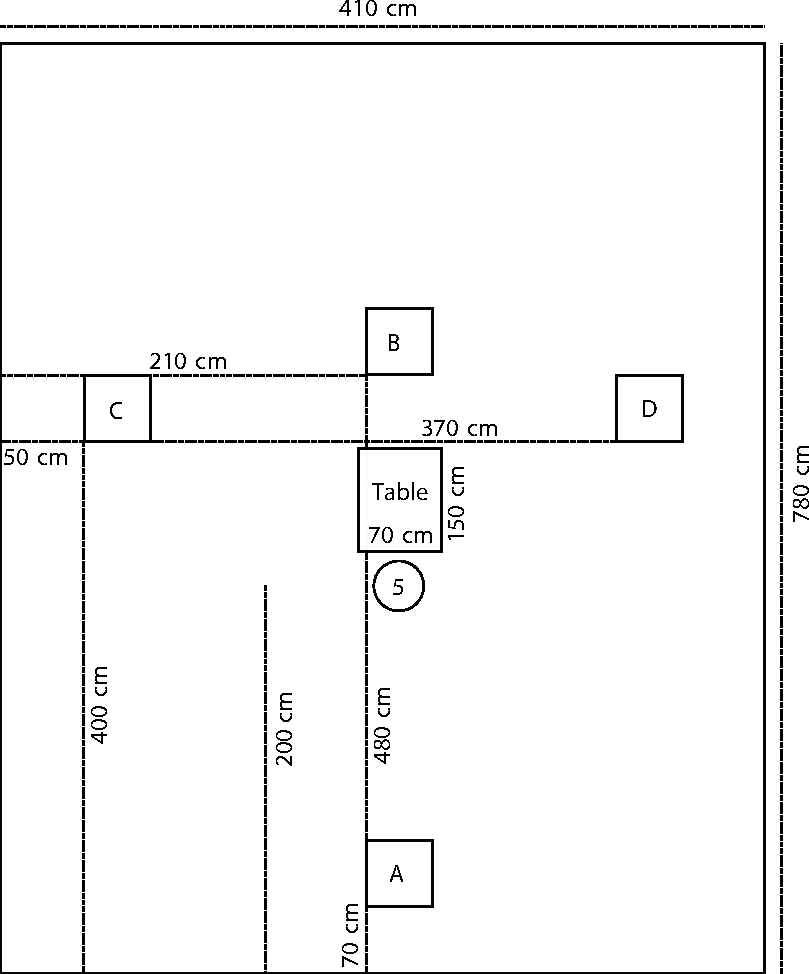
\includegraphics[width=0.8\textwidth]{figures/ListeningTestSetup.pdf}
			\end{figure}
		\end{column}
	\end{columns}
\end{frame}

\begin{frame}{Experiments}{Measuring a Transfer-Function (Headphone)}		
	\begin{columns}
		\begin{column}{0.3\textwidth}
			\begin{itemize}
				\item Headphone Transfer-function
				\begin{itemize}
					\item Physical cup of headphone
				\end{itemize}
				\item{Logarithmic Chirp}
			\end{itemize}
		\end{column}
		\begin{column}{0.7\textwidth} 
			\begin{figure}[h]
				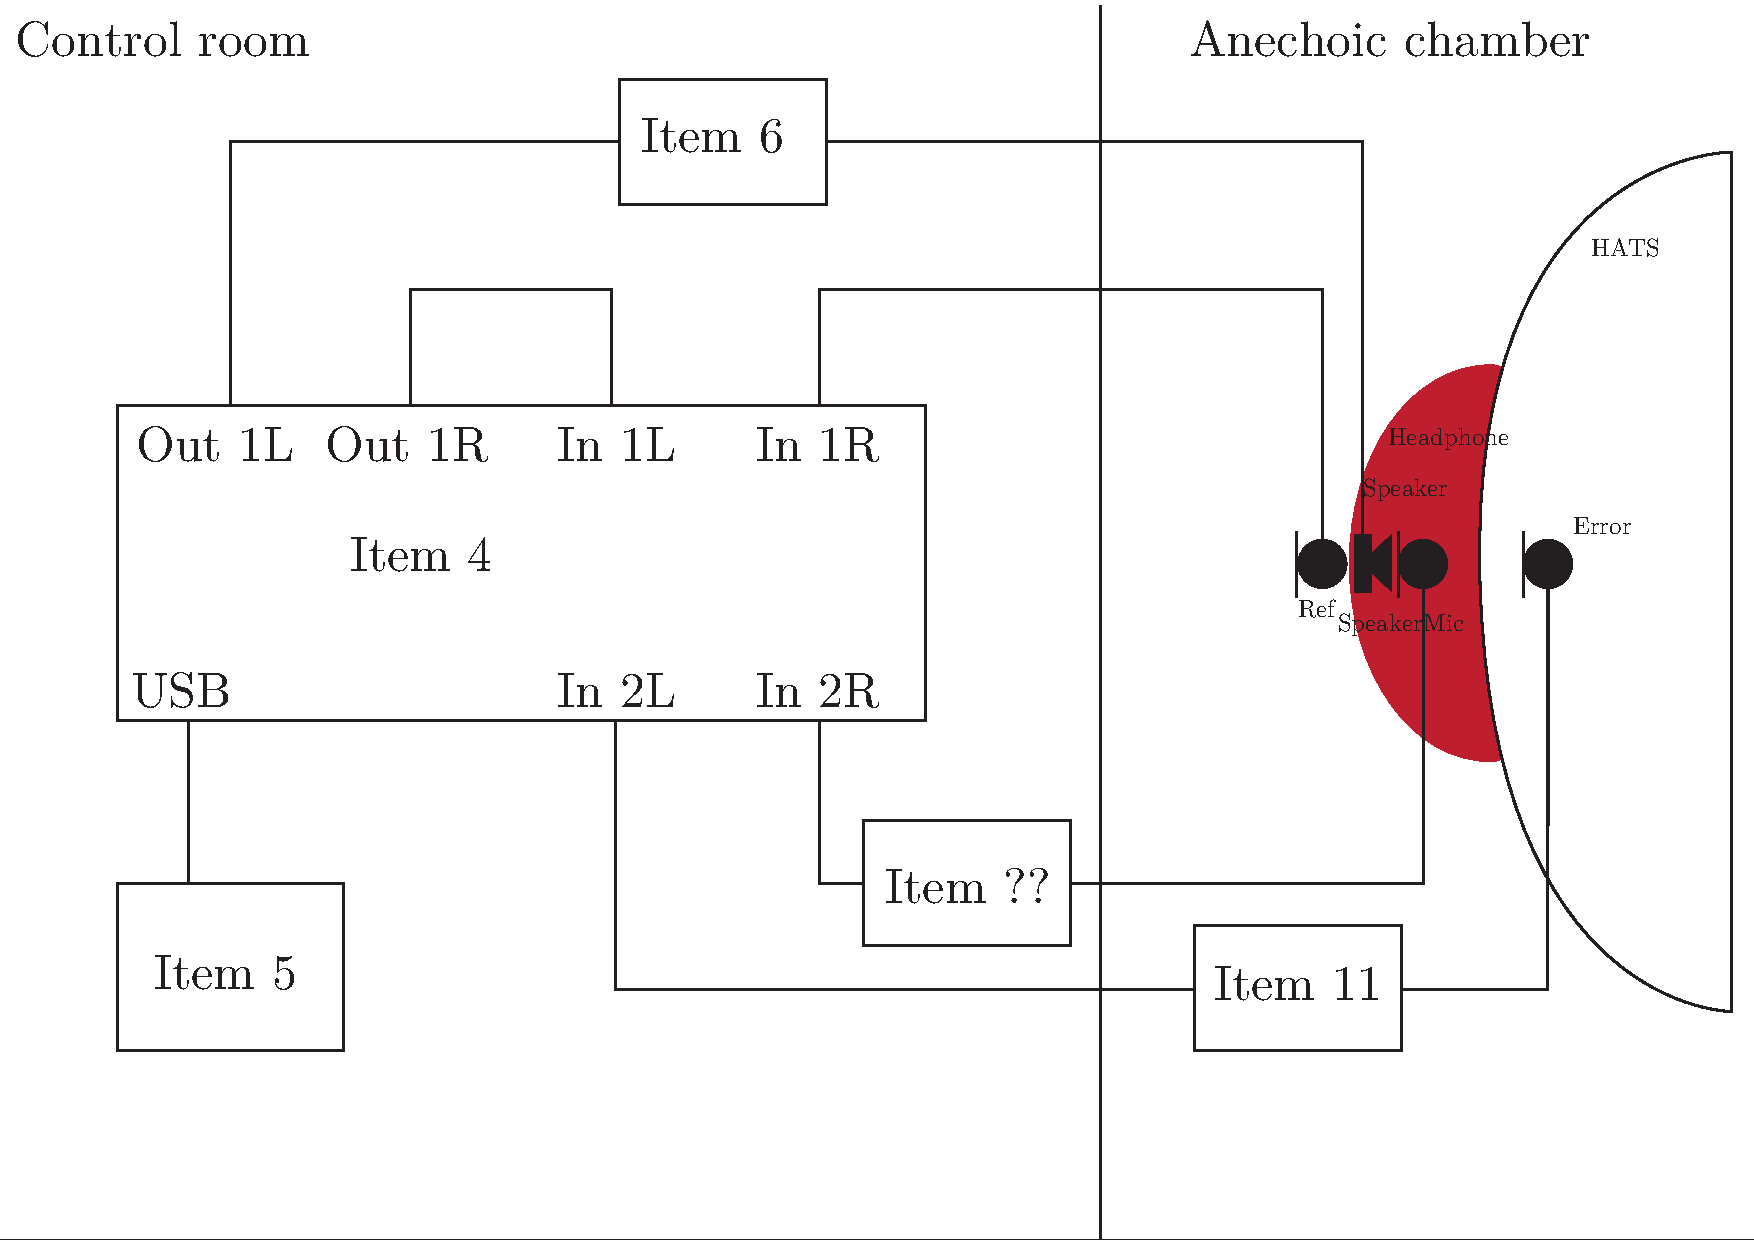
\includegraphics[width=1\textwidth]{figures/AngleOfIncidenceSetup.pdf}
			\end{figure}
		\end{column}
	\end{columns}
\end{frame}

\begin{frame}{Experiments}{Measuring a Transfer-Function (Headphone)}		
	\begin{columns}
		\begin{column}{0.5\textwidth}
			\begin{itemize}
				\item Transfer-function formula:
				\begin{equation*}
				H(f)=\frac{Y(f)}{X(f)}=\frac{\mathscr{F}(y(t))\times\mathscr{F}^{\ast}(x(t))}{\mathscr{F}(x(t))\times\mathscr{F}^{\ast}(x(t))}
				\end{equation*}
				\item Where:
				\begin{itemize}
					\item[] $\times$ denotes bin-wise multiplication
					\item[] $\ast$ denotes the complex conjugate
					\item[] $x(t)$ and $y(t)$ are measured in time domain
					\item[] $X(f)$ is the auto-spectrum
					\item[] $Y (f)$ is the cross-spectrum
				\end{itemize}
			\end{itemize}
		\end{column}
		\begin{column}{0.5\textwidth} 



		\end{column}
	\end{columns}
\end{frame}

\begin{frame}{Experiments}{Measuring a Transfer-Function (Headphone)}		
	\begin{columns}
		\begin{column}{0.3\textwidth}
			\begin{itemize}
				\item Results
				\item Frequency response
				\begin{itemize}
					\item[\textcolor{MATLABorange}{---}] FFT of 960 coefficients
					\item[\textcolor{MATLABblue}{---}] FFT of 386,024 coefficients
				\end{itemize}
			\end{itemize}
		\end{column}
		\begin{column}{0.7\textwidth} 
			\begin{figure}[h]
				% This file was created by matlab2tikz.
%
%The latest updates can be retrieved from
%  http://www.mathworks.com/matlabcentral/fileexchange/22022-matlab2tikz-matlab2tikz
%where you can also make suggestions and rate matlab2tikz.
%
\definecolor{mycolor1}{rgb}{0.00000,0.44700,0.74100}%
\definecolor{mycolor2}{rgb}{0.85000,0.32500,0.09800}%
%
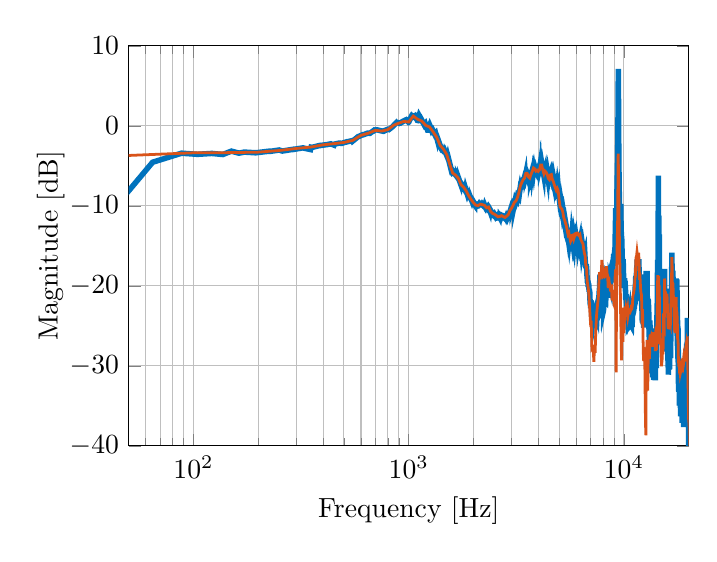
\begin{tikzpicture}

\begin{axis}[%
width=2.8in,
height=2in,
at={(1.281in,0.441in)},
scale only axis,
xmode=log,
xmin=50,
xmax=20000,
xminorticks=true,
xlabel={Frequency [Hz]},
xmajorgrids,
xminorgrids,
ymin=-40,
ymax=10,
ylabel style={yshift=-0.5em},
%xlabel style={yshift=-0.9em},
ylabel={Magnitude [dB]},
ymajorgrids,
axis background/.style={fill=white},
title style={font=\bfseries},
legend style={legend cell align=left,align=left,draw=white!15!black}
]
\addplot [color=mycolor1,solid,forget plot, line width=2pt]
table[row sep=crcr]{%
0	-36.314\\
0.12467	-46.203\\
24.435	21.379\\
32.538	5.9252\\
32.663	-14.074\\
64.578	-4.5539\\
88.015	-3.4248\\
104.47	-3.5654\\
121.68	-3.4543\\
136.88	-3.5865\\
149.98	-3.1672\\
162.57	-3.418\\
172.29	-3.2875\\
194.48	-3.373\\
225.77	-3.1662\\
227.02	-3.1955\\
249.96	-3.0277\\
258.81	-3.1542\\
290.35	-2.9361\\
290.97	-2.9544\\
322.27	-2.7589\\
349.82	-2.9682\\
351.94	-2.6789\\
355.18	-2.7007\\
386.72	-2.4544\\
387.59	-2.4702\\
419.26	-2.3363\\
434.59	-2.2519\\
449.8	-2.412\\
451.67	-2.2926\\
475.61	-2.1575\\
487.45	-2.1991\\
516.25	-1.9911\\
517.5	-2.0042\\
548.41	-1.8421\\
549.66	-1.9003\\
580.58	-1.3752\\
581.7	-1.3778\\
610	-1.1191\\
613.74	-1.1339\\
644.91	-0.9135\\
659.99	-0.9434\\
677.32	-0.71792\\
677.57	-0.73619\\
703.87	-0.49587\\
710.61	-0.49507\\
741.9	-0.61847\\
758.23	-0.67409\\
773.19	-0.58822\\
774.31	-0.61185\\
797.75	-0.43973\\
807.97	-0.47363\\
838.76	-0.14306\\
838.76	-0.14306\\
871.05	0.32037\\
871.43	0.30951\\
888.51	0.40704\\
903.96	0.31934\\
935.13	0.52427\\
935.75	0.49481\\
967.17	0.72876\\
972.28	0.75514\\
998.21	0.4424\\
1000.1	0.45482\\
1031.4	1.2465\\
1033.2	1.2789\\
1049.6	1.118\\
1068.5	1.2526\\
1096.2	0.67767\\
1098.2	0.67326\\
1116.9	1.2894\\
1129.2	1.0559\\
1160.7	0.47145\\
1161.4	0.50833\\
1183.6	0.10439\\
1195.3	0.25274\\
1223.1	-0.53659\\
1226.5	-0.5376\\
1252.3	0.076714\\
1259.6	-0.079904\\
1280	-0.63319\\
1291.6	-0.51308\\
1321	-1.072\\
1334.2	-0.93898\\
1354.8	-1.6354\\
1355.4	-1.6052\\
1386.8	-2.2238\\
1387.8	-2.1735\\
1419.1	-2.9054\\
1434.9	-3.0411\\
1451.6	-2.8413\\
1455.4	-2.8282\\
1483.2	-3.359\\
1483.9	-3.3087\\
1515.1	-3.7658\\
1516.2	-3.7389\\
1547.1	-4.6825\\
1548.5	-4.641\\
1579.4	-5.5706\\
1580.7	-5.5612\\
1598.9	-5.867\\
1614.1	-5.7917\\
1645.2	-6.0847\\
1646.1	-6.0306\\
1677.5	-6.319\\
1678.1	-6.2583\\
1709.6	-6.7028\\
1710.2	-6.6481\\
1741.4	-7.2438\\
1742.5	-7.1849\\
1773.5	-7.5146\\
1774.3	-7.4538\\
1805.7	-7.6952\\
1806.7	-7.6472\\
1837.8	-7.9083\\
1838.7	-7.8712\\
1869.8	-8.5141\\
1872.4	-8.4724\\
1903.3	-8.7677\\
1904.4	-8.7327\\
1935.6	-9.0077\\
1936.6	-8.9502\\
1967.8	-9.4318\\
1970.6	-9.3852\\
1999.9	-9.6425\\
2000.7	-9.5858\\
2032	-9.8686\\
2032.7	-9.8107\\
2046.3	-9.9415\\
2065	-9.8735\\
2088.9	-10.034\\
2097.9	-10.017\\
2128.9	-9.7399\\
2140.7	-9.8191\\
2159.2	-9.7135\\
2168.2	-9.6978\\
2193.7	-9.8431\\
2198.5	-9.7955\\
2224.1	-9.9567\\
2243.1	-9.8538\\
2258.1	-10.008\\
2259.1	-9.9881\\
2283	-10.29\\
2292	-10.276\\
2319.7	-10.171\\
2324.1	-10.226\\
2342.6	-10.082\\
2355	-10.173\\
2386.4	-10.632\\
2387.3	-10.602\\
2418.6	-10.795\\
2421	-10.74\\
2451.7	-10.997\\
2466.7	-11.087\\
2481.8	-10.979\\
2487	-10.964\\
2516.2	-11.212\\
2519.2	-11.177\\
2530.8	-11.266\\
2549.2	-11.215\\
2580.4	-11.52\\
2584	-11.519\\
2611.8	-11.333\\
2627.7	-11.242\\
2644.6	-11.388\\
2645.7	-11.35\\
2674.6	-11.556\\
2678.5	-11.512\\
2707.8	-11.223\\
2709.9	-11.229\\
2740.9	-11.486\\
2744.4	-11.482\\
2768.6	-11.318\\
2775.5	-11.335\\
2805	-11.592\\
2817.5	-11.644\\
2835.8	-11.445\\
2838.8	-11.477\\
2853.8	-11.319\\
2872.6	-11.423\\
2902	-11.167\\
2903.3	-11.196\\
2932.6	-10.916\\
2936.7	-10.936\\
2966.2	-10.566\\
2970.5	-10.634\\
2999.9	-10.396\\
3000.7	-10.454\\
3026.6	-10.103\\
3033	-10.172\\
3064.2	-9.89\\
3065	-9.9438\\
3096.4	-9.7007\\
3097	-9.7991\\
3124.9	-9.2799\\
3130.2	-9.3215\\
3149	-9.5709\\
3161.4	-9.434\\
3185.5	-9.0127\\
3204.2	-9.1495\\
3225.9	-8.794\\
3225.9	-8.794\\
3256.6	-8.3887\\
3261.2	-8.436\\
3290.4	-7.8675\\
3291.6	-7.8868\\
3322.6	-7.0804\\
3326.1	-7.0644\\
3351.9	-7.2683\\
3355.1	-7.2297\\
3386.7	-6.7741\\
3390.1	-6.7601\\
3408.9	-6.9447\\
3419.6	-6.8298\\
3435.1	-6.6254\\
3453.7	-6.7621\\
3483.2	-6.2695\\
3484	-6.3027\\
3506.2	-5.9996\\
3524.7	-6.1292\\
3539.7	-5.9539\\
3548.7	-5.9851\\
3579.8	-6.3716\\
3581.3	-6.3339\\
3610.1	-6.5578\\
3613.1	-6.4099\\
3642.5	-6.6501\\
3658.5	-6.7048\\
3677.2	-6.3753\\
3677.7	-6.4332\\
3704	-6.1064\\
3710.4	-6.1813\\
3741.3	-5.8883\\
3742.4	-5.9308\\
3773.6	-5.2595\\
3786	-5.1197\\
3804.9	-5.5145\\
3807.3	-5.4579\\
3824.3	-5.6537\\
3840.6	-5.5798\\
3868.2	-5.327\\
3871.2	-5.3576\\
3902.7	-5.7829\\
3908	-5.8137\\
3932.4	-5.5254\\
3935.6	-5.5192\\
3950.8	-5.6721\\
3969.4	-5.5357\\
3999.1	-5.7697\\
4002	-5.7358\\
4014.9	-5.9048\\
4032.4	-5.8236\\
4064	-5.2081\\
4064.8	-5.2515\\
4094.3	-4.8822\\
4105.8	-4.8863\\
4121.8	-5.0187\\
4149.4	-4.8517\\
4161.2	-5.0069\\
4161.9	-4.9432\\
4192.9	-5.3928\\
4194.1	-5.3629\\
4225.2	-5.87\\
4226	-5.8222\\
4250.2	-5.9836\\
4259.1	-5.9897\\
4290.2	-5.6621\\
4291.2	-5.7012\\
4320.5	-5.4958\\
4322.7	-5.5156\\
4353.6	-5.7465\\
4360.9	-5.7663\\
4379.1	-5.6645\\
4388	-5.7363\\
4419.3	-6.2751\\
4420.2	-6.234\\
4451.4	-6.4405\\
4452.4	-6.4093\\
4472.8	-6.7306\\
4483.9	-6.6424\\
4496.9	-6.4865\\
4517.6	-6.5717\\
4546.9	-5.977\\
4563.7	-6.047\\
4580.7	-5.8874\\
4585.9	-5.84\\
4612.6	-6.1482\\
4612.9	-6.0941\\
4644	-6.535\\
4646.9	-6.51\\
4661.8	-6.6523\\
4678.5	-6.5704\\
4709.6	-6.9971\\
4710.7	-6.9599\\
4738.5	-7.3008\\
4742.4	-7.293\\
4760.7	-7.1615\\
4775.1	-7.2296\\
4806.2	-7.702\\
4806.7	-7.632\\
4836.2	-7.9937\\
4839.8	-7.9665\\
4856.7	-7.8053\\
4879.1	-7.8893\\
4903.3	-7.5773\\
4906.8	-7.5137\\
4934.5	-7.9549\\
4947.3	-7.8599\\
4967.1	-8.2645\\
4968.6	-8.2441\\
4998.3	-9.1058\\
5001.3	-9.0125\\
5032.2	-9.6375\\
5032.8	-9.5871\\
5059.1	-10.008\\
5083.3	-9.8492\\
5096.5	-10.128\\
5105.5	-10.245\\
5127.6	-10.042\\
5135.1	-9.9936\\
5160.5	-10.446\\
5165.2	-10.375\\
5193	-10.681\\
5193.8	-10.631\\
5224.7	-11.051\\
5227.4	-11.02\\
5257.1	-11.459\\
5261.2	-11.38\\
5288.9	-11.648\\
5291.8	-11.58\\
5319.3	-11.969\\
5323.9	-11.896\\
5354.8	-12.261\\
5355.5	-12.199\\
5383.4	-12.544\\
5388.1	-12.469\\
5419	-12.863\\
5419.5	-12.752\\
5449.5	-13.21\\
5452.1	-13.135\\
5483.1	-13.698\\
5484.1	-13.599\\
5490.1	-13.796\\
5516.9	-13.744\\
5546.6	-13.508\\
5550.1	-13.519\\
5579.5	-14.12\\
5584	-14.039\\
5592.1	-14.26\\
5614.2	-14.149\\
5645.2	-14.723\\
5647.9	-14.637\\
5654.3	-14.915\\
5680.9	-14.848\\
5708.7	-14.188\\
5711.3	-14.244\\
5730.2	-13.748\\
5757.6	-14.162\\
5772.9	-13.89\\
5779.7	-13.841\\
5804	-14.175\\
5813.9	-14.064\\
5838.1	-14.49\\
5851.9	-14.675\\
5865.5	-14.314\\
5871.2	-14.391\\
5879.7	-14.175\\
5909.2	-14.349\\
5934.9	-14.017\\
5935.8	-14.116\\
5967.2	-13.837\\
5974.1	-13.779\\
5996.3	-14.022\\
6000.9	-13.972\\
6026.7	-14.314\\
6032.8	-14.113\\
6060.7	-14.296\\
6065.7	-14.261\\
6087.8	-14.027\\
6098.7	-14.079\\
6126.7	-14.387\\
6136.9	-14.439\\
6147.1	-14.242\\
6162.7	-14.283\\
6190.9	-14.636\\
6194.2	-14.595\\
6217.4	-14.197\\
6228.8	-14.225\\
6240.9	-14.472\\
6260.9	-14.292\\
6290.2	-14.936\\
6301.1	-14.96\\
6319.8	-14.698\\
6326.8	-14.697\\
6354.4	-15.218\\
6355.4	-15.125\\
6381.2	-15.689\\
6388.1	-15.613\\
6412.3	-14.888\\
6419.6	-14.899\\
6450.7	-15.324\\
6451.7	-15.236\\
6480.7	-15.803\\
6485.2	-15.706\\
6514.5	-16.076\\
6517.4	-15.977\\
6546.7	-16.399\\
6557.5	-16.412\\
6579.6	-16.167\\
6585.1	-16.124\\
6612.6	-17.049\\
6613.4	-16.849\\
6642.8	-17.612\\
6645.4	-17.453\\
6659.1	-17.79\\
6688.5	-17.3\\
6709.6	-17.813\\
6709.7	-17.703\\
6740.9	-18.925\\
6743.5	-18.744\\
6770.9	-19.604\\
6788	-19.314\\
6804.9	-19.727\\
6807.5	-19.454\\
6829.8	-20.165\\
6857.5	-19.647\\
6871.1	-20.249\\
6871.8	-20.066\\
6890.4	-20.743\\
6907.6	-20.363\\
6935	-21.02\\
6935.8	-20.762\\
6967	-22.313\\
6968.2	-21.978\\
6999.5	-22.576\\
7009.9	-22.785\\
7032	-21.988\\
7046.5	-21.821\\
7064.5	-22.787\\
7065.7	-22.59\\
7095.2	-24.25\\
7110.7	-23.739\\
7127.6	-24.327\\
7130.9	-24.351\\
7158.7	-23.321\\
7174.5	-23.094\\
7191.3	-23.919\\
7196.1	-23.502\\
7223.4	-24.532\\
7226.2	-23.95\\
7251.9	-25.052\\
7259.3	-24.899\\
7290.1	-23.803\\
7306.1	-23.531\\
7319.6	-24.22\\
7323.8	-23.915\\
7351.6	-25.113\\
7355	-25.006\\
7386.4	-23.168\\
7389.2	-23.764\\
7409.7	-23.056\\
7422.7	-23.475\\
7443.2	-22.701\\
7460.9	-22.594\\
7479.9	-23.402\\
7494	-23.495\\
7512.7	-22.754\\
7519.7	-22.723\\
7540.3	-23.583\\
7552	-22.808\\
7576.2	-23.708\\
7581.4	-23.675\\
7610.8	-22.625\\
7613.2	-23.388\\
7644.5	-21.174\\
7645.4	-21.642\\
7675	-20.682\\
7681	-21.196\\
7703.2	-20.255\\
7715.9	-20.306\\
7727.4	-21.465\\
7746	-20.733\\
7773.6	-21.709\\
7778.4	-21.138\\
7798.6	-22.151\\
7806.6	-21.379\\
7832.5	-22.378\\
7839.6	-22.138\\
7870.5	-19.881\\
7871.6	-20.371\\
7897.4	-19.008\\
7908.2	-19.024\\
7933.8	-20.421\\
7936.3	-19.954\\
7964.4	-21.328\\
7968.6	-20.558\\
7999.9	-22.147\\
8004.2	-21.657\\
8024.7	-23.168\\
8033.8	-23.111\\
8063.1	-21.266\\
8066	-21.753\\
8095.3	-20.463\\
8114.7	-20.406\\
8126.3	-21.578\\
8129.8	-21.451\\
8155.8	-20.411\\
8164.7	-20.201\\
8188.7	-21.225\\
8194.9	-20.691\\
8211.7	-21.943\\
8225.9	-21.965\\
8255.6	-20.921\\
8258.1	-21.423\\
8289.3	-19.481\\
8292.1	-19.976\\
8314.3	-18.987\\
8325	-19.024\\
8354.5	-20.159\\
8363.4	-20.171\\
8382	-19.457\\
8388.3	-20.054\\
8414.1	-19.324\\
8419.4	-19.46\\
8450.6	-21.262\\
8464.9	-21.49\\
8483.5	-20.442\\
8484.4	-20.933\\
8515.9	-19.048\\
8526.4	-18.902\\
8545	-19.728\\
8559.3	-19.986\\
8579.6	-19.257\\
8582.5	-19.713\\
8602.9	-18.978\\
8617.1	-19.037\\
8641.3	-19.907\\
8650.2	-19.958\\
8676.2	-18.97\\
8677.9	-18.899\\
8709	-19.584\\
8710.6	-19.547\\
8740.3	-18.261\\
8742.7	-18.607\\
8774	-17.506\\
8777.6	-17.488\\
8803.4	-18.658\\
8814.1	-18.893\\
8838.2	-18.226\\
8838.9	-18.733\\
8870.5	-17.512\\
8871.1	-17.887\\
8895.2	-17.056\\
8913.9	-17.503\\
8934.4	-16.605\\
8937	-16.912\\
8952	-16.038\\
8983.4	-16.758\\
8998.6	-16.002\\
9001.1	-16.408\\
9030.4	-15.861\\
9033.4	-16.2\\
9052.1	-15.549\\
9072.4	-16.298\\
9096.4	-14.819\\
9097.5	-15.165\\
9128.7	-12.157\\
9129.4	-12.496\\
9160.4	-10.362\\
9163.9	-10.306\\
9193.6	-11.63\\
9194.1	-11.216\\
9213.1	-12.534\\
9225.9	-12.225\\
9256.7	-10.674\\
9259.3	-10.904\\
9290.4	-7.4853\\
9291	-7.6421\\
9322.6	-5.4423\\
9323.8	-5.8697\\
9354.7	-2.8839\\
9355.4	-3.2159\\
9386.8	1.0916\\
9387.7	0.65156\\
9419.4	7.1202\\
9419.4	7.1202\\
9451.5	-1.5727\\
9452.4	-1.2719\\
9484	-6.1289\\
9485.2	-5.7787\\
9514.4	-8.7361\\
9516.5	-8.3104\\
9548.4	-11.128\\
9549	-10.751\\
9580.5	-12.735\\
9592.7	-13.313\\
9612.9	-12.281\\
9619.3	-12.83\\
9645.2	-10.268\\
9663.2	-9.7774\\
9676.3	-11.178\\
9677.7	-10.999\\
9708.5	-13.365\\
9713.2	-13.139\\
9735.3	-14.514\\
9757.6	-13.806\\
9772.6	-14.451\\
9775.4	-14.134\\
9804.7	-16.134\\
9807.3	-15.846\\
9838.6	-17.375\\
9839.4	-17.118\\
9866.9	-18.114\\
9877.5	-18.089\\
9902	-16.841\\
9905.5	-16.673\\
9934.8	-17.456\\
9935.5	-17.221\\
9966.7	-19.591\\
9967.9	-19.285\\
9991.7	-20.265\\
10002	-20.014\\
10032	-19.214\\
10033	-19.543\\
10060	-19.044\\
10065	-19.203\\
10095	-20.293\\
10099	-20.183\\
10112	-19.532\\
10130	-19.551\\
10161	-20.614\\
10162	-20.301\\
10191	-21.595\\
10204	-21.621\\
10223	-21.134\\
10229	-21.063\\
10257	-21.84\\
10262	-21.601\\
10287	-22.423\\
10292	-22.158\\
10320	-22.859\\
10328	-22.595\\
10350	-23.144\\
10356	-23.179\\
10361	-22.74\\
10390	-22.854\\
10419	-23.857\\
10420	-23.461\\
10446	-24.44\\
10453	-24.418\\
10482	-23.699\\
10485	-23.986\\
10511	-23.331\\
10518	-23.297\\
10548	-24.4\\
10548	-24.126\\
10569	-24.602\\
10581	-24.569\\
10593	-24.046\\
10614	-24.037\\
10640	-24.638\\
10648	-24.317\\
10674	-24.937\\
10679	-24.93\\
10709	-24.278\\
10714	-24.248\\
10742	-24.794\\
10746	-24.922\\
10772	-24.121\\
10780	-24.07\\
10802	-24.898\\
10827	-24.949\\
10835	-24.406\\
10853	-24.363\\
10863	-24.775\\
10883	-24.339\\
10900	-25.024\\
10918	-25.158\\
10933	-24.286\\
10935	-24.588\\
10967	-23.008\\
10978	-22.83\\
10995	-23.394\\
11016	-23.523\\
11024	-23.023\\
11034	-23.414\\
11063	-22.692\\
11074	-22.687\\
11094	-23.217\\
11100	-23.194\\
11124	-22.657\\
11130	-22.969\\
11158	-22.439\\
11167	-22.83\\
11194	-22.047\\
11194	-22.293\\
11225	-21.375\\
11226	-21.728\\
11254	-20.894\\
11259	-20.899\\
11281	-21.443\\
11291	-21.343\\
11322	-19.611\\
11323	-19.977\\
11348	-18.928\\
11362	-18.816\\
11379	-19.647\\
11390	-19.701\\
11418	-18.876\\
11420	-19.214\\
11452	-17.952\\
11452	-18.274\\
11468	-17.728\\
11484	-18.231\\
11515	-16.885\\
11521	-16.692\\
11548	-18.233\\
11549	-17.981\\
11580	-19.257\\
11581	-18.732\\
11598	-19.398\\
11613	-19.189\\
11644	-18.32\\
11648	-18.801\\
11676	-17.231\\
11682	-17.872\\
11696	-17.008\\
11735	-17.008\\
11741	-17.732\\
11742	-17.349\\
11773	-19.38\\
11777	-18.983\\
11805	-21.096\\
11809	-21.179\\
11838	-19.338\\
11852	-19.057\\
11871	-20.165\\
11874	-19.448\\
11896	-20.48\\
11905	-19.96\\
11932	-21.687\\
11939	-21.612\\
11952	-20.48\\
11973	-19.827\\
11989	-21.605\\
12024	-21.676\\
12032	-20.151\\
12032	-20.402\\
12036	-21.616\\
12073	-18.587\\
12088	-21.593\\
12103	-20.836\\
12127	-23.135\\
12130	-22.324\\
12158	-23.905\\
12173	-24.607\\
12192	-21.63\\
12197	-22.298\\
12219	-20.322\\
12226	-20.344\\
12258	-23.126\\
12260	-22.035\\
12288	-24.726\\
12291	-24.822\\
12317	-23.148\\
12333	-23.574\\
12350	-25.11\\
12364	-25.22\\
12387	-23.233\\
12389	-24.247\\
12408	-21.774\\
12438	-23.705\\
12451	-21.452\\
12455	-22.988\\
12482	-19.463\\
12485	-20.047\\
12516	-23.458\\
12532	-23.686\\
12535	-21.638\\
12552	-23.353\\
12578	-20.964\\
12581	-21.177\\
12602	-23.074\\
12619	-23.116\\
12626	-20.732\\
12646	-22.788\\
12672	-18.924\\
12692	-18.139\\
12709	-20.225\\
12711	-18.663\\
12716	-20.773\\
12759	-18.294\\
12771	-20.011\\
12782	-20.077\\
12802	-18.124\\
12807	-18.545\\
12838	-22.506\\
12839	-21.306\\
12870	-23.244\\
12873	-22.087\\
12899	-23.885\\
12923	-21.964\\
12924	-23.75\\
12951	-23.584\\
12954	-21.796\\
12970	-21.818\\
12999	-23.574\\
13017	-24.019\\
13021	-22.403\\
13032	-22.785\\
13063	-25.412\\
13068	-24.26\\
13093	-26.351\\
13098	-24.973\\
13120	-27.058\\
13140	-25.814\\
13141	-27.681\\
13162	-27.294\\
13191	-24.315\\
13194	-24.53\\
13216	-25.959\\
13233	-24.892\\
13256	-27.667\\
13258	-26.559\\
13286	-28.237\\
13300	-27.986\\
13313	-25.9\\
13328	-26.345\\
13355	-28.793\\
13370	-27.602\\
13380	-29.733\\
13393	-29.121\\
13409	-27.137\\
13431	-27.1\\
13448	-28.769\\
13452	-27.607\\
13482	-30.277\\
13507	-30.261\\
13514	-28.448\\
13525	-29.693\\
13536	-27.933\\
13549	-28.409\\
13578	-30.902\\
13587	-31.455\\
13611	-29.674\\
13615	-31.044\\
13641	-28.043\\
13645	-28.983\\
13675	-26.617\\
13678	-26.862\\
13710	-30.39\\
13718	-29.419\\
13732	-31.767\\
13746	-31.65\\
13772	-29.403\\
13774	-31.363\\
13806	-28.133\\
13816	-27.543\\
13839	-30.002\\
13863	-28.726\\
13868	-30.837\\
13884	-30.917\\
13898	-28.64\\
13904	-30.005\\
13930	-27.302\\
13957	-27.453\\
13965	-29.484\\
13971	-28.338\\
13996	-31.464\\
14003	-31.823\\
14030	-28.025\\
14033	-29.96\\
14062	-25.931\\
14065	-27.496\\
14078	-25.313\\
14098	-25.61\\
14127	-30.125\\
14142	-30.296\\
14159	-27.652\\
14162	-29.541\\
14194	-24.94\\
14198	-26.427\\
14219	-23.79\\
14231	-23.707\\
14250	-26.08\\
14261	-26.211\\
14288	-21.728\\
14291	-23.082\\
14321	-18.677\\
14335	-16.758\\
14352	-20.271\\
14359	-17.355\\
14380	-22.406\\
14388	-21.624\\
14418	-15.856\\
14420	-16.875\\
14450	-6.7422\\
14452	-6.2176\\
14479	-14.416\\
14496	-16.493\\
14514	-12.628\\
14523	-11.243\\
14546	-17.331\\
14549	-14.852\\
14567	-18.998\\
14590	-13.564\\
14612	-19.959\\
14617	-16.765\\
14637	-22.752\\
14671	-22.674\\
14676	-20.046\\
14687	-19.553\\
14696	-22.681\\
14711	-18.911\\
14740	-22.775\\
14746	-21.438\\
14771	-23.683\\
14781	-21.534\\
14801	-24.084\\
14809	-21.251\\
14828	-23.876\\
14840	-21.96\\
14867	-24.856\\
14875	-25.692\\
14895	-22.554\\
14919	-23.909\\
14935	-26.659\\
14942	-24.024\\
14948	-26.313\\
14969	-24.074\\
14992	-27.04\\
15013	-26.939\\
15019	-24.33\\
15036	-27.301\\
15062	-24.414\\
15082	-25.974\\
15094	-23.403\\
15106	-25.599\\
15107	-23.244\\
15133	-23.2\\
15159	-26.556\\
15180	-28.229\\
15192	-24.959\\
15200	-26.991\\
15224	-22.841\\
15228	-24.31\\
15254	-21.491\\
15266	-20.527\\
15290	-23.058\\
15291	-21.752\\
15322	-25.427\\
15341	-25.718\\
15345	-24.17\\
15364	-24.027\\
15369	-25.761\\
15391	-25.672\\
15418	-22.191\\
15421	-22.8\\
15452	-18.014\\
15454	-17.888\\
15484	-21.9\\
15491	-23.052\\
15507	-21.079\\
15519	-21.628\\
15540	-23.988\\
15548	-23.503\\
15579	-20.876\\
15581	-20.786\\
15612	-23.109\\
15614	-22.012\\
15638	-24.386\\
15651	-24.031\\
15673	-20.345\\
15679	-21.138\\
15706	-23.793\\
15710	-22.721\\
15740	-25.57\\
15763	-25.702\\
15767	-23.894\\
15786	-25.406\\
15787	-24.085\\
15813	-25.123\\
15834	-22.261\\
15843	-23.965\\
15863	-21.908\\
15875	-22.154\\
15901	-24.916\\
15904	-23.466\\
15933	-25.957\\
15939	-24.798\\
15961	-27.553\\
15978	-25.227\\
16000	-28.007\\
16001	-26.29\\
16021	-29.366\\
16033	-27.555\\
16064	-30.181\\
16069	-28.203\\
16071	-31.114\\
16099	-29.743\\
16128	-27.276\\
16132	-28.802\\
16160	-26.271\\
16167	-26.342\\
16186	-28.575\\
16209	-26.856\\
16224	-29.394\\
16236	-27.378\\
16243	-29.651\\
16259	-27.318\\
16279	-30.487\\
16291	-29.1\\
16311	-26.551\\
16326	-28.225\\
16353	-25.255\\
16369	-25.571\\
16371	-28.169\\
16389	-26.335\\
16400	-28.749\\
16423	-26.475\\
16450	-28.296\\
16467	-29.033\\
16481	-26.54\\
16494	-28.092\\
16514	-23.373\\
16518	-24.725\\
16541	-22.307\\
16561	-23.782\\
16571	-22.156\\
16596	-23.42\\
16610	-21.145\\
16628	-22.039\\
16644	-20.293\\
16645	-21.197\\
16673	-17.65\\
16678	-18.593\\
16705	-16.495\\
16715	-15.863\\
16728	-18.649\\
16747	-17.22\\
16752	-20.1\\
16778	-18.282\\
16803	-20.994\\
16819	-22.842\\
16822	-19.571\\
16848	-21.634\\
16866	-19.309\\
16889	-18.091\\
16893	-20.758\\
16910	-18.875\\
16913	-20.936\\
16936	-21.9\\
16939	-18.983\\
16974	-20.101\\
16983	-22.185\\
17007	-22.597\\
17010	-19.267\\
17054	-20.527\\
17057	-23.168\\
17080	-22.567\\
17081	-20.191\\
17104	-19.464\\
17127	-23.2\\
17129	-20.943\\
17161	-23.72\\
17171	-22.675\\
17177	-25.12\\
17213	-24.576\\
17221	-22.109\\
17227	-22.572\\
17241	-25.379\\
17264	-24.911\\
17265	-22.352\\
17312	-21.088\\
17315	-24.439\\
17338	-24.125\\
17349	-22.132\\
17362	-21.983\\
17382	-25.16\\
17397	-24.757\\
17409	-22.839\\
17432	-25.015\\
17449	-21.73\\
17453	-23.475\\
17482	-19.473\\
17495	-19.082\\
17503	-21.952\\
17526	-19.344\\
17546	-23.171\\
17550	-21.013\\
17570	-25.487\\
17596	-24.184\\
17602	-20.467\\
17620	-19.184\\
17645	-23.834\\
17651	-23.832\\
17664	-20.589\\
17679	-21.745\\
17687	-26.258\\
17711	-22.868\\
17737	-27.513\\
17758	-24.317\\
17761	-28.047\\
17793	-27.887\\
17805	-25.063\\
17823	-29.104\\
17828	-25.092\\
17839	-26.141\\
17863	-29.576\\
17875	-27.674\\
17898	-31.741\\
17922	-28.879\\
17927	-32.113\\
17941	-32.371\\
17952	-29.731\\
17969	-33.194\\
17995	-29.292\\
18016	-33.262\\
18026	-29.765\\
18039	-29.8\\
18063	-32.972\\
18066	-30.218\\
18089	-34.982\\
18103	-31.024\\
18109	-33.739\\
18136	-30.389\\
18159	-33.522\\
18163	-31.281\\
18183	-34.353\\
18203	-33.983\\
18206	-30.627\\
18227	-31.012\\
18254	-34.144\\
18259	-32.354\\
18289	-34.958\\
18300	-35.248\\
18315	-32.195\\
18324	-36.319\\
18326	-32.639\\
18364	-35.341\\
18367	-32.355\\
18391	-31.901\\
18415	-35.779\\
18431	-32.206\\
18438	-36.197\\
18465	-35.678\\
18475	-32.337\\
18485	-32.191\\
18489	-35.268\\
18532	-32.663\\
18535	-35.674\\
18558	-36.238\\
18579	-32.176\\
18605	-35.962\\
18606	-32.168\\
18624	-32.692\\
18629	-36.096\\
18647	-32.878\\
18649	-37.131\\
18688	-36.642\\
18691	-33.273\\
18720	-33.21\\
18724	-35.869\\
18746	-32.875\\
18770	-37.03\\
18778	-33.087\\
18780	-35.876\\
18837	-35.137\\
18838	-32.353\\
18839	-32.012\\
18860	-35.322\\
18881	-35.48\\
18885	-32.396\\
18910	-31.927\\
18934	-37.657\\
18941	-35.889\\
18947	-32.526\\
18990	-32.128\\
18992	-34.43\\
19001	-31.205\\
19028	-34.951\\
19041	-37.442\\
19051	-31.767\\
19071	-32.179\\
19080	-35.185\\
19098	-31.953\\
19115	-35.453\\
19139	-35.683\\
19141	-30.624\\
19168	-35.963\\
19192	-31.208\\
19199	-36.299\\
19215	-31.559\\
19236	-35.486\\
19241	-29.437\\
19262	-35.001\\
19281	-30.947\\
19309	-30.802\\
19319	-34.395\\
19340	-30.206\\
19341	-36.44\\
19369	-33.938\\
19376	-28.824\\
19389	-32.743\\
19403	-28.519\\
19420	-28.523\\
19447	-34.102\\
19473	-34.435\\
19476	-28.04\\
19494	-28.231\\
19512	-33.016\\
19545	-28.992\\
19545	-33.887\\
19562	-32.824\\
19564	-27.239\\
19587	-27.468\\
19588	-34.397\\
19636	-33.078\\
19638	-27.594\\
19652	-33.555\\
19671	-27.012\\
19685	-36.693\\
19708	-25.152\\
19710	-30.372\\
19732	-24.006\\
19752	-25.067\\
19754	-30.043\\
19778	-25.353\\
19799	-32.274\\
19822	-35.328\\
19825	-26.563\\
19846	-26.86\\
19849	-34.365\\
19873	-28.366\\
19887	-34.629\\
19919	-28.418\\
19935	-36.242\\
19963	-37.528\\
19966	-30.074\\
19983	-37.412\\
19990	-28.591\\
20010	-41.127\\
20030	-32.098\\
20033	-31.579\\
20036	-43.567\\
20080	-30.784\\
20086	-39.487\\
20099	-38.914\\
20127	-32.586\\
20154	-42.3\\
20157	-32.623\\
20174	-42.864\\
20177	-31.543\\
20204	-39.028\\
20224	-30.335\\
20245	-41.396\\
20248	-32.364\\
20268	-33.188\\
20271	-39.813\\
20292	-32.89\\
20320	-40.346\\
20338	-42.495\\
20342	-32.904\\
20362	-42.066\\
20385	-34.256\\
20409	-40.16\\
20415	-33.838\\
20432	-31.106\\
20439	-38.522\\
20456	-40.098\\
20479	-31.528\\
20503	-38.127\\
20506	-31.366\\
20529	-40.749\\
20543	-32.571\\
20563	-38.239\\
20576	-31.392\\
20596	-32.261\\
20605	-39.359\\
20620	-39.539\\
20623	-31.145\\
20646	-32.6\\
20667	-40.049\\
20690	-39.754\\
20693	-32.789\\
20714	-31.802\\
20740	-40.303\\
20750	-39.842\\
20761	-31.958\\
20803	-37.765\\
20805	-32.626\\
20808	-30.094\\
20829	-38.752\\
20858	-39.398\\
20859	-32.962\\
20878	-39.513\\
20881	-31.582\\
20913	-33.001\\
20934	-41.557\\
20944	-39.351\\
20948	-32.991\\
20977	-35.256\\
21000	-40.968\\
21001	-35.329\\
21022	-46.017\\
21041	-35.138\\
21049	-42.383\\
21069	-45.42\\
21092	-34.794\\
21113	-43.06\\
21116	-33.838\\
21136	-47.009\\
21139	-35.224\\
21183	-53.229\\
21188	-36.828\\
21197	-37.616\\
21200	-44.635\\
21253	-48.21\\
21256	-36.943\\
21277	-36.074\\
21280	-46.06\\
21303	-36.279\\
21306	-49.268\\
21327	-36.786\\
21354	-46.762\\
21371	-37.728\\
21374	-49.554\\
21394	-38.978\\
21397	-55.995\\
21438	-48.779\\
21444	-37.686\\
21468	-37.028\\
21479	-46.672\\
21491	-49.08\\
21512	-36.81\\
21532	-39.076\\
21541	-48.692\\
21552	-39.667\\
21562	-56.663\\
21582	-38.457\\
21585	-54.809\\
21632	-50.584\\
21639	-39.137\\
21652	-38.44\\
21676	-49.177\\
21697	-47.944\\
21699	-37.992\\
21733	-47.798\\
21739	-39.668\\
21770	-53.716\\
21773	-38.535\\
21775	-39.965\\
21805	-52.801\\
21817	-37.917\\
21823	-49.12\\
21840	-37.284\\
21867	-49.541\\
21888	-53.464\\
21890	-37.986\\
21918	-50.615\\
21934	-39.2\\
21937	-36.281\\
21945	-56.606\\
21978	-58.85\\
21984	-35.946\\
22020	-53.902\\
22028	-36.763\\
22037	-57.612\\
22039	-37.461\\
22070	-60.953\\
22078	-35.126\\
22098	-34.456\\
22103	-57.8\\
22148	-37.428\\
22156	-58.687\\
22172	-39.112\\
22189	-74.275\\
22194	-67.533\\
22216	-37.738\\
22234	-72.683\\
22242	-35.973\\
22259	-85.489\\
22289	-33.573\\
22304	-79.455\\
22309	-35.034\\
22333	-34.185\\
22340	-78.599\\
22359	-33.654\\
22386	-69.283\\
22403	-30.626\\
22415	-62.492\\
22431	-68.652\\
22450	-27.824\\
22473	-28.371\\
22480	-69.301\\
22485	-57.014\\
22497	-25.882\\
22523	-24.373\\
22542	-59.333\\
22569	-67.681\\
22570	-30.059\\
22587	-62.437\\
22591	-29.717\\
22614	-24.556\\
22621	-54.859\\
22664	-25.51\\
22665	-58.522\\
22685	-27.132\\
22697	-55.284\\
22721	-61.927\\
22732	-28.77\\
22752	-59.755\\
22755	-28.574\\
22777	-59.807\\
22781	-29.823\\
22825	-29.864\\
22836	-66.407\\
22849	-29.262\\
22866	-69.26\\
22872	-28.557\\
22903	-69.596\\
22911	-69.905\\
22922	-31.205\\
22957	-66.797\\
22966	-31.93\\
22972	-65.137\\
22993	-30.533\\
23019	-34.186\\
23025	-59.261\\
23044	-74.035\\
23060	-31.523\\
23083	-32.672\\
23086	-63.347\\
23110	-32.013\\
23117	-59.75\\
23130	-33.048\\
23154	-69.906\\
23175	-61.589\\
23177	-32.88\\
23212	-68.361\\
23224	-31.453\\
23243	-59.948\\
23251	-33.392\\
23261	-75.347\\
23274	-32.891\\
23318	-33.315\\
23318	-66.141\\
23342	-31.559\\
23349	-59.827\\
23377	-62.919\\
23382	-35.147\\
23400	-62.163\\
23412	-32.063\\
23435	-33.776\\
23445	-61.147\\
23462	-32.656\\
23462	-62.798\\
23485	-33.813\\
23499	-65.653\\
23545	-36.628\\
23546	-69.89\\
23555	-64.912\\
23576	-30.278\\
23589	-61.917\\
23600	-31.251\\
23626	-33.901\\
23633	-75.548\\
23649	-60.583\\
23670	-30.678\\
23692	-66.67\\
23697	-32.507\\
23717	-31.746\\
23740	-86.392\\
23747	-34.065\\
23772	-66.823\\
23782	-58.342\\
23787	-30.807\\
23811	-27.416\\
23818	-55.223\\
23861	-31.366\\
23868	-62.718\\
23878	-58.464\\
23899	-33.571\\
23931	-30.13\\
23934	-64.364\\
23945	-23.509\\
23954	-69.152\\
23975	-30.528\\
23980	-62.777\\
24020	-62.777\\
24025	-30.528\\
24046	-69.152\\
24055	-23.509\\
24066	-64.364\\
24069	-30.13\\
24101	-33.571\\
24122	-58.464\\
24132	-62.718\\
24139	-31.366\\
24182	-55.223\\
24189	-27.416\\
24213	-30.807\\
24218	-58.342\\
24228	-66.823\\
24253	-34.065\\
24260	-86.392\\
24283	-31.746\\
24303	-32.507\\
24308	-66.67\\
24330	-30.678\\
24351	-60.583\\
24367	-75.548\\
24374	-33.901\\
24400	-31.251\\
24411	-61.917\\
24424	-30.278\\
24445	-64.912\\
24454	-69.89\\
24455	-36.628\\
24501	-65.653\\
24515	-33.813\\
24538	-62.798\\
24538	-32.656\\
24555	-61.147\\
24565	-33.776\\
24588	-32.063\\
24600	-62.163\\
24618	-35.147\\
24623	-62.919\\
24651	-59.827\\
24658	-31.559\\
24682	-66.141\\
24682	-33.315\\
24726	-32.891\\
24739	-75.347\\
24749	-33.392\\
24757	-59.948\\
24776	-31.453\\
24788	-68.361\\
24823	-32.88\\
24825	-61.589\\
24846	-69.906\\
24870	-33.048\\
24883	-59.75\\
24890	-32.013\\
24914	-63.347\\
24917	-32.672\\
24940	-31.523\\
24956	-74.035\\
24975	-59.261\\
24981	-34.186\\
25007	-30.533\\
25028	-65.137\\
25034	-31.93\\
25043	-66.797\\
25078	-31.205\\
25089	-69.905\\
25097	-69.596\\
25128	-28.557\\
25134	-69.26\\
25151	-29.262\\
25164	-66.407\\
25175	-29.864\\
25219	-29.823\\
25223	-59.807\\
25245	-28.574\\
25248	-59.755\\
25268	-28.77\\
25279	-61.927\\
25303	-55.284\\
25315	-27.132\\
25335	-58.522\\
25336	-25.51\\
25379	-54.859\\
25386	-24.556\\
25409	-29.717\\
25413	-62.437\\
25430	-30.059\\
25431	-67.681\\
25458	-59.333\\
25477	-24.373\\
25503	-25.882\\
25515	-57.014\\
25520	-69.301\\
25527	-28.371\\
25550	-27.824\\
25569	-68.652\\
25585	-62.492\\
25597	-30.626\\
25614	-69.283\\
25641	-33.654\\
25660	-78.599\\
25667	-34.185\\
25691	-35.034\\
25696	-79.455\\
25711	-33.573\\
25741	-85.489\\
25758	-35.973\\
25766	-72.683\\
25784	-37.738\\
25806	-67.533\\
25811	-74.275\\
25828	-39.112\\
25844	-58.687\\
25852	-37.428\\
25897	-57.8\\
25902	-34.456\\
25922	-35.126\\
25930	-60.953\\
25961	-37.461\\
25963	-57.612\\
25972	-36.763\\
25980	-53.902\\
26016	-35.946\\
26022	-58.85\\
26055	-56.606\\
26063	-36.281\\
26066	-39.2\\
26082	-50.615\\
26110	-37.986\\
26112	-53.464\\
26133	-49.541\\
26160	-37.284\\
26177	-49.12\\
26183	-37.917\\
26195	-52.801\\
26225	-39.965\\
26227	-38.535\\
26230	-53.716\\
26261	-39.668\\
26267	-47.798\\
26301	-37.992\\
26303	-47.944\\
26324	-49.177\\
26348	-38.44\\
26361	-39.137\\
26368	-50.584\\
26415	-54.809\\
26418	-38.457\\
26438	-56.663\\
26448	-39.667\\
26459	-48.692\\
26468	-39.076\\
26488	-36.81\\
26509	-49.08\\
26521	-46.672\\
26532	-37.028\\
26556	-37.686\\
26562	-48.779\\
26603	-55.995\\
26606	-38.978\\
26626	-49.554\\
26629	-37.728\\
26646	-46.762\\
26673	-36.786\\
26694	-49.268\\
26697	-36.279\\
26720	-46.06\\
26723	-36.074\\
26744	-36.943\\
26747	-48.21\\
26800	-44.635\\
26803	-37.616\\
26812	-36.828\\
26817	-53.229\\
26861	-35.224\\
26864	-47.009\\
26884	-33.838\\
26887	-43.06\\
26908	-34.794\\
26931	-45.42\\
26951	-42.383\\
26959	-35.138\\
26978	-46.017\\
26999	-35.329\\
27000	-40.968\\
27023	-35.256\\
27052	-32.991\\
27056	-39.351\\
27066	-41.557\\
27087	-33.001\\
27119	-31.582\\
27122	-39.513\\
27141	-32.962\\
27142	-39.398\\
27171	-38.752\\
27192	-30.094\\
27195	-32.626\\
27197	-37.765\\
27239	-31.958\\
27250	-39.842\\
27260	-40.303\\
27286	-31.802\\
27307	-32.789\\
27310	-39.754\\
27333	-40.049\\
27354	-32.6\\
27377	-31.145\\
27380	-39.539\\
27395	-39.359\\
27404	-32.261\\
27424	-31.392\\
27437	-38.239\\
27457	-32.571\\
27471	-40.749\\
27494	-31.366\\
27497	-38.127\\
27521	-31.528\\
27544	-40.098\\
27561	-38.522\\
27568	-31.106\\
27585	-33.838\\
27591	-40.16\\
27615	-34.256\\
27638	-42.066\\
27658	-32.904\\
27662	-42.495\\
27680	-40.346\\
27708	-32.89\\
27729	-39.813\\
27732	-33.188\\
27752	-32.364\\
27755	-41.396\\
27776	-30.335\\
27796	-39.028\\
27823	-31.543\\
27826	-42.864\\
27843	-32.623\\
27846	-42.3\\
27873	-32.586\\
27901	-38.914\\
27914	-39.487\\
27920	-30.784\\
27964	-43.567\\
27967	-31.579\\
27970	-32.098\\
27990	-41.127\\
28010	-28.591\\
28017	-37.412\\
28034	-30.074\\
28037	-37.528\\
28065	-36.242\\
28081	-28.418\\
28113	-34.629\\
28127	-28.366\\
28151	-34.365\\
28154	-26.86\\
28175	-26.563\\
28178	-35.328\\
28201	-32.274\\
28222	-25.353\\
28246	-30.043\\
28248	-25.067\\
28268	-24.006\\
28290	-30.372\\
28292	-25.152\\
28315	-36.693\\
28329	-27.012\\
28348	-33.555\\
28362	-27.594\\
28364	-33.078\\
28412	-34.397\\
28413	-27.468\\
28436	-27.239\\
28438	-32.824\\
28455	-33.887\\
28455	-28.992\\
28488	-33.016\\
28506	-28.231\\
28524	-28.04\\
28527	-34.435\\
28553	-34.102\\
28580	-28.523\\
28597	-28.519\\
28611	-32.743\\
28624	-28.824\\
28631	-33.938\\
28659	-36.44\\
28660	-30.206\\
28681	-34.395\\
28691	-30.802\\
28719	-30.947\\
28738	-35.001\\
28759	-29.437\\
28764	-35.486\\
28785	-31.559\\
28801	-36.299\\
28808	-31.208\\
28832	-35.963\\
28859	-30.624\\
28861	-35.683\\
28885	-35.453\\
28902	-31.953\\
28920	-35.185\\
28929	-32.179\\
28949	-31.767\\
28959	-37.442\\
28972	-34.951\\
28999	-31.205\\
29008	-34.43\\
29010	-32.128\\
29053	-32.526\\
29059	-35.889\\
29066	-37.657\\
29090	-31.927\\
29115	-32.396\\
29119	-35.48\\
29140	-35.322\\
29161	-32.012\\
29162	-32.353\\
29163	-35.137\\
29220	-35.876\\
29222	-33.087\\
29230	-37.03\\
29254	-32.875\\
29276	-35.869\\
29280	-33.21\\
29309	-33.273\\
29312	-36.642\\
29351	-37.131\\
29353	-32.878\\
29371	-36.096\\
29376	-32.692\\
29394	-32.168\\
29395	-35.962\\
29421	-32.176\\
29442	-36.238\\
29465	-35.674\\
29468	-32.663\\
29511	-35.268\\
29515	-32.191\\
29525	-32.337\\
29535	-35.678\\
29562	-36.197\\
29569	-32.206\\
29585	-35.779\\
29609	-31.901\\
29633	-32.355\\
29636	-35.341\\
29674	-32.639\\
29676	-36.319\\
29685	-32.195\\
29700	-35.248\\
29711	-34.958\\
29741	-32.354\\
29746	-34.144\\
29773	-31.012\\
29794	-30.627\\
29797	-33.983\\
29817	-34.353\\
29837	-31.281\\
29841	-33.522\\
29864	-30.389\\
29891	-33.739\\
29897	-31.024\\
29911	-34.982\\
29934	-30.218\\
29937	-32.972\\
29961	-29.8\\
29974	-29.765\\
29984	-33.262\\
30005	-29.292\\
30031	-33.194\\
30048	-29.731\\
30059	-32.371\\
30073	-32.113\\
30078	-28.879\\
30102	-31.741\\
30125	-27.674\\
30137	-29.576\\
30161	-26.141\\
30172	-25.092\\
30177	-29.104\\
30195	-25.063\\
30207	-27.887\\
30239	-28.047\\
30242	-24.317\\
30263	-27.513\\
30289	-22.868\\
30313	-26.258\\
30321	-21.745\\
30336	-20.589\\
30349	-23.832\\
30355	-23.834\\
30380	-19.184\\
30398	-20.467\\
30404	-24.184\\
30430	-25.487\\
30450	-21.013\\
30454	-23.171\\
30474	-19.344\\
30497	-21.952\\
30505	-19.082\\
30518	-19.473\\
30547	-23.475\\
30551	-21.73\\
30568	-25.015\\
30591	-22.839\\
30603	-24.757\\
30618	-25.16\\
30638	-21.983\\
30651	-22.132\\
30662	-24.125\\
30685	-24.439\\
30688	-21.088\\
30735	-22.352\\
30736	-24.911\\
30759	-25.379\\
30773	-22.572\\
30779	-22.109\\
30787	-24.576\\
30823	-25.12\\
30829	-22.675\\
30839	-23.72\\
30871	-20.943\\
30873	-23.2\\
30896	-19.464\\
30919	-20.191\\
30920	-22.567\\
30943	-23.168\\
30946	-20.527\\
30990	-19.267\\
30993	-22.597\\
31017	-22.185\\
31026	-20.101\\
31061	-18.983\\
31064	-21.9\\
31087	-20.936\\
31090	-18.875\\
31107	-20.758\\
31111	-18.091\\
31134	-19.309\\
31152	-21.634\\
31178	-19.571\\
31181	-22.842\\
31197	-20.994\\
31222	-18.282\\
31248	-20.1\\
31253	-17.22\\
31272	-18.649\\
31285	-15.863\\
31295	-16.495\\
31322	-18.593\\
31327	-17.65\\
31355	-21.197\\
31356	-20.293\\
31372	-22.039\\
31390	-21.145\\
31404	-23.42\\
31429	-22.156\\
31439	-23.782\\
31459	-22.307\\
31482	-24.725\\
31486	-23.373\\
31506	-28.092\\
31519	-26.54\\
31533	-29.033\\
31550	-28.296\\
31577	-26.475\\
31600	-28.749\\
31611	-26.335\\
31629	-28.169\\
31631	-25.571\\
31647	-25.255\\
31674	-28.225\\
31689	-26.551\\
31709	-29.1\\
31721	-30.487\\
31741	-27.318\\
31757	-29.651\\
31764	-27.378\\
31776	-29.394\\
31791	-26.856\\
31814	-28.575\\
31833	-26.342\\
31840	-26.271\\
31868	-28.802\\
31872	-27.276\\
31901	-29.743\\
31929	-31.114\\
31931	-28.203\\
31936	-30.181\\
31967	-27.555\\
31979	-29.366\\
31999	-26.29\\
32000	-28.007\\
32022	-25.227\\
32039	-27.553\\
32061	-24.798\\
32067	-25.957\\
32096	-23.466\\
32099	-24.916\\
32125	-22.154\\
32137	-21.908\\
32157	-23.965\\
32166	-22.261\\
32187	-25.123\\
32213	-24.085\\
32214	-25.406\\
32233	-23.894\\
32237	-25.702\\
32260	-25.57\\
32290	-22.721\\
32294	-23.793\\
32321	-21.138\\
32327	-20.345\\
32349	-24.031\\
32362	-24.386\\
32386	-22.012\\
32388	-23.109\\
32419	-20.786\\
32421	-20.876\\
32452	-23.503\\
32460	-23.988\\
32481	-21.628\\
32493	-21.079\\
32509	-23.052\\
32516	-21.9\\
32546	-17.888\\
32548	-18.014\\
32579	-22.8\\
32582	-22.191\\
32609	-25.672\\
32631	-25.761\\
32636	-24.027\\
32655	-24.17\\
32659	-25.718\\
32678	-25.427\\
32709	-21.752\\
32710	-23.058\\
32734	-20.527\\
32746	-21.491\\
32772	-24.31\\
32776	-22.841\\
32800	-26.991\\
32808	-24.959\\
32820	-28.229\\
32841	-26.556\\
32867	-23.2\\
32893	-23.244\\
32894	-25.599\\
32906	-23.403\\
32918	-25.974\\
32938	-24.414\\
32964	-27.301\\
32981	-24.33\\
32987	-26.939\\
33008	-27.04\\
33031	-24.074\\
33052	-26.313\\
33058	-24.024\\
33065	-26.659\\
33081	-23.909\\
33105	-22.554\\
33125	-25.692\\
33133	-24.856\\
33160	-21.96\\
33172	-23.876\\
33191	-21.251\\
33199	-24.084\\
33219	-21.534\\
33229	-23.683\\
33254	-21.438\\
33260	-22.775\\
33289	-18.911\\
33304	-22.681\\
33313	-19.553\\
33324	-20.046\\
33329	-22.674\\
33363	-22.752\\
33383	-16.765\\
33388	-19.959\\
33410	-13.564\\
33433	-18.998\\
33451	-14.852\\
33454	-17.331\\
33477	-11.243\\
33486	-12.628\\
33504	-16.493\\
33521	-14.416\\
33548	-6.2176\\
33550	-6.7422\\
33580	-16.875\\
33582	-15.856\\
33612	-21.624\\
33620	-22.406\\
33641	-17.355\\
33648	-20.271\\
33665	-16.758\\
33679	-18.677\\
33709	-23.082\\
33712	-21.728\\
33739	-26.211\\
33750	-26.08\\
33769	-23.707\\
33781	-23.79\\
33802	-26.427\\
33806	-24.94\\
33838	-29.541\\
33841	-27.652\\
33858	-30.296\\
33873	-30.125\\
33902	-25.61\\
33922	-25.313\\
33935	-27.496\\
33938	-25.931\\
33967	-29.96\\
33970	-28.025\\
33997	-31.823\\
34004	-31.464\\
34029	-28.338\\
34035	-29.484\\
34043	-27.453\\
34070	-27.302\\
34096	-30.005\\
34102	-28.64\\
34116	-30.917\\
34132	-30.837\\
34137	-28.726\\
34161	-30.002\\
34184	-27.543\\
34194	-28.133\\
34226	-31.363\\
34228	-29.403\\
34254	-31.65\\
34268	-31.767\\
34282	-29.419\\
34290	-30.39\\
34322	-26.862\\
34325	-26.617\\
34355	-28.983\\
34359	-28.043\\
34385	-31.044\\
34389	-29.674\\
34413	-31.455\\
34422	-30.902\\
34451	-28.409\\
34464	-27.933\\
34475	-29.693\\
34486	-28.448\\
34493	-30.261\\
34518	-30.277\\
34548	-27.607\\
34552	-28.769\\
34569	-27.1\\
34591	-27.137\\
34607	-29.121\\
34620	-29.733\\
34630	-27.602\\
34645	-28.793\\
34672	-26.345\\
34687	-25.9\\
34700	-27.986\\
34714	-28.237\\
34742	-26.559\\
34744	-27.667\\
34767	-24.892\\
34784	-25.959\\
34806	-24.53\\
34809	-24.315\\
34838	-27.294\\
34859	-27.681\\
34860	-25.814\\
34880	-27.058\\
34902	-24.973\\
34907	-26.351\\
34932	-24.26\\
34937	-25.412\\
34968	-22.785\\
34979	-22.403\\
34983	-24.019\\
35001	-23.574\\
35030	-21.818\\
35046	-21.796\\
35049	-23.584\\
35076	-23.75\\
35077	-21.964\\
35101	-23.885\\
35127	-22.087\\
35130	-23.244\\
35161	-21.306\\
35162	-22.506\\
35193	-18.545\\
35198	-18.124\\
35218	-20.077\\
35229	-20.011\\
35241	-18.294\\
35284	-20.773\\
35289	-18.663\\
35291	-20.225\\
35308	-18.139\\
35328	-18.924\\
35354	-22.788\\
35374	-20.732\\
35381	-23.116\\
35398	-23.074\\
35419	-21.177\\
35422	-20.964\\
35448	-23.353\\
35465	-21.638\\
35468	-23.686\\
35484	-23.458\\
35515	-20.047\\
35518	-19.463\\
35545	-22.988\\
35549	-21.452\\
35562	-23.705\\
35592	-21.774\\
35611	-24.247\\
35613	-23.233\\
35636	-25.22\\
35650	-25.11\\
35667	-23.574\\
35683	-23.148\\
35709	-24.822\\
35712	-24.726\\
35740	-22.035\\
35742	-23.126\\
35774	-20.344\\
35781	-20.322\\
35803	-22.298\\
35808	-21.63\\
35827	-24.607\\
35842	-23.905\\
35870	-22.324\\
35873	-23.135\\
35897	-20.836\\
35912	-21.593\\
35927	-18.587\\
35964	-21.616\\
35968	-20.402\\
35968	-20.151\\
35976	-21.676\\
36011	-21.605\\
36027	-19.827\\
36048	-20.48\\
36061	-21.612\\
36068	-21.687\\
36095	-19.96\\
36104	-20.48\\
36126	-19.448\\
36129	-20.165\\
36148	-19.057\\
36162	-19.338\\
36191	-21.179\\
36195	-21.096\\
36223	-18.983\\
36227	-19.38\\
36258	-17.349\\
36259	-17.732\\
36265	-17.008\\
36304	-17.008\\
36318	-17.872\\
36324	-17.231\\
36352	-18.801\\
36356	-18.32\\
36387	-19.189\\
36402	-19.398\\
36419	-18.732\\
36420	-19.257\\
36451	-17.981\\
36452	-18.233\\
36479	-16.692\\
36485	-16.885\\
36516	-18.231\\
36532	-17.728\\
36548	-18.274\\
36548	-17.952\\
36580	-19.214\\
36582	-18.876\\
36610	-19.701\\
36621	-19.647\\
36638	-18.816\\
36652	-18.928\\
36677	-19.977\\
36678	-19.611\\
36709	-21.343\\
36719	-21.443\\
36741	-20.899\\
36746	-20.894\\
36774	-21.728\\
36775	-21.375\\
36806	-22.293\\
36806	-22.047\\
36833	-22.83\\
36842	-22.439\\
36870	-22.969\\
36876	-22.657\\
36900	-23.194\\
36906	-23.217\\
36926	-22.687\\
36937	-22.692\\
36966	-23.414\\
36976	-23.023\\
36984	-23.523\\
37005	-23.394\\
37022	-22.83\\
37033	-23.008\\
37065	-24.588\\
37067	-24.286\\
37082	-25.158\\
37100	-25.024\\
37117	-24.339\\
37137	-24.775\\
37147	-24.363\\
37165	-24.406\\
37173	-24.949\\
37198	-24.898\\
37220	-24.07\\
37228	-24.121\\
37254	-24.922\\
37258	-24.794\\
37286	-24.248\\
37291	-24.278\\
37321	-24.93\\
37326	-24.937\\
37352	-24.317\\
37360	-24.638\\
37386	-24.037\\
37407	-24.046\\
37419	-24.569\\
37431	-24.602\\
37452	-24.126\\
37452	-24.4\\
37482	-23.297\\
37489	-23.331\\
37515	-23.986\\
37518	-23.699\\
37547	-24.418\\
37554	-24.44\\
37580	-23.461\\
37581	-23.857\\
37610	-22.854\\
37639	-22.74\\
37644	-23.179\\
37650	-23.144\\
37672	-22.595\\
37680	-22.859\\
37708	-22.158\\
37713	-22.423\\
37738	-21.601\\
37743	-21.84\\
37771	-21.063\\
37777	-21.134\\
37796	-21.621\\
37809	-21.595\\
37838	-20.301\\
37839	-20.614\\
37870	-19.551\\
37888	-19.532\\
37901	-20.183\\
37905	-20.293\\
37935	-19.203\\
37940	-19.044\\
37967	-19.543\\
37968	-19.214\\
37998	-20.014\\
38008	-20.265\\
38032	-19.285\\
38033	-19.591\\
38064	-17.221\\
38065	-17.456\\
38095	-16.673\\
38098	-16.841\\
38122	-18.089\\
38133	-18.114\\
38161	-17.118\\
38161	-17.375\\
38193	-15.846\\
38195	-16.134\\
38225	-14.134\\
38227	-14.451\\
38242	-13.806\\
38265	-14.514\\
38287	-13.139\\
38292	-13.365\\
38322	-10.999\\
38324	-11.178\\
38337	-9.7774\\
38355	-10.268\\
38381	-12.83\\
38387	-12.281\\
38407	-13.313\\
38420	-12.735\\
38451	-10.751\\
38452	-11.128\\
38484	-8.3104\\
38486	-8.7361\\
38515	-5.7787\\
38516	-6.1289\\
38548	-1.2719\\
38548	-1.5727\\
38581	7.1202\\
38581	7.1202\\
38612	0.65156\\
38613	1.0916\\
38645	-3.2159\\
38645	-2.8839\\
38676	-5.8697\\
38677	-5.4423\\
38709	-7.6421\\
38710	-7.4853\\
38741	-10.904\\
38743	-10.674\\
38774	-12.225\\
38787	-12.534\\
38806	-11.216\\
38806	-11.63\\
38836	-10.306\\
38840	-10.362\\
38871	-12.496\\
38871	-12.157\\
38903	-15.165\\
38904	-14.819\\
38928	-16.298\\
38948	-15.549\\
38967	-16.2\\
38970	-15.861\\
38999	-16.408\\
39001	-16.002\\
39017	-16.758\\
39048	-16.038\\
39063	-16.912\\
39066	-16.605\\
39086	-17.503\\
39105	-17.056\\
39129	-17.887\\
39130	-17.512\\
39161	-18.733\\
39162	-18.226\\
39186	-18.893\\
39197	-18.658\\
39222	-17.488\\
39226	-17.506\\
39257	-18.607\\
39260	-18.261\\
39289	-19.547\\
39291	-19.584\\
39322	-18.899\\
39324	-18.97\\
39350	-19.958\\
39359	-19.907\\
39383	-19.037\\
39397	-18.978\\
39418	-19.713\\
39420	-19.257\\
39441	-19.986\\
39455	-19.728\\
39474	-18.902\\
39484	-19.048\\
39516	-20.933\\
39516	-20.442\\
39535	-21.49\\
39549	-21.262\\
39581	-19.46\\
39586	-19.324\\
39612	-20.054\\
39618	-19.457\\
39637	-20.171\\
39646	-20.159\\
39675	-19.024\\
39686	-18.987\\
39708	-19.976\\
39711	-19.481\\
39742	-21.423\\
39744	-20.921\\
39774	-21.965\\
39788	-21.943\\
39805	-20.691\\
39811	-21.225\\
39835	-20.201\\
39844	-20.411\\
39870	-21.451\\
39874	-21.578\\
39885	-20.406\\
39905	-20.463\\
39934	-21.753\\
39937	-21.266\\
39966	-23.111\\
39975	-23.168\\
39996	-21.657\\
40000	-22.147\\
40031	-20.558\\
40036	-21.328\\
40064	-19.954\\
40066	-20.421\\
40092	-19.024\\
40103	-19.008\\
40128	-20.371\\
40129	-19.881\\
40160	-22.138\\
40168	-22.378\\
40193	-21.379\\
40201	-22.151\\
40222	-21.138\\
40226	-21.709\\
40254	-20.733\\
40273	-21.465\\
40284	-20.306\\
40297	-20.255\\
40319	-21.196\\
40325	-20.682\\
40355	-21.642\\
40356	-21.174\\
40387	-23.388\\
40389	-22.625\\
40419	-23.675\\
40424	-23.708\\
40448	-22.808\\
40460	-23.583\\
40480	-22.723\\
40487	-22.754\\
40506	-23.495\\
40520	-23.402\\
40539	-22.594\\
40557	-22.701\\
40577	-23.475\\
40590	-23.056\\
40611	-23.764\\
40614	-23.168\\
40645	-25.006\\
40648	-25.113\\
40676	-23.915\\
40680	-24.22\\
40694	-23.531\\
40710	-23.803\\
40741	-24.899\\
40748	-25.052\\
40774	-23.95\\
40777	-24.532\\
40804	-23.502\\
40809	-23.919\\
40826	-23.094\\
40841	-23.321\\
40869	-24.351\\
40872	-24.327\\
40889	-23.739\\
40905	-24.25\\
40934	-22.59\\
40935	-22.787\\
40954	-21.821\\
40968	-21.988\\
40990	-22.785\\
41001	-22.576\\
41032	-21.978\\
41033	-22.313\\
41064	-20.762\\
41065	-21.02\\
41092	-20.363\\
41110	-20.743\\
41128	-20.066\\
41129	-20.249\\
41143	-19.647\\
41170	-20.165\\
41193	-19.454\\
41195	-19.727\\
41212	-19.314\\
41229	-19.604\\
41256	-18.744\\
41259	-18.925\\
41290	-17.703\\
41290	-17.813\\
41311	-17.3\\
41341	-17.79\\
41355	-17.453\\
41357	-17.612\\
41387	-16.849\\
41387	-17.049\\
41415	-16.124\\
41420	-16.167\\
41442	-16.412\\
41453	-16.399\\
41483	-15.977\\
41485	-16.076\\
41515	-15.706\\
41519	-15.803\\
41548	-15.236\\
41549	-15.324\\
41580	-14.899\\
41588	-14.888\\
41612	-15.613\\
41619	-15.689\\
41645	-15.125\\
41646	-15.218\\
41673	-14.697\\
41680	-14.698\\
41699	-14.96\\
41710	-14.936\\
41739	-14.292\\
41759	-14.472\\
41771	-14.225\\
41783	-14.197\\
41806	-14.595\\
41809	-14.636\\
41837	-14.283\\
41853	-14.242\\
41863	-14.439\\
41873	-14.387\\
41901	-14.079\\
41912	-14.027\\
41934	-14.261\\
41939	-14.296\\
41967	-14.113\\
41973	-14.314\\
41999	-13.972\\
42004	-14.022\\
42026	-13.779\\
42033	-13.837\\
42064	-14.116\\
42065	-14.017\\
42091	-14.349\\
42120	-14.175\\
42129	-14.391\\
42135	-14.314\\
42148	-14.675\\
42162	-14.49\\
42186	-14.064\\
42196	-14.175\\
42220	-13.841\\
42227	-13.89\\
42242	-14.162\\
42270	-13.748\\
42289	-14.244\\
42291	-14.188\\
42319	-14.848\\
42346	-14.915\\
42352	-14.637\\
42355	-14.723\\
42386	-14.149\\
42408	-14.26\\
42416	-14.039\\
42421	-14.12\\
42450	-13.519\\
42453	-13.508\\
42483	-13.744\\
42510	-13.796\\
42516	-13.599\\
42517	-13.698\\
42548	-13.135\\
42551	-13.21\\
42580	-12.752\\
42581	-12.863\\
42612	-12.469\\
42617	-12.544\\
42645	-12.199\\
42645	-12.261\\
42676	-11.896\\
42681	-11.969\\
42708	-11.58\\
42711	-11.648\\
42739	-11.38\\
42743	-11.459\\
42773	-11.02\\
42775	-11.051\\
42806	-10.631\\
42807	-10.681\\
42835	-10.375\\
42840	-10.446\\
42865	-9.9936\\
42872	-10.042\\
42894	-10.245\\
42903	-10.128\\
42917	-9.8492\\
42941	-10.008\\
42967	-9.5871\\
42968	-9.6375\\
42999	-9.0125\\
43002	-9.1058\\
43031	-8.2441\\
43033	-8.2645\\
43053	-7.8599\\
43066	-7.9549\\
43093	-7.5137\\
43097	-7.5773\\
43121	-7.8893\\
43143	-7.8053\\
43160	-7.9665\\
43164	-7.9937\\
43193	-7.632\\
43194	-7.702\\
43225	-7.2296\\
43239	-7.1615\\
43258	-7.293\\
43262	-7.3008\\
43289	-6.9599\\
43290	-6.9971\\
43321	-6.5704\\
43338	-6.6523\\
43353	-6.51\\
43356	-6.535\\
43387	-6.0941\\
43387	-6.1482\\
43414	-5.84\\
43419	-5.8874\\
43436	-6.047\\
43453	-5.977\\
43482	-6.5717\\
43503	-6.4865\\
43516	-6.6424\\
43527	-6.7306\\
43548	-6.4093\\
43549	-6.4405\\
43580	-6.234\\
43581	-6.2751\\
43612	-5.7363\\
43621	-5.6645\\
43639	-5.7663\\
43646	-5.7465\\
43677	-5.5156\\
43680	-5.4958\\
43709	-5.7012\\
43710	-5.6621\\
43741	-5.9897\\
43750	-5.9836\\
43774	-5.8222\\
43775	-5.87\\
43806	-5.3629\\
43807	-5.3928\\
43838	-4.9432\\
43839	-5.0069\\
43851	-4.8517\\
43878	-5.0187\\
43894	-4.8863\\
43906	-4.8822\\
43935	-5.2515\\
43936	-5.2081\\
43968	-5.8236\\
43985	-5.9048\\
43998	-5.7358\\
44001	-5.7697\\
44031	-5.5357\\
44049	-5.6721\\
44064	-5.5192\\
44068	-5.5254\\
44092	-5.8137\\
44097	-5.7829\\
44129	-5.3576\\
44132	-5.327\\
44159	-5.5798\\
44176	-5.6537\\
44193	-5.4579\\
44195	-5.5145\\
44214	-5.1197\\
44226	-5.2595\\
44258	-5.9308\\
44259	-5.8883\\
44290	-6.1813\\
44296	-6.1064\\
44322	-6.4332\\
44323	-6.3753\\
44342	-6.7048\\
44357	-6.6501\\
44387	-6.4099\\
44390	-6.5578\\
44419	-6.3339\\
44420	-6.3716\\
44451	-5.9851\\
44460	-5.9539\\
44475	-6.1292\\
44494	-5.9996\\
44516	-6.3027\\
44517	-6.2695\\
44546	-6.7621\\
44565	-6.6254\\
44580	-6.8298\\
44591	-6.9447\\
44610	-6.7601\\
44613	-6.7741\\
44645	-7.2297\\
44648	-7.2683\\
44674	-7.0644\\
44677	-7.0804\\
44708	-7.8868\\
44710	-7.8675\\
44739	-8.436\\
44743	-8.3887\\
44774	-8.794\\
44774	-8.794\\
44796	-9.1495\\
44814	-9.0127\\
44839	-9.434\\
44851	-9.5709\\
44870	-9.3215\\
44875	-9.2799\\
44903	-9.7991\\
44904	-9.7007\\
44935	-9.9438\\
44936	-9.89\\
44967	-10.172\\
44973	-10.103\\
44999	-10.454\\
45000	-10.396\\
45030	-10.634\\
45034	-10.566\\
45063	-10.936\\
45067	-10.916\\
45097	-11.196\\
45098	-11.167\\
45127	-11.423\\
45146	-11.319\\
45161	-11.477\\
45164	-11.445\\
45183	-11.644\\
45195	-11.592\\
45225	-11.335\\
45231	-11.318\\
45256	-11.482\\
45259	-11.486\\
45290	-11.229\\
45292	-11.223\\
45322	-11.512\\
45325	-11.556\\
45354	-11.35\\
45355	-11.388\\
45372	-11.242\\
45388	-11.333\\
45416	-11.519\\
45420	-11.52\\
45451	-11.215\\
45469	-11.266\\
45481	-11.177\\
45484	-11.212\\
45513	-10.964\\
45518	-10.979\\
45533	-11.087\\
45548	-10.997\\
45579	-10.74\\
45581	-10.795\\
45613	-10.602\\
45614	-10.632\\
45645	-10.173\\
45657	-10.082\\
45676	-10.226\\
45680	-10.171\\
45708	-10.276\\
45717	-10.29\\
45741	-9.9881\\
45742	-10.008\\
45757	-9.8538\\
45776	-9.9567\\
45801	-9.7955\\
45806	-9.8431\\
45832	-9.6978\\
45841	-9.7135\\
45859	-9.8191\\
45871	-9.7399\\
45902	-10.017\\
45911	-10.034\\
45935	-9.8735\\
45954	-9.9415\\
45967	-9.8107\\
45968	-9.8686\\
45999	-9.5858\\
46000	-9.6425\\
46029	-9.3852\\
46032	-9.4318\\
46063	-8.9502\\
46064	-9.0077\\
46096	-8.7327\\
46097	-8.7677\\
46128	-8.4724\\
46130	-8.5141\\
46161	-7.8712\\
46162	-7.9083\\
46193	-7.6472\\
46194	-7.6952\\
46226	-7.4538\\
46226	-7.5146\\
46258	-7.1849\\
46259	-7.2438\\
46290	-6.6481\\
46290	-6.7028\\
46322	-6.2583\\
46322	-6.319\\
46354	-6.0306\\
46355	-6.0847\\
46386	-5.7917\\
46401	-5.867\\
46419	-5.5612\\
46421	-5.5706\\
46452	-4.641\\
46453	-4.6825\\
46484	-3.7389\\
46485	-3.7658\\
46516	-3.3087\\
46517	-3.359\\
46545	-2.8282\\
46548	-2.8413\\
46565	-3.0411\\
46581	-2.9054\\
46612	-2.1735\\
46613	-2.2238\\
46645	-1.6052\\
46645	-1.6354\\
46666	-0.93898\\
46679	-1.072\\
46708	-0.51308\\
46720	-0.63319\\
46740	-0.079904\\
46748	0.076714\\
46774	-0.5376\\
46777	-0.53659\\
46805	0.25274\\
46816	0.10439\\
46839	0.50833\\
46839	0.47145\\
46871	1.0559\\
46883	1.2894\\
46902	0.67326\\
46904	0.67767\\
46931	1.2526\\
46950	1.118\\
46967	1.2789\\
46969	1.2465\\
47000	0.45482\\
47002	0.4424\\
47028	0.75514\\
47033	0.72876\\
47064	0.49481\\
47065	0.52427\\
47096	0.31934\\
47111	0.40704\\
47129	0.30951\\
47129	0.32037\\
47161	-0.14306\\
47161	-0.14306\\
47192	-0.47363\\
47202	-0.43973\\
47226	-0.61185\\
47227	-0.58822\\
47242	-0.67409\\
47258	-0.61847\\
47289	-0.49507\\
47296	-0.49587\\
47322	-0.73619\\
47323	-0.71792\\
47340	-0.9434\\
47355	-0.9135\\
47386	-1.1339\\
47390	-1.1191\\
47418	-1.3778\\
47419	-1.3752\\
47450	-1.9003\\
47452	-1.8421\\
47483	-2.0042\\
47484	-1.9911\\
47513	-2.1991\\
47524	-2.1575\\
47548	-2.2926\\
47550	-2.412\\
47565	-2.2519\\
47581	-2.3363\\
47612	-2.4702\\
47613	-2.4544\\
47645	-2.7007\\
47648	-2.6789\\
47650	-2.9682\\
47678	-2.7589\\
47709	-2.9544\\
47710	-2.9361\\
47741	-3.1542\\
47750	-3.0277\\
47773	-3.1955\\
47774	-3.1662\\
47806	-3.373\\
47828	-3.2875\\
47837	-3.418\\
47850	-3.1672\\
47863	-3.5865\\
47878	-3.4543\\
47896	-3.5654\\
47912	-3.4248\\
47935	-4.5539\\
47967	-14.074\\
47967	5.9252\\
48000	-46.203\\
};

\addplot [color=mycolor2,solid,forget plot, line width=1pt]
table[row sep=crcr]{%
	0	-27.2104996213657\\
	50	-3.70714682961009\\
	100	-3.37378553956909\\
	150	-3.35080296113867\\
	200	-3.29134994966716\\
	250	-3.08870663594824\\
	300	-2.83024405810892\\
	350	-2.66100722772264\\
	400	-2.37881445330603\\
	450	-2.23095607538793\\
	500	-2.07874458461815\\
	550	-1.8180721927284\\
	600	-1.19041799543086\\
	650	-0.918095024651883\\
	700	-0.563144146338692\\
	750	-0.654681521732785\\
	800	-0.479729026074357\\
	850	0.0631651420085418\\
	900	0.336129756581162\\
	950	0.557676019649712\\
	1000	0.476740341745168\\
	1050	1.22247561782378\\
	1100	0.817029300293574\\
	1150	0.596927210364967\\
	1200	0.0494804078763497\\
	1250	-0.146351295924481\\
	1300	-0.772536469654511\\
	1350	-1.44611260321542\\
	1400	-2.46054334103198\\
	1450	-2.91871113038921\\
	1500	-3.56726757521278\\
	1550	-4.765071658581\\
	1600	-5.89957070996479\\
	1650	-6.16248987447097\\
	1700	-6.56064383724772\\
	1750	-7.3576910914288\\
	1800	-7.67327992058971\\
	1850	-8.15269649869324\\
	1900	-8.74085464213066\\
	1950	-9.21632859374359\\
	2000	-9.61487650477478\\
	2050	-9.91819359293696\\
	2100	-9.98850129936054\\
	2150	-9.79108638625888\\
	2200	-9.85299636997942\\
	2250	-9.93850087635921\\
	2300	-10.2500323594497\\
	2350	-10.1478388761455\\
	2400	-10.6923217667615\\
	2450	-10.9438193431896\\
	2500	-11.0469210575582\\
	2550	-11.1984491045405\\
	2600	-11.3785322317192\\
	2650	-11.3285904543293\\
	2700	-11.2294136307992\\
	2750	-11.359302203311\\
	2800	-11.4562584589948\\
	2850	-11.2989717985149\\
	2900	-11.1155113782043\\
	2950	-10.6352486316505\\
	3000	-10.3281045582529\\
	3050	-9.96551971173436\\
	3100	-9.55815676795021\\
	3150	-9.38999126911616\\
	3200	-8.96349873544847\\
	3250	-8.36023227019668\\
	3300	-7.52374414515596\\
	3350	-7.10633656786918\\
	3400	-6.74067987008927\\
	3450	-6.56066775933155\\
	3500	-5.94352754139615\\
	3550	-5.93318192527341\\
	3600	-6.37346043714662\\
	3650	-6.54237432248847\\
	3700	-6.04897780745394\\
	3750	-5.71182499259759\\
	3800	-5.26719804272922\\
	3850	-5.37947817511758\\
	3900	-5.66062095783513\\
	3950	-5.54276277909504\\
	4000	-5.69204519952335\\
	4050	-5.50719020272486\\
	4100	-4.90806713409625\\
	4150	-4.91220498887463\\
	4200	-5.54412968143335\\
	4250	-6.01738525518649\\
	4300	-5.66151603956323\\
	4350	-5.80788369686649\\
	4400	-6.06326819393077\\
	4450	-6.56950334688956\\
	4500	-6.72085797276148\\
	4550	-6.1436888792019\\
	4600	-6.09495297785605\\
	4650	-6.71637310067355\\
	4700	-6.97476668929588\\
	4750	-7.40669769230157\\
	4800	-7.74055118022157\\
	4850	-8.07135151813779\\
	4900	-7.83535961936464\\
	4950	-8.13295907003508\\
	5000	-9.26201148962447\\
	5050	-10.1109475342033\\
	5100	-10.2926493815947\\
	5150	-10.4111042851882\\
	5200	-10.7934312408915\\
	5250	-11.4588230301374\\
	5300	-11.7595505333685\\
	5350	-12.1429006781853\\
	5400	-12.5101202927564\\
	5450	-13.0605942273471\\
	5500	-13.5852705690469\\
	5550	-13.4013100438323\\
	5600	-13.973290053206\\
	5650	-14.4468412944134\\
	5700	-14.2273296981567\\
	5750	-13.6876552494888\\
	5800	-13.64536400565\\
	5850	-14.1147015759456\\
	5900	-13.7759928937358\\
	5950	-13.4647207290741\\
	6000	-13.432024823796\\
	6050	-13.5707494119475\\
	6100	-13.4663396320378\\
	6150	-13.6443586082651\\
	6200	-13.7614941681149\\
	6250	-13.6320340887069\\
	6300	-14.1924257458679\\
	6350	-14.3811444064127\\
	6400	-14.5864626004084\\
	6450	-14.7256159470757\\
	6500	-15.3610396952081\\
	6550	-15.9237052433568\\
	6600	-16.2328630559452\\
	6650	-17.459350833036\\
	6700	-17.6061863770641\\
	6750	-19.4363777643465\\
	6800	-19.993989302218\\
	6850	-20.6348996817636\\
	6900	-21.8131707711092\\
	6950	-23.4256426615053\\
	7000	-24.7794045130656\\
	7050	-24.7121155992063\\
	7100	-27.7904398973689\\
	7150	-27.6546890911926\\
	7200	-27.9516144547901\\
	7250	-29.5098285001854\\
	7300	-27.5927562951414\\
	7350	-28.3917063289224\\
	7400	-25.5630089566443\\
	7450	-23.9062369618516\\
	7500	-23.0208081924376\\
	7550	-22.2236876284604\\
	7600	-21.6319855600854\\
	7650	-19.6391737654067\\
	7700	-18.4608902741934\\
	7750	-18.4566366241538\\
	7800	-18.6555102400075\\
	7850	-18.3044349754397\\
	7900	-16.7588034224073\\
	7950	-17.8438805018652\\
	8000	-18.8621524676152\\
	8050	-18.795202166192\\
	8100	-18.029190630716\\
	8150	-18.1840271413081\\
	8200	-18.7815379228925\\
	8250	-18.7054916494347\\
	8300	-17.5452866713941\\
	8350	-18.4388123354853\\
	8400	-18.7224372697016\\
	8450	-20.2909723607167\\
	8500	-18.8807670428815\\
	8550	-19.7112960792128\\
	8600	-19.7977859684467\\
	8650	-20.5631541640864\\
	8700	-20.6341809365561\\
	8750	-19.8384867885975\\
	8800	-21.8269461125536\\
	8850	-21.3041599162071\\
	8900	-21.3316547908171\\
	8950	-21.3921128525901\\
	9000	-22.3635402563475\\
	9050	-22.5585206129288\\
	9100	-18.8569079436734\\
	9150	-17.9635591839344\\
	9200	-30.8315836307232\\
	9250	-19.3138345479452\\
	9300	-14.8018462241655\\
	9350	-11.7621115657781\\
	9400	-3.48432041911362\\
	9450	-6.58537513584304\\
	9500	-12.0062027703783\\
	9550	-15.9384493604075\\
	9600	-18.5073325333781\\
	9650	-23.3184510793211\\
	9700	-26.3958037868545\\
	9750	-29.3292309121298\\
	9800	-23.6247626747596\\
	9850	-25.436061893937\\
	9900	-27.0118145493898\\
	9950	-22.7278866562894\\
	10000	-25.9020243037347\\
	10050	-24.5936182827984\\
	10100	-24.2700617921404\\
	10150	-22.572257893844\\
	10200	-23.4159083816984\\
	10250	-22.7301473634148\\
	10300	-22.9584506967195\\
	10350	-23.1755547118785\\
	10400	-22.8653437452327\\
	10450	-23.7059973678581\\
	10500	-23.3770803220789\\
	10550	-23.0893688265491\\
	10600	-23.1764002991701\\
	10650	-23.1342695940614\\
	10700	-23.2301678504972\\
	10750	-23.0735959165013\\
	10800	-22.6485270381143\\
	10850	-22.6912233455903\\
	10900	-22.7398991170485\\
	10950	-22.4063913589653\\
	11000	-21.3409247133554\\
	11050	-21.0601971159172\\
	11100	-20.780837944948\\
	11150	-20.4981066286704\\
	11200	-19.9824702762424\\
	11250	-19.081068928221\\
	11300	-18.8371469456039\\
	11350	-17.1876713496796\\
	11400	-17.3201498698132\\
	11450	-16.253666158825\\
	11500	-15.7721086120707\\
	11550	-16.215632245078\\
	11600	-17.0017406288261\\
	11650	-16.6075103835798\\
	11700	-15.8784571119323\\
	11750	-16.6609465428116\\
	11800	-19.2467888193157\\
	11850	-18.3428337113494\\
	11900	-19.37289179716\\
	11950	-20.3755985176804\\
	12000	-20.8890153961444\\
	12050	-21.0655775628005\\
	12100	-22.1869891563879\\
	12150	-24.7427571410718\\
	12200	-22.933560118325\\
	12250	-25.3495372550136\\
	12300	-28.3110287543449\\
	12350	-29.4122817202819\\
	12400	-28.1049965931582\\
	12450	-27.8161837271123\\
	12500	-29.3192131072376\\
	12550	-33.8890375710622\\
	12600	-37.3770575622265\\
	12650	-38.7021702813298\\
	12700	-29.020320168282\\
	12750	-29.2018504183455\\
	12800	-26.7506369377991\\
	12850	-32.2064069712012\\
	12900	-33.1052592009289\\
	12950	-29.8755367690353\\
	13000	-27.9757525972473\\
	13050	-26.7630618576893\\
	13100	-28.099244512475\\
	13150	-29.131843931772\\
	13200	-26.4549725677404\\
	13250	-26.0925613822644\\
	13300	-26.6799461800144\\
	13350	-26.4913192878318\\
	13400	-26.8308894926931\\
	13450	-26.2247989033816\\
	13500	-27.061873289885\\
	13550	-26.3280103050752\\
	13600	-27.6150403482669\\
	13650	-26.0951580627972\\
	13700	-25.7987015246255\\
	13750	-27.4554523428057\\
	13800	-26.3639985367307\\
	13850	-26.9346930087098\\
	13900	-26.9641068972594\\
	13950	-25.8657593204269\\
	14000	-28.1753066550191\\
	14050	-25.915953548024\\
	14100	-25.1454791800526\\
	14150	-28.0488148940134\\
	14200	-25.1959951008709\\
	14250	-25.1979498493632\\
	14300	-22.7362456797926\\
	14350	-18.6735929620239\\
	14400	-21.6873746295056\\
	14450	-20.3494428007786\\
	14500	-18.7622828825606\\
	14550	-20.5564779740201\\
	14600	-19.966397143237\\
	14650	-27.3035037632903\\
	14700	-25.9025709376904\\
	14750	-27.136207942049\\
	14800	-27.2749670253619\\
	14850	-27.2429939942911\\
	14900	-28.7295304452442\\
	14950	-30.0544546288744\\
	15000	-29.604400780659\\
	15050	-29.1812681638709\\
	15100	-27.0438850113516\\
	15150	-27.8187347970656\\
	15200	-28.5817227315762\\
	15250	-24.2562533627475\\
	15300	-23.4006256502454\\
	15350	-25.4450144423198\\
	15400	-25.5376441409848\\
	15450	-19.088603762582\\
	15500	-21.5100325845932\\
	15550	-22.3121564959362\\
	15600	-20.6938521378221\\
	15650	-21.6673565104287\\
	15700	-21.0090857148394\\
	15750	-22.5051114540902\\
	15800	-22.5454853816546\\
	15850	-20.9697676897165\\
	15900	-21.7943782335789\\
	15950	-23.2935936303428\\
	16000	-23.8870019193794\\
	16050	-25.2600368339471\\
	16100	-25.2674312825948\\
	16150	-24.1909549879184\\
	16200	-24.4947347586481\\
	16250	-25.2787231728087\\
	16300	-24.8727785133312\\
	16350	-23.6557574271741\\
	16400	-24.3863490664704\\
	16450	-24.571624197408\\
	16500	-23.3641435230106\\
	16550	-21.1116883983189\\
	16600	-20.3915625595867\\
	16650	-18.8091371288291\\
	16700	-16.4244649774267\\
	16750	-17.6377148553403\\
	16800	-20.0206160293289\\
	16850	-20.6673328760389\\
	16900	-19.6358035744804\\
	16950	-20.931695293978\\
	17000	-21.545552277824\\
	17050	-22.6900323815749\\
	17100	-21.8395688463168\\
	17150	-24.4933427874054\\
	17200	-25.536167751822\\
	17250	-25.8201820283813\\
	17300	-25.1205898444663\\
	17350	-25.1085505719747\\
	17400	-25.9420985143868\\
	17450	-23.8866380432902\\
	17500	-21.4195373376027\\
	17550	-23.9715099377798\\
	17600	-23.1430378843484\\
	17650	-23.6027819944046\\
	17700	-24.1039548799601\\
	17750	-26.5325155122739\\
	17800	-26.7286771504116\\
	17850	-26.9136770346139\\
	17900	-28.7813395712588\\
	17950	-29.6268905944465\\
	18000	-30.08554946984\\
	18050	-29.7328646422318\\
	18100	-30.3192390311143\\
	18150	-30.2347981207291\\
	18200	-30.3542493568284\\
	18250	-30.2185992735867\\
	18300	-30.8874743723746\\
	18350	-30.7283681673579\\
	18400	-30.5234527691174\\
	18450	-30.4152362484153\\
	18500	-30.2332791777264\\
	18550	-30.5277149060838\\
	18600	-29.9362137183876\\
	18650	-30.2194933699983\\
	18700	-30.3368463830392\\
	18750	-30.2434962219073\\
	18800	-29.9553814771322\\
	18850	-29.6431975890953\\
	18900	-29.8487591394161\\
	18950	-29.6396602989702\\
	19000	-29.1722892963846\\
	19050	-29.3678770007637\\
	19100	-29.3524934080696\\
	19150	-29.3087692231484\\
	19200	-29.3025920777496\\
	19250	-28.7825026675858\\
	19300	-28.7835721914732\\
	19350	-28.4500094783979\\
	19400	-27.5678084926302\\
	19450	-27.3745297418929\\
	19500	-27.8848059481466\\
	19550	-27.610681804257\\
	19600	-27.1218560416796\\
	19650	-28.0358132357817\\
	19700	-26.5875020974821\\
	19750	-26.567414455491\\
	19800	-29.4700343654005\\
	19850	-31.6292404713174\\
	19900	-33.7256745057059\\
	19950	-36.0211598887104\\
	20000	-37.0677313920048\\
	20050	-36.8143271604556\\
	20100	-37.8014351439859\\
	20150	-38.9243462493743\\
	20200	-39.9614707438765\\
	20250	-40.4372425044629\\
	20300	-41.4261002767532\\
	20350	-42.2722338897312\\
	20400	-41.8455064249134\\
	20450	-42.3466175225049\\
	20500	-43.3137892736173\\
	20550	-44.2233700124969\\
	20600	-47.0407744942171\\
	20650	-45.9660395355123\\
	20700	-44.0312431744474\\
	20750	-44.6576134533975\\
	20800	-41.5945920743654\\
	20850	-40.5201880773995\\
	20900	-38.2153949179293\\
	20950	-38.4265624160465\\
	21000	-38.0456668815294\\
	21050	-37.9892085169507\\
};



\end{axis}
\end{tikzpicture}%
			\end{figure}
		\end{column}
	\end{columns}
\end{frame}
\begin{frame}{Experiments}{Measuring a Transfer-Function (Headphone)}		
	\begin{columns}
		\begin{column}{1\textwidth}
			\begin{itemize}
				\item Impulse response
				\begin{itemize}
					\item Inverse
				\end{itemize}
			\end{itemize}
			\begin{figure}[h]
				% This file was created by matlab2tikz.
%
%The latest updates can be retrieved from
%  http://www.mathworks.com/matlabcentral/fileexchange/22022-matlab2tikz-matlab2tikz
%where you can also make suggestions and rate matlab2tikz.
%
\definecolor{mycolor1}{rgb}{0.00000,0.44700,0.74100}%
\definecolor{mycolor2}{rgb}{0.85000,0.32500,0.09800}%
\definecolor{mycolor3}{rgb}{0.92900,0.69400,0.12500}%
\definecolor{mycolor4}{rgb}{0.49400,0.18400,0.55600}%
\definecolor{mycolor5}{rgb}{0.46600,0.67400,0.18800}%
\definecolor{mycolor6}{rgb}{0.30100,0.74500,0.93300}%
\definecolor{mycolor7}{rgb}{0.63500,0.07800,0.18400}%
%
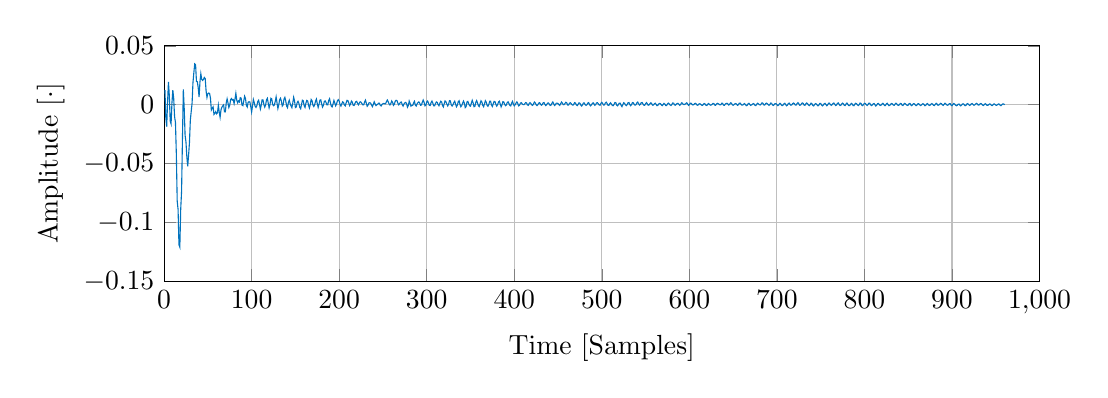
\begin{tikzpicture}

\begin{axis}[%
width=5in,
height=1.8in,
xmajorgrids,
xminorgrids,
ymajorgrids,
scaled y ticks = false,
y tick label style={/pgf/number format/fixed},
xmin=0,
xmax=1e+03,
xlabel={Time [Samples]},
ymin=-0.15,
ymax=0.05,
ylabel={Amplitude [$\cdot$]},
axis background/.style={fill=white}
]
\addplot [color=mycolor1,solid,forget plot]
  table[row sep=crcr]{%
1	0.0123\\
2	-0.0112\\
3	-0.0187\\
4	0.00216\\
5	0.0193\\
6	0.00772\\
7	-0.0139\\
8	-0.0163\\
9	0.0016\\
10	0.0124\\
11	0.00518\\
12	-0.0102\\
13	-0.015\\
14	-0.0415\\
15	-0.0819\\
16	-0.089\\
17	-0.119\\
18	-0.121\\
19	-0.089\\
20	-0.0735\\
21	-0.0288\\
22	0.0129\\
23	-0.00317\\
24	-0.0259\\
25	-0.0316\\
26	-0.0441\\
27	-0.0523\\
28	-0.0429\\
29	-0.0322\\
30	-0.013\\
31	-0.00585\\
32	0.00136\\
33	0.0186\\
34	0.0271\\
35	0.0346\\
36	0.0338\\
37	0.0198\\
38	0.0195\\
39	0.0143\\
40	0.00652\\
41	0.0194\\
42	0.0263\\
43	0.0216\\
44	0.0206\\
45	0.0215\\
46	0.0231\\
47	0.0221\\
48	0.0116\\
49	0.00617\\
50	0.00941\\
51	0.00985\\
52	0.0095\\
53	0.00554\\
54	-0.0045\\
55	-0.00291\\
56	-0.00187\\
57	-0.00828\\
58	-0.00735\\
59	-0.00594\\
60	-0.00773\\
61	-0.00683\\
62	-0.000513\\
63	-0.00638\\
64	-0.0107\\
65	-0.00449\\
66	-0.00233\\
67	-0.000968\\
68	-0.00016\\
69	-0.00606\\
70	-0.00613\\
71	0.00149\\
72	0.00497\\
73	0.00151\\
74	-0.00239\\
75	-0.000473\\
76	0.00424\\
77	0.00523\\
78	0.00394\\
79	0.0043\\
80	0.000882\\
81	0.00478\\
82	0.00963\\
83	0.00394\\
84	0.00159\\
85	0.00313\\
86	0.00232\\
87	0.00593\\
88	0.00558\\
89	-0.000347\\
90	-0.000804\\
91	0.00308\\
92	0.00717\\
93	0.00526\\
94	-0.000583\\
95	-0.00194\\
96	0.00201\\
97	0.00249\\
98	0.00231\\
99	-0.00156\\
100	-0.00621\\
101	-0.00126\\
102	0.0044\\
103	0.00175\\
104	-0.00134\\
105	-0.00235\\
106	-0.000868\\
107	0.00265\\
108	0.00378\\
109	0.000221\\
110	-0.00368\\
111	-0.000348\\
112	0.00414\\
113	0.00404\\
114	0.000166\\
115	-0.00207\\
116	-0.000231\\
117	0.00414\\
118	0.0054\\
119	0.00116\\
120	-0.00269\\
121	0.000112\\
122	0.00544\\
123	0.0049\\
124	0.00035\\
125	-0.000866\\
126	-0.000262\\
127	0.00282\\
128	0.00662\\
129	0.00156\\
130	-0.0032\\
131	-0.00019\\
132	0.0042\\
133	0.00543\\
134	0.00301\\
135	-0.00121\\
136	-0.000104\\
137	0.00479\\
138	0.0062\\
139	0.0031\\
140	-0.00119\\
141	-0.00253\\
142	0.00183\\
143	0.0038\\
144	0.000838\\
145	-0.00116\\
146	-0.00256\\
147	0.00134\\
148	0.00625\\
149	0.00337\\
150	-0.00245\\
151	-0.00195\\
152	0.00171\\
153	0.00286\\
154	0.00114\\
155	-0.00222\\
156	-0.00344\\
157	0.000146\\
158	0.00377\\
159	0.00328\\
160	-0.000823\\
161	-0.00228\\
162	0.00125\\
163	0.00365\\
164	0.0032\\
165	-0.000376\\
166	-0.00283\\
167	0.000102\\
168	0.00441\\
169	0.00341\\
170	-0.000271\\
171	-0.00157\\
172	-0.000178\\
173	0.00299\\
174	0.00474\\
175	0.000816\\
176	-0.00232\\
177	0.000442\\
178	0.00382\\
179	0.00409\\
180	0.000652\\
181	-0.00213\\
182	-0.000635\\
183	0.0026\\
184	0.00323\\
185	0.00185\\
186	-0.000162\\
187	-0.000179\\
188	0.00356\\
189	0.00507\\
190	0.00161\\
191	-0.00117\\
192	-0.00188\\
193	0.000632\\
194	0.0036\\
195	0.00148\\
196	-0.00098\\
197	0.000582\\
198	0.0033\\
199	0.00427\\
200	0.00309\\
201	3.35e-05\\
202	-0.0012\\
203	0.000775\\
204	0.00241\\
205	0.00187\\
206	-0.000285\\
207	-0.00098\\
208	0.0016\\
209	0.00367\\
210	0.00338\\
211	0.00135\\
212	-0.000793\\
213	0.000616\\
214	0.00309\\
215	0.00221\\
216	-0.000511\\
217	-0.000714\\
218	0.000921\\
219	0.00255\\
220	0.00285\\
221	0.00115\\
222	-0.000103\\
223	0.00137\\
224	0.00248\\
225	0.00211\\
226	0.000964\\
227	-0.000161\\
228	-0.000119\\
229	0.00213\\
230	0.00385\\
231	0.00132\\
232	-0.00134\\
233	-0.000396\\
234	0.00151\\
235	0.00169\\
236	0.00124\\
237	-0.000268\\
238	-0.00164\\
239	0.000255\\
240	0.00246\\
241	0.000698\\
242	-0.000783\\
243	-0.00016\\
244	0.000422\\
245	0.00127\\
246	0.00125\\
247	-0.000629\\
248	-0.00107\\
249	0.000275\\
250	0.000798\\
251	0.00112\\
252	0.000769\\
253	0.000713\\
254	0.00262\\
255	0.00396\\
256	0.00244\\
257	0.000717\\
258	-0.000218\\
259	0.000927\\
260	0.00319\\
261	0.00208\\
262	-0.000547\\
263	0.000398\\
264	0.00285\\
265	0.00371\\
266	0.00347\\
267	0.00131\\
268	-0.000114\\
269	0.000787\\
270	0.00198\\
271	0.00228\\
272	0.000102\\
273	-0.00122\\
274	0.000635\\
275	0.00151\\
276	0.00193\\
277	0.000981\\
278	-0.00215\\
279	-0.00079\\
280	0.00311\\
281	0.00126\\
282	-0.00125\\
283	-0.000686\\
284	-0.000609\\
285	0.00152\\
286	0.00286\\
287	-0.000313\\
288	-0.00115\\
289	0.000746\\
290	0.00179\\
291	0.00236\\
292	0.0013\\
293	-0.000497\\
294	-0.000244\\
295	0.00214\\
296	0.00392\\
297	0.00205\\
298	-0.000984\\
299	-0.000564\\
300	0.00224\\
301	0.00306\\
302	0.00143\\
303	-0.000544\\
304	-0.000705\\
305	0.00183\\
306	0.00308\\
307	0.00127\\
308	-0.001\\
309	-0.001\\
310	0.001\\
311	0.00234\\
312	0.00194\\
313	0.000151\\
314	-0.000912\\
315	0.00112\\
316	0.00296\\
317	0.00241\\
318	-0.000527\\
319	-0.00191\\
320	0.000906\\
321	0.0032\\
322	0.00243\\
323	0.000546\\
324	-0.00108\\
325	0.00028\\
326	0.00341\\
327	0.0032\\
328	-6.29e-05\\
329	-0.00113\\
330	-1.69e-05\\
331	0.00187\\
332	0.00295\\
333	0.000515\\
334	-0.00172\\
335	-0.000458\\
336	0.00251\\
337	0.00336\\
338	0.000257\\
339	-0.0018\\
340	-0.000724\\
341	0.00115\\
342	0.00301\\
343	0.00136\\
344	-0.00249\\
345	-0.00161\\
346	0.0023\\
347	0.00277\\
348	0.000734\\
349	-0.000895\\
350	-0.00128\\
351	0.00136\\
352	0.00372\\
353	0.0016\\
354	-0.00171\\
355	-0.00149\\
356	0.00181\\
357	0.00347\\
358	0.00162\\
359	-0.000784\\
360	-0.00152\\
361	0.000856\\
362	0.00329\\
363	0.00232\\
364	-0.000506\\
365	-0.00171\\
366	0.000732\\
367	0.00337\\
368	0.00213\\
369	-0.000604\\
370	-0.00134\\
371	0.000402\\
372	0.00293\\
373	0.0029\\
374	-0.00034\\
375	-0.00154\\
376	0.00084\\
377	0.0028\\
378	0.00251\\
379	0.00027\\
380	-0.00121\\
381	6.46e-05\\
382	0.00228\\
383	0.00298\\
384	0.000445\\
385	-0.00188\\
386	-6.63e-05\\
387	0.00254\\
388	0.0023\\
389	0.000439\\
390	-0.000865\\
391	-0.000169\\
392	0.00184\\
393	0.00242\\
394	0.000963\\
395	-0.000736\\
396	-0.00107\\
397	0.00138\\
398	0.00279\\
399	0.00053\\
400	-0.000949\\
401	-2.82e-05\\
402	0.00132\\
403	0.00241\\
404	0.00109\\
405	-0.00102\\
406	-0.000484\\
407	0.00128\\
408	0.00172\\
409	0.000814\\
410	6.21e-05\\
411	-1.09e-05\\
412	0.000781\\
413	0.00177\\
414	0.00157\\
415	-0.000185\\
416	-0.000568\\
417	0.000995\\
418	0.00175\\
419	0.00095\\
420	-0.000164\\
421	-0.00064\\
422	0.000792\\
423	0.0023\\
424	0.0015\\
425	1.63e-05\\
426	-0.000762\\
427	3.7e-05\\
428	0.00143\\
429	0.00172\\
430	0.000412\\
431	-0.000419\\
432	7.18e-05\\
433	0.00155\\
434	0.00182\\
435	0.000292\\
436	-0.000746\\
437	9.61e-05\\
438	0.00126\\
439	0.00149\\
440	0.000464\\
441	-0.00069\\
442	-0.000424\\
443	0.0012\\
444	0.00232\\
445	0.000924\\
446	-0.000669\\
447	-1.04e-05\\
448	0.00126\\
449	0.00128\\
450	0.00105\\
451	-2.29e-05\\
452	-0.00061\\
453	0.000907\\
454	0.00222\\
455	0.00127\\
456	-1.12e-05\\
457	8.96e-05\\
458	0.00111\\
459	0.00205\\
460	0.00143\\
461	-0.000248\\
462	-0.000354\\
463	0.00119\\
464	0.00166\\
465	0.000886\\
466	-1.35e-05\\
467	-0.000399\\
468	0.00039\\
469	0.00176\\
470	0.00134\\
471	-0.000254\\
472	-0.000757\\
473	0.000407\\
474	0.00162\\
475	0.00121\\
476	-0.000319\\
477	-0.00117\\
478	-8.62e-05\\
479	0.00151\\
480	0.00143\\
481	3.52e-05\\
482	-0.000599\\
483	-7.54e-05\\
484	0.00139\\
485	0.00174\\
486	6.04e-05\\
487	-0.000999\\
488	-0.000221\\
489	0.000851\\
490	0.0016\\
491	0.000847\\
492	-0.000559\\
493	2.97e-05\\
494	0.00155\\
495	0.00169\\
496	0.000813\\
497	-0.000277\\
498	-0.000441\\
499	0.00111\\
500	0.00197\\
501	0.00104\\
502	-0.000346\\
503	-0.000219\\
504	0.00141\\
505	0.00217\\
506	0.00107\\
507	-0.0004\\
508	-0.000636\\
509	0.000749\\
510	0.00162\\
511	0.000525\\
512	-0.000695\\
513	-0.000844\\
514	0.000251\\
515	0.00186\\
516	0.00167\\
517	-0.000445\\
518	-0.000983\\
519	0.000188\\
520	0.00135\\
521	0.00137\\
522	-0.000443\\
523	-0.00163\\
524	3.07e-05\\
525	0.00165\\
526	0.00121\\
527	-0.00015\\
528	-0.000814\\
529	0.000124\\
530	0.00168\\
531	0.0018\\
532	0.00014\\
533	-0.000873\\
534	0.000123\\
535	0.00178\\
536	0.0016\\
537	0.000338\\
538	-0.00041\\
539	-6.68e-05\\
540	0.00151\\
541	0.00221\\
542	0.000893\\
543	-0.000301\\
544	0.000256\\
545	0.00165\\
546	0.00186\\
547	0.000725\\
548	-0.000415\\
549	-0.000518\\
550	0.000918\\
551	0.00176\\
552	0.000772\\
553	-0.000451\\
554	-0.000235\\
555	0.000871\\
556	0.00155\\
557	0.000802\\
558	-0.000445\\
559	-0.000272\\
560	0.000766\\
561	0.00125\\
562	0.000387\\
563	-0.000826\\
564	-0.00063\\
565	0.000659\\
566	0.00105\\
567	0.000851\\
568	-0.00015\\
569	-0.000846\\
570	9.16e-05\\
571	0.00114\\
572	0.00052\\
573	-0.000698\\
574	-0.000683\\
575	0.000586\\
576	0.00134\\
577	0.000742\\
578	-0.000275\\
579	-0.000715\\
580	0.000158\\
581	0.00145\\
582	0.00131\\
583	-0.000194\\
584	-0.000408\\
585	0.00035\\
586	0.00105\\
587	0.00118\\
588	0.000414\\
589	-0.000567\\
590	0.000107\\
591	0.00155\\
592	0.00134\\
593	0.000271\\
594	5.78e-05\\
595	0.000387\\
596	0.001\\
597	0.00159\\
598	0.000615\\
599	-0.000575\\
600	2.19e-05\\
601	0.00125\\
602	0.0012\\
603	0.000327\\
604	-0.000267\\
605	9.38e-05\\
606	0.000865\\
607	0.00119\\
608	0.000459\\
609	-0.000518\\
610	-0.000294\\
611	0.000621\\
612	0.000853\\
613	0.000339\\
614	-0.000387\\
615	-0.000618\\
616	0.000278\\
617	0.000988\\
618	0.000552\\
619	-0.000528\\
620	-0.00071\\
621	0.000399\\
622	0.00105\\
623	0.000239\\
624	-0.000441\\
625	-0.000214\\
626	0.000274\\
627	0.00106\\
628	0.000907\\
629	-0.000316\\
630	-0.000534\\
631	0.000613\\
632	0.00114\\
633	0.000827\\
634	0.000323\\
635	-0.000192\\
636	-1.32e-05\\
637	0.00129\\
638	0.00117\\
639	-0.000407\\
640	-0.000568\\
641	0.000505\\
642	0.00104\\
643	0.0012\\
644	0.000677\\
645	-0.000301\\
646	0.000254\\
647	0.00156\\
648	0.00135\\
649	1.88e-05\\
650	-0.000504\\
651	4.3e-05\\
652	0.00075\\
653	0.000951\\
654	0.000377\\
655	-0.00055\\
656	-9.73e-05\\
657	0.00125\\
658	0.00136\\
659	0.000359\\
660	-0.000401\\
661	-0.000422\\
662	0.000383\\
663	0.000966\\
664	0.000214\\
665	-0.00086\\
666	-0.000643\\
667	0.000733\\
668	0.00122\\
669	0.000211\\
670	-0.000606\\
671	-0.000248\\
672	0.000403\\
673	0.000902\\
674	0.000536\\
675	-0.0006\\
676	-0.00078\\
677	0.00047\\
678	0.00125\\
679	0.000733\\
680	-0.000114\\
681	-0.000226\\
682	0.000539\\
683	0.00155\\
684	0.00125\\
685	-0.000196\\
686	-0.000347\\
687	0.00082\\
688	0.00133\\
689	0.000942\\
690	0.000148\\
691	-0.000551\\
692	9.37e-05\\
693	0.00146\\
694	0.00116\\
695	-0.000294\\
696	-0.000654\\
697	0.000187\\
698	0.000944\\
699	0.000926\\
700	7.5e-05\\
701	-0.000841\\
702	-0.000377\\
703	0.00104\\
704	0.00108\\
705	-0.000124\\
706	-0.000809\\
707	-0.000375\\
708	0.000727\\
709	0.00118\\
710	0.000145\\
711	-0.000948\\
712	-0.000465\\
713	0.00093\\
714	0.00131\\
715	0.000316\\
716	-0.000521\\
717	-0.000124\\
718	0.00092\\
719	0.00144\\
720	0.000897\\
721	-0.000259\\
722	-0.000338\\
723	0.000953\\
724	0.00175\\
725	0.000808\\
726	-0.000464\\
727	-0.000399\\
728	0.000678\\
729	0.00151\\
730	0.00115\\
731	-0.000295\\
732	-0.000563\\
733	0.000713\\
734	0.00146\\
735	0.000865\\
736	-0.000234\\
737	-0.00082\\
738	-1.35e-05\\
739	0.0013\\
740	0.000882\\
741	-0.000713\\
742	-0.00107\\
743	6.59e-05\\
744	0.000943\\
745	0.000648\\
746	-0.000314\\
747	-0.000972\\
748	-0.00032\\
749	0.00114\\
750	0.00111\\
751	-0.000307\\
752	-0.000984\\
753	-0.000351\\
754	0.000787\\
755	0.00114\\
756	8.74e-05\\
757	-0.000876\\
758	-0.000124\\
759	0.00126\\
760	0.00135\\
761	0.000159\\
762	-0.00059\\
763	-6.96e-05\\
764	0.00101\\
765	0.00142\\
766	0.000542\\
767	-0.000683\\
768	-0.000392\\
769	0.00105\\
770	0.00152\\
771	0.000446\\
772	-0.0007\\
773	-0.000549\\
774	0.00058\\
775	0.0013\\
776	0.000729\\
777	-0.000577\\
778	-0.000752\\
779	0.000669\\
780	0.00137\\
781	0.000334\\
782	-0.000809\\
783	-0.000836\\
784	0.000123\\
785	0.00114\\
786	0.000662\\
787	-0.000778\\
788	-0.000856\\
789	0.00042\\
790	0.00117\\
791	0.000775\\
792	-0.000132\\
793	-0.000733\\
794	1.84e-06\\
795	0.00138\\
796	0.00114\\
797	-0.000449\\
798	-0.00083\\
799	0.000289\\
800	0.00115\\
801	0.001\\
802	0.000119\\
803	-0.000706\\
804	-6.63e-05\\
805	0.00135\\
806	0.0013\\
807	-0.000119\\
808	-0.000769\\
809	-0.000217\\
810	0.000752\\
811	0.00102\\
812	-2.4e-05\\
813	-0.00113\\
814	-0.000468\\
815	0.000922\\
816	0.00101\\
817	6.61e-05\\
818	-0.000667\\
819	-0.000418\\
820	0.000566\\
821	0.00112\\
822	0.000371\\
823	-0.000802\\
824	-0.000686\\
825	0.000705\\
826	0.00122\\
827	0.000143\\
828	-0.000822\\
829	-0.000581\\
830	0.000347\\
831	0.00105\\
832	0.000705\\
833	-0.000378\\
834	-0.000536\\
835	0.000531\\
836	0.00123\\
837	0.000565\\
838	-0.000402\\
839	-0.000598\\
840	0.000163\\
841	0.00106\\
842	0.000861\\
843	-0.000431\\
844	-0.000722\\
845	0.000498\\
846	0.00113\\
847	0.000595\\
848	-0.000103\\
849	-0.000653\\
850	-0.000399\\
851	0.000909\\
852	0.00106\\
853	-0.000322\\
854	-0.000839\\
855	8.68e-05\\
856	0.000806\\
857	0.000737\\
858	-8.62e-05\\
859	-0.000796\\
860	-0.000357\\
861	0.000732\\
862	0.00085\\
863	-7.74e-05\\
864	-0.000751\\
865	-0.000331\\
866	0.000543\\
867	0.000852\\
868	0.00017\\
869	-0.000876\\
870	-0.000649\\
871	0.000619\\
872	0.000984\\
873	1.16e-05\\
874	-0.000639\\
875	-0.000408\\
876	0.000448\\
877	0.00097\\
878	0.000405\\
879	-0.000622\\
880	-0.000663\\
881	0.000429\\
882	0.00119\\
883	0.000504\\
884	-0.000503\\
885	-0.000306\\
886	0.000549\\
887	0.00113\\
888	0.000837\\
889	-0.000201\\
890	-0.000616\\
891	0.000399\\
892	0.00122\\
893	0.000689\\
894	-0.000242\\
895	-0.000524\\
896	2.48e-05\\
897	0.000904\\
898	0.000822\\
899	-0.000443\\
900	-0.000856\\
901	0.000195\\
902	0.00102\\
903	0.000527\\
904	-0.000332\\
905	-0.000871\\
906	-0.000584\\
907	0.000379\\
908	0.000573\\
909	-0.000409\\
910	-0.00097\\
911	-0.000309\\
912	0.000646\\
913	0.000726\\
914	-4.19e-05\\
915	-0.000862\\
916	-0.000594\\
917	0.000646\\
918	0.000949\\
919	9.19e-05\\
920	-0.000638\\
921	-0.000236\\
922	0.000696\\
923	0.000944\\
924	0.000194\\
925	-0.000457\\
926	-0.000232\\
927	0.000605\\
928	0.00109\\
929	0.000569\\
930	-0.000372\\
931	-0.000212\\
932	0.00065\\
933	0.00098\\
934	0.000528\\
935	-0.000439\\
936	-0.000683\\
937	0.000263\\
938	0.000895\\
939	0.000297\\
940	-0.00055\\
941	-0.000545\\
942	0.000146\\
943	0.000677\\
944	0.000385\\
945	-0.00056\\
946	-0.00076\\
947	5.53e-05\\
948	0.000685\\
949	0.000301\\
950	-0.000427\\
951	-0.000527\\
952	-4.61e-05\\
953	0.000671\\
954	0.000485\\
955	-0.00048\\
956	-0.000829\\
957	-9.41e-05\\
958	0.000707\\
959	0.000624\\
960	-8.16e-05\\
};
\end{axis}
230\end{tikzpicture}%
			\end{figure}
		\end{column}
	\end{columns}
\end{frame}


\begin{frame}{Experiments}{Measuring a Transfer-Function (Cancellation Path)}		
	\begin{columns}
		\begin{column}{0.3\textwidth}
			\begin{itemize}
				\item Cancellation Path Transfer-function
				\begin{itemize}
					\item Headphone speaker \\ $\rightarrow$ Error microphone
				\end{itemize}
				\item{Logarithmic Chirp}
			\end{itemize}
		\end{column}
		\begin{column}{0.7\textwidth} 
			\begin{figure}[h]
				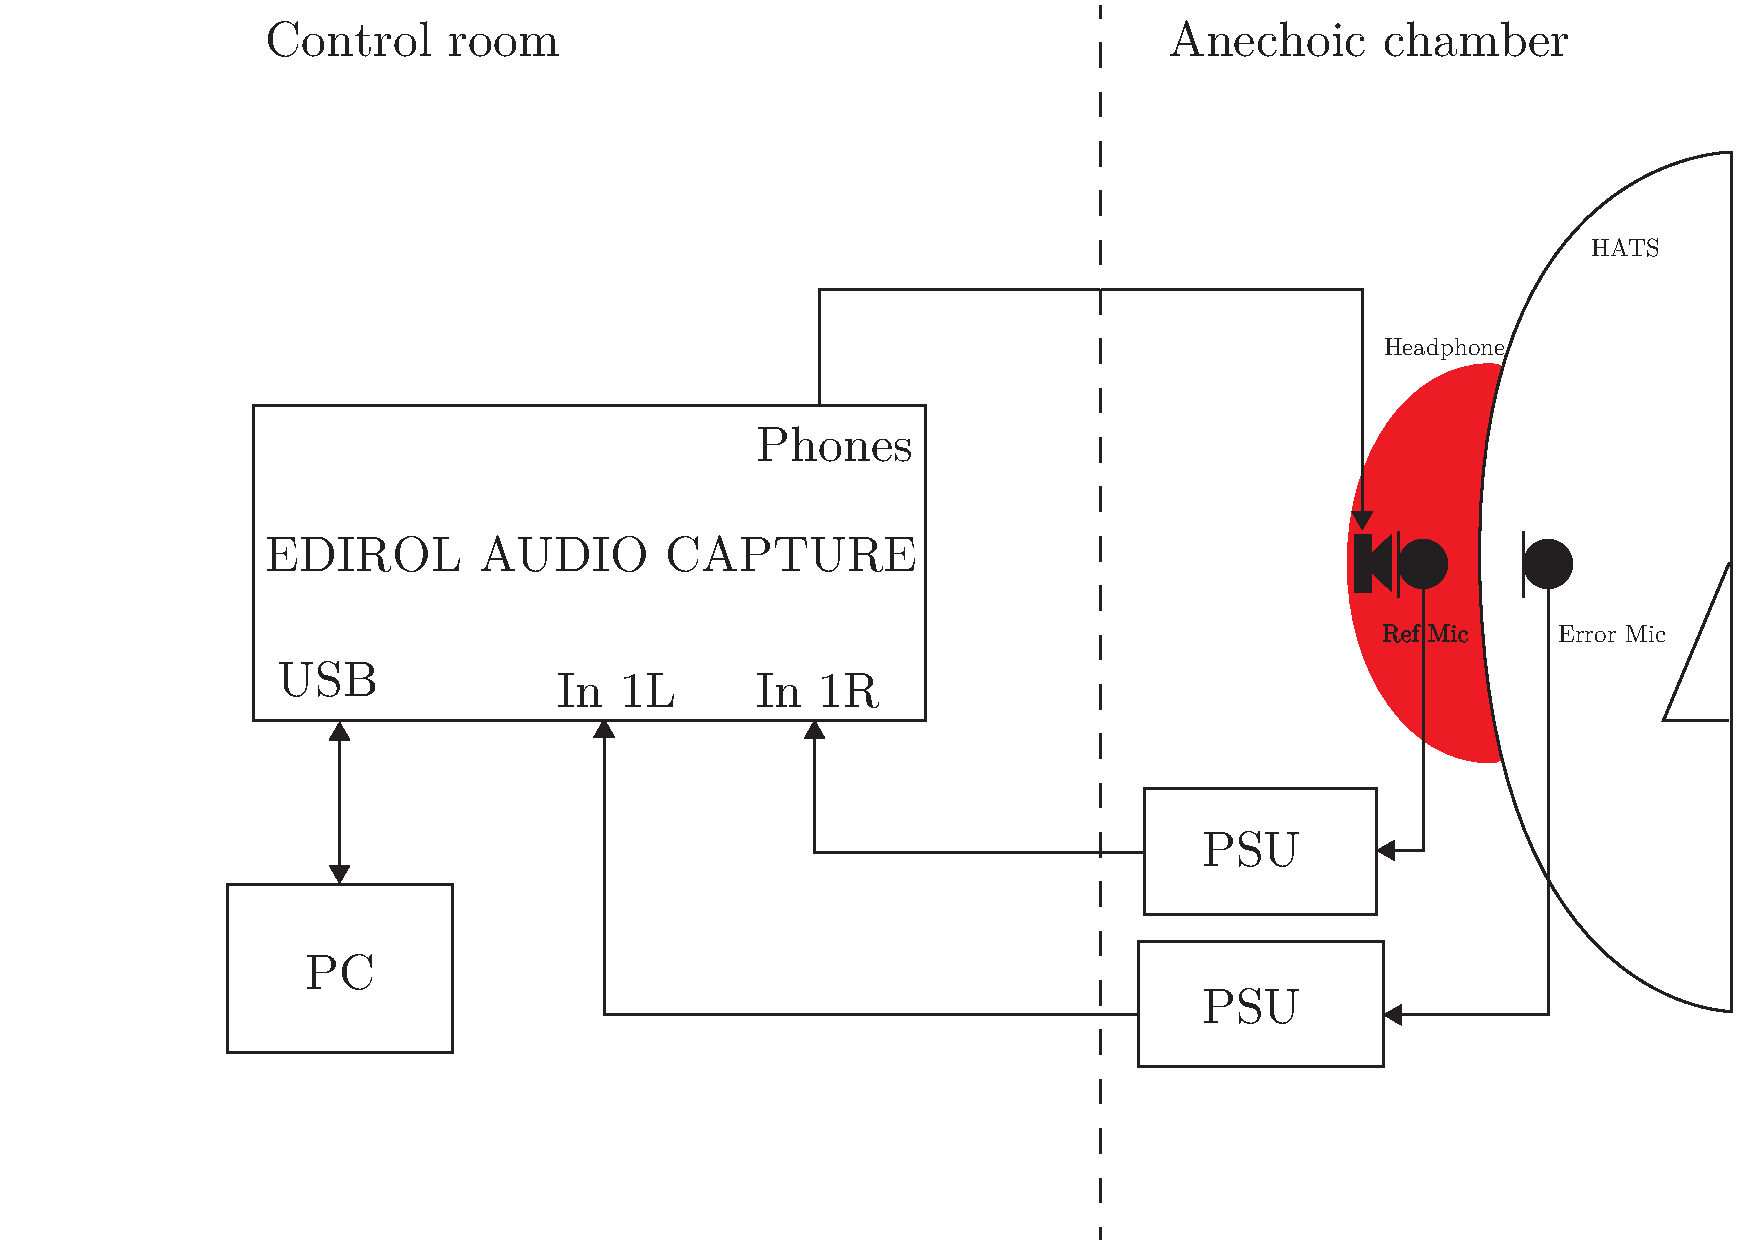
\includegraphics[width=1\textwidth]{figures/CancellationPath.pdf}
			\end{figure}
		\end{column}
	\end{columns}
\end{frame}

\begin{frame}{Experiments}{Measuring a Transfer-Function (Cancellation Path)}		
	\begin{columns}
		\begin{column}{0.3\textwidth}
			\begin{itemize}
				\item Results
				\item Frequency response
				\begin{itemize}
					\item[\textcolor{MATLABorange}{---}] FFT of 960 coefficients
					\item[\textcolor{MATLABblue}{---}] FFT of 480,256 coefficients
				\end{itemize}
			\end{itemize}
		\end{column}
		\begin{column}{0.7\textwidth} 
			\begin{figure}[h]
				\input{figures/TFCP.tex}
			\end{figure}
		\end{column}
	\end{columns}
\end{frame}
\begin{frame}{Experiments}{Measuring a Transfer-Function (Headphone)}		
	\begin{columns}
		\begin{column}{1\textwidth}
			\begin{itemize}
				\item Impulse response
				\begin{itemize}
					\item Inverse
				\end{itemize}
			\end{itemize}
			\begin{figure}[h]
				% This file was created by matlab2tikz.
%
%The latest updates can be retrieved from
%  http://www.mathworks.com/matlabcentral/fileexchange/22022-matlab2tikz-matlab2tikz
%where you can also make suggestions and rate matlab2tikz.
%
\definecolor{mycolor1}{rgb}{0.00000,0.44700,0.74100}%
%
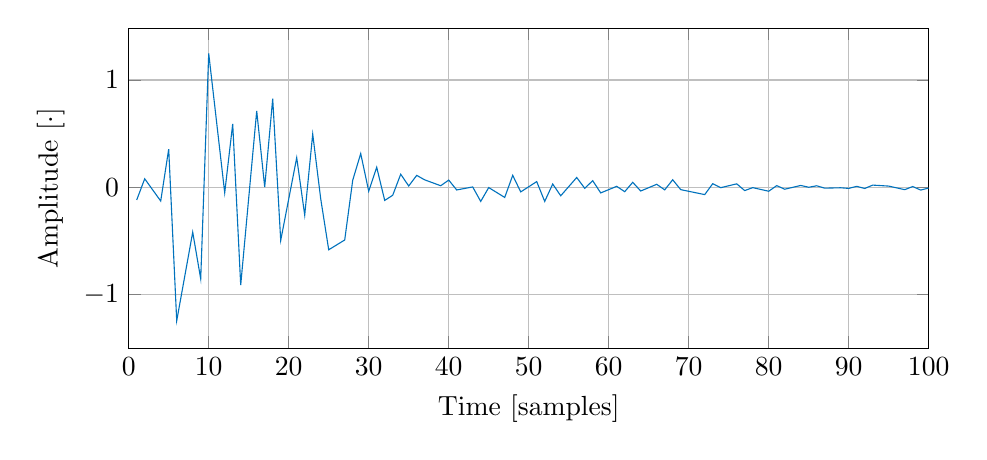
\begin{tikzpicture}

\begin{axis}[%
width=4in,
height=1.6in,
at={(1.011in,0.642in)},
scale only axis,
xmin=0,
xmax=100, %963.261537660286,
xminorgrids,
xmajorgrids,
yminorgrids,
ymajorgrids,
xlabel={Time [samples]},
ymin=-1.5,
ymax=1.48247541415567,
ylabel={Amplitude [$\cdot$]},
axis background/.style={fill=white},
title style={font=\bfseries},
]
\addplot [color=mycolor1,solid,forget plot]
table[row sep=crcr]{%
	1	-0.118141562218072\\
	2	0.0791281785124607\\
	4	-0.127998430298182\\
	5	0.355751675486418\\
	6	-1.24445909784893\\
	6	-1.24445909784893\\
	8	-0.418123407296711\\
	9	-0.853609016499564\\
	10	1.24815892007568\\
	10	1.24815892007568\\
	12	-0.0511791125132532\\
	13	0.591079504687172\\
	14	-0.911228401587671\\
	16	0.71167417099142\\
	17	0.0022231516812417\\
	18	0.825359321003935\\
	19	-0.495105852171416\\
	19	-0.495105852171416\\
	21	0.275904546024916\\
	22	-0.259187854777998\\
	23	0.496375795390466\\
	24	-0.107031671390095\\
	25	-0.582425217768152\\
	27	-0.491055535573922\\
	28	0.0652989205316153\\
	29	0.31411076610674\\
	30	-0.0363555084229589\\
	31	0.186377556816253\\
	32	-0.122351410526851\\
	33	-0.0742300014448984\\
	34	0.121765995454672\\
	35	0.0120055808146089\\
	36	0.110948456873853\\
	37	0.0692216392993395\\
	39	0.0144706736665758\\
	40	0.0670303556881637\\
	41	-0.0247644080799324\\
	43	0.00322998704690307\\
	44	-0.131745511302458\\
	44	-0.131745511302458\\
	45	-0.00261033076288713\\
	47	-0.0945138446649691\\
	48	0.111436996915387\\
	48	0.111436996915387\\
	49	-0.0431351377461246\\
	51	0.0531033344668851\\
	52	-0.131539836134088\\
	53	0.0305025240822609\\
	54	-0.0792119357439335\\
	56	0.091370890352526\\
	57	-0.00936150319799612\\
	58	0.0615638871253384\\
	59	-0.0524944156191402\\
	59	-0.0524944156191402\\
	61	0.00892104929863474\\
	62	-0.0410628110921637\\
	63	0.0464364992488124\\
	64	-0.0347539925926514\\
	66	0.0278505098767845\\
	67	-0.0239093827261274\\
	68	0.0700616510285207\\
	68	0.0700616510285207\\
	69	-0.0219341301905986\\
	72	-0.0681129708309657\\
	73	0.0334153987634728\\
	73	0.0334153987634728\\
	74	-0.00363938342836818\\
	76	0.0321515049541257\\
	77	-0.0306798066110672\\
	77	-0.0306798066110672\\
	78	-0.00314839927224314\\
	80	-0.0368012862919245\\
	81	0.0155149120464149\\
	82	-0.0180951857625397\\
	84	0.0169500794792463\\
	84	0.0169500794792463\\
	85	0.000310442154459831\\
	86	0.0140317610007087\\
	87	-0.00808289802810039\\
	89	-0.00446733733759463\\
	90	-0.0103115148570162\\
	91	0.00899156239938577\\
	92	-0.0111136779230336\\
	92	-0.0111136779230336\\
	93	0.0203724396264147\\
	95	0.0111957345646422\\
	97	-0.0222011006626747\\
	98	0.00705399101203549\\
	99	-0.0259264115095974\\
	99	-0.0259264115095974\\
	101	0.0124661338836067\\
	103	0.0229733095365205\\
	104	-0.015144764125669\\
	104	-0.015144764125669\\
	106	0.0020916766693437\\
	107	-0.0197042880875184\\
	108	0.00590774994138175\\
	108	0.00590774994138175\\
	110	-0.00752781336578599\\
	110	-0.00752781336578599\\
	111	0.0124866500742295\\
	114	0.00581286574855189\\
	115	-0.00889141928378981\\
	115	-0.00889141928378981\\
	116	0.00274247544089457\\
	117	-0.00715328500349922\\
	118	0.00343442489852638\\
	119	-0.00430672794128714\\
	120	0.00719938952165628\\
	123	0.00484835116232913\\
	124	-0.0159239102642369\\
	124	-0.0159239102642369\\
	125	0.00414543117078109\\
	126	-0.00923141916662314\\
	127	0.000492682295719719\\
	129	0.00879738745875531\\
	130	-0.0129254192936449\\
	130	-0.0129254192936449\\
	131	0.0150618586089381\\
	132	-0.0123298476334175\\
	133	0.00356672143985635\\
	135	-0.00688542560476631\\
	136	0.00647553377876287\\
	137	-0.00313869095969953\\
	138	0.00338234865059637\\
	140	0.00250712752529129\\
	141	-0.00294288518799757\\
	143	-0.000252409752983782\\
	144	-0.00709280368191718\\
	144	-0.00709280368191718\\
	145	0.00273457138739201\\
	146	-0.00349492542841067\\
	148	0.00204220837683377\\
	148	0.00204220837683377\\
	150	-0.0056427908397797\\
	151	0.00640825158781991\\
	152	-0.0134753340471952\\
	152	-0.0134753340471952\\
	153	0.00874106945549123\\
	155	0.00346206620492773\\
	156	-0.00148108262860179\\
	157	0.00159664856954663\\
	158	-0.00207774499103393\\
	159	0.00158755993228967\\
	160	-0.00187606529560944\\
	162	0.000959440112494838\\
	163	-0.00260830328383853\\
	165	0.00255734485088457\\
	166	-0.00559677227976574\\
	167	0.00666099057503437\\
	168	-0.00978142524505918\\
	169	0.00778894342302596\\
	170	-0.0118679731491987\\
	170	-0.0118679731491987\\
	171	0.00950293873394341\\
	172	-0.011731446451187\\
	173	0.00845382399693906\\
	175	0.00213548642487268\\
	177	-0.00346976620662964\\
	177	-0.00346976620662964\\
	178	0.00266301217400429\\
	179	-0.00296703845816892\\
	181	0.000142004740926337\\
	182	-0.00201581494127819\\
	183	0.00136029364750051\\
	183	0.00136029364750051\\
	186	-0.00342799294410937\\
	187	0.00159784037109706\\
	188	-0.00398829538564302\\
	188	-0.00398829538564302\\
	189	0.000416626602851866\\
	191	-0.00322830047473305\\
	192	0.00317533194550781\\
	193	-0.00524668903136873\\
	194	0.00328829223179929\\
	195	-0.00380800282688818\\
	196	0.0015429504716805\\
	197	-0.00205915720933898\\
	198	0.000169343616457016\\
	200	-0.00314718231332176\\
	201	0.00488601419939295\\
	202	-0.00801298194159633\\
	203	0.00835245107822657\\
	203	0.00835245107822657\\
	204	-0.00897724713721908\\
	206	-0.00580773871813518\\
	207	0.00330708796282231\\
	208	-0.0042502001375543\\
	209	0.00318711451318226\\
	210	-0.00389261618655835\\
	211	0.00217287506811931\\
	214	-0.00262627810428138\\
	215	0.00216492706444699\\
	216	-0.00501031331995221\\
	217	0.00345919904440867\\
	217	0.00345919904440867\\
	218	-0.00433586131657449\\
	219	0.00154231988745107\\
	220	-0.00198063731082455\\
	222	-0.00228271657882294\\
	223	0.00115333286600893\\
	223	0.00115333286600893\\
	224	-0.00241598423363702\\
	227	-0.00206397328677561\\
	228	0.000976785016822535\\
	228	0.000976785016822535\\
	230	-0.00188323750833553\\
	231	0.00131001909170588\\
	232	-0.00243251712101864\\
	232	-0.00243251712101864\\
	233	-0.000118515677414382\\
	234	-0.000432814061260125\\
	235	-0.00131759161870752\\
	237	-0.000598699726453522\\
	239	-0.00165499475232057\\
	240	0.00156604948120072\\
	241	-0.00438046374307205\\
	242	0.00360696249179117\\
	243	-0.00560346639516965\\
	245	-0.00623469069097805\\
	246	0.00589186342140169\\
	247	-0.00785971118716415\\
	248	0.00665880002740227\\
	248	0.00665880002740227\\
	249	-0.00761918755737151\\
	250	0.00490902237270174\\
	251	-0.00499083265681984\\
	252	0.00245856956180693\\
	253	-0.00271993135747834\\
	256	-0.00143699831064652\\
	257	0.001168405372886\\
	258	-0.00331916223660419\\
	259	0.00246644619167725\\
	259	0.00246644619167725\\
	260	-0.0038312069980187\\
	262	-0.00380470691510778\\
	263	0.00271140207259756\\
	265	0.0035851066684269\\
	266	-0.00479027738526985\\
	266	-0.00479027738526985\\
	267	0.00322958253325922\\
	268	-0.00386983440504256\\
	269	0.00179364522016447\\
	270	-0.00242605003167082\\
	271	0.000310768536677472\\
	273	-0.00138894887920508\\
	274	0.000905370459143382\\
	276	0.00195446317210042\\
	277	-0.00352888576217244\\
	277	-0.00352888576217244\\
	278	0.0014608960837152\\
	279	-0.00259958081461794\\
	280	0.000441660948525636\\
	282	0.00067947985088871\\
	283	-0.00256824921234122\\
	284	0.00134715382946428\\
	285	-0.00266294066935281\\
	286	0.0008584665792324\\
	287	-0.00218787796144465\\
	289	-0.00244602019051113\\
	290	0.00155874763278739\\
	291	-0.00324857347135153\\
	292	0.00166294406704746\\
	292	0.00166294406704746\\
	293	-0.00223331525375004\\
	296	-0.00176315457677289\\
	297	9.76523066167409e-05\\
	297	9.76523066167409e-05\\
	299	-0.00173147709190789\\
	300	0.00122885014088932\\
	301	-0.00365346924176114\\
	302	0.00323405196322781\\
	303	-0.00585574917228885\\
	304	0.00574201279929394\\
	305	-0.0084152161551938\\
	306	0.00746509624888059\\
	307	-0.00886986878415274\\
	308	0.00635223506983637\\
	309	-0.00633758656946944\\
	310	0.00313377489737645\\
	311	-0.00302721431751135\\
	312	0.000222054015152434\\
	314	-0.00189908683837059\\
	315	0.000943523210983249\\
	316	-0.00253445845641799\\
	317	0.000488057548535036\\
	318	-0.00124388238713333\\
	320	-4.66415700419361e-05\\
	321	-0.00148758285119824\\
	321	-0.00148758285119824\\
	322	-0.000221241170865421\\
	324	-0.000746319470210887\\
	325	-0.000923990623918906\\
	327	-0.00130425710741588\\
	328	-4.13696087694462e-06\\
	329	-0.00168409118232999\\
	330	0.000936585086162227\\
	331	-0.00308564184784506\\
	332	0.0023605505076797\\
	333	-0.00434285074420612\\
	334	0.00238912696534665\\
	334	0.00238912696534665\\
	335	-0.00279060739148346\\
	338	-0.00373874882183024\\
	339	0.00267681074734612\\
	339	0.00267681074734612\\
	340	-0.00429766826534488\\
	341	0.00208700210408384\\
	342	-0.00284724648153575\\
	343	-5.20252966257975e-06\\
	345	-0.00329645980614815\\
	347	-0.00642180470084158\\
	348	0.00567790534066384\\
	348	0.00567790534066384\\
	349	-0.00701536346053223\\
	350	0.00436881706836518\\
	351	-0.00428659214622984\\
	352	0.000799217212770171\\
	354	-0.00217577842529146\\
	355	0.00127905454452403\\
	356	-0.00298401463859871\\
	357	0.000989462254532667\\
	358	-0.0017007546226388\\
	360	0.000937253003236384\\
	361	-0.00394659229025655\\
	362	0.00369769876625983\\
	363	-0.00658337147258249\\
	364	0.00574479576405027\\
	365	-0.00765588588326013\\
	365	-0.00765588588326013\\
	366	0.00596394141532778\\
	368	0.00520571384648985\\
	369	-0.00656767481995299\\
	371	-0.00655109634034294\\
	372	0.00499318934664387\\
	372	0.00499318934664387\\
	373	-0.00658330606882521\\
	374	0.00461363533732913\\
	375	-0.00552092246929265\\
	376	0.00307874732958581\\
	377	-0.0033970039312901\\
	379	-0.0013112458867786\\
	381	3.37146738150675e-06\\
	382	-0.00182540086883953\\
	383	0.000558726296271283\\
	384	-0.00231761675634038\\
	385	0.000852799611702014\\
	386	-0.00251913059652571\\
	387	0.0010604065320112\\
	388	-0.00250519791572457\\
	389	0.000994810673962953\\
	390	-0.0022529025936006\\
	391	0.000376442375547348\\
	392	-0.00140065375470391\\
	394	0.00109770232115481\\
	395	-0.00442886162072952\\
	396	0.00518351250976918\\
	398	0.00915525476296349\\
	399	-0.0119877899123828\\
	400	0.0109753206242136\\
	401	-0.0123402377933597\\
	401	-0.0123402377933597\\
	402	0.0100186232498338\\
	403	-0.0101293640981462\\
	404	0.00698837151568855\\
	405	-0.00639504945537135\\
	406	0.0028147976834801\\
	409	-0.000121582413834242\\
	410	-0.00117389212627197\\
	410	-0.00117389212627197\\
	412	0.000538590839461553\\
	413	-0.00263064662674343\\
	414	0.00132626157824592\\
	414	0.00132626157824592\\
	415	-0.00202708098998182\\
	418	-0.00469211504272415\\
	419	0.00507633629068962\\
	420	-0.00760385411925335\\
	421	0.00666086810574746\\
	421	0.00666086810574746\\
	422	-0.00757352638306899\\
	423	0.00497047774726766\\
	424	-0.00405706782567618\\
	427	-0.0058447687582185\\
	428	0.00711503631090114\\
	429	-0.0102119854837445\\
	430	0.009906616429328\\
	430	0.009906616429328\\
	431	-0.0109119775121531\\
	432	0.00860895646393314\\
	433	-0.0079083525495047\\
	434	0.00420291652214673\\
	435	-0.00305211174085217\\
	437	0.000230702100913847\\
	438	-0.0017161730050292\\
	440	8.42058497987872e-05\\
	441	-0.00256022471353152\\
	442	0.00239415122600477\\
	443	-0.00402665777138054\\
	443	-0.00402665777138054\\
	444	0.0026745779652911\\
	445	-0.00302869602921266\\
	446	0.000781024171438022\\
	449	0.00180404756921617\\
	450	-0.00366582328451875\\
	450	-0.00366582328451875\\
	451	0.00244427200979937\\
	452	-0.00325334832057575\\
	453	0.00107334052574759\\
	455	-0.00211361141542538\\
	456	0.00268781887297511\\
	458	0.00473771508984494\\
	459	-0.00555281744764211\\
	459	-0.00555281744764211\\
	460	0.00332304873442352\\
	461	-0.00284830431641957\\
	463	0.000529639659647109\\
	464	-0.00263704498525956\\
	465	0.00196866918528383\\
	465	0.00196866918528383\\
	466	-0.00293342414220875\\
	467	0.00121813273125875\\
	468	-0.00167230145940699\\
	471	-0.00178798659029479\\
	472	0.00102270583773933\\
	472	0.00102270583773933\\
	473	-0.00196604745340521\\
	474	0.000387090340970548\\
	476	-0.00176140263280123\\
	478	-0.00342915551036846\\
	479	0.00217585484803685\\
	479	0.00217585484803685\\
	480	-0.00251973684564006\\
	481	0.000330692681301561\\
	483	-0.00113402265897128\\
	483	-0.00113402265897128\\
	485	0.000288585380609304\\
	486	-0.00327424743997195\\
	487	0.00466267448853491\\
	489	0.00974485253685983\\
	490	-0.0128096740396758\\
	491	0.0129753715311826\\
	492	-0.0142579881366436\\
	492	-0.0142579881366436\\
	493	0.0125236048320939\\
	494	-0.011641949121999\\
	495	0.007846651698912\\
	496	-0.00560552519163873\\
	497	0.00101899875994735\\
	500	0.00480210950545413\\
	501	-0.00595838865725095\\
	501	-0.00595838865725095\\
	502	0.00416486787779533\\
	503	-0.00386528693893032\\
	504	0.00109697754788766\\
	506	-0.00228087258764003\\
	507	0.002557299420177\\
	508	-0.00413738848932811\\
	509	0.00300993515146499\\
	510	-0.00335186584084382\\
	511	0.00103868487384464\\
	513	-0.00186950519283881\\
	514	0.00204076342560838\\
	515	-0.00366382926560233\\
	516	0.00259448915816415\\
	516	0.00259448915816415\\
	517	-0.00320956270729955\\
	519	-0.00122102330417284\\
	521	0.00115383310336414\\
	522	-0.00340300337398494\\
	523	0.00372741575372911\\
	524	-0.00592983933999568\\
	525	0.00605232641616526\\
	526	-0.00782019575779794\\
	527	0.00709231889553268\\
	527	0.00709231889553268\\
	528	-0.0077854060630539\\
	530	-0.00536046646139511\\
	531	0.0025028790245815\\
	533	-0.00153110520394306\\
	534	0.00233264873335874\\
	535	-0.00498360805643871\\
	536	0.00508085223254144\\
	537	-0.00663567727678236\\
	538	0.00526661639026852\\
	538	0.00526661639026852\\
	539	-0.00506317730069117\\
	542	-0.00300877591821623\\
	543	0.00452290184558103\\
	544	-0.00754035945955254\\
	545	0.0078511859306007\\
	546	-0.00949537010375863\\
	547	0.00811055917227654\\
	547	0.00811055917227654\\
	548	-0.00805055148811419\\
	550	-0.00402908753048485\\
	552	0.00114647146008193\\
	553	-0.00469663233807439\\
	554	0.00541976604901329\\
	555	-0.00732802040619347\\
	556	0.00618343156801426\\
	556	0.00618343156801426\\
	557	-0.00579956099549649\\
	560	-0.00301963851580893\\
	561	0.00485049635278991\\
	562	-0.00833359333669909\\
	563	0.00931200523494347\\
	564	-0.0116167652048223\\
	565	0.0112029652277205\\
	565	0.0112029652277205\\
	566	-0.0119319265800088\\
	567	0.0100599048233489\\
	568	-0.00947421976129978\\
	570	-0.00530612278282046\\
	571	0.00224275950368166\\
	572	-0.00127655177621738\\
	574	0.00154987666505993\\
	575	-0.00343838675431736\\
	576	0.00322750328499433\\
	577	-0.0048542145738335\\
	578	0.0045646233861098\\
	580	0.0057995181962912\\
	581	-0.00734238142271766\\
	582	0.00656899659371482\\
	583	-0.00740297717923726\\
	583	-0.00740297717923726\\
	584	0.00593543631945685\\
	585	-0.00579086536915566\\
	586	0.00314711565999102\\
	589	0.00341660574853945\\
	590	-0.00705907269469626\\
	591	0.0084368960345726\\
	592	-0.0110805725505189\\
	593	0.0109652716545559\\
	594	-0.0118130045513886\\
	594	-0.0118130045513886\\
	595	0.0100225807008175\\
	596	-0.00981161804164012\\
	597	0.00737989321388347\\
	598	-0.00692653284071349\\
	599	0.00453316365667066\\
	601	0.0022200167787656\\
	602	-0.00231830040325019\\
	603	0.000750300011075244\\
	604	-0.00149565258959066\\
	606	-0.00177246208904072\\
	607	0.000956135157919492\\
	607	0.000956135157919492\\
	608	-0.00204595642398299\\
	609	0.000767423670695334\\
	610	-0.00134120903884277\\
	613	-0.000433966220081623\\
	614	-0.000775477537017361\\
	615	0.00012836561393702\\
	616	-0.0014732380831371\\
	617	0.000800580652961012\\
	618	-0.00201609272643051\\
	619	0.00110897499582341\\
	620	-0.00219736523596371\\
	621	0.000983771285717864\\
	622	-0.00174377389327626\\
	623	0.000663852461368817\\
	624	-0.00130847580098342\\
	625	-0.000196629390547635\\
	627	-0.00138102574696632\\
	628	0.00108277581985184\\
	629	-0.00259099930814066\\
	631	-0.00346952422736864\\
	632	0.00269089184257897\\
	633	-0.00401495816961489\\
	634	0.0031389301925554\\
	634	0.0031389301925554\\
	635	-0.00395932588931588\\
	636	0.00264795179526999\\
	637	-0.00310550978701827\\
	638	0.00123727817663811\\
	639	-0.00137367687316596\\
	642	-0.00178877409265245\\
	643	0.00082850878454244\\
	643	0.00082850878454244\\
	644	-0.00136270277234899\\
	646	0.00078540646048041\\
	647	-0.00331509081772191\\
	648	0.00390493797058935\\
	649	-0.00631550557669833\\
	651	-0.00759186614038219\\
	652	0.00652153144809554\\
	652	0.00652153144809554\\
	653	-0.00692928789192903\\
	654	0.00506629029344104\\
	655	-0.00490473957333537\\
	656	0.00263233901651041\\
	657	-0.00198924861280767\\
	660	-0.00302949931141707\\
	661	0.00328844871460112\\
	662	-0.00534251786793635\\
	663	0.00548320203978873\\
	664	-0.00769944573922262\\
	665	0.00821240115972707\\
	666	-0.0105764458468815\\
	667	0.0109978575297208\\
	668	-0.0132867265871825\\
	669	0.0132217786784776\\
	670	-0.0144892526051537\\
	671	0.0133613422729723\\
	672	-0.0134147237236156\\
	673	0.0111266203315662\\
	674	-0.0101939886900111\\
	675	0.00712987296427118\\
	676	-0.00547613469863176\\
	677	0.00207400585012471\\
	679	-0.00283987951091501\\
	680	0.0037701752014266\\
	682	0.00603865602725456\\
	683	-0.00685424150883497\\
	683	-0.00685424150883497\\
	684	0.00521173945790625\\
	685	-0.00484164200501685\\
	686	0.00236226090534301\\
	687	-0.00193487906091025\\
	689	0.000194178233897032\\
	691	0.00104965767445102\\
	692	-0.00181988070928557\\
	692	-0.00181988070928557\\
	693	0.000533934184434739\\
	695	-0.00148196396521781\\
	696	0.00192096271273854\\
	697	-0.00413279650858434\\
	698	0.00404838913853553\\
	699	-0.0052799157164437\\
	700	0.00412542700406575\\
	700	0.00412542700406575\\
	701	-0.00423698948068876\\
	703	-0.00192753036365953\\
	705	0.000333383022643808\\
	706	-0.0022649036733681\\
	707	0.002028738374247\\
	708	-0.00351613650079263\\
	709	0.00301524012223379\\
	709	0.00301524012223379\\
	710	-0.00378720541718166\\
	712	-0.00270998103461012\\
	713	0.00104822615499336\\
	714	-0.00126950255896558\\
	715	-0.000109761833403383\\
	716	-0.000549697490630695\\
	718	-0.000328165439818674\\
	719	-0.00086531872554683\\
	720	0.000379381200437084\\
	722	0.00108908539279858\\
	723	-0.00206578486114234\\
	723	-0.00206578486114234\\
	724	0.00104194193672674\\
	725	-0.00183346168541204\\
	726	0.000675509611286171\\
	728	0.000704586977874764\\
	729	-0.0018660998388307\\
	731	-0.0039083391872586\\
	732	0.00447742232292977\\
	733	-0.00693335747458329\\
	734	0.00776987717666469\\
	735	-0.010164234591832\\
	736	0.0103478712825289\\
	736	0.0103478712825289\\
	737	-0.0115694159043584\\
	738	0.0102224662055594\\
	739	-0.00945722890579771\\
	740	0.00634518985330784\\
	741	-0.00424086825103049\\
	744	-0.00374700336061525\\
	745	0.003763574485471\\
	745	0.003763574485471\\
	746	-0.00455689509637074\\
	747	0.00316455078473394\\
	748	-0.00291460816255824\\
	749	0.00118872646405906\\
	750	-0.00111246326887942\\
	753	0.000164943203671868\\
	754	-0.00164682988282174\\
	755	0.00159437856283514\\
	756	-0.00299634657185343\\
	756	-0.00299634657185343\\
	757	0.00248038360493043\\
	758	-0.00269368982299733\\
	760	0.00118742001061047\\
	762	0.00796388766974066\\
	763	-0.0121664195043916\\
	764	0.0139967726757889\\
	765	-0.0163438871857992\\
	765	-0.0163438871857992\\
	766	0.0155905425377859\\
	767	-0.0149349249565211\\
	768	0.0119090837350432\\
	769	-0.00953352508428098\\
	770	0.00558975513910614\\
	771	-0.00345259993646529\\
	773	0.00102208767906143\\
	775	0.00267491651208203\\
	776	-0.00320515940454906\\
	776	-0.00320515940454906\\
	777	0.00185521570059825\\
	778	-0.00193828346567491\\
	779	0.000586667111080529\\
	782	-0.00202015908674002\\
	783	0.00184695021604536\\
	783	0.00184695021604536\\
	784	-0.00284542743803823\\
	785	0.00173679847990799\\
	786	-0.00149339324158143\\
	788	0.00159571745283789\\
	789	-0.00400786805273669\\
	790	0.00466843856241685\\
	791	-0.0063304081397892\\
	792	0.00594905071437179\\
	793	-0.00650528020353583\\
	794	0.00514748470517148\\
	795	-0.00486971213127775\\
	796	0.0030273680390555\\
	797	-0.00254003092297914\\
	798	0.000715676468597151\\
	799	-0.000768177358662561\\
	801	-0.000137380692556868\\
	803	-0.000515290763704587\\
	804	-0.000122064509013423\\
	805	-0.000547692453941614\\
	806	-0.00055652551949723\\
	807	0.000278543491965794\\
	808	-0.00135726537340407\\
	809	0.000941175178766385\\
	809	0.000941175178766385\\
	810	-0.00159133354623431\\
	813	-0.00145833453745552\\
	814	0.00221491485060638\\
	815	-0.00455167860230345\\
	816	0.00527452084341176\\
	817	-0.00693853431580101\\
	818	0.00658375836103028\\
	818	0.00658375836103028\\
	819	-0.00674180830885721\\
	820	0.00464074459176961\\
	821	-0.00320489977043648\\
	824	-0.00493414871277542\\
	825	0.00617048105378027\\
	826	-0.00808889780708222\\
	827	0.00808041985796052\\
	827	0.00808041985796052\\
	828	-0.00885480026507544\\
	829	0.00744364046650989\\
	830	-0.00695236125914457\\
	831	0.00457927250752843\\
	832	-0.0033261159052705\\
	835	-0.00150461482393167\\
	836	0.000932232169232329\\
	836	0.000932232169232329\\
	837	-0.00108582540363057\\
	839	0.000972656416291294\\
	840	-0.00282179974277099\\
	841	0.00309676801461591\\
	842	-0.0044708348142962\\
	843	0.00405009375545881\\
	844	-0.00461557416963168\\
	845	0.00349635790273107\\
	846	-0.00331319477320725\\
	847	0.00178228833138085\\
	848	-0.0015407674610116\\
	849	-4.29311411166699e-05\\
	851	-0.000976787855107253\\
	851	-0.000976787855107253\\
	852	0.000338522657633526\\
	855	0.000459168513940714\\
	856	-0.00177675339220597\\
	857	0.00141158344756638\\
	858	-0.00223372838089763\\
	858	-0.00223372838089763\\
	859	0.00104795485972972\\
	861	-0.00131794329341899\\
	862	0.00211164247050661\\
	864	0.00412187912673038\\
	865	-0.00493561878047142\\
	865	-0.00493561878047142\\
	866	0.00389477808123993\\
	867	-0.00367015442990034\\
	868	0.00207362419556041\\
	869	-0.00191625871648709\\
	870	0.000442706663790469\\
	871	-0.000721993615654676\\
	872	-0.000169097787633928\\
	875	0.000142486696254178\\
	876	-0.00113465361664049\\
	877	0.000726417334397207\\
	878	-0.00169035995887694\\
	879	0.00123915591964948\\
	880	-0.00199129657321224\\
	880	-0.00199129657321224\\
	881	0.00129347380441503\\
	883	0.000352556106165044\\
	885	-0.00179991584869511\\
	886	0.00250092793470548\\
	887	-0.00457169292445962\\
	888	0.00492561028992277\\
	889	-0.00602220904371532\\
	889	-0.00602220904371532\\
	890	0.00524468594890783\\
	891	-0.00508226299479267\\
	892	0.00313105322944276\\
	895	0.000953261678890702\\
	896	-0.00289249188050896\\
	897	0.00335091395982656\\
	898	-0.00491053813062609\\
	899	0.00487782988856139\\
	900	-0.00585975266054507\\
	901	0.00546036560710477\\
	902	-0.00624255635790587\\
	904	-0.00679416714246906\\
	905	0.00649383140436197\\
	906	-0.00741903833497929\\
	907	0.00675085904378967\\
	907	0.00675085904378967\\
	908	-0.00673326441218008\\
	909	0.00469123346285359\\
	910	-0.00324462435473286\\
	912	0.00146024592449633\\
	913	-0.00393939607905091\\
	914	0.00437538661686713\\
	915	-0.00509907440423318\\
	916	0.00361426331607717\\
	917	-0.00235127247887109\\
	919	0.00341001699309454\\
	920	-0.00727727928135634\\
	921	0.00954594199444283\\
	922	-0.0121948615791663\\
	923	0.0125548159064858\\
	924	-0.0128354555647342\\
	925	0.0106513403857466\\
	926	-0.00875286936078693\\
	927	0.00519487799128235\\
	928	-0.00308971559500316\\
	930	0.000324232857512524\\
	931	-0.00122301767726047\\
	931	-0.00122301767726047\\
	933	0.00041678514771041\\
	935	0.0025053358663086\\
	936	-0.00370333001248908\\
	936	-0.00370333001248908\\
	937	0.00292237990653884\\
	938	-0.00288517020934923\\
	939	0.00108852480479963\\
	941	-0.00202495299956734\\
	942	0.00291930578970116\\
	943	-0.00439342371540896\\
	944	0.00395069156667912\\
	945	-0.00366725299757077\\
	946	0.00113623163452466\\
	948	-0.00414511063528809\\
	949	0.00598742624044138\\
	950	-0.00839771800745089\\
	951	0.0084707213641626\\
	951	0.0084707213641626\\
	952	-0.00877004138263304\\
	953	0.00688831366809607\\
	954	-0.00589271928256045\\
	956	-0.00272054898871636\\
	957	0.00122611498187861\\
	959	0.00181359127678451\\
	960	-0.00355749756017599\\
	961	0.00462112620864556\\
	962	-0.00667559785306709\\
	964	-0.00813592196232858\\
};
\end{axis}
\end{tikzpicture}%
			\end{figure}
		\end{column}
	\end{columns}
\end{frame}


\begin{frame}{Experiments}{Measuring a Transfer-Function (Angle of Incidence)}		
	\begin{columns}
		\begin{column}{0.3\textwidth}
			\begin{itemize}
				\item Measured different angles
			\end{itemize}
		\end{column}
		\begin{column}{0.7\textwidth} 
			\begin{figure}[h]
				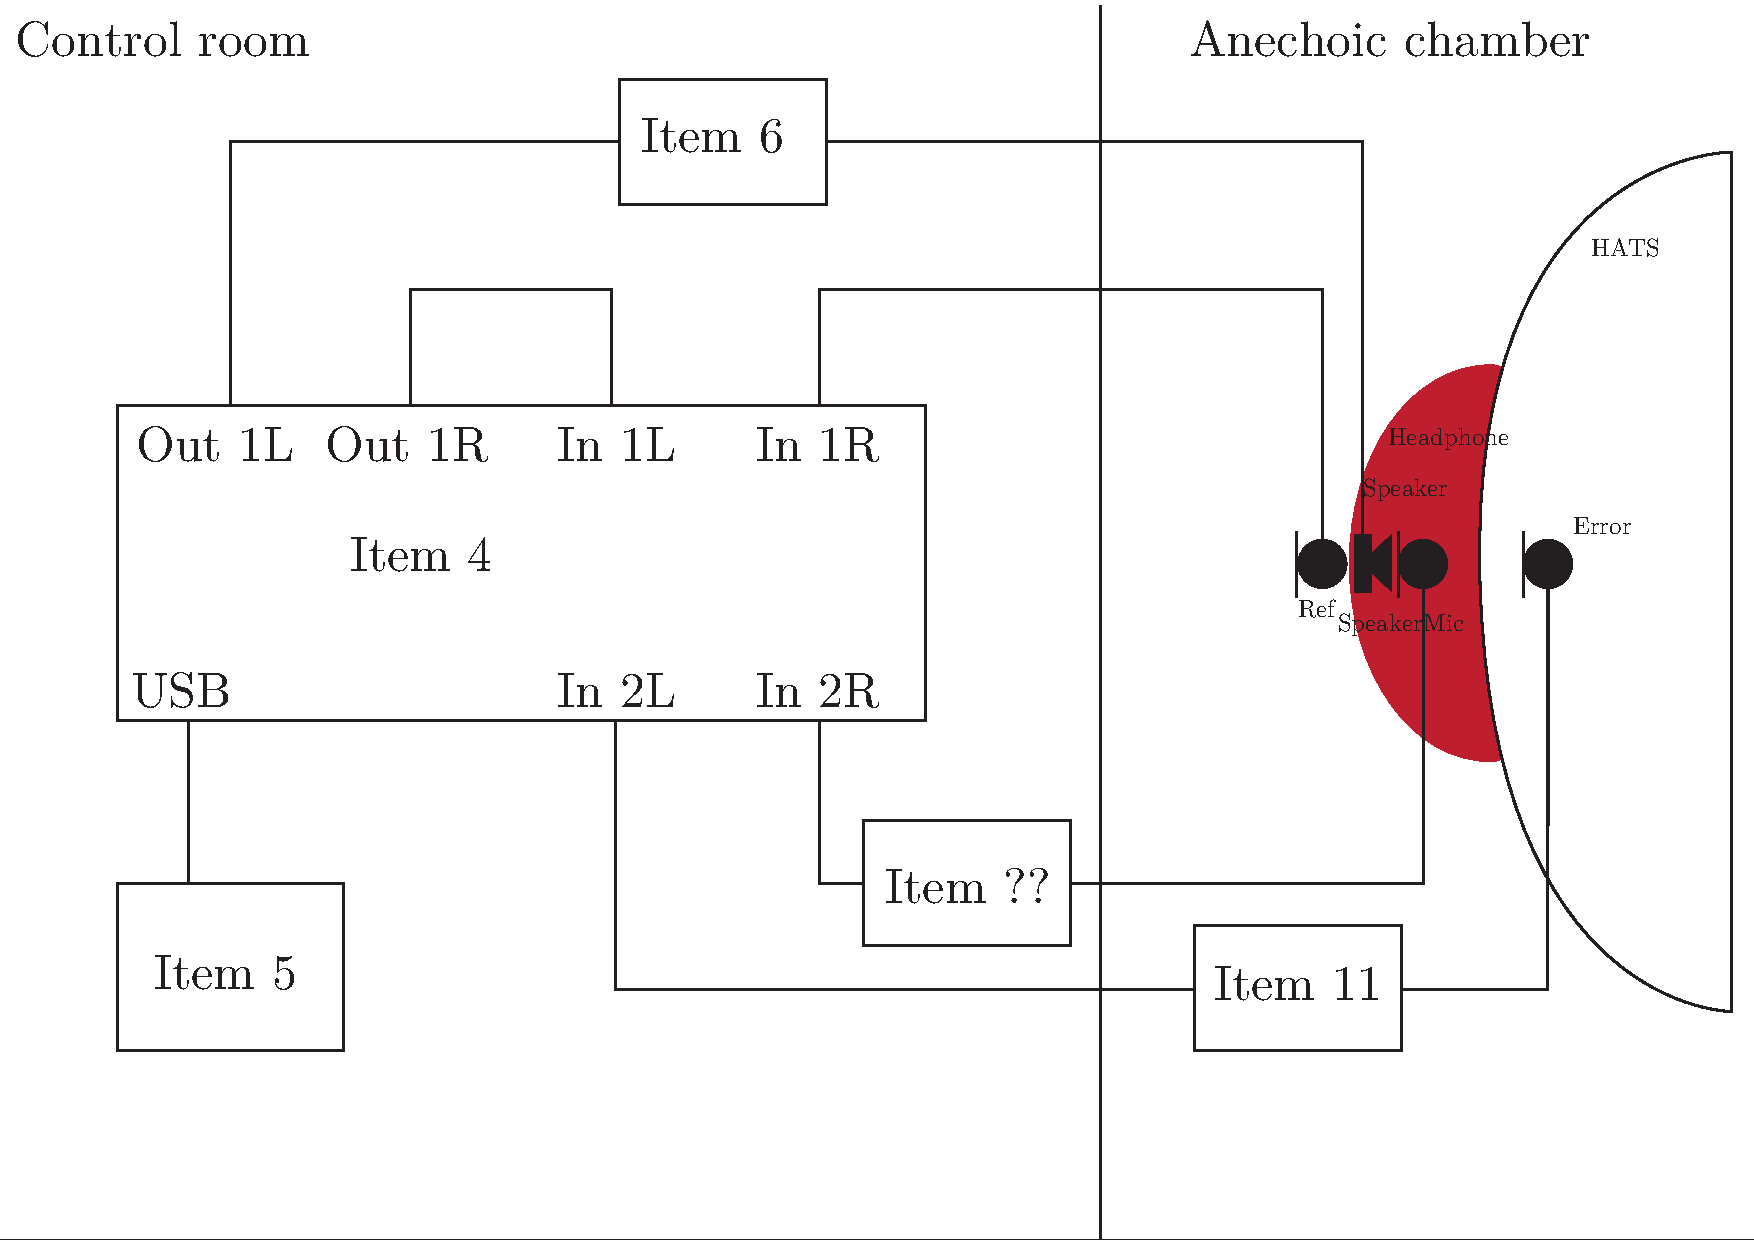
\includegraphics[width=1\textwidth]{figures/AngleOfIncidenceSetup.pdf}
			\end{figure}
		\end{column}
	\end{columns}
\end{frame}
\begin{frame}{Experiments}{Measuring a Transfer-Function (Angle of Incidence)}
	\begin{columns}
	\begin{column}{1\textwidth}
		\begin{itemize}
			\item Impulse response
		\end{itemize}
		\begin{figure}[h]
			\input{figures/AngofIncTime.tex}
		\end{figure}
	\end{column}
\end{columns}
\end{frame}

\begin{frame}{Experiments}{Testing Consumer ANC}		
	\begin{columns}
		\begin{column}{0.5\textwidth}
			\begin{itemize}
				\item Tested four consumer headphones
					\begin{itemize}
						\item Tested with and without ANC enabled
						\item Each headphone tested five times
						\item Using the Archimedes project
					\end{itemize}
				\item Using filter-bank to analyze results
				\begin{itemize}
					\item Fourier Transform only works on LTI-systems
				\end{itemize}
			\end{itemize}
		\end{column}
		\begin{column}{0.5\textwidth} 				
			\begin{figure}[h]
				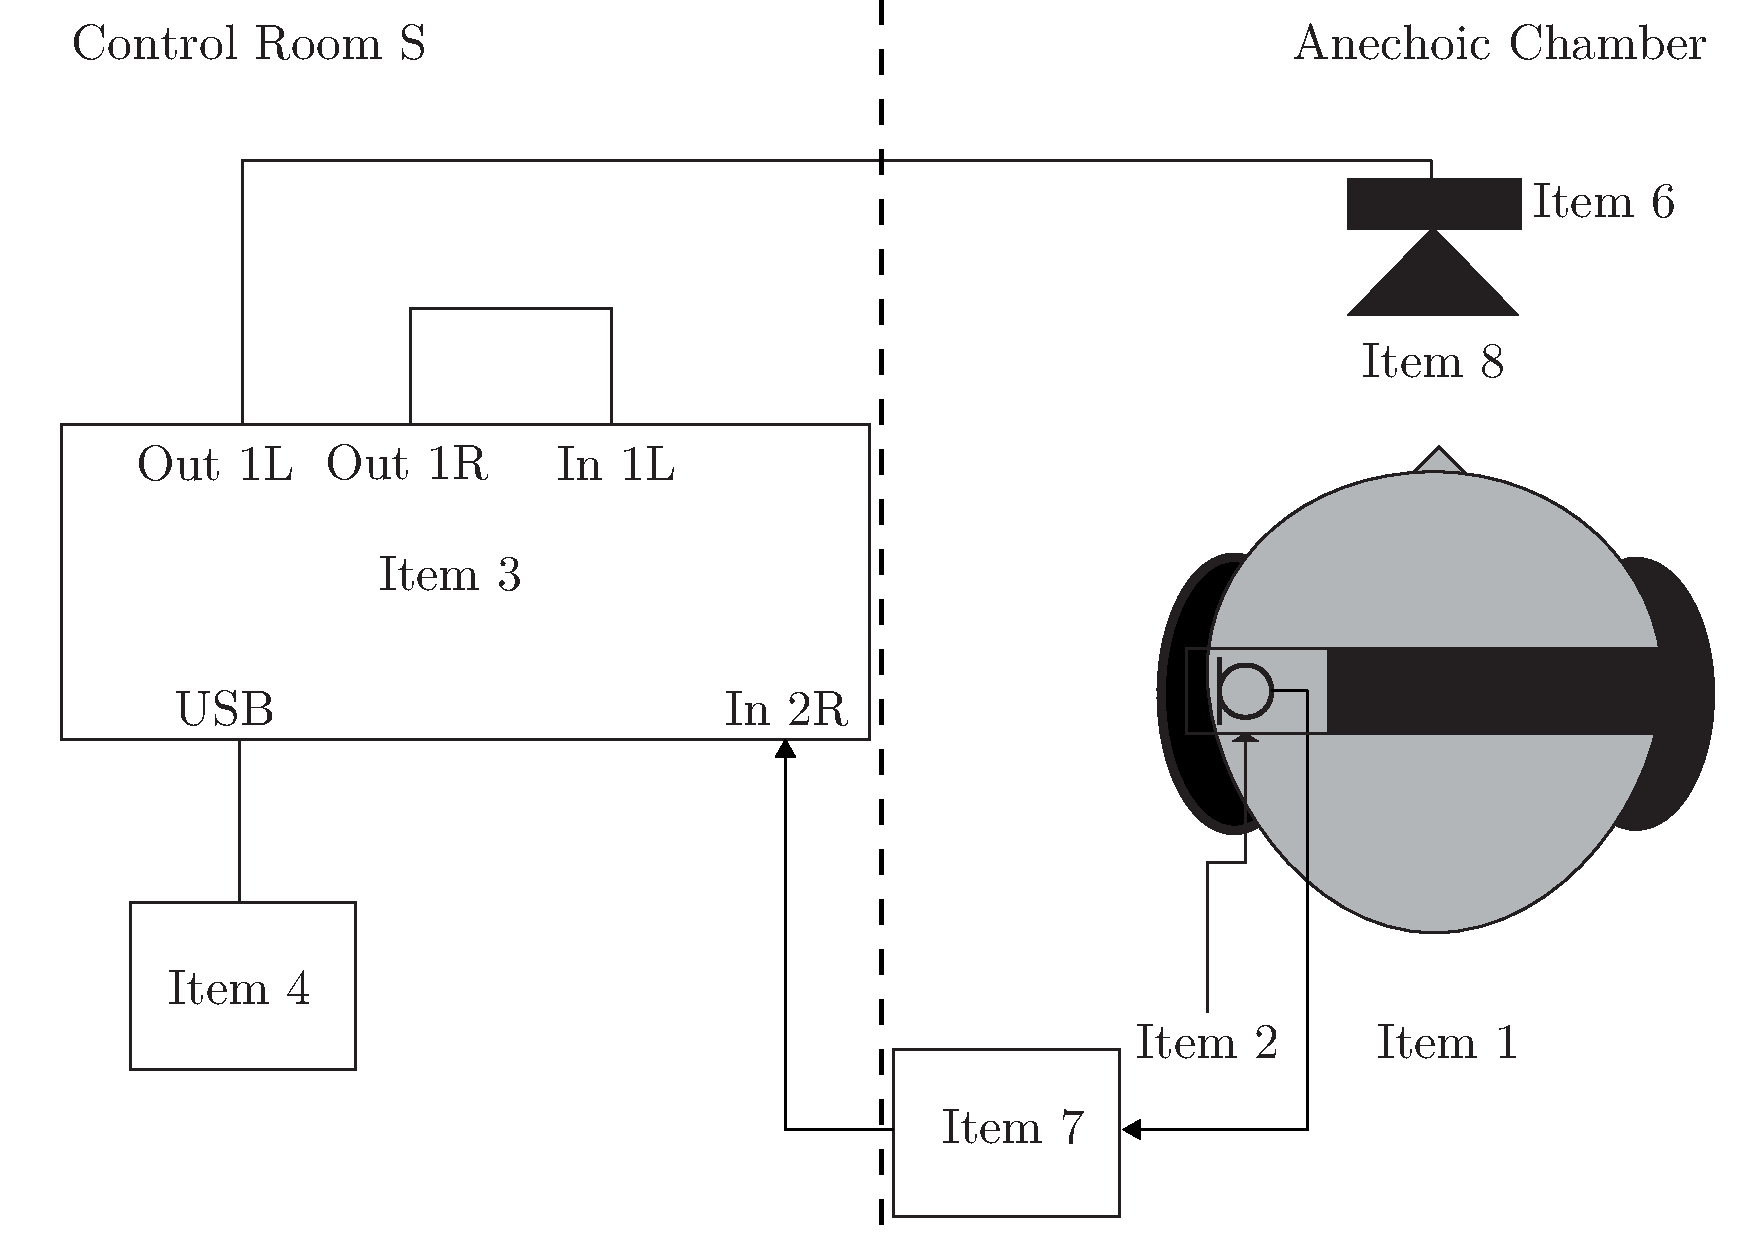
\includegraphics[width=1\textwidth]{figures/OtherBrandsDiagram.pdf}
			\end{figure}
		\end{column}
	\end{columns}
\end{frame}
\begin{frame}{Experiments}{Testing Consumer ANC}		
	\begin{columns}
		\begin{column}{0.2\textwidth}
			\begin{itemize}
				\item Results
			\end{itemize}
		\end{column}
		\begin{column}{0.8\textwidth} 				
			\begin{center}
				% This file was created by matlab2tikz.
%
%The latest updates can be retrieved from
%  http://www.mathworks.com/matlabcentral/fileexchange/22022-matlab2tikz-matlab2tikz
%where you can also make suggestions and rate matlab2tikz.
%
\definecolor{mycolor1}{rgb}{0.00000,0.44700,0.74100}%
\definecolor{mycolor2}{rgb}{0.85000,0.32500,0.09800}%
\definecolor{mycolor3}{rgb}{0.92900,0.69400,0.12500}%
\definecolor{mycolor4}{rgb}{0.49400,0.18400,0.55600}%
%
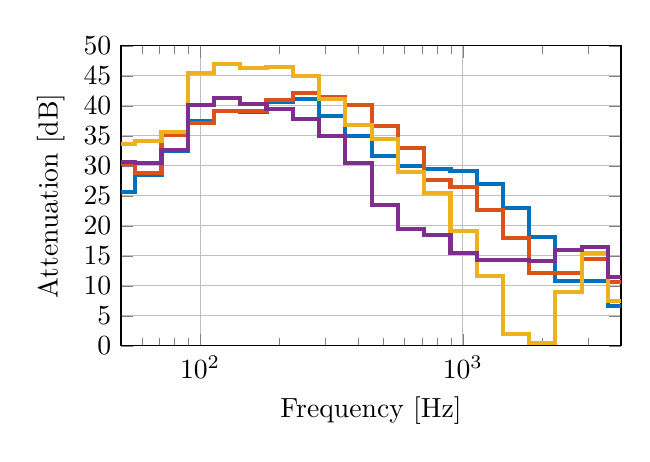
\begin{tikzpicture}

\begin{axis}[%
width=2.5in,
height=1.5in,
at={(1.011in,0.642in)},
scale only axis,
xmode=log,
xmin=50,
xmax=4000,
xlabel={Frequency [Hz]},
xmajorgrids,
%xmajorgrids,
%ymajorgrids,
%xminorgrids,
ymin=0,
ymax=50,
ytick={0,5,...,50},
ylabel={Attenuation [dB]},
ymajorgrids,
axis background/.style={fill=white},
title style={font=\bfseries},
%title={Comparison of Smoothened curves},
legend style={legend cell align=left,align=left,draw=white!15!black}
]
%\addplot[const plot,color=mycolor1,solid,forget plot,thick] plot table[row sep=crcr] {%
%	28.4	15.7\\
%	35.7	15.1\\
%	45	12.4\\
%	56.6	14\\
%	71.3	16.3\\
%	89.7	18.8\\
%	113	19.6\\
%	142	19.5\\
%	179	20.3\\
%	225	20.4\\
%	284	19.2\\
%	357	17.4\\
%	450	15.7\\
%	566	15.1\\
%	713	14.7\\
%	897	14.5\\
%	1.13e+03	13.5\\
%	1.42e+03	11.5\\
%	1.79e+03	9.08\\
%	2.25e+03	5.31\\
%	2.84e+03	5.51\\
%	3.57e+03	3.03\\
%	4.5e+03	2.37\\
%	5.66e+03	2.81\\
%	7.13e+03	3.07\\
%	8.97e+03	3.24\\
%	1.13e+04	1.16\\
%	1.42e+04	0.032\\
%	1.79e+04	0.598\\
%	2e+04	-0.763\\
%};
%\addplot[const plot,color=mycolor2,solid,forget plot,thick] plot table[row sep=crcr] {%
%	28.4	14.7\\
%	35.7	15.3\\
%	45	15.2\\
%	56.6	14.2\\
%	71.3	17.6\\
%	89.7	18.7\\
%	113	19.5\\
%	142	19.5\\
%	179	20.4\\
%	225	21.3\\
%	284	20.8\\
%	357	19.8\\
%	450	18.4\\
%	566	16.5\\
%	713	13.4\\
%	897	13.2\\
%	1.13e+03	11.4\\
%	1.42e+03	8.6\\
%	1.79e+03	6.11\\
%	2.25e+03	6.07\\
%	2.84e+03	7.27\\
%	3.57e+03	4.99\\
%	4.5e+03	2.6\\
%	5.66e+03	2.91\\
%	7.13e+03	1.03\\
%	8.97e+03	2.02\\
%	1.13e+04	-0.338\\
%	1.42e+04	-0.849\\
%	1.79e+04	-0.618\\
%	2e+04	-2.19\\
%};
%\addplot[const plot,color=mycolor3,solid,forget plot,thick] plot table[row sep=crcr] {%
%	28.4	18.1\\
%	35.7	19\\
%	45	17.1\\
%	56.6	16.5\\
%	71.3	18.6\\
%	89.7	22.8\\
%	113	23.6\\
%	142	23.3\\
%	179	23.5\\
%	225	22.6\\
%	284	20.4\\
%	357	18.4\\
%	450	17.2\\
%	566	14.5\\
%	713	12.7\\
%	897	9.48\\
%	1.13e+03	5.89\\
%	1.42e+03	1.04\\
%	1.79e+03	0.132\\
%	2.25e+03	4.45\\
%	2.84e+03	7.76\\
%	3.57e+03	3.73\\
%	4.5e+03	2.58\\
%	5.66e+03	2.46\\
%	7.13e+03	1.18\\
%	8.97e+03	1.16\\
%	1.13e+04	0.0281\\
%	1.42e+04	-0.34\\
%	1.79e+04	-0.623\\
%	2e+04	-1.08\\
%};
%\addplot[const plot,color=mycolor4,solid,forget plot,thick] plot table[row sep=crcr] {%
%	28.4	18.6\\
%	35.7	16.5\\
%	45	15.5\\
%	56.6	15.5\\
%	71.3	16.6\\
%	89.7	20.3\\
%	113	20.4\\
%	142	20\\
%	179	19.6\\
%	225	18.9\\
%	284	17.4\\
%	357	15.3\\
%	450	11.8\\
%	566	9.77\\
%	713	8.89\\
%	897	7.71\\
%	1.13e+03	6.86\\
%	1.42e+03	7.05\\
%	1.79e+03	7.37\\
%	2.25e+03	7.85\\
%	2.84e+03	8.24\\
%	3.57e+03	5.7\\
%	4.5e+03	3.78\\
%	5.66e+03	3.02\\
%	7.13e+03	1.43\\
%	8.97e+03	1.33\\
%	1.13e+04	1.58\\
%	1.42e+04	0.0462\\
%	1.79e+04	-1.02\\
%	2e+04	-0.621\\
%};
%\end{axis}

%% 20 log
\addplot[const plot,color=mycolor1,solid,line width=1.5pt,forget plot] plot table[row sep=crcr] {%
	28.4	30.6\\
	35.7	31.3\\
	45	25.7\\
	56.6	28.5\\
	71.3	32.4\\
	89.7	37.4\\
	113	39.1\\
	142	39\\
	179	40.6\\
	225	41.2\\
	284	38.3\\
	357	35\\
	450	31.7\\
	566	30\\
	713	29.4\\
	897	29.1\\
	1.13e+03	27\\
	1.42e+03	23\\
	1.79e+03	18.2\\
	2.25e+03	10.8\\
	2.84e+03	10.8\\
	3.57e+03	6.62\\
	4.5e+03	4.92\\
	5.66e+03	5.21\\
	7.13e+03	5.95\\
	8.97e+03	5.98\\
	1.13e+04	2.27\\
	1.42e+04	-1\\
	1.79e+04	0.842\\
	2e+04	-1.38\\
};
\addplot[const plot,color=mycolor2,solid,line width=1.5pt,forget plot] plot table[row sep=crcr] {%
	28.4	29.3\\
	35.7	30.1\\
	45	30.3\\
	56.6	28.8\\
	71.3	35.2\\
	89.7	37.2\\
	113	39.1\\
	142	39.2\\
	179	41\\
	225	42.2\\
	284	41.5\\
	357	40.1\\
	450	36.7\\
	566	33\\
	713	27.7\\
	897	26.5\\
	1.13e+03	22.7\\
	1.42e+03	17.9\\
	1.79e+03	12.1\\
	2.25e+03	12.1\\
	2.84e+03	14.4\\
	3.57e+03	10.6\\
	4.5e+03	5.72\\
	5.66e+03	5.17\\
	7.13e+03	2.13\\
	8.97e+03	4.17\\
	1.13e+04	-0.138\\
	1.42e+04	-0.907\\
	1.79e+04	-1.96\\
	2e+04	-4.33\\
};
\addplot[const plot,color=mycolor3,solid,line width=1.5pt,forget plot] plot table[row sep=crcr] {%
	28.4	36.2\\
	35.7	38.5\\
	45	33.6\\
	56.6	34.2\\
	71.3	35.6\\
	89.7	45.5\\
	113	46.9\\
	142	46.3\\
	179	46.5\\
	225	44.9\\
	284	41.1\\
	357	36.8\\
	450	34.5\\
	566	29\\
	713	25.5\\
	897	19.1\\
	1.13e+03	11.6\\
	1.42e+03	1.91\\
	1.79e+03	0.429\\
	2.25e+03	9.03\\
	2.84e+03	15.5\\
	3.57e+03	7.47\\
	4.5e+03	4.95\\
	5.66e+03	4.31\\
	7.13e+03	2.18\\
	8.97e+03	2.87\\
	1.13e+04	0.264\\
	1.42e+04	-0.554\\
	1.79e+04	-2.08\\
	2e+04	-2.36\\
};
\addplot[const plot,color=mycolor4,solid,line width=1.5pt,forget plot] plot table[row sep=crcr] {%
	28.4	37.2\\
	35.7	33.9\\
	45	30.7\\
	56.6	30.4\\
	71.3	32.7\\
	89.7	40.2\\
	113	41.3\\
	142	40.3\\
	179	39.5\\
	225	37.8\\
	284	34.9\\
	357	30.5\\
	450	23.4\\
	566	19.5\\
	713	18.4\\
	897	15.4\\
	1.13e+03	14.3\\
	1.42e+03	14.3\\
	1.79e+03	14.1\\
	2.25e+03	16\\
	2.84e+03	16.4\\
	3.57e+03	11.5\\
	4.5e+03	7.26\\
	5.66e+03	6.34\\
	7.13e+03	2.99\\
	8.97e+03	2.87\\
	1.13e+04	2.9\\
	1.42e+04	0.784\\
	1.79e+04	-1.51\\
	2e+04	-1.74\\
};
\end{axis}
\end{tikzpicture}%
			\end{center}
		\end{column}
	\end{columns}
\end{frame}
